\documentclass[11pt]{article}
\usepackage[a4paper,left=28mm,right=32mm,top=25mm,bottom=25mm,marginparwidth=18mm,marginparsep=4mm]{geometry}
\usepackage{fontspec,amsmath,amssymb,xcolor,needspace,longtable,array,booktabs,graphicx,tikz,trimclip}
\usepackage{manyfoot,perpage}
\usetikzlibrary{decorations.pathreplacing}
\usepackage[unicode,hidelinks]{hyperref}
\usepackage{polyglossia}
\setmainlanguage{english}
\setotherlanguages{arabic,greek,hebrew}
\setmainfont{Linux Libertine O}[Ligatures=TeX]
\setlength{\emergencystretch}{1.5em}
\newfontfamily\arabicfont{Amiri}[Script=Arabic]
\newfontfamily\ArNote{Amiri}[Script=Arabic,Scale=1.05]
\newfontfamily\greekfont{FreeSerif}[Script=Greek]
\newfontfamily\hebrewfont{Frank Ruhl Hofshi}[Script=Hebrew]
\newfontfamily\syriacfont{Segoe UI Historic}[Script=Syriac]
\newfontfamily\EthiopicFont{Ebrima}
\newfontfamily\CapFont{Noto Serif}
\newfontfamily\MoonFont{FreeSerif}
\newcommand{\MoonSym}{\text{\MoonFont ☾}}\newcommand{\SunSym}{\text{\MoonFont ⊙}}
\newfontfamily\CopticFont{FreeSerif}
\newfontfamily\NallinoSigns{NallinoSigns.otf}[Path=../../S04/versio/fonts/]
\newcommand{\AbjadZero}{{\NallinoSigns\symbol{"E000}}}
\newcommand{\ARsign}{\mbox{\clipbox{0pt 0pt {.48\width} 0pt}{A}\kern-.10em R}}
\newcommand{\Name}[1]{#1}
% the macros of the Latin edition (S07) that its column machinery uses for the tables set by @grid
\newsavebox{\DLBox}\newlength{\GridWidth}\newsavebox{\FigBox}
% a redrawn figure at its own size, or shrunk to the line when it is wider (the head ornament of Part II)
\newcommand{\FitFigure}[1]{\sbox{\FigBox}{#1}\ifdim\wd\FigBox>\linewidth\resizebox{\linewidth}{!}{\usebox{\FigBox}}\else\usebox{\FigBox}\fi}
\newcommand{\DLine}[3]{\par\noindent\sbox{\DLBox}{\strut #3}\usebox{\DLBox}\strut\par}
\newcommand{\CenterLine}[1]{\makebox[\linewidth][c]{#1}}
\newcommand{\qfrac}[2]{{}^{#1}\!/_{{#2}}}
\newcommand{\ArabicRun}[1]{\smash[b]{\textarabic{#1}}}
\DeclareNewFootnote{T}[alph]
\MakePerPage{footnote}\MakePerPage{footnoteT}
% before perpage has its .aux the translator's notes of the preface run on past z: aa, ab, ...
\makeatletter
\newcommand{\TNoteLetter}[1]{\ifnum#1>26 \@alph{\numexpr(#1-14)/26\relax}\@alph{\numexpr#1-26*((#1-14)/26)\relax}\else\@alph{#1}\fi}
\renewcommand{\thefootnoteT}{\TNoteLetter{\value{footnoteT}}}
\makeatother
\hypersetup{pdftitle={C. A. Nallino, notes on al-Battani's Zij: an English translation},pdfauthor={C. A. Nallino}}
\setlength{\parindent}{0pt}\setlength{\parskip}{0.55em}
\tracinglostchars=2
\newcommand{\Pg}[1]{\marginpar{\footnotesize\color{gray}#1}}
\newcommand{\Entry}[1]{\par{\parskip=0.2em\relax\noindent\hangindent=1.5em\hangafter=1 #1\par}}
\newcommand{\PartHead}[2]{\clearpage\pdfbookmark[0]{#1}{part-#2}{\centering\LARGE #1\par}\bigskip}
\newcommand{\UnitHead}[2]{\par\setcounter{footnoteT}{0}\needspace{8\baselineskip}\bigskip\pdfbookmark[1]{#1}{unit-#2}\hypertarget{EN-#2}{}%
 {\large\bfseries\interlinepenalty=10000 #1\par}\nobreak\medskip}
\begin{document}

\thispagestyle{empty}
\begin{center}\Large C. A. NALLINO\par\vspace{4mm}\LARGE Notes on al-Battānī's \emph{Zīj}\par\vspace{2mm}\large from \emph{Al-Battānī sive Albatenii Opus astronomicum} (Milan, 1899–1907)\par\vspace{5mm}\normalsize translated from the Latin\end{center}\vspace{8mm}
\noindent Nallino's edition of al-Battānī's \emph{Zīj} gives the Arabic text (Part III, 1899), a Latin translation of the canons with a commentary on them (Part I, 1903), and the tables in Latin with notes on them, a glossary and indexes (Part II, 1907). The canons themselves are translated into English from the Arabic in the English \emph{Zīj} of this edition; this volume translates Nallino's own writing, which is in Latin and has not been translated before. It is made from the line-by-line transcription of his Latin in this edition (S03, S04 and S07). Every sentence is translated, in Nallino's order; nothing is summarised or left out. His Arabic, Greek and Hebrew quotations stand in their scripts, as he prints them, with his translations of them in English. Proper names are given in a modern transliteration. In the headings of the commentary, «p.» and «l.» are the pages and lines of Nallino's Latin translation (Part I, pp. 1–150); «t. III» is the Arabic text, whose pages the English \emph{Zīj} gives in its margin; in the heads of the notes on the tables, «p.» is a page of the tables (Part II). Nallino's footnotes are numbered; the few notes of the translator are lettered. Nallino's own corrections in the «Addenda et emendanda» of Part II are followed and noted. The pages of Nallino's volumes are given in the margin.
\par\smallskip\noindent The translation is in progress. This version holds the whole of the front matter of Part I (pp. VII–LXXX), the whole of the notes to the translation of the canons (pp. 1–150), the whole of the commentary of Part I (pp. 151–327), the whole of the front matter of Part II (pp. [I]–XXXI), the whole of the notes on the tables of Part II (pp. 189–317), the whole of the glossary (pp. 319–358) and the whole of the indexes (pp. 359–413). It is AI-translated (Claude), 2026; no person has proofread it. Nallino's work is in the public domain; the translation is dedicated to the public domain (CC0 1.0).
\par\clearpage
\PartHead{The Astronomical Work of al-Battānī, or Albatenius}{P1}\Pg{I }
\par\begin{center}Pubblicazioni del Reale Osservatorio di Brera in Milano. N. XL. Parte I. (Publications of the Royal Observatory of Brera in Milan, no. XL, part I.)\end{center}
\par\begin{center}\textbf{The Astronomical Work of al-Battānī, or Albatenius, edited in Arabic on the authority of the Escorial codex, translated into Latin and furnished with notes by Carlo Alfonso Nallino.}\end{center}
\par\begin{center}Part One. The translation of the chapters, with a commentary.\end{center}
\par\begin{center}Milan: on sale at Ulrico Hoepli's, bookseller to the King, in the Galleria De Cristoforis, nos. 58–63. 1903.\end{center}
\par\begin{center}Rome 1903. — Printed by C. De Luigi.\end{center}
\par\begin{center}To my excellent parents, never mindful and grateful enough, I give and dedicate this.\end{center}
\UnitHead{Preface}{P01}
\par \Pg{I VII}§ 1, \emph{The life of al-Battānī}: I. the Arabic witnesses to al-Battānī's life; II. observations on the Arabic witnesses. — § 2, \emph{The minor writings of al-Battānī}: I. on the ascensions between the pegs; II. on the amounts of the applications; III. the commentary on the Tetrabiblos. — § 3, \emph{Spurious writings}: I. a compendium of Archimedes; II. on the instruments of observation; III. a compendium of the Almagest; IV. a commentary on the Centiloquium; V. on the planets and the ascendant; VI. the little Almagest; VII. three small astrological works. — § 4, \emph{The astronomical work}: I. the name and the date of the work; II. what posterity thought of al-Battānī; III. our own judgement of the astronomical work; IV. al-Battānī's trigonometry; V. the translations of the astronomical work (the Latin of Robert of Chester, the Latin of Plato of Tivoli, the Spanish of an unknown author); VI. the Arabic codices; VII. how I have edited al-Battānī's work and translated it into Latin. Conclusion.\par
\par\begin{center}\textbf{§ 1. The life of al-Battānī.}\end{center}
\par I. \emph{The Arabic witnesses to al-Battānī's life.} — Whoever would tell the life of al-Battānī has, even today, hardly any other Arabic sources to help him than those that D. Chwolsohn\footnote{\emph{Die Ssabier und der Ssabismus}, St. Petersburg 1856, vol. I, pp. 611–15.} and M. Steinschneider\footnote{\emph{Vite di matematici arabi tratte da un'opera inedita di} B. Baldi, \emph{con note di} M. Steinschneider, in Bullettino di bibliografia e di storia delle scienze matematiche e fisiche, vol. V, Rome 1872, notes pp. 450–458. The book was also published twice separately: first in 1873 (108 pp.), without any change; then in 1874 (100 pp.), in which edition some things were corrected and some left out, others added, and very few printed wrongly. I shall indicate this second edition by the siglum \emph{extr.}; Steinschneider's notes concerning al-Battānī are on pp. 26–31. Moreover, Steinschneider meant only to illustrate Baldi's text; therefore he did not set out everything that the Arabs related about al-Battānī. — The life and writings of our author are told very briefly by C. Brockelmann, \emph{Geschichte der Arabischen Litteratur}, Berlin 1898–1902, vol. I, p. 222, and by H. Suter, \emph{Die Mathematiker und Astronomen der Araber und ihre Werke}, Leipzig 1900, pp. 45–47, no. 89 (cf. his \emph{Nachträge und Berichtigungen}, in Abhandlungen zur Geschichte der mathematischen Wissenschaften, fasc. XIV, Leipzig 1902, p. 164).} used; but with new aids gathered, some of what the Arabs have handed down can be understood, or even emended, more correctly than those two most distinguished men managed to do. And al-Battānī's writings are now known to us far better and more surely.\par
\par \Pg{I VIII}Two Arab writers above all have handed down information about al-Battānī to us, namely al-Nadīm\footnote{\emph{Kitāb al-Fihrist mit Anmerkungen herausgegeben von} G. Flügel, Leipzig 1871–1872, vol. I, p. 279; \emph{Das Mathematiker-Verzeichniss im Fihrist des} an-Nadīm \emph{übersetzt von H. Suter}, in Abhandl. z. Gesch. der Mathematik, fasc. VI, Leipzig 1892, p. 35. — He wrote towards the end of the fourth century of the hijra.} and Ibn al-Qifṭī\footnote{In the unpublished «\emph{History of the learned}»; the passage on al-Battānī in Arabic and Latin in M. Casiri, \emph{Bibliotheca Arabico-Hispana Escurialensis}, Madrid 1760–70, vol. I, p. 344, and, with some additions from the Paris codices of the work, in Sédillot, in the preface to the text of Ulugh Beg, pp. xxxi–ii. I have also collated the codex kept at Rome in the Library of the Royal Academy of the Lincei. — The author died on 13 Ramaḍān 646 (30 Dec. 1248).}. They relate this\footnote{What Ibn al-Qifṭī alone has is printed in italic, or sloping, letters; what al-Nadīm alone has is enclosed in angle brackets < >; what I add to make the sense clearer is contained in square brackets [ ].}:\par
\par «Abū ʿAbd Allāh Muḥammad ibn Jābir ibn Sinān <al-Raqqī> al-Ḥarrānī, known [by the surname] al-Battānī, \emph{one of the illustrious [men] in observing the stars, and of the leaders in the science of geometry and of astronomy, in the knowledge of the stars, in the art of astrology. He has a famous astronomical work}\footnote{In Arabic \emph{zīj}; cf. what I shall say in § 4, no. I, dealing with this work.}, \emph{in which are contained the observations of the Sun and the Moon made by him and the correction of their motions as laid down in the book of Ptolemy entitled the Almagest. In this [work] he sets out the motions of the five wandering stars, according to the corrections he was able to make, together with the other computations of the celestial sphere that are needed.}\par
\par \Pg{I IX}«\emph{Part of his observations, which he mentions in the astronomical work, were in the year 267 of the hijra}\footnote{Ibn al-Qifṭī wrongly has 269, because in his source he had found \RL{\ArNote تسعة} «nine» in place of \RL{\ArNote سبعة} «seven»: an error very easy and very frequent in Arabic writing. — The year 267 of the hijra began on 11 Aug. AD 880, according to the usage of the \emph{Arab astronomers}, which I always follow in giving the beginning of the years of the hijra; according to the civil usage, on 12 August.}, \emph{part in the year 287}\footnote{Beginning 6 Jan. 900.}. \emph{No one is known in Islam who equalled him in observing the stars exactly and in investigating their motions.} A Sabian by origin, from [the city of] Ḥarrān. He began to observe, according to what Jaʿfar ibn al-Muktafī relates\footnote{Abū l-Faḍl Jaʿfar Ibn al-Muktafī, son of the caliph al-Muktafī (289–295 H), very learned in many sciences and in the history of the ancient and the more recent sages. Born in the year 294 (beginning 21 Oct. 906), he died in the month of Ṣafar 377 (June 987); so he was quite young when he questioned al-Battānī. One of al-Nadīm's sources (\emph{Kitāb al-Fihrist}, pp. 16, 275, 269). On him Suter, \emph{Die Mathematiker}, pp. 64–65, no. 142; Ibn al-Qifṭī in Casiri I, 422 and Sédillot pp. xiv and xlvi–vii; Abū l-Faraj, \emph{Taʾrīkh al-duwal}, ed. Ṣālḥānī, Beirut 1890, pp. 306–307.}\footnoteT{Nallino's Addenda et emendanda (Part I, p. LXX) add that the passage is on pp. 155–56 of J. Lippert's edition of Ibn al-Qifṭī, where Ibn al-Muktafī is said to have died on Tuesday 4 Ṣafar 377; but by the civil reckoning 4 Ṣafar of that year was a Sunday, 5 June 987.}, \emph{[having it] from [al-Battānī] himself}\footnote{\RL{\ArNote عن لسانه}. In place of these al-Nadīm: «saying that he had asked him, and that he had answered that he had begun.....».}, in the year 264\footnote{Beginning 12 Sept. 877.}, [continuing] until the year 306\footnote{Beginning 13 June 918.}; he set the fixed stars in his astronomical work for the year 299\footnote{Wrong for 267, as I shall show in the notes to vol. II. An error not hard in Arabic writing: \RL{\ArNote تسعة وتسعين} for \RL{\ArNote سبعة وستين}.}. He came to Baghdād with [the people called] Banū l-Zayyāt, of the inhabitants of [the city of] al-Raqqa, to seek the return of the taxes exacted from them\footnote{Whether al-Battānī too is denoted by this pronoun is not clear from the Arabic text (\RL{\ArNote لهم}).} unjustly\footnote{In Arabic \RL{\ArNote وورد الى بغداد..... في ظلامات كانت لهم}, not rightly understood by our scholars (Casiri: «carried in a litter»!). Cf. Dozy, \emph{Supplément aux dictionn. arabes} II, 291, s. v. \RL{\ArNote ظلم}; on the particular sense of the word \RL{\ArNote مَظْلَمَة} or \RL{\ArNote ظُلامَة} see the \emph{Glossarium ad Annales} of al-Ṭabarī, p. cccxlii, s. v. \RL{\ArNote ظلم}.}. Returning from there, he died on the way at Qaṣr al-Jiṣṣ, in the year 317\footnote{Beginning 13 Febr. 929.}. His works are these: The astronomical work, in two editions, <the first and the second; the second better than the first>. — The book <of knowing> the ascensions of the signs <in the spaces between the quarters of the celestial sphere>. — \emph{The book}\footnote{Al-Nadīm: «And his well-known epistle...». But afterwards, strangely, \RL{\ArNote عمل} «he composed it (\emph{eum})», as in Ibn al-Qifṭī, in place of \RL{\ArNote عملها} «he composed it (\emph{eam})»: an error that arose from negligence in transcribing the source, whose \RL{\ArNote كتاب} «book» he had earlier changed into \RL{\ArNote رسالة} «epistle». So what Steinschneider and Suter conjectured must be rejected, as I shall show in § 2, no. II.} <of the verification> of the amounts of the applications; he composed it for Abū l-Ḥasan Ibn al-Furāt\footnote{The words «he composed it for etc.» are missing in the text of Ibn al-Qifṭī in Casiri, but they are found in the Paris codices (in Sédillot) and in that of the Lincei.}. — \emph{The book of the commentary on the Tetrabiblos of Ptolemy}»\footnote{Missing in al-Nadīm, who, however, in another place (p. 268, in Suter's translation p. 20) counts al-Battānī among those who explained the Tetrabiblos.}\footnoteT{Nallino's Addenda et emendanda (Part I, p. LXX) give the readings of J. Lippert's edition of Ibn al-Qifṭī's \emph{Taʾrīkh al-ḥukamāʾ} (Leipzig 1903), which came out when half of this preface had already been printed: after «known [by the surname] al-Battānī» it adds that in the book of the judge Ṣāʿid al-Andalusī he is called Abū Jaʿfar Muḥammad ibn Sinān ibn Jābir al-Ḥarrānī, a name that Nallino holds to be wrong both in the kunya and in the order of Sinān and Jābir; after «investigating their motions» it adds that he also applied himself to judicial astrology and wrote on it, among other things a book explaining Ptolemy's Tetrabiblos; and it follows the reading of the \emph{Fihrist} given in n. 8. The Addenda are translated with Part I's front matter.}.\par
\par What Ibn al-Qifṭī alone has comes, I think, from the universal history entitled \emph{al-Taʿrīf bi-ṭabaqāt al-umam}, whose author is Ṣāʿid al-Andalusī\footnote{Born at Almería, in Spain, in the year 420 H (beginning 19 Jan. 1029); a judge at Toledo, in which city he died on 4 Shawwāl 462 (16 July 1070). Very few fragments of that work survive.}; for Ḥājjī Khalīfa quotes from that work of Ṣāʿid the words from «a famous astronomical work» down to «computations of the celestial sphere»\footnote{Ḥājī Khalfa, \emph{Lexicon bibliographicum et encyclopaedicum, primum edidit, Latine vertit et commentario indicibusque instruxit G. Flügel}, Leipzig–London 1835–58, vol. III, p. 568, no. 6961. There, in place of \RL{\ArNote المثبتة} «laid down», less well \RL{\ArNote المبينة} «explained»; and wrongly \RL{\ArNote وإصلاحه حركاته} in place of \RL{\ArNote وإصلاحه لحركاتها} (Ibn al-Qifṭī \RL{\ArNote وإصلاح حركاتها}). — That Ṣāʿid mentioned al-Battānī in his work is attested also by a note to one of the Vienna codices of Ibn al-Qifṭī, in Chwolsohn I, 611, n. 1.}.\par
\par \Pg{I X}From the book of that al-Nadīm derives the life of al-Battānī that Ibn Khallikān took into his biographical lexicon\footnote{Ibn Challikan, \emph{Vitae illustrium virorum, edidit F. Wüstenfeld}, Göttingen 1835–42, no. 719; \emph{Wafayāt al-aʿyān}, Cairo, al-Waṭan press, 1299 H, vol. II, pp. 506–508; Ibn Khallikan's \emph{biographical dictionary translated by Mac Guckin de Slane}, Paris–London 1843–71, vol. IV, pp. 317–20. — The author died at Damascus on 26 Rajab 681 (30 Oct. 1282).}: «Abū ʿAbd Allāh Muḥammad ibn Jābir ibn Sinān, of Ḥarrānian origin, \emph{an inhabitant of al-Raqqa}\footnote{These words are only in Wüstenfeld's edition.}, al-Battānī, the famous calculator and astronomer, author of the astronomical work [called] the Sabian. He has admirable operations, and observations carried out most accurately. He began to observe in the year 264, [continuing] until the year 306; he set the fixed stars in his astronomical work for the year 299. He was unique in his age in his art; his operations show his great excellence and his vast learning. He died in the year 317, returning from Baghdād, at a place called Qaṣr al-Ḥaḍr\footnote{That al-Ḥaḍr \RL{\ArNote الحضر} is a corruption, in the copy that Ibn Khallikān used, of the true name \RL{\ArNote الجص} al-Jiṣṣ, I shall show at the end of § 1.}. I have not found that he embraced the Islamic faith; but his name [Muḥammad] shows that he became a Muslim. His writings are these: The astronomical work, in two editions, the first and the second; the second better. — The book of knowing the ascensions of the signs in the spaces between the quarters of the celestial sphere. — The epistle on \emph{the amount of the applications. — The book in which he explained}\footnote{So Wüstenfeld's edition and De Slane's English translation. The editions printed in Egypt leave out \RL{\ArNote فيه}, so that the sense becomes: «The book of the commentary on the four quarters .....».} \emph{the four quarters of the celestial sphere. — The epistle on}\footnote{The words printed in italic or sloping letters are found in all the editions; but they plainly arose from a dittography in the codex that Ibn Khallikān had in his hands. This appears more clearly from the Arabic text, in which I enclose in brackets the words to be deleted: \RL{\ArNote وكتاب معرفة مطالع البروج فيما بين أرباع الفلك ورسالة في [مقدار الاتصالات وكتاب شرح فيه أربعة أرباع الفلك ورسالة في] تحقيق أقدار الاتصالات وشرح أربع مقالات بطليموس.}} the verification of the amounts of the applications. — The commentary on the Tetrabiblos of Ptolemy. — And other [writings]. [The name] al-Battānī has the vowel \emph{a} after the letter \emph{B}; [but] Abū Muḥammad Hibat Allāh Ibn al-Akfānī\footnote{Whom De Slane, on the authority of the author of the book \emph{al-Nujūm}, says died in the year 523 (beginning 24 Dec. 1128).} asserts that the vowel is \emph{i}. It is a name derived from B..ttān, a rural district (\RL{\ArNote ناحية}) of the territory (\RL{\ArNote من أعمال}) of Ḥarrān\footnote{There follow some remarks on the history of the very ancient town of al-Ḥaḍr.} ..... In another history I have read that he entered Baghdād, then set out from it, and died on the way, in the year mentioned above, at Qaṣr al-Jiṣṣ\footnote{All the editions and De Slane's translation have Qaṣr al-Ḥaḍr here and below, as before. But by the words «\emph{in another history I have read} .....» the author plainly meant that he had also found recorded information about al-Battānī differing from what precedes; which certainly does not happen if Qaṣr al-Ḥaḍr is read again. All doubt is removed by the passage of Yāqūt that the author quotes immediately below, which is in fact found in the work: Jacut's \emph{Moschtarik, das ist Lexicon geographischer Homonyme, herausgegeben von F. Wüstenfeld}, Göttingen 1846, p. 348. — The celebrated geographer Yāqūt died on 20 Ramaḍān 626 (12 Aug. 1229).}. Yāqūt al-Ḥamawī says in his book entitled \emph{al-Mushtarik}: Qaṣr al-Jiṣṣ, near Sāmarrā, one of the palaces built by al-Muʿtaṣim. — God most high knows [all things] better».\par
\par Abū l-Fidāʾ, the famous writer of history and geography, who met his last day on 23 al-Muḥarram 732 (26 Oct. 1331), follows Ibn Khallikān in the \emph{Annals}, under the year 317, but he seems to have had the astronomical work in his own hands\footnote{Of the Constantinople edition, printed in 1286 H, vol. II, p. 79, which C. Schiaparelli most kindly supplied to me. In Reiske's edition (Abulfedae \emph{Annales Muslemici, Arabice et Latine opera et studiis J. J. Reiskii}, Copenhagen 1784–94, vol. II, p. 358) the words printed in italics (\RL{\ArNote واسمه يدلّ على إسلامه وكذلك خطبته في زيجه قال ابن خلّكان ولم اعلم انه اسلم و}) are missing; but they are found also in the codex of the Annals kept in the National Library of Turin (no. 57 of my Catalogue), which I. Pizzi very kindly examined at my request.}: «In this year [317] died Muḥammad ibn Jābir ibn Sinān, of Ḥarrānian origin, al-Battānī, the famous calculator and astronomer, author of the astronomical work [called] the Sabian. \emph{His name shows that he became a Muslim; so does his preface to the astronomical work. Ibn Khallikān says: I have not found that he embraced the Islamic faith.} He has observations carried out most accurately. He began to observe in the year 264, [continuing] until the year 306; he set the fixed stars in his astronomical work for the year 299. His astronomical work is in two editions, the first and the second; the second better. Al-Battānī, with \emph{a} after \emph{B} (or with \emph{i}, as others say), is a name derived from B..ttān, which is a rural district of the territory of Ḥarrān».\par
\par Of no importance, and drawn from Ibn al-Qifṭī, is what Abū l-Faraj (Barhebraeus) relates in the \emph{History of the Dynasties}\footnote{Ed. Ṣālḥānī p. 274. — The author died in the city of Marāgha, near the lake of Urmia, on 6 Jumādā II 685 (30 July 1286).}: «In the year 317 died Muḥammad ibn Jābir ibn Sinān Abū ʿAbd Allāh al-Battānī, one of the famous men in the observation of the stars. No one is known in Islam who attained his excellence in observing the stars exactly and in investigating their motions. A Sabian by origin, from [the city of] Ḥarrān».\par
\par Lastly al-ʿAynī, who died at Cairo on 4 Dhū l-Ḥijja 855 (28 Dec. 1451), copied almost all Ibn Khallikān's words into his unpublished chronicle \emph{ʿIqd al-jumān}, according to Chwolsohn I, 615.\par
\par \Pg{I XI}All the authors mentioned so far seem to flow from a single old source. Two others, who however say almost nothing new, perhaps have a different origin: namely Ẓahīr al-Dīn ʿAlī ibn Abī l-Qāsim al-Bayhaqī, in the \emph{Taʾrīkh ḥukamāʾ al-islām}, «history of the sages of Islam»\footnote{Fol. 9v–10r of the Berlin codex (Ahlwardt, \emph{Verzeichniss}, vol. IX, p. 457, no. 10052).}, written a little after 553 H (beginning 1 Febr. 1158), and, in the seventh century of the hijra (the thirteenth AD), Muḥammad ibn Maḥmūd al-Shahrazūrī in the \emph{Nuzhat al-arwāḥ wa rawḍat al-ifrāḥ}, «the delight of the souls and the gardens of joy»\footnote{Fol. 146r–v of the Berlin codex (Ahlwardt IX, 459, no. 10055).}. Both are unpublished; the passages on al-Battānī, which I had found to be in them from Ahlwardt's great catalogue of the Arabic codices of Berlin, Dr. Eugen Mittwoch very kindly transcribed for my use. What ʿAlī al-Bayhaqī alone has I enclose in the text in angle brackets < > and print in italics in the translation; the vowels come from me, not from the codices:\par
\par\begin{Arabic}\ArNote محمد بن جابر البتاني <هو محمد بن جابر بن سنان بن ثابت بن قرة الحراني> صاحب الرصد المشهور بعد أيام المأمون وكان <حكيماً> عارفاً بتفاصيل أجزاء علوم الحكمة وقد انفق أموالاً في الرصد وبتّان قرية <في حدود > حرّان واليها يُنْسَب <محمد بن جابر وما نُقِل عنه كُدُورة العمر في جار السّوء والولد العاقّ والمرأة السّيّئة الأخلاق وقال أشياء لا يُسْتَقَلّ قليلها الدَّيْن والعداوة والمرض>\end{Arabic}\par
\par «Muḥammad Ibn Jābir al-Battānī, \emph{that is, Muḥammad ibn Jābir ibn Sinān ibn Thābit ibn Qurra al-Ḥarrānī}\footnote{Al-Bayhaqī plainly confuses Sinān, al-Battānī's grandfather, with Sinān the son of Thābit ibn Qurra, physician, astronomer and mathematician, who died 14 years after al-Battānī!}, master of the most famous observatory\footnote{That \RL{\ArNote رَصَد} is used in this sense is gathered well enough from the passages cited by Dozy, \emph{Supplément aux dictionn. arabes}, I, 533a, from al-Kutubī, \emph{Fawāt al-wafayāt}, 2nd ed., Būlāq 1299 H, vol. II, p. 151 (in the life of Naṣīr al-Dīn, where for \RL{\ArNote برجيس} and \RL{\ArNote البناني} restore \RL{\ArNote ابرخس} and \RL{\ArNote البتاني}), and from Ḥājjī Khalīfa III, pp. 465–70, nos. 6460 ff.}, after the age of al-Maʾmūn. He was \emph{a sage}, versed in distinguishing finely the parts\footnote{Al-Bayhaqī \RL{\ArNote اجراء}.} of the disciplines of philosophy\footnote{\emph{Al-ḥikma} is philosophy in the widest sense, namely speculative and natural; cf. Ali Dschordschani, \emph{Definitiones, ed. G. Flügel}, Leipzig 1845, p. 96; al-Tahānawī, \emph{Kashf iṣṭilāḥāt al-funūn}, Constantinople 1317 H ff., introduction pp. 41–47. The \emph{parts} of the sciences are their object (\emph{mawḍūʿ}), the single questions (\emph{masāʾil}) and the fundamental principles (\emph{mabādiʾ}); see al-Tahānawī, introd. pp. 8–14.}. He spent riches on the observatory. Battān is a village \emph{in the territory}\footnote{In place of these al-Shahrazūrī \RL{\ArNote من قرى}.}\footnote{Al-Shahrazūrī: «among the villages».} of Ḥarrān; from it \emph{Muḥammad ibn Jābir}\footnote{In place of these al-Shahr. \RL{\ArNote الشيخ الفاضل}; he does not have the rest.}\footnote{Al-Shahrazūrī: «the distinguished man». He does not have what follows.} took his relative name. \emph{Among the things that are reported [as said] by him: The affliction of life lies in a disobedient son, a bad neighbour and a woman of harsh nature.}\footnoteT{The print has «a woman of evil character»; Nallino's Addenda et emendanda (Part II, p. XVI) prefer «a woman of harsh nature», after the Glossarium to al-Ṭabarī, p. CCXXXI.} \emph{He said [also]: There are things whose small quantity is never reckoned little: debt, enmity, disease}».\par
\par Whether these sayings come from al-Battānī, or whether ʿAlī al-Bayhaqī rather, as at the beginning of the life, confused our author with another man, I do not venture to judge.\par
\par II. \emph{Observations on the Arabic witnesses.} — It remains for us to illustrate these Arabic testimonies, sometimes also bringing emendations and additions to them.\par
\par \Pg{I XII}A few remarks on Arabic proper names must be made first\footnote{The matter is neither small nor easy; I set out only what we need. See Garcin de Tassy, \emph{Mémoires sur les noms propres et les titres musulmans}, in Journal Asiatique, ser. V, vol. 3, 1854, pp. 422–510 (printed again at Paris in 1878, much enlarged); T. E. Colebrooke, \emph{On the proper names of the Muhammadans}, in Journal of the R. Asiatic Society, New Series, vol. XI, 1879, pp. 171–237; likewise the Arabic commentaries on the grammatical book \emph{Alfiyya}, chapter \RL{\ArNote العَلَم}.}. Among the Muslims parents give their children \emph{names}, or \emph{first names (ism)}, of which the number is small; those in more frequent use hardly reach a hundred. Surnames, or family names, are almost entirely lacking; in their place the \emph{father's name}, often also that of the grandfather, the great-grandfather, the great-great-grandfather, etc., is usually given. So in our astronomer's case: Muḥammad (which is the first name), son (\emph{ibn}) of Jābir, son of Sinān. Moreover, what the Arabs call the \emph{kunya}, a name compounded with the word \emph{Abū} «father»\footnote{Far more rarely with the word \emph{ibn} «son».}, is not rarely added for adults; so in our author's case: Abū ʿAbd Allāh «father of ʿAbd Allāh», probably because his first son was named ʿAbd Allāh\footnote{Sometimes the kunya is given only as an honour: \emph{Abū l-Makārim} «father of noble deeds», \emph{Abū l-Faḍl} «father of liberality», \emph{Abū l-Futūḥ} «father of victories», etc.}. Finally, \emph{relative names (nisba)} are also used, derived from the names of regions, cities, tribes, crafts, etc., as gentile, patronymic or possessive names; they are formed with the suffix \emph{-ī}, more rarely \emph{-ānī}, \emph{-āwī}. So in our author's case al-Ḥarrānī indicates a man who came from the city of Ḥarrān, or was born in it, or lived in it; similarly al-Raqqī designates a man connected in any way with the city of al-Raqqa. One man can take several \emph{nisbas}, as happened with our author (al-Ḥarrānī, al-Raqqī, al-Battānī, al-Ṣābiʾ). Sometimes a son also takes his father's nisba, even when it does not well suit him.\par
\par The relative name, or nisba, al-Battānī I do not find explained by the writers of the first five centuries of the hijra. In the sixth century Ibn al-Akfānī, a man most eminent in the knowledge of the sacred traditions (\emph{muḥaddith}), asserts that the name is to be pronounced al-Bittānī, against the common reading\footnote{On the testimony of Ibn Khallikān, already quoted, of Yāqūt, whom I shall cite in n. 5, and of the lexicon \emph{Tāj al-ʿarūs}, vol. IX, p. 134. Cf. also the life of al-Battānī in Abū l-Fidāʾ.}; but I do not know whether he also taught where it came from. — In the same century al-Samʿānī\footnote{He died in the month of Rabīʿ I 562 (January 1167).}, in his very famous but still unpublished lexicon of relative names, does not mention al-Battānī, as I am told by the distinguished scholar de Rosen, who at my request most kindly went through the St. Petersburg codex of the lexicon.\par
\par But from the middle of the same sixth century of the hijra there are some who think that the name Battānī is derived from a certain rural district \emph{Battān}, in the region of Ḥarrān. The first is ʿAlī al-Bayhaqī, as we have seen on p. xi. Afterwards Yāqūt, in his great geographical lexicon\footnote{Jacut's \emph{geographisches Wörterbuch herausgegeben von F. Wüstenfeld}, Leipzig 1866–73, vol. I, p. 487. — On the author's date see above, p. x, n. 3.}, writes: «Battān, one of the rural districts (\RL{\ArNote نواحي}) of Ḥarrān. From it took his name Muḥammad ibn Jābir al-Battānī, author of the astronomical work, whom Ibn al-Akfānī records with the vowel \emph{i} after the \emph{b}\footnote{In the compendium of this geographical lexicon entitled \emph{Marāṣid al-iṭṭilāʿ}, made by Ṣafī al-Dīn ʿAbd al-Muʾmin ibn ʿAbd al-Ḥaqq (d. 739, beginning 19 July 1338): «B..ttān, one of the rural districts of Ḥarrān» (\emph{Lexicon geographicum cui titulus est} \RL{\ArNote مراصد الاطلاع} \emph{Arabice ed. T. G. J. Juynboll}, Leiden 1850–64, vol. I, p. 125).}».\par
\par Al-Shahrazūrī, Ibn Khallikān and Abū l-Fidāʾ I have already quoted; al-Dhahabī, in his lexicon of the proper names that are easily confused with one another in writing\footnote{\emph{Al-Moschtabih, auctore Schamso 'd-din Abu Abdallah Mohammed} ad-Dhahabī, \emph{editus a P. de Jong}, Leiden 1881, p. 56. — The author died on 3 Dhū l-Qaʿda 748, or 4 Febr. 1348.}, says: «Al-Bittānī\footnote{Whether the vowel \emph{i} in the printed Arabic text was put by the editor on the authority of the codices I do not know.}. Muḥammad ibn Jābir ibn Sinān al-Ḥarrānī al-Bittānī al-Ṣābiʾ, author of the astronomical work; he died after [the year] 300. Bittān\footnote{In the text the letter \emph{B} is furnished with both vowels.} is one of the villages (\RL{\ArNote قرى}) of Ḥarrān».\par
\par \Pg{I XIII}Lastly al-Fīrūzābādī, who died on 12 Shawwāl 817 (25 Dec. 1414), has this in his very famous lexicon, the \emph{Qāmūs}, to which I add, within the signs < >, the explanations of the commentary that Murtaḍā al-Zabīdī composed on that lexicon\footnote{\emph{Tāj al-ʿarūs}, Cairo 1307 H, vol. IX, p. 134.}: «B..ttān, with \emph{i} <according to Ibn al-Akfānī> or with \emph{a} <which is the common reading> and a double \emph{t} <in both readings>, a village in Ḥarrān, whence Aḥmad <so in the codices, but rather, according to what is in the \emph{Tabṣīr}\footnote{The title of a lexicon of proper names easily confused with one another, by Ibn Ḥajar al-ʿAsqalānī, d. 28 Dhū l-Ḥijja 852, or 23 February 1449. An unpublished work.} and in the \emph{Muʿjam}\footnote{The title of Yāqūt's great geographical lexicon.}, Muḥammad> ibn Jābir <ibn Sinān al-Ḥarrānī> al-Battānī <al-Ṣābiʾ>, the astronomer <author of the astronomical work; he died after [the year] 800>\footnote{An error of writing (\RL{\ArNote ثمانمائة}) in place of \RL{\ArNote ثلاثمائة}, 300, which al-Dhahabī rightly has.}».\par
\par But I have questioned the historical and geographical writers of the Arabs in vain about the village or rural district of Battān (Bittān), apart from Yāqūt, just quoted; in vain I have turned over maps and books written by the travellers of our time. The very few things that Yāqūt and the biographers relate about Battān are such as to give room for a strong suspicion that they derived the name of the village, otherwise wholly unknown to them, from the nisba al-Battānī itself; which plainly happened more than once in Yāqūt's lexicon. And because there is no disagreement about al-Battānī's origin from Ḥarrān, they could, by an easy conjecture, place the invented village in the neighbourhood of that very famous city. — Besides, nothing prevents us from thinking that Battān was rather a street or a quarter of the city of Ḥarrān, or that the name al-Battānī was taken from the dialect of Ḥarrān. Nor need the nisba Battānī be derived from \emph{Battān}, since it can also be formed from other names, such as \emph{Batt}, \emph{Battā}, \emph{Battāʾ}. I think it wiser to confess our ignorance than to indulge in vain conjectures; it is enough for us that it is quite certain that al-Battānī and his family came from the \emph{region of Ḥarrān}.\par
\par \Pg{I XIV}Chwolsohn I, 611 put forward another opinion: «According to al-Nadīm and [Ibn] al-Qifṭī he derived his origin from Ḥarrān; but, by the plain testimony of Ibn Khallikān, he lived in al-Raqqa. We, on the contrary, think that he was born in Baltān (Batne), lived in al-Raqqa, and was called al-Ḥarrānī only because he was a Sabian; for they [i.e. the Sabians] almost all had that name». Whether our author was a Sabian we shall see below; the rest I consider to rest on error. For Chwolsohn I, 480 thinks that \emph{Baltān} is the \emph{Bathnae} or \emph{Batnae} ({\greekfont Βάτναι}) of the ancients, a city of Osrhoene, lying about halfway between Edessa (today Ūrfa) and Birejik \RL{\ArNote بيره‌جك} (on the Euphrates)\footnote{In R. Kiepert's map \emph{Syrien und Mesopotamien} 1 : 850000, sheet I (attached to M. von Oppenheim's work \emph{Vom Mittelmeer zum Persischen Golf}, Berlin 1899–1900), it is at 38° 27′ E of Greenwich, 36° 58′ N. Its position was given wrongly before, on Černík's map.}; founded by the Macedonians, taken by Trajan in AD 116. It was very famous among the Syrians under the name \raisebox{-.25em}{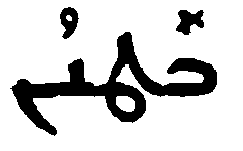
\includegraphics[height=1.05em]{../../S01/source/presentation/AB01-PDF0022-G01.png}} \emph{Baṭnān}\footnote{The Syrians called the territory of the city \emph{Srūg}, whence we often find mentioned among them \emph{Baṭnān d-ba-Srūg} «B. which is in Sarūj», or \emph{Baṭnān da-Srūg} «B. [of the region called] Sarūj»; many examples in J. S. Assemani, \emph{Bibliotheca Orientalis Clementino-Vaticana}, Rome 1719–28, passim. The Arabs gave the name of the territory to the city itself and at the same time to the very wide plain that opens to the south of it.}, called \emph{Sarūj} by the Arabs, today \emph{Eskī Sarūj}. In Isidore of Charax, \emph{Mansiones Parthicae}, ch. III\footnote{\emph{Geographi Graeci minores ed. Miller}, Paris 1849, vol. I, p. 246.}, the fort {\greekfont Κοραία ἥ ἐν Βατάνῃ} is mentioned, where {\greekfont Βατάνη}, the name of the town, seems to have been transferred to its territory\footnote{What the fort {\greekfont Κοραία} was is unknown. Mannert thought it was {\greekfont Κάρραι}, i.e. Ḥarrān; Ritter, \emph{Erdkunde} vol. X, pp. 1118–19, puts it near Sarūj, without determining its position exactly.}; one of the codices has {\greekfont Βιτάνῃ}. This was the reason why Chwolsohn took Battān to be Batnae. But on how slippery a foundation such an opinion rests appears at once from this, that the genuine form of the name, used by the Syrians, was \emph{Baṭnān}, from which the Arabic \emph{Battān} could in no way arise; for the Syriac \emph{ṭ} \RL{\syriacfont ܛ} was never turned by the Arabs into \emph{t} \RL{\ArNote ت}, whether Syriac words were taken into Arabic through common speech or through the writings of learned men\footnote{There is also a difficulty in the first \emph{n}, which is lost. — Another argument against Chwolsohn's opinion, of far less weight yet not useless, is that the town of Sarūj is said to have been very flourishing in al-Battānī's time too; he would hardly, then, have passed it over in the geographical table, vol. II, pp. 37–54, in which many cities no bigger than Sarūj are listed, if he had been born there. Ḥarrān, on the other hand, from which he at least undoubtedly derived his origin, he not only did not pass over (vol. II, p. 41, no. 152), but he chose to construct a special table of oblique ascensions for its latitude (vol. II, p. 67).}.\par
\par Nothing certain is known of al-Battānī's boyhood or of his domestic affairs. I do not doubt that he was born before the year 244 H (beginning 18 Apr. 858), since he had already begun to observe in the year 264 and three years later had completed some of his chief observations. His father seems to have been the Jābir ibn Sinān al-Ḥarrānī\footnote{Which Flügel first happily conjectured, in his note to al-Nadīm (vol. II, p. 135). Bailly is altogether wrong, \emph{Histoire de l'astronomie moderne}, Paris 1779, vol. I, p. 592: «On imagine que ce Geber, de qui il est fils, est le fameux Geber, le pere des Alchimistes... Si le pere eut une certaine célébrité, le fils en a une plus réelle et plus solide» (one imagines that this Geber, whose son he is, is the famous Geber, the father of the alchemists... If the father had a certain celebrity, the son has a more real and more solid one).} who is mentioned by al-Nadīm, p. 284 (Suter's translation p. 42), among the famous makers of astronomical instruments\footnote{Al-Nadīm I, 284 (Suter's translation 41–42) lists nine of them who were from Ḥarrān; for al-Ṣūfī, ed. Schjellerup, p. 31, shows that ʿAlī ibn ʿĪsā al-Asṭurlābī too must be counted among them. — Steinschneider, \emph{Arabische Mathematiker und Astronomen}, in Orient. Litteratur-Zeit., vol. V, 1902, cols. 3–5, mentions only eight, leaving out ʿAlī ibn ʿĪsā.}. It is therefore no wonder that al-Battānī, perhaps taught the rudiments of the science by his father himself, not only attained the greatest excellence in observing the stars but also devised a new and very convenient armillary sphere.\par
\par \Pg{I XV}Ḥarrān\footnote{On the right bank of the river Belīkh (the citadel, however, on the left). On R. Kiepert's map, 39° 8′ E of Greenwich, 36° 53′ N; al-Battānī's latitude (36° 40′) is already in al-Khwārizmī, and the same in the later geographers of the Arabs. On the city as it exists today, having lost its old size and glory, see Ritter, \emph{Erdkunde}, vols. X (1843) and XI (1844) passim; G. P. Badger, \emph{The Nestorian and their rituals}, London 1852, vol. I, p. 340 ff.; E. Sachau, \emph{Reise in Syrien und Mesopotamien}, Leipzig 1883.}, \emph{Ḥarrān} in the Assyro-Babylonian cuneiform inscriptions, \emph{Ḥārān} in the Old Testament and in the books of the Syrians, called \emph{Carrhae} ({\greekfont Κάρραι}) by the Romans, was once a very famous city, from the most ancient times the chief seat of the cult of the god \emph{Sīn}, that is, the Moon\footnote{As now appears from the cuneiform inscriptions, his wife Ningal, his daughter Ištar (or Malkatu), his son Nusku and other minor gods were also worshipped at Ḥarrān in the most ancient times.}; it stubbornly resisted the Christian religion, and for this reason it was often called by the Syrians \emph{mdītta d-ḥanpāyē} or \emph{d-ḥanpē}, «the city of the pagans». Full of Greek learning and abounding in very learned men and in the most liberal studies, it kept the cult of the pagan gods even in the first four centuries after the hijra\footnote{See Chwolsohn's work, already cited, in which the Greek, Latin, Syriac, Arabic and Jewish testimonies on the religion of the people of Ḥarrān are collected with the greatest care. It is no wonder that some things must now be judged otherwise, since our age has made great progress in oriental studies since Chwolsohn's book was published; yet that most distinguished man was the first to remove the altogether incredible confusion in which learned men were entangled concerning the Sabians, the Sabaeans and the Mandaeans.}, while its learned men professed metaphysical doctrines in which Oriental and Greek elements were mixed together, as among the Gnostics and the Alexandrian philosophers\footnote{Cf. also Dozy, \emph{Nouveaux documents pour l'étude de la religion des Harraniens, mémoire posthume achevé par} De Goeje, in Actes du 6$^{\text{me}}$ Congrès international des Orientalistes, 2$^{\text{e}}$ partie, section sémitique, Leiden 1885.}; the people of Ḥarrān, however, from the year 215 H, AD 830, so that they might profess their religion freely on paying only the yearly tribute (\emph{jizya}) that Muslim law imposes on the «people of the book»\footnote{So the Christians, the Jews and the Ṣābiʾūn are called in the Qurʾān, because they possessed books revealed by God. If they pay tribute to the Muslims, they cannot be forced to embrace the Islamic faith.}, declared by a most audacious fraud that they were \emph{Sabians}, not pagans. For the Sabians (\emph{Ṣābiʾ}, pl. \emph{Ṣābiʾūn}), who are counted in the Qurʾān among the «people of the book», differed entirely from the people of Ḥarrān\footnote{Even now H. Winckler wrongly confuses the Sabians of the Qurʾān with the ancient people of Ḥarrān, \emph{Arabisch-semitisch-orientalisch, kulturgeschichtlich-mythologische Untersuchung}, Berlin 1901–02, p. 90 (= Mitteilungen der vorderasiatischen Gesellschaft, VI Jahrg., 1901, fasc. IV and V).}: they were Elkesaites and Mandaeans, both sects of Gnostics who lived mainly in Babylonia and had taken over many pagan, Jewish, Christian and Persian rites together\footnote{The doctrines of the books of the Mandaeans were collected by W. Brandt, \emph{Die Mandäische Religion, ihre Entwickelung und geschichtliche Bedeutung}, Leipzig 1889, and \emph{Mandaeische Schriften übersetzt und erläutert}, Göttingen 1893; the name \emph{Mandāyī} (pl. \emph{Mandāyē}) means the followers of the «knowledge of life» (\emph{mandā d-hayyē}, {\greekfont γνῶσις ζωῆς}). Today they are called in Arabic \emph{Ṣubbī}, pl. \emph{Ṣubba} (cf. the plurals \RL{\ArNote الصُّبّاء} and \RL{\ArNote الصُّبَّاة} already in the Glossary to the \emph{Annales} of al-Ṭabarī, p. cccxxi, s. v. \RL{\ArNote صبا}), or \emph{Yaḥyāwī}, pl. \emph{Yaḥyāwiyya}; they live in some villages of southern Mesopotamia (al-ʿImāra, al-Qurna, al-Baṣra, Sūq al-Shiyūkh, al-Nāṣiriyya, etc.), hardly reaching the number of 2000, and a few also in the cities of al-Muḥammara and al-Ḥuwayza in Khūzistān. Those who were in the cities of Dizfūl and Shushtar migrated to Mesopotamia 14 years ago, harassed by the Persians. The best account of their present sacred institutions and customs (not, however, of their history) is given by Father Anastās al-Karmalī, \emph{al-Ṣābiʾa aw al-Mandāʾiyya}, in the Arabic periodical al-Mashriq, vol. III, 1900, pp. 486–89, 680–85, 777–85, vol. IV, 1901, pp. 400–06, 550–54, 684–89, 779–84, 924–30, 1121–1126, vol. V, 1902, pp. 307–11, 392–96, 488–97, who corrects many errors into which N. Siouffi had fallen, \emph{Etudes sur la religion des Soubbas ou Sabéens, leurs dogmes, leurs moeurs}, Paris 1880.}. That even the oldest commentators of the Qurʾān did not know what these Sabians really were is very clear from al-Ṭabarī, \emph{Jāmiʿ al-bayān fī tafsīr al-Qurʾān}, Cairo (al-Maymaniyya press), 1319 H ff., vol. I, pp. 242–243; which made it less difficult for the people of Ḥarrān to lead the caliph himself into error.\par
\par \Pg{I XVI}Because among the names given to al-Battānī there is also the epithet Sabian (\emph{al-Ṣābiʾ}), some, both Arabs and our own scholars\footnote{Reiske, in the additions to the German translation of D'Herbelot's book, \emph{Orientalische Bibliothek}, Halle 1785–90, part I, s. v. Albattani: «Dieser war ein Sabier von Religion, d. h. einer von denjenigen, welche man Johannischristen zu nennen pflegt» (he was a Sabian by religion, that is, one of those whom one usually calls Christians of St John), where he also confuses the Mandaeans (sometimes wrongly called Christians of St John) with the Sabians of Ḥarrān. — J. F. Montucla, \emph{Histoire des mathématiques}, new ed., Paris year VII–X, vol. I, p. 363: «Albatenius n'étoit point un musulman, mais de la religion des Sabéens» (Albatenius was not a Muslim, but of the religion of the Sabians). Reinaud, \emph{La Géographie} d'Aboulféda \emph{traduite}, Paris 1848–83, vol. I (general introduction), p. lxii, asserts with no foundation at all: «Albateny était Sabéen, et malgré son nom de Mohammed, il mourut dans cette religion» (Albateny was a Sabian, and in spite of his name Mohammed he died in that religion). Steinschneider is silent; Chwolsohn I, 611 and 615 inclines to the opinion that he never embraced Islam; Brockelmann I, 222: «war als Ṣābier in Ḥarrān geboren» (was born a Sabian in Ḥarrān); C. Huart, \emph{Littérature arabe}, Paris 1902, p. 294: «était un sabien de Harran» (was a Sabian of Harran); Suter, p. 46, does not venture to assert anything about al-Battānī's religion (but his note \emph{b} rests on a wrong interpretation of the passage of which I spoke on p. viii, n. 13). No one, however, doubts that al-Battānī was born a Sabian.}, have thought him an adherent of the sect of the \emph{Sabians}, although, as we have seen, it had not escaped Ibn Khallikān and Abū l-Fidāʾ that this could hardly be reconciled with the name Muḥammad, which is used only by Muslims\footnote{That Christians belonging to the Bogos peoples, in the northern part of the Colony of Eritrea, sometimes use the names Muḥammad and Maḥmūd is indeed attested by C. Conti Rossini, \emph{Tradizioni storiche dei Mensa}, in Giornale della Società Asiatica Italiana, vol. XIV, 1901, p. 86, n. This happens for two altogether peculiar reasons: one, that a few years ago the greatest part of that people embraced the Islamic faith; the other, that they are all so uncivilized that they have only a very slight, and not always correct, notion of their religion, Christian or Muslim.}. The difficulty is resolved if we consider that relative names (\emph{nisba}), as I noted above, are sometimes passed on from father to son\footnote{In the first centuries of the hijra, names derived from the very ancient Arab tribe from which the forefathers had their first origin were very often handed down.}; al-Battānī, then, could have been called a Sabian not from his own religion but from that of his father and forefathers. There is no lack of examples of men who, though born Muslims, took for this reason the name \emph{al-Naṣrānī} «the Christian», \emph{al-Majūsī} «the Zoroastrian», \emph{al-Isrāʾīlī} «the Israelite». Likewise, in the sixth century H, mention is made of a qāḍī, or Muslim judge, Muḥammad ibn Aḥmad ibn Bakhtiyār ibn ʿAlī ibn Muḥammad ibn Ibrāhīm ibn Jaʿfar al-Mandāʾī\footnote{On him Ibn Khallikān, in the life of al-Ḥarīrī (ed. Wüstenfeld, no. 546, where \RL{\ArNote المندائي}, and De Slane's translation II, 491–93); cf. Chwolsohn I, 136–37, n. Born in the city of Wāsiṭ on 8 Rabīʿ II 517 (5 May 1123), he died towards the end of the month of Shaʿbān 605 (the beginning of March 1209).}, whose forefathers had already left the religion of the Mandaeans in the fourth century. Lastly, it is not impossible that the name Sabian was given him by later writers for no other reason than that he came from Ḥarrān, whose learned men had for the most part been Sabians until the end of the fourth century of the hijra.\par
\par Someone may perhaps suspect that al-Battānī embraced the Islamic faith late, and so took the name Muḥammad in place of the name given him by his parents. But in that age, as far as we can judge from very many examples, those who embraced Islam did not change their name unless it was wholly repugnant to the Arabic language or to the Muslim religion. That certainly did not happen with the proper names of the people of Ḥarrān; therefore neither Thābit ibn Qurra, nor his son Sinān, nor other Sabians who became Muslims at an advanced age changed their names.\par
\par However that may be, the most certain testimony to al-Battānī's Muslim faith is the preface of the astronomical work itself, in which many verses of the Qurʾān are quoted, and the Muhammadan phrases scattered throughout the book, especially at the end of every chapter.\par
\par It is known that in the third century of the hijra, the eighth AD\footnoteT{The third century of the hijra (AD 816–913) is the ninth century AD.}, several people of Ḥarrān settled in the city of \emph{al-Raqqa}, and that many of them kept the Sabian religion. Al-Raqqa\footnote{A very ancient city, it seems; at the beginning of the fourth century BC or at the end of the third a Macedonian colony called {\greekfont Νικηφόριον}; from the fourth century AD on, until the Muslim empire, it had the name {\greekfont Καλλίνικον}. A little to the west of the place where the river Balīkh flows into the Euphrates. — In his translation Plato of Tivoli had written the name correctly, \emph{Aracca}; in the printed editions it is corrupted into \emph{Aracta}.} was at that time a most flourishing city on the left bank of the Euphrates, to which three other towns were so close — \emph{al-Raqqa al-sawdāʾ}, that is, «the black» (on the right bank of the Euphrates), \emph{Wāsiṭ al-Raqqa} and \emph{al-Rāfiqa} — that the aggregate of these four cities was very often designated by the name al-Raqqa. It is mentioned hundreds of times by the historical writers of the eighth, ninth and tenth centuries AD; the caliph Hārūn al-Rashīd (AD 786–809) had built himself a palace there, so as to be able to stay in the city more often, and Chesney saw its ruins in 1836\footnote{Not 1835, as was wrongly printed on p. 226, n. 2, and in vol. II, p. 41, n. 150. A description of the ruins and the history of the city in Ritter, \emph{Erdkunde}, vol. X (Berlin 1843), pp. 1125–48, who also had an unpublished part of Chesney's work in his hands. Very little, but with a picture of the ruins, in Fr. R. Chesney, \emph{Narrative of the Euphrates expedition carried on by order of the British Government during the years 1835, 1836 and 1837}, London 1868, pp. 243–44. On map III attached to Chesney's great but never completed work, \emph{The expedition for the survey of the rivers Euphrates and Tigris}, London 1850, the old rampart of the city appears drawn roughly as a circle, whose circumference at its northernmost point is about 1½ km from the bank of the river. In the eastern part of the city, 0.740 km from the bank, are the ruins of the palace of Hārūn al-Rashīd, 39° 3′ 58.5″ E of Greenwich, 35° 55′ 35″ N. An astronomical observation was made there for one day or two in the month of May 1836 by Murphy (Chesney, \emph{Narrative}, p. 244). — The city, almost deserted around the middle of the nineteenth century, began to flourish again after 1880, so that today it comprises 200 houses and a market, according to Sachau, \emph{Am Euphrat und Tigris, Reisenotizen aus dem Winter 1897–98}, Leipzig 1900, p. 141.}.\par
\par \Pg{I XVII}That the father of our astronomer too was among those who moved from Ḥarrān to al-Raqqa is not improbable. From the astronomical work itself it is very clear that al-Battānī spent the greatest part of his life in that city. There he observed the heavens over a very long span of years so as to establish the elements of the tables (p. 6, ll. 2–3), adapted to the meridian and the latitude of that city; for many years after he measured the course of the Sun most diligently (p. 43), determining the solstices and the equinoxes often, but especially in the years 882 and 883 (pp. 42, 44); in 879–880 he fixed the longitudes of certain fixed stars (p. 124); and lastly, in the years 883 and 891, he observed eclipses of the Sun and the Moon (pp. 56, 57). — In the year 901, however, he stayed for no short time at \emph{Antioch}, for there, with astronomical instruments too, he was able to observe an eclipse of the Sun (23 January) and one of the Moon (2 August) (pp. 56, 57).\par
\par Where the false report was taken from, which is not rarely spread about by our scholars\footnote{Riccioli, \emph{Almagestum Novum}, Bologna 1651, vol. II, p. xxix: «a ruler of Syria»; Halley, in \emph{Philosophical Transactions}, 1693, vol. XVII, no. 204, p. 915: «he is believed to have been a nobleman, and by some even the prince of his country»; J. F. Montucla, \emph{Histoire des mathématiques}, new ed., Paris year VII–X, vol. I, p. 363: «il fut commandant pour les califes en Syrie» (he was commander for the caliphs in Syria); J. La Lande, \emph{Astronomie}, 3rd ed., Paris 1792, vol. I, p. 123, § 355: «Albategnius, prince arabe, vivoit en 879 et 912» (Albategnius, an Arab prince, lived in 879 and 912); Delambre, \emph{Astron. du moyen âge}, p. 4: «C'était un prince de Syrie dont la résidence était à Aracte ou Racha en Mésopotamie» (he was a prince of Syria whose residence was at Aracte or Racha in Mesopotamia); likewise Fr. Baily, \emph{The catalogues of Ptolemy, Ulugh Beigh etc.}, in Memoirs of the R. Astronomical Society, vol. XIII, London 1843, preface p. 20: «Albategnius was a prince of Syria residing at Aracle in Mesopotamia, about the close of the ninth century; but D'Herbelot considers his origin somewhat low».}\footnoteT{In the note the print has vol. XIV; Nallino's Addenda et emendanda (Part II, p. XVI) correct it to XIII.}, that al-Battānī was a prince or king of Syria, I do not know; I have never found anything of the kind in the Arabic writers.\par
\par That, wholly intent on his studies, he shrank from vain praise and did not pursue the favours of princes may be inferred from what he prescribes on p. 139 for good observers to do; it appears still more from his very great modesty, of which I shall speak in § 4, no. III. Yet that the learned men of his age already held him in high esteem is shown with certainty by the epistle that Ibn al-Furāt had asked of him, by his conversations with Jaʿfar ibn al-Muktafī, and by his observations, already mentioned by Thābit ibn Qurra (see p. 302).\par
\par \Pg{I XVIII}About those Banū l-Zayyāt\footnote{That is, the sons or descendants of a man called al-Zayyāt.} with whom al-Battānī went to Baghdād the authors relate nothing. I think it most probable that they were the family of the very famous Abū Jaʿfar Muḥammad ibn ʿAbd al-Malik ibn Abān al-Zayyāt, often called briefly Ibn al-Zayyāt, who, born of a humble family, but a good poet and a man most eminent in literary studies, was the minister (wazīr) of the caliphs al-Muʿtaṣim (AD 833–842) and al-Wāthiq (842–847), and was put to death by order of al-Mutawakkil on 19 Rabīʿ I 233 H, i.e. 2 Nov. 847\footnote{Besides the historians, cf. \emph{Kitāb al-Fihrist} p. 122; \emph{Aghānī} XX, 46–56 and passim; Ibn Khallikān, ed. Wüstenfeld, no. 706 (Cairo ed., al-Waṭan press, 1299 H, vol. II, pp. 458–63; De Slane's translation vol. III, pp. 249–56); al-Yaʿqūbī, \emph{Kitāb al-buldān}, ed. de Goeje, pp. 257, 262; al-Bīrūnī, \emph{Chronol.} p. 273 (= 265 of the translation); al-ʿĀmilī, \emph{al-Kashkūl}, Cairo 1305, p. 213; Aḥmad b. Yaḥyā b. al-Murtaḍā, \emph{al-Muʿtazilah ed. by T. W. Arnold}, Leipzig 1902 ff., part I, pp. 38–39. In the book \emph{Abulḳâsim ein bagdâder Sittenbild von} Muḥammad ibn Aḥmad Abulmuṭahhar \emph{hrsg. von A. Mez}, Heidelberg 1902, p. 74, written in the first half of the fifth century H, they say to a man who boasts too much: «Do you think you are Ibn al-Zayyāt the vizier?». — His poems (\emph{dīwān}) survive in a codex that once belonged to C. de Landberg and now belongs to \emph{Yale University} in New Haven (North America) (it is missing in Brockelmann).}\footnoteT{In the note the print has «Princeton»; Nallino's Addenda et emendanda (Part II, p. XVI) correct it to New Haven.}. His son Abū Mūsā Hārūn ibn Muḥammad ibn ʿAbd al-Malik al-Zayyāt collected poems and narratives with the greatest zeal\footnote{\emph{Kitāb al-Fihrist} p. 123; \emph{Aghānī} V, 22 (a passage missing in the \emph{Tables alphabétiques}) and IX, 32–33.}; and his great-great-grandson Abū Ṭālib Aḥmad ibn al-Ḥusayn ibn ʿAlī ibn Aḥmad ibn Muḥammad ibn ʿAbd al-Malik al-Zayyāt was a friend of the writer Ibn Waḥshiyya, whose books he handed down\footnote{Of which the most famous is the \emph{Nabataean Agriculture}, in which, to belittle the Arab race, fabulous things are told of the supreme glory of the «Nabataeans», that is, of the ancient Babylonians. If any credit can be given to the preface, Ibn Waḥshiyya had translated the book from the Syriac language in the year 291 H (beginning 23 Nov. 903) and in the year 318 (beginning 2 Febr. 930) had dictated it to that Abū Ṭālib Aḥmad ibn al-Zayyāt. But Nöldeke, \emph{Noch Einiges über die nabatäische Landwirthschaft}, in Zeitschr. d. deutsch. morgenländischen Gesellschaft, vol. XXIX, 1875, pp. 453–55, thinks it not improbable that the book is pseudepigraphic and that its author is Abū Ṭālib himself. — Long fragments of the work are also in Muḥammad Rāghib Pasha, \emph{Safīnat al-rāghib}, Būlāq 1282, pp. 670–75 (on p. 671 the year is wrongly 271 for 291, i.e. \RL{\ArNote سبعين} «seventy» in place of \RL{\ArNote تسعين} «ninety»).}, and a few years younger than al-Battānī.\par
\par \Pg{I XIX}Already far advanced in age, when 55 lunar years, about 54 solar years, had passed since the time he began to observe, al-Battānī died at a place called \emph{Qaṣr al-Jiṣṣ} or \emph{Qaṣr al-Jaṣṣ}, that is, «Palace of gypsum»\footnote{G. Le Strange, \emph{Description of Mesopotamia and Baghdād written about the year 900 A. D. by} Ibn Serapion, in Journal of the R. Asiatic Society, 1895, pp. 265 and 266; M. Streck, \emph{Die alte Landschaft Babyloniens nach den arabischen Geographen}, Leiden 1900 ff., p. 211; al-Muqaddasī, ed. de Goeje, pp. 28, 54, 115; Yāqūt, \emph{Muʿjam}, ed. Wüstenfeld, IV, 110; Yāqūt, \emph{al-Mushtarik}, ed. Wüstenfeld, p. 348; \emph{Marāṣid al-iṭṭilāʿ} II, 419. — In Ed. Corn. Vandyck, \emph{Iktifāʾ al-qunūʿ bi-mā huwa maṭbūʿ}, Cairo 1897, p. 243, in a life of al-Battānī drawn from European sources, the name is corrupted into \RL{\ArNote قلعة جاص}! But how Vandyck disfigures Arabic names in his Arabic books I have shown well enough in the periodical \emph{al-Mashriq}, vol. I, Beirut 1898, pp. 811–12; another error of his about al-Battānī I shall mention below, § 4, no. VI.}. This was one of the palaces that the caliph al-Muʿtaṣim (AD 833–842) had built in the neighbourhood of the city of Sāmarrāʾ: a little to the west of the Tigris, on the canal called Nahr al-Isḥāqī, and to the north of the palace called al-Maʿshūq (or, as they say today, al-Maʿshūqa), whose ruins von Oppenheim mentions, \emph{Vom Mittelmeer zum Persischen Golf}, Berlin 1899–1900, vol. II, p. 221. In it, according to certain authors, on 8 Shawwāl 372 (26 March 983), ʿAḍud al-Dawla, the ruler of Persia, was killed by his cousin Bakhtiyār ibn Muʿizz al-Dawla\footnoteT{In the usual account the roles are the other way round: it was Bakhtiyār (ʿIzz al-Dawla) who was defeated and killed at Qaṣr al-Jiṣṣ by the forces of his cousin ʿAḍud al-Dawla, in Shawwāl 367 (May 978); ʿAḍud al-Dawla died at Baghdād on 8 Shawwāl 372 (26 March 983).}; after that time no mention of the palace, which was probably destroyed, is made by the Arabic writers. — The name \emph{Qaṣr al-Ḥaḍr} in the life written by Ibn Khallikān is nothing but a \emph{taṣḥīf}, as the Arabs say, that is, a corruption in the writing of the source that the famous author had used, in place of Qaṣr al-Jiṣṣ; it arose the more easily because the very ancient town of al-Ḥaḍr\footnote{\emph{Hatra} in the Roman writers, in the almost desert plain that stretches south of Sinjār and west of the Tigris, on the river Tharthār. Already largely destroyed in the fourth century AD; its notable ruins were described by Ross (1836) and Ainsworth (1840). On the city: Ritter, vol. XI (1844), pp. 466–92; M. Amari in the notes to \emph{Solwan el Mota' ossiano conforti politici di} Ibn Zafer, \emph{versione italiana}, Florence 1851, pp. 324–41; Tabari, \emph{Gesch. der Perser und der Araber übers. v. Th. Nöldeke}, Leiden 1879, pp. 33–34, n.}, though largely destroyed after the coming of Islam, held a notable place in the old histories of the Arabs and was known to everyone, while the other place was, on the contrary, unknown to most. Yet Ibn Khallikān himself admits that he found \emph{Qaṣr al-Jiṣṣ} written in another book\footnote{Of the error in the editions and in the English translation I have spoken on p. x, n. 3.}; and that this is the true reading is shown, besides the most certain testimony of Ibn al-Nadīm, Ibn al-Qifṭī and Abū l-Fidāʾ, by this very fact, that the word Qaṣr is never found put before the name al-Ḥaḍr, mentioned hundreds of times by the Arabs, and that it is not likely that a man travelling from Baghdād to al-Raqqa, and one far advanced in age, made his way through the ruins of al-Ḥaḍr, which would have been out of the way and, because of the deserts that lie between al-Ḥaḍr and al-Raqqa, extremely difficult.\par
\par\begin{center}\textbf{§ 2. The minor writings of al-Battānī.}\end{center}
\par I. \emph{Kitāb maʿrifat maṭāliʿ al-burūj fī mā bayna arbāʿ al-falak} «The book of knowing the ascensions of the signs in the spaces between the quarters of the celestial sphere».\par
\par That the scholars of our countries who have written about al-Battānī did not understand what this title meant\footnote{Chwolsohn must be excepted, who does not mention al-Battānī's minor writings.} is no wonder, since in the Arab and Persian astronomers so far published in their own language the same things are designated by another name. De Slane, in his translation of Ibn Khallikān IV, 317, rendered it «knowledge of the rising-places of the zodiacal signs in the interval between the quarters of the sphere», and added this note: «This is perhaps a treatise on the mode of calculating the amplitude of the signs of the Zodiac for every latitude. Such a work would be useful for the history of spherical astronomy»\footnote{Which Jarrett afterwards copied: «Among other works he [i.e. al-Battānī] wrote a treatise on the mode of calculating the amplitude of the Zodiacal signs for every latitude, which would be of use in the history of spherical trigonometry» (Abul Fazl Mubárak i 'Allámí, \emph{The Áín i Akbarí translated from the original Persian by H. Blochmann and H. S. Jarrett}, Calcutta 1873–94, vol. II, p. 4, n. 3).}. — Steinschneider on Baldi, p. 457, n. 17 (Extr. p. 30): «Libro della scienza delle ascensioni dei segni del Zodiaco secondo che sono (?) nei quattro quarti della sfera» (book of the science of the ascensions of the signs of the zodiac according as they are (?) in the four quarters of the sphere); but he plainly did not know what this was, since he had thought that al-Battānī's writing on the applications and the little book on the rising of the triplicities were parts of this book. — Suter, \emph{Die Mathematiker}, p. 46: «Ueber die Kenntniss der Aufgänge der Häuser nach den vier Quadranten der Sphäre» (on the knowledge of the risings of the houses according to the four quadrants of the sphere).\par
\par From the title itself it appears most clearly that this little book treats the same subject as chapter LV of the astronomical work (vol. I, pp. 131–34) and the spurious appendix F (p. 149), namely the computation of the astrological \emph{directions}, which I have explained sufficiently on pp. 313–17. Whether he proposed in it a new solution, more in accord with exact geometrical rules than the Ptolemaic one (which is nevertheless sufficient), I do not know; for the little book has not come down to our time. The same problem must also have had a place in al-Battānī's commentary on the Tetrabiblos.\par
\par II. \emph{Risāla fī taḥqīq aqdār al-ittiṣālāt} «Epistle on the verification of the amounts of the applications»\footnote{For «amounts», Steinschneider on Baldi, p. 457 (extr. p. 30): «della potenza» (of the power); Suter: «Wirkungen» (effects). But astrological strength or force ({\greekfont ἐνέργεια}) is always called \emph{quwwa} by al-Battānī (vol. III, p. 195, ll. 3–15 and passim = vol. I, p. 130); therefore in vol. III, p. 195, l. 8, \emph{qadr} is very plainly distinguished from \emph{quwwa}: \RL{\ArNote وقوّة الأقدار القويّة} «the force of the stronger amounts». — That \emph{ittiṣālāt} in the astrological sense are not «conjunctions» (as De Slane, Steinschneider and Suter translated) but «applications» ({\greekfont συναφαί}) is deduced from chapter LIV itself.}.\par
\par This writing too has not come down to us; the title is the same as that of chapter LIV (vol. I, pp. 129–131), which I rendered less barbarously in vol. I, pp. 4 and 129, «on the true amounts of the applications». In it he had perhaps for the first time brought the doctrine of the projection of the rays back to true geometrical principles; for the rest, on the subject of the epistle, cf. my notes, pp. 305–13.\par
\par \Pg{I XX}He composed the epistle for Abū l-Ḥasan ʿAlī ibn Muḥammad ibn Mūsā ibn al-Ḥasan Ibn al-Furāt, who, born on 22 Rabīʿ II 241 (9 Sept. 855), was three times minister of the caliph al-Muqtadir\footnote{According to ʿArīb, he held the office of minister from 21 Rabīʿ I 296 to 4 Dhū l-Ḥijja 299, then from 8 Dhū l-Ḥijja 304 to 26 Rabīʿ II 306, and lastly from 20 Rabīʿ I 311 to 9 Rabīʿ I 312. There are small discrepancies in other writers.}, by whose order he was put to death on 13 Rabīʿ II 312 (19 July 924); he greatly favoured poets and those who cultivated literary studies. On him especially Weil, \emph{Geschichte der Chalifen}, Mannheim 1846–51, vol. II, pp. 543–56; Ibn Khallikān, ed. Wüstenfeld, no. 498 (Cairo ed., al-Waṭan 1299, vol. II, pp. 79–85); ʿArīb, \emph{Tabari continuatus}, ed. de Goeje, passim between pp. 28 and 121; Ibn al-Athīr, \emph{Annales}, Cairo ed. 1301–02, vol. VIII, passim between pp. 3 and 57; al-Masʿūdī, \emph{Prairies}, vol. VIII, pp. 251, 266, 272–73; al-Nadīm, \emph{Kitāb al-Fihrist}, p. 128, l. 23, 151.\par
\par Some\footnote{Steinschneider on Baldi, p. 457, n. 17 (extr. p. 30); Suter in his translation of the Fihrist, p. 35 (but on p. 68, n. 211, he did not keep his doubts silent, and in \emph{Mathemat.} p. 46 he distinguished the two little books very well).} have thought that this epistle does not differ from the book of the ascensions of the signs, translating the passage of Ibn al-Nadīm of which I spoke on p. ix, n. 1, thus: «The book of knowing the ascensions of the signs in the spaces between the quarters of the celestial sphere, and it is known [also by the title] his epistle on the verification of the amounts of the applications; he composed it for Abū l-Ḥasan Ibn al-Furāt». They interpreted it so to avoid the difficulty that arises from the masculine pronoun («he composed \emph{it} (\emph{eum})»); but in avoiding Charybdis they fell into Scylla. For to save the reading \RL{\ArNote عمله} «he composed \emph{it} (\emph{eum})» one would have to change both \RL{\ArNote تعرف} «is known» (\emph{nota}, feminine) into \RL{\ArNote يعرف} «is known» (\emph{notus}, masculine), and \RL{\ArNote رسالته} «his epistle» into \RL{\ArNote بالرسالة}, as the rules of Arabic grammar would require. My emendation is far more likely; for al-Nadīm had listed al-Battānī's \emph{books} before, and now he adds: «And his \emph{epistle} is also famous, etc.». Ibn al-Qifṭī and Ibn Khallikān confirm my interpretation; and it becomes quite certain if we consider that the book of the ascensions of the signs deals with a question wholly different from the problem of the applications.\par
\par III. \emph{Sharḥ al-maqālāt al-arbaʿ li-Baṭlamyūs} «Commentary on the Tetrabiblos of Ptolemy».\par
\par That it once existed in the Escorial Library we know from the \emph{Bibliotheca Arabico-Hispana} of Casiri, who described the codex thus, vol. I, p. 399: «Cod. CMLXVI, no. 2: A commentary on the Quadripartitum of Ptolemy, on the judgements of the stars, with tables added. The author is the most distinguished man Mohammad Ben Geber Albategnius». But H. Derenbourg has already noted that the codex is now lost with others, \emph{Les manuscrits arabes de l'Escurial}, Paris 1884, vol. I, p. xxiv; nor could it be found in October 1894, when I was staying at the Escorial. In September 1901, when the Arabic codices were examined again by the librarians, no trace of the book appeared, as Father Pedro Blanco Soto most kindly wrote to me.\par
\par It is likely that in this commentary al-Battānī explained above all the mathematical principles of astrology; for the «\emph{tables added}» could have served only for these, and our author seems to have indulged a little in the ravings of judicial astrology.\par
\par \Pg{I XXI}In the Royal Library of Berlin an Arabic codex is kept, comprising 124 pages and mutilated by the loss of its first leaf, which has this subscription at the end\footnote{W. Ahlwardt, \emph{Verzeichniss der arabischen Handschriften der k. Bibliothek zu Berlin}, Berlin 1887–99, vol. V, pp. 273–74, no. 5875. Ahlwardt thinks the codex was written about the year 800 H (AD 1397).}: «Here ends the \emph{book of the Tetrabiblos, the commentary} of al-Battānī\footnote{\RL{\ArNote تم كتاب الاربا (\LR{sic}) شرح البتاني}.}, by the grace of God. Aḥmad ibn Tamīm wrote it\footnote{\RL{\ArNote علّقه}; on this word Dozy, \emph{Supplément}, vol. II, p. 161.}, giving thanks to God for His benefits and praying for Muḥammad the Prophet», etc. The author of the catalogue judges the book thus: «That this is a commentary on the book of Ptolemy so entitled [i.e. the Tetrabiblos] in no way appears; it seems to be a work standing by itself (\emph{ein selbstständiges Werk}), and is undoubtedly to be regarded only as a new recension (\emph{Bearbeitung}) of the original book, which is difficult to understand. This, as the name itself shows, is divided into four books, of which there is no trace in the codex..... The work comprises many chapters (which, however, lack the name «\emph{chapter}»), marked with no number». So that the book may be judged better, I translate the Arabic headings of the chapters as they are given in Ahlwardt's catalogue, adding the numbers of the corresponding chapters of the \emph{Tetrabiblos} according to the vulgate and according to the Frankfurt edition (cf. p. 305, n. 2):\par
\Pg{I XXII}\begin{center}\small\begin{tabular}{>{\raggedright\arraybackslash}p{106mm}l}
On the strengths (\emph{quwā}) of the planets according to the configurations (\emph{ashkāl}) that they have with the Sun & I, 8 = Franc. 6 \\
On the strengths of the four seasons of the year, and on the ages (\emph{asnān}) of living beings & I, 10 = Franc. 8 \\
On the strengths of the four angles\footnotemark{} and of the four places of the horizon & I, 11 = Franc. 8 \\
On the fixed, movable and bicorporal signs\footnotemark{} & I, 12 = Franc. 9 \\
On the association (\emph{ishtirāk}) of the signs in the aspects (\emph{ashkāl}) & I, 14 = Franc. 11 \\
On the masculine and feminine signs, and on their other states & I, 13 = Franc. 11 \\
On the masculine (\emph{tadhkīr}) and feminine sex of the planets according to their position with respect to the Sun and also with respect to the horizon\footnotemark{} &  \\
On the almugea, the splendour and the like\footnotemark{} & I, 23 = Franc. 20 \\
On the correspondence (\emph{mushākala}) of the triplicities with the regions of the earth and with the planets & II, 3 = Franc. II, 2 \\
On knowing from the eclipses the things that will happen in the regions of the Earth & II, 7 = Franc. 6 \\
On the colours of the eclipses, and on comets & II, 9 = Franc. 8 \\
On knowing the vicissitudes (\emph{aḥwāl}) of the year\footnotemark{} & II, 10–12 = Franc. 9–11 \\
On the significations (\emph{dalāʾil}) that are taken from the meteors (\emph{al-āthār al-ʿalawiyya}) & II, 13 = Franc. 12 \\
The knowledge of the matters of nativities, and the significations to be taken from them & III, 1 \\
The knowledge of the ascending degree for the native & III, 2 \\
On the division of the discourse on nativities (\emph{fī qismat al-qawl ʿalà l-mawālīd}, {\greekfont διαίρεσις γενεθλιαλογική}) & III, 3 \\
On both parents & III, 4 \\
On brothers & III, 5 \\
On males and females & III, 6 \\
On the birth of twins & III, 7 \\
On monsters (\emph{fī mushawwahī l-khilaq}) & III, 8 \\
On those who will not be nursed, on those who will not be reared, on those who will be reared & III, 9 \\
On the length of life (\emph{al-ʿumr}, {\greekfont περὶ χρόνων ζωῆς}) & III, 10 = Franc. 10–15 \\
On the figure, the form (\emph{ḥilya}) and the temperament of the body of the native & III, 11 = Franc. 16 \\
On the injuries (\emph{ʿilal}) and the diseases (\emph{amrāḍ}) befalling the body of the native\footnotemark{} & III, 12 = Franc. 17 \\
On the quality of the soul in the native & III, 13 = Franc. 18 \\
On the diseases of the soul (\emph{fī l-āfāt al-nafsāniyya}) & III, 14 = Franc. 19 \\
On the fortune (\emph{bakht}) of the native as to riches & IV, 1 = Franc. IV, 2 \\
On the fortune of the native as to rank (\emph{ḥiẓwa}) & IV, 2 = Franc. 3 \\
On the quality of the profession and the craft of the native (\emph{fī ḥāl ṣināʿat al-mawlūd wa-ʿamalihī}) & IV, 3 = Franc. 4 \\
On children & IV, 5 = Franc. 6 \\
On friends, enemies and slaves & IV, 6 = Franc. 7–8 \\
On living abroad (\emph{ghurba}) and on journeys & IV, 7 = Franc. 9 \\
On the kind of death of the native (\emph{fī maniyyat al-mawlūd}) & IV, 8 = Franc. 10 \\
On the division of the times that belong to [the life of] the native ({\greekfont περὶ χρόνων διαιρέσεως}) & IV, 9 = Franc. 11 \\
\end{tabular}\end{center}
\addtocounter{footnote}{-6}\stepcounter{footnote}\footnotetext{\emph{Zawāyā}; but in al-Battānī's astronomical work they are only called \emph{awtād} «pegs».}\stepcounter{footnote}\footnotetext{The fixed signs, {\greekfont ζῴδια στερεά}, \emph{burūj thābita}, are Taurus, Leo, Scorpio, Aquarius; the movable, {\greekfont τροπικά}, \emph{munqaliba}, Aries, Cancer, Libra, Capricorn; the bicorporal or common, {\greekfont δίσωμα}, \emph{dhawāt al-jasadayn}, Gemini, Virgo, Sagittarius, Pisces.}\stepcounter{footnote}\footnotetext{Perhaps the second part of the preceding chapter.}\stepcounter{footnote}\footnotetext{In the Greek {\greekfont περὶ ἰδιοπροσώπων καὶ λαμπηνῶν καὶ θρόνων} (var.: {\greekfont τῶν τοιούτων}) «on [planets] having their own peculiar face, on royal chariots and thrones (var.: and the like)». According to Ptolemy, a planet has its own peculiar face, that is, is {\greekfont ἰδιοπρόσωπος}, when it keeps towards the Sun or the Moon the same configuration ({\greekfont σχηματισμός}) that its domicile ({\greekfont οἶκος}) has towards their domiciles; as, for example, Venus when it is distant from the luminaries by a sextile aspect, an evening star from the Sun, a morning star from the Moon, for so their domiciles are placed. The Arabs rendered this {\greekfont ἰδιοπροσωπία} \emph{al-muwājaha}, «to be face to face with someone», whence among the astrologers of the Middle Ages «\emph{almugea, the seeing of each other face to face, to see face to face}». — The brightness or splendour (\emph{al-ināra}, whence in the Latin translation of the Tetrabiblos from the Arabic «\emph{alchinara}») stands for the Greek {\greekfont λαμπήνη}, that is, a chariot or royal carriage. «\emph{And} [the planets] \emph{are said to be in their royal chariots and thrones and the like} [excellences] when they are joined in fellowship, in two or more of the ways set out above, with the places in which they are found. For because then their efficacy is most increased, by the likeness and the help of the homogeneous familiarity of the signs, therefore they are said \emph{to sit on their thrones} and \emph{to shine}» {\greekfont ἐν λαμπήναις δὲ ἰδίαις λέγονται εἶναι καὶ θρόνοις καὶ τοῖς τοιούτοις, ὅταν κατὰ δύο ἢ κατὰ πλείους τῶν προεκτεθειμένων τρόπων συνῳκειωμένοι τυγχάνωσι τοῖς τόποις ἐν οἷς καταλαμβάνονται. τότε γὰρ μάλιστα τῆς δυνάμεως αὐτῶν αὐξανομένης πρὸς ἐνέργειαν διὰ τὸ ὅμοιον καὶ συμπρακτικὸν τῆς τῶν δωδεκατημορίων ὁμοφυοῦς οἰκειώσεως, ἰδιοθρονεῖν καὶ λάμπειν λέγονται}. So Ptolemy, with whom Hephaestion of Thebes agrees. In translating the title of the chapter the Arabic translator plainly derived the word {\greekfont λαμπήνη} from the verb {\greekfont λάμπειν} «to shine», which occurs at the end of the passage quoted; that he interpreted the words {\greekfont ἐν λαμπήναις δὲ ἰδίαις λέγονται εἶναι καὶ θρόνοις} otherwise appears from both Latin translations from the Arabic: «in the place \emph{of its joy and honour}». The word seems to have been obscure even to the ancients; a certain scholiast on the Tetrabiblos: {\greekfont λαμπήνη λέγεται ἡ ἕδρα ἡ ἀργυρᾶ ὑψηλή, ἐν ᾗ ὁ ἄρχων ἱδρυνθεὶς λαμπρότερος φαίνεται. θρόνος δὲ ὁ τούτου κατώτερος καὶ ἐκ ξύλων ἀποτελεσθεὶς} «{\greekfont λαμπήνη} is the name of the high silver seat, sitting in which a ruler appears more splendid; {\greekfont θρόνος} that which is lower than it and made of wood» (in H. van Herwerden, \emph{Lexicon Graecum suppletorium et dialecticum}, Leiden 1902, p. 489, a passage that I owe to my very dear friend C. O. Zuretti).}\stepcounter{footnote}\footnotetext{That is, on the things that will happen in the single seasons of the year.}\stepcounter{footnote}\footnotetext{{\greekfont Περὶ σινῶν καὶ παθῶν σωματικῶν}. Ptolemy explains the difference between {\greekfont τὸ σῖνος} and {\greekfont τὸ πάθος} thus: «An injury damages some limb once only, and brings no increase of suffering afterwards; but a disease torments those whom it has seized either continually or at intervals».}
\par \Pg{I XXIII}So, unless some leaves have fallen out or some headings have escaped Ahlwardt, only these chapters of the Tetrabiblos seem to be left out, besides the first seven, which were certainly contained in the lost leaf or leaves: I, 9, 15–22; II, 1, 2, 4, 5, 6, 8; IV, 4. According to Ahlwardt's catalogue, chapter I, 8 begins: «The Moon and the three superior planets receive an increase», which certainly agrees with the Greek text and with both Latin translations from the Arabic. — The first words of the chapter on children (IV, 5) are: «as to children we must inspect the planets that are in the place»; in Ptolemy: «Since, after marriage, children must be dealt with, we must inspect the planets that are in the place». So the codex does not have Ptolemy's first words; but it does not have the preceding chapter (IV, 4) either, which dealt with marriage. — The last words of the codex I do not find in the Tetrabiblos: «So too we must work in the years through the twelve signs of the zodiac. Others say: You will take every day [the interval] from the Sun to the Moon, and cast it off from the ascendant of the native's birth, [which?] you will determine for the native on that day in place of the Part of Fortune». One would have to investigate whether this belongs to some appendix. — Lastly, there is no trace of the \emph{tables} that Casiri had seen in the Escorial codex of al-Battānī's commentary. The word \emph{zawāyā} also gives room for suspicion, since it never occurs in that sense in the astronomical work, as I noted on p. xxi, n. 1.\par
\par Having weighed Ahlwardt's description, then, and all these things, I hold it likely that the Berlin codex contains only very long excerpts from the Tetrabiblos, and that nothing in it belongs to al-Battānī. Perhaps the compiler had taken all of it from a copy of the Tetrabiblos that also contained al-Battānī's commentary; hence the strange subscription of the Berlin codex.\par
\par Al-Battānī's commentary was unknown to ʿAlī ibn Riḍwān (Haly Heben Rodan), who openly testifies that he had never seen any «gloss» on the Tetrabiblos\footnote{The passages were collected by Steinschneider on Baldi, pp. 471–72 (extr. p. 42, but much more briefly). ʿAlī ibn Riḍwān, an Egyptian, died in the year 453 (beginning 25 Jan. 1061).}. Not so, however, Abū l-Ḥasan ʿAlī Ibn Abī l-Rijāl; for he relates\footnote{Albohazen Haly filii Abenragel \emph{de iudiciis astrorum libri octo, doctorum aliquot virorum opera in Latinum sermonem conversi, postremo a barbarie vindicati et puritati linguae donati per A. Stupam}, Basel 1571, book VIII, ch. I, p. 352. He wrote about the middle of the eleventh century AD.}: «There are also some of the first sages who take all these significations\footnote{That is, the prognostications of the greater events or «accidents», such as epidemics, rains, abundance or dearth of corn, earthquakes, etc.} from the eclipses that happen in the years of the conjunctions of the planets, mixing them with the revolutions of the years: Ptolemy is of this opinion, and his greater confidence in all those judgements rests on it; and Mahomet son of Geber Albategni subscribes to it, and all those who follow the way of Ptolemy».\par
\par\begin{center}\textbf{§ 3. Spurious writings.}\end{center}
\par \Pg{I XXIV}There exist some writings in Latin, never mentioned by the Arabic writers, that have been wrongly attributed to al-Battānī either by the codices themselves or by learned men of our time. It is well known that the Arabic names were corrupted by the Latins of the Middle Ages in an altogether incredible way, so that very different authors are often confused with one another. Thus the physician Ibn al-Baṭrīq became \emph{Albaterich}, \emph{Albaterius}, and from that sometimes \emph{Albatenius}\footnote{So in Baldi and others; see Steinschneider pp. 451–52 (extr. 26–27).}. Nor does the confusion always come from errors of writing alone. The Latin codex no. 16658 of the Bibliothèque Nationale in Paris, written in the thirteenth century and containing the Toledan Tables of Arzachel (al-Zarqālī), is entitled: «\emph{The teaching of the tables according to} Arzerchel the Spaniard, \emph{who is called} Albaitegni»\footnote{L. Delisle, \emph{Inventaire des manuscrits latins de la Sorbonne}, in Bibliothèque de l'École des Chartes, 31$^{\text{me}}$ année, 1870, p. 157. The error had already been noticed by F. Wüstenfeld, \emph{Die Uebersetzungen arabischer Werke in das Lateinische seit dem XI Jahrhundert}, in Abhandlungen der k. Gesellschaft der Wissenschaften zu Göttingen, hist.-philol. Classe, vol. XXII, 1877, p. 79.}; and the same tables in a codex of the Vatican Library, Ottob. 309, bear this title: «\emph{Astronomical canons} of Albategni»\footnote{In M. Steinschneider, \emph{Études sur Zarkali et ses ouvrages}, § 21, in Bullettino di bibliografia e di storia delle scienze matematiche e fisiche, vol. XX, Rome 1887–88, p. 13.}. Albertus Magnus, conversely, in his \emph{Speculum Astronomicum}, while quite certainly meaning al-Battānī, speaks of «Azarchel the Spaniard, \emph{who is called} Albategni»\footnote{Alberti Magni Ratisbonensis Episcopi \emph{Opera, recognita per P. Jammy}, Lyon 1651, vol. V, p. 657 (\emph{Speculum}, ch. II).}.\par
\par Besides, the following have sometimes been falsely attributed to al-Battānī:\par
\par I. \emph{A compendium of the works of Archimedes.} In the catalogue entitled \emph{Libri imprimendi in lingua Arabica Romae in typographia Serenissimi Magni Ducis Hetruriae cui praeest Io. Bapt. Raymundus} are mentioned «\emph{the geometrical works of Archimedes reduced to a compendium by} Albettam»\footnote{In Ph. Labbe, \emph{Nova Bibliotheca manuscriptorum librorum}, Paris 1653, p. 256; again in G. Libri, \emph{Histoire des sciences mathématiques en Italie}, Paris 1838–41, vol. I, p. 245. — I. B. Raymundus (Raimondi), born at Cremona about 1540, died after 1610.}, a name corrupted from Alheitam = [Ibn] al-Heytham\footnote{On him, who died at the end of the year 430 H (AD 1039), Suter, \emph{Mathematiker}, pp. 91–95, no. 204, and \emph{Nachträge und Berichtigungen}, pp. 169–170.}. Yet Baldi (b. 1553, d. 1617), Montucla\footnote{\emph{Histoire des mathématiques}, new edition, Paris year VII–X, vol. I, p. 409.}, Wenrich\footnote{\emph{De auctorum graecorum versionibus et commentariis Syriacis, Arabicis, Armeniacis, Persicisque commentatio}, Leipzig 1842, p. 195.}, Chwolsohn (vol. I, p. 613) and Steinschneider on Baldi, p. 458 (extr. 31), thought that \emph{Albettani} should be read, and made our astronomer the author of that compendium. Steinschneider himself, however, later\footnote{\emph{Die arabischen Uebersetzungen aus dem Griechischen}, in Zeitschr. d. deutsch. morgenl. Gesellsch., vol. L, 1896, pp. 178–79, § 100, no. 12.} called the matter into question, and rightly suspected that the name Ibn al-Haytham lay hidden in that \emph{Albettani} (or rather \emph{Albettam}, as it is in the catalogue).\par
\par II. At Vienna there is a miscellaneous Latin codex in which, among other writings, the \emph{Tabulae codicum manu scriptorum praeter graecos et orientales in Bibliotheca Palatina Vindobonensi asservatorum}, Vienna 1864–75, vol. IV, p. 77, list this: «No. 2528 ..... 12) f. 75a–76b Albategnius, \emph{Treatise on the instruments of observation that are set out in the Almagest.} Begins: \emph{Almagesti abbreviato libro primo.} — Ends: \emph{usque ad medium lunam quae relinquitur}».\par
\par This little book, of only three pages, Steinschneider already mentioned on Baldi (only in extr. p. 31), judging: «Dubito molto, che questo trattato sia d'Albattani» (I much doubt that this treatise is al-Battānī's)\footnote{And \emph{Die arabischen Uebersetzungen}, p. 206, § 114: «Das lateinische ms. Wien 5258..... ist noch zu untersuchen» (the Latin ms. Vienna 5258..... is still to be examined). In both places Steinschneider wrongly printed «abbreviatio» in place of «abbreviato».}. To this opinion I gladly subscribe; I think the little work gives excerpts from the Almagest, or at most from al-Battānī's last chapter.\par
\par \Pg{I XXV}III. \emph{A compendium of the Almagest.} — Speaking of Ptolemy, Ibn al-Qifṭī (in Casiri I, 384) counts al-Battānī among those who reduced the Almagest to an epitome\footnoteT{Nallino's Addenda et emendanda (Part I, p. LXX) add that, according to Ibn al-Qifṭī (ed. Lippert, p. 97), al-Bīrūnī too reduced the Almagest to a compendium in his great \emph{Canon}.}; and so it came about that Ḥājjī Khalīfa\footnote{Haji Khalfae \emph{Lexicon bibliogr. et encyclopaedicum}, vol. V, p. 386, no. 11413.}, Wenrich\footnote{\emph{De auctorum Graecor. versionibus}, p. 234.} and Chwolsohn I, 613 also attributed to al-Battānī a compendium of the Almagest. But Steinschneider very well observed\footnote{\emph{Die arab. Uebersetzungen}, pp. 205–06, § 114.} that by those words Ibn al-Qifṭī was referring only to the astronomical work, which comprises the doctrines of Ptolemy. Plato of Tivoli himself, in the preface to his translation of al-Battānī, says: «and since I found that Albategnius too was a perfect imitator of him [namely of Ptolemy] among the Arabs, one who compresses the prolixity of Ptolemy (\emph{compendiosae} [sic]) and, emending his errors, which (\emph{quae} [sic]) are indeed very rare, imputes them not to him but to the radix of Abrachis [i.e. Hipparchus].....». Similarly Rudolf of Bruges, in the preface with which he furnished Maslama's recension of the Planisphaerium of Ptolemy, translated by him from the Arabic into Latin in 1144\footnoteT{Nallino's Addenda et emendanda (Part II, p. XVI) report that A. A. Björnbo, \emph{Hermannus Dalmata als Uebersetzer astronomischer Arbeiten} (Bibliotheca Mathematica, 3rd series, vol. 4, 1903, pp. 130–33), has settled the question of the author and the year of this version, which was still open when Nallino wrote: the author of the preface is the translator of the book himself, Hermann of Dalmatia, or Secundus, and the version was made in 1143.}: «Albeten very conveniently abridges the \emph{Almagest}»\footnote{The preface is in the edition of the Planisphaerium contained in the miscellaneous book entitled \emph{Sphaerae atque astrorum coelestium ratio, natura et motus, ad totius mundi fabricationis cognitionem}, [Basel] 1536 (it also contains writings of Jac. Ziegler, of Proclus Diadochus, of Berosus and of Aratus). The passage I have quoted is there on p. 229; it was already known from Steinschneider on Baldi, p. 452 (in extr. p. 27 less accurately), and in the \emph{Zeitschrift für Mathematik und Physik}, vol. XVI, 1871, p. 382, n. *).}, alluding to the astronomical work. So too, lastly, Albertus Magnus, in the passage mentioned above: «What, however, was said at length in it [i.e. in the Almagest] for the sake of diligence is conveniently abridged by Azarchel the Spaniard, who is called Albategni, in his book that begins thus: \emph{Universa}, etc.; and there some things are corrected which he said happened not through Ptolemy's error but from the supposition of the radix of Abrachis, which, however, do not seem to fight against the faith»\footnote{So in Jammy's edition, loc. cit. The readings given by M. Steinschneider, \emph{Zum Speculum Astronomicum des Albertus Magnus}, in Zeit. f. Math. u. Phys., XVI, 1871, p. 359, seem to me for the most part less good: «Quod autem in almagesti obligetur et in Commentario Geber tam prolixe dictum commode.....» (what, however, in the almagest \emph{obligetur}, and was said at such length in the Commentary of Geber, conveniently .....). Better, however, afterwards: «qui sic incipit: \emph{Item universa} etc......» (which begins thus: \emph{Item universa} etc.). Albertus thought that the preface of Plato of Tivoli came from al-Battānī; it actually begins: «\emph{Inter universa liberalium artium studia}» (among all the studies of the liberal arts).}.\par
\par Into a very serious error, as Steinschneider, \emph{Die arab. Uebersetzungen}, p. 206, § 114, pointed out, fell Ahlwardt\footnote{\emph{Verzeichniss der arabischen Handschriften}, vol. V, p. 141, no. 5653.}, who thought that the «reformation of the Almagest» (\emph{iṣlāḥ al-majisṭī}), rightly ascribed in the Berlin codex to the well-known Jābir ibn Aflaḥ, should be attributed to al-Battānī; an error that Brockelmann repeated, \emph{Gesch. d. arab. Litteratur}, Weimar 1898–1902, vol. I, p. 222.\par
\par IV. \emph{A commentary on the Centiloquium, or} {\greekfont Καρπός}, of Pseudo-Ptolemy. — It is mentioned by Steinschneider, \emph{Die arabischen Uebersetzungen}, p. 212, § 118, no. 4, who misinterpreted this entry of Casiri's catalogue, I, p. 399, cod. CMLXVI: «2. A commentary on the Quadripartitum of Ptolemy..... The author is..... Albategnius. 3. A treatise of the same on the fruit of astrology, with commentaries, in which a hundred astrological aphorisms occur». That \emph{of the same} refers to Ptolemy, not to al-Battānī, is very plain.\par
\par V. In W. Schum, \emph{Beschreibendes Verzeichniss der Amplonianischen Handschriften-Sammlung zu Erfurt}, Berlin 1887, p. 591 (Quart no. 352, III, fol. 11v–17r), a small Latin work is mentioned, inscribed by a later hand: Albategni \emph{tractatus de planetis et ascendente} (Albategni's treatise on the planets and the ascendant). It begins: «Dixit Sadan: audivi Albumazar dicentem» (Sadan said: I heard Albumazar saying). It ends: «pronunciare de qua est interrogacio. Expl.» (to pronounce on that about which the question is. The end).\par
\par \Pg{I XXVI}From the first words it appears that the title is false. For the little work also occurs in Latin in other libraries; three codices are listed by Steinschneider, \emph{Zur Geschichte der Uebersetzungen aus dem Indischen ins Arabische} (Zeitschr. d. deutsch. morgenl. Gesellsch., XXV, 1871, pp. 415–16), with various titles: \emph{Liber Sadan, sive Albumasar in Sadan}; — \emph{Liber Albumasaris qui Adan dicitur}; — \emph{Albumasar et Zadan de astrologia}. In the book of Abraham the Jew (i.e. Ibn ʿEzra, Avenezra) \emph{de nativitatibus}, \emph{Scheden, Albumasaris discipulus} (Scheden, the pupil of Albumasar) is mentioned twice, as Steinschneider reports, loc. cit., who (p. 415) also published the passage of Ibn al-Qifṭī on ʿUmar Ibn al-Farrukhān, unpublished before\footnoteT{Nallino's Addenda et emendanda (Part I, p. LXX): in J. Lippert's edition, p. 242.}, in which this occurs: «Abū Maʿshar [i.e. Albumasar] also relates, in the book of the \emph{Colloquies} (\emph{al-Mudhākarāt}) [whose author is] Shādhān ibn Baḥr, that...\footnote{At almost the same time this passage appeared in Flügel's notes to the \emph{Kitāb al-Fihrist}, vol. II, p. 111, where wrongly \RL{\ArNote بن بحران} for \RL{\ArNote بن بحر انّ} (so that in the index: Shādhān ibn Baḥrān).}». The book exists in Arabic in the Cambridge Library, beginning, after brief praises of God, thus: «These are the \emph{colloquies} of Abū Maʿshar \emph{on the secrets of the science of the stars}, and the \emph{questions} (\emph{suʾāl}) of Abū Saʿīd Shādhān ibn Baḥr to (\RL{\ArNote عن}) Abū Maʿshar, and the \emph{answers} (\emph{jawābāt}) of Abū Maʿshar to him in what he answered (\RL{\ArNote بما اجابه}). Shādhān says: I heard Abū Maʿshar saying.....\footnote{Ed. Browne, \emph{A handlist of the muhammadan manuscripts of Cambridge}, Cambridge 1900, pp. 200–01, no. 1028. A mention of that \emph{Kitāb al-mudhākarāt} is missing in Suter; it is in the additions to Brockelmann, \emph{Gesch. d. arab. Litteratur}, vol. II, p. 694. — Steinschneider on Baldi, p. 440 (extr. p. 15), notes that the book is mentioned by Ibn Nubāta, on the testimony of Reiske in his additions to d'Herbelot, and he thinks that our Shādhān is the same man as Shādhān al-Balkhī (i.e. born at, or originating from, or living in the city of Balkh), whose words Ibn Khaldūn quotes in the \emph{Prolegomena}, De Slane's translation, II, p. 220. But in the supplement to Baldi, extr. p. 94, he wrongly also adduces Ibn Shādhān, mentioned in the \emph{Fihrist}, a man altogether different from ours.}\footnoteT{In the note the print has «hundlist».}». — From the same book, I think, was excerpted what Ḥamza al-Iṣfahānī has on the prognostications to be taken from the stars concerning the victory of the Islamic sect over the other religions: «Shādhān ibn Baḥr al-Kirmānī relates that Abū Maʿshar informed him that Muḥammad ibn Mūsā al-Khwārizmī.....\footnote{Hamzae Ispahanensis \emph{Annalium libri X, edidit I. M. E. Gottwaldt}, St. Petersburg and Leipzig 1844–48, book X, ch. IV, pp. 153–55 of the text.}». — In Ibn Abī Uṣaybiʿa, ed. Müller, Cairo–Königsberg 1884, vol. I, p. 207, there is this: «Abū Maʿshar says in the book of the \emph{Colloquies} [whose author is] Shādhān (\RL{\ArNote في كتاب المذاكرات لشاذان}): The most acute of the translators in Islam are four: Ḥunayn ibn Isḥāq.....». — Al-Bīrūnī, \emph{Chron.} pp. 81–82 (= 94–96 of the translation), introduces long excerpts thus: «Abū Saʿīd Shādhān reports this of Abū Maʿshar al-Balkhī in the book of his \emph{colloquy} with him (\RL{\ArNote مذاكرته}) on the secrets (\RL{\ArNote بالاسرار}), that he .....». — Albohazen Haly, book II, ch. II, p. 54: «Albumasar too followed Dorotheus in this error, and stated this same principle in the 3rd part of his book, which he calls \emph{the book of recollections}» (so the Latin translator, for \emph{colloquies}).\footnoteT{Nallino's Addenda et emendanda (Part II, p. XVI) add that, according to Fr. Boll, \emph{Sphaera}, p. 421, the Latin version of Shādhān's book also survives in the very fine Munich codex Clm. 826 (fols. 24v–33r) and in Brussels no. 1464; that a book on astrology by an unknown author in the British Museum (Rieu's catalogue, p. 624 a, no. 1348) names among its sources Abū Maʿshar al-Balkhī's \emph{Great Introduction} and his \emph{Colloquy} with Shādhān ibn Baḥr; and that the passage of Ibn Khaldūn is on p. 293 of the Beirut edition of 1879 (faṣl III, ch. LIV). The Addenda are translated with Part II's front matter.}\par
\par From these it is clear enough that the Erfurt codex in no way belongs to al-Battānī.\par
\par \Pg{I XXVII}VI. In the Laurentian Library in Florence a parchment codex is kept, marked \emph{Conventi soppressi 414}, of 63 leaves, 194 mm high, 140 mm wide, which contains on f. 1r–45r the work of an unknown author, to which, however, a later hand added this inscription: «\emph{Here begins the book} of Albategni \emph{that is called the little Almagest}». After a brief introduction, whose opening is «Omnium recte philosophantium non solum visibilibus et credibilibus argumentis sed etiam firmis rationibus deprehensum est formam celi spericam esse motumque ipsius orbicularem circa terram.....» (by all who philosophize rightly it has been established, not only by visible and credible arguments but also by firm reasons, that the form of the heaven is spherical and its motion circular about the earth.....), it continues thus: «Que cum ita sint superest ut proposita aggrediamur. — Data circuli diametro. latera decagoni. pentagoni. exagoni. tetragoni atque trianguli omnium ab eodem circulo circumscriptorum reperire» (this being so, it remains for us to take up what is proposed. — Given the diameter of a circle, to find the sides of the decagon, the pentagon, the hexagon, the square and the triangle, all circumscribed by the same circle). It comprises six books, whose subjects agree with those of the first six of the Almagest: in the \emph{first}, f. 1r–3v, there are propositions on chords, on the measurement of the obliquity of the ecliptic, on the declinations of the Sun and on the right ascensions; in the \emph{second}, f. 4r–8v, on the oblique ascensions, the semidiurnal arcs, the temporal and the equinoctial hours, the length of the day, the angles contained by the ecliptic and the horizon, the altitudes, etc.; in the \emph{third}, f. 9v–14v, the whole doctrine of the motion of the Sun; in the \emph{fourth}, f. 14v–20r, on the mean motions of the Moon and its first inequality; in the \emph{fifth}, f. 20v–33v, on the inequalities of the lunar motions, the distances of the Moon from the Earth, the parallaxes and the sizes of the luminaries; in the \emph{sixth}, lastly, f. 34r–45r, on the conjunctions, the oppositions and the eclipses of the Sun and the Moon. The last chapter of the sixth book is: «Flexus tenebrarum sive in solis sive in lune defectu patentes assignare» (to assign the inclinations of the darkness that appear in an eclipse of the Sun or of the Moon).\par
\par In each book the necessary definitions are set out first; then the propositions, always with geometrical demonstrations added, not mixed with numerical ones, as is done in the Almagest. How astronomical observations are to be made is taught from time to time; thus f. 3r: «maximam declinationem per instrumenti artificium et considerationem reperire» (to find the greatest declination by the skill of an instrument and by observation), and f. 9v: «Anni quantitatem per considerationes instrumentis deprehendere» (to determine the length of the year by observations with instruments).\par
\par The book does not seem at all to have been translated from the Arabic; it has no smell of the Arabic language. The unknown author always adduces al-Battānī's astronomical elements and methods where they differ from the Ptolemaic ones; and they agree very well with Plato's translation\footnote{So the $\tfrac{1}{130}$ in the length of the year of the ancient Egyptians and Babylonians, f. 10r; cf. what I said on p. 204 and in the Addenda. «Albategni» is also quoted on f. 3v, 10r (the equinoxes and the length of the year), 12r (the eccentricity and the apogee of the Sun), 19v (the motion of the lunar anomaly), 20r (the motion of the latitude of the Moon), 29v–30v (the sizes of the Sun and the Moon deduced from eclipses), f. 36r–v (the computation of apparent conjunctions), 37r–38r (the limits of the eclipses of the Sun and the Moon), 39r–v (the magnitudes of eclipses). What is related on f. 32v about Theon's («Theun») tables of the parallaxes undoubtedly comes from al-Battānī.}. Sometimes he also mentions the \emph{Toledan Tables} of Arzachel (al-Zarqālī). There is no doubt that this book is the same that Albertus Magnus, loc. cit., after mentioning Ptolemy and al-Battānī, describes thus: «From these two books too a certain man compiled a book in the style of Euclid, whose commentary contains the view of both, namely of Ptolemy and of Albategni, which begins thus: \emph{Omnium recte philosophantium} etc.». — I find the same «\emph{Almagesti minus}» quoted by John of Capua at the end of his \emph{Canones eclipsium} (of the year 1332), which I shall report in § 4, no. II.\par
\par When this is weighed, the time at which the author flourished can be determined roughly; for he must be later than the year 1175, in which Gerard of Cremona translated the Almagest into Latin, and earlier than Albertus Magnus, who died in 1280.\par
\par I find the same work, with no author's name, in L. Delisle, \emph{Inventaire des manuscrits de la Sorbonne}, in Bibliothèque de l'École des Chartes, 31$^{\text{me}}$ année, 1871, p. 157, no. 16657, in which codex, after al-Battānī's book, are contained (f. 82v–132v) «\emph{Almagesti minoris libri VI}» (six books of the little Almagest)\footnoteT{On p. xxiii, n. 5, the same volume of the Bibliothèque de l'École des Chartes is dated 1870.}. — Nor is it another work, as appears from the first and last words quoted in the catalogue, that «Geber \emph{astronomi commentarius in Ptolemaei librum cui Almagest inscribitur}» (the commentary of Geber the astronomer on the book of Ptolemy entitled Almagest) which is found in two codices in W. Schum, \emph{Beschreibendes Verzeichniss der Amplonianischen Handschriften-Sammlung zu Erfurt}, p. 269 (Fol. no. 383, I) and 597 (Quart no. 356, I). That the name of Geber (Jābir ibn Aflaḥ) is false appears very plainly from a comparison of the work with the astronomy of Geber printed at Nuremberg in 1534.\par
\par \Pg{I XXVIII}VII. Three small astrological works, written in Latin, whose author is called Bethem. They have been printed five times, as far as I know:\par
\par 1. \emph{Liber Quadripartiti} Ptholemei. \emph{Centiloquium eiusdem. Centiloquium} Hermetis. \emph{Eiusdem de stellis beibenijs. Centiloquium} Bethem. \emph{et de horis planetarum. Eiusdem de significatione triplicitatum ortus.} etc. Venice 1493.\par
\par 2. \emph{Quadriparti.} Ptolo. \emph{Que in hoc volumine continentur hec sunt. Libri Quadripartiti} Ptolomei. \emph{Centiloquium eiusdem. Centiloquium} Hermetis. \emph{Eiusdem de stellis beibenijs. Centiloquium} Bethem. \emph{et de horis planetarum. Eiusdem de significatione triplicitatum ortus.} etc. Venice 1519. — The small works are on pp. 108v–109v\footnote{In both these editions the Tetrabiblos is furnished with the «glosa Haly Heben Rodan», namely the commentary of ʿAlī ibn Riḍwān (d. 453 H, AD 1061); the Centiloquium of Pseudo-Ptolemy with the commentary of Aḥmad ibn Yūsuf Ibn al-Dāya, who died after 300 H.}.\par
\par 3. Abrahe Avenaris Iudei \emph{astrologi peritissimi in re iudiciali opera a Petro de Abano in Latinum traducta}, Venice 1507. Those small works are added on f. 93r–96r; the author is written Bethen. — I took the information about this edition from Steinschneider on Baldi, p. 456, n. 17 (more briefly in extr. p. 30).\par
\par 4 and 5. In the astrological collections added to the book Iulii Firmici Materni \emph{iunioris Astronomicōn libri VIII, per Nicolaum Prucknerum nuper ab innumeris mendis vindicati}, Basel 1533 and again 1551. — Both editions keep the same numbering of the pages and the same errors; the small works are on pp. 89–93 (the Centiloquium) and \raisebox{-0.46em}{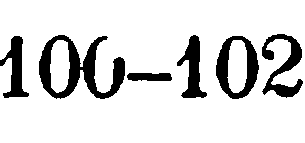
\includegraphics[height=1.5em]{../../S01/source/presentation/AB01-PDF0037-G01.png}} (wrongly 110–112 in the editions!).\par
\par Nor are manuscript codices that give those small works infrequent, the author's name being corrupted in many ways: \emph{Bereni}, \emph{Bareni}, etc., as Steinschneider noted on Baldi, 456–57 (extr. 29–30); in a parchment codex of the National Library of Florence (\emph{Conventi soppressi I, III, 28}), f. 103r–104r, «\emph{Centiloquium Boetem}»\footnote{This is the codex that is mentioned by B. de Montfaucon, \emph{Bibliotheca Bibliothecarum manuscriptorum nova}, Paris 1739, vol. I, p. 429; it then belonged to the Library of St Mark.}. — According to a certain Paris codex, the small works were translated by John of Seville in the twelfth century.\par
\par Baldi, Steinschneider (on Baldi, 458 = extr. 31) and Suter\footnote{\emph{Das Mathematiker-Verzeichniss im Fihrist}, pp. 67–68, n. 211; \emph{Die Mathematiker}, p. 47.} thought that \emph{Bethem} or \emph{Bethen} was corrupted from al-Battānī, and that the little book on the rising of the triplicities (Steinschneider), or all three (Suter), were probably excerpted from the book \emph{on the ascensions of the signs}\footnote{Steinschneider, loc. cit.: «Mi pare che il trattato latino o appendice 'de ortu triplicitatum' sia preso dal libro 'delle ascensioni dei quarti', il zodiaco essendo diviso presso gli astrologi in quattro triplicità o trigoni, e così è accertato che 'Bethen' non è altro che al-Battani» (it seems to me that the Latin treatise or appendix 'de ortu triplicitatum' is taken from the book 'of the ascensions of the quarters', the zodiac being divided by the astrologers into four triplicities or trigons, and so it is established that 'Bethen' is none other than al-Battani).}. To judge this conjecture we must examine those three small works at greater length. I give the text of the editions of 1493 and 1519; by the letter V I indicate the edition of 1507, by B both the Basel editions, by F the Florence codex (of the Centiloquium)\footnote{In the editions of 1493 and 1519, and in both the Basel editions, no. 1 is wrongly put to the first words and no. 2 to the first aphorism; so the hundredth aphorism has no number.}.\par
\par \Pg{I XXIX}\emph{Centiloquium.} — It opens thus: «Incipit centiloquium Bethem\footnote{In V: «Incipit liber de consuetudinibus in iudiciis astrorum: et est centiloquium Bethen. breve admodum» (here begins the book on the customs in the judgements of the stars: and it is the centiloquium of Bethen, very short).}. Hunc (V nunc) inchoabo librum de consuetudinibus in (F et) iudiciis (B iudicio) stellarum (V astrorum). 1. Scias quod quando planetae sunt retrogradi sunt ut vir infirmus, stupefactus, sollicitus. 2. Cadens vero est quasi mortuus cui non est motus» (here begins the centiloquium of Bethem. This book I shall begin on the customs in the judgements of the stars. 1. Know that when the planets are retrograde they are like a man who is sick, stunned, anxious. 2. And one that is cadent is like a dead man, who has no motion). There follow the other aphorisms of astrology, of which the last is: «100. Quando planeta infortuna erit (V infortunatus fuerit) in angulis receptus (V et receptus), dabit et applicabit quaerentis negocium: tamen accipiet ab eo quod dedit sibi: scientia receptionis est, quando fuerit planeta in domo sui (V sua), aut domo exaltationis suae salvus (F salutis) ab infortuna» (100. When a malefic planet is received in the angles, it will give and bring about the querent's business: yet it will take from him what it gave him: the knowledge of reception is when a planet is in its own house, or in the house of its exaltation, safe from misfortune).\par
\par The \emph{little book on the hours of the planets} begins thus: «De horis planetarum et primo de hora Saturni. Cum fuerit hora Saturni bonum est emere res gravis naturae. ut ferrum, stamnum, plumbum, et omnia metalla, et lapidem, et pannos nigros, et incipere hortos fodere, et aliquas fraudes excogitare contra inimicos.....» (on the hours of the planets, and first on the hour of Saturn. When it is the hour of Saturn it is good to buy things of a heavy nature, such as iron, tin, lead and all metals, and stone, and black cloths, and to begin digging gardens, and to devise some frauds against enemies.....). In the same way the hours of all seven planets, of which the last is the Moon, are reviewed; and when these are finished there follows: «\emph{De ortu triplicitatum} et primo de ortu primae triplicitatis. Si fuerit in ortu Aries, Leo vel Sagittarius, quia ista signa sunt ignea, bonum est sub eorum ortu incipere ea quae pertinent ad ignem, sicut fornacem incendere, aurum, argentum, plumbum, stamnum, auricalcum colorare.....» (\emph{on the rising of the triplicities}, and first on the rising of the first triplicity. If Aries, Leo or Sagittarius is rising, since those signs are fiery, it is good to begin under their rising the things that belong to fire, such as to light a furnace, to colour gold, silver, lead, tin, brass.....). When all four triplicities have been reviewed in this way, a very short appendix follows: «De hora Saturni et signo eius ascendente. Haec [sic] tantum diligentius est attendendum quod si fuerit hora Saturni, et signum Saturni ascendat, mirabile est facere omnia quae dicta sunt de horis Saturni: et idem intellige de omnibus aliis horis et signis, et si potes, concordes horas cum signis, quia optimum est. et quod diximus de Saturno, sic intellige de omnibus aliis planetis. Explicit de horis planetarum Bethem\footnote{B end with the word «planetis»; V Bethen.}» (on the hour of Saturn and its sign ascending. This only must be attended to more carefully: that if it is the hour of Saturn and the sign of Saturn is ascending, it is wonderful to do all that has been said of the hours of Saturn; and understand the same of all the other hours and signs; and if you can, make the hours agree with the signs, for that is best. And what we have said of Saturn, so understand of all the other planets. Here ends Bethem's on the hours of the planets).\par
\par There is no one who does not see that all this differs entirely from al-Battānī's other writings, those that are certain; nor can those propositions of judicial astrology have been excerpted from the book of the ascensions of the signs between the quarters of the heaven, which deals with directing the aphetae, nor can they be deemed consonant with al-Battānī's character and mind as it appears from elsewhere. Moreover Johannes Stöffler (d. 1531), a judge expert in these matters, thinks thus of the little book: «Many astrologers, most learned men, followed the Babylonians (\emph{Babilonios} [sic]): and especially Bethen, who composed a treatise of his own on the hours of the planets, whose beginning is: \emph{Cum fuerit hora Saturni} etc.»\footnote{Ioh. Stoeflerini \emph{variorum astrolabiorum compositio seu fabrica, necnon eorundem usuum ac variarum utilitatum explanatio}, [Mainz] 1535, f. 43r. It became known to me from B. Boncompagni's addition to Steinschneider, Baldi, p. 457 (missing in extr.). — On the significations of the hours of the planets according to Albumasar and others (not, however, Ptolemy) see Albohazen Haly VII, ch. C, pp. 341–42.}. So the little book does not seem to agree with the astrological principles of Ptolemy, which, however, we find that al-Battānī followed\footnote{Besides much else said here and there in this preface, cf. p. xxiii, at the end of § 2.}.\par
\par So there is no reason to attribute those small works to our astronomer except the likeness of the author's name. That this is a most deceptive argument no one who knows how altogether incredibly Arabic words were disfigured by our people of the Middle Ages will dare to deny. But I think the most certain indication that Bethem or Bethen has nothing to do with al-Battānī is to be taken from the name itself, as I shall show in what follows.\par
\par \Pg{I XXX}\Pg{I XXXI}There are two kinds of Arabic proper names: one always provided with the article \emph{al}\footnote{The letter \emph{l} before \emph{d, ḍ, dh, n, r, s, ṣ, sh, t, ṭ, th, z, ẓ} is assimilated in pronunciation to these letters; hence \emph{aṣ-Ṣūfī} for \emph{al-Ṣūfī}.}, the other constantly without the article. The proper names of one kind can never be transferred to the other. And it was a most firm rule for those who in the Middle Ages translated Arabic books into Hebrew, Latin and Spanish, and therefore also for our John of Seville, to keep the article of proper names whenever it was found in the Arabic; most certain testimony to this are \emph{Albategnius, Albenait, Alcabitius, Alchindus, Alcharsi, Alchasibi, Alchorismus, Alfraganus, Algazelus, Alhazen, Alkasem, Almansor, Almeon, Alpetragius, Alpharabius, Anaritius, Asaphar, Azarchel} or \emph{Arzachel, Azophi}, and many other names of men\footnote{The only exception is the physician \emph{Rhāzes} (\emph{al-Rāzī}), who seems to have become known to the West first by way of the Greeks; for the Greeks always leave out the Arabic article. So {\greekfont Πατανῆς} for al-Battānī.}. Indeed, names compounded with the word \emph{Abū} (i.e. father) were sometimes wrongly provided with the article by the translators, such as \emph{Albohali, Albohazen, Albubather, Albucasis, Albumasar}. Nor did they act otherwise in \emph{geographical} names, of which very abundant examples are given by John of Seville in his translations of Alfraganus\footnote{\emph{Brevis ac perutilis compilatio} Alfragani \emph{astronomi, peritissimi, totum id continens, quod ad rudimenta astronomica est opportunum}, Nuremberg 1537, ch. IX, f. 9r–10r.} and of Alcabitius\footnote{\emph{Libellus ysagogicus} Abdilazi. \emph{id est servi gloriosi Dei: qui dicitur} Alchabitius \emph{ad magisterium iuditiorum astrorum, interpretatus a Iohanne Hispalensi}, Venice 1485, diff. I, the chapter on the significations of the signs, f. aa7r–v, and diff. II, ch. I, f. bb5r–cc r. — Printed several times afterwards.}, by Plato of Tivoli in his translations of the Tetrabiblos\footnote{Book II, ch. 3: \emph{Ascade} and \emph{Asaede} = \emph{aṣ-Ṣoghd} (Sogdiana), \emph{Alhabei} and \emph{Alhabas} = al-Ḥabash (Ethiopia), \emph{Algizira} = al-Jazīra (Mesopotamia).} and of al-Battānī\footnote{Ch. VI, Nuremberg ed. f. 11r–12v.}, by the translators of the astrology of Ibn Abī l-Rijāl\footnote{Albohazen Haly etc., Basel 1571, book VIII, ch. 37, pp. 406–08.}, and by others. Likewise in the names of the \emph{stars}, which it would take too long to list now\footnote{Especially in the Catalogue of the \emph{Almagest} and in the \emph{Libros del saber de astronomia}. — \emph{Rigel} ({\greekfont β} Orionis) lacks the article in Arabic too (\emph{rijl al-jawzāʾ}). — The names without the article (\emph{Arneb, Deneb, Dubhe, Gemma, Hamel, Markab, Menkar, Thuban}, etc.) were taken not from books but from astrolabes, at a later age than that of those translators. Moreover, on astrolabes the Arabs themselves often left out the articles for brevity's sake.}. Lastly, in the very \emph{technical terms} of the sciences the Latin and Spanish translators kept the article, although in Arabic it is put in or left out in them as the occasion requires, as happens in our languages: \emph{Alchata, alcoranum, regula alchatain, alhigera, alkali, alkekengi, alchimia, alambicus, alchermes, alkohol, algebra}, etc., and, as regards astronomy and astrology, \emph{almagesti} or \emph{almagestum, almanach, almanar, almuri, alhidada, alcora, alchitoth, alferath, almehuar, asaphaea, almucantarat, azimuth}\footnote{\emph{Zenith} and \emph{nadir}, since in the astronomical books of the Arabs they always have another word after them in the genitive case (the zenith of the head, the nadir of some degree), lack the article according to the laws of Arabic grammar. — In \emph{stellis beibeniis}, \emph{beibeniae} is an adjective; cf. in the translation of Anaritius, ed. Curtze, p. 6, \emph{leulavie} (\emph{lawlabiyya}, spiral) and on p. 165 «\emph{mutasicha}» ({\greekfont ὁμόλογα}). But in the translation of the \emph{Centiloquium}, no. 36: «vel aliqua stella ex \emph{albemenia}» (or some star of the \emph{albemenia}) (read \emph{albeibeniis}), because here it is used as a substantive.}, \emph{almunchariff, alchinchirefet, attacium} (for \emph{attacuim}), \emph{athazir, alcobol, almenen, alichorad, alfazim, alhylech, alcochoden, algebugthar, azemena}, besides very many others scattered in the books of astrology and medicine. They translated so slavishly that they not rarely put in or left out the Arabic article according to the rules of Arabic grammar; besides what I said in n. 8, two examples from Alcabitius as translated by John of Seville may suffice: diff. IV, ch. 10 (ed. 1485, f. dd5v–dd6r): «et ex hoc \emph{amanbaharat} [corr. \emph{anaubaharat} = \emph{an-nawbahārāt}] que sunt novenarie» (and from this the \emph{amanbaharat} [read \emph{anaubaharat} = \emph{an-nawbahārāt}], which are the novenaries), but afterwards: «eritque \emph{nauhahar} i. novenarium 19. gradus Aquarii Iovis» (and the \emph{nauhahar}, i.e. the novenary, of the 19th degree of Aquarius will be Jupiter's); likewise diff. IV, ch. 11 (f. dd6r): «et ex hoc \emph{adorogen} [\emph{ad-darījān}].....» (and from this the \emph{adorogen} [\emph{ad-darījān}].....)\footnoteT{The print has \emph{ad-darījan}; Nallino's Addenda et emendanda (Part II, p. XVI) correct it to \emph{ad-darījān}.}, but below: «erit eius \emph{dorongen} Sol.....» (its \emph{dorongen} will be the Sun.....)\footnote{M. Curtze, in the preface to Anaritii \emph{in decem libros priores Elementorum Euclidis Commentarii, ex interpretatione Gherardi Cremonensis}, Leipzig 1899, pp. xiii–xiv, notes: «In his translation Gerard almost never uses the superlative, but only the comparative with the sense of the superlative. For example, on p. 5, l. 22 we read \emph{brevior dimensio} for \emph{brevissima dimensio}, and ibid. 1, 34 \emph{cum breviori linea} for \emph{cum brevissima linea}. Almost all the mathematical writers of the Middle Ages use the same manner, and whoever devotes himself to their study must be mindful of this usage». This perhaps comes from the fact that the Arabs denote both the comparative and the superlative by the same form of the adjective, \emph{afʿal}; but with them the construction of the phrase does not produce the confusion that the Latin translators cannot avoid.}. For the same reason, in the translation of the \emph{Commentary} of Anaritius \emph{on Euclid}, ed. Curtze, p. 7: «sicut \emph{meguar}» (i.e. like an axis, \emph{miḥwar}), because it is indeterminate in the text.\par
\par Therefore I cannot believe that the translators of the Middle Ages, and especially John of Seville, turned al-Battānī into \emph{Bethem} without the article; so the name itself confirms what I had deduced before from the very matter of the small works, namely that those three little books are by no means to be counted among al-Battānī's writings.\par
\par That this \emph{Bethem}, \emph{Bethen}, \emph{Bereni}, etc. is the same man as \emph{Beleni}, \emph{Belini} (i.e. Apollonius of Tyana), to whom astrological and magical little books translated from the Arabic into Latin are attributed\footnote{They are listed by M. Steinschneider, \emph{Zum Speculum astronomicum}, in Zeitschr. f. Mathem. u. Physik, vol. XVI, 1871, pp. 369 and 395.}, I do not venture to affirm; indeed I think it hardly likely.\footnoteT{Nallino's Addenda et emendanda (Part II, p. XVI, where the page is misprinted XXX) report that Suter (Bibliotheca Mathematica, 3rd series, vol. 5, 1904, p. 80) thinks it probable that \emph{Bethen}, \emph{Bereni}, etc. designate Apollonius of Tyana; Nallino finds this very uncertain, because the writings of Apollonius mentioned by the Arabs, or still extant in Arabic and Latin, deal with quite different matters.}\par
\par\begin{center}\textbf{§ 4. The astronomical work.}\end{center}
\par \Pg{I XXXII}I. \emph{The name and the date of the work.} — It has no title in the Escorial codex; and the titles found in the editions of Plato's translation, «\emph{de motu stellarum}» (on the motion of the stars), «\emph{de scientia stellarum}» (on the science of the stars), «\emph{de numeris stellarum}» (on the numbers of the stars), were taken from the very beginning of the book (p. 1). Undoubtedly the author had called his book simply \emph{zīj}, the name\footnote{From the Pahlavi \emph{zīk}, Neo-Persian \raisebox{-0.4em}{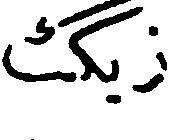
\includegraphics[height=1.3em]{../../S01/source/presentation/AB01-PDF0040-G01.png}} \emph{zīg}, that is, the threads by which weavers set up the warp, or the beginning of the web, so as to have a rule from them in weaving variegated garments. From the likeness of the lines, the Persians had already called the astronomical tables \emph{zīk} in the seventh century AD.} — wrongly rendered \emph{Tables} by our scholars\footnote{Tables are always called \emph{jadwal}, from the likeness of the columns to rivulets (\emph{jadwal}).} — by which the Arabs designate books that, mostly leaving out the rudiments of cosmography, set out the higher doctrines of spherical astronomy and the methods of the celestial computations, and comprise all the necessary tables\footnote{Rightly, then, the {\greekfont Περσικὴ σύνταξις ἀστρονομίας}, made in Greek in 1323 by an unknown man from the lectures of the Persian {\greekfont Σὰμψ μπουχαρῆς} (Shams al-Dīn al-Bukhārī) (on which Suter, \emph{Mathematiker}, pp. 219–20, correcting Usener's opinion), begins thus: {\greekfont Τὸ βιβλιον τόδε καθ' Ἕλληνας μὲν σύνταξις λέγεται, κατὰ δὲ τὴν τῶν Περσῶν διάλεκτον ζῆσι} «this book is called \emph{Syntaxis} by the Greeks [which is the true name of the Almagest], but \emph{zīj} in the language of the Persians» (\emph{Catalogus codicum astrologorum Graecorum}, Brussels 1898 ff., vol. I, p. 3); and he always calls the astronomical works (\emph{zīj}) of al-Battānī, al-Khāzinī and others {\greekfont σύνταξις} (\emph{Cat. codd. astrol.}, vol. I, pp. 88 and 89). The same Greek writer explains much about the meaning of the word {\greekfont ζῆσι} in Usener, \emph{Ad historiam astronomiae symbola}, Bonn 1876 (Universitäts-Progr.), p. 22 (cf. 15, n.). — G. Chrysococces, in the \emph{Exposition of the composition of the Persians} ({\greekfont Ἐξήγησις εἰς τὴν σύνταξιν τῶν Περσῶν}), written in 1346: {\greekfont τὸ ζῆσι τόδε ἤτοι ἡ σύνταξις} «this \emph{zīj}, that is, the Syntaxis» (at the end of Ism. Bullialdus, \emph{Astronomia philolaica}, Paris 1545, part II, p. 213).}\footnoteT{Bullialdus's \emph{Astronomia philolaica} appeared at Paris in 1645.}. Nor was the book known by any name other than «\emph{zīj al-Battānī}» to the older witnesses to al-Battānī's life, as we have seen, and to the Arab astronomers. But because they had thought our author a Sabian, the later bibliographers not rarely called this book \emph{al-zīj al-ṣābiʾ}, «the Sabian astronomical work»; so Ibn Khallikān and Abū l-Fidāʾ, mentioned in § 1, and Ḥājjī Khalīfa\footnote{Haji Khalfae \emph{Lexicon bibliogr. et encyclop.}, vol. III, p. 564, no. 6946, from the Persian book \emph{majmūʿeh i sī faṣl}. But in III, 568, no. 6961, from another source, \emph{zīj al-Battānī}, as though it were another work!}.\par
\par Al-Battānī is said to have put out two editions of the work, or rather, which is what \emph{nuskha} properly means, two copies, the later one excelling the earlier. That is no wonder; for in books of this kind the author himself may judge, some years later, that some things should be added or corrected. Yet I think it hardly probable that he made changes of great weight in the first edition, especially if, as we have learned that Ibn al-Muktafī related, he began his observations in the year 264 H (beginning 12 Sept. AD 877); for the radices of the mean motions and the great catalogue of the fixed stars, established for 1 Ādhār 1191 of Dhū l-Qarnayn, or 1 March AD 880, must necessarily be thought to have had their place already in the first edition of the book.\par
\par In what year the book first came out I do not know; undoubtedly before 288 H (beginning 25 Dec. 900), for chapter LII is already mentioned by Thābit ibn Qurra, who died in the month of February 901 (see pp. 301–02, and the Addenda). From this it also follows that the edition that the Escorial codex and Plato's translation give is the \emph{second}; for two fundamental observations made at Antioch in the months of January and August AD 901 (1211 of Dhū l-Qarnayn) are mentioned in it\footnote{Pp. 56 and 57. Perhaps he had also established the epoch of the mean motion of the Sun in the year 1211 of Dh.; cf. p. 246.}. It is certain that all that Ibn Hibintā, al-Masʿūdī, al-Ṣūfī, al-Bīrūnī, Ibn Yūnus, al-Zarqālī, al-Khāzinī, Alpetragius, Abraham bar Ḥiyya and others have from al-Battānī — and it is not little — which I have cited in my notes in their places, is found in our edition.\par
\par \Pg{I XXXIII}II. \emph{What posterity thought of al-Battānī.} — The Arabs extol al-Battānī's work with praise with one voice, not excepting al-Ṣūfī and Ibn Yūnus, who nevertheless blame small errors in it, and not always rightly\footnote{I have reported al-Ṣūfī's criticisms on pp. 295–96 and 297, and in vol. II, p. 162 (no. 9 of Sagittarius) and 163 (no. 12 of the same), and in the general observations on the catalogue of the fixed stars. — To the passages of Ibn Yūnus reported on pp. 235, 261, 283 and 306, in which our author is rebuked, this one must be added (Caussin's introduction, p. 75): \RL{\ArNote ومن ذلك رسالة محمد بن جابر بن سنان البتاني في بعد الكوكب اذا كان له عرض عن معدل النهار فانها خطا واضح} «Among these [things that depart from the truth] are the precepts of Muḥammad ibn Jābir ibn Sinān al-Battānī on the distance of a star when it has a latitude from the equator; for they are a plain error». He means chapter XXVI, of which I have treated on pp. 200–01 and 203–04; Ibn Yūnus did not understand al-Battānī's rather obscure text. «\emph{From the equator}» I think is an error of the codex for «\emph{from the ecliptic}». Caussin had translated otherwise, connecting «\emph{distance}» with «\emph{from the equator}» and understanding chapter XVIII of al-Battānī: «ce que dit.... Albattani sur la déclinaison d'une étoile qui a une latitude, renferme une erreur évidente» (what Albattani says.... on the declination of a star that has a latitude contains an evident error). Which is certainly not impossible, though it hardly agrees with the Arabic construction. Another quite certain example of the word \RL{\ArNote رسالة} in the sense of «\emph{precepts, procedure of computation}» is given by Ibn Yūnus on the same page, l. 11: \RL{\ArNote وانما ثبت اماكن الغلط لئلا يجد واحد في عمل واحد رسالتين في زيجي هذا وفي غيره من الازياج فلا يعلم اين الصواب فيبقى حائرا فاذا قرأ هذه الرسالة علم ان الخلاف التي (\LR{sic}) فيه لغيره من الازياج وقع عن علم بالصواب}, where the first \emph{risālatayn} is rightly rendered by Caussin «deux procédés» (two procedures). A third example in Ḥabash, f. 168r: «likewise according to the \emph{precepts} that preceded these (\RL{\ArNote الرسالة التي قبل هذه})», where two methods of computation set out in the same chapter are dealt with.}. From the notes added to this volume and to the next it is gathered well enough how often his observations and computations are both mentioned by later writers and used in constructing tables; and likewise that al-Battānī's elements also occur in books in which there is no mention of our astronomer\footnote{Examples in the apogees of the planets adopted by Ibn al-Samḥ, al-Kharaqī and al-Jaghmīnī, which I have reported on p. 240.}. To the writers cited by me here and there, such as Thābit ibn Qurra, al-Masʿūdī, Ibn Hibintā, al-Bīrūnī, al-Zarqālī, al-Khāzinī, the Indo-Persian Abū l-Faẓl ʿAllāmī, and those who, as we have seen, wrote al-Battānī's life, others can easily be added. Maslama al-Majrīṭī, who died in the year 398 H (beginning 16 Sept. 1007), reduced to a compendium al-Battānī's tables of the equations of the Sun, the Moon and the five planets\footnote{On the testimony of Ibn Abī Uṣaybiʿa II, 39, and of Ibn al-Qifṭī in Casiri I, 378, or Sédillot p. lxix.}\footnoteT{Nallino's Addenda et emendanda (Part I, p. LXX) add for Ibn al-Qifṭī: ed. Lippert, p. 326.}, perhaps also adapting them to the era of the Arabs, as he had done in the tables of al-Khwārizmī; and Kūshyār ibn Labbān, who flourished about the years 360–420 H (AD 971–1029), took the tables of the equation of the Sun into his \emph{al-Zīj al-jāmiʿ}\footnote{«On determining the places of the [fixed] stars according to the astronomical works of Ḥabash, al-Battānī, Ibn al-Aʿlam and Yaḥyā ibn Abī Manṣūr, and on the nature of the discrepancy between each of them», in the table of chapters of the book in Ahlwardt, \emph{Verzeichniss der arab Handschriften}, vol. V, no. 5751, p. 205b; likewise «the table of the equation of the Sun according to al-Battānī and Ḥabash», ibid. p. 206a.}. In the first half of the fifth century H (the eleventh AD), ʿAlī ibn Aḥmad al-Nasawī gave this judgement, reported to us by Ḥājjī Khalīfa III, 564, no. 6946: «Of the astronomical works that serve for observations the most perfect indeed is (\RL{\ArNote ان اصح الزيجات الرصدية}) the \emph{zīj al-Battānī}, because it is the nearest to the truth [of all]; but it is constructed for the eras of the Romans and of the hijra, whose use, because of the leap years and the fractions, makes its adaptation to the era of the Persians difficult\footnote{Many used the era of the Persians, or of Yazdajird, because its years, like those of the Egyptians in the Almagest, consisted of 365 days without intercalation.}». In the same fifth century the \emph{zīj al-Battānī} is mentioned by an anonymous pupil of the famous Aḥmad al-Sijzī in his book \emph{Tasṭīḥ al-ṣuwar wa tabṭīḥ al-kuwar}, on the doctrine of making the astrolabe\footnote{See the \emph{Catalogus codd. Orientalium Bibliothecae Academiae Lugduno-Batavae}, Leiden 1851–77, vol. III, pp. 95–96, no. 1078. — A mention of the book is missing in Brockelmann and Suter.}\footnoteT{Nallino's Addenda et emendanda (Part II, p. XVI) report, on Suter's information, that the author of this book is al-Bīrūnī himself, who lists it among the books he had written up to the year 427 H; it is dedicated to the Khwārizmshāh al-Maʾmūn ibn al-Maʾmūn ibn Muḥammad (d. 407 H), whom al-Bīrūnī served for seven years.}; and al-Bīrūnī, whom we have seen mentioning al-Battānī with praise in his works, also testifies that he wrote a book entitled \emph{Jalāʾ al-adhhān fī zīj al-Battānī}, «the brightening of the minds on the astronomical work of al-Battānī»\footnote{In the list of the works composed by himself, in Sachau, in the introduction to the text of the \emph{Chronol.}, p. xlvi, last line.}. Lastly, in the second half of the fourteenth century AD, the famous historian Ibn Khaldūn\footnote{\emph{Kitāb al-ʿibar wa dīwān al-mubtadaʾ wa l-khabar}, Būlāq 1284 H, vol. I, p. 408; \emph{Les Prolégomènes d'} Ibn Khaldoun \emph{traduits par de Slane}, Paris 1863–68, vol. III, p. 148.} counts the works of al-Battānī and of Ibn al-Kammād among the most excellent books of astronomy.\par
\par What Ch. H. Slonimski\footnote{In the book written in Hebrew \emph{Yěsōdē hā ʿibbūr}, «Foundations of the calendar», 2nd ed., Zhitomir 1865, pp. 53 and 57; 3rd ed., Warsaw 1889, pp. 47 and 64 (mentioned in several writings by Steinschneider, from whom I take the information).} asserted is false, that the year of the Jews, whose invention is attributed to Rabbi Addā bar Ahăbā, is al-Battānī's solar year and was first brought into Spain in the tenth century AD; for that year is of 365 days, 5\textsuperscript{\itshape h} 55\textsuperscript{\itshape m} 23\textsuperscript{\itshape s} 20\textsuperscript{\itshape t} $\tfrac{6}{19}$\footnote{Often called the year of Rabbi Addā; already in the tenth century AD very well known in the far eastern part of the Muslim empire, and mentioned here and there by al-Bīrūnī, \emph{Chron.}, who sets out the rules of the Jewish calendar.}\footnoteT{235 synodic months of 29\textsuperscript{\itshape d} 12\textsuperscript{\itshape h} 44\textsuperscript{\itshape m} 3⅓\textsuperscript{\itshape s} divided by 19 give 365\textsuperscript{\itshape d} 5\textsuperscript{\itshape h} 55\textsuperscript{\itshape m} 25\textsuperscript{\itshape s} 26\textsuperscript{\itshape t} $\tfrac{6}{19}$, that is, 25 25/57 seconds; the print has 23\textsuperscript{\itshape s} 20\textsuperscript{\itshape t}.}, which is found by dividing the enneadecaeteris of Meton (comprising 235 synodic months of Hipparchus) by 19, while al-Battānī's tropical year is of 365 days 5\textsuperscript{\itshape h} 46\textsuperscript{\itshape m} 24\textsuperscript{\itshape s}.\par
\par \Pg{I XXXIV}That al-Battānī's work was translated into Hebrew is not established\footnote{Cf. M. Steinschneider, \emph{Die hebräischen Uebersetzungen des Mittelalters}, Berlin 1893, p. 549, § 340b.}; yet the Jews writing in the Hebrew language in the twelfth century AD and after did not lack knowledge of it. That Abraham bar Ḥiyya had it at hand and quoted it is plain from my notes on pp. 6, 287, 298, 302–03; and in the same age Abraham Ibn ʿEzra mentions al-Battānī and commends his tables\footnote{In the preface to the \emph{Ṭaʿamē lūḥōt al-Khwārizmī}, in Hebrew and German in M. Steinschneider, \emph{Zur Geschichte der Uebersetzungen aus dem Indischen ins Arabische}, in Zeitschr. d. deutsch. morgenl. Gesellschaft, vol. XXIV, 1870, p. 356; likewise in other books, Steinschneider, loc. cit., p. 351. In the book \emph{de mundo}, to find the lunar mansions, he bids one first determine the equated place (i.e. the true longitude) of the Moon «secundum viam tab. Albategni» (by the method of the tables of Albategni); see Steinschneider, \emph{Ueber die Mondstationen}, in Zeit. d. d. morg. Ges., vol. XVIII, 1864, p. 161.}. The famous Maimonides\footnote{Born at Córdoba on 30 March 1135; he died at Cairo on 13 Dec. 1204; see H. Graetz, \emph{Geschichte der Juden}, 2nd ed., Leipzig 1870 ff., vol. VI. — The years in Suter, \emph{Die Mathematiker}, p. 132, are to be corrected.} tacitly follows our astronomer in the eighth treatise of the work \emph{Mishnēh Tōrāh}, «Repetition of the Law», which is entitled \emph{hilkōt qiddūsh hā ḥōdesh}, «rules on the sanctification of the new moon», ch. XII; for there he puts the mean motion of the Sun at 28° 35′ 1″ in 29 days, or 348° 55′ 15″ in the «ordinary», or lunar, year, which agree exactly with al-Battānī's tables (vol. II, pp. 22 and 20), and the motion of the solar apogee at 54″ a year\footnote{Col. 312 of the edition of that eighth treatise, with the Latin translation of L. Compiègne de Veil, given by Bl. Ugolinus, \emph{Thesaurus antiquitatum sacrarum}, Venice 1744–69, vol. XVII. That al-Battānī is mentioned in it, as Steinschneider, \emph{Die hebr. Uebers.} p. 550, asserts, is not true.}. In computing the arc of visibility of the new Moon, however, he follows an easier method, but less exact, than al-Battānī's\footnote{Ch. XVII of the same eighth treatise (Ugolinus, col. 354). He lays down that the new Moon certainly appears when the arc of vision is between 11° and 12° and the elongation from the Sun 11° or more; or when the arc is from 12° to 13° and the elongation 10° and more; or when the arc is from 9° to 10° and the elongation 13° or more. On Maimonides' principles in this computation E. Baneth has treated, \emph{Maimuni's Neumondsberechnung}, Berlin 1898–1902, 3 parts (Beigaben zu den Berichten über die Lehranstalt für die Wissenschaft des Judentums in Berlin), a book that I have not had the chance to see.}. — That the name of al-Battānī occurs more than once in the \emph{yěsōd ʿōlām}, «Foundation of the World», composed by Isaac Israeli in 1310, is attested by Steinschneider on Baldi, pp. 450 and 455 (extr. pp. 26 and 29). What Lēwī ben Gerson (Leo de Balneolis) took from our astronomer we shall see below. It is worth mentioning, unless there is an error in Steinschneider's notice\footnote{Steinschneider, \emph{Mondstationen}, p. 174, n. 79.}, that in the unpublished \emph{ʿērek hā ḥălōph}, written at Tarascon in 1365, ʿImmānūʾēl ben Yaʿăqōb (Bonfils) constructed astronomical tables according to al-Battānī's. Lastly, Ēliyyāh ben Mosheh Bashyasī, an adherent of the sect of the Karaites, who died in 1490, constructed tables of the lunar and solar motions «for the latitude of Constantinople [41⅓°] according to the doctrine of al-Battānī and the doctrine of the sage ʿImmānūʾēl, author of the book of the [six] wings», \emph{bě ōpheq Qōsṭandūnā lě daʿat al-Battānī wě lě daʿat hā ḥākām ʿImmānūʾēl baʿal hak-kěnāphīm}\footnote{The passage is quoted by J. Selden, \emph{De anno civili veteris ecclesiae seu reipublicae Iudaicae dissertatio}, published again in Ugolinus's \emph{Thesaurus}, vol. XVII, col. 202. Selden had wrongly translated: «Emanuelis geographi» (of Emanuel the geographer). It is that same ʿImmānūʾēl ben Yaʿăqōb mentioned above; the book «\emph{of the six wings}», also written in 1365, deals with celestial matters. — Among the Jews who knew or used al-Battānī's computations Steinschneider, \emph{Die hebr. Uebers.}, p. 550, counts ʿObadyāh ben Dāwid (about AD 1341), Yěhūdāh Shěmūʾēl ben ʿAbbās and Yěhūdāh Moscono of Ochrid (fourteenth century); but we have seen that in these matters one cannot always rely on Steinschneider.}.\par
\par \Pg{I XXXV}\Pg{I XXXVI}Nor was its fame content with the bounds of the East alone; for, after the translations of Robert of Chester (or of Retines) and of Plato of Tivoli, the name of al-Battānī travelled through the lands of Europe too. That Robert had already composed «\emph{Canones in motibus caelestium corporum ad meridiem urbis Londoniarum}» (canons on the motions of the celestial bodies for the meridian of the city of London), divided into two parts, of which the first is computed for the year 1169 on the authority of the Toledan Tables of Arzachel, the second for the year 1150 «\emph{iuxta Albaten} (var. \emph{Albategnium}) \emph{Harecensis}» (according to Albaten of Harec), i.e. al-Battānī al-Raqqī\footnote{Steinschneider mentions two codices, \emph{Zum Speculum Astronomicum}, p. 392.}. That the Arab astronomer conveniently reduced the doctrines of the Almagest to a compendium is asserted by Rudolf of Bruges, writing at Toulouse in 1143 or 1144, as I noted above (p. xxv); and the unknown man who at the end of the twelfth century or the beginning of the thirteenth composed his \emph{Almagestum parvum}, of which I have treated sufficiently in § 3, no. III, pp. xxvi–xxvii, always had him at hand. William of Auvergne, who died in 1249, praises him as a noble philosopher who had only his name (Muḥammad, or Mahometus) in common with the accursed prophet of the Arabs\footnote{«And do not suppose that he was Macometus the philosopher, who was called Albategin: for of this man Plato of Tivoli translated the book on astrology from the Arabic tongue into Latin; and the philosophical and profound nobility of his books evidently proves that he had only the name of Macometus in common with that man — I will not say a rustic, but, as someone says most truly, a cattle-like and swinish man. For far be it that so great a philosopher should be so foolish and hold such peculiar views» (Guilielmi Alverni \emph{opera omnia}, Orléans 1674, vol. I, p. 50; in Boncompagni, \emph{Delle versioni fatte da Platone Tiburtino}, Atti dell'Accad. Pont. de' Nuovi Lincei, vol. IV, Rome 1851, pp. 247–48).}; Henry Bate, in his \emph{Magistralis compositio astrolabii}, written in 1274, plainly shows how much of al-Battānī he had read and how much he valued him\footnote{Besides the passage that I adduced on pp. 308–09, f. c8r (speaking of the temporal and the equinoctial hours): «the cause of this difference between these two kinds of hours is set out well enough by Ptholemeus, Geber, Albategni, Abraham and the other masters of observations». Elsewhere, after saying that his instrument was adapted to the theory of the trepidation of the fixed stars, or the motion of the eighth sphere, he goes on thus (f. d4r–v): «But Ptholemeus and Geber, Albategni, Abraham the Jew [Ibn ʿEzra] and Açophius [al-Ṣūfī], and the other masters of proofs too, and above all the eastern astronomers, considering the motions of the planets according to the ninth sphere, founded their radices on this: and this is plain in the tables of Ptholomeus, Albategni and Abraham, in the \emph{Pisan} and \emph{Winchester} tables, and in others». From this passage, however, one may not infer that Henry Bate knew al-Battānī's \emph{tables} besides his chapters.}. — Gerard of Sabloneta (Sabbioneta), an astronomer of the thirteenth century who is not rarely confused with Gerard of Cremona (twelfth century), knew al-Battānī's work by hearsay, not by sight; for in his \emph{Theorica planetarum}, Bologna 1480 (at the end of the \emph{Spera mundi} of John of Sacrobosco the Englishman), f. 35v, dealing very briefly with the determination of the apogee and the eccentricity of the Sun, he goes on thus: «and in this way Albategni \emph{is said} to have found how much the apogees of the planets move in a year, a month and a day: and he composed tables for this: and he had a great astrolabe [sic!], namely of three cubits or of greater size». Elsewhere, however, he tells things altogether false; f. 34v: «The composers of the tables on Arim, which is a city in India, are said to have been Nembroth\footnote{Nembroth the giant is counted among the most ancient astronomers by other writers of the Middle Ages too; see Steinschneider, \emph{Zum Speculum Astronomicum des Albertus Magnus}, pp. 380–81.}: Hermes: Hyconimus\footnote{Steinschneider, \emph{Zum Speculum}, p. 381, suspects that he is Armanus or Humenus, the author of astronomical tables, on whom Steinschneider pp. 365–66. This Humenus, however, whose tables al-Zarqālī had edited anew, I think is Ammonius of Alexandria, mathematician, rhetorician and philosopher at the end of the fifth century, who, as the philosopher Stephanus (first half of the eighth century) attests in his book {\greekfont περὶ τῆς μαθηματικῆς τέχνης}, «\emph{on the mathematical art}», constructed tables for the era of Philip Arrhidaeus: {\greekfont ὁ δέ γε Θέων καὶ Ἡράκλειος καὶ ὁ Ἀμμώνιος τοῖς τοῦ Φιλίππου} [{\greekfont ἔτεσιν ἐχρήσατο}] {\greekfont καὶ μησὶν Αἰγυπτιακοῖς} (the passage was edited by Fr. Cumont in the \emph{Catalogus codicum astrologorum graecorum}, Brussels 1899 ff., vol. II, p. 182). The treatise on the astrolabe that is often attributed to Ammonius in the codices has as its author Nicephorus Gregoras ({\greekfont Νικηφόρος ὁ Γρηγορᾶς}), as P. Tannery showed in the \emph{Revue de philologie}, vol. XII, 1888, p. 61.}: Ptholomaeus: Albategni: Albumazar: Algorismus»; and f. 35r, on the apogees of the planets: «Likewise they are said by Albategni to be moved one degree in 60 years and four months, always to the east»\footnote{The same things, with others, in almost the same words, are in the anonymous little book \emph{de motu octave spere}, printed at the end of the \emph{Theorica planetarum} (Bologna 1480), f. 39r. I suspect that the author of that little book is Gerard of Sabloneta himself. — Steinschneider errs greatly, in several of his writings, in confusing it with the unpublished book of the same title written by Thābit ibn Qurra; moreover Steinschneider asserts that Thābit's book also came out at Venice in 1518 (at the expense of the heirs of Octavianus Scotus), whereas this edition gives Tebith's \emph{de imaginatione Sphere} (cf. Boncompagni, \emph{Delle versioni fatte da Platone Tiburtino}, pp. 261 and 269–70). Steinschneider's authority led Suter into error, \emph{Nachträge und Berichtigungen zu «Die Mathematiker und Astronomen der Araber»}, in Abhandlungen zur Gesch. der mathematischen Wissenschaften, vol. XIV, 1902, p. 163.}\footnoteT{Nallino's Addenda et emendanda (Part II, pp. XVI–XVII) report that, following indications from Phil. Angelitti, Nallino found the little book \emph{de motu octave spere} (Bologna 1480) to agree entirely with the first part of the last chapter («on the motion of the eighth sphere») of Georg Purbach's \emph{Theoricae novae planetarum}, from which it must therefore have been excerpted; Purbach plainly took his information about al-Battānī from Gerard's \emph{Theorica}.}. Albertus Magnus, in the passage cited on pp. xxiv and xxv, commends al-Battānī's work, which he knew from Plato's translation; Alfonso X of Castile collected writings into the \emph{Libros del saber de astronomia}, which not rarely rest on our author's authority, as I have shown in my notes. John of Lignères\footnote{Jean de Lignères, born near Amiens and living at Paris in 1322. On him Steinschneider, \emph{Intorno a Iohannes de Lineriis e Iohannes Siculus}, in Bullettino di Bibliografia e di storia delle scienze matematiche, vol. XII, 1879, pp. 345–351 (and Boncompagni's additions, pp. 375–77); \emph{Notice sur les tables astronomiques attribuées à Pierre III d'Aragon}, in Bullett. XIII, 1880, pp. 422–26; M. Curtze, \emph{War Johannes de Lineriis ein Deutscher, ein Italiener oder ein Franzose?}, in Bibliotheca Mathematica hrsg. von G. Eneström, Neue Folge, vol. IX, 1895, pp. 105–06; von Braunmühl, \emph{Vorlesungen über die Geschichte der Trigonometrie}, Leipzig 1900, vol. I, p. 107.}, in chapter XXVIII of the \emph{Canones ad Tabulas Alphonsinas}, mentions our author and the eccentricity of the solar orbit determined by him\footnote{Steinschneider gave this passage from a Vatican codex, \emph{Études sur Zarkali}, § 14, in Bullet. XVII, 1884–85, p. 782, n. 1.}; perhaps too, if I may propose a conjecture, it was after reading the astronomical work that he first formed the plan of constructing his \emph{table of sines}\footnote{It is still unpublished, as is his treatise on trigonometry.}. In the same age John of Genoa ends his still unpublished \emph{Canones eclipsium} (of the year 1332) with these words: «But see the way of correcting [the times of the eclipses] in Albategni and in the canons of master Io. de Lineriis..... Here end the canons of eclipses that master John of Genoa compiled, extracting them partly from the common canons, partly from Albategni, partly from the lesser Almagest\footnote{Of which I have spoken in § 3, no. VI, pp. xxvi–xxvii.}, partly from master John of Sicily.....»\footnote{In C. de Simoni, \emph{Intorno alla vita ed ai lavori di Andalò di Negro}, in Bullett. VII, 1874, pp. 330–31. — Steinschneider, \emph{Zarkali}, p. 780, thinks he is perhaps the same man as Joh. de Saxonia.}. The famous Lēwī ben Gersōn, or Leo de Balneolis, the Jew, in the Latin version of his astronomy, cod. Vatic. Lat. 3098, more than once adduces observations of \emph{Albetem}, that is, of al-Battānī. Nor should it be passed over that even in the second half of the fifteenth century Johannes Lucilius Santritter of Heilbronn, \emph{In tabulas Alfonsi canones seu propositiones}, prop. XXXII, sets out al-Battānī's precepts on the limits of the eclipses of the Sun\footnote{I reported the passage on p. 281, wrongly attributing it to the Alphonsine Tables themselves; for in the edition printed at Venice at the expense of P. Liechtenstein, 1518 (so on the front of the book, but at the end, f. 120v, 1521), those Canons are put before the Tables without any distinction or title. Only at the beginning of f. 28v, before the list of errata, is found written: «Here end the canons or propositions on the tables of Alfonsus, of the famous Germans Ioannes Saxoniensis and Ioannes Lucilius Santritter of Heilbronn». — That what is related from al-Battānī belongs to Santritter, not to John of Saxony, appears from a comparison of the editions of 1492 (Venice, by Iohannes Hamman de Landoia) and of 1518 (or 1521) with the edition of 1483 (Venice, by Erhard Ratdolt of Augsburg), which contains only the «\emph{in tabulas Alfontij canones}» of «Iohannes Saxoniensis».} and on computing the apparent conjunction of the luminaries\footnote{Ed. 1518, f. 19r–22r, teaches the computation of the «diversities of aspects», i.e. of the parallaxes, in eclipses of the Sun in a way similar to al-Battānī's precepts (pp. 104–105), concluding: «But this rarely happens, namely that the second [parallax] exceeds the third, that is, that the third is less than the second, unless the moon is then near the horizon; and then the difference between the two diversities [i.e. parallaxes] will appear very small. And this is the opinion of Albategni on the diversity of aspect of the moon for finding an eclipse of the sun, when the third diversity of aspect is greater or less than the second» (cf. al-Battānī p. 105, ll. 35–37). — Plainly from al-Battānī too comes what is in proposition XXVII (f. 14v of the ed. of 1518) on the latitudes of the three superior planets: «take the northern latitude, which is called \emph{Effregion septentrionalis} [sic].....: take from the lower half the southern latitude, which is called \emph{Effregion meridionale} [sic]». Let this passage be added to those that I reported on p. 282.}.\par
\par \Pg{I XXXVII}Others too will easily be added to these writers by anyone who is able to go through the many mathematical and astronomical small works of the Middle Ages, buried today in oblivion in our libraries, and to judge what they owe to al-Battānī, even when they are silent about his name\footnote{C. de Simoni, \emph{Intorno ad Andalò di Negro}, p. 322, thinks that the table of the culminations and declinations of the chief fixed stars placed by Andalò (fourteenth century) at the end of his treatise on the astrolabe was taken from al-Battānī, for the reason that, together with other chief stars (such as {\greekfont α} Cor. borealis), {\greekfont α} Hydrae or Alphard is left out, «della quale ultima omissione in specie Albategnio viene accusato dall'Arabo es-Sufi» (for which last omission in particular Albategnius is accused by the Arab es-Sufi). But al-Ṣūfī (whose words I adduced on p. 295) by no means says that al-Battānī left out that star; in fact {\greekfont α} Hydrae is given in al-Battānī's table, vol. II, p. 185, no. 66.}.\par
\par The astronomical work, on the other hand, seems to have been unknown to the Byzantine writers\footnote{The third fragment of the book \emph{de astronomia} of George Pachymeres ({\greekfont Γεώργιος ὁ Παχυμήρης}, thirteenth century), which Th. H. Martin edited in Greek and Latin at the end of the work of Theon of Smyrna, \emph{Liber de astronomia}, Paris 1849, p. 402 ff., Martin himself entitled «on the motion of the fixed stars, from the different observations of Ptolemy and Albatenius....», because Pachymeres, p. 404 of the text, 405 of the translation, says «that the eighth sphere has a motion of its own from west to east, and moves one degree, in the same direction as the universe, in 100 years, or, \emph{according to others}, in 66 years». But I have shown on pp. 292–93 that the motion of 1 degree in 66 years was adopted by many writers; therefore one may not attribute to Pachymeres a knowledge of al-Battānī's work. Steinschneider wrongly deduced from Martin's title, on Baldi p. 454 (extr. p. 28): «L'autore Greco Gr. Pachymeres ne [i.e. of al-Battānī's book] ha fatto uso» (the Greek author G. Pachymeres made use of it).}, although its fame reached them through the Greek recension of the astronomical lectures of the Persian {\greekfont Σὰμψ μπουχαρῆς} (cf. above, p. xxxi, n. 5), in which a {\greekfont Σύνταξις} whose author is {\greekfont ὁ Πατανῆς} is mentioned\footnote{I shall give the passage (\emph{Catal. codd. astrol. graec.} I, 88) in the notes on the tables of the mean motions of the Sun and the Moon, vol. II, pp. 72–77.}; from this, undoubtedly, Theodore Meliteniotes took his information about al-Battānī in his {\greekfont Ἀστρονομικὴ Τρίβιβλος}, written about 1361\footnote{In the third book, after the list of chapters, {\greekfont Πατανῆς μὲν γάρ τις τῶν παρ' αὐτοῖς} [i.e. {\greekfont Πέρσαις καὶ Ἄραψι}] {\greekfont ἀστρολόγων}; in Usener, \emph{Ad historiam astronomiae symbola}, Bonn 1876 (Universitäts-Programm), p. 15.}.\par
\par \Pg{I XXXVIII}But at the beginning, among us, of that very great renewal of the arts and of studies which closes the Middle Ages and is the beginning of the modern age, the great weight of al-Battānī's book became apparent, perhaps even more than it had before. Regiomontanus (6 June 1436 – 6 July 1476), the prince of the mathematicians and astronomers of that age, gave the greatest care to gaining an exact knowledge of al-Battānī's work, of which several traces survive. Plato of Tivoli's translation first came out in print at Nuremberg in 1537, from a copy that Regiomontanus had furnished here and there with notes in his own hand\footnote{Six of them, entitled «additiones Ioh. de Monteregio» (additions of Joh. de Monteregio), occur in the printed editions: in the middle of ch. III, f. 6v of the Nuremberg edition; at the end of the same, f. 8r; in ch. XI (wrongly inserted in the twelfth), f. 16r (on which I spoke on p. 185); in XXVI, f. 25r–v (on which p. 200); in XXX, f. 37v; and in L, f. 77v. — Perhaps the small note mentioned by me on p. 204 is also Regiomontanus's.}. In his letters, to refute the doctrines of the Alphonsine Tables on the motion of the eighth sphere, or the trepidation, he relies on his own observations and on those of Ptolemy and al-Battānī\footnote{The letters have now been edited by M. Curtze, \emph{Urkunden zur Geschichte der Mathematik im Mittelalter und der Renaissance}, fasc. I, Leipzig 1902, pp. 192–336 (= Abhandlungen zur Gesch. der mathematischen Wissenschaften, vol. XII). — On the passage adduced by me on p. 198 on Delambre's authority, see the \emph{Addenda}.}; and in the \emph{Epitome of the Almagest}\footnote{Iohannis de Monteregio \emph{et} Georgii Purbachii \emph{Epitome, continens propositiones et annotationes, quibus totum Almagestum..... dilucida et brevi doctrina..... declaratur et exponitur}, Basel 1543.} he often adduces the authority of our astronomer, as in book III, prop. 2, pp. 47–48, on the length of the tropical year; III, 13, pp. 56–57, on the length of the four parts of the year, the eccentricity of the solar orbit and the greatest equation of the Sun; IV, 12, p. 78, on the corrections that al-Battānī had made to Ptolemy's mean lunar motions; V, 21, pp. 100–103, on the eclipses, the distances and the diameters of the Sun; V, 35, p. 107, reporting al-Battānī's precepts (p. 80, l. 37 to 81, l. 3) for deriving the parallaxes of altitude from the tables\footnote{Where he rightly interpreted al-Battānī: «Therefore», i.e. because of the geocentric distances of the Sun, which differ from the single one taken by Ptolemy, «if you seek, wishing to correct the diversity of aspect of the Sun from the tables of Ptolemy, add to it its \emph{nineteenth} part» (cf. my notes, pp. 257–58). «... Therefore for the other places of the eccentric of the Sun [i.e. away from the apogee] Albategni bids one enter the table of the equations of the Moon with the argument [i.e. the anomaly] of the Sun, for the proportional minutes.....».}; VI, 7, p. 118, on the limits of the solar eclipses, and VI, 8, p. 119, on the limits of the eclipses of the Moon (passages that you may see in my notes on vol. II, p. 32 of the tables); VII, 6, p. 145, on the motion of the fixed stars and the doctrine of trepidation; and lastly IX, 1, 163. — But what profit Regiomontanus took from our astronomer appears also from other places in his works in which the name of al-Battānī is not mentioned. I have reported two examples in my notes, pp. 193 and 322; but of far greater weight is what von Braunmühl, \emph{Vorlesungen über die Gesch. der Trigonometrie}, vol. I, pp. 130–31, was the first to notice, namely that Regiomontanus\footnote{Ioh. de Monte Regio, \emph{De triangulis omnimodis libri quinque}, Nuremberg 1533, book V.} learned from al-Battānī the use of \emph{versed sines} and of the \emph{orthographic projection} in the problems of spherical trigonometry\footnote{Yet I do not think true what von Braunmühl asserts on p. 131, that Regiomontanus, in the second proposition of book V, uses the same figure and solution as in the addition to chapter XI of al-Battānī; there is some likeness, not identity.}.\par
\par The other astronomers of the same and of a later age valued al-Battānī's observations highly for correcting the tables of the celestial motions, and very often reported them in their writings. Nicholas of Cusa (1401–64) adduces them in the \emph{Reparatio calendarii} and in the \emph{Correctio tabularum Alphonsi}\footnote{So G. Uzielli, \emph{La vita e i tempi di Paolo dal Pozzo Toscanelli}, in Raccolta di documenti e studi pubblicati dalla R. Commissione Colombiana, Rome 1892–94, part V, vol. I, pp. 269 and 270. — On the knowledge of al-Battānī in Joh. Bianchini, see the \emph{Addenda} (on p. 198).}; and so do Copernicus (1473–1543), who calls our author «Mahometus Aractensis», Tycho Brahe\footnote{He lived 1546–1601. Besides the passages that I reported on pp. 290 and 294, cf. his \emph{Progymnasmata}, vol. I, pp. 37–39 (on the length of the tropical year), 52 (on the apogee of the Sun), 138–39 and 253–55 (on the longitudes and the motion of the fixed stars).} and Riccioli (1598–1671).\par
\par \Pg{I XXXIX}The famous Halley (1656–1742) too, thinking that great profit could be drawn from his so accurate observations, tried with no small labour to emend in many places the numbers corrupted in both editions of Plato's translation\footnote{Edm. Halley, \emph{Emendationes ac notae in vetustas Albatenii Observationes Astronomicas, cum restitutione tabularum lunisolarium eiusdem Authoris}, in Philosophical Transactions [of the R. Society], London 1693, vol. XVIII, no. 204, pp. 913–21. — I have reported part of his corrections in the notes, pp. 56–57. In restoring the radices of the mean motion of the Sun for the years AD 881–901 he made an error of only 42″; a greater one in the radices of the motion in longitude of the Moon. For in the years 881, 891 and 901 his numbers (p. 920) are 237° 29′, 117° 42′, 11° 4′ in place of 237° 38′ 58″, 117° 51′ 27″, 11° 14′ 33″, that is, with an error oscillating between −9′ 27″ and −10′ 33″. The motion of the ascending node is exact, the seconds left out.}, though not always with complete success; and he judged al-Battānī thus (loc. cit., pp. 913–14): «This author was certainly of admirable acuteness for his age, and most practised in conducting observations, as appears from this, that, having taken the moments of the equinoxes, he would seem to have restored the motion of the Sun entirely, if, departing further from Ptolemy's footsteps, he had seen that the eccentricity of the Sun must be bisected.....\footnote{[Ptolemy had bisected the eccentricity in the other planets (the Moon and Mercury excepted), using the circle that later writers called the \emph{equant}. — Schiaparelli.]}. But his observations, the only ones we have through so many centuries that elapsed between Ptolemy and Regiomontanus, deserve by right to be preserved and placed among the most precious {\greekfont κειμήλια} of Urania; especially as they afford excellent uses in demonstrating the inequality of the annual time, as I am trying to prove on another occasion». Two years later, noting that certain English merchants had come as far as al-Raqqa, called Yarecca by them, he wrote\footnote{\emph{Some account of the ancient state of the city of Palmyra, with short remarks upon the inscriptions found there}, in Philosophical Transactions, no. 218, 1695, p. 174.}: «The Latitude thereof was observed by that \emph{Albatāni} with great accurateness, about eight hundred years since; and therefore I recommend it to all that are curious of such Matters, to endeavour to get some good Observation made at this Place, to determin the Height of the \emph{Pole} there, thereby to decide the Controversie, whether there hath really been any Change in the \emph{Axis} of the Earth, in so long an Interval». Afterwards he urges travellers or merchants living there to observe accurately the phases of lunar eclipses in the cities of \emph{Baghdād}, \emph{Aleppo} and \emph{Alexandria}, and in this way to determine their longitudes, which would serve astronomical science not a little; «for in and near these Places were made all the Observations whereby the Middle Motions of the \emph{Sun} and the \emph{Moon} are limited: And I could then pronounce in what Proportion the Moon's Motion does Accelerate; which that it does, I think I can demonstrate, and shall (God willing) one day, make it appear to the Publick». I have chosen to report this in his own words, so that the error that is still always repeated today, that Halley deduced the secular acceleration of the lunar motion from al-Battānī's observations, may not be repeated\footnote{J. C. Houzeau sets the matter out wrongly thus, \emph{Vade Mecum de l'astronome}, Brussels 1882, p. 539: «\emph{Halley} ayant examiné, en 1693, les observations de la lune d'\emph{Albategnius}, crut qu'il serait nécessaire, pour les représenter, d'ajouter à l'expression de la longitude de l'astre, un terme dépendant du carré du temps (London, P Tr. 1693, 193 [sic, read 913]; 1695, 174). Cette opinion fut confirmée par \emph{Dunthorne} (London, P Tr., 1747, 412 [sic!]), et bientôt ne laissa pas de doute» (Halley, having examined in 1693 the observations of the moon by Albategnius, thought that to represent them it would be necessary to add to the expression of the longitude of the body a term depending on the square of the time .... This opinion was confirmed by Dunthorne ...., and soon left no doubt). In the earlier dissertation Halley had not said a word about the lunar acceleration. — The error was already in La Lande, \emph{Astronomie}, 1st ed., Paris 1764, vol. I, p. 583, § 1163.}. The most distinguished English astronomer had indeed suspected it, considering the ancient eclipses; but he did not determine its amount in his writings.\par
\par \Pg{I XL}Al-Battānī's observations were used in the study of the motion of the Moon by Rich. Dunthorne, \emph{A Letter to the Rev. Mr. Richard Mason, concerning the Acceleration of the Moon}\footnoteT{The print has «Lune».} (Philosophical Transactions, no. 492, 1749, pp. 162–72). For he says on p. 163: «Then I compared the four well-known Eclipses observed by \emph{Albategnius} with the Tables, and found the computed Places of the Moon in three of them considerably too forward: This, if I could have depended upon the Longitude of \emph{Aracla}, would very much have confirmed me in the Opinion, that the Moon's mean motion must have been swifter, in some of the last Centuries than the Tables make it; though the Differences between these Observations, and the Tables, are not uniform enough to be taken for a certain Proof thereof»\footnote{Nor must it be forgotten that Halley could not always emend the numbers of Plato's translation correctly.}. Afterwards, comparing the eclipses of Ptolemy and of Theon (16 June AD 364), and two observed at Cairo by Ibn Yūnus, with the tables of recent writers, he deduced (p. 171) that the variation is 10″ in 100 years and that it increases in proportion to the square of the centuries.\par
\par In the second half of the eighteenth century too, several astronomers celebrated al-Battānī with much praise, but rather often mixing false things about him with true ones. La Lande, in the first edition of his Astronomy, Paris 1764, adduces his observations to prove that the obliquity of the ecliptic constantly diminishes (vol. II, p. 1027, § 2179; cf. the 3rd ed., Paris 1792, vol. III, pp. 57–58, § 2743), to determine the motion of the solar apogee (vol. I, 486, § 982; cf. 3rd ed., II, 74, § 1313), and the true amount of the precession (3rd ed., I, 314, § 917); but he is in error when he asserts that al-Battānī fixed that motion of precession at one degree in 70 years (vol. I, 106, § 245; 3rd ed., I, 123, § 355), and the apparent diameter of the stars of the first magnitude at 45″ (vol. II, 1052, § 2226). Bailly too deals with al-Battānī\footnote{\emph{Histoire de l'astronomie moderne depuis la fondation de l'école d'Alexandrie jusqu'à l'époque de MDCCXXX}, Paris 1779, vol. I, pp. 228–32, 592–96.}; but, besides the errors in his life already mentioned, he says on p. 596 nothing but the falsest things about his trigonometry, drawn from Regiomontanus's very faulty observations on chapter XXVI\footnote{Cf. what I said in the notes, pp. 200–04; Bailly refers Regiomontanus's inept censures of this chapter to the whole of al-Battānī's work.}, and he wrongly relates that al-Battānī determined the \emph{proper} motion of the apogee of the Sun, 4″ 32‴ a year\footnote{Bailly, vol. I, pp. 229–30 and 593–94. — From supposed computations, which al-Battānī never made, R. Wolf derives a yearly proper motion of 21″, \emph{Geschichte der Astronomie}, Munich 1877, p. 47; \emph{Handbuch der Astronomie}, Zürich 1890–93, vol. I, p. 447, § 206.}. J. F. Montucla increases this error, asserting that he not only knew the proper motion of the apogee of the Sun but also suspected a motion of the apogees of the planets distinct from the precession\footnote{\emph{Hist. des mathématiques}, new ed., Paris, year VII–X, vol. I, p. 364; on al-Battānī I, 362–64 and 409.}. All those men plainly borrowed their information from the writings of Riccioli and others rather than from the astronomical work itself.\par
\par Delambre, \emph{Histoire de l'astronomie au moyen âge}, Paris 1819, pp. 16–62, tried to draw out al-Battānī's doctrines from Plato's translation as far as could be done; but the obscure and unskilled translator often led so great a man into serious errors. And Delambre, solving many problems according to his own mind rather than the author's, and sometimes mixing his own formulas with al-Battānī's, was the reason why later Hankel\footnote{\emph{Zur Geschichte der Mathematik im Alterthum und Mittelalter}, Leipzig 1874, p. 281; \emph{Storia delle matematiche presso gli Arabi}, in Bullettino di bibliografia e di storia delle scienze matematiche, vol. V, 1872, p. 392.} and Cantor\footnote{\emph{Vorlesungen über Geschichte der Mathematik}, vol. I, pp. 632–33 of the first edition (1880), or I, 694 of the second (1894).}, following in his footsteps, held false opinions about al-Battānī. For of the many who after Delambre have written the history of mathematics or of astronomy, only von Braunmühl, \emph{Vorlesungen über Geschichte der Trigonometrie}, Leipzig 1900 f., vol. I, pp. 50–54, has ventured to turn over Plato's translation again, treating al-Battānī's trigonometry far better than all his predecessors, as I shall say in no. IV.\par
\par \Pg{I XLI}What false things others ignorant of astronomy and mathematics have said about al-Battānī\footnote{Such as G. Andres, \emph{Dell'origine e progressi d'ogni letteratura}, Parma 1782–1822, vol. IV, p. 337; S. Assemani, \emph{Globus caelestis Cufico-Arabicus Musaei Borgiani illustratus}, Padua 1790, pp. xxv–xxvi; G. de Rossi, \emph{Dizionario storico degli autori arabi più celebri}, Parma 1807, pp. 46–47; etc. — How many absurdities even astronomers have asserted about our author appears well enough from J. H. von Mädler, \emph{Geschichte der Himmelskunde}, Braunschweig 1873, vol. I, pp. 92–93. W. Rouse Ball, \emph{Breve compendio di storia delle matematiche, versione dall'inglese}, Bologna 1903, vol. I, p. 170, says that al-Battānī was «nato a Balan nella Mesopotamia nell'877» (born at Balan in Mesopotamia in 877) (so he would have made astronomical observations as a babe at the breast!).} it is useless to recall here.\par
\par III. \emph{Our own judgement of the astronomical work.} — Having briefly reviewed the judgements of others, let us now see what al-Battānī's work looks like from the complete Arabic text.\par
\par The author modestly admits that he follows in Ptolemy's footsteps, though he has changed some of his elements on the authority of new observations (p. 5, ll. 23–34), and that he wished to make the way plain for those who had given themselves to astronomical studies (ibid., ll. 36–38). He knew the \emph{Almagest} only from Arabic translations\footnote{From the \emph{Syriac}, it seems; cf. vol. II, the observations on the chronological and geographical matters and on the rose of the winds.} (p. 66, ll. 27–29, and cf. p. 282, n. \emph{a}), but he had carefully collated copies that sometimes differed in the numbers (p. 126, l. 7, and the note, pp. 297–98). The passages of the Almagest that he adduces here and there agree very well with the Greek text, though it appears from the catalogue of the fixed stars (vol. II, pp. 153, 154, 156) that the translators did not always understand the Greek rightly; moreover on pp. 40 (l. 29 ff.), 96 (l. 3) and 126 (l. 35) al-Battānī attributes some things to Ptolemy not altogether correctly, as I have noted in my notes\footnote{The corruptions in the names of the winds, vol. II, p. 92, were already in the Greek copies.}. The \emph{Tetrabiblos}, whose doctrines he tacitly sets out on pp. 129–30, he mentions on p. 134, ll. 40–41, after describing its method of directing the aphetae; the passage on p. 149, however, in which the same book is quoted, seems to me spurious. Whether he had the \emph{Geography} in his hands is uncertain; cf. p. 20, l. 11, and my observations on the geographical tables, vol. II.\par
\par The \emph{Canones}, or \emph{Handy Tables}, of Theon of Alexandria he mentions on pp. 69, 82, 84 and 105, and from them he took the tables of the parallaxes for all the climates, vol. II, pp. 95–101; from Theon too undoubtedly come the things related at the beginning of chapter LII (up to p. 127, l. 10), and perhaps the «orders of the declination», p. 13, ll. 22–26.\par
\par \Pg{I XLII}On pp. 19–20, and in the heading of the geographical tables, vol. II, pp. 33–54, there occurs the \emph{kitāb ṣūrat al-arḍ}, «book of the figure of the Earth», of an unknown author, of which I shall speak in the observations in vol. II. Besides this book, Ptolemy and Theon, he mentions no author's name. Yet it is certain that al-Battānī drew from other sources too. For on pp. 17–19 he relates geographical matters on the authority of «\emph{certain ancients}», who, as I have shown in the notes, pp. 165–77, were Syrians following the Ptolemaic geography; nor does he correct their serious error on p. 17. Likewise on pp. 120–23 he sets out the distances and the sizes of the heavenly bodies as they were found «\emph{by the more recent sages after Ptolemy}»; on p. 40 he relates new things about the sidereal year of the ancient Egyptians and Babylonians, and about the astrologers who professed the trepidation of the fixed stars (p. 127); he indicates, not without errors, the lunar mansions that the \emph{Arabs} (who are not, however, mentioned in that place) distinguished in the heavens (p. 125 and the note, pp. 295–97); he asserts on p. 5 that he has seen astronomical books that disagreed with one another; he mentions unskilled men of his age who held altogether false opinions about the new moon, and the opinions of the ancients (Hebrews and Indians?) (pp. 86, 88); he divides the gnomon into 12 parts, following the example «\emph{of the calculators}», p. 22; and about the arc of visibility of the fixed stars he reports what some «say» (p. 120, ll. 2–7). The information on calendars comes from a source other than Ptolemy and Theon, as do some other things that will be mentioned below.\par
\par The corrections that he makes to Ptolemy he sometimes mentions, but without any boasting. So on p. 12 on the obliquity of the ecliptic; 41–47 on the length of the four seasons of the year, on the motions of the Sun and on the eccentricity of its orbit; 55–59 and 60–61 on the computation of the angular diameters of the Sun, the Moon and the shadow, by which he found that the diameter of the Sun varies and gives occasion to annular eclipses (p. 58); 54 on the tables of the Moon; 66 on the motions and the apogees of the planets; 10–11 on the sines taken in place of Ptolemy's chords. On pp. 127–28 he excuses Ptolemy, who, because of the fewer observations of the more ancient astronomers, had not determined the motion of the precession well.\par
\par But in other matters, and not small ones, in which he departs from Ptolemy, he buries the disagreement in silence, as though fearing to be reproached for little reverence towards the supreme Greek astronomer. So in the different doctrine of the equation of time, p. 49; in the parallax of the inferior planets, p. 77; in the new and most elegant computation of the magnitudes of the lunar eclipses, pp. 99–100; in the more exact computation of the parallax in the conjunctions of the Sun and the Moon, pp. 104–06; in the correction of the zenith distance of the Moon and of the angles by which the parallaxes are computed, p. 82; in the opportune choice of the nonagesimal for making certain observations that Ptolemy made in the meridian, p. 85; in the mathematical doctrine of the astrological projection of the rays, p. 131; in counting the arcs of visibility of the planets on the equator rather than on the ecliptic, p. 117; in the last part of the computation of the directions (cf. the note, p. 317); in the construction of a new and most convenient astronomical instrument, pp. 138–43; in the more suitable arrangement of the triquetrum, p. 144. He tacitly corrects Ptolemy's very serious error of the immobile solar apogee (cf. the notes, 216–18), and he never mentions that he computed some tables of the Almagest better, vol. II, pp. 93–94 and 138–39.\par
\par \Pg{I XLIII}It is strange, on the other hand, that al-Battānī says nothing at all of the \emph{Arab astronomers}, although he has some things in common with the observers of the caliph al-Maʾmūn and with the Banū Mūsā ibn Shākir: the obliquity of the ecliptic, the amount of the precession of the equinoxes, the apogee of the Sun affected by the motion of the precession, the apogee and the equation of the centre of Venus equal to those of the Sun (note, p. 242), the motion of the latitude of the Moon computed from the northern node (notes, pp. 250–52). He takes the length of the degree of the meridian from the Greek-Syrian tradition, not from the very famous measurement of the caliph al-Maʾmūn, p. 19; he counts the terrestrial longitudes from the Fortunate Isles, in the Ptolemaic manner, on pp. 19 and 20 and in the geographical tables (cf. the notes on vol. II), not from the meridian of the western coast of Africa that the astronomers and geographers of the school of Baghdād used; the book \emph{of the figure of the Earth}, from which he takes the geographical coordinates, though teaching that they are not certain, is not the one that Muḥammad ibn Mūsā al-Khwārizmī had written by order of al-Maʾmūn, but a compendium or recension of Ptolemy's geography, translated into Arabic from the Syriac language and adapted in part, and not always happily, to the new knowledge of the Arabs. — Technical words of Persian and Indian origin, already adopted by the astronomers of Baghdād, such as \emph{awj} «the apogee of the eccentric»\footnote{Al-Battānī and the old Arabic translations of the Almagest call both the apogee of the \emph{eccentric} and that of the \emph{epicycle} «\emph{the greatest distance}». Not so, however, the other Arabs, whose usage our people of the Middle Ages too followed. Guido Bonatti, the famous Italian astrologer who lived in the second half of the thirteenth century, says: «Some have thought that the aux [\emph{awj}] was the remoter place of the epicycle, laying no stress on the aux, but perhaps speaking of it equivocally, in a broad sense. But the true aux is only the remoter place of the eccentric and not of the epicycle. In the epicycle only the longer distance and the nearer distance are considered..... Moreover, that the aux is not considered in the epicycle is plain from this, that the epicycle goes round the whole eccentric. Hence it is sometimes in the aux, namely in the remoter part of the eccentric, sometimes opposite the aux, namely in the nearer part of the eccentric, sometimes between these places» (Guidonis Bonati Foroliviensis \emph{de astronomia tractatus X, universum quod ad iudiciariam rationem nativitatum, aëris, tempestatum attinet, comprehendentes}, Basel 1550, tract. III, part II, ch. I, cols. 127–28).}, \emph{jayb} «the sine»\footnote{Which al-Battānī calls «the halved chord» or «the chord».}, \emph{buht} «the unequal motion of the seven planets in a day»\footnote{A word not unknown to our people: \emph{buth planetarum} in the translation of the Tables of Arzachel (Bullett. di bibl. delle sc. matem., XX, 1887, 591); in proposition XXIV of Johannes Santritter on the Alphonsine Tables (cf. above, p. xxxvi, n. 7): «To find by the table made for this the \emph{Buth} of the Sun and the Moon and of any of the planets, that is, its unequal motion, equated, in one day». The Arabic plural is \emph{abhāt}, which occurs in the astronomical tables of an unknown author kept at Leiden (\emph{Catal. codd. oriental.}, vol. III, p. 139, no. 1156).}, al-Battānī rejected altogether, not indeed from zeal for a purer Arabic speech, but because they were not found in the translations of the Almagest\footnote{As appears from the index of the chief technical words in the Arabic translations of the Almagest that Klamroth gave in the \emph{Zeitschr. d. deutsch. morgenl. Gesellsch.}, vol. XLII, 1888. — \emph{Chord}, \emph{sagitta}, \emph{radix}, \emph{head} (of the Dragon) and \emph{tail}, which al-Battānī uses, are indeed translations of Indian words; but they were already in the translations of the Almagest.}. On the other hand, twice he took from certain copies of the Almagest those foolish Greek words \emph{afījiyūn} and \emph{ferījiyūn}, of which I have treated on p. 282 (cf. p. xxxvii, n.), and the Greek names of the winds, vol. II, p. 92. The well-known Persian word \emph{jawzahar} occurs on p. 75, in the title of chapter XXXVII, where, however, it seems interpolated (it is missing in the list of chapters, p. 3, and in Plato's translation); and both the passages in which \emph{haylāj} is mentioned are spurious\footnote{The first passage is on p. 134, last line; there the words «in this way the hilegia, set for the lives, are directed» seem to me interpolated by a reader who had not understood that \emph{haylāj} is the same as the \emph{adillāʾ} «significators» mentioned just before. Nor do they occur in Plato, who ends that chapter (LV) with the preceding words of the Arabic text: «But we consider the knowledge of these most necessary in nativities, for the directions of the significators in their places, of which Ptolemy made mention in the 4th book, which he assigned to the prognostication [sic] that he took from the science of the stars». — The other passage is p. 149, in appendix F, which seems spurious; cf. the notes, pp. 325–27.}.\par
\par \Pg{I XLIV}That al-Battānī did this because he envied the astronomers of his own time I think hardly credible, since he was a man of such modesty that he not only did not proclaim his merits but hid them almost entirely, and avoided occasions of speaking of himself. I think it was rather from an excessive reverence for Ptolemy, compared with whom he did not judge the observers of his age worth mentioning. Nor perhaps did al-Battānī lack a particular reason for praising Ptolemy beyond measure. For in the second, third and fourth centuries after the hijra many Muslims of different nations, in order to weaken the supreme authority of the genuine Arabs in public affairs, had begun to extol to the skies the glory of the ancient nations, and to set the barbarism of the wandering Arabs against it. They were called \emph{Shuʿūbī}, pl. \emph{shuʿūbiyya}\footnote{I. Goldziher has discussed them, \emph{Muhammedanische Studien}, Leipzig 1888–90, vol. I, pp. 147–216.}. Those who were of Persian stock argued that the sciences, literature, institutions, customs and history of the Persians had far surpassed those of the Arabs even in the most ancient time; and they tried to disparage the Arabic language itself in every way, with arguments not rarely foolish. Others, born of the Coptic nation, boastfully celebrated the monuments of the ancient Egyptians and with invented fables composed wonderful annals of the ancient kings\footnote{A very fine example in V. Rosen, \emph{Notices sommaires des manuscrits du Musée Asiatique}, St. Petersburg 1881, pp. 169–73: the book whose author is Ibn Waṣīf Shāh, translated into French by Carra de Vaux, \emph{L'abrégé des merveilles}, Paris 1898.}; others, lastly, born especially in Mesopotamia and belonging to the Aramaean people, fraudulently proclaimed in pseudepigraphic books the greatness of the Chaldaeans, or, as they also said, of the Nabataeans. Among these was that Abū Ṭālib Aḥmad ibn al-Zayyāt, \emph{perhaps not unknown to al-Battānī}, whom I mentioned above, p. xviii (and n. 2). It is no wonder that the learned men of \emph{Ḥarrān} too, who had vigorously defended the sciences and the philosophy of the Greeks against the Christian and the Muslim doctrines, unjustly despised the new men, so that the glory of Hellenism might shine the brighter by contempt for them\footnote{Cf. Goldziher, I, 157 and 159, who mentions some people of Ḥarrān.}. Nor should it be passed over that particular traditions on \emph{astrology} also flourished among the people of Ḥarrān; for in the astrological collections of an unknown Byzantine author, in which the Arabs {\greekfont Ἀπουμάσαρ} (Abū Maʿshar) and {\greekfont Μασάλα} [Mā shāʾ Allāh] are also quoted, a short chapter CCCLXXXIII, excerpted from Abū Maʿshar, is entitled {\greekfont περὶ τῆς μεθόδου τῶν Χαρανιτῶν ἤτοι ἐναλλαγῆς τοῦ κοσμικοῦ ἔτους}, «on the method of the \emph{people of Ḥarrān}, or on the revolution of the year of the world»\footnote{\emph{Catalogus codicum astrologorum Graecorum}, Brussels 1898 ff., vol. I, p. 40, and vol. II, p. 57; the chapter is edited in vol. IV (1903), p. 124.}; and among the forbidden astrological books kept in the Library of the imperial palace of Constantinople is counted {\greekfont καὶ ἡ βίβλος τοῦ Χαρανιώτ}[{\greekfont ου}], {\greekfont ἥτις εὑρίσκεται παρ' Ἑβραίοις}, «and the book of the \emph{Ḥarrānian}, which is found among the Hebrews», perhaps, as the editor of the catalogue notes, the same \emph{ktābā d-ḥārānāyē}, «book of the people of Ḥarrān», that is mentioned by Syriac writers\footnote{\emph{Catal. codd. astr.} I, 84.}.\par
\par There is no one who does not see at once that there is a great difference between the Almagest and al-Battānī's work. The former seeks to comprise the whole astronomy of the ancients, so that one who wishes to learn about the heavens should need no other books; which it would achieve if many things said obscurely, and most tedious demonstrations always very inopportunely mixed with numerical examples, did not deter the reader rather than help him. Al-Battānī's book, on the contrary, like all those that the Arabs call \emph{zīj}, was not written for the use of beginners too\footnote{In al-Battānī's time beginners were served (to mention only books that have come down to us) by the very well-known compendium of Alfraganus (al-Farghānī), and by the small work of Thābit ibn Qurra entitled \emph{tas-hīl al-majisṭī}, «explanation of the Almagest», which, translated into Latin by Gerard of Cremona, survives in many codices under various titles (\emph{In expositione Almagesti}, \emph{De iis quae indigent expositione ante quam legatur Almagestum}, etc.).}, but for those who already know the elements of cosmography well and wish to give themselves to celestial observations and computations. Therefore it mostly leaves out the definitions; it gives the rules of computation almost everywhere without demonstrations; it often also neglects to teach how the tables are constructed, so that the chapters of the book are for the most part nothing but an account of the use of the tables. Al-Battānī, however, did not manage to pursue this purpose of his in an even way; and so it came about that his work does not appear polished and perfect in every part. Such unevenness sometimes arises for just reasons; for, to give a few examples, in chapters XII and XXVI he probably demonstrates formulas geometrically, contrary to his custom, because he himself had been the first to find those rules; and in chapters XXVIII and XXX he sets out Ptolemy's constructions at length to show in what way he had changed the Ptolemaic numbers. But elsewhere he gives notions superfluous for a man already instructed in the rudiments; and elsewhere, from an excessive zeal for brevity, he leaves out things that would not have been useless, such as the theory of the five planets, which is very intricate in Ptolemy. Al-Battānī's rules and tables are indeed quite sufficient for computing the motions of the five planets; but in setting out the theory of their motions it lacks a balanced proportion with the doctrine of the Sun and the Moon\footnote{Another omission on p. 75, on which see the notes, pp. 249–50.}.\par
\par \Pg{I XLV}In this too he departs from the \emph{Almagest}, that, like all the other Arab astronomers, al-Battānī also sets out problems of spherical astronomy that serve only for astrological computations, which Ptolemy and Theon always leave out: so chapter XXXV, on setting up the celestial houses, and LIII–LV, on computing the revolutions of the years, the radiations of the planets and the ascensions between the pegs. I would certainly not count this a fault in the Arabs; for in this way they fostered the study of mathematical and celestial matters, which seems to have been quite small among the Greek astrologers, though these perhaps founded the art of divination on fixed philosophical principles much more than the Arabs.\par
\par Al-Battānī's Arabic style, at first sight very easy to understand, not rarely appears extremely obscure and intricate when it is looked at more closely. The sense is sometimes made out only with difficulty, as I have shown more than once in the notes; the circuit of the words, or \emph{period}, as the Greeks say, becomes too long and intricate in some places, and the lack of short vowels and of punctuation in the Arabic codices makes it still more obscure. It is enough to mention here a great part of the preface and the beginning of chapter LV. Ḥabash, al-Battānī's contemporary, is much clearer. Some obscurity may arise from certain technical terms not always used in one and the same sense, as I noted of the word \emph{ikhtilāf} in the doctrine of the Sun (note, p. 213) and of \emph{mora} in the eclipses (note, p. 275); words which, for the rest, the Greeks too already often used confusedly. On p. 56, l. 9, the mean distance is called \emph{al-buʿd al-awsaṭ}, which also designates the mean apogee of the epicycle. If the demonstration of chapter XXVI (the interpolations removed) had been set out in a more exact wording, it would undoubtedly not have been censured by Regiomontanus and Delambre as false and wholly unworthy of a mathematician.\par
\par Nor can some errors be passed over in silence. He reduces Ptolemy's distance of the Sun from the Earth incorrectly, relying on better observations than those of the ancients but inopportunely following the Greek method of computation (ch. XXX); he removes Ptolemy's error in the correction of the angles by which the parallaxes are determined in part, not altogether, an error which, however, was of no weight at that time (p. 82, and the notes, pp. 259–62); on p. 104 (and 105, 110, note p. 278) he draws some false conclusions from good premises; he does not always explain the lunar mansions of the Arabs correctly (p. 125, notes pp. 295–296); in the increment of the longitudes of the fixed stars over the catalogue of the Almagest he falls into a small slip, of no moment at all for his purpose (p. 124, notes pp. 293–94); he also says other things not well enough on p. 58, ll. 16–18 (n. p. 235), p. 78, ll. 25–26 (n. 254), and pp. 145–46 (n. 323). It grieves us most that the eminent astronomer acquiesced in what had been wrongly handed down by the old Greek-Syrian geographers, and did not refute their very serious error of geometry, p. 17 (notes 165–66).\par
\par But if the chapters that are put before the tables are not free from such errors, they are nevertheless far more convenient than the Almagest. That the tables far excel the Ptolemaic ones I shall show here and there in vol. II.\par
\par \Pg{I XLVI}The author testifies that he gave constant care to celestial observations, and that he measured the courses of the Sun, the Moon and the five planets, and also the places of certain fixed stars, with the greatest diligence over many years\footnote{Pp. 42, 43, 44, 52, 54, 56, 57, 65–66, 114, 124.}; and that he knew of no error that he had not emended (p. 66). That he made his fundamental observations in the city of al-Raqqa I have said on p. xvii of this preface. He mentions here and there the instruments that he used. The \emph{astrolabe} occurs on p. 91, ll. 4–5 and 40, in a problem that does not require a very exact measurement; on the same p. 91 the use of \emph{tubes} is recommended. For exact observations there serve a very tall \emph{gnomon}, divided into twelve parts (pp. 22–23); a most ingenious \emph{celestial globe}, devised, it seems, by al-Battānī himself, furnished with five armillae (pp. 138–42); the \emph{triquetrum}, or \emph{parallactic rules}, of such length that the measurements taken with them come from a circle whose diameter comprises 10 cubits, or about 5 metres\footnote{Pp. 143–44, and p. 12, ll. 17–19, p. 85, l. 2.}; a \emph{mural quadrant} whose side is not less than a metre\footnote{Pp. 142–43, and p. 12, ll. 17–19, p. 85, l. 2.}; and lastly the \emph{sciothericum}, or \emph{sundial}, both horizontal and vertical, for measuring the temporal hours (pp. 135–38). He notes that the hours are also found with other instruments, but not so exactly as with the sciothericum (p. 138, ll. 31–32).\par
\par What the duties of a good astronomer are, and with what method, diligence and perseverance observations are to be made, al-Battānī teaches on pp. 5, 127, 139, observing very well that in celestial matters the truth is not reached except by the constant labours of many generations of men. He therefore always most prudently refrains from asserting things that are not established with sufficient certainty; nor does he put so much faith in the old observations as to venture to conjecture new theories from comparing them with the more recent ones. He found the obliquity of the ecliptic smaller than the Ptolemaic and the yearly precession greater, and he uses the newly found values, but he never asserts that those variations answer to the truth and are continuous; therefore he rightly will not use the doctrine of the trepidation of the fixed stars to save the discrepancies that could have arisen from the inaccurate observations of the ancients. He thought it better to profess his ignorance candidly than to infer something fictitious from uncertain observations. Philosophical inquiries on the system of the world, on the nature of the celestial spheres and the like he leaves out entirely, as though he did not think that they belong to astronomy. But how far al-Battānī surpassed Ptolemy in making exact observations is shown most certainly by the elements that he established, such as the obliquity of the ecliptic, the apogees of the Sun and the five planets, the length of the tropical year\footnote{He would have found an even better one had he relied on Hipparchus rather than on Ptolemy's fictitious observations.}, the measurements of the equinoxes, the solstices and the eclipses, and others worthy of the highest praise and perhaps not useless even to the astronomers of today. Likewise the doctrine of the visibility of the new Moon, which al-Battānī was the first to establish, and the very wise use of approximations in certain problems (though at first sight they depart from mathematical truth)\footnote{Examples p. 58 (notes p. 234–35), 65 (note 238), 94 (note 273), 95 (notes 273–74), 137 (note 318).}, show him to be a man most expert in astronomical operations. The author knows very well how much perfection is to be expected of the instruments, and therefore how much deception lies in certain arithmetical computations carried out with the greatest exactness; and so he gives the celestial motions in the tables only to minutes or to seconds, as was necessary for the observers of that time, and does not fall into Ptolemy's ridiculous error of giving the motions of the planets even in sixths. That he not rarely carried out the computations more precisely and afterwards rounded the numbers is plain from an inspection of the tables and from the example given on p. 234, n. \emph{l}.\par
\par IV. \emph{Al-Battānī's trigonometry.} — Since none of the Arab writers older than al-Battānī who deal with trigonometric problems has yet been printed, it is worth drawing out, as far as can be done from the very formulas of spherical astronomy, what our author knew of this science, and setting it out in summary; especially as so many false things are told by the writers on the history of mathematics. Only von Braunmühl, as I said above, p. xl, avoided almost all the errors of his predecessors and rightly recognized the frequent use of the orthographic projection in al-Battānī's trigonometry; he would have added some other things had he known the Arabic text.\par
\par \Pg{I XLVII}The trigonometric functions that al-Battānī uses are the \emph{sine}, the \emph{sine of the complement} or \emph{cosine}, and the \emph{versed sine}\footnote{Of Indian origin; it is defined on p. 11 (note p. 156): $\operatorname{vers} a = R - \cos a$.}; in the Greek manner they are referred to a radius of 60 parts, which I shall denote by the letter $R$. That in all these al-Battānī followed the older Arabs, who had fused the Greek and the Indian notions into one, I have shown on pp. 154–56. As he himself acknowledges, p. 10, l. 33 ff., he constructed the table of sines (vol. II, pp. 55–56) by halving Ptolemy's chords of the double arcs.\par
\par \emph{Tangents} and \emph{cotangents} he uses only for the purposes of gnomonics, not as true trigonometric functions; he therefore refers them, in the Indian manner, to a radius, or gnomon, of 12 parts. I have collected the author's formulas (p. 22) in the notes, pp. 180–82; the table of shadows, or of cotangents for $R = 12^{p}$, is in vol. II, p. 60.\par
\par Ptolemy's formulas, from which the properties of the sines are at once deduced and the sine of the sum or of the difference of two arcs can be found, are set out on pp. 9–10 (notes 153–54); the formula for computing the sine of half an arc also on p. 10 (note 157). Besides these rules the author teaches, p. 11, ll. 32–34 (cf. the table of sines itself and p. 78, note p. 255): \[ \sin(180^\circ - a) = \sin a, \] and, p. 11 (note p. 156): \[ \cos a = \sqrt{R^2 - \sin^2 a}. \]\par
\par Whether our author knew the theorem «in any \emph{plane triangle} the sides are to one another in the same ratio as the sines of the angles opposite them», I do not know. It is, however, contained in both the formulas of p. 85 (note p. 265); for one is\footnote{I denote the angles by capital letters, the sides opposite them by small letters. In right triangles $b$ is the hypotenuse, $B$ the right angle.} \[ c = a\,\frac{\sin(180^\circ - C)}{\sin A} = a\,\frac{\sin C}{\sin A} \qquad\text{i.e.}\qquad c : a = \sin C : \sin A; \] the other, likewise, \[ b = a\,\frac{\sin B}{\sin A} \qquad\text{i.e.}\qquad b : a = \sin B : \sin A. \] The same follows from the rule of p. 22 (note 180, {\greekfont α}), which concerns the right triangle.\par
\par For any plane triangle, however, the formula \[ a = \frac{b\cos C}{R} + \sqrt{c^2 - \frac{b^2\sin^2 C}{R^2}} \] was easily deduced by al-Battānī, pp. 78–79 (notes 255–56), from Ptolemy's geometrical constructions.\par
\par For \emph{right spherical triangles} he derived, from the tedious precepts of the Almagest themselves, by putting sines in place of chords: \[ \cos b = \frac{\cos a\cos c}{R}\mbox{\footnotemark{}} \qquad\qquad \sin b = R\,\frac{\sin c}{\sin C}\mbox{\footnotemark{}} \]\addtocounter{footnote}{-2}\stepcounter{footnote}\footnotetext{P. 20 (notes 177–78), 21 (note 179, {\greekfont α}).}\stepcounter{footnote}\footnotetext{P. 21 (note 178); and, with no model in Ptolemy, p. 35 (note 196), 37 (note 199), 81 (note 258), 82 (note 259, {\greekfont α}). Likewise $\sin a = \frac{\sin b\sin A}{R}$, p. 12 (note 162), 76 (note 251).}\ignorespaces \[ \sin a = R\,\frac{\sin c}{\cos c} \times \frac{\cos C}{\sin C}\mbox{\footnotemark{}} \qquad\qquad \cos A = R\,\frac{\sin c}{\cos c} \times \frac{\cos b}{\sin b}\mbox{\footnotemark{}}. \]\addtocounter{footnote}{-2}\stepcounter{footnote}\footnotetext{P. 13–14 (note 163), 21–22 (note 180), 27 (notes 188–89, {\greekfont β}), 32 (note 195).}\stepcounter{footnote}\footnotetext{P. 21 (note 179, {\greekfont β}), 79–80 (note 257), 81–82 (notes 258–59).}\ignorespaces\par
\par \Pg{I XLVIII}The theorem «the sines of the sides of any spherical triangle are to one another as the sines of the angles opposite them» seems not to have been unknown to al-Battānī as far as \emph{right spherical triangles} are concerned; cf. what I said in the notes, pp. 181, 258, 259.\footnoteT{The print has «pp. 181, 194, 258, 259, and the formula {\greekfont α} on p. 183, deduced by the orthographic projection, which puts that theorem before one's eyes, so to speak»; Nallino's Addenda et emendanda (Part II, p. XVII) delete, on Suter's advice, the reference to p. 194, where an oblique triangle is treated, and also the words on the formula {\greekfont α}.}\par
\par In solving \emph{oblique spherical triangles} he seems to have used Menelaus's theorem, in the Ptolemaic manner, only once, namely in the rule of pp. 31–32 (notes pp. 192–93). Elsewhere he uses the analemma, or \emph{orthographic projection}\footnote{That the Arabs learned its use chiefly from the Indians is shown by von Braunmühl, I, 38–42.}, so that he has no need to divide oblique triangles into two right ones. From this come formulas that for that age were even more convenient than those deduced by present-day trigonometry; for, to give an example, the hour angle $t$ is computed in chapter XVI (notes pp. 189–91) as \[ \operatorname{vers} t = \operatorname{vers} P - \frac{\sin h\,\operatorname{vers} P}{\sin(\text{merid. alt.})}, \] where $P$ can be taken directly from al-Battānī's tables\footnote{The same in chapter XXI, pp. 33–34 (note p. 196, {\greekfont β}). The converse problem, to find $\sin h$, in chapters XVII and XXII (notes pp. 192 and 196).}\footnoteT{In the note the print has «p. 96»; the notes on chapter XXI, with the formula {\greekfont β}, are on p. 196.}; whereas our formula, with $R = 60^{p}$, is \[ \cos t = \frac{R^2\sin h - R\sin\varphi\sin\delta}{\cos\varphi\cos\delta}. \] Likewise the problem of chapter XI, p. 23 (notes pp. 183–85), solved by the orthographic projection, requires two formulas: \[ \sin(\text{diff. horiz.}) = \frac{\sin h\sin\varphi}{\cos\varphi}, \qquad \cos(\text{azimuth}) = R\,\frac{\sin(\text{rising ampl.}) - \sin(\text{diff. horiz.})}{\cos h}, \] which are in no way more involved than ours: \[ \cos(\text{azimuth}) = \frac{R^2\sin\delta - R\sin h\sin\varphi}{\cos h\cos\varphi}. \] That both these rules occur also in Ḥabash, our author's contemporary, and were probably found by Arabs older than al-Battānī, I have already said in the notes; let it be added that von Braunmühl, pp. 52–53, very well observed that the way of deducing the first formula (ch. XVI) is not unlike the way by which the author of the Indian book \emph{Sūrya-Siddhānta} (ch. III, verses 37–39, Burgess–Whitney's translation, p. 261) had found the rule\footnote{Likewise \emph{Sūrya-Siddhānta} III, 34–36, pp. 259–260: $\sin h = \bigl\{(R \pm \sin(\text{asc. diff.})) - \operatorname{vers} t\bigr\} \times \frac{\operatorname{vers} P}{R} \times \frac{\cos\varphi}{R}$.} \[ \operatorname{vers} t = (R \pm \sin(\text{asc. diff.})) - R\,\frac{\sin h}{\cos\varphi} \times \frac{R}{\operatorname{vers} P}, \] where $R + \sin(\text{asc. diff.}) = \operatorname{vers} P$.\footnoteT{Here and in n. 3 the print has $\operatorname{vers} P$ where the formula needs the day-radius $\cos\delta$, the radius of the diurnal circle: only with $R/\cos\delta$ does it agree with al-Battānī's rule above, since $\operatorname{vers} P / \sin(\text{merid. alt.}) = R^2/(\cos\varphi\cos\delta)$. For $\varphi = 36^\circ$, $\delta = 20^\circ$, $h = 30^\circ$ the formula as printed gives $\operatorname{vers} t = 0.776\,R$; with $\cos\delta$ it gives $0.607\,R$, as al-Battānī's rule does.}\par
\par With the help of the orthographic projection al-Battānī also found \emph{new} and elegant solutions, such as that of chapter XII (pp. 25–26, notes pp. 186–87), by which, given the rising amplitude and the meridian altitude, he obtains the altitude of the Sun on the prime vertical; a problem that could not otherwise be solved except by long computations.\par
\par But of the greatest weight are the precepts of chapter XXVI, which the author uses here and there\footnote{Ch. XXVI, pp. 38–40 (notes pp. 200–04); ch. XLI, p. 87, ll. 11–13; and ch. LIV, p. 131, ll. 20–38 (with the notes, pp. 307–09, where the true reading is restored).} as a \emph{general rule} for solving \emph{any spherical triangles whatever}, when two sides and the angle included between them are known.\par
\par \Pg{I XLIX}V. \emph{The translations of the astronomical work.} — There are three: two Latin, the third Spanish.\par
\par \emph{a) The Latin of Robert of Chester.} — It is well known that Ptolemy's Planisphaerium has come down to us complete only in the Latin translation of Rudolf of Bruges\footnote{Completed at Toulouse on 1 June 1143. Jourdain, relying on two codices, attributes the preface to Rudolf and the version to Hermann the Second (or the Dalmatian); but Wüstenfeld defends the common tradition. Cf. also M. Steinschneider, \emph{Die hebräischen Uebersetzungen des Mittelalters}, Berlin 1893, pp. 534–35, § 330.}\footnoteT{Nallino's Addenda et emendanda (Part II, p. XVI) report that A. A. Björnbo, \emph{Hermannus Dalmata als Uebersetzer astronomischer Arbeiten} (Bibliotheca Mathematica, 3rd series, vol. 4, 1903, pp. 130–33), has settled the question of the author and the year of this version, which was still open when Nallino wrote: the author of the preface is the translator of the book himself, Hermann of Dalmatia, or Secundus, and the version was made in 1143.}, who as translator inserted here and there observations both of his own and of the Arab Maslem (i.e. Maslama al-Majrīṭī).\par
\par At the beginning of the book Ptolemy teaches how the meridian, the colures and the tropic circles are to be drawn in the plane of the equator (that is, in stereographic projection), and how afterwards the ecliptic is to be drawn, which, without a suitable demonstration, he also takes to be represented by a circle. Then the Latin translator adds this: «Metitur itaque (ait Ptolemaeus) descriptio nostra utrumque arcum \emph{NG}, et \emph{GH} partibus XXIII. punctis fere LI. ex eis quae CCCLX. totum \emph{ABGD} circulum metiuntur, quae par est distantia [sic] utriusque tropici a circulo aequinoctiali. Quem locum a Ptolemaeo minus diligenter perspectum cum Albatene miratur et Alchoarismus: quorum hunc quidem ope \emph{nostra} Latinum habet, illius vero commodissima translatio Roberti mei industria, Latinae orationis thesaurum accumulat: Nos discutiendi verbi rationem in libro nostro de circulis damus» (our drawing, then (says Ptolemy), measures each of the arcs \emph{NG} and \emph{GH} at about 23 parts 51 points, of those of which 360 measure the whole circle \emph{ABGD}, which is the equal distance [sic] of each tropic from the equinoctial circle. This passage, examined by Ptolemy less carefully than it should have been, both Albatene and Alchoarismus wonder at: of whom Latin has the latter by \emph{our} help, while the most convenient translation of the former, by the industry of my Robert, adds to the treasury of the Latin language. We give the account of how the statement is to be examined in our book on circles)\footnote{P. 234 of the edition of 1536 described above, p. xxv, n. 2, in which the Planisphaerium takes up pp. 227–274. Maslem's additions are on pp. 235, 238–39, 243, 262, 269, 270, 271; the Latin translator's on pp. 234 and 270. The passage quoted is left out in the edition: Ptolemaei \emph{Planisphaerium}. Iordani \emph{Planisphaerium}. Fed. Commandini \emph{in Ptolemaei planisphaerium Commentarius}, Venice 1558.}.\par
\par Delambre, \emph{Histoire de l'astronomie ancienne}, Paris 1817, vol. II, p. 434, confusing the Latin translator with Maslem, explains the passage thus: «Albategnius, dit le traducteur arabe Maslem, a remarqué que cette démonstration de Ptolémée laissait beaucoup à désirer: Alchoarism a été du même avis. Le traducteur latin partage ce sentiment; et pour compléter la démonstration, il renvoye à un ouvrage que nous n'avons pas» (Albategnius, says the Arab translator Maslem, remarked that this demonstration of Ptolemy left much to be desired; Alchoarism was of the same opinion. The Latin translator shares this view, and to complete the demonstration he refers to a work that we do not have). That \emph{Albatene} is al-Battānī was not called into doubt by Steinschneider either, on Baldi, p. 452 (extr. p. 27), nor by Wüstenfeld\footnote{\emph{Die Uebersetzungen arabischer Werke in das Lateinische seit dem XI. Jahrhundert}, in Abhandlungen der k. Gesellschaft der Wissenschaften zu Göttingen, hist.-philol. Cl., vol. XXII, 1877, p. 52.}\footnoteT{In the note the print has «Gottingen».}.\par
\par But in none of his books did al-Battānī have occasion to mention this construction of the planisphere, not to say to censure it. Al-Khwārizmī had such an opportunity in his lost book on constructing the astrolabe, which, however, we do not know that the Latins of the Middle Ages knew and translated\footnote{Of his works the \emph{Algebra}, the \emph{Book on the Indian way of reckoning} and the \emph{Astronomical work} were rendered into Latin; the first two have also been printed.}; in the astronomical work (\emph{zīj}) it seems to me hardly likely. But perhaps for «\emph{miratur}» (wonders at) of the printed edition we should read «\emph{miraretur}» (would wonder at); as though the Latin translator and glossator, to show off his learning, had said: both those famous astronomers would undoubtedly have censured Ptolemy's error, had they had occasion to deal with this matter.\par
\par \Pg{I L}I do not think that the name \emph{Albatene} is corrupt and designates a man other than al-Battānī. For the Robert who is here said to have translated him into Latin is plainly Robertus Cataneus, mentioned in the preface of Rudolf of Bruges to the Planisphaerium (p. 232), whose purpose it was to render Arabic books into Latin. He is usually called Robertus Retinensis, Ketenensis, Cestrensis, Castrensis, etc.; English by nation\footnote{But he must not be confused with Robertus Anglicus (thirteenth century), on whom see \emph{Le traité du quadrant de maître} Robert Anglais \emph{(Montpellier, XIII siècle), texte latin et ancienne traduction grecque publiée par P. Tannery}, in Notices et extraits des mss. de la Biblioth. Nationale, vol. XXXV, Paris 1896, pp. 561–640.}; alive in the years 1141 and 1143; he died at Pamplona in Spain\footnote{On him Wüstenfeld, op. cit., pp. 44–47. Information on the translation of the Qurʾān that he made in 1143 at the request of Peter of Cluny is given by M. Devic, \emph{Une traduction inédite du Coran} [of Dominicus Germanus of Silesia], in Journal Asiatique, 8th series, vol. I, 1883, pp. 368–75.}. That this same Robert composed astronomical canons for the city of London according to al-Battānī's tables I have already said on pp. xxxiv–xxxv; from this it is gathered that Robert had al-Battānī's whole work, chapters and tables, in his hands, and what had been inferred from the words of Rudolf of Bruges is confirmed. Of the version of Robert of Chester nothing survives today, so that we do not know whether it comprised the whole work or only a part\footnote{With no foundation at all Wüstenfeld asserts, p. 46 (and Suter, \emph{Die Mathematiker}, p. 46, agrees with him), that Robert translated al-Battānī's work in the recension of Maslama al-Majrīṭī. Maslama had reduced to a compendium only al-Battānī's tables of the equations of the luminaries and the planets; Robert, on the contrary, we know to have adapted also the tables of all the mean motions to the meridian of London (the equations remain unchanged everywhere on earth). Wüstenfeld was undoubtedly led into error by Maslama's observations on the Planisphaerium, reported here and there by Rudolf of Bruges.}.\par
\par \emph{b) The Latin of Plato of Tivoli.} — It has been printed twice. The first edition is entitled \emph{Rudimenta astronomica} Alfragrani. \emph{Item} Albategnius \emph{astronomus peritissimus de motu stellarum ex observationibus tum propriis, tum Ptolemaei, omnia cum demonstrationibus geometricis et additionibus} Ioannis de Regiomonte, Nuremberg 1537. Alfraganus takes up 26 leaves, Albatenius 90, numbered separately. This second part is preceded by the \emph{Praefatio Platonis Tiburtini in Albategnium}, which begins: «Inter universa liberalium artium studia, quae Graecos, quaeque etiam prius invenisse constat Aegyptios, quae stellarum scientiam profitetur disciplina, et est et habetur iure princeps» (among all the studies of the liberal arts that, as is agreed, the Greeks, and still earlier the Egyptians, discovered, the discipline that professes the science of the stars both is and is held by right to be the first). The version begins on f. 1v with these words: «In nomine Domini incipit liber Mahometi filii Gebir filii Crueni [read Cineni], qui vocatur Albategni, in numeris stellarum, et in locis motuum earum, experimenti ratione conceptorum, in quo LVII. capitula continuantur» (in the name of the Lord here begins the book of Mahometus son of Gebir son of Crueni [read Cineni], who is called Albategni, on the numbers of the stars and the places of their motions, established by way of experiment, in which 57 chapters are contained). There follows the list of the chapters, after which comes this (f. 3v): «Machometus Tinen filius Acharrani, qui et Albategni dictus, inquit: in cunctorum operum initiis omniumque rerum exordiis, principatus, et excellentia Dei laudi nomine, cuius exaltetur ac ipsius gloriae deputetur.....» (Machometus Tinen son of Acharrani, who is also called Albategni, says: at the beginnings of all works and the openings of all things, primacy and excellence to the praise of the name of God, whose [name] be exalted and be ascribed to his glory.....). It ends on fol. 90r: «Simili quoque modo si necesse fuerit, ut per eas altitudo Lunae, vel aliarum stellarum accipiatur, cum longitudinis arcum a zenith capitis de 60 minueris, reliquum erit altitudinis arcus» (in the same way too, if it is necessary that the altitude of the Moon or of other stars be taken with them, when you subtract the arc of the distance from the zenith of the head from 60, the remainder will be the arc of the altitude)\footnoteT{So the print; the arc of the altitude is the complement of the zenith distance, and the two codices quoted on p. lii read «de 90».}.\par
\par \Pg{I LI}The second edition is entitled Mahometis Albatenii \emph{de scientia stellarum liber cum aliquot additionibus} Ioannis Regiomontani. \emph{Ex Bibliotheca Vaticana transcriptus}, Bologna 1645; it has 228 pages, besides 8 unnumbered leaves at the beginning. The editor is Bernardinus Ugolottus, who dedicates the book to Ferdinand II, Grand Duke of Tuscany, and says this in the preface: «We present Albategnius to you, friendly reader, exactly as we received him, transcribed from the Vatican Library by order of Luca Valerio, the distinguished mathematician and once public professor at Rome; that is, lacking the tables and a few figures, and translated from the Arabic idiom into Latin by Plato of Tivoli in a half-barbarous style». From this and from the title of the edition you would think that the book was printed from a manuscript codex of the Vatican. Not at all; for, as Halley had already noticed, it differs from the earlier edition only in adding many other misprints to its misprints and, at the beginning of chapter XXVII, in putting a marginal gloss (mentioned by me on p. 204) in place of Plato's words. The copy of the Vatican Library was therefore nothing but the Nuremberg edition itself.\par
\par Manuscript codices are not lacking. One is described by W. Schum, \emph{Beschreibendes Verzeichniss der Amplonianischen Handschriften-Sammlung zu Erfurt}, Berlin 1887, p. 587, Quart no. 350: \emph{Geber seu Albategni seu primum Almagesti de numeris et motibus stellarum}\footnote{The writer of the title confuses Muḥammad ibn Jābir al-Battānī with Jābir ibn Aflaḥ; but it is strange that Schum fell into the same error in the index, p. 873. On another Pseudo-Jābir see § 3, no. VI, p. xxvii.}. Plato's preface comes first; it breaks off abruptly in chapter LV: «duos gradus per occasum loci celi in quo» (two degrees through the setting of the place of the heaven in which), which are in the Nuremberg ed. f. 85r, l. 24 = my version p. 134, l. 15. — In another codex of the same library (Schum p. 609, Quart no. 364, I, f. 1r–v) there are «\emph{Tabule multiplicationis et divisionis et note ex libro Albategni extracte.} Iste due tabule extracte sunt de libro Albategni filii Gebir..... cuius titulus est de divisione circuli celestis» (tables of multiplication and division, and notes, extracted from the book of Albategni. These two tables are extracted from the book of Albategni son of Gebir..... whose title is on the division of the celestial circle). The end: «gradus exibunt si Deus voluerit» (the degrees will come out, if God will). They are therefore taken from chapter II (on the division of the celestial circle), i.e. f. 4v–5v of the Nuremberg ed., pp. 7–9 of my version\footnote{On a codex of the same library falsely attributed to al-Battānī see § 3, no. V, p. xxv.}.\par
\par Another copy is in E. Narducci, \emph{Catalogo dei manoscritti ora posseduti da Don B. Boncompagni}, 2nd ed., Rome 1892, p. 70, no. 107, item 13; where it is now, after Boncompagni's death, I do not know.\par
\par It also survives in two codices of the Bibliothèque Nationale in Paris. The first, a parchment codex of the fourteenth century marked no. 7266, contains Plato's version on f. 47r–112v; Sédillot already asserted, in the introduction to the text of Oloug Beg, p. xxxii, that it differs from the editions only in very small matters. His opinion seemed right to me when I went through the codex in passing in 1897. The other, no. 16657, f. 1r–82r, I thought it useless to examine\footnote{On no. 16658, to which al-Battānī's name has been wrongly attached, see § 3, p. xxiii.}.\par
\par \Pg{I LII}The copy of the Ambrosian Library in Milan was described to me by I. Schiaparelli as follows. It is marked «\emph{H. 109. piano superiore}» and contains several astronomical treatises. It is written by two different hands: the first, as far as the end of ch. XLVI, is clear enough and elegant; the second, to the end of the work, is very hard to read even for those practised in reading medieval documents. The figures are missing, though a blank space is always left for them. Some blank spaces show that the codex from which the Ambrosian copy derives was already defective or very badly written. In the first 56 chapters there are only small discrepancies, of no importance, from the printed editions; but in chapter LVII, the last of the book, there is great diversity. Its title is indeed «\emph{in perfectione operis}» (on the completion of the work), as in the editions; but the opening is entirely different. Then comes an appendix entitled «\emph{De opere isto quod ad caeli similitudinem formatur}» (on the making of this instrument that is formed in the likeness of the heaven), which deals with the construction of a celestial globe and whose first words are: «Sphaeram aeneam ex omni parte tornatam in rotunditatem..... politae superficiei et in tornatorio instrumento ut ita dicam tornatam» (a bronze sphere turned round on every side..... of polished surface and turned, so to speak, on a turning instrument); it breaks off abruptly: «qui per polos transiens duos..... ad duo aequalia..... et sibimet nostra [?] parare non ambigimus. Ex quatuor» (which, passing through the two poles..... into two equal..... and we do not hesitate to prepare ours [?] for itself. From four). After a blank space it goes on thus: «et uniuscuiusque similitudinem imprime. Cumque postmodum omnes stellas posueris, duos clavos ad duos polos» (and impress the likeness of each one. And when you have afterwards set all the stars, two nails at the two poles) etc. — There follows a second appendix, \emph{De compositione lateris in aspiciendo} (on the construction of the brick for observing), which is the description of the quadrant, and in the editions the first part of the chapter. Lastly a third heading, \emph{De compositione alhidadae per quam fiunt observationes} (on the construction of the alidade by which observations are made); but the corresponding exposition, which is in the editions and ends the book, is missing.\par
\par What the Ambrosian codex has imperfectly is far better in two other copies, the Marcian\footnote{It is marked «\emph{Classe VIII, cod. XIV}»; very briefly described by I. Valentinelli, \emph{Bibliotheca manuscripta ad S. Marci Venetiarum, codices mss. Latini}, Venice 1863–73, vol. IV, pp. 245–246. Parchment, of the fourteenth century, in two columns; not easy to read because of the many abbreviations. Albatenius is on f. 47r–85v; the figures, which were to be drawn in the lower margin, are entirely missing; the titles, which are put before the single chapters as in the Arabic text, are written in red ink. Plato's preface comes first; but the list of the chapters is left out.} and the Vatican\footnote{\emph{Cod. Vatic. Lat. n. 3098}; paper. F. 1r–108v is the astronomy of Leo de Balneolis; f. 109 the \emph{Expositio Magistri Campani de figura sectore}; f. 110r–144v Albatenius, with Plato's preface. The list of the chapters is missing; but titles are put before the single chapters.}. For in both the last chapter is entitled thus: \emph{Capitulum 57.}\textsuperscript{\itshape m} \emph{in libri perfectione et in faciendo instrumentum ad celi similitudinem quod ovum} [M: \emph{omni}] \emph{appellatur nec non in constitutione duorum instrumentorum aspectus per que} [M omittit] \emph{fiunt observationes} (chapter 57, on the completion of the book and on making the instrument in the likeness of the heaven that is called the egg [M: \emph{omni}], and also on setting up the two instruments of sight by which [M omits] observations are made). It begins: «Quoddam ergo [V: igitur] eneum aut lapideum aut ligneum quadratum cuius quadratura.....» (a certain square, then, of bronze or stone or wood, whose squareness.....). It is the description of the mural quadrant, which is also in the editions, and that of the alidade (or triquetrum) follows it; this part ends: «çenit capitum de 90. minueris reliquum erit altitudinis arcus» (when you subtract [the distance from] the zenith of the heads from 90, the remainder will be the arc of the altitude), which are the last words in the printed editions. But both codices then go on thus\footnote{M fol. 83ra; V f. 142ra. — I add the punctuation, which the codices leave out.}: «Rerum quidem occasiones originesque radicum numeri geometricalis demonstratorium inmitantes [sic], quas occasiones et origines in hoc libro scripsimus et monstravimus, semper invariabiliter permanebunt, si ullus [V: nullus] unquam in eis scrupulus remanebit. In eo autem quod observationibus et instrumentis deprehenditur, in augmento aut [V: vel] diminutione falsitas reperiri poterit [M: potest]. Illud quod quidem evenit [M: illud etiam quod evenerit] quia rei veritas sciri non potest, cum per longum tempus dimissum fuerit, si quid in illo [?] quod sentiri vel deprehendi possit apparuerit illud erit perparvum; si vero per brevis temporis spacium fuerit dimissum, licet sit paucillum, nil tum tamen videbitur. Ac vero falsitatis illud quod propter instrumenti divisionem seu propter situm aut tortuositatem contingit si per idem instrumentum.....» (the causes of things and the origins of the radices, imitating [sic] the demonstrations of geometrical number, which causes and origins we have written down and shown in this book, will always remain unchanged, if any [V: no] doubt about them ever remains. But in what is found by observations and instruments an error by excess or by defect may be found [M: can be found]. That which happens [M: that also which may happen] because the truth of the matter cannot be known: when it has been left for a long time, if anything in it [?] appears that can be perceived or detected, it will be very small; but if it has been left for a short space of time, though it be very little, nothing will then be seen. And that part of the error which arises from the division of the instrument, or from its position or its crookedness, if by the same instrument.....). These are the general considerations with which, in the Ambrosian codex and in the Arabic text (my version, pp. 138–39), the last chapter rightly begins.\par
\par \Pg{I LIII}When these are finished, M f. 83rb, V f. 142r, there follows: «Ac postquam ad istud in hoc nostro libro Deo opitulante pervenimus et quidquid necessarium fuit secundum posse nostrum diximus, ut ei finem imponamus nobis visum est ydoneum ut, priusquam tabularum constitutiones incipiantur, opus instrumenti quod ad celi similitudinem formatur [M: formabitur] et ovum [M: omni] nuncupatur [M: nuncupabitur], nec non 2. instrumentorum opera que in Almagesto representantur, quorum alterum laterem alterum alhidadam nominamus, ostendemus; quibus plane monstratis tabulas Deo volente constituemus\footnote{The Arabic text is shorter; cf. my version, p. 139, and the corrections, p. 321.}. — \emph{De opere instrumenti quod ad celi similitudinem formatur} [M: \emph{informatur}] \emph{et ovum} [M: \emph{omni}] \emph{nuncupatur.} Speram eneam ex omni parte in rotunditate fortiter verificatam, polite superficiei et [M omitt.] in tornatoris instrumento ut ita dicam intornatam, cuiuslibet quantitatis accipe; in quam 2. poli per oppositionem secundum dyametrum insignentur, spatiumque quod inter 2. polos extitit in 2. dividens equalia signabis, super quod punctum circulum qui speram per 2. equalia partiatur circinabis. Hunc autem in 4. equa diligenter dividens, quemlibet illorum 4. punctorum centrum constituas, supra quod circulum primo circulo equalem circumducito, qui per 2. spere polos transiens primum circulum secundum rectum angulum in 2. dividat equa. Post hec quemlibet primi circuli quadrantem in 90. partes dividens, ex eis secundum quantitatem declinationis que est 23. g. et 35. sume; et si volueris totum circulum in 360. partes ad circulum directum partire, ita ut sit circulus directus, de quibus cum circino secundum declinationis quantitatem accipiens, alterum circini pedem in altero 2. polorum pone, alterum vero ad secundum circulum vertens, locum circuli quem tetigerit puncto signabis. Similiter ad alterum polum faciens circulum imprime, positionis [?] contrarium vertens, et ita 2. circulos super 2. punctos se se in opposito secantes circumduces, quorum alter equinoctialis, alter vero signorum circulus nuncupatur» (and after we have reached this point in this our book with God's help and have said, as far as we could, whatever was necessary, it seemed fitting to us, in order to put an end to it, that before the construction of the tables is begun we should show the making of the instrument that is formed [M: will be formed] in the likeness of the heaven and is called [M: will be called] the egg [M: \emph{omni}], and also the making of the two instruments represented in the Almagest, one of which we call the brick, the other the alidade; and when these have been plainly shown, we shall, God willing, construct the tables. — \emph{On the making of the instrument that is formed} [M: \emph{informed}] \emph{in the likeness of the heaven and is called the egg} [M: \emph{omni}]. Take a bronze sphere of any size, made truly round on every side, of polished surface, and [M omits] turned, so to speak, on a turner's instrument; on it let two poles be marked opposite each other along a diameter; dividing the space that lies between the two poles into two equal parts you will mark it, and about that point you will describe with the compasses a circle that divides the sphere into two equal parts. Dividing this circle carefully into four equal parts, make any one of those four points a centre, about which draw a circle equal to the first circle, which, passing through the two poles of the sphere, divides the first circle at a right angle into two equal parts. After this, dividing each quadrant of the first circle into 90 parts, take of them according to the amount of the declination, which is 23 d. and 35; and if you wish to divide the whole circle into 360 parts towards the straight circle, so that it is the straight circle, taking of them with the compasses according to the amount of the declination, put one foot of the compasses on one of the two poles and, turning the other to the second circle, you will mark with a point the place of the circle that it touches. In the same way, doing this at the other pole, impress the circle, turning it contrary to the position [?]; and so you will describe two circles that cut each other at two opposite points, of which one is called the equinoctial circle, the other the circle of the signs).\par
\par Up to here everything agrees with the \emph{Arabic} text and my version (as far as p. 139, l. 37); but the Marcian and Vatican codices \emph{go on thus}: «Ac illa eius puncta 2. circuli signorum poli dicuntur. Quapropter signorum circulus a circulo directo secundum quantitatem inter 2. polos positam declinabit, eruntque in spera 4. poli, quorum bini et bini super spere dyametrum in opposito continentur. Erunt etiam in ea 2. circuli qui speram in 2. equalia et se se super 2. punctos sibimet oppositos secabunt; qui circuli sunt primus et secundus circulorum» (and those two points of it are called the poles of the circle of the signs. Therefore the circle of the signs will decline from the straight circle by the amount set between the two poles, and there will be four poles on the sphere, held two by two opposite each other on a diameter of the sphere. There will also be on it two circles that will cut the sphere into two equal parts and each other at two points opposite each other; these circles are the first and the second of the circles). In this way their discrepancy from the Arabic text of al-Battānī, which they far exceed in length, keeps growing. When the description of the \emph{globe} is finished (cf. p. 140, l. 7 of my version), those codices (M f. 83va, towards the end) have\footnote{What follows I have collated with the Vatican codex only here and there.}: «Hijs omnibus itaque peractis, eneum circulum plane superficiei, cuius latitudo sit unius digiti, grossitudo vero sit mediocris, ita tamen quod nusquam curvari aut alterari possit constituas; intra quem supradictam speram, ita quod spere superficies interiori circuli superficiei quasi adhereat et sine difficultate circumvolvatur eumque in omni parte contingat, adaptabis. Idem vero circulus ab exteriori parte cum circino rotundetur; cuius superficiem in 4. equales partes, et unamquamque quartarum in 90., partiaris, numerumque partium in tertia circuli parte interiori scribas; et intervallorum divisiones ad exteriora protrahens, in unaquaque quarta 18. intervalla reperies. Postea ex 4. punctis quartarum 2. sibimet opposita puncta polos constituas; a quibus numerare incipiens, numerorum litteras que sunt 5., 10., etc. in singulis intervallis inscribas...» (when all these things have been done, then, set up a bronze circle of flat surface, whose breadth is one finger and whose thickness is moderate, yet such that it can nowhere be bent or altered; inside it you will fit the sphere described above, so that the surface of the sphere almost touches the inner surface of the circle, turns round without difficulty and touches it on every side. Let the same circle be rounded off on the outside with the compasses; divide its surface into four equal parts, and each of the quarters into 90, and write the number of the parts on the inner third of the circle; and drawing the divisions of the intervals out to the outside, you will find 18 intervals in each quarter. Then of the four points of the quarters make two points opposite each other the poles; beginning to count from them, write the letters of the numbers, which are 5, 10, etc., in the single intervals...). This first ring is to be joined to the globe by two nails to be fixed in the poles of the ecliptic, so that it can turn lightly about those nails; it is plainly the \emph{ring of the solstitial colure}, on which the latitudes of the fixed stars are counted.\par
\par \Pg{I LIV}Then both codices (M f. 83vb; V f. 143ra) teach how the fixed stars are to be marked on the globe: «Si autem in spera stellarum fixarum loca, in signorum figuris stabilita alijsque ymaginibus in meridie ac septentrione locatis assignata, designare volueris, perfectum circulum eneum versus orientem vel occidentem circumvolvas, donec orientalis eiusdem circuli quarta, cui partitiones impresse sunt, signorum partem vel gradum, in qua vel in quo illo in tempore quo spera designabitur stella fuerit, cadat. Dehinc latitudinem stelle diligenter observans, secundum eius latitudinis quantitatem in enei circuli parte a loco stelle versus latitudinis partem numera, et ubi numeris terminabitur in spera punctum signabis, quia ipsum erit eius stellae centrum. Circa quod parvum circulum circinabis; quem\footnote{Something has perhaps dropped out; cf. the Spanish version.} inter stellas 6. quantitatum, ut circuli stellarum qui sunt eiusdem quantitatis equales existant, constituas; quedam enim stellarum quibusdam alijs sunt maiores stellis. At si volueris stellas in \emph{hoc libro} scriptas ac in spera designare, sufficit; si autem omnes 1022. stellas, quibus omnes [V: 56] figure circuli signorum et que extra erunt representantur, in ea locare volueris, ipsarum loca ex libro \emph{almagesti} eo in tempore quo istud facere cupis quemadmodum per aspectum invenimus subtrahas, et uniuscuiusque figure similitudinem ut proprio nomini contingat imprime. Cumque positionem omnium stellarum perfeceris, 2. predictos clavos ad alios 2. polos transmutans super equinoctialis circuli polos, super quos spera volvitur, circumrotatos constituas, ipsosque 2. clavos firmiter affigens eos usque ad enei circuli planitiem abscindas; spereque circumrotatio suavis et sine ullo multo [V omitt.] labore, et super 2. polos existat» (but if you wish to mark on the sphere the places of the fixed stars, set in the figures of the signs and assigned to the other images placed in the south and in the north, turn the finished bronze circle towards the east or the west until the eastern quarter of that circle, on which the divisions are impressed, falls on the part or degree of the signs in which the star will be at the time when the sphere is marked. Then, observing the latitude of the star carefully, count according to the amount of its latitude on the part of the bronze circle from the place of the star towards the side of the latitude, and where the counting ends you will mark a point on the sphere, for it will be the centre of that star. About it you will describe a small circle with the compasses; this you are to set out among the stars of the six magnitudes, so that the circles of the stars of the same magnitude are equal; for some of the stars are greater than certain other stars. And if you wish to mark on the sphere the stars written in \emph{this book}, that is enough; but if you wish to place on it all the 1022 stars by which all the [V: 56] figures of the circle of the signs and those outside it are represented, take out their places from the book of the \emph{Almagest} for the time at which you wish to do this, as we have found by observation, and impress the likeness of each figure so that it agrees with its own name. And when you have completed the setting of all the stars, move the two nails mentioned to the other two poles and set them, turned round, on the poles of the equinoctial circle, about which the sphere turns; and fixing the two nails firmly, cut them off down to the flat of the bronze circle; and let the sphere turn smoothly, without much [V omits] effort, and on the two poles).\par
\par «Postea alium circulum eneum secundum alterius circuli quantitatem in interiori sui parte componens, ipsius latitudo alterius circuli latitudinem sesqui constituatur. Quandam etiam tabulam eneam cuius longitudo dyametro huius secundi circuli, cum eiusdem circuli latitudine, tripla sesquiseptima sit constituas, ipsiusque latitudo eiusdem spere dyametro fere sequialtera ponatur fieri [?] dicit, quia aliquantulum plus debet continere. Dehinc predicte tabule 2. extremitates vel capita in unum tenaci soliditate coniungens, eam veraciter rotundabis ut rotunde sedili assilientur [l. assimiletur?], et super ipsius sedili libra circulum adaptans et ei diligenter consolidans, eius circuli superiorem superficiem ad unguem lineabis [l. limabis]» (then, making another bronze circle according to the size of the other circle on its inner side, let its breadth be made one and a half times the breadth of the other circle. Set up also a bronze plate whose length is three and one seventh times the diameter of this second circle together with the breadth of the same circle, and let its breadth be put at about one and a half times [?] the diameter of the same sphere, he says, because it must hold somewhat more. Then, joining the two ends or heads of the said plate together with firm solidity, you will make it truly round so that it is made like [read assimiletur?] a round seat; and fitting the circle on the level of the seat itself and making it carefully fast to it, you will rule [read: file] the upper surface of that circle to a nicety). They bid that degrees be inscribed on this second ring too, and on the south-eastern quarter the winter risings, on the north-eastern the summer risings, etc. (cf. p. 142). For it is the \emph{ring of the horizon}, within which the globe with the first ring turns towards the north and the south. When all this has been done, the risings and settings of the signs, the arc of the day, etc. will easily be found, as the codices teach at length; this part of the description of the instrument ends with these words: «illud vero quod ad circuli perfectionem restat, arcum noctis esse non dubites. Post hoc autem et alia multa que hic recitenda [l. reticenda] facere decrevimus in spera deprehendentur» (and do not doubt that what remains to complete the circle is the arc of the night. After this, many other things too, which we have decided to recite [read: to pass over in silence] here, will be found on the sphere).\par
\par \Pg{I LV}It is clear, therefore, that the instrument is not al-Battānī's \emph{egg} but Ptolemy's \emph{solid sphere} ({\greekfont στερεὰ σφαῖρα}) (cf. p. 320, n. 2). The codices then go on thus (M f. 84va): «Hanc autem eandem speram si aliter operari volueris ut per eam altitudines et horas aliaque quam plurima cognoscere valeas, super dictum circulum eneum quem per 2. polos transire diximus facies 2. foramina 2. polorum.....» (but if you wish to make this same sphere otherwise, so that by it you may know the altitudes, the hours and very many other things, you will make on the said bronze circle, which we said passes through the two poles, two holes for the two poles.....). With a very great circuit of words they teach how \emph{other rings} are constructed and fitted to the globe; from which arises something like Ptolemy's \emph{spherical astrolabe} ({\greekfont ὄργανον ἀστρολάβον}), on which p. 320, n. 1. The description seems to have been put together from \emph{different sources}, for where the suspension of the instrument is dealt with there is this (M f. 85ra; V f. 144ra): «in huius autem una foraminis extremitate ex utraque parte quoddam signum imprimas. \emph{In alio libro} inveni: quandam abscisionem facias in qua quemdam perpendicularem anulum anulo abstrolapsus [l. astrolabii] similem adaptabis, cui alterum iterum anulum aliquantulum maiorem, ad eius similem a quo pendes abstrolapsus, concatenabis; perpendicularis autem anuli summitatem polique dimidium perforando cum quodam rotundo clavo, ipsum anulum eidem polo similiter alligabis, ut cum speram manu volveris ad similitudinem abstrolapsus ab ipso pendeat.....» (and at one end of its hole impress a mark on both sides. \emph{In another book} I have found: make a cut in which you will fit a perpendicular ring like the ring of the astrolabe [read astrolabii], to which you will link again another ring somewhat larger, like the one by which you hang the astrolabe; and piercing the top of the perpendicular ring and half of the pole with a round nail, you will likewise bind the ring itself to the same pole, so that when you turn the sphere with your hand it hangs from it like an astrolabe.....). They also show how the rising, setting and culminating degrees of the zodiac are found, and how the elapsed hours of the day, and the azimuth («cenit»), rising and setting of the Sun. This part, on the use of the instrument, ends: «Istorum circulorum grossitudines eiusdem quantitatis esse necesse est, ut unus alium non excedat; spera quoque tam caute stabiliri debet ut, cum per suspendiculares anulos suspensa fuerit, nusquam declinet, sed perpendiculariter pendere dicatur» (the thicknesses of these circles must be of the same amount, so that one does not exceed another; the sphere too must be set up so carefully that, when it has been hung by the suspending rings, it nowhere leans but may be said to hang perpendicularly). There follows a short description of the figure of the instrument: «Sit igitur ad spere similitudinem circulus \emph{m n}, cuius polus in plano centrum ipsius est punctus \emph{a}.....» (let there be, then, in the likeness of the sphere, the circle \emph{m n}, whose pole in the plane, its centre, is the point \emph{a}.....); the end is this: «Rotundus clavus qui perfecte [V: profunde] ingrediatur ut polus a suo loco non recedat infigatur. Et si volueris quoddam punctum alio in loco sub orizonte secundum libitum facias, hoc autem manifestum est quod perpendicularis loco [V: locus] cenit capitum designat, a quo circulus equinoctialis secundum poli septentrionalis elevationem ab orizonte versus meridiem elongabitur. et hec est figura subscripta» (let a round nail be fixed that goes in perfectly [V: deeply], so that the pole does not leave its place. And if you wish, make a point at another place below the horizon as you please; but this is plain, that the place of the perpendicular [V: the perpendicular place] marks the zenith of the heads, from which the equinoctial circle will be distant towards the south by the elevation of the north pole above the horizon. And this is the figure set below). The figure is missing in both codices; M adds: «Explicit liber Albateni. Deo gratias. Amen» (here ends the book of Albatenus. Thanks be to God. Amen).\par
\par When the codices and the editions are compared with one another and with the Arabic text, the following is gathered. Plato of Tivoli \emph{translated all the chapters}\footnote{In the first chapter he deliberately left out the profession of the Muslim faith and the verses of the Qurʾān, which in my version are p. 4, l. 38–p. 5, l. 6, and p. 5, ll. 16–22.}, \emph{but probably left out the tables and the appendices}, which perhaps were mixed with the tables (cf. the notes, p. 322). The first part of the last chapter, in which the general considerations are set out, was translated by Plato and stands in its place in the Ambrosian codex; but in the Marcian and Vatican codices it is moved after the description of the quadrant and the triquetrum, and in the editions and other codices it is left out. The description of the armillary sphere, however, hard to understand and perhaps already much corrupted in Plato's Arabic copy, was restored most unhappily with the help of other books\footnote{Many Arabs had already written special treatises on celestial globes and armillary spheres before Plato's time.}, and does not answer to al-Battānī's meaning; it is left out in some codices and in the editions, and moved to the end of the book in the Ambrosian, Marcian and Vatican codices. — For the rest, the codices and the editions of Plato of Tivoli agree very well with one another, apart from small but not infrequent errors of the copyists and the compositors. The apogees of the planets, however, which, as I said on p. 114, n. 1, are set out in the editions rather inopportunely at the end of chapter XLVII, rightly end chapter XLV, as in the Arabic text, in the Marcian and Vatican codices (and perhaps in others).\par
\par Plainly Plato used tables \emph{other} than al-Battānī's when he subscribed his version of the \emph{Liber embadorum} of Savasorda (ed. Curtze, p. 182) thus: «Finit..... in latinum sermonem translatus anno Arabum DX mense saphar, die XV eiusdem mensis, hora tertia, Sole in XX gradu et XV minuto Leonis, Luna in XII gradu et XX minuto Piscium, Saturno in VIII gradu et LVII minuto Tauri, Iove in Arietis XXVI gradu [Curtze in versione Germanica 27°] et LIII minuto, Marte in Libra XXVII . XV, Venere in Libra II . XXVIIII, Mercurio in Leone XIIII . XLV, Capite in Cancro 0 . I, Cauda in Capricorno 0 . I» (here ends..... translated into the Latin language in the year of the Arabs 510, in the month of Ṣafar, on the 15th day of that month, at the third hour, the Sun being in the 20th degree and 15th minute of Leo, the Moon in the 12th degree and 20th minute of Pisces, Saturn in the 8th degree and 57th minute of Taurus, Jupiter in the 26th degree [Curtze in the German version 27°] and 53rd minute of Aries, Mars in Libra 27° 15′, Venus in Libra 2° 29′, Mercury in Leo 14° 45′, the Head in Cancer 0° 1′, the Tail in Capricorn 0° 1′).\par
\par \Pg{I LVI}That the copy of al-Battānī from which Plato made his version derives from the same archetype as the Arabic codex of the Escorial I shall show below, no. VI. Halley, loc. cit., p. 913, rightly judged Plato to be neither sufficiently skilled in the languages nor trained in astronomy; his version, therefore, always obscure and written in a barbarous style, gives no sense at all in many places\footnote{He ends his preface thus: «If any difficulty should perhaps trouble the reader in this work, let him not think that it arose from a fault of the translator, but from the weight of the matter. For the book is very weighty even in Arabic, both because the science is most subtle and its reasonings intricate, and because in very many places the geometrical demonstrations are deliberately withheld, as in a business meant not for the unskilled but for the expert. I therefore call on God, the author of knowledge, as my helper».}. This, indeed, can be said of almost all the other versions of the Middle Ages too. The most outstanding example is at the beginning of chapter LV.\par
\par In what year he finished his translation we do not know; undoubtedly in the first half of the twelfth century, in which Plato flourished in the city of Barcinona (today Barcelona). B. Boncompagni\footnote{\emph{Delle versioni fatte da Platone Tiburtino traduttore del secolo duodecimo}, in Atti dell'Accademia Pontificia de' Nuovi Lincei, vol. IV, 1851, pp. 247–286. A shameless plagiarism of it is L. Béziat, *Notice sur Platon de Tivoli, traducteur du XII$^{\text{e}}$ siècle*, in Nouvelles Annales de mathématiques, rédigé par Gerono et Bourget, 2nd series, vol. IX, Paris 1870, pp. 145–162 (cf. Boncompagni in the same Nouvelles Annales, pp. 286–287).} says that he also translated these books into Latin:\par
\par The \emph{Sphaerica} of Theodosius, from the Arabic; printed twice at Venice in 1518.\par
\par The \emph{Propositiones} of Almansor, or \emph{Capitula stellarum oblata Regi magno Saracenorum ab} Almansore \emph{astrologo}, from the Arabic; printed at Venice in 1492, 1493, 1501, 1519, etc. He says that he finished this version «in civitate Barchinona [edd.: Bardonia] anno Arabum 530 [edd.: 1530!], 18. die mensis dullugia» (in the city of Barcinona [the editions: Bardonia], in the year of the Arabs 530 [the editions: 1530!], on the 18th day of the month dullugia), i.e. 18 Dhū l-Ḥijja 530 H, or 15 September 1136 by the astronomical usage, 16 Sept. by the civil usage of the Muslims\footnoteT{By the tabular calendar that gives the dates of the next page, 12 Jumādā II 530 = 17 March 1136 and 24 Jumādā I 529 = 11 March 1135 (both by the astronomical usage), 18 Dhū l-Ḥijja 530 is 16 September 1136 by the astronomical usage and 17 September by the civil.}.\par
\par Abualcasim filii Asaphar \emph{liber in operibus Astrolabii}, from the Arabic. The author, Abū l-Qāsim Aḥmad Ibn al-Ṣaffār, died in 426 H (beginning 15 Nov. 1034); see Suter, \emph{Die Mathematiker}, p. 86 (no. 196) and 225; \emph{Nachträge}, p. 169.\par
\par Savasordae \emph{liber embadorum}, from the Hebrew. Edited and translated into German by M. Curtze, \emph{Urkunden zur Geschichte der Mathematik im Mittelalter und der Renaissance}, vol. I, Leipzig 1902, pp. 10–183 (= Abhandlungen zur Geschichte der mathematischen Wissenschaften, vol. XII). — The version was finished «anno Arabum DX mense saphar» (in the year of the Arabs 510, in the month of Ṣafar), i.e. 14 June–12 July 1116.\par
\par Alkasem filius Achasith \emph{de nativitatum revolutionibus}, from the Arabic. The author, al-Ḥasan ibn al-Khaṣīb, lived in the tenth century AD; Suter, \emph{Die Mathematiker}, p. 32, no. 62; \emph{Nachträge}, p. 162.\par
\par Ptolemaei \emph{Quadripartitum}, or Tetrabiblos, from the Arabic. From a comparison of some codices with the editions I gather with full certainty that this is the version, smelling of a barbarous style, that has very often been printed without the translator's name: the first of the two that are put before the commentary of ʿAlī ibn Riḍwān (Haly Heben Rodan), printed at Venice in 1493 and 1519. It was plainly added by the editors; for the other came from the Spanish, as the Commentary did.\par
\par Abohaly \emph{de reuolutionibus natiuitatum}, from the Arabic. The book was also translated by John of Seville, whose version survives in print. The author is Abū ʿAlī al-Khayyāṭ, of the ninth century AD; on him Suter, \emph{Die Mathematiker}, p. 10, no. 17.\par
\par Perhaps also Aeneas \emph{de pulsibus et urinis}, from the Greek; Boncompagni p. 285.\par
\par \Pg{I LVII}For this reason M. Steinschneider\footnote{\emph{Jusuf ben Ibrahim und Ahmed ben Jusuf}, in Bibliotheca Mathematica hrsg. von G. Eneström, 1888, p. 113.}, with whom Suter\footnote{\emph{Die Mathematiker}, p. 43, no. 78; \emph{Nachträge}, pp. 163–64.} agrees, thinks that the version of the \emph{commentary} of Aḥmad ibn Yūsuf ibn al-Dāya on the \emph{Centiloquium} ({\greekfont Καρπός}) \emph{of Pseudo-Ptolemy}\footnote{Printed after the Commentary of ʿAlī ibn Riḍwān on the Quadripartitum, Venice 1493 and 1519.} must also be attributed to Plato of Tivoli, because at its end there is this: «Perfecta est huius libri translatio 17. die mensis martij. 12. die mensis gumedi secundi: anno arabum 530» (the translation of this book was completed on the 17th day of the month of March, the 12th day of the month of Jumādā II, in the year of the Arabs 530), i.e. 12 Jumādā II 530, or 17 March 1136 by the astronomical usage. For Steinschneider asserts that John of Seville, \emph{to whom the codices attribute that version}, never used the Arabic chronology. But he is badly mistaken; for, to give an example, the version of Alfraganus, which we know with full certainty to have been made by John, is said in some codices\footnote{Two in W. Schum, \emph{Beschreibendes Verzeichniss der amplonianischen Sammlung}, Fol. no. 378, and Quart no. 351, item 28.} to have been finished «XXIV die quinti mensis lunaris anno Arabum DXXIX existente XI die mensis Martii ere MCLXXIII» (on the 24th day of the fifth lunar month, in the year of the Arabs 529, it being the 11th day of the month of March of the era 1173); and in fact, by the astronomical usage of the Muslims, 24 Jumādā I 529 H is 11 March 1173 of the Spanish era, or 11 March AD 1135. Let this version of the Commentary on the Centiloquium, then, be restored to John of Seville, the friend of Plato of Tivoli.\par
\par \emph{c) The Spanish version.} We know that it existed in two codices. One, lost today, belonged in the seventeenth century to the library of D. Juan Cortés; it was described by Nicolás Antonio\footnote{\emph{Bibliotheca Hispana vetus autore} D. Nicolao Antonio Hispalensi, \emph{curante} Francisco Perezio Bayero, vol. II, Madrid 1788, p. 82, col. 2.}, whose words Rico y Sinobas reports\footnote{\emph{Libros del saber de astronomia del Rey} D. Alfonso X \emph{de Castilla}, vol. V, part 1, pp. 19–20.}. The other is kept in the Bibliothèque de l'Arsenal in Paris\footnote{Eug. de Ochoa, \emph{Catálogo razonado de los manuscritos españoles existentes en la biblioteca real de Paris, seguido de un suplemento que contiene los de las otras tres bibliotecas públicas (del Arsenal, de Santa Genoveva y Mazarina)}, Paris 1844, pp. 663–64, no. 11 of the Bibliothèque de l'Arsenal. In the catalogue of that library made by H. Martin it bears no. 8322.}. It begins: «\emph{Aquì se comienza el libro de los canones de Albateni que mandò escrevir el muy noble Rey Don Alfonso, à quien Dios dé vida e salud por mucho tiempo}» (here begins the book of the canons of Albateni that the very noble King Don Alfonso, to whom may God give life and health for a long time, ordered to be written). In the Paris codex (f. 1–3) there follows a list of the chapters, of which Nicolás Antonio makes no mention. Then in both: «Capítulo I del prólogo de este libro. Dixo Mohamad [P: Mahomat] fijo de Geber Albateni [P: Albatheni], que la primera cosa en que debe home comenzar en cada libro, es de loar à Dios e alabarlo, que dió entendimiento all home con que se pueda [P: puede] allegar à estas sciencias preciosas. E [P: Et] yo Mahomad [P: Mahomat] el sobredicho, despues que estudié [P: studié] mucho en esta sciencia, \emph{que es la sciencia} [P omittit] de la astrología, y aturé de pensar en ella.....» (chapter I, of the prologue of this book. Mohamad son of Geber Albateni said that the first thing with which a man ought to begin in every book is to praise God and extol him, who gave man the understanding by which he can attain these precious sciences. And I, the said Mahomad, after I had studied much in this science, \emph{which is the science} [P omits] of astrology, and persevered in thinking about it.....). Many things of the Arabic text and of Plato's, then, which concern the art of rhetoric rather than astronomy, are left out. The book ends like Plato's version and the Arabic text: «Et otrosí si ovieres mester de tommar con ellas su altura de la luna o de qual estrella quier en que mengües el cerco del arredramiento que es del zonte de la cabeza de XC. e lo que fincare serà ell arco de la altura» (and likewise, if you need to take with them the altitude of the Moon or of any star you will, subtract the arc of the distance from the zenith of the head from 90, and what remains will be the arc of the altitude)\footnote{According to P; Nicolás Antonio did not give the end of the other codex.}.\par
\par \Pg{I LVIII}Rico y Sinobas holds that King Alfonso's name has been falsely attached to this version, for the reason that both codices contain other writings that are wrongly presented as translated by Alfonso's order\footnote{But cf. nn. 2 and 3 of the next page.}. Then, on a most slippery foundation, he asserts that the work can belong only to the fifteenth century\footnote{\emph{Libros del saber}, loc. cit., p. 20: «Pero sobre este primer tratado, por la redaccion castellana de las lineas anteriores, se puede asegurar casi con certeza que están escritas ó arregladas en el siglo XVI, no pudiéndolas conceder mas antigüedad que la del siglo XV, época de la cual hemos visto en la Biblioteca del Museo Británico, un Códice latino con el título de Cánones y tablas astronómicas de Albateni» (but as to this first treatise, from the Castilian wording of the lines above it can be asserted almost with certainty that they were written or arranged in the sixteenth century, and no greater antiquity can be granted them than that of the fifteenth century, a period from which we have seen in the Library of the British Museum a Latin codex with the title Canons and astronomical tables of Albateni).}, forgetting that the Paris codex is, on Ochoa's testimony, of the fourteenth century. Both are illustrated with figures.\par
\par Since the descriptions of the work made by Antonio and Ochoa were not enough for a sure judgement, I had not a few parts of the Paris codex copied for my use, with the very kind help of Georges Salmon. From these it became clear that the codex is \emph{mutilated} (for chapters XXVI–LIII are all missing), that the Gothic script belongs to the \emph{end of the thirteenth century}, and that the Spanish language agrees very well with the \emph{age of Alfonso X} (1252–82); so that there is no reason for us to subscribe to the judgement of Rico y Sinobas. The codex, of parchment, in folio, of 142 leaves, contains on f. 1–27 the \emph{Canones de Albateni} (mutilated, as I said), on f. 28–93 the \emph{Tablas de Albatheni}, on f. 94r–135r \emph{De las Tablas de Zarquiel}\footnote{I.e. Arzachel, al-Zarqālī. The first of the tables is the \emph{Tabla de las sennales de los annos arauigos}. With no foundation at all Rico y Sinobas, loc. cit., p. 20, also adds this about the codex described by Nicolás Antonio: «Este contenia además unas tablas astronómicas, adicionadas con algunas dichas de Azarquiel, que por nuestra parte no las creemos Alfonsíes, sino copia de un Códice tabular y canonicio anónimo, redactado en el siglo XV ó tal vez á ultimos del XIV en Italia, con la ficcion de haber escrito á su cabeza el nombre respectado de aquel sábio astrolomiano de Toledo en el siglo XI, y de cuyos manuscritos apócrifos hemos vistos en Londres y París algunas copias antiguas» (this further contained some astronomical tables, with additions of some called Azarquiel's, which for our part we do not believe to be Alfonsine, but a copy of an anonymous codex of tables and canons, drawn up in Italy in the fifteenth century or perhaps at the end of the fourteenth, with the fiction of having written at its head the respected name of that learned astrologer of Toledo of the eleventh century; of his apocryphal manuscripts we have seen some old copies in London and Paris).}, on f. 136–42 the \emph{Libro del quadrante sennero}\footnote{Rico y Sinobas wrote not a few false things about this little book, loc. cit., pp. 20–22 and 36–38; cf. the description in Ochoa's catalogue, p. 663.}. Al-Battānī's tables agree almost exactly with the Arabic text of the Escorial, as I shall show better in vol. II. That the chapters derive from a codex of the same family as that from which Plato's version derives is certain; for chapter XXV shows the very same corruptions as the Escorial text and Plato; the last chapter describes, together with the quadrant and the triquetrum, an armillary sphere such as we saw earlier in the codices of Plato; the appendices of the Escorial codex are missing.\par
\par \Pg{I LIX}The last chapter is entitled \emph{De encerrar este libro y como se deue fazer ell estrumente el que es en figura del cielo a que dizen la spera} [\emph{y}] \emph{los dos estrumentes para rectificar} (on closing this book, and how the instrument is to be made that is in the figure of the heaven, which they call the sphere, [and] the two instruments for verifying); it begins: «Quanto auemos dicho en este libro de las causas y de las rayzes de los cuentos quanto fue dello por la carrera geometriana y la prueva. sepas que fincara todauia y non se mudara. Et quanto auemos dicho por los rectificamientos.....» (as much as we have said in this book of the causes and the roots of the computations, as much of it as was by the geometrical way and the proof, know that it will remain always and will not change. And as much as we have said by the verifications.....). These are the general considerations of the Arabic text, which we have seen to be found in some codices of Plato too. When they are finished, the codex goes on thus (f. 23r): «De como deuen fazer la spera. Toma spera de arambre bien redonda y bien fecha y bien certa de qual tamano quisieres y faz en ella dos polos ell uno en so opposito dell otro sobre el diametro de la spera. Et parte lo que es entre estos dos polos en la sobrefaz de la spera por dos medios eguales y rebuelue sobre cada uno dellos una linna que taje la spera por dos medios. Et desi parte la por quatro quartos eguales y pon sennos puntos sobre cada quarto y faz ell un punto dellos centro y rebuelue sobrell un cerco que sea tamanno como el cerco primero y que passe sobre los dos polos de la spera y que taje el primero cerco por dos medios en dos logares oppositos sobre angulos derechos. Et parte un quarto del cerco primero por XC partes y toma dello tanto como toda la declinacion la que es XXIII grados y XXXV menudos. Et si quisieres parte el cerco por CCC y LX partes que son del cielo derecho. Et toma dellas tanto como los grados de la declinacion con el compas y pon la una de sus piernas sobrell un polo y rebuelue la otra pierna sobrel segundo cerco y faz y sennal y pon y un punto et assi faraz con ell otro polo. Et que sea la buelta del compas al contrario de la parte primera la que es opposita con estos dos puntos. Et con esto auras sennalado dos cercos que se tajen sobre dos puntos oppositos y pon ell un cerco de los dos que sea cerco dell eguador del dia. Et ell otro cerco de los signos» (how the sphere must be made. Take a sphere of copper, well rounded, well made and very exact, of whatever size you wish, and make on it two poles, the one opposite the other on the diameter of the sphere. And divide what lies between these two poles on the surface of the sphere into two equal halves, and turn about each of them a line that cuts the sphere into two halves. And then divide it into four equal quarters and put a point on each quarter, and make one of these points a centre and turn about it a circle as large as the first circle, which passes over the two poles of the sphere and cuts the first circle into two halves at two opposite places at right angles. And divide a quarter of the first circle into 90 parts and take of it as much as the whole declination, which is 23 degrees and 35 minutes. And if you wish, divide the circle into 360 parts, which are of the straight heaven. And take of them with the compasses as much as the degrees of the declination, and put one of its legs on the one pole, and turn the other leg on the second circle, and make a mark there and put a point there; and so you will do with the other pole. And let the turn of the compasses be contrary to the first side, the one that is opposite, with these two points. And with this you will have marked two circles that cut each other at two opposite points; and let one of the two circles be the circle of the equator of the day, and the other the circle of the signs).\par
\par Up to here everything agrees both with the Arabic text and with Plato's version; what follows agrees exactly with Plato (cf. p. LIII): «Que sean estos dos puntos los dos polos de los signos\footnote{Some words have dropped out; cf. Plato's version given above.} del cerco del cielo derecho tanto como a entre los dos polos y auras fecho en la spera quatro polos. Cada dos polos ell uno en opposito dell otro sobrel diametro de la spera. Et auras fecho otrossi dos cercos que taje cada uno dellos la spera por dos medios y tajan se ellos mismos sobre dos puntos oppositarios los que son en el cerco primero y el segundo» (let these two points be the two poles of the signs, of the circle of the straight heaven as much as there is between the two poles, and you will have made four poles on the sphere, each two poles the one opposite the other on the diameter of the sphere. And you will also have made two circles, each of which cuts the sphere into two halves, and they cut each other at two opposite points, those that are on the first circle and the second). When the description of the globe is finished, f. 23v goes on thus, always agreeing with the codices of Plato: «Et desi toma una armella de arambre que aya quatro fazes y que aya en su anchura tanto como un dedo y que sea su gordura deguisa que non se ajetra y faz en la faz que es de dentro con un compas cerco que sea tamano como un cerco de los que ouiste fecho en la sobrefaz de la spera enguisa que se rebuelua la spera de dentro desta armella sin quexedumbre ninguna y que tanga la armella ala spera en cada parte. Et desi faz otro cerco de parte defuera y parte la una faz dellas por quatro partes eguales y desi parte cada un quarto dellos por XC partes y pon el cuento de las partes en la tercia parte de la altura de la armella, la que es faza de dentro y que passen los partimientos de los cuentos en los tercios que fincaro et caera en cada quarto XVIII logares por el cuento. Et pon dos puntos de los puntos de los quartos de los que son oppositos dos puntos de los polos. Et comiença de contar de cada uno dellos desde V fata XC y que vaya de V en V.....» (and then take a ring of copper that has four faces and has in its breadth as much as a finger, and let its thickness be such that it does not bend [?]; and make on the face that is inside, with the compasses, a circle as large as one of the circles that you made on the surface of the sphere, so that the sphere turns inside this ring without any hindrance and the ring touches the sphere on every side. And then make another circle on the outside, and divide one of the faces into four equal parts, and then divide each quarter of them into 90 parts, and put the number of the parts on the third part of the height of the ring, the one towards the inside, and let the divisions of the numbers pass into the thirds that remain; and in each quarter there will fall 18 places for the numbering. And of the points of the quarters make two that are opposite the two points of the poles. And begin to count from each of them from 5 up to 90, going from 5 to 5.....).\par
\par \Pg{I LX}The placing of the stars on the globe f. 23v teaches thus: «Et quando quisieres poner en la spera los logares de las estrellas fixas las que son en las figuras de los signos o de las otras figuras, quier las que son dellas en la parte septentrional o en la meridional, reuolueras la armella faza oriente o a occidente fata que caya el quarto oriental dell armella do son las partes sobrel grado del signo do es la estrella en aquel tiempo que tu fazes la spera. Et desi cata ala ladeza de la estrella y cuenta tanto como ella en la armella començando del lugar de la estrella en ella faza la parte de la ladeza y do cayere en la spera faz y un punto et esse sera el centro de la estrella. rebuelue sobrell un cerco pequenno y esse sera la estrella y faz los cercos de las estrellas de VI medidas diuerssas y que sea el primero el mas menor. Et el segundo mayor que el primero. Et el tercero mayor que el segundo. y assi los faraz por orden fatal seseno deguisa que vengan las estrellas que son de una grandeza de un [tamanno] egual. Et que vengan en la spera assi como son enel cielo. Et si tu quisieres poner dellas en la spera las que nos auemos scriptas eneste libro o una pieça dellas o todas quantas que son escriptas en ell almageste faz como quisieres solamientre que las pongas en sos logares do an de seer en aquel tiempo en que tu fazes la spera. Et quando pusieres las estrellas que quisieres poner pon los dos clavos en los dos polos. Et desi ayunta los dos polos de la armella con los dos polos dell eguador del dia sobre los que se rebuelue la spera y aprieta bien los clauos et affirma los y lima lo que subere dellos sobre la faz de la spera y que sea el reboluimiento de la spera sobre los dos polos ligero sin quexedumbre ninguna» (and when you wish to put on the sphere the places of the fixed stars, those that are in the figures of the signs or of the other figures, whether those of them that are in the northern part or in the southern, you will turn the ring towards the east or the west until the eastern quarter of the ring, where the parts are, falls on the degree of the sign in which the star is at the time when you make the sphere. And then look at the latitude of the star and count as much as it is on the ring, beginning from the place of the star on it towards the side of the latitude, and where it falls on the sphere make a point there, and that will be the centre of the star. Turn about it a small circle, and that will be the star; and make the circles of the stars of six different sizes, and let the first be the smallest, and the second greater than the first, and the third greater than the second, and so you will make them in order up to the sixth, so that the stars that are of one magnitude come out of an equal [size]. And let them come out on the sphere as they are in the heaven. And if you wish to put on the sphere those of them that we have written in this book, or a part of them, or all that are written in the Almagest, do as you wish, only put them in their places, where they are to be at the time when you make the sphere. And when you have put the stars that you wish to put, put the two nails in the two poles. And then join the two poles of the ring with the two poles of the equator of the day, on which the sphere turns, and tighten the nails well and fix them, and file off what of them rises above the face of the sphere; and let the turning of the sphere on the two poles be light, without any hindrance).\par
\par Then it describes another ring (f. 24r): «Et desi faz una lamina de arambre que aya en su longura tres tanto del diametro desta segunda armella y la sesena parte demas. Et que aya en la anchura daquella lamina tanto como los dos tercios del diametro de la spera mas. Et desi lima las dos cabeças de la pieça y faz las redondas semeiante de sella redonda et pon la segunda armella sobre la cabeça de la siella y lima la faz dessuso et desi suelda la armella sobre la siella ....» (and then make a plate of copper that has in its length three times the diameter of this second ring and a sixth part more; and let the breadth of that plate be as much as two thirds of the diameter of the sphere, and more. And then file the two heads of the piece and make them round, like a round seat, and put the second ring on the head of the seat, and file the upper face, and then solder the ring on the seat ....). The description of this ring and of the use of the instrument always agrees with Plato; it ends on f. 24v: «y ell arco que finca a cumplimiento de CCC et LX grados esso sera ell arco de la noche. Et de lo que auemos dicho eneste capitulo podras entender por ti muchas maestrias enesta spera de que nos non auemos dicho» (and the arc that remains to complete 360 degrees, that will be the arc of the night. And from what we have said in this chapter you will be able to understand by yourself many devices on this sphere of which we have not spoken). There follows, f. 25r, the description of the \emph{mural quadrant} (\emph{de como se deue fazer el quadrante}, how the quadrant is to be made); the mention of the other armillary instrument, of which we spoke above, pp. LIV–LV, is therefore left out.\par
\par All this well weighed, I think it highly probable that this Spanish version of the chapters derives \emph{from Plato's Latin}, with which everything agrees. Whether the tables were taken from an Arabic copy or from a Latin one (from the version of Robert of Chester?) I cannot judge.\footnoteT{Nallino's Addenda et emendanda (Part II, p. XVII) refer, for the origin of the Spanish version, to Part II, p. VII.}\par
\par VI. \emph{The Arabic codices.} — None is known today except that of the Escorial, on which I have based my edition\footnote{In vain I have carefully gone through not only all the catalogues of Arabic codices that Brockelmann and Suter used, but also those of the public libraries of Tunis and Damascus, and of the astronomical codices kept at Beirut in the Université Saint-Joseph.}. The copy of the Ambrosian Library in Milan, of which there is an uncertain mention in Delambre\footnote{\emph{Astronomie du moyen âge}, p. 10: «l'original n'existe plus, à moins qu'il ne se trouve à la Bibliothèque de l'Escurial (on croit qu'il en existe encore un exemplaire à la Bibliothèque Ambrosienne de Milan)» (the original no longer exists, unless it is in the Library of the Escorial (it is believed that a copy of it still exists in the Ambrosian Library in Milan)).}, contains, as we have seen, not the Arabic text but Plato's version. Sédillot, introd. to Oloug Beg, p. XXXII, asserts: «Nous avons cependant de fortes raisons de croire que l'original existe dans la Bibliothèque du Vatican et même à l'Escurial» (we have, however, strong reasons to believe that the original exists in the Vatican Library and even at the Escorial); but nothing except Plato's version is found in the Vatican. Sédillot was undoubtedly led into error by the false title of Plato's Bologna edition, quoted above, p. L; and the error was afterwards increased by the most diligent Houzeau, \emph{Bibliographie générale de l'astronomie}, Brussels 1882–87, vol. I, col. 467, who distinguishes a text of the astronomical work (\emph{zīj}) kept in the Vatican Library from the «tables» of the Escorial codex\footnote{Ed. Corn. Vandyck, \emph{Iktifāʾ al-qunūʿ}, p. 244: «and this book is still kept in the Vatican palace in Rome, in its author's hand» \RL{\ArNote ولا يزال هذا الكتاب محفوظا في سراي الفاتيكان في رومة بخط مؤلفه}. On Vandyck's gross errors see p. XVIII, n. 3.}.\par
\par \Pg{I LXI}Steinschneider, on Baldi, p. 454 (extr. p. 28), rightly conjectures that two codices which G. B. Donado\footnote{\emph{Della letteratura de' Turchi. Osservationi fatte da} Gio. Battista Donado, Venice 1688, pp. 58 and 59.} mentions among the Arabic, Persian and Turkish books belonging to himself, to Pietro Duodo and to Timoteo Agnellini, «vescovo di Mahardì\footnote{I.e. Mārdīn in Mesopotamia. Agnellini, an Arab by nation, had had some books printed in Arabic, Persian and Turkish at the press of the Seminary of Padua in the second half of the seventeenth century; cf. G. B. de Rossi, \emph{Dizionario storico degli autori arabi e delle loro opere}, Parma 1807, p. 191 (s.v. «Zafi»). His Arabic name, printed in Arabic and Syriac letters in the titles of his books, was Ṭīmāṭāwus Ḍaʿfī (\RL{\ArNote ضعفي}); De Rossi, perhaps not noticing the point of the letters \RL{\ArNote ض} and \RL{\ArNote ظ}, wrongly wrote Zafi, or else thought that the Turkish pronunciation should be followed.}, che ne tiene al presente gran parte» (bishop of Mahardì, who at present holds a great part of them), were parts of al-Battānī's tables. For one was: \emph{Effemeridi del movimento del Sole, Luna e Pianeti; Autore Mehemet Ibin} [sic] \emph{Iabet Ibin Sinan Algiorgiami} [sic] \emph{Almaruff Bilaabeti}, in which Algiorgiami, or al-Jorjānī, seems to be corrupted from al-Ḥarrānī (which happens far more easily in Arabic writing than in ours), while the rest is to be restored as \emph{al-maʿrūf bi-l-Battānī}, «known [by the name of] al-Battānī». The other: \emph{Effemeridi et il modo di calcolare, e cavare il millesimo degli anni Arabi dalli Greci, et al contrario, Autore Mehemet Ibin} [sic] \emph{Iabir Ibin Sinan Algiorgiani} [sic]; that is, the tables of vol. II, pp. 9–18. — Where these codices are now I do not know.\par
\par The copy of the Escorial Library, formerly no. 903 (Casiri, vol. I, pp. 342–43), today marked no. 908, is $26\tfrac{1}{3}$ cm high and 19 cm wide; it has 245 leaves\footnote{Numbered by me in the codex in red chalk; a leaf has dropped out between 235 and 236. Casiri had indicated only 225 leaves, relying on a numbering by a European hand, which follows our order but after 152 wrongly puts 133 again.}, and 19 lines on each page (apart from the tables); thick cotton paper; written in the Maghribī, or western Arabic, script, which tends more to \emph{naskhī} than to Kufic; the headings of the chapters in red ink. The letters that in the text denote numbers or the parts of a geometrical figure have small lines written over them. There is neither title nor colophon; f. 244v and 245, written by another hand, give sacred traditions (\emph{ḥadīth}). From the script the codex seems to me to belong to the end of the eleventh or the beginning of the twelfth century AD.\par
\par Almost all the vowels are missing; sometimes, in the more frequent words, some of the diacritical points too; of the other signs only \smash{\raisebox{-0.45em}{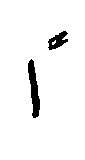
\includegraphics[height=1.68em]{../../S01/source/presentation/AB01-PDF0070-G01.png}}} and \emph{hamza} are found. Hamza is almost always written in the middle and at the end of a word, rarely at the beginning; yet \RL{\ArNote بدء} and \RL{\ArNote جزء} always become \RL{\ArNote بدو} and \RL{\ArNote جزو} (in the accusative \smash{\raisebox{-0.6em}{
\includegraphics[height=1.5em]{../../S01/source/presentation/AB01-PDF0070-G02.png}}}), \RL{\ArNote ابطأ} always \RL{\ArNote ابطى}, just as, the radical hamza being left out, \RL{\ArNote بدت} and \RL{\ArNote تهى} are constantly written for \RL{\ArNote بدأت} and \smash{\raisebox{-0.66em}{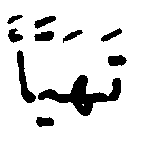
\includegraphics[height=1.67em]{../../S01/source/presentation/AB01-PDF0070-G03.png}}}, \RL{\ArNote مايتين} for \RL{\ArNote مائتين}, and \RL{\ArNote اختفايه} for \RL{\ArNote اختفائه}, \RL{\ArNote اختفاؤه} and \RL{\ArNote اختفاءه. ي} and \RL{\ArNote ى} occur indiscriminately, at the copyist's pleasure; \emph{yāʾ} in the sense of \emph{alif maqṣūra} is \RL{\ArNote ى} in the prepositions, \RL{\ArNote ا} in the rest (very rarely \RL{\ArNote ى} with \RL{\ArNote ا} written above it). Sometimes \RL{\ArNote ى} is written for \RL{\ArNote ا} at the end of words, as \RL{\ArNote ابدى} for \RL{\ArNote ابدأ}, and \RL{\ArNote سوى} for \RL{\ArNote سواء}. So \RL{\ArNote تلقا} is found for \smash{\raisebox{-0.66em}{
\includegraphics[height=1.63em]{../../S01/source/presentation/AB01-PDF0070-G06.png}}} and for \smash{\raisebox{-0.78em}{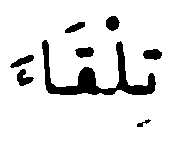
\includegraphics[height=1.71em]{../../S01/source/presentation/AB01-PDF0070-G04.png}}}. Often, in verbs whose last radical is \RL{\ArNote ي}, the short final vowel is marked by the letter \emph{yāʾ}, as \RL{\ArNote سمى} for \smash{\raisebox{-0.58em}{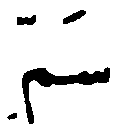
\includegraphics[height=1.37em]{../../S01/source/presentation/AB01-PDF0070-G07.png}}}, \RL{\ArNote تليه} for \smash{\raisebox{-0.66em}{
\includegraphics[height=1.46em]{../../S01/source/presentation/AB01-PDF0070-G05.png}}}; likewise always \RL{\ArNote ثواني} for \RL{\ArNote ثوان}, etc. In the imperfect of verbs whose last radical is \RL{\ArNote و}, a redundant \RL{\ArNote ا} is always added at the end, in the Maghribī manner. The ending of the regular masculine plural is \RL{\ArNote ين} for \RL{\ArNote ون} always in the numerals and often in the rest; so too the ending of the nominative dual. The agreement of the numerals with the gender of the nouns is very often faulty.\par
\par \Pg{I LXII}The codex comes from an archetype corrupted and interpolated here and there, whose writer, having a depraved copy before his eyes, had tried with his small powers to fill the gaps and to restore plainly faulty passages to the true reading. By the happiest chance he was a man very unskilled in the mathematical disciplines, so that his emendations and additions can always be distinguished from al-Battānī's true text. The chief corruptions, which arose not from the negligence of the copyists alone but also from rash emendations, are p. 26 (notes p. 186), 31 (note 192), 32 (note 194), almost the whole of chapter XXV (notes 197–99), 77 (notes 251–52), 82 (note 259), 98–99 (note 275), 131 (notes 307–08); interpolations or false restorations of gaps, p. 53 (notes 224–225), 65 (note 238), 80 and 81 (note 257), 106 (notes 281–82), 122–23 (notes 290–92), and the appendices D and F (notes 324–26). Elsewhere the writer of the archetype tried to fit the text of a geometrical demonstration to a badly drawn figure, as on pp. 50–51 (notes 223–24), 64 (notes 237–38), 91 (notes 271–72). Gaps, perhaps not small, on p. 78 (notes 254–55) and 85 (note 265). All these are common to the Escorial codex and to Plato of Tivoli, except the appendices D and F, which, as they belong to the tables, are missing in Plato; it is therefore abundantly clear that the copy that he used and the Escorial codex derive from the same archetype. I should even have suspected that Plato had the Escorial copy itself in his hands, had I not found in Plato a few words wrongly left out in the Escorial text. Other errors, however, of less moment, especially in the numbers, which come from the carelessness of copyists, are far more frequent in the old Latin version\footnote{The very frequent confusion in the editions of the figure 2 with 5 is to be attributed to the compositor, not to Plato.}, in which many things have also dropped out here and there, perhaps not always through the translator's fault. Interpolations later than the common archetype exist in the Escorial codex, I think, two at most, and those of very small weight; see above, p. XLIII, and n. 4 there.\par
\par Of the corruptions and interpolations in the \emph{tables} I shall have to speak in vol. II.\par
\par A few things (the chronological tables of the kings and the caliphs, it seems) were transcribed from the Escorial codex by D. Faustin Juan Nepomuceno de Borbon, «commonly called Muscat», in his unpublished \emph{Polygrafía Aràbigo Española}, Madrid 1790 ff., vol. IV, pp. 164–66, as appears from the catalogue of the Arabic codices of the Royal Library of Berlin\footnote{Ahlwardt, \emph{Verzeichniss}, vol. IX, p. 247, no. 9734.}. Half of chapter VI, or a little more, was edited in Arabic and Latin by Reinaud; the geographical tables in Arabic and French by Lelewel, as I have always noted in their places. That other scholars examined the Escorial codex carefully is not established.\par
\par VII. It remains for me to say briefly \emph{how I have edited al-Battānī's work and translated it into Latin}.\par
\par \Pg{I LXIII}In editing the Arabic text I have brought the Maghribī spelling of the codex, which departs not a little from the author's (who most certainly used the \emph{naskhī} script), back to the true rules of orthography; I have therefore removed all the peculiar usages listed above. I have often added the vowels and other auxiliary signs, to make the interpretation easier; I have also tacitly corrected the errors in the agreement of the numerals with the gender of the nouns, since there was no reason to attribute them to the author himself. Everything else in which I thought I must depart from the authority of the codex I have always indicated in the notes\footnote{After the word \RL{\ArNote بعد}, or the adjectives derived from it, the codex uses \RL{\ArNote من} and \RL{\ArNote عن} indiscriminately. In the edition I have always used \RL{\ArNote عن}, as is the usage of purer speech.}. It is well known that some letters have one numerical value in the \emph{naskhī} script, which al-Battānī used, and another in the Maghribī script in which the codex is written. In the text of the chapters, in which few numbers expressed by such letters occur, I have always changed the usage of the codex to the author's; not so, however, in the tables that I chose to print in Arabic too (vol. III, pp. 228–79): for, since I had decided to correct their numbers only in the translation, had I changed the numerical usage of the codex the reader would not have had a faithful image of the Escorial manuscript, nor would the causes of the corruptions have readily appeared.\par
\par In my version I have followed the Arabic text closely, as far as could be done without excessive obscurity arising. What I thought should be added, either because it had plainly dropped out of the codex or because it helped to explain the sense, I have always enclosed in square brackets [~]. Sometimes, however, but only in setting out \emph{mathematical formulas}, I judged that things should be told in fewer words, so as not to weary the reader excessively. For, to give an example of the most compressed passages, had I translated those formulas too word for word, the last three lines of p. 13 and the first of p. 14 would have run thus: «If you wish to know the ascensions of any degree of the signs in the right sphere, take the whole declination, namely 23° 35′, and find its sine, that is, the sine of the whole declination; then subtract the whole declination from 90° and find the sine of what remains, which will be the sine of the complement of the whole declination. Then take [the interval] from the beginning of Aries to the degree that you wish, and find the declination of that degree; find the sine of what it is, which will be the sine of the declination of the degree. Then subtract the declination of the degree from 90, and find the sine of what remains, which will be the sine of the complement of the declination of the degree. Then multiply the sine of the declination of the degree by the sine of the complement of the whole declination; divide what results by the sine of the whole declination, and multiply what comes out by half the diameter, that is, by 60; divide what results by the sine of the complement of the declination of the degree. Find the arc of what comes out; what the arc is will be the amount of what rises in the right sphere from the beginning of Aries to the degree that you wanted».\par
\par Except in very few places, and those small ones, no help, as I have said, could be taken from the printed version of Plato, which is far more corrupt than the Escorial text and derives from the same archetype. I was therefore unwilling to furnish the version or the text with its most obvious errors by way of a critical apparatus. Plato's numbers, however, I have always reported in the notes, because Halley, Delambre and others had used those numbers in their dissertations; nor have I ever passed over the places in which Plato's version could bring any profit.\par
\par In my notes some things will be superfluous to some readers, others to others. I preferred to say too much rather than too little, knowing that this book will perhaps be read by men devoted to studies very different from one another, and that things most familiar to an astronomer are extremely hard and difficult to understand for those who give themselves to Arabic letters. So that my formulas should not be confused with the author's, I have always marked al-Battānī's formulas with Greek letters, except on p. 219, where space was lacking.\par
\par To render Arabic in our letters I have followed this system:\footnoteT{This English translation follows Nallino's system with these changes: it writes ʾ and ʿ for his ’ and ‘ and j for his ǵ, keeps the article al- unassimilated (al-Raqqa for ar-Raqqah) except where the assimilated form is itself the matter in hand, and leaves out the h of the feminine ending (-a for -ah).}\par
\par ʾ (\emph{hamza}), in the middle and at the end of words, marks a harsh interruption of the voice.\par
\par ʿ (\RL{\ArNote ع}) is a voiceless guttural, unknown to our languages.\par
\par \emph{dh} (\RL{\ArNote ذ}) is the English \emph{th} in \emph{the}, or the {\greekfont δ} of the Greeks of our time\footnote{This and the five following are rendered thus by Suter, \emph{Die Mathematiker}: ḏ, ǧ, ġ, ch, š, ṯ. Suter sometimes writes \emph{e} for \emph{a} and \emph{o} for \emph{u}, because these short vowels are often pronounced both ways.}.\par
\par \emph{ǵ} (\RL{\ArNote ج}) is always palatal, like the Italian \emph{g} before \emph{i} and \emph{e}, or the English in \emph{gentleman}.\par
\par \emph{gh} (\RL{\ArNote غ}) is a voiced guttural spirant, a little harsher than the {\greekfont γ} of the Greeks of our time.\par
\par \emph{kh} (\RL{\ArNote خ}) is a little harsher than the German \emph{ch} in \emph{ach}, or the Spanish \emph{j}.\par
\par \Pg{I LXIV}\emph{sh} (\RL{\ArNote ش}) as in English.\par
\par \emph{th} (\RL{\ArNote ث}) like the English \emph{th} in \emph{thank}, the Spanish \emph{z}, the Greek {\greekfont ϑ}.\par
\par \emph{w} (\RL{\ArNote و}) as in English.\par
\par \emph{ḍ, ḥ, q, ṣ, ṭ, ẓ} are the emphatics, as they are commonly called, of the simpler \emph{d, h, k, s, t, z}.\par
\par The long vowels are marked by a small line above them (\emph{ā, ī, ū}).\par
\par\begin{center}⁂\end{center}
\par It is now a pleasant duty to give public thanks to those who have favoured my work: namely to the Augustinian Fathers in charge of the Escorial Library, who in the autumn of 1894, with the greatest liberality, made easier for me the task of partly copying and partly photographing the codex; likewise to Father Juan Lazcano, carried off by an untimely death on 17 December 1899, who always most willingly collated with the codex again everything that, after I had left the Escorial, seemed doubtful to me in my copy.\par
\par But above all I must, with my whole heart, give the greatest thanks again and again to the most distinguished brothers Celestino and Giovanni Schiaparelli. For the former, Professor of Arabic letters in the University of Rome, a man in whom uprightness of mind, the greatest modesty and the widest learning admirably vie with one another, chose to propose me, known to him only through a few writings, as translator and editor of al-Battānī's work. The latter, gladly complying with his brother's wish, not only most kindly provided the means for me to go to Spain and to have the book printed at the expense of the \emph{Observatory of Milan}, of which he was the director, but also showed himself ready to resolve the doubts in which I had been caught in composing my work. For, trained in philological studies, I should not have dared to undertake that work had I not known that I could enjoy the help of so great an astronomer. Indeed, that man, the glory of Italy, with the great kindness that is his, read through my version and the commentary written by me attentively, and added other things to them, which, enclosed in heavy brackets [~] and marked with his name, are the finest ornament of this book. He also undertook the most tedious task of examining once more the numerical tables, first corrected by me, as I shall say better in vol. II, although he had to attend to many and far weightier affairs. If, then, scholars gain any profit from al-Battānī brought to light again, let them know that it is owed above all to those two eminent brothers.\par
\par Palermo, January 1903.\par
\par\begin{center}CAROLUS ALPHONSUS NALLINO\end{center}
\par\begin{center}Professor of the Arabic language and literature in the Royal University of Palermo.\end{center}
\UnitHead{List of the oriental or manuscript books always cited in this volume by abbreviations}{P25}\Pg{I LXV}
\par Aboulféda [Abū l-Fidāʾ], \emph{La géographie, texte arabe publié par Reinaud et Mac Guckin de Slane}, Paris 1840. — \emph{La géographie, traduite par Reinaud [et Guyard]}, Paris 1848–83, 3 vols. — The author died on 23 al-Muḥarram 732 (26 Oct. 1331).\par
\par Aboul Hhassan, \emph{Traité des instruments astronomiques des Arabes par — Ali de Maroc, traduit par J. J. Sédillot}, Paris 1834–35. — The author, whose true name is Abū ʿAlī al-Ḥasan al-Marrākushī, wrote about the middle of the seventh century of the hijra (the thirteenth AD).\par
\par Barhebraeus, \emph{Astronomia} = \emph{Le livre de l'ascension de l'esprit sur la forme du ciel et de la terre, cours d'astronomie rédigé en 1279 par} Grégoire Aboulfarag, \emph{dit} Bar-Hebraeus, \emph{publié par F. Nau}. Première partie: texte syriaque, Paris 1899; Seconde partie: Traduction française, Paris 1900. — They form fascicle 121 of the series Bibliothèque de l'École des Hautes Études.\par
\par Al-Bīrūnī, \emph{Elementa astronomiae}. A small work without a title, no. 2497 of the Arabic codices of the Bibliothèque Nationale in Paris, according to the printed catalogue. From f. 28v it appears that the author himself translated it from the Persian in the year 420 H (beginning 19 Jan. 1029). It sets out briefly, by questions and answers, the rudiments of astronomy and of mathematical astrology, and also the chief feast days of several nations. In the codex there are some gaps, and the spaces of some small tables are empty. — The author seems to have died in the month of Rajab 440 (December 1048).\par
\par Al-Bīrūnī, \emph{Chron.} = \emph{Chronologie orientalischer Völker von} Albêrûnî, \emph{herausgegeben von Ed. Sachau}, Leipzig 1876–78. — \emph{The Chronology of the oriental nations, an english version of the arabic text of the Âthâr-ul-Bâḳiya of} Albîrûnî, \emph{translated with notes by C. Edw. Sachau}, London 1879.\par
\par Al-Bīrūnī, \emph{India} = Albêrûnî's \emph{India, an account of the religion, philosophy, literature, chronology, astronomy, customs, laws and astrology of India about A. D. 1030; arabic text edited by Ed. Sachau}, London 1887. — \emph{An english edition with notes and indices by Ed. C. Sachau}, London 1888, 2 vols.\par
\par Al-Farghānī. — Besides the edition with Golius's translation (Amsterdam 1669) and the version of John of Seville (Nuremberg 1537), I have used the Arabic codex no. 2504, III, of the Bibliothèque Nationale in Paris. — The author, commonly called Alfraganus, wrote about the middle of the third century of the hijra, the ninth AD.\par
\par \Pg{I LXVI}Al-Jaghmīnī. — \emph{Die Astronomie des Maḥmūd ibn Muḥammad ibn ʿOmar} al-Ǵâgminî, [\emph{übersetzt}] \emph{von G. Rudloff und Ad. Hochheim}, in Zeitschrift der deutschen morgenländischen Gesellschaft, vol. XLVII, 1893, pp. 213–275. — I have collated everything with the Arabic text kept in the National Library at Naples, no. 100, II, in the catalogue made by L. Buonazia (\emph{Catalogo dei codici orientali di alcune biblioteche d'Italia}, fasc. II, p. 240); it is furnished with the commentary of an unknown author, which is dedicated to the sultan Mubārak-shāh son of Ibrāhīm and begins: \RL{\ArNote اما بعد حمد الله المتفرد في ارضه وسمائه والصلاة على محمد خاتم انبيائه}\footnoteT{The Arabic reads: «Now, after the praise of God, who is alone in His earth and His heaven, and the blessing upon Muḥammad, the seal of His prophets».}. The \emph{naskhī} script is fine and correct enough; but the numbers are often faulty. — Al-Jaghmīnī, as Suter has shown, died in the year 745 H (beginning 14 May 1344).\par
\par Ḥabash, the astronomical work (\emph{zīj}) contained in the Arabic codex of the Royal Library of Berlin described by Ahlwardt, \emph{Verzeichniss}, vol. V, pp. 200–03, no. 5750. It was composed by the author in the city of Baghdād in the years immediately following 300 H (beginning 17 Aug. 912), and so a very little later than al-Battānī's work. The information in Suter, pp. 12–13, no. 22, and in Brockelmann, \emph{Gesch. der arab. Litteratur}, vol. I, p. 221, must be corrected accordingly.\par
\par Ibn Hibintā, \emph{al-mughnī fī l-nujūm}, «the sufficient [book] on [the knowledge of] the stars», an Arabic codex of the Royal Library of Munich (in Aumer, no. 852). From the work itself it is clear that the book was written after the year 329 H (beginning 5 Oct. 940); the year 214 H, which is commonly given on the authority of a \emph{false} inscription on the first leaf of the codex, must be rejected.\par
\par Ibn Khordādhbeh = \emph{Kitâb al-Masâlik wa 'l-mamâlik auctore} Ibn Khordâdhbeh. \emph{Accedunt excerpta e Kitâb al-Kharâdj auctore} Kodâmah ibn Dja'far. \emph{Una cum versione Gallica ed. a} M. J. de Goeje, Leiden 1889 (Bibliotheca Geographorum Arabicorum, vol. VI). — Written a very little before 272 H (beginning 17 June 885).\par
\par Ibn al-Qifṭī, \emph{Taʾrīkh al-ḥukamāʾ}, «history of the sages». Besides the excerpts in Casiri and Sédillot, I have used the codex kept at Rome in the Royal Academy of the Lincei (formerly Michele Amari's); cf. also the \emph{Addenda} to the preface.\par
\par Ibn Rosteh = \emph{Kitâb al-A'lâk an-Nafîsah VII auctore} Ibn Rosteh, \emph{et Kitâb al-Boldân auctore} al-Ja'kûbî, \emph{ed. M. J. de Goeje}, Leiden 1892 (Bibl. Geogr. Arab., vol. VII). — He wrote a very little before 301 H (beginning 6 Aug. 913).\par
\par Ibn Yūnus, \emph{al-zīj al-ḥākimī}, «the Ḥākimite astronomical work». When «in Caussin» is added, the work meant is \emph{Le livre de la Grande Table Hakémite observée par..... Aboulhassan Ali..... ebn Iounis, [publié et] traduit par Caussin}, in Notices et extraits des manuscrits de la Bibliothèque Nationale, vol. VII, 1804, pp. 16–240. Caussin's book was also published separately, without the Arabic title, which took up p. 49 of the Notices; in that edition, therefore, the page numbers are always 15 less than mine for pp. 16–48 of the Notices (= 1–33 of the offprint), 16 less for the rest\footnoteT{The print has «Caussin's book was also published separately; in it the numbers of the single pages are always 15 less than mine»; the wording here is that of Nallino's Addenda et emendanda (Part II, p. XVII).}; moreover, the text is given on the odd pages, the translation on the even ones. — What is not among Caussin's excerpts I have taken from the Leiden codex no. 1057 (Catal., vol. III, p. 88), which contains the first 22 chapters (a most careful copy of it, keeping the same numbering of the pages, is Paris no. 2495), and from the Paris codex no. 2496, which contains other chapters. — Ibn Yūnus died in the month of Shawwāl 399 (June 1009).\par
\par \Pg{I LXVII}Al-Kharaqī, \emph{muntahā l-idrāk fī taqāsīm al-aflāk}, «the utmost that can be attained in the divisions of the celestial spheres». I use two codices: Paris no. 2499, and that of the Laurentian Library (Florence), cod. orient.-palat. no. 110 (it bears no. 290 in Assemani's \emph{Catalogue}, where it is falsely said to be the \emph{Nihāyat al-idrāk} written by Quṭb al-Dīn al-Shīrāzī). In the Laurentian codex the last leaf is missing, which held the end of the eleventh \emph{bāb} of the third treatise. — About the author's other names there is the greatest disagreement. Some codices have: Abū Muḥammad ʿAbd al-Jabbār ibn ʿAbd al-Jabbār ibn Muḥammad al-Thābitī al-Kharaqī; and these are confirmed by the old authority of al-Būnī (d. 622 H), \emph{Shams al-maʿārif al-kubrā}, [Cairo] 1291 H, vol. I, p. 27, who says that the stars of the Little Bear «are mentioned, among the fixed stars, by Abū Muḥammad ʿAbd al-Jabbār, known [by the name of al-Kharaqī], in the book entitled \emph{al-Tabṣira}»\footnote{A book by the same author, almost a compendium of the work \emph{al-muntahā}.} \RL{\ArNote ذكرها ابو محمد عبد الجبار المعروف في كتابه المسمى بالتبصرة (\LR{sic}) في الكواكب الثابتة}. Other codices, however, have: Bihāʾ al-Dīn Abū Bakr Muḥammad ibn Aḥmad ibn Abī Bishr al-Kharaqī; and with these the much later Ḥājjī Khalīfa agrees (vol. II, p. 180, no. 2379, and vol. VI, p. 170, no. 13124), writing Muḥammad ibn Aḥmad al-Ḥusaynī al-Khiraqī. I think the former should be followed; the others have confused the astronomer with the more famous Abū Bakr Muḥammad ibn Aḥmad ibn Abī Bishr al-Kharaqī, a great expert in law and dogmatic theology, who died in 533 H (beginning 7 September 1138). — The book was composed about AD 1132, for in the first treatise the longitudes and latitudes of 83 fixed stars (cod. Laurent. f. 36r–37v) and the places of the apogees of the planets (f. 45v) are given for the year 1444 of Dhū l-Qarnayn (beginning 1 October 1132).\par
\par Al-Khāzinī, \emph{al-zīj al-sanjarī}, «the Sanjarī astronomical work», in the codex of the Vatican Library marked cod. Vat. Arab. 761. — From fol. 121v it is gathered that the book was composed in the reign of the caliph al-Mustarshid bi-llāh (16 Rabīʿ II 512 – the month of Dhū l-Qaʿda 529, that is, 6 Aug. 1118 – Aug. 1135); the longitudes and latitudes of 43 fixed stars are given for the year 509 H (beginning 26 May 1115) on f. 191v–192r. The tables of the oblique ascensions (f. 160v–161r) and of the equation of time (f. 161v) are computed for the latitude of the city of Merw, 37° 40′.\par
\par Leo de Balneolis, \emph{Astronomia}, contained on f. 1r–108v of the codex Vatic. Lat. 3098, which also contains the version of al-Battānī (cf. p. LII). It was written originally in Hebrew and forms the fifth treatise of the work \emph{Milḥamōt hash-shēm}, «the wars of God»; being a single and great book that had to be presented on its own, it is left out in many codices and in the editions of the whole philosophical-theological work. The treatise is divided into three parts, comprising 136, 9 and 14 chapters; their list in Hebrew and Latin is in Neubauer, in the great work \emph{Histoire littéraire de la France}, vol. XXXI, 1893, p. 624 ff. The author reports several astronomical observations of his own. Writing in Hebrew he called himself Lēwī ben Gerson; he died at Avignon in 1344.\par
\par Al-Masʿūdī, \emph{Prairies} = Maçoudi, \emph{Les Prairies d'or, texte et traduction par C. Barbier de Meynard}, Paris 1861–77, 9 vols. — He died in 346 H (beginning 3 Apr. 957).\par
\par Al-Masʿūdī, \emph{Tanbīh} = \emph{Kitâb at-tanbîh wa 'l-ischrâf auctore} al-Mas'ûdî, \emph{edidit M. J. de Goeje}, Leiden 1894 (Bibl. Geogr. Arab., vol. VIII).\par
\par Al-Muqaddasī = \emph{Descriptio imperii Moslemici auctore} al-Mokaddasi, \emph{edidit M. J. de Goeje}, Leiden 1876–77 (Bibl. Geogr. Arab., vol. III). — He wrote between the years 375 and 378 H, that is, 985–989.\par
\par Naṣīr al-Dīn al-Ṭūsī, \emph{al-tadhkira fī ʿilm al-hayʾa}, «memorial on astronomy». I use the Vatican codex Arab. no. 319, of which it fills f. 1v–64r (in Assemani's \emph{Catalogue}, p. 465: «an anonymous epitome of the science of the form and figure of the heaven and the earth»), and also the commentary of Qāḍī-zāde, mentioned below. — The famous astronomer and mathematician died in the month of Dhū l-Ḥijja 672 (June 1274). Two editions of the book came out\footnote{They are mentioned in Qāḍī-zāde's \emph{commentary} (f. 39v) on the passage quoted by me on pp. 161–62, where Naṣīr al-Dīn sets out eight cases that could occur if the ecliptic approached the equator: \RL{\ArNote وهذه النسخة المشتملة على الاقسام الثمانية هي الجديدة المعوّل عليها التي غيّر اليها القديمة التي جعل فيها الاقسام اربعة بعد مدة مديدة}}\footnoteT{The Arabic in the note reads: «and this recension, which contains the eight divisions, is the new one, on which one is to rely, into which he changed, after a long time, the old one, in which he had made the divisions four».}, both earlier than his greater \emph{al-zīj al-īlkhānī}.\par
\par Naṣīr al-Dīn al-Ṭūsī, \emph{al-zīj al-īlkhānī}, written in Persian, codex of the Laurentian, orient.-palat. no. 24 (no. 269 in Assemani's \emph{Catalogue}). — Composed for the king Ābāqā Khān, who obtained the supreme power in the year 664 H (beginning 12 Oct. 1265).\par
\par \Pg{I LXVIII}Oloug Beg [Ulugh, or Ulūgh, Beg] = \emph{Prolégomènes des tables astronomiques d'Oloug Beg publiés [en persan] avec notes par L. P. E. A. Sédillot}, Paris 1847. — \emph{Prolégomènes etc., traduction et commentaire par L. P. E. A. Sédillot}, Paris 1853\footnote{The text also forms the introduction and pp. 285–450 of vol. I of the work \emph{Chrestomathie persane publiée sous les auspices de M. le Ministre de l'Instruction publique}; 284 must be added to the pages I cite to obtain the numbering of the Chrestomathie. The translation is vol. II itself of the same Chrestomathie.}. — He died in the year 853 H (beginning 23 Febr. 1449).\par
\par Qāḍī-zāde, \emph{Commentary} (\emph{sharḥ}) on the \emph{Tadhkira} of Naṣīr al-Dīn, codex of the Laurentian Library, orient.-palat. no. 271 (no. 311 in Assemani's \emph{Catalogue}). — The book was finished in the city of Shīrāz on Tuesday 14 Dhū l-Ḥijja 811, that is, 30 April 1409.\par
\par Qodāma, see Ibn Khordādhbeh; he died in the year 337 H (beginning 10 July 948).\par
\par Quṭb al-Dīn al-Shīrāzī, \emph{al-tuḥfa al-shāhiyya}, «the royal gift», codex of the Laurentian Library, orient.-palat. 215 (no. 306 in Assemani's \emph{Catalogue}); a copy without its beginning, lacking the first 22 leaves of the old Arabic numbering. I cite the leaves by the more recent European numbering. — He died in the month of Ramaḍān 710 (Jan.–Febr. 1311).\par
\par Al-Ṣūfī = \emph{Description des étoiles fixes composée au milieu du dixième siècle de notre ère par Abd-al-Rahman} al-Sûfi; \emph{traduction littérale avec des notes par H. C. F. C. Schjellerup}, St. Petersburg 1874. — He died in the month of al-Muḥarram 376 (beginning 12 May 986).\par
\par Sūrya-Siddhānta = \emph{Translation of the Sūrya-Siddhânta, a text-book of hindu astronomy with notes and an appendix by E. Burgess [and W. Whitney]}, in Journal of the American Oriental Society, vol. VI, New Haven 1860, pp. 142–498. The work also came out separately; its pages are found by subtracting 144 from the numbers that I give.\par
\par Thābit ibn Qurra, \emph{De motu octavae sphaerae}. The little book survives in two different Latin versions. One, in the Vatican Library (cod. Vatic. Lat. 4275, f. 83vb–85ra), is entitled \emph{Liber thebit filii chore de motu spere octaue} and begins: «Ymaginabor speram equatoris diei et tres circulos in eo signatos, qui sunt circuli orizontis et circulus linee medii celi.....» (I shall imagine the sphere of the equator of the day and three circles marked on it, which are the circles of the horizon and the circle of the line of the middle of the heaven.....). The other (cod. Vatic. Lat. 4083, f. 56v–57r) opens thus: «Incipit \emph{liber tebit de motu 8. spere seu accessionis et recessionis}. Tractatus in quo continetur doctrina motus accessionis et designationis figure ipsius sicut est in celo. Speram equinoctialem tum et tres circulos in ea signatos. orizontis videlicet circulum. et meridiei circulum..... sola mentis intuitione concipe» (here begins \emph{the book of Thebit on the motion of the eighth sphere, or of access and recess}. A treatise that contains the doctrine of the motion of access and of the drawing of its figure as it is in the heaven. Conceive by the mind's eye alone the equinoctial sphere, and then three circles marked on it, namely the circle of the horizon and the circle of the meridian.....). After all the notes had already been printed, I was able to examine three other codices of the first version\footnote{The one that Albertus Magnus mentions in the \emph{Speculum astron.}, in the passage indicated by me on p. XXIV, n. 2.}, which I use in the \emph{Addenda}: of the Marcian Library (Venice), cod. Lat. class. VIII, cod. LXIX, f. 22r–26r, entitled \emph{Thebit de motu octavae sphaerae}; of the same library cod. Lat. class. XIV, cod. CLXV, f. 46rb–49va («*Incipit liber tebith ben chorath de motu 8$^{\text{e}}$ spere\emph{»); lastly, of the Laurentian Library (Florence), S. Marco 194. I shall denote them by the letters }A\emph{, }B\emph{, }F*. Of the error of those who think that the little book has been printed I have spoken on p. XXXVI, n. 1. — The author died in the month of Ṣafar 288 H (Febr. 901).\par
\par Yāqūt = Jacût's \emph{Geographisches Wörterbuch herausgegeben von F. Wüstenfeld}, Leipzig 1866–73, 6 vols. in 11 parts. — He died on 20 Ramaḍān 626 (12 Aug. 1229).\par
\par \Pg{I LXIX}Of the canons, or handy tables, of Theon of Alexandria I use the edition prepared by Halma, entitled: \emph{Commentaire de} Théon \emph{d'Alexandrie sur les tables manuelles astronomiques de Ptolémée, [publiées et] traduites par Halma}; vol. I: Les prolégomènes de Ptolémée; les commentaires [sic!] de Théon et les tables préliminaires, Paris 1822; vols. II and III: Tables manuelles de Ptolémée [sic!] et de Théon, Paris 1823. Would that there were another edition, less confused and not so full of errors!\par
\par Delambre, with no other title of a book, denotes his \emph{Histoire de l'astronomie du moyen âge}, Paris 1819.\par
\par Suter, or Suter, \emph{Die Mathematiker}, denotes the excellent book \emph{Die Mathematiker und Astronomen der Araber und ihre Werke}, Leipzig 1900 (Abhandlungen zur Geschichte der mathematischen Wissenschaften, fasc. X), to which the author himself has now added: \emph{Nachträge und Berichtigungen zu «Die Mathematiker und Astronomen der Araber und ihre Werke»}, in Abhandl. zur Gesch. der mathem. Wiss., fasc. XIV, 1902, pp. 157–85.\par
\UnitHead{Addenda et emendanda (additions and corrections)}{P27}\Pg{I LXX}
\par P. VIII: Almost half of the preface had already been printed when \emph{Ibn al-Qifṭī's Taʾrīḫ al-ḥukamāʾ herausgegeben von J. Lippert}, Leipzig 1903, came out; it is to be regretted that the editor often fails to indicate the variant readings and the additions of the codices. In the life of al-Battānī, pp. 280–281, after the words «known [by the surname] al-Battānī» these are added, undoubtedly found in very few codices (cf. Chwolsohn, I, 611, n. 1): «and in the book of the judge Ṣāʿid al-Andalusī he is Abū Jaʿfar Muḥammad ibn Sinān ibn Jābir al-Ḥarrānī, known [by the surname] al-Battānī». After the words «who equalled him in investigating their motions» Lippert's edition also gives: «He had moreover devoted his study to the judgements of the stars, which led him to write [books] on this matter; among his writings on those [judgements] is a book explaining Ptolemy's Tetrabiblos». Lastly, Lippert's edition follows the reading of the book \emph{al-Fihrist} that I mentioned on p. VIII, n. 8.\par
\par The name Abū Jaʿfar in place of Abū ʿAbd Allāh occurs also in the life of Abū Maʿshar (Ibn al-Qifṭī, ed. Lippert, p. 153), probably on the authority of the same Ṣāʿid al-Andalusī (of whom I spoke on p. IX, n. 4). Wrongly, it seems; for Abū ʿAbd Allāh is confirmed not only by the other biographers but also by al-Masʿūdī, \emph{Prairies}, IX, 49, and by Ibn Yūnus, introd. (in Caussin, p. 72). That the names Sinān and Jābir are also wrongly transposed in Ṣāʿid is abundantly clear from the agreeing tradition of so many Arabic writers.\par
\par VIII, n. 7: In Lippert's edition, pp. 155–56. Ibn al-Muktafī is said to have died on Tuesday 4 Ṣafar 377; but 4 Ṣafar of that year was Sunday 5 June 987 AD, by the civil usage.\par
\par XV, n. 3: in some copies \emph{Subbī} and \smash{\raisebox{-0.45em}{
\includegraphics[height=1.32em]{../../S01/source/presentation/AB01-PDF0079-G01.png}}} were printed for \emph{Ṣubbī} and \smash{\raisebox{-0.47em}{
\includegraphics[height=1.45em]{../../S01/source/presentation/AB01-PDF0079-G02.png}}}.\par
\par XXIV–XXV: Ibn al-Qifṭī, loc. cit. (ed. Lippert, p. 97), asserts that not only al-Battānī but also al-Bīrūnī reduced the Almagest to a compendium, in his great \emph{Canon}.\par
\par XXVI, l. 5: ed. Lippert, p. 242.\par
\par XXXIII, n. 1: ed. Lippert, p. 326.\par
\par P. 3, l. 14, for \emph{longiquitate} read \emph{longinquitate}.\par
\par 6, 11, for \emph{his causis antiqui diviserunt: quia.....} (the ancients divided it for these reasons: because.....) read \emph{antiqui diviserunt, pluribus innitentes causis: quia scilicet.....} (the ancients divided it, relying on several reasons: namely because.....).\par
\par 6, 32–36, to be rendered word for word thus: \emph{Significatio multiplicationis est quod sibi ipsi adiicias alterum numerorum iuxta quantitatem unitatum alterius; intelligo multiplicationem unitatum in unitates. Multiplicatio fractionum in unitates est quod sibi ipsi adiicias fractiones iuxta quantitatem unitatum, vel quod dividas unitates iuxta quantitatem fractionum ex uno. Multiplicatio fractionum in fractiones est quod dividas alteram fractionum, quamcumque volueris, iuxta quantitatem alterius fractionis ex uno} (the meaning of multiplication is that you add one of the numbers to itself according to the number of the units of the other; I mean the multiplication of units by units. The multiplication of fractions by units is that you add the fractions to themselves according to the number of the units, or that you divide the units according to the amount of the fractions of one. The multiplication of fractions by fractions is that you divide one of the fractions, whichever you wish, according to the amount of the other fraction of one).\par
\par \Pg{I LXXI}What I have rendered \emph{sibi ipsi adiicere} (to add to itself) is in Arabic \emph{ḍāʿafa}, which means both to double and to take a given quantity several times so that its multiple results; cf. the definitions of the Arab lexicographers in Lane, \emph{Arabic–english Lexicon}, s.v. Plato rightly: \emph{coacervatio et aggregatio} (heaping up and gathering). But other Latin translators of the Middle Ages always render it \emph{duplicare} (to double); so Algoritmi [i.e. al-Khwārizmī] \emph{de numero Indorum}: «necesse est omni numero qui multiplicatur in aliquo quolibet numero, ut \emph{duplicetur} unus ex eis secundum unitates alterius» (for every number that is multiplied by any number whatever, it is necessary that one of them be \emph{doubled} according to the units of the other) (\emph{Trattati d'aritmetica pubblicati da B. Boncompagni}, Rome 1857, p. 10). Likewise, from the Arabic word badly translated, it came about that the Jewish mathematicians of the twelfth century, such as Abrāhām bar Ḥiyyāʾ and Abrāhām Ibn ʿEzrā, said in Hebrew \emph{kāphal} (i.e. to double) for «to multiply», and \emph{kephel} (i.e. doubling) for «multiplication»; examples in Steinschneider, \emph{Abraham ibn Esra}, in the periodical Abhandlungen zur Geschichte der Mathematik, vol. III, 1880, p. 106 (n. 179) and 113. Likewise the use of the word \emph{kephel} to express multiplicative adverbs (like \emph{volta} in Italian, \emph{mal} in German) is to be derived not from the verb \emph{kāphal} itself, as Steinschneider\footnote{Loc. cit., p. 106, and \emph{Intorno ad alcuni matematici del medio evo, lettere a B. Boncompagni}, Rome 1863–67, Letter IV (Brani dell'aritmetica di Elia Misrachi), p. 54, n. 1, and p. 65, n. 1.} thinks, but from the Arabic \emph{ḍiʿf}, «the double of a thing, or a quantity equal to another given one», which is used in the same sense; cf. in al-Battānī himself, vol. III, p. 88: \RL{\ArNote وتَضَاعَفَ البُعْدُ اضْعَافًا كثيرة} and \RL{\ArNote اعظم منه بأضعاف مُضْعَفَة}\footnote{He mostly uses \RL{\ArNote مرة} (vol. III, pp. 88–92, 182–185); vol. III, p. 183 also \RL{\ArNote مِثْل}, pl. \RL{\ArNote امثال}. In the parallel passages Ibn Rosteh, pp. 18–21, and al-Farghānī, ed. Golius, pp. 81–82, have \RL{\ArNote مثل} and \RL{\ArNote مرة} indiscriminately.}\footnoteT{The two Arabic phrases mean «and the distance grew many times over» and «greater than it by manifold multiples».}.\par
\par 6, last line, for \emph{1165} read \emph{1135}.\par
\par 9, 39, for \emph{supplementaris} (of the supplement) read \emph{supplementaris alterius} (of the supplement of the other).\par
\par 11, 3rd line from the foot, for \emph{complementi} (of the complement) read \emph{dupli complementi} (of the double of the complement).\par
\par 13, n. 2: That the «orders» of the Moon are given by Vettius Valens (on whom p. 309, n. 5) in the first book of the \emph{Astrology}, in the chapter {\greekfont περὶ εὑρέσεως βαθμῶν καὶ ἀνέμων τῆς σελήνης}, is attested by Cl. Salmasius, \emph{De annis climactericis et antiqua astrologia diatribae}, Leiden 1648, p. 61, who says, not clearly enough: «The {\greekfont βαθμοί} of the Moon are those that are counted across the latitude of the zodiac, while it goes from the north to the south, or again from the south to the north, ascending and descending, now to the south, now to the north». — In Julian of Laodicea ({\greekfont Ἰουλιανὸς Λαοδικεύς}), of an age uncertain between the fourth and the sixth century AD, {\greekfont βαθμοί} of the Sun, the Moon and the five planets occur too; how they are computed is not clear. See the excerpts in \emph{Catal. codd. astrolog. Graecorum}, IV (1903), pp. 106–108.\par
\par 29, 36, for \smash{\raisebox{-0.26em}{
\includegraphics[height=1.28em]{../../S01/source/presentation/AB01-PDF0080-G01.png}}} read \emph{terrestrium}.\par
\par 41, n. 2: The same error of al-Battānī is found in some writers of our own age too, among them R. Wolf, \emph{Handbuch der Astronomie}, vol. I, p. 443, § 202 e.\par
\par 54, 26, for \emph{utemus} read \emph{utemur}.\par
\par 54, 28, for \emph{quantitas} (amount) read \emph{argumentum} (argument).\par
\par 54, n. 10, for \emph{quantitate} read \emph{argumento}.\par
\par 68, 23, for \emph{qu} read \emph{qui}.\par
\par 71, 4–5, to be corrected according to what I said on p. 322, n. 2.\par
\par 75: on the word \emph{jawzahar} in the title of chapter XXXVII, perhaps interpolated, see p. XLIII of the preface.\par
\par 80, 38, for \emph{octavam} (eighth) read \emph{decimam octavam} (eighteenth), as Plato has; cf. pp. 257–58, and XXXVIII, n. 3.\par
\par 80, n. 4, for \emph{sequenttnus} read \emph{sequentibus}.\par
\par 85, 23–24, the words \emph{in semidiametrum multiplica, et productum} (multiply by the radius, and the product) are to be deleted; cf. p. 265.\par
\par 96, 6, for \emph{horae} (hours), which the codex and Plato have, \emph{gradus} (degrees) seems to be the reading; cf. p. 275, n. 1.\par
\par 107, 10, for \emph{consuemus} read \emph{consuescimus}.\par
\par 114, 11, in the minutes of the apogee of Mars, for 18′ read 58′.\par
\par 114, n. 1: The transposition is only in the editions of Plato; cf. the preface, p. LV.\par
\par \Pg{I LXXII}124, 2, for \emph{referta} read \emph{relata}.\par
\par 129, margin: the number of the page of the text, badly printed, is 194.\par
\par 132, 6, for \emph{interiectos} read \emph{interiectis}.\par
\par 133, 29, for \emph{cognoscuntur. Idest} read \emph{cognoscuntur; idest.}\par
\par 133, 31, for \emph{deprehende; si} read \emph{deprehendes. — Si.}\par
\par 134, 18, after \emph{consistit} insert: [\emph{distantiam multiplica in tempora horaria gradus sequentis}] ([multiply the distance by the hour-times of the following degree]). Cf. p. 316, n. 3.\par
\par 134, last line: the words \emph{hoc modo hilegia} etc. are perhaps spurious; cf. the preface, p. XLIII.\par
\par 138–139, n. 5: The additions of some codices of Plato may be read in the preface, pp. LII–LV.\par
\par 139, 10, to be corrected as I showed on p. 321.\par
\par 148, 1, add in the margin \emph{p. 223} of the Arabic text.\par
\par 149, 21 and 26–27, to be corrected as I set out on p. 326.\par
\par 158, 6th line from the foot (not counting the notes), for \emph{quos} read \emph{quoque}.\par
\par 158, 5th line from the foot (not counting the notes), for \emph{tempore} read \emph{partem}.\par
\par 162–163: Theon's strange definitions are also in the unpublished \emph{Astrology} of Vettius Valens, book II, in the chapter on the winds of the stars ({\greekfont περὶ ἀνέμων τῶν ἀστέρων}). For, on the testimony of Salmasius (\emph{de annis climactericis}, pp. 421–22), Valens, putting with the other astrologers the exaltation ({\greekfont ὑψοῦσθαι}) of the Sun in 19° of Aries, and thence considering a square whose vertices are 19° of Aries, 19° of Cancer, 19° of Libra and 19° of Capricorn, says that from 19° of Aries to the same degree of Cancer the Sun {\greekfont καταβαίνειν τὸν βοῤῥᾶν} (descends the north), from 19° of Cancer to the like degree of Libra {\greekfont καταβαίνειν τὸν νότον} (descends the south), from 19° of Libra to 19° of Capricorn {\greekfont ἀναβαίνειν τὸν νότον} (ascends the south), and from 19° of Capricorn to the same degree of Aries {\greekfont βοῤῥᾶν ἀναβαίνειν} (ascends the north). And similarly of the other planets. The Moon he considers differently, book I, in the chapter {\greekfont περὶ εὑρέσεως βαθμῶν καὶ ἀνέμων τῆς σελήνης} (on the testimony of Salmasius, p. 422): from Leo to Libra {\greekfont καταβαίνειν τὰ βόρεια} (to descend the northern parts), from Scorpio to Cancer\footnoteT{So the print; the quarter that the square of Taurus, Leo, Scorpio and Aquarius gives, like the other three, runs from Scorpio to Capricorn, up to Aquarius.} {\greekfont καταβαίνειν τὰ νότια} (to descend the southern parts), from Aquarius to Aries {\greekfont ἀναβαίνειν τὰ νότια} (to ascend the southern parts), from Taurus to Cancer {\greekfont ἀναβαίνειν τὰ βόρεια} (to ascend the northern parts); which I think Valens said because, according to the astrologers, the Moon has its exaltation in 3° of Taurus; the vertices of the square are therefore Taurus, Leo, Scorpio and Aquarius. — Julian of Laodicea agrees with al-Battānī's usage, asserting in the passage mentioned before (p. LXXI) that the Sun, Venus and Mercury, standing at the longitudes 214° 8′ 50″, 231° 28′ and 224° 32′, «descend to the south» ({\greekfont κατέρχεται νότον}), and the Moon and Saturn, at 48° 10′ and 24° 28′, «ascend to the north» ({\greekfont ἀνέρχεται βοῤῥᾶν}). I think there is a copyist's corruption in Jupiter (154° 12′) and Mars (137° 35′), which are also said {\greekfont ἀνέρχεται βοῤῥᾶν}.\par
\par 163–164, n. \emph{b}: Likewise al-Khāzinī, f. 151r–v, and Kūshyār ibn Labbān (in the passage that I mentioned on p. 325) give a table of right ascensions computed from the beginning of Capricorn. One of the problems of the book \emph{de saphaea}, whose author is al-Zarqālī, is: to find the longitude of a star from its right ascension computed from the beginning of Capricorn (i.e. from the degree with which the star culminates) and its declination; Steinschneider translated this badly, \emph{Études sur Zarkali}, Bullett. di bibliografia, vol. XVIII, 1885–86, p. 345 (= p. 57 of the offprint). Tables of right ascensions for every minute of the zodiac, from the beginning of Capricorn, were also computed by Abū Bakr ibn al-Musharraf, in the ninth century of the hijra (the fifteenth AD), it seems (\emph{Catal. of the Library of Cairo}, vol. V, p. 238, mīqāt no. 209). And from the same point of Capricorn the Egyptian Muḥammad al-Akhṣāṣī counted the ascensions of 112 fixed stars, for about the year AD 1650, in the small book \emph{al-durra al-muḍīʾa fī l-aʿmāl al-shamsiyya}, of which there are two copies also in the \emph{Cairo Catal.} V, 245, mīqāt nos. 60 and 81; see the tables published by Edw. Knobel, \emph{On a catalogue of stars in the Calendarium of Mohammad Al Achsasi Al Mouakket}, in Monthly Notices of the R. Astronomical Society, vol. LV, no. 8, 1895, p. 429.\footnoteT{Nallino's Addenda et emendanda (Part II, p. XVII) add that Theon's tables (I, 148–155) also count the right ascensions of the signs from the beginning of Capricorn, which explains their heading {\greekfont ὀρθὴ σφαῖρα μεσουράνησις πανταχῇ}, so that al-Battānī had a Greek model before his eyes; that such tables survive in several Arabic manuscripts (Ahlwardt, \emph{Verzeichniss}, vol. V, nos. 5710, 5758, 5771, 5772, 5798, 5808), some later writers calling them \emph{maṭāliʿ al-zawāl}, «the ascensions of the culmination», or \emph{maṭāliʿ al-qubba}, «the ascensions of the Dome [of the Earth]»; and they refer to Barhebraeus, \emph{Astron.}, p. 170 of the text, 150 of the translation. The Addenda are translated with Part II's front matter.}\par
\par \Pg{I LXXIII}169, 3rd line from the foot (not counting the notes), for \emph{extensione} read \emph{extensionis}.\par
\par 171, n. 3: See moreover J. Canal, \emph{Tiaret, monographie ancienne et moderne} (Bulletin trimestral de géographie et d'archéologie d'Oran, vol. XX, 1900, pp. 1–44).\par
\par 175, 13, the numbers 10 and 9 are to be exchanged.\par
\par 175, n. 9, for \RL{\ArNote واسلول} read \RL{\ArNote والسلول}.\par
\par 181, 1–4: The theorem of the proportionality of the sines of the angles to the opposite sides in a plane triangle is already mentioned, as a thing known to all, by al-Bīrūnī, \emph{Chron.}, p. 184 of the text, 166 of the translation.\par
\par 191, 16, for \emph{ortographicam} read \emph{orthographicam}.\par
\par 194, 26, the bar has dropped out in the fraction $\frac{\cos L}{\cos\delta}$.\par
\par 194, in the last formula but one, for «$\sin\omega$» read «$\sin\varepsilon$».\par
\par 198, 16–22, and n. 1: That letter is not from Regiomontanus to Bianchini, as Delambre asserts, but from Bianchini to Regiomontanus; it has now been better edited by M. Curtze, \emph{Urkunden zur Geschichte der Mathematik im Mittelalter und der Renaissance}, Leipzig 1902, vol. I, pp. 240–41: «I have seen that some authors give a teaching for finding the declination of stars that have latitude. Their teaching is to take the latitude of the star and the declination of the degree of the ecliptic in which the star appears to be, and, if both are on the same side, namely the northern or the southern, to add them together, but if one is southern and the other northern, to subtract the smaller from the greater; and what results after the addition or the subtraction they call the distance of the star from the equinoctial, of which they say the sine must be taken. Now at first sight this teaching seems false, because the arc of the latitude and the arc of the declination each proceed from their own pole, and they are two different arcs cutting each other at the centre of the star, nor can the sine [\emph{solam sinus}, sic] or the chord alone be taken from them. They also say that this sine must be multiplied by the sine or the chord of the remainder of the greatest declination, and the product divided by the sine of the remainder of the known complement of the declination of the ecliptic; and in this way, they say, the true declination of the star with its latitude is found. Certainly I do not know how to draw this demonstration, nor do I find that Albategni demonstrated it; but in telling the rule he concludes it without more ado. I wonder also at John the Englishman\footnote{Curtze points out that he is John Ashenton, alive in the year 1348. The name is missing in Steinschneider's dissertations on al-Zarqālī.}, a most skilled and learned man, who in his commentary on the Toledan Tables constructed by Arzachel asserts this without demonstration».\par
\par 199, 12, add: \emph{ut cap. XXXIX, p. 78–79} (as in ch. XXXIX, pp. 78–79).\par
\par 202: $\frac{\cos\beta}{2R}$ occurs three times in the formulas; it is to be corrected to $\frac{\cos\beta}{R}$.\par
\par 204, n. \emph{a}: That Plato wrote the fraction of a day $\tfrac{1}{130}$, not $\tfrac{1}{131}$ as the editions have, is clear from the agreement of the Vatican, Paris and Venice codices (I did not consult others on this point) and of the book entitled \emph{Almagesti parvum} (on which see the preface, pp. XXVI–XXVII). This book asserts on f. 10r: «Egiptiorum antiquissimi ex babilonia sicut per suas considerationes deprehenderunt ipsum [anni tempus] ex .CCCLXV. diebus et quarta diei et una parte ex .CXXX. diei partibus constare dixerunt» (the most ancient of the Egyptians, from Babylon, as they found by their observations, said that it [the length of the year] consists of 365 days and a quarter of a day and one part of 130 parts of a day). In his Arabic copy Plato seems to have found \RL{\ArNote قل}, 130, in place of \RL{\ArNote قك}, 120.\par
\par 205, n. 1, for \emph{al-Mumtiʿ} and \emph{al-muqniʿ} read \emph{al-Mumtaʿ} and \emph{al-maqnaʿ}.\par
\par \Pg{I LXXIV}215: On the authority of Snellius, Montucla relates (\emph{Hist. des mathématiques}, nouvelle édition, Paris, year VII–X, vol. I, p. 366) that al-Zarqālī, who flourished about the years 1070–80, in order to avoid the uncertain observation of the solstices, used in computing the longitude of the solar apogee observations of the Sun at both equinoxes and at any third point of the ecliptic, or even at any three points whatever. This, then, is the method of which al-Bīrūnī treats, loc. cit. From which of al-Zarqālī's works (of which only the book \emph{de saphaea}, in the Spanish version, has been printed) Snellius learned such things I do not know.\par
\par 216: In the first half of the second century AD, Theon of Smyrna (by no means to be confused with Theon of Alexandria) puts the sidereal year, which he does not distinguish from the tropical, at $365\tfrac{1}{4}$ days, and the anomalistic year, in which the Sun returns to the apogee, at $365\tfrac{1}{2}$. Denying, then, the motion of precession, he plainly thinks that the solar apogee runs through the whole zodiac in 1461 years, that is, that it moves $27'\,6\tfrac{1}{2}''$ a year\footnoteT{The whole zodiac in 1461 years is 360°/1461 = 14′ 47″ a year, which is also the Sun's motion in the quarter of a day by which Theon's anomalistic year exceeds his sidereal year; at 27′ 6½″ a year the apogee would go round in about 797 years.}! Where he took these absurdities from we do not know; an error in the Greek text cannot be supposed, for, as Martin observes, p. 110, the author himself adds that the Sun returns to the same point of height, that is, to the same distance from the Earth, at the same hour of the day every \emph{two years}\footnote{Theonis Smyrnaei \emph{Liber de astronomia, textum edidit, Latine vertit,..... notis illustravit Th. H. Martin}, Paris 1849, p. 261; Theonis Smyrnaei \emph{Expositio rerum mathematicarum ad legendum Platonem utilium, recensuit Ed. Hiller}, Leipzig 1878, pp. 172–73.}. Martin, loc. cit., therefore judges rightly: «But see, Theon of Smyrna had already asserted a motion of the solar apogee in the zodiac with respect to the equinoxes and the stars, and had indeed made it so much faster than it should be that it would have been better for him to ignore it or deny it than to believe such a thing».\par
\par 218, n. 1, for \emph{Riccii} read \emph{Ricii}.\par
\par 226, n. 2, for \emph{1835} read \emph{1836}.\par
\par 237, n. 1, for \emph{al-mumaththil} read \emph{al-muʿaddil}.\par
\par 242, n. 2: I had explained the origin of the name \emph{Dhū l-Qarnayn} on the authority of several very learned men, especially since Clement of Alexandria complains bitterly that Alexander had himself portrayed in the image of a god, furnished with horns. The true origin of the name is now made clear by Fr. Kampers, \emph{Alexander der Grosse und die Idee des Weltimperiums in Prophetie und Sage}, Freiburg i. Br. 1901, pp. 71–85 (= Studien und Darstellungen aus dem Gebiete der Geschichte hrsg. von H. Grauert, fasc. II–III). In the fabulous stories about Alexander that circulated among the Orientals, especially the Syrians, in the first centuries of the Christian era, Alexander is presented as the restorer of a new age and the saviour of the world, like the Messiah of the Hebrews; and so two horns were attributed to him, which in the Jewish writings are called the badge of the Messiah. Everything flows from very ancient Babylonian beliefs, which may be read, briefly set out, in the book of E. Schrader, \emph{Die Keilinschriften und das Alte Testament, 3. Auflage neu bearbeitet von} H. Zimmern \emph{und} H. Winckler, Berlin 1902, pp. 380–82; for the same reason, 25 centuries before Alexander, Naram-Sin, king of Babylonia, had been portrayed furnished with two horns.\par
\par 243: On the origin of the names of several Coptic months A. Wiedemann has written very well, \emph{Zu den ägyptischen Monatsnamen}, in Orientalistische Litteratur-Zeitung, vol. VI, 1903, cols. 5–7.\par
\par 246, n. \emph{a}: Cf. also Samps Puchares, quoted in the observations on the tables, vol. II, pp. 72–77.\par
\par 250, on ch. XXXVII: cf. the preface, p. XLIII.\par
\par 251, 9: It is false that the rule is not found in Ptolemy; for on computing the table of the latitude of the Moon he says, V, 7 (ed. Halma I, 315): «in this we have used the same demonstration ({\greekfont δείξει}) by which we computed before the arcs of the circle passing through the poles of the equator, intercepted between the equator and the ecliptic», that is, the declinations of the Sun.\par
\par \Pg{I LXXV}262, n. \emph{s}: Al-Battānī removed the discrepancies arising from the different obliquity of the ecliptic by assigning, in the tables (vol. II, pp. 95–101), to each of Theon's climates another latitude, agreeing with the new obliquity.\par
\par 265, n. 2: On the messengers of the new Moon among the Hebrews, who did not accept the testimony of women, slaves and wicked men, cf. Maimonides' book \emph{de novilunio}, ch. II, cols. 240–244 of the edition cited in the preface, p. XXXIV, n. 3.\par
\par 266, n. 1: A very fine example of an uncertain case is in Aḥmad ibn Khālid al-Nāṣirī al-Salāwī, \emph{Al-istiqṣāʾ li-akhbār duwal al-Maghrib al-aqṣā}, Cairo 1312 H, vol. IV, p. 245. In the night between the 28th and the 29th day of the month of Ramaḍān 1292 (28–29 Oct. 1875), twelve men in the city of Rabāṭ in the empire of Morocco say that they have seen the new Moon after sunset with complete certainty. The qāḍī of the city accepts their testimony and at once writes to the sultan of Morocco, who was then staying near the city. At the beginning of the 29th day everyone stops fasting. The astronomers (\emph{falakiyyūn}) of the court, however, assert that that day can in no way be a feast; and so doubt arises among the people. In fact, after sunset on the 29th day everyone looks for the new Moon in the sky in vain, though the air is very clear; so they fast again until the night of the 30th day (by our way of reckoning), when the new Moon is at last seen. The fraud of those witnesses becomes clear from this, and they are thrown into prison.\footnoteT{Nallino's Addenda et emendanda (Part II, p. XVII) add further examples of the confusion of the Muslims in seeing the new Moon and fixing the beginning of the month, in Ibn Jubayr (\emph{The travels of ibn Jubair edited by W. Wright}, Leiden 1852, pp. 163, 168–70, 172), and jesting verses of Abū Nuwās on the «day of doubt» (\RL{\ArNote يوم الشك}), Cairo 1316 H, p. 114.}\par
\par 272: In the same book V, 1, a little before the passage quoted, Aristotle relates: «He who shades his eyes with his hand, or looks through a tube, distinguishes the differences of the colours neither more nor less, but sees farther; so too those who sometimes look at the stars from pits and wells». The instrument of the Chinese should perhaps be compared with the armillary sphere and celestial globe of Gerbert, whose poles were pierced by a tube directed at the constellation of the Little Bear; Günther describes it, loc. cit., pp. 16–17.\par
\par I do not know whether by the word \emph{mirʾāh} Abū l-ʿAlāʾ al-Maʿarrī, the very famous poet who died in the year 449 (beginning 9 March 1057), meant \emph{tubes}, in two passages that von Kremer adduces, \emph{Culturgeschichte des Orients unter den Chalifen}, Vienna 1875–77, vol. II, p. 448. One is (= \emph{Luzūm mā lā yalzam}, Bombay 1303 H, p. 155):\par
\par\begin{center}\raisebox{-0.62em}{
\includegraphics[height=1.8em]{../../S01/source/presentation/AB01-PDF0084-G01.png}}\end{center}
\par\begin{center}\raisebox{-0.7em}{
\includegraphics[height=1.58em]{../../S01/source/presentation/AB01-PDF0084-G02.png}}\end{center}
\par «take the \emph{mirʾāh}, and know well the stars that make bitter the taste of the honey gathered from the hive, [for] undoubtedly they portend death, not resurrection». In the other passage he says that the astronomer's \emph{mirʾāh}, small as it is, shows him the universe. The word mostly means \emph{mirror}; and so Kremer counts «Spiegel von polirtem Metall» (mirrors of polished metal) among the astronomical instruments of the Arabs. Hardly rightly. In these passages, it seems to me, the genuine sense of the word must be restored, namely \emph{an instrument by which things are seen}.\footnoteT{Nallino's Addenda et emendanda (Part II, pp. XVII–XVIII) give the other passage of Abū l-ʿAlāʾ (\emph{Luzūm}, p. 154, l. 17, ed. Bombay = vol. I, p. 390, ed. Cairo): «and the astronomer's \emph{mirʾāh}, though very small, showed him every cultivated land and every desert», and a third from his second epistle; they conclude that the \emph{mirʾāh} is undoubtedly the astrolabe, as Ḥājjī Khalīfa's account of the word \emph{aṣṭurlāb} and a poem of seven verses by Kushājim (d. 350 H) describing the astrolabe confirm. The Addenda are translated with Part II's front matter.}\par
\par 281, n. \emph{b}: The passage belongs not to the \emph{Alphonsine Tables} but to the canons on them written by Santritter; cf. my preface, p. XXXVI, n. 7.\par
\par \Pg{I LXXVI}286–287: I find the same numbers as Ibn Rosteh's in Thābit ibn Qorra, his contemporary, in the little book \emph{in expositione Almagesti}, which survives only in Latin and is unpublished\footnote{I use two Venetian codices, which I have denoted by the letters A and B in the preface, p. LXVIII. In A the little book fills f. 14v–21v of the codex, the distances and the volumes f. 20r–v; in B the little book, entitled \emph{Thebith ben chorath de hijs quae indigent expositione ante quam legatur Almagester}, is contained in f. 49vb–53rb, the distances and the volumes f. 52r–v.}. For the least distances are: of the Moon 33 terrestrial radii, of Mercury 64, of Venus 167, of the Sun 1079, of Mars 1260, of Jupiter 8820, of Saturn 14187; but the greatest of Saturn and the least of the fixed stars 17865 (for Ibn Rosteh's 19880 and 20000). The volumes: of the Sun 166, of the fixed stars of the first magnitude 94, of Saturn and Jupiter «about» 79, of Mars «about» $1\tfrac{1}{2}$, of Venus «about» $\tfrac{1}{87}$, of the Moon $\tfrac{1}{40}$ (A $\tfrac{1}{10}$), of Mercury $\tfrac{1}{29680}$ (A $\tfrac{1}{29683}$). Where he took all this from he does not say.\par
\par In the same codex B, f. 54vb–56va, there is also another little book: «\emph{Incipit liber Thebith de quantitatibus stellarum et planetarum et proportio terre.} Ptholomeus et alij sapientes posuerunt corpus terre communem mensuram qua metiebantur stellarum corpora, et posuerunt medietatem diametri terre communem mensuram qua stellarum a centro terre longitudines mensurabant.....» (here begins the book of Thebith on the sizes of the stars and the planets and the proportion of the earth. Ptolemy and other sages made the body of the earth the common measure by which they measured the bodies of the stars, and made half the diameter of the earth the common measure by which they measured the distances of the stars from the centre of the earth.....). It sets out briefly the distances of the Sun and the Moon found by Ptolemy from the eclipses; after which it adds (f. 55ra and b): «Dicit ergo Geber ostensum est per hoc proportio [sic] cuiuscumque 2. diametrorum luminarium ad diametrum terre» (Geber therefore says: by this has been shown the proportion [sic] of each of the two diameters of the luminaries to the diameter of the earth). There follow the diameters of the heavenly bodies, their volumes («bodies»), and also their distances from the centre of the Earth in terrestrial radii and in miles (a degree of the equator being taken as $56\tfrac{2}{3}$ miles). The method of the computation does not differ from the one that Albatenius reports, but the numbers agree with al-Farghānī. — Lastly it sets out the latitudes of the seven climates of the Earth on the authority of al-Farghānī («Alfragano», f. 56ra); the last words are: «Latitudo 7.$^{\text{i}}$ climatis est trium graduum et 4.$^{\text{e}}$ unius in celo, qui valent in terra 184. sed iste non est in terra, sed proximus ei maior scilicet ille 185. quia quoddam modicum remansit. Explicit tebith de quantitatibus stellarum» (the latitude of the seventh climate is three degrees and a quarter of one in the heaven, which are worth 184 on earth; but this is not on earth, but the next greater, namely 185, because a certain small amount remained. Here ends Thebith on the sizes of the stars). Because of the names of Alfraganus and above all of Geber (Jābir ibn Aflaḥ), and because of the discrepancies from the numbers of the other small work, a very strong suspicion arises that the little book is spurious. Other codices are indicated by Steinschneider, \emph{Thabit ben Korra}, in Zeitschrift für Mathematik und Physik, XVIII, 1873, p. 337.\par
\par 291, 7th line from the foot (not counting the notes): Other examples of the words \emph{al-kātib} and \emph{al-mukātib} for Mercury, and \emph{al-muqātil} for Saturn, occur here and there in the Moroccan Muḥammad al-Sūsī al-Marghitī, \emph{al-Mumtaʿ fī sharḥ al-maqnaʿ} and \emph{al-Maṭlaʿ ʿalā masāʾil al-maqnaʿ} (both printed in the same volume, Fez 1313 H; cf. p. 205, n. 1).\par
\par \Pg{I LXXVII}291, n. 3: Relying on the Paris codex, I had attributed the little book to al-Zarqālī. But afterwards I found some excerpts from the same codex (formerly cod. Sorb. 980) in Steinschneider, \emph{Zum Speculum astronomicum}, in Zeitschr. f. Mathem. XVI, 1871, p. 390, who shows that Arçachel is corrupted from Zahel, i.e. Sahl ibn Bishr\footnote{On whom Suter, \emph{Die Mathematiker}, p. 15, no. 26; Steinschneider, \emph{Die arabische Litteratur der Juden}, Frankfurt a. M. 1902, pp. 23–32.}. Some things that do not belong to this small work at all have crept into the Paris copy; I therefore think it worth while to add to Steinschneider's information\footnote{Steinschneider gives the number of the Paris codex, 16208, correctly on Baldi, p. 510, but wrongly 16008 in the offprint, p. 70; whence the error has also crept into the \emph{Études sur Zarkali}, Bullett. XX, 36 (= 108 of the offprint).} some notes from an excellent codex of the Laurentian Library (Florence), marked «S. Marco 194» (f. 69r–87v). The beginning is: «Incipit \emph{liber arçachelis introductorium ad librum iudiciorum arabum.} [Omnibus] planetis erraticis qui feruntur in signis. non quod sint in eis. sed quia feruntur sub eis. hoc est in directo eorum. altior et propior circulo signorum et cursu tardior est almicatil [\emph{al-muqātil}] .i. saturnus. Deinde almustaim [\emph{al-mushtarī}] .i. iupiter. Deinde almereg [\emph{al-mirrīkh}] .i. mars. Deinde semuz [\emph{ash-shams}] .i. sol. Deinde azara [\emph{az-zuhara}] .i. venus. Deinde aiotarit [\emph{ʿuṭārid}] .i. mercurius. quem sequitur alamar [\emph{al-qamar}] .i. luna. que est terre propior et cursu omnibus velocior. — Significantur etiam per caput et caudam draconis quod arabes dicunt ieuzahar [\emph{jawzahar}].....» (here begins the book of Arçachel, an introduction to the book of the judgements of the Arabs. Of all the wandering planets, which are carried in the signs, not because they are in them but because they are carried beneath them, that is, in a line with them, the highest and nearest to the circle of the signs and the slowest in its course is almicatil, i.e. Saturn. Then almustaim, i.e. Jupiter. Then almereg, i.e. Mars. Then semuz, i.e. the Sun. Then azara, i.e. Venus. Then aiotarit, i.e. Mercury, which is followed by alamar, i.e. the Moon, which is nearest to the earth and the swiftest of all in its course. — There are also signified, by the head and the tail of the dragon, what the Arabs call ieuzahar.....). Then come these chapters: \emph{De domibus; De gaudiis planetarum; De exaltationibus et casibus eorumdem; De distinctione signorum fixorum, mobilium et communium}\footnote{This chapter is perhaps the first part of the \emph{Introductorium de principijs iudiciorum} of Zahel Ismaelita (or \emph{de interrogationibus}), printed with Ptolemy's Quadripartitum, Venice 1519, f. 111va. For this edition begins: «Scito quod signa sunt 12, ex eis 6 sunt masculina» (know that the signs are 12, of which 6 are masculine); and three Arabic codices of Sahl ibn Bishr, with various titles, also begin with these words: \emph{masāʾil al-aḥkām fī l-tanjīm} (Cairo Catal., vol. VII, p. 238, miscellan. 185, I), \emph{kitāb fī l-aḥkām fī ʿilm al-mīqāt} (ibid., vol. V, p. 268, mīqāt no. 9), \emph{kitāb al-aḥkām ʿalā l-naṣaba} (?) \emph{al-falakiyya} (Leipzig, Rifāʿiyya no. 116).}\footnoteT{Nallino's Addenda et emendanda (Part II, p. XVIII) add that, as its opening words show (\RL{\ArNote اعلم ان البروج الاثني عشر منها ست ذكور وست اناث}, «know that of the twelve signs six are male and six female»), this little work of Sahl ibn Bishr is kept in the British Museum, without the author's name and falsely entitled \emph{nawādir al-qaḍāʾ} (\emph{Catal.}, p. 197, no. 415 III).}; \emph{De faciebus signorum} (with a table below it); \emph{De signorum complexionibus; De ascensionibus} (whose table is left empty); \emph{De planetarum aspectibus; De planetarum fortitudine; De planetarum debilitate}\footnote{These last two chapters are perhaps those found in the edition, f. 113vb, with the same headings.}.\par
\par There follows: «\emph{De planetarum profectu:} Expositio quoque eorum que dicuntur de planetis qui habeant testimonium aut [?] partem seu dignitatem. Si fuerit planeta in domo sua.....» (on the profit of the planets: also an exposition of what is said of the planets that have testimony or [?] a share or dignity. If a planet is in its own house.....). This and what follows agrees with the printed edition, f. 114rb, up to the end of the chapter on the joys of the planets («.....et eorum domorum»). Then: «Explicit \emph{liber primus.} Incipit \emph{secundus} in quo distinguuntur 50 capitula. et de principalitate significationis lune ad ceteros planetas. \emph{Primum capitulum.} Scito quod significatrix .i. luna cuius circulus est omnium planetarum circulis propior terre.....» (here ends the first book. Here begins the second, in which 50 chapters are distinguished, and on the primacy of the signification of the Moon over the other planets. The first chapter. Know that the significatrix, i.e. the Moon, whose circle is the nearest to the earth of all the circles of the planets.....). The second book ends with the words «scito hoc totum» (know all this); it agrees entirely with the edition, f. 114rb–115va, in which this part is entitled: \emph{Incipiunt} \smash{\raisebox{-0.31em}{
\includegraphics[height=1.36em]{../../S01/source/presentation/AB01-PDF0086-G01.png}}} \emph{iudicia et sunt 50} (here begin the principal judgements, and they are 50).\par
\par The codex (f. 72r) goes on thus: «Explicit \emph{secundus.} Sequitur \emph{de planetarum obsidionibus.} Obsessus dicitur planeta cum fuerit .s. inter duos malos separatus ab uno eorum et vinctus alteri absque prohiectione radiorum.....» (here ends the second. There follows: on the besieging of the planets. A planet is said to be besieged when it is, namely, between two malefics, separated from one of them and joined to the other without a casting of rays.....). It is the chapter on besieged planets in the edition, f. 114ra. Then \emph{De planetarum significationibus; De expositionibus modorum; De planetarum orbibus}, etc., up to the end of f. 72v; all these chapters are in the edition, f. 112rb–113vb, though the headings of the earlier ones sometimes differ (edition: \emph{de effectu et detrimento planetarum; expositio alicbel; scientia luminum vel orbium planetarum}).\par
\par When these are finished, the codex gives on f. 73r–v the \emph{significations} of each house and the \emph{loca digniora circuli et laudabiliora} (the worthier and more praiseworthy places of the circle), which are set out in the edition, f. 111vb–112rb. Then two chapters, \emph{De 10 modis quibus luna impeditur} (on the ten ways in which the Moon is impeded) and \emph{De lune alteratione ex aliorum planetarum coniunctione et separatione} (on the alteration of the Moon by the conjunction and separation of the other planets), which in the edition, f. 114ra, are fused into one, entitled \emph{De vitijs lune et eius malo esse} (on the faults of the Moon and its bad state). But what the codex has after this, f. 74r–v, is missing in the edition: \emph{De dierum distinctione per lune et capitis draconis sive caude coniunctionem} (on distinguishing the days by the conjunction of the Moon with the head or the tail of the dragon) (it ends: «cauda vero eius mala est naturaque illius est composita ex natura saturni et martis. significat deiectionem et casum atque paupertatem», but its tail is bad, and its nature is composed of the nature of Saturn and of Mars; it signifies dejection, fall and poverty), which is followed by a small table \emph{dierum fortunatorum, laudabilium} (of the fortunate, praiseworthy days) etc., according to the aspects of the Moon with the other six planets.\par
\par On f. 75r of the codex there is this: «\emph{Iudiciorum arabum liber} incipit et primum de modo questionis docet. Cum interrogatus fueris de aliqua interrogatione. incipies aspicere sicut predixi tibi» (here begins the book of the judgements of the Arabs, and first it teaches the manner of the question. When you are asked some question, you will begin to look as I have told you before). It ends on f. 87v: «quod pertinet ad eamdem domum et omnes res illius» (which belongs to the same house and all its matters). It is therefore the part of the book that fills f. 115va–125va in the edition and has the title «Sequitur \emph{de interrogationibus}» (there follows: on questions). The edition adds, to complete the book, a short chapter on the significations of the hours of the planets in questions.\par
\par \Pg{I LXXVIII}From a comparison of the passages that O. Loth gave here and there in Arabic in the paper \emph{Al-Kindî als Astrolog} (Morgenländische Forschungen, Festschrift Herrn Prof. Fleischer gewidmet, Leipzig 1875, pp. 263–309), from the Leipzig codex entitled «Book of judgements» (\emph{kitāb al-aḥkām}), it is clear that the printed Latin edition agrees entirely with the Arabic text; so that it is not impossible that the beginning of the Laurentian and Paris codices, in which the word \emph{almicatil} occurs, was interpolated by men living in Spain. — It is certain that this beginning is not found in another codex (in Schum, \emph{Amplonianische Handschriften-Sammlung zu Erfurt}, p. 775, Duodez no. 18, III), also falsely entitled «Azarchelis \emph{lib. introductorius}», whose first words are «Scito quod signa sunt 12» (know that the signs are 12), as in the printed edition of Zahel.\par
\par 292–293: I do not know where Gerard of Sabloneta took the information (see the passage in my preface, pp. XXXV–VI) that Albatenius said that the fixed stars move one degree in 60 years and 4 months. The error is also in Baldi, p. 440 (extr. p. 20).\par
\par 293, n. 5, for \emph{p. 97} read \emph{p. 25 (or 97 of the offprint)}.\par
\par 297, 18: The use of the lunar mansions in astrological prognostications is set out by Albohazen Haly, \emph{De iudiciis astrorum}, Basel 1571, part VII, ch. 101, pp. 342–46 («on elections according to the motion of the Moon through the mansions»), and by al-Būnī, \emph{Shams al-maʿārif} (on the magical sciences), [Cairo] 1291 H, vol. I, pp. 16–24, who also gives (pp. 23–24) excerpts from the sayings of the ancient Arabs (\emph{asjāʿ al-ʿarab}), on the authority of a certain al-Kindī: \RL{\ArNote قال بعضهم قرأت على شيخنا الكندي رحمه الله تعالى قال قرأت على ابي منصور الحوالة قال بلغني عن ابي محمد المناوي انه قال تقول العرب الخ}\footnoteT{The Arabic reads: «One of them said: I read with our master al-Kindī, God most high have mercy on him; he said: I read with Abū Manṣūr al-Ḥawāla; he said: it has reached me from Abū Muḥammad al-Manāwī that he said: the Arabs say, etc.».}. — Abū Maʿshar had written a special little book on elections according to the lunar mansions (\emph{al-ikhtiyārāt ʿalā manāzil al-qamar}).\par
\par 297, \emph{e}: Two examples of the word \emph{mizāj} used in this sense are in Steinschneider, \emph{Zur Gesch. der Uebersetzungen aus dem Indischen}, in Zeitschr. d. deutschen morgenländ. Gesellschaft, vol. XXV, 1871, p. 400; he also mentions that \emph{mimsāk kōl kōkāb}, «the mixture of each star», that is, its position, occurs in the Hebrew writings of Abrāhām ibn ʿEzrā (d. February 1167). But he wrongly compares \emph{al-mumāzajāt} (the title of a book of Abū Maʿshar according to Ibn al-Qifṭī) and \emph{al-mumāzajāt bi-l-ittiṣālāt}; for these are «the mixtures [of the planets arising] from the applications», that is, the \emph{aspects} of the planets to one another (opposition, quartile, trine, sextile), on which al-Battānī, ch. LIV, p. 129 ff. — In Lippert's edition, p. 154, perhaps on the authority of other codices, the title of that book of Abū Maʿshar is \emph{al-mizājāt}, as in al-Nadīm, p. 277, l. 17 (in Suter's translation, p. 32: «Das Buch der Temperamente», the book of the temperaments). If this reading is true, \emph{mizāj} is to be taken in the same sense as \emph{mumāzaja}, that is, as the verbal noun of the third form. — The first chapter (\emph{faṣl}) of the fifth treatise of the unpublished Introduction to the judgements (\emph{al-madkhal fī l-aḥkām}), whose author is al-Ṣūfī, is «on the mixtures of the planets and the exposition of the methods of the judgements» (\emph{fī mumāzajāt al-kawākib wa-dhikr ṭuruq al-aḥkām}).\footnoteT{Nallino's Addenda et emendanda (Part II, pp. XVIII–XIX) give further examples of the astrological use of \emph{mumāzaja} and \emph{mizāj}, in Abū Maʿshar, Abū Naṣr al-Qummī, al-Tahānawī, Naṣīr al-Dīn al-Ṭūsī and Ulugh Beg, and of the Greek {\greekfont σύγκρασις} and {\greekfont μῖξις}, Firmicus Maternus's \emph{mixtura} and the Syriac \emph{mūzāgā}; they conclude that \emph{mumāzaja}, and more rarely \emph{mizāj}, are the applications of the planets to one another or to the Moon, and that \emph{mizāj} also means the temperament, or nature, of each heavenly body. The Addenda are translated with Part II's front matter.}\par
\par 301, 16: The title of the book of Ptolemy mentioned by al-Bīrūnī agrees with no. 24 of the works translated from the Arabic by Gerard of Cremona, in the catalogue published by Boncompagni\footnote{\emph{Della vita e delle opere di Gherardo Cremonese}, Rome 1851, p. 5 (from vol. IV of the Atti dell'Accademia Pontificia de' Nuovi Lincei).}: «\emph{Liber introductorius ptolomei ad artem spericam}» (Ptolemy's introductory book to the art of the sphere). Al-Masʿūdī, \emph{Tanbīh}, pp. 69–70, quotes a passage from the same book of Ptolemy (\emph{al-madkhal ilā l-ṣināʿa al-kuriyya}).\footnoteT{Nallino's Addenda et emendanda (Part II, pp. XIX–XX) report, after Suter (Bibl. Math., 1904, pp. 84–85) and Steinschneider, that this \emph{Introductorium Ptolemaei ad artem sphaericam} is the Arabic version of the \emph{Elements of Astronomy} ({\greekfont Εἰσαγωγὴ εἰς τὰ φαινόμενα}) commonly attributed to Geminus: the passage quoted by al-Bīrūnī is on p. 286 of Manitius's edition, in the Latin version that fills the gap of the Greek text at I, 9, so that in al-Bīrūnī's text \RL{\ArNote وحَكَى}, «and [Ptolemy] relates», must be read for \RL{\ArNote وحُكي}, «and [the Chaldaeans] are said»; the passage of al-Masʿūdī is put together from Geminus XVI, 19 and 21–24. The Addenda are translated with Part II's front matter.}\par
\par \Pg{I LXXIX}301–302: Having collated three other codices, which I listed on p. LXVIII, I can give better readings of that passage of Thābit ibn Qurra; I pass over the obvious errors of the copyists. After reporting the amounts of the obliquity of the ecliptic according to the Indians, Ptolemy and the astronomers of the caliph al-Maʾmūn, the author goes on thus: «Huic verò motui praedicto accidit ut inveniatur tardae diversitatis et velocis diversitatis; et est illud quoniam quum caput Arietis fuerit super 90 gradus sui circuli parvi ab aequatore diei in duabus partibus septentrionis et meridiei, erit accessio tunc velocis motus. Et similiter invenerunt consideratores; et illud est quod.....» (to this motion mentioned before it happens that it is found to be of slow difference and of quick difference; and that is because when the head of Aries is at 90 degrees of its small circle from the equator of the day, in the two parts of the north and of the south, the access is then of quick motion. And the observers found it so too; and that is what.....). There follows what is printed on pp. 301–302. In it, p. 301, last line, A, B, F have «\emph{reperit}» for «\emph{recepit}»; p. 302, l. 1, «\emph{quoniam}» for «\emph{quatenus}»; ll. 2–3, «\emph{moverentur}» for «\emph{moventur}». What I left out at the place marked by dots is: «et excepit secundum [om. A, V] Abrachis in 300 fere annis fere diem unum in tempore anni» (and he excepted, according to [om. A, V] Abrachis, in about 300 years about one day in the length of the year). L. 6, A, B rightly have «\emph{aequatori}»; ll. 7–8, the true reading is «\emph{necessario igitur facta est}»; l. 9, A, B, F better «\emph{non procedere secundum}», and after that the true reading is «\emph{proportionem}»; l. 10 «\emph{si ergo fuerit}», and at the end of the line A, B, F rightly «\emph{tunc}» for «\emph{et}»; l. 13, A, B, F have «\emph{operatio}» and confirm the reading «\emph{perfecisset}».\par
\par 305–306: Al-Būnī, I, 28, after giving the volumes of the seven planets, relates: «One of our sages said that the body (\emph{jirm}) of the Sun is of 15 degrees before and as many behind, the body of the Moon of 12 before and as many behind, of Mars 8 before and as many behind, of Venus 7 before and as many behind, and so also of Mercury. God most high knows these things better». Saturn and Jupiter seem to have been left out through the editor's carelessness; but al-Būnī plainly did not understand his source, which was setting out the strength of the rays in the applications.\par
\par 309, n. 2: That the title of the book of Hermes is \emph{al-ʿarḍ}, «the book of latitude», is clear from al-Nadīm, \emph{al-Fihrist}, p. 267, who mentions among Hermes' books \RL{\ArNote كتاب عرض مفتاح النجوم الاول}, «the first book of the latitude of the key of the stars», and \RL{\ArNote كتاب طول مفتاح النجوم الثاني}, «the second book of the longitude of the key of the stars»\footnote{In Suter's translation, p. 19: «Ueber die Breite, erster Schlüssel der Gestirne; Ueber die Länge, zweiter Schlüssel der Gestirne» (on latitude, the first key of the stars; on longitude, the second key of the stars). But then the words \emph{ʿarḍ} and \emph{ṭūl} would have to have the article.}. In the title of the second book in Ibn al-Qifṭī, ed. Lippert, p. 349, the word \RL{\ArNote طول}, «of longitude», is left out. — In the version of the commentary of ʿAlī ibn Riḍwān on the Tetrabiblos it is \emph{liber accidentium, l. accidentis, l. de accidentibus, l. latitudinis}; Steinschneider collected the passages on Baldi, p. 473 (less well in the offprint, p. 43).\footnoteT{Nallino's Addenda et emendanda (Part II, p. XX) report that the book of Hermes, of which no copy had been known, survives in a codex belonging to Dr. Griffini, and give its opening and closing words; it deals with the revolutions of the years of the world and is different from the \emph{Hermetis philosophi de revolutionibus nativitatum} printed with Pseudo-Proclus' exposition of the Tetrabiblos. The Addenda are translated with Part II's front matter.}\par
\par 309, n. 5, for \emph{Reiss} read \emph{Riess}.\par
\par 309–310: That Valens's method in the radiations does not differ from Ptolemy's is attested by al-Zarqālī, loc. cit.: «et por esta obra obraua Uuelius el egiptiano en los echamientos de los rayos. et es la oppinion de Ptolomeo» (and by this work Uuelius the Egyptian worked in the casting of the rays, and it is Ptolemy's opinion), and by Rabiçag, loc. cit.: «et segund esto obraua en echamiento de los rayos Vellix ell egipciano. que es opinion de Ptolomeo. Et esto es lo que dixo Abumassal [Abū Maʿshar] et Abuzac Azarquiel [Abū Isḥāq al-Zarqālī]» (and according to this Vellix the Egyptian worked in the casting of the rays, which is Ptolemy's opinion; and this is what Abumassal and Abuzac Azarquiel said). But in the list of chapters of the book \emph{al-bāriʿ}, whose author is Abū Naṣr al-Qummī (about 360 H, AD 971), in Ahlwardt, \emph{Verzeichniss}, vol. V, p. 148 b, no. 5661, there are two chapters, one «on the casting of the rays according to the method of Ptolemy», the other «on the casting of the rays according to Valens».\par
\par 322, at the end of n. \emph{a}: In fact, in the Spanish version (which also lacks these appendices), f. 63v, between the tables of the parallaxes of the Moon in the climates and the tables of the mean motions of the planets, there occurs a \emph{Capitulo de saber quando es la planeta endereçada y quando es estacionaria y quando es retrograda} (chapter on knowing when the planet is direct, when it is stationary and when it is retrograde), probably the spurious appendix D of the Arabic codex.\par
\par \Pg{I LXXX}326: Among the eastern Arabs the verb «to denominate» seems to be used only of fractions; so in the Algebra of ʿOmar al-Khayyāmī\footnote{\emph{L'Algèbre d'}Omar Alkhayyâmî \emph{publiée, traduite et accompagnée d'extraits de manuscrits inédits par F. Woepcke}, Paris 1851.}, p. 42, l. 6 of the text: \RL{\ArNote فان جزء كل عدد هو الجزء المسمى لذلك العدد كالثلث من الثلاثة} (p. 69 of the translation: «la partie d'un nombre est la partie dénommée d'après ce nombre, comme le tiers d'après trois», the part of a number is the part named after that number, as the third after three); ibid., l. 8: \RL{\ArNote وكذلك جزء المال هو الجزء المسمى لعدده} («pareillement la partie du carré est la partie dénommée d'après le nombre égal à ce carré», likewise the part of the square is the part named after the number equal to that square).\par
\par In the \emph{Liber algorismi de pratica arismetrice} of John of Seville (twelfth century) (Trattati d'aritmetica pubblicati da B. Boncompagni, Rome 1857, fasc. II), which is drawn from Arabic writings, p. 49: «Licet cuiuslibet numeri partium denominatio possit fieri infinitis modis, secundum infinitos numeros, placuit tamen Indis, denominationem suarum fractionum facere a sexaginta» (although the denomination of the parts of any number can be made in infinitely many ways, according to infinitely many numbers, the Indians nevertheless chose to make the denomination of their fractions from sixty); many other examples on pp. 55–70.\par
\par Of the word \emph{nisba}, «ratio», used in the same sense as \emph{tasmiya}, I spoke briefly on pp. 326–27. Likewise in Hebrew, in the arithmetic composed by Abrāhām bar Ḥiyyā in the first half of the twelfth century, the chapter \emph{ḥālōq minyān ʿal minyān}, «on the division of a [greater] number by a [smaller] number», is distinguished from the chapter \emph{lē daʿat qeṣeb minyān mim-minyān}, «on knowing the ratio of a number to a number», that is, on dividing the smaller by the greater\footnote{In Steinschneider, \emph{Abraham ibn Esra}, in Abhandlungen zur Gesch. der Mathematik, vol. III, 1880, p. 108, who did not understand the sense of the word.}. In the same sense Abrāhām ibn ʿEzrā (twelfth century) uses the word \emph{ʿērek}, «ratio»\footnote{Ibid., p. 101, n. 157, and p. 108, n. 184; wrongly rendered «Proportion» by Steinschneider.}.\par
\PartHead{The notes to the translation of the canons (Part I, pp. 1–150)}{N}
\UnitHead{The list of chapters}{N01}
\par \Pg{I 1}p. 1, n. 1 (\emph{de chordis dimidiatis duplorum arcuum}): That is, on the sines.\footnoteT{Nallino's Latin translation of the canons is not repeated here: the canons are translated from the Arabic in the English \emph{Zīj}, chapter by chapter. Each of his notes to the translation is given with the page of Part I, its number on that page and, in italics, the words of his translation to which it is attached.}\par
\par p. 1, n. 2 (\emph{ac de earum usu}): Plato of Tivoli seems to have had a fuller text before his eyes; for he writes: «in cognitione quantitatum chordarum partium circuli et in positione medietatum cordarum duplicitatis arcus in tabulis, ut usu exercitentur in omnibus numerorum manerijs loco cordarum, et in his quae secuntur ad cordarum notitiam, nec non in scientia cordarum convenientium per arcus, et arcuum convenientium per cordas, cordarum quoque perfectarum per arcus et arcuum per cordas» (on knowing the sizes of the chords of the parts of the circle, and on setting the halves of the chords of the double arc in tables, so that they may be practised in use in every kind of number in place of the chords; and on what follows for the knowledge of the chords, and also on the science of the chords that answer to the arcs and of the arcs that answer to the chords, and of the whole chords from the arcs and of the arcs from the chords).\par
\par \Pg{I 2}p. 2, n. 1 (\emph{azimuth}): Or: direction.\par
\par p. 2, n. 2 (\emph{cum ea apparet}): That is, on the direction of the east, which is known at once when the meridian line is known.\par
\par p. 2, n. 3 (\emph{ascensiones in regionibus}): That is, the oblique ascension.\par
\par p. 2, n. 4 (\emph{cuiuslibet generis}): For \RL{\ArNote وجه} the exemplar of Plato seems to have had \RL{\ArNote درجة}, which may be a good reading; for Plato translates: «et eorum quae sequuntur in cognitione ascensionum, cuiuslibet gradus in his ascensionibus, et in ascensionibus circuli directi» (and of what follows in the knowledge of the ascensions, of any degree in these ascensions, and in the ascensions of the right circle).\footnoteT{\emph{Wajh}, «kind»; \emph{daraja}, «degree».}\par
\par p. 2, n. 5 (\emph{De arcu semidiurno}): The codex and Plato: «diurnal».\par
\par p. 2, n. 6 (\emph{a circulo aequinoctiali}): This part of the title is not a mere repetition of the preceding one; for in Arabic the author always distinguishes the declination of a star placed outside the ecliptic (which he calls its distance from the equator) from the declination of the degrees of the ecliptic or of the Sun (which he calls \emph{mayl} \RL{\ArNote ميل}).\par
\par \Pg{I 3}p. 3, n. 1 (\emph{locis eius apogei cum eo apparentibus}): The text, like Plato, is rather ambiguous: «et de eo quod apparet cum eo ex (vel ab) locis distantiae Solis maximae ex (vel ab) gradibus signorum» (and on what appears with it from the places of the greatest distance of the Sun from the degrees of the signs). The author means: what the longitude of the Sun, counted from the apogee, becomes because of the unequal motion of the Sun.\footnoteT{Nallino's Addenda (Part II, p. XX) correct the passage: read «et de longitudine apogei Solis quae simul cum hac [inaequalitate motus] eruitur» (and on the longitude of the apogee of the Sun, which is found together with this [inequality of motion]); cf. vol. II, p. 358, s.v. \RL{\ArNote وضع}.}\par
\par p. 3, n. 2 (\emph{De loco vero Lunae}): That is, on the true longitude of the Moon.\par
\par \Pg{I 4}p. 4, n. 1 (\emph{de conficiendo}): For \RL{\ArNote ضعة}, «placing», of the codex I suspect that \RL{\ArNote صنعة}, «making», must be read; Plato: «faciendo» (making).\par
\UnitHead{Chapter 1}{N01}
\par p. 4, n. 2 (\emph{pro sigillo legatorum et prophetarum}): That is, Muḥammad; cf. the Qurʾān XXXIII, 40.\footnoteT{Nallino cites the Qurʾān by the verses of Flügel's edition. In the standard (Cairo) numbering the verses cited on pp. 4–5 are 33:40, 65:12, 72:28, 34:3, 9:33 and 61:9 (XLI, 9 is a misprint for LXI, 9), 7:72 and 8:7, 3:190, 25:61, 25:62, 10:5 and 55:5.}\par
\par p. 4, n. 3 (\emph{qui omnia suā scientiā amplectitur}): Qur. LXV, 12.\par
\par p. 4, n. 4 (\emph{ac numerat}): Qur. LXXII, 28.\par
\par p. 4, n. 5 (\emph{libro perspicuo}): Which the Muslims believe to be with God.\par
\par p. 4, n. 6 (\emph{contineatur}): Qur. XXXIV, 3.\par
\par \Pg{I 5}p. 5, n. 1 (\emph{victricem ostenderet}): Qur. IX, 33 and XLI, 9.\par
\par p. 5, n. 2 (\emph{usque ad ultimum infidelium cecīdit}): Cf. Qur. VII, 70 and VIII, 7.\par
\par p. 5, n. 3 (\emph{mutabilibus figuris}): They are the nine figures explained in ch. XLIX.\par
\par p. 5, n. 4 (\emph{pro intelligentibus signa sunt}): Qur. III, 187.\par
\par p. 5, n. 5 (\emph{qui zodiaci signa in Caelo posuit}): Qur. XXV, 62.\par
\par p. 5, n. 6 (\emph{alterna vice noctem et diem posuit}): Qur. XXV, 63.\par
\par p. 5, n. 7 (\emph{annorum numerum atque calculum cognosceretis}): Qur. X, 5.\par
\par p. 5, n. 8 (\emph{secundum rationem certam sunt}): Qur. LV, 4.\par
\par p. 5, n. 9 (\emph{ob imminutam eclipticae obliquitatem}): For it came out smaller from al-Battānī's observations than the Greeks had given it; cf. ch. IV. It must by no means be inferred from the author's words that the Arabs of that age knew of a continuous decrease of the obliquity, which could have been conjectured only from accurate observations kept up without a break through the centuries.\par
\par p. 5, n. 10 (\emph{nonnulla adiecisset}): Cf. \emph{Almag.} III, 2 (ed. Halma, vol. I, p. 160).\par
\UnitHead{Chapter 2}{N01}
\par \Pg{I 6}p. 6, n. 1 (\emph{quam maxime omnia virescunt vivuntque}): Similar things about the vernal point are read already in Abū Maʿshar (d. AD 885): \emph{Introductorium in Astronomiam} Albumasaris Abalachi \emph{octo continens libros partiales}\footnoteT{The print has \emph{libri partiales}.}, Venice 1506, book II, ch. 5. — From the beginning of the chapter up to here the same things are found, in almost the same words, in the book written in Hebrew in AD 1165 by the Spanish Jew Abraham bar Ḥiyya (\emph{Sphaera mundi auctore Rabbi} Abrahamo Hispano filio R. Haijae. \emph{Osw. Schreckenfuchsius vertit in linguam Latinam, Seb. Munsterus illustravit annotationibus.} Basel 1546, ch. II, pp. 18–19 of the translation).\par
\UnitHead{Chapter 3}{N01}
\par \Pg{I 9}p. 9, n. 1 (\emph{alii paulo amplius quam} $3\frac{10}{71}$): $3\frac{10}{71} < \pi < 3\frac{10}{70}$ is the value found by Archimedes.\par
\par p. 9, n. 2 ($3\frac{1}{10}$ \emph{addita quarta parte unius sextae}): That is, $3\frac{1}{10}+\frac{1}{24}=3\frac{17}{120}$, or, as Ptolemy writes in sexagesimal parts, $3^{p}\,8^{m}\,30^{s}$ (\emph{Almag.} VI, 7; ed. Halma, vol. I, p. 421). — Plato wrongly has: «triplam, decima parte unius tertiae, et quarta unius sextae eiusdem tertiae superadiectis» (triple, with a tenth part of one third and a quarter of one sixth of the same third added).\par
\par p. 9, n. 3 (\emph{chordas ad invicem proportio, et hoc}): Namely the ratio of the chord of a given arc to the chord of another.\par
\par \Pg{I 10}p. 10, n. 1 (\emph{quae cognosci}): That is, which can be computed by these rules.\par
\par p. 10, n. 2 (\emph{per chordas duplorum arcuum}): A rather obscure passage; Plato: «et quia quod ex quantitatibus arcuum se invicem ignotis arcubus intersectantium scire necesse est per cordas duplicitatum arcuum notas depraehenditur» (and because what must be known from the sizes of arcs that intersect one another in unknown arcs is found through the known chords of the doubles of the arcs). Following Schiaparelli, it is to be understood that all computations that involve combinations of several arcs are made through the chords of the doubled arcs.\footnoteT{The print marks the call of this note in the text with (1).}\par
\par \Pg{I 11}p. 11, n. 1 (\emph{has chordas dimidiatas}): In translating what follows I shall call, to avoid ambiguity, the half chords of the double arcs \emph{sines}, as is our usage, the half chords of the complement \emph{cosines}, and the versed chords \emph{versed sines}.\par
\par p. 11, n. 2 (\emph{quibus perraro utimur}): In chapters XXVI, L and LIV.\par
\UnitHead{Chapter 4}{N01}
\par \Pg{I 12}p. 12, n. 1 (\emph{ut Ptolemaeus in libro suo}): \emph{Almag.} I, 10 (ed. Halma, vol. I, p. 49), $47^\circ\,\frac{2}{3}<2\varepsilon<47^\circ\,\frac{3}{4}$; in the table I, 12 (Halma, vol. I, p. 59), $\varepsilon=23^\circ\,51'\,20''$.\par
\par p. 12, n. 2 (\emph{observavimus triquetro}): The triquetrum, or Ptolemy's rule, is described in ch. LVII; al-Battānī calls it \emph{alhidada longa} (the long alidade).\par
\par p. 12, n. 3 (\emph{cuius constructio et usus in Almagesto}): I, 11 (ed. Halma, vol. I, pp. 47–49). — Cf. ch. LVII.\par
\par p. 12, n. 4 (\emph{a circulo aequinoctiali 36 gradibus}): Better, as Delambre already noted, p. 14, 36° 1′; for \[ \frac{12^\circ\,26' + 59^\circ\,36'}{2} = \frac{72^\circ\,2'}{2} = 36^\circ\,1'.\mbox{\footnotemarkT{}} \]\addtocounter{footnoteT}{-1}\stepcounter{footnoteT}\footnotetextT{The print has the last figure of 59° 36′ broken; the sum 72° 2′ requires 36′.}\ignorespaces Perhaps al-Battānī left out the minute to make the use of his tables easier, and to have the same latitude as the island of Rhodes, for which several of Ptolemy's tables are made.\par
\par \Pg{I 13}p. 13, n. 1 (\emph{ut, de augmento sinuum loquentes, ostendimus}): Ch. III, p. 11.\par
\par p. 13, n. 2 (\emph{et similiter usque ad sextum ordinem}): In the \emph{Canon} of Theon of Alexandria (ed. Halma, vol. I, p. 54) one reads: «It is also said, as the astrologers ({\greekfont ἀποτελεσματικοί}) do, that the Sun is in the first or the second step ({\greekfont βαθμός}), up to the sixth inclusive; for each quadrant is divided into sixths containing 15°, and the first sixth ({\greekfont ἑκτημόριον}) is called the first step, the second the second step, and the others likewise». — Al-Battānī gives a table of these steps at the end of the table of the declination of the Sun (fol. 178r).\footnoteT{Nallino adds to this note in the Addenda (Part I, p. LXXI) that Vettius Valens gave the «steps» of the Moon (on the testimony of Salmasius), and that steps of the Sun, the Moon and the planets occur in Julian of Laodicea.}\par
\UnitHead{Chapter 5}{N01}
\par p. 13, n. 3 (\emph{eiusque sinum}): Wrongly in the codex: «cosine».\par
\par \Pg{I 14}p. 14, n. 1 (\emph{de ascensionibus signorum in climatibus docebimus}): Ch. XIII.\par
\UnitHead{Chapter 6}{N01}
\par p. 14, n. 2 (\emph{rotae aquariae [cuius ope agri irrigantur]}): Cf. al-Jaghmīnī, p. 262: «Es erscheint dort [in linea aequinoctiali] die Rotation der Weltkugel wie die eines Schöpfrades, bei dem die am Rande befindlichen Schöpfgefässe in rechten Winkeln aus der Wasserfläche hervorkommen» (there [on the equator] the rotation of the celestial sphere appears like that of a water wheel, whose buckets on the rim come up out of the surface of the water at right angles). Likewise the Syriac writer Severus bar Shakko (who is also called Jacob of Bartella and died in AD 1241) compares this motion «to the motion with which a machine that raises water turns»; see Nau, \emph{Notice sur le livre des Trésors de Jacques de Bartela}, in \emph{Journal Asiatique}, ser. IX, vol. VII, 1896, p. 293. — The device is described in Lane, \emph{Manners and customs of the modern Egyptians}, London 1890 (Minerva edition), p. 301.\par
\par p. 14, n. 3 (\emph{vel rotae putei}): A picture of an Arab well is in Euting, \emph{Tagbuch einer Reise in Inner-Arabien}, Leiden 1896, p. 89.\par
\par \Pg{I 15}p. 15, n. 1 (\emph{id evenisse Ptolemaeus in libro suo}): \emph{Almag.} II, 6 (ed. Halma, vol. I, p. 78).\par
\par p. 15, n. 2 (\emph{inter lineam parallelam}): Namely the terrestrial parallel passing through the place of observation; that arc, then, is the geographical latitude, or the altitude of the pole.\par
\par p. 15, n. 3 (\emph{quod semel}): For he considers the equinoctial points one at a time. Plato «bis» (twice), but perhaps by his own conjecture, for the codex has \RL{\ArNote مرة واحدة}.\footnoteT{\emph{Marra wāḥida}, «once».}\par
\par \Pg{I 16}p. 16, n. 1 (\emph{sphaeram eo loco ut molam}): The same comparison is in al-Farghānī at the end of chapter VII (whence, as Schiaparelli informs me, Dante Alighieri took it into the \emph{Convivium}); Ibn Rosteh, p. 8; al-Masʿūdī, \emph{Tanbīh}, p. 10, and \emph{Prairies}, vol. I, p. 191; al-Jaghmīnī, p. 267.\par
\par p. 16, n. 2 (\emph{altitudo poli 69° 44′}): In the \emph{Almag.} II, 6 (ed. Halma, vol. I, p. 88) $69^\circ\frac12$, for he has a greater obliquity of the ecliptic.\par
\par p. 16, n. 3 (\emph{in linea quae ab aequatore 78° 28′}): Plato wrongly has the minutes as 38′. — In the \emph{Almag.} II, 6 (ed. Halma, vol. I, p. 89) $78^\circ\frac13$, because of the different obliquity of the ecliptic.\par
\par p. 16, n. 4 (\emph{complementum, est 11° 32′}): The minutes in Plato, wrongly, 33′.\par
\par \Pg{I 17}p. 17, n. 1 (\emph{veluti punctum respectu eclipticae censeri}): What is read from here to the end of the chapter has already been edited and translated into French by Reinaud: \emph{La Géographie d'Aboulféda traduite par M. Reinaud}, vol. I, Introduction générale, Paris 1848, pp. CCLXXXIII–CCXC (translation) and CDLXI–CDLXIV. — The first part is also found, in the same words, in al-Masʿūdī (\emph{Prairies}, vol. I, pp. 179–181).\par
\par p. 17, n. 2 (\emph{et Aeternae}): Here and at the end of the chapter the codex has \RL{\ArNote الخاليات}, «empty, deserted», for \RL{\ArNote الخالدات}; but the true reading, which I have adopted, is confirmed by Plato's «Alchalidec» and by the agreement of all the Arabic writers.\par
\par p. 17, n. 3 (\emph{duodecimam partem Terrae esse}): Here al-Masʿūdī, l. c., ends. — What follows, on the description of the seas, is found in the same words in Ibn Rusta, pp. 83–86; a very few fragments in Qudāma, pp. 230 and 231.\par
\par p. 17, n. 4 (\emph{in meridiem versus protendi}): Ibn Rusta and Qudāma do not have «towards the south». The same numbers are in al-Masʿūdī, \emph{Prairies}, I, 231, \emph{Tanbīh}, p. 51; cf. also al-Kharaqī.\par
\par p. 17, n. 5 (\emph{latitudinem directo cursu 100}): Plato 700; but Ibn Rusta, Qudāma, al-Masʿūdī, \emph{Prairies}, I, 231, and al-Kharaqī confirm the reading of the codex.\par
\par p. 17, n. 6 (\emph{mare al-Qolzum}): It is the Arabian Gulf of the ancients, today the Red Sea. Al-Qolzum is the Clysma of the Greeks, whose ruins exist near Suez; Ayla is the \emph{ēlath} of the Hebrews, the Aelana of the Romans, today al-ʿAqaba.\par
\par \Pg{I 18}p. 18, n. 1 (\emph{prope maris terminum}): By a small change of one letter Plato reads for \RL{\ArNote تمامه} the name of the region of Arabia \RL{\ArNote تهامة} \emph{Tihāma}, and translates: «ad extremiorem locum Indorum terrae, in quo est Thiema (!!), discurrit» (it runs to the furthest place of the land of the Indians, in which is Thiema (!!)).\footnoteT{\emph{Tamāmuhu}, «its end».}\par
\par p. 18, n. 2 (\emph{et Sinum Viridem}): It seems to me to be Ptolemy's {\greekfont ἡ Πρασώδης θάλασσα}, «the Sea like a leek [in colour]» (\emph{Geographia}, VII, 2, 1: {\greekfont ἥτις ἀπὸ τῆς Μενουθιάδος νήσου διατείνει κατὰ παράλληλον γραμμὴν μέχρι τῶν ἀντικειμένων τῷ Μεγάλῳ Κόλπῳ}).\footnoteT{«which stretches from the island of Menuthias along a parallel line as far as the parts facing the Great Gulf».}\par
\par p. 18, n. 3 (\emph{mari scilicet Indorum Sinarumque, 1370}): The same number in Ibn Rusta 84 and in al-Kharaqī; Plato wrongly 1360. Ptolemy (\emph{Geogr.} VII, 4, 11) 1378.\par
\par p. 18, n. 4 (\emph{e quibus rubini atque sapphiri}): Cf. Ptolemy, \emph{Geogr.} VII, 4, 1: {\greekfont βήρυλλος, ὑάκινθος} (beryl, jacinth).\par
\par p. 18, n. 5 (\emph{Circa eam 59}): So the codex, in words, not in letters; and so also Plato. But Jacob of Edessa, Ibn Rusta and al-Kharaqī write, better, 19, which is the number of the islands mentioned by Ptolemy, \emph{Geogr.} VII, 4, 11–13. Undoubtedly the archetype had \RL{\ArNote يط} 19, which al-Battānī read as \RL{\ArNote نط} 59.\par
\par p. 18, n. 6 (\emph{a terra Aethiopum}): The land of the Ethiopians (\emph{al-Ḥabash}) is the whole southern part of Africa.\par
\par p. 18, n. 7 (\emph{Septa}): The name, corrupted in many ways among the Arabs, was first restored by de Goeje, on Qudāma, p. 231.\par
\par p. 18, n. 8 (\emph{versus terram Narbonensem exire; longitudinem 200}): Plato 500; but Ibn Rusta 85, Qudāma 231 and al-Kharaqī confirm the reading of the codex.\par
\par p. 18, n. 9 (\emph{Toto hoc Romanorum mari esse 162}): So also Ibn Rusta and al-Kharaqī; Qudāma has 172; Plato 262.\par
\par p. 18, n. 10 (\emph{Cyprum 350}): Ibn Rusta, p. 85, has 300.\par
\par p. 18, n. 11 (\emph{Ponticum mare a Lādhiqah}): It is a city or region of the Caucasus; the name is written \emph{Lādhiqa} \RL{\ArNote لاذقة}, as in Ibn Khurradādhbih, p. 123 (Bāb Lādhiqa); al-Balādhurī, \emph{Liber expugnationum regionum}, ed. de Goeje, p. 195 (Bāb Lādhiqa); al-Masʿūdī, \emph{Prairies}, I, 260; or \emph{Lāziqa} \RL{\ArNote لازقة}, as in Ibn Rusta, p. 85; Qudāma, p. 231; al-Masʿūdī, \emph{Tanbīh}, pp. 66 and 157; Yāqūt I, 222 and 439. In al-Kharaqī it is corrupted to \raisebox{-.25em}{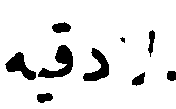
\includegraphics[height=1.05em]{../../S02/candidate_v009_print001-053/source/presentation/AB01-PDF0107-G01.png}}.\par
\par \Pg{I 19}p. 18, n. 12 (\emph{ad Constantinopolim magnam pervenire, longitudinem 1060}): The true reading seems to be 1300, as Jacob of Edessa has; Ibn Rusta, p. 85; al-Masʿūdī, \emph{Tanbīh}, p. 66; al-Idrīsī, \emph{L'Italia descritta nel libro di Re Ruggero, testo arabo con versione e note di M. Amari e C. Schiaparelli}, Rome 1883, p. 13 of the translation; and al-Kharaqī. — Al-Masʿūdī, \emph{Prairies}, I, 260, has 1100.\par
\par p. 19, n. 1 (\emph{sive mare [Caucasicae] Portae}): It is the Caspian Sea.\par
\par p. 19, n. 2 (\emph{longitudinem ab occasu ad ortum 800}): So also al-Masʿūdī, \emph{Prairies}, I, 263, \emph{Tanbīh}, p. 60; al-Kharaqī; but Ibn Rusta, p. 86, better 1800, as Jacob of Edessa.\par
\par p. 19, n. 3 (\emph{quae temporibus actis habitarentur}): Here Ibn Rusta ends.\par
\par p. 19, n. 4 (\emph{quarum prima a mare Viridi}): Here it undoubtedly denotes the Atlantic Ocean, as not seldom among the Arabs.\par
\par p. 19, n. 5 (\emph{e Ponto exiens in mare Magnum}): Reinaud, p. CCLXXXVIII, notes that Orosius designates the Mediterranean by the name of the Great Sea.\par
\par p. 19, n. 6 (\emph{cuius termini Tanais, amnis}): It is the river-like gulf near Constantinople, of which [he spoke] a little above.\par
\par p. 19, n. 7 (\emph{sinus}): The one that stretches towards Tyre and Sidon; cf. p. 18.\par
\par p. 19, n. 8 (\emph{Unius gradus portio est 65}): Plato, undoubtedly wrongly, 85; but perhaps 65 in the codex itself is an error for 75; cf. the note (\emph{a}) on this chapter. The word sixty, \RL{\ArNote ستين}, can be confused with seventy, \RL{\ArNote سبعين}, in Arabic writing without points.\par
\par p. 19, n. 9 (\emph{id quod in Libro figurae Terrae}): See what I have noted on the geographical tables in the second part.\par
\par \Pg{I 20}p. 20, n. 1 (\emph{quam in noto libro Figurae Terrae}): Plato, perhaps better, has: «in libro Figurae Terrae, qui vocatur Geographia» (in the book of the Figure of the Earth, which is called Geography).\par
\par p. 20, n. 2 (\emph{separatim notavimus, ut iam Ptolemaeus}): Where he did so I do not know. In the \emph{Almag.} II, 12 (ed. Halma, vol. I, p. 148) he says that he has left out the geographical tables, since he intended to publish them in a separate book. In the \emph{Geographia} I do not find the longitudes and latitudes of the middle places of the regions ({\greekfont ἐπαρχίαι}).\par
\UnitHead{Chapter 7}{N02}
\par p. 20, n. 3 (\emph{Deinde sinum arcus semidiurni}): The codex and Plato: «diurnal».\par
\UnitHead{Chapter 8}{N02}
\par \Pg{I 21}p. 21, n. 1 (\emph{longissimus quantitate data diem medium superat}): Plato adds this: «Si autem haec per aliquam stellarum fixarum circa polum positarum, et ipsae sunt, quae in ipsa regione nunquam occultantur, inspicere volueris, ipsius altitudines cum altius et inferius fuerit, quod contingit cum per circulum medii caeli semel supra polum et semel subtus polum transierit accipe, scilicet altitudines, aut eas in unum collige, et collecti dimidium accipe, quodque fuerit, erit altitudo poli in regione illa» (but if you wish to examine this by one of the fixed stars placed about the pole, which are those that never set in that region, take its altitudes when it is highest and when lowest, which happens when it passes the circle of the midheaven once above the pole and once below the pole — take, that is, the altitudes — or gather them into one and take half of the sum, and what it comes to will be the altitude of the pole in that region). — But this does not fit the title of the chapter at all, and has already been explained in chapter VI (p. 15).\par
\UnitHead{Chapter 10}{N02}
\par \Pg{I 22}p. 22, n. 1 (\emph{productum, iuxta ea quae statuimus}): Gnomon $=12^p$, R $=60^p$.\par
\par p. 22, n. 2 (\emph{ex altitudine umbram extensam per tabulas}): The tables are on fol. 179r.\par
\UnitHead{Chapter 11}{N02}
\par \Pg{I 23}p. 23, n. 1 (\emph{Arietis et Librae, versus Caeli plagam]}): The words in brackets I have supplied from Plato's version.\par
\UnitHead{Chapter 12}{N02}
\par \Pg{I 25}p. 25, n. 1 (\emph{ortu vel occasu aequinoctii declinationem habet}): It is the altitude found on the vertical circle that passes through the point of the horizon from which the beginning of Aries rises. Al-Battānī uses it for constructing the sundial; see ch. LVI. — Others call it the altitude that has no azimuth.\par
\par p. 25, n. 2 (\emph{boreale est, ut supra diximus}): Cf. ch. VII, p. 20.\par
\par p. 25, n. 3 (\emph{erit altitudo cuius azimuth declinatione caret}): The geometrical demonstration is found a little below.\par
\par p. 25, n. 4 (\emph{videbimus in septentriones versus 30° 0′}): Plato, as I have adopted; the codex 30° 3′. Cf. the end of the chapter.\par
\par \Pg{I 26}p. 26, n. 1 (\emph{atque ut CM ad CF}): What follows, up to «EM to GF», is lacking in Plato.\par
\par p. 26, n. 2 (\emph{ratio CM ad CF}): The codex: «GC to CM».\par
\par p. 26, n. 3 (\emph{multiplica; exibunt} $1755^p\,30'$): The parts in the codex 1750.\par
\par p. 26, n. 4 (\emph{quae est cosinus altitudinis,} $13^p\,17'$ \emph{complectitur}): Plato adds: «eo quod est chorda arcus FA» (because it is the chord of the arc FA).\par
\par p. 26, n. 5 (\emph{exibunt} $40^p\,33'$): \[ \text{EM}=\frac{30^p\times 58^p\,31'}{43^p\,17'}=\frac{1755^p\,30'}{43^p\,17'}=\frac{105330'}{2597'}=40^p\,33'\,29''.\mbox{\footnotemarkT{}} \]\addtocounter{footnoteT}{-1}\stepcounter{footnoteT}\footnotetextT{The quotient is 40\textsuperscript{\itshape p} 33′ 30″.}\ignorespaces\par
\UnitHead{Chapter 13}{N02}
\par \Pg{I 27}p. 27, n. 1 (\emph{ad initium Librae; aut de 180°}): The codex 360°.\par
\par p. 27, n. 2 (\emph{ascensiones ab Arietis initio ad 29°}): Plato 59.\par
\par \Pg{I 28}p. 28, n. 1 (\emph{ascensionibus cum intervallo dimidiae horae descriptis}): The tables are on fol. 181v ff.\par
\par p. 28, n. 2 (\emph{si ascensionibus rectis usus es}): The author puts the beginning of the right ascensions at the first point of Capricorn; cf. ch. V, p. 14.\par
\par p. 28, n. 3 (\emph{arcuatio et conversio ad gradus aequalitatis}): If a circle of declination cuts the ecliptic and the equator, the degrees of the ecliptic from the equinox to that circle are called the \emph{degrees of equality} with respect to the arc of the equator between the beginning of Aries and the circle of declination, that is, with respect to the right ascension. See al-Jaghmīnī, p. 238; Aboul Hhassan, ch. XXXII, p. 218. In the Alfonsine Tables they are called \emph{gradus aequales} (equal degrees).\par
\par \Pg{I 29}p. 29, n. 1 (\emph{tempora illius quem vis in 6}): Plato: 60.\par
\par p. 29, n. 2 (\emph{Si gradus}): By a small change of the Arabic letters Plato reads \RL{\ArNote احد}, «one», for \RL{\ArNote اجزا}. Both readings are good.\footnoteT{\emph{Ajzāʾ}, «parts» (degrees).}\par
\UnitHead{Chapter 14}{N03}
\par \Pg{I 30}p. 30, n. 1 (\emph{quae e tabula latitudinum urbium}): See the tables on fol. 172v–175v.\par
\par p. 30, n. 2 (\emph{ita certa ut latitudo observationibus cognita}): Plato adds: «Est iterum alius modus id addiscendi per stellas scilicet fixas, quod veritati fere appropinquat, si Deus voluerit» (there is yet another way of learning it, namely by the fixed stars, which comes near to the truth, if God wills). But perhaps it is an interpolation.\par
\UnitHead{Chapter 16}{N03}
\par p. 30, n. 3 (\emph{ascendens cognosces. Si vis}): Namely, to know the seasonal hours.\par
\UnitHead{Chapter 18}{N03}
\par \Pg{I 31}p. 31, n. 1 (\emph{declinatione gradus in quo ipsae sunt}): That is, of the degree of the ecliptic that has the same longitude as the star.\par
\par \Pg{I 32}p. 32, n. 1 (\emph{eadem longitudine positi}): The text, like Plato, has: «the declination of the degree in which the star is». But undoubtedly the \emph{second declination} of the Arabs is meant, which al-Battānī always calls \emph{mayl} \RL{\ArNote ميل}, «declination», like the first declination.\par
\par p. 32, n. 2 (\emph{ab eadem parte a qua est latitudo aequata}): Plato adds: «de hinc elongationem ab aequinoctiali circulo de 90 minue, et residui chordam addisce, et ipsa est chorda perfectionis elongationis stellae aequidiei circulo» (then subtract the distance from the equinoctial circle from 90, and find the chord of the remainder; it is the chord of the complement of the distance of the star from the equator), that is, $\cos\delta$.\par
\par p. 32, n. 3 (\emph{[cosinum declinationis eius eclipticae gradus quem stella occupat]}): For these words the codex and Plato have: «the semidiameter». Cf. also the note on the Arabic text.\par
\UnitHead{Chapter 20}{N03}
\par \Pg{I 33}p. 33, n. 1 (\emph{ea enim est semidifferentia duorum dierum}): The codex: «of the day».\par
\UnitHead{Chapter 21}{N03}
\par \Pg{I 34}p. 34, n. 1 (\emph{Eum per tempora horaria noctis}): Plato adds: «cum nadahir gradus solis accepta» (taken with the nadir of the degree of the Sun), that is, found through the nadir of the Sun (cf. ch. XIII).\par
\UnitHead{Chapter 24}{N03}
\par \Pg{I 35}p. 35, n. 1 (\emph{per azimuth eius ortus occasusque}): That is, through the ortive and occiduous amplitude.\par
\UnitHead{Chapter 25}{N03}
\par \Pg{I 36}p. 36, n. 1 (\emph{Gradum in quo stella est}): That is, the longitude of the star.\par
\par p. 36, n. 2 (\emph{et declinationem eius}): That is, of the star.\par
\par \Pg{I 37}p. 37, n. 1 (\emph{qui eandem longitudinem ac stella habet}): The text, like Plato, here and below always has «the cosine of the declination of the degree in which you have found the star»; for the author calls the first and the second declination alike simply \emph{mayl}.\par
\UnitHead{Chapter 26}{N03}
\par p. 37, n. 2 (\emph{productorum summa est aequalis producto diagonalium}): It is Ptolemy's well-known theorem, \emph{Almag.} I, 9 (ed. Halma, vol. I, pp. 29–30).\par
\par p. 37, n. 3 (\emph{quocumque quadrilatero [plano], in circulo inscripto}): The codex: «which falls on a sphere or on a plane surface»; Plato: «omnis vero quadrilaterae figurae sphaeralis seu superficialis, cuius duo latera» etc. (but of every four-sided figure, spherical or plane, two of whose sides ...).\par
\par p. 37, n. 4 (\emph{duo reliqua erunt opposita et}): The codex adds, not well: «because of what was said before».\par
\par \Pg{I 38}p. 38, n. 1 (\emph{productorum laterum parallelorum et laterum oppositorum}): It follows from Euclid's \emph{Elements} I, 5 and 4.\par
\par p. 38, n. 2 (\emph{inter se arcus GB, MC, EA}): What I have had printed in italics is entirely false; for GME is an arc of a great circle, not of a small circle parallel to the arc BCA. Nor does al-Battānī use these equalities afterwards in his computation; they must therefore be judged a most inept interpolation by the scribe of the archetype from which the Escorial codex and Plato's codex derive.\par
\par p. 38, n. 3 (\emph{eiusque sinus, idest linea MF,} $51^p\,57'\,42''$): The codex $57^p\,42'$; Plato leaves out the seconds.\par
\par p. 38, n. 4 (\emph{fere}): An inept correction and interpolation, as above. Read: «the remaining arc GF will contain $60^\circ$, and its sine, that is, the straight line GF, $51^p\,57'\,42''$». — I keep the figure of the codex; Plato uses curves instead of straight lines in the figure.\par
\par p. 38, n. 5 (\emph{eius sinus, scilicet linea FC}): False in the orthographic projection that al-Battānī uses. But the whole sentence is entirely useless.\par
\par p. 38, n. 6 (\emph{remanet ratio lineae GM ad BC}): A passage corrupted by some reader, as in chapter XII, p. 26, note \emph{b}. He had found above $\mathrm{GM:BC}=\mathrm{FG:FB}=\mathrm{FM:FC}$; whence \[ \mathrm{GM}=\frac{\mathrm{BC}\times\mathrm{FG}}{\mathrm{FB}}=\frac{\mathrm{BC}\times\mathrm{FM}}{\mathrm{FC}}. \] Read therefore: «if the straight line BC is diminished in the ratio of the straight line FM to FC [or of the straight line FG to FB], the straight line GM remains».\par
\par p. 38, n. 7 (\emph{Multiplica FM}): Read FG.\par
\par p. 38, n. 8 (\emph{quae, per lineam FC}): Read FB.\par
\par p. 38, n. 9 (\emph{arcus igitur GM est} $25^\circ\,39'\,{}^1\!/_2$): Plato wrongly $8''$ for ${}^1\!/_2$.\par
\par p. 38, n. 10 (\emph{totus arcus GE, eius duplum,} $51^\circ\,19'$): The codex 59′.\par
\par \Pg{I 39}p. 39, n. 1 (\emph{ergo quadratum AG complectitur} $4082^p\,19'$): The degrees in Plato wrongly 4085.\par
\par p. 39, n. 2 (\emph{qui est arcus chordae integrae,} $64^\circ\,19'$): Plato wrongly $54^\circ\,19'$.\par
\par p. 39, n. 3 (\emph{Si altera}): The codex has no figure; Plato has the one that I give a little below. At Schiaparelli's suggestion I draw here a figure in polar orthographic projection, whose centre is F; all the arcs are of great circles.\par
\par p. 39, n. 4 (\emph{quae erit primum latus}): The figure that Plato had a little above I put here.\par
\UnitHead{Chapter 27}{N03}
\par \Pg{I 40}p. 40, n. 1 (\emph{et Babylonii annum ex} $365\,{}^1\!/_4+{}^1\!/_{120}$ \emph{diebus}): That is, $365^d\,6^h\,12^m$. — Plato, in the Nuremberg edition: «ex 365 diebus et quarta ultraque parte ex 131 diei partibus» (of 365 days and a quarter, and beyond that one part of 131 parts of a day), which seems to mean $365\,{}^1\!/_4+{}^1\!/_{131}$, that is, $365^d\,6^h\,10^m\,59^s{,}6$\footnoteT{86400/131 seconds = 10\textsuperscript{\itshape m} 59.54\textsuperscript{\itshape s}.}. For these words the Bologna edition took into the text a note, Regiomontanus's as it seems, which is read in the margin of the Nuremberg edition: «ex 365 diebus 15 minut. et 27 secun. et 30 ter. fere» (of 365 days 15 minutes and 27 seconds and 30 thirds approximately), that is, $365^d\,6^h\,11^m$.\par
\par p. 40, n. 2 (\emph{quartam diei partem veraciter continere}): For Hipparchus had found $365^d\,{}^1\!/_4-{}^1\!/_{300}$ ($365^d\,5^h\,55^m\,12^s$); \emph{Alm.} III, 2 (ed. Halma, vol. I, p. 64)\footnoteT{So the print; n. 5 on p. 42 cites the same value from p. 165.}.\par
\par \Pg{I 41}p. 41, n. 1 (\emph{ea est, qua, ut narrat}): \emph{Almag.} III, 2 (ed. Halma, vol. I, p. 161).\par
\par p. 41, n. 2 (\emph{quarta epagomenorum dies, Alexandria in urbe}): A conjecture of al-Battānī's; Ptolemy by no means says that Hipparchus observed this at Alexandria. And indeed it is now held for certain that Hipparchus made his observations only at Rhodes, which he wrongly believed to lie on the same meridian as Alexandria.\footnoteT{Nallino adds in the Addenda (Part I, p. LXXI) that the same error of al-Battānī's is found in some writers of his own time too, among them R. Wolf, \emph{Handbuch der Astronomie}, vol. I, p. 443, § 202 e.}\par
\par p. 41, n. 3 (\emph{Antonini regis, id est anno 463}): The codex wrongly 563.\par
\par p. 41, n. 4 (\emph{pars et quinta e 360 partibus}): $\dfrac{1+1/5}{360}=\dfrac{6/5}{360}=\dfrac{6}{1800}=\dfrac{1}{300}$.\par
\par p. 41, n. 5 (\emph{punctum solstitiale aestivum transivisset anno 108}): The codex wrongly 168.\par
\par p. 41, n. 6 (\emph{matutino XXI diei mensis Coptici Pharmouthi}): It is the observation of Meton and Euctemon (27 June 432 BC); \emph{Almag.} III, 2 (ed. Halma, vol. I, p. 162).\par
\par p. 41, n. 7 (\emph{punctum solstitii aestivi observasse anno 463}): Plato wrongly 36.\par
\par p. 41, n. 8 (\emph{noctem cuius crastinum dies XII fuit}): \emph{Almag.} l. c.\par
\par p. 41, n. 9 (\emph{ratio duorum integrorum dierum ad 600}): Plato wrongly 60.\par
\par \Pg{I 42}p. 42, n. 1 (\emph{fuit enim observatio 286}): The codex 280, Plato 186.\par
\par p. 42, n. 2 (\emph{ortum diei XIX mensis Romani Aylūl}): That is, before sunrise on 19 Sept. 882; for al-Battānī wants the years of this era to begin on the first day of September, cf. ch. XXXII. — This passage is cited by Ibn Yūnus in Caussin, \emph{Le livre de la grande table Hakémite} (Notices et extraits des mss. de la Bibl. Nation., vol. VII, Paris 1804, p. 149).\par
\par p. 42, n. 3 (\emph{ar-Raqqah} ⅔ \emph{horae aequinoctialis circiter praecedit}): In his geographical tables, which are taken from the common Arabic tradition, al-Battānī gives the city of al-Raqqa 73° 15′ of longitude, and Alexandria, following Ptolemy, 60° 30′. From these a difference of longitude of 12° 45′ would follow, not 10°.\par
\par p. 42, n. 4 (½ + ¼ \emph{diei, detractis} ⅖ \emph{horae circiter}): That is, 743 years, $178^d\,17^h\,36^m$.\par
\par p. 42, n. 5 (\emph{est igitur verum anni tempus} $365^d\,14'\,26''$): That is, $365^d\,5^h\,46^m\,24^s$. — Ptolemy, \emph{Almag.} III, 2 (Halma, vol. I, p. 165), or rather Hipparchus, had found $365^d\,14'\,48''=365^d\,5^h\,55^m\,12^s$; the astronomers of our time put $365^d\,5^h\,48^m\,47^s{,}33$\footnoteT{Newcomb's value of 1895, for 1900, is 365\textsuperscript{\itshape d} 5\textsuperscript{\itshape h} 48\textsuperscript{\itshape m} 45.98\textsuperscript{\itshape s}.}.\par
\par p. 42, n. 6 (\emph{in 365 diebus anni Aegyptii} $359^\circ\,45'\,46''\,25'''\,32^{\mathrm{IV}}\,2^{\mathrm{V}}\,31^{\mathrm{VI}}$): The fourths wrongly $31^{\mathrm{IV}}$ in the codex and in Plato. Ed. Halley has already corrected this, \emph{Emendationes ac notae in vetustas Albatênii observationes} (Philosophical Transactions of the Royal Society, 1693, vol. XVII, no. 204, p. 916).\par
\par p. 42, n. 7 (\emph{iuxta aeram Arabum aeramque Romanorum descripsimus}): See the tables on fol. 164v–166v and 186v–189r.\par
\par p. 42, n. 8 (\emph{esse quam tempus a Ptolemaeo memorato}): For $8^m\,48^s\times15=528^s\times15=7920''=2^\circ\,12'=2^\circ\,{}^1\!/_5$.\par
\par p. 42, n. 9 (\emph{inventum in die} $0^\circ\,0'\,0''\,3'''\,33^{\mathrm{IV}}\,43^{\mathrm{V}}\,43^{\mathrm{VI}}$): The codex wrongly $30^{\mathrm{IV}}$ and $42^{\mathrm{VI}}$; for Ptolemy III, 2 (ed. Halma, vol. I, p. 166) has $0^\circ\,59'\,8''\,17'''\,13^{\mathrm{IV}}\,12^{\mathrm{V}}\,31^{\mathrm{VI}}$.\par
\par p. 42, n. 10 (\emph{in anno Aegyptio, Deo volente,} $0^\circ\,0'\,21''\,40'''\,10^{\mathrm{IV}}\,53^{\mathrm{V}}\,56^{\mathrm{VI}}$ \emph{fere}): The fifths wrongly $55^{\mathrm{V}}$ in Plato and $50^{\mathrm{V}}$ in the codex; Ptolemy $359^\circ\,45'\,24''\,45'''\,21^{\mathrm{IV}}\,8^{\mathrm{V}}\,35^{\mathrm{VI}}$.\par
\UnitHead{Chapter 28}{N04}
\par \Pg{I 43}p. 43, n. 1 (\emph{eius apogei loco cum illa apparet}): That is, on computing the anomaly for each degree of the mean motion of the Sun from the apogee.\par
\par p. 43, n. 2 (\emph{Rationem qua Ptolemaeus in libro suo}): \emph{Almag.} III, 4 (ed. Halma, vol. I, pp. 184–185).\par
\par p. 43, n. 3 (\emph{Et ex iis quae memoravimus}): But, as Schiaparelli points out to me, he has said nothing of these matters before. Perhaps something has dropped out where it was shown that the apogee must be looked for in the part to which the longer interval of time corresponds.\par
\par p. 43, n. 4 (\emph{diebus et 14 horis} $92^\circ\,14'\,10''$ \emph{fere}): So also in the computations below, for which reason I do not dare to correct it; from the tables $92^\circ\,14'\,26''$ is deduced. But before he had said «93 days and 14 equinoctial hours, \emph{which incline a little towards a diminution}»; perhaps these 16 seconds, which seem to be missing from the author's computation, answer to this «a little less».\par
\par \Pg{I 44}p. 44, n. 1 (\emph{Manifestum etiam est arcum PKLR}): The codex wrongly PKL.\par
\par p. 44, n. 2 (\emph{summa igitur} $4^p\,19'\,29''$): The seconds in Plato wrongly $59''$.\par
\par p. 44, n. 3 (\emph{erit arcus EF circiter} $1^\circ\,59'$): Plato wrongly $1^\circ\,58'$; Ibn Yūnus (in Caussin, \emph{Le livre de la grande table Hakémite}, in Notices et extraits des mss. de la Bibl. Nation., vol. VII, Paris 1804, p. 155) writes: «al-Battānī computed the whole equation of the Sun, and found it to be $1^\circ\,59'\,10''$». Halley, p. 917, and Delambre, \emph{Astr. moyen âge}, p. 36, who used modern trigonometric tables, also found $1^\circ\,59'\,10''$. The reading of the codex is therefore good; in the tables of the equation of the Sun (fol. 191r) the greatest equation is in fact $1^\circ\,59'\,10''$.\par
\par p. 44, n. 4 (\emph{anno 1194 aerae Dhū ’l-qarnayn}): It begins, according to our author's usage, on 1 September AD 882.\par
\par \Pg{I 45}p. 45, n. 1 (\emph{Ostendit Ptolemaeus}): \emph{Almag.} III, 3, 4 and 5 (ed. Halma, vol. I, pp. 170–183, 183–190, 190–199); as regards the Sun, however, he judges the hypothesis of the eccentric the more convenient.\par
\par p. 45, n. 2 (\emph{centrum epicycli HF}): The codex and Plato HFT; for in their figure the point T is put in the place of the intersection of the epicycle and the great circle, between A and D. But from what follows it is clear that T is the point of the great circle that indicates the direction of the apogee.\par
\par p. 45, n. 3 (\emph{quae centrum circuli parecliptici}): That is, parallel or concentric to the ecliptic. Since it has no name in our writers, I so translate the Arabic \emph{al-mumaththal bi-falak al-burūj}, «made like the ecliptic», or simply \emph{al-mumaththal}, which in Ptolemy is sometimes called {\greekfont ὁ ὁμόκεντρος τῷ κόσμῳ κύκλος}, «the circle concentric with the world», or {\greekfont ὁ ὁμόκεντρος τῷ διὰ μέσων τῶν ζῳδίων κύκλος}, «the circle concentric with the circle through the middle of the signs» (that is, with the ecliptic). In translating the Syriac astronomy of Barhebraeus, Nau calls it \emph{intersphère de la similitude}; Golius, in his version of al-Farghānī, and Sédillot, in his version of Ulugh Beg, \emph{sphaera} or \emph{circulus homocentricus}. — It is a circle concentric with the ecliptic, in whose plane it lies; it is described on the surface of the sphere of the Sun or of the planets that is also called \emph{al-mumaththal}, which is a solid body, concentric with the ecliptic and contained by two parallel surfaces, of which the outer touches the outer surface of the sphere of the eccentric circle (the deferent) at the apogee of the eccentric, the inner the inner surface of the sphere of the eccentric at the perigee. — It moves as the signs of the zodiac move because of the precession, from east to west.\par
\par p. 45, n. 4 (\emph{angulus autem MAF}): The codex HEF.\par
\par \Pg{I 46}p. 46, n. 1 (\emph{[cosinus] arcus FH et anguli FAH}): The codex: «which is what is lacking to the angle FAH and to the arc FH to complete a quadrant».\par
\par p. 46, n. 2 (\emph{erit linea FM} $1^p\,2'\,22''\,\frac{1}{2}$): For $22''$ Plato has $55''$. Very often in Plato's edition 5 is read for 2, an error to be put down to the Latin manuscripts or to the carelessness of the editor.\par
\par p. 46, n. 3 (\emph{et linea EM}): The codex EF.\par
\par p. 46, n. 4 (\emph{et linea EM} $61^p\,48'\,2''$): Plato leaves out the following words and has $35''$ for $2''$.\par
\par p. 46, n. 5 (\emph{linea FM} $1^p\,0'\,33''$): Plato $1^\circ\,33'$.\par
\par p. 46, n. 6 (\emph{sitque arcus QG}): The codex QM.\par
\par p. 46, n. 7 (\emph{a puncto Q apogei percurrit,} $150^\circ$): Plato wrongly 120.\par
\par p. 46, n. 8 (\emph{nam BG est semidiametrus epicycli}): The codex: of the ecliptic.\par
\par p. 46, n. 9 (\emph{etiam lineae KE et EG cognoscuntur]}): I have added this following Plato; but the addition is not necessary.\par
\par p. 46, n. 10 (\emph{sinum habebit} $51^p\,57'\,41''$): The parts in Plato $59^p$.\par
\par p. 46, n. 11 (\emph{perpendicularis KG} $1^p\,2'\,22''\,\frac{1}{2}$): The ½ is missing in the codex; Plato has $55''$ for $22''$ (cf. n. 2).\par
\par p. 46, n. 12 (\emph{et EG fere} $58^p\,12'\,34''$): Plato $58^p\,7'\,34''$.\par
\par p. 46, n. 13 (\emph{cathetus KG} $1^p\,4'\,17''$): The seconds in Plato $13''$.\par
\par p. 46, n. 14 (\emph{et arcus super eam positus} $1^\circ\,1'\,24''$): Plato $1^p\,4'\,54''$.\par
\par p. 46, n. 15 (\emph{Qua re arcus NB}): The codex IB (\RL{\ArNote ى} I for \RL{\ArNote ن} N); Plato GB. In the figure of the codex and of Plato the point N and the line NT are lacking; the point T, as I noted above, is wrongly placed near the place of the intersection of the epicycle HF and the ecliptic.\par
\par p. 46, n. 16 (\emph{quem cognoscere volebamus,} $31^\circ\,1'\,24''$): The minutes in the codex $4'$; Plato $1^\circ\,4'\,54''$.\par
\par \Pg{I 47}p. 47, n. 1 (\emph{linea EL} $1^p\,2'\,22''\,\frac{1}{2}$): The seconds in Plato $55''$.\par
\par p. 47, n. 2 (\emph{EL est} $1^p\,33'$): The codex: «of one part and thirty-three seconds».\par
\par p. 47, n. 3 (\emph{arcumque FD}): The codex AD. Afterwards Plato 120.\par
\par p. 47, n. 4 (\emph{angulus DHG}): The codex HDG.\par
\par p. 47, n. 5 (\emph{latus HS et angulus HES}): The codex HS.\par
\par p. 47, n. 6 (\emph{cathetus ES erit} $1^p\,2'\,22''\,\frac{1}{2}$): The seconds in Plato $55''$.\par
\par p. 47, n. 7 (\emph{trianguli rectanguli ESD erit circiter} $58^p\,12'\,32''$): Plato $58^p\,15'\,34''$. Cf. note \emph{e} on this chapter.\par
\par p. 47, n. 8 (\emph{qui est quantitas anomaliae,} $1^\circ\,1'\,24''$): The codex $1^\circ\,4'\,24''$; Plato $1^\circ\,4'\,54''$.\par
\par p. 47, n. 9 (\emph{arcus igitur KC eclipticae,} $31^\circ\,1'\,24''$): The codex $1^\circ\,1'\,24''$; Plato $31^\circ\,4'\,54''$.\par
\par \Pg{I 48}p. 48, n. 1 (\emph{Semidiametrus epicycli Solis est} $2^p\,4'\,45''$): The codex $5'$ for $4'$.\par
\par p. 48, n. 2 (\emph{semidiametrus epicycli Lunae} $5^p\,15'$): The degrees in the codex $6^\circ$.\par
\par p. 48, n. 3 (\emph{Saturni} $6^p\,29'\,50''$): The seconds in Plato $7''$.\par
\par p. 48, n. 4 (\emph{Iovis} $11^p\,30'\,0''$): The seconds in Plato $5''$.\par
\par p. 48, n. 5 (\emph{Martis} $39^p\,27'\,22''$): The codex $19^\circ\,25'\,22''$; the minutes in Plato $55'$.\par
\par p. 48, n. 6 (\emph{Veneris} $43^p\,9'\,0''$): Plato $44^\circ\,9'\,5''$.\par
\par p. 48, n. 7 (\emph{Mercurii} $22^p\,30'\,30''$): The degrees in the codex $29^\circ$.\par
\UnitHead{Chapter 29}{N04}
\par p. 48, n. 8 (\emph{a tempore meridiei aut mediae noctis}): \emph{Almag.} III, 8 (ed. Halma, vol. I, p. 208).\par
\par \Pg{I 49}p. 49, n. 1 (\emph{est fere} $3^\circ\,\frac{1}{4}+\frac{1}{10}$): Plato wrongly $3^\circ\,\frac{1}{5}+\frac{1}{10}$, which would make $3^\circ\,18'$. — In the \emph{Almag.} III, 8 (ed. Halma, vol. I, p. 209) it is $3^\circ\,\frac{2}{3}$; for there the eccentricity of the solar orbit is greater than in al-Battānī.\par
\par p. 49, n. 2 (\emph{quod e culminatione signorum} $4^\circ\,\frac{1}{4}+\frac{1}{5}$): \emph{Almag.} $4^\circ\,\frac{2}{3}$; the difference comes from the different obliquity of the ecliptic.\par
\par p. 49, n. 3 (\emph{summa igitur est} $7^\circ\,48'$): \emph{Almag.} $8^\circ\,\frac{1}{3}$, that is, $\frac{1}{2}+\frac{1}{18}$ of an hour.\par
\par p. 49, n. 4 (\emph{Locus deminutionis fere a} $\frac{2}{3}$): \emph{Almag.} $\frac{1}{2}$.\par
\par p. 49, n. 5 (\emph{augmenti ab initio Scorpionis ad} $\frac{2}{3}$): \emph{Almag.} $\frac{1}{2}$.\par
\par p. 49, n. 6 (\emph{medio Lunae in initio calculi 18}): Plato 58. — Why he did this is explained in note \emph{b} on this chapter.\par
\par p. 49, n. 7 (\emph{in tabulis ascensionum rectarum}): Fol. 179r–181v.\par
\UnitHead{Chapter 30}{N05}
\par \Pg{I 50}p. 50, n. 1 (\emph{sub ea absque ulla deviatione moveatur}): Below I call it the \emph{parecliptic}; cf. p. 45, n. 3.\par
\par p. 50, n. 2 (\emph{in partem contrariam successioni signorum} $11^\circ\,12'$ \emph{circiter}): For the motion of the apogee = twice the synodic motion − the motion in latitude + the motion of the nodes $=24^\circ\,23'-13^\circ\,14'+0^\circ\,3'=11^\circ\,12'$.\par
\par p. 50, n. 3 (\emph{in circumferentia excentrici quotidie} $24^\circ\,23'$ \emph{fere}): It is twice the synodic (or relative) motion, that is, twice the elongation.\par
\par p. 50, n. 4 (\emph{quotidie in circumferentia epicycli fere} $13^\circ\,4'$): It is the daily motion of the anomaly, which Ptolemy, IV, 3 (ed. Halma, vol. I, p. 223), found to be $13^\circ\,3'\,53''\,56'''\,29^{\mathrm{IV}}\,38^{\mathrm{V}}\,38^{\mathrm{VI}}$.\par
\par \Pg{I 51}p. 51, n. 1 (\emph{Circa centrum E sit circulus pareclipticus}): See above, p. 50, n. 1.\par
\par p. 51, n. 2 (\emph{Lineas EMG, F′MH}): The codex and Plato: EMH, FMG.\par
\par p. 51, n. 3 (\emph{ducamus; erit G}): The codex and Plato H.\par
\par p. 51, n. 4 (\emph{Terrae et eclipticae apparet; H}): The codex and Plato G.\par
\par p. 51, n. 5 (\emph{veri apogei qui ex puncto F′}): The codex and Plato: «from the centre F, that is, from the centre of the eccentric». The point F′ is lacking in them.\par
\par p. 51, n. 6 (\emph{in tertia columna tabularum aequationis Lunae}): Fol. 189v ff.; but it is the third column only if the column of the equation of the Sun is not counted.\par
\par p. 51, n. 7 (\emph{in secunda columna tabularum aequationis}): Fol. 189v ff.; but it is the second column only if the column of the equation of the Sun, or the column of the numbers, is not counted.\par
\par p. 51, n. 8 (\emph{et in tabulis describenda aequatione Solis}): Ch. XXVIII.\par
\par p. 51, n. 9 (\emph{inaequalitas Lunae attingere potest, est} $5^\circ\,1'$): They are Ptolemy's numbers.\par
\par p. 51, n. 10 (\emph{ad} $5^p\,\frac{1}{4}$\emph{. Id Ptolemaeus}): \emph{Almag.} IV, 5 (ed. Halma, vol. I, pp. 244–260).\par
\par \Pg{I 52}p. 52, n. 1 (\emph{fere} $2^\circ\,\frac{2}{3}$ \emph{attingere invenerunt}): So \emph{Almag.} V, 3 (ed. Halma, vol. I, pp. 293–296)\footnoteT{The print has 293–206.}.\par
\par p. 52, n. 2 (\emph{ab A quantitate [dimidii] excentrici distat}): Plato: «punctum P, quod est egressi circuli longitudinis propior» (the point P, which is the nearer distance of the eccentric circle), that is, the perigee of the eccentric. The sense agrees very well with the words of the codex.\par
\par p. 52, n. 3 (\emph{lineam EF, ambo centra coniungentem,} $10^p\,19'$): Plato $10^\circ\,18'$; the demonstration and the numbers that follow are found in the \emph{Almag.} V, 4 (ed. Halma, vol. I, pp. 296–297).\par
\par p. 52, n. 4 (\emph{eius sinus igitur} $5^p\,15'$): The minutes in the codex $25'$.\par
\par p. 52, n. 5 (\emph{ex partibus quarum AE} $60^p$ \emph{continet]}): I have added this, following Plato and Ptolemy.\par
\par p. 52, n. 6 (\emph{iuxta eius declivitatem}): That is, according to the elongation of the centre of the epicycle from the place of the Sun.\par
\par p. 52, n. 7 (\emph{ut arcum HG, in tertia}): If the column of the single numbers, or the column of the Sun, is not counted.\par
\par p. 52, n. 8 (\emph{descriptus est in quarta et quinta}): The fifth and the sixth.\par
\par p. 52, n. 9 (\emph{quae sit eius ratio ad 60}): Following Schiaparelli, it seems it must be understood: «and as for the fourth column, it gives the proportional part, to 60, to be taken of the numbers that are entered in the fifth column».\par
\par \Pg{I 53}p. 53, n. 1 (\emph{Lineam ME}): See the figure on p. 51. — The demonstration is read, with the same numbers, in the \emph{Almag.} V, 7 (= ed. Halma, vol. I, pp. 313–314).\par
\par p. 53, n. 2 (\emph{et L cum F coniungamus}): FL is perpendicular to KL.\par
\par p. 53, n. 3 (\emph{in triangulo MLF latera proportionalia}): It seems it must be understood: «the ratios of the sides are known».\par
\par p. 53, n. 4 (\emph{AM, ut Ptolemaeus statuit,} $120^\circ$ \emph{ponamus}): Ptolemy laid down that not the arc AM but the angle AEM contains $120^\circ$; the arc AM subtends the angle AFM, which is greater than AEM (Schiaparelli).\par
\par p. 53, n. 5 (\emph{Quoniam rationem sinuum ad semidiametrum}): Plato adds: «et ad quadrantem circuli» (and to the quadrant of the circle).\par
\par p. 53, n. 6 (\emph{referimus, angulus EFL}): The codex and Plato, as a little below, AEM.\par
\par p. 53, n. 7 (\emph{Sinus anguli EFL}): The codex and Plato, as above, AEM.\par
\par p. 53, n. 8 (\emph{et sinus anguli FEL circiter} $51^p\,58'$): The codex $11^p\,18'$.\par
\par p. 53, n. 9 (\emph{sed si huic lineae} $10^p\,19'$ \emph{tantum}): It is the eccentricity found a little before.\par
\par p. 53, n. 10 (\emph{linea FL} $9^p\,16'$): Plato $18^p\,56'$.\par
\par p. 53, n. 11 (\emph{arcus MK super eam insistens} $6^\circ\,54'$): The degrees in the codex $5^\circ$.\par
\par p. 53, n. 12 (\emph{et si illi} $2^\circ\,\frac{2}{3}$): Of the greatest second inequality; cf. above, p. 52.\par
\par p. 53, n. 13 (\emph{in partes sexagesimas} $0^\circ\,42'\,38''$): For $42'$ Plato always 45.\par
\par p. 53, n. 14 (\emph{quae sub numero 120 in quarta}): Or rather the fifth; cf. above, p. 51, nn. 6 and 7; p. 52, nn. 7 and 8.\par
\par p. 53, n. 15 (\emph{fiunt} $2^\circ\,39'$\emph{, quae in quinta}): Or rather the sixth.\par
\par p. 53, n. 16 (\emph{columna sub numero 120}): But in the tables they are found under the number 110.\par
\par p. 53, n. 17 (\emph{apogeum verum et apogeum medium}): In the tables it is called the \emph{equation of the anomaly}.\par
\par p. 53, n. 18 (\emph{duplicatum, sit} $90^\circ\,30'$\emph{, ut Ptolemaeus}): \emph{Almag.} V, 6 (ed. Halma, vol. I, pp. 308–311).\par
\par \Pg{I 54}p. 54, n. 1 (\emph{eius sinus} $0^p\,31'\,25''$): Plato 30.55.\par
\par p. 54, n. 2 (\emph{arcus KD 89° 30′}): Plato always 88° 30′.\par
\par p. 54, n. 3 (\emph{eiusque sinus} $60^p$): In the tables of sines $59^p\,59'\,52''$.\par
\par p. 54, n. 4 (\emph{erit SB} $48^p\,26'$): Plato $48^p\,56'$.\par
\par p. 54, n. 5 (\emph{si SF circiter} $10^p\,19'$): Plato $10^p\,18'$.\par
\par p. 54, n. 6 (\emph{fiet SF circiter} $12^p\,32'$): Plato $12^p\,30'$.\par
\par p. 54, n. 7 (\emph{qui a parte puncti D reperitur}): These letters refer to the figure on p. 51, not on p. 53.\par
\par p. 54, n. 8 (\emph{Haec 12° 1′ in tertia}): Or rather the fourth.\par
\par p. 54, n. 9 (\emph{eaque in septima}): So also in the tables.\par
\par p. 54, n. 10 (\emph{sed cum eius quantitas}): The codex «its anomaly» (\RL{\ArNote حاصته}) for «its amount» (\RL{\ArNote حصته}).\par
\par p. 54, n. 11 (\emph{de diametro sphaerae caelestis prospicit}): The codex: «at the time of its opposition to the Sun it becomes the centre of the ecliptic, and therefore it falls on the zodiac»; Plato: «cumque per alterum nodorum sui caeli praeventionis hora Luna transgreditur, eius centrum est centrum circuli signorum, et ipsa tunc in ipso eodem signorum cingulo consistit» (and when at the hour of the opposition the Moon passes through one of the nodes of its sphere, its centre is the centre of the circle of the signs, and it then stands in that same belt of the signs). The text, p. 83, l. 7, should be restored thus: \RL{\ArNote صار مركزه مركز فلك البروج}.\footnoteT{«Its centre has come to be the centre of the ecliptic».}\par
\par \Pg{I 55}p. 55, n. 1 (\emph{quod fieri non potest nisi}): Plato: «nam totum lumen non amittet, nisi cum super illam sui circuli partem qui in ipsius directo fuerit, ceciderit, quod esse non potest, nisi .....» (for it will not lose all its light except when it has fallen on that part of its circle which is directly opposite it, which cannot be, except .....).\par
\par p. 55, n. 2 (\emph{sed ad infinitum procederet; eclipsis lunaris}): «Total» must be added; otherwise it is not true.\par
\par p. 55, n. 3 (\emph{planetae autem omnes}): Except, however, Mercury and Venus, which, as the author said above of Mercury, are never in opposition to the Sun. «Superior» therefore seems to need adding.\par
\par p. 55, n. 4 (\emph{eorum corporum respectu Terrae magnitudines, Ptolemaeus}): \emph{Almag.} V, 14 (ed. Halma, vol. I, pp. 339–343). On them cf. Ginzel, \emph{Spezieller Kanon der Sonnen- und Mondfinsternisse}, Berlin 1899, section V.\par
\par \Pg{I 56}p. 56, n. 1 (\emph{quid eum ab hoc prohibuerit nescimus}): In the text (p. 84, l. 18) \RL{\ArNote منعه} must be read for \RL{\ArNote صنعه} of the codex, as is also clear from Plato's «prohibuit» (prevented).\footnoteT{\emph{Manaʿahu}, «prevented him»; \emph{ṣanaʿahu}, «made it».} — As Bailly and Delambre have already rightly observed, Ptolemy did not rely on solar eclipses because of the very great error that arose from the theory of the evection in determining the distance of the Moon from the Earth; the parallax and the apparent diameter of the Moon were therefore found to be not a little removed from the truth.\par
\par p. 56, n. 2 (\emph{Alexandro mortuo, octava die mensis āb}): That is, 8 August AD 891. — The numbers that concern these observations of eclipses were already verified by Edm. Halley, pp. 917–918 of his dissertation entitled \emph{Emendationes ac notae in vetustas Albatênii observationes astronomicas} (Philosophical Transactions, vol. XVII, no. 204, London 1693); but he does not explain well enough how he found his corrections. It will be clear from what follows that so great a man sometimes erred in his conjectures. — As to the hour of this eclipse, Halley writes: «one seasonal hour after noon, that is (the Sun setting at 6\textsuperscript{\itshape h} 45′), 1\textsuperscript{\itshape h} 7½′ p.m.»; but this is the \emph{true} time, not the \emph{mean}, which was 0\textsuperscript{\itshape h} 54\textsuperscript{\itshape m} 26\textsuperscript{\itshape s}. Cf. note \emph{g}.\par
\par p. 56, n. 3 (\emph{Luna autem, motu medio, in 17° 7′}): The codex 14° 7′, Plato 17° 50′ (that is, \RL{\ArNote ن} for \RL{\ArNote ز}); Halley 17° 6′.\par
\par p. 56, n. 4 (\emph{a puncto apogei veri erat 333° 13′}): The codex and Plato 332° 57′ (in the minutes \RL{\ArNote نز} for \RL{\ArNote يج}); Halley 333° 7′.\par
\par p. 56, n. 5 (\emph{et motus verus 176° 51′}): Plato wrongly 176° 11′.\par
\par p. 56, n. 6 (\emph{tempore medii eclipsis 176° 55′}): Plato wrongly 177° 11′.\par
\par p. 56, n. 7 (\emph{et secundum illam rationem}): The one mentioned at the end of p. 55.\par
\par p. 56, n. 8 (\emph{in urbe deprehendimus, fuit anno 1212}): Plato 1205, already corrected by Halley.\par
\par p. 56, n. 9 (\emph{aerae Dhū ’l-qarnayn, sive 1224}): Plato 1554.\par
\par p. 56, n. 10 (\emph{meridiem XXIII diei mensis kānūn posterioris}): It was therefore on 22 January 901 at $20^h\,\frac{1}{3}$ (\emph{true} time) by the astronomical usage, or on 23 January at $8^h\,\frac{1}{3}$ a.m. by the civil usage.\par
\par p. 56, n. 11 (\emph{eclipsis igitur minus quam} $3\,\frac{1}{2}$): He supposes, then, from his observations, more than $10^m$ ($=2^\circ\,\frac{1}{2}$) between Antioch and al-Raqqa. A little below, where he speaks of the other lunar eclipse, he puts a difference of about ¼ hour ($=3^\circ\,45'$).\par
\par \Pg{I 57}p. 57, n. 1 (\emph{veri apogei in epicyclo 126° 37′}): The codex 126° 32′, Plato 156° 55′, Halley 126° 35′.\par
\par p. 57, n. 2 (\emph{motus medius latitudinis 173° 25′}): The minutes in Plato wrongly 55′.\par
\par p. 57, n. 3 (\emph{motusque verus 169° 11′}): The codex 199° 11′, Plato 169° 41′.\par
\par p. 57, n. 4 (\emph{ut apparuit, fere} $\frac{1}{2}+\frac{1}{3}$): Plato ½.\par
\par p. 57, n. 5 (\emph{latitudinis in medio eclipsis 168° 45′}): The codex 198° 45′.\par
\par p. 57, n. 6 (\emph{Alexandro mortuo, XXIII die mensis tammūz}): That is, 23 July AD 883. Plato 53 for 23.\par
\par p. 57, n. 7 (\emph{Sol medio suo itinere 5° 21′}): The minutes in Plato 51′.\par
\par p. 57, n. 8 (\emph{itinere vero 4° 2′}): The minutes in Plato 5′, Halley 1′.\par
\par p. 57, n. 9 (\emph{medii apogei in epicyclo 113° 13′}): The codex 113° 0′, Plato 93° 0′, Halley 113° 8′.\par
\par p. 57, n. 10 (\emph{anomalia vera 114° 14′}): The codex 114° 9′, Plato 94° 10′, Halley 114° 10′.\par
\par p. 57, n. 11 (\emph{post meridiem, II die mensis āb}): That is, 2 August 901 at $15^h\,\frac{1}{3}$ (\emph{true} time) by the astronomical usage, or 3 August at $3^h\,\frac{1}{3}$ a.m. by the civil usage.\par
\par p. 57, n. 12 (\emph{horis aequinoctialibus fere post meridiem}): Cf. p. 56, n. 11.\par
\par p. 57, n. 13 (\emph{Sol medio suo itinere 16° 10′}): The codex 14° 10′.\par
\par p. 57, n. 14 (\emph{locus Lunae medius in 19° 24′}): The minutes in Plato 54′.\par
\par p. 57, n. 15 (\emph{medii apogei in epicyclo 110° 11′}): The minutes in the codex 4′, in Plato 7′, Halley 7′.\par
\par p. 57, n. 16 (\emph{a puncto vero 111° 9′}): The codex 111° 5′, Plato 91° 5′, Halley 111° 5′.\par
\par p. 57, n. 17 (\emph{motus medius latitudinis 190° 10′}): Plato 109° 10′. The minutes would be more correctly 11′.\par
\par p. 57, n. 18 (\emph{verus 185° 21′}): Plato 185° 51′. The minutes would be more correctly 22′. — Here Halley's corrections end.\par
\par \Pg{I 58}p. 58, n. 1 (\emph{diametrus tota Lunae in his duabus eclipsibus 0° 33′ 30″}): The seconds in Plato wrongly 20″; for $8\,\frac{3}{4}\times 0^\circ\,3'\,50''=0^\circ\,33'\,30''\,\frac{5}{12}$.\footnoteT{8¾ × 3′ 50″ = 33′ 32½″.}\par
\par p. 58, n. 2 (\emph{ut ratio a Ptolemaeo}): \emph{Almag.} V, 14 (ed. Halma, vol. I, p. 343).\par
\par p. 58, n. 3 (\emph{semidiametrus umbrae in transitu Lunae circiter 0° 43′ 30″ fuisset}): For \[ 2\,\tfrac{3}{5}\times\frac{0^\circ\,33'\,30''}{2}=\frac{1^\circ\,27'\,6''}{2}=0^\circ\,43'\,33''. \]\par
\par p. 58, n. 4 (\emph{iter horarium Lunae 0° 30′ 12″}): The seconds in Plato wrongly 15″.\par
\par p. 58, n. 5 (\emph{Ptolemaeus contra 0° 31′ 20″}): \emph{Almag.} l. c. — The codex wrongly has 33″ for 20″, but a little below rightly; Plato 50″.\par
\par p. 58, n. 6 (\emph{longinquiore Lunae transitu 0° 38′ 30″}): The seconds in Plato wrongly 20″.\par
\par p. 58, n. 7 (\emph{Lunae transitu} $2\,\frac{1}{6}$ \emph{minutis}): Plato wrongly $2\,\frac{1}{3}$; for 0° 40′ 40″ of Ptolemy − 0° 38′ 30″ of al-Battānī = 0° 2′ 10″.\par
\par p. 58, n. 8 (\emph{subtendi qui 0° 31′ 20″ complectatur}): \emph{Almag.} V, 14 (ed. Halma, vol. I, p. 343).\par
\par p. 58, n. 9 (\emph{diametrum Solis aequare diametrum Lunae posuit}): The codex «did not lay down».\par
\par p. 58, n. 10 (\emph{una hora 0° 2′ 23″ moveatur}): The seconds in Plato wrongly 22″.\par
\par p. 58, n. 11 (\emph{subtendi arcui sphaerae 0° 38′ 30″}): Plato, who leaves out what follows, wrongly: «fore chordam arcus 28 minutorum probatum est» (it has been proved to be the chord of an arc of 28 minutes).\par
\par \Pg{I 59}p. 59, n. 1 (\emph{proportiones in eius libro positas}): \emph{Almag.} V, 15 (ed. Halma, vol. I, pp. 343–346).\par
\par p. 59, n. 2 (\emph{proportiones et distantiae duplicatae}): Cf. the demonstration that follows.\par
\par p. 59, n. 3 (\emph{Terrae in K et M tangant}): The ends of the diameters AC, KM, EG are not the points of contact of the tangents; for these cannot be perpendicular to the diameters. In fact, however, the difference becomes insensible because of the smallness of the angles ENG, MSK. Ptolemy, \emph{Almag.} V, 15 (ed. Halma, vol. I, p. 344), therefore says more accurately that the straight lines passing through the points of contact are «equal to the diameters \emph{to the senses} ({\greekfont πρὸς αἴσθησιν})».\par
\par p. 59, n. 4 (\emph{Lunae in G et E tangentes}): Cf. n. 3.\par
\par p. 59, n. 5 (\emph{locus apogeus Lunae in eclipsibus lunaribus}): He now reports Ptolemy's computation, who thought that the Moon standing at its apogee covers the Sun. But al-Battānī thinks otherwise, as will be clear below.\par
\par p. 59, n. 6 (\emph{DS igitur} $60^p$ \emph{fere complecti; denique}): A most inept interpolation, although it is found in Plato too. It is false that AS or DS contains sixty parts, as is clear from what follows; the remark that the triangle ADS is right-angled is entirely superfluous.\par
\par p. 59, n. 7 (\emph{angulum GNH}): The codex GHN, Plato GNF; the following number in Plato «0,515 et 40».\par
\par p. 59, n. 8 (\emph{0° 15′ 40″, et angulum QNP}): The codex QSP; Plato leaves out this clause. In the figure I have added the line NQ, which is lacking in the diagram of the codex and of Plato.\par
\par \Pg{I 60}p. 60, n. 1 (\emph{triangulum rectangulum ADS circumdantis efficiunt}): A most inept interpolation, unless perhaps QNP must be read for the ADS of the codex and of Plato.\par
\par p. 60, n. 2 (\emph{sinus anguli GNH,} $0^p\,16'\,24''$): The seconds in Plato 54″.\par
\par p. 60, n. 3 (\emph{et linea PQ, sinus anguli QNP}): The codex and Plato QSP.\par
\par p. 60, n. 4 ($0^p\,42'\,35''$): The minutes in Plato 45′.\par
\par p. 60, n. 5 (\emph{e partibus quarum 60 linea PN}): The codex and Plato DS.\par
\par p. 60, n. 6 (\emph{linea HG fiet} $0^p\,17'\,33''$): The minutes in the codex 16′.\par
\par p. 60, n. 7 (\emph{autem HN aequalis sit lineae PN}): The codex PL.\par
\par p. 60, n. 8 (\emph{summa linearum PQ, HT}): The codex HN.\par
\par p. 60, n. 9 (\emph{[duplum] lineae MN efficiet}): That is, 2°.\par
\par p. 60, n. 10 (\emph{quae est unius partis, dematur, remanebit}): Here the codex and Plato add: «the line HN $0^p\,3'\,11''$ and».\par
\par p. 60, n. 11 (\emph{remanebit linea GT}): The codex DL, Plato DH.\par
\par p. 60, n. 12 (\emph{Item erit HN}): The codex and Plato HG.\par
\par p. 60, n. 13 ($0^p\,3'\,11''$\emph{, et DH}): The codex DA; for these words Plato: «cum linea DA erit unius partis» (when the line DA is of one part).\par
\par p. 60, n. 14 (\emph{si tota DN} $1^p$ \emph{ponatur}): For DN : DH = MN : GT.\par
\par p. 60, n. 15 ($18\,\frac{4}{5}$ \emph{vicibus circiter DA}): Plato DH.\par
\par p. 60, n. 16 (\emph{HG numerabit, quae est ratio DN}): The codex HT, Plato NH.\par
\par p. 60, n. 17 (\emph{ad HN}): The codex HG, Plato DN.\par
\par p. 60, n. 18 (\emph{semidiametrum MN Terrae fere 1210 vicibus}): Plato 121.\par
\par p. 60, n. 19 (\emph{et hic est cubus}): In the \emph{Almag.} {\greekfont τὸ στερεὸν μέγεθος}, «solid magnitude, volume».\par
\par p. 60, n. 20 (\emph{Cubus} $18\,\frac{4}{5}$ \emph{est} $6644\,\frac{1}{2}$): Plato $6655\,\frac{1}{2}$.\par
\par p. 60, n. 21 (\emph{EG, cubo unitatis} $39\,\frac{1}{4}$ \emph{vicibus}): The codex $49\,\frac{1}{4}$; Plato: «est una pars de 495 18 et quarta cubici unius» (is one part of 495 18 and a quarter of one cube).\par
\par p. 60, n. 22 (\emph{Terra autem} $39\,\frac{1}{4}$): Plato $49\,\frac{1}{4}$.\par
\par p. 60, n. 23 (\emph{eius pars PS} $0^p\,45'\,38''$): The parts in Plato $8^p$.\par
\par p. 60, n. 24 (\emph{complendum gradum restat,} $0^p\,14'\,22''$): The seconds in Plato 55″. — It is SN : PS = MN : PQ.\par
\par p. 60, n. 25 (\emph{erit linea SP} $203\,\frac{5}{6}$): Plato $503\,\frac{5}{6}$.\par
\par p. 60, n. 26 (\emph{cum centro Terrae coniungens, erit 268}): Plato 568.\par
\par p. 60, n. 27 (\emph{linea autem DS, centrum Solis}): The codex «of the Earth».\par
\par p. 60, n. 28 (\emph{semidiametrum umbrae in longinquiore Lunae}): The codex «of the Sun».\par
\par \Pg{I 61}p. 61, n. 1 (\emph{quae differentia est fere} $\frac{47}{150}$): Or, as the author says, $\dfrac{1}{3}-\dfrac{1}{10\times 5}$.\par
\par p. 61, n. 2 (\emph{longinquitatem geocentricam Lunae fere} $60\,\frac{29}{30}$): Or, as the author says, $60^p\,\dfrac{1}{2}+\dfrac{1}{3}+\dfrac{1}{10}+\dfrac{1}{10\times 3}$; Plato wrongly «60 duasque unius tertias, ac quintam et fere decenam» (60 and two thirds of one, and a fifth and about a tenth).\par
\par p. 61, n. 3 (\emph{Solis in apogeo proveniet fere 1146}): Plato 1156.\par
\par p. 61, n. 4 (\emph{quod cum per} $4^\circ\,\frac{1}{2}$): Plato «402 et dimidium» (402 and a half); see p. 60, l. 15.\par
\par p. 61, n. 5 (\emph{Terrae ab extrema umbra} $254\,\frac{2}{3}$): Plato $555\,\frac{2}{3}$.\par
\par p. 61, n. 6 (\emph{a Sole 1085 semidiametris Terrae distat}): He had found a little before that the Sun at the apogee is covered by the Moon when the Moon is $60\,\frac{29}{30}$ terrestrial semidiameters distant from us; he now finds that the greatest geocentric distance of the Sun contains 1146 terrestrial semidiameters; therefore the distance of the Sun from the Moon is then $1146-60\,\frac{29}{30}=1085\,\frac{1}{30}$.\par
\par p. 61, n. 7 (\emph{donec Sol Lunae fere diametraliter}): The codex «from the semidiameter».\par
\par \Pg{I 62}p. 62, n. 1 (\emph{de diametro opposita}): I have left out drawing these tangents in the figure, since they would have caused too much confusion; I have been content to mark the points of contact H, K. In the figure of the codex and of Plato the letters are entirely lacking.\par
\par p. 62, n. 2 (\emph{lineas tangentes ducamus}): These tangents too I did not wish to draw in the figure, though the points M and L are duly marked everywhere.\par
\par \Pg{I 63}p. 63, n. 1 (\emph{se 20 gradibus orbis lunaris distent}): The codex, less clearly: «the distance of the Moon from the Sun, in each of the nine discs that come after the disc of the conjunction, will be 20 degrees of the degrees of the half orbit»; cf. the end of the chapter. — Plato: «hanc autem figuram in qua decem lunares circuli ceciderint, quorum a se invicem remotio 50 partium existit, iam figuravimus» (but we have already drawn this figure, in which ten lunar circles fall, whose distance from one another is 50 parts).\par
\par p. 63, n. 2 (\emph{quod in sequentibus demonstrabimus}): Perhaps he means ch. XLIII.\par
\par p. 63, n. 3 (\emph{qui omnes eos 15 perficiunt}): That is, if we lay down that in the figure the disc of the Moon covers 15° of the lunar orbit, the semicircumference, or half orbit, will be divided into 12 parts, each of which will be the size of one lunar disc; if on the other hand 12° of the orbit are given to the lunar disc, the semicircumference in the figure will hold 15 discs. By the words «distance from the Sun» he means the angular distance, measured on the lunar orbit, from the direction of the Sun, that is, from the line that joins the centre of the Earth with the centre of the Sun; cf. ll. 10–11.\par
\par p. 63, n. 4 (\emph{15 partes distantiae unam partem luminis}): Plato perhaps reads better \RL{\ArNote الصور}, «the images», for \RL{\ArNote الضو}, «the light», of the codex; he therefore translates: «unam partem ex figurarum partibus» (one part of the parts of the figures).\par
\UnitHead{Chapter 31}{N07}
\par p. 63, n. 5 (\emph{centrum et amplitudinem circuli parecliptici}): Cf. p. 45, n. 3.\par
\par \Pg{I 64}p. 64, n. 1 (\emph{motu planetae contingenti}): It is the anomaly.\par
\par p. 64, n. 2 (\emph{est ipsa quantitas mediae aequationis planetae}): It is the equation of the centre.\par
\par p. 64, n. 3 (\emph{et declivitatem}): It is the elongation of its centre from the apogee of the eccentric.\par
\par p. 64, n. 4 (\emph{sexta columna tabularum aequationis planetae}): Fol. 208v–223r.\par
\par p. 64, n. 5 (\emph{epicycli, cuius centrum H, fuerit et}): The words printed in italics are entirely superfluous, and seem to be interpolated.\par
\par \Pg{I 65}p. 65, n. 1 (\emph{anomaliae et centri addendam esse centro}): So he calls the mean anomaly in the eccentric, as GMH is when the centre of the epicycle is at H. But according to Ptolemy's doctrine it must be GE′H, as is clear from the figure of note \emph{\textbf{a}} (Schiaparelli).\par
\par p. 65, n. 2 (\emph{scilicet arcum RV}): Or rather PQ.\par
\par p. 65, n. 3 (\emph{epicyclus iuxta suam declivitatem in excentrico}): That is, the elongation from the place of the apogee on the eccentric.\par
\par p. 65, n. 4 (\emph{quantitate arcus qui super perpendicularem TH}): Plato: «katheto Q» (by the perpendicular Q). — The reading of the codex is uncertain. — He means the arc that measures the angle HET$_1$ in the figure of note \emph{\textbf{a}}; that is, the arc whose sine is the perpendicular T$_1$H. In the figure of the codex T$_1$ coincides with T, for the line of sight is tangent to the epicycle (Schiaparelli).\par
\par p. 65, n. 5 (\emph{quantitate arcus super perpendicularem LX}): Or rather LX$_1$; cf. the preceding note.\par
\par \Pg{I 66}p. 66, n. 1 (\emph{Anomaliam Veneris fere} $4^\circ\,\frac{1}{2}$): Plato 4°.\par
\par p. 66, n. 2 (\emph{anomaliam Mercurii fere 1°}): The codex $2^\circ\,\frac{1}{2}$, Plato $11^\circ\,\frac{1}{2}$.\par
\par p. 66, n. 3 (\emph{cum Corde Leonis [= {\greekfont α} Leonis]}): Such a comparison is in Theon's tables.\par
\par p. 66, n. 4 (\emph{observationum planetarum quas locis memoratis}): That is, at the apogee, the perigee, the mean distance and other places of the eccentric; cf. a little above.\par
\par p. 66, n. 5 (\emph{Latitudines trium planetarum}): Cf. ch. XLVII.\par
\par p. 66, n. 6 (\emph{aut exemplari quo interpres usus est}): The matter is as the author now says; for the table on fol. 225r agrees entirely with the \emph{Almag.} XIII, 6 (ed. Halma, vol. II, pp. 412–413).\par
\UnitHead{Chapter 32}{N08}
\par p. 66, n. 7 (\emph{excepto, qui} $29\,\frac{11}{30}$ \emph{dies habet}): The year of the Muslims contains $354\,\frac{11}{30}$ days; its basis is the synodic lunar month of $29^d\,31'\,50''$, already known to the most ancient Chaldaeans.\footnoteT{The print marks the call of this note in the text with (6).}\par
\par \Pg{I 67}p. 67, n. 1 (\emph{sunt: aylūl [= September]}): The other Arab writers, such as al-Farghānī, Ḥabash, al-Masʿūdī, al-Bīrūnī, Kūshyār al-Jīlī, Abū l-Ḥasan al-Marrākushī, Ulugh Beg, etc., make tishrīn I, or October, the first month of the Roman (that is, Byzantine) year, as was the common custom among the Syrians. Our author on the other hand begins with 1 September, following the usage of the \emph{indictions}, as was the custom in the Byzantine empire, especially at Constantinople and Antioch. Cf. Abū l-Faraj, \emph{Historia dynastiarum}, ed. Ṣālḥānī, Beirut 1890, p. 98; and Ideler, \emph{Handbuch der mathem. u. techn. Chronologie}, Berlin 1825–26, vol. I, pp. 434, 453–454; vol. II, p. 359 f.\par
\par p. 67, n. 2 (\emph{Nomina mensium Persarum sunt: farwardīn-māh}): The word \emph{māh} means «month» in Persian.\par
\par p. 67, n. 3 (\emph{cuius primus dies an-nayrūz}): An Arabic corruption of the Persian word \emph{nawrōz}, that is, «new day», the name by which the most ancient Persians denoted the day of the vernal equinox.\par
\par p. 67, n. 4 (\emph{quinque extra menses computantur; decimus}): The codex «twentieth».\par
\par p. 67, n. 5 (\emph{sed quarto quoque}): «Every fifth year», in the way of speaking of the ancient Romans; but the chronological writers, such as Censorinus, Martianus Capella and the others, already write as I have adopted.\par
\par p. 67, n. 6 (\emph{hic numerus origo vocatur. Quinque}): For the first day of the era of the hijra was, by the astronomers' usage, a Thursday; by the civil usage, on the other hand, a Friday.\par
\par p. 67, n. 7 (\emph{de die dominica proiice}): That is, count beginning from Sunday.\par
\par \Pg{I 68}p. 68, n. 1 (\emph{calculo tabulae astronomicae et chronologicae supputantur}): The same rule in al-Bīrūnī, \emph{Chron.}, 196 (= 176 of the translation). — Differently Aboul Hhassan, ch. VI, pp. 85–87, and Oloug-Beg, pp. 11–12.\par
\par p. 68, n. 2 (\emph{Dhū ’l-qarnayn quartam ipsorum partem}): For if the days of this year, namely $365\,\frac{1}{4}$, are divided by 7, the remainder is $1\,\frac{1}{4}$.\par
\par p. 68, n. 3 (\emph{aylūl anni incepti in quo es}): As we saw above, the author begins the era of the Seleucids with the first day of the month aylūl (September). The beginning of this era (in 312 BC) was therefore a Saturday, not a Monday, as it must be if the year begins with tishrīn I (October).\par
\par p. 68, n. 4 (\emph{Persarum cognoscere vis, semper tres adde}): For the beginning of the era of Yazdegerd was a Tuesday (16 June AD 632).\par
\par p. 68, n. 5 (\emph{excepto pro quo nihil est sumendum}): For after ābān-māh the Muslim writers put the five additional days, or epagomenae; 2 + 5 = 7, so that the following month, ādhar-māh, begins on the same weekday as ābān-māh.\par
\par p. 68, n. 6 (\emph{quarto quoque anno in chronologia praecurrunt}): In that year, then, the Copts are ahead of the Greeks by only two days.\par
\par p. 68, n. 7 (\emph{annis integris Dhū ’l-qarnayn semper 6}): For the first day of the era of Dhū l-Qarnayn was a Saturday, the first of the era of the Copts a Friday. — The codex has 7, Plato 5.\par
\par p. 68, n. 8 (\emph{ut supra diximus operans cum residuo}): With this agrees what Plato has: «quodque minus 7 remanserit a dominica die proiice» (and what remains less than 7, cast off beginning from Sunday).\par
\par \Pg{I 69}p. 69, n. 1 (\emph{explicavimus, 317}): These are the days of the year 933 of Dhū l-Qarnayn, or of the Seleucids, that had passed when the day of the hijra came. For al-Battānī makes the beginning of the Roman year 1 Sept., and the day of the hijra 15 July.\par
\par p. 69, n. 2 (\emph{provenient anni integri, quibus 932}): Plato wrongly 933; for before the year of the hijra only 932 years of the Seleucids had been completed.\par
\par p. 69, n. 3 (\emph{de iis 287}): Plato wrongly 387. — They are the years between the era of Dhū l-Qarnayn (or of the Seleucids, which according to al-Battānī begins on 1 Sept. 312 BC) and the era of the Copts (that is, of Augustus, whose beginning according to al-Battānī is 29 Aug. 25 BC).\par
\par p. 69, n. 4 (\emph{unum diem eo usque quo}): For \RL{\ArNote الى} the codex has \RL{\ArNote الا}, «except that».\par
\par p. 69, n. 5 (\emph{subāṭ autem praeterito}): The codex «if subāṭ has not passed».\par
\par p. 69, n. 6 (\emph{cum iis annis 12}): Plato wrongly 15.\par
\par p. 69, n. 7 (\emph{in numero mensium ne ponas}): In Theon's tables the motions of the Sun, the Moon and the five planets are given for the beginning, not for the end, of the months, days and hours; under the first month, day or hour, then, there are none.\par
\par p. 69, n. 8 (\emph{De quibus 3624}): Plato wrongly 3655.\par
\par p. 69, n. 9 (\emph{exibunt anni integri a Yazdajird mortuo}): Sic! For «from King Yazdegerd». An error not rare among the Arabs.\par
\par p. 69, n. 10 (\emph{de annis perfectis Dhū ’l-qarnayn 932}): Plato 935.\par
\par \Pg{I 70}p. 70, n. 1 (\emph{Eos per 354}): Plato 365.\par
\par p. 70, n. 2 (\emph{hanc summam et 3624}): Plato 3655.\par
\par p. 70, n. 3 (\emph{annis integris Dhū ’l-qarnayn deme 943}): Plato 953. — They are the years from the era of the Seleucids to the era of Yazdegerd.\par
\par p. 70, n. 4 (\emph{Diebus illius quartae partis semper 77}): They are the days between the beginning of the era of Yazdegerd (16 June) and the beginning of each year of Dhū l-Qarnayn (according to al-Battānī 1 Sept.). — As many days must be added as there are years in that quarter, because the year of the Romans contains $365\,\frac{1}{4}$ days, that of the Persians only 365.\par
\par p. 70, n. 5 (\emph{exibunt anni perfecti, quibus 943}): Plato 953.\par
\par p. 70, n. 6 (\emph{anni Aegyptii a Dhū ’l-qarnayn, 287}): Plato 387, as above.\par
\par p. 70, n. 7 (\emph{ex eo quod remanet deme 3}): They are the days by which the Copts precede the Romans in beginning the year (29 Aug.–1 Sept.). Plato 30.\par
\par p. 70, n. 8 (\emph{eam neglige. Si 12}): Plato 15.\par
\par \Pg{I 71}p. 70, n. 9 (\emph{Alexandro Macedone mortuo; quibus si 424}): For the era of Philip Arrhidaeus (that is, from the death of Alexander of Macedon) began 424 Egyptian years (of 365 days) after the beginning of the era of Nabonassar. — Plato 535.\par
\par p. 71, n. 1 (\emph{ab initio regni Bukhtanaṣṣar primi}): By this name the Arabs call Nabonassar.\par
\par p. 71, n. 2 (\emph{aerarum Arabicae et Romanae descripsimus}): Fol. 158r ff.\par
\UnitHead{Chapter 33}{N08}
\par p. 71, n. 3 (\emph{mediis et veris Solis in ecliptica}): That is, on the mean and the true longitude of the Sun.\par
\par p. 71, n. 4 (\emph{In tabula annorum Romanorum collectorum}): Fol. 186v.\par
\par p. 71, n. 5 (\emph{in tabula annorum singulorum}): Fol. 187r.\par
\par p. 71, n. 6 (\emph{in tabula mensium Romanorum}): Fol. 187v.\par
\par p. 71, n. 7 (\emph{idemque, in tabula dierum}): Fol. 188r.\par
\par p. 71, n. 8 (\emph{in tabula motus medii Solis}): Fol. 164v.\par
\par p. 71, n. 9 (\emph{post reiectionem circulorum}): As {\greekfont κύκλος} in the Almagest, so «circle» in al-Battānī means 360°. See above, l. 28 of this page.\par
\par \Pg{I 72}p. 72, n. 1 (\emph{columnis numerorum in tabulis aequationis Solis}): Fol. 189v ff.\par
\par p. 72, n. 2 (\emph{ādhār anni 1191 a Dhū ’l-qarnayn}): 1 March AD 880.\par
\par p. 72, n. 3 (\emph{22° 15′ Geminorum sive 82° 15′}): Plato 85° 15′. — Cf. note \emph{\textbf{c}} on ch. XXVII.\par
\par p. 72, n. 4 (\emph{66 annis Romanis unum gradum tribue}): The annual precession, then, is 54″ 33‴; cf. ch. LI.\par
\par p. 72, n. 5 (\emph{hoc modo inventa de 82° 15′}): Plato 63° 15′.\par
\UnitHead{Chapter 34}{N09}
\par p. 72, n. 6 (\emph{Hic est meridies crastini diei}): For, as we saw in ch. XXIX, al-Battānī begins the day at noon, not at sunset, as the Muslims (other than the astronomers) are wont to do.\par
\par p. 72, n. 7 (\emph{aequationis nychthemerōn, in tabulis ascensionum rectarum}): Fol. 179v ff.\par
\par \Pg{I 73}p. 73, n. 1 (\emph{ex tabula longitudinum urbium}): Fol. 172v ff.\par
\par p. 73, n. 2 (\emph{longitudinem ar-Raqqah, quae 73° 15′}): Plato wrongly 75° 15′. Cf. also ch. XLII.\par
\par p. 73, n. 3 (\emph{tempus meridianum diei quo calculus ducitur}): Similar precepts for computing the equinoctial hours of the mean time of Alexandria are read in Theon's \emph{Canon}, ed. Halma, vol. I, pp. 37–39.\par
\UnitHead{Chapter 35}{N09}
\par p. 73, n. 4 (\emph{via quam in anteriore libri parte}): Ch. XIII and XVI.\par
\par \Pg{I 74}p. 74, n. 1 (\emph{temporibus ascensionum obliquarum gradus ascendentis}): These are the right ascension of the midheaven, as he said on p. 73, ll. 31–35; for he counts the right ascensions from the beginning of Capricorn (ch. V, p. 14, ll. 10–12, and note \emph{\textbf{b}} there). The precept, then, is: add twice the hour-times (that is, the length of the seasonal hour) of the ascendant to the right ascension of the midheaven.\par
\par p. 74, n. 2 (\emph{adde temporibus duplicatis quoque gradus ascendentis}): That is, add the right ascension that answers to the beginning of the eleventh house to the same doubled hour-times of the ascendant.\par
\par p. 74, n. 3 (\emph{per quem initium duodecimae domus}): That is, to the right ascension of the beginning of the twelfth house.\par
\par p. 74, n. 4 (\emph{quod remanet, — et etiam est}): Namely, is called.\par
\par p. 74, n. 5 (\emph{duplorum temporum residuum}): It is the length of the seasonal hour of the night.\par
\par p. 74, n. 6 (\emph{te docui gradui ascendentis aequalem esse}): Lacking in Plato. It must be understood: and which we saw to be equal to the right ascension of the ascendant.\par
\par p. 74, n. 7 (\emph{ad gradum IV [domus]}): Plato: «ad angulum Terrae» (to the angle of the Earth). For among the Arabs the beginning of the fourth house is called the «peg of the Earth» ({\greekfont ὑπόγειον}).\par
\par p. 74, n. 8 (\emph{[initium VII nadir initii I]}): This too is lacking in Plato.\par
\par p. 74, n. 9 (\emph{Vox autem nadir}): In Arabic \emph{naẓīr}; in many Arab regions the common people pronounced, and pronounce, the letter \emph{ẓ} like \emph{ḍ}.\par
\UnitHead{Chapter 36}{N09}
\par \Pg{I 75}p. 75, n. 1 (\emph{verum Lunae, ut in ecliptica apparet}): That is, the true longitude.\par
\par p. 75, n. 2 (\emph{datis eo modo quem tibi ostendi}): Ch. XXXIII, pp. 71–72, where the precepts serve for computing the Sun, the Moon and the five planets.\par
\par p. 75, n. 3 (\emph{item horas correctas}): These are the equinoctial hours of the mean time of al-Raqqa; cf. ch. XXXIV, pp. 72–73.\par
\par p. 75, n. 4 (\emph{columnis numerorum ex tabulis aequationis Lunae}): Fol. 189v ff.\par
\par p. 75, n. 5 (\emph{quod ei respondet in tertia}): The column of the numbers, or the column of the equation of the Sun, is not counted.\par
\par p. 75, n. 6 (\emph{quod, Deo volente, locus ille incidit}): These are Ptolemy's precepts, \emph{Almag.} V, 8 (ed. Halma, vol. I, pp. 318–319).\par
\UnitHead{Chapter 37}{N09}
\par p. 75, n. 7 (\emph{qui et caput al-jawzahar}): The word is corrupted from the Persian \emph{gawzahr} \RL{\ArNote گوزهر}; it means the orbit of the Moon as well as its two nodes.\par
\par p. 75, n. 8 (\emph{via qua motus medios deprehendi diximus}): Ch. XXXIII, pp. 71–72.\par
\UnitHead{Chapter 38}{N09}
\par \Pg{I 76}p. 76, n. 1 (\emph{numerorum e tabulis aequationis Lunae}): Fol. 189v ff.\par
\par p. 76, n. 2 (\emph{quod ei in sexta columna}): For the column of the numbers, or of the equation of the Sun, is not counted. In other places, on the other hand, the two series of numbers are taken as two columns.\par
\par p. 76, n. 3 (\emph{sinum argumenti latitudinis in} $5^p\,13'$): Plato wrongly $5^p\,30'$; for in the tables $5^p\,13'\,46''$ is the sine of 5° 0′, that is, of the greatest latitude of the Moon (cf. the beginning of ch. XXX, p. 50, and Ptolemy).\par
\par p. 76, n. 4 (\emph{si a 180° ad 270°}): Plato 570°.\par
\par p. 76, n. 5 (\emph{in latitudinem et in meridiem versus}): The codex: «from the south».\par
\par p. 76, n. 6 (\emph{descendet; denique si a 270°}): Plato: «a 500 et septimo» (from 500 and the seventh).\par
\UnitHead{Chapter 39}{N09}
\par \Pg{I 77}p. 77, n. 1 (\emph{zenith est, per Lunam et per}): One would rather have expected «up to»; but the author always writes so. Cf. p. 12, ll. 12–13, and ch. XLI, XLIII and XLIV.\par
\par p. 77, n. 2 (\emph{et gradum occidentem eclipticae in ceteris}): It seems to be understood: «in our climes».\par
\par p. 77, n. 3 (\emph{climatibus apparet}): So (\RL{\ArNote يظهر}) I think must be read for \RL{\ArNote يطلع}, «rises», of the codex. Plato: «erit» (will be).\par
\par p. 77, n. 4 (\emph{secundum Ptolemaeum}): \emph{Almag.} V, 17 (ed. Halma, vol. I, p. 349), neglecting the variations of the distance of the Sun from the Earth as very small, lays down that the geocentric distance of the Sun contains 1210 terrestrial semidiameters; since the semidiameter is taken as 60 parts, $60^p$ divided by 1210 make $0^p\,2'\,58''{,}51$, which is the sine of the parallax of the Sun. The parallax itself, then, is $0^p\,2'\,51''$, or about 3′; the number that Ptolemy, Theon and the Arabs use.\par
\par p. 77, n. 5 (\emph{Qua re locum apparentem Solis}): The codex: of the Moon.\par
\par \Pg{I 78}p. 78, n. 1 (\emph{tantum per observationes Solis cogniti sint}): That is, since the parallax of the Sun is neglected in determining the solstitial meridian altitudes and the obliquity of the ecliptic, it is allowed, indeed almost necessary, to neglect the solar parallax on certain other occasions too.\par
\par p. 78, n. 2 (\emph{inferiore epicycli, distantia fit} $53^p\,50'$): The codex $33^p\,50'$.\par
\par p. 78, n. 3 (\emph{vidimus a centro Terrae} $39^p\,22'$): The codex $59^p\,22'$; Plato $39^p\,55'$. — Ch. XXX, p. 52.\par
\par p. 78, n. 4 (\emph{quae, secundum illam rationem,} $38^p\,43'$): The codex $48^p\,43'$.\par
\par p. 78, n. 5 (\emph{quadraturis mensis quae ab utroque plenilunii}): That is, of the place of the opposition.\par
\par p. 78, n. 6 (\emph{partem tenet, a Terra} $43^p\,53'$): The codex $53^p\,53'$.\par
\par p. 78, n. 7 (\emph{epicycli occupat, a Terra} $33^p\,33'$): The codex $58^p\,53'$. — All these terms of the computation are as in the \emph{Almag.} V, 17 (ed. Halma, vol. I, p. 349).\footnoteT{The print has «Omnes in terminorum calculi».}\par
\par p. 78, n. 8 (\emph{aequationi simplici Lunae addere tempore correctionis}): That is, in order to find the true place; cf. ch. XXXVI, p. 75.\par
\par p. 78, n. 9 (\emph{summae est semidiametrus epicycli declivis}): That is, of the epicycle whose centre is not at the apogee of the eccentric; cf. ch. XXX, p. 51, and passim.\par
\par p. 78, n. 10 (\emph{in se ipsam multiplica;} $2468^p\,26'$): Plato wrongly 56′ for 26′, as also below.\par
\par p. 78, n. 11 (\emph{Secundum sinum multiplica in} $10^p\,19'$): The codex $5^p\,14'$.\par
\par \Pg{I 79}p. 79, n. 1 (\emph{Primo modo in hoc capite descripto}): It is the rule to be used when the centre of the epicycle is at the apogee of the eccentric; p. 78, ll. 15–26.\par
\par p. 79, n. 2 (\emph{repertam multiplica in} $38^p\,46'\,24''$): So, wrongly, the codex; Plato $18^p\,46'\,50''$.\par
\par p. 79, n. 3 (\emph{locum notum calculo in figura pinea}): Ch. XXX, pp. 54 and 59–61.\par
\par p. 79, n. 4 (\emph{circulo altitudinis scire vis, altitudinem Lunae}): Here the altitude of the Moon is the one seen from the centre of the Earth, not the one found with instruments (Schiaparelli).\par
\par p. 79, n. 5 (\emph{Hanc parallaxim Ptolemaeus}): \emph{Almag.} V, 18 (ed. Halma, vol. I, pp. 358–359).\par
\par p. 79, n. 6 (\emph{Solis secundum unam tantum distantiam notavit}): \emph{Almag.} V, 17 (ed. Halma, vol. I, pp. 348–349).\par
\par p. 79, n. 7 (\emph{similiter in hoc nostro libro descriptis}): Fol. 197v–198r.\par
\par \Pg{I 80}p. 80, n. 1 (\emph{declinationis [Solis] et latitudinis borealis Lunae}): Cf. below, p. 81, ll. 17–18.\par
\par p. 80, n. 2 (\emph{in tabulis parallaxium Lunae in circulo altitudinis}): Fol. 197v–198r.\par
\par p. 80, n. 3 (\emph{semper adde ipsorum octavam partem}): Plato: «decimae octavae partis quantitatem» (the amount of an eighteenth part).\par
\par p. 80, n. 4 (\emph{portionum quae ei in tertia columna}): Fol. 195r; but it is the third column if the series of numbers are counted as two columns, as is also done in what follows and on p. 64. Otherwise, however, on pp. 51–54 and 75–76.\par
\par \Pg{I 81}p. 81, n. 1 (\emph{productum per} $60^p$): It is the semidiameter.\par
\par p. 81, n. 2 (\emph{Solis et latitudinis borealis Lunae superat}): A precept very near to the truth (Schiaparelli).\par
\par p. 81, n. 3 (\emph{latitudo Lunae quae ex observationibus apparet}): Cf. \emph{Almag.} V, 19 (ed. Halma, vol. I, p. 363).\par
\par p. 81, n. 4 (\emph{in anteriore huius capitis parte docuimus}): See p. 79.\par
\par \Pg{I 82}p. 82, n. 1 (\emph{aequinoctiali circulo distantibus,} $1'\,\frac{1}{2}$ \emph{complectitur}): The same numbers that are read in the \emph{Almag.} V, 19 (ed. Halma, vol. I, p. 369).\par
\par p. 82, n. 2 (\emph{anguli longitudinis provenerat rursus sume et}): Perhaps something must be added; see note \emph{\textbf{r}}.\par
\par p. 82, n. 3 (\emph{Parallaxes lunares e tabulis quas Theon}): \emph{Commentaire de} Théon \emph{et Tables manuelles, publiées et traduites par Halma}, Paris 1822–23, vol. II, pp. 98–111; on the use of the tables vol. I, pp. 67–69.\par
\par p. 82, n. 4 (\emph{eum sequentes, in hoc nostro libro}): Fol. 198v ff.\par
\par p. 82, n. 5 (\emph{signorum secundum declinationem qua operatus est}): The obliquity of the ecliptic in Theon is as in Ptolemy, that is, 23° 51′; cf. the table of the declinations of the Sun in Theon, ed. Halma, vol. I, p. 144.\par
\par p. 82, n. 6 (\emph{in spatiis proximis [circulo] meridiei}): Cf. the precepts that follow.\par
\par p. 82, n. 7 (\emph{nec hae quantitates sunt}): Plato adds: «ita verae» (so true).\par
\par \Pg{I 83}p. 83, n. 1 (\emph{intervallo 6 graduum in tabula correctionis}): Fol. 195r. The double series of numbers is counted as two columns.\par
\par p. 83, n. 2 (\emph{in quinta columna, [quae excentricus inscribitur]}): I have added this, following Plato: «qui circulus egressus intitulatur» (which is headed the eccentric circle).\par
\par p. 83, n. 3 (\emph{et utramque partem proportionalem suis minutis}): They are the minutes of the two parallaxes given in the tables of fol. 198v–205r.\par
\par p. 83, n. 4 (\emph{capite de cognoscenda latitudine Lunae}): Ch. XXXVIII, p. 76.\par
\UnitHead{Chapter 40}{N10}
\par \Pg{I 84}p. 84, n. 1 (\emph{e tabulis Theonis accipis,} $\frac{1}{18}$ \emph{ipsius}): The codex $\frac{1}{38}$.\par
\par p. 84, n. 2 (\emph{cum Sole in circulo altitudinis}): Cf. p. 77, ll. 24–25.\par
\par \Pg{I 85}p. 85, n. 1 (\emph{triquetro, cuius constructio in libro Ptolemaei}): \emph{Almag.} V, 12 (ed. Halma, I, 328–332). It is also described in ch. LVII.\par
\par p. 85, n. 2 (\emph{sicut in altitudine gradus Lunae}): Ch. XXXIX, pp. 79 and 81–82.\par
\par p. 85, n. 3 (\emph{et latitudo ab eodem arcu proveniunt}): That is, they are on the same arc of a great circle.\par
\par p. 85, n. 4 (\emph{in minuta converteris, si gradum superaverit]}): The whole sentence, which is like the preceding one, is lacking in the codex and in Plato.\par
\UnitHead{Chapter 41}{N10}
\par \Pg{I 86}p. 86, n. 1 (\emph{stellae ab uno eodemque arcu provenire}): That is, to be counted on the same arc of a great circle. — The same way of speaking in ch. XL, p. 85.\par
\par p. 86, n. 2 (\emph{in nychthemero 12° 11′ esse}): It is the synodic motion of the Moon; cf. ch. XXX.\par
\par p. 86, n. 3 (\emph{non occidet nisi ea 12° 11′}): Plato 15° 11′.\par
\par \Pg{I 87}p. 87, n. 1 (\emph{ascensionum nadir gradus cum quo Luna}): The codex «the Sun».\par
\par p. 87, n. 2 (\emph{Lunae aequatam quaere in tabula correctionis}): Fol. 195r. — The two series of numbers, which are the arguments of the table, are counted as two columns.\par
\par p. 87, n. 3 (\emph{tunc, si portio illa}): That is, the portion just found, by which the arc of visibility increases or decreases.\par
\par p. 87, n. 4 (\emph{est crescens, ipsam de 11° 45′}): The codex here and below: 41° 45′ (\RL{\ArNote ما} 41 for \RL{\ArNote ٮا} or \RL{\ArNote يا} 11).\par
\par \Pg{I 88}p. 88, n. 1 (\emph{elongationem in nychthemero} $13^\circ\,\frac{2}{3}$): Plato 13° 30′.\par
\par p. 88, n. 2 (\emph{elongatione Lunae a Sole} $13^\circ\,\frac{2}{3}$): Plato 13° 30′.\par
\par p. 88, n. 3 (\emph{Portionem illam de 10° 50′}): The codex here and below always 64° 50′.\par
\par p. 88, n. 4 (\emph{eius anomaliam aequatam in tabula correctionis}): Fol. 195r; the series of the numbers of the anomaly are, as I have often pointed out, to be counted as two columns.\par
\par p. 88, n. 5 (\emph{quia} $\frac{1}{5}$ \emph{minimae diametri lunaris}): The codex «of the Sun».\par
\par \Pg{I 89}p. 89, n. 1 (\emph{tempus ortus Solis vicesimo octavo}): Plato 18.\par
\par p. 89, n. 2 (\emph{divide per 15°, ut proveniant duodecimae}): Plato 15. — He supposes that the visible hemisphere of the Moon, which at the time of the full moon is wholly lit, contains 12 digits, each of which is 15 degrees of the semicircumference of the lunar disc.\par
\par p. 89, n. 3 (\emph{eius vera elongatio a Sole 12°}): Plato 15.\par
\par \Pg{I 90}p. 90, n. 1 (\emph{Nam tunc D}): The codex and Plato A; in the text, p. 136, l. 5, correct to \RL{\ArNote د}.\par
\par p. 90, n. 2 (\emph{erit linea dimidiae eclipticae. Hac figura}): In the figure of the codex the arc of the quadrant BC is divided into degrees, and so under the diagram one reads: «the whole circumference is to be divided in the likeness of this quadrant».\par
\par p. 90, n. 3 (\emph{exstante Luna in perigeo, cornua acutiora}): Plato: «erunt summitates minus acutae» (the tips will be less sharp).\par
\par p. 90, n. 4 (\emph{zenith, per Lunam et per horizontem}): Cf. p. 77, n. 1.\par
\par p. 90, n. 5 (\emph{circiter horae Sol sub horizonte descendat}): The mean motion of the Moon in one equinoctial hour is 0° 32′ 56″ (see the table on fol. 188v); in an eighth of an hour, then, 0° 4′ 7″.\par
\par \Pg{I 91}p. 91, n. 1 (\emph{quod in linea medii Caeli reperitur}): L is the beginning of Capricorn.\par
\par p. 91, n. 2 (\emph{punctum H eclipticae, scilicet initium Scorpionis}): What is printed in italics must undoubtedly be deleted, although it is found in the codex and in Plato; cf. note \emph{\textbf{f}}.\par
\par p. 91, n. 3 (\emph{Ponamus denique lineam KEFG}): The codex and Plato KEHFG.\par
\par p. 91, n. 4 (\emph{elongatio directionis Lunae a puncto occidentis}): That is, the azimuth of the Moon.\par
\UnitHead{Chapter 42}{N11}
\par \Pg{I 92}p. 92, n. 1 (\emph{nisi subāṭ [i. e. Februarius] praeterierit}): To avoid the inconvenience that the distinction between common and leap years brings into the computations, the epochs of the motions of the Sun, the Moon and the planets are referred to a fictitious year, which begins on 1 ādhār (March) before the month aylūl (September) of the given year. See note \emph{\textbf{a}} on ch. XXXIII.\par
\par p. 92, n. 2 (\emph{in tabulis coniunctionum aut oppositionum}): Fol. 192v ff.\par
\par p. 92, n. 3 (\emph{et Lunae, iuxta ipsorum motus medios]}): I have added this, following Plato. What I have supplied immediately below Plato does not have either.\par
\par p. 92, n. 4 (\emph{et oppositiones vis ad aeram Coptorum}): It is the era of Augustus, or the Alexandrian era, which al-Battānī begins on 29 Aug. of the year 25 BC; cf. note \emph{\textbf{b}} on ch. XXXII, and p. 69 (n. 3).\footnoteT{Nallino corrects this note in the Addenda (Part II, p. XX): in this chapter the era and the years of the Copts are the Egyptian, or vague, years counted from the era of Dhū l-Qarnayn, as he sets out in vol. II, p. 205.}\par
\par \Pg{I 93}p. 93, n. 1 (\emph{de annis detrahe 287}): Plato wrongly 587; cf. the same ch. XXXII, p. 69 (n. 3) and p. 70.\par
\par p. 93, n. 2 (\emph{si subāṭ, tunc 29}): Plato 59.\par
\par p. 93, n. 3 (\emph{collecti sunt et cum intervallo 25}): Plato 50. — Tables, fol. 170v–172r.\par
\par p. 93, n. 4 ($\frac{1}{6}+\frac{1}{8}$ \emph{[=} $\frac{7}{24}$\emph{] differentiae}): Why one must work in this way the author explains on p. 95.\par
\par p. 93, n. 5 (\emph{columna numerorum in tabulis aequationis Lunae}): Fol. 189v ff. — The double series of numbers of the anomaly is not counted among the columns. Cf. p. 80, n. 4.\par
\par \Pg{I 94}p. 94, n. 1 (\emph{tabula motuum inaequalium Solis et Lunae}): Fol. 194v.\par
\par p. 94, n. 2 (\emph{in illo capite prope illas tabulas}): See chapter H (at the end of the chapters) and the table on fol. 194v.\par
\par p. 94, n. 3 (\emph{inaequalis horaria Lunae respectu Solis}): That is, the synodic or relative motion of the Moon.\par
\par p. 94, n. 4 (\emph{coniunctionis verae; de quibus, si 24}): Plato here and below: 54.\par
\par p. 94, n. 5 (\emph{inter Solem et Lunam cognosce}): This twelfth part comes from the motion of the Sun.\par
\par p. 94, n. 6 (\emph{de Luna [atque de motu latitudinis]}): I have added this, following Plato.\par
\par p. 94, n. 7 (\emph{Postea [differentiam totam]}): I have added this, following Plato.\par
\par p. 94, n. 8 (\emph{Lunae aut Solis longitudinem differentia exstiterit}): It is the method described in the \emph{Almag.} VI, 4 (ed. Halma, vol. I, p. 386).\par
\par p. 94, n. 9 (\emph{aut anomalia lunaris aequata}): The codex and Plato add: «and the motion of latitude».\par
\par \Pg{I 95}p. 95, n. 1 (\emph{quem fecisti ut motum medium}): That is, which you found as the mean longitude of the Sun.\par
\par p. 95, n. 2 (\emph{Gradum Solis in tabulis sphaerae rectae}): Fol. 179v ff.\par
\par p. 95, n. 3 (\emph{semper horis mediis verae coniunctionis}): The codex: «at the hours of the true mean conjunction».\par
\par p. 95, n. 4 (\emph{horaria noctis, usque ad finem 12}): Plato 15, as also always below.\par
\par p. 95, n. 5 (\emph{horarum noctis, si ab iis 24}): Plato 54.\par
\par \Pg{I 96}p. 96, n. 1 (\emph{erit circiter} $\frac{1}{8}$ \emph{gradus, ob praecessionem}): That is, the synodic motion.\par
\par p. 96, n. 2 (\emph{In hoc Ptolemaeus}): \emph{Almag.} VI, 5 (Halma, vol. I, p. 394); there he puts 5° 1′, and so afterwards $\SunSym-\MoonSym=7^\circ\,24'$.\par
\par p. 96, n. 3 (\emph{inter Solem et Lunam 7° 23′}): Plato 7° 53′.\par
\par p. 96, n. 4 (\emph{[eadem anomalia] sit horum 5 graduum}): The text, like Plato, rather obscurely: «so that it is of a greater difference with respect to 3° than with respect to those 5°».\par
\par p. 96, n. 5 (\emph{et Lunam adde ipsius duodecimam partem}): About a twelfth part of the elongation comes from the motion of the Sun.\par
\par p. 96, n. 6 (\emph{pro minutis gradus}): The codex here and below: «signs (of the zodiac)».\par
\UnitHead{Chapter 43}{N11}
\par p. 96, n. 7 (\emph{in pagina mensium syzygiarum descriptos}): The codex puts the ecliptic limits on the page of the single Egyptian years (fol. 172r) and on the page of the hourly motions (fol. 194v).\par
\par \Pg{I 97}p. 97, n. 1 (\emph{tempus coniunctionis quaere in tabula aequationis}): Fol. 189v ff.\par
\par p. 97, n. 2 (\emph{Lunae latitudo [vera ad medium eclipsis]}): I have added this, following Plato.\par
\par p. 97, n. 3 (\emph{tempore oppositionis quaere in tabulis correctionis}): Fol. 195r, where the two series of numbers of the argument are counted as two columns.\par
\par p. 97, n. 4 (\emph{proportionalem sume ex iis} $5\,\frac{3}{4}$): So the codex and Plato ($5\,\frac{1}{2}+\frac{1}{4}$); but it ought to be $5\,\frac{1}{2}+\frac{1}{4}+\frac{1}{12}$ ($=5\,\frac{5}{6}$). Cf. ch. XXX, where the lunar diameter is laid down as 29′ 30″ at the apogee, 35′ 20″ at the perigee.\par
\par p. 97, n. 5 (\emph{partem semper adde 0° 29′ 30″}): The seconds in the codex 40″.\par
\par p. 97, n. 6 (\emph{maxima distantia [geocentrica] Lunae; exibit semidiametrus}): The codex «diameter».\par
\par p. 97, n. 7 ($\frac{1}{8}$ \emph{[i. e. in} $5\,\frac{7}{8}$\emph{]}): They are approximately the variation of the lunar diameter from apogee to perigee; cf. what I said a little above, in n. 4 of this page. More correctly, on p. 61, l. 2, the author had written 5′ 50″ (that is, $5'\,\frac{5}{6}$).\par
\par p. 97, n. 8 (\emph{[aequatam] Lunae multiplica in} $2\,\frac{3}{5}$): It is the mean ratio of the lunar diameter to the diameter of the shadow; from ch. XXX, pp. 58 and 60–61, it follows that at the least distance of the Moon \[ \text{diam. Moon} : \text{diam. shadow} = 35\,\tfrac{1}{3} : 92 = 2\,\tfrac{3}{5}; \] at the greatest distance, however, \[ \text{diam. Moon} : \text{diam. shadow} = 29\,\tfrac{1}{2} : 77 = 2\,\tfrac{36}{58}.\mbox{\footnotemarkT{}} \]\addtocounter{footnoteT}{-1}\stepcounter{footnoteT}\footnotetextT{The quotients are of the diameter of the shadow to that of the Moon: 92 ÷ 35⅓ = 2.60, and 77 ÷ 29½ = 2 36/59.}\ignorespaces\par
\par p. 97, n. 9 (\emph{minuta igitur residui in 12}): Plato here and below always 15, which Delambre, p. 49, rightly thought unusual.\par
\par \Pg{I 98}p. 98, n. 1 (\emph{Minuta per praecessionem Lunae}): The precession of the Moon with respect to the Sun is the hourly synodic motion.\par
\par p. 98, n. 2 (\emph{remanent minuta totius morae}): He calls the whole duration the greatest amount of the duration, which answers to a central eclipse; it is the same as the difference of the semidiameters of the shadow and of the Moon.\par
\par p. 98, n. 3 (\emph{Ea per praecessionem Lunae}): That is, by the hourly synodic motion of the Moon.\par
\par \Pg{I 99}p. 99, n. 1 (\emph{perficientes, multiplica in} $3^\circ\,8'\,\frac{1}{2}$): That is, $3\,\frac{17}{120}$; cf. ch. III, p. 9, and \emph{Almag.} VI, 7 (ed. Halma, vol. I, p. 421).\par
\par p. 99, n. 2 (\emph{aequata umbrae excedit 0° 38′ 30″}): The codex 0° 18′ 39″; it is the semidiameter of the shadow at the apogee.\par
\par p. 99, n. 3 (\emph{a decrescentia provenit, adde sagittae umbrae}): The codex and Plato: «of the lunar disc».\par
\par p. 99, n. 4 (\emph{ab excrescentia oritur, cum sagitta umbrae}): The codex and Plato: «of the lunar disc».\par
\par p. 99, n. 5 (\emph{a digitis semidiametri umbrae sagittam umbrae}): The codex and Plato: «of the lunar disc».\par
\par p. 99, n. 6 (\emph{ut eius portionem e semidiametro habeas}): For $R=60^p$.\par
\par p. 99, n. 7 (\emph{erit in arcum per tabulam sinuum}): Fol. 176v.\par
\par p. 99, n. 8 (\emph{habebis portionem arcus, quae, per 90}): Plato 40.\par
\par \Pg{I 100}p. 100, n. 1 ($+\frac{1}{5\times 10}$): Plato has only $\frac{1}{2}+\frac{1}{4}$; the codex: «half and a quarter of a minute and ..... of a tenth part of a minute». The word is eaten by worms; from faint traces it is clear that it was $\frac{1}{5}$ or $\frac{1}{6}$. I have chosen the first fraction, for $60^p : 15\,\frac{3}{5}=3^p\,50'\,\frac{120}{156}=3^p\,50'\,\frac{1}{2}+\frac{1}{4}+\frac{1}{52}$.\par
\par p. 100, n. 2 (\emph{Si azimuth}): Or amplitudes; for the Arabs count the azimuth beginning from the E–W line.\par
\par p. 100, n. 3 (\emph{proveniunt divide per minuta totius morae}): Cf. p. 98, n. 2.\par
\par p. 100, n. 4 (\emph{in initio immersionis et fine}): The codex «beginning»; Plato has nothing.\par
\par p. 100, n. 5 (\emph{locum Lunae et circulum horizontis transiens}): The same way of speaking is found elsewhere too; cf. p. 77, n. 1.\par
\par \Pg{I 101}p. 101, n. 1 (\emph{quaere in duabus eclipsium lunarium tabellis}): Fol. 195v.\par
\par p. 101, n. 2 (\emph{descripta in tertia columna tabulae correctionis}): Fol. 195r; the numbers of the anomaly (which are the argument of the table) make two columns.\par
\par p. 101, n. 3 (\emph{provenit est quantitas digitorum eclipsis}): That is, of the digits of the lunar diameter that are hidden.\par
\par p. 101, n. 4 (\emph{et quantitas incidentiae}): That is, the arc that the Moon describes while the darkening increases.\par
\par p. 101, n. 5 (\emph{Postea minuta incidentiae per praecessionem Lunae}): That is, the hourly synodic (or relative) motion of the Moon.\par
\par p. 101, n. 6 (\emph{columna numerorum in tabula quantitatum eclipsium}): Fol. 195r.\par
\par p. 101, n. 7 (\emph{in tabula inclinationis obscuritatis}): Fol. 195r.\par
\par p. 101, n. 8 (\emph{Considera postea azimuthorum imaginem}): Fol. 196v. — They are azimuths that may also be called amplitudes, for they begin from the E–W line, as is the custom of the Arabs.\par
\par \Pg{I 102}p. 102, n. 1 (\emph{enim boreales, hiemales australes sunt}): Cf. ch. VII, p. 20.\par
\par p. 102, n. 2 (\emph{His cognitis, gradus}): The codex here and below: «end» (\RL{\ArNote اخر} for \RL{\ArNote اجزا}).\par
\UnitHead{Chapter 44}{N12}
\par \Pg{I 104}p. 104, n. 1 (\emph{quos in pagina mensium syzygiarum descripsimus}): In the codex they are read on fol. 172r and 194v.\par
\par p. 104, n. 2 (\emph{parallaxe Solis detracta, explicavimus}): What follows, up to p. 106, l. 22, the author sets out again more clearly and briefly on p. 110, l. 11, to p. 111, l. 6, where he teaches the computation of eclipses by the tables.\par
\par p. 104, n. 3 (\emph{per praecessionem Lunae respectu Solis}): The synodic or relative motion of the Moon.\par
\par \Pg{I 105}p. 105, n. 1 (\emph{qua ex hora integra non exeas}): That is, you must keep the whole hours found untouched; only the fractions found together with the whole hours may be subtracted.\par
\par p. 105, n. 2 (\emph{cum parallaxim e tabulis Theonis}): Fol. 198v ff.\par
\par p. 105, n. 3 (\emph{deme de praecessione Lunae respectu Solis}): That is, from the hourly synodic (or relative) motion of the Moon.\par
\par \Pg{I 106}p. 106, n. 1 (\emph{medii eclipsis; si 0° 34′ 30″}): The codex 0° 36′ 39″, Plato 0° 54′ 30″.\par
\par p. 106, n. 2 (\emph{usque quo ad 0° 30′ 25″}): The codex 0° 34′ 36″, Plato 0° 30′ 35″.\par
\par p. 106, n. 3 (\emph{Inter 0° 34′ 30″}): The codex 0° 36′ 39″, Plato 0° 54′ 53″.\par
\par p. 106, n. 4 (\emph{et 0° 30′ 25″}): The codex 0° 34′ 36″, Plato 0° 30′ 35″.\par
\par p. 106, n. 5 (\emph{vel saltem deficere posse, anomaliam Lunae}): Plato: «aequatam Lunae portionem» (the equated portion of the Moon) [= the anomaly]; the codex «the anomaly of the Sun». Cf. the parallel passage, p. 111, l. 9, and \emph{Almag.} VI, 10 (ed. Halma, vol. I, 438–439); in the Arabic text, p. 161, l. 3, \RL{\ArNote القمر} must therefore be read for \RL{\ArNote الشمس}.\par
\par p. 106, n. 6 (\emph{quaere in columnis numerorum tabulae correctionis}): Fol. 195r; it is the third column if the double series of the numbers of the argument is counted as two columns, as the author not seldom does. Cf. especially p. 80, n. 4.\par
\par p. 106, n. 7 (\emph{partem proportionalem sume ex} $2\,\frac{1}{3}$): The codex and Plato $2\,\frac{1}{4}$; but in ch. XXX, p. 58, the diameter of the Sun is put at 0° 31′ 20″ at the apogee and 0° 33′ 40″ at the perigee; the difference is therefore $2\,\frac{1}{3}$, as we rightly read on p. 58, l. 34.\par
\par p. 106, n. 8 (\emph{eam adde 0° 31′ 20″}): The codex 31′ 28″; Plato 3′ 58″.\par
\par \Pg{I 107}p. 107, n. 1 (\emph{diametri Solis deficiens. Eam in 12}): Plato here and always 15.\par
\par p. 107, n. 2 (\emph{quae per praecessionem}): That is, by the synodic or relative motion of the Moon.\footnoteT{The print marks the call of this note in the text with (3).}\par
\par p. 107, n. 3 (\emph{Solem et Lunam minora sunt quam minuta}): Plato: «minus 5 minutis» (less than 5 minutes).\par
\par p. 107, n. 4 (\emph{scias Lunam occultare Solem}): The codex wrongly adds «by a sixth of an hour».\par
\par p. 107, n. 5 (\emph{ante tempus initii adproximati. Tunc}): The codex: «for».\par
\par \Pg{I 108}p. 108, n. 1 (\emph{productum adde praecessioni Lunae [respectu Solis]}): That is, to the synodic motion of the Moon.\par
\par p. 108, n. 2 (\emph{nempe 37 dig. 42′}): The codex 37 dig. 22′; Plato 37 dig. 45′.\par
\par p. 108, n. 3 (\emph{Eius dimidiam partem, scilicet 18 dig. 51′}): The minutes in the codex 11′.\par
\par p. 108, n. 4 (\emph{igitur disci Solis est 113 dig. 6′}): Plato 93 dig. 6′.\par
\par \Pg{I 109}p. 109, n. 1 (\emph{Postea dimidium sinum communem in 10}): The codex 6.\par
\par p. 109, n. 2 (\emph{ut fiat proportionalis ad semidiametrum}): For $R=60^p=6$ dig.\par
\par p. 109, n. 3 (\emph{solaris, scilicet in 9 dig. 25′ 30″}): The codex 29. 26. 34; Plato: «8 graduum, 54 minutorum, ac 30 secundarum» (of 8 degrees, 54 minutes and 30 seconds).\par
\par p. 109, n. 4 (\emph{12 multiplica, et per 113 dig. 6′}): Plato 93. 6.\par
\par p. 109, n. 5 (\emph{polos eclipticae, centrum Lunae et horizontem}): On this way of speaking cf. what I wrote on p. 77, n. 1; it is also found on p. 12, ll. 12–13; p. 90, l. 29; p. 100, l. 34.\par
\par \Pg{I 110}p. 110, n. 1 (\emph{in tabulis parallaxium Lunae in climatibus}): Fol. 198v ff.\par
\par p. 110, n. 2 (\emph{quo Luna reperitur per quartam}): So the codex and Plato, but «and the fifth» must be added, as is clear from the rules of ch. XXXIX, p. 83.\par
\par p. 110, n. 3 (\emph{columnam tabulae correctionis}): Fol. 195r. — What follows, up to p. 111, l. 6, has already been set out more fully on p. 104, l. 21 – p. 106, l. 22. But the author now wishes to explain the use of the tables.\par
\par p. 110, n. 4 (\emph{parallaxim Lunae in longitudine, correctam quarta}): Add, as I said above, «and the fifth».\par
\par p. 110, n. 5 (\emph{de praecessione horaria Lunae [respectu Solis]}): That is, from the hourly synodic (or relative) motion of the Moon.\par
\par p. 110, n. 6 (\emph{secundam parallaxim, quam te servare iussi}): See what is said about the parallel passages, p. 105, ll. 24 and 34, in note \emph{\textbf{a}}.\par
\par p. 110, n. 7 (\emph{secundae parallaxis, et habebis horas praecisas}): Or equated, as is read in the parallel passage, p. 105, l. 37 ff.\par
\par \Pg{I 111}p. 111, n. 1 (\emph{postquam eam per quartam}): «And the fifth» must be added; cf. p. 110.\par
\par p. 111, n. 2 (\emph{et minuta ei in tertia columna}): The column of the numbers is counted as two.\par
\par p. 111, n. 3 (\emph{absque eo quod ipsam quarta}): «And the fifth» must be added; cf. n. 1.\par
\par p. 111, n. 4 (\emph{columna numerorum in tabula quantitatum eclipsium}): Fol. 195r.\par
\par \Pg{I 112}p. 112, n. 1 (\emph{nondum aequatos in tabula inclinationum obscurationis}): On the same fol. 195r.\par
\par p. 112, n. 2 (\emph{et emersionis deprehende ex circulis climatum}): Fol. 196v. He explains their use on pp. 196–7.\par
\par p. 112, n. 3 (\emph{effingere vis, ex linea divisa}): Cf. ch. XLIII, p. 102.\par
\par \Pg{I 113}p. 113, n. 1 (\emph{sit borealis; punctum P}): The codex M.\par
\par p. 113, n. 2 (\emph{latitudinem in medio eclipsis, M}): The codex P.\par
\par p. 113, n. 3 (\emph{ad horizontem appropinquat, quemadmodum de Luna}): The codex and Plato: «of the Moon and the Sun».\par
\UnitHead{Chapter 45}{N13}
\par p. 113, n. 4 (\emph{columnis numerorum in tabulis aequationis planetae}): Fol. 208v–223r.\par
\par p. 113, n. 5 (\emph{in signorum ambitu ad perigeum pervenit}): \emph{Almag.} IX, 8 (Halma, vol. II, pp. 172–176).\par
\par \Pg{I 114}p. 114, n. 1 (\emph{Solis et Lunae docuimus. Maximae distantiae}): What follows Plato puts, not well, at the end of chapter XLVII.\footnoteT{Nallino adds in the Addenda (Part I, p. LXXI): the transposition is only in the editions of Plato; cf. the preface, p. LV.}\par
\par p. 114, n. 2 (\emph{planetarum in epicyclo}): So the codex and Plato; but he undoubtedly means the apogees of the planets on the eccentric. The apogee of a planet on the epicycle occurs whenever the anomaly becomes zero, and that can happen at any place of the ecliptic. The greatest distance on the epicycle must therefore be understood as that of the apogee, that is, the longitude of that apogee of the epicycle which is had when the centre of the epicycle is at the apogee of the eccentric.\par
\par p. 114, n. 3 (\emph{Dhū ’l-qarnayn [i. e. Bicornis] filii Philippi}): It begins, by the author's custom, on 1 Sept. AD 879. — Plato 1161.\par
\par p. 114, n. 4 (\emph{Solis ut Veneris, Mercurii 201° 28′}): The same in the tables of the equations of the planets; but I have corrected the minutes of Mars (58, \RL{\ArNote نح}, for 18, \RL{\ArNote يح}, of the text). Plato has: {\MoonFont\upshape ♄} 114° 58′, {\MoonFont\upshape ♃} 164° 58′, {\MoonFont\upshape ♂} 156° 18′, {\MoonFont\upshape ♀} 85° 14′, {\MoonFont\upshape ☿} 501° 58′. — Cf. note \emph{\textbf{d}} on ch. XXXI.\par
\UnitHead{Chapter 46}{N13}
\par p. 114, n. 5 (\emph{columnis numerorum, qui in tabulis regressuum}): Fol. 223v f.\par
\par p. 114, n. 6 (\emph{Marti 0° 28′, Veneri 0° 37′}): The codex 0° 36′, but cf. the table on fol. 207v. — The same numbers in the \emph{Almag.} IX, 3 (ed. Halma, vol. II, p. 123).\par
\UnitHead{Chapter 47}{N13}
\par \Pg{I 115}p. 115, n. 1 (\emph{eorum centra, ad tertiam columnam aequata}): Cf. ch. XLV, p. 113.\par
\par p. 115, n. 2 (\emph{sume, sed cum additione 50°}): Plato 20.\par
\par p. 115, n. 3 (\emph{respondentia in ultima, scilicet nona columna}): So the codex and Plato, as also twice below. Perhaps the author had put it in the table of the three superior planets (fol. 224v), where it would be the ninth; but it is now read on fol. 225r, and it is the seventh.\par
\par p. 115, n. 4 (\emph{90° vel a 270° ad 360°}): Plato 40° for 90°, and 370° for 270°.\par
\par p. 115, n. 5 (\emph{proportionalem ad partem quae ex 60}): Plato 80.\par
\par p. 115, n. 6 (\emph{quod in columna inclinationis}): Ptolemy's {\greekfont ἔγκλισις}.\par
\par p. 115, n. 7 (\emph{et in columna obliquitatis}): Ptolemy's {\greekfont λόξωσις}.\par
\par p. 115, n. 8 (\emph{ad tertiam columnam aequato adde 90°}): Plato 60°.\par
\par p. 115, n. 9 (\emph{et minuta respondentia in nona}): Cf. what I said in n. 3.\par
\par p. 115, n. 10 (\emph{Postea centrum ad tertiam}): The codex «sixth».\par
\par \Pg{I 116}p. 116, n. 1 (\emph{secunda latitudo est borealis}): The codex «southern»; cf. \emph{Almag.} XIII, 6 (ed. Halma, vol. II, pp. 415–416).\par
\par p. 116, n. 2 (\emph{anomalia 180° superat, latitudo est australis}): The codex «northern».\par
\par p. 116, n. 3 (\emph{aequata minor 180° est, latitudinem australem}): The codex «northern».\par
\par p. 116, n. 4 (\emph{superat 180°, latitudo secunda est borealis}): The codex «southern».\par
\par p. 116, n. 5 (\emph{ipsum enim est latitudo planetae}): All these precepts on the use of the tables are in the \emph{Almag.} XIII, 6 (ed. Halma, vol. II, pp. 414–416).\par
\par p. 116, n. 6 (\emph{Scias autem Ptolemaeum}): See the latitudes of the three superior planets in the table of the \emph{Almag.} XIII, 5 (ed. Halma, vol. I, pp. 412–413)\footnoteT{So the print; n. 6 on p. 66 cites the same table as \emph{Almag.} XIII, 6, ed. Halma, vol. II, pp. 412–413.}.\par
\par p. 116, n. 7 (\emph{Saturni in septentriones versus 3° 2′}): The codex 8° 2′.\par
\par p. 116, n. 8 (\emph{et in meridiem 3° 5′}): The codex 33° 5′. In the table on fol. 224v, 3° 5′, as in the Latin \emph{Almagest} (from the Arabic) edited by Liechtenstein at Venice in 1515; Halma's edition has 3° 4′ (in the French translation wrongly 2° 4′). In Theon's \emph{Canon}, ed. Halma, vol. I, p. 59 and III, 2, 3° 6′ is read.\par
\par p. 116, n. 9 (\emph{Iovis in septentriones versus 2° 4′}): Plato 2° 8′.\par
\par p. 116, n. 10 (\emph{Martis in septentriones 4° 21′}): The codex 6°, Plato 4°.\par
\par p. 116, n. 11 (\emph{et in meridiem 7° 7′}): The codex and Plato 6°.\par
\par p. 116, n. 12 (\emph{Veneris ab utraque parte 8° 56′}): The codex without points; Plato 8° 26′; Theon, vol. I, p. 59, as I have adopted.\par
\par p. 116, n. 13 (\emph{Mercurii ab utraque parte 4° 18′}): The codex without points, and so it is uncertain whether \RL{\ArNote يج} 13′ or \RL{\ArNote يح} 18′; Plato and Theon, l. c., as I have adopted.\par
\par p. 116, n. 14 (\emph{scias eum in ascensu Austri esse}): Similar things in Theon's \emph{Canon}, vol. I, p. 58 ({\greekfont βοῤῥᾶν ἀνιέναι} and {\greekfont βοῤῥᾶν καταβαίνειν}; {\greekfont νότον κατιέναι} and {\greekfont νότον ἀνιέναι}).\footnoteT{«To go up in the north» and «to go down in the north»; «to go down in the south» and «to go up in the south».} Cf. Oloug Beg, p. 155 of the translation.\par
\par p. 116, n. 15 (\emph{latitudo maior est cum Soli coniunguntur}): «Inferior conjunction» must be understood; the greatest latitudes of Venus and Mercury occur in the inferior conjunctions, that is, below the Sun (Schiaparelli).\par
\par p. 116, n. 16 (\emph{nisi via quam supra indicavimus}): Here Plato puts what the codex rightly has at the end of ch. XLV on the apogees of the planets.\par
\UnitHead{Chapter 48}{N13}
\par \Pg{I 117}p. 117, n. 1 (\emph{et Mercurius autem, eo quod circa}): Cf. note \emph{\textbf{b}} on ch. XLVII.\par
\par p. 117, n. 2 (\emph{anomalia aequata a 0° ad 137°}): The codex 136°.\par
\par p. 117, n. 3 (\emph{nam si est prope 20°}): The codex 26°. — The numbers of the equated anomaly for the appearances and disappearances are read as I have adopted them in Plato and in Theon's \emph{Canon}, ed. Halma, vol. I, pp. 62–63.\par
\par p. 117, n. 4 (\emph{si anomalia aequata circiter 340°}): The codex 348°.\par
\par p. 117, n. 5 (\emph{si anomalia [aequata] prope 20°}): The codex 26°.\par
\par p. 117, n. 6 (\emph{si prope 340°}): The codex 348°.\par
\par p. 117, n. 7 (\emph{si fere 160°}): Plato 360°.\par
\par p. 117, n. 8 (\emph{si denique fere 200°}): The codex 170°.\par
\par p. 117, n. 9 (\emph{hic arcus Saturno est 14°}): The codex 16°. — They are the numbers of the \emph{Almag.} XIII, 7 (ed. Halma, vol. II, p. 419).\par
\par p. 117, n. 10 (\emph{Iovi 12° 45′}): Plato 12° 40′.\par
\par p. 117, n. 11 (\emph{Marti 14° 30′}): The codex 16° 30′.\par
\par p. 117, n. 12 (\emph{Veneri 5° 40′}): The codex 6° 40′; Plato 2° 40′.\par
\par \Pg{I 118}p. 118, n. 1 (\emph{tantum notavimus, ut ex hac tabula}): Fol. 225v and 226r.\par
\UnitHead{Chapter 49}{N14}
\par \Pg{I 119}p. 119, n. 1 (\emph{[qua re stella tunc non apparet]}): I have added this, following Plato.\par
\par p. 119, n. 2 (\emph{aut nocte Sol paxillum Terrae occupat}): That is, culminates below the Earth.\par
\par p. 119, n. 3 (\emph{iam in hoc libro explicavimus}): Ch. XVIII, XX and XXVI.\par
\par \Pg{I 120}p. 120, n. 1 (\emph{ut sunt al-Shiʿrà al-yamāniyya}): Sirius, {\greekfont α} Canis Majoris.\par
\par p. 120, n. 2 (\emph{al-Shiʿrà al-shaʾmiyya}): {\greekfont α} Canis Minoris.\par
\par p. 120, n. 3 (\emph{Cor Leonis}): {\greekfont α} Leonis.\par
\par p. 120, n. 4 (\emph{ambo Simāk}): {\greekfont α} Virginis and {\greekfont α} Bootis.\par
\par p. 120, n. 5 (\emph{ultima Fluvii}): {\greekfont α} Eridani.\par
\par p. 120, n. 6 (\emph{aliaeque, complecti 15 gradus}): Plato 12°.\par
\UnitHead{Chapter 50}{N14}
\par p. 120, n. 7 (\emph{secundum id quod observatione eclipsium reperimus}): Ch. XXX.\par
\par p. 120, n. 8 (\emph{iuxta ea quae recentiores sapientes post}): The codex: «before»; Plato: «sicut quam plurimum sapientes post Ptolemaei tempus facere voluerunt» (as the sages after the time of Ptolemy have very often wished to do).\par
\par p. 120, n. 9 (\emph{Lunam a Terra manifeste} $33^p\,33'$): The codex $38^p\,33'$; Plato $18^p\,38'$. Cf. ch. XXXIX, p. 78.\par
\par p. 120, n. 10 (\emph{Terrae ad aethera protendatur,} $33^p\,33'$): The codex $38^p\,33'$; Plato $18^p\,38'$.\par
\par p. 120, n. 11 (\emph{mediam distantiam Mercurii} $115^p$): Plato 112.\par
\par \Pg{I 121}p. 121, n. 1 (\emph{inveneruntque diametrum Mercurii} $\frac{1}{15}$): Plato here and below $\frac{1}{12}$.\par
\par p. 121, n. 2 (\emph{diametri Solis esse. Cum 115}): Plato 112.\par
\par p. 121, n. 3 (\emph{media Solis, ut calculo ostendimus, 1108}): The codex 248.\par
\par p. 121, n. 4 (\emph{hac ratione diametrus Terrae} $201\,\frac{1}{2}$): Better $201\,\frac{5}{11}$. Delambre, p. 51, wrongly found $201\,\frac{11}{16}$.\par
\par p. 121, n. 5 (\emph{esse ut 1 ad} $26\,\frac{1}{4}$): Plato: «erit unius partis et 36 minutorum ac quartae fere» (it will be of one part and 36 minutes and about a quarter).\par
\par p. 121, n. 6 (\emph{subtendatur arcui sphaerae caelestis 1° 57′}): The codex 1° 47′; Plato 1° 17′.\par
\par p. 121, n. 7 (\emph{invenietur magnitudinem corporis Mercurii esse} $\frac{1}{18087}$): For $(26\,\frac{1}{4})^3=18087{,}890625$. — The codex $\frac{1}{17}$; Plato $\frac{1}{19000}$.\par
\par p. 121, n. 8 (\emph{a distantia apogea ad perigeam} $\frac{2}{13}$): The codex $\frac{2}{16}$.\par
\par p. 121, n. 9 (\emph{variare; et si 166}): The codex 177.\par
\par p. 121, n. 10 (\emph{invenis distantiam apogeam Veneris esse 1070}): Better 1079; but nothing must be changed, for the author puts the mean distance at $618=\dfrac{166+1070}{2}$. In ch. XXX too, p. 61, l. 17, the least distance of the Sun is said to be 1070.\par
\par p. 121, n. 11 (\emph{praeter modicam quantitatem haud computandam}): For $61\,\frac{4}{5} : 201\,\frac{1}{2}=\frac{307}{1000}$.\par
\par p. 121, n. 12 (\emph{Veneris digressio 46°}): Plato 16°. — The same numbers are read in Ptolemy.\par
\par p. 121, n. 13 (\emph{diametrum epicycli Mercurii subtendi arcui 47°}): Plato 17°.\par
\par p. 121, n. 14 (\emph{est ut apogea Solis, quam 1146}): The codex 146; Plato 1176.\par
\par p. 121, n. 15 (\emph{qua re media Martis longinquitas 4584}): Plato 4284.\par
\par p. 121, n. 16 (\emph{igitur, per 20 divisa,} $229\,\frac{1}{5}$): The codex $129\,\frac{1}{5}$.\par
\par p. 121, n. 17 (\emph{perpaulo minor erit quam} $1\,\frac{1}{7}$): Plato $1\,\frac{1}{9}$.\par
\par \Pg{I 122}p. 122, n. 1 (\emph{Martis subtendit arcum 82° 21′}): The codex 82° 28′, Plato 62° 28′.\par
\par p. 122, n. 2 (\emph{in distantia apogea invenerunt ut 37}): The codex 89.\par
\par p. 122, n. 3 (\emph{ad 23}): The codex 26.\par
\par p. 122, n. 4 (\emph{efficit Iovis longinquitatem apogeam 12924}): Plato 1292.\par
\par p. 122, n. 5 (\emph{qua re longinquitas media 10473}): Plato 10423.\par
\par p. 122, n. 6 (\emph{eius diametrus subtendetur arcui 8° 18′}): The codex 100° 63′; Plato 9° 18′. Better 8° 17′.\par
\par p. 122, n. 7 (\emph{a motu epicycli, qui 0° 5′}): Plato 0° 3′.\par
\par p. 122, n. 8 (\emph{in inferiore epicycli parte 0° 54′}): This is the motion of the anomaly. — The codex 0° 44′; Plato 0° 27′.\par
\par p. 122, n. 9 (\emph{cognoscitur diametrum epicycli Iovis arcum 22°}): Better 22° 6′.\par
\par p. 122, n. 10 (\emph{ad 1, scilicet 7 ad 5}): Plato 2.\par
\par p. 122, n. 11 (\emph{proveniet igitur distantia apogea Saturni 18094}): The codex 18074.\par
\par p. 122, n. 12 (\emph{Longinquitas media erit 15509}): The codex 15507; Plato 12209.\par
\par p. 122, n. 13 (\emph{diametrus Saturni} $861\,\frac{1}{2}+\frac{1}{8}$): That is, $861\,\frac{5}{8}$; but better $861\,\frac{1}{2}+\frac{1}{9}=861\,\frac{11}{18}$.\par
\par p. 122, n. 14 (\emph{invenietur magnitudinem Saturni fere 79}): The codex 99.\par
\par p. 122, n. 15 (\emph{Saturni autem subtendit arcum 8° 12′}): The codex 6° 39′; Plato 7° 39′.\par
\par p. 122, n. 16 (\emph{stationem cognoscitur; epicyclus 0° 2′}): Plato 0° 27′.\par
\par p. 122, n. 17 (\emph{in inferiore parte epicycli 0° 57′}): The codex 0° 40′; Plato has nothing.\par
\par p. 122, n. 18 (\emph{igitur subtendit arcum 12° 26′}): So also Plato; the codex 32° 26′.\par
\par p. 122, n. 19 (\emph{Diametrus Solis subtendit arcum 39° 48′}): Plato 49° 48′; but both readings seem to be errors.\par
\par p. 122, n. 20 (\emph{E stellis fixis 15}): Plato 12.\par
\par \Pg{I 123}p. 123, n. 1 (\emph{efficiet diametrum eorum siderum 950}): Plato 920.\par
\par p. 123, n. 2 (\emph{harum quindecim stellarum erit fere 105}): Plato 102.\par
\par p. 123, n. 3 (\emph{ab ordine quindecim}): Plato 12.\par
\par p. 123, n. 4 (\emph{Solis diametrum iam invenimus 39° 48′}): An error as on p. 122, l. 33; Plato 9° 48′. — I keep the numbers of the codex up to the end of the chapter, being unable to correct them. Cf. note \emph{\textbf{d}}.\par
\par p. 123, n. 5 (\emph{distantia apogea subtendit arcum 16° 22′}): Plato 6° 22′.\par
\par p. 123, n. 6 (\emph{in media distantia arcum 36° 39′}): Plato 7° 48′.\par
\par p. 123, n. 7 (\emph{in minima arcum 33° 36′}): Plato 8° 26′.\par
\par p. 123, n. 8 (\emph{distantia apogea subtendit arcum 35° 36′}): Plato 6° 0′.\par
\par p. 123, n. 9 (\emph{in media arcum 14° 45′}): Plato 248.\par
\par p. 123, n. 10 (\emph{in perigea arcum 29° 36′}): Plato 9° 34′.\par
\par p. 123, n. 11 (\emph{longinquitate apogea subtendit arcum 36° 10′}): Plato 2° 38′.\par
\par p. 123, n. 12 (\emph{in media arcum 16° 14′}): Plato ..... 22′.\par
\par p. 123, n. 13 (\emph{in perigea arcum 33° 36′}): Plato 8° 30′.\par
\par p. 123, n. 14 (\emph{in distantia apogea; arcum 0° 39′}): Plato $0^\circ\,32'\,\frac{1}{2}$.\par
\par p. 123, n. 15 (\emph{in media distantia; arcum 0° 36′}): Plato 0° 22′.\par
\par p. 123, n. 16 (\emph{in media, arcum 0° 14′}): In the codex it is uncertain whether 14′ or 16′. — Plato leaves out Mercury.\par
\par p. 123, n. 17 (\emph{Lunae diametrum vidimus}): But in ch. XXX, p. 58, other numbers are read.\par
\par p. 123, n. 18 (\emph{longinquitate subtendi arcui 0° 29′ 40″}): Plato 0° 29′ 30″.\par
\par p. 123, n. 19 (\emph{in media arcui 0° 39′ 36″}): Plato has nothing.\par
\par p. 123, n. 20 (\emph{in perigea arcui 0° 36′ 22″}): Plato $0^\circ\,23'\,\frac{1}{2}$.\par
\UnitHead{Chapter 51}{N15}
\par \Pg{I 124}p. 124, n. 1 (\emph{Antonini regis, qui est annus 886}): So the codex, Plato and al-Ṣūfī; but it ought to be 885.\par
\par p. 124, n. 2 (\emph{Una ex observationibus stellarum qua Ptolemaeus}): \emph{Almag.} VII, 3 (ed. Halma, vol. II, p. 27).\par
\par p. 124, n. 3 (\emph{fuit observatio Menelai anno 845}): Plato 842.\par
\par p. 124, n. 4 (\emph{Lunam metitus est, in 5° 55′}): Plato 2° 22′.\par
\par p. 124, n. 5 (\emph{anno 1191 a Dhū ’l-qarnayn}): It begins on 1 Sept. AD 879.\par
\par p. 124, n. 6 (\emph{inter oculos Scorpii occupare 17° 45′}): So the codex, rightly as it seems; for 5° 55′ of Menelaus + 11° 50′ (cf. below, l. 31) = 17° 45′. Plato has 17° 20′, which Halley, \emph{Emendationes ac notae} etc., p. 920, wished to emend to 17° 50′. — Our author's catalogue, fol. 232r, gives 17° 40′.\par
\par p. 124, n. 7 (\emph{loca nostri temporis dividantur per 782}): Plato 783.\par
\par p. 124, n. 8 (\emph{et sexaginta annis solaribus 1° attingere}): That is, 54″ 33‴ a year; see the table of the precession on fol. 208r. — But $\dfrac{11^\circ\,50'}{782}=54''{,}4757=54''\,28'''$.\par
\par p. 124, n. 9 (\emph{libro Ptolemaei signatis nos 11° 10′}): The codex and Plato $11^\circ\,\frac{1}{2}+\frac{1}{3}$ for $11^\circ\,\dfrac{1}{2\times 3}$.\par
\par p. 124, n. 10 (\emph{Tabulas igitur confecimus}): Fol. 226v ff.\par
\par \Pg{I 125}p. 125, n. 1 (\emph{sunt 1022, praeter al-dhuʾāba}): That is, the Coma. — In the \emph{Almag.}, after the end of the catalogue (ed. Halma, vol. II, p. 83), the stars are said to be 1022, and to them must be added {\greekfont ὁ πλόκαμος}, «the Lock» (comprising three stars).\footnoteT{The print has {\greekfont ἡ πλόκαμος}; Nallino corrects it in the Addenda (Part II, p. XX).}\par
\par p. 125, n. 2 (\emph{al-fard}): So the Arabs call {\greekfont α} Hydrae.\par
\par p. 125, n. 3 (\emph{et al-mirzam}): Various stars are so called; see al-Ṣūfī, pp. 38, 95, 143, 221, 224.\par
\par p. 125, n. 4 (\emph{Dicit quoque Ptolemaeus hasce stellas 48}): The codex 45; Plato 12.\par
\par p. 125, n. 5 (\emph{constellationes conficere, quarum 15}): Plato 12.\par
\par p. 125, n. 6 (\emph{Aquarium, Pisces, — 21}): The codex and Plato 18; but the catalogue 21, as in Ptolemy.\par
\par p. 125, n. 7 (\emph{[i. e. duo sharaṭ] in cornubus}): That is, {\greekfont β} and {\greekfont γ} Arietis. In what follows the author describes the lunar mansions of the Arabs, but not always correctly, as is clear from the remarks of al-Ṣūfī, pp. 37–38 (which I report in note \emph{\textbf{d}}). I have given the present-day names of the stars that make up these mansions as they are in Schjellerup's index to al-Ṣūfī; the differences from Ideler, \emph{Untersuchungen über den Ursprung und die Bedeutung der Sternnamen}, Berlin 1809, are indicated in their places.\par
\par p. 125, n. 8 (\emph{et al-buṭayn}): {\greekfont ε, δ, ρ} Arietis; Ideler {\greekfont ε, δ, π} Arietis.\footnoteT{Nallino's Addenda (Part II, p. XXI), after al-Bīrūnī and al-Ṣūfī: Ptolemy's 7th, 8th and 11th of Aries, that is, {\greekfont ε, δ, ρ}′ Arietis.}\par
\par p. 125, n. 9 (\emph{al-dhirāʿayn «anterior brachiorum»}): {\greekfont α} Geminorum.\par
\par p. 125, n. 10 (\emph{al-haqʿa}): {\greekfont λ} Orionis; Ideler {\greekfont λ, φ}′, {\greekfont φ}″ Orionis.\footnoteT{The Addenda (Part II, p. XXI): Ptolemy's 1st of Orion, that is, {\greekfont λ} Orionis.}\par
\par p. 125, n. 11 (\emph{et al-hanʿa}): {\greekfont γ} and {\greekfont ξ} Geminorum.\par
\par p. 125, n. 12 (\emph{e quibus al-nathra}): {\greekfont ε} Cancri.\par
\par p. 125, n. 13 (\emph{Leonis, e quibus al-dhuʾāba}): The Coma, {\greekfont πλόκαμος}. It is not one of the mansions.\par
\par p. 125, n. 14 (\emph{al-ṭarf}): {\greekfont κ} Cancri and {\greekfont λ} Leonis.\par
\par p. 125, n. 15 (\emph{al-jabha}): {\greekfont ζ, γ, η} and {\greekfont α} Leonis.\par
\par p. 125, n. 16 (\emph{quae est Cor Leonis}): Regulus ({\greekfont βασιλίσκος}), {\greekfont α} Leonis. It is not one of the mansions.\par
\par p. 125, n. 17 (\emph{al-zubra}): {\greekfont δ} and {\greekfont θ} Leonis.\par
\par p. 125, n. 18 (\emph{et al-ṣarfa}): {\greekfont β} Leonis.\par
\par p. 125, n. 19 (\emph{stellae Virginis e quibus sunt al-ʿawwāʾ}): {\greekfont β, η, γ, δ} and {\greekfont ε} Virginis.\par
\par p. 125, n. 20 (\emph{et al-simāk al-aʿzal}): {\greekfont α} Virginis.\par
\par p. 125, n. 21 (\emph{In constellationibus australibus zodiaci sunt: 8}): The codex and Plato 18.\par
\par p. 125, n. 22 (\emph{stellae Librae, e quibus al-ghafr}): {\greekfont ι, κ, λ} Virginis.\par
\par p. 125, n. 23 (\emph{Scorpii, e quibus al-zubānayāni}): {\greekfont α} and {\greekfont β} Librae.\par
\par p. 125, n. 24 (\emph{al-iklīl}): {\greekfont β, δ} and {\greekfont π} Scorpii.\par
\par p. 125, n. 25 (\emph{al-qalb}): {\greekfont α} Scorpii.\par
\par p. 125, n. 26 (\emph{al-shawla}): {\greekfont λ} and {\greekfont υ} Scorpii.\par
\par p. 125, n. 27 (\emph{— 31}): Plato 11.\par
\par p. 125, n. 28 (\emph{Sagittarii, e quibus al-naʿāʾim}): The space of the sky between {\greekfont σ, φ, τ, ζ} Sagittarii and {\greekfont γ, δ, ε, η} of the same.\par
\par p. 125, n. 29 (\emph{et al-balda}): A small region of the sky without stars, below {\greekfont ξ, ο, π}, \emph{d}, {\greekfont ρ, υ} Sagittarii.\par
\par p. 125, n. 30 (\emph{Capricorni, e quibus saʿd al-dhābiḥ}): {\greekfont α} and {\greekfont β} Capricorni.\par
\par p. 125, n. 31 (\emph{et saʿd bulaʿ}): Fl. 7, {\greekfont μ} and {\greekfont ε} Aquarii; Ideler {\greekfont μ, ν, ε} of the same.\footnoteT{The Addenda (Part II, p. XXI): Ptolemy's 6th, 7th and 8th of Aquarius, that is, {\greekfont ν} or Fl. 13, {\greekfont μ, ε} Aquarii.}\par
\par p. 125, n. 32 (\emph{stellae Aquarii, e quibus saʿd al-suʿūd}): {\greekfont β} and {\greekfont ξ} Aquarii, and \emph{c} Capricorni; Ideler {\greekfont β} and {\greekfont ξ} Aquarii.\footnoteT{The Addenda (Part II, p. XXI): Ptolemy's 4th and 5th of Aquarius and 28th of Capricorn, that is, {\greekfont β, ξ} Aquarii and \emph{c′} Capricorni.}\par
\par p. 125, n. 33 (\emph{et saʿd al-akhbiya}): {\greekfont γ, π, ζ, η} Aquarii.\par
\par p. 125, n. 34 (\emph{stellae Piscium, e quibus al-fargh al-muqaddam}): {\greekfont α} and {\greekfont β} Pegasi.\par
\par p. 125, n. 35 (\emph{al-fargh al-muʾakhkhar}): {\greekfont γ} and {\greekfont δ} Pegasi; Ideler {\greekfont γ} Pegasi and {\greekfont α} Andromedae.\footnoteT{The Addenda (Part II, p. XXI): Ptolemy's 1st and 2nd of Pegasus, that is, Fl. 21 Andromedae and {\greekfont γ} Pegasi.}\par
\par p. 125, n. 36 (\emph{et al-rishāʾ}): {\greekfont β} Andromedae.\par
\par \Pg{I 126}p. 126, n. 1 (\emph{Stellae igitur constellationum zodiacalium sunt 346}): In the preceding enumeration there are only 290, because the stars outside the figures are not counted.\par
\par p. 126, n. 2 (\emph{stellae 21}): The codex 18, as above; Plato 8.\par
\par p. 126, n. 3 (\emph{quae demum in 15}): Plato 12, as immediately below.\par
\par p. 126, n. 4 (\emph{constellationibus australibus reperiuntur, 316}): The codex 312.\par
\par p. 126, n. 5 (\emph{quarum 15 primae magnitudinis, 45}): Plato 42.\par
\par p. 126, n. 6 (\emph{208 tertiae, 474}): The codex 174, Plato 414.\par
\par p. 126, n. 7 (\emph{quartae, 217}): The codex 214.\par
\par p. 126, n. 8 (\emph{quintae, 49}): The codex 349.\par
\par p. 126, n. 9 (\emph{sextae, 5 nebulosae et 9}): The codex 8.\par
\par p. 126, n. 10 (\emph{al-fard et al-mirzam}): Cf. n. 1 of the preceding page.\par
\par p. 126, n. 11 (\emph{atque nonnullas tertiae, peculiares tabulas}): Fol. 237v ff.\par
\par p. 126, n. 12 (\emph{Hi status stellarum ad annum 1211}): It begins, by the author's custom, on 1 September AD 899. — The codex 1251; Plato 1191; see, in the second part of this work, the notes on the tables of fol. 237v ff.\par
\par p. 126, n. 13 (\emph{nostro tempore cognoscuntur novem figurae memoratae}): Ch. XLIX, pp. 118–120.\par
\UnitHead{Chapter 52}{N16}
\par p. 126, n. 14 (\emph{in libro suo, astrologos}): \emph{Aṣḥāb al-ṭilsamāt}, {\greekfont ἀποτελεσματικοί}.\footnoteT{«The masters of the talismans».}\par
\par \Pg{I 127}p. 127, n. 1 (\emph{ante Augustum regem, scilicet anno 166}): Plato 666. — The era of Alexander of Macedon, or from the death of Alexander, is the era of Philip Arrhidaeus, which our author begins on 29 Aug. 324 BC (cf. note \emph{\textbf{a}} on ch. XXXII).\par
\par p. 127, n. 2 (\emph{post eum annum, singulis 80}): Plato 84.\par
\par p. 127, n. 3 (\emph{quintae horae partis, vel quintae fere}): In the Arabic text, p. 191, l. 3, I read \RL{\ArNote او نحوه} for \RL{\ArNote ونحوه} of the codex, which is undoubtedly an error. Plato seems to have had only \RL{\ArNote نحوه}, for he translates: «quantitate quintae fere partis unius horae» (by the amount of about a fifth part of one hour).\footnoteT{\emph{Aw naḥwahu}, «or thereabouts»; \emph{wa-naḥwahu}, «and thereabouts».}\par
\par p. 127, n. 4 ($365\,\frac{1}{4}$ \emph{dies superabat}): Therefore $365^d\,6^h\,12^m$, or about this amount.\par
\par p. 127, n. 5 (\emph{in anno Aegyptio 359° 44′ 43″}): The seconds in the codex and in Plato 48″.\par
\par p. 127, n. 6 (\emph{in anno Aegyptio esset 359° 45′ 13″}): The codex 359° 41′ 53″; Plato 329° 42′ 33″.\par
\par p. 127, n. 7 (\emph{illam quartam diei partem. — Ptolemaeus}): \emph{Almag.} III, 2 (ed. Halma, vol. I, p. 165).\par
\par p. 127, n. 8 (\emph{Ptolemaeus, 285}): Plato 282.\par
\par p. 127, n. 9 (\emph{in anno Aegyptio 359° 45′ 25″}): The minutes in the codex 44′; Plato 329° 42′ 22″.\par
\par p. 127, n. 10 (\emph{Nos autem 743}): The codex 943.\par
\par p. 127, n. 11 (\emph{in anno Aegyptio 359° 45′ 46″}): Plato 329° 12′ 16″.\par
\par p. 127, n. 12 (\emph{nos autem, 750}): Plato 724.\par
\par \Pg{I 128}p. 128, n. 1 (\emph{et antecessorum nimis breve spatium, 200}): So the codex and Plato; but perhaps 280 should be read, which is the interval between Hipparchus and Ptolemy.\par
\par p. 128, n. 2 (\emph{66 annis solaribus unum gradum perficiat}): See ch. LI, p. 124, l. 33.\par
\UnitHead{Chapter 53}{N16}
\par p. 128, n. 3 (\emph{quibus spatium anni dies perfectos excedit}): The author found the tropical year to be $365^d\,5^h\,46^m\,24^s$; multiply, then, $5^h\,46^m\,24^s$ by 15°, which make an equinoctial hour; 86° 36′ will come out.\par
\par p. 128, n. 4 (\emph{residuum per 15}): Plato 12.\par
\par p. 128, n. 5 (\emph{quartam diei partem excedentem 365 dies}): Our author's tropical year contains $365\,\frac{1}{4}-\dfrac{3\,\frac{2}{5}}{360}$; to complete the quarter of a day, then, $3^\circ\,\frac{2}{5}$, that is, 3° 24′, are lacking.\par
\par p. 128, n. 6 (\emph{si unus remanet, eum 90°}): Plato 60°.\par
\par p. 128, n. 7 (\emph{si duo 180°}): Plato 184.\par
\par p. 128, n. 8 (\emph{si tres 270°}): Plato 274.\par
\par p. 128, n. 9 (\emph{si quatuor 360°}): Plato 364.\par
\par \Pg{I 129}p. 129, n. 1 (\emph{nychthemerōn inaequalium hoc modo converte}): That is, convert the mean time into true time.\par
\par p. 129, n. 2 (\emph{diem originis una die antecedere}): For the Roman year contains $365\,\frac{1}{4}$ days, our author's tropical year $365^d\,5^h\,46^m\,24^s$; and if the difference $13^m\,36^s$ is multiplied by 106 years, $24^h\,1^m\,36^s$ result.\par
\par p. 129, n. 3 (\emph{medium planetarum in iis, tabulas confecimus}): Fol. 239v–240r.\par
\par p. 129, n. 4 (\emph{ultimo capitum post finem libri explicavimus}): Ch. E.\par
\UnitHead{Chapter 54}{N16}
\par p. 129, n. 5 (\emph{quae quatuor aspectus}): Among the Greeks {\greekfont σχήματα, σχηματισμοί, συσχηματισμοί}, that is, configurations; but sometimes also {\greekfont ὄψεις}, that is, aspects.\par
\par p. 129, n. 6 (\emph{Ex his aspectibus oppositio}): In Greek {\greekfont διάμετρος}.\par
\par p. 129, n. 7 (\emph{Secundus aspectus quadratura}): {\greekfont Τετράγωνον}; among the old Latin writers \emph{quadratum}.\par
\par p. 129, n. 8 (\emph{Postea aspectus trinus}): {\greekfont Τρίγωνον}; in Latin \emph{trigonum, triangulum, triquetrum}.\par
\par p. 129, n. 9 (\emph{demum aspectus sextilis}): {\greekfont Ἑξάγωνον}, \emph{hexagonum, sexangulum}.\par
\par p. 129, n. 10 (\emph{Coniunctionis casui autem nulla est figura}): The conjunction is not counted among the aspects; cf. a little above, l. 22, and A. Bouché-Leclercq, \emph{L'astrologie grecque}, Paris 1899, pp. 165–166.\par
\par p. 129, n. 11 (\emph{signa quae tunc consociantur cognata}): In Arabic «bound together».\par
\par p. 129, n. 12 (\emph{inter se uno signo, aut quinque}): Plato 2.\par
\par p. 129, n. 13 (\emph{aut septem signis}): Plato adds 11. — Up to here cf. Ptolemy's \emph{Tetrabiblos} or \emph{Quadripartitum}, book I, ch. 14 of the common editions (= I, 11 of the version printed at Frankfurt in 1622).\par
\par p. 129, n. 14 (\emph{contra latitudines in coniunctione observare}): Cf. \emph{Tetrab.} I, 24 (Frankfurt I, 21).\par
\par \Pg{I 130}p. 130, n. 1 (\emph{nec congressus corporeus}): {\greekfont Ἡ τῶν σωμάτων συναφή, σωματικῶς συνάπτειν} (\emph{Tetrab.}).\footnoteT{«The joining of the bodies», «to join bodily».}\par
\par p. 130, n. 2 (\emph{illis applicaturae}): {\greekfont Συνάπτειν}; {\greekfont συναφή}, \emph{applicatio, coniunctio, contactus, glutinatio} (application, conjunction, contact, gluing). Bouché-Leclercq, pp. 245–247.\par
\par p. 130, n. 3 (\emph{a gravibus defluentes}): {\greekfont Ἀποῤῥέοντες}; in Arabic «departing».\par
\par p. 130, n. 4 (\emph{defluentes vocantur}): \emph{Tetrabibl.} I, 24 (Frankfurt I, 21).\par
\par p. 130, n. 5 (\emph{Quod vim}): {\greekfont Ἐνέργεια}; cf. \emph{Tetrab.} III, 10 (Frankfurt III, 14).\par
\par p. 130, n. 6 (\emph{ante et retro usque ad 15}): Plato 12.\par
\par p. 130, n. 7 (\emph{sphaerae caelestis quibus earum diametri subtenduntur}): Ch. L, pp. 120–123.\par
\par p. 130, n. 8 (\emph{diximus se mutuo intueri idemque valere}): {\greekfont Ἄλληλα βλέποντα καὶ ἰσοδυναμοῦντα μέρη}, \emph{Tetrabibl.} I, 16 (Frankfurt I, 13); cf. Bouché-Leclercq, pp. 159 and 161.\footnoteT{«Parts that behold one another and are of equal power».}\par
\par p. 130, n. 9 (\emph{aeque distant, imperantes et obedientes}): {\greekfont Προστάσσοντα καὶ ἀκούοντα μέρη}, \emph{Tetrabibl.} I, 15 (Frankfurt I, 12); Bouché-Leclercq, p. 163.\footnoteT{«Commanding and obeying parts».}\par
\UnitHead{Chapter 55}{N17}
\par \Pg{I 132}p. 132, n. 1 (\emph{cognoscantur eorum ascensiones in sphaera recta}): On which chapter V treats.\par
\par p. 132, n. 2 (\emph{medii Caeli et in paxillo Terrae}): For the signs pass through the meridian circle of every place on the Earth with the same amount of the equinoctial circle that is their right ascension; see p. 13, ll. 36–37, and p. 27, ll. 9–10.\par
\par p. 132, n. 3 (\emph{[itemque cognoscantur ascensiones]}): In the Arabic text, which is not a little obscure, p. 198, l. 5, \RL{\ArNote وفي الاقاليم} must be read for \RL{\ArNote في الاقاليم} of the codex. Plato's version gives no sense. — The author has already discussed the oblique ascensions in ch. XIII, pp. 27–29.\footnoteT{«And in the climes» for «in the climes».}\par
\par p. 132, n. 4 (\emph{ascendentis et paxillus occidentis, et rerum}): That is, of the oblique ascensions.\par
\par p. 132, n. 5 (\emph{paxillo medii Caeli cum 27° 53′}): Plato 27° 23′.\par
\par p. 132, n. 6 (\emph{in medio Caeli quantitate 2° 54′}): Plato 2° 24′.\par
\par p. 132, n. 7 (\emph{quam ascensio recta erit 8° 41′}): Plato 8° 11′.\par
\par p. 132, n. 8 (\emph{parte huius differentiae, scilicet 2° 54′}): Plato 2° 24′.\par
\par p. 132, n. 9 (\emph{differentia tota, idest 8° 41′}): Plato 8° 11′.\par
\par \Pg{I 133}p. 133, n. 1 (\emph{ut exeant horae sub Terra}): The codex: «above the Earth and below the Earth».\par
\par p. 133, n. 2 (\emph{sicut in anteriore parte libri}): Ch. XIX, p. 32.\par
\par p. 133, n. 3 (\emph{temporibus horariis gradus cum ea culminantis}): The codex: «of the degree in which it is». The whole passage, which is corrupt in the codex, I have restored with Plato as guide.\par
\UnitHead{Chapter 56}{N17}
\par \Pg{I 135}p. 135, n. 1 (\emph{umbras atque azimuth modo memorato deprehende}): The lengths and the azimuths of these shadows, already computed for the latitude of the city of al-Raqqa, are given in the table on fol. 240r. — At the end of the chapter Plato has: «Tabulam etiam ad zenith [i. e. azimuth] horarum Capricorni et Cancri, et ad earum umbras in latitudine triginta sex graduum facimus» (we also make a table for the zenith [that is, the azimuth] of the hours of Capricorn and Cancer, and for their shadows, at the latitude of thirty-six degrees); there follow two small tables, for the latitude of 36° and for the latitude of 38°, which seem to have been computed by some reader of Plato, and which do not agree at all with al-Battānī's table.\par
\par \Pg{I 136}p. 136, n. 1 (\emph{Altitudinem cuius azimuth declinatione caret}): It is the altitude on the prime vertical, which passes through the E–W line; its azimuth is then 0°, for it does not decline from the place from which all the azimuths are counted. — Delambre, p. 57, wrongly explains «c'est-à-dire sans doute l'ombre méridienne» (that is, no doubt, the meridian shadow).\par
\par p. 136, n. 2 (\emph{directionem urbis Mekkah, idest azimuth qiblae}): \emph{Qibla} is «the tract of the horizon that stands before the eyes», hence «the place of the horizon in whose direction the temple of Mecca is»; for the Muslims at prayer must turn their faces towards this place (\emph{Qurʾān} II, 139–145).\par
\par \Pg{I 138}p. 138, n. 1 (\emph{et per utrumque punctum K}): The codex K, M.\par
\par p. 138, n. 2 (\emph{N duc lineam lineae meridianae parallelam;]}): For these words, which I have put in brackets, the codex and Plato have only: «super arcum qui inter eas est NH signa, et super ....» (on the arc that is between them mark NH, and on ....).\par
\par p. 138, n. 3 (\emph{ad latitudinem 36° 0′ describuntur}): Fol. 240r. — Cf. p. 135, n. 1.\par
\par p. 138, n. 4 (\emph{capite de cognitione umbrae erectae}): Ch. X, pp. 22–23.\par
\UnitHead{Chapter 57}{N17}
\par \Pg{I 139}p. 138, n. 5 (\emph{triquetri, quae ad perficiendas observationes inserviunt}): Plato's version, as printed and as it stands in the Paris codex 7266, leaves out everything that precedes the description of the quadrant (p. 142); the title of the chapter is: «Cap. LVII et ultimum huius libri, De compositione duorum instrumentorum, videlicet quadrati, et alhidadae sive regularum etc. pro observationibus etc. utilium» (chapter LVII and the last of this book, on the construction of two instruments, namely the quadrant and the alidade or rules, etc., useful for observations, etc.). But Plato's Milan codex, in which this chapter is written in another hand, and that a very bad and scarcely legible one, gives the general considerations and the description of the celestial globe, though with many gaps, as it seems; the title of the chapter is «In perfectione libri» (on the completion of the book).\footnoteT{Nallino adds in the Addenda (Part I, p. LXXII): the additions of some codices of Plato may be read in the preface, pp. LII–LV.}\par
\par p. 139, n. 1 (\emph{error, licet parvus sit, crescet}): Cf. \emph{Almag.} III, 2 (ed. Halma, vol. I, p. 159).\par
\par p. 139, n. 2 (\emph{maiores vel minores fuerint perturbationes illae}): Cf. \emph{Almag.} l. c. (ed. Halma, vol. I, p. 155).\par
\par \Pg{I 140}p. 140, n. 1 (\emph{quorum numeri litteris alphabeti}): Which among the Arabs also have a numerical value.\par
\par \Pg{I 141}p. 141, n. 1 (\emph{superficie armillae horizontis ad caput fornicis}): \emph{Qubbat al-arḍ}, «the dome of the Earth», or simply \emph{al-qubba}, «the dome» (Italian \emph{cupola}), is the place where the equinoctial circle is cut by the meridian passing through the middle of the inhabited terrestrial hemisphere. Cf. ch. VI, p. 17, l. 22 (and note \emph{\textbf{b}} there).\par
\par \Pg{I 142}p. 142, n. 1 (\emph{In armilla horizontis, in eius triente}): It seems to be an error for «quadrant».\par
\par p. 142, n. 2 (\emph{de quo nunc est dicendum}): It is Ptolemy's {\greekfont τεταρτημόριον}, \emph{Almag.} I, 11 (ed. Halma, vol. I, pp. 47–49).\par
\par p. 142, n. 3 (\emph{et cuius latus duos cubitos}): See n. 3, p. 144.\par
\par p. 142, n. 4 (\emph{A centrum ponens, quantitate AB, AC}): For AB, AC the codex ABC.\par
\par \Pg{I 143}p. 143, n. 1 (\emph{alterum in A, alterum in C}): The codex B; likewise in the following line.\par
\par p. 143, n. 2 (\emph{Item, prius quam lineam meridianam}): The codex, in whose figure the letter E is read near B and the letter F near D, wrongly adds, as does Plato: «which is the line EF». The meridian line can only be AB, as the author himself says below.\par
\par p. 143, n. 3 (\emph{latus AB sit austri}): The codex «of the qibla». AB is the line from north to south.\par
\par p. 143, n. 4 (\emph{Haec est imago triquetri}): The triquetrum, or parallactic rule, is always called «alhidada longa» (the long alidade) by al-Battānī. It is Ptolemy's {\greekfont ὄργανον παραλλακτικόν}, \emph{Almag.} V, 12 (ed. Halma, vol. I, 328–332).\par
\par p. 143, n. 5 (\emph{ut sunt pinnulae astrolabii}): Namely the sights that are part of the alidade (dioptra) of the astrolabe.\par
\par p. 143, n. 6 (\emph{Postea has duas regulas}): The codex «sights».\par
\par \Pg{I 144}p. 144, n. 1 (\emph{se polo}): That is, the axis. Cf. note \emph{\textbf{a}} on this chapter.\par
\par p. 144, n. 2 (\emph{KM [a} $60^p$\emph{] ad finem} $85^p$): Plato $35^p$.\par
\par p. 144, n. 3 (\emph{circulo cuius diametrus 10 cubitos}): The cubits are various; the astronomers use the legal cubit (\emph{dhirāʿ sharʿiyya}), or the common one (\emph{dhirāʿ al-ʿāmma}), or that of the just hand (\emph{dhirāʿ al-yad al-ʿādila}), or the black one (\emph{dhirāʿ sawdāʾ}), containing 24 digits. Its length is 0.493 metres; see what I wrote in \emph{Il valore metrico del grado di meridiano secondo i geografi arabi}, Turin 1893, pp. 23–39 (= \emph{Cosmos di G. Cora}, ser. II, vol. XI, pp. 105–121).\par
\par p. 144, n. 4 (\emph{arcum distantiae zenithalis a 90°}): Plato 60°.\par
\par p. 144, n. 5 (\emph{altitudo est complementum distantiae zenithalis}): Here Plato's version ends, both in the printed editions and in the Paris codices; in the Milan codex the end had already been made by the title «De compositione alhidadae per quam fiunt observationes» (on the construction of the alidade by which observations are made), which nothing follows.\par
\UnitHead{The short chapter A}{N18}
\par \Pg{I 145}p. 145, n. 1 (\emph{A.}): With these letters I have marked the short chapters that follow, which are read only in the Arabic text of the Escorial and have no number.\par
\par p. 145, n. 2 (\emph{signa ad pristinum ordinem semper reveniunt}): Cf. the table on fol. 157v.\par
\par p. 145, n. 3 (\emph{si residuum divisionis 2, 5, 7}): The codex 8.\par
\par p. 145, n. 4 (\emph{10, 13, 16, 18}): The codex 19.\par
\par p. 145, n. 5 (\emph{21, 24, 26}): The codex 27.\par
\UnitHead{The short chapter B}{N18}
\par p. 145, n. 6 (\emph{semper annum adde quasi radicem praeteritam}): These words are corrupt in the codex; for \RL{\ArNote ماصلا}, which gives no sense, I read \RL{\ArNote ماضيا}, «past». So also p. 146, n. 5.\par
\par \Pg{I 146}p. 146, n. 1 (\emph{summa quoties potes 28 deme}): In this era the signs of the months return in the same order after 28 complete years.\par
\par p. 146, n. 2 (\emph{proveniens erit nomen primi diei mensis}): Cf. the table on fol. 158r.\par
\par p. 146, n. 3 (\emph{Primus dies aylūl}): That is, of September; cf. ch. XXXII, p. 67, n. 1.\par
\UnitHead{The short chapter C}{N18}
\par p. 146, n. 4 (\emph{quae «anni Dhū ’l-qarnayn» inscribitur}): Fol. 158v ff.\par
\par p. 146, n. 5 (\emph{summae diem semper tanquam radicem praeteritam}): Cf. p. 145, n. 6.\par
\UnitHead{The short chapter D}{N18}
\par \Pg{I 147}p. 147, n. 1 (\emph{est a 0° ad 112° 45′}): The codex 112° 44′. — Cf. the tables of the stations, fol. 223v and 224r; but on all the numbers of this chapter, which seems to be spurious, see note \emph{\textbf{a}}.\par
\par p. 147, n. 2 (\emph{usque ad finem 247° 15′}): The codex 247° 14′.\par
\par p. 147, n. 3 (\emph{dies morans, et 117}): The codex 116.\par
\par p. 147, n. 4 (\emph{qua re 399}): The codex 369.\par
\par p. 147, n. 5 (\emph{ad finem 235° 55′}): The codex 235° 0′.\par
\par p. 147, n. 6 (\emph{dies directus procedit, postea} $25\,\frac{1}{3}$): The codex $24\,\frac{1}{3}$.\par
\par p. 147, n. 7 (\emph{itaque fere} $780-\frac{1}{10}$): For 780 the codex has 700 in words, not in letters; but 780 is rightly written above it in numeral letters.\par
\par p. 147, n. 8 (\emph{a 0° ad 157° 33′}): The codex 167° 32′.\par
\par p. 147, n. 9 (\emph{usque ad finem 202° 27′}): The minutes in the codex 26′.\par
\par p. 147, n. 10 (\emph{epicycli} $269\,\frac{1}{6\times 2}$ \emph{dies praegreditur, 4}): The codex, in words, 3.\par
\par p. 147, n. 11 (\emph{epicyclum totum} $583\,\frac{2}{3}+\frac{1}{4}$): For 583 the codex, in words, 483.\par
\par p. 147, n. 12 (\emph{postea ad finem 215° 20′}): The minutes are lacking in the codex.\par
\UnitHead{The short chapter E}{N18}
\par \Pg{I 148}p. 148, n. 1 (\emph{accipe annos integros}): Tropical years are meant, each of which, according to al-Battānī, contains $365^d\,5^h\,46^m\,24^s$.\par
\par p. 148, n. 2 (\emph{item locum medium et locum verum}): That is, the mean longitude and the true longitude, at the time of the origin.\par
\par p. 148, n. 3 (\emph{Romani [ab aera] collecti continentur, quaere}): See the table on fol. 240r.\par
\par p. 148, n. 4 (\emph{dierum in [tabula] sphaerae rectae descriptam}): Fol. 179v ff.\par
\par p. 148, n. 5 (\emph{in columnis motuum Lunae et planetarum}): Fol. 239v.\par
\par p. 148, n. 6 (\emph{hoc feceris, ea, ut soles, corrige}): That is, determine the true places.\par
\par p. 148, n. 7 (\emph{unum diem amittere centesimo sexto}): The codex here and below 166; but 106 is rightly read in ch. LIII, p. 129.\par
\UnitHead{The short chapter F}{N18}
\par \Pg{I 149}p. 149, n. 1 (\emph{directionem quam Ptolemaeus}): As it seems, in the \emph{Tetrabiblos} or \emph{Quadripartitum} III, 10 (III, 10–14 of the Latin version printed at Frankfurt in 1622).\par
\par p. 149, n. 2 (\emph{gradus ab eo compara arcui seminocturno}): The codex «to twice the nocturnal arc».\par
\par p. 149, n. 3 (\emph{primi gradus ab eo compara dimidio}): The codex «twice».\par
\UnitHead{The short chapter G}{N18}
\par \Pg{I 150}p. 150, n. 1 (\emph{et apud eas notavimus sinus ascensionum}): Fol. 178r.\par
\UnitHead{The short chapter H}{N18}
\par p. 150, n. 2 (\emph{praecisam}): Cf. p. 110, n. 7.\par
\par p. 150, n. 3 (\emph{Lunae in columnis incrementi et decrementi}): Fol. 194v.\par
\par p. 150, n. 4 (\emph{remanet praecessio Lunae [respectu Solis]}): That is, the synodic motion of the Moon.\par
\PartHead{Commentary}{A}\Pg{I 151}\Pg{I 153}
\UnitHead{On chapter 3}{A03}
\par\begin{center}\textbf{a}) — pp. 9–10.\end{center}
\par All the propositions on \emph{chords} that the author gives are proved in the \emph{Almagest} I, 9 (ed. Halma, vol. I, pp. 26–37). If we denote the radius by the letter R, they are expressed in our algebraic notation as follows:\par
\par\smallskip\par\noindent\hspace*{1.5em}\makebox[2.6em][l]{({\greekfont α})}$\displaystyle \text{chord}\,\frac{360^\circ}{6} \quad\text{or}\quad \text{chord}\,60^\circ = R$\par
\par\noindent\hspace*{1.5em}\makebox[2.6em][l]{({\greekfont β})}$\displaystyle \text{chord}\,\frac{360^\circ}{3} \quad\text{or}\quad \text{chord}\,120^\circ = \sqrt{4R^2 - \text{chord}^2\,\frac{360^\circ}{6}}$\par
\par\noindent\hspace*{1.5em}\makebox[2.6em][l]{({\greekfont γ})}$\displaystyle \text{chord}\,(180^\circ - a) = \sqrt{4R^2 - \text{chord}^2\,a}$\par
\par\noindent\hspace*{1.5em}\makebox[2.6em][l]{({\greekfont δ})}$\displaystyle \text{chord}\,\frac{360^\circ}{4} \quad\text{or}\quad \text{chord}\,90^\circ = \sqrt{2R^2}$\par
\par\noindent\hspace*{1.5em}\makebox[2.6em][l]{({\greekfont ε})\footnoteT{In ({\greekfont ε}) the print has 2R/4 under the root without the square; the side of the decagon, chord 36° = √(R² + (R/2)²) − R/2, requires the square, which is set here.}}$\displaystyle \text{chord}\,\frac{360^\circ}{10} \quad\text{or}\quad \text{chord}\,36^\circ = \sqrt{R^2 + \Bigl(\frac{2R}{4}\Bigr)^2} - \frac{2R}{4}$\par
\par\noindent\hspace*{1.5em}\makebox[2.6em][l]{({\greekfont ζ})}$\displaystyle \text{chord}\,\frac{360^\circ}{5} \quad\text{or}\quad \text{chord}\,72^\circ = \sqrt{\text{chord}^2\,\frac{360^\circ}{10} + R^2}$\par
\par\noindent\hspace*{1.5em}\makebox[2.6em][l]{({\greekfont η})}$\displaystyle \text{chord}\,(a - b) = \frac{\text{chord}\,a\ \text{chord}\,(180^\circ - b) - \text{chord}\,b\ \text{chord}\,(180^\circ - a)}{2R}$\par
\par\noindent\hspace*{1.5em}\makebox[2.6em][l]{({\greekfont ϑ})}$\displaystyle \text{chord}\,\frac{a}{2} = \sqrt{\frac{2R - \text{chord}\,(180^\circ - a)}{2} \times 2R}$\par\par\smallskip
\par \Pg{I 154}To find the chord of the sum of two arcs, Ptolemy (ed. Halma, vol. I, pp. 32–33), whom our author follows, has nothing like the rule ({\greekfont η}), but goes by way of the chord of the supplement\footnote{Delambre, \emph{Astron. ancienne}, vol. II, p. 39, is mistaken (as Schiaparelli points out to me) in ascribing to Ptolemy the rule \[ \text{crd}\,(p + q) = \frac{\text{crd}\,p\ \text{crd}\,(180^\circ - q) + \text{crd}\,q\ \text{crd}\,(180^\circ - p)}{2R}. \] [\emph{Translator:} The print has − between the two products; Nallino's Addenda et emendanda (Part II, p. XXI) correct it to +, which gives the chord of the sum.]}; hence \par\noindent\hspace*{1.5em}\makebox[2.6em][l]{({\greekfont ι})\footnoteT{In ({\greekfont ι}) the print has the two products of the numerator in the opposite order, which gives the negative of the chord; they are set here in the order that gives the chord.}}$\displaystyle \text{chord}\,(180^\circ - [a + b]) = \frac{\text{chord}\,(180^\circ - a)\ \text{chord}\,(180^\circ - b) - \text{chord}\,a\ \text{chord}\,b}{2R}$\par \par\noindent\hspace*{1.5em}\makebox[2.6em][l]{({\greekfont κ})}$\displaystyle \text{chord}\,(a + b) = \sqrt{4R^2 - \text{chord}^2\,(180^\circ - [a + b])}$\par\par
\par Almost all the historians of mathematics describe the way by which Ptolemy came to compute the chord of 1°; of the most recent, one may consult M. Cantor, \emph{Vorlesungen über Geschichte der Mathematik}, Leipzig 1880 ff., vol. I, pp. 353–355 (or 390–392 of the second edition, of 1894); R. Wolf, \emph{Handbuch der Astronomie, ihrer Geschichte und Litteratur}, Zürich 1890–93, vol. I, pp. 164–165, § 61\emph{b}; A. von Braunmühl, \emph{Vorlesungen über Geschichte der Trigonometrie}, Leipzig 1900 ff., vol. I, p. 21. The error, which F. Woepcke determined with Lagrange's interpolation formula (\emph{Discussion de deux méthodes arabes pour déterminer une valeur rapprochée de sin 1°}, in the Journal de Mathématiques pures et appliquées published by J. Liouville, vol. XIX, 1854, p. 165), is 0.00000009, that is, less than 1/10,000,000; it therefore becomes noticeable only in the thirds, which Ptolemy leaves out of his table of chords. — A value of the sine of 1° nearer the truth was found by Abū l-Wafāʾ (940–998), whose error shows only in the fifths, that is, in the ninth decimal place (sin 30′ = $0^{p}\,31'\,24''\,55'''\,54^{\mathrm{IV}}\,55^{\mathrm{V}}$ instead of $54^{\mathrm{V}}\,47^{\mathrm{VI}}\,16^{\mathrm{VII}}$); see Woepcke, \emph{Recherches sur l’histoire des sciences mathématiques chez les Orientaux}, in the Journal Asiatique, 5th series, vol. XV, 1860, pp. 286–303; Cantor, I, 641–642 (= 703 of the second edition); von Braunmühl, I, 56–57. — According to what Mīram Čelebī (d. 931 H = 1524–25) has handed down to us in his commentary on Ulugh Beg (in Sédillot's French translation, pp. 69–77, note), other, early Arabs, whose names are not known, carried Ptolemy's method through and found a value of the sine of 1° that exceeds the truth by less than 1/100,000,000; for the error is 37/416 (or about 1/11) of Ptolemy's error, since they make sin 1° = $1^{p}\,2'\,49''\,43'''\,13^{\mathrm{IV}}\,5^{\mathrm{V}}\,30^{\mathrm{VI}}$ instead of $11^{\mathrm{IV}}\,14^{\mathrm{V}}\,44^{\mathrm{VI}}$. But had they not deliberately neglected certain small fractions in their computations, they could have found a far better number, whose error would have been 1/64 of Ptolemy's. See Woepcke, \emph{Discussion de deux méthodes} etc., pp. 155–157, 159–167. — Lastly, Ghiyāth al-Dīn\footnote{Some indeed call him, wrongly, ʿAtāb al-Dīn, reading \RL{\ArNote عتاب} ʿAtāb for \RL{\ArNote غياث} Ghiyāth. He died about the year 840 H, 1436–37, as H. Suter, \emph{Die Mathematiker und Astronomen der Araber}, Leipzig 1900, pp. 173–4, no. 429, rightly established; to his arguments one may add that the little work on finding the sine of 1° (which still survives in the Cairo Library) is already praised by Qāḍīzāde al-Rūmī, who died between 840 and 850 H, as Mīram Čelebī relates.} Jamshīd al-Kāshī, in whom other Arabs had probably gone before him, computed sin 1° = $1^{p}\,2'\,49''\,43'''\,11^{\mathrm{IV}}$ correctly and most elegantly, by solving the equation of the trisection of the angle approximately, that is, by expanding the equation of the third degree in a series; his method, handed down to us by Mīram Čelebī, loc. cit., pp. 77–83, was explained by Woepcke, \emph{Discussion}, pp. 167–176, 301–303. See also H. Hankel, \emph{Zur Geschichte der Mathematik im Alterthum und Mittelalter}, Leipzig 1874, pp. 290–293; Cantor, I, 671–672 (= 737 of the second edition); von Braunmühl, I, 73–75.\par
\par\begin{center}\textbf{b}) — pp. 10–11.\end{center}
\par \Pg{I 155}The technical word \emph{jayb}, by which the Arabs denote the sine, al-Battānī never mentions, although it was already in common use at the beginning of the ninth century, as appears from the unpublished Latin translation of the astronomical work of Muḥammad ibn Mūsā al-Khwārizmī, made by Adelard of Bath in the twelfth century. For there the Arabic name \emph{elgeib} is kept (with the Arabic article \emph{al} or \emph{el} put before it), and «\emph{elgeib elmustewi} or plane» [\emph{al-jayb al-mustawī}], that is, the right sine, and «\emph{elgeib elmacus} or diminished»\footnote{Adelard's error; \emph{maʿkūs} = versed, inverted. The passage was cited by Chasles, \emph{Recherches sur l’astronomie ancienne}, in the Comptes rendus de l’Académie des Sciences, vol. XXIII, session of 2 November 1846, p. 850.}, that is, the versed sine, are named. Likewise Ḥabash, a contemporary of al-Battānī, always uses the word \emph{jayb}. But our author would not take up the word, which is of foreign origin and wholly alien to Greek usage. Not a few historians of mathematics, then, and among the best, are wrong when they ascribe the use of the word \emph{jayb} to our author and think that Plato of Tivoli brought the word \emph{sinus} to Europe with his translations; of the more recent I shall cite only Hankel, p. 280; Wolf, \emph{Handb. der Astron.}, I, 166, § 62\emph{a}; Cantor, I, 632 (= 693 of the second edition), II, 101 and 249. The old Kaestner, however, had already corrected the error, \emph{Geschichte der Mathematik}, Göttingen 1796, vol. I, p. 522; see now M. Koppe, \emph{Die Behandlung der Logarithmen und der Sinus}, Programm des Andreas-Realgymnasium, Berlin 1893, p. 32; von Braunmühl, I, 50. — The word \emph{sinus} occurs only once in Plato of Tivoli's translation: «si autem per has cordas [\emph{sic}] versas arcus scire desideras, si chorda quam habueris minus 60 fuerit, eam de 60 minue, et residui arcum scito, quem de 90 minues, et quod remanserit, erit arcus \emph{sinus} versi» («but if you wish to know the arcs from these versed chords: if the chord you have is less than 60, take it from 60 and find the arc of the remainder; take that from 90, and what remains will be the arc of the versed \emph{sinus}»; fol. 7v of the Nuremberg edition; the passage corresponds to p. 11, ll. 28–30 of my translation). But, as von Braunmühl, I, 50, note 3, rightly judges, the word must be taken for a gloss of Regiomontanus that has crept into the text by mistake.\par
\par Since chords are hardly ever used in trigonometric computations, it is no wonder that al-Battānī called the halves of the chords of the double arcs by the name of chords; a similar usage is found among the Indians as early as the fourth century, of whom one reads the following in the notes of Burgess and Whitney on the book entitled \emph{Sūrya-siddhānta}: «In this passage, the sine is called \emph{jyārdha}, ‘half-chord’; hereafter, however, that term does not once occur, but \emph{jyā} ‘chord’ (literally ‘bowstring’) is itself employed, as are also its synonyms \emph{jīvā}, \emph{māurvikā}, to denote the sine. The usage of Albategnius is the same» (\emph{Translation of the Sūrya-Siddhānta, a text-book of Hindu astronomy, by} E. Burgess, note on ch. II, verse 28, in the Journal of the American Oriental Society, vol. VI, New Haven 1860, p. 201). — Nor should it be passed over that among the Arabs the name of the whole \emph{chord} too comes from the usage of the Indians, as the passage just quoted shows; among the Greeks the chord was called {\greekfont ὑποτείνουσα}, «subtending», {\greekfont ἡ ἐν τῷ κύκλῳ εὐθεῖα}, «the straight line in the circle», {\greekfont εὐθεῖα ἐν κύκλῳ μὴ διὰ τοῦ κέντρου οὖσα}, «a straight line in the circle not passing through the centre», {\greekfont εὐθεῖα ἐλάττων τοῦ διαμέτρου}, «a straight line smaller than the diameter».\par
\par \Pg{I 156}The origin of the technical word \emph{jayb} was explained satisfactorily by Munk, whom F. Woepcke, \emph{Essai sur la propagation des chiffres indiens}, in the Journal Asiatique, 6th series, vol. I, 1863, p. 478, note, and almost all later writers have followed. From the Indian word \emph{jīvā}, chord and sine, which I mentioned a little above, the Arabs, who have no letter \emph{v}, made \emph{jīb} \RL{\ArNote جيب}; for the Sanskrit \emph{j} is pronounced like the Arabic \emph{j}. But since \emph{jīb} has no meaning in Arabic, while the letters \RL{\ArNote جيب} can also be read \emph{jayb} without any change to the writing (for in ordinary writing the small signs that show the true pronunciation of the vowels are almost always left out), the Arabs preferred this form of the name, which in their language means not only «the round opening of a garment through which a man's neck and head pass», but also «the fold or pocket made in a garment for carrying small things»; occasionally, but rarely, it also means a man's bosom itself. We have already seen that Adelard of Bath kept the Arabic name \emph{elgeib} in his translations; but his contemporary Gerard of Cremona (1114–1187), in translating the astronomy written by Jābir ibn Aflaḥ, used the word \emph{sinus}, which came into our languages by this route, as Koppe, loc. cit., rightly observed\footnote{But from the fact that it was Gerard of Cremona, not Plato of Tivoli, who spread the use of this word among us, I do not see how Koppe can call into doubt the origin of the Arabic \emph{jayb} that Munk explained.}. J. Ruska, \emph{Zur Geschichte des «Sinus»} (in the Zeitschrift für Mathematik und Physik, vol. XL, Leipzig 1895, historisch-literarische Abtheilung, p. 128), cites two Syriac writers of the thirteenth century\footnote{They belong, then, to a late age not only of Syriac but also of Arabic letters, and not, as von Braunmühl, I, 50, note 1, writes, «in den ersten Zeiten des Mittelalters», to the first times of the Middle Ages.} in whom the technical word \emph{jayb} is always rendered by the Syriac \emph{ʿūbā} \RL{\syriacfont ܥܘܒ݁ܐ}, which means a man's bosom; but he is wrong when he writes: «Die Uebersetzung durch \emph{sinus} ist demnach als richtig durch die syrische Belege gesichert. Die verständigere Uebersetzung aber, welche einen Mann voraussetzt, dem der mathematische Inhalt und dessen klarer Ausdruck wichtiger ist als pedantische Wörtlichkeit, lautet natürlich \emph{chorda} . . . . . Beide Uebersetzungen finden sich vor: die zweite, wie Koppe nachgewiesen hat, bei Plato von Tivoli» («The translation by \emph{sinus} is thus confirmed as correct by the Syriac evidence. The more sensible translation, however, which presupposes a man to whom the mathematical content and its clear expression matter more than pedantic literalness, is of course \emph{chorda} . . . . . Both translations occur: the second, as Koppe has shown, in Plato of Tivoli»). For Plato of Tivoli writes \emph{chorda} not from any striving after a more rational translation (how foreign that was to him and to the other translators of his age, their translations show plainly enough everywhere), but because al-Battānī uses this very word.\par
\par That the Arab mathematicians learned from the Indians the terms unknown to the Greeks — the chord, the sine, the right sine (Sanskrit \emph{kramajyā}), the versed sine (Sanskrit \emph{utkramajyā}), the sagitta (Sanskrit \emph{śara} or \emph{ishu}) — can hardly be doubted. To this one may add what the Arab writers relate of the Indian book entitled \emph{al-Sindhind} (that is, the Sanskrit \emph{Brahma-sphuṭa-siddhānta}), which was brought to the caliph at Baghdad in the year 156 H, 773. When all this is weighed, the history of the trigonometric functions can be told as follows. The Indians, moved above all by their use of orthogonal projections (von Braunmühl, I, 31–32), used right and versed sines instead of the chords of the Greeks; they computed them for the twenty-fourth parts of the quadrant, that is, for every 3° 45′, taking a radius of 3438 minutes. Once they had received the first notion of sines from the Indians, and had come to know Ptolemy's books at about the same time, the Arabs rightly understood that it was more convenient and more exact to construct new sines by halving Ptolemy's chords (which are computed for every half degree and a radius of sixty parts). This had already been done before al-Battānī.\par
\par\begin{center}\textbf{c}) — p. 11.\end{center}
\par The \emph{interpolation} for finding the sines of arcs that fall between two consecutive arcs of the table is the same as the one found in Ptolemy for computing chords: the change of the sines and of the chords is taken to be proportional to the change of the arcs within the interval of the table, half a degree. What Cantor, I, 355 (= 392 of the second edition), writes of Ptolemy, «ein Beweis für diese angenommene Proportionalität in engem Bereiche ist dagegen nicht vorhanden» («a proof of this proportionality, assumed within a narrow range, is however not given»), may rightly be said also of al-Battānī, of Ḥabash (fol. 18v) and of the other Arabs. More exact interpolations they used only in constructing tables. — Tables of sines for every minute of the quadrant, computed by Ibn Yūnus, survive in the Arabic codex 5752 of the Royal Library of Berlin; Ulugh Beg also computed others.\par
\par \Pg{I 157}\emph{Versed sines}, whose use the Indians knew before the Arabs, the author defines: \[ \text{versed sine}\ a = R - \cos a. \] He thought it superfluous to construct a table of them, which on the other hand we find in Ḥabash. At the foot of the page two formulas are given; one is \par\noindent\hspace*{1.5em}\makebox[2.6em][l]{({\greekfont α})}$\displaystyle \cos a = \sqrt{R^2 - \sin^2 a},$\par which follows from the theorem of Pythagoras and, with $R = 1$, corresponds to our familiar rule \[ \cos a = \sqrt{1 - \sin^2 a}. \] The other, \par\noindent\hspace*{1.5em}\makebox[2.6em][l]{({\greekfont β})}$\displaystyle \sin \frac{90^\circ - a}{2} = \sqrt{30^{p}\,(R - \sin a)},$\par comes from the rule of al-Battānī and of Ptolemy mentioned in note \emph{a} (p. 153), \[ \text{chord}\,\frac{a}{2} = \sqrt{\frac{2R - \text{chord}\,(180^\circ - a)}{2} \times 2R}, \] which, when sines are put for chords and $R = 60^{p}$ is taken, becomes \[ \sin \frac{a}{2} = \sqrt{30^{p}\,(R - \cos a)}. \] Why al-Battānī took the complement of \emph{a} in place of \emph{a}, I do not know.\par
\UnitHead{On chapter 4}{A04}
\par\begin{center}\textbf{a}) — p. 12.\end{center}
\par Of the Arabs who measured the \emph{obliquity of the ecliptic} before the year 1000, Ibn Yūnus relates the following in the eleventh chapter of his work\footnote{P. 222 of the Leiden codex (of which the Paris codex no. 2495 is a most careful copy, keeping the same division of the pages). I compared the passage with the Paris codex 2496 (which gives selected chapters of Ibn Yūnus's work and is written more carelessly), fol. 25r.}: «Between Ptolemy and the authors of the \emph{Tested Tables} (\emph{al-mumtaḥan}) I know of no observations of the obliquity except one made a little after\footnote{What I have rendered «a little after» is in Arabic \RL{\ArNote نيف}, that is, «more than two but fewer than ten» [years after].} the year 160 of the Hijra [which began on 18 October 776], whose author gives the obliquity as 23° 31′. As for the value found by the authors of the \emph{Tested Tables}\footnote{This is the astronomical work that the astronomers of the caliph al-Maʾmūn (reigned 813–833) compiled from their observations under the direction of Yaḥyā ibn Abī Manṣūr.} in observations close to our own age: Yaḥyā ibn Abī Manṣūr, Sanad ibn ʿAlī, al-ʿAbbās ibn Saʿīd al-Jawharī and a group of learned and eminent men (\RL{\ArNote وطايفة من اهل العلم والفضل}) investigated it in [the quarter called] al-Shammāsiyya of the city of Baghdad, in the time of [the caliph] al-Maʾmūn, and found 23° 33′, as Muḥammad ibn Mūsā al-Khwārizmī in his astronomical work (\RL{\ArNote في زيجه}) and Muḥammad ibn Kathīr al-Farghānī in his book on the making of the astrolabe report on their authority; and the matter is well known\footnote{Ibn Yūnus himself confirms this in the introduction to his work (in Caussin, p. 56), saying that in the year 214 H (which began on 10 March 829), 198 of Yazdajird (which began on 28 April 829), Yaḥyā ibn Abī Manṣūr, al-ʿAbbās ibn Saʿīd al-Jawharī, Sanad ibn ʿAlī and others found 23° 33′ in the city of Baghdad. — Al-Zarqālī, in the unpublished Latin translation of the \emph{Canons} or \emph{Toledan Tables}, and the Jew Abraham ibn Ezra (in the second half of the twelfth century) say that Yaḥyā ibn Abī Manṣūr found 23° 33′ 30″; see Delambre, p. 177 (whose codex of the Toledan Tables gave the name in a corrupt form, «Almeon fils d’Albumazar»), and M. Steinschneider, \emph{Études sur Zarkali}, in the Bullettino di bibliografia e di storia delle scienze matematiche e fisiche, vol. XX, 1887–88, p. 87 (where a codex of the Tables is cited that has the name «Jahiben filius Albumasaris»).}. Those who observed at Damascus after the death of Yaḥyā ibn Abī Manṣūr, with the instrument that al-Maʾmūn had ordered to be made when he set out for the land of the Byzantines (\RL{\ArNote بالالة التي امر باتخاذها المامون حين توجــه الى بــلاد الروم}) — they are Khālid ibn ʿAbd al-Malik al-Marwarrūdhī, Abū l-Ṭayyib Sanad ibn ʿAlī, ʿAlī ibn ʿĪsā\footnoteT{The print has ʿAlī ibn Mūsā; Nallino's Addenda et emendanda (Part II, p. XXI) correct it to ʿAlī ibn ʿĪsā.} al-Asṭurlābī and others — report that they found the greatest declination of the ecliptic to be 23° 33′ 52″; and the measurement made with this instrument was in the year 201 of Yazdajird» [which began on 27 April 832]\footnote{He relates the same in the introduction (Caussin, 56); the year there is 217 H (which began on 7 February 832), 201 of Yazdajird.}.\par
\par \Pg{I 158}«Abū l-Ḥasan Thābit ibn Qurra says: I found ancient operations from before Ptolemy which show (\RL{\ArNote تدل}) that the greatest declination is 23° 35′\footnote{But in his own works Thābit chose 23° 33′, as appears from Ḥabash, fol. 90v, and Delambre, p. 73.}. Muḥammad ibn Jābir ibn Sinān al-Battānī relates that he found 23° 35′ by his observations. The noble and eminent Abū l-Qāsim ʿAlī ibn al-Ḥusayn ibn Muḥammad ibn ʿĪsā, known as Ibn al-Aʿlam, a man of learning and of outstanding intelligence, says that he measured the greatest declination and, taking the utmost care in the measurement, found 23° 34′ 2″. Abū l-Ḥasan al-Ṣūfī ʿAbd al-Raḥmān ibn ʿUmar relates that he measured the greatest declination and, having carried out the measurement with the greatest accuracy, found 23° 33′ 45″\footnote{The Paris codex 2496 wrongly writes 23. 35. 45. 38.}; that man held an eminent place in the science of geometrical proofs. Help comes from God.»\par
\par Ibn Yūnus, ch. IV (in Caussin, p. 120), says that the value 23° 35′ was chosen in the \emph{Tested Tables}; and al-Farghānī reports the same in ch. V (p. 20 of Golius's edition, fol. 121r of the Paris codex 2504). But Ibn Rusta, who copies the whole of this chapter of his contemporary al-Farghānī, has 23° 33′ for 23° 35′\footnote{Ibn Rusta, \emph{Kitâb al-Aʿlâk an-Nafîsa VII}, edited by M. J. de Goeje, Leiden 1889, p. 16 [= Bibliotheca Geographorum Arabicorum, vol. VII].}; and 23° 33′ is also read in the Latin translation of al-Farghānī made by John of Seville and printed at Nuremberg in 1537 (fol. 5r). This seems the more probable when one compares what Ibn Yūnus himself relates of the measurement made by the authors of the \emph{Tested Tables}, and what Rabiçag of Toledo writes in his \emph{Libro de las armellas}\footnote{Book I, ch. IV = \emph{Libros del saber de astronomia del Rey D. Alfonso X de Castilla, copilados, anotados y comentados por D. Manuel Rico y Sinobas}, Madrid 1863–67, vol. II, p. 6. It belongs to the second half of the thirteenth century.}, which is drawn wholly from Arabic sources: «Et sabet que en este nuestro tiempo segund el nostro rectificar. bien se paresció por los rectificamentos antigos et los nuevos. que lo que ha entre ellos [that is, the interval between the pole of the ecliptic and the pole of the equator] non es uno todauia. Et esto es porque Abrachis [= Hipparchus] falló la declinacion que era .XXIII. grados et .LI. menudos. et falláronla los rectificadores [that is, the authors of the Tested Tables] en el tiempo de Memun Abdalla. fiio de Haron Arraxit .XXIII. grados et XXXIII. menudos. Et fallóla Mohamat. fiio de Aben el Bateni [= Muḥammad ibn Sinān al-Battānī] .XXIII. grados et .XXXV. menudos» («And know that in this our time, by our rectifying, it has appeared clearly from the ancient and the new rectifications that what lies between them is not always one. And this is because Abrachis found the declination to be 23 degrees and 51 minutes; and the rectifiers found it in the time of Memun Abdalla, son of Haron Arraxit, to be 23 degrees and 33 minutes; and Mohamat, son of Aben el Bateni, found it to be 23 degrees and 35 minutes»). — Thābit ibn Qurra says the same in the book \emph{On the motion of the eighth sphere, or of access and recess}, which survives in two different Latin translations in the Vatican Library; one (cod. Lat. 4275, f. 84v, col. I) says: «Et eius [that is, of the whole obliquity] summa est 24 graduum secundum quod translatum est ab Indis, et similiter reperit Ptholomeus 23 g. et 51 minut., et consideratores [that is, \RL{\ArNote اصحاب الممتحن}, the authors of the Tested Tables] invenerunt in tempore Maymonis 23 g. et 33 m.» («and its amount is 24 degrees according to what has been handed down from the Indians, and likewise Ptolemy found 23 degrees and 51 minutes, and the observers found in the time of al-Maʾmūn 23 degrees and 33 minutes»); the other (cod. Lat. 4083, f. 56v, col. II): «pervenit talis declinatio ad 24 gradus secundum quod ab Indis traditum fuit. Ptolomeus quoque invenit eam 23 graduum et 51 mt. Alii autem inspectores post Ptolomeum in partem Mamonis eam 23 graduum 33 minutorum invenerunt»\footnoteT{The print has «quos» for «quoque» and «tempore» for «partem»; Nallino's Addenda et emendanda (Part I, p. LXXII) correct both.} («this declination reached 24 degrees according to what was handed down by the Indians. Ptolemy too found it to be 23 degrees and 51 minutes. But other observers after Ptolemy, on the side of al-Maʾmūn, found it to be 23 degrees 33 minutes»). — Lastly, it should not be passed over that Thābit ibn Qurra, as we saw in note 1, chose 23° 33′; and so did Qusṭā ibn Lūqā, who died about 910 or 912, in his book on the construction and use of the celestial globe\footnote{Ch. XXXIV of the Spanish translation (\emph{Libros del saber de astronomia}, vol. I, p. 187), ch. XXX of the unpublished Hebrew translation (in Baldi, \emph{Vite di matematici arabi con note di} M. Steinschneider, Rome 1874, p. 70, note).}. — They would hardly have chosen 23° 33′ had they not found this value in the \emph{Tested Tables}.\par
\par \Pg{I 159}Of those who flourished after the authors of the \emph{Tested Tables}, down to the last years of al-Battānī, we know that the family of the Banū Mūsā\footnote{Ibn Yūnus, ch. V, in Caussin, p. 152. — One of these Banū Mūsā died in the month of Rabīʿ I 259 H = January 873; on them see Suter, \emph{Die Mathematiker und Astronomen der Araber und ihre Werke}, Leipzig 1900, pp. 20–21, no. 43 (= Abhandlungen zur Geschichte der mathematischen Wissenschaften, part X; supplement to the 45th year of the Zeitschrift für Mathematik und Physik).}, al-Nayrīzī\footnote{Ibn Yūnus, ch. IV, in Caussin, p. 120. — He died about the year 310 H (922–23); see Suter, p. 45, no. 88.} and the family of the Banū Amājūr\footnote{Ibn Yūnus, ch. V, in Caussin, p. 152. — They observed in the years 272–321 H (885–933); see Suter, pp. 49–50, no. 99.} found the obliquity to be 23° 35′ by observation. So did, among later astronomers, Abū l-Wafāʾ, in the city of Baghdad, in the year 987 (on the evidence of Delambre, p. 156), and Ibn Yūnus in the year 391 H (which began on 30 November 1000; ch. XI, in Caussin, p. 238; more exactly he had found 23° 34′ 52″). — Many others adopted this obliquity of 23° 35′ in their tables, such as Ḥabash (a contemporary of al-Battānī), al-Kharaqī in his \emph{Muntahā al-idrāk}\footnote{Laurentian codex (Orient.-Palat. 110), f. 40r (maqāla I, bāb XIV, faṣl I).}, the Hebrew-Spanish Abraham bar Ḥiyya, writing in 1135\footnote{\emph{Sphaera mundi auctore Rabbi Abrahamo Hispano filio R. Haijae. Osw. Schreckenfuchsius vertit in linguam Latinam, Seb. Munsterus illustravit annotationibus.} Basel 1546, ch. X.}, and his contemporary ʿAbd al-Raḥmān al-Khāzinī\footnote{Vatican Arabic codex 761, f. 10v and in many places.}; likewise Naṣīr al-Dīn al-Ṭūsī in the books he wrote before the \emph{Īlkhānī Tables}\footnote{As in the \emph{Tadhkira}, Laurentian codex (Palat.-Orient. 271), f. 38v (bāb II, faṣl IV).}, the Greek Chrysococces in his \emph{Persian Tables}\footnote{In Ismael Bullialdus, \emph{Astronomia Philolaica}, Paris 1545, part II, p. 224. — Bullialdus thinks that he flourished in the first half of the thirteenth century (loc. cit., p. 213); but Krumbacher, \emph{Geschichte der Byzantinischen Litteratur}, 2nd ed., Munich 1897, says that he lived about the year 1346.}, and lastly, at the beginning of the fourteenth century, al-Jaghmīnī (as appears from pp. 264 and 265). Barhebraeus, or Abū l-Faraj, in his Syriac Astronomy written in 1279, uses round numbers, and so in places he gives the obliquity as 24°\footnote{This value was known to the Greeks before Eratosthenes; the Indians always used it. — See also below, p. 161, note 3.}; but where he wants more exact numbers he takes it as 23° 35′, as can easily be inferred from his computations of the right and the oblique ascensions (pp. 165–167 of the Syriac text).\par
\par Abū ʿAlī al-Ḥasan (that is, Aboul Hhassan), ch. XXIII, pp. 175 and 176, says that the obliquity varies between the limits 23° 33′ and 23° 53′; but in ch. XXIV, pp. 180–187, and in his tables, he adopted 23° 35′.\par
\par It should be noted that an error of two minutes in fixing the obliquity is of little consequence in the computations derived from it; for in the right ascensions it can produce a discrepancy only in the seconds of arc\footnote{[The greatest difference is in the octants, that is, at the right ascensions 45°, 135°, 225°, 315°, where an error of one minute in fixing the obliquity produces an error of 0.217′ (or very nearly 13″) in the right ascension. — Schiaparelli]}; in the oblique ascensions the greatest difference never reaches three minutes of arc (especially since the latitudes that the Arabs had to use were always smaller than 45°); and lastly, in computing the greatest half arc of the day of the sun in the lands under Arab rule, the difference can never exceed ten seconds of an hour. Such differences could be neglected in those times.\par
\par \Pg{I 160}So that one may judge with what care the Arabs observed the greatest declination of the ecliptic, I have made a small table of the chief observations, using in my computations Bessel's formula, which for \emph{t} years before 1750 is \[ \varepsilon = 23^\circ\,28'\,18.0'' + 0.48368''\,t - 0.00000272295''\,t^2. \] With an asterisk I mark the years of the observations that are certain; where the year is not known, I have put the epoch of the author's tables, or the year that can be assumed approximately. I have given the errors to the second; but everyone knows that these numbers cannot always be taken absolutely, since sometimes the year of the observation is not known for certain, or the Arab observer deliberately neglected the seconds\footnote{The small tables that, after Lalande (I think), circulate among our writers (the most careful Houzeau and Wolf not excepted) contain errors whose origin I do not know; for they ascribe to Eratosthenes 23° 45′ 7″, to al-Battānī 23° 35′ 41″, to Ibn Yūnus 23° 34′ 26″, to Ulugh Beg 23° 31′ 48″, to Abū ʿAlī al-Ḥasan (Aboul Hhassan) 23° 33′ 45″!}.\par
\begin{center}\small\begin{tabular}{@{}p{40mm}lrrrr@{}}
\emph{Observers} & \begin{tabular}[b]{@{}c@{}}\emph{Place of the}\\\emph{observation}\end{tabular} & \emph{Year} & \begin{tabular}[b]{@{}c@{}}\emph{Obliquity}\\\emph{observed}\end{tabular} & \begin{tabular}[b]{@{}c@{}}\emph{True (mean)}\\\emph{obliquity}\end{tabular} & \emph{Error} \\
\midrule
Eratosthenes & Alexandria & 230 BC & 23° 51′ 20″ & 23° 43′ 45.01″ & + 7′ 35″ \\
Hipparchus\footnotemark{} & Rhodes & 130 BC & 23 51 20 & 23 42 56.62 & + 8 23 \\
The authors of the Tested Tables\footnotemark{} & Baghdad & * 829 & 23 33 & 23 35 41.16 & − 2 41 \\
Other astronomers of the caliph al-Maʾmūn & Damascus & * 832 & 23 33 52 & 23 35 39.71 & − 1 48 \\
Banū Mūsā & Baghdad & 860 & 23 35 & 23 35 26.32 & − 0 26 \\
al-Battānī & al-Raqqa & 880 & 23 35 & 23 35 16.74 & − 0 17 \\
Ibn al-Aʿlam & Baghdad? & 960 & 23 34 2 & 23 34 37.92 & − 0 36 \\
ʿAbd al-Raḥmān al-Ṣūfī & Baghdad? & 965 & 23 33 45 & 23 34 35.50 & − 0 50 \\
Abū l-Wafāʾ & Baghdad & * 987 & 23 35 & 23 34 25.46 & + 0 35 \\
Wayjan ibn Rustam al-Kūhī\footnotemark{} & Baghdad & * 988 & 23 51 1 & 23 34 24.98 & + 16 36 \\
Ibn Yūnus & Cairo & * 1001 & 23 34 52 & 23 34 18.74 & + 0 33 \\
Alfonsine Tables\footnotemark{} & Toledo & 1250 & 23 32 29 & 23 32 19.16 & + 0 10 \\
Naṣīr al-Dīn al-Ṭūsī\footnotemark{} & Marāgha & 1270 & 23 30 & 23 32 9.49 & − 2 9 \\
Ibn al-Shāṭir & Damascus & 1363 & 23 31 & 23 31 24.78 & − 0 24 \\
Ulugh Beg & Samarqand & 1437 & 23 30 17 & 23 30 49.13 & − 0 32 \\
\end{tabular}\end{center}
\addtocounter{footnote}{-5}\stepcounter{footnote}\footnotetext{Ptolemy, in the year 140, keeps the same value; his error is therefore + 10′ 10″. The error of Theon, who wrote about the year 360, is + 12′ 1″.}\stepcounter{footnote}\footnotetext{If 23° 33′ 30″ is admitted, as some say (see p. 157, note 4), the error becomes − 2′ 11″. [\emph{Translator:} The print refers to «p. 6, note 3»; Nallino's Addenda et emendanda (Part II, p. XXI) correct the reference to p. 157, note 4.]}\stepcounter{footnote}\footnotetext{According to the passage of Ibn al-Qifṭī that Casiri, \emph{Bibliotheca Arabico-hispana Escurialensis}, Madrid 1760–70, vol. I, p. 441, and Sédillot, in the preface to the text of Oloug Beg, pp. LII–LIII, cite. The codex of Ibn al-Qifṭī kept at Rome in the Library of the Accademia dei Lincei gives the same reading.}\stepcounter{footnote}\footnotetext{So in many places in the \emph{Libro de las taulas alfonsies} (\emph{Libros del saber de astronomia}, vol. IV) and in the \emph{Libro del quadrante para rectificar} (ibid., vol. III, pp. 296–297).}\stepcounter{footnote}\footnotetext{According to Sédillot's note on the text of Oloug Beg, p. 63; the passage he cites is found on f. 105r of the Florence codex of these same \emph{Īlkhānī Tables}. The first declinations (ff. 120r–121r) and the second (ff. 121v–122v) are computed with this value.}
\par \Pg{I 161}The author's words, p. 12, ll. 14–24, fully confirm what I had already said in note 9, p. 5: that al-Battānī could by no means have inferred a \emph{continuous} decrease of the obliquity of the ecliptic from the uncertain observations of the Greeks. How could he have argued it, when from Eratosthenes to Theon, that is, over an interval of about 600 years, all the Greeks always say they found 23° 51′ 20″?\par
\par \Pg{I 162}To the later Arabs, who could compare many good observations with one another, the hypothesis of a continuous decrease was not unknown, although the small discrepancies could have been put down to errors of the observers and of the instruments. Indeed, we read the following in the astronomical book entitled the Sanjarī (\emph{al-zīj al-sanjarī}), which Abū Manṣūr ʿAbd al-Raḥmān al-Khāzinī wrote about the year 520 H (1126)\footnote{Vatican Arabic codex no. 761, in the third chapter (\emph{bāb}) of the preface, f. 10v.}: «In [fixing] the obliquity of the ecliptic there are many discrepancies, about whose cause opinions differ. The most likely of all is that they arise only from the refraction of the rays (\RL{\ArNote وغالب الظنّ ان سببه انعطاف الشعاع دون سايره}), so that, when the latitude of two observers is one and the same, the same obliquity appears to both. The greatest declination is 24° 0′ with the Indians, 23° 51′ with Ptolemy and Hipparchus, 23° 35′ with the authors of the Tested [Tables] and al-Battānī, 23° 33′ with some of the moderns (\RL{\ArNote بعض المحدثين}). Because of these discrepancies, and because of the irregularity in the motion of the fixed stars, some thought fit (\RL{\ArNote ظهر لبعضهم}) to posit a motion in the space between the two spheres, that of the universe and that of the fixed stars, which would complete the whole circle every 1285 (\RL{\ArNote ١٢٨٥}) solar years, and whose poles, like the poles of the fixed stars too, would not lie on the axis of the universe; so that the poles of the signs of the zodiac would approach the equators or recede from them, and the motion of the fixed stars would be quickened or slowed, in a way that it would take too long to set out now. But since the obliquity is 23° 35′ with most [authors], we shall use this value in our reckonings, as one rightly accepted (\RL{\ArNote استعملناه في الاعتبار مُسلا})». — Naṣīr al-Dīn al-Ṭūsī, in his Memorandum of what is chiefly to be remembered in astronomy\footnote{\emph{Al-Tadhkira fī ʿilm al-hayʾa}, in the fourth chapter (\emph{faṣl}) of the second section (\emph{bāb}), ff. 38r–39r of the codex of the Laurentian Library, which also contains the commentary of Qāḍīzāde. — A French summary of the passage is given by Carra de Vaux, \emph{Les sphères célestes selon Nasîr-eddîn Attûsî}, at the end of P. Tannery's \emph{Recherches sur l’histoire de l’astronomie ancienne}, Paris 1893, p. 346.}, relates the following: «The total declination found by the ancient and by the more recent observations is not one and the same; the value the ancients found is greater than the one the more recent have measured. What a more recent observer found is sometimes taken to be less than what an earlier one found, the greatest value found not reaching 24°\footnote{The Indian astronomers always have 24°. — Qāḍīzāde remarks on this passage: «Some think that the sages of the Indians found it [24°], and that this same value was very well known in the time of Euclid, which is why [Euclid] in his book, after computing the side of the hexagon inscribed in a circle, derived the side of the pentadecagon inscribed in a circle, since 24 is the fifteenth part of the circumference». — So too Quṭb al-Dīn Maḥmūd al-Shīrāzī, \emph{al-Tuḥfa al-shāhiyya}, f. 5v: «Some think that all the Indians agree on this value [24°], and that 24° was the obliquity in the time of Euclid; which is why he derived the side of the pentadecagon in his book, since 24 is the fifteenth part of the circumference». — Strange enough that some saw the obliquity of the ecliptic foreshadowed in the fifteenth and sixteenth propositions of the fourth book of Euclid, on inscribing regular hexagons and pentadecagons in a circle! [\emph{Translator:} Nallino's Addenda et emendanda (Part II, pp. XXI–XXII) trace this story to Heron of Alexandria's commentary on Euclid, as quoted by al-Nayrīzī, and cite Proclus and, after Eudemus, Theon of Smyrna, who give the distance between the two poles as the side of the fifteen-sided polygon, 24°; the Addenda are translated with Part II.]}, while the least does not go below 23° 1/2 + 1/(2 × 10) [= 23° 33′]\footnote{Qāḍīzāde: «So at the time this book was written; but afterwards the author himself, with the new observations that he set up [in the city of] Marāgha, found 23° 30′, which is the least value found so far». And in fact Naṣīr al-Dīn adopted the obliquity 23° 30′ in his \emph{Īlkhānī} tables.}. Most (\RL{\ArNote الجمهور}) set it at 23° 1/4 + 1/3 [= 23° 35′]. Because of these discrepancies some have thought that the ecliptic moves in latitude and approaches the equator; if this were true, another sphere would have to be posited that carries the zodiac with such a motion. If the ecliptic moved, it could complete the circle; or it could not complete it, but reach a certain limit from which it would afterwards turn back. Any such limit could lie after the two falls of the ecliptic onto the equator, or at the time of the second fall, or between the two falls; and this last [in three ways, namely] after half the circle has been completed, or exactly at the half circle, or before the semicircle is completed. Lastly, the ecliptic could also not reach the space between the two falls, if it is thought to turn back either at the time of its first fall onto the equator or before it. There are, then, eight hypotheses. By the first five, the two halves of the zodiac, the northern and the southern, would exchange places, together with their properties; and by three of these [five], each half of the zodiac would [at times] fall onto each half of the equator. By the first seven hypotheses, a half of the ecliptic would coincide with the half of the equator nearest to it; whenever this happened, days and nights would be equal in all places of the earth, and the different seasons of the year would fail. By the last [that is, the eighth] hypothesis\footnote{By which the ecliptic is thought never to coincide with the equator.}, however, there would follow only an increase or a decrease in the altitudes [of the sun] and in the lengths of the days and the nights».\par
\par Quṭb al-Dīn Maḥmūd al-Shīrāzī, who died in the month of Ramaḍān 710 (February 1311), says in his \emph{al-Tuḥfa al-shāhiyya} (ff. 5v–6r) that no definite rate of decrease is found among the different values of the obliquity measured at different times.\par
\par Those who have written the history of astronomy say that in the second half of the sixteenth century some first recognized the continuous decrease of the obliquity, such as Ignazio Danti in his \emph{Trattato dell’Astrolabio}, Florence 1569, though many others of that age called it into doubt; that Tycho Brahe (1546–1601) inferred it from the changed latitudes of the stars; and that, lastly, Euler (1707–1783) proved it by the laws of celestial mechanics.\par
\par\begin{center}\textbf{b}) — p. 12, ll. 27–32.\end{center}
\par The rule for finding the \textbf{declination} of the \emph{sun}, or of any degree of the ecliptic, follows from Ptolemy's construction, \emph{Almag.} I, 12 (ed. Halma, vol. I, pp. 56–58). Let {\greekfont ε} be the obliquity of the ecliptic, {\greekfont δ} the declination of the given degree, L the longitude of the sun or of the given degree; by the well-known theorem of Menelaus Ptolemy proves \[ \frac{\text{chord}\,180^\circ}{\text{chord}\,2\varepsilon} = \frac{\text{chord}\,180^\circ}{\text{chord}\,2\delta} \times \frac{\text{chord}\,2L}{\text{chord}\,180^\circ}. \] Since chord 180° is the diameter (2R), if sines are used instead of chords, there results \[ \frac{2R}{2\sin\varepsilon} = \frac{2R}{2\sin\delta} \times \frac{2\sin L}{2R}, \] whence al-Battānī's formula\footnote{With Ptolemy and al-Battānī the radius is of sixty parts; in our trigonometric formulas, on the other hand, $R = 1$ is taken, so that in our usage the author's rule becomes $\sin\delta = \sin L \sin\varepsilon$.} \[ \sin\delta = \frac{\sin L\,\sin\varepsilon}{R}. \]\par
\par\begin{center}\textbf{c}) — p. 13, ll. 15–18.\end{center}
\par \Pg{I 163}Nothing like this is read in Ptolemy, but it is found in Theon's \emph{Canon}, ed. Halma, vol. I, p. 54: «For when the sun is between 1° and 90° we shall say that it is descending towards the north [\emph{sic}, {\greekfont βοῤῥᾶν κατιέναι}]; when between 91° and 180°, that it is descending to the south; between 181° and 270°, that it is ascending towards the south [\emph{sic}, {\greekfont νότον ἀνιέναι}]; between 271° and 360°, that it is ascending to the north». Likewise in the tables of the declinations of the sun, under the columns of the degrees of the ecliptic, Theon, I, 144, writes:\par
\begin{center}\small\begin{tabular}{ll}
From 0° to 90°: & {\greekfont Βοῤῥαῖος καταβαθμός}, northern descent. \\
From 90° to 180°: & {\greekfont Νότιος καταβαθμός}, southern descent. \\
From 180° to 270°: & {\greekfont Νότιος ἀναβαθμός}, southern ascent. \\
From 270° to 360°: & {\greekfont Βοῤῥαῖος ἀναβαθμός}, northern ascent. \\
\end{tabular}\end{center}
\par As in al-Battānī, we read in the \emph{Libro de las taulas alfonsies}, ch. XX (\emph{Libros del saber de astronomia}, vol. IV, p. 136): «et si el logar fuer de un grado fata tres signos. el sol es suuiente en septentrion. et si fuer de tres signos fata .VI. es decendiente en septentrion. et si fuer de .VI. signos fata .IX. es decendiente en mediodía. et si fuer de .IX. signos fata .XII. es suuiente en mediodía» («and if the place is from one degree to three signs, the sun is ascending in the north; and if it is from three signs to six, it is descending in the north; and if it is from six signs to nine, it is descending in the south; and if it is from nine signs to twelve, it is ascending in the south»).\footnoteT{Nallino's Addenda et emendanda (Part I, p. LXXII) add to this note that Theon's strange definitions are found also in the Astrologia of Vettius Valens, and that Julianus of Laodicea agrees with al-Battānī's usage; the Addenda are translated with Part I's front matter.}\par
\UnitHead{On chapter 5}{A05}
\par\begin{center}\textbf{a}) — pp. 13–14.\end{center}
\par The computation of the \emph{right ascension}. Let {\greekfont δ} be the declination of the given degree of the ecliptic, \emph{{\greekfont α}} its right ascension, {\greekfont ε} the obliquity of the ecliptic; Ptolemy, \emph{Almag.} I, 13 (ed. Halma, vol. I, pp. 60–61), proves by the theorem of Menelaus \[ \frac{\text{chord}\,2\alpha}{\text{chord}\,180^\circ} = \frac{\text{chord}\,2\delta}{\text{chord}\,(180^\circ - 2\delta)} \times \frac{\text{chord}\,(180^\circ - 2\varepsilon)}{\text{chord}\,2\varepsilon}. \] Using sines instead of chords, one derives \[ \frac{2\sin\alpha}{2R} = \frac{2\sin\delta}{2\cos\delta} \times \frac{2\cos\varepsilon}{2\sin\varepsilon}, \] whence al-Battānī's formula \[ \sin\alpha = R\,\frac{\sin\delta\,\cos\varepsilon}{\cos\delta\,\sin\varepsilon}. \] Ḥabash, who lived in the same age as al-Battānī, had constructed tables of tangents and cotangents (taking a radius of 60 parts), and so could teach in his work (fol. 88r), more briefly\footnoteT{The print has sin {\greekfont α} = R tg {\greekfont δ} cotg {\greekfont ε}; Nallino's Addenda et emendanda (Part II, p. XXIV) correct it to tg {\greekfont δ} cotg {\greekfont ε} : R, which is right when the sine and the tangents are all taken to the radius R.}, \[ \sin\alpha = \frac{\operatorname{tg}\delta\,\operatorname{cotg}\varepsilon}{R}. \]\par
\par\begin{center}\textbf{b}) — p. 14, ll. 10–12.\end{center}
\par [Now that the computation of the right ascensions of any point of the ecliptic is known, the author wants to show how the time of the culmination of those points is found, that is, the degree of the celestial equator that rises from the horizon of the given city at the time of the culmination.\par
\begin{center}\FitFigure{% Nallino, Part I p. 163: the sphere projected on the plane of the horizon FENO, redrawn from the print: the
% horizon circle; the meridian PN as its vertical diameter, with the zenith Z marked by a dot; the equator EMO,
% the ecliptic from F through the first point of Aries and C, and the solstitial colure from the pole P
% through R and C, as arcs of circles; the letters N, X, C, M, R, the sign of Aries, E, Z, O, F and P, with
% the full stop printed after P. Measured on the scan (_intake/latin/tools/fig163).
\begin{tikzpicture}[x=0.9935pt,y=-0.9935pt,line cap=butt,every node/.style={font=\fontsize{11}{11}\bfseries\itshape\selectfont,inner sep=0pt}]
\useasboundingbox (0,0) rectangle (133.00,131.00);
\draw[line width=1.33pt] (73.18,73.82) circle[radius=55.19];  % the horizon FENO
\draw[line width=1.43pt] (73.48,18.63) -- (72.91,129.02);  % the meridian PN
\draw[line width=1.32pt] (17.99,74.26) arc[start angle=-133.17,end angle=-46.98,radius=80.78];
\draw[line width=1.45pt] (26.84,103.81) arc[start angle=174.32,end angle=287.76,radius=65.65];
\draw[line width=1.29pt] (73.03,105.86) arc[start angle=51.05,end angle=-37.72,radius=62.13];
\fill plot[smooth cycle,tension=0.5] coordinates {(74.06,73.44) (73.77,74.15) (73.06,74.44) (72.35,74.15) (72.06,73.44) (72.35,72.73) (73.06,72.44) (73.77,72.73)};  % the dot of the zenith Z on the meridian
\fill plot[smooth cycle,tension=0.5] coordinates {(68.91,109.18) (68.72,109.62) (68.28,109.81) (67.84,109.62) (67.65,109.18) (67.84,108.74) (68.28,108.55) (68.72,108.74)};  % the full stop after P
\node at (73.25,12.56) {\normalfont\fontsize{11}{11}\bfseries\itshape\selectfont \resizebox{8.64pt}{7.99pt}{N}};
\node at (68.28,30.68) {\normalfont\fontsize{11}{11}\bfseries\itshape\selectfont \resizebox{6.46pt}{7.51pt}{X}};
\node at (85.19,37.72) {\normalfont\fontsize{11}{11}\bfseries\itshape\selectfont \resizebox{6.93pt}{8.46pt}{C}};
\node at (67.08,47.54) {\normalfont\fontsize{11}{11}\bfseries\itshape\selectfont \resizebox{9.36pt}{7.39pt}{M}};
\node at (90.62,60.00) {\normalfont\fontsize{11}{11}\bfseries\itshape\selectfont \resizebox{7.36pt}{7.63pt}{R}};
\node at (42.68,66.44) {\normalfont\fontsize{11}{11}\MoonFont \resizebox{9.72pt}{9.66pt}{♈}};
\node at (9.77,73.84) {\normalfont\fontsize{11}{11}\bfseries\itshape\selectfont \resizebox{8.42pt}{7.75pt}{E}};
\node at (66.32,73.54) {\normalfont\fontsize{11}{11}\bfseries\itshape\selectfont \resizebox{5.95pt}{7.39pt}{Z}};
\node at (133.14,75.60) {\normalfont\fontsize{11}{11}\bfseries\itshape\selectfont \resizebox{6.21pt}{7.15pt}{O}};
\node at (18.20,106.26) {\normalfont\fontsize{11}{11}\bfseries\itshape\selectfont \resizebox{7.50pt}{7.99pt}{F}};
\node at (65.47,107.02) {\normalfont\fontsize{11}{11}\bfseries\itshape\selectfont \resizebox{6.84pt}{7.87pt}{P}};
\end{tikzpicture}
}\end{center}
\par \Pg{I 164}Let the celestial sphere be projected onto the plane of the horizon FENO of the given city; let P be the pole, PN the meridian, EMO the equinoctial circle, {\MoonFont\upshape ♈} the beginning of Aries, F{\MoonFont\upshape ♈}C the ecliptic, F the ascendant, C the beginning of Capricorn, PC the solstitial colure. Necessarily {\MoonFont\upshape ♈}R, that is, the arc of the celestial equator cut off between the point {\MoonFont\upshape ♈} of the vernal equinox and the point R of the solstitial colure, is of 90 degrees; likewise the arc EM, cut off by the horizon and the meridian, must always be 90°. Clearly, then, at any time E{\MoonFont\upshape ♈} = MR. — Let X be the point of the ecliptic whose time of culmination we want to know; XC will be its longitude counted from the beginning of Capricorn, MR its right ascension from the winter solstitial colure. Since we have seen that MR equals E{\MoonFont\upshape ♈} (which is the oblique ascension corresponding to the arc {\MoonFont\upshape ♈}F of the ecliptic), the number of degrees contained in the arc MR will equal the degree of the equator then rising from the horizon; and this in all places of the earth. The computation of the arc MR, since XC is given, reduces very easily to the computation of the arc M{\MoonFont\upshape ♈} when X{\MoonFont\upshape ♈} is given, which is the problem al-Battānī solved a little before. So the author's «one and the same number» means that at any time and in any place of the earth there holds the relation\par
\par\begin{center}right ascension of the culminating degree X of the ecliptic, counted from the colure of Capricorn = oblique ascension of the rising degree F of the ecliptic,\end{center}
\par that is,\par
\par\begin{center}90° + right ascension of the culminating degree, counted from the beginning of Aries = oblique ascension of the rising degree.\end{center}
\par Al-Battānī's tables of right ascensions, fol. 179v–181r, therefore count the ascensions from the colure of Capricorn, not, as is the common usage of the Greeks and our own, from the beginning of Aries. In this way, to give an example, one learns at once from the tables that the end of the tenth degree of Pisces (that is, 340° from the beginning of Aries) culminates at the same time as the point of the equinoctial circle that is 71° 34′ from the vernal equinox rises. — Schiaparelli.]\par
\par Ḥabash always counts the right ascensions from the beginning of Aries, as the other Arab astronomers published so far usually do; Abū ʿAlī al-Ḥasan, however (Aboul Hhassan, ch. XXXII, pp. 218–227 and in the tables), follows al-Battānī's usage. Ibn Yūnus (on the evidence of Delambre, p. 122) made a double table of right ascensions, counting them both from the beginning of Aries and from the solstitial colure of Capricorn; and so did Ulugh Beg (Oloug Beg, p. 67 of the text, 93 of the translation, in ch. VII of the second part), who afterwards uses the ascensions counted from the winter solstitial colure in the astrological computations of the direction of the significator (p. 161 of the text, 214 of the translation) and of the projection of the rays (p. 158 of the text, 210 of the translation), in which it is more convenient to take the distances from the solstitial colure than from the equinoctial one. Tables of right ascensions beginning from the winter solstitial colure, for every minute of the ecliptic, were also constructed by ʿAbd al-Qādir ibn Muḥammad al-Fayyūmī, who died in 1022 H (1613–14); they are kept in the Cairo Library; see Suter, \emph{Die Mathematiker und Astronomen der Araber}, p. 193, no. 479.\par
\par The oblique ascensions, on the other hand, are always counted from the beginning of Aries.\footnoteT{Nallino's Addenda et emendanda add to this note further tables of right ascensions counted from the beginning of Capricorn (Part I, p. LXXII: al-Khāzinī, Kūshyār ibn Labbān, al-Zarqālī, Ibn al-Musharraf, al-Akhṣāṣī; Part II, p. XVII: Theon's tables, and later Arabic manuscripts that call them «the ascensions of the culmination» or «the ascensions of the Cupola»); the Addenda are translated with the front matter of the two parts.}\par
\UnitHead{On chapter 6}{A06}
\par\begin{center}\textbf{a}) — p. 17, ll. 10–11.\end{center}
\par \Pg{I 165}Plato wrongly has 3500. — Those ancients, then, reckoned the degree of the earth's circumference at 75 miles; the 65 (in Plato 85) that are read at the end of the chapter seem to be an error, as I said on p. 19, note 8. Such a degree is of Graeco-Syrian origin. The Roman mile (1479.5 metres) contains seven \emph{philetaerian} stadia (213.048 m), which were in very wide use in Egypt and Syria in the decline of the Roman empire. The Graeco-Syrian writers believed that the stadia of which Ptolemy gives 180,000 to the circumference of the earth were philetaerian; they therefore held that the equator of the earth contains 27,000 miles, and the degree 75 miles. Some Arabs, however, confusing the Roman miles with the Arabic ones (1973 m), took over the numbers of the Syrian writers without change. Compare what I discussed in \emph{Il valore metrico del grado di meridiano secondo i geografi arabi}, in Guido Cora's \emph{Cosmos}, vol. XI, Turin 1892, pp. 50–53 (= pp. 9–11 of the offprint); add that Jacob of Edessa, who died in 708 or 710, writes in his Syriac \emph{Hexaemeron} that some make the degree 90 miles, others 75 (A. Hjelt, \emph{Études sur l’Hexaméron de Jacques d’Édesse}, Helsingfors 1892, p. 20).\par
\par Al-Battānī does not mention the measurement of a degree of the meridian that Arab astronomers carried out in the reign of al-Maʾmūn (813–833) between the cities of Palmyra (Tadmur) and al-Raqqa, and in the plain of Sinjār (in Mesopotamia). They had found that, between about 35° and 36° of latitude, the degree is 56 2/3 Arabic miles, that is, 111,814.67 m; their error was therefore only 877 metres. See what I wrote, loc. cit., pp. 53–63, 105–121\footnoteT{The print has 195–121.} (= pp. 12–39 of the offprint).\par
\par\begin{center}\textbf{b}) — p. 17, l. 22.\end{center}
\par The Indians held that the island of \emph{Laṅkā} (Taprobane, today Ceylon), placed on the equator, occupied the middle place in the longitude of the earth; the Arabs, not rightly understanding the Indian tradition, held that the central meridian of the earth passed through an island known by no name and lying on the equator between India and Ethiopia. The place where the central meridian cuts the equator they called \emph{qubbat al-arḍ}, «the dome of the earth», as the author says, or simply \emph{al-qubba}, «the dome, the cupola»; whence the corrupt word \emph{Catha} in the old Latin translation of the astrology of ʿAlī ibn Abī l-Rijāl\footnote{\emph{Albohazen Haly filii Abenragel, De iudiciis astrorum libri octo, doctorum aliquot virorum opera in Latinum sermonem conversi, postremo a barbarie vindicati et puritati linguae donati, per Antonium Stupam.} Basel 1571, book VIII, ch. 8, p. 374.}.\par
\par It was also known by the name \emph{qubbat Uzayn} (or \emph{Azīn} \RL{\ArNote ازين}); for the Indians held that the first meridian of the island of Laṅkā passed through the city of \emph{Ujjayinī}, very famous among them (Ptolemy's {\greekfont Ὀζήνη}, today Ujjain \RL{\ArNote اجين} in the province of Mālwa in central India, 75° 51′ 45″ E of Greenwich, 23° 11′ 10″ N), which flourished greatly in trade in the first three centuries of the Christian era and was perhaps the chief seat of astronomical studies in India. The Arabs mostly confused \emph{Uzayn} or \emph{Azīn} (for, with the signs of the vowels left out as usual, \RL{\ArNote ازين} can be read either way) with the island of Laṅkā itself, and put it on the equator; later writers, leaving out a dot in the writing, pronounced it \emph{Arīn} (\RL{\ArNote ارين}), whence \emph{Arin}, \emph{Arim}, \emph{Arym} in our writers of the Middle Ages. Read the excellent discussion of Reinaud, \emph{Introduction générale à la Géographie d’Aboulféda}, Paris 1848, pp. CCXXXVI–CCLIV; of the Arabs, al-Bīrūnī above all should be consulted (\emph{India}, pp. 158–159 of the text, vol. I, pp. 306–308 of the English translation).\par
\par\begin{center}\textbf{c}) — p. 17, ll. 22–27.\end{center}
\par \Pg{I 166}I noted already in the translation that lines 7–25 are read in the same words in al-Masʿūdī, \emph{Prairies}, vol. I, pp. 179–181, who ascribes them to «the sages» (\emph{al-ḥukamāʾ}); al-Battānī, on the other hand, to anonymous «ancients» (see l. 3). We shall see in note \emph{d} that the first source of this sixth chapter is Graeco-Syrian. Our author reports what he has received, neither approving nor disapproving it, as in ch. L (pp. 120–123) on the distances and the sizes of the celestial spheres and bodies; it is strange, all the same, that he did not reject the two gross errors of these lines. [For the area of a spherical quadrilateral bounded by two parallels and two meridians is not found by multiplying the angular extent in latitude by the angular extent in longitude, since the degrees of one parallel, in linear measure, necessarily differ from the degrees of another. But even if one could compute areas as the author says, the computation would be wrong: half the circumference ought to be multiplied not by a sixth of the whole 360°, but by a third of the 180° that the latitude spans from pole to pole, so that the area found would be not 1/12 but 1/6 of the earth\footnote{The error is read again on p. 19, l. 21.}. — The area of the spherical zone between the equator and the parallel of 60° is to the whole sphere as the sine of 60° is to the diameter; so half that zone will be to the whole sphere as the sine of 60° (that is, ½√3, or 0.8660) to twice the diameter (that is, 4, the radius being taken as 1). Instead of 0.8660 : 4, or 0.2165 : 1, those ancients found 1 : 12, or 0.0833 : 1, which is nearly three times less than the truth. — Schiaparelli.]\par
\par\begin{center}\textbf{d}) — pp. 17–19.\end{center}
\par \emph{The description of the seas and the lands.} — In the translation I have already pointed out, in their places, the Arab authors who drew from the same unknown source from which al-Battānī took his information; and I said that our author's passage had already been edited and translated into French by Reinaud. It remains to inquire what this common source is.\par
\par The oldest of all the Arab writers who tell such things about the seas in their books still extant today are Ibn Rusta, who wrote between the years 285 and 300 H (898–913), and Qudāma ibn Jaʿfar, who died in the year 337 H (which began on 10 July 948); al-Kharaqī, on the other hand, as we shall see below, says that he borrowed his information from al-Jayhānī (who wrote a little after 301 H, 913–14) «and other sages». All of them, therefore, belong to the age of our author. But a passage of al-Masʿūdī, \emph{Tanbīh}, p. 51, sheds more light for us; for of the Indian sea he tells the following: «According to those who have applied themselves to measuring and depicting the earth by its places in astronomical longitudes and latitudes, the length of this sea from east to west comprises 8000 miles; its breadth to the north 2700, and [also] 1900 is said. So Ptolemy reports, and others who lived before and after him; the last who has attained these things in Islam is Yaʿqūb ibn Isḥāq al-Kindī, in his epistle on the seas and their ebb and flow, and his pupil Aḥmad ibn al-Ṭayyib in his epistle on the uses of the seas, the mountains and the rivers». Al-Masʿūdī mentions the same men in the \emph{Prairies}, vol. I, p. 276, where he speaks of the breadth of the sea of the Byzantines\footnote{Elsewhere (\emph{Prairies}, I, p. 256), speaking again of the sea of the Byzantines, he cites al-Battānī: «Many authors of astronomical tables, among them Muḥammad ibn Jābir al-Battānī and others, say in their astronomical works that its length is 5000 miles, and that its breadth varies from 800 to 700 and 600 miles».}. In this way we reach a time before the age of al-Battānī; for al-Kindī, who had ordered a translation of Ptolemy's Geography to be made for himself\footnote{See my \emph{al-Ḫuwârizmî e il suo rifacimento della Geografia di Tolomeo}, p. 6, note 10 (Memorie della R. Accademia dei Lincei, Classe di scienze morali, 5th series, vol. II, 1894).}, died about the year 260 H (which began on 26 October 873); his pupil Aḥmad ibn al-Ṭayyib al-Sarakhsī in the year 286 (which began on 16 January 899).\par
\par \Pg{I 167}Consider now that the degree of 75 miles comes from the Graeco-Syrian writers, as I showed in note \emph{a}; add what I shall prove in the second part of this work\footnote{I have already set this out in my little work \emph{Le tabelle geografiche d’al-Battânî tradotte ed annotate}, Turin 1898, p. 3 (= Guido Cora's \emph{Cosmos}, 2nd series, vol. XII, p. 163).}, namely that unmistakable Syriac traces are to be recognized in al-Battānī's tables of the longitudes and latitudes of cities: it will not be a rash conjecture that the early Arabs received that geographical information and those measures of the seas from the Syrians. And the conjecture becomes quite certain, since in fact all these measures are found already in the famous Syriac writer Jacob of Edessa\footnote{He was born about 633 and died in 708 or 710. The geographical part is read in Syriac and in Latin in A. Hjelt, \emph{Études sur l’Hexaméron de Jacques d’Édesse, notamment sur ses notions géographiques contenues dans le 3me Traité}, Helsingfors 1892.}.\par
\par If we now ask whence the Graeco-Syrians collected all this, we can only agree with the words of al-Masʿūdī quoted above, that it takes its first origin from Ptolemy's \emph{Geography}. Let the miles be turned into degrees, taking the degree as 75 miles and making no distinction between the degree of the meridian and the degrees of the parallels (an error which, as we saw in note \emph{c}, those authors had already made): everything will be found to agree perfectly with Ptolemy's map. It is surprising that Reinaud\footnote{In the book I cited on p. 17, note 1.} and Lelewel\footnote{J. Lelewel, \emph{Géographie du moyen âge}, Breslau 1852, vol. I: Cartes de géographes, pp. 36–38.} not only did not recognize this but at times denied it. For the former, considering the reading of the codex that gives the Indian sea 1900 (instead of 900) miles of breadth beyond the equator, writes on p. CCLXXXIV: «Mille et neuf cents milles, à raison de soixante et quinze milles par degré, donnaient un peu plus de vingt-cinq degrés. Voilà un des motifs qui me font croire qu’Albateny n’a pas admis le système de Ptolémée, relativement à la prolongation du continent africain du côté de l’est» («Nineteen hundred miles, at seventy-five miles to the degree, gave a little more than twenty-five degrees. This is one of the reasons that make me believe that Albateny did not accept Ptolemy's system as regards the extension of the African continent towards the east»). So, in drawing the picture of the world according to al-Battānī (or rather according to the ancient Greeks and Syrians whom al-Battānī copied), he makes the African coast, immediately south of the equator, turn west from the farthest peninsula of the Somalis in an almost straight line and join the coast of the Atlantic Ocean. Lelewel, vol. I, p. 37, note 86, attacks this, rightly observing, among other considerations, that to determine the breadth of the Indian Ocean is the same as to put land to the south of it; but afterwards he adds: «Mais nourrir l’idée d’une mer interne Hind, n’est pas suivre le système de Ptolémée ou copier sa carte, et je désire disculper Albateni d’une semblable accusation» («But to entertain the idea of an inner sea of India is not to follow Ptolemy's system or to copy his map, and I wish to clear Albateni of such an accusation»). And on p. 37, note 83, after reporting some of al-Battānī's measures of the seas, he remarks quite wrongly: «Comptant 75 milles au degré, ces nombres paraissent trop forts même pour le système de Ptolémée. La longueur des deux mers intérieurs [that is, the sea of the Byzantines and the Indian sea], 5000 et 8000, ferait évaluer la longueur de l’habitable sur le grand cercle à 185 1/3 degrés [\emph{sic}, but 13000 : 75 = 173 1/3], à quoi il faudrait ajouter quelques degrés de plus. Pour adapter ces nombres à la carte ptoléméenne, il faudrait compter au moins 80 milles au degré du grand cercle» («Counting 75 miles to the degree, these numbers seem too large even for Ptolemy's system. The length of the two inner seas, 5000 and 8000, would put the length of the inhabited land on the great circle at 185 1/3 degrees, to which some degrees more would have to be added. To fit these numbers to Ptolemy's map one would have to count at least 80 miles to the degree of the great circle»). An error of arithmetical division, then, was perhaps the chief reason why Lelewel denied the Ptolemaic origin of this chapter of al-Battānī; a lesser reason was that at that time the Arabic and Syriac writers who give the same measures were not known.\par
\par To show better all I have said of the common, and Ptolemaic, origin of the descriptions of the seas, and so as to be able to correct our author's numbers here and there, I shall now give a survey of the measures reported by al-Battānī (with whom Ibn Rusta agrees), by al-Jayhānī (according to al-Kharaqī) and by Jacob of Edessa, comparing the other Arab writers too\footnote{The fragments read in Qudāma, pp. 230–231, correspond to p. 17, ll. 29–33 (as far as the number 200), p. 18, ll. 9–16 and 20–24 (leaving out the miles of the circuit of the islands), and p. 19, ll. 2–4, of my translation of al-Battānī.}.\par
\Pg{I 168}\Pg{I 169}\begin{center}\small\begin{tabular}{p{50mm}rrl}
 & \begin{tabular}[b]{@{}c@{}}\emph{al-Battānī}\\\emph{and Ibn Rusta}\end{tabular} & \begin{tabular}[b]{@{}c@{}}\emph{al-Jayhānī}\\\emph{in al-Kharaqī}\end{tabular} & \begin{tabular}[b]{@{}c@{}}\emph{Jacob}\\\emph{of Edessa}\end{tabular} \\
\midrule
\textbf{The inhabited land:} &  &  &  \\
length & 13,500 [= 180°] & 13,500 & 13,500 \\
breadth & . . . . [= 60°] & . . . . & . . . . [= 60°] \\
\textbf{The sea of the Indians}\footnotemark{}: &  &  &  \\
length & 8000 [= 106° 2/3] & 8000 & 8000 \\
whole breadth & 2700 [= 36°] & 2700 & 2700 \\
of which south of the equator & 1900 [= 25° 1/3] & 1700 & 900 [= 12°] \\
\textbf{The Barbarian Gulf}\footnotemark{}: &  &  &  \\
length & 500 [= 6° 2/3] & 500 & . . . . \\
breadth & 100 [= 1° 1/3] & 100 & . . . . \\
\textbf{The sea of al-Qulzum}\footnotemark{}: &  &  &  \\
length & 1400 [= 18° 2/3] & 1400 & 1400 \\
breadth at the end & 200 [= 2° 2/3] & 200 & 200 \\
breadth at the beginning & 700 [= 9° 1/3] & 700 & 400 [= 5° 1/3] \\
\textbf{The sea of al-Baṣra}\footnotemark{}: &  &  &  \\
length & 1400 [= 18° 2/3] & 1400 & 1400 \\
breadth at the beginning & 500 [= 6° 2/3] & 500 & 700 [= 9° 1/3] (both) \\
breadth on the direct course & 150 [= 2°] & 150 &  \\
\textbf{The land between the sea of al-Qulzum and the Persian Gulf:} &  &  &  \\
length & 1500 [= 20°] & 1500 & . . . . \\
\textbf{The Green Gulf:} &  &  &  \\
length & 1500 [= 20°] & 1500 & . . . . \\
\textbf{The sea of the Byzantines and of Egypt}\footnotemark{}: &  &  &  \\
length & 5000 [= 66° 2/3] & 5000 & 5000 \\
breadth & 600 [= 8°] & 600 &  \\
 & 700 [= 9° 1/3] & 700 & 400 [= 5° 1/3] (all three) \\
 & 800 [= 10° 2/3] & 800 &  \\
\textbf{The Adriatic Gulf:} &  &  &  \\
length & 500 [= 6° 2/3] & 500 & . . . . \\
\textbf{The Gulf of Narbonne:} &  &  &  \\
length & 200 [= 2° 2/3] & 200 & . . . . \\
\textbf{The Pontus}\footnotemark{}: &  &  &  \\
length & 1060 [= 14° 2/15] & 1300 & 1300 [= 17° 1/3] \\
breadth & 300 [= 4°] & 300 & 300 \\
\textbf{The Maeotic Lake}\footnotemark{}: &  &  &  \\
length & 300 [= 4°] & 300 & a little smaller \\
breadth & 100 [= 1° 1/3] & 100 & than the Pontus (both) \\
\textbf{The strait of Constantinople:} &  &  &  \\
breadth & 3 & 3 & . . . . \\
\textbf{The sea of Jurjān}\footnotemark{}: &  &  &  \\
length & 800 [= 10° 2/3] & 800 & 1800 [= 24°] \\
breadth & 600 [= 8°] & 600 & 600 \\
\end{tabular}\end{center}
\addtocounter{footnote}{-8}\stepcounter{footnote}\footnotetext{Ibn Rusta, Qudāma and al-Masʿūdī, as I said on p. 17, note 4, confirm al-Battānī's numbers; the 1700 of al-Kharaqī is a copyist's error (\RL{\ArNote سبع} 7 for \RL{\ArNote تسع} 9) that is very frequent in Arabic manuscripts. The Arabic source (al-Kindī?), then, already had 1900; but the true and oldest reading is 900, as appears from Ptolemy's map and from Jacob of Edessa («in latitudinem circa 900 milliaria a loco aequinoctiali meridiem versus irrumpit usque ad terram a terminis eius australibus versus meridiem sitam, quae ab hominibus incognita appellatur et prorsus inhabitabilis est», «in breadth it breaks in about 900 miles from the equinoctial towards the south, as far as the land that lies to the south of its southern borders, which is called unknown to men and is wholly uninhabitable»; Hjelt, \emph{L’Examéron}, p. LXVI). See the passage of al-Masʿūdī, \emph{Tanbīh}, p. 51, quoted above (p. 166).}\stepcounter{footnote}\footnotetext{It is Ptolemy's {\greekfont Βαρβαρικὸν πέλαγος}, but with these Arabs it seems to denote the Gulf of Aden. Ptolemy calls {\greekfont Βαρβαρία} the coasts that stretch from Cape Guardafui to the island of Zanzibar. — The same numbers in al-Masʿūdī, \emph{Prairies}, I, 231, and in Barhebraeus, p. 135 of the text.}\stepcounter{footnote}\footnotetext{The breadth of 700 miles is also in Ibn Rusta and in al-Masʿūdī, \emph{Prairies}, I, 237; it is therefore the reading of the ancient Arabic source. But Jacob of Edessa and Barhebraeus (loc. cit.) have 400, more correctly. — On this sea see note \emph{e}.}\stepcounter{footnote}\footnotetext{Ibn Rusta has the same numbers; and al-Masʿūdī, \emph{Prairies}, I, 238, writes: «the length of this gulf is 1400 miles; its breadth at the beginning 500, but at times the breadth of its two extremities becomes 150 miles». But «of its two extremities» (\RL{\ArNote طرفيه}) is plainly a scribal error for the original «of its direct course» (\RL{\ArNote طريقه}) that is read in al-Battānī. The same error occurs in another passage of al-Masʿūdī; see note \emph{e}.}\stepcounter{footnote}\footnotetext{The same numbers in Ibn Rusta; al-Masʿūdī, \emph{Tanbīh}, pp. 56–57; Barhebraeus, p. 135 of the text. In the \emph{Prairies}, I, 256, we read: «Many authors of astronomical tables, among them Muḥammad ibn Jābir al-Battānī and others, say in their books on the stars that its length is 5000 miles, and that its breadth varies from 800 to 700 and 600». Al-Masʿūdī himself, on the other hand, \emph{Prairies}, I, 276 (see \emph{Tanbīh}, p. 56), reports the same numbers as Jacob of Edessa, on the authority of al-Kindī and of Aḥmad ibn al-Ṭayyib al-Sarakhsī.}\stepcounter{footnote}\footnotetext{The length 1060 is an error; Ibn Rusta, al-Masʿūdī (\emph{Tanbīh}, p. 66) and Barhebraeus (p. 137 of the text) have 1300, like al-Kharaqī and Jacob. In al-Masʿūdī, \emph{Prairies}, I, 260, the length 1100 is an evident scribal error for 1300. — See p. 18, note 12.}\stepcounter{footnote}\footnotetext{The same numbers in al-Masʿūdī, \emph{Tanbīh}, p. 67.}\stepcounter{footnote}\footnotetext{The same numbers in al-Masʿūdī, \emph{Prairies}, I, 263, and \emph{Tanbīh}, p. 60.}
\par Of the two islands of the sea of Jurjān (the Caspian), unknown to Ptolemy, Jacob of Edessa, p. LXV, has the following: «Quo in mari, quia identidem multitudine aquarum, quae perpetuo infunduntur, nimis augetur, fieri non potuit ut insulae exstiterint. Vix enim ab antiquissimis temporibus usque ad hoc tempus duae solae insulae parvae ibi conspectae sunt, quae ad habitandum parum sunt aptae» («In this sea, because it is again and again greatly increased by the mass of the waters that pour into it continually, it has not been possible for islands to arise. For from the most ancient times down to the present hardly two small islands have been seen there, and they are little fit for habitation»). See what al-Masʿūdī, \emph{Prairies}, II, 26; \emph{Tanbīh}, p. 60; Aboulféda, pp. 47 ff. (text), etc., relate of volcanic islands in this sea.\par
\begin{center}\small\begin{tabular}{lrrr}
 & \emph{al-Battānī and Ibn Rusta} & \emph{al-Jayhānī in al-Kharaqī} & \emph{Jacob of Edessa} \\
\midrule
In the \textbf{Indian sea} there are &  &  &  \\
islands\footnotemark{} & 1370 & 1370 & 1378 \\
of which around Taprobane & 59\footnotemark{}\footnotemarkT{} & 19 & 19 \\
The circuit of \textbf{Taprobane} & 3000 miles & 3000 & 4000 \\
\end{tabular}\end{center}
\addtocounter{footnote}{-2}\stepcounter{footnote}\footnotetext{Ibn Rusta and Barhebraeus (p. 136 of the text) also have 1370; but Jacob of Edessa's 1378 is Ptolemy's number (\emph{Geography}, VII, 4, 11).}\stepcounter{footnote}\footnotetext{The true reading is 19, as I said on p. 18, note 5.}
\addtocounter{footnoteT}{-1}\stepcounter{footnoteT}\footnotetextT{The print has no call for Nallino's note 5; it belongs to the 59 of al-Battānī.}
\par The circuits of the islands of Cyrnos, Sardinia, Cyprus, Sicily and Crete are read as in al-Battānī in the Astronomy of Barhebraeus, p. 135 of the text, except only that the 350 miles of Cyprus are wrongly given to Cyrnos, and the 200 of Cyrnos to Cyprus.\par
\par I shall now give the whole unpublished passage of al-Kharaqī that describes the seas\footnote{It is ch. II (\emph{bāb}) of the second treatise (\emph{maqāla}); Paris codex ff. 74r–76r, Laurentian codex ff. 57v–58v. — The author died in the city of Merv in the year 533 H (which began on 7 September 1138).}:\footnoteT{Nallino's Addenda et emendanda (Part II, pp. XXII–XXIII) add to pp. 167–175 the like descriptions of the seas by Niẓām al-Dīn al-Naysābūrī and Fakhr al-Dīn al-Rāzī; they are translated with Part II.}\par
\par \Pg{I 170}«Chapter II: on the description of the seas and their position in the inhabited lands. Al-Jayhānī and other sages [versed] in the knowledge of the position and the extent of the seas relate that there are five known seas: the first, \emph{the sea of the Indians}, also called \emph{the sea of China}; the second, \emph{the sea of the West} (\emph{baḥr al-maghrib}); the third, \emph{the sea of Syria, of the Byzantines and of Egypt}; the fourth, \emph{the Pontus} (\emph{bunṭus}); the fifth, \emph{the sea of Jurjān} (that is, \emph{the Caspian}). — \emph{The length of the sea of the Indians} stretches from west to east, from the farthest part of \emph{Ethiopia} (\emph{arḍ al-ḥabasha}) to the farthest land of the \emph{Indians} and the \emph{Chinese}, and comprises 8000 miles; its breadth is 2700 miles, and it passes the line of the equator by 1700 miles. A gulf goes out of it near \emph{Ethiopia} and stretches towards \emph{al-Barbar}; it is called \emph{the Barbarian Gulf}; its length is 500 miles, the breadth of its extremity\footnote{The manuscripts have \RL{\ArNote طرفه}, but without doubt \RL{\ArNote طريقه}, «of its direct course», should be read, as in al-Battānī.} 100. — Out of it [the sea of the Indians] another gulf too goes out towards \emph{Ayla}, namely \emph{the sea of al-Qulzum}, whose length comprises 1400 miles, its breadth at its beginning 700, and its end towards the nearest extremity, which is called \emph{the Green Sea}, 200\footnote{On this passage see note \emph{e}, pp. 175–177.}; at its almost pointed extremity is [the city of] \emph{al-Qulzum}, from which the sea took its name; to the east of it is the land of \emph{al-Yaman} and \emph{ʿAdan}, to the south \emph{Ethiopia}. — A gulf also goes out of it [the Indian sea] towards the land of \emph{Persia} (\emph{fāris}), called \emph{the Persian Gulf}, or \emph{the sea of al-Baṣra and of Persia}, on whose eastern [shore] are \emph{Tīz} and [the province of] \emph{Mukrān}, on the western ..... \footnote{I do not know how to correct the corrupt words of the manuscripts.} \emph{ʿUmān}; its length is 1400 miles, its breadth at its beginning 500, on the direct course 150. Between these two gulfs, that is, of \emph{Ayla} and of \emph{Persia}, are the land of \emph{al-Ḥijāz}, \emph{al-Yaman} and the other regions of the \emph{Arabs}, 1500 miles in extent. — Another gulf too goes out towards the farthest lands of the \emph{Indians}, which near its end is called \emph{the Red Gulf}\footnote{So the manuscripts, with which one might compare the Greek name of the Indian Ocean ({\greekfont Ἐρυθρὰ θάλασσα}, the Red Sea); but why a small gulf should have taken the name of the whole sea is not understood. When al-Battānī (p. 18, l. 4 and note 2) and Ibn Rusta are compared, there can hardly be a doubt that \RL{\ArNote الاحمر}, «red», is an error of the manuscripts, or of the author himself, for \RL{\ArNote الاخضر}, «green». [\emph{Translator:} Nallino's Addenda et emendanda (Part II, p. XXIII) note that Fakhr al-Dīn al-Rāzī rightly calls this gulf the Green Gulf, al-khalīj al-akhḍar.]}, and whose length is 1500 miles. — In this \emph{sea of the Indians} there are 1370 islands, inhabited or deserted, among which is a great island at the far end of the sea, facing the land of the \emph{Indians} from the east, near the region of \emph{China}, called \emph{Taprobane} or \emph{Sarandīb}; it has a circuit of 3000 miles; in it are high mountains and many rivers; from it\footnote{So the manuscripts, \RL{\ArNote ومنها يخرج}, rightly; al-Battānī leaves out the \RL{\ArNote و}, so that the pronoun must refer to the mountains and rivers.} come rubies and sapphires. Around it are 19 inhabited islands, rich in cities and villages; among the islands of this sea are the islands of \emph{al-Zābij}\footnote{It is the island we call \emph{Java} (in Malay \emph{Jāwa} \RL{\ArNote جاو}, among the Arabs of the thirteenth century \emph{Jāwah}); see Van der Lith's discussion in \emph{Le livre des merveilles de l’Inde par le capitaine Bozorg fils de Chahriyâr, texte arabe et traduction française par P. A. Van der Lith et M. Devic}, Leiden 1883, pp. 231–33.}, the islands of \emph{al-Dībaḥāt}\footnote{The manuscripts are without dots; others read \emph{al-Dībajāt} (\RL{\ArNote ج} j for \RL{\ArNote ح} ḥ). The name arose from the Indian \emph{dvīpa}, that is, island; it denotes the islands we call today the \emph{Laccadives} and the \emph{Maldives} (\emph{Dībat al-maḥal} among the Arabs of the fourteenth century); see Van der Lith, 216–17.} and \emph{Qumayr}\footnote{I keep the reading of manuscript L (\RL{\ArNote قمير}); P has \RL{\ArNote قمر}. The name is also found written so in al-Bīrūnī, \emph{India}, p. 103 of the text (= I, 210 of the translation), where without doubt it denotes the same region that the other Arabs call \RL{\ArNote قمار} \emph{Qumār} (that is, \emph{Cambodia}, whose ancient inhabitants were the \emph{Khmēr}). The passage of al-Bīrūnī, which Sachau did not quite rightly understand, was better interpreted by de Goeje in his translation of Ibn Khurradādhbih, p. 50, note 1.}, the island of \emph{Kalah}\footnote{It is the port called today \emph{Kēdā} (\emph{Quedah}), in the Malay peninsula (Malāka \RL{\ArNote ملاك}), as Van der Lith has shown, pp. 255–264; see also Ibn Rusta, p. 88, and al-Masʿūdī, \emph{Tanbīh}, p. 61.}, from which tin (\RL{\ArNote الرصاص القلعي}) is brought, and the island of \emph{Sarbuza}\footnote{It was a village or region in the island of Sumatra, on the banks of the river \emph{Mūsī}, near the place where the city of \emph{Palembang} (\RL{\ArNote ڤلمبڠ}) now stands; in the Chinese annals it is called \emph{Sam-bo-tsai}. See Van der Lith, pp. 247–253 (and 102, 105, 111, 124, 158–160, 165, 176, 190); al-Masʿūdī, \emph{Tanbīh}, p. 61; \emph{Prairies}, I, 243 (where the name is corrupted to \emph{Serīra} \RL{\ArNote سريرة} for \RL{\ArNote سربزة}); Yāqūt, I, 61, III, 68 and 354; Aboulféda, pp. 22, 368, 375 (= II, 26, III, 126 and 132 of the translation), where it is always \emph{Serīra}; al-Dimashqī, pp. 22, 199, 204 (\emph{Serīra}), etc.}, from which camphor comes.\par
\par \Pg{I 171}«\emph{The sea of the West}, which is also called \emph{the Encircling sea} and by the Greeks \emph{Oceanus}, is joined to the \emph{sea of the Indians}, and nothing of it is known except the part which, lying in the west and the north, faces the land of the \emph{Russians} (\emph{al-rūs}) and of the \emph{Slavs} (\emph{al-ṣaqāliba})\footnote{By this name the Arab writers denote the Slavs and many Germanic tribes; see G. Jacob, \emph{Studien in arabischen Geographen}, Berlin 1891–92, part I, p. 17.}. Beginning from its last limit in the south, it faces the \emph{land of the Blacks} (\emph{arḍ al-sūdān}) and passes along the borders of \emph{Farthest al-Sūs}\footnote{\emph{Farthest al-Sūs} is the southern province of the empire of Morocco, whose chief city today is \emph{Tārūdānt}.}, \emph{Tangier} (\emph{Ṭanja}), \emph{Tāhart}\footnote{It was the name of two great cities five Arabic miles (about ten km) apart, of which one had the surname «the old» (\emph{al-qadīma}), the other «the new» (\emph{ḥadītha}). The former is called \emph{Tiharet} (\emph{Tiyāret}) on our maps, the other \emph{Tāqdemt}; both are in western Algeria. Read de Goeje's discussion, \emph{Specimen e litteris orientalibus exhibens descriptionem al-Magribi sumtam e Libro Regionum al-Jaʿqubii}, Leiden 1860, pp. 103 ff., and later in \emph{Description de l’Afrique et de l’Espagne par Edrisi}, Leiden 1866, p. 100; see also R. Basset, \emph{Documents géographiques sur l’Afrique septentrionale traduits de l’arabe}, Paris 1898, p. 23. [\emph{Translator:} Nallino's Addenda et emendanda (Part I, p. LXXIII) add J. Canal, \emph{Tiaret, monographie ancienne et moderne}, in the Bulletin trimestriel de géographie et d’archéologie d’Oran, vol. XX, 1900, pp. 1–44.]}, \emph{Spain}, \emph{al-Jalāliqa}\footnote{They are the \emph{Callaeci} of the Romans, the \emph{Gallaeci} of the Middle Ages, whose name survives in the present province of \emph{Galicia} (in northern Spain).} and the \emph{Slavs}\footnote{See note 1.} as far as \emph{Britain} (\emph{al-Barṭāniya}); then from there it stretches, beyond impassable mountains and uninhabited lands, towards the \emph{sea of the East}. This sea, \emph{Oceanus}, is not furrowed by ships and is sailed only near its shores; in it are six islands facing the land of the \emph{Ethiopians}, which are called the \emph{Eternal} (\emph{al-khālidāt}) or the \emph{Fortunate} (\emph{al-suʿadāʾ}). Another island, called \emph{Gadira}, lies opposite \emph{Spain}, near the \emph{gulf} that goes out of this sea; the gulf is 7 miles wide where it goes out, lies between \emph{Spain} and \emph{Tangier}, and was [anciently] called the \emph{Ford of Hercules} (\emph{maʿbarat Hiraqlas}); today it is called \emph{al-Zuqāq} [that is, the narrow lane]; this gulf flows into the \emph{sea of the Byzantines and of Syria}. In the northern stretch of \emph{Oceanus} are the 12 islands of \emph{Britain}. Out of it too, in the north of the \emph{Slavs}, arises a great gulf, which is also called the \emph{sea of the Varangians} (\emph{warank}), after the people that inhabits its shores\footnote{It is the Baltic Sea, whose eastern shores were inhabited in the ninth century by the \emph{Varangians} (German \emph{Wäringer} or \emph{Waräger}), a Norman people. The name is uncommon in the Arab writers; Aboulféda, p. 35 (= II, 42 of the translation), testifies that he found it written only in al-Bīrūnī and in Naṣīr al-Dīn's \emph{Tadhkira}. — What follows in al-Kharaqī, however, strangely confuses, as we shall also see below, the Baltic Sea with the Maeotic Lake (the Sea of Azov), near which the Muslim Bulgars lived, and to which the measures given in this passage without doubt belong. [\emph{Translator:} Nallino's Addenda et emendanda (Part II, p. XXIII) take back «uncommon»: the name is found also in al-Naysābūrī, al-Qazwīnī and al-Dimashqī, and C. M. Frähn, \emph{Ibn Foszlan's und anderer Araber Berichte über die Russen älterer Zeit} (St Petersburg 1823), pp. 177–204, gathered the Arabic and Persian witnesses of this sea.]}; it stretches to the land of the Muslim \emph{Bulgars} (\emph{bulghār}), and extends 300 miles in length from east to west and 100 in breadth.\par
\par «\emph{The sea of the Byzantines, of Africa, of Egypt and of Syria}, proceeding eastwards from the gulf that goes out of the \emph{sea of the West} as far as \emph{Tyre} and \emph{Sidon}, has a length of 5000 miles, a breadth in one place of 600, in another of 700, in another of 800. A gulf goes out of it which, going northwards near \emph{Rome}, extends 500 miles in length and is called \emph{Adrias}\footnote{With the Syrians \emph{Adrias} (\RL{\syriacfont ܐܕܪܝܘܣ} \emph{adryūs}) is the Mediterranean Sea; see F. Nau, \emph{Notice sur le livre des Trésors de Jacques de Bartela}, in the Journal Asiatique, 9th series, vol. VII, 1896, pp. 309–312 (= 26–29 of the offprint).}. Another gulf goes out towards the land of \emph{Narbonne}; it has a length of 200 miles. In this sea there are 162 inhabited islands, of which 5\footnote{Manuscript P has \RL{\ArNote خمسون}, 50; but the sense and the grammatical construction (for \RL{\ArNote جزائر عظام} is read afterwards) demand \RL{\ArNote خمس}, 5, as manuscript L, al-Battānī and Ibn Rusta have.} are large, namely \emph{Rhodes}, \emph{Cyprus}, \emph{Samos}, \emph{Sicily} and \emph{Crete}.\par
\par \Pg{I 172}«\emph{The Pontus} is called the land-locked (that is, inner) \emph{sea}, and [also] \emph{the sea of Trebizond}, after a port on its shore; it stretches from \emph{Lādhiqa} beyond \emph{Constantinople}, into the land of the \emph{Russians} and the \emph{Slavs}; it has a length of 1300 miles and a breadth of 300. Into this sea flows the river called \emph{Tanais}, which runs from the northern side with respect to the \emph{Maeotic sea}, which is the \emph{sea of the Varangians} (\emph{warank})\footnote{He confuses the Baltic Sea with the Maeotic Lake, as I said on p. 171, note 6.}. From the \emph{Pontus}, near the walls of \emph{Constantinople}, a gulf goes out like a river\footnote{The manuscripts have the corrupt \RL{\ArNote ٮحرى ڡيه مايه نهر}, which I restore with al-Battānī and Ibn Rusta to \RL{\ArNote يجري كانه نهر}.} and flows down into the \emph{sea of Egypt}; near \emph{Constantinople}, which is on its western shore, it has a breadth of 3 miles, and grows ever narrower until it flows into the \emph{sea of Syria and of Egypt}. On the southern shore of this sea [\emph{of Egypt and of the Byzantines}] are the lands of \emph{al-Maghrib}\footnote{The \emph{Mauretania} of the ancients; today the empire of Morocco, Algeria and the province of Tunis.} and of \emph{Africa} as far as \emph{Alexandria} and \emph{Egypt}; opposite, on the northern side, lie the lands of \emph{Spain}, of the \emph{Byzantines} and of the \emph{Franks} (\emph{faranja}) as far as \emph{Antioch}, which \emph{Syria} and \emph{Palestine} follow.\par
\par «\emph{The sea of Jurjān}, or of the [\emph{Caucasian}] \emph{Gate}, extends 800 miles in length from west to east and 600 in breadth; it contains two islands, which were inhabited in times past. This sea is also called \emph{the sea of Ābaskūn}, after one of its ports\footnote{Abuskūn, Abiskūn or Aboskūn was a great sea port of the region and the city of Jurjān (whose ruins stand near Pisarak \RL{\ArNote پسرك}). There are two opinions on the site of the place: B. Dorn, \emph{Caspia, Ueber die Einfälle der alten Russen in Tabaristan}, St Petersburg 1875, pp. 5, 6, 7, puts it at the mouth of the river Gurgān \RL{\ArNote ڭرڭان}, not far from the village of \emph{Gümüsh-tepeh} \RL{\ArNote ڭومش تپه}, where Mouravieff (in the first quarter of the nineteenth century) found many ruins; Melgunof, \emph{Das südliche Ufer des kaspischen Meeres}, Leipzig 1868, pp. 62, 63, 112, 119–120, around the present mausoleum (imām-zādeh) called \emph{Kharāb-i-shehr}, 10 km from the shore and 6 east of the town of Gez \RL{\ArNote جـز} (in the district of Anezān of the province of Asterābād). But it is always near the place where the eastern shore of the sea turns westwards.}; it then reaches to [the provinces of] \emph{Ṭabaristān}, \emph{al-Daylam} and \emph{Shirwān}, [the city of] \emph{Bāb al-Abwāb}\footnote{Today \emph{Derbent}.}, and the region of the \emph{Alans} (\emph{al-Lān})\footnote{They are the people called today \emph{Ossetes}.}; then to the \emph{Khazars} (\emph{al-khazar}) and the mouth of the river \emph{Itil}\footnote{What the ancients called the \emph{Rha}, we call the \emph{Volga}.}; lastly to the regions of the \emph{Persians}, until it reaches \emph{Ābaskūn} again. It is called by the name of each region that it washes; in ancient times it was called \emph{the sea of Jurjān}, today it is called \emph{the sea of Ābaskūn} and \emph{the sea of the Khazars}; it does not flow into any other sea.\par
\par \Pg{I 173}«These are the great seas; the rest are lakes and marshes, such as the lake of \emph{Khwārizm} (that is, of \emph{Chorasmia}, today the \emph{Aral}), the lake of \emph{Tiberias} in \emph{Syria}, and \emph{Īssik-kūl} near \emph{Barsukhān}\footnote{The names are corrupt in the manuscripts. The city is known to the older Arab geographers, such as Qudāma, p. 203 (where it is corrupted to \RL{\ArNote نوشجان} Nūshajān for \RL{\ArNote برسخان}), and al-Muqaddasī, pp. 48, 263, 275, 340; the lake, on the other hand, is unknown to them, except to Qudāma, who mentions it without a name, loc. cit. Yet the lake, which lies in eastern Turkestan, is already called \emph{Īssik-kūl} (\RL{\ArNote ايسكول}, or corruptly \RL{\ArNote السكول}) by a Persian book of an unknown author, written in the year 372 H (which began on 26 June 982) and entitled \emph{Ḥudūd al-ʿālam}, «the Limits of the world»; see V. Barthold, \emph{Otčet pojezdkije v srednjuju Aziju s naučnoju cjelju, 1893–94} (Report on a journey in Central Asia undertaken for a scientific purpose in the years 1893–94), St Petersburg 1897, pp. 31–32 (= Mémoires de l’Académie Impériale des Sciences de St.-Pétersbourg, 8th series, Classe historico-philologique, vol. I, no. 4). The Turkish name means «warm lake»; it is written in various ways: \emph{īssīq}, \emph{issīq}, \emph{īssīgh}, \emph{issīgh}. Abū Saʿīd ʿAbd al-Ḥayy Gardīzī (\RL{\ArNote ڭرديزي}) describes the city of Barsukhān and the lake (\emph{īssigh-kūl}) at length, about the year 1050, in his book \emph{Zayn al-akhbār}; his words are given in Persian in Barthold, pp. 89–90, and in Russian translation, pp. 113–114. The name \emph{īssīgh-kūl} is written by Muḥammad Ḥaydar in his Persian «Rashīdī History» (\emph{Taʾrīkh-i rashīdī}), in the sixteenth century; see Barthold, p. 50.}. \emph{Aristotle}\footnote{Quṭb al-Dīn Maḥmūd al-Shīrāzī also gives this whole passage of Aristotle, \emph{al-Tuḥfa al-shāhiyya}, f. 158r.} relates that \emph{Oceanus} surrounds [the whole] earth like a crown; that out of it arises a gulf on the western side, at the place called the \emph{Ford of Hercules}\footnote{See above, p. 171, l. 12, and below, on the Arabic text, pp. 174 and 175.}, which, entering the inhabited land, proceeds eastwards and is the \emph{sea of Egypt, of the Byzantines, of Africa and of Syria}. On the eastern side, on the other hand, another gulf comes out of it [\emph{Oceanus}], entering the inhabited land, which stretches westwards and is the \emph{sea of China, of the Indians, of Persia, of al-Qulzum, of the Barbarians} (\emph{al-Barbar}). This is what we know of the seas».\par
\par I give the Arabic text of the whole passage of al-Kharaqī after the Paris (P) and the Laurentian (L) manuscripts:\par
\par\begin{Arabic}\ArNote ﴿الباب الثاني﴾ في ذكر البحور وكيفيّة وَضْعها من المساكن. قد حكى الجَيْهانيُّ\textsuperscript{1} وغيره من العلماء بمواقع البحور وامتداداتها ان البحور المعروفة خمسة احدها بحر الهند وهو الذي يقال له ايضًا بحـــر الصين والثاني بحر المغرب والثالث بحر الشام والروم ومصر والرابع بحر بنطس\textsuperscript{2} والخامس بحر جرجان فاما بحر الهند فانه يمتــدّ طوله من المغرب الى المشرق من اقصى ارض الحبشة الى اقصى ارض الهند والصين يكون مقدار ذلك ثمانية آلاف ميل وعرضه الفان وسبعمائة ميـــل ويجاوز خطّ الاستواء الف وسبعمائة ميل يخرج منه خليج عند ارض الحبشة ويمتدّ الى ناحيــة البربر يُسمَّي ذلك الخليـج البربريّ يكون طوله مقدار خمسمائة ميل وعرض طرفه مائة ميل ويخرج منه ايضًا خليج آخَرُ نحو أيْلةَ وهو بحر القلزم طوله الف واربعمائة ميل وعرضه في الاصل سبعمائة ميل ومنتهاه الى طرف\textsuperscript{3} الأذْنَى الذي يُسمَّى البحر الاخضر مقدار مائتَيْ ميل وعلى طرفه المستدقّ القلزم فلذلك سُمِّيَ بـــه على شرقيّه ارض اليمـــن وعدن وعلى جنوبيّه ارض الحبشة ويخرج منه خليـج آخَرُ نحـــو ارض فارس يُسمَّى الخليـج الفارسيّ وهو بحـــر البصرة وفارس الذي على شرقيّه تِــيز ومُكران وعلى غربيّه \textsuperscript{*}وٮحاله ى حٮه\textsuperscript{4} عمان طوله الف واربعمائة ميل وعرضه في الاصل خمسمائة ميل وعرض طريقه مائة وخمسون ميـــلًا وبين هذَيْن الخليجَيْن اعني خليج ايلة وخليـج فارس ارض الحجاز واليمن وسائر بــلاد العرب فيما بين مسافة الف وخمسمائة ميل ويخرج منه خليج آخَرُ الى اقصى ارض الهند عند تمامــه يُسمَّى الخليـج الاحمر وطوله الف وخمسمائة ميل وفي بحر الهند هذا من الجزائر العامرة وغــير العامرة الف وثلثمائة وسبعون جزيرة\end{Arabic}\par
\par 1) P \RL{\ArNote الجبهانى}, L \RL{\ArNote الجهيانى} — 2) P \RL{\ArNote نبطس} — 3) So the manuscripts, for \RL{\ArNote طرفه} or \RL{\ArNote الطرف} — 4) So P; L \RL{\ArNote وٮحالهِ ى خنبه}\par
\Pg{I 174}\par\begin{Arabic}\ArNote منها جزيرة ضَخمة في اقصى البحر مقابل ارض الهند في ناحية المشرق عند بلد الصين تُسمَّى طبروباني\textsuperscript{1} وهي سَرَندِيب يحيط بها ثلثة آلاف ميل فيها جِبال عظيمة وانهار كثيرة ومنهـا يخرج الياقوت الاحمر ولون السماء وحَوْلَ هذه الجزيرة تسع عشرة جزيرة عامرة فيهـا مدائن وقُرَى كثيرة ومن جزائر هـــذا البحر جزائر الزابِج وجزائر الدِّيبَجات وقُمَيْر\textsuperscript{2} ومنها جزيرة كَلَه التي يُجْلَب منها الرَّصاص القَلْعِيّ وجزيرة سَرْبُزَة\textsuperscript{3} التي يُجْلَب منها الكافور واما بحر المغرب فهو الذي يُسمَّى المحيط وتُسَمِّيه اليونانيّون اوقيانوس ويَتَّصِل به بحر الهند ولا يُعْرَف منه إلّا في ناحية المغرب والشمال عند مُحاذاة ارض الروس والصقالبة فيأخذ من اقصى المُنتهَى في الجنوب محاذيًا لارض السودان مارًّا على حدود السوس الأَقْصَى وطنجة وتاهَرْت\textsuperscript{4} ثمّ الاندلس والجلالقة والصقالبة الى البرطانية ثمّ يمتـــدّ من هناك وراء الجبـال\textsuperscript{5} المسلوكة والاراضي غير المسكونة نحو بحر المشرق وهذا البحر اعني اوقيانوس لا يجري فيه السُّفُن وانّمـا يُسْلَك بالقُرْب من ساحله وفيه ستّ جزائر مقابـل ارض الحبشة تُسمَّى جزائر الخالدات وتُسمَّى ايضًا جزائر السُّعَداء وجزيرة اخرى تُسمَّى غديرة\textsuperscript{6} مقابل الاندلس عند خليج يخرج من هذا البحر وعرضه حيث يخرج سبعة اميال وهـــو بين الاندلس وطنجة كان يُعْرَف بمَعْبَرَة هِرَقْلَس\textsuperscript{7} والآن يُعْرَف بالزُّقاق وهذا الخليج ينصبّ في بحر الروم والشام وفيه اعني بحر اوقيانوس من ناحية الشمال جزائر برطانية وهي اثنتا عشرة جزيرة ويخرج منه ايضًا خليج عظيم في شمال الصقالبة يُسمَّى ايضًا بحر وَرَنْك\textsuperscript{8} وهم امّـــة على ساحله ويمتدّ هـــذا الخليج الى ارض بلغـــار المسلمين طوله من المشرق الى المغرب ثلثمائة ميـــل وعرضه مائة ميل وامـــا بحر الروم وافريقية ومصر والشام طوله من عنـــد الخليج الذي يخرج من بحر المغرب الى ناحية المشرق ويمتدّ الى صور وصَيْداء يكون ذلك مقدار خمسة الاف ميل وعرضه في مكان ستّمائة ميل وفي مكان سبعمائة ميل وفي مكان ثمانمائة ميل ويخرج منه خليج الى ناحية الشمال قريب من الرومية يكون طوله خمسمائة ميل يُسمَّى اذريس\textsuperscript{9} ويخرج منه خليج آخَرُ الى ارض تربُونة\textsuperscript{10} يكون طوله مائتَيْ ميل وفي هذا البحر مائة واثنتان وستّون جزيرةً عامرةً منها خمس\textsuperscript{11} جزائر عظام وهي جزيرة\end{Arabic}\par
\par 1) P \RL{\ArNote طروٮاٮى}, L \RL{\ArNote طرفاٮى} — 2) P \RL{\ArNote ڡمر}, L \RL{\ArNote ڡمير} — 3) P \RL{\ArNote سريره}, L \RL{\ArNote سرٮره} — 4) P \RL{\ArNote وماهرت}, L \RL{\ArNote وباهرت} — 5) So the manuscripts, but without doubt \RL{\ArNote غير} should be added — 6) P \RL{\ArNote عديره}, L \RL{\ArNote عدٮره} — 7) P \RL{\ArNote بمغره مرقلس}, L \RL{\ArNote بمعره هرقلس}. See also p. 175, note 11; Yāqūt, I, 61, l. 19, \RL{\ArNote معبرة هِيرَقْلَس}; Qāḍīzāde, in his commentary on the first chapter of the third section of the \emph{Tadhkira}, f. 120v, \RL{\ArNote معره هرقل}; Quṭb al-Dīn Maḥmūd al-Shīrāzī, \emph{al-Tuḥfa al-shāhiyya}, f. 158r, \RL{\ArNote معبره هرقلس} — 8) P \RL{\ArNote ورٮله}, L \RL{\ArNote ورٮك} — 9) The manuscripts \RL{\ArNote ادرس} — 10) P \RL{\ArNote برٮريه}, L \RL{\ArNote ٮرٮرٮه} — 11) P \RL{\ArNote خمسون}, but afterwards \RL{\ArNote جزاير}\par
\Pg{I 175}\par\begin{Arabic}\ArNote رودص وقبرس وسامس وسقلية واقريطش وامّا بحر بنطس الارضيّ فإنّه يُسمَّى طرابزند\textsuperscript{1} لأنّها فُرْضة عليه ويمتدّ من لاذقة\textsuperscript{2} الى خَلْفِ قسـطنطينيّة في ارض الروس والصقالبة طوله مقدار الف وثلثمائة ميل وعرضه ثَلثمائة ميل ويدخل فيه النهر الذي يُسمَّي طانيس وهو يجري من ناحية الشمال من البحر الذي يُسمَّى مايطس وهو بحر وَرَنْك وينفجر من بحر بنطس عند سُوَر قسطنطينيّة خليج يجري فيه مائـة\textsuperscript{3} نهر وينصبّ في بحر مصر وعرضه عند قسطنطينيّة قدر ثلثـة اميال وقسطنطينيّة هي على شاطئه الغربيّ ولا يزال يتضايق حتّى يقع في بحر الشام ومصر الذي على جنوبيّهِ بلادُ المغرب وافريقيّة الى الاسكندريّة ومصر وبحِذائه في الشمال ارض الاندلس والروم وفَرَنْجة\textsuperscript{4} الى انطاكِيَة ويليها بلاد الشام وفِلَسْطِين وامّا بحر جُرْجان وهو بحر الباب\textsuperscript{5} طوله من المغرب الى المشرق ثمانمائة ميل وعرضه ستّمائة ميل وفيـه جزيرتان كانتا عامرتَيْن فيما مضى من الزمان ويُعْرَف هـذا البحر ببحر آبسْكُون\textsuperscript{6} لأنّها على فُرْضته ثمّ يمتدّ الى طبرستان والدَّيْلَم وشِرْوان وباب الابواب وناحية اللّان ثمّ الخزر على مَصَبّ نهر إتِل ثمّ ديار الفُرْس الى ان يعود الى آبسكون\textsuperscript{7} ويُسمَّى باسم كلّ بُقْعة حاذاها كان في القديم يُعْرَف ببحر جرجان والآن ببحر آبَسْكُون\textsuperscript{8} وببحر الخزر وليس يتَّصِل ببحر آخَرَ وهذه هي البحور العظام فامّا غيرها بُحَيْرات وبطائح كبُحَيْرة خوارزم وبحيرة طَبَرِيَّـة بأرض الشام وإيسِكّول\textsuperscript{10} بالقرب من بَرْسُخَان\textsuperscript{9} وقـد حكى ارسطاطاليس انّ بحر اوقيانوس محيط الارض بمَنْزِلة إكْليل لها وانّه ينفتح منـه خليج في ناحيـة المغرب من الموضع المسمّى بمَعْبَرَة هِرَقْلَس\textsuperscript{11} فيدخل الى المعمورة مارًّا نحو المشرق وهو بحر مصر والروم وافريقيّة والشام وينفتح منه ايضًا في ناحية المشرق خليج فيدخل الى المعمورة مارًّا نحو المغرب وهــو بحر الصين والهند وفارس والقلزم والبربر فهذا ما عرفناه من امر البحور\end{Arabic}\par\footnoteT{Nallino's Addenda et emendanda (Part I, p. LXXIII) exchange the note numbers 9 and 10 in the thirteenth line of this page: 9 belongs to \RL{\ArNote وإيسِكّول}, 10 to \RL{\ArNote بَرْسُخَان}, as the readings of the two notes show.}
\par 1) P \RL{\ArNote طراوند}, L \RL{\ArNote طراوٮد} — 2) P \RL{\ArNote لادقيه}, L \RL{\ArNote لاذقيه} — 3) So the manuscripts; but see p. 172, note 2. — 4) P \RL{\ArNote فرخه}, L \RL{\ArNote ڡرحه} — 5) The manuscripts \RL{\ArNote الراب} — 6) P \RL{\ArNote السلون}, L \RL{\ArNote انسكون} — 7) P \RL{\ArNote السكون} — 8) P \RL{\ArNote السلون} — 9) The manuscripts \RL{\ArNote والسلول}\footnoteT{The print has \RL{\ArNote واسلول}; Nallino's Addenda et emendanda (Part I, p. LXXIII) correct it to \RL{\ArNote والسلول}.} — 10) P \RL{\ArNote برسحان}, L \RL{\ArNote ٮرشخان} — 11) P \RL{\ArNote ٮمعره مرڡلس}, L \RL{\ArNote بمعره هرقلس}; see above, p. 174, note 7.\par
\par\begin{center}\textbf{e}) — p. 17, l. 33.\end{center}
\par \Pg{I 176}On this \emph{Green Sea} opinions have differed. Reinaud, loc. cit., p. CCLXXXV, note 2, writes: «En grec, mer {\greekfont πρασώδης}, du mot {\greekfont πράσον}, signifiant \emph{poireau}» («In Greek, the {\greekfont πρασώδης} sea, from the word {\greekfont πράσον}, meaning \emph{leek}»); clearly, then, he took it to be the \emph{Indian Ocean}, a part of which, washing the coasts of Africa from the island of Menuthias (Zanzibar?) to the farthest east, is called {\greekfont ἡ Πρασώδης θάλασσα} by Ptolemy (see p. 18, note 2). But «the direct course, called the Green Sea» cannot lie outside the sea of al-Qulzum itself; moreover, the author afterwards denotes the part of the sea of al-Qulzum that adjoins the Indian Ocean by the words «at the beginning», to which, following Ptolemy, he gives the enormous breadth of 700 miles\footnote{Or rather 400; see p. 168, note 3.}.\par
\par The parallel passage in Ibn Rusta, p. 84, is: «and the breadth near its end in the west, that is, at its nearest extremity, which is called the \emph{Last sea}, 200» (\RL{\ArNote وعند منتهاه في المغرب اعني طرفه الادنى الذي يسمى بالبحر الاخير مائتا ميل}). With a small change of letters, «its extremity» (\RL{\ArNote طرفه}) answers to «its direct course» (\RL{\ArNote طريقه}), which al-Battānī has; likewise, in Arabic writing, \RL{\ArNote الاخير}, «Last», differs little from \RL{\ArNote الاخضر}, «Green».\par
\par Qudāma, p. 230, writes: «and the breadth near its end in the west, and at the place adjoining (or: joined to) the Green Sea, 200» (\RL{\ArNote وعند منتهاه في المغرب والموضع المتصل بالبحر الاخضر مائتا ميل}). In the French translation of Qudāma's book, p. 174, note 2, de Goeje explains this: «Reinaud, Aboulféda, p. 211 (comp. aussi Ibn Khaldoun \emph{Prolég.} I, 96) dit que ce nom appartient à l’Océan Indien. Mais on l’emploie souvent aussi pour désigner l’Atlantique, et même la Méditerranée porte parfois ce nom. On pourrait croire que Kodâma a supposé avec Bâtiny [\emph{sic}, for al-Battānī] que l’Afrique, au sud de l’Abyssinie, tournait à l’ouest et se dirigeait vers l’océan Atlantique (comp. Reinaud, Introd., p. CCLXXXVI, note 2)\footnote{But we have already seen (note \emph{d}, p. 167) that this conjecture of Reinaud is wholly false.}, mais la comparaison du texte avec celui d’Ibn Rosteh prouve que Kodâma n’a pas compris sa source et que c’est en réalité à l’Atlantique que le nom de mer Verte appartient ici» («Reinaud, Aboulféda, p. 211 (compare also Ibn Khaldūn, \emph{Prolégomènes} I, 96), says that this name belongs to the Indian Ocean. But it is often used also for the Atlantic, and even the Mediterranean sometimes bears this name. One might think that Qudāma supposed with al-Battānī that Africa, south of Abyssinia, turned west and ran towards the Atlantic Ocean, but a comparison of the text with that of Ibn Rusta proves that Qudāma did not understand his source, and that it is in reality to the Atlantic that the name of Green Sea belongs here»). But how can the Atlantic Ocean be called joined or adjoining to the sea of al-Qulzum, which we today call the Red Sea? Anyone can see that de Goeje's opinion too must be wholly rejected.\par
\par Let us now consider similar passages in other writers. Al-Masʿūdī, \emph{Prairies}, I, 237, has the following: «its length is 1400 miles; the breadth of its two extremities, which is the nearest place in its breadth, 200; the breadth in the middle, lastly, 700, which is its greatest breadth» (\RL{\ArNote طوله الف واربعمائة ميل وعرض طرفيه مائتا ميل وهو اقرب المواضع في عرضه وعرضه في الوسط سبعمائة ميل وهو اكـــــبر العرض فيه}). The words «of its two extremities» (\RL{\ArNote طرفيه}) are a small scribal error\footnote{The same error in the description of the sea of al-Baṣra; see note \emph{d}, p. 168, note 4.} for \RL{\ArNote طريقه}, «of its direct course»; so al-Masʿūdī's words agree with al-Battānī. — Al-Kharaqī, fol. 74v of manuscript P = 57v of manuscript L: «its end, towards the nearest extremity, which is called the \emph{Green Sea}, is 200 miles» (\RL{\ArNote ومنتهاه الى طرفه} (\RL{\ArNote طرف} codd.) \RL{\ArNote الادنى الذي يسمّى البحر الاخضر مقدار مائتي ميل}).\par
\par Quṭb al-Dīn Maḥmūd al-Shīrāzī, \emph{al-Tuḥfa al-shāhiyya}, f. 155v: «Two hundred parasangs [= 600 miles] is the breadth of the beginning of the second gulf, which is called the Red Gulf, and whose extremity is called the Green Sea; its length towards the north is 460 parasangs [= 1380 miles]; where it becomes narrower, and that is its end, it comprises 60 parasangs [= 180 miles]» \RL{\ArNote وهي عرض اصل الخليج الثاني ويُسمَّى الخليج الاحمر وطَرَفه} [\RL{\ArNote يُعْرَف} add.] \RL{\ArNote بالبحر الاخضر وطوله في الشمال اربعمائة وستّون فرسخًا وحيث يستدقّ وهو منتهاه ستّون فرسخًا}. Qāḍīzāde, in his commentary on ch. I (\emph{faṣl}) of the third section (\emph{bāb}) of the book \emph{al-Tadhkira}, f. 120v, says that the Red Gulf comprises 200 parasangs [= 600 miles] near its beginning (\RL{\ArNote عنــد اصله}); «afterwards it becomes narrower, until its end comes to 60 parasangs [= 180 miles]» \RL{\ArNote ثمّ انّه يستدقّ الى أن يصير منتهاه ستّين فرسخًا}.\par
\par \Pg{I 177}«The nearest extremity», «the nearest direct course», etc., of almost all the Arab writers can only be explained as «nearest to us»; and since both the Arab authors and the Syrians (from whom the Arabs received those notions about the seas) lived in Syria and in Mesopotamia, the part of the sea of al-Qulzum nearest to them must plainly be the northern one. Nor can «the end» be understood otherwise, since it is opposed to the beginning, that is, to the strait we call Bāb el-Mandeb. Jacob of Edessa confirms it most certainly; for he writes in the \emph{Hexaemeron} (p. LXVI of Hjelt's translation): «in latitudinem extrema parte australi 400 fere milliaria, septentrionali vero ad ducenta aut fortasse minus patet» («in breadth it extends about 400 miles at its southern end, but at the northern up to two hundred or perhaps less»). This being so, one might think that the true reading is the one Qudāma gives, and that in this passage the name \emph{Green Sea} belongs to the Mediterranean (as the Arabs sometimes, though rarely, say), which can rightly be called adjoining the northern end of the sea of al-Qulzum. There are, however, difficulties: it seems hardly probable that Qudāma alone kept the good reading and that all the others, even those older than Qudāma, corrupted the text; nor could one explain why the name \emph{Green Sea} is never mentioned in the passages of these descriptions that deal with the Mediterranean.\par
\par The true interpretation can, I think, be drawn from a passage of the Syriac astronomy of Barhebraeus, edited very recently by Nau. The author, who wrote in 1279, used the oldest Syriac authors and the Arab writers alike in describing the seas, lakes and rivers; of the Red Sea (\emph{yamā sūmāqā}) he has the following (p. 135 of the text): «The second [gulf that arises from the Indian Ocean] is the Red Sea, which is small and extends 400 miles in length; the breadth of its extremity, which is the \emph{yamā dh-sūph}, comprises 200 miles». This \emph{yamā dh-sūph} \RL{\syriacfont ܝܡܐ ܕܣܘܦ}, which is read already in the oldest Syriac translations of the Old and the New Testament, is the Hebrew name \emph{yam sūph} adapted to the nature of the Syriac language; it means «the sea of weeds» and denotes the stretch of the Red Sea in which Pharaoh, pursuing the Israelites, perished most miserably with his men. The first Syrian who compiled that description of the seas from Ptolemy's Geography would not leave out a name most famous in the sacred traditions; but the Arab who translated the Syriac, not knowing well what plant the word \emph{sūph} answered to, rightly rendered it, for the sense, as «\emph{Green Sea}». — So al-Battānī's reading is the best; Qudāma's \RL{\ArNote المتصل}, «joined, adjoining», is an error or a false correction for \RL{\ArNote المسمى}, «called».\footnoteT{Nallino's Addenda et emendanda (Part II, pp. XXIII–XXIV) give a letter of de Goeje on this note, who finds Nallino's solution very ingenious but uncertain, and holds «\RL{\ArNote طريقه}» a corruption of «\RL{\ArNote طرفه}»; they are translated with Part II.}\par
\UnitHead{On chapter 7}{A07}
\par\begin{center}\textbf{a}) — p. 20, ll. 22–30.\end{center}
\begin{center}\FitFigure{% Nallino, Part I p. 177: the figure of the solstitial amplitude, redrawn from the print: the meridian ABGD as a
% circle; the equator AEG, the horizon BED and the circle of declination PTHZ through the solstitial point H as
% arcs of circles; the line from the pole P through E to the pole Z in dashes; the letters P, A, T, B, H, E, D,
% G and Z. Measured on the scan (_intake/latin/tools/fig177).
\begin{tikzpicture}[x=0.9932pt,y=-0.9932pt,line cap=butt,every node/.style={font=\fontsize{11}{11}\bfseries\itshape\selectfont,inner sep=0pt}]
\useasboundingbox (0,0) rectangle (119.00,126.00);
\draw[line width=1.10pt] (62.27,69.88) circle[radius=50.97];  % the meridian ABGD
\draw[line width=1.12pt] (17.50,45.51) arc[start angle=125.09,end angle=106.30,radius=311.82];
\draw[line width=1.07pt] (11.38,66.96) arc[start angle=99.07,end angle=83.21,radius=369.23];
\draw[line width=1.11pt] (86.00,24.77) arc[start angle=252.98,end angle=160.03,radius=70.28];
% the dashes of the line from P through E to Z (the stubs at P, E and Z join the strokes)
\draw[line width=1.23pt,line cap=round] (84.05,28.61)--(82.69,30.91) (81.84,32.67)--(80.61,34.58) (79.56,36.87)--(78.33,38.78) (77.37,41.03)--(76.50,42.39) (75.72,44.66)--(74.65,46.36) (73.49,48.94)--(72.48,50.70) (71.29,53.18)--(70.32,54.71) (69.53,56.45)--(68.57,58.22);
\draw[line width=1.23pt,line cap=round] (67.56,60.42)--(66.62,62.20) (65.62,64.50)--(64.65,66.10) (63.73,68.21)--(62.74,70.08) (57.88,80.32)--(56.91,82.14) (55.87,84.32)--(54.87,86.04) (54.00,87.99)--(52.77,89.90) (51.90,91.94)--(50.84,93.45) (49.99,95.48)--(48.99,97.20);
\draw[line width=1.23pt,line cap=round] (48.19,98.96)--(47.19,100.68) (46.45,102.29)--(45.46,104.16) (44.72,106.02)--(43.63,107.85) (42.69,109.98)--(42.09,110.99) (85.33,25.36)--(84.45,27.11) (61.66,72.29)--(60.81,73.97) (41.22,112.80)--(40.29,114.65);
\node at (89.61,18.82) {\normalfont\fontsize{11}{11}\bfseries\itshape\selectfont \resizebox{7.49pt}{7.51pt}{P}};
\node at (8.66,44.70) {\normalfont\fontsize{11}{11}\bfseries\itshape\selectfont \resizebox{7.92pt}{7.39pt}{A}};
\node at (41.52,53.82) {\normalfont\fontsize{11}{11}\bfseries\itshape\selectfont \resizebox{6.88pt}{7.15pt}{T}};
\node at (3.08,66.64) {\normalfont\fontsize{11}{11}\bfseries\itshape\selectfont \resizebox{7.48pt}{7.63pt}{B}};
\node at (31.38,75.08) {\normalfont\fontsize{11}{11}\bfseries\itshape\selectfont \resizebox{9.42pt}{7.27pt}{H}};
\node at (62.43,79.72) {\normalfont\fontsize{11}{11}\bfseries\itshape\selectfont \resizebox{8.19pt}{7.39pt}{E}};
\node at (119.70,68.08) {\normalfont\fontsize{11}{11}\bfseries\itshape\selectfont \resizebox{6.99pt}{7.39pt}{D}};
\node at (114.75,89.00) {\normalfont\fontsize{11}{11}\bfseries\itshape\selectfont \resizebox{7.46pt}{7.75pt}{G}};
\node at (35.91,120.58) {\normalfont\fontsize{11}{11}\bfseries\itshape\selectfont \resizebox{6.16pt}{7.51pt}{Z}};
\end{tikzpicture}
}\end{center}
\par To compute the \emph{solstitial amplitude}\footnote{It is the arc of the horizon between the point of the east or the west and the place of the horizon from which the solstitial point of the ecliptic rises; if it is counted from the east point it is called the \emph{rising amplitude} (\emph{saʿat al-mashriq}), if from the west point, the \emph{setting amplitude} (\emph{saʿat al-maghrib}). The author can also call the amplitudes \emph{azimuth}, since with the Arabs the beginning of the azimuths is taken from the east or the west point, not, as always with us, from the north or the south point.}, given the greatest half arc of the day (P) and the obliquity of the ecliptic ({\greekfont ε}).\par
\par \Pg{I 178}Let ABGD be the meridian circle, AEG the equinoctial circle (whose poles are P and Z), BED the horizon, H the solstitial point of the ecliptic; then TH = {\greekfont ε}, AT = P, HE = the solstitial amplitude. With this construction Ptolemy, \emph{Almag.} II, 2 (ed. Halma, vol. I, pp. 67–69), proves \[ \frac{\text{chord}\,2AT}{\text{chord}\,2AE} = \frac{\text{chord}\,2TZ}{\text{chord}\,2ZH} \times \frac{\text{chord}\,2HB}{\text{chord}\,2BE}, \] that is, \[ \frac{\text{chord}\,2P}{\text{chord}\,180^\circ} = \frac{\text{chord}\,180^\circ}{\text{chord}\,(180^\circ - 2\varepsilon)} \times \frac{\text{chord}\,(180^\circ - 2\ \text{sol. ampl.})}{\text{chord}\,180^\circ}. \] Using sines instead of chords, one finds \[ \frac{\sin P}{R} = \frac{R\,\cos(\text{sol. ampl.})}{\cos\varepsilon \times R}, \] whence al-Battānī's formula: \par\noindent\hspace*{1.5em}\makebox[2.6em][l]{({\greekfont α})}$\displaystyle \cos(\text{sol. ampl.}) = \frac{\cos\varepsilon\,\sin P}{R}.$\par\par
\par\begin{center}\textbf{b}) — p. 20, ll. 34–41.\end{center}
\par To compute the \emph{amplitude} of any point of the ecliptic that is not the solstitial point, given the half arc of the day of that point and the obliquity of the ecliptic.\par
\par In the formula of the preceding problem it is enough to call P the half arc of the day of the given point of the ecliptic, and to use {\greekfont δ}, the declination of the same given point, instead of the whole obliquity. Al-Battānī's formula follows at once: \par\noindent\hspace*{1.5em}\makebox[2.6em][l]{({\greekfont α})}$\displaystyle \cos(\text{ampl.}) = \frac{\cos\delta\,\sin P}{R}.$\par\par
\par\begin{center}\textbf{c}) — p. 21, ll. 1–6.\end{center}
\par Given the latitude {\greekfont φ} of the city and the declination {\greekfont δ} of the proposed point of the ecliptic, to compute the \emph{amplitude}.\par
\par In the preceding figure BZ is plainly the altitude of the pole above the horizon of the given city, that is, the latitude {\greekfont φ}. Ptolemy, \emph{Almag.} II, 3 (ed. Halma, vol. I, pp. 71–72), proves geometrically \[ \frac{\text{chord}\,2ZA}{\text{chord}\,2AB} = \frac{\text{chord}\,2ZT}{\text{chord}\,2TH} \times \frac{\text{chord}\,2HE}{\text{chord}\,2EB}, \] that is\footnoteT{In the numerator of the third fraction the print has «chord sol. ampl.» for the chord of the double arc, «chord 2 sol. ampl.», as in the formula before it; the 2 is set here.}, \[ \frac{\text{chord}\,180^\circ}{\text{chord}\,(180^\circ - 2\varphi)} = \frac{\text{chord}\,180^\circ}{\text{chord}\,2\varepsilon} \times \frac{\text{chord}\,2\ \text{sol. ampl.}}{\text{chord}\,180^\circ}. \] With sines put for chords, the amplitude of any point of the ecliptic for that of the solstitial point, and so the declination {\greekfont δ} of the given point for the whole obliquity {\greekfont ε}, one finds \[ \frac{R}{\cos\varphi} = \frac{\sin(\text{ampl.})}{\sin\delta}, \] whence at once al-Battānī's formula: \par\noindent\hspace*{1.5em}\makebox[2.6em][l]{({\greekfont α})}$\displaystyle \sin(\text{ampl.}) = R\,\frac{\sin\delta}{\cos\varphi}.$\par\par
\par Ḥabash, a contemporary of al-Battānī, fol. 92r, has three other formulas besides this one. The first (since cosec $x = R^2/\sin x$, and Ḥabash, ff. 85r–87v, gives a table of the cosecants divided by \emph{R}, that is, cosec/R = R/sin) is \[ \sin(\text{ampl.}) = \frac{\operatorname{cosec}(90^\circ - \varphi)}{R}\,\sin\delta. \] The second, since $\sin\delta = \sin\varepsilon \sin L / R$ (where L is the longitude of the point of the ecliptic), is \[ \sin(\text{ampl.}) = \frac{\sin\varepsilon\,\sin L}{\cos\varphi}. \] The third was plainly found by orthographic projection: \[ \sin(\text{ampl.}) = \sqrt{(\operatorname{tg}\varphi\,\sin\delta)^2 + \sin^2\delta}. \]\par
\UnitHead{On chapter 8}{A08}\Pg{I 179}
\par\begin{center}\textbf{a}) — p. 21.\end{center}
\par To compute the \emph{altitude} {\greekfont φ} \emph{of the pole}, given the difference between the equinoctial day (of 12 hours) and the longest day, that is, given the difference between the equinoctial half arc of the day (of 90 degrees) and the greatest half arc of the day.\par
\par First al-Battānī teaches how to find «the distance of the rising of the beginning of Cancer from the north point», which in the following figure is plainly represented by the arc HD, the same as the arc HE (that is, the solstitial amplitude) increased by ninety degrees; so the sine of that distance is the cosine of the solstitial amplitude, and al-Battānī's rule follows at once from the formula of note \emph{a} on ch. VII: \par\noindent\hspace*{1.5em}\makebox[2.6em][l]{({\greekfont α})}$\displaystyle \sin(\text{dist. of the rising of }0^\circ\text{ Cancer from the north point}) = \frac{\cos\varepsilon\,\sin P}{R}.$\par The arc EH is what the author now calls «the distance of the rising of the beginning of Cancer from the point of the rising of the equinox», that is, what he had called «the solstitial amplitude» in the preceding chapter. This premised, al-Battānī gives the formula \par\noindent\hspace*{1.5em}\makebox[2.6em][l]{({\greekfont β})}$\displaystyle \sin\varphi = \frac{\sin(P - 90^\circ) \times \sin(\text{dist. of }0^\circ\text{ Cancer from the north point})}{\sin(\text{dist. of Cancer from the equinoctial rising})} \times \frac{R}{\sin P},$\par which, since $\sin(P - 90^\circ) = -\cos P$, may be written\footnote{It is easily reduced to our $\operatorname{tg}\varphi = -\cos P \operatorname{cotg}\varepsilon$ if $\cos\varepsilon \sin P / R$ is put for cos sol. ampl., and $R \sin\varepsilon / \cos\varphi$ for sin sol. ampl., as the author taught in ch. VII.} \[ \sin\varphi = -\frac{\cos P}{\sin P} \times \frac{\cos(\text{sol. ampl.})}{\sin(\text{sol. ampl.})} \times R. \]\par
\begin{center}\FitFigure{% Nallino, Part I p. 179: the figure of p. 177 printed again from the same block, redrawn: the meridian ABGD as a
% circle; the equator AEG, the horizon BED and the circle of declination PTHZ through the solstitial point H as
% arcs of circles; the line from the pole P through E to the pole Z in dashes; the letters P, A, T, B, H, E, D,
% G and Z. Measured on the scan (_intake/latin/tools/fig179).
\begin{tikzpicture}[x=0.9928pt,y=-0.9928pt,line cap=butt,every node/.style={font=\fontsize{11}{11}\bfseries\itshape\selectfont,inner sep=0pt}]
\useasboundingbox (0,0) rectangle (128.50,118.00);
\draw[line width=1.17pt] (67.46,62.23) circle[radius=50.82];  % the meridian ABGD
\draw[line width=1.20pt] (22.56,38.44) arc[start angle=124.41,end angle=105.51,radius=309.20];
\draw[line width=1.14pt] (16.70,59.78) arc[start angle=98.60,end angle=82.51,radius=362.92];
\draw[line width=1.19pt] (90.62,16.99) arc[start angle=252.39,end angle=159.47,radius=70.10];
% the dashes of the line from P through E to Z (the stubs at P, E and Z join the strokes)
\draw[line width=1.41pt,line cap=round] (88.52,20.69)--(87.33,23.18) (86.59,24.86)--(85.24,27.34) (84.44,29.16)--(83.33,31.06) (82.40,33.36)--(81.29,35.26) (80.59,36.93)--(79.35,39.13) (78.54,41.08)--(77.44,43.14) (76.41,45.21)--(75.34,47.17) (74.78,48.75)--(73.64,50.80);
\draw[line width=1.41pt,line cap=round] (72.91,52.53)--(71.67,54.73) (70.93,56.61)--(70.01,58.45) (69.10,60.69)--(68.37,62.09) (63.16,72.62)--(62.13,74.71) (61.16,76.86)--(60.19,78.51) (59.34,80.44)--(58.24,82.50) (57.43,84.24)--(56.56,86.17) (55.64,88.02)--(54.67,89.67);
\draw[line width=1.41pt,line cap=round] (53.83,91.44)--(52.96,93.37) (52.15,94.99)--(51.19,96.87) (50.37,98.61)--(49.30,100.57) (48.40,102.50)--(47.88,103.58) (89.95,17.72)--(89.14,19.38) (66.97,64.68)--(66.14,66.38) (47.04,105.41)--(46.35,106.83);
\node at (94.06,10.92) {\normalfont\fontsize{11}{11}\bfseries\itshape\selectfont \resizebox{7.16pt}{7.51pt}{P}};
\node at (13.79,37.58) {\normalfont\fontsize{11}{11}\bfseries\itshape\selectfont \resizebox{7.68pt}{7.39pt}{A}};
\node at (46.54,46.40) {\normalfont\fontsize{11}{11}\bfseries\itshape\selectfont \resizebox{6.87pt}{7.27pt}{T}};
\node at (8.62,59.62) {\normalfont\fontsize{11}{11}\bfseries\itshape\selectfont \resizebox{7.72pt}{7.74pt}{B}};
\node at (36.90,67.76) {\normalfont\fontsize{11}{11}\bfseries\itshape\selectfont \resizebox{8.63pt}{7.27pt}{H}};
\node at (67.80,71.92) {\normalfont\fontsize{11}{11}\bfseries\itshape\selectfont \resizebox{8.30pt}{7.39pt}{E}};
\node at (124.67,59.62) {\normalfont\fontsize{11}{11}\bfseries\itshape\selectfont \resizebox{6.87pt}{7.27pt}{D}};
\node at (119.82,80.78) {\normalfont\fontsize{11}{11}\bfseries\itshape\selectfont \resizebox{6.82pt}{7.62pt}{G}};
\node at (41.54,113.08) {\normalfont\fontsize{11}{11}\bfseries\itshape\selectfont \resizebox{5.94pt}{7.15pt}{Z}};
\end{tikzpicture}
}\end{center}
\par The formula comes from Ptolemy's construction, \emph{Almag.} II, 3 (ed. Halma, vol. I, pp. 69–70). Let the figure be as in the notes on the preceding chapter; Ptolemy proves \[ \frac{\text{chord}\,2ET}{\text{chord}\,2AT} = \frac{\text{chord}\,2EH}{\text{chord}\,2HB} \times \frac{\text{chord}\,2BZ}{\text{chord}\,2ZA}, \] that is, \[ \frac{\text{chord}\,(180^\circ - 2P)}{\text{chord}\,2P} = \frac{\text{chord}\,2\ \text{sol. ampl.}}{\text{chord}\,(180^\circ - 2\ \text{sol. ampl.})} \times \frac{\text{chord}\,2\varphi}{\text{chord}\,180^\circ}. \] With sines put for chords, \[ \frac{\cos P}{\sin P} = \frac{\sin(\text{sol. ampl.})}{\cos(\text{sol. ampl.})} \times \frac{\sin\varphi}{R}, \] whence \[ \sin\varphi = \frac{\cos P}{\sin P} \times \frac{\cos(\text{sol. ampl.})}{\sin(\text{sol. ampl.})} \times R, \] where cos P is positive because Ptolemy considered the difference between the least half arc of the day and the equinoctial half arc of the day, that is, 90° − P instead of P − 90°.\par
\UnitHead{On chapter 9}{A09}\Pg{I 180}
\par\begin{center}\textbf{a}) — pp. 21–22.\end{center}
\par Given the altitude {\greekfont φ} of the pole, to find the \emph{greatest} or the \emph{least half arc of the day of the sun}.\par
\par With the preceding figure Ptolemy, \emph{Almag.} II, 3 (ed. Halma, vol. I, pp. 70–71), proves \[ \frac{\text{chord}\,2ZB}{\text{chord}\,2BA} = \frac{\text{chord}\,2ZH}{\text{chord}\,2HT} \times \frac{\text{chord}\,2TE}{\text{chord}\,2EA}, \] that is, \[ \frac{\text{chord}\,2\varphi}{\text{chord}\,(180^\circ - 2\varphi)} = \frac{\text{chord}\,(180^\circ - 2\varepsilon)}{\text{chord}\,2\varepsilon} \times \frac{\text{chord}\,(180^\circ - 2P)}{\text{chord}\,180^\circ}. \] With sines put for chords, \[ \frac{\sin\varphi}{\cos\varphi} = \frac{\cos\varepsilon\,\sin(90^\circ - P)}{\sin\varepsilon \times R}, \] whence \[ \sin(90^\circ - P) = R\,\frac{\sin\varphi\,\sin\varepsilon}{\cos\varphi\,\cos\varepsilon}. \] Ptolemy had considered the shortfall of the shortest day with respect to the equinoctial day, that is, 90° − \emph{P}; al-Battānī, on the other hand, the excess of the longest day, that is, \emph{P} − 90°, so that his formula is \par\noindent\hspace*{1.5em}\makebox[2.6em][l]{({\greekfont α})}$\displaystyle \sin(P - 90^\circ) = -\cos P = R\,\frac{\sin\varphi\,\sin\varepsilon}{\cos\varphi\,\cos\varepsilon}.$\par If another arc is sought instead of the greatest half arc of the day, let the declination ({\greekfont δ}) of the point of the ecliptic that the sun occupies on the given day be put in place of the obliquity {\greekfont ε}; al-Battānī's formula becomes\footnote{We, using tangents and taking the radius $R = 1$, write more briefly $-\cos P = \operatorname{tg}\varphi\,\operatorname{tg}\delta$.} \par\noindent\hspace*{1.5em}\makebox[2.6em][l]{({\greekfont β})}$\displaystyle -\cos P = R\,\frac{\sin\varphi\,\sin\delta}{\cos\varphi\,\cos\delta}.$\par\par
\UnitHead{On chapter 10}{A10}
\par\begin{center}\textbf{a}) — p. 22.\end{center}
\par To compute the \emph{altitude h of the sun}, or the \emph{zenith distance} {\greekfont ζ} (= 90° − \emph{h}), from the shadow of the gnomon, divided into 12 parts.\par
\begin{center}\FitFigure{% The English labels of this figure; otherwise the figure of S03/versio/figures as redrawn there.
% Nallino, Part I p. 180: the figure of the gnomon and its shadow, redrawn from the print: the gnomon AB, the
% shadow CB (umbra extensa) and the ray AC as solid lines; the line DGA, the sine GF, the ray produced CF and
% the line BE in dashes; the quadrant DFE about A in dashes; the angle h at A and at C; the braces of cos h,
% sin h and p; the italic letters and words. Measured on the scan (_intake/latin/tools/fig180).
\begin{tikzpicture}[x=0.9928pt,y=-0.9928pt,line cap=butt,every node/.style={font=\fontsize{11}{11}\bfseries\itshape\selectfont,inner sep=0pt}]
\useasboundingbox (0,0) rectangle (143.00,146.00);
\draw[line width=0.95pt] (134.79,21.01) -- (134.80,72.56);  % the gnomon AB
\draw[line width=0.87pt] (58.77,72.94) -- (134.80,72.56);  % the shadow CB
\draw[line width=0.96pt] (134.79,21.01) -- (58.77,72.94);  % the ray AC
\draw[line width=0.65pt] (123.54,28.37) arc[start angle=145.47,end angle=180.00,radius=13.66];
\draw[line width=0.74pt] (69.98,65.23) arc[start angle=-34.53,end angle=0.00,radius=13.61];
% the dashes of DGA, GF, CF, BE and of the quadrant DFE, each where it printed
\draw[line width=0.89pt,line cap=round] (115.88,20.86)--(118.09,20.92) (125.77,20.81)--(128.46,20.79) (130.68,20.90)--(132.32,20.72) (15.39,20.98)--(17.36,21.02) (20.32,21.04)--(22.77,20.99) (48.76,21.04)--(51.21,20.99) (75.63,21.03)--(78.44,20.98) (81.60,20.96)--(83.80,20.96);
\draw[line width=0.89pt,line cap=round] (86.40,20.97)--(88.61,20.90) (91.12,20.94)--(93.57,21.02) (96.49,21.01)--(98.58,20.97) (101.23,20.94)--(103.55,20.96) (25.36,21.04)--(27.93,20.99) (31.12,21.01)--(34.29,21.01) (34.29,21.01)--(34.29,23.30) (36.89,21.08)--(39.21,21.05);
\draw[line width=0.89pt,line cap=round] (42.20,21.01)--(45.36,21.02) (53.94,21.06)--(57.23,21.10) (59.69,21.06)--(62.49,21.05) (65.81,21.03)--(68.38,21.06) (70.61,21.03)--(73.18,21.06) (106.25,20.98)--(108.21,21.00) (111.17,21.02)--(113.15,20.95) (134.77,80.00)--(134.70,82.46);
\draw[line width=0.89pt,line cap=round] (134.68,84.70)--(134.76,87.75) (134.72,90.08)--(134.76,93.13) (134.77,95.69)--(134.78,98.37) (134.77,100.49)--(134.78,103.17) (134.84,105.78)--(134.78,108.00) (134.84,110.51)--(134.79,112.60) (134.76,115.14)--(134.86,117.36) (134.83,119.69)--(134.89,122.49);
\draw[line width=0.89pt,line cap=round] (135.05,124.81)--(134.94,127.26) (134.91,129.69)--(134.77,132.63) (134.86,135.06)--(134.86,137.26) (134.89,139.45)--(134.94,141.18) (34.19,29.64)--(34.24,31.96) (34.28,34.39)--(34.24,36.96) (34.24,39.22)--(34.23,41.07) (34.14,43.66)--(34.29,45.28);
\draw[line width=0.89pt,line cap=round] (34.33,48.26)--(34.24,50.35) (34.28,53.13)--(34.30,56.29) (34.28,59.26)--(34.28,61.70) (34.28,64.41)--(34.41,66.72) (34.28,69.34)--(34.28,71.78) (34.29,74.87)--(34.35,77.44) (34.30,79.43)--(34.35,81.76) (34.37,83.42)--(34.40,85.15);
\draw[line width=0.89pt,line cap=round] (57.50,73.76)--(55.76,74.87) (53.37,76.60)--(51.63,77.72) (49.81,79.00)--(47.89,80.39) (45.55,82.05)--(44.06,83.12) (42.33,84.28)--(40.59,85.40) (38.83,86.76)--(37.36,87.69) (34.25,87.33)--(34.75,90.64) (12.62,21.01)--(13.68,21.01);
\draw[line width=0.89pt,line cap=round] (12.62,21.01)--(12.87,24.02) (12.68,26.43)--(12.79,28.41) (12.94,31.07)--(13.15,33.31) (13.47,35.51)--(13.68,38.46) (14.23,41.32)--(14.74,44.06) (15.18,46.47)--(15.72,48.65) (16.33,51.13)--(17.43,55.10) (18.22,57.75)--(19.29,60.93);
\draw[line width=0.89pt,line cap=round] (20.12,63.43)--(21.09,65.57) (22.20,68.46)--(23.04,70.18) (24.19,72.67)--(25.08,74.62) (26.28,76.86)--(27.12,78.58) (28.38,80.68)--(29.40,82.45) (30.82,84.69)--(32.02,86.55) (36.14,92.42)--(37.57,94.28) (39.14,96.26)--(40.57,98.12);
\draw[line width=0.89pt,line cap=round] (42.07,100.04)--(44.32,102.38) (45.71,103.94)--(47.46,105.71) (49.35,107.59)--(50.91,109.07) (52.59,110.63)--(54.31,112.10) (55.73,113.43)--(58.00,115.27) (60.02,116.80)--(62.46,118.61) (64.43,120.06)--(66.68,121.43) (68.77,123.02)--(71.03,124.25);
\draw[line width=0.89pt,line cap=round] (73.56,125.74)--(75.58,126.84) (77.87,128.12)--(80.10,129.25) (81.63,130.00)--(84.32,131.31) (86.51,132.29)--(88.72,133.21) (91.06,134.09)--(93.14,134.89) (95.96,135.82)--(98.42,136.68) (100.45,137.22)--(102.06,137.69) (104.69,138.36)--(106.35,138.85);
\draw[line width=0.89pt,line cap=round] (108.32,139.33)--(110.54,139.72) (113.26,140.31)--(114.75,140.54) (117.20,140.92)--(119.42,141.27) (121.60,141.44)--(123.95,141.70) (126.59,141.92)--(128.70,142.07) (131.06,142.15)--(133.87,142.22);
\draw[decorate,decoration={brace,amplitude=6.35pt},line width=0.74pt] (53.50,19.54) -- (113.90,19.54);  % the brace of cos h
\draw[decorate,decoration={brace,amplitude=4.37pt},line width=0.74pt] (35.00,25.24) -- (35.00,78.84);  % the brace of sin h
\draw[decorate,decoration={brace,amplitude=4.67pt},line width=0.74pt] (136.20,29.44) -- (136.20,63.64);  % the brace of p
\node at (5.46,21.58) {\normalfont\fontsize{11}{11}\itshape\selectfont \resizebox{7.38pt}{7.51pt}{D}};
\node at (33.96,15.32) {\normalfont\fontsize{11}{11}\itshape\selectfont \resizebox{6.74pt}{7.74pt}{G}};
\node at (138.20,73.46) {\normalfont\fontsize{11}{11}\itshape\selectfont \resizebox{8.26pt}{8.82pt}{B}};
\node at (58.00,78.68) {\normalfont\fontsize{11}{11}\itshape\selectfont \resizebox{7.20pt}{7.74pt}{C}};
\node at (26.28,90.64) {\normalfont\fontsize{11}{11}\itshape\selectfont \resizebox{6.24pt}{7.86pt}{F}};
\node at (140.59,140.84) {\normalfont\fontsize{11}{11}\itshape\selectfont \resizebox{7.86pt}{7.51pt}{E}};
\node at (145.11,47.52) {\normalfont\fontsize{11}{11}\itshape\selectfont \resizebox{5.41pt}{7.27pt}{p}};
\node at (80.99,9.96) {\normalfont\fontsize{11}{11}\itshape\selectfont \resizebox{24.14pt}{7.27pt}{cos h}};
\node at (51.76,50.68) {\normalfont\fontsize{11}{11}\itshape\selectfont \resizebox{22.63pt}{8.82pt}{sin h}};
\node at (99.60,77.58) {\normalfont\fontsize{11}{11}\itshape\selectfont \resizebox{!}{7.62pt}{horizontal shadow}};
\node at (139.85,19.44) {\normalfont\fontsize{11}{11}\itshape\selectfont \resizebox{4.91pt}{7.98pt}{A}};
\node at (114.83,26.08) {\normalfont\fontsize{11}{11}\itshape\selectfont \resizebox{6.20pt}{7.15pt}{h}};
\node at (76.55,67.16) {\normalfont\fontsize{11}{11}\itshape\selectfont \resizebox{5.77pt}{7.03pt}{h}};
\end{tikzpicture}
}\end{center}
\par I. From the \emph{horizontal shadow}. Let the parts of the gnomon (that is, of the side AB) be called \emph{p}; the author teaches, ll. 13–15, that \par\noindent\hspace*{1.5em}\makebox[2.6em][l]{({\greekfont α})}$\displaystyle \text{horizontal shadow} = p\,\frac{\cos h}{\sin h}.$\par The proposition can easily be derived in this way: with the radius AD of sixty parts (to which the author refers the trigonometric functions) let the quadrant of a circle EFD be described; from the similarity of the right-angled triangles ABC and AGF one gathers at once \[ CB : AB = GA : FG, \] \[ \text{horizontal shadow} : p = \cos h : \sin h. \]\par
\par \Pg{I 181}It could have been derived more easily from the theorem that in any plane triangle the sides are to one another as the sines of the angles opposite them. But this proposition seems to have been unknown to the Arabs of that age\footnote{The proposition «in any spherical triangle the sines of the angles are directly proportional to the sines of the opposite sides», on the other hand, as far as right-angled triangles are concerned, seems from a passage of the book on the quadrilateral written by Naṣīr al-Dīn al-Ṭūsī to have been known already before al-Battānī to the mathematician Thābit ibn Qurra, who died in the month of Ṣafar 288 H (February 901); see H. Suter, \emph{Zur Geschichte der Trigonometrie}, in Bibliotheca Mathematica, edited by G. Eneström, new series, vol. VII, Stockholm 1893, p. 7.}; it is read later in Naṣīr al-Dīn al-Ṭūsī, who died in July 1274, as von Braunmühl, I, pp. 66–67, rightly says\footnoteT{Nallino's Addenda et emendanda (Part I, p. LXXIII) add that al-Bīrūnī already mentions the theorem as a thing known to all (\emph{Chronology}, p. 184 of the text, p. 166 of the translation).}.\par
\par The author then teaches how to find «the hypotenuse\footnote{Or «the diameter»; in Arabic \emph{quṭr} means both things, for the hypotenuse is always the diameter of the circle circumscribed about a right-angled triangle.} of the shadow triangle», that is, the side AC; plainly \par\noindent\hspace*{1.5em}\makebox[2.6em][l]{({\greekfont β})}$\displaystyle \text{hypotenuse of the shadow triangle} = \sqrt{\text{horizontal shadow}^2 + p^2}.$\par And since $\sin h = R\,AB/AC$, we shall also have \par\noindent\hspace*{1.5em}\makebox[2.6em][l]{({\greekfont γ})}$\displaystyle \sin h = \frac{Rp}{\sqrt{\text{horizontal shadow}^2 + p^2}}.$\par\par
\par II. From the \emph{vertical shadow}. The author, ll. 30–32, states it as \par\noindent\hspace*{1.5em}\makebox[2.6em][l]{({\greekfont δ})}$\displaystyle \text{vertical shadow} = p\,\frac{\sin h}{\cos h};$\par\par
\begin{center}\FitFigure{% The English labels of this figure; otherwise the figure of S03/versio/figures as redrawn there.
% Nallino, Part I p. 181: the figure of the umbra erecta, redrawn from the print: the gnomon BA and the shadow BC
% as solid lines, the ray AC in dashes, each dash where it printed; the angle h at A and the angle 90° − h at C;
% the italic letters B, A, C and h and the words «gnomon», «umbra crecta» (set upward) and «90°−h» (set along
% the ray). Measured on the scan (_intake/latin/tools/fig181).
\begin{tikzpicture}[x=0.9928pt,y=-0.9928pt,line cap=butt,every node/.style={font=\fontsize{11}{11}\bfseries\itshape\selectfont,inner sep=0pt}]
\useasboundingbox (0,0) rectangle (88.00,123.80);
\draw[line width=1.10pt] (12.73,10.42) -- (72.56,10.75);  % the gnomon BA
\draw[line width=1.03pt] (12.73,10.42) -- (11.85,111.25);  % the umbra erecta BC
\draw[line width=0.79pt] (66.43,20.89) arc[start angle=121.14,end angle=180.00,radius=11.85];
\draw[line width=0.69pt] (11.85,92.02) arc[start angle=-90.00,end angle=-58.86,radius=19.23];
% the dashes of the ray AC, each where it printed, with the pieces joined to the corners
\draw[line width=1.10pt,line cap=round] (69.88,14.94)--(68.90,16.72) (65.62,22.33)--(64.13,24.59) (63.00,26.24)--(61.70,28.87) (60.58,30.54)--(59.49,32.38) (58.31,34.13)--(56.88,36.76) (55.82,38.46)--(54.68,40.48) (53.36,42.46)--(52.31,44.56) (50.90,46.38)--(49.76,48.40);
\draw[line width=1.10pt,line cap=round] (48.63,50.13)--(47.84,51.88) (46.42,54.00)--(45.38,55.99) (44.32,57.66)--(43.34,59.44) (42.15,61.18)--(40.89,63.49) (39.54,65.37)--(38.74,66.93) (37.47,68.99)--(36.07,71.23) (34.91,72.96)--(33.90,74.78) (32.67,76.79)--(31.34,79.11);
\draw[line width=1.10pt,line cap=round] (30.01,81.12)--(29.00,83.01) (27.58,85.24)--(26.44,87.18) (25.02,89.32)--(24.42,90.57) (23.10,92.62)--(22.07,94.19) (20.66,96.60)--(19.69,98.16) (18.38,100.44)--(17.41,102.00) (15.97,104.17)--(15.17,105.56) (71.97,11.73)--(70.85,13.59);
\draw[line width=1.10pt,line cap=round] (67.94,18.40)--(66.96,20.03) (14.02,107.66)--(12.98,109.38);
\node at (7.32,9.32) {\normalfont\fontsize{11}{11}\itshape\selectfont \resizebox{6.56pt}{7.24pt}{B}};
\node at (78.93,10.64) {\normalfont\fontsize{11}{11}\itshape\selectfont \resizebox{6.95pt}{7.72pt}{A}};
\node at (9.64,116.64) {\normalfont\fontsize{11}{11}\itshape\selectfont \resizebox{6.82pt}{8.33pt}{C}};
\node at (56.35,18.22) {\normalfont\fontsize{11}{11}\itshape\selectfont \resizebox{5.35pt}{7.16pt}{h}};
\node at (38.11,5.80) {\normalfont\fontsize{11}{11}\itshape\selectfont \resizebox{34.60pt}{4.64pt}{gnomon}};
\node[rotate=90.0] at (6.28,63.25) {\normalfont\fontsize{11}{11}\itshape\selectfont \resizebox{60.61pt}{7.40pt}{vertical shadow}};
\node[rotate=74.6] at (20.21,79.32) {\normalfont\fontsize{11}{11}\itshape\selectfont \resizebox{22.22pt}{7.78pt}{90°−h}};
\end{tikzpicture}
}\end{center}
\par then he gives two formulas: \par\noindent\hspace*{1.5em}\makebox[2.6em][l]{({\greekfont ε})}$\displaystyle \sin\zeta = \cos h = \frac{Rp}{\sqrt{\text{vertical shadow}^2 + p^2}},$\par which is derived very easily, like ({\greekfont γ}); \par\noindent\hspace*{1.5em}\makebox[2.6em][l]{({\greekfont ζ})}$\displaystyle \sin h = \frac{R \times \text{vertical shadow}}{\sqrt{\text{vertical shadow}^2 + p^2}},$\par which only represents the well-known definition $\sin h = R\,BC/AC$.\par
\par \Pg{I 182}Had the author divided the gnomon into 60 parts (as he had already taken a radius of 60 parts, to which he refers the sine, the versed sine and the cosine), these shadows would plainly have become true trigonometric functions, and the formulas just found could have been written \par\noindent\hspace*{1.5em}\makebox[2.6em][l]{({\greekfont α}′)}$\displaystyle \operatorname{cotg} h = R\,\frac{\cos h}{\sin h} \qquad (\beta')\quad \operatorname{cosec} h = \sqrt{R^2 + \operatorname{cotg}^2 h}$\par \par\noindent\hspace*{1.5em}\makebox[2.6em][l]{({\greekfont γ}′)}$\displaystyle \sin h = \frac{R^2}{\operatorname{cosec} h} \qquad (\delta')\quad \operatorname{tg} h = R\,\frac{\sin h}{\cos h}$\par \par\noindent\hspace*{1.5em}\makebox[2.6em][l]{({\greekfont ε}′)}$\displaystyle \cos h = \frac{R^2}{\sec h} \qquad (\zeta')\quad \sin h = R\,\frac{\operatorname{tg} h}{\sec h};$\par which, when $R = 1$ is taken, as is the present custom, correspond entirely to our trigonometric formulas. It is worth quoting here the words of Delambre, pp. 16–17: «Les Arabes avaient donc, au tems d’Albategni, des tables des quantités, $\text{ombre} = \sigma = \nu\,\frac{\cos h}{\sin h} = 12 \cot h = 12\,\text{tang}\,N$, et par conséquent des tables de tangentes, mais calculées pour le rayon 12, tandis que les sinus étaient calculés pour le rayon 60; mais en multipliant ces tangentes par 5, ou 10/2, on aurait eu les tangentes pour le rayon 60. ..... Voilà bien la première idée des tangentes; voilà des tables qui donnent les tangentes de tous les arcs, et par lesquelles tout arc peut être connu d’après sa tangente. Le malheur est ce choix du rayon de douze parties, qui étaient encore une imitation d’une pratique grecque\footnote{More correctly von Braunmühl, I, p. 51: «Unzweifelhaft folgt er hierin indischen Vorbildern, denn, wie wir schon sahen (S. 39), teilten auch die Inder das Gnomon in 12 Finger, während Ptolemaeus die Einteilung in 60\textsuperscript{\itshape p} hat [\emph{Almag.} II, 5, ed. Halma, vol. I, p. 75]» («Without doubt he follows Indian models in this, for, as we have already seen (p. 39), the Indians too divided the gnomon into 12 fingers, while Ptolemy has the division into 60 parts»).}. Albategni ne sentit pas l’utilité de ces tangentes pour les calculs trigonometriques, et la preuve, c’est qu’il n’a pas changé le rayon» («So in al-Battānī's time the Arabs had tables of the quantities shadow = {\greekfont σ} = {\greekfont ν} cos h/sin h = 12 cot h = 12 tan N, and consequently tables of tangents, but computed for the radius 12, while the sines were computed for the radius 60; by multiplying these tangents by 5, or 10/2, one would have had the tangents for the radius 60. ..... Here indeed is the first idea of the tangents; here are tables that give the tangents of all arcs, and by which any arc can be known from its tangent. The misfortune is this choice of a radius of twelve parts, which was again an imitation of a Greek practice. Albategni did not feel the usefulness of these tangents for trigonometric computations, and the proof is that he did not change the radius»).\par
\par The historians of mathematics among us agree with one voice that Abū l-Wafāʾ (who died in the month of Rajab 388 = July 998) was the first to use the shadows as trigonometric functions and to make tables of cotangents for the radius 1 and for the radius 60\textsuperscript{\itshape p}. This universal opinion, however, does not seem right to me, since already in the astronomical work of Ḥabash, al-Battānī's contemporary, the shadows are referred to the radius 60\textsuperscript{\itshape p}, like the sines (fol. 97r–v); indeed, ff. 85r–87v give tables which, taking the radius as 60\textsuperscript{\itshape p}, contain for every degree of the quadrant the tangents (\emph{ẓill maʿkūs}, «the inverted shadow»), the cotangents (\emph{ẓill mustawī}, «the straight shadow»)\footnote{M. Curtze (in \emph{Bibliotheca Mathematica herausgegeben von G. Eneström}, new series, vol. X, 1896, p. 71) is mistaken when he says of the words umbra recta and umbra versa: «vor Abû ’l-Wafâ, der 998 starb, waren sie überhaupt als \emph{termini technici} nicht bekannt» («before Abū l-Wafāʾ, who died in 998, they were not known at all as technical terms»).}, the tangents multiplied by 0\textsuperscript{\itshape p} 26′ 11″ 34‴, and lastly the cosecants (\emph{quṭr al-ẓill}, «the hypotenuse of the shadow») divided by the radius, that is, cosec/R = R/sin. And he uses these trigonometric functions, computed to the seconds, here and there in his formulas.\par
\par What al-Battānī calls \emph{ẓill mabsūṭ}, «the extended or spread shadow», other Arabs call \emph{ẓill thānī}, «the second shadow», or \emph{ẓill mustawī}, «the straight shadow». The tangent, on the other hand, which al-Battānī calls \emph{ẓill qāʾim}, «the standing shadow», or \emph{ẓill muntaṣab}, «the erect shadow», others mostly call \emph{ẓill awwal}, «the first shadow», or \emph{ẓill maʿkūs}, «the inverted shadow».\par
\par With the Arabs a threefold division of the gnomon is found. The first is the one the Indians always use, which al-Battānī adopted as the most usual of all with the calculators; it comprises 12 parts, called digits (\emph{aṣābiʿ}), and can be used only in dialling. Another, also set up for dialling but rarer than the first\footnote{And later; for, as far as the published Arab writers go, it is not found before the thirteenth century; see Aboul Hhassan, ch. XV, p. 152 (where 6 2/3); Barhebraeus, p. 178 of the text (where 7); al-Jaghmīnī, p. 270 (where 7 and 6 1/2); Oloug Beg, p. 61 of the text, 85 of the translation (where 7).}, counts 7, or 6 2/3, or 6 1/2 parts, called feet (\emph{aqdām}). The third, lastly, which serves dialling and trigonometry at once, gives a division into sixtieths (\emph{ajzāʾ}). — Oloug Beg, p. 61 of the text, 85 of the translation, says that the calculators always refer the first shadow (the tangent) to a gnomon of 60 parts, and the second shadow (the cotangent) indifferently to a gnomon of 60, 12 or 7 parts.\par
\par The gnomon shows the shadow of the upper limb of the solar disc, not of the centre of the sun, so that the altitude found with the gnomon exceeds the true altitude by about 16 minutes. Neither the Greeks nor al-Battānī seem to have noticed this; only later Ibn Yūnus, ch. XI, as Delambre, p. 102, relates, «dans un discours sur l’ombre, il démontre géometriquement que l’ombre du gnomon est celle du bord supérieur; il ne dit rien de la pénombre» («in a discourse on the shadow, proves geometrically that the shadow of the gnomon is that of the upper limb; he says nothing of the penumbra»).\par
\UnitHead{On chapter 11}{A11}\Pg{I 183}
\par\begin{center}\textbf{a}) — p. 23.\end{center}
\par To find the \emph{azimuth of the altitude}, that is, from the given altitude \emph{h} of the sun to find \emph{the azimuth of this circle of altitude} (that is, \emph{the azimuth of the sun}) on the horizon of a place on the earth of known latitude {\greekfont φ}.\par
\par Leaving out the proofs, the author teaches the formulas: \par\noindent\hspace*{1.5em}\makebox[2.6em][l]{({\greekfont α})}$\displaystyle \text{sine of the difference of the horizon} = \frac{\sin h\,\sin\varphi}{\cos\varphi}$\par \par\noindent\hspace*{1.5em}\makebox[2.6em][l]{({\greekfont β})}$\displaystyle \sin(\text{azimuth}) = R\,\frac{\sin(\text{rising ampl.}) \pm \sin(\text{diff. of the horizon})}{\cos h}.$\par\par
\par Both were plainly derived by the orthographic projection of the sphere. The name \emph{sine of the difference} (or \emph{of the variation}) \emph{of the horizon}, together with al-Battānī's formula ({\greekfont α}), is read also in Ibn Yūnus, ch. XIX (in Delambre, p. 114); Abū l-Wafāʾ\footnote{Carra de Vaux, \emph{L’Almageste d’Aboû ’l-Wéfa al-Bûzdjâni}, in the Journal Asiatique, 8th series, vol. 19, 1892, p. 429.}, Aboul Hhassan, ch. LXII, p. 308, and Oloug Beg, p. 78 of the text, 106–107 of the translation, on the other hand, call it the argument of the azimuth (\emph{ḥiṣṣat al-samt}). Geometrically, as Abū l-Wafāʾ and Mīram Čelebī (in his commentary on Ulugh Beg) say, it is the line that joins the foot of the perpendicular drawn from the star to the plane of the horizon, that is, the foot of the sine of the altitude, with the line of intersection of the horizon and the parallel of the star.\par
\begin{center}\FitFigure{% Nallino, Part I p. 183: the orthographic projection of the sphere on the plane of the meridian, redrawn from
% the print: the meridian AOBD as a circle; the horizon AB, the vertical OC, the equator ED, the parallel FI and
% the axis CP as straight lines; EZ and HK in dashes, each dash where it printed; the bold italic letters.
% Measured on the scan (_intake/latin/tools/fig183).
\begin{tikzpicture}[x=0.9928pt,y=-0.9928pt,line cap=butt,every node/.style={font=\fontsize{11}{11}\bfseries\itshape\selectfont,inner sep=0pt}]
\useasboundingbox (0,0) rectangle (145.00,136.00);
\draw[line width=1.30pt] (73.83,75.32) circle[radius=57.92];  % the meridian AOBD
\draw[line width=1.12pt] (15.90,75.77) -- (131.75,75.08);  % the horizon AB
\draw[line width=1.15pt] (73.66,17.40) -- (73.76,75.42);  % the vertical OC
\draw[line width=1.06pt] (34.59,32.71) -- (112.58,118.37);  % the equator ED
\draw[line width=1.06pt] (52.67,21.40) -- (125.59,101.32);  % the parallel FI
\draw[line width=1.04pt] (73.76,75.42) -- (117.12,36.84);  % the axis CP
% the dashes of EZ and HK, each where it printed, with the pieces joined to the strokes
\draw[line width=1.29pt,line cap=round] (34.73,37.07)--(34.73,39.35) (34.73,40.67)--(34.73,43.19) (34.73,44.99)--(34.73,47.51) (34.73,49.07)--(34.73,51.47) (34.73,53.03)--(34.73,55.67) (34.73,57.47)--(34.73,60.11) (34.73,61.55)--(34.73,63.83) (34.73,65.99)--(34.73,68.63);
\draw[line width=1.29pt,line cap=round] (34.73,70.43)--(34.73,72.47) (34.73,34.27)--(34.73,35.97) (34.73,73.93)--(34.73,74.61) (84.71,60.59)--(84.71,62.75) (84.71,69.23)--(84.71,71.63) (84.71,57.31)--(84.71,59.37) (84.71,64.69)--(84.71,64.89) (84.71,66.61)--(84.71,67.17);
\draw[line width=1.29pt,line cap=round] (84.71,73.33)--(84.71,74.31);
\node at (73.96,11.72) {\normalfont\fontsize{11}{11}\bfseries\itshape\selectfont \resizebox{6.86pt}{7.51pt}{O}};
\node at (51.61,16.08) {\normalfont\fontsize{11}{11}\bfseries\itshape\selectfont \resizebox{6.25pt}{7.51pt}{F}};
\node at (31.71,24.36) {\normalfont\fontsize{11}{11}\bfseries\itshape\selectfont \resizebox{7.27pt}{7.98pt}{E}};
\node at (122.13,32.04) {\normalfont\fontsize{11}{11}\bfseries\itshape\selectfont \resizebox{6.84pt}{7.03pt}{P}};
\node at (86.66,49.90) {\normalfont\fontsize{11}{11}\bfseries\itshape\selectfont \resizebox{7.40pt}{7.51pt}{H}};
\node at (103.45,69.76) {\normalfont\fontsize{11}{11}\bfseries\itshape\selectfont \resizebox{6.70pt}{7.39pt}{G}};
\node at (9.67,75.56) {\normalfont\fontsize{11}{11}\bfseries\itshape\selectfont \resizebox{6.70pt}{7.51pt}{A}};
\node at (34.01,82.14) {\normalfont\fontsize{11}{11}\bfseries\itshape\selectfont \resizebox{6.16pt}{7.62pt}{Z}};
\node at (69.44,81.44) {\normalfont\fontsize{11}{11}\bfseries\itshape\selectfont \resizebox{7.18pt}{7.74pt}{C}};
\node at (86.71,80.56) {\normalfont\fontsize{11}{11}\bfseries\itshape\selectfont \resizebox{7.95pt}{7.39pt}{K}};
\node at (137.19,75.44) {\normalfont\fontsize{11}{11}\bfseries\itshape\selectfont \resizebox{5.79pt}{7.27pt}{B}};
\node at (128.82,102.62) {\normalfont\fontsize{11}{11}\bfseries\itshape\selectfont \resizebox{3.45pt}{7.62pt}{I}};
\node at (115.32,122.94) {\normalfont\fontsize{11}{11}\bfseries\itshape\selectfont \resizebox{7.23pt}{7.39pt}{D}};
\end{tikzpicture}
}\end{center}
\par Let the horizon ACB, the celestial equator ECD and the parallel circle FI, which the sun describes in its daily motion, be projected orthogonally onto the plane of the meridian circle AOBD. Suppose the sun to have reached H; HK will then be the projection of the altitude \emph{h}. Let EZ be drawn perpendicular to AB, and so parallel to the line HK; since P is the pole of the equator, we shall have \[ KG = \text{sine of the difference of the horizon}, \qquad BP = EO = \varphi, \] \[ ZC = \sin\varphi, \qquad HK = \sin h, \qquad EZ = \cos\varphi. \] From the similarity of the right-angled triangles EZC and HKG it follows at once that \[ EZ : HK = ZC : KG, \quad\text{that is,}\quad \cos\varphi : \sin h = \sin\varphi : \sin(\text{diff. horiz.}), \] whence al-Battānī's rule \par\noindent\hspace*{1.5em}\makebox[2.6em][l]{({\greekfont α})}$\displaystyle \sin(\text{diff. horiz.}) = \frac{\sin h\,\sin\varphi}{\cos\varphi}.$\par\par
\begin{center}\FitFigure{% The English labels of this figure; otherwise the figure of S03/versio/figures as redrawn there.
% Nallino, Part I p. 183: the orthographic projection of the sphere as seen from the east point, redrawn from the
% print: the meridian AOB as a half circle; the horizon AB, the vertical OC, the equator EC, the parallel FG and
% the line DL as straight lines; the circle of altitude OHW as an arc of a circle centred on the horizon, as
% drawn; HK in dashes, each where it printed; the bold italic letters and the words «aequator» (along EC) and
% «horizon». Measured on the scan (_intake/latin/tools/fig183).
\begin{tikzpicture}[x=0.9928pt,y=-0.9928pt,line cap=butt,every node/.style={font=\fontsize{11}{11}\bfseries\itshape\selectfont,inner sep=0pt}]
\useasboundingbox (0,0) rectangle (176.00,103.00);
\draw[line width=1.15pt] (13.40,91.16) -- (164.27,91.16);  % the horizon AB
\draw[line width=1.12pt] (89.10,17.06) -- (89.33,91.16);  % the vertical OC
\draw[line width=1.09pt] (34.18,40.50) -- (89.33,91.16);  % the equator EC
\draw[line width=1.15pt] (78.68,17.74) -- (155.90,91.03);  % the parallel FG
\draw[line width=1.15pt] (17.43,68.14) -- (160.20,68.02);  % the line DL
\draw[line width=1.37pt] (13.39,91.16) arc[start angle=181.02,end angle=358.98,radius=75.45];
\draw[line width=1.05pt] (89.10,17.85) arc[start angle=-63.80,end angle=-0.15,radius=81.85];
% the dashes of HK, each where it printed
\draw[line width=1.19pt,line cap=round] (131.47,74.23)--(131.47,76.51) (131.47,78.79)--(131.47,80.95) (131.47,83.71)--(131.47,86.11) (131.47,88.27)--(131.47,89.95) (131.47,69.93)--(131.47,72.53);
\node at (74.84,13.42) {\normalfont\fontsize{11}{11}\bfseries\itshape\selectfont \resizebox{6.04pt}{7.61pt}{F}};
\node at (88.63,11.42) {\normalfont\fontsize{11}{11}\bfseries\itshape\selectfont \resizebox{6.73pt}{7.37pt}{O}};
\node at (28.71,37.34) {\normalfont\fontsize{11}{11}\bfseries\itshape\selectfont \resizebox{7.61pt}{7.74pt}{E}};
\node at (94.59,62.88) {\normalfont\fontsize{11}{11}\bfseries\itshape\selectfont \resizebox{7.60pt}{7.56pt}{R}};
\node at (137.92,62.80) {\normalfont\fontsize{11}{11}\bfseries\itshape\selectfont \resizebox{8.63pt}{7.26pt}{H}};
\node at (165.88,67.78) {\normalfont\fontsize{11}{11}\bfseries\itshape\selectfont \resizebox{7.03pt}{7.61pt}{L}};
\node at (11.10,68.06) {\normalfont\fontsize{11}{11}\bfseries\itshape\selectfont \resizebox{7.82pt}{7.98pt}{D}};
\node at (7.75,89.56) {\normalfont\fontsize{11}{11}\bfseries\itshape\selectfont \resizebox{7.31pt}{7.96pt}{A}};
\node at (169.50,90.52) {\normalfont\fontsize{11}{11}\bfseries\itshape\selectfont \resizebox{6.99pt}{7.48pt}{B}};
\node at (126.87,97.00) {\normalfont\fontsize{11}{11}\bfseries\itshape\selectfont \resizebox{8.51pt}{7.96pt}{K}};
\node at (137.97,96.30) {\normalfont\fontsize{11}{11}\bfseries\itshape\selectfont \resizebox{10.51pt}{7.13pt}{W}};
\node at (154.66,96.94) {\normalfont\fontsize{11}{11}\bfseries\itshape\selectfont \resizebox{7.71pt}{8.21pt}{G}};
\node at (87.67,97.28) {\normalfont\fontsize{11}{11}\bfseries\itshape\selectfont \resizebox{7.31pt}{7.75pt}{C}};
\node at (52.34,97.22) {\normalfont\fontsize{11}{11}\bfseries\itshape\selectfont \resizebox{35.34pt}{7.81pt}{horizon}};
\node[rotate=-42.62708319125238] at (54.59,51.68) {\normalfont\fontsize{11}{11}\bfseries\itshape\selectfont \resizebox{!}{6.69pt}{equator}};
\end{tikzpicture}
}\end{center}
\par \Pg{I 184}It remains for us now to prove ({\greekfont β}), by the same way that al-Battānī probably followed. Let the figure drawn here be the orthographic, or orthogonal, projection of the celestial sphere as seen from the east point; let AOB be the meridian, ACB the horizon, OC the vertical circle perpendicular to the meridian, EC the celestial equator, FG the parallel described by the sun, which we put at H. Through H let the circle of altitude OHW be drawn, and the circle DRL parallel to the horizon. Lastly, let the line HK be drawn perpendicular to the plane of the horizon.\par
\par The arcs CW and RH, cut off by the same vertical circles OC and OW, will contain the same number of degrees; so their sines, which the straight lines CW, RH represent in the figure, will be proportional to the radii CB, RL with which those arcs are described. Since LB = HW is the altitude \emph{h} of the sun, and its sine is HK = RC, while the arc OH = OL is the complement of the altitude and has the sine RL, by what was said above we shall plainly have \[ CB : RL = CW : RH, \] that is, \[ R : \cos h = \sin(\text{azimuth}) : RH, \] whence \[ \sin(\text{azimuth}) = R\,\frac{RH}{\cos h}. \]\par
\par By the constructions made, RH = CK = CG − KG. But CG is plainly the sine of the rising amplitude, that is, the sine of the arc of the horizon between the east point C and the point from which the sun rises on the given day; KG is what the author calls the sine of the difference of the horizon; hence al-Battānī's formula \par\noindent\hspace*{1.5em}\makebox[2.6em][l]{({\greekfont β})}$\displaystyle \sin(\text{azimuth}) = R\,\frac{\sin(\text{rising ampl.}) - \sin(\text{diff. horiz.})}{\cos h},$\par which holds when the azimuth, the amplitude and the declination are counted positive towards the north. If the difference, which is the numerator of the fraction, is negative\footnote{When the sine of the difference of the horizon is greater than the sine of the rising amplitude. — When the sun is on the southern side of the equator, not the difference but the sum of the sines must be used.}, the azimuth will be towards the south.\par
\par The same formula ({\greekfont β}) is found in Ibn Yūnus, ch. XX (Delambre, p. 116), in Aboul Hhassan, ch. LXII, p. 308, and in Oloug Beg, p. 78 of the text, 106–107 of the translation. Ḥabash, f. 92v, puts for the sine of the difference of the horizon its value by rule ({\greekfont α}), and so writes \[ \sin(\text{azimuth}) = \frac{R}{\cos h}\left(\frac{\sin\varphi}{\cos\varphi}\,\sin h - \sin(\text{rising ampl.})\right). \] Let us put into formula ({\greekfont β}) the value of the sine of the difference of the horizon found before (that is, $\sin h \sin\varphi/\cos\varphi$), and the value of the sine of the rising amplitude found in ch. VII (that is, $R\sin\delta/\cos\varphi$); there results \[ \sin(\text{azimuth}) = R\,\frac{R\sin\delta - \sin h\,\sin\varphi}{\cos h\,\cos\varphi}. \] But since al-Battānī, like almost all the Arabs, counts the azimuth from the line of the rising and setting, while we proceed from the north point towards the east, the sine of the azimuth of the Arabs becomes with us $\sin(90^\circ - \text{azimuth}) = \cos(\text{azimuth})$. Lastly, taking the radius as one part, as is our custom, we find at once the present-day formula \[ \cos(\text{azimuth}) = \frac{\sin\delta - \sin h\,\sin\varphi}{\cos h\,\cos\varphi}, \] which is an immediate consequence of the fundamental rule of spherical trigonometry (called by the Germans the \emph{Cosinussatz}) \[ \cos a = \cos b\,\cos c + \sin b\,\sin c\,\cos A, \] if one puts $a = 90^\circ - \delta$, $b = 90^\circ - h$, $c = 90^\circ - \varphi$, $A = \text{azimuth}$.\par
\par \Pg{I 185}What Delambre writes on p. 17, mixing his algebraic explanations with al-Battānī's rules, was not rightly interpreted by Hankel, \emph{Zur Gesch. der Mathem.}, p. 281, by Cantor, I, 633 (= 694 of the second edition), and by Suter, \emph{Zur Geschichte der Trigonometrie} (in Bibliotheca Mathematica, ed. G. Eneström, new series, vol. VII, Stockholm 1893, pp. 6 and 8), who say that al-Battānī knew the proposition $\cos a = \cos b \cos c + \sin b \sin c \cos A$. We can indeed easily derive it from ({\greekfont β}); but the author neither made such a reduction nor wished to make it; rather, the very form of rule ({\greekfont β}) shows that al-Battānī by no means regarded it as a general proposition for solving spherical triangles. Von Braunmühl, I, p. 53, judged better, but not absolutely enough.\par
\par Regiomontanus, in a long note on this chapter, which the printed editions wrongly give in the middle of chapter XII, rightly guessed the way that al-Battānī (or the Arabs before him) probably followed to find his two formulas\footnote{Because of the form of the rule, and because of what al-Battānī proves geometrically elsewhere, the conjecture was not too difficult for Regiomontanus, who had pondered al-Battānī's work so assiduously. So I do not think one should agree with von Braunmühl, I, 52, note 1, when he writes: «Es scheint demnach, das Regiomontanus die Beweise des Albategnius, die in der Druckausgabe nich angeführt sind, kannte» («It seems, then, that Regiomontanus knew the proofs of Albategnius, which are not given in the printed edition»).}. For he writes: «Albategnius in demonstrationibus suis multis ad lineas rectas refugit, et ex similitudine triangulorum multa conclusit. Modus iste intellectui facilis videretur, nisi sectiones superficierum obscuritatem afferrent» («In many of his proofs Albategnius takes refuge in straight lines, and he concluded much from the similarity of triangles. This method would seem easy to the understanding, were it not that the sections of the surfaces bring obscurity»). He adds a proof that differs little from mine, but is perhaps more obscure.\par
\UnitHead{On chapter 12}{A12}
\par\begin{center}\textbf{a}) — p. 24, ll. 26–31.\end{center}
\par [«\emph{The sun moves slowly in declination}». For near the solstices the declination of the sun changes little in a day, so that the sun can then be said, to a close approximation, to run along a true parallel; which, on the other hand, would be false near the equinoxes, for between its rising and its setting the sun can vary by more than 11 minutes in declination.\par
\begin{center}\FitFigure{% Nallino, Part I p. 185: the figure of the noon line, redrawn from the print: the horizon as an ellipse (it is
% printed a little wider than high); the meridian MN as a straight line with the point P on it; the two
% parallels of the Sun S'σ and σ'S as arcs of circles; the lines M'N', S'ZV and SZV' in dashes, each where it
% printed; the bold italic letters. Measured on the scan (_intake/latin/tools/fig185).
\begin{tikzpicture}[x=0.9928pt,y=-0.9928pt,line cap=butt,every node/.style={font=\fontsize{11}{11}\bfseries\itshape\selectfont,inner sep=0pt}]
\useasboundingbox (0,0) rectangle (140.00,152.00);
\draw[line width=0.95pt] (71.53,79.09) ellipse[x radius=61.22,y radius=59.82];  % the horizon
\draw[line width=1.13pt] (69.90,19.29) -- (74.11,138.85);  % the meridian MN
\draw[line width=0.78pt] (24.94,40.27) arc[start angle=250.77,end angle=285.87,radius=150.44];
\draw[line width=0.86pt] (15.84,54.24) arc[start angle=245.41,end angle=291.27,radius=140.92];
\fill plot[smooth cycle,tension=0.5] coordinates {(73.74,100.02) (73.45,100.73) (72.74,101.02) (72.04,100.73) (71.74,100.02) (72.04,99.31) (72.74,99.02) (73.45,99.31)};  % the dot P on the meridian
% the dashes of M'N', S'ZV and SZV', each where it printed, with the pieces joined at Z
\draw[line width=1.14pt,line cap=round] (78.13,24.51)--(77.88,26.73) (77.10,34.57)--(76.77,37.39) (28.38,42.08)--(30.38,43.81) (76.01,45.35)--(75.67,48.26) (36.59,49.14)--(38.82,51.06) (75.44,50.99)--(75.08,54.04) (121.19,53.41)--(119.78,54.15) (41.51,53.45)--(43.78,55.41);
\draw[line width=1.14pt,line cap=round] (118.16,54.99)--(116.56,55.83) (74.79,56.45)--(74.38,60.03) (114.48,56.84)--(112.50,57.88) (46.21,57.59)--(48.69,59.73) (110.58,58.96)--(108.18,60.23) (106.03,61.32)--(103.28,62.77) (51.01,61.67)--(53.49,63.81) (74.14,62.72)--(73.80,65.66);
\draw[line width=1.14pt,line cap=round] (101.78,63.58)--(99.08,65.00) (55.08,65.02)--(57.64,67.22) (96.92,66.15)--(94.74,67.30) (73.44,68.39)--(73.11,71.25) (92.28,68.62)--(90.42,69.60) (59.77,68.88)--(61.69,70.54) (87.96,70.90)--(86.17,71.85) (63.48,71.97)--(65.99,74.13);
\draw[line width=1.14pt,line cap=round] (83.79,72.96)--(81.19,74.33) (79.34,75.37)--(76.87,76.67) (67.98,75.68)--(69.98,77.41) (70.19,80.20)--(68.11,81.30) (75.55,82.07)--(78.47,84.59) (65.56,82.67)--(63.18,83.93) (60.79,85.16)--(58.42,86.41) (80.26,86.47)--(82.40,88.31);
\draw[line width=1.14pt,line cap=round] (55.37,88.03)--(53.19,89.18) (70.97,89.52)--(70.72,91.67) (84.63,90.53)--(87.03,92.60) (44.94,93.74)--(44.05,94.21) (70.35,94.45)--(69.96,97.75) (89.29,94.45)--(91.24,96.13) (41.00,95.70)--(39.21,96.64) (93.03,97.61)--(95.43,99.68);
\draw[line width=1.14pt,line cap=round] (36.04,98.27)--(33.66,99.53) (69.66,99.90)--(69.30,102.98) (31.16,100.79)--(28.99,101.93) (97.07,101.10)--(99.30,103.02) (26.21,103.39)--(24.12,104.49) (101.13,104.65)--(102.96,106.23) (21.69,105.63)--(18.85,107.13) (68.95,105.69)--(68.64,108.39);
\draw[line width=1.14pt,line cap=round] (105.02,108.13)--(106.58,109.47) (108.42,111.13)--(109.47,112.03) (68.28,111.20)--(67.99,113.67) (111.89,114.04)--(113.39,115.33) (115.12,116.80)--(116.56,118.03) (67.56,117.25)--(67.38,118.78) (66.95,122.30)--(66.78,123.83) (66.41,127.11)--(66.24,128.53);
\draw[line width=1.14pt,line cap=round] (65.82,131.87)--(65.63,133.45) (26.50,40.36)--(27.30,41.05) (31.66,44.80)--(33.82,46.67) (72.60,80.07)--(74.00,81.27) (124.59,51.57)--(122.83,52.50) (75.06,77.67)--(72.79,78.86) (78.86,20.68)--(78.73,21.81) (77.87,29.17)--(77.65,31.07);
\draw[line width=1.14pt,line cap=round] (76.64,39.73)--(76.54,40.59) (76.33,42.38)--(76.27,42.89) (72.73,73.32)--(72.34,76.65) (71.43,84.51)--(71.09,87.39) (65.45,135.86)--(65.24,137.61);
\node at (64.27,13.50) {\normalfont\fontsize{11}{11}\bfseries\itshape\selectfont \resizebox{8.26pt}{7.39pt}{M}};
\node at (84.77,14.56) {\normalfont\fontsize{11}{11}\bfseries\itshape\selectfont \resizebox{11.24pt}{7.39pt}{M′}};
\node at (119.96,35.26) {\normalfont\fontsize{11}{11}\bfseries\itshape\selectfont \resizebox{5.25pt}{6.79pt}{σ}};
\node at (18.83,38.56) {\normalfont\fontsize{11}{11}\bfseries\itshape\selectfont \resizebox{8.22pt}{6.91pt}{S′}};
\node at (131.50,51.38) {\normalfont\fontsize{11}{11}\bfseries\itshape\selectfont \resizebox{5.95pt}{7.15pt}{S}};
\node at (11.14,52.32) {\normalfont\fontsize{11}{11}\bfseries\itshape\selectfont \resizebox{8.07pt}{7.51pt}{σ′}};
\node at (76.66,71.00) {\normalfont\fontsize{11}{11}\bfseries\itshape\selectfont \resizebox{5.29pt}{6.79pt}{Z}};
\node at (76.40,99.90) {\normalfont\fontsize{11}{11}\bfseries\itshape\selectfont \resizebox{6.47pt}{7.62pt}{P}};
\node at (11.40,111.32) {\normalfont\fontsize{11}{11}\bfseries\itshape\selectfont \resizebox{9.95pt}{7.03pt}{V′}};
\node at (121.14,122.40) {\normalfont\fontsize{11}{11}\bfseries\itshape\selectfont \resizebox{6.72pt}{7.27pt}{V}};
\node at (67.02,145.74) {\normalfont\fontsize{11}{11}\bfseries\itshape\selectfont \resizebox{10.42pt}{7.86pt}{N′}};
\node at (79.61,145.92) {\normalfont\fontsize{11}{11}\bfseries\itshape\selectfont \resizebox{8.08pt}{7.51pt}{N}};
\end{tikzpicture}
}\end{center}
\par \Pg{I 186}In what follows, the Arabic text ought to be translated literally: «It is also manifest that the time of midday cannot be determined truly, because of the hasty passage of the sun through (or in) the meridian circle .....». Plato: «Manifestum etenim est quod medii diei hora propter festinum Solis motum in medii diei circulo veraciter non terminatur, quae tamen vel ei propior apprehenditur» («For it is manifest that the hour of midday, because of the hasty motion of the sun in the circle of midday, is not truly determined, though it, or a time nearer to it, is grasped»). — But the interpretation we have adopted seems more probable, and rests on these considerations. When the sun rises at the point S′ of the horizon, its setting, if its declination were constant, would have to take place at the point {\greekfont σ} of the same celestial parallel. But because of the daily motion in declination, the sun passes gradually from that parallel to another, {\greekfont σ}′S, and sets at S. At the time of its rising it casts the shadow along the direction ZV, at the time of its setting along ZV′, which makes with the meridian line MN an angle different from the angle contained by the meridian itself and the shadow ZV. So by bisecting the angle V′ZV one finds not the meridian line MN but the line M′N′; whence it is clear that at the moment of time equally distant from the rising and from the setting («at the time of midday») the sun is not on the meridian circle, but in the vertical plane that bisects the angle V′ZV. In the regions of the Arabs, from the equator to the parallel of 45°, the small angle MZM′ can rise to 8′ or 9′; whence we understand why al-Battānī says that this drawing of the meridian line should be undertaken about the times of the solstices. — Schiaparelli.]\par
\par\begin{center}\textbf{b}) — p. 25, ll. 16–22, and p. 25, l. 37 – p. 26.\end{center}
\par Given the rising amplitude and the meridian altitude, to compute \emph{the altitude of the sun that has no azimuth}, that is, \emph{the altitude on the prime vertical circle} (which passes through the east and the west points, from which the azimuths of the Arabs are counted).\par
\par So far the author had stated his formulas without proofs; now, on the other hand, he shows geometrically how the rule is found. Why he did so is not certainly known. It seems probable to me that he left out the earlier proofs as being already known from other authors, whereas this solution of the problem was new, and for this reason al-Battānī wished to prove it. For we have seen that the propositions of spherical astronomy contained in the earlier chapters either can easily be derived from Ptolemy's constructions (with sines put for chords) or are read also in Ḥabash\footnote{Who, however, always leaves out the proofs.}, our author's contemporary; the problem of this chapter, on the other hand, I find solved in this way only in later writers. Likewise in chapter XXVI we read the proof of another trigonometric formula which, there can be no doubt, was first found by al-Battānī.\par
\par Al-Battānī's proof rests on the analemma, or the orthographic projection of the sphere, whose use is frequent with the Indians and more frequent with the Arabs\footnote{As von Braunmühl rightly understood, I, p. 38 (on the Indians) and in many places.}. — The last words of the proof (p. 26, ll. 27–29), which Plato leaves out, were spoiled by some unskilled reader, who disfigured the text in the same way in chapter XXVI (p. 38, ll. 27–28). [Al-Battānī meant: so if the line GF is diminished in the ratio of CM to CF, the line EM remains; likewise, if GF is diminished in the ratio of EC to CG, the line EM remains. That is, since $EC : CG = EM : GF = CM : CF$, plainly $EM = \frac{GF \times CM}{CF} = \frac{GF \times EC}{CG}$. — Schiaparelli.]\par
\par Since EC = the sine of the rising amplitude of the sun on the given day, GF = the sine of the meridian altitude of the sun, and CG = EC + EG = the sine of the rising amplitude + the cosine of the meridian altitude, al-Battānī's formula follows at once: \par\noindent\hspace*{1.5em}\makebox[2.6em][l]{({\greekfont α})}$\displaystyle \sin(\text{alt. without azimuth}) = \frac{\sin(\text{rising ampl.}) \times \sin(\text{merid. alt.})}{\sin(\text{rising ampl.}) + \cos(\text{merid. alt.})},$\par which is read later, together with others, in Ibn Yūnus, ch. XVIII (Delambre, p. 114).\par
\par It is useless, and does not answer to the author's thought, to develop this formula as Delambre does, p. 19, putting for the sine of the rising amplitude its value $R\sin\delta/\cos\varphi$ found in chapter VII, for the sine of the meridian altitude the value $\cos(\varphi - \delta)$ that follows from chapter XV, and lastly $\sin(\varphi - \delta)$ for the cosine of the meridian altitude. One then obtains\footnote{Delambre puts $\sin(\varphi - \delta)$ in the numerator and $\cos(\varphi - \delta)$ in the denominator of the fraction; but it is a mere slip of the pen.} \[ \sin(\text{alt. without azimuth}) = R\,\frac{\sin\delta}{\cos\varphi}\left(\frac{\cos(\varphi - \delta)}{\sin(\varphi - \delta) + R\,\frac{\sin\delta}{\cos\varphi}}\right) = \frac{R\sin\delta\,\cos(\varphi - \delta)}{\cos\varphi\,\sin(\varphi - \delta) + R\sin\delta}. \] It should rather be noted that in place of al-Battānī's formula three others are found in Ḥabash, f. 93r:\par
\begin{center}\FitFigure{% The English labels of this figure; otherwise the figure of S03/versio/figures as redrawn there.
% Nallino, Part I p. 187: the analemma of rule I, redrawn from the print: the meridian as an arc of a circle over
% the horizon BK and down to the end of the equator; the horizon BK, the vertical AE, the equator YE and the
% parallel FC as straight lines; YX, the perpendicular from Y to the horizon and the line from E to the pole in
% dashes, each where it printed; the braces φ, φ (along the arc) and sin φ; the double marks of the equal angles
% at M and E; the bold italic letters and words. Measured on the scan (_intake/latin/tools/fig187).
\begin{tikzpicture}[x=0.9928pt,y=-0.9928pt,line cap=butt,every node/.style={font=\fontsize{11}{11}\bfseries\itshape\selectfont,inner sep=0pt}]
\useasboundingbox (0,0) rectangle (170.00,138.00);
\draw[line width=1.10pt] (9.72,88.56) -- (155.27,87.96);  % the horizon BK
\draw[line width=1.10pt] (81.73,15.23) -- (82.43,88.26);  % the vertical AE
\draw[line width=1.12pt] (23.38,45.57) -- (141.15,131.08);  % the equator YE, produced to the circle
\draw[line width=1.08pt] (43.91,26.30) -- (153.14,105.46);  % the parallel FC, produced to the circle
\draw[line width=1.22pt] (9.73,88.56) arc[start angle=-180.43,end angle=36.29,radius=72.77];
\draw[line width=0.79pt] (87.79,58.10) arc[start angle=35.93,end angle=89.25,radius=6.85];
\draw[line width=0.79pt] (89.28,59.19) arc[start angle=35.93,end angle=89.25,radius=8.70];
\draw[line width=0.79pt] (75.62,88.29) arc[start angle=-180.24,end angle=-144.02,radius=7.07];
\draw[line width=0.79pt] (73.78,88.30) arc[start angle=-180.24,end angle=-144.02,radius=8.91];
% the dashes of YX, of the perpendicular from Y and of the line from E to the pole
\draw[line width=1.19pt,line cap=round] (27.78,45.61)--(33.58,45.54) (35.85,45.59)--(38.78,45.64) (41.60,45.61)--(44.16,45.57) (46.79,45.54)--(49.23,45.44) (51.74,45.49)--(54.07,45.53) (56.89,45.45)--(58.98,45.53) (61.66,45.55)--(63.41,45.49) (75.26,45.37)--(77.59,45.41);
\draw[line width=1.19pt,line cap=round] (24.95,45.63)--(25.99,45.63) (65.93,45.46)--(68.11,45.45) (71.39,45.44)--(73.03,45.43) (79.97,45.40)--(81.01,45.40) (23.56,50.94)--(23.65,53.28) (23.61,55.61)--(23.64,57.46) (23.69,59.94)--(23.75,62.28) (23.76,64.76)--(23.82,67.45);
\draw[line width=1.19pt,line cap=round] (23.87,70.03)--(23.91,73.31) (23.87,75.62)--(23.97,79.02) (23.89,80.87)--(24.06,84.05) (23.53,47.13)--(23.56,49.13) (24.04,85.94)--(24.06,87.36) (86.06,83.81)--(86.65,83.04) (88.12,80.95)--(89.33,79.11) (91.13,76.76)--(92.08,75.30);
\draw[line width=1.19pt,line cap=round] (93.67,72.98)--(95.01,71.14) (96.25,69.27)--(97.58,67.45) (101.02,62.29)--(102.48,60.21) (103.41,58.84)--(104.83,56.70) (106.11,54.82)--(107.98,52.21) (108.92,50.73)--(110.65,48.35) (111.86,46.38)--(113.17,44.64) (114.34,42.79)--(116.43,39.96);
\draw[line width=1.19pt,line cap=round] (117.45,38.44)--(118.87,36.30) (119.96,34.63)--(121.50,32.40) (83.85,87.23)--(84.83,85.81) (99.14,64.99)--(99.94,63.83) (122.58,30.91)--(123.63,29.39);
\draw[line width=0.79pt,line cap=round,line join=round] (27.13,37.63) -- (26.83,36.74) -- (26.58,35.90) -- (26.44,35.14) -- (26.44,34.51) -- (26.60,34.02) -- (26.91,33.68) -- (27.23,33.35) -- (27.56,33.02) -- (27.89,32.70) -- (28.22,32.37) -- (28.55,32.05) -- (28.88,31.73) -- (29.22,31.41) -- (29.56,31.10) -- (29.90,30.79) -- (30.24,30.47) -- (30.58,30.16) -- (30.92,29.86) -- (31.27,29.55) -- (31.62,29.25) -- (31.97,28.95) -- (32.32,28.65) -- (32.67,28.35) -- (33.03,28.05) -- (33.39,27.76) -- (33.75,27.47) -- (34.11,27.18) -- (34.47,26.89) -- (34.83,26.61) -- (35.20,26.33) -- (35.57,26.05) -- (35.94,25.77) -- (36.31,25.49) -- (36.68,25.22) -- (37.05,24.95) -- (37.43,24.68) -- (37.81,24.41) -- (38.19,24.15) -- (38.57,23.89) -- (38.95,23.63) -- (39.33,23.37) -- (39.72,23.11) -- (40.10,22.86) -- (40.49,22.61) -- (40.88,22.36) -- (41.27,22.12) -- (41.66,21.87) -- (42.06,21.63) -- (42.45,21.39) -- (42.85,21.15) -- (43.25,20.92) -- (43.65,20.69) -- (44.05,20.46) -- (44.45,20.23) -- (44.84,19.99) -- (45.15,19.58) -- (45.35,18.97) -- (45.47,18.20) -- (45.53,17.32) -- (45.58,16.36) -- (46.38,16.88) -- (47.14,17.34) -- (47.83,17.69) -- (48.44,17.88) -- (48.95,17.87) -- (49.38,17.69) -- (49.80,17.49) -- (50.22,17.30) -- (50.64,17.11) -- (51.06,16.92) -- (51.48,16.74) -- (51.91,16.55) -- (52.33,16.37) -- (52.76,16.20) -- (53.19,16.02) -- (53.61,15.85) -- (54.04,15.68) -- (54.47,15.51) -- (54.91,15.34) -- (55.34,15.18) -- (55.77,15.02) -- (56.21,14.86) -- (56.64,14.71) -- (57.08,14.56) -- (57.51,14.41) -- (57.95,14.26) -- (58.39,14.11) -- (58.83,13.97) -- (59.27,13.83) -- (59.71,13.70) -- (60.15,13.56) -- (60.60,13.43) -- (61.04,13.30) -- (61.49,13.17) -- (61.93,13.05) -- (62.38,12.93) -- (62.82,12.81) -- (63.27,12.70) -- (63.72,12.58) -- (64.17,12.47) -- (64.62,12.37) -- (65.07,12.26) -- (65.52,12.16) -- (65.97,12.06) -- (66.42,11.96) -- (66.87,11.87) -- (67.33,11.78) -- (67.78,11.69) -- (68.23,11.60) -- (68.69,11.52) -- (69.14,11.44) -- (69.60,11.36) -- (70.05,11.28) -- (70.51,11.21) -- (70.97,11.16) -- (71.46,11.30) -- (71.97,11.67) -- (72.51,12.23) -- (73.05,12.92) -- (73.60,13.68);  % a brace φ along the arc
\draw[line width=0.79pt,line cap=round,line join=round] (131.44,31.45) -- (132.26,31.23) -- (133.04,31.07) -- (133.74,31.01) -- (134.32,31.09) -- (134.77,31.32) -- (135.12,31.65) -- (135.48,31.98) -- (135.83,32.31) -- (136.18,32.65) -- (136.53,32.99) -- (136.87,33.33) -- (137.21,33.67) -- (137.56,34.02) -- (137.89,34.37) -- (138.23,34.72) -- (138.56,35.07) -- (138.90,35.42) -- (139.23,35.78) -- (139.55,36.14) -- (139.88,36.50) -- (140.20,36.86) -- (140.52,37.23) -- (140.84,37.59) -- (141.16,37.96) -- (141.47,38.33) -- (141.78,38.70) -- (142.09,39.08) -- (142.40,39.45) -- (142.71,39.83) -- (143.01,40.21) -- (143.31,40.59) -- (143.60,40.98) -- (143.90,41.36) -- (144.19,41.75) -- (144.48,42.14) -- (144.77,42.53) -- (145.06,42.92) -- (145.34,43.32) -- (145.62,43.71) -- (145.90,44.11) -- (146.17,44.51) -- (146.44,44.91) -- (146.71,45.32) -- (146.98,45.72) -- (147.25,46.13) -- (147.51,46.54) -- (147.77,46.95) -- (148.03,47.36) -- (148.28,47.77) -- (148.53,48.19) -- (148.78,48.61) -- (149.03,49.02) -- (149.27,49.44) -- (149.51,49.86) -- (149.75,50.29) -- (150.10,50.65) -- (150.63,50.91) -- (151.32,51.10) -- (152.11,51.24) -- (152.96,51.35) -- (152.57,52.12) -- (152.22,52.85) -- (151.99,53.51) -- (151.90,54.10) -- (151.99,54.59) -- (152.20,55.03) -- (152.41,55.47) -- (152.61,55.91) -- (152.81,56.35) -- (153.01,56.80) -- (153.21,57.24) -- (153.40,57.69) -- (153.59,58.13) -- (153.77,58.58) -- (153.96,59.03) -- (154.14,59.48) -- (154.32,59.93) -- (154.49,60.39) -- (154.66,60.84) -- (154.83,61.30) -- (155.00,61.75) -- (155.17,62.21) -- (155.33,62.67) -- (155.48,63.13) -- (155.64,63.59) -- (155.79,64.05) -- (155.94,64.51) -- (156.09,64.97) -- (156.23,65.44) -- (156.37,65.90) -- (156.51,66.37) -- (156.64,66.83) -- (156.78,67.30) -- (156.91,67.77) -- (157.03,68.24) -- (157.15,68.71) -- (157.27,69.18) -- (157.39,69.65) -- (157.51,70.12) -- (157.62,70.59) -- (157.73,71.07) -- (157.83,71.54) -- (157.93,72.01) -- (158.03,72.49) -- (158.13,72.96) -- (158.22,73.44) -- (158.31,73.92) -- (158.40,74.40) -- (158.48,74.87) -- (158.56,75.35) -- (158.64,75.83) -- (158.72,76.31) -- (158.79,76.79) -- (158.86,77.27) -- (158.92,77.75) -- (158.86,78.25) -- (158.58,78.77) -- (158.13,79.31) -- (157.55,79.86) -- (156.90,80.40);  % a brace φ along the arc
\draw[decorate,decoration={brace,amplitude=5.06pt},line width=0.79pt] (66.74,90.49) -- (22.78,90.49);  % the brace sin φ
\node at (45.89,9.40) {\normalfont\fontsize{11}{11}\bfseries\itshape\selectfont \resizebox{7.06pt}{5.60pt}{φ}};
\node at (81.02,9.64) {\normalfont\fontsize{11}{11}\bfseries\itshape\selectfont \resizebox{5.85pt}{6.65pt}{A}};
\node at (137.52,22.54) {\normalfont\fontsize{11}{11}\bfseries\itshape\selectfont \resizebox{!}{7.85pt}{Pole}};
\node at (41.86,34.28) {\normalfont\fontsize{11}{11}\bfseries\itshape\selectfont \resizebox{6.66pt}{7.73pt}{F}};
\node at (86.73,44.78) {\normalfont\fontsize{11}{11}\bfseries\itshape\selectfont \resizebox{6.56pt}{7.85pt}{X}};
\node at (16.09,46.20) {\normalfont\fontsize{11}{11}\bfseries\itshape\selectfont \resizebox{7.44pt}{8.09pt}{Y}};
\node at (158.23,51.18) {\normalfont\fontsize{11}{11}\bfseries\itshape\selectfont \resizebox{6.53pt}{5.52pt}{φ}};
\node at (75.66,58.92) {\normalfont\fontsize{11}{11}\bfseries\itshape\selectfont \resizebox{9.64pt}{7.49pt}{M}};
\node[rotate=90.0] at (30.52,71.94) {\normalfont\fontsize{11}{11}\bfseries\itshape\selectfont \resizebox{24.05pt}{5.76pt}{cos φ}};
\node at (130.86,81.90) {\normalfont\fontsize{11}{11}\bfseries\itshape\selectfont \resizebox{7.44pt}{7.86pt}{C}};
\node at (160.82,88.08) {\normalfont\fontsize{11}{11}\bfseries\itshape\selectfont \resizebox{8.29pt}{7.84pt}{K}};
\node at (4.78,93.72) {\normalfont\fontsize{11}{11}\bfseries\itshape\selectfont \resizebox{8.08pt}{8.31pt}{B}};
\node at (77.88,93.92) {\normalfont\fontsize{11}{11}\bfseries\itshape\selectfont \resizebox{7.39pt}{8.22pt}{E}};
\node at (113.20,94.68) {\normalfont\fontsize{11}{11}\bfseries\itshape\selectfont \resizebox{40.04pt}{6.96pt}{sin ampl.}};
\node at (45.84,101.24) {\normalfont\fontsize{11}{11}\bfseries\itshape\selectfont \resizebox{24.70pt}{7.02pt}{sin φ}};
\node[rotate=-35.98] at (111.06,122.66) {\normalfont\fontsize{11}{11}\bfseries\itshape\selectfont \resizebox{!}{5.25pt}{equator}};
\end{tikzpicture}
}\end{center}
\par \par\noindent\hspace*{1.5em}\makebox[2.6em][l]{I.}$\displaystyle \sin(\text{alt. without azimuth}) = \frac{\sin(\text{rising ampl.}) \times \cos\varphi}{\sin\varphi},$\par probably also found by orthographic projection; for from the similarity of the triangles MEC, YXE the proportion is easily gathered \[ EM : EC = EX : XY, \] \[ \sin(\text{alt. without azim.}) : \sin(\text{rising ampl.}) = \cos\varphi : \sin\varphi. \] \par\noindent\hspace*{1.5em}\makebox[2.6em][l]{II.}$\displaystyle \sin(\text{alt. without azimuth}) = \frac{\sin(\text{rising ampl.})}{\dfrac{\sin\varphi}{\cos\varphi}},$\par which is only another way of writing formula I.\par
\begin{center}\FitFigure{% The English labels of this figure; otherwise the figure of S03/versio/figures as redrawn there.
% Nallino, Part I p. 187: the analemma of rule III, redrawn from the print: the half circle over the horizon;
% the horizon, the vertical, the equator and the parallel through M and Q as straight lines; EP and PZ in dashes,
% each where it printed; the braces δ and φ along the arc; the bold italic letters and the words «aequator»,
% «sin δ», «sin φ» and «horizon». Measured on the scan (_intake/latin/tools/fig187).
\begin{tikzpicture}[x=0.9928pt,y=-0.9928pt,line cap=butt,every node/.style={font=\fontsize{11}{11}\bfseries\itshape\selectfont,inner sep=0pt}]
\useasboundingbox (0,0) rectangle (150.00,88.00);
\draw[line width=0.99pt] (7.96,76.83) -- (135.65,74.46);  % the horizon
\draw[line width=0.92pt] (70.67,11.19) -- (72.09,75.64);  % the vertical
\draw[line width=0.96pt] (26.89,29.64) -- (72.09,75.64);  % the equator
\draw[line width=1.01pt] (50.26,14.92) -- (109.57,74.94);  % the parallel through M and Q
\draw[line width=1.18pt] (7.97,76.84) arc[start angle=-181.61,end angle=-0.52,radius=63.86];
% the dashes of EP and PZ
\draw[line width=1.19pt,line cap=round] (73.26,74.39)--(74.71,72.93) (76.12,71.55)--(77.55,70.18) (79.11,68.72)--(80.87,66.97) (82.16,66.75)--(83.80,63.82) (85.44,62.45)--(87.09,60.93) (92.58,55.55)--(94.79,53.42) (96.46,51.89)--(98.33,50.01) (99.85,48.56)--(101.89,46.49);
\draw[line width=1.19pt,line cap=round] (103.42,45.00)--(105.76,42.75) (107.16,41.33)--(109.70,38.79) (111.52,37.04)--(113.12,35.48) (115.24,33.16)--(117.95,32.83) (88.55,59.55)--(90.73,57.44) (117.95,32.83)--(115.24,33.16) (117.62,35.85)--(117.56,38.17) (117.66,40.63)--(117.77,42.97);
\draw[line width=1.19pt,line cap=round] (117.71,44.48)--(117.83,46.57) (117.85,49.36)--(117.98,51.47) (117.99,53.26)--(118.13,55.73) (118.11,58.24)--(118.34,60.73) (118.30,62.68)--(118.60,65.01) (118.59,67.38)--(118.66,69.60) (118.82,71.34)--(118.92,73.72);
\draw[line width=0.79pt,line cap=round,line join=round] (27.26,26.45) -- (27.27,26.15) -- (27.28,25.84) -- (27.30,25.55) -- (27.32,25.26) -- (27.36,24.98) -- (27.41,24.71) -- (27.48,24.47) -- (27.57,24.24) -- (27.68,24.03) -- (27.80,23.85) -- (27.95,23.69) -- (28.11,23.55) -- (28.28,23.41) -- (28.44,23.27) -- (28.61,23.13) -- (28.77,22.99) -- (28.94,22.86) -- (29.11,22.72) -- (29.27,22.58) -- (29.44,22.45) -- (29.61,22.31) -- (29.78,22.18) -- (29.95,22.04) -- (30.12,21.91) -- (30.29,21.78) -- (30.46,21.64) -- (30.63,21.51) -- (30.80,21.38) -- (30.97,21.25) -- (31.14,21.12) -- (31.32,20.99) -- (31.49,20.86) -- (31.66,20.73) -- (31.84,20.61) -- (32.01,20.48) -- (32.18,20.35) -- (32.36,20.22) -- (32.53,20.10) -- (32.71,19.97) -- (32.89,19.85) -- (33.06,19.73) -- (33.24,19.60) -- (33.42,19.48) -- (33.59,19.36) -- (33.77,19.23) -- (33.95,19.11) -- (34.13,18.99) -- (34.31,18.87) -- (34.49,18.75) -- (34.65,18.61) -- (34.80,18.44) -- (34.94,18.25) -- (35.06,18.04) -- (35.16,17.80) -- (35.26,17.55) -- (35.35,17.28) -- (35.43,17.00) -- (35.50,16.70) -- (35.57,16.40) -- (35.64,16.10) -- (35.95,16.17) -- (36.25,16.24) -- (36.55,16.31) -- (36.83,16.37) -- (37.11,16.41) -- (37.38,16.44) -- (37.64,16.45) -- (37.89,16.44) -- (38.12,16.41) -- (38.33,16.35) -- (38.53,16.27) -- (38.72,16.17) -- (38.91,16.06) -- (39.10,15.96) -- (39.29,15.85) -- (39.48,15.75) -- (39.67,15.64) -- (39.86,15.54) -- (40.05,15.44) -- (40.24,15.34) -- (40.43,15.24) -- (40.62,15.14) -- (40.81,15.04) -- (41.00,14.94) -- (41.20,14.84) -- (41.39,14.75) -- (41.58,14.65) -- (41.78,14.55) -- (41.97,14.46) -- (42.16,14.36) -- (42.36,14.27) -- (42.55,14.17) -- (42.75,14.08) -- (42.94,13.99) -- (43.14,13.90) -- (43.33,13.80) -- (43.53,13.71) -- (43.72,13.62) -- (43.92,13.53) -- (44.12,13.45) -- (44.31,13.36) -- (44.51,13.27) -- (44.71,13.18) -- (44.91,13.10) -- (45.10,13.01) -- (45.30,12.93) -- (45.50,12.84) -- (45.70,12.76) -- (45.90,12.68) -- (46.11,12.62) -- (46.33,12.59) -- (46.56,12.59) -- (46.81,12.62) -- (47.06,12.67) -- (47.31,12.74) -- (47.58,12.83) -- (47.85,12.94) -- (48.12,13.06) -- (48.40,13.19) -- (48.67,13.32);  % the brace δ
\draw[line width=0.79pt,line cap=round,line join=round] (123.38,34.55) -- (123.80,34.61) -- (124.21,34.67) -- (124.61,34.74) -- (124.98,34.84) -- (125.31,34.97) -- (125.61,35.13) -- (125.86,35.32) -- (126.07,35.55) -- (126.25,35.80) -- (126.43,36.05) -- (126.60,36.30) -- (126.78,36.55) -- (126.95,36.80) -- (127.13,37.05) -- (127.30,37.30) -- (127.47,37.55) -- (127.64,37.81) -- (127.81,38.06) -- (127.98,38.32) -- (128.14,38.57) -- (128.31,38.83) -- (128.47,39.09) -- (128.64,39.35) -- (128.80,39.61) -- (128.96,39.87) -- (129.12,40.13) -- (129.28,40.39) -- (129.43,40.65) -- (129.59,40.91) -- (129.75,41.18) -- (129.90,41.44) -- (130.05,41.71) -- (130.20,41.97) -- (130.35,42.24) -- (130.50,42.50) -- (130.65,42.77) -- (130.80,43.04) -- (130.94,43.31) -- (131.08,43.58) -- (131.23,43.85) -- (131.37,44.12) -- (131.51,44.39) -- (131.65,44.66) -- (131.79,44.94) -- (131.92,45.21) -- (132.06,45.48) -- (132.19,45.76) -- (132.32,46.03) -- (132.45,46.31) -- (132.59,46.59) -- (132.71,46.86) -- (132.84,47.14) -- (133.00,47.41) -- (133.20,47.65) -- (133.46,47.87) -- (133.76,48.08) -- (134.10,48.27) -- (134.46,48.45) -- (134.85,48.62) -- (135.25,48.79) -- (135.09,49.20) -- (134.94,49.59) -- (134.80,49.98) -- (134.70,50.35) -- (134.63,50.71) -- (134.61,51.04) -- (134.63,51.36) -- (134.71,51.66) -- (134.82,51.95) -- (134.92,52.23) -- (135.02,52.52) -- (135.13,52.81) -- (135.23,53.10) -- (135.33,53.39) -- (135.42,53.68) -- (135.52,53.97) -- (135.62,54.26) -- (135.71,54.55) -- (135.80,54.84) -- (135.89,55.13) -- (135.98,55.42) -- (136.07,55.71) -- (136.16,56.01) -- (136.25,56.30) -- (136.33,56.59) -- (136.41,56.89) -- (136.50,57.18) -- (136.58,57.48) -- (136.66,57.77) -- (136.73,58.07) -- (136.81,58.36) -- (136.89,58.66) -- (136.96,58.96) -- (137.03,59.25) -- (137.10,59.55) -- (137.17,59.85) -- (137.24,60.15) -- (137.31,60.44) -- (137.37,60.74) -- (137.44,61.04) -- (137.50,61.34) -- (137.56,61.64) -- (137.62,61.94) -- (137.68,62.24) -- (137.74,62.54) -- (137.80,62.84) -- (137.85,63.14) -- (137.91,63.44) -- (137.96,63.74) -- (138.01,64.04) -- (138.06,64.35) -- (138.11,64.65) -- (138.12,64.95) -- (138.08,65.27) -- (137.98,65.59) -- (137.83,65.92) -- (137.64,66.25) -- (137.42,66.59) -- (137.17,66.92) -- (136.91,67.25);  % the brace φ
\node at (32.52,11.97) {\normalfont\fontsize{11}{11}\bfseries\itshape\selectfont \resizebox{5.72pt}{7.26pt}{δ}};
\node at (64.53,39.69) {\normalfont\fontsize{11}{11}\bfseries\itshape\selectfont \resizebox{9.98pt}{7.49pt}{M}};
\node at (121.32,26.12) {\normalfont\fontsize{11}{11}\bfseries\itshape\selectfont \resizebox{7.38pt}{8.03pt}{P}};
\node at (90.87,48.95) {\normalfont\fontsize{11}{11}\bfseries\itshape\selectfont \resizebox{6.73pt}{6.26pt}{Q}};
\node at (139.49,47.95) {\normalfont\fontsize{11}{11}\bfseries\itshape\selectfont \resizebox{6.53pt}{5.91pt}{φ}};
\node[rotate=-45.43] at (40.64,53.06) {\normalfont\fontsize{11}{11}\bfseries\itshape\selectfont \resizebox{!}{6.54pt}{equator}};
\node[rotate=44.08] at (84.21,68.31) {\normalfont\fontsize{11}{11}\bfseries\itshape\selectfont \resizebox{14.35pt}{7.64pt}{sin δ}};
\node[rotate=90.0] at (112.38,58.26) {\normalfont\fontsize{11}{11}\bfseries\itshape\selectfont \resizebox{21.31pt}{6.24pt}{sin φ}};
\node at (37.13,81.67) {\normalfont\fontsize{11}{11}\bfseries\itshape\selectfont \resizebox{32.53pt}{7.23pt}{horizon}};
\node at (70.57,81.85) {\normalfont\fontsize{11}{11}\bfseries\itshape\selectfont \resizebox{7.27pt}{7.74pt}{E}};
\node at (119.12,80.49) {\normalfont\fontsize{11}{11}\bfseries\itshape\selectfont \resizebox{5.73pt}{7.15pt}{Z}};
\end{tikzpicture}
}\end{center}
\par \par\noindent\hspace*{1.5em}\makebox[2.6em][l]{III.}$\displaystyle \sin(\text{alt. without azimuth}) = R\,\frac{\sin\delta}{\sin\varphi},$\par which can be derived algebraically from I, when its value $R\sin\delta/\cos\varphi$ is put for the sine of the rising amplitude; but it also follows directly in the orthographic projection, from the similarity of the triangles MEQ, EPZ: \[ EM : EQ = EP : PZ, \] \[ \sin(\text{alt. without azim.}) : \sin\delta = R : \sin\varphi. \] Formula III is also in Aboul Hhassan, ch. LXI, p. 306.\par
\UnitHead{On chapter 13}{A13}
\par\begin{center}\textbf{a}) — p. 27, ll. 17–24.\end{center}
\par From the right ascension of any degree of the ecliptic and the greatest length of the day in a given city, to find the \emph{oblique ascension} of that degree of the ecliptic in that city.\par
\begin{center}\FitFigure{% Nallino, Part I p. 187: the figure of the oblique ascension, redrawn from the print: the meridian as an ellipse
% a little wider than high, as printed;
% the equator AG and the horizon BD as straight lines; the ecliptic ZT as an arc; the line PE and the circle of
% declination PLM in dashes, each where it printed (PLM is an arc); the bold italic letters and the sign of the
% first point of Aries. Measured on the scan (_intake/latin/tools/fig187).
\begin{tikzpicture}[x=0.9928pt,y=-0.9928pt,line cap=butt,every node/.style={font=\fontsize{11}{11}\bfseries\itshape\selectfont,inner sep=0pt}]
\useasboundingbox (0,0) rectangle (124.00,110.00);
\draw[line width=1.24pt] (62.57,57.48) ellipse[x radius=48.19,y radius=47.34];  % the meridian
\draw[line width=1.19pt] (24.50,28.46) -- (101.13,85.87);  % the equator AG
\draw[line width=1.19pt] (14.41,59.11) -- (110.72,55.62);  % the horizon BD
\draw[line width=1.13pt] (16.98,72.80) arc[start angle=-137.32,end angle=-92.27,radius=124.62];
% the dashes of PE and of the circle of declination PLM (each short dash drawn straight)
\draw[line width=1.14pt,line cap=round] (88.01,25.21)--(87.36,25.93) (85.20,28.67)--(84.14,30.05) (74.33,42.28)--(72.74,44.52) (70.60,47.22)--(69.45,48.91) (67.75,51.24)--(66.12,53.35) (91.75,26.08)--(91.82,27.69) (91.38,36.07)--(91.26,37.59) (90.92,40.73)--(90.36,42.72);
\draw[line width=1.14pt,line cap=round] (89.82,45.23)--(89.27,47.25) (88.60,49.69)--(87.93,51.61) (84.58,59.31)--(84.07,60.47) (82.31,63.19)--(81.17,64.96) (91.26,20.91)--(90.11,22.38) (82.21,32.50)--(80.15,35.16) (78.15,37.71)--(76.17,40.25) (64.23,55.56)--(63.62,56.34);
\draw[line width=1.14pt,line cap=round] (91.13,20.04)--(91.53,23.41) (91.79,30.51)--(91.71,32.93) (86.91,54.17)--(86.24,55.73) (79.92,66.92)--(79.05,68.13);
\node at (95.68,14.44) {\normalfont\fontsize{11}{11}\bfseries\itshape\selectfont \resizebox{6.40pt}{7.49pt}{P}};
\node at (16.01,25.76) {\normalfont\fontsize{11}{11}\bfseries\itshape\selectfont \resizebox{6.58pt}{7.72pt}{A}};
\node at (109.19,30.14) {\normalfont\fontsize{11}{11}\bfseries\itshape\selectfont \resizebox{6.27pt}{6.90pt}{T}};
\node at (49.76,39.52) {\normalfont\fontsize{11}{11}\MoonFont \resizebox{9.06pt}{7.86pt}{♈}};
\node at (116.77,55.26) {\normalfont\fontsize{11}{11}\bfseries\itshape\selectfont \resizebox{6.87pt}{7.27pt}{D}};
\node at (8.42,59.60) {\normalfont\fontsize{11}{11}\bfseries\itshape\selectfont \resizebox{6.87pt}{7.01pt}{B}};
\node at (88.73,61.36) {\normalfont\fontsize{11}{11}\bfseries\itshape\selectfont \resizebox{7.29pt}{7.26pt}{L}};
\node at (58.93,62.30) {\normalfont\fontsize{11}{11}\bfseries\itshape\selectfont \resizebox{7.05pt}{7.62pt}{E}};
\node at (71.25,72.72) {\normalfont\fontsize{11}{11}\bfseries\itshape\selectfont \resizebox{9.41pt}{7.25pt}{M}};
\node at (10.00,73.96) {\normalfont\fontsize{11}{11}\bfseries\itshape\selectfont \resizebox{5.29pt}{7.27pt}{Z}};
\node at (106.91,87.08) {\normalfont\fontsize{11}{11}\bfseries\itshape\selectfont \resizebox{6.70pt}{7.86pt}{G}};
\end{tikzpicture}
}\end{center}
\par The \emph{oblique ascension}, which the Arabs call \emph{the ascensions of the clime} or \emph{in the clime}, is the arc of the equinoctial circle between the beginning of Aries and the point of the equinoctial circle that is on the horizon at the same time as the given star or degree of the ecliptic. Let P be the pole of the equator, AEG the equinoctial circle, {\MoonFont\upshape ♈} the beginning of Aries, Z{\MoonFont\upshape ♈}T the ecliptic, BED the horizon of the given place on the earth, L the given star, which rises from the horizon, PM the circle of declination passing through the star L; the whole arc {\MoonFont\upshape ♈}M will be the right ascension of the star, {\MoonFont\upshape ♈}E its oblique ascension, the difference EM the ascensional difference.\par
\par The problem plainly reduces to finding the ascensional difference EM, which al-Battānī calls \emph{the argument of the difference of the day in the quadrant}\footnote{The name plainly comes from the author's considering the ascension of a given degree of the ecliptic; so that, as appears from ch. XIX, the half arc of the day of that degree, that is, half the length of the day when the sun has reached that degree, is 90° ± the ascensional difference.}. The author gives two formulas.\par
\par \Pg{I 188}I. The author considers the oblique ascension of a given degree of the ecliptic, not of any star. Let \emph{m} be the ascensional difference; P the greatest half arc of the day, or the greatest length of half the day, computed in degrees of the equator, in the given city, so that P − 90° is half the excess of the longest day over the equinoctial day (= 2 × 90° = 12\textsuperscript{\itshape h}); {\greekfont α} the right ascension of the given degree of the ecliptic. The author's formula is \par\noindent\hspace*{1.5em}\makebox[2.6em][l]{({\greekfont α})}$\displaystyle \sin m = \frac{\sin\alpha\,\sin(P - 90^\circ)}{R},$\par which we can write \[ \sin m = -\frac{\sin\alpha\,\cos P}{R}. \] It is contained implicitly in Ptolemy's proof, \emph{Almag.} II, 7 (ed. Halma, vol. I, pp. 97–98).\par
\begin{center}\FitFigure{% The English labels of this figure; otherwise the figure of S03/versio/figures as redrawn there.
% Nallino, Part I p. 188: Ptolemy's figure for the ascensional difference (Almagest II, 7), redrawn from the print:
% the meridian ABGD as a circle; the horizon BED and the equator AEG as flat arcs of circles, as printed; the arcs
% ZHT and LKZ of the circles of declination through the south pole Z; the axis through E in dashes, each where it
% printed; the upright bold letters and the italic words horizon and aequator. Measured on the scan
% (_intake/latin/tools/fig188).
\begin{tikzpicture}[x=0.9928pt,y=-0.9928pt,line cap=butt,every node/.style={font=\fontsize{11}{11}\bfseries\itshape\selectfont,inner sep=0pt}]
\useasboundingbox (0,0) rectangle (122.00,116.00);
\draw[line width=1.15pt] (62.75,64.18) circle[radius=50.77];  % the meridian ABGD
\draw[line width=0.90pt] (12.11,60.42) arc[start angle=98.92,end angle=80.29,radius=312.69];
\draw[line width=1.02pt] (23.40,32.09) arc[start angle=134.85,end angle=116.65,radius=320.45];
\draw[line width=1.00pt] (34.39,106.00) arc[start angle=151.05,end angle=208.53,radius=66.22];
\draw[line width=1.00pt] (46.97,53.34) arc[start angle=-148.87,end angle=-184.26,radius=89.05];
% the dashes of the axis
\draw[line width=1.19pt,line cap=round] (89.97,25.97)--(88.50,27.65) (87.38,29.18)--(85.91,31.45) (84.92,32.77)--(83.31,35.00) (82.07,36.54)--(80.68,38.74) (79.79,39.85)--(78.45,41.69) (77.08,43.48)--(74.99,46.43) (73.73,48.17)--(72.38,50.12) (70.44,52.62)--(68.91,54.73);
\draw[line width=1.19pt,line cap=round] (67.59,56.55)--(65.86,58.81) (59.21,68.12)--(57.09,71.28) (56.55,72.27)--(55.24,74.01) (53.93,76.01)--(52.58,77.96) (51.37,79.63)--(50.02,81.34) (48.35,83.83)--(47.48,84.93) (45.95,87.13)--(45.33,87.89) (43.94,89.87)--(42.88,91.65);
\draw[line width=1.19pt,line cap=round] (41.63,93.25)--(40.29,95.09) (39.61,96.07)--(38.26,97.78) (37.28,99.26)--(36.28,100.88) (91.30,23.70)--(90.56,24.73) (65.18,60.21)--(63.10,63.12) (61.22,65.74)--(59.90,67.60) (35.35,101.91)--(34.90,102.54);
\node at (17.92,28.51) {\normalfont\fontsize{11}{11}\bfseries\selectfont \resizebox{5.99pt}{7.38pt}{A}};
\node at (35.50,38.21) {\normalfont\fontsize{11}{11}\bfseries\selectfont \resizebox{5.74pt}{7.36pt}{T}};
\node at (49.84,49.61) {\normalfont\fontsize{11}{11}\bfseries\selectfont \resizebox{5.10pt}{7.36pt}{L}};
\node at (6.64,56.89) {\normalfont\fontsize{11}{11}\bfseries\selectfont \resizebox{6.12pt}{7.74pt}{B}};
\node at (32.82,57.29) {\normalfont\fontsize{11}{11}\bfseries\selectfont \resizebox{5.07pt}{7.13pt}{H}};
\node at (118.00,56.03) {\normalfont\fontsize{11}{11}\bfseries\selectfont \resizebox{5.32pt}{7.03pt}{D}};
\node at (44.27,70.43) {\normalfont\fontsize{11}{11}\bfseries\selectfont \resizebox{5.93pt}{7.01pt}{K}};
\node at (62.96,71.99) {\normalfont\fontsize{11}{11}\bfseries\selectfont \resizebox{5.30pt}{7.74pt}{E}};
\node at (112.76,88.23) {\normalfont\fontsize{11}{11}\bfseries\selectfont \resizebox{5.49pt}{7.51pt}{G}};
\node at (29.81,109.09) {\normalfont\fontsize{11}{11}\bfseries\selectfont \resizebox{5.27pt}{7.03pt}{Z}};
\node at (90.15,56.95) {\normalfont\fontsize{11}{11}\itshape\selectfont \resizebox{25.28pt}{7.03pt}{horizon}};
\node[rotate=-27.5] at (85.22,76.16) {\normalfont\fontsize{11}{11}\itshape\selectfont \resizebox{!}{6.80pt}{equator}};
\end{tikzpicture}
}\end{center}
\par Let ABGD be the meridian circle; AEG the equator, whose southern pole is Z; BED the horizon; ZHT and LKZ two arcs of circles of declination; H the point common to the horizon and to the parallel that passes through the winter solstitial point; K the point common to the horizon and to the parallel that passes through the given place of the ecliptic. TEG is plainly the greatest half arc of the day in the place of the earth to which the celestial horizon BED corresponds. Ptolemy found \[ \frac{\text{chord}\,2TH}{\text{chord}\,2ZH} = \frac{\text{chord}\,2TE}{\text{chord}\,2EL} \times \frac{\text{chord}\,2KL}{\text{chord}\,2KZ}, \] that is, \[ \frac{\text{chord}\,2\varepsilon}{\text{chord}\,(180^\circ - 2\varepsilon)} = \frac{\text{chord}\,(2P - 180^\circ)}{\text{chord}\,2\ \text{asc. diff.}} \times \frac{\text{chord}\,2\delta}{\text{chord}\,(180^\circ - 2\delta)}, \] and, with sines put for chords, \[ \frac{\sin\varepsilon}{\cos\varepsilon} = \frac{\sin(P - 90^\circ)}{\sin(\text{asc. diff.})} \times \frac{\sin\delta}{\cos\delta}, \] whence \[ \sin(\text{asc. diff.}) = -\cos P\,\frac{\sin\delta\,\cos\varepsilon}{\cos\delta\,\sin\varepsilon}. \] But al-Battānī had taught in chapter V that $\sin\alpha = R\,\frac{\sin\delta\,\cos\varepsilon}{\cos\delta\,\sin\varepsilon}$, so that \[ \sin m = -\frac{\cos P\,\sin\alpha}{R}. \]\par
\begin{center}\FitFigure{% Nallino, Part I p. 188: Ptolemy's figure for the oblique ascension (Almagest II, 7), redrawn from the print: the
% meridian ABGD as a circle; the horizon BED, the equator AEG, the ecliptic ZT and the circle of declination KM as
% arcs of circles, as printed (KM, the ecliptic and the horizon meet in L); the axis through E in dashes, each where
% it printed; the bold italic letters and the sign of the first point of Aries. Measured on the scan
% (_intake/latin/tools/fig188).
\begin{tikzpicture}[x=0.9928pt,y=-0.9928pt,line cap=butt,every node/.style={font=\fontsize{11}{11}\bfseries\itshape\selectfont,inner sep=0pt}]
\useasboundingbox (0,0) rectangle (129.00,124.00);
\draw[line width=1.04pt] (62.90,69.60) circle[radius=53.37];  % the meridian ABGD
\draw[line width=1.02pt] (9.64,66.12) arc[start angle=96.89,end angle=83.27,radius=449.27];
\draw[line width=0.96pt] (19.60,38.38) arc[start angle=129.98,end angle=114.08,radius=384.97];
\draw[line width=1.00pt] (12.76,51.28) arc[start angle=-83.78,end angle=-67.22,radius=369.04];
\draw[line width=0.90pt] (90.21,23.74) arc[start angle=-21.76,end angle=33.45,radius=63.44];
% the dashes of the axis
\draw[line width=1.11pt,line cap=round] (88.61,28.24)--(87.26,29.95) (86.02,32.21)--(84.77,34.34) (83.23,36.70)--(81.70,39.28) (80.00,42.05)--(78.79,43.97) (77.20,46.48)--(75.59,49.05) (74.23,51.12)--(72.74,53.72) (71.46,55.65)--(70.00,57.73) (65.49,65.30)--(64.14,67.25);
\draw[line width=1.11pt,line cap=round] (59.45,74.74)--(58.57,76.09) (56.91,78.70)--(55.67,80.84) (54.20,83.21)--(52.99,85.13) (51.82,86.96)--(50.58,88.94) (49.59,90.57)--(48.47,92.31) (47.23,94.32)--(46.20,95.93) (45.22,97.58)--(44.25,99.14) (42.68,101.70)--(41.93,102.81);
\draw[line width=1.11pt,line cap=round] (40.92,104.51)--(39.92,106.13) (38.67,108.22)--(37.53,110.06) (36.44,111.79)--(35.51,113.34) (90.11,25.71)--(89.92,26.02) (62.05,70.65)--(61.22,71.99);
\node at (95.78,19.90) {\normalfont\fontsize{11}{11}\bfseries\itshape\selectfont \resizebox{7.73pt}{7.24pt}{K}};
\node at (13.33,36.40) {\normalfont\fontsize{11}{11}\bfseries\itshape\selectfont \resizebox{6.70pt}{7.84pt}{A}};
\node at (39.48,46.22) {\normalfont\fontsize{11}{11}\MoonFont \resizebox{9.58pt}{9.15pt}{♈}};
\node at (5.31,50.84) {\normalfont\fontsize{11}{11}\bfseries\itshape\selectfont \resizebox{6.05pt}{7.27pt}{Z}};
\node at (86.38,61.64) {\normalfont\fontsize{11}{11}\bfseries\itshape\selectfont \resizebox{7.42pt}{7.26pt}{L}};
\node at (123.30,66.14) {\normalfont\fontsize{11}{11}\bfseries\itshape\selectfont \resizebox{7.23pt}{7.15pt}{D}};
\node at (4.05,66.48) {\normalfont\fontsize{11}{11}\bfseries\itshape\selectfont \resizebox{5.79pt}{7.13pt}{B}};
\node at (62.94,77.82) {\normalfont\fontsize{11}{11}\bfseries\itshape\selectfont \resizebox{7.96pt}{7.51pt}{E}};
\node at (121.68,78.98) {\normalfont\fontsize{11}{11}\bfseries\itshape\selectfont \resizebox{7.00pt}{7.61pt}{T}};
\node at (81.89,88.40) {\normalfont\fontsize{11}{11}\bfseries\itshape\selectfont \resizebox{9.29pt}{7.14pt}{M}};
\node at (115.66,95.36) {\normalfont\fontsize{11}{11}\bfseries\itshape\selectfont \resizebox{7.33pt}{7.39pt}{G}};
\end{tikzpicture}
}\end{center}
\par \Pg{I 189}II. The other formula is derived directly from Ptolemy's proof, \emph{Almag.} II, 7 (ed. Halma, vol. I, pp. 92–94). Let ABGD be the meridian circle; BED the horizon; AEG the celestial equator; Z{\MoonFont\upshape ♈}T the ecliptic, whose point {\MoonFont\upshape ♈} is the beginning of Aries; K the northern pole of the equator; KM an arc of a circle of declination. {\MoonFont\upshape ♈}E will be the oblique ascension of the given point L of the ecliptic, {\MoonFont\upshape ♈}M its right ascension, EM the ascensional difference. Ptolemy proves \[ \frac{\text{chord}\,2KD}{\text{chord}\,2DG} = \frac{\text{chord}\,2KL}{\text{chord}\,2LM} \times \frac{\text{chord}\,2ME}{\text{chord}\,2EG}, \] that is, \[ \frac{\text{chord}\,2\varphi}{\text{chord}\,(180^\circ - 2\varphi)} = \frac{\text{chord}\,(180^\circ - 2\delta)}{\text{chord}\,2\delta} \times \frac{\text{chord}\,2m}{\text{chord}\,180^\circ}. \] With sines put for chords, one obtains \[ \frac{\sin\varphi}{\cos\varphi} = \frac{\cos\delta}{\sin\delta} \times \frac{\sin m}{R}, \] whence al-Battānī's formula \par\noindent\hspace*{1.5em}\makebox[2.6em][l]{({\greekfont β})}$\displaystyle \sin m = R\,\frac{\sin\varphi\,\sin\delta}{\cos\varphi\,\cos\delta},$\par which Ḥabash, f. 104r, using trigonometric tangents, writes more briefly\footnoteT{The print has sin m = R tg {\greekfont φ} tg {\greekfont δ}; Nallino's Addenda et emendanda (Part II, p. XXIV) correct it to tg {\greekfont φ} tg {\greekfont δ} : R.} \[ \sin m = \frac{\operatorname{tg}\varphi\,\operatorname{tg}\delta}{R}, \] where {\greekfont φ} is the geographical latitude of the given city.\par
\UnitHead{On chapter 14}{A14}
\par\begin{center}\textbf{a}) — pp. 29–30.\end{center}
\par To find the \emph{geographical latitude} {\greekfont φ} of a given place on the earth from the meridian altitude of the sun.\par
\par The rules are very well known; when the sun ({\MoonFont\upshape ⊙}) is north of the celestial equator, \par\noindent\hspace*{1.5em}\makebox[2.6em][l]{({\greekfont α})}$\displaystyle \varphi = 90^\circ - (\text{merid. alt. of }\odot - \text{declin. of }\odot);$\par when the sun is in the southern signs of the zodiac, \par\noindent\hspace*{1.5em}\makebox[2.6em][l]{({\greekfont β})}$\displaystyle \varphi = 90^\circ - (\text{merid. alt. of }\odot + \text{declin. of }\odot).$\par We write them briefly \[ \varphi = \text{complement of the merid. alt.} \pm \text{declin.} \]\par
\UnitHead{On chapter 15}{A15}
\par\begin{center}\textbf{a}) — p. 30.\end{center}
\par To find the \emph{meridian altitude} of the sun from the geographical latitude of the given city and the declination of the sun.\par
\par Al-Battānī gives the very well known formulas in two ways; when the sun is in the northern signs of the zodiac, \par\noindent\hspace*{1.5em}\makebox[2.6em][l]{({\greekfont α})}$\displaystyle \text{merid. alt.} = 90^\circ - (\text{latit.} - \text{declin.})$\par \par\noindent\hspace*{1.5em}\makebox[2.6em][l]{({\greekfont α}′)}$\displaystyle \text{merid. alt.} = \text{complement of the latit.} + \text{declin.};$\par when the sun is in the southern signs, \par\noindent\hspace*{1.5em}\makebox[2.6em][l]{({\greekfont β})}$\displaystyle \text{merid. alt.} = 90^\circ - (\text{latit.} + \text{declin.})$\par \par\noindent\hspace*{1.5em}\makebox[2.6em][l]{({\greekfont β}′)}$\displaystyle \text{merid. alt.} = \text{complement of the latit.} - \text{declin.}$\par\par
\UnitHead{On chapter 16}{A16}
\par\begin{center}\textbf{a}) — p. 30.\end{center}
\par To find the \emph{hours elapsed since the rising of the sun} at a given moment of time, from the altitude of the sun.\par
\par The problem reduces to finding the hour angle \emph{t} (that is, the angle contained by the meridian and the circle of declination passing through the sun); it is added to the half arc of the day if the given time is after noon, or subtracted if the time is before noon. The sum or the remainder will be the arc of the revolution of the sphere, whose degrees are easily turned into equal or seasonal hours.\par
\par \Pg{I 190}Let \emph{P} be the half arc of the day, \emph{h} the altitude of the sun at the given time; al-Battānī's formula is \par\noindent\hspace*{1.5em}\makebox[2.6em][l]{({\greekfont α})}$\displaystyle \operatorname{vers} t = \operatorname{vers} P - \frac{\sin h\,\operatorname{vers} P}{\sin(\text{merid. alt.})}.$\par\par
\begin{center}\FitFigure{% The English labels of this figure; otherwise the figure of S03/versio/figures as redrawn there.
% Nallino, Part I p. 190: the analemma of al-Battānī's rule for the hour angle, redrawn from the print: the meridian
% AFPB as a half circle over the horizon AB; the horizon, the equator EC and the parallel FG as straight lines; the
% perpendiculars FL and HK and the axis from C to the pole in dashes, each where it printed; the bold italic letters
% and the word Polus. Measured on the scan (_intake/latin/tools/fig190).
\begin{tikzpicture}[x=0.9928pt,y=-0.9928pt,line cap=butt,every node/.style={font=\fontsize{11}{11}\bfseries\itshape\selectfont,inner sep=0pt}]
\useasboundingbox (0,0) rectangle (147.00,94.00);
\draw[line width=0.93pt] (14.31,79.27) -- (135.80,81.75);  % the horizon AB
\draw[line width=0.96pt] (21.84,50.92) -- (75.84,80.53);  % the equator EC
\draw[line width=0.88pt] (32.99,36.40) -- (109.79,81.22);  % the parallel FG
\draw[line width=1.11pt] (14.31,79.28) arc[start angle=180.90,end angle=361.44,radius=60.76];
% the dashes of FL, of HK and of the axis from C to the pole
\draw[line width=1.11pt,line cap=round] (33.06,41.04)--(32.92,42.18) (32.87,45.20)--(32.87,46.44) (32.74,49.30)--(32.57,51.41) (32.47,59.40)--(32.26,61.63) (32.15,64.38)--(32.16,66.82) (31.96,69.31)--(31.98,71.51) (31.89,73.57)--(31.81,75.31) (33.13,37.85)--(33.10,38.53);
\draw[line width=1.11pt,line cap=round] (32.55,54.34)--(32.50,55.79) (31.71,78.22)--(31.71,78.44) (52.54,54.12)--(52.53,55.84) (52.45,58.96)--(52.40,60.45) (52.29,63.13)--(52.26,64.62) (52.04,71.73)--(51.96,72.64) (51.81,75.22)--(51.80,76.34) (52.77,49.08)--(52.69,51.49);
\draw[line width=1.11pt,line cap=round] (52.09,68.70)--(52.08,69.14) (51.76,78.22)--(51.74,78.86) (103.64,30.02)--(102.69,31.48) (101.78,33.31)--(100.44,35.64) (99.34,37.72)--(97.94,40.09) (96.61,42.60)--(95.55,44.34) (94.16,46.73)--(93.31,48.45) (91.78,51.16)--(90.66,52.79);
\draw[line width=1.11pt,line cap=round] (89.41,55.15)--(88.61,56.43) (87.13,59.16)--(86.29,60.77) (84.65,63.52)--(83.99,64.68) (80.65,70.56)--(79.59,72.30) (78.23,74.75)--(77.79,75.59) (76.17,78.44)--(75.86,78.95) (82.79,66.79)--(81.87,68.41);
\node at (117.91,22.14) {\normalfont\fontsize{11}{11}\bfseries\itshape\selectfont \resizebox{!}{8.32pt}{Pole}};
\node at (28.54,34.94) {\normalfont\fontsize{11}{11}\bfseries\itshape\selectfont \resizebox{5.83pt}{7.49pt}{F}};
\node at (53.25,41.68) {\normalfont\fontsize{11}{11}\bfseries\itshape\selectfont \resizebox{8.29pt}{7.26pt}{H}};
\node at (15.67,49.24) {\normalfont\fontsize{11}{11}\bfseries\itshape\selectfont \resizebox{7.05pt}{7.51pt}{E}};
\node at (80.33,56.76) {\normalfont\fontsize{11}{11}\bfseries\itshape\selectfont \resizebox{8.88pt}{7.61pt}{X}};
\node at (6.51,78.52) {\normalfont\fontsize{11}{11}\bfseries\itshape\selectfont \resizebox{7.07pt}{7.72pt}{A}};
\node at (141.19,81.60) {\normalfont\fontsize{11}{11}\bfseries\itshape\selectfont \resizebox{6.27pt}{7.36pt}{B}};
\node at (30.63,85.18) {\normalfont\fontsize{11}{11}\bfseries\itshape\selectfont \resizebox{7.68pt}{7.38pt}{L}};
\node at (50.51,85.54) {\normalfont\fontsize{11}{11}\bfseries\itshape\selectfont \resizebox{8.51pt}{7.36pt}{K}};
\node at (73.01,85.94) {\normalfont\fontsize{11}{11}\bfseries\itshape\selectfont \resizebox{7.31pt}{7.39pt}{C}};
\node at (108.56,87.08) {\normalfont\fontsize{11}{11}\bfseries\itshape\selectfont \resizebox{7.33pt}{7.28pt}{G}};
\end{tikzpicture}
}\end{center}
\par This formula was plainly derived by the orthographic projection of the sphere. Onto the plane of the meridian circle AFPB let there be projected orthographically the horizon ACB, the celestial equator EC, and the parallel FG described by the sun, which is supposed to have reached H; the perpendicular FL will be the sine of the meridian altitude, HK the sine of the altitude at the given time. In the triangle FLG, since HK is parallel to the side FL, we have the proportion \[ FG : HG = FL : HK, \] \[ FG : HG = \sin(\text{merid. alt.}) : \sin h. \]\par
\begin{center}\FitFigure{% The English labels of this figure («parallel», «equator»: the letters u and s of «parallelus» and the first a of «aequator» left out); otherwise the figure of S03/versio/figures as redrawn there.
% Nallino, Part I p. 190: the projection on the plane of the equator, redrawn from the print: the equator and the
% parallel of the Sun as circles about X; the meridian fQ and the radii Xh' and Xg' as straight lines; the
% perpendiculars from h', H', G' and g' to the meridian in dashes, each where it printed; the arc of the angle t;
% the bold italic letters and the words merid., parallelus and aequator, set upward. Measured on the scan
% (_intake/latin/tools/fig190).
\begin{tikzpicture}[x=0.9928pt,y=-0.9928pt,line cap=butt,every node/.style={font=\fontsize{11}{11}\bfseries\itshape\selectfont,inner sep=0pt}]
\useasboundingbox (0,0) rectangle (152.00,166.00);
\draw[line width=1.26pt] (73.00,85.08) circle[radius=65.78];  % the equator
\draw[line width=1.24pt] (73.05,85.05) circle[radius=35.92];  % the parallel of the Sun
\draw[line width=1.11pt] (73.40,19.30) -- (73.09,150.86);  % the meridian fQ
\draw[line width=0.78pt] (73.35,85.48) -- (34.81,31.52);  % the radius Xh'
\draw[line width=0.96pt] (73.35,85.48) -- (11.15,107.50);  % the radius Xg'
\draw[line width=0.76pt] (69.21,79.69) arc[start angle=-125.53,end angle=-90.00,radius=7.12];
% the dashes of the perpendiculars h'h, H'H, G'G and g'g
\draw[line width=1.12pt,line cap=round] (40.32,31.80)--(42.28,31.87) (44.88,31.86)--(46.73,31.81) (49.34,31.85)--(52.62,31.89) (54.57,31.94)--(57.37,31.94) (58.91,31.98)--(61.01,31.88) (63.17,31.99)--(65.61,32.00) (67.55,31.98)--(69.39,31.96) (36.45,31.80)--(37.91,31.80);
\draw[line width=1.12pt,line cap=round] (71.13,32.01)--(72.11,32.01) (57.22,55.83)--(59.31,55.82) (61.22,55.84)--(63.54,55.83) (65.10,55.77)--(66.82,55.80) (69.30,55.76)--(71.14,55.81) (53.85,55.85)--(54.95,55.84) (45.16,97.61)--(47.60,97.66) (49.97,97.72)--(52.42,97.68);
\draw[line width=1.12pt,line cap=round] (54.79,97.71)--(57.72,97.76) (59.76,97.77)--(62.57,97.83) (64.51,97.79)--(67.08,97.78) (68.83,97.91)--(71.16,97.82) (41.25,97.60)--(43.67,97.63) (18.12,107.99)--(20.68,107.95) (22.95,107.96)--(25.87,107.96) (28.47,108.01)--(31.64,108.07);
\draw[line width=1.12pt,line cap=round] (34.01,108.07)--(36.45,108.08) (39.24,108.12)--(41.20,108.19) (48.80,108.20)--(51.13,108.33) (53.11,108.29)--(56.40,108.44) (58.93,108.35)--(61.73,108.34) (63.81,108.26)--(66.61,108.26) (68.37,108.24)--(69.74,108.33) (12.81,107.92)--(15.35,107.94);
\draw[line width=1.12pt,line cap=round] (43.53,108.16)--(44.21,108.17) (71.61,108.38)--(71.93,108.39);
\node at (74.40,11.54) {\normalfont\fontsize{11}{11}\bfseries\itshape\selectfont \resizebox{4.31pt}{7.11pt}{f}};
\node at (30.57,27.78) {\normalfont\fontsize{11}{11}\bfseries\itshape\selectfont \resizebox{6.44pt}{7.63pt}{h′}};
\node at (78.28,29.84) {\normalfont\fontsize{11}{11}\bfseries\itshape\selectfont \resizebox{7.14pt}{7.63pt}{h}};
\node at (77.17,43.80) {\normalfont\fontsize{11}{11}\bfseries\itshape\selectfont \resizebox{6.51pt}{8.09pt}{F}};
\node at (44.02,55.70) {\normalfont\fontsize{11}{11}\bfseries\itshape\selectfont \resizebox{10.50pt}{7.85pt}{H′}};
\node at (77.57,56.44) {\normalfont\fontsize{11}{11}\bfseries\itshape\selectfont \resizebox{7.85pt}{7.38pt}{H}};
\node at (69.60,74.10) {\normalfont\fontsize{11}{11}\bfseries\itshape\selectfont \resizebox{2.80pt}{6.67pt}{t}};
\node at (77.40,85.98) {\normalfont\fontsize{11}{11}\bfseries\itshape\selectfont \resizebox{6.71pt}{7.73pt}{X}};
\node at (91.53,85.36) {\normalfont\fontsize{11}{11}\bfseries\itshape\selectfont \resizebox{11.80pt}{8.43pt}{(C)}};
\node at (32.50,94.00) {\normalfont\fontsize{11}{11}\bfseries\itshape\selectfont \resizebox{6.76pt}{7.75pt}{G′}};
\node at (77.71,97.40) {\normalfont\fontsize{11}{11}\bfseries\itshape\selectfont \resizebox{7.20pt}{7.86pt}{G}};
\node at (6.18,108.68) {\normalfont\fontsize{11}{11}\bfseries\itshape\selectfont \resizebox{5.96pt}{5.60pt}{g′}};
\node at (76.71,108.74) {\normalfont\fontsize{11}{11}\bfseries\itshape\selectfont \resizebox{4.76pt}{4.66pt}{g}};
\node at (72.12,158.40) {\normalfont\fontsize{11}{11}\bfseries\itshape\selectfont \resizebox{6.86pt}{6.44pt}{Q}};
\node[rotate=89.93] at (78.05,135.65) {\normalfont\fontsize{11}{11}\bfseries\itshape\selectfont \resizebox{27.01pt}{6.70pt}{merid}};
\node[rotate=55.82,anchor=base] at (109.56,109.85) {\normalfont\fontsize{11}{11}\bfseries\itshape\selectfont \resizebox{5.35pt}{4.87pt}{p}};
\node[rotate=63.47,anchor=base] at (112.54,104.77) {\normalfont\fontsize{11}{11}\bfseries\itshape\selectfont \resizebox{5.38pt}{4.63pt}{a}};
\node[rotate=70.46,anchor=base] at (114.65,99.82) {\normalfont\fontsize{11}{11}\bfseries\itshape\selectfont \resizebox{4.43pt}{4.52pt}{r}};
\node[rotate=77.45,anchor=base] at (116.13,94.64) {\normalfont\fontsize{11}{11}\bfseries\itshape\selectfont \resizebox{5.38pt}{4.63pt}{a}};
\node[rotate=83.6,anchor=base] at (116.91,89.97) {\normalfont\fontsize{11}{11}\bfseries\itshape\selectfont \resizebox{3.25pt}{7.24pt}{l}};
\node[rotate=88.23,anchor=base] at (117.17,86.41) {\normalfont\fontsize{11}{11}\bfseries\itshape\selectfont \resizebox{3.25pt}{7.24pt}{l}};
\node[rotate=93.92,anchor=base] at (117.08,82.04) {\normalfont\fontsize{11}{11}\bfseries\itshape\selectfont \resizebox{4.72pt}{4.60pt}{e}};
\node[rotate=99.6,anchor=base] at (116.57,77.69) {\normalfont\fontsize{11}{11}\bfseries\itshape\selectfont \resizebox{3.25pt}{7.24pt}{l}};
\node[rotate=77.97,anchor=base] at (145.85,100.60) {\normalfont\fontsize{11}{11}\bfseries\itshape\selectfont \resizebox{4.63pt}{5.26pt}{e}};
\node[rotate=82.12,anchor=base] at (146.78,95.29) {\normalfont\fontsize{11}{11}\bfseries\itshape\selectfont \resizebox{5.59pt}{5.43pt}{q}};
\node[rotate=86.62,anchor=base] at (147.36,89.47) {\normalfont\fontsize{11}{11}\bfseries\itshape\selectfont \resizebox{5.48pt}{5.26pt}{u}};
\node[rotate=90.99,anchor=base] at (147.48,83.80) {\normalfont\fontsize{11}{11}\bfseries\itshape\selectfont \resizebox{5.28pt}{5.30pt}{a}};
\node[rotate=94.59,anchor=base] at (147.25,79.12) {\normalfont\fontsize{11}{11}\bfseries\itshape\selectfont \resizebox{3.59pt}{6.79pt}{t}};
\node[rotate=98.05,anchor=base] at (146.75,74.64) {\normalfont\fontsize{11}{11}\bfseries\itshape\selectfont \resizebox{4.96pt}{5.26pt}{o}};
\node[rotate=101.83,anchor=base] at (145.91,69.81) {\normalfont\fontsize{11}{11}\bfseries\itshape\selectfont \resizebox{4.34pt}{5.17pt}{r}};
\end{tikzpicture}
}\end{center}
\par Now, to know what FG and HG are, let us imagine the orthographic projection of the figure onto the plane of the equinoctial circle, leaving out the horizon circle; FXQ will be the meridian, the angle \emph{f}X\emph{h′} = \emph{t}, the angle \emph{f}X\emph{g′} = P, \emph{h}X = cos \emph{t}, X\emph{g} = cos \emph{P}. From the similarity of the triangles \emph{h′h}X and H′HX one gathers \[ FH : fh = H'X : h'X, \] that is, \[ FH : fh = FX : R; \] but $fh = fX - hX = R - \cos t = \operatorname{vers} t$, therefore \[ FH = \operatorname{vers} t\,\frac{FX}{R}. \] Similarly the proportion is derived \[ FG : fg = G'X : g'X, \] or \[ FG : fg = FX : R; \] but, since in the figure $P > 90^\circ$, \[ fg = fX + Xg = R + \cos P = \operatorname{vers} P, \] therefore $FG = \operatorname{vers} P\,\frac{FX}{R}$. Lastly \[ HG = FG - FH = \frac{FX}{R}\,(\operatorname{vers} P - \operatorname{vers} t). \] The first proportion found therefore becomes \[ \frac{FX}{R}\,\operatorname{vers} P : \frac{FX}{R}\,(\operatorname{vers} P - \operatorname{vers} t) = \sin(\text{merid. alt.}) : \sin h, \] whence $\operatorname{vers} P - \operatorname{vers} t = \frac{\sin h\,\operatorname{vers} P}{\sin(\text{merid. alt.})}$, and at last al-Battānī's formula: \par\noindent\hspace*{1.5em}\makebox[2.6em][l]{({\greekfont α})}$\displaystyle \operatorname{vers} t = \operatorname{vers} P - \frac{\sin h\,\operatorname{vers} P}{\sin(\text{merid. alt.})}.$\par\par
\par The same is read in Ḥabash, f. 99v (who calls vers \emph{P} \emph{jayb al-nahār}, «the sine of the day»), in Aboul Hhassan, ch. XLI, p. 261, and in Oloug Beg, p. 95 of the text, 122 of the translation.\par
\par \Pg{I 191}Algebraically it is not difficult to develop this formula further. By the rule of chapter IX \[ \operatorname{vers} P = R - \cos P = R + R\,\frac{\sin\varphi\,\sin\delta}{\cos\varphi\,\cos\delta}; \] from chapter XV one gathers \[ \sin(\text{merid. alt.}) = \sin(\text{compl. of }\varphi \pm \delta) = \frac{\cos\varphi\,\cos\delta \pm \sin\varphi\,\sin\delta}{R}, \] \[ \sin(\text{merid. alt.}) = \cos(\varphi \mp \delta); \] so that formula ({\greekfont α}) can be written \[ \operatorname{vers} t = \Bigl(R + R\,\frac{\sin\varphi\,\sin\delta}{\cos\varphi\,\cos\delta}\Bigr) - \frac{\sin h\,\Bigl(R + R\,\frac{\sin\varphi\,\sin\delta}{\cos\varphi\,\cos\delta}\Bigr)}{\cos(\varphi \mp \delta)} \] \[ = \frac{R\,(\cos\varphi\,\cos\delta + \sin\varphi\,\sin\delta)}{\cos\varphi\,\cos\delta} - \frac{R\sin h\,(\cos\varphi\,\cos\delta + \sin\varphi\,\sin\delta)}{\cos\varphi\,\cos\delta\,\cos(\varphi \mp \delta)}. \] But (as appears from chapter III) $\cos\varphi\cos\delta + \sin\varphi\sin\delta = R\cos(\varphi - \delta)$, therefore \[ \operatorname{vers} t = R^2\,\frac{\cos(\varphi - \delta)}{\cos\varphi\,\cos\delta} - R^2\,\frac{\sin h\,\cos(\varphi - \delta)}{\cos\varphi\,\cos\delta\,\cos(\varphi \mp \delta)}, \] and at last \par\noindent\hspace*{1.5em}\makebox[2.6em][l]{(I)}$\displaystyle \operatorname{vers} t = R^2\,\frac{\cos(\varphi - \delta) - \sin h}{\cos\varphi\,\cos\delta},$\par a formula which Delambre, p. 20, wrongly ascribes to al-Battānī himself (leaving out $R^2$, since we refer the trigonometric lines to $R = 1$). And since we derive the hour angle \emph{t} directly from the well-known relation $\sin h = \sin\varphi\sin\delta + \cos\varphi\cos\delta\cos t$, that is, \[ \cos t = \frac{\sin h - \sin\varphi\,\sin\delta}{\cos\varphi\,\cos\delta}, \] where two multiplications have to be made instead of the single one ($R^2$ left out) found in (I), Delambre himself, p. 164, afterwards cites formula (I) as if it were the first and oldest example of \emph{prosthaphaeresis}, the procedure by which our mathematicians, before logarithms were discovered, tried to put additions and subtractions in place of multiplications and divisions. Hankel, p. 281, and Cantor, I, p. 633 (= 694 of the second edition), repeat the same; but quite wrongly, for al-Battānī never converted formula ({\greekfont α}), obtained by orthographic projection, into (I), as von Braunmühl, I, 53, note 2, very well perceived.\par
\begin{center}\FitFigure{% The English labels of this figure; otherwise the figure of S03/versio/figures as redrawn there.
% Nallino, Part I p. 191: the first figure of the note on chapter 16 printed again with the perpendicular HZ,
% redrawn from the print: the meridian as a half circle over the horizon; the horizon, FL, HK, the parallel FG and
% the axis from C to the pole as straight lines; ZH in dashes, each where it printed; the brace φ along the arc;
% the bold italic letters and the word Polus. Measured on the scan (_intake/latin/tools/fig191).
\begin{tikzpicture}[x=0.9928pt,y=-0.9928pt,line cap=butt,every node/.style={font=\fontsize{11}{11}\bfseries\itshape\selectfont,inner sep=0pt}]
\useasboundingbox (0,0) rectangle (118.00,72.00);
\draw[line width=0.97pt] (7.83,62.24) -- (105.38,62.64);  % the horizon
\draw[line width=1.07pt] (22.64,27.44) -- (23.00,62.30);  % FL
\draw[line width=1.06pt] (41.52,38.70) -- (41.49,62.38);  % HK
\draw[line width=1.07pt] (22.64,27.44) -- (81.97,62.54);  % the parallel FG
\draw[line width=0.99pt] (56.52,62.44) -- (82.22,20.93);  % the axis from C to the pole
\draw[line width=1.17pt] (7.84,62.24) arc[start angle=180.24,end angle=360.23,radius=48.77];
% the dashes of ZH
\draw[line width=1.08pt,line cap=round] (27.18,39.01)--(29.03,38.96) (31.63,38.98)--(33.00,38.94) (34.98,39.01)--(36.83,38.96) (24.09,38.98)--(24.89,38.98) (38.91,38.98)--(40.25,38.98);
\draw[line width=0.79pt,line cap=round,line join=round] (95.11,28.55) -- (95.38,28.60) -- (95.66,28.65) -- (95.93,28.71) -- (96.19,28.78) -- (96.44,28.85) -- (96.67,28.94) -- (96.90,29.05) -- (97.11,29.16) -- (97.29,29.30) -- (97.46,29.45) -- (97.61,29.61) -- (97.75,29.79) -- (97.89,29.96) -- (98.03,30.14) -- (98.17,30.32) -- (98.30,30.49) -- (98.44,30.67) -- (98.57,30.85) -- (98.71,31.03) -- (98.84,31.21) -- (98.97,31.39) -- (99.10,31.57) -- (99.23,31.75) -- (99.37,31.93) -- (99.49,32.11) -- (99.62,32.29) -- (99.75,32.48) -- (99.88,32.66) -- (100.00,32.85) -- (100.13,33.03) -- (100.25,33.22) -- (100.38,33.40) -- (100.50,33.59) -- (100.62,33.77) -- (100.75,33.96) -- (100.87,34.15) -- (100.99,34.34) -- (101.10,34.53) -- (101.22,34.72) -- (101.34,34.91) -- (101.46,35.10) -- (101.57,35.29) -- (101.69,35.48) -- (101.80,35.67) -- (101.92,35.86) -- (102.03,36.06) -- (102.14,36.25) -- (102.25,36.44) -- (102.36,36.64) -- (102.48,36.83) -- (102.62,37.00) -- (102.78,37.17) -- (102.97,37.33) -- (103.17,37.48) -- (103.38,37.61) -- (103.61,37.75) -- (103.85,37.88) -- (104.10,38.00) -- (104.36,38.13) -- (104.62,38.25) -- (104.57,38.53) -- (104.51,38.81) -- (104.46,39.09) -- (104.42,39.36) -- (104.39,39.63) -- (104.38,39.88) -- (104.38,40.13) -- (104.40,40.37) -- (104.43,40.60) -- (104.49,40.82) -- (104.57,41.03) -- (104.66,41.23) -- (104.75,41.43) -- (104.84,41.64) -- (104.93,41.85) -- (105.02,42.05) -- (105.10,42.26) -- (105.19,42.46) -- (105.27,42.67) -- (105.36,42.88) -- (105.44,43.08) -- (105.52,43.29) -- (105.60,43.50) -- (105.68,43.71) -- (105.76,43.92) -- (105.84,44.13) -- (105.92,44.34) -- (105.99,44.55) -- (106.07,44.76) -- (106.14,44.97) -- (106.22,45.18) -- (106.29,45.39) -- (106.36,45.60) -- (106.43,45.81) -- (106.50,46.02) -- (106.57,46.24) -- (106.64,46.45) -- (106.71,46.66) -- (106.78,46.88) -- (106.84,47.09) -- (106.91,47.30) -- (106.97,47.52) -- (107.03,47.73) -- (107.10,47.95) -- (107.16,48.16) -- (107.22,48.38) -- (107.28,48.59) -- (107.33,48.81) -- (107.39,49.02) -- (107.44,49.24) -- (107.46,49.47) -- (107.45,49.70) -- (107.42,49.94) -- (107.37,50.18) -- (107.30,50.42) -- (107.22,50.67) -- (107.12,50.92) -- (107.00,51.17) -- (106.88,51.42) -- (106.76,51.67);  % the brace φ along the arc
\node at (92.73,15.07) {\normalfont\fontsize{11}{11}\bfseries\itshape\selectfont \resizebox{!}{8.43pt}{Pole}};
\node at (19.88,22.61) {\normalfont\fontsize{11}{11}\bfseries\itshape\selectfont \resizebox{6.66pt}{7.85pt}{F}};
\node at (18.27,40.35) {\normalfont\fontsize{11}{11}\bfseries\itshape\selectfont \resizebox{5.83pt}{7.03pt}{Z}};
\node at (46.86,35.09) {\normalfont\fontsize{11}{11}\bfseries\itshape\selectfont \resizebox{8.18pt}{7.61pt}{H}};
\node at (61.50,44.28) {\normalfont\fontsize{11}{11}\bfseries\itshape\selectfont \resizebox{7.30pt}{7.67pt}{X}};
\node at (108.94,37.79) {\normalfont\fontsize{11}{11}\bfseries\itshape\selectfont \resizebox{6.66pt}{5.37pt}{φ}};
\node at (22.21,67.79) {\normalfont\fontsize{11}{11}\bfseries\itshape\selectfont \resizebox{6.77pt}{7.73pt}{L}};
\node at (40.20,68.03) {\normalfont\fontsize{11}{11}\bfseries\itshape\selectfont \resizebox{7.17pt}{7.48pt}{K}};
\node at (54.68,67.99) {\normalfont\fontsize{11}{11}\bfseries\itshape\selectfont \resizebox{7.05pt}{7.51pt}{C}};
\node at (80.67,68.67) {\normalfont\fontsize{11}{11}\bfseries\itshape\selectfont \resizebox{6.95pt}{7.16pt}{G}};
\end{tikzpicture}
}\end{center}
\par Formula (I), written \[ \operatorname{vers} t = R^2\,\frac{\sin(\text{merid. alt.}) - \sin h}{\cos\varphi\,\cos\delta}, \] is in Oloug Beg, p. 96 of the text, 124 of the translation; who, however, without doubt derived it not algebraically from ({\greekfont α}) but directly from the orthographic projection. In the first figure of this note let the perpendicular HZ be drawn; then ZL = HK = sin \emph{h}, and FZ = sin merid. alt. − sin \emph{h}. The angle XCG is the altitude of the pole above the horizon, that is, {\greekfont φ}; therefore the angle FHZ = the angle XGC = 90° − {\greekfont φ}. Plainly also CX = sin {\greekfont δ}, FX = cos {\greekfont δ}. Since the sides of any triangle are to one another as the sines of the opposite angles\footnote{Ulugh Beg was not unaware of the proposition; see p. 181, note 1.}, \[ FZ : FH = \sin(\text{angle } H) : \sin(\text{angle } Z) = \cos\varphi : \sin 90^\circ = \cos\varphi : R; \] therefore $FZ = FH\,\frac{\cos\varphi}{R}$. We saw above that $FH = \operatorname{vers} t\,\frac{FX}{R} = \operatorname{vers} t\,\frac{\cos\delta}{R}$; so \[ FZ = \frac{\operatorname{vers} t\,\cos\delta}{R} \times \frac{\cos\varphi}{R} = \frac{1}{R^2}\,\operatorname{vers} t\,\cos\delta\,\cos\varphi. \] But $FZ = \sin(\text{merid. alt.}) - \sin h$; therefore \[ \sin(\text{merid. alt.}) - \sin h = \frac{1}{R^2}\,\operatorname{vers} t\,\cos\delta\,\cos\varphi, \] whence \[ \operatorname{vers} t = R^2\,\frac{\sin(\text{merid. alt.}) - \sin h}{\cos\delta\,\cos\varphi}, \] as was to be proved.\par
\UnitHead{On chapter 17}{A17}\Pg{I 192}
\par\begin{center}\textbf{a}) — p. 31.\end{center}
\par To find the \emph{altitude of the sun} from the hours of the day elapsed since its rising.\par
\par The problem is the converse of the preceding one; al-Battānī, then, inverting the formula of the preceding chapter, teaches \par\noindent\hspace*{1.5em}\makebox[2.6em][l]{({\greekfont α})}$\displaystyle \sin h = \frac{(\operatorname{vers} P - \operatorname{vers} t)\,\sin(\text{merid. alt.})}{\operatorname{vers} P},$\par as we read also in Ḥabash, f. 100r, and in Aboul Hhassan, ch. XLIV, p. 266.\par
\UnitHead{On chapter 18}{A18}
\par\begin{center}\textbf{a}) — p. 31, ll. 30–32.\end{center}
\par [«\emph{But the stars on either side}» etc. — The whole sentence is very obscure. The declination is greater or smaller than the latitude in various ways in the different regions of the sky, and it is not understood how it could be useful to take the sum or the difference of two quantities which, as the author himself says just below, are counted on two different circles. Either it is a gloss of a very unskilled reader, or a fragment of a fuller passage that it is now impossible to restore. Perhaps the arc that we shall call {\greekfont β}′ in what follows was defined in this place; but it is a mere conjecture. — Schiaparelli.]\par
\par\begin{center}\textbf{b}) — pp. 31–32.\end{center}
\par To compute the \emph{declination} {\greekfont δ} of a star whose longitude L and latitude {\greekfont β} are known.\par
\par Let {\greekfont β}′ be the latitude of the point of the celestial equator that has the same longitude as the star\footnote{The quantity {\greekfont β}′ al-Battānī calls «declination», that is, the second declination, as I have already said in the translation, p. 32, note 1.}; al-Battānī's rule is \par\noindent\hspace*{1.5em}\makebox[2.6em][l]{({\greekfont α})}$\displaystyle \sin\delta = \frac{\sin(\beta \pm \beta')\,\cos\varepsilon}{\cos\beta'},$\par which Aboul Hhassan, ch. XXV, p. 189, also gives later, and, together with other formulas, Ibn Yūnus, ch. XXXIX (in Delambre, p. 141), and Oloug Beg, p. 64 of the text, 90 of the translation.\par
\begin{center}\FitFigure{% Nallino, Part I p. 192: the figure of Menelaus' theorem, redrawn from the print: the spherical triangle ABC with
% its sides produced, BC to α, AC to β and AB to γ, as arcs of circles (the arc CB is drawn whole where it printed
% with a small break); the transversal αβγ in dashes, each where it printed; the bold italic letters. Measured on
% the scan (_intake/latin/tools/fig192).
\begin{tikzpicture}[x=0.9928pt,y=-0.9928pt,line cap=butt,every node/.style={font=\fontsize{11}{11}\bfseries\itshape\selectfont,inner sep=0pt}]
\useasboundingbox (0,0) rectangle (106.00,100.00);
\draw[line width=1.16pt] (11.72,53.31) arc[start angle=-135.08,end angle=-58.53,radius=67.15];
\draw[line width=1.20pt] (84.34,18.91) arc[start angle=-94.23,end angle=-162.21,radius=65.82];
\draw[line width=1.11pt] (84.33,18.91) arc[start angle=-34.10,end angle=24.91,radius=63.94];
% the dashes of the transversal αβγ
\draw[line width=1.19pt,line cap=round] (14.46,55.65)--(16.33,57.19) (17.68,58.31)--(19.87,59.91) (21.64,61.19)--(23.83,62.79) (29.50,66.37)--(32.01,67.69) (33.90,68.68)--(36.52,70.11) (38.18,70.83)--(40.66,71.95) (42.79,72.83)--(45.63,74.08) (47.91,74.92)--(50.47,75.81);
\draw[line width=1.19pt,line cap=round] (52.05,76.29)--(54.16,76.95) (56.12,77.70)--(58.51,78.20) (60.47,78.76)--(63.45,79.45) (65.31,79.78)--(68.10,80.32) (70.03,80.57)--(73.71,81.04) (75.66,81.26)--(78.12,81.45) (81.20,81.58)--(83.41,81.62) (90.84,81.71)--(92.69,81.60);
\draw[line width=1.19pt,line cap=round] (95.66,81.31)--(96.58,81.20) (88.44,81.71)--(85.61,81.73) (28.59,65.72)--(27.37,64.97) (25.69,63.91)--(25.14,63.56);
\node at (85.25,12.38) {\normalfont\fontsize{11}{11}\bfseries\itshape\selectfont \resizebox{7.07pt}{7.60pt}{A}};
\node at (43.14,27.94) {\normalfont\fontsize{11}{11}\bfseries\itshape\selectfont \resizebox{8.46pt}{7.63pt}{C}};
\node at (99.98,43.72) {\normalfont\fontsize{11}{11}\bfseries\itshape\selectfont \resizebox{8.08pt}{7.36pt}{B}};
\node at (4.40,52.38) {\normalfont\fontsize{11}{11}\bfseries\itshape\selectfont \resizebox{7.31pt}{5.69pt}{α}};
\node at (22.90,71.22) {\normalfont\fontsize{11}{11}\bfseries\itshape\selectfont \resizebox{5.80pt}{7.41pt}{β}};
\node at (86.28,88.20) {\normalfont\fontsize{11}{11}\bfseries\itshape\selectfont \resizebox{7.56pt}{4.94pt}{γ}};
\end{tikzpicture}
}\end{center}
\par \Pg{I 193}[This proposition was probably derived with the help of \emph{the theorem of Menelaus}\footnote{Menelaus, \emph{Sphaerica} III, 2; it is also called \emph{the rule of the six quantities}. The Arabs called its figure \emph{al-shakl al-qaṭṭāʿ}, which the Latins of the Middle Ages translated \emph{figura sector}, or, keeping the Arabic name, \emph{figura alkata}; the Germans of today call it \emph{Transversalenfigur}, and the proposition \emph{Transversalensatz}.}, which Ptolemy always uses to solve spherical triangles, and which can be stated in this way. Let ABC be a spherical triangle whose sides are arcs of great circles; let a great circle {\greekfont αβγ} cut the three sides of the triangle, produced as far as needed; among the six segments that can be conceived between each vertex of the triangle and the cutting arc {\greekfont αβγ} there holds a relation which, putting sines for Menelaus' chords of the double arcs and using the present-day algebraic notation, is expressed in this way: \[ \sin A\beta \cdot \sin C\alpha \cdot \sin B\gamma = \sin C\beta \cdot \sin A\gamma \cdot \sin B\alpha. \]\par
\begin{center}\FitFigure{% The English labels of this figure; otherwise the figure of S03/versio/figures as redrawn there.
% Nallino, Part I p. 193: Schiaparelli's figure for the declination of a star, redrawn from the print: the sphere as
% an arc of a circle from the lower end of the ecliptic over the top to Y; the equator OY and the ecliptic OX as
% straight lines; the arcs QST and PSV; OQ, OP and TZ (the arc QST produced) in dashes, each where it printed; the
% bold italic letters and the italic words aequator and ecliptica. Measured on the scan (_intake/latin/tools/fig193).
\begin{tikzpicture}[x=0.9928pt,y=-0.9928pt,line cap=butt,every node/.style={font=\fontsize{11}{11}\bfseries\itshape\selectfont,inner sep=0pt}]
\useasboundingbox (0,0) rectangle (120.00,104.00);
\draw[line width=1.01pt] (6.81,70.65) -- (109.94,68.68);  % the equator
\draw[line width=1.10pt] (12.67,93.37) -- (104.27,45.93);  % the ecliptic
\draw[line width=1.41pt] (12.67,93.37) arc[start angle=152.38,end angle=359.14,radius=51.58];
\draw[line width=1.35pt] (33.29,24.39) arc[start angle=-97.24,end angle=-27.45,radius=55.21];
\draw[line width=1.36pt] (56.26,17.93) arc[start angle=-45.54,end angle=-0.37,radius=72.63];
% the dashes of OQ, OP and TZ
\draw[line width=1.19pt,line cap=round] (35.53,25.35)--(36.66,27.47) (37.46,29.19)--(38.64,31.46) (39.47,33.24)--(41.09,35.85) (41.90,37.71)--(43.08,39.98) (43.97,41.77)--(45.34,44.09) (46.23,46.00)--(47.19,47.91) (47.88,49.32)--(49.00,51.27) (49.81,53.01)--(51.31,55.56);
\draw[line width=1.19pt,line cap=round] (52.15,57.32)--(53.05,58.91) (53.86,60.80)--(54.80,62.30) (55.70,64.23)--(56.23,65.27) (57.13,21.32)--(57.21,23.17) (57.40,29.39)--(57.49,32.20) (57.53,34.10)--(57.59,36.80) (57.50,38.64)--(57.66,41.01) (57.75,42.99)--(57.77,45.79);
\draw[line width=1.19pt,line cap=round] (57.89,47.96)--(57.84,50.05) (58.01,51.44)--(57.96,53.53) (58.02,54.92)--(58.28,57.18) (58.23,59.14)--(58.44,61.49) (58.46,63.45)--(58.52,65.54) (89.79,55.19)--(90.33,55.45) (91.08,57.47)--(91.48,58.84) (92.30,60.81)--(92.88,62.36);
\draw[line width=1.19pt,line cap=round] (93.50,64.59)--(93.74,65.52);
\node at (58.54,11.51) {\normalfont\fontsize{11}{11}\bfseries\itshape\selectfont \resizebox{7.38pt}{7.73pt}{P}};
\node at (27.32,18.97) {\normalfont\fontsize{11}{11}\bfseries\itshape\selectfont \resizebox{7.11pt}{6.70pt}{Q}};
\node at (70.42,26.99) {\normalfont\fontsize{11}{11}\bfseries\itshape\selectfont \resizebox{6.46pt}{7.39pt}{S}};
\node at (91.58,45.93) {\normalfont\fontsize{11}{11}\bfseries\itshape\selectfont \resizebox{6.87pt}{7.85pt}{T}};
\node at (110.76,45.77) {\normalfont\fontsize{11}{11}\bfseries\itshape\selectfont \resizebox{7.98pt}{8.09pt}{X}};
\node at (59.22,75.21) {\normalfont\fontsize{11}{11}\bfseries\itshape\selectfont \resizebox{6.21pt}{7.49pt}{O}};
\node at (76.48,74.77) {\normalfont\fontsize{11}{11}\bfseries\itshape\selectfont \resizebox{8.02pt}{7.13pt}{V}};
\node at (93.60,74.77) {\normalfont\fontsize{11}{11}\bfseries\itshape\selectfont \resizebox{5.51pt}{7.74pt}{Z}};
\node at (112.29,73.73) {\normalfont\fontsize{11}{11}\bfseries\itshape\selectfont \resizebox{6.32pt}{8.56pt}{Y}};
\node at (30.12,63.95) {\normalfont\fontsize{11}{11}\itshape\selectfont \resizebox{!}{4.94pt}{equator}};
\node[rotate=27.38] at (35.72,88.75) {\normalfont\fontsize{11}{11}\itshape\selectfont \resizebox{!}{7.58pt}{ecliptic}};
\end{tikzpicture}
}\end{center}
\par Now let S be the given star, P the pole of the equator, Q the pole of the ecliptic; let the produced sides of the triangle QPS be cut by the equator OY; then \[ \sin QZ \cdot \sin SV \cdot \sin PY = \sin SZ \cdot \sin QY \cdot \sin PV. \] But \[ QZ = QT + TZ = 90^\circ + \beta', \qquad QY = QX + XY = 90^\circ + \varepsilon, \] \[ SV = \delta, \qquad SZ = ST + TZ = \beta + \beta', \] \[ PY = 90^\circ, \qquad PV = 90^\circ. \] So the equation found before becomes \[ \cos\beta'\,\sin\delta \times R = \sin(\beta + \beta')\,\cos\varepsilon \times R, \] whence al-Battānī's rule. — Schiaparelli.]\par
\par But al-Battānī never teaches how {\greekfont β}′ is computed; which is truly strange, unless a lacuna is supposed in the archetype of the Escorial codex and of Plato's translation; see note \emph{a} on this very chapter (p. 192). In Ibn Yūnus, ch. XXXIX (Delambre, p. 141), in Aboul Hhassan, ch. XXIV, p. 181, and in Oloug Beg, pp. 63–64 of the text, 88 of the translation, the quantity {\greekfont β}′ is found in two ways\footnoteT{The print has sin d′ in the first denominator. With sin {\greekfont δ}′ = sin {\greekfont ε} sin L and sin d′ = sin {\greekfont ε} cos L, the second declination {\greekfont β}′ (tg {\greekfont β}′ = tg {\greekfont ε} sin L) satisfies sin {\greekfont β}′ = sin {\greekfont δ}′ / cos d′, which is set here; the second formula is as printed.}: \[ \sin\beta' = \frac{\sin\delta'}{\cos d'}, \qquad \cos\beta' = \frac{\cos\varepsilon}{\cos d'}, \] where {\greekfont δ}′ is the declination of the point \emph{T} of the ecliptic (which is the longitude of the star), and \emph{d′} the declination of the point of the ecliptic whose longitude equals the arc of the ecliptic between the point \emph{T} and the nearest solstitial point. — But {\greekfont β}′ can also be derived from the tables. Let the longitude \emph{L} = \emph{OT} be regarded as a right ascension; let it be increased by 90 degrees, since the author counts the right ascensions from the beginning of Capricorn, not of Aries, and let the sum be sought in the column of the degrees of the ascensions in the table of right ascensions (f. 179v ff.); the number corresponding to it in the column of the degrees of the ecliptic will be, after ninety degrees are taken off, the arc \emph{OZ} of the equator, which we shall now regard as if it were an arc of the ecliptic. In the table of the declination of the sun (f. 177v f.) let us take the declination corresponding to the fictitious arc of the ecliptic \emph{OZ}; the fictitious declination found will plainly be the arc \emph{TZ}, that is, {\greekfont β}′.\par
\par In the spherical triangle \emph{OTZ}, right-angled at \emph{T}, plainly (since the angle \emph{XOY} = \emph{TOZ} = {\greekfont ε}) \[ \sin(\text{angle } Z) = \frac{\cos\varepsilon}{\cos\beta'}; \] al-Battānī's formula can therefore be written \[ \sin\delta = \sin(\beta + \beta')\,\sin Z. \] Delambre, pp. 289 and 290, seems to me to have had this in mind when he says that Regiomontanus, in his \emph{Tabulae Directionum} (of 1475), started from al-Battānī's idea in constructing a table that gives, for all celestial longitudes, the \emph{radix ascensionum} (that is, the arc \emph{OZ}), the \emph{arcus} (that is, {\greekfont β}′, the second declination), sin \emph{Z} and cotg \emph{Z}. In this way the ecliptic coordinates (longitude and latitude) could easily be turned into equatorial ones (declination and right ascension), using the formulas\footnoteT{The print has cotg C for cotg Z: in the triangle SVZ, right-angled at V, sin VZ = tg {\greekfont δ} cotg Z, with VZ = OZ − right ascension.} \[ \sin\delta = \sin(\beta + \beta')\,\sin Z, \] \[ \sin(OZ - \text{right asc.}) = \operatorname{tg}\delta\,\operatorname{cotg} Z. \]\par
\par Nor should it be forgotten that the Arabs often use the second declination, and indeed constructed tables of this declination for every degree of the ecliptic.\par
\par\begin{center}\textbf{c}) — p. 32, ll. 13–17.\end{center}
\par To derive \emph{the degree of the ecliptic that culminates with a star} from the known latitude {\greekfont β}, longitude \emph{L} and declination {\greekfont δ} of the star.\par
\par \Pg{I 194}The author computes what he calls «the difference (or variation) of the passage of the star through the middle of the sky» (\emph{ikhtilāf majāz al-kawkab fī wasaṭ al-samāʾ}); this quantity is added to the right ascension of the degree of the star's longitude, or subtracted from it, as the case requires; the sum or the remainder will be the right ascension of the degree that culminates with the star. The longitude of that degree is drawn from the tables of right ascensions.\par
\begin{center}\FitFigure{% The English labels of this figure; otherwise the figure of S03/versio/figures as redrawn there.
% Nallino, Part I p. 194: the figure of the difference of culmination, redrawn from the print: the sphere as an arc
% of a circle from the lower end of the ecliptic over the top to Z (drawn whole where it printed with a small break
% at the upper right); the equator and the ecliptic as straight lines through the first point of Aries; the circle of
% latitude QAHC and the circles of declination PAKB and PHI as arcs; the bold italic letters, the sign of Aries and
% the italic words aequator and ecliptica. Measured on the scan (_intake/latin/tools/fig194).
\begin{tikzpicture}[x=0.9928pt,y=-0.9928pt,line cap=butt,every node/.style={font=\fontsize{11}{11}\bfseries\itshape\selectfont,inner sep=0pt}]
\useasboundingbox (0,0) rectangle (132.00,120.00);
\draw[line width=0.84pt] (6.01,76.74) -- (125.91,76.99);  % the equator
\draw[line width=0.91pt] (20.17,115.36) -- (112.01,38.28);  % the ecliptic
\draw[line width=1.04pt] (20.17,115.36) arc[start angle=139.81,end angle=360.31,radius=59.95];
\draw[line width=1.00pt] (27.09,31.04) arc[start angle=-98.75,end angle=-19.57,radius=70.26];
\draw[line width=1.00pt] (66.76,16.72) arc[start angle=-20.53,end angle=-1.27,radius=183.20];
\draw[line width=0.99pt] (66.45,16.71) arc[start angle=-51.02,end angle=1.17,radius=75.47];
\node at (68.44,9.60) {\normalfont\fontsize{11}{11}\bfseries\itshape\selectfont \resizebox{5.70pt}{7.49pt}{P}};
\node at (19.68,29.24) {\normalfont\fontsize{11}{11}\bfseries\itshape\selectfont \resizebox{6.60pt}{6.44pt}{Q}};
\node at (118.62,36.32) {\normalfont\fontsize{11}{11}\bfseries\itshape\selectfont \resizebox{7.93pt}{7.14pt}{X}};
\node at (69.77,44.76) {\normalfont\fontsize{11}{11}\bfseries\itshape\selectfont \resizebox{7.07pt}{7.48pt}{A}};
\node at (99.06,55.80) {\normalfont\fontsize{11}{11}\bfseries\itshape\selectfont \resizebox{8.18pt}{7.49pt}{H}};
\node at (70.16,62.52) {\normalfont\fontsize{11}{11}\bfseries\itshape\selectfont \resizebox{8.40pt}{7.72pt}{K}};
\node at (68.42,84.26) {\normalfont\fontsize{11}{11}\MoonFont \resizebox{9.45pt}{8.56pt}{♈}};
\node at (78.54,82.70) {\normalfont\fontsize{11}{11}\bfseries\itshape\selectfont \resizebox{6.99pt}{7.48pt}{B}};
\node at (91.45,82.86) {\normalfont\fontsize{11}{11}\bfseries\itshape\selectfont \resizebox{2.56pt}{7.60pt}{I}};
\node at (103.28,83.10) {\normalfont\fontsize{11}{11}\bfseries\itshape\selectfont \resizebox{7.05pt}{7.75pt}{C}};
\node at (123.61,82.46) {\normalfont\fontsize{11}{11}\bfseries\itshape\selectfont \resizebox{5.19pt}{7.03pt}{Z}};
\node at (34.94,71.16) {\normalfont\fontsize{11}{11}\itshape\selectfont \resizebox{!}{6.11pt}{equator}};
\node[rotate=40.0] at (35.11,94.94) {\normalfont\fontsize{11}{11}\itshape\selectfont \resizebox{!}{7.56pt}{ecliptic}};
\end{tikzpicture}
}\end{center}
\par [If the reading of the codex and of Plato were good, the author's rule would have to be expressed thus: \[ \sin(\text{diff. of passage}) = \frac{\sin\beta\,\sin\varepsilon\,\cos L}{R\,\cos\delta}. \] Let us now establish what this difference of passage, or difference of culmination, is. Let P be the pole of the equator, Q the pole of the ecliptic; through the given star A let the circle of declination PAB and the circle of latitude QAC be drawn; through the point H of the ecliptic, which is the degree of the star's longitude, let the circle of declination PHI be described. Plainly the arc BI of the equator is the interval between the passage of the star A through the meridian and the passage of the point H of the ecliptic, which is the degree of the star; or the difference between the right ascension ({\MoonFont\upshape ♈}I) of the degree of the star and the right ascension ({\MoonFont\upshape ♈}B) of the star.\par
\par Since PB = PI = 90° by the constructions made, the arc BI (that is, the difference of passage sought) will be the measure of the angle APH. If we call D the declination of the point H, that is, the arc HI, we have \[ AH = \beta, \quad PH = 90^\circ - D, \quad PA = 90^\circ - \delta, \quad QA = 90^\circ - \beta, \quad QP = XZ = \varepsilon. \] And since \emph{QH} = \emph{QX} = 90°, the arc \emph{HX} (that is, 90° − \emph{L}) will be the measure of the angle \emph{PQA}. By the proportionality of the sines of the angles to the sines of the opposite sides, in the triangle AHP \[ \sin(\text{diff. of passage}) = \sin\beta\,\frac{\sin PAQ}{\cos D}; \] likewise in the triangle AQP \[ \sin PAQ = \sin\varepsilon\,\frac{\cos L}{\cos\delta}; \] therefore \par\noindent\hspace*{1.5em}\makebox[2.6em][l]{({\greekfont α})}$\displaystyle \sin(\text{diff. of passage}) = \frac{\sin\beta\,\sin\varepsilon\,\cos L}{\cos D\,\cos\delta}.$\par\par
\par It is necessary, then, to put cos D for the \emph{R} that the Escorial codex and Plato have; otherwise the rule is false. As was noted on p. 48 of the Arabic text, the words «the chord of what remains of the declination of the degree in which the star is, to complete ninety» (that is, cos \emph{D}), which perhaps filled a line, seem to have been left out by mistake by a copyist in the archetype; the passage so corrupted («divide the product by, and take the arc of what results») an unskilled reader, who spoiled other things too, thought to restore by adding «half the diameter» after «by».\par
\par \Pg{I 195}Delambre, pp. 21–22, noticed no error in al-Battānī's rule, but interpreted it falsely. In our notation (for Delambre writes \emph{B}, \emph{D}, {\greekfont ω, λ, λ}′ for our \emph{H}, \emph{B}, {\greekfont ε, β, β}′), these are his words: «Cherchez cos \emph{AC} et cos {\MoonFont\upshape ♈}\emph{H}, vous aurez cos \emph{AB} cos \emph{CB} = cos \emph{AC}, ou $\cos CB = \frac{\cos AC}{\cos AB}$, puis AR = {\MoonFont\upshape ♈}\emph{B} = {\MoonFont\upshape ♈}\emph{C} − \emph{CB}; nous ferions tang \emph{CB} = tang \emph{AC} cos \emph{C}, ou \[ \frac{\sin CB}{\cos CB} = \Bigl(\frac{\sin AC}{\cos AC}\Bigr)\cos C = \frac{\sin AC}{\cos AB\,\cos CB}\,\sin\varepsilon\,\cos \text{♈}H, \] et \[ \sin CB = \frac{\sin AC\,\sin\varepsilon\,\cos \text{♈}H}{\cos AB} = \frac{\sin(\beta + \beta')\,\sin\varepsilon\,\cos L}{\cos\delta}. \] ..... On voit que les Arabes connaissaient les formules sin arc perp. = sin hypoténuse . sin angle à la base; cos hypoténuse = cos base . cos côté perpendiculaire»\footnoteT{The print has sin {\greekfont ω} in the second fraction of the first formula; Nallino's Addenda et emendanda (Part I, p. LXXIII) correct it to sin {\greekfont ε}.} («Find cos AC and cos {\MoonFont\upshape ♈}H; you will have cos AB cos CB = cos AC, or cos CB = cos AC / cos AB, then the right ascension = {\MoonFont\upshape ♈}B = {\MoonFont\upshape ♈}C − CB; we would put tan CB = tan AC cos C, or [the formulas above]. One sees that the Arabs knew the formulas: sine of the perpendicular arc = sine of the hypotenuse × sine of the angle at the base; cosine of the hypotenuse = cosine of the base × cosine of the perpendicular side»). But in all this Delambre arbitrarily puts the sine of the \emph{adjusted latitude} (sin [{\greekfont β} ± {\greekfont β}′]) of the preceding problem for the sine of the \emph{latitude of the star} (sin {\greekfont β}); and he thinks that what al-Battānī calls \emph{the difference of the passage of the star through the middle of the sky} is the arc BC. Wrongly indeed: the name could not then fit the thing, nor could such an interpretation be reconciled with the rule that follows: «add (or subtract) its difference of passage through the middle of the sky to the times \emph{of the right ascensions that correspond to the degree in which the star is}», where plainly the point I is meant, not the point C, which in no way shows the right ascension of the degree of the star's longitude. Moreover, Delambre's interpretation takes as already known the arc {\MoonFont\upshape ♈}C, which al-Battānī, on the other hand, does not teach how to compute. In my interpretation the quantity D (or the arc IH) is drawn at once from the table of the declinations of the sun (f. 177v–178r) or from the rules of chapter IV. — Schiaparelli.]\par
\UnitHead{On chapter 19}{A19}
\par\begin{center}\textbf{a}) — p. 32.\end{center}
\par To compute the \emph{half arc of the day} P of a star of known declination {\greekfont δ}.\par
\par The arc \emph{P} = 90° + the ascensional difference if the declination is northern; \emph{P} = 90° − the ascensional difference if the declination is southern.\par
\par The ascensional difference the author now calls \emph{the difference} (or \emph{variation}) \emph{of the quadrant of the circle of the star}; for the quadrant (90°) must be increased or diminished by this quantity to give the half arc of the day, that is, the arc of the parallel that the star runs through on the given day from its rising to its passage through the meridian. In chapter XIII, where he had considered not any star but only the points of the ecliptic, he had called the ascensional difference \emph{the argument of the difference of the day in the quadrant}. He repeats formula ({\greekfont β}) of chapter XIII, which serves for all stars: \par\noindent\hspace*{1.5em}\makebox[2.6em][l]{({\greekfont α})}$\displaystyle \sin(\text{asc. diff.}) = R\,\frac{\sin\varphi\,\sin\delta}{\cos\varphi\,\cos\delta}.$\par\par
\par For the rest, he had already taught the computation of the half arc of the day of the sun in chapter IX, whose formula ({\greekfont β}) is general and applies to any star.\par
\UnitHead{On chapter 20}{A20}
\par\begin{center}\textbf{a}) — p. 33.\end{center}
\par The rules are very easy; they are set out more fully in Ptolemy, \emph{Almag.}, II, 7 (ed. Halma, vol. I, pp. 90–108). In present-day astronomy, which does not use oblique ascensions, they are of no use.\par
\UnitHead{On chapter 21}{A21}
\par\begin{center}\textbf{a}) — pp. 33–34.\end{center}
\par To compute \emph{the hours of the night that have elapsed}, by any star.\par
\begin{center}\FitFigure{% The English labels of this figure; otherwise the figure of S03/versio/figures as redrawn there.
% Nallino, Part I p. 196: the meridian altitude of the equator, redrawn from the print: the meridian as a circle
% with the zenith marked; the horizon and the equator as diameters; the axis to the pole in dashes, each where it
% printed; the double marks of the equal angles at the centre; the braces φ and alt. merid. along the circle; the
% words Zenith, Polus, horizon, aequator, the sign of Aries with alt. merid. along the circle, and meridianus along
% the circle, in italic. Measured on the scan (_intake/latin/tools/fig196).
\begin{tikzpicture}[x=0.9928pt,y=-0.9928pt,line cap=butt,every node/.style={font=\fontsize{11}{11}\bfseries\itshape\selectfont,inner sep=0pt}]
\useasboundingbox (0,0) rectangle (130.00,150.00);
\draw[line width=1.22pt] (60.04,94.61) circle[radius=51.56];  % the meridian
\draw[line width=0.96pt] (8.49,95.62) -- (111.58,93.49);  % the horizon
\draw[line width=1.03pt] (21.88,129.28) -- (98.07,59.80);  % the equator
\draw[line width=0.79pt] (58.90,43.05) -- (58.90,41.47);  % the mark of the zenith
\draw[line width=0.60pt] (65.94,89.09) arc[start angle=-42.36,end angle=-1.18,radius=8.10];
\draw[line width=0.60pt] (66.93,88.19) arc[start angle=-42.36,end angle=-1.18,radius=9.44];
\draw[line width=0.60pt] (54.47,99.54) arc[start angle=137.64,end angle=178.82,radius=7.41];
\draw[line width=0.60pt] (53.37,100.55) arc[start angle=137.64,end angle=178.82,radius=8.91];
% the dashes of the axis to the pole
\draw[line width=1.10pt,line cap=round] (27.34,57.81)--(29.28,59.87) (30.43,61.21)--(32.37,63.15) (33.89,64.84)--(35.81,66.79) (37.23,68.40)--(39.06,70.45) (40.52,72.03)--(42.00,73.72) (43.74,75.73)--(45.46,77.87) (46.98,79.62)--(49.06,82.11) (50.63,83.76)--(52.55,85.83);
\draw[line width=1.10pt,line cap=round] (54.13,87.64)--(55.94,89.46) (57.59,91.47)--(59.14,93.06);
\draw[line width=0.79pt,line cap=round,line join=round] (7.68,87.21) -- (7.50,86.94) -- (7.32,86.67) -- (7.15,86.40) -- (7.00,86.12) -- (6.88,85.85) -- (6.78,85.59) -- (6.71,85.32) -- (6.67,85.06) -- (6.67,84.81) -- (6.70,84.56) -- (6.74,84.32) -- (6.79,84.08) -- (6.84,83.83) -- (6.89,83.59) -- (6.94,83.35) -- (6.99,83.10) -- (7.05,82.86) -- (7.10,82.62) -- (7.16,82.37) -- (7.21,82.13) -- (7.27,81.89) -- (7.33,81.65) -- (7.39,81.41) -- (7.45,81.17) -- (7.51,80.93) -- (7.58,80.68) -- (7.64,80.44) -- (7.71,80.20) -- (7.77,79.97) -- (7.84,79.73) -- (7.91,79.49) -- (7.98,79.25) -- (8.05,79.01) -- (8.12,78.77) -- (8.20,78.53) -- (8.27,78.30) -- (8.34,78.06) -- (8.42,77.82) -- (8.50,77.59) -- (8.58,77.35) -- (8.66,77.12) -- (8.74,76.88) -- (8.82,76.65) -- (8.90,76.41) -- (8.99,76.18) -- (9.07,75.94) -- (9.16,75.71) -- (9.24,75.48) -- (9.33,75.24) -- (9.42,75.01) -- (9.50,74.77) -- (9.54,74.53) -- (9.56,74.26) -- (9.55,73.99) -- (9.51,73.70) -- (9.45,73.41) -- (9.38,73.10) -- (9.29,72.79) -- (9.19,72.47) -- (9.09,72.15) -- (9.40,72.01) -- (9.70,71.86) -- (9.99,71.72) -- (10.26,71.57) -- (10.52,71.41) -- (10.76,71.25) -- (10.97,71.07) -- (11.15,70.88) -- (11.30,70.68) -- (11.43,70.46) -- (11.54,70.24) -- (11.65,70.02) -- (11.76,69.80) -- (11.88,69.58) -- (11.99,69.36) -- (12.11,69.14) -- (12.23,68.92) -- (12.34,68.70) -- (12.46,68.48) -- (12.58,68.26) -- (12.71,68.04) -- (12.83,67.83) -- (12.95,67.61) -- (13.07,67.40) -- (13.20,67.18) -- (13.33,66.97) -- (13.45,66.75) -- (13.58,66.54) -- (13.71,66.33) -- (13.84,66.12) -- (13.97,65.90) -- (14.10,65.69) -- (14.24,65.48) -- (14.37,65.27) -- (14.51,65.06) -- (14.64,64.86) -- (14.78,64.65) -- (14.92,64.44) -- (15.05,64.24) -- (15.19,64.03) -- (15.33,63.82) -- (15.48,63.62) -- (15.62,63.42) -- (15.76,63.21) -- (15.91,63.01) -- (16.05,62.81) -- (16.20,62.61) -- (16.34,62.41) -- (16.49,62.21) -- (16.64,62.01) -- (16.80,61.82) -- (16.99,61.65) -- (17.21,61.50) -- (17.45,61.38) -- (17.72,61.27) -- (18.00,61.18) -- (18.30,61.11) -- (18.61,61.05) -- (18.94,60.99) -- (19.26,60.95);  % the brace phi along the circle
\draw[line width=0.79pt,line cap=round,line join=round] (102.59,62.66) -- (102.88,62.74) -- (103.16,62.82) -- (103.43,62.91) -- (103.70,63.01) -- (103.95,63.12) -- (104.18,63.24) -- (104.40,63.38) -- (104.60,63.53) -- (104.78,63.69) -- (104.93,63.88) -- (105.07,64.07) -- (105.20,64.27) -- (105.33,64.47) -- (105.46,64.66) -- (105.59,64.86) -- (105.72,65.06) -- (105.85,65.26) -- (105.98,65.46) -- (106.11,65.66) -- (106.23,65.87) -- (106.36,66.07) -- (106.48,66.27) -- (106.60,66.47) -- (106.73,66.68) -- (106.85,66.88) -- (106.97,67.09) -- (107.09,67.29) -- (107.21,67.50) -- (107.33,67.70) -- (107.44,67.91) -- (107.56,68.12) -- (107.67,68.33) -- (107.79,68.53) -- (107.90,68.74) -- (108.01,68.95) -- (108.13,69.16) -- (108.24,69.37) -- (108.35,69.58) -- (108.46,69.79) -- (108.56,70.01) -- (108.67,70.22) -- (108.78,70.43) -- (108.88,70.64) -- (108.99,70.86) -- (109.09,71.07) -- (109.19,71.29) -- (109.29,71.50) -- (109.39,71.72) -- (109.49,71.93) -- (109.59,72.15) -- (109.71,72.36) -- (109.85,72.55) -- (110.02,72.74) -- (110.21,72.92) -- (110.41,73.09) -- (110.64,73.26) -- (110.87,73.42) -- (111.12,73.58) -- (111.38,73.73) -- (111.63,73.89) -- (111.56,74.18) -- (111.48,74.47) -- (111.41,74.76) -- (111.35,75.04) -- (111.30,75.31) -- (111.27,75.58) -- (111.26,75.84) -- (111.27,76.09) -- (111.31,76.33) -- (111.36,76.56) -- (111.44,76.78) -- (111.52,77.01) -- (111.60,77.23) -- (111.67,77.46) -- (111.75,77.69) -- (111.82,77.91) -- (111.89,78.14) -- (111.96,78.36) -- (112.03,78.59) -- (112.10,78.82) -- (112.17,79.05) -- (112.24,79.27) -- (112.31,79.50) -- (112.37,79.73) -- (112.44,79.96) -- (112.50,80.19) -- (112.56,80.42) -- (112.62,80.65) -- (112.68,80.88) -- (112.74,81.11) -- (112.80,81.34) -- (112.86,81.57) -- (112.92,81.80) -- (112.97,82.03) -- (113.03,82.26) -- (113.08,82.49) -- (113.13,82.73) -- (113.18,82.96) -- (113.23,83.19) -- (113.28,83.42) -- (113.33,83.66) -- (113.38,83.89) -- (113.42,84.12) -- (113.47,84.35) -- (113.51,84.59) -- (113.56,84.82) -- (113.60,85.06) -- (113.64,85.29) -- (113.68,85.52) -- (113.72,85.76) -- (113.73,86.00) -- (113.72,86.24) -- (113.68,86.49) -- (113.62,86.73) -- (113.53,86.99) -- (113.43,87.24) -- (113.30,87.49) -- (113.17,87.75) -- (113.02,88.00) -- (112.87,88.25);  % the brace altmerid along the circle
\node[rotate=90.0] at (59.06,26.09) {\normalfont\fontsize{11}{11}\itshape\selectfont \resizebox{29.31pt}{7.52pt}{Zenith}};
\node[rotate=-47.31] at (16.29,43.49) {\normalfont\fontsize{11}{11}\itshape\selectfont \resizebox{!}{8.37pt}{Pole}};
\node at (3.57,72.23) {\normalfont\fontsize{11}{11}\itshape\selectfont \resizebox{8.36pt}{6.53pt}{φ}};
\node at (99.06,54.31) {\normalfont\fontsize{11}{11}\MoonFont \resizebox{8.15pt}{6.80pt}{♈}};
\node at (83.51,99.57) {\normalfont\fontsize{11}{11}\itshape\selectfont \resizebox{34.48pt}{7.73pt}{horizon}};
\node[rotate=42.36] at (33.39,111.70) {\normalfont\fontsize{11}{11}\itshape\selectfont \resizebox{!}{6.19pt}{equator}};
\node[rotate=-49.46,anchor=base] at (103.66,57.30) {\normalfont\fontsize{11}{11}\itshape\selectfont \resizebox{6.05pt}{5.03pt}{a}};
\node[rotate=-53.86,anchor=base] at (106.39,60.76) {\normalfont\fontsize{11}{11}\itshape\selectfont \resizebox{3.31pt}{8.00pt}{l}};
\node[rotate=-57.21,anchor=base] at (108.29,63.52) {\normalfont\fontsize{11}{11}\itshape\selectfont \resizebox{3.82pt}{6.43pt}{t}};
\node[rotate=-60.28,anchor=base] at (109.88,66.16) {\normalfont\fontsize{11}{11}\itshape\selectfont \resizebox{2.72pt}{1.09pt}{.}};
\node[rotate=-69.06,anchor=base] at (113.64,74.10) {\normalfont\fontsize{11}{11}\itshape\selectfont \resizebox{9.74pt}{5.03pt}{m}};
\node[rotate=-75.98,anchor=base] at (115.72,80.71) {\normalfont\fontsize{11}{11}\itshape\selectfont \resizebox{4.99pt}{5.03pt}{e}};
\node[rotate=-80.41,anchor=base] at (116.63,85.05) {\normalfont\fontsize{11}{11}\itshape\selectfont \resizebox{4.44pt}{5.03pt}{r}};
\node[rotate=-84.11,anchor=base] at (117.13,88.72) {\normalfont\fontsize{11}{11}\itshape\selectfont \resizebox{3.43pt}{7.08pt}{i}};
\node[rotate=-88.58,anchor=base] at (117.42,93.19) {\normalfont\fontsize{11}{11}\itshape\selectfont \resizebox{6.08pt}{8.00pt}{d}};
\node[rotate=-92.72,anchor=base] at (117.37,97.33) {\normalfont\fontsize{11}{11}\itshape\selectfont \resizebox{2.72pt}{1.09pt}{.}};
\node[rotate=-4.03,anchor=base] at (56.50,144.88) {\normalfont\fontsize{11}{11}\itshape\selectfont \resizebox{8.80pt}{4.96pt}{m}};
\node[rotate=4.25,anchor=base] at (63.77,144.87) {\normalfont\fontsize{11}{11}\itshape\selectfont \resizebox{4.51pt}{4.96pt}{e}};
\node[rotate=9.54,anchor=base] at (68.39,144.31) {\normalfont\fontsize{11}{11}\itshape\selectfont \resizebox{4.01pt}{4.96pt}{r}};
\node[rotate=13.97,anchor=base] at (72.20,143.52) {\normalfont\fontsize{11}{11}\itshape\selectfont \resizebox{3.10pt}{6.98pt}{i}};
\node[rotate=19.31,anchor=base] at (76.70,142.17) {\normalfont\fontsize{11}{11}\itshape\selectfont \resizebox{5.50pt}{7.89pt}{d}};
\node[rotate=24.66,anchor=base] at (81.06,140.41) {\normalfont\fontsize{11}{11}\itshape\selectfont \resizebox{3.10pt}{6.98pt}{i}};
\node[rotate=29.99,anchor=base] at (85.22,138.26) {\normalfont\fontsize{11}{11}\itshape\selectfont \resizebox{5.46pt}{4.96pt}{a}};
\node[rotate=37.0,anchor=base] at (90.37,134.86) {\normalfont\fontsize{11}{11}\itshape\selectfont \resizebox{5.82pt}{4.96pt}{n}};
\node[rotate=44.26,anchor=base] at (95.21,130.70) {\normalfont\fontsize{11}{11}\itshape\selectfont \resizebox{5.86pt}{4.96pt}{u}};
\node[rotate=50.37,anchor=base] at (98.85,126.75) {\normalfont\fontsize{11}{11}\itshape\selectfont \resizebox{3.97pt}{4.96pt}{s}};
\end{tikzpicture}
}\end{center}
\par \Pg{I 195}First let the altitude of the star on the meridian circle be found, by adding the declination {\greekfont δ} of the star to the [meridian] altitude of the beginning of Aries, or subtracting it, as the case requires. This rule of the author is the same as the rule set out in ch. XV for computing the meridian altitude of the sun: \par\noindent\hspace*{1.5em}\makebox[2.6em][l]{({\greekfont α})}$\displaystyle \text{merid. alt.} = \text{complement of the latitude} \pm \text{declin.};$\par for, as appears at once from the figure, the meridian altitude of the beginning of Aries (and of any other point of the equinoctial circle) is always the complement of the latitude {\greekfont φ} of the given city, that is, the complement of the altitude of the pole of the equator above the horizon of the city\footnote{See ch. VII (p. 20, ll. 1–2), XIV (p. 29, last line), XV (p. 30, l. 15).}.\par
\par This done, al-Battānī repeats the rule of chapter XVI: \par\noindent\hspace*{1.5em}\makebox[2.6em][l]{({\greekfont β})}$\displaystyle \operatorname{vers} t = \operatorname{vers} P - \frac{\sin h\,\operatorname{vers} P}{\sin(\text{merid. alt.})}.$\par By adding the arc \emph{t} to the half arc of the day of the star, or subtracting it, according as the star is west or east of the meridian circle, the arc of the revolution of the sphere since the rising of the star will be found. Let this arc be increased (or, if the star rises from the horizon before sunset, diminished) by the difference between the oblique ascension of the star and the oblique descension (or the ascension of the nadir) of the sun; there will result the arc of the celestial sphere revolved since sunset, whose degrees are very easily turned into seasonal or equal hours.\par
\par If the computation is made by the moon, whose parallax is perceptible, not its true but its apparent coordinates must be used.\par
\UnitHead{On chapter 22}{A22}
\par\begin{center}\textbf{a}) — p. 35.\end{center}
\par To find the \emph{altitude h} of a star from the hours of the night that have elapsed.\par
\par The problem is the converse of the preceding one, whose formula is to be inverted thus: \par\noindent\hspace*{1.5em}\makebox[2.6em][l]{({\greekfont α})}$\displaystyle \sin h = \frac{\sin(\text{merid. alt.})\,(\operatorname{vers} P - \operatorname{vers} t)}{\operatorname{vers} P}.$\par\par
\UnitHead{On chapter 24}{A24}
\par\begin{center}\textbf{a}) — pp. 35–36.\end{center}
\par To compute the \emph{declination} {\greekfont δ} of a star and \emph{the degree of the ecliptic that passes through the meridian circle at the same time as it}, when the degree of the ecliptic that rises at the same time as the star and the rising or setting amplitude of the star are known.\par
\par The first rule is \par\noindent\hspace*{1.5em}\makebox[2.6em][l]{({\greekfont α})}$\displaystyle \sin\delta = \frac{\sin(\text{alt. of the beginning of Aries}) \times \sin(\text{ampl.})}{R}.$\par But the [meridian] altitude of the beginning of Aries, as the author has said in several places (see note 1 of p. 196), is the complement of the geographical latitude of the given city; so the formula can be written $\sin\delta = \cos\varphi\,\sin(\text{ampl.})/R$, which follows at once from the other formula of chapter VII, $\sin(\text{ampl.}) = R\sin\delta/\cos\varphi$. Once the declination is known, let the half arc of the day P of the star be computed by the rules of chapter XIX: \[ P = 90^\circ \pm \text{asc. diff.}, \qquad \sin(\text{asc. diff.}) = R\,\frac{\sin\varphi\,\sin\delta}{\cos\varphi\,\cos\delta}. \]\par
\begin{center}\FitFigure{% Nallino, Part I p. 197: the right ascension of the degree culminating with a star, redrawn from the print: the
% meridian as a circle; the horizon, the equator EE' and the axis from the centre O to the pole P as straight lines;
% the ecliptic, from the left of the circle through the first point of Aries, K and I to R, and the circle of
% declination of the star, from P through S and I to A on the equator, as arcs; the bold italic letters and the sign
% of Aries. Measured on the scan (_intake/latin/tools/fig197).
\begin{tikzpicture}[x=0.9928pt,y=-0.9928pt,line cap=butt,every node/.style={font=\fontsize{11}{11}\bfseries\itshape\selectfont,inner sep=0pt}]
\useasboundingbox (0,0) rectangle (112.00,120.00);
\draw[line width=1.20pt] (57.31,66.46) circle[radius=48.73];  % the meridian
\draw[line width=1.07pt] (8.58,66.63) -- (106.05,66.66);  % the horizon
\draw[line width=1.05pt] (31.05,25.41) -- (84.14,107.15);  % the equator EE'
\draw[line width=0.99pt] (58.29,66.65) -- (98.49,40.39);  % the axis from the centre to the pole P
\draw[line width=1.04pt] (15.73,41.06) arc[start angle=-75.23,end angle=-43.44,radius=177.89];
\draw[line width=0.98pt] (98.56,40.51) arc[start angle=6.79,end angle=57.88,radius=61.73];
\node at (39.47,15.48) {\normalfont\fontsize{11}{11}\bfseries\itshape\selectfont \resizebox{7.05pt}{7.03pt}{E}};
\node at (104.54,35.96) {\normalfont\fontsize{11}{11}\bfseries\itshape\selectfont \resizebox{5.97pt}{7.02pt}{P}};
\node at (44.10,58.68) {\normalfont\fontsize{11}{11}\MoonFont \resizebox{9.45pt}{8.80pt}{♈}};
\node at (95.04,62.14) {\normalfont\fontsize{11}{11}\bfseries\itshape\selectfont \resizebox{6.97pt}{7.16pt}{S}};
\node at (54.50,72.22) {\normalfont\fontsize{11}{11}\bfseries\itshape\selectfont \resizebox{6.60pt}{7.61pt}{O}};
\node at (67.77,72.06) {\normalfont\fontsize{11}{11}\bfseries\itshape\selectfont \resizebox{7.90pt}{7.60pt}{K}};
\node at (81.67,81.24) {\normalfont\fontsize{11}{11}\bfseries\itshape\selectfont \resizebox{3.15pt}{6.77pt}{I}};
\node at (62.63,85.82) {\normalfont\fontsize{11}{11}\bfseries\itshape\selectfont \resizebox{6.95pt}{7.13pt}{A}};
\node at (103.79,91.44) {\normalfont\fontsize{11}{11}\bfseries\itshape\selectfont \resizebox{6.39pt}{7.44pt}{R}};
\node at (88.27,111.38) {\normalfont\fontsize{11}{11}\bfseries\itshape\selectfont \resizebox{10.55pt}{9.77pt}{E′}};
\end{tikzpicture}
}\end{center}
\par This done, al-Battānī teaches how to find the right ascension of the degree that culminates with the star, which is \[ \text{obl. asc. of the degree rising with the star} + \text{half arc of the day of the star}, \] \[ \text{or obl. asc. of the degree setting with the star} - \text{half arc of the day of the star}; \] where the right ascension of the degree culminating with the star (which is also the right ascension of the star) is understood to be taken from the \textbf{beginning of Capricorn}, as will be clear from the figure drawn here to one who examines the matter more closely. For EE′ is the equator, S the place from which the star rises, {\MoonFont\upshape ♈} the vernal equinox at that time, {\MoonFont\upshape ♈}R the ecliptic, K the degree of the ecliptic rising at the same time as the star, I the degree culminating with the star; so {\MoonFont\upshape ♈}A will be the right ascension, counted from the beginning of Aries, of the degree I culminating with the star, or the right ascension of the star itself; EA the half arc of the day of the star on the equator; {\MoonFont\upshape ♈}O the oblique ascension of the degree K that rises with the star, or the oblique ascension of the star S itself. Plainly {\MoonFont\upshape ♈}A = {\MoonFont\upshape ♈}O + OA; and since \[ OA = EA - 90^\circ, \] we shall have {\MoonFont\upshape ♈}A = {\MoonFont\upshape ♈}O + EA − 90°, that is, 90° + {\MoonFont\upshape ♈}A = {\MoonFont\upshape ♈}O + EA. The tables of right ascensions will then give the degree of the ecliptic that corresponds to the right ascension so found.\par
\UnitHead{On chapter 25}{A25}
\par\begin{center}\textbf{a}) — pp. 36–37.\end{center}
\par To compute the \emph{longitude of a star}, given the declination of the star and the degree of the ecliptic that passes through the meridian circle at the same time as the star.\par
\par It is the converse of the problem of chapter XVIII, whose rules it would have been enough to invert. The author, on the other hand, seeks a new solution, and a most unhappy one, as will appear below. Let {\greekfont δ} be the declination of the given star, {\greekfont δ}′ the declination of the degree culminating with it, {\greekfont ε} the obliquity of the ecliptic; the rules are these:\par
\par \textbf{I.} When {\greekfont δ} and {\greekfont δ}′ are on the same side: \[ \delta - \delta'\ (\text{or } \delta' - \delta) = \text{adjusted distance}. \] \[ 2R - \cos\varepsilon = \text{longest chord}. \] \[ 2R - \cos\delta' = \text{exceeding chord}. \] \[ R\,\frac{\sin\varepsilon}{\cos\delta'} = \text{sine of the adjusted inclination}. \] \[ \frac{\sin(\text{adj. incl.}) \times \sin(\text{adj. dist.})}{\cos(\text{adj. dist.})} \times \frac{\text{exceed. chord}}{\text{longest chord}} \times \] \[ \times \frac{\cos\varepsilon}{\cos(\text{adj. incl.})} \times \frac{\sin(\text{solst. dist. of the culm. degree})}{R} = \] \[ = \text{sine of the variation of the star}. \]\par
\par It should be noted that the solstitial distance of the degree culminating with the star is counted in right ascensions.\par
\par If the degree culminating with the star belongs to the descending signs of the zodiac (from the beginning of Cancer to the end of Sagittarius), the arc of the variation of the star will be subtracted from the right ascension of the degree culminating with the star, or added to it, according as {\greekfont δ} is northern or southern. If the culminating degree is in the ascending signs (from the beginning of Capricorn to the end of Gemini), addition will be used when {\greekfont δ} is northern, subtraction when it is southern. Let the sum or the difference found be sought in the right ascensions; the degree of the ecliptic corresponding to it will be the longitude of the star.\par
\par \Pg{I 198}\textbf{II.} When {\greekfont δ} and {\greekfont δ}′ are on opposite sides: \[ \delta + \delta' = \text{adjusted distance}. \] \[ 2R - \cos\varepsilon = \text{longest chord}. \] \[ 2R - \cos\delta' = \text{exceeding chord}. \] \[ \frac{\sin\varepsilon\,\sin\delta}{\cos(\text{adj. dist.})} \times \frac{\cos\delta'}{R} = \text{sine of the adjusted inclination}. \] \[ \sin(\text{adj. incl.}) \times \frac{\sin\delta}{\cos\delta} \times \frac{\text{exceed. chord}}{\text{longest chord}} = \text{dividend}. \] \[ \cos(\text{adj. incl.}) \times \frac{\text{dividend}}{\cos\varepsilon} \times \frac{\sin(\text{solst. dist. of the culm. degree})}{R} = \] \[ = \text{sine of the variation of the star}, \] or, putting in the value of the \emph{dividend}, \[ \frac{\cos(\text{adj. incl.}) \times \sin(\text{adj. incl.})}{\cos\varepsilon} \times \frac{\sin\delta}{\cos\delta} \times \frac{\text{exceed. chord}}{\text{longest chord}} \times \] \[ \times \frac{\sin(\text{solst. dist. of the culm. degree})}{R} = \] \[ = \text{sine of the variation of the star}. \] You use the variation of the star as was said above.\par
\par So far the Escorial codex, with which Plato's translation agrees, except for a few words that are plainly missing in Plato through the carelessness of the copyists. But the rules are wholly false; indeed, they can be called true monsters. Delambre, pp. 22–31, gave eight pages to drawing some sense or other out of the author's rule; but such great labour proved entirely useless. Nor does Regiomontanus seem to have been more successful before him; for, as Delambre relates of him elsewhere (p. 353), in a letter to Bianchini he «parle assez brièvement de la méthode d’Albategni (chap. XXV), et c’est pour la trouver défectueuse. Il ajoute pourtant qu’elle ne serait admissible que pour le colure des solstices où la déclinaison et la latitude sont dans un même plan. Alors en effet $\frac{2 - \cos \text{AR}}{2 - \cos L'} = \frac{2}{2} = 1$; cependant, à la manière dont il s’exprime, on serait tenté de croire que son manuscrit d’Albategni ne ressemblait guère aux éditions qu’on en a données»\footnote{I have not been able to read this letter; but I think it hardly credible that Regiomontanus had before his eyes a text other than the one printed afterwards. The Nuremberg edition seems to have been made from the manuscript to which Regiomontanus himself had added notes here and there in his own hand; and in this chapter it does not differ from the Arabic text except by small gaps, which are manifest mistakes of the copyists. The differences that Delambre noted are probably different interpretations of Regiomontanus, arising from the almost incredible obscurity and ambiguity of Plato's words, or conjectures of Regiomontanus.}\footnoteT{Nallino's Addenda et emendanda (Part I, p. LXXIII) correct this passage and the note: the letter is not Regiomontanus' to Bianchini, as Delambre says, but Bianchini's to Regiomontanus, edited by M. Curtze, \emph{Urkunden zur Geschichte der Mathematik im Mittelalter und der Renaissance}, Leipzig 1902, vol. I, pp. 240–41; the Addenda are translated with Part I's front matter.} («speaks rather briefly of Albategni's method (ch. XXV), and that in order to find it defective. He adds, however, that it would be admissible only for the colure of the solstices, where the declination and the latitude are in one plane. Then indeed (2 − cos AR)/(2 − cos L′) = 2/2 = 1; yet from the way he expresses himself, one would be tempted to think that his manuscript of Albategni hardly resembled the editions that have been made of it»).\par
\par \Pg{I 199}[Those formulas are not only ridiculously difficult, but manifestly false. Delambre has already shown this in some measure; it will appear more clearly from the following considerations. 1°. The formulas in the two cases set out are different, whereas they ought to have been the same, with {\greekfont δ} + {\greekfont δ}′ put in the second for {\greekfont δ} − {\greekfont δ}′ (or {\greekfont δ}′ − {\greekfont δ}). Not to have understood this shows in the author of the formulas an unskilfulness that can in no way be imputed to al-Battānī, considering what he himself does on similar occasions. — 2°. The formulas appear absurd from the very fact that they cannot fit all the values of the quantities indicated in them. In the second rule the sine and the cosine of the \emph{adjusted inclination} occur; but the sine of this inclination is defined by the formula $\frac{\sin\varepsilon\,\sin\delta}{\cos(\text{adj. dist.})} \times \frac{\cos\delta'}{R}$, which can lead to an absurdity whenever the adjusted distance (that is, {\greekfont δ} + {\greekfont δ}′) becomes equal to 90°; and no one will deny that this can happen. Then cos ({\greekfont δ} + {\greekfont δ}′) = nothing, and the sine of the adjusted inclination will be sought in vain in the tables, being infinitely great. Inept, moreover, are the names \emph{longest chord} and \emph{exceeding chord}, given to two quantities that always exceed \emph{R}, and to which no possible geometrical representation in the sphere answers; so that it must be strongly doubted that they could ever be used in solving such problems. The factor determined by their ratio to each other is called «assez étrange», «rather strange», by Delambre, p. 27, and it does indeed look unusual.\par
\par It is also very strange that al-Battānī in this chapter did not invert the formulas already found in order to solve the converse problem of chapter XVIII, as he had done elsewhere, and did not see that to draw the latitude and the longitude from the right ascension and the declination is the same as to find the altitude and the azimuth from the declination and the hour angle, since in this last problem it is enough to put the distance between the zenith and the pole = {\greekfont ε}, that is, the latitude = 90° − {\greekfont ε}.\par
\par Lastly, the division of the computation into many small parts designated by special names seems foreign to al-Battānī's usage; he does this very rarely in the other chapters, and only when moved by evident reasons of convenience, as in ch. XXXIX, pp. 78–79\footnoteT{The words «as in ch. XXXIX, pp. 78–79» are added from Nallino's Addenda et emendanda (Part I, p. LXXIII).}.\par
\par When all this is weighed, I think that what teaches the computation of the \emph{variation of the star}, or of the longitude, does not come from al-Battānī and is a most foolish interpolation. It is an easy conjecture that in the copy from which the Escorial codex and Plato's codex were afterwards derived, a leaf containing al-Battānī's true rules had perished, and that its owner, endowed more with good will than with astronomical knowledge, tried to fill the gap according to his own (alas, how small!) powers. — Schiaparelli.]\par
\par\begin{center}\textbf{b}) — p. 37, ll. 21–25.\end{center}
\par To compute the \emph{latitude} {\greekfont β} of a star when its declination and longitude are known.\par
\par The solution of the problem depends on knowing an arc, which the author defines thus: \par\noindent\hspace*{1.5em}\makebox[2.6em][l]{({\greekfont α})}$\displaystyle \sin(\text{arc}) = \frac{\sin\delta\,\cos\beta'}{\cos\varepsilon},$\par where {\greekfont β}′ is what al-Battānī calls «the declination of the degree in which you found the star», that is, without doubt, the \emph{second} declination of the degree of the star's longitude, which is the latitude of the degree of the equator that has the same longitude as the star. Then \par\noindent\hspace*{1.5em}\makebox[2.6em][l]{({\greekfont β})}$\displaystyle \beta = \beta' - \text{arc}, \qquad\text{or}\qquad \beta = \text{arc} - \beta',$\par according as {\greekfont β}′ is greater or smaller than the arc.\par
\begin{center}\FitFigure{% The English labels of this figure; otherwise the figure of S03/versio/figures as redrawn there.
% Nallino, Part I p. 199: the latitude of a star, redrawn from the print: the meridian QPEDP' (printed a little
% wider than high); the equator, from the first point of Aries to D, and the ecliptic, to E, as straight lines; the
% axes PP' and QQ' in dashes, each dash where it printed; the circle of declination PAB, to P', and the circle of
% latitude QACQ' as arcs; the braces ε (Q to P, between the left ends of the equator and the ecliptic, E to D), β
% (A to H), β' (H to C), 90°-β' (C to Q') and 90°-ε (D to Q'), with their labels; the bold italic letters, the sign
% of Aries and the italic words aequator and ecliptica. Measured on the scan (_intake/latin/tools/fig199).
\begin{tikzpicture}[x=0.9928pt,y=-0.9928pt,line cap=butt,every node/.style={font=\fontsize{11}{11}\bfseries\itshape\selectfont,inner sep=0pt}]
\useasboundingbox (0,0) rectangle (132.00,134.00);
\draw[line width=1.16pt] (66.62,67.75) ellipse[x radius=53.42,y radius=52.21];  % the meridian
\draw[line width=1.10pt] (13.21,66.69) -- (120.04,68.24);  % the equator
\draw[line width=0.94pt] (16.79,86.57) -- (115.95,47.71);  % the ecliptic
\draw[line width=1.14pt] (68.24,15.56) arc[start angle=-24.62,end angle=27.08,radius=119.74];
\draw[line width=1.10pt] (46.09,19.54) arc[start angle=-81.07,end angle=36.44,radius=61.26];
% the dashes of the axis PP'
\draw[line width=1.19pt,line cap=round] (67.61,20.29)--(67.62,21.65) (67.56,23.87)--(67.58,25.23) (67.58,30.84)--(67.40,32.48) (67.43,34.17)--(67.38,36.50) (67.41,38.09)--(67.33,39.83) (67.35,42.19)--(67.33,44.03) (67.09,46.49)--(67.12,48.34) (67.07,50.46)--(67.00,51.96);
\draw[line width=1.19pt,line cap=round] (66.89,54.15)--(66.93,56.11) (66.84,58.11)--(66.73,60.34) (66.71,62.38)--(66.72,64.82) (66.54,72.00)--(66.48,73.48) (66.45,75.76)--(66.44,77.00) (66.35,79.65)--(66.29,81.03) (66.15,83.67)--(66.27,85.76) (66.13,88.27)--(66.04,91.08);
\draw[line width=1.19pt,line cap=round] (66.00,93.30)--(65.97,96.10) (65.76,98.62)--(65.69,101.42) (65.63,103.76)--(65.65,105.84) (65.62,108.13)--(65.61,110.21) (65.62,112.43)--(65.47,113.83);
% the dashes of the axis QQ'
\draw[line width=1.19pt,line cap=round] (48.42,22.85)--(49.48,25.06) (50.20,26.90)--(51.25,29.61) (52.02,31.49)--(52.98,33.92) (53.81,35.95)--(54.73,38.11) (55.61,40.27)--(56.53,42.43) (57.29,44.59)--(58.21,46.75) (58.86,48.65)--(59.92,50.86) (60.79,53.11)--(61.62,54.95);
\draw[line width=1.19pt,line cap=round] (62.59,57.61)--(63.43,59.82) (64.34,62.11)--(65.14,63.85) (71.01,78.86)--(72.23,81.29) (72.91,83.29)--(73.75,85.50) (78.40,96.86)--(79.10,98.65) (80.12,100.93)--(80.92,102.80) (81.74,104.83)--(82.28,105.99) (82.96,107.95)--(83.67,109.67);
\draw[line width=1.19pt,line cap=round] (84.40,111.99)--(85.08,113.02);
\draw[line width=0.79pt,line cap=round,line join=round] (47.46,17.61) -- (47.57,17.48) -- (47.67,17.35) -- (47.78,17.22) -- (47.88,17.09) -- (47.99,16.97) -- (48.10,16.85) -- (48.22,16.74) -- (48.33,16.63) -- (48.45,16.52) -- (48.57,16.43) -- (48.69,16.33) -- (48.81,16.25) -- (48.94,16.17) -- (49.07,16.10) -- (49.20,16.04) -- (49.34,15.98) -- (49.48,15.93) -- (49.62,15.89) -- (49.76,15.84) -- (49.89,15.80) -- (50.03,15.75) -- (50.17,15.71) -- (50.31,15.66) -- (50.45,15.62) -- (50.59,15.58) -- (50.73,15.53) -- (50.87,15.49) -- (51.01,15.45) -- (51.15,15.41) -- (51.29,15.37) -- (51.43,15.33) -- (51.57,15.29) -- (51.71,15.25) -- (51.85,15.21) -- (51.99,15.17) -- (52.13,15.13) -- (52.27,15.09) -- (52.41,15.05) -- (52.56,15.01) -- (52.70,14.98) -- (52.84,14.94) -- (52.98,14.90) -- (53.12,14.87) -- (53.26,14.83) -- (53.40,14.78) -- (53.54,14.73) -- (53.67,14.67) -- (53.81,14.61) -- (53.94,14.53) -- (54.07,14.45) -- (54.20,14.37) -- (54.33,14.28) -- (54.46,14.18) -- (54.59,14.08) -- (54.72,13.98) -- (54.85,13.87) -- (54.97,13.76) -- (55.10,13.65) -- (55.23,13.54) -- (55.36,13.43) -- (55.52,13.48) -- (55.68,13.53) -- (55.84,13.58) -- (56.00,13.63) -- (56.16,13.68) -- (56.32,13.72) -- (56.48,13.77) -- (56.63,13.80) -- (56.79,13.83) -- (56.94,13.86) -- (57.09,13.88) -- (57.24,13.89) -- (57.39,13.90) -- (57.54,13.90) -- (57.69,13.89) -- (57.83,13.88) -- (57.98,13.86) -- (58.12,13.84) -- (58.27,13.81) -- (58.41,13.79) -- (58.56,13.77) -- (58.70,13.75) -- (58.84,13.73) -- (58.99,13.71) -- (59.13,13.69) -- (59.28,13.67) -- (59.42,13.65) -- (59.57,13.63) -- (59.71,13.61) -- (59.86,13.59) -- (60.00,13.57) -- (60.15,13.56) -- (60.29,13.54) -- (60.44,13.52) -- (60.58,13.50) -- (60.73,13.49) -- (60.87,13.47) -- (61.02,13.46) -- (61.16,13.44) -- (61.31,13.43) -- (61.45,13.42) -- (61.60,13.40) -- (61.74,13.39) -- (61.89,13.38) -- (62.04,13.37) -- (62.18,13.38) -- (62.33,13.39) -- (62.48,13.41) -- (62.63,13.44) -- (62.78,13.48) -- (62.92,13.52) -- (63.07,13.57) -- (63.22,13.63) -- (63.37,13.69) -- (63.52,13.75) -- (63.67,13.82) -- (63.82,13.89) -- (63.96,13.97) -- (64.11,14.04) -- (64.26,14.12);  % the brace eps_top
\draw[line width=0.79pt,line cap=round,line join=round] (14.81,85.46) -- (14.66,85.36) -- (14.50,85.27) -- (14.35,85.17) -- (14.20,85.08) -- (14.05,84.98) -- (13.91,84.88) -- (13.78,84.77) -- (13.65,84.67) -- (13.52,84.56) -- (13.41,84.45) -- (13.30,84.34) -- (13.20,84.22) -- (13.11,84.10) -- (13.03,83.97) -- (12.96,83.85) -- (12.90,83.72) -- (12.85,83.59) -- (12.81,83.45) -- (12.77,83.31) -- (12.73,83.18) -- (12.70,83.04) -- (12.66,82.91) -- (12.62,82.77) -- (12.58,82.63) -- (12.54,82.50) -- (12.51,82.36) -- (12.47,82.22) -- (12.43,82.09) -- (12.40,81.95) -- (12.36,81.81) -- (12.33,81.68) -- (12.29,81.54) -- (12.26,81.40) -- (12.22,81.26) -- (12.19,81.13) -- (12.16,80.99) -- (12.12,80.85) -- (12.09,80.71) -- (12.06,80.58) -- (12.02,80.44) -- (11.99,80.30) -- (11.96,80.16) -- (11.93,80.02) -- (11.89,79.89) -- (11.84,79.75) -- (11.78,79.62) -- (11.71,79.49) -- (11.63,79.36) -- (11.55,79.24) -- (11.45,79.11) -- (11.35,78.99) -- (11.24,78.86) -- (11.12,78.74) -- (10.99,78.62) -- (10.87,78.50) -- (10.73,78.38) -- (10.60,78.26) -- (10.46,78.14) -- (10.32,78.02) -- (10.17,77.90) -- (10.26,77.73) -- (10.35,77.57) -- (10.44,77.41) -- (10.53,77.25) -- (10.61,77.09) -- (10.69,76.93) -- (10.76,76.77) -- (10.83,76.62) -- (10.89,76.46) -- (10.95,76.31) -- (10.99,76.16) -- (11.03,76.01) -- (11.06,75.86) -- (11.08,75.72) -- (11.09,75.57) -- (11.09,75.43) -- (11.08,75.29) -- (11.06,75.15) -- (11.04,75.01) -- (11.02,74.87) -- (11.01,74.73) -- (10.99,74.59) -- (10.97,74.45) -- (10.95,74.31) -- (10.94,74.17) -- (10.92,74.03) -- (10.91,73.89) -- (10.89,73.74) -- (10.88,73.60) -- (10.86,73.46) -- (10.85,73.32) -- (10.83,73.18) -- (10.82,73.04) -- (10.81,72.90) -- (10.79,72.76) -- (10.78,72.62) -- (10.77,72.48) -- (10.76,72.34) -- (10.75,72.19) -- (10.74,72.05) -- (10.72,71.91) -- (10.71,71.77) -- (10.71,71.63) -- (10.70,71.49) -- (10.72,71.35) -- (10.74,71.20) -- (10.77,71.06) -- (10.81,70.92) -- (10.86,70.77) -- (10.92,70.63) -- (10.99,70.48) -- (11.07,70.34) -- (11.15,70.19) -- (11.25,70.05) -- (11.34,69.91) -- (11.45,69.76) -- (11.55,69.62) -- (11.66,69.48) -- (11.78,69.33) -- (11.89,69.19);  % the brace eps_left
\draw[line width=0.79pt,line cap=round,line join=round] (121.56,51.69) -- (121.61,51.78) -- (121.66,51.86) -- (121.71,51.95) -- (121.76,52.03) -- (121.81,52.12) -- (121.86,52.20) -- (121.91,52.29) -- (121.95,52.37) -- (122.00,52.46) -- (122.05,52.55) -- (122.09,52.63) -- (122.13,52.72) -- (122.17,52.81) -- (122.22,52.90) -- (122.26,52.98) -- (122.29,53.07) -- (122.33,53.16) -- (122.37,53.25) -- (122.40,53.34) -- (122.43,53.43) -- (122.46,53.52) -- (122.49,53.61) -- (122.52,53.71) -- (122.54,53.80) -- (122.57,53.89) -- (122.59,53.98) -- (122.61,54.08) -- (122.64,54.17) -- (122.66,54.26) -- (122.68,54.36) -- (122.70,54.45) -- (122.73,54.54) -- (122.75,54.63) -- (122.77,54.73) -- (122.79,54.82) -- (122.81,54.91) -- (122.84,55.01) -- (122.86,55.10) -- (122.89,55.19) -- (122.92,55.28) -- (122.95,55.37) -- (122.98,55.47) -- (123.01,55.56) -- (123.04,55.65) -- (123.08,55.74) -- (123.11,55.83) -- (123.15,55.92) -- (123.18,56.01) -- (123.22,56.10) -- (123.26,56.19) -- (123.30,56.28) -- (123.34,56.37) -- (123.38,56.46) -- (123.42,56.55) -- (123.46,56.64) -- (123.50,56.73) -- (123.55,56.82) -- (123.59,56.91) -- (123.63,57.00) -- (123.67,57.09) -- (123.67,57.19) -- (123.66,57.29) -- (123.65,57.39) -- (123.64,57.48) -- (123.64,57.58) -- (123.63,57.68) -- (123.63,57.78) -- (123.62,57.88) -- (123.62,57.98) -- (123.61,58.08) -- (123.61,58.17) -- (123.61,58.27) -- (123.60,58.37) -- (123.60,58.47) -- (123.60,58.56) -- (123.60,58.66) -- (123.61,58.76) -- (123.61,58.85) -- (123.61,58.95) -- (123.62,59.04) -- (123.63,59.14) -- (123.64,59.24) -- (123.65,59.33) -- (123.66,59.43) -- (123.67,59.52) -- (123.68,59.62) -- (123.70,59.71) -- (123.71,59.81) -- (123.72,59.90) -- (123.74,59.99) -- (123.75,60.09) -- (123.76,60.18) -- (123.77,60.28) -- (123.79,60.37) -- (123.80,60.47) -- (123.81,60.56) -- (123.82,60.66) -- (123.83,60.75) -- (123.83,60.85) -- (123.84,60.95) -- (123.84,61.04) -- (123.84,61.14) -- (123.84,61.23) -- (123.84,61.33) -- (123.83,61.43) -- (123.83,61.52) -- (123.82,61.62) -- (123.81,61.72) -- (123.81,61.81) -- (123.80,61.91) -- (123.78,62.01) -- (123.77,62.11) -- (123.76,62.20) -- (123.75,62.30) -- (123.73,62.40) -- (123.72,62.49) -- (123.70,62.59) -- (123.69,62.69) -- (123.67,62.78) -- (123.65,62.88);  % the brace eps_right
\draw[line width=0.79pt,line cap=round,line join=round] (80.46,34.41) -- (80.60,34.49) -- (80.74,34.57) -- (80.88,34.65) -- (81.01,34.73) -- (81.15,34.81) -- (81.28,34.89) -- (81.41,34.98) -- (81.54,35.07) -- (81.67,35.16) -- (81.79,35.25) -- (81.92,35.35) -- (82.04,35.44) -- (82.15,35.55) -- (82.27,35.65) -- (82.38,35.76) -- (82.48,35.87) -- (82.59,35.98) -- (82.70,36.09) -- (82.80,36.20) -- (82.91,36.31) -- (83.02,36.43) -- (83.12,36.54) -- (83.23,36.65) -- (83.33,36.76) -- (83.44,36.88) -- (83.54,36.99) -- (83.64,37.10) -- (83.75,37.22) -- (83.85,37.33) -- (83.96,37.45) -- (84.06,37.56) -- (84.16,37.68) -- (84.26,37.79) -- (84.37,37.91) -- (84.47,38.02) -- (84.57,38.14) -- (84.67,38.26) -- (84.77,38.37) -- (84.87,38.49) -- (84.97,38.61) -- (85.07,38.72) -- (85.17,38.84) -- (85.27,38.96) -- (85.37,39.08) -- (85.47,39.19) -- (85.57,39.31) -- (85.68,39.42) -- (85.79,39.53) -- (85.90,39.64) -- (86.01,39.75) -- (86.13,39.86) -- (86.24,39.96) -- (86.36,40.06) -- (86.48,40.16) -- (86.61,40.26) -- (86.73,40.36) -- (86.86,40.46) -- (86.98,40.56) -- (87.11,40.65) -- (87.24,40.75) -- (87.30,40.90) -- (87.36,41.05) -- (87.43,41.19) -- (87.49,41.34) -- (87.56,41.48) -- (87.62,41.63) -- (87.69,41.77) -- (87.76,41.91) -- (87.83,42.05) -- (87.90,42.19) -- (87.98,42.33) -- (88.06,42.46) -- (88.14,42.59) -- (88.22,42.72) -- (88.31,42.85) -- (88.40,42.97) -- (88.49,43.10) -- (88.58,43.23) -- (88.66,43.35) -- (88.75,43.48) -- (88.84,43.60) -- (88.93,43.73) -- (89.02,43.86) -- (89.10,43.99) -- (89.19,44.11) -- (89.28,44.24) -- (89.37,44.37) -- (89.45,44.50) -- (89.54,44.62) -- (89.62,44.75) -- (89.71,44.88) -- (89.79,45.01) -- (89.88,45.14) -- (89.96,45.27) -- (90.05,45.40) -- (90.13,45.53) -- (90.21,45.66) -- (90.30,45.79) -- (90.38,45.92) -- (90.46,46.05) -- (90.54,46.18) -- (90.63,46.31) -- (90.71,46.44) -- (90.79,46.57) -- (90.87,46.70) -- (90.95,46.83) -- (91.02,46.97) -- (91.09,47.11) -- (91.15,47.25) -- (91.22,47.39) -- (91.27,47.54) -- (91.33,47.68) -- (91.38,47.83) -- (91.43,47.98) -- (91.48,48.13) -- (91.53,48.28) -- (91.57,48.43) -- (91.61,48.58) -- (91.66,48.74) -- (91.70,48.89);  % the brace beta
\draw[line width=0.79pt,line cap=round,line join=round] (94.69,57.30) -- (94.75,57.35) -- (94.82,57.41) -- (94.88,57.47) -- (94.94,57.52) -- (95.01,57.58) -- (95.07,57.64) -- (95.13,57.70) -- (95.19,57.76) -- (95.25,57.82) -- (95.30,57.88) -- (95.36,57.94) -- (95.41,58.00) -- (95.47,58.06) -- (95.52,58.12) -- (95.57,58.18) -- (95.62,58.25) -- (95.66,58.31) -- (95.71,58.37) -- (95.75,58.44) -- (95.79,58.51) -- (95.83,58.57) -- (95.87,58.64) -- (95.90,58.71) -- (95.93,58.78) -- (95.96,58.85) -- (95.99,58.92) -- (96.02,58.99) -- (96.04,59.07) -- (96.07,59.14) -- (96.09,59.21) -- (96.12,59.28) -- (96.14,59.35) -- (96.17,59.43) -- (96.19,59.50) -- (96.22,59.57) -- (96.25,59.64) -- (96.28,59.71) -- (96.31,59.78) -- (96.35,59.85) -- (96.39,59.92) -- (96.42,59.99) -- (96.47,60.05) -- (96.51,60.12) -- (96.55,60.18) -- (96.60,60.25) -- (96.65,60.31) -- (96.70,60.38) -- (96.75,60.44) -- (96.80,60.51) -- (96.85,60.57) -- (96.91,60.63) -- (96.96,60.70) -- (97.02,60.76) -- (97.08,60.82) -- (97.14,60.88) -- (97.19,60.95) -- (97.25,61.01) -- (97.31,61.07) -- (97.37,61.13) -- (97.43,61.19) -- (97.42,61.28) -- (97.40,61.36) -- (97.39,61.45) -- (97.38,61.53) -- (97.36,61.62) -- (97.35,61.70) -- (97.34,61.79) -- (97.33,61.87) -- (97.32,61.95) -- (97.31,62.04) -- (97.30,62.12) -- (97.29,62.20) -- (97.29,62.28) -- (97.28,62.36) -- (97.28,62.44) -- (97.28,62.52) -- (97.28,62.60) -- (97.28,62.68) -- (97.29,62.76) -- (97.29,62.84) -- (97.30,62.92) -- (97.31,62.99) -- (97.32,63.07) -- (97.34,63.14) -- (97.35,63.22) -- (97.37,63.29) -- (97.39,63.37) -- (97.41,63.44) -- (97.43,63.51) -- (97.45,63.59) -- (97.47,63.66) -- (97.49,63.73) -- (97.51,63.81) -- (97.53,63.88) -- (97.55,63.96) -- (97.56,64.03) -- (97.58,64.11) -- (97.59,64.18) -- (97.59,64.26) -- (97.60,64.34) -- (97.60,64.42) -- (97.61,64.49) -- (97.61,64.57) -- (97.60,64.65) -- (97.60,64.73) -- (97.59,64.81) -- (97.59,64.89) -- (97.58,64.97) -- (97.57,65.05) -- (97.55,65.13) -- (97.54,65.22) -- (97.53,65.30) -- (97.51,65.38) -- (97.49,65.46) -- (97.47,65.54) -- (97.46,65.63) -- (97.44,65.71) -- (97.42,65.79) -- (97.40,65.87) -- (97.38,65.96);  % the brace beta'
\draw[line width=0.79pt,line cap=round,line join=round] (95.28,78.73) -- (94.97,78.99) -- (94.66,79.25) -- (94.37,79.50) -- (94.11,79.75) -- (93.88,80.00) -- (93.68,80.25) -- (93.53,80.50) -- (93.43,80.74) -- (93.37,80.99) -- (93.36,81.23) -- (93.36,81.48) -- (93.35,81.73) -- (93.34,81.97) -- (93.33,82.22) -- (93.32,82.46) -- (93.31,82.71) -- (93.30,82.96) -- (93.29,83.20) -- (93.27,83.45) -- (93.26,83.69) -- (93.24,83.94) -- (93.22,84.19) -- (93.21,84.43) -- (93.19,84.68) -- (93.17,84.92) -- (93.14,85.17) -- (93.12,85.41) -- (93.10,85.66) -- (93.07,85.90) -- (93.05,86.15) -- (93.02,86.39) -- (92.99,86.64) -- (92.96,86.88) -- (92.93,87.13) -- (92.90,87.37) -- (92.87,87.61) -- (92.84,87.86) -- (92.80,88.10) -- (92.77,88.35) -- (92.73,88.59) -- (92.69,88.83) -- (92.65,89.08) -- (92.62,89.32) -- (92.57,89.56) -- (92.53,89.80) -- (92.49,90.05) -- (92.45,90.29) -- (92.40,90.53) -- (92.36,90.77) -- (92.31,91.01) -- (92.26,91.26) -- (92.16,91.49) -- (92.01,91.71) -- (91.81,91.92) -- (91.57,92.11) -- (91.29,92.30) -- (90.97,92.48) -- (90.63,92.65) -- (90.28,92.81) -- (89.91,92.97) -- (90.16,93.27) -- (90.41,93.58) -- (90.63,93.89) -- (90.83,94.19) -- (91.00,94.48) -- (91.12,94.77) -- (91.20,95.05) -- (91.23,95.31) -- (91.21,95.56) -- (91.15,95.80) -- (91.08,96.04) -- (91.01,96.27) -- (90.94,96.51) -- (90.87,96.74) -- (90.80,96.98) -- (90.72,97.21) -- (90.65,97.45) -- (90.57,97.68) -- (90.49,97.92) -- (90.42,98.15) -- (90.34,98.38) -- (90.26,98.62) -- (90.18,98.85) -- (90.10,99.08) -- (90.01,99.31) -- (89.93,99.54) -- (89.84,99.78) -- (89.76,100.01) -- (89.67,100.24) -- (89.58,100.47) -- (89.49,100.70) -- (89.40,100.93) -- (89.31,101.15) -- (89.22,101.38) -- (89.13,101.61) -- (89.03,101.84) -- (88.94,102.07) -- (88.84,102.29) -- (88.75,102.52) -- (88.65,102.74) -- (88.55,102.97) -- (88.45,103.20) -- (88.35,103.42) -- (88.25,103.64) -- (88.14,103.87) -- (88.04,104.09) -- (87.94,104.31) -- (87.83,104.54) -- (87.72,104.76) -- (87.62,104.98) -- (87.51,105.20) -- (87.45,105.45) -- (87.43,105.71) -- (87.45,106.00) -- (87.51,106.31) -- (87.60,106.64) -- (87.72,106.98) -- (87.86,107.34) -- (88.02,107.71) -- (88.18,108.09);  % the brace 90-beta'
\draw[line width=0.79pt,line cap=round,line join=round] (120.21,79.76) -- (120.58,80.22) -- (120.92,80.69) -- (121.20,81.14) -- (121.40,81.58) -- (121.52,82.01) -- (121.53,82.40) -- (121.44,82.78) -- (121.34,83.14) -- (121.24,83.51) -- (121.13,83.88) -- (121.02,84.24) -- (120.91,84.61) -- (120.79,84.97) -- (120.68,85.34) -- (120.56,85.70) -- (120.43,86.06) -- (120.31,86.42) -- (120.18,86.79) -- (120.05,87.15) -- (119.92,87.50) -- (119.79,87.86) -- (119.65,88.22) -- (119.51,88.58) -- (119.37,88.93) -- (119.23,89.28) -- (119.08,89.64) -- (118.93,89.99) -- (118.78,90.34) -- (118.63,90.69) -- (118.47,91.04) -- (118.32,91.39) -- (118.16,91.74) -- (117.99,92.08) -- (117.83,92.43) -- (117.66,92.77) -- (117.49,93.11) -- (117.32,93.45) -- (117.15,93.80) -- (116.97,94.13) -- (116.79,94.47) -- (116.61,94.81) -- (116.43,95.14) -- (116.24,95.48) -- (116.06,95.81) -- (115.87,96.14) -- (115.67,96.47) -- (115.48,96.80) -- (115.28,97.13) -- (115.08,97.46) -- (114.88,97.78) -- (114.68,98.11) -- (114.48,98.43) -- (114.27,98.75) -- (114.07,99.08) -- (113.95,99.46) -- (113.91,99.90) -- (113.95,100.39) -- (114.04,100.92) -- (114.17,101.49) -- (114.32,102.08) -- (113.72,102.13) -- (113.13,102.19) -- (112.60,102.27) -- (112.12,102.39) -- (111.71,102.57) -- (111.39,102.80) -- (111.14,103.09) -- (110.90,103.39) -- (110.66,103.69) -- (110.42,103.98) -- (110.18,104.28) -- (109.93,104.57) -- (109.68,104.86) -- (109.43,105.15) -- (109.18,105.43) -- (108.92,105.72) -- (108.67,106.00) -- (108.41,106.29) -- (108.15,106.57) -- (107.89,106.84) -- (107.62,107.12) -- (107.36,107.39) -- (107.09,107.67) -- (106.82,107.94) -- (106.55,108.21) -- (106.28,108.48) -- (106.00,108.74) -- (105.73,109.01) -- (105.45,109.27) -- (105.17,109.53) -- (104.89,109.79) -- (104.60,110.04) -- (104.32,110.30) -- (104.03,110.55) -- (103.74,110.80) -- (103.45,111.05) -- (103.16,111.30) -- (102.87,111.54) -- (102.57,111.78) -- (102.27,112.02) -- (101.98,112.26) -- (101.68,112.50) -- (101.37,112.73) -- (101.07,112.97) -- (100.77,113.20) -- (100.46,113.43) -- (100.15,113.65) -- (99.84,113.88) -- (99.53,114.10) -- (99.22,114.32) -- (98.90,114.54) -- (98.59,114.75) -- (98.27,114.97) -- (97.95,115.17) -- (97.57,115.28) -- (97.13,115.31) -- (96.65,115.25) -- (96.12,115.13) -- (95.58,114.96) -- (95.02,114.76);  % the brace 90-eps
\node at (38.00,14.74) {\normalfont\fontsize{11}{11}\bfseries\itshape\selectfont \resizebox{7.11pt}{4.92pt}{Q}};
\node at (53.35,7.88) {\normalfont\fontsize{11}{11}\bfseries\itshape\selectfont \resizebox{5.18pt}{6.84pt}{ε}};
\node at (70.43,9.82) {\normalfont\fontsize{11}{11}\bfseries\itshape\selectfont \resizebox{6.29pt}{7.02pt}{P}};
\node at (78.51,27.36) {\normalfont\fontsize{11}{11}\bfseries\itshape\selectfont \resizebox{7.55pt}{7.48pt}{A}};
\node at (92.56,39.24) {\normalfont\fontsize{11}{11}\bfseries\itshape\selectfont \resizebox{4.66pt}{8.49pt}{β}};
\node at (96.58,48.62) {\normalfont\fontsize{11}{11}\bfseries\itshape\selectfont \resizebox{7.96pt}{7.14pt}{H}};
\node at (120.61,43.90) {\normalfont\fontsize{11}{11}\bfseries\itshape\selectfont \resizebox{7.61pt}{7.51pt}{E}};
\node at (101.06,60.28) {\normalfont\fontsize{11}{11}\bfseries\itshape\selectfont \resizebox{5.25pt}{8.58pt}{β′}};
\node at (126.60,56.96) {\normalfont\fontsize{11}{11}\bfseries\itshape\selectfont \resizebox{3.92pt}{6.84pt}{ε}};
\node at (125.60,70.66) {\normalfont\fontsize{11}{11}\bfseries\itshape\selectfont \resizebox{7.82pt}{7.51pt}{D}};
\node at (60.96,74.50) {\normalfont\fontsize{11}{11}\MoonFont \resizebox{8.54pt}{9.03pt}{♈}};
\node at (72.92,73.18) {\normalfont\fontsize{11}{11}\bfseries\itshape\selectfont \resizebox{8.44pt}{7.96pt}{B}};
\node at (91.87,73.54) {\normalfont\fontsize{11}{11}\bfseries\itshape\selectfont \resizebox{7.31pt}{7.86pt}{C}};
\node at (5.55,79.26) {\normalfont\fontsize{11}{11}\bfseries\itshape\selectfont \resizebox{5.06pt}{6.73pt}{ε}};
\node at (66.39,126.42) {\normalfont\fontsize{11}{11}\bfseries\itshape\selectfont \resizebox{9.96pt}{7.14pt}{P′}};
\node at (88.08,122.42) {\normalfont\fontsize{11}{11}\bfseries\itshape\selectfont \resizebox{8.95pt}{6.89pt}{Q′}};
\node[rotate=0.58] at (37.29,61.14) {\normalfont\fontsize{11}{11}\itshape\selectfont \resizebox{!}{5.57pt}{equator}};
\node[rotate=23.47] at (38.60,84.85) {\normalfont\fontsize{11}{11}\itshape\selectfont \resizebox{!}{7.37pt}{ecliptic}};
\node[rotate=-101.54] at (84.77,90.13) {\normalfont\fontsize{11}{11}\itshape\selectfont \resizebox{24.02pt}{7.99pt}{90°−β′}};
\node[rotate=-120.38] at (119.33,105.37) {\normalfont\fontsize{11}{11}\itshape\selectfont \resizebox{23.20pt}{8.65pt}{90°−ε}};
\end{tikzpicture}
}\end{center}
\par \Pg{I 200}The way by which the author arrived at his formulas is probably this. Let QPEDP′ be the meridian circle, {\MoonFont\upshape ♈}E the ecliptic, {\MoonFont\upshape ♈}D the equator, PAB the circle of declination passing through the star A, QACQ′ the circle of latitude of the same star A. So AB = {\greekfont δ}, AH = {\greekfont β}, HC = {\greekfont β}′, and AC is the arc sought. From the triangle ABC, right-angled at B, one derives \[ \sin AC = R\,\frac{\sin AB}{\sin(\text{angle } C)} = R\,\frac{\sin\delta}{\sin(\text{angle } C)}. \] The triangle CDQ′, right-angled at D, gives \[ \sin(\text{angle } C) = R\,\frac{\sin DQ'}{\sin CQ'} = R\,\frac{\cos\varepsilon}{\cos\beta'}, \] whence \par\noindent\hspace*{1.5em}\makebox[2.6em][l]{({\greekfont α})}$\displaystyle \sin AC = \frac{R\sin\delta}{R\,\frac{\cos\varepsilon}{\cos\beta'}} = \frac{\sin\delta\,\cos\beta'}{\cos\varepsilon}.$\par But neither here nor before, in chapter XVIII (see p. 193), does the author teach how the necessary quantity {\greekfont β}′ is computed. It can be drawn from the tables: let the arc of the ecliptic 90° + {\MoonFont\upshape ♈}H be imagined to be an arc of the equator, that is, the right ascension\footnote{Those ninety degrees must be added to the arc {\MoonFont\upshape ♈}H because the author counts the right ascensions from the colure of the winter solstice (the beginning of Capricorn), not from the beginning {\MoonFont\upshape ♈} of Aries. See p. 164.} of the point C; the tables will give the corresponding arc (90° + {\MoonFont\upshape ♈}C) of the fictitious ecliptic. When the 90° are thrown away and the tables of the declination of the sun (f. 177v–178r) are entered with the arc {\MoonFont\upshape ♈}C, the fictitious declination {\greekfont β}′ will be found.\par
\UnitHead{On chapter 26}{A26}
\par\begin{center}\textbf{a}) — p. 38.\end{center}
\par To compute \emph{the distance between two stars}, on the great circle that passes through both.\par
\par The author puts a geometrical proof before his rules, which are set out on pp. 39–40, as he had already done in chapter XII; and to the proof he also adds an example in numbers, as he does later in chapter XXX, pp. 59–61. Already in note \emph{b} on chapter XII (p. 186) I remarked that it is a probable conjecture that al-Battānī was the first to establish these formulas, and for that reason thought it necessary to prove their truth geometrically.\par
\par Regiomontanus strongly disapproves of the author's construction; «verum esset», he says, «si arcus GE esset circuli magni, et ipse primo bene inventus. Sed dico tibi ille processus intricatus est, et modicae reputationis. Utitur enim lineis curvis tanquam rectis, quod tametsi Ptolemaeum fecisse constet, ipse tamen arcus breves loco linearum rectarum accepit, noster vero indifferenter quantoscumque» («it would be true if the arc GE were of a great circle, and had itself first been rightly found. But I tell you that this procedure is intricate and of little worth. For he uses curved lines as if they were straight; and though it is certain that Ptolemy did this, Ptolemy took short arcs in place of straight lines, while our author takes arcs of any size indifferently»). He then proves that the quadrilateral of the four chords AB, BG, GE, EA is symmetric, and can therefore be inscribed in a circle; lastly he proves that chord $GE = R\,\frac{\text{chord of the arc } AB}{\sin(\text{arc } FG)}$, where GE is an arc of a smaller circle.\par
\par Delambre, pp. 33–34, judges no less harshly that the author's solution is «décidément mauvaise, sans aucune ambiguité» («decidedly bad, without any ambiguity»); he solves the numerical example with logarithmic tables and finds cos AG = cos 64° 20′ 27″; «Albategni la trouve de 54° 19′, trop faible de 10° 1′ 27″» («Albategni finds it to be 54° 19′, too small by 10° 1′ 27″»); and he concludes: «Albategni, en terminant ce chapitre, dit qu’il sert, comme le précédent, pour les nativités..... Pour la gloire d’Albategni, il faut croire ces deux derniers chapitres interpolés par quelque astrologue ignorant et charlatan» («Albategni, in ending this chapter, says that it serves, like the preceding one, for nativities..... For Albategni's glory we must believe these two last chapters to have been interpolated by some ignorant astrologer and charlatan»).\par
\par But had Delambre considered the numbers of al-Battānī's computation attentively, he would have found that 54° 19′, which Plato has, is a slip of the pen or of the typesetter for 64° 19′; so, neglecting the seconds, which the author leaves out, the error is only one minute, and it plainly comes from the difference in interpolating the tables of sines. Likewise, if the rules of pp. 39–40 are written in the present trigonometric manner, one finds the fundamental rules by which we solve spherical triangles. It is impossible, then, that the geometrical constructions from which a true computation and sure rules are derived should be false.\par
\par \Pg{I 201}From the numerical example it is very clear that by the name «line \emph{x}» the author denotes not the arc \emph{x} or the chord of the arc \emph{x}, but the straight line that lies under the arc \emph{x}, that is, the sine of that arc. The same expression occurs several times in chapter XXVIII. Nor should it be forgotten that the figure of p. 38, which Plato's translation shows with curved lines, is drawn with straight lines in the Escorial codex, as I have had it printed. Hence it becomes certain that al-Battānī had in mind the orthographic projection of the sphere, which he had already used elsewhere (as I showed in the notes on chapters XI, XII and XVI), and derived the rules from it. The ambiguities would easily be avoided by drawing al-Battānī's figure a little differently, so that the point M of the chord appears at once distinct from M of the arc, and C of the chord from C of the arc; Schiaparelli proposed to me the diagram printed here. Let the sphere be projected orthogonally onto the plane of the ecliptic; AHDB will be the ecliptic, whose pole is F; FG, FE, FB, FA will at one and the same time be the complements of the latitude and the sines of these complements. Through the two points G, E, of the same latitude, let a \emph{great circle}\footnote{Not a smaller circle, that is, a circle parallel to the great circle BA, as Regiomontanus and Delambre interpreted it.} DH be described, whose arc GE will be the distance between G and E; let the straight lines GE, BA be drawn, bisected by the line FC; lastly let the arc AG of a \emph{great circle} and its chord be marked. Let the midpoints of the chords be distinguished by the letters M and C, the midpoints of the arcs by the letters M′ and C′.\par
\begin{center}\FitFigure{% Nallino, Part I p. 201: Schiaparelli's diagram of the distance of two stars, redrawn from the print: the
% ecliptic AHDB (printed a little wider than high) about its pole F; the straight lines FB, FA and FC' (through M,
% M' and C) and the chords BA, GE and GA; the great circle DH through G and E and the great circle through G and A
% as arcs; the bold italic letters and the italic word ecliptica along the circle. Measured on the scan
% (_intake/latin/tools/fig201).
\begin{tikzpicture}[x=0.9928pt,y=-0.9928pt,line cap=butt,every node/.style={font=\fontsize{11}{11}\bfseries\itshape\selectfont,inner sep=0pt}]
\useasboundingbox (0,0) rectangle (150.00,146.00);
\draw[line width=0.98pt] (75.91,71.31) ellipse[x radius=63.17,y radius=62.61];  % the ecliptic AHDB
\draw[line width=0.89pt] (76.09,71.09) -- (34.11,118.26);  % FB
\draw[line width=0.90pt] (76.09,71.09) -- (117.78,118.20);  % FA
\draw[line width=0.92pt] (76.09,71.09) -- (75.78,133.93);  % FC' through M, M' and C
\draw[line width=0.85pt] (34.22,118.15) -- (117.90,118.33);  % the chord BA
\draw[line width=0.54pt] (55.03,94.76) -- (97.04,94.77);  % the chord GE
\draw[line width=0.83pt] (54.93,94.88) -- (117.86,118.29);  % the chord GA
\draw[line width=0.88pt] (139.08,71.63) arc[start angle=45.47,end angle=134.59,radius=90.03];
\draw[line width=0.92pt] (118.41,118.91) arc[start angle=100.97,end angle=120.04,radius=205.18];
\node at (6.22,68.34) {\normalfont\fontsize{11}{11}\bfseries\itshape\selectfont \resizebox{7.58pt}{7.62pt}{D}};
\node at (144.63,71.88) {\normalfont\fontsize{11}{11}\bfseries\itshape\selectfont \resizebox{6.84pt}{7.02pt}{H}};
\node at (77.63,65.60) {\normalfont\fontsize{11}{11}\bfseries\itshape\selectfont \resizebox{6.56pt}{7.26pt}{F}};
\node at (52.07,88.82) {\normalfont\fontsize{11}{11}\bfseries\itshape\selectfont \resizebox{6.95pt}{7.28pt}{G}};
\node at (81.69,90.02) {\normalfont\fontsize{11}{11}\bfseries\itshape\selectfont \resizebox{7.80pt}{7.25pt}{M}};
\node at (99.61,88.70) {\normalfont\fontsize{11}{11}\bfseries\itshape\selectfont \resizebox{6.02pt}{7.15pt}{E}};
\node at (83.14,101.68) {\normalfont\fontsize{11}{11}\bfseries\itshape\selectfont \resizebox{10.00pt}{7.03pt}{M′}};
\node at (26.28,118.82) {\normalfont\fontsize{11}{11}\bfseries\itshape\selectfont \resizebox{7.24pt}{7.36pt}{B}};
\node at (69.98,123.10) {\normalfont\fontsize{11}{11}\bfseries\itshape\selectfont \resizebox{6.80pt}{8.10pt}{C}};
\node at (122.84,118.10) {\normalfont\fontsize{11}{11}\bfseries\itshape\selectfont \resizebox{5.85pt}{7.13pt}{A}};
\node at (72.82,140.54) {\normalfont\fontsize{11}{11}\bfseries\itshape\selectfont \resizebox{10.37pt}{7.52pt}{C′}};
\node[rotate=33.79,anchor=base] at (45.68,26.14) {\normalfont\fontsize{11}{11}\itshape\selectfont \resizebox{5.18pt}{4.10pt}{e}};
\node[rotate=28.68,anchor=base] at (49.82,23.63) {\normalfont\fontsize{11}{11}\itshape\selectfont \resizebox{5.03pt}{4.10pt}{c}};
\node[rotate=24.44,anchor=base] at (53.42,21.83) {\normalfont\fontsize{11}{11}\itshape\selectfont \resizebox{3.44pt}{6.52pt}{l}};
\node[rotate=20.94,anchor=base] at (56.49,20.55) {\normalfont\fontsize{11}{11}\itshape\selectfont \resizebox{3.57pt}{5.77pt}{i}};
\node[rotate=15.99,anchor=base] at (60.94,19.06) {\normalfont\fontsize{11}{11}\itshape\selectfont \resizebox{6.32pt}{4.58pt}{p}};
\node[rotate=10.84,anchor=base] at (65.69,17.93) {\normalfont\fontsize{11}{11}\itshape\selectfont \resizebox{3.97pt}{5.24pt}{t}};
\node[rotate=7.06,anchor=base] at (69.22,17.38) {\normalfont\fontsize{11}{11}\itshape\selectfont \resizebox{3.57pt}{5.77pt}{i}};
\node[rotate=2.76,anchor=base] at (73.29,17.03) {\normalfont\fontsize{11}{11}\itshape\selectfont \resizebox{5.03pt}{4.10pt}{c}};
\node[rotate=-2.9,anchor=base] at (78.66,17.03) {\normalfont\fontsize{11}{11}\itshape\selectfont \resizebox{6.28pt}{4.10pt}{a}};
\end{tikzpicture}
}\end{center}
\par This done, the proportion GM : BC = FG : FB\footnote{The codex and Plato add «= FM : FC», which, though true, appears entirely useless, for the knowledge of these lines is neither required nor taught. It must therefore be regarded as an interpolation, which arose because the writer of the archetype from which the Escorial codex and Plato's codex derive wrongly put, in lines 23, 24, 30 and 31, FM \RL{\ArNote ف م} for FG \RL{\ArNote ف ط}, and FC \RL{\ArNote ف ج} for FB \RL{\ArNote ف ب}. The corruption pointed out on p. 38, note 6, also comes from this.} is manifest in the plane triangle FBC; that is, if L and L′ are called the longitudes of the stars and {\greekfont β} the latitude, \[ \sin\frac{GE}{2} : \sin\frac{L - L'}{2} = \sin(90^\circ - \beta) : \sin 90^\circ. \] But $\sin 90^\circ = R$, and the arc GE/2 is half the distance sought; therefore \[ \sin\frac{GE}{2} = \sin\frac{L - L'}{2} \times \frac{\cos\beta}{R}, \] which is al-Battānī's rule, stated on p. 40, ll. 1–2 (and 39, ll. 26–28).\par
\par There are also some corruptions or interpolations in the text, which I have pointed out in their places in my translation; they cannot be ascribed to al-Battānī himself, since they are most foolish, wholly superfluous and of no consequence in the author's numerical computation or in the rules of pp. 39–40. The hand of an unskilled reader appears, whose traces we find plainly elsewhere too.\par
\par According to the end of the chapter, these rules are most useful for computing the profections in nativities; but that they serve non-astrological questions too appears from al-Battānī's own words where he teaches how to compute the distance of the moon from the sun in a certain and absolute way (ch. XLI, p. 87, ll. 11–13).\par
\par\begin{center}\textbf{b}) — p. 39, ll. 1–12.\end{center}
\par \Pg{I 202}Once the distance of the point G from E on a great circle is known by the formula \[ \sin\tfrac{1}{2}\,\text{distance} = \sin\frac{L - L'}{2} \times \frac{\cos\beta}{R}, \] the author seeks the distance of the point G from A, also on a great circle. So he observes that in the \emph{rectilinear} quadrilateral GEBA (which is symmetric, and so can be inscribed in a circle) Ptolemy's theorem, stated at the beginning of the chapter (p. 37, ll. 38–40), holds; so that one has \[ \overline{GA}^2 = \overline{GB}^2 + GE \times BA, \] where the sides GB, BA are chords of known arcs, and GE has just been determined\footnoteT{The print has 2 GB². Ptolemy's theorem in the symmetric quadrilateral (GA × EB = GE × BA + GB × EA, with GA = EB and GB = EA) gives GB², as rule ({\greekfont α}) below has it; GB² is set here.}. So the diagonal GA becomes known, which is the chord of the arc GA of a \emph{great} circle, that is, of the distance sought. The solution can rightly be called elegant.\par
\par\begin{center}\textbf{c}) — pp. 39–40.\end{center}
\par He now states the general rules for computing the \emph{distances between two stars} (in arcs of great circles).\par
\par In spherical quadrilaterals, of the two sides whose chords are parallel he calls the one nearer the ecliptic (or the ecliptic itself) \emph{the first side}, the one nearer the pole \emph{the second side}. The other two sides, which are equal and whose chords are not parallel, he calls \emph{the third} and \emph{the fourth side}.\par
\par He distinguishes four cases:\par
\par I. — When one of the stars is on the ecliptic and the other has the latitude {\greekfont β}. — The solution is the one I have already set out in note \emph{b}, after al-Battānī himself; he puts $L - L'$ (that is, the difference of the longitudes) = the first side, $2\,\text{arc}\bigl[\sin\bigl(\frac{L - L'}{2}\bigr) \times \frac{\cos\beta}{R}\bigr]$ = the second side (that is, the arc GE, on which see note \emph{a}), and lastly the chord of {\greekfont β} = the third or the fourth side. So he states the rule: \par\noindent\hspace*{1.5em}\makebox[2.6em][l]{({\greekfont α})}$\displaystyle \text{crd distance} = \sqrt{\text{crd first side} \times \text{crd second side} + \text{square of the third side}}.$\par From this formula of al-Battānī it is not difficult to derive our cos dist. = cos {\greekfont β} cos (L − L′). Since chord $x = 2\sin\frac{x}{2}$, if we put sines for chords and square both members of equation ({\greekfont α}), there results\footnoteT{The print has cos {\greekfont β} / 2R three times in these formulas; Nallino's Addenda et emendanda (Part I, p. LXXIII) correct it to cos {\greekfont β} / R.} \[ 4\sin^2\frac{\text{distance}}{2} = 2\sin\Bigl(\frac{L - L'}{2}\Bigr)\,2\sin\Bigl(\frac{L - L'}{2}\Bigr)\frac{\cos\beta}{R} + 4\sin^2\frac{\beta}{2} = \] \[ = 4\sin^2\Bigl(\frac{L - L'}{2}\Bigr)\frac{\cos\beta}{R} + 4\sin^2\frac{\beta}{2}. \] But $\sin^2\frac{x}{2} = \frac{R^2 - R\cos x}{2}$; so, dividing everything by 4, \[ \frac{R^2 - R\cos(\text{dist.})}{2} = \frac{R^2 - R\cos(L - L')}{2} \times \frac{\cos\beta}{R} + \frac{R^2 - R\cos\beta}{2}, \] whence, multiplying by 2 and dividing by \emph{R}, \[ R - \cos(\text{dist.}) = \cos\beta - \frac{\cos\beta\,\cos(L - L')}{R} + R - \cos\beta, \] and lastly $\cos(\text{distance}) = \frac{\cos\beta\,\cos(L - L')}{R}$.\par
\par II. — When the stars have the same latitude. — The chord of the distance is then the second side itself; that is, as he taught before and as is derived from the geometrical construction of p. 38 (on which see note \emph{a}): \par\noindent\hspace*{1.5em}\makebox[2.6em][l]{({\greekfont β})}$\displaystyle \text{chord of the distance} = 2\sin\Bigl(\frac{L - L'}{2}\Bigr)\frac{\cos\beta}{R},$\par or $\sin\frac{\text{dist.}}{2} = \sin\bigl(\frac{L - L'}{2}\bigr)\frac{\cos\beta}{R}$.\par
\par \Pg{I 203}III. — When the latitudes {\greekfont β} and {\greekfont β}′ of the stars are different, but on the same side of the ecliptic. Al-Battānī then sets \[ \text{first side} = L - L', \qquad \text{second side} = \text{double arc}\Bigl[\sin\Bigl(\frac{L - L'}{2}\Bigr)\frac{\cos(\beta - \beta')}{R}\Bigr], \] \[ \text{third side} = \text{fourth side} = \beta - \beta', \] \[ \text{first side of the longitude} = \text{double arc}\Bigl[\sin\Bigl(\frac{L - L'}{2}\Bigr)\frac{\cos\beta}{R}\Bigr], \] \[ \text{second side of the longitude} = \text{double arc}\Bigl[\sin\Bigl(\frac{L - L'}{2}\Bigr)\frac{\cos\beta'}{R}\Bigr]. \] Al-Battānī's rule is: \par\noindent\hspace*{1.5em}\makebox[2.6em][l]{({\greekfont γ})}$\displaystyle \text{chord of the distance} = \sqrt{\text{crd I side of long.} \times \text{crd II side of long.} + \text{crd}^2\ \text{III side}},$\par which is plainly proved geometrically in the same way as rule ({\greekfont α}) (see note \emph{b}). The fundamental formula of our spherical trigonometry is contained in it implicitly. For by squaring both members of the equation and bringing in sines one finds \[ 4\sin^2\Bigl(\frac{\text{distance}}{2}\Bigr) = 2\sin\Bigl(\frac{L - L'}{2}\Bigr)\frac{\cos\beta}{R} \times 2\sin\Bigl(\frac{L - L'}{2}\Bigr)\frac{\cos\beta'}{R} + 4\sin^2\Bigl(\frac{\beta - \beta'}{2}\Bigr). \] Dividing everything by 4, and considering that $\sin^2\frac{x}{2} = \frac{R^2 - R\cos x}{2}$, \[ \frac{R^2 - R\cos(\text{distance})}{2} = \sin^2\Bigl(\frac{L - L'}{2}\Bigr)\frac{\cos\beta\,\cos\beta'}{R^2} + \frac{R^2 - R\cos(\beta - \beta')}{2} = \] \[ = \frac{R^2 - R\cos(L - L')}{2} \times \frac{\cos\beta\,\cos\beta'}{R^2} + \frac{R^2 - R\cos(\beta - \beta')}{2}. \] Let everything be multiplied by 2 and divided by \emph{R}; there will result \[ R - \cos(\text{distance}) = \frac{\cos\beta\,\cos\beta'}{R} - \frac{\cos\beta\,\cos\beta'\,\cos(L - L')}{R^2} + R - \cos(\beta - \beta'). \] But $\cos(\beta - \beta') = \frac{\sin\beta\,\sin\beta' + \cos\beta\,\cos\beta'}{R}$; so, taking away the equal terms of opposite sign, \[ \cos(\text{distance}) = \frac{\sin\beta\,\sin\beta'}{R} + \frac{\cos\beta\,\cos\beta'\,\cos(L - L')}{R^2}, \] which we, taking $R = 1$, now write \[ \cos(\text{dist.}) = \sin\beta\,\sin\beta' + \cos\beta\,\cos\beta'\,\cos(L - L'). \] If for {\greekfont β} and {\greekfont β}′ their complements {\greekfont Δ} and {\greekfont Δ}′ are taken, that is, the distances from the pole of the ecliptic, the formula becomes \[ \cos(\text{dist.}) = \cos\Delta\,\cos\Delta' + \sin\Delta\,\sin\Delta'\,\cos(L - L'), \] which is derived at once from the consideration of the spherical triangle FDE, in which the angle DFE = L − L′, and which is always used today in this problem.\par
\par IV. — When the latitudes {\greekfont β} and {\greekfont β}′ are different and on two different sides. It differs from case III only in that {\greekfont β} + {\greekfont β}′ must be taken for the {\greekfont β} − {\greekfont β}′ of the third side. Then $\cos(\beta + \beta') = \frac{\cos\beta\,\cos\beta' - \sin\beta\,\sin\beta'}{R}$, so that the formula becomes \[ \cos(\text{dist.}) = -\frac{\sin\beta\,\sin\beta'}{R} + \frac{\cos\beta\,\cos\beta'\,\cos(L - L')}{R^2}. \]\par
\par \Pg{I 204}Al-Battānī's solution is most elegant, and all the more worth mentioning because, after S. Günther, \emph{Studien zur Geschichte der mathematischen und physikalischen Geographie}, Halle 1877–79, part V, pp. 306–308, Georgius Amirucius is said to have been the first to solve this problem without dividing the figure into two right-angled spherical triangles\footnote{R. Wolf, \emph{Handbuch der Astronomie, ihrer Geschichte und Litteratur}, Zürich 1890–93, vol. II, p. 208, § 429, note \emph{a}; Cantor, vol. II, pp. 416–417; von Braunmühl, vol. I, p. 134. — Amirucius, a Greek by nation, born at Trebizond, embraced the Islamic religion after 1461 and held a public office at Constantinople among the Turks; he died about 1490.}. Amirucius considers the geographical distance of two places on the earth; he uses chords, but follows a way different from al-Battānī's. Our author's method, however, so much older, seems to me also easier and more elegant than that of Amirucius. So this chapter XXVI, which Regiomontanus and Delambre attacked so bitterly, appears to be one of the chief parts of the work, once some mistakes of the copyists are cleared away and certain perhaps more obscure expressions are rightly understood.\par
\UnitHead{On chapter 27}{A27}
\par\begin{center}\textbf{a}) — p. 40, ll. 28–29.\end{center}
\par Only one known author besides al-Battānī mentions such a \emph{sidereal year of the Egyptians and the Babylonians}; for Ptolemy himself, whom al-Battānī cites afterwards, does not know it, as I shall say in note \emph{b}.\par
\par The reading of the Arabic text, 365 1/4 + 1/120 (that is, 365\textsuperscript{\itshape d} 6\textsuperscript{\itshape h} 12\textsuperscript{\itshape m}), differs from the printed translation of Plato, «ex 365 diebus et quarta ultraque parte ex 131 diei partibus» («of 365 days and a quarter, and beyond that one part of 131 parts of a day»)\footnoteT{Nallino's Addenda et emendanda (Part I, p. LXXIII) show that Plato wrote 1/130, not 1/131 as the editions have: the Vatican, Paris and Venice manuscripts and the book called \emph{Almagesti parvum} agree; Plato seems to have found in his Arabic copy \RL{\ArNote قل}, 130, for \RL{\ArNote قك}, 120.}, which can only mean 365 1/4 + 1/131 (that is, 365\textsuperscript{\itshape d} 6\textsuperscript{\itshape h} 10\textsuperscript{\itshape m} 59.6\textsuperscript{\itshape s}). So too a glossator (perhaps Regiomontanus) understood it, whose words in the margin of the Nuremberg edition are these: «ex 365 diebus, 15 minut. et 27 secund. et 30 ter. fere» («of 365 days, 15 minutes, 27 seconds and about 30 thirds»), that is, 365\textsuperscript{\itshape d} 6\textsuperscript{\itshape h} 11\textsuperscript{\itshape m}\footnoteT{The print has 360\textsuperscript{\itshape d} for 365\textsuperscript{\itshape d}.}; and the Bologna edition took this marginal gloss into the text in place of Plato's true words. Nor, lastly, should it be passed over in silence that the Vatican codex of Plato has «ex 365 dierum [\emph{sic}] et quarta unaque parte ex 130 diei partibus» («of 365 days and a quarter and one part of 130 parts of a day»), that is, 365\textsuperscript{\itshape d} 6\textsuperscript{\itshape h} 11\textsuperscript{\itshape m} 4.6\textsuperscript{\itshape s}.\par
\par It is not easy to judge which is the genuine reading. In chapter LII (p. 127) the astrologers (Greek?) who supposed a trepidation of the fixed stars are credited with a (tropical?) year «exceeding 365 1/4 days by a fifth of an hour, or about a fifth», that is, 365 days 6\textsuperscript{\itshape h} 12\textsuperscript{\itshape m}, or about this length. It is not impossible that those astrologers are the same as the ancient Egyptians and Babylonians of this chapter; but even if this were certain, we should have no criterion for settling the true reading. For «by a fifth of an hour» agrees exactly with the 12 minutes of the Escorial codex, while «or about a fifth» can agree not badly with Plato's 10\textsuperscript{\itshape m} 59.6\textsuperscript{\itshape s} (or rather 11\textsuperscript{\itshape m} 4.6\textsuperscript{\itshape s}, as in the Vatican codex).\par
\par \Pg{I 205}The reading of the Arabic codex, however, seems more probable to me. Not only does the comparison I shall make below yield, among the Indians and the Persians, a year of 365 days, 6 hours, 12 minutes or a few seconds \emph{more} (not less); but in a late Arab writer I find a passage that agrees excellently with the Escorial codex. Saḥnūn ibn ʿUthmān al-Maydawī al-Wānsharīshī, who wrote a commentary on the astronomical poem that ʿAbd al-Raḥmān al-Akhḍarī finished in the month of Dhū l-Qaʿda 939 H (June 1533), says the following: «What [al-Akhḍarī] relates of the non-Arab year\footnote{\emph{Sana ʿajamiyya}, that is, the barbarian year, in the same sense in which the Greeks called all foreigners barbarians. From what follows in the text of the poem it is clear that the Roman year is meant.} [that it comprises 365 1/4 days] is what is commonly set out. It is also said [by others that this year comprises] a part of 120 parts of a day; such is the opinion of the people of Egypt and Babylon (\emph{qawl ahl miṣr wa bābil}), who used for this the conjunction of the sun with some fixed or wandering star until the time when the sun returned to it. This opinion is manifestly false in the highest degree. ‹For the truth is that the time of the year [is counted] from the conjunction of the sun with some fixed point of the sphere until its return to the same point, namely one of the equinoctial or solstitial points.› So relates al-Jādirī»\footnote{Saḥnūn al-Wānsharīshī, \emph{Mufīd al-muḥtāj ʿalā l-manẓūma al-musammāh bi-l-Sirāj li-l-Akhḍarī}, Cairo 1314 H (1896–97), p. 33. — ʿAbd al-Raḥmān al-Jādirī (the name is also written \RL{\ArNote الكادري}) wrote an astronomical poem in the year 794 H (1391–92); Suter, \emph{Die Mathematiker und Astronomen der Araber}, p. 172. — The words enclosed in ‹ › are also quoted, as taken from al-Jādirī, by Muḥammad ibn Saʿīd al-Marghītī al-Sūsī (who died at the end of the year 1089 H, a little before the beginning of 1679), \emph{al-Mumtaʿ fī sharḥ al-maqnaʿ}, Fez 1313 H (1895–96), p. 3 of the third part. [\emph{Translator:} The print has al-Mumtiʿ and al-muqniʿ; Nallino's Addenda et emendanda (Part I, p. LXXIII) correct them to al-Mumtaʿ and al-maqnaʿ.]}. If the whole passage of al-Battānī, p. 40, ll. 28–36, is compared with this, it will appear either that al-Battānī and the late al-Jādirī drew from the same source, or that al-Battānī himself is al-Jādirī's first source.\par
\par But let us now seek the origin of such a sidereal year. Relying on al-Battānī's authority and following the reading of the Bologna edition, Fréret (\emph{Mémoires de l’Académie des Inscriptions}, old series, vol. XVI, pp. 214–215) ascribes the sidereal year of 365\textsuperscript{\itshape d} 6\textsuperscript{\itshape h} 11\textsuperscript{\itshape m} (which differs little from the value accepted today, 365.256374\textsuperscript{\itshape d} = 365\textsuperscript{\itshape d} 6\textsuperscript{\itshape h} 9\textsuperscript{\itshape m} 10.75\textsuperscript{\itshape s}) to the Egyptians and the Chaldaeans; Montucla (\emph{Histoire des Mathématiques}, 2nd ed., Paris 1799–1802, vol. I, p. 59), Bailly (\emph{Histoire de l’Astronomie ancienne}, Paris 1775, pp. 149, 165–166, 392, 403), Lepsius (\emph{Die Chronologie der Aegypter}, Berlin 1849, vol. I, p. 197) and others, the most recent of them P. Tannery (\emph{Recherches sur l’histoire de l’astronomie ancienne}, Paris 1893, p. 306), to the Chaldaeans only. This sidereal year served well to prove that the Chaldaeans knew the annual precession of the equinoctial points long before Hipparchus\footnote{For the Chaldaeans had a civil year of 365\textsuperscript{\itshape d} 6\textsuperscript{\itshape h} (365 1/4), which some ancients say was tropical. If, then, they had also known a sidereal year 11 or 12 minutes longer than that, the knowledge of precession could rightly have been ascribed to them. — But that precession was unknown before Hipparchus has been sufficiently proved by G. Schiaparelli, \emph{Le sfere omocentriche di Eudosso, di Callippo e di Aristotele}, Milan 1875, pp. 20–23 (= Pubblicazioni del R. Osservatorio di Brera, no. IX), and by Th.-H. Martin in the dissertation that I shall cite below.}.\par
\par Letronne, in his \emph{Nouvelles recherches sur le calendrier égyptien}, memoir II, § 4, no. 2, pp. 103 ff. (Mémoires de l’Académie des Inscriptions, vol. XXIV, 2nd part, 1864), though he keeps the 11 minutes of the Bologna edition, thinks that al-Battānī's Egyptians and Babylonians are the very astrologers of chapter LII. Later, on p. 110, he writes: «Maintenant il est clair que la rétrogradation de 1 degré en 80 ans\footnote{It is the annual precession according to the astrologers of whom al-Battānī speaks in chapter LII.} donne un arc annuel de 40″, parcouru en 16\textsuperscript{\itshape m} 19\textsuperscript{\itshape s} de temps. Si nous ajoutons 16\textsuperscript{\itshape m} à l’année tropique qu’Hipparque et Ptolémée ont conclu de leurs observations = 365 jours 5 heures 55\textsuperscript{\itshape m}, nous avons la fameuse année sidérale d’Albatégni, de 365 jours 6 heures 11\textsuperscript{\itshape m}. Il est à remarquer que c’est la même opération qui avait donné à Regiomontanus et à Purbach leur année sidérale si exacte de 365 jours, 6 heures 9\textsuperscript{\itshape m} 12\textsuperscript{\itshape s}. Ils l’ont obtenue, disent-ils, dans l’hypothèse de la trépidation de l’astronome arabe Thebit..... Les anciens Égyptiens, comme les Chaldéens, sont tout à fait désintéressés dans la question. Nous n’avons ici qu’une rêverie astrologique postérieure à l’un des deux astronomes grecs, sinon à tous les deux» («Now it is clear that the retrogradation of 1 degree in 80 years gives a yearly arc of 40″, run through in 16\textsuperscript{\itshape m} 19\textsuperscript{\itshape s} of time. If we add 16\textsuperscript{\itshape m} to the tropical year that Hipparchus and Ptolemy concluded from their observations, 365 days 5 hours 55\textsuperscript{\itshape m}, we have the famous sidereal year of Albatégni, of 365 days 6 hours 11\textsuperscript{\itshape m}. It should be noted that it is the same operation that had given Regiomontanus and Purbach their very exact sidereal year of 365 days 6 hours 9\textsuperscript{\itshape m} 12\textsuperscript{\itshape s}. They obtained it, they say, on the hypothesis of the trepidation of the Arab astronomer Thebit..... The ancient Egyptians, like the Chaldaeans, have nothing at all to do with the question. We have here only an astrological fancy later than one of the two Greek astronomers, if not than both»).\par
\par Th.-H. Martin thinks no differently, \emph{Mémoire sur cette question: La précession des équinoxes a-t-elle été connue des Égyptiens ou de quelque autre peuple avant Hipparque?} (Mémoires présentés par divers savants à l’Académie des Inscriptions, 1st series: sujets divers, vol. VIII, 1st part, 1869); for in ch. II, § 3, pp. 369–372, he holds all that Letronne wrote to be true, and on p. 372 he ascribes that sidereal year to Alexandrian astrologers who lived between Hipparchus and Ptolemy and professed the trepidation of the fixed stars.\par
\par \Pg{I 206}Letronne's whole reasoning, however, depends on an error of computation that Martin did not notice\footnote{Martin, however, knew al-Battānī only from what Letronne reports; both, as we shall see in the notes on chapter LII, ascribe to al-Battānī certain things that he never said.}. For 1° (or 3600″) divided by 80 years gives a yearly arc of 45″, not 40″. The daily motion of the sun in Ptolemy is 0° 59′ 8″, or 3548″; divided by 45″, this shows that the arc of 45″ is run through in the 78.844th part of a day. Let the minutes of time that a day contains, that is, 1440\textsuperscript{\itshape m}, be divided by 78.84; there will result 18.264\textsuperscript{\itshape m}, or about 18\textsuperscript{\itshape m} 16\textsuperscript{\itshape s}, not 16\textsuperscript{\itshape m} 19\textsuperscript{\itshape s} as Letronne has it. Let this space of time be added to Ptolemy's tropical year; one will find 365\textsuperscript{\itshape d} 5\textsuperscript{\itshape h} 55\textsuperscript{\itshape m} + 18\textsuperscript{\itshape m} 16\textsuperscript{\itshape s} = 365\textsuperscript{\itshape d} 6\textsuperscript{\itshape h} 13\textsuperscript{\itshape m} 16\textsuperscript{\itshape s}, which differs from the sidereal year mentioned in al-Battānī (whichever reading is accepted as good, the 12\textsuperscript{\itshape m} of the codex or Plato's about 11\textsuperscript{\itshape m}). So I think that all that Letronne and Martin write about the origin of such a year must be rejected. It remains to inquire whether the length of the solar year that al-Battānī and al-Wānsharīshī (after al-Jādirī) ascribe to the Egyptians and the Babylonians (al-Battānī also to the astrologers who followed the theory of trepidation) is mentioned elsewhere too.\par
\par The Indian astronomers know a sidereal year that differs from the one just mentioned only by some added seconds of time. For they have cycles, which they call \emph{yuga}, comprising some thousands of years, to which they assign a certain number of days; by dividing the number of days by the years of one \emph{yuga}\footnoteT{The Latin says that the years of one yuga are divided by the number of days.}, the length of the year is easily derived. I take the table of the Indian years from J. Burgess, \emph{Notes on Hindu Astronomy and the history of our knowledge of it} (in the Journal of the R. Asiatic Society of Great Britain, new series, vol. XXV, 1893, p. 722); I give the age of the books after G. Thibaut, \emph{Astronomie, Astrologie und Mathematik} [\emph{der Inder}], Strassburg 1899 (= Grundriss der indo-arischen Philologie, begründet von G. Bühler, fortgesetzt von F. Kielhorn, vol. III, part 9):\par
\begin{center}\small\begin{tabular}{llr}
\emph{Name of the book} & \emph{Age after Christ} & \emph{Length of the year} \\
\midrule
Sūrya-Siddhānta\footnotemark{} & before the 5th or 6th century & 365\textsuperscript{\itshape d} 6\textsuperscript{\itshape h} 12\textsuperscript{\itshape m} 36.56\textsuperscript{\itshape s} \\
Parāśara-Siddhānta & before the 5th or 6th century & 365 6 12 31.50 \\
Pauliśa-Siddhānta & before the 5th or 6th century & 365 6 12 36 \\
Romaka-Siddhānta & before the 5th or 6th century & 365 5 55 12 \\
Prior Ārya-Siddhānta & 499 & 365 6 12 30 \\
Brahma-Siddhānta & 628 & 365 6 12 9 \\
Posterior Ārya-Siddhānta & 650–1150 & 365 6 12 36.84 \\
Siddhānta-Śiromaṇi & 1150 & 365 6 12 9 \\
\end{tabular}\end{center}
\addtocounter{footnote}{-1}\stepcounter{footnote}\footnotetext{In the older recension of the book the year seems to have been exactly 365\textsuperscript{\itshape d} 6\textsuperscript{\itshape h} 12\textsuperscript{\itshape m} 36\textsuperscript{\itshape s}, as appears from \emph{The Pañchasiddhāntikā, the astronomical work of Varāha Mihira, edited with an original commentary in sanskrit and an english translation and introduction by G. Thibaut and Sudhākara Dvivedī}, Benares 1889, p. 5 of the translation, ch. I, stanza 14.}
\par \Pg{I 207}Except, then, for the \emph{Romaka-Siddhānta}, which gives Ptolemy's tropical year, all the Indian (sidereal) years, if the seconds are neglected, have the same length that the Escorial codex mentions in this chapter, and the Escorial codex and Plato in chapter LII. Nor should it be forgotten that Varāhamihira, who died in 587, gave in his \emph{Pañcasiddhāntikā} the computation of the mean and the true longitude of the sun according to the old recension of the book \emph{Pauliśa-Siddhānta}, from which a year of exactly 365\textsuperscript{\itshape d} 6\textsuperscript{\itshape h} 12\textsuperscript{\itshape m} is derived\footnote{\emph{Pañchasiddhāntikā}, p. 14 of the translation, ch. III, stanzas 1–3. Another passage of this book (p. 5, ch. I, stanzas 11–13), where the year of the same \emph{Pauliśa-Siddhānta} is discussed, is so obscure that the English translator has not dared to give any translation.}.\par
\par The Arab al-Bīrūnī, \emph{India}, pp. 177, 178, 185, 222 of the text (= I, 350, 353, 368 and II, 39 of the translation), mentions the Indian year of 365\textsuperscript{\itshape d} 6\textsuperscript{\itshape h} 12\textsuperscript{\itshape m} 9\textsuperscript{\itshape s} on the authority of the book entitled \emph{Brahma-Siddhānta}. It is known, moreover, that this \emph{Brahma-Siddhānta}, written by Brahmagupta, was translated into Arabic, or rather reworked, by order of the caliph al-Manṣūr (754–775), and became known among the Arabs under the name \emph{al-Sindhind} (a corruption of the Indian name); of it al-Masʿūdī, \emph{Tanbīh}, p. 221, relates «that the solar year, according to the Indian \emph{al-Sindhind}, consists of 365 days, a quarter of a day and a fifth of an hour, with 1/400 of an hour added», that is, 365\textsuperscript{\itshape d} 6\textsuperscript{\itshape h} 12\textsuperscript{\itshape m} 9\textsuperscript{\itshape s}. The same appears from an Arab writer (in al-Bīrūnī, \emph{Chron.}, p. 51 of the text, 60–61 of the translation) who added 729\textsuperscript{\itshape s} to the Roman year.\par
\par The year of 365\textsuperscript{\itshape d} 6\textsuperscript{\itshape h} 12\textsuperscript{\itshape m} seems to have been known to the ancient Persians too. Almost all the Arab writers who discuss the old chronology of the Persians relate that the Persians had a year of only 365 days, but intercalated one month of thirty days every 120th year, so that those 120 years were equal to 120 years of 365 1/4 days, since 120 : 4 = 30; and this until the Arab rule was set up in Persia (about 650); afterwards, however, they never used the intercalation. The scholars of our age have interpreted this Arab tradition in different ways; compare L. Ideler, \emph{Handbuch der mathematischen und technischen Chronologie}, Berlin 1825–26, vol. II, pp. 540–550; Th. Benfey and M. A. Stern, \emph{Ueber die Monatsnamen einiger alter Völker, insbesondere der Perser, Cappadocier, Juden und Syrer}, Berlin 1836, pp. 140–156; von Gutschmid, \emph{Ueber das iranische Jahr} (in Berichte über die Verhandlungen der k. sächsischen Gesellschaft der Wissenschaften zu Leipzig, phil.-hist. Cl., XIV, 1862, pp. 1–9); lastly, as Schiaparelli points out to me, E. W. West, \emph{Pahlavi texts translated}, vol. V, Oxford 1897 (= Sacred Books of the East, vol. XLVII), pp. XLIV–XLVI of the introduction, who, relying on solid arguments, puts the origin of this Persian calendar in the time of Darius Hystaspis (about 505 BC).\par
\par But another Persian year too, which the scholars just cited seem not to know, is mentioned by al-Bīrūnī, \emph{Chron.}, p. 11 of the text, 12–13 of the translation: «The Persians reckoned the year as 365 days, without fractions, until, after 120 years had elapsed, a whole month [of 30 days] had been collected from the quarters of a day, and a whole day from the fifths of an hour that, with them, follow the quarter of a day. So they added a whole month to the year after every 116 years were completed. This usage of the Persians was followed by the ancient inhabitants of [the lands of] Khwārizm\footnote{It is the region south of the Aral lake, whose chief city is now called Khiva. Al-Bīrūnī was born in it, and he readily mentions the institutions of his homeland.} and of Sogdiana, and by all who professed the Persian religion»\footnote{He adds afterwards that this did not happen under the Pēshdādian dynasty, the oldest of all the Persian dynasties. This whole passage is read in the same words, but without al-Bīrūnī's name, in the description of Egypt written by al-Maqrīzī (d. 27 Ramaḍān 845 = 9 February 1442): al-Maqrīzī, \emph{Kitāb al-mawāʿiẓ wa-l-iʿtibār fī dhikr al-khiṭaṭ wa-l-āthār}, Būlāq 1270 H, vol. I, p. 261. — Elsewhere al-Bīrūnī (\emph{Chron.}, pp. 43–44 of the text, 53–55 of the translation, and in many places) mentions the simple intercalation of a month after 120 years, which depends on the year of 365\textsuperscript{\itshape d} 6\textsuperscript{\itshape h}.}. It is, then, the year of 365 1/4 days + 1/5 hour (= 365\textsuperscript{\itshape d} 6\textsuperscript{\itshape h} 12\textsuperscript{\itshape m}), which al-Battānī gives in the same numerical form in ch. LII.\par
\par \Pg{I 208}The same al-Bīrūnī, \emph{Chron.}, p. 52 of the text, 61–62 of the translation, relates the following: «The like\footnote{He had spoken before of the Indian year.} was set out by Ḥamza ibn al-Ḥasan al-Iṣfahānī\footnote{He flourished in the city of Baghdad in the first half of the fourth century H (the tenth century); he belonged to the party of the men called \emph{shuʿūbiyya}, who tried to show in their historical and philological writings that the Persian race far surpassed the Arab stock in antiquity, nobility, language, manners and institutions. See I. Goldziher, \emph{Muhammedanische Studien}, Halle a. S. 1889–90, vol. I, pp. 209–212.} in his epistle on [the day of] \emph{al-nayrūz}\footnote{The Arabic form of the Persian name \emph{nawrōz}, «new day», by which the Persians called the first day of the year, at the vernal equinox.}, where he defends the Persians as to their use of taking a solar year of 365 days + 6 hours + 1/5 + 1/400 of an hour [= 365\textsuperscript{\itshape d} 6\textsuperscript{\itshape h} 12\textsuperscript{\itshape m} 9\textsuperscript{\itshape s}], while the Romans (\emph{al-Rūm}), on the other hand, leave out the fraction that follows the six hours. He relies on the argument that the astronomer Muḥammad ibn Mūsā ibn Shākir\footnote{He died in the month of Rabīʿ I 259 H (January 873).} explained it and diligently investigated it in a book of his on the solar year, giving geometrical proofs and showing the errors of certain ancients. — But we have examined the observations of Muḥammad ibn Mūsā and of his brother Aḥmad, [and have found] that they show only that these fractions are less than six hours. The book that [Ḥamza] cites is the one ascribed to Thābit ibn Qurra; for Thābit was a protégé of this family, and collected what is read in this book from it and from those who polished its sciences [its books] for it\footnote{The text of al-Bīrūnī seems to me slightly corrupt, and not well interpreted by Sachau in his translation; I read: \RL{\ArNote اذ كان صنيعــة هولاء القـوم ومِن بينهم وممن كان يُهذِّب لهم علومَهم جَمَلَ مــا فى هذا الكتاب}, with \RL{\ArNote وممن} for \RL{\ArNote ومن} and \RL{\ArNote جَمَلَ} for \RL{\ArNote وجَمَلَ}. — «The family» is the family of the sons of Mūsā ibn Shākir, of whom Muḥammad and Aḥmad are mentioned above; most skilled in the mathematical sciences and authors of many books, they spent the greatest diligence and liberality on furthering the disciplines. They greatly favoured Thābit ibn Qurra, who died in the month of Ṣafar 288 (February 901). See Suter, \emph{Die Mathematiker}, no. 43 (pp. 20–21) and 66 (pp. 34–38).}. The purpose of [this little book] is to prove the inequality and the difference of the solar years, since the apogee [of the sun] is movable [because of the precession of the equinoxes]; so that, to find the mean course of the sun in them, he would have needed equal revolutions and motions proportional to their times; but the only revolutions that appeared equal to him were those in the eccentric, from a given point of the eccentric to the return to the same point. This revolution, as Ḥamza says, contains fractions [of a day] exceeding six hours; but it is not called the solar year, since the year of the sun, as we have already determined, is the one in which the state, or the conditions, of nature for producing life and death [in all things] become again as they were before».\par
\par From what we have said so far it is clear that before the rule of the Arabs the Indians and the Persians knew, and indeed used, the sidereal year of 365\textsuperscript{\itshape d} 6\textsuperscript{\itshape h} 12\textsuperscript{\itshape m} 9\textsuperscript{\itshape s}, or of only 365\textsuperscript{\itshape d} 6\textsuperscript{\itshape h} 12\textsuperscript{\itshape m}, which is the value that al-Battānī ascribes in this chapter (when the reading of the codex and of al-Wānsharīshī, or rather of al-Jādirī, is accepted) to the Egyptians and the Babylonians, and in chapter LII to certain astrologers who flourished before Ptolemy.\par
\par \Pg{I 209}If a conjecture may be put forward in such obscure questions, I suspect that al-Battānī's information is true. Those Babylonians (from whom the astrologers of chapter LII probably do not differ) would then be Chaldaeans, contemporaries of Hipparchus or a little later, who could have derived such a sidereal year from observations carefully made over so many centuries. The most recent investigations show well enough that the astronomical and astrological science of the Chaldaeans flourished in the Hellenistic period too and did not neglect the old observations; so that, besides the Greek astronomy handed down to us by Ptolemy, another existed at the same time in Mesopotamia, fragments of which are preserved on clay tablets with cuneiform inscriptions\footnote{See what F. X. Kugler was able to derive from tablets not later than Hipparchus, \emph{Die babylonische Mondrechnung. Zwei Systeme der Chaldäer über den Lauf des Mondes und der Sonne.} Freiburg i. Br. 1900.}. A Babylonian, indeed, as Schiaparelli points out to me, was that Seleucus who, on the evidence of Pseudo-Plutarch (\emph{De placitis philosophorum}, II, 1), dared after Aristarchus to teach the heliocentric system and the infinity of the world\footnote{See G. Schiaparelli, \emph{I precursori di Copernico nell’antichità}, Milan 1873, pp. 35–36 and 51 (= Pubblicazioni del R. Osservatorio di Brera, no. III). Seleucus lived before Hipparchus.}. Much that is read in the Indian astronomers and does not agree with the doctrines of the Almagest, above all observational data, seems to come from Chaldaeo-Hellenistic science. So it would be no wonder if the Chaldaeans had taught that sidereal year at the beginning of the Christian era to the Indians and the Persians, who seem to have given little attention to exact celestial observations\footnote{I know of only two Persian observations between Ptolemy and the Hijra, which Ibn Yūnus reports, ch. VIII (in Caussin, p. 234), one about the year 470, the other about 630, for determining the longitude of the solar apogee. Whether they were true observations I hold uncertain.}. And in fact Kugler, p. 91, shows that a sidereal year of 365.25953\textsuperscript{\itshape d} = 365\textsuperscript{\itshape d} 6\textsuperscript{\itshape h} 13\textsuperscript{\itshape m} 43.4\textsuperscript{\itshape s} was known to the Babylonians in the fourth and third centuries BC (what he says of al-Battānī on p. 92 should now be corrected).\par
\par\begin{center}\textbf{b}) — p. 40, l. 29 – p. 41, l. 2.\end{center}
\par «\emph{But Ptolemy says that they}» etc. — Ptolemy nowhere mentions that year of the Egyptians and the Babylonians; but in \emph{Almag.} III, 2 (ed. Halma, vol. I, pp. 151–152) one reads the considerations, which al-Battānī reports, on the solar year that cannot be derived from the returns of the sun to the same fixed, non-wandering star.\par
\par The words «\emph{so that he did not doubt the motion of the sun}» etc. seem to me to mean that Hipparchus nevertheless did not find such inequalities in the motion of the sun as to think it necessary, in order to represent them, to give the sun a third circle besides the ecliptic and the eccentric (or the epicycle). Al-Battānī had in mind, I think, this passage of the \emph{Almagest}, where the precession of the fixed stars observed by Hipparchus is discussed: «What chiefly drives him [that is, Hipparchus] into that doubt is that from the returns of the sun to the solstitial and the equinoctial points the time of the year comes out less than 365 1/4 days, but from the returns to the fixed stars greater. Hence he conjectures that the sphere of the fixed stars too advances very slowly towards the following signs [that is, eastwards], as the planets also move in the direction contrary to the first motion [of the heavens], perpendicularly to the circle that passes through both poles, of the equator and of the ecliptic» (\emph{Almag.} III, 2, ed. Halma, vol. I, p. 151).\par
\par\begin{center}\textbf{c}) — p. 42, ll. 6–8.\end{center}
\par \Pg{I 210}\emph{The observation of the autumnal equinox.} — Since al-Battānī follows the usage of the Byzantine indictions, putting the beginning of the Roman year on the first day of September, 19 Aylūl 1194 after Dhū l-Qarnayn will be 19 September of the year 882, not of 883. With this agrees 8 Pachōn, if it is referred to the vague years (without intercalation) of the era of Nabonassar\footnote{Not to the fixed years (of 365 days, with the Julian intercalation) of the Egypto-Coptic era mentioned in chapter XXXII and elsewhere, or of the era of Diocletian or of the Martyrs; both begin on 29 August, so that 8 Pachōn becomes 3 May. That al-Battānī meant the era of Nabonassar is clear from the very fact that in the Arabic text he calls the month \emph{bākhūn}, after the Greek {\greekfont παχών}, not after the Arabic \emph{bashans}. Al-Battānī and the other Arabs give the Coptic months in the Greek form (which arose from the Memphitic Coptic) when they use the era of Nabonassar, in the Arabic form (from the Theban Coptic) when they use the eras of Augustus or of Diocletian. Likewise a little before, where he reports Ptolemy's observations of the equinoxes, \emph{atūr} ({\greekfont ἀθύρ}) and \emph{fārmūth} ({\greekfont φαρμουθί}) for the \emph{hatūr} and \emph{barmūdha} that are read in chapter XXXII (p. 67).}. From the epoch of the era of Nabonassar (26 February 748 BC) to the beginning of the year 882, 748 + 881 = 1629 Julian or Roman years elapsed, that is, 1629 vague years + 1629/4 days = 1630 vague years + 42 days. The first day of the month Thoth has therefore gone back 42 days (besides a whole vague year) with respect to 26 February; so 1 Thoth 1631 of Nabonassar = 15 January 882, and 8 Pachōn (which is the 248th day of the Egyptian year) = 19 September 882\footnoteT{By the usual reckoning the era of Nabonassar begins on 26 February 747 BC, and the vague year that begins on 15 January 882 is its 1630th; the dates 15 January and 19 September 882 are right.}.\par
\par It remains to inquire how the words «4 3/4 hours before the rising of the sun on the 19th day of Aylūl» are to be understood, which, by the astronomical way of reckoning the day (that is, from noon), would mean 19 Sept., 13\textsuperscript{\itshape h} 15\textsuperscript{\itshape m}. Had al-Battānī meant the astronomical day here, he would have referred the hour to noon, not to sunrise; it is probable, then, that the author had in mind the Muslim civil day, which begins at sunset. The observation was therefore in the morning hours of the civil 19th day, from whose noon only the astronomical 19th day begins; and since at the time of the equinox days and nights are equal, the time given will be 18 Sept. 882, 13\textsuperscript{\itshape h} 15\textsuperscript{\itshape m} mean time of al-Raqqa, in the astronomical usage. — This interpretation becomes quite certain from the interval of 743 vague years, 178 days and about 17\textsuperscript{\itshape h} 36\textsuperscript{\itshape m} that al-Battānī states to have elapsed between his observation and Ptolemy's, the difference of longitude between Alexandria and al-Raqqa being put at 2/3 of an hour. For the observations were: \[ \text{Ptolemy: 25 Sept. 139, 19}^{h}\text{ mean time of Alexandria} = 19^{h}\,40^{m}\text{ al-Raqqa} \] \[ \text{al-Battānī: 18 Sept. 882, 13}^{h}\,15^{m}\text{ al-Raqqa}; \]\par
\par\begin{center}so the interval is: (882 − 139) Julian years − (25 − 18) days − (19\textsuperscript{\itshape h} 40\textsuperscript{\itshape m} − 13\textsuperscript{\itshape h} 15\textsuperscript{\itshape m}) hours = 743 Julian years − 7 days − 6\textsuperscript{\itshape h} 25\textsuperscript{\itshape m} = 742 Julian years + 358 days − 6\textsuperscript{\itshape h} 25\textsuperscript{\itshape m}.\end{center}
\par From the year 139 to 882 there were 186 leap years; so the interval is:\par
\par\begin{center}742 vague years + (358 + 186) days − 6\textsuperscript{\itshape h} 25\textsuperscript{\itshape m} = 743 vague years + 179 days − 6\textsuperscript{\itshape h} 25\textsuperscript{\itshape m} = 743 vague years + 178 days + 17\textsuperscript{\itshape h} 35\textsuperscript{\itshape m},\end{center}
\par as al-Battānī has it. Al-Battānī's observation was therefore 882 Sept. 18, 13\textsuperscript{\itshape h} 15\textsuperscript{\itshape m} mean time of al-Raqqa.\par
\par From the tables of R. Schram (\emph{Hilfstafeln für Chronologie}, in the Denkschriften d. k. k. Akademie der Wissenschaften zu Wien, mathem. Classe, 1882, vol. XLV) one learns that in the year 882 the autumnal equinox fell on 18 September, 11\textsuperscript{\itshape h} 49\textsuperscript{\itshape m} mean time of Greenwich. According to the astronomical observations made by Chesney in 1835, the longitude of al-Raqqa is 39° 3′ 57″ E of Greenwich, 2\textsuperscript{\itshape h} 36\textsuperscript{\itshape m} in time; so the hour of al-Battānī's observation corresponds to 13\textsuperscript{\itshape h} 15\textsuperscript{\itshape m} − 2\textsuperscript{\itshape h} 36\textsuperscript{\itshape m} = 10\textsuperscript{\itshape h} 39\textsuperscript{\itshape m} mean time of Greenwich. Al-Battānī therefore observed the equinox 1\textsuperscript{\itshape h} 10\textsuperscript{\itshape m} before the true moment of time derived from Schram's tables.\par
\par [If we consider the astronomical instruments of that age, al-Battānī's observation must be judged excellent. Without doubt al-Battānī used the long alidade or the brick (the triquetrum and the mural quadrant), which are described in the last chapter of the book, or perhaps a very tall and most accurately made gnomon, to measure the meridian altitude of the sun on the days before and after the equinox; by making a proportion between the two measurements he could compute the moment of time between those two noons at which the meridian altitude of the sun would have been equal to the altitude of the celestial equator (or, as al-Battānī often says, to the altitude of the beginning of Aries) in the city of al-Raqqa (= 90° − the latitude of the city). Astronomers today, too, work in a similar way. — Schiaparelli.]\par
\par\begin{center}\textbf{d}) — p. 42, ll. 9–21.\end{center}
\par The Arab astronomers mostly determined the \emph{length of the year} by comparing their observations with Ptolemy's. Ibn Yūnus, ch. V (in Caussin, p. 158), however, says that it is better to divide the difference of the equinoxes found by the interval since the observations of Hipparchus.\par
\par \Pg{I 211}Ibn Yūnus, in the introduction and in ch. V (in Caussin, pp. 56 and 150 ff.), reports the mean motion of the sun in 365 days according to the Arab astronomers older than al-Battānī or of the same age as follows:\par
\begin{center}\small\begin{tabular}{p{100mm}l}
Aḥmad al-Nahāwandī, the calculator, in the city of Jundīsābūr in Susiana (today Shāhābād), by observations made at the beginning of the ninth century and by dividing the interval of time since Hipparchus (ch. V, Caussin 156–158) & 359° 45′ 40″ 40‴. \\
The astronomers of the caliph al-Maʾmūn (Yaḥyā ibn Abī Manṣūr, al-ʿAbbās ibn Saʿīd al-Jawharī, Sanad ibn ʿAlī and others), at the observatory of al-Shammāsiyya\footnotemark{} in the city of Baghdad, in the year 214 H (10 March 829 – 26 Febr. 830), 198 of Yazdajird (began 28 Apr. 829), by dividing the interval since Ptolemy\footnotemark{} & 359° 45′ 45″ 14‴ $24^{\mathrm{IV}}$, \\
The astronomers of the same caliph (Sanad ibn ʿAlī, Khālid ibn ʿAbd al-Malik al-Marwarrūdhī, ʿAlī ibn ʿĪsā and others), in the city of Damascus, in the year 217 H (6 Febr. 832 – 25 Jan. 833), 201 of Yazdajird (began 27 Apr. 832) & 359° 45′ 46″ 33‴ $50^{\mathrm{IV}}\,43^{\mathrm{V}}$. \\
The sons of Mūsā ibn Shākir, in the first half of the ninth century (ch. V, Caussin p. 150) & 359° 45′ 39″ 58‴ $2^{\mathrm{IV}}$. \\
Aḥmad, son of Mūsā ibn Shākir, in the tables of the year 220 of Yazdajird (began 23 Apr. 851) & 359° 45′ 40″. \\
Muḥammad ibn Aḥmad al-Samarqandī, in the year 234 of Yazdajird (began 19 Apr. 865), in the city of Samarqand (Maracanda) & 359° 45′ 39″ 58‴ (var. 48‴). \\
The Banū Amājūr, who flourished in the same age as al-Battānī (ch. V, Caussin, p. 152) & 359° 45′ 39″ 45‴. \\
\end{tabular}\end{center}
\addtocounter{footnote}{-2}\stepcounter{footnote}\footnotetext{The name of a gate and of a quarter of the city near the left bank of the Tigris, at the far northern end of the city; M. Streck, \emph{Die alte Landschaft Babylonien nach den Arabischen Geographen}, Leiden 1900 ff., pp. 133–35; G. Le Strange, \emph{Baghdad during the Abbasid Caliphate}, Oxford 1900, pp. 169–176.}\stepcounter{footnote}\footnotetext{In one passage of the introduction (p. 56 Caussin) the seconds are 44″ (\RL{\ArNote مد}), but elsewhere (pp. 74 and 232) 45″ (\RL{\ArNote مه}).}
\par Ḥabash, in his book of astronomy (fol. 157r), relates that the exceeding part of the revolution (\emph{faḍl al-dawr}), that is, the amount (expressed in degrees) by which the whole circuit of the sun exceeds 365 days, was found by the astronomers of the caliph al-Maʾmūn:\par
\begin{center}\small\begin{tabular}{ll}
at the observatory of al-Shammāsiyya & 86° 43′ 39″ 36‴ $47^{\mathrm{IV}}$ \\
in the city of Damascus & 86° 41′ 25″ 14‴ $9^{\mathrm{IV}}$ \\
by Yaḥyā ibn Abī Manṣūr & 86° 35′ 13″ 46‴ \\
\end{tabular}\end{center}
\par In his tables Ḥabash adopted the first value, writing it in round figures 86° 43′ 39″ 37‴, or, with the degrees turned into time, 5\textsuperscript{\itshape h} 46\textsuperscript{\itshape m} 54\textsuperscript{\itshape s} 36\textsuperscript{\itshape t}. If the exceeding parts of the revolution are turned into hours and added to 365 days, the length of the tropical year comes out, according to\par
\begin{center}\small\begin{tabular}{llrrr}
the observation of al-Shammāsiyya & 365\textsuperscript{\itshape d} & 5\textsuperscript{\itshape h} & 46\textsuperscript{\itshape m} & 54.640870\textsuperscript{\itshape s} \\
the observation of Damascus & 365 & 5 & 46 & 45.682388 \\
Yaḥyā ibn Abī Manṣūr & 365 & 5 & 46 & 20.917777 \\
the tables of Ḥabash & 365 & 5 & 46 & 54.6 \\
\end{tabular}\end{center}
\par The mean motion in 365 days, according to the tables of Ḥabash (fol. 29v), is 359° 45′ 45″ 15‴ $27^{\mathrm{IV}}\,5^{\mathrm{V}}$; in a day 0° 59′ 8″ 20‴ $35^{\mathrm{IV}}\,25^{\mathrm{V}}\,0^{\mathrm{VI}}$. Astronomers today make the length of the tropical year of the sun 365\textsuperscript{\itshape d} 5\textsuperscript{\itshape h} 48\textsuperscript{\itshape m} 47.5\textsuperscript{\itshape s} (= 365.2422166 days); the mean motion in 365 days 359° 45′ 40.523″, in a day 0° 59′ 8.3302″.\par
\UnitHead{On chapter 28}{A28}\Pg{I 212}
\par\begin{center}\textbf{a}) — p. 43, ll. 11–20.\end{center}
\par \emph{The intervals of time between the equinoxes and the solstices.} From many observations of his own he derived:\par
\begin{center}\small\begin{tabular}{lr}
from the vernal equinox to the summer solstice: & a little less than 93\textsuperscript{\itshape d} 14\textsuperscript{\itshape h}\footnotemark{} \\
from the autumnal equinox to the vernal equinox: & about 178\textsuperscript{\itshape d} 14 1/2\textsuperscript{\itshape h} \\
from the vernal equinox to the autumnal equinox: & about 186\textsuperscript{\itshape d} 14 1/2 + 1/4\textsuperscript{\itshape h} \\
their sum: & about 365\textsuperscript{\itshape d} 5 1/4\textsuperscript{\itshape h}. \\
\end{tabular}\end{center}
\addtocounter{footnote}{-1}\stepcounter{footnote}\footnotetext{In the computation of p. 44, l. 5, he plainly chose 93\textsuperscript{\itshape d} 13\textsuperscript{\itshape h} 53.5\textsuperscript{\itshape m}; for he states that in this interval of time the sun ran 92° 14′ 10″ instead of 92° 14′ 26″, which by al-Battānī's tables correspond to 93\textsuperscript{\itshape d} 14\textsuperscript{\itshape h}. [\emph{Translator:} The print has 93\textsuperscript{\itshape d} 14\textsuperscript{\itshape m} for 93\textsuperscript{\itshape d} 14\textsuperscript{\itshape h}.]}
\par In ch. XXVII, p. 42, he had established that the tropical year comprises 365\textsuperscript{\itshape d} 5\textsuperscript{\itshape h} 46\textsuperscript{\itshape m} 24\textsuperscript{\itshape s}; so the difference is about 31\textsuperscript{\itshape m} 24\textsuperscript{\itshape s}.\par
\par [It is strange that al-Battānī found so small a difference in the sum of two intervals, each of which is determined by observing two equinoctial times; for in these observations an uncertainty of several hours could very easily arise. Much more difficult indeed is the observation of the solstice, in which an error of half a day would not have been thought too great in al-Battānī's time. In his computation, then, he was helped by the happiest fortune, or rather he was able to use many very good observations of his own and of others. Near the solstices the declination of the sun changes by only a few seconds of arc in a day; and since the moment of time at which the declination becomes greatest has to be determined by observations, it is easily understood how hard this task was for the ancient astronomers, even though they used the shadows of long gnomons. Twelve hours before and after the solstice the declination of the sun is only 3 1/2 seconds less than at the time of the solstice; so that the Greeks not seldom erred by a whole day or more in determining these solstitial times. — For the rest, it should be noted that the error of 31 minutes that appeared in al-Battānī's computation is of very little consequence in this problem; for in that space of time the sun runs a little more than 1′ on the ecliptic, which was then the limit of the quantities that could be neglected. — Schiaparelli.]\par
\par To show the care of the observations, I shall now give the true intervals computed for the years 882\footnote{The year in which, as he himself relates in ch. XXVII, p. 42, he observed the autumnal equinox.} and 883 for mean Greenwich time, with the help of the tables of R. Schram, \emph{Hilfstafeln für Chronologie} (Denkschriften der kais. Akademie der Wissenschaften zu Wien, mathem. Cl., 1882, vol. XLV):\par
\begin{center}\small\begin{tabular}{lll}
 & \emph{In the year 882} & \emph{In the year 883} \\
\midrule
vernal equinox & 74.9046\textsuperscript{\itshape d} = 15 March, 21\textsuperscript{\itshape h} 42.6\textsuperscript{\itshape m} & 75.1470\textsuperscript{\itshape d} = 16 March, 3\textsuperscript{\itshape h} 31.7\textsuperscript{\itshape m} \\
summer solstice & 168.4195 = 17 June, 10 4.1 & 168.6580 = 17 June, 15 46.5 \\
autumnal equinox & 261.4923 = 18 Sept., 11 48.9 & 261.7360 = 18 Sept., 17 39.8 \\
winter solstice & 350.6147 = 16 Dec., 14 45.2 & 350.8579 = 16 Dec., 20 35.4 \\
\end{tabular}\end{center}
\Pg{I 213}\begin{center}\small\begin{tabular}{lll}
 & \emph{In the year 882} & \emph{In the year 883} \\
\midrule
From the vernal equinox to the summer solstice & 93\textsuperscript{\itshape d} 12\textsuperscript{\itshape h} 21.5\textsuperscript{\itshape m} & 93\textsuperscript{\itshape d} 12\textsuperscript{\itshape h} 15.8\textsuperscript{\itshape m} \\
From the vernal equinox to the autumnal equinox & 186 14 6.3 & 186 14 8.0 \\
From the autumnal equinox to the vernal equinox & 178 15 42.5 & 178 15 40.6 \\
\end{tabular}\end{center}
\par Other equinoctial and solstitial observations of the Arabs, made at Damascus and Baghdad between the years 830 and 851, are handed down to us by Ibn Yūnus, ch. IV, in Caussin pp. 146–148, and by Delambre, pp. 85–86 (where 851 should be read for 831 on p. 86, l. 1).\par
\par\begin{center}\textbf{b}) — p. 44, l. 15.\end{center}
\par \emph{Anomaly}, {\greekfont ἀνωμαλία} (\emph{ikhtilāf al-ḥaraka}, «variation, inequality of motion»), properly denoted the difference between the true longitude and the mean longitude of the sun or of a planet. Geometrically, on the hypothesis of the eccentric, it was the angle contained by the two lines drawn from the centre of the sun to the centre of the ecliptic, or of the world, and to the centre of the eccentric; on the hypothesis of the epicycle, the angle made by the two lines drawn from the centre of the ecliptic to the centre of the epicycle and to the centre of the sun. Very often, however, al-Battānī (as presently in what follows) and the other Arabs call this angle or this difference \emph{taʿdīl}, «equation»\footnote{A word that Rudloff and Hochheim, al-Jaghmīnī pp. 238, 240, 248 and in many places, translate «Rectification».}, whence the present astronomical name equation of the centre. By the name anomaly\footnote{But when the moon and the other planets are concerned, al-Battānī almost always uses the word \RL{\ArNote الحاصة} \emph{al-ḥāṣṣa}, «the [motion] falling to [the planet]», as does al-Bīrūnī, \emph{India} (see Sachau's note in the translation, II, 363); others the word \RL{\ArNote الخاصة} \emph{al-khāṣṣa}, «the proper or peculiar [motion]».}, on the other hand, they denote, as the Greeks often did and the moderns always do, what would more rightly be called the \emph{argument of the anomaly} or the \emph{anomalistic motion}, that is, the arc of the eccentric or of the epicycle that the sun or the planet has run from the apogee to the given moment of time\footnote{In present-day astronomy the angle that the radius vector makes with the major axis of the elliptical orbit is called the \emph{true anomaly}.}.\par
\par The greatest anomaly, or the greatest equation of the centre of the sun, al-Battānī found to be 1° 59′ 10″\footnote{The number 1° 58′ that is commonly given (Delambre p. 36, R. Wolf, \emph{Handbuch}, I, 447, § 206) is an error of the printed translation of Plato; see p. 44, note 3.}; the eccentricity 2\textsuperscript{\itshape p} 4 3/4′, the radius of the eccentric being taken as 60 parts\footnote{If the radius is taken as one part, one finds $\frac{2^{p}\,4'\,45''}{60^{p}} = 0.034652766\ldots$; Ptolemy had found $\frac{2^{p}\,29'\,30''}{60^{p}} = 0.0415277\ldots$, but, to make the computation more convenient, he chose the fraction 1/24 = 0.04166.... It should be noted that the eccentricity on the hypothesis of the eccentric is nearly the same as \emph{twice} the eccentricity of Kepler's ellipse; so, if the numbers of the ancients are compared with the modern ones, they must be halved, and al-Battānī must be given the eccentricity 0.017326, Ptolemy 0.0207638... (or 0.02083....). For the ancients the eccentricity was the sine of the greatest equation of the centre.}. According to Leverrier, who put the greatest equation of the centre for the beginning of the year 1850 at 1° 55′ 18.31″ and the eccentricity of the solar (or rather the terrestrial) orbit at 0.016771063, the equation in the year 880 must have been 1° 58′ 2.85″, the eccentricity 0.017182700. — Other values of the equation adopted by authors older than al-Battānī or contemporary with him are these:\par
\Pg{I 214}\begin{center}\small\begin{tabular}{p{115mm}l}
Hipparchus and Ptolemy (\emph{Almag.} III, 4, ed. Halma vol. I, pp. 188–190) & 2° 23′ \\
The Indian book entitled \emph{Sūrya-siddhānta}, transl. Burgess and Whitney, p. 220, note (before the 5th or 6th century) & 2° 10′ 31″ \\
The astronomers of the caliph al-Maʾmūn, in the city of Baghdad, in the year 829 (Ibn Yūnus, introd., in Caussin p. 56)\footnotemark{} & 1° 59′ \\
The same, in the year 832, at Damascus (Ibn Yūnus, loc. cit.) & 1° 59′ 51″ \\
The three brothers Banū Mūsā ibn Shākir (Ibn Yūnus, ch. V, in Caussin pp. 150 and 152) & 2° 0′ 50″ \\
Aḥmad, one of the three, for the year 220 of Yazdajird, which began on 23 April 851 (Ibn Yūnus, loc. cit.) & 2° 0′ 8″ \\
Ḥabash, Berlin codex ff. 30r–32r & 1° 59′ 0″ \\
The family of the Banū Amājūr (Ibn Yūnus, ch. V, in Caussin p. 152) & 2° 0′ 50″ \\
\end{tabular}\end{center}
\addtocounter{footnote}{-1}\stepcounter{footnote}\footnotetext{This value was adopted in the \emph{Tested Tables}. Elsewhere Ibn Yūnus (ch. VI, in Caussin p. 232, and Delambre p. 93) wrongly puts this observation in the following year, that is, 199 of Yazdajird (which began on 28 Apr. 830), 215 H (which began on 27 Febr. 830).}
\par In the second half of the eleventh century al-Zarqālī, or Arzachel, was the first, it seems, who dared to profess a secular variation of the eccentricity and of the equation of the centre; Purbach (1423–1461) followed him in Europe. To the astronomers of the 16th and 17th centuries the decrease was not certain; Kepler, Longomontanus, Bullialdus and Riccioli denied it; Magini, Tycho Brahe, Snellius and Lansbergius affirmed it. Compare I. B. Riccioli, \emph{Almagestum novum, astronomiam veterem novamque complectens}, Bologna 1651, vol. I, pp. 158–159.\par
\par\begin{center}\textbf{c}) — p. 44, ll. 29–37.\end{center}
\par I. — \emph{The observation of the apogee of the sun} in the year 1194 of Dhū l-Qarnayn (which began on 1 Sept. 882).\par
\par He relates that he found the longitude of the apogee to be 82° 17′. In the computation he puts the arc 7° 43′ as corresponding to the sine 8\textsuperscript{\itshape p} 4′; so 90° − 7° 43′ = 82° 17′. But in al-Battānī's tables, ff. 176v–177r, the arc corresponding to the sine 8\textsuperscript{\itshape p} 4′ is about 7° 44′, so that the longitude of the apogee would be 82° 16′. Since the author, as we shall see elsewhere, gives all the apogees the motion of the precession of the equinoxes, or of the fixed stars, that is, 54″ 33‴ a year, those two apogees will be 82° 15′ 16″ and 82° 14′ 16″ for the year 1191, to which al-Battānī's tables are mostly referred.\par
\par I cannot settle the doubt. The number 82° 15′ is confirmed by the passage of ch. XXXIII, p. 72: «on the first day of the month Ādhār of the year 1191 of Dhū l-Qarnayn [= 1 March 880] the apogee of the sun was at about 22° 15′ of Gemini, that is, 82° 15′ from the beginning of Aries»; and in the following lines the same number is repeated twice, and, as I shall show in note \emph{d} on ch. XXXI, it is also drawn from Ibn al-Samḥ and al-Jaghmīnī. But at the end of ch. XLV, p. 114, he says that in the same year 1191 the apogee of Venus was «at 82° 14′, the apogee of the sun being as that of Venus»; and he gives this longitude, 82° 14′, to the apogee of Venus in the tables too, f. 217v. Likewise Ibn Yūnus (ch. V, Caussin p. 155) testifies that al-Battānī found the apogee of the sun at 22° 14′ of Gemini (82° 14′ from the beginning of Aries); and the same number, as regards Venus, is drawn from al-Bīrūnī, as I shall show in note \emph{d} on ch. XXXI. — But in this computation a difference of 1 minute was of very little consequence in those times\footnote{Nor of any consequence in the computation of eclipses, in which the true longitude of the sun must be known. True longitude = mean longitude ± equation of the centre; the equation of the centre is found by entering the tables with the mean anomaly, which is the difference between the place of the apogee and the mean longitude. A change of 1 minute in the apogee (and so in the mean anomaly) brings into al-Battānī's equation of the centre a change that is at most 2 seconds (when the mean anomaly is about 1° or 360°), and that becomes 0″ when the mean anomaly comprises 110° or 250°. [\emph{Translator:} With al-Battānī's eccentricity the change vanishes where the equation is greatest, at a mean anomaly of about 92° or 268°; at 110° and 250° it is about 0.65″.]}.\par
\par \Pg{I 215}[Al-Battānī's observation must be judged excellent, since the problem was a very difficult one at that time. By the formula {\greekfont ω} = 280° 21′ 21.5″ − 61.6995″·\emph{t} + 0.0001823″·\emph{t}², with which Leverrier determines the longitude {\greekfont ω} of the \emph{perigee} for \emph{t} Julian years before 1850\footnote{But in his formula the hundredths of the seconds are not absolutely certain.}, the longitude of the \emph{apogee} of the sun in the year 884 must have been 83° 50′ 51″; al-Battānī found 82° 17′, that is, a number 1 1/2° smaller than the true one. But since the problem depends on very uncertain elements, it would be unjust to demand more subtlety in these matters from the ancient astronomers. — Schiaparelli.]\par
\par II. — \emph{The method of computing the longitude of the apogee of the sun.}\par
\par As he himself admits on p. 43, l. 11, al-Battānī follows the method of Ptolemy, which depends on knowing the equinoxes and the summer solstice, and also the length of the tropical year, from which the mean daily motion of the sun is derived. Let the mean motion of the sun in the spring of a given year be \emph{v}, in the following summer \emph{a}; the eccentricity of the orbit of the sun, or the greatest anomaly, is $FE = \sqrt{FS^2 + ES^2}$, where from al-Battānī's proof, with the radius of the eccentric = 60\textsuperscript{\itshape p} = \emph{R}, it is clear that \[ FS = \sin\Bigl[v - \Bigl(90^\circ + \frac{(v + a) - 180^\circ}{2}\Bigr)\Bigr] = \sin\frac{v - a}{2}, \] \[ ES = \sin\frac{(v + a) - 180^\circ}{2} = -\cos\frac{v + a}{2}. \] We can therefore write: \[ \text{eccentricity} = FE = \sqrt{\sin^2\frac{v - a}{2} + \cos^2\frac{v + a}{2}}. \] The longitude of the apogee T is the arc AH, whose complement is the arc HB, or the angle FES. But plainly \[ \sin(90^\circ - \text{long. of the apogee}) = \sin FES = R\,\frac{ES}{FE}, \] where the quantities ES, FE have just been computed.\par
\par This method of Ptolemy is also set out at length by al-Bīrūnī, \emph{Chron.}, pp. 183–85 of the text, 164–67 of the translation; afterwards he adds: «But when the \emph{moderns}\footnote{\emph{Al-muḥdathūn}, that is, the astronomers who flourished in the time of al-Maʾmūn (813–833) and after.} had recognized that it is very difficult and almost impossible to determine the times of the solstices exactly, they preferred in their observations the points that mark the middles of the four seasons of the year, that is, the middles of the fixed signs [that is, 15° of Taurus, 15° of Leo, 15° of Scorpio, 15° of Aquarius]. The method, however, that my master Abū Naṣr Manṣūr ibn ʿIrāq\footnote{On him see Suter, \emph{Die Mathematiker}, pp. 81–2, no. 186. — I think it very probable that the first part of this new solution is contained in the little work entitled «\emph{The computation of the eccentricity, from the royal Almagest of Abū Naṣr ibn ʿIrāq}», which is kept in London, in the library called the «Library of the India Office».}, a client of the caliph, found for solving this problem rests on knowing any three points of the ecliptic and on knowing the length of the solar year exactly. In my book entitled \emph{The request for testimony on the discrepancies in observations} I have shown that this method is as much better than the method of the modern astronomers as theirs is better than the method of the ancients»\footnote{This whole passage of al-Bīrūnī on the apogee is also found edited, translated and explained in Sachau and Holetschek, \emph{Eine Berechnung der Entfernung des Sonnen-Apogäums von dem Frühlingspunkte bei Albîrûnî} (Sitzungsberichte der philos.-histor. Classe der k. k. Akad. der Wissenschaften zu Wien, 1876, vol. LXXXII, pp. 243–266).}. And in fact in this way points of the ecliptic can be chosen whose determination is easier than that of the solstices; it seems to be the same solution that Delambre proposed, \emph{Hist. de l’astron. ancienne}, vol. II, pp. 121–133. — Of the difficulty of measuring the time of the solstice I have already spoken on p. 212\footnoteT{Nallino's Addenda et emendanda (Part I, p. LXXIV) add that, on Snellius's authority, Montucla says that al-Zarqālī, about 1070–80, used observations of the sun at both equinoxes and at any third point, or at any three points, to compute the longitude of the solar apogee: the method of which al-Bīrūnī speaks; the Addenda are translated with Part I's front matter.}.\par
\par \Pg{I 216}III. — \emph{The motion of the apogee of the sun.}\par
\par Delambre, p. 36, rightly denies that al-Battānī knew the \emph{proper} motion of the solar apogee, as Bailly and many others wrongly say; in fact, at the end of chapters XXXIII and XLIV, he gives the apogee of the sun only the motion of the other apogees and of the fixed stars, that is, the motion of precession.\par
\par Delambre, however, is wrong to wonder that al-Battānī did not compare his solar apogee with that of Hipparchus and Ptolemy (who have 65° 30′), and so derive a peculiar annual motion of the apogee of 25 seconds (by comparison with Ptolemy's apogee) or of 21 (with Hipparchus's). Al-Battānī understood very well that the Greek longitude of the solar apogee was of no use; for Ptolemy\footnote{\emph{Almag.} III, 4 (ed. Halma vol. I, p. 184); likewise in the \emph{Hypotheses}, ed. Halma, Paris 1820, pp. 44–45. — Proclus, \emph{Hypotyposes}, ed. Halma, pp. 89–90 and 120, says that the astronomers found the apsides of the sun immovable, the apogee at 5 1/2° of Gemini (65° 30′) and the perigee at 5 1/2° of Sagittarius (245° 30′). But Proclus (5th century) also denies the precession of the equinoxes.}, though he gives the motion of precession to the fixed stars and to the apogees of the planets, thinks the apogee of the sun immovable, affirming that in the year 463 after the death of Alexander (139) he found it at the same longitude, 65° 30′, at which Hipparchus had found it about 265 years before! Theon himself, lastly (\emph{Tables manuelles}, ed. Halma, vol. I, p. 54), in the fourth century, always puts the apogee of the sun at 65° 30′\footnoteT{Nallino's Addenda et emendanda (Part I, p. LXXIV) add here that Theon of Smyrna, in the first half of the second century, gives an anomalistic year of 365 1/2 days, so that the solar apogee would run round the whole zodiac in 1461 years; the Addenda are translated with Part I's front matter.}.\par
\par How, then, could al-Battānī derive from the statements of the Greeks the small proper motion of the solar apogee, which is 11.46″ a year and in the interval of 745 years from Ptolemy to al-Battānī reaches only 2° 22′ 18″? It is already of the greatest consequence that the Arabs declared false the opinion of the Greeks on the immobility of the solar apogee, and recognized that it shares in the motion of the precession of the equinoxes, by which the longitudes of the fixed stars increase. Al-Masʿūdī writes, \emph{al-Tanbīh}, p. 222: «The astrologers and astronomers of our time do not disagree with the sages of the Indians, the Chaldaeans, the Egyptians, the Greeks, the Romans and others in putting the apogee of the sun in the sign of Gemini; the disagreement among them concerns only its immobility and its motion, as we have said. Thābit ibn Qurra al-Ṣābiʾ al-Ḥarrānī\footnote{He died in the month of Ṣafar 288 H (February 901); Suter, \emph{Die Mathematiker und Astronomen der Araber}, no. 66, pp. 34–38; M. Steinschneider, \emph{Thabit ben Korra, bibliographische Notiz} (in the Zeitschrift für Mathematik und Physik, vol. XVIII, 1873, pp. 331–338).} wrote an epistle to defend Hipparchus's opinion that the apogee of the sun moves, against what Ptolemy had said»\footnote{See also the passage of al-Bīrūnī that I quoted on p. 208, ll. 11 ff.}. — Caussin, p. 234, relates the following after Ibn Yūnus: «Dans ce même chap. VIII, Ebn Iounis rapporte deux observations faites par les Perses, postérieurement à Ptolémée, qui ont servi à reconnoître le mouvement de l’apogée du soleil que Ptolémée croyoit immobile. Par la première de ces observations, qui remonte à l’an 470 environ, ère vulgaire, l’apogée du Soleil fut trouvé dans 17° 55′ des gémeaux; et par la seconde, 160 ans environ après, 630 ère vulgaire, dans 20° des gémeaux» («In this same chapter VIII, Ibn Yūnus reports two observations made by the Persians after Ptolemy, which served to recognize the motion of the apogee of the sun, which Ptolemy believed immovable. By the first of these observations, which goes back to about the year 470 of the common era, the apogee of the sun was found at 17° 55′ of Gemini; and by the second, about 160 years later, 630 of the common era, at 20° of Gemini»). — Ibn Ezra\footnote{The passage is given in Hebrew and in German in Steinschneider, \emph{Zur Geschichte der Uebersetzungen aus dem Indischen ins Arabische} (in the Zeitschr. der deutsch. morgenländischen Gesellschaft, vol. XXIV, 1870, p. 356); but there the Hebrew \emph{gabhūt} is wrongly translated «Höhe», height, instead of «Apogäum», apogee.}, who died in the second half of the twelfth century, says in his preface to the Hebrew translation of the \emph{Foundations of the tables of al-Khwārizmī}, written by a certain Ibn al-Muthannā, that Ptolemy wrongly believed the apogee of the sun to be immovable, whose motion, equal to the motion of the fixed stars, «the learned men of Ishmael», that is, the Arabs, were the first to recognize\footnote{See also the \emph{Astronomy} of Barhebraeus, pp. 25–26 of the text.}.\par
\par \Pg{I 217}Al-Masʿūdī, loc. cit., relates «that the Indians and others thought that the apogee of the sun moves 1° in every 100 years, so that it stays 3000 years in each sign of the zodiac and goes round the ecliptic in 36000 years»\footnote{Al-Bīrūnī, \emph{Chron.}, p. 9 of the text, 11 of the translation: «These returns [of the sun to some point of the ecliptic] are equal according to Ptolemy, since he found no motion in the apogee of the sun. But according to the authors of [the Indian book] \emph{al-Sindhind} [= \emph{siddhānta}] and other moderns they are unequal, for their observations show that the apogee has a motion». What motion the Indians gave the apogee we shall see a little below.}. But al-Masʿūdī is gravely mistaken when he says that the Indians too ascribe to the apogee of the sun this motion of 1 degree in 100 years, or 36″ a year (which is the motion of precession according to Ptolemy). For the Indians do hold that the apogees of the sun and the planets move, but very slowly. In the book \emph{Sūrya-siddhānta}, Burgess's translation, ch. I, st. 41–44, pp. 170–172, the apogee of the sun is said to complete its revolution in 11,162,790.7 years, that is, to run 1 minute in 516.8 years; Brahmagupta, on the other hand, and the Arabs who translated his \emph{Brahmasphuṭa-siddhānta} in the eighth century, say that the revolution is completed in 9,000,000 years, so that 1′ is run in 416.66... years\footnote{Al-Bīrūnī, \emph{India}, ch. L, p. 209 (transl. vol. II, p. 16).}. When they imagined these things is not clear\footnote{Thibaut says in his preface to the book \emph{The Pañchasiddhântikâ, the astronomical work of Varâha Mihira, edited with an english translation and introduction by G. Thibaut and M. Sudhâkara Dvivedî}, Benares 1889, p. XVIII: «The Pañchasiddhântikâ says nothing about the revolutions of the apogees of the sun and planets, and it hence is possible that the old Sûrya Siddhânta was not yet acquainted with the theory held, on entirely insufficient grounds, by the modern treatise, and modern Hindû astronomers in general, that the apogees of the sun and the planets perform a certain number of revolutions within a mahâyuga or kalpa. On the other hand it might be supposed that Varâha Mihira, although acquainted with that doctrine, yet confined himself to stating the places which the apogees occupied at his time, since so much is sufficient for the purposes of a karaṇa-writer». — From what al-Bīrūnī relates in the \emph{India}, ch. L, pp. 211–212 (transl. II, 18–19), he likewise seems to have found no motion of the apogees of the sun and the planets (the moon excepted) in the Indian book \emph{Pulisa-siddhānta}, written before the fifth century, nor in the Arabic work that Abū l-Ḥasan al-Ahwāzī drew from Indian sources.}; but without doubt they are dreams for which astronomical observations gave no foundation, as Burgess (and Whitney), loc. cit., and Thibaut, \emph{Astronomie, Astrologie und Mathematik} [\emph{der Inder}], Strassburg 1899, p. 33 (= Grundriss der indo-arischen Philologie, vol. III, part 9), rightly recognized\footnote{[They made these revolutions extremely slow so that they could imagine all the celestial longitudes = 0° at a most remote epoch, which they took as the beginning of all times. — Schiaparelli.]}. — The Arabs, then, were the \emph{first} to establish that \emph{the motion of precession belongs to the apogee of the sun too}.\par
\par \Pg{I 218}The \emph{proper} motion of the apogee, on the other hand, being very small, can be derived only from observations carried on over a very long space of time and with the help of the best instruments. So it is no wonder that the Arabs mostly did not know it; for the discrepancies, and very small ones, that appeared to them in the motion of the longitude of the apogee with respect to the motion of precession they necessarily put down to the fault of the observations, knowing that it is very difficult to measure the place of the solar apogee. Al-Zarqālī\footnote{The Arzachel of the Latin writers of the Middle Ages; he lived in the eleventh century (Suter, \emph{Die Mathematiker und Astronomen der Araber}, no. 255, pp. 109–111). It is strange that so notable a passage of Aboul Hhassan (who took the proper motion of the apogee from al-Zarqālī) escaped those who have written the history of astronomy. [\emph{Translator:} The print has «the tenth century»; Nallino's Addenda et emendanda (Part II, p. XXIV) correct it to the eleventh.]}, however, on the evidence of Aboul Hhassan, ch. XII, p. 132, by comparing the observations of Ptolemy with al-Battānī's and his own, established that the apogee of the sun completes 1° in every 299 Roman years, that is, $12\frac{12}{299}''$ a year\footnoteT{The print has 11″ 12/299; Nallino's Addenda et emendanda (Part II, p. XXIV) correct it to 12″ 12/299, as 3600″ : 299 requires.}, which agrees wonderfully with the value 11.46″ accepted today; but he held that this motion takes place forward and backward alternately on the circumference of a small circle, because, as appears from his \emph{Toledan Tables}, the apogee seemed to have advanced 16° 47′ in the 740 years from Ptolemy to al-Battānī, but to have gone back 4° 27′ in the 193 years from al-Battānī to al-Zarqālī. — The Jew Levi ben Gerson, or Leo de Balneolis (1288–1370), in his astronomy written in Hebrew, derived the motion of the apogee of the sun by diligently comparing his own observations with older ones as 1° in 43 2/3 years, that is, 1′ 19″ 39‴ $53.6^{\mathrm{IV}}$ a year\footnote{On the evidence of Augustinus Ricius, \emph{De motu octavae sphaerae}, Casale 1513; see also Delambre 381. — 43 2/3 years are 43 years 243\textsuperscript{\itshape d} 8\textsuperscript{\itshape h}; more precisely in the astronomy written (or translated?) in Latin by the same Leo de Balneolis, tract. I, ch. 58 (fol. 46v, col. \emph{a} of the Vatican Latin codex 3098): «Nos vero invenimus eam [that is, the aux or apogee of the sun] moveri per 1 g. 43 annis, 232 diebus, 6 horis et circa 46 minutis» («but we have found that it moves 1 degree in 43 years, 232 days, 6 hours and about 46 minutes»).}. And since he had accepted al-Battānī's annual precession of 54″ 33‴, he put the \emph{proper} motion of the apogee of the sun at 25″ 3‴. — Of the European astronomers, Kepler and Longomontanus were the first to distinguish the motion of the apogee of the sun from the motion of the fixed stars, that is, of precession; see I. B. Riccioli, \emph{Almagestum novum astronomiam veterem novamque complectens}, Bologna 1651, vol. I, pp. 157–58.\par
\par IV. — \emph{The longitude of the apogee of the sun} according to the astronomers older than al-Battānī or contemporary with him:\par
\Pg{I 219}\begin{center}\small\begin{tabular}{p{120mm}l}
The Babylonians in the third century BC\footnotemark{} & 76° 35′ \\
All the Greeks from Hipparchus (about 125 BC) to Theon (4th century) and Proclus (5th century) & 65° 30′ \\
The first recension of the book \emph{Sūrya-siddhānta}, before the 5th century, according to the \emph{Pañcasiddhāntikā}, Thibaut's translation, ch. IX, st. 7, p. 57 & 80° \\
The later \emph{Sūrya-siddhānta}, transl. Burgess and Whitney, notes, pp. 171 and 487 & 77° 15′ \\
The book \emph{Romaka-siddhānta}, before the 5th century, in the \emph{Pañcasiddhāntikā}, ch. VIII, st. 2, p. 48 of the translation & 75° \\
Āryabhaṭa, writing in 499, according to Thibaut's preface to the \emph{Pañcasiddhāntikā}, p. XVIII & 78° \\
The Arabic book \emph{al-Sindhind}\footnotemark{}, on the evidence of Ibn Hibintā, ff. 1v and 2r & 77° 15′ \\
The tables called \emph{al-Shāh}\footnotemark{}, on the evidence of Ibn Hibintā, f. 2r, and of al-Masʿūdī, \emph{al-Tanbīh}, p. 222 & 80° \\
The astronomers of al-Maʾmūn, in the city of Baghdad, in the year 198 of Yazdajird, 214 H (829), on the evidence of Ibn Yūnus, introd., in Caussin p. 56\footnotemark{} & 82° 39′ \\
The same, at Damascus, in the year 201 of Yazdajird, 217 H (832), on the evidence of Ibn Yūnus, loc. cit. & 82° 1′ 37″ \\
The three brothers Banū Mūsā ibn Shākir computed that the apogee was in the first year of Yazdajird (which began on 16 June 632), as Ibn Yūnus relates, ch. V, Caussin 150 & 80° 44′ 19″ \\
Aḥmad, one of the three, in the year 220 of Yazdajird (which began on 23 Apr. 851), on the evidence of Ibn Yūnus, loc. cit., and ch. VIII (in Delambre, p. 99) & 84° 33′ \\
The family of the Banū Amājūr (Ibn Yūnus ch. V, Caussin p. 152) & 83° 35′ \\
Mufliḥ ibn Yūsuf, a client of that family (Ibn Yūnus, loc. cit.) & 84° 5′ \\
\end{tabular}\end{center}
\addtocounter{footnote}{-4}\stepcounter{footnote}\footnotetext{According to F. X. Kugler, \emph{Die babylonische Mondrechnung}, Freiburg i. B. 1900, p. 90. The numbers have been reduced to our movable ecliptic; on the fixed ecliptic of the Babylonians they were 79° 49′.}\stepcounter{footnote}\footnotetext{It was the translation, made in the eighth century, of the work that the Indian Brahmagupta wrote in 628 and called \emph{Brahma-sphuṭa-siddhānta}. The longitude of the apogee is as in the later Sūrya-siddhānta. — Al-Masʿūdī, \emph{al-Tanbīh} pp. 221–222, says that those who followed the method of the Sindhind put the apogee of the sun at 77° 55′ 14″ in the first year of the Hijra.}\stepcounter{footnote}\footnotetext{Ibn Rusta also mentions them, p. 162, ll. 3–17, from which it is clear that, at least in the Arabic recension, they referred the celestial motions to the first year of Yazdajird (16 June 632). Without doubt they are what other Arabs call the \emph{tables of al-Shahriyār}, for \emph{shāh} and \emph{shahriyār} mean «king» in Persian; at the end of the eighth century, or the beginning of the ninth, Abū l-Ḥasan ʿAlī ibn Ziyād al-Tamīmī had translated them from Persian; see \emph{Kitāb al-Fihrist}, p. 241, l. 5, and 244, l. 29; \emph{Hamzae Ispahanensis Annalium libri X}, edited by J. M. E. Gottwaldt, St Petersburg–Leipzig 1844–1848, vol. I, pp. 200 and 201; Haji Khalfa, \emph{Lexicon bibliographicum et encyclopaedicum}, edited and translated by G. Flügel, Leipzig–London 1835–58, vol. III, p. 566, no. 6952. In al-Bīrūnī, \emph{Chron.}, p. 6 of the text and of the translation, the name is \emph{Tables of the Shahriyārān al-Shāh}. In the time when Abū Maʿshar (d. 886) wrote, they were very widespread among the Arabs, as appears from Ibn Rusta, loc. cit.; the astrologer Māshāʾallāh (d. about 815) relied on them, on the evidence of Ibn Hibintā, f. 224r. [Perhaps the Arabic translation of the Pehlevi book «Tables of Shatro-ayār», which Mānūshchihar mentions in his second epistle (about 880), in E. W. West, \emph{Pahlavi texts translated}, vol. IV, Oxford 1892, p. XLVII = The sacred books of the East, vol. XXXVII. — Schiaparelli.]}\stepcounter{footnote}\footnotetext{So for the year of the Hijra (which began on 15 July 622), having computed a precession of 3° 9′ 1″ in 214 Arab years, they put the longitude of the apogee at 79° 30′. This is the value adopted in their \emph{Tested Tables} and by Ḥabash, f. 28r. — Al-Masʿūdī, \emph{al-Tanbīh} p. 222, wrongly writes that this observation was in the year 217 H.}
\par To these may be added the two \emph{Persian} observations (?) which, taken from the work of Ibn Yūnus, I reported on p. 209, note 2; the later, of about the year 630, gave 80°, like the tables \emph{al-Shāh} (translated into Arabic from Pehlevi, or middle Persian) and the first \emph{Sūrya-siddhānta}.\par
\par\begin{center}\textbf{d}) — p. 46, l. 7.\end{center}
\par I have kept the length of the line EF as it is in the Escorial codex and in Plato's translation, namely 61\textsuperscript{\itshape p} 48′ 35″. More exactly it was\footnoteT{The print has (3472.5″)² for (3742.5″)², whose square follows.} \[ EF = \sqrt{EM^2 + FM^2} = \sqrt{(61^{p}\,48'\,2'')^2 + (1^{p}\,2'\,22\tfrac{1}{2}'')^2} = \] \[ = \sqrt{(222\,482'')^2 + (3742.5'')^2} = \sqrt{49\,498\,240\,324^{\mathrm{IV}} + 14\,006\,306.25^{\mathrm{IV}}} = \] \[ = \sqrt{49\,512\,246\,630.25^{\mathrm{IV}}} = 222\,513.47\ldots'' = 61^{p}\,48'\,33.47''. \]\par
\par\begin{center}\textbf{e}) — p. 46, ll. 25–26.\end{center}
\par The length of the line EG is given as in the codex and in Plato, namely 58\textsuperscript{\itshape p} 12′ 34″; but on p. 47, l. 32, the codex more rightly has 32″ for the seconds. For\footnoteT{The print has 43 911 798 625.25 for the sum, 43 911 798 630.25.} \[ EG = \sqrt{KG^2 + EK^2} = \sqrt{(1^{p}\,2'\,22\tfrac{1}{2}'')^2 + (58^{p}\,11'\,58'')^2} = \] \[ = \sqrt{(3742.5'')^2 + (209\,518'')^2} = \sqrt{14\,006\,306.25^{\mathrm{IV}} + 43\,897\,792\,324^{\mathrm{IV}}} = \] \[ = \sqrt{43\,911\,798\,630.25^{\mathrm{IV}}} = 209\,551.4\ldots'' = 58^{p}\,12'\,31.4''. \]\par
\par\begin{center}\textbf{f}) — p. 48, ll. 2–16.\end{center}
\begin{center}\FitFigure{% Nallino, Part I p. 219: the figure of the equation of the centre (after Almagest III, 5), redrawn from the print:
% the circle ABC about E, the epicycles about A and about B; the straight lines HC (through M, A and E), MF, FA,
% FE, QE (through B, K and P), BG, GK and GE, meeting where the measured strokes meet; the diameter NT through E
% in dashes, each where it printed; the bold italic letters. Measured on the scan (_intake/latin/tools/fig219).
\begin{tikzpicture}[x=0.9928pt,y=-0.9928pt,line cap=butt,every node/.style={font=\fontsize{11}{11}\bfseries\itshape\selectfont,inner sep=0pt}]
\useasboundingbox (0,0) rectangle (212.00,210.00);
\draw[line width=0.83pt] (127.48,121.79) circle[radius=73.67];  % the circle ABC about E
\draw[line width=0.84pt] (127.39,47.68) circle[radius=32.77];  % the epicycle about A
\draw[line width=0.90pt] (54.69,112.59) circle[radius=32.89];  % the epicycle about B
\draw[line width=0.77pt] (127.40,14.92) -- (127.57,195.46);  % HC through M, A and E
\draw[line width=0.74pt] (127.40,18.98) -- (142.70,18.71);  % MF
\draw[line width=0.64pt] (142.70,18.71) -- (127.42,48.09);  % FA
\draw[line width=0.71pt] (142.70,18.71) -- (127.65,121.91);  % FE
\draw[line width=0.84pt] (22.02,108.79) -- (127.65,121.91);  % QE through B, K and P
\draw[line width=0.73pt] (54.53,112.70) -- (82.47,94.98);  % BG
\draw[line width=0.70pt] (82.47,94.98) -- (79.30,115.90);  % GK
\draw[line width=0.75pt] (82.47,94.98) -- (127.65,121.91);  % GE
% the dashes of the diameter NT
\draw[line width=0.91pt,line cap=round] (78.33,173.45)--(79.91,171.87) (81.19,170.67)--(82.31,169.34) (83.63,168.13)--(85.11,166.45) (86.62,164.82)--(87.91,163.43) (89.47,161.85)--(90.30,160.97) (91.79,159.46)--(93.02,158.13) (94.41,156.67)--(95.74,155.33) (97.01,153.96)--(98.25,152.65);
\draw[line width=0.91pt,line cap=round] (99.51,151.41)--(100.73,150.08) (102.14,148.54)--(103.50,147.11) (104.86,145.79)--(106.58,143.99) (107.89,142.62)--(109.36,141.05) (110.72,139.64)--(112.01,138.25) (113.31,136.93)--(114.89,135.23) (116.19,133.93)--(117.77,132.23) (119.00,130.93)--(120.42,129.44);
\draw[line width=0.91pt,line cap=round] (121.73,128.17)--(122.97,126.85) (124.11,125.62)--(125.26,124.57) (129.42,119.91)--(130.56,118.73) (131.82,117.46)--(133.44,115.92) (134.45,114.82)--(135.22,114.00) (136.46,112.71)--(137.55,111.49) (138.64,110.38)--(139.96,109.02) (141.19,107.79)--(142.37,106.39);
\draw[line width=0.91pt,line cap=round] (143.59,105.27)--(144.77,103.87) (145.94,102.70)--(147.30,101.27) (148.52,99.99)--(149.71,98.74) (150.98,97.46)--(152.12,96.29) (153.38,94.90)--(154.74,93.47) (156.14,92.02)--(157.50,90.59) (158.80,89.22)--(160.41,87.55) (161.79,86.12)--(163.15,84.68);
\draw[line width=0.91pt,line cap=round] (164.32,83.46)--(165.93,81.79) (167.10,80.65)--(168.24,79.33) (169.51,77.96)--(171.11,76.40) (172.50,75.01)--(174.03,73.39) (175.03,72.34)--(176.44,70.82);
\node at (126.84,8.24) {\normalfont\fontsize{11}{11}\bfseries\itshape\selectfont \resizebox{7.73pt}{7.14pt}{H}};
\node at (144.38,12.26) {\normalfont\fontsize{11}{11}\bfseries\itshape\selectfont \resizebox{5.83pt}{7.49pt}{F}};
\node at (120.93,23.20) {\normalfont\fontsize{11}{11}\bfseries\itshape\selectfont \resizebox{8.38pt}{7.14pt}{M}};
\node at (122.39,53.54) {\normalfont\fontsize{11}{11}\bfseries\itshape\selectfont \resizebox{6.95pt}{7.48pt}{A}};
\node at (185.13,65.48) {\normalfont\fontsize{11}{11}\bfseries\itshape\selectfont \resizebox{5.07pt}{7.61pt}{T}};
\node at (64.38,75.14) {\normalfont\fontsize{11}{11}\bfseries\itshape\selectfont \resizebox{3.45pt}{7.01pt}{I}};
\node at (84.95,88.90) {\normalfont\fontsize{11}{11}\bfseries\itshape\selectfont \resizebox{6.70pt}{8.21pt}{G}};
\node at (15.88,109.10) {\normalfont\fontsize{11}{11}\bfseries\itshape\selectfont \resizebox{6.21pt}{7.42pt}{Q}};
\node at (49.45,117.80) {\normalfont\fontsize{11}{11}\bfseries\itshape\selectfont \resizebox{6.27pt}{7.60pt}{B}};
\node at (76.83,121.48) {\normalfont\fontsize{11}{11}\bfseries\itshape\selectfont \resizebox{7.62pt}{7.48pt}{K}};
\node at (91.07,122.96) {\normalfont\fontsize{11}{11}\bfseries\itshape\selectfont \resizebox{5.64pt}{7.38pt}{P}};
\node at (133.08,124.76) {\normalfont\fontsize{11}{11}\bfseries\itshape\selectfont \resizebox{6.48pt}{7.15pt}{E}};
\node at (206.44,124.70) {\normalfont\fontsize{11}{11}\bfseries\itshape\selectfont \resizebox{6.40pt}{7.27pt}{D}};
\node at (71.92,181.02) {\normalfont\fontsize{11}{11}\bfseries\itshape\selectfont \resizebox{6.53pt}{6.90pt}{N}};
\node at (127.15,203.40) {\normalfont\fontsize{11}{11}\bfseries\itshape\selectfont \resizebox{7.31pt}{7.51pt}{C}};
\end{tikzpicture}
}\end{center}
\par To compute the \emph{equation of the centre}.\par
\par \Pg{I 220}The geometrical constructions of pp. 46–47 are taken from \emph{Almag.} III, 5 (ed. Halma vol. I, pp. 190–199); al-Battānī's formula, on the other hand, is not in Ptolemy: \[ \sin(\text{eq. of the centre}) = \frac{R\,\frac{e\sin m}{R}}{\sqrt{\bigl(\frac{e\sin m}{R}\bigr)^2 + \bigl(\frac{e\cos m}{R} + 60^{p}\bigr)^2}}, \] where \emph{e} is the eccentricity or, on the hypothesis of the epicycle, the radius of the epicycle\footnote{In parts of the radius of the eccentric or of the orbit (= 60\textsuperscript{\itshape p}).}; \emph{m} the arc of the anomaly, that is, the arc of the eccentric or of the epicycle that the star has run from the apogee to the given moment of time. The rule is very easily derived from the constructions of Ptolemy and al-Battānī. On the hypothesis of the epicycle, where the equation of the centre = the angle HEF, \[ \sin HEF : MF = \sin FME : EF, \quad\text{that is,}\quad \sin(\text{eq. of the centre}) : MF = \sin 90^\circ : EF, \] and since sin 90° = \emph{R}, \[ \sin(\text{eq. of the centre}) = R\,\frac{MF}{EF}. \] \par\noindent\hspace*{1.5em}\makebox[2.6em][l]{1)}$\displaystyle EF = \sqrt{\overline{MF}^2 + (AE + AM)^2} = \sqrt{\overline{MF}^2 + (60^{p} + AM)^2}.$\par \[ AM : AF = \sin AFM : \sin AMF = \cos HAF : R, \] whence $AM = \frac{AF \times \cos HAF}{R} = \frac{e\cos m}{R}$. \[ MF : AF = \sin HAF : \sin AMF, \] whence $MF = \frac{AF \times \sin HAF}{R} = \frac{e\sin m}{R}$. Let these values of the lines AM, MF be put into 1); there will result \[ EF = \sqrt{\Bigl(\frac{e\sin m}{R}\Bigr)^2 + \Bigl(\frac{e\cos m}{R} + 60^{p}\Bigr)^2}, \] which is the denominator of al-Battānī's formula.\par
\begin{center}\FitFigure{% Nallino, Part I p. 220: the figure of the equation of the centre in the hypothesis of the eccentric, redrawn from
% the print: the eccentric about H and the concentric about E, of equal radii; the straight lines FC (through A, H,
% E and G), ML (through H), ME (through B), LE, HD (through S), ES and EK (through D), meeting where the measured
% strokes meet; the bold italic letters. Measured on the scan (_intake/latin/tools/fig220).
\begin{tikzpicture}[x=0.9928pt,y=-0.9928pt,line cap=butt,every node/.style={font=\fontsize{11}{11}\bfseries\itshape\selectfont,inner sep=0pt}]
\useasboundingbox (0,0) rectangle (228.00,167.30);
\draw[line width=1.10pt] (92.27,88.85) circle[radius=77.08];  % the eccentric about H
\draw[line width=1.05pt] (139.34,89.32) circle[radius=77.11];  % the concentric about E
\draw[line width=0.99pt] (15.19,88.85) -- (216.46,89.25);  % FC through A, H, E and G
\draw[line width=0.97pt] (19.51,114.30) -- (133.89,74.96);  % ML through H
\draw[line width=0.95pt] (19.51,114.30) -- (139.11,89.14);  % ME through B
\draw[line width=0.80pt] (133.89,74.96) -- (139.11,89.14);  % LE
\draw[line width=0.84pt] (92.37,89.00) -- (164.83,114.52);  % HD through S
\draw[line width=0.78pt] (139.11,89.14) -- (134.01,103.70);  % ES
\draw[line width=0.91pt] (139.11,89.14) -- (194.31,143.40);  % EK through D
\node at (133.60,68.00) {\normalfont\fontsize{11}{11}\bfseries\itshape\selectfont \resizebox{6.90pt}{8.09pt}{L}};
\node at (55.98,82.88) {\normalfont\fontsize{11}{11}\bfseries\itshape\selectfont \resizebox{8.16pt}{7.84pt}{A}};
\node at (89.44,83.10) {\normalfont\fontsize{11}{11}\bfseries\itshape\selectfont \resizebox{8.97pt}{7.61pt}{H}};
\node at (174.35,83.62) {\normalfont\fontsize{11}{11}\bfseries\itshape\selectfont \resizebox{7.20pt}{8.21pt}{G}};
\node at (143.07,83.56) {\normalfont\fontsize{11}{11}\bfseries\itshape\selectfont \resizebox{6.93pt}{7.74pt}{E}};
\node at (222.56,89.24) {\normalfont\fontsize{11}{11}\bfseries\itshape\selectfont \resizebox{6.54pt}{7.98pt}{C}};
\node at (8.57,89.22) {\normalfont\fontsize{11}{11}\bfseries\itshape\selectfont \resizebox{6.25pt}{7.85pt}{F}};
\node at (131.11,110.18) {\normalfont\fontsize{11}{11}\bfseries\itshape\selectfont \resizebox{6.08pt}{7.86pt}{S}};
\node at (170.46,112.44) {\normalfont\fontsize{11}{11}\bfseries\itshape\selectfont \resizebox{6.63pt}{7.51pt}{D}};
\node at (28.22,117.76) {\normalfont\fontsize{11}{11}\bfseries\itshape\selectfont \resizebox{9.75pt}{7.84pt}{M}};
\node at (200.87,145.52) {\normalfont\fontsize{11}{11}\bfseries\itshape\selectfont \resizebox{7.95pt}{7.84pt}{K}};
\node at (59.60,111.02) {\normalfont\fontsize{11}{11}\bfseries\itshape\selectfont \resizebox{7.36pt}{8.20pt}{B}};
\end{tikzpicture}
}\end{center}
\par Similarly on the hypothesis of the eccentric: \[ \sin(\text{eq. of the centre}) = \sin LME = R\,\frac{LE}{ME}, \] \[ LE = HE\,\frac{\sin LHE}{R} = HE\,\frac{\sin FHM}{R} = \frac{e\sin m}{R}, \] \[ LH = HE\,\frac{\cos LHE}{R} = HE\,\frac{\cos FHM}{R} = \frac{e\cos m}{R}, \] \[ ME = \sqrt{\overline{LE}^2 + (HL + 60^{p})^2} \quad\text{etc.} \] Had he known the use of tangents, he would have found more simply, on the hypothesis of the epicycle, \[ \tan(\text{eq.}) = \tan HEF = R\,\frac{MF}{60^{p} + AM} = R\,\frac{e\sin m}{60^{p}R + e\cos m}, \] and on the hypothesis of the eccentric \[ \tan(\text{eq.}) = \tan LME = R\,\frac{LE}{60^{p} + HL} = R\,\frac{e\sin m}{60^{p}R + e\cos m}. \] In all these formulas the eccentricity or the radius of the epicycle, that is, \emph{e}, is in \emph{sixtieth} parts of the radius of the eccentric or of the orbit, which is supposed to comprise 60\textsuperscript{\itshape p}. But if the radius of the eccentric or of the orbit is taken as 1\textsuperscript{\itshape p}, and \emph{e} is expressed in its \emph{decimal} parts, as is our custom (that is, if e/60 is put for the \emph{e} of the Greeks and of al-Battānī), plainly 1 must be written everywhere for 60\textsuperscript{\itshape p}.\par
\par\begin{center}\textbf{g}) — p. 48, ll. 17–20.\end{center}
\par \emph{The radii of the epicycles} of the moon and the five planets. The correction of the numbers is easy, for these radii are the sines of the greatest equation of the centre (at the mean distance from the earth, if the five planets are concerned). Let the greatest equations (the mean ones for the planets) and their sines be taken from al-Battānī's tables; there will result:\par
\Pg{I 221}\begin{center}\small\begin{tabular}{lllllll}
\emph{Planet} & \begin{tabular}[b]{@{}c@{}}\emph{Greatest equation}\\\emph{(mean for}\\\emph{the planets)}\end{tabular} & \begin{tabular}[b]{@{}c@{}}\emph{Its sine}\\\emph{(radius of}\\\emph{the epicycle)}\end{tabular} & \begin{tabular}[b]{@{}c@{}}\emph{Errors}\\\emph{of the codex}\end{tabular} & \begin{tabular}[b]{@{}c@{}}\emph{Errors}\\\emph{of Plato}\end{tabular} & \emph{Ptolemy} & \emph{al-Farghānī} \\
\midrule
Moon & 5° 1′ 0″ & 5\textsuperscript{\itshape p} 15′ & 6\textsuperscript{\itshape p} & — & 5\textsuperscript{\itshape p} 15′ & 6 1/3\textsuperscript{\itshape p} \\
Saturn & 6° 13′ & 6\textsuperscript{\itshape p} 29′ 50″ & — & 7″ & 6\textsuperscript{\itshape p} 30′ & 6 1/2\textsuperscript{\itshape p} \\
Jupiter & 11° 3′ & 11\textsuperscript{\itshape p} 30′ & — & add. 5″ & 11\textsuperscript{\itshape p} 30′ & 11 1/2\textsuperscript{\itshape p} \\
Mars & 41° 9′ & 39\textsuperscript{\itshape p} 27′ 22″ & 19\textsuperscript{\itshape p} 25′ & 55′ & 39\textsuperscript{\itshape p} 30′ & 39 1/2\textsuperscript{\itshape p} \\
Venus & 45° 59′ & 43\textsuperscript{\itshape p} 9′ & — & 44\textsuperscript{\itshape p} 9′ 5″ & 43\textsuperscript{\itshape p} 10′ & 43 1/6\textsuperscript{\itshape p} \\
Mercury & 22° 2′ & 22\textsuperscript{\itshape p} 30′ 30″ & 29\textsuperscript{\itshape p} & — & 22\textsuperscript{\itshape p} 30′ & 22 1/2\textsuperscript{\itshape p} \\
\end{tabular}\end{center}
\par From the reading of the codex and of Plato it seems that al-Battānī wrongly wrote the radius of the epicycle of Mars as 39\textsuperscript{\itshape p} 25′ 22″ for 39\textsuperscript{\itshape p} 27′ 22″; or perhaps \RL{\ArNote كه}, 25, is a copyists' error for \RL{\ArNote كز}, 27. — In the other planets he kept Ptolemy's numbers\footnote{In al-Farghānī the radius of the lunar epicycle is 6 1/3\textsuperscript{\itshape p}, both in Golius's edition (ch. XVI, p. 65) and in the Latin translation printed at Nuremberg (1537, fol. 16v). I have followed this edition in setting down the radius of the epicycle of Mars; Golius's edition gives 39 1/6\textsuperscript{\itshape p}.}.\par
\par The astronomers of the caliph al-Maʾmūn in the \emph{Tested Tables} (on the evidence of Ibn Yūnus, ch. VI, Caussin pp. 234–236) and Ḥabash, ff. 35r ff., have the mean equations of the planets as al-Battānī does, and the greatest equation of the moon as 5°, leaving out the minute. Ibn Yūnus, loc. cit., changed only a little the mean equation of Venus (46° 25′) and of Mercury (22° 24′).\par
\UnitHead{On chapter 29}{A29}
\par\begin{center}\textbf{a}) — p. 48, ll. 33–37.\end{center}
\par Like Ptolemy, all the Arab astronomers known to me count the day from noon. Sédillot, however (from chapter I or III of Ibn Yūnus, which are unpublished?), p. 228 of the translation of Oloug Beg, says that Yaḥyā ibn Abī Manṣūr, the chief author of the \emph{Tested Tables}, began the day at midnight, like Hipparchus; on the evidence of al-Bīrūnī, \emph{Chron.} p. 6 of the text and of the translation, the author of the tables of the \emph{Shahriyārān al-Shāh}, of which I have already spoken on p. 218, note 4, did the same.\par
\par\begin{center}\textbf{b}) — p. 49, ll. 8–13.\end{center}
\par \Pg{I 222}[\emph{The equation of time.} — In al-Battānī's theory of this equation some things are worth noting. In those times (and still today, nearly) the greatest retardation of the sun with respect to its mean motion came about 20° of Aquarius, the greatest advance a little after the beginning of Scorpio. This is what al-Battānī means by the words «\emph{the place of the diminution is at about 2/3 of Aquarius}» etc. Astronomers today have defined mean time so that it holds the middle place between the oscillations of the solar motion, and so that the correction to be applied to true time to find mean time (that is, the equation of time) is sometimes additive and sometimes subtractive. Ptolemy did otherwise; like Theon after him in the \emph{Handy Tables} (see Delambre, \emph{Histoire de l’astronomie ancienne}, Paris 1817, vol. II, pp. 630–632), he determined the course of mean time so that it agreed with true time when true time had advanced more than in all the other parts of the year, that is, at the beginning of Scorpio. Then the two times agree; in all the other parts of the year true time will lag behind mean time, and the correction to be applied to it to find the true time, that is, the \emph{equation of time}, will always be additive. Its greatest amount therefore fell at 20° of Aquarius, as is gathered from the table of this equation that Delambre gives after Ptolemy and Theon, \emph{Astr. anc.}, II, 632.\par
\par Al-Battānī, on the other hand, for what reason I do not well know, supposes that mean and true time agree when true time is at its greatest retardation, that is, at 20° of Aquarius; for this is what the words mean, «\emph{by this day-and-night} [20° of Aquarius] \emph{compute the other days-and-nights of the year in this book}». Plainly, then, in all the other parts of the year true time will \emph{precede} mean time; the correction, or equation, will always be subtractive, and will reach its greatest amount near the beginning of Scorpio, as appears from the table, vol. II, p. 64. Both ways lead to the same result; but Ptolemy's mean time \emph{precedes} al-Battānī's mean time by the whole greatest equation, which Ptolemy makes 33\textsuperscript{\itshape m} 30\textsuperscript{\itshape s}, al-Battānī 31\textsuperscript{\itshape m} 12\textsuperscript{\itshape s}. For Ptolemy's mean time agrees with true time when true time is at its greatest advance, al-Battānī's when true time is at its greatest retardation. So al-Battānī, to make his astronomical tables comparable with Ptolemy's when both are entered with the same argument of time, had to increase all his epochs of the celestial motions by as much as those motions amount to in the interval of 31\textsuperscript{\itshape m} 12\textsuperscript{\itshape s}. Such a correction is negligible in all the motions of the planets; for the sun it is a little more than 1′; for the moon, however, it reaches 18′. In this way at least it can be understood to some extent why he says below (ll. 28–29) \emph{that he added 18′ to the mean longitude of the moon in his tables}. When al-Battānī's mean time is 0\textsuperscript{\itshape h} 0\textsuperscript{\itshape m} 0\textsuperscript{\itshape s}, Ptolemy's reaches 0\textsuperscript{\itshape h} 32\textsuperscript{\itshape m} 12\textsuperscript{\itshape s}. It also follows that the tables of Ptolemy and of al-Battānī, as regards the equation of time, cannot be compared directly with each other; for in the one the equation is nothing when in the other it is greatest. Had al-Battānī built his table on the elements that Ptolemy used, the sum of the two equations would always be 33\textsuperscript{\itshape m} 30\textsuperscript{\itshape s}; but this sum is always slightly different, since al-Battānī's equation rests on somewhat different elements (another obliquity of the ecliptic, another eccentricity of the solar orbit, another length of the tropical year). — Schiaparelli.]\par
\par It is worth reporting here what Delambre, p. 98, relates from ch. III of Ibn Yūnus: «Il [Ibn Yūnus] compte cinq méthodes différentes pour calculer l’équation du tems. La première est celle de Ptolémée. Théon nous l’a expliquée de façon à ne rien laisser à désirer. La seconde est celle des auteurs des Tables qui commencent par le point de l’écliptique où l’équation est nulle. Suivant la troisième, on commence par le point où l’équation est soustractive (et sans doute la plus grande); dans la quatrième, on commence la Table au point où l’équation est additive; enfin, dans la cinquième, on commence au point équinoxial du printemps. Toutes ces méthodes au fond n’en sont qu’une» («He [Ibn Yūnus] counts five different methods of computing the equation of time. The first is Ptolemy's; Theon has explained it to us so as to leave nothing to be desired. The second is that of the authors of the tables that begin with the point of the ecliptic where the equation is nothing. By the third, one begins with the point where the equation is subtractive (and doubtless greatest); in the fourth, the table is begun at the point where the equation is additive; lastly, in the fifth, one begins at the vernal equinoctial point. All these methods are at bottom only one»)\footnoteT{Nallino's Addenda et emendanda (Part II, pp. XXIV–XXV) show from Muḥammad ibn Abī Bakr al-Fārisī that the fifth method is that of Yaḥyā ibn Abī Manṣūr and the authors of the \emph{Tested Tables}, who began from the beginning of Aries; they are translated with Part II.}.\par
\par Ḥabash, f. 16v, follows Ptolemy's usage.\par
\par\begin{center}\textbf{c}) — p. 49, ll. 15 ff.\end{center}
\par [«\emph{The given mean place of the sun}» here means the initial mean place; «\emph{the other mean place}», the mean place that the sun has reached at that time. Plainly, as in the \emph{Almagest}, the problem is to correct a given interval of true time so as to know the interval of mean time corresponding to it. — Schiaparelli.]\par
\par \Pg{I 223}The rules are set out not very clearly both by Ptolemy, \emph{Almag.} III, 8 (ed. Halma vol. I, pp. 207–210), and by al-Battānī; far better in the commentary of Theon, which Delambre reports in his notes on that passage of the Almagest (ed. Halma, vol. I, p. 28 of the notes). They can be described briefly in this way. Let a given interval of true time between \emph{t} and \emph{t′} be converted into an interval of mean time. For each of the times \emph{t} and \emph{t′} let the mean and the true longitudes be derived from the tables of the sun; the difference between the two mean longitudes will be the arc of the ecliptic run in mean motion, the difference between the two true longitudes the arc described in true motion. Let the intervals of right ascension that correspond to those two arcs of the ecliptic be taken; there will come out the arcs of the equator that measure the mean time and the true time between \emph{t} and \emph{t′}. The difference of these two arcs of the equator, turned into parts of an equal hour, will be the correction of true time by which mean time is found, that is, the equation of time; it will be added to the unequal, or true, time when the equatorial arc of the latter is shorter than the mean one, or subtracted from the unequal time when its arc is longer than the mean one. The given interval will come out expressed in mean, or equinoctial, days-and-nights.\par
\par «Suivant les modernes», says Delambre, loc. cit., «l’\emph{équation} du temps est l’excès de la longitude moyenne sur \emph{l’ascension droite vraie}, et cet excès converti en temps à raison de 15° par heure, est l’\emph{équation} du temps, qui sert à convertir le temps vrai en temps moyen. Ce procédé est au fond le même que celui de Ptolémée, à la réserve que le précepte de Ptolémée donne la différence de deux \emph{équations} du temps, au lieu que la règle moderne ne donne qu’une seule \emph{équation}. Avec nos tables d’\emph{équation du temps} nous corrigerions séparément les deux temps donnés, et nous prendrions la différence des deux temps corrigés, qui seroit l’intervalle exprimé en temps moyens» («According to the moderns, the equation of time is the excess of the mean longitude over the true right ascension, and this excess, turned into time at 15° to the hour, is the equation of time, which serves to convert true time into mean time. This procedure is at bottom the same as Ptolemy's, except that Ptolemy's rule gives the difference of two equations of time, whereas the modern rule gives only one equation. With our tables of the equation of time we would correct the two given times separately and take the difference of the two corrected times, which would be the interval expressed in mean time»).\par
\par Tannery, \emph{Recherches sur l’astronomie ancienne}, Paris 1893, p. 178, says that the Ptolemaic method prevailed until Tycho Brahe. See Riccioli, \emph{Alm. novum}, I, 177–78.\par
\par\begin{center}\textbf{d}) — p. 49, ll. 25–34.\end{center}
\par [The wording of this passage is very obscure. First he means that \emph{in the method he used the mean time will always be less than the time that the place of the sun indicates}, that is, than true time; this is clear from what I said in note \emph{b}, pp. 221–22. — He then adds that \emph{this will be so for a very long time}, until \emph{the motion of the solar apogee} arising from precession \emph{has} perceptibly \emph{changed the course of the part of that equation that comes from the anomaly of the solar motion}. — Then he speaks of the 18 minutes by which he increased the longitude of the moon at the epoch of the tables, whose cause I explained in note \emph{b}, p. 222. — Lastly, confirming what precedes, he indicates that the equation of his table must \emph{always be subtracted} from true time to give mean time, and \emph{added} to mean time to find true time.\par
\par The words «\emph{at the end of a long space of time, in which the variation of the apogee of the sun, which we have found on the ecliptic, will grow; so that what comes from the inequality of the motion of the sun will change}» point to two discoveries of great importance. The one, which I have already mentioned, is that \emph{the equation of time changes slowly over the years with the secular motion of the apogee}; the other, discussed in note \emph{c} on ch. XXVIII (pp. 216–219), is that \emph{Ptolemy's opinion of the unchanging distance of the solar apogee from the equinox is false}. — Schiaparelli.]\par
\UnitHead{On chapter 30}{A30}
\par\begin{center}\textbf{a}) — p. 50 – p. 51, l. 27.\end{center}
\par Everything so far is taken from \emph{Almag.} V, 2 (ed. Halma vol. I, pp. 288–292). The figure and the proof of p. 51, however, which are corrupt in the codex and in Plato, I have easily healed in the translation with very small changes, under Schiaparelli's guidance. The figure of the codex and of Plato is this:\par
\begin{center}\FitFigure{% Nallino, Part I p. 224: the figure of p. 51 as the codex and Plato draw it, redrawn from the print: the circles
% about F (radius 83 and the eccentric of radius 65.5, which carries A, M and P) and about E (radius 83); the
% epicycles about A, M and P; the straight lines from the top of the upper epicycle to C, from above H to E, AH,
% HME, GMRF, NKEL, MK, from below H to E, HP and FL, meeting where the measured strokes meet; the bold italic
% letters. Measured on the scan (_intake/latin/tools/fig224).
\begin{tikzpicture}[x=0.9878pt,y=-0.9878pt,line cap=butt,every node/.style={font=\fontsize{11}{11}\bfseries\itshape\selectfont,inner sep=0pt}]
\useasboundingbox (0,0) rectangle (203.00,213.86);
\draw[line width=1.42pt] (110.08,104.11) circle[radius=83.11];  % the circle about F through B and D
\draw[line width=1.39pt] (110.02,121.26) circle[radius=83.11];  % the circle about E
\draw[line width=1.36pt] (110.06,104.36) circle[radius=65.51];  % the eccentric about F
\draw[line width=1.33pt] (110.18,37.88) circle[radius=32.01];  % the epicycle about A
\draw[line width=1.44pt] (44.86,100.15) circle[radius=31.83];  % the epicycle about M
\draw[line width=1.31pt] (110.45,169.81) circle[radius=31.85];  % the epicycle about P
\draw[line width=1.34pt] (109.74,5.88) -- (110.38,204.37);  % the vertical line from the top of the upper epicycle to C
\draw[line width=1.42pt] (65.46,15.89) -- (110.17,121.38);  % from above H to E
\draw[line width=1.28pt] (110.01,38.24) -- (80.06,50.59);  % AH
\draw[line width=1.46pt] (14.80,89.68) -- (110.17,121.38);  % HME
\draw[line width=1.45pt] (13.15,97.35) -- (110.06,104.62);  % GMRF
\draw[line width=1.50pt] (5.57,139.34) -- (117.03,120.58);  % NKEL
\draw[line width=1.12pt] (44.66,99.81) -- (50.93,131.71);  % MK
\draw[line width=1.41pt] (37.71,205.65) -- (110.17,121.38);  % from below H to E
\draw[line width=1.29pt] (86.05,148.35) -- (110.36,169.87);  % HP
\draw[line width=1.30pt] (110.06,104.62) -- (117.03,120.58);  % FL
\node at (114.54,32.38) {\normalfont\fontsize{11}{11}\bfseries\itshape\selectfont \resizebox{7.58pt}{7.68pt}{A}};
\node at (75.52,55.42) {\normalfont\fontsize{11}{11}\bfseries\itshape\selectfont \resizebox{6.91pt}{6.98pt}{H}};
\node at (115.00,74.10) {\normalfont\fontsize{11}{11}\bfseries\itshape\selectfont \resizebox{7.04pt}{6.77pt}{G}};
\node at (8.95,85.74) {\normalfont\fontsize{11}{11}\bfseries\itshape\selectfont \resizebox{8.03pt}{7.34pt}{H}};
\node at (51.00,93.16) {\normalfont\fontsize{11}{11}\bfseries\itshape\selectfont \resizebox{9.99pt}{6.98pt}{M}};
\node at (80.70,94.82) {\normalfont\fontsize{11}{11}\bfseries\itshape\selectfont \resizebox{6.42pt}{6.93pt}{R}};
\node at (6.99,102.98) {\normalfont\fontsize{11}{11}\bfseries\itshape\selectfont \resizebox{6.16pt}{6.66pt}{G}};
\node at (114.19,100.90) {\normalfont\fontsize{11}{11}\bfseries\itshape\selectfont \resizebox{6.73pt}{7.69pt}{F}};
\node at (31.54,111.66) {\normalfont\fontsize{11}{11}\bfseries\itshape\selectfont \resizebox{5.82pt}{7.33pt}{B}};
\node at (198.41,110.70) {\normalfont\fontsize{11}{11}\bfseries\itshape\selectfont \resizebox{6.72pt}{6.88pt}{D}};
\node at (121.77,119.12) {\normalfont\fontsize{11}{11}\bfseries\itshape\selectfont \resizebox{6.22pt}{6.63pt}{L}};
\node at (114.89,125.96) {\normalfont\fontsize{11}{11}\bfseries\itshape\selectfont \resizebox{6.11pt}{6.40pt}{E}};
\node at (47.15,138.58) {\normalfont\fontsize{11}{11}\bfseries\itshape\selectfont \resizebox{6.46pt}{7.68pt}{K}};
\node at (114.49,142.80) {\normalfont\fontsize{11}{11}\bfseries\itshape\selectfont \resizebox{6.16pt}{6.19pt}{G}};
\node at (12.47,143.74) {\normalfont\fontsize{11}{11}\bfseries\itshape\selectfont \resizebox{7.49pt}{7.33pt}{N}};
\node at (79.90,145.08) {\normalfont\fontsize{11}{11}\bfseries\itshape\selectfont \resizebox{8.14pt}{6.75pt}{H}};
\node at (114.30,174.74) {\normalfont\fontsize{11}{11}\bfseries\itshape\selectfont \resizebox{6.37pt}{6.98pt}{P}};
\node at (113.92,197.23) {\normalfont\fontsize{11}{11}\bfseries\itshape\selectfont \resizebox{6.43pt}{6.60pt}{S}};
\node at (110.52,210.36) {\normalfont\fontsize{11}{11}\bfseries\itshape\selectfont \resizebox{6.12pt}{5.72pt}{C}};
\end{tikzpicture}
}\end{center}
\par [While what is read on pp. 52–54 agrees well enough with the doctrine of the \emph{Almagest}, the figure and the proof of p. 51 (as the codex and Plato have them) are false and contrary to what is set out afterwards and to the figure of p. 53. Plainly the writer of the archetype from which the Escorial codex and Plato's codex arose, having drawn the figure carelessly, foolishly tried to fit the proof to it. — What the circle may be that has its centre at F and passes through B and D cannot be understood; it is wholly useless. But a point of the greatest consequence in Ptolemy's theory is missing, which is marked in the corrected figure with the letter F′; it is as far from the earth E as the centre F of the eccentric is on the opposite side, and it shows the true direction of the apogee H of the epicycle, from which the computation of the arc GH is derived. Instead of F′ the centre of the eccentric itself is considered, and by the two lines FM, EM an arc GH is defined which is falsely supposed to be the arc GH of the figure of p. 53. There is a similar error in the proof. When small corrections are made on p. 51, ll. 13–18, al-Battānī's text is well restored. — Schiaparelli.]\par
\par\begin{center}\textbf{b}) — p. 51, l. 36 – p. 52, l. 10.\end{center}
\par All the numbers are taken from the \emph{Almagest}, as I have noted in their place. For the 5° 1′ of the simple inequality the authors of the \emph{Tested Tables} (see Ibn Yūnus ch. VI, Caussin p. 232) and Ḥabash, ff. 35r ff., adopted only 5°.\par
\par [The simple inequality at its greatest amount (5° 1′) is the \emph{least} value of the greatest equation on the epicycle; the greatest is, according to Ptolemy, 7° 40′. The mean comes out 6° 20 1/2′; such would be the greatest equation of the centre of the moon if the second inequality, which we call the \emph{evection}, did not exist. Today the mean value is put at 6° 18′, the second inequality at ± 1° 16′; so according to Ptolemy 5° 1′, 6° 20 1/2′, 7° 40′; according to the moderns 5° 2′, 6° 18′, 7° 34′. — Schiaparelli.]\par
\par The third inequality, which we call the \emph{variation}, was unknown before Tycho Brahe; some wrongly said that Abū l-Wafāʾ (d. 388 H, which began on 2 Jan. 998) had already found it, as Carra de Vaux has sufficiently shown, \emph{L’Almageste d’Aboû ’l-Wéfa al-Bûzdjâni}, pp. 434–471 (in the Journal Asiatique, 8th series, vol. 19, 1892). But in the tables of Ptolemy (and of the Arabs), as Tannery first noticed, \emph{Rech. sur l’astr. ancienne}, p. 214, besides the term 1° 19′ 30″ sin (2 [{\MoonFont\upshape ☾} − {\MoonFont\upshape ⊙}] − \emph{m}), that is, besides the evection\footnote{By the sign {\MoonFont\upshape ☾} I denote the mean longitude of the moon, by {\MoonFont\upshape ⊙} the mean longitude of the sun, by \emph{m} the mean anomaly of the moon.}, there is also a term 18′ sin 2 ({\MoonFont\upshape ☾} − {\MoonFont\upshape ⊙}), which is nearly half the variation. See also Carra de Vaux, p. 470.\par
\par\begin{center}\textbf{c}) — p. 53, ll. 18–20.\end{center}
\par \Pg{I 225}[The words printed in italics seem to me interpolated. Al-Battānī had made the computation before, $42'\,38'' = 60'\,\frac{1^\circ\,53'}{2^\circ\,40'}$; now, as if it were something new and wonderful, we are taught that $2^\circ\,40' = 1^\circ\,53'\,\frac{60'}{42'\,38''}$. Having made this computation (which gives 2° 39′ for 2° 40′), our interpolator, not knowing what this number is, looks for it in the sixth column of the table and finds it under the argument 110°, which has nothing to do with this problem; entangled in his own error, he changes 110° into 120°, to get back to Ptolemy's number, which measures the angle AEM, that is, the mean anomaly of the eccentric. But in the table something entirely different corresponds to the number 120°. Plainly the author of these lines understood nothing of this computation, and he cannot possibly be al-Battānī. — Schiaparelli.]\par
\par\begin{center}\textbf{d}) — p. 54, ll. 19–30.\end{center}
\par [\emph{The lunar tables.} — When al-Battānī's tables are compared with Ptolemy's, what the author relates appears true. To the motion of the moon in longitude he added the correction that he had already applied before (ch. XXVII, p. 42) to the motion of the sun, so that the mean elongation ({\MoonFont\upshape ☾} − {\MoonFont\upshape ⊙}) remains as in Ptolemy. The anomalistic motion too is unchanged.\par
\par Ptolemy's motion of the node, or of the latitude\footnote{The motion in latitude in al-Battānī is the sum of the motion in longitude and the motion of the node.}, he says he found diminished by 27′ in the interval of about 750 years between him and Ptolemy. Comparing the tables of the two, I find al-Battānī's motion in latitude smaller than Ptolemy's indeed, but not by exactly that amount; it is quite certainly gathered that al-Battānī diminished the motion in latitude by exactly three minutes in a century, which in 750 years makes 22 1/2′ instead of 27′. — The number 27′ of the codex and of Plato is, however, certain, for it is confirmed by what is related in ll. 28–30. If a correction of 27′ appeared in 750 years, in the roughly 1200 years that had elapsed since the era of Dhū l-Qarnayn the correction will be $27' \times \frac{1200}{750} = 43.2'$. These are the 3/4 of a degree by which, as al-Battānī says, the motion in latitude had to be diminished from the epoch of the era to «\emph{this our time}», before the epochs of that motion, noted in the last column of vol. II, p. 72, were computed.\par
\par It may seem strange to some that al-Battānī found a correction of the motion in latitude (or of the motion of the node) of only 27 minutes (22 1/2′ in the tables) in 750 years, when in this space of time the correction of the motion in longitude had come to no less than 4° 31′. The matter is explained thus. The ancient astronomers referred the motion of the moon in longitude to the motion of the sun, using the epochs of observed eclipses; so whatever error affected the motion of the sun affected the motion of the moon in the same interval of time. But the motion of the sun (or the length of the year) depended on observations of the equinoxes, each of which could give an error \emph{of several hours}, indeed \emph{of days}. — The motion of the nodes of the moon, on the other hand, was found from the position of the moon with respect to the nodes in the same eclipses; and this position could easily be determined within \emph{a few minutes of arc} from the magnitude of the eclipses observed.\par
\par I add a comparison of the lunar tables of Ptolemy, al-Battānī and Hansen\footnote{[Whose numbers are taken from the \emph{Monthly Notices of the Royal Astronomical Society}, vol. XV, p. 7. — Schiaparelli.]}:\par
\begin{center}\small\begin{tabular}{lrrrr}
 & \begin{tabular}[b]{@{}c@{}}\emph{Inclination}\\\emph{of the}\\\emph{lunar orbit}\end{tabular} & \begin{tabular}[b]{@{}c@{}}\emph{Mean motion}\\\emph{in longitude}\\\emph{in 100}\\\emph{Roman years}\end{tabular} & \begin{tabular}[b]{@{}c@{}}\emph{Mean motion}\\\emph{in anomaly}\\\emph{in 100}\\\emph{Roman years}\end{tabular} & \begin{tabular}[b]{@{}c@{}}\emph{Mean motion}\\\emph{in latitude}\\\emph{in 100}\\\emph{Roman years}\end{tabular} \\
\midrule
\textbf{Ptolemy} & 5° 0′ & 307° 21′ 37″ & 198° 29′ 56″ & 82° 2′ 43″ \\
\textbf{al-Battānī} & 5 0 & 307 57 46 & 198 29 56 & 81 59 43 \\
\textbf{Hansen} & 5 8 2/3 & 307 53 40 & 198 50 38 & 82 2 40 \\
\end{tabular}\end{center}
\par \Pg{I 226}Al-Battānī, then, determined the motion in longitude much better than Ptolemy; he kept the inclination of the orbit and the motion in anomaly unchanged; he corrected the motion in latitude less well. But in this motion Hansen's number is not so certain that the comparison can be made safely. — Schiaparelli.]\par
\par The astronomers of the caliph al-Maʾmūn had already found, in the \emph{Tested Tables} (see Ibn Yūnus ch. VI, Caussin p. 232), a motion in longitude better than Ptolemy's, but they had put the motion of the node too small. The lunar motions in a Persian year of 365 days (without intercalation) are these:\par
\begin{center}\small\begin{tabular}{@{}llll@{}}
 & \begin{tabular}[b]{@{}c@{}}\emph{Mean motion}\\\emph{in longitude}\end{tabular} & \begin{tabular}[b]{@{}c@{}}\emph{Mean motion}\\\emph{in anomaly}\end{tabular} & \begin{tabular}[b]{@{}c@{}}\emph{Mean motion}\\\emph{of the node}\end{tabular} \\
\midrule
Ptolemy\footnotemark{} & 129° 22′ 46″ 13‴ $50^{\mathrm{IV}}\,32^{\mathrm{V}}\,30^{\mathrm{VI}}$ & 88° 43′ 7″ 28‴ $41^{\mathrm{IV}}\,13^{\mathrm{V}}\,55^{\mathrm{VI}}$ & 19° 20′ 0″ 58‴ $53^{\mathrm{IV}}\,52^{\mathrm{V}}\,25^{\mathrm{VI}}$ \\
\emph{Tested Tables} & 129 23 5 51 & 88 43 7 28 41 & 19 19 33 40 \\
Ḥabash & 129 23 6 & 88 43 7 & 19 19 39 \\
al-Battānī & 129 23 8 & 88 43 7 & 19 20 37\footnotemarkT{} \\
\end{tabular}\end{center}
\addtocounter{footnote}{-1}\stepcounter{footnote}\footnotetext{These numbers, computed to the sixths, are in \emph{Almag.} IV, 3 (ed. Halma vol. I, pp. 222–25, and the tables, pp. 226–237). The motion of the node is not given there, but it is drawn at once by taking the mean motion in longitude from the mean motion in latitude.}
\addtocounter{footnoteT}{-1}\stepcounter{footnoteT}\footnotetextT{Al-Battānī's motion of the node in 365 days is 19° 19′ 38″ in Schiaparelli's computation of the fourth eclipse (p. 231), which takes it from his tables, and the motions in 100 Roman years in the table above likewise make it smaller than Ptolemy's; the 19° 20′ 37″ printed here is 59″ greater.}
\par\begin{center}\textbf{e}) — p. 54, l. 33.\end{center}
\par «\emph{And it ends beyond the sphere of Mercury}». — In this very chapter, p. 61, he computes that the shadow of the earth, when the sun is at its greatest geocentric distance, extends 254 2/3 earth radii beyond the centre of the earth. In chapter L, pp. 120–121, he finds\par
\begin{center}\small\begin{tabular}{lr}
the nearest distance of Mercury & 64 1/6 earth radii \\
the farthest distance of Mercury and the nearest distance of Venus & 166 earth radii \\
the farthest distance of Venus & 1070 earth radii \\
\end{tabular}\end{center}
\par Hence it follows that in al-Battānī's system of the heavens the shadow of the earth passes beyond the sphere of Mercury and enters the sphere of Venus itself.\par
\par\begin{center}\textbf{f}) — p. 55, l. 15.\end{center}
\par [Mercury and Venus are never seen in opposition to the sun; hence it is understood at once why neither planet can fall into the shadow of the earth. — Schiaparelli.]\par
\par\begin{center}\textbf{g}) — p. 56, ll. 9–21.\end{center}
\par \Pg{I 227}\emph{The first eclipse} (of the sun), observed on 8 Āb (August) 1202 of Dhū l-Qarnayn, 891, at 1\textsuperscript{\itshape h} 7 1/2\textsuperscript{\itshape m}, in the city of al-Raqqa\footnote{From astronomical observations made in 1836 Chesney established the longitude of the city as 39° 3′ 57″ E of Greenwich and the latitude as 35° 55′ 35″ N; the place of observation was the north-west corner of the ruins of the palace once built by the caliph Hārūn al-Rashīd. [\emph{Translator:} The print has 1835; Nallino's Addenda et emendanda (Part I, p. LXXIV) correct it to 1836.]}. It bears the number 4995 in Oppolzer, \emph{Canon der Finsternisse} (Denkschriften der k. Akad. der Wissenschaften zu Wien, Mathem. Cl., vol. LII, 1887). Halley, in the dissertation cited on p. 56, note 2, tried to clear the elements of all these eclipses of the countless errors of the editions of Plato, having collected the roots of the mean motions, corrected as far as was possible, from chapters XXVII, XXVIII and XXX. He restored much successfully; but he indicated only the emendations, leaving out the computations by which he had found them.\par
\par [To correct the numbers of the codex and of Plato properly, the author's computations must be repeated from his own tables and hypotheses. First, al-Battānī says that the time of the true conjunction preceded the apparent conjunction, that is, the middle of the eclipse, by about an eighth of an hour (see p. 56, ll. 16–17); it follows that the time of the true conjunction was 1\textsuperscript{\itshape h} 0\textsuperscript{\itshape m} after noon. Further, there is no doubt that al-Battānī's time, given in seasonal hours in the observation, is \emph{true} time, not \emph{mean}. With the sun at 19° of Leo, al-Battānī's table (vol. II, p. 63) gives the equation of days-and-nights 3° 16′ = 13\textsuperscript{\itshape m} 4\textsuperscript{\itshape s}, to be subtracted; hence the mean time of the true, or geocentric, conjunction is 0\textsuperscript{\itshape h} 47\textsuperscript{\itshape m} after noon, leaving out a few seconds of time, which are wholly negligible in this matter. The computation, then, taken from the volume of tables, pp. 72–83, is as follows:\par
\begin{center}\small\begin{tabular}{lrrrr}
\emph{Mean motions} & \emph{Mean long. {\MoonFont\upshape ⊙}} & \emph{Mean long. {\MoonFont\upshape ☾}} & \emph{Mean anom. {\MoonFont\upshape ☾}} & \emph{Asc. node {\MoonFont\upshape ☾}} \\
\midrule
Dhū l-Qarnayn 1191 & 342° 48′ 50″ & 165° 40′ 17″ & 108° 20′ 0″ & 176° 23′ 0″ \\
+ 11 years & 359 21 47 & 9 35 37 & 282 2 11 & 212 42 13 \\
Tammūz (July) & 150 48 17 & 215 59 20 & 198 56 33 & 8 6 6 \\
+ 8 days & 7 53 7 & 105 24 40 & 104 31 12 & 0 25 25 \\
+ 30 minutes & 0 1 14 & 0 16 28 & 0 16 20 & 0 0 4 \\
+ 15 minutes & 0 0 37 & 0 8 14 & 0 8 10 & 0 0 2 \\
+ 2 minutes & 0 0 5 & 0 1 6 & 0 1 5 & 0 0 0 \\
\midrule
 & 140° 53′ 57″ & 137° 5′ 42″ & 334° 15′ 31″ & 37° 36′ 50″ \\
 &  &  &  & 137° 5′ 42″ \\
\midrule
mean motion in lat. {\MoonFont\upshape ☾} &  &  &  & 174° 42′ 32″ \\
\end{tabular}\end{center}
\begin{center}\small\begin{tabular}{@{}lrlrl@{}}
\emph{a}) \textbf{Sun}\footnotemark{}: &  &  &  &  \\
mean long. & 140° 53′ 57″ & mean long. {\MoonFont\upshape ⊙} & 140° 53′ 57″ &  \\
apogee 1202 & 82 25 0 & equation {\MoonFont\upshape ⊙} & − 1 39 37 &  \\
mean anomaly {\MoonFont\upshape ⊙} & 58° 28′ 57″ & true long. {\MoonFont\upshape ⊙} & 139° 14′ 20″ &  \\
\emph{b}) \textbf{Moon}: &  &  &  &  \\
mean long. & 137° 5′ 42″ & mean long. {\MoonFont\upshape ☾} & 137° 5′ 42″ &  \\
mean long. {\MoonFont\upshape ⊙} & 140 53 57 & simple equation & + 2 5 48 &  \\
elongation {\MoonFont\upshape ☾} − {\MoonFont\upshape ⊙} & 3 48 15 & true long. {\MoonFont\upshape ☾} & 139° 11′ 30″ &  \\
double elong.: 2 ({\MoonFont\upshape ☾} − {\MoonFont\upshape ⊙}) & 7° 36′ 30″ &  &  &  \\
mean anomaly {\MoonFont\upshape ☾} & 334° 15′ 31″ & mean motion in lat. {\MoonFont\upshape ☾} & 174° 42′ 32″ &  \\
equation of the anomaly & − 1 5 24 & simple equation & + 2 5 48 &  \\
true anomaly {\MoonFont\upshape ☾} & 333° 10′ 7″ & true motion in lat. & 176° 48′ 20″ &  \\
 &  & dist. of {\MoonFont\upshape ☾} from the node & 3° 11′ 40″ & at the true conj. \\
 &  & subtract for 1/8 hour & 4 8 &  \\
 &  & dist. of {\MoonFont\upshape ☾} from the node & 3° 7′ 32″ & at the app. conj. \\
 &  & true lat. {\MoonFont\upshape ☾} & + 0° 16′ 18″ & at the app. conj. \\
\end{tabular}\end{center}
\addtocounter{footnote}{-1}\stepcounter{footnote}\footnotetext{With the longitude of the apogee computed as 82° 15′ in the year 1191 of Dhū l-Qarnayn; see note \emph{c} on ch. XXVIII (p. 214).}
\par \Pg{I 228}I have gathered the elements of the eclipse derived in this way in column I of the small table set out below; but we could not use them for our purpose. For al-Battānī did not take the longitude of the moon from his tables; rather, he supposed, as was certain from the observation, that the true longitudes of the sun and the moon were equal. So for the moon he took 139° 14′ instead of the 139° 11′ 30″ that the tables gave. Column II of the following table shows the numbers that al-Battānī must have found from this hypothesis of his; it will now be proper to compare them with the numbers of the codex and of Plato, set out in columns III and IV. Halley's emendations, mentioned above, have also been added in column V.\par
\begin{center}\small\begin{tabular}{>{\raggedright\arraybackslash}p{50mm}rrrrr}
 & \emph{Col. I} & \emph{Col. II} & \emph{Esc. codex} & \emph{Plato} & \begin{tabular}[b]{@{}c@{}}\emph{Halley's}\\\emph{corr.}\end{tabular} \\
\midrule
Mean longitude of the sun & 140° 53′ 57″ & 140° 53′ 57″ & 140° 54′ & 140° 54′ & … \\
True longitude of the sun & 139 14 20 & 139 14 20 & 139 14 & 139 14 & … \\
Mean longitude of the moon & 137 5 42 & 137 8 32 & \emph{134} 7 & 137 \emph{50} & 137° 6′ \\
True longitude of the moon & 139 11 30 & 139 14 20 & 139 14 & 139 14 & … \\
True anomaly of the moon & 333 10 7 & 333 12 57 & \emph{332} \emph{57} & \emph{332} \emph{57} & 333 7 \\
Mean motion in lat. of the moon & 174 42 32 & 174 45 22 & 174 43 & 174 43 & … \\
True motion in lat. of the moon & 176 48 20 & 176 51 10 & 176 51 & 176 \emph{11} & 176 51 \\
True latitude of {\MoonFont\upshape ☾} at the middle of the eclipse & 0 16 18 & 0 16 12 & 0 16 & 0 16 & … \\
True motion in lat. of {\MoonFont\upshape ☾} at the middle of the eclipse & 176 52 25 & 176 55 15 & 176 55 & \emph{177} \emph{11} & 176 55 \\
\end{tabular}\end{center}
\par Leaving aside small differences of one or two minutes, the comparison of column II with the numbers of the Escorial codex proves beyond all doubt that two corrections must be made in the codex, namely \RL{\ArNote قلز} 137° for \RL{\ArNote قلد} 134° in the mean longitude of the moon, and \RL{\ArNote سلج~يج} 333° 13′ for \RL{\ArNote سلب~نز} 332° 57′ in the true anomaly of the moon. — The corrupt numbers of the codex and of Plato are printed in italic, or sloping, type. — Schiaparelli.]\par
\par\begin{center}\textbf{h}) — p. 56, l. 22 – p. 57, l. 9.\end{center}
\par \emph{The second eclipse} (of the sun), observed on 22 Kānūn II 1212 of Dhū l-Qarnayn, that is, 22 January 901, at about 20 1/3\textsuperscript{\itshape h}\footnoteT{The print has 20\textsuperscript{\itshape h} 1/8. Al-Battānī puts the middle of the eclipse at Antioch about 3 2/3 equal hours before noon of 23 Kānūn II (p. 56), that is, at 20\textsuperscript{\itshape h} 20\textsuperscript{\itshape m} after noon of the 22nd, the time taken below.} in the city of Antioch\footnote{According to M. Hartmann's map, \emph{Karte des Liwa Haleb}, 1 : 220 000 (in the Zeitschrift der Gesellschaft für Erdkunde zu Berlin, vol. XXIV, 1894), the longitude of the city is 36° 8 2/3′ E of Greenwich, the latitude 36° 11′ 52″ N.}. — In Oppolzer's canon it bears the number 5016.\par
\par [The noon of which al-Battānī speaks is certainly \emph{true} noon, that is, the culmination of the sun\footnote{[The ancient astronomers knew only one \emph{noon}, namely the one that divides the natural day in the \emph{middle}, and that was therefore called {\greekfont μεσημβρία}, or \emph{midday}. — Schiaparelli.]}. At Antioch, then, the \emph{true} time of the observation was 20\textsuperscript{\itshape h} 20\textsuperscript{\itshape m}; in the city of al-Raqqa it was 20\textsuperscript{\itshape h} 30\textsuperscript{\itshape m}, or a little more, as al-Battānī has it. Hence the \emph{mean} time at al-Raqqa is found to be 20\textsuperscript{\itshape h} 29\textsuperscript{\itshape m}, since the equation of days-and-nights for the eighth degree of Aquarius is found to be 15′ = 1\textsuperscript{\itshape m} (see the tables in vol. II, p. 61). He says, moreover, that the true conjunction took place 50\textsuperscript{\itshape m} later; so the mean time of that conjunction was 21\textsuperscript{\itshape h} 19\textsuperscript{\itshape m} for the meridian of al-Raqqa, or a little more. For this reason the computations will have to be made for 21\textsuperscript{\itshape h} 20\textsuperscript{\itshape m}.\par
\Pg{I 229}\begin{center}\small\begin{tabular}{lrrrr}
\emph{Mean motions} & \emph{Mean long. {\MoonFont\upshape ⊙}} & \emph{Mean long. {\MoonFont\upshape ☾}} & \emph{Mean anom. {\MoonFont\upshape ☾}} & \emph{Asc. node {\MoonFont\upshape ☾}} \\
\midrule
Dhū l-Qarnayn 1211 & 343° 0′ 0″ & 299° 15′ 50″\footnotemarkT{} & 148° 1′ 59″ & 203° 11′ 23″ \\
Kānūn I & 301 36 34 & 71 58 41 & 37 53 5 & 16 12 10 \\
+ 22 days & 21 41 3 & 289 52 51 & 287 25 47 & 1 9 55 \\
+ 20 hours & 0 49 17 & 10 58 49 & 10 53 15 & 0 2 39 \\
+ 1 hour & 0 2 28 & 0 32 56 & 0 32 40 & 0 0 8 \\
+ 1/3 hour & 0 0 49 & 0 10 59 & 0 10 53 & 0 0 3 \\
\midrule
 & 307° 10′ 11″ & 312° 50′ 6″ & 124° 57′ 39″ & 220° 36′ 18″\footnotemarkT{} \\
 &  &  &  & 312 50 6 \\
\midrule
mean motion in lat. {\MoonFont\upshape ☾} &  &  &  & 173° 26′ 24″ \\
\end{tabular}\end{center}
\addtocounter{footnoteT}{-2}\stepcounter{footnoteT}\footnotetextT{The print has 299° 15′ 30″; the computation of the fourth eclipse below has 299° 15′ 50″ for the same year, and the sum 312° 50′ 6″ is made with it.}\stepcounter{footnoteT}\footnotetextT{The print has 220° 36′ 10″; the motions of the node add up to 220° 36′ 18″, with which the motion in latitude, 173° 26′ 24″, is made.}
\begin{center}\small\begin{tabular}{@{}lrlrl@{}}
\emph{a}) \textbf{Sun}: &  &  &  &  \\
mean long. & 307° 10′ 11″ & mean long. {\MoonFont\upshape ⊙} & 307° 10′ 11″ &  \\
apogee & 82 34 0 & equation {\MoonFont\upshape ⊙} & + 1 25 40 &  \\
mean anom. {\MoonFont\upshape ⊙} & 224° 36′ 11″ & true long. {\MoonFont\upshape ⊙} & 308° 35′ 51″ &  \\
\emph{b}) \textbf{Moon}: &  &  &  &  \\
mean long. {\MoonFont\upshape ☾} & 312° 50′ 6″ & mean long. {\MoonFont\upshape ☾} & 312° 50′ 6″ &  \\
mean long. {\MoonFont\upshape ⊙} & 307 10 11 & simple equation & − 4 14 0 &  \\
elongation {\MoonFont\upshape ☾} − {\MoonFont\upshape ⊙} & 5 39 55 & true long. {\MoonFont\upshape ☾} & 308° 36′ 6″ &  \\
double elongation & 11° 19′ 50″ &  &  &  \\
mean anomaly {\MoonFont\upshape ☾} & 124° 57′ 39″ & mean motion in lat. {\MoonFont\upshape ☾} & 173° 26′ 24″ &  \\
equation of the anomaly & + 1 41 0 & simple equation & − 4 14 0 &  \\
 & 126° 38′ 39″ & true motion in lat. {\MoonFont\upshape ☾} & 169° 12′ 24″ &  \\
 &  & dist. of {\MoonFont\upshape ☾} from the node & 10° 47′ 36″ & at the true conj. \\
 &  & add for 50\textsuperscript{\itshape m} & 27 33 &  \\
 &  & dist. of {\MoonFont\upshape ☾} from the node & 11° 15′ 9″ & at the app. conj. \\
 &  & true lat. {\MoonFont\upshape ☾} & 0° 58′ 25″ & at the app. conj. \\
\end{tabular}\end{center}
\par The elements of the eclipse found by this computation are entered in column I of the following table. The true longitudes of the sun and the moon differ from each other by only a few seconds; it is therefore plain that the time of the true conjunction derived from the observation agrees very well with al-Battānī's tables. Al-Battānī, however, put the true longitude of both bodies at 308° 35′, that is, about one minute less; accepting this hypothesis, I have tried to restore his computations in column II. Lastly, in the three following columns I have added the numbers of the codex, of Plato and of Halley for comparison.\par
\begin{center}\small\begin{tabular}{>{\raggedright\arraybackslash}p{50mm}rrrrr}
 & \emph{Col. I} & \emph{Col. II} & \emph{Esc. codex} & \emph{Plato} & \emph{Halley} \\
\midrule
Mean longitude of the sun & 307° 10′ 11″ & 307° 9′ 20″ & 307° 9′ & 307° 9′ & … \\
Mean longitude of the moon & 312 50 6 & 312 49 0 & 312 49 & 312 49 & … \\
True longitude of the sun & 308 35 51 & 308 35 0 & 308 35 & 308 35 & … \\
True longitude of the moon & 308 36 6 & 308 35 0 & 308 35 & 308 35 & … \\
True anomaly of the moon & 126 38 39 & 126 37 33 & 126 \emph{32} & \emph{156} \emph{55} & 126° 35′ \\
Mean motion in lat. of the moon & 173 26 24 & 173 25 18 & 173 25 & 173 \emph{55} & 173 25 \\
True motion in lat. of the moon & 169 12 24 & 169 11 18 & \emph{199} 11 & 169 \emph{41} & 169 11 \\
The same at the middle of the eclipse & 168 44 51 & 168 43 45 & \emph{198} 45 & 168 45 & … \\
True latitude of the moon & 0 58 25 & 0 58 29 & 0 59 & 0 59 & … \\
\end{tabular}\end{center}
\par The errors of the codex, then, are: in the anomaly of the moon \RL{\ArNote لب} 32′ for \RL{\ArNote لز} 37′; in the true motion in latitude of the moon \RL{\ArNote قضط} 199° for \RL{\ArNote قصط} 169°; in the true motion in latitude of the moon at the middle of the eclipse \RL{\ArNote قضح} 198° for \RL{\ArNote قصح} 168°. — Schiaparelli.]\par
\par\begin{center}\Pg{I 230}\textbf{i}) — p. 57, ll. 10–20.\end{center}
\par \emph{The third eclipse} (of the moon), observed on 23 Tammūz 1194 of Dhū l-Qarnayn, that is, 23 July 883, very little more than 8 equinoctial hours after noon, in the city of al-Raqqa. It bears the number 3232 in Oppolzer's canon.\par
\par [With the sun at 4° 2′ of Leo, the equation of days-and-nights is found to be 3° 4′, or 12\textsuperscript{\itshape m} 16\textsuperscript{\itshape s}, to be subtracted; hence the true time\footnoteT{So in the print. Subtracting the equation from the observed true time gives the mean time, as for the other three eclipses; the table on p. 232 gives 7\textsuperscript{\itshape h} 48\textsuperscript{\itshape m} as the mean time of this eclipse.} of the middle of the eclipse, which is also that of the true opposition, is very little more than 7\textsuperscript{\itshape h} 48\textsuperscript{\itshape m}. Entering al-Battānī's tables with this time, I obtained numbers everywhere smaller than al-Battānī's. But weighing the matter more attentively, I saw that the word \emph{very little} can be interpreted so that 7\textsuperscript{\itshape h} 55\textsuperscript{\itshape m} may rather be taken instead of 7\textsuperscript{\itshape h} 48\textsuperscript{\itshape m}.\par
\begin{center}\small\begin{tabular}{lrrrr}
\emph{Mean motions} & \emph{Mean long. {\MoonFont\upshape ⊙}} & \emph{Mean long. {\MoonFont\upshape ☾}} & \emph{Mean anom. {\MoonFont\upshape ☾}} & \emph{Asc. node {\MoonFont\upshape ☾}} \\
\midrule
Dhū l-Qarnayn 1191 & 342° 48′ 50″ & 165° 40′ 17″ & 108° 20′ 0″ & 176° 23′ 0″ \\
+ 3 years & 359 17 19 & 28 9 24 & 266 9 22 & 57 58 53 \\
Ḥazīrān (June) & 120 14 58 & 167 31 14 & 153 55 40 & 6 27 37 \\
+ 23 days & 22 40 11 & 303 3 26 & 300 29 41 & 1 13 5 \\
+ 7 hours & 0 17 15 & 3 50 35 & 3 48 38 & 0 0 56 \\
+ 55 minutes & 0 2 16 & 0 30 11 & 0 30 0 & 0 0 7 \\
\midrule
 & 125° 20′ 49″ & 308° 45′ 7″ & 113° 13′ 21″ & 242° 3′ 38″ \\
mean long. {\MoonFont\upshape ☾} &  &  &  & 308° 45′ 7″ \\
\midrule
mean motion in lat. {\MoonFont\upshape ☾} &  &  &  & 190° 48′ 45″ \\
\end{tabular}\end{center}
\begin{center}\small\begin{tabular}{@{}lrlr@{}}
\emph{a}) \emph{Sun}: &  &  &  \\
mean long. & 125° 20′ 49″ & mean long. {\MoonFont\upshape ⊙} & 125° 20′ 49″ \\
apogee & 82 17 42 & equation & − 1 19 17 \\
mean anom. & 43° 3′ 7″ & true long. {\MoonFont\upshape ⊙} & 124° 1′ 32″ \\
\emph{b}) \emph{Moon}: &  &  &  \\
mean long. {\MoonFont\upshape ☾} & 308° 45′ 7″ & mean long. {\MoonFont\upshape ☾} & 308° 45′ 7″ \\
mean long. {\MoonFont\upshape ⊙} & 125 20 49 & simple equation & − 4 43 43 \\
elongation {\MoonFont\upshape ☾} − {\MoonFont\upshape ⊙} & 183 24 18 &  & 304 1 24 \\
double elongation & 6° 48′ 36″ &  & 180 \\
 &  & true long. of the \emph{shadow} & 124° 1′ 24″ \\
mean anom. {\MoonFont\upshape ☾} & 113° 13′ 21″ & mean motion in lat. {\MoonFont\upshape ☾} & 190° 48′ 45″ \\
equation of the anom. & + 1 0 17 & simple equation & − 4 43 43 \\
true anom. {\MoonFont\upshape ☾} & 114° 13′ 38″ & true motion in lat. {\MoonFont\upshape ☾} & 186° 5′ 2″ \\
 &  & latitude {\MoonFont\upshape ☾} & − 0° 31′ 52″ \\
\end{tabular}\end{center}
\par From this is derived the computation of the first column of the following table; there follow the numbers of the codex, of Plato and of Halley:\par
\Pg{I 231}\begin{center}\small\begin{tabular}{>{\raggedright\arraybackslash}p{50mm}rrrr}
 & \emph{Col. I} & \emph{Esc. codex} & \emph{Plato} & \emph{Halley} \\
\midrule
Mean longitude of the sun & 125° 20′ 49″ & 125° 21′ & 125° \emph{51}′ & 125° 21′ \\
True longitude of the sun & 124 1 32 & 124 2 & 124° \emph{5} & 124 1 \\
Mean longitude of the moon & 308 45 7 & 308 45 & 308 45 & … \\
True longitude of the \emph{shadow} & 124 1 24 & 124 2 & 124 \emph{5} & … \\
Mean anomaly of the moon & 113 13 21 & 113 \emph{0} & \emph{93} \emph{0} & 113 8 \\
True anomaly of the moon & 114 13 38 & 114 \emph{9} & \emph{94} \emph{10} & 114 10 \\
Mean motion in lat. of the moon & 190 48 45 & 190 49 & 190 49 & … \\
True motion in lat. of the moon & 186 5 2 & 186 5 & 186 5 & … \\
Southern latitude of the moon & 0 31 52 & 0 32 & 0 32 & … \\
\end{tabular}\end{center}
\par In the mean anomaly of the moon I think the minutes have dropped out, for in place of \AbjadZero{} 0′ one must read \RL{\ArNote يج} 13′. In the true anomaly one must read \RL{\ArNote قيد~يج} 114° 13′, or \RL{\ArNote قيد~يد} 114° 14′, instead of \RL{\ArNote قيد~ط} 114° 9′. — Schiaparelli.]\par
\par\begin{center}\textbf{k}) — p. 57, ll. 21–32.\end{center}
\par I. — \emph{The fourth eclipse} (of the moon), observed at Antioch on 2 Āb 1212 of Dhū l-Qarnayn, that is, 2 August 901, 15 1/3\textsuperscript{\itshape h} after noon (in true time), or 15 1/3\textsuperscript{\itshape h} + 1/4\textsuperscript{\itshape h} if the time is reduced to the meridian of the city of al-Raqqa. It is number 3261 in Oppolzer's canon.\par
\par [With the sun at 14° 36′ of Leo, the equation of days-and-nights comes to 3° 10′, to be subtracted, or 13\textsuperscript{\itshape m}. Hence follows the mean time in the city of al-Raqqa, namely 15\textsuperscript{\itshape h} 22\textsuperscript{\itshape m}; the computations may be made for this moment of time.\par
\begin{center}\small\begin{tabular}{lrrrr}
\emph{Mean motions} & \emph{Mean long. {\MoonFont\upshape ⊙}} & \emph{Mean long. {\MoonFont\upshape ☾}} & \emph{Mean anom. {\MoonFont\upshape ☾}} & \emph{Asc. node {\MoonFont\upshape ☾}} \\
\midrule
Dhū l-Qarnayn 1211 & 343° 0′ 0″ & 299° 15′ 50″ & 148° 1′ 59″ & 203° 11′ 23″ \\
+ 1 year & 359 45 46 & 129 23 8 & 88 43 7 & 19 19 38 \\
Tammūz (July) & 150 48 17 & 215 59 20 & 198 56 33 & 8 6 6 \\
+ 2 days & 1 58 17 & 26 21 10 & 26 7 48 & 0 6 21 \\
+ 15 hours & 0 36 58 & 8 14 7 & 8 9 56 & 0 1 59 \\
+ 22 minutes & 0 0 54 & 0 12 5 & 0 11 59 & 0 0 3 \\
\midrule
 & 136° 10′ 12″ & 319° 25′ 40″ & 110° 11′ 22″ & 230° 45′ 30″ \\
 &  &  &  & 319 25 40 \\
\midrule
mean motion in lat. {\MoonFont\upshape ☾} &  &  &  & 190° 11′ 10″ \\
\end{tabular}\end{center}
\begin{center}\small\begin{tabular}{@{}lrlr@{}}
\textbf{a}) \textbf{Sun}: &  &  &  \\
mean long. & 136° 10′ 12″ & mean long. & 136° 10′ 12″ \\
apogee & 82 33 12 & equation & − 1 33 59 \\
mean anom. & 53° 37′ 0″ & true long. & 134° 36′ 13″ \\
\textbf{b}) \textbf{Moon}: &  &  &  \\
mean long. {\MoonFont\upshape ☾} & 319° 25′ 40″ & mean long. {\MoonFont\upshape ☾} & 319° 25′ 40″ \\
mean long. {\MoonFont\upshape ⊙} & 136 10 12 & simple equation & − 4 48 57 \\
elongation & 183 15 28 & true long. {\MoonFont\upshape ☾} & 314° 36′ 43″ \\
double elongation & 6° 30′ 56″ &  &  \\
mean anom. {\MoonFont\upshape ☾} & 110° 11′ 22″ & mean motion in lat. {\MoonFont\upshape ☾} & 190° 11′ 10″ \\
equation of the anomaly & + 0 57 39 & simple equation & − 4 48 57 \\
true anom. {\MoonFont\upshape ☾} & 111° 9′ 1″ & true motion in lat. & 185° 22′ 13″ \\
 &  & lat. {\MoonFont\upshape ☾} & − 0° 28′ 9″ \\
\end{tabular}\end{center}
\par This computation agrees well enough with al-Battānī's numbers, as appears from the following table:\par
\Pg{I 232}\begin{center}\small\begin{tabular}{>{\raggedright\arraybackslash}p{50mm}rrrr}
 & \emph{Col. I} & \emph{Esc. codex} & \emph{Plato} & \emph{Halley} \\
\midrule
Mean longitude of the sun & 136° 10′ 12″ & \emph{134}° 10′ & 136° 10′ & … \\
True longitude of the sun & 134 36 13 & 134 36 & 134 36 & … \\
Mean longitude of the moon & 319 25 40 & 319 24 & 319 \emph{54} & 319° 24′ \\
True longitude of the moon & 314 36 43 & 314 36 & 314 36 & … \\
Mean anomaly of the moon & 110 11 22 & 110 \emph{4} & 110 7 & … \\
True anomaly of the moon & 111 9 1 & 111 \emph{5} & \emph{91} \emph{5} & 111 5 \\
Mean motion in lat. of the moon & 190 11 10 & 190 10 & \emph{109} 10 & 190 10 \\
True motion in lat. of the moon & 185 22 13 & 185 21 & 185 \emph{51} & 185 21 \\
True southern lat. of the moon & 0 28 9 & 0 28 & 0 28 & … \\
\end{tabular}\end{center}
\par In the Escorial codex, then, the degrees of the mean longitude of the sun (\RL{\ArNote قلو} 136° for \RL{\ArNote قلد} 134°), the minutes of the mean anomaly (\RL{\ArNote يا} 11′ for \RL{\ArNote د} 4′) and the minutes of the true anomaly (\RL{\ArNote ط} 9′ for \RL{\ArNote ه} 5′, an easy error in Maghribi script) must be corrected. — Schiaparelli.]\par
\par\begin{center}II. — \emph{General remarks on these four eclipses.}\end{center}
\par [On these four eclipses, observed by al-Battānī and brought into computation, it is fitting to add a few remarks; and first on their excellent agreement with al-Battānī's tables. The following table shows, in the first place, for each eclipse the mean time of the true conjunction from the observation, for the meridian of the city of al-Raqqa; in the second and third places, the true longitudes of the sun and the moon according to the tables for the same moment of the true conjunction (or opposition), which would certainly have to be equal (or to differ from each other by 180°) if no error had crept into the observation and the tables. In the fourth place it shows the difference {\MoonFont\upshape ☾} − {\MoonFont\upshape ⊙}, which gives the error of the elongation of the moon arising from the tables; lastly, the difference between the time of the true conjunction (or opposition) taken from the observation (which I denote by the letter O) and the time of the true conjunction (or opposition) derived from the tables (which I mark with the letter T).\par
\begin{center}\small\begin{tabular}{@{}lrrrrr@{}}
\emph{Eclipses} & \begin{tabular}[b]{@{}c@{}}\emph{Mean time}\\\emph{from}\\\emph{observation}\end{tabular} & \multicolumn{2}{c}{\begin{tabular}[b]{@{}c@{}}\emph{True longitude}\\\emph{from the tables}\end{tabular}} & \begin{tabular}[b]{@{}c@{}}\emph{Difference}\\\emph{in elongation}\\\emph{{\MoonFont\upshape ☾} − {\MoonFont\upshape ⊙}}\end{tabular} & \begin{tabular}[b]{@{}c@{}}\emph{Difference}\\\emph{of time at the}\\\emph{true syzygy}\\\emph{O − T}\end{tabular} \\
 &  & \emph{of the sun} & \begin{tabular}[b]{@{}c@{}}\emph{of the moon}\\\emph{or shadow}\end{tabular} &  &  \\
\midrule
I. 891, 8 Aug.\footnotemarkT{} & 0\textsuperscript{\itshape h} 47\textsuperscript{\itshape m} & 139° 14′ 20″ & 139° 11′ 30″ & − 2′ 50″ & − 5.7\textsuperscript{\itshape m} \\
II. 901, 22 Jan. & 21 20 & 308 35 51 & 308 36 6 & + 0 15 & + 0.5 \\
III. 883, 23 Jul. & 7 48 & 124 1 14 & 123 57 34 & − 3 40 & − 7.3 \\
IV. 901, 2 Aug. & 15 22 & 134 36 13 & 134 36 43 & + 0 30 & + 1.0\footnotemarkT{} \\
\end{tabular}\end{center}
\addtocounter{footnoteT}{-2}\stepcounter{footnoteT}\footnotetextT{The print has 7 Aug.; the eclipse is that of 8 August 891 (p. 226), 0\textsuperscript{\itshape h} 47\textsuperscript{\itshape m} after noon in mean time.}\stepcounter{footnoteT}\footnotetextT{The print has + 0.1\textsuperscript{\itshape m}. The other rows turn the difference in elongation into time at 2 minutes of time to 1′ (2′ 50″ into 5.7\textsuperscript{\itshape m}, 15″ into 0.5\textsuperscript{\itshape m}, 3′ 40″ into 7.3\textsuperscript{\itshape m}); at that rate 30″ give 1.0\textsuperscript{\itshape m}.}
\par The errors {\MoonFont\upshape ☾} − {\MoonFont\upshape ⊙} and O − T must certainly be regarded as very small; indeed, they seem much smaller than should be expected in observations made without a telescope, at a time when the means of determining time accurately were also lacking. For this reason the suspicion arises that al-Battānī corrected his own tables to fit these eclipses.\par
\par \Pg{I 233}The matter stands otherwise if we compare the four eclipses with the more recent tables of the moon. The theory of the moon, although cultivated with the greatest labours by the astronomers of our age, has not yet reached such certainty that the ancient observations of the Babylonians, Greeks and Arabs may safely be judged by it. On the contrary, a few years ago a man above all praise, Theodor Oppolzer, strove hard, in his tables of the syzygies and above all in the great \emph{Canon of Eclipses}, to make those observations in some way help the theory. F. K. Ginzel afterwards took the same road: using the ancient observations of total eclipses of the sun, he very diligently sought to work out new corrections of Oppolzer's Canon\footnote{\emph{Astronomische Untersuchungen über Finsternisse}, in the Sitzungsberichte der mathem.-naturwissenschaftliche Classe der k. Akad. der WW. zu Wien, vol. LXXXV, section II, 1882, pp. 663–747; vol. LXXXVIII, sect. II, 1883, pp. 629–755; vol. LXXXIX, sect. II, 1884, pp. 491–559.}, which R. Schram finally expressed in small tables admirably suited to the use of astronomers\footnote{\emph{Reductionstafeln für den Oppolzer’sche Finsterniss-Canon, zum Uebergang auf die Ginzel’schen empirischen Correctionen}, in the Denkschriften der k. Akad. der WW. zu Wien, mathem. Classe, vol. LVI, 1889.}. Thus, through the joint labours of three astronomers, tables have come into being, resting partly on a theoretical and partly on an empirical foundation, which must be considered to represent the course of the moon for ancient times more accurately than any others.\par
\par To make the comparison of our eclipses with these tables properly, one must first remember that al-Battānī's mean time is not the same as the mean time we use. It was shown earlier, in note \emph{b} on ch. XXIX (pp. 221–22), that for al-Battānī the equation of days-and-nights is always subtractive and for Ptolemy additive, so that about 32\textsuperscript{\itshape m} must be added to al-Battānī's mean time to bring it to Ptolemy's usage. But the way in which our astronomers usually compute that equation is so arranged that it holds very nearly the middle between al-Battānī's method and Ptolemy's. Therefore, so as not to be entangled in overly intricate and unnecessary computations, it will be enough for our purpose to add to al-Battānī's mean time half the interval just mentioned, namely 16\textsuperscript{\itshape m}, to bring the author's numbers to our usage, which the authors of Oppolzer's Canon also followed.\par
\par The other reduction is that of longitude, from the meridians of the cities of Antioch and al-Raqqa, where the observations were made, to the meridian of Greenwich, which Oppolzer and his associates used. For Antioch (where the second and fourth eclipses were observed) I have taken the longitude east of Greenwich as 36° 9′ = 2\textsuperscript{\itshape h} 24\textsuperscript{\itshape m} 36\textsuperscript{\itshape s}, on Hartmann's authority; for al-Raqqa (where the first and third eclipses were observed) 39° 4′ = 2\textsuperscript{\itshape h} 36\textsuperscript{\itshape m} 16\textsuperscript{\itshape s}, according to Chesney's observations. With these things weighed, I have gathered the elements of the comparison in the following table.\par
\begin{center}\small\begin{tabular}{@{}lrrrrrr@{}}
\emph{Eclipses} & \begin{tabular}[b]{@{}c@{}}\emph{True time of}\\\emph{the geocentric}\\\emph{syzygy from}\\\emph{al-Battānī}\end{tabular} & \begin{tabular}[b]{@{}c@{}}\emph{Equation}\\\emph{of days}\\\emph{+ 16\textsuperscript{\itshape m}}\end{tabular} & \begin{tabular}[b]{@{}c@{}}\emph{Difference}\\\emph{in longitude}\\\emph{from}\\\emph{Greenwich}\end{tabular} & \multicolumn{2}{c}{\begin{tabular}[b]{@{}c@{}}\emph{Mean time of the}\\\emph{geocentric syzygy at the}\\\emph{meridian of Greenwich}\end{tabular}} & \begin{tabular}[b]{@{}c@{}}\emph{Difference}\\\emph{between}\\\emph{al-Battānī}\\\emph{and Ginzel}\end{tabular} \\
 &  &  &  & \emph{al-Battānī} & \begin{tabular}[b]{@{}c@{}}\emph{Oppolzer–}\\\emph{Ginzel}\end{tabular} &  \\
\midrule
I. 891, 7/8 Aug. & 1\textsuperscript{\itshape h} 0\textsuperscript{\itshape m} 0\textsuperscript{\itshape s} & + 2\textsuperscript{\itshape m} 56\textsuperscript{\itshape s} & 2\textsuperscript{\itshape h} 36\textsuperscript{\itshape m} 16\textsuperscript{\itshape s} & 22\textsuperscript{\itshape h} 26\textsuperscript{\itshape m} 40\textsuperscript{\itshape s} & 22\textsuperscript{\itshape h} 13\textsuperscript{\itshape m} 12\textsuperscript{\itshape s} & + 13\textsuperscript{\itshape m} 28\textsuperscript{\itshape s} \\
II. 901, 22 Jan. & 21 10 0 & + 15 0 & 2 24 36 & 19 0 24 & 18 46 42 & + 13 42 \\
III. 883, 23 Jul. & 8 0 0 & + 3 44 & 2 36 16 & 5 27 28 & 5 9 24 & + 18 4 \\
IV. 901, 2 Aug. & 15 20 0 & + 3 20 & 2 24 36 & 12 58 44 & 12 31 18 & + 17 26\footnotemarkT{} \\
\end{tabular}\end{center}
\addtocounter{footnoteT}{-1}\stepcounter{footnoteT}\footnotetextT{So in the print: 12\textsuperscript{\itshape h} 58\textsuperscript{\itshape m} 44\textsuperscript{\itshape s} less 12\textsuperscript{\itshape h} 31\textsuperscript{\itshape m} 18\textsuperscript{\itshape s} is 27\textsuperscript{\itshape m} 26\textsuperscript{\itshape s}, while the next paragraph speaks of about a quarter of an hour in all four eclipses, so that one of the three numbers of this row is misprinted.}
\par \Pg{I 234}It is gathered at once that in all the eclipses the observation puts the syzygy about a quarter of an hour later than the tables do. Some part of this difference must, I have no doubt, be ascribed to the observations themselves. For the beginning of the obscuration cannot be perceived by the naked eye until some minutes of time have elapsed after the geometrical contact; and this must have happened above all to the ancient astronomers, who could not predict the beginning of an eclipse accurately enough from tables. This uncertainty had no place in noting the end of the obscuration; so in the estimate of the middle of the eclipse there must necessarily have been some retardation. But whether the whole error of a full quarter of an hour must be ascribed to this cause I dare not affirm; for al-Battānī himself, in a rather rough manner, seems to have noted his times no more accurately than in intervals of ten minutes.\par
\par Lastly, it will be useful to compare the \emph{magnitudes} of the lunar eclipses observed by al-Battānī with Oppolzer's computations. The magnitude of eclipse III, which al-Battānī estimated at 10 digits, was 11.2 digits according to Oppolzer. The magnitude of eclipse IV, which al-Battānī saw to be 12 digits or a little less, is found from Oppolzer's computations to be somewhat greater, namely 12.6 digits. — Al-Battānī did not report the magnitudes of the two solar eclipses, I and II. — Schiaparelli.]\par
\par\begin{center}\textbf{l}) — p. 58, ll. 1–4.\end{center}
\par [«\emph{The sun was towards the apogee}». — For in eclipse III the anomaly of the sun was 42°, in IV 52°.\par
\begin{center}\FitFigure{% Nallino, Part I p. 234: the epicycle of the Moon at the lunar eclipses of 883 and 901, redrawn from the print:
% the epicycle about A; the straight line from its top Q through A to the Earth E, the radius AL and the line LE,
% the angle QAL being the true anomaly; the two lines meet at E where their measured ink ends; the bold italic
% letters. Measured on the scan (_intake/latin/tools/fig234).
\begin{tikzpicture}[x=0.9914pt,y=-0.9914pt,line cap=butt,every node/.style={font=\fontsize{11}{11}\bfseries\itshape\selectfont,inner sep=0pt}]
\useasboundingbox (0,0) rectangle (62.00,249.20);
\draw[line width=1.26pt] (27.70,43.71) circle[radius=24.79];  % the epicycle about A
\draw[line width=1.15pt] (27.53,18.92) -- (30.07,239.30);  % QE, through A
\draw[line width=1.41pt] (27.79,42.97) -- (51.21,52.33);  % AL
\draw[line width=1.26pt] (51.21,52.33) -- (30.07,239.30);  % LE
\node at (27.35,11.50) {\normalfont\fontsize{11}{11}\bfseries\itshape\selectfont \resizebox{5.30pt}{6.16pt}{Q}};
\node at (20.66,40.22) {\normalfont\fontsize{11}{11}\bfseries\itshape\selectfont \resizebox{6.33pt}{6.40pt}{A}};
\node at (57.44,53.20) {\normalfont\fontsize{11}{11}\bfseries\itshape\selectfont \resizebox{5.20pt}{5.94pt}{L}};
\node at (29.88,244.78) {\normalfont\fontsize{11}{11}\bfseries\itshape\selectfont \resizebox{5.33pt}{6.54pt}{E}};
\end{tikzpicture}
}\end{center}
\par «\emph{The moon occupied the same place, about 1 1/2\textsuperscript{\itshape p} less than the mean distance}». — That is, about 1 1/2\textsuperscript{\itshape p} of the 60 parts into which the mean distance (AE in the figure of p. 51) of the moon in conjunction with the sun and in opposition to it is taken to be divided. In fact, in eclipse III the true anomaly of the moon on the epicycle was 114° 16′, in IV 111° 4′; and these are the amounts of the angle QAL in the figure drawn here, where E is the earth, A the centre of the epicycle, AE = 60\textsuperscript{\itshape p}, AL = 5.247\textsuperscript{\itshape p}. The computation of the triangle AEL gives EL = 58.04\textsuperscript{\itshape p} for eclipse III and EL = 58.32\textsuperscript{\itshape p} for IV. So what al-Battānī calls «about 1 1/2\textsuperscript{\itshape p}» was exactly 1.96\textsuperscript{\itshape p} and 1.68\textsuperscript{\itshape p}; plainly he made the computation approximately.\par
\par «\emph{Between the first and the second latitude there were 0° 3′ 50″}». — According to al-Battānī's numbers the first latitude (eclipse III) «was about 0° 32′ towards the south», the second (eclipse IV) «about 0° 28′» (he omitted to indicate the side, but from the motion in latitude, 185° 21′, it is plain that it too was southern). The difference, then, is 4′ for 3′ 50″. But a more exact computation that I made gave 0° 31′ 52″ and 0° 28′ 3″\footnoteT{The computation of the fourth eclipse on p. 231 and the table on p. 232 have 0° 28′ 9″, with which the difference would be 3′ 43″.} for those two latitudes; difference 3′ 49″, agreeing well with al-Battānī's 3′ 50″. Plainly al-Battānī had made the computations of the eclipses more precisely, and afterwards gave round numbers in the book. — Schiaparelli.]\par
\par\begin{center}\textbf{m}) — p. 58, ll. 4–5.\end{center}
\par «\emph{The difference of the two eclipses is contained 8 3/4 times in the lunar diameter}». — This does not agree with the author's observations. In eclipse III the part obscured was 5/6 of the diameter; in IV almost the whole moon. The difference is 1 − 5/6 = 1/6; so he should have written 6 for 8 3/4. [I think that al-Battānī, so as not to be led to an absurd lunar diameter barely reaching 23 minutes (as would necessarily arise from the factor 6), wanted somehow to bring to a numerical ratio the «a little more than 5/6» of the third eclipse and the «very little less than its diameter» of the fourth; but since it was difficult to express these by numbers, he chose the factor 8 3/4, estimating the lunar diameter at 33 1/2′. Al-Battānī only wanted to show (not very clearly, it seems) that the diameter of the moon he proposed could be reconciled well enough with these two eclipses. So what al-Battānī says must not be considered a true determination of the lunar diameter, but only a proof that the observations do not conflict with the diameter he had adopted. — Schiaparelli.]\par
\par\begin{center}\textbf{n}) — p. 58, ll. 9–11.\end{center}
\par \Pg{I 235}[«\emph{The hourly motion of the moon at the times of the syzygies} …». — These hourly motions, the greatest 36′ 10″ and the least 30′ 12″ (Plato 15″, for in him 2 very often becomes 5), do not agree with the table of vol. II, p. 88, from which 36′ 4″ and 30′ 18″ are derived. I do not know the cause of the difference; perhaps al-Battānī's computation was made only approximately. — In the computations that follow he supposes that the greatest diameter is to the least as the greatest hourly motion to the least. This would be true if the hourly motion in \emph{anomaly} were equal to the motion in \emph{longitude}, as happens with the sun; but even in the diameter of the moon the error seems negligible. — Schiaparelli.]\par
\par\begin{center}\textbf{o}) — p. 58, ll. 16–18.\end{center}
\par He puts the \emph{semidiameter of the shadow} at about 0° 38 1/2′ when the moon is at its apogee, and at about 0° 46′ when the moon is at its perigee; the difference, then, is about 0° 7 1/2′.\par
\par Ibn Yūnus (introduction, Caussin pp. 70–72) makes these observations: «Abū l-ʿAbbās al-Faḍl ibn Ḥātim al-Nayrīzī\footnote{Anaritius in the Latin writers of the Middle Ages. He died about 922; Suter, \emph{Die Mathematiker und Astronomen}, p. 45, no. 88.} and Muḥammad ibn Jābir al-Battānī also err when they put the variation of the semidiameter of the shadow between the greatest and the least distance [of the moon] at 7′ 12″. Anyone even less versed in the studies of geometry than those two men will recognize that this opinion is false, if he considers Ptolemy's demonstration [\emph{Almag.} V, 15] of the distance of the sun from the centre of the earth. It is impossible for the variation of the semidiameter of the shadow between the apogee distance of the moon and the perigee distance to be as small as they make it, or even 8′ or 9′; it must come out much greater if in determining it you follow the way of geometrical demonstration. I once made the computation, and found 0° 10′ 17″, putting the sun and the moon\footnote{[Better: the sun at its apogee, the moon at the apogee of the eccentric. — Schiaparelli.]} at the greatest distance from the earth. The variation that affects the semidiameter of the shadow on account of the nearness of the sun to the earth cannot exceed 1 minute»\footnote{Al-Battānī about 0′ 50″.}.\par
\begin{center}\FitFigure{% The English labels of this figure; otherwise the figure of S04/versio/figures as redrawn there.
% Nallino, Part I p. 235: the shadow of the Earth, redrawn from the print: the Earth about M, with the diameter
% from K; the two sides of the cone of the shadow, meeting at its vertex V where their measured ink ends; the axis
% MV; the lines from M to R and R' on the left side; the arcs about M through R and N and through R' and N'; the
% bold italic letters and the words Terra and Conus umbrae. Measured on the scan (_intake/latin/tools/fig235).
\begin{tikzpicture}[x=0.9928pt,y=-0.9928pt,line cap=butt,every node/.style={font=\fontsize{11}{11}\bfseries\itshape\selectfont,inner sep=0pt}]
\useasboundingbox (0,0) rectangle (90.00,218.80);
\draw[line width=1.31pt] (50.66,35.97) circle[radius=31.59];  % the Earth about M
\draw[line width=1.36pt] (13.67,13.92) -- (51.11,208.57);  % the left side of the cone
\draw[line width=1.38pt] (87.62,11.44) -- (51.11,208.57);  % the right side of the cone
\draw[line width=1.55pt] (18.00,36.18) -- (83.13,35.47);  % the diameter KM
\draw[line width=1.37pt] (50.63,35.82) -- (51.11,208.57);  % the axis MV
\draw[line width=1.11pt] (50.63,35.82) -- (33.41,115.30);  % MR
\draw[line width=1.24pt] (50.63,35.82) -- (38.26,140.20);  % MR'
\draw[line width=1.23pt] (85.55,108.93) arc[start angle=64.38,end angle=116.66,radius=82.10];
\draw[line width=1.23pt] (85.31,134.85) arc[start angle=70.59,end angle=110.11,radius=105.89];
\node at (11.67,39.23) {\normalfont\fontsize{11}{11}\bfseries\itshape\selectfont \resizebox{7.62pt}{7.72pt}{K}};
\node at (49.38,30.01) {\normalfont\fontsize{11}{11}\bfseries\itshape\selectfont \resizebox{7.46pt}{7.49pt}{M}};
\node at (27.90,119.57) {\normalfont\fontsize{11}{11}\bfseries\itshape\selectfont \resizebox{7.23pt}{7.56pt}{R}};
\node at (55.50,120.94) {\normalfont\fontsize{11}{11}\bfseries\itshape\selectfont \resizebox{7.63pt}{7.08pt}{N}};
\node at (32.20,145.45) {\normalfont\fontsize{11}{11}\bfseries\itshape\selectfont \resizebox{8.01pt}{8.03pt}{R′}};
\node at (55.62,145.45) {\normalfont\fontsize{11}{11}\bfseries\itshape\selectfont \resizebox{8.11pt}{7.96pt}{N′}};
\node at (50.09,213.71) {\normalfont\fontsize{11}{11}\bfseries\itshape\selectfont \resizebox{7.43pt}{7.84pt}{V}};
\node at (50.57,15.51) {\normalfont\fontsize{11}{11}\bfseries\itshape\selectfont \resizebox{!}{4.93pt}{Earth}};
\node at (48.60,77.09) {\normalfont\fontsize{11}{11}\bfseries\itshape\selectfont \resizebox{!}{8.19pt}{Cone}};
\node at (55.49,91.73) {\normalfont\fontsize{11}{11}\bfseries\itshape\selectfont \resizebox{!}{8.84pt}{of the shadow}};
\end{tikzpicture}
}\end{center}
\par [What Ibn Yūnus says is demonstrated in this way. Let RN be the radius of the shadow at the least distance, measured in minutes and seconds by the angle RMN; R′N′ the radius of the shadow at the greatest distance, measured by the angle R′MN′. KRM is the greatest parallax of the moon, amounting according to al-Battānī to 63′ 51″\footnoteT{The print has 64′ 51″ here and in the first line below; 63′ 51″ less 53′ 34″ gives the difference 10′ 17″ that follows, which Ibn Yūnus found, and 53′ 34″ is the angle whose sine is 1/64;10, the parallax at al-Battānī's greatest distance of the moon, 64;10 earth radii.} at the syzygies; KR′M is the least parallax, according to al-Battānī 53′ 34″. Let $\varphi$ be the angle KVM at the vertex of the cone of the shadow. In the triangle MRV we have \[ KRM = 63'\,51'' = \varphi + RMV, \] \[ KR'M = 53'\,34'' = \varphi + R'MV, \] \[ \text{difference}\quad \overline{10'\,17''} = RMV - R'MV = RMR', \] and RMR′ is, as an angle, the difference between the greatest and the least shadow. Plainly the angle 10′ 17″ is always the same, although the distance of the sun and the angle of the cone of the shadow vary. — Schiaparelli.]\par
\par Al-Battānī plainly found his numbers in this way. He supposed (see p. 58, ll. 7–8) that the ratio of the diameter of the shadow to the diameter of the moon is the one that Ptolemy has, \emph{Almag.} V, 14 (ed. Halma vol. I, p. 343), namely 2 3/5 to 1; with this ratio the diameters of the shadow 91.858′ and 76.7′ are derived from al-Battānī's greatest and least diameters of the moon (35 1/3′ and 29 1/2′), and so the semidiameters 45′ 54″ and 38′ 42″\footnoteT{The halves of 91.858′ and 76.7′ are 45′ 56″ and 38′ 21″, whose difference is 7′ 35″, al-Battānī's «about 7 1/2′»; 38′ 42″ is not half of 76.7′, and the computation does not give the 7′ 12″ of Ibn Yūnus.}. The difference is 7′ 12″, which Ibn Yūnus mentions; al-Battānī writes about 7 1/2′, since he puts the semidiameters in round numbers as 46′ and 38 1/2′.\par
\par\begin{center}\Pg{I 236}\textbf{p}) — p. 58, ll. 27–31.\end{center}
\par From his observations of eclipses al-Battānī determined the \emph{angular diameters of the moon} and \emph{of the sun} better than Ptolemy. The diameter of the \emph{sun} was always 31′ 20″ in the Greek author, who did not know that it varies. Ours recognized the variation of the diameter and found for the different distances from the earth:\par
\par\begin{center}31′ 20″ at the greatest distance, 32′ 30″ at the mean, 33′ 40″ at the least.\end{center}
\par The astronomers of our age\footnote{I follow those who publish, at the Paris observatory, the very famous ephemerides \emph{La Connaissance des Temps} and the \emph{Annuaire du Bureau des Longitudes}.} have established:\par
\par\begin{center}31′ 31.98″ at the greatest distance, 32′ 3.64″ at the mean, 32′ 36.48″ at the least.\end{center}
\par The diameter of the \emph{moon} according to\par
\begin{center}\small\begin{tabular}{lrrr}
 & \emph{at the greatest distance} & \emph{at the mean} & \emph{at the least} \\
\midrule
Ptolemy & 31′ 20″ & 33′ 20″ & 35′ 20″ \\
al-Battānī & 29′ 30″ & 32′ 25″ & 35′ 20″ \\
the moderns\footnotemark{} & 29′ 26″ & 31′ 8″ & 33′ 34″ \\
\end{tabular}\end{center}
\addtocounter{footnote}{-1}\stepcounter{footnote}\footnotetext{According to the Babylonians of the fourth and third centuries BC, 29′ 26.9″, 31′ 51.5″, 34′ 16.2″, which are better even than the Ptolemaic and Albatenian quantities. See Kugler, \emph{Die babylonische Mondrechnung}, Freiburg i. Br. 1900, p. 126.}
\par This is a matter of no small moment, for from his measurements al-Battānī (as Delambre, p. 39, already remarked) infers in ll. 29–30 \emph{that annular eclipses of the sun sometimes occur}; these, on the contrary, could not have happened according to Ptolemy's measurements, which make the diameter of the sun equal to the diameter of the moon at apogee; see Delambre, \emph{Histoire de l’astronomie ancienne}, Paris 1817, vol. II, pp. 234–235, and P. Tannery, \emph{Recherches sur l’astronomie ancienne}, Paris 1893, pp. 224 and 233. Among the Greeks, however, in the first century BC, the Peripatetic philosopher Sosigenes had already recognized the variation of the solar diameter and, on the testimony of Proclus Diadochus\footnote{\emph{Hypothèses et époques des planètes de C. Ptolémée, et Hypotyposes de Proclus Diadochus publiées et traduites par Halma}, Paris 1820, p. 111. — See also Delambre, \emph{Hist. de l’astr. anc.}, vol. I, p. 314.}, had said that in perigee eclipses the sun «is not seen wholly covered, but exceeds the lunar disc with the rim of its circumference and gives light unhindered», {\greekfont ὁρᾶσθαι μὴ ὅλον ἐπιπροσθούμενον, ἀλλὰ τοῖς ἄκροις τῆς ἑαυτοῦ περιφερείας ὑπερβάλλειν τὸν κύκλον τῆς σελήνης καὶ φωτίζειν οὐκ ἐμποδιζόμενον}. Proclus wants to prove this opinion false by the Ptolemaic measurements, saying that if it were true it would follow that the apparent diameter of the moon at the apogee points differs from the diameter of the sun; and this is contrary to Ptolemy's doctrine.\par
\par The Arabs after al-Battānī did not call annular eclipses of the sun into doubt. In 1279, in an astronomy written in Syriac, Barhebraeus relates, p. 88 of the text: «They found that the diameter of the sun varies from the apogee to the perigee from 31′ to 34′\footnote{Barhebraeus almost always uses round numbers; if a given quantity consists of degrees, he leaves out the minutes; if of minutes, the seconds.}, the diameter of the moon from 29′ to 36′. When the two apparent diameters are equal, the whole sun is eclipsed without any shadow being found to exceed; when the diameter of the sun is greater than that of the moon, not only is there no exceeding shadow, but on the sun a luminous crown is seen around the moon that hides it».\par
\par Even at the beginning of the seventeenth century some Europeans doubted that a total eclipse of the sun could occur; see G. Schiaparelli, \emph{Le sfere omocentriche di Eudosso, di Callippo e di Aristotele}, Milan 1875, p. 62, note 31 (= Pubblicazioni del R. Osservatorio di Brera, no. IX).\par
\par \Pg{I 237}[Perhaps already through the first eclipse, of 8 August 891, al-Battānī could have been confirmed in his opinion that \emph{annular} eclipses sometimes occur; for according to Oppolzer's \emph{Canon} it was annular along an oblique line crossing Asia Minor, Cilicia and Mesopotamia. News of the marvellous spectacle that had appeared in places not very far away could have reached him as he observed at al-Raqqa. — Two other annular eclipses occurred not far from al-Raqqa, on 26 April 906 and 5 April 916, as appears from Oppolzer's \emph{Canon}, chart no. 101. — Schiaparelli.]\par
\UnitHead{On chapter 31}{A31}
\par\begin{center}\textbf{a}) — p. 64, l. 11 ff.\end{center}
\par [\emph{The spheres or circles of the planets.} — The figure is very badly drawn, and the proof has been spoiled by an unskilled hand. The circle ABCD, concentric with the earth and lying in the plane of the ecliptic, cannot lie in the same plane as the circle GBFD, which is indeed concentric with the earth but inclined at a small angle to the ecliptic. So if GBFD is drawn with the rest of the figure in the plane of the sheet, the circle ABCD, which falls outside the sheet, cannot be represented by a circle with centre E. — The figure also puts the nodes B, D of these circles 90 degrees from the line GK that determines the apsides of the eccentric; this happens in no planet, nor could it have seemed true to al-Battānī. — The lines ETN, EXZ ought not to be tangent to the epicycle, for the planet must be considered to occupy any place on the epicycle. Nor do they lie in the \emph{ecliptic}, but in the plane of the \emph{inclined circle} GBFD and of the eccentric GHKL; and even this is true only when the epicycle is \emph{wrongly} supposed to lie in the plane of the eccentric.\par
\begin{center}\FitFigure{% Nallino, Part I p. 237: Schiaparelli's restoration of the figure of p. 64, redrawn from the print: the deflectent
% GBFD about the Earth E; the eccentric GHKL about M; the epicycles about H and L; the circle ABCD in dashes, each
% where it printed; the line from A (two dashes to G) through G, E', M, E, K and C to F; the lines MHQ, EHP, ETN and
% the radius HT; MLR, ELV, EXZ and the radius LX; the bold italic letters. Measured on the scan
% (_intake/latin/tools/fig237).
\begin{tikzpicture}[x=0.9942pt,y=-0.9942pt,line cap=butt,every node/.style={font=\fontsize{11}{11}\bfseries\itshape\selectfont,inner sep=0pt}]
\useasboundingbox (0,0) rectangle (210.70,217.40);
\draw[line width=1.15pt] (116.63,116.21) circle[radius=90.23];  % the deflectent GBFD about E
\draw[line width=1.10pt] (116.50,96.68) circle[radius=70.11];  % the eccentric GHKL about M
\draw[line width=1.37pt] (57.15,133.94) circle[radius=19.32];  % the epicycle about H
\draw[line width=1.24pt] (154.09,154.91) circle[radius=19.33];  % the epicycle about L
\draw[line width=0.99pt] (115.51,25.99) -- (117.25,206.43);  % the axis from G through E', M, E, K and C to F
\draw[line width=0.99pt] (115.43,17.72) -- (115.45,20.48);  % a dash of the axis between A and G
\draw[line width=0.99pt] (115.47,21.80) -- (115.49,24.32);  % a dash of the axis between A and G
\draw[line width=0.91pt] (116.18,95.90) -- (41.03,144.59);  % MHQ
\draw[line width=1.02pt] (116.38,115.85) -- (38.77,139.88);  % EHP
\draw[line width=0.99pt] (116.38,115.85) -- (37.57,159.67);  % ETN
\draw[line width=1.40pt] (57.08,134.06) -- (51.92,152.53);  % the radius HT
\draw[line width=0.96pt] (116.18,95.90) -- (165.52,170.50);  % MLR
\draw[line width=0.97pt] (116.38,115.85) -- (168.20,168.12);  % ELV
\draw[line width=0.99pt] (116.38,115.85) -- (163.36,193.39);  % EXZ
\draw[line width=0.90pt] (154.56,154.80) -- (135.60,149.28);  % the radius LX
\draw[line width=1.01pt] (17.13,104.06) arc[start angle=-178.42,end angle=-178.02,radius=90.40];
\draw[line width=1.01pt] (17.19,102.42) arc[start angle=-177.38,end angle=-175.35,radius=90.40];
\draw[line width=1.01pt] (17.59,97.13) arc[start angle=-174.02,end angle=-171.90,radius=90.40];
\draw[line width=1.01pt] (18.50,90.68) arc[start angle=-169.89,end angle=-168.43,radius=90.40];
\draw[line width=1.01pt] (19.28,86.80) arc[start angle=-167.38,end angle=-165.53,radius=90.40];
\draw[line width=1.01pt] (20.43,82.22) arc[start angle=-164.39,end angle=-162.06,radius=90.40];
\draw[line width=1.01pt] (22.20,76.61) arc[start angle=-160.66,end angle=-158.42,radius=90.40];
\draw[line width=1.01pt] (24.79,70.06) arc[start angle=-156.19,end angle=-154.26,radius=90.40];
\draw[line width=1.01pt] (27.03,65.35) arc[start angle=-152.89,end angle=-149.84,radius=90.40];
\draw[line width=1.01pt] (30.33,59.46) arc[start angle=-148.61,end angle=-146.03,radius=90.40];
\draw[line width=1.01pt] (33.80,54.20) arc[start angle=-144.61,end angle=-143.00,radius=90.40];
\draw[line width=1.01pt] (36.88,50.11) arc[start angle=-141.37,end angle=-139.59,radius=90.40];
\draw[line width=1.01pt] (40.12,46.28) arc[start angle=-138.19,end angle=-135.88,radius=90.40];
\draw[line width=1.01pt] (43.61,42.59) arc[start angle=-134.97,end angle=-132.17,radius=90.40];
\draw[line width=1.01pt] (49.04,37.59) arc[start angle=-130.29,end angle=-127.84,radius=90.40];
\draw[line width=1.01pt] (54.25,33.50) arc[start angle=-126.09,end angle=-124.16,radius=90.40];
\draw[line width=1.01pt] (58.28,30.73) arc[start angle=-122.99,end angle=-120.61,radius=90.40];
\draw[line width=1.01pt] (63.26,27.71) arc[start angle=-119.30,end angle=-116.29,radius=90.40];
\draw[line width=1.01pt] (68.70,24.90) arc[start angle=-115.42,end angle=-113.43,radius=90.40];
\draw[line width=1.01pt] (73.72,22.70) arc[start angle=-111.94,end angle=-110.05,radius=90.40];
\draw[line width=1.01pt] (78.70,20.86) arc[start angle=-108.58,end angle=-106.83,radius=90.40];
\draw[line width=1.01pt] (83.37,19.43) arc[start angle=-105.48,end angle=-103.99,radius=90.40];
\draw[line width=1.01pt] (88.52,18.17) arc[start angle=-102.12,end angle=-100.27,radius=90.40];
\draw[line width=1.01pt] (93.89,17.18) arc[start angle=-98.66,end angle=-96.13,radius=90.40];
\draw[line width=1.01pt] (100.05,16.46) arc[start angle=-94.73,end angle=-92.62,radius=90.40];
\draw[line width=1.01pt] (105.34,16.18) arc[start angle=-91.37,end angle=-89.95,radius=90.40];
\draw[line width=1.01pt] (109.79,16.18) arc[start angle=-88.55,end angle=-86.90,radius=90.40];
\draw[line width=1.01pt] (113.40,16.34) arc[start angle=-86.26,end angle=-84.77,radius=90.40];
\draw[line width=1.01pt] (117.34,16.69) arc[start angle=-83.75,end angle=-81.69,radius=90.40];
\draw[line width=1.01pt] (122.37,17.38) arc[start angle=-80.53,end angle=-78.67,radius=90.40];
\draw[line width=1.01pt] (126.84,18.24) arc[start angle=-77.65,end angle=-75.89,radius=90.40];
\draw[line width=1.01pt] (132.48,19.67) arc[start angle=-73.96,end angle=-72.18,radius=90.40];
\draw[line width=1.01pt] (137.01,21.10) arc[start angle=-70.95,end angle=-69.12,radius=90.40];
\draw[line width=1.01pt] (141.93,22.97) arc[start angle=-67.61,end angle=-65.82,radius=90.40];
\draw[line width=1.01pt] (146.79,25.13) arc[start angle=-64.24,end angle=-61.80,radius=90.40];
\draw[line width=1.01pt] (152.29,28.03) arc[start angle=-60.30,end angle=-58.09,radius=90.40];
\draw[line width=1.01pt] (156.96,30.88) arc[start angle=-56.83,end angle=-55.05,radius=90.40];
\draw[line width=1.01pt] (161.32,33.92) arc[start angle=-53.46,end angle=-51.35,radius=90.40];
\draw[line width=1.01pt] (165.54,37.24) arc[start angle=-50.06,end angle=-48.11,radius=90.40];
\draw[line width=1.01pt] (169.05,40.34) arc[start angle=-47.09,end angle=-44.72,radius=90.40];
\draw[line width=1.01pt] (172.09,43.30) arc[start angle=-44.40,end angle=-41.80,radius=90.40];
\draw[line width=1.01pt] (181.19,54.18) arc[start angle=-35.40,end angle=-33.30,radius=90.40];
\draw[line width=1.01pt] (184.60,59.36) arc[start angle=-31.47,end angle=-29.60,radius=90.40];
\draw[line width=1.01pt] (187.95,65.31) arc[start angle=-27.14,end angle=-25.05,radius=90.40];
\draw[line width=1.01pt] (190.60,70.97) arc[start angle=-23.18,end angle=-21.44,radius=90.40];
\draw[line width=1.01pt] (192.87,76.82) arc[start angle=-19.20,end angle=-17.28,radius=90.40];
\draw[line width=1.01pt] (194.74,82.86) arc[start angle=-15.19,end angle=-11.16,radius=90.40];
\draw[line width=1.01pt] (196.73,92.07) arc[start angle=-9.22,end angle=-6.66,radius=90.40];
\draw[line width=1.01pt] (197.54,98.51) arc[start angle=-5.10,end angle=-2.92,radius=90.40];
\draw[line width=1.01pt] (197.87,104.28) arc[start angle=-1.44,end angle=0.42,radius=90.40];
\draw[line width=1.01pt] (197.82,110.26) arc[start angle=2.35,end angle=4.82,radius=90.40];
\draw[line width=1.01pt] (197.30,116.94) arc[start angle=6.60,end angle=9.21,radius=90.40];
\draw[line width=1.01pt] (195.99,125.02) arc[start angle=11.79,end angle=13.72,radius=90.40];
\draw[line width=1.01pt] (194.70,130.40) arc[start angle=15.30,end angle=17.48,radius=90.40];
\draw[line width=1.01pt] (192.87,136.29) arc[start angle=19.21,end angle=20.85,radius=90.40];
\draw[line width=1.01pt] (190.61,142.12) arc[start angle=23.17,end angle=25.00,radius=90.40];
\draw[line width=1.01pt] (187.59,148.47) arc[start angle=27.63,end angle=30.27,radius=90.40];
\draw[line width=1.01pt] (183.88,154.91) arc[start angle=32.34,end angle=34.63,radius=90.40];
\draw[line width=1.01pt] (179.82,160.79) arc[start angle=36.87,end angle=39.57,radius=90.40];
\draw[line width=1.01pt] (159.74,180.33) arc[start angle=54.70,end angle=56.60,radius=90.40];
\draw[line width=1.01pt] (152.90,184.72) arc[start angle=59.85,end angle=61.84,radius=90.40];
\draw[line width=1.01pt] (147.02,187.86) arc[start angle=64.08,end angle=66.44,radius=90.40];
\draw[line width=1.01pt] (139.98,190.91) arc[start angle=68.94,end angle=70.89,radius=90.40];
\draw[line width=1.01pt] (132.48,193.43) arc[start angle=73.96,end angle=76.08,radius=90.40];
\draw[line width=1.01pt] (124.56,195.33) arc[start angle=79.12,end angle=81.15,radius=90.40];
\draw[line width=1.01pt] (116.48,196.50) arc[start angle=84.30,end angle=86.60,radius=90.40];
\draw[line width=1.01pt] (108.54,196.94) arc[start angle=89.34,end angle=90.76,radius=90.40];
\draw[line width=1.01pt] (101.32,196.74) arc[start angle=93.92,end angle=95.87,radius=90.40];
\draw[line width=1.01pt] (94.03,195.94) arc[start angle=98.57,end angle=99.96,radius=90.40];
\draw[line width=1.01pt] (87.03,194.60) arc[start angle=103.09,end angle=104.21,radius=90.40];
\draw[line width=1.01pt] (81.57,193.15) arc[start angle=106.67,end angle=108.79,radius=90.40];
\draw[line width=1.01pt] (75.32,191.03) arc[start angle=110.85,end angle=111.24,radius=90.40];
\draw[line width=1.01pt] (72.08,189.72) arc[start angle=113.07,end angle=115.23,radius=90.40];
\draw[line width=1.01pt] (66.73,187.23) arc[start angle=116.81,end angle=118.33,radius=90.40];
\draw[line width=1.01pt] (61.97,184.65) arc[start angle=120.24,end angle=122.21,radius=90.40];
\draw[line width=1.01pt] (56.17,180.96) arc[start angle=124.60,end angle=126.90,radius=90.40];
\draw[line width=1.01pt] (51.35,177.40) arc[start angle=128.40,end angle=130.20,radius=90.40];
\draw[line width=1.01pt] (45.50,172.34) arc[start angle=133.30,end angle=134.00,radius=90.40];
\draw[line width=1.01pt] (43.35,170.25) arc[start angle=135.20,end angle=137.50,radius=90.40];
\draw[line width=1.01pt] (39.47,166.08) arc[start angle=138.81,end angle=141.46,radius=90.40];
\draw[line width=1.01pt] (33.45,158.40) arc[start angle=145.00,end angle=149.30,radius=90.40];
\draw[line width=1.01pt] (29.42,152.10) arc[start angle=149.74,end angle=150.98,radius=90.40];
\draw[line width=1.01pt] (27.05,147.77) arc[start angle=152.87,end angle=154.69,radius=90.40];
\draw[line width=1.01pt] (25.18,143.91) arc[start angle=155.59,end angle=157.69,radius=90.40];
\draw[line width=1.01pt] (22.84,138.25) arc[start angle=159.47,end angle=161.49,radius=90.40];
\draw[line width=1.01pt] (21.39,134.06) arc[start angle=162.28,end angle=164.76,radius=90.40];
\draw[line width=1.01pt] (19.70,128.07) arc[start angle=166.23,end angle=168.60,radius=90.40];
\draw[line width=1.01pt] (18.26,121.00) arc[start angle=170.80,end angle=172.54,radius=90.40];
\draw[line width=1.01pt] (17.56,115.65) arc[start angle=174.22,end angle=176.50,radius=90.40];
\draw[line width=1.01pt] (17.13,108.77) arc[start angle=178.59,end angle=180.61,radius=90.40];
\node at (118.77,10.90) {\normalfont\fontsize{11}{11}\bfseries\itshape\selectfont \resizebox{7.44pt}{8.33pt}{A}};
\node at (119.34,31.36) {\normalfont\fontsize{11}{11}\bfseries\itshape\selectfont \resizebox{6.08pt}{7.40pt}{G}};
\node at (182.19,46.42) {\normalfont\fontsize{11}{11}\bfseries\itshape\selectfont \resizebox{7.65pt}{8.59pt}{D}};
\node at (122.30,73.66) {\normalfont\fontsize{11}{11}\bfseries\itshape\selectfont \resizebox{7.12pt}{9.07pt}{E′}};
\node at (121.43,93.94) {\normalfont\fontsize{11}{11}\bfseries\itshape\selectfont \resizebox{8.96pt}{7.50pt}{M}};
\node at (111.93,111.64) {\normalfont\fontsize{11}{11}\bfseries\itshape\selectfont \resizebox{5.24pt}{7.04pt}{E}};
\node at (72.96,117.06) {\normalfont\fontsize{11}{11}\bfseries\itshape\selectfont \resizebox{4.69pt}{6.58pt}{S}};
\node at (57.67,128.26) {\normalfont\fontsize{11}{11}\bfseries\itshape\selectfont \resizebox{5.39pt}{6.67pt}{H}};
\node at (33.88,138.76) {\normalfont\fontsize{11}{11}\bfseries\itshape\selectfont \resizebox{5.11pt}{7.27pt}{P}};
\node at (38.37,147.46) {\normalfont\fontsize{11}{11}\bfseries\itshape\selectfont \resizebox{6.09pt}{5.91pt}{Q}};
\node at (49.90,157.32) {\normalfont\fontsize{11}{11}\bfseries\itshape\selectfont \resizebox{6.64pt}{6.79pt}{T}};
\node at (63.31,151.86) {\normalfont\fontsize{11}{11}\bfseries\itshape\selectfont \resizebox{7.00pt}{7.36pt}{T₁}};
\node at (31.00,162.12) {\normalfont\fontsize{11}{11}\bfseries\itshape\selectfont \resizebox{5.76pt}{7.38pt}{N}};
\node at (45.71,180.64) {\normalfont\fontsize{11}{11}\bfseries\itshape\selectfont \resizebox{6.04pt}{7.02pt}{B}};
\node at (111.76,161.44) {\normalfont\fontsize{11}{11}\bfseries\itshape\selectfont \resizebox{5.72pt}{7.02pt}{K}};
\node at (112.35,190.26) {\normalfont\fontsize{11}{11}\bfseries\itshape\selectfont \resizebox{4.62pt}{7.76pt}{C}};
\node at (114.03,211.98) {\normalfont\fontsize{11}{11}\bfseries\itshape\selectfont \resizebox{4.27pt}{7.62pt}{F}};
\node at (130.54,149.24) {\normalfont\fontsize{11}{11}\bfseries\itshape\selectfont \resizebox{5.08pt}{5.96pt}{X}};
\node at (155.72,148.68) {\normalfont\fontsize{11}{11}\bfseries\itshape\selectfont \resizebox{5.09pt}{6.31pt}{L}};
\node at (169.28,135.00) {\normalfont\fontsize{11}{11}\bfseries\itshape\selectfont \resizebox{5.18pt}{6.44pt}{O}};
\node at (151.06,165.98) {\normalfont\fontsize{11}{11}\bfseries\itshape\selectfont \resizebox{6.94pt}{6.41pt}{X₁}};
\node at (172.59,168.60) {\normalfont\fontsize{11}{11}\bfseries\itshape\selectfont \resizebox{6.03pt}{5.97pt}{V}};
\node at (166.35,174.34) {\normalfont\fontsize{11}{11}\bfseries\itshape\selectfont \resizebox{8.33pt}{7.09pt}{R}};
\node at (166.25,195.95) {\normalfont\fontsize{11}{11}\bfseries\itshape\selectfont \resizebox{4.54pt}{5.43pt}{Z}};
\end{tikzpicture}
}\end{center}
\par I have tried to restore the figure as al-Battānī probably intended it; the figure printed on p. 64, following the codex and Plato, must be blamed on the unskilled writer of the archetype, who, as we have already seen elsewhere, afterwards tried to fit the text to a badly drawn figure. He represented the point A as if it lay in the plane GBFD; he also wrongly imagined that M, the centre of the eccentric, is the point about which the uniform motion of the centre of the epicycle takes place, whereas this motion takes place about the point E′, which is therefore the centre of the circle that the followers of Ptolemy called the \emph{equant}\footnote{Among the Arabs, as in al-Farghānī ch. XIV, al-Jaghmīnī pp. 249–250, and others, \emph{al-falak al-muʿaddil li-l-masīr}, «the sphere (or circle) that equalizes the motion». [\emph{Translator:} The print has al-mumaththil; Nallino's Addenda et emendanda (Part I, p. LXXIV) correct it to al-muʿaddil.]}. The point E′ is such that ME′ = ME; see Delambre, \emph{Hist. de l’astr. anc.}, vol. II, p. 316.\par
\par I think it not improbable that in al-Battānī's true figure there was a circle, the \emph{equant}, drawn about the centre E′ (on which the centre of the epicycle runs through equal angles in equal times); that afterwards some reader turned it into a circle concentric with the earth and the ecliptic, and that everything thereby came out confused. It would then be clear why he placed the centre of such a circle on the line GF, and the nodes on the straight line perpendicular to GF, namely at B and D.\par
\par \Pg{I 238}The whole proof is false in that, against Ptolemy's hypothesis, it puts M as the centre of the uniform motion of the epicycle H on the eccentric; E′ should have been considered instead of M. Other small corrections have already been indicated in their places, pp. 64–65, by which al-Battānī's true proof is perhaps restored. — Schiaparelli.]\par
\par\begin{center}\textbf{b}) — p. 65, ll. 17–23.\end{center}
\par [«\emph{The cause of the retrogradations of the planets is} …». — On a given day let $\Delta l$ be the motion of the planet in longitude on the ecliptic, $\Delta m$ the mean daily motion, $\Delta\varepsilon$ the change of the equation; al-Battānī says that, since $\Delta l = \Delta m + \Delta\varepsilon$, if $\Delta\varepsilon$ is negative and greater than $\Delta m$, then $\Delta l$ too is negative and the planet retrograde. This is the sense of lines 17–19. — What is read afterwards, «if the true place of the planet» as far as l. 24, is a most obscure repetition of the same thing; but I do not know how the passage is to be healed. Let $l$ be the true longitude today and $l + \Delta l$ tomorrow, $m$ the mean motion today and $m + \Delta m$ tomorrow, $\varepsilon$ today's equation and $\varepsilon + \Delta\varepsilon$ tomorrow's; undoubtedly \[ l = m + \varepsilon, \qquad \Delta l = \Delta m + \Delta\varepsilon, \qquad l + \Delta l = m + \Delta m + \varepsilon + \Delta\varepsilon. \] Which of these equalities is indicated in the text I do not understand. — Schiaparelli.]\par
\par\begin{center}\textbf{c}) — p. 65, ll. 23–34.\end{center}
\par Delambre rightly writes, p. 40: «Les rétrogradations arrivent lorsque le mouvement sur l’épicycle est égal ou contraire au mouvement du centre de l’épicycle; ce qui a lieu, dit-il [i.e. al-Battānī], quand la planète est dans le rayon visuel tangent à l’épicycle, ce qui n’est pas exact, car alors le mouvement dans l’épicycle est nul, et il reste le mouvement du centre sans aucune compensation\footnote{That is, at that place the planet shares in the motion of the epicycle on the eccentric.}; c’est une inadvertance» («The retrogradations occur when the motion on the epicycle is equal or contrary to the motion of the centre of the epicycle; which happens, he [al-Battānī] says, when the planet is on the visual ray tangent to the epicycle; this is not exact, for then the motion on the epicycle is nothing, and the motion of the centre remains without any compensation; it is an oversight»). — The same Delambre, p. 99, speaking of ch. IX of Ibn Yūnus, has this: «Il énonce, comme Albatégni, que la rétrogradation commence lorsque la planète se meut suivant la tangente à l’orbite. Si ce n’est pas une erreur positive, c’est au moins une expression bien impropre. Ptolémée s’était exprimé avec beaucoup plus de justesse» («He states, like Albategni, that the retrogradation begins when the planet moves along the tangent to the orbit. If this is not a positive error, it is at least a very improper expression. Ptolemy had expressed himself much more accurately»).\par
\par It is plain from this that al-Battānī and Ibn Yūnus meant to indicate the places of the retrogradations of the planets only approximately. — But another error too is found in our author, when he supposes that the points of contact of the tangents (X and T) are the same places in which the epicycle cuts the eccentric; from the very figure of the codex and of Plato (p. 64) this appears impossible.\par
\par Undoubtedly much in this chapter that serves to explain the theory of the planets does not come from al-Battānī. The author wrote this chapter above all to declare how he had corrected Ptolemy's planetary tables (pp. 65–66); he considered the cosmographical elements already known to his readers (as in the other parts of the book), and so perhaps had mentioned the spheres or circles of the planets only summarily, with the help of a figure. This brief exposition of the theory, I think, the usual unlearned reader tried to make fuller according to his small powers, and in this way he disfigured al-Battānī's text.\par
\par\begin{center}\Pg{I 239}\textbf{d}) — p. 66, ll. 1–8, 12–15.\end{center}
\par I. — \emph{The motions in longitude of the superior planets}, he says (ll. 1–2), he found greater than those that Ptolemy had established. In fact the mean motions in an interval of 20 Julian years\footnote{I choose this interval because only for it do al-Battānī's tables, vol. II, p. 103, give the thirds. In Ptolemy's numbers I leave out the fourths, fifths and sixths.}, or 20 Egyptian years (without intercalation) + 5 days, are gathered from the tables as follows:\par
\begin{center}\small\begin{tabular}{lrrr}
 & \emph{Saturn} & \emph{Jupiter} & \emph{Mars} \\
\midrule
al-Battānī & 244° 42′ 44″ 20‴ & 247° 17′ 34″ 26‴ & 228° 22′ 10″ 49‴ \\
Ptolemy & 244 38 1 38 & 247 12 33 49 & 228 15 22 17 \\
\midrule
difference & 0° 4′ 42″ 42‴ & 0° 5′ 0″ 37‴ & 0° 6′ 48″ 32‴ \\
\end{tabular}\end{center}
\par So in the roughly 740 Julian years between the epoch of Ptolemy's tables (137) and the epoch of al-Battānī's tables (880) the differences came to {\MoonFont\upshape ♄} 2° 54′ 19″ 54‴, {\MoonFont\upshape ♃} 3° 5′ 22″ 49‴, {\MoonFont\upshape ♂} 4° 11′ 55″ 45‴.\par
\begin{center}\small\begin{tabular}{lrrr}
\emph{Tested Tables} and Ḥabash\footnotemark{} & 244° 43′ 14″ & 247° 17′ 46″ 20‴ & 228° 23′ 2″ 20‴ \\
modern astronomers & 244 42 5 & 247 15 31 & 228 20 14 \\
\end{tabular}\end{center}
\addtocounter{footnote}{-1}\stepcounter{footnote}\footnotetext{Fols. 41r–49v. — The elements of the \emph{Tested Tables}, that is, the mean motions in an Egyptian or Persian year of 365 days, are in Ibn Yūnus, ch. VI (Caussin pp. 234 ff.).}
\par It is plain that al-Battānī found better numbers than Ptolemy's, and almost beyond doubt that he also used the observations of the astronomers of the caliph al-Maʾmūn.\par
\par II. — \emph{The apogees of the planets} he says he found in nearly the same places in which they should have been according to Ptolemy's tables (with the precession of the equinoxes in the interval of time added), except, however, that the longitude of the apogee of Jupiter was about 8° less than the Ptolemaic longitude.\par
\par The longitudes of the apogees for the year 1191 of Dhū l-Qarnayn (beginning 1 Sept. 879) are given at the end of chapter XLV (p. 114) and in the headings of the tables of the equations of the planets; by Ptolemy, \emph{Almag.} IX, 3 (ed. Halma vol. II, pp. 128 ff.), for the year 137\footnoteT{The longitudes that are compared with al-Battānī's on p. 241 (224° 10′, 152° 9′, 106° 40′, 46° 10′, 181° 10′) are Ptolemy's apogees for the epoch of his tables, the beginning of the era of Nabonassar (747 BC). For his own time the \emph{Almagest} (books IX–XI) puts them 8° 50′ further on (8° 51′ for Jupiter): {\MoonFont\upshape ♏} 23°, {\MoonFont\upshape ♍} 11°, {\MoonFont\upshape ♋} 25° 30′, {\MoonFont\upshape ♉} 25°, {\MoonFont\upshape ♎} 10°, that is, 233°, 161°, 115° 30′, 55° and 190°.}. But before we compare them with each other, we must inquire whether the numbers of the codex are rightly written.\par
\par Al-Bīrūnī, in an unpublished little book on the elements of astronomy, f. 28r and v, writes: «The places of the apogees in this our time, namely in the year 420 of the hijra [beginning 19 Jan. 1029], according to what Muḥammad ibn Jābir al-Battānī found, must be: apogee of {\MoonFont\upshape ⊙} 24° 32′ Gemini, {\MoonFont\upshape ♄} 6° 48′ Sagittarius, {\MoonFont\upshape ♃} 16° 43′ Virgo, {\MoonFont\upshape ♂} 8° 30′ Leo, {\MoonFont\upshape ♀} 24° 39′ Gemini, {\MoonFont\upshape ☿} 23° 43′ Libra». In the interval of 149 solar years the precession according to al-Battānī and al-Bīrūnī was 2° 15′; this difference, then, must be found in all the planets. A table of comparison gives:\par
\begin{center}\small\begin{tabular}{lrrrrr}
 & \emph{{\MoonFont\upshape ♄}} & \emph{{\MoonFont\upshape ♃}} & \emph{{\MoonFont\upshape ♂}} & \emph{{\MoonFont\upshape ♀}} & \emph{{\MoonFont\upshape ☿}} \\
\midrule
al-Bīrūnī & 246° 48′ & 166° 43′ & 128° 30′ & 84° 39′ & 203° 43′ \\
al-Battānī & 244 28 & 164 28 & 126 18 & 82 14 & 201 28 \\
\midrule
difference & 2° 20′ & 2° 15′ & 2° 12′ & 2° 25′ & 2° 15′ \\
\end{tabular}\end{center}
\par If in al-Bīrūnī the minutes of Saturn are corrected to \RL{\ArNote مج} 43′ from \RL{\ArNote مح} 48′, and those of Venus to \RL{\ArNote كط} 29′ from \RL{\ArNote لط} 39′\footnoteT{The print has \RL{\ArNote نط} (59) for \RL{\ArNote لط} (39).}, the difference 2° 15′ appears everywhere, except only in \emph{Mars}, where the emendation is difficult. Al-Battānī's numbers, then, seem right, except in Mars.\par
\par \Pg{I 240}In the \emph{Libro de las láminas de las VII planetas}, whose first part (comprising 16 chapters) is a Spanish version of an Arabic work composed by Abulcacim Abnaçahm, that is, Abū l-Qāsim Aṣbagh Ibn al-Samḥ\footnote{He died in the city of Granada on 18 Rajab 426 H (29 May 1035); see Suter, p. 85, no. 194. Some wrongly say that the year of his death was 476.}, part I, ch. XIII\footnote{\emph{Libros del saber de astronomia del Rey D. Alfonso X de Castilla, copilados, anotados y comentados por D. Manuel Rico y Sinobas}, Madrid 1863–67, vol. III, p. 262.}, taking [al-Battānī's] precession of one degree in 68 lunar years, gives the apogees of the planets for the year 416 H (beginning 3 March 1025), which plainly come from al-Battānī's. The numbers are these: {\MoonFont\upshape ♄} 246° 40′, {\MoonFont\upshape ♃} 166° 40′, {\MoonFont\upshape ♂} 129° 10′, {\MoonFont\upshape ⊙} 84° 27′, {\MoonFont\upshape ♀} = {\MoonFont\upshape ⊙} («tal cuemo ell auxe del sol», «just like the apogee of the sun»), {\MoonFont\upshape ☿} 203° 40′. The interval between al-Battānī and Ibn al-Samḥ is 145 Julian years; the precession, then, is 2° 12′. Let this quantity be taken from those longitudes; there result the apogees for the epoch of al-Battānī's tables:\par
\par\begin{center}{\MoonFont\upshape ♄} 244° 28′, {\MoonFont\upshape ♃} 164° 28′, {\MoonFont\upshape ♂} 126° 58′, {\MoonFont\upshape ⊙} and {\MoonFont\upshape ♀} 82° 15′, {\MoonFont\upshape ☿} 201° 28′,\end{center}
\par which agree entirely with al-Battānī's numbers, except for the apogee of Mars, where the minutes of the Escorial codex, \RL{\ArNote يح} 18′, seem to have to be changed to \RL{\ArNote نح} 58′\footnote{That the same correction is necessary is plain from what I shall say below and from al-Kharaqī, book I, ch. XV, faṣl V (Laurentian codex, f. 45v), who gives the apogees for the beginning of the year 1444 of Dhū l-Qarnayn, that is, for 1 Oct. 1132, plainly reducing al-Battānī's longitudes to his own time.}.\par
\par In the second part of the same book \emph{de las láminas de las VII planetas}, which is a version of a little work of the Arab astronomer Abuizac el Zarquiel, that is, Abū Isḥāq al-Zarqālī, ch. II (\emph{Libros del saber de astronomia}, vol. III, pp. 272–273), the author says that he reduced the apogees of el Bateni (that is, of al-Battānī) to the year 473 (or 468?) of the hijra; but the Roman numerals teem with so many errors that they can in no way be restored.\par
\par Al-Jaghmīnī, p. 253, who takes al-Battānī's precession, also gives us help. His apogees are these:\par
\par\begin{center}{\MoonFont\upshape ⊙} 87° 10′ 33″, {\MoonFont\upshape ♄} 249° 23′ 33″, {\MoonFont\upshape ♃} 169° 23′ 33″, {\MoonFont\upshape ♂} 131° 53′ 46″, {\MoonFont\upshape ♀} 87° 10′ 33″, {\MoonFont\upshape ☿} 206° 23′ 33″\footnote{Rudloff and Hochheim wrongly have \RL{\ArNote لح} 38″ for \RL{\ArNote لج} 33″ in this place.}.\end{center}
\par All differ from al-Battānī's by exactly the quantity 4° 55′ 33″, except \emph{Mars}, where the difference is 5° 35′ 46″. But if al-Battānī's minutes \RL{\ArNote يح} 18′ are corrected to \RL{\ArNote نح} 58′, as Ibn al-Samḥ, al-Kharaqī and Ptolemy too require, the difference again becomes 4° 55′ 46″, only the seconds disagreeing. — The precessional difference 4° 55′ 33″ answers to an interval of 325 Julian years and 30 days; al-Battānī's apogees are for the year 1191 of Dhū l-Qarnayn, beginning, by al-Battānī's usage, on 1 \emph{September} 879; so al-Jaghmīnī reduced them to the year 1516, beginning, by the common usage, on 1 \emph{October} 1204\footnote{Rudloff and Hochheim wrongly translated that those apogees are «for the first year of Alexander [Dhū l-Qarnayn]»! — The codex kept in the National Library of Naples, written in a beautiful hand but full of errors in the numbers, has \RL{\ArNote لاول سنة عشر لذي القرنين}, «for the beginning of the year 1307 of Dhū l-Qarnayn». But \RL{\ArNote عشر} is a plain slip of the pen for \RL{\ArNote غثيو} 1516.}.\par
\par On the apogee of \emph{Venus}, which al-Battānī puts equal to the apogee of the sun, and whose minutes are uncertain between 14′ and 15′, see note \emph{c} on ch. XXVIII (p. 214).\par
\par With the minutes of \emph{Mars} corrected to 58′, the comparison of al-Battānī with Ptolemy is this:\par
\Pg{I 241}\begin{center}\small\begin{tabular}{lrrrrr}
 & \emph{Saturn} & \emph{Jupiter} & \emph{Mars} & \emph{Venus} & \emph{Mercury} \\
\midrule
al-Battānī & 244° 28′ & 164° 28′ & 126° 58′ & 82° 14′ & 201° 28′ \\
Ptolemy & 224 10 & 152 9 & 106 40 & 46 10 & 181 10 \\
\midrule
difference & 20° 18′ & 12° 19′ & 20° 18′ & 36° 4′ & 20° 18′ \\
\end{tabular}\end{center}
\par So a discrepancy of 8 degrees is in fact found in Jupiter, as al-Battānī had indicated; the great difference in Venus comes from al-Battānī's having established, against Ptolemy's opinion, that its apogee agrees in longitude with the apogee of the sun.\par
\par The difference 20° 18′ (due to precession), however, answers to an interval of 1340 Julian years, not to the 742 or 743 that lie between the epoch of Ptolemy and the epoch of al-Battānī. In the catalogue of the fixed stars (and see also ch. LI, p. 124) he had increased the Ptolemaic longitudes by 11° 10′; why he used an increase of 20° 18′ in the apogees of the planets I do not know. Plainly he relied on his own observations; but it is strange that he did not speak of these 20° 18′ − 11° 10′ = 9° 8′ added to the precession\footnoteT{Against Ptolemy's apogees for his own time (see the translator's note on p. 239) al-Battānī's are greater by 11° 28′ for Saturn, Mars and Mercury, by 3° 28′ for Jupiter, exactly 8° less, and by 27° 14′ for Venus. 11° 28′ is close to the precession of the 743 years at al-Battānī's 1° in 66 years (11° 15′) and only 18′ more than the 11° 10′ of his star catalogue; the 20° 18′, the 1340 years and the 9° 8′ come from comparing al-Battānī's apogees with Ptolemy's for the epoch of Nabonassar.}.\par
\par It should also be noted that the authors of the \emph{Tested Tables}, who determined the apogees in the year 199 of Yazdegerd (beginning 28 Apr. 830), 215 H (beginning 27 Feb. 830), found longitudes exceeding Ptolemy's by much more than should have arisen from precession alone\footnoteT{Against Ptolemy's apogees for his own time the longitudes of the \emph{Tested Tables} are greater by 9° 50′, 11° 32′, 9° 3′, 27° 39′ and 11° 0′, close, except for Venus, to the 10° 30′ of precession in the 693 years from 137 to 830 at 1° in 66 years.}. They are\footnote{The numbers of the \emph{Tested Tables} are in Ibn Yūnus ch. VI (Caussin pp. 234–236, Delambre p. 93), but not without errors. With the help of the work of Ḥabash (who keeps those apogees), f. 28r (compared with 17v), I have corrected in Saturn 8\textsuperscript{\itshape s} 2° 50′ \RL{\ArNote ح~ب~ن} for Ibn Yūnus' 8\textsuperscript{\itshape s} 4° 30′ \RL{\ArNote ح~د~ل}, and in Mars 4\textsuperscript{\itshape s} 4° 33′ \RL{\ArNote د~د~لج} for 3\textsuperscript{\itshape s} 3° 33′ \RL{\ArNote ج~ج~لج}.}:\par
\begin{center}\small\begin{tabular}{lrrrrr}
 & \emph{Saturn} & \emph{Jupiter} & \emph{Mars} & \emph{Venus} & \emph{Mercury} \\
\midrule
\emph{Tested Tables} & 242° 50′ & 172° 32′ & 124° 33′ & 82° 39′ & 201° 0′ \\
Ptolemy & 224 10 & 152 9 & 106° 40 & 46 10 & 181 10 \\
\midrule
difference & 18° 40′ & 20° 23′ & 17° 53′ & 36° 29′ & 19° 50′ \\
\end{tabular}\end{center}
\par That the longitude of the apogee of the sun is the same as that of Venus had already been established by the \emph{Tested Tables}; so too almost all the later Arabs\footnote{Likewise, among us, the \emph{Alfonsine Tables} and Peurbach; see J. B. Riccioli, \emph{Almagestum Novum astronomiam veterem novamque complectens}, Bologna 1651, vol. I, p. 563.}.\par
\par [The comparison of the longitudes of the apogees of the superior planets found by Ptolemy and al-Battānī with the longitudes computed from the elements collected by Leverrier\footnote{[His elements for 1 January 1850 are these: {\MoonFont\upshape ♄} long. of the apogee 270° 7′, annual variation + 70.403″; {\MoonFont\upshape ♃} apogee 191° 55′, var. + 57.910″; {\MoonFont\upshape ♂} apogee 153° 18′, var. + 66.242″. — Schiaparelli.]} is this:\par
\begin{center}\small\begin{tabular}{lrrr|rrr}
 & \emph{AD 140} & \emph{Ptolemy\footnotemarkT{}} & \emph{error} & \emph{AD 880} & \emph{al-Battānī} & \emph{error} \\
\midrule
Saturn & 236° 41′ & 224° 10′ & − 12° 31′ & 251° 9′ & 244° 28′ & − 6° 41′ \\
Jupiter & 164 25 & 152 9 & − 12 16 & 176 19 & 164 28 & − 11 51 \\
Mars & 121 50 & 106 40 & − 15 10 & 135 27 & 126 58 & − 8 29 \\
\end{tabular}\end{center}
\addtocounter{footnoteT}{-1}\stepcounter{footnoteT}\footnotetextT{Ptolemy's column again holds his apogees for the epoch of Nabonassar; with those for his own time, 233°, 161° and 115° 30′, his errors are − 3° 41′, − 3° 25′ and − 6° 20′.}
\par \Pg{I 242}It is difficult to pass judgement on these differences, for the eccentric of the Ptolemaic hypothesis does not answer exactly to the Keplerian ellipse. The circular and uniform motion of the planet on the epicycle represents the elliptical and unequal motion of the earth about the sun only approximately, not precisely. So the ancients and the Arabs, to express the observations rightly, transferred the effect of the eccentricity and of the inequality of the motion of the earth to the eccentric; from which it follows that the eccentricities and apogees of Ptolemy and of the Arabs are nothing but compositions of the eccentricity and apogee of the planet with the eccentricity and apogee of the earth's orbit. If anyone wished to judge how much perfection those observations attained, he would have to undertake a long analysis for each planet. It is certain that the columns I have headed \emph{errors} follow partly in fact from the imperfect theory, and partly from the fact that the data of the ancients cannot be compared directly with those of today.\par
\par As for \emph{Venus}, whose apogee in al-Battānī and almost all the Arabs does not differ from the apogee of the sun, it must be noted that the eccentricity of the elliptical orbit that Venus describes about the sun is very small, so that this orbit can be considered an exactly circular epicycle; the deferent then becomes the orbit of the sun itself, about which, as we know today, the planet revolves. Although al-Battānī and the authors of the \emph{Tested Tables} did not know this last fact, they nevertheless understood that the motion of Venus can be represented well when its \emph{eccentric deferent} is given \emph{the same eccentricity and the same apogee} as the orbit of the sun has. So there is not only the same longitude of the apogee, but also the same eccentricity and equation of the centre, as appears from al-Battānī's tables. Ptolemy, on the other hand, used the same eccentricity and equation of the centre (\emph{Almag.} III, 5 and XI, 11, ed. Halma vol. I, p. 201, and II, 307), but put the apogee of Venus about 20° from the apogee of the sun\footnote{Moreover, he always makes the apogee of the sun immovable (see note \emph{c} on ch. XXVIII, pp. 216–18), but gives the apogees of the planets the motion of precession.}\footnoteT{For his own time Ptolemy puts the apogee of Venus at {\MoonFont\upshape ♉} 25° and that of the sun at {\MoonFont\upshape ♊} 5° 30′, 10° 30′ apart; about 20° (19° 20′) is their distance with the apogee of Venus for the epoch of Nabonassar, 46° 10′, used on p. 241.}. — Who judged more rightly cannot be decided until it has first been well established, with hard labour, how the eccentric of Venus represents the composition of the elliptical orbits of the earth and of Venus. — Schiaparelli.]\par
\par III. — \emph{The anomalies of Venus and Mercury}, which he says (ll. 12–15) he found greater than the Ptolemaic ones. — Between the epoch of the tables of the Almagest (137) and the epoch of al-Battānī (879–880) there were about 740 Julian years. In this interval of time the motions in anomaly were, according to\par
\begin{center}\small\begin{tabular}{lrr}
 & \emph{{\MoonFont\upshape ♀}} & \emph{{\MoonFont\upshape ☿}} \\
\midrule
al-Battānī & 317° 32′ 14″ & 175° 5′ 43″ 20‴ \\
Ptolemy & 313 3 47 16‴ & 174 9 3 0 \\
\midrule
difference & 4° 28′ 26″ 44‴ & 0° 56′ 40″ 20‴ \\
\end{tabular}\end{center}
\par In Mercury, therefore, I have put 1° for the 2 1/2° of the codex and the 11 1/2° of Plato.\par
\par The authors of the \emph{Tested Tables} (in Ibn Yūnus, ch. VI, Caussin 236) had already found the motion in anomaly of Venus a little greater than Ptolemy's; they had established 225° 2′ 0″ 2‴ in 365 days; Ptolemy 225° 1′ 32″ 28‴ $34^{\mathrm{IV}}$; Ḥabash (f. 53r) 225° 1′ 51″ 30‴ $53^{\mathrm{IV}}$.\par
\UnitHead{On chapter 32}{A32}
\par\begin{center}\textbf{a}) — p. 67, ll. 16–22.\end{center}
\par The \emph{era of Alexander Dhū l-Qarnayn}\footnote{That is, the Two-Horned. The name is in the \emph{Qurʾān} XVIII, 82 ff.; it arose from the images in which Alexander the Great, as son of Jupiter Ammon, was portrayed with two horns. [\emph{Translator:} XVIII, 82 is Flügel's numbering of the verse, 83 in the Cairo numbering now usual. Nallino's Addenda et emendanda (Part I, p. LXXIV) add that he had given this explanation after several scholars, chiefly because Clement of Alexandria complains that Alexander had himself portrayed in the likeness of a god, with horns; the true origin of the name is shown by Fr. Kampers, \emph{Alexander der Grosse und die Idee des Weltimperiums in Prophetie und Sage}, Freiburg i. Br. 1901, pp. 71–85: in the legends of Alexander current in the East, above all among the Syrians, in the first centuries of the Christian era, he appears as the restorer of a new age and the saviour of the world, like the Messiah of the Hebrews, and is therefore given the two horns that Jewish writings call the emblem of the Messiah. All this flows from very ancient Babylonian beliefs (E. Schrader, \emph{Die Keilinschriften und das Alte Testament}, 3rd ed. by H. Zimmern and H. Winckler, Berlin 1902, pp. 380–82), for which Naram-Sin, king of Babylonia, was already portrayed with two horns 25 centuries before Alexander. The Addenda are translated with Part I's front matter.]} is the \emph{Seleucid era}, whose epoch is commonly Monday 1 October 312 BC; but in al-Battānī, as I noted sufficiently on p. 67, note 1, it is \emph{Saturday 1 September 312}. — See also Barhebraeus, \emph{Syriac Astronomy}, p. 191 of the text: «The Greeks, in the time of paganism, began the year from the first Teshrī [October]; after they had accepted Christianity, from the month Ēlūl (= September)».\par
\par \Pg{I 243}The \emph{era of Alexander of Macedon}, which al-Battānī mostly calls the \emph{era from the death of Alexander}, is the one on which the \emph{Handy Tables} ({\greekfont κανόνες πρόχειροι}) of Ptolemy and Theon were built, which count the mean celestial motions «from the first year of Philip, son of Alexander\footnoteT{The Greek of note 1, {\greekfont Φιλίππου τοῦ μετ’ Ἀλέξανδρον τὸν κτίστην}, says «of Philip, who came after Alexander the founder»; Philip was not Alexander's son.}, the founder of the city [of Alexandria]»\footnote{{\greekfont Ἀπὸ τοῦ πρώτου ἔτους Φιλίππου τοῦ μετ’ Ἀλέξανδρον τὸν κτίστην}; \emph{Commentaires de Théon d’Alexandrie sur les tables manuelles astronomiques de Ptolémée}, publiés et traduits par Halma, Paris 1822, vol. I, p. 2 (Ptol.) and 27 (Theon).}. It is the \emph{era of Philip Aridaeus} (or Arrhidaeus), the successor, as they say, of Alexander the Great, whose brother by the same mother he was\footnoteT{Philip Arrhidaeus was the son of Philip II by Philinna of Larissa, Alexander's half-brother by the same father; «uterinus», by the same mother, does not fit.}; and so the Arabs mostly call it the \emph{era of Philip}. — Years of this era are sometimes mentioned in the \emph{Almagest}, where the observations of Hipparchus are treated; they are \emph{vague} years there (that is, of 365 days, without the Julian intercalation), counted «from the death of Alexander», {\greekfont ἀπὸ τῆς Ἀλεξάνδρου τελευτῆς}, and their epoch is Sunday 1 Thoth 425 of Nabonassar, that is, 12 November 324 BC. The same epoch, and with \emph{vague} years too (whether Persian or Egyptian), is kept by al-Farghānī, Ḥabash, al-Masʿūdī, al-Bīrūnī, Ibn Yūnus, Kūshyār al-Jīlī and the rest; and so they put the interval between the Seleucid era and the era of Philip at 4341 days, that is, 11 vague years, 10 months and 26 days\footnote{In al-Masʿūdī, \emph{Tanbīh} 198, wrongly 12 years, 10 months, 20 days.}. — But in Theon's \emph{Handy Tables}, following an Alexandrian usage that arose in the first century AD, the years are \emph{Julian}, and the \emph{epoch of the era is 29 August 324} BC; al-Battānī (see p. 69, ll. 20–22) follows Theon, and so he puts the interval between the era of Dhū l-Qarnayn (counted from 1 September, not from 1 October) and the era of Alexander of Macedon at 12 Julian years less 3 days.\par
\par In the Persian work \emph{Āyīn-i Akbarī}, which Abū l-Faẓl ʿAllāmī composed in 1594 by order of Akbar, emperor of India, this is read about the Roman era (\emph{taʾrīkh-i rūmī}), that is, the era of Dhū l-Qarnayn: «Al-Battānī says that this era [is] from Philip, the father of Alexander Dhū l-Qarnayn, but names it after the name of his son, because of his fame. In his tables he sets the roots of the mean motions at this era»\footnote{\emph{The Áin i Akbari of Abul Fazl i Mubárak i ’Allámí}, edited by H. Blochmann, Calcutta 1867–77, vol. I, p. 275 (= translated by H. Blochmann and H. S. Jarrett, Calcutta 1873–94, vol. II, p. 25; but in this place the translation is not good).}.\par
\par I have already spoken of the \emph{names of the Coptic months} among the Arabs on p. 209, note 3; now I add a survey of them\footnoteT{Nallino's Addenda et emendanda (Part I, p. LXXIV) add that the origin of the names of several Coptic months is very well discussed by A. Wiedemann, «Zu den ägyptischen Monatsnamen», in the Orientalistische Litteratur-Zeitung, vol. VI, 1903, cols. 5–7.}:\par
\begin{center}\small\begin{tabular}{lllll}
\emph{Memphitic} & \emph{Greek} & \emph{Arabic\footnotemark{}} & \emph{Theban} & \emph{Arabic\footnotemark{}} \\
\midrule
{\CopticFont\bfseries ⲑⲱⲟⲩⲧ} & {\greekfont ϑώϑ} & \emph{tūt} & {\CopticFont\bfseries ⲑⲟⲟⲩⲧ} & \emph{tūt} \\
{\CopticFont\bfseries ⲡⲁⲟⲡⲓ} & {\greekfont φαωφί} & \emph{bawūfī} & {\CopticFont\bfseries ⲡⲁⲟⲡⲉ} & \emph{bābah} \\
{\CopticFont\bfseries ⲁⲑⲱⲣ} & {\greekfont ἀϑύρ} & \emph{atūr} & {\CopticFont\bfseries ϩⲁⲑⲱⲣ} & \emph{hatūr} \\
{\CopticFont\bfseries ⲭⲟⲓⲁⲕ} & {\greekfont χοϊάκ} & \emph{shuwāq} & {\CopticFont\bfseries ⲭⲟⲓⲁϩⲕ} & \emph{kiyahk} \\
{\CopticFont\bfseries ⲧⲱⲃⲓ} & {\greekfont τυβί} & \emph{ṭūbī} & {\CopticFont\bfseries ⲧⲱⲃⲉ} & \emph{ṭūbah} \\
{\CopticFont\bfseries ⲙⲉⲭⲓⲣ} & {\greekfont μεχίρ} & \emph{mākīr} & {\CopticFont\bfseries ⲙ̄ϣⲓⲣ} & \emph{amshīr} \\
{\CopticFont\bfseries ⲫⲁⲙⲉⲛⲱⲑ} & {\greekfont φαμενώϑ} & \emph{fāmīnūth} & {\CopticFont\bfseries ⲡⲁⲣⲙϩⲁⲧ} & \emph{barmahāt} \\
{\CopticFont\bfseries ⲫⲁⲣⲙⲟⲩⲑⲓ} & {\greekfont φαρμουϑί} & \emph{fārmūthī} & {\CopticFont\bfseries ⲡⲁⲣⲙⲟⲩⲧⲉ} & \emph{barmūdhah} \\
{\CopticFont\bfseries ⲡⲁϣⲱⲛⲥ} & {\greekfont παχώμ} & \emph{bākhūn} & {\CopticFont\bfseries ⲡⲁϣⲱⲛⲥ} & \emph{bashans} \\
{\CopticFont\bfseries ⲡⲁⲱⲛⲓ} & {\greekfont παϋνί} & \emph{bāwūnī} & {\CopticFont\bfseries ⲡⲁⲱⲛⲉ} & \emph{bawūnah} \\
{\CopticFont\bfseries ⲉⲡⲏⲡⲓ} & {\greekfont ἐπιφί} & \emph{efīfī} & {\CopticFont\bfseries ⲉⲡⲏⲡ} & \emph{abīb} \\
{\CopticFont\bfseries ⲙⲉⲥⲱⲣⲏ} & {\greekfont μεσορῆ} & \emph{māsūrī} & {\CopticFont\bfseries ⲙⲉⲥⲱⲣⲏ} & \emph{misrī} \\
\end{tabular}\end{center}
\addtocounter{footnote}{-2}\stepcounter{footnote}\footnotetext{When the vague years of Nabonassar are concerned.}\stepcounter{footnote}\footnotetext{When they are not referred to the era of Nabonassar; they are still in use in Egypt.}
\par\begin{center}\Pg{I 244}\textbf{b}) — p. 68, l. 23 ff.\end{center}
\par \emph{The era of the Copts.} — Among the other Arabic writers known to me three eras are designated by this name: 1) the era of Nabonassar, 2) the era of Philip Aridaeus, 3) the era of Diocletian or of the Martyrs\footnote{The era of Nabonassar and the era of Philip are in al-Farghānī, ed. Golius, ch. I, p. 6; that of Diocletian in Ḥabash f. 4v, Ibn Yūnus (Delambre 96) and al-Maqrīzī (\emph{al-Mawāʿiẓ wa-l-iʿtibār fī dhikr al-khiṭaṭ wa-l-āthār}, Būlāq 1270 H, vol. I, pp. 261–262); the era of Nabonassar in al-Masʿūdī, \emph{Prairies} vol. III, p. 400; those of Nabonassar, Philip and Diocletian in al-Masʿūdī, \emph{Tanbīh} p. 198. — Abū l-Faẓl ʿAllāmī says only that it is ancient (vol. I, p. 274 = transl. II, 23).}. But al-Battānī means none of these. From what he relates later in this chapter and in ch. XLII it is plain that it is an era with \emph{Julian} years, whose epoch is Friday 29 August 25 BC, for it is 287 Julian years less 3 days distant from the era of Dhū l-Qarnayn.\par
\par It is, then, a form of the \emph{era of Augustus} or \emph{of Actium}. Ptolemy mentions this era incidentally, \emph{Almag.} III, 6 (ed. Halma vol. I, p. 204), from which passage Ideler, \emph{Handbuch der mathematischen und technischen Chronologie}, Berlin 1825–26, vol. I, p. 116, deduced that its epoch was 1 Thoth 719 of Nabonassar, that is, Sunday 31 August 30 BC, and that its years were vague Egyptian years\footnote{Petavius and the book \emph{L’art de vérifier les dates} have 29 Aug. 30 BC, because they wrongly think that the years of the era were Julian years from the beginning. — To the first year of Augustus Ptolemy refers the mean places of the sun, the moon and the planets in the \emph{Canobic Inscription}, which follows the Hypotheses (\emph{Hypothèses de C. Ptolémée, publiées et traduites par Halma}, Paris 1820, p. 59).}.\par
\par The difference that al-Battānī has in the epoch of the era must, I think, be explained in this way. Theon relates in the \emph{Handy Tables} (ed. Halma, vol. I, pp. 30–32; see Ideler I, 158 ff.) that the first day of the month Thoth of the vague Egyptian year coincides again with the first day of Thoth of the fixed Alexandrian (or Julian) year after a period of 1460 fixed years, or 1461 vague years; and that this happened «\emph{in the fifth year of Augustus}» (so on p. 30), or «\emph{five years after the beginning of the reign of Augustus}» (so on p. 32). For this reason, Theon adds, one starts from this fifth year when days of the vague year have to be turned into days of the fixed Alexandrian year.\par
\par Theon's passage gives two pieces of information that disagree with each other. For if that period was completed in the fifth year of Augustus, the epoch of Theon's era becomes \emph{Friday 30 August 26} BC\footnoteT{30 August 26 BC was a Thursday; 29 August 25 BC, 365 days later, was a Friday.}; and so Mommsen, Lepsius and Th. H. Martin\footnote{Who treated the question at length in his \emph{Sur la date historique d’un renouvellement de la période sothiaque}, pp. 239–244 and 293–294 (in Mémoires présentés par divers savants à l’Académie des Inscriptions, 1st series, vol. VIII, part 1, 1869). R. Schram follows this opinion implicitly, \emph{Hilfstafeln für Chronologie} (in Denkschriften der kais. Akad. der Wissenschaften zu Wien, mathem. Cl., vol. XLV, 1892).} think it was, relying on many historical arguments. But if the period was completed 5 years after the beginning of the reign of Augustus, the epoch of the era becomes \emph{Friday 29 Aug. 25} BC; and in this way, but not well, Halma, Biot and Letronne among the moderns, and al-Battānī among the ancients, understood it. The years of this era are Julian.\par
\par So the Copts who used this era (which should be called \emph{Alexandrian} rather than \emph{of Augustus}), beginning the year on 29 August, preceded by three days, as al-Battānī says, the Greek-Egyptians, whose first day of the year was 1 September.\par
\par \Pg{I 245}Al-Battānī adds that in every fourth year the difference is not of \emph{three} but only of \emph{two} days: «they [i.e. the Greek-Egyptians] in every fourth year run ahead of them [i.e. the Copts] by one day». I find the explanation of this in a chronological fragment of the emperor Heraclius that Halma edited (\emph{Commentaires de Théon sur les tables manuelles}, vol. III, p. 106). For it relates that «the Alexandrians put the intercalary day at the end of the year that precedes the Roman leap year; then, therefore, they begin their year not on the third but only on the second day before September». Al-Battānī plainly means this usage, which is set out more fully by al-Bīrūnī, \emph{Chron.}, pp. 141 and 196 of the text (137 and 176 of the translation), and is still in force among the Copts today; so, after the Coptic intercalary year, up to the end of February of the Gregorian leap year, the correspondence of the months changes by one day\footnote{The following numbers hold from 1 March 1900 to 28 February 2100, in which interval of time the Gregorian calendar runs 13 days ahead of the Julian. — The Copts today use the era of Diocletian or of the Martyrs, whose epoch is Friday 29 Aug. 284.}:\par
\begin{center}\small\begin{tabular}{llll}
1 tūt & = 11 Sept.; & in the intercalary years: & 12 Sept. \\
1 bābeh & = 11 Oct. & » » » & 12 Oct. \\
1 hatūr & = 10 Nov. & » » » & 11 Nov. \\
1 kiyahk & = 10 Dec. & » » » & 11 Dec. \\
1 ṭūbah & = 9 Jan. & » » » & 10 Jan. \\
1 amshīr & = 8 Feb. & » » » & 9 Feb. \\
1 barmahāt & = 10 Mar. &  &  \\
\end{tabular}\end{center}
\par Martin, loc. cit., pp. 282–283, explains the origin of the Alexandrian usage in this way: it is probable that the Alexandrian tetraëteris, or four-year cycle, imitated a Sothiac four-year cycle that perhaps had its fourth year as the leap year; and that at the time when the fixed Alexandrian year was established, the Sothiac leap year was the third year of the Julian four-year cycle.\par
\par The era of Augustus of whatever kind, the Ptolemaic as well as the Theonian, was in force in Egypt itself for no long time. So it is rarely mentioned by Oriental writers, and not always rightly, it seems. From what Ḥabash, ff. 3r and 5r, and al-Bīrūnī, \emph{Chron.}, pp. 29, 137, 141 and 196 of the text (33, 133, 137, 176 of the translation), say about the era of Augustus (\emph{taʾrīkh Oghusṭos}), it is plain that they interpreted Theon's passage in the same way as al-Battānī, and put the epoch of the era on 29 Aug. 25 BC. But Kūshyār al-Jīlī\footnote{In Ideler, \emph{Handb. d. mathem. Chron.}, II, 628, 632–633. — He wrote about 400 H (1009–1010); see Suter, \emph{Die Mathem.}, pp. 83–84, no. 192.}, Ibn Yūnus\footnote{In ch. I, in Delambre p. 96, where, in line 5 from the foot of the page, 241287 is a typesetter's error for 241281.}, al-Khāzinī (\emph{al-Zīj al-Sanjarī}, book I, section I, ch. II, f. 22v) and al-Kharaqī (treatise III, ch. VI, Paris codex f. 118v) reckon the era of Augustus in such a way that its epoch is deduced to be, beyond doubt, Thursday 13 November 30 BC; so it does not even agree with Ptolemy's Sunday 31 Aug. 30 BC. The cause of this difference I do not know. Abū l-Faẓl ʿAllāmī (\emph{Āyīn-i Akbarī}, vol. I, p. 275 = II, 25 of the translation) says only that the era of Augustus begins at the beginning of the reign (that is, in 30 BC), and that its years are Julian, but its months Coptic.\par
\par\begin{center}\textbf{c}) — p. 70, ll. 18–23.\end{center}
\par \emph{To compute on what day of the Roman year of the era of Dhū l-Qarnayn (or of the Seleucids) the first day of a given Persian year} (according to the era of Yazdegerd) \emph{falls.} — From 366, says al-Battānī, let there be taken 77 days + as many days as there are Roman years in a quarter of the years of the era of Dhū l-Qarnayn elapsed since the epoch of Yazdegerd; let what remains from the subtraction be counted, beginning from the first day of Aylūl (September); the first day of the Persian year will come out.\par
\par \Pg{I 246}The rule will serve until the remainder is found to be 0, that is, until the equation $366 = 77 + \frac{x}{4}$ arises, from which is deduced $\frac{x}{4} = 366 - 77 = 289$, and $x = 289 \times 4 = 1156$ Julian years. So the rule can be used up to the first day of the Julian year 1156 of Yazdegerd = 1788, which was amply sufficient for al-Battānī's readers.\par
\par Once 1156 Roman years have elapsed after Yazdegerd, that is, when the remainder $366 - \left(77 + \frac{x}{4}\right)$ is negative, one must not go forward from 1 Aylūl (September) with this remainder, but back.\par
\UnitHead{On chapter 33}{A33}
\par\begin{center}\textbf{a}) — p. 71, ll. 14–15.\footnoteT{Nallino's Addenda et emendanda (Part I, p. LXXIV) add to this note: see also Samps Puchar, cited in the notes on the tables, vol. II, pp. 72–77.}\end{center}
\par [«\emph{But do not count with them the year in which you are, unless the noon of the last day of Subāṭ} [February] \emph{has already passed}».\par
\par To avoid the inconvenience that arises from an intercalary day placed in the middle of the year, al-Battānī set up the epochs of the tables for a fictitious year, whose beginning is not 1 Aylūl (September) but the preceding 1 Ādhār (March); and so in the tables of the monthly motions (vol. II, pp. 74, 87, 104, 107) he always put Ādhār as the first month, not Aylūl. In this way the intercalary day is the last of his fictitious year; the numbers that answer to the single months in the tables remain unchanged in leap years and in common years alike, except for Subāṭ, which, however, never needs to be used, for when Subāṭ is complete the year too is complete.\par
\par So the epochs of the mean motions for the single years on p. 72 of vol. II of the tables are not for the beginning of Aylūl of that year, but for the noon of the first day of the preceding Ādhār (March). This will be plainer if one considers that for the year 1191 of Dhū l-Qarnayn the longitude of the sun is given as 342° 48′ 50″, which can never happen on the first day of September in the Julian reckoning, unless times most remote from al-Battānī and from us are to be thought of.\par
\par It is also to be noted that on p. 72 of vol. II the mean longitude of the sun in the year 1211 of Dhū l-Qarnayn is a whole number of degrees, without minutes and seconds; so I think that al-Battānī, in constructing his table, set out from the \emph{year 1211} of Dhū l-Qarnayn as from a fundamental epoch, and derived the other epochs from it with the help of the mean motions. — For the anomaly of the moon and the motion of the node, on the other hand, he seems to have taken the \emph{year 1191} as the fundamental epoch, for under this year the numbers are round. — Schiaparelli.]\par
\UnitHead{On chapter 35}{A35}
\par\begin{center}\textbf{a}) — pp. 73–74.\end{center}
\par \emph{The computation of the twelve astrological houses.}\par
\par What Delambre has on pp. 45–48 does not serve to explain this chapter, for the division of the houses that Delambre chose is not the one that al-Battānī means. I shall first set out briefly what these houses are, following above all V. Nabod, \emph{Enarratio elementorum astrologiae, in qua praeter Alcabicii, qui Arabum doctrinam in compendio prodidit, expositionem atque cum Ptolemaei principiis collationem, de verae artis praeceptorum origine et usu satis disseritur}, Cologne 1560, pp. 116–122\footnote{It is a long commentary, but without mathematical proofs, on the very well-known little book of Alcabitius (ʿAbd al-ʿAzīz al-Qabīṣī), who flourished in the tenth century; Suter, pp. 60–61, no. 132.}.\par
\par \Pg{I 247}Astrologers have various methods by which the whole heaven is divided in various ways into twelve parts, called \emph{houses}\footnote{Or \emph{domicilia}; in Greek {\greekfont τόποι}, «places»; in Firmicus \emph{loca}; among the Arabs \emph{bayt} (pl. \emph{buyūt}), «house», very rarely \emph{makān} (pl. \emph{amkina}), «places».}; all, however, agree in this, that six great circles, cutting one another in two opposite places and having a common diameter that runs from south to north, are thought to divide the whole heaven into twelve parts. But the ends of the diameter, at which those six circles cut one another, different astrologers place differently. Alcabitius and those who wrote on the division of the celestial houses before Campanus (thirteenth century) held, as Nabod relates, that these two points are the poles of the equator. Let there be two great circles, the one the meridian, the other the circle that passes through the point of the ecliptic lying on the horizon and cuts the equator at right angles. The \emph{equinoctial circle} then appears divided into four parts, of which each two opposite ones are equal. Let all these four parts be cut into three equal parts, and through the points of section and the poles of the equator let four circles be drawn (thus four \emph{circles of declination}), which with the two former will make the twelve houses\footnote{Delambre, p. 501, seems wrongly to think that Alcabitius used circles of position.}. In this way the ecliptic is divided into twelve parts, of which only the opposite ones are equal; only once a day will the ecliptic appear divided into four equal parts, namely at the moment of time at which the beginnings of Aries and Libra fall on the horizon.\par
\par Others put the ends of the common diameter at the points of intersection of the horizon and the meridian; the other four great circles are therefore those that are called \emph{circles of position}. But on the method of drawing these circles they disagree, as Nabod relates\footnote{Regiomontanus sets out the first three methods at length (Iohannes de Monteregio, \emph{Tabulae directionum profectionumque}, Venice 1485, problems XIV–XVI).}:\par
\par \emph{a}) Campanus and Gazulus\footnote{Iohannes Gazulus of Ragusa lived at the beginning of the fifteenth century.} take the \emph{vertical} circle that passes through the points of rising and setting and is divided by the meridian and the horizon into four equal quadrants; they divide each quadrant of the vertical into three equal sections and draw the \emph{circles of position} through the points of section. So the twelve houses are twelve equal lunes.\par
\par \emph{b}) Regiomontanus, in problem XIV of the \emph{Tabulae directionum}, supposes the \emph{equinoctial circle} divided into equal quadrants by the meridian and the oblique horizon; the quadrants are then cut into three equal parts of 30 degrees, and the \emph{circles of position} are drawn through the points of section.\par
\par \Pg{I 248}Others, lastly, such as Johannes Schöner\footnote{Born 1477, died 1547. A dissertation on the celestial houses is found also at the end of his work entitled \emph{Tabulae resolutae astronomicae} I. Schoneri, Wittenberg 1587.}, think that the \emph{ecliptic} is divided into four quadrants by the horizon and by the great circle passing through both poles of the ecliptic and through the zenith; that the quadrants are cut into three equal parts; that through the points of section and the poles of the ecliptic four other \emph{circles of latitude} are drawn; and that in this way the ecliptic and the celestial sphere are divided into twelve equal houses. «That all astrologers have adapted their judgements to these», says Nabod, «has been handed down by many. And that this is true cannot be denied, if it is understood of Firmicus, Albohali\footnote{That is, Abū ʿAlī Yaḥyā al-Khayyāṭ; he flourished at the end of the eighth and the beginning of the ninth century; Suter pp. 9–10, no. 17.}, Albumasar\footnote{Abū Maʿshar, d. 28 Ramaḍān 272 H (8 March 886); Suter pp. 28–30, no. 53.}, Albubater\footnote{Al-Ḥasan ibn al-Khaṣīb, ninth century; Suter pp. 32–33, no. 62.}, Bonatus\footnote{Guido Bonatti lived about 1230–1300.} and the like». But that Ptolemy divided the \emph{equator} into 12 equal parts (of 30 degrees, that is, of two equinoctial hours each), Nabod tries to deduce from various passages of the Tetrabiblos, against the opinion of other authors.\par
\par These twelve points of the \emph{ecliptic}, however they are determined, are called \emph{cusps} or \emph{beginnings of the houses}. Of them four are of the greatest moment; they have the names {\greekfont κέντρα, γωνίαι}, \emph{cardines geniturae}, \emph{anguli} (the cardines of the nativity, the angles), and in Arabic \emph{pegs} (\emph{watad}, pl. \emph{awtād}): they are 1) the \emph{ascendant}, \emph{the horoscoping part} ({\greekfont ἀνατολή, ἀνατέλλων, μοῖρα ὡροσκοποῦσα, ὡροσκόπος}, \emph{ṭāliʿ}), namely the point of the ecliptic on the eastern horizon at a given moment of time; 2) the \emph{lower heaven} ({\greekfont ὑπόγειον, ἀντιμεσουράνημα, ἀντιμεσουρανῶν, ὑποχθόνιον κέντρον}, \emph{watad al-arḍ}, «the peg of the earth», \emph{al-rābiʿ}, «the fourth»), namely the point of the ecliptic on the lower meridian; 3) the \emph{setting} ({\greekfont δύσις, δύνων}, \emph{al-ghārib}, «the setting one»), or the point of the ecliptic on the western horizon; 4) the \emph{middle heaven} ({\greekfont μεσουράνημα, μεσουρανῶν}, \emph{watad wasaṭ al-samāʾ}, «the peg of the middle of heaven», \emph{al-ʿāshir}, «the tenth»), which is the place of intersection of the ecliptic and the upper meridian. In every division the order of the pegs and of the houses is always the same, namely in the succession of the signs.\par
\par On the virtues of each house the books of astrology may be consulted.\par
\par As appears from the very rules of the computation, al-Battānī's division of the houses is beyond doubt the one that Alcabitius and the Jew Ibn ʿEzrā (Avenezra, in Nabod, loc. cit.) teach; I find the same in Ḥabash ff. 102r and 108v, in Abū l-Wafāʾ\footnote{Carra de Vaux, \emph{L’Almageste d’Abû ’l-Wéfa al-Bûzdjâni} (Journal Asiatique, 8th series, vol. 19, 1892, p. 428).}, in Ulugh Beg pp. 145–146 of the text (195–196 of the translation), and here and there in the \emph{Libros del saber de astronomia} that King Alfonso X had compiled from Arabic sources. Ptolemy seems to have had it in mind in the \emph{Tetrabiblos}; see Nabod, loc. cit., and what I shall cite below from the \emph{Libros del saber}.\par
\begin{center}\FitFigure{% The English labels of this figure; otherwise the figure of S04/versio/figures as redrawn there.
% Nallino, Part I p. 248: the division of the houses after al-Battani, redrawn from the print: the meridian PSP'N,
% the horizon NES, the equator BB' and the ecliptic from IV through A to X as arcs, the five circles of declination
% through the poles P and P', the dots of the cusps on the equator (10, 11, 12, a, 2, 3, 4) and on the ecliptic (X,
% XI, XII, A, II, III, IV); the words X domus ... III domus set letter by letter along the gores, as printed; the
% bold italic letters and numerals and the sign of Aries. Measured on the scan (_intake/latin/tools/fig248).
\begin{tikzpicture}[x=0.9928pt,y=-0.9928pt,line cap=butt,every node/.style={font=\fontsize{11}{11}\bfseries\itshape\selectfont,inner sep=0pt}]
\useasboundingbox (0,0) rectangle (181.00,158.00);
\draw[line width=1.10pt] (90.42,82.12) circle[radius=74.40];  % the meridian PSP'N
\draw[line width=1.41pt] (16.02,81.10) -- (164.82,82.49);  % the horizon NES
\draw[line width=1.23pt] (37.60,134.50) arc[start angle=53.77,end angle=18.37,radius=241.55];
\draw[line width=1.19pt] (21.27,109.56) arc[start angle=-131.93,end angle=-94.56,radius=232.15];
\draw[line width=1.16pt] (30.04,39.03) arc[start angle=-115.28,end angle=7.70,radius=84.41];
\draw[line width=1.18pt] (30.03,38.69) arc[start angle=-73.49,end angle=-34.01,radius=220.18];
\draw[line width=1.14pt] (30.04,38.89) arc[start angle=154.72,end angle=97.62,radius=155.35];
\draw[line width=1.19pt] (29.56,38.91) arc[start angle=178.39,end angle=74.02,radius=94.47];
\draw[line width=1.17pt] (30.28,39.01) arc[start angle=-160.50,end angle=-307.06,radius=77.29];
\fill (123.94,16.42) circle[radius=1.40];  % the dot of B'
\fill (112.30,44.93) circle[radius=1.45];  % the dot of 11
\fill (96.90,71.76) circle[radius=1.39];  % the dot of 12
\fill (77.46,97.47) circle[radius=1.43];  % the dot of a
\fill (65.26,110.23) circle[radius=1.48];  % the dot of 2
\fill (51.91,122.67) circle[radius=1.44];  % the dot of 3
\fill (37.50,134.52) circle[radius=1.34];  % the dot of B
\fill (157.62,51.07) circle[radius=1.10];  % the dot of X
\fill (125.87,55.69) circle[radius=1.32];  % the dot of XI
\fill (90.04,66.80) circle[radius=1.32];  % the dot of XII
\fill (59.67,81.69) circle[radius=1.32];  % the dot of A
\fill (46.28,89.75) circle[radius=1.34];  % the dot of II
\fill (33.97,98.75) circle[radius=1.32];  % the dot of III
\fill (21.58,109.23) circle[radius=1.06];  % the dot of IV
\node[rotate=-15.4] at (90.02,17.66) {\normalfont\fontsize{11}{11}\bfseries\itshape\selectfont \resizebox{11.04pt}{7.47pt}{X}};
\node[rotate=-26.17] at (107.14,24.64) {\normalfont\fontsize{11}{11}\bfseries\itshape\selectfont \resizebox{!}{9.69pt}{h}};
\node[rotate=-31.23] at (113.82,30.90) {\normalfont\fontsize{11}{11}\bfseries\itshape\selectfont \resizebox{5.21pt}{4.12pt}{o}};
\node[rotate=-38.24] at (123.70,36.74) {\normalfont\fontsize{11}{11}\bfseries\itshape\selectfont \resizebox{!}{4.49pt}{u}};
\node[rotate=-46.42] at (134.61,45.34) {\normalfont\fontsize{11}{11}\bfseries\itshape\selectfont \resizebox{!}{4.51pt}{s}};
\node[rotate=-53.81] at (142.23,55.33) {\normalfont\fontsize{11}{11}\bfseries\itshape\selectfont \resizebox{!}{6.04pt}{e}};
\node[rotate=-24.99] at (78.00,41.25) {\normalfont\fontsize{11}{11}\bfseries\itshape\selectfont \resizebox{12.88pt}{8.10pt}{XI}};
\node[rotate=-25.76] at (97.19,47.76) {\normalfont\fontsize{11}{11}\bfseries\itshape\selectfont \resizebox{!}{7.31pt}{h}};
\node[rotate=-31.41] at (103.42,52.35) {\normalfont\fontsize{11}{11}\bfseries\itshape\selectfont \resizebox{6.07pt}{4.14pt}{o}};
\node[rotate=-40.53] at (112.22,59.75) {\normalfont\fontsize{11}{11}\bfseries\itshape\selectfont \resizebox{!}{4.23pt}{u}};
\node[rotate=-51.01] at (121.96,68.91) {\normalfont\fontsize{11}{11}\bfseries\itshape\selectfont \resizebox{!}{4.22pt}{s}};
\node[rotate=-56.69] at (127.23,74.44) {\normalfont\fontsize{11}{11}\bfseries\itshape\selectfont \resizebox{!}{5.65pt}{e}};
\node[rotate=-37.34] at (58.70,63.59) {\normalfont\fontsize{11}{11}\bfseries\itshape\selectfont \resizebox{14.39pt}{7.38pt}{XII}};
\node[rotate=-37.72] at (71.28,73.08) {\normalfont\fontsize{11}{11}\bfseries\itshape\selectfont \resizebox{!}{7.25pt}{h}};
\node[rotate=-39.24] at (75.43,78.76) {\normalfont\fontsize{11}{11}\bfseries\itshape\selectfont \resizebox{5.84pt}{3.53pt}{o}};
\node[rotate=-42.02] at (83.89,86.64) {\normalfont\fontsize{11}{11}\bfseries\itshape\selectfont \resizebox{!}{3.91pt}{u}};
\node[rotate=-44.65] at (92.27,93.90) {\normalfont\fontsize{11}{11}\bfseries\itshape\selectfont \resizebox{!}{4.00pt}{s}};
\node[rotate=-46.47] at (99.16,98.47) {\normalfont\fontsize{11}{11}\bfseries\itshape\selectfont \resizebox{!}{5.54pt}{e}};
\node[rotate=-40.29] at (65.51,95.31) {\normalfont\fontsize{11}{11}\bfseries\itshape\selectfont \resizebox{3.55pt}{5.53pt}{I}};
\node[rotate=-38.58] at (70.45,99.34) {\normalfont\fontsize{11}{11}\bfseries\itshape\selectfont \resizebox{!}{5.96pt}{h}};
\node[rotate=-36.76] at (75.14,104.42) {\normalfont\fontsize{11}{11}\bfseries\itshape\selectfont \resizebox{5.27pt}{3.45pt}{o}};
\node[rotate=-34.84] at (80.63,108.41) {\normalfont\fontsize{11}{11}\bfseries\itshape\selectfont \resizebox{!}{3.43pt}{u}};
\node[rotate=-32.22] at (88.62,113.67) {\normalfont\fontsize{11}{11}\bfseries\itshape\selectfont \resizebox{!}{3.36pt}{s}};
\node[rotate=-30.57] at (94.18,116.68) {\normalfont\fontsize{11}{11}\bfseries\itshape\selectfont \resizebox{!}{4.51pt}{e}};
\node[rotate=-40.78] at (50.94,107.23) {\normalfont\fontsize{11}{11}\bfseries\itshape\selectfont \resizebox{7.04pt}{6.91pt}{II}};
\node[rotate=-37.48] at (57.85,113.23) {\normalfont\fontsize{11}{11}\bfseries\itshape\selectfont \resizebox{!}{7.08pt}{h}};
\node[rotate=-34.26] at (64.21,119.41) {\normalfont\fontsize{11}{11}\bfseries\itshape\selectfont \resizebox{5.99pt}{3.90pt}{o}};
\node[rotate=-30.83] at (71.90,124.42) {\normalfont\fontsize{11}{11}\bfseries\itshape\selectfont \resizebox{!}{3.81pt}{u}};
\node[rotate=-27.11] at (80.91,129.18) {\normalfont\fontsize{11}{11}\bfseries\itshape\selectfont \resizebox{!}{3.91pt}{s}};
\node[rotate=-24.86] at (86.55,131.95) {\normalfont\fontsize{11}{11}\bfseries\itshape\selectfont \resizebox{!}{5.09pt}{e}};
\node[rotate=-50.97] at (37.11,117.95) {\normalfont\fontsize{11}{11}\bfseries\itshape\selectfont \resizebox{10.30pt}{8.10pt}{III}};
\node[rotate=-37.24] at (50.04,130.66) {\normalfont\fontsize{11}{11}\bfseries\itshape\selectfont \resizebox{!}{6.89pt}{h}};
\node[rotate=-34.35] at (54.41,135.44) {\normalfont\fontsize{11}{11}\bfseries\itshape\selectfont \resizebox{5.69pt}{4.00pt}{o}};
\node[rotate=-29.7] at (62.41,140.65) {\normalfont\fontsize{11}{11}\bfseries\itshape\selectfont \resizebox{!}{3.91pt}{u}};
\node[rotate=-24.87] at (71.56,145.24) {\normalfont\fontsize{11}{11}\bfseries\itshape\selectfont \resizebox{!}{4.05pt}{s}};
\node[rotate=-21.52] at (78.11,147.98) {\normalfont\fontsize{11}{11}\bfseries\itshape\selectfont \resizebox{!}{4.56pt}{e}};
\node at (128.40,8.92) {\normalfont\fontsize{11}{11}\bfseries\itshape\selectfont \resizebox{11.49pt}{8.79pt}{B′}};
\node at (19.19,34.28) {\normalfont\fontsize{11}{11}\bfseries\itshape\selectfont \resizebox{7.70pt}{9.99pt}{P}};
\node at (163.33,48.06) {\normalfont\fontsize{11}{11}\bfseries\itshape\selectfont \resizebox{8.35pt}{6.19pt}{X}};
\node at (6.84,80.40) {\normalfont\fontsize{11}{11}\bfseries\itshape\selectfont \resizebox{7.08pt}{7.84pt}{N}};
\node at (172.27,82.72) {\normalfont\fontsize{11}{11}\bfseries\itshape\selectfont \resizebox{9.50pt}{9.86pt}{S}};
\node at (15.29,111.26) {\normalfont\fontsize{11}{11}\bfseries\itshape\selectfont \resizebox{7.05pt}{7.84pt}{IV}};
\node at (31.12,139.54) {\normalfont\fontsize{11}{11}\bfseries\itshape\selectfont \resizebox{7.96pt}{8.43pt}{B}};
\node at (159.29,127.72) {\normalfont\fontsize{11}{11}\bfseries\itshape\selectfont \resizebox{12.39pt}{11.18pt}{P′}};
\node at (60.08,76.05) {\normalfont\fontsize{11}{11}\bfseries\itshape\selectfont \resizebox{5.24pt}{6.95pt}{A}};
\node at (92.76,86.48) {\normalfont\fontsize{11}{11}\bfseries\itshape\selectfont \resizebox{6.48pt}{7.15pt}{E}};
\node at (99.60,59.33) {\normalfont\fontsize{11}{11}\MoonFont \resizebox{10.48pt}{6.04pt}{♈}};
\node at (128.74,51.28) {\normalfont\fontsize{11}{11}\bfseries\itshape\selectfont \resizebox{8.55pt}{5.94pt}{XI}};
\node at (78.80,65.58) {\normalfont\fontsize{11}{11}\bfseries\itshape\selectfont \resizebox{9.97pt}{5.23pt}{XII}};
\node at (52.08,90.57) {\normalfont\fontsize{11}{11}\bfseries\itshape\selectfont \resizebox{6.37pt}{6.12pt}{II}};
\node at (39.17,99.76) {\normalfont\fontsize{11}{11}\bfseries\itshape\selectfont \resizebox{7.46pt}{6.18pt}{III}};
\node[rotate=-25.02] at (126.59,21.94) {\normalfont\fontsize{11}{11}\bfseries\itshape\selectfont \resizebox{7.52pt}{5.62pt}{10}};
\node[rotate=-24.39] at (117.46,42.91) {\normalfont\fontsize{11}{11}\bfseries\itshape\selectfont \resizebox{7.29pt}{6.44pt}{11}};
\node[rotate=-30.5] at (102.38,70.33) {\normalfont\fontsize{11}{11}\bfseries\itshape\selectfont \resizebox{6.95pt}{5.93pt}{12}};
\node at (82.15,96.90) {\normalfont\fontsize{11}{11}\bfseries\itshape\selectfont \resizebox{6.72pt}{4.89pt}{a}};
\node[rotate=16.8] at (69.89,109.79) {\normalfont\fontsize{11}{11}\bfseries\itshape\selectfont \resizebox{5.97pt}{6.35pt}{2}};
\node[rotate=-9.95] at (56.99,122.15) {\normalfont\fontsize{11}{11}\bfseries\itshape\selectfont \resizebox{4.83pt}{5.90pt}{3}};
\node at (41.70,134.84) {\normalfont\fontsize{11}{11}\bfseries\itshape\selectfont \resizebox{5.80pt}{5.94pt}{4}};
\end{tikzpicture}
}\end{center}
\par Let PSP′N be the meridian, NES the horizon (where N is the north point, S the south, E the east), BB′ the celestial equator, A{\MoonFont\upshape ♈}X the ecliptic, {\MoonFont\upshape ♈} the beginning of Aries, P and P′ the poles of the equator, A the point of the ecliptic that is then on the eastern horizon, namely the ascendant. — Before all else al-Battānī bids us take the temporal hours of the point A\footnote{[So the temporal hours of the ascendant, not the hours of the sun, as Delambre, p. 45, thinks. — Schiaparelli.]} («\emph{the hour-times of the degree of the ascendant in that clime}») and double them; which is the same as dividing the arc \emph{a}B′ of the equator (the semidiurnal arc of the point A), the arc \emph{a}B (the seminocturnal arc) and their opposites in the western hemisphere into three equal parts each. When circles of declination are drawn through the points of section, two unequal series of lunes arise; in one of them each lune comprises two diurnal temporal hours of the ascendant, in the other two nocturnal hours. The equator appears cut at \emph{a}, 2, 3, 4 … 10, 11, 12; the ecliptic at A (the ascendant), II, III, IV (the peg of the earth) … X (the middle heaven), XI, XII, which are the beginnings or cusps of the houses. Once the arcs of the equator are known, the tables of right ascensions will at once give the corresponding arcs of the ecliptic.\par
\par Knowing the semidiurnal and seminocturnal arcs of the ascendant is also knowing the right ascensions of the pegs, that is, of the cusps of the I, IV, VII and X houses. The others will be found by al-Battānī's rules\footnote{[The angle B′P\emph{a} is the semidiurnal arc of the point A, the angle \emph{a}PB the seminocturnal arc of the same A, or the semidiurnal arc of its nadir. So if the semidiurnal arc of any point of the ecliptic is added to the semidiurnal arc of its nadir, 180° always results; likewise the sum of a larger and a smaller lune will always be $\frac{180^\circ}{3} = 60^\circ$. Hence al-Battānī's rule on p. 74, ll. 9–10. — Schiaparelli.]}:\par
\Pg{I 249}\par\smallskip\[\text{RA of the beginning of XI} = \text{RA of the midheaven} + \dfrac{\text{semid. arc of the ascendant}}{3}\]
\[\text{RA of the beginning of XII} = \text{RA of the beginning of XI} + \dfrac{\text{semid. arc of the ascendant}}{3}\]
\[\text{RA of the beginning of II} = \text{RA of the ascendant} + \left(60^\circ - \dfrac{\text{semid. arc of the ascendant}}{3}\right)\]
\[\text{RA of the beginning of III} = \text{RA of the beginning of II} + \left(60^\circ - \dfrac{\text{semid. arc of the ascendant}}{3}\right)\]\par\smallskip
\par The beginnings of V, VI, VIII and IX are the nadirs of XI, XII, II and III.\par
\begin{center}\FitFigure{% Nallino, Part I p. 249: the houses projected on the plane of the equator, redrawn from the print: the circle,
% the twelve radii to the points 5, 4, 3, 2, a, 12, 11, 10, 9, 8, 7, 6 (six diameters), the numerals of the
% equator outside the circle and those of the houses inside, bold italic. Measured on the scan
% (_intake/latin/tools/fig249).
\begin{tikzpicture}[x=0.9892pt,y=-0.9892pt,line cap=butt,every node/.style={font=\fontsize{11}{11}\bfseries\itshape\selectfont,inner sep=0pt}]
\useasboundingbox (0,0) rectangle (148.40,152.00);
\draw[line width=1.22pt] (71.47,77.00) circle[radius=64.68];  % the circle of the equator
\draw[line width=1.00pt] (71.47,77.22) -- (61.82,13.04);  % the radius to 5
\draw[line width=1.02pt] (71.47,77.22) -- (106.91,22.89);  % the radius to 4
\draw[line width=1.08pt] (71.47,77.22) -- (122.21,36.89);  % the radius to 3
\draw[line width=1.06pt] (71.47,77.22) -- (132.47,55.49);  % the radius to 2
\draw[line width=1.09pt] (71.47,77.22) -- (136.15,76.55);  % the radius to a
\draw[line width=1.13pt] (71.47,77.22) -- (120.82,118.82);  % the radius to 12
\draw[line width=0.91pt] (71.47,77.22) -- (81.37,140.92);  % the radius to 11
\draw[line width=1.10pt] (71.47,77.22) -- (36.44,131.38);  % the radius to 10
\draw[line width=0.98pt] (71.47,77.22) -- (21.43,117.98);  % the radius to 9
\draw[line width=0.93pt] (71.47,77.22) -- (10.74,99.26);  % the radius to 8
\draw[line width=1.08pt] (71.47,77.22) -- (6.79,77.17);  % the radius to 7
\draw[line width=1.12pt] (71.47,77.22) -- (22.05,35.27);  % the radius to 6
\node at (63.24,6.38) {\normalfont\fontsize{11}{11}\bfseries\itshape\selectfont \resizebox{4.97pt}{5.23pt}{5}};
\node at (112.16,18.68) {\normalfont\fontsize{11}{11}\bfseries\itshape\selectfont \resizebox{4.11pt}{5.92pt}{4}};
\node at (127.86,32.94) {\normalfont\fontsize{11}{11}\bfseries\itshape\selectfont \resizebox{4.42pt}{6.06pt}{3}};
\node at (139.88,54.42) {\normalfont\fontsize{11}{11}\bfseries\itshape\selectfont \resizebox{4.94pt}{6.41pt}{2}};
\node at (143.83,77.64) {\normalfont\fontsize{11}{11}\bfseries\itshape\selectfont \resizebox{7.09pt}{4.30pt}{a}};
\node at (130.67,119.90) {\normalfont\fontsize{11}{11}\bfseries\itshape\selectfont \resizebox{9.87pt}{6.27pt}{12}};
\node at (79.76,148.06) {\normalfont\fontsize{11}{11}\bfseries\itshape\selectfont \resizebox{9.70pt}{6.15pt}{11}};
\node at (31.43,137.58) {\normalfont\fontsize{11}{11}\bfseries\itshape\selectfont \resizebox{9.47pt}{5.84pt}{10}};
\node at (13.67,122.06) {\normalfont\fontsize{11}{11}\bfseries\itshape\selectfont \resizebox{5.57pt}{6.17pt}{9}};
\node at (4.75,102.00) {\normalfont\fontsize{11}{11}\bfseries\itshape\selectfont \resizebox{4.54pt}{6.65pt}{8}};
\node at (1.31,76.08) {\normalfont\fontsize{11}{11}\bfseries\itshape\selectfont \resizebox{4.46pt}{5.93pt}{7}};
\node at (18.52,31.22) {\normalfont\fontsize{11}{11}\bfseries\itshape\selectfont \resizebox{4.68pt}{5.72pt}{6}};
\node at (50.04,34.08) {\normalfont\fontsize{11}{11}\bfseries\itshape\selectfont \resizebox{5.41pt}{6.41pt}{V}};
\node[rotate=11.33] at (77.19,32.11) {\normalfont\fontsize{11}{11}\bfseries\itshape\selectfont \resizebox{9.40pt}{7.19pt}{IV}};
\node[rotate=12.93] at (103.46,40.23) {\normalfont\fontsize{11}{11}\bfseries\itshape\selectfont \resizebox{11.14pt}{6.77pt}{III}};
\node[rotate=15.9] at (112.14,53.28) {\normalfont\fontsize{11}{11}\bfseries\itshape\selectfont \resizebox{7.32pt}{6.67pt}{II}};
\node[rotate=11.38] at (116.64,68.72) {\normalfont\fontsize{11}{11}\bfseries\itshape\selectfont \resizebox{3.43pt}{6.90pt}{I}};
\node at (109.35,87.02) {\normalfont\fontsize{11}{11}\bfseries\itshape\selectfont \resizebox{11.70pt}{6.98pt}{XII}};
\node at (91.11,112.00) {\normalfont\fontsize{11}{11}\bfseries\itshape\selectfont \resizebox{7.98pt}{6.75pt}{XI}};
\node at (64.26,114.96) {\normalfont\fontsize{11}{11}\bfseries\itshape\selectfont \resizebox{5.90pt}{6.28pt}{X}};
\node at (39.90,110.84) {\normalfont\fontsize{11}{11}\bfseries\itshape\selectfont \resizebox{8.57pt}{6.15pt}{IX}};
\node[rotate=8.0] at (34.39,97.55) {\normalfont\fontsize{11}{11}\bfseries\itshape\selectfont \resizebox{13.95pt}{6.50pt}{VIII}};
\node at (28.66,84.28) {\normalfont\fontsize{11}{11}\bfseries\itshape\selectfont \resizebox{10.81pt}{7.58pt}{VII}};
\node at (27.74,60.78) {\normalfont\fontsize{11}{11}\bfseries\itshape\selectfont \resizebox{7.96pt}{6.99pt}{VI}};
\end{tikzpicture}
}\end{center}
\par So in this partition of the houses not only do two unequal series of lunes arise, but an absurdity is also found, which Delambre, p. 502, speaking of Alcabitius, notes in these words\footnote{To make the matter plainer, I add a figure that shows the projection of the houses on the plane of the celestial equator.}: «Les six maisons dernières sont toujours diamétralement opposées aux six premières; il en résulte cependant une espèce d’absurdité. Le quart de l’équateur, entre le méridien et l’horizon occidental, se trouve divisé suivant les arcs nocturnes, quoiqu’il appartienne au jour; le quart entre l’horizon occidental et le méridien inférieur, est divisé suivant les heures du jour, quoiqu’il appartienne à la nuit. Au reste, le calcul de cette méthode est extrêmement simple, et c’est peut-être ce qui a fait passer sur l’absurdité que nous venons de remarquer» («The last six houses are always diametrically opposite the first six; a kind of absurdity results from it, however. The quarter of the equator between the meridian and the western horizon is divided according to the nocturnal arcs, although it belongs to the day; the quarter between the western horizon and the lower meridian is divided according to the hours of the day, although it belongs to the night. For the rest, the computation of this method is extremely simple, and that is perhaps what has made people pass over the absurdity we have just noted»).\par
\par Al-Battānī's method of computation is also found in the \emph{Libros del saber de Astronomia}, under the name either of Ptolemy or of al-Battānī. For vol. II, pp. 60–61 (\emph{Libro de las armellas}, book II, ch. XLIII): «De saber yguar las XII casas segund la opinion de Ptolomeo et de el Bateni» («To know how to equalize the 12 houses according to the opinion of Ptolemy and of el Bateni»); vol. II, p. 193 (\emph{Libro del astrolabio redondo}, book II, ch. LIX): «De saber ygualar las doze casas segun la opinion de Ptolomeo et de Veles»\footnote{That is, {\greekfont Οὐαλῆς}, the Arabs' Wālīs, Vettius Valens of Antioch, a very famous astrologer whose date is uncertain, between the second and the fourth century AD.} («To know how to equalize the twelve houses according to the opinion of Ptolemy and of Valens»); vol. III, p. 71 (\emph{Libros de la lámina universal}, part II, ch. LXII): «de saber ygualar las casas que caen entre los ángulos, segund la opinion de Ptolomeo» («to know how to equalize the houses that fall between the angles, according to the opinion of Ptolemy»); vol. III, p. 204 (\emph{Libro de la açafeha}, whose author is al-Zarqālī, ch. LVI): «De saber eguar las casas segund la oppinion de Ptholomeo» («To know how to equalize the houses according to the opinion of Ptolemy»): the computation does not differ from al-Battānī's\footnote{Elsewhere the computation of Hermes is set out: vol. II, p. 193 (\emph{Libro del astrolabio redondo}, book II, ch. LX), vol. III, p. 72 (\emph{Libros de la lámina universal}, part II, ch. LXIII), and pp. 209–210 (\emph{Libro de la açafeha}, ch. LXIII).}. Nor are the rules that Ḥabash and Ulugh Beg (at the beginning of the chapter) teach any different.\par
\UnitHead{On chapter 36}{A36}
\par\begin{center}\textbf{a}) — p. 75, ll. 27–30.\end{center}
\par [What he says of the moon is true; as regards the sun, he ought to have added that for the numbers 95° and 265° one must put 90° + the greatest equation of the centre and 270° − the greatest equation of the centre; so, in round numbers, 92° and 268°.\par
\begin{center}\FitFigure{% Nallino, Part I p. 250: Schiaparelli's figure of the epicycle, redrawn from the print: the circle about the
% Earth T through the centre O of the epicycle, the epicycle about O, the line from T through O to M, the tangents
% from T touching the epicycle at K and I, drawn on beyond them, the radii OK and OI, and the bold italic letters.
% Measured on the scan (_intake/latin/tools/fig250).
\begin{tikzpicture}[x=0.9892pt,y=-0.9892pt,line cap=butt,every node/.style={font=\fontsize{11}{11}\bfseries\itshape\selectfont,inner sep=0pt}]
\useasboundingbox (0,0) rectangle (114.00,146.00);
\draw[line width=1.39pt] (58.10,89.88) circle[radius=54.69];  % the circle about T
\draw[line width=1.52pt] (68.73,36.25) circle[radius=18.79];  % the epicycle about O
\draw[line width=0.99pt] (58.60,89.16) -- (71.74,16.94);  % the line from T through O to M
\draw[line width=1.07pt] (58.60,89.16) -- (46.71,21.32);  % the tangent TK, drawn on beyond K
\draw[line width=1.15pt] (58.60,89.16) -- (93.01,30.98);  % the tangent TI, drawn on beyond I
\draw[line width=0.81pt] (68.14,36.76) -- (49.96,39.75);  % the radius OK
\draw[line width=0.92pt] (68.14,36.76) -- (84.54,45.33);  % the radius OI
\node at (72.71,10.86) {\normalfont\fontsize{11}{11}\bfseries\itshape\selectfont \resizebox{8.69pt}{7.46pt}{M}};
\node at (72.43,32.18) {\normalfont\fontsize{11}{11}\bfseries\itshape\selectfont \resizebox{6.06pt}{7.11pt}{O}};
\node at (44.61,42.28) {\normalfont\fontsize{11}{11}\bfseries\itshape\selectfont \resizebox{6.70pt}{7.69pt}{K}};
\node at (85.26,50.72) {\normalfont\fontsize{11}{11}\bfseries\itshape\selectfont \resizebox{3.24pt}{6.86pt}{I}};
\node at (50.79,91.84) {\normalfont\fontsize{11}{11}\bfseries\itshape\selectfont \resizebox{5.29pt}{7.23pt}{T}};
\end{tikzpicture}
}\end{center}
\par The cause of this is as follows. The mean motion, in the figure drawn here, is the motion of the centre O of the epicycle; when the sun is at I, that is, on the line tangent to the epicycle, it also moves with the mean motion, for then its motion on the epicycle neither accelerates nor retards its angular velocity with respect to the earth T; and this happens when the arc MI (that is, the anomaly) = 90° + OTI = 90° + the greatest equation of the centre. Similarly when the sun is on the other tangent; then the anomaly = MIK = 270° − KTO = 270° − the greatest equation of the centre. In the sun the greatest equation is about 2°; so MI = 92°, MIK = 268°. In the moon, whose greatest equation at the syzygies amounts to 5°, MI = 95°, MIK = 265°, as al-Battānī has it.\par
\par As regards the moon, however, it must be noted that the greatest equation can change because of the eccentricity and reach 7° 40′; so at the quadratures, where the effect of the eccentricity is greatest, MI = 97° 40′, MIK = 262° 20′. All these considerations al-Battānī left out from too great a desire for brevity. — Schiaparelli.]\par
\UnitHead{On chapter 37}{A37}
\par\begin{center}\textbf{a}) — pp. 75–76.\footnoteT{Nallino's Addenda et emendanda (Part I, p. LXXIV) add here a reference to his preface, p. XLIII.}\end{center}
\par The \emph{motion of the node} is retrograde, so it must be subtracted from 360°.\par
\par The names \emph{head} and \emph{tail} were unknown to the Greek astronomers, among whom {\greekfont ὁ ἀναβιβάζων} [{\greekfont σύνδεσμος}], «the ascending [node]», is the northern node, and {\greekfont ὁ καταβιβάζων}, «the descending», the southern. Head and tail refer to the celestial Dragon, which the Gnostics and certain Greek astrologers of the first century AD had taken over from the superstitions of the Chaldaeans; see A. Bouché-Leclercq, \emph{L’astrologie grecque}, Paris 1899, pp. 121–123.\par
\par The word \emph{jawzahar}, from the Persian \emph{gawzahr} \RL{\ArNote ڭوزهر}, means: 1) the parecliptic circle of the moon (see p. 45, note 3), or the lunar orbit; 2) the nodes of the lunar orbit, and especially the ascending node; 3) the nodes of the orbit of any planet. It is probably the Zend word \emph{gaocithra}, «[keeping] the seed of cattle», an epithet of the moon in the book called \emph{Avesta}; for they thought that the moon had kept the seed of the first bull and had produced from it the various kinds of herds\footnote{F. Spiegel, \emph{Erânische Alterthumskunde}, Leipzig 1871–1878, vol. II, p. 70 (a passage that I. Pizzi pointed out to me).}. In Latin writers of the eleventh century and after, the Arabic name is often found corrupted into \emph{iozahar}, \emph{iehuzar}, \emph{gehuzahar}, \emph{geuzaar}, \emph{genzahar}, \emph{zeunzaar}, \emph{çeuçahat}; see M. Steinschneider, \emph{Lettera seconda a D. B. Boncompagni, intorno al libro «Saraceni cuiusdam de eris»}, Rome 1863, pp. 15–16 and 19.\par
\UnitHead{On chapter 38}{A38}
\par\begin{center}\textbf{a}) — p. 76, ll. 10–17.\end{center}
\par \Pg{I 251}The \emph{argument of latitude}, which is the arc of the lunar orbit between a certain point of the orbit and the place of the moon at a given moment of time, Ptolemy and Theon (\emph{Tables manuelles} vol. I, p. 55 and passim) count from the \emph{northern limit} ({\greekfont βόρειον πέρας}), that is, from the point of the lunar orbit at which the greatest northern latitude occurs; it is 90° from the ascending (or northern) node. Al-Battānī, on the other hand, and the other Arabs compute the argument from the node itself, following the usage of the Indians; and the Indians in this probably followed the Chaldaeo-Greek astrologers, for whom the nodes of the moon, and especially the northern node, had great authority and power in nativities (or genitures): for if beneficent planets were found in it, even a mediocre and lowly nativity turned out more splendid and exalted. The astrologers themselves often count the nodes of the lunar orbit among the planets\footnote{«On est tenté de reporter à des Chaldéens authentiques ou à des rénovateurs de vieilles superstitions orientales l’idée baroque qui consiste à assimiler aux planètes et à noter dans les thèmes de géniture les noeuds ascendant et descendant de l’orbite lunaire, qui font le tour de l’écliptique en dix-huit ans. Ptolémée ne connaît pas ou ne veut pas connaître ces planètes fictives: mais Tertullien, un demi-siècle plus tard, parle déjà de l’influence que leur attribuaient les astrologues. Les Grecs du Bas-Empire et surtout les Arabes firent grand état des noeuds écliptiques, appelés la Tête {\MoonFont\upshape ☊} et la Queue {\MoonFont\upshape ☋} du Dragon» («One is tempted to ascribe to genuine Chaldaeans, or to revivers of old Oriental superstitions, the baroque idea of treating as planets, and marking in the charts of nativity, the ascending and descending nodes of the lunar orbit, which go round the ecliptic in eighteen years. Ptolemy does not know, or does not wish to know, these fictitious planets; but Tertullian, half a century later, already speaks of the influence that the astrologers attributed to them. The Greeks of the Later Empire, and above all the Arabs, made much of the ecliptic nodes, called the Head {\MoonFont\upshape ☊} and the Tail {\MoonFont\upshape ☋} of the Dragon») (Bouché-Leclercq, loc. cit., pp. 121–22).}.\par
\par Al-Battānī's formula \par\noindent\hspace*{1.5em}\makebox[2.6em][l]{({\greekfont α})}$\displaystyle \sin\,\text{lat.}\,\MoonSym = \dfrac{\sin\,\text{arg. of lat.} \times \sin\,\text{greatest lat.}\,\MoonSym}{R}$\par is not found in Ptolemy and Theon\footnoteT{Nallino's Addenda et emendanda (Part I, p. LXXIV) correct this statement: the rule is in Ptolemy, who says (V, 7; ed. Halma I, 315) that for computing the table of the moon's latitude «we have used the same demonstration ({\greekfont δείξει}) by which we have already computed the arcs of the circle through the poles of the equator cut off between the equator and the ecliptic», that is, the declinations of the sun.}; it is very like the rule by which the declination of the sun is derived from the longitude and the obliquity of the ecliptic (pp. 12 and 162). In orthographic projection it is very easily gathered from the similarity of two triangles; nor does it differ from the very well-known theorem of right-angled spherical triangles \[ \sin\,\text{cathetus} : \sin\,\text{opposite angle} = \sin\,\text{hypotenuse} : R. \]\par
\UnitHead{On chapter 39}{A39}
\par\begin{center}\textbf{a}) — p. 77, ll. 23–24.\end{center}
\par From Ptolemy's geometrical constructions, V, 19 (ed. Halma vol. I, pp. 360–62), if \emph{A} denotes the angle that the ecliptic makes with the vertical circle passing through the moon, the equations that al-Battānī states below, p. 81, ll. 4–6, are easily deduced:\par
\par\smallskip\[\text{parallax in latitude} = \frac{\sin A \times \text{parallax in altitude}}{R}\]
\[\text{parallax in longitude} = \frac{\cos A \times \text{parallax in altitude}}{R}\,.\]\par\smallskip
\par From these follows the rule given here by al-Battānī: \par\noindent\hspace*{1.5em}\makebox[2.6em][l]{({\greekfont α})}$\displaystyle \text{parall. in lat.} : \text{parall. in long.} = \sin A : \cos A.$\par\par
\par\begin{center}\textbf{b}) — p. 77, ll. 25–27.\end{center}
\par [«\emph{The parallax always declines towards the side of latitude in which the degree} [\emph{of the ecliptic}] \emph{is that} etc.».\par
\begin{center}\FitFigure{% Nallino, Part I p. 251: Schiaparelli's figure of the parallax in latitude, redrawn from the print: the ecliptic
% AB and the horizon AH as arcs, the arc from the zenith Z through the Moon L to L' in dashes, the bold italic
% letters and the word horizon. Measured on the scan (_intake/latin/tools/fig251).
\begin{tikzpicture}[x=0.9964pt,y=-0.9964pt,line cap=butt,every node/.style={font=\fontsize{11}{11}\bfseries\itshape\selectfont,inner sep=0pt}]
\useasboundingbox (0,0) rectangle (108.80,96.70);
\draw[line width=1.35pt] (9.92,87.40) arc[start angle=-135.22,end angle=-119.43,radius=318.57];
\draw[line width=1.38pt] (105.25,76.87) arc[start angle=76.79,end angle=93.43,radius=363.30];
% the arc from Z through L to L', in dashes
\draw[line width=1.30pt] (38.92,22.47)--(41.73,25.99) (42.90,27.76)--(44.39,30.27) (45.83,32.43)--(47.78,35.86) (48.85,37.18)--(50.43,40.73) (51.65,42.75)--(53.24,46.25) (56.19,52.52)--(57.32,55.67) (58.02,57.58)--(58.93,60.54) (59.91,63.10)--(60.95,66.39);
\draw[line width=1.30pt] (53.65,47.07)--(54.35,49.87);
\node at (38.67,13.87) {\normalfont\fontsize{11}{11}\bfseries\itshape\selectfont \resizebox{4.61pt}{6.52pt}{Z}};
\node at (84.21,33.02) {\normalfont\fontsize{11}{11}\bfseries\itshape\selectfont \resizebox{5.45pt}{7.39pt}{B}};
\node at (57.49,42.14) {\normalfont\fontsize{11}{11}\bfseries\itshape\selectfont \resizebox{5.55pt}{7.16pt}{L}};
\node at (67.99,63.81) {\normalfont\fontsize{11}{11}\bfseries\itshape\selectfont \resizebox{6.10pt}{6.98pt}{L′}};
\node at (104.52,83.61) {\normalfont\fontsize{11}{11}\bfseries\itshape\selectfont \resizebox{5.96pt}{6.86pt}{H}};
\node at (9.58,91.92) {\normalfont\fontsize{11}{11}\bfseries\itshape\selectfont \resizebox{5.99pt}{7.51pt}{A}};
\node at (49.80,90.31) {\normalfont\fontsize{11}{11}\itshape\selectfont \resizebox{40.08pt}{6.88pt}{horizon}};
\end{tikzpicture}
}\end{center}
\par \Pg{I 252}The passage is not clear enough and perhaps somewhat corrupt. If an arc of a great circle is drawn from the zenith to the point of the ecliptic (or rather of the parallel of latitude) at which the moon is, the parallax in latitude becomes southern or northern according as this arc, produced beyond the ecliptic (or the parallel of latitude), tends towards the south or towards the north. Let AB be the ecliptic (or the parallel of latitude), Z the zenith, L the place of the moon; let the arc ZL be produced beyond AB; the moon, which is at L, will be seen lower, at L′, and so the parallax will be towards the side that the arc ZL produced designates, namely the side opposite the zenith. So al-Battānī could have written better: «the parallax always declines towards that side of latitude which the circle from the zenith of the middle of the heaven, produced beyond that degree of the ecliptic, designates». For here it is not a question of the middle of the heaven that is mentioned in ch. XXXV, but of the zenith, which is in the middle of the visible heaven.\par
\par The parallax in longitude, of which al-Battānī speaks afterwards, is towards the side from which the ecliptic approaches the horizon; so towards A if AL is less than 90 degrees.\par
\par Both rules could have been stated more briefly: the parallax in longitude is towards the ascendant if this is nearer, otherwise towards the descendant. — Schiaparelli.]\par
\par\begin{center}\textbf{c}) — p. 77, ll. 32–34.\end{center}
\par \emph{The parallax of Venus and Mercury} is perceptible; in Mercury at perigee it is equal to the parallax of the moon at apogee.\par
\par Here al-Battānī departs from Ptolemy's opinion, IX, 1 (ed. Halma vol. II, p. 115), that the parallaxes of all five planets are imperceptible. But before al-Battānī al-Farghānī had already written, ch. XXVII, p. 100 of Golius's edition: «In the superior planets, namely those that stand above the sun, nothing at all of this parallax [of altitude] is detected that can in any way be distinguished by the senses. As regards the sun, its parallax too is not noticed in observing; but when it is computed from the [known] distance of the sun from the earth, the greatest of it, which is gathered near the horizon, is 3 minutes. \emph{In Venus, however, Mercury and the moon the parallax is perceptible}; especially in the moon …».\par
\par Why the Arabs rejected Ptolemy's opinion Delambre has already noted, pp. 50 and 167–69. Ptolemy does not determine the distances of the spheres of the five planets from the earth; as regards the sun, he deduces from Aristarchus' theory of the distances of the sun and the moon a solar parallax of 2′ 51″ (or in round numbers 3 minutes), but adds that it cannot be computed by direct observations (see p. 77, note 4). For this reason, although, following the tradition of the ancients, he places Venus and Mercury below the sun, he can consider their parallaxes imperceptible. — But al-Farghānī and al-Battānī, like the other Arabs, follow the opinion of those who think the spheres of the planets contiguous, so that the greatest distance of a lower planet is the least distance of the planet immediately above it (see note \emph{a} on ch. L). So the greatest parallax of Mercury must equal the least parallax of the moon.\par
\par \Pg{I 253}Worth noting are the criticisms that Jābir ibn Aflaḥ, in the first half of the twelfth century, made against Ptolemy\footnote{Gebri filii Affla Hispalensis \emph{de astronomia libri IX, in quibus Ptolemaeum, alioqui doctissimum, emendavit, alicubi etiam industria superavit}, Nuremberg 1541 (at the end of the work: \emph{Instrumentum sinuum seu primi mobilis nuper a Petro Apiano inventum}), book VII, p. 103. The Latin version is Gerard of Cremona's, but so barbarous that Delambre, p. 184, understood nothing of this passage.}. After setting out Ptolemy's considerations on the order of the spheres of the planets (\emph{Alm.} IX, 1, ed. Halma vol. II, pp. 114–115), he adds these observations: the Greek astronomer places Venus and Mercury below the sun, to which he attributes a parallax of 2′ 51″ and which he uses in solar eclipses; but he denies that the two inferior planets have a perceptible parallax. Ptolemy afterwards shows that the radius of the epicycle of Venus is 43 1/6\textsuperscript{\itshape p} and the eccentricity 1 1/4\textsuperscript{\itshape p}, in the parts of which 60 are assigned to the radius of the eccentric. So Venus at its greatest distance would have to be more than 104\textsuperscript{\itshape p} from the centre of the earth, at its least less than 16\textsuperscript{\itshape p}. So if the sun, which is always more than 104\textsuperscript{\itshape p} from the earth, has a parallax of about three minutes, how can Ptolemy consider Venus to be without parallax? Venus, at less than 16\textsuperscript{\itshape p} from the centre of the earth, would have to have a parallax of about 1/3 of one of those parts in which we have given the geocentric distance\footnote{«Since, then, the sun is above it [i.e. Venus], its distance from the centre of the earth will always be more than 104 parts, and it has a parallax whose greatest amount is about three minutes; then, since no parallax of manifest amount is found for the star Venus when there are less than 16 parts between it and the centre of the earth, and it ought to be, in proportion to the parts of its distance, about a third of a part».}. Likewise, if Mercury stood [immediately] below the sun, it would have to have a parallax of about 7 minutes when it occupied the perigee of the epicycle. It is true that the parallaxes of both planets cannot be observed at perigee, because they are then in conjunction with the sun\footnote{«And again, if the star Mercury is below the sun, its parallax ought to be about 7 minutes when it is at the nearer distance of its circle of revolution, although the parallax of either in those places is not possible, because each is in conjunction with the sun».}; but this is possible in places near it, and especially when the planets are on the tangents drawn to the epicycle, for then they have their whole elongation. And when the centre of the epicycle is in one of the nodes, the planet lies in the plane of the ecliptic, and the parallax, then without latitude, must come to about 6′ in Venus and about 4′ in Mercury. — How then could Ptolemy, after attributing a parallax of about 3′ to the sun and none to Venus and Mercury, consider those planets to be below the sun?\par
\par So Jābir, rightly; I have given his words in substance. But perhaps Ptolemy did not trust the solar parallax of 2′ 51″ much, and did not think the order of the spheres certain.\par
\par [According to the ratios of the greatest and least distances that al-Battānī reports from old tradition in ch. L, pp. 120–21, if the radius of the earth is taken = 1\textsuperscript{\itshape p}, one finds\par
\begin{center}\small\begin{tabular}{lrr}
 & \emph{distance} & \emph{parallax} \\
\midrule
apogee distance of {\MoonFont\upshape ☾}, perigee distance of {\MoonFont\upshape ☿} & 64\textsuperscript{\itshape p} 10′ & 53′ 34″ \\
apogee distance of {\MoonFont\upshape ☿}, perigee distance of {\MoonFont\upshape ♀} & 166 0 & 20 42 \\
apogee distance of {\MoonFont\upshape ♀}, perigee distance of {\MoonFont\upshape ⊙} & 1070 0 & 3 13 \\
\end{tabular}\end{center}
\par Hence it is plain why Jābir says that the parallax of Venus ({\MoonFont\upshape ♀}), if Venus is placed below the sun and above Mercury ({\MoonFont\upshape ☿}), reaches 20′ at the perigee distance. He then adds that the parallax of Mercury, even if it is placed below the sun and above Venus, is between 6′ and 7′ at the perigee of the epicycle. For let T be the earth, AB the orbit of the sun, CD the epicycle of Mercury; Ptolemy teaches that IC = 0.375 × IT approximately; so TD : TC = 0.625 : 1.375. If the parallax of the sun is taken as 3′, the parallax of Mercury at D will come out $3' \times \frac{1.375}{0.625} = 6.52'$\footnoteT{$3' \times \frac{1.375}{0.625} = 3' \times 2.2 = 6.6'$, that is, 6′ 36″; with Ptolemy's 2′ 51″ for the sun the result would be 6′ 16″.}. Because of the eccentricity of Mercury's orbit this quantity can sometimes be increased a little. — Schiaparelli.]\par
\begin{center}\FitFigure{% Nallino, Part I p. 253: Schiaparelli's figure of the epicycle of Mercury, redrawn from the print: the arc AB of
% the orbit of the Sun, the epicycle CD about I touching it at C, the line from C through I and D to the Earth T,
% and the bold italic letters. Measured on the scan (_intake/latin/tools/fig253).
\begin{tikzpicture}[x=0.9964pt,y=-0.9964pt,line cap=butt,every node/.style={font=\fontsize{11}{11}\bfseries\itshape\selectfont,inner sep=0pt}]
\useasboundingbox (0,0) rectangle (123.20,105.20);
\draw[line width=1.42pt] (61.17,40.51) circle[radius=24.68];  % the epicycle CD about I
\draw[line width=1.25pt] (61.35,15.52) -- (60.88,97.62);  % the line from C through I and D to T
\draw[line width=1.47pt] (3.86,38.84) arc[start angle=-134.62,end angle=-47.54,radius=80.80];
\node at (62.90,8.82) {\normalfont\fontsize{11}{11}\bfseries\itshape\selectfont \resizebox{4.83pt}{6.83pt}{C}};
\node at (3.64,31.54) {\normalfont\fontsize{11}{11}\bfseries\itshape\selectfont \resizebox{6.11pt}{7.63pt}{A}};
\node at (118.78,33.00) {\normalfont\fontsize{11}{11}\bfseries\itshape\selectfont \resizebox{6.90pt}{6.56pt}{B}};
\node at (65.53,39.36) {\normalfont\fontsize{11}{11}\bfseries\itshape\selectfont \resizebox{3.17pt}{7.99pt}{I}};
\node at (66.04,69.44) {\normalfont\fontsize{11}{11}\bfseries\itshape\selectfont \resizebox{4.34pt}{6.46pt}{D}};
\node at (64.49,100.76) {\normalfont\fontsize{11}{11}\bfseries\itshape\selectfont \resizebox{6.36pt}{6.92pt}{T}};
\end{tikzpicture}
}\end{center}
\par\begin{center}\textbf{d}) — p. 78, ll. 15–26.\end{center}
\par \emph{To compute the geocentric distance of the moon at the syzygies}\footnote{At that time the centre of the epicycle occupies the apogee of the eccentric.}.\par
\par \Pg{I 254}Let {\greekfont ψ} be the corrected anomaly (for which, if it exceeds 180°, its difference from 360° is taken), \emph{e} the radius of the epicycle, that is, the sine of the greatest equation of the centre; al-Battānī teaches that, if the anomaly lies between 0° and 90°, \par\noindent\hspace*{1.5em}\makebox[2.6em][l]{({\greekfont α})}$\displaystyle \text{geoc. dist.} = \sqrt{\left(\frac{e\cos\psi}{R} + 60^{p}\right)^{2} + \left(\frac{e\sin\psi}{R}\right)^{2}}\,,$\par and, when the anomaly lies between 90° and 180°\footnoteT{Formula ({\greekfont β}) holds when {\greekfont ψ} stands for the anomaly less 90°, as in al-Battānī's rule (p. 78, ll. 20–24, «subtract 90° from it»); with {\greekfont ψ} the anomaly itself, ({\greekfont α}) holds for every anomaly.}, \par\noindent\hspace*{1.5em}\makebox[2.6em][l]{({\greekfont β})}$\displaystyle \text{geoc. dist.} = \sqrt{\left(\frac{e\cos\psi}{R}\right)^{2} + \left(60^{p} - \frac{e\sin\psi}{R}\right)^{2}}\,.$\par\par
\begin{center}\FitFigure{% Nallino, Part I p. 254, the figure on the left: Schiaparelli's construction of formula (alpha), redrawn
% from the print: the epicycle about A, the line from its top H through M and A to F and the Earth E, the line
% from G to E, the radius AG and the perpendicular MG, and the bold italic letters. Measured on the scan
% (_intake/latin/tools/fig254).
\begin{tikzpicture}[x=0.9928pt,y=-0.9928pt,line cap=butt,every node/.style={font=\fontsize{11}{11}\bfseries\itshape\selectfont,inner sep=0pt}]
\useasboundingbox (0,0) rectangle (56.00,151.00);
\draw[line width=1.49pt] (25.95,43.31) circle[radius=24.67];  % the epicycle about A
\draw[line width=1.30pt] (25.74,18.63) -- (28.07,148.23);  % the line from H through M, A and F to the Earth E
\draw[line width=1.15pt] (44.56,27.61) -- (28.07,148.23);  % the line from G to E
\draw[line width=0.99pt] (26.18,42.93) -- (44.56,27.61);  % the radius AG
\draw[line width=1.35pt] (25.91,27.96) -- (44.56,27.61);  % the perpendicular MG
\node at (24.51,11.42) {\normalfont\fontsize{11}{11}\bfseries\itshape\selectfont \resizebox{7.40pt}{6.54pt}{H}};
\node at (18.22,26.98) {\normalfont\fontsize{11}{11}\bfseries\itshape\selectfont \resizebox{9.29pt}{6.55pt}{M}};
\node at (51.05,22.58) {\normalfont\fontsize{11}{11}\bfseries\itshape\selectfont \resizebox{6.57pt}{6.69pt}{G}};
\node at (16.68,44.08) {\normalfont\fontsize{11}{11}\bfseries\itshape\selectfont \resizebox{6.95pt}{7.25pt}{A}};
\node at (19.59,122.02) {\normalfont\fontsize{11}{11}\bfseries\itshape\selectfont \resizebox{6.04pt}{6.66pt}{F}};
\node at (20.91,145.68) {\normalfont\fontsize{11}{11}\bfseries\itshape\selectfont \resizebox{6.59pt}{6.79pt}{E}};
\end{tikzpicture}
}\end{center}
\par Ptolemy does not have these formulas; but they are very easily deduced by this construction. Let E be the centre of the earth and of the ecliptic, F the centre of the eccentric, G the place of the moon, so that HG is an anomaly less than 90 degrees; plainly \[ EG = \sqrt{(AE + AM)^{2} + MG^{2}}\,. \] Into this formula let the values \[ AM = \frac{AG \times \cos HAG}{R} = \frac{e\cos\psi}{R}, \] \[ MG = \frac{AG \times \cos MGA}{R} = \frac{e\sin\psi}{R}, \] \[ AE = \text{radius of the parecliptic circle} = 60^{p} \] be put, and rule ({\greekfont α}) will come out at once.\par
\par [What the author adds in lines 25–26, «\emph{from each degree of this distance subtract a minute}» etc., is of little use: for the distance of the moon \emph{from the surface of the earth} is never the same as the distance of the moon \emph{from the place of observation}, which recent astronomers use to compute the apparent diameter of the moon. It should also be noted that even at the syzygies the distance of the moon from the centre of the earth is hardly ever equal to 60 parts: whence it is plain that the rule also departs somewhat from the truth. It would have been better to subtract one part from the sixty parts of which the distance AE consists. — Schiaparelli.]\par
\par\begin{center}\textbf{e}) — p. 78, ll. 27–29.\end{center}
\begin{center}\FitFigure{% Nallino, Part I p. 254, the figure on the right: the eccentric carrying the epicycle of the Moon, redrawn
% from the print: the circle about the Earth E and the eccentric about F (their left halves, from the line A F E),
% the epicycle about N on the eccentric, the tangent EK drawn on beyond K, the lines EG and E N H, the radii NK
% and NG, the perpendicular GM, and the bold italic letters. Measured on the scan (_intake/latin/tools/fig254).
\begin{tikzpicture}[x=0.9928pt,y=-0.9928pt,line cap=butt,every node/.style={font=\fontsize{11}{11}\bfseries\itshape\selectfont,inner sep=0pt}]
\useasboundingbox (0,0) rectangle (102.00,192.00);
\draw[line width=1.49pt] (53.75,120.40) circle[radius=19.60];  % the epicycle about N
\draw[line width=1.27pt] (90.47,10.19) -- (91.98,190.49);  % the line from A through F and E
\draw[line width=1.22pt] (91.21,99.09) -- (41.25,101.11);  % the tangent EK, drawn on beyond K
\draw[line width=1.14pt] (91.21,99.09) -- (34.58,116.33);  % the line EG
\draw[line width=1.23pt] (91.21,99.09) -- (36.50,129.70);  % the line from E through N to H
\draw[line width=1.23pt] (53.75,120.40) -- (52.87,100.59);  % the radius NK
\draw[line width=0.99pt] (53.75,120.40) -- (34.58,116.33);  % the radius NG
\draw[line width=1.09pt] (34.58,116.33) -- (40.46,127.50);  % the perpendicular GM
\draw[line width=1.37pt] (91.98,190.49) arc[start angle=89.28,end angle=269.76,radius=90.15];
\draw[line width=1.22pt] (91.49,132.75) arc[start angle=89.21,end angle=269.84,radius=60.84];
\node at (87.65,1.96) {\normalfont\fontsize{11}{11}\bfseries\itshape\selectfont \resizebox{8.41pt}{7.48pt}{A}};
\node at (97.39,70.60) {\normalfont\fontsize{11}{11}\bfseries\itshape\selectfont \resizebox{5.21pt}{7.26pt}{F}};
\node at (52.36,95.70) {\normalfont\fontsize{11}{11}\bfseries\itshape\selectfont \resizebox{6.72pt}{7.36pt}{K}};
\node at (96.92,98.28) {\normalfont\fontsize{11}{11}\bfseries\itshape\selectfont \resizebox{5.80pt}{7.74pt}{E}};
\node at (27.34,114.36) {\normalfont\fontsize{11}{11}\bfseries\itshape\selectfont \resizebox{6.19pt}{6.69pt}{G}};
\node at (52.69,125.00) {\normalfont\fontsize{11}{11}\bfseries\itshape\selectfont \resizebox{5.20pt}{6.32pt}{N}};
\node at (44.38,130.00) {\normalfont\fontsize{11}{11}\bfseries\itshape\selectfont \resizebox{5.74pt}{5.97pt}{M}};
\node at (28.39,131.32) {\normalfont\fontsize{11}{11}\bfseries\itshape\selectfont \resizebox{7.17pt}{7.49pt}{H}};
\end{tikzpicture}
}\end{center}
\par [«\emph{Take the product of the minutes of the fourth column into the fifth column} …».\par
\par Al-Battānī now wants to compute the amount of the semidiameter of the epicycle as seen from the earth, that is, the angle NEK, which is the greatest equation of the anomaly when the centre of the epicycle occupies the point N. The number of the fifth column cannot be known unless the anomaly HNK is given; but this is unknown, and it is the very thing that has to be found, for HNK = 90° + NEK. So one should have written not «\emph{into the fifth column}» but «\emph{into the greatest number of the fifth column}», that is, into 2° 40′. Schiaparelli.]\par
\par\begin{center}\textbf{f}) — p. 78, ll. 31–32 ff.\end{center}
\par \emph{To compute the geocentric distance of the moon outside the syzygies}, that is, when the centre of the epicycle is not at the apogee of the eccentric.\par
\par [In these and in the following lines much seems to be corrupt, and it is not easy to reach the author's meaning by conjecture. Al-Battānī seems to me to set out two solutions of the problem: if this is true, much has dropped out in the codex and in Plato, of which the remains are the words printed in italic; so the end of the first solution and the beginning of the second are missing. — Once the radius of the epicycle is known, NK = 5\textsuperscript{\itshape p} 15′ of the parts of which AE comprises 60\textsuperscript{\itshape p}, NE, the distance of the earth from the centre of the epicycle, is deduced at once from the angle NEK just found; by means of it, given the anomaly HNG, the problem is solved as was done before for the mean syzygies (see note \emph{d}); there comes out the distance GE of the moon from the centre of the earth.\par
\par \Pg{I 255}The lacuna can be restored in this way: «the sine of this sum is the radius of the displaced epicycle; [\emph{divide 5\textsuperscript{\itshape p} 15′ by it, and multiply what comes out by 60\textsuperscript{\itshape p}; the distance of the centre of the epicycle from the earth will come out.}] Use it in the same way as you used above [\emph{the apogee distance of the same centre at the syzygies}]; you will find the hypotenuse of the moon corrected for the displacement of the epicycle»\footnote{That is, the required distance of the moon from the centre of the earth; see p. 78, l. 24.}. «[\emph{If you wish to compute the same distance otherwise, without using the tables, take the apogee distance of the centre of the epicycle and the radius of the epicycle, 5\textsuperscript{\itshape p} 15′, as you did above; then seek the hypotenuse of the moon in the way we have described.}] Then take the double elongation …».\par
\begin{center}\FitFigure{% Nallino, Part I p. 255, the figure on the right: Schiaparelli's two epicycles, about A (the centre in the
% apogee of the eccentric) and about N (its true place), redrawn from the print: the line from the Earth E
% through N, M, H, A and M' to H', the lines EG', EG and G'G, the perpendiculars M'G' and MG, the radii AG' and
% NG, and the bold italic letters. Measured on the scan (_intake/latin/tools/fig255).
\begin{tikzpicture}[x=0.9892pt,y=-0.9892pt,line cap=butt,every node/.style={font=\fontsize{11}{11}\bfseries\itshape\selectfont,inner sep=0pt}]
\useasboundingbox (0,0) rectangle (74.00,260.00);
\draw[line width=1.29pt] (31.56,54.13) circle[radius=30.91];  % the epicycle about A
\draw[line width=1.31pt] (33.73,132.96) circle[radius=30.99];  % the epicycle about N
\draw[line width=1.03pt] (36.55,248.63) -- (31.03,23.22);  % the line from E through N, M, H, A and M' to H'
\draw[line width=1.15pt] (36.55,248.63) -- (59.43,41.40);  % the line EG'
\draw[line width=1.12pt] (36.55,248.63) -- (61.63,120.13);  % the line EG
\draw[line width=1.17pt] (59.43,41.40) -- (61.63,120.13);  % the line G'G
\draw[line width=1.35pt] (31.50,41.83) -- (59.43,41.40);  % the perpendicular M'G'
\draw[line width=1.09pt] (31.56,54.13) -- (59.43,41.40);  % the radius AG'
\draw[line width=1.23pt] (33.52,120.69) -- (61.63,120.13);  % the perpendicular MG
\draw[line width=1.18pt] (33.73,132.96) -- (61.63,120.13);  % the radius NG
\node at (33.21,13.88) {\normalfont\fontsize{11}{11}\bfseries\itshape\selectfont \resizebox{9.77pt}{9.25pt}{H′}};
\node at (67.63,37.28) {\normalfont\fontsize{11}{11}\bfseries\itshape\selectfont \resizebox{7.68pt}{7.49pt}{G′}};
\node at (22.88,39.40) {\normalfont\fontsize{11}{11}\bfseries\itshape\selectfont \resizebox{8.84pt}{9.22pt}{M′}};
\node at (24.37,55.08) {\normalfont\fontsize{11}{11}\bfseries\itshape\selectfont \resizebox{5.83pt}{6.27pt}{A}};
\node at (26.82,98.06) {\normalfont\fontsize{11}{11}\bfseries\itshape\selectfont \resizebox{6.81pt}{7.23pt}{H}};
\node at (68.06,117.30) {\normalfont\fontsize{11}{11}\bfseries\itshape\selectfont \resizebox{5.67pt}{6.31pt}{G}};
\node at (24.84,119.60) {\normalfont\fontsize{11}{11}\bfseries\itshape\selectfont \resizebox{8.92pt}{7.46pt}{M}};
\node at (26.34,133.70) {\normalfont\fontsize{11}{11}\bfseries\itshape\selectfont \resizebox{6.95pt}{6.41pt}{N}};
\node at (37.93,255.16) {\normalfont\fontsize{11}{11}\bfseries\itshape\selectfont \resizebox{5.10pt}{6.53pt}{E}};
\end{tikzpicture}
}\end{center}
\par This new solution consists in this: instead of computing the distance of the moon when the centre of the epicycle is at the distance NE from the earth, the computation begins by putting AE for NE; afterwards the correction to be applied to it is sought. Let AE = 60\textsuperscript{\itshape p}, the apogee distance of the centre of the epicycle; by the same way that is set out in note \emph{d}, and always using the radius AG′ = 5 1/4\textsuperscript{\itshape p}, EG′, that is, the \emph{hypotenuse of the moon}, is computed. Let EN then be the true distance of the centre of the epicycle from the earth; the true distance of the moon will be EG. Since the angles at E are very small, and NA too is small with respect to AE, the triangle EGG′ will be very long, so that, very nearly, EG′ = EG + GG′ = EG + NA. And since NA = AE − NE = 60\textsuperscript{\itshape p} − NE = \emph{the share of the double eccentricity} (p. 79, l. 6), the required distance of the moon will be approximately EG = EG′ − NA = (\emph{the hypotenuse of the moon corrected for the displacement of the epicycle}) − (\emph{the share of the double eccentricity}). The approximation always suffices, for the angle at G′, namely EG′G = H′EG′, never exceeds 5° 1′; the angle G′EG will be smaller than it, since in the theory of the moon always GG′ < EG. As to p. 79, l. 7, see note \emph{g}. — When the centre N of the epicycle arrives at the apogee point of the eccentric, the distance NA becomes nothing. When the centre of the epicycle arrives at the perigee point, the same distance becomes greatest, and indeed equal to twice the eccentricity of the eccentric circle. When the centre of the epicycle occupies places other than the perigee and the apogee, the distance NA is always smaller than the double eccentricity, so that it can be called a \emph{share}, or some fraction, \emph{of the double eccentricity}; and that is the name, as you see, that al-Battānī actually used. — Schiaparelli.]\par
\par The trigonometrical formula that al-Battānī gives on pp. 78–79 for computing NE is easily derived from Ptolemy's geometrical constructions, \emph{Alm.} V, 13 (ed. Halma vol. I, pp. 334–36).\par
\begin{center}\FitFigure{% Nallino, Part I p. 255, the figure on the left: after Almagest V, 13, redrawn from the print: the circle
% about the Earth E and the eccentric about F, touching at A, the line from A through F and E, the epicycle
% about N on the eccentric with G and H, the line from H through N and E to L, the perpendicular FL, the lines
% NF, GE and GN, and the bold italic letters. Measured on the scan (_intake/latin/tools/fig255).
\begin{tikzpicture}[x=0.9892pt,y=-0.9892pt,line cap=butt,every node/.style={font=\fontsize{11}{11}\bfseries\itshape\selectfont,inner sep=0pt}]
\useasboundingbox (0,0) rectangle (160.00,171.00);
\draw[line width=1.31pt] (81.21,92.01) circle[radius=77.35];  % the circle about E
\draw[line width=1.17pt] (81.48,76.32) circle[radius=60.99];  % the eccentric about F
\draw[line width=1.34pt] (47.78,127.15) circle[radius=23.38];  % the epicycle about N
\draw[line width=1.30pt] (81.02,14.66) -- (81.64,169.36);  % the line from A through F and E
\draw[line width=1.23pt] (31.88,144.30) -- (89.40,83.89);  % the line from H through N and E to L
\draw[line width=1.45pt] (47.78,127.15) -- (81.27,76.74);  % the line NF
\draw[line width=1.13pt] (24.41,126.42) -- (81.33,91.93);  % the line GE
\draw[line width=1.09pt] (24.41,126.42) -- (47.78,127.15);  % the radius GN
\draw[line width=1.37pt] (81.27,76.74) -- (89.40,83.89);  % the perpendicular FL
\node at (79.48,7.42) {\normalfont\fontsize{11}{11}\bfseries\itshape\selectfont \resizebox{7.53pt}{6.63pt}{A}};
\node at (85.70,71.42) {\normalfont\fontsize{11}{11}\bfseries\itshape\selectfont \resizebox{5.60pt}{6.99pt}{F}};
\node at (93.98,83.34) {\normalfont\fontsize{11}{11}\bfseries\itshape\selectfont \resizebox{6.62pt}{6.64pt}{L}};
\node at (86.72,95.20) {\normalfont\fontsize{11}{11}\bfseries\itshape\selectfont \resizebox{5.44pt}{7.00pt}{E}};
\node at (19.36,124.13) {\normalfont\fontsize{11}{11}\bfseries\itshape\selectfont \resizebox{7.74pt}{6.72pt}{G}};
\node at (56.67,125.04) {\normalfont\fontsize{11}{11}\bfseries\itshape\selectfont \resizebox{7.61pt}{6.18pt}{N}};
\node at (39.65,141.92) {\normalfont\fontsize{11}{11}\bfseries\itshape\selectfont \resizebox{7.48pt}{6.40pt}{H}};
\end{tikzpicture}
}\end{center}
\par \Pg{I 256}Let NE be produced until it cuts the straight line FL at right angles in L; AEN will be the arc of the double elongation 2 ({\MoonFont\upshape ☾} − {\MoonFont\upshape ⊙}), and FE the eccentricity {\greekfont ε} (= 10\textsuperscript{\itshape p} 19′). Plainly, in the right triangle FEL, \[ FL = \frac{FE \times \sin FEL}{R} = \frac{\varepsilon\sin FEL}{R}\,, \] and, since sin \emph{FEL} = sin [180° − 2 ({\MoonFont\upshape ☾} − {\MoonFont\upshape ⊙})] = sin 2 ({\MoonFont\upshape ☾} − {\MoonFont\upshape ⊙}), we shall have \[ FL = \frac{\varepsilon\sin 2\,(\MoonSym - \SunSym)}{R}\,. \] Similarly\footnoteT{The print has EL = {\greekfont ε} cos 2 ({\MoonFont\upshape ☾} − {\MoonFont\upshape ⊙}) / R and, in ({\greekfont α}), − {\greekfont ε} cos 2 ({\MoonFont\upshape ☾} − {\MoonFont\upshape ⊙}) / R. Since FEL = 180° − 2 ({\MoonFont\upshape ☾} − {\MoonFont\upshape ⊙}), cos FEL = − cos 2 ({\MoonFont\upshape ☾} − {\MoonFont\upshape ⊙}); with the printed signs ({\greekfont α}) would give 60\textsuperscript{\itshape p} − 2{\greekfont ε} at the syzygies, where the centre of the epicycle is at the apogee A and NE = 60\textsuperscript{\itshape p}. The signs set here agree with al-Battānī's rule (p. 79, ll. 1–5), which adds the product of the cosine when the double elongation is less than 90° and subtracts it when it is greater.} \[ EL = -\,\frac{\varepsilon\cos 2\,(\MoonSym - \SunSym)}{R}\,. \] So \[ NL = \text{corrected side} = \sqrt{\text{radius}^{2}\ \text{of the eccentric} - \left(\frac{\varepsilon\sin 2\,(\MoonSym - \SunSym)}{R}\right)^{2}}\,. \] But the radius of the eccentric is \emph{FN} = \emph{AE} − {\greekfont ε} = 60\textsuperscript{\itshape p} − {\greekfont ε}; whence \[ NL = \sqrt{(60^{p} - \varepsilon)^{2} - \left(\frac{\varepsilon\sin 2\,(\MoonSym - \SunSym)}{R}\right)^{2}} \] \par\noindent\hspace*{1.5em}\makebox[2.6em][l]{({\greekfont α})}$\displaystyle NE = NL - EL = \sqrt{(60^{p} - \varepsilon)^{2} - \left(\frac{\varepsilon\sin 2\,(\MoonSym - \SunSym)}{R}\right)^{2}} + \frac{\varepsilon\cos 2\,(\MoonSym - \SunSym)}{R}\,.$\par\par
\par\begin{center}\textbf{g}) — p. 79, l. 7.\end{center}
\par [What I said on p. 254, at the end of note \emph{d} of this chapter, must be repeated here. — Schiaparelli.]\par
\par\begin{center}\textbf{h}) — p. 79, ll. 9–12.\end{center}
\par \emph{To compute the geocentric distance of the sun.}\par
\par The rule that serves for this is the same as the one by which the distance of the moon at the syzygies is computed (note \emph{d}), when the sine of the equation of the sun is used instead of the sine of the equation of the centre of the moon (5\textsuperscript{\itshape p} 15′). The number that comes out in this way gives the distance of the sun when the mean distance is taken as 60 parts, as for the moon. It must now be turned into earth radii, of which the mean distance of the sun (according to ch. XXX, p. 61) comprises 1108; so the number found by the preceding computation might seem to have to be multiplied by $\frac{1108}{60} = 18^{p}\,28'\,0''$. But al-Battānī probably considered that the \emph{lunar} distance of 60 parts is the \emph{mean} with respect to the epicycle but the \emph{greatest} with respect to the eccentric; so, not unreasonably, instead of the mean distance of the sun (1108 radii) he preferred to take the number midway between the mean and the greatest (1146) distance of the sun, namely 1127. Then 1127 : 60 = 18\textsuperscript{\itshape p} 47′ 0″ will be the factor that must be used to make the reduction just mentioned. The 38 parts, \RL{\ArNote لح}, of the codex are a plain error of the copyists for \RL{\ArNote ىح} or \RL{\ArNote يح}, 18; in the minutes both the codex and Plato wrongly have 46′, \RL{\ArNote مو}, instead of 47′, \RL{\ArNote مز}\footnoteT{The print has \RL{\ArNote مر}, without the dot of the zāy.}. How the seconds arose (24″ in the codex, 50″ in Plato) I do not understand; they seem wholly false.\par
\par\begin{center}\textbf{i}) — p. 79, ll. 34–39.\end{center}
\par With the moon on the ecliptic, to compute its \emph{zenith distance} {\greekfont ζ} and its \emph{altitude} \emph{h}.\par
\begin{center}\FitFigure{% Nallino, Part I p. 256: the figure after Almagest II, 12, redrawn from the print: the meridian ABGD, the horizon
% BED, the vertical circle from the zenith A through the Moon H and E to G, the ecliptic from Z through H and T
% (the ascendant) to the meridian, and the bold italic letters. Measured on the scan (_intake/latin/tools/fig256).
\begin{tikzpicture}[x=0.9964pt,y=-0.9964pt,line cap=butt,every node/.style={font=\fontsize{11}{11}\bfseries\itshape\selectfont,inner sep=0pt}]
\useasboundingbox (0,0) rectangle (139.00,143.50);
\draw[line width=1.01pt] (73.36,76.74) circle[radius=55.36];  % the meridian ABGD
\draw[line width=1.09pt] (18.07,73.98) arc[start angle=101.89,end angle=77.94,radius=266.44];
\draw[line width=0.96pt] (74.53,21.39) arc[start angle=-11.44,end angle=12.28,radius=269.33];
\draw[line width=1.01pt] (59.69,23.09) arc[start angle=-37.57,end angle=-13.14,radius=256.76];
\node at (54.71,16.64) {\normalfont\fontsize{11}{11}\bfseries\itshape\selectfont \resizebox{6.18pt}{7.17pt}{Z}};
\node at (76.99,15.68) {\normalfont\fontsize{11}{11}\bfseries\itshape\selectfont \resizebox{7.09pt}{6.44pt}{A}};
\node at (84.65,49.12) {\normalfont\fontsize{11}{11}\bfseries\itshape\selectfont \resizebox{7.31pt}{7.76pt}{H}};
\node at (9.30,72.14) {\normalfont\fontsize{11}{11}\bfseries\itshape\selectfont \resizebox{8.47pt}{7.27pt}{B}};
\node at (133.16,71.80) {\normalfont\fontsize{11}{11}\bfseries\itshape\selectfont \resizebox{6.54pt}{6.82pt}{D}};
\node at (94.38,74.42) {\normalfont\fontsize{11}{11}\bfseries\itshape\selectfont \resizebox{6.78pt}{7.04pt}{T}};
\node at (83.97,85.16) {\normalfont\fontsize{11}{11}\bfseries\itshape\selectfont \resizebox{5.25pt}{7.65pt}{E}};
\node at (73.69,138.72) {\normalfont\fontsize{11}{11}\bfseries\itshape\selectfont \resizebox{6.22pt}{7.42pt}{G}};
\end{tikzpicture}
}\end{center}
\par Let ABGD be the meridian, BED the horizon, ZHT the ecliptic, A the zenith, H the moon, Z the culminating degree of the ecliptic, that is, the middle of the heaven; ZA will be the zenith distance of the culminating degree, or the complement of its altitude; HE = \emph{h} = 90° − {\greekfont ζ}; T = the ascendant degree. Ptolemy II, 12 (ed. Halma vol. I, pp. 130–31) shows \[ \frac{\text{chord } 2ZB}{\text{chord } 2BA} = \frac{\text{chord } 2ZT}{\text{chord } 2TH} \times \frac{\text{chord } 2HE}{\text{chord } 2EA} \] If sines are used for chords: \[ \frac{\sin\,\text{alt. culm. deg.}}{R} = \frac{\sin\,\text{dist. culm. deg. from asc.}}{\sin\,\text{dist.}\ \MoonSym\ \text{from asc.}} \times \frac{\sin h}{R}\,, \] whence al-Battānī's rule: \par\noindent\hspace*{1.5em}\makebox[2.6em][l]{({\greekfont α})}$\displaystyle \cos\zeta = \sin h = R\,\frac{\sin\,\text{dist.}\ \MoonSym\ \text{from asc.}}{\sin\,\text{dist. culm. deg. from asc.}} \times \frac{\sin\,\text{alt. culm. deg.}}{R}\,.$\par\par
\par\begin{center}\Pg{I 257}\textbf{k}) — p. 79, l. 40 – p. 80, l. 7.\end{center}
\par With the moon on the ecliptic\footnote{When it is outside the ecliptic, the correction set out on p. 82, ll. 8–26, and in note \emph{r} is necessary.}, to find from the given zenith distance {\greekfont ζ} of the moon, that is, from the complement of the altitude \emph{h}, \emph{the angles that the ecliptic makes with the vertical circle} passing through the moon.\par
\par The angle between the ecliptic and the vertical is called the \emph{angle of latitude}; its complement is the \emph{angle of longitude}, between the vertical circle and the circle passing through the degree of the moon's longitude and through the poles of the ecliptic.\par
\par The angle of latitude is a right angle when the moon is 90° from the ascendant. If the distance is greater or less than 90°, and the altitude southern, al-Battānī's rule is \par\noindent\hspace*{1.5em}\makebox[2.6em][l]{({\greekfont α})}$\displaystyle \sin\,\text{ang. long.} = \cos\,\text{ang. lat.} = \frac{\cos\,\text{dist.}\ \MoonSym\ \text{from asc.}}{\sin\,\text{dist.}\ \MoonSym\ \text{from asc.}} \times \frac{\sin h}{\cos h} \times R.$\par\par
\begin{center}\FitFigure{% Nallino, Part I p. 257: the figure after Almagest II, 12, redrawn from the print: the meridian ABGD, the horizon
% BETMD, the vertical circle AHEKG, the ecliptic ZHTLN, the arc KLM of the great circle whose pole is H, and the
% letters, upright bold or bold italic as printed. Measured on the scan (_intake/latin/tools/fig257).
\begin{tikzpicture}[x=0.9964pt,y=-0.9964pt,line cap=butt,every node/.style={font=\fontsize{11}{11}\bfseries\itshape\selectfont,inner sep=0pt}]
\useasboundingbox (0,0) rectangle (136.00,140.00);
\draw[line width=1.15pt] (68.44,67.60) circle[radius=54.22];  % the meridian ABGD
\draw[line width=1.10pt] (14.23,67.45) arc[start angle=102.26,end angle=76.81,radius=246.09];
\draw[line width=1.20pt] (68.17,13.35) arc[start angle=-168.30,end angle=-191.96,radius=264.55];
\draw[line width=1.17pt] (42.02,20.24) arc[start angle=-53.13,end angle=-11.29,radius=150.72];
\draw[line width=1.17pt] (64.13,94.72) arc[start angle=91.66,end angle=30.05,radius=51.15];
\node at (71.83,6.12) {\normalfont\fontsize{11}{11}\bfseries\itshape\selectfont \resizebox{5.01pt}{8.23pt}{A}};
\node at (42.00,13.66) {\normalfont\fontsize{11}{11}\bfseries\itshape\selectfont \resizebox{5.53pt}{7.41pt}{Z}};
\node at (69.10,37.86) {\normalfont\fontsize{11}{11}\bfseries\itshape\selectfont \resizebox{7.54pt}{6.92pt}{H}};
\node at (7.62,69.66) {\normalfont\fontsize{11}{11}\bfseries\selectfont \resizebox{8.28pt}{9.33pt}{B}};
\node at (56.88,68.04) {\normalfont\fontsize{11}{11}\bfseries\selectfont \resizebox{6.10pt}{7.29pt}{E}};
\node at (87.85,66.78) {\normalfont\fontsize{11}{11}\bfseries\selectfont \resizebox{7.24pt}{7.63pt}{T}};
\node at (110.07,64.22) {\normalfont\fontsize{11}{11}\bfseries\selectfont \resizebox{9.10pt}{7.40pt}{M}};
\node at (129.64,65.92) {\normalfont\fontsize{11}{11}\bfseries\itshape\selectfont \resizebox{8.32pt}{8.73pt}{D}};
\node at (98.00,88.74) {\normalfont\fontsize{11}{11}\bfseries\itshape\selectfont \resizebox{6.93pt}{6.69pt}{L}};
\node at (58.68,95.36) {\normalfont\fontsize{11}{11}\bfseries\selectfont \resizebox{7.82pt}{7.39pt}{K}};
\node at (104.02,115.96) {\normalfont\fontsize{11}{11}\bfseries\selectfont \resizebox{8.11pt}{9.04pt}{N}};
\node at (68.80,128.08) {\normalfont\fontsize{11}{11}\bfseries\selectfont \resizebox{8.32pt}{8.83pt}{G}};
\end{tikzpicture}
}\end{center}
\par This is deduced from Ptolemy's geometrical construction, II, 12 (ed. Halma vol. I, pp. 131–32): let ABGD be the meridian, BED the horizon, A the zenith, ZHTN the ecliptic, AHEG the vertical, ZHA the angle of latitude. With H as pole\footnoteT{The print has «Ex II» for «Ex H».}, let the arc KLM of a great circle be described; AE, EM, KM will be quadrants of great circles, and KL the arc that measures the angle of latitude. Ptolemy shows \[ \frac{\text{chord } 2HE}{\text{chord } 2EK} = \frac{\text{chord } 2HT}{\text{chord } 2TL} \times \frac{\text{chord } 2LM}{\text{chord } 2KM}\,; \] with sines put for chords, \[ \frac{\sin h}{\cos h} = \frac{\sin\,\text{dist.}\ \MoonSym\ \text{from asc.}}{\cos\,\text{dist.}\ \MoonSym\ \text{from asc.}} \times \frac{\cos\,\text{ang. lat.}}{R}\,, \] whence al-Battānī's rule. — On what follows see note \emph{l}.\par
\par\begin{center}\textbf{l}) — p. 80, ll. 7–9.\end{center}
\par [«\emph{But if the altitude is above the northern horizon}» (that is, when the culminating degree of the ecliptic is to the north of the zenith) «\emph{the matter is reversed; for the arc} …». — False, for the arc will always be the angle of longitude, as before. What changes is the sign of the parallax in latitude. — Schiaparelli.]\par
\par The error does not come from al-Battānī; that it is a most inept interpolation by that reader who, as we have seen and shall see, also spoiled other things most foolishly, is plain enough from what follows immediately below: «but this does not happen in the other\footnote{One would expect «our»; see p. 81, ll. 15–18, where the matter is set out more clearly.} regions …», where the sign of the lunar parallax is plainly concerned. — The interpolator likewise corrupted the formula on p. 81, ll. 31–33.\par
\par\begin{center}\textbf{m}) — p. 80, ll. 37–39.\end{center}
\par \Pg{I 258}\emph{The parallax of the sun}, when it is taken from the tables, \emph{must be increased by its eighteenth part} «because of the difference that has befallen the distance of the sun from the earth». It could have been said better: «because of the change we have made in Ptolemy's distance of the sun from the centre of the earth». In ch. XXX, p. 61, he set the greatest distance at 1146 earth radii, the least at 1070; Ptolemy had found the greatest to be 1210, that is, 64 radii more than al-Battānī's. And since $\frac{1210}{64} = 18\frac{29}{32}$, while al-Battānī took the table of the parallaxes of the sun from the \emph{Almagest}, plainly 1/18 of the numbers found there must be added to them. So the reading of the codex, 1/8, is false.\par
\par Al-Battānī's diminution of the distance is a small change for the worse, for Ptolemy's quantity was already much smaller than the true one. Astronomers today make the mean distance of the sun about 23430 radii, the parallax 8.80″.\par
\par The parallax according to Ptolemy is 2′ 51″; with the distances changed, al-Battānī found: \[ \sin\,\text{parall.}\ \SunSym\ \text{at apogee} = 60^{p}\,\frac{1}{1146} = 3'\,8''\,29'''; \quad \text{parall. } 3'\,0'' \] \[ \sin\,\text{parall.}\ \SunSym\ \text{at perigee} = 60^{p}\,\frac{1}{1070} = 3'\,21''\,52'''; \quad \text{parall. } 3'\,13'', \] whence the difference of thirteen seconds from apogee to perigee that is mentioned on the last line of p. 80.\par
\par\begin{center}\textbf{n}) — p. 81, ll. 4–6.\end{center}
\par The rules are easily deduced from Ptolemy's geometrical constructions; see note \emph{a}, p. 251.\par
\par\begin{center}\textbf{o}) — p. 81, ll. 23–34.\end{center}
\begin{center}\FitFigure{% The English labels of this figure; otherwise the figure of S04/versio/figures as redrawn there.
% Nallino, Part I p. 258: the figure of note o), redrawn from the print: the meridian, the horizon from B, the
% vertical circle from the zenith to H and the ecliptic from G through H, the words Zenith, horizon, ecliptica
% and meridianus, and the bold italic letters. Measured on the scan (_intake/latin/tools/fig258).
\begin{tikzpicture}[x=0.9928pt,y=-0.9928pt,line cap=butt,every node/.style={font=\fontsize{11}{11}\bfseries\itshape\selectfont,inner sep=0pt}]
\useasboundingbox (0,0) rectangle (97.00,105.00);
\draw[line width=1.23pt] (51.76,56.35) circle[radius=40.50];  % the meridian
\draw[line width=1.20pt] (11.29,56.67) arc[start angle=98.00,end angle=83.29,radius=316.29];
\draw[line width=1.18pt] (52.28,15.86) arc[start angle=-138.65,end angle=-172.97,radius=80.07];
\draw[line width=1.32pt] (13.08,44.39) arc[start angle=130.96,end angle=100.50,radius=152.47];
\node at (66.75,8.16) {\normalfont\fontsize{11}{11}\bfseries\selectfont \resizebox{25.93pt}{5.99pt}{Zenith}};
\node at (65.12,54.64) {\normalfont\fontsize{11}{11}\bfseries\itshape\selectfont \resizebox{37.06pt}{8.05pt}{horizon}};
\node at (5.09,37.74) {\normalfont\fontsize{11}{11}\bfseries\itshape\selectfont \resizebox{7.20pt}{7.04pt}{G}};
\node at (3.60,57.90) {\normalfont\fontsize{11}{11}\bfseries\itshape\selectfont \resizebox{7.36pt}{7.13pt}{B}};
\node at (29.50,65.66) {\normalfont\fontsize{11}{11}\bfseries\itshape\selectfont \resizebox{7.17pt}{6.78pt}{H}};
\node[rotate=-27.33,anchor=base] at (39.92,70.72) {\normalfont\fontsize{11}{11}\bfseries\itshape\selectfont \resizebox{4.36pt}{5.41pt}{e}};
\node[rotate=-25.76,anchor=base] at (43.83,72.67) {\normalfont\fontsize{11}{11}\bfseries\itshape\selectfont \resizebox{4.09pt}{5.41pt}{c}};
\node[rotate=-24.44,anchor=base] at (47.15,74.23) {\normalfont\fontsize{11}{11}\bfseries\itshape\selectfont \resizebox{3.00pt}{8.51pt}{l}};
\node[rotate=-23.32,anchor=base] at (49.99,75.48) {\normalfont\fontsize{11}{11}\bfseries\itshape\selectfont \resizebox{3.00pt}{7.69pt}{i}};
\node[rotate=-21.84,anchor=base] at (53.79,77.06) {\normalfont\fontsize{11}{11}\bfseries\itshape\selectfont \resizebox{4.94pt}{5.73pt}{p}};
\node[rotate=-20.29,anchor=base] at (57.81,78.61) {\normalfont\fontsize{11}{11}\bfseries\itshape\selectfont \resizebox{3.38pt}{6.98pt}{t}};
\node[rotate=-19.1,anchor=base] at (60.91,79.72) {\normalfont\fontsize{11}{11}\bfseries\itshape\selectfont \resizebox{3.00pt}{7.69pt}{i}};
\node[rotate=-17.78,anchor=base] at (64.39,80.88) {\normalfont\fontsize{11}{11}\bfseries\itshape\selectfont \resizebox{4.09pt}{5.41pt}{c}};
\node[rotate=14.73,anchor=base] at (64.17,103.52) {\normalfont\fontsize{11}{11}\bfseries\itshape\selectfont \resizebox{7.17pt}{4.50pt}{m}};
\node[rotate=21.86,anchor=base] at (69.92,101.61) {\normalfont\fontsize{11}{11}\bfseries\itshape\selectfont \resizebox{3.99pt}{4.56pt}{e}};
\node[rotate=26.8,anchor=base] at (73.75,99.88) {\normalfont\fontsize{11}{11}\bfseries\itshape\selectfont \resizebox{3.74pt}{4.47pt}{r}};
\node[rotate=30.94,anchor=base] at (76.84,98.18) {\normalfont\fontsize{11}{11}\bfseries\itshape\selectfont \resizebox{2.74pt}{6.47pt}{i}};
\node[rotate=35.69,anchor=base] at (80.21,95.96) {\normalfont\fontsize{11}{11}\bfseries\itshape\selectfont \resizebox{4.68pt}{7.16pt}{d}};
\node[rotate=40.43,anchor=base] at (83.39,93.47) {\normalfont\fontsize{11}{11}\bfseries\itshape\selectfont \resizebox{2.74pt}{6.47pt}{i}};
\node[rotate=45.09,anchor=base] at (86.30,90.78) {\normalfont\fontsize{11}{11}\bfseries\itshape\selectfont \resizebox{4.55pt}{4.59pt}{a}};
\node[rotate=51.26,anchor=base] at (89.80,86.87) {\normalfont\fontsize{11}{11}\bfseries\itshape\selectfont \resizebox{5.10pt}{4.50pt}{n}};
\end{tikzpicture}
}\end{center}
\par With the moon on the ecliptic, to compute \emph{the angle between the ecliptic and the vertical circle} passing through the moon, when the moon is at the ascendant.\par
\par He bids us first find the \emph{corrected latitude} of the clime, that is, the latitude of the given place on the earth ∓ the declination of the culminating degree of the ecliptic. This done, the formula is: \par\noindent\hspace*{1.5em}\makebox[2.6em][l]{({\greekfont α})}$\displaystyle \sin\,\text{ang. long.} = \cos\,\text{ang. lat.} = R\,\frac{\cos\,\text{corrected lat.}}{\sin\,\text{dist.}\ \MoonSym\ \text{from the culm. deg.}}\,.$\par\par
\par He probably found the rule in this way. Let H be the ascendant and the moon, G the culminating degree of the ecliptic; plainly ZHG will be the angle of latitude, whose complement GHB is the angle of longitude; GB is the altitude of the culminating degree, which (by this very chapter, p. 79, and ch. XV, p. 30) is the sum or the difference of the complement of the latitude {\greekfont φ} of the city and the declination {\greekfont δ} of the culminating degree. In the right spherical triangle GBH we have (see p. 181, note 1) \[ \sin GH : \sin GB = \sin HBG : \sin GHB. \] But $\sin GB = \sin\bigl[(90^\circ - \varphi) \pm \delta\bigr] = \cos(\varphi \mp \delta) = \cos$ corrected lat.; so \[ \sin\,\text{dist.}\ \MoonSym\ \text{from the culm. deg.} : \cos\,\text{corr. lat.} = R : \sin\,\text{ang. long.}, \] whence al-Battānī's formula.\par
\par [What follows, printed in italics, is false, and comes from the same interpolator who added a similar error on p. 80, ll. 7–9 (see note \emph{l}). Ptolemy had neglected this problem, for the general rule stated in note \emph{k}, p. 257, could suffice for its solution. — Schiaparelli.]\par
\par\begin{center}\textbf{p}) — p. 81, l. 38 – p. 82, l. 4.\end{center}
\par \emph{To compute the angle of latitude} when the moon is in the meridian and on the ecliptic.\par
\par Either the general rule (p. 80 and note \emph{k}) must be used, or \par\noindent\hspace*{1.5em}\makebox[2.6em][l]{({\greekfont α})}$\displaystyle \sin\,\text{ang. long.} = \cos\,\text{ang. lat.} = R\,\frac{\sin\,\text{decl. culm. deg.} \times \cos\,\text{dist.}\ \MoonSym\ \text{from}\ \text{\MoonFont ♈}\ \text{or}\ \text{\MoonFont ♎}}{\cos\,\text{decl. culm. deg.} \times \sin\,\text{dist.}\ \MoonSym\ \text{from}\ \text{\MoonFont ♈}\ \text{or}\ \text{\MoonFont ♎}}\,.$\par\par
\begin{center}\FitFigure{% The English labels of this figure; otherwise the figure of S04/versio/figures as redrawn there.
% Nallino, Part I p. 259: the figure of note p), redrawn from the print: the sphere, the meridian AEB, the
% equator CED, the ecliptic GHL with the first point of Aries, the arc KLC of the great circle whose pole is H,
% the words ecliptica and aequator, and the bold italic letters. Measured on the scan (_intake/latin/tools/fig259).
\begin{tikzpicture}[x=0.9964pt,y=-0.9964pt,line cap=butt,every node/.style={font=\fontsize{11}{11}\bfseries\itshape\selectfont,inner sep=0pt}]
\useasboundingbox (0,0) rectangle (139.00,153.00);
\draw[line width=1.06pt] (68.64,83.08) circle[radius=59.47];  % the sphere
\draw[line width=1.34pt] (68.31,23.62) arc[start angle=-8.25,end angle=8.49,radius=408.51];
\draw[line width=1.16pt] (9.17,83.16) arc[start angle=106.35,end angle=73.81,radius=212.26];
\draw[line width=1.11pt] (119.12,51.66) arc[start angle=-103.21,end angle=-142.00,radius=179.06];
\draw[line width=1.09pt] (69.36,133.14) arc[start angle=92.77,end angle=167.90,radius=63.82];
\node at (66.50,17.40) {\normalfont\fontsize{11}{11}\bfseries\itshape\selectfont \resizebox{6.24pt}{6.56pt}{A}};
\node at (125.55,49.22) {\normalfont\fontsize{11}{11}\bfseries\itshape\selectfont \resizebox{6.47pt}{7.18pt}{G}};
\node at (66.03,66.34) {\normalfont\fontsize{11}{11}\bfseries\itshape\selectfont \resizebox{6.07pt}{7.04pt}{H}};
\node at (2.48,81.64) {\normalfont\fontsize{11}{11}\bfseries\itshape\selectfont \resizebox{6.56pt}{6.36pt}{C}};
\node at (133.55,83.22) {\normalfont\fontsize{11}{11}\bfseries\itshape\selectfont \resizebox{6.30pt}{6.46pt}{D}};
\node at (42.30,86.26) {\normalfont\fontsize{11}{11}\MoonFont \resizebox{10.00pt}{5.30pt}{♈}};
\node at (66.00,97.34) {\normalfont\fontsize{11}{11}\bfseries\itshape\selectfont \resizebox{5.70pt}{6.34pt}{E}};
\node at (30.70,108.06) {\normalfont\fontsize{11}{11}\bfseries\itshape\selectfont \resizebox{6.54pt}{5.97pt}{L}};
\node at (12.76,119.72) {\normalfont\fontsize{11}{11}\bfseries\itshape\selectfont \resizebox{5.33pt}{6.69pt}{F}};
\node at (74.53,130.67) {\normalfont\fontsize{11}{11}\bfseries\itshape\selectfont \resizebox{5.40pt}{5.30pt}{K}};
\node at (70.25,148.24) {\normalfont\fontsize{11}{11}\bfseries\itshape\selectfont \resizebox{6.17pt}{6.44pt}{B}};
\node[rotate=27.21,anchor=base] at (82.18,74.51) {\normalfont\fontsize{11}{11}\bfseries\itshape\selectfont \resizebox{4.33pt}{4.97pt}{e}};
\node[rotate=25.82,anchor=base] at (85.86,72.67) {\normalfont\fontsize{11}{11}\bfseries\itshape\selectfont \resizebox{4.06pt}{4.97pt}{c}};
\node[rotate=24.66,anchor=base] at (88.98,71.20) {\normalfont\fontsize{11}{11}\bfseries\itshape\selectfont \resizebox{2.98pt}{7.81pt}{l}};
\node[rotate=23.68,anchor=base] at (91.65,70.00) {\normalfont\fontsize{11}{11}\bfseries\itshape\selectfont \resizebox{2.98pt}{7.06pt}{i}};
\node[rotate=22.38,anchor=base] at (95.21,68.49) {\normalfont\fontsize{11}{11}\bfseries\itshape\selectfont \resizebox{4.91pt}{5.26pt}{p}};
\node[rotate=21.01,anchor=base] at (98.97,66.99) {\normalfont\fontsize{11}{11}\bfseries\itshape\selectfont \resizebox{3.35pt}{6.41pt}{t}};
\node[rotate=19.97,anchor=base] at (101.88,65.91) {\normalfont\fontsize{11}{11}\bfseries\itshape\selectfont \resizebox{2.98pt}{7.06pt}{i}};
\node[rotate=18.81,anchor=base] at (105.14,64.76) {\normalfont\fontsize{11}{11}\bfseries\itshape\selectfont \resizebox{4.06pt}{4.97pt}{c}};
\node[rotate=5.12,anchor=base] at (88.57,98.65) {\normalfont\fontsize{11}{11}\bfseries\itshape\selectfont \resizebox{4.12pt}{5.30pt}{e}};
\node[rotate=6.33,anchor=base] at (93.18,98.19) {\normalfont\fontsize{11}{11}\bfseries\itshape\selectfont \resizebox{4.97pt}{5.47pt}{q}};
\node[rotate=7.64,anchor=base] at (98.16,97.58) {\normalfont\fontsize{11}{11}\bfseries\itshape\selectfont \resizebox{4.87pt}{5.30pt}{u}};
\node[rotate=8.91,anchor=base] at (102.99,96.88) {\normalfont\fontsize{11}{11}\bfseries\itshape\selectfont \resizebox{4.69pt}{5.34pt}{a}};
\node[rotate=9.95,anchor=base] at (106.95,96.22) {\normalfont\fontsize{11}{11}\bfseries\itshape\selectfont \resizebox{3.19pt}{6.84pt}{t}};
\node[rotate=10.96,anchor=base] at (110.76,95.52) {\normalfont\fontsize{11}{11}\bfseries\itshape\selectfont \resizebox{4.40pt}{5.30pt}{o}};
\node[rotate=12.06,anchor=base] at (114.89,94.68) {\normalfont\fontsize{11}{11}\bfseries\itshape\selectfont \resizebox{3.86pt}{5.21pt}{r}};
\end{tikzpicture}
}\end{center}
\par This particular problem is not considered in the \emph{Almagest}. Al-Battānī's solution was probably found with the help of the theorem of Menelaus (p. 192), after the manner of the Greeks. Let AEB be the meridian, {\MoonFont\upshape ♈} the beginning of Aries, H the culminating degree of the ecliptic and the degree of the moon. With H as pole let the arc KLC of a great circle be described; HK, EC, KC will be quadrants of great circles; so KL will measure the angle LHE = AHG = the angle of latitude, since the meridian itself is now the vertical circle. By the theorem of Menelaus, with sines put for chords, \[ \frac{\sin HE}{\sin EK} = \frac{\sin H\text{\MoonFont ♈}}{\sin \text{\MoonFont ♈}L} \times \frac{\sin LC}{\sin KC}\,, \] \[ \frac{\sin\,\text{decl. culm. deg.}}{\cos\,\text{decl. culm. deg.}} = \frac{\sin\,\text{dist.}\ \MoonSym\ \text{from}\ \text{\MoonFont ♈}}{\cos\,\text{dist.}\ \MoonSym\ \text{from}\ \text{\MoonFont ♈}} \times \frac{\sin\,(90^\circ - \text{ang. lat.})}{R}\,. \]\par
\par\begin{center}\textbf{q}) — p. 82, ll. 5–8.\end{center}
\par The passage is beyond doubt corrupt or interpolated. What is now gathered from the codex and Plato is false, namely that the arc of the horizon between the ascendant and the direction (azimuth) of the moon is equal to the angle of latitude. For if the moon stands on the horizon, that arc of the horizon will plainly be reduced to nothing, which by no means happens to the angle of latitude. [Perhaps al-Battānī had written that the angle to be computed is the one between the part of the ecliptic going from the moon to the middle of the heaven and the part of the vertical from the moon to the zenith; and that the arc of the horizon between the ecliptic (or the ascendant) and the vertical lies to the south or to the north of the ecliptic according as the angle of latitude is to the north or to the south of the ecliptic. This restoration, however, is extremely doubtful. — Schiaparelli.]\par
\par\begin{center}\textbf{r}) — p. 82, ll. 8–26.\end{center}
\par \emph{The correction of the zenith distance} of the moon and \emph{the correction of the angles}, when the moon is outside the ecliptic.\par
\par I. \emph{Correction of the zenith distance.} — Let {\greekfont ζ} be the zenith distance of the degree of the moon's longitude, which is known by the formula of note \emph{i}\footnoteT{The print has «note h», which concerns the distance of the sun; the formula is ({\greekfont α}) of note \emph{i}.}, p. 256; let \emph{z} be the zenith distance of the moon, {\greekfont β} the latitude of the moon; al-Battānī's rule is \par\noindent\hspace*{1.5em}\makebox[2.6em][l]{({\greekfont α})}$\displaystyle \sin z = \sqrt{\sin^{2}\left[\zeta \mp \text{arc}\left(\frac{\sin\beta\,\sin\,\text{ang. lat.}}{R}\right)\right] + \left(\frac{\sin\beta\,\sin\,\text{ang. long.}}{R}\right)^{2}}\,.$\par\par
\begin{center}\FitFigure{% Nallino, Part I p. 259: the figure of note r), after Almagest V, 19, redrawn from the print: the ecliptic GA,
% the vertical circles ZT, ZK and ZD, the circle of latitude EBD with the dashed stroke to the pole Q, the
% perpendiculars EL and KD, and the bold italic letters. Measured on the scan (_intake/latin/tools/fig259).
\begin{tikzpicture}[x=0.9964pt,y=-0.9964pt,line cap=butt,every node/.style={font=\fontsize{11}{11}\bfseries\itshape\selectfont,inner sep=0pt}]
\useasboundingbox (0,0) rectangle (110.00,153.00);
\draw[line width=1.13pt] (64.39,59.08) -- (68.89,142.19);  % the circle of latitude EBD
\draw[line width=1.09pt] (64.39,59.08) -- (78.75,62.14);  % the perpendicular EL
\draw[line width=1.17pt] (48.82,132.10) -- (68.80,142.37);  % the perpendicular KD
\draw[line width=1.18pt] (-2.28,101.26) arc[start angle=90.81,end angle=85.47,radius=1185.12];
\draw[line width=1.10pt] (80.85,16.12) arc[start angle=12.36,end angle=50.23,radius=153.57];
\draw[line width=1.04pt] (80.85,16.13) arc[start angle=-5.12,end angle=36.00,radius=171.30];
\draw[line width=1.05pt] (80.85,16.12) arc[start angle=-16.77,end angle=27.60,radius=167.68];
% the dashed stroke from the pole Q to E
\draw[line width=1.15pt] (62.48,16.04)--(62.57,19.53) (62.77,20.32)--(62.70,24.40) (63.10,26.51)--(63.18,30.60) (63.49,32.32)--(63.42,36.40) (63.57,38.34)--(63.68,42.19) (63.90,43.45)--(63.87,47.18) (64.02,48.71)--(64.25,52.23) (64.16,54.81)--(64.39,59.08);
\node at (56.04,18.24) {\normalfont\fontsize{11}{11}\bfseries\itshape\selectfont \resizebox{5.97pt}{6.55pt}{Q}};
\node at (88.31,13.48) {\normalfont\fontsize{11}{11}\bfseries\itshape\selectfont \resizebox{6.07pt}{7.29pt}{Z}};
\node at (57.55,55.80) {\normalfont\fontsize{11}{11}\bfseries\itshape\selectfont \resizebox{5.82pt}{7.05pt}{E}};
\node at (83.24,62.16) {\normalfont\fontsize{11}{11}\bfseries\itshape\selectfont \resizebox{6.14pt}{7.04pt}{L}};
\node at (5.25,96.12) {\normalfont\fontsize{11}{11}\bfseries\itshape\selectfont \resizebox{5.96pt}{6.01pt}{G}};
\node at (59.97,95.12) {\normalfont\fontsize{11}{11}\bfseries\itshape\selectfont \resizebox{6.17pt}{6.68pt}{B}};
\node at (103.88,93.26) {\normalfont\fontsize{11}{11}\bfseries\itshape\selectfont \resizebox{7.95pt}{6.56pt}{A}};
\node at (27.39,107.14) {\normalfont\fontsize{11}{11}\bfseries\itshape\selectfont \resizebox{6.17pt}{5.73pt}{T}};
\node at (88.16,104.70) {\normalfont\fontsize{11}{11}\bfseries\itshape\selectfont \resizebox{6.97pt}{6.45pt}{H}};
\node at (46.47,137.32) {\normalfont\fontsize{11}{11}\bfseries\itshape\selectfont \resizebox{7.31pt}{6.56pt}{K}};
\node at (67.71,147.80) {\normalfont\fontsize{11}{11}\bfseries\itshape\selectfont \resizebox{5.88pt}{6.93pt}{D}};
\end{tikzpicture}
}\end{center}
\par Let us investigate how the author found this formula. Let us use the same figure that \emph{Almag.} V, 19 (ed. Halma vol. I, pp. 370–72) has: GA is the ecliptic, Q its pole, Z the zenith, BE and BD the two latitudes of the moon (the northern and the southern, according as one or the other is taken), B the degree of the moon's longitude, and lastly ZT, ZK, ZD arcs of vertical circles. Let the arcs EL, KD be drawn perpendicular to ZK; ABZ will be the angle of latitude, whose complement EBL is the angle of longitude. In the right spherical triangle ELB (= BKD) we have (see p. 181, note 1): \[ \sin EL = \sin DK = \frac{\sin EB \times \sin EBL}{R} = \frac{\sin\beta\,\sin\,\text{ang. long.}}{R}\,. \]\par
\par \Pg{I 260}If, because of the smallness of the triangles, we consider the figure as rectilinear, we must have the angle LEB = 90° − EBL = 90° − the angle of longitude = the angle of latitude, so that in the spherical triangle ELB or BKD we have \emph{approximately}: \[ \sin BL = \sin KB = \frac{\sin EB \times \sin LEB}{R} = \frac{\sin\beta\,\sin\,\text{ang. lat.}}{R}\,. \] If the moon is northern, ZL = ZB − BL = {\greekfont ζ} − BL; if southern, ZK = ZB + KB = {\greekfont ζ} + BL; so, by the equations just found, we shall have, \emph{approximately} at least, \[ \sin ZL = \sin\left[\zeta - \text{arc}\left(\frac{\sin\beta\,\sin\,\text{ang. lat.}}{R}\right)\right], \] \[ \sin ZK = \sin\left[\zeta + \text{arc}\left(\frac{\sin\beta\,\sin\,\text{ang. lat.}}{R}\right)\right]. \] The approximation is somewhat better than that of the \emph{Almagest}; for there it is put more simply \[ BL = \frac{\beta\,\sin\,\text{ang. lat.}}{R}\,, \qquad EL = \frac{\beta\,\sin\,\text{ang. long.}}{R}\,, \] \[ ZL = \zeta - \frac{\beta\,\sin\,\text{ang. lat.}}{R}\,, \qquad ZK = \zeta + \frac{\beta\,\sin\,\text{ang. lat.}}{R}\,. \] It remains to compute ZE = \emph{z}\footnoteT{The print has ZE = {\greekfont ζ}; ZE is \emph{z}, the zenith distance of the moon, as in the formulas that follow, and {\greekfont ζ} is ZB, that of its degree.}. Ptolemy (see also ed. Halma vol. I, pp. 369–370) takes the triangle ZEL as rectilinear and finds \[ z^{2} = \overline{ZL}^{2} + \overline{EL}^{2} = \left(\zeta \mp \frac{\beta\,\sin\,\text{ang. lat.}}{R}\right)^{2} + \left(\frac{\beta\,\sin\,\text{ang. long.}}{R}\right)^{2}. \] Al-Battānī plainly did not want to put simple straight lines for arcs; he substituted their sines for the arcs and then, treating the triangle ZEL as rectilinear, stated: \[ \sin^{2} z = \sin^{2} ZL + \sin^{2} EL = \sin^{2}\left[\zeta \mp \text{arc}\left(\frac{\sin\beta\,\sin\,\text{ang. lat.}}{R}\right)\right] + \left(\frac{\sin\beta\,\sin\,\text{ang. long.}}{R}\right)^{2}. \]\par
\par [In solving the spherical triangle ELZ, right-angled at L, the true formula that gives \emph{z} (or ZE) is \[ \cos ZE = \cos EL\,\cos ZL, \] whence arises \[ \cos^{2} ZE = \cos^{2} EL\,\cos^{2} ZL, \] that is, \[ 1 - \sin^{2} ZE = (1 - \sin^{2} EL)\,(1 - \sin^{2} ZL), \] or also \[ \sin^{2} ZE = \sin^{2} EL + \sin^{2} ZL - \sin^{2} EL\,\sin^{2} ZL. \] Al-Battānī, on the other hand: $\sin^{2} ZE = \sin^{2} EL + \sin^{2} ZL$. Hence it is plain that his sin² ZE exceeds the truth by the quantity sin² EL sin² ZL. Since EB = {\greekfont β} reaches at most 5°, and the angle EBZ at most 23° 35′, EL is found to be at most 2° 0′\footnoteT{The angle EBZ, the angle of longitude, is bounded by 23° 35′ only when the moon is in the meridian (p. 258, formula ({\greekfont α})). On the horizon it is the angle of the ecliptic with the horizon, which at a latitude of 36° reaches 77° 35′; EL then becomes 4° 53′, sin² EL about 1/138, and the error of the parallax up to about 1/276 of it, some 22″ with Ptolemy's greatest parallax of the moon.}; so the greatest value of sin² EL is $\frac{1}{821}$, the radius being taken = 1. In al-Battānī, then, the error of the quantity sin² ZE is at most $\frac{1}{821}$ sin² ZL; and by an argument that need not be given now I find that the greatest error that befalls the parallax in altitude because ZE is computed so imperfectly cannot exceed $\frac{1}{1642}$ of the parallax itself, so at most 3″ or 4″, even if Ptolemy's exaggerated parallax is used when the moon is at the perigee of the eccentric. Al-Battānī's formula, then, though only approximate, serves very well. Ptolemy's cruder formula also suffices; for the difference between the arcs ZE, ZL\footnoteT{The print has EL for ZL: by cos ZE = cos EL cos ZL, the arcs ZE and ZL differ little except near the zenith.} is never very perceptible, and becomes of some moment only when the moon approaches the zenith, that is, when ZE comprises not many degrees. Then nearly the same quantity is obtained by al-Battānī's method and by Ptolemy's, since arcs can be put for sines without much change in the result. — Schiaparelli.]\par
\par \Pg{I 261}II. \emph{Correction of the angles.} — Ptolemy, loc. cit., thinks that the corrected angle of longitude is ATZ\footnoteT{ABZ is the angle of latitude (p. 259), so that ATZ and AHZ are corrected angles of latitude.}, or AHZ if the moon is to the south of the ecliptic. Al-Battānī does the same, but wrongly, as we shall say below. Both then, wrongly attributing to spherical triangles the property of rectilinear ones, make \[ \text{corrected ang. long.} = ATZ = ABZ - BZT, \] and, for the southern moon, \[ \text{corrected ang. long.} = AHZ = ABZ + DZK. \] So far Ptolemy. Al-Battānī teaches the computation of the \emph{variation of the angle}, that is, of BZT, in this way: \[ \sin BZT = \frac{\sin\beta\,\sin\,\text{ang. long.}}{R}\,, \] whence \par\noindent\hspace*{1.5em}\makebox[2.6em][l]{({\greekfont α})}$\displaystyle \text{corrected ang. long.} = \text{ang. long.} \pm \text{arc}\left(\frac{\sin\beta\,\sin\,\text{ang. long.}}{R}\right)$\par \par\noindent\hspace*{1.5em}\makebox[2.6em][l]{({\greekfont β})}$\displaystyle \text{corrected ang. lat.} = \text{ang. lat.} \pm \text{arc}\left(\frac{\sin\beta\,\sin\,\text{ang. long.}}{R}\right).$\par But the computation of the «variation of the angle», too, is not right. For $\sin BZT = R\,\frac{\sin EL}{\sin ZE}$; so, by the values of these sines found before\footnote{[Ptolemy divides by \emph{z}, making $\sin BZT = \frac{\beta\,\sin\,\text{ang. long.}}{z}$. But to put \emph{z} for sin \emph{z} is always false; it can be done only approximately when the moon is a little distant from the zenith, so that sin \emph{z} does not differ much from \emph{z}. — Schiaparelli.]}, \[ \sin BZT = \frac{R\,\dfrac{\sin\beta\,\cos ABZ}{R}}{\sin z} = \frac{\sin\beta\,\sin\,\text{ang. long.}}{\sin z}\,. \]\par
\begin{center}\FitFigure{% Nallino, Part I p. 261: the figure of p. 259 (after Almagest V, 19) printed again, redrawn: the ecliptic GA,
% the vertical circles ZT, ZK and ZD, the circle of latitude EBD with the dashed stroke to the pole Q, the
% perpendiculars EL and KD, and the bold italic letters. Measured on the scan (_intake/latin/tools/fig261).
\begin{tikzpicture}[x=0.9964pt,y=-0.9964pt,line cap=butt,every node/.style={font=\fontsize{11}{11}\bfseries\itshape\selectfont,inner sep=0pt}]
\useasboundingbox (0,0) rectangle (126.00,152.00);
\draw[line width=1.11pt] (76.33,58.37) -- (89.84,143.39);  % the circle of latitude EBD
\draw[line width=1.25pt] (76.33,58.37) -- (90.36,62.01);  % the perpendicular EL
\draw[line width=1.22pt] (69.02,134.36) -- (89.95,143.08);  % the perpendicular KD
\draw[line width=1.46pt] (17.91,111.00) arc[start angle=-99.06,end angle=-98.33,radius=8371.75];
\draw[line width=1.37pt] (89.22,17.75) arc[start angle=11.17,end angle=41.40,radius=190.17];
\draw[line width=1.22pt] (89.22,17.73) arc[start angle=-8.08,end angle=27.73,radius=192.51];
\draw[line width=1.26pt] (89.23,17.76) arc[start angle=-20.26,end angle=19.70,radius=183.85];
% the dashed stroke from the pole Q to E
\draw[line width=1.15pt] (69.81,17.16)--(70.60,20.98) (70.54,21.91)--(71.29,26.65) (71.75,28.10)--(72.39,32.50) (72.61,33.75)--(73.21,37.50) (73.44,39.16)--(74.21,43.17) (74.29,44.67)--(74.89,48.42) (74.93,49.52)--(75.70,54.00) (75.82,55.15)--(76.33,58.37);
\node at (62.91,19.70) {\normalfont\fontsize{11}{11}\bfseries\itshape\selectfont \resizebox{8.31pt}{7.98pt}{Q}};
\node at (95.41,12.90) {\normalfont\fontsize{11}{11}\bfseries\itshape\selectfont \resizebox{6.07pt}{7.53pt}{Z}};
\node at (70.34,57.46) {\normalfont\fontsize{11}{11}\bfseries\itshape\selectfont \resizebox{5.13pt}{8.37pt}{E}};
\node at (93.59,61.18) {\normalfont\fontsize{11}{11}\bfseries\itshape\selectfont \resizebox{5.55pt}{6.69pt}{L}};
\node at (23.31,102.72) {\normalfont\fontsize{11}{11}\bfseries\itshape\selectfont \resizebox{5.71pt}{8.24pt}{G}};
\node at (76.08,96.10) {\normalfont\fontsize{11}{11}\bfseries\itshape\selectfont \resizebox{6.90pt}{7.63pt}{B}};
\node at (119.05,89.34) {\normalfont\fontsize{11}{11}\bfseries\itshape\selectfont \resizebox{6.85pt}{7.99pt}{A}};
\node at (48.46,111.62) {\normalfont\fontsize{11}{11}\bfseries\itshape\selectfont \resizebox{6.66pt}{7.28pt}{T}};
\node at (103.47,102.28) {\normalfont\fontsize{11}{11}\bfseries\itshape\selectfont \resizebox{7.09pt}{7.76pt}{H}};
\node at (67.20,141.40) {\normalfont\fontsize{11}{11}\bfseries\itshape\selectfont \resizebox{6.86pt}{8.22pt}{K}};
\node at (91.86,147.80) {\normalfont\fontsize{11}{11}\bfseries\itshape\selectfont \resizebox{8.50pt}{7.41pt}{D}};
\end{tikzpicture}
}\end{center}
\par So, to restore the truth in this computation of the variation of the angle, something would have to be added in ll. 22–23: «then take again what had come out of the division of the angle of longitude\footnote{That is, $\frac{\sin\beta\,\sin\,\text{ang. long.}}{R}$.} [\emph{and multiply it by the radius; divide the product by the sine of the corrected zenith distance of the moon; what you find}] turn into an arc; the variation of the angle will come out». But it is very much to be doubted that al-Battānī had this correction in mind, as will be shown on p. 262.\par
\par Beyond doubt the criticisms that Ibn Yūnus makes in his introduction (in Caussin p. 72) belong to this computation of the corrected angles: «Likewise false is what Abū l-ʿAbbās al-Faḍl ibn Ḥātim al-Nayrīzī\footnote{He died about the year 310 H (922–23); Suter no. 88, p. 45.}, Abū ʿAbd Allāh Muḥammad ibn Jābir ibn Sinān al-Battānī and others say about the angles needed to know the lunar parallax in longitude and latitude, in the computation of eclipses of the sun; for it does not lead to a true knowledge of the apparent place of the moon, since the methods by which one reaches the truth are not used». But these criticisms (which Caussin wrongly thinks belong to al-Battānī's ch. XLIV) touch Ptolemy even more than al-Battānī; and in fact Tannery, \emph{Recherches sur l’hist. de l’astron. ancienne}, Paris 1893, p. 221, note, reproves the Greek astronomer not a little for these corrections.\par
\par [The solution of the problem in no way requires the computation of the angle at T, as Ptolemy and al-Battānī have it; the true \emph{angle of longitude}, which with respect to B is ZBQ, is ZEQ with respect to the moon E; and this is very easily deduced by the proportion of the sines, considering the triangle ZEB. — Most false, as was said before, is the equation BZT + ATZ = ABZ, which would hold only if the triangles were rectilinear. — Lastly, both writers erred in the computation of the angle ATZ. With a small change, however, al-Battānī's computation can be corrected quite suitably.\par
\begin{center}\FitFigure{% Nallino, Part I p. 262: Schiaparelli's figure of the projection of the spherical quadrilateral ELTB on the plane
% of the tangents at E and L, redrawn from the print: the vertical circles ZLB and ZET, the ecliptic GTBA, the arcs
% EB and EL, the dot at E, the dashed lines OZζ, ζEτ, ζLβ, Eβ, OBβ, OTτ and ατ dash by dash, and the bold italic
% letters. Measured on the scan (_intake/latin/tools/fig262).
\begin{tikzpicture}[x=0.9964pt,y=-0.9964pt,line cap=butt,every node/.style={font=\fontsize{11}{11}\bfseries\itshape\selectfont,inner sep=0pt}]
\useasboundingbox (0,0) rectangle (152.00,160.00);
\draw[line width=0.87pt] (90.81,68.17) -- (104.10,54.63);  % the arc EL of the parallel
\draw[line width=1.02pt] (55.25,34.21) arc[start angle=-85.21,end angle=-24.21,radius=86.20];
\draw[line width=0.91pt] (57.40,34.42) arc[start angle=-60.66,end angle=14.17,radius=86.42];
\draw[line width=1.40pt] (135.05,58.54) arc[start angle=13.19,end angle=52.39,radius=174.80];
\draw[line width=1.26pt] (91.04,68.57) arc[start angle=-73.88,end angle=-54.49,radius=116.33];
\fill (90.71,68.19) circle[radius=1.85];  % the Moon at E
% the dashed line OZζ
\draw[line width=0.88pt] (65.58,19.57)--(64.10,22.21) (63.56,23.18)--(62.10,25.79) (61.21,27.40)--(59.80,29.93) (58.64,32.00)--(57.69,33.70) (56.93,35.08)--(55.46,37.70) (54.33,39.74)--(52.80,42.49) (52.21,43.54)--(51.13,45.48) (49.88,47.72)--(48.61,49.99);
\draw[line width=0.88pt] (46.93,53.01)--(45.95,54.77) (44.89,56.67)--(42.89,60.26) (42.20,61.50)--(40.19,65.10) (39.37,66.57)--(37.58,69.79) (36.86,71.07)--(34.44,75.42) (33.51,77.08)--(31.56,80.58) (30.89,81.78)--(29.10,85.00) (28.51,86.05)--(27.11,88.56);
\draw[line width=0.88pt] (26.00,90.55)--(23.60,94.85) (23.18,95.62)--(21.88,97.95) (20.98,99.56)--(19.57,102.08) (18.86,103.36)--(15.25,109.83);
% the dashed line ζEτ
\draw[line width=1.01pt] (65.82,19.51)--(69.14,25.88) (69.70,26.94)--(71.53,30.44) (72.78,32.84)--(74.21,35.58) (74.50,36.12)--(75.41,37.87) (76.66,40.26)--(78.14,43.09) (78.75,44.26)--(80.70,47.99) (81.09,48.73)--(82.94,52.27) (83.38,53.10)--(85.25,56.70);
\draw[line width=1.01pt] (85.87,57.87)--(87.05,60.13) (87.28,60.58)--(89.01,63.88) (89.25,64.34)--(90.28,66.32) (92.33,70.24)--(92.89,71.31) (94.71,74.78)--(96.49,78.20) (97.25,79.65)--(98.78,82.58) (98.99,82.98)--(100.37,85.62) (100.78,86.41)--(102.36,89.43);
\draw[line width=1.01pt] (103.22,91.07)--(104.30,93.14) (104.86,94.20)--(106.19,96.75) (106.50,97.34)--(108.03,100.27) (108.49,101.15)--(110.17,104.36) (110.48,104.96)--(113.02,109.82) (114.21,112.09)--(115.89,115.30) (116.65,116.75)--(118.42,120.15) (119.16,121.56)--(120.83,124.76);
\draw[line width=1.01pt] (121.42,125.88)--(124.66,132.09) (125.25,133.21)--(128.60,139.63);
% the dashed line ζLβ
\draw[line width=0.97pt] (65.26,19.77)--(68.10,22.21) (69.34,23.27)--(71.41,25.06) (72.18,25.72)--(76.11,29.11) (77.14,29.99)--(80.23,32.66) (81.01,33.33)--(83.27,35.27) (84.17,36.05)--(87.58,38.98) (89.13,40.32)--(97.51,47.54) (99.64,49.37)--(102.66,51.97);
\draw[line width=0.97pt] (103.18,52.42)--(105.20,54.16) (105.95,54.80)--(108.99,57.42) (109.82,58.13)--(112.21,60.19) (113.70,61.48)--(116.26,63.68) (117.14,64.44)--(120.01,66.91) (121.23,67.96)--(123.87,70.24) (125.09,71.29)--(129.46,75.05) (133.01,78.11)--(134.96,79.78);
\draw[line width=0.97pt] (135.72,80.43)--(139.00,83.26);
% the dashed line Eβ
\draw[line width=1.11pt] (92.60,68.37)--(93.29,68.59) (100.86,70.95)--(104.73,72.17) (107.63,73.07)--(110.77,74.06) (112.59,74.62)--(115.62,75.57) (116.39,75.81)--(119.61,76.82) (120.81,77.20)--(122.77,77.81) (124.00,78.19)--(124.86,78.46) (126.06,78.84)--(127.74,79.36);
\draw[line width=1.11pt] (130.66,80.28)--(133.56,81.18) (134.94,81.62)--(138.80,82.82);
% the dashed line OBβ
\draw[line width=0.90pt] (14.88,109.74)--(19.73,108.67) (20.81,108.44)--(24.63,107.60) (27.38,106.99)--(31.02,106.19) (32.92,105.77)--(36.35,105.02) (39.52,104.32)--(43.29,103.49) (45.22,103.07)--(48.58,102.33) (50.78,101.84)--(54.44,101.04) (56.58,100.57)--(59.61,99.90);
\draw[line width=0.90pt] (61.68,99.45)--(65.81,98.54) (68.99,97.84)--(71.84,97.21) (72.57,97.05)--(75.36,96.44) (77.40,95.99)--(80.14,95.39) (81.63,95.06)--(85.54,94.20) (88.72,93.50)--(92.14,92.75) (94.05,92.33)--(96.17,91.86) (100.18,90.98)--(101.92,90.60);
\draw[line width=0.90pt] (103.82,90.18)--(107.43,89.39) (110.10,88.80)--(113.29,88.10) (115.61,87.59)--(118.81,86.88) (121.25,86.35)--(124.10,85.72) (127.66,84.94)--(129.96,84.43) (132.28,83.92)--(138.27,82.60);
% the dashed line OTτ
\draw[line width=0.93pt] (14.58,109.05)--(23.60,111.43) (26.69,112.24)--(30.02,113.12) (30.90,113.36)--(36.21,114.76) (37.77,115.17)--(41.95,116.27) (45.03,117.09)--(47.56,117.75) (49.65,118.31)--(54.51,119.59) (56.29,120.06)--(59.85,121.00) (61.02,121.31)--(65.54,122.50);
\draw[line width=0.93pt] (66.82,122.84)--(71.34,124.03) (73.63,124.64)--(77.30,125.61) (79.71,126.24)--(83.89,127.35) (85.84,127.86)--(90.47,129.08) (94.23,130.08)--(97.73,131.00) (99.48,131.46)--(102.66,132.30) (103.06,132.41)--(107.24,133.51) (108.58,133.87)--(112.53,134.91);
\draw[line width=0.93pt] (113.42,135.14)--(116.50,135.96) (118.15,136.39)--(120.98,137.14) (122.25,137.48)--(128.47,139.12);
% the dashed line ατ
\draw[line width=1.00pt] (142.40,60.03)--(141.86,62.91) (141.73,63.61)--(140.57,69.78) (140.40,70.71)--(139.66,74.64) (139.35,76.29)--(138.47,80.98) (138.22,82.32)--(137.34,86.99) (137.00,88.80)--(136.15,93.36) (135.78,95.30)--(135.11,98.91) (134.79,100.62)--(134.05,104.53);
\draw[line width=1.00pt] (133.56,107.17)--(132.76,111.40) (132.28,113.99)--(130.77,121.99) (130.40,124.01)--(129.62,128.15) (129.38,129.45)--(128.49,134.16) (128.13,136.06)--(127.10,141.56) (126.95,142.35)--(126.18,146.47) (125.65,149.29)--(124.93,153.13) (124.63,154.75)--(123.90,158.63);
\node at (63.79,14.96) {\normalfont\fontsize{11}{11}\bfseries\itshape\selectfont \resizebox{5.19pt}{7.06pt}{ζ}};
\node at (48.91,35.72) {\normalfont\fontsize{11}{11}\bfseries\itshape\selectfont \resizebox{4.01pt}{7.05pt}{Z}};
\node at (108.22,48.88) {\normalfont\fontsize{11}{11}\bfseries\itshape\selectfont \resizebox{5.10pt}{5.97pt}{L}};
\node at (131.54,54.52) {\normalfont\fontsize{11}{11}\bfseries\itshape\selectfont \resizebox{5.99pt}{6.91pt}{A}};
\node at (146.64,58.38) {\normalfont\fontsize{11}{11}\bfseries\itshape\selectfont \resizebox{5.82pt}{5.24pt}{α}};
\node at (81.85,71.10) {\normalfont\fontsize{11}{11}\bfseries\itshape\selectfont \resizebox{4.68pt}{8.01pt}{E}};
\node at (142.83,87.22) {\normalfont\fontsize{11}{11}\bfseries\itshape\selectfont \resizebox{6.96pt}{8.87pt}{β}};
\node at (128.59,91.30) {\normalfont\fontsize{11}{11}\bfseries\itshape\selectfont \resizebox{6.17pt}{8.46pt}{B}};
\node at (11.03,103.06) {\normalfont\fontsize{11}{11}\bfseries\itshape\selectfont \resizebox{4.41pt}{6.69pt}{O}};
\node at (98.91,137.34) {\normalfont\fontsize{11}{11}\bfseries\itshape\selectfont \resizebox{5.21pt}{8.00pt}{T}};
\node at (130.83,139.92) {\normalfont\fontsize{11}{11}\bfseries\itshape\selectfont \resizebox{5.51pt}{5.83pt}{τ}};
\node at (68.07,150.36) {\normalfont\fontsize{11}{11}\bfseries\itshape\selectfont \resizebox{4.69pt}{7.54pt}{G}};
\end{tikzpicture}
}\end{center}
\par \Pg{I 261}Let AG be the ecliptic, Z the zenith, E the moon, EB the circle of latitude, ZB and ZT the vertical circles drawn through B and E. Instead of drawing the perpendicular arc EL, let an arc of a parallel be described, so that L and E are equally distant from Z; since EL reaches at most 2°, one arc may be substituted for the other. — From the centre O of the sphere let three planes be drawn that determine on the sphere the three arcs, or sides, of the spherical triangle ZBT; at E and L let the tangents {\greekfont ζτ, ζβ} be drawn, which plainly meet at a point {\greekfont ζ} of the straight line OZ produced. Let us imagine the plane {\greekfont ζτβ} to pass through these two tangents, and project onto it the spherical quadrilateral ELTB, whose projection will then be the rectilinear quadrilateral EL{\greekfont τβ}. Because both quadrilaterals are small, the angles and sides of the one will differ from those of the other by a quantity wholly negligible in this problem, and the plane quadrilateral can be considered instead of the spherical one; then, if we use the plane angle at {\greekfont ζ} instead of the spherical angle at Z, all the considerations of Ptolemy and al-Battānī will be true. The difference of the angles {\greekfont ζβα, ζτα} will be about the same as that between ZBA, ZTA: that difference will not be the spherical angle at Z but the plane angle at {\greekfont ζ}; putting this for Z, a quantity good enough and close to the truth will be obtained. The angle at {\greekfont ζ} is $R\,\frac{EL}{\zeta L}$; plainly {\greekfont ζ}L = tg ZL = tg ZE = tg \emph{z}; so \emph{approximately} \[ \text{ang. }\zeta = R\,\frac{EL}{\operatorname{tg} z} = \frac{\sin\beta\,\sin\,\text{ang. long.}}{\operatorname{tg} z} = \frac{\cos z\ \sin\beta\,\sin\,\text{ang. long.}}{R\sin z}\,. \] So al-Battānī's rule will become true if the passage on p. 82, ll. 22–23 is restored thus: «then take again what had come out of the division of the angle of longitude [\emph{and multiply it by the cosine of the corrected zenith distance of the moon; divide the product by the sine of the same distance; what you find}] turn into an arc; the variation of the angle will come out». So Ptolemy and al-Battānī would have avoided the charge of negligence if in their computations they had used the angle {\greekfont ζ} (instead of the angle Z) and the tangent L{\greekfont ζ} of the arc (instead of the arc LZ). — Schiaparelli.]\par
\par\begin{center}\textbf{s}) — p. 82, ll. 27–36.\footnoteT{Nallino's Addenda et emendanda (Part I, p. LXXV) add to this note that al-Battānī removed the discrepancies arising from the different obliquity of the ecliptic, assigning in his tables (vol. II, pp. 95–101) to each of Theon's climes another latitude, suited to the new obliquity.}\end{center}
\par \emph{The tables of the lunar parallaxes} in the climes, taken from Theon's tables.\par
\par [Theon computed the tables taking the obliquity of the ecliptic as 23° 51′, that is, 16′ greater than al-Battānī's obliquity. From this a small difference must arise in the computation of the parallax; it reaches its greatest amount in the parallax in latitude when the moon, being in Cancer and at its northern limit, culminates in the meridian. The moon is then only 7 1/2° from the zenith of the city of al-Raqqa; the parallax (with a horizontal parallax of 60 minutes) comprises about 7 1/2′; a change of 16′ in the zenith distance then produces a change of about 16″ in the parallax, which was a negligible quantity at that time.\par
\par Al-Battānī rightly warns, however, that those tables, though more convenient than direct computation, produce some small errors. This is due to various causes. The first is the different obliquity that Theon used. The second is the interpolations, to be made over the large interval of 15 degrees of hour angle and of half an hour in the clime of the given city; such interpolations may not be used in an accurate computation. The third, lastly, is that these tables hold only when the latitude of the moon is small (as always happens in eclipses of the sun). — Schiaparelli.]\par
\par\begin{center}\textbf{t}) — p. 84, ll. 3–18.\end{center}
\par \Pg{I 263}[He now teaches when the parallax in longitude is to be added to the longitude, and when subtracted. Plainly the parallax between the ascendant and the nonagesimal\footnote{The point of the ecliptic that is 90° from the ascendant is called the \emph{nonagesimal}; it is the highest point of the ecliptic above the horizon.} increases the longitude, between the nonagesimal and the descendant diminishes it. But the nonagesimal is in the meridian only when the beginning of Cancer or the beginning of Capricorn culminates; when the ecliptic is placed otherwise, the nonagesimal stands to the east or to the west of the meridian, and, according to the different climes, its hour angle can be 1 hour or even more. So in Theon's tables of parallaxes one must always investigate at what place the positive parallaxes (in longitude) end and the negative ones begin.\par
\begin{center}\FitFigure{% Nallino, Part I p. 263: the first figure of note t), redrawn from the print: the horizon, the meridian through
% the zenith Z, the ecliptic DMNA, the hour circle PN, the vertical circle ZN, and the bold italic letters.
% Measured on the scan (_intake/latin/tools/fig263).
\begin{tikzpicture}[x=0.9964pt,y=-0.9964pt,line cap=butt,every node/.style={font=\fontsize{11}{11}\bfseries\itshape\selectfont,inner sep=0pt}]
\useasboundingbox (0,0) rectangle (124.00,117.00);
\draw[line width=1.22pt] (63.83,61.88) circle[radius=53.56];  % the horizon
\draw[line width=1.15pt] (63.56,8.32) -- (63.06,115.43);  % the meridian
\draw[line width=0.97pt] (63.32,60.16) -- (75.53,84.54);  % the vertical circle ZN
\draw[line width=1.27pt] (25.22,98.99) arc[start angle=88.90,end angle=26.79,radius=101.66];
\draw[line width=1.24pt] (63.50,21.40) arc[start angle=170.06,end angle=167.82,radius=1638.16];
\node at (57.86,20.92) {\normalfont\fontsize{11}{11}\bfseries\itshape\selectfont \resizebox{4.90pt}{7.04pt}{P}};
\node at (120.64,39.98) {\normalfont\fontsize{11}{11}\bfseries\itshape\selectfont \resizebox{5.26pt}{6.56pt}{A}};
\node at (57.38,59.70) {\normalfont\fontsize{11}{11}\bfseries\itshape\selectfont \resizebox{5.10pt}{7.29pt}{Z}};
\node at (56.10,87.14) {\normalfont\fontsize{11}{11}\bfseries\itshape\selectfont \resizebox{5.99pt}{7.87pt}{M}};
\node at (78.47,87.64) {\normalfont\fontsize{11}{11}\bfseries\itshape\selectfont \resizebox{6.66pt}{8.33pt}{N}};
\node at (17.83,101.94) {\normalfont\fontsize{11}{11}\bfseries\itshape\selectfont \resizebox{5.71pt}{6.58pt}{D}};
\end{tikzpicture}
}\end{center}
\par Let Z be the zenith, AD the ecliptic, A the ascendant, D the descendant, N the nonagesimal, M the middle of the heaven; if the moon is found between M and N, it is in the eastern hours, yet because of the parallax it declines towards the west, and the parallax in longitude becomes negative. The opposite can happen when N is to the west of the meridian. The hour angle of the point N, namely (since P is the pole) the angle ZPN, sometimes exceeds an hour in the climes that Theon's tables comprise; it can reach two hours in more northern climes.\par
\par In the tables of Cancer and Capricorn the sign of the parallax in longitude changes in the meridian. In the other tables one must look for the smallest number and, of the two numbers adjacent to it, the one that is smaller than the other; between these falls the point at which there is no parallax. — To show this, let us write the hours on the line AD, the morning hours to the right, the evening hours to the left. Let vertical lines I, II, III be drawn, as many millimetres long as there are minutes in the corresponding parallaxes in longitude in any of Theon's tables; the ends of these lines will form a continuous oblique line. The point X at which it cuts the horizontal line answers to the time at which the parallax in longitude is nothing. The hour to which the smallest parallax answers is plainly the first morning hour, I; of the hours adjacent to it, 0 and II, the smaller parallax belongs to the hour 0; so X falls between I and 0, not between I and II, as might be thought at first sight.\par
\begin{center}\FitFigure{% The English labels of this figure; otherwise the figure of S04/versio/figures as redrawn there.
% Nallino, Part I p. 263: Schiaparelli's diagram of the parallax in longitude against the hours, redrawn from the
% print: the line DA with the hours, the dashed verticals, the curve through their ends, the Roman figures, X,
% vesper and mane. Measured on the scan (_intake/latin/tools/fig263).
\begin{tikzpicture}[x=0.9964pt,y=-0.9964pt,line cap=butt,every node/.style={font=\fontsize{11}{11}\bfseries\itshape\selectfont,inner sep=0pt}]
\useasboundingbox (0,0) rectangle (195.00,90.00);
\draw[line width=1.05pt] (19.47,48.58) -- (184.41,46.70);  % the line DA
\draw[line width=0.97pt,line join=round] (21.15,78.12) -- (21.65,78.06) -- (22.15,78.06) -- (22.65,78.00) -- (23.15,77.88) -- (23.65,77.78) -- (24.15,77.64) -- (24.65,77.52) -- (25.15,77.46) -- (25.65,77.28) -- (26.15,77.10) -- (26.65,77.04) -- (27.15,76.90) -- (27.65,76.72) -- (28.15,76.55) -- (28.65,76.38) -- (29.15,76.26) -- (29.65,76.14) -- (30.15,76.02) -- (30.65,75.90) -- (31.15,75.78) -- (31.65,75.72) -- (32.15,75.60) -- (32.65,75.48) -- (33.15,75.36) -- (33.65,75.30) -- (34.15,75.24) -- (34.65,75.18) -- (35.15,75.10) -- (35.65,75.00) -- (36.15,74.94) -- (36.65,74.82) -- (37.15,74.76) -- (37.65,74.70) -- (38.15,74.64) -- (38.65,74.54) -- (39.15,74.40) -- (39.65,74.34) -- (40.15,74.28) -- (40.65,74.22) -- (41.15,74.10) -- (41.65,74.04) -- (42.15,73.92) -- (42.65,73.80) -- (43.15,73.74) -- (43.65,73.68) -- (44.15,73.50) -- (44.65,73.38) -- (45.15,73.32) -- (45.65,73.14) -- (46.15,73.02) -- (46.65,72.90) -- (47.15,72.78) -- (47.65,72.72) -- (48.15,72.54) -- (48.65,72.36) -- (49.15,72.24) -- (49.65,72.12) -- (50.15,71.98) -- (50.65,71.82) -- (51.15,71.70) -- (51.65,71.52) -- (52.15,71.46) -- (52.65,71.28) -- (53.15,71.12) -- (53.65,70.92) -- (54.15,70.74) -- (54.65,70.64) -- (55.15,70.51) -- (55.65,70.34) -- (56.15,70.17) -- (56.65,70.02) -- (57.15,69.90) -- (57.65,69.72) -- (58.15,69.54) -- (58.65,69.36) -- (59.15,69.18) -- (59.65,68.94) -- (60.15,68.82) -- (60.65,68.58) -- (61.15,68.46) -- (61.65,68.40) -- (62.15,68.26) -- (62.65,68.12) -- (63.15,67.86) -- (63.65,67.74) -- (64.15,67.50) -- (64.65,67.38) -- (65.15,67.28) -- (65.65,67.06) -- (66.15,66.84) -- (66.65,66.72) -- (67.15,66.54) -- (67.65,66.36) -- (68.15,66.18) -- (68.65,66.06) -- (69.15,65.94) -- (69.65,65.82) -- (70.15,65.58) -- (70.65,65.46) -- (71.15,65.26) -- (71.65,65.00) -- (72.15,64.74) -- (72.65,64.62) -- (73.15,64.38) -- (73.65,64.14) -- (74.15,63.90) -- (74.65,63.70) -- (75.15,63.54) -- (75.65,63.30) -- (76.15,63.06) -- (76.65,62.88) -- (77.15,62.64) -- (77.65,62.46) -- (78.15,62.22) -- (78.65,61.98) -- (79.15,61.74) -- (79.65,61.56) -- (80.15,61.30) -- (80.65,61.08) -- (81.15,60.78) -- (81.65,60.60) -- (82.15,60.36) -- (82.65,60.18) -- (83.15,59.99) -- (83.65,59.74) -- (84.15,59.49) -- (84.65,59.24) -- (85.15,58.99) -- (85.65,58.86) -- (86.15,58.62) -- (86.65,58.34) -- (87.15,57.96) -- (87.65,57.72) -- (88.15,57.42) -- (88.65,57.24) -- (89.15,56.98) -- (89.65,56.66) -- (90.15,56.40) -- (90.65,56.10) -- (91.15,55.86) -- (91.65,55.56) -- (92.15,55.14) -- (92.65,54.82) -- (93.15,54.48) -- (93.65,54.12) -- (94.15,53.76) -- (94.65,53.40) -- (95.15,53.04) -- (95.65,52.60) -- (96.15,52.20) -- (96.65,51.72) -- (97.15,51.42) -- (97.65,51.06) -- (98.15,50.74) -- (98.65,50.40) -- (99.15,50.04) -- (99.65,49.74) -- (100.15,49.50) -- (100.65,49.20) -- (101.15,49.00) -- (101.65,48.78) -- (102.15,48.52) -- (102.65,46.89) -- (103.15,46.48) -- (103.65,46.35) -- (104.15,46.17) -- (104.65,45.95) -- (105.15,45.66) -- (105.65,45.18) -- (106.15,44.82) -- (106.65,44.52) -- (107.15,44.38) -- (107.65,44.06) -- (108.15,43.80) -- (108.65,43.50) -- (109.15,43.26) -- (109.65,42.90) -- (110.15,42.58) -- (110.65,42.30) -- (111.15,42.12) -- (111.65,41.80) -- (112.15,41.40) -- (112.65,41.00) -- (113.15,40.60) -- (113.65,40.20) -- (114.15,39.90) -- (114.65,39.60) -- (115.15,39.30) -- (115.65,39.06) -- (116.15,38.68) -- (116.65,38.26) -- (117.15,37.98) -- (117.65,37.62) -- (118.15,37.44) -- (118.65,37.02) -- (119.15,36.82) -- (119.65,36.60) -- (120.15,36.36) -- (120.65,36.06) -- (121.15,35.88) -- (121.65,35.58) -- (122.15,35.24) -- (122.65,35.00) -- (123.15,34.80) -- (123.65,34.62) -- (124.15,34.32) -- (124.65,34.08) -- (125.15,33.74) -- (125.65,33.44) -- (126.15,33.18) -- (126.65,32.94) -- (127.15,32.64) -- (127.65,32.34) -- (128.15,32.04) -- (128.65,31.80) -- (129.15,31.50) -- (129.65,31.14) -- (130.15,30.84) -- (130.65,30.72) -- (131.15,30.40) -- (131.65,30.16) -- (132.15,29.88) -- (132.65,29.58) -- (133.15,29.34) -- (133.65,29.04) -- (134.15,28.74) -- (134.65,28.36) -- (135.15,28.08) -- (135.65,27.90) -- (136.15,27.66) -- (136.65,27.42) -- (137.15,27.10) -- (137.65,26.80) -- (138.15,26.58) -- (138.65,26.40) -- (139.15,26.10) -- (139.65,25.86) -- (140.15,25.74) -- (140.65,25.53) -- (141.15,25.26) -- (141.65,24.99) -- (142.15,24.73) -- (142.65,24.66) -- (143.15,24.44) -- (143.65,24.14) -- (144.15,23.88) -- (144.65,23.58) -- (145.15,23.40) -- (145.65,23.10) -- (146.15,22.96) -- (146.65,22.76) -- (147.15,22.56) -- (147.65,22.38) -- (148.15,22.14) -- (148.65,22.02) -- (149.15,21.84) -- (149.65,21.62) -- (150.15,21.36) -- (150.65,21.18) -- (151.15,20.94) -- (151.65,20.76) -- (152.15,20.52) -- (152.65,20.36) -- (153.15,20.16) -- (153.65,19.98) -- (154.15,19.80) -- (154.65,19.74) -- (155.15,19.58) -- (155.65,19.38) -- (156.15,19.14) -- (156.65,18.96) -- (157.15,18.78) -- (157.65,18.60) -- (158.15,18.34) -- (158.65,18.18) -- (159.15,18.06) -- (159.65,17.82) -- (160.15,17.64) -- (160.65,17.52) -- (161.15,17.44) -- (161.65,17.30) -- (162.15,17.10) -- (162.65,16.98) -- (163.15,16.86) -- (163.65,16.68) -- (164.15,16.38) -- (164.65,16.16) -- (165.15,15.96) -- (165.65,15.72) -- (166.15,15.54) -- (166.65,15.36) -- (167.15,15.24) -- (167.65,15.14) -- (168.15,15.12) -- (168.65,14.95) -- (169.15,14.79) -- (169.65,14.62) -- (170.15,14.52) -- (170.65,14.42) -- (171.15,14.28) -- (171.65,14.16) -- (172.15,14.04) -- (172.65,13.98) -- (173.15,13.92) -- (173.65,13.80) -- (174.15,13.74) -- (174.65,13.68) -- (175.15,13.50) -- (175.65,13.26) -- (176.15,13.12) -- (176.65,12.96) -- (177.15,12.84) -- (177.65,12.78) -- (178.15,12.66) -- (178.65,12.60) -- (179.15,12.54) -- (179.65,12.54);  % the curve of the parallaxes
% the dashed vertical at 2v
\draw[line width=1.14pt] (27.69,48.03)--(27.69,52.89) (27.69,54.87)--(27.69,58.05) (27.69,59.91)--(27.69,63.09) (27.69,64.59)--(27.69,67.65) (27.69,69.51)--(27.69,72.45) (27.69,73.47)--(27.69,77.19);
% the dashed vertical at 1v
\draw[line width=1.08pt] (55.71,47.67)--(55.71,51.81) (55.71,53.55)--(55.71,56.61) (55.71,57.39)--(55.71,60.45) (55.71,63.03)--(55.71,65.61) (55.71,66.99)--(55.71,70.77);
% the dashed vertical at 0
\draw[line width=1.08pt] (84.03,47.37)--(84.03,49.89) (84.03,51.27)--(84.03,53.49) (84.03,54.63)--(84.03,56.73) (84.03,57.75)--(84.03,60.03);
% the dashed vertical at 1m
\draw[line width=1.08pt] (112.53,40.65)--(112.53,42.93) (112.53,44.07)--(112.53,46.29) (112.53,46.71)--(112.53,47.97);
% the dashed vertical at 2m
\draw[line width=1.08pt] (141.15,24.81)--(141.15,28.53) (141.15,30.87)--(141.15,33.69) (141.15,35.43)--(141.15,37.89) (141.15,39.15)--(141.15,41.73) (141.15,43.11)--(141.15,45.33) (141.15,45.87)--(141.15,47.67);
% the dashed vertical at 3m
\draw[line width=1.02pt] (169.05,14.43)--(169.05,19.41) (169.05,21.51)--(169.05,24.57) (169.05,26.43)--(169.05,29.61) (169.05,31.59)--(169.05,34.89) (169.05,36.51)--(169.05,39.21) (169.05,40.71)--(169.05,43.53) (169.05,44.67)--(169.05,47.37);
\node at (167.65,9.66) {\normalfont\fontsize{11}{11}\bfseries\itshape\selectfont \resizebox{8.27pt}{9.42pt}{III}};
\node at (141.71,19.02) {\normalfont\fontsize{11}{11}\bfseries\itshape\selectfont \resizebox{6.71pt}{8.94pt}{II}};
\node at (112.62,34.96) {\normalfont\fontsize{11}{11}\bfseries\itshape\selectfont \resizebox{3.26pt}{7.03pt}{I}};
\node at (84.14,42.18) {\normalfont\fontsize{11}{11}\bfseries\itshape\selectfont \resizebox{6.10pt}{7.18pt}{0}};
\node at (89.27,38.04) {\normalfont\fontsize{11}{11}\bfseries\itshape\selectfont \resizebox{2.95pt}{3.77pt}{h}};
\node at (55.23,42.38) {\normalfont\fontsize{11}{11}\bfseries\itshape\selectfont \resizebox{5.90pt}{7.15pt}{1}};
\node at (59.82,38.44) {\normalfont\fontsize{11}{11}\bfseries\itshape\selectfont \resizebox{3.09pt}{4.36pt}{h}};
\node at (28.30,42.80) {\normalfont\fontsize{11}{11}\bfseries\itshape\selectfont \resizebox{6.22pt}{7.53pt}{2}};
\node at (35.06,39.08) {\normalfont\fontsize{11}{11}\bfseries\itshape\selectfont \resizebox{3.09pt}{4.13pt}{h}};
\node at (14.03,41.64) {\normalfont\fontsize{11}{11}\bfseries\itshape\selectfont \resizebox{!}{4.95pt}{evening}};
\node at (100.64,42.26) {\normalfont\fontsize{11}{11}\bfseries\itshape\selectfont \resizebox{8.17pt}{7.64pt}{X}};
\node at (186.88,42.42) {\normalfont\fontsize{11}{11}\bfseries\itshape\selectfont \resizebox{!}{4.09pt}{morning}};
\node at (15.57,51.32) {\normalfont\fontsize{11}{11}\bfseries\itshape\selectfont \resizebox{5.59pt}{7.77pt}{D}};
\node at (114.16,54.88) {\normalfont\fontsize{11}{11}\bfseries\itshape\selectfont \resizebox{5.55pt}{6.79pt}{1}};
\node at (118.77,51.64) {\normalfont\fontsize{11}{11}\bfseries\itshape\selectfont \resizebox{2.95pt}{3.89pt}{h}};
\node at (141.94,54.54) {\normalfont\fontsize{11}{11}\bfseries\itshape\selectfont \resizebox{5.97pt}{6.82pt}{2}};
\node at (147.31,50.50) {\normalfont\fontsize{11}{11}\bfseries\itshape\selectfont \resizebox{3.23pt}{3.30pt}{h}};
\node at (166.29,53.66) {\normalfont\fontsize{11}{11}\bfseries\itshape\selectfont \resizebox{5.50pt}{6.34pt}{3}};
\node at (171.56,50.06) {\normalfont\fontsize{11}{11}\bfseries\itshape\selectfont \resizebox{2.53pt}{2.83pt}{h}};
\node at (182.91,54.82) {\normalfont\fontsize{11}{11}\bfseries\itshape\selectfont \resizebox{7.46pt}{6.68pt}{A}};
\node at (83.73,66.24) {\normalfont\fontsize{11}{11}\bfseries\itshape\selectfont \resizebox{6.23pt}{7.29pt}{0}};
\node at (57.33,75.52) {\normalfont\fontsize{11}{11}\bfseries\itshape\selectfont \resizebox{2.37pt}{7.75pt}{I}};
\node at (28.82,82.48) {\normalfont\fontsize{11}{11}\bfseries\itshape\selectfont \resizebox{5.63pt}{8.46pt}{II}};
\end{tikzpicture}
}\end{center}
\par — Sometimes X is found between I and II; then the parallax of hour I is smaller than the parallax of noon, as appears from the new figure; but the rule of investigation is always the same. Sometimes X is found even between II and III, as happens not rarely in the tables of the seventh clime, vol. II, p. 101.\par
\begin{center}\FitFigure{% Nallino, Part I p. 263: the second diagram of the parallax in longitude against the hours, redrawn from the
% print: the line with the hours, the dashed verticals, the curve through their ends, the Roman figures and X.
% Measured on the scan (_intake/latin/tools/fig263).
\begin{tikzpicture}[x=0.9964pt,y=-0.9964pt,line cap=butt,every node/.style={font=\fontsize{11}{11}\bfseries\itshape\selectfont,inner sep=0pt}]
\useasboundingbox (0,0) rectangle (158.00,88.00);
\draw[line width=1.23pt] (8.03,56.49) -- (156.17,56.04);  % the horizontal line
\draw[line width=1.08pt,line join=round] (10.91,77.28) -- (11.41,77.28) -- (11.91,77.28) -- (12.41,77.22);  % the curve of the parallaxes, piece 1
\draw[line width=1.08pt,line join=round] (13.91,77.22) -- (14.41,77.28) -- (14.91,77.46) -- (15.41,77.46) -- (15.91,77.44) -- (16.41,77.34) -- (16.91,77.34) -- (17.41,77.28) -- (17.91,77.28) -- (18.41,77.28) -- (18.91,77.28) -- (19.41,77.13) -- (19.91,77.00) -- (20.41,76.87) -- (20.91,76.73) -- (21.41,76.68) -- (21.91,76.56) -- (22.41,76.46) -- (22.91,76.32) -- (23.41,76.20) -- (23.91,76.20) -- (24.41,76.08) -- (24.91,75.96) -- (25.41,75.90) -- (25.91,75.78) -- (26.41,75.60) -- (26.91,75.42) -- (27.41,75.36) -- (27.91,75.24) -- (28.41,75.06) -- (28.91,75.06) -- (29.41,74.94) -- (29.91,74.82) -- (30.41,74.70) -- (30.91,74.56) -- (31.41,74.40) -- (31.91,74.34) -- (32.41,74.22) -- (32.91,74.10) -- (33.41,73.98) -- (33.91,73.86) -- (34.41,73.86) -- (34.91,73.80) -- (35.41,73.68) -- (35.91,73.40);  % the curve of the parallaxes, piece 2
\draw[line width=1.08pt,line join=round] (37.41,72.68) -- (37.91,72.54) -- (38.41,72.48) -- (38.91,72.42) -- (39.41,72.30) -- (39.91,71.94) -- (40.41,71.94) -- (40.91,71.76) -- (41.41,71.46) -- (41.91,71.34) -- (42.41,71.16) -- (42.91,70.98) -- (43.41,70.76) -- (43.91,70.50) -- (44.41,70.20) -- (44.91,69.90) -- (45.41,69.72) -- (45.91,69.58) -- (46.41,69.38) -- (46.91,69.12) -- (47.41,68.88) -- (47.91,68.73) -- (48.41,68.40) -- (48.91,68.07) -- (49.41,67.73) -- (49.91,67.40) -- (50.41,67.24) -- (50.91,66.84) -- (51.41,66.54) -- (51.91,66.28) -- (52.41,65.84) -- (52.91,65.46) -- (53.41,65.22) -- (53.91,64.92) -- (54.41,64.56) -- (54.91,64.22) -- (55.41,63.90) -- (55.91,63.66) -- (56.41,63.30) -- (56.91,63.00) -- (57.41,62.64) -- (57.91,62.36) -- (58.41,62.00) -- (58.91,61.62) -- (59.41,61.26) -- (59.91,60.84) -- (60.41,60.54) -- (60.91,60.14) -- (61.41,59.76) -- (61.91,59.34) -- (62.41,58.92) -- (62.91,58.62) -- (63.41,58.26) -- (63.91,57.94) -- (64.41,57.74) -- (64.91,57.60) -- (65.41,56.90) -- (65.91,55.31) -- (66.41,54.96) -- (66.91,54.79) -- (67.41,54.45) -- (67.91,53.94) -- (68.41,53.52) -- (68.91,53.04) -- (69.41,52.56) -- (69.91,52.08) -- (70.41,51.50) -- (70.91,51.06) -- (71.41,50.46) -- (71.91,49.98) -- (72.41,49.50) -- (72.91,48.88) -- (73.41,48.34) -- (73.91,47.70) -- (74.41,47.28) -- (74.91,46.86) -- (75.41,46.47) -- (75.91,45.85) -- (76.41,45.24) -- (76.91,44.64) -- (77.41,44.03) -- (77.91,43.60) -- (78.41,43.32) -- (78.91,42.92) -- (79.41,42.50) -- (79.91,42.00) -- (80.41,41.58) -- (80.91,41.16) -- (81.41,40.86) -- (81.91,40.44) -- (82.41,40.12) -- (82.91,39.78) -- (83.41,39.48) -- (83.91,39.18) -- (84.41,38.82) -- (84.91,38.48) -- (85.41,38.14) -- (85.91,37.80) -- (86.41,37.50) -- (86.91,37.26) -- (87.41,36.90) -- (87.91,36.64) -- (88.41,36.22) -- (88.91,35.88) -- (89.41,35.64) -- (89.91,35.34) -- (90.41,35.10) -- (90.91,34.78) -- (91.41,34.46) -- (91.91,34.14) -- (92.41,33.90) -- (92.91,33.66) -- (93.41,33.42) -- (93.91,33.10) -- (94.41,32.78) -- (94.91,32.52) -- (95.41,32.28) -- (95.91,31.92) -- (96.41,31.68) -- (96.91,31.34) -- (97.41,30.98) -- (97.91,30.72) -- (98.41,30.60) -- (98.91,30.30) -- (99.41,30.12) -- (99.91,29.74) -- (100.41,29.52) -- (100.91,29.28) -- (101.41,29.10) -- (101.91,28.86) -- (102.41,28.68) -- (102.91,28.56) -- (103.41,28.44) -- (103.91,28.19) -- (104.41,27.92) -- (104.91,27.66) -- (105.41,27.40) -- (105.91,27.24) -- (106.41,27.12) -- (106.91,26.88) -- (107.41,26.70) -- (107.91,26.46) -- (108.41,26.34) -- (108.91,26.20) -- (109.41,25.98) -- (109.91,25.86) -- (110.41,25.62) -- (110.91,25.38) -- (111.41,25.26) -- (111.91,25.08) -- (112.41,24.96) -- (112.91,24.72) -- (113.41,24.60) -- (113.91,24.48) -- (114.41,24.36) -- (114.91,24.16) -- (115.41,24.08) -- (115.91,23.94) -- (116.41,23.76) -- (116.91,23.64) -- (117.41,23.58) -- (117.91,23.50) -- (118.41,23.28) -- (118.91,23.22) -- (119.41,22.98) -- (119.91,22.86) -- (120.41,22.86) -- (120.91,22.78) -- (121.41,22.64) -- (121.91,22.50) -- (122.41,22.38) -- (122.91,22.26) -- (123.41,22.20) -- (123.91,22.08) -- (124.41,22.04) -- (124.91,21.90) -- (125.41,21.84) -- (125.91,21.72) -- (126.41,21.66) -- (126.91,21.54) -- (127.41,21.48) -- (127.91,21.48) -- (128.41,21.36) -- (128.91,21.36) -- (129.41,21.30) -- (129.91,21.16) -- (130.41,21.08) -- (130.91,20.94) -- (131.41,20.94) -- (131.91,21.00) -- (132.41,21.02) -- (132.91,20.94) -- (133.41,20.87) -- (133.91,20.80) -- (134.41,20.76) -- (134.91,20.76) -- (135.41,20.64) -- (135.91,20.40) -- (136.41,20.40) -- (136.91,20.40) -- (137.41,20.22) -- (137.91,20.16) -- (138.41,20.10) -- (138.91,20.02) -- (139.41,19.98) -- (139.91,19.98) -- (140.41,19.80) -- (140.91,19.74) -- (141.41,19.74) -- (141.91,19.68) -- (142.41,19.68) -- (142.91,19.68) -- (143.41,19.68) -- (143.91,19.68) -- (144.41,19.62) -- (144.91,19.56) -- (145.41,19.52) -- (145.91,19.50) -- (146.41,19.32) -- (146.91,19.26) -- (147.41,19.26);  % the curve of the parallaxes, piece 3
% the dashed vertical at 0
\draw[line width=1.25pt] (20.09,56.01)--(20.09,61.29) (20.09,63.63)--(20.09,67.89) (20.09,68.79)--(20.09,72.33) (20.09,72.75)--(20.09,77.43);
% the dashed vertical at 1
\draw[line width=1.25pt] (48.95,55.89)--(48.95,59.73) (48.95,61.11)--(48.95,64.77) (48.95,65.67)--(48.95,68.49);
% the dashed vertical at 2
\draw[line width=1.25pt] (76.61,44.55)--(76.61,53.13) (76.61,54.51)--(76.61,56.73);
% the dashed vertical at 3
\draw[line width=1.25pt] (104.51,27.39)--(104.51,31.65) (104.51,34.47)--(104.51,37.29) (104.51,39.27)--(104.51,43.65) (104.51,45.63)--(104.51,48.93) (104.51,49.35)--(104.51,52.65) (104.51,53.79)--(104.51,56.67);
% the dashed vertical at 4
\draw[line width=1.25pt] (133.13,20.43)--(133.13,24.21) (133.13,26.67)--(133.13,30.81) (133.13,33.75)--(133.13,37.29) (133.13,39.03)--(133.13,42.81) (133.13,44.67)--(133.13,47.97) (133.13,48.39)--(133.13,52.17) (133.13,53.91)--(133.13,56.61);
\node at (132.10,16.26) {\normalfont\fontsize{11}{11}\bfseries\itshape\selectfont \resizebox{9.28pt}{7.40pt}{IV}};
\node at (103.44,22.28) {\normalfont\fontsize{11}{11}\bfseries\itshape\selectfont \resizebox{10.40pt}{7.87pt}{III}};
\node at (76.21,37.54) {\normalfont\fontsize{11}{11}\bfseries\itshape\selectfont \resizebox{7.25pt}{7.39pt}{II}};
\node at (18.10,50.00) {\normalfont\fontsize{11}{11}\bfseries\itshape\selectfont \resizebox{5.96pt}{6.35pt}{0}};
\node at (23.61,47.66) {\normalfont\fontsize{11}{11}\bfseries\itshape\selectfont \resizebox{2.95pt}{3.42pt}{h}};
\node at (45.53,50.38) {\normalfont\fontsize{11}{11}\bfseries\itshape\selectfont \resizebox{5.90pt}{6.20pt}{1}};
\node at (50.27,47.90) {\normalfont\fontsize{11}{11}\bfseries\itshape\selectfont \resizebox{3.93pt}{4.60pt}{h}};
\node at (63.28,50.72) {\normalfont\fontsize{11}{11}\bfseries\itshape\selectfont \resizebox{7.85pt}{6.69pt}{X}};
\node at (74.94,62.50) {\normalfont\fontsize{11}{11}\bfseries\itshape\selectfont \resizebox{6.22pt}{6.93pt}{2}};
\node at (80.68,60.30) {\normalfont\fontsize{11}{11}\bfseries\itshape\selectfont \resizebox{4.07pt}{3.89pt}{h}};
\node at (102.11,63.04) {\normalfont\fontsize{11}{11}\bfseries\itshape\selectfont \resizebox{6.81pt}{6.22pt}{3}};
\node at (108.48,60.54) {\normalfont\fontsize{11}{11}\bfseries\itshape\selectfont \resizebox{5.34pt}{4.36pt}{h}};
\node at (131.82,63.34) {\normalfont\fontsize{11}{11}\bfseries\itshape\selectfont \resizebox{4.27pt}{6.20pt}{4}};
\node at (137.98,60.74) {\normalfont\fontsize{11}{11}\bfseries\itshape\selectfont \resizebox{5.34pt}{4.36pt}{h}};
\node at (47.26,74.90) {\normalfont\fontsize{11}{11}\bfseries\itshape\selectfont \resizebox{5.14pt}{7.51pt}{I}};
\node at (18.70,83.12) {\normalfont\fontsize{11}{11}\bfseries\itshape\selectfont \resizebox{5.96pt}{7.06pt}{0}};
\end{tikzpicture}
}\end{center}
\par «\emph{And when the hours too} …». That is, when it happens that the parallax in longitude becomes nothing between the middle of the heaven and one of the two first adjacent hours; it could have been said less obscurely: \emph{When this happens between the middle of the heaven and the distance of one hour on the side on which the minutes of longitude end} [\emph{or between the first and the second hour}], \emph{the minutes of longitude} etc. By this precept he wants to teach that, when an interpolation is necessary between two parallaxes in longitude of opposite sign, the \emph{difference} of the numbers that give the minutes of the parallaxes must not be taken as the difference of the two parallaxes, but their \emph{sum}. For plainly $(+a) - (-b) = a + b$.\par
\par l. 30: «\emph{And this, God willing, will be nearer the truth if the moon is on the ecliptic}». Rightly, for if the moon is outside the ecliptic, the parallaxes found in this way can be affected by an error of even 4′ and 5′. — Schiaparelli.]\par
\UnitHead{On chapter 40}{A40}\Pg{I 264}
\par\begin{center}\textbf{a}) — p. 84, ll. 38–40.\end{center}
\par To the \emph{corrected parallaxes} of the moon in longitude and latitude, taken from Theon's tables, \emph{a quantity must be added}, which according to Plato is 1/18 of them, according to the codex 1/38. Theon, \emph{Tables manuelles}, vol. I, p. 68, says that 1/20 of them must be added to the parallaxes taken from the tables of correction, because of the parallax of the sun. For he computed the tables of the lunar parallaxes as if he had already subtracted the parallax of the sun from the parallax of the moon. — If the parallax of the sun is taken in round numbers as 3 minutes (see pp. 252 and 258), these 3′ are the eighteenth part of 54′, which, according to Ptolemy and al-Battānī, make up the parallax of the moon at the first limit (53′ 34″; see the tables, vol. II, p. 94). So Plato's number, 1/18, is good.\par
\par Because of the different obliquity of the ecliptic that Theon uses, no perceptible difference arises in the parallax; see p. 262, note \emph{s}.\par
\par\begin{center}\textbf{b}) — p. 85, ll. 1–27.\end{center}
\par I. — \emph{To find the lunar parallax in altitude by observations} (ll. 1–18).\par
\par Al-Battānī teaches very well to observe the moon at the nonagesimal (see p. 262, note); for then the circle of latitude passing through the centre of the moon and the nonagesimal becomes the vertical circle, or circle of altitude, so that the parallax in longitude is reduced to nothing, and the parallax in latitude is the parallax in altitude itself.\par
\par Tycho Brahe too sometimes used the same method: «Now I shall add three other [parallaxes] observed outside the meridian, when the moon was at about the 90th degree of the ecliptic from the horizon, then showing no difference between the apparent and the true longitude but turning it all into the latitude; so, when the true latitude is compared, the investigation of the parallax will be very easy (\emph{facilima} [sic])»\footnote{Tychonis Brahe Dani \emph{Astronomiae instauratae progymnasmata}, Uraniborg and Prague 1610, vol. I, p. 461. See also Riccioli, \emph{Almagestum novum}, Bologna 1651, vol. I, p. 221. — In other problems Hipparchus had already observed the moon at the nonagesimal on purpose, to avoid the parallax in longitude; see \emph{Almag.} V, 3 (ed. Halma vol. I, 293–94, 295), and V, 5 (ed. Halma I, 304); Delambre, \emph{Astr. anc.}, II, 188, 189, 194; and Pappus' remarks in Delambre, \emph{Astr. anc.}, II, 579.}.\par
\par Ptolemy, V, 13 (ed. Halma vol. I, pp. 332–38), had followed another way, choosing the meridian instead of the nonagesimal. For on the 13th day of the month Athyr of the 20th year of Hadrian, or 882 of Nabonassar, 5 1/2 + 1/3 equinoctial hours after noon, he had observed the moon near the tropic of Capricorn (exactly at 3° 10′ of Capricorn), so that the circle of latitude was very nearly the meridian ({\greekfont ἔγγιστα ἦν τότε τῷ μεσημβρινῷ}) and the parallax in altitude did not differ from the parallax in latitude. See also Delambre, \emph{Astron. ancienne}, II, 209 and 210.\par
\par II. — When the zenith distance and the parallax are known, \emph{to compute the distance of the moon from the centre of the earth}, the radius of the earth being taken as one part (ll. 19–27).\par
\par Let {\greekfont ζ} be the apparent zenith distance of the moon, \emph{p} the sum of the parallaxes of the sun and the moon in the vertical circle, \emph{a} the semidiameter of the earth; al-Battānī gives two solutions of the problem, which, because of much that is left out in the codex and in Plato, have wrongly run together into one.\par
\begin{center}\FitFigure{% Nallino, Part I p. 265: Schiaparelli's figure of the first solution for the distance of the Moon,
% redrawn from the print: the semicircle AZB about E, the Earth through F, the vertical EZ, the lines
% FL and EL, LF produced to Q and the perpendicular QE (dashed), and the letters.
% Measured on the scan (_intake/latin/tools/fig265).
\begin{tikzpicture}[x=0.9964pt,y=-0.9964pt,line cap=butt,every node/.style={font=\fontsize{11}{11}\bfseries\itshape\selectfont,inner sep=0pt}]
\useasboundingbox (0,0) rectangle (130.00,95.00);
\draw[line width=1.00pt] (4.49,81.99) -- (125.83,82.53);  % the diameter AB
\draw[line width=1.37pt] (65.49,82.26) -- (65.50,22.78);  % the vertical EZ
\draw[line width=1.20pt] (65.49,61.47) -- (103.53,35.64);  % the line FL
\draw[line width=1.29pt] (65.49,82.26) -- (103.60,35.84);  % the line EL
\draw[line width=1.44pt] (5.22,81.99) arc[start angle=-179.29,end angle=-0.18,radius=59.94];
\draw[line width=1.43pt] (44.52,82.17) arc[start angle=-179.40,end angle=-0.08,radius=20.92];
% the dashed line FQ, LF produced to Q
\draw[line width=1.30pt] (64.33,62.28)--(62.41,63.63) (61.92,63.97)--(59.36,65.76) (59.04,65.98)--(55.61,68.39);
% the dashed line the perpendicular QE
\draw[line width=1.30pt] (55.69,67.93)--(56.75,69.47) (57.11,70.00)--(59.62,73.68) (59.94,74.14)--(63.70,79.65) (63.77,79.75)--(64.79,81.24);
\node at (65.91,16.92) {\normalfont\fontsize{11}{11}\bfseries\selectfont \resizebox{6.97pt}{7.53pt}{Z}};
\node at (107.17,30.54) {\normalfont\fontsize{11}{11}\bfseries\selectfont \resizebox{7.35pt}{8.34pt}{L}};
\node at (59.31,56.80) {\normalfont\fontsize{11}{11}\bfseries\itshape\selectfont \resizebox{5.64pt}{8.48pt}{F}};
\node at (53.38,73.78) {\normalfont\fontsize{11}{11}\bfseries\itshape\selectfont \resizebox{6.49pt}{6.46pt}{Q}};
\node at (65.10,87.18) {\normalfont\fontsize{11}{11}\bfseries\selectfont \resizebox{6.23pt}{7.65pt}{E}};
\node at (4.28,89.02) {\normalfont\fontsize{11}{11}\bfseries\selectfont \resizebox{8.42pt}{7.88pt}{A}};
\node at (123.97,89.30) {\normalfont\fontsize{11}{11}\bfseries\selectfont \resizebox{8.55pt}{7.77pt}{B}};
\end{tikzpicture}
}\end{center}
\par I. Let E be the centre of the earth, F the place of observation, Z the zenith, L the moon; then the angle ZFL = {\greekfont ζ}, the angle FLE = \emph{p}, and EL = the required geocentric distance. Let FL be produced until it makes a right angle at Q with the straight line EQ. Plainly: \[ \sin FLE = R\,\frac{EQ}{EL}\,, \qquad \sin QFE = R\,\frac{EQ}{EF}\,, \] that is, \[ \sin p = R\,\frac{EQ}{\text{dist.}}\,, \qquad \sin\zeta = R\,\frac{EQ}{a}\,, \] whence geocentric distance × sin \emph{p} = \emph{a} sin {\greekfont ζ}. And since \emph{a} is taken = 1, al-Battānī's first formula arises at once: \par\noindent\hspace*{1.5em}\makebox[2.6em][l]{({\greekfont α})}$\displaystyle \text{geocentric distance} = \frac{\sin\zeta}{\sin p}\,.$\par\par
\begin{center}\FitFigure{% Nallino, Part I p. 265: Schiaparelli's figure of the second solution for the distance of the Moon,
% redrawn from the print: the semicircle AZB about E, the Earth through F, the vertical EZ, the lines
% FL and EL, the perpendicular FQ (dashed), the dotted arc of the angle z, and the letters.
% Measured on the scan (_intake/latin/tools/fig265).
\begin{tikzpicture}[x=0.9964pt,y=-0.9964pt,line cap=butt,every node/.style={font=\fontsize{11}{11}\bfseries\itshape\selectfont,inner sep=0pt}]
\useasboundingbox (0,0) rectangle (159.00,96.00);
\draw[line width=0.94pt] (5.32,84.11) -- (152.14,84.07);  % the diameter AB
\draw[line width=1.27pt] (78.96,84.09) -- (78.86,12.01);  % the vertical EZ
\draw[line width=1.25pt] (78.92,59.68) -- (122.94,25.97);  % the line FL
\draw[line width=1.19pt] (78.96,84.09) -- (123.12,26.33);  % the line EL
\draw[line width=1.34pt] (5.99,84.12) arc[start angle=-179.50,end angle=-0.54,radius=72.74];
\draw[line width=1.20pt] (54.20,84.10) arc[start angle=-179.55,end angle=-0.48,radius=24.61];
\fill (80.00,39.37) circle[radius=0.75];  % a dot of the arc of the angle z at -88.67 deg
\fill (81.97,39.46) circle[radius=0.75];  % a dot of the arc of the angle z at -86.14 deg
\fill (84.32,39.68) circle[radius=0.75];  % a dot of the arc of the angle z at -83.11 deg
\fill (86.44,39.99) circle[radius=0.75];  % a dot of the arc of the angle z at -80.37 deg
\fill (88.78,40.45) circle[radius=0.75];  % a dot of the arc of the angle z at -77.32 deg
\fill (95.99,42.73) circle[radius=0.75];  % a dot of the arc of the angle z at -67.62 deg
\fill (97.85,43.54) circle[radius=0.75];  % a dot of the arc of the angle z at -65.02 deg
\fill (100.58,44.93) circle[radius=0.75];  % a dot of the arc of the angle z at -61.09 deg
\fill (102.96,46.34) circle[radius=0.75];  % a dot of the arc of the angle z at -57.55 deg
\fill (104.69,47.50) circle[radius=0.75];  % a dot of the arc of the angle z at -54.89 deg
% the dashed perpendicular FQ on EL
\draw[line width=1.39pt] (79.96,60.47)--(82.12,62.11) (82.23,62.20)--(85.09,64.38) (85.51,64.70)--(88.26,66.80) (88.45,66.94)--(90.05,68.16);
\node at (77.92,5.46) {\normalfont\fontsize{11}{11}\bfseries\itshape\selectfont \resizebox{6.51pt}{7.89pt}{Z}};
\node at (127.01,22.04) {\normalfont\fontsize{11}{11}\bfseries\selectfont \resizebox{7.22pt}{7.63pt}{L}};
\node at (92.39,40.92) {\normalfont\fontsize{11}{11}\bfseries\itshape\selectfont \resizebox{6.72pt}{6.60pt}{z}};
\node at (72.64,55.50) {\normalfont\fontsize{11}{11}\bfseries\itshape\selectfont \resizebox{6.16pt}{8.36pt}{F}};
\node at (91.99,72.84) {\normalfont\fontsize{11}{11}\bfseries\itshape\selectfont \resizebox{5.71pt}{6.19pt}{Q}};
\node at (7.03,89.34) {\normalfont\fontsize{11}{11}\bfseries\itshape\selectfont \resizebox{7.83pt}{8.34pt}{A}};
\node at (78.96,89.16) {\normalfont\fontsize{11}{11}\bfseries\selectfont \resizebox{6.62pt}{6.82pt}{E}};
\node at (154.30,89.98) {\normalfont\fontsize{11}{11}\bfseries\itshape\selectfont \resizebox{4.78pt}{8.11pt}{B}};
\end{tikzpicture}
}\end{center}
\par II. [The other rule, the greater part of which is missing, was beyond doubt this. Let \emph{z} be the \emph{true} zenith distance, namely ZEL; let the perpendicular FQ be drawn; in the same way as before for EL one finds very easily $FL = a\,\frac{\sin z}{\sin p}$. Because the angle FLE is small, one can set without perceptible error $QL = FL = a\,\frac{\sin z}{\sin p}$; and $EQ = \frac{a\cos z}{R}$; so \[ \text{geocentric distance} = EL = QL + EQ = a\,\frac{\sin z}{\sin p} + a\,\frac{\cos z}{R}\,. \] If \emph{a} is taken = 1, and in the second term the true altitude \emph{h} is put for its complement \emph{z}, al-Battānī's other formula arises: \par\noindent\hspace*{1.5em}\makebox[2.6em][l]{({\greekfont β})}$\displaystyle \text{geocentric distance} = \frac{\sin z}{\sin p} + \frac{\sin h}{R}\,.$\par On p. 85, ll. 23–24, the words «\emph{multiply into the semidiameter, and the product}» must be deleted. — Schiaparelli.]\par
\UnitHead{On chapter 41}{A41}
\par\begin{center}\textbf{a}) — p. 85, ll. 37–39.\end{center}
\par \Pg{I 266}\emph{The knowledge of the new moon} is of the greatest moment among the Muslim nations, not only for Arabic chronology but also because of the precepts of religion on the fast of the month of Ramaḍān. For the fast begins when the new moon of the month of Ramaḍān appears, and ends when the new moon of the month of Shawwāl is seen. So the Muslims must look out for the new moon on the last (the twenty-ninth) day of the month of Shaʿbān\footnote{Which precedes Ramaḍān. It must not be forgotten that among the Muslims the civil day begins at sunset.}, and, if they see it, begin the fast. The first day of Ramaḍān is called the «day of doubt» (\emph{yawm al-shakk}); for on it it can happen that, although the air is clear, the new moon remains invisible, so that it is uncertain whether people must fast or not. When this day has passed the fast must always be begun, even if the new moon cannot be seen because of the conditions of the air. On that «day of doubt», if there is some impediment in the air by which the moon cannot appear, the fast must be begun when the religious judge (\emph{qāḍī}) of the city has accepted the testimony of a single truthful person who asserts that he has seen the new moon, whether a man or a woman, free or a slave\footnote{If the new moon at the end of Ramaḍān and the beginning of Shawwāl is concerned, the testimony of two truthful men is necessary. — Muslims who profess the Ḥanafite, Mālikite and Ḥanbalite doctrine of law think that, when the judge of some city has accepted the testimony of one man on the day of doubt, the fast must be kept «over the whole earth» (\RL{\ArNote على جميع الدنيا}); which today actually happens only in the Turkish empire, thanks to the telegraph. Those who follow the Shāfiʿite doctrine, on the other hand, think that the fast must then be kept only in places not too far away; the very famous al-Ghazālī, \emph{Iḥyāʾ ʿulūm al-dīn}, Cairo 1302, vol. I, p. 209, sets the greatest distance at two days' journey (\RL{\ArNote مرحلتان}). [\emph{Translator:} Nallino's Addenda et emendanda (Part I, p. LXXV) add on the announcement of the new moon among the Jews, who did not accept the testimony of women, slaves and the wicked: see Maimonides, \emph{de novilunio}, ch. II, cols. 240–244 of the edition cited in the preface, p. XXXIV, note 3.]}. But if there is no impediment in the air, no one's testimony is accepted until many people have seen the new moon, from whose testimony the matter is most certainly established\footnote{How great the expectation of the new moon can be, and how uncertain the matter among the Muslims, appears clearly enough from al-Jabartī, \emph{ʿAjāʾib al-āthār fī l-tarājim wa-l-akhbār}, Cairo 1301–2 H (in the margin of the Annals of Ibn al-Athīr), vol. VIII, p. 171 (the last day of Ramaḍān 1217 H, on which the air in Egypt was cloudy), and vol. XII, p. 216 (the beginning of the month of Shawwāl of the year 1235 H, in which the moon was very hard to see and there were great disputes about its appearance). — The poet Ibn al-Fāriḍ (d. 632 H, 1235) says of a man whom excessive love had wasted away: \RL{\ArNote كهلال الشكّ لولا انه أنّ عيني عينَهُ لم تتأيّ} «[he was wasted away] like the new moon of doubt; had he not groaned, my eye could not have made out his body» (\emph{Dīwān}, Cairo 1310 H, vol. I, p. 19). [\emph{Translator:} Nallino's Addenda et emendanda (Part I, p. LXXV) add a fine example from Aḥmad ibn Khālid al-Nāṣirī al-Salāwī, \emph{Al-istiqṣāʾ li-akhbār duwal al-Maghrib al-aqṣā}, Cairo 1312 H, vol. IV, p. 245: in the night between the 28th and the 29th of Ramaḍān 1292 (28–29 October 1875) twelve men in Rabat, in the Moroccan empire, said that they had most certainly seen the new moon after sunset; the qāḍī of the city accepted their testimony and wrote at once to the sultan, who was then staying near the city, and at the beginning of the 29th everyone stopped fasting. The court astronomers (\emph{falakiyyūn}), however, maintained that the day could by no means be the feast, and doubt arose; after sunset on the 29th everyone sought the new moon in vain in a very clear sky, so the fast was kept again until the night of the 30th, when the new moon was at last seen, and the witnesses, whose fraud was now plain, were thrown into prison. The Addenda of Part II (p. XVII) give further examples of this confusion from Ibn Jubayr (\emph{The travels of Ibn Jubair}, ed. W. Wright, Leiden 1852, pp. 163, 168–70, 172; in Schiaparelli's Italian translation, Rome 1906, pp. 144, 150–52 and 154), and jesting verses on the day of doubt (\RL{\ArNote يوم الشك}) by Abū Nuwās, \emph{al-Fukāhah wa-l-īlinās fī mujūn Abī Nuwās}, Cairo 1316 H, p. 114.]}. — They make nothing of astronomical computations of the new moon, except a few theologians and jurists of the Shāfiʿite school, among them Ibn Surayj (d. 306 H, 918).\par
\par Thābit ibn Qurra, d. 288 H, 901, composed an epistle «on computing the appearance of the new moon»\footnote{So the title should be corrected in Suter, \emph{Die Mathematiker}, p. 35, l. 1, and p. 36.}, a copy of which is kept in the British Museum; his method will be set out at the end of note \emph{c}. Al-Bīrūnī, \emph{Chron.} p. 196 of the text = 176–77 of the translation, writes this: «The computation of the appearance of the new moon is a very long and very difficult question, whose exposition requires long computations and many tables. On this, what is read in the astronomical work of Muḥammad ibn Jābir al-Battānī, or in one of the works of Ḥabash the Calculator\footnote{Ḥabash, Berlin codex, ff. 150v–151v.}, is sufficient».\par
\par\begin{center}\textbf{b}) — p. 86, ll. 2–8.\end{center}
\par Those who erred in this way were probably writers on law (for among the Muslims the rites of religion too, such as praying, fasting and pilgrimage, are part of the law), or men who, instructed in some rudiments of astronomy, every day determine in the mosques, with the help of a few instruments, the hours of the canonical prayers for the varying length of the days in that city, and are put in charge of the sundials and other clocks of the mosque. They are called \emph{muwaqqit}, «determiners of the times»; their science (\emph{ʿilm al-mīqāt}, «the science of determining the times») comprises the computation of the temporal and equinoctial hours, the use of the astrolabe and the construction of quadrants and sundials.\par
\par\begin{center}\textbf{c}) — p. 86, l. 17 – p. 87, last line.\end{center}
\par Al-Battānī's theory of the \emph{evening appearances of the moon.}\par
\par [Besides clear air, the author lays down three conditions on which, above all, it depends whether the crescent of the moon can be seen at the time of setting after the new moon.\par
\par \Pg{I 267}I. \emph{The angular distance of the moon from the sun}, which measures the size of the visible crescent. Let T be the observer on the surface of the earth, TS the direction of the sun, L the moon, LS the straight line that joins the moon to the sun. Because of the very great distance of the sun, the straight lines TS, LS can be considered parallel. The illuminated hemisphere of the moon will be CED, which is determined by the plane CD perpendicular to TS and LS; the hemisphere that can be seen by the observer is AFB, determined by the plane AB perpendicular to TL; the part of the moon visible in the shape of a crescent will be the lune CLA, whose breadth in degrees is the angle CLA = STL, namely the angle that the centres of the sun and the moon make at the eye of the observer T. — Al-Battānī says that, given mean conditions in which these observations are made, the lunar crescent first becomes visible when the angle STL is 12 degrees. He adds that these 12° differ very little from the mean motion by which the moon moves away from the sun in a day, namely 12° 11′; so this roughly confirms the opinion of those who say that the moon can be seen only about 24\textsuperscript{\itshape h} after the true conjunction. As the basis of the computation he chooses 12° 11′.\par
\begin{center}\FitFigure{% Nallino, Part I p. 267: Schiaparelli's figure of the crescent of the Moon, redrawn from the print: the Moon L
% seen from T, the parallel lines TS and LS towards the Sun, the line TL through F, the diameter CD with the dark
% half hatched, the radius LB blank in the hatching, the radius LA, and the bold italic letters.
% Measured on the scan (_intake/latin/tools/fig267).
\begin{tikzpicture}[x=0.9964pt,y=-0.9964pt,line cap=butt,every node/.style={font=\fontsize{11}{11}\bfseries\itshape\selectfont,inner sep=0pt}]
\useasboundingbox (0,0) rectangle (86.00,163.00);
\begin{scope}\clip (55.85,82.92) circle[radius=19.25];
\clip (15.35,82.44) -- (96.35,83.01) -- (96.05,125.51) -- (15.05,124.94) -- cycle;
\draw[line width=0.84pt] (35.60,63.74) -- (76.10,63.74);
\draw[line width=0.84pt] (35.60,65.30) -- (76.10,65.30);
\draw[line width=0.84pt] (35.60,66.86) -- (76.10,66.86);
\draw[line width=0.84pt] (35.60,68.42) -- (76.10,68.42);
\draw[line width=0.84pt] (35.60,69.98) -- (76.10,69.98);
\draw[line width=0.84pt] (35.60,71.54) -- (76.10,71.54);
\draw[line width=0.84pt] (35.60,73.10) -- (76.10,73.10);
\draw[line width=0.84pt] (35.60,74.66) -- (76.10,74.66);
\draw[line width=0.84pt] (35.60,76.22) -- (76.10,76.22);
\draw[line width=0.84pt] (35.60,77.78) -- (76.10,77.78);
\draw[line width=0.84pt] (35.60,79.34) -- (76.10,79.34);
\draw[line width=0.84pt] (35.60,80.90) -- (76.10,80.90);
\draw[line width=0.84pt] (35.60,82.46) -- (76.10,82.46);
\draw[line width=0.84pt] (35.60,84.02) -- (76.10,84.02);
\draw[line width=0.84pt] (35.60,85.58) -- (76.10,85.58);
\draw[line width=0.84pt] (35.60,87.14) -- (76.10,87.14);
\draw[line width=0.84pt] (35.60,88.70) -- (76.10,88.70);
\draw[line width=0.84pt] (35.60,90.26) -- (76.10,90.26);
\draw[line width=0.84pt] (35.60,91.82) -- (76.10,91.82);
\draw[line width=0.84pt] (35.60,93.38) -- (76.10,93.38);
\draw[line width=0.84pt] (35.60,94.94) -- (76.10,94.94);
\draw[line width=0.84pt] (35.60,96.50) -- (76.10,96.50);
\draw[line width=0.84pt] (35.60,98.06) -- (76.10,98.06);
\draw[line width=0.84pt] (35.60,99.62) -- (76.10,99.62);
\draw[line width=0.84pt] (35.60,101.18) -- (76.10,101.18);
\end{scope}
\draw[line width=1.20pt,white] (57.22,83.55) -- (70.84,92.50);  % the radius LB, blank in the hatching
\draw[line width=1.03pt] (55.85,82.92) circle[radius=19.25];  % the Moon
\draw[line width=0.97pt] (10.41,151.57) -- (11.11,5.51);  % the line TS
\draw[line width=0.97pt] (55.96,82.73) -- (56.08,6.95);  % the line LE produced to S
\draw[line width=1.06pt] (10.41,151.57) -- (55.66,82.72);  % the line TL through F
\draw[line width=1.03pt] (36.60,82.59) -- (75.10,82.86);  % the diameter CD
% the radius LA, printed with a gap
\draw[line width=1.00pt] (55.96,82.73)--(48.78,78.01) (48.57,77.87)--(39.88,72.15);
\node at (2.02,6.58) {\normalfont\fontsize{11}{11}\bfseries\itshape\selectfont \resizebox{5.21pt}{7.07pt}{S}};
\node at (48.21,6.32) {\normalfont\fontsize{11}{11}\bfseries\itshape\selectfont \resizebox{6.36pt}{7.07pt}{S}};
\node at (60.08,58.18) {\normalfont\fontsize{11}{11}\bfseries\itshape\selectfont \resizebox{6.50pt}{6.93pt}{E}};
\node at (34.72,66.54) {\normalfont\fontsize{11}{11}\bfseries\itshape\selectfont \resizebox{5.99pt}{6.44pt}{A}};
\node at (60.54,77.70) {\normalfont\fontsize{11}{11}\bfseries\itshape\selectfont \resizebox{7.06pt}{7.16pt}{L}};
\node at (29.66,83.20) {\normalfont\fontsize{11}{11}\bfseries\itshape\selectfont \resizebox{5.92pt}{6.95pt}{C}};
\node at (80.80,80.94) {\normalfont\fontsize{11}{11}\bfseries\itshape\selectfont \resizebox{7.73pt}{7.65pt}{D}};
\node at (76.60,96.74) {\normalfont\fontsize{11}{11}\bfseries\itshape\selectfont \resizebox{6.66pt}{7.03pt}{B}};
\node at (44.64,106.66) {\normalfont\fontsize{11}{11}\bfseries\itshape\selectfont \resizebox{5.54pt}{6.69pt}{F}};
\node at (10.09,158.20) {\normalfont\fontsize{11}{11}\bfseries\itshape\selectfont \resizebox{6.29pt}{7.04pt}{T}};
\end{tikzpicture}
}\end{center}
\par II. \emph{The light of the lower sky at the place where the moon is at the time of setting}, which is determined by the depth of the sun below the horizon at that moment. With the moon and the sun placed on the equator (which mostly does not happen, but is the mean condition of things), it appears from the observation just set out that this depth suffices whenever, from the setting of the sun to the setting of the moon, as many minutes have elapsed as answer to an intervening arc of 12°, that is, 4/5 of an hour. In these 4/5 of an hour the moon moves 2/5 of a degree, or 24′, away from the sun; so if, when the moon sets, the elongation of the two luminaries is 12° 11′, when the sun sets it will be 24′ less, namely 11° 47′. Al-Battānī writes 11° 45′ in round numbers.\par
\par But when the line joining the two luminaries is not parallel to the equator, the arc of 12° 11′ cannot be the limit of the appearance. In the very clime of the city of al-Raqqa that line can be nearly parallel to the horizon, because of the obliquity of the ecliptic and the latitude of the moon; sometimes, too, it becomes perpendicular to the horizon. Then that magnitude is not the measure of the depth of the sun below the horizon and of the light of the sky. — So al-Battānī lays down as a general rule that 4/5 of an hour is the arc of the sun's parallel that has passed the horizon between the setting of the sun and the setting of the moon; then he supposes, as a general rule, that under mean conditions 12° of the equator, or 4/5 of an hour, have passed between the two settings, which, as I said, answers to the difference of 11° 45′ at the time of the setting of the sun. Then the depth of the sun below the horizon will be nearly constant; in the clime of al-Raqqa it can vary between about 10° and 8°, according to the season of the year.\par
\par III. \emph{The distance of the moon from the earth.} Al-Battānī supposes that the appearance of the moon also depends on the apparent breadth of the luminous crescent, which, other conditions being equal, is proportional to the horizontal parallax of the moon and follows the same laws of variation. In computing these variations he considers the changes of the distance of the moon according to its position on the epicycle; and he supposes that the mean state of things obtains when the moon is at its mean distance, that is, is as far from the earth as the centre of the epicycle, and the sixtieths of the correction of the anomaly for the parallax are 30′ in the third column\footnote{So al-Battānī, p. 87, for he computes two series of numbers for the two columns. Otherwise it is the second; it is headed «The shares of the distances of the moon».} of the table in vol. II, p. 89. He supposes too that the constant quantities 12° and 4/5 of an hour (of which I spoke above) answer to the mean lunar distance.\par
\par \Pg{I 268}With these suppositions al-Battānī reasons in this way. The condition under which the moon is visible arises from three variable factors, of which one, by growing, can make up for the diminution of another. To give an example, if the elongation of the moon from the sun is greater, the crescent will be proportionally broader; so a smaller depth of the sun below the horizon will be needed to make the moon visible, and the fundamental \emph{arc of seeing} (11° 45′) can be diminished in that proportion. If the moon is nearer the earth than at the mean distance, the apparent size will grow proportionally, and a smaller depth of the sun will be needed for the appearance of the moon. If, lastly, the elongation and the nearness are both greater, the corrections to be applied to the mean \emph{arc of seeing} are to be put together. — From this al-Battānī derives his rules, which can be set out thus:\par
\par I. On the given day, at the time of the setting of the sun, let the places of the sun and the moon be derived from the tables (the parallax must be included in this), and let it be found by what interval of time the setting of the place of the moon so computed follows the setting of the sun. Let A be this interval, expressed in degrees. — Plainly, if the moon then had the regular crescent that answers to 12° 11′ of elongation, and the mean distance from the earth, the problem would be solved by comparing A with the fundamental arc of seeing, 11° 45′. The moon will be visible that evening if A is greater than 11° 45′.\par
\par II. If at that time the elongation of the moon from the sun differs from 12° 11′, let the elongation (the parallax included) be computed as it appears to an observer on the surface of the earth\footnote{This is done closely enough by treating this elongation as the hypotenuse of a right triangle whose legs are the latitude of the moon and its difference in longitude from the sun. Those who want a more exact computation al-Battānī bids (p. 87, ll. 11–13) use other precepts.}; let its ratio to the fundamental elongation of 12° 11′ be computed. If the ratio exceeds 1, let the fundamental arc of seeing, 11° 45′, be diminished in proportion; if, on the contrary, the ratio is less than 1, let the arc be increased in the inverse proportion. There will come out the \emph{arc of seeing} reduced to the fundamental elongation of 12° 11′. For if the true elongation is greater than the fundamental one, the crescent of the moon must be proportionally broader, and the moon therefore visible under a smaller arc of seeing. This arc B, so reduced, is the one that would have to be compared with the number A if the moon occupied the mean distance from the earth.\par
\par III. But if the moon does not keep the mean distance, one must enter with the corrected lunar anomaly into the third\footnote{Or «second»; see p. 267, note 1.} column of the table in vol. II, p. 89, which serves for the analogous reduction of the parallax; the horizontal parallax and the apparent breadth of the lunar crescent decrease in the same proportion as the distance. The mean crescent answers to the number 30 of column III, the least to the number 0, the greatest to the number 60. A variation of 30 parts makes 1/12 of the apparent length of the crescent itself; so, if \emph{n} is the number of the third column that answers to the given anomaly, when $n < 30$ the crescent will be diminished in the ratio of 1 to $1 - \frac{1}{12}\cdot\frac{30 - n}{30}$, and when $n > 30$ it will be increased in the ratio of 1 to $1 + \frac{1}{12}\cdot\frac{n - 30}{30}$. If the crescent is to be increased (that is, if \emph{n} is greater than 30), let the arc of seeing B computed before be diminished in the same ratio; if the crescent is to be diminished ($n < 30$), let the arc B be increased in the inverse ratio. There will come out the quantity C, which will be the \emph{arc} corrected for both variations, namely of the elongation and of the distance from the earth. With C, lastly, the number A must be compared; if this is greater, the moon will be visible in a clear and pure sky; if A is smaller, one must wait for the next day.\par
\par This whole theory is constructed most ingeniously and elegantly. The ratios on which it rests are indeed perhaps not as simple as the author supposes; for example, it is not certain that when the breadth of the crescent is doubled the arc of seeing becomes half without the visibility of the moon being changed. Yet even today it is very difficult to do better; and many observations would be needed to determine well the true ratios that must be used. — Schiaparelli.]\par
\par \Pg{I 269}Al-Farghānī, ch. XXV, ed. Golius pp. 93–96, says that the new moon is seen after the conjunction when it is already about 12° of the equator from the sun, that is, when nearly a day-and-night has passed since the conjunction\footnote{The Indians already knew this before the age of the Arabs; see the \emph{Sūrya-Siddhānta}, X, 1 (transl. Burgess–Whitney p. 236), and the \emph{Pañcasiddhāntikā} V, 1–3, p. 38 of the translation (I gave the title on p. 206, note 2). In this book the «corrected» distance of the sun and the moon (that is, the distance on the equator) is said to have to comprise 2 \emph{nāḍikā}; so 48\textsuperscript{\itshape m} = 12°.}. Likewise al-Jaghmīnī, pp. 256–57. — Ḥabash, ff. 150v–151v, begins the computations \emph{ab ovo}, namely from the correction of the mean motions of the sun and the moon, and gives «a table of the lunar parallax for the seeing of the new moon»; but his method differs from al-Battānī's and seems much more imperfect. He lays down that the new moon can be seen when the arc of depression of the sun below the horizon is 10° or more; that it never appears when this arc is 9° or a little less. Then, that the amount of the light of the moon is found in this way: \[ \sin\,\text{light}\ \MoonSym = R\,\frac{\sin\,\text{diff. long. }(\MoonSym - \SunSym)}{\sqrt{\sin^{2}\,\text{lat. }\MoonSym + \sin^{2}\,\text{diff. long. }(\MoonSym - \SunSym)}}\,. \]\par
\par It is worth reporting here much of what al-Khāzinī relates in \emph{al-Zīj al-Sanjarī}, Vatican codex, ff. 87r–90v (treatise IX, part I): «\emph{Chapter II}: on those who [in computing the new moon] rely on simple arcs, not compounded with one another. — The arcs, not compounded with others, that are used in computing the seeing of the new moon are four: \emph{the arc of light, the arc of stay, the arc of depression, the arc of altitude}\footnote{\RL{\ArNote الباب الثاني في ذكر من اعتمد على القسي المفردة البسيطة. القسي المفردة المستعملة في عمل معرفة رؤية الهلال اربع احداها قوس النور والثانية قوس المكث والثالثة قوس الانحطاط والرابعة قوس الارتفاع}. — From ff. 87v–88r it is plain that the arc of stay is the stay of the moon after the setting of the sun, the arc of depression the depression of the sun below the horizon at the time of the setting of the moon, and the arc of altitude the altitude of the moon at the time when the sun sets.}. — Many of the People of the Book\footnote{\RL{\ArNote قالت طائفة من اهل الكتاب}. The Muslims call \emph{People of the Book} the Christians, the Jews and the Ṣābians (not the Sabaeans), who received a written revelation from God. — Here the Jews, whose calendar is lunisolar, are probably meant.} say: [When it is] between 10 and 12, and more, the moon will be within the limits of seeing and can be seen. — The Indians, the Chinese and Muḥammad ibn Mūsā al-Khwārizmī say: If the arc of stay is 12 or more, the new moon will be seen; otherwise not. — Aḥmad ibn ʿAbd Allāh Ḥabash the Calculator says: When the depression of the sun at the time of the setting of the moon is 10° or more, it will be seen; otherwise not. And on the authority of the same author al-Saʿīdī\footnote{The codex has \RL{\ArNote السعدى}. Perhaps, as Suter suggested to me by letter, he is Muḥammad ibn Aḥmad al-Ḥāzimī al-Saʿīdī, whose date is so far unknown, who made an epitome of the Almagest; see Suter, \emph{Die Mathem. u. Astronomen der Araber}, p. 202, no. 520.} relates that if the arc is 8 2/3° or more it will be seen; if less, not. — Kūshyār\footnote{He flourished at the beginning of the eleventh century; Suter, pp. 83–84, no. 192.} says: What I hold likely (\RL{\ArNote المعتبر عندي}) is that the arc of light comprises 10°, the arc of stay 8°, the arc of apparent altitude 6°, the arc of depression from 8° down to 7 1/2°. If these arcs are so, or greater, the new moon will be visible; if smaller, not. He also says: If the sum of the arcs of light and of depression is 18° or more, the new moon will be seen».\par
\par \Pg{I 270}— In chapter III al-Khāzinī teaches how those arcs are found (ff. 87v–88r); then he has this (ff. 88r–89r): «\emph{Chapter IV}: on the principles on which al-Battānī relies (\RL{\ArNote في ذكر ما اعتمد عليه البتاني}). — Among the computations compounded [of several arcs] (\RL{\ArNote ومن المركبات}) is the one that al-Battānī gives, who relies on the arc of stay and corrects it (\RL{\ArNote وعدله}) in two ways by means of the arc of light. — \emph{The first method.} He says: On the night of the thirtieth day\footnote{By the civil usage of the Muslims the day begins at sunset; so the night precedes the day.} of the Arabic month let us determine the true places of the sun and the moon (\RL{\ArNote قوَمنا النيرين}) at the time of the setting of the sun; let us correct the place of the moon in longitude and latitude (\RL{\ArNote عدلنا}), and find the arc of light and the arc of stay then obtaining. Let us look at the arc of light; if it is 12 1/6°, the mean arc of seeing, which comprises 11° 45′, will already be corrected. If the arc of light is greater or less than 12° 10′, we shall have to correct the mean arc of seeing, or 11° 45′, to it. This correction is: let us take the difference between the arc of light found and 12° 10′, and, entering with this difference into the first table of the correction of seeing made by al-Battānī, let us take the degrees and minutes that answer to it, which we shall keep, since they will not yet be corrected. Then, entering the same table with the [corrected] anomaly of the moon too, let us take the minutes of proportion (\RL{\ArNote دقائق النسب}), which will be increasing or decreasing according as the difference taken before was increasing above 12° 10′ or decreasing from it. Let us multiply the minutes of proportion found into the [degrees and minutes] kept, and divide the product by 60; there will come out the \emph{equation}, which we add to the mean arc of seeing (namely 11° 45′) if the difference was decreasing, or subtract from the arc of 11° 45′ if the difference was increasing. There will result the \emph{corrected arc of seeing} (\RL{\ArNote قوس الرؤية المصححة}). If the arc of stay is equal to this corrected arc of seeing or greater, the new moon will appear; if smaller, not. — \emph{His} [al-Battānī's] \emph{other method.} He says: On the night of the thirtieth day of the Arabic month let us determine the true places of the sun and the moon, and both the arcs of light and of stay then obtaining. If the arc of light is 13° 40′, the mean arc of seeing, which comprises 10° 50′, will already be corrected. But if the arc of light is greater or less than 13° 40′, we shall have to correct the arc of seeing to it. The correction is this: let us take the difference between the arc of light found and 13° 40′; entering with it into al-Battānī's second table of the correction of seeing, let us take the degrees and minutes that answer to it and keep them. Then, entering the same second table with the corrected anomaly [of the moon], let us take the minutes of proportion that answer to it; they will be increasing or decreasing according as the difference belonged to the arc of light found or to the arc of 13° 40′. Let us multiply them into the [degrees and minutes] kept, and divide the product by 60; there will come forth the \emph{absolute equation} (\RL{\ArNote تعديل مطلق}), which must be turned into degrees of ascensions. That is, let us add it to the degree with which the moon sets, if the difference belonged to the arc of 13° 40′; let us take the oblique ascension of the nadir of the degree so resulting, and the ascension of the nadir of the degree with which the moon sets; let us subtract the smaller from the greater; there will result the \emph{corrected equation} (\RL{\ArNote التعديل المعدل}). Let us add it to 10° 50′ if the difference belonged to the arc of 13° 40′, or subtract it from 10° 50′ if it concerned the arc of light; there will result the \emph{corrected arc of seeing}. Then if the arc of stay is equal to the corrected arc of seeing or greater, the new moon will be seen; if smaller, it will not appear».\par
\par \Pg{I 271}Then he sets out the method of Thābit ibn Qurra (f. 89r–v): «\emph{Chapter V}: on what Thābit ibn Qurra al-Ḥarrānī\footnote{See p. 266, at the end of note \emph{a}.} gives, who corrects the arc of depression by the arc of light. He says: Let us determine the true places of the sun and the moon (\RL{\ArNote قومنا النيرين}) at the time of the setting of the moon, on the night of the thirtieth\footnote{See p. 269, note 5.} day of the Arabic month; let us likewise find the arcs of light, of stay and of depression, and also the distance of the moon from the place where the perpendicular (or cathetus) of the light falls (\RL{\ArNote مسقط عمود النور})\footnote{As appears from f. 87r, the formula computed is: $\cos\,\text{dist.}\ \MoonSym\ \text{from the perp. of light} = \frac{R\,\cos\,\text{arc of light}}{\cos\,\text{depress. of the sun}}$. [\emph{Translator:} The print has R in the denominator, with the cosine of the depression of the sun. The rule of the right spherical triangle, cos (arc of light) = cos (depression) cos (distance) for the radius 1, gives R cos arc of light / cos depression when the functions are taken to the radius R, as in the other formulas.]}. — \emph{Section}: on the total limits (\RL{\ArNote في الحدود الكلية}), [to be taken] from the table. When we seek them, let us enter with the anomaly of the moon into the table of the limits of seeing made by Thābit, and take what answers to it of the total, absolute arcs (\RL{\ArNote المطلقة}), [namely] the arc of light, the equation, and the extreme of the distance; let us keep all these separately. — \emph{Section}: on the examination to be made (\RL{\ArNote في الاعتبار}). Let us look at the arc of light found by computation; if it is less than the arc of light taken from the table, let us not hope for the seeing of the moon, because of the smallness of the light in the body of the moon; if it is equal to the extreme of the distance or greater, the moon will be seen by day, before the setting of the sun, and no computations will be needed; lastly, if it is greater than the arc of light taken from the table but less than the extreme of the distance, a correction will be needed. — \emph{Section}: on correcting the arc of light. If we wish to correct it, we shall multiply the complement of the arc of the distance of the moon from the place where the perpendicular of the light falls into the arc of light taken from the table; we shall divide the product by 360; there will result the \emph{corrected depression}, which we shall keep separately. Let us take the difference between the arc of light found [by observation] and the arc of light coming from the table and multiply it into the corrected depression; let us divide the product by the arc of the equation of the table; there will come out the \emph{second equation}. If the difference belonged to the arc of light found [by observation], we shall subtract the second equation from the corrected depression; if the difference belonged to the arc of light taken from the table, we shall add the second equation to the corrected depression. There will result the \emph{depression to be used} (\RL{\ArNote الانحطاط المحصى}). — \emph{Section}: on the examination to be made again. If the depression of the sun that we have found by computation at the time of the setting of the moon is equal to the depression to be used, or greater, the new moon is seen; if smaller, it is not seen».\par
\par Lastly (ch. VI, ff. 89v–90v) al-Khāzinī teaches his own method, which, since it is later than al-Battānī, it is not worth while to report here.\par
\par\begin{center}\textbf{d}) — p. 88, ll. 1–34.\end{center}
\par [«\emph{To return now to the opinion} …». — Al-Battānī now sets out another way of carrying out the same computation; it rests on the same principles, but takes other numbers as its basis. He supposes that the moon at its greatest distance from the earth, that is, with the least apparent diameter, becomes visible when the \emph{arc of seeing} is 10° 50′ and the angular distance from the sun 13° 40′. He explains the choice of these numbers in a rather strange way, saying that the first is the \emph{least} relative motion of the sun and the moon on the ecliptic that can occur (namely when the sun has its greatest hourly motion and the moon its least), the second the \emph{greatest} relative motion, when the sun moves as slowly and the moon as fast as possible. But however that may be, the condition of things represented by these numbers does not differ much from the condition chosen in the preceding solution. According to what he had supposed before, one finds $11^\circ\,45' \cdot \frac{13}{12}\cdot\frac{12^\circ\,11'}{13^\circ\,40'} = 11^\circ\,21'$ = the \emph{arc of seeing} that answers to the greatest lunar distance and the elongation of 13° 40′. Here al-Battānī puts only 10° 50′ for 11° 21′; the difference is of small moment, yet by the new computation the new moon can sometimes be judged visible in conditions in which by the former computation it could not appear. — The rule of the computation is the same as in the preceding case, except only that, in working out the ratio of the distance of the moon from the earth, the greatest distance instead of the mean is taken as the basis of that ratio, and one must proceed accordingly. — Schiaparelli.]\par
\par\begin{center}\textbf{e}) — p. 89, ll. 31–32.\end{center}
\par [«\emph{The space between the two arcs is the image of the new moon}». — The author's construction gives the inclination of the line of the horns with respect to the ecliptic quite exactly, at least as long as the difference of longitude between the sun and the moon does not become much greater than the difference usually found on the day of the first appearance. It must also be noted that GT is the \emph{true breadth of the visible lune} of the moon, not the breadth of the \emph{crescent}, which is much thinner than the lune, for there the lunar surface is seen under great obliquity. So the words «is the image of the new moon» must be understood. Better below, p. 90, ll. 18–19: «The line TG will be … the amount of the digits of the light of the moon». — Schiaparelli.]\par
\par\begin{center}\textbf{f}) — p. 91, l. 11 ff.\end{center}
\par I. \emph{To find the place of the horizon from which the new moon will appear.}\par
\par \Pg{I 272}[In the figure of this page there are some things that do not agree at all with the text; and in the text itself some things, printed in italics, are not right. Since EG is the vertical circle passing through the moon F and indicating its direction G on the horizon, the point H of the ecliptic culminating with the moon must lie not on the line from G to E but on the great circle that goes from the moon F to the celestial pole. Yet the text of the codex and of Plato speaks of the line KEHFG! The figure is badly drawn, and the text has been fitted to its errors, as we have seen elsewhere too. I think that al-Battānī's true figure was the one I draw here; then what is printed in italics on p. 91 must be deleted. The point H itself is wholly useless. Why the moon must be \emph{southern}, and Libra be only at D, I do not know; still less do I understand why H must be the beginning of Scorpio. — Schiaparelli.]\par
\begin{center}\FitFigure{% Nallino, Part I p. 272: Schiaparelli's figure of the place on the horizon where the new moon appears, redrawn
% from the print: the horizon ABCD about the zenith E with the diameters AC and BD, the half DLB of the ecliptic
% (an arc of a circle through B and D), the line from G through E to K and M, the arc FHP of the great circle
% from the Moon F to the pole P, the small circle of the astrolabe with its diameters KM and TS, and the bold
% italic letters. Measured on the scan (_intake/latin/tools/fig272).
\begin{tikzpicture}[x=0.9871pt,y=-0.9871pt,line cap=butt,every node/.style={font=\fontsize{11}{11}\bfseries\itshape\selectfont,inner sep=0pt}]
\useasboundingbox (0,0) rectangle (210.00,187.50);
\draw[line width=1.32pt] (138.43,78.72) circle[radius=58.89];  % the horizon ABCD
\draw[line width=1.32pt] (39.03,159.70) circle[radius=25.85];  % the astrolabe
\draw[line width=1.13pt] (138.33,19.83) -- (138.32,137.60);  % the meridian AC
\draw[line width=1.31pt] (79.55,78.47) -- (197.32,78.56);  % the line BD
\draw[line width=1.17pt] (184.14,41.60) -- (19.01,176.06);  % the line GEKM
\draw[line width=1.21pt] (22.69,139.66) -- (55.53,179.59);  % the diameter TS
\draw[line width=1.30pt] (79.54,78.79) arc[start angle=-140.68,end angle=-38.44,radius=75.64];
\draw[line width=1.22pt] (175.25,48.85) arc[start angle=1.11,end angle=59.38,radius=75.27];
\node at (136.64,12.10) {\normalfont\fontsize{11}{11}\bfseries\itshape\selectfont \resizebox{8.36pt}{9.09pt}{A}};
\node at (188.51,39.40) {\normalfont\fontsize{11}{11}\bfseries\itshape\selectfont \resizebox{6.16pt}{9.57pt}{G}};
\node at (171.12,44.86) {\normalfont\fontsize{11}{11}\bfseries\itshape\selectfont \resizebox{7.14pt}{7.45pt}{F}};
\node at (133.08,45.22) {\normalfont\fontsize{11}{11}\bfseries\itshape\selectfont \resizebox{7.51pt}{7.45pt}{L}};
\node at (176.17,66.88) {\normalfont\fontsize{11}{11}\bfseries\itshape\selectfont \resizebox{6.02pt}{6.39pt}{H}};
\node at (132.76,71.92) {\normalfont\fontsize{11}{11}\bfseries\itshape\selectfont \resizebox{5.88pt}{8.05pt}{E}};
\node at (73.26,78.88) {\normalfont\fontsize{11}{11}\bfseries\itshape\selectfont \resizebox{6.72pt}{8.27pt}{B}};
\node at (204.78,79.90) {\normalfont\fontsize{11}{11}\bfseries\itshape\selectfont \resizebox{7.54pt}{7.46pt}{D}};
\node at (132.41,111.28) {\normalfont\fontsize{11}{11}\bfseries\itshape\selectfont \resizebox{5.61pt}{8.04pt}{P}};
\node at (18.70,133.42) {\normalfont\fontsize{11}{11}\bfseries\itshape\selectfont \resizebox{8.39pt}{8.87pt}{T}};
\node at (60.23,136.26) {\normalfont\fontsize{11}{11}\bfseries\itshape\selectfont \resizebox{6.68pt}{6.97pt}{K}};
\node at (139.28,144.28) {\normalfont\fontsize{11}{11}\bfseries\itshape\selectfont \resizebox{6.37pt}{7.47pt}{C}};
\node at (9.06,176.92) {\normalfont\fontsize{11}{11}\bfseries\itshape\selectfont \resizebox{10.04pt}{8.37pt}{M}};
\node at (60.35,181.00) {\normalfont\fontsize{11}{11}\bfseries\itshape\selectfont \resizebox{7.68pt}{10.03pt}{S}};
\end{tikzpicture}
}\end{center}
\par II. Al-Battānī, p. 91, ll. 1, 5, 9, 11, 34, mentions the use of \emph{tubes} in observations, by which, as is well known, a great part of the rays of diffused celestial light, which disturb vision, are kept out. This is the oldest mention of all of tubes among the Arabs; for those who have written the history of optics know only the tube fitted to a large sextant with which Naṣīr al-Dīn al-Ṭūsī observed the sun in the observatory of Marāgha (founded in 657 H, 1259); instead of the alidade (diopter), the tube led the rays of the sun to the divisions of the sextant.\par
\par Among the \emph{Greek astronomers} there is no mention of tubes, except for the little book of Pseudo-Plutarch \emph{On the face in the orb of the moon}, which concerns observing the moon. Aristotle, \emph{On the generation of animals}, V, 1, compares vision to a motion: «so things far away would be seen best if a kind of tube ({\greekfont αὐλός}) extended from the eye straight to the thing to be seen; for then the motion that proceeds from the visible thing would nowhere be dispersed. But since this is not so, it must be that the farther it reaches, the farther things are seen»\footnoteT{Nallino's Addenda et emendanda (Part I, p. LXXV) add that in the same book V, 1, a little before the passage quoted, Aristotle says: «He who shades himself with his hand, or looks through a tube, distinguishes the differences of colours neither more nor less, but sees farther. So too those who sometimes look at the stars from pits and wells».}. Polybius, X, 43 ff., mentions a dioptra fitted with two tubes, with which Cleoxenus and Democletus observed signals made by distant soldiers. In the \emph{Talmud} it is related that Rabbi Gamaliel had a tube for measuring the distances of places and the depths of valleys. In Europe, lastly, Walafrid learned the use of the tube in 825 at Reichenau\footnoteT{Nallino's Addenda et emendanda (Part II, p. XVIII) report, after Suter (Bibl. Math., 3rd series, vol. 5, 1904, p. 81), that the diary of Walafrid Strabo, on whose authority modern writers speak of the use of tubes in the European Middle Ages, was forged by P. Marty; the notice nevertheless has some historical ground, for codex 18 of the Stiftsbibliothek of St. Gall (tenth century), p. 43, has a picture of a monk standing on a stool and looking at the sky through a long tube (reproduced as a woodcut in the Mitteilungen der antiquarischen Gesellschaft zu Zürich 19, 1877).}. — See R. Wolf, \emph{Handbuch der Astronomie, ihrer Geschichte und Litteratur}, Zürich 1890–93, vol. I, pp. 318–19, § 133; and S. Günther, \emph{Das gläserlose Sehrohr im Altertum und Mittelalter}, in Bibliotheca Mathematica, ed. G. Eneström, Neue Folge, vol. VIII, Stockholm 1894, pp. 15–23.\par
\par Schiaparelli points out to me a passage of the very ancient Chinese book called \emph{Shù-King}\footnote{Part II, book 1, no. 3 in Legge's English translation (\emph{The sacred books of the East}, vol. III, Oxford 1879, pp. 38–39); or part I, ch. 2, no. 5 in Gaubil's French translation revised by G. Pauthier (\emph{Les livres sacrés de l’Orient}, Paris 1840, p. 49). In Chinese and Latin in Zottoli, \emph{Cursus litteraturae Sinicae}, vol. III, p. 333.}, in which this is related of King Shun (2255–2205 BC): «He observed the jewelled (or jewel-like?) sphere and the jewel-adorned tube, and learned the seven directors [the planets]». But from the information that the distinguished sinologist L. Nocentini most kindly gave me, it is plain that this version is not certain in every part and rests on commentaries of the second century BC. Moreover, from the description of the very famous interpreter Ts‘ai C‘in (1167–1230), who used those older commentaries and says that the tube was placed crosswise, it is by no means clear whether the tube served to observe the stars or rather the armillary sphere itself\footnoteT{Nallino's Addenda et emendanda (Part I, p. LXXV; Part II, pp. XVII–XVIII) add that the Chinese instrument may perhaps be compared with Gerbert's armillary sphere and celestial globe, whose poles were pierced by a tube directed at the constellation of the Little Bear (Günther, loc. cit., pp. 16–17); and that the word \emph{mirʾāh} in two places of the poet Abū l-ʿAlāʾ al-Maʿarrī (d. 449 H, 1057), cited by von Kremer, \emph{Culturgeschichte des Orients unter den Chalifen}, Vienna 1875–77, vol. II, p. 448, who counts it among the polished metal mirrors of the Arab astronomers, does not mean a tube, as the addenda of Part I asked, but beyond doubt the astrolabe: the astronomer's \emph{mirʾāh}, small as it is, shows him all the tilled land and all the desert, and holds the sun, the moon and the stars.}.\par
\UnitHead{On chapter 42}{A42}\Pg{I 273}
\par\begin{center}\textbf{a}) — p. 94, ll. 5–11.\end{center}
\par [The precepts concern the second equation of the computation of the evection. If for a double elongation of 180° the apparent radius of the epicycle (and so also the speed with which the equation of the anomaly grows) increases from 5° 1′ to 7° 40′, by how much will it grow for a double elongation of 2{\greekfont ε}°? Plainly by about $\frac{2^\circ\,39'}{5^\circ\,1'}\cdot\frac{2\varepsilon^\circ}{180^\circ}$. In the same proportion the speed of the equation of the anomaly will grow, in the upper segment of the epicycle against the order of the signs, in the lower segment in the order of the signs (from west to east). Since this mean hourly speed is 33′ of the circumference of the epicycle, at the eye of the observer, who stands twelve times as far away as the centre of the epicycle, it will subtend an arc twelve times smaller, or $\frac{33'}{12} = 165''$; of this quantity the part given by the ratio set out before must be taken. So the apparent hourly motion of the anomaly on the epicycle will grow (and the hourly motion of the moon on the ecliptic will decrease when the moon is at apogee, increase when it is at perigee) by the hourly quantity \[ 165''\,\frac{2^\circ\,39'}{5^\circ\,1'}\cdot\frac{2\varepsilon^\circ}{180^\circ} = \frac{33''}{18}\cdot\frac{159}{301}\cdot\frac{\varepsilon^\circ}{1^\circ} = \frac{5247''}{5418}\cdot\frac{\varepsilon^\circ}{1^\circ}\,. \] The coefficient differs so little from unity that it can be taken as about 1; we shall then say that, \emph{because the epicycle comes nearer to the observer when the moon is outside the mean conjunction, its apparent hourly motion in the apogee part of the epicycle is retarded each hour by as many seconds as there are degrees in the elongation} {\greekfont ε}°, \emph{and this hourly motion is accelerated by as many in the perigee part of the epicycle.} Here al-Battānī supposes the moon to be near the perigee or the apogee of the epicycle; at the greatest equations of the anomaly the effect is nothing. But plainly the author thought a rough approximation enough.\par
\par From what we have said, the use of the small table on the right-hand side of vol. II, p. 88 is plain, and why in appendix H (p. 150) the sign of the correction is said to be negative from 265° to 95° (in the upper segment of the epicycle) and positive from 95° to 265° (in the lower segment). The small table does not go beyond 7°, because the mean elongation at the time of the true conjunction can exceed 7° a little, and never reaches 8°. — Schiaparelli.]\par
\par\begin{center}\textbf{b}) — p. 95, l. 33 – p. 96, l. 2.\end{center}
\par [The reason why 1/6 + 1/8 of the difference of longitude is added to the \emph{lunar anomaly}. By the precept of p. 93, ll. 38–40, and by its rough proof, which he now gives, al-Battānī wants in some way not to neglect the computation of the evection when the time of the true conjunction is some hours away from that of the mean. Let us take the first of the cases given by al-Battānī, namely that at the time of the mean conjunction the true place of the sun on the ecliptic precedes the true place of the moon; let {\greekfont ε} be the difference of longitude in degrees. The moon will approach the sun by one degree almost exactly every two hours; so the true conjunction will occur about 2{\greekfont ε} hours after the mean, the mean elongation (which was nothing at the time of the mean conjunction) will be {\greekfont ε} at the true conjunction, while the \emph{mean} longitude of the moon will \emph{exceed} the mean longitude of the sun by {\greekfont ε} degrees, and the mean lunar elongation will be 2{\greekfont ε} degrees towards the east\footnoteT{That is, the double elongation, AEQ in the figure below.}, that is, in the positive direction.\par
\begin{center}\FitFigure{% Nallino, Part I p. 274: Schiaparelli's figure of the lunar eccentric AK about O, with the Earth E and the point
% N on the diameter AK, the epicycle about Q with the mean apogee P and the true apogee R, the lines RQE and PQN,
% the dashed line from S, the direction of the Sun, to E, the dots at O, E and N, the two arrows of the motions,
% and the italic letters, redrawn from the print. Measured on the scan (_intake/latin/tools/fig274).
\begin{tikzpicture}[x=0.9892pt,y=-0.9892pt,line cap=butt,every node/.style={font=\fontsize{11}{11}\bfseries\itshape\selectfont,inner sep=0pt}]
\useasboundingbox (0,0) rectangle (172.00,206.00);
\draw[line width=0.81pt] (86.30,109.75) circle[radius=82.20];  % the eccentric AK about O
\draw[line width=0.94pt] (36.93,43.21) circle[radius=30.64];  % the epicycle about Q
\draw[line width=0.80pt] (85.50,27.56) -- (87.24,191.94);  % the diameter AK
\draw[line width=0.89pt] (21.67,16.64) -- (86.60,130.98);  % the line RQE
\draw[line width=0.86pt] (24.18,15.35) -- (86.83,152.88);  % the line PQN
\fill (86.30,109.75) circle[radius=1.15];  % O
\fill (86.60,130.98) circle[radius=0.85];  % E
\fill (86.83,152.88) circle[radius=0.85];  % N
\fill[even odd rule] (49.89,12.72) -- (49.95,13.02) -- (50.14,13.12) -- (50.22,13.26) -- (50.88,13.60) -- (51.04,13.78) -- (51.34,13.87) -- (51.45,14.01) -- (51.82,14.10) -- (51.94,14.26) -- (52.26,14.38) -- (52.86,14.94) -- (53.26,15.10) -- (53.38,15.24) -- (53.70,15.30) -- (53.82,15.43) -- (54.22,15.51) -- (54.48,15.70) -- (54.78,16.02) -- (54.84,16.36) -- (54.34,16.48) -- (54.04,17.08) -- (54.82,17.59) -- (54.84,17.50) -- (55.44,17.46) -- (55.56,17.62) -- (56.02,17.79) -- (56.86,17.88) -- (57.36,18.12) -- (57.52,18.30) -- (57.84,18.43) -- (58.26,18.43) -- (58.50,18.18) -- (58.60,17.86) -- (58.54,17.44) -- (58.36,17.20) -- (58.18,17.10) -- (58.02,16.80) -- (57.24,16.12) -- (56.94,15.70) -- (56.86,15.37) -- (56.70,15.18) -- (56.62,14.59) -- (56.44,14.32) -- (56.14,14.14) -- (55.80,14.26) -- (55.72,14.38) -- (55.68,15.16) -- (55.62,15.22) -- (55.30,15.22) -- (55.24,15.10) -- (54.84,14.94) -- (54.76,14.82) -- (53.86,14.50) -- (53.76,14.34) -- (53.55,14.28) -- (52.75,13.66) -- (52.42,13.56) -- (52.32,13.42) -- (51.82,13.18) -- (51.48,13.12) -- (51.10,12.70) -- (50.32,12.60) -- cycle;  % the arrow at the top, part 1
\fill[even odd rule] (44.28,8.86) -- (44.10,9.12) -- (44.22,9.64) -- (44.44,9.72) -- (44.64,9.94) -- (44.74,10.18) -- (45.18,10.60) -- (45.04,10.66) -- (44.61,11.14) -- (44.04,11.14) -- (43.75,11.22) -- (43.54,11.46) -- (43.56,12.06) -- (44.16,12.18) -- (44.82,12.10) -- (45.00,11.94) -- (45.58,11.92) -- (45.70,12.00) -- (45.42,12.10) -- (45.25,12.45) -- (45.39,12.82) -- (45.58,12.90) -- (46.78,12.88) -- (46.86,13.15) -- (46.84,13.60) -- (47.16,13.72) -- (47.61,13.56) -- (48.45,13.60) -- (48.76,13.54) -- (48.94,13.32) -- (49.00,13.12) -- (49.24,12.88) -- (49.42,12.82) -- (49.56,12.64) -- (49.75,12.60) -- (49.72,12.18) -- (49.81,11.98) -- (50.14,11.82) -- (50.16,11.26) -- (49.78,11.14) -- (49.54,11.26) -- (49.50,11.56) -- (49.42,11.68) -- (49.24,11.73) -- (48.84,11.68) -- (48.60,11.32) -- (48.48,10.50) -- (48.31,10.36) -- (47.98,9.78) -- (47.61,9.72) -- (47.38,9.84) -- (47.34,10.36) -- (47.53,10.48) -- (47.82,11.01) -- (47.82,12.06) -- (47.98,12.12) -- (48.12,12.34) -- (48.22,12.34) -- (48.52,12.76) -- (48.06,12.90) -- (47.56,12.84) -- (47.34,12.64) -- (47.10,12.16) -- (46.89,12.04) -- (47.10,11.88) -- (47.26,11.52) -- (46.84,11.08) -- (46.84,10.26) -- (46.62,9.96) -- (46.54,9.54) -- (46.42,9.48) -- (46.09,8.86) -- (45.52,8.82) -- (45.31,9.06) -- (45.04,9.00) -- (44.86,8.86) -- cycle (45.36,10.54) -- (45.78,10.12) -- (46.06,10.36) -- (46.14,10.62) -- (46.03,10.74) -- (45.72,10.78) -- (45.39,10.66) -- cycle;  % the arrow at the top, part 2
\fill[even odd rule] (11.22,70.94) -- (10.56,70.94) -- (9.96,71.28) -- (9.72,71.76) -- (9.66,72.24) -- (8.72,72.74) -- (8.46,73.40) -- (8.40,73.92) -- (8.10,74.34) -- (7.80,74.52) -- (7.64,74.40) -- (7.64,74.04) -- (7.80,73.46) -- (8.28,72.66) -- (8.48,72.44) -- (8.60,72.00) -- (9.06,71.48) -- (9.12,70.58) -- (9.02,70.32) -- (8.82,70.10) -- (8.66,70.20) -- (8.36,70.80) -- (8.40,71.34) -- (8.34,71.48) -- (7.82,71.78) -- (7.70,71.66) -- (7.68,71.48) -- (7.92,71.06) -- (7.94,70.82) -- (7.86,70.40) -- (7.80,70.34) -- (7.32,70.40) -- (7.16,70.58) -- (6.92,71.16) -- (6.84,71.64) -- (6.86,72.44) -- (7.28,72.80) -- (7.34,72.98) -- (7.16,73.40) -- (6.80,73.92) -- (6.68,74.54) -- (6.18,75.20) -- (6.06,75.14) -- (6.02,74.36) -- (6.48,73.58) -- (6.50,72.60) -- (6.48,72.48) -- (6.18,72.24) -- (5.88,72.24) -- (5.58,72.54) -- (5.36,73.50) -- (5.24,74.90) -- (5.12,75.20) -- (5.10,75.66) -- (5.16,75.92) -- (5.52,76.14) -- (5.70,76.38) -- (4.58,79.70) -- (4.34,80.10) -- (4.08,81.14) -- (3.72,82.08) -- (3.48,83.48) -- (3.30,84.00) -- (3.14,84.84) -- (3.18,85.56) -- (3.08,85.64) -- (2.82,85.62) -- (2.54,85.32) -- (2.36,84.86) -- (1.86,84.54) -- (1.62,84.50) -- (1.40,84.78) -- (1.40,85.26) -- (1.74,86.34) -- (1.86,87.30) -- (2.30,89.12) -- (2.52,89.40) -- (2.82,89.36) -- (2.94,89.24) -- (3.00,88.82) -- (3.32,88.56) -- (3.30,88.14) -- (3.02,88.16) -- (2.96,88.08) -- (3.26,88.02) -- (3.42,87.84) -- (4.02,87.54) -- (4.16,87.36) -- (4.28,86.82) -- (5.04,86.30) -- (5.94,85.28) -- (6.06,85.04) -- (6.00,84.50) -- (5.72,84.32) -- (5.46,84.32) -- (4.62,85.28) -- (4.40,85.74) -- (3.92,85.88) -- (3.50,85.68) -- (3.74,85.46) -- (3.84,85.26) -- (3.90,84.48) -- (4.10,83.88) -- (4.58,81.62) -- (4.94,81.14) -- (5.36,79.70) -- (5.90,78.26) -- (6.14,77.22) -- (6.36,76.98) -- (7.34,77.06) -- (8.06,76.52) -- (8.48,76.34) -- (8.58,76.16) -- (8.60,75.84) -- (8.36,75.66) -- (7.70,75.74) -- (7.10,76.08) -- (6.90,76.04) -- (6.84,75.78) -- (6.92,75.50) -- (7.10,75.30) -- (7.22,75.26) -- (7.82,75.36) -- (8.10,75.30) -- (9.50,74.58) -- (9.60,74.18) -- (9.38,73.98) -- (9.06,73.94) -- (9.08,73.68) -- (9.66,73.10) -- (10.40,72.62) -- (10.68,72.06) -- (10.94,71.76) -- (11.46,71.54) -- (11.42,71.16) -- cycle;  % the arrow at the left, part 1
% the dashed line from S to E, dash by dash
\draw[line width=0.79pt] (59.87,31.92)--(61.00,36.08) (61.41,37.68)--(62.43,41.76) (63.01,43.88)--(64.22,48.28) (66.40,55.89)--(67.28,59.15) (67.71,60.31)--(68.67,64.72) (69.45,66.96)--(70.22,70.05) (70.83,71.98)--(71.73,75.61) (72.26,77.40)--(73.31,81.52);
\draw[line width=0.79pt] (74.20,84.99)--(75.09,88.56) (75.83,91.08)--(76.52,93.99) (77.06,95.74)--(78.12,99.49) (78.96,102.37)--(79.95,106.26) (80.76,108.92)--(81.56,112.34) (82.37,114.93)--(83.33,118.73) (83.81,120.55)--(84.67,123.62);
\node at (16.66,13.58) {\normalfont\fontsize{11}{11}\itshape\selectfont \resizebox{4.78pt}{7.60pt}{R}};
\node at (25.13,9.77) {\normalfont\fontsize{11}{11}\itshape\selectfont \resizebox{5.10pt}{7.52pt}{P}};
\node at (83.34,19.46) {\normalfont\fontsize{11}{11}\itshape\selectfont \resizebox{5.20pt}{6.51pt}{A}};
\node at (55.37,38.57) {\normalfont\fontsize{11}{11}\itshape\selectfont \resizebox{3.84pt}{7.07pt}{S}};
\node at (30.21,43.46) {\normalfont\fontsize{11}{11}\itshape\selectfont \resizebox{6.09pt}{5.14pt}{Q}};
\node at (91.86,105.41) {\normalfont\fontsize{11}{11}\itshape\selectfont \resizebox{4.87pt}{5.32pt}{O}};
\node at (91.55,129.77) {\normalfont\fontsize{11}{11}\itshape\selectfont \resizebox{4.72pt}{6.57pt}{E}};
\node at (92.00,149.96) {\normalfont\fontsize{11}{11}\itshape\selectfont \resizebox{6.11pt}{6.78pt}{N}};
\node at (88.09,199.40) {\normalfont\fontsize{11}{11}\itshape\selectfont \resizebox{5.86pt}{6.75pt}{K}};
\end{tikzpicture}
}\end{center}
\par \Pg{I 273}Let AK be the eccentric circle of the moon, O its centre, E the earth, N the centre of the equant, or the point about which the motion of the centre of the epicycle always appears uniform (see p. 237), so that EN = EO. Let the point S indicate the direction of the sun; let the angle AES be the mean elongation, and AEQ its double; Q will be the centre of the epicycle, the point P the origin of the mean anomalies, or the mean apogee, R the true apogee, PR the equation of the anomaly \emph{to be added} to the mean anomaly to give the true one. It must be shown that in places near the conjunction the angle RQP\footnoteT{The print has RPQ; the angle meant is at the centre Q of the epicycle, which is small and is set equal to NQE below.} is 1/6 + 1/8 = 7/24 of the mean elongation QES, or 7/48 of the double elongation QEA. Since the angles at E and N are all very small, we can use a well-known theorem of optics and affirm that the angles QEA, QNA, under which the arc QA is seen from the points E and N, are to each other in the inverse ratio of the distances of these points from the arc; so QEA : QNA = NA : EA, whence (QEA − QNA) : QEA = (NA − EA) : NA, or NQE : QEA = EN : NA. And since, according to Ptolemy, NE = 10\textsuperscript{\itshape p} 19′ if EA is taken = 60\textsuperscript{\itshape p}, and since NQE = RQP = the \emph{share}, or equation of the argument, we shall have \[ \text{equation of the argument} = \text{double elongation}\ \frac{10^{p}\,19'}{70^{p}\,19'} = \text{elongation}\ \frac{20^{p}\,38'}{70^{p}\,19'}\,. \] This will be the nearer the truth the smaller the angles considered; but it is always exact enough for the use of this astronomical computation. The ratio $\frac{20^{p}\,38'}{70^{p}\,19'}$ makes 0.2934 in decimals; al-Battānī derives 1/6 + 1/8 = 0.2916 from his rougher computation. The agreement is excellent. — Schiaparelli.]\par
\par\begin{center}\textbf{c}) — p. 96, ll. 3–9.\end{center}
\begin{center}\FitFigure{% Nallino, Part I p. 274: Schiaparelli's figure of the epicycle about C seen from the Earth E, with the hatched
% angles AEB at the apogee and aEb where the equation is 3 degrees, and the tangent from E through alpha and beta
% where it is greatest, redrawn from the print. Measured on the scan (_intake/latin/tools/fig274).
\begin{tikzpicture}[x=0.9892pt,y=-0.9892pt,line cap=butt,every node/.style={font=\fontsize{11}{11}\bfseries\itshape\selectfont,inner sep=0pt}]
\useasboundingbox (0,0) rectangle (108.00,228.00);
\begin{scope}\clip (53.36,220.62) -- (39.66,18.71) -- (40.82,18.31) -- (41.98,17.94) -- (43.16,17.61) -- (44.34,17.32) -- (45.53,17.06) -- (46.73,16.83) -- (47.94,16.64) -- (49.15,16.48) -- (50.37,16.36) -- (51.59,16.28) -- (52.81,16.23) -- (54.03,16.22) -- cycle;  % the wedge AB hatched
\draw[line width=0.59pt] (38.66,16.55) -- (55.03,16.55);
\draw[line width=0.59pt] (38.66,18.14) -- (55.03,18.14);
\draw[line width=0.59pt] (38.66,19.76) -- (55.03,19.76);
\draw[line width=0.59pt] (38.66,21.44) -- (55.03,21.44);
\draw[line width=0.59pt] (38.66,22.79) -- (55.03,22.79);
\draw[line width=0.59pt] (38.66,24.32) -- (55.03,24.32);
\draw[line width=0.59pt] (38.66,25.85) -- (55.03,25.85);
\draw[line width=0.59pt] (38.66,27.62) -- (55.03,27.62);
\draw[line width=0.59pt] (38.66,29.30) -- (55.03,29.30);
\draw[line width=0.59pt] (38.66,31.25) -- (55.03,31.25);
\draw[line width=0.59pt] (38.66,32.93) -- (55.03,32.93);
\draw[line width=0.59pt] (38.66,34.76) -- (55.03,34.76);
\draw[line width=0.59pt] (38.66,36.50) -- (55.03,36.50);
\draw[line width=0.59pt] (38.66,38.33) -- (55.03,38.33);
\draw[line width=0.59pt] (38.66,39.92) -- (55.03,39.92);
\draw[line width=0.59pt] (38.66,41.81) -- (55.03,41.81);
\draw[line width=0.59pt] (38.66,43.73) -- (55.03,43.73);
\draw[line width=0.59pt] (38.66,45.41) -- (55.03,45.41);
\draw[line width=0.59pt] (38.66,47.06) -- (55.03,47.06);
\draw[line width=0.59pt] (38.66,49.01) -- (55.03,49.01);
\draw[line width=0.59pt] (38.66,51.05) -- (55.03,51.05);
\draw[line width=0.59pt] (38.66,52.82) -- (55.03,52.82);
\draw[line width=0.59pt] (38.66,55.10) -- (55.03,55.10);
\draw[line width=0.59pt] (38.66,57.35) -- (55.03,57.35);
\draw[line width=0.59pt] (38.66,59.54) -- (55.03,59.54);
\draw[line width=0.59pt] (38.66,61.28) -- (55.03,61.28);
\draw[line width=0.59pt] (38.66,63.32) -- (55.03,63.32);
\draw[line width=0.59pt] (38.66,64.88) -- (55.03,64.88);
\draw[line width=0.59pt] (38.66,66.56) -- (55.03,66.56);
\draw[line width=0.59pt] (38.66,68.36) -- (55.03,68.36);
\draw[line width=0.59pt] (38.66,70.34) -- (55.03,70.34);
\draw[line width=0.59pt] (38.66,72.29) -- (55.03,72.29);
\draw[line width=0.59pt] (38.66,74.09) -- (55.03,74.09);
\draw[line width=0.59pt] (38.66,76.01) -- (55.03,76.01);
\draw[line width=0.59pt] (38.66,77.72) -- (55.03,77.72);
\draw[line width=0.59pt] (38.66,79.58) -- (55.03,79.58);
\draw[line width=0.59pt] (38.66,81.53) -- (55.03,81.53);
\draw[line width=0.59pt] (38.66,83.24) -- (55.03,83.24);
\draw[line width=0.59pt] (38.66,85.25) -- (55.03,85.25);
\draw[line width=0.59pt] (38.66,87.59) -- (55.03,87.59);
\draw[line width=0.59pt] (38.66,89.78) -- (55.03,89.78);
\draw[line width=0.59pt] (38.66,91.73) -- (55.03,91.73);
\draw[line width=0.59pt] (38.66,93.29) -- (55.03,93.29);
\draw[line width=0.59pt] (38.66,94.97) -- (55.03,94.97);
\draw[line width=0.59pt] (38.66,96.47) -- (55.03,96.47);
\draw[line width=0.59pt] (38.66,99.11) -- (55.03,99.11);
\draw[line width=0.59pt] (38.66,101.51) -- (55.03,101.51);
\draw[line width=0.59pt] (38.66,103.40) -- (55.03,103.40);
\draw[line width=0.59pt] (38.66,105.20) -- (55.03,105.20);
\draw[line width=0.59pt] (38.66,106.94) -- (55.03,106.94);
\draw[line width=0.59pt] (38.66,108.32) -- (55.03,108.32);
\draw[line width=0.59pt] (38.66,109.94) -- (55.03,109.94);
\draw[line width=0.59pt] (38.66,111.95) -- (55.03,111.95);
\draw[line width=0.59pt] (38.66,113.63) -- (55.03,113.63);
\draw[line width=0.59pt] (38.66,115.31) -- (55.03,115.31);
\draw[line width=0.59pt] (38.66,116.90) -- (55.03,116.90);
\draw[line width=0.59pt] (38.66,118.55) -- (55.03,118.55);
\draw[line width=0.59pt] (38.66,119.99) -- (55.03,119.99);
\draw[line width=0.59pt] (38.66,121.67) -- (55.03,121.67);
\draw[line width=0.59pt] (38.66,123.44) -- (55.03,123.44);
\draw[line width=0.59pt] (38.66,125.18) -- (55.03,125.18);
\draw[line width=0.59pt] (38.66,126.83) -- (55.03,126.83);
\draw[line width=0.59pt] (38.66,128.60) -- (55.03,128.60);
\draw[line width=0.59pt] (38.66,130.22) -- (55.03,130.22);
\draw[line width=0.59pt] (38.66,131.72) -- (55.03,131.72);
\draw[line width=0.59pt] (38.66,133.46) -- (55.03,133.46);
\draw[line width=0.59pt] (38.66,135.26) -- (55.03,135.26);
\draw[line width=0.59pt] (38.66,136.88) -- (55.03,136.88);
\draw[line width=0.59pt] (38.66,138.62) -- (55.03,138.62);
\draw[line width=0.59pt] (38.66,140.21) -- (55.03,140.21);
\draw[line width=0.59pt] (38.66,141.74) -- (55.03,141.74);
\draw[line width=0.59pt] (38.66,143.24) -- (55.03,143.24);
\draw[line width=0.59pt] (38.66,144.89) -- (55.03,144.89);
\draw[line width=0.59pt] (38.66,146.69) -- (55.03,146.69);
\draw[line width=0.59pt] (38.66,148.19) -- (55.03,148.19);
\draw[line width=0.59pt] (38.66,150.02) -- (55.03,150.02);
\draw[line width=0.59pt] (38.66,152.09) -- (55.03,152.09);
\draw[line width=0.59pt] (38.66,153.95) -- (55.03,153.95);
\draw[line width=0.59pt] (38.66,155.72) -- (55.03,155.72);
\draw[line width=0.59pt] (38.66,157.49) -- (55.03,157.49);
\draw[line width=0.59pt] (38.66,159.29) -- (55.03,159.29);
\draw[line width=0.59pt] (38.66,160.58) -- (55.03,160.58);
\draw[line width=0.59pt] (38.66,162.26) -- (55.03,162.26);
\draw[line width=0.59pt] (38.66,163.67) -- (55.03,163.67);
\draw[line width=0.59pt] (38.66,165.29) -- (55.03,165.29);
\draw[line width=0.59pt] (38.66,166.70) -- (55.03,166.70);
\draw[line width=0.59pt] (38.66,168.41) -- (55.03,168.41);
\draw[line width=0.59pt] (38.66,170.33) -- (55.03,170.33);
\draw[line width=0.59pt] (38.66,172.04) -- (55.03,172.04);
\draw[line width=0.59pt] (38.66,173.69) -- (55.03,173.69);
\draw[line width=0.59pt] (38.66,175.46) -- (55.03,175.46);
\draw[line width=0.59pt] (38.66,177.20) -- (55.03,177.20);
\draw[line width=0.59pt] (38.66,178.82) -- (55.03,178.82);
\draw[line width=0.59pt] (38.66,180.14) -- (55.03,180.14);
\draw[line width=0.59pt] (38.66,181.61) -- (55.03,181.61);
\draw[line width=0.59pt] (38.66,183.26) -- (55.03,183.26);
\draw[line width=0.59pt] (38.66,184.67) -- (55.03,184.67);
\draw[line width=0.59pt] (38.66,185.99) -- (55.03,185.99);
\draw[line width=0.59pt] (38.66,186.89) -- (55.03,186.89);
\draw[line width=0.59pt] (38.66,188.24) -- (55.03,188.24);
\draw[line width=0.59pt] (38.66,189.68) -- (55.03,189.68);
\draw[line width=0.59pt] (38.66,191.18) -- (55.03,191.18);
\draw[line width=0.59pt] (38.66,192.83) -- (55.03,192.83);
\draw[line width=0.59pt] (38.66,194.42) -- (55.03,194.42);
\draw[line width=0.59pt] (38.66,195.74) -- (55.03,195.74);
\draw[line width=0.59pt] (38.66,196.94) -- (55.03,196.94);
\draw[line width=0.59pt] (38.66,198.56) -- (55.03,198.56);
\end{scope}
\begin{scope}\clip (53.36,220.62) -- (83.31,28.42) -- (84.07,29.20) -- (84.81,30.00) -- (85.53,30.82) -- (86.22,31.66) -- (86.90,32.52) -- (87.55,33.39) -- (88.18,34.28) -- (88.79,35.19) -- (89.37,36.11) -- (89.93,37.04) -- (90.46,37.99) -- (90.97,38.96) -- cycle;  % the wedge ab hatched
\draw[line width=0.59pt] (52.36,33.23) -- (91.97,33.23);
\draw[line width=0.59pt] (52.36,34.70) -- (91.97,34.70);
\draw[line width=0.59pt] (52.36,36.08) -- (91.97,36.08);
\draw[line width=0.59pt] (52.36,37.58) -- (91.97,37.58);
\draw[line width=0.59pt] (52.36,39.17) -- (91.97,39.17);
\draw[line width=0.59pt] (52.36,41.27) -- (91.97,41.27);
\draw[line width=0.59pt] (52.36,42.98) -- (91.97,42.98);
\draw[line width=0.59pt] (52.36,44.66) -- (91.97,44.66);
\draw[line width=0.59pt] (52.36,46.58) -- (91.97,46.58);
\draw[line width=0.59pt] (52.36,48.05) -- (91.97,48.05);
\draw[line width=0.59pt] (52.36,49.64) -- (91.97,49.64);
\draw[line width=0.59pt] (52.36,51.26) -- (91.97,51.26);
\draw[line width=0.59pt] (52.36,53.06) -- (91.97,53.06);
\draw[line width=0.59pt] (52.36,54.77) -- (91.97,54.77);
\draw[line width=0.59pt] (52.36,56.42) -- (91.97,56.42);
\draw[line width=0.59pt] (52.36,58.10) -- (91.97,58.10);
\draw[line width=0.59pt] (52.36,59.60) -- (91.97,59.60);
\draw[line width=0.59pt] (52.36,61.28) -- (91.97,61.28);
\draw[line width=0.59pt] (52.36,62.96) -- (91.97,62.96);
\draw[line width=0.59pt] (52.36,64.79) -- (91.97,64.79);
\draw[line width=0.59pt] (52.36,66.68) -- (91.97,66.68);
\draw[line width=0.59pt] (52.36,68.69) -- (91.97,68.69);
\draw[line width=0.59pt] (52.36,70.40) -- (91.97,70.40);
\draw[line width=0.59pt] (52.36,72.26) -- (91.97,72.26);
\draw[line width=0.59pt] (52.36,74.00) -- (91.97,74.00);
\draw[line width=0.59pt] (52.36,75.65) -- (91.97,75.65);
\draw[line width=0.59pt] (52.36,77.54) -- (91.97,77.54);
\draw[line width=0.59pt] (52.36,79.61) -- (91.97,79.61);
\draw[line width=0.59pt] (52.36,81.35) -- (91.97,81.35);
\draw[line width=0.59pt] (52.36,83.39) -- (91.97,83.39);
\draw[line width=0.59pt] (52.36,85.13) -- (91.97,85.13);
\draw[line width=0.59pt] (52.36,86.90) -- (91.97,86.90);
\draw[line width=0.59pt] (52.36,88.61) -- (91.97,88.61);
\draw[line width=0.59pt] (52.36,90.11) -- (91.97,90.11);
\draw[line width=0.59pt] (52.36,91.82) -- (91.97,91.82);
\draw[line width=0.59pt] (52.36,93.50) -- (91.97,93.50);
\draw[line width=0.59pt] (52.36,95.18) -- (91.97,95.18);
\draw[line width=0.59pt] (52.36,96.98) -- (91.97,96.98);
\draw[line width=0.59pt] (52.36,98.54) -- (91.97,98.54);
\draw[line width=0.59pt] (52.36,100.31) -- (91.97,100.31);
\draw[line width=0.59pt] (52.36,102.32) -- (91.97,102.32);
\draw[line width=0.59pt] (52.36,104.18) -- (91.97,104.18);
\draw[line width=0.59pt] (52.36,105.80) -- (91.97,105.80);
\draw[line width=0.59pt] (52.36,107.66) -- (91.97,107.66);
\draw[line width=0.59pt] (52.36,109.76) -- (91.97,109.76);
\draw[line width=0.59pt] (52.36,111.41) -- (91.97,111.41);
\draw[line width=0.59pt] (52.36,113.30) -- (91.97,113.30);
\draw[line width=0.59pt] (52.36,114.95) -- (91.97,114.95);
\draw[line width=0.59pt] (52.36,116.48) -- (91.97,116.48);
\draw[line width=0.59pt] (52.36,118.22) -- (91.97,118.22);
\draw[line width=0.59pt] (52.36,120.02) -- (91.97,120.02);
\draw[line width=0.59pt] (52.36,122.06) -- (91.97,122.06);
\draw[line width=0.59pt] (52.36,123.53) -- (91.97,123.53);
\draw[line width=0.59pt] (52.36,125.09) -- (91.97,125.09);
\draw[line width=0.59pt] (52.36,126.74) -- (91.97,126.74);
\draw[line width=0.59pt] (52.36,128.33) -- (91.97,128.33);
\draw[line width=0.59pt] (52.36,129.80) -- (91.97,129.80);
\draw[line width=0.59pt] (52.36,131.36) -- (91.97,131.36);
\draw[line width=0.59pt] (52.36,133.31) -- (91.97,133.31);
\draw[line width=0.59pt] (52.36,134.81) -- (91.97,134.81);
\draw[line width=0.59pt] (52.36,136.37) -- (91.97,136.37);
\draw[line width=0.59pt] (52.36,137.93) -- (91.97,137.93);
\draw[line width=0.59pt] (52.36,139.70) -- (91.97,139.70);
\draw[line width=0.59pt] (52.36,141.17) -- (91.97,141.17);
\draw[line width=0.59pt] (52.36,142.76) -- (91.97,142.76);
\draw[line width=0.59pt] (52.36,144.17) -- (91.97,144.17);
\draw[line width=0.59pt] (52.36,145.82) -- (91.97,145.82);
\draw[line width=0.59pt] (52.36,147.26) -- (91.97,147.26);
\draw[line width=0.59pt] (52.36,148.91) -- (91.97,148.91);
\draw[line width=0.59pt] (52.36,150.71) -- (91.97,150.71);
\draw[line width=0.59pt] (52.36,152.33) -- (91.97,152.33);
\draw[line width=0.59pt] (52.36,153.95) -- (91.97,153.95);
\draw[line width=0.59pt] (52.36,155.39) -- (91.97,155.39);
\draw[line width=0.59pt] (52.36,156.71) -- (91.97,156.71);
\draw[line width=0.59pt] (52.36,158.66) -- (91.97,158.66);
\draw[line width=0.59pt] (52.36,160.01) -- (91.97,160.01);
\draw[line width=0.59pt] (52.36,161.33) -- (91.97,161.33);
\draw[line width=0.59pt] (52.36,162.65) -- (91.97,162.65);
\draw[line width=0.59pt] (52.36,164.03) -- (91.97,164.03);
\draw[line width=0.59pt] (52.36,165.17) -- (91.97,165.17);
\draw[line width=0.59pt] (52.36,166.49) -- (91.97,166.49);
\draw[line width=0.59pt] (52.36,168.02) -- (91.97,168.02);
\draw[line width=0.59pt] (52.36,169.19) -- (91.97,169.19);
\draw[line width=0.59pt] (52.36,170.66) -- (91.97,170.66);
\draw[line width=0.59pt] (52.36,172.13) -- (91.97,172.13);
\draw[line width=0.59pt] (52.36,173.63) -- (91.97,173.63);
\draw[line width=0.59pt] (52.36,175.16) -- (91.97,175.16);
\draw[line width=0.59pt] (52.36,176.57) -- (91.97,176.57);
\draw[line width=0.59pt] (52.36,178.01) -- (91.97,178.01);
\draw[line width=0.59pt] (52.36,179.72) -- (91.97,179.72);
\draw[line width=0.59pt] (52.36,181.07) -- (91.97,181.07);
\draw[line width=0.59pt] (52.36,182.60) -- (91.97,182.60);
\draw[line width=0.59pt] (52.36,184.01) -- (91.97,184.01);
\draw[line width=0.59pt] (52.36,185.33) -- (91.97,185.33);
\draw[line width=0.59pt] (52.36,186.80) -- (91.97,186.80);
\draw[line width=0.59pt] (52.36,188.03) -- (91.97,188.03);
\draw[line width=0.59pt] (52.36,189.53) -- (91.97,189.53);
\draw[line width=0.59pt] (52.36,190.91) -- (91.97,190.91);
\draw[line width=0.59pt] (52.36,192.35) -- (91.97,192.35);
\draw[line width=0.59pt] (52.36,193.49) -- (91.97,193.49);
\draw[line width=0.59pt] (52.36,194.75) -- (91.97,194.75);
\draw[line width=0.59pt] (52.36,196.10) -- (91.97,196.10);
\draw[line width=0.59pt] (52.36,197.36) -- (91.97,197.36);
\draw[line width=0.59pt] (52.36,198.50) -- (91.97,198.50);
\draw[line width=0.59pt] (52.36,199.76) -- (91.97,199.76);
\draw[line width=0.59pt] (52.36,200.81) -- (91.97,200.81);
\end{scope}
\draw[line width=0.96pt] (53.84,57.90) circle[radius=41.68];  % the epicycle about C
\draw[line width=0.59pt] (39.66,18.71) -- (53.36,220.62);  % the line AE
\draw[line width=0.77pt] (54.03,16.22) -- (53.36,220.62);  % the line BE
\draw[line width=0.71pt] (83.31,28.42) -- (53.36,220.62);  % the line aE
\draw[line width=0.53pt] (90.97,38.96) -- (53.36,220.62);  % the line bE
\draw[line width=0.64pt] (100.37,46.87) -- (53.36,220.62);  % the tangent from E through alpha and beta
\node at (36.58,11.99) {\normalfont\fontsize{11}{11}\bfseries\itshape\selectfont \resizebox{6.50pt}{6.81pt}{A}};
\node at (54.97,9.32) {\normalfont\fontsize{11}{11}\bfseries\itshape\selectfont \resizebox{7.03pt}{6.51pt}{B}};
\node at (85.22,25.58) {\normalfont\fontsize{11}{11}\bfseries\itshape\selectfont \resizebox{5.55pt}{4.53pt}{a}};
\node at (94.46,35.69) {\normalfont\fontsize{11}{11}\bfseries\itshape\selectfont \resizebox{4.30pt}{7.82pt}{b}};
\node at (59.62,55.85) {\normalfont\fontsize{11}{11}\bfseries\itshape\selectfont \resizebox{6.52pt}{6.49pt}{C}};
\node at (101.26,61.52) {\normalfont\fontsize{11}{11}\bfseries\itshape\selectfont \resizebox{6.30pt}{4.16pt}{α}};
\node at (96.46,76.94) {\normalfont\fontsize{11}{11}\itshape\selectfont \resizebox{7.19pt}{8.35pt}{β}};
\node at (36.38,101.00) {\normalfont\fontsize{11}{11}\bfseries\itshape\selectfont \resizebox{8.82pt}{7.34pt}{A′}};
\node at (59.91,103.70) {\normalfont\fontsize{11}{11}\bfseries\itshape\selectfont \resizebox{8.94pt}{7.10pt}{B′}};
\node at (58.24,222.80) {\normalfont\fontsize{11}{11}\bfseries\itshape\selectfont \resizebox{4.25pt}{6.89pt}{E}};
\end{tikzpicture}
}\end{center}
\par [«\emph{In this Ptolemy} …». — Al-Battānī now wants to show, rather obscurely, why he considered before the moon in the position on the epicycle to which an equation of 3° answers, whereas at first sight the case might be thought of greater moment in the position answering to an equation of 5°. The author says that, with an equation of about 3° and a correction of the anomaly of 1 1/2°, the error arising from neglecting the new correction reaches its greatest amount; but that with the equation = 5° the correction is nothing or of small moment. That this is true will be plain from what follows. Let C be the centre of the epicycle, E the earth. Let the arcs \emph{ab} and {\greekfont αβ} be 7/24 of the elongation, \emph{ab} at the place where the equation CE\emph{a} = 3°, {\greekfont αβ} at the place where the equation CE{\greekfont α} = 5°. Plainly, if the correction of those 7/24 of the elongation is neglected, the error at the first place is the angle \emph{a}E\emph{b}, much greater than the error made at the second place, where it appears nothing or negligible.\par
\par \Pg{I 275}But someone\footnote{[In the text: «Ptolemy». But the reason why Ptolemy (see p. 96, note 2) had set 7° 24′ has nothing to do with this problem; for he was discussing the ecliptic limits of the sun. — Schiaparelli.]} may say: Why do you not take the part AB of the epicycle as the place of the greatest error? Is not the angle AEB (the amount of the error) even greater than in the preceding cases? Al-Battānī answers thus: If the moon is at A or B (or also at A′ or B′), the elongation depends on the equation of the sun alone, and is at most 2°; so its 7/24 exceed by a little […]\footnoteT{The upper right corner of p. 275 is lost in the scan on which this translation rests, and with it the ends of the first four lines, about eight letters each; […] marks them, and nothing is supplied.} degree, and often do not even reach half. Hence it follows that in fact […] places about \emph{ab}) are the points at which the greatest […] arises from neglecting those 7/24 of the elongation; but this is about 1/8 of a degree, or 1/4 of an hour\footnote{On p. 96, l. 6, the codex and Plato have 1/8 of an hour. But it seems that 1/8 of a degree should be read, as on p. 96, l. 1.}, in the relative motion of the two luminaries […] Schiaparelli.]\par
\UnitHead{On chapter 43}{A43}
\par\begin{center}\textbf{a}) — p. 97, l. 35.\end{center}
\begin{center}\FitFigure{% Nallino, Part I p. 275: Schiaparelli's figure of the Moon in the shadow of the Earth, redrawn from the print:
% the shadow about O with the two gaps of its printed outline, the Moon at a, b and c on its path, solid from a
% to c and dashed beyond, the radius from A through K and b to O, and the italic letters.
% Measured on the scan (_intake/latin/tools/fig275).
\begin{tikzpicture}[x=1.0147pt,y=-1.0147pt,line cap=butt,every node/.style={font=\fontsize{11}{11}\bfseries\itshape\selectfont,inner sep=0pt}]
\useasboundingbox (0,0) rectangle (132.00,121.00);
\draw[line width=1.07pt] (42.07,44.73) circle[radius=16.37];  % the Moon at a
\draw[line width=1.10pt] (68.89,43.87) circle[radius=16.39];  % the Moon at b
\draw[line width=1.09pt] (95.81,43.29) circle[radius=16.44];  % the Moon at c
\draw[line width=1.27pt] (41.38,45.01) -- (96.65,43.26);  % the path of the Moon from a to c
\draw[line width=1.11pt] (69.14,14.90) -- (69.48,67.66);  % the radius AO
\draw[line width=1.13pt] (122.34,65.04) arc[start angle=-362.96,end angle=-79.44,radius=52.87];
\draw[line width=1.13pt] (80.13,15.97) arc[start angle=-78.45,end angle=-11.88,radius=52.87];
\fill (69.48,67.66) circle[radius=0.95];  % O
% the path of the Moon outside a and c, dash by dash
\draw[line width=1.32pt,line cap=round] (9.84,46.01)--(10.52,45.99) (11.88,45.95)--(14.00,45.88) (15.61,45.83)--(17.61,45.77) (18.49,45.74)--(24.07,45.56) (25.07,45.53)--(27.20,45.46) (28.68,45.42)--(30.54,45.36) (32.27,45.30)--(34.15,45.24) (35.63,45.20)--(38.09,45.12);
\draw[line width=1.32pt,line cap=round] (39.23,45.08)--(40.97,45.03) (97.78,43.23)--(99.89,43.16) (100.89,43.13)--(103.36,43.05) (104.36,43.02)--(106.96,42.94) (107.96,42.91)--(110.08,42.84) (110.62,42.82)--(112.77,42.75) (113.73,42.72)--(118.37,42.58);
\node at (67.01,8.62) {\normalfont\fontsize{11}{11}\itshape\selectfont \resizebox{6.98pt}{7.28pt}{A}};
\node at (63.53,23.08) {\normalfont\fontsize{11}{11}\itshape\selectfont \resizebox{6.07pt}{7.40pt}{K}};
\node at (63.24,37.66) {\normalfont\fontsize{11}{11}\itshape\selectfont \resizebox{6.21pt}{7.20pt}{b}};
\node at (96.62,38.92) {\normalfont\fontsize{11}{11}\itshape\selectfont \resizebox{4.32pt}{4.88pt}{c}};
\node at (40.26,39.94) {\normalfont\fontsize{11}{11}\itshape\selectfont \resizebox{7.00pt}{4.29pt}{a}};
\node at (67.80,74.56) {\normalfont\fontsize{11}{11}\itshape\selectfont \resizebox{5.26pt}{6.60pt}{O}};
\end{tikzpicture}
}\end{center}
\par [Al-Battānī uses the word \emph{stay} in various senses. Let O be the centre of the shadow, \emph{b} the centre of the moon at the middle of the eclipse, \emph{a} the centre of the moon at the end of totality, \emph{c} at the beginning. Here and on p. 98, l. 36, the \emph{minutes of the stay} are the quantity AK by which the magnitude of the total eclipse exceeds 12 digits; but on p. 98, l. 6, and often elsewhere, the \emph{minutes of the stay} are 1/2 the length \emph{bc} of the path that the moon runs within the shadow from the beginning to the end of totality. The \emph{hours of the stay}, or \emph{time of the stay}, give the interval of time in which the moon comes from \emph{b} to \emph{a}, namely half the time of totality. Lastly, he calls \emph{the whole stay} the greatest value of the stay, which answers to a central eclipse; it is therefore half the difference of the diameters of the shadow and the moon. — Schiaparelli.]\par
\par\begin{center}\textbf{b}) — p. 98, l. 39 – p. 99, l. 3.\end{center}
\par [The words printed in italics teem with several errors arising from the carelessness of the copyists. The probable restoration, as appears easily from the figure, is this: «From this motion, as we have seen, learn the latitude of the moon at both times [BA or DE], \emph{and subtract its square from the square of the half-difference} [OB or OD] \emph{of the two diameters, which is the amount of the minutes of the whole stay}\footnote{See note \emph{a} above.}. \emph{To the remaining quantity} [$\overline{OA}^{2}$ or $\overline{OE}^{2}$, or, what is the same, $\overline{HB}^{2}$ or $\overline{DC}^{2}$] \emph{add the square of the difference} between the latitudes of the moon at the middle of the eclipse and at that time [$\overline{IH}^{2}$ or $\overline{IC}^{2}$]; divide the root of this sum [$\sqrt{\overline{HB}^{2} + \overline{IH}^{2}} = IB$, or $\sqrt{\overline{DC}^{2} + \overline{IC}^{2}} = ID$] by the gain of the moon. What comes out from the time of the beginning …». The preceding rules on p. 98 are proved in the same way. — Schiaparelli.]\par
\begin{center}\FitFigure{% The English labels of this figure; otherwise the figure of S04/versio/figures as redrawn there.
% Nallino, Part I p. 275: Schiaparelli's figure of the beginning and the end of a lunar eclipse, redrawn from the
% print: the shadow of the Earth (drawn along its printed outline, which is not a circle), the ecliptic EOA and the
% perpendicular through O, the Moon about D and B touching the shadow at G and F, the lines GDO and FBO, DC and HB
% parallel to the ecliptic, DE and BA perpendicular to it, the line DIB, the bold italic letters and the words
% umbra Terrae and ecliptica in italic. Measured on the scan (_intake/latin/tools/fig275).
\begin{tikzpicture}[x=1.0147pt,y=-1.0147pt,line cap=butt,every node/.style={font=\fontsize{11}{11}\bfseries\itshape\selectfont,inner sep=0pt}]
\useasboundingbox (0,0) rectangle (216.00,113.00);
\draw[line width=1.14pt] (69.98,39.44) circle[radius=23.53];  % the Moon about D
\draw[line width=1.19pt] (153.52,51.58) circle[radius=24.23];  % the Moon about B
\draw[line width=1.16pt] (2.12,92.71) -- (212.67,96.64);  % the ecliptic
\draw[line width=1.18pt] (104.52,4.07) -- (105.31,114.65);  % the perpendicular through O
\draw[line width=1.06pt] (56.64,18.69) -- (105.17,94.63);  % the line GDO
\draw[line width=0.77pt] (172.17,34.62) -- (105.17,94.63);  % the line FBO
\draw[line width=0.95pt] (69.78,39.53) -- (104.77,39.68);  % DC
\draw[line width=0.95pt] (104.85,50.57) -- (153.40,51.37);  % HB
\draw[line width=1.06pt] (69.78,39.53) -- (153.40,51.37);  % DIB
\draw[line width=1.23pt] (69.78,39.53) -- (69.97,93.98);  % DE
\draw[line width=1.16pt] (153.40,51.37) -- (153.56,95.54);  % BA
\draw[line width=1.23pt,line join=round] (21.18,112.18) -- (21.18,111.94) -- (21.18,111.70) -- (21.18,111.46) -- (21.18,111.22) -- (21.06,110.98) -- (21.06,110.74) -- (20.94,110.50) -- (20.94,110.26) -- (20.94,110.02) -- (20.94,109.78) -- (20.82,109.54) -- (20.82,109.30) -- (20.82,109.06) -- (20.70,108.82) -- (20.70,108.58) -- (20.70,108.34) -- (20.70,108.10) -- (20.58,107.86) -- (20.58,107.62) -- (20.58,107.38) -- (20.58,107.14) -- (20.58,106.90) -- (20.58,106.66) -- (20.46,106.42) -- (20.46,106.18) -- (20.46,105.94) -- (20.34,105.70) -- (20.34,105.46) -- (20.22,105.22) -- (20.22,104.98) -- (20.22,104.74) -- (20.22,104.50) -- (20.22,104.26) -- (20.22,104.02) -- (20.22,103.78) -- (20.22,103.54) -- (20.22,103.30) -- (20.22,103.06) -- (20.22,102.82) -- (20.10,102.58) -- (20.10,102.34) -- (20.10,102.10) -- (20.10,101.86) -- (19.98,101.62) -- (19.98,101.38) -- (19.98,101.14) -- (19.98,100.90) -- (19.98,100.66) -- (19.98,100.42) -- (19.98,100.18) -- (19.98,99.94) -- (19.98,99.70) -- (19.86,99.46) -- (19.86,99.22) -- (19.74,98.98) -- (19.74,98.74) -- (19.74,98.50) -- (19.74,98.26) -- (19.74,98.02) -- (19.74,97.78) -- (19.74,97.54) -- (19.74,97.30) -- (19.74,97.06) -- (19.74,96.82) -- (19.74,96.58) -- (19.74,96.34) -- (19.74,96.10) -- (19.74,95.86) -- (19.74,95.62) -- (19.74,95.38) -- (19.74,95.14) -- (19.74,94.90) -- (19.74,94.66) -- (19.74,94.42) -- (19.74,94.18) -- (19.74,93.94) -- (19.74,92.02) -- (19.74,91.78) -- (19.74,91.54) -- (19.74,91.30) -- (19.74,91.06) -- (19.74,90.82) -- (19.74,90.58) -- (19.74,90.34) -- (19.74,90.10) -- (19.74,89.86) -- (19.74,89.62) -- (19.74,89.38) -- (19.74,89.14) -- (19.74,88.90) -- (19.74,88.66) -- (19.86,88.42) -- (19.98,88.18) -- (19.98,87.94) -- (19.98,87.70) -- (19.98,87.46) -- (19.98,87.22) -- (19.98,86.98) -- (19.98,86.74) -- (19.98,86.50) -- (19.98,86.26) -- (19.98,86.02) -- (20.10,85.78) -- (20.10,85.54) -- (20.10,85.30) -- (20.10,85.06) -- (20.10,84.82) -- (20.10,84.58) -- (20.10,84.34) -- (20.10,84.10) -- (20.22,83.86) -- (20.22,83.62) -- (20.22,83.38) -- (20.22,83.14) -- (20.22,82.90) -- (20.34,82.66) -- (20.34,82.42) -- (20.34,82.18) -- (20.46,81.94) -- (20.46,81.70) -- (20.46,81.46) -- (20.46,81.22) -- (20.46,80.98) -- (20.46,80.74) -- (20.58,80.50) -- (20.58,80.26) -- (20.70,80.02) -- (20.70,79.78) -- (20.82,79.54) -- (20.82,79.30) -- (20.82,79.06) -- (20.82,78.82) -- (20.82,78.58) -- (20.82,78.34) -- (20.82,78.10) -- (20.94,77.86) -- (20.94,77.62) -- (21.06,77.38) -- (21.06,77.14) -- (21.18,76.90) -- (21.18,76.66) -- (21.18,76.42) -- (21.18,76.18) -- (21.18,75.94) -- (21.30,75.70) -- (21.30,75.46) -- (21.42,75.22) -- (21.42,74.98) -- (21.42,74.74) -- (21.54,74.50) -- (21.66,74.26) -- (21.66,74.02) -- (21.66,73.78) -- (21.66,73.54) -- (21.66,73.30) -- (21.78,73.06) -- (21.90,72.82) -- (22.02,72.58) -- (22.02,72.34) -- (22.02,72.10) -- (22.02,71.86) -- (22.14,71.62) -- (22.14,71.38) -- (22.14,71.14) -- (22.26,70.90) -- (22.26,70.66) -- (22.38,70.42) -- (22.38,70.18) -- (22.50,69.94) -- (22.62,69.70) -- (22.62,69.46) -- (22.62,69.22) -- (22.62,68.98) -- (22.74,68.74) -- (22.74,68.50) -- (22.74,68.26) -- (22.74,68.02) -- (22.86,67.78) -- (22.98,67.54) -- (23.10,67.30) -- (23.22,67.06) -- (23.22,66.82) -- (23.22,66.58) -- (23.34,66.34) -- (23.46,66.10) -- (23.46,65.86) -- (23.46,65.62) -- (23.58,65.38) -- (23.58,65.14) -- (23.70,64.90) -- (23.82,64.66) -- (23.82,64.42) -- (23.94,64.18) -- (24.06,63.94) -- (24.06,63.70) -- (24.18,63.46) -- (24.30,63.22) -- (24.30,62.98) -- (24.42,62.74) -- (24.42,62.50) -- (26.22,62.26) -- (26.46,62.02) -- (26.58,61.78) -- (26.70,61.54) -- (26.76,61.30) -- (26.82,61.06) -- (26.82,60.82) -- (26.82,60.58) -- (26.82,60.34) -- (26.58,60.10) -- (26.34,59.86) -- (26.22,59.62) -- (25.86,59.38) -- (25.74,59.14) -- (25.74,58.90) -- (25.74,58.66) -- (25.86,58.42) -- (25.98,58.18) -- (25.98,57.94) -- (26.10,57.70) -- (26.22,57.46) -- (26.34,57.22) -- (26.46,56.98) -- (26.58,56.74) -- (26.70,56.50) -- (26.70,56.26) -- (26.94,56.02) -- (26.94,55.78) -- (27.06,55.54) -- (27.06,55.30) -- (27.30,55.06) -- (27.42,54.82) -- (27.42,54.58) -- (27.54,54.34) -- (27.66,54.10) -- (27.78,53.86) -- (27.90,53.62) -- (28.02,53.38) -- (28.14,53.14) -- (28.14,52.90) -- (28.26,52.66) -- (28.50,52.42) -- (28.62,52.18) -- (28.62,51.94) -- (28.74,51.70) -- (28.86,51.46) -- (28.98,51.22) -- (29.10,50.98) -- (29.22,50.74) -- (29.34,50.50) -- (29.46,50.26) -- (30.42,48.34) -- (30.54,48.10) -- (30.78,47.86) -- (30.90,47.62) -- (31.02,47.38) -- (31.14,47.14) -- (31.26,46.90) -- (31.26,46.66) -- (31.50,46.42) -- (31.62,46.18) -- (31.86,45.94) -- (31.98,45.70) -- (32.10,45.46) -- (32.22,45.22) -- (32.34,44.98) -- (32.46,44.74) -- (32.58,44.50) -- (32.71,44.29) -- (33.01,43.84) -- (33.30,43.38) -- (33.60,42.93) -- (33.91,42.48) -- (34.20,42.02) -- (34.51,41.59) -- (34.83,41.15) -- (35.17,40.72) -- (35.49,40.29) -- (35.82,39.86) -- (36.27,38.84) -- (36.61,38.41) -- (36.95,37.99) -- (37.32,37.59) -- (37.67,37.17) -- (38.02,36.75) -- (38.91,35.37) -- (39.27,34.96) -- (39.62,34.54) -- (39.98,34.14) -- (40.35,33.73) -- (40.70,33.32) -- (41.07,32.92) -- (41.43,32.51) -- (41.78,32.09) -- (42.15,31.68) -- (42.52,31.29) -- (42.88,30.88) -- (43.24,30.46) -- (43.62,30.08) -- (44.00,29.69) -- (44.39,29.30) -- (44.78,28.92) -- (45.17,28.54) -- (45.57,28.16) -- (45.97,27.79) -- (46.37,27.41) -- (46.76,27.03) -- (47.14,26.65) -- (47.55,26.27) -- (47.95,25.91) -- (48.37,25.56) -- (48.78,25.20) -- (49.20,24.84) -- (49.61,24.49) -- (50.02,24.12) -- (50.38,23.70) -- (50.78,23.31) -- (51.19,22.95) -- (51.61,22.60) -- (52.00,22.21) -- (52.41,21.84) -- (52.83,21.48) -- (53.24,21.12) -- (53.69,20.79) -- (54.13,20.47) -- (54.58,20.15) -- (55.02,19.82) -- (55.45,19.48) -- (55.91,19.17) -- (57.28,18.26) -- (57.75,17.97) -- (58.21,17.68) -- (58.68,17.39) -- (59.16,17.12) -- (59.64,16.85) -- (60.13,16.59) -- (60.62,16.34) -- (61.10,16.07) -- (61.59,15.83) -- (62.11,15.63) -- (62.62,15.42) -- (63.10,15.16) -- (63.58,14.90) -- (64.06,14.63) -- (64.54,14.37) -- (65.03,14.12) -- (65.52,13.87) -- (66.02,13.64) -- (66.51,13.40) -- (67.00,13.15) -- (67.49,12.91) -- (67.97,12.64) -- (68.46,12.41) -- (68.96,12.18) -- (70.47,11.53) -- (70.98,11.31) -- (71.49,11.11) -- (71.99,10.90) -- (72.50,10.70) -- (73.03,10.53) -- (73.53,10.33) -- (74.05,10.14) -- (74.57,9.96) -- (75.08,9.77) -- (75.59,9.58) -- (76.11,9.39) -- (76.63,9.21) -- (77.14,9.03) -- (77.66,8.85) -- (78.18,8.69) -- (78.71,8.53) -- (79.23,8.38) -- (79.76,8.22) -- (80.28,8.06) -- (80.81,7.92) -- (81.33,7.76) -- (81.87,7.64) -- (82.40,7.50) -- (82.93,7.36) -- (83.45,7.22) -- (83.98,7.08) -- (84.51,6.95) -- (85.05,6.82) -- (85.58,6.69) -- (86.12,6.59) -- (86.65,6.49) -- (87.19,6.38) -- (87.73,6.28) -- (88.27,6.20) -- (88.80,6.09) -- (89.34,5.99) -- (89.88,5.89) -- (90.42,5.79) -- (90.96,5.71) -- (91.50,5.62) -- (92.04,5.55) -- (92.58,5.47) -- (93.12,5.39) -- (93.66,5.33) -- (94.20,5.27) -- (94.75,5.24) -- (95.29,5.17) -- (95.83,5.11) -- (96.38,5.08) -- (96.93,5.04) -- (97.47,5.00) -- (98.01,4.96) -- (98.56,4.92) -- (99.10,4.88) -- (99.65,4.88) -- (100.19,4.84) -- (100.73,4.81) -- (101.28,4.79) -- (101.82,4.76) -- (102.37,4.75) -- (102.91,4.73) -- (103.46,4.72) -- (105.09,4.68) -- (105.64,4.67) -- (106.18,4.70) -- (106.72,4.79) -- (107.27,4.81) -- (107.81,4.83) -- (108.36,4.84) -- (108.90,4.86) -- (109.44,4.92) -- (109.98,4.97) -- (110.52,5.02) -- (111.07,5.06) -- (111.61,5.10) -- (112.15,5.14) -- (112.69,5.22) -- (113.23,5.27) -- (113.77,5.33) -- (114.31,5.38) -- (114.85,5.47) -- (115.38,5.54) -- (115.92,5.60) -- (116.46,5.69) -- (116.99,5.78) -- (117.53,5.89) -- (118.06,5.96) -- (118.60,6.03) -- (119.14,6.11) -- (119.67,6.19) -- (120.21,6.28) -- (120.74,6.37) -- (121.27,6.46) -- (121.81,6.56) -- (122.34,6.67) -- (122.87,6.79) -- (123.40,6.90) -- (123.92,7.04) -- (124.44,7.20) -- (124.96,7.33) -- (125.49,7.46) -- (126.02,7.58) -- (126.54,7.70) -- (127.07,7.82) -- (127.60,7.95) -- (128.11,8.13) -- (128.62,8.30) -- (129.14,8.45) -- (129.66,8.60) -- (130.18,8.75) -- (130.70,8.89) -- (131.21,9.06) -- (131.73,9.22) -- (132.25,9.37) -- (132.76,9.55) -- (133.27,9.72) -- (133.78,9.91) -- (134.28,10.10) -- (134.79,10.27) -- (135.30,10.45) -- (135.80,10.66) -- (136.30,10.86) -- (136.80,11.07) -- (137.30,11.26) -- (137.81,11.45) -- (138.31,11.65) -- (138.81,11.85) -- (139.33,12.00) -- (139.83,12.20) -- (140.33,12.41) -- (140.83,12.62) -- (141.29,12.90) -- (141.77,13.15) -- (142.27,13.37) -- (142.75,13.60) -- (143.24,13.83) -- (143.72,14.06) -- (144.20,14.32) -- (144.68,14.56) -- (145.16,14.80) -- (145.64,15.05) -- (146.12,15.30) -- (146.59,15.56) -- (147.06,15.81) -- (147.54,16.06) -- (148.01,16.32) -- (148.48,16.58) -- (148.95,16.84) -- (149.42,17.10) -- (149.90,17.35) -- (150.37,17.62) -- (150.83,17.89) -- (151.29,18.18) -- (151.75,18.46) -- (152.21,18.74) -- (152.67,19.02) -- (154.45,20.22) -- (154.91,20.50) -- (155.36,20.80) -- (155.80,21.11) -- (156.24,21.42) -- (156.68,21.73) -- (157.12,22.04) -- (157.54,22.37) -- (157.97,22.69) -- (158.41,23.01) -- (158.84,23.33) -- (159.27,23.65) -- (159.69,23.98) -- (160.12,24.30) -- (160.55,24.64) -- (160.97,24.97) -- (161.39,25.30) -- (161.82,25.63) -- (162.24,25.97) -- (162.66,26.30) -- (163.07,26.65) -- (163.48,27.00) -- (163.89,27.35) -- (164.29,27.70) -- (164.69,28.06) -- (165.14,28.36) -- (165.56,28.70) -- (165.98,29.04) -- (166.41,29.37) -- (166.85,29.69) -- (167.30,30.00) -- (167.75,30.31) -- (168.16,30.66) -- (168.57,31.01) -- (168.96,31.40) -- (169.37,31.75) -- (169.75,32.13) -- (170.13,32.52) -- (170.87,33.31) -- (171.28,33.67) -- (171.67,34.05) -- (173.80,36.50) -- (174.15,36.91) -- (174.50,37.33) -- (174.82,37.76) -- (175.13,38.21) -- (175.44,38.65) -- (175.75,39.10) -- (176.51,40.56) -- (176.83,40.99) -- (177.15,41.43) -- (177.47,41.86) -- (177.79,42.30) -- (178.10,42.74) -- (178.42,43.17) -- (178.72,43.61) -- (179.03,44.06) -- (179.40,44.46) -- (179.70,44.91) -- (180.00,45.36) -- (180.30,45.81) -- (180.59,46.26) -- (180.89,46.71) -- (181.21,47.14) -- (181.52,47.59) -- (181.81,48.05) -- (182.09,48.50) -- (182.36,48.97) -- (182.63,49.44) -- (182.91,49.90) -- (183.18,50.37) -- (183.44,50.84) -- (183.70,51.32) -- (184.53,52.71) -- (184.78,53.19) -- (185.03,53.67) -- (185.27,54.15) -- (185.51,54.64) -- (186.28,56.07) -- (186.51,56.56) -- (186.73,57.05) -- (187.02,57.51) -- (187.25,58.01) -- (187.48,58.50) -- (187.69,58.99) -- (187.91,59.49) -- (188.11,59.99) -- (188.33,60.49) -- (188.55,60.99) -- (188.76,61.48) -- (189.00,61.97) -- (189.21,62.47) -- (189.40,62.98) -- (189.59,63.49) -- (189.66,63.78) -- (189.72,64.02) -- (189.78,64.26) -- (189.90,64.50) -- (189.90,64.74) -- (190.14,64.98) -- (190.26,65.22) -- (190.38,65.46) -- (190.38,65.70) -- (190.38,65.94) -- (190.62,66.18) -- (190.62,66.42) -- (190.74,66.66) -- (190.74,66.90) -- (190.86,67.14) -- (190.98,67.38) -- (191.10,67.62) -- (191.10,67.86) -- (191.22,68.10) -- (191.34,68.34) -- (191.34,68.58) -- (191.46,68.82) -- (191.46,69.06) -- (191.58,69.30) -- (191.58,69.54) -- (191.70,69.78) -- (191.82,70.02) -- (191.82,70.26) -- (191.94,70.50) -- (191.94,70.74) -- (192.06,70.98) -- (192.18,71.22) -- (192.18,71.46) -- (192.30,71.70) -- (192.30,71.94) -- (192.42,72.18) -- (192.54,72.42) -- (192.66,72.66) -- (192.66,72.90) -- (192.78,73.14) -- (192.78,73.38) -- (192.90,73.62) -- (193.02,73.86) -- (193.02,74.10) -- (193.02,74.34) -- (193.14,74.58) -- (193.26,74.82) -- (193.38,75.06) -- (193.38,75.30) -- (193.38,75.54) -- (193.38,75.78) -- (193.50,76.02) -- (193.50,76.26) -- (193.62,76.50) -- (193.62,76.74) -- (193.67,76.78) -- (193.72,77.02) -- (193.78,77.26) -- (193.83,77.50) -- (193.89,77.74) -- (193.94,77.98) -- (193.99,78.22) -- (194.05,78.46) -- (194.10,78.70) -- (194.15,78.94) -- (194.20,79.18) -- (194.25,79.42) -- (194.30,79.66) -- (194.35,79.90) -- (194.39,80.14) -- (194.44,80.38) -- (194.49,80.62) -- (194.53,80.86) -- (194.58,81.10) -- (194.62,81.34) -- (194.67,81.58) -- (194.71,81.82) -- (194.75,82.06) -- (194.80,82.30) -- (194.84,82.54) -- (194.88,82.78) -- (194.92,83.02) -- (194.96,83.26) -- (195.00,83.50) -- (195.04,83.74) -- (195.07,83.98) -- (195.11,84.22) -- (195.15,84.46) -- (195.18,84.70) -- (195.22,84.94) -- (195.25,85.18) -- (195.28,85.42) -- (195.32,85.66) -- (195.35,85.90) -- (195.38,86.14) -- (195.41,86.38) -- (195.44,86.62) -- (195.47,86.86) -- (195.50,87.10) -- (195.53,87.34) -- (195.56,87.58) -- (195.59,87.82) -- (195.61,88.06) -- (195.64,88.30) -- (195.66,88.54) -- (195.69,88.78) -- (195.71,89.02) -- (195.74,89.26) -- (195.76,89.50) -- (195.78,89.74) -- (195.80,89.98) -- (195.82,90.22) -- (195.84,90.46) -- (195.86,90.70) -- (195.88,90.94) -- (195.90,91.18) -- (195.92,91.42) -- (195.93,91.66) -- (195.95,91.90) -- (195.97,92.14) -- (195.98,92.38) -- (196.00,92.62) -- (196.01,92.86) -- (196.02,93.10) -- (196.04,93.34) -- (196.05,93.58) -- (196.06,93.82) -- (196.07,94.06) -- (196.08,94.30) -- (196.09,94.54) -- (196.10,94.78) -- (196.10,95.02) -- (196.11,95.26) -- (196.14,95.46) -- (196.14,97.38) -- (196.14,97.62) -- (196.02,97.86) -- (196.02,98.10) -- (196.02,98.34) -- (196.02,98.58) -- (196.02,98.82) -- (196.14,99.06) -- (196.14,99.30) -- (196.14,99.54) -- (196.14,99.78) -- (196.14,100.02) -- (196.14,100.26) -- (196.14,100.50) -- (196.14,100.74) -- (196.14,100.98) -- (196.14,101.22) -- (196.14,101.46) -- (196.14,101.70) -- (196.14,101.94) -- (196.14,102.18) -- (196.02,102.42) -- (196.02,102.66) -- (196.02,102.90) -- (196.02,103.14) -- (196.02,103.38) -- (196.02,103.62) -- (196.02,103.86) -- (196.02,104.10) -- (195.90,104.34) -- (195.90,104.58) -- (195.90,104.82) -- (195.78,105.06) -- (195.78,105.30) -- (195.78,105.54) -- (195.78,105.78) -- (195.78,106.02) -- (195.78,106.26) -- (195.78,106.50) -- (195.78,106.74) -- (195.78,106.98) -- (195.78,107.22) -- (195.66,107.46) -- (195.66,107.70) -- (195.54,107.94) -- (195.54,108.18) -- (195.42,108.42) -- (195.42,108.66) -- (195.42,108.90) -- (195.42,109.14) -- (195.42,109.38) -- (195.42,109.62) -- (195.30,109.86) -- (195.30,110.10) -- (195.30,110.34) -- (195.30,110.58) -- (195.18,110.82) -- (195.18,111.06) -- (195.18,111.30) -- (195.18,111.54) -- (195.06,111.78) -- (195.06,112.02) -- (195.06,112.26) -- (195.06,112.50) -- (195.06,112.74) -- (194.94,112.98) -- (194.94,113.22) -- (194.94,113.46) -- (194.94,113.70) -- (194.82,113.94) -- (194.82,114.18) -- (194.70,114.42) -- (194.70,114.66) -- (194.70,114.90) -- (194.58,115.14) -- (194.58,115.38) -- (194.58,115.62);  % the shadow of the Earth
\node at (54.90,11.06) {\normalfont\fontsize{11}{11}\bfseries\itshape\selectfont \resizebox{5.94pt}{7.08pt}{G}};
\node at (110.10,37.04) {\normalfont\fontsize{11}{11}\bfseries\itshape\selectfont \resizebox{6.55pt}{6.96pt}{C}};
\node at (63.81,40.52) {\normalfont\fontsize{11}{11}\bfseries\itshape\selectfont \resizebox{6.30pt}{6.58pt}{D}};
\node at (151.72,45.80) {\normalfont\fontsize{11}{11}\bfseries\itshape\selectfont \resizebox{6.66pt}{6.56pt}{B}};
\node at (99.26,49.46) {\normalfont\fontsize{11}{11}\bfseries\itshape\selectfont \resizebox{4.23pt}{6.92pt}{I}};
\node at (68.83,98.96) {\normalfont\fontsize{11}{11}\bfseries\itshape\selectfont \resizebox{6.16pt}{6.82pt}{E}};
\node at (110.55,100.94) {\normalfont\fontsize{11}{11}\bfseries\itshape\selectfont \resizebox{6.21pt}{6.82pt}{O}};
\node at (154.22,102.14) {\normalfont\fontsize{11}{11}\bfseries\itshape\selectfont \resizebox{5.98pt}{6.68pt}{A}};
\node at (174.97,31.32) {\normalfont\fontsize{11}{11}\bfseries\itshape\selectfont \resizebox{6.07pt}{6.20pt}{F}};
\node at (109.15,55.72) {\normalfont\fontsize{11}{11}\bfseries\itshape\selectfont \resizebox{7.79pt}{6.69pt}{H}};
\node[rotate=-114.51,anchor=base] at (25.41,45.50) {\normalfont\fontsize{11}{11}\itshape\selectfont \resizebox{6.37pt}{3.87pt}{u}};
\node[rotate=-111.05,anchor=base] at (22.30,52.91) {\normalfont\fontsize{11}{11}\itshape\selectfont \resizebox{9.57pt}{3.87pt}{m}};
\node[rotate=-107.69,anchor=base] at (19.72,60.25) {\normalfont\fontsize{11}{11}\itshape\selectfont \resizebox{5.84pt}{6.16pt}{b}};
\node[rotate=-105.47,anchor=base] at (18.26,65.18) {\normalfont\fontsize{11}{11}\itshape\selectfont \resizebox{4.36pt}{3.87pt}{r}};
\node[rotate=-103.23,anchor=base] at (16.97,70.21) {\normalfont\fontsize{11}{11}\itshape\selectfont \resizebox{5.94pt}{3.87pt}{a}};
\node[rotate=-99.16,anchor=base] at (15.14,79.46) {\normalfont\fontsize{11}{11}\itshape\selectfont \resizebox{6.65pt}{5.80pt}{T}};
\node[rotate=-96.65,anchor=base] at (14.34,85.23) {\normalfont\fontsize{11}{11}\itshape\selectfont \resizebox{4.90pt}{3.87pt}{e}};
\node[rotate=-94.63,anchor=base] at (13.88,89.88) {\normalfont\fontsize{11}{11}\itshape\selectfont \resizebox{4.36pt}{3.87pt}{r}};
\node[rotate=-92.73,anchor=base] at (13.59,94.27) {\normalfont\fontsize{11}{11}\itshape\selectfont \resizebox{4.36pt}{3.87pt}{r}};
\node[rotate=-90.49,anchor=base] at (13.45,99.47) {\normalfont\fontsize{11}{11}\itshape\selectfont \resizebox{5.94pt}{3.87pt}{a}};
\node[rotate=-88.13,anchor=base] at (13.51,104.93) {\normalfont\fontsize{11}{11}\itshape\selectfont \resizebox{4.90pt}{3.87pt}{e}};
\node[rotate=-1.07] at (186.40,92.65) {\normalfont\fontsize{11}{11}\itshape\selectfont \resizebox{!}{8.98pt}{ecliptic}};
\end{tikzpicture}
}\end{center}
\par\begin{center}\textbf{c}) — p. 99, l. 22 – p. 100, l. 8.\end{center}
\par [\emph{The computation of the area of the lunar disc that is covered.}\par
\begin{center}\FitFigure{% The English labels of this figure; otherwise the figure of S04/versio/figures as redrawn there.
% Nallino, Part I p. 276: Schiaparelli's figure of the sagittae of the shadow and of the Moon, redrawn from the
% print: the shadow of the Earth about S and the Moon about V, cutting each other at B and C, the line ZA through
% S and V, the common chord BC through L, the radii SB, SC (a) and VB, VC (c), N and K where each circle meets ZA
% inside the other, and the words umbra Terrae. Measured on the scan (_intake/latin/tools/fig276).
\begin{tikzpicture}[x=0.9928pt,y=-0.9928pt,line cap=butt,every node/.style={font=\fontsize{11}{11}\bfseries\itshape\selectfont,inner sep=0pt}]
\useasboundingbox (0,0) rectangle (236.00,168.00);
\draw[line width=1.13pt] (90.23,87.19) circle[radius=79.80];  % the shadow of the Earth about S
\draw[line width=1.23pt] (181.34,86.11) circle[radius=38.87];  % the Moon about V
\draw[line width=1.05pt] (9.95,87.47) -- (220.85,85.86);  % the line ZA
\draw[line width=1.04pt] (162.03,52.38) -- (162.84,120.29);  % the common chord BC
\draw[line width=1.02pt] (89.52,86.87) -- (162.03,52.38);  % SB
\draw[line width=1.10pt] (89.52,86.87) -- (162.84,120.29);  % SC
\draw[line width=1.06pt] (182.01,86.18) -- (162.03,52.38);  % VB
\draw[line width=0.96pt] (182.01,86.18) -- (162.84,120.29);  % VC
\node at (164.47,45.54) {\normalfont\fontsize{11}{11}\bfseries\itshape\selectfont \resizebox{6.27pt}{7.84pt}{B}};
\node at (125.14,64.98) {\normalfont\fontsize{11}{11}\itshape\selectfont \resizebox{6.71pt}{4.43pt}{a}};
\node at (175.46,66.72) {\normalfont\fontsize{11}{11}\itshape\selectfont \resizebox{3.95pt}{4.54pt}{c}};
\node at (87.39,81.42) {\normalfont\fontsize{11}{11}\bfseries\itshape\selectfont \resizebox{6.59pt}{7.04pt}{S}};
\node at (3.98,87.36) {\normalfont\fontsize{11}{11}\bfseries\itshape\selectfont \resizebox{5.51pt}{7.03pt}{Z}};
\node at (226.49,86.74) {\normalfont\fontsize{11}{11}\bfseries\itshape\selectfont \resizebox{7.80pt}{7.36pt}{A}};
\node at (156.81,91.62) {\normalfont\fontsize{11}{11}\bfseries\itshape\selectfont \resizebox{6.64pt}{7.14pt}{L}};
\node at (186.65,92.04) {\normalfont\fontsize{11}{11}\bfseries\itshape\selectfont \resizebox{6.96pt}{7.13pt}{V}};
\node at (120.71,92.28) {\normalfont\fontsize{11}{11}\itshape\selectfont \resizebox{5.79pt}{6.69pt}{b}};
\node at (136.31,92.00) {\normalfont\fontsize{11}{11}\bfseries\itshape\selectfont \resizebox{8.13pt}{7.02pt}{N}};
\node at (173.67,91.80) {\normalfont\fontsize{11}{11}\bfseries\itshape\selectfont \resizebox{7.39pt}{7.01pt}{K}};
\node at (164.79,128.10) {\normalfont\fontsize{11}{11}\bfseries\itshape\selectfont \resizebox{6.28pt}{6.81pt}{C}};
\node[rotate=-18.03,anchor=base] at (66.25,160.87) {\normalfont\fontsize{11}{11}\itshape\selectfont \resizebox{!}{8.54pt}{E}};
\node[rotate=-11.54,anchor=base] at (74.72,163.10) {\normalfont\fontsize{11}{11}\itshape\selectfont \resizebox{!}{5.69pt}{a}};
\node[rotate=-5.27,anchor=base] at (83.10,164.34) {\normalfont\fontsize{11}{11}\itshape\selectfont \resizebox{!}{5.69pt}{r}};
\node[rotate=-1.12,anchor=base] at (88.71,164.66) {\normalfont\fontsize{11}{11}\itshape\selectfont \resizebox{!}{7.50pt}{t}};
\node[rotate=3.07,anchor=base] at (94.37,164.56) {\normalfont\fontsize{11}{11}\itshape\selectfont \resizebox{!}{9.05pt}{h}};
\node[rotate=10.68,anchor=base] at (104.58,163.33) {\normalfont\fontsize{11}{11}\itshape\selectfont \resizebox{!}{5.69pt}{s}};
\node[rotate=15.38,anchor=base] at (110.77,161.90) {\normalfont\fontsize{11}{11}\itshape\selectfont \resizebox{!}{9.05pt}{h}};
\node[rotate=19.15,anchor=base] at (115.64,160.39) {\normalfont\fontsize{11}{11}\itshape\selectfont \resizebox{!}{5.69pt}{a}};
\node[rotate=22.7,anchor=base] at (120.12,158.67) {\normalfont\fontsize{11}{11}\itshape\selectfont \resizebox{!}{9.05pt}{d}};
\node[rotate=26.89,anchor=base] at (125.27,156.29) {\normalfont\fontsize{11}{11}\itshape\selectfont \resizebox{!}{5.69pt}{o}};
\node[rotate=31.3,anchor=base] at (130.48,153.40) {\normalfont\fontsize{11}{11}\itshape\selectfont \resizebox{!}{5.69pt}{w}};
\end{tikzpicture}
}\end{center}
\par \Pg{I 275}I do not remember having found the author's rules for computing the \emph{sagittae} of the moon and the shadow in other writers; they can be proved in this way. Al-Battānī says that the sagitta LK of the shadow $= \frac{KA \times KN}{2\,SV}$. Let \emph{a} be the semidiameter of the shadow, \emph{c} the semidiameter of the moon, \emph{b} = VS the distance of the centres. This distance is divided by the common chord BC into two parts, SL = \emph{y} and LV = \emph{x}; so \emph{x} + \emph{y} = \emph{b}. Then Euclid's well-known theorem (II, 13) teaches that in the triangle SBV \[ a^{2} = b^{2} + c^{2} - 2b\cdot x \] \[ c^{2} = b^{2} + a^{2} - 2b\cdot y \] so \[ x = \frac{b^{2} - a^{2} + c^{2}}{2b}\,, \qquad y = \frac{b^{2} + a^{2} - c^{2}}{2b}\,. \] It is now easy to compute both sagittae, LK = \emph{a} − \emph{y} and LN = \emph{c} − \emph{x}. Substituting the values of the lines \emph{y} and \emph{x} just found: \[ LK = a - y = a - \frac{b^{2} + a^{2} - c^{2}}{2b} = \frac{2ab - b^{2} - a^{2} + c^{2}}{2b} = \] \[ = \frac{c^{2} - (a - b)^{2}}{2b} = \frac{1}{2b}\Bigl\{c + (b - a)\Bigr\}\Bigl\{c - (b - a)\Bigr\}\,, \] whence \par\noindent\hspace*{1.5em}\makebox[2.6em][l]{({\greekfont α})}$\displaystyle LK = \text{sagitta of the shadow} = \frac{1}{2SV}\,KA \times KN.$\par Similarly \[ LN = c - x = c - \frac{b^{2} - a^{2} + c^{2}}{2b} = \frac{2bc - b^{2} + a^{2} - c^{2}}{2b} = \] \[ = \frac{a^{2} - (b - c)^{2}}{2b} = \frac{1}{2b}\Bigl\{a + (b - c)\Bigr\}\Bigl\{a - (b - c)\Bigr\}\,, \] \[ LN = \text{sagitta of the lunar disc} = \frac{1}{2SV}\,ZN \times KN. \]\par
\par Al-Battānī proposes formula ({\greekfont α}); he derives the sagitta of the lunar disc directly from the sagitta of the shadow, setting \par\noindent\hspace*{1.5em}\makebox[2.6em][l]{({\greekfont β})}$\displaystyle LN = \text{sagitta of the lunar disc} = NK - LK =$\par \[ = \text{digits of the corrected eclipse} - \text{sagitta of the shadow}. \] A truly most elegant solution.\par
\par Then al-Battānī computes the half-chord BL (\emph{the half common sine}), using the well-known rule $BL = \sqrt{NL \times LA}$: \par\noindent\hspace*{1.5em}\makebox[2.6em][l]{({\greekfont γ})}$\displaystyle \text{half common sine} = \sqrt{\text{sag. lun. disc} \times (\text{digits of the lun. diam.} - \text{sag. lun. disc})}.$\par He finds the area of the triangle BVC (\emph{the triangle of the moon}) by multiplying the half common sine BL into the distance LV; and this distance is LV = KV + LK = (semidiam. {\MoonFont\upshape ☾} − digits of the corrected eclipse) + sagitta of the shadow\footnote{The codex and Plato wrongly have «sagitta of the lunar disc» (p. 99, ll. 28–30).}. The area of the \emph{triangle of the shadow} BSC is computed in the same way. — This done, he derives \emph{the area of the arc of the moon}, that is, of the sector VBNC, by multiplying the semidiameter VN of the moon into the \emph{arc of the moon}, namely into the arc BN, taken from the tables with the help of the sine BL. Similarly, \emph{arc of the shadow} BK × semidiameter SK of the shadow = \emph{area of the arc of the shadow}. — Lastly \par\noindent\hspace*{1.5em}\makebox[2.6em][l]{({\greekfont δ})}$\displaystyle (\text{area of the arc of}\ \MoonSym + \text{area of the arc of the shadow}) -$\par \[ - (\text{triangle of}\ \MoonSym + \text{triangle of the shadow}) = \] \[ = \text{area of the covered part of the lunar disc}, \] which is the area of the curvilinear figure NBKC. — Schiaparelli.]\par
\UnitHead{On chapter 44}{A44}\Pg{I 277}
\par\begin{center}\textbf{a}) — pp. 104–106.\end{center}
\par The computation of the \emph{apparent conjunction of the sun and the moon.}\par
\par [The relation between the apparent conjunction and the true conjunction in eclipses of the sun gives rise to two different problems. When the time of the apparent conjunction is known from direct observation of the eclipse, the epoch of the true conjunction is very easily derived. It is enough to compute the effect of the parallax at the time of the true conjunction; then the difference of the true longitudes of the sun and the moon will be found, and from this difference, the hourly synodic or relative motion being known, the time of the true conjunction will easily be deduced.\par
\par But when the time of the true conjunction is given, to deduce the apparent conjunction one must know the parallax at the time of the apparent conjunction, which time is itself unknown. So the problem cannot be solved directly, but only by approximations. Al-Battānī uses several successive approximate corrections, and proceeds in this way.\par
\begin{center}\FitFigure{% The English labels of this figure; otherwise the figure of S04/versio/figures as redrawn there.
% Nallino, Part I p. 277: Schiaparelli's figure of the apparent conjunction, redrawn from the print: the
% ecliptic AB, the true places L' and L2 of the Moon with the dotted verticals from Z' and Z2, the apparent places
% lambda' and lambda2, the dotted perpendiculars to the ecliptic at S', Sigma, sigma' and sigma2, the small rings
% at lambda', lambda2, S' and S2, the letters, and the word ecliptica with the arrow of the order of the signs.
% Measured on the scan (_intake/latin/tools/fig277).
\begin{tikzpicture}[x=1.0000pt,y=-1.0000pt,line cap=butt,every node/.style={font=\fontsize{11}{11}\bfseries\itshape\selectfont,inner sep=0pt}]
\useasboundingbox (0,0) rectangle (212.00,268.00);
\draw[line width=1.13pt] (24.24,260.57) -- (121.60,222.10);  % the ecliptic AB, from A to the ring S'
\draw[line width=1.13pt] (125.24,220.67) -- (200.80,190.81);  % the ecliptic AB, from the ring S' to B
\draw[line width=1.02pt] (63.78,68.65) -- (113.57,55.63);  % L'L2
\draw[line width=0.87pt] (63.78,68.65) -- (60.34,198.76);  % L'lambda'
\draw[line width=0.90pt] (113.57,55.63) -- (120.56,197.20);  % L2 lambda2
\draw[line width=0.93pt] (60.34,198.76) -- (120.56,197.20);  % lambda'lambda2
\draw[line width=1.22pt] (60.51,198.13) circle[radius=2.42];
\draw[line width=1.08pt] (120.31,196.80) circle[radius=2.04];
\draw[line width=0.86pt] (123.42,221.38) circle[radius=1.96];
\draw[line width=1.12pt] (140.77,214.53) circle[radius=1.99];
\fill[even odd rule] (55.20,250.70) -- (55.00,250.70) -- (54.96,250.58) -- (54.52,250.58) -- (54.48,250.46) -- (54.15,250.46) -- (54.12,250.34) -- (53.32,250.34) -- (53.29,250.46) -- (53.08,250.46) -- (53.04,250.58) -- (52.71,250.58) -- (52.68,250.70) -- (51.64,250.70) -- (51.60,250.58) -- (51.42,250.60) -- (49.71,251.30) -- (49.71,251.50) -- (49.80,251.50) -- (49.83,251.62) -- (50.04,251.62) -- (50.08,251.74) -- (50.40,251.74) -- (50.44,251.86) -- (50.64,251.86) -- (50.68,251.98) -- (50.80,252.01) -- (50.76,252.25) -- (50.56,252.25) -- (50.40,252.50) -- (50.20,252.50) -- (50.17,252.62) -- (49.96,252.62) -- (49.92,252.74) -- (49.60,252.74) -- (49.56,252.86) -- (49.36,252.86) -- (49.32,252.98) -- (49.12,252.98) -- (49.08,253.10) -- (48.64,253.10) -- (48.60,253.22) -- (48.40,253.22) -- (48.36,253.34) -- (48.15,253.34) -- (48.12,253.46) -- (47.92,253.46) -- (47.88,253.58) -- (47.68,253.58) -- (47.64,253.70) -- (47.20,253.70) -- (47.17,253.82) -- (46.83,253.82) -- (46.68,254.06) -- (46.48,254.06) -- (46.44,254.18) -- (46.24,254.18) -- (46.20,254.30) -- (46.00,254.30) -- (45.96,254.42) -- (45.76,254.42) -- (45.73,254.54) -- (45.27,254.54) -- (45.24,254.66) -- (44.92,254.66) -- (44.88,254.78) -- (44.56,254.78) -- (44.52,254.90) -- (44.32,254.90) -- (44.29,255.01) -- (44.08,255.01) -- (44.04,255.13) -- (43.71,255.13) -- (43.68,255.01) -- (43.48,255.01) -- (43.44,254.90) -- (42.76,254.90) -- (42.73,254.78) -- (42.52,254.78) -- (42.48,254.66) -- (42.27,254.66) -- (42.24,254.54) -- (41.80,254.54) -- (41.70,254.44) -- (41.10,254.68) -- (41.08,254.98) -- (40.96,255.01) -- (40.96,255.22) -- (40.83,255.25) -- (40.68,255.50) -- (40.48,255.50) -- (40.44,255.62) -- (40.12,255.62) -- (40.08,255.50) -- (39.27,255.50) -- (39.24,255.62) -- (39.04,255.62) -- (39.04,256.54) -- (37.83,256.58) -- (37.83,256.79) -- (37.71,256.82) -- (37.71,257.26) -- (37.92,257.26) -- (37.96,257.38) -- (38.29,257.38) -- (38.32,257.50) -- (38.44,257.54) -- (38.44,258.34) -- (38.52,258.34) -- (38.56,258.46) -- (39.12,258.46) -- (39.15,258.34) -- (39.40,258.37) -- (39.40,258.70) -- (39.27,258.74) -- (39.12,258.98) -- (39.04,258.98) -- (39.04,259.18) -- (38.80,259.34) -- (38.80,259.42) -- (38.92,259.46) -- (38.92,259.66) -- (39.00,259.66) -- (39.04,259.79) -- (39.24,259.79) -- (39.27,259.91) -- (39.36,259.91) -- (39.40,259.79) -- (39.60,259.79) -- (39.64,259.66) -- (39.85,259.66) -- (39.85,259.58) -- (39.96,259.54) -- (39.96,259.46) -- (40.08,259.42) -- (40.24,259.18) -- (40.44,259.18) -- (40.60,258.94) -- (40.92,258.94) -- (40.96,259.06) -- (41.76,259.06) -- (41.80,258.94) -- (42.00,258.94) -- (42.00,258.74) -- (42.12,258.70) -- (42.12,258.62) -- (42.24,258.58) -- (42.24,258.50) -- (42.36,258.46) -- (42.52,258.22) -- (42.73,258.22) -- (42.76,258.10) -- (43.32,258.10) -- (43.36,257.98) -- (43.56,257.98) -- (43.56,257.90) -- (43.68,257.86) -- (43.83,257.62) -- (43.92,257.62) -- (43.92,257.42) -- (44.17,257.26) -- (44.17,257.06) -- (44.29,257.03) -- (44.29,256.82) -- (44.40,256.79) -- (44.40,256.70) -- (44.29,256.66) -- (44.29,256.22) -- (44.17,256.18) -- (44.17,255.98) -- (44.29,255.94) -- (44.44,255.70) -- (44.76,255.70) -- (44.80,255.58) -- (45.12,255.58) -- (45.15,255.46) -- (45.36,255.46) -- (45.40,255.34) -- (45.60,255.34) -- (45.64,255.22) -- (46.08,255.22) -- (46.12,255.10) -- (46.32,255.10) -- (46.36,254.98) -- (46.68,254.98) -- (46.71,254.86) -- (47.04,254.86) -- (47.20,254.62) -- (47.40,254.62) -- (47.44,254.50) -- (47.76,254.50) -- (47.80,254.38) -- (48.00,254.38) -- (48.04,254.26) -- (48.36,254.26) -- (48.40,254.15) -- (48.73,254.15) -- (48.76,254.03) -- (48.96,254.03) -- (49.00,253.91) -- (49.20,253.91) -- (49.24,253.79) -- (49.68,253.79) -- (49.71,253.66) -- (49.92,253.66) -- (49.96,253.54) -- (50.40,253.54) -- (50.44,253.42) -- (50.88,253.42) -- (50.92,253.30) -- (51.24,253.30) -- (51.27,253.18) -- (51.52,253.22) -- (51.52,253.66) -- (51.27,253.82) -- (51.27,254.62) -- (51.36,254.62) -- (51.40,254.74) -- (52.08,254.74) -- (52.08,254.66) -- (52.20,254.62) -- (52.20,254.54) -- (52.32,254.50) -- (52.48,254.26) -- (52.56,254.26) -- (52.56,254.06) -- (52.68,254.03) -- (52.83,253.79) -- (52.92,253.79) -- (52.92,253.58) -- (53.04,253.54) -- (53.20,253.30) -- (53.29,253.30) -- (53.29,253.10) -- (53.40,253.06) -- (53.40,252.98) -- (53.52,252.94) -- (53.68,252.70) -- (53.88,252.70) -- (53.88,252.62) -- (54.00,252.58) -- (54.15,252.34) -- (54.24,252.34) -- (54.24,252.13) -- (54.36,252.10) -- (54.36,252.01) -- (54.48,251.98) -- (54.48,251.90) -- (54.60,251.86) -- (54.76,251.62) -- (54.96,251.62) -- (55.00,251.50) -- (55.20,251.50) -- (55.20,251.30) -- (55.32,251.26) -- (55.32,250.94) -- (55.20,250.91) -- cycle (43.48,256.46) -- (43.48,256.79) -- (43.24,256.94) -- (43.24,257.15) -- (43.12,257.18) -- (43.08,257.30) -- (42.52,257.30) -- (42.48,257.42) -- (42.15,257.42) -- (42.12,257.54) -- (41.92,257.54) -- (41.92,257.62) -- (41.80,257.66) -- (41.80,257.74) -- (41.68,257.78) -- (41.52,258.01) -- (41.20,258.01) -- (41.17,258.13) -- (40.60,258.13) -- (40.56,258.01) -- (40.32,257.98) -- (40.36,257.86) -- (40.56,257.86) -- (40.60,257.74) -- (40.80,257.74) -- (40.96,257.50) -- (41.29,257.50) -- (41.32,257.38) -- (41.52,257.38) -- (41.68,257.15) -- (41.88,257.15) -- (41.92,257.03) -- (42.24,257.03) -- (42.24,256.94) -- (42.36,256.91) -- (42.52,256.66) -- (42.73,256.66) -- (42.76,256.54) -- (42.96,256.54) -- (43.00,256.42) -- cycle (40.08,256.46) -- (40.68,256.42) -- (40.71,256.54) -- (40.12,256.58) -- cycle (42.00,255.74) -- (42.12,255.70) -- (42.15,255.58) -- (42.48,255.58) -- (42.52,255.94) -- (42.15,255.98) -- cycle;  % the arrow, part 1
% the dotted line Z'L', dash by dash
\draw[line width=1.00pt,line cap=round] (65.64,12.25)--(65.61,14.38) (65.52,17.67)--(65.42,19.58) (65.23,23.43)--(65.21,24.72) (65.11,28.37)--(65.08,29.90) (64.88,33.60)--(64.85,35.00) (64.70,38.56)--(64.62,41.41) (64.49,44.81)--(64.46,46.46) (64.25,50.33)--(64.26,52.69);
\draw[line width=1.00pt,line cap=round] (64.09,56.42)--(64.01,59.03) (63.93,61.69)--(63.83,64.06) (63.66,68.69)--(63.74,66.42);
% the dotted line Z2L2, dash by dash
\draw[line width=1.00pt,line cap=round] (111.85,13.97)--(111.97,15.05) (112.26,17.49)--(112.34,19.75) (112.39,22.23)--(112.51,24.72) (112.61,27.95)--(112.61,30.19) (112.69,33.39)--(112.75,36.23) (112.84,40.05)--(112.97,41.60) (113.31,44.83)--(113.13,46.98) (113.33,49.99)--(113.46,52.97);
% the dotted line L'S', dash by dash
\draw[line width=1.00pt,line cap=round] (63.76,69.54)--(64.54,71.53) (65.08,73.04)--(66.32,76.01) (67.19,78.58)--(68.24,81.00) (69.59,84.32)--(70.20,85.74) (71.60,89.14)--(72.49,91.73) (73.98,95.50)--(74.66,97.29) (76.18,100.92)--(77.02,103.18) (78.41,106.79)--(79.02,108.38);
\draw[line width=1.00pt,line cap=round] (80.51,112.08)--(81.20,113.66) (82.44,116.75)--(82.81,117.76) (84.57,122.22)--(85.09,123.65) (86.32,126.70)--(87.03,128.61) (88.11,131.41)--(88.52,132.53) (90.06,136.43)--(91.12,138.90) (92.61,142.79)--(93.11,144.24) (94.59,148.13)--(95.25,150.08);
\draw[line width=1.00pt,line cap=round] (96.28,152.48)--(97.52,155.45) (99.02,159.30)--(99.52,160.74) (100.98,164.04)--(101.21,165.06) (102.81,168.86)--(103.29,170.35) (104.75,173.84)--(105.36,175.26) (106.64,178.46)--(107.41,180.34) (108.72,183.72)--(109.55,185.94) (110.75,189.12)--(111.44,190.70);
\draw[line width=1.00pt,line cap=round] (112.43,193.44)--(113.12,195.02) (114.06,197.37)--(114.82,199.29) (115.85,201.83)--(116.46,203.42) (117.64,206.47)--(118.29,207.82) (119.61,211.24)--(119.99,212.36) (121.20,215.30)--(121.87,216.87) (122.77,219.49)--(123.83,222.19);
% the dotted line L2Sigma, dash by dash
\draw[line width=1.00pt,line cap=round] (113.94,56.67)--(115.28,60.12) (116.48,62.61)--(117.07,64.22) (117.92,66.71)--(118.40,68.20) (119.35,70.92)--(120.16,72.83) (121.32,75.48)--(121.63,76.42) (122.59,79.20)--(123.48,81.26) (124.76,84.45)--(125.35,86.06) (126.28,88.23)--(126.71,89.46);
\draw[line width=1.00pt,line cap=round] (128.20,93.29)--(128.65,94.75) (130.00,98.45)--(130.08,98.51) (131.13,101.42)--(131.41,102.38) (132.64,105.37)--(133.63,108.05) (134.78,110.76)--(135.59,112.52) (136.88,115.98)--(137.39,117.22) (138.60,120.32)--(138.95,121.27) (140.14,124.16)--(140.58,125.29);
\draw[line width=1.00pt,line cap=round] (141.83,128.72)--(142.28,129.99) (143.52,133.15)--(143.94,134.09) (144.99,137.05)--(145.40,138.17) (146.62,141.16)--(147.48,143.34) (148.44,145.89)--(149.52,148.24) (150.34,150.72)--(151.18,152.98) (152.57,156.61)--(153.22,158.33) (154.67,161.60)--(155.28,163.02);
\draw[line width=1.00pt,line cap=round] (156.30,165.92)--(157.01,167.61) (158.12,170.70)--(158.63,171.94) (159.81,175.19)--(160.36,176.36) (161.75,180.44)--(162.43,181.78) (163.86,185.87)--(164.70,187.73) (165.94,190.68)--(166.78,192.94) (168.34,196.57)--(168.96,197.95) (170.55,202.76)--(169.69,200.56);
% the dotted line l'sigma', dash by dash
\draw[line width=1.00pt,line cap=round] (62.93,203.92)--(63.66,205.54) (64.58,207.71)--(65.23,209.35) (66.34,212.04)--(67.18,214.30) (68.09,216.70)--(68.98,218.89) (70.03,221.70)--(70.15,221.85) (71.07,224.28)--(72.01,226.70) (73.04,229.06)--(73.93,231.65) (74.83,233.83)--(75.58,235.77);
\draw[line width=1.00pt,line cap=round] (77.15,239.67)--(76.32,237.57);
% the dotted line l2sigma2, dash by dash
\draw[line width=1.00pt,line cap=round] (123.12,202.52)--(123.84,204.33) (125.27,207.72)--(125.96,209.30) (127.38,212.72)--(128.09,214.41) (129.72,215.20)--(129.67,215.68) (129.94,218.81)--(129.15,216.94);
\node at (71.51,10.50) {\normalfont\fontsize{11}{11}\bfseries\itshape\selectfont \resizebox{5.88pt}{6.84pt}{Z}};
\node at (75.10,11.05) {\normalfont\fontsize{11}{11}\bfseries\itshape\selectfont \resizebox{3.05pt}{9.63pt}{′}};
\node at (117.83,11.34) {\normalfont\fontsize{11}{11}\bfseries\itshape\selectfont \resizebox{5.88pt}{7.08pt}{Z}};
\node at (124.57,9.30) {\normalfont\fontsize{11}{11}\bfseries\itshape\selectfont \resizebox{2.37pt}{3.48pt}{2}};
\node at (119.28,53.94) {\normalfont\fontsize{11}{11}\bfseries\itshape\selectfont \resizebox{6.03pt}{8.27pt}{L}};
\node at (124.57,49.62) {\normalfont\fontsize{11}{11}\bfseries\itshape\selectfont \resizebox{2.37pt}{3.96pt}{2}};
\node at (55.27,67.62) {\normalfont\fontsize{11}{11}\bfseries\itshape\selectfont \resizebox{5.90pt}{7.79pt}{L}};
\node at (58.22,67.56) {\normalfont\fontsize{11}{11}\bfseries\itshape\selectfont \resizebox{2.85pt}{10.08pt}{′}};
\node at (50.45,197.82) {\normalfont\fontsize{11}{11}\bfseries\itshape\selectfont \resizebox{6.16pt}{7.64pt}{λ}};
\node at (55.26,197.75) {\normalfont\fontsize{11}{11}\bfseries\itshape\selectfont \resizebox{2.65pt}{15.58pt}{′}};
\node at (127.93,192.96) {\normalfont\fontsize{11}{11}\bfseries\itshape\selectfont \resizebox{5.56pt}{7.99pt}{λ}};
\node at (132.97,187.92) {\normalfont\fontsize{11}{11}\bfseries\itshape\selectfont \resizebox{2.37pt}{3.84pt}{2}};
\node at (132.64,212.58) {\normalfont\fontsize{11}{11}\bfseries\itshape\selectfont \resizebox{5.29pt}{6.90pt}{σ}};
\node at (138.87,207.30) {\normalfont\fontsize{11}{11}\bfseries\itshape\selectfont \resizebox{2.12pt}{3.24pt}{2}};
\node at (145.93,219.48) {\normalfont\fontsize{11}{11}\bfseries\itshape\selectfont \resizebox{4.59pt}{7.57pt}{S}};
\node at (150.95,214.62) {\normalfont\fontsize{11}{11}\bfseries\itshape\selectfont \resizebox{2.62pt}{3.48pt}{2}};
\node at (123.28,229.26) {\normalfont\fontsize{11}{11}\bfseries\itshape\selectfont \resizebox{4.98pt}{6.97pt}{S}};
\node at (126.47,228.15) {\normalfont\fontsize{11}{11}\bfseries\itshape\selectfont \resizebox{1.83pt}{8.71pt}{′}};
\node at (172.88,208.38) {\normalfont\fontsize{11}{11}\bfseries\itshape\selectfont \resizebox{4.36pt}{8.27pt}{Σ}};
\node at (198.73,184.92) {\normalfont\fontsize{11}{11}\bfseries\itshape\selectfont \resizebox{5.83pt}{7.90pt}{B}};
\node at (78.49,244.62) {\normalfont\fontsize{11}{11}\bfseries\itshape\selectfont \resizebox{6.85pt}{8.07pt}{σ}};
\node at (83.15,242.66) {\normalfont\fontsize{11}{11}\bfseries\itshape\selectfont \resizebox{2.44pt}{9.17pt}{′}};
\node at (22.12,255.30) {\normalfont\fontsize{11}{11}\bfseries\itshape\selectfont \resizebox{6.01pt}{8.02pt}{A}};
\node[rotate=21.56] at (44.30,246.05) {\normalfont\fontsize{11}{11}\itshape\selectfont \resizebox{!}{7.82pt}{ecliptic}};
\end{tikzpicture}
}\end{center}
\par Let AB be the ecliptic in the region of the celestial sphere in which the sun and the moon stand at the time of the eclipse; at the time of the true conjunction (such, that is, as it would be seen from the centre of the earth, and as it is deduced from the astronomical tables) let L′ be the true place of the moon, S′ the true place of the sun, L′S′ perpendicular to AB. Let L′Z′ be the direction of the vertical circle of the moon at the same moment; because of the parallax in altitude the moon will appear to the observer not at L′ but at {\greekfont λ}′. If the perpendicular {\greekfont λ}′{\greekfont σ}′ is drawn from {\greekfont λ}′, the arc of the ecliptic S′{\greekfont σ}′ will plainly be what al-Battānī calls \emph{the first parallax} [in longitude], namely the difference of longitude that is actually observed between the sun S′ and the moon {\greekfont λ}′ at the time of the true conjunction; we shall call this moment of time {\greekfont ϑ}.\par
\par In the case that the figure represents, the moon is to the west of the nonagesimal (or of the degree that is 90° from the ascendant); and since the moon on the ecliptic is behind the sun (that is, {\greekfont σ}′ is behind S′), it will need some time to reach the longitude of the sun. This space of time is what we must find.\par
\par If the effect of the parallax in longitude always remained one and the same, it would be enough to divide the arc S′{\greekfont σ}′ by the relative hourly motion of the two luminaries; the time sought would come out. But the parallax changes quickly; and since the interval between the true and the apparent conjunction can sometimes reach nearly two hours, we cannot even suppose that it changes uniformly. So if, as al-Battānī bids, we take the parallax in longitude S′{\greekfont σ}′ and divide it by the relative hourly motion\footnoteT{Al-Battānī divides the first parallax by the unequal hourly motion of the moon itself (p. 104, ll. 21–22; p. 110, ll. 11–12), and only the second by the gain of the moon on the sun (p. 104, ll. 29–30); adding the minutes of the first parallax to the place of the moon then gives the place of the moon at {\greekfont ϑ} + {\greekfont ε}′. In either way {\greekfont ε}′ is only the first approximation, which the second corrects.}, we do not find the time by which the apparent conjunction is retarded with respect to the true, but only a quantity near that time. Let {\greekfont ε}′ be this time close to the true one, namely, as al-Battānī says, \emph{the hours of the first parallax}. Let it be added to the time {\greekfont ϑ}; there will come out the first approximation to the problem and to the time sought, namely {\greekfont ϑ} + {\greekfont ε}′.\par
\par \Pg{I 278}Then let the arc S′{\greekfont σ}′ be added to the longitude of the moon, to the anomaly and to the argument of latitude; that is, let the moon be supposed to have advanced in its celestial orbit from L′ to L², running the arc L′L² = S′{\greekfont σ}′. For the corrected time {\greekfont ϑ} + {\greekfont ε}′ let the ascendant be determined again; and with the new place L² of the moon let the parallax in altitude L²{\greekfont λ}² be computed anew; {\greekfont λ}² will be the place where the moon is seen at the time {\greekfont ϑ} + {\greekfont ε}′. The parallax in longitude (al-Battānī's \emph{second parallax}) will be {\greekfont Σσ}², determined by the perpendiculars drawn from L² and {\greekfont λ}² to the ecliptic. Let S² be the place of the sun at the time {\greekfont ϑ} + {\greekfont ε}′. If S² and {\greekfont σ}² coincided, the problem would be solved. Otherwise a new correction must be applied to the time {\greekfont ϑ} + {\greekfont ε}′ to give the time of the apparent conjunction; likewise the \emph{second parallax} must be corrected again, although it is always much nearer the truth than the first parallax.\par
\par So, al-Battānī says, if we divide the \emph{second parallax} by the relative hourly motion of the two luminaries, we shall find a correction {\greekfont ε}² of the time better than the correction {\greekfont ε}′. He calls this {\greekfont ε}² \emph{the hours of the second parallax}. For the new, more exact time {\greekfont ϑ} + {\greekfont ε}² let the ascendant, the middle of the heaven, the place of the moon and the anomaly of the moon be found again; from them let a new parallax (\emph{the third parallax}) be deduced. If this is equal to the second, the problem will be solved, and the time {\greekfont ϑ} + {\greekfont ε}² will give the time of the apparent conjunction; for then we shall know most certainly that the second and the third parallax are exactly equal to the difference of the true longitudes of the sun and the moon, so that the apparent longitudes of the luminaries are equal to each other.\par
\par But from this al-Battānī concludes certain \emph{false} things, printed in italics on p. 104, ll. 41–42, p. 105, ll. 1–3, 24–25, 34, p. 110, ll. 25–26. For he says: If the third parallax is equal to the second, the apparent longitudes of the two luminaries are also equal. So if the third parallax differs from the second by some quantity, the corresponding apparent longitudes of the sun and the moon differ from each other by the same quantity; that is, by that quantity the third parallax must exceed the difference of the true longitudes of the moon and the sun. — This is not true\footnoteT{Al-Battānī's statement holds. The time {\greekfont ε}² is the second parallax divided by the relative hourly motion, so that at {\greekfont ϑ} + {\greekfont ε}² the true longitudes of the moon and the sun differ by the second parallax, as Schiaparelli says just above; the apparent longitudes then differ by the difference of the second and the third parallax, whether this is nothing or not. That difference is therefore the {\greekfont Δ} that remains, and al-Battānī's use of it below is right. The translation of al-Battānī's chapter has the same note.}; for from the fact that two differences are equal to each other when they are nothing, it by no means follows that they are also equal when they are not nothing.\par
\par Let {\greekfont Δ} be the difference of the apparent longitudes, which remains to be found by applying the third parallax to the true longitude of the moon: we must reduce this residual difference to nothing by correcting the time {\greekfont ϑ} + {\greekfont ε}² somewhat again. It is enough to compute the speed of the apparent relative motion of the sun and the moon in longitude; let {\greekfont Δ} be divided by this speed, and the time of the apparent conjunction will come out. — For the quantity {\greekfont Δ} al-Battānī wrongly uses \emph{the difference between the second and the third parallax}. With this \emph{error} excepted, al-Battānī's computation is true, and is explained in this way:\par
\par The apparent relative hourly motion of the moon and the sun is deduced from the true relative hourly motion that the tables give (\emph{the gain of the moon on the sun}, as the Arabs say) by subtracting from it (and never \emph{adding} to it\footnoteT{Al-Battānī's text subtracts the sixfold difference of the parallaxes from the gain of the moon when the third parallax exceeds the second, and adds it when the third is the smaller (p. 105, ll. 23–24 and 33–34).}) the hourly variation of the parallax, taken absolutely, without distinction of sign. If this were uniform, that is, proportional to the variation of the hour angle, the variation of the parallax answering to a minute of time would very easily be found by dividing the difference between two parallaxes found by the minutes of time elapsed from the one to the other. But the variation changes so rapidly that it cannot be considered uniform even within the space of one hour; so the computation cannot be made for so long an interval of time. One must use at least one further approximation, namely determine at least the second parallax and the time {\greekfont ϑ} + {\greekfont ε}′ that answers to it. The error of this time will then be a small fraction of an hour, in which the variation of the parallax may be thought uniform, and so too the apparent relative motion in longitude. Better still if we compute the third parallax and the time {\greekfont ϑ} + {\greekfont ε}² that answers to it. — The problem now is to find the hourly speed of the apparent relative motion in the short interval of time needed to reduce the residual difference {\greekfont Δ} of the apparent longitudes to nothing.\par
\par \Pg{I 279}Al-Battānī, p. 105, ll. 6–24, lays down that the short interval of time in which the variation of the parallax may be considered uniform cannot exceed 1/6 of an hour, or 10\textsuperscript{\itshape m} of hour angle in time. Of the two parallaxes that must be used, one is already known, and answers to the hour angle {\greekfont ϑ} + {\greekfont ε}², as we have just seen. The author distinguishes two cases:\par
\par 1. If the hour angle, or time, {\greekfont ϑ} + {\greekfont ε}² differs from the nearest whole hour by more than 1/6 of an hour, we must compute a new parallax directly for the time {\greekfont ϑ} + {\greekfont ε}² + 1/6 or {\greekfont ϑ} + {\greekfont ε}² − 1/6. The difference of the two parallaxes will be the parallactic variation in 1/6 of an hour; multiplying it by 6 we shall find the hourly parallactic motion, which must be subtracted from the «gain of the moon» (the relative hourly motion in true longitude) to give al-Battānī's «\emph{corrected motion}», that is, the apparent relative hourly motion of the two luminaries in longitude. — We cannot use Theon's tables, because the nearest datum in these tables answers to an interval greater than 1/6 of an hour from the hour angle {\greekfont ϑ} + {\greekfont ε}².\par
\par 2. But if the fraction of an hour in the time {\greekfont ϑ} + {\greekfont ε}² is less than 1/6 or greater than 5/6 (for example 1/8, 1/10 … or 7/8, 9/10 …), we can make the computation shorter by using the nearest whole hour, that is, taking 1/8, 1/10 … as the interval. The limits of the interval will then be the hour angle {\greekfont ϑ} + {\greekfont ε}², whose parallax is already known, and the hour angle of whole hours, whose parallax is given in Theon's tables. In this way some labour is avoided. — Plainly such an advantage cannot be had unless an interval of 1/8, 1/10 … of an hour is taken; the interval of 1/6 must be avoided, for it leads beyond the whole hour. — The «\emph{corrected motion}» will be computed as before.\par
\par Al-Battānī then rightly observes that the parallax in longitude decreases with the time and the hour angle if the moon is between the ascendant and the nonagesimal, and increases if the moon is found between the nonagesimal and the descendant. In the first case he teaches (ll. 27–33) to \emph{subtract} 1/6 of an hour from {\greekfont ϑ} + {\greekfont ε}², to make the interval between the hour angles {\greekfont ϑ} + {\greekfont ε}² and {\greekfont ϑ} + {\greekfont ε}² − 1/6; in the second case to \emph{add} 1/6 of an hour, so that the interval between the hour angles {\greekfont ϑ} + {\greekfont ε}² and {\greekfont ϑ} + {\greekfont ε}² + 1/6 results. This precept ensures that the new auxiliary parallax is always greater than the parallax of the angle {\greekfont ϑ} + {\greekfont ε}². A thing \emph{useful} for avoiding errors of sign, but not \emph{necessary}; above all since the precept concerns case 1 only, not case 2.\par
\par Lastly, let the residual difference {\greekfont Δ} of the apparent longitudes of the sun and the moon be divided by the \emph{corrected motion}; there will come out a small time {\greekfont τ}, which must be added to or subtracted from the approximate time {\greekfont ϑ} + {\greekfont ε}², according as the moon at that time {\greekfont ϑ} + {\greekfont ε}² followed or preceded the sun in longitude. There will result \emph{the required time of the apparent conjunction}.\par
\par All the author's precepts can be set out briefly in this way. For the given time {\greekfont ϑ} of the true conjunction let the first parallax be computed and divided by the «gain of the moon»; there will come out the time {\greekfont ε}′, which will give the first approximation {\greekfont ϑ} + {\greekfont ε}′. For this new time {\greekfont ϑ} + {\greekfont ε}′ let the longitudes of the sun and the moon, the anomaly of the moon and the ascendant be computed again; from them let a new parallax be deduced, which, divided by the gain of the moon, will give the time {\greekfont ε}²; hence the second approximation {\greekfont ϑ} + {\greekfont ε}². For this third time let the longitudes of the sun and the moon, the anomaly of the moon and the ascendant be computed anew; from them let the third parallax be found. Let it be added to the true longitude of the moon; the apparent longitude of the moon will come out. If this is equal to the apparent longitude of the sun, the problem will be solved. If a difference ± {\greekfont Δ} remains, let the apparent relative hourly motion of the sun and the moon (the «corrected motion») be computed as we taught above; let {\greekfont Δ} be divided by it; let the time that comes out of the division be applied, according to its sign, to {\greekfont ϑ} + {\greekfont ε}²; the time of the apparent conjunction will come out. — Schiaparelli.]\par
\par The way in which al-Battānī works differs somewhat from that of older writers. It is worth reporting what al-Khāzinī relates in \emph{al-Zīj al-Sanjarī}, ff. 80r–81r (treatise VIII, part II, ch. II, «on correcting the hours of the middle of the eclipse»).\par
\par \Pg{I 280}«\emph{The first method}, according to Ptolemy. — He says: Let us find the distance of the hours of the true conjunction from noon, the altitude of the moon, and the parallax of the moon in the circle of altitude. From this parallax let us subtract the parallax of the sun; there remains the apparent parallax. With these true hours let us find the angle of longitude, and from it the parallax in longitude, which we shall call \emph{the first parallax}. Let us divide it by the true gain of the moon: there will come out \emph{the hours of the first parallax}, which we shall subtract from the hours of the true conjunction if the moon is less than 90° from the ascendant, and otherwise add. There will result \emph{the hours of the second conjunction}. Again with these hours let us find the altitude of the moon, the apparent parallax, the angle of longitude and the parallax in longitude, which we shall call \emph{the second parallax}. If it is equal to the first parallax, the hours of the second conjunction will be the very hours of the middle of the eclipse; if different, we shall need to correct it. The correction is this: let us find the difference between those two parallaxes; then, by solving the proportion \[ \text{unknown quantity} : \text{difference} = \text{difference} : \text{smaller parallax}, \] that is, by dividing the square of the difference by the smaller parallax, we shall find the unknown quantity (\emph{al-juzʾ al-majhūl}). Let us add this to the difference if the second parallax is greater than the first, or subtract it from the difference if the first is the greater; there will come out the corrected difference, which, added to the first parallax in longitude, will make \emph{the corrected parallax}. Let us divide this by the true gain of the moon; there will come out \emph{the hours of the apparent parallax}. Let us subtract them from the hours of the true conjunction if the moon is less than 90° from the ascendant, otherwise add them; there will result \emph{the corrected, exact (murattaba) hours of the middle of the eclipse}. — For these let us determine the true places of both luminaries and of the node, the anomaly of the moon, the altitude of the moon, the lunar parallax in latitude and its side; from the apparent place of the moon and the node we shall find the true latitude of the moon, and shall obtain its corrected latitude.\par
\par «\emph{The second method}, received from tradition (\emph{ʿamaluhu mursalan}). — Thābit\footnote{He died in 288 H, 901; Suter, pp. 34–38, no. 66.}, the authors of the \emph{Tested Tables}\footnote{Which the astronomers of the caliph al-Maʾmūn compiled.} and the Indians say: Let us find the distance of the hours of the true conjunction from noon, and the parallax of the moon in longitude; let us divide the parallax by the true gain of the moon, and \emph{the hours of the first parallax} will come out. If the moon is less than 90° from the ascendant, let us subtract them from the hours of the true conjunction to give \emph{the hours of the second conjunction}; likewise let us subtract the first parallax in longitude from the degree of the conjunction, and \emph{the apparent place of the moon} will result. If, on the other hand, the moon is more than 90° from the ascendant, we shall add the hours of the first parallax to the hours of the true conjunction to give \emph{the hours of the second conjunction}, and add the first parallax to the degree of the conjunction to give \emph{the apparent place of the moon}. — Then, using these hours, let us compute the parallax in longitude again; if it is equal to the first parallax, the hours of the second conjunction will be the very hours of the middle of the eclipse, and the apparent moon will be the moon of the middle of the eclipse. But if those two parallaxes are different, let us divide the second by the true gain of the moon; \emph{the hours of the second parallax} will come out. Let us add them to the hours of the true conjunction, and the parallax to the degree of the conjunction, or subtract, as we said above. \emph{The hours of the third conjunction} will result. If this is equal to the second, it will be what is sought; if different, we shall compute the fourth and fifth hours of the conjunction, and shall not cease to repeat the computations in this way many times until we have found a number equal to the preceding number. The hours that come out last will be \emph{the hours of the middle of the eclipse}, and the apparent moon will be the one that was sought.\par
\par \Pg{I 281}«\emph{The third method}, according to al-Battānī. — He says: Let us take the distance between the hours of the true conjunction and noon, and find the corrected parallax in longitude, which will be \emph{the first parallax}. Let us divide it by the true gain of the moon; \emph{the hours of the first parallax} will come out. If the moon is less than 90° from the ascendant, we shall subtract them from the hours of the true conjunction, and the first parallax from the degree [of the same conjunction]; if it is more than 90° away, we shall add both; \emph{the hours of the second conjunction} and \emph{the apparent place of the moon} will come out. With these quantities let us find the parallax in longitude again; then let us work as above, dividing it by the gain of the moon and then using addition and subtraction. If the second parallax itself is equal to the first, and \emph{the hours of the third conjunction} equal to the hours of the second, these hours will be those of the middle of the eclipse, and the apparent moon will be the one that was sought. But if the second parallax is different from the first, let us divide the difference between them\footnote{Al-Battānī's error, on which see p. 278. For brevity al-Khāzinī considers the simpler case, namely when the first approximation {\greekfont ϑ} + {\greekfont ε}′ suffices. [\emph{Translator:} See the translator's note on p. 278: the difference of the parallaxes is the right quantity.]} by the gain \emph{apparent at that hour}\footnote{Al-Battānī, p. 105, ll. 23 and 33.}, \emph{and not by the true gain} (\RL{\ArNote وقسمناه على السبق المرئي لتلك الساعة خاصة دون سبقه الحقيقي}); what comes out will be a fraction of an hour. If the second parallax is greater than the first, we shall add the fraction to the hours of the second parallax so that they become \emph{corrected}; but if the second is less than the first parallax, we shall subtract the fraction, and shall find \emph{the corrected hours}. Then, if the degree of the conjunction is less than 90° from the ascendant, we shall subtract these corrected hours from the hours of the true conjunction; if the distance is greater than 90°, we shall add the corrected hours. What results from the subtraction or addition will be \emph{the hours of the middle of the eclipse}. — Then let us multiply these corrected hours into the motions of the sun, the moon, the node and the anomaly of the moon; let us add the products to the corresponding places at the time of the conjunction if the corrected hours were additive, or subtract them if the hours were subtractive, except only for the node, with which one must work the other way round\footnote{Al-Battānī, p. 106, ll. 7–11, does not have this precept explicitly; but it is easily understood, for the motion of the node is retrograde.}. \emph{The exact places} (\emph{al-murattaba}) will come out».\par
\par Ḥabash, ff. 133r–134v, follows Ptolemy's method.\par
\par\begin{center}\textbf{b}) — p. 106, ll. 22–26.\end{center}
\par \emph{The apparent latitudes} within which the moon must be for an eclipse of the sun to occur.\par
\par [These limits of latitude are wholly false in the codex; much better in Plato. For of these limits \[ \text{the greatest} = \text{greatest semidiam.}\ \SunSym + \text{greatest semidiam.}\ \MoonSym = \tfrac{1}{2}\,(33'\,40'' + 35'\,20'') = 34'\,30'' \] \[ \text{the least} = \text{least semidiam.}\ \SunSym + \text{least semidiam.}\ \MoonSym = \tfrac{1}{2}\,(31'\,20'' + 29'\,30'') = 30'\,25''. \] Al-Battānī's diameters of the sun and the moon are on p. 58. — Schiaparelli.]\par
\par The \emph{Alfonsine Tables} set out this passage more fully: «So al-Battānī's rule on the necessity of an eclipse of the sun is this: let the semidiameter of the sun and the semidiameter of the moon be found at the time of the most true conjunction, and let them be joined together. And for the same time let the apparent latitude of the moon be found. Then, if the apparent latitude of the moon is equal to the sum of the semidiameters of the sun and the moon, the moon will pass close to the sun and the sun will not be eclipsed. And if the latitude of the moon is greater, an eclipse of the sun cannot happen. But if the latitude is less than the sum of the semidiameters, an eclipse of the sun necessarily takes place» (\emph{Tabulae astronomicae Divi Alphonsi Regis Romanorum et Castellae, nuper quam diligentissime cum additionibus emendatae}, Venice 1518, fol. 19r, prop. XXXII).\par
\par\begin{center}\textbf{c}) — p. 106, ll. 31–33.\end{center}
\par \Pg{I 282}[«\emph{If you prefer to find this by computation} …». — This whole passage, printed in italics, has plainly been substituted for another, lost one by an unskilled man. Another method of computing the apparent diameter of the sun should have been explained, but what is now read in the codex and in Plato has nothing to do with it. What there was in al-Battānī's true text, and what the new method was, can perhaps be conjectured from p. 58, l. 31 ff., where the author observes that the apparent diameters of the sun are proportional to the speed of its hourly motion in the zodiac. This motion is in the small table of vol. II, p. 88. So the rule was this: «Multiply the least apparent diameter of the sun (31′ 20″) into the unequal hourly motion of the sun that answers to the given anomaly of the sun; divide the product by the least hourly motion, 2′ 23″». — Schiaparelli.]\par
\UnitHead{On chapter 47}{A47}
\par\begin{center}\textbf{a}) — p. 115, ll. 15 and 19.\end{center}
\par «\emph{The column of the northern latitude, called afījiyūn of the north} … \emph{The column of the southern latitude, called ferījiyūn of the south}». — Plato: «\emph{effregion septentrionalis}», «\emph{effregio meridiana}»; likewise in the table of the latitudes of the superior planets, vol. II, p. 140, which is taken from the \emph{Almagest}, ed. Halma vol. II, pp. 412–13, one reads written in the margin of the last column: \RL{\ArNote افيثخون هو الشمال فرنجيون هو الجنوب}, «{\greekfont ἀπόγειον} is the north, {\greekfont περίγειον} the south». How these Greek words belong to the sides of the latitudes of the superior planets is not clear at first sight. In Ptolemy's table the column of the northern latitude is headed {\greekfont βόρειον πέρας}, «northern limit», the column of the southern latitude {\greekfont νότιον πέρας}, «southern limit». But in the Latin version of the Almagest that Gerard of Cremona made from the Arabic\footnote{\emph{Almagestum Cl. Ptolemei Pheludiensis Alexandrini astronomorum principis; opus ingens ac nobile omnes celorum motus continens Felicibus astris eat in lucem ductu Petri Liechtenstein}, Venice 1515, f. 149r. — Gerard lived in the years 1114–1187.}, the first column is headed «\emph{Efegion–Septentrio}», the second «\emph{Efregion–Meridies}». Al-Battānī, then, borrowed these from the Arabic copies of the Almagest. I think that such names arose from the fact that in Ptolemy's system the latitude of the three superior planets becomes northern whenever the centre of the epicycle is in that segment of the eccentric in which the apogee of the eccentric is found, and southern when it is in the one in which the perigee is.\par
\par I find the same Greek words, much disfigured in Arabic script, in al-Khāzinī, \emph{al-Zīj al-Sanjarī}, but in a sense contrary to al-Battānī's usage. For (Vatican codex, f. 167 for Saturn, 178 for Jupiter, 176 for Mars) in the tables of the latitudes of the superior planets he always has these headings: \RL{\ArNote افرنجيون زحل وهو صاعد في الشمال}, «{\greekfont περίγειον} of Saturn [or of Jupiter, or of Mars], and it [is] ascending on the northern side»; \RL{\ArNote افحون زحل وهو هابط في الجنوب}, «{\greekfont ἀπόγειον} of Saturn, and it [is] descending on the southern side».\par
\par From Plato's version, I think, these words crept into the book of Johannes Schöner\footnote{Born in the village of Karlstadt near Würzburg in 1477, died at Nuremberg in 1547.} entitled \emph{Tabulae resolutae astronomicae} (Wittenberg 1587). For there, p. 27, I find this: «and what you have found of northern or southern latitude in the common angle you will note outside with its part of latitude, either the northern, which is called \emph{efregion septentrionale}, or the southern, which is named \emph{efregion meridionale}, as the titles at the heads of the tables advise». So in the tables of the latitudes of the superior planets the column of the northern latitude is headed «\emph{effregion septentrionale}», that of the southern latitude «\emph{effregion meridionale}».\par
\par\begin{center}\Pg{I 283}\textbf{b}) — p. 116, l. 24.\end{center}
\par I. — «\emph{Because of their swift course about the sun}». — Likewise below, p. 117, l. 11. The inferior planets are called by Plato the Athenian {\greekfont ἰσοδρόμοι ἡλίῳ}, «equalling the course of the sun»; by Ptolemy, IX, 1 (ed. Halma vol. II, p. 115, where the translation is not good), {\greekfont περὶ αὐτὸν ἀεὶ φερόμενοι}, «always carried about it [namely the sun]». G. Schiaparelli, \emph{I precursori di Copernico nell’antichità}, Milan 1873, has shown most learnedly that by these and similar expressions of the Greek and Latin writers only the apparent motion of Venus and Mercury about the sun, to the right and to the left, is meant. See also Hultzsch, s. v. \emph{Astronomie}, in Pauly–Wissowa, \emph{Real-Encyclopädie der classischen Altertumswissenschaft}, vol. II, col. 1859. Likewise in the thirteenth century al-Qazwīnī, \emph{Cosmography}, treatise I, ch. III (vol. I, p. 34 in the Cairo edition of 1311 H), says that Mercury «has many retrogradations and advances, and revolves \emph{about} the sun, \RL{\ArNote يدور حول الشمس}».\par
\par II. — Ibn Yūnus writes in his introduction (Caussin p. 70): «[Among the errors] are also those that befell Muḥammad ibn Jābir ibn Sinān al-Battānī in particular in [fixing] the side\footnote{Caussin: «s’est trompé sur la latitude» («was mistaken about the latitude»); he did not recognize the technical meaning of the word \RL{\ArNote جهة}, and so wrongly rendered \RL{\ArNote في جهة}, «on the side», as «as regards, as concerns».} of the latitude of Mercury». I find no error; the precepts of pp. 115–16 and the tables do not differ from what Ptolemy has. Perhaps Ibn Yūnus had in his hands a copy of al-Battānī's work that was faulty in this place, as the Escorial codex itself is (though not Plato), p. 116.\par
\UnitHead{On chapter 48}{A48}
\par\begin{center}\textbf{a}) — p. 117, ll. 28–29.\end{center}
\par \emph{The «equatorial» arcs of the appearances} of the planets.\par
\par That according to al-Battānī these are truly arcs of the \emph{equator} is plain also from the following precepts, where the arcs are said to be compared with the arc of right ascension («the times of the settings or of the ascensions») that answers to the difference of longitude between the sun and the given planet. The same appears from the end of chapter XLIX, p. 120.\par
\par Ptolemy, on the other hand, chose arcs of the \emph{ecliptic}, that is, the difference of longitude itself\footnote{In \emph{Almag.} XIII, 7 (ed. Halma vol. II, pp. 420–2) he also computed the least depression of the sun below the horizon needed for these heliacal risings and settings of the planets to be possible; he found 11° for Saturn, 10° for Jupiter, 11 1/2° for Mars, 5° for Venus and 10° for Mercury. See R. Wolf, \emph{Handbuch der Astronomie}, Zürich 1890–93, vol. I, pp. 423–24, § 191, \emph{c}, who strangely confesses that he did not find these numbers in the Almagest; what is missing in the Almagest is the amounts of the arcs of the fixed stars (see note \emph{b} on ch. XLIX).}: «From this consideration of the observations of the risings of the planets we have found that near ({\greekfont περί}) the beginning of Cancer, in general ({\greekfont ὡς ἐπίπαν}), Saturn appears ({\greekfont ἀνατέλλει}) when it is 14° from the true sun, Jupiter 12 1/2° + 1/4°, Mars 14 1/2°, Venus in the evening 5 2/3°, Mercury in the evening 11 1/2°» (\emph{Almag.} XIII, 7, ed. Halma vol. II, pp. 418–19). But since Ptolemy had determined these limits of the appearances near the beginning of Cancer, where the equator and the ecliptic are nearly parallel and the right ascensions differ little from the corresponding arcs of the zodiac, al-Battānī could transfer Ptolemy's limiting numbers to the equator without perceptible error.\par
\par \Pg{I 284}Al-Battānī rightly preferred to compute the elements of the computation in arcs of the equator; for if they were arcs of the ecliptic, they would change not a little in the same clime in different parts of the year, because of the varying inclination of the ecliptic to the horizon\footnote{[It must be noted, however, that those arcs, of the equator as well as of the ecliptic, are different for different latitudes of the earth. — Schiaparelli.]}.\par
\par Only on p. 118, ll. 14–28, does al-Battānī count the arc of seeing on the \emph{ecliptic}; for there he explains the use of the tables of the appearances and disappearances of the planets (vol. II, pp. 142–43), which he constructed for the latitude 36° 0′ of the city of al-Raqqa, after the model of Ptolemy's tables, for the use of those who wish to avoid direct computation (which is, however, better).\par
\par Ḥabash, ff. 67v–70v (the tables ff. 73r–76v), and Ulugh Beg, p. 142 of the text, 192 of the translation, always consider arcs of the ecliptic. — Barhebraeus, pp. 79–80 of the text, speaks after Ptolemy of the depression of the sun below the horizon (which is counted on the vertical circle of the sun). The Indians, like al-Battānī, fixed the limits of the visibility of a planet on the equator; but their numbers differ from the Greek and the Arabic ones; see the \emph{Sūrya-Siddhānta}, transl. Burgess–Whitney, IX, 4–9, pp. 365–67, and al-Bīrūnī, \emph{India}, ch. LVII, pp. 246–47 of the text, vol. II, pp. 90–92 of the translation.\par
\UnitHead{On chapter 49}{A49}
\par\begin{center}\textbf{a}) — p. 119, ll. 3–41.\footnoteT{Nallino's Addenda et emendanda (Part II, p. XXV) add that these configurations of the stars with the sun, of no use to us, were used in astrology: Ptolemy himself, \emph{Tetrabiblos} II, 7 ({\greekfont περὶ τοῦ γένους τῶν διατιθεμένων}, «on the kind of the things affected»), among his precepts for drawing from eclipses forecasts of what will befall nations, cities, regions and so on, says: «Of the fixed stars we shall take the one that has the most familiarity with the place of the eclipse itself, first through its brightness in the preceding angle ({\greekfont ἐπὶ τῆς παροιχομένης κεντρώσεως}), according to the configurations appearing in nine modes that we set out in the first Syntaxis [the \emph{Almagest}]; then the one found in the angle of the ascendant or of the middle of the heaven that follows the place of the eclipse …».}\end{center}
\par \emph{The configurations of the fixed stars} with the sun.\par
\par By the words \emph{tashrīq} and \emph{taghrīb} the Arab astronomers mostly designate the heliacal \emph{rising} and \emph{setting} of the stars, as appears from the definition of the lexicon \emph{Mafātīḥ al-ʿulūm}: «\emph{Tashrīq} takes place when the star is seen to rise in the eastern quarter before sunrise; \emph{taghrīb} when it is seen to set in the western quarter after sunset»\footnote{\emph{Liber Mafâtih al-ʿolûm, auctore Abû ʿAbdallâh Mohammed al-Khowârezmî}, ed. G. van Vloten, Leiden 1895, pp. 229–230. — The book was composed between 363 and 381 H (973 and 991).}. But this definition does not always agree with al-Battānī's usage in this chapter; so I have preferred to use the words \emph{earlier rising} and \emph{earlier setting}.\par
\par What is described in this chapter are the nine kinds ({\greekfont τρόποι}) of configurations ({\greekfont σχηματισμοί}) of the fixed stars with respect to the sun, already described by Ptolemy, VIII, 4 (ed. Halma vol. II, pp. 100–104), whose Greek names, with Halma's translation, I am pleased to give, so that they may be compared with al-Battānī's:\par
\par 1. {\greekfont πρωϊνὸς ἀπηλιώτης}, subsolaire du matin (vent d’est) [morning east], in three modes: {\greekfont ἐπανατολή}, lever subséquent [later rising]; {\greekfont συνανατολὴ ἀληθινή}, lever simultané vrai [true simultaneous rising]; {\greekfont προανατολή}, lever antérieur [earlier rising].\par
\par 2. {\greekfont πρωϊνὸν μεσουράνημα}, culmination matutinale [morning culmination]; which can be: {\greekfont ἑῷον συμμεσουράνημα μὴ φαινόμενον}, culmination simultanée non apparente [simultaneous culmination, not apparent]; {\greekfont ἑῷον συμμεσουράνημα ἀληθινόν}, vrai [true]; {\greekfont ἑῷον προμεσουράνημα}, culmination matutinale antérieure [earlier morning culmination].\par
\par 3. {\greekfont πρωϊνὸς λίψ}, coucher du matin (du vent d’ouest) [morning west]; whose kinds are: {\greekfont ἑῷα ἐπικατάδυσις}, coucher matutinal postérieur [later morning setting]; {\greekfont ἑῷα συγκατάδυσις ἀληθινή}, c. m. simultané vrai [true simultaneous morning setting]; {\greekfont ἑῷα πρόδυσις}, c. m. antérieur [earlier morning setting].\par
\par 4. {\greekfont μεσημβρινὸς ἀπηλιώτης}, lever méridional oriental [midday east]; which can be {\greekfont ἡμερινός}, diurne [by day], and {\greekfont νυκτερινός}, nocturne [by night].\par
\par 5. {\greekfont μεσημβρινὸν μεσουράνημα}, culmination méridienne [midday culmination].\par
\par \Pg{I 285}6. {\greekfont μεσημβρινὸς λίψ}, coucher méridional-oriental [midday west].\par
\par 7. {\greekfont ὀψινὸς ἀπηλιώτης}, lever du soir [evening east]; whose three kinds are: {\greekfont ἑσπερία ἐπανατολὴ φαινομένη}, lever du soir postérieur et visible [later evening rising, visible]; {\greekfont ἑσπερία συνανατολὴ ἀληθινή}, l. d. s. simultané vrai [true simultaneous evening rising]; {\greekfont ἑσπερία προανατολὴ μὴ φαινομένη}, l. d. s. antérieur et non visible [earlier evening rising, not visible].\par
\par 8. {\greekfont ὀψινὸν μεσουράνημα}, culmination du soir [evening culmination]; whose kinds are: {\greekfont ἑσπερινὸν ἐπιμεσουράνημα φαινόμενον}, culmination postérieure du soir [later evening culmination, apparent]; {\greekfont ἑσπερινὸν συμμεσουράνημα ἀληθινόν}, culm. vraie simultanée du soir [true simultaneous evening culmination]; {\greekfont ἑσπερινὸν προμεσουράνημα μὴ φαινόμενον}, culm. antérieure du soir non visible [earlier evening culmination, not visible].\par
\par 9. {\greekfont ὀψινὸς λίψ}, coucher occidental du soir [evening west]; whose three kinds are: {\greekfont ἑσπερία ἐπικατάδυσις φαινομένη}, coucher du soir postérieur et visible [later evening setting, visible]; {\greekfont ἑσπερία συγκατάδυσις ἀληθινή}, c. d. s. simultané et vrai [true simultaneous evening setting]; {\greekfont ἑσπερία πρόδυσις μὴ φαινομένη}, c. d. s. antérieur et invisible [earlier evening setting, invisible].\par
\par\begin{center}\textbf{b}) — p. 120, ll. 1–7.\end{center}
\par \emph{The equatorial arcs of seeing} of the fixed stars, according to the commonly received tradition («they say»).\par
\par These arcs are computed on the equinoctial circle, as I have already shown on p. 283. — Ptolemy, \emph{Almag.} VIII, 6 (ed. Halma vol. II, pp. 108–113), treats of the appearances and disappearances of the fixed stars; he shows that the solution of the problem is very difficult, but gives no amount of those arcs. L. Ideler, \emph{Handbuch der mathematischen und technischen Chronologie}, Berlin 1825–26, vol. I, p. 55, rightly says that what circulates in many astronomical books rests on no foundation, namely that Ptolemy determined the arc of seeing of the stars of the first magnitude as 12°, of the second 13°, of the third 14°, of the fourth 15°, of the fifth 16°, and lastly of the sixth (which are seen when the twilight is wholly gone) 18°. Nothing of this kind is found in the known books of Ptolemy. It must also be noted that these arcs are the \emph{depression} of the sun below the horizon, which is computed on the \emph{vertical circle}.\par
\par Ptolemy says that he wrote a little work in which he determined the arcs of seeing of the fixed stars both on the vertical circle and on the ecliptic. The little book has not come down to us; yet L. Ideler, \emph{Ueber den Kalender des Ptolemaeus}\footnote{In Schriften der k. Akademie der Wissenschaften zu Berlin, 1816 and 1817. — A French version is at the end of the work \emph{Table chronologique des règnes; apparition des étoiles fixes de C. Ptolémée, Théon etc., publiées et traduites par Halma}, Paris 1819.}, deduced from the information contained in Ptolemy's book \emph{On the appearances of the fixed stars} ({\greekfont φάσεις ἀπλανῶν ἀστέρων}) that the Greek astronomer computed a depression of the sun of 11° and 7° for stars of the first magnitude, and of 14° and 8 1/2° for stars of the second magnitude; the numbers 11 and 14 hold when the star and the sun rise or set in the same quarter of the horizon, 7 and 8 1/2 when they are in two opposite quarters.\par
\par The number 15° for the stars of the first magnitude perhaps comes from the book of Autolycus \emph{On risings and settings} ({\greekfont περὶ ἐπιτολῶν καὶ δύσεων}), already very well known to the Arabs in al-Battānī's time; for Qusṭā ibn Lūqā had translated it into Arabic, and Thābit ibn Qurra had corrected it. Autolycus (fourth century BC), however, counts the arc of seeing on the \emph{ecliptic}, and sets 15° for all the fixed stars\footnote{P. Tannery, \emph{Autolycos de Pitane}, in Mémoires de la Société des sciences physiques et naturelles de Bordeaux, 3rd series, vol. II, fasc. 1, 1885, pp. 173–199. — Eudoxus in the \emph{Parapegma} gives different arcs, which vary from 20 1/4° or 21° (the Pleiades, the Hyades, Orion, the Dog) to 8 3/4° (the Dolphin); Tannery, loc. cit., pp. 190–191.}.\par
\par \Pg{I 286}But on what principle they laid down that the equatorial arcs of seeing grow regularly by three degrees, so that in the stars of the sixth magnitude they are about 30°, is not clear. [It is probable that all this comes from rough computations and observations; namely that the Arabs before al-Battānī laid down that the stars of the first magnitude appear 1\textsuperscript{\itshape h} (= 15°) before sunrise and 1\textsuperscript{\itshape h} after sunset, and the stars of the sixth magnitude 2\textsuperscript{\itshape h} (= 30°) before sunrise and after sunset, and that the other orders of the magnitude of the stars were placed regularly within these limits. — Schiaparelli.]\par
\par Ulugh Beg, p. 143 of the text, 193 of the translation, considers the \emph{depression} of the sun below the horizon; he computes it at about 12° for stars of the first magnitude, 14° for stars of the second, and so, with a regular increase of 2° in the following orders, he sets 22° for stars of the sixth magnitude. He adds that this holds for stars that are near the ecliptic\footnote{In the other Arab astronomers that have been published I find nothing. Of Ibn Yūnus, Delambre, p. 112, says only: «Chap. XVI. Durée du crepuscule. Abaissement 18°. Rien de neuf» («Ch. XVI. Duration of twilight. Depression 18°. Nothing new»). — Alhazen (= Ibn al-Haytham), \emph{De crepusculis}, gives only the depth of 19° of the sun at the end of twilight.}.\par
\UnitHead{On chapter 50}{A50}
\par\begin{center}\textbf{a}) — p. 120, l. 18.\end{center}
\par \emph{The distances of the planets from the earth} «according to what the more recent wise men established with long labour \emph{after} Ptolemy». The codex, as I noted in its place, has «before», which goes badly with the words «more recent wise men». The doubt is easily removed, however, if we consider that the foundations of all these computations are the eccentricities and the sizes of the epicycles determined by Ptolemy, as will be plain from note \emph{b}.\par
\par This theory of the distances rests on the principle that the spheres of the seven planets are contiguous and separated from one another by no interval; so the least distance of a superior planet equals the greatest distance of the planet immediately below it. This principle was accepted by all the Arab astronomers known to me; in the fifteenth century it is still found in the Persian writer ʿAlī Qūshjī (in Delambre p. 198). A philosophical discussion is in the epistles on the various sciences that men called \emph{Ikhwān al-Ṣafāʾ}, «the faithful brethren», wrote in the tenth century in the city of al-Baṣra, whose doctrine came as much from Aristotle as from the Neopythagoreans and the Neoplatonists\footnote{Dieterici, \emph{Die Naturanschauung und Naturphilosophie der Araber im zehnten Jahrhundert, aus den Schriften der lautern Brüder übersetzt}, Posen 1864, pp. 27–28.}.\par
\par Before al-Battānī, al-Farghānī already relates this, ch. XXI, p. 80 of Golius's edition: «Ptolemy indeed set out in his book how great the distance of the sun and the moon alone is; nor have we found anything handed down by him about the distances of the other stars, except that he taught how far the centres of the orbs are from the centre of the earth, and how great the orbs of the epicycles are. — If, then, we suppose that the farthest distance of the moon, with respect to both orbs together (the eccentric and the epicycle), is the same as the nearest distance of Mercury, and use the same method as we have said, proceeding similarly in Mercury and Venus, we shall find that the greatest distance of Venus in both orbs together equals the least distance of the sun, which Ptolemy set out. We take the proof of this from the fact that there is nothing empty between the orbs».\par
\par \Pg{I 287}Al-Farghānī then adds, pp. 81–82, the distances in earth radii and in Arabic miles, taking the radius of the earth as 3250 miles\footnote{In my \emph{Il valore metrico del grado di meridiano} etc. I have shown that these miles are 1973 m.}. Somewhat different numbers are given, before the year 301 H (beginning 6 Aug. 913), by Ibn Rusta, pp. 18–20, who makes the radius of the earth 3818 miles\footnoteT{Nallino's Addenda et emendanda (Part I, pp. LXXV–LXXVI) add that he finds Ibn Rusta's numbers in his contemporary Thābit ibn Qurra, in a little book on the exposition of the Almagest that survives only in an unpublished Latin version: the least distances are the moon 33 earth radii, Mercury 64, Venus 167, the sun 1079, Mars 1260, Jupiter 8820, Saturn 14187, but the greatest of Saturn and the least of the fixed stars 17865 (for Ibn Rusta's 19880 and 20000); the sizes are the sun 166 earths, the stars of the first magnitude 94, Saturn and Jupiter «about» 79, Mars «about» 1 1/2, Venus «about» 1/87, the moon 1/40 (codex A 1/10), Mercury 1/29680 (A 1/29683); he does not say where he took all this from. Another little book in the same codex, «Liber Thebith de quantitatibus stellarum», whose numbers agree with al-Farghānī's and which names al-Farghānī and Geber (Jābir ibn Aflaḥ), Nallino strongly suspects to be spurious. The Addenda are translated with Part I's front matter.}. Lastly, in the first half of the twelfth century, the Hebrew-Spaniard Abraham bar Ḥiyya\footnote{\emph{Sphaera mundi autore Rabbi Abrahamo Hispano filio R. Haijae. Osw. Schreckenfuchsius vertit in linguam Latinam, Seb. Munsterus illustravit annotationibus}, Basel 1546, ch. IX, pp. 190–92 of the Hebrew text (the translation of this chapter is missing and is replaced by a short Latin summary). — The amounts in miles teem with countless errors.} gives the distances in radii (= 3250 miles) and in miles, and adds: «This computation that we have set out follows the opinion of the man called al-Battānī, one of the wise men who investigated this subject in the time of the aforementioned king al-Maʾmūn [sic!]. He was the one who in this computation diminished [the distances] that the wise men before him had measured; for the ancients added much to these quantities». The distances in earth radii according to these three authors are:\par
\begin{center}\small\begin{tabular}{lrrr}
 & \emph{al-Farghānī} & \emph{Ibn Rusta} & \emph{Bar Ḥiyya} \\
\midrule
Least distance of the moon & 33 1/2 1/20\footnotemark{} & … & 33 1/2 \\
Greatest of {\MoonFont\upshape ☾}, least of Mercury & 64 1/6 & 64 1/6\footnotemark{} & 64 \\
Greatest of {\MoonFont\upshape ☿}, least of Venus & 167 & 166 & 166 \\
Greatest of {\MoonFont\upshape ♀}, least of the sun & 1120 & 1079 & 1080\footnotemark{} \\
Greatest of {\MoonFont\upshape ⊙}, least of Mars & 1220 & 1260 & 1146 \\
Greatest of {\MoonFont\upshape ♂}, least of Jupiter & 8876 & 8820\footnotemark{} & 8000\footnotemark{} \\
Greatest of {\MoonFont\upshape ♃}, least of Saturn & 14405 & 14187\footnotemark{} & 12400\footnotemark{} \\
Greatest of Saturn & 20110 & 19880 & 18000\footnotemark{} \\
The fixed stars & 20110 & 20000 & 18000 \\
\end{tabular}\end{center}
\addtocounter{footnote}{-8}\stepcounter{footnote}\footnotetext{So rightly in the Latin version printed at Nuremberg in 1537, for the miles are 109037 (wrongly 109026 in Golius's Arabic text). In Golius's edition and translation wrongly 33 1/2 1/5.}\stepcounter{footnote}\footnotetext{In the text wrongly 64 1/2 (for \RL{\ArNote ونصف} read \RL{\ArNote ونصف ثلث}), for the miles are 244988 1/3.}\stepcounter{footnote}\footnotetext{Al-Battānī, p. 121, has 1070, although 1079 would rather be expected, as I noted in its place.}\stepcounter{footnote}\footnotetext{In the text the miles are wrongly 33682760 for 33674760.}\stepcounter{footnote}\footnotetext{Al-Battānī 8022.}\stepcounter{footnote}\footnotetext{Wrongly 4187 in the text.}\stepcounter{footnote}\footnotetext{Al-Battānī 12924.}\stepcounter{footnote}\footnotetext{Al-Battānī 18094.}
\par The principle on which this theory of the distances rests some later Arabs attribute to Ptolemy himself. So in the thirteenth century al-Qazwīnī, \emph{Cosmography}, Cairo 1311 H (in the margin of al-Damīrī), vol. I, p. 26, treatise I: «Ptolemy recorded the thickness\footnote{That is, the interval between the inner and the outer surface, or the difference between the least and the greatest distance.} of the celestial spheres, and the size of the body, of the circumference and of the diameters of each planet. Do not think this very difficult; for it is difficult only for those who do not know the science of geometry. Whoever has finished the second book of Euclid\footnoteT{Nallino's Addenda et emendanda (Part II, p. XXV) add that the passage stands with the same readings in Wüstenfeld's edition, vol. I, p. 18, but that after «the second book» the word «ten» has surely dropped out: the twelfth book of Euclid is meant, whose eighteenth proposition, that spheres are to one another in the triplicate ratio of their diameters, is the theorem on which these computations chiefly rest.} will, if he is perspicacious, find this easily». And in the following chapters (II–IX) of the same treatise I he gives how many miles the thickness of the sphere of each of the seven planets comprises, «according to the opinion of Ptolemy, the author of the observations, who derived it by geometrical demonstrations».\par
\par Al-Qazwīnī's authority in these matters is, of course, not great. But the testimony of the very famous astronomer al-Bīrūnī is worth recalling, \emph{India}, ch. LV, pp. 234–36 of the text, vol. II, pp. 68–69 of the translation. He sets out the doctrine of the distances that Yaʿqūb ibn Ṭāriq had gathered from the books of the Indians in the year 161 H (beginning 8 Oct. 777): namely, that between the greatest distance of a lower planet and the least of the higher there lies a space equal to the diameter of the lower planet\footnote{The \emph{Sūrya-Siddhānta} XII, 84–90 (transl. Burgess and Whitney, p. 397) rests on a very different principle. It supposes that all the planets have the same mean \emph{linear} speed, that the moon is 32 diameters of the earth away, and that the distances of the other planets are as much greater than the distance of the moon as their sidereal revolutions are greater than the sidereal revolution of the moon.}. For, taking the radius of the earth as the unit of measure, Yaʿqūb set:\par
\Pg{I 288}\begin{center}\small\begin{tabular}{lrrr}
 & \emph{least dist.} & \emph{greatest dist.} & \emph{diameter} \\
\midrule
Moon & 35 15/21 & 56 4/21 & 4 16/21 \\
Mercury & 60 20/21 & 251 9/21 & 4 16/21 \\
Venus & 256 4/21 & 1095 5/21 & 19 1/21 \\
Sun & 1114 6/21 & 2104 16/21 & 19 1/21 \\
Mars & 2123 17/21 & 8000 & 19 1/21 \\
Jupiter & 8019 1/21 & 13714 6/21 & 19 1/21 \\
Saturn & 13733 7/21 & 17161 19/21 & 19 1/21 \\
The zodiac & 19047 13/21\footnotemark{} &  &  \\
\end{tabular}\end{center}
\addtocounter{footnote}{-1}\stepcounter{footnote}\footnotetext{So between the greatest distance of Saturn and the zodiac there is an empty space of 1885 15/21 earth radii.}
\par Al-Bīrūnī then adds: «This opinion differs from the one on which Ptolemy, in the book \emph{al-manshūrāt}, founded the computation of the distances, which the ancients and the moderns have followed. For their principle is that the greatest distance of each planet is the least of the planet immediately above, and that between the two spheres there is no place without action. — But according to that opinion [of the Indians] there is between two spheres a place empty of both, and in it [something] that holds, like the axle [of a wheel], about which the rotation takes place; as if they had believed that there is some heaviness in the aether, so that the inner sphere would need [a thing] holding it, to keep it in the middle of the outer [sphere]».\par
\par I find the book \emph{al-manshūrāt}, otherwise unknown, mentioned also in al-Bīrūnī's little book \emph{On the elements of astronomy}, f. 33r, where a similar question about the distances of the planets is treated: «Whether the sizes of the bodies of the planets are known. The diameter of the moon is known in the measure in which the semidiameter of the earth is taken as 1; Ptolemy derived it from the parallax. Likewise the diameter of the sun is known in the same measure; he derived it from the eclipses in book V of the \emph{Almagest}. The ratios of the diameters of the planets and of the fixed stars to the diameter of the sun are also known, in the opinion of others, from observation, as is related in the book \emph{al-manshūrāt}. We have put this in a table according to the opinion and finding of Ptolemy, since the opinions of others do not seem so firm to us»\footnote{\RL{\ArNote وقد وضعنا ذلك في جدول بحسب راي بطلميوس ووجوده اذ لم يتقرر عندنا راي غيره الى هذه الغاية}. There follows a table of the diameters (with respect to the sun) belonging to the single planets and to the six orders of magnitude of the fixed stars; but the numbers are not a little faulty.}.\par
\par \Pg{I 289}Lastly, a passage of the astrology of Ibn Hibintā, f. 210v, must be reported, with which al-Battānī, p. 123, ll. 4–8, should be compared. Ibn Hibintā relates: «Ptolemy says that the bulk of every star of the first magnitude comprises ninety-six times the earth; that the bulk then diminishes for each of the remaining orders of stars by a quantity comprising sixteen times the earth, until one comes to al-Suhā\footnote{Near {\greekfont ζ} of the Great Bear; it is missing from Ptolemy's catalogue of the stars, and is seen only by those who have very sharp sight. See al-Ṣūfī, p. 50.}, which is the smallest of all the visible stars in the zodiac [sic!]; that its bulk comprises sixteen times the earth, and that nothing beyond it is visible. — But Muḥammad ibn Jābir al-Battānī, who observed in the city of al-Raqqa in the year 295 of the hijra, relates that all the stars of the first magnitude comprise one hundred and eight times the earth, and that [in the following orders of magnitude] they decrease in order down to al-Suhā, which he puts at eighteen times the earth»\footnote{The codex has \RL{\ArNote فيجعله مثل الارض ثماني عشرة منه}. But I think \RL{\ArNote منه} is a slip of the pen for \RL{\ArNote مره}; otherwise the passage would give no sense.}. — What he relates of al-Battānī does not agree well with the text of the Escorial codex and of Plato; what he relates of Ptolemy is not found in his known works.\par
\par Now let us question the Greeks. Schiaparelli supplies me with a passage of Proclus' \emph{Hypotyposes}\footnote{\emph{Hypothèses et époques des planètes de C. Ptolémée, et Hypotyposes de Proclus Diadochus [publiées] et traduites par Halma}, Paris 1820, pp. 145–46. — Proclus lived in the fifth century AD.}, where this method of computing the distances is mentioned as regards the moon, Mercury, Venus and the sun. For he says that «some ({\greekfont τίνες}), supposing that there is no empty space in the world and that all the intervals are filled with intermediate spheres», computed the distances of those planets. Taking the greatest distance of the moon as 64\textsuperscript{\itshape r} 10′ earth radii and the least of the sun as 1160\textsuperscript{\itshape r} [from the Almagest], «they found that the distance of the apogee of the epicycle of Mercury from the centre of the zodiac [or of the earth], as demonstrated [by Ptolemy], is to the distance of the perigee as 91\textsuperscript{\itshape r} 30′ to 34\textsuperscript{\itshape r} 4′. Then, making 34\textsuperscript{\itshape r} 4′ to 91\textsuperscript{\itshape r} 30′ as the greatest distance of the moon (64\textsuperscript{\itshape r} 10′) to a certain fourth term, they found from this proportion 277\textsuperscript{\itshape r} 33′, which is the apogee distance of Mercury … Likewise, taking the perigee distance of Venus from the centre of the zodiac to be to the apogee distance as 15\textsuperscript{\itshape r} 35′ to 204\textsuperscript{\itshape r} 25′, and the same ratio to hold between the apogee distance of Mercury (277\textsuperscript{\itshape r} 33′) and another fourth term, they found this to be 1150\textsuperscript{\itshape r}, which is nearly the perigee distance of the sun (1160)»\footnoteT{With these numbers 64\textsuperscript{\itshape r} 10′ × 91\textsuperscript{\itshape r} 30′ : 34\textsuperscript{\itshape r} 4′ is 172\textsuperscript{\itshape r} 21′, not 277\textsuperscript{\itshape r} 33′; and Ptolemy's greatest distance of Venus is 104\textsuperscript{\itshape p} 25′ (60\textsuperscript{\itshape p} + 1\textsuperscript{\itshape p} 15′ + 43\textsuperscript{\itshape p} 10′), not 204\textsuperscript{\itshape p} 25′. With 172\textsuperscript{\itshape r} 21′ and 104\textsuperscript{\itshape r} 25′ the last term comes out 1154\textsuperscript{\itshape r} 49′, the «1150\textsuperscript{\itshape r}» given.}.\par
\par These computations, whose elements are taken from the \emph{Almagest}, could easily be attributed by the Arabs to Ptolemy himself. But Schiaparelli points out to me that the Greeks had already done this. For Simplicius\footnote{Simplicii \emph{in Aristotelis de caelo commentaria}, ed. Heiberg, Berlin 1894, p. 474 (= Commentaria in Aristotelem Graeca edita consilio et auctoritate Academiae litterarum regiae Borussicae, vol. VII). In Karsten's edition (Utrecht 1865) the passage is p. 213\emph{b}.}, who is later than Proclus, relates: «That Mercury stands below Venus is shown by the observations in which Mercury is found running below Venus. It is also demonstrated by the ratio of the distances of their apogees and perigees; for the greatest distance of Venus is shown to be nearly the distance of the sun, so that Venus is next to the sun; likewise the greatest of Mercury nearly equal to the least of Venus, and the greatest of the moon nearly equal to the least of Mercury. For these things are demonstrated in Ptolemy's \emph{Syntaxis} [= the Almagest], the ratio being derived from the eccentricity of these planets with respect to the centre of the earth»\footnote{{\greekfont Ταῦτα γὰρ δέδεικται ἐν τῇ Πτολεμαίου Συντάξει μεταφερομένου τοῦ λόγου τῆς τῶν ἀστέρων ἐκκεντρότητος εἰς τὸν λόγον τῆς ἐκ τοῦ κέντρου τῆς γῆς}.}.\par
\par Simplicius had devoted the greatest effort to the study of the books of Proclus, whom he calls «the master of my master». Perhaps, as Schiaparelli rightly conjectures, he knew the doctrines of the Almagest not from the original text, which is very hard to understand, but from some compendium, such as the Hypotyposes («first lines, or rudiments» of the motions of the planets) are; so he could easily think that everything Proclus relates in them, including the computation of the distances of the planets, came from Ptolemy. — Things being so, I think it not improbable that the \emph{Kitāb al-manshūrāt}, which I find mentioned only in those two places of al-Bīrūnī, means «the Book of things made public [on astronomy]», which would be a version of the Greek name {\greekfont Ὑποτυπώσεις}; that it is therefore not Ptolemy's but Proclus'; and that some of the Arabs, lastly, fell into the same error into which Simplicius had already fallen\footnoteT{Nallino's Addenda et emendanda (Part II, pp. XXV–XXVII) give a third mention of this book, in Barhebraeus' Syriac astronomy (pp. 215–232 of the text, 188–200 of the translation). From the elements of the Almagest, with the spheres of the planets touching one another, Barhebraeus computes the least distances in earth radii and the sizes of the sun and the planets, these from apparent diameters of 1/15 (Mercury), 1/10 (Venus), 1/20 (Mars), 1/12 (Jupiter) and 1/18 (Saturn) of the sun's, which, he says, Hipparchus observed and Ptolemy reported in the book that he calls in Syriac \emph{ktābā da-nsīrē}. Nau took this for the \emph{Book of the Fruit}, the \emph{Centiloquium} falsely ascribed to Ptolemy; Nallino rejects this: the Syriac title means «the book of prisms», and the Arabic \emph{al-manshūrāt} means things spread out, made public or sawn, and also prisms, so that Barhebraeus took his matter from the same \emph{Kitāb al-manshūrāt} as al-Bīrūnī and rendered its title, not aptly, as the book of prisms. These Addenda are translated with Part II.}.\par
\par\begin{center}\textbf{b}) — pp. 120–122.\end{center}
\par \Pg{I 290}[I. \emph{The diameters of the planets with respect to the earth.} They are computed in this way. Let {\greekfont Δ} be the apparent angular diameter of the sun, \emph{R} its mean distance; the linear diameter of the sun will be \emph{R}{\greekfont Δ}. Likewise let {\greekfont δ} be the apparent angular diameter of the planet, \emph{r} its mean distance; \emph{r}{\greekfont δ} will be the linear diameter of the planet. So \[ \frac{\text{diameter of the planet}}{\text{diameter of the sun}} = \frac{r\delta}{R\Delta} = \frac{r}{R} \times \frac{\delta}{\Delta}\,. \] The diameter of the sun comprises 5 1/2 diameters of the earth; so \[ \frac{\text{diameter of the planet}}{\text{diameter of the earth}} = 5\tfrac{1}{2} \times \frac{r}{R} \times \frac{\delta}{\Delta} = r \times \frac{\delta}{\Delta} \times \frac{1}{\left(\dfrac{R}{5\frac{1}{2}}\right)}\,. \] But $R = 1108$, $\frac{R}{5\frac{1}{2}} = 201\tfrac{5}{11}$, so \[ \frac{\text{diameter of the planet}}{\text{diameter of the earth}} = r \times \frac{\delta}{\Delta} \times \frac{1}{201\frac{5}{11}}\,, \] which is the rule of al-Battānī, or rather of those who had made these computations before him. Plainly, when he speaks of the observed ratio between the diameters of the planets and the diameter of the sun, he always means the ratio of the \emph{apparent diameters}, not of the true ones.\par
\par II. \emph{The arcs that the apparent diameters of the epicycles subtend at the eye.} The apparent diameter of the epicycle is the angle contained by the two tangent lines drawn from the eye to either side of the epicycle, namely the angle AXB. — In \emph{Mercury} and \emph{Venus} this angle is plainly the sum of the greatest and the least elongation, as al-Battānī has it. — Otherwise in the superior planets. As regards \emph{Mars}, Ptolemy X, 8 (ed. Halma vol. II, 236) shows that the radius of the eccentric is to the radius of the epicycle as 60\textsuperscript{\itshape p} to 39\textsuperscript{\itshape p} 30′, that is, as 1 to 0.65833…. This number (or 39\textsuperscript{\itshape p} 30′) is the sine of the angle OXB, which subtends at the eye the radius OB of the epicycle; so OXB = 41° 10 1/2′, and AXB = 82° 21′. — In \emph{Jupiter} Ptolemy XI, 2 (ed. Halma vol. II, p. 262) sets the radius of the eccentric to the radius of the epicycle as 60\textsuperscript{\itshape p} to 11\textsuperscript{\itshape p} 30′, or as 1 to 0.19166…\footnoteT{The print has 0.19666; 11\textsuperscript{\itshape p} 30′ : 60\textsuperscript{\itshape p} = 0.19166, which gives the 11° 3′ that follows.}. So the angle OXB = 11° 3′, and the angular diameter of the epicycle AXB = 22° 6′. — In \emph{Saturn} Ptolemy XI, 6 (ed. Halma vol. II, p. 287) sets the radius of the eccentric to the radius of the epicycle as 60\textsuperscript{\itshape p} to 6\textsuperscript{\itshape p} 30′, or as 1 to 0.10833…. So OXB = 6° 13′, and AXB = 12° 26′. — Schiaparelli.]\par
\begin{center}\FitFigure{% Nallino, Part I p. 290: Schiaparelli's figure of the apparent diameter of an epicycle, redrawn from the print:
% the epicycle about O, the tangents XA and XB from the eye X, the line XO and the dotted radius OB.
% Measured on the scan (_intake/latin/tools/fig290).
\begin{tikzpicture}[x=0.9864pt,y=-0.9864pt,line cap=butt,every node/.style={font=\fontsize{11}{11}\bfseries\itshape\selectfont,inner sep=0pt}]
\useasboundingbox (0,0) rectangle (80.00,138.50);
\draw[line width=1.33pt] (40.37,40.05) circle[radius=29.72];  % the epicycle about O
\draw[line width=1.26pt] (41.20,129.34) -- (6.86,34.88);  % the tangent XA, from the eye X to the end of its ink above A
\draw[line width=1.18pt] (41.20,129.34) -- (76.23,28.32);  % the tangent XB, from the eye X to the end of its ink above B
% the line XO
\draw[line width=1.18pt,line cap=round] (41.07,129.53)--(40.65,39.71);
% the dotted radius OB, dash by dash
\draw[line width=1.37pt,line cap=round] (40.65,40.49)--(41.65,40.82) (43.41,41.27)--(44.79,41.77) (46.93,42.68)--(49.13,43.32) (52.13,44.41)--(53.99,44.97) (56.41,45.75)--(58.61,46.46) (61.16,47.22)--(64.12,48.17) (66.02,48.90)--(68.78,49.81);
\node at (40.14,33.72) {\normalfont\fontsize{11}{11}\bfseries\itshape\selectfont \resizebox{5.91pt}{6.16pt}{O}};
\node at (5.19,50.76) {\normalfont\fontsize{11}{11}\bfseries\itshape\selectfont \resizebox{7.14pt}{6.25pt}{A}};
\node at (73.92,50.40) {\normalfont\fontsize{11}{11}\bfseries\itshape\selectfont \resizebox{7.19pt}{6.25pt}{B}};
\node at (45.61,133.50) {\normalfont\fontsize{11}{11}\bfseries\itshape\selectfont \resizebox{7.67pt}{6.62pt}{X}};
\end{tikzpicture}
}\end{center}
\par Tycho Brahe, \emph{Astronomiae instauratae progymnasmata}, Uraniborg and Prague 1610, vol. I, pp. 467–71, sets out what al-Farghānī and al-Battānī say about the distances and sizes of the heavenly bodies, and then teaches «by what method and course of demonstration Albategnius chiefly proceeded in determining the sizes of the stars from their given distance and their visible diameter in an aliquot part of the solar diameter, according to the appearance».\par
\par\begin{center}\textbf{c}) — p. 122, l. 33.\end{center}
\par [«\emph{The diameter of the sun subtends an arc of 39° 48′}». What this means I do not know. If the \emph{epicycle} of the sun is meant, its diameter is twice the greatest equation of the centre, so 3° 58′, which by no means agrees with the 39° 48′ of the codex (here and on p. 123, l. 21) and the 49° 48′ or 9° 48′ of Plato. If the apparent \emph{diameter of the sun} is meant, al-Battānī, p. 58, sets its mean amount at 32′ 30″. So it must be considered a foolish interpolation, like the one of which I shall speak in the following note. — Schiaparelli.]\par
\par\begin{center}\textbf{d}) — p. 123, ll. 18–20 and 20–30.\end{center}
\par \Pg{I 291}[This whole passage, in which almost all the numbers of the codex differ from those of Plato, cannot be healed; yet before it everything proceeded rightly. Plainly not al-Battānī but a most inept interpolator tried to add the greatest, mean and least apparent diameters of all the planets. The 39° 48′ occur again as a constant apparent diameter of the sun, an error of which I have already spoken in note \emph{c}. The diameters of the planets at the greatest, mean and least distances must grow from one to the next; here, on the contrary, the mean diameter is almost always smaller than the others, but in Venus greater. That the interpolator wanted to give the apparent diameters of the planets is plain not only from his explanations but also from the numbers of the moon, which (leaving aside an obvious error at the mean distance) are probably the apparent diameters of the moon according to some astronomer \emph{other than} al-Battānī.\par
\par Relying on the principles that al-Battānī sets out in the earlier part of this chapter, that is, taking the greatest, mean and least distances given by him, and computing the diameters at the mean distances in fractions of the mean diameter of the sun, 32′ 30″ (as al-Battānī supposes), I have found these numbers, which answer to al-Battānī's mind:\par
\begin{center}\small\begin{tabular}{lrrr}
 & \multicolumn{3}{c}{\emph{Apparent diameter}} \\
 & \emph{at apogee} & \emph{mean} & \emph{at perigee} \\
\midrule
Moon & 29′ 30″ & 32′ 25″ & 35′ 20″ \\
Mercury & 1 30 & 2 10 & 3 54 \\
Venus & 1 53 & 3 15 & 12 6 \\
Sun & 31 20 & 32 30 & 33 40 \\
Mars & 0 56 & 1 37 & 6 30 \\
Jupiter & 2 12 & 2 42 & 3 32 \\
Saturn & 1 33 & 1 48 & 2 10 \\
\end{tabular}\end{center}
\par which differ very widely from the numbers of the codex and of Plato. — Schiaparelli.]\par
\par To these very strong arguments, which most certainly show that this passage (ll. 20–30) is interpolated, another sign can be added. In this one passage of the whole of al-Battānī's work Saturn is called not \emph{Zuḥal} but \emph{al-Muqātil}, «the fighter»; and Mercury not \emph{ʿUṭārid} but \emph{al-Kātib}, «the scribe» or «the writer», a name that occurs only in appendix D (p. 221, l. 15 of the text, p. 147, l. 30 of the translation), which we shall show to be beyond doubt spurious. Both names are wholly unknown to the Arab astronomers who flourished between the Nile and the Ganges, and are not recorded in the Arabic lexica. They were not unknown, on the other hand, to the Arabs who lived in north-west Africa and in Spain; and in fact Dozy, \emph{Supplément aux dictionnaires arabes}, Leiden 1881, vol. II, pp. 308 and 442, took them from a Latin-Arabic glossary made in southern Spain in the twelfth century\footnote{It is the \emph{Glossarium Latino-Arabicum, primum edidit C. F. Seybold}, Berlin 1900 (= Semitistische Studien, fasc. 15–17).}; I can cite some examples from African writers on astronomy (al-Akhḍarī and al-Wansharīsī)\footnote{Saḥnūn al-Wansharīsī, \emph{Mufīd al-muḥtāj ʿalā} … al-Akhḍarī, Cairo 1314 H, pp. 46, 47, 49, 53–56. — ʿAbd al-Raḥmān al-Akhḍarī finished an astronomical poem at the age of twenty, in the month Dhū l-Qaʿda 939 H (June 1533), in the province of Algiers; al-Wansharīsī, of the same province, furnished the poem with a commentary.}\footnoteT{Nallino's Addenda et emendanda (Part I, p. LXXVI) add that other examples of \emph{al-kātib} and \emph{al-mukātib} for Mercury, and of \emph{al-muqātil} for Saturn, occur throughout the Moroccan Muḥammad al-Sūsī al-Marghitī, \emph{al-Mumtaʿ fī sharḥ al-Maqnaʿ} and \emph{al-Maṭlaʿ ʿalā masāʾil al-Maqnaʿ} (both printed in one volume, Fez 1313 H; see p. 205, note 1).}. Likewise in Latin codex 16208 of the Paris library, written in the twelfth or thirteenth century, I found among other little works a version (made in Spain) of an astrological booklet of the Spanish-Arab astronomer al-Zarqālī\footnote{Title of the booklet: «\emph{Liber Arçhachelis introductorius ad librum iudiciorum Arabum}». [\emph{Translator:} Nallino's Addenda et emendanda (Part I, pp. LXXVI–LXXVII) withdraw the attribution to al-Zarqālī: Steinschneider, \emph{Zum Speculum astronomicum} (Zeitschrift für Mathematik XVI, 1871, p. 390), shows that Arçachel is a corruption of Zahel, that is, Sahl ibn Bishr; the Laurentian codex S. Marco 194 (ff. 69r–87v) begins «Incipit liber arçachelis introductorium ad librum iudiciorum arabum» and has «almicatil [al-muqātil] .i. saturnus».]}, at the beginning of which (f. 26v) are these words: «\emph{Almicatil} i. Saturnus».\par
\par \Pg{I 292}So the man who used these names must have been an Arab of the West; and of the West likewise was the man who made the copy from which the Escorial codex was later transcribed, as plainly appears from the additions at the end of the geographical tables and in the headings of the tables of the ascensions of the signs in the city of al-Raqqa. The same African or Spanish glossator also added at the end of the work (ff. 241v–244r) tables taken from the book of Maslama al-Majrīṭī, who had lived in Cordoba in the second half of the tenth century and had made an abridgement of al-Battānī's tables.\par
\UnitHead{On chapter 51}{A51}
\par\begin{center}\textbf{a}) — p. 124, ll. 19–33.\end{center}
\par I. — \emph{The epoch of Ptolemy's catalogue} of the fixed stars.\par
\par Ptolemy, VII, 4 (ed. Halma vol. II, p. 30), says that he set the longitudes of the stars for the first year of King Antoninus, which is the year 885 of Nabonassar, beginning on 20 July 137. — Why al-Battānī, l. 20, says that the first year of Antoninus is the year 886 of Nabonassar I do not know; it does not seem to be an error of the copyists, for al-Ṣūfī, p. 42, also writes 886, and adds that 41 years elapsed between the observation of Menelaus of the year 845 and the epoch of Ptolemy's catalogue.\par
\par II. — \emph{The motion of the fixed stars} in longitude, or \emph{the precession of the equinoxes.}\par
\par After what Schiaparelli and Th. H. Martin\footnoteT{The print has «Th. M. Martin»; Thomas-Henri Martin is meant, «Th. H. Martin» on p. 299.} have written, it is known that Hipparchus (about 130 BC) was the first to recognize the precession of the equinoxes\footnote{Whether the Babylonians anticipated Hipparchus in finding it, in some rough way, we do not yet know; see F. X. Kugler, \emph{Die babylonische Mondrechnung: zwei Systeme der Chaldäer über den Lauf des Mondes und der Sonne}, Freiburg im Breisgau 1900, pp. 103–104, § 60.}. He had fixed its annual amount at 36″ at the least; later he had deduced from other observations amounts between 42″ and 46″.8. Ptolemy wrongly chose the smallest value found, and laid down that the motion of precession completes 1° in 100 Egyptian years (of 365 days), or 36″ a year\footnote{Delambre, \emph{Histoire de l'astronomie ancienne}, vol. II, pp. 249 and 254; Tannery, \emph{Recherches sur l'histoire de l'astronomie ancienne}, pp. 265–270.}.\par
\par The Arabs very rarely use Ptolemy's amount; I find it in al-Farghānī, ch. XIX, and, in the thirteenth century, in al-Qazwīnī (\emph{Cosmography}, treatise I, ch. IX, Cairo edition of 1311 H, vol. I, p. 43).\par
\par Al-Battānī, comparing his own observations with those of Menelaus, found that in 782 years the longitudes had increased by 11° 50′; so the motion appeared to him to be 54″.4757 = 54″ 28‴ a year, or 1° in $66\,\tfrac{318}{3268}$ years\footnoteT{54″ 28‴ are 3268‴, and 1° = 216 000‴ = 66 × 3268‴ + 312‴, so that a degree takes $66\,\tfrac{312}{3268}$ years, not $66\,\tfrac{318}{3268}$; with 54″.4757 it takes $66\,\tfrac{6}{71}$ years. 3600″ : 66 = 54″ 32‴.7, the 54″ 33‴ below.}. Al-Battānī rightly observes, however, that the fractions of the seconds, and perhaps the seconds themselves, are uncertain, and that in observations of the fixed stars at that time an error of some minutes was of no great importance; so, neglecting a very small fraction, he set that motion at 1 degree in 66 years, or 54″ 33‴ in a solar year\footnote{According to Bessel, the total annual precession for the year \emph{t} before 1750 is 50″.21129 − 0″.000 244 296 6 · \emph{t}; so in the year 880, the epoch of al-Battānī's catalogue, it was 50″.0.}.\footnoteT{Nallino's Addenda et emendanda (Part I, p. LXXVIII) add that he does not know where Gerard of Sabbioneta (see the passage in the preface, pp. XXXV–XXXVI) found the notice that al-Battānī made the fixed stars move one degree in 60 years and 4 months; the same error is in Baldi, p. 440 (extract p. 20).}\par
\par \Pg{I 293}The amount chosen by al-Battānī agrees entirely with the one that the astronomers of the caliph al-Maʾmūn had already found before him and had set down in the \emph{Tested Tables} (as al-Ṣūfī, among others, attests, pp. 33 and 42); the same was also determined about the year 850 by the Sons (\emph{banū}) of Mūsā ibn Shākir\footnote{Ibn Yūnus, ch. V, in Caussin, p. 150.}. — Most of the Arab astronomers chose this amount: so al-Ṣūfī, p. 43, al-Bīrūnī\footnote{\emph{Chronology}, p. 352 of the text, 354 of the translation; \emph{India}, p. 196 of the text, vol. I, p. 392 of the translation; \emph{Elements of astronomy}, Paris codex, f. 28r.}, Ḥabash\footnote{F. 28v, where there is a table adapted to the years of the hijra. — According to Ibn Yūnus, ch. V (Caussin, p. 169), Ḥabash had made this motion 1° in 70 years in the \emph{Arabic Table}. This seems to be an error of Ibn Yūnus; see Caussin's own note 3.}, al-Kharaqī, al-Khāzinī (f. 129r), al-Jaghmīnī, p. 229, Barhebraeus, pp. 12, 26 and 42 of the text, and the \emph{Persian Tables} of the Greek Chrysococces\footnote{At the end of the work of I. Bullialdus, \emph{Astronomia philolaica}, Paris 1645, part II, p. 225; there the precession is said to be 1° in 68 years, but lunar years are meant, 68 of which make 66 solar years. What Rudloff and Hochheim note on al-Jaghmīnī, p. 229, must therefore be corrected. — On the age of Chrysococces' tables see p. 159, note 8. [\emph{Translator:} The print has 1545; Bullialdus' \emph{Astronomia philolaica} appeared at Paris in 1645.]}. Also about the year 1260 Muḥyī al-Dīn al-Maghrabī, with others, in the observatory of the city of Marāgha (near Lake Urmia), found the precession to be 1° in 66 solar years, by observing Aldebaran, {\greekfont α} Scorpii and other stars\footnote{Abū l-Faẓl ʿAllāmī (on whom see p. 243), \emph{Āyīn-i Akbarī}, vol. II, p. 11 of the text (III, 20 of the translation).}. — The same amount is found among the Jews in Abraham bar Ḥiyya, ch. X, and in Leo de Balneolis (on whom see p. 218), treatise I, ch. 58, f. 46v \emph{a}.\par
\par A precession of 1° in 70 Egyptian or Persian years (of 365 days), that is 51″ 3/7 (= 51″ 25‴ 42$^{\mathrm{iv}}$ 51$^{\mathrm{v}}$ 3/7) a year, was found by Ibn al-Aʿlam\footnote{Ibn Yūnus, ch. V, in Caussin, p. 169; Qāḍīzāde, commentary on Naṣīr al-Dīn's \emph{Tadhkira}, Laurentian codex, f. 39v (treatise II, ch. IV); Abū l-Faẓl ʿAllāmī, loc. cit. (in the translation «sixty» is an error for «seventy»). — Ibn al-Aʿlam died at the beginning of the year 375 H (which began on 23 May 985); Suter, p. 62, no. 137.}, Naṣīr al-Dīn al-Ṭūsī\footnote{In the \emph{Īlkhānī Tables}, Laurentian codex, f. 102r.}, Quṭb al-Dīn Maḥmūd al-Shīrāzī and Ulugh Beg\footnote{P. 149 of the text, 200 of the translation (where «soixante», sixty, stands wrongly for «soixante-dix», seventy).}. — The Jew Joseph ben Eliezer, who wrote about 1358, wrongly ascribed this precession to al-Battānī\footnote{In M. Steinschneider, \emph{Études sur Zarkali}, in the Bullettino di bibliografia e di storia delle scienze matematiche, vol. XX, Rome 1887–88, p. 25 (p. 97 of the book published separately). [\emph{Translator:} The print has «p. 97»; Nallino's Addenda et emendanda (Part I, p. LXXVIII) correct it to p. 25 (97 of the book published separately).]}.\par
\par Finally Ibn Yūnus, ch. VIII (in Caussin, pp. 169 and 237, Delambre, p. 98), set the motion of the fixed stars at 1° in 70 1/4 Egyptian years, that is 51″ 14‴ 43$^{\mathrm{iv}}$ 59$^{\mathrm{v}}$ a year\footnote{L. P. Sédillot, \emph{Matériaux pour servir à l'histoire comparée des sciences mathématiques}, Paris 1845–50, vol. I, pp. 280 ff., says that al-Zarqālī (Arzachel) reckoned the annual precession at 49″ 1/2 or 50″. But this is a mere conjecture of Sédillot's; al-Zarqālī could easily have deduced that amount from some of his observations, but in fact he does not seem to have deduced it. He professed the theory of the trepidation of the fixed stars.}.\par
\par In the Indian book \emph{Sūrya-Siddhānta}, III, 9–12 (transl. Burgess and Whitney, pp. 243–44), composed before the fifth century, an annual precession of 54″, which hardly differs from al-Battānī's, is mentioned together with the doctrine of the trepidation of the fixed stars. But that passage is held to be a late interpolation\footnote{See Whitney's notes, pp. 244–49 and 432–33, and G. Thibaut, \emph{Astronomie, Astrologie und Mathematik} [\emph{der Inder}], Strassburg 1899, p. 45 (= Grundriss der indo-arischen Philologie und Altertumskunde, vol. III, fasc. 9). — Bhāskara (writing in 1150), in the \emph{Siddhānta-Śiromaṇi}, Golādhyāya, VI, 17 (transl. Wilkinson, Calcutta 1861, p. 157), gives another reading, according to which the annual precession in the \emph{Sūrya-Siddhānta} would have been only 9″, and not joined to the doctrine of trepidation.}; Varāhamihira, who about the year 505 set out in his \emph{Pañcasiddhāntikā} the doctrines of other books (among them the Sūrya-Siddhānta itself), knows nothing of precession. In 628 Brahmagupta denies it, although it had already been received in 499 by Āryabhaṭa, together with the doctrine of trepidation. See H. Colebrooke, \emph{On the notions of the Hindu astronomers concerning the precession of the equinoxes}, in Asiatic Researches, vol. XII, London 1818 (reprinted in Colebrooke's \emph{Miscellaneous essays}, London 1837, vol. II).\par
\par\begin{center}\textbf{b}) — p. 124, ll. 34–37.\end{center}
\par I. — \emph{The addition of 11° 10′ to Ptolemy's longitudes} of the fixed stars.\par
\par Ptolemy, VII, 3 (ed. Halma vol. II, pp. 25 and 27), had made much use of the observations made at Rome by Menelaus, who, comparing the stars with the moon, had found Spica, or {\greekfont α} Virginis, at 176° 1/4 of longitude in the night between 15 and 16 Mechir of the first year of Trajan, 845 of Nabonassar (i.e. 9–10 February 98), and the northern star of the forehead of the Scorpion, or {\greekfont β} Scorpii, at 215° 55′ in the night between 18 and 19 Mechir of the same year (i.e. 12–13 February)\footnoteT{In the Egyptian calendar of the \emph{Almagest}, by which Nallino dates the year 885 of Nabonassar on p. 292 (20 July 137), the year 845 began on 30 July 97, so that 15 and 18 Mechir fell on 10 and 13 January 98: the nights are those of 10–11 and 13–14 January 98. The 9–10 and 12–13 February of the print are the dates of these nights in the fixed Alexandrian calendar, in which 1 Mechir is 26 January.}.\par
\par \Pg{I 294}Al-Battānī found that the longitudes of {\greekfont β} Scorpii and {\greekfont α} Leonis given by Menelaus had increased by 11° 50′ after 782 years. On this he clearly reasoned in this way: Ptolemy compiled his catalogue 41 years\footnote{So al-Battānī and al-Ṣūfī; but the true interval was 40 years; see note \emph{a}, no. I (p. 292). The error, however, is of no importance, for the precession in a year is 54″ 33‴, an amount to be wholly neglected in this computation at that time. [\emph{Translator:} The print has «note b»; the interval is that of note \emph{a}, no. I, on p. 292, from the year 845 to the year 885 of Nabonassar.]} after Menelaus; in this interval the precession is 37′ 21″; so 11° 50′ − 0° 37′ 21″ = 11° 12′ 39″, that is, in round numbers, 11° 13′, must be added to Ptolemy's longitudes. But Ptolemy uses only the fractions 1/2, 1/3, 1/6 (very rarely 1/4) of a degree, so that his longitudes are expressed in whole tens of minutes. If I add 11° 13′, almost all the minutes of the longitudes will end in the figure 3, which will both seem strange and could lead someone into the error of taking uncertain numbers for exact ones. A difference of some minutes, and even of one degree, is of very little importance in the longitudes of the fixed stars; so instead of 11° 13′ I shall add only 11° 10′.\footnoteT{At al-Battānī's 54″ 33‴ a year, 41 years give 37′ 16″ 33‴ (at 54″ 28‴, 37′ 13″ 8‴), and 11° 50′ less 37′ 16″ 33‴ is 11° 12′ 43″ 27‴; either way, 11° 13′ in round numbers.}\par
\par Al-Battānī's reasoning would be excellent if Ptolemy had used the same annual precession as al-Battānī. But the Greek astronomer's precession was 36″; so, for the interval of 41 years, Ptolemy had added 25′, not 37′ 21″, to the longitudes of Menelaus. Al-Battānī, then, should have added 11° 50′ − 0° 25′ = 11° 25′ to Ptolemy's longitudes, instead of his 11° 10′.\par
\par It is strange that al-Battānī did not notice the discrepancy arising from this between the longitudes of the stars observed by himself and by Menelaus and the longitudes of Ptolemy's catalogue. For:\par
\begin{center}\small\begin{tabular}{lllrr}
 & \emph{al-Battānī} & \emph{Ptolemy} & \begin{tabular}[b]{@{}c@{}}\emph{difference}\\\emph{from Menelaus}\end{tabular} & \begin{tabular}[b]{@{}c@{}}\emph{difference}\\\emph{from Ptolemy}\end{tabular} \\
\midrule
{\greekfont β} Scorpii\footnotemark{} & 17° 45′ Scorpio & 6° 1/3 Scorpio\footnotemarkT{} & 11° 50′ & 11° 25′ \\
{\greekfont α} Leonis & 14° 0′ Leo & 2° 1/2 Leo & 11° 50′ & 11° 30′ \\
\end{tabular}\end{center}
\addtocounter{footnote}{-1}\stepcounter{footnote}\footnotetext{See p. 124, note 6.}
\addtocounter{footnoteT}{-1}\stepcounter{footnoteT}\footnotetextT{The print has 6° 1/2. Ptolemy's catalogue has 6° 1/3, the 5° 55′ of Menelaus with the 25′ of Ptolemy's precession added, and with it the difference 11° 25′ of the last column is made.}
\par Al-Ṣūfī, in reducing Ptolemy's longitudes, avoided al-Battānī's error. For, pp. 42–43, he reckons in this way: I have compiled my catalogue for the year 1276 of the era of Dhū l-Qarnayn (beginning 1 October 964); from the time of Menelaus 866 years have elapsed. In them the precession has reached 13° 7′ 16″; Ptolemy has already added 25′ to the numbers of Menelaus, so I must add 13° 7′ − 0° 25′ = 12° 42′ to Ptolemy's. — Hence one understands why al-Ṣūfī's longitudes exceed al-Battānī's by 1° 32′, instead of the 1° 17′ that are the increase of the precession in the interval of 85 years.\par
\par II. — «\emph{We found no perceptible difference of latitude}».\par
\par Tycho Brahe, \emph{Astronomiae instauratae progymnasmata}, vol. I, p. 246, sharply rebukes al-Battānī for keeping Ptolemy's latitudes of the fixed stars, «although he gives the inclination of the ecliptic to the equator much smaller than the ancients did, namely 23° 36′ [sic]\footnoteT{Al-Battānī's obliquity of the ecliptic is 23° 35′.}, falling short of their record by a quarter of a degree, which could surely have brought some difference into the latitudes of the stars of his own age, once a comparison was made. But he seems to me rather to have been credulous towards his predecessors, and in this part too securely content with the findings of the ancients, than to have used any observation of his own, and that sufficiently accurate, for scrupulously investigating the latitudes of the stars; from which it is also quite clear that he either used instruments not entirely suitable and not showing everything precisely, or else carried out this inquiry too negligently».\par
\par \Pg{I 295}There is no one who does not see how unjust this is. First, al-Battānī says that he found not «\emph{no difference}» but «\emph{no perceptible}» one; and indeed, in the problems solved by means of the ecliptic coordinates of the fixed stars, a discrepancy of 1/2 a degree in the latitudes was of no importance in that age. Next, it must not be forgotten that Ptolemy's latitudes contain no fraction of a degree except those that answer to 10′, 15′, 20′, 30′, 40′, 45′ and 50′; that is, they are given in minutes not precisely but only approximately, so that a safe and absolute comparison becomes impossible. Lastly, al-Battānī knew that errors of some minutes could easily creep into his observations of the fixed stars. Rightly, then, he did not wish to emend Ptolemy's tables of the latitudes with very uncertain corrections. — Besides, in the interval of time between Ptolemy and al-Battānī the \emph{greatest} variation of the latitudes (which happens in the stars placed near 90° and 270° of longitude), owing to the decrease of the obliquity of the ecliptic, was only 6 minutes; or a quarter of a degree, if the obliquities found by Ptolemy and al-Battānī are considered.\par
\par\begin{center}\textbf{c}) — p. 125, ll. 3–4.\end{center}
\par «\emph{Besides al-dhuʾāba, al-fard and al-mirzam}»\footnoteT{The print has «odh-dhuʾābah».}. This passage of al-Battānī\footnote{The same error, p. 126, ll. 5–6.} is strongly disapproved by al-Ṣūfī, p. 38: «Il [al-Battānī] dit encore que toutes les étoiles rapportées par Ptolémée dans le livre \emph{al-majisṭī}\footnote{In writing the Arabic names in our letters I follow the system that I have used in the other parts of the book, not Schjellerup's.} sont au nombre de mille vingt deux, sans compter \emph{al-dhuʾāba}, la Chevelure\footnoteT{The print has «le Chevelure».}, \emph{al-fard}, la Solitaire, et \emph{al-mirzam}. Or \emph{al-fard} est la brillante étoile située sur le cou du Serpent (L’Hydre \RL{\ArNote الشجاع}). Les Arabes lui ont donné ce nom, qui signifie isolée, parce qu’elle se trouve séparée des autres de même grandeur, et comme isolée \RL{\ArNote منفرد} au sud. Les Arabes nomment \emph{al-mirzam} toute étoile qui précède une brillante. Ainsi l’étoile qui précède \emph{al-shiʿrā al-yamāniyya}, Sirius, et qui est à la patte de devant du Chien, celle qui précède \emph{al-shiʿrā al-ghumayṣāʾ} Procyon, se nomment \emph{les deux mirzam des deux Shiʿrā} \RL{\ArNote مرزمي الشعريين}\footnote{They are {\greekfont β} Canis Majoris and {\greekfont β} Canis Minoris.}. De même l’étoile qui est sur l’épaule gauche du Géant est appelée \emph{al-mirzam}\footnote{It is {\greekfont γ} Orionis.}. Quant à \emph{al-dhuʾāba}, la Chevelure, c’est une des trois étoiles que Ptolémée désigne sous le nom \emph{al-ḍafīra}, la Boucle de cheveux, et qu’il a omise dans sa nomenclature des étoiles\footnote{What al-Battānī says of \emph{al-dhuʾāba} is therefore true, not false. In his catalogue Ptolemy gives three stars of Coma; but at the end of the catalogue, where he reckons up the number of the stars, he leaves them out.}; cela prouve donc qu’il n’a connu ni \emph{al-fard}, ni \emph{al-mirzam}» («He [al-Battānī] says further that all the stars reported by Ptolemy in the book \emph{al-majisṭī} are one thousand and twenty-two in number, not counting \emph{al-dhuʾāba}, the Hair, \emph{al-fard}, the Solitary One, and \emph{al-mirzam}. Now \emph{al-fard} is the bright star situated on the neck of the Serpent (the Hydra, \emph{al-shujāʿ}). The Arabs gave it this name, which means isolated, because it is separated from the others of the same magnitude and, as it were, isolated (\emph{munfarid}) in the south. The Arabs call \emph{al-mirzam} every star that precedes a bright one. Thus the star that precedes \emph{al-shiʿrā al-yamāniyya}, Sirius, which is on the forefoot of the Dog, and the one that precedes \emph{al-shiʿrā al-ghumayṣāʾ}, Procyon, are called \emph{the two mirzam of the two Shiʿrā} (\emph{mirzamā l-shiʿrayayn}). Likewise the star on the left shoulder of the Giant is called \emph{al-mirzam}. As for \emph{al-dhuʾāba}, the Hair, it is one of the three stars that Ptolemy designates by the name \emph{al-ḍafīra}, the Curl of Hair, and which he left out of his enumeration of the stars; this therefore proves that he knew neither \emph{al-fard} nor \emph{al-mirzam}»).\par
\par\begin{center}\textbf{d}) — p. 125, ll. 10–22.\end{center}
\par \emph{The lunar stations or mansions of the Arabs.}\par
\par \Pg{I 296}In enumerating them al-Battānī fell into some errors, which al-Ṣūfī, pp. 37–38, sharply rebukes: «De même al-Battānī, lorsqu’il veut faire croire qu’il connaît les mansions de la lune et les étoiles suivant la méthode des Arabes \RL{\ArNote مذهب العرب}, et en s’occupant des choses étrangères à son sujet, a mis à nu son ignorance. Il a ainsi rapporté dans son livre le nombre d’étoiles que comprend chacune des douze constellations, comme les indique Ptolémée dans son livre\footnoteT{The print has «libre».} \emph{al-majisṭī}, et il dit, entre autre en parlant du Bélier, que \emph{al-sharaṭāni} se trouve dans la corne et \emph{al-buṭayn} dans la queue; c’est une erreur, car \emph{al-buṭayn} se compose de trois étoiles disposées en triangle, ce qui est mentionné auparavant. Il dit aussi sur le Taureau que \emph{al-thurayyā}, les Pléiades, se trouve sur le dos et \emph{al-dabarān} à la racine de l’oreille\footnote{Al-Battānī in the codex: «the Pleiades on the horn, and al-dabarān on the back»; but Plato: «on whose back is Achoria [al-thurayyā], and at the root of its horn [sic] Aldebaram is placed». This is perhaps al-Battānī's true reading; see also the catalogue of the stars, no. 8 of Taurus (vol. II, p. 156), where I have tried to explain the cause of the error.}; c’est aussi une erreur, car \emph{al-dabarān}, qui est la brillante étoile rouge des cinq de la face, se trouve à l’oeil méridional. Il dit que \emph{al-haqʿa}, \emph{al-hanʿa} et \emph{muqaddam al-dhirāʿayn}, appartiennent aux Gémeaux; c’est encore une faute, car \emph{al-haqʿa} fait part du Géant, étant située dans la tête, entre les épaules; et il ne dit pas dans quel endroit des Gémeaux sont \emph{al-hanʿa} et \emph{al-dhirāʿ}. Or, \emph{al-hanʿa} se compose de deux étoiles situées dans leurs pieds, et \emph{al-dhirāʿ} consiste de deux étoiles brillantes dans leurs têtes. Il se trompe encore en mettant \emph{al-ghafr} dans la Balance; car \emph{al-ghafr} se compose de trois étoiles, dont deux sur le pan de la robe \RL{\ArNote ذيل} de la Vierge, et une sur son pied gauche; cette dernière est la plus méridionale des trois. Il place dans le Scorpion \emph{al-zubānayāni}, les deux zubānā, ainsi que \emph{al-iklīl}, la Couronne; c’est une double erreur: \emph{al-zubānayāni} appartiennent à la Balance, et sont situés sur les deux bassins, tandis qu’il a cru que c’étaient les deux serres du Scorpion, c’est-à-dire ses cornes, suivant les Arabes. Il a soupçonné qu’\emph{al-iklīl} se compose de trois étoiles situées sur le front du Scorpion, dans la figure même, tandis que ce sont trois étoiles disposées en ligne transversale, au-dessus du front du Scorpion. L’une d’entre elles, la plus boréale, se trouve dans le zubānā boréal de la Balance; c’est la huitième de la table de Ptolémée, et elle est de la quatrième grandeur. La deuxième, qui est au milieu des trois, est une des étoiles autour de la Balance, en dehors de la figure; c’est la sixième de ces étoiles. La troisième enfin, qui est la plus méridionale des trois, est également au nombre des étoiles externes de la Balance, et la huitième de celles-là. Toutes trois sont de la quatrième grandeur et forment une ligne courbe, semblable à celle que présentent les trois étoiles du front. Il dit que \emph{al-naʿāʾim}, les Autruches, et \emph{al-balda}, se trouvent dans le Sagittaire. C’est une faute, car \emph{al-balda} est un endroit du ciel, en arrière d’\emph{al-qilāda}\footnote{Which comprises {\greekfont ξ, ο, π}, \emph{d}, {\greekfont ρ, υ} Sagittarii.}, où il n’y a point d’étoiles, et c’est pourquoi on le nomme \emph{al-balda}, la Ville. J’ai vu, sur plusieurs sphères, que l’on a designé \emph{al-naʿām al-wārid}\footnote{{\greekfont σ, φ, τ, ζ} Sagittarii.} par \emph{al-naʿāʾim}, et \emph{al-naʿām al-ṣādir}\footnote{{\greekfont γ, δ, ε, η} Sagittarii.} par \emph{al-balda}. Les Arabes n’ont fait de mansion qu’au milieu entre les deux autruches. Sous le Capricorne il fait mention de \emph{saʿd al-dhābiḥ}, et \emph{saʿd bulaʿ}; c’est une faute, car \emph{saʿd bulaʿ} se trouve dans la main gauche du Verseau, au-dessus du dos du Capricorne. Il dit encore que \emph{al-fargh al-awwal} [= \emph{al-fargh al-muqaddam}] et \emph{al-fargh al-thānī} [= \emph{al-fargh al-muʾakhkhar}], sont situées dans les Poissons, mais il se trompe en cela, parce que \emph{al-farghāni}, les deux fargh, font partie de la figure du Cheval, vers le côté nord. Quant au premier \emph{fargh}, la plus boréale de ses deux étoiles, se trouve sur l’épaule droite, où commence la jambe \RL{\ArNote قامة}, et la méridionale sur le dos où commence le cou. Quant au second \emph{fargh}, la plus boréale de ses deux étoiles se trouve sur le nombril (du Cheval), et en même temps dans la tête de la Femme enchainée [= Andromeda], étant commune à ces deux constellations; la méridionale est située sur les reins \RL{\ArNote متن} du Cheval. Aucune de ces étoiles ne fait partie des figures zodiacales. Ainsi il n’a connu ni les Poissons, ni le Cheval» («Likewise al-Battānī, when he wishes to make it believed that he knows the mansions of the moon and the stars according to the method of the Arabs (\emph{madhhab al-ʿarab}), and busies himself with things foreign to his subject, has laid bare his ignorance. Thus he has reported in his book the number of stars that each of the twelve constellations contains, as Ptolemy gives them in his book \emph{al-majisṭī}, and, among other things, speaking of the Ram, he says that \emph{al-sharaṭāni} is in the horn and \emph{al-buṭayn} in the tail; this is an error, for \emph{al-buṭayn} consists of three stars arranged in a triangle, as was mentioned before. He also says of the Bull that \emph{al-thurayyā}, the Pleiades, is on the back and \emph{al-dabarān} at the root of the ear; this too is an error, for \emph{al-dabarān}, which is the bright red star of the five of the face, is at the southern eye. He says that \emph{al-haqʿa}, \emph{al-hanʿa} and \emph{muqaddam al-dhirāʿayn} belong to the Twins; this is again a mistake, for \emph{al-haqʿa} is part of the Giant, being situated in the head, between the shoulders; and he does not say in what place of the Twins \emph{al-hanʿa} and \emph{al-dhirāʿ} are. Now \emph{al-hanʿa} consists of two stars situated in their feet, and \emph{al-dhirāʿ} consists of two bright stars in their heads. He is mistaken again in putting \emph{al-ghafr} in the Balance; for \emph{al-ghafr} consists of three stars, two of them on the hem of the robe (\emph{dhayl}) of the Virgin and one on her left foot; this last is the most southern of the three. He places in the Scorpion \emph{al-zubānayāni}, the two Zubānā, as well as \emph{al-iklīl}, the Crown; this is a double error: \emph{al-zubānayāni} belong to the Balance and are situated on the two pans, whereas he believed that they were the two claws of the Scorpion, that is, its horns, according to the Arabs. He supposed that \emph{al-iklīl} consists of three stars situated on the forehead of the Scorpion, in the figure itself, whereas they are three stars arranged in a transverse line above the forehead of the Scorpion. One of them, the most northern, is in the northern zubānā of the Balance; it is the eighth of Ptolemy's table and is of the fourth magnitude. The second, which is in the middle of the three, is one of the stars around the Balance, outside the figure; it is the sixth of those stars. The third, finally, which is the most southern of the three, is likewise among the external stars of the Balance, and the eighth of them. All three are of the fourth magnitude and form a curved line, like the one that the three stars of the forehead present. He says that \emph{al-naʿāʾim}, the Ostriches, and \emph{al-balda} are in the Archer. This is a mistake, for \emph{al-balda} is a place in the sky behind \emph{al-qilāda} where there are no stars at all, and that is why it is called \emph{al-balda}, the Town. I have seen on several globes that \emph{al-naʿām al-wārid} had been marked as \emph{al-naʿāʾim}, and \emph{al-naʿām al-ṣādir} as \emph{al-balda}. The Arabs made a mansion only in the middle between the two ostriches. Under the Goat he mentions \emph{saʿd al-dhābiḥ} and \emph{saʿd bulaʿ}; this is a mistake, for \emph{saʿd bulaʿ} is in the left hand of the Water-pourer, above the back of the Goat. He says further that \emph{al-fargh al-awwal} [= \emph{al-fargh al-muqaddam}] and \emph{al-fargh al-thānī} [= \emph{al-fargh al-muʾakhkhar}] are situated in the Fishes, but he is mistaken in this, because \emph{al-farghāni}, the two Fargh, are part of the figure of the Horse, towards the northern side. As for the first \emph{fargh}, the more northern of its two stars is on the right shoulder, where the leg (\emph{qāma}) begins, and the southern one on the back, where the neck begins. As for the second \emph{fargh}, the more northern of its two stars is on the navel (of the Horse) and at the same time in the head of the Chained Woman [= Andromeda], being common to these two constellations; the southern one is situated on the loins (\emph{matn}) of the Horse. None of these stars is part of the zodiacal figures. So he knew neither the Fishes nor the Horse»).\par
\par After adding what I have reported in note \emph{c}, al-Ṣūfī concludes thus: «S’il [al-Battānī] eût suivi sa voie et se fût borné à ses propres doctrines \RL{\ArNote مذهبه} et se fût contenté de ce qu’il a exposé dans son livre sur les sphères célestes, sur les sept étoiles [the planets] et leur mouvement, sur les éclipses du soleil et de la lune et d’autres choses (nécessaires) concernant les étoiles, il n’eût pas encouru de tels errements; on lui décernerait, à cause de sa célébrité et de sa supérieurité dans l’art, suivant la méthode des astronomes, aussi des connaissances, suivant la méthode des Arabes» («If he [al-Battānī] had followed his own way and kept to his own doctrines (\emph{madhhabuhu}), and had been content with what he set out in his book on the celestial spheres, on the seven stars [the planets] and their motion, on the eclipses of the sun and the moon and other (necessary) things concerning the stars, he would not have fallen into such errors; because of his fame and of his superiority in the art according to the method of the astronomers, people would also grant him knowledge according to the method of the Arabs»).\par
\par \Pg{I 297}Already before Muḥammad the Arabs had divided the zodiac into 28 parts; for they had chosen 28 places as far apart from one another as the apparent course of the moon in a day and a night. These places they had called the stations or mansions of the moon (\emph{manzil al-qamar}, plural \emph{manāzil al-qamar}). The \emph{cosmic}\footnote{Not \emph{heliacal}, as Sprenger and Suter have it. See what Schjellerup noted on al-Ṣūfī, pp. 135–36.} settings of these stations, that is, their settings in the western quarter of the horizon at the time of dawn, they had called \emph{nawʾ} (plural \emph{anwāʾ}); from them they drew many weather forecasts. So, even before al-Battānī's time, some Arabs wrote special books on the \emph{anwāʾ}, such as al-Ḥasan ibn Sahl ibn Nawbakht, Ibn Qutayba, Abū Ḥanīfa al-Dīnawarī and Thābit ibn Qurra\footnote{See Suter, \emph{Die Mathematiker}, pp. 16 (no. 27), 31 (nos. 57 and 60), 36 (no. 66).}.\par
\par On the Arabic lunar stations, consult L. Ideler, \emph{Untersuchungen über den Ursprung und die Bedeutung der Sternnamen}, Berlin 1809, who used the \emph{Cosmography} of al-Qazwīnī\footnote{Zakarija … El-Cazwini, \emph{Kosmographie herausgegeben von F. Wüstenfeld}, Göttingen 1848–49, vol. I, pp. 41–51 = Cairo edition of 1311 H, vol. I, pp. 68–82.}; al-Bīrūnī, \emph{Chronology}, pp. 336–356 (text and translation); al-Ṣūfī, passim; Barhebraeus, \emph{Astronomy}, pp. 122–25 of the text; al-Farghānī, ch. XX; Sprenger, in the \emph{Zeitschrift der deutschen morgenländischen Gesellschaft}, vol. XIII, 1859, pp. 162–64, who relies on al-Qazwīnī and Waṭwāṭ; Steinschneider, \emph{Ueber die Mondstationen und das Buch Arcandam}, in the Zeitschrift der deutschen morgenländischen Gesellschaft, XVIII, 1864, pp. 118–201, and XXV, 1871, pp. 379–390\footnote{Of very little importance is the booklet of a very late age (eighteenth century?) \emph{Les mansions lunaires des Arabes, texte arabe en vers de Moh’ammed El-Moqri traduit et annoté par A. de C. Motylinski}, Algiers 1899.}. — A book on the cosmic settings of the lunar stations, or on the \emph{anwāʾ}, written by ʿArīb ibn Saʿd, has been published under the title \emph{Le calendrier de Cordoue de l'année 961, texte arabe et ancienne traduction latine, publiée par R. Dozy}, Leiden 1873\footnote{G. Libri had already edited the Latin version, \emph{Histoire des sciences mathématiques en Italie}, Paris 1838–41, vol. I, pp. 393–458.}.\footnoteT{Nallino's Addenda et emendanda (Part I, p. LXXVIII) add that the use of the lunar stations in astrological forecasts is set out by Albohazen Haly, \emph{De iudiciis astrorum}, Basel 1571, part VII, ch. 101, pp. 342–46 («on elections according to the motion of the moon through the mansions»), and by al-Būnī, \emph{Shams al-maʿārif} (on the magical sciences), [Cairo] 1291 H, vol. I, pp. 16–24, who also gives (pp. 23–24) extracts from the sayings of the old Arabs (\emph{asjāʿ al-ʿarab}) after a certain al-Kindī; and that Abū Maʿshar had written a special little book on elections according to the lunar stations (\emph{al-ikhtiyārāt ʿalā manāzil al-qamar}).}\par
\par On the origin of the lunar stations learned men disagree greatly, some looking for it among the Arabs, others among the Indians (who call the stations \emph{nakshatra}), others among the Chinese, others finally among the Babylonians. The truth is still unknown, as G. Thibaut, \emph{Astronomie, Astrologie und Mathematik} [\emph{der Inder}], Strassburg 1899, pp. 13–16, prudently warns\footnote{Some things worth noting are in F. K. Ginzel, \emph{Die astronomischen Kenntnisse der Babylonier}, parts I and III (in the periodical Beiträge zur alten Geschichte, vol. I, Leipzig 1901–02, pp. 12–25 and 369–373), who defends a Babylonian origin.}.\par
\par\begin{center}\textbf{e}) — p. 126, ll. 6–7.\end{center}
\par «\emph{We have marked} [\emph{in the catalogue}] \emph{the stars whose qualities we found known in Ptolemy's book}».\par
\par \Pg{I 298}The word \emph{mizāj}, which I have rendered «qualities», properly means «mixture» or «temperament of the body»\footnoteT{Nallino's Addenda et emendanda in Part II (pp. XVIII–XIX) show the astrological use of \emph{mumāzaja} and \emph{mizāj} by these examples. Abū Maʿshar, \emph{Kitāb al-qirānāt}, «the book of the conjunctions [of the planets]», says in the preface (after a Bodleian codex: Pusey's catalogue, vol. II, p. 277a, addition to no. 284): «these lines contain the exposition of the conjunctions of the planets in the twelve signs, and the exposition of their commixtures with one another through the applications»; and the same little book has a table (Pusey, p. 278a) «containing the exposition of the applications of the upper planets and their commixtures with the lower». In Abū Naṣr al-Qummī, \emph{al-Bāriʿ}, chapter I of treatise V is entitled «on the effects of the planets in the commixtures, and the exposition of the ways of judgements» (Ahlwardt, \emph{Verzeichniss}, vol. V, p. 148, no. 5661). Al-Tahānawī, \emph{Dictionary of technical terms}, ed. Sprenger, p. 1386 (under \emph{naẓar}): «the [four astrological] aspects of the moon are called the moon's \emph{imtizājāt} or \emph{mumāzajāt}». Naṣīr al-Dīn al-Ṭūsī, \emph{al-Mukhtaṣar fī ʿilm al-tanjīm}, has a chapter XIII entitled «on the commixtures of the moon with the planets and on its translations» (Nicoll, \emph{Catalogue of the Bodleian Library}, no. 301, p. 300a). Ulugh Beg, p. 119 of the text, 164 of the translation, promises a table «for the applications of the moon to each of the planets», and the table (see the translation, p. 164, note 1) is entitled «table of the commixtures of the moon with the planets». \emph{Mumāzaja}, then, and more rarely \emph{mizāj}, are the applications of the planets to one another or to the moon. In the same sense the Greeks used {\greekfont σύγκρασις}, «commixture»: Pseudo-Proclus on the \emph{Tetrabiblos}, p. 76, l. 26 f.: {\greekfont χρὴ τὰς συγκράσεις μὴ μόνον ποιεῖσθαι τοὺς πλανωμένους πρὸς ἀλλήλους λαμβάνοντα, ἀλλὰ καὶ πρὸς τὰ ζῴδια καὶ πρὸς τοὺς ἀπλανεῖς ἀστέρας τοὺς παρανατέλλοντας αὐτοῖς}, «one must make the commixtures taking the planets not only with respect to one another, but also with respect to the signs and to the fixed stars that rise beside them»; Vettius Valens begins his chapter on the influences of the applications of the planets: {\greekfont ὑποτάξωμεν δὲ καὶ τὰς συμπαρουσίας καὶ συγκράσεις ἑκάστου ἀστέρος}, «let us also set out the joint presences and commixtures of each star» (\emph{Catalogus codicum astrologorum Graecorum}, IV, p. 174); a Laurentian codex (in Boll, \emph{Sphaera}, p. 10) has a chapter entitled {\greekfont ἀνάκρισις ἐκ τῆς τῶν ἀστέρων συγκράσεως περὶ οὗ τις ἐρωτᾶν βούλεται}, «inquiry from the commixture of the stars into what someone wishes to ask about». More rarely {\greekfont μῖξις}, as in a fragment of Palchus (\emph{Catalogus codicum astrologorum}, I, p. 114): {\greekfont οὐ μόνον γὰρ τὴν τῶν ε}ʹ {\greekfont ἀστέρων καὶ ἡλίου καὶ σελήνης μῖξιν πρὸς ἀλλήλους δεῖ σκοπεῖν, ἀλλὰ καὶ πρὸς τοὺς τῆς αὐτῆς φύσεως κεκοινωνηκότας τῶν ἀπλανῶν}, «for one must consider the mixture of the five stars and of the sun and the moon not only with one another, but also with those of the fixed stars that share the same nature». In this sense Firmicus Maternus uses \emph{mixtura}, ed. Kroll, I, 2: «if characters and complexions are assigned to men by the \emph{mixtures} of the stars …»; I, 4: «what would you think more difficult … than, once the courses of the stars have been found, to determine what their \emph{mixture} and radiation bring about over the whole tract of the earth?»; and often. In Syriac \emph{mūzāgā}, «mixture»: Bardesanes (154–222), \emph{Le livre des lois des pays, texte syriaque et traduction française par F. Nau}, Paris 1899, pp. 18–19 of the text, 44 of the translation: «have you read the books of the Chaldaeans of Babylon, in which it is written what the planets bring about by their commixtures in the nativities of men?». Among the astrologers \emph{mizāj} also occurs in the sense of the \emph{temperament} or \emph{nature} of each heavenly body; Nallino gives an example from the Arabic \emph{Tetrabiblos} in vol. II, p. 290. A note adds that the work of Albumasar \emph{De magnis coniunctionibus}, printed at Augsburg in 1489 and later, is not the \emph{Kitāb al-qirānāt}, as it is usually said to be (Suter too, p. 29), but the \emph{Kitāb fīhi jumal min dalālāt al-ashkhāṣ al-ʿalawiyya}, «the book containing the sum of the significations of the heavenly persons», as Steinschneider, \emph{Zur Geschichte der Uebersetzungen aus dem Indischen}, ZDMG XXV, 1871, pp. 394–95, and Loth, \emph{al-Kindī}, p. 271, recognized.}; but a little below (p. 189, l. 14 of the Arabic text) it designates at once everything that determines the position of a star, namely the longitude, the latitude and the side of the latitude\footnoteT{Nallino's Addenda et emendanda (Part I, p. LXXVIII) give two examples of \emph{mizāj} used in this sense, in Steinschneider, \emph{Zur Geschichte der Uebersetzungen aus dem Indischen}, in the Zeitschrift der deutschen morgenländischen Gesellschaft, vol. XXV, 1871, p. 400, who also notes that \emph{mimsāk kōl kōkāb}, «the mixture of each star», that is, its situation, occurs in the Hebrew writings of Abraham ibn ʿEzra (d. February 1167). But Steinschneider wrongly compares \emph{al-mumāzajāt} (the title of a book of Abū Maʿshar according to Ibn al-Qifṭī) and \emph{al-mumāzajāt bi-l-ittiṣālāt}; for these are the «commixtures [of the planets] arising from the applications», that is, the \emph{aspects} of the planets to one another (opposition, quadrature, trine, sextile), on which see al-Battānī, ch. LIV, pp. 129 ff. In Lippert's edition, p. 154, perhaps on the authority of other manuscripts, the title of that book of Abū Maʿshar is \emph{al-mizājāt}, as in al-Nadīm, p. 277, l. 17 (in Suter's translation, p. 32: «Das Buch der Temperamente», «The book of temperaments»); if this reading is true, \emph{mizāj} is to be taken in the same sense as \emph{mumāzaja}, that is, as the verbal noun of the third form. The first chapter (\emph{faṣl}) of the fifth treatise of al-Ṣūfī's unpublished \emph{Introduction to judgements} (\emph{al-madkhal fī l-aḥkām}) is «on the commixtures of the planets and the exposition of the ways of judgements» (\emph{fī mumāzajāt al-kawākib wa-dhikr ṭuruq al-aḥkām}).}. The sense, then, seems to be that al-Battānī chose stars about whose places there was no doubt or discrepancy in the manuscripts of the Arabic version of the Almagest. This interpretation is confirmed by al-Ṣūfī, p. 30: «J’ai regardé avec attention beaucoup d’exemplaires d’al-majisṭī, et j’ai trouvé qu’ils différaient par rapport à un grand nombre d’étoiles. J’ai cherché ensuite ces mêmes étoiles dans le livre d’al-Battānī, parmi celles qu’il prétend avoir observées, et j’ai trouvé qu’il avait supprimé toutes les étoiles sur lesquelles il y a, dans les exemplaires, la moindre différence. Il a supprimé ainsi beaucoup d’étoiles de la troisième et de la quatrième grandeur, tandis qu’il en rapporte beaucoup de la cinquième et de la sixième» («I looked attentively at many copies of \emph{al-majisṭī}, and I found that they differed with respect to a great number of stars. I then looked for these same stars in the book of al-Battānī, among those that he claims to have observed, and I found that he had left out all the stars on which there is the least difference in the copies. In this way he left out many stars of the third and fourth magnitude, while he reports many of the fifth and sixth»).\par
\par There is no lack of malice in these words of al-Ṣūfī; for he turns into a fault and a fraud of al-Battānī what al-Battānī himself professes to have done.\par
\UnitHead{On chapter 52}{A52}
\par\begin{center}\textbf{a}) — p. 126, l. 35 ff.\end{center}
\par The doctrine of certain astrologers on the \emph{trepidation of the fixed stars.}\par
\par I. — «\emph{Ptolemy relates in his book …}». Not Ptolemy, but Theon of Alexandria (fourth century), in the \emph{Handy Tables}, ed. Halma vol. I, p. 53, chapter on the \emph{turning} ({\greekfont περὶ τροπῆς}): «Since according to certain opinions ({\greekfont κατά τινας δόξας}) the ancients among the astrologers ({\greekfont οἱ παλαιοὶ τῶν ἀποτελεσματικῶν}) hold that the tropic points, after a certain epoch, are carried 8 degrees in the order of the signs [i.e. eastward], and afterwards go back as many, — which Ptolemy indeed does not admit, because without such a hypothesis the equinoctial computations taken from the tables agree with those deduced by instruments\footnote{{\greekfont Ὅπερ τῷ Πτολεμαίῳ οὐ δοκεῖ, διὰ τὸ ἄνευ τῆς ἐκ τοῦ τοιούτου ἐπιλογισμοῦ προθέσεως, συμφωνειν τὰς ἰσημερινὰς διὰ τῶν κανονογραφιῶν ψηφοφορίας ταις διὰ τῶν ὀργάνων καταλήψεσιν}.}; so we too advise ({\greekfont ὅθεν καὶ ἡμεῖς παραινοῦμεν}) that such an opinion be not received; — we shall set out the method of computation that they used. — For, taking as the epoch at which the greatest digression of 8° eastward had been made the 128 years that preceded the reign of Augustus, and adding the 313 years that elapsed from the reign of Augustus to the reign of Diocletian, and the years that have passed since Diocletian [down to the given time], with this sum they find the place [of the tropic points], taking the motion as 1 degree in 80 years; then, taking the quotient of this division from 8 degrees, they add the remainder (which shows the degree that the tropic points have reached at that time) to the degrees of the places of the sun, the moon and the five planets taken by these computations».\par
\par Theon's words «which Ptolemy does not admit» are somewhat ambiguous; they probably mean that Ptolemy rejected that doctrine silently, never having mentioned it. Al-Battānī, on the contrary, understood that Ptolemy had mentioned those astrologers and refuted them\footnote{Delambre himself, \emph{Histoire de l'astronomie ancienne}, vol. II, pp. 625–27, appears somewhat uncertain in interpreting the passage of Theon. See the opinions of Letronne and Martin, which I shall cite below.}.\par
\par The other Arab writers cite Theon, not Ptolemy, as witness of the doctrine of trepidation\footnote{The Hispano-Jewish Abraham bar Ḥiyya, who, as we shall see below, says that trepidation was not unknown to Ptolemy, took his notice from al-Battānī's work itself.}. Thābit ibn Qurra (d. 288 H, 901), in the letter to Isḥāq ibn Ḥunayn\footnote{He died in the month of Rabīʿ II 298 H, that is, at the end of the year 910; Suter, \emph{Die Mathematiker}, pp. 39–40, no. 74.} that Ibn Yūnus, ch. IV (in Caussin, p. 116), has handed down to us, rightly says: «Some, whom Theon and others mention and say were astrologers (\emph{aṣḥāb al-aḥkām}), thought that the zodiac has a motion by which it advances 8° and afterwards returns as many; and that this motion completes one degree in every 80 years».\par
\par \Pg{I 299}Likewise Alpetragius, or al-Biṭrūjī, whose words I give after the Latin version made from a Hebrew version\footnote{\emph{Alpetragii Arabi} [sic] \emph{planetarum theorica phisicis.} [sic] \emph{rationibus probata, nuperrime Latinis litteris mandata a Calo Calonymos Hebreo Neapolitano}, Venice 1531, ff. 11v–12r. — Alpetragius lived in the twelfth century; Suter, p. 131, no. 325.}: «The predecessors, such as Hermes, and the later ones among those who devote themselves to images [= the astrologers, {\greekfont ἀποτελεσματικοί}] say that these stars have some motion in the order of the signs, and sometimes against it, as if this were for them something known by itself or handed down by their elders. And when the later ones came, such as the Chaldaeans and those who found the motion of these stars before the age of Bactenzar [= Bukhtanaṣṣar, Nabonassar], to demonstrate the truth of what the earlier ones had learned, they did not find a motion for them, and they gave up that motion spoken of by the first ancients». He adds that Hipparchus and Ptolemy deduced a continuous precession of the fixed stars from the observations of Timocharis, Aristyllus and Menelaus; then he goes on thus: «And someone after Ptolemy, namely Taun [= Theon] of Alexandria\footnote{He ascribes to Theon himself what Theon only relates of certain astrologers.}, was of the opinion that the fixed stars have a motion of access and a motion of recess, each of which consists of eight degrees, and that besides this they also have a motion in the order of the signs of one degree in every hundred years. This motion the later ones rejected, finding by observation their places to be other than the places in which they were situated in their former location; for they add something and take away something according to the times determined for them. Further, Albategnus declared that the fixed stars run from the point of the vernal equinox in equal times with a different course, and therefore he left this motion aside».\par
\par Similarly Ibn al-Qifṭī (d. 646 H, which began on 25 April 1248) thinks that Ḥabash\footnote{We have Ibn al-Qifṭī's passage in print in the notes to \emph{Kitâb al-Fihrist herausgegeben von G. Flügel, J. Roediger und A. Müller}, Leipzig 1871–72, vol. II, p. 130. — Ḥabash had professed trepidation only in his youthful book of tables, adapted to the Indian doctrines; in his later books, such as the one in the Berlin codex, he used a continuous precession.} adapted the Indian notion of trepidation to the precepts of Theon of Alexandria; and Barhebraeus\footnote{\emph{Gregorii Abulpharagii sive Bar-Hebraei Chronicon Syriacum, ediderunt et verterunt P. J. Bruns et G. Kirsch}, Leipzig 1789, p. 59 of the text, 56 of the translation = \emph{Bar Hebraei Chronicum Syriacum e codd. mss. emendatum} [\emph{edidit P. Bedjan}], Paris 1890, p. 54. — See Barhebraeus' \emph{Syriac astronomy}, pp. 103–104 of the text.} says of Theon: «Among his books, which are celebrated throughout almost the whole world, is … the book of the Canon, in which he set out the method by which the change of the tropic points would be computed, if they advanced one degree in every 80 years up to eight degrees and afterwards went back; which Ptolemy did not admit, because without this addition the computations agree with the motions deduced with the help of the instruments that serve for observations»\footnote{Barhebraeus in his \emph{Chronicle} thinks that Theon flourished in the same age as Ptolemy, namely under the emperor Titus Antoninus. See J. Lippert, \emph{Studien auf dem Gebiete der griechisch-arabischen Uebersetzungslitteratur}, Braunschweig 1894, p. 40.}.\par
\par \Pg{I 300}II. — This passage of al-Battānī has already been weighed by Letronne\footnote{\emph{Nouvelles recherches sur le calendrier des anciens Égyptiens}, Mémoire II, § 4, pp. 103 ff. (in Mémoires de l'Académie des Inscriptions, vol. XXIV, part 2, 1864).} and Th. H. Martin\footnote{\emph{Mémoire sur cette question: La précession des équinoxes a-t-elle été connue des Égyptiens ou de quelque autre peuple de l'antiquité avant Hipparque?}, ch. V, p. 450 (in Mémoires présentés à l'Académie des Inscriptions par des savants étrangers, 1st series, vol. VIII, part 1, 1869). — Martin knew the passage of al-Battānī only from Letronne's dissertation.}; not rightly, however, for they thought that al-Battānī spoke of Arab astrologers and counted Ptolemy among those who had thought the doctrine of trepidation true. Both, however, rightly judged that those words of Theon, {\greekfont ὅπερ τῷ Πτολεμαίῳ οὐ δοκεῖ}, mean that Ptolemy thought such a doctrine not even worth mentioning.\par
\par The doctrine of trepidation, which is also mentioned by Proclus\footnote{\emph{Hypothèses de C. Ptolémée et Hypotyposes de Proclus Diadochus} [\emph{publiées et}] \emph{traduites par Halma}, Paris 1820, p. 88: «But others have thought that the tropic points do move; not, however, through the whole circle [of the ecliptic], but some degrees, and afterwards go back again by the same».} in the fifth century, arose, both think\footnote{Letronne, § 4, pp. 106–110; Martin, ch. IV, pp. 445–447.}, from the wish to reconcile with each other the Chaldaeo-Egyptian hypothesis of immovable equinoctial points and the theory of precession that Hipparchus had deduced from observations made over less than two centuries. Those eight degrees, they think, come from a change, wrongly interpreted, that Hipparchus brought into the division of the ecliptic when, following the custom of the more ancient astronomers, he restored the beginnings of Aries, Cancer, Libra and Capricorn to the equinoctial and solstitial points; these beginnings Meton, Eudoxus and others had put 8° to the west of the equinoxes and solstices.\par
\par \Pg{I 301}What Letronne and Martin say of Eudoxus (in the second half of the fourth century BC) and of Meton (in the first half of the fifth)\footnoteT{Meton observed the summer solstice at Athens in 432 BC (Ptolemy, \emph{Almagest} III, 1), in the second half of the fifth century.} must not be thought true; for it is reported by Columella\footnote{\emph{De re rustica}, IX, 14: «From the first equinox, which is completed in the month of March, about the eighth day before the Kalends of April, in the eighth part of Aries. … Nor does the reckoning of Hipparchus escape me, which teaches that the solstices and equinoxes are completed not in the eighth but in the first parts of the signs. But in this rural discipline I now follow the calendars of Eudoxus and Meton and of the ancient astrologers, which are fitted to the public sacrifices; because that old opinion, familiar to the farmers, is also the better».}, of little authority in these matters. Hipparchus\footnote{\emph{Enarrationes ad Arati et Eudoxi Phaenomena}, book II, ch. III: «First it must be understood that the division of the zodiacal circle is so made by Aratus that it begins from the tropic and equinoctial points, and these are the beginnings of the signs. But Eudoxus divides it so that those points are the middles: the former of Cancer and Capricorn, the latter of Aries and Libra. … In this manner [that of Aratus] almost all or most of the ancient mathematicians divided the zodiacal circle. … But Eudoxus makes it plain that he places the tropic points in the middles of the signs by these words: The second is the circle on which the summer turnings ({\greekfont θεριναὶ τροπαί}) take place; on it lies the middle of Cancer. Again: the third, he says, is the circle on which the equinoxes take place; on it is placed the middle of Aries and of Libra. The fourth, on which the winter turnings happen; on it is the middle of Capricorn. He shows this very thing more plainly also where, treating of the colure circles, which are drawn through the poles and the tropic and equinoctial points, he says thus: There are two other circles, cutting each other in two at right angles through the poles of the world; on them are these stars: first the ever-visible pole of the world; then the middle of the Bear in breadth, and the middle of Cancer. A little later he adds: And the tail of the Southern Fish, and the middle of Capricorn». — The \emph{Parapegma} added to Geminus' \emph{Elements of astronomy} disagrees with Hipparchus; for one gathers from it that Callippus (330 BC) and Euctemon put the summer solstice at the beginning of Cancer, but Eudoxus the winter solstice at 4° of Capricorn and the spring equinox at 6° of Aries. Schiaparelli pointed out the passage to me.}, on the contrary, expressly states that Eudoxus put the equinoctial and solstitial points in the \emph{centre}, i.e. at 15°, of the signs of Aries, Cancer, Libra and Capricorn; and those who have written on Greek astronomy in our time do not doubt it\footnote{Except P. Tannery, \emph{Recherches sur l'histoire de l'astronomie ancienne}, Paris 1893, p. 130, who says: «Il [Hipparchus] a donné un sens mathématique précis à des textes d’Eudoxe qui n’indiquaient que des tracés approximatifs, et il en a profité pour critiquer plus à son aise les descriptions du Cnidien …» («He gave a precise mathematical sense to texts of Eudoxus that indicated only approximate drawings, and took advantage of it to criticize the descriptions of the Cnidian more at his ease …»).}. Nor does Schiaparelli doubt it, who explains Columella's error to me in this way: in Eudoxus' time the Greeks began the year in summer, whence came the custom of beginning the zodiac with Cancer, which appears from the passage of Hipparchus just cited and from the \emph{Parapegma}, or calendar, placed at the end of Geminus' \emph{Elements of astronomy}. The constellation of Cancer occupies about half a sign, i.e. about 15 degrees. Some grammarian, having heard that Eudoxus put the summer solstice in the middle of Cancer, confused the \emph{dodecatemories} with the \emph{constellations} and thought that Eudoxus put the summer solstice at 7° 1/2 of Cancer, that is, in the \emph{eighth} degree. That grammarian or astrologer probably lived after the time when the Greek astronomers came to know the use of degrees, that is, after the middle of the second century BC.\par
\par It is certain, as Bouché-Leclercq, \emph{L'astrologie grecque}, Paris 1899, p. 129, note 1, sets out, that Manilius (first century), Pseudo-Manetho (second and third) «et autres astrologues routiniers» («and other astrologers of routine») began the four parts of the year from the \emph{eighth} degrees of the signs; to these authors both Columella (first century) and Hyginus\footnote{\emph{Astronomicon}, ed. Bunte, p. 101: «The sun begins to rise from the eighth part of all the signs …». I owe the passage to Schiaparelli. — Achilles Tatius, \emph{Isagoge ad Arati Phaenomena}, ch. 23: «This turning (or solstice, {\greekfont τροπήν}) some hold to be made by the sun about the beginning of Cancer, others about the eighth part, others about the twelfth, others about the fifteenth».} can be added. — But the origin of such a custom is to be sought among the ancient Chaldaeans; for F. X. Kugler, \emph{Die babylonische Mondrechnung}, Freiburg im Breisgau 1900, pp. 79, 99, 104, 212, has deduced from the cuneiform tablets that the Babylonians, already in the fourth and third centuries BC, put the four points of the year at 8° 15′ (sometimes 10° and 8° 0′ 30″) of Aries, Cancer, Libra and Capricorn according to the fixed Babylonian ecliptic, or at 5° of the same signs according to our moving ecliptic and Hipparchus'.\par
\par It seems to me worth mentioning that al-Bīrūnī, \emph{Chronology}, pp. 325–26 of the text, 322 of the translation, already saw that those 8 degrees of the astrologers who professed trepidation are to be connected with the Chaldaean way of beginning the parts of the year, and erred only in taking the doctrine of trepidation to be very ancient. For he says: «The authors disagree among themselves on the beginnings of the four parts of the year. Ptolemy, in his Introduction to the spherical art (\emph{al-madkhal ilā l-ṣināʿa al-kurriyya})\footnoteT{Nallino's Addenda et emendanda (Part I, p. LXXVIII) add that the title of this book of Ptolemy named by al-Bīrūnī agrees with no. 24 of the works translated from the Arabic by Gerard of Cremona in the catalogue edited by Boncompagni (\emph{Della vita e delle opere di Gherardo Cremonese}, Rome 1851, p. 5, from vol. IV of the Atti dell'Accademia Pontificia de' Nuovi Lincei): «\emph{Liber introductorius ptolomei ad artem spericam}»; and that al-Masʿūdī, \emph{Tanbīh}, pp. 69–70, quotes a passage from the same book (\emph{al-madkhal ilā l-ṣināʿa al-kurriyya}).}, says that the Greeks put these beginnings at the entry of the sun into the equinoctial and solstitial points. The Chaldaeans are said\footnoteT{Nallino's Addenda et emendanda in Part II (pp. XIX–XX) add that, as Suter notes (Bibl. Math., 1904, pp. 84–85) after Steinschneider, that \emph{Introductorium Ptolemaei ad artem sphaericam} is the Arabic version of the \emph{Elements of astronomy} ({\greekfont Εἰσαγωγὴ εἰς τὰ φαινόμενα}) commonly ascribed to Geminus ({\greekfont Γεμῖνος}). The passage cited by al-Bīrūnī is on p. 286 of Manitius' edition, from the Latin version that fills a gap of the Greek text at I, 9: «and the two turnings [i.e. the tropics] and the two equalities occur, according to the opinion of the Greek judicial astrologers, in the first degrees of these signs, and according to the opinion of the Chaldaeans they occur in the eighth degrees of these signs. … And there is no difference between the Greeks and the Chaldaeans except in the division of the signs, since the first points of the signs do not coincide for them, but among the Chaldaeans they precede by 8 degrees. So the point of the summer tropic is, according to the opinion of the Greeks, in the first part of Cancer, and according to the opinion of the Chaldaeans in its eighth part. And the matter runs likewise in the other points». So in al-Bīrūnī's text edited by Sachau, for \RL{\ArNote وحُكي}, «and [the Chaldaeans] are said», one must read \RL{\ArNote وحَكَى}, «and [Ptolemy] relates». The passage cited by al-Masʿūdī is put together from Geminus XVI, 19 and 21–24. By these findings Fr. Boll, \emph{Sphaera}, p. 339, note 5, is to be corrected: «the question remains open whether they [the Babylonians] put the cardinal points of the year in the middle of the signs or, as Eudoxus did in his calendrical writings, on the eighth degree, or rather day. The latter is asserted by Albirūni, appealing to a passage of Ptolemy not found so far (cf. Cumont, Textes et monuments de Mithra, I, 92, 1). … Astrological practice indeed speaks for Eudoxus' having had the division {\greekfont κατὰ μέσα τὰ ζῴδια} also from the Babylonians». A note adds that Geminus lived in the first century BC; Manitius (\emph{Gemini Elementa astronomiae}, Leipzig 1898, pp. 237–252) shows that the book known to us is only an epitome, made in the fourth or fifth century, of the work {\greekfont ἐξήγησις Γεμίνου τῶν Ποσειδωνίου περὶ μετεώρων}, and judges (p. XX) that the Greek codex used by the Arabic translator, whose version Gerard of Cremona rendered into Latin, must have been far older than ours.} to have placed such beginnings 8° after the equinoxes and solstices; which I think [was said] because of the lag of their computations (in the tables ascribed to them) behind what the observations and the tables of the Greeks required; and that this amount of 8 degrees was fixed because they thought that the difference arose from a motion of the sphere forward and backward, whose greatest amount was 8 degrees. But what they meant God knows best. The explanation of this motion, the best and most apt of all, is in the \emph{zīj al-ṣafāʾiḥ}, whose author is Abū Jaʿfar al-Khāzin\footnote{He died between about 350 and 360 H (961–971); Suter, p. 58, no. 124.}, and in the book on the motions of the sun that Ibrāhīm ibn Sinān\footnote{A grandson of the celebrated Thābit ibn Qurra; he died, aged 38, in the month of Muḥarram 335 (August 946); Suter, p. 53, no. 113.} composed».\par
\par Al-Battānī, p. 127, l. 14, puts those astrologers \emph{before} Hipparchus; Letronne and Martin show by strong arguments that they flourished without doubt \emph{after} Hipparchus, but perhaps before Ptolemy. Another indication of this is perhaps given by the amount of precession they took, namely 1 degree in 80 years, or 45″ a year\footnote{Not 40″, as Letronne, p. 110, and Martin think; I have spoken of this error on p. 206.}, which differs not a little from Ptolemy's annual precession of 36″. For if Hipparchus' tropical year is compared with his sidereal year, an annual precession of 46″.807 is deduced, or a motion of 1° in about 77 years; and those astrologers seem to me to have taken this Hipparchian precession and to have lessened it by a wholly imperceptible amount, to make the computations simpler.\par
\par \Pg{I 302}Thābit ibn Qurra, who in the letter mentioned earlier (p. 298) shows himself uncertain of the true motion of the fixed stars because of the many discrepancies between the Greek and the Arabic observations, in a later (as it seems) little book \emph{on the motion of the eighth sphere} puts forward an ingenious doctrine of trepidation and mentions this chapter of al-Battānī\footnote{Vatican codex Lat. 4275, f. 84v, col. II; another Latin version is in Vatican codex Lat. 4083, where this passage is on f. 55v. — See Delambre, p. 74, who used a Paris codex.}: «And that is why Ptolemy received that the fixed stars revolve one degree in 100 years, inasmuch as he counted their longitudes from the equator of the day, and made it necessary that they are not fixed; so he thought that they move with a continuous motion in the order of the signs … And the observers found the motion of the fixed stars to be one degree in 66 years, and they excepted, according to Ptolemy and Abrachis [= Hipparchus], in the southern part near its end in the south; so there was slowness of the variation\footnote{A very obscure passage. In the version of codex 4083: «But others who considered this motion after Ptolemy found that it contains [?] the space of one degree in 66 years. Whence at last they corrected Ptolemy and Abracis in what they had constructed [?] about the southern part, about the end of the southern part. For they found the motion to be slowed».}. Then, after Ptolemy, the head of Aries approached the equator of the day and cut it, and came to be in the northern part, and the motion was swift. Yet the exception according to Ptolemy did not happen as it should have. Therefore Albategnj doubted about it, and said: I see that this exception is not according to the proportions in swiftness and slowness. So there was a motion in the sphere that we do not know and do not comprehend; and let whoever comes after us consider and verify it, as we have done. Then, after this speech of his, he returned to what was worthier, more fitting and more probable along the path of estimation, so that his work might be good and he might have accomplished something [?]. We, however, shall mark this motion and its various positions, by the blessings of God».\footnoteT{Nallino's Addenda et emendanda (Part I, pp. LXXVIII–LXXIX) give better readings of this passage from three other codices (described in the preface, p. LXVIII), leaving aside the copyists' evident errors. After the amounts of the obliquity of the ecliptic according to the Indians, Ptolemy and the astronomers of the caliph al-Maʾmūn, Thābit goes on: «And it happens to this motion described above that it is found of slow variation and of swift variation; and that is because, when the head of Aries is 90 degrees of its small circle away from the equator of the day, on the two sides of north and south, the access will then be of swift motion. And so the observers found; and that is why …», followed by the passage given here. In it the codices A, B and F read «found» (\emph{reperit}) for «received» (\emph{recepit}); then come «since» (\emph{quoniam}) for «inasmuch as» (\emph{quatenus}), and \emph{moverentur} for \emph{moventur}; the words left out at the dots are «and he excepted, according to Abrachis, about one day in the time of the year in about 300 years» (A and V omit «according to»); A and B rightly read \emph{aequatori}, «approached the equator»; for «Yet the exception … did not happen» the true reading is «so the exception … necessarily happened» (\emph{necessario igitur facta est}); A, B and F better read «I see that this exception does not proceed according to», and the true reading is then «the proportion»; the next sentence reads «If, then, there is a motion in the sphere that we do not know and do not comprehend, then let whoever comes after us consider and verify it», A, B and F rightly having «then» (\emph{tunc}) for «and» (\emph{et}); and A, B and F read «his operation» (\emph{operatio}) and confirm the reading «had accomplished» (\emph{perfecisset}).}\par
\par \Pg{I 303}Lastly I shall give the words of the Hispano-Jewish Abraham bar Ḥiyya\footnote{Ch. X, pp. 196–200 of the Hebrew text (a Latin version of this chapter is lacking). — On that book see p. 287.} that concern this chapter of al-Battānī. He says that «the sages of India, all the inhabitants of the land of the Romans and the ancients among the sages of the Chaldaeans held only this opinion of the fixed stars: that the stars do not run through the whole heaven, but move only eight degrees of the zodiac forward and back, to the east and to the west. The cause of this motion is the pole of the ecliptic, which revolves to the east and the west on a small circle [whose diameter is] 8° of the zodiac. That pole completes the [whole] circle in 1600 years; because of [this] going round of the pole on the circle some learned men imagined that the fixed stars go round the whole heaven, since that secret was not manifest to them and they did not know the revolution of the pole of the ecliptic, by which the fixed stars move from west to east for 800 years, and afterwards are brought back again westward to their former place after 1600 complete years. … These are the things that the Indians tell in defence of their opinion. — Ptolemy mentioned this motion [of trepidation], but would neither reject it nor approve it. — The sages of Ishmael [i.e. the Arabs] who lived in the time of [the caliph] al-Maʾmūn gathered their strength to overturn the arguments of the Indians. Among them al-Battānī, to refute the Indian opinion, said that the ancients who lived before Ptolemy observed the positions of those stars and set them down in their books; that 420 years later Ptolemy came, determined their positions and found between his observations and those of the ancients a difference of 4° 1/5; whence he deduced that their motion completes 1° in 100 years. About 720 years after Ptolemy, al-Battānī came; he gave himself to these matters, and between his own investigation and Ptolemy's he found a difference of about 11°, from which he deduced that their advance had been 1° 1/2 in 100 years. So it has been found that from the time of the ancients to al-Battānī's age, in 1140 years, the fixed stars advanced 15° 1/5; whereas according to the pronouncements of the Indians it should have been only 11° 36′, if we take the beginning of the computation from the advance, or 3° 36′, if from the return or from the middle point of the direct motion. Similarly, between Ptolemy and al-Battānī only 7° 1/5 eastward should have been found to add to Ptolemy's place, if we begin from the return. And we may begin indifferently from the middle point of the advance or from the middle of the return. — A great argument against them is that they said that the fixed stars advance and return 8 degrees, whereas according to al-Battānī's observation they have advanced 15° from the place that they held at the time of the observation of the ancients. The opinions of the Indians, then, are overturned and demolished, if what al-Battānī relates is true».\par
\par III. — Al-Battānī names only \emph{ancient} astrologers, although, as has already appeared from what we have said, there was no lack among the Arabs of men who professed that doctrine. They had mostly received it from the Indians\footnote{Already in 499 Āryabhaṭa professed trepidation; most of the later Indians followed it, few a continuous precession. See Colebrooke's work already cited on p. 293, Whitney's notes on the \emph{Sūrya-Siddhānta} III, 12 (pp. 244–48), and Th. H. Martin, ch. VI, § 5, pp. 482–90. They took the arc of the oscillation variously, some 48°, some 54°, and so on.}: so Ḥabash in his first book (not in the later ones), in which, as Ibn al-Qifṭī attests, he followed the computations of the Indian book \emph{al-Sindhind} (i.e. \emph{Siddhānta}); so Muḥammad ibn Ismāʿīl al-Tanūkhī\footnote{Of uncertain date, but before 1250; Suter, \emph{Die Mathematiker}, pp. 196–97, no. 489.}, who, to acquire perfect knowledge, «travelled through various regions and visited India, whence he brought foreign notions of astronomy, such as the motion of advance and return [i.e. trepidation] and others»\footnote{Ibn al-Qifṭī in Casiri, \emph{Bibliotheca Arabico-Hispana Escurialensis}, Madrid 1760–70, vol. I, pp. 429–30, and in Sédillot's introduction to the text of Ulugh Beg, p. LXXXVIII.}; so finally Ibn al-Adamī\footnote{On him, Suter, p. 44, no. 82.}, who, in a book published after his death by a pupil in the year 308 H (beginning 22 May 920), «computed the motions of the stars by the method of [the book] \emph{al-Sindhind}, and told some things about the motion of advance and return of the heavenly sphere that no one had set out before him. Before the appearance of this book things were heard about that motion that could neither be understood nor reduced to a fixed rule; but when this book came out, the form of that strange motion could be understood, and this was the reason why [many] considered that doctrine attentively. Ṣāʿid ibn al-Ḥasan al-Andalusī\footnote{Suter, pp. 103–07, no. 244; he died in the month of Shawwāl 462 H (July–August 1070).}, judge of Toledo, says: After reading this book, things about that motion became clear to me that I think have not yet become clear to anyone, and I perceived in it causes that I have set out in my book entitled \emph{The correction of the motions of the stars}»\footnote{Ibn al-Qifṭī in Casiri, vol. I, p. 430, and Sédillot, p. XXXV; I have completed the Arabic text from a codex of the Library of the Lincei, f. 92r–v. [\emph{Translator:} The print has «complevi teuns codice», with a misprinted word.]}.\par
\par Some Arabs also came to the hypothesis of trepidation by the Greek road; among them Thābit ibn Qurra, who, as we saw on pp. 298 and 301–02, built a new theory\footnote{On it, Delambre, pp. 73–75.}, chiefly on the words of Theon and the uncertainty of the old observations of the motion, so as to explain in some way the variations of the obliquity of the ecliptic, the various amounts of the length of the year and the discrepancies in the motion of the fixed stars. Alpetragius (see above, p. 299) cites the authority of the fictitious and most ancient philosopher Hermes, whose apocryphal or pseudepigraphic works the Arabs had translated from the Greek; finally Augustinus Ricci says that he learned from his teacher Abraham Zacut\footnote{A Hispano-Jew who lived at the end of the fifteenth century and drew his astronomical learning from Arabic and Hebrew books. He took these things on trepidation from ch. VI of the second treatise of the book \emph{On the foundation of the world} (\emph{Yĕsōd hā-ʿōlām}), which Isaac Israeli (Yiṣḥāq ben Yōsēph Yiçrĕʾēlī) had written at Toledo in 1310.} that the Arabic doctrine of trepidation rests on two observations of the stars, which Hermes had made 1985 years before the epoch of Ptolemy's catalogue and by which the longitudes of the stars had been found 7 degrees greater than Ptolemy's longitudes\footnote{A. Ricius, \emph{De motu octavae sphaerae, opus mathematica atque philosophia plenum}, Paris 1521, p. 23; the passage was already pointed out by I. B. Riccioli, \emph{Almagestum novum}, vol. I, p. 166 (but from the earlier edition of Ricius, of 1513), and by Th. H. Martin, ch. V, p. 448. — Ricci was born at Bodincomagus, or Casale Sant'Evasio, today Casale, in Piedmont, in northern Italy.}.\par
\par \Pg{I 304}In the fourth century H (the tenth AD) Abū Jaʿfar al-Khāzin\footnote{Not to be confused with al-Khāzinī.} and Ibrāhīm ibn Sinān, as we saw on p. 301, followed the doctrine of trepidation. But after this age the astronomers who flourished in the eastern part of the caliphate, from Egypt to farthest India, rejected trepidation\footnote{See especially Naṣīr al-Dīn al-Ṭūsī, \emph{al-Tadhkira}, treatise II, ch. IV, and his commentator Qāḍīzāde, Laurentian codex, ff. 39v–40v.}. Not so, however, in western Africa and in Spain, where Arzachel (al-Zarqālī), Ṣāʿid al-Andalusī, Alpetragius and Abū ʿAlī al-Ḥasan (Aboul Hhassan) tried to explain by the doctrine of trepidation the discrepancies between the most ancient observations and the Arabic ones. From their writings the Latin \emph{Alfonsine Tables} (of the year 1251) and many European astronomers down to the middle of the sixteenth century received it.\par
\par\begin{center}\textbf{b}) — p. 127, ll. 12–13.\end{center}
\par \emph{The tropical year of 365\textsuperscript{\itshape d} 6\textsuperscript{\itshape h} 12\textsuperscript{\itshape m}} that those astrologers used.\par
\par I never find it mentioned in the Greek writers; it does not differ from the year that al-Battānī, in chapter XXVII, ascribes to «certain Egyptians and Babylonians», on which I have spoken at length on pp. 204–209. It is likely that those Egyptians and Babylonians are none other than these astrologers, whom al-Battānī, wrongly indeed, puts before Hipparchus. Nor must it be forgotten that the Orientals often ascribe the invention of the doctrine of trepidation to Hermes Trismegistus and to the most ancient Chaldaeans and Egyptians, as appears from the passages of al-Bīrūnī, Alpetragius, Abraham bar Ḥiyya and Ricius cited in note \emph{a}. This is perhaps not false, if for the most ancient Chaldaeans and Egyptians we put the Chaldaeans and Egyptians who lived after Hipparchus.\par
\UnitHead{On chapter 53}{A53}
\par\begin{center}\textbf{a}) — p. 128, l. 12 ff.\end{center}
\par I have used the name \emph{revolution of the years} because it is in common use among all our astrologers; but it would have been clearer to say «on the conversion of civil years into tropical years». For a very frequent problem in astrology is this: someone was born in the year 1100 of Dhū l-Qarnayn, on the 26th of the month Aylūl, at 17\textsuperscript{\itshape h} 45\textsuperscript{\itshape m}, the sun being at the degree \emph{x} of the ecliptic; one seeks the moment at which, in the year 1126 (i.e. at the completion of the twenty-sixth year of his age, or in the course of the twenty-seventh), the sun will return to the same point. This computation is called the \emph{revolution of the years of the nativities} (\emph{taḥwīl sinī al-mawālīd}); but if it concerns not the life of a man but the vicissitudes of cities, peoples, nations and so on, for which the computation is mostly drawn from the great conjunctions of the planets, it is called the \emph{revolution of the years of the world} (\emph{taḥwīl sinī al-ʿālam}). — Al-Battānī treats the same subject more briefly in appendix E, p. 148.\par
\par \Pg{I 305}The mathematical computation is very easy, and it is set out in all the astronomical books of the Arabs. But the astrological predictions to be drawn from it make up an enormous and extremely obscure and intricate matter; so very many of the Arabs\footnote{Suter mentions ten of them even before al-Battānī's time: nos. 7, 8, 17, 26, 30, 34, 45, 53, 62, 68. The books of Messahala (Māshāʾallāh) and of Albumasar (Abū Maʿshar) exist in printed Latin versions.} composed special books on the revolutions of the years. The Arabs themselves knew a book of the philosopher Hermes on the revolutions of the nativities, translated from the Greek, whose Latin version, made from the Arabic, has been printed several times. The Greek texts, however, are unknown today, as Bouché-Leclercq attests, \emph{L'astrologie grecque}, Paris 1899, p. 506, note 2: «Je suppose que ce sont ces renouvellements et contrôles du thème de géniture que l’annotateur de Paul d’Alexandrie appelle des {\greekfont ἀντιγενέσεις}. A part cette mention problématique et de basse époque\footnote{For the annotator published by Andreas Schato belongs to the Middle Ages. [\emph{Translator:} The print has «adnotator Schaton»; Nallino's Addenda et emendanda (Part II, p. XXVII) correct it to «the annotator published by Andreas Schato» (Pauli Alexandrini {\greekfont Εἰσαγωγὴ εἰς τὴν ἀποτελεσματικήν}, \emph{Rudimenta in doctrinam de praedictis natalitiis}, Wittenberg 1586).]}, je ne trouve pas trace du système dans les textes grecs publiés jusqu’ici» («I suppose that these renewals and checks of the theme of nativity are what the annotator of Paul of Alexandria calls {\greekfont ἀντιγενέσεις}. Apart from this problematic mention, of a late age, I find no trace of the system in the Greek texts published so far»).\par
\UnitHead{On chapter 54}{A54}
\par\begin{center}\textbf{a}) — p. 130, l. 5.\end{center}
\par «\emph{Let it recede by the space of half of both bodies}».\par
\par Somewhat differently in the Greek text of the \emph{Tetrabiblos} I, 24\footnote{I, 21 in the Latin version from the Greek printed at Frankfurt in 1622 (\emph{C. Ptolemaei de praedictionibus astronomicis, cui titulum fecerunt Quadripartitum, libri IV.} Editio posterior). The author of this most elegant version is unknown.}: {\greekfont καὶ καϑόλου δὲ συνάπτειν μὲν λέγονται τοῖς ἑπομένοις οἱ προηγούμενοι, ἀπεῤῥυηκέναι δὲ οἱ ἑπόμενοι τῶν προηγουμένων, ἔφ’ ὅσων ἂν μὴ μακρὸν ᾖ τὸ μεταξὺ αὐτῶν διάστημα}, «and in general the preceding are said to apply to the following, and the following to flow away from the preceding, \emph{provided that the interval between them is not long}».\par
\par Likewise Pseudo-Proclus and Porphyry do not determine the size of the interval\footnote{\emph{In Cl. Ptolemaei Quadripartitum enarrator ignoti nominis, quem tamen Proclum fuisse quidam existimant. Item Porphyrii philosophi introductio in Ptolemaei opus de effectibus astrorum.} [Greek and Latin]. Basel 1559, p. 11 of Pseudo-Proclus, 187 of Porphyry.}.\par
\par But in the two Latin versions of the \emph{Tetrabiblos} that were made from the Arabic and printed with the version of the commentary of ʿAlī ibn Riḍwān\footnote{\emph{Liber Quadripartiti Ptolemaei, Centiloquium eiusdem}, etc., Venice 1519.}, the matter is set out as in al-Battānī; for the one has: «When the planets go so as to approach others, it is called their application, unless they are far removed from them, passing \emph{the half of the bodies of the two planets}, whether the application is bodily or by way of one of the other figures mentioned»; the other\footnote{This too is printed at the end of the work entitled \emph{Iulii Firmici Materni iunioris Siculi Astronomic{\greekfont ῶ}n libri VIII per Nic. Prucknerum nuper ab innumeris mendis vindicati}, Basel 1533 (or 1551, as in other copies).}: «… that the planets that precede, and that seek the conjunction of others, are in their alictisal\footnote{It is the Arabic word \emph{al-ittiṣāl}, that is, the \emph{applicatio} of the Latin astrologers.}, unless the distance between them is great, exceeding \emph{the two halves of the bodies of the two planets}, whether the alictisal is from a conjunction or from one of the said figures».\par
\par\begin{center}\textbf{b}) — p. 130, ll. 11–13.\end{center}
\par \emph{The force of the light in the applications.}\par
\par In Ptolemy's \emph{Tetrabiblos} III, 10 (= III, 14 of the version printed at Frankfurt) I find that Jupiter sends out its light with a ray of 12° in the applications, Venus with a ray of 8°; which agrees with al-Battānī. But the rays of the other planets are not given.\par
\par \Pg{I 306}Porphyry, loc. cit., p. 204, at the end of his work, says this: «The rays of the sun are spread over 30 parts: 15 before and 15 after. The moon 24: 12 before and 12 after. Saturn and Jupiter 18: 9 before and 9 after. Mars 16: 8 before and 8 after. Venus and Mercury 14: 7 before and as many after». The same numbers as Porphyry's are in Sahl ibn Bishr\footnote{Zahel, \emph{de interrogationibus}, f. 112r (printed at Venice in 1519, together with the commentary of Haly Heben Rodan on the Quadripartitum). — The author flourished in the first half of the third century H (the ninth AD); Suter, pp. 15–16, no. 26; M. Steinschneider in the \emph{Zeitschrift der deutschen morgenländischen Gesellschaft}, vol. LIV, 1900, pp. 39–46.}, ʿAlī ibn Abī l-Rijāl\footnote{\emph{Albohazen Haly filii Abenragel de iudiciis astrorum libri octo, doctorum aliquot virorum opera in Latinum sermonem conversi, postremo a barbarie vindicati et puritati linguae donati per Ant. Stupam}, Basel 1571, book I, ch. 6, p. 20.} and the commentary of ʿAlī ibn Riḍwān (Haly Heben Rodan) on ch. 24 of book I of the \emph{Tetrabiblos}, who then adds: «For this is the opinion of the whole body of the astrologers. Ptolemy, however, holds that it is otherwise, according to what appears in his words\footnote{Where these words of Ptolemy are I do not know; I do not find them in the \emph{Tetrabiblos} (apart from the passage cited before) or in the apocryphal \emph{Centiloquium}, or {\greekfont Καρπός}.}; for he holds that the whole body of the sun, before and behind, is 17 degrees, and of the moon 12 and a half, and of Saturn 10, and of Jupiter 12, of Mars 7 and a half, of Venus 8, of Mercury 7». But these numbers too, which ʿAlī ibn Riḍwān thinks Ptolemy's, do not agree with al-Battānī's, except those of Jupiter, Venus and Mercury.\footnoteT{Nallino's Addenda et emendanda (Part I, p. LXXIX) add that al-Būnī (I, 28), after giving the sizes of the seven planets, says: «One of our sages said that the body (\emph{jirm}) of the sun is 15 degrees before and as many behind, the body of the moon 12 before and as many behind, of Mars 8 before and as many behind, of Venus 7 before and as many behind, and so also of Mercury. God the Most High knows these things best». Saturn and Jupiter seem to have been left out through the editor's carelessness; but al-Būnī plainly did not understand his source, which set out the force of the rays in the applications.}\par
\par By what method such rays of light were computed is not clear; perhaps they are mere trifles of the astrologers.\par
\par\begin{center}\textbf{c}) — p. 131, ll. 15–19.\end{center}
\par [«\emph{The quadrature, which for all the stars …}». Let a planet P look at another planet in \emph{quartile} aspect, that is, be 90 degrees of a great circle away from it. The two rays that P will cast on the ecliptic will then be the two arcs AP, PB of a great circle, each of which contains 90°. Let the planet be projected on the ecliptic at Q by the perpendicular arc PQ (which will plainly be the latitude of the planet); then the points A, B will be the poles of the arc PQ, so that also AQ = QB = 90°. The same would happen if the planet were at P′, and the arc P′A = 90°. Hence it is clear that «\emph{the quadrature … is always the same, and never differs from 90°, whether the latitude of the planet is small or great}». Al-Battānī explains this further by comparing the great circle whose poles are A and B with the equator of the sphere, which always divides into equal quadrants all the circles passing through both poles; «\emph{and this is plainly seen on the sphere, on whose poles the circles fall}».\par
\begin{center}\FitFigure{% Nallino, Part I p. 306: Schiaparelli's figure of the quadrature, redrawn from the print: the outer arc A P' B,
% the inner arc A R P B, the ecliptic AB as a straight base, the perpendicular arcs RS and P'Q (through P).
% Measured on the scan (_intake/latin/tools/fig306).
\begin{tikzpicture}[x=0.9907pt,y=-0.9907pt,line cap=butt,every node/.style={font=\fontsize{11}{11}\bfseries\itshape\selectfont,inner sep=0pt}]
\useasboundingbox (0,0) rectangle (139.50,73.00);
\draw[line width=0.82pt] (9.09,61.70) -- (132.63,62.21);  % the base AB (the ecliptic), over its ink
\draw[line width=0.94pt] (50.65,44.92) -- (50.74,61.87);  % the arc RS, from the inner arc to the base
\draw[line width=0.88pt] (70.95,20.54) -- (70.86,61.96);  % the arc P'Q through P, from the outer arc to the base
\draw[line width=0.96pt] (10.21,61.71) arc[start angle=-158.09,end angle=-21.44,radius=65.67];
\draw[line width=1.00pt] (10.26,61.71) arc[start angle=-124.38,end angle=-55.15,radius=106.88];
\node at (72.19,13.99) {\normalfont\fontsize{11}{11}\bfseries\itshape\selectfont \resizebox{7.84pt}{6.29pt}{P′}};
\node at (50.31,39.55) {\normalfont\fontsize{11}{11}\bfseries\itshape\selectfont \resizebox{6.14pt}{5.77pt}{R}};
\node at (9.24,66.91) {\normalfont\fontsize{11}{11}\bfseries\itshape\selectfont \resizebox{6.32pt}{5.81pt}{A}};
\node at (49.45,67.27) {\normalfont\fontsize{11}{11}\bfseries\itshape\selectfont \resizebox{4.80pt}{5.74pt}{S}};
\node at (71.05,68.23) {\normalfont\fontsize{11}{11}\bfseries\itshape\selectfont \resizebox{5.42pt}{5.44pt}{Q}};
\node at (130.41,67.93) {\normalfont\fontsize{11}{11}\bfseries\itshape\selectfont \resizebox{5.90pt}{5.93pt}{B}};
\node at (73.97,40.15) {\normalfont\fontsize{11}{11}\bfseries\itshape\selectfont \resizebox{5.20pt}{6.29pt}{P}};
\end{tikzpicture}
}\end{center}
\par Now let the planet R be in \emph{sextile aspect} with another heavenly body; it will cast on the ecliptic the ray RA = 60°. Let the arc RS be drawn perpendicular to the ecliptic, which will be the latitude of the planet; the projection of the \emph{sextile} aspect, or radiation, on the ecliptic will be the arc AS, plainly \emph{less} than 60°. But if the planet R were in \emph{trine} aspect, the projection of the arc RB = 120° would be the arc SB, always \emph{greater} than 120°, since AS + SB must always be taken equal to 180°. — Schiaparelli.]\par
\par \Pg{I 307}Ibn Yūnus writes in his introduction (in Caussin, p. 73): «Likewise false is what Muḥammad ibn Jābir ibn Sinān al-Battānī says of the place on which the rays of the stars fall when the stars have latitude; for according to his principles a star with a latitude of 60 degrees has no sextile. Which is monstrous (\RL{\ArNote فظيع})». Indeed, if the radiation RA is set equal to the latitude RS = 60°, the radiation will touch the ecliptic only at S, which is the place of the planet's longitude; so the projection of the rays will be nil. But to avoid this the radiation must be understood in a way different from al-Battānī's; what Ibn Yūnus thought of the projection of the rays we do not know. Moreover it must be noticed that the astrologers use the radiation of the planets only, not that of the fixed stars (p. 131, l. 4); so the latitudes are always much smaller than 60°.\par
\begin{center}\FitFigure{% The English labels of this figure; otherwise the figure of S04/versio/figures as redrawn there.
% Nallino, Part I p. 306: the sextile ray of a planet R with latitude RS: the arc RS perpendicular to the
% ecliptic, the ray RA and the dotted circle about R through A, touching the ecliptic at S, redrawn from the print.
% Measured on the scan (_intake/latin/tools/fig306).
\begin{tikzpicture}[x=0.9907pt,y=-0.9907pt,line cap=butt,every node/.style={font=\fontsize{11}{11}\bfseries\itshape\selectfont,inner sep=0pt}]
\useasboundingbox (0,0) rectangle (108.00,66.00);
\draw[line width=1.10pt] (55.36,15.47) -- (55.13,55.09);  % the arc RS, from its round top at R to the ecliptic at S
\draw[line width=0.96pt] (24.44,39.00) -- (55.36,15.89);  % the ray RA, from the dotted circle at A to R
\draw[line width=0.98pt] (55.13,55.09) -- (104.61,55.18);  % the ecliptic right of S
\draw[line width=0.59pt] (6.51,54.82) -- (55.13,55.09);  % the ecliptic left of S, thinner as printed
\fill (55.36,15.47) circle[radius=0.55];  % the round top of RS at R
% the dotted circle about R through A, dash by dash
\draw[line width=1.14pt,line cap=round] (55.26,54.51)--(51.27,54.25) (49.49,54.00)--(48.49,53.83) (46.39,53.37)--(45.68,53.19) (43.49,52.54)--(41.74,51.92) (39.85,51.14)--(38.50,50.51) (36.60,49.52)--(32.60,46.97) (30.75,45.54)--(29.43,44.40) (27.99,43.04)--(26.32,41.28);
\draw[line width=1.14pt,line cap=round] (24.93,39.63)--(24.05,38.48) (22.52,36.26)--(21.45,34.49) (20.31,32.31)--(19.54,30.65) (18.64,28.38)--(17.92,26.16) (17.32,23.88)--(16.97,22.20);
\node at (61.67,11.31) {\normalfont\fontsize{11}{11}\bfseries\itshape\selectfont \resizebox{5.66pt}{5.89pt}{R}};
\node at (16.79,38.85) {\normalfont\fontsize{11}{11}\bfseries\itshape\selectfont \resizebox{6.44pt}{6.28pt}{A}};
\node at (53.11,60.45) {\normalfont\fontsize{11}{11}\bfseries\itshape\selectfont \resizebox{4.80pt}{5.74pt}{S}};
\node at (89.60,60.42) {\normalfont\fontsize{11}{11}\bfseries\itshape\selectfont \resizebox{!}{6.54pt}{ecliptic}};
\end{tikzpicture}
}\end{center}
\par\begin{center}\Pg{I 307}\textbf{d}) — p. 131, ll. 20–38.\end{center}
\par \emph{The computation of the projection of the rays.}\par
\par I. — \emph{Al-Battānī's computation.} The projection of the quartile radiation on the ecliptic is always 90°, as the author said before and as has been explained in note \emph{c}. The projection of the trine radiation = 180° − the projection of the sextile; so it is enough to know the projection of the sextile ray.\par
\par Al-Battānī's formulas appear at the very first sight extremely long and intricate; how they could be proved is not understood. If they are worked out analytically by trigonometric functions they become horrible monsters. No one will be able to believe that al-Battānī wrote this\footnote{If they came from al-Battānī, they would be censured by Ibn Yūnus in the passage cited on p. 306.}; the hand of a most foolish interpolator is recognized again.\par
\begin{center}\FitFigure{% Nallino, Part I p. 307: the right spherical triangle of the sextile ray, redrawn from the print: the
% hypotenuse of 60 degrees, the latitude beta and the arc x of the ecliptic, the right angle marked by two small
% arcs. Measured on the scan (_intake/latin/tools/fig307).
\begin{tikzpicture}[x=0.9942pt,y=-0.9942pt,line cap=butt,every node/.style={font=\fontsize{11}{11}\bfseries\itshape\selectfont,inner sep=0pt}]
\useasboundingbox (0,0) rectangle (66.00,58.50);
\draw[line width=0.95pt,line join=miter] (3.13,48.44) -- (3.57,48.20) -- (4.02,47.96) -- (4.46,47.72) -- (4.90,47.48) -- (5.35,47.24) -- (5.79,47.00) -- (6.23,46.75) -- (6.68,46.51) -- (7.12,46.26) -- (7.56,46.02) -- (8.00,45.77) -- (8.44,45.53) -- (8.88,45.28) -- (9.32,45.03) -- (9.76,44.78) -- (10.20,44.53) -- (10.63,44.28) -- (11.07,44.03) -- (11.51,43.78) -- (11.94,43.53) -- (12.38,43.28) -- (12.82,43.02) -- (13.25,42.77) -- (13.69,42.52) -- (14.12,42.26) -- (14.56,42.01) -- (14.99,41.75) -- (15.42,41.49) -- (15.85,41.23) -- (16.29,40.98) -- (16.72,40.72) -- (17.15,40.46) -- (17.58,40.20) -- (18.01,39.93) -- (18.44,39.67) -- (18.87,39.41) -- (19.30,39.15) -- (19.73,38.88) -- (20.16,38.62) -- (20.58,38.35) -- (21.01,38.09) -- (21.44,37.82) -- (21.87,37.55) -- (22.29,37.29) -- (22.72,37.02) -- (23.14,36.75) -- (23.57,36.48) -- (23.99,36.21) -- (24.41,35.94) -- (24.84,35.67) -- (25.26,35.39) -- (25.68,35.12) -- (26.11,34.85) -- (26.53,34.57) -- (26.95,34.30) -- (27.37,34.02) -- (27.79,33.75) -- (28.21,33.47) -- (28.63,33.19) -- (29.05,32.91) -- (29.47,32.63) -- (29.88,32.35) -- (30.30,32.07) -- (30.72,31.79) -- (31.14,31.51) -- (31.55,31.23) -- (31.97,30.95) -- (32.38,30.66) -- (32.80,30.38) -- (33.21,30.09) -- (33.63,29.81) -- (34.04,29.52) -- (34.45,29.23) -- (34.87,28.95) -- (35.28,28.66) -- (35.69,28.37) -- (36.10,28.08) -- (36.51,27.79) -- (36.92,27.50) -- (37.33,27.21) -- (37.74,26.91) -- (38.15,26.62) -- (38.56,26.33) -- (38.97,26.03) -- (39.38,25.74) -- (39.78,25.44) -- (40.19,25.15) -- (40.60,24.85) -- (41.00,24.55) -- (41.41,24.25) -- (41.82,23.95) -- (42.22,23.65) -- (42.62,23.35) -- (43.03,23.05) -- (43.43,22.75) -- (43.83,22.45) -- (44.24,22.15) -- (44.64,21.84) -- (45.04,21.54) -- (45.44,21.23) -- (45.84,20.93) -- (46.24,20.62) -- (46.64,20.32) -- (47.04,20.01) -- (47.44,19.70) -- (47.84,19.39) -- (48.24,19.08) -- (48.64,18.77) -- (49.03,18.46) -- (49.43,18.15) -- (49.83,17.84) -- (50.22,17.52) -- (50.62,17.21) -- (51.01,16.90) -- (51.41,16.58) -- (51.80,16.27) -- (52.20,15.95) -- (52.59,15.63) -- (52.98,15.32) -- (53.37,15.00) -- (53.77,14.68) -- (54.16,14.36) -- (54.55,14.04) -- (54.58,14.55) -- (54.62,15.05) -- (54.66,15.56) -- (54.69,16.07) -- (54.72,16.57) -- (54.75,17.08) -- (54.78,17.59) -- (54.81,18.09) -- (54.84,18.60) -- (54.87,19.11) -- (54.90,19.61) -- (54.92,20.12) -- (54.95,20.63) -- (54.97,21.14) -- (54.99,21.64) -- (55.01,22.15) -- (55.03,22.66) -- (55.05,23.16) -- (55.07,23.67) -- (55.09,24.18) -- (55.11,24.68) -- (55.12,25.19) -- (55.14,25.70) -- (55.15,26.21) -- (55.16,26.71) -- (55.17,27.22) -- (55.18,27.73) -- (55.19,28.23) -- (55.20,28.74) -- (55.21,29.25) -- (55.22,29.75) -- (55.22,30.26) -- (55.23,30.77) -- (55.23,31.28) -- (55.23,31.78) -- (55.23,32.29) -- (55.23,32.80) -- (55.23,33.30) -- (55.23,33.81) -- (55.23,34.32) -- (55.23,34.83) -- (55.22,35.33) -- (55.22,35.84) -- (55.21,36.35) -- (55.20,36.85) -- (55.19,37.36) -- (55.18,37.87) -- (55.17,38.38) -- (55.16,38.88) -- (55.15,39.39) -- (55.13,39.90) -- (55.12,40.41) -- (55.10,40.91) -- (55.09,41.42) -- (55.07,41.93) -- (55.05,42.43) -- (55.03,42.94) -- (55.01,43.45) -- (54.99,43.96) -- (54.97,44.46) -- (54.94,44.97) -- (54.92,45.48) -- (54.89,45.99) -- (54.87,46.49) -- (54.84,47.00) -- (54.81,47.51) -- (54.78,48.02) -- (54.75,48.52) -- (54.25,48.58) -- (53.75,48.64) -- (53.24,48.70) -- (52.74,48.76) -- (52.24,48.81) -- (51.74,48.87) -- (51.24,48.92) -- (50.73,48.98) -- (50.23,49.03) -- (49.73,49.08) -- (49.23,49.13) -- (48.73,49.17) -- (48.23,49.22) -- (47.72,49.26) -- (47.22,49.31) -- (46.72,49.35) -- (46.22,49.39) -- (45.72,49.43) -- (45.22,49.47) -- (44.71,49.51) -- (44.21,49.55) -- (43.71,49.58) -- (43.21,49.62) -- (42.71,49.65) -- (42.21,49.68) -- (41.70,49.71) -- (41.20,49.74) -- (40.70,49.77) -- (40.20,49.80) -- (39.70,49.82) -- (39.20,49.85) -- (38.70,49.87) -- (38.19,49.89) -- (37.69,49.91) -- (37.19,49.93) -- (36.69,49.95) -- (36.19,49.97) -- (35.69,49.98) -- (35.19,50.00) -- (34.68,50.01) -- (34.18,50.02) -- (33.68,50.04) -- (33.18,50.05) -- (32.68,50.06) -- (32.18,50.06) -- (31.68,50.07) -- (31.18,50.07) -- (30.67,50.08) -- (30.17,50.08) -- (29.67,50.08) -- (29.17,50.08) -- (28.67,50.08) -- (28.17,50.08) -- (27.67,50.08) -- (27.17,50.07) -- (26.66,50.07) -- (26.16,50.06) -- (25.66,50.05) -- (25.16,50.04) -- (24.66,50.03) -- (24.16,50.02) -- (23.66,50.01) -- (23.16,49.99) -- (22.66,49.98) -- (22.16,49.96) -- (21.65,49.95) -- (21.15,49.93) -- (20.65,49.91) -- (20.15,49.88) -- (19.65,49.86) -- (19.15,49.84) -- (18.65,49.81) -- (18.15,49.79) -- (17.65,49.76) -- (17.15,49.73) -- (16.65,49.70) -- (16.14,49.67) -- (15.64,49.64) -- (15.14,49.61) -- (14.64,49.57) -- (14.14,49.54) -- (13.64,49.50) -- (13.14,49.46) -- (12.64,49.42) -- (12.14,49.38) -- (11.64,49.34) -- (11.14,49.30) -- (10.64,49.25) -- (10.14,49.21) -- (9.63,49.16) -- (9.13,49.11) -- (8.63,49.06) -- (8.13,49.01) -- (7.63,48.96) -- (7.13,48.91) -- (6.63,48.85) -- (6.13,48.80) -- (5.63,48.74) -- (5.13,48.68) -- (4.63,48.63) -- (4.13,48.57) -- (3.63,48.50) -- cycle;  % the triangle: the hypotenuse, the side beta and the side x as one outline, the corners mitred
\draw[line width=1.23pt,line join=round] (3.13,48.44) -- (3.57,48.20) -- (4.02,47.96) -- (4.46,47.72) -- (4.90,47.48) -- (5.35,47.24) -- (5.79,47.00) -- (6.23,46.75) -- (6.68,46.51) -- (7.12,46.26) -- (7.56,46.02) -- (8.00,45.77) -- (8.44,45.53) -- (8.88,45.28) -- (9.32,45.03) -- (9.76,44.78) -- (10.20,44.53) -- (10.63,44.28) -- (11.07,44.03) -- (11.51,43.78) -- (11.94,43.53) -- (12.38,43.28) -- (12.82,43.02) -- (13.25,42.77) -- (13.69,42.52) -- (14.12,42.26) -- (14.56,42.01) -- (14.99,41.75) -- (15.42,41.49) -- (15.85,41.23) -- (16.29,40.98) -- (16.72,40.72) -- (17.15,40.46) -- (17.58,40.20) -- (18.01,39.93) -- (18.44,39.67) -- (18.87,39.41) -- (19.30,39.15) -- (19.73,38.88) -- (20.16,38.62) -- (20.58,38.35) -- (21.01,38.09) -- (21.44,37.82) -- (21.87,37.55) -- (22.29,37.29) -- (22.72,37.02) -- (23.14,36.75) -- (23.57,36.48) -- (23.99,36.21) -- (24.41,35.94) -- (24.84,35.67) -- (25.26,35.39) -- (25.68,35.12) -- (26.11,34.85) -- (26.53,34.57) -- (26.95,34.30) -- (27.37,34.02) -- (27.79,33.75) -- (28.21,33.47) -- (28.63,33.19) -- (29.05,32.91) -- (29.47,32.63) -- (29.88,32.35) -- (30.30,32.07) -- (30.72,31.79) -- (31.14,31.51) -- (31.55,31.23) -- (31.97,30.95) -- (32.38,30.66) -- (32.80,30.38) -- (33.21,30.09) -- (33.63,29.81) -- (34.04,29.52) -- (34.45,29.23) -- (34.87,28.95) -- (35.28,28.66) -- (35.69,28.37) -- (36.10,28.08) -- (36.51,27.79) -- (36.92,27.50) -- (37.33,27.21) -- (37.74,26.91) -- (38.15,26.62) -- (38.56,26.33) -- (38.97,26.03) -- (39.38,25.74) -- (39.78,25.44) -- (40.19,25.15) -- (40.60,24.85) -- (41.00,24.55) -- (41.41,24.25) -- (41.82,23.95) -- (42.22,23.65) -- (42.62,23.35) -- (43.03,23.05) -- (43.43,22.75) -- (43.83,22.45) -- (44.24,22.15) -- (44.64,21.84) -- (45.04,21.54) -- (45.44,21.23) -- (45.84,20.93) -- (46.24,20.62) -- (46.64,20.32) -- (47.04,20.01) -- (47.44,19.70) -- (47.84,19.39) -- (48.24,19.08) -- (48.64,18.77) -- (49.03,18.46) -- (49.43,18.15) -- (49.83,17.84) -- (50.22,17.52) -- (50.62,17.21) -- (51.01,16.90) -- (51.41,16.58) -- (51.80,16.27) -- (52.20,15.95) -- (52.59,15.63) -- (52.98,15.32) -- (53.37,15.00) -- (53.77,14.68) -- (54.16,14.36) -- (54.55,14.04);  % the hypotenuse once more in its own width
\draw[line width=1.08pt,line join=round,line cap=round] (50.05,47.59) -- (49.98,47.29) -- (49.94,46.98) -- (49.93,46.67) -- (49.96,46.36) -- (50.03,46.06) -- (50.13,45.77) -- (50.25,45.48) -- (50.41,45.22) -- (50.60,44.97) -- (50.81,44.75) -- (51.05,44.55) -- (51.31,44.38) -- (51.58,44.24) -- (51.87,44.13) -- (52.17,44.05) -- (52.48,44.00) -- (52.78,43.99) -- (53.09,44.01) -- (53.40,44.07);  % the inner arc of the right angle
\draw[line width=0.86pt,line join=round,line cap=round] (48.84,48.19) -- (48.75,47.90) -- (48.68,47.60) -- (48.64,47.30) -- (48.62,46.99) -- (48.63,46.69) -- (48.65,46.38) -- (48.70,46.08) -- (48.78,45.79) -- (48.87,45.50) -- (48.99,45.22) -- (49.12,44.94) -- (49.28,44.68) -- (49.46,44.44) -- (49.66,44.20) -- (49.87,43.98) -- (50.10,43.78) -- (50.34,43.60) -- (50.60,43.43) -- (50.87,43.29) -- (51.14,43.17) -- (51.43,43.06) -- (51.73,42.98) -- (52.02,42.93) -- (52.33,42.89) -- (52.63,42.88) -- (52.94,42.89) -- (53.24,42.93) -- (53.54,42.99);  % the outer arc of the right angle
\node[rotate=10.0] at (27.93,25.17) {\normalfont\fontsize{11}{11}\bfseries\itshape\selectfont \resizebox{12.55pt}{8.00pt}{60°}};
\node at (60.92,29.78) {\normalfont\fontsize{11}{11}\bfseries\itshape\selectfont \resizebox{5.01pt}{8.32pt}{β}};
\node[rotate=-25.0] at (45.73,40.28) {\normalfont\fontsize{11}{11}\bfseries\itshape\selectfont \resizebox{9.86pt}{7.88pt}{90°}};
\node at (31.18,55.10) {\normalfont\fontsize{11}{11}\bfseries\itshape\selectfont \resizebox{5.58pt}{4.31pt}{x}};
\end{tikzpicture}
}\end{center}
\par What al-Battānī's solution was is indicated by the words of ll. 22–23. The problem is like the first of chapter XXVI: given a star of latitude {\greekfont β} and a star standing on the ecliptic, to compute the distance of the one from the other on the great circle passing through both. But now the distance (60°) is already given; the unknown quantity \emph{x} is the quantity L − L′ of chapter XXVI.\par
\par According to the names set there (p. 39), we shall now have \[ \text{I side} = x,\qquad \text{II side} = 2\,\text{arc}\left(\sin\frac{x}{2}\times\frac{\cos\beta}{R}\right),\qquad \text{III side} = \text{crd}\,\beta, \] and the rule of that chapter will become \[ \text{crd I side}\times\text{crd II side} = \text{square of crd } 60^\circ - \text{square of III side}, \] that is\footnote{In the notes, p. 202, $\dfrac{\cos\beta}{2R}$ is wrongly printed in three places for $\dfrac{\cos\beta}{R}$.} \[ \text{crd}\,x\times\text{crd}\,x\,\frac{\cos\beta}{R} = \text{crd}^2\,60^\circ - \text{crd}^2\,\beta,\qquad \text{crd}^2\,x = R\,\frac{\text{crd}^2\,60^\circ - \text{crd}^2\,\beta}{\cos\beta}, \] whence finally \par\noindent\hspace*{1.5em}\makebox[2.6em][l]{({\greekfont α})}$\displaystyle \text{crd}\,x = \sqrt{R\,\frac{\text{crd}^2\,60 - \text{crd}^2\,\beta}{\cos\beta}},$\par which I think was al-Battānī's formula. And indeed, to restore this rule it is enough to leave out a little of al-Battānī's text, to add far less, and to keep \emph{the rest untouched}; so, marking by some dots what is to be left out and is now left out, I do not doubt that al-Battānī wrote in this way: «Find in the tables of sines the cosine of the latitude [and divide it by the radius; what comes out will now be] the whole chord of the second side, which we have mentioned only in the chapter on the diagonals of quadrilaterals and in this very chapter in which we are. Keep this chord of the second side. Then find the chord of the latitude, which is the doubled sine of half the latitude. … Take the square of the chord of the latitude from 3600\textsuperscript{\itshape p}, that is, from the square of the chord of the sextile aspect …; divide the remainder by [the kept chord] of the second side [and take the square root of the quotient]; … the chord sought will come out, which you convert into an arc as whole chords are converted into arcs, etc.».\par
\par \Pg{I 308}To make ourselves more certain that this is al-Battānī's true rule, let us reduce it to the direct solution of the spherical triangle. Since \[ \text{crd}^2\,x = 4\sin^2\frac{x}{2} = 4\,\frac{R^2 - R\cos x}{2} = 2R^2 - 2R\cos x\,, \] the formula found above \[ \text{crd}^2\,x = R\,\frac{\text{crd}^2\,60^\circ - \text{crd}^2\,\beta}{\cos\beta} \] can also be written \[ 2R^2 - 2R\cos x = R\,\frac{(2R^2 - 2R\cos 60^\circ) - (2R^2 - 2R\cos\beta)}{\cos\beta}\,. \] Dividing everything by 2\emph{R}, \[ R - \cos x = R\,\frac{(R - \cos 60^\circ) - (R - \cos\beta)}{\cos\beta} = -\,\frac{R\cos 60^\circ}{\cos\beta} + R, \] whence \[ \cos x = R\,\frac{\cos 60^\circ}{\cos\beta}\,. \]\par
\par This rule, \emph{as answering to al-Battānī's method}, is given by the \emph{Libro de las taulas alfonsies}, in ch. LII, which is entitled «on projecting the rays of the planets on the ecliptic, according to the opinion of al-Battānī»\footnote{«Del fazer echamiento de los rayos de los planetas en el zodiacho. segund oppinion de Al Bateny» («On making the casting of the rays of the planets on the zodiac, according to the opinion of Al Bateny»). — In \emph{Libros del saber de astronomia del Rey D. Alfonso X de Castilla, copilados, anotados y comentados por D. Manuel Rico y Sinobas}, Madrid 1863–67, vol. IV, p. 181.}. The solution there is this: «If the planet has latitude, divide 1800\footnote{Wrongly 180 in the edition; for 1800 = 60\textsuperscript{\itshape p} × 30\textsuperscript{\itshape p} = \emph{R} cos 60°.} by the sine of the complement of the planet's latitude; convert what comes out into an arc in the way in which sines are converted into arcs; the arc that comes out [take from 90°, and what remains]\footnote{The words in brackets I have restored by a safe conjecture. The Spanish text of the whole passage is: «Pues si ouier el planeta ladeza del zodiacho. parte todauía CLXXX [sic!] sobrel signo del complimiento de la ladeza del planeta. et lo que le salier archéalo archeamiento de los signos. et lo que fuer ell archo [add: míngualo de 90. et lo que fincar] aquel será argumento del sextil» («So if the planet has latitude from the zodiac, always divide CLXXX [sic!] by the sine of the complement of the latitude of the planet; and what comes out, turn into an arc as sines are turned into arcs; and what the arc is [add: take it from 90, and what remains], that will be the argument of the sextile»). This amount is to be added to or subtracted from the longitude of the planet; the place of the left radiation or the place of the right radiation on the ecliptic will come out.} will be the argument of the sextile». — Similarly, nothing but the solution of the spherical triangle\footnote{Whose sides are the latitude of the planet, the arc of 60° and the radiation sought.} by various instruments is meant in other places of the same \emph{Libros del saber de astronomia}: vol. II, p. 65 (\emph{Libro de las armellas}, book II, ch. XLVI): «de saber ell echamiento de los rayos segund la opinion del Bateni» («on knowing the casting of the rays according to the opinion of al-Battānī»); vol. III, p. 123 (\emph{Libro de la lámina universal}, book II, part IV, ch. LXIV): «de saber cuemo se deuen fazer los echamientos de los rayos de qual planeta quier. segund la oppinion de Albateni» («on knowing how the castings of the rays of any planet are to be made, according to the opinion of Albateni»); finally vol. III, pp. 206–207 (\emph{Segunda parte del libro de la açafeha}, ch. LIX): «de los echamientos de los rayos segund la oppinion de Albateni» («on the castings of the rays according to the opinion of Albateni»). This last passage is the version of the book of Arzachel, or al-Zarqālī, on the construction and use of the saphaea; the Arabic text is in Escorial codex 962 (Casiri no. 957), ff. 51r–52r.\par
\par \Pg{I 309}In the same way Henry Bate\footnote{\emph{Magistralis compositio astrolabij Hanrici} [sic] \emph{Bate ad petitionem fratris Vuilhelmi de Morbeka ordinis predicatorum domini pape penitentiarij et capellani}, ff. d2v–d3r (at the end of the work: Abraham Iudei \emph{de nativitatibus}, Venice, Erh. Ratdolt, 1485). — The author finished the little work at Mechelen (Malines, in Belgium) on the fifth day before the Ides of October 1274; on it see also M. Steinschneider in the \emph{Orientalistische Litteratur-Zeitung}, 4th year, 15 November 1901, cols. 444–45.} understood al-Battānī's rules very well; after mentioning two other methods of projection, he has a chapter «on the aspects according to the community of the astrologers and especially according to Albategni», where he says: «There is also a third way of taking the aspects … and it is by the equal degrees\footnote{On which I have spoken on p. 28, note 3.} that are of the zodiac, taken uniformly; and Albategni affirms that this is true in the fifty-fourth chapter of his book, unless the star whose aspect is sought has some latitude from the ecliptic line. … But if the star has some latitude … a great circle must be imagined, passing through the star whose aspect we seek, to cut the ecliptic line into two halves, in such a way that from one of those sections to the star there are 60 degrees of the degrees of that great circle; and the degrees of the zodiac from that same section to the degree of the zodiac in which the same star is in longitude, though it is outside in latitude, are the degrees of the zodiac that are due to the sextile aspect …». And, f. d3v, after setting out very fully the same considerations as al-Battānī (see above, p. 306) on the quartile ray, he teaches the operations to be made on the astrolabe, which plainly answer to the computation of a leg of a right spherical triangle when the other leg and the hypotenuse are known.\par
\par II. — \emph{On the projection of the rays before al-Battānī.}\par
\par On the {\greekfont ἀκτινοβολία}, or projection of the rays, among the Greeks Cl. Salmasius, \emph{De annis climactericis et antiqua astrologia diatribae}, Leiden 1648, pp. 398–409, and A. Bouché-Leclercq, \emph{L'astrologie grecque}, Paris 1899, pp. 247–51, have written. But both considered only its philosophical principles and its use in predictions; by what mathematical method, and on what circle of the heavens, the Greeks computed the rays they neglected to investigate.\par
\par Many probably computed the radiations neglecting the latitude of the planet, simply adding 60°, 90°, 120° to the longitude of the planet, or subtracting them, for the different aspects; which we know al-Qabīṣī, or Alcabitius\footnote{\emph{Libellus ysagogicus Abdilazi, qui dicitur Alchabitius, ad magisterium iudiciorum astrorum, interpretatus a Ioanne Hispalensi}, Venice 1485, f. aa4, in the chapter on the aspects of the planets = \emph{Praeclarum Alchabitii opus ad scrutanda stellarum magisteria isagogicum}, Venice 1521, f. 4r. — He lived in the fourth century H, the tenth AD; Suter, pp. 60–61, no. 132.}, and the Jew Abraham ibn ʿEzra (Avenezra) also did.\par
\par Other Greek methods can be gathered from Arabic books. Ibn Hibintā, f. 33v, says that Hermes, in his book entitled \RL{\ArNote العرض}\footnote{If \emph{al-ʿaraḍ} is read, as is probable, it means the book «of the accident» (in the philosophical sense, namely what is opposed to «substance»); if \emph{al-ʿarḍ}, the book «of latitude». See M. Steinschneider, \emph{Die arabischen Uebersetzungen aus dem Griechischen}, in the Zeitschrift der deutschen morgenländischen Gesellschaft, vol. L, 1896, p. 189. [\emph{Translator:} Nallino's Addenda et emendanda (Part I, p. LXXIX) add that the title of Hermes' book is \emph{al-ʿarḍ}, «the book of latitude», as appears from al-Nadīm, \emph{al-Fihrist}, p. 267, who names Hermes' «first book of latitude, key of the stars» and «second book of longitude, key of the stars»; Suter's version, p. 19, has «Ueber die Breite, erster Schlüssel der Gestirne; Ueber die Länge, zweiter Schlüssel der Gestirne», but then the words \emph{ʿarḍ} and \emph{ṭūl} would need the article. In Ibn al-Qifṭī, ed. Lippert, p. 349, the word «of longitude» is left out in the title of the second book. In the version of ʿAlī ibn Riḍwān's commentary on the \emph{Tetrabiblos} the book is called \emph{liber accidentium}, \emph{liber accidentis}, \emph{liber de accidentibus} and \emph{liber latitudinis}; Steinschneider collected the passages in Baldi, p. 473 (less well in the extract, p. 43). Nallino's Addenda et emendanda in Part II (p. XX) add that this book of Hermes, of which no copy had been known, survives in a codex belonging to Dr. Griffini (mentioned in vol. II, p. 235). It begins: «This is the book of Hermes, thrice great in all their knowledge, and he is preferred above all the learned …, which is called the latitude of the key of the stars; he wrote it on the revolution of the years of the world», the years of the world being known when the sun enters the first minute of Aries, when the ascendant and then the four pegs are to be set up in their degrees and minutes (the Arabic phrase answering to the Greek {\greekfont Τρισμέγιστος}). It ends: «This book is complete, which is the book of Hermes on the revolution of the years of the world and the judgements in them, and it is from the words of the sage; the book was translated in Dhū l-Qaʿda of the year 125 of the hijra, and the copying of this book was finished on the blessed day of Friday, the seventeenth of the month Rabīʿ I of the year 1071 of the hijra of the Prophet». If the date is true, this is one of the oldest versions, made in September 743; and the Friday is by the astronomical reckoning, for by the civil one 17 Rabīʿ I is Saturday, 20 November 1660. The book is divided into unnumbered chapters (\emph{bāb}), and differs from the \emph{De revolutionibus nativitatum} of the philosopher Hermes in two books, translated from the Arabic and printed with Pseudo-Proclus' commentary on the \emph{Tetrabiblos} (Basel 1559, pp. 217–279; its true author seems to have been a Muslim, on which see Th.-H. Martin, \emph{Mémoire sur … la précession des équinoxes}, p. 449, note 1, and Bouché-Leclercq, pp. 506–507). At the end of the codex the book is called «the first book of the latitude of the key of the secrets of the stars of heaven», to be followed by «the second book, which is the longitude of the key of the secrets of the stars». Dr. Griffini himself will give a very full description of the book.]}, takes the radiations by «equal degrees» (on which see p. 28, note 3); but Dorotheus, as the same Ibn Hibintā and Muḥammad ibn ʿUmar ibn al-Farrukhān\footnote{Omar, \emph{de nativitatibus}, book I, p. 123 (with other astrological books after the edition of Firmicus already cited on p. 305, note 5). — The author lived about 850; Suter, p. 17, no. 34.} attest, counted the radiations not on the ecliptic but on the equator, taking the sextile ray to be the arc of the equator contained between the right ascension of the degree of the planet's longitude and the right ascension corresponding to (the longitude of the planet ± 60°). Hermes' method is also set out in the \emph{Libros del saber de astronomia}\footnote{Vol. II, p. 65 (\emph{Libro de las armellas}, book II, ch. XLV: «de saber ell echamiento de los rayos segund la opinion de Hermes», «on knowing the casting of the rays according to the opinion of Hermes»), vol. II, p. 308 (\emph{Libros dell astrolábio llano}, book II, ch. VII: «de saber cuemo fazen los echamientos de los rayos segund la opinion de Hermes», «on knowing how the castings of the rays are made according to the opinion of Hermes»), and vol. III, p. 211 (\emph{Segunda parte del libro de la açafeha}, ch. LXIV: «de saber los echamientos del rayo segund la oppinion de Hermes», «on knowing the castings of the ray according to the opinion of Hermes»).}, from which these precepts are gathered: let the degree of the equator be found that falls on the circle of position (see p. 311, note 3) drawn through the given planet; let 60° (or 90°, or 120°) be added to it or subtracted from it; the degree of the ecliptic that falls on the circle of position drawn through that sum or remainder of the equatorial arc will be the degree of the left and of the right sextile (or quartile, or trine).\par
\par \Pg{I 310}Finally Valens\footnote{Of uncertain date; Salmasius and Bouché-Leclercq, p. XIII, think that he lived in the time of Constantine; E. Riess and W. Kroll, however, assign him to the age of Hadrian and Antoninus. [\emph{Translator:} The print has «Reiss»; Nallino's Addenda et emendanda (Part I, p. LXXIX) correct it to Riess.]}, as al-Zarqālī in the \emph{Libros del saber de astronomia} III, 204–5 (\emph{Segunda parte del libro de la açafeha}, ch. LVII) and Rabiçag of Toledo, ibid. II, 62 (\emph{Libro de las armellas}, book II, ch. XLIV), attest, followed the method that the Arabs mostly ascribe to Ptolemy, of which we must now speak.\footnoteT{Nallino's Addenda et emendanda (Part I, p. LXXIX) add that al-Zarqālī, loc. cit. («et por esta obra obraua Uuelius el egiptiano en los echamientos de los rayos. et es la oppinion de Ptolomeo», «and by this work Valens the Egyptian worked in the castings of the rays, and it is the opinion of Ptolemy»), and Rabiçag, loc. cit. («et segund esto obraua en echamiento de los rayos Vellix ell egipciano. que es opinion de Ptolomeo. Et esto es lo que dixo Abumassal [Abū Maʿshar] et Abuzac Azarquiel [Abū Isḥāq al-Zarqālī]», «and according to this Valens the Egyptian worked in the casting of the rays, which is the opinion of Ptolemy; and this is what Abumassal [Abū Maʿshar] and Abuzac Azarquiel [Abū Isḥāq al-Zarqālī] said»), attest that Valens' method in the radiations does not differ from Ptolemy's; but in the list of chapters of the book \emph{al-Bāriʿ} by Abū Naṣr al-Qummī (about 360 H, 971), in Ahlwardt, \emph{Verzeichniss}, vol. V, p. 148b, no. 5661, there are two chapters, one «on the projection of the rays according to the method of Ptolemy», the other «on the projection of the rays according to Valens».}\par
\par In Ibn Abī Uṣaybiʿa\footnote{\emph{ʿUyūn al-anbāʾ fī ṭabaqāt al-aṭibbāʾ}, ed. A. Müller, Cairo–Königsberg 1884, vol. I, pp. 308–309. F. Wüstenfeld, \emph{Geschichte der Arabischen Aerzte und Naturforscher}, Göttingen 1840, pp. 5 and 20, already knew the passage from the manuscripts, and from him M. Steinschneider, \emph{Zur Geschichte der Uebersetzungen aus dem Indischen}, p. 338 (in the Zeitschrift der deutschen morgenländischen Gesellschaft, vol. XXIV, 1870), also took it. But they wrongly interpreted it as «refraction» (\emph{Brechung der Lichtstrahlen}). — The same words of Ibn Abī Uṣaybiʿa, down to «are found only in the copy translated», are in Ibn al-Qifṭī (in Casiri, \emph{Bibliotheca Arabico-Hispana Escurialensis}, Madrid 1760–70, vol. I, p. 436).}, in the life of the physician and astrologer Rabban al-Ṭabarī, there is this: «Abū Maʿshar\footnote{The Albumasar of the Middle Ages; he died in March 886; Suter, pp. 28–30, no. 53.}, asked about the projection of the rays, said much; finally he said: In the copies of the \emph{Almagest}\footnote{\emph{Almagest} is doubtless an error for «\emph{Quadripartitum}»; Ḥunayn had translated only this book, nor is it likely that Rabban, an astrologer and physician, published a version of the Almagest. Moreover, a chapter on the radiations was not at all to be expected in the Almagest, whereas it would have had a most fitting place in the Tetrabiblos. What I shall say below of the chapter added to the Latin version, from the Arabic, of the Tetrabiblos confirms my conjecture. — So the correction proposed by Suter, p. 14 (Isḥāq ibn Ḥunayn for Ḥunayn), becomes needless.} derived from the Greek language the translators mention neither the rays nor their projection, which are found only in the copy translated by the physician Rabban al-Ṭabarī\footnote{At the beginning of the ninth century; Suter, pp. 14–15, no. 25; M. Steinschneider, passim, suspects that he is the same man who is elsewhere called Sahl ibn Bishr.}. In the old copies Ptolemy's projection of the rays is not found; and neither Thābit nor Ḥunayn al-Qallūsī nor al-Kindī\footnote{All of them lived in the ninth century; Suter, pp. 34–38 (no. 66), 21–23 (no. 44), 23–26 (no. 45).}, nor any of those great translators, nor anyone of the family of Nawbakht\footnote{Eighth century and beginning of the ninth; Suter, pp. 3 (no. 2), 5 (no. 7), 16 (nos. 27 and 28).} knows it». In the \emph{Libros del saber de astronomia}, vol. II, p. 69 (\emph{Libro de las armellas}, book II, ch. LII), these things are told, which I translate from the Spanish: «All that I have said here to have been Ptolemy's opinion on the projection of the rays and the [astrological] direction, know that I have not found it in any of Ptolemy's books, but that Abū Maʿshar and Abū Isḥāq al-Zarqālī said so. It is not impossible that it was not Ptolemy's opinion, but was [wrongly] ascribed to him; as it often happens that errors creep into translations, and that names are changed from one to another, above all in so great an interval of time, more than a thousand years, as has elapsed since Ptolemy\footnote{«Et quanto yo aquí dixe … sabe que non lo fallé en ninguno de los libros de Ptolomeo. fora ende que lo dixeron assí Abumassar. et Abuçac el Zarquiel. Et bien puede seer que non fué opinion de Ptolomeo. Et apusiérongelo cuemo contesce muchas ueces. que cae yerro en el trasladar. et mudan el nombre de uno á otro. quanto mas en tan gran sazon que a que fué Ptolomeo. que mas a de mil annos».}. If you understand Ptolemy's Tetrabiblos rightly, you will find that his opinion inclines to the view of Ibn Muʿādh rather than to that of the others»\footnote{«Et quando entendieres bien el quarto partido de Ptolomeo. entendrás que mas tira su opinion á lo que dixo Aben-Mohat que non á otro». — Muḥammad Ibn Muʿādh al-Jayyānī lived in the tenth or the eleventh century; he is not to be confused with the man mentioned by Suter, no. 213, as Suter himself acknowledged in the \emph{Nachträge und Berichtigungen} published in the \emph{Abhandlungen zur Geschichte der mathematischen Wissenschaften}, vol. XIV.}. — Finally, in the \emph{Liber tabularum Iahen cum regulis suis}, composed in Arabic at the end of the tenth or in the eleventh century and rendered into Latin by Gerard of Cremona in the twelfth, many errors are said to be made in some methods of projecting the rays: «for the first of it [i.e. of the error], and it is the work that is attributed to Ptolemy. And Albumasar transmitted it from him, although Abunasar is not truthful in this science, namely in the science of the form of the sphere»\footnote{In M. Steinschneider, \emph{Lettere a D. B. Boncompagni: II. Intorno al libro «Saraceni cuiusdam de eris» ed al libro «Tabule Jahen»}, Rome 1863, p. 13. — Abunasar is a corruption of Albumasar; «the science of the form of the sphere» is a literal version of the Arabic \emph{ʿilm al-hayʾa}, which means «astronomy».}.\par
\par \Pg{I 311}The passage of Albumasar, or Abū Maʿshar, as M. Steinschneider first noticed (\emph{Lettere}, p. 15, note 3, and p. 20), is the chapter «On extracting the rays of the stars according to Ptolemy», which is found in the work entitled \emph{Introductorium in astronomiam Albumasaris Abalachi octo continens libros partiales}, Venice 1506, book VII, ch. 7, and whose first words are these: «In extracting the rays of the stars more diversity is found among the various treatises than elsewhere. For in these we have chosen Ptolemy, whose very words are these …». — The same precepts, indeed, with the Latin wording little changed, I find after the end of the version of the commentary of ʿAlī ibn Riḍwān (Haly Heben Rodan) on the \emph{Tetrabiblos}\footnote{\emph{Liber Quadripartiti Ptolemei; Centiloquium eiusdem}, etc., Venice 1519, ff. 94v–95r.}. For some chapters are added there, which no one has noticed so far, the first of which is entitled «the science of the projection of the rays». I do not doubt that this is the passage that Ibn al-Qifṭī and Ibn Abī Uṣaybiʿa say existed only in the copy of Rabban al-Ṭabarī. The method of computation, however, is not wrongly ascribed to Ptolemy, as I shall show below.\par
\par The rules are these, when the star stands between the ascendant and the midheaven\footnote{Johannes de Saxonia sets out all the cases at length in the commentary on Alchabitius that he wrote in 1331 (see above, p. 309, note 1); ff. ff7r–gg2v in the edition of 1485, 30r–32v in the edition of 1521. It is strange that at the end of the exposition he says: «I have not seen this way set out or put in any book». — If for the hours of distance the simple distance = RA of the degree of the star − RA of the midheaven is taken, the divisor in the formula of the corrected radiation will be not 6 but the semidiurnal arc of the degree of the star.}:\par
\par\smallskip\[\dfrac{\text{RA of the degree of the star} - \text{RA of the midheaven}}{\text{hour-times of the degree of the star}} = \text{hours of distance from the midheaven},\]
\[\text{arc of the ecliptic answering to } (\text{RA of the degree of the star} + 60^\circ) = \text{first radiation},\]
\[\text{arc of the ecliptic answering to } (\text{obl. asc. of the degree of the star} + 60^\circ) = \text{second radiation},\]
\[\text{radiation I} \pm \dfrac{(\text{radiation I} - \text{radiation II})}{6} \times \text{hours of distance} = \text{corrected radiation},\]\par\smallskip
\par that is, the longitude of the place of the ecliptic on which the left sextile radiation falls. If the right one is sought, −60° is to be put for +60°; if the quartile or trine radiations are to be found, 90° or 120° are to be put for 60.\par
\par The computation is much easier when the planet is on the meridian; for then the radiation is given by the degrees of the ecliptic answering to (RA of the planet ± 60°). — When it stands in the ascendant: \[ \text{radiation} = \text{ecl. degrees answering to } (\text{obl. asc. of the degree of the planet} \pm 60^\circ). \]\par
\par Finally, when it is in the west, or descendant: \[ \text{radiation} = \text{ecl. degrees answering to } (\text{obl. asc. of the nadir of the degree} \pm 60^\circ) + 180^\circ. \]\par
\par \Pg{I 312}Plainly this «Ptolemaic» method is the same by which the astrologers determine the \emph{directions} or \emph{profections}, as I shall show in the notes on ch. LV; so they take the amount of the radiation on either side of the star's longitude to be the arc of the ecliptic contained between the degree of the planet's longitude and the circle of position\footnote{The circles of position are the great circles that pass through the common intersections of the meridian and the horizon; their poles are on the prime vertical.} drawn through the point of the equator that is 60° or 90° or 120° before or behind the right ascension of the planet. But in this way (which Ḥabash also has, f. 114r–v, though he does not mention Ptolemy) the star is supposed to have no latitude and to stand on the ecliptic. If the latitude is not thought negligible, the computation must be changed a little, as in the direction of stars that have latitude; that is, instead of the degree of the ecliptic that numbers the longitude of the star, the degree culminating together with the given star is to be used when right ascensions are computed, or the degree rising with the star when oblique ascensions are to be taken. But the astrologers seem mostly to have neglected this in the radiations; the error arising from it is often very small, since only planets, not fixed stars, are considered in this problem.\par
\par Many Arab astronomers teach this «method of Ptolemy» together with others: so Abū Naṣr al-Qummī\footnote{As appears from the list of chapters in W. Ahlwardt, \emph{Verzeichniss der arabischen Handschriften der k. Bibliothek zu Berlin}, Berlin 1887–99, vol. V, p. 148, no. 5661. — Al-Qummī lived in the fourth century H (the tenth AD); Suter, pp. 74–75, no. 174.}, al-Bīrūnī in the \emph{Masʿūdic Canon}\footnote{Ahlwardt, V, p. 154, no. 5667.}, and Ulugh Beg, pp. 157–58 of the text, 209–210 of the translation, who carries out the computation directly by circles of position and does not neglect the latitude of the star.\par
\par Not without reason do the Arabs call this computation of the radiations «the method of Ptolemy»; for in the \emph{Tetrabiblos} III, 10 (= III, 15 of the Frankfurt version) I find this written on the directions: «When the significator has been found, two ways of taking [the directions] are to be used: the one in the order of the signs, \emph{which is called the projection of the rays} ({\greekfont ἀκτινοβολία}), namely when the significator is in the eastern places, from the midheaven down to the ascendant; the other both in the order of the signs and against it, according to the horary reckoning, namely when the significator is in the places declining from the midheaven». So I think that Bouché-Leclercq, p. 248, note 1, wrongly wrote: «La théorie de l’{\greekfont ἀκτινοβολία} est probablement postérieure à Ptolémée» («The theory of the {\greekfont ἀκτινοβολία} is probably later than Ptolemy»).\par
\par Al-Zarqālī, in the passage already mentioned on p. 308, says: «The [ancient] Persians are said to make the projections of the rays only in the right sphere; which serves only those who live under the equinoctial circle. So we make no mention of it». These words probably mean that the ancient Persians added 60°, 90°, 120° to the right ascension of the star, or subtracted them, and took the arc of the ecliptic answering to the right ascension so increased or diminished to be the degree of longitude at which the left or right radiation falls on the ecliptic. This method\footnote{Johannes de Saxonia, in the \emph{Commentarius in Alchabitium}, loc. cit., says of it: «And in this way Ptolemy bids us take the aspects [i.e. the radiations] in the 60th proposition of the Centiloquium, where he speaks of the causes of the critical days». This proposition of the \emph{Centiloquium} of Pseudo-Ptolemy is: «In the sick, look at the critical days and the passage of the moon ({\greekfont ἐποχήν}) through the angles of the figure of sixteen sides; for where you find those angles well affected, it will go well with the sick man; on the contrary, badly, if you find them afflicted». To deduce a theory of the radiations from this seems to me not easy.} is also mentioned, with others, by Johannes de Monteregio, or Regiomontanus, in Problem XXXI of the \emph{Tabulae directionum profectionumque} (of 1475); and on the same, if I rightly understand what Ibn Hibintā says, f. 34r–v, Muḥammad ibn Mūsā al-Khwārizmī\footnote{He died after the year 232 H (beginning 27 August 846), as I have shown in my \emph{Al-Ḫuwârizmî e il suo rifacimento della Geografia di Tolomeo} (Memorie della R. Accademia dei Lincei, Classe di scienze morali, series V, vol. 2, part 1, 1894–95, p. 9). — Nöldeke, in the \emph{Zeitschrift der deutschen morgenländischen Gesellschaft}, vol. LV, 1901, p. 683, note 1, wrongly confuses our author with Muḥammad ibn Mūsā ibn Shākir. The same confusion is in the indexes to the \emph{Annales} of al-Ṭabarī; the two men have been fused into one. The passages that concern al-Khwārizmī are III, 551, 937, 1085; the others (and the epithet \emph{al-munajjim}) belong to Muḥammad ibn Mūsā ibn Shākir.} relied in constructing the tables of radiations that Ibn Hibintā gives, ff. 35r–37v. It is known that al-Khwārizmī followed chiefly the methods of the Indians in his astronomical work.\par
\par Plainly all these computations of the projection, which seem to take their origin from the Greeks, the Indians and the Persians, rest on principles much less rational than al-Battānī's, and appear much less elegant\footnote{Our mathematical astrologers of the sixteenth century understood the projections in the same way as al-Battānī, and carried out the computation directly by the formula $\cos x = \dfrac{\cos 60^\circ}{\cos\beta}$. See Magini in Delambre, p. 486, and \emph{Instrumentum sinuum seu primi mobilis nuper a Petro Apiano inventum}, Nuremberg 1541, proposition XCIV.}.\par
\par \Pg{I 313}Special booklets on the radiations were written before al-Battānī's age by Messahala, or Māshāʾallāh, one of the most ancient Arab astrologers, by al-Kindī (whose book has also been translated into Latin), and by ʿAbd Allāh ibn Masrūr al-Naṣrānī, a pupil of Abū Maʿshar.\par
\UnitHead{On chapter 55}{A55}
\par\begin{center}\textbf{a}) — p. 131, l. 45 – p. 132, l. 9.\end{center}
\par The Arabs call \emph{pegs}, as I have said more fully on p. 248, the four points of the ecliptic that are determined by the intersection of the horizon and the meridian: namely the ascendant, the midheaven, the descendant or setting, and the lower midheaven or peg of the earth. The arc of the equator, counted from the beginning of Aries, that passes through the meridian together with a given star is the star's right ascension; the arc of the equator that rises or sets together with a given star is the star's oblique ascension or descension, or its ascension or descension in the clime. The author has already dealt with these arcs in the preceding chapters. It remains for us to know the arcs of the equator that rise together with a given star at any other place of the sphere, that is, the arc of the equator, or the hour angle, that a planet or a given degree of the ecliptic must run through to pass the circle of position\footnote{See p. 311, note 3.} of another planet or degree\footnote{\emph{Libros del saber de astronomia}, vol. II, pp. 65–66 (\emph{Libro de las armellas}, book II, ch. XLVII): «De saber los sobimientos de los signos sobre los cercos que son semeiantes al cerco dell orizon quando fuer el signo entre los ángulos» («On knowing the risings of the signs on the circles that are like the circle of the horizon, when the sign is between the angles»); ibid. III, 207–208 (\emph{Segunda parte del libro de la açafeha}, ch. LX): «De saber los sobimientos de los signos entre los ángulos. — Estos sobimientos son los tiempos del passage de los signos. et de sus grados. por los çercos mayores que passan por los dos polos del çerco de orient et de occident. et los semeiables á los çercos de los orizones» («On knowing the risings of the signs between the angles. — These risings are the times of the passage of the signs and of their degrees through the great circles that pass through the two poles of the circle of east and west, and of those like the circles of the horizons»).}.\par
\par This problem, useless in astronomy, al-Battānī, p. 134, last line, says is necessary to the astrologers for computing the \emph{directions}\footnote{Some consider the projections of the rays in the same way, as I have shown on pp. 311–12.}; for to direct the point A to B is to find after how much time of the equator A reaches the circle of position drawn through B.\par
\par That the reason for this computation may be better understood, I shall set out some definitions. Comparing the life of men and of nations to a horse let out from the gate of the starting-pen towards the turning-post of the circus, the ancient astrologers said that life is let go ({\greekfont ἀφίεσθαι}), more or less strongly, from some point of the zodiac, which was called {\greekfont τόπος ἀφετικός}, «the place letting go», the \emph{aphetic}, \emph{prorogative} or \emph{hylegiacal place}; that the aphetic places are the midheaven, the ascendant, the beginning of the eleventh house ({\greekfont ἀγαϑοδαίμων}), the beginning of the seventh, or descendant, and the beginning of the ninth ({\greekfont ϑεός}). Life let go from the aphetic place perishes, or at least is in danger, when it has come on the ecliptic to some obstacle, which was called {\greekfont τόπος ἀναιρετικός}, «the killing, destroying place»; the degrees of the equator that answer to the interval between the aphetic place and the anaeretic place are to be converted, according to different methods, into years, which count the years of life from the birth to the unlucky event or to death.\par
\par \Pg{I 314}The star which, holding the aphetic place at the time of the birth, must be taken as the ruler and governor of life, is called by the Greeks {\greekfont ἀφέτης}, «the one letting go», or {\greekfont κύριος τῆς ζωῆς}, «lord of life»; by the Arabs \emph{dalīl} (plural \emph{dalāʾil}, \emph{adillāʾ}, \emph{adilla}), «the one pointing out, indicating», or, with a Persian word, \emph{haylāj} (plural \emph{hayālij}); by the Latins of the Middle Ages and later times \emph{apheta, significator, prorogator, vitae gubernator, liberator, dispositor, hileg, hylech}. The aphetae are five: the sun, the moon, the ascendant, the planet that has the greatest power ({\greekfont οἰκοδεσποτεία}) over the degree of the Part of Fortune\footnote{{\greekfont Ὁ κλῆρος τῆς τύχης}, in Arabic \emph{sahm al-saʿāda}, is the place of the ecliptic that is as far from the ascendant, in the succession of the signs, as the interval of the zodiac between the sun and the moon.}, and the planet that has the greatest power over the degree of the last conjunction or opposition of the sun and the moon. An apheta has no force by itself unless it is found in an aphetic place. Which of the aphetae is to be taken in the different cases, according to Ptolemy's doctrine, may be read in V. Nabod, \emph{Enarratio elementorum astrologiae}, Cologne 1560, pp. 383–84, 388–90, and in Bouché-Leclercq, pp. 415–19. — Lastly, the star whose body or hostile rays, meeting the significator in the profections, cut off life, or at least foretell that great dangers threaten it, was called by the Greeks {\greekfont ἀναιρέτης}, «the killer», or {\greekfont μοῖρα ἀναιρετική}, «the killing, destroying degree», and by the Latins of the fifteenth, sixteenth and seventeenth centuries \emph{promissor}.\par
\par \emph{Direction}, or \emph{prorogation}, in Greek {\greekfont ἄφεσις}, in Arabic \emph{tasyīr} (whence \emph{alazir, alaçir, alhacir} in our writers of the Middle Ages), is the arc of the equator that rises or sets together with the arc of the ecliptic lying between the significator and the promissor, with respect to the circle of position on which one of them lies. The astrologers distinguish two directions; the one is called \emph{direct direction}, or in the succession of the signs ({\greekfont ἄφεσις εἰς τὰ ἑπόμενα τῶν ζωδίων}, from west to east), in which the promissor ({\greekfont ἀναιρέτης}), or «following place» ({\greekfont ἑπόμενος τόπος}), is thought to be carried to the «preceding place» ({\greekfont προηγούμενος τόπος}), that is, to the circle of position of the significator or apheta. The other is called \emph{converse direction}, or against the succession of the signs ({\greekfont ἄφεσις εἰς τὰ προηγούμενα τῶν ζωδίων}), in which the significator is thought to be carried to the circle of the promissor. In both, when the nativities of men are concerned, each degree of the equator signifies a year; in the revolutions of the years of the world and of the nativities a degree signifies a day, and so on.\par
\par \emph{Profection} is the uniform motion of the significator in the succession of the signs. In the \emph{annual} profection of a nativity one sign of the zodiac is given to each solar year; so if the given nativity or geniture has the sign of Aries in the ascendant, the second year will have the sign of Taurus, the third the sign of Gemini, and so on. In the profection that they call \emph{monthly} the solar year is divided into 13 equal parts, or profectional months, to each of which one sign is given; so the sign of the annual profection is the sign of the first month of the same year. In the \emph{daily} profection, again, the profectional month is subdivided into 13 equal parts, to each of which one sign is given.\par
\par The doctrine of direction, as far as its astrological use is concerned, is extremely obscure and intricate; besides, different astrologers rely on different principles in drawing forecasts, whence arises the greatest confusion, which Cl. Salmasius himself, \emph{De annis climactericis et antiqua astrologia diatribae}, Leiden 1648, pp. 264–398, 407–439, could not avoid. Bouché-Leclercq, pp. 411–419\footnote{P. 411, note 1: «Ce n’est pas sans hésitation que je m’aventure dans les ténèbres de la théorie aphétique, ténèbres épaissies par la logomachie et les contradictions des astrologues anciens (surtout Vettius Valens et Paulus d’Alexandrie), des Arabes et des érudits de la Renaissance, lesquels s’acharnent à mélanger, combiner, troquer les deux systèmes principaux, empruntant la durée de la vie à l’un et la répartition du temps à l’autre» («It is not without hesitation that I venture into the darkness of the aphetic theory, a darkness thickened by the logomachy and the contradictions of the ancient astrologers (above all Vettius Valens and Paul of Alexandria), of the Arabs and of the scholars of the Renaissance, who are bent on mixing, combining and exchanging the two principal systems, borrowing the length of life from the one and the distribution of time from the other»).}, may be consulted, who, however, as always, says nothing or little of value on the mathematical computations.\par
\par\begin{center}\textbf{b}) — p. 132, l. 10 – p. 134, l. 46.\end{center}
\par \Pg{I 315}\emph{The computation of the ascensions of the signs outside the four pegs} is the computation of the \emph{direction of the significator} to the promissor and of the promissor to the significator. — So Henry Bate (see p. 308, note 5), who had read al-Battānī's work attentively, rightly says, f. d2r: «Now the science of the ascensions of the signs between the quarters of the sky is the same as the science of the directions: so that, when the one is known, the other is known too».\par
\par Al-Battānī treated these ascensions in the spaces between the pegs in a special little book, as I have said sufficiently in the preface. The reason for publishing it was doubtless the ignorance of the astrologers, who, little versed in mathematical matters, erred badly in the computations of the directions. For some perhaps thought that the direction is the difference of the right ascensions of the significator and the promissor, which is true only when the degree to which the direction is made occupies the upper meridian (the peg of the midheaven) or the lower (the peg of the earth)\footnote{For then the circle of position of the degree to which the direction is made is the meridian itself.}; some took the difference of the oblique ascensions or descensions, which, however, is not true unless the degree to which the direction is made stands in the ascendant or the descendant (setting)\footnote{For the circle of position to which the planet is directed is then the horizon itself.}; others, finally, like Ptolemy himself, though they mixed right and oblique ascensions well, neglected the latitude of the planets.\par
\par Let A be the «earlier place», namely the significator planet or apheta, to which, in the direct direction, the «following place» B (namely the promissor or anaereta) must be directed in the succession of the signs. Let both stand outside the pegs; for if B holds one of the pegs, the problem is reduced to the difference of right or oblique ascensions, as I have just said. — Let NAS be the circle of position drawn through A, P the pole of the equator; we must find how many degrees the arc \emph{bc} of the equator contains, which B runs through to reach C.\par
\begin{center}\FitFigure{% The English labels of this figure; otherwise the figure of S04/versio/figures as redrawn there.
% Nallino, Part I p. 315: the sphere of the directions, redrawn from the print: the horizon, the meridian NS, the
% circle of position NAS, the equator through the Aries point and D, produced to beta and alpha, the ecliptic, the
% dashed parallels FF' and EE', the dashed circles of declination from the pole P through B, C, A, E and F to b, c,
% a, beta and alpha, the bold arcs BC and bc, the letters and the words horizon, meridianus, ecliptica, aequator.
% Measured on the scan (_intake/latin/tools/fig315).
\begin{tikzpicture}[x=0.9950pt,y=-0.9950pt,line cap=butt,every node/.style={font=\fontsize{11}{11}\bfseries\itshape\selectfont,inner sep=0pt}]
\useasboundingbox (0,0) rectangle (196.00,188.50);
\draw[line width=1.07pt] (82.16,98.86) circle[radius=78.64];  % the horizon
\draw[line width=1.10pt] (81.55,20.22) -- (83.03,177.49);  % the meridian NS, between its meetings with the horizon
\draw[line width=1.89pt] (106.00,132.55) -- (122.79,129.91);  % the bold arc BC of the parallel EE', from B to the circle of position at C
\draw[line width=1.10pt] (81.43,20.22) arc[start angle=-61.15,end angle=60.06,radius=90.26];
\draw[line width=1.08pt] (15.61,140.74) arc[start angle=103.71,end angle=64.55,radius=267.76];
\draw[line width=1.11pt] (6.56,123.11) arc[start angle=123.81,end angle=102.88,radius=328.49];
\draw[line width=2.29pt] (106.21,146.45) arc[start angle=84.17,end angle=80.15,radius=267.22];
\fill (83.00,69.61) circle[radius=1.40];  % the dot of P
\fill (127.60,106.71) circle[radius=1.90];  % the dot of A
\fill (106.00,132.21) circle[radius=2.00];  % the dot of B
% the parallel FF', dash by dash
\draw[line width=0.95pt,line cap=round] (166.50,95.09)--(166.46,95.11) (164.81,95.76)--(161.99,96.85) (159.50,97.77)--(157.27,98.57) (154.41,99.56)--(151.60,100.49) (148.52,101.46)--(146.02,102.22) (142.43,103.25)--(139.73,103.98) (135.70,105.02)--(133.75,105.49) (130.28,106.28)--(128.97,106.57);
\draw[line width=0.95pt,line cap=round] (126.46,107.09)--(126.17,107.15) (124.41,107.50)--(122.43,107.88) (117.76,108.69)--(115.16,109.10) (111.05,109.69)--(108.56,110.01) (104.96,110.42)--(101.75,110.74) (97.75,111.08)--(95.24,111.25) (91.98,111.44)--(90.46,111.51) (86.34,111.65)--(85.30,111.67);
% the parallel EE', dash by dash
\draw[line width=0.95pt,line cap=round] (173.16,111.19)--(173.11,111.22) (155.20,120.95)--(155.20,120.95) (152.44,122.17)--(150.48,122.99) (147.13,124.31)--(144.71,125.20) (140.88,126.52)--(138.22,127.36) (136.21,127.96)--(132.71,128.92) (129.48,129.73)--(123.99,130.91) (98.58,133.50)--(96.94,133.51);
\draw[line width=0.95pt,line cap=round] (93.30,133.45)--(91.19,133.38) (88.89,133.27)--(87.38,133.17) (84.73,132.96)--(84.09,132.91);
% the circle of declination PBb, dash by dash
\draw[line width=0.95pt,line cap=round] (83.94,71.25)--(84.40,71.98) (85.66,74.04)--(86.97,76.26) (88.73,79.36)--(89.69,81.15) (91.37,84.40)--(92.22,86.13) (94.26,90.51)--(94.87,91.89) (96.51,95.82)--(97.62,98.66) (99.34,103.45)--(100.02,105.50) (100.98,108.57)--(101.65,110.87);
\draw[line width=0.95pt,line cap=round] (102.34,113.38)--(102.85,115.34) (104.05,120.50)--(104.50,122.66) (105.39,127.55)--(106.56,136.19) (106.91,139.94)--(107.08,142.17) (107.25,145.20)--(107.27,145.52);
% the circle of declination PCc, dash by dash
\draw[line width=0.95pt,line cap=round] (84.77,70.78)--(85.19,71.12) (87.02,72.68)--(88.40,73.90) (90.89,76.22)--(93.18,78.48) (96.23,81.70)--(97.75,83.42) (99.88,85.93)--(101.23,87.61) (103.16,90.13)--(104.53,92.02) (106.08,94.26)--(107.18,95.93) (109.63,99.88)--(110.91,102.10);
\draw[line width=0.95pt,line cap=round] (112.54,105.13)--(113.56,107.13) (115.26,110.74)--(116.54,113.70) (117.84,117.00)--(118.49,118.74) (119.53,121.79)--(120.18,123.85) (121.01,126.70)--(121.91,130.17) (122.49,132.72)--(122.52,132.86) (123.25,136.54)--(123.46,137.75) (123.77,139.65)--(124.04,141.59);
% the circle of declination PAa, dash by dash
\draw[line width=0.95pt,line cap=round] (85.18,70.07)--(85.65,70.27) (89.07,71.81)--(91.22,72.87) (93.32,73.97)--(96.45,75.77) (98.19,76.83)--(100.01,78.01) (101.95,79.35)--(104.69,81.36) (107.11,83.28)--(108.98,84.87) (111.76,87.40)--(112.79,88.39) (115.52,91.19)--(116.66,92.43);
\draw[line width=0.95pt,line cap=round] (119.21,95.41)--(119.91,96.28) (121.43,98.23)--(122.10,99.14) (124.23,102.17)--(125.00,103.33) (126.39,105.55)--(126.81,106.26) (128.16,108.62)--(129.36,110.87) (131.32,114.94)--(132.05,116.60) (133.46,120.11)--(133.97,121.50) (134.94,124.38)--(135.94,127.77);
\draw[line width=0.95pt,line cap=round] (136.66,130.53)--(137.10,132.46) (137.53,134.61)--(137.88,136.57) (138.16,138.37)--(138.42,140.28);
% the circle of declination PE beta, dash by dash
\draw[line width=0.95pt,line cap=round] (85.36,69.37)--(87.67,69.48) (91.29,69.80)--(92.75,69.97) (96.09,70.47)--(96.94,70.62) (102.13,71.74)--(103.26,72.04) (106.28,72.91)--(107.79,73.40) (111.76,74.84)--(112.72,75.22) (116.13,76.71)--(117.19,77.21) (119.89,78.57)--(121.38,79.38);
\draw[line width=0.95pt,line cap=round] (124.89,81.45)--(125.30,81.71) (127.92,83.45)--(130.10,85.01) (132.01,86.47)--(134.63,88.64) (137.47,91.21)--(138.50,92.20) (140.99,94.76)--(142.41,96.33) (144.81,99.19)--(147.01,102.08) (148.00,103.47)--(148.68,104.46) (150.60,107.46)--(152.01,109.87);
\draw[line width=0.95pt,line cap=round] (153.29,112.24)--(154.37,114.39) (155.61,117.08)--(156.25,118.60) (158.43,124.55)--(159.06,126.61) (159.56,128.41)--(159.95,129.95) (160.41,131.92)--(160.71,133.35);
% the circle of declination PF alpha, dash by dash
\draw[line width=0.95pt,line cap=round] (-6.41,132.46)--(-6.41,132.46) (-5.72,130.86)--(-5.61,130.61) (85.27,68.87)--(89.58,68.79) (92.49,68.84)--(93.65,68.88) (97.52,69.11)--(99.68,69.30) (102.47,69.61)--(105.08,69.97) (109.38,70.72)--(111.34,71.12) (114.07,71.75)--(117.05,72.52);
\draw[line width=0.95pt,line cap=round] (119.96,73.37)--(121.62,73.90) (126.14,75.48)--(128.12,76.25) (131.30,77.59)--(132.85,78.28) (137.40,80.51)--(139.85,81.83) (141.25,82.61)--(143.68,84.06) (146.39,85.77)--(148.46,87.16) (149.61,87.96)--(151.36,89.23) (154.21,91.42)--(155.85,92.75);
\draw[line width=0.95pt,line cap=round] (158.30,94.85)--(159.19,95.64) (161.77,98.06)--(162.15,98.43) (164.25,100.55)--(165.83,102.21) (167.31,103.86)--(168.19,104.86) (169.90,106.90)--(171.09,108.38) (173.36,111.37)--(174.22,112.55) (175.94,115.05)--(177.23,117.04) (179.26,120.37)--(180.00,121.67);
\draw[line width=0.95pt,line cap=round] (181.40,124.22)--(182.38,126.13) (193.29,167.37)--(193.36,168.84);
\node at (79.64,14.25) {\normalfont\fontsize{11}{11}\bfseries\itshape\selectfont \resizebox{7.98pt}{7.74pt}{N}};
\node at (85.47,62.37) {\normalfont\fontsize{11}{11}\bfseries\itshape\selectfont \resizebox{5.00pt}{7.15pt}{P}};
\node at (73.62,111.21) {\normalfont\fontsize{11}{11}\bfseries\itshape\selectfont \resizebox{8.76pt}{9.54pt}{F′}};
\node at (76.53,131.85) {\normalfont\fontsize{11}{11}\bfseries\itshape\selectfont \resizebox{7.79pt}{10.27pt}{E′}};
\node at (131.78,100.83) {\normalfont\fontsize{11}{11}\bfseries\itshape\selectfont \resizebox{5.25pt}{7.02pt}{A}};
\node at (98.80,126.81) {\normalfont\fontsize{11}{11}\bfseries\itshape\selectfont \resizebox{8.10pt}{8.09pt}{B}};
\node at (127.10,128.83) {\normalfont\fontsize{11}{11}\bfseries\itshape\selectfont \resizebox{5.91pt}{8.70pt}{C}};
\node at (86.31,144.05) {\normalfont\fontsize{11}{11}\bfseries\itshape\selectfont \resizebox{5.70pt}{6.81pt}{D}};
\node at (162.11,119.49) {\normalfont\fontsize{11}{11}\bfseries\itshape\selectfont \resizebox{5.47pt}{6.69pt}{E}};
\node at (165.63,93.01) {\normalfont\fontsize{11}{11}\bfseries\itshape\selectfont \resizebox{5.63pt}{8.23pt}{F}};
\node at (139.56,145.23) {\normalfont\fontsize{11}{11}\bfseries\itshape\selectfont \resizebox{6.06pt}{4.32pt}{a}};
\node at (105.20,151.89) {\normalfont\fontsize{11}{11}\bfseries\itshape\selectfont \resizebox{4.65pt}{7.69pt}{b}};
\node at (124.07,149.31) {\normalfont\fontsize{11}{11}\bfseries\itshape\selectfont \resizebox{3.87pt}{4.55pt}{c}};
\node at (185.51,130.11) {\normalfont\fontsize{11}{11}\bfseries\itshape\selectfont \resizebox{5.58pt}{5.00pt}{α}};
\node at (163.11,140.97) {\normalfont\fontsize{11}{11}\bfseries\itshape\selectfont \resizebox{5.92pt}{8.24pt}{β}};
\node at (81.64,183.27) {\normalfont\fontsize{11}{11}\bfseries\itshape\selectfont \resizebox{6.22pt}{8.11pt}{S}};
\node at (49.88,143.35) {\normalfont\fontsize{11}{11}\MoonFont \resizebox{8.56pt}{4.94pt}{♈}};
\node[rotate=65.62,anchor=base] at (7.74,65.14) {\normalfont\fontsize{11}{11}\itshape\selectfont \resizebox{4.52pt}{8.03pt}{h}};
\node[rotate=62.8,anchor=base] at (9.49,61.51) {\normalfont\fontsize{11}{11}\itshape\selectfont \resizebox{3.89pt}{5.05pt}{o}};
\node[rotate=60.45,anchor=base] at (11.08,58.56) {\normalfont\fontsize{11}{11}\itshape\selectfont \resizebox{3.11pt}{5.05pt}{r}};
\node[rotate=58.6,anchor=base] at (12.42,56.29) {\normalfont\fontsize{11}{11}\itshape\selectfont \resizebox{2.40pt}{7.11pt}{i}};
\node[rotate=56.52,anchor=base] at (14.01,53.78) {\normalfont\fontsize{11}{11}\itshape\selectfont \resizebox{3.80pt}{5.11pt}{z}};
\node[rotate=53.94,anchor=base] at (16.11,50.76) {\normalfont\fontsize{11}{11}\itshape\selectfont \resizebox{3.89pt}{5.05pt}{o}};
\node[rotate=51.12,anchor=base] at (18.56,47.57) {\normalfont\fontsize{11}{11}\itshape\selectfont \resizebox{4.51pt}{5.05pt}{n}};
\node[rotate=-33.62,anchor=base] at (9.30,120.91) {\normalfont\fontsize{11}{11}\itshape\selectfont \resizebox{3.44pt}{4.47pt}{e}};
\node[rotate=-33.02,anchor=base] at (12.18,122.80) {\normalfont\fontsize{11}{11}\itshape\selectfont \resizebox{3.33pt}{4.47pt}{c}};
\node[rotate=-32.52,anchor=base] at (14.57,124.34) {\normalfont\fontsize{11}{11}\itshape\selectfont \resizebox{2.28pt}{7.10pt}{l}};
\node[rotate=-32.1,anchor=base] at (16.57,125.60) {\normalfont\fontsize{11}{11}\itshape\selectfont \resizebox{2.36pt}{6.29pt}{i}};
\node[rotate=-31.51,anchor=base] at (19.40,127.36) {\normalfont\fontsize{11}{11}\itshape\selectfont \resizebox{4.19pt}{4.99pt}{p}};
\node[rotate=-30.9,anchor=base] at (22.36,129.16) {\normalfont\fontsize{11}{11}\itshape\selectfont \resizebox{2.63pt}{5.71pt}{t}};
\node[rotate=-30.46,anchor=base] at (24.54,130.45) {\normalfont\fontsize{11}{11}\itshape\selectfont \resizebox{2.36pt}{6.29pt}{i}};
\node[rotate=-29.95,anchor=base] at (27.04,131.91) {\normalfont\fontsize{11}{11}\itshape\selectfont \resizebox{3.33pt}{4.47pt}{c}};
\node[rotate=-13.29,anchor=base] at (16.40,145.87) {\normalfont\fontsize{11}{11}\itshape\selectfont \resizebox{3.64pt}{3.04pt}{e}};
\node[rotate=-12.43,anchor=base] at (20.39,146.78) {\normalfont\fontsize{11}{11}\itshape\selectfont \resizebox{4.45pt}{3.09pt}{q}};
\node[rotate=-11.46,anchor=base] at (24.93,147.74) {\normalfont\fontsize{11}{11}\itshape\selectfont \resizebox{4.73pt}{3.04pt}{u}};
\node[rotate=-10.49,anchor=base] at (29.47,148.62) {\normalfont\fontsize{11}{11}\itshape\selectfont \resizebox{4.41pt}{3.04pt}{a}};
\node[rotate=-9.72,anchor=base] at (33.06,149.26) {\normalfont\fontsize{11}{11}\itshape\selectfont \resizebox{2.78pt}{3.88pt}{t}};
\node[rotate=-8.99,anchor=base] at (36.47,149.82) {\normalfont\fontsize{11}{11}\itshape\selectfont \resizebox{4.05pt}{3.04pt}{o}};
\node[rotate=-8.22,anchor=base] at (40.12,150.37) {\normalfont\fontsize{11}{11}\itshape\selectfont \resizebox{3.24pt}{3.04pt}{r}};
\node[rotate=90.0] at (75.88,67.59) {\normalfont\fontsize{11}{11}\itshape\selectfont \resizebox{!}{7.42pt}{meridian}};
\end{tikzpicture}
}\end{center}
\par Al-Battānī indicates two methods of computing \emph{bc}, of which I shall give the proof here.\par
\par I. — Let EE′, FF′ be the arcs of the parallels that B and A run through in the daily motion of the sphere from the horizon to the meridian; let circles of declination be drawn through E and F as far as the equator, produced; the arc D{\greekfont β} of the equator will be the semidiurnal arc of the planet B, the arc D{\greekfont α} the semidiurnal arc of the planet A. Since P\emph{b}, P\emph{c}, P\emph{a} are circles of declination, the arc of the direction sought, namely \emph{bc}, will be: \[ bc = (\text{\MoonFont ♈}a - \text{\MoonFont ♈}b) - ca = (\text{RA } A - \text{RA } B) - ca. \]\par
\par \Pg{I 316}If A were on the meridian, the arc \emph{ca} would be reduced to nothing; for the circle of position would become the meridian itself, on which A and C would fall. If on the contrary A occupied the horizon at F, the circle of position would become the horizon itself, on which C too would fall; so the arc \emph{ca} would reach its greatest amount, namely it would become {\greekfont βα}, which is the difference between the semidiurnal arc of the planet A and the semidiurnal arc of B. Since the motion of the sphere is supposed uniform, the author thinks that the amount of the arc \emph{ca} grows the more, the farther A is from the meridian; and this is what al-Battānī says on p. 132, ll. 10–36. So, \emph{in his view}, this proportion arises\footnote{[It is plain that this theorem cannot be reduced to a geometrical reason; for, if it were true, the circle of position NAS would have to divide in one and the same ratio all the arcs of the parallels intercepted by the meridian and the horizon. The author's principle departs most from the truth for the stars that culminate low, near the horizon, whether in the northern or in the southern quarter; not to speak of the stars nearest the pole, for which al-Battānī's rule plainly falls into absurdity. But since the planets rarely exceed 25° or 30° of declination, that error does not become very great, especially in the climes of the cities of al-Raqqa, Antioch and Baghdad; it becomes even smaller in the more southern places of the earth, near the equinoctial circle. — Schiaparelli.] That Ptolemy and other Greeks already used this approximation will appear from p. 317.}: \[ ca : (\text{semid. arc } A - \text{semid. arc } B) = \text{dist. of } A \text{ from the meridian} : \text{semid. arc } A, \] whence \[ ca = (\text{semid. arc } A - \text{semid. arc } B)\times\frac{\text{distance of } A \text{ from the meridian}}{\text{semidiurnal arc } A}. \] If we express the distance in temporal hours\footnote{As the author himself points out, pp. 132–33, the temporal hours of distance from the midheaven are the difference between the right ascension of the star and the ascension of the midheaven, divided by the hour-times of the star.}, of which the semidiurnal arc contains six, plainly \[ ca = (\text{semid. arc } A - \text{semid. arc } B)\times\frac{\text{hours of distance of } A}{6}. \] From the precepts of chapter XIX it follows that \[ \text{semid. arc } A = 90^\circ + \text{difference between RA } A \text{ and obl. asc. } A, \] \[ \text{semid. arc } B = 90^\circ + \text{difference between RA } B \text{ and obl. asc. } B, \] so\footnoteT{The semidiurnal arc is 90° plus the ascensional difference, which in the eastern hemisphere is the right ascension less the oblique ascension; so semid. arc A − semid. arc B = (RA A − RA B) − (obl. asc. A − obl. asc. B) = {\greekfont α} − {\greekfont β}, and the right side of this identity is printed with the opposite sign. The rule ({\greekfont α}) agrees with {\greekfont α} − {\greekfont β}: it gives {\greekfont α} when A is on the meridian, and {\greekfont β} when A is on the horizon (six temporal hours), as it must.} \[ (\text{semid. arc } A - \text{semid. arc } B) = (\text{obl. asc. } A - \text{obl. asc. } B) - (\text{RA } A - \text{RA } B). \] If we denote by the letter {\greekfont α} the difference of the right ascensions and by the letter {\greekfont β} the difference of the oblique ones, al-Battānī's rule is\footnote{On p. 133, l. 29, read «cognoscuntur; idest» for «cognoscuntur. Idest»; and on l. 31 correct «deprehende; si gradus» to «deprehendes. – Si gradus».}: \par\noindent\hspace*{1.5em}\makebox[2.6em][l]{({\greekfont α})}$\displaystyle \text{direction} = \alpha \pm (\beta - \alpha)\times\frac{\text{temporal hours of distance of } A}{6}\,,$\par where ({\greekfont α} − {\greekfont β}) is put for ({\greekfont β} − {\greekfont α}) if {\greekfont α} > {\greekfont β}; the second term of the second member has the sign − when {\greekfont α} > {\greekfont β}, the sign + when {\greekfont α} < {\greekfont β}.\par
\begin{center}\FitFigure{% The English labels of this figure; otherwise the figure of S04/versio/figures as redrawn there.
% Nallino, Part I p. 316: the sphere of the directions for A and B in the western hemisphere, redrawn from the
% print: the horizon, the meridian NS, the circle of position NAS, the equator through D and the Aries point,
% produced to beta and alpha, the ecliptic, the dashed parallels F''F' and E''E', the dashed circles of declination
% from the pole P through B, C, A, E'' and F'' to b, c, a, beta and alpha, the bold arcs BC and bc, the letters and
% the words meridianus, ecliptica, aequator, horizon. Measured on the scan (_intake/latin/tools/fig316).
\begin{tikzpicture}[x=0.9950pt,y=-0.9950pt,line cap=butt,every node/.style={font=\fontsize{11}{11}\bfseries\itshape\selectfont,inner sep=0pt}]
\useasboundingbox (0,0) rectangle (200.00,183.00);
\draw[line width=1.15pt] (118.75,94.75) circle[radius=79.95];  % the horizon
\draw[line width=1.22pt] (118.39,14.80) -- (119.21,174.70);  % the meridian NS, between its meetings with the horizon
\draw[line width=1.16pt] (118.25,14.80) arc[start angle=210.48,end angle=149.21,radius=156.88];
\draw[line width=1.21pt] (8.42,123.49) arc[start angle=114.70,end angle=75.38,radius=263.84];
\draw[line width=1.30pt] (42.76,69.23) arc[start angle=139.85,end angle=104.78,radius=259.13];
\draw[line width=2.34pt] (62.79,141.37) arc[start angle=102.24,end angle=93.67,radius=263.57];
\fill (117.90,68.31) circle[radius=1.60];  % the dot of P
\fill (96.60,108.71) circle[radius=1.80];  % the dot of A
\fill (64.50,129.01) circle[radius=1.90];  % the dot of B
\draw[line width=2.32pt,line join=round] (64.50,129.01) -- (67.87,129.15) -- (68.36,129.27) -- (68.84,129.39) -- (69.32,129.55) -- (69.81,129.70) -- (70.31,129.73) -- (70.80,129.83) -- (71.29,129.94) -- (71.78,130.03) -- (72.28,130.06) -- (72.77,130.15) -- (73.26,130.26) -- (73.75,130.38) -- (74.24,130.47) -- (74.73,130.55) -- (75.23,130.63) -- (75.72,130.76) -- (76.21,130.86) -- (76.70,130.92) -- (77.20,131.01) -- (77.69,131.08) -- (78.18,131.20) -- (78.67,131.30) -- (79.16,131.37) -- (79.64,131.53) -- (80.14,131.59) -- (80.63,131.70) -- (81.12,131.83) -- (81.61,131.89) -- (82.12,131.89) -- (82.62,131.90) -- (83.12,131.98) -- (83.61,132.05) -- (84.10,132.14) -- (84.60,132.22) -- (85.10,132.26) -- (85.58,132.42) -- (86.07,132.53) -- (86.57,132.55) -- (87.07,132.57) -- (87.57,132.61) -- (88.07,132.63) -- (88.56,132.75) -- (89.05,132.84) -- (89.55,132.87) -- (90.05,132.96) -- (90.54,133.03) -- (90.97,133.57) -- (91.46,133.65) -- (91.96,133.68) -- (92.54,133.21) -- (93.03,133.27) -- (93.53,133.36) -- (94.03,133.39) -- (94.53,133.41) -- (95.02,133.50) -- (95.52,133.57) -- (96.01,133.64) -- (96.51,133.71) -- (97.00,133.77) -- (97.50,133.84) -- (98.00,133.90) -- (98.51,133.87) -- (99.01,133.89) -- (101.70,134.18);  % the bold arc BC of the parallel E''E', from B to the circle of position at C
% the parallel FF', dash by dash
\draw[line width=0.95pt,line cap=round] (117.42,109.49)--(116.20,109.47) (112.80,109.38)--(110.79,109.31) (107.17,109.14)--(104.60,108.98) (101.90,108.78)--(100.21,108.64) (98.60,108.49)--(98.51,108.48) (95.89,108.22)--(95.36,108.17) (92.43,107.83)--(90.38,107.57) (87.76,107.22)--(86.06,106.97);
\draw[line width=0.95pt,line cap=round] (83.28,106.54)--(83.02,106.50) (77.76,105.58)--(74.90,105.03) (71.53,104.33)--(68.98,103.76) (65.91,103.04)--(63.71,102.50) (60.61,101.70)--(57.68,100.90) (54.92,100.10)--(52.43,99.35) (50.10,98.63)--(48.48,98.11) (45.28,97.04)--(43.95,96.58);
\draw[line width=0.95pt,line cap=round] (42.49,96.06)--(40.12,95.20);
% the parallel EE', dash by dash
\draw[line width=0.95pt,line cap=round] (109.04,134.65)--(106.73,134.53) (104.07,134.36)--(103.11,134.29) (55.93,126.37)--(53.06,125.59) (51.01,125.01)--(45.20,123.26) (22.50,114.96)--(22.50,114.96);
% the circle of declination PBb, dash by dash
\draw[line width=0.95pt,line cap=round] (61.34,139.86)--(61.42,139.45) (61.76,137.95)--(62.36,135.49) (62.98,133.19)--(64.14,129.35) (64.68,127.74)--(64.97,126.90) (65.99,124.16)--(66.49,122.87) (67.71,119.98)--(69.13,116.86) (70.87,113.40)--(71.58,112.08) (73.46,108.76)--(74.13,107.66);
\draw[line width=0.95pt,line cap=round] (75.42,105.60)--(76.21,104.40) (78.18,101.55)--(79.05,100.34) (81.08,97.69)--(82.03,96.50) (84.29,93.82)--(84.96,93.06) (87.56,90.24)--(88.38,89.40) (91.61,86.25)--(92.54,85.39) (94.66,83.53)--(95.86,82.51) (98.30,80.54)--(99.77,79.41);
\draw[line width=0.95pt,line cap=round] (102.47,77.45)--(104.47,76.07) (107.10,74.37)--(108.71,73.39) (110.67,72.24)--(112.20,71.39) (114.59,70.13)--(115.58,69.62);
% the circle of declination PCc, dash by dash
\draw[line width=0.95pt,line cap=round] (101.63,141.77)--(101.64,140.73) (101.66,138.89)--(101.71,136.91) (102.00,130.96)--(102.09,129.69) (102.30,127.03)--(102.56,124.40) (103.06,120.07)--(103.07,119.98) (103.65,115.90)--(104.06,113.39) (104.57,110.53)--(105.04,108.11) (105.72,104.89)--(106.24,102.60);
\draw[line width=0.95pt,line cap=round] (107.04,99.35)--(107.54,97.46) (108.56,93.82)--(109.06,92.15) (109.86,89.58)--(110.40,87.92) (111.43,84.90)--(112.86,80.97) (113.81,78.52)--(114.92,75.80) (115.45,74.53)--(117.03,70.93) (101.66,145.67)--(101.65,145.05) (101.63,142.85)--(101.63,142.77);
% the circle of declination PAa, dash by dash
\draw[line width=0.95pt,line cap=round] (90.30,144.68)--(90.42,142.88) (90.66,139.85)--(90.81,138.31) (91.17,135.18)--(91.54,132.44) (91.88,130.26)--(92.54,126.52) (93.26,122.99)--(93.82,120.56) (96.19,111.81)--(96.84,109.74) (97.70,107.16)--(98.18,105.81) (98.92,103.78)--(99.49,102.28);
\draw[line width=0.95pt,line cap=round] (100.83,98.95)--(101.92,96.41) (102.90,94.25)--(103.02,93.97) (103.85,92.21)--(104.41,91.06) (105.77,88.37)--(107.08,85.91) (108.29,83.75)--(109.42,81.79) (110.82,79.48)--(111.79,77.93) (112.82,76.34)--(113.82,74.83) (115.04,73.04)--(115.96,71.73);
% the circle of declination PE beta, dash by dash
\draw[line width=0.95pt,line cap=round] (40.92,134.40)--(41.23,133.39) (42.19,130.51)--(43.18,127.83) (44.13,125.46)--(44.13,125.46) (44.92,123.63)--(46.62,120.00) (47.97,117.37)--(49.14,115.25) (50.41,113.08)--(51.38,111.50) (53.40,108.43)--(54.44,106.93) (57.56,102.82)--(59.17,100.86);
\draw[line width=0.95pt,line cap=round] (61.24,98.49)--(63.38,96.20) (67.18,92.50)--(67.27,92.41) (70.26,89.76)--(71.71,88.56) (75.17,85.89)--(76.06,85.24) (79.99,82.55)--(81.82,81.40) (85.35,79.33)--(86.09,78.92) (88.95,77.43)--(90.78,76.54) (94.30,74.95)--(95.90,74.29);
\draw[line width=0.95pt,line cap=round] (99.52,72.91)--(101.03,72.39) (103.74,71.52)--(105.07,71.13) (107.71,70.41)--(110.08,69.83) (112.07,69.40)--(115.36,68.77);
% the circle of declination PF alpha, dash by dash
\draw[line width=0.95pt,line cap=round] (16.81,125.62)--(17.48,124.22) (18.65,121.91)--(19.70,119.93) (21.44,116.89)--(22.27,115.52) (24.86,111.53)--(25.93,110.00) (27.58,107.75)--(29.32,105.51) (30.85,103.63)--(32.63,101.57) (34.88,99.12)--(36.58,97.37) (39.91,94.17)--(40.27,93.85);
\draw[line width=0.95pt,line cap=round] (42.20,92.13)--(44.61,90.12) (46.96,88.28)--(48.78,86.93) (51.21,85.22)--(53.83,83.49) (56.45,81.88)--(59.27,80.27) (61.46,79.09)--(63.57,78.03) (66.34,76.72)--(69.97,75.16) (73.03,73.98)--(76.01,72.93) (79.52,71.83)--(81.86,71.17);
\draw[line width=0.95pt,line cap=round] (85.14,70.36)--(88.74,69.59) (91.13,69.16)--(93.76,68.75) (96.08,68.46)--(97.51,68.30) (101.72,67.95)--(104.89,67.81) (107.69,67.77)--(110.38,67.80) (112.40,67.88)--(115.37,68.06);
\node at (116.96,8.51) {\normalfont\fontsize{11}{11}\bfseries\itshape\selectfont \resizebox{6.87pt}{7.74pt}{N}};
\node at (124.09,66.71) {\normalfont\fontsize{11}{11}\bfseries\itshape\selectfont \resizebox{6.52pt}{8.34pt}{P}};
\node at (31.84,90.41) {\normalfont\fontsize{11}{11}\bfseries\itshape\selectfont \resizebox{8.92pt}{9.42pt}{F″}};
\node at (91.23,102.77) {\normalfont\fontsize{11}{11}\bfseries\itshape\selectfont \resizebox{5.01pt}{7.50pt}{A}};
\node at (123.91,108.35) {\normalfont\fontsize{11}{11}\bfseries\itshape\selectfont \resizebox{8.54pt}{7.87pt}{F′}};
\node at (36.62,122.15) {\normalfont\fontsize{11}{11}\bfseries\itshape\selectfont \resizebox{8.11pt}{8.36pt}{E″}};
\node at (60.62,123.30) {\normalfont\fontsize{11}{11}\bfseries\itshape\selectfont \resizebox{6.65pt}{8.27pt}{B}};
\node at (114.71,138.59) {\normalfont\fontsize{11}{11}\bfseries\itshape\selectfont \resizebox{5.51pt}{8.12pt}{E′}};
\node at (123.74,151.75) {\normalfont\fontsize{11}{11}\bfseries\itshape\selectfont \resizebox{6.65pt}{6.45pt}{D}};
\node at (88.11,151.61) {\normalfont\fontsize{11}{11}\bfseries\itshape\selectfont \resizebox{4.44pt}{4.09pt}{a}};
\node at (62.24,144.45) {\normalfont\fontsize{11}{11}\bfseries\itshape\selectfont \resizebox{4.91pt}{8.86pt}{b}};
\node at (99.59,151.55) {\normalfont\fontsize{11}{11}\bfseries\itshape\selectfont \resizebox{3.87pt}{4.20pt}{c}};
\node at (12.92,131.81) {\normalfont\fontsize{11}{11}\bfseries\itshape\selectfont \resizebox{4.88pt}{4.30pt}{α}};
\node at (37.57,143.03) {\normalfont\fontsize{11}{11}\bfseries\itshape\selectfont \resizebox{6.15pt}{9.49pt}{β}};
\node at (119.76,180.23) {\normalfont\fontsize{11}{11}\bfseries\itshape\selectfont \resizebox{4.89pt}{7.53pt}{S}};
\node at (150.82,142.57) {\normalfont\fontsize{11}{11}\MoonFont \resizebox{8.04pt}{3.64pt}{♈}};
\node[rotate=90.0] at (123.11,37.34) {\normalfont\fontsize{11}{11}\itshape\selectfont \resizebox{!}{4.53pt}{meridian}};
\node[rotate=-30.17,anchor=base] at (112.19,123.45) {\normalfont\fontsize{11}{11}\itshape\selectfont \resizebox{3.59pt}{3.93pt}{e}};
\node[rotate=-29.36,anchor=base] at (115.31,125.24) {\normalfont\fontsize{11}{11}\itshape\selectfont \resizebox{3.48pt}{3.93pt}{c}};
\node[rotate=-28.7,anchor=base] at (117.92,126.69) {\normalfont\fontsize{11}{11}\itshape\selectfont \resizebox{2.38pt}{6.25pt}{l}};
\node[rotate=-28.14,anchor=base] at (120.09,127.86) {\normalfont\fontsize{11}{11}\itshape\selectfont \resizebox{2.47pt}{5.54pt}{i}};
\node[rotate=-27.36,anchor=base] at (123.18,129.49) {\normalfont\fontsize{11}{11}\itshape\selectfont \resizebox{4.38pt}{4.40pt}{p}};
\node[rotate=-26.55,anchor=base] at (126.41,131.13) {\normalfont\fontsize{11}{11}\itshape\selectfont \resizebox{2.75pt}{5.03pt}{t}};
\node[rotate=-25.96,anchor=base] at (128.80,132.31) {\normalfont\fontsize{11}{11}\itshape\selectfont \resizebox{2.47pt}{5.54pt}{i}};
\node[rotate=-25.28,anchor=base] at (131.53,133.62) {\normalfont\fontsize{11}{11}\itshape\selectfont \resizebox{3.48pt}{3.93pt}{c}};
\node[rotate=-24.39,anchor=base] at (135.15,135.29) {\normalfont\fontsize{11}{11}\itshape\selectfont \resizebox{4.35pt}{3.93pt}{a}};
\node[rotate=10.8,anchor=base] at (167.91,141.82) {\normalfont\fontsize{11}{11}\itshape\selectfont \resizebox{4.15pt}{5.08pt}{a}};
\node[rotate=11.64,anchor=base] at (171.68,141.07) {\normalfont\fontsize{11}{11}\itshape\selectfont \resizebox{3.42pt}{5.08pt}{e}};
\node[rotate=12.49,anchor=base] at (175.47,140.26) {\normalfont\fontsize{11}{11}\itshape\selectfont \resizebox{4.19pt}{5.16pt}{q}};
\node[rotate=13.45,anchor=base] at (179.76,139.28) {\normalfont\fontsize{11}{11}\itshape\selectfont \resizebox{4.45pt}{5.08pt}{u}};
\node[rotate=14.4,anchor=base] at (184.00,138.22) {\normalfont\fontsize{11}{11}\itshape\selectfont \resizebox{4.15pt}{5.08pt}{a}};
\node[rotate=15.15,anchor=base] at (187.33,137.34) {\normalfont\fontsize{11}{11}\itshape\selectfont \resizebox{2.62pt}{6.49pt}{t}};
\node[rotate=15.87,anchor=base] at (190.49,136.47) {\normalfont\fontsize{11}{11}\itshape\selectfont \resizebox{3.82pt}{5.08pt}{o}};
\node[rotate=16.63,anchor=base] at (193.84,135.49) {\normalfont\fontsize{11}{11}\itshape\selectfont \resizebox{3.05pt}{5.08pt}{r}};
\node[rotate=10.92,anchor=base] at (133.70,172.20) {\normalfont\fontsize{11}{11}\itshape\selectfont \resizebox{5.65pt}{8.12pt}{h}};
\node[rotate=14.97,anchor=base] at (139.12,170.95) {\normalfont\fontsize{11}{11}\itshape\selectfont \resizebox{4.86pt}{5.10pt}{o}};
\node[rotate=18.33,anchor=base] at (143.56,169.62) {\normalfont\fontsize{11}{11}\itshape\selectfont \resizebox{3.88pt}{5.10pt}{r}};
\node[rotate=20.99,anchor=base] at (147.00,168.39) {\normalfont\fontsize{11}{11}\itshape\selectfont \resizebox{3.00pt}{7.19pt}{i}};
\node[rotate=23.97,anchor=base] at (150.79,166.82) {\normalfont\fontsize{11}{11}\itshape\selectfont \resizebox{4.74pt}{5.16pt}{z}};
\node[rotate=27.67,anchor=base] at (155.38,164.61) {\normalfont\fontsize{11}{11}\itshape\selectfont \resizebox{4.86pt}{5.10pt}{o}};
\node[rotate=31.71,anchor=base] at (160.21,161.85) {\normalfont\fontsize{11}{11}\itshape\selectfont \resizebox{5.64pt}{5.10pt}{n}};
\end{tikzpicture}
}\end{center}
\par This holds if A and B are in the eastern hemisphere. When they stand in the western, instead of the oblique ascensions of A and B the oblique ascensions of (A + 180°) and (B + 180°), that is, the descensions of A and B, are to be taken. Why this is to be done appears sufficiently from the figure placed here.\par
\par If A and B are found in two different hemispheres, one must proceed as al-Battānī teaches, p. 134, ll. 16–20: direct B to the upper or the lower meridian (according as the one or the other lies between B and A), which direction is the difference between the right ascension of B and the right ascension of the midheaven or of the peg of the earth; to this difference add the amount D\emph{c}, namely the temporal hours of distance of A from the same meridian \emph{multiplied by the hour-times of B}\footnote{This multiplication is not mentioned by the codex and Plato; but if it is neglected the precept is false, for D\emph{a}, not D\emph{c}, is known. See what I shall say below in proving al-Battānī's second rule.}; the direction sought will come out.\par
\par \Pg{I 317}This method of computing agrees with the computation of the radiations that the Arabs often call Ptolemaic (pp. 309–10), except only that there the corresponding arcs of the ecliptic are taken for {\greekfont α} and {\greekfont β}. The same computation of the direction is set out at a little later age by Alcabitius, diff. IV, ch. VII, ff. dd3v–dd5v of the edition of 1485, or 17r–18r of the edition of 1521.\par
\par II. — Al-Battānī, p. 134, l. 21 ff., indicates \emph{another rule}; that is, if A and B stand in the eastern hemisphere\footnoteT{This is the rule in al-Battānī's words (p. 134, ll. 24–26 of the translation, where the product is taken from the right ascensions between the midheaven and the following degree); it gives Db − Dc, whereas the proof that follows, made on the figure of p. 315, in which b lies between D and c, gives Dc − Db. Both give the size of the arc bc.}: \par\noindent\hspace*{1.5em}\makebox[2.6em][l]{({\greekfont β})}$\displaystyle \text{direction} = (\text{RA } B - \text{asc. of the midheaven}) - \text{hours of dist. } A\times\text{hour-times } B.$\par\par
\par This can be proved thus: from the former figure it follows \emph{approximately} (see p. 315, note 3) that \[ E'C : F'A = E'E : F'F \qquad\text{or}\qquad Dc : Da = D\beta : D\alpha, \] that is \[ Dc : (\text{RA } A - \text{RA of the midheaven}) = \text{hour-times } B : \text{hour-times } A, \] whence \[ Dc = \frac{\text{RA } A - \text{RA of the midheaven}}{\text{hour-times } A}\times\text{hour-times } B, \] \[ Dc = \text{temporal hours of dist. of } A \text{ from the midheaven}\times\text{hour-times } B. \] But also \[ Dc = bc + Db = \text{direction} + (\text{RA } B - \text{asc. of the midheaven}); \] so, as al-Battānī has it: \[ \text{direction} = \text{hours of dist. } A\times\text{hour-times } B - (\text{RA } B - \text{asc. of the midheaven}). \]\par
\par The precepts to be used when the stars are in the western hemisphere, or in two different hemispheres, are proved in the same way.\par
\par At the end of the chapter\footnote{That the last words, «\emph{in this way the hylegs} etc.», are probably interpolated I have pointed out in the preface.} he says that this is Ptolemy's computation. Rightly indeed, for in the \emph{Tetrabiblos} III, 10 (= III, 15 of the Frankfurt version) al-Battānī's \emph{second} method is set out and illustrated by a numerical example. Why one must proceed in this way, Ptolemy explains thus: «But if the preceding place is not on these cardinal points, but falls in the intermediate spaces, it is not the times corresponding to the arcs rising or setting or culminating that will bring the following place to the preceding one, but different ones. For that place is like and the same which has a like position, and in the same degrees, both with respect to the horizon and to the meridian. This happens \emph{approximately} ({\greekfont ἔγγιστα}) to the places that fall on one and the same of the semicircles drawn through the common intersections of the horizon and the meridian; each of these semicircles, standing at approximately equal distances [from one another], completes one [temporal] hour. Now the equator is always inclined in the same way to any one of those semicircles, and to the horizon and to the meridian, just as if it turned about those intersections; the degrees of the ecliptic, on the contrary, change their relation to each semicircle, and pass in unequal times on either side. And in the same way, in whatever direction from the cardinal points [i.e. the pegs] the significator is distant, it passes through those semicircles in unequal time. We shall, however, lay down one way by which … the number of equinoctial times that brings the preceding place to the following can be found by proportion».\par
\par But Ptolemy (like Alcabitius and others) always considers points of the ecliptic, as if the planets to be directed never had latitude. Al-Battānī, on the contrary, rightly bids us, when the planet deviates from the zodiac, take, instead of the degree of the ecliptic that numbers its longitude, the degree culminating with the planet in the computation of the right ascensions, and the degree rising with the planet in the computation of the oblique ascensions. — Like al-Battānī, so Johannes de Saxonia in the commentary on the seventh chapter of the fourth difference of Alcabitius\footnote{Ff. ll7v–mm2r of the edition of 1485, or 57r–59r of the edition of 1521.}; who says of his computation for planets having latitude: «and I have not seen [this] way set out in any book» (f. mm1v = 58v), as he had already asserted of the radiations computed in the manner of the direction (see what I set out on p. 311, note 2). He plainly did not know this chapter of al-Battānī, or had forgotten it.\par
\UnitHead{On chapter 56}{A56}\Pg{I 318}
\par\begin{center}\textbf{a}) — p. 137, ll. 12–19.\end{center}
\begin{center}\FitFigure{% Nallino, Part I p. 318: the triangle of the qiblah, redrawn from the print: the meridian CB of Mekkah, the arc CA
% perpendicular to it, the great circle AB from the city A to Mekkah B, and the double mark of the angle BAC.
% Measured on the scan (_intake/latin/tools/fig318).
\begin{tikzpicture}[x=0.9921pt,y=-0.9921pt,line cap=butt,every node/.style={font=\fontsize{11}{11}\bfseries\itshape\selectfont,inner sep=0pt}]
\useasboundingbox (0,0) rectangle (58.00,103.00);
\draw[line width=1.13pt] (7.42,18.28) -- (43.29,18.01);  % the arc CA, perpendicular to the meridian, from C to A
\draw[line width=1.58pt] (7.42,18.28) -- (6.89,96.42);  % the meridian CB of Mekkah, from C to B (printed heavier)
\draw[line width=1.69pt,line join=round,line cap=round] (43.29,18.01) -- (43.09,18.93) -- (42.87,19.84) -- (42.65,20.75) -- (42.43,21.66) -- (42.20,22.57) -- (41.97,23.48) -- (41.74,24.39) -- (41.50,25.29) -- (41.27,26.20) -- (41.14,27.02) -- (41.04,27.77) -- (40.95,28.43) -- (40.86,29.01) -- (40.80,29.51) -- (40.63,30.01) -- (40.47,30.51) -- (40.29,31.01) -- (40.14,31.51) -- (39.96,32.01) -- (39.80,32.51) -- (39.61,33.01) -- (39.44,33.51) -- (39.26,34.01) -- (39.09,34.51) -- (38.91,35.01) -- (38.76,35.51) -- (38.60,36.01) -- (38.43,36.51) -- (38.25,37.01) -- (38.06,37.51) -- (37.84,38.01) -- (37.64,38.51) -- (37.45,39.01) -- (37.27,39.51) -- (37.08,40.01) -- (36.88,40.51) -- (36.68,41.01) -- (36.48,41.51) -- (36.26,42.01) -- (36.06,42.51) -- (35.88,43.01) -- (35.68,43.51) -- (35.48,44.01) -- (35.28,44.51) -- (35.06,45.01) -- (34.84,45.51) -- (34.64,46.01) -- (34.45,46.51) -- (34.27,47.01) -- (34.06,47.51) -- (33.85,48.01) -- (33.64,48.51) -- (33.44,49.01) -- (33.22,49.51) -- (33.03,50.01) -- (32.83,50.51) -- (32.61,51.01) -- (32.40,51.51) -- (32.18,52.01) -- (31.99,52.51) -- (31.78,53.01) -- (31.58,53.51) -- (31.35,54.01) -- (31.14,54.51) -- (30.91,55.01) -- (30.69,55.51) -- (30.44,56.01) -- (30.21,56.51) -- (29.98,57.01) -- (29.74,57.51) -- (29.52,58.01) -- (29.31,58.51) -- (29.08,59.01) -- (28.86,59.51) -- (28.62,60.01) -- (28.35,60.51) -- (28.09,61.01) -- (27.84,61.51) -- (27.56,62.01) -- (27.31,62.51) -- (27.08,63.01) -- (26.86,63.51) -- (26.66,64.01) -- (26.46,64.51) -- (26.25,65.01) -- (26.04,65.51) -- (25.81,66.01) -- (25.54,66.51) -- (25.29,67.01) -- (25.00,67.51) -- (24.72,68.01) -- (24.37,68.51) -- (24.08,69.01) -- (23.82,69.51) -- (23.55,70.01) -- (23.29,70.51) -- (23.06,71.01) -- (22.80,71.51) -- (22.53,72.01) -- (22.27,72.51) -- (22.00,73.01) -- (21.76,73.51) -- (21.52,74.01) -- (21.24,74.51) -- (20.96,75.01) -- (20.67,75.51) -- (20.40,76.01) -- (20.10,76.51) -- (19.81,77.01) -- (19.54,77.51) -- (19.28,78.01) -- (18.98,78.51) -- (18.69,79.01) -- (18.39,79.51) -- (18.09,80.01) -- (17.78,80.51) -- (17.48,81.01) -- (17.18,81.51) -- (16.89,82.01) -- (16.59,82.51) -- (16.29,83.01) -- (15.99,83.51) -- (15.68,84.01) -- (15.34,84.51) -- (15.00,85.01) -- (14.67,85.51) -- (14.36,86.01) -- (14.06,86.51) -- (13.80,87.01) -- (13.50,87.51) -- (13.20,88.01) -- (12.88,88.51) -- (12.56,89.01) -- (12.21,89.51) -- (11.91,90.01) -- (11.61,90.51) -- (11.31,91.01) -- (11.01,91.51) -- (10.72,92.01) -- (10.41,92.51) -- (10.08,93.01) -- (9.74,93.51) -- (9.42,94.01) -- (9.12,94.51) -- (8.55,95.09) -- (8.60,95.51) -- (6.89,96.42);  % the great circle AB from the city A to Mekkah B, traced along its centre line
\draw[line width=1.55pt,line join=round,line cap=round] (42.02,22.45) -- (41.71,22.65) -- (41.37,22.80) -- (41.02,22.91) -- (40.66,22.98) -- (40.29,23.00) -- (39.92,22.96) -- (39.56,22.88) -- (39.21,22.76) -- (38.88,22.58) -- (38.58,22.37) -- (38.31,22.12) -- (38.07,21.84) -- (37.87,21.52) -- (37.72,21.19) -- (37.61,20.83) -- (37.54,20.47) -- (37.53,20.10) -- (37.57,19.73) -- (37.65,19.37) -- (37.78,19.02) -- (37.95,18.69) -- (38.17,18.39) -- (38.42,18.12);  % the inner arc of the mark of the angle at A
\draw[line width=1.25pt,line join=round,line cap=round] (41.67,25.04) -- (41.23,25.20) -- (40.78,25.31) -- (40.32,25.38) -- (39.85,25.41) -- (39.39,25.39) -- (38.92,25.33) -- (38.47,25.22) -- (38.03,25.07) -- (37.60,24.88) -- (37.19,24.65) -- (36.81,24.38) -- (36.46,24.08) -- (36.13,23.74) -- (35.84,23.38) -- (35.59,22.99) -- (35.37,22.57) -- (35.20,22.14) -- (35.06,21.69) -- (34.97,21.23) -- (34.93,20.77) -- (34.92,20.30) -- (34.97,19.84) -- (35.05,19.38);  % the outer arc of the mark of the angle at A
\node at (7.22,9.48) {\normalfont\fontsize{11}{11}\bfseries\itshape\selectfont \resizebox{5.51pt}{5.86pt}{C}};
\node at (44.17,10.20) {\normalfont\fontsize{11}{11}\bfseries\itshape\selectfont \resizebox{6.70pt}{5.93pt}{A}};
\node at (7.13,102.72) {\normalfont\fontsize{11}{11}\bfseries\itshape\selectfont \resizebox{5.91pt}{5.70pt}{B}};
\end{tikzpicture}
}\end{center}
\par To compute the \emph{azimuth of the qibla}.\par
\par Let A be the given city (whose longitude is {\greekfont λ}′, its latitude {\greekfont φ}′), B Mecca (whose longitude is {\greekfont λ}, its latitude {\greekfont φ}), BC an arc of the terrestrial meridian passing through Mecca, and AB the arc of the great circle that joins the two cities, that is, that measures their distance. Let the arc AC of a great circle be drawn perpendicular to the meridian BC, so that it represents the line of rising and setting, from which the Arabs begin to count the azimuth. The angle BAC, then, will be the azimuth of the qibla sought.\par
\par Al-Battānī puts: \par\noindent\hspace*{1.5em}\makebox[2.6em][l]{({\greekfont α})}$\displaystyle \text{sin azimuth} = R\,\frac{\sin(\varphi' - \varphi)}{\text{sin distance}}\,,$\par which is only approximately true, for BC cannot be exactly the difference of the latitudes {\greekfont φ}′ − {\greekfont φ}.\par
\par He further teaches: \par\noindent\hspace*{1.5em}\makebox[2.6em][l]{({\greekfont β})}$\displaystyle \text{sin distance} = \sqrt{\sin^{2}(\varphi' - \varphi) + \sin^{2}(\lambda - \lambda')}$\par which is false in a spherical figure.\par
\par The true formula for computing the azimuth of the qibla would have been\footnoteT{Nallino's Addenda et emendanda (Part II, p. XXVII) correct this demonstration, as Suter (Bibl. Math., 3rd series, vol. 5, 1904, p. 88) rightly pointed out: the line of rising and setting of the given city is the great circle AC drawn through A perpendicular to the meridian of the \emph{given city}, not to that of Mecca, and the azimuth of the qibla is the angle BAC that it makes with AB. With the meridians drawn from the pole P through A and through Mecca B, in the triangle PAB sin PAB = sin PB sin P : sin AB = sin ({\greekfont λ} − {\greekfont λ}′) cos {\greekfont φ} : sin distance, and since PAB = 90° + azimuth, cos azimuth = sin ({\greekfont λ} − {\greekfont λ}′) cos {\greekfont φ} : sin distance, which differs from Nallino's formula by {\greekfont φ} in place of {\greekfont φ}′. In the construction printed here, R sin AC : sin AB is the sine of the angle ABC at Mecca, while cos BAC = cos BC · sin AC : sin AB (to the radius 1); and since sin AC = sin ({\greekfont λ} − {\greekfont λ}′) cos {\greekfont φ}′ : R, the last member should be without the factor R. For Baghdad (33.3° N, 44.4° E) and Mecca (21.42° N, 39.83° E) the corrected formula gives an azimuth of 70.04°, al-Battānī's rules ({\greekfont α}) and ({\greekfont β}) give 68.84°, and the angle BAC of the construction printed here is 72.56°.}: \[ \text{cos azimuth} = \cos BAC = R\,\frac{\sin AC}{\sin AB} = R\,\frac{\sin(\lambda - \lambda')\,\cos\varphi'}{\text{sin distance}}\;. \]\par
\par The distance, however, ought to have been found by the same rule by which al-Battānī, in chapter XXVI, teaches to compute the remoteness between two stars of different latitude; this rule, \[ \text{crd distance} = \sqrt{\text{crd}(\lambda - \lambda')\,\frac{\cos\varphi}{R}\times\text{crd}(\lambda - \lambda')\,\frac{\cos\varphi'}{R} + \text{crd}^{2}(\varphi' - \varphi)}\,, \] as I have shown on pp. 202–3, is very easily reduced to our \[ \text{cos distance} = \sin\varphi\,\sin\varphi' + \cos\varphi\,\cos\varphi'\,\cos(\lambda - \lambda') \]\par
\par Hardly anyone will think it credible that al-Battānī taught false formulas, when he himself had already used true ones in the other similar problems. But why he did so is not hard to understand. Knowledge of the azimuth of the qibla was needed only by the architects who had to build the mosques of the Muslims; for a niche called \emph{miḥrāb} is set in the inner wall of the mosque, which shows the direction of the city of Mecca, towards which those who pray must always turn their face, by the precept of the Qurʾān. Since an error of a few degrees is then of very little importance, and since those architects were mostly not much versed in trigonometric computations, al-Battānī wished to give them formulas that were only approximate, but far easier than the true ones. When the difference of the longitudes is small, and the latitude of the given city not so great that the arcs of the parallel differ much from the arcs of a great circle, the error is almost imperceptible; in Syria and Mesopotamia it reaches about 3° or 4°\footnoteT{Nallino's Addenda et emendanda (Part II, p. XXVII) put the error of al-Battānī's rougher rule at only 1°–2° in Syria and Mesopotamia; see the preceding note.}. — Besides, he had already taught the approximate formula ({\greekfont β}) on p. 87, ll. 8–11, for computing the distance that lies «\emph{nearly}» between the sun and the moon, but with the warning that the «\emph{true}» solution of the problem was the one he had set out in chapter XXVI.\par
\par \Pg{I 319}For the use of Muslims who have to travel through desert regions, so that they may know to which side the face is to be turned in the canonical prayers, circles divided into a number of sectors are commonly drawn; Mecca is put in the centre, and in the sectors the names of the larger provinces are written according to their directions with respect to Mecca. Such pictures can be seen in Yāqūt, Ibn al-Wardī and Lelewel, \emph{Géographie du moyen âge}, Brussels 1852, atlas.\par
\par\begin{center}\textbf{b}) — p. 137, l. 20 ff.\end{center}
\par The picture of the \emph{sundial}, very badly drawn in the codex and in Plato, has been drawn again by Schiaparelli according to the author's precepts, for the latitude 36° and with a gnomon of 12 millimetres. He marked the azimuth of the qibla, taking al-Battānī's geographical coordinates (see vol. II, pp. 37–38 and 41):\par
\begin{center}\small\begin{tabular}{lll}
Mecca & long. 77° 53′ & lat. N 21° 40′ \\
al-Raqqa & long. 73° 15′ & lat. N 36° 0′. \\
\end{tabular}\end{center}
\par The error in the longitudes is not small, for according to the moderns the difference is about 50′. But the longitudes come from different sources that disagree with one another, as I shall show in vol. II, in the commentary on the geographical tables.\par
\par The construction of al-Battānī's sundial was already very well known to the Greeks; see Fr. Woepcke, \emph{Disquisitiones archaeologico-mathematicae circa solaria veterum}, Berlin 1842.\par
\par Books on the making of sundials were written before al-Battānī's age by several authors: Muḥammad ibn ʿUmar ibn al-Farrukhān, Muḥammad ibn Mūsā al-Khwārizmī, al-Farghānī, Ḥabash, al-Ḥusayn ibn Muḥammad al-Adamī and Thābit ibn Qurra.\par
\UnitHead{On chapter 57}{A57}
\par\begin{center}\textbf{a}) — p. 141, l. 37.\end{center}
\par The \emph{pole} (in Arabic \emph{al-quṭb}, whence \emph{alchiloth} in our writers), or \emph{axis} (in Arabic \emph{al-miḥwar}, whence \emph{almehuar} in our writers), or \emph{key}, is a pin with a large head that passes through the middle of the alidade, the plates, the rete and the mother of the astrolabe. Near its point, which comes out of the back of the astrolabe, it has a hole, into which a small pin of copper or bronze is put, to hold and fasten the parts of the instrument pierced by the pole; because of its shape this is called the \emph{little horse} (\emph{al-faras}, «the horse», whence \emph{alphorat} or \emph{alferath} in our writers).\par
\begin{center}\FitFigure{% Nallino, Part I p. 319: the equulus (al-faras), the wedge put through the pin of the astrolabe, redrawn from the
% print as the traced outline of its ink, with the blanks inside the pin, its head and its base left open.
% Measured on the scan (_intake/latin/tools/fig319).
\begin{tikzpicture}[x=0.9935pt,y=-0.9935pt,line cap=butt,every node/.style={font=\fontsize{11}{11}\bfseries\itshape\selectfont,inner sep=0pt}]
\useasboundingbox (0,0) rectangle (40.00,50.00);
\fill[even odd rule] (25.67,4.61) -- (25.13,4.61) -- (25.07,4.73) -- (24.65,4.85) -- (24.65,5.03) -- (24.41,5.21) -- (24.41,5.39) -- (24.29,5.45) -- (24.17,5.87) -- (23.69,6.29) -- (23.57,6.71) -- (22.25,7.97) -- (22.25,8.15) -- (21.65,8.69) -- (21.65,8.87) -- (21.29,9.17) -- (21.29,10.19) -- (21.65,10.49) -- (21.65,13.19) -- (21.59,13.25) -- (21.17,13.25) -- (20.99,13.01) -- (20.81,13.01) -- (20.75,12.89) -- (20.33,12.89) -- (20.15,12.71) -- (20.15,12.53) -- (20.03,12.47) -- (20.03,12.17) -- (20.15,12.11) -- (20.15,11.69) -- (20.27,11.63) -- (20.27,11.09) -- (20.15,11.03) -- (20.15,10.85) -- (19.91,10.61) -- (19.37,10.61) -- (19.31,10.73) -- (19.13,10.73) -- (18.77,11.09) -- (18.77,11.27) -- (18.65,11.33) -- (18.59,11.09) -- (18.47,11.03) -- (18.47,10.85) -- (18.11,10.49) -- (17.57,10.49) -- (17.45,10.61) -- (17.45,10.79) -- (17.33,10.85) -- (17.33,11.03) -- (17.21,11.09) -- (17.21,11.75) -- (17.09,11.81) -- (17.09,12.59) -- (16.97,12.65) -- (16.85,13.07) -- (16.55,13.37) -- (16.37,13.37) -- (16.07,13.73) -- (15.89,13.73) -- (15.59,14.09) -- (15.41,14.09) -- (14.75,14.81) -- (14.57,14.81) -- (14.45,14.93) -- (14.45,15.11) -- (14.09,15.41) -- (14.09,15.59) -- (13.97,15.65) -- (13.97,15.83) -- (13.85,15.89) -- (13.85,16.55) -- (14.09,16.73) -- (14.09,16.91) -- (14.45,17.27) -- (14.75,17.27) -- (14.81,17.39) -- (15.11,17.39) -- (15.17,17.27) -- (15.83,17.27) -- (16.01,17.03) -- (16.19,17.03) -- (16.25,16.91) -- (16.43,16.91) -- (16.61,16.67) -- (16.79,16.67) -- (17.09,16.31) -- (17.51,16.31) -- (17.57,16.19) -- (18.47,16.19) -- (18.65,16.37) -- (18.65,17.39) -- (18.41,17.57) -- (18.41,18.35) -- (18.53,18.41) -- (18.53,18.95) -- (18.65,19.01) -- (18.65,19.19) -- (18.77,19.31) -- (18.95,19.31) -- (19.01,19.55) -- (19.13,19.67) -- (19.37,19.73) -- (19.37,19.91) -- (19.55,19.91) -- (19.61,20.03) -- (19.79,20.03) -- (19.85,20.15) -- (20.03,20.15) -- (20.09,20.27) -- (20.63,20.27) -- (20.69,20.39) -- (20.99,20.39) -- (21.05,20.51) -- (21.23,20.51) -- (21.41,20.69) -- (21.41,20.87) -- (21.53,20.93) -- (21.53,23.75) -- (21.41,23.81) -- (21.41,26.27) -- (21.53,26.33) -- (21.53,26.99) -- (21.65,27.05) -- (21.65,30.59) -- (21.77,30.65) -- (21.77,31.55) -- (21.65,31.61) -- (21.65,32.15) -- (21.77,32.21) -- (21.77,32.87) -- (21.65,32.93) -- (21.65,33.23) -- (21.77,33.29) -- (21.77,36.95) -- (21.65,37.01) -- (21.65,37.31) -- (21.77,37.37) -- (21.77,38.51) -- (21.65,38.57) -- (21.65,42.23) -- (21.47,42.41) -- (19.97,42.41) -- (19.91,42.53) -- (19.13,42.53) -- (19.07,42.65) -- (18.17,42.65) -- (18.11,42.77) -- (16.97,42.77) -- (16.91,42.89) -- (16.73,42.89) -- (16.67,43.01) -- (15.29,43.01) -- (15.23,43.13) -- (14.93,43.13) -- (14.87,43.25) -- (14.69,43.25) -- (14.51,43.49) -- (14.33,43.49) -- (13.97,43.85) -- (13.97,44.03) -- (13.85,44.09) -- (13.85,44.27) -- (13.73,44.33) -- (13.73,45.47) -- (13.85,45.53) -- (13.85,45.71) -- (14.09,45.95) -- (14.27,45.95) -- (14.33,46.07) -- (14.75,46.07) -- (14.81,46.19) -- (15.59,46.19) -- (15.65,46.31) -- (16.19,46.31) -- (16.25,46.43) -- (17.27,46.43) -- (17.33,46.31) -- (19.19,46.31) -- (19.25,46.19) -- (20.27,46.19) -- (20.33,46.31) -- (22.31,46.31) -- (22.37,46.19) -- (23.99,46.19) -- (24.05,46.07) -- (24.59,46.07) -- (24.65,46.19) -- (24.95,46.19) -- (25.01,46.31) -- (25.31,46.31) -- (25.37,46.43) -- (25.67,46.43) -- (25.73,46.31) -- (26.39,46.31) -- (26.45,46.19) -- (26.75,46.19) -- (26.81,46.07) -- (27.71,46.07) -- (27.77,46.19) -- (28.19,46.19) -- (28.25,46.31) -- (28.91,46.31) -- (28.97,46.19) -- (31.91,46.19) -- (31.97,46.07) -- (32.39,46.07) -- (32.45,45.95) -- (32.99,45.95) -- (33.05,46.07) -- (33.35,46.07) -- (33.41,45.95) -- (33.59,45.95) -- (33.65,45.83) -- (34.19,45.83) -- (34.25,45.95) -- (34.67,45.95) -- (34.73,46.07) -- (35.27,46.07) -- (35.33,45.95) -- (35.75,45.95) -- (35.75,45.65) -- (35.87,45.59) -- (35.87,45.41) -- (36.23,45.35) -- (36.59,44.99) -- (36.59,44.81) -- (36.95,44.51) -- (36.95,44.33) -- (37.07,44.27) -- (37.07,43.73) -- (36.95,43.67) -- (36.95,43.49) -- (36.83,43.43) -- (36.83,42.29) -- (36.71,42.17) -- (36.53,42.17) -- (36.47,42.05) -- (35.57,42.05) -- (35.51,41.93) -- (34.85,41.93) -- (34.79,41.81) -- (33.77,41.81) -- (33.71,41.93) -- (32.69,41.93) -- (32.63,41.81) -- (32.09,41.81) -- (32.03,41.93) -- (31.61,41.93) -- (31.55,42.05) -- (29.81,42.05) -- (29.75,41.93) -- (29.21,41.93) -- (29.03,41.75) -- (29.03,41.33) -- (28.91,41.27) -- (28.91,40.73) -- (29.03,40.67) -- (29.03,39.65) -- (28.91,39.59) -- (28.91,38.09) -- (29.03,38.03) -- (29.03,35.45) -- (29.15,35.39) -- (29.15,32.21) -- (29.03,32.15) -- (29.03,31.37) -- (29.15,31.25) -- (29.03,31.19) -- (29.03,30.89) -- (29.15,30.83) -- (29.15,30.41) -- (29.27,30.35) -- (29.27,29.57) -- (29.15,29.51) -- (29.15,23.09) -- (29.03,23.03) -- (29.03,22.25) -- (29.15,22.19) -- (29.15,21.77) -- (29.27,21.71) -- (29.27,20.93) -- (29.15,20.87) -- (29.15,20.69) -- (29.33,20.51) -- (30.23,20.51) -- (30.41,20.27) -- (30.95,20.27) -- (31.01,20.15) -- (31.31,20.15) -- (31.37,20.03) -- (31.55,20.03) -- (31.61,19.91) -- (31.79,19.91) -- (31.85,19.79) -- (32.15,19.79) -- (32.51,19.43) -- (32.51,19.25) -- (32.87,18.95) -- (32.87,18.77) -- (33.11,18.59) -- (33.11,18.41) -- (33.35,18.23) -- (33.35,18.05) -- (33.59,17.87) -- (33.59,17.57) -- (33.71,17.51) -- (33.71,17.21) -- (33.83,17.15) -- (33.83,16.61) -- (33.95,16.55) -- (33.95,16.25) -- (34.07,16.19) -- (34.07,15.89) -- (33.95,15.83) -- (33.95,15.65) -- (33.83,15.53) -- (33.29,15.53) -- (33.23,15.65) -- (32.93,15.65) -- (32.87,15.77) -- (32.69,15.77) -- (32.63,15.89) -- (31.85,15.89) -- (31.79,16.01) -- (31.49,16.01) -- (31.43,16.13) -- (30.89,16.13) -- (30.83,16.25) -- (30.05,16.25) -- (29.99,16.13) -- (29.69,16.13) -- (29.63,16.01) -- (29.33,16.01) -- (29.03,15.71) -- (29.15,15.59) -- (29.15,14.33) -- (29.27,14.27) -- (29.27,13.49) -- (29.15,13.43) -- (29.15,11.69) -- (29.27,11.63) -- (29.27,11.33) -- (29.39,11.27) -- (29.39,10.25) -- (29.51,10.19) -- (29.51,9.77) -- (29.63,9.71) -- (29.63,9.17) -- (29.51,9.11) -- (29.51,8.81) -- (29.39,8.75) -- (29.39,8.57) -- (29.03,8.27) -- (29.03,7.97) -- (28.55,7.55) -- (28.55,7.37) -- (28.43,7.25) -- (28.25,7.25) -- (28.07,7.01) -- (27.65,6.89) -- (27.59,6.65) -- (26.63,5.75) -- (26.63,5.57) -- (26.39,5.39) -- (26.39,5.21) -- (26.15,5.03) -- (26.15,4.85) -- (25.97,4.85) -- (25.91,4.73) -- (25.73,4.73) -- cycle (27.83,10.55) -- (27.89,10.79) -- (28.01,10.85) -- (28.01,12.59) -- (27.89,12.65) -- (27.89,13.91) -- (27.77,13.97) -- (27.77,16.67) -- (27.89,16.73) -- (27.89,17.27) -- (27.77,17.33) -- (27.77,19.55) -- (27.89,19.61) -- (27.89,20.63) -- (27.77,20.69) -- (27.77,21.23) -- (27.89,21.29) -- (27.89,27.83) -- (27.77,27.89) -- (27.77,30.11) -- (27.89,30.17) -- (27.89,30.47) -- (27.77,30.53) -- (27.77,34.43) -- (27.65,34.49) -- (27.65,34.79) -- (27.53,34.85) -- (27.53,35.15) -- (27.65,35.21) -- (27.65,37.67) -- (27.53,37.79) -- (27.65,37.85) -- (27.65,38.39) -- (27.77,38.45) -- (27.77,39.23) -- (27.89,39.29) -- (27.89,41.39) -- (27.77,41.45) -- (27.77,41.63) -- (27.59,41.81) -- (27.41,41.81) -- (27.41,41.99) -- (27.29,42.05) -- (27.29,42.47) -- (27.53,42.65) -- (27.53,42.83) -- (27.77,43.07) -- (27.95,43.07) -- (28.01,43.19) -- (28.19,43.19) -- (28.25,43.31) -- (28.55,43.31) -- (28.61,43.19) -- (28.91,43.19) -- (28.97,43.31) -- (29.99,43.31) -- (30.05,43.19) -- (30.59,43.19) -- (30.65,43.31) -- (30.95,43.31) -- (31.01,43.19) -- (32.03,43.19) -- (32.09,43.31) -- (32.75,43.31) -- (32.81,43.43) -- (33.59,43.43) -- (33.65,43.31) -- (35.03,43.31) -- (35.45,43.73) -- (35.33,43.85) -- (35.33,44.15) -- (35.03,44.45) -- (34.85,44.45) -- (34.79,44.57) -- (34.13,44.57) -- (34.07,44.69) -- (33.05,44.69) -- (32.99,44.81) -- (32.81,44.81) -- (32.75,44.93) -- (31.61,44.93) -- (31.55,45.05) -- (30.53,45.05) -- (30.47,44.93) -- (30.35,45.05) -- (29.21,45.05) -- (29.15,45.17) -- (28.97,45.17) -- (28.91,45.29) -- (28.13,45.29) -- (28.07,45.17) -- (27.05,45.17) -- (26.99,45.29) -- (25.97,45.29) -- (25.91,45.17) -- (22.49,45.17) -- (22.43,45.29) -- (22.13,45.29) -- (22.07,45.17) -- (17.45,45.17) -- (17.39,45.29) -- (16.61,45.29) -- (16.55,45.17) -- (16.01,45.17) -- (15.59,44.75) -- (15.59,44.09) -- (15.65,44.03) -- (16.19,44.03) -- (16.25,44.15) -- (16.91,44.15) -- (16.97,44.03) -- (18.95,44.03) -- (19.01,43.91) -- (20.63,43.91) -- (20.69,43.79) -- (20.99,43.79) -- (21.05,43.67) -- (21.35,43.67) -- (21.41,43.55) -- (21.83,43.55) -- (21.89,43.43) -- (22.19,43.43) -- (22.25,43.31) -- (22.43,43.31) -- (22.49,43.19) -- (22.91,43.07) -- (22.91,42.89) -- (23.03,42.83) -- (23.03,42.05) -- (22.91,41.99) -- (22.91,38.57) -- (23.03,38.51) -- (23.03,38.21) -- (22.91,38.15) -- (22.91,36.65) -- (23.03,36.59) -- (23.03,34.37) -- (22.91,34.31) -- (22.91,32.33) -- (23.03,32.27) -- (23.03,31.97) -- (22.91,31.91) -- (22.91,28.97) -- (23.03,28.91) -- (23.03,28.37) -- (22.91,28.31) -- (22.91,26.09) -- (22.79,26.03) -- (22.79,25.13) -- (22.91,25.07) -- (22.91,24.05) -- (22.79,23.99) -- (22.79,22.25) -- (22.91,22.19) -- (22.91,21.89) -- (22.79,21.83) -- (22.79,20.69) -- (23.09,20.39) -- (25.07,20.39) -- (25.13,20.51) -- (25.91,20.51) -- (25.97,20.39) -- (26.39,20.27) -- (26.57,20.03) -- (26.75,20.03) -- (26.87,19.91) -- (26.87,19.61) -- (26.99,19.55) -- (26.99,19.13) -- (27.11,19.07) -- (27.11,18.29) -- (26.99,18.23) -- (26.99,17.93) -- (26.87,17.87) -- (26.87,16.61) -- (26.75,16.55) -- (26.75,16.37) -- (26.57,16.37) -- (26.39,16.13) -- (26.21,16.13) -- (26.15,16.01) -- (23.81,16.01) -- (23.75,15.89) -- (23.57,15.89) -- (23.51,15.77) -- (23.33,15.77) -- (23.27,15.65) -- (23.03,15.59) -- (23.03,15.41) -- (22.91,15.35) -- (22.91,12.41) -- (23.03,12.35) -- (23.03,11.81) -- (22.91,11.75) -- (22.91,10.97) -- (23.03,10.91) -- (23.03,10.73) -- (23.21,10.55) -- (24.59,10.55) -- (24.65,10.67) -- (24.95,10.67) -- (25.01,10.55) -- (26.15,10.55) -- (26.21,10.43) -- (27.47,10.43) -- (27.53,10.55) -- cycle (23.63,8.57) -- (23.75,8.51) -- (23.75,8.33) -- (24.35,7.79) -- (24.35,7.61) -- (24.59,7.43) -- (24.65,7.19) -- (25.07,7.07) -- (25.25,6.83) -- (25.79,6.83) -- (25.85,6.95) -- (26.03,6.95) -- (27.17,8.09) -- (27.17,8.27) -- (27.29,8.33) -- (27.29,8.51) -- (27.41,8.57) -- (27.53,8.99) -- (27.17,9.05) -- (27.11,9.17) -- (25.61,9.17) -- (25.55,9.29) -- (24.29,9.29) -- (24.23,9.17) -- (24.05,9.17) -- (23.99,9.05) -- (23.81,9.05) -- (23.63,8.87) -- cycle;  % the equulus, traced outline
\end{tikzpicture}
}\end{center}
\par Some distinguish the pole from the axis, calling \emph{pole} the hole made in the middle of the alidade, the plates, the rete and the mother, and \emph{axis}, on the other hand, the pin that passes through these parts of the instrument\footnote{\emph{Libros del saber de astronomia}, vol. II, p. 264 (\emph{Libro dell astrolábio llano}, book II, ch. V): «Al forado que está en medio dell alhidada. et de la madre. et de las otras tablas. et de la red. llaman \emph{polo}. et nombran \emph{almehuar} al clauo que entra en estos forados sobredichos et traspásalas. Et dizen \emph{cauallet} al pedaço que entra en almehuar para affirmar las partes dell astrolábio que dichas son» («The hole that is in the middle of the alidade, and of the mother, and of the other plates, and of the rete, they call \emph{pole}; and they name \emph{almehuar} the pin that goes into these holes mentioned above and passes through them. And they call \emph{cauallet} the piece that goes into the almehuar to fasten the parts of the astrolabe that have been named»).}; but that al-Battānī makes no such distinction is plain from this very passage and from p. 144, l. 1.\par
\par\begin{center}\textbf{b}) — pp. 139–141.\end{center}
\par Description of the \emph{armillary sphere}, provided with five rings\footnote{The picture of the instrument placed here Schiaparelli has restored from al-Battānī's description.}.\par
\par \Pg{I 320}This instrument, most ingeniously and elegantly constructed, brings together all the uses of two Greek instruments, namely the \emph{spherical astrolabe}\footnote{{\greekfont Ὄργανον ἀστρολάβον} of Ptolemy, V, 1, of Proclus, etc. See Tannery, \emph{Recherches sur l'histoire de l'astronomie ancienne}, pp. 70–73.} and the \emph{solid sphere}\footnote{{\greekfont Στερεὰ σφαῖρα}, Ptolemy VIII, 3 (ed. Halma vol. II, pp. 92–97); it represents the celestial sphere and has three rings (those of the solstitial colure, the meridian and the horizon).}. Al-Battānī was perhaps the first to invent and make it, and he could not lack the skill of craftsmen; for in that age the best instruments of all were made chiefly in the city of Ḥarrān, from which al-Battānī came. The author of the book \emph{al-Fihrist}\footnote{\emph{Kitāb al-Fihrist}, p. 285; translated into German by H. Suter, \emph{Das Mathematiker-Verzeichniss im Fihrist}, in \emph{Abhandlungen zur Geschichte der Mathematik}, vol. VI, Leipzig 1892, pp. 41–42 (= Supplement zum Bd. 37 der Zeitschrift für Mathematik und Physik).} has handed down to us the names of the chief craftsmen, among whom al-Battānī's father too is perhaps to be counted\footnote{See what I have said in the preface.}.\par
\begin{center}\FitFigure{% Nallino, Part I p. 320: Schiaparelli's armillary sphere, restored from al-Battani's description, redrawn from the
% print as the traced outline of its ink (the rings, graduations, shading, axis, sighting rule, the Sun and the
% dotted and dash-dot lines, with the words Aequator, Ecliptica, Colurus aequinoct. and Polus); the letters are
% set as text. Measured on the scan (_intake/latin/tools/fig320).
\begin{tikzpicture}[x=0.9935pt,y=-0.9935pt,line cap=butt,every node/.style={font=\fontsize{11}{11}\bfseries\itshape\selectfont,inner sep=0pt}]
\useasboundingbox (0,0) rectangle (358.20,462.00);
\fill[even odd rule] (355.71,456.99) -- (356.25,456.99) -- (356.49,456.69) -- (355.95,456.57) -- (355.89,456.69) -- (355.71,456.69) -- cycle;  % the drawing, piece 1
\fill[even odd rule] (180.51,423.57) -- (180.45,423.69) -- (180.03,423.81) -- (179.79,424.05) -- (179.79,424.23) -- (179.19,424.77) -- (179.07,425.31) -- (178.83,425.61) --
  (178.71,426.63) -- (178.59,426.69) -- (178.59,428.91) -- (178.83,429.21) -- (178.83,429.51) -- (179.55,430.35) -- (179.73,430.35) -- (180.03,430.59) --
  (180.45,430.59) -- (180.51,430.71) -- (182.01,430.83) -- (183.09,429.99) -- (183.21,429.45) -- (183.45,429.15) -- (183.45,428.85) -- (183.69,428.43) --
  (183.69,427.53) -- (183.81,427.47) -- (183.81,426.21) -- (183.69,426.15) -- (183.69,425.73) -- (183.57,425.67) -- (183.45,425.01) -- (183.09,424.71) --
  (183.09,424.53) -- (182.73,424.23) -- (182.73,424.05) -- (182.49,423.81) -- (182.31,423.81) -- (182.13,423.57) -- cycle
  (182.91,427.17) -- (182.91,428.31) -- (182.79,428.37) -- (182.79,428.67) -- (181.89,429.81) -- (181.71,429.81) -- (181.65,429.93) -- (180.75,429.93) --
  (180.69,429.81) -- (180.03,429.57) -- (179.61,429.15) -- (179.61,428.49) -- (180.27,427.95) -- (180.45,427.95) -- (180.63,427.71) -- (181.41,427.35) --
  (181.59,427.11) -- (181.89,427.11) -- (181.95,426.99) -- (182.73,426.99) -- cycle
  (181.53,424.11) -- (182.07,424.65) -- (182.07,424.95) -- (182.43,425.37) -- (182.43,426.03) -- (182.25,426.21) -- (181.59,426.33) -- (180.81,426.81) --
  (180.51,426.81) -- (179.85,427.17) -- (179.55,427.17) -- (179.25,426.87) -- (179.25,426.21) -- (179.49,425.91) -- (179.49,425.25) -- (179.61,425.19) --
  (179.61,425.01) -- (180.63,423.99) -- cycle;  % the drawing, piece 2
\fill[even odd rule] (179.55,405.81) -- (178.83,406.65) -- (178.71,407.19) -- (178.59,407.25) -- (178.59,407.67) -- (178.47,407.73) -- (178.47,409.59) -- (178.59,409.65) --
  (178.71,410.67) -- (178.95,410.85) -- (179.07,411.27) -- (179.55,411.69) -- (179.55,411.87) -- (179.73,411.87) -- (179.91,412.11) -- (180.21,412.11) --
  (180.27,412.23) -- (181.53,412.23) -- (181.59,412.11) -- (181.89,412.11) -- (182.55,411.51) -- (182.73,411.51) -- (183.33,410.67) -- (183.45,409.53) --
  (183.57,409.47) -- (183.69,408.69) -- (183.45,408.27) -- (183.45,407.73) -- (183.33,407.67) -- (183.21,406.89) -- (182.97,406.71) -- (182.97,406.53) --
  (182.73,406.35) -- (182.61,406.05) -- (182.43,406.05) -- (182.25,405.81) -- (181.59,405.69) -- (181.53,405.57) -- (180.75,405.57) -- (180.69,405.69) -- cycle
  (182.67,409.17) -- (182.67,410.07) -- (182.55,410.13) -- (182.31,410.79) -- (181.53,411.33) -- (180.51,411.33) -- (179.61,410.55) -- (179.61,410.13) --
  (179.79,409.95) -- (180.45,409.83) -- (181.83,408.99) -- (182.49,408.99) -- cycle
  (182.19,407.13) -- (182.19,407.31) -- (182.31,407.37) -- (182.31,408.03) -- (182.13,408.21) -- (181.59,408.33) -- (181.29,408.57) -- (180.99,408.57) --
  (180.69,408.81) -- (180.27,408.81) -- (179.97,409.05) -- (179.43,409.05) -- (179.25,408.87) -- (179.25,407.61) -- (180.09,406.83) -- (180.09,406.65) --
  (180.39,406.35) -- (181.17,406.35) -- cycle;  % the drawing, piece 3
\fill[even odd rule] (156.39,364.05) -- (157.05,364.11) -- (156.63,364.05) -- (156.57,363.93) -- cycle;  % the drawing, piece 4
\fill[even odd rule] (153.27,362.13) -- (153.51,362.55) -- (154.41,362.55) -- (154.47,362.43) -- (154.77,362.43) -- (155.07,362.67) -- (155.73,362.67) -- (155.79,362.79) --
  (156.33,362.55) -- (156.33,362.01) -- (155.55,361.77) -- (154.83,361.77) -- (154.77,361.89) -- (153.99,361.89) -- (153.87,361.77) -- (153.81,361.89) --
  (153.39,361.89) -- (153.39,362.07) -- cycle;  % the drawing, piece 5
\fill[even odd rule] (141.15,359.97) -- (141.39,360.27) -- (141.81,360.27) -- (142.23,360.63) -- (143.25,360.75) -- (143.31,360.99) -- (143.97,360.99) -- (144.51,361.35) --
  (145.29,361.47) -- (145.47,361.71) -- (146.25,361.71) -- (146.67,362.07) -- (147.09,362.07) -- (147.75,362.43) -- (149.25,362.55) -- (149.31,362.67) --
  (149.73,362.67) -- (149.79,362.79) -- (150.69,362.79) -- (150.75,362.91) -- (151.05,362.91) -- (151.47,363.15) -- (152.13,363.15) -- (152.31,363.39) --
  (152.61,363.39) -- (152.67,363.51) -- (153.33,363.51) -- (153.39,363.63) -- (154.05,363.63) -- (154.11,363.75) -- (154.41,363.75) -- (154.47,363.63) --
  (155.37,363.63) -- (155.55,363.87) -- (156.09,364.11) -- (156.09,363.81) -- (155.91,363.81) -- (155.85,363.57) -- (154.47,363.57) -- (153.69,363.09) --
  (152.79,363.09) -- (152.73,362.97) -- (152.43,362.97) -- (152.37,362.85) -- (151.95,362.73) -- (151.53,362.31) -- (151.41,361.89) -- (150.69,361.29) --
  (149.67,361.17) -- (149.37,361.41) -- (149.07,361.41) -- (149.01,361.53) -- (148.71,361.53) -- (148.29,361.77) -- (147.75,361.77) -- (147.69,361.65) --
  (147.15,361.65) -- (146.73,361.41) -- (145.83,361.41) -- (145.53,361.17) -- (145.23,361.17) -- (144.81,360.93) -- (144.39,360.93) -- (144.09,360.69) --
  (143.67,360.69) -- (143.61,360.57) -- (142.95,360.45) -- (142.17,359.97) -- (141.51,359.97) -- (141.45,359.85) -- cycle;  % the drawing, piece 6
\fill[even odd rule] (168.27,351.81) -- (168.51,351.99) -- (169.05,351.87) -- (168.81,351.69) -- cycle;  % the drawing, piece 7
\fill[even odd rule] (165.87,350.37) -- (166.29,350.43) -- (166.35,350.67) -- (166.59,350.73) -- (166.59,350.91) -- (167.01,350.91) -- (167.07,351.03) -- (169.53,350.91) --
  (169.29,350.79) -- (169.29,350.61) -- (169.17,350.85) -- (168.63,350.85) -- (168.57,350.61) -- (167.91,350.61) -- (167.85,350.49) -- (167.19,350.49) --
  (167.13,350.37) -- cycle;  % the drawing, piece 8
\fill[even odd rule] (180.03,347.49) -- (180.27,347.79) -- (180.57,347.79) -- (180.81,347.55) -- cycle;  % the drawing, piece 9
\fill[even odd rule] (174.51,347.73) -- (175.29,347.79) -- (175.47,348.03) -- (176.01,348.03) -- (176.19,347.79) -- (176.61,347.79) -- (176.91,348.03) -- (177.45,348.03) --
  (177.75,347.79) -- (178.53,347.79) -- (178.59,347.91) -- (179.85,347.79) -- (179.61,347.67) -- (179.61,347.49) -- (178.71,347.49) -- (178.53,347.73) --
  (177.87,347.73) -- (177.69,347.49) -- (176.43,347.49) -- (176.37,347.73) -- (176.07,347.73) -- (176.01,347.61) -- cycle;  % the drawing, piece 10
\fill[even odd rule] (172.23,347.49) -- (172.23,347.79) -- (174.09,347.79) -- (174.09,347.49) -- (172.71,347.49) -- (172.65,347.37) -- (172.53,347.49) -- cycle;  % the drawing, piece 11
\fill[even odd rule] (152.91,346.29) -- (152.91,346.59) -- (153.09,346.59) -- (153.15,346.71) -- (153.93,346.71) -- (154.05,346.59) -- (153.93,346.29) -- (153.63,346.29) --
  (153.57,346.17) -- cycle;  % the drawing, piece 12
\fill[even odd rule] (145.11,343.89) -- (145.23,344.19) -- (145.41,344.19) -- (145.59,344.43) -- (146.13,344.43) -- (146.19,344.55) -- (146.61,344.55) -- (146.67,344.67) --
  (146.97,344.43) -- (146.73,344.13) -- (146.43,344.13) -- (146.01,343.89) -- cycle;  % the drawing, piece 13
\fill[even odd rule] (213.93,336.81) -- (213.39,336.93) -- (213.39,337.23) -- (213.93,336.99) -- cycle;  % the drawing, piece 14
\fill[even odd rule] (216.45,335.73) -- (216.33,335.61) -- (216.03,335.73) -- (216.03,335.91) -- (215.79,335.97) -- (215.79,336.27) -- (215.91,336.03) -- (216.33,336.03) -- cycle;  % the drawing, piece 15
\fill[even odd rule] (232.89,334.77) -- (232.59,334.77) -- (232.59,335.07) -- (232.65,334.89) -- cycle;  % the drawing, piece 16
\fill[even odd rule] (220.65,333.57) -- (220.35,333.57) -- (220.05,334.05) -- (219.63,334.11) -- (220.17,334.11) -- (220.23,333.99) -- (220.65,333.87) -- cycle;  % the drawing, piece 17
\fill[even odd rule] (221.13,333.09) -- (221.07,333.27) -- (220.83,333.39) -- (221.13,333.39) -- cycle;  % the drawing, piece 18
\fill[even odd rule] (217.71,333.39) -- (218.01,333.39) -- (218.07,333.15) -- (218.49,333.09) -- (217.71,333.09) -- cycle;  % the drawing, piece 19
\fill[even odd rule] (225.45,332.13) -- (225.15,332.13) -- (225.09,332.37) -- (224.67,332.37) -- (224.61,332.61) -- (224.19,332.61) -- (224.19,332.79) -- (223.95,332.91) --
  (224.13,332.91) -- (224.19,333.15) -- (224.97,333.15) -- (224.97,332.97) -- (225.21,332.91) -- (225.27,332.67) -- (225.45,332.67) -- cycle;  % the drawing, piece 20
\fill[even odd rule] (220.17,331.89) -- (220.11,332.07) -- (219.87,332.19) -- (220.17,332.19) -- cycle;  % the drawing, piece 21
\fill[even odd rule] (221.79,330.93) -- (222.09,330.99) -- cycle;  % the drawing, piece 22
\fill[even odd rule] (226.77,329.97) -- (226.65,329.85) -- (226.53,329.97) -- (226.23,329.97) -- (225.99,330.21) -- (226.11,330.51) -- (226.41,330.39) -- cycle;  % the drawing, piece 23
\fill[even odd rule] (228.45,328.77) -- (228.27,328.65) -- (228.21,328.77) -- (227.55,329.01) -- (227.55,329.19) -- (227.31,329.25) -- (227.31,329.43) -- (227.07,329.49) --
  (227.07,329.67) -- (226.83,329.79) -- (227.13,329.79) -- (227.19,329.55) -- (227.85,329.55) -- (227.91,329.43) -- (228.09,329.43) -- (228.33,329.19) --
  (228.33,328.89) -- cycle;  % the drawing, piece 24
\fill[even odd rule] (233.13,328.29) -- (232.59,328.41) -- (232.35,328.77) -- (232.35,329.07) -- (232.89,328.83) -- (232.89,328.65) -- (233.13,328.59) -- cycle;  % the drawing, piece 25
\fill[even odd rule] (215.85,327.33) -- (215.55,327.33) -- (215.43,327.63) -- (215.61,327.75) -- cycle;  % the drawing, piece 26
\fill[even odd rule] (228.45,326.85) -- (227.79,326.85) -- (227.55,327.09) -- (227.55,327.27) -- (227.31,327.33) -- (227.25,327.57) -- (227.07,327.57) -- (226.89,327.81) --
  (226.59,327.81) -- (226.53,328.05) -- (225.87,328.29) -- (225.81,328.53) -- (225.15,328.77) -- (225.15,329.07) -- (225.57,329.07) -- (225.75,328.59) --
  (226.41,328.35) -- (226.47,328.11) -- (227.13,327.99) -- (227.31,327.63) -- (227.61,327.63) -- (227.67,327.51) -- (228.09,327.39) -- (228.09,327.21) -- cycle;  % the drawing, piece 27
\fill[even odd rule] (235.05,326.85) -- (234.87,326.85) -- (234.75,326.61) -- (234.75,326.79) -- (234.51,326.85) -- (234.45,327.09) -- (234.03,327.09) -- (234.03,327.27) --
  (233.79,327.33) -- (233.55,327.57) -- (233.55,327.75) -- (233.31,327.81) -- (233.19,328.11) -- (233.31,328.23) -- (233.61,328.23) -- (234.15,327.63) --
  (234.33,327.63) -- (234.39,327.15) -- (234.81,327.15) -- (234.81,326.97) -- cycle;  % the drawing, piece 28
\fill[even odd rule] (217.65,326.37) -- (217.53,326.25) -- (217.41,326.37) -- (216.99,326.37) -- (216.99,326.55) -- (216.75,326.61) -- (216.75,326.91) -- (217.05,326.91) --
  (217.11,326.79) -- (217.53,326.67) -- cycle;  % the drawing, piece 29
\fill[even odd rule] (236.25,325.65) -- (235.83,326.13) -- (235.95,326.31) -- (236.25,326.19) -- (236.25,326.01) -- (236.37,325.95) -- cycle;  % the drawing, piece 30
\fill[even odd rule] (226.83,325.41) -- (227.13,325.47) -- cycle;  % the drawing, piece 31
\fill[even odd rule] (233.13,325.41) -- (232.71,325.41) -- (232.65,325.29) -- (232.53,325.41) -- (232.23,325.41) -- (231.57,326.13) -- (231.39,326.13) -- (231.15,326.37) --
  (231.09,326.61) -- (230.67,326.73) -- (230.37,327.09) -- (230.19,327.09) -- (229.89,327.57) -- (229.23,327.81) -- (229.23,327.99) -- (228.99,328.05) --
  (228.75,328.59) -- (229.05,328.59) -- (229.11,328.35) -- (229.53,328.35) -- (229.83,327.99) -- (230.25,327.87) -- (230.67,327.39) -- (230.85,327.39) --
  (231.27,326.91) -- (231.45,326.91) -- (232.11,326.19) -- (232.29,326.19) -- (232.29,326.01) -- (232.47,325.83) -- (232.89,325.71) -- (232.89,325.53) -- cycle;  % the drawing, piece 32
\fill[even odd rule] (219.33,325.41) -- (219.15,325.29) -- (218.67,325.71) -- (218.97,325.71) -- (219.03,325.47) -- cycle;  % the drawing, piece 33
\fill[even odd rule] (231.45,324.45) -- (231.15,324.45) -- (231.09,324.57) -- (230.67,324.69) -- (230.67,324.87) -- (230.37,325.17) -- (230.19,325.17) -- (229.89,325.53) --
  (229.47,325.65) -- (229.23,325.89) -- (229.23,326.19) -- (229.41,326.19) -- (229.47,326.31) -- (229.77,326.19) -- (229.77,326.01) -- (230.01,325.95) --
  (230.55,325.35) -- (230.73,325.35) -- (231.03,324.99) -- (231.45,324.87) -- cycle;  % the drawing, piece 34
\fill[even odd rule] (234.57,323.97) -- (234.45,324.21) -- (234.27,324.21) -- (234.21,324.45) -- (233.79,324.45) -- (233.79,324.63) -- (233.55,324.69) -- (233.55,324.99) --
  (233.85,324.87) -- (234.03,324.51) -- (234.33,324.51) -- (234.33,324.33) -- (234.57,324.27) -- cycle;  % the drawing, piece 35
\fill[even odd rule] (229.29,323.73) -- (228.87,324.03) -- (228.99,324.15) -- (229.29,324.03) -- cycle;  % the drawing, piece 36
\fill[even odd rule] (237.81,323.01) -- (237.69,322.89) -- (237.15,323.01) -- (235.95,324.21) -- (235.95,324.39) -- (235.65,324.69) -- (235.47,324.69) -- (235.17,325.05) --
  (234.75,325.17) -- (234.33,325.65) -- (234.03,325.77) -- (234.03,325.95) -- (233.85,326.13) -- (233.55,326.13) -- (232.29,327.33) -- (232.11,327.33) --
  (231.93,327.57) -- (231.75,327.57) -- (231.57,327.81) -- (231.03,328.05) -- (230.73,328.41) -- (230.31,328.53) -- (230.01,329.01) -- (229.83,329.01) --
  (229.53,329.37) -- (229.11,329.49) -- (228.81,329.97) -- (228.51,329.97) -- (228.33,330.21) -- (227.79,330.33) -- (227.79,330.51) -- (227.25,330.93) --
  (227.07,330.93) -- (226.77,331.41) -- (226.11,331.41) -- (225.87,331.95) -- (226.41,331.95) -- (226.59,331.71) -- (226.89,331.71) -- (226.95,331.47) --
  (227.61,331.35) -- (228.09,330.87) -- (228.09,330.69) -- (228.27,330.51) -- (228.57,330.51) -- (228.75,330.03) -- (228.93,330.03) -- (229.23,330.27) --
  (229.53,330.27) -- (229.77,329.73) -- (230.31,329.19) -- (231.21,328.83) -- (231.39,328.59) -- (231.69,328.59) -- (231.69,328.41) -- (231.99,328.11) --
  (232.17,328.11) -- (232.89,327.39) -- (232.89,327.21) -- (233.07,327.03) -- (233.37,327.03) -- (233.91,326.55) -- (234.33,326.43) -- (234.87,325.83) --
  (235.29,325.71) -- (235.59,325.23) -- (236.01,325.11) -- (236.01,324.93) -- (236.19,324.75) -- (236.37,324.75) -- (237.03,324.03) -- (237.45,323.91) --
  (237.57,323.49) -- (237.81,323.31) -- cycle;  % the drawing, piece 37
\fill[even odd rule] (223.77,322.29) -- (223.65,322.53) -- (223.47,322.53) -- (223.41,322.77) -- (222.99,322.77) -- (222.93,323.01) -- (222.51,323.13) -- (222.03,323.79) --
  (222.33,323.79) -- (222.39,323.55) -- (222.57,323.55) -- (222.75,323.31) -- (223.05,323.31) -- (223.05,323.13) -- (223.29,323.07) -- (223.35,322.83) --
  (223.77,322.83) -- cycle;  % the drawing, piece 38
\fill[even odd rule] (237.21,322.05) -- (236.67,322.05) -- (236.61,322.17) -- (236.19,322.29) -- (235.71,322.77) -- (235.65,323.01) -- (235.23,323.13) -- (234.87,323.49) --
  (234.75,323.79) -- (235.29,323.79) -- (235.77,323.31) -- (235.83,323.07) -- (236.25,323.07) -- (236.67,322.59) -- (237.21,322.59) -- (237.21,322.41) --
  (237.33,322.35) -- cycle;  % the drawing, piece 39
\fill[even odd rule] (239.37,321.57) -- (239.07,321.45) -- (238.65,321.93) -- (238.47,321.93) -- (238.23,322.17) -- (238.23,322.47) -- (238.11,322.59) -- (238.29,322.59) --
  (238.35,322.71) -- (238.65,322.59) -- (238.89,322.35) -- (238.89,322.17) -- (239.13,322.11) -- cycle;  % the drawing, piece 40
\fill[even odd rule] (235.29,321.33) -- (234.99,321.33) -- (234.75,321.57) -- (234.75,321.87) -- (235.05,321.87) -- (235.29,321.63) -- cycle;  % the drawing, piece 41
\fill[even odd rule] (236.97,319.65) -- (236.43,319.89) -- (236.07,320.25) -- (236.07,320.55) -- (235.95,320.67) -- (236.19,320.91) -- (236.85,320.67) -- (236.97,320.01) --
  (237.09,319.95) -- cycle;  % the drawing, piece 42
\fill[even odd rule] (228.09,319.41) -- (227.55,319.53) -- (227.07,320.19) -- (227.37,320.19) -- (227.55,319.95) -- (227.73,319.95) -- (227.85,319.53) -- cycle;  % the drawing, piece 43
\fill[even odd rule] (229.17,318.33) -- (228.75,318.45) -- (228.75,318.75) -- (228.93,318.75) -- (228.99,318.87) -- (229.29,318.75) -- (229.29,318.45) -- cycle;  % the drawing, piece 44
\fill[even odd rule] (242.25,314.61) -- (241.95,314.61) -- (241.89,314.73) -- (241.47,314.85) -- (241.23,315.09) -- (241.23,315.27) -- (240.21,316.29) -- (239.55,316.29) --
  (239.25,315.99) -- (239.13,315.45) -- (239.25,315.39) -- (239.37,314.97) -- (239.61,314.91) -- (239.67,314.67) -- (239.85,314.67) -- (240.09,314.13) --
  (239.55,314.25) -- (239.43,314.55) -- (239.01,314.85) -- (238.23,314.85) -- (238.17,314.73) -- (237.75,314.73) -- (237.57,314.55) -- (237.57,314.25) --
  (237.33,314.07) -- (237.21,313.65) -- (236.97,313.41) -- (236.43,313.41) -- (236.43,313.59) -- (236.31,313.65) -- (236.43,314.43) -- (236.13,314.61) --
  (235.83,314.61) -- (235.83,315.39) -- (236.13,315.51) -- (236.79,316.23) -- (236.97,316.23) -- (237.15,316.41) -- (237.15,316.71) -- (236.91,316.77) --
  (236.79,317.19) -- (236.31,317.49) -- (236.19,317.91) -- (235.95,317.97) -- (235.95,318.27) -- (236.07,318.03) -- (236.49,318.03) -- (236.49,317.85) --
  (236.73,317.79) -- (236.73,317.61) -- (236.97,317.55) -- (237.27,317.19) -- (237.69,317.19) -- (237.99,317.37) -- (237.99,317.55) -- (238.35,317.97) --
  (238.23,318.63) -- (237.63,318.81) -- (237.63,319.23) -- (237.93,319.23) -- (238.23,318.75) -- (238.41,318.75) -- (238.71,318.39) -- (238.89,318.39) --
  (240.93,316.35) -- (240.99,316.11) -- (241.29,316.11) -- (241.29,315.93) -- (241.83,315.39) -- (242.01,315.39) -- (242.01,314.97) -- cycle
  (238.17,316.53) -- (238.53,316.47) -- (238.95,316.89) -- (238.95,317.07) -- (238.59,317.13) -- cycle;  % the drawing, piece 45
\fill[even odd rule] (194.43,313.41) -- (194.37,313.53) -- (194.19,313.53) -- (194.19,313.83) -- (194.07,313.95) -- (194.19,314.01) -- (194.19,314.19) -- (194.73,314.31) --
  (194.79,314.19) -- (194.97,314.19) -- (194.97,313.89) -- (194.73,313.53) -- cycle;  % the drawing, piece 46
\fill[even odd rule] (194.37,310.29) -- (194.07,310.29) -- (194.01,310.17) -- (193.23,310.29) -- (192.81,310.05) -- (192.51,310.17) -- (192.51,310.83) -- (192.63,310.89) --
  (192.63,311.19) -- (192.87,311.37) -- (192.99,311.79) -- (193.17,311.79) -- (193.23,311.91) -- (193.53,311.79) -- (193.65,311.13) -- (194.37,310.59) -- cycle;  % the drawing, piece 47
\fill[even odd rule] (246.33,306.93) -- (245.79,307.05) -- (245.25,307.65) -- (245.07,307.65) -- (245.07,307.83) -- (244.83,308.13) -- (244.83,308.43) -- (244.59,308.61) --
  (244.59,308.79) -- (244.11,308.97) -- (243.87,309.21) -- (243.39,310.23) -- (243.15,310.29) -- (243.15,310.47) -- (242.67,310.77) -- (242.67,310.95) --
  (242.43,311.25) -- (242.43,311.55) -- (242.73,311.55) -- (242.91,311.31) -- (243.09,311.31) -- (243.21,311.01) -- (243.45,310.83) -- (243.45,310.65) --
  (243.75,310.35) -- (243.93,310.35) -- (243.93,310.17) -- (244.23,309.87) -- (244.41,309.87) -- (244.41,309.69) -- (244.77,309.39) -- (244.89,308.97) --
  (245.61,308.31) -- (245.61,308.01) -- (245.85,307.83) -- (246.09,307.29) -- (246.33,307.23) -- cycle;  % the drawing, piece 48
\fill[even odd rule] (124.41,305.49) -- (123.63,305.49) -- (123.63,305.79) -- (123.39,305.97) -- (123.39,306.51) -- (123.69,306.51) -- (124.41,305.79) -- cycle;  % the drawing, piece 49
\fill[even odd rule] (190.59,305.61) -- (190.47,306.15) -- (190.35,306.21) -- (190.35,306.75) -- (190.47,306.81) -- (190.59,307.47) -- (191.07,307.89) -- (191.19,308.31) --
  (191.55,308.67) -- (191.85,308.67) -- (192.03,308.91) -- (192.57,308.91) -- (193.29,308.19) -- (193.17,307.89) -- (191.67,307.89) -- (191.49,307.59) --
  (191.49,307.29) -- (191.01,306.99) -- (191.01,306.45) -- (191.31,306.15) -- (191.73,306.03) -- (191.85,305.73) -- (191.73,305.67) -- (191.73,305.49) --
  (191.43,305.49) -- (191.37,305.37) -- cycle;  % the drawing, piece 50
\fill[even odd rule] (241.95,304.77) -- (241.95,305.43) -- (241.83,305.55) -- (241.95,305.67) -- (242.25,305.67) -- (242.31,305.55) -- (242.49,305.55) -- (242.61,305.01) --
  (242.49,304.95) -- (242.49,304.77) -- cycle;  % the drawing, piece 51
\fill[even odd rule] (188.91,303.81) -- (189.15,304.71) -- (189.63,305.07) -- (190.17,304.83) -- (190.29,304.41) -- (190.65,304.11) -- (190.65,303.81) -- (190.23,303.81) --
  (190.17,303.69) -- (190.05,303.81) -- (189.39,303.81) -- (189.33,303.69) -- cycle;  % the drawing, piece 52
\fill[even odd rule] (253.53,302.49) -- (253.23,302.49) -- (253.23,302.67) -- (252.51,303.33) -- (252.27,304.23) -- (251.55,304.89) -- (251.55,305.07) -- (251.07,305.49) --
  (250.71,306.39) -- (249.63,307.53) -- (249.63,307.71) -- (249.39,307.89) -- (249.39,308.07) -- (249.15,308.37) -- (249.15,308.67) -- (248.91,308.73) --
  (248.43,309.21) -- (248.43,309.39) -- (248.19,309.57) -- (247.95,310.11) -- (247.23,310.77) -- (246.99,311.43) -- (246.75,311.49) -- (246.75,311.79) --
  (245.31,313.17) -- (245.31,313.47) -- (245.13,313.65) -- (244.83,313.65) -- (244.59,314.31) -- (244.35,314.37) -- (244.35,314.79) -- (244.11,314.85) --
  (244.11,315.03) -- (243.87,315.09) -- (243.87,315.27) -- (243.63,315.39) -- (244.17,315.39) -- (244.17,314.97) -- (244.65,314.91) -- (244.89,314.67) --
  (245.13,314.01) -- (246.09,313.23) -- (246.09,313.05) -- (246.69,312.51) -- (246.69,312.33) -- (247.05,312.03) -- (247.05,311.85) -- (247.29,311.79) --
  (247.83,311.19) -- (248.13,311.07) -- (248.13,310.89) -- (248.49,310.59) -- (248.85,309.69) -- (249.21,309.39) -- (249.33,308.97) -- (249.69,308.67) --
  (249.81,308.25) -- (250.65,307.47) -- (250.65,307.29) -- (251.37,306.39) -- (251.61,305.73) -- (252.21,305.07) -- (252.33,304.65) -- (252.69,304.35) --
  (252.81,303.93) -- (253.05,303.87) -- (253.05,303.69) -- (253.29,303.51) -- (253.41,302.97) -- (253.65,302.67) -- cycle;  % the drawing, piece 53
\fill[even odd rule] (128.01,301.77) -- (127.71,301.77) -- (127.65,301.89) -- (126.75,302.25) -- (126.75,302.43) -- (125.43,303.81) -- (125.43,303.99) -- (125.19,304.29) --
  (125.31,304.59) -- (125.85,304.47) -- (126.87,303.27) -- (127.29,303.15) -- (127.53,302.91) -- (127.53,302.73) -- (127.83,302.43) -- (128.01,302.43) -- cycle;  % the drawing, piece 54
\fill[even odd rule] (253.95,301.41) -- (254.01,301.71) -- cycle;  % the drawing, piece 55
\fill[even odd rule] (250.17,301.17) -- (249.51,301.89) -- (249.51,302.07) -- (249.15,302.61) -- (249.39,302.91) -- (249.93,302.43) -- (249.93,302.25) -- (250.17,301.95) -- cycle;  % the drawing, piece 56
\fill[even odd rule] (187.47,300.93) -- (187.47,301.23) -- (187.59,301.29) -- (187.71,301.71) -- (187.95,301.89) -- (187.95,302.07) -- (188.19,302.25) -- (188.19,302.43) --
  (189.09,302.55) -- (189.51,302.19) -- (189.69,302.19) -- (189.69,301.89) -- (189.57,301.77) -- (188.67,301.77) -- (188.49,301.59) -- (188.49,301.41) --
  (187.89,300.81) -- (187.59,300.81) -- cycle;  % the drawing, piece 57
\fill[even odd rule] (253.05,300.21) -- (252.51,300.57) -- (252.51,300.75) -- (252.27,300.93) -- (252.27,301.35) -- (251.79,301.65) -- (251.55,302.31) -- (251.31,302.49) --
  (251.07,303.03) -- (250.71,303.33) -- (250.71,303.51) -- (250.35,303.81) -- (250.23,304.71) -- (249.33,305.61) -- (249.03,305.73) -- (248.91,306.39) --
  (248.67,306.45) -- (248.67,306.75) -- (248.19,306.93) -- (247.71,307.41) -- (247.47,308.07) -- (247.23,308.13) -- (247.23,308.31) -- (246.87,308.61) --
  (246.75,309.03) -- (246.21,309.57) -- (246.03,309.57) -- (246.03,309.75) -- (245.79,309.93) -- (245.79,310.11) -- (245.55,310.29) -- (245.55,310.47) --
  (245.31,310.65) -- (245.07,311.19) -- (244.83,311.25) -- (244.83,311.43) -- (244.35,311.73) -- (244.11,312.39) -- (243.87,312.45) -- (243.81,312.69) --
  (243.63,312.69) -- (243.39,313.35) -- (243.15,313.41) -- (243.15,313.59) -- (242.91,313.65) -- (242.85,313.89) -- (242.67,313.89) -- (242.67,314.19) --
  (242.97,314.07) -- (243.21,313.53) -- (243.69,313.35) -- (243.93,313.11) -- (243.93,312.93) -- (244.41,312.51) -- (244.41,312.33) -- (244.65,312.27) --
  (244.65,312.09) -- (244.89,312.03) -- (245.37,311.55) -- (245.37,311.37) -- (245.61,311.31) -- (245.61,311.13) -- (245.85,311.07) -- (246.45,310.47) --
  (246.57,309.81) -- (246.81,309.63) -- (246.81,309.45) -- (247.05,309.39) -- (247.05,309.21) -- (247.29,309.15) -- (247.77,308.67) -- (247.89,308.25) --
  (248.73,307.59) -- (248.73,307.05) -- (248.85,306.99) -- (248.85,306.81) -- (249.27,306.51) -- (249.57,306.51) -- (249.93,306.15) -- (249.93,305.97) --
  (250.17,305.79) -- (250.17,305.61) -- (250.41,305.31) -- (250.41,305.01) -- (250.65,304.83) -- (250.89,304.29) -- (251.97,303.15) -- (252.09,302.61) --
  (252.33,302.43) -- (252.33,302.25) -- (252.57,301.95) -- (252.57,301.53) -- (253.05,300.75) -- cycle;  % the drawing, piece 58
\fill[even odd rule] (130.05,299.73) -- (129.63,299.73) -- (129.27,300.09) -- (129.27,300.39) -- (129.15,300.51) -- (129.39,300.75) -- (129.51,300.63) -- (129.81,300.63) --
  (130.17,300.27) -- (130.17,299.85) -- cycle;  % the drawing, piece 59
\fill[even odd rule] (188.49,299.49) -- (188.31,299.49) -- (188.25,299.37) -- (187.71,299.49) -- (187.47,299.73) -- (187.47,300.27) -- (188.01,300.27) -- (188.49,299.79) -- cycle;  % the drawing, piece 60
\fill[even odd rule] (255.63,298.29) -- (255.69,298.59) -- cycle;  % the drawing, piece 61
\fill[even odd rule] (187.77,297.33) -- (186.99,297.33) -- (186.93,297.45) -- (186.03,297.57) -- (186.15,298.35) -- (186.27,298.41) -- (186.27,298.71) -- (186.51,298.89) --
  (186.51,299.07) -- (186.81,299.07) -- (186.81,298.89) -- (186.93,298.83) -- (186.93,298.29) -- (187.23,297.99) -- (187.65,297.87) -- cycle;  % the drawing, piece 62
\fill[even odd rule] (254.97,297.09) -- (254.67,297.09) -- (254.43,297.33) -- (254.43,297.51) -- (254.19,297.81) -- (254.19,298.23) -- (253.95,298.29) -- (253.95,298.83) --
  (254.07,298.59) -- (254.25,298.59) -- (254.31,298.35) -- (254.49,298.35) -- (254.55,298.11) -- (254.73,298.11) -- (254.73,297.93) -- (254.97,297.63) -- cycle;  % the drawing, piece 63
\fill[even odd rule] (252.81,296.85) -- (252.69,297.09) -- (252.51,297.09) -- (252.45,297.33) -- (252.27,297.33) -- (252.03,297.99) -- (251.79,298.05) -- (251.79,298.47) --
  (251.55,298.53) -- (251.55,298.83) -- (251.67,298.59) -- (251.85,298.59) -- (251.91,298.35) -- (252.09,298.35) -- (252.09,297.93) -- (252.33,297.87) --
  (252.63,297.39) -- (252.81,297.39) -- cycle;  % the drawing, piece 64
\fill[even odd rule] (134.01,296.13) -- (133.23,296.13) -- (133.05,296.37) -- (132.87,296.37) -- (132.63,296.61) -- (132.63,296.79) -- (132.27,297.09) -- (132.27,297.27) --
  (131.31,298.05) -- (131.31,298.47) -- (131.19,298.59) -- (131.61,298.83) -- (132.15,298.23) -- (132.33,298.23) -- (133.35,297.15) -- (133.65,297.03) --
  (133.77,296.25) -- cycle;  % the drawing, piece 65
\fill[even odd rule] (184.83,295.05) -- (184.83,295.71) -- (184.95,295.77) -- (184.95,295.95) -- (185.31,296.19) -- (185.61,296.19) -- (185.91,295.95) -- (186.33,295.95) --
  (186.39,295.83) -- (186.57,295.83) -- (186.81,295.47) -- (186.33,295.17) -- (185.43,295.17) -- (185.37,294.93) -- (184.95,294.93) -- cycle;  % the drawing, piece 66
\fill[even odd rule] (256.17,294.69) -- (256.05,294.93) -- (255.87,294.93) -- (255.87,295.35) -- (255.39,295.65) -- (255.39,295.83) -- (255.27,295.89) -- (255.39,296.07) --
  (255.69,296.07) -- (255.81,295.95) -- (255.93,295.29) -- (256.17,295.23) -- cycle;  % the drawing, piece 67
\fill[even odd rule] (135.45,294.69) -- (135.27,294.69) -- (135.21,294.57) -- (134.91,294.69) -- (134.67,295.35) -- (134.43,295.41) -- (134.37,295.65) -- (134.19,295.65) --
  (134.19,295.95) -- (134.31,295.71) -- (134.49,295.71) -- (134.55,295.47) -- (135.33,295.23) -- (135.45,295.11) -- cycle;  % the drawing, piece 68
\fill[even odd rule] (249.45,293.97) -- (249.15,294.21) -- (249.09,294.45) -- (248.91,294.45) -- (248.79,295.11) -- (248.61,295.29) -- (248.43,295.29) -- (248.31,295.83) --
  (248.19,295.89) -- (248.19,296.55) -- (247.95,296.61) -- (247.95,297.03) -- (247.71,297.09) -- (247.71,297.39) -- (247.83,297.15) -- (248.01,297.15) --
  (248.01,296.73) -- (248.25,296.67) -- (248.25,296.25) -- (248.73,296.07) -- (248.97,295.83) -- (248.97,295.53) -- (249.21,295.23) -- (249.21,294.81) --
  (249.45,294.63) -- (249.45,294.33) -- (249.57,294.27) -- cycle;  % the drawing, piece 69
\fill[even odd rule] (258.57,293.37) -- (258.27,293.49) -- (257.91,293.97) -- (258.03,294.09) -- (258.03,294.63) -- (257.79,294.69) -- (257.73,294.93) -- (257.55,294.93) --
  (257.55,295.59) -- (257.31,295.65) -- (257.31,296.07) -- (257.07,296.13) -- (257.07,296.43) -- (257.19,296.19) -- (257.37,296.19) -- (257.37,295.77) --
  (257.61,295.71) -- (257.61,295.29) -- (258.09,294.99) -- (258.09,294.33) -- (258.33,294.27) -- (258.69,293.79) -- (258.69,293.49) -- cycle;  % the drawing, piece 70
\fill[even odd rule] (186.09,293.49) -- (185.97,293.37) -- (185.07,293.49) -- (184.83,293.73) -- (184.83,294.15) -- (185.13,294.27) -- (185.19,294.15) -- (185.61,294.15) --
  (185.67,294.03) -- (186.09,293.91) -- cycle;  % the drawing, piece 71
\fill[even odd rule] (254.73,293.01) -- (254.61,293.37) -- (254.19,293.49) -- (254.19,293.91) -- (253.95,294.09) -- (253.95,294.39) -- (253.59,294.93) -- (253.71,295.05) --
  (253.71,295.35) -- (253.47,295.41) -- (253.41,295.65) -- (253.23,295.65) -- (253.23,296.19) -- (253.35,295.95) -- (253.53,295.95) -- (253.53,295.53) --
  (253.77,295.47) -- (253.77,295.17) -- (254.01,294.99) -- (254.01,294.81) -- (254.25,294.75) -- (254.25,294.57) -- (254.49,294.39) -- (254.49,293.85) --
  (254.73,293.55) -- cycle;  % the drawing, piece 72
\fill[even odd rule] (250.41,292.53) -- (250.29,292.77) -- (250.11,292.77) -- (250.05,293.01) -- (249.87,293.01) -- (249.87,293.31) -- (249.99,293.07) -- (250.17,293.07) --
  (250.23,292.83) -- (250.41,292.83) -- cycle;  % the drawing, piece 73
\fill[even odd rule] (251.13,291.09) -- (250.59,291.33) -- (250.59,291.51) -- (250.47,291.57) -- (250.59,292.11) -- (250.89,291.87) -- (250.95,291.63) -- (251.13,291.63) -- cycle;  % the drawing, piece 74
\fill[even odd rule] (256.17,290.61) -- (255.87,290.61) -- (255.87,290.79) -- (255.63,290.85) -- (255.63,291.51) -- (255.39,291.57) -- (255.39,291.87) -- (255.69,291.87) --
  (255.69,290.97) -- (255.93,290.91) -- (255.93,290.73) -- cycle;  % the drawing, piece 75
\fill[even odd rule] (251.85,289.89) -- (251.55,289.89) -- (251.55,290.19) -- (251.61,290.01) -- cycle;  % the drawing, piece 76
\fill[even odd rule] (256.65,289.17) -- (256.53,289.41) -- (256.35,289.41) -- (256.35,289.71) -- (256.47,289.47) -- (256.65,289.47) -- cycle;  % the drawing, piece 77
\fill[even odd rule] (258.81,288.93) -- (258.51,289.17) -- (258.51,289.35) -- (258.27,289.65) -- (258.27,290.19) -- (258.03,290.37) -- (258.03,291.03) -- (257.55,291.33) --
  (257.55,291.75) -- (257.19,292.05) -- (257.19,292.47) -- (256.59,293.49) -- (256.59,293.79) -- (256.89,293.79) -- (256.89,293.49) -- (257.13,293.31) --
  (257.13,293.01) -- (257.37,292.83) -- (257.43,292.59) -- (257.61,292.59) -- (257.73,291.69) -- (258.09,291.15) -- (258.09,290.73) -- (258.33,290.67) --
  (258.33,290.49) -- (258.93,289.47) -- cycle;  % the drawing, piece 78
\fill[even odd rule] (227.49,285.45) -- (227.25,285.21) -- (226.11,285.21) -- (226.05,285.33) -- (222.75,285.33) -- (222.69,285.45) -- (222.03,285.45) -- (221.97,285.57) --
  (220.59,285.57) -- (220.53,285.69) -- (219.99,285.69) -- (219.93,285.81) -- (218.79,285.81) -- (218.67,285.69) -- (218.61,285.81) -- (211.95,285.93) --
  (211.89,286.05) -- (211.23,286.05) -- (211.17,286.17) -- (209.07,286.17) -- (209.01,286.29) -- (208.47,286.29) -- (208.41,286.17) -- (206.55,286.17) --
  (206.49,286.05) -- (205.71,285.93) -- (205.41,286.17) -- (202.35,286.17) -- (202.29,286.29) -- (201.75,286.29) -- (201.69,286.17) -- (201.03,286.17) --
  (200.91,286.05) -- (200.85,286.17) -- (199.47,286.17) -- (199.41,286.29) -- (198.27,286.29) -- (198.21,286.41) -- (197.79,286.41) -- (197.73,286.53) --
  (196.83,286.53) -- (196.41,286.29) -- (195.63,286.17) -- (194.97,286.53) -- (193.47,286.53) -- (193.41,286.65) -- (192.87,286.65) -- (192.81,286.53) --
  (190.11,286.53) -- (190.05,286.65) -- (189.03,286.65) -- (188.97,286.53) -- (188.43,286.53) -- (188.37,286.65) -- (187.83,286.65) -- (187.77,286.53) --
  (187.23,286.53) -- (187.17,286.65) -- (186.87,286.65) -- (186.81,286.53) -- (185.07,286.53) -- (185.01,286.65) -- (184.71,286.65) -- (184.65,286.53) --
  (183.51,286.53) -- (183.45,286.41) -- (183.33,286.53) -- (180.87,286.53) -- (180.81,286.41) -- (179.79,286.41) -- (179.73,286.53) -- (175.35,286.53) --
  (175.29,286.41) -- (174.51,286.41) -- (174.45,286.53) -- (172.71,286.53) -- (172.65,286.41) -- (171.75,286.41) -- (171.69,286.53) -- (171.39,286.53) --
  (170.91,286.83) -- (171.15,287.07) -- (173.73,287.07) -- (173.79,287.19) -- (174.45,287.19) -- (174.51,287.31) -- (175.05,287.31) -- (175.11,287.19) --
  (184.05,287.19) -- (184.11,287.31) -- (185.73,287.19) -- (185.79,287.31) -- (186.33,287.31) -- (186.39,287.19) -- (190.89,287.19) -- (190.95,287.07) --
  (191.97,287.07) -- (192.09,287.19) -- (192.15,287.07) -- (196.41,287.07) -- (196.47,286.95) -- (197.73,286.95) -- (197.79,287.07) -- (198.33,287.07) --
  (198.39,286.95) -- (200.61,286.95) -- (200.67,287.07) -- (200.97,287.07) -- (201.03,286.95) -- (206.25,286.95) -- (206.31,286.83) -- (209.13,286.83) --
  (209.19,286.71) -- (210.81,286.71) -- (210.87,286.59) -- (211.17,286.59) -- (211.23,286.71) -- (212.25,286.71) -- (212.31,286.59) -- (215.61,286.47) --
  (215.67,286.35) -- (217.05,286.35) -- (217.11,286.23) -- (217.65,286.23) -- (217.71,286.35) -- (218.25,286.35) -- (218.31,286.23) -- (219.81,286.23) --
  (219.87,286.35) -- (220.41,286.35) -- (220.47,286.23) -- (221.01,286.23) -- (221.07,286.11) -- (222.81,286.11) -- (222.87,285.99) -- (224.13,285.99) --
  (224.19,286.11) -- (224.73,286.11) -- (224.79,285.99) -- (227.13,285.99) -- (227.49,285.75) -- cycle;  % the drawing, piece 79
\fill[even odd rule] (177.69,273.09) -- (177.15,273.09) -- (177.09,273.21) -- (176.31,273.33) -- (176.07,273.57) -- (176.19,274.11) -- (176.73,274.23) -- (177.27,273.75) --
  (177.69,273.63) -- (177.69,273.45) -- (177.81,273.39) -- cycle;  % the drawing, piece 80
\fill[even odd rule] (174.87,271.17) -- (174.99,271.47) -- (175.17,271.47) -- (175.47,271.77) -- (175.47,271.95) -- (176.01,271.83) -- (176.49,271.23) -- (176.37,270.93) --
  (174.99,270.93) -- (174.99,271.11) -- cycle;  % the drawing, piece 81
\fill[even odd rule] (191.43,268.53) -- (191.55,268.65) -- (191.55,268.95) -- (192.27,269.55) -- (193.05,269.43) -- (193.35,269.19) -- (193.65,269.19) -- (194.19,269.79) --
  (194.73,269.79) -- (194.73,269.49) -- (194.55,269.49) -- (194.49,269.25) -- (194.01,268.83) -- (194.01,268.53) -- (193.77,268.35) -- (193.77,268.17) --
  (193.23,268.17) -- (192.93,268.53) -- (192.27,268.53) -- (192.09,268.29) -- (191.55,268.29) -- (191.55,268.47) -- cycle;  % the drawing, piece 82
\fill[even odd rule] (173.55,268.05) -- (173.67,268.71) -- (174.03,269.07) -- (174.57,269.07) -- (175.17,268.59) -- (175.17,268.17) -- (175.05,268.05) -- (174.51,268.05) --
  (174.21,267.81) -- (173.79,267.81) -- cycle;  % the drawing, piece 83
\fill[even odd rule] (192.93,267.63) -- (192.81,267.09) -- (192.21,266.55) -- (192.21,266.25) -- (191.97,266.01) -- (191.55,266.13) -- (191.37,266.61) -- (190.35,266.61) --
  (190.17,266.37) -- (189.87,266.37) -- (189.87,266.55) -- (189.75,266.61) -- (189.99,267.15) -- (190.35,267.39) -- (191.13,267.39) -- (191.31,267.15) --
  (191.73,267.15) -- (192.03,267.45) -- (192.03,267.63) -- (192.51,267.99) -- (192.81,267.87) -- (192.81,267.69) -- cycle;  % the drawing, piece 84
\fill[even odd rule] (172.35,264.93) -- (172.59,266.19) -- (172.83,266.43) -- (173.85,266.43) -- (173.91,266.31) -- (174.81,266.31) -- (174.93,266.19) -- (174.81,265.41) --
  (174.63,265.41) -- (174.57,265.29) -- (174.03,265.29) -- (174.03,265.47) -- (173.73,265.77) -- (173.31,265.77) -- (173.13,265.59) -- (173.13,265.17) --
  (172.89,264.93) -- cycle;  % the drawing, piece 85
\fill[even odd rule] (166.41,264.69) -- (165.63,264.69) -- (163.47,266.85) -- (163.23,267.51) -- (162.99,267.57) -- (162.99,267.75) -- (162.75,267.81) -- (162.57,268.05) --
  (162.27,268.05) -- (162.03,268.29) -- (162.03,268.47) -- (161.67,268.77) -- (161.67,268.95) -- (161.13,269.49) -- (160.95,269.49) -- (160.77,269.97) --
  (160.35,269.97) -- (160.29,270.09) -- (159.87,270.21) -- (159.87,270.39) -- (159.15,271.17) -- (159.15,271.35) -- (158.79,271.65) -- (158.79,271.83) --
  (157.83,272.37) -- (157.83,272.79) -- (157.71,272.85) -- (157.71,273.03) -- (157.47,273.15) -- (157.77,273.15) -- (157.83,272.91) -- (158.49,272.79) --
  (158.73,272.43) -- (158.73,272.01) -- (158.97,271.95) -- (159.03,271.71) -- (160.41,271.11) -- (160.89,270.51) -- (160.89,270.09) -- (161.61,269.79) --
  (162.03,269.31) -- (162.21,269.31) -- (162.33,269.01) -- (162.57,268.83) -- (162.57,268.65) -- (162.81,268.59) -- (163.11,267.87) -- (163.53,267.87) --
  (163.59,267.75) -- (164.01,267.63) -- (165.93,265.71) -- (165.93,265.53) -- (166.41,264.99) -- cycle;  % the drawing, piece 86
\fill[even odd rule] (187.59,264.21) -- (187.71,264.33) -- (187.71,264.63) -- (187.95,264.81) -- (187.95,264.99) -- (188.13,264.99) -- (188.19,265.11) -- (188.61,265.11) --
  (189.03,264.75) -- (189.21,264.75) -- (190.11,265.47) -- (190.29,265.47) -- (190.35,265.59) -- (190.65,265.47) -- (190.53,264.93) -- (189.57,263.85) --
  (189.27,263.85) -- (188.61,264.33) -- cycle;  % the drawing, piece 87
\fill[even odd rule] (168.81,262.29) -- (168.51,262.29) -- (168.45,262.41) -- (168.03,262.53) -- (167.61,263.01) -- (167.43,263.01) -- (167.31,263.13) -- (167.31,263.43) --
  (167.19,263.49) -- (167.19,263.79) -- (167.37,263.91) -- (167.43,263.79) -- (168.09,263.67) -- (168.81,262.83) -- (168.81,262.65) -- (168.93,262.59) -- cycle;  % the drawing, piece 88
\fill[even odd rule] (184.95,261.57) -- (185.19,262.11) -- (185.49,262.23) -- (185.91,262.65) -- (186.03,262.95) -- (186.81,262.95) -- (187.11,262.59) -- (187.29,262.59) --
  (187.95,263.13) -- (187.95,263.31) -- (188.49,263.31) -- (188.37,262.77) -- (187.65,262.11) -- (187.53,261.69) -- (187.35,261.69) -- (187.29,261.57) --
  (186.99,261.57) -- (186.45,261.93) -- (186.03,261.93) -- (185.49,261.45) -- (185.07,261.45) -- cycle;  % the drawing, piece 89
\fill[even odd rule] (172.23,260.49) -- (172.11,260.61) -- (172.11,261.39) -- (171.99,261.45) -- (171.99,261.75) -- (171.81,262.05) -- (171.39,262.05) -- (171.15,262.29) --
  (171.15,262.83) -- (171.27,262.89) -- (171.27,263.19) -- (171.87,263.79) -- (172.29,263.79) -- (172.35,264.03) -- (172.53,264.03) -- (172.59,264.15) --
  (173.13,264.15) -- (173.85,263.55) -- (173.85,263.01) -- (173.49,262.59) -- (173.49,261.09) -- (173.37,261.03) -- (173.37,260.73) -- (173.01,260.49) -- cycle
  (172.53,262.59) -- (172.59,262.83) -- (172.35,263.01) -- (172.29,262.65) -- cycle;  % the drawing, piece 90
\fill[even odd rule] (171.15,259.41) -- (171.15,259.83) -- (171.03,259.89) -- (171.15,260.43) -- (171.33,260.43) -- (171.39,260.55) -- (171.93,260.55) -- (172.05,260.43) --
  (172.05,259.89) -- (171.69,259.53) -- cycle;  % the drawing, piece 91
\fill[even odd rule] (183.15,259.41) -- (183.15,259.95) -- (183.75,260.55) -- (184.05,260.55) -- (184.17,260.67) -- (184.23,260.55) -- (184.65,260.55) -- (184.71,260.43) --
  (185.25,260.43) -- (185.79,261.15) -- (185.97,261.15) -- (186.27,261.39) -- (186.57,261.39) -- (186.57,260.85) -- (186.45,260.79) -- (186.45,260.61) --
  (186.09,260.31) -- (186.09,260.13) -- (185.91,260.13) -- (185.49,259.83) -- (185.37,259.41) -- (185.01,259.05) -- (184.59,259.05) -- (184.47,259.47) --
  (184.05,259.77) -- (183.75,259.77) -- (183.45,259.41) -- cycle;  % the drawing, piece 92
\fill[even odd rule] (183.51,257.85) -- (183.39,257.97) -- (183.39,258.51) -- (183.87,258.99) -- (184.17,258.99) -- (184.41,258.75) -- (184.41,258.45) -- (183.81,257.85) -- cycle;  % the drawing, piece 93
\fill[even odd rule] (173.61,257.49) -- (173.31,257.49) -- (172.83,257.85) -- (172.71,258.39) -- (172.59,258.45) -- (172.59,259.47) -- (172.65,258.81) -- (173.37,258.51) --
  (173.61,258.27) -- (173.61,258.09) -- (173.73,258.03) -- cycle;  % the drawing, piece 94
\fill[even odd rule] (170.25,255.93) -- (169.59,255.93) -- (169.53,256.05) -- (169.35,256.05) -- (168.99,256.53) -- (169.11,257.79) -- (169.35,257.97) -- (169.47,258.39) --
  (170.07,259.05) -- (170.07,259.59) -- (169.95,259.65) -- (170.07,260.43) -- (169.47,261.33) -- (169.47,261.87) -- (170.01,261.75) -- (170.01,261.57) --
  (170.25,261.39) -- (170.25,261.21) -- (170.49,261.03) -- (170.49,260.85) -- (170.85,260.43) -- (170.85,260.13) -- (170.49,259.71) -- (170.49,259.17) --
  (170.85,259.11) -- (170.91,258.99) -- (171.21,259.11) -- (171.81,258.63) -- (171.81,258.21) -- (171.69,258.09) -- (170.67,258.33) -- (170.01,257.61) --
  (169.77,257.55) -- (169.77,257.37) -- (169.65,257.31) -- (169.65,256.77) -- (169.95,256.47) -- (170.49,256.35) -- (170.49,256.05) -- (170.31,256.05) -- cycle;  % the drawing, piece 95
\fill[even odd rule] (132.15,255.81) -- (131.79,256.17) -- (131.79,256.35) -- (131.19,256.89) -- (131.19,257.07) -- (130.95,257.37) -- (130.95,257.67) -- (130.83,257.73) --
  (130.83,258.27) -- (130.95,258.33) -- (130.95,258.63) -- (131.07,258.69) -- (131.19,259.11) -- (131.79,259.77) -- (132.03,260.31) -- (133.95,262.23) --
  (134.85,262.23) -- (134.91,262.35) -- (135.45,262.35) -- (135.51,262.23) -- (135.69,262.23) -- (136.41,261.51) -- (136.41,261.33) -- (136.77,260.91) --
  (136.65,260.01) -- (135.93,259.53) -- (135.63,259.65) -- (135.63,259.95) -- (135.75,260.01) -- (135.75,260.79) -- (135.63,260.85) -- (135.63,261.15) --
  (134.97,261.57) -- (134.43,261.45) -- (133.65,260.67) -- (133.65,260.49) -- (132.21,259.23) -- (132.21,258.93) -- (131.73,258.39) -- (131.73,257.73) --
  (132.03,257.31) -- (132.21,257.31) -- (132.51,257.07) -- (132.81,257.07) -- (133.23,257.55) -- (133.77,257.55) -- (133.77,257.37) -- (133.89,257.31) --
  (133.53,256.53) -- (132.81,255.81) -- cycle;  % the drawing, piece 96
\fill[even odd rule] (259.77,254.85) -- (259.47,254.97) -- (259.47,255.63) -- (259.59,255.69) -- (259.59,256.71) -- (259.47,256.77) -- (259.47,257.07) -- (259.59,257.13) --
  (259.59,257.91) -- (259.35,258.21) -- (259.47,259.23) -- (259.35,259.29) -- (259.35,259.83) -- (259.23,259.89) -- (259.23,260.43) -- (259.35,260.49) --
  (259.35,260.79) -- (259.47,260.91) -- (259.77,260.79) -- (259.77,260.61) -- (259.89,260.55) -- (259.89,257.97) -- (259.77,257.91) -- (259.77,257.49) --
  (260.01,257.31) -- (260.01,256.77) -- (260.25,256.35) -- (260.13,255.33) -- (260.01,255.27) -- (260.01,254.97) -- (259.83,254.97) -- cycle;  % the drawing, piece 97
\fill[even odd rule] (136.59,254.85) -- (136.05,255.45) -- (135.87,255.45) -- (135.63,255.69) -- (135.63,256.59) -- (135.99,257.01) -- (135.99,257.31) -- (136.47,257.79) --
  (136.65,257.79) -- (137.43,258.75) -- (137.61,258.75) -- (137.79,258.99) -- (138.33,258.99) -- (138.39,258.87) -- (138.81,258.75) -- (138.81,258.57) --
  (139.17,258.27) -- (139.17,257.85) -- (139.29,257.79) -- (139.17,256.89) -- (138.09,255.75) -- (138.09,255.57) -- (137.91,255.57) -- (137.37,254.97) --
  (137.19,254.97) -- (137.13,254.85) -- cycle
  (136.59,255.63) -- (136.89,255.63) -- (136.95,255.75) -- (137.37,255.87) -- (138.39,257.13) -- (138.39,257.91) -- (138.21,258.09) -- (137.91,258.09) --
  (137.61,257.73) -- (137.19,257.61) -- (136.41,256.71) -- (136.41,255.93) -- cycle;  % the drawing, piece 98
\fill[even odd rule] (167.67,254.31) -- (168.03,254.79) -- (168.33,254.79) -- (168.87,254.31) -- (169.41,254.19) -- (169.53,253.65) -- (169.35,253.65) -- (169.29,253.53) --
  (167.79,253.53) -- (167.67,253.65) -- cycle;  % the drawing, piece 99
\fill[even odd rule] (264.09,252.93) -- (263.79,253.17) -- (263.79,253.59) -- (263.67,253.65) -- (263.67,254.19) -- (263.79,254.25) -- (263.79,257.79) -- (264.09,257.79) --
  (264.09,255.93) -- (264.21,255.87) -- (264.21,255.57) -- (264.09,255.51) -- (264.09,255.21) -- (264.21,255.15) -- (264.21,253.41) -- (264.09,253.35) -- cycle;  % the drawing, piece 100
\fill[even odd rule] (263.79,251.73) -- (264.03,251.85) -- (264.09,252.27) -- (264.09,251.73) -- cycle;  % the drawing, piece 101
\fill[even odd rule] (135.99,251.97) -- (136.11,252.75) -- (136.41,252.75) -- (136.47,252.63) -- (137.01,252.63) -- (137.07,252.75) -- (137.25,252.75) -- (137.43,252.93) --
  (137.43,253.11) -- (138.87,254.49) -- (138.87,254.67) -- (139.47,255.27) -- (139.65,255.27) -- (140.31,255.99) -- (140.97,255.99) -- (141.45,255.63) --
  (141.45,255.45) -- (141.57,255.39) -- (141.57,255.09) -- (141.15,254.85) -- (140.97,255.09) -- (140.55,255.21) -- (140.13,254.85) -- (139.95,254.85) --
  (139.89,254.61) -- (139.29,254.07) -- (139.29,253.89) -- (139.11,253.89) -- (138.57,253.35) -- (138.57,253.17) -- (138.33,252.99) -- (138.09,252.45) --
  (137.49,251.91) -- (137.37,251.61) -- (136.83,251.49) -- (136.53,251.73) -- (136.23,251.73) -- cycle;  % the drawing, piece 102
\fill[even odd rule] (141.27,249.69) -- (141.15,249.81) -- (141.15,250.23) -- (141.45,250.35) -- (143.07,251.97) -- (143.07,252.63) -- (142.65,253.05) -- (142.11,252.93) --
  (140.73,251.55) -- (140.73,251.37) -- (140.25,251.01) -- (139.95,251.01) -- (139.71,251.25) -- (139.71,251.79) -- (139.95,252.15) -- (140.37,252.27) --
  (141.75,253.83) -- (142.29,253.83) -- (142.35,253.95) -- (142.47,253.83) -- (143.01,253.83) -- (143.61,253.23) -- (143.61,253.05) -- (144.21,252.51) --
  (144.21,252.33) -- (144.57,252.03) -- (144.69,251.73) -- (144.57,251.67) -- (144.57,251.49) -- (143.79,251.49) -- (143.73,251.37) -- (143.55,251.37) --
  (143.25,251.07) -- (143.25,250.89) -- (142.05,249.69) -- cycle;  % the drawing, piece 103
\fill[even odd rule] (263.79,249.57) -- (263.55,249.87) -- (263.85,250.35) -- (263.97,249.81) -- cycle;  % the drawing, piece 104
\fill[even odd rule] (166.47,249.09) -- (166.35,249.63) -- (166.59,249.81) -- (166.59,250.11) -- (166.35,250.29) -- (166.35,250.59) -- (166.47,250.65) -- (166.95,251.79) --
  (167.07,251.91) -- (167.49,251.91) -- (167.55,252.03) -- (168.33,251.79) -- (168.45,251.25) -- (167.43,251.25) -- (167.37,251.01) -- (167.13,250.83) --
  (167.13,250.53) -- (166.89,250.35) -- (166.89,250.17) -- (166.65,250.11) -- (166.65,249.81) -- (167.37,249.63) -- (167.61,249.39) -- (167.61,249.09) --
  (167.49,248.97) -- (166.71,248.97) -- (166.65,249.09) -- cycle;  % the drawing, piece 105
\fill[even odd rule] (183.21,248.61) -- (182.97,248.37) -- (182.67,248.37) -- (182.13,248.73) -- (181.59,248.85) -- (181.35,249.39) -- (180.75,250.05) -- (180.75,250.35) --
  (180.51,250.53) -- (180.27,251.19) -- (180.03,251.25) -- (179.97,251.49) -- (179.79,251.49) -- (179.49,251.73) -- (179.07,251.73) -- (178.65,252.21) --
  (178.35,252.21) -- (178.17,251.73) -- (177.87,251.61) -- (177.45,251.19) -- (177.21,250.41) -- (176.55,250.41) -- (175.89,249.45) -- (175.23,249.33) --
  (175.23,249.75) -- (175.47,249.93) -- (175.47,250.11) -- (175.65,250.11) -- (175.95,250.47) -- (176.19,250.53) -- (176.19,250.95) -- (175.23,251.13) --
  (175.23,251.55) -- (175.71,252.03) -- (176.37,252.03) -- (176.67,251.79) -- (176.97,251.79) -- (177.63,252.39) -- (177.81,252.39) -- (178.23,252.69) --
  (178.17,253.05) -- (177.51,253.05) -- (177.45,252.93) -- (177.33,253.05) -- (176.91,253.05) -- (176.79,253.59) -- (176.43,253.89) -- (176.43,254.07) --
  (176.19,254.37) -- (176.19,254.67) -- (175.35,255.33) -- (175.35,255.51) -- (175.23,255.57) -- (175.23,256.23) -- (175.77,256.23) -- (176.43,255.63) --
  (176.73,255.63) -- (176.79,255.51) -- (177.69,255.51) -- (177.75,255.39) -- (178.17,255.39) -- (178.23,255.27) -- (178.53,255.27) -- (179.43,256.23) --
  (179.73,256.23) -- (179.79,256.35) -- (180.09,256.35) -- (180.51,255.87) -- (180.81,255.87) -- (181.71,256.89) -- (181.65,257.25) -- (180.99,257.25) --
  (180.99,257.79) -- (181.59,258.15) -- (182.13,258.15) -- (182.73,257.55) -- (182.73,256.77) -- (182.37,256.47) -- (182.37,256.29) -- (182.01,255.99) --
  (182.01,255.81) -- (181.83,255.81) -- (181.05,255.03) -- (181.05,254.85) -- (180.81,254.61) -- (180.27,254.73) -- (179.85,255.21) -- (179.67,255.21) --
  (179.25,254.91) -- (179.31,254.43) -- (180.09,254.43) -- (180.21,254.13) -- (179.73,253.41) -- (179.55,253.41) -- (179.37,253.17) -- (179.13,253.11) --
  (179.13,252.81) -- (179.85,252.03) -- (179.85,251.61) -- (180.33,251.55) -- (180.99,250.83) -- (181.53,250.59) -- (182.19,249.87) -- (182.37,249.87) --
  (182.49,249.57) -- (183.09,249.15) -- cycle
  (178.77,253.35) -- (178.95,253.53) -- (178.95,253.83) -- (178.11,254.37) -- (178.05,253.77) -- (178.17,253.71) -- (178.17,253.53) -- (178.47,253.35) -- cycle;  % the drawing, piece 106
\fill[even odd rule] (173.19,247.05) -- (173.07,247.17) -- (173.07,247.59) -- (173.55,248.13) -- (173.55,248.55) -- (173.31,248.73) -- (173.31,249.03) -- (173.19,249.09) --
  (173.31,249.21) -- (173.31,249.63) -- (173.79,249.99) -- (174.09,249.99) -- (174.15,249.87) -- (174.33,249.87) -- (174.21,248.97) -- (175.05,248.31) --
  (175.05,247.77) -- (174.39,247.65) -- (174.33,247.53) -- (173.67,247.29) -- (173.49,247.05) -- cycle;  % the drawing, piece 107
\fill[even odd rule] (184.89,246.57) -- (184.77,246.69) -- (184.35,246.69) -- (184.11,246.93) -- (184.11,247.11) -- (183.99,247.17) -- (183.99,247.47) -- (184.11,247.59) --
  (184.53,247.59) -- (184.89,247.35) -- (184.89,247.05) -- (185.01,246.99) -- (185.01,246.69) -- cycle;  % the drawing, piece 108
\fill[even odd rule] (164.91,246.69) -- (165.03,247.35) -- (165.39,247.77) -- (165.39,248.19) -- (165.57,248.19) -- (165.63,248.31) -- (165.93,248.31) -- (166.17,247.65) --
  (166.71,247.23) -- (166.89,247.23) -- (166.89,246.93) -- (166.71,246.93) -- (166.65,246.81) -- (165.75,246.81) -- (165.45,246.57) -- (165.03,246.57) -- cycle;  % the drawing, piece 109
\fill[even odd rule] (259.47,246.21) -- (259.47,246.87) -- (259.35,246.93) -- (259.35,250.59) -- (259.47,250.65) -- (259.47,253.47) -- (259.71,253.65) -- (259.77,254.19) --
  (259.77,253.53) -- (260.01,253.23) -- (260.01,251.97) -- (259.89,251.91) -- (259.89,251.25) -- (259.77,251.19) -- (259.77,250.89) -- (259.89,250.83) --
  (259.89,249.81) -- (259.65,249.51) -- (259.77,247.65) -- (259.65,247.59) -- (259.65,246.93) -- (259.53,246.87) -- cycle;  % the drawing, piece 110
\fill[even odd rule] (144.51,245.97) -- (143.91,246.33) -- (143.79,246.75) -- (143.19,247.41) -- (143.07,247.95) -- (143.31,248.31) -- (143.49,248.31) -- (143.91,248.73) --
  (143.91,248.91) -- (144.51,249.45) -- (144.51,249.63) -- (144.99,250.05) -- (144.99,250.23) -- (145.23,250.47) -- (145.77,250.59) -- (146.01,250.35) --
  (146.01,249.81) -- (144.69,248.49) -- (144.51,248.49) -- (144.09,247.95) -- (144.09,247.41) -- (144.39,247.11) -- (144.81,247.11) -- (145.23,247.47) --
  (145.53,247.23) -- (145.29,246.09) -- (145.11,246.09) -- (145.05,245.97) -- cycle;  % the drawing, piece 111
\fill[even odd rule] (171.03,244.95) -- (171.15,245.07) -- (171.15,245.49) -- (171.63,245.97) -- (171.63,246.27) -- (171.45,246.45) -- (171.03,246.45) -- (170.97,246.33) --
  (170.67,246.45) -- (170.67,246.87) -- (170.91,247.05) -- (170.91,247.23) -- (171.09,247.23) -- (171.51,247.71) -- (172.05,247.83) -- (172.29,247.59) --
  (172.29,246.81) -- (172.89,246.27) -- (173.01,245.79) -- (172.89,245.73) -- (172.89,245.55) -- (172.23,245.55) -- (171.69,244.95) -- cycle;  % the drawing, piece 112
\fill[even odd rule] (147.15,243.03) -- (147.15,243.57) -- (148.71,245.19) -- (148.71,245.37) -- (148.83,245.43) -- (148.83,246.27) -- (148.41,246.69) -- (148.11,246.57) --
  (147.69,246.09) -- (147.51,246.09) -- (147.09,245.61) -- (146.97,245.19) -- (146.37,244.59) -- (146.07,244.59) -- (146.01,244.47) -- (145.89,244.59) --
  (145.59,244.59) -- (145.35,244.83) -- (145.35,245.13) -- (145.23,245.25) -- (145.47,245.61) -- (145.59,245.49) -- (146.25,245.61) -- (146.31,245.91) --
  (147.87,247.47) -- (148.05,247.47) -- (148.11,247.59) -- (148.65,247.59) -- (148.77,247.29) -- (149.49,246.63) -- (149.61,246.21) -- (150.21,245.91) --
  (150.21,245.55) -- (150.33,245.43) -- (149.97,244.95) -- (149.43,244.71) -- (147.93,243.03) -- (147.75,243.03) -- (147.69,242.91) -- (147.57,243.03) -- cycle;  % the drawing, piece 113
\fill[even odd rule] (164.43,242.31) -- (163.71,242.79) -- (163.71,243.57) -- (164.31,244.59) -- (164.31,245.01) -- (164.61,245.13) -- (164.79,245.37) -- (165.45,245.37) --
  (166.05,245.01) -- (166.05,244.71) -- (165.93,244.65) -- (165.93,244.47) -- (165.81,244.59) -- (165.03,244.59) -- (164.73,244.29) -- (164.73,244.11) --
  (164.49,243.81) -- (164.49,243.15) -- (164.73,243.09) -- (165.09,242.55) -- (164.73,242.31) -- cycle;  % the drawing, piece 114
\fill[even odd rule] (189.45,242.31) -- (189.27,242.31) -- (189.21,242.19) -- (189.09,242.31) -- (188.79,242.31) -- (188.37,242.79) -- (188.19,242.79) -- (186.51,244.47) --
  (186.15,245.25) -- (186.27,245.37) -- (186.69,245.37) -- (187.35,244.77) -- (187.53,244.77) -- (187.53,244.59) -- (189.21,243.09) -- (189.21,242.91) --
  (189.45,242.73) -- cycle;  % the drawing, piece 115
\fill[even odd rule] (168.75,242.07) -- (168.51,242.31) -- (168.51,242.61) -- (169.23,243.51) -- (169.23,243.93) -- (168.87,244.23) -- (168.87,244.77) -- (169.11,244.95) --
  (169.23,245.25) -- (169.77,245.37) -- (170.01,245.01) -- (170.01,244.71) -- (170.13,244.65) -- (170.25,244.23) -- (170.61,244.05) -- (170.61,243.63) --
  (170.73,243.51) -- (170.49,243.15) -- (169.83,243.03) -- (169.05,242.07) -- cycle;  % the drawing, piece 116
\fill[even odd rule] (263.07,241.83) -- (262.95,243.21) -- (263.07,243.27) -- (263.07,243.57) -- (263.37,244.05) -- (263.37,243.87) -- (263.49,243.81) -- (263.49,243.27) --
  (263.37,243.21) -- (263.37,242.55) -- (263.13,242.25) -- cycle;  % the drawing, piece 117
\fill[even odd rule] (266.19,240.39) -- (266.43,240.51) -- (266.43,241.29) -- (266.31,241.35) -- (266.43,241.47) -- (266.43,242.25) -- (266.31,242.37) -- (266.73,242.85) --
  (266.73,242.43) -- (266.85,242.37) -- (266.73,241.35) -- (266.49,241.17) -- (266.49,240.39) -- cycle;  % the drawing, piece 118
\fill[even odd rule] (264.75,240.39) -- (264.75,240.57) -- (264.63,240.63) -- (264.63,241.17) -- (264.75,241.23) -- (264.75,242.61) -- (264.87,242.67) -- (264.99,243.09) --
  (265.23,243.15) -- (265.29,244.29) -- (265.29,242.07) -- (265.05,241.89) -- (265.05,240.63) -- cycle;  % the drawing, piece 119
\fill[even odd rule] (262.83,240.39) -- (262.83,240.81) -- (262.59,241.17) -- (262.89,241.41) -- (263.01,240.87) -- (262.89,240.81) -- cycle;  % the drawing, piece 120
\fill[even odd rule] (190.59,240.51) -- (190.59,241.05) -- (191.13,241.17) -- (191.25,240.51) -- (191.13,240.39) -- cycle;  % the drawing, piece 121
\fill[even odd rule] (166.59,240.15) -- (166.71,240.81) -- (167.19,241.17) -- (167.67,241.23) -- (167.67,241.65) -- (167.49,241.83) -- (167.07,241.83) -- (166.71,242.07) --
  (166.83,242.19) -- (166.83,242.61) -- (167.31,243.09) -- (167.85,243.09) -- (167.97,242.97) -- (167.97,242.43) -- (168.09,242.37) -- (168.09,242.19) --
  (168.69,241.77) -- (168.69,241.11) -- (168.57,240.99) -- (167.67,240.99) -- (167.61,240.63) -- (167.37,240.39) -- cycle;  % the drawing, piece 122
\fill[even odd rule] (162.75,240.03) -- (162.63,240.15) -- (162.75,241.05) -- (162.99,241.29) -- (163.53,241.17) -- (163.53,240.99) -- (163.77,240.69) -- (163.77,240.39) --
  (163.59,240.39) -- (163.05,240.03) -- cycle;  % the drawing, piece 123
\fill[even odd rule] (150.03,239.79) -- (149.55,240.27) -- (149.55,240.45) -- (149.19,240.87) -- (149.43,242.01) -- (149.67,242.25) -- (150.57,242.37) -- (150.63,242.25) --
  (151.29,242.25) -- (151.71,241.89) -- (152.25,241.89) -- (152.43,242.07) -- (152.43,242.49) -- (152.01,242.91) -- (151.83,242.91) -- (151.29,243.27) --
  (150.99,243.27) -- (150.99,243.45) -- (150.87,243.51) -- (150.87,243.81) -- (151.11,244.05) -- (151.89,244.05) -- (152.07,243.81) -- (152.61,243.57) --
  (153.21,242.97) -- (153.21,242.79) -- (153.33,242.73) -- (153.33,241.83) -- (152.97,241.35) -- (152.79,241.35) -- (152.73,241.23) -- (152.07,241.23) --
  (152.01,241.11) -- (151.89,241.23) -- (151.23,241.23) -- (150.81,241.59) -- (150.27,241.59) -- (150.09,241.41) -- (150.21,240.75) -- (150.39,240.57) --
  (151.05,240.45) -- (151.05,239.91) -- (150.81,239.67) -- cycle;  % the drawing, piece 124
\fill[even odd rule] (166.65,238.95) -- (165.87,239.19) -- (165.33,239.79) -- (164.67,239.91) -- (164.79,240.45) -- (164.97,240.45) -- (165.03,240.69) -- (165.39,240.93) --
  (165.93,240.81) -- (166.29,240.03) -- (166.77,239.49) -- (166.77,239.07) -- cycle;  % the drawing, piece 125
\fill[even odd rule] (164.67,238.23) -- (164.67,238.41) -- (164.55,238.47) -- (164.67,238.77) -- (164.85,238.77) -- (165.15,239.13) -- (165.57,239.13) -- (165.69,239.01) --
  (165.69,238.71) -- (165.33,238.23) -- cycle;  % the drawing, piece 126
\fill[even odd rule] (264.51,237.75) -- (264.27,237.99) -- (264.27,238.77) -- (264.39,238.83) -- (264.39,239.37) -- (264.51,239.43) -- (264.51,239.61) -- (264.81,239.73) --
  (264.81,239.19) -- (264.69,239.13) -- (264.81,238.47) -- (264.69,238.41) -- (264.69,237.99) -- cycle;  % the drawing, piece 127
\fill[even odd rule] (195.09,236.55) -- (194.67,236.55) -- (194.49,236.79) -- (194.31,236.79) -- (193.95,237.15) -- (193.95,237.33) -- (192.87,238.23) -- (192.75,238.77) --
  (192.99,239.01) -- (193.65,238.77) -- (194.19,238.17) -- (194.37,238.17) -- (194.49,237.87) -- (195.21,237.21) -- (195.21,236.67) -- cycle;  % the drawing, piece 128
\fill[even odd rule] (262.11,236.31) -- (262.11,236.97) -- (261.99,237.03) -- (262.11,238.29) -- (262.23,238.35) -- (262.35,239.01) -- (262.59,239.19) -- (262.59,239.49) --
  (262.89,239.49) -- (262.89,238.71) -- (262.65,238.41) -- (262.65,237.51) -- (262.53,237.45) -- (262.41,237.03) -- (262.17,236.85) -- cycle;  % the drawing, piece 129
\fill[even odd rule] (257.79,235.95) -- (257.73,236.07) -- (257.55,236.07) -- (257.55,236.85) -- (257.79,237.03) -- (257.79,237.57) -- (257.91,237.63) -- (258.03,238.05) --
  (258.27,238.11) -- (258.27,239.13) -- (258.15,239.25) -- (258.27,239.31) -- (258.27,239.49) -- (258.51,239.55) -- (258.39,240.81) -- (258.51,240.87) --
  (258.51,241.17) -- (258.75,241.23) -- (258.81,242.13) -- (258.81,240.51) -- (258.93,240.39) -- (258.81,240.33) -- (258.81,240.15) -- (258.57,240.09) --
  (258.57,239.19) -- (258.33,239.01) -- (258.33,237.27) -- (258.21,237.21) -- (258.09,236.07) -- cycle;  % the drawing, piece 130
\fill[even odd rule] (261.87,235.83) -- (261.93,236.13) -- cycle;  % the drawing, piece 131
\fill[even odd rule] (196.89,234.99) -- (196.47,234.99) -- (196.23,235.23) -- (196.23,235.65) -- (196.41,235.65) -- (196.47,235.77) -- (196.89,235.53) -- cycle;  % the drawing, piece 132
\fill[even odd rule] (257.55,234.15) -- (257.19,234.39) -- (257.19,234.69) -- (257.61,235.17) -- (257.61,234.99) -- (257.73,234.93) -- (257.73,234.39) -- cycle;  % the drawing, piece 133
\fill[even odd rule] (261.39,232.83) -- (261.33,232.95) -- (261.15,232.95) -- (261.15,233.49) -- (261.39,233.67) -- (261.39,233.85) -- (261.27,233.91) -- (261.39,234.03) --
  (261.39,235.17) -- (261.93,235.41) -- (262.17,235.11) -- (262.05,235.05) -- (261.93,234.15) -- (261.69,233.85) -- (261.69,233.19) -- cycle;  % the drawing, piece 134
\fill[even odd rule] (263.07,232.11) -- (262.95,232.23) -- (262.95,233.01) -- (263.07,233.07) -- (263.07,233.49) -- (263.31,233.79) -- (263.31,234.45) -- (263.55,234.75) --
  (263.55,235.89) -- (263.79,236.31) -- (263.79,236.85) -- (263.91,236.91) -- (263.91,237.09) -- (264.33,237.33) -- (264.33,237.15) -- (264.45,237.09) --
  (264.33,235.83) -- (264.21,235.77) -- (264.21,235.35) -- (263.85,234.81) -- (263.85,233.91) -- (263.61,233.49) -- (263.49,232.47) -- (263.37,232.41) --
  (263.37,232.23) -- cycle;  % the drawing, piece 135
\fill[even odd rule] (256.35,230.91) -- (256.11,231.15) -- (256.11,231.69) -- (256.77,231.81) -- (256.89,231.27) -- (256.65,230.91) -- cycle;  % the drawing, piece 136
\fill[even odd rule] (159.99,231.27) -- (160.35,231.57) -- (160.47,231.45) -- (161.13,231.45) -- (161.37,231.03) -- (161.13,230.79) -- (160.59,230.79) -- (160.53,230.91) --
  (160.11,231.03) -- (160.11,231.21) -- cycle;  % the drawing, piece 137
\fill[even odd rule] (260.67,230.31) -- (260.67,230.49) -- (260.55,230.55) -- (260.67,231.21) -- (260.55,231.33) -- (260.97,231.81) -- (261.09,231.69) -- (261.09,231.03) --
  (260.97,230.97) -- (260.97,230.55) -- cycle;  % the drawing, piece 138
\fill[even odd rule] (262.59,229.95) -- (262.47,230.07) -- (262.47,230.85) -- (262.59,230.91) -- (262.59,231.09) -- (262.89,231.09) -- (263.01,230.31) -- (262.89,230.25) --
  (262.89,230.07) -- cycle;  % the drawing, piece 139
\fill[even odd rule] (158.79,229.83) -- (158.67,230.37) -- (158.79,230.43) -- (158.91,230.85) -- (159.03,230.97) -- (159.45,230.97) -- (159.57,230.79) -- (159.45,230.73) --
  (159.45,230.31) -- (159.33,230.25) -- (159.21,229.83) -- cycle;  % the drawing, piece 140
\fill[even odd rule] (157.47,229.71) -- (156.99,230.19) -- (156.99,230.37) -- (156.75,230.67) -- (156.75,231.33) -- (156.87,231.39) -- (157.23,232.29) -- (157.47,232.35) --
  (157.47,232.53) -- (158.01,232.53) -- (158.19,232.05) -- (159.09,232.05) -- (159.09,231.63) -- (158.49,231.03) -- (158.25,230.97) -- (158.25,230.79) --
  (158.13,230.73) -- (158.13,230.19) -- (158.25,230.13) -- (158.01,229.71) -- cycle;  % the drawing, piece 141
\fill[even odd rule] (159.03,228.87) -- (159.15,229.17) -- (159.45,229.17) -- (159.51,229.05) -- (159.93,228.93) -- (159.69,228.63) -- (159.15,228.63) -- (159.15,228.81) -- cycle;  % the drawing, piece 142
\fill[even odd rule] (151.53,229.83) -- (150.09,228.51) -- (149.43,228.51) -- (149.07,228.75) -- (149.07,228.93) -- (148.77,229.23) -- (148.35,229.35) -- (147.93,229.83) --
  (147.75,229.83) -- (147.51,230.07) -- (147.51,230.61) -- (148.17,230.61) -- (148.71,230.01) -- (149.13,229.89) -- (149.31,229.65) -- (149.49,229.65) --
  (149.79,229.41) -- (150.21,229.41) -- (150.39,229.59) -- (150.39,230.01) -- (150.27,230.07) -- (150.39,230.61) -- (150.93,230.61) -- (151.41,230.13) -- cycle;  % the drawing, piece 143
\fill[even odd rule] (156.09,227.91) -- (155.67,227.91) -- (155.13,228.51) -- (154.95,228.51) -- (154.71,228.87) -- (154.71,229.53) -- (154.83,229.59) -- (154.83,229.77) --
  (155.07,229.95) -- (155.07,230.13) -- (155.25,230.13) -- (155.55,230.37) -- (155.97,230.13) -- (155.73,229.77) -- (155.79,229.41) -- (156.09,229.41) --
  (156.27,229.65) -- (156.57,229.65) -- (156.81,229.41) -- (156.33,228.69) -- (156.33,228.15) -- cycle;  % the drawing, piece 144
\fill[even odd rule] (259.71,226.95) -- (259.71,227.37) -- (259.59,227.43) -- (259.71,227.55) -- (259.71,228.21) -- (259.95,228.39) -- (259.95,229.17) -- (260.25,229.17) --
  (260.25,228.39) -- (260.13,228.33) -- (260.01,227.43) -- (259.77,227.25) -- cycle;  % the drawing, piece 145
\fill[even odd rule] (157.35,226.23) -- (157.47,226.35) -- (157.47,226.89) -- (157.59,226.95) -- (157.83,227.85) -- (158.07,228.09) -- (158.37,228.09) -- (158.49,227.97) --
  (158.49,227.31) -- (158.67,227.13) -- (159.09,227.01) -- (159.09,226.59) -- (158.97,226.47) -- (158.55,226.47) -- (158.49,226.35) -- (157.83,226.23) --
  (157.77,226.11) -- (157.65,226.23) -- cycle;  % the drawing, piece 146
\fill[even odd rule] (153.39,226.11) -- (153.27,226.23) -- (153.27,226.77) -- (152.67,226.83) -- (152.55,227.01) -- (152.67,227.07) -- (152.67,227.49) -- (153.03,227.85) --
  (153.69,227.97) -- (153.75,227.85) -- (154.05,227.85) -- (154.23,227.61) -- (154.65,227.49) -- (154.65,227.31) -- (154.77,227.25) -- (154.77,226.71) --
  (154.65,226.65) -- (154.65,226.47) -- (154.47,226.47) -- (154.17,226.23) -- cycle;  % the drawing, piece 147
\fill[even odd rule] (147.69,225.99) -- (146.91,225.99) -- (146.85,226.11) -- (146.67,226.11) -- (145.89,226.95) -- (145.23,227.19) -- (144.99,227.43) -- (144.99,227.61) --
  (144.87,227.67) -- (144.87,228.45) -- (144.99,228.51) -- (144.99,228.81) -- (145.23,228.99) -- (145.23,229.17) -- (145.53,229.17) -- (145.71,229.41) --
  (146.01,229.53) -- (146.67,228.93) -- (146.85,228.93) -- (147.63,228.45) -- (147.93,228.45) -- (147.93,228.27) -- (148.53,227.61) -- (148.53,227.07) --
  (148.65,226.95) -- (148.41,226.77) -- (148.41,226.59) -- (148.11,226.47) -- cycle
  (147.75,227.07) -- (147.63,227.49) -- (146.73,228.39) -- (146.55,228.39) -- (146.13,228.75) -- (145.65,228.57) -- (145.65,227.91) -- (145.83,227.61) --
  (146.25,227.49) -- (146.67,227.01) -- (147.21,226.89) -- (147.27,226.77) -- (147.45,226.77) -- cycle;  % the drawing, piece 148
\fill[even odd rule] (157.35,224.79) -- (157.71,225.09) -- (158.01,225.09) -- (158.07,224.97) -- (158.49,224.85) -- (158.25,224.55) -- (157.71,224.55) -- cycle;  % the drawing, piece 149
\fill[even odd rule] (150.75,223.47) -- (150.63,223.59) -- (150.75,224.13) -- (150.45,224.31) -- (150.03,224.31) -- (149.79,224.55) -- (149.79,225.33) -- (150.15,225.69) --
  (151.41,225.81) -- (151.53,225.93) -- (151.59,225.81) -- (151.77,225.81) -- (151.89,225.51) -- (152.61,224.85) -- (152.73,224.31) -- (152.55,224.31) --
  (152.49,224.19) -- (151.83,224.19) -- (151.29,223.59) -- cycle
  (150.81,224.43) -- (151.17,224.37) -- (151.59,224.85) -- (151.23,225.03) -- (151.05,224.85) -- (151.05,224.67) -- (150.81,224.61) -- cycle;  % the drawing, piece 150
\fill[even odd rule] (146.97,223.35) -- (146.43,223.35) -- (145.89,223.95) -- (144.99,223.83) -- (144.99,224.49) -- (144.87,224.55) -- (144.87,224.73) -- (143.73,225.75) --
  (143.55,225.75) -- (143.37,226.11) -- (143.07,226.23) -- (143.07,227.01) -- (143.55,227.37) -- (144.09,227.25) -- (143.97,227.13) -- (143.97,226.83) --
  (143.85,226.77) -- (143.85,226.47) -- (144.51,225.81) -- (144.69,225.81) -- (144.87,225.57) -- (145.41,225.45) -- (145.47,225.33) -- (146.25,225.33) --
  (146.49,225.09) -- (146.37,224.97) -- (146.49,224.43) -- (147.09,223.89) -- cycle;  % the drawing, piece 151
\fill[even odd rule] (157.77,222.27) -- (156.87,222.27) -- (156.39,222.75) -- (156.39,223.05) -- (156.27,223.11) -- (156.39,223.89) -- (156.51,223.95) -- (156.63,224.37) --
  (156.99,224.61) -- (157.29,224.61) -- (157.29,224.07) -- (157.05,223.65) -- (157.05,223.11) -- (157.89,222.57) -- cycle;  % the drawing, piece 152
\fill[even odd rule] (168.51,221.43) -- (168.45,221.55) -- (168.03,221.67) -- (167.67,222.03) -- (167.67,222.21) -- (167.31,222.63) -- (167.31,223.17) -- (167.43,223.23) --
  (167.43,223.53) -- (167.79,223.89) -- (167.97,223.89) -- (168.15,224.19) -- (168.03,225.09) -- (168.15,225.15) -- (168.27,225.57) -- (168.63,225.93) --
  (168.81,225.93) -- (169.11,226.17) -- (169.89,226.17) -- (170.61,225.69) -- (170.85,225.03) -- (171.21,224.73) -- (171.21,224.43) -- (171.33,224.31) --
  (171.21,224.25) -- (171.21,223.95) -- (170.25,223.05) -- (170.25,222.87) -- (170.01,222.69) -- (170.01,222.39) -- (169.53,221.97) -- (169.53,221.79) --
  (169.17,221.43) -- cycle
  (169.47,224.01) -- (169.89,224.01) -- (170.19,224.31) -- (170.19,224.61) -- (169.77,225.15) -- (169.23,225.15) -- (169.05,224.97) -- (169.05,224.31) -- cycle
  (168.39,222.57) -- (168.81,222.57) -- (169.11,222.87) -- (169.11,223.17) -- (168.69,223.59) -- (168.51,223.59) -- (168.33,223.41) -- (168.33,223.11) --
  (168.21,223.05) -- (168.21,222.75) -- cycle;  % the drawing, piece 153
\fill[even odd rule] (143.49,221.55) -- (143.19,221.55) -- (143.07,221.43) -- (143.01,221.55) -- (142.83,221.55) -- (142.83,221.85) -- (142.71,221.91) -- (142.83,222.21) --
  (143.43,222.75) -- (143.43,223.05) -- (143.13,223.47) -- (142.59,223.35) -- (142.41,223.17) -- (142.41,222.99) -- (141.93,222.51) -- (141.27,222.51) --
  (141.15,222.39) -- (141.09,222.51) -- (140.79,222.51) -- (140.37,222.87) -- (140.19,222.87) -- (140.19,223.05) -- (140.07,223.11) -- (140.07,224.01) --
  (140.19,224.07) -- (140.19,224.37) -- (140.91,225.09) -- (141.93,225.21) -- (143.19,224.01) -- (143.61,223.89) -- (143.79,223.65) -- (144.09,223.53) --
  (144.09,223.35) -- (144.45,222.93) -- (144.33,222.81) -- (144.33,222.39) -- cycle
  (140.85,223.35) -- (141.03,223.17) -- (141.69,223.17) -- (141.99,223.59) -- (141.99,224.13) -- (141.69,224.31) -- (141.15,224.19) -- cycle;  % the drawing, piece 154
\fill[even odd rule] (148.47,221.19) -- (148.59,221.73) -- (148.83,221.97) -- (149.01,221.97) -- (149.31,222.27) -- (149.31,222.45) -- (149.13,222.63) -- (148.83,222.63) --
  (148.53,222.27) -- (147.99,222.27) -- (147.87,222.45) -- (147.99,222.51) -- (148.11,222.93) -- (148.29,222.93) -- (148.59,223.17) -- (149.37,223.29) --
  (150.09,222.69) -- (150.09,222.39) -- (149.01,221.19) -- cycle;  % the drawing, piece 155
\fill[even odd rule] (256.83,219.99) -- (256.83,220.53) -- (257.07,220.59) -- (257.07,220.77) -- (257.31,221.07) -- (257.31,221.49) -- (257.67,222.03) -- (257.67,222.45) --
  (258.03,222.99) -- (258.03,223.65) -- (258.15,223.71) -- (258.27,224.13) -- (258.51,224.31) -- (258.51,224.85) -- (259.05,225.09) -- (259.05,224.79) --
  (258.81,224.61) -- (258.81,224.07) -- (258.57,223.77) -- (258.57,223.35) -- (258.33,223.05) -- (258.33,222.63) -- (258.09,222.57) -- (257.97,221.67) --
  (257.49,220.89) -- (257.49,220.47) -- (257.37,220.41) -- (257.37,220.23) -- (257.13,220.17) -- (257.13,219.99) -- cycle;  % the drawing, piece 156
\fill[even odd rule] (258.99,219.63) -- (258.93,219.75) -- (258.75,219.75) -- (258.75,220.05) -- (258.87,220.11) -- (258.99,220.65) -- (259.23,220.83) -- (259.23,221.25) --
  (259.71,222.03) -- (259.71,222.69) -- (259.83,222.75) -- (259.95,223.17) -- (260.19,223.23) -- (260.43,224.85) -- (260.79,225.15) -- (260.79,225.33) --
  (261.03,225.63) -- (261.15,226.29) -- (261.63,226.59) -- (261.63,226.89) -- (261.51,227.01) -- (261.63,227.07) -- (261.63,227.49) -- (261.87,227.79) --
  (261.87,228.45) -- (262.11,228.63) -- (262.17,229.17) -- (262.17,228.63) -- (262.41,228.39) -- (262.17,228.21) -- (262.17,227.91) -- (262.05,227.85) --
  (261.93,226.71) -- (261.69,226.65) -- (261.69,225.99) -- (261.45,225.69) -- (261.45,225.27) -- (261.33,225.21) -- (261.09,224.19) -- (260.61,223.53) --
  (260.49,222.63) -- (260.01,221.73) -- (260.01,221.43) -- (259.77,221.25) -- (259.77,220.95) -- (259.53,220.65) -- (259.53,220.23) -- (259.41,220.17) --
  (259.29,219.75) -- cycle;  % the drawing, piece 157
\fill[even odd rule] (252.27,219.51) -- (252.27,220.29) -- (252.51,220.35) -- (252.75,221.73) -- (253.23,222.51) -- (253.23,222.93) -- (253.35,222.99) -- (253.47,223.41) --
  (253.71,223.59) -- (253.71,224.13) -- (254.31,225.15) -- (254.31,225.57) -- (254.67,226.11) -- (254.67,227.25) -- (254.79,227.31) -- (255.15,228.21) --
  (255.39,228.39) -- (255.39,228.57) -- (255.69,228.69) -- (256.05,228.39) -- (255.57,227.49) -- (255.57,226.71) -- (255.09,226.17) -- (254.97,225.63) --
  (254.49,225.09) -- (254.49,224.31) -- (254.01,223.53) -- (254.01,223.11) -- (253.77,222.93) -- (253.77,222.63) -- (253.53,222.33) -- (253.53,221.91) --
  (253.05,221.13) -- (253.05,220.83) -- (252.57,220.65) -- (252.57,219.75) -- (252.39,219.75) -- cycle;  % the drawing, piece 158
\fill[even odd rule] (256.35,218.55) -- (256.35,219.09) -- (256.53,219.09) -- (256.65,219.33) -- (256.65,219.03) -- (256.41,218.97) -- cycle;  % the drawing, piece 159
\fill[even odd rule] (172.11,218.55) -- (172.05,218.67) -- (171.75,218.67) -- (170.91,219.51) -- (170.91,219.69) -- (170.79,219.75) -- (170.79,220.89) -- (171.39,221.43) --
  (171.63,221.97) -- (171.99,222.27) -- (172.11,222.81) -- (172.47,223.17) -- (172.65,223.17) -- (172.71,223.29) -- (173.49,223.29) -- (173.91,222.93) --
  (174.09,222.93) -- (174.27,222.69) -- (174.57,222.69) -- (174.69,222.03) -- (174.81,221.97) -- (174.81,221.19) -- (174.57,220.95) -- (173.79,220.95) --
  (173.73,220.59) -- (173.85,220.53) -- (173.85,219.99) -- (173.61,219.81) -- (173.37,219.15) -- (172.65,218.55) -- cycle
  (173.31,221.01) -- (173.67,221.07) -- (173.67,221.49) -- (173.79,221.55) -- (173.79,221.97) -- (173.61,222.27) -- (173.07,222.27) -- (172.77,221.85) --
  (172.77,221.55) -- cycle
  (171.87,219.57) -- (172.41,219.57) -- (172.71,219.75) -- (172.71,220.53) -- (172.53,220.71) -- (171.87,220.71) -- (171.69,220.53) -- (171.69,219.75) -- cycle;  % the drawing, piece 160
\fill[even odd rule] (140.25,218.55) -- (139.71,218.67) -- (139.29,219.27) -- (138.75,219.51) -- (138.33,219.99) -- (138.03,219.99) -- (137.55,220.71) -- (137.67,221.37) --
  (138.75,222.51) -- (138.75,222.69) -- (138.93,222.69) -- (138.99,222.81) -- (139.53,222.81) -- (139.95,222.21) -- (140.13,222.21) -- (141.39,220.89) --
  (141.57,220.89) -- (141.81,220.65) -- (141.69,219.99) -- (141.39,219.99) -- (140.61,220.71) -- (140.43,220.71) -- (140.01,221.19) -- (139.83,221.19) --
  (139.41,221.67) -- (138.75,221.67) -- (138.57,221.49) -- (138.57,221.19) -- (138.33,221.01) -- (138.33,220.83) -- (138.63,220.53) -- (138.81,220.53) --
  (139.11,220.17) -- (139.53,220.05) -- (140.37,219.21) -- cycle;  % the drawing, piece 161
\fill[even odd rule] (156.69,218.67) -- (156.57,218.61) -- (156.57,218.43) -- (156.27,218.31) -- (156.21,218.43) -- (155.55,218.43) -- (155.31,218.73) -- (155.55,218.91) --
  (155.55,219.09) -- (156.09,219.21) -- cycle;  % the drawing, piece 162
\fill[even odd rule] (155.55,221.13) -- (155.67,221.25) -- (156.45,221.25) -- (156.87,220.89) -- (157.41,220.89) -- (157.47,221.01) -- (157.77,221.01) -- (158.31,221.49) --
  (158.97,221.49) -- (159.03,221.37) -- (160.65,221.37) -- (160.71,221.25) -- (161.13,221.25) -- (161.19,221.13) -- (161.61,221.01) -- (162.09,220.53) --
  (162.09,219.75) -- (161.61,219.03) -- (161.31,219.03) -- (161.19,219.45) -- (161.31,219.51) -- (161.43,220.05) -- (161.25,220.23) -- (160.23,220.35) --
  (159.93,220.05) -- (159.81,219.03) -- (159.57,218.79) -- (159.39,218.79) -- (158.85,218.31) -- (157.95,218.19) -- (157.47,218.55) -- (157.47,219.57) --
  (157.59,219.63) -- (157.47,220.29) -- (157.17,220.47) -- (156.39,220.47) -- (156.09,220.23) -- (155.55,220.23) -- cycle
  (158.19,219.21) -- (158.73,219.09) -- (159.03,219.27) -- (159.15,220.29) -- (158.97,220.47) -- (158.67,220.47) -- (158.25,220.05) -- (158.25,219.87) --
  (158.13,219.81) -- cycle;  % the drawing, piece 163
\fill[even odd rule] (255.51,217.35) -- (255.75,217.89) -- (256.29,217.89) -- (256.17,217.77) -- (256.17,217.47) -- (255.93,217.23) -- (255.63,217.23) -- cycle;  % the drawing, piece 164
\fill[even odd rule] (251.07,216.87) -- (251.01,216.99) -- (250.83,216.99) -- (250.83,217.77) -- (251.37,218.01) -- (251.49,217.89) -- (251.37,217.77) -- (251.37,217.11) --
  (251.19,217.11) -- cycle;  % the drawing, piece 165
\fill[even odd rule] (155.85,216.51) -- (154.83,216.63) -- (154.59,216.87) -- (154.59,217.29) -- (154.47,217.41) -- (154.59,217.47) -- (154.59,217.89) -- (154.83,218.25) --
  (155.13,218.37) -- (155.13,218.19) -- (155.25,218.13) -- (155.25,217.47) -- (155.79,216.93) -- (155.97,216.93) -- (155.97,216.63) -- cycle;  % the drawing, piece 166
\fill[even odd rule] (255.15,216.15) -- (255.15,216.45) -- (255.33,216.45) -- (255.39,216.69) -- (255.57,216.69) -- (255.69,216.93) -- (255.69,216.63) -- (255.45,216.57) --
  (255.45,216.15) -- cycle;  % the drawing, piece 167
\fill[even odd rule] (138.45,215.91) -- (138.15,215.91) -- (138.09,215.79) -- (137.07,215.79) -- (137.01,215.91) -- (136.11,216.27) -- (135.93,216.51) -- (135.51,216.63) --
  (135.33,216.87) -- (135.15,216.87) -- (135.15,217.05) -- (134.85,217.35) -- (134.67,217.35) -- (134.67,217.65) -- (134.55,217.71) -- (134.55,218.37) --
  (134.67,218.43) -- (134.67,218.85) -- (134.79,218.91) -- (134.91,219.45) -- (134.61,219.75) -- (134.43,219.75) -- (133.41,220.95) -- (133.23,220.95) --
  (132.57,220.35) -- (132.15,220.59) -- (132.15,221.01) -- (132.51,221.43) -- (132.51,221.61) -- (132.81,221.73) -- (133.23,222.21) -- (133.77,222.45) --
  (134.01,222.21) -- (133.89,221.31) -- (134.19,221.01) -- (134.49,221.01) -- (134.67,220.77) -- (134.85,220.77) -- (135.87,219.81) -- (136.29,219.69) --
  (136.59,219.33) -- (137.13,219.09) -- (137.13,218.91) -- (137.43,218.61) -- (137.61,218.61) -- (138.39,217.77) -- (138.81,217.65) -- (139.05,217.41) --
  (139.05,216.87) -- (138.93,216.81) -- (138.81,216.27) -- cycle
  (137.91,216.63) -- (138.03,217.05) -- (137.49,217.71) -- (137.31,217.71) -- (137.01,218.07) -- (136.83,218.07) -- (136.65,218.31) -- (136.47,218.31) --
  (136.05,218.67) -- (135.63,218.67) -- (135.45,218.49) -- (135.45,217.95) -- (136.11,217.41) -- (136.29,217.41) -- (137.07,216.57) -- (137.61,216.45) -- cycle;  % the drawing, piece 168
\fill[even odd rule] (142.59,216.51) -- (142.59,216.93) -- (143.07,217.41) -- (143.61,217.41) -- (143.79,217.17) -- (144.21,217.17) -- (144.51,217.35) -- (144.51,217.53) --
  (144.99,218.01) -- (145.47,218.07) -- (145.17,218.31) -- (144.51,218.31) -- (144.27,218.55) -- (144.51,219.09) -- (144.87,219.45) -- (145.17,219.45) --
  (145.29,219.57) -- (145.65,219.33) -- (145.65,219.15) -- (145.95,218.85) -- (146.13,218.85) -- (146.31,219.33) -- (146.91,219.93) -- (147.09,219.93) --
  (147.27,220.11) -- (147.27,220.29) -- (147.09,220.47) -- (146.43,220.47) -- (146.43,220.65) -- (146.31,220.71) -- (146.31,221.01) -- (146.97,221.37) --
  (147.03,221.25) -- (147.69,221.13) -- (148.05,220.77) -- (148.05,220.59) -- (148.29,220.29) -- (148.29,219.99) -- (147.51,219.75) -- (147.09,219.03) --
  (146.91,219.03) -- (146.73,218.79) -- (146.37,218.73) -- (146.37,218.07) -- (146.25,218.01) -- (146.25,217.83) -- (145.53,217.77) -- (145.53,217.35) --
  (145.35,217.35) -- (145.29,217.11) -- (144.81,216.69) -- (144.81,216.15) -- (144.69,216.09) -- (144.69,215.79) -- (144.57,215.67) -- (143.91,215.91) --
  (143.25,216.51) -- cycle;  % the drawing, piece 169
\fill[even odd rule] (160.89,215.43) -- (160.17,214.83) -- (158.91,214.83) -- (158.85,214.95) -- (157.47,215.19) -- (156.87,215.67) -- (156.87,216.09) -- (156.75,216.15) --
  (156.87,216.93) -- (157.23,217.23) -- (157.23,217.41) -- (157.41,217.41) -- (157.47,217.53) -- (158.01,217.53) -- (158.13,217.41) -- (158.13,217.11) --
  (157.65,216.57) -- (157.71,216.09) -- (157.89,216.09) -- (157.95,215.97) -- (158.49,215.97) -- (159.15,215.61) -- (160.05,215.61) -- (160.35,215.91) --
  (160.35,216.45) -- (160.11,216.63) -- (160.11,216.93) -- (160.23,217.05) -- (160.65,217.05) -- (160.71,216.93) -- (160.89,216.93) -- (160.89,216.75) --
  (161.13,216.45) -- cycle;  % the drawing, piece 170
\fill[even odd rule] (155.37,214.47) -- (154.71,214.35) -- (154.65,214.47) -- (154.11,214.47) -- (154.05,214.59) -- (153.87,214.59) -- (153.75,214.71) -- (153.75,215.37) --
  (153.87,215.49) -- (154.53,215.37) -- (154.71,215.13) -- (155.13,215.01) -- (155.37,214.77) -- cycle;  % the drawing, piece 171
\fill[even odd rule] (254.19,214.23) -- (254.19,214.53) -- (254.43,214.59) -- (254.49,215.25) -- (254.49,215.07) -- (254.73,215.01) -- (254.73,214.71) -- (254.55,214.71) --
  (254.49,214.47) -- (254.31,214.47) -- cycle;  % the drawing, piece 172
\fill[even odd rule] (140.67,214.59) -- (140.79,215.25) -- (141.15,215.49) -- (141.69,215.49) -- (142.11,215.25) -- (142.23,215.37) -- (142.53,215.37) -- (142.59,215.49) --
  (143.13,215.49) -- (143.13,215.31) -- (143.25,215.25) -- (143.13,215.13) -- (143.13,214.83) -- (143.01,214.77) -- (143.01,213.99) -- (142.77,213.75) --
  (141.51,213.75) -- (141.51,213.93) -- (141.39,213.99) -- (141.39,214.53) -- cycle;  % the drawing, piece 173
\fill[even odd rule] (178.83,213.03) -- (178.83,213.21) -- (178.71,213.27) -- (178.83,213.93) -- (179.31,214.35) -- (179.43,214.77) -- (179.67,214.95) -- (179.67,215.13) --
  (180.03,215.67) -- (180.03,216.21) -- (179.85,216.39) -- (179.55,216.39) -- (179.13,215.85) -- (179.01,215.43) -- (178.41,214.89) -- (178.41,214.71) --
  (178.17,214.53) -- (178.05,214.23) -- (177.39,214.23) -- (177.27,214.35) -- (177.27,215.01) -- (177.87,215.55) -- (177.87,215.73) -- (178.11,216.03) --
  (178.11,216.33) -- (178.83,217.11) -- (178.95,217.41) -- (179.13,217.41) -- (179.19,217.53) -- (179.97,217.53) -- (180.03,217.41) -- (180.69,217.17) --
  (180.81,216.75) -- (181.77,215.97) -- (181.77,215.79) -- (181.89,215.73) -- (181.89,215.19) -- (181.53,214.95) -- (180.87,214.95) -- (180.81,214.83) --
  (180.63,214.83) -- (180.33,214.11) -- (179.85,213.69) -- (179.49,213.03) -- cycle;  % the drawing, piece 174
\fill[even odd rule] (135.45,213.03) -- (134.43,213.03) -- (132.27,214.71) -- (132.27,215.85) -- (132.75,216.57) -- (133.05,216.69) -- (133.41,216.45) -- (133.41,216.27) --
  (132.93,215.85) -- (132.93,215.31) -- (133.23,215.01) -- (133.77,215.01) -- (134.19,215.31) -- (134.19,215.49) -- (134.55,215.85) -- (134.97,215.85) --
  (135.27,215.49) -- (135.81,215.25) -- (136.29,214.77) -- (136.29,214.59) -- (136.41,214.53) -- (136.41,213.99) -- cycle
  (134.37,214.11) -- (134.67,213.81) -- (135.09,213.81) -- (135.51,214.23) -- (135.51,214.41) -- (135.21,214.71) -- (134.91,214.71) -- (134.37,214.29) -- cycle;  % the drawing, piece 175
\fill[even odd rule] (159.69,212.79) -- (159.45,212.55) -- (158.91,212.55) -- (158.85,212.67) -- (158.43,212.67) -- (158.37,212.79) -- (157.23,212.79) -- (157.17,212.91) --
  (156.51,213.03) -- (156.39,213.57) -- (156.51,213.63) -- (156.51,213.81) -- (157.53,213.93) -- (158.19,213.57) -- (158.97,213.57) -- (159.03,213.45) --
  (159.69,213.33) -- cycle;  % the drawing, piece 176
\fill[even odd rule] (161.31,212.31) -- (160.95,212.85) -- (161.31,213.33) -- (161.73,213.33) -- (161.85,213.45) -- (162.09,213.09) -- (162.09,212.55) -- (161.85,212.31) -- cycle;  % the drawing, piece 177
\fill[even odd rule] (152.67,211.59) -- (152.67,212.37) -- (152.91,212.55) -- (153.03,212.85) -- (153.21,212.85) -- (153.27,212.97) -- (153.93,212.97) -- (154.41,212.61) --
  (154.17,212.31) -- (154.05,212.43) -- (153.39,212.31) -- (153.09,211.89) -- (153.09,211.59) -- cycle;  % the drawing, piece 178
\fill[even odd rule] (180.75,211.35) -- (180.51,211.59) -- (180.51,212.13) -- (180.99,212.67) -- (181.47,213.69) -- (181.83,213.99) -- (181.83,214.17) -- (182.07,214.47) --
  (182.07,214.77) -- (182.43,215.01) -- (183.09,214.77) -- (183.21,214.23) -- (182.85,213.75) -- (182.67,213.75) -- (182.49,213.57) -- (182.49,213.39) --
  (181.77,212.49) -- (181.53,211.59) -- (181.35,211.59) -- (181.05,211.35) -- cycle;  % the drawing, piece 179
\fill[even odd rule] (139.47,211.35) -- (139.23,211.59) -- (139.23,212.25) -- (138.51,212.61) -- (138.63,212.67) -- (138.63,212.97) -- (138.87,213.33) -- (139.05,213.33) --
  (139.23,213.57) -- (139.77,213.57) -- (140.97,212.49) -- (141.09,211.83) -- (140.19,211.71) -- (140.01,211.47) -- cycle;  % the drawing, piece 180
\fill[even odd rule] (252.51,210.87) -- (252.51,211.41) -- (252.69,211.41) -- (252.75,211.65) -- (252.99,211.71) -- (252.99,212.13) -- (253.23,212.19) -- (253.23,212.73) --
  (253.11,212.85) -- (253.47,213.33) -- (253.77,213.45) -- (253.89,213.33) -- (253.77,213.21) -- (253.77,212.55) -- (253.53,212.31) -- (253.35,212.31) --
  (253.29,212.07) -- (253.05,212.01) -- (253.05,211.59) -- (252.81,211.53) -- (252.81,211.11) -- (252.63,211.11) -- cycle;  % the drawing, piece 181
\fill[even odd rule] (221.61,210.87) -- (221.31,210.87) -- (221.25,210.99) -- (220.83,211.11) -- (220.83,211.77) -- (221.13,211.89) -- (221.85,211.41) -- cycle;  % the drawing, piece 182
\fill[even odd rule] (153.81,210.15) -- (153.69,210.03) -- (152.91,210.15) -- (152.67,210.45) -- (152.85,210.45) -- (152.91,210.69) -- (153.57,210.69) -- (153.81,210.45) -- cycle;  % the drawing, piece 183
\fill[even odd rule] (161.13,210.51) -- (160.95,210.51) -- (160.89,210.39) -- (160.35,210.39) -- (160.05,210.09) -- (160.05,209.79) -- (159.81,209.55) -- (159.51,209.55) --
  (159.39,209.43) -- (159.27,209.55) -- (159.27,210.33) -- (158.97,210.63) -- (158.07,210.75) -- (158.01,210.87) -- (157.47,210.87) -- (157.41,210.99) --
  (156.15,210.99) -- (155.91,211.23) -- (155.91,211.77) -- (155.79,211.89) -- (156.03,212.13) -- (156.45,212.13) -- (156.75,211.77) -- (157.77,211.65) --
  (158.19,211.41) -- (159.33,211.53) -- (159.93,211.89) -- (160.59,211.29) -- (161.13,211.05) -- cycle;  % the drawing, piece 184
\fill[even odd rule] (151.95,208.83) -- (151.95,209.13) -- (151.83,209.25) -- (152.25,209.73) -- (152.31,209.61) -- (152.49,209.61) -- (152.49,209.31) -- (152.25,209.13) --
  (152.25,208.95) -- cycle;  % the drawing, piece 185
\fill[even odd rule] (183.63,208.71) -- (183.57,208.83) -- (183.27,208.83) -- (182.85,209.19) -- (182.67,209.19) -- (182.43,209.73) -- (182.25,209.91) -- (182.07,209.91) --
  (181.95,210.45) -- (182.07,210.51) -- (182.19,210.93) -- (182.37,210.93) -- (182.91,211.47) -- (182.91,211.65) -- (183.63,212.55) -- (183.75,213.57) --
  (184.11,213.81) -- (184.41,213.81) -- (184.89,213.45) -- (185.01,212.55) -- (184.89,212.49) -- (184.89,212.31) -- (184.71,212.31) -- (183.69,211.29) --
  (183.69,211.11) -- (183.33,210.69) -- (183.33,210.27) -- (183.87,209.73) -- (184.17,209.85) -- (184.83,210.63) -- (184.83,210.81) -- (185.07,211.11) --
  (185.07,211.41) -- (185.31,211.59) -- (185.55,212.13) -- (186.09,212.13) -- (186.15,212.01) -- (186.33,212.01) -- (186.57,211.65) -- (186.57,211.11) --
  (185.25,209.85) -- (185.25,209.67) -- (184.41,208.71) -- cycle;  % the drawing, piece 186
\fill[even odd rule] (179.55,208.59) -- (179.49,208.71) -- (179.31,208.71) -- (179.07,209.49) -- (179.31,209.85) -- (179.85,209.85) -- (179.91,209.73) -- (180.09,209.73) --
  (180.09,209.55) -- (180.21,209.49) -- (180.21,209.07) -- cycle;  % the drawing, piece 187
\fill[even odd rule] (250.59,207.75) -- (250.47,208.05) -- (250.83,208.23) -- (250.83,208.53) -- (251.07,208.77) -- (251.37,208.77) -- (251.37,208.47) -- (251.19,208.47) --
  (251.13,208.23) -- (250.95,208.23) -- (250.89,207.99) -- cycle;  % the drawing, piece 188
\fill[even odd rule] (225.93,207.03) -- (225.39,206.79) -- (222.99,209.19) -- (222.99,209.73) -- (223.89,209.61) -- (225.69,207.81) -- (225.69,207.63) -- (225.93,207.45) -- cycle;  % the drawing, piece 189
\fill[even odd rule] (133.71,206.79) -- (133.71,207.33) -- (133.89,207.33) -- (134.01,207.57) -- (134.01,206.79) -- cycle;  % the drawing, piece 190
\fill[even odd rule] (196.05,206.79) -- (195.93,206.67) -- (195.81,206.79) -- (195.39,206.79) -- (195.21,207.03) -- (194.67,207.27) -- (194.25,207.75) -- (193.83,207.87) --
  (193.53,208.23) -- (193.35,208.23) -- (193.05,208.59) -- (192.87,208.59) -- (192.57,208.95) -- (192.39,208.95) -- (191.97,209.43) -- (191.43,209.67) --
  (190.17,210.87) -- (189.99,210.87) -- (188.97,211.83) -- (188.43,212.07) -- (187.77,212.79) -- (187.23,213.03) -- (186.21,214.11) -- (186.03,214.11) --
  (185.73,214.47) -- (185.55,214.47) -- (184.29,215.79) -- (184.11,215.79) -- (183.81,216.15) -- (183.27,216.39) -- (182.85,216.87) -- (182.31,217.11) --
  (182.19,217.41) -- (181.77,217.83) -- (181.59,217.83) -- (180.57,218.91) -- (180.15,219.03) -- (179.37,219.75) -- (179.19,219.75) -- (178.77,219.45) --
  (178.77,219.27) -- (178.29,218.73) -- (178.17,218.31) -- (177.57,217.77) -- (177.57,217.59) -- (176.85,216.81) -- (176.61,216.15) -- (176.13,215.67) --
  (175.59,215.67) -- (175.41,215.91) -- (175.23,215.91) -- (175.05,216.15) -- (174.51,216.39) -- (174.51,216.57) -- (174.27,216.87) -- (174.27,217.89) --
  (174.39,217.95) -- (174.39,218.25) -- (174.75,218.67) -- (174.99,219.33) -- (175.23,219.51) -- (175.23,219.69) -- (176.19,220.53) -- (176.73,220.53) --
  (177.51,219.81) -- (177.93,219.81) -- (178.11,220.11) -- (178.23,220.77) -- (177.81,221.19) -- (177.39,221.31) -- (176.73,222.15) -- (176.55,222.15) --
  (175.65,223.11) -- (175.47,223.11) -- (174.21,224.43) -- (173.79,224.55) -- (172.53,225.87) -- (172.23,225.99) -- (172.17,226.23) -- (171.99,226.23) --
  (171.09,227.19) -- (170.91,227.19) -- (170.25,227.91) -- (170.07,227.91) -- (169.17,228.99) -- (168.99,228.99) -- (168.69,229.35) -- (168.51,229.35) --
  (167.61,230.31) -- (167.43,230.31) -- (167.01,230.79) -- (166.83,230.79) -- (166.83,230.97) -- (166.59,231.15) -- (166.53,231.39) -- (166.35,231.39) --
  (165.69,232.11) -- (165.51,232.11) -- (163.41,234.27) -- (163.11,234.39) -- (162.87,235.17) -- (162.99,235.29) -- (163.11,235.17) -- (163.41,235.17) --
  (164.43,234.21) -- (164.97,233.97) -- (164.97,233.79) -- (165.51,233.25) -- (165.69,233.25) -- (167.43,231.57) -- (167.61,231.57) -- (168.51,230.49) --
  (168.69,230.49) -- (168.99,230.13) -- (169.17,230.13) -- (169.41,229.89) -- (169.41,229.71) -- (170.43,228.69) -- (170.61,228.69) -- (171.27,227.97) --
  (171.45,227.97) -- (171.45,227.79) -- (171.75,227.49) -- (171.93,227.49) -- (172.29,227.13) -- (172.29,226.95) -- (172.71,226.53) -- (172.89,226.53) --
  (173.25,226.17) -- (173.25,225.99) -- (173.49,225.93) -- (174.87,224.49) -- (175.29,224.37) -- (176.55,223.17) -- (177.09,222.93) -- (177.21,222.63) --
  (177.75,222.09) -- (177.93,222.09) -- (178.83,221.25) -- (179.01,221.25) -- (180.15,220.05) -- (180.33,220.05) -- (180.75,219.57) -- (181.29,219.33) --
  (182.19,218.37) -- (182.37,218.37) -- (183.03,217.65) -- (183.21,217.65) -- (184.59,216.33) -- (184.77,216.33) -- (185.07,215.97) -- (185.25,215.97) --
  (185.55,215.61) -- (185.73,215.61) -- (186.27,215.01) -- (186.81,214.77) -- (189.15,212.49) -- (189.33,212.49) -- (189.75,212.01) -- (190.17,211.89) --
  (190.35,211.65) -- (190.89,211.41) -- (191.55,210.69) -- (192.09,210.45) -- (192.09,210.27) -- (192.63,209.73) -- (193.17,209.49) -- (193.53,209.13) --
  (193.59,208.89) -- (193.77,208.89) -- (194.19,208.53) -- (194.49,208.53) -- (195.15,207.81) -- (195.33,207.81) -- (195.93,207.21) -- (195.93,206.91) -- cycle
  (175.35,216.93) -- (175.77,216.93) -- (175.95,217.11) -- (175.95,217.29) -- (176.25,217.41) -- (176.79,217.95) -- (176.79,218.13) -- (176.91,218.19) --
  (176.91,219.09) -- (176.73,219.27) -- (176.19,219.27) -- (175.89,218.97) -- (175.89,218.79) -- (175.41,218.37) -- (175.41,218.19) -- (175.05,217.65) --
  (175.05,217.23) -- cycle;  % the drawing, piece 191
\fill[even odd rule] (159.33,207.99) -- (159.21,207.93) -- (159.21,207.51) -- (158.85,207.09) -- (158.73,206.55) -- (157.95,206.55) -- (157.77,206.79) -- (157.23,206.79) --
  (157.17,206.91) -- (156.87,206.91) -- (156.45,207.15) -- (155.79,207.15) -- (155.13,207.51) -- (154.35,207.51) -- (154.29,207.63) -- (153.27,207.63) --
  (153.15,207.51) -- (153.09,207.63) -- (152.43,207.63) -- (152.07,207.87) -- (152.07,208.41) -- (152.19,208.53) -- (153.21,208.53) -- (153.27,208.41) --
  (154.65,208.29) -- (154.95,208.59) -- (155.19,209.25) -- (155.37,209.25) -- (155.79,209.61) -- (156.21,209.61) -- (156.33,209.73) -- (156.39,209.61) --
  (158.25,209.49) -- (158.31,209.37) -- (158.97,209.37) -- (159.03,209.25) -- (159.21,209.25) -- cycle
  (158.31,208.11) -- (158.31,208.41) -- (158.13,208.59) -- (157.47,208.59) -- (157.17,208.83) -- (155.85,208.77) -- (155.91,207.93) -- (157.53,207.93) --
  (157.59,207.81) -- (157.89,207.81) -- cycle;  % the drawing, piece 192
\fill[even odd rule] (249.63,206.19) -- (249.51,206.31) -- (249.63,206.43) -- (249.63,206.85) -- (250.17,207.33) -- (250.41,207.03) -- cycle;  % the drawing, piece 193
\fill[even odd rule] (187.23,206.07) -- (187.17,206.19) -- (186.51,206.31) -- (185.67,207.03) -- (185.43,208.05) -- (185.79,208.47) -- (185.79,208.65) -- (186.15,209.19) --
  (186.15,209.49) -- (186.51,209.79) -- (186.51,209.97) -- (187.47,210.93) -- (187.77,210.93) -- (187.83,210.81) -- (188.13,210.81) -- (188.43,210.45) --
  (188.61,210.45) -- (188.73,210.15) -- (189.33,209.49) -- (189.33,208.47) -- (188.01,207.09) -- (187.65,206.31) -- cycle
  (186.75,207.33) -- (187.17,207.33) -- (187.71,207.99) -- (187.71,208.17) -- (187.95,208.35) -- (188.19,209.13) -- (187.89,209.55) -- (187.59,209.55) --
  (187.17,209.13) -- (187.17,208.95) -- (186.99,208.95) -- (186.57,208.41) -- (186.57,208.23) -- (186.45,208.17) -- (186.45,207.63) -- cycle;  % the drawing, piece 194
\fill[even odd rule] (139.17,209.79) -- (139.05,209.67) -- (138.39,209.79) -- (137.49,208.95) -- (137.31,208.95) -- (137.01,208.65) -- (137.01,208.11) -- (137.13,208.05) --
  (137.01,207.75) -- (136.11,207.75) -- (135.93,207.27) -- (135.45,207.09) -- (135.45,206.79) -- (135.33,206.73) -- (135.33,205.83) -- (134.79,205.83) --
  (134.43,206.31) -- (134.43,206.61) -- (134.73,206.61) -- (135.15,207.09) -- (135.33,207.09) -- (135.39,207.57) -- (135.87,207.87) -- (135.99,208.29) --
  (135.69,208.59) -- (135.03,208.71) -- (134.97,208.59) -- (133.95,208.47) -- (133.89,208.59) -- (133.23,208.83) -- (133.05,209.07) -- (132.63,209.19) --
  (132.45,209.43) -- (131.79,209.55) -- (131.25,210.03) -- (130.35,210.15) -- (130.17,210.39) -- (129.99,210.39) -- (129.81,210.63) -- (129.63,210.63) --
  (129.33,210.99) -- (129.03,211.11) -- (128.91,211.65) -- (129.45,211.77) -- (129.75,211.53) -- (130.41,211.41) -- (130.95,211.83) -- (131.07,212.37) --
  (130.59,212.79) -- (130.59,212.97) -- (130.35,213.27) -- (130.59,213.81) -- (130.89,213.93) -- (131.61,213.33) -- (131.73,212.91) -- (132.39,212.25) --
  (132.57,212.25) -- (132.57,212.07) -- (132.81,211.89) -- (133.05,211.35) -- (134.61,209.85) -- (134.61,209.67) -- (134.79,209.49) -- (135.93,209.61) --
  (136.23,209.25) -- (136.77,209.25) -- (136.83,209.49) -- (137.07,209.67) -- (137.07,209.85) -- (137.31,210.03) -- (137.31,210.33) -- (136.83,210.63) --
  (136.83,210.93) -- (136.95,210.99) -- (136.95,211.17) -- (137.43,211.53) -- (137.97,211.41) -- (139.17,210.21) -- cycle
  (133.23,210.03) -- (133.23,210.33) -- (132.93,210.63) -- (132.75,210.63) -- (132.21,211.35) -- (131.79,211.47) -- (131.37,211.17) -- (131.43,210.57) --
  (131.85,210.45) -- (132.03,210.21) -- (132.21,210.21) -- (132.51,209.97) -- cycle;  % the drawing, piece 195
\fill[even odd rule] (152.49,205.47) -- (152.37,205.59) -- (150.99,205.71) -- (150.87,205.83) -- (150.87,206.49) -- (150.99,206.55) -- (150.99,206.85) -- (151.23,207.21) --
  (151.53,207.21) -- (151.65,207.09) -- (151.77,206.43) -- (151.95,206.25) -- (152.25,206.25) -- (152.61,206.01) -- (152.61,205.59) -- cycle;  % the drawing, piece 196
\fill[even odd rule] (227.61,205.35) -- (227.43,205.35) -- (227.37,205.23) -- (227.07,205.35) -- (226.83,205.59) -- (226.83,205.89) -- (227.37,206.01) -- (227.61,205.77) -- cycle;  % the drawing, piece 197
\fill[even odd rule] (157.29,204.99) -- (157.11,204.99) -- (157.05,204.87) -- (156.51,204.87) -- (156.45,204.99) -- (154.83,205.11) -- (154.77,205.23) -- (154.11,205.47) --
  (154.11,205.77) -- (154.29,205.77) -- (154.35,205.89) -- (156.09,205.89) -- (156.15,205.77) -- (156.81,205.77) -- (156.87,205.65) -- (157.29,205.65) -- cycle;  % the drawing, piece 198
\fill[even odd rule] (158.55,204.63) -- (158.55,204.81) -- (158.43,204.87) -- (158.55,205.41) -- (159.45,205.41) -- (159.45,204.75) -- (159.33,204.63) -- (159.15,204.63) --
  (159.09,204.51) -- cycle;  % the drawing, piece 199
\fill[even odd rule] (250.35,203.67) -- (250.35,204.21) -- (250.47,204.27) -- (250.47,204.57) -- (250.59,204.63) -- (250.59,204.93) -- (250.71,204.99) -- (250.83,205.41) --
  (251.07,205.65) -- (251.25,205.65) -- (251.31,205.89) -- (251.55,205.95) -- (251.55,206.13) -- (251.79,206.19) -- (252.27,207.33) -- (252.51,207.51) --
  (252.63,208.05) -- (252.99,208.35) -- (252.99,208.65) -- (253.23,208.83) -- (253.35,209.25) -- (253.95,209.55) -- (253.95,210.21) -- (254.19,210.39) --
  (254.43,211.05) -- (254.91,211.23) -- (254.91,211.89) -- (255.03,211.95) -- (255.03,212.13) -- (255.57,212.37) -- (255.69,212.61) -- (255.69,212.31) --
  (255.45,212.25) -- (255.45,211.83) -- (255.21,211.65) -- (255.21,211.35) -- (254.97,211.29) -- (254.97,210.87) -- (254.85,210.81) -- (254.49,209.91) --
  (254.01,209.73) -- (254.01,209.19) -- (253.77,209.13) -- (253.77,208.71) -- (253.65,208.65) -- (253.53,208.23) -- (253.17,207.93) -- (252.81,206.91) --
  (252.51,206.79) -- (252.09,206.37) -- (252.09,206.07) -- (251.97,206.01) -- (251.85,205.47) -- (251.61,205.29) -- (251.49,204.87) -- (250.65,204.09) --
  (250.65,203.91) -- (250.41,203.85) -- cycle;  % the drawing, piece 200
\fill[even odd rule] (133.77,203.43) -- (133.59,203.43) -- (133.53,203.31) -- (132.99,203.31) -- (132.39,203.91) -- (132.27,204.33) -- (131.97,204.63) -- (131.79,204.63) --
  (131.79,204.81) -- (131.67,204.87) -- (131.67,205.41) -- (132.03,205.89) -- (132.21,205.89) -- (132.27,206.01) -- (132.57,205.89) -- (132.57,205.47) --
  (132.75,205.29) -- (133.05,205.29) -- (133.47,205.65) -- (133.77,205.53) -- (133.77,205.11) -- (133.41,204.81) -- (133.41,204.51) -- (133.77,204.09) --
  (133.77,203.79) -- (133.89,203.73) -- cycle;  % the drawing, piece 201
\fill[even odd rule] (189.75,203.19) -- (189.57,203.43) -- (189.03,203.67) -- (188.55,204.39) -- (188.55,205.41) -- (188.67,205.47) -- (188.67,205.89) -- (188.79,205.95) --
  (188.91,206.37) -- (189.39,206.79) -- (189.39,206.97) -- (189.87,207.75) -- (189.87,208.05) -- (190.05,208.05) -- (190.11,208.17) -- (191.13,208.17) --
  (192.09,207.33) -- (192.09,207.15) -- (192.57,206.37) -- (192.57,206.07) -- (192.33,205.71) -- (191.55,205.71) -- (191.43,206.37) -- (190.89,207.03) --
  (190.59,207.03) -- (190.29,206.73) -- (190.17,206.31) -- (189.45,205.41) -- (189.45,204.75) -- (189.87,204.45) -- (190.65,204.69) -- (191.01,204.33) --
  (191.01,203.67) -- (190.89,203.61) -- (190.89,203.43) -- (190.71,203.43) -- (190.41,203.19) -- cycle;  % the drawing, piece 202
\fill[even odd rule] (150.15,202.71) -- (150.03,203.01) -- (150.15,203.07) -- (150.15,203.49) -- (150.27,203.61) -- (150.45,203.61) -- (150.75,203.97) -- (151.77,203.97) --
  (151.77,203.79) -- (151.89,203.73) -- (151.77,203.43) -- (151.11,203.43) -- (150.81,203.25) -- (150.57,202.71) -- (150.39,202.71) -- (150.33,202.59) -- cycle;  % the drawing, piece 203
\fill[even odd rule] (195.75,202.23) -- (195.63,202.35) -- (195.63,202.65) -- (195.51,202.71) -- (195.63,203.37) -- (195.75,203.49) -- (196.41,203.49) -- (196.41,203.31) --
  (196.65,203.01) -- (196.65,202.47) -- (196.47,202.47) -- (196.29,202.23) -- cycle;  % the drawing, piece 204
\fill[even odd rule] (231.45,201.75) -- (230.67,201.75) -- (230.25,202.23) -- (230.07,202.23) -- (229.65,202.71) -- (229.47,202.71) -- (229.47,202.89) -- (228.99,203.43) --
  (228.99,203.97) -- (229.17,203.97) -- (229.23,204.09) -- (229.77,203.97) -- (230.13,203.61) -- (230.13,203.43) -- (230.97,202.77) -- (230.97,202.59) --
  (231.45,202.05) -- cycle;  % the drawing, piece 205
\fill[even odd rule] (159.57,201.75) -- (159.21,201.51) -- (158.91,201.51) -- (158.67,202.05) -- (158.01,202.59) -- (155.91,202.59) -- (155.61,202.83) -- (154.11,202.95) --
  (153.81,203.31) -- (153.39,203.43) -- (153.39,203.73) -- (153.51,203.79) -- (153.51,203.97) -- (154.29,203.97) -- (154.59,203.73) -- (156.33,203.61) --
  (156.63,203.37) -- (158.49,203.37) -- (158.55,203.25) -- (158.97,203.25) -- (159.03,203.13) -- (159.33,203.13) -- (159.69,202.77) -- cycle;  % the drawing, piece 206
\fill[even odd rule] (131.37,201.51) -- (130.83,201.51) -- (129.63,202.83) -- (129.63,203.49) -- (130.11,204.09) -- (130.65,203.97) -- (130.65,203.79) -- (130.77,203.73) --
  (130.65,203.61) -- (130.71,203.25) -- (131.61,203.37) -- (131.61,203.07) -- (131.73,202.95) -- (131.37,202.41) -- (131.37,201.99) -- (131.49,201.93) --
  (131.49,201.63) -- cycle;  % the drawing, piece 207
\fill[even odd rule] (191.07,200.67) -- (190.95,200.79) -- (191.07,200.91) -- (191.07,202.53) -- (191.25,202.53) -- (192.15,203.07) -- (192.51,203.97) -- (192.75,204.15) --
  (192.99,204.69) -- (193.17,204.69) -- (193.47,205.05) -- (193.65,205.05) -- (193.95,205.29) -- (194.25,205.17) -- (194.43,204.93) -- (194.85,204.81) --
  (195.09,204.57) -- (195.09,203.91) -- (193.83,204.03) -- (193.65,203.85) -- (193.65,203.67) -- (193.29,203.37) -- (193.29,203.19) -- (192.93,202.89) --
  (192.81,202.47) -- (192.45,202.05) -- (192.45,201.63) -- (192.75,201.33) -- (192.93,201.33) -- (193.29,200.85) -- (193.05,200.43) -- (192.51,200.43) --
  (192.09,200.67) -- cycle;  % the drawing, piece 208
\fill[even odd rule] (247.95,200.31) -- (247.95,200.61) -- (248.19,200.67) -- (248.19,201.09) -- (248.43,201.15) -- (248.43,201.81) -- (249.15,202.53) -- (249.33,202.53) --
  (249.39,202.77) -- (249.57,202.77) -- (249.63,203.01) -- (249.81,203.01) -- (249.87,203.25) -- (250.05,203.25) -- (250.17,203.49) -- (250.17,203.19) --
  (249.99,203.19) -- (249.93,202.95) -- (249.69,202.89) -- (249.69,202.47) -- (249.21,201.93) -- (249.09,201.51) -- (248.73,201.33) -- (248.73,201.03) --
  (248.55,201.03) -- (248.49,200.79) -- (248.31,200.79) -- (248.25,200.55) -- (248.07,200.55) -- cycle;  % the drawing, piece 209
\fill[even odd rule] (233.37,199.83) -- (233.19,199.83) -- (233.13,199.71) -- (233.01,199.83) -- (232.71,199.83) -- (232.35,200.31) -- (232.35,200.73) -- (232.53,200.73) --
  (232.59,200.85) -- (232.71,200.73) -- (233.01,200.73) -- (233.49,200.13) -- cycle;  % the drawing, piece 210
\fill[even odd rule] (149.31,199.83) -- (149.31,200.61) -- (149.43,200.67) -- (149.43,200.97) -- (149.79,201.33) -- (149.97,201.33) -- (150.03,201.45) -- (151.05,201.33) --
  (151.05,201.15) -- (151.17,201.09) -- (151.05,200.79) -- (150.39,200.79) -- (150.09,200.49) -- (150.09,200.19) -- (149.61,199.71) -- cycle;  % the drawing, piece 211
\fill[even odd rule] (156.69,199.95) -- (156.57,199.89) -- (156.45,199.47) -- (156.09,199.11) -- (155.91,199.11) -- (155.61,198.87) -- (155.31,198.87) -- (155.25,198.75) --
  (154.35,198.75) -- (153.93,198.99) -- (153.15,198.99) -- (152.43,199.47) -- (152.43,199.77) -- (152.31,199.83) -- (152.31,201.09) -- (152.67,201.57) --
  (153.45,201.69) -- (153.69,201.27) -- (153.33,201.09) -- (153.33,200.91) -- (153.09,200.61) -- (153.09,200.31) -- (153.39,200.01) -- (153.57,200.01) --
  (153.63,199.89) -- (155.61,199.77) -- (156.03,200.31) -- (155.79,200.55) -- (155.79,200.97) -- (155.67,201.09) -- (156.09,201.33) -- (156.15,201.21) --
  (156.45,201.21) -- (156.69,200.85) -- (156.69,200.43) -- (156.81,200.37) -- (156.69,200.25) -- cycle;  % the drawing, piece 212
\fill[even odd rule] (127.47,198.75) -- (127.41,198.87) -- (127.23,198.87) -- (127.35,199.41) -- (127.71,199.77) -- (127.89,199.77) -- (128.31,200.07) -- (128.31,200.37) --
  (127.83,200.91) -- (127.83,201.57) -- (128.43,202.29) -- (128.73,202.29) -- (128.73,202.11) -- (128.97,202.05) -- (129.03,201.57) -- (129.69,201.57) --
  (129.81,201.45) -- (129.81,201.03) -- (129.45,200.61) -- (129.45,200.07) -- (129.57,200.01) -- (129.57,199.83) -- (129.45,199.77) -- (129.45,199.59) --
  (128.43,199.59) -- (128.37,199.35) -- (127.77,198.75) -- cycle;  % the drawing, piece 213
\fill[even odd rule] (149.43,198.93) -- (149.55,199.05) -- (150.33,199.05) -- (150.81,198.63) -- (150.69,198.57) -- (150.69,198.39) -- (150.51,198.39) -- (150.45,198.27) --
  (149.91,198.27) -- (149.85,198.39) -- (149.55,198.39) -- cycle;  % the drawing, piece 214
\fill[even odd rule] (125.55,196.95) -- (125.55,197.61) -- (125.79,197.91) -- (125.79,198.33) -- (125.43,198.75) -- (125.55,199.41) -- (126.15,200.13) -- (126.81,200.13) --
  (126.81,199.59) -- (126.57,199.41) -- (126.57,198.87) -- (126.75,198.69) -- (127.05,198.69) -- (127.29,198.45) -- (127.29,198.27) -- (127.77,197.73) --
  (127.77,197.19) -- (126.39,197.31) -- (126.09,196.95) -- cycle;  % the drawing, piece 215
\fill[even odd rule] (236.37,196.59) -- (236.07,196.59) -- (235.77,196.95) -- (235.35,197.07) -- (234.15,198.27) -- (234.15,198.45) -- (234.03,198.51) -- (234.03,199.05) --
  (234.15,199.17) -- (234.69,199.17) -- (234.87,198.93) -- (235.05,198.93) -- (236.61,197.37) -- (236.61,196.83) -- cycle;  % the drawing, piece 216
\fill[even odd rule] (149.61,195.51) -- (149.07,195.51) -- (149.01,195.63) -- (148.83,195.63) -- (148.23,196.35) -- (148.23,196.89) -- (148.35,196.95) -- (148.47,197.61) --
  (148.59,197.67) -- (148.59,197.85) -- (148.77,197.85) -- (148.83,197.97) -- (149.13,197.85) -- (149.01,196.35) -- (149.31,196.05) -- (149.85,195.93) --
  (149.85,195.63) -- (149.67,195.63) -- cycle;  % the drawing, piece 217
\fill[even odd rule] (238.41,194.55) -- (237.63,194.91) -- (237.63,195.09) -- (237.39,195.27) -- (237.39,195.57) -- (237.27,195.63) -- (237.39,195.93) -- (237.93,195.93) --
  (238.53,195.45) -- (238.65,194.91) -- cycle;  % the drawing, piece 218
\fill[even odd rule] (149.13,192.87) -- (148.35,192.87) -- (148.29,192.99) -- (147.63,193.11) -- (147.63,193.53) -- (147.87,193.83) -- (147.87,194.01) -- (147.75,194.07) --
  (147.87,194.97) -- (148.29,194.97) -- (148.41,194.85) -- (148.29,193.83) -- (148.59,193.53) -- (149.13,193.41) -- cycle;  % the drawing, piece 219
\fill[even odd rule] (157.53,192.63) -- (156.99,192.75) -- (156.69,193.11) -- (156.51,193.11) -- (155.97,193.47) -- (155.31,193.47) -- (155.01,193.71) -- (153.51,193.83) --
  (153.21,194.07) -- (150.99,194.07) -- (150.75,194.31) -- (150.75,194.49) -- (150.87,194.55) -- (150.87,194.85) -- (151.35,195.27) -- (151.35,196.41) --
  (151.59,196.83) -- (151.59,197.73) -- (151.71,197.79) -- (151.71,198.09) -- (152.07,198.33) -- (152.73,198.33) -- (153.03,198.09) -- (153.57,197.97) --
  (153.57,197.79) -- (153.69,197.73) -- (153.69,197.43) -- (153.45,197.19) -- (152.67,197.19) -- (152.37,197.01) -- (152.25,196.23) -- (152.01,195.81) --
  (152.01,195.39) -- (152.31,194.97) -- (153.93,194.85) -- (154.11,195.03) -- (154.11,195.69) -- (153.87,195.99) -- (153.87,196.41) -- (153.75,196.53) --
  (153.99,196.77) -- (154.29,196.77) -- (154.35,196.89) -- (154.47,196.77) -- (155.13,196.77) -- (155.19,196.65) -- (155.49,196.65) -- (155.61,196.53) --
  (155.61,195.99) -- (154.89,195.33) -- (154.77,194.91) -- (155.19,194.37) -- (155.61,194.37) -- (155.67,194.25) -- (156.93,194.25) -- (157.11,194.43) --
  (157.11,194.61) -- (157.23,194.67) -- (157.23,194.97) -- (157.11,195.03) -- (157.23,195.15) -- (157.23,196.05) -- (157.05,196.23) -- (156.75,196.23) --
  (156.51,196.47) -- (156.51,196.77) -- (156.63,196.83) -- (156.63,197.01) -- (156.93,197.01) -- (156.99,197.13) -- (157.89,197.01) -- (158.25,196.53) --
  (158.25,195.99) -- (158.13,195.93) -- (158.13,195.15) -- (157.89,194.73) -- (157.89,194.07) -- (157.77,194.01) -- cycle;  % the drawing, piece 220
\fill[even odd rule] (342.03,192.15) -- (341.91,192.69) -- (342.27,192.93) -- (342.57,192.93) -- (342.57,192.39) -- (342.33,192.15) -- cycle;  % the drawing, piece 221
\fill[even odd rule] (147.15,191.43) -- (147.15,191.97) -- (147.27,192.03) -- (147.51,192.69) -- (147.69,192.81) -- (147.93,192.45) -- (147.81,191.67) -- (147.69,191.61) --
  (147.69,191.43) -- cycle;  % the drawing, piece 222
\fill[even odd rule] (244.35,190.23) -- (244.35,190.53) -- (244.77,190.53) -- (244.89,190.77) -- (244.89,190.47) -- (244.71,190.47) -- (244.65,190.23) -- cycle;  % the drawing, piece 223
\fill[even odd rule] (147.15,190.47) -- (147.39,190.89) -- (148.17,190.77) -- (148.17,190.59) -- (148.41,190.53) -- (148.17,190.23) -- (147.99,190.23) -- (147.69,189.99) --
  (147.39,190.11) -- cycle;  % the drawing, piece 224
\fill[even odd rule] (278.91,189.75) -- (279.21,189.93) -- (279.21,189.75) -- cycle;  % the drawing, piece 225
\fill[even odd rule] (147.69,187.71) -- (147.39,187.71) -- (147.33,187.83) -- (146.55,187.83) -- (146.31,188.07) -- (146.31,188.61) -- (146.43,188.67) -- (146.43,188.97) --
  (146.67,189.27) -- (146.79,189.81) -- (147.09,189.81) -- (147.09,189.63) -- (147.21,189.57) -- (147.21,188.91) -- (147.39,188.73) -- (147.93,188.61) --
  (147.93,188.07) -- cycle;  % the drawing, piece 226
\fill[even odd rule] (145.59,184.71) -- (145.47,185.25) -- (145.71,185.55) -- (145.83,186.21) -- (146.07,186.45) -- (146.73,186.45) -- (146.79,186.33) -- (146.97,186.33) --
  (147.21,186.09) -- (147.21,185.79) -- (146.55,185.55) -- (146.37,185.07) -- (146.01,184.71) -- cycle;  % the drawing, piece 227
\fill[even odd rule] (253.05,182.67) -- (252.51,182.79) -- (252.51,183.21) -- (252.39,183.27) -- (252.51,183.45) -- (253.05,183.33) -- (253.05,183.15) -- (253.17,183.09) --
  (253.17,182.79) -- cycle;  % the drawing, piece 228
\fill[even odd rule] (251.85,181.59) -- (251.31,181.71) -- (250.53,182.55) -- (250.35,182.55) -- (250.11,182.79) -- (250.11,182.97) -- (249.99,183.03) -- (249.99,183.57) --
  (250.65,183.57) -- (251.85,182.37) -- (251.85,181.95) -- (251.97,181.89) -- cycle;  % the drawing, piece 229
\fill[even odd rule] (250.29,180.99) -- (249.87,180.99) -- (249.63,181.23) -- (249.63,181.65) -- (249.81,181.65) -- (249.87,181.77) -- (250.29,181.53) -- cycle;  % the drawing, piece 230
\fill[even odd rule] (255.45,180.51) -- (254.91,180.51) -- (254.85,180.63) -- (254.67,180.63) -- (254.67,180.81) -- (254.55,180.87) -- (254.55,181.41) -- (254.67,181.53) --
  (254.79,181.41) -- (255.21,181.41) -- (255.45,181.17) -- (255.45,180.99) -- (255.57,180.93) -- (255.57,180.63) -- cycle;  % the drawing, piece 231
\fill[even odd rule] (253.53,179.91) -- (252.75,180.39) -- (252.75,180.57) -- (252.63,180.63) -- (252.63,180.93) -- (252.75,181.05) -- (253.29,180.93) -- (253.65,180.57) --
  (253.65,180.27) -- (253.77,180.15) -- cycle;  % the drawing, piece 232
\fill[even odd rule] (252.57,178.95) -- (252.03,178.83) -- (251.67,179.19) -- (251.67,179.73) -- (252.09,179.73) -- (252.27,179.49) -- (252.45,179.49) -- cycle;  % the drawing, piece 233
\fill[even odd rule] (144.51,177.99) -- (144.51,178.17) -- (144.39,178.23) -- (144.39,179.49) -- (144.75,180.15) -- (144.75,180.69) -- (144.87,180.75) -- (144.87,181.29) --
  (144.99,181.35) -- (144.99,181.53) -- (144.87,181.59) -- (144.87,182.37) -- (144.99,182.43) -- (145.11,182.97) -- (145.35,183.15) -- (145.47,183.81) --
  (145.65,183.81) -- (145.71,183.93) -- (146.49,183.93) -- (147.09,183.57) -- (147.09,183.27) -- (146.97,183.21) -- (146.97,183.03) -- (145.95,182.91) --
  (145.77,182.61) -- (145.77,182.31) -- (145.65,182.25) -- (145.65,181.71) -- (145.95,181.41) -- (146.25,181.41) -- (146.49,181.17) -- (146.49,180.87) --
  (146.31,180.87) -- (146.25,180.75) -- (145.35,180.75) -- (145.17,180.57) -- (145.17,179.43) -- (146.01,178.77) -- (146.01,178.47) -- (145.83,178.47) --
  (145.77,178.35) -- (145.11,178.35) -- cycle;  % the drawing, piece 234
\fill[even odd rule] (257.61,177.75) -- (257.43,177.75) -- (257.37,177.63) -- (257.07,177.75) -- (257.07,177.93) -- (256.95,177.99) -- (256.95,178.53) -- (256.23,179.43) --
  (256.35,179.61) -- (256.89,179.61) -- (257.37,179.25) -- (257.37,179.07) -- (257.85,178.29) -- cycle;  % the drawing, piece 235
\fill[even odd rule] (254.49,176.91) -- (253.95,177.03) -- (253.95,177.21) -- (253.83,177.27) -- (253.83,177.69) -- (253.95,177.81) -- (254.49,177.57) -- cycle;  % the drawing, piece 236
\fill[even odd rule] (255.93,176.19) -- (255.63,176.19) -- (255.51,176.31) -- (255.51,176.61) -- (255.87,176.91) -- (255.87,177.33) -- (254.55,178.71) -- (254.55,179.25) --
  (255.09,179.25) -- (255.69,178.65) -- (255.69,178.47) -- (255.87,178.29) -- (256.05,178.29) -- (256.77,177.45) -- (256.65,176.79) -- (256.41,176.55) --
  (256.23,176.55) -- cycle;  % the drawing, piece 237
\fill[even odd rule] (224.67,170.79) -- (224.97,170.85) -- cycle;  % the drawing, piece 238
\fill[even odd rule] (143.07,169.35) -- (142.71,169.71) -- (142.71,170.97) -- (142.83,171.03) -- (142.83,171.21) -- (143.31,171.81) -- (144.33,171.81) -- (144.45,171.51) --
  (144.09,171.27) -- (143.79,171.27) -- (143.37,170.61) -- (143.37,170.07) -- (143.85,169.35) -- (143.73,169.23) -- cycle;  % the drawing, piece 239
\fill[even odd rule] (143.01,167.07) -- (142.47,167.07) -- (142.23,167.43) -- (142.23,168.09) -- (142.47,168.33) -- (142.89,168.21) -- (142.89,167.91) -- (143.25,167.49) -- cycle;  % the drawing, piece 240
\fill[even odd rule] (212.91,165.75) -- (213.15,166.29) -- (213.45,166.29) -- (213.87,166.53) -- (214.29,166.53) -- (214.35,166.65) -- (214.77,166.65) -- (214.83,166.77) --
  (216.45,167.49) -- (216.51,167.73) -- (217.17,167.73) -- (217.95,168.21) -- (218.25,167.97) -- (218.01,167.55) -- (217.11,167.43) -- (216.93,167.19) --
  (216.75,167.19) -- (216.33,166.83) -- (215.67,166.83) -- (215.37,166.65) -- (215.37,166.47) -- (214.83,166.47) -- (214.17,165.87) -- (213.75,165.87) --
  (213.69,165.75) -- (213.27,165.75) -- (213.21,165.63) -- cycle;  % the drawing, piece 241
\fill[even odd rule] (171.45,158.79) -- (169.95,158.79) -- (169.89,159.03) -- (168.27,158.91) -- (168.15,159.09) -- (168.27,159.21) -- (170.73,159.09) -- (170.79,158.85) -- cycle;  % the drawing, piece 242
\fill[even odd rule] (157.05,159.03) -- (156.87,159.03) -- (156.57,158.79) -- (156.27,158.79) -- (156.21,158.91) -- (155.91,158.91) -- (155.85,159.03) -- (155.55,159.03) --
  (155.49,159.15) -- (155.19,159.15) -- (154.77,159.39) -- (154.11,159.39) -- (153.69,159.75) -- (153.15,159.75) -- (152.73,159.99) -- (152.19,159.99) --
  (151.95,160.29) -- (152.07,160.35) -- (152.07,160.53) -- (152.73,160.53) -- (153.03,160.29) -- (154.41,160.17) -- (154.47,160.05) -- (155.37,159.93) --
  (155.91,159.57) -- (156.69,159.45) -- (156.75,159.33) -- (156.93,159.33) -- cycle;  % the drawing, piece 243
\fill[even odd rule] (250.11,157.11) -- (250.17,157.41) -- cycle;  % the drawing, piece 244
\fill[even odd rule] (138.99,156.87) -- (138.99,158.13) -- (139.89,158.25) -- (140.13,158.01) -- (140.13,157.35) -- (139.53,156.75) -- cycle;  % the drawing, piece 245
\fill[even odd rule] (140.25,153.75) -- (139.23,153.75) -- (139.17,153.87) -- (138.03,154.35) -- (137.43,154.95) -- (137.31,155.37) -- (137.07,155.55) -- (136.95,156.09) --
  (136.83,156.15) -- (136.83,156.69) -- (136.59,156.87) -- (136.59,157.53) -- (136.47,157.59) -- (136.47,158.25) -- (136.35,158.31) -- (136.47,159.81) --
  (137.31,160.77) -- (137.49,160.77) -- (137.67,161.01) -- (137.97,161.01) -- (138.03,161.13) -- (138.81,161.13) -- (139.23,160.77) -- (139.53,160.77) --
  (140.19,160.05) -- (140.49,159.93) -- (140.49,159.75) -- (140.73,159.57) -- (140.97,158.91) -- (141.21,158.73) -- (141.21,158.55) -- (141.45,158.25) --
  (141.57,156.99) -- (141.69,156.93) -- (141.69,155.19) -- (141.57,155.13) -- (141.33,154.47) -- (140.97,154.11) -- (140.43,153.99) -- cycle
  (140.37,154.77) -- (140.79,155.07) -- (140.79,155.61) -- (140.91,155.67) -- (140.91,157.29) -- (140.55,157.83) -- (140.55,158.49) -- (140.07,159.03) --
  (139.95,159.45) -- (139.65,159.75) -- (139.47,159.75) -- (139.47,159.93) -- (139.17,160.23) -- (138.99,160.23) -- (138.93,160.35) -- (138.03,160.35) --
  (137.73,160.05) -- (137.73,159.87) -- (137.37,159.57) -- (137.37,159.27) -- (137.25,159.21) -- (137.25,157.71) -- (137.37,157.65) -- (137.37,157.35) --
  (137.97,156.45) -- (137.97,156.03) -- (138.39,155.73) -- (138.81,155.73) -- (138.93,155.07) -- (139.11,154.89) -- (139.29,154.89) -- (139.35,154.77) -- cycle;  % the drawing, piece 246
\fill[even odd rule] (137.31,152.31) -- (137.07,152.55) -- (137.07,152.97) -- (137.31,153.21) -- (137.61,153.21) -- (137.73,153.09) -- (137.73,152.55) -- cycle;  % the drawing, piece 247
\fill[even odd rule] (133.11,143.55) -- (132.99,143.67) -- (132.99,143.97) -- (133.23,144.33) -- (133.53,144.45) -- (133.65,144.33) -- (133.65,143.67) -- cycle;  % the drawing, piece 248
\fill[even odd rule] (132.03,141.51) -- (132.09,141.81) -- cycle;  % the drawing, piece 249
\fill[even odd rule] (130.83,139.11) -- (130.71,139.41) -- (131.01,139.77) -- (131.25,139.35) -- (131.13,139.29) -- (131.13,139.11) -- cycle;  % the drawing, piece 250
\fill[even odd rule] (130.17,136.71) -- (129.63,136.95) -- (129.63,137.25) -- (129.81,137.25) -- (129.87,137.37) -- (130.17,137.25) -- (130.17,137.07) -- (130.29,137.01) -- cycle;  % the drawing, piece 251
\fill[even odd rule] (128.91,134.55) -- (128.67,134.79) -- (128.67,135.09) -- (128.91,135.33) -- (129.21,135.33) -- (129.33,135.03) -- cycle;  % the drawing, piece 252
\fill[even odd rule] (128.01,131.91) -- (127.71,131.91) -- (127.47,132.15) -- (127.47,132.45) -- (127.77,132.45) -- (128.01,132.21) -- cycle;  % the drawing, piece 253
\fill[even odd rule] (126.51,129.15) -- (126.27,129.51) -- (126.27,129.81) -- (126.57,130.05) -- (126.93,129.81) -- (126.93,129.51) -- (126.81,129.45) -- (126.81,129.27) -- cycle;  % the drawing, piece 254
\fill[even odd rule] (122.19,127.11) -- (122.49,127.17) -- cycle;  % the drawing, piece 255
\fill[even odd rule] (125.31,126.51) -- (125.25,126.63) -- (125.07,126.63) -- (125.07,127.17) -- (125.31,127.53) -- (125.61,127.53) -- (125.61,126.63) -- cycle;  % the drawing, piece 256
\fill[even odd rule] (115.47,125.19) -- (115.77,125.25) -- cycle;  % the drawing, piece 257
\fill[even odd rule] (123.87,124.47) -- (124.11,125.37) -- (124.65,125.37) -- (124.77,125.19) -- (124.65,125.13) -- (124.53,124.47) -- (124.35,124.47) -- (124.29,124.35) -- cycle;  % the drawing, piece 258
\fill[even odd rule] (123.15,122.31) -- (123.15,122.49) -- (123.03,122.55) -- (123.03,123.09) -- (123.15,123.15) -- (123.15,123.33) -- (123.81,123.21) -- (123.93,123.09) --
  (123.81,122.97) -- (123.81,122.67) -- (123.45,122.31) -- cycle;  % the drawing, piece 259
\fill[even odd rule] (121.95,120.39) -- (121.95,120.69) -- (122.49,120.81) -- (122.49,120.27) -- cycle;  % the drawing, piece 260
\fill[even odd rule] (120.99,117.63) -- (120.87,117.75) -- (120.87,118.53) -- (120.99,118.65) -- (121.29,118.65) -- (121.65,118.35) -- (121.53,118.29) -- (121.53,117.99) -- cycle;  % the drawing, piece 261
\fill[even odd rule] (119.55,115.35) -- (119.55,116.13) -- (120.33,116.25) -- (120.57,115.89) -- (120.57,115.59) -- (120.09,115.23) -- cycle;  % the drawing, piece 262
\fill[even odd rule] (118.83,112.83) -- (118.77,112.95) -- (118.59,112.95) -- (118.59,113.25) -- (118.47,113.37) -- (118.59,113.43) -- (118.59,113.73) -- (119.13,113.85) --
  (119.37,113.61) -- (119.37,113.07) -- (119.13,112.83) -- cycle;  % the drawing, piece 263
\fill[even odd rule] (117.51,110.79) -- (117.39,111.09) -- (117.51,111.15) -- (117.63,111.81) -- (117.75,111.93) -- (118.05,111.93) -- (118.11,112.05) -- (118.41,111.93) --
  (118.41,111.15) -- (118.05,110.79) -- cycle;  % the drawing, piece 264
\fill[even odd rule] (116.79,108.87) -- (116.55,109.11) -- (116.79,109.65) -- (117.33,109.65) -- (117.45,109.11) -- (117.21,108.87) -- cycle;  % the drawing, piece 265
\fill[even odd rule] (115.71,106.23) -- (115.65,106.35) -- (115.47,106.35) -- (115.47,106.65) -- (115.35,106.77) -- (115.47,106.83) -- (115.47,107.01) -- (116.01,107.13) --
  (116.07,107.01) -- (116.25,107.01) -- (116.25,106.71) -- (116.01,106.35) -- cycle;  % the drawing, piece 266
\fill[even odd rule] (114.27,104.07) -- (114.27,104.37) -- (114.39,104.43) -- (114.51,104.85) -- (115.05,104.97) -- (115.17,104.85) -- (115.17,104.31) -- (115.05,104.25) --
  (115.05,104.07) -- (114.93,103.95) -- cycle;  % the drawing, piece 267
\fill[even odd rule] (113.55,101.79) -- (113.43,101.91) -- (113.43,102.21) -- (113.55,102.27) -- (113.55,102.45) -- (113.85,102.45) -- (114.09,102.15) -- (113.85,101.79) -- cycle;  % the drawing, piece 268
\fill[even odd rule] (112.35,99.39) -- (112.23,99.51) -- (112.23,100.05) -- (112.35,100.11) -- (112.35,100.29) -- (112.65,100.41) -- (113.13,100.05) -- (113.13,99.75) --
  (112.65,99.39) -- cycle;  % the drawing, piece 269
\fill[even odd rule] (180.51,97.71) -- (180.45,97.83) -- (179.79,97.95) -- (179.07,98.79) -- (179.07,98.97) -- (178.71,99.51) -- (178.71,100.05) -- (178.47,100.23) --
  (178.35,100.89) -- (178.23,100.95) -- (178.23,101.49) -- (178.35,101.55) -- (178.35,103.17) -- (178.59,103.35) -- (178.59,103.65) -- (178.71,103.71) --
  (178.83,104.13) -- (179.31,104.55) -- (179.31,104.85) -- (180.03,105.57) -- (180.33,105.57) -- (180.51,105.81) -- (181.77,105.81) -- (181.83,105.69) --
  (182.13,105.69) -- (182.19,105.57) -- (182.61,105.45) -- (182.97,105.09) -- (183.09,104.19) -- (183.33,103.89) -- (183.33,103.47) -- (183.45,103.41) --
  (183.45,102.99) -- (183.57,102.93) -- (183.57,101.91) -- (183.45,101.85) -- (183.45,101.55) -- (183.57,101.43) -- (183.45,101.37) -- (183.45,100.71) --
  (183.33,100.65) -- (183.33,99.75) -- (182.85,99.21) -- (182.61,98.55) -- (182.01,97.95) -- (181.83,97.95) -- (181.77,97.83) -- (181.11,97.83) --
  (181.05,97.71) -- cycle
  (182.37,101.61) -- (182.55,101.79) -- (182.55,102.09) -- (182.43,102.15) -- (182.43,103.17) -- (182.31,103.23) -- (182.19,104.13) -- (181.65,104.55) --
  (181.47,104.55) -- (181.29,104.79) -- (180.63,104.79) -- (180.57,104.67) -- (180.39,104.67) -- (179.73,104.01) -- (179.73,103.83) -- (179.49,103.53) --
  (179.49,102.87) -- (179.91,102.57) -- (180.45,102.45) -- (180.63,102.21) -- (180.81,102.21) -- (181.23,101.85) -- (181.53,101.85) -- (181.83,101.61) -- cycle
  (181.41,98.85) -- (181.95,99.63) -- (181.95,100.29) -- (181.65,100.59) -- (180.51,101.07) -- (180.21,101.43) -- (180.03,101.43) -- (180.03,101.61) --
  (179.85,101.79) -- (179.31,101.79) -- (179.13,101.49) -- (179.13,101.19) -- (179.25,101.13) -- (179.37,99.63) -- (179.49,99.57) -- (179.49,99.39) --
  (180.27,98.73) -- (181.17,98.73) -- (181.23,98.85) -- cycle;  % the drawing, piece 270
\fill[even odd rule] (111.39,97.11) -- (111.39,97.29) -- (111.27,97.35) -- (111.27,97.89) -- (111.39,97.95) -- (111.39,98.13) -- (111.69,98.13) -- (112.05,97.89) --
  (112.05,97.35) -- (111.69,97.11) -- cycle;  % the drawing, piece 271
\fill[even odd rule] (110.19,95.07) -- (110.07,95.19) -- (110.19,95.31) -- (110.19,95.73) -- (110.73,95.85) -- (110.97,95.49) -- (110.97,95.19) -- (110.79,95.19) --
  (110.73,95.07) -- cycle;  % the drawing, piece 272
\fill[even odd rule] (5.37,93.51) -- (5.31,93.69) -- (5.07,93.81) -- (5.37,93.81) -- cycle;  % the drawing, piece 273
\fill[even odd rule] (109.59,92.43) -- (109.53,92.55) -- (109.35,92.55) -- (109.35,92.73) -- (109.23,92.79) -- (109.23,93.33) -- (109.47,93.57) -- (109.77,93.57) --
  (110.13,93.03) -- (109.89,92.85) -- (109.89,92.55) -- cycle;  % the drawing, piece 274
\fill[even odd rule] (108.15,90.39) -- (108.03,90.51) -- (108.03,91.05) -- (108.39,91.29) -- (108.69,91.29) -- (108.93,90.93) -- (108.81,90.39) -- (108.63,90.39) --
  (108.57,90.27) -- (108.45,90.39) -- cycle;  % the drawing, piece 275
\fill[even odd rule] (106.95,88.23) -- (106.83,88.77) -- (107.01,88.77) -- (107.07,88.89) -- (107.61,88.77) -- (107.49,88.23) -- cycle;  % the drawing, piece 276
\fill[even odd rule] (102.51,77.79) -- (102.27,78.15) -- (102.39,78.81) -- (102.75,79.05) -- (103.05,79.05) -- (103.29,78.69) -- (103.17,78.57) -- (103.17,78.27) --
  (102.81,77.79) -- cycle;  % the drawing, piece 277
\fill[even odd rule] (101.55,75.51) -- (101.19,75.81) -- (101.67,76.35) -- (101.67,76.53) -- (100.83,77.43) -- (100.83,77.61) -- (100.47,78.15) -- (100.47,79.05) --
  (100.59,79.11) -- (100.59,79.41) -- (100.71,79.47) -- (100.95,80.13) -- (101.13,80.13) -- (101.67,80.61) -- (102.45,80.73) -- (102.51,80.85) --
  (103.65,80.73) -- (104.49,80.13) -- (104.49,79.95) -- (105.21,78.69) -- (105.09,77.43) -- (104.97,77.37) -- (104.73,76.71) -- (104.49,76.47) --
  (103.95,76.35) -- (103.65,75.99) -- (102.87,75.87) -- (102.45,76.11) -- (101.91,76.11) -- (101.85,75.75) -- cycle
  (103.53,77.01) -- (103.95,77.43) -- (103.95,77.61) -- (104.19,77.91) -- (104.07,78.93) -- (103.17,79.71) -- (102.03,79.83) -- (101.49,78.93) --
  (101.73,78.03) -- (102.45,77.37) -- (102.45,77.19) -- (102.63,77.01) -- (102.81,77.01) -- (102.87,76.89) -- cycle;  % the drawing, piece 278
\fill[even odd rule] (100.35,73.23) -- (100.23,73.35) -- (100.23,73.65) -- (100.35,73.71) -- (100.35,73.89) -- (100.65,74.01) -- (100.89,73.65) -- (100.89,73.35) -- cycle;  % the drawing, piece 279
\fill[even odd rule] (179.79,73.11) -- (179.73,73.23) -- (179.19,73.35) -- (179.07,73.65) -- (178.35,74.19) -- (178.23,75.21) -- (177.87,75.75) -- (177.87,76.17) --
  (177.75,76.23) -- (177.75,76.65) -- (177.63,76.71) -- (177.63,77.97) -- (177.99,78.51) -- (177.99,79.29) -- (178.11,79.35) -- (178.11,79.65) --
  (178.35,79.83) -- (178.59,80.73) -- (179.07,81.21) -- (179.25,81.21) -- (180.03,81.69) -- (181.05,81.81) -- (181.35,81.45) -- (182.13,81.09) --
  (182.85,80.01) -- (182.85,79.71) -- (183.09,79.41) -- (183.09,78.99) -- (183.21,78.93) -- (183.21,77.07) -- (183.33,77.01) -- (183.33,76.71) --
  (183.21,76.65) -- (183.21,76.23) -- (183.09,76.17) -- (183.09,75.87) -- (182.85,75.45) -- (182.85,75.03) -- (182.61,74.73) -- (182.61,74.43) --
  (182.25,74.13) -- (182.25,73.95) -- (181.41,73.23) -- (181.11,73.23) -- (181.05,73.11) -- cycle
  (182.01,77.25) -- (182.31,77.79) -- (182.31,78.33) -- (182.19,78.39) -- (182.19,79.05) -- (182.07,79.11) -- (181.95,79.77) -- (181.41,80.31) --
  (181.23,80.31) -- (180.93,80.55) -- (180.15,80.55) -- (180.09,80.43) -- (179.91,80.43) -- (179.01,79.29) -- (179.01,78.99) -- (179.19,78.81) --
  (179.37,78.81) -- (179.67,78.45) -- (181.29,77.73) -- (181.59,77.37) -- cycle
  (181.29,74.13) -- (181.83,75.15) -- (181.95,76.17) -- (181.65,76.47) -- (180.51,76.95) -- (180.33,77.19) -- (180.03,77.19) -- (179.49,77.55) --
  (178.83,77.67) -- (178.65,77.49) -- (178.77,75.87) -- (179.01,75.57) -- (179.01,75.15) -- (179.37,74.73) -- (179.37,74.55) -- (179.91,74.01) --
  (181.05,74.01) -- (181.11,74.13) -- cycle;  % the drawing, piece 280
\fill[even odd rule] (98.43,69.03) -- (98.49,69.33) -- cycle;  % the drawing, piece 281
\fill[even odd rule] (96.99,66.51) -- (96.87,67.05) -- (97.23,67.29) -- (97.53,67.17) -- (97.53,66.51) -- cycle;  % the drawing, piece 282
\fill[even odd rule] (96.03,64.23) -- (95.79,64.47) -- (95.79,64.77) -- (96.03,65.01) -- (96.33,65.01) -- (96.45,64.71) -- cycle;  % the drawing, piece 283
\fill[even odd rule] (94.95,61.83) -- (94.59,62.07) -- (94.59,62.61) -- (94.83,62.97) -- (95.37,62.97) -- (95.61,62.73) -- (95.61,62.19) -- (95.49,62.13) --
  (95.49,61.95) -- cycle;  % the drawing, piece 284
\fill[even odd rule] (94.17,59.55) -- (93.63,59.91) -- (93.63,60.21) -- (93.87,60.57) -- (94.41,60.45) -- (94.41,60.27) -- (94.53,60.21) -- (94.53,59.91) -- cycle;  % the drawing, piece 285
\fill[even odd rule] (92.91,57.27) -- (92.85,57.39) -- (92.67,57.39) -- (92.67,58.29) -- (93.21,58.41) -- (93.21,58.23) -- (93.45,58.05) -- (93.45,57.51) --
  (93.21,57.27) -- cycle;  % the drawing, piece 286
\fill[even odd rule] (91.35,54.87) -- (91.35,55.41) -- (91.53,55.41) -- (91.83,55.65) -- (92.13,55.65) -- (92.25,55.35) -- (92.13,55.29) -- (92.01,54.87) -- cycle;  % the drawing, piece 287
\fill[even odd rule] (90.51,52.59) -- (90.39,52.71) -- (90.39,53.25) -- (90.51,53.31) -- (90.51,53.49) -- (90.81,53.61) -- (91.29,53.25) -- (91.29,52.95) --
  (90.81,52.59) -- cycle;  % the drawing, piece 288
\fill[even odd rule] (89.43,51.03) -- (89.55,51.33) -- (90.09,51.33) -- (90.09,51.15) -- (90.21,51.09) -- (89.85,50.79) -- cycle;  % the drawing, piece 289
\fill[even odd rule] (88.59,48.39) -- (88.35,48.63) -- (88.59,49.41) -- (89.13,49.41) -- (89.13,48.99) -- (89.25,48.93) -- (89.13,48.39) -- cycle;  % the drawing, piece 290
\fill[even odd rule] (177.63,46.71) -- (177.57,46.83) -- (177.15,46.95) -- (177.15,47.13) -- (176.67,47.55) -- (176.67,47.85) -- (176.55,47.91) -- (176.55,48.21) --
  (176.67,48.27) -- (176.67,49.53) -- (176.43,49.83) -- (176.43,50.37) -- (176.55,50.43) -- (176.55,50.85) -- (176.67,50.91) -- (176.67,51.45) --
  (176.55,51.51) -- (176.55,54.09) -- (176.43,54.15) -- (176.43,54.69) -- (176.55,54.75) -- (176.55,56.37) -- (176.67,56.43) -- (176.67,56.97) --
  (176.55,57.03) -- (176.55,57.33) -- (176.67,57.39) -- (176.67,58.17) -- (176.55,58.23) -- (176.67,64.05) -- (176.55,64.11) -- (176.55,64.65) --
  (176.43,64.71) -- (176.43,64.89) -- (175.71,65.19) -- (175.95,65.49) -- (176.31,65.55) -- (176.43,65.97) -- (176.13,66.27) -- (175.83,66.27) --
  (175.77,66.39) -- (173.55,66.39) -- (173.49,66.51) -- (172.83,66.51) -- (172.77,66.63) -- (170.91,66.63) -- (170.85,66.75) -- (170.31,66.75) --
  (169.89,66.99) -- (168.75,66.99) -- (168.69,67.11) -- (168.27,67.11) -- (167.73,67.47) -- (165.63,67.71) -- (165.09,68.07) -- (164.43,68.07) --
  (164.01,68.31) -- (162.99,68.43) -- (162.69,68.67) -- (161.91,68.79) -- (160.77,69.39) -- (160.35,69.39) -- (160.05,69.63) -- (159.75,69.63) --
  (159.33,69.87) -- (158.91,69.87) -- (158.73,70.11) -- (158.31,70.11) -- (157.77,70.47) -- (157.47,70.47) -- (157.29,70.71) -- (156.99,70.71) --
  (156.45,71.07) -- (155.79,71.19) -- (155.61,71.43) -- (155.31,71.43) -- (154.77,71.79) -- (154.35,71.79) -- (154.05,72.15) -- (153.15,72.51) --
  (152.97,72.75) -- (152.55,72.87) -- (152.37,73.11) -- (151.83,73.23) -- (151.29,73.59) -- (150.99,73.59) -- (150.93,73.71) -- (150.51,73.83) --
  (150.21,74.19) -- (150.03,74.19) -- (149.37,74.79) -- (148.83,74.91) -- (148.77,75.03) -- (148.11,75.27) -- (147.93,75.51) -- (147.75,75.51) --
  (146.97,76.23) -- (146.79,76.23) -- (146.61,76.47) -- (146.19,76.59) -- (145.89,76.95) -- (145.71,76.95) -- (144.69,77.91) -- (144.51,77.91) --
  (143.97,78.39) -- (143.55,78.51) -- (143.13,78.99) -- (142.95,78.99) -- (142.77,79.23) -- (142.23,79.47) -- (140.97,80.79) -- (140.79,80.79) --
  (140.25,81.39) -- (140.07,81.39) -- (139.77,81.75) -- (139.59,81.75) -- (138.75,82.59) -- (138.75,82.77) -- (138.57,82.95) -- (138.39,82.95) --
  (137.79,83.55) -- (137.79,83.73) -- (137.55,83.91) -- (137.55,84.21) -- (137.31,84.27) -- (137.13,84.51) -- (136.95,84.51) -- (136.83,84.81) --
  (136.29,85.35) -- (136.11,85.35) -- (136.11,85.53) -- (135.39,86.19) -- (135.39,86.37) -- (135.21,86.55) -- (135.03,86.55) -- (134.43,87.15) --
  (134.43,87.33) -- (133.71,87.99) -- (133.71,88.29) -- (133.11,88.95) -- (133.11,89.13) -- (131.55,90.75) -- (131.31,91.29) -- (130.83,91.71) --
  (130.83,91.89) -- (130.35,92.31) -- (130.35,92.49) -- (129.75,93.03) -- (129.39,93.93) -- (128.55,94.83) -- (128.55,95.13) -- (127.71,95.91) --
  (127.47,96.57) -- (127.11,96.87) -- (126.39,98.37) -- (125.79,99.03) -- (125.31,100.17) -- (125.07,100.35) -- (124.59,101.37) -- (124.35,101.55) --
  (123.63,103.17) -- (123.39,103.35) -- (123.39,103.65) -- (123.27,103.71) -- (122.91,104.61) -- (122.67,104.79) -- (122.67,104.97) -- (122.01,106.11) --
  (121.59,106.11) -- (121.29,105.81) -- (121.29,105.63) -- (121.05,105.33) -- (121.05,105.03) -- (120.81,104.85) -- (120.57,103.83) -- (119.85,103.05) --
  (119.37,101.91) -- (118.65,101.01) -- (118.53,100.47) -- (118.17,100.17) -- (118.17,99.99) -- (117.69,99.45) -- (117.21,98.07) -- (116.61,97.53) --
  (116.49,96.99) -- (116.25,96.81) -- (116.13,96.39) -- (115.77,96.09) -- (115.53,95.43) -- (115.17,95.13) -- (115.05,94.47) -- (114.45,93.81) --
  (114.21,93.15) -- (113.85,92.85) -- (113.85,92.67) -- (113.61,92.37) -- (113.61,92.07) -- (112.89,91.17) -- (112.89,90.87) -- (112.77,90.81) --
  (112.65,90.39) -- (112.17,89.85) -- (111.69,88.83) -- (111.09,88.29) -- (111.09,88.11) -- (110.97,88.05) -- (110.97,87.51) -- (110.85,87.45) --
  (110.49,86.55) -- (110.25,86.37) -- (110.01,85.71) -- (109.53,85.17) -- (109.05,83.91) -- (108.81,83.73) -- (108.81,82.83) -- (109.05,82.53) --
  (109.05,82.23) -- (109.41,81.81) -- (109.41,81.39) -- (110.13,80.01) -- (110.13,79.47) -- (110.25,79.41) -- (110.37,78.75) -- (111.21,77.25) --
  (111.21,76.83) -- (111.45,76.53) -- (111.81,75.15) -- (112.05,74.85) -- (112.05,74.55) -- (112.29,74.25) -- (112.41,73.71) -- (112.65,73.53) --
  (112.65,72.99) -- (113.01,72.45) -- (113.13,71.19) -- (113.01,71.13) -- (112.89,70.71) -- (112.65,70.53) -- (112.65,70.35) -- (112.41,70.17) --
  (112.29,69.75) -- (111.57,69.15) -- (110.31,69.15) -- (109.89,69.39) -- (109.35,69.39) -- (109.29,69.27) -- (105.87,69.27) -- (105.81,69.39) --
  (103.11,69.39) -- (102.99,69.27) -- (102.93,69.39) -- (101.91,69.39) -- (101.61,69.15) -- (101.31,69.15) -- (101.25,69.27) -- (100.83,69.27) --
  (100.41,69.51) -- (99.39,69.51) -- (99.03,69.87) -- (98.91,70.29) -- (98.55,70.71) -- (98.43,71.97) -- (98.19,72.15) -- (98.19,72.45) --
  (97.83,72.99) -- (97.59,74.25) -- (96.75,75.75) -- (96.75,76.41) -- (96.03,77.79) -- (96.03,78.09) -- (95.67,78.75) -- (95.67,79.05) --
  (95.43,79.35) -- (95.19,80.37) -- (94.95,80.55) -- (94.95,80.97) -- (94.47,81.51) -- (94.47,81.93) -- (94.35,81.99) -- (94.11,83.01) --
  (93.87,83.31) -- (93.75,84.09) -- (93.39,84.39) -- (93.27,85.05) -- (93.03,85.35) -- (92.91,86.13) -- (92.79,86.19) -- (92.67,86.61) --
  (92.43,86.79) -- (92.43,87.09) -- (92.19,87.51) -- (92.19,87.81) -- (92.31,87.87) -- (92.31,89.37) -- (92.55,89.79) -- (92.55,90.21) --
  (93.15,90.87) -- (93.27,91.53) -- (93.63,91.95) -- (93.63,92.37) -- (93.99,92.91) -- (93.99,93.33) -- (94.95,95.07) -- (94.95,95.49) --
  (95.19,95.79) -- (95.19,96.21) -- (95.67,96.75) -- (95.67,96.93) -- (95.91,97.23) -- (95.91,97.77) -- (96.27,98.19) -- (96.39,98.85) --
  (96.63,99.15) -- (96.63,99.81) -- (97.11,100.59) -- (97.11,101.01) -- (97.47,101.31) -- (97.47,101.49) -- (97.71,101.79) -- (97.71,102.45) --
  (98.07,102.75) -- (98.07,103.05) -- (98.43,103.59) -- (98.43,103.89) -- (98.67,104.07) -- (98.67,104.37) -- (99.15,105.15) -- (99.15,105.45) --
  (99.39,105.63) -- (99.39,106.05) -- (99.51,106.11) -- (99.87,107.01) -- (100.11,107.19) -- (100.35,108.21) -- (100.59,108.51) -- (100.71,109.29) --
  (101.19,109.95) -- (101.19,110.37) -- (101.55,110.79) -- (101.55,111.09) -- (101.79,111.39) -- (101.79,111.69) -- (102.15,112.11) -- (102.15,112.41) --
  (102.51,112.95) -- (102.51,113.25) -- (102.87,113.55) -- (102.87,113.97) -- (103.23,114.63) -- (103.35,115.29) -- (103.95,116.07) -- (103.95,116.61) --
  (104.31,117.15) -- (104.31,117.45) -- (104.43,117.51) -- (104.67,118.17) -- (104.91,118.35) -- (104.91,118.77) -- (105.27,119.43) -- (105.27,119.73) --
  (105.63,120.27) -- (105.63,120.57) -- (105.99,120.99) -- (105.99,121.29) -- (106.35,121.83) -- (106.35,122.13) -- (107.07,123.39) -- (107.07,124.05) --
  (107.55,124.59) -- (107.55,124.77) -- (107.67,124.83) -- (107.67,125.37) -- (108.03,125.67) -- (108.03,125.85) -- (108.27,126.03) -- (108.27,126.21) --
  (108.75,126.99) -- (108.75,128.13) -- (108.57,128.43) -- (108.27,128.43) -- (107.97,128.79) -- (107.79,128.79) -- (107.25,129.15) -- (106.83,129.15) --
  (106.53,129.51) -- (104.55,130.47) -- (104.13,130.95) -- (102.99,131.43) -- (102.81,131.67) -- (102.63,131.67) -- (102.33,131.91) -- (101.79,132.03) --
  (101.37,132.51) -- (101.07,132.51) -- (101.01,132.63) -- (100.59,132.75) -- (100.17,133.23) -- (99.75,133.35) -- (99.57,133.59) -- (99.39,133.59) --
  (99.09,133.95) -- (98.67,134.07) -- (98.49,134.31) -- (97.95,134.43) -- (97.53,134.91) -- (97.11,135.03) -- (96.93,135.27) -- (96.39,135.39) --
  (95.97,135.75) -- (95.79,135.75) -- (95.79,135.93) -- (95.25,136.47) -- (94.47,136.83) -- (94.35,137.13) -- (93.93,137.55) -- (93.75,137.55) --
  (93.57,137.79) -- (92.91,138.03) -- (92.61,138.39) -- (91.59,138.87) -- (91.17,139.47) -- (90.75,139.59) -- (90.45,139.95) -- (90.03,140.07) --
  (88.89,141.15) -- (88.47,141.27) -- (88.47,141.45) -- (88.17,141.75) -- (87.99,141.75) -- (87.21,142.59) -- (86.43,142.95) -- (85.77,143.67) --
  (85.59,143.67) -- (84.81,144.39) -- (84.63,144.39) -- (84.51,144.69) -- (83.61,145.59) -- (83.43,145.59) -- (82.53,146.55) -- (82.35,146.55) --
  (81.45,147.51) -- (81.27,147.51) -- (81.09,147.87) -- (80.91,147.87) -- (79.77,148.95) -- (79.59,148.95) -- (79.17,149.43) -- (78.99,149.43) --
  (78.51,150.03) -- (78.51,150.21) -- (78.09,150.63) -- (77.91,150.63) -- (77.13,151.59) -- (76.59,151.83) -- (75.75,152.79) -- (75.75,152.97) --
  (73.47,155.07) -- (73.35,155.49) -- (72.87,155.67) -- (72.27,156.27) -- (72.03,156.81) -- (71.73,157.11) -- (71.55,157.11) -- (71.55,157.29) --
  (71.01,157.83) -- (70.83,157.83) -- (70.59,158.07) -- (70.59,158.25) -- (69.87,158.91) -- (69.87,159.09) -- (69.15,159.87) -- (69.15,160.05) --
  (67.83,161.43) -- (67.83,161.61) -- (67.47,161.91) -- (67.47,162.09) -- (67.11,162.39) -- (67.11,162.57) -- (66.75,162.87) -- (66.75,163.05) --
  (66.27,163.47) -- (66.27,163.65) -- (65.55,164.31) -- (65.55,164.49) -- (65.01,165.03) -- (64.83,165.03) -- (64.59,165.27) -- (64.35,165.93) --
  (63.75,166.59) -- (63.63,167.01) -- (62.67,167.91) -- (62.43,168.45) -- (62.07,168.75) -- (61.95,169.17) -- (61.47,169.59) -- (61.47,169.77) --
  (60.87,170.31) -- (60.87,170.49) -- (60.15,171.27) -- (60.03,171.69) -- (59.55,172.23) -- (59.31,172.89) -- (58.89,173.43) -- (58.59,173.55) --
  (58.23,174.33) -- (57.87,174.63) -- (57.87,174.93) -- (57.63,175.11) -- (57.63,175.29) -- (57.27,175.59) -- (57.15,176.01) -- (56.91,176.19) --
  (56.67,176.85) -- (55.95,177.63) -- (55.47,178.65) -- (54.99,179.07) -- (54.63,179.97) -- (54.45,180.15) -- (54.27,180.15) -- (54.27,180.45) --
  (54.15,180.51) -- (53.79,181.41) -- (53.55,181.59) -- (53.43,182.13) -- (53.19,182.31) -- (53.07,182.73) -- (52.59,183.27) -- (52.35,183.93) --
  (51.99,184.35) -- (51.99,184.65) -- (51.39,185.31) -- (50.79,186.69) -- (50.55,186.87) -- (50.55,187.05) -- (50.19,187.59) -- (50.19,187.89) --
  (49.95,188.07) -- (49.83,188.49) -- (49.59,188.67) -- (49.47,189.09) -- (49.23,189.27) -- (49.11,190.05) -- (48.75,190.47) -- (48.75,190.77) --
  (48.51,190.95) -- (48.39,191.61) -- (48.27,191.67) -- (47.91,192.57) -- (47.67,192.75) -- (47.55,193.29) -- (47.07,193.83) -- (46.95,194.49) --
  (46.59,194.91) -- (46.35,195.93) -- (46.23,195.99) -- (45.75,197.13) -- (45.51,197.31) -- (45.27,198.33) -- (45.03,198.63) -- (44.79,199.53) --
  (44.43,200.07) -- (44.43,200.37) -- (44.07,200.91) -- (43.95,201.57) -- (43.59,202.23) -- (43.59,202.65) -- (43.23,203.19) -- (43.23,203.49) --
  (42.99,203.79) -- (42.87,204.45) -- (42.63,204.75) -- (42.63,205.05) -- (42.51,205.11) -- (42.51,205.41) -- (42.27,205.83) -- (42.27,206.25) --
  (42.15,206.31) -- (42.15,206.73) -- (41.79,207.15) -- (41.79,207.45) -- (41.67,207.51) -- (41.67,208.05) -- (41.43,208.47) -- (41.43,208.89) --
  (41.07,209.19) -- (41.07,209.73) -- (40.71,210.39) -- (40.71,211.29) -- (40.11,212.31) -- (40.11,212.85) -- (39.87,213.27) -- (39.87,213.81) --
  (39.63,214.11) -- (39.63,214.65) -- (39.39,214.95) -- (39.39,215.49) -- (39.15,215.91) -- (39.15,216.69) -- (38.79,217.35) -- (38.79,217.89) --
  (38.67,217.95) -- (38.67,218.37) -- (38.55,218.43) -- (38.31,219.69) -- (38.19,219.75) -- (38.19,220.53) -- (38.07,220.59) -- (38.07,220.89) --
  (37.95,220.95) -- (37.95,221.25) -- (37.71,221.67) -- (37.59,223.29) -- (37.47,223.35) -- (37.35,224.25) -- (37.23,224.31) -- (37.23,224.61) --
  (36.99,225.03) -- (36.99,226.05) -- (36.87,226.11) -- (36.87,226.65) -- (36.75,226.71) -- (36.75,227.25) -- (36.63,227.31) -- (36.63,227.85) --
  (36.51,227.91) -- (36.39,229.29) -- (36.15,229.59) -- (36.15,230.73) -- (36.03,230.79) -- (36.03,231.21) -- (35.91,231.27) -- (35.91,231.69) --
  (35.79,231.75) -- (35.79,232.65) -- (35.67,232.71) -- (35.67,233.61) -- (35.55,233.67) -- (35.55,234.81) -- (35.43,234.87) -- (35.43,235.53) --
  (35.31,235.59) -- (35.31,236.25) -- (35.19,236.31) -- (35.19,237.21) -- (34.95,237.51) -- (34.95,239.61) -- (34.59,240.15) -- (34.71,242.01) --
  (34.59,242.07) -- (34.59,243.69) -- (34.47,243.75) -- (34.59,243.87) -- (34.59,244.77) -- (34.35,245.19) -- (34.47,249.03) -- (34.35,249.09) --
  (34.35,249.51) -- (34.23,249.57) -- (34.23,253.95) -- (34.35,254.01) -- (34.35,255.63) -- (34.47,255.69) -- (34.47,256.95) -- (34.35,257.01) --
  (34.47,258.87) -- (34.35,258.93) -- (34.35,259.47) -- (34.47,259.53) -- (34.47,262.59) -- (34.59,262.65) -- (34.59,264.03) -- (34.71,264.09) --
  (34.71,266.43) -- (34.83,266.49) -- (34.83,267.87) -- (34.95,267.93) -- (34.95,268.35) -- (35.07,268.41) -- (35.07,269.55) -- (35.19,269.61) --
  (35.19,270.75) -- (35.31,270.81) -- (35.31,272.67) -- (35.43,272.73) -- (35.43,273.03) -- (35.67,273.45) -- (35.67,274.59) -- (35.79,274.65) --
  (35.79,275.31) -- (35.91,275.37) -- (35.91,275.79) -- (36.03,275.85) -- (36.03,277.35) -- (35.91,277.41) -- (35.91,277.71) -- (36.39,278.25) --
  (36.39,278.67) -- (36.51,278.73) -- (36.51,279.87) -- (36.63,279.93) -- (36.63,280.35) -- (36.75,280.41) -- (36.75,280.83) -- (36.87,280.89) --
  (36.87,281.67) -- (37.11,282.09) -- (37.11,282.87) -- (37.23,282.93) -- (37.23,283.47) -- (37.35,283.53) -- (37.35,284.19) -- (37.47,284.25) --
  (37.47,284.67) -- (37.59,284.73) -- (37.59,285.03) -- (37.83,285.45) -- (37.83,286.11) -- (37.95,286.17) -- (37.95,286.59) -- (38.07,286.65) --
  (38.07,287.07) -- (38.19,287.13) -- (38.19,287.67) -- (38.43,287.97) -- (38.67,289.71) -- (38.91,290.01) -- (38.91,290.67) -- (39.03,290.73) --
  (39.15,291.39) -- (39.51,291.93) -- (39.51,292.71) -- (39.75,293.13) -- (39.75,293.67) -- (40.23,294.57) -- (40.23,295.47) -- (40.59,295.89) --
  (40.71,296.79) -- (41.31,297.93) -- (41.31,298.59) -- (41.43,298.65) -- (41.55,299.31) -- (41.91,299.85) -- (42.03,300.51) -- (42.39,301.05) --
  (42.39,301.35) -- (42.63,301.77) -- (42.63,302.31) -- (43.23,303.33) -- (43.35,304.71) -- (43.71,305.13) -- (43.83,305.55) -- (44.07,305.73) --
  (44.07,306.39) -- (44.55,307.05) -- (44.55,307.35) -- (44.67,307.41) -- (44.79,308.07) -- (45.03,308.37) -- (45.15,309.03) -- (45.39,309.21) --
  (45.87,310.35) -- (46.11,310.53) -- (46.23,311.43) -- (46.35,311.49) -- (46.95,312.87) -- (47.19,313.05) -- (47.19,313.35) -- (47.55,313.89) --
  (47.55,314.19) -- (47.91,314.61) -- (47.91,314.91) -- (48.27,315.45) -- (48.27,315.75) -- (48.51,315.93) -- (48.63,316.35) -- (48.87,316.53) --
  (48.87,316.83) -- (49.23,317.49) -- (49.23,317.79) -- (49.59,318.09) -- (49.59,318.39) -- (49.71,318.45) -- (50.07,319.35) -- (50.31,319.53) --
  (50.31,319.71) -- (51.03,320.97) -- (51.03,321.27) -- (51.39,321.57) -- (52.47,323.79) -- (53.07,324.45) -- (53.07,324.75) -- (53.31,324.93) --
  (53.55,325.59) -- (53.79,325.77) -- (54.27,326.91) -- (54.87,327.57) -- (54.99,327.99) -- (55.47,328.53) -- (55.71,329.19) -- (56.19,329.73) --
  (56.67,330.75) -- (57.39,331.53) -- (57.63,332.19) -- (57.99,332.49) -- (57.99,332.67) -- (58.35,332.97) -- (58.71,333.75) -- (59.43,334.53) --
  (59.79,335.55) -- (60.27,335.97) -- (60.39,336.27) -- (60.57,336.27) -- (60.75,336.45) -- (60.87,336.87) -- (61.11,337.05) -- (61.47,337.83) --
  (62.43,338.85) -- (62.55,339.27) -- (63.39,340.05) -- (63.39,340.23) -- (63.63,340.41) -- (63.63,340.59) -- (63.87,340.77) -- (63.87,340.95) --
  (64.11,341.13) -- (64.35,341.67) -- (65.07,342.33) -- (65.07,342.51) -- (65.55,342.93) -- (65.79,343.47) -- (66.75,344.37) -- (66.99,344.91) --
  (67.95,345.81) -- (68.19,346.35) -- (68.55,346.53) -- (68.55,346.71) -- (68.91,347.01) -- (68.91,347.19) -- (69.63,347.85) -- (69.87,348.39) --
  (70.83,349.29) -- (70.83,349.47) -- (71.55,350.13) -- (71.55,350.31) -- (71.91,350.67) -- (72.09,350.67) -- (72.27,350.85) -- (72.27,351.03) --
  (72.63,351.39) -- (72.81,351.39) -- (73.35,351.93) -- (73.35,352.11) -- (74.43,353.19) -- (74.67,353.25) -- (74.91,353.79) -- (75.39,354.27) --
  (75.57,354.27) -- (77.07,355.77) -- (77.07,355.95) -- (77.25,355.95) -- (78.63,357.39) -- (78.81,357.39) -- (79.59,358.17) -- (79.59,358.35) --
  (79.89,358.47) -- (80.67,359.25) -- (80.79,359.55) -- (80.97,359.55) -- (81.51,360.15) -- (81.69,360.15) -- (81.99,360.51) -- (82.17,360.51) --
  (82.59,360.99) -- (83.13,361.23) -- (83.67,361.77) -- (83.67,361.95) -- (84.03,362.31) -- (84.21,362.31) -- (85.71,363.87) -- (86.25,364.11) --
  (86.67,364.59) -- (87.21,364.71) -- (88.11,365.61) -- (88.11,365.79) -- (88.53,365.91) -- (89.55,366.99) -- (90.57,367.47) -- (92.19,368.91) --
  (92.85,369.03) -- (93.03,369.21) -- (93.03,369.39) -- (93.57,369.63) -- (94.23,370.47) -- (94.65,370.59) -- (95.07,371.07) -- (95.25,371.07) --
  (95.55,371.43) -- (96.33,371.79) -- (96.63,372.15) -- (97.05,372.27) -- (97.23,372.51) -- (97.53,372.51) -- (98.19,373.23) -- (99.21,373.71) --
  (99.87,374.43) -- (101.13,375.03) -- (101.31,375.27) -- (101.73,375.39) -- (102.27,375.87) -- (102.45,375.87) -- (102.75,376.11) -- (103.05,376.11) --
  (103.47,376.59) -- (103.65,376.59) -- (103.95,376.83) -- (104.25,376.83) -- (104.91,377.43) -- (105.33,377.55) -- (105.63,378.03) -- (106.29,378.15) --
  (107.31,378.75) -- (107.61,378.75) -- (107.79,378.99) -- (108.03,379.05) -- (108.03,379.23) -- (108.21,379.23) -- (108.39,379.47) -- (108.57,379.47) --
  (109.47,380.19) -- (110.85,380.79) -- (111.03,381.03) -- (111.57,381.15) -- (111.75,381.39) -- (111.93,381.39) -- (112.23,381.63) -- (112.89,381.63) --
  (113.07,381.87) -- (113.61,382.11) -- (113.91,382.47) -- (114.21,382.47) -- (114.27,382.59) -- (114.57,382.59) -- (114.63,382.71) -- (115.05,382.83) --
  (115.47,383.25) -- (115.47,383.43) -- (115.77,383.31) -- (115.65,382.65) -- (115.29,381.99) -- (115.29,381.57) -- (115.05,381.39) -- (115.05,380.85) --
  (114.93,380.79) -- (114.93,380.49) -- (114.69,380.07) -- (114.69,379.65) -- (113.97,378.63) -- (113.97,378.21) -- (113.61,377.67) -- (113.49,376.89) --
  (113.01,376.23) -- (113.01,375.81) -- (112.65,375.39) -- (112.65,375.09) -- (112.41,374.91) -- (112.41,374.37) -- (112.29,374.31) -- (111.93,372.93) --
  (111.69,372.75) -- (111.57,371.97) -- (111.33,371.67) -- (111.33,371.25) -- (110.97,370.83) -- (110.85,370.17) -- (110.49,369.51) -- (110.49,368.85) --
  (110.25,368.67) -- (110.25,368.37) -- (110.01,368.07) -- (110.01,367.65) -- (109.89,367.59) -- (109.77,366.93) -- (109.53,366.75) -- (109.53,366.45) --
  (109.17,366.03) -- (109.17,365.49) -- (108.81,364.83) -- (108.81,364.29) -- (108.45,363.75) -- (108.45,363.45) -- (108.21,363.03) -- (108.21,362.61) --
  (108.09,362.55) -- (108.09,362.25) -- (107.85,362.07) -- (107.85,361.65) -- (107.49,360.99) -- (107.37,360.21) -- (107.25,360.15) -- (107.25,359.85) --
  (107.13,359.79) -- (107.13,359.49) -- (107.01,359.43) -- (107.01,359.13) -- (106.89,359.07) -- (106.89,358.77) -- (106.65,358.35) -- (106.65,357.81) --
  (106.41,357.39) -- (106.41,356.85) -- (106.17,356.67) -- (105.93,355.65) -- (105.69,355.47) -- (105.69,354.93) -- (105.57,354.87) -- (105.57,354.45) --
  (105.45,354.39) -- (105.45,353.49) -- (105.21,353.31) -- (105.21,353.01) -- (104.97,352.59) -- (104.97,352.05) -- (104.61,351.51) -- (104.49,350.37) --
  (104.25,350.07) -- (104.25,349.65) -- (104.01,349.35) -- (104.01,348.69) -- (103.77,348.51) -- (103.77,347.97) -- (103.53,347.67) -- (103.41,346.77) --
  (103.17,346.47) -- (103.17,345.69) -- (102.81,345.03) -- (102.81,344.61) -- (102.57,344.55) -- (102.57,344.25) -- (102.69,344.13) -- (102.57,344.07) --
  (102.57,343.65) -- (102.45,343.59) -- (102.45,342.93) -- (102.09,342.39) -- (102.09,341.73) -- (101.85,341.43) -- (101.85,340.77) -- (101.73,340.71) --
  (101.73,340.29) -- (101.61,340.23) -- (101.61,339.81) -- (101.49,339.75) -- (101.49,339.21) -- (101.37,339.15) -- (101.37,338.61) -- (101.25,338.55) --
  (101.25,337.17) -- (101.13,337.11) -- (101.13,336.81) -- (100.77,336.39) -- (100.77,335.97) -- (100.53,335.67) -- (100.41,334.77) -- (100.17,334.35) --
  (100.17,333.81) -- (99.93,333.39) -- (100.05,332.37) -- (99.69,331.95) -- (99.69,331.65) -- (99.45,331.23) -- (99.45,329.97) -- (99.21,329.67) --
  (99.21,328.77) -- (98.97,328.35) -- (98.85,326.37) -- (98.61,326.07) -- (98.61,325.41) -- (98.49,325.35) -- (98.25,323.97) -- (98.13,323.91) --
  (98.01,323.25) -- (97.77,323.07) -- (97.89,322.95) -- (97.89,322.05) -- (97.77,321.99) -- (97.77,321.69) -- (97.53,321.27) -- (97.53,320.13) --
  (97.41,320.07) -- (97.41,319.65) -- (97.29,319.59) -- (97.29,319.17) -- (97.17,319.11) -- (97.05,317.01) -- (96.93,316.95) -- (96.93,316.53) --
  (96.81,316.47) -- (96.81,315.09) -- (96.57,314.67) -- (96.45,313.05) -- (96.21,312.63) -- (96.21,311.01) -- (96.09,310.95) -- (96.09,310.53) --
  (95.97,310.47) -- (95.97,310.05) -- (95.85,309.99) -- (95.85,308.85) -- (95.73,308.79) -- (95.73,308.25) -- (95.61,308.19) -- (95.49,306.69) --
  (95.37,306.63) -- (95.37,306.21) -- (95.25,306.15) -- (95.25,305.73) -- (95.13,305.67) -- (95.13,304.77) -- (95.01,304.71) -- (95.01,304.05) --
  (94.89,303.99) -- (94.89,302.61) -- (94.77,302.55) -- (94.77,302.01) -- (94.65,301.95) -- (94.65,301.41) -- (94.53,301.35) -- (94.53,300.21) --
  (94.41,300.15) -- (94.41,299.73) -- (94.29,299.67) -- (94.17,297.09) -- (94.05,297.03) -- (94.05,296.01) -- (93.93,295.95) -- (93.93,295.17) --
  (93.81,295.11) -- (93.69,292.05) -- (93.57,291.99) -- (93.57,291.57) -- (93.45,291.51) -- (93.45,290.37) -- (93.33,290.31) -- (93.33,289.17) --
  (93.21,289.11) -- (93.21,287.01) -- (93.09,286.95) -- (93.09,286.29) -- (92.97,286.23) -- (92.97,283.89) -- (92.85,283.83) -- (92.85,283.05) --
  (92.73,282.99) -- (92.73,281.49) -- (92.61,281.43) -- (92.61,281.01) -- (92.49,280.95) -- (92.49,278.37) -- (92.37,278.31) -- (92.37,276.69) --
  (92.25,276.63) -- (92.25,273.81) -- (92.13,273.75) -- (92.13,272.13) -- (92.01,272.07) -- (92.13,270.69) -- (92.01,270.63) -- (92.01,268.77) --
  (91.89,268.71) -- (91.89,267.33) -- (91.77,267.27) -- (91.77,266.25) -- (91.89,266.19) -- (91.89,265.65) -- (91.77,265.59) -- (91.77,261.09) --
  (91.65,261.03) -- (91.65,259.77) -- (91.53,259.71) -- (91.65,259.59) -- (91.65,255.45) -- (91.77,255.39) -- (91.77,255.09) -- (91.65,255.03) --
  (91.65,251.85) -- (91.77,251.79) -- (91.77,251.25) -- (91.65,251.19) -- (91.65,250.17) -- (91.77,250.11) -- (91.77,249.57) -- (91.65,249.51) --
  (91.65,248.01) -- (91.77,247.95) -- (91.77,244.23) -- (92.01,243.81) -- (92.13,235.95) -- (92.25,235.89) -- (92.25,235.47) -- (92.37,235.41) --
  (92.37,233.55) -- (92.49,233.49) -- (92.49,231.87) -- (92.61,231.81) -- (92.61,229.23) -- (92.73,229.17) -- (92.73,228.03) -- (92.85,227.97) --
  (92.85,225.15) -- (92.97,225.09) -- (92.97,224.55) -- (93.09,224.49) -- (93.09,223.95) -- (93.21,223.89) -- (93.09,223.77) -- (93.09,222.99) --
  (93.21,222.93) -- (93.33,220.83) -- (93.45,220.77) -- (93.45,218.67) -- (93.57,218.61) -- (93.57,217.95) -- (93.69,217.89) -- (93.69,216.51) --
  (93.81,216.45) -- (93.93,214.23) -- (94.17,213.81) -- (94.17,212.43) -- (94.29,212.37) -- (94.29,211.71) -- (94.41,211.65) -- (94.41,210.51) --
  (94.53,210.45) -- (94.53,209.31) -- (94.65,209.25) -- (94.65,207.39) -- (94.89,207.09) -- (94.89,205.71) -- (95.01,205.65) -- (95.01,204.75) --
  (95.13,204.69) -- (95.13,204.27) -- (95.25,204.21) -- (95.13,204.09) -- (95.13,203.67) -- (95.25,203.61) -- (95.25,203.07) -- (95.37,203.01) --
  (95.37,201.75) -- (95.61,201.33) -- (95.61,200.67) -- (95.73,200.61) -- (95.73,199.23) -- (95.97,198.93) -- (96.09,196.59) -- (96.21,196.53) --
  (96.21,196.11) -- (96.45,195.69) -- (96.57,192.87) -- (96.81,192.45) -- (96.81,191.55) -- (96.93,191.49) -- (97.05,189.99) -- (97.17,189.93) --
  (97.17,189.39) -- (97.29,189.33) -- (97.29,188.43) -- (97.41,188.37) -- (97.53,186.75) -- (97.65,186.69) -- (97.65,186.27) -- (97.77,186.21) --
  (97.77,185.91) -- (98.01,185.49) -- (98.01,184.35) -- (98.13,184.29) -- (98.13,183.87) -- (98.25,183.81) -- (98.37,181.71) -- (98.49,181.65) --
  (98.49,181.35) -- (98.73,180.93) -- (98.73,180.03) -- (98.85,179.97) -- (98.85,179.31) -- (98.97,179.25) -- (98.97,177.87) -- (99.09,177.81) --
  (99.09,177.39) -- (99.21,177.33) -- (99.21,176.91) -- (99.33,176.85) -- (99.33,176.43) -- (99.45,176.37) -- (99.45,175.23) -- (99.57,175.17) --
  (99.57,174.51) -- (99.69,174.45) -- (99.69,174.03) -- (99.81,173.97) -- (99.81,172.47) -- (100.41,171.33) -- (100.41,170.31) -- (100.53,170.25) --
  (100.77,168.99) -- (100.89,168.93) -- (101.01,167.43) -- (101.37,166.77) -- (101.37,165.87) -- (101.49,165.81) -- (101.49,165.39) -- (101.61,165.33) --
  (101.61,164.67) -- (101.73,164.61) -- (101.73,164.19) -- (101.85,164.13) -- (101.85,163.83) -- (102.09,163.41) -- (102.21,162.27) -- (102.33,162.21) --
  (102.33,161.91) -- (102.57,161.49) -- (102.57,160.59) -- (102.69,160.53) -- (102.69,160.11) -- (102.81,160.05) -- (102.81,159.51) -- (102.93,159.45) --
  (102.93,159.15) -- (103.05,159.09) -- (103.05,158.79) -- (103.29,158.37) -- (103.29,157.83) -- (103.41,157.77) -- (103.65,156.03) -- (103.89,155.73) --
  (103.89,155.31) -- (104.01,155.25) -- (104.01,154.95) -- (104.25,154.53) -- (104.25,154.11) -- (104.37,154.05) -- (104.37,153.63) -- (104.49,153.57) --
  (104.49,152.55) -- (104.85,152.01) -- (104.97,150.87) -- (105.09,150.81) -- (105.33,149.79) -- (105.57,149.49) -- (105.81,148.11) -- (106.05,147.81) --
  (106.17,146.55) -- (106.41,146.37) -- (106.41,145.83) -- (106.65,145.53) -- (106.77,144.75) -- (107.01,144.45) -- (107.01,144.03) -- (107.37,143.49) --
  (107.49,141.87) -- (107.61,141.81) -- (107.61,141.39) -- (107.73,141.33) -- (107.73,141.03) -- (108.09,140.37) -- (108.09,139.83) -- (108.21,139.77) --
  (108.21,139.47) -- (108.33,139.41) -- (108.33,139.11) -- (108.57,138.69) -- (108.57,138.15) -- (109.11,137.85) -- (109.89,137.85) -- (109.95,137.97) --
  (110.73,137.97) -- (110.79,137.85) -- (112.65,137.85) -- (113.19,138.27) -- (113.19,138.57) -- (112.95,138.87) -- (112.71,140.13) -- (112.47,140.31) --
  (112.47,140.97) -- (112.11,141.51) -- (111.99,142.41) -- (111.63,142.95) -- (111.63,143.61) -- (111.39,143.91) -- (111.27,144.81) -- (110.91,145.35) --
  (110.91,145.77) -- (110.79,145.83) -- (110.43,147.69) -- (110.07,148.23) -- (110.07,148.89) -- (109.95,148.95) -- (109.83,149.85) -- (109.71,149.91) --
  (109.71,150.21) -- (109.47,150.63) -- (109.47,151.17) -- (109.23,151.47) -- (109.11,152.49) -- (108.99,152.55) -- (108.99,152.85) -- (108.75,153.27) --
  (108.75,154.29) -- (108.27,155.19) -- (108.15,156.09) -- (107.79,156.63) -- (107.79,157.89) -- (107.67,157.95) -- (107.67,158.49) -- (107.43,158.91) --
  (107.43,159.45) -- (107.19,159.87) -- (107.07,161.25) -- (106.83,161.43) -- (106.83,161.73) -- (106.71,161.79) -- (106.71,162.33) -- (106.59,162.39) --
  (106.59,162.93) -- (106.35,163.35) -- (106.35,163.89) -- (106.23,163.95) -- (105.99,165.69) -- (105.75,166.11) -- (105.75,167.37) -- (105.39,167.91) --
  (105.39,168.45) -- (105.15,168.87) -- (105.15,169.41) -- (105.03,169.47) -- (104.91,170.37) -- (104.79,170.43) -- (104.79,171.69) -- (104.67,171.75) --
  (104.67,172.05) -- (104.43,172.47) -- (104.43,173.49) -- (104.19,173.91) -- (104.19,175.29) -- (103.95,175.59) -- (103.95,176.13) -- (103.71,176.55) --
  (103.59,177.93) -- (103.47,177.99) -- (103.47,178.41) -- (103.35,178.47) -- (103.35,179.49) -- (102.99,180.15) -- (102.87,182.01) -- (102.63,182.31) --
  (102.63,182.73) -- (102.51,182.79) -- (102.51,183.45) -- (102.39,183.51) -- (102.27,184.65) -- (102.15,184.71) -- (102.15,185.61) -- (102.03,185.67) --
  (102.03,186.21) -- (101.91,186.27) -- (101.91,187.05) -- (101.79,187.11) -- (101.67,188.01) -- (101.55,188.07) -- (101.55,189.21) -- (101.43,189.27) --
  (101.43,189.69) -- (101.31,189.75) -- (101.31,191.13) -- (101.07,191.43) -- (101.07,192.81) -- (100.95,192.87) -- (100.95,193.53) -- (100.83,193.59) --
  (100.83,194.25) -- (100.71,194.31) -- (100.71,195.21) -- (100.59,195.27) -- (100.59,195.69) -- (100.47,195.75) -- (100.47,196.65) -- (100.35,196.71) --
  (100.35,197.61) -- (100.23,197.67) -- (100.23,198.81) -- (100.11,198.87) -- (100.11,199.17) -- (99.87,199.59) -- (99.75,202.17) -- (99.63,202.23) --
  (99.63,202.65) -- (99.51,202.71) -- (99.39,205.05) -- (99.27,205.11) -- (99.27,205.77) -- (99.15,205.83) -- (99.15,206.97) -- (99.03,207.03) --
  (99.03,207.93) -- (98.91,207.99) -- (98.91,208.53) -- (98.79,208.59) -- (98.67,210.81) -- (98.55,210.87) -- (98.55,211.77) -- (98.43,211.83) --
  (98.43,213.45) -- (98.31,213.51) -- (98.31,214.17) -- (98.19,214.23) -- (98.19,215.61) -- (98.07,215.67) -- (98.07,216.33) -- (97.95,216.39) --
  (98.07,216.51) -- (98.07,217.05) -- (97.95,217.11) -- (97.95,218.01) -- (97.83,218.07) -- (97.83,220.41) -- (97.71,220.47) -- (97.71,222.09) --
  (97.59,222.15) -- (97.59,223.05) -- (97.47,223.11) -- (97.35,226.41) -- (97.23,226.47) -- (97.23,227.49) -- (97.35,227.55) -- (97.35,227.85) --
  (97.11,228.27) -- (97.11,229.53) -- (96.99,229.59) -- (96.99,233.13) -- (96.87,233.19) -- (96.75,238.17) -- (96.63,238.23) -- (96.63,240.33) --
  (96.51,240.39) -- (96.51,243.45) -- (96.39,243.51) -- (96.39,244.29) -- (96.51,244.35) -- (96.51,245.13) -- (96.39,245.19) -- (96.39,260.43) --
  (96.51,260.49) -- (96.51,263.07) -- (96.63,263.13) -- (96.75,273.39) -- (96.87,273.45) -- (96.87,274.83) -- (96.99,274.89) -- (96.99,277.23) --
  (97.11,277.29) -- (97.11,278.31) -- (97.23,278.37) -- (97.23,280.35) -- (97.47,280.77) -- (97.47,282.27) -- (97.59,282.33) -- (97.59,284.55) --
  (97.71,284.61) -- (97.83,287.07) -- (97.95,287.13) -- (97.95,288.51) -- (98.07,288.57) -- (98.07,290.67) -- (98.19,290.73) -- (98.19,291.39) --
  (98.31,291.45) -- (98.43,293.31) -- (98.55,293.37) -- (98.55,294.63) -- (98.67,294.69) -- (98.67,295.35) -- (98.79,295.41) -- (98.91,298.35) --
  (99.03,298.41) -- (99.03,299.19) -- (99.15,299.25) -- (99.27,300.51) -- (99.39,300.57) -- (99.39,302.67) -- (99.51,302.73) -- (99.51,303.39) --
  (99.63,303.45) -- (99.63,303.87) -- (99.75,303.93) -- (99.75,304.83) -- (99.87,304.89) -- (99.87,305.31) -- (99.99,305.37) -- (100.11,307.95) --
  (100.23,308.01) -- (100.47,309.63) -- (100.71,310.05) -- (100.71,310.83) -- (100.83,310.89) -- (101.07,312.99) -- (101.19,313.05) -- (101.19,313.47) --
  (101.31,313.53) -- (101.43,316.11) -- (101.67,316.53) -- (101.79,317.79) -- (101.91,317.85) -- (101.91,318.27) -- (102.03,318.33) -- (102.03,319.23) --
  (102.15,319.29) -- (102.15,319.95) -- (102.27,320.01) -- (102.27,320.43) -- (102.39,320.49) -- (102.39,321.39) -- (102.51,321.45) -- (102.51,321.87) --
  (102.63,321.93) -- (102.63,322.35) -- (102.75,322.41) -- (102.75,323.55) -- (102.87,323.61) -- (102.87,323.91) -- (103.11,324.33) -- (103.11,324.99) --
  (103.35,325.29) -- (103.35,326.43) -- (103.59,326.73) -- (103.59,327.15) -- (103.71,327.21) -- (103.71,327.63) -- (103.83,327.69) -- (103.83,328.11) --
  (103.95,328.17) -- (103.95,328.71) -- (104.07,328.77) -- (104.07,329.31) -- (104.19,329.37) -- (104.19,329.79) -- (104.31,329.85) -- (104.31,330.27) --
  (104.43,330.33) -- (104.43,330.75) -- (104.55,330.81) -- (104.55,332.07) -- (104.67,332.13) -- (104.67,332.67) -- (104.79,332.73) -- (104.91,333.39) --
  (105.15,333.69) -- (105.15,334.11) -- (105.39,334.41) -- (105.39,335.31) -- (105.75,335.85) -- (105.75,336.15) -- (105.63,336.21) -- (105.75,336.33) --
  (105.75,336.87) -- (105.99,337.29) -- (106.11,338.19) -- (106.23,338.25) -- (106.23,338.55) -- (106.47,338.97) -- (106.47,339.39) -- (106.71,339.81) --
  (106.71,340.35) -- (106.83,340.41) -- (107.07,341.79) -- (107.19,341.85) -- (107.19,342.15) -- (107.43,342.57) -- (107.43,343.23) -- (107.55,343.29) --
  (107.67,344.19) -- (108.03,344.61) -- (107.91,345.27) -- (108.15,345.69) -- (108.27,346.59) -- (108.51,346.77) -- (108.51,347.07) -- (108.63,347.13) --
  (108.87,349.11) -- (109.23,349.77) -- (109.35,350.67) -- (109.71,351.33) -- (109.83,351.99) -- (110.19,352.53) -- (110.43,353.79) -- (110.79,354.45) --
  (110.91,355.23) -- (111.15,355.53) -- (111.15,355.95) -- (111.39,356.25) -- (111.39,356.55) -- (111.63,356.97) -- (111.75,358.11) -- (112.11,358.77) --
  (112.23,359.55) -- (112.47,359.85) -- (112.59,360.75) -- (112.83,361.05) -- (112.83,361.47) -- (112.95,361.53) -- (112.95,361.83) -- (113.19,362.25) --
  (113.19,362.67) -- (113.43,362.97) -- (113.91,364.71) -- (114.39,365.61) -- (114.39,366.03) -- (114.87,366.81) -- (114.87,367.59) -- (114.99,367.65) --
  (115.11,368.31) -- (115.35,368.61) -- (115.59,369.75) -- (116.19,370.89) -- (116.31,371.67) -- (116.67,372.21) -- (116.79,372.99) -- (117.03,373.29) --
  (117.03,373.59) -- (117.51,374.49) -- (117.51,374.91) -- (117.87,375.33) -- (117.87,375.63) -- (118.23,376.29) -- (118.35,376.95) -- (118.95,378.09) --
  (118.95,378.39) -- (119.19,378.69) -- (119.31,379.35) -- (119.67,379.89) -- (119.67,380.31) -- (120.39,381.69) -- (120.39,382.11) -- (120.51,382.17) --
  (120.63,382.59) -- (120.87,382.77) -- (120.99,383.55) -- (121.59,384.45) -- (121.59,384.75) -- (122.07,385.53) -- (122.07,385.95) -- (122.31,386.13) --
  (122.31,386.31) -- (122.67,386.85) -- (122.67,387.15) -- (123.03,387.69) -- (123.03,387.99) -- (123.15,388.05) -- (123.27,388.47) -- (123.51,388.65) --
  (123.51,388.83) -- (123.75,389.01) -- (123.75,389.31) -- (124.11,389.85) -- (124.11,390.15) -- (124.35,390.33) -- (124.35,390.51) -- (124.71,391.05) --
  (124.71,391.47) -- (125.07,391.77) -- (125.19,392.19) -- (125.43,392.37) -- (125.43,392.67) -- (125.67,392.97) -- (125.67,393.39) -- (126.03,393.81) --
  (126.03,393.99) -- (126.51,394.77) -- (126.51,395.07) -- (126.75,395.25) -- (126.75,395.55) -- (126.87,395.61) -- (126.99,396.03) -- (127.23,396.21) --
  (127.47,396.87) -- (127.83,397.17) -- (127.83,397.59) -- (127.95,397.65) -- (128.07,398.07) -- (128.31,398.25) -- (128.67,399.03) -- (129.15,399.57) --
  (129.39,400.35) -- (129.99,401.01) -- (130.35,401.91) -- (130.59,402.09) -- (130.71,402.51) -- (130.95,402.69) -- (131.55,404.07) -- (132.27,404.97) --
  (132.39,405.39) -- (132.75,405.69) -- (132.99,406.35) -- (133.95,407.37) -- (134.19,408.03) -- (134.91,408.69) -- (134.91,408.87) -- (135.15,409.05) --
  (135.39,409.59) -- (135.75,409.89) -- (135.99,410.43) -- (136.35,410.73) -- (136.35,410.91) -- (136.95,411.45) -- (136.95,411.63) -- (137.31,411.99) --
  (137.49,411.99) -- (137.67,412.17) -- (138.15,413.19) -- (138.51,413.49) -- (138.51,413.67) -- (138.87,413.97) -- (138.87,414.15) -- (140.31,415.53) --
  (140.31,415.71) -- (140.67,416.01) -- (140.67,416.19) -- (141.63,417.09) -- (141.63,417.27) -- (142.11,417.69) -- (142.11,417.87) -- (142.59,418.29) --
  (142.59,418.47) -- (143.07,418.89) -- (143.07,419.07) -- (143.55,419.55) -- (144.09,419.79) -- (144.15,420.03) -- (144.39,420.21) -- (144.39,420.39) --
  (144.69,420.51) -- (145.23,421.05) -- (145.23,421.23) -- (145.47,421.47) -- (145.65,421.47) -- (146.19,422.01) -- (146.19,422.19) -- (146.37,422.19) --
  (147.15,422.97) -- (147.27,423.27) -- (147.69,423.39) -- (148.59,424.35) -- (148.77,424.35) -- (149.79,425.31) -- (149.97,425.31) -- (150.51,425.85) --
  (150.63,426.15) -- (150.81,426.15) -- (151.11,426.51) -- (151.77,426.75) -- (152.43,427.47) -- (152.61,427.47) -- (152.91,427.83) -- (153.09,427.83) --
  (154.59,429.27) -- (155.37,429.63) -- (155.67,429.99) -- (156.21,430.23) -- (156.63,430.71) -- (157.05,430.83) -- (157.23,431.07) -- (157.65,431.07) --
  (158.67,432.03) -- (159.57,432.39) -- (159.87,432.75) -- (160.29,432.87) -- (160.47,433.11) -- (160.89,433.23) -- (161.07,433.47) -- (161.37,433.47) --
  (161.43,433.59) -- (161.85,433.71) -- (162.39,434.31) -- (162.93,434.43) -- (162.99,434.55) -- (163.41,434.67) -- (163.59,434.91) -- (164.67,435.33) --
  (164.67,435.63) -- (164.49,435.81) -- (163.11,435.69) -- (162.69,435.33) -- (162.27,435.21) -- (162.09,434.97) -- (161.67,434.97) -- (161.61,434.85) --
  (160.95,434.73) -- (160.65,434.49) -- (160.35,434.49) -- (159.93,434.25) -- (159.51,434.25) -- (159.45,434.13) -- (158.79,433.89) -- (158.37,433.53) --
  (157.59,433.41) -- (157.17,433.05) -- (156.99,433.05) -- (156.81,432.81) -- (156.27,432.69) -- (155.73,432.21) -- (155.19,432.09) -- (154.65,431.73) --
  (154.35,431.73) -- (154.05,431.37) -- (153.75,431.37) -- (153.45,431.01) -- (152.43,430.65) -- (152.13,430.29) -- (151.95,430.29) -- (151.65,430.05) --
  (151.11,429.93) -- (150.45,429.33) -- (150.03,429.21) -- (149.73,428.85) -- (149.55,428.85) -- (149.25,428.49) -- (148.23,428.01) -- (147.81,427.53) --
  (147.63,427.53) -- (146.85,426.81) -- (146.55,426.81) -- (145.41,425.73) -- (144.75,425.49) -- (143.13,423.81) -- (142.95,423.81) -- (142.41,423.21) --
  (142.23,423.21) -- (140.97,421.95) -- (140.97,421.77) -- (140.61,421.47) -- (140.61,421.29) -- (140.13,420.81) -- (139.95,420.81) -- (138.81,419.67) --
  (138.81,419.49) -- (137.37,418.11) -- (137.37,417.93) -- (136.65,417.27) -- (136.65,417.09) -- (135.69,416.19) -- (135.69,416.01) -- (135.21,415.59) --
  (135.21,415.41) -- (134.25,414.51) -- (134.01,413.85) -- (133.29,413.19) -- (133.05,412.53) -- (132.09,411.63) -- (131.97,411.21) -- (131.13,410.43) --
  (130.89,409.89) -- (130.41,409.47) -- (130.17,408.81) -- (129.81,408.51) -- (129.81,408.33) -- (129.45,408.03) -- (129.45,407.85) -- (128.97,407.31) --
  (128.49,406.17) -- (128.25,405.99) -- (128.01,405.45) -- (127.53,405.03) -- (127.53,404.85) -- (127.17,404.55) -- (127.05,404.13) -- (126.45,403.47) --
  (125.97,402.45) -- (125.61,402.15) -- (125.61,401.97) -- (125.13,401.43) -- (123.93,398.97) -- (123.69,398.79) -- (123.69,398.61) -- (123.33,398.31) --
  (123.21,397.89) -- (122.97,397.71) -- (122.97,397.41) -- (122.61,396.87) -- (122.49,396.33) -- (121.77,395.55) -- (121.77,395.37) -- (121.53,395.07) --
  (121.53,394.77) -- (121.41,394.71) -- (120.81,393.33) -- (120.57,393.15) -- (120.57,392.85) -- (120.09,392.07) -- (120.09,391.77) -- (119.85,391.59) --
  (119.85,391.41) -- (119.25,390.39) -- (119.25,390.09) -- (118.77,389.43) -- (118.77,389.01) -- (118.65,388.95) -- (118.41,388.29) -- (118.17,388.23) --
  (118.17,388.05) -- (117.93,387.75) -- (117.93,387.09) -- (117.69,386.91) -- (117.69,386.73) -- (117.21,386.55) -- (117.21,385.77) -- (117.09,385.71) --
  (117.09,385.41) -- (116.85,385.11) -- (116.73,384.57) -- (116.49,384.39) -- (116.25,383.85) -- (115.95,383.73) -- (115.95,383.91) -- (115.83,383.97) --
  (115.95,384.09) -- (116.07,384.87) -- (116.43,385.41) -- (116.43,385.71) -- (116.67,385.89) -- (116.91,386.43) -- (117.15,386.49) -- (117.15,387.27) --
  (117.39,387.45) -- (117.39,387.63) -- (117.63,387.81) -- (117.63,387.99) -- (117.87,388.29) -- (117.87,388.59) -- (118.35,389.37) -- (118.35,389.79) --
  (118.83,390.57) -- (118.83,390.99) -- (119.07,391.17) -- (119.31,391.83) -- (119.55,392.01) -- (119.55,392.43) -- (119.79,392.61) -- (119.79,392.91) --
  (120.15,393.45) -- (120.15,393.75) -- (120.51,394.05) -- (120.51,394.35) -- (120.63,394.41) -- (120.87,395.07) -- (121.11,395.25) -- (121.95,396.99) --
  (122.19,397.17) -- (122.19,397.47) -- (122.55,398.01) -- (122.67,398.55) -- (123.15,399.09) -- (123.15,399.39) -- (123.39,399.57) -- (123.63,400.23) --
  (123.99,400.53) -- (124.35,401.43) -- (125.31,402.57) -- (125.79,403.71) -- (126.51,404.49) -- (126.63,405.03) -- (126.99,405.45) -- (126.99,405.63) --
  (127.23,405.81) -- (127.35,406.23) -- (127.59,406.41) -- (127.83,406.95) -- (128.19,407.25) -- (128.43,407.79) -- (128.79,408.09) -- (128.91,408.51) --
  (129.63,409.17) -- (129.63,409.35) -- (130.11,409.89) -- (130.11,410.19) -- (130.35,410.37) -- (130.35,410.55) -- (130.71,410.73) -- (130.95,411.27) --
  (131.79,412.17) -- (132.15,412.95) -- (132.75,413.49) -- (132.75,413.67) -- (133.95,414.93) -- (134.19,415.47) -- (135.15,416.49) -- (135.15,416.67) --
  (135.99,417.57) -- (135.99,417.75) -- (137.43,419.01) -- (137.43,419.19) -- (138.87,420.57) -- (139.11,421.11) -- (139.29,421.11) -- (140.07,421.95) --
  (140.25,421.95) -- (140.55,422.25) -- (140.55,422.43) -- (140.91,422.73) -- (140.91,422.91) -- (141.15,423.15) -- (141.33,423.15) -- (141.75,423.63) --
  (142.05,423.63) -- (142.35,423.99) -- (142.53,423.99) -- (142.59,424.23) -- (143.07,424.53) -- (143.07,424.71) -- (143.67,425.43) -- (144.09,425.55) --
  (144.39,425.85) -- (144.39,426.03) -- (144.75,426.21) -- (144.87,426.51) -- (145.65,426.87) -- (146.67,427.83) -- (146.85,427.83) -- (147.75,428.55) --
  (148.41,428.79) -- (148.95,429.27) -- (149.25,429.27) -- (150.63,430.47) -- (150.81,430.47) -- (151.35,430.95) -- (152.01,431.07) -- (152.55,431.67) --
  (153.09,431.79) -- (153.27,432.03) -- (153.69,432.15) -- (153.87,432.39) -- (154.17,432.39) -- (154.83,432.87) -- (155.25,432.87) -- (155.55,433.23) --
  (155.73,433.23) -- (156.27,433.59) -- (156.57,433.59) -- (156.75,433.83) -- (157.17,433.83) -- (157.47,434.19) -- (157.77,434.19) -- (158.43,434.55) --
  (158.73,434.55) -- (159.15,434.91) -- (159.69,434.91) -- (160.11,435.27) -- (160.53,435.27) -- (161.43,435.87) -- (162.21,435.99) -- (162.27,436.11) --
  (162.57,436.11) -- (162.99,436.35) -- (163.41,436.35) -- (163.95,436.83) -- (164.13,436.83) -- (164.43,437.07) -- (165.09,437.07) -- (165.15,437.19) --
  (165.57,437.19) -- (165.63,437.31) -- (166.05,437.31) -- (166.11,437.43) -- (167.73,437.55) -- (167.79,437.67) -- (168.21,437.67) -- (168.27,437.79) --
  (170.13,437.91) -- (170.19,438.03) -- (170.61,438.03) -- (170.67,438.15) -- (172.53,438.15) -- (172.59,438.27) -- (173.01,438.27) -- (173.07,438.39) --
  (175.89,438.39) -- (175.95,438.51) -- (176.49,438.63) -- (176.91,439.17) -- (176.91,440.07) -- (176.79,440.13) -- (176.91,440.25) -- (176.91,443.91) --
  (176.79,443.97) -- (176.79,448.35) -- (176.91,448.41) -- (176.91,448.71) -- (176.79,448.77) -- (176.79,451.23) -- (176.91,451.29) -- (176.91,451.59) --
  (176.79,451.65) -- (176.79,455.43) -- (176.67,455.49) -- (176.67,456.27) -- (176.79,456.33) -- (176.79,456.51) -- (177.27,456.87) -- (178.05,456.87) --
  (178.17,456.99) -- (178.23,456.87) -- (178.77,456.87) -- (178.83,456.75) -- (180.09,456.75) -- (180.51,457.11) -- (181.05,457.11) -- (181.29,456.87) --
  (181.29,456.57) -- (181.41,456.51) -- (181.41,455.97) -- (181.29,455.91) -- (181.29,454.65) -- (181.41,454.59) -- (181.41,450.69) -- (181.29,450.63) --
  (181.29,448.05) -- (181.17,447.99) -- (181.17,446.97) -- (181.29,446.91) -- (181.41,445.41) -- (181.17,445.11) -- (181.17,442.41) -- (181.29,442.35) --
  (181.29,441.57) -- (181.17,441.51) -- (181.17,438.57) -- (181.65,438.15) -- (181.65,437.97) -- (181.95,437.67) -- (182.49,437.67) -- (182.55,437.55) --
  (182.97,437.55) -- (183.03,437.43) -- (183.81,437.43) -- (184.47,437.07) -- (184.77,437.07) -- (184.83,437.19) -- (185.49,437.07) -- (185.91,436.71) --
  (187.89,436.23) -- (188.19,435.99) -- (188.85,435.87) -- (189.39,435.51) -- (189.69,435.51) -- (190.35,435.15) -- (190.65,435.15) -- (190.71,435.03) --
  (191.13,434.91) -- (191.31,434.67) -- (191.61,434.67) -- (192.03,434.31) -- (192.45,434.31) -- (192.87,433.83) -- (194.25,433.23) -- (194.79,432.63) --
  (195.33,432.51) -- (195.51,432.27) -- (196.29,431.91) -- (196.95,431.19) -- (197.37,431.19) -- (198.87,429.75) -- (199.41,429.63) -- (200.91,428.43) --
  (201.57,428.31) -- (202.35,427.35) -- (202.53,427.35) -- (202.83,426.99) -- (203.37,426.75) -- (203.49,426.33) -- (203.73,426.27) -- (203.85,425.97) --
  (204.51,425.31) -- (204.69,425.31) -- (205.35,424.59) -- (205.77,424.47) -- (205.89,424.17) -- (206.67,423.39) -- (206.97,423.39) -- (207.15,423.15) --
  (207.69,422.91) -- (207.69,422.73) -- (208.89,421.59) -- (208.89,421.41) -- (209.43,420.87) -- (209.61,420.87) -- (209.61,420.69) -- (211.53,418.83) --
  (211.53,418.65) -- (212.49,417.63) -- (212.49,417.45) -- (213.27,416.67) -- (213.45,416.67) -- (214.23,415.71) -- (214.41,415.71) -- (214.41,415.53) --
  (214.65,415.35) -- (214.89,414.81) -- (215.85,413.91) -- (215.97,413.49) -- (216.33,413.19) -- (216.33,413.01) -- (217.29,412.11) -- (217.29,411.81) --
  (217.53,411.63) -- (217.53,411.33) -- (218.97,409.95) -- (219.21,409.29) -- (219.93,408.39) -- (220.17,407.73) -- (220.89,407.07) -- (220.89,406.89) --
  (221.01,406.83) -- (221.01,406.29) -- (221.43,405.87) -- (221.61,405.87) -- (221.85,405.33) -- (222.33,404.91) -- (222.57,404.13) -- (223.29,403.47) --
  (224.01,401.97) -- (224.25,401.79) -- (224.49,401.13) -- (225.33,400.11) -- (225.45,399.45) -- (225.69,399.39) -- (225.69,399.09) -- (225.81,399.03) --
  (225.93,398.61) -- (226.53,398.07) -- (226.65,397.53) -- (226.77,397.47) -- (226.89,397.05) -- (227.13,396.87) -- (227.25,396.45) -- (227.49,396.27) --
  (228.33,394.41) -- (228.57,394.35) -- (228.57,394.05) -- (228.93,393.75) -- (228.93,393.45) -- (229.41,392.67) -- (229.41,392.37) -- (229.77,391.71) --
  (229.77,391.41) -- (230.13,391.11) -- (230.25,390.69) -- (230.49,390.51) -- (230.61,389.61) -- (231.57,387.99) -- (231.57,387.69) -- (231.69,387.63) --
  (231.69,386.61) -- (231.99,386.31) -- (232.17,386.31) -- (232.35,386.07) -- (232.53,386.07) -- (233.31,385.59) -- (233.85,385.59) -- (234.03,385.35) --
  (234.93,385.11) -- (234.99,384.99) -- (235.89,384.63) -- (236.31,384.27) -- (237.09,384.15) -- (237.27,383.91) -- (237.45,383.91) -- (237.75,383.67) --
  (238.41,383.55) -- (238.59,383.31) -- (238.77,383.31) -- (239.31,382.95) -- (239.61,382.95) -- (240.87,382.23) -- (241.17,382.23) -- (241.59,381.87) --
  (242.13,381.75) -- (242.55,381.39) -- (242.97,381.27) -- (243.27,380.91) -- (243.93,380.79) -- (243.99,380.67) -- (245.13,380.19) -- (245.31,379.95) --
  (245.61,379.95) -- (246.15,379.47) -- (246.93,379.23) -- (247.11,378.99) -- (247.77,378.75) -- (247.95,378.51) -- (248.25,378.51) -- (248.31,378.39) --
  (248.97,378.15) -- (249.51,377.55) -- (250.41,377.31) -- (250.59,377.07) -- (251.13,376.83) -- (251.31,376.47) -- (251.85,376.35) -- (252.03,376.11) --
  (252.21,376.11) -- (252.39,375.87) -- (252.57,375.87) -- (253.47,375.15) -- (253.77,375.15) -- (253.95,374.91) -- (254.13,374.91) -- (255.15,373.95) --
  (256.29,373.47) -- (256.59,373.11) -- (256.77,373.11) -- (256.95,372.87) -- (257.49,372.63) -- (257.79,372.27) -- (258.21,372.15) -- (258.75,371.55) --
  (259.05,371.55) -- (259.83,370.83) -- (260.01,370.83) -- (260.31,370.47) -- (260.49,370.47) -- (260.79,370.11) -- (261.33,369.87) -- (261.63,369.51) --
  (262.05,369.39) -- (263.07,368.43) -- (263.37,368.43) -- (263.37,368.25) -- (263.67,367.95) -- (263.85,367.95) -- (264.27,367.47) -- (264.81,367.23) --
  (265.71,366.39) -- (266.13,366.27) -- (266.79,365.55) -- (266.97,365.55) -- (267.63,364.95) -- (267.81,364.95) -- (269.67,363.15) -- (270.21,362.91) --
  (270.81,362.31) -- (270.81,362.13) -- (271.11,361.83) -- (271.29,361.83) -- (272.19,360.87) -- (272.61,360.75) -- (273.15,360.15) -- (273.33,360.15) --
  (273.99,359.19) -- (274.41,359.07) -- (275.07,358.23) -- (275.25,358.23) -- (276.51,356.91) -- (276.81,356.79) -- (276.87,356.55) -- (277.05,356.55) --
  (278.07,355.47) -- (278.25,355.47) -- (278.25,355.29) -- (279.27,354.15) -- (279.45,354.15) -- (280.23,353.31) -- (280.41,353.31) -- (280.65,353.07) --
  (280.65,352.89) -- (280.95,352.59) -- (281.13,352.59) -- (281.37,352.35) -- (281.61,351.81) -- (283.41,350.07) -- (283.53,349.65) -- (284.49,348.87) --
  (284.49,348.69) -- (285.45,347.79) -- (285.45,347.61) -- (285.93,347.19) -- (285.93,347.01) -- (286.89,346.23) -- (287.13,345.57) -- (288.33,344.43) --
  (288.33,344.25) -- (288.93,343.59) -- (289.05,343.17) -- (289.53,342.75) -- (289.77,342.21) -- (290.37,341.67) -- (290.61,341.13) -- (291.33,340.47) --
  (291.33,340.29) -- (291.69,339.99) -- (291.81,339.57) -- (292.47,338.91) -- (292.65,338.91) -- (292.89,338.67) -- (292.89,338.37) -- (293.01,338.31) --
  (293.01,338.01) -- (293.13,337.95) -- (293.25,337.53) -- (293.61,337.23) -- (293.61,337.05) -- (293.85,336.87) -- (294.09,336.33) -- (294.81,335.67) --
  (294.81,335.49) -- (295.53,334.59) -- (295.77,333.93) -- (296.49,333.15) -- (296.97,332.01) -- (297.93,330.99) -- (298.89,329.01) -- (299.37,328.59) --
  (300.21,326.85) -- (300.81,326.19) -- (301.29,325.05) -- (301.53,324.87) -- (301.65,324.45) -- (301.89,324.27) -- (302.37,323.25) -- (302.73,322.95) --
  (302.85,322.41) -- (302.97,322.35) -- (303.93,320.25) -- (304.41,319.71) -- (304.53,319.05) -- (305.25,317.79) -- (305.25,317.49) -- (305.61,317.07) --
  (305.61,316.77) -- (305.85,316.59) -- (305.85,316.41) -- (306.69,314.91) -- (306.69,314.49) -- (307.41,313.23) -- (307.41,312.93) -- (307.53,312.87) --
  (308.25,311.25) -- (308.61,310.83) -- (308.61,310.41) -- (308.85,310.11) -- (308.85,309.57) -- (309.33,309.03) -- (309.33,308.73) -- (309.57,308.43) --
  (309.57,308.01) -- (310.29,306.63) -- (310.41,305.85) -- (310.89,305.07) -- (311.01,303.93) -- (311.37,303.63) -- (311.85,301.89) -- (312.21,301.23) --
  (312.21,300.57) -- (312.45,300.27) -- (312.45,299.85) -- (312.93,299.07) -- (312.93,298.65) -- (313.29,298.11) -- (313.29,297.57) -- (313.53,297.39) --
  (313.53,297.09) -- (313.65,297.03) -- (313.65,296.49) -- (313.77,296.43) -- (313.89,295.53) -- (314.37,294.75) -- (314.37,294.33) -- (314.49,294.27) --
  (314.49,293.97) -- (314.73,293.55) -- (314.97,291.93) -- (315.33,291.27) -- (315.57,290.01) -- (315.69,289.95) -- (315.69,289.65) -- (315.81,289.59) --
  (315.81,289.29) -- (316.05,288.87) -- (315.93,287.73) -- (316.05,287.67) -- (316.05,287.37) -- (316.29,286.95) -- (316.29,286.53) -- (316.53,286.11) --
  (316.53,285.45) -- (316.77,285.03) -- (316.89,283.77) -- (317.01,283.71) -- (317.01,282.81) -- (317.25,282.51) -- (317.25,282.09) -- (317.37,282.03) --
  (317.37,281.25) -- (317.49,281.19) -- (317.49,280.65) -- (317.61,280.59) -- (317.85,278.49) -- (317.97,278.43) -- (318.09,277.29) -- (318.21,277.23) --
  (318.21,276.33) -- (318.45,275.91) -- (318.45,274.89) -- (318.57,274.83) -- (318.57,274.29) -- (318.81,273.99) -- (318.81,272.61) -- (318.93,272.55) --
  (318.93,271.77) -- (319.05,271.71) -- (319.05,270.21) -- (319.17,270.15) -- (319.17,269.61) -- (319.29,269.55) -- (319.29,267.93) -- (319.41,267.87) --
  (319.41,266.73) -- (319.53,266.67) -- (319.53,266.37) -- (319.41,266.31) -- (319.41,265.29) -- (319.53,265.23) -- (319.53,264.69) -- (319.65,264.63) --
  (319.65,264.09) -- (319.77,264.03) -- (319.77,260.97) -- (319.89,260.91) -- (319.77,260.79) -- (319.77,259.77) -- (319.89,259.71) -- (319.89,256.41) --
  (320.01,256.35) -- (320.01,255.57) -- (319.89,255.51) -- (319.89,250.29) -- (319.77,250.23) -- (319.77,249.93) -- (319.89,249.87) -- (319.89,248.25) --
  (319.77,248.19) -- (319.77,247.17) -- (319.65,247.11) -- (319.53,241.83) -- (319.41,241.77) -- (319.41,240.63) -- (319.29,240.57) -- (319.29,239.91) --
  (319.17,239.85) -- (319.17,238.83) -- (319.05,238.77) -- (319.05,237.75) -- (318.93,237.69) -- (318.93,236.31) -- (318.81,236.25) -- (318.81,235.83) --
  (318.69,235.77) -- (318.69,234.03) -- (318.45,233.73) -- (318.45,233.19) -- (318.33,233.13) -- (318.33,231.99) -- (318.21,231.93) -- (318.09,230.55) --
  (317.97,230.49) -- (317.97,229.11) -- (317.61,228.57) -- (317.61,227.91) -- (317.49,227.85) -- (317.49,227.19) -- (317.37,227.13) -- (317.37,226.23) --
  (316.89,225.33) -- (316.77,223.11) -- (316.65,223.05) -- (316.65,222.75) -- (316.29,222.09) -- (316.29,221.55) -- (316.05,221.13) -- (315.93,219.87) --
  (315.81,219.81) -- (315.81,219.51) -- (315.45,218.85) -- (315.45,217.83) -- (315.09,217.41) -- (315.09,216.51) -- (314.73,215.97) -- (314.73,215.55) --
  (314.37,215.13) -- (314.37,214.47) -- (314.25,214.41) -- (314.01,213.03) -- (313.65,212.49) -- (313.65,211.83) -- (313.41,211.53) -- (313.29,210.87) --
  (313.05,210.69) -- (313.05,210.15) -- (312.81,209.85) -- (312.69,208.83) -- (312.21,208.05) -- (311.97,206.79) -- (311.37,205.65) -- (311.25,204.75) --
  (311.01,204.57) -- (310.89,203.91) -- (310.65,203.73) -- (310.53,202.95) -- (310.17,202.41) -- (310.17,202.11) -- (309.81,201.45) -- (309.81,201.03) --
  (309.57,200.85) -- (309.57,200.43) -- (308.85,199.05) -- (308.85,198.75) -- (308.61,198.45) -- (308.49,197.79) -- (308.13,197.37) -- (308.13,196.95) --
  (308.01,196.89) -- (307.77,196.23) -- (307.53,196.05) -- (307.41,195.15) -- (307.17,194.97) -- (307.17,194.79) -- (306.93,194.49) -- (306.93,194.19) --
  (306.81,194.13) -- (306.69,193.71) -- (306.45,193.53) -- (306.45,193.23) -- (305.73,191.97) -- (305.73,191.67) -- (305.49,191.49) -- (305.49,191.19) --
  (305.01,190.41) -- (305.01,190.11) -- (304.77,189.93) -- (304.77,189.51) -- (304.41,189.03) -- (304.23,189.03) -- (304.05,188.85) -- (303.81,187.95) --
  (303.69,187.89) -- (303.69,187.59) -- (303.21,187.17) -- (303.09,186.63) -- (302.97,186.57) -- (302.25,184.95) -- (301.77,184.41) -- (300.33,181.47) --
  (299.97,181.17) -- (299.85,180.75) -- (299.37,180.21) -- (299.01,179.19) -- (298.65,178.89) -- (298.41,178.35) -- (297.81,177.81) -- (297.69,177.39) --
  (297.45,177.21) -- (297.33,176.79) -- (297.09,176.61) -- (296.85,175.95) -- (296.25,175.41) -- (296.01,174.75) -- (295.77,174.57) -- (295.77,174.39) --
  (295.53,174.21) -- (295.53,174.03) -- (295.29,173.85) -- (295.29,173.67) -- (295.05,173.49) -- (295.05,173.31) -- (294.81,173.13) -- (294.57,172.59) --
  (294.09,172.17) -- (293.85,171.51) -- (293.37,171.09) -- (293.25,170.67) -- (292.89,170.37) -- (292.89,170.19) -- (292.65,170.01) -- (292.65,169.83) --
  (292.41,169.65) -- (292.17,169.11) -- (291.57,168.57) -- (291.57,168.39) -- (290.49,167.25) -- (290.49,166.95) -- (290.13,166.65) -- (290.13,166.47) --
  (289.41,165.81) -- (289.41,165.51) -- (288.81,164.85) -- (288.57,164.31) -- (287.37,163.17) -- (287.13,162.63) -- (286.95,162.63) -- (286.41,162.09) --
  (285.93,161.07) -- (285.63,160.95) -- (285.33,160.65) -- (285.33,160.47) -- (284.25,159.45) -- (284.01,158.91) -- (283.71,158.79) -- (282.93,158.01) --
  (282.93,157.83) -- (281.97,156.93) -- (281.97,156.75) -- (281.37,156.15) -- (281.19,156.15) -- (280.89,155.85) -- (280.89,155.67) -- (278.85,153.69) --
  (278.73,153.27) -- (278.55,153.27) -- (278.37,153.03) -- (278.19,153.03) -- (277.53,152.49) -- (277.53,152.31) -- (276.09,150.93) -- (276.09,150.75) --
  (275.73,150.39) -- (275.55,150.39) -- (275.13,149.91) -- (274.59,149.67) -- (270.69,145.83) -- (270.03,145.59) -- (269.37,144.87) -- (268.83,144.63) --
  (268.05,143.67) -- (267.87,143.67) -- (267.21,142.95) -- (267.03,142.95) -- (266.73,142.65) -- (266.73,142.47) -- (266.55,142.47) -- (266.37,142.23) --
  (265.95,142.11) -- (265.65,141.75) -- (265.47,141.75) -- (264.57,140.79) -- (264.03,140.67) -- (263.97,140.43) -- (263.61,140.07) -- (263.31,140.07) --
  (262.89,139.59) -- (262.47,139.47) -- (260.97,138.03) -- (260.55,137.91) -- (260.37,137.67) -- (259.83,137.43) -- (259.53,137.07) -- (258.99,136.83) --
  (258.57,136.41) -- (258.57,136.23) -- (258.39,136.23) -- (258.09,135.99) -- (257.67,135.99) -- (256.89,135.27) -- (256.47,135.27) -- (256.17,134.97) --
  (256.17,134.79) -- (255.75,134.67) -- (254.49,133.47) -- (253.95,133.35) -- (253.53,132.99) -- (253.35,132.99) -- (253.05,132.63) -- (252.75,132.63) --
  (252.57,132.39) -- (252.27,132.39) -- (252.09,132.15) -- (251.79,132.15) -- (251.73,132.03) -- (251.31,131.91) -- (250.89,131.43) -- (250.11,131.07) --
  (249.69,130.59) -- (249.27,130.47) -- (249.09,130.23) -- (248.67,130.11) -- (248.49,129.87) -- (247.11,129.27) -- (246.81,128.91) -- (246.39,128.91) --
  (246.33,128.79) -- (245.67,128.55) -- (245.37,128.19) -- (244.47,127.83) -- (244.29,127.59) -- (243.75,127.47) -- (243.69,127.35) -- (243.03,127.11) --
  (242.85,126.87) -- (242.31,126.75) -- (242.25,126.63) -- (241.11,126.15) -- (240.93,125.91) -- (240.75,125.91) -- (240.57,125.67) -- (240.39,125.67) --
  (240.09,125.43) -- (239.07,125.19) -- (238.89,125.01) -- (238.77,124.35) -- (238.65,124.29) -- (238.65,123.75) -- (238.29,123.33) -- (238.17,122.55) --
  (238.05,122.49) -- (238.05,122.19) -- (237.93,122.13) -- (237.93,121.83) -- (237.81,121.77) -- (237.81,121.47) -- (237.57,121.05) -- (237.57,120.15) --
  (237.45,120.09) -- (237.33,119.67) -- (236.97,119.37) -- (236.85,118.47) -- (236.25,117.45) -- (236.13,116.79) -- (235.53,115.89) -- (235.53,115.59) --
  (235.05,114.69) -- (234.93,114.03) -- (234.45,113.37) -- (234.45,112.95) -- (233.97,112.41) -- (233.97,112.11) -- (233.49,111.33) -- (233.37,110.79) --
  (232.89,110.25) -- (232.89,110.07) -- (232.65,109.77) -- (232.65,109.47) -- (232.53,109.41) -- (231.93,108.03) -- (231.45,107.49) -- (231.09,106.47) --
  (230.85,106.29) -- (230.49,105.39) -- (230.13,104.97) -- (230.01,104.43) -- (229.77,104.25) -- (229.77,104.07) -- (229.41,103.65) -- (229.17,102.63) --
  (228.81,102.33) -- (228.81,102.15) -- (228.33,101.61) -- (228.21,101.19) -- (227.85,100.89) -- (227.85,100.71) -- (227.13,99.81) -- (227.01,99.39) --
  (226.65,99.09) -- (226.17,98.07) -- (225.69,97.65) -- (225.69,97.35) -- (225.21,96.93) -- (225.21,96.75) -- (224.73,96.21) -- (224.25,95.19) --
  (223.29,94.17) -- (223.29,93.99) -- (222.57,93.33) -- (222.57,93.03) -- (221.73,92.13) -- (221.73,91.95) -- (221.25,91.53) -- (221.25,91.35) --
  (220.89,91.05) -- (220.89,90.87) -- (220.65,90.69) -- (220.41,90.15) -- (219.93,89.73) -- (219.93,89.55) -- (219.57,89.25) -- (219.57,89.07) --
  (218.85,88.35) -- (218.61,88.29) -- (218.25,87.51) -- (217.29,86.73) -- (217.29,86.55) -- (216.81,86.13) -- (216.81,85.95) -- (216.51,85.83) --
  (214.77,84.03) -- (214.59,84.03) -- (214.05,83.43) -- (213.87,83.43) -- (213.69,83.25) -- (213.69,83.07) -- (211.41,80.79) -- (211.23,80.79) --
  (210.57,80.19) -- (210.39,80.19) -- (209.73,79.47) -- (209.31,79.35) -- (208.77,78.75) -- (208.59,78.75) -- (208.41,78.57) -- (208.41,78.39) --
  (208.23,78.39) -- (207.45,77.67) -- (207.15,77.67) -- (206.85,77.31) -- (206.67,77.31) -- (205.29,75.99) -- (204.75,75.87) -- (203.97,75.15) --
  (203.55,75.03) -- (203.37,74.79) -- (203.19,74.79) -- (202.77,74.43) -- (202.23,74.31) -- (202.05,74.07) -- (201.03,73.59) -- (200.85,73.35) --
  (200.67,73.35) -- (199.77,72.63) -- (198.15,71.91) -- (197.73,71.55) -- (196.83,71.31) -- (196.29,70.83) -- (195.63,70.71) -- (195.57,70.59) --
  (195.15,70.47) -- (194.97,70.23) -- (194.67,70.23) -- (194.13,69.87) -- (193.59,69.87) -- (193.29,69.51) -- (193.11,69.51) -- (192.81,69.27) --
  (192.15,69.15) -- (190.29,68.19) -- (189.99,68.19) -- (189.69,67.95) -- (189.27,67.95) -- (188.97,67.71) -- (188.55,67.71) -- (188.49,67.59) --
  (188.19,67.59) -- (187.77,67.35) -- (186.63,67.23) -- (186.57,67.11) -- (186.27,67.11) -- (185.85,66.87) -- (185.07,66.87) -- (185.01,66.75) --
  (184.47,66.75) -- (184.41,66.63) -- (183.87,66.63) -- (183.81,66.51) -- (183.27,66.51) -- (183.21,66.39) -- (181.95,66.39) -- (181.89,66.27) --
  (181.59,66.27) -- (181.29,65.97) -- (181.29,63.99) -- (181.17,63.93) -- (181.17,62.31) -- (181.05,62.25) -- (181.05,61.11) -- (181.17,61.05) --
  (181.05,59.31) -- (181.17,59.25) -- (181.17,58.35) -- (181.29,58.29) -- (181.29,57.03) -- (181.17,56.97) -- (181.17,54.15) -- (181.05,54.09) --
  (181.05,53.55) -- (181.17,53.49) -- (181.17,52.47) -- (181.05,52.41) -- (181.05,50.91) -- (181.17,50.85) -- (181.05,47.67) -- (180.69,47.19) --
  (180.15,47.07) -- (180.09,46.95) -- (178.35,46.95) -- (178.29,46.83) -- (177.75,46.83) -- cycle
  (180.33,438.03) -- (180.51,438.33) -- (180.51,438.63) -- (180.39,438.69) -- (180.39,444.99) -- (180.51,445.05) -- (180.51,445.35) -- (180.39,445.41) --
  (180.39,450.39) -- (180.27,450.45) -- (180.27,452.55) -- (180.15,452.61) -- (180.15,453.51) -- (180.03,453.57) -- (180.03,454.83) -- (180.39,455.13) --
  (180.39,455.55) -- (179.97,455.85) -- (179.43,455.85) -- (179.37,455.73) -- (177.75,455.73) -- (177.45,455.55) -- (177.45,455.25) -- (177.33,455.19) --
  (177.33,454.89) -- (177.45,454.83) -- (177.45,453.33) -- (177.33,453.27) -- (177.45,450.81) -- (177.81,450.39) -- (177.81,450.09) -- (177.93,449.97) --
  (177.81,449.91) -- (177.81,449.73) -- (177.63,449.73) -- (177.45,449.55) -- (177.57,447.93) -- (177.45,447.87) -- (177.45,445.89) -- (177.33,445.83) --
  (177.33,442.05) -- (177.21,441.99) -- (177.33,439.89) -- (177.21,439.83) -- (177.21,439.29) -- (177.33,439.23) -- (177.33,438.69) -- (177.63,438.39) --
  (178.41,438.39) -- (178.47,438.27) -- (178.89,438.27) -- (178.95,438.15) -- cycle
  (183.81,397.35) -- (183.87,397.47) -- (184.17,397.47) -- (184.47,397.77) -- (184.47,400.59) -- (184.59,400.65) -- (184.59,405.99) -- (184.47,406.05) --
  (184.47,406.35) -- (184.59,406.41) -- (184.59,407.55) -- (184.71,407.61) -- (184.71,409.83) -- (184.59,409.89) -- (184.59,412.83) -- (184.71,412.89) --
  (184.71,413.19) -- (184.59,413.25) -- (184.59,413.79) -- (184.71,413.85) -- (184.71,416.31) -- (184.59,416.37) -- (184.59,416.67) -- (184.71,416.73) --
  (184.71,417.03) -- (184.59,417.15) -- (184.71,417.21) -- (184.71,420.51) -- (184.83,420.57) -- (184.83,422.07) -- (184.71,422.13) -- (184.71,429.75) --
  (184.59,429.81) -- (184.59,430.47) -- (184.71,430.53) -- (184.71,435.99) -- (184.29,436.41) -- (183.99,436.41) -- (183.57,436.65) -- (183.15,436.65) --
  (183.09,436.77) -- (182.67,436.77) -- (182.25,437.01) -- (181.23,437.01) -- (181.17,437.13) -- (180.63,437.13) -- (180.21,437.37) -- (177.63,437.37) --
  (177.33,437.07) -- (177.33,436.41) -- (177.45,436.35) -- (177.45,435.09) -- (177.33,435.03) -- (177.33,434.01) -- (177.45,433.95) -- (177.45,409.41) --
  (177.33,409.35) -- (177.33,408.81) -- (177.45,408.75) -- (177.45,402.45) -- (177.33,402.39) -- (177.45,399.57) -- (177.33,399.51) -- (177.33,397.77) --
  (177.63,397.47) -- cycle
  (174.03,397.35) -- (176.61,397.35) -- (176.91,397.65) -- (176.91,416.55) -- (176.79,416.61) -- (176.79,417.15) -- (176.91,417.21) -- (176.91,423.87) --
  (177.03,423.93) -- (177.03,424.95) -- (176.91,425.01) -- (176.91,425.31) -- (177.03,425.37) -- (177.03,426.39) -- (176.91,426.45) -- (176.91,427.23) --
  (177.03,427.29) -- (177.03,428.31) -- (176.91,428.37) -- (176.91,429.15) -- (177.03,429.21) -- (177.03,431.19) -- (176.91,431.25) -- (176.91,437.07) --
  (176.73,437.25) -- (174.75,437.25) -- (174.69,437.13) -- (174.51,437.13) -- (174.45,436.41) -- (173.97,435.75) -- (173.97,431.37) -- (174.09,431.31) --
  (174.09,431.01) -- (174.33,430.83) -- (174.33,430.29) -- (174.09,430.11) -- (174.09,429.81) -- (173.97,429.75) -- (173.97,425.97) -- (173.85,425.91) --
  (173.85,425.61) -- (173.97,425.55) -- (173.97,422.37) -- (173.85,422.31) -- (173.85,421.77) -- (173.97,421.71) -- (173.97,419.37) -- (174.09,419.31) --
  (174.09,418.77) -- (173.97,418.71) -- (173.97,417.69) -- (174.09,417.63) -- (173.97,416.97) -- (174.09,416.91) -- (174.09,416.13) -- (173.97,416.07) --
  (173.97,415.65) -- (173.85,415.59) -- (173.85,414.21) -- (173.97,414.15) -- (173.97,413.37) -- (174.09,413.31) -- (174.09,412.53) -- (173.97,412.47) --
  (173.97,411.21) -- (174.09,411.15) -- (174.09,407.97) -- (173.97,407.91) -- (173.97,407.49) -- (173.85,407.43) -- (173.85,407.13) -- (173.97,407.07) --
  (173.97,398.37) -- (173.85,398.31) -- (173.85,397.65) -- cycle
  (231.57,386.67) -- (231.63,387.15) -- (231.27,387.21) -- (230.67,387.81) -- (230.67,387.99) -- (230.43,388.29) -- (230.43,388.59) -- (230.19,388.77) --
  (230.19,388.95) -- (229.95,389.25) -- (229.83,389.91) -- (229.47,390.45) -- (229.47,390.99) -- (228.51,392.85) -- (228.51,393.15) -- (228.27,393.33) --
  (228.27,393.51) -- (228.03,393.81) -- (228.03,394.23) -- (227.79,394.41) -- (227.79,394.59) -- (227.55,394.77) -- (227.55,395.07) -- (227.07,395.61) --
  (226.95,396.15) -- (226.83,396.21) -- (226.59,396.87) -- (226.11,397.41) -- (225.87,398.07) -- (225.51,398.37) -- (225.51,398.79) -- (225.39,398.85) --
  (225.27,399.27) -- (224.67,399.81) -- (224.67,399.99) -- (224.19,400.53) -- (223.95,401.19) -- (223.23,402.09) -- (222.99,402.75) -- (222.75,402.93) --
  (222.75,403.11) -- (222.03,404.01) -- (222.03,404.31) -- (221.79,404.49) -- (221.67,405.03) -- (221.07,405.57) -- (220.95,405.99) -- (220.77,406.17) --
  (220.59,406.17) -- (220.59,406.35) -- (220.11,406.77) -- (220.11,407.19) -- (219.15,408.21) -- (219.03,408.63) -- (218.19,409.53) -- (217.95,410.07) --
  (217.23,410.73) -- (217.23,410.91) -- (216.99,411.09) -- (216.99,411.39) -- (216.27,412.05) -- (216.27,412.23) -- (216.03,412.53) -- (216.03,412.83) --
  (215.55,413.13) -- (215.55,413.31) -- (214.83,413.97) -- (214.71,414.39) -- (213.87,415.05) -- (213.63,415.59) -- (212.67,416.49) -- (212.67,416.67) --
  (209.31,419.97) -- (209.31,420.15) -- (208.59,420.81) -- (208.59,420.99) -- (208.41,421.17) -- (207.87,421.41) -- (207.15,422.13) -- (207.15,422.31) --
  (206.73,422.73) -- (206.55,422.73) -- (206.25,423.09) -- (206.07,423.09) -- (205.59,423.57) -- (205.53,423.81) -- (204.99,424.05) -- (204.09,425.01) --
  (203.55,425.25) -- (202.17,426.69) -- (201.63,426.93) -- (201.09,427.53) -- (200.67,427.65) -- (200.55,427.95) -- (200.31,428.01) -- (199.77,428.61) --
  (199.11,428.85) -- (198.93,429.09) -- (198.39,429.33) -- (197.97,429.81) -- (197.79,429.81) -- (197.61,430.05) -- (197.31,430.05) -- (197.01,430.41) --
  (196.59,430.53) -- (196.17,431.01) -- (195.75,431.13) -- (195.09,431.73) -- (194.91,431.73) -- (194.37,432.21) -- (193.47,432.57) -- (193.29,432.81) --
  (192.75,432.93) -- (192.57,433.17) -- (192.27,433.17) -- (192.09,433.41) -- (191.91,433.41) -- (191.13,433.89) -- (190.83,433.89) -- (190.77,434.01) --
  (189.39,434.61) -- (188.97,434.97) -- (187.95,435.09) -- (187.65,435.33) -- (187.35,435.33) -- (186.93,435.57) -- (186.03,435.57) -- (185.73,435.03) --
  (185.85,431.73) -- (185.49,431.07) -- (185.49,430.29) -- (185.85,429.63) -- (185.85,427.41) -- (185.73,427.35) -- (185.73,426.81) -- (185.61,426.75) --
  (185.61,426.09) -- (185.73,426.03) -- (185.73,425.25) -- (185.61,425.19) -- (185.61,424.89) -- (185.73,424.83) -- (185.61,424.71) -- (185.61,419.37) --
  (185.73,419.31) -- (185.73,418.05) -- (185.61,417.99) -- (185.61,413.13) -- (185.73,413.07) -- (185.73,412.77) -- (185.61,412.71) -- (185.61,411.69) --
  (185.73,411.63) -- (185.73,410.85) -- (185.61,410.79) -- (185.61,410.01) -- (185.73,409.95) -- (185.73,408.93) -- (185.61,408.87) -- (185.61,408.45) --
  (185.49,408.39) -- (185.49,407.61) -- (185.61,407.55) -- (185.61,402.69) -- (185.49,402.63) -- (185.49,399.21) -- (185.37,399.15) -- (185.37,398.37) --
  (185.25,398.31) -- (185.25,397.29) -- (185.67,396.99) -- (186.33,396.99) -- (186.39,396.87) -- (188.73,396.75) -- (188.79,396.63) -- (189.45,396.63) --
  (189.51,396.51) -- (191.13,396.51) -- (191.19,396.39) -- (193.29,396.27) -- (193.35,396.15) -- (194.25,396.15) -- (194.31,396.03) -- (195.69,396.03) --
  (195.75,395.91) -- (196.41,395.91) -- (196.47,395.79) -- (196.89,395.79) -- (196.95,395.67) -- (199.05,395.55) -- (199.35,395.31) -- (200.97,395.31) --
  (201.03,395.19) -- (201.33,395.19) -- (201.75,394.95) -- (202.65,394.95) -- (202.71,394.83) -- (204.09,394.71) -- (204.15,394.59) -- (204.57,394.59) --
  (204.63,394.47) -- (205.05,394.47) -- (205.11,394.35) -- (205.53,394.35) -- (205.59,394.23) -- (206.25,394.23) -- (206.31,394.11) -- (206.73,394.11) --
  (206.79,393.99) -- (207.69,393.99) -- (208.23,393.63) -- (209.85,393.63) -- (210.39,393.27) -- (210.81,393.27) -- (210.87,393.15) -- (212.25,392.91) --
  (212.31,392.79) -- (212.61,392.79) -- (213.03,392.55) -- (213.69,392.55) -- (213.75,392.43) -- (214.05,392.43) -- (214.47,392.19) -- (214.89,392.19) --
  (215.31,391.83) -- (216.33,391.83) -- (216.75,391.47) -- (217.29,391.47) -- (217.35,391.35) -- (217.65,391.35) -- (218.07,391.11) -- (218.49,391.11) --
  (218.91,390.75) -- (219.45,390.75) -- (219.63,390.51) -- (219.93,390.51) -- (219.99,390.39) -- (220.65,390.39) -- (220.95,390.15) -- (221.61,390.15) --
  (221.67,390.03) -- (222.33,389.91) -- (222.63,389.67) -- (222.93,389.67) -- (223.23,389.43) -- (223.89,389.31) -- (224.19,389.07) -- (224.73,389.07) --
  (224.91,388.83) -- (225.21,388.83) -- (225.51,388.59) -- (225.81,388.59) -- (226.23,388.35) -- (226.65,388.35) -- (227.19,387.99) -- (227.61,387.99) --
  (228.15,387.63) -- (228.57,387.63) -- (228.75,387.39) -- (229.53,387.27) -- (229.83,387.03) -- (230.25,387.03) -- (230.91,386.67) -- cycle
  (168.57,367.65) -- (168.87,367.35) -- (170.01,367.35) -- (170.07,367.47) -- (172.05,367.47) -- (172.11,367.59) -- (173.73,367.47) -- (173.79,367.59) --
  (174.21,367.59) -- (174.27,367.71) -- (175.05,367.71) -- (175.11,367.59) -- (178.29,367.71) -- (178.47,367.89) -- (178.47,368.67) -- (178.59,368.73) --
  (178.59,369.03) -- (178.83,369.45) -- (178.83,369.75) -- (178.71,369.81) -- (178.71,370.35) -- (178.83,370.41) -- (178.83,370.95) -- (178.71,371.01) --
  (178.71,373.23) -- (178.17,373.65) -- (176.91,373.65) -- (176.85,373.53) -- (174.27,373.65) -- (174.21,373.53) -- (173.19,373.53) -- (173.13,373.41) --
  (168.39,373.41) -- (168.09,373.11) -- (168.09,372.21) -- (168.33,371.79) -- (168.33,370.41) -- (168.45,370.35) -- (168.45,370.05) -- (168.33,369.99) --
  (168.33,369.09) -- (168.57,368.67) -- cycle
  (158.73,366.33) -- (159.03,366.15) -- (159.81,366.15) -- (159.87,366.27) -- (160.41,366.27) -- (160.83,366.51) -- (160.95,366.39) -- (161.49,366.39) --
  (161.55,366.51) -- (162.69,366.63) -- (162.75,366.75) -- (163.77,366.75) -- (164.19,366.99) -- (166.77,366.99) -- (166.83,367.11) -- (167.49,367.11) --
  (167.55,367.23) -- (167.73,367.23) -- (167.91,367.41) -- (167.91,370.23) -- (167.79,370.29) -- (167.79,371.19) -- (167.67,371.25) -- (167.67,372.87) --
  (167.49,373.05) -- (165.51,373.05) -- (165.45,372.93) -- (164.07,372.93) -- (164.01,372.81) -- (163.23,372.81) -- (163.17,372.93) -- (162.87,372.93) --
  (162.33,372.45) -- (160.95,372.57) -- (160.41,372.21) -- (158.79,372.21) -- (158.73,372.09) -- (158.07,371.97) -- (157.89,371.79) -- (157.89,371.13) --
  (158.01,371.07) -- (158.01,370.41) -- (158.13,370.35) -- (158.13,369.93) -- (158.25,369.87) -- (158.25,369.21) -- (158.37,369.15) -- (158.37,368.73) --
  (158.49,368.67) -- (158.49,368.01) -- (158.61,367.95) -- (158.61,367.29) -- (158.73,367.23) -- cycle
  (148.65,364.29) -- (148.83,364.11) -- (149.73,364.11) -- (149.79,364.23) -- (150.81,364.35) -- (151.23,364.59) -- (151.77,364.59) -- (151.83,364.71) --
  (152.61,364.83) -- (152.67,364.95) -- (153.69,364.95) -- (153.75,365.07) -- (154.53,365.19) -- (154.59,365.31) -- (155.25,365.31) -- (155.55,365.55) --
  (155.97,365.55) -- (156.03,365.67) -- (157.17,365.67) -- (157.23,365.79) -- (157.77,365.79) -- (157.83,365.91) -- (158.01,365.91) -- (158.43,366.45) --
  (158.43,366.63) -- (158.07,367.17) -- (158.07,367.59) -- (157.95,367.65) -- (157.95,368.07) -- (157.83,368.13) -- (157.83,368.79) -- (157.71,368.85) --
  (157.71,369.39) -- (157.59,369.45) -- (157.59,370.23) -- (157.47,370.29) -- (157.47,370.71) -- (157.35,370.77) -- (157.23,371.43) -- (156.93,371.73) --
  (154.59,371.49) -- (154.17,371.25) -- (153.27,371.25) -- (152.97,371.01) -- (152.55,371.01) -- (152.49,370.89) -- (151.23,370.77) -- (151.05,370.53) --
  (150.03,370.41) -- (149.61,370.17) -- (148.95,370.17) -- (148.89,370.05) -- (148.59,370.05) -- (148.53,369.93) -- (147.63,369.69) -- (147.45,369.39) --
  (147.45,368.61) -- (147.69,368.19) -- (147.69,367.65) -- (147.93,367.23) -- (147.93,366.69) -- (148.17,366.51) -- (148.17,366.09) -- (148.41,365.79) --
  (148.41,365.25) -- (148.65,364.83) -- cycle
  (138.39,360.75) -- (139.05,360.75) -- (139.23,360.99) -- (139.41,360.99) -- (139.95,361.35) -- (140.97,361.47) -- (141.15,361.71) -- (141.69,361.71) --
  (141.87,361.95) -- (142.17,361.95) -- (142.59,362.19) -- (143.01,362.19) -- (143.31,362.43) -- (143.73,362.43) -- (144.27,362.79) -- (146.13,363.15) --
  (146.43,363.39) -- (146.85,363.39) -- (146.91,363.51) -- (147.57,363.51) -- (148.11,364.05) -- (148.11,364.71) -- (147.99,364.77) -- (147.75,366.15) --
  (147.51,366.45) -- (147.63,366.57) -- (147.63,366.87) -- (147.27,367.29) -- (147.27,368.07) -- (146.91,368.61) -- (146.91,368.91) -- (146.49,369.45) --
  (145.47,369.33) -- (145.05,369.09) -- (144.63,369.09) -- (144.33,368.85) -- (143.31,368.73) -- (142.65,368.31) -- (142.65,368.13) -- (141.81,367.35) --
  (141.21,366.09) -- (140.73,365.67) -- (140.49,365.01) -- (140.13,364.71) -- (140.01,364.29) -- (139.77,364.11) -- (139.77,363.81) -- (139.65,363.75) --
  (139.53,363.33) -- (139.17,363.03) -- (138.57,361.53) -- (138.21,361.23) -- (138.21,360.93) -- cycle
  (175.77,352.53) -- (175.95,352.35) -- (177.09,352.35) -- (177.15,352.47) -- (178.29,352.47) -- (178.35,352.71) -- (178.11,352.77) -- (177.93,353.01) --
  (176.31,353.01) -- (176.25,352.89) -- (175.83,352.89) -- cycle
  (173.13,352.41) -- (174.21,352.35) -- (174.27,352.47) -- (174.57,352.47) -- (174.63,352.35) -- (174.93,352.35) -- (174.99,352.47) -- (175.41,352.47) --
  (175.47,352.71) -- (175.17,352.89) -- (174.39,352.89) -- (174.33,352.77) -- (173.19,352.65) -- cycle
  (156.57,351.33) -- (157.65,351.27) -- (157.71,351.51) -- (157.35,351.57) -- (157.29,351.45) -- (156.63,351.45) -- cycle
  (182.67,351.57) -- (182.43,351.81) -- (182.43,351.99) -- (181.95,352.41) -- (181.95,352.59) -- (181.41,353.01) -- (181.23,353.01) -- (181.23,353.19) --
  (180.99,353.25) -- (180.99,353.43) -- (180.69,353.61) -- (180.27,353.61) -- (180.21,353.73) -- (179.79,353.73) -- (179.73,353.85) -- (179.19,353.85) --
  (179.13,353.73) -- (177.75,353.85) -- (177.69,353.73) -- (176.01,353.67) -- (176.01,353.49) -- (176.31,353.31) -- (176.61,353.31) -- (176.67,353.43) --
  (176.97,353.43) -- (177.03,353.31) -- (177.81,353.31) -- (177.87,353.43) -- (179.61,353.43) -- (179.67,353.31) -- (180.09,353.31) -- (180.09,352.65) --
  (180.51,352.35) -- (180.93,352.35) -- (180.93,352.17) -- (181.05,352.11) -- (180.33,351.75) -- (180.33,351.57) -- (180.51,351.39) -- (181.29,351.39) --
  (181.47,351.15) -- (182.25,351.15) -- cycle
  (162.09,351.33) -- (162.27,351.15) -- (162.57,351.15) -- (162.63,351.51) -- (162.27,351.57) -- cycle
  (161.37,351.33) -- (161.55,351.15) -- (161.85,351.15) -- (162.03,351.39) -- (161.85,351.57) -- (161.55,351.57) -- cycle
  (158.73,350.73) -- (159.33,350.67) -- (159.45,350.79) -- (159.51,350.67) -- (160.05,350.67) -- (160.59,350.97) -- (160.59,351.27) -- (160.35,351.33) --
  (160.35,351.63) -- (160.53,351.63) -- (160.59,351.87) -- (161.85,351.87) -- (162.27,352.35) -- (161.43,352.41) -- (161.37,352.29) -- (160.23,352.29) --
  (160.17,352.17) -- (159.51,352.17) -- (159.21,351.93) -- (158.55,351.93) -- (158.55,351.63) -- (158.97,351.63) -- (159.03,351.51) -- (159.69,351.63) --
  (159.93,351.39) -- (159.69,351.21) -- (159.03,351.21) -- (158.97,351.09) -- (158.79,351.09) -- cycle
  (148.17,349.17) -- (149.49,348.99) -- (149.79,349.71) -- (149.43,349.77) -- (148.89,349.29) -- (148.23,349.29) -- cycle
  (146.97,348.69) -- (147.15,348.51) -- (147.33,348.51) -- (147.63,348.81) -- (147.63,348.99) -- (147.03,349.05) -- cycle
  (145.77,348.21) -- (146.13,348.15) -- (146.19,348.27) -- (146.61,348.39) -- (146.67,348.63) -- (146.07,348.69) -- (145.77,348.39) -- cycle
  (143.85,347.61) -- (144.09,347.55) -- (144.27,347.79) -- (143.91,347.85) -- cycle
  (212.19,347.01) -- (211.53,347.61) -- (210.81,347.55) -- (210.81,347.25) -- (210.99,347.07) -- (211.17,347.07) -- (211.29,347.31) -- (211.29,347.13) --
  (211.53,347.07) -- (211.59,346.83) -- (211.89,346.83) -- cycle
  (213.15,346.65) -- (213.15,346.83) -- (212.91,346.89) -- (212.73,347.13) -- (212.25,347.07) -- (212.31,346.95) -- (212.61,346.95) -- (212.91,346.59) -- cycle
  (212.67,346.05) -- (212.61,346.17) -- (212.31,346.17) -- (211.77,346.77) -- (211.23,346.77) -- (211.17,347.01) -- (210.93,346.95) -- (210.93,346.65) --
  (211.23,346.35) -- (211.89,346.23) -- (212.07,345.99) -- cycle
  (214.65,346.05) -- (214.95,345.87) -- (215.19,345.93) -- (215.13,346.17) -- (214.71,346.17) -- cycle
  (139.41,345.93) -- (139.65,345.87) -- (139.83,346.11) -- (139.47,346.17) -- cycle
  (213.27,345.81) -- (213.27,345.99) -- (213.09,346.17) -- (212.73,346.11) -- (213.03,345.75) -- cycle
  (216.09,345.51) -- (216.09,345.33) -- (216.39,345.15) -- (216.99,345.21) -- (216.93,345.45) -- (216.63,345.45) -- (216.57,345.57) -- cycle
  (211.77,344.91) -- (211.95,345.09) -- (211.95,345.39) -- (211.77,345.57) -- (211.35,345.57) -- (211.29,345.33) -- cycle
  (212.43,344.79) -- (212.79,344.85) -- (212.79,345.27) -- (212.61,345.45) -- (212.25,345.39) -- (212.25,344.97) -- cycle
  (218.91,344.19) -- (219.03,344.25) -- (219.03,344.43) -- (218.79,344.49) -- (218.73,344.37) -- cycle
  (216.33,344.37) -- (216.63,344.07) -- (216.99,344.13) -- (216.93,344.49) -- (216.39,344.49) -- cycle
  (217.05,343.89) -- (217.41,343.83) -- (217.47,343.95) -- (217.11,344.01) -- cycle
  (214.89,343.89) -- (215.25,343.83) -- (215.31,343.95) -- (214.95,344.01) -- cycle
  (220.35,343.47) -- (220.47,343.53) -- (220.47,343.71) -- (220.23,343.77) -- (220.17,343.65) -- cycle
  (218.67,343.29) -- (218.67,343.59) -- (218.01,344.13) -- (217.71,344.13) -- (217.53,343.95) -- (218.31,343.23) -- cycle
  (216.45,343.23) -- (216.51,343.59) -- (216.33,343.77) -- (216.03,343.77) -- (215.97,343.53) -- (216.27,343.23) -- cycle
  (219.09,343.35) -- (219.09,343.05) -- (219.39,342.75) -- (219.99,342.81) -- (219.99,342.99) -- (219.57,343.41) -- cycle
  (132.81,342.81) -- (133.05,342.75) -- (133.23,342.99) -- (132.87,343.05) -- cycle
  (222.03,342.81) -- (221.97,343.05) -- (221.79,343.05) -- (221.49,343.29) -- (220.89,343.23) -- (220.95,342.99) -- (221.37,342.99) -- (221.37,342.81) --
  (221.67,342.63) -- (221.85,342.63) -- cycle
  (217.95,342.57) -- (217.95,342.99) -- (217.47,343.17) -- (217.29,343.41) -- (216.81,343.23) -- (217.11,342.87) -- (217.53,342.75) -- (217.71,342.51) -- cycle
  (213.57,342.45) -- (213.69,342.39) -- (213.75,342.51) -- (213.63,342.57) -- cycle
  (129.63,342.39) -- (130.05,342.39) -- (132.15,343.59) -- (133.05,343.83) -- (133.47,344.19) -- (133.65,344.19) -- (133.95,344.55) -- (134.37,344.55) --
  (134.79,344.91) -- (134.97,344.91) -- (135.15,345.15) -- (136.29,345.39) -- (137.07,345.87) -- (137.37,345.87) -- (137.55,346.11) -- (138.21,346.23) --
  (140.55,347.43) -- (140.85,347.43) -- (140.91,347.55) -- (141.57,347.67) -- (141.87,347.91) -- (142.29,347.91) -- (142.35,348.03) -- (143.37,348.27) --
  (143.91,348.63) -- (144.57,348.75) -- (145.11,349.11) -- (145.53,349.11) -- (145.83,349.35) -- (146.49,349.47) -- (146.79,349.71) -- (147.45,349.83) --
  (147.75,350.07) -- (148.77,350.19) -- (149.31,350.55) -- (149.73,350.55) -- (149.91,350.79) -- (150.93,350.91) -- (150.99,351.03) -- (151.29,351.03) --
  (151.71,351.27) -- (152.61,351.27) -- (152.91,351.51) -- (153.81,351.51) -- (153.87,351.63) -- (154.17,351.63) -- (154.59,351.87) -- (155.37,351.99) --
  (155.67,352.23) -- (156.21,352.23) -- (156.63,352.47) -- (157.17,352.47) -- (157.23,352.59) -- (158.73,352.71) -- (159.15,352.95) -- (160.53,352.95) --
  (160.59,353.07) -- (161.01,353.07) -- (161.07,353.19) -- (161.49,353.19) -- (161.55,353.31) -- (162.93,353.31) -- (163.23,353.55) -- (164.13,353.55) --
  (164.19,353.67) -- (164.61,353.67) -- (164.67,353.79) -- (165.45,353.79) -- (165.87,354.03) -- (167.49,353.91) -- (167.55,354.03) -- (168.93,354.03) --
  (168.99,354.15) -- (169.65,354.15) -- (169.71,354.27) -- (171.09,354.27) -- (171.15,354.39) -- (172.05,354.39) -- (172.11,354.51) -- (174.21,354.51) --
  (174.27,354.63) -- (174.39,354.51) -- (174.93,354.51) -- (174.99,354.63) -- (175.77,354.63) -- (175.83,354.51) -- (176.13,354.51) -- (176.19,354.63) --
  (176.73,354.63) -- (176.79,354.51) -- (179.97,354.51) -- (180.27,354.81) -- (180.15,355.35) -- (180.03,355.41) -- (180.03,355.95) -- (180.15,356.01) --
  (180.15,358.47) -- (180.03,358.53) -- (180.15,360.87) -- (180.03,360.93) -- (180.03,362.07) -- (179.91,362.13) -- (179.91,362.43) -- (180.03,362.49) --
  (180.03,363.63) -- (180.15,363.69) -- (180.15,364.23) -- (180.03,364.35) -- (180.15,364.41) -- (180.27,365.31) -- (179.61,365.73) -- (178.11,365.85) --
  (178.05,365.97) -- (174.15,365.97) -- (174.09,365.73) -- (170.43,365.73) -- (170.37,365.61) -- (168.87,365.61) -- (168.57,365.37) -- (165.51,365.25) --
  (165.45,365.13) -- (165.03,365.13) -- (164.97,365.01) -- (164.55,365.01) -- (164.49,364.89) -- (162.75,364.89) -- (162.69,365.01) -- (162.39,365.01) --
  (162.33,364.77) -- (161.07,364.77) -- (160.89,364.53) -- (159.99,364.53) -- (159.69,364.29) -- (158.31,364.29) -- (158.25,364.17) -- (157.71,364.17) --
  (157.65,364.29) -- (157.47,364.29) -- (157.95,364.59) -- (159.33,364.59) -- (159.63,364.83) -- (160.65,364.83) -- (160.71,364.95) -- (161.49,364.83) --
  (161.55,365.07) -- (162.69,365.07) -- (163.23,365.43) -- (164.13,365.43) -- (164.19,365.55) -- (166.17,365.55) -- (166.23,365.67) -- (168.93,365.91) --
  (168.99,366.03) -- (177.93,366.03) -- (178.11,366.27) -- (178.41,366.27) -- (178.47,366.15) -- (179.25,366.15) -- (179.31,366.27) -- (179.97,366.27) --
  (180.15,366.45) -- (180.15,366.87) -- (180.03,366.93) -- (180.03,367.71) -- (180.15,367.77) -- (180.15,368.19) -- (180.27,368.25) -- (180.15,369.51) --
  (180.03,369.57) -- (180.03,370.11) -- (180.15,370.17) -- (180.15,371.19) -- (180.03,371.25) -- (180.03,371.79) -- (180.15,371.85) -- (180.15,372.63) --
  (180.03,372.69) -- (180.03,373.23) -- (180.15,373.29) -- (180.15,374.55) -- (180.03,374.61) -- (180.03,375.15) -- (180.15,375.21) -- (180.15,381.51) --
  (180.03,381.57) -- (180.03,381.87) -- (179.73,382.17) -- (179.43,382.17) -- (179.37,382.29) -- (178.95,382.29) -- (178.89,382.17) -- (178.77,382.29) --
  (177.39,382.29) -- (177.03,382.65) -- (177.03,382.95) -- (176.91,383.01) -- (177.03,383.13) -- (177.03,383.91) -- (176.91,383.97) -- (176.91,393.39) --
  (177.03,393.45) -- (177.03,393.99) -- (176.91,394.05) -- (176.91,395.79) -- (176.73,396.09) -- (176.55,396.09) -- (176.49,396.21) -- (175.47,396.21) --
  (175.41,396.09) -- (174.87,396.09) -- (174.81,395.97) -- (173.91,395.85) -- (173.85,395.73) -- (172.83,395.49) -- (171.81,394.89) -- (171.39,394.89) --
  (170.97,394.53) -- (170.31,394.41) -- (170.01,394.05) -- (168.87,393.81) -- (168.69,393.57) -- (167.31,392.97) -- (166.65,392.37) -- (165.15,391.77) --
  (163.89,390.57) -- (162.39,389.97) -- (161.73,389.25) -- (161.55,389.25) -- (161.37,389.01) -- (160.83,388.77) -- (159.93,387.81) -- (159.63,387.81) --
  (158.85,387.09) -- (158.67,387.09) -- (158.37,386.73) -- (158.19,386.73) -- (156.21,384.87) -- (156.09,384.57) -- (155.91,384.57) -- (155.25,383.91) --
  (155.25,383.73) -- (155.01,383.49) -- (154.83,383.49) -- (154.41,383.01) -- (154.23,383.01) -- (153.81,382.53) -- (153.63,382.53) -- (153.45,382.35) --
  (153.45,382.17) -- (152.73,381.51) -- (152.73,381.33) -- (152.01,380.67) -- (152.01,380.49) -- (150.33,378.87) -- (150.33,378.69) -- (150.15,378.69) --
  (149.97,378.51) -- (149.97,378.33) -- (149.37,377.79) -- (149.25,377.37) -- (148.17,376.35) -- (147.93,375.81) -- (147.57,375.51) -- (147.45,375.09) --
  (146.85,374.67) -- (146.85,374.25) -- (146.49,373.95) -- (146.25,373.41) -- (145.77,372.99) -- (145.41,372.21) -- (144.69,371.55) -- (144.69,371.37) --
  (143.85,370.47) -- (143.85,370.29) -- (143.61,370.23) -- (143.61,369.45) -- (144.21,369.39) -- (144.27,369.51) -- (144.69,369.51) -- (145.11,369.75) --
  (145.65,369.75) -- (145.95,369.99) -- (146.37,369.99) -- (146.67,370.23) -- (147.45,370.23) -- (147.87,370.59) -- (148.41,370.59) -- (148.83,370.83) --
  (149.49,370.83) -- (149.55,370.95) -- (150.93,371.19) -- (151.35,371.43) -- (152.01,371.43) -- (152.43,371.67) -- (153.33,371.67) -- (153.63,371.91) --
  (154.29,371.91) -- (154.35,372.03) -- (155.13,372.03) -- (155.55,372.27) -- (156.21,372.27) -- (156.27,372.39) -- (156.57,372.39) -- (156.99,372.63) --
  (158.61,372.63) -- (158.67,372.75) -- (159.21,372.75) -- (159.63,372.99) -- (160.29,372.99) -- (160.35,373.11) -- (161.73,373.11) -- (161.79,373.23) --
  (162.69,373.23) -- (162.75,373.35) -- (163.41,373.35) -- (163.47,373.47) -- (164.25,373.47) -- (164.31,373.35) -- (164.61,373.35) -- (164.79,373.59) --
  (167.13,373.71) -- (167.55,374.01) -- (167.55,374.19) -- (167.79,374.43) -- (168.09,374.43) -- (168.39,373.95) -- (170.37,373.95) -- (170.43,374.07) --
  (171.33,374.07) -- (171.39,374.19) -- (178.89,374.19) -- (179.07,373.95) -- (179.25,373.95) -- (179.25,373.77) -- (179.37,373.71) -- (179.37,371.85) --
  (179.49,371.79) -- (179.37,370.41) -- (179.49,370.35) -- (179.49,369.21) -- (179.61,369.15) -- (179.61,368.13) -- (179.37,367.95) -- (179.13,367.17) --
  (178.95,367.17) -- (178.89,367.05) -- (176.91,367.05) -- (176.85,367.17) -- (175.59,367.17) -- (175.53,367.05) -- (172.47,367.05) -- (172.41,366.93) --
  (171.03,366.93) -- (170.97,366.81) -- (170.07,366.81) -- (170.01,366.93) -- (169.83,366.93) -- (169.77,366.81) -- (169.35,366.81) -- (169.29,366.69) --
  (168.39,366.69) -- (168.33,366.57) -- (167.19,366.69) -- (167.13,366.57) -- (166.47,366.57) -- (166.41,366.45) -- (165.27,366.45) -- (165.21,366.33) --
  (163.59,366.21) -- (163.53,366.09) -- (162.87,366.09) -- (162.81,365.97) -- (160.95,365.97) -- (160.65,365.73) -- (158.79,365.61) -- (158.49,365.37) --
  (157.83,365.37) -- (157.77,365.25) -- (156.27,365.25) -- (155.73,364.89) -- (154.35,364.77) -- (154.29,364.65) -- (153.99,364.65) -- (153.93,364.53) --
  (153.63,364.53) -- (153.21,364.29) -- (151.59,364.17) -- (151.53,364.05) -- (151.23,364.05) -- (151.17,363.93) -- (150.87,363.93) -- (150.81,363.81) --
  (150.51,363.81) -- (150.09,363.57) -- (148.71,363.45) -- (148.41,363.21) -- (147.39,363.09) -- (146.73,362.73) -- (146.07,362.73) -- (145.29,362.25) --
  (144.87,362.25) -- (144.81,362.13) -- (144.39,362.13) -- (144.33,362.01) -- (143.79,362.01) -- (143.49,361.77) -- (142.95,361.77) -- (142.65,361.41) --
  (141.51,361.29) -- (140.25,360.57) -- (138.99,360.33) -- (138.57,359.97) -- (137.55,359.85) -- (137.13,359.43) -- (137.19,358.95) -- (137.97,358.95) --
  (139.23,359.67) -- (140.13,359.67) -- (140.43,360.03) -- (140.73,360.03) -- (140.97,359.73) -- (140.79,359.73) -- (140.73,359.49) -- (139.71,359.25) --
  (139.65,359.01) -- (138.63,358.89) -- (138.33,358.53) -- (137.43,358.41) -- (137.37,358.29) -- (136.47,357.93) -- (136.05,357.51) -- (136.05,357.33) --
  (135.69,356.79) -- (135.57,356.13) -- (135.45,356.07) -- (135.45,355.65) -- (135.21,355.47) -- (134.97,354.81) -- (134.49,354.27) -- (134.49,353.97) --
  (134.25,353.79) -- (134.25,353.49) -- (134.13,353.43) -- (134.01,353.01) -- (133.77,352.83) -- (133.77,352.53) -- (133.41,352.23) -- (133.29,351.45) --
  (133.17,351.39) -- (133.05,350.97) -- (132.57,350.43) -- (132.57,350.13) -- (132.33,349.83) -- (132.33,349.41) -- (132.09,349.23) -- (131.97,348.33) --
  (130.29,345.03) -- (130.29,344.61) -- (130.05,344.43) -- (129.93,343.65) -- (129.45,342.75) -- (129.45,342.57) -- cycle
  (219.15,342.21) -- (218.79,342.45) -- (218.73,342.69) -- (218.25,342.63) -- (218.25,342.45) -- (218.79,342.03) -- (218.97,342.03) -- cycle
  (221.25,341.79) -- (221.31,342.03) -- (221.55,342.09) -- (221.55,342.27) -- (221.07,342.45) -- (221.07,342.87) -- (220.83,342.93) -- (220.53,342.63) --
  (220.53,342.45) -- (221.01,342.03) -- (221.07,341.79) -- cycle
  (215.01,341.91) -- (215.07,341.67) -- (215.31,341.73) -- (215.13,341.97) -- cycle
  (222.33,341.49) -- (222.69,341.43) -- (222.75,341.55) -- (222.39,341.61) -- cycle
  (215.85,341.49) -- (216.21,341.43) -- (216.27,341.55) -- (215.91,341.61) -- cycle
  (220.17,341.49) -- (220.41,341.31) -- (220.59,341.55) -- (220.23,341.61) -- cycle
  (218.67,341.49) -- (218.13,342.09) -- (217.95,342.09) -- (217.89,342.21) -- (217.23,342.21) -- (217.17,342.33) -- (216.75,342.45) -- (216.57,342.69) --
  (216.27,342.69) -- (216.21,342.81) -- (215.79,342.93) -- (215.61,343.17) -- (214.83,343.17) -- (214.77,343.29) -- (214.29,343.23) -- (214.71,342.87) --
  (215.49,342.75) -- (215.79,342.39) -- (216.33,342.27) -- (216.39,342.15) -- (216.81,342.03) -- (217.11,341.67) -- (217.53,341.67) -- (217.71,341.43) --
  (218.37,341.31) -- cycle
  (218.97,341.31) -- (219.39,340.71) -- (220.11,340.77) -- (220.05,340.89) -- (219.63,341.01) -- (219.63,341.19) -- (219.33,341.37) -- cycle
  (224.01,340.59) -- (224.07,340.83) -- (223.83,341.01) -- (223.77,341.25) -- (223.59,341.25) -- (223.53,340.89) -- (223.83,340.59) -- cycle
  (215.07,340.77) -- (214.53,341.25) -- (214.11,341.25) -- (214.05,341.37) -- (213.45,341.31) -- (213.75,340.95) -- (214.17,340.95) -- (214.35,340.71) --
  (214.89,340.59) -- cycle
  (224.73,340.29) -- (225.21,340.11) -- (225.27,340.47) -- (224.79,340.53) -- cycle
  (213.87,340.05) -- (212.37,340.89) -- (211.89,340.83) -- (212.43,340.23) -- (212.85,340.23) -- (213.03,339.99) -- (213.57,339.87) -- cycle
  (219.33,339.63) -- (219.39,340.11) -- (218.91,340.29) -- (218.73,340.05) -- (219.15,339.63) -- cycle
  (218.43,339.33) -- (217.95,339.81) -- (217.95,339.99) -- (217.71,340.05) -- (217.95,340.17) -- (217.95,340.71) -- (217.77,340.89) -- (217.59,340.89) --
  (217.29,341.25) -- (216.99,341.25) -- (216.81,341.07) -- (216.87,340.95) -- (217.29,340.95) -- (217.41,340.83) -- (217.41,340.41) -- (217.53,340.29) --
  (217.35,340.29) -- (217.29,340.17) -- (217.05,340.41) -- (216.27,340.53) -- (216.21,340.65) -- (215.37,340.59) -- (216.15,339.87) -- (216.57,339.87) --
  (216.75,339.63) -- (217.05,339.63) -- (217.23,339.39) -- cycle
  (223.47,339.81) -- (223.47,340.23) -- (223.17,340.65) -- (222.75,340.65) -- (222.21,341.01) -- (221.79,341.01) -- (221.61,341.25) -- (221.37,341.19) --
  (221.37,340.89) -- (221.61,340.59) -- (221.37,340.29) -- (221.07,340.41) -- (220.89,340.65) -- (220.41,340.59) -- (221.07,339.87) -- (221.37,339.99) --
  (221.79,339.63) -- (222.21,339.51) -- (222.51,339.15) -- (222.99,339.21) -- (222.99,339.39) -- (222.75,339.57) -- (222.75,339.87) -- (223.05,339.87) --
  (223.11,339.75) -- cycle
  (225.09,338.91) -- (225.15,339.15) -- (224.73,339.57) -- (224.55,339.57) -- (224.49,339.33) -- (224.91,338.91) -- cycle
  (218.49,339.09) -- (218.67,338.91) -- (218.91,338.97) -- (218.85,339.21) -- (218.55,339.21) -- cycle
  (223.77,338.79) -- (223.83,338.55) -- (224.19,338.61) -- (224.01,338.85) -- cycle
  (219.45,338.61) -- (219.81,338.55) -- (219.87,338.67) -- (219.51,338.73) -- cycle
  (214.35,338.49) -- (214.35,338.67) -- (214.05,338.97) -- (213.87,338.97) -- (213.57,339.21) -- (213.15,339.21) -- (212.85,339.45) -- (212.37,339.39) --
  (213.03,338.79) -- (213.45,338.79) -- (213.99,338.43) -- cycle
  (222.51,338.37) -- (221.97,338.85) -- (221.61,338.79) -- (221.61,338.61) -- (222.03,338.31) -- cycle
  (226.53,338.19) -- (226.59,338.43) -- (226.41,338.61) -- (226.23,338.61) -- (226.17,338.37) -- (226.35,338.19) -- cycle
  (220.89,338.07) -- (220.95,337.83) -- (221.31,337.89) -- (221.13,338.13) -- cycle
  (228.81,337.83) -- (228.87,337.59) -- (229.23,337.65) -- (229.05,337.89) -- cycle
  (222.03,337.29) -- (222.03,337.47) -- (221.73,337.77) -- (221.37,337.71) -- (221.37,337.53) -- (221.67,337.23) -- cycle
  (99.87,337.23) -- (100.17,337.23) -- (100.71,337.77) -- (100.71,338.07) -- (100.83,338.13) -- (101.07,340.11) -- (101.31,340.41) -- (101.31,340.83) --
  (101.55,341.13) -- (102.03,343.95) -- (102.51,344.37) -- (102.51,345.39) -- (102.63,345.45) -- (102.63,345.87) -- (102.75,345.93) -- (102.75,346.83) --
  (102.57,347.01) -- (102.33,346.77) -- (102.15,346.77) -- (102.09,346.53) -- (101.55,346.29) -- (100.05,344.73) -- (99.87,344.73) -- (99.57,344.37) --
  (99.39,344.37) -- (99.09,343.89) -- (98.55,343.65) -- (98.49,343.41) -- (98.31,343.41) -- (98.01,343.11) -- (98.01,342.93) -- (97.83,342.93) --
  (97.41,342.45) -- (97.23,342.45) -- (96.21,341.19) -- (96.33,340.53) -- (98.55,338.31) -- (98.97,338.19) -- (99.45,337.71) -- (99.45,337.53) -- cycle
  (226.35,337.17) -- (226.35,337.35) -- (225.93,337.77) -- (225.57,337.71) -- (225.99,337.11) -- cycle
  (229.65,336.99) -- (229.71,337.35) -- (229.53,337.53) -- (229.35,337.53) -- (229.29,337.17) -- (229.47,336.99) -- cycle
  (228.75,336.93) -- (228.75,337.11) -- (228.51,337.41) -- (228.75,337.65) -- (228.69,337.89) -- (227.61,337.83) -- (227.61,337.53) -- (227.91,337.23) --
  (228.09,337.23) -- (228.39,336.87) -- cycle
  (223.47,336.57) -- (223.41,336.81) -- (222.87,337.05) -- (222.57,337.41) -- (222.33,337.35) -- (222.33,337.17) -- (222.63,336.87) -- (222.81,336.87) --
  (223.11,336.51) -- cycle
  (232.53,336.27) -- (232.59,336.63) -- (232.47,336.69) -- (232.47,336.87) -- (232.29,337.05) -- (231.87,337.17) -- (231.81,336.93) -- (232.29,336.51) --
  (232.35,336.27) -- cycle
  (225.57,336.27) -- (225.63,336.63) -- (225.21,337.05) -- (224.91,337.05) -- (224.85,336.81) -- (225.39,336.27) -- cycle
  (230.13,336.15) -- (230.19,335.91) -- (230.43,335.97) -- (230.25,336.21) -- cycle
  (231.81,335.55) -- (231.87,336.15) -- (231.63,336.21) -- (230.97,336.93) -- (230.79,336.93) -- (230.73,336.69) -- (231.09,336.39) -- (231.21,335.85) --
  (231.45,335.79) -- (231.51,335.55) -- cycle
  (225.03,335.61) -- (225.03,335.79) -- (224.61,336.21) -- (224.43,336.21) -- (224.37,336.33) -- (224.13,336.27) -- (224.13,336.09) -- (224.31,335.91) --
  (224.49,335.91) -- (224.91,335.55) -- cycle
  (227.43,335.37) -- (227.43,335.55) -- (227.25,335.73) -- (227.07,335.73) -- (227.01,335.85) -- (226.65,335.79) -- (226.95,335.43) -- (227.13,335.43) --
  (227.19,335.31) -- cycle
  (230.19,334.77) -- (230.19,334.95) -- (229.65,335.49) -- (229.47,335.49) -- (229.41,335.61) -- (229.05,335.55) -- (229.05,335.37) -- (229.35,335.07) --
  (229.77,334.95) -- (229.95,334.71) -- cycle
  (226.83,334.35) -- (226.95,334.41) -- (226.95,334.59) -- (226.71,334.65) -- (226.65,334.53) -- cycle
  (225.03,334.41) -- (225.03,334.59) -- (224.49,335.01) -- (224.31,335.01) -- (224.01,335.49) -- (223.47,335.49) -- (223.47,335.67) -- (223.23,335.73) --
  (223.17,335.97) -- (222.15,336.21) -- (221.73,336.69) -- (221.07,336.93) -- (220.53,337.41) -- (220.35,337.41) -- (220.05,337.65) -- (219.63,337.65) --
  (219.45,337.89) -- (219.27,337.89) -- (219.27,338.07) -- (219.09,338.25) -- (218.43,338.37) -- (218.37,338.49) -- (217.95,338.49) -- (217.53,338.85) --
  (216.99,338.85) -- (215.25,339.81) -- (214.83,339.81) -- (214.53,340.05) -- (213.93,339.99) -- (213.93,339.81) -- (214.17,339.75) -- (214.47,339.39) --
  (214.65,339.39) -- (214.95,339.15) -- (215.37,339.15) -- (215.43,339.03) -- (215.85,338.91) -- (216.39,338.43) -- (217.05,338.31) -- (217.35,337.95) --
  (217.53,337.95) -- (217.59,337.71) -- (218.13,337.71) -- (218.31,337.47) -- (218.49,337.47) -- (219.03,337.11) -- (219.69,336.99) -- (219.69,336.81) --
  (219.93,336.69) -- (219.63,336.45) -- (219.57,336.57) -- (219.15,336.69) -- (218.97,336.93) -- (218.43,336.93) -- (218.37,337.05) -- (217.95,337.17) --
  (217.65,337.65) -- (217.23,337.65) -- (216.93,337.89) -- (216.51,337.89) -- (216.45,338.13) -- (215.79,338.13) -- (215.25,338.49) -- (214.71,338.49) --
  (214.65,338.37) -- (214.89,338.31) -- (215.55,337.71) -- (215.73,337.71) -- (215.79,337.83) -- (216.09,337.71) -- (216.63,337.11) -- (217.29,337.11) --
  (217.35,336.99) -- (217.77,336.87) -- (218.07,336.51) -- (218.73,336.51) -- (218.73,336.33) -- (219.03,336.03) -- (219.21,336.03) -- (219.27,335.79) --
  (219.93,335.79) -- (219.99,335.67) -- (220.17,335.67) -- (221.07,334.83) -- (221.37,334.83) -- (221.55,335.01) -- (221.55,335.19) -- (221.31,335.49) --
  (221.31,335.79) -- (221.49,335.79) -- (221.55,335.91) -- (222.09,335.91) -- (222.63,335.43) -- (224.37,334.59) -- (224.67,334.23) -- (224.85,334.23) -- cycle
  (229.65,333.75) -- (229.71,333.87) -- (228.75,334.77) -- (228.69,334.41) -- (229.11,333.99) -- cycle
  (231.81,333.63) -- (231.87,333.99) -- (231.75,334.05) -- (231.75,334.23) -- (231.27,334.29) -- (231.21,334.05) -- (231.33,333.99) -- (231.33,333.81) -- cycle
  (231.69,335.43) -- (231.69,334.89) -- (232.23,334.35) -- (232.41,334.35) -- (232.41,334.17) -- (232.77,333.87) -- (232.95,333.39) -- (233.55,333.45) --
  (233.55,333.99) -- (233.31,334.05) -- (233.25,334.29) -- (233.07,334.29) -- (233.07,334.59) -- (233.19,334.35) -- (233.37,334.35) -- (233.43,334.11) --
  (233.85,334.11) -- (233.85,333.93) -- (234.09,333.87) -- (234.15,333.63) -- (234.93,333.63) -- (234.99,334.11) -- (235.41,334.11) -- (235.59,334.41) --
  (235.59,334.59) -- (235.17,335.01) -- (234.75,335.13) -- (234.57,335.37) -- (234.09,335.31) -- (234.33,335.07) -- (234.33,334.65) -- (234.57,334.53) --
  (234.03,334.53) -- (234.03,334.71) -- (233.79,335.01) -- (233.79,335.79) -- (233.01,336.33) -- (232.71,336.33) -- (232.65,335.97) -- (232.41,335.73) --
  (231.99,335.73) -- (231.93,335.49) -- cycle
  (235.89,333.15) -- (235.95,333.39) -- (235.71,333.57) -- (235.71,333.75) -- (235.35,333.81) -- (235.29,333.45) -- (235.59,333.15) -- cycle
  (230.73,333.09) -- (230.97,333.03) -- (231.03,333.15) -- (230.79,333.21) -- cycle
  (229.17,332.91) -- (229.23,333.27) -- (228.75,333.45) -- (228.63,333.75) -- (228.39,333.81) -- (228.33,333.45) -- (228.57,333.27) -- (228.57,333.09) --
  (228.75,332.91) -- cycle
  (231.57,332.55) -- (231.63,332.31) -- (231.87,332.37) -- (231.69,332.61) -- cycle
  (230.01,332.55) -- (230.07,332.31) -- (230.43,332.37) -- (230.25,332.61) -- cycle
  (237.15,332.13) -- (237.09,332.61) -- (236.91,332.61) -- (236.37,332.97) -- (236.13,332.91) -- (236.25,332.49) -- (236.55,332.19) -- (236.73,332.19) --
  (236.79,332.07) -- cycle
  (230.61,332.07) -- (230.67,331.83) -- (230.91,331.89) -- (230.73,332.13) -- cycle
  (235.89,331.71) -- (235.95,331.95) -- (235.47,332.37) -- (235.47,332.55) -- (234.81,333.09) -- (234.63,333.09) -- (234.57,332.85) -- (235.71,331.71) -- cycle
  (238.53,331.23) -- (238.59,331.47) -- (238.83,331.53) -- (238.83,331.95) -- (237.69,333.09) -- (237.51,333.09) -- (237.21,333.45) -- (237.03,333.45) --
  (236.97,333.09) -- (237.09,333.03) -- (237.21,332.49) -- (237.69,332.43) -- (237.87,332.19) -- (238.17,332.19) -- (238.17,332.01) -- (238.41,331.95) --
  (238.17,331.41) -- (238.35,331.23) -- cycle
  (235.35,331.05) -- (235.35,331.35) -- (234.99,331.65) -- (234.93,331.89) -- (234.75,331.89) -- (234.21,332.37) -- (233.85,332.31) -- (233.85,332.13) --
  (234.33,331.71) -- (234.33,331.53) -- (234.51,331.35) -- (234.93,331.23) -- (235.11,330.99) -- cycle
  (234.75,330.33) -- (234.75,330.51) -- (234.51,330.57) -- (233.85,331.29) -- (233.61,331.23) -- (233.73,330.81) -- (234.03,330.51) -- (234.33,330.51) --
  (234.51,330.27) -- cycle
  (241.47,329.55) -- (241.59,329.61) -- (241.59,329.79) -- (241.35,329.85) -- (241.29,329.73) -- cycle
  (238.77,329.55) -- (238.83,329.91) -- (238.53,330.21) -- (238.23,330.21) -- (238.17,329.97) -- (238.41,329.91) -- (238.59,329.55) -- cycle
  (91.71,328.95) -- (92.25,328.95) -- (92.31,329.07) -- (92.49,329.07) -- (92.91,329.49) -- (92.91,329.67) -- (93.51,330.27) -- (93.69,330.27) --
  (93.87,330.45) -- (93.87,330.63) -- (95.19,331.89) -- (95.19,332.07) -- (95.79,332.67) -- (95.97,332.67) -- (96.03,332.91) -- (96.21,332.91) --
  (96.27,333.15) -- (96.45,333.15) -- (96.51,333.39) -- (96.69,333.39) -- (96.75,333.63) -- (96.93,333.63) -- (96.99,333.87) -- (97.17,333.87) --
  (97.23,334.11) -- (97.71,334.59) -- (97.89,334.59) -- (97.95,334.83) -- (98.13,334.83) -- (98.19,335.07) -- (98.67,335.55) -- (98.85,335.55) --
  (99.15,335.85) -- (99.15,336.03) -- (99.39,336.33) -- (99.39,336.51) -- (97.59,338.25) -- (97.47,338.67) -- (97.23,338.73) -- (96.21,339.81) --
  (96.03,339.81) -- (96.03,339.99) -- (95.61,340.41) -- (95.07,340.41) -- (94.77,340.05) -- (94.59,340.05) -- (93.93,339.39) -- (93.93,339.21) --
  (93.45,338.73) -- (93.27,338.73) -- (91.53,336.99) -- (91.41,336.69) -- (91.23,336.69) -- (90.81,336.27) -- (90.81,336.09) -- (90.09,335.43) --
  (90.09,335.25) -- (89.91,335.25) -- (89.61,334.95) -- (89.61,334.77) -- (89.37,334.59) -- (89.13,334.05) -- (88.17,333.09) -- (87.99,333.09) --
  (87.69,332.79) -- (87.69,332.13) -- (87.87,331.95) -- (88.41,331.83) -- (89.67,330.63) -- (89.85,330.63) -- (90.15,330.27) -- (90.69,330.03) --
  (91.29,329.43) -- (91.29,329.25) -- cycle
  (234.99,328.77) -- (234.99,329.07) -- (234.69,329.37) -- (234.03,329.61) -- (233.49,330.21) -- (233.31,330.21) -- (233.13,330.45) -- (233.01,330.39) --
  (233.01,330.21) -- (233.43,329.79) -- (233.61,329.79) -- (233.73,329.49) -- (233.91,329.31) -- (234.09,329.31) -- (234.63,328.71) -- cycle
  (239.73,328.59) -- (239.79,328.83) -- (239.55,329.01) -- (239.55,329.19) -- (239.37,329.37) -- (239.19,329.37) -- (239.13,329.13) -- (239.25,329.07) --
  (239.25,328.89) -- (239.55,328.59) -- cycle
  (239.85,328.29) -- (240.03,328.11) -- (240.45,328.11) -- (240.51,328.47) -- (239.91,328.53) -- cycle
  (238.11,327.69) -- (238.11,327.87) -- (237.57,328.53) -- (237.15,328.65) -- (236.97,328.89) -- (236.73,328.83) -- (236.85,328.41) -- (237.03,328.23) --
  (237.21,328.23) -- (237.63,327.63) -- cycle
  (242.01,327.45) -- (242.25,327.39) -- (242.43,327.57) -- (242.43,327.75) -- (242.07,327.81) -- cycle
  (240.03,327.33) -- (240.03,327.75) -- (239.31,328.05) -- (237.81,329.73) -- (237.51,329.73) -- (237.33,329.97) -- (237.15,329.97) -- (237.15,330.15) --
  (236.79,330.45) -- (236.73,330.69) -- (236.25,330.63) -- (236.25,330.45) -- (237.21,329.55) -- (237.21,329.37) -- (237.99,328.59) -- (238.17,328.59) --
  (238.17,328.41) -- (238.41,328.35) -- (238.41,328.17) -- (238.71,327.87) -- (239.13,327.75) -- (239.67,327.27) -- cycle
  (236.85,327.27) -- (236.91,327.51) -- (236.79,327.57) -- (236.79,327.75) -- (236.37,328.17) -- (235.83,328.41) -- (235.77,328.17) -- (236.67,327.27) -- cycle
  (241.89,327.15) -- (241.95,328.11) -- (241.71,328.29) -- (241.59,328.71) -- (241.23,329.01) -- (241.17,329.25) -- (240.63,329.49) -- (239.97,330.21) --
  (239.67,330.21) -- (239.61,329.97) -- (239.85,329.79) -- (239.97,329.37) -- (240.33,329.07) -- (240.33,328.65) -- (240.57,328.59) -- (240.63,328.35) --
  (241.05,328.35) -- (241.05,328.17) -- (241.29,328.11) -- (241.29,327.45) -- (241.53,327.39) -- (241.71,327.15) -- cycle
  (240.69,326.91) -- (240.75,327.27) -- (240.51,327.33) -- (240.45,327.57) -- (240.15,327.57) -- (240.09,327.21) -- (240.33,327.15) -- (240.51,326.91) -- cycle
  (243.81,325.35) -- (243.87,325.59) -- (243.75,325.65) -- (243.63,326.07) -- (243.39,326.13) -- (242.97,326.61) -- (242.67,326.61) -- (242.61,326.25) --
  (243.51,325.35) -- cycle
  (239.31,325.29) -- (239.31,325.59) -- (239.07,325.65) -- (238.89,325.89) -- (238.59,325.89) -- (238.59,326.19) -- (238.17,326.61) -- (237.63,326.85) --
  (237.21,327.33) -- (236.97,327.27) -- (236.97,327.09) -- (237.45,326.67) -- (237.45,326.49) -- (238.23,325.71) -- (238.41,325.71) -- (238.59,325.47) --
  (238.89,325.47) -- (239.07,325.23) -- cycle
  (244.17,325.05) -- (244.53,324.99) -- (244.83,325.29) -- (244.83,325.47) -- (244.59,325.65) -- (244.41,325.41) -- (244.17,325.35) -- cycle
  (243.09,324.63) -- (243.15,324.87) -- (243.03,324.93) -- (243.03,325.11) -- (242.43,325.65) -- (242.43,325.83) -- (241.95,326.01) -- (241.83,326.31) --
  (241.41,326.73) -- (241.11,326.73) -- (241.05,326.37) -- (241.83,325.59) -- (242.01,325.59) -- (242.55,324.87) -- cycle
  (240.27,324.69) -- (239.85,325.17) -- (239.61,325.11) -- (239.67,324.75) -- (239.85,324.75) -- (239.91,324.63) -- cycle
  (243.63,324.03) -- (243.75,324.09) -- (243.75,324.39) -- (243.51,324.45) -- (243.45,324.21) -- cycle
  (245.55,323.73) -- (245.13,324.21) -- (244.89,324.15) -- (244.89,323.97) -- (245.13,323.91) -- (245.31,323.67) -- cycle
  (243.09,323.19) -- (243.15,323.43) -- (243.03,323.49) -- (243.03,323.67) -- (242.73,323.97) -- (242.55,323.97) -- (242.49,323.61) -- (242.91,323.19) -- cycle
  (244.59,323.07) -- (244.71,323.13) -- (244.65,323.37) -- (244.53,323.31) -- cycle
  (246.09,322.95) -- (246.15,323.31) -- (245.79,323.49) -- (245.73,323.25) -- cycle
  (246.09,321.63) -- (246.15,321.87) -- (245.85,322.17) -- (245.67,322.17) -- (245.61,322.05) -- cycle
  (241.53,321.51) -- (241.59,321.99) -- (241.47,322.05) -- (241.47,322.23) -- (240.93,322.77) -- (240.27,323.01) -- (239.73,323.73) -- (239.43,323.73) --
  (239.37,323.37) -- (239.49,323.31) -- (239.61,322.89) -- (240.21,322.35) -- (240.21,322.17) -- (240.57,322.11) -- (241.11,321.51) -- cycle
  (85.47,321.03) -- (86.01,321.03) -- (86.19,321.21) -- (86.19,321.39) -- (87.27,322.53) -- (87.27,322.71) -- (87.63,323.01) -- (87.63,323.19) --
  (88.11,323.67) -- (88.29,323.67) -- (88.47,323.85) -- (88.71,324.75) -- (88.95,324.99) -- (89.13,324.99) -- (89.31,325.17) -- (89.31,325.35) --
  (89.61,325.47) -- (90.03,325.89) -- (90.03,326.07) -- (90.27,326.25) -- (90.27,326.43) -- (90.51,326.61) -- (90.75,327.15) -- (90.93,327.15) --
  (91.23,327.45) -- (91.23,328.35) -- (89.85,329.61) -- (89.67,329.61) -- (88.65,330.69) -- (88.47,330.69) -- (88.23,330.93) -- (88.23,331.11) --
  (87.93,331.41) -- (87.75,331.41) -- (87.75,331.59) -- (87.33,331.89) -- (86.91,331.77) -- (86.49,331.35) -- (86.49,331.17) -- (85.65,330.39) --
  (85.41,329.85) -- (84.69,329.19) -- (84.57,328.77) -- (84.21,328.47) -- (83.97,327.93) -- (82.89,326.79) -- (82.89,326.61) -- (82.53,326.31) --
  (82.53,326.13) -- (82.17,325.83) -- (82.05,325.41) -- (81.57,324.99) -- (81.45,324.57) -- (81.21,324.39) -- (81.27,323.91) -- (81.93,323.79) --
  (82.35,323.31) -- (82.77,323.19) -- (83.91,321.99) -- (84.45,321.87) -- cycle
  (250.29,319.47) -- (250.35,319.71) -- (250.11,319.89) -- (250.11,320.07) -- (249.93,320.25) -- (249.75,320.25) -- (249.69,319.89) -- (250.11,319.47) -- cycle
  (252.21,319.11) -- (252.15,319.47) -- (251.43,320.13) -- (251.43,320.31) -- (251.01,320.73) -- (250.71,320.73) -- (250.65,320.61) -- (251.13,320.07) --
  (251.13,319.89) -- (251.67,319.35) -- cycle
  (240.69,319.17) -- (241.05,319.11) -- (241.11,319.47) -- (240.75,319.53) -- cycle
  (246.87,319.53) -- (246.87,319.83) -- (246.63,320.01) -- (246.63,320.19) -- (246.45,320.37) -- (246.27,320.37) -- (246.03,320.61) -- (246.03,320.79) --
  (245.19,321.45) -- (245.19,321.63) -- (245.01,321.81) -- (244.71,321.81) -- (244.65,321.57) -- (245.25,321.03) -- (245.25,320.49) -- (245.13,320.37) --
  (244.59,320.37) -- (244.59,320.55) -- (243.45,321.69) -- (243.21,321.63) -- (243.69,321.15) -- (243.69,320.97) -- (244.53,320.19) -- (244.65,319.77) --
  (244.89,319.71) -- (245.55,318.99) -- (245.79,319.05) -- (245.79,319.47) -- (245.55,319.77) -- (245.55,320.19) -- (245.73,320.19) -- (245.79,320.31) --
  (246.03,320.07) -- (246.21,320.07) -- (246.75,319.47) -- cycle
  (243.39,318.33) -- (243.39,318.51) -- (243.09,318.81) -- (242.73,318.75) -- (243.15,318.27) -- cycle
  (252.09,317.79) -- (252.15,318.15) -- (251.37,318.93) -- (251.19,318.93) -- (251.13,318.69) -- cycle
  (244.89,316.71) -- (244.95,316.95) -- (244.83,317.01) -- (244.71,317.43) -- (244.53,317.61) -- (244.11,317.73) -- (243.63,318.21) -- (243.57,317.85) --
  (244.17,317.31) -- (244.17,317.13) -- (244.71,316.71) -- cycle
  (252.09,316.35) -- (252.15,316.83) -- (251.73,317.25) -- (251.55,317.25) -- (251.55,317.43) -- (251.37,317.61) -- (251.19,317.61) -- (250.59,318.21) --
  (250.59,318.39) -- (250.41,318.57) -- (250.23,318.57) -- (250.17,318.21) -- (250.71,317.67) -- (250.89,317.67) -- (251.01,317.37) -- cycle
  (251.97,315.15) -- (252.03,315.63) -- (251.73,315.93) -- (251.55,315.93) -- (250.41,317.13) -- (250.23,317.13) -- (250.17,316.77) -- (251.37,315.63) --
  (251.37,315.45) -- (251.67,315.15) -- cycle
  (254.37,315.03) -- (254.43,314.79) -- (254.67,314.85) -- (254.49,315.09) -- cycle
  (254.25,313.71) -- (254.31,313.95) -- (253.77,314.49) -- (253.59,314.49) -- (253.53,314.25) -- cycle
  (250.53,313.47) -- (250.59,314.19) -- (250.05,314.73) -- (249.87,314.73) -- (249.87,314.91) -- (249.51,315.21) -- (249.51,315.39) -- (249.33,315.57) --
  (249.15,315.57) -- (247.89,317.01) -- (247.71,317.01) -- (247.23,317.49) -- (247.11,318.15) -- (246.63,318.21) -- (246.57,317.85) -- (246.69,317.79) --
  (246.69,317.61) -- (247.53,316.83) -- (247.65,316.41) -- (247.83,316.23) -- (248.01,316.23) -- (248.55,315.51) -- (248.85,315.39) -- (248.85,315.21) --
  (250.17,313.95) -- (250.29,313.53) -- cycle
  (256.59,313.35) -- (256.71,313.41) -- (256.65,313.65) -- (256.53,313.59) -- cycle
  (253.89,312.63) -- (253.95,312.75) -- (253.71,312.93) -- (253.71,313.23) -- (252.99,313.89) -- (252.87,314.31) -- (252.69,314.49) -- (252.39,314.49) --
  (252.21,314.31) -- (252.21,314.13) -- (253.41,312.99) -- (253.41,312.81) -- (253.59,312.63) -- cycle
  (248.61,312.27) -- (248.67,312.63) -- (248.55,312.69) -- (248.55,312.87) -- (248.25,313.17) -- (248.07,313.17) -- (248.01,312.81) -- (248.13,312.75) --
  (248.13,312.57) -- (248.43,312.27) -- cycle
  (79.59,311.67) -- (79.89,311.67) -- (80.31,312.09) -- (80.67,312.99) -- (80.91,313.17) -- (80.91,313.47) -- (81.27,313.77) -- (81.39,314.19) --
  (81.63,314.25) -- (81.99,315.15) -- (82.35,315.45) -- (82.71,316.23) -- (82.95,316.41) -- (83.07,316.95) -- (84.15,318.21) -- (84.27,318.75) --
  (84.75,319.17) -- (84.87,319.59) -- (85.11,319.77) -- (85.11,320.19) -- (84.81,320.49) -- (84.63,320.49) -- (84.45,320.73) -- (83.67,321.09) --
  (82.05,322.53) -- (81.39,322.77) -- (80.85,323.37) -- (80.43,323.37) -- (80.13,323.07) -- (80.01,322.65) -- (79.77,322.47) -- (79.53,321.93) --
  (79.17,321.63) -- (79.05,321.21) -- (78.81,321.03) -- (78.81,320.85) -- (78.57,320.67) -- (78.33,320.13) -- (77.85,319.71) -- (77.73,319.29) --
  (77.37,318.99) -- (77.13,318.33) -- (76.89,318.15) -- (76.89,317.97) -- (76.41,317.43) -- (76.17,316.77) -- (75.93,316.59) -- (75.93,316.29) --
  (75.57,315.99) -- (75.57,315.81) -- (75.33,315.75) -- (75.33,315.57) -- (74.97,315.03) -- (74.97,314.85) -- (75.15,314.67) -- (75.33,314.67) --
  (75.87,314.07) -- (76.41,313.95) -- (76.71,313.59) -- (77.37,313.35) -- (77.79,312.87) -- (78.69,312.63) -- cycle
  (273.63,311.49) -- (273.63,312.27) -- (272.91,313.05) -- (272.79,313.59) -- (272.55,313.77) -- (272.43,314.19) -- (272.07,314.49) -- (271.83,315.03) --
  (271.23,315.69) -- (271.11,316.11) -- (270.87,316.29) -- (270.75,316.71) -- (270.51,316.89) -- (270.27,317.55) -- (269.91,317.85) -- (269.67,318.39) --
  (268.95,319.05) -- (268.95,319.35) -- (268.59,319.65) -- (268.59,319.95) -- (268.23,320.25) -- (268.23,320.43) -- (267.87,320.73) -- (267.87,320.91) --
  (267.15,321.57) -- (267.15,321.87) -- (266.43,322.53) -- (266.07,323.31) -- (265.65,323.73) -- (265.47,323.73) -- (265.35,324.27) -- (264.99,324.57) --
  (264.99,324.75) -- (264.39,325.29) -- (264.39,325.47) -- (264.21,325.65) -- (264.03,325.65) -- (264.03,325.83) -- (263.67,326.13) -- (263.67,326.31) --
  (263.31,326.49) -- (262.95,327.27) -- (262.71,327.33) -- (261.87,328.17) -- (261.87,328.35) -- (260.91,329.25) -- (260.91,329.55) -- (259.47,330.81) --
  (259.47,330.99) -- (258.99,331.41) -- (258.99,331.59) -- (258.69,331.89) -- (258.51,331.89) -- (258.21,332.37) -- (257.67,332.61) -- (257.67,332.79) --
  (257.49,332.97) -- (257.31,332.97) -- (257.07,333.51) -- (256.35,334.17) -- (256.29,334.41) -- (255.75,334.65) -- (255.51,334.89) -- (255.51,335.07) --
  (254.61,335.97) -- (254.43,335.97) -- (254.01,336.45) -- (253.47,336.69) -- (253.47,336.87) -- (252.63,337.65) -- (252.57,337.89) -- (252.03,338.13) --
  (251.61,338.61) -- (251.31,338.61) -- (251.07,338.85) -- (251.07,339.03) -- (250.35,339.69) -- (250.35,339.87) -- (250.17,340.05) -- (249.99,340.05) --
  (249.81,340.29) -- (249.27,340.53) -- (248.61,341.25) -- (248.43,341.25) -- (248.01,341.73) -- (247.83,341.73) -- (247.41,342.33) -- (247.23,342.33) --
  (246.93,342.69) -- (246.75,342.69) -- (246.33,343.17) -- (246.15,343.17) -- (245.97,343.41) -- (245.43,343.65) -- (245.01,344.13) -- (244.59,344.25) --
  (243.21,345.57) -- (243.03,345.57) -- (242.13,346.29) -- (241.47,346.53) -- (240.93,347.13) -- (240.27,347.37) -- (239.85,347.85) -- (238.59,348.45) --
  (237.21,349.65) -- (236.55,349.89) -- (236.13,350.25) -- (235.23,350.49) -- (235.23,350.67) -- (234.81,351.09) -- (233.91,351.33) -- (233.37,351.93) --
  (233.19,351.93) -- (232.53,352.53) -- (231.99,352.65) -- (231.93,352.77) -- (231.27,353.01) -- (231.09,353.25) -- (230.31,353.49) -- (229.77,353.97) --
  (228.87,354.21) -- (228.33,354.69) -- (228.03,354.69) -- (227.97,354.81) -- (227.07,355.17) -- (226.53,355.65) -- (225.99,355.77) -- (224.97,356.37) --
  (224.19,356.49) -- (223.89,356.85) -- (223.23,356.97) -- (222.21,357.57) -- (221.91,357.57) -- (221.73,357.81) -- (221.55,357.81) -- (220.77,358.29) --
  (220.23,358.29) -- (219.93,358.53) -- (219.63,358.53) -- (219.45,358.77) -- (219.15,358.77) -- (218.61,359.13) -- (218.19,359.13) -- (217.65,359.49) --
  (217.23,359.49) -- (216.45,359.97) -- (216.03,359.97) -- (215.97,360.09) -- (215.31,360.21) -- (214.77,360.57) -- (214.11,360.69) -- (213.81,360.93) --
  (213.27,360.93) -- (213.21,361.05) -- (212.79,361.05) -- (212.49,361.29) -- (212.07,361.29) -- (211.65,361.65) -- (211.23,361.65) -- (210.57,362.01) --
  (210.03,362.01) -- (209.73,362.25) -- (209.31,362.25) -- (209.25,362.37) -- (208.83,362.37) -- (208.77,362.49) -- (208.23,362.49) -- (208.17,362.61) --
  (207.57,362.55) -- (207.57,362.13) -- (207.99,361.83) -- (208.53,361.83) -- (208.59,361.71) -- (208.89,361.71) -- (208.95,361.59) -- (209.25,361.59) --
  (209.67,361.35) -- (210.57,361.23) -- (210.63,360.99) -- (211.05,360.99) -- (211.11,360.87) -- (211.77,360.75) -- (212.07,360.51) -- (212.85,360.39) --
  (213.15,360.03) -- (213.69,360.03) -- (213.99,359.79) -- (214.41,359.79) -- (214.71,359.55) -- (215.37,359.55) -- (215.43,359.43) -- (216.33,359.19) --
  (216.63,358.83) -- (217.29,358.83) -- (217.59,358.59) -- (218.01,358.59) -- (218.07,358.47) -- (218.49,358.35) -- (218.67,358.11) -- (219.57,357.87) --
  (219.75,357.63) -- (219.93,357.63) -- (219.99,357.39) -- (220.65,357.51) -- (221.07,357.15) -- (221.37,357.15) -- (221.43,357.03) -- (222.33,356.67) --
  (222.51,356.43) -- (222.81,356.43) -- (223.59,355.95) -- (224.01,355.95) -- (224.07,355.83) -- (224.73,355.59) -- (224.91,355.35) -- (225.33,355.35) --
  (225.39,355.23) -- (226.05,354.99) -- (226.23,354.75) -- (226.65,354.75) -- (226.71,354.63) -- (227.25,354.51) -- (227.67,354.03) -- (227.85,354.03) --
  (228.39,353.67) -- (228.69,353.67) -- (229.11,353.31) -- (229.29,353.31) -- (229.35,353.07) -- (229.77,353.07) -- (229.83,352.95) -- (230.25,352.83) --
  (230.43,352.59) -- (230.73,352.59) -- (231.27,352.11) -- (231.93,351.87) -- (232.11,351.63) -- (232.53,351.51) -- (232.83,351.15) -- (233.73,350.91) --
  (234.15,350.43) -- (234.33,350.43) -- (234.51,350.19) -- (235.05,350.07) -- (235.59,349.47) -- (235.89,349.47) -- (236.79,348.75) -- (236.97,348.75) --
  (237.27,348.51) -- (237.57,348.51) -- (238.47,347.67) -- (239.37,347.31) -- (239.43,347.07) -- (239.61,347.07) -- (239.91,346.71) -- (240.33,346.59) --
  (240.63,346.23) -- (241.77,345.75) -- (242.31,345.15) -- (242.85,344.91) -- (243.51,344.19) -- (244.05,344.07) -- (244.35,343.71) -- (244.53,343.71) --
  (245.79,342.51) -- (245.97,342.51) -- (246.39,342.03) -- (246.57,342.03) -- (246.63,341.79) -- (246.81,341.79) -- (246.99,341.55) -- (247.29,341.55) --
  (247.29,341.37) -- (247.53,341.31) -- (247.59,341.07) -- (248.01,340.95) -- (248.55,340.35) -- (248.97,340.23) -- (249.09,339.93) -- (249.87,339.15) --
  (250.05,339.15) -- (250.47,338.67) -- (251.13,338.43) -- (251.43,337.71) -- (251.61,337.71) -- (251.91,337.35) -- (252.33,337.23) -- (252.63,336.87) --
  (252.81,336.87) -- (253.11,336.51) -- (253.29,336.51) -- (253.53,336.27) -- (253.53,336.09) -- (253.77,336.03) -- (254.01,335.79) -- (254.01,335.61) --
  (254.91,334.71) -- (255.09,334.71) -- (255.45,334.35) -- (255.45,334.17) -- (255.75,333.87) -- (255.93,333.87) -- (256.17,333.63) -- (256.17,333.45) --
  (256.47,333.15) -- (256.65,333.15) -- (257.85,331.95) -- (257.91,331.71) -- (258.09,331.71) -- (258.21,331.29) -- (258.39,331.11) -- (258.57,331.11) --
  (258.87,330.63) -- (259.05,330.63) -- (259.35,330.27) -- (259.53,330.27) -- (259.65,329.61) -- (261.69,327.63) -- (261.69,327.45) -- (262.65,326.55) --
  (262.65,326.37) -- (263.01,326.07) -- (263.01,325.89) -- (263.73,325.23) -- (263.85,324.81) -- (264.33,324.39) -- (264.33,324.21) -- (265.53,323.07) --
  (265.59,322.83) -- (265.77,322.83) -- (266.01,322.59) -- (266.01,322.17) -- (266.13,322.11) -- (266.25,321.69) -- (266.85,321.27) -- (266.85,321.09) --
  (267.69,320.19) -- (267.81,319.65) -- (268.29,319.23) -- (268.29,319.05) -- (268.65,318.75) -- (268.65,318.57) -- (269.13,318.27) -- (269.13,318.09) --
  (269.37,317.79) -- (269.37,317.37) -- (269.61,317.31) -- (269.73,316.89) -- (270.09,316.71) -- (270.69,315.45) -- (270.87,315.27) -- (271.05,315.27) --
  (271.05,314.97) -- (271.53,314.43) -- (271.89,313.41) -- (272.07,313.23) -- (272.25,313.23) -- (272.25,313.05) -- (272.61,312.75) -- (272.61,312.57) --
  (272.97,312.03) -- (272.97,311.73) -- (273.27,311.43) -- cycle
  (252.57,311.07) -- (252.63,311.43) -- (252.27,311.73) -- (252.27,311.91) -- (251.43,312.69) -- (251.25,313.17) -- (250.71,313.41) -- (250.65,312.81) --
  (250.95,312.51) -- (251.13,312.51) -- (251.13,312.33) -- (251.37,312.15) -- (251.61,311.61) -- (251.97,311.31) -- (251.97,311.13) -- cycle
  (249.93,310.83) -- (249.99,311.19) -- (249.51,311.61) -- (249.51,311.79) -- (249.33,311.97) -- (249.15,311.97) -- (249.09,312.21) -- (248.79,312.21) --
  (248.73,311.97) -- cycle
  (255.45,310.35) -- (255.51,310.71) -- (255.03,311.13) -- (255.03,311.31) -- (254.73,311.61) -- (254.55,311.61) -- (254.49,311.37) -- (254.61,311.31) --
  (254.61,311.13) -- (255.09,310.71) -- (255.09,310.53) -- (255.27,310.35) -- cycle
  (258.21,309.87) -- (258.27,310.11) -- (258.03,310.29) -- (257.85,310.05) -- (258.03,309.87) -- cycle
  (231.93,310.05) -- (232.17,309.87) -- (232.35,310.11) -- (231.99,310.17) -- cycle
  (257.49,309.15) -- (257.55,309.39) -- (257.37,309.57) -- (257.19,309.57) -- (257.13,309.33) -- (257.31,309.15) -- cycle
  (251.25,309.03) -- (251.31,309.27) -- (251.13,309.45) -- (250.95,309.45) -- (250.89,309.21) -- (251.07,309.03) -- cycle
  (254.25,308.67) -- (254.31,308.91) -- (254.19,308.97) -- (254.07,309.39) -- (253.53,309.93) -- (253.23,310.05) -- (253.17,309.69) -- (253.53,309.27) --
  (253.53,309.09) -- (253.77,308.91) -- (253.77,308.73) -- cycle
  (94.35,308.43) -- (94.53,308.43) -- (94.95,308.97) -- (94.95,309.15) -- (95.07,309.21) -- (95.01,309.45) -- (94.71,309.45) -- (94.53,309.27) --
  (94.53,308.97) -- (94.29,308.79) -- cycle
  (260.73,307.17) -- (261.09,307.11) -- (261.15,307.23) -- (260.79,307.29) -- cycle
  (258.69,307.17) -- (258.93,307.11) -- (258.99,307.23) -- (258.75,307.29) -- cycle
  (257.61,306.99) -- (257.67,307.35) -- (257.55,307.41) -- (257.55,307.71) -- (257.31,307.89) -- (257.25,307.29) -- cycle
  (255.57,306.75) -- (255.63,306.99) -- (255.27,307.41) -- (255.15,307.83) -- (254.61,308.37) -- (254.31,308.37) -- (254.25,308.01) -- (254.73,307.47) --
  (254.73,307.29) -- (255.39,306.75) -- cycle
  (254.37,306.51) -- (254.43,306.99) -- (253.83,307.65) -- (253.83,307.83) -- (253.47,308.13) -- (253.47,308.43) -- (252.39,309.57) -- (252.27,309.99) --
  (251.79,310.53) -- (251.79,310.83) -- (250.95,311.61) -- (250.83,312.15) -- (250.59,312.21) -- (250.35,312.45) -- (250.35,312.63) -- (249.99,312.93) --
  (249.99,313.11) -- (249.51,313.41) -- (249.39,313.83) -- (247.71,315.57) -- (247.47,316.11) -- (246.27,317.25) -- (246.27,317.43) -- (245.19,318.21) --
  (245.19,318.39) -- (244.83,318.69) -- (244.83,318.87) -- (244.59,318.93) -- (244.59,319.23) -- (244.41,319.41) -- (243.99,319.41) -- (243.93,319.17) --
  (244.41,318.75) -- (244.53,318.33) -- (244.89,318.03) -- (244.89,317.73) -- (248.13,314.43) -- (248.13,314.25) -- (248.49,313.95) -- (248.49,313.41) --
  (248.79,313.11) -- (249.21,312.99) -- (249.45,312.75) -- (249.57,312.33) -- (249.99,311.91) -- (250.17,311.91) -- (250.17,311.73) -- (250.71,311.19) --
  (251.01,311.07) -- (251.13,310.53) -- (251.61,310.11) -- (251.61,309.93) -- (252.57,308.91) -- (252.69,308.49) -- (253.05,308.19) -- (253.05,307.89) --
  (253.29,307.71) -- (253.29,307.41) -- (253.77,306.99) -- (253.77,306.81) -- (254.07,306.51) -- cycle
  (92.91,306.27) -- (93.33,306.27) -- (93.63,306.99) -- (93.87,307.23) -- (94.35,307.29) -- (94.35,307.83) -- (94.23,307.89) -- (94.35,308.01) --
  (94.29,308.37) -- (94.11,308.37) -- (93.81,308.07) -- (93.81,307.77) -- (93.57,307.59) -- (93.57,307.41) -- (93.09,307.11) -- (93.09,306.81) --
  (92.85,306.51) -- cycle
  (260.25,306.39) -- (260.31,306.15) -- (260.67,306.21) -- (260.49,306.45) -- cycle
  (258.45,306.03) -- (258.51,306.27) -- (258.27,306.45) -- (258.21,306.09) -- cycle
  (253.53,306.03) -- (253.59,306.39) -- (252.57,307.41) -- (252.39,307.41) -- (252.33,307.05) -- (253.05,306.51) -- (253.23,306.03) -- cycle
  (258.75,305.31) -- (258.87,305.37) -- (258.87,305.67) -- (258.63,305.73) -- (258.57,305.49) -- cycle
  (255.09,305.31) -- (255.15,305.55) -- (254.91,305.73) -- (254.85,305.37) -- cycle
  (91.71,304.35) -- (92.19,304.41) -- (92.19,304.83) -- (92.67,305.13) -- (92.67,305.31) -- (92.91,305.61) -- (92.85,305.97) -- (92.55,305.97) --
  (92.37,305.79) -- (92.37,305.61) -- (92.01,305.31) -- (92.01,305.01) -- (91.65,304.71) -- cycle
  (254.73,304.11) -- (254.79,304.47) -- (254.67,304.53) -- (254.67,304.71) -- (254.07,305.13) -- (254.07,305.43) -- (253.89,305.61) -- (253.47,305.73) --
  (253.29,305.55) -- (253.29,305.37) -- (253.53,305.31) -- (253.89,304.41) -- (254.25,304.35) -- (254.43,304.11) -- cycle
  (263.01,303.75) -- (263.07,303.99) -- (262.89,304.17) -- (262.71,304.17) -- (262.65,303.93) -- (262.83,303.75) -- cycle
  (263.25,303.33) -- (263.37,303.27) -- (263.43,303.39) -- (263.31,303.45) -- cycle
  (261.33,303.27) -- (261.39,303.63) -- (261.15,303.69) -- (260.97,303.93) -- (260.79,303.93) -- (260.73,303.69) -- (260.85,303.63) -- (260.85,303.45) --
  (261.03,303.27) -- cycle
  (262.65,302.67) -- (262.71,303.03) -- (262.41,303.33) -- (262.23,303.33) -- (262.17,302.97) -- (262.47,302.67) -- cycle
  (260.61,302.55) -- (260.67,302.79) -- (260.55,302.85) -- (260.43,303.27) -- (260.07,303.57) -- (260.07,303.99) -- (259.71,304.29) -- (259.71,304.47) --
  (259.41,304.89) -- (259.11,304.89) -- (259.05,304.65) -- (259.17,304.59) -- (259.17,304.41) -- (259.53,304.11) -- (259.53,303.93) -- (259.77,303.63) --
  (259.77,303.21) -- (260.31,302.55) -- cycle
  (74.97,302.43) -- (75.39,302.85) -- (75.39,303.39) -- (75.75,303.69) -- (75.75,303.87) -- (75.99,304.17) -- (75.99,304.47) -- (76.11,304.53) --
  (76.11,304.83) -- (76.47,305.25) -- (76.59,305.67) -- (76.83,305.85) -- (76.83,306.15) -- (77.31,306.69) -- (77.55,307.35) -- (77.79,307.41) --
  (77.79,307.95) -- (77.91,308.01) -- (78.15,308.67) -- (78.51,308.97) -- (78.51,309.39) -- (78.75,309.57) -- (78.87,309.99) -- (79.23,310.29) --
  (79.23,310.47) -- (79.35,310.53) -- (79.35,311.07) -- (78.69,311.61) -- (78.51,311.61) -- (77.97,311.97) -- (77.67,311.97) -- (77.37,312.33) --
  (76.83,312.57) -- (76.65,312.93) -- (76.23,313.05) -- (75.81,313.41) -- (75.51,313.41) -- (75.33,313.65) -- (75.15,313.65) -- (74.97,313.89) --
  (74.67,314.01) -- (74.37,313.83) -- (74.25,313.41) -- (73.89,313.11) -- (73.77,312.57) -- (73.17,311.91) -- (73.17,311.61) -- (72.81,311.31) --
  (72.81,311.01) -- (72.69,310.95) -- (72.57,310.53) -- (72.09,310.11) -- (72.09,309.57) -- (71.85,309.39) -- (71.85,309.09) -- (71.49,308.67) --
  (71.37,308.13) -- (71.01,307.83) -- (71.01,307.65) -- (69.81,305.43) -- (69.81,304.77) -- (70.35,304.35) -- (70.65,304.35) -- (71.55,303.87) --
  (71.85,303.87) -- (72.03,303.63) -- (72.69,303.39) -- (72.99,303.03) -- (73.77,302.91) -- (73.83,302.79) -- (74.13,302.79) -- (74.43,302.55) -- cycle
  (261.63,302.19) -- (261.75,302.25) -- (261.69,302.49) -- (261.57,302.43) -- cycle
  (259.29,302.37) -- (259.53,302.19) -- (259.71,302.43) -- (259.35,302.49) -- cycle
  (264.09,301.71) -- (264.27,301.89) -- (264.27,302.19) -- (263.73,302.61) -- (263.55,302.61) -- (263.49,302.37) -- cycle
  (263.31,301.23) -- (263.43,301.29) -- (263.43,301.59) -- (263.19,301.65) -- (263.13,301.41) -- cycle
  (261.45,300.99) -- (261.51,301.35) -- (261.39,301.41) -- (261.39,301.71) -- (261.21,301.89) -- (261.03,301.89) -- (260.97,302.13) -- (260.67,302.13) --
  (260.61,301.65) -- (260.79,301.47) -- (260.97,301.47) -- cycle
  (223.95,300.99) -- (224.31,301.05) -- (224.25,301.65) -- (223.89,301.35) -- cycle
  (264.81,300.51) -- (264.87,300.87) -- (264.57,301.17) -- (264.39,301.17) -- (264.33,300.93) -- cycle
  (262.77,300.51) -- (262.83,300.75) -- (262.35,301.17) -- (262.17,300.93) -- (262.59,300.51) -- cycle
  (257.01,300.51) -- (257.07,300.99) -- (256.89,301.17) -- (256.59,301.17) -- (256.59,301.47) -- (256.35,301.65) -- (256.35,302.31) -- (256.11,302.37) --
  (256.11,302.67) -- (255.81,302.97) -- (255.27,303.21) -- (255.21,302.97) -- (255.33,302.91) -- (255.33,302.61) -- (255.57,302.43) -- (255.69,302.01) --
  (255.93,301.95) -- (255.93,301.53) -- (256.83,300.51) -- cycle
  (265.05,299.43) -- (265.11,299.19) -- (265.59,299.25) -- (265.41,299.49) -- cycle
  (263.25,299.25) -- (263.49,299.19) -- (263.55,299.31) -- (263.31,299.37) -- cycle
  (88.71,298.71) -- (89.01,298.71) -- (89.31,299.07) -- (89.55,299.13) -- (89.55,299.67) -- (89.43,299.79) -- (90.03,300.45) -- (90.03,300.99) --
  (90.15,301.05) -- (90.15,301.23) -- (90.33,301.23) -- (90.63,301.53) -- (90.63,301.71) -- (90.99,302.25) -- (90.99,302.91) -- (91.59,303.33) --
  (91.59,303.51) -- (91.71,303.57) -- (91.65,304.05) -- (91.41,303.99) -- (91.29,303.57) -- (90.57,302.91) -- (90.57,302.61) -- (90.45,302.55) --
  (90.33,302.13) -- (89.97,301.83) -- (89.85,301.17) -- (89.73,301.11) -- (89.49,300.45) -- (89.25,300.27) -- (89.01,299.37) -- (88.65,298.95) -- cycle
  (264.93,298.35) -- (264.99,298.71) -- (264.87,298.77) -- (264.87,298.95) -- (264.39,299.01) -- (264.33,298.77) -- (264.75,298.35) -- cycle
  (263.25,297.87) -- (263.31,298.23) -- (263.07,298.29) -- (262.95,298.71) -- (262.47,299.25) -- (262.59,299.55) -- (262.35,299.73) -- (262.11,300.39) --
  (261.87,300.45) -- (261.75,300.87) -- (261.51,300.93) -- (261.45,300.09) -- (262.17,299.55) -- (262.17,299.13) -- (262.41,298.83) -- (262.41,298.53) --
  (262.77,298.23) -- (262.77,298.05) -- (262.95,297.87) -- cycle
  (266.19,297.75) -- (266.31,297.81) -- (266.25,298.05) -- (266.13,297.99) -- cycle
  (264.33,297.63) -- (264.39,297.99) -- (264.09,298.29) -- (263.61,298.23) -- (263.67,297.75) -- cycle
  (106.89,299.31) -- (106.77,297.69) -- (106.95,297.51) -- (107.49,297.51) -- (107.55,297.63) -- (107.85,297.63) -- (107.91,297.51) -- (109.89,297.51) --
  (110.19,297.69) -- (110.13,298.05) -- (108.99,298.53) -- (108.81,298.77) -- (108.15,299.01) -- (107.61,299.49) -- (107.07,299.49) -- cycle
  (263.61,296.91) -- (263.67,297.27) -- (263.55,297.33) -- (263.43,297.75) -- (263.07,297.81) -- (263.01,297.45) -- (263.13,297.39) -- (263.25,296.97) -- cycle
  (87.63,296.67) -- (87.93,296.67) -- (88.11,296.85) -- (88.11,297.15) -- (88.35,297.21) -- (88.35,297.39) -- (88.59,297.69) -- (88.59,297.87) --
  (88.41,298.05) -- (88.29,297.99) -- (88.17,297.57) -- (87.99,297.57) -- (87.69,297.27) -- (87.69,297.09) -- (87.57,297.03) -- cycle
  (264.69,296.55) -- (264.75,296.31) -- (264.99,296.37) -- (264.81,296.61) -- cycle
  (217.77,295.77) -- (218.73,295.71) -- (218.91,295.95) -- (218.73,296.13) -- (217.83,296.13) -- cycle
  (87.27,295.71) -- (87.45,295.71) -- (87.51,295.95) -- (87.87,296.25) -- (87.81,296.61) -- (87.51,296.61) -- (87.21,296.31) -- cycle
  (264.33,295.47) -- (264.39,295.71) -- (263.79,296.37) -- (263.73,295.77) -- (264.03,295.47) -- cycle
  (259.65,295.35) -- (259.71,295.59) -- (259.59,295.65) -- (259.59,295.83) -- (259.35,295.89) -- (259.29,295.53) -- (259.47,295.35) -- cycle
  (262.17,294.99) -- (262.23,295.83) -- (261.75,296.37) -- (261.75,296.79) -- (261.15,297.81) -- (261.15,298.23) -- (260.91,298.29) -- (260.79,298.71) --
  (260.19,299.25) -- (260.19,299.43) -- (260.07,299.49) -- (260.07,300.03) -- (259.95,300.09) -- (259.71,300.75) -- (259.35,301.05) -- (259.11,301.71) --
  (258.87,301.89) -- (258.75,302.43) -- (258.51,302.61) -- (258.51,302.91) -- (257.19,304.29) -- (257.19,304.83) -- (257.07,304.89) -- (257.07,305.07) --
  (256.41,305.73) -- (256.23,305.73) -- (256.17,305.25) -- (256.41,305.07) -- (256.53,304.65) -- (256.89,304.35) -- (257.37,303.33) -- (257.55,303.15) --
  (257.73,303.15) -- (257.73,302.97) -- (257.97,302.67) -- (257.97,302.25) -- (258.69,301.23) -- (258.81,300.57) -- (259.11,300.27) -- (259.29,300.27) --
  (259.29,299.85) -- (259.65,299.55) -- (259.89,298.89) -- (260.25,298.59) -- (260.25,298.17) -- (260.37,298.11) -- (260.85,296.97) -- (261.21,296.67) --
  (261.21,296.25) -- (261.33,296.19) -- (261.57,295.53) -- cycle
  (266.43,293.73) -- (266.43,293.91) -- (266.01,294.21) -- (265.71,294.21) -- (265.53,294.03) -- (265.59,293.91) -- (266.01,293.79) -- (266.19,293.55) -- cycle
  (261.69,293.55) -- (261.87,293.73) -- (261.87,294.03) -- (261.63,294.21) -- (261.63,294.39) -- (261.39,294.69) -- (261.39,295.23) -- (260.91,295.65) --
  (260.91,295.95) -- (260.67,296.13) -- (260.07,297.51) -- (259.71,297.81) -- (259.71,298.23) -- (259.47,298.53) -- (259.47,298.83) -- (259.23,299.01) --
  (258.99,299.67) -- (258.51,300.21) -- (258.03,301.35) -- (257.31,302.13) -- (257.31,302.43) -- (257.07,302.61) -- (256.83,303.27) -- (256.11,304.05) --
  (256.11,304.35) -- (255.87,304.53) -- (255.87,304.95) -- (255.69,305.13) -- (255.15,305.25) -- (255.09,305.01) -- (255.33,304.83) -- (255.33,304.65) --
  (255.57,304.35) -- (255.57,304.05) -- (255.81,303.87) -- (255.81,303.69) -- (256.41,302.67) -- (256.41,302.01) -- (257.01,301.71) -- (257.01,301.53) --
  (257.25,301.23) -- (257.13,301.11) -- (257.13,300.81) -- (257.37,300.75) -- (257.37,300.57) -- (257.61,300.51) -- (257.67,300.27) -- (257.85,300.27) --
  (257.85,300.09) -- (258.09,299.79) -- (257.79,299.61) -- (257.31,299.97) -- (257.13,300.45) -- (256.89,300.39) -- (257.01,299.73) -- (257.61,299.07) --
  (257.73,298.29) -- (258.39,297.63) -- (258.69,297.63) -- (258.75,297.87) -- (258.51,298.05) -- (258.51,298.23) -- (258.15,298.53) -- (258.03,298.83) --
  (258.21,298.83) -- (258.33,299.07) -- (258.93,298.59) -- (258.93,298.41) -- (259.41,297.63) -- (259.41,297.33) -- (259.77,296.91) -- (259.77,296.37) --
  (260.01,296.19) -- (260.07,295.95) -- (260.25,295.95) -- (260.49,295.29) -- (260.85,294.99) -- (260.85,294.69) -- (261.09,294.51) -- (261.33,293.85) -- cycle
  (214.89,293.19) -- (215.19,293.49) -- (215.07,294.51) -- (215.19,294.57) -- (215.19,295.11) -- (215.31,295.23) -- (215.19,295.29) -- (215.07,298.71) --
  (214.95,298.77) -- (215.07,298.89) -- (215.07,299.55) -- (214.95,299.61) -- (214.95,300.51) -- (215.07,300.57) -- (215.07,300.75) -- (214.83,301.17) --
  (214.83,301.47) -- (214.95,301.53) -- (214.95,302.79) -- (214.83,302.85) -- (214.83,303.51) -- (214.71,303.57) -- (214.71,304.23) -- (214.59,304.29) --
  (214.59,306.39) -- (214.47,306.45) -- (214.47,306.75) -- (214.59,306.81) -- (214.59,307.35) -- (214.47,307.41) -- (214.47,308.91) -- (214.59,308.97) --
  (214.59,309.15) -- (214.35,309.57) -- (214.35,310.95) -- (214.23,311.01) -- (214.23,311.67) -- (214.11,311.73) -- (214.11,313.71) -- (213.99,313.77) --
  (213.99,314.79) -- (213.87,314.85) -- (213.87,315.75) -- (213.75,315.81) -- (213.75,317.91) -- (213.63,317.97) -- (213.63,318.39) -- (213.51,318.45) --
  (213.51,319.35) -- (213.39,319.41) -- (213.27,321.03) -- (213.15,321.09) -- (213.03,324.39) -- (212.91,324.45) -- (212.91,324.87) -- (212.79,324.93) --
  (212.79,325.83) -- (212.67,325.89) -- (212.67,326.55) -- (212.55,326.61) -- (212.55,328.71) -- (212.43,328.77) -- (212.43,329.43) -- (212.31,329.49) --
  (212.19,332.19) -- (211.95,332.61) -- (211.83,335.43) -- (211.59,335.73) -- (211.47,338.19) -- (211.23,338.61) -- (211.23,339.27) -- (211.11,339.33) --
  (210.99,341.55) -- (210.75,341.97) -- (210.75,343.11) -- (210.63,343.17) -- (210.63,343.59) -- (210.51,343.65) -- (210.51,344.31) -- (210.27,344.73) --
  (210.15,345.99) -- (210.03,346.05) -- (210.03,346.47) -- (209.91,346.53) -- (209.91,347.43) -- (209.79,347.49) -- (209.67,348.39) -- (209.55,348.45) --
  (209.55,349.47) -- (209.31,349.77) -- (209.31,350.31) -- (209.19,350.37) -- (209.19,350.79) -- (209.07,350.85) -- (209.07,351.51) -- (208.95,351.57) --
  (208.95,351.99) -- (208.71,352.29) -- (208.71,353.43) -- (208.59,353.49) -- (208.59,354.03) -- (208.23,354.57) -- (208.11,356.07) -- (207.99,356.13) --
  (207.99,356.55) -- (207.87,356.61) -- (207.87,357.03) -- (207.75,357.09) -- (207.75,357.51) -- (207.63,357.57) -- (207.51,358.95) -- (207.39,359.01) --
  (207.39,359.31) -- (207.15,359.73) -- (207.15,360.15) -- (207.03,360.21) -- (207.03,360.63) -- (206.91,360.69) -- (206.91,361.23) -- (206.79,361.29) --
  (206.67,362.07) -- (206.55,362.13) -- (206.55,362.67) -- (206.31,362.97) -- (206.19,364.23) -- (205.83,364.77) -- (205.71,365.79) -- (205.47,365.97) --
  (205.47,366.63) -- (205.35,366.69) -- (205.23,367.83) -- (204.99,368.13) -- (204.75,369.15) -- (204.51,369.33) -- (204.51,369.63) -- (204.39,369.69) --
  (204.15,370.71) -- (203.91,371.01) -- (203.91,371.31) -- (203.67,371.61) -- (203.55,372.27) -- (203.43,372.33) -- (203.31,372.75) -- (203.07,372.93) --
  (203.07,373.83) -- (202.71,374.25) -- (202.47,375.15) -- (201.99,375.69) -- (201.87,376.35) -- (201.51,376.65) -- (201.51,376.83) -- (201.27,377.13) --
  (201.27,377.43) -- (200.79,378.33) -- (200.67,378.99) -- (200.55,379.05) -- (200.19,379.95) -- (199.95,380.13) -- (199.83,380.55) -- (199.59,380.73) --
  (199.47,381.15) -- (198.99,381.69) -- (198.99,381.87) -- (198.63,382.41) -- (198.63,382.71) -- (198.03,383.37) -- (197.79,384.03) -- (197.31,384.45) --
  (197.19,385.11) -- (196.23,386.01) -- (195.75,387.03) -- (195.03,387.57) -- (194.79,388.23) -- (193.23,389.73) -- (193.23,389.91) -- (192.63,390.45) --
  (192.63,390.63) -- (192.39,390.69) -- (191.37,391.77) -- (191.19,391.77) -- (189.81,393.09) -- (187.83,394.05) -- (187.53,394.53) -- (186.03,395.25) --
  (185.73,395.61) -- (184.23,395.97) -- (183.81,396.33) -- (183.15,396.33) -- (182.97,396.15) -- (183.15,395.67) -- (183.57,395.55) -- (184.23,394.95) --
  (184.89,394.83) -- (185.31,394.35) -- (185.85,394.11) -- (187.47,392.43) -- (187.65,392.43) -- (188.73,391.47) -- (188.97,390.93) -- (190.17,389.79) --
  (190.53,389.01) -- (191.13,388.59) -- (191.13,388.41) -- (191.49,388.11) -- (191.61,387.69) -- (191.85,387.63) -- (192.69,386.67) -- (192.69,386.37) --
  (193.29,385.71) -- (193.65,384.93) -- (194.49,384.03) -- (194.49,383.73) -- (194.73,383.55) -- (194.85,383.01) -- (195.09,382.83) -- (195.21,382.41) --
  (195.45,382.23) -- (195.45,381.93) -- (195.57,381.87) -- (195.93,380.97) -- (196.17,380.79) -- (196.17,380.49) -- (196.41,380.31) -- (196.41,380.13) --
  (196.89,379.35) -- (196.89,379.05) -- (197.73,377.55) -- (197.85,376.53) -- (198.09,376.35) -- (198.09,376.05) -- (198.33,375.87) -- (198.33,375.33) --
  (198.69,374.79) -- (198.81,374.13) -- (199.05,373.95) -- (199.05,373.65) -- (199.41,373.23) -- (199.41,372.69) -- (199.29,372.63) -- (199.29,372.45) --
  (199.65,372.03) -- (199.77,370.65) -- (200.25,369.87) -- (200.25,369.33) -- (200.49,369.03) -- (200.49,368.49) -- (200.73,368.19) -- (200.73,367.89) --
  (200.97,367.47) -- (200.97,366.69) -- (201.21,366.39) -- (201.33,365.61) -- (201.57,365.31) -- (201.69,363.93) -- (202.05,363.39) -- (202.05,362.73) --
  (202.17,362.67) -- (202.17,362.37) -- (202.41,361.95) -- (202.41,361.53) -- (202.65,361.11) -- (202.77,359.85) -- (202.89,359.79) -- (202.89,359.37) --
  (203.13,359.07) -- (203.13,358.17) -- (203.37,357.87) -- (203.37,357.33) -- (203.61,356.91) -- (203.61,356.25) -- (203.73,356.19) -- (203.73,355.77) --
  (203.85,355.71) -- (203.85,355.29) -- (203.97,355.23) -- (204.09,353.97) -- (204.21,353.91) -- (204.21,353.37) -- (204.33,353.31) -- (204.33,352.65) --
  (204.45,352.59) -- (204.45,352.17) -- (204.57,352.11) -- (204.57,350.97) -- (204.81,350.67) -- (204.93,349.77) -- (205.05,349.71) -- (205.05,348.69) --
  (205.17,348.63) -- (205.17,348.09) -- (205.29,348.03) -- (205.41,346.65) -- (205.53,346.59) -- (205.53,346.05) -- (205.89,345.39) -- (205.89,343.77) --
  (206.13,343.35) -- (206.13,342.57) -- (206.25,342.51) -- (206.25,342.21) -- (206.49,341.79) -- (206.73,338.61) -- (206.97,338.43) -- (206.97,337.41) --
  (207.21,336.99) -- (207.21,336.09) -- (207.33,336.03) -- (207.33,335.37) -- (207.45,335.31) -- (207.45,333.69) -- (207.57,333.63) -- (207.57,333.21) --
  (207.69,333.15) -- (207.69,331.53) -- (207.81,331.47) -- (207.81,330.81) -- (207.93,330.75) -- (208.05,329.61) -- (208.17,329.55) -- (208.17,327.93) --
  (208.29,327.87) -- (208.29,326.97) -- (208.41,326.91) -- (208.41,326.49) -- (208.53,326.43) -- (208.65,323.61) -- (208.77,323.55) -- (208.77,322.77) --
  (209.01,322.35) -- (209.01,322.05) -- (208.89,321.99) -- (208.89,321.21) -- (209.01,321.15) -- (209.01,319.05) -- (209.13,318.99) -- (209.13,318.57) --
  (209.25,318.51) -- (209.37,315.69) -- (209.49,315.63) -- (209.49,315.21) -- (209.61,315.15) -- (209.73,311.37) -- (209.85,311.31) -- (209.85,309.33) --
  (209.97,309.27) -- (209.97,307.77) -- (210.09,307.71) -- (210.09,302.97) -- (210.21,302.91) -- (210.21,302.25) -- (210.33,302.19) -- (210.21,301.29) --
  (210.45,300.99) -- (210.45,300.69) -- (210.33,300.63) -- (210.33,298.17) -- (210.45,298.11) -- (210.33,297.99) -- (210.33,297.45) -- (210.45,297.39) --
  (210.45,296.97) -- (210.57,296.91) -- (210.57,294.57) -- (210.69,294.51) -- (210.57,294.39) -- (210.57,294.09) -- (210.69,294.03) -- (210.75,293.43) --
  (212.25,293.43) -- (212.31,293.31) -- (212.97,293.31) -- (213.03,293.19) -- (213.81,293.19) -- (213.87,293.31) -- cycle
  (70.89,292.83) -- (71.19,293.13) -- (71.19,293.55) -- (71.31,293.61) -- (71.31,293.91) -- (71.55,294.09) -- (71.55,294.51) -- (71.67,294.57) --
  (71.79,295.23) -- (72.03,295.41) -- (72.03,295.83) -- (72.27,296.13) -- (72.27,296.43) -- (72.51,296.61) -- (72.75,297.51) -- (72.99,297.69) --
  (72.99,298.11) -- (73.23,298.29) -- (73.23,298.59) -- (73.59,299.13) -- (73.59,299.55) -- (74.07,300.33) -- (74.07,300.63) -- (74.31,300.93) --
  (74.43,301.47) -- (74.01,301.89) -- (73.23,302.01) -- (72.69,302.49) -- (71.79,302.85) -- (71.61,303.09) -- (71.07,303.21) -- (70.89,303.45) --
  (70.71,303.45) -- (70.17,303.81) -- (69.39,303.81) -- (68.61,302.91) -- (68.61,302.37) -- (68.37,302.07) -- (68.37,301.77) -- (66.81,298.71) --
  (66.81,298.17) -- (66.33,297.39) -- (66.33,297.09) -- (66.21,297.03) -- (66.09,296.61) -- (65.85,296.43) -- (65.85,295.65) -- (65.49,295.11) --
  (65.49,294.81) -- (65.79,294.51) -- (66.09,294.51) -- (66.39,294.27) -- (67.29,294.03) -- (67.83,293.67) -- (68.97,293.55) -- (69.27,293.31) --
  (69.69,293.31) -- (70.47,292.83) -- cycle
  (208.53,292.23) -- (208.95,292.59) -- (209.61,292.83) -- (210.03,293.25) -- (210.03,293.43) -- (210.15,293.49) -- (210.15,294.27) -- (209.91,294.69) --
  (210.03,298.23) -- (209.91,298.29) -- (209.79,304.35) -- (209.55,304.77) -- (209.55,306.99) -- (209.43,307.05) -- (209.43,308.07) -- (209.31,308.13) --
  (209.31,310.47) -- (209.19,310.53) -- (209.19,311.43) -- (209.07,311.49) -- (208.95,316.23) -- (208.83,316.29) -- (208.83,316.71) -- (208.71,316.77) --
  (208.83,316.89) -- (208.83,317.67) -- (208.59,317.97) -- (208.47,320.55) -- (208.35,320.61) -- (208.35,321.63) -- (208.23,321.69) -- (208.23,322.23) --
  (208.11,322.29) -- (208.11,325.23) -- (207.99,325.29) -- (207.99,326.07) -- (207.87,326.13) -- (207.87,326.55) -- (207.75,326.61) -- (207.63,329.31) --
  (207.39,329.73) -- (207.39,331.11) -- (207.27,331.17) -- (207.27,331.83) -- (207.15,331.89) -- (207.15,332.79) -- (207.03,332.85) -- (207.03,333.51) --
  (206.91,333.57) -- (206.91,334.47) -- (206.79,334.53) -- (206.79,334.95) -- (206.67,335.01) -- (206.55,337.35) -- (206.31,337.65) -- (206.31,338.79) --
  (206.19,338.85) -- (206.19,339.63) -- (206.07,339.69) -- (206.07,340.71) -- (205.95,340.77) -- (205.83,342.15) -- (205.71,342.21) -- (205.71,342.51) --
  (205.47,342.93) -- (205.47,343.83) -- (205.35,343.89) -- (205.35,344.55) -- (205.23,344.61) -- (205.23,345.51) -- (205.11,345.57) -- (205.11,345.99) --
  (204.99,346.05) -- (204.99,346.47) -- (204.87,346.53) -- (204.87,347.67) -- (204.75,347.73) -- (204.75,348.15) -- (204.63,348.21) -- (204.63,349.11) --
  (204.39,349.53) -- (204.39,350.31) -- (204.27,350.37) -- (204.27,351.51) -- (204.03,351.81) -- (203.91,353.07) -- (203.55,353.49) -- (203.67,354.03) --
  (203.55,354.09) -- (203.55,354.75) -- (203.43,354.81) -- (203.31,355.95) -- (203.07,356.37) -- (203.07,357.51) -- (202.83,357.81) -- (202.83,358.35) --
  (202.59,358.53) -- (202.59,359.07) -- (202.47,359.13) -- (202.47,359.43) -- (202.35,359.49) -- (202.35,359.79) -- (202.11,360.21) -- (201.99,361.35) --
  (201.87,361.41) -- (201.87,361.71) -- (201.63,362.13) -- (201.63,362.91) -- (201.39,363.09) -- (201.39,363.99) -- (201.15,364.29) -- (201.15,364.59) --
  (200.91,365.01) -- (200.91,365.67) -- (200.67,365.97) -- (200.67,366.63) -- (200.55,366.69) -- (200.55,366.99) -- (200.31,367.41) -- (200.19,368.43) --
  (199.95,368.61) -- (199.95,369.03) -- (199.83,369.09) -- (199.95,369.75) -- (199.71,370.05) -- (199.71,370.47) -- (199.23,371.25) -- (199.23,371.67) --
  (199.11,371.73) -- (199.11,372.27) -- (199.23,372.33) -- (199.23,372.51) -- (198.63,372.93) -- (198.39,374.31) -- (198.03,374.85) -- (198.03,375.27) --
  (197.79,375.57) -- (197.79,375.87) -- (197.55,376.05) -- (197.55,376.23) -- (197.31,376.53) -- (197.31,376.83) -- (197.07,377.01) -- (197.07,377.43) --
  (196.59,378.21) -- (196.59,378.51) -- (196.35,378.69) -- (196.35,379.23) -- (196.23,379.29) -- (196.11,379.71) -- (195.87,379.89) -- (195.87,380.19) --
  (195.39,380.73) -- (194.79,382.11) -- (194.55,382.29) -- (194.43,382.71) -- (194.19,382.89) -- (193.71,383.91) -- (193.35,384.21) -- (193.35,384.51) --
  (192.75,385.05) -- (192.51,385.71) -- (192.03,386.13) -- (192.03,386.31) -- (191.67,386.61) -- (191.55,387.03) -- (190.35,388.29) -- (190.35,388.47) --
  (189.87,388.89) -- (189.87,389.07) -- (189.15,389.73) -- (189.15,389.91) -- (188.79,390.21) -- (188.79,390.39) -- (187.65,391.41) -- (187.47,391.41) --
  (186.99,391.89) -- (186.99,392.07) -- (186.69,392.37) -- (186.51,392.37) -- (185.13,393.81) -- (184.59,394.05) -- (184.17,394.53) -- (183.75,394.65) --
  (183.57,394.89) -- (183.39,394.89) -- (183.09,395.13) -- (182.19,395.25) -- (182.01,395.49) -- (181.83,395.49) -- (181.29,395.85) -- (180.03,395.97) --
  (179.97,396.09) -- (178.47,396.09) -- (178.41,396.21) -- (177.75,396.21) -- (177.57,396.03) -- (177.57,393.81) -- (177.45,393.75) -- (177.45,392.97) --
  (177.57,392.91) -- (177.57,392.13) -- (177.45,392.07) -- (177.45,390.33) -- (177.57,390.27) -- (177.57,389.01) -- (177.45,388.95) -- (177.57,383.97) --
  (177.45,383.91) -- (177.45,383.37) -- (177.87,382.83) -- (178.17,382.83) -- (178.23,382.71) -- (179.01,382.71) -- (179.07,382.83) -- (180.09,382.83) --
  (180.15,382.71) -- (180.33,382.71) -- (180.69,382.11) -- (180.69,381.69) -- (180.81,381.63) -- (180.81,380.37) -- (180.57,380.07) -- (180.57,378.45) --
  (180.69,378.39) -- (180.69,374.37) -- (180.57,374.31) -- (180.57,370.17) -- (180.69,370.11) -- (180.69,369.33) -- (180.57,369.27) -- (180.57,364.41) --
  (180.69,364.35) -- (180.69,359.49) -- (180.57,359.43) -- (180.57,358.17) -- (180.69,358.11) -- (180.69,357.09) -- (180.57,357.03) -- (180.57,355.89) --
  (180.69,355.83) -- (180.69,354.57) -- (180.81,354.51) -- (180.81,354.21) -- (181.05,354.03) -- (181.05,353.85) -- (181.77,353.55) -- (183.69,351.51) --
  (184.17,350.49) -- (184.65,350.07) -- (185.01,349.05) -- (185.37,348.75) -- (185.85,347.61) -- (186.09,347.43) -- (186.09,347.25) -- (186.69,346.23) --
  (186.69,345.93) -- (187.29,344.91) -- (187.29,344.61) -- (187.53,344.43) -- (187.53,344.01) -- (187.65,343.95) -- (187.77,343.53) -- (188.01,343.35) --
  (188.13,342.81) -- (188.61,342.03) -- (188.61,341.61) -- (189.09,341.07) -- (189.09,340.41) -- (189.45,339.87) -- (189.57,339.21) -- (190.05,338.31) --
  (190.05,337.89) -- (190.41,337.35) -- (190.53,336.57) -- (190.65,336.51) -- (190.65,335.97) -- (190.89,335.79) -- (190.89,335.61) -- (191.25,335.19) --
  (191.25,334.65) -- (191.49,334.35) -- (191.49,333.93) -- (191.61,333.87) -- (191.61,333.57) -- (191.73,333.51) -- (191.73,333.21) -- (191.97,332.79) --
  (192.09,331.65) -- (192.33,331.47) -- (192.33,330.93) -- (192.57,330.51) -- (192.57,330.09) -- (192.93,329.55) -- (192.93,328.89) -- (193.29,328.47) --
  (193.29,328.17) -- (193.41,328.11) -- (193.41,327.21) -- (193.53,327.15) -- (193.53,326.73) -- (193.65,326.67) -- (193.65,326.37) -- (193.77,326.31) --
  (193.77,326.01) -- (194.01,325.71) -- (194.01,325.29) -- (194.13,325.23) -- (194.13,324.33) -- (194.25,324.27) -- (194.25,323.85) -- (194.37,323.79) --
  (194.37,323.13) -- (194.49,323.07) -- (194.49,322.65) -- (194.61,322.59) -- (194.61,321.93) -- (194.73,321.87) -- (194.73,321.57) -- (194.97,321.15) --
  (194.97,320.37) -- (195.09,320.31) -- (195.09,319.77) -- (195.21,319.71) -- (195.21,319.05) -- (195.33,318.99) -- (195.33,318.69) -- (195.57,318.27) --
  (195.57,317.13) -- (195.69,317.07) -- (195.69,316.53) -- (195.93,316.11) -- (195.93,315.45) -- (196.05,315.39) -- (196.05,314.73) -- (196.17,314.67) --
  (196.17,314.01) -- (196.29,313.95) -- (196.29,313.29) -- (196.41,313.23) -- (196.53,311.37) -- (196.65,311.31) -- (196.65,310.65) -- (196.77,310.59) --
  (196.65,309.69) -- (196.77,309.63) -- (196.89,308.37) -- (197.01,308.31) -- (197.01,307.77) -- (197.13,307.71) -- (197.13,306.57) -- (197.25,306.51) --
  (197.25,306.09) -- (197.37,306.03) -- (197.49,302.97) -- (197.61,302.91) -- (197.61,302.37) -- (197.85,301.95) -- (197.85,300.57) -- (197.97,300.51) --
  (197.97,299.13) -- (198.09,299.07) -- (198.09,297.45) -- (198.21,297.39) -- (198.09,296.37) -- (198.21,296.31) -- (198.21,295.77) -- (198.33,295.71) --
  (198.33,295.17) -- (198.45,295.11) -- (198.45,293.13) -- (198.57,293.07) -- (198.57,292.89) -- (198.99,292.59) -- (200.49,292.59) -- (200.55,292.47) --
  (203.85,292.47) -- (203.91,292.35) -- (205.53,292.47) -- (205.59,292.35) -- (206.01,292.35) -- (206.07,292.23) -- cycle
  (210.93,292.17) -- (211.29,292.11) -- (211.35,292.23) -- (211.89,292.23) -- (211.95,292.35) -- (211.65,292.65) -- (211.11,292.65) -- (210.93,292.47) -- cycle
  (265.89,291.87) -- (265.95,292.35) -- (265.83,292.41) -- (265.83,292.95) -- (265.23,293.49) -- (265.23,294.27) -- (264.51,294.93) -- (264.45,294.57) --
  (264.57,294.51) -- (264.57,294.09) -- (265.05,293.31) -- (265.17,292.53) -- (265.71,291.87) -- cycle
  (263.61,291.87) -- (263.67,292.71) -- (263.43,293.01) -- (263.43,293.31) -- (262.83,293.97) -- (262.71,294.63) -- (262.41,294.93) -- (262.23,294.93) --
  (262.17,294.57) -- (262.29,294.51) -- (262.29,294.21) -- (262.17,294.15) -- (262.17,293.97) -- (262.53,293.79) -- (262.53,293.61) -- (262.89,293.07) --
  (263.01,292.29) -- (263.43,291.87) -- cycle
  (212.73,292.05) -- (213.81,291.87) -- (213.87,291.99) -- (214.41,291.99) -- (214.59,292.17) -- (214.59,292.35) -- (214.29,292.53) -- (212.79,292.41) -- cycle
  (266.73,291.57) -- (267.09,291.51) -- (267.15,291.63) -- (266.79,291.69) -- cycle
  (261.93,290.91) -- (262.11,291.15) -- (261.75,291.33) -- (261.75,291.51) -- (261.51,291.81) -- (261.51,292.23) -- (260.91,293.01) -- (260.91,293.91) --
  (260.73,294.09) -- (260.07,294.21) -- (260.01,293.85) -- (260.37,293.55) -- (260.49,293.01) -- (260.73,292.83) -- (260.73,292.65) -- (261.09,292.11) --
  (261.09,291.57) -- (261.63,290.91) -- cycle
  (120.45,291.45) -- (121.11,291.03) -- (122.61,290.91) -- (122.67,291.03) -- (123.57,291.03) -- (123.63,291.15) -- (127.17,291.27) -- (127.23,291.39) --
  (128.73,291.39) -- (128.79,291.51) -- (130.17,291.51) -- (130.23,291.39) -- (130.89,291.39) -- (130.95,291.27) -- (131.73,291.27) -- (132.27,291.63) --
  (134.61,291.63) -- (134.67,291.75) -- (135.09,291.75) -- (135.15,291.87) -- (135.45,291.87) -- (135.51,291.75) -- (136.77,291.75) -- (136.83,291.87) --
  (137.37,291.87) -- (137.43,292.23) -- (136.35,293.25) -- (136.35,293.79) -- (136.47,293.91) -- (136.89,293.79) -- (136.89,293.61) -- (137.19,293.31) --
  (137.37,293.31) -- (138.33,292.35) -- (138.33,292.17) -- (138.63,291.87) -- (138.81,291.87) -- (138.87,291.99) -- (139.89,291.99) -- (139.95,292.11) --
  (142.29,292.11) -- (142.35,292.23) -- (147.09,292.35) -- (147.15,292.47) -- (147.27,292.35) -- (148.05,292.35) -- (148.11,292.47) -- (149.13,292.47) --
  (149.19,292.35) -- (149.97,292.35) -- (150.03,292.47) -- (152.61,292.35) -- (152.67,292.47) -- (156.45,292.47) -- (156.51,292.59) -- (159.57,292.59) --
  (159.63,292.71) -- (159.93,292.71) -- (159.99,292.59) -- (162.33,292.59) -- (162.39,292.71) -- (165.09,292.71) -- (165.15,292.83) -- (165.27,292.71) --
  (165.57,292.71) -- (165.63,292.83) -- (170.85,292.83) -- (170.91,292.95) -- (171.45,292.95) -- (171.51,292.83) -- (173.61,292.83) -- (173.67,292.71) --
  (174.45,292.71) -- (174.51,292.83) -- (176.49,292.83) -- (176.55,292.71) -- (177.93,292.83) -- (177.99,292.71) -- (178.89,292.71) -- (178.95,292.59) --
  (179.25,292.59) -- (179.31,292.71) -- (179.97,292.71) -- (180.03,292.83) -- (181.77,292.83) -- (181.83,292.71) -- (183.45,292.83) -- (184.11,293.43) --
  (184.23,293.31) -- (184.53,293.31) -- (184.53,293.13) -- (184.95,292.83) -- (185.61,292.83) -- (185.67,292.71) -- (186.21,292.71) -- (186.27,292.83) --
  (189.69,292.83) -- (189.75,292.71) -- (190.05,292.71) -- (190.11,292.83) -- (192.33,292.83) -- (192.39,292.71) -- (197.01,292.71) -- (197.07,292.59) --
  (197.73,292.71) -- (197.91,292.89) -- (197.91,293.19) -- (197.79,293.25) -- (197.79,295.35) -- (197.67,295.41) -- (197.67,295.83) -- (197.55,295.89) --
  (197.55,298.95) -- (197.43,299.01) -- (197.31,300.15) -- (197.19,300.21) -- (197.07,303.63) -- (196.83,304.05) -- (196.83,304.71) -- (196.71,304.77) --
  (196.71,306.15) -- (196.59,306.21) -- (196.59,306.63) -- (196.47,306.69) -- (196.59,306.81) -- (196.59,307.11) -- (196.47,307.17) -- (196.47,308.31) --
  (196.35,308.37) -- (196.35,309.87) -- (196.23,309.93) -- (196.11,310.71) -- (195.99,310.77) -- (195.99,312.63) -- (195.75,312.93) -- (195.63,314.31) --
  (195.51,314.37) -- (195.51,314.79) -- (195.39,314.85) -- (195.39,315.27) -- (195.27,315.33) -- (195.15,317.31) -- (194.91,317.73) -- (194.91,319.11) --
  (194.55,319.53) -- (194.31,321.27) -- (194.19,321.33) -- (194.19,321.63) -- (193.95,322.05) -- (193.95,322.95) -- (193.83,323.01) -- (193.83,323.55) --
  (193.59,323.85) -- (193.47,325.35) -- (193.23,325.65) -- (193.23,326.07) -- (193.11,326.13) -- (193.11,326.55) -- (192.99,326.61) -- (192.99,327.15) --
  (192.75,327.57) -- (192.75,327.99) -- (192.51,328.29) -- (192.51,328.83) -- (192.15,329.37) -- (192.15,329.91) -- (192.03,329.97) -- (191.67,331.83) --
  (191.31,332.37) -- (191.19,333.03) -- (190.95,333.33) -- (190.95,333.87) -- (190.59,334.29) -- (190.59,335.07) -- (190.23,335.49) -- (190.23,335.91) --
  (190.11,335.97) -- (190.11,336.27) -- (189.87,336.69) -- (189.87,337.23) -- (189.39,337.65) -- (189.39,338.19) -- (189.15,338.49) -- (189.03,339.39) --
  (188.43,340.53) -- (188.31,341.19) -- (187.71,342.21) -- (187.71,342.51) -- (187.23,343.17) -- (187.23,343.59) -- (186.99,343.89) -- (186.99,344.43) --
  (186.75,344.61) -- (186.75,344.79) -- (186.51,345.09) -- (186.51,345.39) -- (186.27,345.57) -- (186.27,345.87) -- (185.79,346.29) -- (185.79,346.59) --
  (184.83,348.45) -- (184.83,348.75) -- (184.29,349.17) -- (183.39,349.17) -- (183.33,349.29) -- (183.03,349.29) -- (182.97,349.17) -- (181.71,349.17) --
  (181.65,349.29) -- (180.87,349.29) -- (180.81,349.17) -- (180.51,349.17) -- (180.45,349.29) -- (179.67,349.29) -- (179.61,349.17) -- (179.07,349.17) --
  (179.01,349.29) -- (176.91,349.29) -- (176.85,349.41) -- (176.07,349.41) -- (175.77,349.17) -- (172.95,349.17) -- (172.89,349.05) -- (171.27,349.05) --
  (171.21,348.93) -- (168.51,348.93) -- (168.45,348.81) -- (167.91,348.81) -- (167.85,348.69) -- (166.47,348.69) -- (166.41,348.57) -- (165.75,348.57) --
  (165.69,348.45) -- (164.07,348.45) -- (164.01,348.33) -- (163.35,348.33) -- (163.29,348.21) -- (162.87,348.21) -- (162.81,348.09) -- (161.19,347.97) --
  (160.89,347.73) -- (159.39,347.73) -- (159.39,348.03) -- (159.63,348.27) -- (160.77,348.27) -- (160.83,348.39) -- (161.49,348.39) -- (161.55,348.51) --
  (162.21,348.51) -- (162.27,348.63) -- (162.93,348.63) -- (162.99,348.75) -- (163.65,348.75) -- (163.71,348.87) -- (165.81,348.99) -- (165.87,349.11) --
  (166.29,349.11) -- (166.35,349.23) -- (168.45,349.23) -- (168.51,349.35) -- (169.17,349.35) -- (169.23,349.47) -- (172.05,349.47) -- (172.11,349.59) --
  (172.77,349.47) -- (172.83,349.59) -- (173.25,349.59) -- (173.31,349.71) -- (175.77,349.71) -- (176.07,349.47) -- (176.73,349.47) -- (176.91,349.71) --
  (178.53,349.59) -- (178.59,349.71) -- (179.73,349.71) -- (179.79,349.83) -- (180.57,349.83) -- (180.87,349.59) -- (181.41,349.59) -- (181.47,349.71) --
  (181.89,349.71) -- (181.95,349.83) -- (182.97,349.83) -- (183.03,349.71) -- (183.81,349.59) -- (183.99,349.77) -- (183.99,350.07) -- (183.87,350.13) --
  (183.75,350.55) -- (183.09,350.97) -- (182.43,350.97) -- (182.37,351.09) -- (180.39,351.09) -- (180.33,350.97) -- (180.03,350.97) -- (179.97,351.09) --
  (175.59,351.09) -- (175.53,350.97) -- (174.51,350.97) -- (174.45,351.09) -- (174.27,351.09) -- (174.21,350.97) -- (173.43,350.97) -- (173.37,350.85) --
  (171.87,350.85) -- (171.81,350.97) -- (171.27,350.97) -- (171.15,350.85) -- (170.97,351.09) -- (170.67,351.15) -- (171.09,351.15) -- (171.15,351.27) --
  (171.27,351.15) -- (171.57,351.15) -- (171.63,351.27) -- (172.05,351.27) -- (172.11,351.39) -- (173.49,351.39) -- (173.55,351.51) -- (179.37,351.39) --
  (179.55,351.57) -- (179.55,351.75) -- (179.25,351.93) -- (178.35,351.93) -- (178.29,352.05) -- (178.11,352.05) -- (178.05,351.93) -- (177.15,351.93) --
  (177.09,352.05) -- (175.11,352.05) -- (175.05,351.93) -- (172.83,352.05) -- (172.83,352.35) -- (173.07,352.41) -- (173.01,352.65) -- (171.63,352.65) --
  (171.57,352.77) -- (171.15,352.77) -- (170.97,352.59) -- (170.97,352.41) -- (171.33,352.35) -- (171.45,352.47) -- (171.51,352.35) -- (171.69,352.35) --
  (171.69,351.93) -- (170.91,351.93) -- (170.85,352.05) -- (170.67,352.05) -- (170.67,352.59) -- (170.49,352.77) -- (170.19,352.77) -- (170.49,352.83) --
  (170.67,353.07) -- (170.97,353.07) -- (171.15,352.83) -- (171.45,352.83) -- (171.87,353.19) -- (172.29,353.19) -- (172.35,353.31) -- (172.77,353.31) --
  (172.83,353.43) -- (175.89,353.43) -- (175.89,353.73) -- (174.63,353.73) -- (174.57,353.61) -- (170.79,353.73) -- (170.73,353.61) -- (169.47,353.49) --
  (169.41,353.37) -- (168.27,353.49) -- (168.21,353.37) -- (167.67,353.37) -- (167.61,353.25) -- (167.19,353.25) -- (167.13,353.13) -- (165.75,353.13) --
  (165.69,353.01) -- (165.03,353.01) -- (164.97,352.89) -- (163.71,352.89) -- (163.53,352.65) -- (162.87,352.65) -- (162.87,352.35) -- (164.37,352.35) --
  (164.43,352.47) -- (164.85,352.47) -- (164.91,352.59) -- (166.29,352.59) -- (166.35,352.71) -- (167.01,352.71) -- (167.07,352.83) -- (167.85,352.83) --
  (167.85,352.53) -- (167.61,352.29) -- (167.49,352.41) -- (166.71,352.41) -- (166.17,352.11) -- (166.17,351.81) -- (166.05,352.05) -- (164.79,352.05) --
  (164.73,351.93) -- (164.19,351.93) -- (164.13,351.45) -- (164.25,351.33) -- (164.07,351.33) -- (164.01,351.09) -- (162.27,351.09) -- (162.09,350.85) --
  (161.31,350.85) -- (161.13,350.61) -- (160.47,350.61) -- (160.17,350.37) -- (159.75,350.37) -- (159.69,350.01) -- (160.53,349.95) -- (160.59,350.07) --
  (161.01,350.07) -- (161.07,350.19) -- (161.19,350.07) -- (161.49,350.07) -- (161.55,350.19) -- (161.97,350.19) -- (162.03,350.31) -- (162.45,350.31) --
  (162.51,350.43) -- (164.61,350.55) -- (164.67,350.67) -- (164.97,350.67) -- (165.15,350.43) -- (165.45,350.37) -- (165.03,350.37) -- (164.97,350.25) --
  (164.55,350.25) -- (164.49,350.13) -- (163.83,350.13) -- (163.53,349.89) -- (163.11,349.89) -- (163.05,349.77) -- (161.43,349.77) -- (160.89,349.41) --
  (159.99,349.41) -- (159.87,349.29) -- (159.81,349.41) -- (159.63,349.41) -- (159.63,349.59) -- (159.51,349.65) -- (159.63,349.77) -- (159.57,350.13) --
  (158.79,350.25) -- (158.73,350.13) -- (158.07,350.13) -- (157.77,349.89) -- (157.47,350.13) -- (157.71,350.43) -- (158.37,350.43) -- (158.43,350.55) --
  (158.61,350.55) -- (158.61,351.09) -- (158.31,351.09) -- (157.77,350.73) -- (155.07,350.61) -- (154.89,350.37) -- (154.47,350.37) -- (154.41,350.25) --
  (154.29,350.37) -- (153.87,350.37) -- (153.69,350.13) -- (153.39,350.13) -- (153.39,350.43) -- (153.57,350.43) -- (153.63,350.55) -- (153.75,350.43) --
  (154.17,350.43) -- (154.35,350.67) -- (154.17,350.85) -- (153.75,350.85) -- (153.69,350.73) -- (153.39,350.85) -- (153.09,350.67) -- (152.97,350.37) --
  (152.25,350.31) -- (152.25,349.65) -- (152.01,349.41) -- (150.63,349.41) -- (150.33,349.17) -- (149.91,349.17) -- (149.85,348.93) -- (149.07,348.93) --
  (148.89,348.69) -- (148.71,348.69) -- (148.41,348.45) -- (147.99,348.45) -- (147.69,348.21) -- (147.03,348.21) -- (146.73,347.97) -- (146.19,347.97) --
  (145.53,347.37) -- (144.87,347.37) -- (144.81,347.25) -- (144.51,347.25) -- (144.33,347.01) -- (143.67,347.01) -- (143.49,346.77) -- (143.07,346.77) --
  (143.01,346.65) -- (142.59,346.53) -- (142.41,346.29) -- (141.99,346.29) -- (141.45,345.93) -- (141.03,345.93) -- (140.61,345.57) -- (140.31,345.57) --
  (140.01,345.33) -- (139.35,345.33) -- (138.81,344.85) -- (138.15,344.85) -- (137.61,344.37) -- (137.43,344.37) -- (137.13,344.13) -- (136.83,344.13) --
  (136.65,343.89) -- (136.23,343.89) -- (136.17,343.77) -- (135.27,343.41) -- (135.09,343.17) -- (134.79,343.17) -- (134.61,342.93) -- (134.31,342.93) --
  (134.25,342.81) -- (133.83,342.69) -- (133.77,342.45) -- (132.87,342.45) -- (132.81,342.21) -- (132.33,341.73) -- (131.91,341.73) -- (131.61,341.49) --
  (131.31,341.49) -- (131.13,341.25) -- (130.47,341.01) -- (130.41,340.77) -- (129.87,340.65) -- (129.69,340.41) -- (129.15,340.17) -- (128.61,339.63) --
  (128.61,339.45) -- (128.01,338.91) -- (127.89,338.01) -- (127.65,337.59) -- (127.65,337.17) -- (126.81,335.55) -- (126.69,334.65) -- (126.57,334.59) --
  (126.57,334.29) -- (126.45,334.23) -- (126.45,333.93) -- (126.21,333.51) -- (126.21,333.09) -- (126.09,333.03) -- (126.09,332.61) -- (125.85,332.31) --
  (125.85,332.01) -- (125.61,331.71) -- (125.49,330.93) -- (125.25,330.51) -- (125.13,329.25) -- (125.01,329.19) -- (125.01,328.77) -- (124.89,328.71) --
  (124.89,328.29) -- (124.77,328.23) -- (124.77,327.45) -- (124.65,327.39) -- (124.53,326.73) -- (124.17,326.07) -- (123.93,323.97) -- (123.57,323.43) --
  (123.57,322.53) -- (123.45,322.47) -- (123.45,322.05) -- (123.33,321.99) -- (123.33,321.33) -- (123.21,321.27) -- (123.21,320.85) -- (123.09,320.79) --
  (123.09,320.37) -- (122.97,320.31) -- (122.97,319.89) -- (122.85,319.83) -- (122.85,319.17) -- (122.73,319.11) -- (122.73,318.69) -- (122.61,318.63) --
  (122.61,317.97) -- (122.49,317.91) -- (122.49,317.61) -- (122.25,317.19) -- (122.25,316.29) -- (122.13,316.23) -- (122.13,315.69) -- (122.01,315.63) --
  (121.89,314.13) -- (121.53,313.59) -- (121.53,312.69) -- (121.41,312.63) -- (121.41,312.33) -- (121.17,311.91) -- (121.17,311.37) -- (120.93,311.07) --
  (120.93,309.45) -- (121.65,308.67) -- (121.65,308.49) -- (122.25,307.95) -- (122.61,307.17) -- (122.49,307.11) -- (122.49,306.93) -- (122.07,306.93) --
  (120.93,308.01) -- (120.75,308.01) -- (120.33,307.59) -- (120.21,305.73) -- (119.97,305.43) -- (119.97,304.53) -- (119.85,304.47) -- (119.85,304.05) --
  (119.73,303.99) -- (119.73,303.57) -- (119.61,303.51) -- (119.61,302.13) -- (119.49,302.07) -- (119.49,301.29) -- (119.37,301.23) -- (119.37,300.21) --
  (119.25,300.15) -- (119.25,299.73) -- (119.13,299.67) -- (119.13,299.25) -- (119.01,299.19) -- (119.01,298.77) -- (118.89,298.71) -- (118.89,297.81) --
  (118.77,297.75) -- (118.77,297.21) -- (118.65,297.15) -- (118.65,294.93) -- (119.49,294.03) -- (119.49,293.85) -- (119.61,293.79) -- (119.61,293.13) --
  (120.33,292.23) -- (120.33,291.69) -- (120.45,291.63) -- cycle
  (264.33,290.43) -- (264.39,290.91) -- (263.85,291.57) -- (263.67,291.57) -- (263.61,291.21) -- (263.97,290.91) -- (263.97,290.49) -- cycle
  (119.97,290.67) -- (120.03,291.03) -- (119.91,291.09) -- (119.91,291.27) -- (118.41,292.89) -- (118.23,292.89) -- (118.05,292.71) -- (118.05,292.05) --
  (117.93,291.99) -- (117.93,290.85) -- (118.05,290.79) -- (118.05,290.61) -- (118.23,290.43) -- (119.25,290.43) -- (119.31,290.55) -- cycle
  (262.41,289.47) -- (262.59,289.65) -- (262.59,289.95) -- (262.11,290.37) -- (261.99,290.79) -- (261.75,290.85) -- (261.69,290.37) -- (262.05,289.95) --
  (262.05,289.53) -- cycle
  (263.61,288.99) -- (263.67,289.59) -- (263.31,290.13) -- (263.31,290.43) -- (262.95,290.85) -- (262.83,291.99) -- (262.11,292.77) -- (261.93,292.47) --
  (261.93,292.17) -- (262.05,292.11) -- (262.05,291.81) -- (262.41,291.39) -- (262.41,291.09) -- (262.65,290.91) -- (262.65,290.73) -- (262.89,290.43) --
  (262.89,289.65) -- (263.13,289.59) -- (263.25,289.29) -- cycle
  (267.33,288.27) -- (267.39,288.75) -- (267.03,289.17) -- (267.15,289.71) -- (266.67,290.13) -- (266.67,290.55) -- (266.55,290.61) -- (266.31,291.27) --
  (266.07,291.33) -- (266.01,290.97) -- (266.25,290.67) -- (266.37,289.77) -- (266.73,289.47) -- (266.85,288.69) -- (267.09,288.51) -- (267.15,288.27) -- cycle
  (262.29,287.67) -- (262.35,287.79) -- (261.99,287.97) -- (261.99,288.39) -- (261.63,288.69) -- (261.63,289.35) -- (261.27,289.77) -- (261.15,290.55) --
  (260.67,291.09) -- (260.55,291.75) -- (259.95,292.77) -- (259.95,293.19) -- (259.47,293.73) -- (259.47,294.15) -- (258.99,294.69) -- (258.99,294.87) --
  (258.51,295.65) -- (258.51,295.95) -- (258.75,296.19) -- (259.05,296.19) -- (259.23,295.95) -- (259.47,296.01) -- (259.47,296.79) -- (258.93,297.09) --
  (258.63,297.09) -- (258.57,296.61) -- (258.27,296.61) -- (258.03,296.85) -- (258.03,297.03) -- (257.79,297.09) -- (257.79,297.39) -- (257.55,297.57) --
  (257.55,297.87) -- (257.31,298.05) -- (257.31,298.23) -- (257.07,298.53) -- (257.07,298.83) -- (256.59,299.25) -- (256.59,299.55) -- (256.35,299.73) --
  (256.35,299.91) -- (255.99,300.21) -- (255.87,300.63) -- (255.63,300.81) -- (255.39,301.71) -- (254.55,302.61) -- (254.43,303.03) -- (254.19,303.21) --
  (254.19,303.51) -- (254.07,303.57) -- (253.71,304.47) -- (253.47,304.53) -- (253.41,304.77) -- (253.23,304.77) -- (253.23,305.43) -- (252.99,305.49) --
  (252.03,306.45) -- (252.03,306.63) -- (251.67,306.93) -- (251.55,307.35) -- (251.31,307.41) -- (251.31,307.59) -- (250.95,307.89) -- (250.59,308.67) --
  (249.87,309.33) -- (249.87,309.51) -- (249.27,310.05) -- (249.15,310.47) -- (248.79,310.77) -- (248.79,310.95) -- (248.19,311.49) -- (248.19,311.79) --
  (247.83,312.21) -- (247.83,312.39) -- (247.65,312.57) -- (247.47,312.57) -- (247.47,312.75) -- (246.99,313.17) -- (246.93,313.41) -- (246.75,313.41) --
  (246.69,313.65) -- (246.51,313.65) -- (246.51,314.19) -- (246.81,314.31) -- (247.29,313.95) -- (247.29,313.65) -- (247.71,313.23) -- (247.89,313.23) --
  (247.95,313.95) -- (247.47,314.37) -- (247.47,314.55) -- (247.17,314.85) -- (246.99,314.85) -- (246.93,315.09) -- (246.75,315.09) -- (246.75,315.27) --
  (246.09,315.93) -- (245.67,315.93) -- (245.61,315.69) -- (246.21,315.15) -- (246.33,314.61) -- (246.03,314.49) -- (245.73,314.85) -- (245.55,314.85) --
  (243.87,316.53) -- (243.87,316.71) -- (243.57,317.01) -- (243.39,317.01) -- (243.15,317.55) -- (242.61,317.97) -- (242.43,317.97) -- (241.89,318.57) --
  (241.53,318.51) -- (241.53,317.61) -- (242.25,317.43) -- (242.37,317.13) -- (242.55,316.95) -- (242.73,316.95) -- (243.09,316.53) -- (242.97,316.47) --
  (242.97,316.29) -- (242.67,316.29) -- (242.61,316.41) -- (242.19,316.53) -- (242.01,316.77) -- (241.83,316.77) -- (241.83,316.95) -- (241.41,317.61) --
  (240.99,317.61) -- (240.39,317.97) -- (240.39,318.15) -- (239.31,319.41) -- (239.31,319.71) -- (239.07,319.89) -- (239.07,320.07) -- (238.83,320.13) --
  (238.65,320.37) -- (238.35,320.37) -- (238.11,320.61) -- (238.11,320.79) -- (237.87,320.85) -- (237.57,321.33) -- (237.39,321.33) -- (237.93,321.39) --
  (238.23,321.15) -- (238.65,321.15) -- (239.91,319.95) -- (240.21,319.95) -- (240.27,320.19) -- (239.67,320.85) -- (239.67,321.15) -- (239.79,321.27) --
  (240.09,321.15) -- (240.39,320.79) -- (240.57,320.79) -- (240.87,320.19) -- (241.35,320.25) -- (241.35,320.55) -- (240.93,320.97) -- (240.75,320.97) --
  (240.63,321.27) -- (240.27,321.57) -- (240.27,321.99) -- (240.03,322.05) -- (240.03,322.23) -- (239.79,322.29) -- (239.61,322.53) -- (239.31,322.53) --
  (239.31,322.71) -- (239.07,322.77) -- (238.83,323.01) -- (238.83,323.19) -- (238.59,323.25) -- (238.59,323.43) -- (238.05,323.97) -- (237.51,324.21) --
  (237.51,324.51) -- (237.63,324.63) -- (237.93,324.63) -- (238.71,323.91) -- (239.25,323.67) -- (239.31,324.03) -- (238.83,324.45) -- (238.83,324.63) --
  (238.59,324.69) -- (238.59,324.87) -- (238.35,324.93) -- (238.35,325.11) -- (238.05,325.41) -- (237.63,325.53) -- (237.63,325.71) -- (237.45,325.89) --
  (236.91,326.13) -- (236.91,326.31) -- (236.61,326.61) -- (236.43,326.61) -- (235.89,327.21) -- (235.47,327.21) -- (234.93,327.69) -- (234.51,327.81) --
  (234.51,327.99) -- (234.21,328.41) -- (234.03,328.41) -- (233.49,329.01) -- (233.31,329.01) -- (233.13,329.25) -- (232.59,329.49) -- (231.99,330.21) --
  (231.99,330.51) -- (232.35,330.69) -- (232.29,331.05) -- (232.11,331.05) -- (231.81,331.29) -- (231.51,331.29) -- (231.45,330.93) -- (230.67,330.93) --
  (230.01,331.65) -- (229.53,331.47) -- (229.53,331.17) -- (229.83,330.87) -- (230.01,330.87) -- (230.31,330.51) -- (230.73,330.39) -- (230.97,329.85) --
  (231.21,329.79) -- (231.27,329.55) -- (231.45,329.55) -- (231.57,329.25) -- (231.39,329.13) -- (231.09,329.73) -- (230.67,329.73) -- (230.25,330.21) --
  (229.95,330.21) -- (229.53,330.69) -- (229.23,330.69) -- (228.93,331.05) -- (228.39,331.17) -- (227.67,331.89) -- (227.61,332.13) -- (226.83,332.13) --
  (226.83,332.55) -- (226.59,332.67) -- (227.13,332.67) -- (227.19,332.43) -- (227.85,332.31) -- (228.15,331.95) -- (228.33,331.95) -- (228.51,331.71) --
  (228.81,331.71) -- (228.99,331.47) -- (229.41,331.47) -- (229.47,331.71) -- (229.17,332.01) -- (228.99,332.01) -- (228.69,332.37) -- (228.03,332.61) --
  (227.49,333.21) -- (227.31,333.21) -- (227.01,333.57) -- (226.35,333.81) -- (226.17,334.05) -- (225.69,333.99) -- (225.69,333.69) -- (225.93,333.63) --
  (225.93,333.21) -- (226.17,333.09) -- (225.87,333.09) -- (225.57,333.33) -- (225.15,333.33) -- (225.09,333.57) -- (224.67,333.57) -- (224.13,334.05) --
  (223.53,333.99) -- (223.53,333.81) -- (223.89,333.39) -- (223.71,333.21) -- (223.65,333.33) -- (222.99,333.57) -- (222.99,333.87) -- (223.23,334.11) --
  (222.99,334.29) -- (222.99,334.47) -- (222.33,335.01) -- (221.85,334.95) -- (221.85,334.77) -- (222.09,334.59) -- (222.09,334.41) -- (222.33,334.11) --
  (222.03,334.05) -- (221.49,334.53) -- (221.31,334.53) -- (221.25,334.77) -- (220.59,334.77) -- (220.53,335.01) -- (220.11,335.01) -- (220.05,335.13) --
  (219.15,335.49) -- (218.97,335.73) -- (218.67,335.73) -- (218.49,335.97) -- (217.71,336.09) -- (217.65,336.21) -- (216.99,336.45) -- (216.99,336.63) --
  (216.69,336.93) -- (216.27,336.93) -- (216.21,337.05) -- (215.55,337.17) -- (215.37,337.41) -- (214.71,337.53) -- (214.41,337.77) -- (214.11,337.77) --
  (213.69,338.13) -- (212.43,338.25) -- (212.25,338.07) -- (212.25,337.53) -- (212.37,337.47) -- (212.37,337.05) -- (212.49,336.99) -- (212.61,334.17) --
  (212.73,334.11) -- (212.73,333.45) -- (212.85,333.39) -- (212.73,333.27) -- (212.73,332.85) -- (212.97,332.55) -- (212.97,332.01) -- (213.09,331.95) --
  (212.97,331.29) -- (213.09,331.23) -- (213.09,330.57) -- (213.33,330.27) -- (213.45,327.81) -- (213.69,327.39) -- (213.81,324.33) -- (214.05,323.91) --
  (214.17,322.65) -- (214.29,322.59) -- (214.17,321.81) -- (214.41,321.39) -- (214.29,320.49) -- (214.41,320.43) -- (214.41,320.01) -- (214.53,319.95) --
  (214.53,318.33) -- (214.65,318.27) -- (214.65,317.13) -- (214.77,317.07) -- (214.77,314.97) -- (214.89,314.91) -- (214.89,314.01) -- (215.01,313.95) --
  (215.01,311.73) -- (215.25,311.31) -- (215.25,310.41) -- (215.37,310.35) -- (215.37,308.25) -- (215.49,308.19) -- (215.49,307.05) -- (215.61,306.99) --
  (215.61,306.09) -- (215.73,306.03) -- (215.61,305.91) -- (215.61,303.69) -- (215.73,303.63) -- (215.73,301.77) -- (215.85,301.71) -- (215.85,300.09) --
  (215.97,300.03) -- (215.85,299.91) -- (215.85,299.61) -- (215.97,299.55) -- (215.97,298.89) -- (216.09,298.83) -- (216.09,298.53) -- (215.97,298.47) --
  (215.97,297.69) -- (216.09,297.63) -- (216.09,296.37) -- (216.45,295.95) -- (216.45,295.29) -- (216.57,295.23) -- (216.87,295.59) -- (217.17,295.59) --
  (217.23,295.95) -- (217.65,295.95) -- (217.71,296.19) -- (217.89,296.19) -- (217.95,296.43) -- (218.43,296.85) -- (218.55,297.27) -- (218.91,297.51) --
  (219.45,297.51) -- (219.87,296.91) -- (220.17,296.91) -- (220.35,297.09) -- (220.47,297.51) -- (221.07,298.05) -- (221.01,298.29) -- (220.35,298.29) --
  (220.35,298.47) -- (220.23,298.53) -- (220.23,298.95) -- (220.59,299.37) -- (220.59,299.55) -- (221.01,299.67) -- (221.55,300.15) -- (221.97,300.15) --
  (222.21,299.61) -- (222.57,299.55) -- (222.99,300.09) -- (222.99,300.63) -- (222.75,300.81) -- (222.75,301.35) -- (223.11,301.65) -- (223.11,301.83) --
  (223.47,302.13) -- (223.47,302.31) -- (224.01,302.43) -- (224.07,302.31) -- (224.25,302.31) -- (224.31,301.71) -- (224.85,301.83) -- (225.03,302.13) --
  (225.03,302.79) -- (224.79,303.09) -- (224.91,303.75) -- (225.21,303.87) -- (225.63,304.29) -- (225.63,304.47) -- (226.11,304.83) -- (226.53,304.47) --
  (226.59,304.23) -- (227.01,304.23) -- (227.31,304.53) -- (227.31,305.07) -- (226.95,305.49) -- (226.95,305.91) -- (227.07,305.97) -- (227.19,306.39) --
  (228.03,307.11) -- (228.57,307.11) -- (228.69,306.99) -- (228.75,306.51) -- (229.29,306.51) -- (229.59,306.81) -- (229.59,306.99) -- (229.23,307.41) --
  (229.23,308.19) -- (229.35,308.25) -- (229.35,308.55) -- (229.59,308.73) -- (229.59,308.91) -- (230.07,309.39) -- (230.37,309.39) -- (230.43,309.51) --
  (230.55,309.39) -- (230.85,309.39) -- (230.91,309.63) -- (231.39,310.05) -- (231.39,310.35) -- (231.51,310.41) -- (231.75,311.07) -- (232.11,311.43) --
  (232.77,311.55) -- (233.07,311.79) -- (234.39,311.85) -- (234.51,312.39) -- (233.91,312.69) -- (233.91,313.11) -- (234.15,313.29) -- (234.03,313.95) --
  (233.31,314.61) -- (233.25,314.85) -- (233.07,314.85) -- (233.01,315.09) -- (232.83,315.09) -- (232.53,315.45) -- (232.11,315.57) -- (232.11,315.75) --
  (231.99,315.81) -- (232.11,316.11) -- (232.65,315.99) -- (232.77,315.57) -- (232.95,315.39) -- (233.13,315.39) -- (233.13,315.21) -- (233.37,315.15) --
  (233.37,314.97) -- (233.61,314.91) -- (233.91,314.43) -- (234.09,314.43) -- (234.51,314.07) -- (235.05,314.07) -- (235.11,313.95) -- (235.53,313.83) --
  (235.83,313.47) -- (236.25,313.35) -- (236.37,313.23) -- (236.37,312.21) -- (237.57,311.07) -- (237.57,310.89) -- (237.75,310.71) -- (237.93,310.71) --
  (239.25,309.39) -- (239.37,308.97) -- (239.61,308.91) -- (239.67,308.67) -- (239.85,308.67) -- (239.55,308.49) -- (239.25,309.09) -- (238.83,309.09) --
  (238.05,309.81) -- (237.87,309.81) -- (237.63,310.05) -- (237.51,310.47) -- (236.85,311.01) -- (236.67,311.01) -- (235.77,311.97) -- (235.47,311.97) --
  (235.29,311.73) -- (235.11,311.73) -- (234.57,311.19) -- (234.57,310.77) -- (234.33,310.53) -- (233.55,310.53) -- (233.55,310.71) -- (233.37,310.89) --
  (232.95,311.01) -- (232.89,310.77) -- (233.49,310.35) -- (233.49,309.93) -- (233.13,309.51) -- (233.13,309.33) -- (232.77,309.03) -- (232.65,308.37) --
  (231.87,308.37) -- (230.97,309.33) -- (230.73,309.27) -- (230.73,308.73) -- (230.91,308.43) -- (231.21,308.43) -- (231.33,308.31) -- (231.45,307.65) --
  (230.73,306.99) -- (230.61,306.45) -- (230.07,306.45) -- (229.29,305.49) -- (228.63,305.25) -- (228.57,304.41) -- (228.21,304.17) -- (227.91,304.17) --
  (227.25,303.51) -- (227.13,303.21) -- (226.17,303.15) -- (226.17,302.97) -- (226.29,302.91) -- (226.29,302.37) -- (226.17,302.31) -- (226.17,302.13) --
  (225.81,301.77) -- (225.63,301.77) -- (224.97,300.93) -- (224.37,300.87) -- (224.37,300.21) -- (224.25,300.15) -- (224.25,299.97) -- (224.01,299.73) --
  (223.71,299.73) -- (223.05,298.89) -- (222.87,298.89) -- (222.69,298.65) -- (222.45,298.59) -- (222.45,298.41) -- (222.33,298.35) -- (222.33,298.17) --
  (222.45,298.11) -- (222.33,297.99) -- (222.33,297.69) -- (221.55,297.45) -- (221.37,297.27) -- (221.37,297.09) -- (221.19,297.09) -- (221.01,296.85) --
  (220.83,296.85) -- (220.29,296.43) -- (220.29,295.89) -- (219.75,295.65) -- (219.45,295.35) -- (219.45,295.17) -- (219.09,294.87) -- (218.85,294.21) --
  (218.49,293.97) -- (217.95,293.85) -- (217.65,293.55) -- (217.53,293.13) -- (217.17,292.83) -- (217.17,292.65) -- (216.93,292.35) -- (216.93,292.05) --
  (217.29,291.99) -- (217.35,291.87) -- (218.25,291.87) -- (218.31,291.75) -- (222.33,291.63) -- (222.39,291.51) -- (224.61,291.51) -- (224.67,291.39) --
  (226.17,291.39) -- (226.23,291.27) -- (227.37,291.27) -- (227.43,291.15) -- (231.21,291.03) -- (231.27,290.91) -- (232.41,290.91) -- (232.47,290.79) --
  (234.57,290.79) -- (234.63,290.67) -- (235.05,290.67) -- (235.11,290.55) -- (235.53,290.55) -- (235.59,290.43) -- (237.33,290.55) -- (237.75,290.31) --
  (239.37,290.31) -- (239.43,290.19) -- (240.57,290.19) -- (240.63,290.07) -- (241.53,290.07) -- (241.59,289.95) -- (242.25,290.07) -- (242.31,289.95) --
  (242.61,289.95) -- (242.79,289.71) -- (244.53,289.71) -- (244.65,289.83) -- (244.71,289.71) -- (245.37,289.71) -- (245.43,289.59) -- (245.85,289.59) --
  (245.91,289.47) -- (248.01,289.35) -- (248.07,289.23) -- (248.49,289.23) -- (248.55,289.11) -- (250.65,289.11) -- (250.71,288.99) -- (251.13,288.99) --
  (251.19,288.87) -- (251.37,288.87) -- (251.55,289.05) -- (251.55,289.23) -- (252.09,289.23) -- (252.27,288.99) -- (252.45,288.99) -- (252.75,288.75) --
  (253.05,288.75) -- (253.11,288.63) -- (254.25,288.63) -- (254.31,288.51) -- (256.17,288.51) -- (256.35,288.75) -- (256.65,288.87) -- (256.71,288.75) --
  (256.89,288.75) -- (256.89,288.45) -- (257.19,288.15) -- (257.61,288.15) -- (257.67,288.03) -- (258.09,288.03) -- (258.15,287.91) -- (258.81,287.91) --
  (258.87,287.79) -- (259.77,287.79) -- (259.83,287.67) -- (260.13,287.67) -- (260.43,287.97) -- (260.43,288.51) -- (260.31,288.57) -- (260.31,288.87) --
  (259.95,289.17) -- (259.95,289.47) -- (259.71,289.89) -- (259.71,290.55) -- (259.59,290.61) -- (259.47,291.27) -- (259.23,291.57) -- (259.53,291.63) --
  (259.53,291.45) -- (259.89,291.15) -- (259.89,290.97) -- (260.37,290.19) -- (260.49,289.17) -- (260.73,288.99) -- (260.73,288.81) -- (260.97,288.51) --
  (261.09,287.85) -- (261.51,287.43) -- (261.93,287.43) -- (262.11,287.67) -- cycle
  (269.85,287.31) -- (270.03,287.49) -- (270.03,287.79) -- (269.43,287.97) -- (269.25,287.73) -- (269.67,287.31) -- cycle
  (263.13,287.31) -- (263.55,287.79) -- (263.19,287.97) -- (263.07,288.51) -- (262.83,288.69) -- (262.83,288.99) -- (262.65,289.17) -- (262.35,289.17) --
  (262.29,288.09) -- (262.41,288.03) -- (262.41,287.61) -- cycle
  (265.65,287.19) -- (265.71,287.43) -- (265.59,287.49) -- (265.47,288.39) -- (265.11,288.69) -- (265.11,288.87) -- (264.99,288.93) -- (264.99,289.47) --
  (264.63,289.89) -- (264.51,290.31) -- (264.27,290.37) -- (264.21,289.77) -- (264.33,289.71) -- (264.69,288.81) -- (265.17,288.27) -- (265.17,287.61) --
  (265.29,287.55) -- (265.29,287.37) -- (265.47,287.19) -- cycle
  (264.33,287.19) -- (264.39,287.67) -- (264.27,287.73) -- (264.27,288.15) -- (263.85,288.69) -- (263.67,288.69) -- (263.61,288.33) -- (263.85,287.97) --
  (263.61,287.73) -- (264.15,287.19) -- cycle
  (268.65,287.01) -- (268.89,286.95) -- (268.95,287.07) -- (268.71,287.13) -- cycle
  (267.81,286.71) -- (267.87,287.43) -- (267.39,287.97) -- (267.21,287.79) -- (267.21,287.61) -- (267.45,287.31) -- (267.45,286.89) -- (267.63,286.71) -- cycle
  (268.83,286.23) -- (268.95,286.29) -- (268.89,286.53) -- (268.77,286.47) -- cycle
  (270.03,286.11) -- (270.27,286.29) -- (270.09,286.53) -- (269.97,286.47) -- cycle
  (104.07,285.75) -- (104.61,285.75) -- (104.79,285.93) -- (104.91,287.31) -- (105.03,287.37) -- (105.03,287.79) -- (105.27,288.09) -- (105.15,289.23) --
  (105.39,289.65) -- (105.39,291.87) -- (105.51,291.93) -- (105.51,293.07) -- (105.63,293.13) -- (105.63,293.67) -- (105.51,293.79) -- (105.63,293.85) --
  (105.63,294.27) -- (105.75,294.33) -- (105.75,294.75) -- (105.87,294.81) -- (105.99,297.15) -- (106.11,297.21) -- (106.11,297.63) -- (106.23,297.69) --
  (106.23,298.47) -- (106.35,298.53) -- (106.35,299.07) -- (106.47,299.13) -- (106.47,300.03) -- (105.93,300.45) -- (105.75,300.45) -- (104.73,301.41) --
  (104.19,301.41) -- (103.89,300.99) -- (103.77,298.05) -- (103.65,297.99) -- (103.65,297.45) -- (103.53,297.39) -- (103.41,293.97) -- (103.17,293.55) --
  (103.17,292.29) -- (103.05,292.23) -- (103.05,291.81) -- (102.93,291.75) -- (102.93,289.41) -- (102.81,289.35) -- (102.69,287.73) -- (102.57,287.67) --
  (102.57,286.77) -- (102.45,286.71) -- (102.45,286.53) -- (102.99,285.99) -- (103.77,285.99) -- cycle
  (83.31,285.39) -- (83.55,285.57) -- (83.55,285.87) -- (83.73,285.87) -- (84.03,286.17) -- (84.03,286.35) -- (84.27,286.41) -- (84.27,286.59) --
  (84.33,285.45) -- (84.51,285.27) -- (85.17,285.27) -- (85.59,285.51) -- (86.73,285.63) -- (87.15,285.87) -- (87.81,285.87) -- (87.87,285.99) --
  (88.29,285.99) -- (88.35,286.11) -- (88.77,286.11) -- (88.83,286.23) -- (90.21,286.23) -- (90.87,286.59) -- (91.17,286.59) -- (91.83,286.95) --
  (92.13,286.95) -- (92.55,287.37) -- (92.55,287.91) -- (92.67,287.97) -- (92.67,289.47) -- (92.79,289.53) -- (92.79,291.15) -- (92.91,291.21) --
  (93.03,292.95) -- (93.15,293.01) -- (93.15,294.99) -- (93.27,295.05) -- (93.39,296.91) -- (93.51,296.97) -- (93.51,298.11) -- (93.63,298.17) --
  (93.63,299.07) -- (93.75,299.13) -- (93.75,299.79) -- (93.87,299.85) -- (93.99,301.83) -- (94.11,301.89) -- (94.11,302.43) -- (94.23,302.49) --
  (94.23,303.03) -- (94.35,303.09) -- (94.35,304.59) -- (94.47,304.65) -- (94.47,305.07) -- (94.71,305.37) -- (94.71,306.51) -- (94.83,306.57) --
  (94.83,306.99) -- (94.71,307.05) -- (94.65,307.41) -- (94.41,307.35) -- (94.17,306.69) -- (93.45,306.39) -- (93.45,305.49) -- (93.21,305.31) --
  (92.97,304.77) -- (92.37,304.23) -- (92.25,303.57) -- (92.01,303.39) -- (91.77,302.85) -- (91.53,302.79) -- (91.53,302.37) -- (91.29,302.07) --
  (91.29,301.77) -- (90.33,300.75) -- (90.33,300.21) -- (90.21,300.15) -- (90.09,299.61) -- (89.61,299.31) -- (89.61,298.53) -- (89.13,297.75) --
  (89.13,297.45) -- (88.89,297.27) -- (88.89,297.09) -- (88.53,296.55) -- (88.53,295.89) -- (87.93,295.23) -- (87.81,294.57) -- (87.45,293.91) --
  (87.45,293.49) -- (87.33,293.43) -- (87.21,293.01) -- (86.97,292.83) -- (86.73,291.93) -- (86.25,291.39) -- (86.25,290.85) -- (85.89,290.31) --
  (85.89,289.89) -- (85.53,289.59) -- (85.53,289.41) -- (85.29,289.35) -- (85.29,288.69) -- (85.17,288.63) -- (85.05,287.97) -- (84.81,287.91) --
  (84.81,287.49) -- (84.51,287.55) -- (84.75,287.61) -- (84.75,288.15) -- (84.63,288.27) -- (84.75,288.33) -- (84.75,288.99) -- (85.11,289.29) --
  (85.23,290.67) -- (85.71,291.21) -- (85.83,291.99) -- (85.95,292.05) -- (86.19,292.71) -- (86.43,292.89) -- (86.43,293.31) -- (86.67,293.61) --
  (86.79,294.27) -- (86.97,294.27) -- (87.27,294.69) -- (87.39,295.59) -- (87.15,295.65) -- (86.85,295.35) -- (86.73,294.81) -- (86.25,294.39) --
  (86.25,293.73) -- (85.77,293.19) -- (85.77,292.77) -- (85.41,292.23) -- (85.41,291.57) -- (85.17,291.39) -- (85.17,291.09) -- (84.69,290.31) --
  (84.69,290.01) -- (84.09,288.87) -- (83.97,288.09) -- (83.49,287.19) -- (83.49,286.65) -- (83.25,286.23) -- cycle
  (284.61,282.63) -- (284.67,283.23) -- (284.19,284.13) -- (284.19,284.67) -- (283.95,285.09) -- (283.95,285.63) -- (283.71,286.05) -- (283.71,286.59) --
  (283.59,286.65) -- (283.47,287.31) -- (283.11,287.85) -- (282.99,289.47) -- (282.75,289.65) -- (282.75,289.83) -- (282.51,290.13) -- (282.51,290.43) --
  (282.27,290.61) -- (282.27,290.79) -- (282.03,291.09) -- (282.03,291.99) -- (281.31,293.25) -- (281.19,294.15) -- (281.07,294.21) -- (280.83,294.87) --
  (280.59,295.05) -- (280.59,295.23) -- (280.23,295.65) -- (280.23,296.31) -- (280.11,296.37) -- (280.11,296.79) -- (279.87,296.97) -- (279.87,297.27) --
  (279.63,297.57) -- (279.63,298.11) -- (279.39,298.29) -- (279.39,298.47) -- (279.15,298.77) -- (279.15,299.07) -- (278.91,299.25) -- (278.91,299.43) --
  (278.43,300.21) -- (278.43,300.63) -- (278.19,300.93) -- (278.19,301.23) -- (277.95,301.41) -- (277.95,301.83) -- (277.47,302.37) -- (277.47,302.55) --
  (277.23,302.85) -- (277.23,303.15) -- (276.99,303.33) -- (276.99,303.51) -- (276.75,303.81) -- (276.75,304.59) -- (276.27,304.77) -- (276.27,304.95) --
  (275.91,305.49) -- (275.91,305.91) -- (275.43,306.33) -- (275.43,306.51) -- (275.07,306.93) -- (275.07,307.47) -- (274.83,307.53) -- (274.83,307.71) --
  (274.59,307.89) -- (274.59,308.07) -- (274.35,308.37) -- (274.35,308.67) -- (273.99,308.97) -- (273.99,309.27) -- (273.63,309.57) -- (273.63,309.75) --
  (273.15,310.29) -- (273.15,310.59) -- (273.03,310.65) -- (272.91,311.07) -- (272.67,311.25) -- (272.55,311.67) -- (272.19,311.97) -- (272.19,312.27) --
  (271.95,312.33) -- (271.95,312.51) -- (271.23,313.41) -- (271.23,313.71) -- (271.11,313.77) -- (270.87,314.43) -- (270.03,315.33) -- (269.67,316.23) --
  (269.19,316.77) -- (269.07,317.31) -- (268.83,317.49) -- (268.83,317.67) -- (268.35,318.09) -- (268.29,318.33) -- (267.99,318.45) -- (267.99,318.63) --
  (267.63,318.93) -- (267.63,319.11) -- (267.15,319.53) -- (267.15,319.71) -- (266.91,319.89) -- (266.91,320.19) -- (266.43,320.61) -- (266.07,321.39) --
  (265.59,321.81) -- (265.59,321.99) -- (264.99,322.53) -- (264.99,322.71) -- (264.75,322.89) -- (264.51,323.43) -- (264.15,323.73) -- (264.15,323.91) --
  (263.91,323.97) -- (263.79,324.27) -- (263.13,324.93) -- (262.83,325.05) -- (262.59,325.59) -- (261.99,326.13) -- (261.75,326.79) -- (261.45,327.09) --
  (261.27,327.09) -- (261.15,327.39) -- (259.83,328.65) -- (259.83,328.83) -- (258.51,329.97) -- (258.27,330.63) -- (258.03,330.69) -- (258.03,330.99) --
  (257.55,331.17) -- (257.13,331.65) -- (256.95,331.65) -- (256.05,332.85) -- (255.63,332.97) -- (255.39,333.21) -- (255.39,333.39) -- (254.61,334.17) --
  (254.43,334.17) -- (252.45,336.21) -- (252.27,336.21) -- (251.61,336.93) -- (251.43,336.93) -- (251.43,337.11) -- (251.01,337.53) -- (250.83,337.53) --
  (250.53,337.89) -- (250.35,337.89) -- (248.97,339.33) -- (248.43,339.57) -- (248.43,339.75) -- (247.65,340.53) -- (247.47,340.53) -- (247.41,340.77) --
  (246.27,341.25) -- (246.27,341.43) -- (246.03,341.49) -- (245.37,342.21) -- (245.19,342.21) -- (244.77,342.69) -- (244.59,342.69) -- (243.81,343.41) --
  (243.27,343.65) -- (242.25,344.61) -- (241.47,344.97) -- (240.93,345.57) -- (240.75,345.57) -- (240.57,345.81) -- (240.39,345.81) -- (240.21,346.05) --
  (239.67,346.29) -- (239.25,346.77) -- (238.83,346.89) -- (238.53,347.25) -- (238.11,347.25) -- (237.93,347.49) -- (237.75,347.49) -- (237.57,347.73) --
  (237.39,347.73) -- (237.21,347.97) -- (236.67,348.21) -- (236.61,348.45) -- (235.47,348.93) -- (235.17,349.41) -- (234.27,349.65) -- (234.09,349.89) --
  (233.91,349.89) -- (233.01,350.61) -- (232.59,350.61) -- (231.69,351.33) -- (231.51,351.33) -- (231.21,351.57) -- (230.91,351.57) -- (230.61,351.93) --
  (230.19,352.05) -- (229.41,352.77) -- (228.99,352.77) -- (228.81,353.01) -- (228.27,353.13) -- (227.97,353.49) -- (227.55,353.49) -- (227.49,353.61) --
  (227.07,353.73) -- (226.77,354.09) -- (226.11,354.21) -- (225.57,354.69) -- (225.39,354.69) -- (224.85,355.05) -- (224.31,355.17) -- (224.01,355.65) --
  (223.47,355.65) -- (223.17,355.89) -- (222.87,355.89) -- (222.69,356.13) -- (222.27,356.13) -- (221.97,356.37) -- (221.67,356.37) -- (221.25,356.73) --
  (220.71,356.73) -- (220.23,357.09) -- (220.17,357.33) -- (219.63,357.33) -- (218.97,357.69) -- (218.31,357.69) -- (217.77,358.17) -- (217.11,358.17) --
  (216.69,358.53) -- (215.91,358.65) -- (215.37,359.01) -- (214.47,359.25) -- (214.29,359.49) -- (213.51,359.61) -- (213.45,359.73) -- (213.27,359.73) --
  (213.21,359.97) -- (213.09,359.85) -- (212.43,359.85) -- (211.89,360.21) -- (211.47,360.21) -- (211.05,360.57) -- (210.27,360.57) -- (210.21,360.69) --
  (209.79,360.69) -- (209.01,361.17) -- (208.11,361.29) -- (207.93,361.11) -- (208.05,359.37) -- (208.17,359.31) -- (208.17,358.89) -- (208.29,358.83) --
  (208.29,358.17) -- (208.53,357.87) -- (208.53,356.97) -- (208.65,356.91) -- (208.65,356.49) -- (208.77,356.43) -- (208.77,355.77) -- (208.89,355.71) --
  (208.89,355.17) -- (209.13,354.75) -- (209.13,354.21) -- (209.25,354.15) -- (209.25,353.61) -- (209.37,353.55) -- (209.37,353.13) -- (209.49,353.07) --
  (209.49,352.65) -- (209.61,352.59) -- (209.61,352.05) -- (209.97,351.39) -- (209.97,350.49) -- (210.09,350.43) -- (210.09,349.77) -- (210.21,349.71) --
  (210.33,348.93) -- (210.63,348.63) -- (211.05,348.63) -- (211.35,348.39) -- (212.13,348.27) -- (212.55,347.91) -- (212.97,347.91) -- (213.27,347.67) --
  (214.05,347.55) -- (214.95,347.07) -- (215.61,346.95) -- (216.03,346.59) -- (217.05,346.35) -- (217.47,345.99) -- (218.01,345.87) -- (218.07,345.75) --
  (218.73,345.51) -- (218.91,345.27) -- (219.81,345.03) -- (221.07,344.19) -- (221.61,344.19) -- (221.67,344.07) -- (222.09,343.95) -- (222.27,343.71) --
  (222.57,343.71) -- (223.11,343.23) -- (223.65,343.11) -- (223.83,342.87) -- (224.97,342.39) -- (225.15,342.15) -- (225.45,342.15) -- (225.51,342.03) --
  (226.65,341.55) -- (227.07,341.07) -- (227.37,341.07) -- (227.55,340.83) -- (227.97,340.71) -- (228.87,339.99) -- (229.41,339.87) -- (230.91,338.67) --
  (231.45,338.55) -- (232.35,337.71) -- (233.85,336.99) -- (234.75,336.03) -- (234.93,336.03) -- (235.23,335.79) -- (235.53,335.79) -- (235.71,335.55) --
  (235.89,335.55) -- (236.55,334.83) -- (236.73,334.83) -- (237.03,334.47) -- (237.21,334.47) -- (237.75,333.87) -- (237.93,333.87) -- (238.11,333.63) --
  (238.29,333.63) -- (238.47,333.39) -- (239.01,333.15) -- (239.67,332.43) -- (240.21,332.19) -- (240.33,331.89) -- (240.75,331.47) -- (240.93,331.47) --
  (242.19,330.27) -- (242.73,330.03) -- (243.99,328.83) -- (244.17,328.83) -- (244.17,328.65) -- (244.47,328.35) -- (244.65,328.35) -- (246.27,326.67) --
  (246.45,326.67) -- (246.87,326.19) -- (247.05,326.19) -- (248.31,324.75) -- (248.49,324.75) -- (248.49,324.57) -- (250.89,322.11) -- (250.89,321.93) --
  (251.37,321.51) -- (251.37,321.33) -- (252.45,320.31) -- (252.45,320.13) -- (252.93,319.71) -- (252.93,319.53) -- (253.65,318.99) -- (253.65,318.81) --
  (254.37,318.15) -- (254.37,317.97) -- (254.97,317.43) -- (254.97,317.25) -- (255.69,316.59) -- (255.69,316.41) -- (256.05,316.11) -- (256.05,315.93) --
  (256.77,315.27) -- (256.89,314.85) -- (257.25,314.55) -- (257.25,314.25) -- (257.85,313.71) -- (257.85,313.53) -- (258.21,313.23) -- (258.21,313.05) --
  (259.05,312.15) -- (259.53,311.13) -- (260.85,309.87) -- (260.97,309.21) -- (261.45,308.67) -- (261.93,307.53) -- (262.41,306.99) -- (262.53,306.57) --
  (262.89,306.27) -- (263.25,305.37) -- (263.49,305.19) -- (263.97,304.17) -- (264.33,303.87) -- (264.45,303.33) -- (264.69,303.15) -- (264.81,302.73) --
  (265.05,302.55) -- (265.65,301.05) -- (265.89,300.87) -- (266.25,299.97) -- (266.49,299.79) -- (266.49,299.61) -- (266.97,298.83) -- (266.97,298.53) --
  (267.09,298.47) -- (267.21,298.05) -- (267.45,297.87) -- (268.29,295.89) -- (268.65,295.47) -- (268.89,294.45) -- (269.25,294.03) -- (269.37,293.25) --
  (269.73,292.71) -- (269.73,292.41) -- (270.09,291.87) -- (270.09,291.57) -- (270.33,291.39) -- (270.45,290.61) -- (270.69,290.31) -- (270.81,289.65) --
  (271.17,289.11) -- (271.29,288.33) -- (271.65,287.79) -- (271.77,287.01) -- (272.13,286.47) -- (272.25,285.57) -- (272.79,285.15) -- (273.69,285.15) --
  (273.75,285.03) -- (274.05,285.03) -- (274.47,284.79) -- (275.25,284.79) -- (275.67,284.55) -- (277.05,284.43) -- (277.47,284.19) -- (278.49,284.07) --
  (278.79,283.83) -- (279.93,283.71) -- (280.35,283.47) -- (280.89,283.47) -- (280.95,283.35) -- (282.33,283.11) -- (282.63,282.87) -- (283.29,282.87) --
  (283.59,282.63) -- cycle
  (285.93,282.27) -- (285.99,282.87) -- (285.87,282.93) -- (285.75,283.71) -- (285.51,284.13) -- (285.51,284.79) -- (285.39,284.85) -- (285.39,285.15) --
  (285.15,285.33) -- (285.03,286.23) -- (284.79,286.41) -- (284.67,287.19) -- (284.43,287.49) -- (284.43,287.91) -- (284.31,287.97) -- (284.31,288.39) --
  (284.19,288.45) -- (284.19,288.99) -- (284.07,289.05) -- (284.07,289.35) -- (283.95,289.41) -- (283.95,289.71) -- (283.71,290.13) -- (283.71,290.55) --
  (283.47,290.85) -- (283.47,291.27) -- (283.23,291.57) -- (283.23,291.87) -- (282.99,292.05) -- (282.99,292.23) -- (282.75,292.53) -- (282.75,292.83) --
  (282.51,293.25) -- (282.51,293.79) -- (282.15,294.21) -- (282.15,294.63) -- (281.91,294.93) -- (281.91,295.35) -- (281.55,295.77) -- (281.43,296.67) --
  (281.07,297.09) -- (280.83,298.11) -- (280.59,298.29) -- (280.59,298.47) -- (280.35,298.77) -- (280.35,299.07) -- (280.23,299.13) -- (280.23,299.43) --
  (279.99,299.73) -- (279.99,300.03) -- (279.87,300.09) -- (279.63,300.75) -- (279.39,300.93) -- (279.39,301.35) -- (279.15,301.65) -- (279.15,301.95) --
  (279.03,302.01) -- (278.91,302.43) -- (278.67,302.61) -- (278.67,302.91) -- (278.43,303.09) -- (278.43,303.27) -- (278.07,303.69) -- (278.07,303.99) --
  (277.23,305.61) -- (277.11,306.15) -- (276.87,306.33) -- (276.75,306.75) -- (276.51,306.93) -- (276.03,308.07) -- (275.73,308.37) -- (275.31,308.37) --
  (275.25,308.01) -- (275.37,307.95) -- (275.37,307.41) -- (275.61,307.35) -- (275.61,307.17) -- (276.09,306.63) -- (276.21,306.09) -- (276.33,306.03) --
  (276.57,305.37) -- (276.81,305.19) -- (276.93,304.65) -- (277.29,304.35) -- (277.29,304.17) -- (277.89,303.15) -- (277.89,302.73) -- (278.25,302.31) --
  (278.49,301.41) -- (278.97,300.87) -- (278.97,300.57) -- (279.21,300.27) -- (279.21,299.97) -- (279.45,299.55) -- (279.45,299.13) -- (279.75,298.83) --
  (279.93,298.83) -- (279.93,298.65) -- (280.05,298.59) -- (279.93,298.47) -- (279.93,298.05) -- (280.41,297.51) -- (280.53,296.73) -- (280.89,296.43) --
  (280.89,296.25) -- (281.13,295.95) -- (281.25,295.05) -- (281.61,294.75) -- (281.61,294.33) -- (281.85,294.03) -- (281.85,293.37) -- (282.15,292.95) --
  (282.45,292.83) -- (282.45,291.93) -- (282.69,291.51) -- (282.69,290.97) -- (282.93,290.67) -- (282.93,290.25) -- (283.29,289.71) -- (283.29,289.17) --
  (283.53,288.99) -- (283.65,288.33) -- (284.13,287.55) -- (284.13,286.89) -- (284.49,286.35) -- (284.49,285.81) -- (284.61,285.75) -- (284.73,284.97) --
  (284.85,284.91) -- (285.09,283.29) -- (285.21,283.23) -- (285.33,282.81) -- (285.57,282.63) -- (285.57,282.45) -- (285.75,282.27) -- cycle
  (67.41,282.15) -- (67.71,282.45) -- (67.71,282.75) -- (67.95,283.05) -- (67.95,283.47) -- (68.07,283.53) -- (68.07,283.95) -- (68.19,284.01) --
  (68.19,284.43) -- (68.31,284.49) -- (68.31,285.03) -- (68.43,285.09) -- (68.43,285.39) -- (68.55,285.45) -- (68.55,285.75) -- (68.79,286.17) --
  (68.79,286.59) -- (69.03,286.89) -- (69.27,288.27) -- (69.51,288.57) -- (69.63,289.23) -- (69.87,289.53) -- (69.87,289.95) -- (70.11,290.37) --
  (70.11,290.91) -- (70.23,290.97) -- (70.23,291.51) -- (70.35,291.57) -- (70.35,291.75) -- (70.11,291.93) -- (70.05,292.17) -- (69.15,292.29) --
  (68.97,292.53) -- (68.67,292.53) -- (68.13,292.89) -- (67.23,292.89) -- (67.17,293.01) -- (66.87,293.01) -- (65.61,293.73) -- (65.07,293.73) --
  (64.77,293.31) -- (64.77,292.89) -- (64.41,292.35) -- (64.41,291.81) -- (64.05,291.15) -- (63.93,290.37) -- (63.69,290.19) -- (63.69,289.89) --
  (63.57,289.83) -- (63.33,288.45) -- (62.97,287.91) -- (62.97,287.25) -- (62.61,286.71) -- (62.61,286.17) -- (62.49,286.11) -- (62.37,285.21) --
  (62.13,284.79) -- (62.13,283.41) -- (62.43,283.11) -- (62.73,283.11) -- (62.79,282.99) -- (63.45,282.99) -- (63.87,282.75) -- (65.13,282.63) --
  (65.19,282.51) -- (65.61,282.51) -- (65.67,282.39) -- (66.69,282.39) -- (66.99,282.15) -- cycle
  (68.19,281.07) -- (68.49,281.07) -- (68.91,281.61) -- (69.15,282.99) -- (69.27,283.05) -- (69.27,283.35) -- (69.39,283.41) -- (69.39,283.71) --
  (69.51,283.77) -- (69.51,284.07) -- (69.75,284.49) -- (69.75,285.03) -- (69.87,285.09) -- (69.87,285.39) -- (69.99,285.45) -- (69.99,285.75) --
  (70.11,285.81) -- (70.11,286.11) -- (70.23,286.17) -- (70.23,286.47) -- (70.47,286.89) -- (70.47,287.43) -- (70.59,287.49) -- (70.83,288.51) --
  (71.07,288.81) -- (71.07,289.23) -- (71.31,289.53) -- (71.43,290.43) -- (71.67,290.73) -- (71.67,291.15) -- (71.79,291.21) -- (71.79,291.51) --
  (72.03,291.93) -- (72.03,292.35) -- (72.51,292.77) -- (72.51,293.31) -- (72.63,293.37) -- (72.75,293.91) -- (73.11,294.33) -- (73.35,295.47) --
  (73.59,295.65) -- (73.71,296.43) -- (73.95,296.73) -- (73.95,297.15) -- (74.31,297.45) -- (74.31,297.87) -- (74.43,297.93) -- (74.67,298.59) --
  (74.91,298.77) -- (75.15,299.79) -- (75.75,300.45) -- (75.75,300.99) -- (76.11,301.53) -- (76.11,301.95) -- (76.59,302.49) -- (76.59,302.67) --
  (77.19,303.69) -- (77.19,303.99) -- (77.79,304.89) -- (77.91,305.55) -- (78.45,305.79) -- (78.51,306.03) -- (78.57,305.25) -- (78.09,304.71) --
  (78.09,304.53) -- (77.85,304.47) -- (77.85,303.81) -- (77.37,303.39) -- (77.37,303.09) -- (77.13,302.79) -- (77.13,302.37) -- (76.77,301.83) --
  (76.77,301.53) -- (76.41,301.11) -- (76.29,300.69) -- (76.05,300.51) -- (76.05,299.85) -- (75.93,299.79) -- (75.69,299.13) -- (75.45,298.95) --
  (75.45,298.53) -- (75.33,298.47) -- (74.97,297.57) -- (74.73,297.39) -- (74.73,296.85) -- (73.89,295.35) -- (73.77,294.45) -- (73.41,293.91) --
  (73.29,293.37) -- (73.05,293.19) -- (73.05,292.77) -- (72.93,292.71) -- (72.81,292.29) -- (72.57,292.11) -- (72.45,291.09) -- (72.09,290.43) --
  (72.09,290.13) -- (71.73,289.71) -- (71.73,288.81) -- (71.61,288.75) -- (71.49,288.09) -- (71.13,287.55) -- (71.13,287.01) -- (70.77,286.47) --
  (70.77,285.93) -- (70.65,285.87) -- (70.65,285.57) -- (70.41,285.15) -- (70.41,284.61) -- (70.29,284.55) -- (70.17,283.89) -- (69.93,283.71) --
  (69.93,282.69) -- (69.57,282.15) -- (69.57,281.85) -- (69.87,281.55) -- (70.05,281.55) -- (70.11,281.67) -- (70.77,281.67) -- (70.83,281.79) --
  (71.49,281.79) -- (71.55,281.91) -- (72.21,282.03) -- (72.75,282.39) -- (73.17,282.39) -- (73.47,282.63) -- (73.89,282.63) -- (73.95,282.75) --
  (74.25,282.75) -- (74.67,282.99) -- (75.81,283.11) -- (75.87,283.23) -- (76.17,283.23) -- (76.59,283.47) -- (77.49,283.47) -- (78.03,283.83) --
  (78.69,283.83) -- (78.75,283.95) -- (79.05,283.95) -- (79.47,284.19) -- (80.13,284.19) -- (80.19,284.31) -- (81.57,284.55) -- (81.99,284.85) --
  (82.23,285.75) -- (82.35,285.81) -- (82.35,286.11) -- (82.59,286.29) -- (82.59,286.59) -- (82.83,287.01) -- (82.83,287.55) -- (82.95,287.61) --
  (83.07,288.03) -- (83.31,288.21) -- (83.55,289.23) -- (83.79,289.53) -- (83.79,289.95) -- (83.91,290.01) -- (84.03,290.67) -- (84.27,290.85) --
  (84.27,291.15) -- (84.51,291.45) -- (84.63,292.11) -- (84.75,292.17) -- (85.11,293.07) -- (85.35,293.25) -- (85.47,293.91) -- (85.95,294.21) --
  (85.95,294.39) -- (85.83,294.45) -- (85.83,294.99) -- (85.95,295.05) -- (86.07,295.47) -- (86.31,295.65) -- (86.31,295.95) -- (86.43,296.01) --
  (86.79,296.91) -- (87.03,297.09) -- (87.03,297.39) -- (87.15,297.45) -- (87.27,297.87) -- (87.51,298.05) -- (87.75,299.07) -- (88.11,299.49) --
  (88.23,300.15) -- (88.47,300.33) -- (88.59,300.75) -- (89.07,301.29) -- (89.31,302.19) -- (89.79,302.61) -- (89.91,303.27) -- (90.15,303.45) --
  (90.27,303.87) -- (90.51,304.05) -- (90.99,305.07) -- (91.35,305.37) -- (91.35,305.55) -- (91.59,305.85) -- (91.59,306.15) -- (91.95,306.57) --
  (92.07,306.99) -- (92.31,307.17) -- (92.43,307.59) -- (93.03,308.25) -- (93.15,308.67) -- (93.75,309.21) -- (93.75,309.39) -- (93.99,309.69) --
  (93.99,309.99) -- (94.35,310.29) -- (94.35,310.47) -- (94.71,310.77) -- (94.71,310.95) -- (95.43,311.61) -- (95.43,311.79) -- (95.67,312.09) --
  (95.67,313.23) -- (95.79,313.29) -- (95.91,314.31) -- (96.03,314.37) -- (96.03,315.63) -- (96.15,315.69) -- (96.15,316.35) -- (96.27,316.41) --
  (96.27,316.83) -- (96.39,316.89) -- (96.51,318.51) -- (96.63,318.57) -- (96.63,318.99) -- (96.75,319.05) -- (96.75,319.95) -- (96.87,320.01) --
  (96.87,320.43) -- (96.99,320.49) -- (96.99,321.15) -- (97.11,321.21) -- (97.11,321.87) -- (97.23,321.93) -- (97.23,322.83) -- (97.47,323.01) --
  (97.47,323.79) -- (97.59,323.85) -- (97.59,324.15) -- (97.83,324.57) -- (97.83,325.47) -- (98.07,325.77) -- (98.07,326.31) -- (98.31,326.73) --
  (98.31,327.99) -- (98.67,328.65) -- (98.67,329.31) -- (98.79,329.37) -- (98.91,330.51) -- (99.15,330.93) -- (99.15,331.95) -- (99.39,332.25) --
  (99.39,332.67) -- (99.51,332.73) -- (99.51,333.51) -- (99.03,333.57) -- (98.97,333.33) -- (98.79,333.33) -- (98.73,333.09) -- (98.55,333.09) --
  (98.49,332.85) -- (98.31,332.85) -- (98.25,332.61) -- (97.65,332.07) -- (97.65,331.89) -- (97.47,331.89) -- (97.29,331.71) -- (97.29,331.53) --
  (96.09,330.51) -- (96.09,330.33) -- (95.67,330.21) -- (95.49,329.73) -- (95.13,329.37) -- (94.65,329.19) -- (94.17,328.17) -- (93.99,328.17) --
  (93.81,327.99) -- (93.81,327.81) -- (92.85,327.03) -- (92.73,326.61) -- (92.55,326.61) -- (92.49,326.37) -- (92.31,326.37) -- (92.25,326.13) --
  (92.01,326.07) -- (91.77,325.41) -- (91.29,325.23) -- (91.29,324.93) -- (91.05,324.87) -- (91.05,324.45) -- (90.69,324.39) -- (90.45,323.73) --
  (90.27,323.73) -- (89.97,323.43) -- (89.97,323.13) -- (88.89,321.87) -- (88.89,321.57) -- (88.71,321.57) -- (88.29,321.27) -- (88.17,320.73) --
  (87.57,320.19) -- (87.57,320.01) -- (86.97,319.35) -- (86.85,318.81) -- (86.25,318.27) -- (86.25,318.09) -- (85.89,317.79) -- (85.77,317.37) --
  (85.17,316.83) -- (85.05,316.29) -- (84.81,316.11) -- (84.81,315.93) -- (84.33,315.75) -- (83.97,314.85) -- (83.73,314.67) -- (83.73,314.25) --
  (83.49,314.07) -- (83.37,313.53) -- (83.01,313.23) -- (83.01,313.05) -- (82.77,312.75) -- (82.65,312.21) -- (82.41,312.15) -- (82.41,311.97) --
  (81.57,311.07) -- (81.57,310.77) -- (81.21,310.23) -- (81.21,309.93) -- (80.97,309.75) -- (80.85,309.33) -- (80.61,309.15) -- (79.89,307.65) --
  (79.71,307.65) -- (79.53,307.47) -- (79.53,306.93) -- (79.41,306.87) -- (79.41,306.69) -- (78.75,306.21) -- (78.75,306.39) -- (78.63,306.45) --
  (78.75,306.57) -- (78.75,306.99) -- (78.99,307.17) -- (78.99,307.35) -- (79.23,307.41) -- (79.23,308.07) -- (79.47,308.25) -- (79.59,308.67) --
  (79.95,308.97) -- (80.07,309.39) -- (80.31,309.57) -- (80.31,309.87) -- (80.79,310.41) -- (81.15,311.31) -- (81.39,311.49) -- (81.63,312.03) --
  (82.11,312.45) -- (82.11,312.87) -- (82.35,313.05) -- (82.59,313.71) -- (83.07,314.13) -- (83.07,314.43) -- (83.31,314.49) -- (83.31,314.67) --
  (83.55,314.97) -- (83.55,315.27) -- (84.15,315.69) -- (84.15,315.87) -- (84.51,316.41) -- (84.51,316.71) -- (84.99,317.13) -- (85.23,317.67) --
  (86.07,318.57) -- (86.55,319.71) -- (88.11,321.33) -- (87.99,321.63) -- (89.07,322.77) -- (89.07,323.07) -- (89.67,323.49) -- (89.79,323.91) --
  (89.97,323.91) -- (90.51,324.51) -- (90.75,324.57) -- (90.75,324.99) -- (90.99,325.05) -- (91.23,325.71) -- (92.19,326.49) -- (92.19,326.67) --
  (92.55,326.97) -- (92.67,327.39) -- (92.85,327.39) -- (92.91,327.63) -- (93.15,327.69) -- (93.27,328.11) -- (93.63,328.41) -- (93.63,328.59) --
  (93.81,328.59) -- (93.87,328.83) -- (94.53,329.07) -- (94.59,329.31) -- (94.83,329.37) -- (94.95,329.79) -- (95.55,330.09) -- (95.55,330.51) --
  (95.67,330.57) -- (95.79,330.99) -- (96.03,331.17) -- (96.03,331.35) -- (97.11,332.43) -- (97.29,332.43) -- (97.95,333.15) -- (98.13,333.15) --
  (98.43,333.45) -- (98.43,333.63) -- (98.73,333.63) -- (98.91,334.11) -- (99.09,334.11) -- (99.15,334.35) -- (99.33,334.35) -- (99.87,334.89) --
  (99.87,335.07) -- (99.99,335.13) -- (99.93,335.73) -- (99.51,335.73) -- (98.13,334.29) -- (97.95,334.29) -- (97.53,333.87) -- (97.53,333.69) --
  (97.29,333.45) -- (96.81,333.27) -- (96.69,332.85) -- (96.51,332.85) -- (96.21,332.55) -- (96.09,332.13) -- (95.61,331.65) -- (95.43,331.65) --
  (95.37,331.41) -- (95.19,331.41) -- (95.13,331.17) -- (94.95,331.17) -- (94.89,330.93) -- (94.71,330.93) -- (94.41,330.45) -- (94.17,330.39) --
  (94.17,330.21) -- (93.93,330.03) -- (93.69,329.49) -- (93.21,329.01) -- (93.03,329.01) -- (91.65,327.51) -- (91.41,326.85) -- (91.05,326.55) --
  (91.05,326.37) -- (89.73,324.99) -- (89.61,324.45) -- (89.13,323.97) -- (88.95,323.97) -- (88.89,323.73) -- (88.53,323.67) -- (88.29,323.01) --
  (87.93,322.71) -- (87.93,322.53) -- (87.57,322.23) -- (87.45,321.81) -- (87.21,321.63) -- (87.21,321.33) -- (86.37,320.55) -- (86.25,320.13) --
  (85.89,319.83) -- (85.89,319.65) -- (85.05,318.87) -- (84.81,318.21) -- (84.45,317.91) -- (84.09,317.01) -- (83.85,316.83) -- (83.73,316.29) --
  (83.25,315.81) -- (83.07,315.81) -- (82.89,315.63) -- (82.89,315.33) -- (82.77,315.27) -- (82.65,314.85) -- (82.47,314.85) -- (82.17,314.55) --
  (82.17,314.13) -- (81.69,313.59) -- (81.69,313.17) -- (81.21,312.75) -- (81.21,312.57) -- (81.03,312.57) -- (80.85,312.39) -- (80.73,311.97) --
  (80.49,311.91) -- (80.25,311.01) -- (79.89,310.71) -- (79.89,310.41) -- (79.53,309.87) -- (79.53,309.57) -- (79.29,309.39) -- (79.29,309.09) --
  (78.93,308.79) -- (78.69,308.13) -- (78.33,307.77) -- (77.85,307.59) -- (77.85,307.29) -- (77.97,307.23) -- (77.85,307.11) -- (77.85,306.69) --
  (77.73,306.63) -- (77.37,305.73) -- (77.13,305.55) -- (77.13,305.25) -- (77.01,305.19) -- (76.89,304.77) -- (76.41,304.23) -- (76.41,303.93) --
  (76.05,303.39) -- (75.93,302.73) -- (75.69,302.55) -- (75.69,302.37) -- (75.45,302.31) -- (75.33,301.41) -- (74.73,300.51) -- (74.73,299.97) --
  (74.13,299.19) -- (74.01,298.29) -- (73.05,296.55) -- (73.05,296.13) -- (72.69,295.59) -- (72.69,295.29) -- (72.09,294.39) -- (72.09,293.97) --
  (71.85,293.67) -- (71.85,293.25) -- (71.73,293.19) -- (71.73,292.53) -- (71.25,291.75) -- (71.01,290.37) -- (70.77,290.19) -- (70.77,290.01) --
  (70.29,289.23) -- (70.17,288.33) -- (69.93,287.91) -- (69.93,287.49) -- (69.69,287.19) -- (69.69,286.77) -- (69.57,286.71) -- (69.45,286.05) --
  (69.21,285.75) -- (69.21,285.09) -- (68.85,284.55) -- (68.85,284.01) -- (68.61,283.59) -- (68.61,282.45) -- (68.25,282.03) -- (68.25,281.73) --
  (68.13,281.67) -- cycle
  (60.81,278.37) -- (61.29,278.31) -- (61.71,278.55) -- (62.37,278.55) -- (62.67,278.91) -- (62.97,278.91) -- (63.15,279.15) -- (64.89,279.63) --
  (65.07,279.87) -- (65.97,279.99) -- (66.03,280.11) -- (66.69,280.11) -- (67.23,280.53) -- (67.23,280.83) -- (66.93,281.25) -- (65.91,281.37) --
  (65.85,281.49) -- (65.07,281.61) -- (65.01,281.73) -- (64.23,281.73) -- (63.93,281.97) -- (63.39,281.97) -- (63.33,282.09) -- (63.03,282.09) --
  (62.61,282.33) -- (61.83,282.33) -- (61.41,281.79) -- (61.41,281.25) -- (61.29,281.19) -- (61.29,280.77) -- (61.17,280.71) -- (61.17,280.05) --
  (61.05,279.99) -- (61.05,279.57) -- (60.93,279.51) -- (60.93,279.09) -- (60.81,279.03) -- cycle
  (204.87,278.19) -- (205.29,278.19) -- (205.71,278.61) -- (205.71,278.79) -- (205.95,279.09) -- (205.89,279.45) -- (204.99,279.45) -- (204.81,279.27) -- cycle
  (169.89,277.29) -- (170.25,276.75) -- (170.37,275.61) -- (170.67,275.31) -- (176.37,275.31) -- (176.43,275.43) -- (176.73,275.43) -- (176.79,275.31) --
  (179.25,275.31) -- (179.31,275.43) -- (180.33,275.43) -- (180.39,275.31) -- (181.89,275.31) -- (181.95,275.43) -- (183.57,275.31) -- (184.23,276.21) --
  (184.23,276.75) -- (184.35,276.81) -- (184.59,277.83) -- (184.29,278.13) -- (182.79,278.13) -- (182.73,278.01) -- (181.47,278.01) -- (181.41,278.13) --
  (180.15,278.13) -- (180.09,278.01) -- (176.91,278.13) -- (176.85,278.01) -- (174.15,278.01) -- (174.09,277.89) -- (170.19,277.89) -- (169.89,277.59) -- cycle
  (200.43,277.35) -- (200.13,277.65) -- (199.23,277.65) -- (199.17,277.77) -- (197.19,277.77) -- (197.13,277.89) -- (192.27,278.01) -- (192.21,278.13) --
  (191.43,278.13) -- (191.37,278.01) -- (189.87,278.01) -- (189.81,278.13) -- (189.27,278.13) -- (189.21,278.01) -- (187.59,278.01) -- (187.53,278.13) --
  (186.39,278.13) -- (186.33,278.01) -- (186.15,278.01) -- (185.37,277.11) -- (185.13,276.21) -- (185.01,276.15) -- (185.01,275.61) -- (185.19,275.43) --
  (187.41,275.43) -- (187.47,275.55) -- (188.01,275.55) -- (188.07,275.43) -- (188.73,275.43) -- (188.79,275.31) -- (189.93,275.31) -- (189.99,275.43) --
  (190.41,275.43) -- (190.47,275.31) -- (194.25,275.31) -- (194.31,275.19) -- (195.57,275.19) -- (195.63,275.07) -- (198.81,275.07) -- (199.35,275.97) --
  (199.47,276.51) -- (199.71,276.75) -- (200.01,276.75) -- (200.43,277.17) -- cycle
  (155.97,277.23) -- (155.97,276.81) -- (156.81,276.03) -- (157.05,275.49) -- (157.95,274.59) -- (158.13,274.59) -- (158.19,274.71) -- (159.57,274.71) --
  (159.63,274.83) -- (160.89,274.83) -- (160.95,274.95) -- (162.69,274.95) -- (162.75,275.07) -- (163.29,275.07) -- (163.35,274.95) -- (163.65,274.95) --
  (163.71,275.07) -- (164.25,275.07) -- (164.31,274.95) -- (164.85,274.95) -- (164.91,275.07) -- (167.49,275.07) -- (167.55,275.19) -- (167.67,275.07) --
  (167.97,275.07) -- (168.03,275.19) -- (168.45,275.19) -- (168.51,275.31) -- (169.41,275.31) -- (169.71,275.49) -- (169.59,276.51) -- (169.23,276.93) --
  (169.11,277.59) -- (168.93,277.77) -- (168.51,277.77) -- (168.45,277.89) -- (166.95,277.89) -- (166.89,277.77) -- (166.77,277.89) -- (166.47,277.89) --
  (166.41,277.77) -- (164.79,277.65) -- (164.73,277.53) -- (164.19,277.53) -- (164.13,277.65) -- (162.15,277.53) -- (162.09,277.65) -- (161.79,277.65) --
  (161.37,277.41) -- (158.31,277.41) -- (158.25,277.29) -- (157.95,277.29) -- (157.89,277.41) -- (156.39,277.41) -- (156.33,277.29) -- cycle
  (145.17,276.39) -- (145.29,275.97) -- (145.59,275.67) -- (146.01,275.55) -- (146.67,274.95) -- (146.85,274.95) -- (147.39,274.35) -- (147.93,274.23) --
  (147.99,274.11) -- (148.29,274.11) -- (148.35,274.23) -- (151.65,274.23) -- (151.71,274.35) -- (153.21,274.35) -- (153.27,274.47) -- (153.81,274.47) --
  (153.87,274.59) -- (154.41,274.59) -- (154.47,274.47) -- (154.77,274.47) -- (154.83,274.59) -- (156.33,274.59) -- (156.51,274.77) -- (156.51,275.07) --
  (154.83,276.69) -- (154.83,276.87) -- (154.65,277.05) -- (154.35,277.05) -- (154.29,277.17) -- (153.75,277.17) -- (153.69,277.05) -- (149.19,276.93) --
  (149.13,276.81) -- (148.47,276.81) -- (148.41,276.69) -- (146.79,276.69) -- (146.73,276.57) -- (145.47,276.69) -- cycle
  (197.37,273.69) -- (197.73,273.63) -- (197.91,273.81) -- (197.91,273.99) -- (197.67,274.05) -- (197.61,273.93) -- (197.43,273.93) -- cycle
  (133.77,275.55) -- (133.77,275.25) -- (133.95,275.07) -- (134.73,274.95) -- (134.79,274.83) -- (135.09,274.83) -- (135.15,274.71) -- (135.81,274.47) --
  (136.23,273.99) -- (136.65,273.87) -- (136.83,273.63) -- (137.25,273.51) -- (137.67,273.15) -- (138.93,273.15) -- (139.23,273.39) -- (140.13,273.39) --
  (140.19,273.51) -- (142.29,273.51) -- (142.35,273.63) -- (143.01,273.63) -- (143.07,273.75) -- (143.37,273.63) -- (143.79,273.87) -- (144.33,273.87) --
  (144.57,273.63) -- (144.75,273.87) -- (145.77,273.87) -- (146.19,274.17) -- (146.13,274.53) -- (145.71,274.65) -- (145.53,274.89) -- (145.11,275.01) --
  (144.93,275.25) -- (144.39,275.49) -- (143.49,276.33) -- (138.27,276.21) -- (137.85,275.97) -- (134.55,275.97) -- cycle
  (238.47,274.71) -- (238.17,275.01) -- (237.63,275.01) -- (237.57,275.13) -- (236.67,275.13) -- (236.61,275.25) -- (236.31,275.25) -- (236.19,275.13) --
  (236.13,275.25) -- (235.71,275.25) -- (235.65,275.37) -- (234.87,275.37) -- (234.45,275.61) -- (232.83,275.73) -- (232.41,275.97) -- (230.55,276.09) --
  (228.57,275.01) -- (227.67,274.77) -- (227.25,274.41) -- (226.47,274.29) -- (226.17,273.99) -- (226.17,273.81) -- (226.35,273.63) -- (226.89,273.63) --
  (226.95,273.51) -- (229.53,273.39) -- (229.59,273.27) -- (230.49,273.15) -- (230.55,273.03) -- (231.21,273.03) -- (231.27,272.91) -- (231.93,272.91) --
  (231.99,272.79) -- (232.89,272.79) -- (232.95,272.67) -- (233.37,272.67) -- (233.43,272.55) -- (234.21,272.55) -- (235.59,273.39) -- (236.37,273.51) --
  (236.91,273.87) -- (237.33,273.87) -- (237.63,274.11) -- (238.17,274.23) -- (238.47,274.53) -- cycle
  (103.77,272.19) -- (104.07,272.49) -- (104.07,275.79) -- (104.19,275.85) -- (104.19,277.95) -- (104.31,278.01) -- (104.31,280.83) -- (104.43,280.89) --
  (104.43,281.79) -- (104.55,281.85) -- (104.55,284.55) -- (104.25,284.85) -- (103.71,284.97) -- (103.41,285.21) -- (102.75,285.21) -- (102.69,285.33) --
  (102.51,285.33) -- (102.33,285.15) -- (102.33,283.17) -- (102.21,283.11) -- (102.21,282.57) -- (102.09,282.51) -- (102.09,281.25) -- (101.97,281.19) --
  (101.97,278.37) -- (101.85,278.31) -- (101.85,276.93) -- (101.61,276.51) -- (101.49,272.73) -- (101.79,272.43) -- (102.09,272.43) -- (102.15,272.31) -- cycle
  (124.17,274.35) -- (124.47,273.99) -- (125.13,273.87) -- (125.67,273.51) -- (126.09,273.51) -- (126.51,273.15) -- (126.81,273.15) -- (126.87,273.03) --
  (127.29,272.91) -- (127.71,272.43) -- (128.37,272.31) -- (128.67,271.95) -- (129.21,271.95) -- (129.87,272.43) -- (130.17,272.43) -- (130.71,272.07) --
  (131.01,272.07) -- (131.31,272.31) -- (131.97,272.31) -- (132.03,272.43) -- (132.57,272.43) -- (132.63,272.55) -- (133.41,272.55) -- (133.47,272.67) --
  (134.13,272.67) -- (134.19,272.79) -- (135.81,272.79) -- (136.11,272.97) -- (136.05,273.45) -- (135.63,273.45) -- (135.57,273.57) -- (135.03,273.69) --
  (134.37,274.29) -- (133.71,274.53) -- (133.71,274.71) -- (133.41,275.01) -- (133.23,275.01) -- (132.93,275.25) -- (132.15,275.37) -- (132.09,275.49) --
  (131.07,275.49) -- (131.01,275.37) -- (129.87,275.37) -- (129.81,275.49) -- (129.39,275.49) -- (129.09,275.25) -- (128.55,275.25) -- (128.49,275.13) --
  (127.83,275.25) -- (127.53,275.01) -- (126.99,275.01) -- (126.93,274.89) -- (125.19,274.77) -- (125.13,274.65) -- (124.35,274.53) -- cycle
  (235.77,272.25) -- (235.95,272.07) -- (236.49,272.07) -- (236.55,271.95) -- (237.45,271.95) -- (237.63,271.71) -- (237.81,271.71) -- (237.87,271.83) --
  (237.99,271.71) -- (238.89,271.71) -- (239.31,271.47) -- (239.85,271.47) -- (239.91,271.35) -- (240.33,271.35) -- (240.39,271.23) -- (241.05,271.23) --
  (241.47,270.99) -- (241.89,270.99) -- (241.95,271.11) -- (242.61,271.23) -- (242.79,271.47) -- (244.41,271.83) -- (244.83,272.19) -- (245.97,272.31) --
  (246.03,272.43) -- (247.05,272.67) -- (247.23,272.85) -- (247.23,273.03) -- (246.81,273.33) -- (245.67,273.45) -- (245.61,273.57) -- (245.19,273.57) --
  (245.13,273.69) -- (244.71,273.69) -- (244.65,273.81) -- (242.67,273.93) -- (242.13,274.29) -- (240.99,274.29) -- (240.93,274.41) -- (240.63,274.41) --
  (240.57,274.29) -- (239.91,274.17) -- (239.61,273.93) -- (238.47,273.69) -- (237.33,273.09) -- (236.55,272.97) -- (236.13,272.61) -- (235.95,272.61) --
  (235.77,272.43) -- cycle
  (116.25,272.91) -- (116.25,272.13) -- (116.43,271.95) -- (116.73,271.95) -- (116.91,271.71) -- (117.21,271.71) -- (117.27,271.59) -- (117.81,271.59) --
  (118.11,271.35) -- (118.77,271.23) -- (119.07,270.99) -- (119.49,270.99) -- (119.91,270.63) -- (121.29,270.75) -- (121.35,270.87) -- (121.89,270.87) --
  (121.95,270.99) -- (123.21,270.99) -- (123.63,271.23) -- (124.29,271.23) -- (124.35,271.35) -- (124.77,271.35) -- (124.83,271.47) -- (126.69,271.59) --
  (127.11,271.89) -- (126.81,272.25) -- (126.15,272.49) -- (125.73,272.85) -- (125.31,272.85) -- (124.77,273.21) -- (124.47,273.21) -- (124.29,273.45) --
  (124.11,273.45) -- (123.69,273.81) -- (123.15,273.81) -- (123.09,273.93) -- (122.79,273.93) -- (122.37,274.17) -- (121.23,274.05) -- (120.81,273.81) --
  (118.71,273.81) -- (118.65,273.69) -- (117.75,273.69) -- (117.69,273.57) -- (116.55,273.57) -- (116.37,273.27) -- (116.37,272.97) -- cycle
  (116.13,270.99) -- (116.13,270.33) -- (116.31,270.03) -- (117.09,270.03) -- (117.51,270.33) -- (117.51,270.51) -- (116.97,270.93) -- (116.67,270.93) --
  (116.61,271.05) -- cycle
  (243.69,270.57) -- (244.11,270.27) -- (246.09,270.03) -- (246.15,269.91) -- (246.81,269.79) -- (247.11,269.55) -- (248.61,269.43) -- (249.15,269.79) --
  (249.81,269.79) -- (249.87,269.91) -- (250.53,269.91) -- (250.59,270.03) -- (251.49,270.15) -- (251.55,270.27) -- (251.85,270.27) -- (252.03,270.51) --
  (252.45,270.51) -- (252.87,270.75) -- (254.73,270.87) -- (254.91,271.05) -- (254.91,271.23) -- (254.73,271.41) -- (254.19,271.41) -- (254.13,271.53) --
  (252.99,271.65) -- (252.57,271.89) -- (252.03,271.89) -- (251.49,272.25) -- (250.35,272.37) -- (249.69,272.73) -- (249.15,272.73) -- (248.37,272.25) --
  (247.83,272.25) -- (247.29,271.89) -- (246.39,271.77) -- (246.09,271.53) -- (245.67,271.53) -- (245.61,271.41) -- (245.19,271.41) -- (244.89,271.17) --
  (244.11,271.05) -- (243.69,270.75) -- cycle
  (250.53,268.65) -- (250.77,268.59) -- (250.89,268.71) -- (250.95,268.59) -- (251.37,268.59) -- (251.67,268.35) -- (252.09,268.35) -- (252.15,268.23) --
  (253.53,267.87) -- (254.07,267.51) -- (255.57,267.51) -- (255.63,267.63) -- (256.05,267.63) -- (256.11,267.75) -- (257.37,267.87) -- (257.55,268.11) --
  (257.85,268.11) -- (258.27,268.35) -- (259.65,268.35) -- (259.71,268.47) -- (260.13,268.47) -- (260.19,268.59) -- (260.73,268.59) -- (260.79,268.71) --
  (261.09,268.71) -- (261.15,268.83) -- (261.57,268.95) -- (261.63,269.19) -- (261.09,269.49) -- (260.19,269.61) -- (259.65,269.97) -- (259.23,269.97) --
  (258.81,270.21) -- (258.03,270.33) -- (257.49,270.69) -- (256.95,270.69) -- (256.89,270.57) -- (255.99,270.57) -- (255.93,270.45) -- (255.03,270.33) --
  (254.97,270.21) -- (254.31,270.21) -- (253.65,269.85) -- (252.51,269.73) -- (252.45,269.61) -- (252.15,269.61) -- (252.09,269.49) -- (251.79,269.49) --
  (251.37,269.25) -- (250.59,269.25) -- cycle
  (256.77,267.15) -- (256.77,266.73) -- (256.95,266.55) -- (258.69,266.07) -- (259.11,265.71) -- (259.53,265.71) -- (259.71,265.47) -- (260.01,265.47) --
  (260.43,265.23) -- (261.21,265.23) -- (261.63,265.47) -- (262.05,265.47) -- (262.11,265.59) -- (262.53,265.59) -- (262.59,265.71) -- (263.01,265.71) --
  (263.07,265.83) -- (264.21,265.83) -- (264.27,265.95) -- (264.57,265.95) -- (264.99,266.19) -- (265.41,266.19) -- (265.47,266.31) -- (266.85,266.31) --
  (267.15,266.61) -- (267.15,266.79) -- (266.73,267.21) -- (266.55,267.21) -- (266.25,267.45) -- (265.95,267.45) -- (265.89,267.57) -- (265.59,267.57) --
  (265.41,267.81) -- (265.23,267.81) -- (264.69,268.17) -- (263.79,268.29) -- (263.49,268.53) -- (262.47,268.41) -- (262.17,268.17) -- (261.27,268.05) --
  (260.97,267.81) -- (260.31,267.81) -- (260.25,267.69) -- (260.13,267.81) -- (259.71,267.81) -- (259.41,267.57) -- (257.91,267.45) -- (257.85,267.33) --
  (257.19,267.33) -- (257.13,267.21) -- cycle
  (262.41,264.99) -- (262.95,264.03) -- (263.73,264.03) -- (264.87,263.43) -- (265.89,263.43) -- (265.95,263.55) -- (266.37,263.55) -- (266.43,263.67) --
  (267.93,263.79) -- (268.11,264.03) -- (268.23,263.91) -- (268.53,263.91) -- (268.59,264.03) -- (269.25,264.03) -- (269.31,264.15) -- (269.73,264.15) --
  (269.79,264.27) -- (271.41,264.27) -- (271.83,264.57) -- (271.77,264.81) -- (271.47,264.81) -- (271.29,265.05) -- (270.87,265.17) -- (270.69,265.41) --
  (270.15,265.53) -- (269.25,266.13) -- (268.95,266.13) -- (268.41,265.77) -- (266.31,265.65) -- (266.25,265.53) -- (264.87,265.41) -- (264.81,265.29) --
  (264.39,265.29) -- (264.33,265.17) -- (263.43,265.17) -- (263.37,265.05) -- cycle
  (91.35,267.87) -- (90.99,267.93) -- (90.93,267.81) -- (90.51,267.81) -- (90.45,267.69) -- (89.31,267.57) -- (89.01,267.33) -- (88.35,267.21) --
  (88.05,266.97) -- (87.27,266.85) -- (86.49,266.37) -- (86.19,266.37) -- (86.13,266.25) -- (85.71,266.13) -- (85.53,265.89) -- (84.87,265.89) --
  (83.97,265.29) -- (83.31,265.17) -- (82.89,264.75) -- (82.89,264.57) -- (83.07,264.39) -- (84.33,264.39) -- (84.75,264.15) -- (86.49,264.15) --
  (86.55,264.03) -- (87.81,263.79) -- (88.11,263.55) -- (88.41,263.55) -- (88.83,263.31) -- (89.61,263.31) -- (89.67,263.43) -- (90.69,263.55) --
  (91.11,263.97) -- (91.11,264.27) -- (91.23,264.33) -- (91.23,266.91) -- (91.35,266.97) -- cycle
  (265.89,262.77) -- (266.01,262.71) -- (266.07,262.83) -- (265.95,262.89) -- cycle
  (266.49,262.83) -- (267.15,261.99) -- (267.57,261.99) -- (267.87,261.63) -- (268.17,261.63) -- (268.23,261.51) -- (269.25,261.51) -- (269.31,261.63) --
  (271.17,261.75) -- (271.23,261.87) -- (271.77,261.87) -- (272.19,262.11) -- (272.97,262.11) -- (273.63,262.47) -- (274.53,262.35) -- (274.59,262.47) --
  (275.55,262.53) -- (275.01,263.13) -- (274.11,263.49) -- (273.69,263.85) -- (271.59,263.73) -- (271.29,263.49) -- (270.39,263.49) -- (270.33,263.37) --
  (268.47,263.37) -- (268.41,263.25) -- (268.11,263.25) -- (267.69,263.01) -- (266.67,263.01) -- cycle
  (87.15,262.83) -- (86.97,263.01) -- (86.43,263.01) -- (86.01,263.25) -- (84.75,263.25) -- (84.69,263.37) -- (83.55,263.49) -- (83.49,263.61) --
  (83.07,263.61) -- (83.01,263.73) -- (81.87,263.73) -- (81.81,263.85) -- (80.79,263.97) -- (80.49,263.73) -- (80.07,263.73) -- (79.89,263.49) --
  (79.23,263.25) -- (78.81,262.77) -- (78.27,262.65) -- (78.09,262.41) -- (77.79,262.41) -- (77.37,261.81) -- (78.33,261.63) -- (78.39,261.51) --
  (78.69,261.51) -- (78.75,261.63) -- (79.77,261.63) -- (79.83,261.51) -- (80.37,261.51) -- (80.43,261.39) -- (82.89,261.27) -- (83.19,261.03) --
  (83.73,261.03) -- (83.79,260.91) -- (83.97,260.91) -- (84.03,261.03) -- (84.57,261.03) -- (85.11,261.39) -- (85.41,261.39) -- (85.47,261.51) --
  (85.89,261.63) -- (86.31,262.11) -- (86.97,262.35) -- (87.15,262.53) -- cycle
  (269.97,260.37) -- (270.45,260.19) -- (270.63,259.95) -- (270.81,259.95) -- (271.11,259.59) -- (272.13,259.59) -- (272.55,259.83) -- (273.33,259.71) --
  (273.39,259.83) -- (273.81,259.83) -- (273.87,259.95) -- (275.25,259.95) -- (275.31,260.07) -- (276.21,260.07) -- (276.27,260.19) -- (276.69,260.19) --
  (276.75,260.31) -- (278.37,260.31) -- (278.55,260.49) -- (278.55,260.67) -- (278.01,261.33) -- (277.59,261.45) -- (277.41,261.69) -- (275.67,261.69) --
  (275.61,261.57) -- (274.95,261.57) -- (274.89,261.45) -- (271.95,261.21) -- (271.77,260.97) -- (270.15,260.97) -- (269.97,260.79) -- cycle
  (318.69,259.11) -- (318.75,261.75) -- (318.63,261.81) -- (318.63,264.15) -- (318.51,264.21) -- (318.51,265.11) -- (318.39,265.17) -- (318.39,265.95) --
  (318.51,266.01) -- (318.51,266.31) -- (318.39,266.37) -- (318.39,266.79) -- (318.27,266.85) -- (318.15,269.91) -- (318.03,269.97) -- (318.03,270.87) --
  (317.91,270.93) -- (317.91,271.59) -- (317.79,271.65) -- (317.79,272.43) -- (317.67,272.49) -- (317.67,273.03) -- (317.55,273.09) -- (317.55,274.71) --
  (317.43,274.77) -- (317.31,276.51) -- (317.19,276.57) -- (317.19,276.87) -- (316.95,277.29) -- (316.95,278.55) -- (316.83,278.61) -- (316.83,279.15) --
  (316.71,279.21) -- (316.71,279.63) -- (316.59,279.69) -- (316.47,280.47) -- (316.23,280.89) -- (316.23,281.91) -- (316.11,281.97) -- (315.99,283.35) --
  (315.87,283.41) -- (315.87,283.71) -- (315.63,284.13) -- (315.63,285.03) -- (315.51,285.09) -- (315.51,285.51) -- (315.27,285.93) -- (315.27,286.47) --
  (315.15,286.53) -- (315.15,286.95) -- (315.03,287.01) -- (315.03,287.43) -- (314.91,287.49) -- (314.91,287.91) -- (314.79,287.97) -- (314.79,288.63) --
  (314.67,288.69) -- (314.67,288.99) -- (314.55,289.05) -- (314.55,289.35) -- (314.43,289.41) -- (314.43,289.71) -- (314.19,290.13) -- (314.07,291.27) --
  (313.83,291.57) -- (313.83,291.99) -- (313.59,292.41) -- (313.47,293.55) -- (313.35,293.61) -- (313.23,294.27) -- (312.99,294.45) -- (312.99,294.75) --
  (312.75,295.17) -- (312.75,295.71) -- (312.39,296.25) -- (312.27,297.39) -- (312.15,297.45) -- (312.03,298.11) -- (311.79,298.41) -- (311.67,299.07) --
  (311.43,299.37) -- (311.31,300.51) -- (311.07,300.69) -- (310.95,301.35) -- (310.59,301.89) -- (310.59,302.55) -- (310.35,302.85) -- (310.23,303.51) --
  (309.87,304.05) -- (309.87,304.35) -- (309.75,304.41) -- (309.75,304.71) -- (309.63,304.77) -- (309.63,305.07) -- (309.39,305.49) -- (309.39,305.91) --
  (309.27,305.97) -- (309.15,306.39) -- (308.91,306.57) -- (308.79,307.35) -- (308.43,307.89) -- (308.31,308.43) -- (308.07,308.61) -- (308.07,309.03) --
  (307.71,309.69) -- (307.71,310.11) -- (307.47,310.29) -- (307.47,310.47) -- (307.11,310.89) -- (306.99,311.55) -- (306.63,312.09) -- (306.63,312.39) --
  (306.27,312.93) -- (306.27,313.23) -- (306.03,313.41) -- (305.79,314.07) -- (305.55,314.25) -- (305.55,314.43) -- (305.19,314.97) -- (305.07,315.51) --
  (304.71,315.93) -- (304.47,316.95) -- (304.35,317.01) -- (304.23,317.43) -- (303.99,317.61) -- (303.99,317.79) -- (303.75,317.97) -- (303.75,318.27) --
  (303.39,318.69) -- (303.39,318.87) -- (302.67,320.13) -- (302.55,320.79) -- (302.43,320.85) -- (302.07,321.75) -- (301.71,322.05) -- (301.71,322.23) --
  (301.23,322.77) -- (301.11,323.55) -- (300.51,324.21) -- (300.51,324.51) -- (300.27,324.69) -- (300.15,325.11) -- (299.79,325.41) -- (299.79,325.59) --
  (299.31,326.37) -- (299.31,326.67) -- (298.71,327.33) -- (298.59,327.87) -- (298.35,328.05) -- (298.11,328.59) -- (297.63,329.01) -- (297.63,329.31) --
  (297.27,329.73) -- (296.91,330.51) -- (296.19,331.17) -- (296.19,331.35) -- (295.95,331.65) -- (295.95,331.95) -- (295.59,332.25) -- (295.59,332.43) --
  (295.11,332.97) -- (294.63,333.99) -- (293.43,335.25) -- (293.31,335.79) -- (292.95,336.09) -- (292.95,336.27) -- (292.59,336.57) -- (292.35,337.11) --
  (291.99,337.41) -- (291.63,338.19) -- (290.91,338.85) -- (290.91,339.03) -- (290.67,339.21) -- (290.43,339.75) -- (289.59,340.65) -- (289.35,341.19) --
  (288.51,341.97) -- (288.39,342.39) -- (288.03,342.69) -- (288.03,342.87) -- (287.49,343.41) -- (287.31,343.41) -- (287.19,343.83) -- (286.83,344.13) --
  (286.83,344.31) -- (286.11,344.97) -- (286.11,345.15) -- (285.93,345.33) -- (285.75,345.33) -- (285.51,345.57) -- (285.51,345.75) -- (284.91,346.29) --
  (284.91,346.47) -- (284.61,346.77) -- (284.43,346.77) -- (284.07,347.67) -- (281.91,349.77) -- (281.91,349.95) -- (281.55,350.25) -- (281.55,350.43) --
  (281.37,350.61) -- (281.19,350.61) -- (280.11,351.69) -- (280.11,351.87) -- (279.75,352.17) -- (279.75,352.35) -- (279.57,352.53) -- (279.39,352.53) --
  (278.97,353.01) -- (278.79,353.01) -- (278.67,353.31) -- (278.43,353.49) -- (278.43,353.67) -- (277.53,354.57) -- (277.35,354.57) -- (276.51,355.41) --
  (276.51,355.59) -- (276.33,355.77) -- (276.15,355.77) -- (274.65,357.33) -- (274.47,357.33) -- (274.05,357.93) -- (273.63,358.05) -- (273.63,358.23) --
  (273.03,358.77) -- (273.03,358.95) -- (272.73,359.25) -- (272.55,359.25) -- (272.37,359.49) -- (271.83,359.73) -- (271.05,360.69) -- (270.63,360.81) --
  (269.91,361.53) -- (269.85,361.77) -- (269.31,362.01) -- (268.17,363.21) -- (267.99,363.21) -- (267.09,364.05) -- (266.55,364.29) -- (265.17,365.61) --
  (264.75,365.73) -- (264.09,366.45) -- (263.91,366.45) -- (263.25,367.05) -- (263.07,367.05) -- (262.77,367.41) -- (262.59,367.41) -- (262.05,368.01) --
  (261.87,368.01) -- (261.57,368.37) -- (261.39,368.37) -- (260.97,368.85) -- (260.55,368.97) -- (260.25,369.33) -- (259.95,369.33) -- (259.65,369.69) --
  (259.23,369.81) -- (258.57,370.53) -- (258.03,370.77) -- (257.61,371.25) -- (257.43,371.25) -- (256.89,371.73) -- (256.35,371.85) -- (255.21,372.93) --
  (255.03,372.93) -- (254.73,373.17) -- (254.43,373.17) -- (254.01,373.65) -- (253.83,373.65) -- (253.53,373.89) -- (253.23,373.89) -- (253.05,374.13) --
  (252.87,374.13) -- (251.97,374.85) -- (251.67,374.85) -- (251.25,375.33) -- (250.59,375.57) -- (250.29,375.93) -- (249.87,376.05) -- (249.69,376.29) --
  (249.39,376.29) -- (249.09,376.65) -- (248.55,376.77) -- (248.01,377.25) -- (246.87,377.73) -- (246.69,377.97) -- (246.15,378.21) -- (245.85,378.57) --
  (245.31,378.69) -- (245.01,379.05) -- (244.71,379.05) -- (244.65,379.17) -- (243.99,379.41) -- (243.33,380.01) -- (242.67,380.13) -- (242.01,380.73) --
  (241.83,380.73) -- (241.53,380.97) -- (241.23,380.97) -- (241.17,381.09) -- (240.87,381.09) -- (240.33,381.57) -- (240.15,381.57) -- (239.85,381.81) --
  (239.55,381.81) -- (239.49,381.93) -- (239.07,382.05) -- (238.89,382.29) -- (237.63,382.77) -- (237.45,383.01) -- (236.67,383.13) -- (236.25,383.49) --
  (235.95,383.49) -- (235.41,383.85) -- (235.11,383.85) -- (232.41,385.29) -- (232.11,385.29) -- (231.81,385.53) -- (231.39,385.53) -- (231.33,385.65) --
  (230.31,385.89) -- (229.89,386.25) -- (229.59,386.25) -- (229.53,386.37) -- (229.23,386.37) -- (229.17,386.49) -- (228.75,386.61) -- (228.57,386.85) --
  (228.03,386.85) -- (227.97,386.97) -- (226.59,387.33) -- (226.41,387.57) -- (225.87,387.69) -- (225.33,388.05) -- (224.67,388.05) -- (224.25,388.41) --
  (223.95,388.41) -- (223.89,388.53) -- (223.59,388.53) -- (223.17,388.77) -- (222.51,388.77) -- (221.97,389.13) -- (221.55,389.13) -- (220.89,389.49) --
  (220.35,389.49) -- (219.93,389.85) -- (219.39,389.85) -- (219.09,390.09) -- (218.43,390.09) -- (217.89,390.45) -- (216.75,390.57) -- (216.69,390.69) --
  (216.03,390.81) -- (215.73,391.05) -- (214.47,391.17) -- (214.17,391.41) -- (213.03,391.53) -- (212.85,391.77) -- (211.71,391.89) -- (211.41,392.13) --
  (210.99,392.13) -- (210.93,392.25) -- (208.83,392.49) -- (208.41,392.85) -- (207.27,392.85) -- (206.85,393.09) -- (205.47,393.21) -- (205.17,393.45) --
  (204.15,393.57) -- (203.73,393.81) -- (203.07,393.81) -- (203.01,393.93) -- (201.87,394.05) -- (201.81,394.17) -- (201.39,394.17) -- (201.33,394.29) --
  (199.71,394.29) -- (199.65,394.41) -- (199.35,394.41) -- (198.93,394.65) -- (198.03,394.65) -- (197.97,394.77) -- (197.43,394.77) -- (197.37,394.89) --
  (195.63,395.01) -- (195.57,395.13) -- (194.67,395.25) -- (194.61,395.37) -- (192.63,395.37) -- (192.21,395.61) -- (190.35,395.73) -- (189.93,395.97) --
  (189.51,395.97) -- (189.45,395.85) -- (188.43,395.85) -- (188.37,395.97) -- (187.95,395.97) -- (187.89,396.09) -- (186.87,396.09) -- (186.81,395.97) --
  (187.11,395.67) -- (187.77,395.55) -- (187.83,395.43) -- (188.25,395.31) -- (188.25,395.13) -- (188.67,394.71) -- (189.69,394.23) -- (189.99,393.87) --
  (190.65,393.63) -- (191.55,392.79) -- (191.73,392.79) -- (195.21,389.19) -- (195.21,389.01) -- (195.57,388.71) -- (195.57,388.53) -- (196.65,387.39) --
  (196.65,387.21) -- (197.13,386.67) -- (197.49,385.77) -- (197.79,385.47) -- (197.97,385.47) -- (198.09,385.17) -- (198.33,384.99) -- (198.57,384.33) --
  (198.81,384.15) -- (198.81,383.97) -- (199.29,383.43) -- (199.53,382.77) -- (199.77,382.59) -- (199.77,382.17) -- (199.89,382.11) -- (200.13,381.45) --
  (200.37,381.27) -- (200.49,380.85) -- (200.73,380.67) -- (200.73,380.49) -- (201.69,378.75) -- (201.69,378.45) -- (202.53,377.07) -- (202.53,376.65) --
  (203.01,376.11) -- (203.01,375.81) -- (203.25,375.51) -- (203.25,375.09) -- (203.37,375.03) -- (203.49,374.61) -- (203.73,374.43) -- (203.73,374.13) --
  (204.09,373.71) -- (204.09,373.41) -- (204.33,372.99) -- (204.33,372.57) -- (204.45,372.51) -- (204.45,371.85) -- (204.69,371.67) -- (204.81,371.13) --
  (205.05,370.83) -- (205.05,370.41) -- (205.17,370.35) -- (205.29,369.93) -- (205.53,369.75) -- (205.77,368.49) -- (205.89,368.43) -- (205.89,367.77) --
  (206.13,367.47) -- (206.13,367.05) -- (206.25,366.99) -- (206.37,366.33) -- (206.61,366.03) -- (206.61,365.37) -- (207.09,364.59) -- (207.09,364.17) --
  (207.39,363.63) -- (207.57,363.63) -- (207.87,363.39) -- (208.17,363.39) -- (208.23,363.27) -- (209.85,363.03) -- (210.39,362.67) -- (210.81,362.67) --
  (210.99,362.43) -- (211.53,362.43) -- (212.19,362.07) -- (212.49,362.07) -- (212.55,361.95) -- (212.85,361.95) -- (213.27,361.71) -- (213.69,361.71) --
  (214.35,361.35) -- (215.01,361.23) -- (215.31,360.99) -- (215.85,360.99) -- (216.39,360.63) -- (216.81,360.63) -- (217.23,360.27) -- (217.53,360.27) --
  (217.71,360.03) -- (218.37,359.91) -- (219.75,359.19) -- (220.29,359.19) -- (220.71,358.83) -- (221.13,358.83) -- (221.31,358.59) -- (221.49,358.59) --
  (221.91,358.23) -- (222.33,358.23) -- (222.75,357.87) -- (223.41,357.75) -- (223.59,357.51) -- (224.01,357.51) -- (225.27,356.79) -- (225.57,356.79) --
  (226.11,356.43) -- (226.41,356.43) -- (226.83,356.07) -- (227.13,356.07) -- (227.55,355.71) -- (227.85,355.71) -- (228.03,355.47) -- (228.21,355.47) --
  (228.39,355.23) -- (228.57,355.23) -- (229.11,354.87) -- (229.77,354.75) -- (229.95,354.51) -- (230.61,354.27) -- (231.15,353.79) -- (232.29,353.31) --
  (232.47,353.07) -- (233.13,352.83) -- (233.31,352.59) -- (233.61,352.59) -- (234.03,352.11) -- (234.33,352.11) -- (234.39,351.99) -- (235.29,351.63) --
  (235.47,351.39) -- (235.65,351.39) -- (236.55,350.67) -- (237.09,350.55) -- (237.63,349.95) -- (237.93,349.95) -- (237.99,349.83) -- (238.41,349.71) --
  (238.71,349.35) -- (239.13,349.23) -- (239.55,348.75) -- (240.33,348.51) -- (240.33,348.33) -- (240.51,348.15) -- (240.69,348.15) -- (240.99,347.79) --
  (241.17,347.79) -- (241.71,347.31) -- (242.01,347.31) -- (242.19,347.07) -- (242.73,346.83) -- (242.73,346.65) -- (243.15,346.23) -- (243.81,345.99) --
  (244.23,345.51) -- (244.65,345.39) -- (244.83,345.15) -- (245.37,344.91) -- (246.15,344.07) -- (246.33,344.07) -- (246.63,343.71) -- (246.81,343.71) --
  (247.47,342.99) -- (247.65,342.99) -- (247.83,342.75) -- (248.37,342.51) -- (249.27,341.67) -- (249.69,341.55) -- (251.55,339.63) -- (251.73,339.63) --
  (252.51,338.79) -- (252.69,338.79) -- (253.47,337.95) -- (253.65,337.95) -- (253.95,337.47) -- (254.49,337.23) -- (254.49,337.05) -- (254.79,336.75) --
  (254.97,336.75) -- (257.07,334.59) -- (257.25,334.59) -- (257.61,334.23) -- (257.61,334.05) -- (257.79,333.87) -- (257.97,333.87) -- (258.33,333.51) --
  (258.33,333.33) -- (259.41,332.31) -- (259.41,332.13) -- (259.77,331.83) -- (259.77,331.65) -- (261.81,329.67) -- (261.81,329.49) -- (262.29,329.07) --
  (262.29,328.89) -- (263.61,327.63) -- (263.73,327.21) -- (264.45,326.55) -- (264.45,326.37) -- (264.93,325.95) -- (264.93,325.77) -- (266.13,324.63) --
  (266.25,324.21) -- (266.85,323.55) -- (266.85,323.37) -- (268.05,322.11) -- (268.05,321.93) -- (268.41,321.63) -- (268.41,321.33) -- (269.01,320.67) --
  (269.13,320.25) -- (269.73,319.71) -- (269.85,319.29) -- (270.45,318.63) -- (270.45,318.45) -- (271.17,317.79) -- (271.17,317.49) -- (271.41,317.31) --
  (271.53,316.77) -- (271.77,316.59) -- (271.89,316.17) -- (272.25,315.87) -- (272.61,315.09) -- (273.21,314.43) -- (273.33,314.01) -- (273.69,313.71) --
  (273.69,313.41) -- (273.93,313.23) -- (274.17,312.57) -- (274.65,312.03) -- (274.77,311.61) -- (275.13,311.31) -- (275.13,311.13) -- (275.61,310.59) --
  (275.85,309.69) -- (276.33,309.15) -- (277.05,307.65) -- (277.29,307.47) -- (277.29,307.29) -- (277.65,306.87) -- (277.65,306.57) -- (278.01,306.03) --
  (278.25,305.13) -- (278.97,304.35) -- (278.97,303.93) -- (279.21,303.63) -- (279.33,302.97) -- (279.69,302.55) -- (280.17,301.41) -- (280.41,301.23) --
  (280.41,300.81) -- (280.65,300.51) -- (280.77,299.85) -- (281.25,299.07) -- (281.25,298.65) -- (281.85,297.63) -- (281.85,297.33) -- (282.21,296.79) --
  (282.33,296.13) -- (282.57,295.95) -- (282.57,295.65) -- (282.93,295.11) -- (283.05,294.21) -- (283.29,294.03) -- (283.29,293.73) -- (283.41,293.67) --
  (283.41,293.37) -- (283.53,293.31) -- (283.53,293.01) -- (283.65,292.95) -- (283.65,292.65) -- (283.77,292.59) -- (283.77,292.29) -- (283.89,292.23) --
  (283.89,291.93) -- (284.13,291.51) -- (284.13,291.09) -- (284.49,290.67) -- (284.49,290.37) -- (284.73,289.95) -- (284.73,289.41) -- (285.09,288.75) --
  (285.21,287.85) -- (285.57,287.31) -- (285.81,285.93) -- (286.17,285.39) -- (286.29,284.49) -- (286.53,284.07) -- (286.53,283.53) -- (286.65,283.47) --
  (287.01,282.09) -- (287.43,281.67) -- (287.61,281.67) -- (287.91,281.43) -- (288.57,281.43) -- (288.63,281.31) -- (289.41,281.19) -- (289.95,280.83) --
  (290.25,280.83) -- (290.43,280.59) -- (291.21,280.47) -- (291.39,280.23) -- (292.17,280.11) -- (292.23,279.99) -- (293.13,279.99) -- (293.19,279.87) --
  (293.49,279.87) -- (293.79,279.51) -- (293.97,279.51) -- (294.39,279.15) -- (295.29,278.91) -- (297.39,277.83) -- (298.17,277.71) -- (298.35,277.47) --
  (298.65,277.47) -- (298.83,277.23) -- (299.13,277.23) -- (300.51,276.51) -- (300.81,276.51) -- (301.23,276.15) -- (302.13,275.79) -- (302.31,275.55) --
  (303.21,275.19) -- (303.75,274.59) -- (303.93,274.59) -- (304.47,274.23) -- (304.77,274.23) -- (304.95,273.99) -- (305.37,273.87) -- (305.91,273.27) --
  (306.09,273.27) -- (306.27,273.03) -- (306.93,272.79) -- (307.11,272.55) -- (307.29,272.55) -- (307.47,272.31) -- (308.01,272.07) -- (308.91,271.23) --
  (309.09,271.23) -- (309.63,270.63) -- (309.81,270.63) -- (310.47,269.91) -- (310.65,269.91) -- (310.95,269.55) -- (311.13,269.55) -- (311.13,269.37) --
  (311.43,269.07) -- (311.61,269.07) -- (311.91,268.71) -- (312.09,268.71) -- (312.57,268.23) -- (312.57,268.05) -- (313.89,266.79) -- (314.13,266.13) --
  (314.73,265.59) -- (314.73,265.41) -- (315.57,264.63) -- (315.57,264.45) -- (315.93,264.15) -- (315.93,263.97) -- (316.41,263.55) -- (316.65,262.89) --
  (316.89,262.71) -- (316.89,262.53) -- (317.13,262.23) -- (317.25,261.57) -- (317.61,261.27) -- (317.61,260.97) -- (318.45,259.47) -- (318.45,259.17) -- cycle
  (103.29,258.51) -- (103.59,258.81) -- (103.59,259.23) -- (103.71,259.29) -- (103.71,259.95) -- (103.59,260.01) -- (103.59,261.15) -- (103.71,261.21) --
  (103.71,267.87) -- (103.83,267.93) -- (103.71,268.83) -- (103.83,268.89) -- (103.83,269.55) -- (103.95,269.61) -- (103.95,270.75) -- (103.29,271.17) --
  (102.03,271.17) -- (101.97,271.29) -- (101.67,271.29) -- (101.37,270.75) -- (101.25,268.89) -- (101.13,268.83) -- (101.13,268.05) -- (101.25,267.99) --
  (101.25,267.21) -- (101.37,267.15) -- (101.25,267.03) -- (101.25,266.01) -- (101.13,265.95) -- (101.13,262.05) -- (101.01,261.99) -- (101.13,258.81) --
  (101.55,258.51) -- cycle
  (82.71,260.19) -- (82.41,260.49) -- (80.43,260.49) -- (80.37,260.61) -- (79.23,260.61) -- (79.17,260.73) -- (78.63,260.73) -- (78.57,260.85) --
  (75.63,260.97) -- (75.45,260.73) -- (74.91,260.61) -- (74.73,260.37) -- (74.55,260.37) -- (74.49,260.13) -- (74.25,260.07) -- (74.13,259.53) --
  (74.97,259.47) -- (75.03,259.35) -- (76.89,259.35) -- (76.95,259.23) -- (77.37,259.23) -- (77.43,259.11) -- (78.21,259.11) -- (78.51,258.87) --
  (79.77,258.87) -- (80.13,258.63) -- (80.13,258.45) -- (80.31,258.27) -- (80.49,258.27) -- (80.67,258.51) -- (81.21,258.75) -- cycle
  (35.31,257.79) -- (35.67,258.09) -- (36.03,258.87) -- (36.63,259.53) -- (36.63,259.83) -- (36.99,260.13) -- (37.47,261.15) -- (37.95,261.57) --
  (38.07,261.99) -- (39.15,263.01) -- (39.15,263.19) -- (40.59,264.69) -- (40.59,264.87) -- (41.55,265.83) -- (41.73,265.83) -- (42.03,266.19) --
  (42.21,266.19) -- (42.51,266.49) -- (42.51,266.67) -- (42.69,266.67) -- (42.99,266.97) -- (42.99,267.15) -- (43.23,267.39) -- (43.77,267.63) --
  (44.67,268.59) -- (44.85,268.59) -- (45.15,268.95) -- (45.57,269.07) -- (45.63,269.31) -- (46.29,269.55) -- (47.43,270.63) -- (47.61,270.63) --
  (47.91,270.99) -- (48.33,271.11) -- (48.51,271.35) -- (48.93,271.47) -- (49.95,272.43) -- (50.97,272.79) -- (51.63,273.51) -- (52.17,273.63) --
  (52.35,273.87) -- (52.65,273.87) -- (52.83,274.11) -- (53.01,274.11) -- (53.43,274.59) -- (53.97,274.83) -- (54.27,275.19) -- (54.45,275.19) --
  (54.99,275.55) -- (55.77,275.67) -- (57.63,276.63) -- (58.05,276.63) -- (58.47,276.99) -- (58.65,276.99) -- (58.95,277.35) -- (59.25,277.35) --
  (59.67,277.65) -- (59.67,277.83) -- (60.03,278.37) -- (60.03,279.15) -- (60.15,279.21) -- (60.15,279.63) -- (60.27,279.69) -- (60.27,280.11) --
  (60.39,280.17) -- (60.39,280.71) -- (60.63,281.13) -- (60.63,281.79) -- (60.75,281.85) -- (60.75,282.27) -- (60.99,282.69) -- (61.11,283.71) --
  (61.35,284.01) -- (61.35,284.67) -- (61.47,284.73) -- (61.71,286.11) -- (62.07,286.53) -- (62.07,287.55) -- (62.43,288.09) -- (62.43,288.51) --
  (62.79,289.05) -- (62.79,289.47) -- (63.03,289.77) -- (63.03,290.19) -- (63.15,290.25) -- (63.15,290.67) -- (63.39,290.97) -- (63.39,291.39) --
  (63.75,291.93) -- (63.75,292.23) -- (63.87,292.29) -- (63.87,292.59) -- (63.99,292.65) -- (64.47,294.39) -- (64.83,294.93) -- (64.83,295.71) --
  (65.07,295.89) -- (65.07,296.07) -- (65.43,296.49) -- (65.55,297.27) -- (66.03,298.05) -- (66.03,298.59) -- (66.27,298.89) -- (66.51,299.79) --
  (66.99,300.57) -- (66.99,300.99) -- (67.23,301.17) -- (67.23,301.35) -- (67.59,301.89) -- (67.59,302.31) -- (67.95,302.73) -- (67.95,303.15) --
  (68.31,303.57) -- (68.31,303.75) -- (68.67,304.29) -- (68.67,304.59) -- (69.27,305.49) -- (69.27,305.79) -- (69.75,306.57) -- (69.75,306.99) --
  (70.35,307.65) -- (70.35,307.95) -- (70.59,308.13) -- (70.71,308.67) -- (70.83,308.73) -- (71.07,309.39) -- (71.43,309.69) -- (71.91,310.83) --
  (72.15,311.01) -- (72.15,311.43) -- (72.39,311.61) -- (72.39,311.91) -- (72.75,312.33) -- (72.87,312.87) -- (73.11,313.05) -- (73.59,314.07) --
  (73.83,314.25) -- (73.83,314.67) -- (74.07,314.85) -- (74.19,315.27) -- (75.27,316.53) -- (75.27,316.83) -- (75.39,316.89) -- (75.63,317.55) --
  (75.87,317.73) -- (75.99,318.15) -- (76.23,318.33) -- (76.35,318.75) -- (76.71,319.05) -- (77.07,319.83) -- (77.91,320.85) -- (78.03,321.27) --
  (78.99,322.29) -- (78.99,322.59) -- (79.35,322.89) -- (79.71,323.67) -- (80.19,324.09) -- (80.19,324.27) -- (80.43,324.45) -- (80.79,325.23) --
  (81.51,325.89) -- (81.87,326.67) -- (82.59,327.33) -- (82.83,327.87) -- (83.91,329.01) -- (83.91,329.19) -- (84.27,329.49) -- (84.27,329.67) --
  (85.11,330.51) -- (85.29,330.51) -- (85.47,330.69) -- (85.47,330.87) -- (85.95,331.47) -- (86.19,331.53) -- (86.31,332.19) -- (87.75,333.57) --
  (87.75,333.75) -- (88.35,334.29) -- (88.35,334.47) -- (89.19,335.13) -- (89.19,335.31) -- (90.51,336.57) -- (90.51,336.75) -- (92.43,338.67) --
  (92.61,338.67) -- (92.67,338.91) -- (92.85,338.91) -- (93.15,339.21) -- (93.15,339.39) -- (93.33,339.39) -- (93.63,339.75) -- (93.81,339.75) --
  (94.11,340.05) -- (94.11,340.23) -- (94.83,340.89) -- (94.95,341.19) -- (95.13,341.19) -- (95.55,341.49) -- (95.79,342.03) -- (96.51,342.75) --
  (97.05,342.99) -- (97.71,343.71) -- (97.89,343.71) -- (98.31,344.19) -- (98.49,344.19) -- (99.39,345.09) -- (99.51,345.39) -- (100.29,345.75) --
  (100.71,346.23) -- (100.89,346.23) -- (101.31,346.65) -- (101.31,346.83) -- (101.85,347.07) -- (102.99,348.21) -- (102.99,348.39) -- (103.71,349.29) --
  (103.71,350.19) -- (103.95,350.49) -- (103.95,351.15) -- (104.19,351.33) -- (104.19,351.87) -- (104.43,352.29) -- (104.43,352.83) -- (104.55,352.89) --
  (104.55,353.19) -- (104.67,353.25) -- (104.67,353.55) -- (104.79,353.61) -- (104.79,353.91) -- (105.03,354.33) -- (105.15,355.11) -- (105.39,355.29) --
  (105.39,355.71) -- (105.51,355.77) -- (105.51,356.19) -- (105.63,356.25) -- (105.87,357.51) -- (106.11,357.69) -- (106.11,358.11) -- (106.35,358.29) --
  (106.35,358.59) -- (106.47,358.65) -- (106.47,359.19) -- (106.59,359.25) -- (106.59,359.79) -- (106.83,360.21) -- (106.83,360.75) -- (107.55,362.13) --
  (107.55,362.91) -- (107.67,362.97) -- (107.67,363.27) -- (108.03,363.81) -- (108.15,364.59) -- (108.39,364.89) -- (108.87,366.75) -- (109.23,367.17) --
  (109.35,367.83) -- (109.71,368.37) -- (109.71,368.91) -- (110.07,369.45) -- (110.07,369.87) -- (110.55,370.77) -- (110.55,371.31) -- (110.79,371.61) --
  (110.79,372.03) -- (111.39,373.05) -- (111.51,373.95) -- (112.11,375.09) -- (112.23,375.99) -- (112.71,376.65) -- (112.95,377.55) -- (113.31,378.09) --
  (113.31,378.51) -- (113.67,378.81) -- (113.79,379.59) -- (114.03,379.89) -- (114.15,380.55) -- (114.51,381.09) -- (114.51,381.51) -- (114.33,381.69) --
  (114.03,381.69) -- (113.37,381.33) -- (113.07,381.33) -- (112.41,380.73) -- (111.99,380.73) -- (111.57,380.37) -- (111.03,380.25) -- (110.73,379.89) --
  (110.43,379.89) -- (110.25,379.65) -- (109.95,379.65) -- (109.29,379.05) -- (108.87,379.05) -- (108.33,378.69) -- (108.03,378.69) -- (107.85,378.45) --
  (107.19,378.21) -- (107.13,377.97) -- (106.71,377.85) -- (106.17,377.25) -- (105.63,377.13) -- (105.45,376.89) -- (105.03,376.89) -- (103.77,375.81) --
  (103.47,375.81) -- (103.41,375.69) -- (102.99,375.57) -- (102.81,375.33) -- (102.63,375.33) -- (102.45,375.09) -- (102.27,375.09) -- (102.09,374.85) --
  (101.91,374.85) -- (101.01,374.13) -- (100.35,373.89) -- (99.93,373.41) -- (99.75,373.41) -- (99.21,372.93) -- (98.91,372.93) -- (98.73,372.69) --
  (98.31,372.57) -- (97.53,371.73) -- (97.23,371.73) -- (97.17,371.61) -- (96.75,371.49) -- (96.45,371.13) -- (95.67,370.77) -- (95.25,370.29) --
  (94.95,370.29) -- (94.17,369.45) -- (93.75,369.33) -- (93.57,369.09) -- (93.03,368.85) -- (92.73,368.55) -- (92.73,368.37) -- (91.95,368.01) --
  (90.93,367.05) -- (90.51,366.93) -- (89.85,366.21) -- (89.31,365.97) -- (89.01,365.49) -- (88.83,365.49) -- (88.53,365.13) -- (88.35,365.13) --
  (87.93,364.53) -- (87.75,364.53) -- (86.61,363.45) -- (86.43,363.45) -- (86.01,362.97) -- (85.83,362.97) -- (85.53,362.49) -- (84.99,362.37) --
  (84.81,362.01) -- (84.63,362.01) -- (83.97,361.29) -- (83.79,361.29) -- (83.49,360.99) -- (83.49,360.81) -- (82.65,360.15) -- (82.65,359.97) --
  (82.47,359.97) -- (79.53,357.09) -- (79.35,357.09) -- (75.69,353.43) -- (75.69,353.25) -- (74.61,352.23) -- (74.61,352.05) -- (72.45,350.07) --
  (72.45,349.89) -- (72.09,349.59) -- (71.97,349.17) -- (71.73,348.93) -- (71.55,348.93) -- (70.89,348.27) -- (70.89,348.09) -- (70.41,347.67) --
  (70.41,347.49) -- (68.49,345.51) -- (68.49,345.33) -- (68.01,344.91) -- (67.89,344.49) -- (66.09,342.63) -- (66.09,342.45) -- (65.61,342.03) --
  (65.61,341.85) -- (65.37,341.67) -- (65.37,341.49) -- (65.13,341.31) -- (64.89,340.77) -- (64.29,340.23) -- (64.29,340.05) -- (63.81,339.63) --
  (63.81,339.45) -- (63.45,339.15) -- (63.45,338.97) -- (62.97,338.55) -- (62.37,337.29) -- (61.29,336.27) -- (61.29,336.09) -- (60.81,335.55) --
  (60.81,335.25) -- (60.21,334.59) -- (60.21,334.41) -- (59.85,334.11) -- (59.85,333.93) -- (59.37,333.51) -- (59.37,333.33) -- (58.89,332.79) --
  (58.65,332.13) -- (58.05,331.47) -- (57.93,330.93) -- (57.69,330.75) -- (57.45,330.21) -- (56.97,329.79) -- (56.97,329.49) -- (56.73,329.31) --
  (56.73,329.01) -- (56.37,328.71) -- (56.01,327.81) -- (55.65,327.51) -- (55.29,326.73) -- (54.93,326.43) -- (54.81,326.01) -- (54.57,325.83) --
  (54.09,324.69) -- (53.61,324.27) -- (53.49,323.85) -- (53.25,323.67) -- (53.13,323.01) -- (52.53,322.47) -- (52.53,322.05) -- (52.17,321.63) --
  (52.05,321.21) -- (51.81,321.03) -- (51.81,320.61) -- (51.45,320.19) -- (51.45,320.01) -- (51.21,319.83) -- (51.21,319.65) -- (50.01,317.43) --
  (50.01,317.01) -- (49.65,316.71) -- (49.65,316.53) -- (49.41,316.23) -- (49.41,315.93) -- (49.29,315.87) -- (49.29,315.57) -- (49.05,315.39) --
  (49.05,315.21) -- (48.69,314.67) -- (48.69,314.37) -- (48.21,313.71) -- (48.21,313.41) -- (47.97,313.11) -- (47.97,312.69) -- (47.73,312.51) --
  (47.61,311.97) -- (47.25,311.55) -- (47.25,311.25) -- (47.01,310.95) -- (46.89,310.29) -- (46.41,309.63) -- (46.41,309.33) -- (45.57,307.71) --
  (45.45,306.93) -- (45.21,306.75) -- (45.21,306.45) -- (44.85,305.91) -- (44.61,304.65) -- (44.13,303.99) -- (44.13,303.33) -- (43.77,302.91) --
  (43.65,302.25) -- (43.17,301.59) -- (43.05,300.69) -- (42.69,300.15) -- (42.69,299.61) -- (42.45,299.19) -- (42.21,297.93) -- (41.73,297.03) --
  (41.73,296.61) -- (41.37,296.19) -- (41.25,295.41) -- (41.01,295.11) -- (41.01,294.45) -- (40.89,294.39) -- (40.77,293.49) -- (40.53,293.19) --
  (40.53,292.89) -- (40.29,292.47) -- (40.17,291.57) -- (39.93,291.15) -- (39.93,290.37) -- (39.57,289.83) -- (39.57,289.41) -- (39.33,289.11) --
  (39.21,287.97) -- (38.97,287.55) -- (38.97,286.77) -- (38.73,286.47) -- (38.73,286.05) -- (38.61,285.99) -- (38.61,284.97) -- (38.49,284.91) --
  (38.25,283.65) -- (38.13,283.59) -- (38.01,282.21) -- (37.89,282.15) -- (37.89,281.85) -- (37.65,281.43) -- (37.65,281.01) -- (37.53,280.95) --
  (37.41,278.97) -- (37.29,278.91) -- (37.29,278.61) -- (37.05,278.19) -- (37.05,276.93) -- (36.93,276.87) -- (36.93,276.45) -- (36.81,276.39) --
  (36.69,274.29) -- (36.57,274.23) -- (36.57,273.81) -- (36.33,273.63) -- (36.33,272.13) -- (36.21,272.07) -- (36.21,271.41) -- (36.09,271.35) --
  (36.09,270.93) -- (35.97,270.87) -- (35.97,269.25) -- (35.85,269.19) -- (35.85,267.81) -- (35.73,267.75) -- (35.73,266.37) -- (35.61,266.31) --
  (35.61,264.21) -- (35.49,264.15) -- (35.49,262.05) -- (35.37,261.99) -- (35.37,260.61) -- (35.25,260.55) -- (35.25,259.29) -- (35.13,259.23) --
  (35.13,259.05) -- (35.25,258.99) -- cycle
  (272.73,258.75) -- (273.63,257.79) -- (273.81,257.79) -- (274.11,257.55) -- (277.17,257.67) -- (277.23,257.79) -- (277.65,257.79) -- (277.71,257.91) --
  (277.83,257.79) -- (280.05,257.91) -- (280.11,258.03) -- (281.37,258.03) -- (281.55,258.21) -- (281.43,258.63) -- (280.77,259.29) -- (280.59,259.29) --
  (280.05,259.65) -- (278.31,259.53) -- (278.25,259.41) -- (276.87,259.41) -- (276.81,259.29) -- (276.15,259.29) -- (276.09,259.17) -- (274.11,259.17) --
  (274.05,259.05) -- (272.91,258.93) -- cycle
  (79.71,257.91) -- (77.55,258.09) -- (77.49,258.21) -- (76.11,258.21) -- (76.05,258.33) -- (73.95,258.33) -- (73.89,258.45) -- (73.23,258.45) --
  (73.17,258.57) -- (72.75,258.69) -- (71.13,257.43) -- (71.13,257.01) -- (71.31,256.83) -- (72.57,256.71) -- (72.63,256.59) -- (73.05,256.59) --
  (73.11,256.47) -- (77.37,256.35) -- (77.79,256.11) -- (78.33,256.11) -- (78.87,256.71) -- (79.11,256.77) -- (79.11,256.95) -- (79.47,257.25) --
  (79.47,257.55) -- (79.71,257.73) -- cycle
  (275.13,256.53) -- (275.79,255.87) -- (276.33,255.87) -- (276.75,256.11) -- (278.37,255.99) -- (278.43,256.11) -- (283.47,256.29) -- (283.47,256.71) --
  (282.81,257.25) -- (278.79,257.13) -- (278.73,257.01) -- (278.19,257.01) -- (278.13,256.89) -- (277.59,256.89) -- (277.53,256.77) -- (275.19,256.65) -- cycle
  (271.41,255.87) -- (271.47,256.47) -- (271.35,256.53) -- (271.35,256.83) -- (271.47,256.89) -- (271.47,258.51) -- (271.23,258.69) -- (271.05,258.51) --
  (271.05,258.09) -- (271.17,258.03) -- (271.05,257.91) -- (271.05,257.49) -- (271.17,257.43) -- (271.17,255.93) -- cycle
  (274.29,255.81) -- (274.65,255.75) -- (274.71,255.87) -- (274.35,255.93) -- cycle
  (276.57,254.73) -- (276.99,254.43) -- (284.97,254.43) -- (285.15,254.61) -- (285.15,254.91) -- (284.49,255.45) -- (282.15,255.45) -- (282.09,255.33) --
  (281.19,255.45) -- (281.13,255.33) -- (278.91,255.33) -- (278.85,255.21) -- (277.59,255.09) -- (277.53,254.97) -- (276.87,255.09) -- (276.57,254.91) -- cycle
  (273.39,254.43) -- (273.63,254.85) -- (273.51,254.97) -- (273.45,257.13) -- (273.33,257.07) -- (273.33,256.29) -- (273.21,256.23) -- (273.21,255.93) --
  (273.33,255.87) -- cycle
  (68.37,254.13) -- (68.67,253.95) -- (73.41,253.95) -- (73.47,254.07) -- (73.59,253.95) -- (76.77,253.95) -- (77.07,254.13) -- (77.07,254.31) --
  (77.31,254.61) -- (77.31,255.03) -- (77.13,255.21) -- (76.23,255.21) -- (76.17,255.33) -- (74.67,255.33) -- (74.61,255.45) -- (73.71,255.57) --
  (73.65,255.69) -- (73.11,255.69) -- (73.05,255.57) -- (71.31,255.57) -- (71.25,255.69) -- (69.63,255.81) -- (68.85,255.03) -- (68.73,254.61) --
  (68.37,254.31) -- cycle
  (35.25,253.89) -- (35.79,253.89) -- (35.91,254.91) -- (36.15,255.09) -- (36.39,255.63) -- (36.75,255.93) -- (36.75,256.11) -- (36.99,256.29) --
  (36.99,256.59) -- (37.47,257.01) -- (37.47,257.19) -- (38.19,257.91) -- (38.37,257.91) -- (38.79,258.33) -- (38.79,258.51) -- (40.35,260.07) --
  (40.53,260.07) -- (40.59,260.31) -- (41.19,260.91) -- (41.73,261.15) -- (42.51,261.93) -- (42.51,262.11) -- (42.69,262.11) -- (43.23,262.65) --
  (43.23,262.83) -- (43.71,263.31) -- (43.89,263.31) -- (44.19,263.67) -- (44.37,263.67) -- (45.03,264.27) -- (45.45,264.39) -- (45.87,264.81) --
  (45.87,264.99) -- (46.89,265.47) -- (47.19,265.83) -- (47.61,265.95) -- (48.15,266.43) -- (48.57,266.43) -- (48.87,266.91) -- (49.05,266.91) --
  (49.23,267.15) -- (49.53,267.15) -- (50.07,267.63) -- (50.25,267.63) -- (50.55,267.87) -- (50.85,267.87) -- (50.91,267.99) -- (52.29,268.59) --
  (52.47,268.83) -- (53.13,269.07) -- (53.31,269.31) -- (53.49,269.31) -- (53.79,269.55) -- (54.21,269.55) -- (54.51,269.79) -- (54.81,269.79) --
  (54.99,270.03) -- (55.29,270.03) -- (55.47,270.27) -- (55.77,270.27) -- (55.95,270.51) -- (56.25,270.51) -- (56.79,270.99) -- (56.97,270.99) --
  (57.75,271.47) -- (58.05,271.47) -- (59.19,272.07) -- (59.85,272.19) -- (60.27,272.55) -- (61.05,272.67) -- (62.07,273.27) -- (62.61,273.27) --
  (63.15,273.63) -- (63.45,273.63) -- (64.35,274.11) -- (65.01,274.23) -- (65.43,274.59) -- (65.97,274.59) -- (66.63,274.95) -- (66.93,274.95) --
  (66.99,275.07) -- (67.29,275.07) -- (67.71,275.31) -- (68.25,275.31) -- (68.67,275.55) -- (69.81,275.67) -- (70.71,276.15) -- (71.25,276.15) --
  (71.55,276.39) -- (71.97,276.39) -- (72.39,276.75) -- (72.69,276.75) -- (72.75,276.87) -- (73.29,276.87) -- (73.71,277.11) -- (74.97,277.23) --
  (75.39,277.47) -- (76.17,277.59) -- (76.35,277.83) -- (76.77,277.83) -- (77.07,278.07) -- (77.97,278.07) -- (78.03,278.19) -- (78.45,278.19) --
  (78.51,278.31) -- (80.61,278.55) -- (81.15,278.91) -- (81.93,278.91) -- (82.35,279.15) -- (83.01,279.15) -- (83.07,279.27) -- (83.49,279.27) --
  (83.91,279.51) -- (84.45,279.51) -- (84.51,279.63) -- (84.93,279.63) -- (84.99,279.75) -- (85.65,279.75) -- (85.71,279.87) -- (86.37,279.87) --
  (86.43,279.99) -- (87.33,279.99) -- (87.39,280.11) -- (87.81,280.11) -- (87.87,280.23) -- (88.29,280.23) -- (88.35,280.35) -- (88.89,280.35) --
  (89.31,280.59) -- (90.45,280.59) -- (90.51,280.71) -- (90.93,280.71) -- (90.99,280.83) -- (91.53,280.83) -- (92.07,281.25) -- (92.07,282.03) --
  (92.19,282.09) -- (92.19,284.43) -- (92.43,284.85) -- (92.43,285.63) -- (92.13,285.93) -- (91.59,285.93) -- (91.53,285.81) -- (90.63,285.69) --
  (90.57,285.57) -- (89.67,285.57) -- (89.25,285.21) -- (88.71,285.21) -- (88.65,285.09) -- (88.35,285.09) -- (87.93,284.85) -- (86.67,284.73) --
  (86.25,284.49) -- (84.51,284.37) -- (84.45,284.25) -- (84.15,284.25) -- (83.85,284.01) -- (83.55,284.01) -- (83.13,283.77) -- (82.23,283.77) --
  (82.17,283.65) -- (81.87,283.65) -- (81.45,283.41) -- (80.19,283.29) -- (79.77,283.05) -- (78.63,283.05) -- (78.09,282.69) -- (77.43,282.69) --
  (76.77,282.33) -- (76.23,282.33) -- (75.93,282.09) -- (75.27,282.09) -- (75.21,281.97) -- (74.55,281.85) -- (74.25,281.61) -- (73.71,281.61) --
  (73.41,281.37) -- (72.87,281.37) -- (72.45,281.13) -- (71.91,281.13) -- (71.85,281.01) -- (70.95,280.89) -- (70.53,280.65) -- (70.11,280.65) --
  (69.21,280.17) -- (68.79,280.17) -- (68.73,280.05) -- (68.07,279.93) -- (67.29,279.45) -- (66.27,279.33) -- (66.21,279.21) -- (65.79,279.09) --
  (65.61,278.85) -- (64.71,278.73) -- (64.65,278.61) -- (64.35,278.61) -- (63.93,278.37) -- (63.39,278.37) -- (62.97,278.01) -- (62.19,277.89) --
  (61.77,277.53) -- (61.59,277.53) -- (60.57,276.93) -- (60.27,276.93) -- (60.09,276.69) -- (58.71,276.33) -- (58.29,275.97) -- (56.79,275.37) --
  (56.49,275.01) -- (56.31,275.01) -- (56.01,274.77) -- (55.71,274.77) -- (55.53,274.53) -- (55.23,274.53) -- (54.33,273.81) -- (54.03,273.81) --
  (53.73,273.57) -- (53.43,273.57) -- (53.13,273.33) -- (52.59,273.21) -- (51.33,272.13) -- (50.55,271.89) -- (50.13,271.41) -- (49.95,271.41) --
  (49.77,271.17) -- (49.23,271.05) -- (48.69,270.45) -- (48.51,270.45) -- (48.33,270.21) -- (48.03,270.21) -- (47.85,269.97) -- (47.31,269.73) --
  (46.65,269.01) -- (45.99,268.77) -- (45.93,268.53) -- (45.69,268.47) -- (45.69,268.29) -- (45.51,268.29) -- (45.09,267.81) -- (44.91,267.81) --
  (44.25,267.09) -- (44.07,267.09) -- (43.77,266.73) -- (43.47,266.73) -- (43.41,266.49) -- (43.05,266.19) -- (43.05,266.01) -- (42.69,265.65) --
  (42.51,265.65) -- (42.09,265.23) -- (42.09,265.05) -- (39.81,262.83) -- (39.81,262.65) -- (39.45,262.35) -- (39.45,262.17) -- (38.49,261.15) --
  (38.49,260.85) -- (38.25,260.67) -- (38.13,260.25) -- (37.41,259.59) -- (37.17,258.93) -- (36.69,258.39) -- (36.69,258.09) -- (36.33,257.79) --
  (36.33,256.77) -- (36.21,256.71) -- (36.09,255.57) -- (35.73,255.27) -- (35.61,254.61) -- (35.49,254.55) -- cycle
  (271.23,252.99) -- (271.59,253.05) -- (271.53,253.65) -- (271.17,253.59) -- cycle
  (276.27,252.51) -- (276.39,252.57) -- (276.39,253.59) -- (276.15,253.65) -- (276.09,252.69) -- cycle
  (273.39,252.27) -- (273.63,252.69) -- (273.51,252.81) -- (273.45,253.65) -- (273.33,253.59) -- cycle
  (276.27,251.79) -- (276.39,251.85) -- (276.33,252.45) -- (276.21,252.39) -- cycle
  (275.01,251.61) -- (275.37,251.55) -- (275.43,251.91) -- (275.19,251.97) -- (275.01,251.79) -- cycle
  (274.35,251.31) -- (274.59,251.49) -- (274.59,251.79) -- (274.41,251.97) -- (274.29,251.91) -- cycle
  (272.43,251.31) -- (272.55,251.37) -- (272.49,251.73) -- (272.37,251.67) -- cycle
  (271.23,251.07) -- (271.59,251.13) -- (271.59,251.43) -- (271.47,251.49) -- (271.59,251.61) -- (271.59,252.15) -- (271.41,252.45) -- (271.17,252.39) -- cycle
  (35.61,251.49) -- (35.79,251.31) -- (37.29,251.31) -- (37.35,251.19) -- (37.89,251.19) -- (37.95,251.31) -- (42.33,251.31) -- (42.39,251.19) --
  (43.05,251.19) -- (43.11,251.07) -- (44.85,251.19) -- (44.91,251.31) -- (46.41,251.31) -- (46.47,251.19) -- (47.01,251.19) -- (47.43,251.49) --
  (47.43,252.15) -- (47.31,252.21) -- (47.31,252.99) -- (47.43,253.05) -- (47.43,253.35) -- (48.03,253.83) -- (54.45,253.83) -- (54.51,253.95) --
  (54.81,253.95) -- (54.87,253.83) -- (56.13,253.83) -- (56.19,253.95) -- (56.73,253.95) -- (56.79,253.83) -- (57.81,253.83) -- (57.87,253.95) --
  (58.41,253.95) -- (58.47,253.83) -- (59.97,253.83) -- (60.03,253.95) -- (65.13,253.95) -- (65.19,253.83) -- (66.93,253.83) -- (66.99,253.95) --
  (67.29,253.95) -- (67.35,254.19) -- (67.71,254.49) -- (67.71,254.67) -- (68.43,255.33) -- (68.67,255.87) -- (69.51,256.65) -- (69.51,256.83) --
  (70.23,257.55) -- (70.41,257.55) -- (71.07,258.27) -- (71.49,258.39) -- (72.27,259.23) -- (72.45,259.23) -- (72.63,259.41) -- (72.63,259.59) --
  (72.99,259.95) -- (73.17,259.95) -- (73.71,260.43) -- (74.13,260.55) -- (74.43,260.91) -- (74.73,260.91) -- (75.15,261.39) -- (75.33,261.39) --
  (75.87,261.87) -- (76.77,262.23) -- (77.55,263.07) -- (77.85,263.07) -- (78.15,263.43) -- (78.45,263.43) -- (78.75,263.79) -- (79.05,263.79) --
  (79.23,264.03) -- (79.53,264.03) -- (80.07,264.39) -- (80.37,264.39) -- (80.67,264.63) -- (81.57,264.87) -- (81.99,265.23) -- (82.17,265.23) --
  (82.35,265.47) -- (82.77,265.47) -- (83.19,265.83) -- (83.49,265.83) -- (84.27,266.31) -- (84.69,266.31) -- (84.87,266.55) -- (85.17,266.55) --
  (85.71,266.91) -- (86.25,266.91) -- (86.43,267.15) -- (87.09,267.27) -- (87.51,267.63) -- (88.29,267.75) -- (88.59,267.99) -- (89.01,267.99) --
  (89.55,268.35) -- (90.21,268.35) -- (90.27,268.47) -- (90.69,268.47) -- (90.75,268.59) -- (91.05,268.59) -- (91.35,268.77) -- (91.35,269.07) --
  (91.47,269.13) -- (91.35,271.23) -- (91.47,271.29) -- (91.47,272.67) -- (91.59,272.73) -- (91.59,275.55) -- (91.71,275.61) -- (91.71,276.51) --
  (91.83,276.57) -- (91.83,278.91) -- (91.95,278.97) -- (91.95,279.27) -- (91.83,279.39) -- (91.95,279.45) -- (91.95,279.87) -- (91.65,280.05) --
  (89.67,279.93) -- (89.61,279.81) -- (88.95,279.81) -- (88.53,279.57) -- (86.79,279.45) -- (86.37,279.21) -- (85.59,279.21) -- (85.53,279.09) --
  (85.11,279.09) -- (85.05,278.97) -- (84.39,278.97) -- (84.33,278.85) -- (84.03,278.85) -- (83.61,278.61) -- (82.59,278.61) -- (82.17,278.37) --
  (81.63,278.37) -- (81.21,278.13) -- (80.67,278.13) -- (80.61,278.01) -- (80.31,278.01) -- (79.89,277.77) -- (79.11,277.77) -- (78.81,277.53) --
  (77.79,277.41) -- (77.37,277.17) -- (76.47,277.05) -- (76.17,276.81) -- (75.51,276.81) -- (74.97,276.45) -- (73.23,276.21) -- (72.81,275.97) --
  (72.39,275.97) -- (72.09,275.73) -- (71.67,275.73) -- (71.61,275.61) -- (71.19,275.61) -- (71.13,275.49) -- (70.35,275.49) -- (69.93,275.25) --
  (69.51,275.25) -- (69.45,275.13) -- (68.91,275.01) -- (68.73,274.77) -- (68.43,274.77) -- (68.37,274.65) -- (67.35,274.41) -- (66.81,274.05) --
  (66.39,274.05) -- (65.73,273.69) -- (64.71,273.45) -- (63.33,272.73) -- (62.31,272.49) -- (62.01,272.13) -- (60.51,271.77) -- (59.97,271.41) --
  (59.67,271.41) -- (59.13,271.05) -- (58.83,271.05) -- (58.41,270.69) -- (58.11,270.69) -- (57.45,270.33) -- (57.15,270.33) -- (56.73,269.97) --
  (56.31,269.97) -- (56.13,269.73) -- (55.59,269.61) -- (55.53,269.49) -- (54.87,269.25) -- (54.69,269.01) -- (53.91,268.77) -- (53.73,268.53) --
  (52.59,268.05) -- (52.41,267.81) -- (52.11,267.81) -- (51.93,267.57) -- (51.75,267.57) -- (51.45,267.33) -- (50.79,267.21) -- (50.49,266.85) --
  (50.07,266.73) -- (49.89,266.49) -- (49.35,266.37) -- (49.17,266.13) -- (48.63,265.89) -- (48.33,265.59) -- (48.33,265.41) -- (48.15,265.41) --
  (47.61,264.93) -- (47.43,264.93) -- (47.13,264.69) -- (46.83,264.69) -- (46.65,264.45) -- (46.47,264.45) -- (45.57,263.49) -- (45.39,263.49) --
  (44.37,262.53) -- (43.95,262.41) -- (43.53,261.93) -- (43.11,261.81) -- (42.69,261.33) -- (42.51,261.33) -- (42.33,261.15) -- (42.33,260.97) --
  (42.03,260.85) -- (41.73,260.55) -- (41.73,260.37) -- (40.65,259.47) -- (40.65,259.29) -- (40.29,258.99) -- (40.29,258.81) -- (40.05,258.57) --
  (39.87,258.57) -- (38.49,257.07) -- (38.49,256.89) -- (38.13,256.59) -- (38.01,256.17) -- (37.53,255.63) -- (37.41,255.21) -- (36.81,254.55) --
  (36.81,254.37) -- (36.45,253.95) -- (36.45,253.65) -- (36.09,253.23) -- (36.09,252.93) -- (35.73,252.39) -- cycle
  (272.43,250.83) -- (272.55,250.89) -- (272.49,251.25) -- (272.37,251.19) -- cycle
  (276.27,250.59) -- (276.39,250.65) -- (276.33,251.25) -- (276.21,251.19) -- cycle
  (272.43,250.11) -- (272.55,250.17) -- (272.49,250.53) -- (272.37,250.47) -- cycle
  (272.31,249.39) -- (272.49,249.39) -- (272.67,249.57) -- (272.49,250.05) -- (272.25,249.75) -- cycle
  (275.19,249.15) -- (275.43,249.21) -- (275.37,249.69) -- (275.13,249.63) -- cycle
  (274.11,248.43) -- (274.23,248.49) -- (274.17,248.73) -- (274.05,248.67) -- cycle
  (78.27,248.19) -- (78.39,248.25) -- (78.33,248.61) -- (78.21,248.55) -- cycle
  (272.43,247.95) -- (272.55,248.01) -- (272.49,248.85) -- (272.37,248.79) -- cycle
  (270.03,247.71) -- (270.27,247.89) -- (270.27,248.19) -- (270.39,248.25) -- (270.39,249.39) -- (270.51,249.45) -- (270.51,249.75) -- (270.39,249.81) --
  (270.39,250.71) -- (270.51,250.77) -- (270.51,255.99) -- (270.39,256.05) -- (270.39,258.87) -- (270.21,259.17) -- (269.85,259.11) -- (269.85,258.81) --
  (269.97,258.75) -- (269.97,257.85) -- (270.09,257.79) -- (270.09,257.49) -- (269.97,257.43) -- (269.97,256.89) -- (270.09,256.83) -- (270.09,255.57) --
  (269.97,255.51) -- (269.97,255.09) -- (269.85,255.03) -- (269.85,254.49) -- (270.09,254.19) -- (270.09,253.17) -- (269.97,253.11) -- (269.97,252.93) --
  (269.61,252.69) -- (269.43,252.93) -- (269.55,254.79) -- (269.43,254.85) -- (269.43,255.51) -- (269.31,255.57) -- (269.13,255.39) -- (269.13,253.29) --
  (269.25,253.23) -- (269.25,252.93) -- (269.13,252.87) -- (269.13,250.41) -- (269.43,250.41) -- (269.43,251.79) -- (269.55,251.85) -- (269.55,252.27) --
  (269.73,252.27) -- (269.85,252.51) -- (269.85,252.09) -- (270.09,252.03) -- (269.97,251.91) -- (270.09,249.81) -- (269.97,249.75) -- (269.97,249.33) --
  (269.85,249.27) -- (269.85,248.01) -- cycle
  (273.15,247.23) -- (273.39,247.53) -- (273.39,247.95) -- (273.51,248.01) -- (273.51,249.63) -- (273.63,249.69) -- (273.63,250.23) -- (273.51,250.29) --
  (273.51,251.07) -- (273.63,251.13) -- (273.63,251.43) -- (273.51,251.49) -- (273.45,252.21) -- (273.33,252.15) -- (273.33,249.81) -- (273.21,249.75) --
  (273.21,249.09) -- (273.09,249.03) -- (273.09,248.49) -- (272.97,248.43) -- cycle
  (65.37,246.75) -- (65.55,246.93) -- (65.55,247.95) -- (65.43,248.01) -- (65.31,250.11) -- (65.43,250.17) -- (65.43,250.47) -- (65.55,250.59) --
  (65.31,251.01) -- (65.31,252.75) -- (65.13,252.93) -- (64.83,252.93) -- (64.65,252.75) -- (64.65,252.09) -- (64.77,252.03) -- (64.77,251.61) --
  (64.89,251.55) -- (64.89,251.25) -- (64.77,251.19) -- (64.89,247.05) -- (65.19,246.75) -- cycle
  (269.91,246.27) -- (270.15,246.33) -- (270.09,246.69) -- (269.85,246.63) -- cycle
  (273.15,245.73) -- (273.27,245.79) -- (273.27,246.15) -- (273.39,246.21) -- (273.39,246.87) -- (273.21,247.17) -- (272.97,246.87) -- (272.97,246.09) --
  (273.09,246.03) -- cycle
  (273.15,245.25) -- (273.27,245.31) -- (273.21,245.67) -- (273.09,245.61) -- cycle
  (270.99,245.25) -- (271.23,245.55) -- (271.35,248.67) -- (271.47,248.73) -- (271.47,249.39) -- (271.59,249.45) -- (271.59,249.99) -- (271.47,250.05) --
  (271.41,250.53) -- (271.17,250.47) -- (271.05,249.33) -- (270.93,249.27) -- (270.93,246.45) -- (270.81,246.39) -- (270.81,245.43) -- cycle
  (268.59,244.53) -- (268.83,244.59) -- (268.83,245.01) -- (269.07,245.31) -- (269.07,246.51) -- (269.19,246.57) -- (269.19,247.47) -- (269.31,247.53) --
  (269.25,249.57) -- (269.01,249.51) -- (269.01,249.09) -- (268.89,249.03) -- (269.01,247.65) -- (268.77,247.47) -- (268.77,245.43) -- (268.53,245.13) -- cycle
  (273.81,243.99) -- (273.93,243.93) -- (273.99,244.05) -- (273.87,244.11) -- cycle
  (78.69,243.57) -- (78.75,244.29) -- (78.87,244.35) -- (78.87,245.37) -- (78.75,245.43) -- (78.75,246.03) -- (78.51,246.21) -- (78.51,247.11) --
  (78.39,247.23) -- (78.51,247.29) -- (78.51,247.47) -- (78.75,247.53) -- (78.75,247.83) -- (78.27,248.13) -- (78.09,247.83) -- (78.09,247.65) --
  (78.21,247.59) -- (78.21,244.59) -- (78.33,244.53) -- (78.45,243.63) -- cycle
  (295.41,243.45) -- (295.47,243.57) -- (295.65,243.57) -- (295.83,243.87) -- (295.83,246.27) -- (295.95,246.33) -- (295.83,247.23) -- (295.95,247.29) --
  (295.95,247.95) -- (296.07,248.01) -- (296.07,252.87) -- (295.95,252.93) -- (295.95,253.59) -- (295.77,253.77) -- (290.55,253.77) -- (290.25,253.47) --
  (290.37,251.73) -- (290.25,251.67) -- (290.25,249.09) -- (290.13,249.03) -- (290.13,247.41) -- (290.01,247.35) -- (290.01,247.05) -- (290.13,246.93) --
  (290.01,246.87) -- (290.01,245.67) -- (289.89,245.61) -- (289.89,244.23) -- (290.31,243.81) -- (290.97,243.81) -- (291.03,243.69) -- (292.41,243.81) --
  (292.47,243.69) -- (293.37,243.69) -- (293.43,243.57) -- (294.81,243.57) -- (294.87,243.45) -- cycle
  (268.59,243.33) -- (268.83,243.51) -- (268.83,243.81) -- (268.65,243.99) -- (268.53,243.93) -- cycle
  (271.65,243.15) -- (272.01,243.09) -- (272.07,243.45) -- (271.71,243.51) -- cycle
  (101.31,242.37) -- (103.53,242.37) -- (103.83,242.67) -- (103.71,245.13) -- (103.59,245.19) -- (103.71,245.31) -- (103.71,246.63) -- (103.59,246.69) --
  (103.59,253.35) -- (103.47,253.41) -- (103.47,254.19) -- (103.59,254.25) -- (103.59,257.19) -- (103.05,257.73) -- (101.31,257.73) -- (101.01,257.31) --
  (101.01,251.85) -- (101.13,251.79) -- (101.13,250.29) -- (101.01,250.23) -- (101.01,249.69) -- (100.89,249.63) -- (100.89,248.49) -- (101.01,248.43) --
  (101.01,246.57) -- (100.89,246.51) -- (100.89,246.33) -- (101.01,246.27) -- (101.01,245.07) -- (101.13,245.01) -- (101.13,242.55) -- cycle
  (274.59,242.13) -- (274.71,242.19) -- (274.65,242.79) -- (274.53,242.73) -- cycle
  (270.63,242.01) -- (270.87,242.07) -- (270.81,243.75) -- (270.69,243.69) -- (270.69,242.79) -- (270.57,242.73) -- cycle
  (272.55,241.17) -- (272.73,241.17) -- (272.91,241.35) -- (272.85,242.31) -- (272.61,242.25) -- (272.61,241.83) -- (272.49,241.77) -- cycle
  (268.23,240.45) -- (268.47,240.51) -- (268.41,241.59) -- (268.05,241.29) -- (268.05,240.75) -- cycle
  (78.99,240.45) -- (79.11,240.51) -- (79.05,240.87) -- (78.93,240.81) -- cycle
  (269.07,240.21) -- (269.43,240.27) -- (269.37,241.11) -- (269.01,240.57) -- cycle
  (267.99,239.25) -- (268.17,239.25) -- (268.35,239.43) -- (268.29,240.39) -- (268.11,240.39) -- (267.93,240.09) -- (267.93,239.79) -- (268.05,239.73) --
  (267.93,239.61) -- cycle
  (273.15,238.77) -- (273.27,238.83) -- (273.21,239.19) -- (273.09,239.13) -- cycle
  (272.19,238.29) -- (272.43,238.59) -- (272.43,238.89) -- (272.31,239.01) -- (272.67,239.55) -- (272.67,239.85) -- (272.55,239.91) -- (272.67,240.45) --
  (272.49,240.63) -- (272.37,240.57) -- (272.37,240.27) -- (272.13,240.09) -- (272.13,239.55) -- (272.01,239.49) -- (272.01,239.31) -- (272.13,239.25) -- cycle
  (270.03,237.81) -- (270.15,237.87) -- (270.15,238.29) -- (270.27,238.35) -- (270.27,238.77) -- (270.39,238.83) -- (270.39,239.25) -- (270.51,239.31) --
  (270.51,239.97) -- (270.63,240.03) -- (270.57,241.35) -- (270.21,241.05) -- (270.21,240.27) -- (270.09,240.21) -- (270.09,239.67) -- (269.97,239.61) -- cycle
  (268.71,237.57) -- (268.95,237.63) -- (268.95,238.05) -- (269.07,238.11) -- (269.01,238.47) -- (268.83,238.47) -- (268.65,238.29) -- cycle
  (270.93,237.39) -- (271.17,237.33) -- (271.35,237.51) -- (271.35,237.69) -- (270.99,237.75) -- cycle
  (271.83,236.61) -- (272.01,236.61) -- (272.19,236.79) -- (272.13,237.75) -- (271.95,237.75) -- (271.77,237.57) -- (271.77,237.39) -- (271.89,237.33) --
  (271.77,237.21) -- cycle
  (267.39,236.13) -- (267.63,236.19) -- (267.63,236.61) -- (267.75,236.67) -- (267.69,237.03) -- (267.51,237.03) -- (267.33,236.85) -- cycle
  (267.39,235.65) -- (267.63,235.83) -- (267.57,236.07) -- (267.33,236.01) -- cycle
  (79.71,235.41) -- (79.95,235.59) -- (79.95,235.89) -- (79.77,236.07) -- (79.59,236.07) -- (79.53,235.59) -- cycle
  (271.41,234.99) -- (271.77,234.93) -- (271.83,235.29) -- (271.47,235.35) -- cycle
  (79.59,234.81) -- (79.95,234.87) -- (79.95,235.17) -- (79.77,235.35) -- (79.53,235.17) -- cycle
  (271.47,234.21) -- (271.59,234.27) -- (271.53,234.87) -- (271.41,234.81) -- cycle
  (269.19,233.73) -- (269.37,233.73) -- (269.55,233.91) -- (269.55,234.21) -- (269.79,234.51) -- (269.91,236.97) -- (270.03,237.03) -- (269.97,237.51) --
  (269.79,237.51) -- (269.61,237.21) -- (269.61,236.31) -- (269.49,236.25) -- (269.49,235.83) -- (269.37,235.77) -- (269.37,235.35) -- (269.25,235.29) --
  (269.25,234.51) -- (269.13,234.45) -- cycle
  (269.07,233.25) -- (269.31,233.43) -- (269.25,233.67) -- (269.01,233.61) -- cycle
  (266.79,233.13) -- (266.97,233.13) -- (267.15,233.31) -- (267.15,233.73) -- (267.27,233.79) -- (267.21,234.63) -- (266.97,234.57) -- (266.97,234.39) --
  (266.73,234.09) -- (266.73,233.79) -- (266.85,233.73) -- (266.85,233.43) -- (266.73,233.37) -- cycle
  (293.97,232.65) -- (294.27,232.83) -- (294.27,233.49) -- (294.51,233.91) -- (294.51,234.93) -- (294.63,234.99) -- (294.63,235.53) -- (294.87,235.95) --
  (294.87,236.85) -- (294.99,236.91) -- (295.11,238.53) -- (295.23,238.59) -- (295.23,240.21) -- (295.35,240.27) -- (295.35,240.81) -- (295.47,240.87) --
  (295.47,242.37) -- (295.29,242.55) -- (294.39,242.67) -- (294.33,242.79) -- (290.19,243.03) -- (289.65,242.61) -- (289.65,240.63) -- (289.53,240.57) --
  (289.53,240.15) -- (289.41,240.09) -- (289.41,239.07) -- (289.17,238.65) -- (289.17,237.75) -- (289.05,237.69) -- (289.05,236.79) -- (288.93,236.73) --
  (288.93,235.35) -- (288.69,235.05) -- (288.57,233.67) -- (288.75,233.49) -- (290.01,233.25) -- (290.07,233.13) -- (291.69,233.13) -- (291.99,232.89) --
  (292.89,232.89) -- (292.95,232.77) -- cycle
  (273.57,232.35) -- (273.69,232.29) -- (273.87,232.53) -- (273.63,232.59) -- cycle
  (271.89,231.99) -- (272.01,231.93) -- (272.07,232.05) -- (271.95,232.11) -- cycle
  (269.73,231.27) -- (269.85,231.21) -- (269.91,231.33) -- (269.79,231.39) -- cycle
  (266.19,230.85) -- (266.67,231.27) -- (266.55,231.57) -- (266.91,231.99) -- (266.91,232.53) -- (266.73,232.71) -- (266.25,232.29) -- (266.25,231.99) --
  (266.13,231.93) -- (266.01,231.03) -- cycle
  (265.89,230.07) -- (266.25,230.01) -- (266.43,230.19) -- (266.43,230.49) -- (266.19,230.55) -- (265.89,230.25) -- cycle
  (268.23,229.89) -- (268.47,229.95) -- (268.47,230.37) -- (268.59,230.43) -- (268.53,230.79) -- (268.35,230.79) -- (268.17,230.49) -- cycle
  (270.51,229.65) -- (270.75,229.83) -- (270.57,230.07) -- (270.45,230.01) -- cycle
  (267.99,229.29) -- (268.23,229.35) -- (268.23,229.53) -- (268.35,229.59) -- (268.29,229.83) -- (268.05,229.77) -- (268.05,229.59) -- (267.93,229.53) -- cycle
  (269.19,229.17) -- (269.43,229.23) -- (269.37,229.59) -- (269.13,229.41) -- cycle
  (265.71,228.93) -- (265.95,229.11) -- (265.89,229.35) -- (265.71,229.35) -- (265.53,229.17) -- cycle
  (272.85,228.87) -- (273.09,228.81) -- (273.15,228.93) -- (272.91,228.99) -- cycle
  (265.35,227.73) -- (265.59,227.79) -- (265.53,228.39) -- (265.29,228.21) -- cycle
  (267.63,227.49) -- (267.87,227.79) -- (267.81,228.15) -- (267.57,228.09) -- cycle
  (102.03,227.49) -- (104.25,227.97) -- (104.55,228.51) -- (104.55,229.77) -- (104.43,229.83) -- (104.43,230.97) -- (104.31,231.03) -- (104.31,232.89) --
  (104.19,232.95) -- (104.19,235.05) -- (104.07,235.11) -- (104.07,239.13) -- (103.95,239.19) -- (103.83,241.29) -- (103.53,241.59) -- (103.11,241.59) --
  (102.81,241.35) -- (101.79,241.35) -- (101.73,241.23) -- (101.43,241.23) -- (101.13,240.81) -- (101.13,238.83) -- (101.25,238.77) -- (101.25,233.79) --
  (101.37,233.73) -- (101.37,232.11) -- (101.49,232.05) -- (101.61,229.59) -- (101.73,229.53) -- (101.73,228.03) -- cycle
  (271.41,227.43) -- (271.77,227.25) -- (271.95,227.43) -- (271.95,227.61) -- (271.59,227.67) -- cycle
  (265.17,227.31) -- (265.41,227.25) -- (265.59,227.43) -- (265.59,227.61) -- (265.23,227.67) -- cycle
  (264.63,225.81) -- (264.81,225.81) -- (265.11,226.11) -- (265.05,226.47) -- (264.57,226.05) -- cycle
  (266.91,225.09) -- (267.27,225.39) -- (267.27,226.29) -- (267.51,226.59) -- (267.45,226.95) -- (266.97,226.41) -- (266.97,225.99) -- (266.85,225.93) --
  (266.85,225.51) -- (266.73,225.45) -- (266.73,225.27) -- cycle
  (266.55,224.37) -- (266.85,224.37) -- (267.03,224.55) -- (266.97,225.03) -- (266.79,225.03) -- (266.49,224.73) -- cycle
  (264.03,223.65) -- (264.63,224.19) -- (264.63,224.85) -- (264.87,225.15) -- (264.81,225.75) -- (264.63,225.75) -- (264.45,225.45) -- (264.33,224.55) --
  (263.97,224.01) -- cycle
  (269.13,222.87) -- (269.37,222.81) -- (269.43,223.05) -- (269.31,223.11) -- cycle
  (268.23,222.45) -- (268.47,222.51) -- (268.41,222.87) -- (268.17,222.69) -- cycle
  (263.67,222.45) -- (263.91,222.51) -- (263.85,223.11) -- (263.61,222.93) -- cycle
  (291.69,221.97) -- (291.87,222.15) -- (291.99,223.05) -- (292.11,223.11) -- (292.11,223.41) -- (292.35,223.83) -- (292.47,224.97) -- (292.59,225.03) --
  (292.59,225.33) -- (292.83,225.75) -- (292.83,226.53) -- (293.19,227.07) -- (293.19,227.49) -- (293.31,227.55) -- (293.31,228.69) -- (293.43,228.75) --
  (293.43,229.05) -- (293.67,229.47) -- (293.67,230.01) -- (293.91,230.31) -- (293.91,231.45) -- (293.49,231.87) -- (292.95,231.87) -- (292.89,231.99) --
  (292.35,231.99) -- (292.29,232.11) -- (291.39,232.11) -- (291.33,232.23) -- (290.91,232.23) -- (290.85,232.35) -- (290.43,232.35) -- (290.37,232.47) --
  (289.71,232.47) -- (289.65,232.59) -- (289.23,232.59) -- (289.17,232.71) -- (288.51,232.71) -- (288.21,232.41) -- (288.21,231.63) -- (288.09,231.57) --
  (287.97,230.79) -- (287.85,230.73) -- (287.85,230.07) -- (287.73,230.01) -- (287.73,229.59) -- (287.61,229.53) -- (287.61,228.87) -- (287.49,228.81) --
  (287.49,228.51) -- (287.25,228.09) -- (287.25,227.67) -- (287.13,227.61) -- (287.01,226.47) -- (286.65,225.81) -- (286.53,224.31) -- (286.41,224.25) --
  (286.29,223.47) -- (286.71,223.17) -- (287.13,223.17) -- (287.19,223.05) -- (287.61,223.05) -- (287.67,222.93) -- (288.21,222.93) -- (288.87,222.57) --
  (289.29,222.57) -- (289.35,222.45) -- (289.77,222.45) -- (289.83,222.33) -- (290.49,222.33) -- (290.91,221.97) -- cycle
  (266.91,221.73) -- (267.15,221.91) -- (267.09,222.15) -- (266.85,222.09) -- cycle
  (265.59,221.73) -- (265.83,221.79) -- (265.83,221.97) -- (266.31,222.75) -- (266.31,223.29) -- (266.55,223.47) -- (266.49,224.31) -- (266.37,224.25) --
  (266.37,223.83) -- (265.89,223.05) -- (265.89,222.63) -- (265.53,222.09) -- cycle
  (263.31,221.49) -- (263.79,222.03) -- (263.73,222.39) -- (263.55,222.39) -- (263.25,222.09) -- cycle
  (262.83,220.29) -- (263.19,220.35) -- (263.13,220.95) -- (262.95,220.95) -- (262.77,220.77) -- cycle
  (267.27,219.81) -- (267.51,219.87) -- (267.45,220.23) -- (267.21,220.05) -- cycle
  (268.77,218.91) -- (269.01,218.85) -- (269.19,219.09) -- (268.83,219.15) -- cycle
  (267.45,218.19) -- (267.69,218.13) -- (267.87,218.31) -- (267.87,218.49) -- (267.63,218.55) -- (267.45,218.37) -- cycle
  (264.27,218.13) -- (264.63,218.43) -- (264.63,218.61) -- (264.87,218.91) -- (264.81,219.27) -- (264.63,219.27) -- (264.45,219.09) -- (264.45,218.79) --
  (264.21,218.49) -- cycle
  (261.87,217.89) -- (262.05,217.89) -- (262.59,218.43) -- (262.59,218.61) -- (262.41,218.79) -- (262.11,218.79) -- (261.81,218.49) -- cycle
  (263.85,217.47) -- (264.09,217.41) -- (264.27,217.65) -- (263.91,217.71) -- cycle
  (262.59,216.81) -- (262.95,216.87) -- (263.19,218.13) -- (263.67,218.67) -- (263.79,219.57) -- (264.15,220.11) -- (264.15,220.41) -- (264.39,220.59) --
  (264.51,221.25) -- (264.75,221.43) -- (264.87,222.21) -- (265.23,222.75) -- (265.23,223.41) -- (265.59,223.83) -- (265.71,224.61) -- (265.95,224.79) --
  (265.95,225.57) -- (266.43,226.11) -- (266.43,226.53) -- (266.67,226.95) -- (266.67,227.13) -- (266.55,227.19) -- (266.67,227.31) -- (266.67,227.73) --
  (267.03,228.15) -- (267.03,228.33) -- (266.91,228.39) -- (267.03,228.51) -- (267.03,229.17) -- (267.51,229.95) -- (267.63,230.85) -- (267.87,231.15) --
  (267.87,231.81) -- (268.11,232.23) -- (267.99,233.01) -- (268.11,233.07) -- (268.23,233.49) -- (268.47,233.67) -- (268.47,234.69) -- (268.59,234.75) --
  (268.59,235.17) -- (268.71,235.23) -- (268.77,237.27) -- (268.53,237.21) -- (268.53,236.55) -- (268.17,236.01) -- (268.17,235.35) -- (268.05,235.29) --
  (268.05,234.99) -- (268.17,234.87) -- (268.05,234.81) -- (268.05,234.39) -- (267.93,234.33) -- (267.93,233.91) -- (267.81,233.85) -- (267.81,233.55) --
  (267.93,233.43) -- (267.45,232.89) -- (267.33,232.23) -- (267.21,232.17) -- (267.21,231.39) -- (267.33,231.27) -- (266.97,230.73) -- (266.97,230.07) --
  (266.85,230.01) -- (266.85,229.59) -- (266.73,229.53) -- (266.73,229.11) -- (266.61,229.05) -- (266.61,228.39) -- (266.25,227.97) -- (266.25,227.43) --
  (265.65,226.41) -- (265.53,225.27) -- (265.41,225.21) -- (265.29,224.79) -- (265.05,224.61) -- (264.93,223.35) -- (264.69,223.05) -- (264.69,222.63) --
  (264.45,222.33) -- (264.45,221.91) -- (263.97,221.13) -- (263.97,220.47) -- (263.61,220.17) -- (263.61,219.75) -- (263.37,219.69) -- (263.37,219.27) --
  (263.25,219.21) -- (263.13,218.79) -- (262.89,218.61) -- (262.89,218.07) -- (262.41,217.53) -- cycle
  (263.55,216.21) -- (263.67,216.27) -- (263.61,216.63) -- (263.49,216.57) -- cycle
  (264.45,215.79) -- (264.57,215.73) -- (264.75,215.97) -- (264.51,216.03) -- cycle
  (267.33,215.31) -- (267.45,215.25) -- (267.63,215.49) -- (267.39,215.55) -- cycle
  (265.23,215.01) -- (265.71,215.43) -- (265.65,215.67) -- (265.47,215.67) -- (265.41,215.43) -- (265.17,215.25) -- cycle
  (259.35,214.77) -- (259.53,214.77) -- (259.83,215.07) -- (259.65,216.03) -- (259.35,216.03) -- (259.17,215.85) -- (259.17,215.07) -- cycle
  (265.83,214.41) -- (266.01,214.41) -- (266.43,214.83) -- (266.37,215.19) -- (266.19,215.19) -- (266.13,214.95) -- (265.77,214.65) -- cycle
  (103.23,213.69) -- (103.53,213.69) -- (103.59,213.81) -- (103.89,213.81) -- (103.95,213.93) -- (104.37,214.05) -- (104.91,214.53) -- (105.21,214.53) --
  (105.63,214.95) -- (105.63,216.57) -- (105.51,216.63) -- (105.51,217.05) -- (105.39,217.11) -- (105.39,218.13) -- (105.27,218.19) -- (105.27,220.17) --
  (105.15,220.23) -- (105.03,222.09) -- (104.91,222.15) -- (104.91,223.77) -- (104.79,223.83) -- (104.67,226.77) -- (104.49,227.07) -- (103.83,227.07) --
  (103.53,226.83) -- (102.75,226.71) -- (102.69,226.59) -- (102.03,226.35) -- (101.85,226.05) -- (101.85,225.03) -- (101.97,224.97) -- (102.09,223.47) --
  (102.21,223.41) -- (102.21,221.07) -- (102.33,221.01) -- (102.33,219.87) -- (102.45,219.81) -- (102.45,218.43) -- (102.57,218.37) -- (102.69,216.51) --
  (102.81,216.45) -- (102.81,215.79) -- (102.93,215.73) -- (102.93,214.35) -- (103.05,214.29) -- (103.05,213.87) -- cycle
  (259.83,213.57) -- (260.19,213.63) -- (260.19,213.81) -- (260.31,213.87) -- (260.25,214.35) -- (260.07,214.35) -- (259.77,214.05) -- cycle
  (258.51,213.57) -- (259.05,213.57) -- (259.23,213.75) -- (259.17,214.47) -- (258.63,214.35) -- (258.45,214.17) -- (258.33,213.75) -- cycle
  (260.67,213.09) -- (261.03,213.15) -- (261.03,213.33) -- (261.15,213.39) -- (261.09,213.75) -- (260.67,213.75) -- (260.49,213.57) -- cycle
  (265.23,212.85) -- (265.47,213.03) -- (265.41,213.27) -- (265.23,213.27) -- (265.05,213.09) -- cycle
  (263.01,212.91) -- (263.13,212.85) -- (263.31,213.09) -- (263.07,213.15) -- cycle
  (261.75,212.61) -- (261.99,212.67) -- (261.99,212.85) -- (262.47,213.63) -- (262.41,213.99) -- (262.05,213.57) -- (262.05,213.39) -- (261.69,213.09) -- cycle
  (261.45,212.19) -- (261.69,212.13) -- (261.87,212.31) -- (261.87,212.49) -- (261.63,212.55) -- (261.45,212.37) -- cycle
  (262.83,211.89) -- (262.95,211.95) -- (262.89,212.31) -- (262.77,212.25) -- cycle
  (257.61,211.83) -- (257.97,211.77) -- (258.03,212.13) -- (257.67,212.19) -- cycle
  (258.81,211.59) -- (259.05,211.53) -- (259.11,211.65) -- (258.87,211.71) -- cycle
  (73.29,211.41) -- (73.35,212.01) -- (73.23,212.07) -- (73.23,212.49) -- (72.87,212.91) -- (72.63,214.17) -- (72.51,214.23) -- (72.15,215.13) --
  (71.91,215.31) -- (71.91,215.85) -- (71.31,216.87) -- (71.31,217.89) -- (71.07,218.07) -- (71.07,218.25) -- (70.59,219.03) -- (70.59,219.81) --
  (70.35,220.23) -- (70.35,220.77) -- (69.99,221.19) -- (69.99,221.85) -- (69.75,222.15) -- (69.75,222.81) -- (69.63,222.87) -- (69.63,223.17) --
  (69.27,223.59) -- (69.27,224.01) -- (69.03,224.19) -- (69.03,224.49) -- (68.91,224.55) -- (68.91,225.45) -- (68.79,225.51) -- (68.79,225.93) --
  (68.67,225.99) -- (68.55,227.13) -- (68.31,227.55) -- (68.19,228.69) -- (68.07,228.75) -- (68.07,229.05) -- (67.83,229.47) -- (67.83,230.01) --
  (67.71,230.07) -- (67.71,230.49) -- (67.59,230.55) -- (67.59,231.45) -- (67.47,231.51) -- (67.47,231.93) -- (67.11,232.47) -- (67.23,233.25) --
  (67.11,233.31) -- (67.11,233.85) -- (66.99,233.91) -- (66.99,234.33) -- (66.87,234.39) -- (66.87,234.81) -- (66.75,234.87) -- (66.75,235.53) --
  (66.63,235.59) -- (66.63,237.21) -- (66.39,237.51) -- (66.27,239.37) -- (66.15,239.43) -- (66.15,239.85) -- (65.91,240.15) -- (66.03,240.27) --
  (66.03,242.01) -- (65.91,242.07) -- (65.91,242.73) -- (65.79,242.79) -- (65.67,244.89) -- (65.55,244.95) -- (65.55,245.49) -- (65.43,245.55) --
  (65.43,246.15) -- (65.07,246.45) -- (65.01,243.87) -- (65.25,243.57) -- (65.25,243.15) -- (65.37,243.09) -- (65.37,241.11) -- (65.49,241.05) --
  (65.49,240.51) -- (65.61,240.45) -- (65.61,240.03) -- (65.73,239.97) -- (65.73,239.67) -- (65.61,239.61) -- (65.73,238.11) -- (65.97,237.81) --
  (65.97,236.67) -- (66.09,236.61) -- (66.09,236.19) -- (66.21,236.13) -- (66.21,235.71) -- (66.33,235.65) -- (66.33,234.75) -- (66.45,234.69) --
  (66.45,233.31) -- (66.81,232.77) -- (66.81,232.35) -- (66.93,232.29) -- (66.93,230.91) -- (67.29,230.37) -- (67.29,229.71) -- (67.41,229.65) --
  (67.41,228.99) -- (67.53,228.93) -- (67.53,228.15) -- (67.65,228.09) -- (67.77,227.19) -- (68.01,226.77) -- (68.01,225.99) -- (68.37,225.45) --
  (68.37,224.91) -- (68.61,224.61) -- (68.61,224.19) -- (68.85,223.89) -- (68.97,222.87) -- (69.09,222.81) -- (69.09,222.51) -- (69.33,222.09) --
  (69.33,221.55) -- (69.57,221.25) -- (69.57,220.83) -- (69.69,220.77) -- (69.69,220.47) -- (69.93,220.05) -- (69.93,219.51) -- (70.41,218.61) --
  (70.53,217.47) -- (71.13,216.69) -- (71.25,215.55) -- (71.49,215.25) -- (71.49,214.95) -- (71.73,214.77) -- (71.73,214.35) -- (72.09,213.81) --
  (72.21,213.15) -- (72.45,212.85) -- (72.45,212.43) -- (72.81,212.01) -- (72.93,211.59) -- (73.11,211.41) -- cycle
  (265.53,211.35) -- (265.77,211.29) -- (265.83,211.41) -- (265.59,211.47) -- cycle
  (288.09,211.05) -- (288.63,211.95) -- (288.63,212.25) -- (288.87,212.55) -- (288.87,212.85) -- (289.23,213.51) -- (289.23,214.05) -- (289.47,214.23) --
  (289.47,214.53) -- (289.71,214.83) -- (289.71,215.25) -- (289.95,215.55) -- (289.95,215.97) -- (290.31,216.51) -- (290.31,217.29) -- (290.67,217.95) --
  (290.79,218.85) -- (291.27,219.63) -- (291.39,220.77) -- (290.85,221.19) -- (290.43,221.19) -- (289.77,221.55) -- (289.23,221.55) -- (288.69,221.91) --
  (288.03,221.91) -- (287.73,222.15) -- (287.31,222.15) -- (287.25,222.27) -- (286.83,222.27) -- (286.77,222.39) -- (286.11,222.51) -- (285.81,222.21) --
  (285.69,221.67) -- (285.21,220.89) -- (285.21,220.23) -- (284.97,220.05) -- (284.97,219.51) -- (284.85,219.45) -- (284.85,219.15) -- (284.61,218.73) --
  (284.61,218.31) -- (284.49,218.25) -- (284.49,217.95) -- (284.25,217.53) -- (284.25,217.11) -- (283.89,216.69) -- (283.89,216.15) -- (283.77,216.09) --
  (283.53,215.07) -- (283.05,214.29) -- (283.05,213.99) -- (282.81,213.57) -- (282.81,213.03) -- (284.79,212.01) -- (285.33,212.01) -- (285.51,211.77) --
  (286.89,211.41) -- (287.43,211.05) -- cycle
  (259.71,210.93) -- (259.89,210.93) -- (260.07,211.11) -- (260.01,211.47) -- (259.83,211.47) -- (259.65,211.29) -- cycle
  (264.09,210.51) -- (264.33,210.45) -- (264.51,210.63) -- (264.51,210.81) -- (264.27,210.87) -- (264.09,210.69) -- cycle
  (260.43,209.97) -- (261.03,210.63) -- (260.97,210.99) -- (260.79,210.99) -- (260.61,210.81) -- (260.61,210.39) -- (260.37,210.21) -- cycle
  (262.83,209.73) -- (263.31,210.15) -- (263.13,210.39) -- (262.77,210.09) -- cycle
  (256.35,209.61) -- (256.77,209.61) -- (257.07,209.91) -- (257.01,210.51) -- (256.71,210.51) -- (256.41,210.33) -- (256.41,210.15) -- (256.29,210.09) -- cycle
  (279.99,209.25) -- (280.23,209.31) -- (280.35,209.73) -- (280.71,210.03) -- (280.71,210.45) -- (281.19,211.23) -- (281.43,212.25) -- (281.79,212.79) --
  (281.79,213.09) -- (282.03,213.27) -- (282.39,214.65) -- (282.87,215.43) -- (282.87,215.97) -- (282.99,216.03) -- (282.99,216.33) -- (283.23,216.75) --
  (283.23,217.17) -- (283.47,217.47) -- (283.47,217.89) -- (283.83,218.43) -- (283.83,219.09) -- (284.07,219.39) -- (284.43,220.77) -- (284.79,221.31) --
  (284.91,222.45) -- (285.15,222.75) -- (285.15,223.41) -- (285.51,223.95) -- (285.45,224.79) -- (285.15,224.79) -- (284.85,224.25) -- (284.85,223.35) --
  (284.61,223.05) -- (284.25,221.67) -- (284.01,221.37) -- (283.65,219.51) -- (283.29,219.21) -- (283.29,218.55) -- (283.17,218.49) -- (283.17,218.19) --
  (282.93,218.01) -- (282.93,217.35) -- (282.57,217.05) -- (282.57,216.63) -- (282.33,216.33) -- (282.21,215.55) -- (281.73,214.65) -- (281.61,213.99) --
  (281.25,213.45) -- (281.25,212.79) -- (280.89,212.37) -- (280.89,211.83) -- (280.77,211.77) -- (280.65,211.35) -- (280.17,210.93) -- (280.17,210.39) --
  (279.81,209.73) -- cycle
  (263.55,209.13) -- (263.67,209.19) -- (263.61,209.43) -- (263.49,209.37) -- cycle
  (258.33,208.95) -- (258.81,208.89) -- (259.11,209.19) -- (259.11,209.49) -- (258.63,209.55) -- (258.57,209.43) -- (258.39,209.43) -- cycle
  (259.59,208.29) -- (259.77,208.29) -- (259.83,208.53) -- (260.07,208.71) -- (260.07,209.01) -- (260.19,209.07) -- (260.13,209.31) -- (259.95,209.31) --
  (259.65,209.01) -- (259.65,208.71) -- (259.53,208.65) -- cycle
  (255.69,208.23) -- (256.05,208.17) -- (256.23,208.65) -- (255.87,208.71) -- (255.69,208.53) -- cycle
  (261.81,208.11) -- (262.05,208.05) -- (262.59,208.53) -- (262.41,208.71) -- (262.11,208.71) -- (262.05,208.47) -- (261.81,208.29) -- cycle
  (259.47,207.81) -- (259.71,207.99) -- (259.65,208.23) -- (259.41,208.17) -- cycle
  (256.71,207.69) -- (256.89,207.69) -- (257.43,208.11) -- (257.43,208.53) -- (257.79,208.83) -- (257.79,209.01) -- (258.03,209.25) -- (258.27,209.31) --
  (258.39,209.97) -- (258.21,210.15) -- (257.79,210.15) -- (257.61,209.97) -- (257.61,209.79) -- (257.13,209.01) -- (257.13,208.71) -- (257.01,208.65) --
  (256.89,208.23) -- (256.65,208.05) -- cycle
  (262.11,206.85) -- (262.41,206.85) -- (262.71,207.15) -- (262.71,207.33) -- (262.95,207.63) -- (262.89,207.99) -- (262.71,207.99) -- (262.41,207.63) --
  (261.93,207.45) -- (261.93,207.03) -- cycle
  (260.07,206.85) -- (260.25,206.85) -- (260.31,207.09) -- (260.67,207.39) -- (260.61,207.75) -- (260.43,207.75) -- (260.37,207.51) -- (260.01,207.21) -- cycle
  (262.83,206.13) -- (262.95,206.19) -- (262.89,206.55) -- (262.65,206.37) -- cycle
  (262.11,206.13) -- (262.35,206.31) -- (262.29,206.55) -- (262.05,206.49) -- cycle
  (260.67,206.13) -- (260.85,206.13) -- (261.15,206.43) -- (261.15,206.61) -- (261.39,206.79) -- (261.33,207.03) -- (261.15,207.03) -- (261.09,206.79) --
  (260.61,206.37) -- cycle
  (255.51,205.65) -- (255.81,205.65) -- (255.87,205.89) -- (256.11,206.07) -- (256.11,206.37) -- (255.93,206.55) -- (255.45,206.25) -- cycle
  (90.99,205.71) -- (90.99,205.89) -- (90.51,206.07) -- (90.45,206.31) -- (90.21,206.25) -- (90.21,205.95) -- (90.51,205.65) -- cycle
  (261.33,205.47) -- (261.45,205.41) -- (261.63,205.65) -- (261.39,205.71) -- cycle
  (259.17,205.47) -- (259.41,205.41) -- (259.59,205.59) -- (259.59,205.77) -- (259.23,205.83) -- cycle
  (256.47,205.29) -- (256.77,205.29) -- (256.95,205.47) -- (256.95,205.65) -- (257.07,205.71) -- (257.01,206.07) -- (256.71,206.07) -- (256.41,205.77) -- cycle
  (259.89,204.75) -- (260.13,204.69) -- (260.31,204.87) -- (260.31,205.05) -- (260.07,205.11) -- (259.89,204.93) -- cycle
  (76.29,204.69) -- (76.35,205.05) -- (75.99,205.59) -- (75.99,206.01) -- (75.51,206.55) -- (75.39,207.57) -- (75.03,207.99) -- (74.43,209.49) --
  (74.19,209.67) -- (74.19,210.09) -- (74.07,210.15) -- (73.95,210.57) -- (73.65,210.87) -- (73.35,210.87) -- (73.29,210.39) -- (73.65,209.85) --
  (73.65,209.55) -- (73.77,209.49) -- (73.77,209.19) -- (73.89,209.13) -- (74.01,208.71) -- (74.37,208.29) -- (74.37,207.87) -- (74.49,207.81) --
  (74.73,207.15) -- (75.09,206.73) -- (75.09,206.43) -- (75.45,205.89) -- (75.45,205.59) -- (75.69,205.41) -- (75.81,204.99) -- (76.11,204.69) -- cycle
  (261.15,204.45) -- (261.27,204.51) -- (261.21,204.87) -- (261.09,204.81) -- cycle
  (262.65,204.15) -- (262.89,204.09) -- (262.95,204.33) -- (262.83,204.39) -- cycle
  (91.65,203.97) -- (91.71,204.21) -- (91.29,204.63) -- (91.11,204.63) -- (91.05,204.39) -- (91.29,204.33) -- (91.47,203.97) -- cycle
  (260.25,203.79) -- (260.49,203.73) -- (260.67,203.97) -- (260.31,204.03) -- cycle
  (253.23,203.49) -- (253.35,203.55) -- (253.47,203.97) -- (253.65,203.97) -- (253.83,204.27) -- (253.83,204.69) -- (253.53,204.87) -- (253.35,204.87) --
  (253.05,204.57) -- (253.05,203.67) -- cycle
  (256.59,203.01) -- (256.95,203.31) -- (257.07,203.73) -- (257.25,203.73) -- (257.79,204.27) -- (257.91,204.81) -- (258.15,204.99) -- (258.15,205.65) --
  (258.39,205.83) -- (258.33,206.19) -- (258.15,206.19) -- (257.97,206.01) -- (257.97,205.83) -- (257.61,205.53) -- (257.49,205.11) -- (257.25,204.93) --
  (257.13,204.27) -- (256.89,204.09) -- (256.77,203.67) -- (256.59,203.67) -- (256.41,203.49) -- (256.41,203.19) -- cycle
  (253.89,202.83) -- (254.25,202.77) -- (254.31,203.13) -- (253.95,203.19) -- cycle
  (92.13,202.89) -- (92.13,202.71) -- (92.31,202.53) -- (92.67,202.59) -- (92.67,202.77) -- (92.49,202.95) -- cycle
  (257.49,202.05) -- (257.55,202.29) -- (257.31,202.47) -- (257.25,202.11) -- cycle
  (259.11,201.81) -- (259.41,201.81) -- (259.71,202.11) -- (259.71,202.29) -- (259.83,202.35) -- (259.77,202.71) -- (259.53,202.35) -- (259.35,202.35) --
  (259.05,202.05) -- cycle
  (260.13,201.39) -- (260.25,201.33) -- (260.43,201.57) -- (260.19,201.63) -- cycle
  (93.33,201.09) -- (93.39,201.33) -- (93.21,201.51) -- (93.03,201.51) -- (92.97,201.27) -- (93.15,201.09) -- cycle
  (283.53,200.85) -- (283.95,201.27) -- (284.07,201.93) -- (284.31,202.11) -- (284.31,202.29) -- (284.55,202.59) -- (284.79,203.49) -- (284.91,203.55) --
  (285.51,204.93) -- (285.75,205.11) -- (285.75,205.41) -- (286.47,206.67) -- (286.47,206.97) -- (286.83,207.51) -- (286.83,207.81) -- (287.07,207.99) --
  (287.31,209.01) -- (287.67,209.55) -- (287.67,209.97) -- (287.01,210.51) -- (286.11,210.39) -- (285.69,210.87) -- (285.39,210.87) -- (284.37,211.47) --
  (284.07,211.47) -- (283.17,211.95) -- (282.51,212.07) -- (282.09,211.65) -- (282.09,211.35) -- (281.61,210.45) -- (281.61,209.91) -- (281.25,209.61) --
  (281.25,209.31) -- (280.89,208.77) -- (280.89,208.47) -- (280.65,208.29) -- (280.53,207.75) -- (280.17,207.33) -- (280.17,207.03) -- (279.81,206.49) --
  (279.81,206.19) -- (279.57,206.01) -- (279.45,205.47) -- (279.09,205.05) -- (279.09,204.63) -- (278.49,203.73) -- (278.49,203.19) -- (278.79,202.89) --
  (279.57,202.77) -- (280.11,202.29) -- (280.41,202.29) -- (280.95,201.93) -- (281.37,201.93) -- (281.91,201.45) -- (282.93,201.21) -- (283.23,200.85) -- cycle
  (258.63,200.61) -- (258.81,200.61) -- (258.99,200.79) -- (258.99,201.09) -- (258.81,201.27) -- (258.57,201.21) -- cycle
  (253.35,200.25) -- (253.53,200.25) -- (253.71,200.43) -- (253.65,201.03) -- (253.47,201.03) -- (253.29,200.85) -- cycle
  (260.43,200.13) -- (260.55,200.19) -- (260.49,200.55) -- (260.37,200.49) -- cycle
  (94.89,200.13) -- (94.95,201.21) -- (94.83,201.27) -- (94.83,202.65) -- (94.71,202.71) -- (94.71,203.13) -- (94.59,203.19) -- (94.59,204.21) --
  (94.47,204.27) -- (94.47,205.77) -- (94.35,205.83) -- (94.35,206.37) -- (94.23,206.43) -- (94.11,206.85) -- (93.87,207.03) -- (93.87,208.41) --
  (93.75,208.47) -- (93.75,208.89) -- (93.87,208.95) -- (93.87,210.93) -- (93.63,211.35) -- (93.63,212.61) -- (93.51,212.67) -- (93.51,213.45) --
  (93.39,213.51) -- (93.39,214.53) -- (93.15,214.95) -- (93.15,215.25) -- (93.27,215.31) -- (93.27,216.09) -- (93.15,216.15) -- (93.15,216.93) --
  (93.03,216.99) -- (93.03,218.01) -- (92.67,218.55) -- (92.67,218.85) -- (92.79,218.91) -- (92.79,220.17) -- (92.67,220.23) -- (92.67,221.13) --
  (92.55,221.19) -- (92.67,222.45) -- (92.55,222.51) -- (92.55,223.29) -- (92.43,223.35) -- (92.43,225.09) -- (92.31,225.15) -- (92.31,225.69) --
  (92.19,225.75) -- (92.19,226.29) -- (92.07,226.35) -- (92.07,227.01) -- (92.19,227.07) -- (92.19,227.37) -- (92.07,227.43) -- (92.07,229.53) --
  (91.95,229.59) -- (91.83,232.41) -- (91.71,232.47) -- (91.71,234.33) -- (91.59,234.39) -- (91.71,236.85) -- (91.59,236.91) -- (91.59,237.69) --
  (91.47,237.75) -- (91.47,238.41) -- (91.35,238.47) -- (91.35,239.25) -- (91.47,239.31) -- (91.47,239.61) -- (91.35,239.67) -- (91.23,243.21) --
  (91.11,243.27) -- (91.23,243.39) -- (91.23,243.93) -- (91.11,243.99) -- (91.11,244.53) -- (91.23,244.59) -- (91.23,245.61) -- (91.11,245.67) --
  (91.11,248.43) -- (91.23,248.49) -- (91.23,249.27) -- (91.11,249.33) -- (91.11,252.15) -- (90.99,252.21) -- (90.99,253.47) -- (91.11,253.53) --
  (91.11,254.79) -- (90.99,254.85) -- (90.99,255.87) -- (91.11,255.93) -- (91.11,256.23) -- (90.99,256.29) -- (90.99,260.19) -- (91.11,260.25) --
  (91.11,260.79) -- (90.99,260.85) -- (90.99,261.87) -- (91.11,261.93) -- (91.11,262.47) -- (90.99,262.53) -- (90.93,263.01) -- (90.15,263.01) --
  (90.09,262.89) -- (89.55,262.89) -- (89.25,262.65) -- (88.95,262.65) -- (87.69,261.93) -- (87.39,261.93) -- (86.73,261.33) -- (86.43,261.33) --
  (85.89,260.97) -- (85.59,260.97) -- (84.93,260.37) -- (84.51,260.25) -- (84.21,259.89) -- (83.79,259.77) -- (83.25,259.29) -- (82.47,258.93) --
  (81.81,258.21) -- (81.39,258.09) -- (79.05,255.87) -- (78.93,253.89) -- (78.81,253.83) -- (78.81,251.13) -- (78.93,251.07) -- (78.81,250.41) --
  (78.93,250.35) -- (78.93,248.97) -- (79.05,248.91) -- (79.05,248.61) -- (78.93,248.55) -- (78.93,248.01) -- (78.81,247.95) -- (78.81,246.81) --
  (79.05,246.75) -- (79.05,246.33) -- (79.17,246.27) -- (79.05,244.83) -- (79.17,244.77) -- (79.17,243.87) -- (79.29,243.81) -- (79.41,242.19) --
  (79.53,242.13) -- (79.53,240.51) -- (79.65,240.45) -- (79.77,239.19) -- (80.01,238.77) -- (80.01,237.27) -- (80.25,236.85) -- (80.25,235.95) --
  (80.37,235.89) -- (80.37,235.47) -- (80.49,235.41) -- (80.37,235.29) -- (80.37,234.99) -- (80.73,234.45) -- (80.73,233.91) -- (80.97,233.73) --
  (80.97,233.07) -- (81.09,233.01) -- (81.09,232.59) -- (81.21,232.53) -- (81.21,231.63) -- (81.33,231.57) -- (81.33,231.15) -- (81.45,231.09) --
  (81.45,230.55) -- (81.69,230.25) -- (81.69,229.71) -- (81.93,229.41) -- (81.93,228.75) -- (82.17,228.45) -- (82.17,227.79) -- (82.41,227.61) --
  (82.53,226.59) -- (82.77,226.29) -- (82.89,225.51) -- (83.13,225.33) -- (83.13,224.91) -- (83.37,224.61) -- (83.37,223.71) -- (83.73,223.29) --
  (83.73,222.75) -- (84.09,222.21) -- (84.09,221.67) -- (84.33,221.49) -- (84.45,220.59) -- (84.81,220.05) -- (84.81,219.51) -- (85.05,219.33) --
  (85.05,219.15) -- (85.29,218.85) -- (85.29,218.43) -- (85.65,218.01) -- (85.65,217.47) -- (86.25,216.45) -- (86.37,215.79) -- (86.61,215.49) --
  (86.61,214.83) -- (87.09,214.29) -- (86.97,214.17) -- (86.97,213.75) -- (87.45,213.33) -- (87.51,213.09) -- (87.69,213.09) -- (87.69,212.55) --
  (88.41,211.65) -- (88.41,211.35) -- (88.65,211.17) -- (88.65,210.99) -- (88.89,210.69) -- (88.89,210.39) -- (89.13,210.21) -- (89.13,209.67) --
  (89.37,209.49) -- (89.37,209.31) -- (89.61,209.01) -- (89.61,208.47) -- (89.85,208.29) -- (89.91,208.05) -- (90.09,208.05) -- (90.09,207.87) --
  (90.33,207.57) -- (90.03,207.27) -- (90.03,207.45) -- (89.73,207.87) -- (89.31,207.87) -- (89.25,207.51) -- (89.73,207.09) -- (89.79,206.85) --
  (90.21,206.85) -- (90.33,207.09) -- (90.33,206.91) -- (90.57,206.85) -- (90.63,206.61) -- (90.81,206.61) -- (90.81,206.43) -- (91.05,206.13) --
  (91.05,205.71) -- (91.29,205.65) -- (91.29,205.35) -- (91.53,205.17) -- (91.53,204.99) -- (91.83,204.69) -- (92.01,204.69) -- (92.01,204.39) --
  (92.25,204.21) -- (92.25,203.91) -- (92.49,203.73) -- (92.49,203.55) -- (92.73,203.37) -- (92.73,203.07) -- (93.21,202.53) -- (93.21,201.99) --
  (93.45,201.81) -- (93.51,201.57) -- (93.69,201.57) -- (93.75,201.33) -- (93.93,201.33) -- (93.93,200.91) -- (94.17,200.85) -- (93.87,200.79) --
  (93.81,201.03) -- (93.39,201.03) -- (93.33,200.67) -- (93.87,200.13) -- cycle
  (256.59,199.65) -- (256.89,199.65) -- (257.43,200.19) -- (257.55,200.61) -- (257.91,200.91) -- (257.91,201.09) -- (258.51,201.39) -- (258.51,201.69) --
  (258.27,201.75) -- (258.39,201.87) -- (258.33,202.47) -- (257.85,202.17) -- (257.85,201.75) -- (257.25,201.09) -- (257.25,200.79) -- (257.13,200.73) --
  (257.01,200.31) -- (256.53,199.89) -- cycle
  (251.43,199.53) -- (251.73,199.53) -- (252.03,199.83) -- (252.27,200.37) -- (252.75,200.79) -- (252.69,201.03) -- (252.51,201.03) -- (252.09,200.55) --
  (251.61,200.49) -- (251.49,199.83) -- (251.37,199.77) -- cycle
  (257.79,199.41) -- (258.51,199.47) -- (258.45,200.43) -- (258.03,200.31) -- (257.61,199.89) -- (257.61,199.59) -- cycle
  (255.15,199.05) -- (255.27,199.11) -- (255.21,199.35) -- (255.09,199.29) -- cycle
  (253.83,199.05) -- (254.01,199.05) -- (254.43,199.47) -- (254.43,199.65) -- (254.55,199.71) -- (254.49,199.95) -- (254.19,199.95) -- (253.89,199.65) --
  (253.89,199.35) -- (253.77,199.29) -- cycle
  (105.27,198.93) -- (105.93,199.17) -- (106.23,199.53) -- (106.65,199.65) -- (106.83,199.89) -- (107.13,199.89) -- (107.55,200.31) -- (107.55,201.21) --
  (107.43,201.27) -- (107.31,202.41) -- (107.19,202.47) -- (107.19,203.61) -- (106.95,204.03) -- (106.83,206.73) -- (106.47,207.39) -- (106.47,208.41) --
  (106.35,208.47) -- (106.35,209.37) -- (106.23,209.43) -- (106.23,210.81) -- (106.11,210.87) -- (106.11,211.53) -- (105.99,211.59) -- (105.99,212.73) --
  (105.87,212.79) -- (105.87,213.21) -- (105.69,213.51) -- (105.15,213.39) -- (104.97,213.21) -- (104.97,213.03) -- (104.79,213.03) -- (104.61,212.79) --
  (103.71,212.55) -- (103.29,212.25) -- (103.29,210.27) -- (103.41,210.21) -- (103.53,208.59) -- (103.65,208.53) -- (103.77,205.83) -- (103.89,205.77) --
  (103.89,204.99) -- (104.01,204.93) -- (104.13,203.31) -- (104.25,203.25) -- (104.25,202.35) -- (104.37,202.29) -- (104.37,201.63) -- (104.49,201.57) --
  (104.49,200.43) -- (104.85,199.77) -- (104.97,199.11) -- cycle
  (255.63,198.09) -- (255.75,198.15) -- (255.69,198.39) -- (255.57,198.33) -- cycle
  (250.17,197.79) -- (250.41,197.73) -- (250.47,197.97) -- (250.23,198.03) -- cycle
  (255.81,197.07) -- (256.05,197.01) -- (256.47,197.43) -- (256.59,197.73) -- (256.35,197.79) -- (256.17,197.61) -- (256.17,197.43) -- (255.99,197.43) --
  (255.81,197.25) -- cycle
  (249.63,196.89) -- (249.87,197.19) -- (249.81,197.31) -- (249.57,197.25) -- cycle
  (253.23,196.29) -- (253.35,196.35) -- (253.29,196.59) -- (253.17,196.53) -- cycle
  (251.55,196.05) -- (251.85,196.05) -- (252.27,196.47) -- (252.27,196.65) -- (252.63,196.95) -- (252.75,197.37) -- (252.99,197.55) -- (252.93,197.79) --
  (252.63,197.79) -- (251.85,197.01) -- (251.85,196.83) -- (251.49,196.41) -- cycle
  (255.69,195.63) -- (255.93,195.57) -- (256.11,195.81) -- (255.75,195.87) -- cycle
  (248.61,194.01) -- (248.79,194.19) -- (248.79,194.37) -- (249.15,194.67) -- (249.15,195.09) -- (248.79,195.15) -- (248.67,195.03) -- (248.43,195.27) --
  (248.43,195.45) -- (248.25,195.63) -- (248.07,195.63) -- (247.77,195.21) -- (247.77,194.55) -- (248.19,194.01) -- cycle
  (252.15,193.41) -- (252.57,193.41) -- (252.75,193.17) -- (253.05,193.17) -- (253.23,193.35) -- (253.17,193.59) -- (252.75,193.59) -- (252.75,193.89) --
  (252.99,194.19) -- (252.99,194.61) -- (253.17,194.61) -- (253.35,194.79) -- (253.35,194.97) -- (254.19,195.63) -- (254.19,195.81) -- (254.73,195.81) --
  (254.73,195.51) -- (254.25,194.97) -- (254.31,194.73) -- (254.49,194.73) -- (255.15,195.39) -- (255.15,195.57) -- (255.39,195.63) -- (255.39,196.29) --
  (254.85,196.83) -- (254.55,196.83) -- (254.01,196.29) -- (253.77,195.75) -- (253.59,195.75) -- (253.41,195.57) -- (253.41,195.27) -- (253.11,195.15) --
  (252.69,194.73) -- (252.57,194.43) -- (252.45,194.55) -- (252.03,194.55) -- (251.85,194.79) -- (251.73,194.73) -- (251.61,194.07) -- (251.97,193.89) -- cycle
  (249.15,193.05) -- (249.45,193.05) -- (249.63,193.23) -- (249.63,193.41) -- (249.99,193.71) -- (250.23,194.37) -- (250.59,194.67) -- (250.59,194.85) --
  (250.83,195.09) -- (251.07,195.15) -- (251.07,195.33) -- (251.31,195.51) -- (251.25,195.87) -- (251.07,195.87) -- (249.57,194.25) -- (249.33,193.59) --
  (249.09,193.41) -- cycle
  (246.33,192.99) -- (246.69,192.93) -- (246.99,193.23) -- (246.99,193.41) -- (246.81,193.59) -- (246.63,193.59) -- (246.33,193.29) -- cycle
  (247.05,192.63) -- (247.23,192.45) -- (247.53,192.45) -- (247.71,192.63) -- (247.71,192.81) -- (247.53,192.99) -- (247.35,192.99) -- (247.05,192.81) -- cycle
  (254.79,192.33) -- (254.97,192.33) -- (255.15,192.51) -- (255.09,192.87) -- (254.91,192.87) -- (254.73,192.69) -- cycle
  (250.71,191.61) -- (250.89,191.61) -- (251.31,192.03) -- (251.31,192.21) -- (251.67,192.39) -- (251.67,192.57) -- (252.03,192.87) -- (251.97,193.23) --
  (251.79,193.23) -- (251.61,193.05) -- (251.61,192.87) -- (251.43,192.87) -- (250.65,192.09) -- cycle
  (253.53,191.19) -- (253.77,191.13) -- (254.19,191.55) -- (254.19,191.73) -- (253.95,191.79) -- (253.77,191.61) -- (253.77,191.43) -- (253.53,191.37) -- cycle
  (277.59,191.01) -- (278.01,191.01) -- (278.67,191.67) -- (278.79,192.09) -- (279.27,192.63) -- (279.27,192.93) -- (279.51,193.11) -- (279.75,193.77) --
  (280.11,194.07) -- (280.11,194.25) -- (280.35,194.55) -- (280.35,194.85) -- (280.59,195.03) -- (280.71,195.57) -- (280.95,195.63) -- (281.31,196.53) --
  (281.67,196.95) -- (281.67,197.25) -- (281.91,197.43) -- (282.03,197.85) -- (282.39,198.15) -- (282.39,198.57) -- (282.63,198.75) -- (282.63,198.93) --
  (282.87,199.23) -- (282.87,199.65) -- (282.99,199.71) -- (282.99,199.89) -- (282.57,200.31) -- (282.03,200.43) -- (281.97,200.55) -- (281.31,200.79) --
  (281.13,201.03) -- (280.47,201.15) -- (280.29,201.39) -- (279.75,201.51) -- (279.57,201.75) -- (279.03,201.87) -- (278.37,202.35) -- (277.95,202.35) --
  (277.77,202.17) -- (277.77,201.99) -- (277.41,201.45) -- (277.41,201.15) -- (277.17,200.97) -- (276.81,200.19) -- (276.33,199.65) -- (276.09,198.87) --
  (275.73,198.57) -- (275.73,198.39) -- (275.49,198.09) -- (275.37,197.43) -- (274.77,196.77) -- (274.77,196.59) -- (274.29,196.05) -- (274.29,195.75) --
  (273.21,194.37) -- (273.21,194.19) -- (273.33,194.13) -- (273.21,193.83) -- (273.63,193.41) -- (273.81,193.41) -- (274.23,192.93) -- (274.41,192.93) --
  (274.71,192.69) -- (275.01,192.69) -- (275.79,191.97) -- (276.09,191.97) -- (276.15,191.85) -- (276.57,191.73) -- (276.87,191.37) -- (277.17,191.37) -- cycle
  (246.15,189.57) -- (246.33,189.57) -- (246.51,190.05) -- (246.75,190.29) -- (246.93,190.29) -- (247.59,190.95) -- (247.59,191.13) -- (247.41,191.31) --
  (247.23,191.31) -- (246.81,190.89) -- (246.81,190.71) -- (246.21,190.17) -- (246.21,189.99) -- (246.09,189.93) -- cycle
  (245.13,188.67) -- (245.49,188.61) -- (245.79,188.79) -- (245.79,188.97) -- (245.31,189.03) -- (245.13,188.85) -- cycle
  (250.17,188.43) -- (250.41,188.37) -- (250.59,188.61) -- (250.77,188.61) -- (251.07,188.91) -- (251.07,189.09) -- (251.43,189.39) -- (251.43,189.57) --
  (251.07,189.63) -- (251.01,189.39) -- (250.17,188.61) -- cycle
  (250.11,186.81) -- (250.23,186.87) -- (250.17,187.11) -- (250.05,187.05) -- cycle
  (247.59,187.05) -- (247.89,187.05) -- (248.19,187.29) -- (248.49,187.17) -- (248.49,186.87) -- (248.37,186.81) -- (248.37,186.51) -- (248.49,186.45) --
  (249.39,187.23) -- (249.39,187.53) -- (248.91,187.83) -- (249.03,188.13) -- (249.39,188.19) -- (249.63,188.85) -- (249.99,189.15) -- (249.99,189.33) --
  (250.35,189.63) -- (250.35,189.81) -- (250.53,189.81) -- (251.07,190.53) -- (251.25,190.53) -- (251.67,190.83) -- (251.67,191.01) -- (251.79,191.07) --
  (251.73,191.43) -- (251.43,191.43) -- (250.65,190.47) -- (250.47,190.47) -- (250.05,190.17) -- (249.93,189.87) -- (249.39,189.63) -- (249.21,189.99) --
  (248.91,189.99) -- (248.49,189.51) -- (247.77,189.21) -- (247.77,188.79) -- (247.65,188.73) -- (247.77,187.59) -- (247.53,187.53) -- cycle
  (318.75,252.81) -- (318.63,253.83) -- (318.27,254.37) -- (318.27,255.15) -- (318.15,255.21) -- (318.03,255.63) -- (317.67,255.93) -- (317.67,256.23) --
  (317.31,256.65) -- (317.31,256.95) -- (316.23,258.21) -- (315.99,258.87) -- (315.63,259.17) -- (315.39,259.83) -- (314.43,260.73) -- (314.43,260.91) --
  (314.25,261.09) -- (314.07,261.09) -- (312.75,262.41) -- (312.75,262.59) -- (312.33,263.01) -- (312.03,263.13) -- (312.03,263.31) -- (311.73,263.61) --
  (311.31,263.73) -- (310.77,264.33) -- (309.99,264.69) -- (309.33,265.41) -- (309.15,265.41) -- (308.97,265.65) -- (308.79,265.65) -- (307.89,266.37) --
  (307.11,266.73) -- (306.57,267.33) -- (306.27,267.33) -- (306.09,267.57) -- (305.79,267.57) -- (305.37,268.05) -- (304.95,268.17) -- (304.53,268.53) --
  (304.11,268.53) -- (304.05,268.65) -- (303.39,268.89) -- (303.21,269.13) -- (302.67,269.25) -- (302.49,269.49) -- (302.19,269.49) -- (301.77,269.97) --
  (301.59,269.97) -- (301.05,270.45) -- (300.75,270.45) -- (300.21,270.81) -- (299.55,270.81) -- (298.29,271.53) -- (297.87,271.53) -- (297.81,271.65) --
  (297.15,271.89) -- (296.97,272.13) -- (296.67,272.13) -- (295.29,272.85) -- (294.75,272.85) -- (294.57,273.09) -- (294.27,273.09) -- (294.21,273.21) --
  (293.91,273.21) -- (293.49,273.45) -- (293.07,273.45) -- (292.65,273.81) -- (291.99,273.93) -- (291.21,274.41) -- (289.83,274.65) -- (289.53,274.89) --
  (288.63,275.13) -- (288.09,275.49) -- (287.07,275.49) -- (287.01,275.61) -- (286.35,275.73) -- (286.05,275.97) -- (285.39,275.97) -- (285.09,276.21) --
  (284.43,276.21) -- (284.37,276.33) -- (284.07,276.33) -- (283.65,276.57) -- (283.11,276.57) -- (282.69,276.81) -- (282.15,276.81) -- (282.09,276.93) --
  (280.83,277.17) -- (280.41,277.41) -- (279.63,277.41) -- (279.57,277.53) -- (279.15,277.53) -- (279.09,277.65) -- (278.67,277.65) -- (278.61,277.77) --
  (277.71,277.77) -- (277.05,278.13) -- (276.03,278.13) -- (275.97,278.25) -- (275.67,278.25) -- (275.25,278.49) -- (273.39,278.73) -- (272.73,279.09) --
  (271.95,279.09) -- (271.89,279.21) -- (271.35,279.21) -- (271.29,279.33) -- (269.31,279.57) -- (269.25,279.69) -- (268.83,279.69) -- (268.77,279.81) --
  (268.11,279.81) -- (267.69,280.05) -- (266.07,280.17) -- (266.01,280.29) -- (265.23,280.41) -- (265.17,280.53) -- (264.03,280.53) -- (263.97,280.65) --
  (263.19,280.65) -- (263.13,280.77) -- (262.11,280.89) -- (261.69,281.13) -- (260.67,281.13) -- (260.61,281.25) -- (259.23,281.37) -- (258.93,281.61) --
  (258.39,281.61) -- (258.33,281.73) -- (257.55,281.73) -- (257.49,281.85) -- (256.59,281.73) -- (256.53,281.85) -- (256.11,281.85) -- (255.81,282.09) --
  (254.67,282.21) -- (254.61,282.33) -- (252.51,282.45) -- (252.33,282.69) -- (250.11,282.81) -- (250.05,282.93) -- (249.63,282.93) -- (249.57,283.05) --
  (247.71,283.17) -- (247.65,283.29) -- (247.23,283.29) -- (247.17,283.41) -- (244.35,283.53) -- (244.29,283.65) -- (243.63,283.65) -- (243.57,283.77) --
  (242.43,283.89) -- (242.37,284.01) -- (239.79,284.01) -- (239.73,284.13) -- (239.31,284.13) -- (239.25,284.25) -- (236.19,284.37) -- (236.13,284.49) --
  (235.47,284.49) -- (235.41,284.61) -- (233.55,284.61) -- (233.49,284.73) -- (231.39,284.73) -- (231.33,284.85) -- (230.67,284.85) -- (230.61,284.97) --
  (228.75,284.97) -- (228.69,285.09) -- (228.51,285.09) -- (228.51,285.27) -- (228.39,285.33) -- (228.51,285.63) -- (228.69,285.63) -- (228.75,285.75) --
  (229.53,285.75) -- (229.59,285.63) -- (231.21,285.63) -- (231.27,285.51) -- (232.41,285.51) -- (232.47,285.39) -- (236.01,285.27) -- (236.07,285.15) --
  (236.73,285.15) -- (236.79,285.03) -- (238.41,285.03) -- (238.47,284.91) -- (239.37,284.91) -- (239.43,284.79) -- (243.69,284.55) -- (243.75,284.43) --
  (244.41,284.43) -- (244.83,284.19) -- (246.33,284.19) -- (246.39,284.07) -- (248.25,283.95) -- (248.31,283.83) -- (248.97,283.83) -- (249.03,283.71) --
  (250.17,283.71) -- (250.23,283.59) -- (250.65,283.59) -- (250.71,283.47) -- (251.61,283.47) -- (251.67,283.35) -- (251.97,283.35) -- (252.39,283.11) --
  (253.41,283.11) -- (253.83,282.87) -- (256.41,282.75) -- (256.47,282.63) -- (256.77,282.63) -- (257.19,282.39) -- (259.29,282.15) -- (259.35,282.03) --
  (259.77,282.03) -- (259.83,281.91) -- (261.45,281.91) -- (261.51,281.79) -- (263.61,281.55) -- (264.03,281.31) -- (264.81,281.31) -- (264.87,281.19) --
  (266.97,280.95) -- (267.03,280.83) -- (267.45,280.83) -- (267.51,280.71) -- (268.17,280.71) -- (268.23,280.59) -- (268.65,280.59) -- (268.71,280.47) --
  (269.25,280.47) -- (269.67,280.23) -- (270.81,280.11) -- (271.11,279.87) -- (272.85,279.75) -- (272.91,279.63) -- (274.17,279.39) -- (274.23,279.27) --
  (274.89,279.27) -- (274.95,279.15) -- (275.37,279.15) -- (275.43,279.03) -- (275.85,279.03) -- (275.91,278.91) -- (276.57,278.91) -- (277.23,278.55) --
  (278.01,278.55) -- (278.07,278.43) -- (278.49,278.43) -- (278.55,278.31) -- (279.21,278.31) -- (279.27,278.19) -- (280.65,277.95) -- (281.07,277.71) --
  (282.81,277.59) -- (283.35,277.23) -- (283.77,277.23) -- (283.83,277.11) -- (284.13,277.11) -- (284.55,276.87) -- (285.21,276.87) -- (285.51,276.63) --
  (286.17,276.63) -- (286.23,276.51) -- (286.65,276.51) -- (286.71,276.39) -- (287.37,276.39) -- (288.15,275.91) -- (289.29,275.79) -- (289.35,275.67) --
  (290.73,275.31) -- (291.27,274.95) -- (291.57,274.95) -- (291.63,274.83) -- (291.93,274.83) -- (292.35,274.59) -- (292.77,274.59) -- (293.19,274.23) --
  (293.61,274.23) -- (293.67,274.11) -- (294.09,274.11) -- (294.15,273.99) -- (294.81,273.87) -- (295.35,273.51) -- (295.65,273.51) -- (296.19,273.15) --
  (296.49,273.15) -- (296.67,272.91) -- (296.97,272.91) -- (297.63,272.55) -- (298.05,272.55) -- (298.59,272.19) -- (298.89,272.19) -- (299.31,271.83) --
  (300.09,271.71) -- (300.99,271.23) -- (301.29,271.23) -- (301.83,270.75) -- (302.37,270.63) -- (302.79,270.27) -- (303.93,269.79) -- (304.59,269.19) --
  (304.89,269.19) -- (305.31,268.83) -- (305.73,268.83) -- (305.91,268.59) -- (306.09,268.59) -- (306.27,268.35) -- (306.81,268.11) -- (307.11,267.75) --
  (307.29,267.75) -- (307.59,267.51) -- (308.01,267.51) -- (308.55,266.91) -- (308.73,266.91) -- (309.51,266.19) -- (309.69,266.19) -- (309.87,265.95) --
  (310.29,265.83) -- (310.59,265.47) -- (311.13,265.23) -- (311.79,264.51) -- (312.09,264.51) -- (312.57,264.03) -- (312.57,263.85) -- (312.87,263.55) --
  (313.05,263.55) -- (313.41,263.19) -- (313.41,263.01) -- (313.65,262.95) -- (314.25,262.35) -- (314.25,262.17) -- (315.57,260.79) -- (315.57,260.49) --
  (316.17,259.95) -- (316.29,259.53) -- (316.89,258.99) -- (317.01,258.57) -- (317.25,258.51) -- (317.25,258.33) -- (317.61,257.79) -- (317.73,257.25) --
  (317.91,257.07) -- (318.09,257.07) -- (318.27,257.55) -- (317.91,258.09) -- (317.91,258.39) -- (317.67,258.69) -- (317.55,259.35) -- (317.31,259.53) --
  (317.19,259.95) -- (316.95,260.13) -- (316.83,260.67) -- (316.59,260.85) -- (316.35,261.51) -- (315.99,261.81) -- (315.87,262.23) -- (314.79,263.61) --
  (314.31,264.63) -- (313.71,265.17) -- (313.71,265.35) -- (313.35,265.65) -- (313.35,265.83) -- (312.93,266.25) -- (312.75,266.25) -- (312.63,266.55) --
  (311.61,267.57) -- (311.43,267.57) -- (310.53,268.53) -- (310.35,268.53) -- (310.05,268.89) -- (309.87,268.89) -- (309.75,269.19) -- (309.33,269.61) --
  (308.91,269.73) -- (308.49,270.33) -- (308.31,270.33) -- (308.13,270.57) -- (307.95,270.57) -- (307.77,270.81) -- (307.23,271.05) -- (306.09,272.13) --
  (305.55,272.25) -- (305.01,272.73) -- (304.71,272.73) -- (304.41,273.09) -- (303.87,273.33) -- (303.09,274.05) -- (302.91,274.05) -- (302.73,274.29) --
  (302.55,274.29) -- (302.25,274.53) -- (301.95,274.53) -- (301.05,275.25) -- (300.39,275.37) -- (298.53,276.33) -- (297.87,276.45) -- (297.33,276.93) --
  (296.79,277.05) -- (296.25,277.41) -- (295.23,277.53) -- (294.81,278.01) -- (294.63,278.01) -- (294.21,278.37) -- (293.31,278.37) -- (293.25,278.49) --
  (292.59,278.61) -- (291.57,279.33) -- (291.15,279.33) -- (290.37,279.81) -- (288.99,280.05) -- (288.45,280.41) -- (287.79,280.41) -- (287.61,280.65) --
  (287.31,280.65) -- (287.25,280.77) -- (285.39,281.13) -- (285.09,281.37) -- (284.19,281.49) -- (284.13,281.61) -- (283.83,281.61) -- (283.41,281.85) --
  (282.99,281.85) -- (282.69,282.09) -- (281.79,282.09) -- (281.25,282.45) -- (280.83,282.45) -- (280.65,282.69) -- (279.39,282.69) -- (279.33,282.81) --
  (278.19,282.93) -- (278.13,283.05) -- (277.83,283.05) -- (277.77,283.17) -- (277.47,283.17) -- (277.05,283.41) -- (276.27,283.41) -- (276.21,283.53) --
  (275.91,283.53) -- (275.49,283.77) -- (275.07,283.77) -- (274.77,284.01) -- (273.39,284.13) -- (273.21,284.37) -- (272.91,284.37) -- (272.85,284.49) --
  (272.55,284.49) -- (272.49,284.37) -- (272.37,284.49) -- (271.59,284.49) -- (271.53,284.61) -- (270.99,284.61) -- (270.69,284.85) -- (270.39,284.85) --
  (269.97,285.09) -- (269.31,285.09) -- (269.25,285.21) -- (268.71,285.21) -- (268.65,285.33) -- (268.11,285.33) -- (268.05,285.45) -- (266.43,285.57) --
  (266.37,285.69) -- (265.83,285.69) -- (265.77,285.81) -- (264.99,285.81) -- (264.93,285.93) -- (264.51,285.93) -- (264.45,286.05) -- (263.31,286.05) --
  (263.01,286.29) -- (262.35,286.29) -- (262.29,286.41) -- (260.55,286.41) -- (260.13,286.65) -- (259.47,286.53) -- (259.41,286.65) -- (258.87,286.65) --
  (258.81,286.77) -- (258.03,286.77) -- (257.97,286.89) -- (257.67,286.89) -- (257.25,287.13) -- (256.83,287.13) -- (256.77,287.25) -- (255.39,287.25) --
  (255.33,287.37) -- (254.43,287.37) -- (254.37,287.49) -- (253.71,287.49) -- (253.65,287.61) -- (252.27,287.61) -- (252.21,287.73) -- (251.55,287.73) --
  (251.49,287.85) -- (251.07,287.85) -- (251.01,287.97) -- (248.91,287.97) -- (248.49,288.21) -- (246.99,288.33) -- (246.93,288.45) -- (246.15,288.45) --
  (246.09,288.33) -- (245.79,288.33) -- (245.73,288.45) -- (243.63,288.57) -- (243.57,288.69) -- (241.83,288.81) -- (241.77,288.93) -- (240.27,288.93) --
  (240.21,289.05) -- (239.31,288.93) -- (239.25,289.05) -- (238.83,289.05) -- (238.77,289.17) -- (236.91,289.29) -- (236.85,289.41) -- (236.19,289.41) --
  (236.13,289.53) -- (232.83,289.65) -- (232.77,289.77) -- (232.11,289.77) -- (232.05,289.89) -- (228.51,290.01) -- (228.21,290.25) -- (226.35,290.25) --
  (226.29,290.37) -- (225.87,290.37) -- (225.81,290.49) -- (225.51,290.49) -- (225.45,290.37) -- (224.91,290.37) -- (224.85,290.49) -- (223.47,290.49) --
  (223.41,290.61) -- (222.51,290.61) -- (222.21,290.85) -- (219.15,290.73) -- (219.09,290.85) -- (218.43,290.85) -- (218.37,290.97) -- (218.07,290.97) --
  (218.01,290.85) -- (217.47,290.85) -- (217.41,290.97) -- (216.27,290.85) -- (215.85,291.09) -- (213.51,291.09) -- (213.39,290.97) -- (213.33,291.09) --
  (210.75,291.09) -- (210.69,291.21) -- (207.39,291.33) -- (207.33,291.45) -- (204.27,291.45) -- (204.21,291.57) -- (203.91,291.57) -- (203.85,291.45) --
  (201.39,291.45) -- (201.33,291.57) -- (200.19,291.57) -- (200.13,291.69) -- (197.67,291.69) -- (197.61,291.57) -- (196.59,291.57) -- (196.53,291.69) --
  (193.47,291.69) -- (193.41,291.81) -- (190.95,291.81) -- (190.83,291.69) -- (190.77,291.81) -- (190.11,291.81) -- (190.05,291.93) -- (189.51,291.93) --
  (189.45,291.81) -- (187.71,291.81) -- (187.65,291.93) -- (183.99,291.93) -- (183.93,291.81) -- (182.91,291.81) -- (182.85,291.93) -- (179.55,291.93) --
  (179.49,292.05) -- (178.95,292.05) -- (178.89,291.93) -- (178.23,291.93) -- (178.17,291.81) -- (175.95,291.81) -- (175.89,291.93) -- (175.59,291.93) --
  (175.53,291.81) -- (174.51,291.81) -- (174.45,291.93) -- (173.67,291.93) -- (173.61,291.81) -- (172.95,291.81) -- (172.89,291.69) -- (172.11,291.81) --
  (172.05,291.93) -- (170.31,291.93) -- (170.25,291.81) -- (165.87,291.81) -- (165.81,291.69) -- (162.39,291.69) -- (162.33,291.57) -- (157.23,291.57) --
  (157.17,291.69) -- (156.87,291.69) -- (156.81,291.57) -- (155.43,291.57) -- (155.37,291.45) -- (153.27,291.57) -- (153.21,291.45) -- (147.75,291.33) --
  (147.69,291.21) -- (147.39,291.21) -- (147.33,291.33) -- (146.43,291.33) -- (146.37,291.21) -- (144.03,291.33) -- (143.97,291.21) -- (142.23,291.21) --
  (142.17,291.09) -- (140.91,291.09) -- (140.85,291.21) -- (138.75,291.09) -- (138.69,291.21) -- (138.15,291.21) -- (138.09,291.09) -- (137.43,291.09) --
  (137.37,290.97) -- (135.03,290.97) -- (134.97,290.85) -- (133.71,290.85) -- (133.65,290.73) -- (132.87,290.73) -- (132.81,290.61) -- (130.23,290.61) --
  (130.17,290.49) -- (129.51,290.49) -- (129.45,290.37) -- (128.67,290.37) -- (128.61,290.49) -- (128.31,290.49) -- (128.25,290.37) -- (127.59,290.37) --
  (127.53,290.25) -- (126.15,290.25) -- (126.09,290.13) -- (124.95,290.13) -- (124.89,290.01) -- (123.87,290.13) -- (123.45,289.89) -- (121.47,289.89) --
  (121.05,289.65) -- (119.43,289.65) -- (119.37,289.53) -- (118.95,289.53) -- (118.89,289.41) -- (118.11,289.41) -- (117.69,288.99) -- (117.69,288.69) --
  (117.57,288.63) -- (117.57,287.25) -- (117.45,287.19) -- (117.45,286.77) -- (117.33,286.71) -- (117.33,285.69) -- (117.21,285.63) -- (117.27,284.67) --
  (121.05,284.91) -- (121.11,285.03) -- (123.33,285.03) -- (123.39,285.15) -- (124.17,285.15) -- (124.23,285.03) -- (124.53,285.03) -- (124.59,285.15) --
  (124.89,285.15) -- (125.31,285.39) -- (131.01,285.51) -- (131.07,285.63) -- (132.69,285.63) -- (132.75,285.75) -- (134.13,285.75) -- (134.19,285.87) --
  (134.31,285.75) -- (135.33,285.75) -- (135.39,285.87) -- (137.61,285.87) -- (137.67,285.99) -- (138.69,285.99) -- (138.75,286.11) -- (139.65,286.11) --
  (139.71,286.23) -- (144.45,286.23) -- (144.51,286.35) -- (145.89,286.35) -- (145.95,286.47) -- (147.45,286.47) -- (147.51,286.35) -- (155.13,286.35) --
  (155.19,286.47) -- (155.73,286.47) -- (155.79,286.59) -- (158.01,286.59) -- (158.07,286.71) -- (160.29,286.59) -- (160.35,286.71) -- (161.73,286.71) --
  (161.79,286.83) -- (162.69,286.83) -- (162.75,286.95) -- (163.53,286.95) -- (163.59,286.83) -- (166.41,286.83) -- (166.47,286.95) -- (168.33,286.83) --
  (168.39,286.95) -- (169.77,286.95) -- (169.83,286.83) -- (170.25,286.77) -- (170.01,286.53) -- (168.63,286.53) -- (168.57,286.41) -- (168.45,286.53) --
  (167.19,286.53) -- (167.13,286.41) -- (167.01,286.53) -- (166.23,286.53) -- (166.17,286.41) -- (165.75,286.41) -- (165.69,286.29) -- (162.87,286.29) --
  (162.81,286.17) -- (162.03,286.17) -- (161.97,286.29) -- (159.99,286.29) -- (159.93,286.17) -- (158.79,286.17) -- (158.73,286.05) -- (156.63,286.05) --
  (156.21,285.75) -- (156.21,285.57) -- (153.27,285.57) -- (153.09,285.81) -- (152.91,285.81) -- (152.61,285.57) -- (149.07,285.57) -- (148.77,285.81) --
  (145.83,285.81) -- (145.77,285.69) -- (143.19,285.69) -- (143.13,285.57) -- (141.03,285.57) -- (140.97,285.45) -- (139.23,285.45) -- (139.17,285.57) --
  (138.87,285.57) -- (138.81,285.45) -- (135.99,285.45) -- (135.93,285.33) -- (133.83,285.33) -- (133.77,285.21) -- (132.51,285.21) -- (132.45,285.33) --
  (131.91,285.33) -- (131.61,285.09) -- (131.19,285.09) -- (131.13,284.97) -- (129.87,285.09) -- (129.45,284.85) -- (128.79,284.85) -- (128.73,284.73) --
  (127.11,284.85) -- (127.05,284.73) -- (126.15,284.73) -- (126.09,284.61) -- (124.47,284.73) -- (124.41,284.61) -- (123.27,284.49) -- (122.85,284.25) --
  (121.59,284.25) -- (121.53,284.13) -- (120.87,284.13) -- (120.81,284.01) -- (120.69,284.13) -- (119.91,284.13) -- (119.61,283.89) -- (119.31,283.89) --
  (118.41,283.41) -- (117.87,283.41) -- (117.75,283.53) -- (117.75,283.83) -- (117.39,284.13) -- (117.21,283.95) -- (117.21,283.17) -- (117.09,283.11) --
  (117.09,282.69) -- (116.97,282.63) -- (116.85,280.53) -- (116.73,280.47) -- (116.61,275.49) -- (116.49,275.43) -- (116.49,274.05) -- (116.67,273.87) --
  (116.91,274.11) -- (118.29,274.23) -- (118.35,274.35) -- (118.77,274.35) -- (118.83,274.47) -- (119.73,274.47) -- (119.79,274.59) -- (121.65,274.71) --
  (121.71,274.83) -- (123.09,274.83) -- (123.15,274.95) -- (124.05,274.95) -- (124.11,275.07) -- (124.77,275.07) -- (124.83,275.19) -- (125.97,275.19) --
  (126.03,275.31) -- (126.45,275.31) -- (126.75,275.55) -- (127.77,275.55) -- (127.83,275.67) -- (128.37,275.67) -- (128.43,275.79) -- (129.57,275.79) --
  (129.63,275.91) -- (130.29,275.91) -- (130.35,276.03) -- (131.13,276.03) -- (131.43,276.27) -- (134.85,276.27) -- (135.15,276.51) -- (137.97,276.63) --
  (138.03,276.75) -- (138.93,276.75) -- (138.99,276.87) -- (140.01,276.75) -- (140.07,276.87) -- (140.61,276.87) -- (140.67,276.99) -- (141.57,276.87) --
  (141.63,276.99) -- (142.29,276.99) -- (142.35,277.11) -- (144.21,277.11) -- (144.27,277.23) -- (144.69,277.23) -- (144.75,277.35) -- (148.05,277.35) --
  (148.11,277.47) -- (149.55,277.65) -- (158.43,277.65) -- (158.49,278.07) -- (158.85,278.07) -- (158.91,278.19) -- (161.01,278.19) -- (161.07,278.31) --
  (162.45,278.31) -- (162.51,278.43) -- (162.63,278.31) -- (165.33,278.31) -- (165.39,278.43) -- (171.09,278.55) -- (171.15,278.67) -- (174.45,278.67) --
  (174.51,278.79) -- (177.09,278.79) -- (177.15,278.91) -- (177.69,278.91) -- (177.75,278.79) -- (182.73,278.79) -- (182.79,278.67) -- (183.81,278.67) --
  (183.87,278.79) -- (187.53,278.79) -- (187.59,278.67) -- (189.33,278.67) -- (189.45,278.79) -- (189.51,278.67) -- (192.33,278.67) -- (192.39,278.55) --
  (194.49,278.55) -- (194.55,278.43) -- (198.57,278.43) -- (198.63,278.31) -- (200.25,278.43) -- (200.67,278.19) -- (201.45,278.19) -- (202.71,279.27) --
  (202.89,279.27) -- (203.55,279.87) -- (203.73,279.87) -- (203.91,280.11) -- (204.09,280.11) -- (204.39,280.35) -- (206.73,280.35) -- (206.79,280.47) --
  (207.09,280.47) -- (208.83,282.33) -- (208.83,282.51) -- (209.19,282.81) -- (209.19,282.99) -- (209.37,282.99) -- (210.15,283.77) -- (210.15,283.95) --
  (210.63,284.25) -- (210.63,284.43) -- (211.11,284.91) -- (212.01,285.03) -- (212.07,284.91) -- (216.33,284.79) -- (216.39,284.67) -- (216.57,284.67) --
  (216.69,284.55) -- (216.69,284.25) -- (216.81,284.19) -- (216.81,283.41) -- (217.05,283.11) -- (217.05,282.09) -- (217.17,282.03) -- (217.17,278.37) --
  (217.59,278.07) -- (218.37,278.07) -- (218.49,278.19) -- (218.55,278.07) -- (219.21,278.07) -- (219.27,277.95) -- (219.93,277.95) -- (219.99,277.83) --
  (221.61,277.83) -- (221.67,277.71) -- (222.09,277.71) -- (222.21,277.41) -- (222.09,277.35) -- (222.09,277.17) -- (219.87,277.17) -- (219.81,277.29) --
  (219.39,277.29) -- (219.33,277.41) -- (217.71,277.53) -- (217.65,277.41) -- (217.47,277.41) -- (217.17,276.99) -- (217.17,276.09) -- (217.29,276.03) --
  (217.29,275.25) -- (217.41,275.19) -- (217.41,275.01) -- (217.59,274.83) -- (218.01,274.83) -- (218.07,274.71) -- (219.33,274.71) -- (219.45,274.59) --
  (219.45,274.17) -- (219.21,273.93) -- (217.47,274.05) -- (217.17,273.51) -- (217.29,272.01) -- (217.41,271.95) -- (217.41,270.09) -- (217.29,270.03) --
  (217.29,269.25) -- (217.41,269.19) -- (217.41,267.21) -- (217.53,267.15) -- (217.53,266.37) -- (217.41,266.31) -- (217.41,266.01) -- (217.53,265.95) --
  (217.53,262.17) -- (217.65,262.11) -- (217.53,261.99) -- (217.53,260.13) -- (217.41,260.07) -- (217.41,259.53) -- (217.53,259.47) -- (217.53,258.21) --
  (217.41,258.15) -- (217.41,257.61) -- (217.53,257.55) -- (217.53,254.49) -- (217.65,254.43) -- (217.65,253.65) -- (217.53,253.59) -- (217.65,249.93) --
  (217.53,249.87) -- (217.41,244.47) -- (217.29,244.41) -- (217.29,243.75) -- (217.41,243.69) -- (217.41,241.71) -- (217.29,241.65) -- (217.41,239.79) --
  (217.29,239.73) -- (217.29,234.63) -- (217.17,234.57) -- (217.17,234.27) -- (217.29,234.15) -- (217.17,234.09) -- (217.17,231.99) -- (217.05,231.93) --
  (217.05,231.63) -- (217.17,231.57) -- (217.17,230.31) -- (217.05,230.25) -- (217.05,228.39) -- (217.17,228.33) -- (217.17,227.67) -- (217.05,227.61) --
  (217.05,225.99) -- (216.93,225.93) -- (216.93,224.79) -- (216.81,224.73) -- (216.81,224.43) -- (216.93,224.31) -- (216.81,224.25) -- (216.81,221.43) --
  (216.69,221.37) -- (216.69,220.59) -- (216.81,220.53) -- (216.81,220.23) -- (216.69,220.17) -- (216.69,218.31) -- (216.57,218.25) -- (216.57,218.07) --
  (216.69,218.01) -- (216.57,216.15) -- (216.87,215.85) -- (218.49,215.01) -- (218.49,214.59) -- (219.21,214.05) -- (219.21,213.87) -- (219.45,213.57) --
  (219.45,213.27) -- (219.27,213.27) -- (219.21,213.15) -- (219.09,213.27) -- (218.67,213.27) -- (217.41,214.71) -- (217.23,214.71) -- (216.93,215.07) --
  (216.57,215.01) -- (216.57,214.47) -- (216.45,214.41) -- (216.45,213.87) -- (216.57,213.81) -- (216.45,211.47) -- (216.21,211.05) -- (216.21,208.47) --
  (216.09,208.41) -- (216.09,207.39) -- (216.21,207.27) -- (216.09,207.21) -- (216.09,206.79) -- (215.97,206.73) -- (215.97,204.15) -- (215.85,204.09) --
  (215.85,202.71) -- (215.73,202.65) -- (215.73,200.55) -- (215.61,200.49) -- (215.49,198.27) -- (215.25,197.85) -- (215.37,195.87) -- (215.55,195.69) --
  (215.97,195.57) -- (216.15,195.33) -- (216.81,195.09) -- (217.35,194.49) -- (217.89,194.49) -- (217.95,194.37) -- (218.13,194.37) -- (218.55,193.89) --
  (218.97,193.77) -- (219.15,193.53) -- (219.57,193.41) -- (219.75,193.17) -- (220.17,193.05) -- (220.35,192.81) -- (220.65,192.81) -- (221.07,192.45) --
  (221.37,192.45) -- (221.55,192.21) -- (221.97,192.09) -- (222.27,191.73) -- (222.45,191.73) -- (222.75,191.49) -- (223.05,191.49) -- (223.11,191.37) --
  (223.41,191.37) -- (223.71,191.01) -- (224.61,190.65) -- (225.03,190.29) -- (225.93,190.05) -- (226.35,189.69) -- (226.89,189.69) -- (227.19,189.45) --
  (227.73,189.33) -- (228.03,188.97) -- (228.33,188.97) -- (228.87,188.61) -- (229.17,188.61) -- (229.83,188.25) -- (230.25,188.25) -- (230.55,188.01) --
  (230.85,188.01) -- (230.91,187.89) -- (231.21,187.89) -- (231.27,187.77) -- (231.57,187.77) -- (231.63,187.65) -- (231.93,187.65) -- (231.99,187.53) --
  (232.29,187.53) -- (232.71,187.29) -- (233.37,187.29) -- (233.43,187.17) -- (233.85,187.17) -- (234.03,186.93) -- (234.33,186.93) -- (234.75,186.69) --
  (235.53,186.69) -- (235.59,186.57) -- (236.01,186.57) -- (236.31,186.33) -- (236.85,186.33) -- (236.91,186.21) -- (237.45,186.21) -- (237.51,186.09) --
  (238.29,186.09) -- (238.59,186.33) -- (239.01,186.33) -- (239.31,185.97) -- (239.97,185.97) -- (240.15,186.21) -- (240.57,186.21) -- (240.45,185.67) --
  (241.05,185.61) -- (241.71,186.45) -- (241.89,186.45) -- (242.19,186.69) -- (242.49,186.69) -- (242.25,186.57) -- (242.25,186.15) -- (242.07,186.15) --
  (242.01,185.91) -- (241.65,185.61) -- (241.71,185.37) -- (242.37,185.37) -- (242.43,185.49) -- (242.85,185.61) -- (243.27,186.03) -- (243.39,186.45) --
  (243.57,186.45) -- (243.63,186.69) -- (245.07,187.95) -- (245.07,188.37) -- (244.77,188.55) -- (244.47,188.55) -- (243.81,189.27) -- (243.63,189.27) --
  (243.51,189.57) -- (243.93,189.93) -- (243.99,189.81) -- (244.17,189.81) -- (244.23,189.57) -- (244.77,189.45) -- (245.79,190.47) -- (245.79,190.65) --
  (246.39,191.31) -- (246.39,191.61) -- (245.79,191.67) -- (245.25,192.03) -- (244.83,192.03) -- (244.53,192.27) -- (243.39,192.39) -- (243.21,192.63) --
  (242.91,192.75) -- (242.79,193.53) -- (242.67,193.59) -- (242.49,193.35) -- (242.07,193.23) -- (241.53,192.69) -- (241.53,192.51) -- (241.95,191.97) --
  (242.73,191.85) -- (242.85,191.73) -- (242.85,191.19) -- (243.09,190.77) -- (243.09,190.35) -- (242.91,190.23) -- (242.85,190.35) -- (242.31,190.47) --
  (241.71,190.95) -- (241.47,191.49) -- (240.03,192.87) -- (239.91,193.29) -- (240.03,193.41) -- (240.57,193.41) -- (240.87,193.05) -- (241.41,193.05) --
  (241.83,193.47) -- (241.83,193.65) -- (242.43,194.19) -- (242.43,194.37) -- (244.11,196.05) -- (244.41,196.05) -- (244.17,195.69) -- (244.17,195.39) --
  (243.93,195.21) -- (243.93,195.03) -- (243.69,194.97) -- (243.69,194.79) -- (243.51,194.79) -- (243.33,194.61) -- (243.33,194.43) -- (242.97,194.13) --
  (242.85,193.71) -- (243.45,193.65) -- (243.63,193.41) -- (244.53,193.41) -- (244.59,193.65) -- (244.83,193.71) -- (244.83,194.13) -- (244.95,193.89) --
  (245.49,193.89) -- (245.79,194.19) -- (245.91,194.61) -- (245.55,195.03) -- (245.55,195.21) -- (245.19,195.75) -- (245.19,196.17) -- (244.83,196.29) --
  (245.25,196.29) -- (245.55,196.53) -- (245.67,196.41) -- (246.09,196.41) -- (246.15,196.29) -- (246.33,196.29) -- (246.57,195.63) -- (246.87,195.33) --
  (247.29,195.45) -- (247.47,195.63) -- (247.47,196.29) -- (247.29,196.47) -- (246.99,196.47) -- (246.75,196.71) -- (246.63,197.37) -- (246.99,197.61) --
  (247.89,197.61) -- (247.95,197.73) -- (248.25,197.61) -- (248.43,197.37) -- (248.73,197.37) -- (249.15,197.79) -- (249.15,197.97) -- (249.39,198.15) --
  (249.39,198.45) -- (248.91,198.87) -- (248.91,199.29) -- (248.79,199.35) -- (248.79,200.13) -- (248.91,200.19) -- (249.03,200.61) -- (249.87,201.33) --
  (250.53,201.45) -- (250.59,201.57) -- (251.13,201.57) -- (251.13,201.39) -- (251.25,201.33) -- (251.01,200.97) -- (251.07,200.37) -- (251.55,200.67) --
  (251.55,201.09) -- (251.91,201.63) -- (251.91,202.05) -- (251.73,202.23) -- (251.31,202.35) -- (251.07,202.71) -- (251.19,203.49) -- (251.31,203.55) --
  (251.55,204.21) -- (252.03,204.69) -- (252.21,204.69) -- (252.63,204.99) -- (252.99,205.77) -- (253.47,206.25) -- (253.77,206.37) -- (254.31,205.89) --
  (254.85,205.89) -- (255.15,206.19) -- (255.27,206.97) -- (255.09,207.15) -- (254.19,207.03) -- (254.19,207.57) -- (254.55,208.23) -- (254.67,209.25) --
  (254.91,209.61) -- (255.09,209.61) -- (255.39,209.97) -- (255.57,209.97) -- (255.63,210.21) -- (255.99,210.51) -- (256.11,211.17) -- (256.23,211.23) --
  (256.23,211.65) -- (256.35,211.71) -- (256.35,212.37) -- (256.47,212.43) -- (256.59,212.85) -- (256.95,213.15) -- (256.95,213.33) -- (257.31,213.63) --
  (257.55,214.17) -- (258.03,214.59) -- (257.91,215.37) -- (257.73,215.67) -- (257.49,215.61) -- (257.37,215.19) -- (257.13,215.13) -- (257.13,214.95) --
  (256.89,214.77) -- (256.65,214.23) -- (256.41,214.17) -- (256.41,213.99) -- (256.35,214.77) -- (256.47,214.83) -- (257.43,216.93) -- (257.79,217.11) --
  (257.79,217.65) -- (257.91,217.71) -- (258.39,218.85) -- (258.57,218.97) -- (258.69,218.79) -- (258.57,218.73) -- (258.57,218.31) -- (258.09,217.53) --
  (258.09,216.99) -- (258.33,216.93) -- (258.51,217.17) -- (258.93,217.29) -- (259.59,217.95) -- (259.71,218.61) -- (260.19,218.91) -- (260.31,219.69) --
  (260.79,220.35) -- (260.79,220.77) -- (260.91,220.83) -- (260.91,221.25) -- (261.03,221.31) -- (261.03,221.85) -- (261.51,222.51) -- (261.51,222.93) --
  (261.75,223.23) -- (261.87,223.89) -- (262.35,224.67) -- (262.47,225.69) -- (262.71,225.99) -- (262.83,226.65) -- (263.07,226.83) -- (263.07,227.73) --
  (263.43,228.03) -- (263.43,228.45) -- (263.79,229.11) -- (263.79,229.89) -- (264.03,230.19) -- (264.03,230.73) -- (264.27,231.03) -- (264.27,231.57) --
  (264.39,231.63) -- (264.51,232.53) -- (264.75,232.95) -- (264.75,233.73) -- (265.11,234.27) -- (265.23,236.13) -- (265.47,236.43) -- (265.47,236.85) --
  (265.59,236.91) -- (265.59,238.05) -- (265.71,238.11) -- (265.83,238.77) -- (266.19,239.01) -- (266.37,238.77) -- (266.25,238.65) -- (266.25,237.75) --
  (266.01,237.45) -- (266.01,237.03) -- (265.89,236.97) -- (265.89,235.83) -- (265.77,235.77) -- (265.77,235.35) -- (265.53,235.05) -- (265.53,234.63) --
  (265.41,234.57) -- (265.29,232.47) -- (265.17,232.41) -- (265.17,231.99) -- (265.05,231.93) -- (265.05,231.51) -- (264.93,231.45) -- (264.93,230.91) --
  (264.69,230.61) -- (264.69,229.83) -- (264.45,229.53) -- (264.45,229.11) -- (264.21,228.81) -- (264.21,228.39) -- (263.97,228.09) -- (263.97,227.67) --
  (263.49,226.89) -- (263.49,226.35) -- (262.77,224.97) -- (262.77,224.55) -- (262.65,224.49) -- (262.65,224.07) -- (262.53,224.01) -- (262.53,223.47) --
  (262.05,222.81) -- (262.05,222.39) -- (261.81,222.09) -- (261.81,221.67) -- (261.57,221.49) -- (261.57,221.19) -- (261.09,220.41) -- (261.09,219.99) --
  (260.85,219.69) -- (260.73,219.03) -- (260.49,218.85) -- (260.49,218.31) -- (260.25,218.01) -- (260.25,217.47) -- (260.43,217.29) -- (260.73,217.29) --
  (261.03,217.59) -- (261.15,218.37) -- (261.27,218.43) -- (261.51,219.09) -- (261.75,219.27) -- (261.87,220.05) -- (262.11,220.35) -- (262.11,220.77) --
  (262.47,221.31) -- (262.47,221.73) -- (263.07,222.75) -- (263.07,223.17) -- (263.19,223.23) -- (263.19,223.53) -- (263.31,223.59) -- (263.79,225.33) --
  (263.91,225.39) -- (264.03,225.81) -- (264.27,225.99) -- (264.15,226.29) -- (264.27,226.35) -- (264.27,227.01) -- (264.39,227.07) -- (264.63,228.45) --
  (265.23,228.99) -- (265.23,229.29) -- (265.11,229.35) -- (265.23,230.61) -- (265.71,231.03) -- (265.71,232.29) -- (266.07,232.83) -- (266.07,233.13) --
  (265.95,233.25) -- (266.07,233.31) -- (266.19,233.97) -- (266.43,234.27) -- (266.55,235.89) -- (266.67,235.95) -- (266.79,237.09) -- (266.91,237.15) --
  (266.91,238.05) -- (267.03,238.11) -- (267.03,238.53) -- (267.39,239.19) -- (267.27,240.93) -- (267.51,241.23) -- (267.63,242.13) -- (267.87,242.55) --
  (267.99,245.13) -- (267.75,245.19) -- (267.21,244.89) -- (266.97,243.75) -- (266.67,243.99) -- (266.67,244.29) -- (266.79,244.35) -- (266.91,246.27) --
  (267.09,246.27) -- (267.21,246.51) -- (267.21,246.21) -- (267.51,245.91) -- (267.69,245.91) -- (267.75,245.73) -- (267.93,245.73) -- (267.99,246.27) --
  (268.11,246.33) -- (268.11,246.99) -- (268.23,247.05) -- (268.35,250.59) -- (268.47,250.65) -- (268.47,251.67) -- (268.35,251.73) -- (268.35,252.51) --
  (268.47,252.57) -- (268.47,254.07) -- (268.35,254.13) -- (268.35,255.87) -- (268.47,255.93) -- (268.47,256.95) -- (268.35,257.01) -- (268.35,259.35) --
  (268.53,259.35) -- (268.59,259.47) -- (269.13,259.47) -- (269.19,260.07) -- (268.89,260.49) -- (268.59,260.49) -- (268.17,260.85) -- (267.57,260.79) --
  (267.57,259.05) -- (267.69,258.99) -- (267.69,257.01) -- (267.57,256.95) -- (267.57,255.93) -- (267.69,255.87) -- (267.69,253.17) -- (267.57,253.11) --
  (267.45,252.69) -- (267.69,252.51) -- (267.69,252.21) -- (267.45,251.91) -- (267.45,251.01) -- (267.69,250.77) -- (267.57,250.71) -- (267.57,250.05) --
  (267.45,249.99) -- (267.45,249.33) -- (267.33,249.27) -- (267.45,247.65) -- (267.15,247.41) -- (267.15,247.59) -- (267.03,247.65) -- (267.15,247.77) --
  (267.15,251.07) -- (267.39,251.13) -- (267.39,251.91) -- (267.27,251.97) -- (267.27,252.27) -- (267.39,252.33) -- (267.39,253.11) -- (267.27,253.17) --
  (267.27,255.99) -- (267.39,256.05) -- (267.39,256.35) -- (267.27,256.41) -- (267.15,257.19) -- (267.03,257.25) -- (266.91,261.39) -- (266.49,261.81) --
  (265.89,261.75) -- (265.89,260.49) -- (266.01,260.43) -- (266.13,259.53) -- (266.25,259.47) -- (266.13,259.35) -- (266.13,258.93) -- (266.01,258.87) --
  (266.13,256.41) -- (266.25,256.35) -- (266.01,254.01) -- (266.25,253.65) -- (266.13,253.59) -- (266.13,252.93) -- (266.01,252.87) -- (266.01,252.09) --
  (266.13,251.97) -- (266.01,251.91) -- (266.01,251.25) -- (265.89,251.19) -- (265.89,250.89) -- (266.01,250.83) -- (266.01,248.13) -- (265.89,248.07) --
  (265.89,246.93) -- (265.77,246.87) -- (265.65,245.31) -- (265.53,245.25) -- (265.53,244.95) -- (265.23,244.95) -- (265.35,248.19) -- (265.47,248.25) --
  (265.35,249.15) -- (265.47,249.21) -- (265.47,250.11) -- (265.59,250.17) -- (265.59,250.83) -- (265.71,250.89) -- (265.71,251.43) -- (265.59,251.49) --
  (265.59,253.95) -- (265.71,254.01) -- (265.71,254.55) -- (265.59,254.61) -- (265.59,258.63) -- (265.47,258.69) -- (265.47,260.31) -- (265.35,260.37) --
  (265.47,261.99) -- (264.93,262.65) -- (264.75,262.65) -- (264.45,262.89) -- (264.15,262.89) -- (264.09,262.77) -- (263.91,262.77) -- (263.73,262.47) --
  (263.61,260.49) -- (263.85,260.43) -- (263.79,260.13) -- (263.79,260.31) -- (263.55,260.37) -- (263.55,262.11) -- (263.31,262.29) -- (263.31,263.07) --
  (263.19,263.13) -- (263.19,263.43) -- (263.01,263.73) -- (262.59,263.73) -- (262.41,263.97) -- (262.11,263.97) -- (261.81,264.21) -- (261.27,264.21) --
  (260.73,264.69) -- (260.19,264.69) -- (259.41,265.17) -- (258.99,265.17) -- (258.81,265.41) -- (258.39,265.41) -- (257.73,265.77) -- (257.43,265.77) --
  (257.01,266.01) -- (256.59,266.01) -- (256.29,266.25) -- (255.39,266.37) -- (255.21,266.61) -- (254.91,266.61) -- (254.85,266.73) -- (253.47,266.97) --
  (252.69,267.45) -- (251.79,267.57) -- (250.89,268.05) -- (250.11,268.05) -- (249.81,268.29) -- (249.03,268.41) -- (248.49,268.77) -- (247.47,268.77) --
  (247.41,268.89) -- (246.39,269.13) -- (245.73,269.49) -- (243.63,269.73) -- (243.33,269.97) -- (242.91,269.97) -- (242.25,270.33) -- (241.71,270.33) --
  (241.65,270.45) -- (240.99,270.45) -- (240.93,270.57) -- (239.91,270.69) -- (239.73,270.93) -- (238.11,271.05) -- (237.57,271.41) -- (236.19,271.41) --
  (236.01,271.65) -- (234.39,271.77) -- (234.33,271.89) -- (233.55,272.01) -- (233.49,272.13) -- (232.59,272.13) -- (232.53,272.25) -- (231.99,272.25) --
  (231.93,272.37) -- (230.67,272.37) -- (230.61,272.49) -- (230.19,272.49) -- (229.89,272.73) -- (228.51,272.73) -- (228.45,272.85) -- (227.79,272.85) --
  (227.73,272.97) -- (227.07,272.97) -- (227.01,273.09) -- (225.87,273.09) -- (225.81,273.21) -- (224.91,273.21) -- (224.85,273.33) -- (222.51,273.45) --
  (222.09,273.69) -- (220.35,273.81) -- (220.35,273.99) -- (220.11,274.11) -- (220.53,274.11) -- (220.59,274.23) -- (221.01,274.23) -- (221.07,274.35) --
  (222.33,274.35) -- (222.51,274.11) -- (222.81,274.11) -- (223.23,273.87) -- (223.77,273.87) -- (224.43,274.23) -- (224.85,274.23) -- (224.91,274.35) --
  (225.57,274.47) -- (226.11,274.83) -- (226.41,274.83) -- (226.47,274.95) -- (226.89,275.07) -- (227.07,275.31) -- (227.25,275.31) -- (227.43,275.55) --
  (228.21,275.67) -- (228.63,275.97) -- (228.63,276.27) -- (228.27,276.33) -- (228.21,276.45) -- (226.59,276.57) -- (226.53,276.69) -- (225.39,276.69) --
  (225.33,276.81) -- (224.91,276.81) -- (224.85,276.93) -- (224.19,276.93) -- (224.13,277.05) -- (223.71,277.17) -- (223.59,277.47) -- (223.89,277.47) --
  (224.01,277.59) -- (224.07,277.47) -- (225.45,277.47) -- (225.51,277.35) -- (226.65,277.35) -- (226.71,277.23) -- (228.81,277.11) -- (228.87,276.99) --
  (230.37,276.87) -- (230.43,276.75) -- (230.97,276.75) -- (231.03,276.63) -- (231.93,276.63) -- (231.99,276.51) -- (232.65,276.51) -- (232.71,276.39) --
  (234.57,276.27) -- (234.63,276.15) -- (234.93,276.15) -- (235.35,275.91) -- (236.49,275.91) -- (236.55,275.79) -- (237.09,275.79) -- (237.15,275.67) --
  (238.89,275.55) -- (238.95,275.43) -- (240.09,275.31) -- (240.15,275.19) -- (242.01,275.07) -- (242.43,274.83) -- (243.69,274.71) -- (243.75,274.59) --
  (244.77,274.47) -- (244.83,274.35) -- (245.61,274.35) -- (245.67,274.23) -- (245.97,274.23) -- (246.03,274.11) -- (246.33,274.11) -- (246.75,273.87) --
  (247.29,273.87) -- (247.71,273.63) -- (249.57,273.51) -- (249.63,273.39) -- (250.05,273.39) -- (250.23,273.15) -- (251.85,272.91) -- (252.27,272.55) --
  (253.41,272.55) -- (254.31,272.07) -- (255.69,271.83) -- (255.99,271.59) -- (257.13,271.47) -- (257.43,271.23) -- (257.85,271.23) -- (258.15,270.99) --
  (258.81,270.99) -- (259.35,270.63) -- (259.77,270.63) -- (260.19,270.39) -- (260.73,270.39) -- (261.51,269.91) -- (262.17,269.79) -- (262.35,269.55) --
  (262.53,269.55) -- (262.83,269.31) -- (263.61,269.19) -- (263.91,268.95) -- (264.21,268.95) -- (264.63,268.71) -- (265.65,268.59) -- (265.95,268.23) --
  (266.13,268.23) -- (266.55,267.87) -- (266.97,267.87) -- (267.39,267.51) -- (267.81,267.51) -- (267.99,267.27) -- (268.41,267.27) -- (268.47,267.15) --
  (269.61,266.67) -- (269.79,266.43) -- (269.97,266.43) -- (270.27,266.19) -- (270.57,266.19) -- (270.75,265.95) -- (271.05,265.95) -- (271.83,265.47) --
  (272.13,265.47) -- (272.67,264.99) -- (273.45,264.75) -- (273.99,264.27) -- (274.53,264.15) -- (275.55,263.55) -- (275.85,263.55) -- (276.27,263.07) --
  (277.05,262.71) -- (277.23,262.47) -- (277.53,262.47) -- (277.95,261.99) -- (278.97,261.51) -- (279.39,261.03) -- (279.57,261.03) -- (279.63,260.79) --
  (280.17,260.67) -- (280.83,260.07) -- (281.01,260.07) -- (281.31,259.71) -- (281.85,259.47) -- (282.45,258.87) -- (282.45,258.69) -- (282.87,258.27) --
  (283.05,258.27) -- (284.13,257.19) -- (284.19,256.95) -- (284.37,256.95) -- (284.73,256.59) -- (284.73,256.41) -- (285.45,255.75) -- (285.69,255.21) --
  (286.35,254.55) -- (286.65,254.55) -- (286.71,254.43) -- (287.01,254.43) -- (287.07,254.55) -- (287.61,254.55) -- (287.67,254.43) -- (288.45,254.43) --
  (288.51,254.55) -- (294.93,254.55) -- (294.99,254.67) -- (295.53,254.67) -- (295.59,254.55) -- (296.13,254.55) -- (296.19,254.67) -- (296.73,254.67) --
  (296.79,254.55) -- (300.09,254.67) -- (300.15,254.55) -- (302.49,254.55) -- (302.55,254.43) -- (302.85,254.43) -- (302.91,254.55) -- (303.21,254.55) --
  (303.27,254.43) -- (305.13,254.55) -- (305.25,254.43) -- (305.25,252.57) -- (305.67,252.15) -- (311.97,252.15) -- (312.03,252.27) -- (312.57,252.27) --
  (312.63,252.15) -- (314.61,252.15) -- (314.67,252.27) -- (318.33,252.27) -- (318.63,252.45) -- (318.63,252.75) -- cycle
  (235.95,184.29) -- (236.25,184.29) -- (236.43,184.47) -- (236.43,184.77) -- (236.25,184.95) -- (236.07,184.95) -- (235.89,184.77) -- cycle
  (237.69,184.23) -- (239.37,184.29) -- (239.55,184.47) -- (239.55,184.65) -- (239.25,184.83) -- (238.95,184.83) -- (238.77,185.07) -- (238.23,185.07) --
  (237.69,184.53) -- cycle
  (108.09,183.21) -- (108.27,183.39) -- (108.39,183.81) -- (108.57,183.81) -- (108.99,184.23) -- (108.99,184.53) -- (109.11,184.59) -- (109.23,185.01) --
  (109.95,185.55) -- (109.95,185.85) -- (109.83,185.91) -- (109.71,187.05) -- (109.59,187.11) -- (109.59,188.01) -- (109.47,188.07) -- (109.47,188.85) --
  (109.35,188.91) -- (109.35,189.93) -- (109.23,189.99) -- (109.23,190.53) -- (108.99,190.95) -- (108.99,191.73) -- (108.87,191.79) -- (108.75,192.93) --
  (108.51,193.35) -- (108.51,194.73) -- (108.27,195.03) -- (108.27,195.93) -- (108.15,195.99) -- (108.03,197.25) -- (107.79,197.67) -- (107.79,198.57) --
  (107.67,198.63) -- (107.67,199.05) -- (107.31,199.11) -- (106.53,198.39) -- (106.11,198.27) -- (105.57,197.67) -- (105.39,197.67) -- (105.21,197.49) --
  (105.21,197.31) -- (105.09,197.25) -- (105.09,196.11) -- (105.33,195.81) -- (105.33,194.43) -- (105.45,194.37) -- (105.45,193.95) -- (105.57,193.89) --
  (105.57,193.47) -- (105.69,193.41) -- (105.81,191.55) -- (105.93,191.49) -- (105.93,190.83) -- (106.05,190.77) -- (106.05,190.11) -- (106.17,190.05) --
  (106.17,189.03) -- (106.29,188.97) -- (106.29,188.43) -- (106.41,188.37) -- (106.41,187.95) -- (106.53,187.89) -- (106.53,186.51) -- (106.77,186.21) --
  (106.89,185.19) -- (107.13,184.77) -- (107.13,183.75) -- (107.43,183.21) -- cycle
  (246.45,183.15) -- (246.57,183.09) -- (246.75,183.33) -- (246.51,183.39) -- cycle
  (243.87,183.09) -- (244.47,183.51) -- (244.41,183.87) -- (244.05,183.81) -- (244.05,183.63) -- (243.81,183.45) -- cycle
  (240.03,182.13) -- (240.27,182.37) -- (240.57,182.37) -- (240.75,182.73) -- (241.47,183.03) -- (241.47,183.33) -- (241.59,183.39) -- (241.53,183.87) --
  (241.11,183.87) -- (240.81,183.69) -- (240.57,183.03) -- (239.97,182.37) -- cycle
  (233.01,182.07) -- (233.37,182.01) -- (233.43,182.37) -- (233.07,182.43) -- cycle
  (244.41,182.43) -- (244.65,182.37) -- (244.83,182.61) -- (245.13,182.61) -- (245.13,182.43) -- (245.25,182.37) -- (245.13,182.25) -- (245.13,181.95) --
  (245.37,181.89) -- (246.27,182.85) -- (245.67,182.91) -- (245.55,182.79) -- (245.25,183.27) -- (244.83,183.27) -- (244.53,182.97) -- cycle
  (271.35,181.77) -- (272.01,181.89) -- (272.31,182.19) -- (272.31,182.37) -- (272.79,182.79) -- (272.79,183.09) -- (273.03,183.27) -- (273.15,183.81) --
  (273.87,184.59) -- (273.87,184.77) -- (274.11,184.95) -- (274.35,185.49) -- (275.07,186.15) -- (275.07,186.45) -- (275.43,186.75) -- (275.55,187.17) --
  (276.15,187.71) -- (276.27,188.13) -- (276.75,188.67) -- (276.75,188.85) -- (277.11,189.27) -- (277.23,189.81) -- (277.35,189.87) -- (277.35,190.05) --
  (276.93,190.47) -- (276.39,190.59) -- (275.85,191.19) -- (274.95,191.55) -- (274.65,191.91) -- (274.11,192.03) -- (273.93,192.27) -- (273.51,192.39) --
  (273.33,192.63) -- (273.15,192.63) -- (272.85,192.87) -- (272.43,192.87) -- (272.25,192.69) -- (271.89,191.91) -- (271.65,191.85) -- (271.53,191.43) --
  (271.29,191.25) -- (271.29,190.95) -- (270.93,190.77) -- (270.93,190.59) -- (270.57,190.05) -- (270.57,189.75) -- (269.25,188.37) -- (269.13,187.95) --
  (268.89,187.77) -- (268.89,187.59) -- (268.65,187.41) -- (268.41,186.87) -- (267.93,186.45) -- (267.81,186.03) -- (267.21,185.49) -- (267.21,185.07) --
  (267.45,184.89) -- (267.51,184.65) -- (267.93,184.53) -- (268.59,183.81) -- (268.89,183.81) -- (269.31,183.33) -- (269.49,183.33) -- (270.15,182.73) --
  (270.33,182.73) -- cycle
  (243.75,181.65) -- (243.99,181.71) -- (243.93,182.07) -- (243.69,181.89) -- cycle
  (242.97,180.99) -- (243.45,180.93) -- (243.51,181.29) -- (243.15,181.35) -- (242.97,181.17) -- cycle
  (240.09,180.99) -- (240.57,180.93) -- (241.11,181.47) -- (241.11,181.65) -- (241.95,182.49) -- (242.13,182.49) -- (242.43,182.79) -- (242.67,183.33) --
  (242.85,183.33) -- (243.15,183.63) -- (243.15,183.93) -- (242.55,183.99) -- (242.49,183.51) -- (242.25,183.27) -- (241.53,182.97) -- (241.41,182.43) --
  (240.33,181.53) -- cycle
  (241.29,180.75) -- (241.53,180.69) -- (241.95,181.11) -- (241.95,181.29) -- (241.71,181.35) -- (241.29,180.93) -- cycle
  (234.69,180.69) -- (234.75,181.29) -- (234.45,181.59) -- (233.91,181.59) -- (233.85,181.11) -- (234.15,180.81) -- cycle
  (237.57,179.07) -- (237.93,179.01) -- (238.11,179.25) -- (238.29,179.25) -- (238.59,179.49) -- (238.89,179.49) -- (238.89,179.07) -- (239.25,179.01) --
  (239.31,179.13) -- (239.73,179.25) -- (239.79,179.49) -- (240.21,179.49) -- (240.27,179.73) -- (240.51,179.79) -- (240.51,179.97) -- (240.81,179.97) --
  (240.87,179.73) -- (241.17,179.73) -- (241.35,180.57) -- (240.99,180.63) -- (240.81,180.39) -- (240.51,180.39) -- (240.21,180.87) -- (239.67,180.87) --
  (239.31,180.63) -- (239.07,180.87) -- (239.01,181.35) -- (238.47,181.35) -- (238.29,180.87) -- (237.69,180.45) -- (237.69,180.15) -- (237.93,179.97) --
  (238.05,179.67) -- (237.57,179.25) -- cycle
  (238.11,178.05) -- (238.47,178.11) -- (238.59,178.53) -- (238.83,178.71) -- (238.77,178.95) -- (238.59,178.95) -- (238.05,178.41) -- cycle
  (233.49,178.23) -- (233.73,178.17) -- (234.27,177.57) -- (234.69,177.57) -- (235.23,178.17) -- (235.41,178.17) -- (235.71,178.41) -- (236.01,178.29) --
  (236.31,177.81) -- (236.73,177.81) -- (236.91,178.05) -- (237.09,178.05) -- (237.09,178.59) -- (236.43,178.47) -- (236.25,178.95) -- (235.47,178.83) --
  (235.35,178.95) -- (235.35,179.25) -- (235.59,179.49) -- (235.77,179.49) -- (236.07,179.79) -- (236.07,179.97) -- (237.15,181.05) -- (237.33,181.05) --
  (237.51,181.23) -- (237.63,181.53) -- (237.81,181.53) -- (237.87,181.65) -- (238.53,181.65) -- (238.59,181.89) -- (239.55,182.79) -- (239.55,182.97) --
  (239.79,183.21) -- (240.09,183.21) -- (240.27,183.45) -- (240.69,183.57) -- (240.75,183.81) -- (240.99,183.87) -- (241.11,184.41) -- (240.93,184.59) --
  (240.39,184.47) -- (238.89,182.97) -- (238.65,182.31) -- (238.17,181.95) -- (237.51,181.95) -- (236.97,182.31) -- (236.67,182.31) -- (236.43,182.55) --
  (236.25,183.03) -- (235.35,183.03) -- (235.29,182.55) -- (236.01,181.89) -- (236.01,181.71) -- (236.49,181.17) -- (236.37,181.05) -- (236.37,180.75) --
  (236.07,180.63) -- (235.77,180.27) -- (235.11,180.03) -- (234.09,179.07) -- (233.67,178.95) -- (233.61,178.71) -- (233.37,178.53) -- cycle
  (238.95,177.33) -- (239.19,177.39) -- (239.13,177.75) -- (238.89,177.57) -- cycle
  (237.21,177.39) -- (237.69,177.33) -- (237.87,177.63) -- (237.87,177.93) -- (237.63,177.99) -- (237.21,177.57) -- cycle
  (229.77,177.21) -- (229.83,177.45) -- (229.35,177.75) -- (229.35,177.93) -- (228.75,178.47) -- (228.63,178.89) -- (228.45,179.07) -- (228.15,179.07) --
  (228.09,178.47) -- (228.63,177.93) -- (228.81,177.93) -- (228.93,177.63) -- (229.47,177.09) -- cycle
  (238.89,176.43) -- (239.25,176.37) -- (239.31,176.49) -- (239.49,176.49) -- (239.67,176.67) -- (239.67,176.85) -- (240.03,177.21) -- (240.27,177.27) --
  (240.27,177.45) -- (240.03,177.51) -- (239.61,177.03) -- (239.19,176.91) -- (238.89,176.61) -- cycle
  (236.73,176.19) -- (236.97,176.13) -- (237.15,176.31) -- (237.15,176.49) -- (236.91,176.55) -- (236.73,176.37) -- cycle
  (237.99,175.89) -- (238.17,175.89) -- (238.35,176.13) -- (238.83,176.31) -- (238.83,176.49) -- (238.59,176.55) -- (238.59,176.73) -- (238.35,176.79) --
  (238.29,177.03) -- (237.93,176.97) -- cycle
  (237.45,175.35) -- (237.69,175.29) -- (237.87,175.47) -- (237.87,175.65) -- (237.63,175.71) -- (237.45,175.53) -- cycle
  (98.73,175.17) -- (98.79,176.01) -- (98.67,176.07) -- (98.67,177.09) -- (98.43,177.27) -- (98.43,177.69) -- (98.31,177.75) -- (98.31,178.41) --
  (98.19,178.47) -- (98.07,179.85) -- (97.95,179.91) -- (97.83,181.53) -- (97.59,181.83) -- (97.59,182.73) -- (97.47,182.79) -- (97.47,183.33) --
  (97.35,183.39) -- (97.23,185.13) -- (97.11,185.19) -- (97.11,186.09) -- (97.23,186.21) -- (96.87,186.75) -- (96.75,188.85) -- (96.51,189.03) --
  (96.51,189.93) -- (96.39,189.99) -- (96.39,190.65) -- (96.27,190.71) -- (96.27,192.09) -- (96.15,192.15) -- (96.03,193.65) -- (95.79,194.07) --
  (95.79,194.73) -- (95.67,194.79) -- (95.67,195.93) -- (95.31,196.35) -- (95.31,196.53) -- (94.95,196.71) -- (94.95,197.01) -- (94.71,197.19) --
  (94.71,197.37) -- (94.11,197.79) -- (93.87,198.57) -- (93.15,199.35) -- (93.15,199.53) -- (92.67,200.07) -- (92.55,200.61) -- (91.83,201.39) --
  (91.71,202.05) -- (91.35,202.35) -- (91.23,202.77) -- (90.75,203.19) -- (90.75,203.49) -- (90.51,203.67) -- (90.03,204.69) -- (89.55,205.11) --
  (89.55,205.53) -- (89.19,205.83) -- (89.19,206.25) -- (88.83,206.67) -- (88.83,206.85) -- (88.59,207.03) -- (88.47,207.57) -- (88.11,207.99) --
  (88.11,208.41) -- (87.75,208.71) -- (87.75,209.01) -- (87.39,209.43) -- (87.39,209.73) -- (87.03,210.27) -- (87.03,210.57) -- (86.67,210.87) --
  (86.31,212.25) -- (85.83,212.79) -- (85.59,213.69) -- (84.87,214.95) -- (84.87,215.37) -- (84.27,216.39) -- (84.27,216.69) -- (83.91,217.23) --
  (83.79,217.89) -- (83.55,218.19) -- (83.43,218.97) -- (83.31,219.03) -- (83.19,219.69) -- (82.95,219.99) -- (82.95,220.41) -- (82.71,220.71) --
  (82.71,221.13) -- (82.35,221.55) -- (82.23,222.57) -- (82.11,222.63) -- (81.87,223.65) -- (81.51,224.31) -- (81.51,224.73) -- (81.27,225.15) --
  (81.27,225.69) -- (81.15,225.75) -- (81.15,226.05) -- (81.03,226.11) -- (81.03,226.41) -- (80.79,226.83) -- (80.79,227.37) -- (80.67,227.43) --
  (80.67,227.73) -- (80.43,228.15) -- (80.43,228.81) -- (80.31,228.87) -- (80.31,229.17) -- (80.07,229.35) -- (79.83,231.45) -- (79.71,231.51) --
  (79.71,231.81) -- (79.59,231.87) -- (79.59,232.17) -- (79.35,232.59) -- (79.35,233.61) -- (79.23,233.67) -- (79.23,234.09) -- (79.11,234.15) --
  (79.11,234.69) -- (79.23,234.75) -- (79.23,234.93) -- (79.47,234.99) -- (79.47,235.17) -- (78.99,235.59) -- (78.99,235.89) -- (78.75,236.19) --
  (78.75,236.61) -- (78.63,236.67) -- (78.51,238.17) -- (78.39,238.23) -- (78.39,238.65) -- (78.27,238.71) -- (78.15,240.33) -- (78.03,240.39) --
  (78.03,241.17) -- (77.91,241.23) -- (77.91,242.01) -- (77.79,242.07) -- (77.67,244.89) -- (77.55,244.95) -- (77.55,245.91) -- (77.43,245.97) --
  (77.43,248.31) -- (77.31,248.37) -- (77.31,252.63) -- (76.89,253.17) -- (69.03,253.17) -- (68.97,253.05) -- (67.11,253.05) -- (67.05,253.17) --
  (66.39,253.17) -- (66.09,252.75) -- (65.97,249.93) -- (66.09,249.87) -- (66.09,246.81) -- (66.21,246.75) -- (66.21,246.33) -- (66.33,246.27) --
  (66.33,243.39) -- (66.45,243.33) -- (66.45,242.19) -- (66.57,242.13) -- (66.57,240.75) -- (66.69,240.69) -- (66.69,240.27) -- (66.81,240.21) --
  (66.81,239.55) -- (66.93,239.49) -- (66.93,238.83) -- (67.05,238.77) -- (67.17,236.43) -- (67.59,235.65) -- (68.25,235.65) -- (68.31,234.51) --
  (67.95,234.63) -- (67.65,234.33) -- (67.65,233.79) -- (67.77,233.73) -- (67.77,233.19) -- (68.01,232.77) -- (68.13,231.63) -- (68.37,231.21) --
  (68.49,229.83) -- (68.73,229.41) -- (68.85,228.39) -- (69.21,227.73) -- (69.21,226.83) -- (69.33,226.77) -- (69.33,226.35) -- (69.45,226.29) --
  (69.45,225.75) -- (69.69,225.57) -- (69.69,225.27) -- (69.81,225.21) -- (69.81,224.43) -- (69.93,224.37) -- (69.93,224.07) -- (70.17,223.65) --
  (70.29,222.63) -- (70.65,221.97) -- (70.65,221.31) -- (71.25,220.17) -- (71.25,219.87) -- (71.37,219.81) -- (71.37,218.91) -- (71.97,218.01) --
  (71.97,217.59) -- (72.21,217.29) -- (72.33,216.63) -- (72.69,216.09) -- (72.69,215.55) -- (73.17,214.65) -- (73.17,214.35) -- (73.41,214.05) --
  (73.53,213.15) -- (73.77,212.85) -- (74.01,211.83) -- (74.61,210.81) -- (74.73,210.27) -- (74.97,210.09) -- (74.97,209.67) -- (75.21,209.37) --
  (75.33,208.71) -- (75.57,208.53) -- (75.69,207.99) -- (75.81,207.93) -- (76.17,207.03) -- (76.41,206.85) -- (76.41,206.67) -- (76.65,206.37) --
  (76.65,206.07) -- (76.77,206.01) -- (77.37,204.63) -- (77.61,204.45) -- (77.61,204.27) -- (77.85,203.97) -- (77.97,203.43) -- (78.21,203.25) --
  (78.33,202.83) -- (78.57,202.65) -- (78.69,202.11) -- (79.05,201.81) -- (79.05,201.51) -- (79.29,201.21) -- (79.29,200.91) -- (79.41,200.85) --
  (79.65,200.19) -- (80.01,199.89) -- (80.73,198.39) -- (80.91,198.21) -- (81.09,198.21) -- (81.09,198.03) -- (81.57,197.25) -- (81.57,196.95) --
  (81.93,196.53) -- (81.93,196.23) -- (82.17,196.05) -- (82.29,195.63) -- (82.65,195.33) -- (82.65,195.15) -- (83.01,194.85) -- (83.01,194.55) --
  (83.25,194.37) -- (83.61,193.47) -- (84.45,192.57) -- (84.81,191.79) -- (85.05,191.61) -- (85.17,191.19) -- (85.53,191.01) -- (85.53,190.71) --
  (85.77,190.53) -- (85.77,190.23) -- (86.25,189.81) -- (86.61,189.03) -- (87.21,188.61) -- (87.33,188.19) -- (87.69,187.89) -- (87.69,187.59) --
  (88.29,186.93) -- (88.29,186.75) -- (89.97,185.01) -- (90.09,184.47) -- (90.45,184.17) -- (90.57,183.75) -- (90.75,183.57) -- (90.93,183.57) --
  (91.41,183.09) -- (91.41,182.91) -- (92.01,182.37) -- (92.01,182.19) -- (92.85,181.41) -- (92.85,181.23) -- (93.21,180.93) -- (93.33,180.51) --
  (93.69,180.21) -- (93.69,180.03) -- (93.99,179.73) -- (94.17,179.73) -- (95.91,177.81) -- (96.09,177.81) -- (96.33,177.57) -- (96.57,176.91) --
  (96.81,176.85) -- (97.11,176.49) -- (97.29,176.49) -- (97.65,175.71) -- (97.95,175.41) -- (98.25,175.41) -- (98.43,175.17) -- cycle
  (232.65,174.03) -- (232.89,173.97) -- (233.31,174.39) -- (233.31,174.57) -- (233.07,174.63) -- (232.65,174.21) -- cycle
  (235.35,173.85) -- (235.65,173.85) -- (235.95,174.15) -- (235.95,174.45) -- (235.71,174.63) -- (235.65,174.87) -- (235.17,174.81) -- (235.17,174.27) --
  (235.29,174.21) -- cycle
  (233.37,173.31) -- (233.97,173.25) -- (234.27,173.79) -- (234.27,174.09) -- (234.03,174.15) -- (233.85,173.91) -- (233.67,173.91) -- (233.61,173.67) --
  (233.37,173.49) -- cycle
  (228.21,173.25) -- (228.39,173.43) -- (228.39,173.73) -- (227.67,174.39) -- (227.67,174.57) -- (227.25,174.99) -- (226.83,174.99) -- (226.53,174.69) --
  (226.65,174.03) -- (227.07,173.61) -- (227.25,173.61) -- (227.67,173.13) -- cycle
  (264.15,173.01) -- (264.57,173.01) -- (264.75,173.19) -- (264.75,173.37) -- (265.23,173.85) -- (265.41,173.85) -- (265.71,174.15) -- (265.71,174.33) --
  (266.91,175.47) -- (266.91,175.65) -- (267.99,176.79) -- (268.11,177.21) -- (269.31,178.47) -- (269.31,178.65) -- (270.03,179.31) -- (270.27,179.85) --
  (270.99,180.63) -- (270.99,181.05) -- (270.45,181.59) -- (270.03,181.71) -- (269.01,182.67) -- (268.59,182.79) -- (268.59,182.97) -- (268.29,183.27) --
  (268.11,183.27) -- (267.93,183.51) -- (267.39,183.75) -- (266.97,184.23) -- (266.43,184.23) -- (265.77,183.57) -- (265.77,183.39) -- (265.05,182.73) --
  (265.05,182.55) -- (263.37,180.81) -- (263.37,180.63) -- (262.89,180.21) -- (262.89,180.03) -- (262.17,179.25) -- (262.17,179.07) -- (260.97,178.05) --
  (260.97,177.87) -- (260.25,176.97) -- (260.25,176.79) -- (260.97,176.13) -- (260.97,175.95) -- (261.15,175.77) -- (261.33,175.77) -- (262.77,174.33) --
  (262.77,174.15) -- (263.19,173.73) -- (263.85,173.49) -- (263.85,173.31) -- cycle
  (99.33,172.89) -- (99.39,173.13) -- (99.27,173.19) -- (99.15,173.73) -- (98.79,174.15) -- (98.79,174.33) -- (98.49,174.63) -- (97.95,174.75) --
  (97.83,175.05) -- (97.23,175.59) -- (97.23,175.77) -- (96.39,176.31) -- (96.27,176.85) -- (95.97,177.15) -- (95.79,177.15) -- (95.49,177.51) --
  (95.31,177.51) -- (94.83,177.99) -- (94.59,178.53) -- (93.87,179.07) -- (93.87,179.25) -- (93.15,179.91) -- (93.03,180.33) -- (91.83,181.11) --
  (91.83,181.29) -- (91.11,182.07) -- (90.87,182.61) -- (90.03,183.51) -- (89.79,184.05) -- (89.61,184.23) -- (89.43,184.23) -- (89.43,184.41) --
  (89.25,184.59) -- (89.07,184.59) -- (89.07,184.77) -- (88.35,185.43) -- (88.35,185.85) -- (88.11,186.03) -- (87.99,186.45) -- (87.03,187.35) --
  (86.91,187.89) -- (86.67,188.07) -- (86.67,188.25) -- (85.47,189.51) -- (84.87,190.77) -- (84.69,190.95) -- (84.51,190.95) -- (84.27,191.49) --
  (83.79,191.91) -- (83.67,192.45) -- (83.31,192.75) -- (82.95,193.53) -- (82.59,193.83) -- (82.59,194.13) -- (82.35,194.31) -- (82.23,194.73) --
  (81.87,195.03) -- (81.87,195.33) -- (81.63,195.51) -- (81.51,195.93) -- (80.91,196.47) -- (80.79,196.89) -- (80.43,197.19) -- (80.43,197.49) --
  (80.07,198.03) -- (80.07,198.33) -- (79.71,198.63) -- (79.71,198.93) -- (79.47,199.11) -- (79.35,199.53) -- (78.99,199.83) -- (78.87,200.37) --
  (78.39,200.91) -- (78.27,201.57) -- (77.67,202.23) -- (77.67,202.41) -- (77.43,202.71) -- (77.43,203.37) -- (76.71,204.15) -- (76.71,204.45) --
  (76.53,204.63) -- (76.23,204.63) -- (76.17,204.39) -- (76.29,204.33) -- (76.29,204.03) -- (76.41,203.97) -- (77.25,202.11) -- (77.49,201.93) --
  (77.49,201.63) -- (77.61,201.57) -- (77.73,201.15) -- (77.97,200.97) -- (77.97,200.67) -- (78.21,200.49) -- (78.33,199.83) -- (78.57,199.65) --
  (78.57,199.47) -- (78.93,199.05) -- (79.05,198.39) -- (79.77,197.73) -- (79.89,197.31) -- (80.13,197.13) -- (80.13,196.83) -- (80.31,196.65) --
  (80.49,196.65) -- (80.85,195.39) -- (81.45,194.85) -- (81.57,194.31) -- (82.29,193.53) -- (82.29,193.23) -- (82.77,192.81) -- (83.01,192.15) --
  (83.37,191.85) -- (83.49,191.31) -- (84.09,190.77) -- (84.45,189.87) -- (84.93,189.45) -- (84.99,189.21) -- (85.29,189.09) -- (85.29,188.91) --
  (85.53,188.61) -- (85.53,188.31) -- (85.77,188.13) -- (85.77,187.95) -- (86.25,187.53) -- (86.25,187.35) -- (86.61,187.05) -- (86.61,186.87) --
  (87.21,186.33) -- (87.33,185.91) -- (87.69,185.61) -- (87.69,185.43) -- (87.87,185.25) -- (88.05,185.25) -- (88.17,184.83) -- (88.47,184.53) --
  (88.65,184.53) -- (88.65,184.35) -- (89.85,183.09) -- (89.85,182.91) -- (90.09,182.73) -- (90.21,182.19) -- (90.45,182.13) -- (90.93,181.65) --
  (90.93,181.47) -- (91.17,181.41) -- (91.29,181.11) -- (91.89,180.69) -- (92.01,180.27) -- (92.49,179.85) -- (92.49,179.67) -- (92.97,179.25) --
  (92.97,179.07) -- (93.21,179.01) -- (93.45,178.77) -- (93.45,178.59) -- (94.17,177.93) -- (94.17,177.75) -- (94.89,177.21) -- (94.89,177.03) --
  (95.25,176.73) -- (95.25,176.55) -- (96.33,175.53) -- (96.33,175.35) -- (96.51,175.17) -- (97.05,174.93) -- (97.53,174.45) -- (97.53,174.27) --
  (98.49,173.49) -- (98.49,173.31) -- (98.91,172.89) -- cycle
  (234.09,172.83) -- (234.33,172.77) -- (234.51,173.01) -- (234.69,173.01) -- (234.87,173.19) -- (234.87,173.37) -- (234.63,173.43) -- (234.57,173.31) --
  (234.15,173.19) -- cycle
  (230.19,172.05) -- (230.79,172.11) -- (230.79,172.29) -- (231.15,172.83) -- (231.09,173.19) -- (230.91,173.19) -- (230.61,172.89) -- (230.61,172.71) --
  (230.13,172.41) -- cycle
  (230.37,170.31) -- (230.61,170.25) -- (230.67,170.37) -- (230.43,170.43) -- cycle
  (225.21,169.23) -- (225.57,169.17) -- (226.11,169.89) -- (225.87,169.95) -- (225.45,169.47) -- (225.21,169.41) -- cycle
  (226.17,168.87) -- (226.53,168.81) -- (226.83,169.17) -- (226.65,169.35) -- (226.47,169.35) -- (226.17,169.05) -- cycle
  (223.53,168.39) -- (223.89,168.33) -- (223.95,168.57) -- (223.59,168.63) -- cycle
  (226.89,168.15) -- (227.25,168.09) -- (227.31,168.21) -- (227.49,168.21) -- (227.67,168.39) -- (227.67,168.69) -- (227.43,168.75) -- (227.37,168.63) --
  (227.19,168.63) -- cycle
  (110.61,168.09) -- (110.91,168.51) -- (110.91,168.93) -- (111.63,169.59) -- (111.87,170.13) -- (112.59,170.91) -- (112.59,171.09) -- (112.83,171.39) --
  (112.83,171.81) -- (112.59,172.11) -- (112.59,173.01) -- (112.35,173.43) -- (112.35,174.21) -- (112.11,174.63) -- (112.11,175.29) -- (111.87,175.59) --
  (111.75,176.97) -- (111.63,177.03) -- (111.63,177.45) -- (111.51,177.51) -- (111.39,178.77) -- (111.15,179.19) -- (111.15,179.85) -- (111.03,179.91) --
  (110.79,182.01) -- (110.55,182.43) -- (110.55,182.97) -- (110.43,183.03) -- (110.43,183.45) -- (110.19,183.87) -- (107.73,181.53) -- (107.73,181.35) --
  (107.61,181.29) -- (107.61,180.51) -- (107.73,180.45) -- (107.73,180.15) -- (107.97,179.73) -- (107.97,178.83) -- (108.09,178.77) -- (108.09,178.35) --
  (108.21,178.29) -- (108.21,177.87) -- (108.33,177.81) -- (108.33,176.91) -- (108.45,176.85) -- (108.45,176.43) -- (108.57,176.37) -- (108.69,174.75) --
  (108.93,174.33) -- (108.93,173.31) -- (109.05,173.25) -- (109.05,172.59) -- (109.17,172.53) -- (109.17,171.63) -- (109.77,170.61) -- (109.77,169.59) --
  (110.01,169.17) -- (110.01,168.27) -- (110.19,168.09) -- cycle
  (225.81,167.55) -- (226.17,167.61) -- (226.23,167.85) -- (225.99,167.91) -- (225.81,167.73) -- cycle
  (222.09,167.55) -- (222.45,167.49) -- (222.75,167.67) -- (222.75,167.85) -- (222.39,167.91) -- (222.09,167.73) -- cycle
  (139.23,167.13) -- (139.53,167.13) -- (139.71,167.31) -- (139.71,167.49) -- (139.95,167.79) -- (140.07,168.57) -- (140.31,168.75) -- (140.43,169.41) --
  (141.15,170.07) -- (141.03,170.61) -- (141.27,171.03) -- (141.21,171.51) -- (141.03,171.51) -- (140.97,171.27) -- (140.61,170.97) -- (140.61,170.79) --
  (140.13,170.01) -- (140.13,169.71) -- (139.89,169.41) -- (139.77,168.63) -- (139.41,168.33) -- (139.29,167.91) -- (139.05,167.73) -- (139.05,167.31) -- cycle
  (220.65,166.95) -- (220.83,166.77) -- (221.13,166.77) -- (221.55,167.19) -- (221.55,167.37) -- (221.07,167.43) -- cycle
  (224.13,166.71) -- (224.37,166.65) -- (224.43,166.77) -- (224.19,166.83) -- cycle
  (219.45,166.23) -- (219.81,166.17) -- (219.87,166.29) -- (219.51,166.35) -- cycle
  (222.81,165.99) -- (223.05,165.93) -- (223.11,166.05) -- (222.87,166.11) -- cycle
  (256.47,165.45) -- (256.77,165.45) -- (257.07,165.81) -- (257.49,165.93) -- (261.39,169.71) -- (261.39,169.89) -- (261.57,169.89) -- (262.83,171.15) --
  (262.83,171.33) -- (263.31,171.81) -- (263.49,171.81) -- (263.79,172.11) -- (263.61,172.59) -- (263.19,172.71) -- (262.05,173.91) -- (261.87,173.91) --
  (259.65,176.07) -- (258.99,175.83) -- (258.57,175.41) -- (258.57,175.23) -- (257.13,173.97) -- (256.89,173.43) -- (256.41,172.95) -- (256.23,172.95) --
  (255.57,172.23) -- (255.39,172.23) -- (254.73,171.57) -- (254.73,171.39) -- (254.43,171.27) -- (254.01,170.85) -- (253.89,170.55) -- (253.35,170.31) --
  (252.81,169.77) -- (252.81,169.47) -- (254.01,168.21) -- (254.01,168.03) -- (254.85,167.25) -- (254.85,167.07) -- (255.69,166.29) -- (255.93,165.75) -- cycle
  (220.35,165.33) -- (220.59,165.51) -- (220.53,165.75) -- (220.35,165.75) -- (220.17,165.57) -- cycle
  (221.37,165.27) -- (221.73,165.21) -- (222.03,165.57) -- (221.85,165.75) -- (221.67,165.75) -- cycle
  (219.69,164.43) -- (220.17,164.37) -- (220.59,164.73) -- (220.77,164.73) -- (220.83,164.97) -- (220.35,165.27) -- (220.05,164.97) -- (220.05,164.79) --
  (219.69,164.61) -- cycle
  (215.73,164.43) -- (215.97,164.37) -- (216.03,164.49) -- (216.21,164.49) -- (216.51,164.79) -- (216.51,164.97) -- (216.15,165.03) -- (215.73,164.61) -- cycle
  (214.65,164.07) -- (215.01,164.01) -- (215.07,164.25) -- (214.83,164.31) -- cycle
  (218.37,163.83) -- (218.55,163.65) -- (218.73,163.65) -- (219.03,163.83) -- (219.03,164.01) -- (218.55,164.07) -- cycle
  (211.65,163.71) -- (212.01,163.65) -- (212.19,163.89) -- (212.61,163.89) -- (213.03,164.25) -- (213.57,164.25) -- (214.47,164.85) -- (215.13,164.85) --
  (215.67,165.33) -- (215.97,165.33) -- (216.15,165.57) -- (216.45,165.57) -- (217.23,166.05) -- (217.65,166.05) -- (217.95,166.41) -- (218.13,166.41) --
  (218.67,166.77) -- (218.97,166.77) -- (219.03,166.89) -- (219.45,167.01) -- (219.63,167.25) -- (220.05,167.25) -- (220.11,167.37) -- (220.77,167.49) --
  (221.07,167.97) -- (221.85,167.97) -- (222.03,168.33) -- (222.21,168.33) -- (222.75,168.69) -- (223.05,168.69) -- (223.47,169.17) -- (224.13,169.41) --
  (224.19,169.65) -- (224.49,169.65) -- (224.55,169.89) -- (225.09,170.01) -- (225.39,170.37) -- (225.57,170.37) -- (225.87,170.61) -- (226.17,170.61) --
  (227.07,171.39) -- (227.07,171.81) -- (226.71,172.11) -- (226.71,172.29) -- (226.47,172.47) -- (226.35,172.89) -- (226.11,173.07) -- (226.11,173.25) --
  (225.87,173.43) -- (225.63,173.97) -- (225.27,174.27) -- (225.03,174.81) -- (224.67,175.11) -- (224.55,175.53) -- (224.31,175.59) -- (224.19,175.89) --
  (223.83,176.19) -- (223.71,176.97) -- (223.95,177.15) -- (223.95,177.33) -- (224.85,177.33) -- (224.85,176.79) -- (224.73,176.73) -- (224.73,176.55) --
  (224.85,176.49) -- (224.97,176.07) -- (225.39,175.65) -- (225.93,175.65) -- (226.83,176.13) -- (227.37,176.13) -- (227.43,176.01) -- (227.85,176.01) --
  (227.91,175.89) -- (228.69,175.89) -- (228.75,176.13) -- (228.63,176.19) -- (228.63,176.49) -- (228.03,177.03) -- (228.03,177.21) -- (227.67,177.51) --
  (227.55,177.93) -- (227.07,178.47) -- (227.07,179.37) -- (227.37,179.49) -- (227.67,179.85) -- (227.97,179.85) -- (228.03,179.97) -- (228.69,179.97) --
  (228.75,179.85) -- (228.93,179.85) -- (229.05,179.55) -- (229.47,179.13) -- (229.65,179.13) -- (230.25,178.53) -- (230.25,178.35) -- (231.33,177.45) --
  (231.21,176.79) -- (230.79,176.67) -- (230.49,176.31) -- (230.19,176.31) -- (229.41,175.83) -- (228.51,175.83) -- (228.33,175.53) -- (228.45,175.11) --
  (229.35,174.09) -- (230.01,173.97) -- (229.89,173.85) -- (229.89,173.43) -- (230.07,173.25) -- (230.37,173.25) -- (230.67,173.49) -- (231.15,173.55) --
  (231.15,173.73) -- (231.39,173.91) -- (231.39,174.33) -- (231.15,174.39) -- (231.15,174.69) -- (231.45,174.69) -- (231.51,174.45) -- (231.93,174.45) --
  (231.99,174.57) -- (232.41,174.69) -- (232.59,174.93) -- (232.77,174.93) -- (233.07,175.29) -- (233.49,175.41) -- (233.55,175.65) -- (233.85,175.65) --
  (234.03,175.89) -- (234.21,175.89) -- (234.51,176.13) -- (234.81,175.89) -- (234.81,175.59) -- (234.57,175.41) -- (234.57,175.23) -- (234.81,175.17) --
  (236.19,176.55) -- (236.19,176.73) -- (235.71,176.79) -- (235.47,177.03) -- (235.47,177.45) -- (235.11,177.51) -- (234.33,176.73) -- (234.33,176.55) --
  (234.09,176.31) -- (233.91,176.31) -- (233.37,175.95) -- (233.07,176.07) -- (233.07,176.49) -- (232.95,176.55) -- (233.07,177.09) -- (232.95,177.15) --
  (232.95,177.45) -- (232.65,177.75) -- (232.35,177.75) -- (232.11,177.99) -- (232.11,178.29) -- (231.87,178.47) -- (231.87,178.65) -- (231.15,179.31) --
  (231.15,179.49) -- (230.79,179.79) -- (230.79,179.97) -- (230.61,180.15) -- (230.43,180.15) -- (230.43,180.33) -- (230.19,180.51) -- (230.19,180.81) --
  (230.07,180.87) -- (230.19,181.41) -- (230.31,181.53) -- (230.61,181.53) -- (231.21,181.17) -- (231.45,180.63) -- (231.63,180.45) -- (231.81,180.45) --
  (232.17,179.67) -- (232.83,179.01) -- (233.25,179.01) -- (233.55,179.31) -- (233.67,179.73) -- (233.07,180.27) -- (233.07,180.45) -- (232.11,181.47) --
  (231.87,182.13) -- (231.99,182.19) -- (231.99,182.61) -- (232.17,182.61) -- (232.35,182.79) -- (232.83,183.81) -- (233.01,183.81) -- (233.19,184.05) --
  (233.49,184.05) -- (233.55,184.17) -- (233.67,184.05) -- (234.21,184.05) -- (234.45,183.39) -- (234.75,183.09) -- (235.23,183.15) -- (235.35,183.81) --
  (234.99,184.11) -- (234.87,184.89) -- (234.75,184.95) -- (234.75,185.61) -- (234.09,186.15) -- (233.55,186.15) -- (233.01,186.51) -- (232.59,186.51) --
  (231.93,186.87) -- (231.39,186.87) -- (231.33,186.99) -- (230.31,187.23) -- (229.77,187.59) -- (229.23,187.59) -- (228.57,187.95) -- (227.79,188.07) --
  (227.37,188.43) -- (226.83,188.55) -- (226.41,188.91) -- (226.23,188.91) -- (225.69,189.27) -- (225.27,189.27) -- (224.85,189.63) -- (223.95,189.87) --
  (223.35,190.35) -- (223.29,190.59) -- (222.75,190.59) -- (221.97,191.07) -- (221.67,191.07) -- (221.61,191.19) -- (221.19,191.31) -- (220.53,191.91) --
  (219.51,192.27) -- (219.21,192.63) -- (219.03,192.63) -- (218.49,192.99) -- (218.19,192.99) -- (217.77,193.35) -- (217.47,193.35) -- (217.47,193.53) --
  (217.29,193.71) -- (216.99,193.71) -- (216.69,194.07) -- (216.27,194.19) -- (215.85,194.67) -- (215.31,194.67) -- (215.13,194.49) -- (215.01,192.15) --
  (214.89,192.09) -- (214.77,187.83) -- (214.65,187.77) -- (214.53,186.63) -- (214.41,186.57) -- (214.41,185.19) -- (214.29,185.13) -- (214.17,183.51) --
  (214.05,183.45) -- (214.05,182.55) -- (213.93,182.49) -- (213.93,181.83) -- (213.81,181.77) -- (213.81,180.15) -- (213.69,180.09) -- (213.69,179.19) --
  (213.57,179.13) -- (213.57,178.47) -- (213.45,178.41) -- (213.45,176.79) -- (213.33,176.73) -- (213.33,176.31) -- (213.21,176.25) -- (213.09,174.87) --
  (212.97,174.81) -- (212.85,173.67) -- (212.73,173.61) -- (212.73,171.99) -- (212.61,171.93) -- (212.61,171.03) -- (212.49,170.97) -- (212.49,169.35) --
  (212.37,169.29) -- (212.37,168.99) -- (212.13,168.57) -- (212.13,167.91) -- (212.01,167.85) -- (212.01,167.43) -- (211.89,167.37) -- (211.89,166.23) --
  (211.77,166.17) -- (211.77,165.75) -- (211.65,165.69) -- (211.65,164.31) -- (211.53,164.25) -- cycle
  (215.37,163.35) -- (215.73,163.29) -- (215.79,163.53) -- (215.55,163.59) -- cycle
  (217.29,163.23) -- (217.53,163.17) -- (217.59,163.29) -- (217.89,163.29) -- (217.95,163.53) -- (217.59,163.59) -- (217.29,163.41) -- cycle
  (211.53,163.11) -- (211.71,162.93) -- (212.61,162.93) -- (212.91,163.17) -- (213.45,163.17) -- (213.63,163.35) -- (213.63,163.53) -- (212.55,163.59) --
  (212.25,163.23) -- (211.59,163.23) -- cycle
  (216.33,162.87) -- (216.69,162.81) -- (216.99,163.17) -- (216.51,163.23) -- (216.33,163.05) -- cycle
  (213.21,162.63) -- (213.45,162.57) -- (213.51,162.81) -- (213.27,162.87) -- cycle
  (214.89,162.15) -- (215.13,162.09) -- (215.55,162.45) -- (215.07,162.51) -- (214.89,162.33) -- cycle
  (211.29,161.91) -- (211.65,161.85) -- (211.71,161.97) -- (211.35,162.03) -- cycle
  (211.95,161.73) -- (212.13,161.73) -- (212.55,162.15) -- (212.49,162.63) -- (212.31,162.63) -- (211.89,162.33) -- (211.77,161.91) -- cycle
  (213.45,161.67) -- (213.93,161.61) -- (213.99,161.85) -- (213.87,161.91) -- cycle
  (212.73,161.43) -- (213.09,161.37) -- (213.15,161.49) -- (212.79,161.55) -- cycle
  (211.53,160.95) -- (211.71,160.77) -- (211.89,160.77) -- (212.31,161.13) -- (212.61,161.13) -- (212.67,161.37) -- (211.95,161.67) -- (211.77,161.49) --
  (211.77,161.19) -- cycle
  (247.71,158.25) -- (248.01,158.25) -- (248.43,158.61) -- (249.09,158.85) -- (250.11,159.81) -- (250.41,159.81) -- (250.83,160.23) -- (250.95,160.53) --
  (251.73,160.89) -- (252.51,161.73) -- (252.69,161.73) -- (253.23,162.33) -- (253.41,162.33) -- (254.19,163.17) -- (254.73,163.41) -- (254.91,163.59) --
  (254.91,163.77) -- (255.21,163.89) -- (255.75,164.43) -- (255.75,164.73) -- (255.87,164.79) -- (255.75,165.09) -- (252.09,168.87) -- (251.79,168.87) --
  (251.49,168.51) -- (251.31,168.51) -- (250.17,167.37) -- (250.17,167.19) -- (249.75,167.07) -- (248.97,166.23) -- (248.43,165.99) -- (248.01,165.51) --
  (247.59,165.39) -- (246.33,164.19) -- (245.55,163.83) -- (245.37,163.65) -- (245.37,163.47) -- (245.07,163.35) -- (244.89,163.11) -- (244.71,163.11) --
  (244.41,162.69) -- (244.53,162.27) -- (244.89,161.97) -- (245.37,160.95) -- (245.85,160.53) -- (245.85,160.35) -- (246.15,160.05) -- (246.33,160.05) --
  (246.57,159.81) -- (246.57,159.63) -- (246.93,159.33) -- (247.29,158.55) -- cycle
  (152.49,157.83) -- (152.85,157.77) -- (152.91,157.89) -- (152.55,157.95) -- cycle
  (181.65,155.49) -- (183.15,156.87) -- (183.09,157.11) -- (182.91,157.11) -- (182.49,156.75) -- (181.59,156.75) -- (181.53,156.63) -- (180.99,156.63) --
  (180.93,156.75) -- (179.43,156.75) -- (179.37,156.63) -- (177.51,156.75) -- (177.45,156.63) -- (176.79,156.63) -- (176.67,156.51) -- (176.61,156.63) --
  (173.31,156.63) -- (172.89,156.87) -- (172.47,156.87) -- (172.41,156.75) -- (171.15,156.75) -- (171.09,156.87) -- (170.07,156.87) -- (169.77,157.11) --
  (168.51,157.11) -- (168.45,157.23) -- (165.39,157.11) -- (164.97,157.35) -- (163.23,157.47) -- (162.93,157.71) -- (161.79,157.71) -- (161.25,158.07) --
  (160.83,158.07) -- (160.59,158.37) -- (160.83,158.61) -- (161.85,158.61) -- (161.91,158.49) -- (162.57,158.49) -- (162.63,158.37) -- (165.45,158.13) --
  (165.51,158.01) -- (165.81,158.01) -- (166.23,157.77) -- (166.77,157.77) -- (166.83,157.89) -- (168.09,157.89) -- (168.15,157.77) -- (168.69,157.77) --
  (168.75,157.89) -- (169.05,157.89) -- (169.71,157.53) -- (170.73,157.65) -- (170.79,157.53) -- (171.21,157.53) -- (171.27,157.41) -- (171.45,157.41) --
  (171.51,157.53) -- (172.17,157.53) -- (172.23,157.41) -- (172.65,157.41) -- (172.71,157.29) -- (173.01,157.29) -- (173.07,157.41) -- (174.33,157.41) --
  (174.39,157.29) -- (174.69,157.29) -- (174.75,157.41) -- (175.29,157.41) -- (175.35,157.29) -- (176.61,157.29) -- (176.67,157.41) -- (177.45,157.41) --
  (177.51,157.29) -- (179.49,157.29) -- (179.55,157.41) -- (182.37,157.41) -- (182.49,157.53) -- (182.91,157.17) -- (183.33,157.17) -- (184.35,158.07) --
  (184.29,158.43) -- (182.55,158.43) -- (182.49,158.31) -- (177.63,158.31) -- (177.57,158.43) -- (175.47,158.43) -- (175.41,158.55) -- (172.83,158.55) --
  (172.83,158.85) -- (175.65,158.85) -- (175.71,158.97) -- (176.13,158.97) -- (176.19,158.85) -- (176.73,158.85) -- (176.79,158.97) -- (177.81,158.97) --
  (177.87,158.85) -- (180.21,158.85) -- (180.27,158.97) -- (181.41,158.97) -- (181.47,159.09) -- (184.05,159.09) -- (184.11,159.21) -- (185.01,159.21) --
  (185.07,159.33) -- (185.37,159.33) -- (185.79,159.87) -- (185.79,160.05) -- (186.03,160.23) -- (186.03,160.41) -- (186.39,160.71) -- (187.35,162.69) --
  (187.71,162.99) -- (187.71,163.17) -- (187.95,163.47) -- (187.95,163.89) -- (188.19,164.07) -- (188.19,164.25) -- (188.55,164.67) -- (188.67,165.33) --
  (189.75,167.31) -- (189.75,167.61) -- (189.87,167.67) -- (189.87,167.97) -- (189.99,168.03) -- (190.11,168.45) -- (190.35,168.63) -- (190.47,169.41) --
  (190.95,169.95) -- (191.19,171.57) -- (191.79,172.23) -- (191.79,172.77) -- (192.03,173.07) -- (192.03,174.09) -- (192.39,174.51) -- (192.39,174.93) --
  (192.51,174.99) -- (192.51,175.29) -- (192.75,175.59) -- (192.75,175.89) -- (192.87,175.95) -- (192.87,176.25) -- (193.11,176.67) -- (193.23,177.81) --
  (193.35,177.87) -- (193.47,178.53) -- (193.71,178.83) -- (193.71,179.49) -- (193.83,179.55) -- (193.83,179.97) -- (193.95,180.03) -- (193.95,180.45) --
  (194.07,180.51) -- (194.07,181.05) -- (194.43,181.71) -- (194.43,182.85) -- (194.67,183.15) -- (194.67,183.57) -- (195.03,184.11) -- (195.03,184.89) --
  (195.39,185.55) -- (195.39,186.45) -- (195.51,186.51) -- (195.63,187.05) -- (195.87,187.11) -- (195.87,189.33) -- (195.99,189.39) -- (195.99,190.05) --
  (196.11,190.11) -- (196.11,190.53) -- (196.23,190.59) -- (196.23,191.85) -- (196.47,192.15) -- (196.47,192.57) -- (196.59,192.63) -- (196.59,193.65) --
  (196.71,193.71) -- (196.71,194.13) -- (196.83,194.19) -- (196.83,195.33) -- (197.07,195.63) -- (197.07,198.21) -- (197.19,198.27) -- (197.31,200.13) --
  (197.43,200.19) -- (197.43,200.97) -- (197.31,201.03) -- (197.31,201.33) -- (197.43,201.39) -- (197.43,202.05) -- (197.55,202.11) -- (197.55,202.77) --
  (197.67,202.83) -- (197.67,205.17) -- (197.37,205.47) -- (196.59,205.83) -- (196.35,206.37) -- (196.65,206.49) -- (197.19,206.01) -- (197.49,206.01) --
  (197.79,206.19) -- (197.91,207.45) -- (198.03,207.51) -- (198.03,209.25) -- (198.39,209.79) -- (198.39,212.37) -- (198.51,212.43) -- (198.51,213.93) --
  (198.39,213.99) -- (198.51,215.85) -- (198.39,215.97) -- (198.51,216.03) -- (198.51,216.93) -- (198.63,216.99) -- (198.63,217.41) -- (198.75,217.47) --
  (198.75,218.13) -- (198.87,218.19) -- (198.87,218.61) -- (198.99,218.67) -- (198.99,219.21) -- (198.87,219.27) -- (198.87,219.69) -- (198.75,219.75) --
  (198.75,220.53) -- (198.87,220.59) -- (198.87,224.13) -- (198.99,224.19) -- (198.99,227.73) -- (199.11,227.79) -- (199.11,228.81) -- (198.99,228.93) --
  (199.11,228.99) -- (199.23,232.29) -- (198.03,233.43) -- (197.79,233.97) -- (198.33,234.09) -- (198.39,233.97) -- (198.57,233.97) -- (198.57,233.79) --
  (198.75,233.61) -- (199.23,233.67) -- (199.23,234.09) -- (198.99,234.39) -- (198.99,234.93) -- (199.23,235.35) -- (199.35,236.85) -- (199.47,236.91) --
  (199.47,237.93) -- (199.35,237.99) -- (199.35,240.21) -- (199.47,240.27) -- (199.47,240.93) -- (199.59,240.99) -- (199.59,241.53) -- (199.47,241.59) --
  (199.47,245.25) -- (199.59,245.31) -- (199.59,249.27) -- (199.47,249.33) -- (199.47,250.59) -- (199.59,250.65) -- (199.59,251.43) -- (199.47,251.49) --
  (199.47,254.19) -- (199.59,254.25) -- (199.59,254.79) -- (199.47,254.85) -- (199.47,258.27) -- (199.59,258.33) -- (199.59,259.35) -- (199.47,259.41) --
  (199.47,265.47) -- (199.59,265.53) -- (199.59,265.83) -- (199.47,265.89) -- (199.47,268.23) -- (199.35,268.29) -- (199.35,268.59) -- (199.47,268.65) --
  (199.47,269.43) -- (199.35,269.49) -- (199.35,272.55) -- (199.23,272.61) -- (199.23,273.27) -- (199.11,273.33) -- (199.23,273.45) -- (199.23,273.99) --
  (199.05,274.17) -- (198.63,274.17) -- (198.57,273.33) -- (197.97,272.91) -- (197.85,272.25) -- (197.73,272.13) -- (197.07,272.13) -- (196.89,271.95) --
  (196.89,271.65) -- (195.81,270.57) -- (195.51,270.57) -- (195.45,270.45) -- (195.15,270.45) -- (195.09,270.57) -- (194.19,270.81) -- (194.07,270.93) --
  (194.07,271.35) -- (194.73,271.83) -- (194.79,271.71) -- (194.97,271.71) -- (194.97,271.53) -- (195.27,271.23) -- (195.57,271.23) -- (196.23,271.95) --
  (196.41,271.95) -- (196.59,272.13) -- (196.71,272.55) -- (196.11,272.97) -- (196.11,273.27) -- (195.99,273.33) -- (196.23,273.87) -- (196.47,274.05) --
  (196.47,274.35) -- (196.17,274.53) -- (190.35,274.65) -- (190.29,274.77) -- (187.23,274.77) -- (187.17,274.89) -- (184.35,274.77) -- (184.29,274.89) --
  (183.87,274.89) -- (183.81,275.01) -- (183.27,275.01) -- (183.21,274.89) -- (181.95,274.89) -- (181.89,275.01) -- (181.23,275.01) -- (181.17,275.25) --
  (180.75,275.25) -- (180.33,274.77) -- (178.83,274.77) -- (178.77,274.89) -- (177.99,274.89) -- (177.93,274.77) -- (171.27,274.77) -- (171.21,274.65) --
  (171.09,274.77) -- (170.07,274.77) -- (170.01,274.65) -- (168.63,274.77) -- (168.57,274.65) -- (162.75,274.53) -- (162.69,274.41) -- (161.55,274.53) --
  (161.13,274.29) -- (155.19,274.17) -- (155.13,274.05) -- (154.47,274.05) -- (154.41,273.93) -- (151.35,273.93) -- (151.29,273.81) -- (150.03,273.81) --
  (149.61,273.57) -- (146.55,273.57) -- (146.49,273.45) -- (145.95,273.45) -- (145.89,273.57) -- (144.39,273.57) -- (144.21,273.33) -- (143.43,273.21) --
  (143.37,273.09) -- (141.27,273.09) -- (141.21,272.97) -- (140.07,272.97) -- (140.01,272.85) -- (139.35,272.85) -- (139.29,272.73) -- (138.39,272.85) --
  (138.33,272.73) -- (136.71,272.61) -- (136.65,272.49) -- (135.99,272.49) -- (135.93,272.37) -- (134.55,272.37) -- (134.25,272.13) -- (132.87,272.13) --
  (132.81,272.01) -- (131.91,272.13) -- (131.61,271.83) -- (131.61,271.65) -- (131.85,271.47) -- (131.85,270.93) -- (131.97,270.87) -- (131.97,270.57) --
  (132.09,270.51) -- (132.33,269.85) -- (132.57,269.79) -- (132.57,269.61) -- (133.35,268.83) -- (133.53,268.83) -- (133.77,268.29) -- (134.13,267.99) --
  (134.25,267.57) -- (135.45,266.43) -- (135.69,265.77) -- (136.17,265.35) -- (136.17,265.17) -- (136.35,264.99) -- (136.53,264.99) -- (136.65,264.57) --
  (137.01,264.27) -- (137.13,263.85) -- (137.37,263.79) -- (137.79,263.31) -- (137.97,263.31) -- (138.09,262.77) -- (138.33,262.59) -- (138.33,262.41) --
  (138.87,261.87) -- (139.17,261.75) -- (139.17,261.57) -- (140.25,260.43) -- (140.25,260.25) -- (140.67,259.83) -- (140.97,259.71) -- (140.97,259.53) --
  (141.33,259.23) -- (141.69,258.45) -- (142.41,257.79) -- (142.53,257.37) -- (142.71,257.19) -- (142.89,257.19) -- (143.61,256.47) -- (143.61,256.29) --
  (144.09,255.87) -- (144.33,255.21) -- (145.53,254.07) -- (145.59,253.83) -- (145.89,253.71) -- (145.89,253.53) -- (146.61,252.87) -- (146.61,252.69) --
  (147.09,252.27) -- (147.09,252.09) -- (147.93,251.43) -- (147.93,251.25) -- (149.01,250.11) -- (149.01,249.93) -- (149.37,249.63) -- (149.37,249.45) --
  (149.55,249.27) -- (149.73,249.27) -- (149.97,249.03) -- (149.97,248.85) -- (150.15,248.67) -- (150.33,248.67) -- (150.81,248.19) -- (150.81,248.01) --
  (151.23,247.47) -- (151.41,247.47) -- (151.95,246.87) -- (152.25,246.75) -- (152.49,246.21) -- (152.73,246.15) -- (153.21,245.61) -- (153.21,245.43) --
  (155.61,243.09) -- (155.73,242.67) -- (155.91,242.49) -- (156.09,242.49) -- (157.11,241.41) -- (157.29,241.41) -- (157.53,240.87) -- (157.95,240.45) --
  (158.13,240.45) -- (158.79,239.73) -- (158.97,239.73) -- (159.21,239.49) -- (159.21,239.31) -- (159.69,238.89) -- (159.69,238.71) -- (160.11,238.29) --
  (160.29,238.29) -- (161.07,237.33) -- (161.37,237.33) -- (161.55,237.51) -- (161.55,238.29) -- (161.67,238.35) -- (161.67,238.65) -- (162.03,239.07) --
  (162.03,239.25) -- (162.57,239.13) -- (162.57,238.83) -- (162.75,238.53) -- (163.65,238.65) -- (164.37,238.05) -- (164.37,237.51) -- (164.25,237.45) --
  (164.25,237.27) -- (163.65,237.63) -- (162.51,237.63) -- (161.97,236.73) -- (161.97,236.43) -- (162.15,236.25) -- (162.45,236.25) -- (162.75,236.55) --
  (162.75,236.73) -- (162.93,236.73) -- (162.99,236.85) -- (163.29,236.61) -- (163.29,236.31) -- (162.81,235.77) -- (162.81,235.59) -- (161.79,235.47) --
  (161.61,235.29) -- (161.61,234.15) -- (161.79,233.97) -- (162.33,233.97) -- (162.39,233.85) -- (162.81,233.73) -- (162.57,233.19) -- (162.03,233.19) --
  (161.61,233.43) -- (160.83,233.43) -- (160.65,233.25) -- (160.65,232.71) -- (160.53,232.65) -- (160.53,232.47) -- (160.23,232.47) -- (160.17,232.35) --
  (159.87,232.47) -- (159.03,233.31) -- (159.03,233.61) -- (158.91,233.73) -- (159.63,234.81) -- (159.93,234.69) -- (160.11,234.45) -- (160.77,234.45) --
  (160.95,234.63) -- (160.95,234.81) -- (161.07,234.87) -- (161.07,235.53) -- (160.83,235.83) -- (160.95,235.95) -- (160.95,236.73) -- (160.41,237.27) --
  (159.87,237.51) -- (159.63,237.75) -- (159.63,237.93) -- (158.37,239.19) -- (158.19,239.19) -- (157.95,239.43) -- (157.95,239.61) -- (157.77,239.79) --
  (157.59,239.79) -- (157.23,240.15) -- (157.23,240.33) -- (156.93,240.63) -- (156.75,240.63) -- (156.63,240.93) -- (156.21,241.35) -- (156.03,241.35) --
  (155.79,241.89) -- (154.35,243.15) -- (154.35,243.33) -- (153.39,244.23) -- (153.39,244.41) -- (153.03,244.71) -- (153.03,244.89) -- (152.01,245.97) --
  (151.71,246.09) -- (151.47,246.63) -- (150.75,247.29) -- (150.75,247.47) -- (150.51,247.53) -- (149.97,248.25) -- (149.55,248.37) -- (149.55,248.67) --
  (147.27,250.89) -- (147.03,251.43) -- (145.71,252.69) -- (145.71,252.87) -- (145.23,253.29) -- (145.23,253.47) -- (144.87,253.65) -- (144.87,253.83) --
  (144.51,254.13) -- (144.51,254.43) -- (143.97,254.85) -- (143.79,254.85) -- (143.79,255.03) -- (143.19,255.57) -- (143.19,255.75) -- (142.83,256.05) --
  (142.83,256.23) -- (142.11,256.89) -- (141.99,257.31) -- (139.95,259.41) -- (139.83,259.83) -- (139.47,260.01) -- (139.23,260.55) -- (138.15,261.69) --
  (138.15,261.99) -- (136.47,263.73) -- (136.35,264.15) -- (134.73,265.89) -- (134.55,265.89) -- (134.19,266.25) -- (134.07,266.79) -- (133.47,267.33) --
  (133.47,267.51) -- (132.99,268.05) -- (132.99,268.35) -- (132.51,268.65) -- (132.39,269.19) -- (132.27,269.25) -- (132.03,269.91) -- (131.79,269.97) --
  (131.25,270.57) -- (131.07,270.57) -- (131.07,270.75) -- (130.53,271.41) -- (129.87,271.65) -- (129.45,271.41) -- (127.11,271.29) -- (127.05,271.17) --
  (126.27,271.17) -- (126.21,271.05) -- (125.91,271.05) -- (125.85,270.93) -- (125.55,270.93) -- (125.13,270.69) -- (123.99,270.69) -- (123.93,270.57) --
  (123.27,270.57) -- (123.21,270.45) -- (122.67,270.45) -- (122.61,270.33) -- (121.83,270.33) -- (121.77,270.21) -- (120.99,270.21) -- (120.93,270.09) --
  (119.67,270.09) -- (119.61,269.97) -- (119.19,269.97) -- (119.13,269.85) -- (117.51,269.73) -- (117.45,269.61) -- (116.55,269.61) -- (116.49,269.49) --
  (116.31,269.49) -- (116.25,269.25) -- (116.01,269.07) -- (116.01,268.53) -- (115.89,268.47) -- (115.89,264.21) -- (115.77,264.15) -- (115.77,263.25) --
  (115.65,263.19) -- (115.77,261.81) -- (115.65,261.75) -- (115.65,256.05) -- (115.53,255.99) -- (115.53,254.25) -- (115.65,254.19) -- (115.65,251.37) --
  (115.77,251.31) -- (115.77,251.01) -- (115.65,250.95) -- (115.65,249.93) -- (115.77,249.87) -- (115.77,244.71) -- (115.89,244.65) -- (115.89,243.15) --
  (116.01,243.09) -- (116.01,238.59) -- (116.13,238.53) -- (116.25,236.43) -- (116.37,236.37) -- (116.37,235.71) -- (116.49,235.65) -- (116.37,234.03) --
  (116.49,233.97) -- (116.49,233.07) -- (116.61,233.01) -- (116.61,230.67) -- (116.73,230.61) -- (116.73,229.71) -- (116.85,229.65) -- (116.85,228.75) --
  (116.97,228.69) -- (116.97,227.79) -- (117.09,227.73) -- (117.09,226.83) -- (117.21,226.77) -- (117.09,225.87) -- (117.21,225.81) -- (117.21,224.67) --
  (117.33,224.61) -- (117.33,224.19) -- (117.45,224.13) -- (117.57,222.03) -- (117.69,221.97) -- (117.69,221.07) -- (117.81,221.01) -- (117.81,219.15) --
  (117.93,219.09) -- (117.93,218.79) -- (118.17,218.61) -- (118.41,214.59) -- (118.53,214.53) -- (118.53,213.87) -- (118.65,213.81) -- (118.77,211.95) --
  (118.89,211.89) -- (118.89,211.47) -- (119.01,211.41) -- (119.13,209.07) -- (119.25,209.01) -- (119.25,208.35) -- (119.37,208.29) -- (119.37,207.87) --
  (119.49,207.81) -- (119.49,206.67) -- (119.61,206.61) -- (119.73,204.75) -- (119.85,204.69) -- (119.97,203.55) -- (120.09,203.49) -- (120.09,203.07) --
  (120.21,203.01) -- (120.21,202.47) -- (120.45,202.17) -- (120.45,201.63) -- (120.57,201.57) -- (120.57,200.43) -- (120.69,200.37) -- (120.69,199.95) --
  (120.93,199.65) -- (121.05,197.67) -- (121.29,197.25) -- (121.41,196.23) -- (121.53,196.17) -- (121.53,195.75) -- (121.65,195.69) -- (121.65,194.43) --
  (121.95,194.13) -- (122.25,194.13) -- (123.03,194.91) -- (123.15,195.21) -- (123.57,195.33) -- (123.87,195.63) -- (123.75,196.05) -- (123.39,196.11) --
  (123.09,195.93) -- (122.97,195.63) -- (122.43,195.51) -- (122.43,196.29) -- (122.67,196.47) -- (122.91,197.01) -- (123.57,197.25) -- (124.35,197.97) --
  (124.77,197.97) -- (124.89,197.67) -- (124.29,197.01) -- (124.29,196.59) -- (124.59,196.29) -- (124.89,196.29) -- (125.31,195.81) -- (125.49,195.81) --
  (125.49,195.63) -- (125.61,195.57) -- (125.61,195.27) -- (125.37,195.03) -- (124.95,195.03) -- (124.65,195.27) -- (123.87,195.27) -- (123.69,195.09) --
  (123.69,194.79) -- (123.33,194.49) -- (123.09,193.83) -- (122.55,193.59) -- (122.13,193.05) -- (122.13,191.91) -- (122.37,191.49) -- (122.37,189.87) --
  (122.73,189.57) -- (122.85,188.43) -- (123.09,188.13) -- (123.09,186.99) -- (123.21,186.93) -- (123.21,186.39) -- (123.33,186.33) -- (123.33,186.03) --
  (123.57,185.61) -- (123.57,185.07) -- (123.69,185.01) -- (123.69,184.71) -- (123.93,184.29) -- (124.05,182.91) -- (124.29,182.61) -- (124.29,181.23) --
  (124.41,181.17) -- (124.41,180.87) -- (124.65,180.45) -- (124.77,179.43) -- (125.01,179.13) -- (125.13,177.87) -- (125.37,177.57) -- (125.49,176.67) --
  (125.73,176.37) -- (125.73,175.95) -- (125.85,175.89) -- (125.85,175.59) -- (126.09,175.17) -- (126.21,174.03) -- (126.45,173.73) -- (126.69,172.35) --
  (126.93,171.93) -- (126.93,171.39) -- (127.05,171.33) -- (127.29,170.31) -- (127.65,169.77) -- (127.65,169.47) -- (128.37,168.21) -- (128.37,167.79) --
  (128.91,167.25) -- (129.81,167.37) -- (129.87,167.49) -- (130.41,167.49) -- (130.47,167.37) -- (133.29,167.37) -- (133.35,167.25) -- (135.57,167.25) --
  (135.69,167.37) -- (135.75,167.25) -- (136.17,167.25) -- (136.23,167.13) -- (137.97,167.13) -- (138.39,167.55) -- (138.39,167.85) -- (138.75,168.27) --
  (138.75,168.45) -- (138.99,168.63) -- (138.99,168.93) -- (139.23,168.99) -- (139.23,169.41) -- (139.71,170.19) -- (139.71,170.49) -- (139.83,170.55) --
  (139.95,170.97) -- (140.31,171.39) -- (140.31,171.81) -- (140.43,171.87) -- (140.55,172.29) -- (140.91,172.59) -- (140.91,172.77) -- (141.15,173.07) --
  (141.15,173.49) -- (141.27,173.55) -- (141.39,173.97) -- (141.87,174.27) -- (141.87,174.57) -- (141.75,174.69) -- (141.87,174.75) -- (141.87,175.17) --
  (142.11,175.35) -- (142.23,176.61) -- (142.59,176.97) -- (142.77,176.97) -- (143.31,177.69) -- (143.61,177.81) -- (143.67,177.69) -- (144.45,177.57) --
  (144.75,177.09) -- (144.75,175.95) -- (144.33,175.65) -- (144.33,175.47) -- (144.09,175.29) -- (144.09,175.11) -- (143.73,174.69) -- (143.73,174.51) --
  (144.03,174.21) -- (144.75,174.21) -- (144.75,173.67) -- (144.27,173.67) -- (143.73,173.13) -- (143.61,172.59) -- (143.31,172.71) -- (143.13,173.19) --
  (142.83,173.19) -- (142.95,174.69) -- (143.07,174.75) -- (143.07,175.05) -- (143.31,175.23) -- (143.31,176.01) -- (143.07,176.07) -- (142.89,175.89) --
  (142.89,175.59) -- (142.77,175.53) -- (142.53,174.87) -- (142.17,174.57) -- (142.17,174.39) -- (141.93,174.33) -- (141.93,173.67) -- (141.33,172.65) --
  (141.21,172.11) -- (140.97,171.93) -- (141.03,171.57) -- (141.57,171.57) -- (141.63,171.81) -- (142.11,172.35) -- (142.11,172.77) -- (142.53,172.77) --
  (142.59,173.01) -- (142.65,172.47) -- (142.05,171.45) -- (141.93,170.67) -- (141.33,170.01) -- (141.21,169.23) -- (140.85,168.81) -- (140.85,168.39) --
  (140.37,167.61) -- (140.37,167.31) -- (140.67,166.89) -- (141.57,166.65) -- (141.63,166.53) -- (142.05,166.41) -- (142.23,166.17) -- (142.65,166.05) --
  (143.19,165.57) -- (143.37,165.57) -- (143.25,165.03) -- (142.89,164.73) -- (143.13,163.23) -- (143.37,162.93) -- (143.37,162.63) -- (143.61,162.45) --
  (143.73,161.79) -- (144.99,160.77) -- (145.29,160.77) -- (145.47,160.53) -- (146.37,160.41) -- (146.79,160.17) -- (147.45,160.17) -- (148.11,159.81) --
  (148.65,159.81) -- (149.31,159.45) -- (149.85,159.45) -- (150.51,159.09) -- (151.05,159.09) -- (151.71,158.73) -- (152.61,158.73) -- (153.15,158.37) --
  (153.93,158.37) -- (153.99,158.25) -- (154.41,158.25) -- (154.47,158.13) -- (155.13,158.13) -- (155.19,158.01) -- (155.61,158.01) -- (155.91,157.77) --
  (156.57,157.77) -- (156.63,157.65) -- (157.05,157.65) -- (157.23,157.41) -- (158.01,157.41) -- (158.07,157.29) -- (158.49,157.29) -- (158.55,157.17) --
  (158.97,157.17) -- (159.03,157.05) -- (160.29,157.05) -- (160.41,157.17) -- (160.47,157.05) -- (160.89,157.05) -- (161.19,156.81) -- (162.09,156.69) --
  (162.39,156.45) -- (163.77,156.45) -- (163.83,156.33) -- (165.69,156.21) -- (165.75,156.09) -- (166.41,156.09) -- (166.47,155.97) -- (167.85,155.97) --
  (168.03,155.73) -- (168.33,155.73) -- (168.39,155.85) -- (170.25,155.85) -- (170.31,155.73) -- (170.73,155.73) -- (170.79,155.61) -- (171.69,155.61) --
  (171.75,155.49) -- (172.17,155.49) -- (172.23,155.61) -- (173.13,155.61) -- (173.19,155.49) -- (174.09,155.49) -- (174.15,155.61) -- (174.57,155.61) --
  (174.63,155.49) -- (177.69,155.49) -- (177.75,155.37) -- (178.29,155.37) -- (178.35,155.49) -- (181.05,155.49) -- (181.11,155.37) -- (181.41,155.37) --
  (181.47,155.49) -- cycle
  (122.25,154.65) -- (122.43,154.83) -- (122.43,155.49) -- (121.95,156.39) -- (121.95,156.81) -- (121.83,156.87) -- (121.83,157.29) -- (121.71,157.35) --
  (121.71,157.89) -- (121.59,157.95) -- (121.59,158.25) -- (121.47,158.31) -- (121.47,158.61) -- (121.23,159.03) -- (121.23,159.45) -- (121.11,159.51) --
  (121.11,160.17) -- (120.99,160.23) -- (120.75,161.25) -- (120.39,161.79) -- (120.39,162.33) -- (120.27,162.39) -- (120.15,163.29) -- (119.91,163.59) --
  (120.03,164.13) -- (119.55,165.03) -- (119.43,166.65) -- (119.19,167.07) -- (119.19,167.61) -- (118.71,168.51) -- (118.71,169.05) -- (118.47,169.35) --
  (118.47,170.01) -- (118.35,170.07) -- (118.35,170.37) -- (118.11,170.79) -- (118.11,171.45) -- (117.99,171.51) -- (117.75,173.13) -- (117.51,173.55) --
  (117.51,174.09) -- (117.39,174.15) -- (117.39,174.57) -- (117.27,174.63) -- (117.27,175.29) -- (117.15,175.35) -- (117.15,175.65) -- (116.91,176.07) --
  (116.91,176.49) -- (116.79,176.55) -- (116.79,176.97) -- (116.67,177.03) -- (116.67,177.45) -- (116.55,177.51) -- (116.43,179.01) -- (116.07,179.55) --
  (116.07,180.09) -- (115.83,180.39) -- (115.83,180.81) -- (115.71,180.87) -- (115.71,182.01) -- (115.47,182.31) -- (115.47,182.73) -- (115.35,182.79) --
  (115.23,184.65) -- (115.11,184.71) -- (114.99,185.85) -- (114.87,185.91) -- (114.87,187.05) -- (114.75,187.11) -- (114.75,187.53) -- (114.63,187.59) --
  (114.63,188.01) -- (114.51,188.07) -- (114.51,189.33) -- (114.27,189.75) -- (114.27,190.17) -- (114.15,190.23) -- (114.15,190.65) -- (114.03,190.71) --
  (114.03,191.13) -- (113.91,191.19) -- (113.79,192.69) -- (113.67,192.75) -- (113.55,194.25) -- (113.43,194.31) -- (113.43,195.45) -- (113.19,195.75) --
  (113.19,196.17) -- (113.07,196.23) -- (112.95,198.09) -- (112.83,198.15) -- (112.83,198.57) -- (112.71,198.63) -- (112.59,200.37) -- (112.35,200.79) --
  (112.35,202.17) -- (112.23,202.23) -- (112.23,202.89) -- (112.11,202.95) -- (112.11,203.61) -- (111.99,203.67) -- (111.87,205.65) -- (111.75,205.71) --
  (111.63,206.97) -- (111.51,207.03) -- (111.51,207.93) -- (111.39,207.99) -- (111.39,208.53) -- (111.15,208.95) -- (111.15,210.81) -- (111.03,210.87) --
  (110.91,212.37) -- (110.67,212.79) -- (110.67,214.29) -- (110.55,214.35) -- (110.55,214.89) -- (110.43,214.95) -- (110.31,217.53) -- (110.19,217.59) --
  (110.19,218.13) -- (110.07,218.19) -- (110.07,219.45) -- (109.95,219.51) -- (109.95,220.41) -- (109.83,220.47) -- (109.95,221.13) -- (109.83,221.19) --
  (109.83,222.09) -- (109.71,222.15) -- (109.71,223.29) -- (109.59,223.35) -- (109.59,224.01) -- (109.47,224.07) -- (109.47,226.89) -- (109.35,226.95) --
  (109.35,227.61) -- (109.23,227.67) -- (109.23,229.41) -- (109.11,229.47) -- (109.11,230.25) -- (108.99,230.31) -- (108.99,232.65) -- (108.87,232.71) --
  (108.87,233.85) -- (108.75,233.91) -- (108.87,236.01) -- (108.75,236.07) -- (108.75,236.97) -- (108.63,237.03) -- (108.63,239.85) -- (108.51,239.91) --
  (108.51,241.41) -- (108.39,241.47) -- (108.39,242.01) -- (108.27,242.07) -- (108.39,243.69) -- (108.27,243.75) -- (108.15,251.43) -- (108.03,251.49) --
  (108.03,264.99) -- (108.15,265.05) -- (108.03,267.15) -- (108.15,267.21) -- (108.15,267.75) -- (108.27,267.81) -- (108.27,269.43) -- (108.15,269.55) --
  (108.27,269.61) -- (108.27,271.23) -- (108.39,271.29) -- (108.39,273.51) -- (108.51,273.57) -- (108.51,274.11) -- (108.63,274.17) -- (108.63,276.15) --
  (108.75,276.21) -- (108.75,277.47) -- (108.87,277.53) -- (108.87,280.11) -- (108.99,280.17) -- (108.99,281.31) -- (109.11,281.37) -- (109.11,282.03) --
  (109.23,282.09) -- (109.35,284.55) -- (109.59,284.97) -- (109.71,287.79) -- (109.83,287.85) -- (109.95,288.75) -- (110.07,288.81) -- (110.07,290.31) --
  (110.19,290.37) -- (110.19,290.79) -- (110.07,290.91) -- (110.19,290.97) -- (110.19,291.87) -- (110.31,291.93) -- (110.31,292.59) -- (110.43,292.65) --
  (110.43,293.31) -- (110.55,293.37) -- (110.55,294.15) -- (110.67,294.21) -- (110.79,296.67) -- (110.43,296.73) -- (110.37,296.85) -- (107.67,296.85) --
  (107.61,296.73) -- (106.95,296.73) -- (106.65,296.43) -- (106.53,294.93) -- (106.29,294.63) -- (106.29,293.73) -- (106.17,293.67) -- (106.05,290.73) --
  (105.69,290.07) -- (105.69,288.69) -- (105.57,288.63) -- (105.69,287.01) -- (105.57,286.95) -- (105.57,286.29) -- (105.45,286.23) -- (105.45,284.37) --
  (105.33,284.31) -- (105.33,283.65) -- (105.21,283.59) -- (104.97,276.93) -- (104.85,276.87) -- (104.85,276.21) -- (104.73,276.15) -- (104.73,274.41) --
  (104.85,274.35) -- (104.85,273.57) -- (104.73,273.51) -- (104.61,269.49) -- (104.49,269.43) -- (104.49,263.01) -- (104.37,262.95) -- (104.37,259.41) --
  (104.25,259.35) -- (104.25,258.81) -- (104.37,258.75) -- (104.37,258.21) -- (104.25,258.15) -- (104.25,256.17) -- (104.37,256.11) -- (104.25,253.53) --
  (104.37,253.47) -- (104.37,247.77) -- (104.49,247.71) -- (104.49,247.17) -- (104.37,247.11) -- (104.49,245.19) -- (104.37,245.13) -- (104.37,244.83) --
  (104.49,244.77) -- (104.49,243.51) -- (104.61,243.45) -- (104.61,241.23) -- (104.73,241.17) -- (104.61,239.55) -- (104.73,239.49) -- (104.85,235.47) --
  (104.97,235.41) -- (104.85,235.29) -- (104.85,233.07) -- (104.97,233.01) -- (105.09,230.19) -- (105.21,230.13) -- (105.21,228.27) -- (105.33,228.21) --
  (105.33,226.59) -- (105.45,226.53) -- (105.33,224.67) -- (105.45,224.61) -- (105.57,223.47) -- (105.69,223.41) -- (105.81,219.63) -- (105.93,219.57) --
  (105.93,219.03) -- (106.05,218.97) -- (106.05,217.47) -- (106.17,217.41) -- (106.17,216.39) -- (106.29,216.33) -- (106.29,215.79) -- (106.41,215.73) --
  (106.41,213.63) -- (106.53,213.57) -- (106.65,212.07) -- (106.77,212.01) -- (106.77,211.47) -- (106.89,211.41) -- (107.01,208.35) -- (107.13,208.29) --
  (107.13,207.75) -- (107.37,207.33) -- (107.49,205.47) -- (107.61,205.41) -- (107.61,204.75) -- (107.73,204.69) -- (107.73,204.27) -- (107.85,204.21) --
  (107.85,203.91) -- (107.73,203.85) -- (107.73,203.07) -- (107.85,203.01) -- (107.85,202.71) -- (108.09,202.29) -- (108.09,201.15) -- (108.21,201.09) --
  (108.21,200.67) -- (108.33,200.61) -- (108.33,200.19) -- (108.45,200.13) -- (108.45,199.47) -- (108.57,199.41) -- (108.45,199.29) -- (108.57,197.07) --
  (108.69,197.01) -- (108.69,196.59) -- (108.81,196.53) -- (108.81,196.11) -- (108.93,196.05) -- (108.93,194.79) -- (109.29,194.13) -- (109.29,192.87) --
  (109.53,192.45) -- (109.65,190.35) -- (109.77,190.29) -- (109.77,189.99) -- (110.01,189.57) -- (110.01,188.67) -- (110.13,188.61) -- (110.13,187.95) --
  (110.25,187.89) -- (110.37,186.99) -- (110.49,186.93) -- (110.49,186.03) -- (110.61,185.97) -- (110.61,185.55) -- (110.73,185.49) -- (110.73,185.07) --
  (110.85,185.01) -- (110.85,184.59) -- (110.97,184.53) -- (110.97,184.11) -- (111.09,184.05) -- (111.09,183.15) -- (111.33,182.73) -- (111.45,180.75) --
  (111.57,180.69) -- (111.57,180.39) -- (111.93,179.73) -- (112.17,177.03) -- (112.41,176.61) -- (112.41,175.47) -- (112.77,174.93) -- (112.77,174.27) --
  (113.01,173.97) -- (113.01,173.31) -- (113.13,173.25) -- (113.13,172.47) -- (113.25,172.41) -- (113.37,171.75) -- (113.73,171.09) -- (113.85,169.47) --
  (114.09,169.17) -- (114.45,167.31) -- (114.69,166.89) -- (114.81,165.39) -- (115.05,165.09) -- (115.29,163.71) -- (115.53,163.41) -- (115.53,162.63) --
  (115.65,162.57) -- (115.77,161.91) -- (116.25,161.13) -- (116.37,159.63) -- (116.61,159.33) -- (116.61,158.67) -- (116.85,158.37) -- (116.85,157.95) --
  (116.97,157.89) -- (116.97,157.11) -- (117.21,156.69) -- (117.21,155.91) -- (117.33,155.85) -- (117.45,155.31) -- (117.99,154.89) -- (118.89,154.89) --
  (118.95,154.77) -- (119.61,154.77) -- (119.67,154.65) -- cycle
  (113.85,154.65) -- (114.03,154.83) -- (114.51,155.97) -- (114.75,156.21) -- (114.93,156.21) -- (115.23,156.51) -- (115.23,156.69) -- (116.07,157.35) --
  (116.07,158.25) -- (115.95,158.31) -- (115.95,158.97) -- (115.71,159.27) -- (115.71,159.81) -- (115.59,159.87) -- (115.59,160.41) -- (115.35,160.83) --
  (115.35,161.37) -- (115.23,161.43) -- (115.11,162.33) -- (114.99,162.39) -- (114.99,162.69) -- (114.63,163.35) -- (114.63,164.25) -- (114.51,164.31) --
  (114.39,165.21) -- (114.15,165.63) -- (114.15,166.17) -- (114.03,166.23) -- (114.03,166.53) -- (113.79,166.95) -- (113.79,167.73) -- (113.43,168.39) --
  (113.43,169.05) -- (113.13,169.47) -- (112.83,169.47) -- (111.93,168.57) -- (111.69,168.03) -- (110.97,167.37) -- (110.97,167.19) -- (110.73,167.01) --
  (110.73,166.83) -- (110.37,166.29) -- (110.37,165.87) -- (110.49,165.81) -- (110.49,165.27) -- (110.61,165.21) -- (110.61,164.91) -- (110.73,164.85) --
  (110.73,164.55) -- (110.85,164.49) -- (110.85,164.19) -- (110.97,164.13) -- (110.97,163.83) -- (111.21,163.41) -- (111.21,162.87) -- (111.45,162.45) --
  (111.45,161.79) -- (111.57,161.73) -- (111.57,161.07) -- (111.69,161.01) -- (111.69,160.71) -- (111.93,160.29) -- (112.17,158.55) -- (112.29,158.49) --
  (112.29,158.19) -- (112.41,158.13) -- (112.41,157.83) -- (112.65,157.41) -- (112.65,156.87) -- (112.77,156.81) -- (112.77,156.51) -- (113.01,156.09) --
  (113.01,155.55) -- (113.13,155.49) -- (113.37,154.83) -- (113.55,154.65) -- cycle
  (133.35,154.17) -- (133.65,154.17) -- (133.95,154.35) -- (133.95,154.53) -- (134.19,154.83) -- (134.19,155.13) -- (134.01,155.31) -- (133.71,155.31) --
  (133.29,154.89) -- cycle
  (238.71,152.01) -- (239.25,152.13) -- (239.43,152.37) -- (239.61,152.37) -- (240.51,153.09) -- (240.69,153.09) -- (241.23,153.45) -- (241.53,153.45) --
  (241.71,153.63) -- (241.71,153.81) -- (242.49,154.17) -- (243.39,155.01) -- (243.57,155.01) -- (243.87,155.37) -- (244.29,155.49) -- (244.59,155.85) --
  (245.01,155.97) -- (245.31,156.33) -- (245.97,156.57) -- (246.51,157.17) -- (246.69,157.17) -- (246.99,157.47) -- (246.51,158.49) -- (245.91,159.03) --
  (245.55,160.05) -- (245.07,160.47) -- (245.07,160.65) -- (244.77,160.95) -- (244.59,160.95) -- (244.11,161.43) -- (244.11,161.73) -- (243.81,162.15) --
  (243.51,162.15) -- (243.45,162.03) -- (243.03,161.91) -- (242.25,161.19) -- (242.07,161.19) -- (241.89,160.95) -- (241.35,160.71) -- (240.93,160.23) --
  (240.27,159.99) -- (239.97,159.63) -- (239.55,159.51) -- (239.13,159.03) -- (238.47,158.79) -- (238.29,158.55) -- (238.11,158.55) -- (237.45,157.95) --
  (236.67,157.59) -- (236.25,157.11) -- (236.07,157.11) -- (235.89,156.93) -- (236.01,156.15) -- (236.25,155.97) -- (236.49,155.31) -- (236.85,155.01) --
  (237.57,153.51) -- (237.93,153.21) -- (237.93,153.03) -- (238.17,152.85) -- (238.17,152.67) -- cycle
  (131.55,150.45) -- (131.79,150.69) -- (131.97,150.69) -- (132.27,151.11) -- (132.27,151.41) -- (132.51,151.71) -- (132.51,152.13) -- (132.87,152.43) --
  (132.87,152.85) -- (133.23,153.51) -- (133.17,153.75) -- (132.99,153.75) -- (132.57,153.33) -- (132.57,153.03) -- (132.45,152.97) -- (132.33,152.55) --
  (132.09,152.49) -- (132.09,152.31) -- (131.73,151.77) -- (131.73,151.35) -- (131.49,151.05) -- cycle
  (146.13,148.65) -- (146.19,149.13) -- (145.95,149.43) -- (145.71,150.69) -- (145.59,150.75) -- (145.47,151.17) -- (145.23,151.35) -- (145.23,151.53) --
  (145.11,151.59) -- (145.11,152.13) -- (144.51,153.03) -- (144.39,153.93) -- (143.79,154.83) -- (143.79,155.25) -- (143.67,155.31) -- (143.55,155.97) --
  (142.95,157.11) -- (142.95,157.65) -- (142.59,158.19) -- (142.59,158.49) -- (142.23,159.15) -- (142.23,159.45) -- (141.75,160.23) -- (141.75,160.65) --
  (141.51,160.95) -- (141.51,161.49) -- (141.03,162.15) -- (140.79,163.29) -- (140.43,163.59) -- (140.31,164.13) -- (139.77,164.67) -- (139.35,164.67) --
  (139.29,164.79) -- (132.99,164.91) -- (132.93,165.03) -- (131.67,165.03) -- (131.61,164.91) -- (131.43,164.91) -- (131.37,163.59) -- (131.49,163.53) --
  (131.97,161.79) -- (132.57,160.77) -- (132.57,160.47) -- (132.81,160.29) -- (132.81,159.99) -- (133.05,159.81) -- (133.05,159.51) -- (133.29,159.09) --
  (133.29,158.55) -- (133.41,158.49) -- (133.53,158.07) -- (133.77,157.89) -- (133.89,157.23) -- (134.01,157.17) -- (134.13,156.75) -- (134.49,156.45) --
  (134.61,155.55) -- (134.73,155.49) -- (134.73,154.95) -- (134.97,154.77) -- (134.97,154.59) -- (135.21,154.29) -- (135.21,153.87) -- (135.45,153.69) --
  (135.69,153.03) -- (135.93,152.85) -- (136.05,152.07) -- (136.53,151.65) -- (136.53,151.47) -- (136.77,151.17) -- (136.77,150.27) -- (137.01,150.21) --
  (138.27,148.89) -- (138.57,148.89) -- (138.87,148.65) -- (139.41,148.65) -- (139.47,148.77) -- (140.73,148.77) -- (140.79,148.65) -- (141.45,148.77) --
  (141.51,148.65) -- (142.05,148.65) -- (142.11,148.53) -- (143.25,148.53) -- (143.31,148.65) -- cycle
  (208.23,147.21) -- (208.89,147.21) -- (209.19,147.45) -- (209.73,147.45) -- (210.27,147.81) -- (211.41,147.93) -- (211.71,148.17) -- (212.01,148.17) --
  (212.43,148.53) -- (214.29,148.89) -- (214.83,149.25) -- (215.13,149.25) -- (215.31,149.49) -- (216.45,149.61) -- (216.51,149.73) -- (217.17,149.97) --
  (217.35,150.21) -- (219.21,150.69) -- (219.63,151.05) -- (220.05,151.05) -- (220.35,151.41) -- (220.65,151.41) -- (220.83,151.65) -- (221.37,151.65) --
  (221.55,151.89) -- (221.73,151.89) -- (222.03,152.13) -- (222.45,152.13) -- (222.51,152.25) -- (222.93,152.37) -- (223.11,152.61) -- (223.29,152.61) --
  (223.47,152.85) -- (224.01,152.85) -- (224.43,153.21) -- (225.21,153.21) -- (225.75,153.81) -- (226.17,153.93) -- (226.35,154.17) -- (226.53,154.17) --
  (228.03,155.01) -- (228.33,155.01) -- (228.51,155.25) -- (229.17,155.49) -- (229.47,155.85) -- (230.37,156.21) -- (230.55,156.45) -- (230.85,156.45) --
  (232.11,157.17) -- (232.41,157.17) -- (232.59,157.41) -- (232.89,157.41) -- (233.07,157.65) -- (233.31,157.71) -- (233.31,157.89) -- (233.73,158.01) --
  (234.03,158.37) -- (234.69,158.61) -- (234.87,158.85) -- (235.29,158.85) -- (235.47,159.09) -- (235.89,159.21) -- (236.67,160.05) -- (237.45,160.41) --
  (237.63,160.65) -- (238.53,161.01) -- (239.55,161.97) -- (240.21,162.21) -- (240.39,162.45) -- (240.93,162.69) -- (241.23,163.05) -- (241.65,163.17) --
  (241.71,163.41) -- (242.01,163.41) -- (243.15,164.61) -- (243.69,164.85) -- (244.11,165.33) -- (244.77,165.57) -- (246.03,166.77) -- (246.33,166.77) --
  (246.51,167.01) -- (246.69,167.01) -- (246.75,167.25) -- (247.23,167.73) -- (247.41,167.73) -- (248.07,168.45) -- (248.25,168.45) -- (248.67,168.93) --
  (248.85,168.93) -- (249.87,170.01) -- (250.05,170.01) -- (250.35,170.37) -- (250.53,170.37) -- (250.71,170.61) -- (251.25,170.85) -- (251.31,171.09) --
  (252.03,171.81) -- (252.21,171.81) -- (253.11,172.77) -- (253.29,172.77) -- (254.19,173.73) -- (254.37,173.73) -- (254.67,174.03) -- (254.67,174.21) --
  (255.39,174.87) -- (255.39,175.05) -- (256.11,175.59) -- (256.11,175.77) -- (256.71,176.31) -- (256.71,176.49) -- (257.43,176.91) -- (257.55,177.45) --
  (257.73,177.45) -- (258.15,177.87) -- (258.15,178.05) -- (258.57,178.17) -- (258.75,178.35) -- (258.75,178.53) -- (259.95,179.67) -- (259.95,179.85) --
  (260.91,180.75) -- (261.03,181.17) -- (261.63,181.71) -- (261.63,181.89) -- (261.81,181.89) -- (262.23,182.19) -- (262.35,182.61) -- (262.59,182.67) --
  (262.71,183.09) -- (263.07,183.39) -- (263.07,183.57) -- (263.25,183.57) -- (263.67,183.99) -- (263.67,184.29) -- (263.97,184.41) -- (264.75,185.19) --
  (265.11,185.97) -- (265.35,186.15) -- (265.35,186.45) -- (266.07,187.17) -- (266.25,187.17) -- (266.43,187.35) -- (266.55,187.89) -- (266.73,187.89) --
  (266.91,188.07) -- (266.91,188.25) -- (267.63,188.91) -- (267.75,189.57) -- (267.87,189.63) -- (267.99,190.05) -- (268.83,190.95) -- (268.95,191.49) --
  (269.91,192.27) -- (269.91,192.69) -- (270.63,193.47) -- (270.87,194.13) -- (271.23,194.55) -- (271.23,194.85) -- (271.83,195.51) -- (271.95,196.05) --
  (272.07,196.11) -- (272.31,196.77) -- (272.55,196.95) -- (272.67,197.37) -- (273.15,197.91) -- (273.27,198.45) -- (273.51,198.63) -- (273.63,199.05) --
  (273.87,199.23) -- (274.35,200.25) -- (274.71,200.55) -- (274.71,200.73) -- (274.95,201.03) -- (274.95,201.33) -- (275.31,201.75) -- (275.31,202.05) --
  (275.43,202.11) -- (275.55,202.53) -- (276.03,202.95) -- (276.15,203.37) -- (276.75,204.03) -- (276.75,204.21) -- (276.99,204.51) -- (276.99,204.93) --
  (277.23,205.11) -- (277.23,205.41) -- (277.47,205.59) -- (277.47,205.89) -- (277.83,206.43) -- (277.83,206.73) -- (277.95,206.79) -- (278.19,207.45) --
  (278.79,208.11) -- (278.79,208.77) -- (278.91,208.83) -- (278.91,209.13) -- (279.15,209.31) -- (279.15,209.97) -- (279.63,210.51) -- (279.63,210.69) --
  (279.87,210.75) -- (279.87,211.17) -- (280.11,211.47) -- (280.11,211.89) -- (280.23,211.95) -- (280.35,212.61) -- (280.59,212.91) -- (280.59,213.33) --
  (280.71,213.39) -- (280.83,213.81) -- (281.07,213.99) -- (281.19,214.89) -- (281.55,215.43) -- (281.67,216.33) -- (282.15,216.99) -- (282.27,217.89) --
  (282.51,218.31) -- (282.51,218.85) -- (282.75,219.03) -- (282.75,219.21) -- (283.11,219.63) -- (283.11,220.77) -- (283.23,220.83) -- (283.35,221.61) --
  (283.59,221.91) -- (283.59,222.45) -- (283.95,222.75) -- (283.95,223.65) -- (284.19,223.83) -- (284.19,224.13) -- (284.31,224.19) -- (284.31,224.97) --
  (284.43,225.03) -- (284.43,225.33) -- (284.91,226.23) -- (284.91,227.25) -- (285.03,227.31) -- (285.03,227.61) -- (285.15,227.67) -- (285.15,227.97) --
  (285.39,228.39) -- (285.39,228.93) -- (285.51,228.99) -- (285.51,229.53) -- (285.63,229.59) -- (285.63,230.25) -- (285.87,230.67) -- (285.87,231.09) --
  (285.99,231.15) -- (286.11,232.05) -- (286.23,232.11) -- (286.23,233.01) -- (286.35,233.07) -- (286.35,233.49) -- (286.47,233.55) -- (286.47,233.85) --
  (286.71,234.27) -- (286.71,234.93) -- (286.83,234.99) -- (286.71,235.65) -- (286.83,235.71) -- (286.83,236.13) -- (286.95,236.19) -- (286.95,237.21) --
  (287.07,237.27) -- (287.07,237.81) -- (287.19,237.87) -- (287.19,238.89) -- (287.31,238.95) -- (287.43,240.45) -- (287.55,240.51) -- (287.55,241.89) --
  (287.79,242.31) -- (287.79,243.57) -- (287.91,243.63) -- (287.91,244.29) -- (288.03,244.35) -- (288.03,246.99) -- (288.15,247.05) -- (288.15,248.43) --
  (288.27,248.49) -- (288.27,249.87) -- (288.39,249.93) -- (288.39,252.75) -- (288.51,252.81) -- (288.51,252.99) -- (288.81,252.99) -- (288.93,252.33) --
  (289.05,252.27) -- (289.05,250.77) -- (288.81,250.47) -- (288.81,245.97) -- (288.69,245.91) -- (288.69,245.19) -- (288.57,245.13) -- (288.57,244.47) --
  (288.45,244.41) -- (288.45,243.03) -- (288.33,242.97) -- (288.33,241.83) -- (288.21,241.77) -- (288.21,240.51) -- (288.09,240.45) -- (288.09,239.43) --
  (287.97,239.37) -- (287.97,238.23) -- (287.73,237.93) -- (287.73,236.79) -- (287.61,236.73) -- (287.61,236.07) -- (287.49,236.01) -- (287.49,235.47) --
  (287.37,235.41) -- (287.25,233.91) -- (287.01,233.61) -- (287.01,233.19) -- (286.89,233.13) -- (286.89,232.23) -- (286.77,232.17) -- (286.77,231.75) --
  (286.65,231.69) -- (286.65,231.27) -- (286.53,231.21) -- (286.53,230.79) -- (286.41,230.73) -- (286.29,229.35) -- (286.05,229.05) -- (286.05,228.15) --
  (285.69,227.61) -- (285.57,226.47) -- (285.33,226.17) -- (285.33,224.91) -- (285.51,224.91) -- (285.51,225.09) -- (285.87,225.51) -- (285.99,226.53) --
  (286.23,226.83) -- (286.23,227.37) -- (286.35,227.43) -- (286.35,228.21) -- (286.71,228.75) -- (286.71,229.29) -- (286.83,229.35) -- (286.83,229.89) --
  (286.95,229.95) -- (286.95,230.49) -- (287.07,230.55) -- (287.07,231.09) -- (287.19,231.15) -- (287.19,231.81) -- (287.43,232.11) -- (287.55,233.25) --
  (287.79,233.67) -- (287.79,234.69) -- (287.91,234.75) -- (287.91,235.17) -- (288.03,235.23) -- (288.15,237.57) -- (288.39,237.87) -- (288.51,239.49) --
  (288.63,239.55) -- (288.63,240.09) -- (288.75,240.15) -- (288.75,241.65) -- (288.87,241.71) -- (288.87,242.13) -- (288.99,242.19) -- (288.99,243.81) --
  (289.11,243.87) -- (289.11,245.73) -- (289.35,246.09) -- (289.35,246.99) -- (289.47,247.05) -- (289.47,247.83) -- (289.35,247.89) -- (289.35,249.15) --
  (289.47,249.21) -- (289.47,253.35) -- (289.35,253.41) -- (289.29,253.77) -- (285.51,253.77) -- (285.45,253.65) -- (284.43,253.65) -- (284.37,253.77) --
  (283.59,253.77) -- (283.53,253.65) -- (282.03,253.65) -- (281.97,253.77) -- (278.67,253.65) -- (278.61,253.77) -- (277.83,253.77) -- (277.77,253.65) --
  (277.35,253.65) -- (277.17,253.47) -- (277.17,251.37) -- (277.29,251.31) -- (277.29,250.53) -- (277.17,250.47) -- (277.17,248.85) -- (277.05,248.79) --
  (277.05,246.45) -- (276.93,246.39) -- (276.93,245.67) -- (276.81,245.61) -- (276.69,243.03) -- (276.57,242.97) -- (276.57,242.55) -- (276.45,242.49) --
  (276.33,240.15) -- (276.21,240.09) -- (276.21,239.31) -- (275.97,238.89) -- (275.85,236.79) -- (275.73,236.73) -- (275.73,236.31) -- (275.61,236.25) --
  (275.61,235.59) -- (275.49,235.53) -- (275.49,235.11) -- (275.37,235.05) -- (275.37,234.63) -- (275.25,234.57) -- (275.25,234.03) -- (275.01,233.61) --
  (274.89,231.99) -- (274.65,231.81) -- (274.65,231.27) -- (274.53,231.21) -- (274.53,230.79) -- (274.41,230.73) -- (274.41,230.31) -- (274.29,230.25) --
  (274.29,229.59) -- (274.17,229.53) -- (273.93,228.15) -- (273.69,227.73) -- (273.69,227.19) -- (273.57,227.13) -- (273.57,226.83) -- (273.21,226.17) --
  (273.21,225.75) -- (272.97,225.33) -- (272.97,224.79) -- (272.61,224.25) -- (272.37,222.87) -- (271.89,222.09) -- (271.89,221.43) -- (270.93,219.57) --
  (270.93,219.03) -- (270.69,218.85) -- (270.45,217.95) -- (270.33,217.89) -- (270.33,217.59) -- (270.09,217.41) -- (269.97,216.63) -- (269.73,216.33) --
  (269.73,216.03) -- (269.61,215.97) -- (269.25,214.59) -- (268.89,214.05) -- (268.89,213.75) -- (268.65,213.57) -- (268.65,213.39) -- (268.29,212.85) --
  (268.17,212.19) -- (267.93,212.01) -- (267.93,211.83) -- (266.85,209.85) -- (266.85,209.43) -- (266.49,209.13) -- (265.77,207.51) -- (265.53,207.33) --
  (265.53,207.03) -- (265.41,206.97) -- (265.41,206.67) -- (265.29,206.61) -- (265.17,206.19) -- (264.93,206.01) -- (264.81,205.59) -- (264.57,205.41) --
  (264.69,204.99) -- (264.33,203.91) -- (263.91,204.03) -- (263.73,203.85) -- (263.61,203.43) -- (263.13,203.01) -- (263.13,202.71) -- (262.89,202.53) --
  (262.77,202.11) -- (262.41,201.81) -- (262.41,201.51) -- (261.93,200.97) -- (261.69,200.31) -- (261.09,199.65) -- (260.97,199.23) -- (260.37,198.57) --
  (260.01,197.79) -- (259.53,197.37) -- (259.29,196.59) -- (258.93,196.23) -- (258.69,196.17) -- (258.57,195.75) -- (258.21,195.45) -- (258.21,195.27) --
  (257.85,194.91) -- (257.61,194.85) -- (257.61,194.55) -- (257.49,194.49) -- (257.25,193.83) -- (256.89,193.53) -- (256.89,193.35) -- (256.53,193.05) --
  (256.53,192.87) -- (256.35,192.87) -- (256.17,192.69) -- (256.17,192.51) -- (255.57,191.85) -- (255.45,191.43) -- (254.73,190.77) -- (254.73,190.59) --
  (254.25,190.17) -- (254.25,189.99) -- (254.07,189.99) -- (253.77,189.69) -- (253.77,189.51) -- (253.05,188.73) -- (253.05,188.55) -- (251.13,186.69) --
  (251.13,186.51) -- (250.77,186.09) -- (250.77,185.55) -- (251.13,184.95) -- (250.89,184.71) -- (250.59,184.71) -- (250.41,184.95) -- (249.99,185.07) --
  (249.57,184.71) -- (249.39,184.71) -- (248.49,183.57) -- (248.49,183.15) -- (248.61,183.09) -- (248.49,182.55) -- (247.59,182.67) -- (247.05,182.07) --
  (246.87,182.07) -- (246.33,181.47) -- (246.15,181.47) -- (245.49,180.75) -- (245.31,180.75) -- (245.25,180.51) -- (244.05,179.31) -- (243.87,179.31) --
  (243.57,178.95) -- (243.39,178.95) -- (242.73,178.29) -- (242.73,178.11) -- (242.43,177.99) -- (241.05,176.55) -- (240.87,176.55) -- (240.69,176.31) --
  (240.15,176.07) -- (239.13,175.11) -- (238.95,175.11) -- (238.29,174.39) -- (238.11,174.39) -- (237.93,174.15) -- (237.39,173.91) -- (236.97,173.43) --
  (236.31,173.19) -- (235.89,172.71) -- (235.35,172.47) -- (234.33,171.51) -- (234.15,171.51) -- (233.25,170.79) -- (232.83,170.67) -- (232.17,170.07) --
  (231.75,169.95) -- (231.57,169.71) -- (231.03,169.47) -- (230.73,169.11) -- (230.55,169.11) -- (229.65,168.39) -- (228.99,168.15) -- (228.81,167.91) --
  (228.51,167.91) -- (228.33,167.67) -- (228.15,167.67) -- (227.73,167.31) -- (227.43,167.31) -- (227.25,167.07) -- (226.83,166.95) -- (226.29,166.47) --
  (225.63,166.23) -- (225.45,165.99) -- (224.79,165.75) -- (224.61,165.51) -- (223.95,165.27) -- (223.77,165.03) -- (223.59,165.03) -- (223.05,164.67) --
  (222.75,164.67) -- (222.33,164.31) -- (222.15,164.31) -- (220.17,163.23) -- (219.75,163.23) -- (219.45,162.87) -- (219.15,162.87) -- (218.97,162.63) --
  (218.31,162.51) -- (218.25,162.39) -- (217.59,162.15) -- (217.41,161.91) -- (217.11,161.91) -- (216.45,161.55) -- (215.79,161.43) -- (215.61,161.19) --
  (215.31,161.19) -- (214.77,160.83) -- (214.47,160.83) -- (213.81,160.47) -- (213.51,160.47) -- (212.97,160.11) -- (212.55,160.11) -- (212.49,159.99) --
  (212.07,159.99) -- (211.77,159.75) -- (210.99,159.63) -- (210.69,159.21) -- (210.69,158.79) -- (210.57,158.73) -- (210.57,157.83) -- (210.45,157.77) --
  (210.45,157.23) -- (210.33,157.17) -- (210.33,156.63) -- (210.21,156.57) -- (210.21,155.91) -- (210.09,155.85) -- (210.09,155.43) -- (209.97,155.37) --
  (209.97,154.95) -- (209.85,154.89) -- (209.85,154.47) -- (209.73,154.41) -- (209.49,152.79) -- (209.25,152.49) -- (209.25,151.83) -- (209.13,151.77) --
  (209.13,151.11) -- (209.01,151.05) -- (208.89,149.91) -- (208.77,149.85) -- (208.77,149.55) -- (208.53,149.13) -- (208.53,148.71) -- (208.29,148.41) --
  (208.29,147.99) -- (208.17,147.93) -- cycle
  (228.87,146.61) -- (229.29,146.61) -- (229.35,146.73) -- (229.89,146.85) -- (230.31,147.33) -- (230.49,147.33) -- (230.79,147.57) -- (231.09,147.57) --
  (231.15,147.69) -- (231.45,147.69) -- (231.87,148.17) -- (232.77,148.41) -- (233.07,148.77) -- (234.69,149.49) -- (235.11,149.85) -- (235.65,149.97) --
  (236.19,150.45) -- (236.73,150.57) -- (236.79,150.69) -- (237.45,150.93) -- (237.75,151.23) -- (237.75,151.89) -- (237.63,151.95) -- (237.51,152.37) --
  (236.91,153.03) -- (236.79,153.57) -- (236.31,153.99) -- (235.71,155.37) -- (235.35,155.67) -- (235.05,156.39) -- (234.63,156.39) -- (234.09,155.91) --
  (233.67,155.79) -- (233.37,155.43) -- (232.83,155.31) -- (232.65,155.07) -- (232.23,154.95) -- (232.05,154.71) -- (230.19,153.87) -- (229.77,153.51) --
  (229.47,153.51) -- (229.29,153.27) -- (228.99,153.27) -- (228.57,152.91) -- (228.03,152.79) -- (227.85,152.55) -- (227.55,152.55) -- (227.25,152.19) --
  (226.71,152.07) -- (226.65,151.83) -- (226.41,151.65) -- (226.41,151.35) -- (226.65,151.05) -- (226.65,150.75) -- (226.77,150.69) -- (226.89,150.27) --
  (227.13,150.09) -- (227.37,149.19) -- (227.85,148.65) -- (227.97,148.11) -- (228.45,147.57) -- (228.57,147.03) -- cycle
  (207.93,145.83) -- (208.29,145.77) -- (208.83,146.13) -- (209.73,146.25) -- (210.03,146.49) -- (210.45,146.49) -- (210.75,146.73) -- (211.41,146.73) --
  (211.47,146.85) -- (211.89,146.85) -- (212.19,147.09) -- (213.09,147.21) -- (213.63,147.69) -- (214.29,147.69) -- (214.71,147.93) -- (215.13,147.93) --
  (215.55,148.29) -- (216.09,148.29) -- (216.39,148.53) -- (217.17,148.65) -- (217.23,148.77) -- (217.89,149.01) -- (218.07,149.25) -- (218.97,149.37) --
  (219.15,149.61) -- (219.57,149.61) -- (220.23,150.09) -- (220.65,150.09) -- (220.95,150.33) -- (221.25,150.33) -- (221.67,150.69) -- (222.33,150.81) --
  (222.51,151.05) -- (222.81,151.05) -- (223.59,151.53) -- (223.89,151.53) -- (224.19,151.77) -- (224.85,151.77) -- (225.15,151.95) -- (225.15,152.13) --
  (225.45,152.13) -- (225.63,152.37) -- (225.81,152.37) -- (226.11,152.61) -- (226.41,152.61) -- (227.31,153.33) -- (229.41,154.17) -- (229.71,154.53) --
  (230.61,154.89) -- (230.91,155.25) -- (231.57,155.49) -- (231.87,155.85) -- (232.29,155.85) -- (232.83,156.33) -- (233.37,156.45) -- (233.43,156.57) --
  (234.09,156.81) -- (234.27,157.05) -- (234.69,157.17) -- (235.23,157.77) -- (236.37,158.25) -- (236.91,158.85) -- (237.69,159.09) -- (237.87,159.33) --
  (238.05,159.33) -- (238.95,160.05) -- (239.73,160.41) -- (240.51,161.13) -- (241.17,161.37) -- (241.47,161.73) -- (241.77,161.73) -- (242.19,162.21) --
  (242.97,162.57) -- (244.35,163.89) -- (245.01,164.13) -- (245.55,164.67) -- (245.55,164.85) -- (245.73,164.85) -- (246.51,165.57) -- (247.05,165.81) --
  (250.11,168.69) -- (250.77,168.93) -- (253.47,171.57) -- (253.65,171.57) -- (254.67,172.77) -- (254.85,172.77) -- (255.15,173.13) -- (255.33,173.13) --
  (255.75,173.55) -- (255.75,173.73) -- (258.51,176.43) -- (258.51,176.61) -- (258.75,176.85) -- (259.17,176.97) -- (259.47,177.27) -- (259.71,177.81) --
  (259.89,177.81) -- (260.43,178.35) -- (260.67,178.89) -- (261.75,180.03) -- (261.75,180.21) -- (262.05,180.33) -- (262.23,180.51) -- (262.23,180.69) --
  (262.71,181.17) -- (262.89,181.17) -- (263.19,181.65) -- (263.37,181.65) -- (263.55,181.83) -- (263.67,182.37) -- (263.91,182.43) -- (264.03,182.85) --
  (265.35,184.11) -- (265.71,184.89) -- (266.07,185.25) -- (266.31,185.31) -- (266.43,185.73) -- (267.03,186.27) -- (267.15,186.69) -- (267.63,187.11) --
  (267.75,187.53) -- (268.11,187.83) -- (268.11,188.01) -- (268.47,188.31) -- (268.47,188.49) -- (269.07,189.15) -- (269.31,189.81) -- (269.79,190.23) --
  (269.79,190.53) -- (270.63,191.43) -- (270.99,192.21) -- (271.83,193.23) -- (272.07,194.01) -- (272.55,194.43) -- (272.91,195.33) -- (273.27,195.63) --
  (273.39,196.05) -- (273.87,196.59) -- (273.99,197.25) -- (274.47,197.79) -- (274.59,198.21) -- (274.95,198.51) -- (275.07,198.93) -- (275.43,199.35) --
  (275.43,199.65) -- (276.03,200.31) -- (276.03,200.73) -- (276.39,201.03) -- (276.39,201.33) -- (276.51,201.39) -- (276.75,202.05) -- (277.11,202.35) --
  (277.11,202.77) -- (277.35,202.83) -- (277.47,203.49) -- (277.83,203.67) -- (277.83,204.21) -- (278.19,204.51) -- (278.31,205.17) -- (278.79,205.71) --
  (278.91,206.37) -- (279.15,206.55) -- (279.15,206.85) -- (279.87,208.11) -- (279.99,209.13) -- (279.57,209.13) -- (279.57,208.95) -- (278.73,207.45) --
  (278.73,207.03) -- (278.61,206.97) -- (278.49,206.55) -- (278.25,206.37) -- (278.13,205.59) -- (277.77,205.29) -- (277.77,204.99) -- (277.29,204.45) --
  (277.41,204.15) -- (276.81,203.49) -- (276.81,203.19) -- (276.21,202.17) -- (276.09,201.63) -- (275.73,201.33) -- (275.61,200.79) -- (275.37,200.61) --
  (275.37,200.31) -- (275.01,200.01) -- (275.01,199.71) -- (274.65,199.29) -- (274.65,198.99) -- (274.05,198.33) -- (273.93,197.67) -- (273.57,197.37) --
  (273.57,197.19) -- (273.09,196.65) -- (272.97,196.23) -- (272.61,195.93) -- (272.61,195.51) -- (272.43,195.51) -- (272.01,194.97) -- (271.89,194.43) --
  (271.65,194.25) -- (271.65,193.83) -- (270.81,193.05) -- (270.57,192.39) -- (270.21,192.09) -- (269.97,191.43) -- (269.13,190.53) -- (269.13,190.35) --
  (268.89,190.17) -- (268.65,189.63) -- (268.41,189.57) -- (268.41,189.27) -- (268.29,189.21) -- (268.17,188.79) -- (267.81,188.49) -- (267.81,188.31) --
  (267.57,188.07) -- (267.39,188.07) -- (266.97,187.65) -- (266.97,187.47) -- (266.37,186.81) -- (266.25,186.39) -- (266.01,186.21) -- (265.77,185.67) --
  (265.17,185.13) -- (265.05,184.71) -- (264.21,183.93) -- (264.09,183.51) -- (263.73,183.21) -- (263.61,182.79) -- (263.01,182.25) -- (263.01,182.07) --
  (262.41,181.53) -- (262.41,181.35) -- (261.81,180.81) -- (261.81,180.63) -- (261.51,180.51) -- (260.85,179.85) -- (260.85,179.67) -- (260.67,179.67) --
  (259.89,178.89) -- (259.89,178.71) -- (259.53,178.41) -- (259.53,178.23) -- (259.35,178.23) -- (258.45,177.33) -- (258.45,177.15) -- (258.09,176.79) --
  (257.91,176.79) -- (256.89,175.77) -- (256.89,175.59) -- (256.41,175.17) -- (256.41,174.99) -- (256.17,174.75) -- (255.99,174.75) -- (255.21,173.91) --
  (255.03,173.91) -- (254.97,173.67) -- (254.79,173.67) -- (254.73,173.43) -- (253.05,171.75) -- (252.87,171.75) -- (252.57,171.45) -- (252.57,171.27) --
  (251.85,170.55) -- (251.61,170.49) -- (251.61,170.31) -- (251.37,170.07) -- (251.13,170.01) -- (251.13,169.83) -- (250.47,169.59) -- (250.17,169.11) --
  (249.75,168.99) -- (249.57,168.81) -- (249.57,168.63) -- (249.09,168.15) -- (248.91,168.15) -- (248.61,167.79) -- (248.43,167.79) -- (247.53,166.83) --
  (247.35,166.83) -- (247.05,166.47) -- (246.63,166.35) -- (245.25,165.03) -- (244.83,164.91) -- (243.93,164.07) -- (243.51,164.07) -- (242.25,162.87) --
  (242.07,162.87) -- (241.77,162.51) -- (241.35,162.39) -- (240.33,161.43) -- (239.91,161.31) -- (239.61,160.95) -- (238.95,160.71) -- (238.65,160.35) --
  (238.23,160.35) -- (237.93,159.99) -- (237.69,159.93) -- (237.69,159.75) -- (237.27,159.63) -- (236.73,159.03) -- (235.83,158.67) -- (235.53,158.31) --
  (233.91,157.59) -- (233.61,157.23) -- (233.19,157.11) -- (233.13,156.87) -- (232.71,156.75) -- (232.41,156.39) -- (231.75,156.27) -- (231.21,155.67) --
  (230.79,155.67) -- (230.73,155.55) -- (230.07,155.31) -- (229.89,155.07) -- (229.11,154.95) -- (228.57,154.35) -- (228.03,154.23) -- (227.61,153.87) --
  (227.19,153.87) -- (226.89,153.51) -- (226.47,153.51) -- (226.29,153.27) -- (225.99,153.27) -- (225.93,153.15) -- (225.03,152.79) -- (224.85,152.55) --
  (224.43,152.43) -- (224.25,152.19) -- (223.83,152.19) -- (223.29,151.83) -- (222.87,151.83) -- (222.33,151.35) -- (221.91,151.35) -- (221.01,150.87) --
  (220.23,150.75) -- (219.81,150.39) -- (219.39,150.27) -- (219.21,150.03) -- (218.79,150.03) -- (218.25,149.67) -- (217.95,149.67) -- (217.89,149.55) --
  (217.59,149.55) -- (217.17,149.31) -- (216.75,149.31) -- (216.21,148.95) -- (215.55,148.83) -- (215.37,148.59) -- (214.95,148.59) -- (214.65,148.35) --
  (214.23,148.35) -- (214.17,148.23) -- (213.51,148.11) -- (213.33,147.87) -- (212.55,147.87) -- (211.77,147.39) -- (211.35,147.39) -- (211.05,147.15) --
  (210.63,147.15) -- (210.33,146.91) -- (209.91,146.91) -- (209.61,146.67) -- (208.47,146.67) -- (207.93,146.01) -- cycle
  (117.09,144.33) -- (117.27,144.51) -- (117.63,145.41) -- (117.87,145.59) -- (117.87,145.77) -- (118.11,146.07) -- (118.11,146.37) -- (118.35,146.55) --
  (118.35,146.85) -- (118.59,147.03) -- (118.59,147.21) -- (118.95,147.63) -- (118.95,148.17) -- (118.71,148.47) -- (118.71,149.61) -- (118.47,149.79) --
  (118.47,150.33) -- (118.11,150.87) -- (118.11,151.29) -- (117.63,152.07) -- (117.63,152.49) -- (117.39,152.79) -- (117.27,153.57) -- (116.79,154.47) --
  (116.79,155.61) -- (116.37,156.15) -- (116.07,156.15) -- (115.77,155.85) -- (115.53,155.19) -- (115.17,154.89) -- (114.81,153.99) -- (114.21,153.33) --
  (114.21,153.15) -- (113.85,152.61) -- (113.85,152.31) -- (113.97,152.25) -- (113.97,151.95) -- (114.09,151.89) -- (114.09,151.59) -- (114.33,151.17) --
  (114.45,150.39) -- (115.05,149.25) -- (115.17,148.11) -- (115.41,147.81) -- (115.53,147.03) -- (115.89,146.61) -- (116.25,144.75) -- (116.67,144.33) -- cycle
  (180.03,143.19) -- (180.03,147.33) -- (180.15,147.39) -- (180.15,148.41) -- (180.03,148.47) -- (180.03,149.25) -- (180.15,149.31) -- (180.03,151.41) --
  (180.15,151.47) -- (180.15,152.73) -- (180.03,152.79) -- (180.03,153.45) -- (179.73,153.75) -- (176.91,153.75) -- (176.85,153.87) -- (175.83,153.87) --
  (175.77,153.75) -- (175.65,153.87) -- (174.63,153.87) -- (174.57,153.75) -- (174.03,153.75) -- (173.97,153.87) -- (171.39,153.87) -- (171.33,153.99) --
  (170.19,153.99) -- (170.13,154.11) -- (169.35,154.11) -- (169.29,154.23) -- (167.43,154.23) -- (167.37,154.11) -- (166.83,154.11) -- (166.17,154.47) --
  (165.27,154.35) -- (164.85,154.59) -- (162.03,154.83) -- (161.97,154.95) -- (160.71,155.07) -- (160.29,155.31) -- (159.63,155.31) -- (159.57,155.43) --
  (159.15,155.43) -- (159.09,155.55) -- (158.19,155.55) -- (158.13,155.67) -- (157.71,155.67) -- (157.65,155.79) -- (156.27,155.91) -- (156.21,156.03) --
  (155.91,156.03) -- (155.49,156.27) -- (154.59,156.27) -- (154.17,156.51) -- (153.63,156.51) -- (153.57,156.63) -- (152.67,156.75) -- (152.37,156.99) --
  (151.95,156.99) -- (151.65,157.23) -- (150.87,157.23) -- (150.21,157.59) -- (148.35,157.95) -- (148.05,158.19) -- (147.63,158.19) -- (147.57,158.31) --
  (147.15,158.31) -- (147.09,158.43) -- (146.79,158.43) -- (146.37,158.67) -- (145.95,158.67) -- (145.41,159.03) -- (145.23,159.03) -- (145.05,158.85) --
  (145.05,158.31) -- (145.29,158.13) -- (145.29,157.95) -- (145.53,157.65) -- (145.53,157.35) -- (145.77,157.05) -- (145.77,156.75) -- (145.89,156.69) --
  (145.89,156.39) -- (146.13,155.97) -- (146.13,155.55) -- (146.37,155.25) -- (146.37,154.83) -- (146.73,154.29) -- (146.97,153.27) -- (148.05,151.17) --
  (148.17,149.91) -- (147.57,148.89) -- (147.69,147.75) -- (144.63,147.87) -- (144.63,147.33) -- (146.01,147.09) -- (146.07,146.97) -- (146.37,146.97) --
  (147.03,146.61) -- (147.69,146.61) -- (147.75,146.49) -- (148.65,146.37) -- (148.71,146.25) -- (149.01,146.25) -- (149.07,146.13) -- (149.37,146.13) --
  (149.79,145.89) -- (151.05,145.77) -- (151.11,145.65) -- (151.53,145.65) -- (151.95,145.41) -- (152.73,145.41) -- (152.79,145.29) -- (153.21,145.29) --
  (153.27,145.17) -- (153.69,145.17) -- (153.75,145.05) -- (154.41,145.05) -- (154.71,144.81) -- (155.85,144.81) -- (156.15,144.57) -- (157.77,144.45) --
  (157.83,144.33) -- (158.13,144.33) -- (158.55,144.09) -- (159.45,144.21) -- (159.51,144.09) -- (160.17,144.09) -- (160.23,143.97) -- (160.89,143.97) --
  (160.95,143.85) -- (161.61,143.85) -- (161.67,143.73) -- (162.81,143.73) -- (162.87,143.61) -- (163.17,143.61) -- (163.29,143.73) -- (163.59,143.49) --
  (164.01,143.49) -- (164.43,143.25) -- (165.21,143.25) -- (165.27,143.13) -- (167.13,143.13) -- (167.19,143.01) -- (168.33,143.01) -- (168.39,142.89) --
  (169.05,143.01) -- (169.11,142.89) -- (169.89,142.89) -- (169.95,142.77) -- (170.85,142.89) -- (170.91,142.77) -- (172.17,142.77) -- (172.23,142.65) --
  (172.77,142.65) -- (172.83,142.77) -- (173.37,142.77) -- (173.43,142.65) -- (175.05,142.77) -- (175.11,142.65) -- (177.09,142.65) -- (177.15,142.53) --
  (177.57,142.53) -- (177.63,142.65) -- (179.01,142.65) -- (179.07,142.77) -- (179.19,142.65) -- (179.49,142.65) -- (179.55,142.77) -- (179.73,142.77) -- cycle
  (218.19,142.05) -- (218.49,142.05) -- (218.91,142.41) -- (220.05,142.53) -- (220.59,143.01) -- (221.37,143.13) -- (222.27,143.73) -- (222.69,143.73) --
  (222.75,143.85) -- (223.17,143.85) -- (223.47,144.09) -- (223.89,144.09) -- (224.19,144.45) -- (224.49,144.45) -- (224.67,144.69) -- (224.97,144.69) --
  (225.87,145.29) -- (226.17,145.29) -- (226.47,145.53) -- (226.89,145.53) -- (227.19,145.77) -- (227.49,145.77) -- (227.91,146.19) -- (227.91,146.49) --
  (227.55,147.03) -- (227.43,147.81) -- (227.07,148.11) -- (226.95,148.77) -- (226.35,149.67) -- (226.35,150.21) -- (226.23,150.27) -- (226.11,150.69) --
  (225.75,150.87) -- (225.57,151.35) -- (224.79,151.35) -- (224.37,150.87) -- (223.71,150.75) -- (223.53,150.51) -- (223.35,150.51) -- (222.33,149.91) --
  (222.03,149.91) -- (221.85,149.67) -- (221.43,149.67) -- (220.89,149.31) -- (220.47,149.31) -- (220.05,148.95) -- (219.75,148.95) -- (219.45,148.71) --
  (218.79,148.59) -- (218.25,148.23) -- (217.83,148.23) -- (217.29,147.87) -- (216.87,147.87) -- (216.21,147.33) -- (216.45,146.19) -- (216.69,145.89) --
  (216.81,145.35) -- (217.05,145.17) -- (217.05,144.87) -- (217.29,144.69) -- (217.53,143.43) -- (218.13,142.41) -- cycle
  (180.03,141.75) -- (179.85,141.99) -- (177.03,141.87) -- (176.97,141.75) -- (176.85,141.87) -- (174.51,141.87) -- (174.45,141.99) -- (173.91,141.99) --
  (173.85,141.87) -- (172.71,141.99) -- (172.65,141.87) -- (172.35,141.87) -- (172.29,141.99) -- (171.63,141.99) -- (171.57,142.11) -- (168.03,142.23) --
  (167.97,142.35) -- (167.19,142.35) -- (167.13,142.47) -- (165.63,142.47) -- (165.57,142.59) -- (163.47,142.71) -- (163.41,142.83) -- (162.75,142.83) --
  (162.69,142.95) -- (160.35,143.07) -- (160.05,143.31) -- (158.43,143.43) -- (158.01,143.67) -- (156.75,143.67) -- (156.45,143.91) -- (155.79,143.91) --
  (155.73,144.03) -- (155.19,144.03) -- (154.77,144.27) -- (154.11,144.27) -- (154.05,144.39) -- (153.63,144.39) -- (153.21,144.63) -- (152.07,144.75) --
  (151.65,144.99) -- (150.87,144.99) -- (150.21,145.35) -- (149.31,145.35) -- (148.77,145.71) -- (148.11,145.71) -- (148.05,145.83) -- (147.63,145.83) --
  (147.33,146.07) -- (146.43,146.07) -- (146.13,146.43) -- (145.23,146.55) -- (144.81,146.79) -- (144.27,146.79) -- (143.73,147.15) -- (143.31,147.15) --
  (143.01,147.39) -- (142.71,147.39) -- (142.29,147.63) -- (141.63,147.63) -- (141.57,147.75) -- (141.15,147.75) -- (141.09,147.87) -- (140.25,147.81) --
  (140.25,147.51) -- (140.55,147.21) -- (140.97,147.21) -- (141.03,147.09) -- (141.33,147.09) -- (141.75,146.85) -- (142.17,146.85) -- (142.23,146.73) --
  (142.53,146.73) -- (142.95,146.49) -- (143.85,146.37) -- (143.91,146.25) -- (144.21,146.25) -- (144.63,146.01) -- (145.05,146.01) -- (145.35,145.77) --
  (146.49,145.65) -- (146.79,145.41) -- (147.33,145.41) -- (147.63,145.17) -- (148.41,145.05) -- (148.71,144.81) -- (149.85,144.69) -- (150.03,144.45) --
  (151.05,144.33) -- (151.35,144.09) -- (152.73,144.09) -- (152.79,143.97) -- (153.81,143.85) -- (153.87,143.73) -- (154.65,143.73) -- (155.19,143.37) --
  (157.29,143.13) -- (157.35,143.01) -- (157.77,143.01) -- (158.07,142.77) -- (159.21,142.77) -- (159.27,142.65) -- (159.69,142.65) -- (159.75,142.53) --
  (161.61,142.41) -- (161.67,142.29) -- (162.57,142.29) -- (162.63,142.17) -- (164.25,142.17) -- (164.31,142.05) -- (164.73,142.05) -- (164.79,141.93) --
  (165.21,141.93) -- (165.27,141.81) -- (166.41,141.81) -- (166.47,141.69) -- (167.61,141.81) -- (167.67,141.69) -- (168.09,141.69) -- (168.15,141.57) --
  (168.57,141.57) -- (168.63,141.45) -- (170.61,141.45) -- (170.73,141.57) -- (170.79,141.45) -- (173.61,141.45) -- (173.67,141.33) -- (174.57,141.33) --
  (174.63,141.45) -- (178.53,141.33) -- (178.59,141.45) -- (179.85,141.45) -- cycle
  (127.11,140.85) -- (127.35,140.91) -- (127.35,141.09) -- (127.95,141.75) -- (127.95,142.05) -- (128.31,142.59) -- (128.31,142.89) -- (128.55,143.31) --
  (128.55,143.73) -- (129.03,144.27) -- (129.03,144.45) -- (129.39,144.99) -- (129.39,145.29) -- (129.63,145.47) -- (129.63,145.65) -- (129.87,145.95) --
  (129.99,146.73) -- (130.23,146.91) -- (130.35,147.57) -- (130.71,147.99) -- (130.83,148.77) -- (131.55,149.55) -- (131.49,150.39) -- (131.31,150.39) --
  (131.13,150.21) -- (131.13,149.91) -- (130.89,149.73) -- (130.89,149.43) -- (130.77,149.37) -- (130.29,148.23) -- (130.05,148.05) -- (130.05,147.75) --
  (129.45,146.73) -- (129.45,146.31) -- (129.33,146.25) -- (128.97,145.35) -- (128.73,145.17) -- (128.61,144.39) -- (128.49,144.33) -- (127.89,142.95) --
  (127.65,142.77) -- (127.53,142.35) -- (127.29,142.17) -- (127.29,141.75) -- (127.05,141.33) -- cycle
  (114.03,139.17) -- (114.39,139.47) -- (114.51,139.89) -- (114.87,140.19) -- (114.99,140.61) -- (115.47,141.03) -- (115.47,141.21) -- (115.71,141.51) --
  (115.71,141.81) -- (115.95,142.11) -- (115.95,142.41) -- (116.19,142.59) -- (116.19,143.25) -- (115.95,143.43) -- (115.95,143.61) -- (115.59,144.15) --
  (115.59,144.57) -- (115.23,145.11) -- (115.11,146.25) -- (114.99,146.31) -- (114.87,146.97) -- (114.51,147.51) -- (114.39,148.65) -- (114.27,148.71) --
  (114.15,149.37) -- (113.67,150.27) -- (113.67,150.81) -- (113.43,151.11) -- (113.31,152.13) -- (113.19,152.19) -- (113.19,152.61) -- (112.95,153.03) --
  (112.95,153.45) -- (112.83,153.51) -- (112.83,153.81) -- (112.59,154.11) -- (112.59,154.41) -- (112.47,154.47) -- (112.47,154.77) -- (112.23,155.19) --
  (112.11,156.45) -- (111.87,156.87) -- (111.87,157.41) -- (111.63,157.83) -- (111.63,158.37) -- (111.39,158.67) -- (111.39,159.09) -- (111.15,159.51) --
  (111.03,160.89) -- (110.67,161.43) -- (110.67,162.21) -- (110.31,162.87) -- (110.19,164.61) -- (109.95,165.03) -- (109.83,166.29) -- (109.59,166.71) --
  (109.59,167.85) -- (109.47,167.91) -- (109.47,168.21) -- (109.23,168.63) -- (109.23,169.05) -- (109.11,169.11) -- (109.11,169.77) -- (108.99,169.83) --
  (108.99,170.25) -- (108.87,170.31) -- (108.87,170.73) -- (108.75,170.79) -- (108.75,171.33) -- (108.63,171.39) -- (108.63,171.93) -- (108.51,171.99) --
  (108.51,172.65) -- (108.39,172.71) -- (108.39,173.37) -- (108.27,173.43) -- (108.27,174.21) -- (108.15,174.27) -- (108.03,175.05) -- (107.91,175.11) --
  (107.79,176.85) -- (107.55,177.27) -- (107.55,177.93) -- (107.43,177.99) -- (107.43,178.41) -- (107.31,178.47) -- (107.31,178.89) -- (107.19,178.95) --
  (107.07,181.17) -- (106.95,181.23) -- (106.71,182.97) -- (106.47,183.39) -- (106.47,184.17) -- (106.35,184.23) -- (106.35,184.89) -- (106.23,184.95) --
  (106.23,185.85) -- (106.11,185.91) -- (106.11,186.57) -- (105.99,186.63) -- (105.99,187.05) -- (105.87,187.11) -- (105.87,187.53) -- (105.75,187.59) --
  (105.75,188.73) -- (105.63,188.79) -- (105.63,189.21) -- (105.51,189.27) -- (105.51,190.41) -- (105.39,190.47) -- (105.39,190.89) -- (105.27,190.95) --
  (105.27,191.61) -- (105.15,191.67) -- (105.15,192.33) -- (105.03,192.39) -- (105.03,192.81) -- (104.91,192.87) -- (104.91,193.77) -- (104.79,193.83) --
  (104.67,194.73) -- (104.55,194.79) -- (104.55,195.93) -- (104.43,195.99) -- (104.43,196.65) -- (104.31,196.71) -- (104.31,197.37) -- (104.19,197.43) --
  (104.07,200.73) -- (103.95,200.79) -- (103.95,201.33) -- (103.83,201.39) -- (103.71,203.49) -- (103.47,203.91) -- (103.35,205.53) -- (103.23,205.59) --
  (103.23,205.89) -- (103.35,205.95) -- (103.35,206.73) -- (103.23,206.79) -- (103.23,207.21) -- (102.99,207.51) -- (102.99,208.41) -- (102.87,208.47) --
  (102.87,209.37) -- (102.75,209.43) -- (102.75,211.53) -- (102.63,211.59) -- (102.63,212.01) -- (102.51,212.07) -- (102.51,213.57) -- (102.39,213.63) --
  (102.39,214.17) -- (102.51,214.23) -- (102.51,214.41) -- (102.39,214.47) -- (102.27,215.61) -- (102.15,215.67) -- (102.03,218.13) -- (101.91,218.19) --
  (101.79,220.41) -- (101.67,220.47) -- (101.67,221.37) -- (101.55,221.43) -- (101.67,221.55) -- (101.67,222.33) -- (101.55,222.39) -- (101.55,223.05) --
  (101.43,223.11) -- (101.43,223.77) -- (101.31,223.83) -- (101.31,226.41) -- (101.19,226.47) -- (101.19,226.89) -- (101.07,226.95) -- (101.07,228.57) --
  (100.95,228.63) -- (100.83,234.45) -- (100.71,234.51) -- (100.71,235.29) -- (100.59,235.35) -- (100.59,236.61) -- (100.71,236.67) -- (100.71,237.21) --
  (100.59,237.27) -- (100.59,239.61) -- (100.47,239.67) -- (100.47,243.69) -- (100.35,243.75) -- (100.47,245.91) -- (100.35,245.97) -- (100.35,250.71) --
  (100.23,250.77) -- (100.23,254.19) -- (100.35,254.25) -- (100.35,255.75) -- (100.23,255.81) -- (100.23,256.11) -- (100.35,256.17) -- (100.35,260.67) --
  (100.47,260.73) -- (100.47,264.27) -- (100.59,264.33) -- (100.59,269.55) -- (100.71,269.61) -- (100.71,270.03) -- (100.83,270.09) -- (100.83,270.63) --
  (100.71,270.69) -- (100.71,272.67) -- (100.83,272.73) -- (100.83,274.35) -- (100.95,274.41) -- (100.95,276.15) -- (101.19,276.57) -- (101.07,278.19) --
  (101.19,278.25) -- (101.19,279.75) -- (101.31,279.81) -- (101.31,282.03) -- (101.43,282.09) -- (101.43,282.99) -- (101.55,283.05) -- (101.55,283.35) --
  (101.43,283.47) -- (101.55,283.53) -- (101.55,283.95) -- (101.67,284.01) -- (101.55,284.67) -- (101.67,284.73) -- (101.67,285.87) -- (101.79,285.93) --
  (101.79,286.35) -- (101.91,286.41) -- (102.03,289.23) -- (102.15,289.29) -- (102.15,289.95) -- (102.27,290.01) -- (102.27,291.63) -- (102.39,291.69) --
  (102.39,293.07) -- (102.51,293.13) -- (102.51,294.99) -- (102.63,295.05) -- (102.75,295.95) -- (102.99,296.37) -- (102.87,297.63) -- (102.99,297.69) --
  (102.99,297.99) -- (103.23,298.41) -- (103.23,300.27) -- (103.35,300.33) -- (103.35,300.75) -- (103.47,300.81) -- (103.47,301.59) -- (103.95,302.19) --
  (104.49,302.19) -- (104.55,302.07) -- (104.73,302.07) -- (105.03,301.71) -- (105.57,301.59) -- (105.99,301.23) -- (106.65,300.99) -- (108.15,299.79) --
  (109.29,299.31) -- (109.29,299.13) -- (109.59,298.83) -- (109.77,298.83) -- (110.19,298.35) -- (110.49,298.35) -- (110.91,297.99) -- (111.09,297.99) --
  (111.45,297.39) -- (111.21,293.73) -- (110.97,293.31) -- (110.97,291.57) -- (110.85,291.51) -- (110.85,290.97) -- (110.73,290.91) -- (110.73,289.41) --
  (110.49,288.99) -- (110.37,285.81) -- (110.25,285.75) -- (110.25,285.09) -- (110.13,285.03) -- (110.01,283.89) -- (109.89,283.83) -- (109.77,280.77) --
  (109.53,280.35) -- (109.41,276.45) -- (109.29,276.39) -- (109.29,274.77) -- (109.17,274.71) -- (109.17,272.13) -- (109.05,272.07) -- (109.05,270.45) --
  (108.93,270.39) -- (108.93,269.37) -- (108.81,269.31) -- (108.81,268.53) -- (108.93,268.47) -- (108.81,263.97) -- (108.69,263.91) -- (108.81,261.57) --
  (108.69,261.51) -- (108.69,260.73) -- (108.57,260.67) -- (108.57,259.89) -- (108.81,259.47) -- (108.81,258.93) -- (108.69,258.87) -- (108.69,258.45) --
  (108.57,258.39) -- (108.69,253.77) -- (108.81,253.71) -- (108.81,252.93) -- (108.69,252.87) -- (108.69,250.65) -- (108.81,250.59) -- (108.81,247.89) --
  (108.93,247.83) -- (108.93,246.81) -- (108.81,246.75) -- (108.93,243.75) -- (108.81,243.69) -- (108.81,242.79) -- (108.93,242.73) -- (109.05,241.47) --
  (109.17,241.41) -- (109.05,241.29) -- (109.05,239.79) -- (109.17,239.73) -- (109.17,239.31) -- (109.29,239.25) -- (109.29,235.47) -- (109.41,235.41) --
  (109.41,234.51) -- (109.53,234.45) -- (109.65,229.71) -- (109.77,229.65) -- (110.01,225.51) -- (110.13,225.45) -- (110.13,224.67) -- (110.25,224.61) --
  (110.25,222.99) -- (110.37,222.93) -- (110.37,222.51) -- (110.49,222.45) -- (110.37,222.33) -- (110.37,221.07) -- (110.49,221.01) -- (110.49,220.71) --
  (110.73,220.29) -- (110.73,217.71) -- (110.85,217.65) -- (110.85,217.23) -- (110.97,217.17) -- (110.97,216.39) -- (111.09,216.33) -- (111.09,215.79) --
  (111.21,215.73) -- (111.21,213.87) -- (111.33,213.81) -- (111.33,213.15) -- (111.45,213.09) -- (111.45,212.67) -- (111.57,212.61) -- (111.57,211.47) --
  (111.69,211.41) -- (111.69,210.63) -- (111.81,210.57) -- (111.81,210.03) -- (111.93,209.97) -- (111.93,208.59) -- (112.05,208.53) -- (112.05,208.11) --
  (112.17,208.05) -- (112.17,207.15) -- (112.29,207.09) -- (112.29,205.47) -- (112.41,205.41) -- (112.41,205.11) -- (112.65,204.69) -- (112.65,204.03) --
  (112.77,203.97) -- (112.89,201.51) -- (113.01,201.45) -- (113.25,200.19) -- (113.37,200.13) -- (113.49,197.79) -- (113.61,197.73) -- (113.61,196.95) --
  (113.73,196.89) -- (113.73,196.35) -- (113.85,196.29) -- (113.85,195.51) -- (114.21,194.85) -- (114.21,193.23) -- (114.33,193.17) -- (114.33,192.87) --
  (114.69,192.21) -- (114.57,192.09) -- (114.57,191.55) -- (114.69,191.49) -- (114.81,190.35) -- (114.93,190.29) -- (114.93,189.87) -- (115.05,189.81) --
  (115.05,188.79) -- (115.17,188.73) -- (115.29,187.95) -- (115.41,187.89) -- (115.41,186.99) -- (115.53,186.93) -- (115.65,186.03) -- (115.77,185.97) --
  (115.77,185.19) -- (115.89,185.13) -- (115.89,184.59) -- (116.01,184.53) -- (116.01,183.75) -- (116.49,182.85) -- (116.49,181.47) -- (116.61,181.41) --
  (116.61,180.99) -- (116.85,180.57) -- (116.97,179.55) -- (117.21,179.25) -- (117.33,177.15) -- (117.57,176.85) -- (117.69,175.71) -- (117.81,175.65) --
  (117.81,175.23) -- (117.93,175.17) -- (117.93,174.87) -- (118.17,174.45) -- (118.29,173.31) -- (118.65,172.77) -- (118.65,172.11) -- (118.77,172.05) --
  (118.77,171.39) -- (118.89,171.33) -- (118.89,170.91) -- (119.01,170.85) -- (119.13,169.59) -- (119.49,169.05) -- (119.49,168.51) -- (119.61,168.45) --
  (119.61,168.03) -- (119.85,167.73) -- (119.85,167.43) -- (120.09,167.25) -- (120.09,165.87) -- (120.21,165.81) -- (120.33,164.79) -- (120.45,164.73) --
  (120.57,163.95) -- (120.69,163.89) -- (120.81,162.39) -- (121.05,162.09) -- (121.05,161.79) -- (121.17,161.73) -- (121.17,161.43) -- (121.29,161.37) --
  (121.41,160.95) -- (121.77,160.53) -- (121.77,159.51) -- (122.13,158.97) -- (122.13,158.43) -- (122.49,157.77) -- (122.49,157.47) -- (122.85,156.81) --
  (122.85,156.51) -- (123.15,156.21) -- (123.57,156.21) -- (123.87,156.51) -- (123.99,156.93) -- (124.35,157.23) -- (124.35,157.41) -- (124.59,157.71) --
  (124.59,158.13) -- (124.83,158.31) -- (125.07,158.97) -- (125.79,159.63) -- (126.03,160.65) -- (126.27,160.83) -- (126.75,161.97) -- (126.99,162.15) --
  (126.99,162.45) -- (127.35,162.99) -- (127.35,163.29) -- (127.71,163.59) -- (127.71,163.89) -- (128.07,164.43) -- (128.19,165.33) -- (128.07,165.39) --
  (127.95,166.05) -- (127.71,166.23) -- (127.71,166.41) -- (127.35,166.95) -- (127.23,167.97) -- (126.87,168.63) -- (126.87,169.17) -- (126.51,169.59) --
  (126.51,170.49) -- (126.39,170.55) -- (126.27,171.21) -- (126.03,171.51) -- (126.03,171.93) -- (125.91,171.99) -- (125.67,173.01) -- (125.43,173.31) --
  (125.43,173.85) -- (125.31,173.91) -- (125.31,174.21) -- (125.07,174.63) -- (125.07,175.29) -- (124.71,175.95) -- (124.71,176.73) -- (124.59,176.79) --
  (124.59,177.09) -- (124.35,177.51) -- (124.23,178.41) -- (123.99,178.71) -- (123.99,179.61) -- (123.63,180.15) -- (123.63,180.57) -- (123.51,180.63) --
  (123.39,182.01) -- (123.27,182.07) -- (123.27,182.49) -- (123.15,182.55) -- (123.15,182.97) -- (123.03,183.03) -- (123.03,183.45) -- (122.91,183.51) --
  (122.91,183.93) -- (122.79,183.99) -- (122.79,184.89) -- (122.55,185.19) -- (122.55,185.61) -- (122.43,185.67) -- (122.43,186.93) -- (122.31,186.99) --
  (122.19,187.77) -- (122.07,187.83) -- (121.95,189.57) -- (121.71,189.99) -- (121.71,190.77) -- (121.47,191.07) -- (121.23,192.69) -- (120.99,193.11) --
  (120.99,193.77) -- (120.87,193.83) -- (120.87,194.49) -- (120.75,194.55) -- (120.75,195.45) -- (120.51,195.75) -- (120.51,196.65) -- (120.39,196.71) --
  (120.39,197.01) -- (120.15,197.43) -- (120.15,198.33) -- (119.91,198.63) -- (119.79,200.25) -- (119.67,200.31) -- (119.67,200.73) -- (119.55,200.79) --
  (119.55,201.69) -- (119.43,201.75) -- (119.43,202.41) -- (119.31,202.47) -- (119.31,203.13) -- (119.19,203.19) -- (119.19,203.85) -- (119.07,203.91) --
  (119.07,204.57) -- (118.95,204.63) -- (118.95,205.53) -- (118.83,205.59) -- (118.83,206.13) -- (118.59,206.55) -- (118.59,207.93) -- (118.47,207.99) --
  (118.47,208.41) -- (118.35,208.47) -- (118.35,209.61) -- (118.23,209.67) -- (118.11,211.05) -- (117.99,211.11) -- (117.99,211.53) -- (117.87,211.59) --
  (117.87,212.37) -- (117.63,212.79) -- (117.51,215.61) -- (117.39,215.67) -- (117.39,216.21) -- (117.15,216.63) -- (117.15,217.41) -- (117.03,217.47) --
  (117.03,218.01) -- (116.91,218.07) -- (116.91,218.37) -- (117.03,218.43) -- (117.03,219.21) -- (116.91,219.27) -- (116.91,220.17) -- (116.79,220.23) --
  (116.67,221.85) -- (116.55,221.91) -- (116.55,222.57) -- (116.43,222.63) -- (116.43,224.85) -- (116.31,224.91) -- (116.31,225.69) -- (116.19,225.75) --
  (116.19,227.25) -- (116.07,227.31) -- (116.07,228.09) -- (115.95,228.15) -- (115.83,230.97) -- (115.71,231.03) -- (115.71,232.17) -- (115.59,232.23) --
  (115.71,232.35) -- (115.71,233.25) -- (115.59,233.31) -- (115.59,234.57) -- (115.47,234.63) -- (115.47,235.77) -- (115.35,235.83) -- (115.35,238.41) --
  (115.23,238.47) -- (115.23,239.25) -- (115.35,239.31) -- (115.35,239.61) -- (115.23,239.67) -- (115.11,241.29) -- (114.99,241.35) -- (114.99,245.37) --
  (114.87,245.43) -- (114.87,246.75) -- (114.99,246.81) -- (114.99,247.35) -- (114.87,247.41) -- (114.87,253.35) -- (114.75,253.41) -- (114.75,256.83) --
  (114.87,256.89) -- (114.87,258.87) -- (114.75,258.93) -- (114.75,259.23) -- (114.87,259.29) -- (114.87,261.03) -- (114.75,261.09) -- (114.75,261.39) --
  (114.87,261.45) -- (114.87,264.87) -- (114.99,264.93) -- (114.99,266.91) -- (115.11,266.97) -- (115.11,269.19) -- (115.23,269.25) -- (115.23,270.75) --
  (115.35,270.81) -- (115.35,273.39) -- (115.47,273.45) -- (115.47,274.83) -- (115.59,274.89) -- (115.59,276.27) -- (115.71,276.33) -- (115.71,277.35) --
  (115.59,277.47) -- (115.71,277.53) -- (115.71,278.67) -- (115.83,278.73) -- (115.83,279.75) -- (115.95,279.81) -- (115.95,281.79) -- (116.07,281.85) --
  (116.19,283.71) -- (116.31,283.77) -- (116.43,285.39) -- (116.55,285.45) -- (116.67,288.27) -- (116.79,288.33) -- (116.79,289.23) -- (116.91,289.29) --
  (117.03,290.31) -- (117.15,290.37) -- (117.15,291.87) -- (117.27,291.93) -- (117.27,292.47) -- (117.39,292.53) -- (117.39,294.03) -- (117.51,294.09) --
  (117.51,294.75) -- (117.63,294.81) -- (117.63,295.71) -- (117.75,295.77) -- (117.75,296.19) -- (117.87,296.25) -- (117.87,297.15) -- (117.99,297.21) --
  (117.99,297.75) -- (118.11,297.81) -- (118.11,298.35) -- (118.23,298.41) -- (118.23,299.79) -- (118.35,299.85) -- (118.35,300.27) -- (118.47,300.33) --
  (118.59,301.95) -- (118.83,302.37) -- (118.83,303.15) -- (119.07,303.57) -- (119.19,304.95) -- (119.55,305.61) -- (119.55,306.27) -- (119.67,306.33) --
  (119.67,306.63) -- (119.91,307.05) -- (120.03,308.19) -- (120.27,308.49) -- (120.27,309.63) -- (120.51,309.93) -- (120.51,312.03) -- (120.63,312.09) --
  (120.63,312.63) -- (120.75,312.69) -- (120.87,313.71) -- (120.99,313.77) -- (120.99,314.19) -- (121.11,314.25) -- (121.11,315.15) -- (121.23,315.21) --
  (121.23,315.63) -- (121.35,315.69) -- (121.35,316.11) -- (121.47,316.17) -- (121.47,316.59) -- (121.59,316.65) -- (121.59,317.79) -- (121.83,318.21) --
  (121.83,318.75) -- (121.95,318.81) -- (121.95,319.23) -- (122.07,319.29) -- (122.19,320.67) -- (122.31,320.73) -- (122.31,321.15) -- (122.55,321.45) --
  (122.55,322.35) -- (122.67,322.41) -- (122.67,322.83) -- (122.79,322.89) -- (122.91,323.55) -- (123.15,323.73) -- (123.27,325.11) -- (123.39,325.17) --
  (123.39,325.71) -- (123.51,325.77) -- (123.51,326.19) -- (123.63,326.25) -- (123.63,326.91) -- (123.75,326.97) -- (123.87,327.87) -- (123.99,327.93) --
  (123.99,328.23) -- (124.23,328.65) -- (124.59,330.51) -- (124.83,330.69) -- (124.83,331.47) -- (125.19,332.13) -- (125.31,332.91) -- (125.55,333.21) --
  (125.55,334.11) -- (125.67,334.17) -- (125.67,334.47) -- (125.91,334.89) -- (125.91,335.31) -- (126.03,335.37) -- (126.03,335.67) -- (126.27,336.09) --
  (126.27,336.51) -- (126.51,336.69) -- (126.63,337.47) -- (126.87,337.77) -- (126.99,338.43) -- (127.47,339.33) -- (127.59,340.11) -- (127.83,340.41) --
  (127.83,340.71) -- (128.07,341.13) -- (128.07,341.55) -- (128.31,341.85) -- (128.31,342.15) -- (128.67,342.81) -- (128.67,343.23) -- (129.27,344.25) --
  (129.39,344.91) -- (129.63,345.09) -- (129.63,345.39) -- (130.11,346.29) -- (130.23,346.95) -- (130.47,347.13) -- (130.47,347.31) -- (130.71,347.61) --
  (130.71,347.91) -- (130.95,348.33) -- (130.95,348.75) -- (131.31,349.17) -- (131.31,349.47) -- (131.91,350.37) -- (132.03,351.03) -- (132.27,351.21) --
  (132.27,351.39) -- (132.75,352.17) -- (132.75,352.47) -- (133.35,353.49) -- (133.35,353.79) -- (133.47,353.85) -- (133.71,354.51) -- (134.07,354.93) --
  (134.19,355.47) -- (134.43,355.65) -- (134.43,355.83) -- (134.79,356.25) -- (134.79,356.67) -- (135.15,356.97) -- (135.15,357.15) -- (135.51,357.69) --
  (135.63,358.23) -- (136.11,358.65) -- (136.35,359.55) -- (137.07,360.45) -- (137.07,360.75) -- (137.43,361.05) -- (137.79,362.07) -- (138.03,362.25) --
  (138.15,362.67) -- (138.39,362.85) -- (138.75,363.63) -- (139.35,364.17) -- (139.71,365.07) -- (139.95,365.25) -- (139.95,365.55) -- (140.43,366.09) --
  (140.67,366.75) -- (140.91,366.93) -- (140.91,367.11) -- (141.15,367.29) -- (141.15,367.47) -- (141.39,367.65) -- (141.39,367.83) -- (141.63,368.01) --
  (141.87,368.55) -- (142.71,369.45) -- (142.83,369.87) -- (143.31,370.41) -- (143.43,370.83) -- (144.03,371.49) -- (144.03,371.79) -- (144.75,372.45) --
  (144.99,372.99) -- (145.83,373.89) -- (145.83,374.19) -- (146.07,374.37) -- (146.19,374.79) -- (146.67,375.21) -- (146.67,375.39) -- (146.91,375.57) --
  (147.15,376.11) -- (148.59,377.61) -- (148.59,377.79) -- (149.07,378.21) -- (149.31,378.75) -- (149.91,379.29) -- (150.03,379.71) -- (153.39,383.01) --
  (153.39,383.19) -- (154.11,383.91) -- (154.29,383.91) -- (154.47,384.09) -- (154.59,384.39) -- (154.77,384.39) -- (156.63,386.31) -- (156.81,386.31) --
  (157.11,386.67) -- (157.29,386.67) -- (157.59,387.15) -- (158.13,387.39) -- (158.79,388.11) -- (159.09,388.11) -- (159.63,388.65) -- (159.75,388.95) --
  (159.93,388.95) -- (160.59,389.55) -- (160.89,389.55) -- (161.19,389.91) -- (161.37,389.91) -- (161.67,390.27) -- (161.85,390.27) -- (162.27,390.75) --
  (162.93,390.99) -- (163.23,391.35) -- (163.53,391.35) -- (164.43,391.95) -- (164.73,391.95) -- (165.15,392.43) -- (165.69,392.67) -- (166.11,393.15) --
  (166.77,393.39) -- (166.95,393.63) -- (167.61,393.87) -- (167.79,394.11) -- (168.09,394.11) -- (168.27,394.35) -- (168.45,394.35) -- (169.23,394.83) --
  (169.53,394.83) -- (169.95,395.19) -- (170.13,395.19) -- (170.67,395.55) -- (170.97,395.55) -- (171.27,395.79) -- (171.81,395.79) -- (171.87,395.91) --
  (172.77,396.03) -- (172.83,396.15) -- (173.25,396.27) -- (173.55,396.69) -- (173.55,396.87) -- (173.43,396.93) -- (173.43,399.63) -- (173.55,399.69) --
  (173.55,401.43) -- (173.43,401.49) -- (173.43,401.79) -- (173.55,401.85) -- (173.55,403.71) -- (173.43,403.77) -- (173.31,404.91) -- (173.43,404.97) --
  (173.43,406.47) -- (173.55,406.53) -- (173.55,408.15) -- (173.43,408.21) -- (173.43,409.23) -- (173.55,409.29) -- (173.55,409.95) -- (173.43,410.01) --
  (173.55,412.95) -- (173.43,413.07) -- (173.55,413.13) -- (173.55,413.43) -- (173.43,413.49) -- (173.43,414.03) -- (173.55,414.09) -- (173.55,414.75) --
  (173.79,414.81) -- (173.79,415.47) -- (173.55,415.65) -- (173.55,416.19) -- (173.43,416.25) -- (173.43,417.63) -- (173.55,417.69) -- (173.55,420.39) --
  (173.43,420.45) -- (173.43,421.47) -- (173.55,421.53) -- (173.55,422.55) -- (173.43,422.61) -- (173.55,422.73) -- (173.55,424.35) -- (173.43,424.41) --
  (173.55,426.15) -- (173.43,426.21) -- (173.43,429.27) -- (173.31,429.33) -- (173.31,430.11) -- (173.43,430.17) -- (173.43,433.35) -- (173.31,433.41) --
  (173.31,433.95) -- (173.43,434.01) -- (173.43,435.99) -- (173.31,436.05) -- (173.31,436.47) -- (172.89,436.77) -- (171.03,436.65) -- (170.73,436.41) --
  (170.31,436.41) -- (170.25,436.29) -- (169.83,436.29) -- (169.77,436.17) -- (169.35,436.17) -- (169.29,436.05) -- (168.63,436.05) -- (167.97,435.69) --
  (166.59,435.33) -- (166.05,434.97) -- (165.39,434.85) -- (164.85,434.49) -- (163.83,434.37) -- (163.53,434.01) -- (162.99,433.89) -- (162.69,433.53) --
  (162.27,433.41) -- (162.09,433.17) -- (159.15,431.73) -- (158.73,431.25) -- (158.55,431.25) -- (158.13,430.77) -- (157.95,430.77) -- (157.77,430.53) --
  (157.23,430.29) -- (156.93,429.93) -- (156.75,429.93) -- (156.33,429.45) -- (156.15,429.45) -- (155.61,428.85) -- (155.07,428.61) -- (154.65,428.13) --
  (154.11,427.89) -- (153.81,427.53) -- (153.51,427.53) -- (152.49,426.45) -- (151.71,426.09) -- (150.69,425.01) -- (150.51,425.01) -- (149.97,424.41) --
  (149.79,424.41) -- (149.61,424.23) -- (149.61,424.05) -- (149.43,424.05) -- (149.13,423.69) -- (148.95,423.69) -- (148.77,423.33) -- (148.59,423.33) --
  (147.93,422.61) -- (147.75,422.61) -- (147.45,422.25) -- (147.27,422.25) -- (146.85,421.83) -- (146.85,421.65) -- (146.67,421.65) -- (146.25,421.17) --
  (146.07,421.17) -- (145.77,420.87) -- (145.77,420.69) -- (145.05,420.03) -- (145.05,419.85) -- (143.73,418.53) -- (143.49,418.47) -- (143.37,418.05) --
  (142.53,417.27) -- (142.41,416.85) -- (141.33,415.95) -- (140.97,415.17) -- (140.01,414.27) -- (140.01,414.09) -- (139.77,413.91) -- (139.53,413.37) --
  (138.81,412.71) -- (138.81,412.53) -- (138.45,412.23) -- (138.45,412.05) -- (136.89,410.31) -- (136.77,409.89) -- (136.41,409.59) -- (136.17,408.93) --
  (135.69,408.51) -- (135.69,408.33) -- (135.21,407.79) -- (135.09,407.37) -- (134.37,406.47) -- (134.25,406.05) -- (133.53,405.27) -- (133.53,405.09) --
  (133.29,404.91) -- (133.05,404.37) -- (132.57,403.95) -- (132.57,403.77) -- (132.09,403.23) -- (131.97,402.69) -- (131.37,402.03) -- (131.37,401.73) --
  (130.89,401.31) -- (130.89,401.13) -- (130.65,400.83) -- (130.65,400.53) -- (130.41,400.35) -- (129.93,399.33) -- (129.69,399.15) -- (129.69,398.85) --
  (129.57,398.79) -- (129.21,397.89) -- (128.85,397.59) -- (128.73,397.17) -- (128.37,396.87) -- (127.77,395.49) -- (127.53,395.31) -- (127.53,395.01) --
  (127.29,394.83) -- (127.29,394.53) -- (126.93,393.99) -- (126.81,393.21) -- (126.69,393.15) -- (126.57,392.73) -- (126.33,392.55) -- (126.33,392.37) --
  (125.49,390.87) -- (125.25,389.97) -- (125.01,389.79) -- (125.01,389.61) -- (124.65,389.19) -- (124.53,388.41) -- (124.17,387.99) -- (123.93,387.33) --
  (123.69,387.15) -- (123.69,386.97) -- (123.33,386.43) -- (123.33,386.13) -- (122.73,385.11) -- (122.73,384.69) -- (122.13,383.79) -- (122.13,383.25) --
  (121.89,382.95) -- (121.89,382.65) -- (121.17,381.51) -- (120.93,380.13) -- (120.81,380.07) -- (120.69,379.65) -- (120.45,379.47) -- (120.45,379.17) --
  (119.85,378.15) -- (119.73,377.25) -- (119.37,376.71) -- (119.01,375.21) -- (118.53,374.67) -- (118.53,374.49) -- (118.29,374.19) -- (118.29,373.77) --
  (118.05,373.47) -- (117.81,372.33) -- (117.69,372.27) -- (117.57,371.85) -- (117.33,371.67) -- (117.33,371.25) -- (117.09,371.07) -- (116.97,370.29) --
  (116.61,369.75) -- (116.49,369.09) -- (116.01,368.19) -- (115.89,367.29) -- (115.53,366.75) -- (115.53,366.45) -- (115.29,366.27) -- (114.69,363.81) --
  (114.09,362.79) -- (114.09,362.13) -- (113.85,361.83) -- (113.85,361.41) -- (113.73,361.35) -- (113.73,361.05) -- (113.49,360.63) -- (113.49,360.09) --
  (112.77,358.71) -- (112.77,358.05) -- (112.53,357.75) -- (112.41,356.61) -- (112.29,356.55) -- (112.17,356.01) -- (111.93,355.83) -- (111.93,355.65) --
  (111.69,355.35) -- (111.45,353.97) -- (111.33,353.91) -- (111.33,353.61) -- (111.21,353.55) -- (111.21,353.25) -- (111.09,353.19) -- (111.09,352.89) --
  (110.85,352.47) -- (110.85,351.81) -- (110.73,351.75) -- (110.61,350.85) -- (110.25,350.19) -- (110.13,348.93) -- (109.65,348.03) -- (109.53,346.53) --
  (109.41,346.47) -- (109.41,346.17) -- (109.17,345.75) -- (109.17,345.21) -- (108.69,344.31) -- (108.57,343.41) -- (108.45,343.35) -- (108.45,343.05) --
  (108.21,342.63) -- (108.21,341.73) -- (107.85,341.07) -- (107.61,339.33) -- (107.49,339.27) -- (107.49,338.85) -- (107.37,338.79) -- (107.37,338.49) --
  (107.13,338.07) -- (107.13,337.41) -- (106.89,336.99) -- (106.89,336.45) -- (106.77,336.39) -- (106.77,336.09) -- (106.53,335.67) -- (106.53,335.01) --
  (106.41,334.95) -- (106.41,334.53) -- (106.29,334.47) -- (106.29,334.05) -- (106.17,333.99) -- (106.17,333.33) -- (106.05,333.27) -- (106.05,332.97) --
  (105.81,332.55) -- (105.81,331.89) -- (105.69,331.83) -- (105.69,331.41) -- (105.57,331.35) -- (105.45,330.21) -- (105.09,329.67) -- (105.09,329.25) --
  (104.85,328.95) -- (104.85,327.81) -- (104.73,327.75) -- (104.73,327.33) -- (104.61,327.27) -- (104.61,326.85) -- (104.49,326.79) -- (104.37,325.53) --
  (104.25,325.47) -- (104.01,324.21) -- (103.89,324.15) -- (103.89,323.01) -- (103.77,322.95) -- (103.77,322.53) -- (103.65,322.47) -- (103.65,322.05) --
  (103.53,321.99) -- (103.53,321.09) -- (103.41,321.03) -- (103.29,320.13) -- (103.17,320.07) -- (103.17,319.17) -- (102.93,318.75) -- (102.81,317.01) --
  (102.57,316.59) -- (102.45,314.13) -- (102.21,313.83) -- (102.21,312.93) -- (102.09,312.87) -- (102.09,312.21) -- (101.85,311.79) -- (101.85,311.01) --
  (101.73,310.95) -- (101.73,310.41) -- (101.61,310.35) -- (101.61,309.81) -- (101.49,309.75) -- (101.49,308.85) -- (101.37,308.79) -- (101.37,308.37) --
  (101.25,308.31) -- (101.25,307.41) -- (101.13,307.35) -- (101.13,306.69) -- (101.01,306.63) -- (101.01,305.97) -- (100.89,305.91) -- (100.89,304.77) --
  (100.77,304.71) -- (100.77,304.17) -- (100.53,303.75) -- (100.53,302.37) -- (100.41,302.31) -- (100.41,301.65) -- (100.29,301.59) -- (100.29,300.21) --
  (100.17,300.15) -- (100.17,299.25) -- (100.05,299.19) -- (100.05,298.05) -- (99.93,297.99) -- (99.93,297.09) -- (99.81,297.03) -- (99.69,295.41) --
  (99.57,295.35) -- (99.57,293.73) -- (99.45,293.67) -- (99.45,292.77) -- (99.33,292.71) -- (99.33,292.29) -- (99.21,292.23) -- (99.09,288.33) --
  (98.97,288.27) -- (98.85,286.77) -- (98.73,286.71) -- (98.61,282.21) -- (98.49,282.15) -- (98.49,281.01) -- (98.37,280.95) -- (98.37,279.81) --
  (98.25,279.75) -- (98.25,276.93) -- (98.13,276.87) -- (98.13,275.97) -- (98.01,275.91) -- (98.01,273.09) -- (97.89,273.03) -- (97.89,271.77) --
  (98.01,271.71) -- (98.01,271.41) -- (97.77,270.99) -- (97.77,269.01) -- (97.65,268.95) -- (97.77,267.33) -- (97.65,267.27) -- (97.65,266.85) --
  (97.53,266.79) -- (97.53,266.25) -- (97.65,266.19) -- (97.65,264.21) -- (97.53,264.15) -- (97.53,262.53) -- (97.41,262.47) -- (97.41,260.97) --
  (97.53,260.91) -- (97.53,257.97) -- (97.41,257.91) -- (97.41,250.41) -- (97.53,250.35) -- (97.53,249.81) -- (97.41,249.75) -- (97.41,247.77) --
  (97.53,247.71) -- (97.53,247.41) -- (97.41,247.35) -- (97.41,245.31) -- (97.53,245.25) -- (97.53,241.83) -- (97.65,241.77) -- (97.65,240.87) --
  (97.53,240.81) -- (97.53,240.51) -- (97.65,240.45) -- (97.65,238.71) -- (98.01,238.29) -- (98.01,237.99) -- (97.77,237.57) -- (97.77,234.27) --
  (97.89,234.21) -- (98.01,230.67) -- (98.13,230.61) -- (98.13,229.71) -- (98.25,229.65) -- (98.25,228.39) -- (98.13,228.33) -- (98.13,228.03) --
  (98.25,227.97) -- (98.25,226.83) -- (98.37,226.77) -- (98.37,223.23) -- (98.49,223.17) -- (98.49,221.55) -- (98.61,221.49) -- (98.73,219.27) --
  (98.97,219.09) -- (98.97,218.19) -- (99.09,218.13) -- (99.21,214.71) -- (99.33,214.65) -- (99.33,214.11) -- (99.45,214.05) -- (99.45,211.23) --
  (99.57,211.17) -- (99.57,210.51) -- (99.69,210.45) -- (99.69,210.03) -- (99.81,209.97) -- (99.81,208.59) -- (99.93,208.53) -- (99.93,207.51) --
  (100.05,207.45) -- (100.05,205.95) -- (100.17,205.89) -- (100.17,205.23) -- (100.29,205.17) -- (100.29,204.51) -- (100.41,204.45) -- (100.41,203.07) --
  (100.65,202.77) -- (100.65,201.15) -- (100.77,201.09) -- (100.77,200.67) -- (101.01,200.25) -- (101.01,199.23) -- (101.13,199.17) -- (101.13,198.39) --
  (101.25,198.33) -- (101.25,197.31) -- (101.37,197.25) -- (101.49,195.39) -- (101.61,195.33) -- (101.73,194.19) -- (101.85,194.13) -- (101.85,193.23) --
  (101.97,193.17) -- (102.21,190.35) -- (102.33,190.29) -- (102.33,189.87) -- (102.45,189.81) -- (102.57,188.31) -- (102.69,188.25) -- (102.81,187.47) --
  (102.93,187.41) -- (102.93,186.27) -- (103.05,186.21) -- (103.05,185.67) -- (103.17,185.61) -- (103.17,184.83) -- (103.29,184.77) -- (103.29,184.35) --
  (103.41,184.29) -- (103.41,183.63) -- (103.53,183.57) -- (103.53,183.03) -- (103.65,182.97) -- (103.65,182.43) -- (103.77,182.37) -- (103.77,181.83) --
  (103.89,181.77) -- (103.89,181.23) -- (104.01,181.17) -- (104.01,180.27) -- (104.13,180.21) -- (104.13,179.55) -- (104.25,179.49) -- (104.25,178.95) --
  (104.37,178.89) -- (104.37,178.35) -- (104.49,178.29) -- (104.61,176.43) -- (104.73,176.37) -- (104.73,176.07) -- (104.97,175.65) -- (104.85,174.75) --
  (104.97,174.69) -- (104.97,174.39) -- (105.21,173.97) -- (105.21,173.07) -- (105.33,173.01) -- (105.33,172.59) -- (105.57,172.29) -- (105.57,171.87) --
  (105.69,171.81) -- (105.69,170.67) -- (105.93,170.37) -- (105.93,169.83) -- (106.05,169.77) -- (106.17,168.99) -- (106.29,168.93) -- (106.29,168.27) --
  (106.41,168.21) -- (106.41,167.67) -- (106.53,167.61) -- (106.53,167.07) -- (106.65,167.01) -- (106.65,166.35) -- (106.77,166.29) -- (106.77,165.51) --
  (107.01,165.21) -- (107.01,164.91) -- (107.25,164.49) -- (107.25,163.95) -- (107.37,163.89) -- (107.37,163.47) -- (107.49,163.41) -- (107.49,162.99) --
  (107.61,162.93) -- (107.61,162.03) -- (107.97,161.37) -- (107.97,160.83) -- (108.21,160.41) -- (108.33,159.27) -- (108.45,159.21) -- (108.57,158.43) --
  (108.69,158.37) -- (108.69,157.71) -- (108.81,157.65) -- (108.93,156.75) -- (109.05,156.69) -- (109.05,155.91) -- (109.41,155.37) -- (109.41,154.83) --
  (109.53,154.77) -- (109.65,153.87) -- (109.89,153.45) -- (109.89,152.91) -- (110.13,152.49) -- (110.13,151.95) -- (110.25,151.89) -- (110.25,151.59) --
  (110.37,151.53) -- (110.37,151.23) -- (110.49,151.17) -- (110.49,150.87) -- (110.73,150.45) -- (110.73,149.31) -- (110.85,149.25) -- (110.85,148.83) --
  (110.97,148.77) -- (110.97,148.47) -- (111.33,147.81) -- (111.33,147.39) -- (111.45,147.33) -- (111.57,146.43) -- (111.69,146.37) -- (111.69,145.83) --
  (112.17,144.93) -- (112.17,144.39) -- (112.41,144.21) -- (112.41,143.91) -- (112.53,143.85) -- (112.53,143.55) -- (112.65,143.49) -- (112.65,143.19) --
  (112.77,143.13) -- (112.77,142.83) -- (112.89,142.77) -- (112.89,142.47) -- (113.13,142.05) -- (113.25,141.03) -- (113.49,140.73) -- (113.49,140.43) --
  (113.73,140.13) -- (113.85,139.35) -- cycle
  (208.35,139.05) -- (209.25,139.05) -- (209.79,139.41) -- (210.45,139.41) -- (210.51,139.53) -- (210.93,139.53) -- (211.35,139.77) -- (212.01,139.77) --
  (212.67,140.13) -- (213.57,140.25) -- (214.11,140.73) -- (214.53,140.73) -- (214.59,140.85) -- (216.45,141.21) -- (216.75,141.57) -- (217.05,141.57) --
  (217.23,141.75) -- (217.11,142.41) -- (216.99,142.47) -- (216.99,142.77) -- (216.75,143.19) -- (216.75,143.85) -- (216.39,144.39) -- (216.27,145.05) --
  (216.03,145.23) -- (216.03,145.89) -- (215.55,146.31) -- (215.55,146.61) -- (215.25,147.03) -- (214.71,147.15) -- (214.17,146.79) -- (213.87,146.79) --
  (213.21,146.43) -- (212.79,146.43) -- (212.25,146.07) -- (211.59,145.95) -- (211.29,145.71) -- (210.39,145.71) -- (210.33,145.59) -- (209.91,145.59) --
  (209.73,145.35) -- (209.19,145.35) -- (209.13,145.23) -- (208.23,145.11) -- (207.93,144.87) -- (207.63,144.87) -- (207.33,144.57) -- (207.33,144.39) --
  (206.97,143.85) -- (206.97,141.99) -- (207.33,141.45) -- (207.45,140.55) -- (207.69,140.37) -- (207.69,140.07) -- (207.93,139.89) -- (208.05,139.35) -- cycle
  (205.59,138.21) -- (206.85,138.33) -- (207.27,138.75) -- (207.27,139.17) -- (207.03,139.47) -- (207.03,139.77) -- (206.79,140.19) -- (206.79,140.61) --
  (206.49,140.79) -- (206.31,140.79) -- (206.01,140.49) -- (206.01,139.83) -- (205.65,139.29) -- (205.65,138.87) -- (205.53,138.81) -- cycle
  (124.71,135.81) -- (124.89,135.81) -- (125.55,136.47) -- (125.55,136.77) -- (125.91,137.31) -- (125.91,137.97) -- (126.27,138.39) -- (126.27,138.57) --
  (126.51,138.75) -- (126.51,139.17) -- (126.63,139.23) -- (126.87,139.89) -- (127.11,140.07) -- (127.11,140.37) -- (127.23,140.43) -- (127.17,140.79) --
  (126.99,140.79) -- (126.69,140.49) -- (126.57,140.07) -- (126.33,139.89) -- (126.33,139.35) -- (125.97,139.05) -- (125.85,138.63) -- (125.61,138.45) --
  (125.61,138.15) -- (125.49,138.09) -- (125.13,137.19) -- (124.77,136.77) -- (124.77,136.47) -- (124.65,136.41) -- cycle
  (107.85,129.69) -- (108.03,129.87) -- (108.03,130.05) -- (107.91,130.11) -- (107.91,130.65) -- (107.55,131.19) -- (107.55,131.49) -- (107.19,131.91) --
  (107.19,132.45) -- (106.59,133.47) -- (106.47,134.13) -- (106.11,134.55) -- (106.11,134.97) -- (105.99,135.03) -- (105.99,136.29) -- (106.35,136.83) --
  (106.35,137.25) -- (106.47,137.31) -- (106.47,137.61) -- (106.71,138.03) -- (106.71,138.45) -- (106.83,138.51) -- (106.83,138.93) -- (106.95,138.99) --
  (106.95,139.65) -- (107.19,139.95) -- (107.19,140.97) -- (107.07,141.03) -- (107.07,141.33) -- (106.83,141.51) -- (106.59,142.89) -- (106.35,143.19) --
  (106.35,143.97) -- (106.11,144.39) -- (106.11,144.93) -- (105.87,145.35) -- (105.87,145.89) -- (105.63,146.31) -- (105.63,146.85) -- (105.39,147.03) --
  (105.39,147.21) -- (105.15,147.51) -- (105.15,148.05) -- (105.03,148.11) -- (105.03,148.65) -- (104.91,148.71) -- (104.91,149.37) -- (104.79,149.43) --
  (104.79,149.73) -- (104.43,150.39) -- (104.31,151.53) -- (104.07,151.83) -- (103.95,152.73) -- (103.71,153.03) -- (103.59,154.29) -- (103.23,154.83) --
  (103.23,155.13) -- (102.99,155.43) -- (102.99,155.85) -- (102.87,155.91) -- (102.87,156.57) -- (102.75,156.63) -- (102.75,157.05) -- (102.63,157.11) --
  (102.63,157.53) -- (102.51,157.59) -- (102.51,158.25) -- (102.39,158.31) -- (102.39,158.73) -- (102.27,158.79) -- (102.27,159.21) -- (102.15,159.27) --
  (102.15,159.93) -- (102.03,159.99) -- (102.03,160.41) -- (101.79,160.71) -- (101.79,161.37) -- (101.67,161.43) -- (101.55,162.21) -- (101.31,162.39) --
  (101.31,163.65) -- (101.07,164.07) -- (100.95,165.33) -- (100.83,165.39) -- (100.71,166.17) -- (100.59,166.23) -- (100.59,166.53) -- (100.47,166.59) --
  (100.47,166.89) -- (100.23,167.31) -- (100.23,168.33) -- (100.11,168.39) -- (100.11,168.69) -- (99.87,169.11) -- (99.87,169.53) -- (99.75,169.59) --
  (99.87,169.71) -- (99.87,170.61) -- (99.75,170.67) -- (99.75,170.97) -- (98.79,171.99) -- (98.79,172.17) -- (98.61,172.35) -- (98.19,172.47) --
  (98.19,172.65) -- (97.65,173.19) -- (97.47,173.19) -- (96.03,174.63) -- (96.03,174.81) -- (95.31,175.47) -- (95.31,175.65) -- (92.67,178.23) --
  (92.55,178.65) -- (90.75,180.39) -- (90.63,180.81) -- (90.27,181.11) -- (90.27,181.29) -- (89.85,181.71) -- (89.67,181.71) -- (89.55,182.01) --
  (88.71,182.79) -- (88.71,182.97) -- (88.35,183.27) -- (88.35,183.45) -- (88.11,183.63) -- (88.11,183.81) -- (87.87,183.99) -- (87.63,184.53) --
  (87.27,184.71) -- (87.27,184.89) -- (86.67,185.43) -- (86.67,185.61) -- (85.95,186.39) -- (85.95,186.69) -- (85.59,186.99) -- (85.59,187.17) --
  (85.23,187.47) -- (85.23,187.65) -- (84.75,188.07) -- (84.75,188.37) -- (84.51,188.55) -- (84.51,188.73) -- (84.03,189.15) -- (84.03,189.33) --
  (83.79,189.51) -- (83.67,189.93) -- (83.07,190.59) -- (82.71,191.37) -- (82.23,191.79) -- (82.23,192.09) -- (81.75,192.51) -- (81.51,193.17) --
  (80.91,193.83) -- (80.79,194.37) -- (80.55,194.55) -- (80.43,194.97) -- (80.07,195.27) -- (80.01,195.51) -- (79.83,195.51) -- (79.59,196.29) --
  (78.99,196.95) -- (78.63,197.73) -- (78.39,197.91) -- (78.39,198.33) -- (77.91,198.87) -- (77.91,199.41) -- (77.55,199.71) -- (77.55,199.89) --
  (77.19,200.31) -- (77.19,200.73) -- (76.95,200.79) -- (76.83,201.21) -- (76.47,201.51) -- (76.47,201.81) -- (76.11,202.11) -- (76.11,202.41) --
  (75.99,202.47) -- (74.91,204.81) -- (74.67,204.99) -- (74.55,205.77) -- (74.43,205.83) -- (74.19,206.49) -- (73.95,206.67) -- (73.83,207.21) --
  (73.23,208.23) -- (73.11,208.89) -- (72.87,209.19) -- (72.87,209.61) -- (72.51,209.91) -- (72.15,211.29) -- (71.43,212.67) -- (71.31,213.57) --
  (71.07,213.75) -- (71.07,213.93) -- (70.83,214.23) -- (70.83,214.53) -- (70.59,214.95) -- (70.59,215.37) -- (70.11,216.15) -- (70.11,216.69) --
  (69.63,217.35) -- (69.51,218.49) -- (69.15,219.03) -- (69.15,219.45) -- (69.03,219.51) -- (68.79,220.77) -- (68.43,221.19) -- (68.43,221.85) --
  (68.31,221.91) -- (68.31,222.33) -- (68.07,222.75) -- (67.95,223.77) -- (67.71,224.07) -- (67.71,224.37) -- (67.47,224.79) -- (67.47,225.33) --
  (67.23,225.75) -- (67.23,226.53) -- (66.99,226.71) -- (66.99,227.01) -- (66.87,227.07) -- (66.75,228.45) -- (66.51,228.87) -- (66.51,229.53) --
  (66.39,229.59) -- (66.39,230.13) -- (66.27,230.19) -- (66.27,230.73) -- (66.15,230.79) -- (66.15,231.45) -- (65.91,231.87) -- (65.79,233.13) --
  (65.67,233.19) -- (65.67,233.61) -- (65.55,233.67) -- (65.55,234.33) -- (65.43,234.39) -- (65.43,235.05) -- (65.31,235.11) -- (65.31,236.49) --
  (65.07,236.91) -- (65.07,237.69) -- (64.95,237.75) -- (64.95,239.37) -- (64.83,239.43) -- (64.71,240.57) -- (64.59,240.63) -- (64.71,241.77) --
  (64.59,241.83) -- (64.59,242.25) -- (64.47,242.31) -- (64.47,243.21) -- (64.35,243.27) -- (64.35,243.81) -- (64.23,243.87) -- (64.23,244.41) --
  (64.11,244.47) -- (64.23,244.59) -- (64.23,246.87) -- (64.11,246.93) -- (64.11,249.03) -- (63.99,249.09) -- (63.87,252.75) -- (63.75,252.81) --
  (63.75,252.99) -- (63.45,253.17) -- (61.11,253.05) -- (61.05,252.93) -- (59.79,252.93) -- (59.73,253.05) -- (57.51,253.05) -- (57.45,252.93) --
  (54.03,252.93) -- (53.97,253.05) -- (52.95,253.05) -- (52.89,252.93) -- (50.19,252.93) -- (50.13,253.05) -- (49.11,253.05) -- (48.33,252.63) --
  (48.33,250.77) -- (47.85,250.29) -- (46.47,250.29) -- (46.41,250.17) -- (45.63,250.17) -- (45.57,250.29) -- (44.79,250.29) -- (44.73,250.17) --
  (39.03,250.17) -- (38.97,250.05) -- (38.85,250.17) -- (38.55,250.17) -- (38.49,250.29) -- (36.99,250.29) -- (36.93,250.17) -- (35.67,250.29) --
  (35.61,250.17) -- (35.43,250.17) -- (35.13,249.63) -- (35.25,248.49) -- (35.37,248.43) -- (35.25,246.81) -- (35.49,246.51) -- (35.49,246.09) --
  (35.61,246.03) -- (35.49,245.91) -- (35.49,243.87) -- (35.61,243.81) -- (35.61,242.43) -- (35.73,242.37) -- (35.73,240.75) -- (35.85,240.69) --
  (35.85,240.03) -- (35.97,239.97) -- (35.85,239.19) -- (36.09,238.77) -- (36.09,237.75) -- (36.33,237.33) -- (36.33,235.35) -- (36.45,235.29) --
  (36.45,234.27) -- (36.57,234.21) -- (36.57,233.55) -- (36.69,233.49) -- (36.81,231.39) -- (36.93,231.33) -- (36.93,230.67) -- (37.05,230.61) --
  (37.05,230.07) -- (37.17,230.01) -- (37.17,229.23) -- (37.29,229.17) -- (37.53,227.07) -- (37.65,227.01) -- (37.65,226.59) -- (37.77,226.53) --
  (37.77,226.11) -- (37.89,226.05) -- (37.89,225.39) -- (38.01,225.33) -- (38.01,224.91) -- (38.13,224.85) -- (38.13,223.95) -- (38.25,223.89) --
  (38.25,223.47) -- (38.37,223.41) -- (38.37,222.99) -- (38.49,222.93) -- (38.49,222.03) -- (38.73,221.73) -- (38.73,221.43) -- (38.97,221.01) --
  (38.97,220.47) -- (39.09,220.41) -- (39.09,220.11) -- (39.21,220.05) -- (39.21,219.75) -- (39.45,219.33) -- (39.57,217.83) -- (39.81,217.53) --
  (39.93,216.51) -- (40.05,216.45) -- (40.05,216.15) -- (40.41,215.49) -- (40.41,214.71) -- (40.65,214.53) -- (40.65,214.11) -- (40.77,214.05) --
  (40.77,213.75) -- (41.13,213.09) -- (41.13,212.31) -- (41.49,211.65) -- (41.49,211.23) -- (41.85,210.69) -- (41.85,210.03) -- (42.21,209.49) --
  (42.21,208.83) -- (42.57,208.17) -- (42.69,207.27) -- (42.93,206.97) -- (43.29,205.59) -- (43.65,205.17) -- (43.65,204.75) -- (44.01,204.21) --
  (44.01,203.43) -- (44.37,203.13) -- (44.37,202.83) -- (44.73,202.17) -- (44.73,201.87) -- (45.21,201.09) -- (45.21,200.55) -- (46.17,198.69) --
  (46.17,198.39) -- (46.53,197.73) -- (46.53,197.43) -- (47.01,196.77) -- (47.01,196.35) -- (47.37,195.81) -- (47.37,195.51) -- (47.73,194.97) --
  (47.73,194.67) -- (47.97,194.49) -- (47.97,194.19) -- (48.45,193.41) -- (48.45,193.11) -- (48.93,192.57) -- (49.05,191.91) -- (49.17,191.85) --
  (49.29,191.43) -- (49.53,191.25) -- (49.53,190.95) -- (49.89,190.41) -- (49.89,190.11) -- (50.25,189.81) -- (50.25,189.51) -- (50.49,189.33) --
  (50.61,188.79) -- (50.79,188.61) -- (50.97,188.61) -- (51.09,188.07) -- (51.33,187.77) -- (51.33,187.47) -- (51.69,187.17) -- (51.81,186.63) --
  (52.41,185.97) -- (52.65,185.07) -- (53.13,184.53) -- (53.25,184.11) -- (53.61,183.81) -- (53.61,183.63) -- (53.85,183.33) -- (53.85,183.03) --
  (53.97,182.97) -- (54.09,182.55) -- (54.33,182.37) -- (54.33,182.19) -- (54.57,182.01) -- (54.81,181.35) -- (55.41,180.69) -- (56.13,179.19) --
  (56.73,178.53) -- (56.97,177.75) -- (57.57,177.21) -- (57.69,176.79) -- (57.93,176.61) -- (58.29,175.83) -- (58.65,175.53) -- (58.89,174.87) --
  (59.37,174.33) -- (59.49,173.91) -- (60.57,172.77) -- (60.57,172.59) -- (60.81,172.29) -- (60.81,171.99) -- (61.29,171.57) -- (61.53,171.03) --
  (62.01,170.61) -- (62.25,169.95) -- (62.61,169.65) -- (62.61,169.47) -- (62.97,169.17) -- (62.97,168.99) -- (63.45,168.57) -- (63.69,168.03) --
  (64.05,167.73) -- (64.05,167.55) -- (64.41,167.25) -- (64.41,167.07) -- (64.89,166.65) -- (64.89,166.47) -- (66.09,165.33) -- (66.09,165.15) --
  (66.45,164.73) -- (66.57,164.19) -- (67.29,163.53) -- (67.29,163.35) -- (68.01,162.69) -- (68.01,162.51) -- (69.09,161.49) -- (69.45,160.71) --
  (70.17,160.17) -- (70.17,159.99) -- (71.85,158.25) -- (71.85,158.07) -- (72.03,157.89) -- (72.21,157.89) -- (72.33,157.59) -- (73.53,156.45) --
  (73.53,156.27) -- (74.25,155.61) -- (74.25,155.43) -- (75.39,154.29) -- (75.57,154.29) -- (76.53,153.33) -- (76.53,153.15) -- (76.83,152.85) --
  (77.37,152.61) -- (77.61,151.95) -- (77.91,151.65) -- (78.45,151.41) -- (80.43,149.37) -- (80.61,149.37) -- (81.63,148.29) -- (81.81,148.29) --
  (82.95,147.09) -- (83.49,146.85) -- (85.59,144.81) -- (85.77,144.81) -- (86.07,144.45) -- (86.25,144.45) -- (86.25,144.27) -- (86.43,144.09) --
  (87.21,143.73) -- (87.21,143.55) -- (87.75,143.01) -- (87.93,143.01) -- (88.11,142.77) -- (88.41,142.77) -- (89.43,141.69) -- (89.73,141.69) --
  (89.91,141.45) -- (90.21,141.33) -- (90.21,141.15) -- (90.39,140.97) -- (90.57,140.97) -- (90.63,140.73) -- (91.41,140.37) -- (91.59,140.01) --
  (92.49,139.65) -- (92.91,139.17) -- (93.09,139.17) -- (93.45,138.81) -- (93.51,138.57) -- (93.93,138.45) -- (94.83,137.73) -- (95.49,137.49) --
  (95.67,137.13) -- (96.33,136.89) -- (97.11,136.17) -- (97.53,136.05) -- (98.07,135.57) -- (98.49,135.45) -- (99.15,134.85) -- (99.45,134.85) --
  (99.75,134.49) -- (100.17,134.37) -- (100.95,133.65) -- (101.13,133.65) -- (102.03,132.93) -- (102.69,132.69) -- (103.11,132.21) -- (103.29,132.21) --
  (103.59,131.97) -- (104.01,131.97) -- (104.67,131.25) -- (104.97,131.25) -- (105.15,131.01) -- (106.17,130.65) -- (106.23,130.41) -- (106.65,130.29) --
  (106.83,130.05) -- (107.49,129.93) -- cycle
  (109.23,129.33) -- (109.71,129.75) -- (109.71,130.29) -- (110.31,131.19) -- (110.43,131.85) -- (110.67,132.03) -- (110.67,132.21) -- (111.03,132.75) --
  (111.03,133.17) -- (111.75,134.43) -- (111.75,134.97) -- (111.57,135.15) -- (108.63,135.15) -- (108.57,135.03) -- (107.55,135.03) -- (107.49,135.15) --
  (107.07,135.15) -- (106.89,134.97) -- (106.89,134.67) -- (107.13,134.37) -- (107.13,134.07) -- (107.25,134.01) -- (107.37,133.59) -- (107.97,132.93) --
  (107.97,132.51) -- (108.45,131.73) -- (108.45,131.31) -- (108.69,130.89) -- (108.81,129.87) -- cycle
  (110.31,128.37) -- (110.49,128.37) -- (110.73,128.13) -- (111.03,128.43) -- (111.15,129.09) -- (111.51,129.51) -- (111.63,130.05) -- (111.87,130.35) --
  (111.87,130.65) -- (112.23,131.07) -- (112.23,131.49) -- (112.59,131.91) -- (112.59,132.21) -- (112.83,132.39) -- (112.83,132.69) -- (113.19,133.11) --
  (113.31,133.65) -- (113.43,133.71) -- (113.67,134.37) -- (113.91,134.55) -- (113.91,134.73) -- (114.27,135.15) -- (114.27,135.81) -- (114.39,135.87) --
  (114.75,136.77) -- (114.99,136.95) -- (114.99,137.13) -- (115.35,137.55) -- (115.35,138.09) -- (115.59,138.27) -- (115.71,138.69) -- (116.07,138.99) --
  (116.79,140.61) -- (117.39,141.27) -- (117.39,141.57) -- (117.75,141.87) -- (117.75,142.17) -- (117.87,142.23) -- (118.11,142.89) -- (118.35,143.07) --
  (118.59,143.73) -- (118.83,143.91) -- (118.83,144.21) -- (119.07,144.39) -- (119.07,144.69) -- (119.43,144.99) -- (119.55,145.41) -- (119.91,145.83) --
  (120.03,146.37) -- (120.75,147.27) -- (120.87,147.81) -- (120.99,147.87) -- (121.23,148.53) -- (121.47,148.71) -- (121.59,149.25) -- (121.95,149.67) --
  (121.95,149.97) -- (122.43,150.39) -- (122.43,150.57) -- (122.67,150.87) -- (122.67,151.17) -- (122.91,151.35) -- (122.91,151.65) -- (123.27,151.95) --
  (123.39,152.37) -- (123.63,152.43) -- (123.75,153.09) -- (123.87,153.15) -- (123.87,153.57) -- (123.99,153.63) -- (124.11,154.05) -- (124.71,154.59) --
  (124.95,155.49) -- (125.31,155.79) -- (126.03,157.41) -- (126.39,157.71) -- (126.51,158.13) -- (126.75,158.31) -- (126.75,158.61) -- (126.99,158.79) --
  (126.99,159.09) -- (127.23,159.27) -- (127.83,160.77) -- (128.19,161.07) -- (128.19,161.25) -- (128.67,161.79) -- (128.79,162.45) -- (129.51,163.23) --
  (129.51,163.41) -- (129.75,163.71) -- (129.87,164.49) -- (130.11,164.79) -- (130.11,165.33) -- (130.35,165.69) -- (130.53,165.69) -- (130.59,165.81) --
  (131.49,165.81) -- (131.55,165.93) -- (132.81,165.93) -- (132.99,165.69) -- (133.77,165.69) -- (133.83,165.57) -- (136.65,165.57) -- (136.71,165.45) --
  (138.09,165.57) -- (138.15,165.45) -- (140.49,165.33) -- (140.55,165.21) -- (140.73,165.21) -- (140.85,164.67) -- (140.97,164.61) -- (140.97,164.19) --
  (141.33,163.89) -- (141.57,162.87) -- (141.93,162.45) -- (141.93,162.03) -- (142.17,161.73) -- (142.29,160.95) -- (142.53,160.77) -- (142.77,159.87) --
  (143.61,158.37) -- (143.61,158.07) -- (143.85,157.89) -- (143.85,157.71) -- (144.09,157.41) -- (144.21,156.51) -- (144.45,156.09) -- (144.45,155.55) --
  (144.69,155.37) -- (144.69,154.83) -- (145.41,153.57) -- (145.53,152.79) -- (145.71,152.61) -- (145.89,152.61) -- (145.89,152.19) -- (146.01,152.13) --
  (146.01,151.83) -- (146.25,151.41) -- (146.25,150.99) -- (146.37,150.93) -- (146.61,150.27) -- (146.91,149.97) -- (147.15,150.15) -- (147.03,150.81) --
  (146.79,151.11) -- (146.79,151.53) -- (146.67,151.59) -- (146.31,152.49) -- (146.07,152.67) -- (146.07,152.97) -- (145.95,153.03) -- (145.95,153.33) --
  (145.71,153.75) -- (145.71,154.41) -- (145.23,154.95) -- (145.23,155.25) -- (144.99,155.67) -- (144.99,156.09) -- (144.51,156.87) -- (144.51,157.29) --
  (144.15,157.83) -- (144.15,158.25) -- (143.79,158.79) -- (143.79,159.09) -- (143.55,159.51) -- (143.55,159.93) -- (143.43,159.99) -- (143.31,160.41) --
  (143.07,160.59) -- (142.95,161.61) -- (142.59,162.15) -- (142.35,163.05) -- (142.11,163.23) -- (141.99,164.01) -- (141.75,164.31) -- (141.75,164.73) --
  (141.39,165.27) -- (141.39,165.57) -- (141.21,165.87) -- (140.91,165.87) -- (140.85,165.99) -- (138.03,165.99) -- (137.97,166.11) -- (137.55,166.11) --
  (137.49,166.23) -- (132.27,166.23) -- (132.21,166.35) -- (131.19,166.35) -- (131.13,166.23) -- (130.71,166.23) -- (130.65,166.11) -- (129.87,166.11) --
  (129.69,165.93) -- (129.57,165.51) -- (129.21,165.21) -- (129.09,164.67) -- (128.85,164.49) -- (128.73,163.95) -- (128.37,163.53) -- (128.25,162.87) --
  (127.41,161.61) -- (127.41,161.31) -- (127.29,161.25) -- (127.29,160.95) -- (127.05,160.77) -- (127.05,160.47) -- (126.33,159.69) -- (126.33,159.51) --
  (125.97,158.97) -- (125.85,158.43) -- (125.37,158.01) -- (125.37,157.83) -- (124.89,157.05) -- (124.89,156.63) -- (124.77,156.57) -- (124.65,156.15) --
  (124.41,155.97) -- (124.29,155.55) -- (124.05,155.37) -- (123.69,153.99) -- (123.39,153.99) -- (123.33,153.87) -- (121.23,153.87) -- (121.17,153.99) --
  (120.87,153.99) -- (120.81,153.87) -- (119.79,153.87) -- (119.73,153.99) -- (119.55,153.99) -- (119.49,153.87) -- (118.35,153.87) -- (118.05,153.57) --
  (118.05,153.15) -- (118.29,152.85) -- (118.29,152.43) -- (118.53,152.01) -- (118.53,151.47) -- (118.89,150.93) -- (118.89,150.51) -- (119.37,149.73) --
  (119.37,149.31) -- (119.85,148.77) -- (119.85,147.87) -- (119.61,147.69) -- (119.61,147.51) -- (119.37,147.21) -- (119.37,146.79) -- (119.25,146.73) --
  (119.13,146.31) -- (118.89,146.25) -- (118.77,145.71) -- (118.65,145.65) -- (118.41,144.99) -- (118.17,144.81) -- (117.69,143.67) -- (117.21,143.13) --
  (117.09,142.59) -- (116.73,142.17) -- (116.73,141.99) -- (116.37,141.45) -- (116.37,141.03) -- (116.19,141.03) -- (116.01,140.85) -- (115.89,140.31) --
  (115.77,140.25) -- (115.53,139.59) -- (115.29,139.41) -- (115.29,139.11) -- (115.05,138.81) -- (115.05,138.39) -- (114.57,137.97) -- (114.57,137.79) --
  (114.09,137.19) -- (113.43,137.07) -- (113.37,136.95) -- (112.71,136.95) -- (112.65,136.83) -- (112.35,136.83) -- (112.29,136.95) -- (111.75,136.95) --
  (111.69,136.83) -- (108.75,136.83) -- (108.69,136.95) -- (108.39,136.95) -- (108.21,137.19) -- (108.03,137.19) -- (107.91,137.85) -- (107.79,137.91) --
  (107.79,138.45) -- (107.61,138.63) -- (107.37,138.45) -- (107.37,138.15) -- (107.25,138.09) -- (107.13,137.19) -- (106.89,136.89) -- (106.95,136.29) --
  (107.85,136.29) -- (108.51,135.93) -- (109.89,135.93) -- (109.95,136.05) -- (110.49,136.05) -- (110.55,136.17) -- (111.93,136.17) -- (111.99,136.05) --
  (112.65,135.81) -- (112.53,134.19) -- (112.17,133.77) -- (112.17,133.47) -- (111.93,133.29) -- (111.93,133.11) -- (111.57,132.57) -- (111.57,132.15) --
  (110.85,130.89) -- (110.85,130.47) -- (110.61,130.17) -- (110.61,129.63) -- (110.01,128.85) -- (110.01,128.67) -- cycle
  (116.79,119.01) -- (116.97,119.01) -- (117.27,119.31) -- (117.27,119.49) -- (117.51,119.79) -- (117.51,120.21) -- (118.11,120.87) -- (118.11,121.05) --
  (118.35,121.35) -- (118.35,121.65) -- (118.95,122.67) -- (118.95,123.33) -- (119.07,123.39) -- (119.07,123.57) -- (119.25,123.57) -- (119.55,123.87) --
  (119.55,124.05) -- (119.67,124.11) -- (119.67,124.77) -- (119.79,124.83) -- (119.91,125.25) -- (120.27,125.55) -- (120.51,126.45) -- (121.11,126.99) --
  (121.11,127.65) -- (121.35,127.83) -- (121.47,128.25) -- (121.71,128.43) -- (121.71,129.09) -- (122.07,129.39) -- (122.07,129.81) -- (122.19,129.87) --
  (122.31,130.29) -- (122.91,130.95) -- (122.91,131.25) -- (123.15,131.55) -- (123.15,131.97) -- (123.51,132.51) -- (123.63,133.05) -- (124.23,133.71) --
  (124.35,134.49) -- (124.71,134.91) -- (124.71,135.33) -- (124.83,135.39) -- (124.77,135.75) -- (124.29,135.69) -- (124.29,135.27) -- (123.93,134.85) --
  (123.93,134.67) -- (123.69,134.49) -- (123.33,133.35) -- (122.85,132.81) -- (122.85,132.15) -- (122.49,131.73) -- (122.37,131.19) -- (122.13,131.01) --
  (122.13,130.71) -- (121.77,130.41) -- (121.77,129.99) -- (121.53,129.69) -- (121.53,129.27) -- (121.17,128.73) -- (120.93,127.83) -- (120.57,127.53) --
  (120.45,126.87) -- (120.09,126.57) -- (120.09,126.15) -- (119.97,126.09) -- (119.37,124.71) -- (119.01,124.41) -- (119.01,124.11) -- (118.77,123.69) --
  (118.77,123.27) -- (118.65,123.21) -- (118.53,122.79) -- (118.05,122.37) -- (117.93,121.83) -- (117.81,121.77) -- (117.57,121.11) -- (117.33,120.93) --
  (117.33,120.39) -- (117.09,120.09) -- (117.09,119.79) -- (116.73,119.37) -- cycle
  (116.19,117.57) -- (116.91,118.35) -- (116.85,118.95) -- (116.49,118.89) -- (116.37,118.35) -- (116.13,118.17) -- cycle
  (114.99,114.93) -- (115.59,115.59) -- (115.59,115.89) -- (116.19,116.91) -- (116.13,117.51) -- (115.95,117.51) -- (115.89,117.27) -- (115.65,117.09) --
  (115.53,116.55) -- (115.41,116.49) -- (115.41,116.07) -- (114.93,115.65) -- cycle
  (188.07,112.29) -- (190.41,112.29) -- (190.47,112.41) -- (191.25,112.53) -- (191.31,112.65) -- (191.61,112.65) -- (191.67,112.53) -- (192.45,112.53) --
  (192.51,112.65) -- (192.93,112.65) -- (192.99,112.77) -- (193.89,112.77) -- (194.19,113.01) -- (196.65,113.01) -- (196.71,113.13) -- (197.25,113.13) --
  (197.31,113.25) -- (197.43,113.13) -- (197.85,113.13) -- (198.15,113.37) -- (198.93,113.37) -- (198.99,113.49) -- (199.53,113.49) -- (199.59,113.61) --
  (200.13,113.61) -- (200.19,113.73) -- (201.81,113.85) -- (202.11,114.09) -- (202.53,114.09) -- (202.59,114.21) -- (203.61,114.21) -- (203.67,114.33) --
  (204.21,114.33) -- (204.27,114.45) -- (204.93,114.45) -- (204.99,114.57) -- (206.01,114.69) -- (206.43,114.93) -- (206.97,114.93) -- (207.03,115.05) --
  (207.81,115.17) -- (207.87,115.29) -- (208.77,115.29) -- (209.07,115.53) -- (209.97,115.53) -- (210.03,115.65) -- (210.45,115.65) -- (210.75,115.89) --
  (211.89,116.01) -- (212.19,116.25) -- (212.85,116.25) -- (213.27,116.49) -- (213.81,116.49) -- (214.23,116.73) -- (214.77,116.73) -- (215.43,117.09) --
  (215.73,117.09) -- (216.03,117.33) -- (216.45,117.33) -- (216.51,117.45) -- (217.53,117.45) -- (217.95,117.81) -- (220.05,118.17) -- (220.59,118.53) --
  (221.25,118.65) -- (222.15,119.13) -- (223.53,119.49) -- (223.59,119.61) -- (224.01,119.73) -- (224.19,119.97) -- (224.97,119.97) -- (226.59,120.81) --
  (227.49,120.93) -- (228.27,121.41) -- (229.53,121.65) -- (230.07,122.13) -- (230.85,122.25) -- (231.15,122.49) -- (231.69,122.49) -- (233.31,123.57) --
  (234.09,123.69) -- (234.39,123.93) -- (234.81,123.93) -- (235.23,124.29) -- (235.53,124.29) -- (235.71,124.53) -- (236.01,124.53) -- (236.91,125.01) --
  (237.57,125.13) -- (237.75,125.37) -- (237.93,125.37) -- (238.71,125.85) -- (239.01,125.85) -- (239.31,126.21) -- (239.49,126.21) -- (239.79,126.45) --
  (240.45,126.57) -- (240.99,126.93) -- (241.29,126.93) -- (241.47,127.17) -- (241.77,127.17) -- (241.95,127.41) -- (242.13,127.41) -- (243.03,128.13) --
  (243.57,128.25) -- (243.87,128.61) -- (244.53,128.73) -- (244.59,128.85) -- (245.01,128.97) -- (245.55,129.57) -- (245.73,129.57) -- (246.51,130.05) --
  (246.81,130.05) -- (246.99,130.23) -- (246.99,130.41) -- (247.17,130.41) -- (247.71,130.77) -- (248.01,130.77) -- (248.19,131.01) -- (249.21,131.25) --
  (250.23,132.21) -- (251.49,132.81) -- (252.03,133.29) -- (252.93,133.65) -- (253.95,134.61) -- (255.09,135.09) -- (255.39,135.45) -- (256.17,135.81) --
  (256.71,136.41) -- (257.73,136.89) -- (258.03,137.25) -- (258.57,137.49) -- (258.87,137.85) -- (259.65,138.21) -- (260.07,138.69) -- (260.61,138.93) --
  (261.51,139.89) -- (262.17,140.13) -- (262.83,140.85) -- (263.25,140.97) -- (263.55,141.33) -- (264.09,141.57) -- (264.51,142.17) -- (265.29,142.53) --
  (265.59,142.83) -- (265.71,143.25) -- (266.13,143.37) -- (266.67,143.97) -- (267.09,144.09) -- (267.75,144.69) -- (267.93,144.69) -- (269.19,145.95) --
  (269.19,146.13) -- (269.55,146.49) -- (269.97,146.61) -- (270.63,147.21) -- (270.93,147.21) -- (271.11,147.45) -- (271.29,147.45) -- (271.83,147.99) --
  (271.83,148.17) -- (273.03,149.37) -- (273.21,149.37) -- (274.47,150.69) -- (274.65,150.69) -- (275.31,151.35) -- (275.31,151.53) -- (275.67,151.83) --
  (275.67,152.01) -- (276.03,152.37) -- (276.21,152.37) -- (277.47,153.63) -- (277.47,153.81) -- (277.77,153.93) -- (278.43,154.59) -- (278.43,154.77) --
  (278.91,155.25) -- (279.09,155.25) -- (279.63,155.97) -- (279.81,155.97) -- (280.11,156.27) -- (280.11,156.45) -- (280.35,156.69) -- (280.53,156.69) --
  (280.83,156.99) -- (280.83,157.17) -- (281.43,157.71) -- (281.43,157.89) -- (282.15,158.43) -- (282.27,158.85) -- (282.45,158.85) -- (282.87,159.27) --
  (282.99,159.69) -- (284.19,160.71) -- (284.19,160.89) -- (284.43,161.07) -- (284.67,161.61) -- (286.35,163.35) -- (286.59,163.89) -- (287.31,164.55) --
  (287.55,165.09) -- (287.73,165.09) -- (288.27,165.63) -- (288.27,165.81) -- (288.75,166.23) -- (288.99,166.77) -- (289.47,167.19) -- (289.59,167.73) --
  (290.43,168.39) -- (290.55,168.81) -- (290.91,169.11) -- (291.27,169.89) -- (291.75,170.19) -- (291.75,170.37) -- (292.11,170.67) -- (292.11,170.85) --
  (292.47,171.15) -- (292.59,171.57) -- (293.07,172.11) -- (293.31,172.77) -- (293.91,173.31) -- (293.91,173.49) -- (294.51,174.15) -- (294.63,174.81) --
  (295.23,175.35) -- (295.23,175.65) -- (295.47,175.83) -- (295.95,176.97) -- (296.91,177.99) -- (296.91,178.29) -- (297.27,178.71) -- (297.63,179.49) --
  (298.23,180.03) -- (298.35,180.45) -- (298.71,180.87) -- (298.71,181.17) -- (298.83,181.23) -- (298.95,181.65) -- (299.31,181.95) -- (299.31,182.13) --
  (299.67,182.67) -- (299.79,183.21) -- (300.03,183.39) -- (300.51,184.41) -- (300.87,184.71) -- (301.47,186.21) -- (301.83,186.51) -- (301.95,186.93) --
  (302.19,187.11) -- (302.19,187.41) -- (302.91,188.55) -- (302.91,188.85) -- (303.27,189.39) -- (303.27,189.69) -- (303.51,189.87) -- (303.63,190.53) --
  (303.87,190.71) -- (303.99,191.13) -- (304.35,191.43) -- (304.59,192.45) -- (304.95,192.87) -- (304.95,193.05) -- (305.31,193.59) -- (305.31,193.89) --
  (305.55,194.07) -- (306.03,195.21) -- (306.63,195.87) -- (306.63,196.29) -- (306.99,196.95) -- (307.11,197.61) -- (307.71,198.63) -- (307.71,198.93) --
  (308.07,199.47) -- (308.07,199.77) -- (308.55,200.67) -- (308.67,201.33) -- (309.15,202.11) -- (309.15,202.53) -- (309.27,202.59) -- (309.39,203.25) --
  (309.75,203.79) -- (310.11,205.17) -- (310.47,205.71) -- (310.47,206.13) -- (311.07,207.27) -- (311.19,208.05) -- (311.55,208.47) -- (311.55,209.01) --
  (311.67,209.07) -- (311.67,209.37) -- (311.91,209.79) -- (311.91,210.21) -- (312.27,210.87) -- (312.27,211.41) -- (312.51,211.59) -- (312.51,211.89) --
  (312.63,211.95) -- (312.63,212.49) -- (312.87,212.91) -- (312.87,213.33) -- (313.11,213.63) -- (313.23,214.17) -- (313.59,214.59) -- (313.59,215.13) --
  (313.83,215.55) -- (313.83,216.21) -- (313.95,216.27) -- (313.95,216.93) -- (314.07,216.99) -- (314.07,217.41) -- (314.31,217.71) -- (314.43,218.61) --
  (314.67,218.91) -- (314.67,219.57) -- (314.79,219.63) -- (314.79,219.93) -- (314.91,219.99) -- (314.91,220.29) -- (315.15,220.71) -- (315.15,221.49) --
  (315.27,221.55) -- (315.27,221.97) -- (315.39,222.03) -- (315.39,222.45) -- (315.51,222.51) -- (315.63,223.89) -- (315.75,223.95) -- (315.75,224.25) --
  (315.99,224.67) -- (315.99,225.81) -- (316.23,226.11) -- (316.35,227.73) -- (316.47,227.79) -- (316.59,228.69) -- (316.83,229.11) -- (316.95,231.21) --
  (317.07,231.27) -- (317.07,232.05) -- (317.19,232.11) -- (317.19,233.01) -- (317.31,233.07) -- (317.31,233.49) -- (317.43,233.55) -- (317.55,235.17) --
  (317.79,235.59) -- (317.79,236.37) -- (317.91,236.43) -- (317.91,236.97) -- (318.03,237.03) -- (318.03,237.57) -- (318.15,237.63) -- (318.15,239.97) --
  (318.27,240.03) -- (318.39,241.05) -- (318.51,241.11) -- (318.51,244.77) -- (318.63,244.83) -- (318.51,245.73) -- (318.63,245.79) -- (318.75,247.23) --
  (318.87,247.29) -- (318.87,249.03) -- (318.75,249.09) -- (318.75,249.39) -- (318.87,249.45) -- (318.87,251.19) -- (318.57,251.49) -- (318.03,251.49) --
  (317.97,251.37) -- (314.79,251.37) -- (314.73,251.25) -- (309.39,251.25) -- (309.33,251.37) -- (308.31,251.37) -- (308.25,251.25) -- (305.55,251.25) --
  (305.49,251.37) -- (305.19,251.37) -- (304.83,251.73) -- (304.83,252.03) -- (304.59,252.21) -- (304.47,253.47) -- (304.17,253.77) -- (302.79,253.77) --
  (302.73,253.65) -- (299.07,253.65) -- (299.01,253.77) -- (297.87,253.65) -- (297.81,253.77) -- (297.27,253.77) -- (296.85,253.47) -- (296.85,251.61) --
  (296.97,251.55) -- (296.97,251.25) -- (296.85,251.19) -- (296.85,246.93) -- (296.73,246.87) -- (296.73,246.21) -- (296.61,246.15) -- (296.61,243.75) --
  (296.79,243.57) -- (297.09,243.57) -- (297.21,243.45) -- (297.21,243.03) -- (296.91,243.03) -- (296.37,242.49) -- (296.25,239.91) -- (296.13,239.85) --
  (296.13,239.43) -- (296.01,239.37) -- (296.01,237.99) -- (295.89,237.93) -- (295.89,236.31) -- (295.65,236.01) -- (295.53,234.87) -- (295.41,234.81) --
  (295.41,234.15) -- (295.29,234.09) -- (295.29,233.67) -- (295.17,233.61) -- (295.17,232.11) -- (295.53,232.05) -- (295.53,231.75) -- (295.41,231.99) --
  (295.23,231.99) -- (294.81,231.57) -- (294.81,231.03) -- (294.69,230.97) -- (294.69,230.55) -- (294.57,230.49) -- (294.45,228.87) -- (294.33,228.81) --
  (294.33,228.39) -- (294.09,227.97) -- (294.09,227.43) -- (293.97,227.37) -- (293.97,227.07) -- (293.73,226.65) -- (293.61,225.27) -- (293.49,225.21) --
  (293.49,224.91) -- (293.37,224.85) -- (293.37,224.55) -- (293.25,224.49) -- (293.25,224.19) -- (293.01,223.77) -- (293.01,222.87) -- (292.89,222.81) --
  (292.89,222.51) -- (292.65,222.09) -- (292.65,221.79) -- (292.77,221.73) -- (292.65,221.61) -- (292.65,221.31) -- (292.89,221.01) -- (292.89,220.71) --
  (292.35,220.59) -- (292.05,220.17) -- (292.05,219.39) -- (291.57,218.73) -- (291.57,218.19) -- (291.33,218.01) -- (291.33,217.59) -- (291.21,217.53) --
  (291.21,216.87) -- (290.97,216.57) -- (290.97,216.15) -- (290.85,216.09) -- (290.61,215.07) -- (290.25,214.53) -- (290.25,213.99) -- (290.01,213.81) --
  (289.89,213.03) -- (289.65,212.73) -- (289.53,212.07) -- (289.29,211.77) -- (289.29,211.35) -- (288.93,210.81) -- (288.93,210.51) -- (288.57,210.09) --
  (288.57,209.67) -- (288.21,209.13) -- (288.21,208.59) -- (287.61,207.57) -- (287.61,207.27) -- (286.89,205.89) -- (286.89,205.47) -- (285.93,203.73) --
  (285.93,203.43) -- (285.57,203.13) -- (285.45,202.35) -- (284.97,201.81) -- (284.85,201.27) -- (284.61,201.09) -- (284.37,200.19) -- (283.89,199.65) --
  (283.77,198.87) -- (283.17,198.33) -- (283.17,198.03) -- (282.81,197.49) -- (282.81,197.19) -- (282.45,196.89) -- (282.45,196.59) -- (282.33,196.53) --
  (281.97,195.63) -- (281.73,195.45) -- (281.37,194.55) -- (281.13,194.37) -- (281.01,193.95) -- (280.65,193.65) -- (280.05,192.39) -- (279.45,191.73) --
  (278.73,190.23) -- (278.37,190.05) -- (278.25,189.63) -- (278.01,189.45) -- (278.01,189.27) -- (277.65,188.73) -- (277.65,188.31) -- (277.29,188.13) --
  (276.93,187.35) -- (276.57,187.05) -- (276.21,186.27) -- (275.97,186.09) -- (275.85,185.67) -- (274.89,184.65) -- (274.89,184.47) -- (274.65,184.29) --
  (274.65,184.11) -- (274.41,183.93) -- (274.41,183.75) -- (273.69,182.85) -- (273.57,182.43) -- (272.37,181.17) -- (272.13,180.51) -- (270.81,179.25) --
  (270.81,179.07) -- (270.57,178.89) -- (270.57,178.71) -- (270.33,178.53) -- (270.09,177.99) -- (269.37,177.33) -- (269.37,177.15) -- (268.89,176.73) --
  (268.89,176.55) -- (267.21,174.93) -- (267.21,174.75) -- (266.61,174.15) -- (266.43,174.15) -- (266.25,173.97) -- (266.25,173.79) -- (265.77,173.37) --
  (265.77,173.19) -- (265.41,172.89) -- (265.41,172.71) -- (265.23,172.71) -- (264.57,172.05) -- (264.57,171.87) -- (264.09,171.45) -- (263.85,170.91) --
  (263.67,170.91) -- (263.01,170.25) -- (263.01,170.07) -- (261.69,168.81) -- (261.69,168.63) -- (261.15,168.39) -- (260.37,167.61) -- (260.25,167.31) --
  (260.07,167.31) -- (258.09,165.39) -- (257.91,165.39) -- (257.85,165.15) -- (257.13,164.61) -- (257.13,164.31) -- (256.47,164.07) -- (255.69,163.29) --
  (255.69,163.11) -- (255.51,163.11) -- (255.21,162.75) -- (255.03,162.75) -- (254.73,162.39) -- (254.55,162.39) -- (254.13,161.91) -- (253.95,161.91) --
  (252.81,160.71) -- (252.27,160.47) -- (251.61,159.75) -- (251.43,159.75) -- (250.89,159.27) -- (250.47,159.15) -- (249.45,158.07) -- (248.91,157.83) --
  (248.61,157.53) -- (248.61,156.63) -- (248.43,156.63) -- (248.37,156.51) -- (248.19,156.51) -- (247.89,156.75) -- (247.23,156.63) -- (247.05,156.45) --
  (247.05,156.27) -- (246.63,156.15) -- (246.45,155.91) -- (246.27,155.91) -- (246.09,155.67) -- (245.91,155.67) -- (245.73,155.43) -- (245.19,155.19) --
  (244.65,154.59) -- (244.11,154.47) -- (243.81,154.11) -- (243.03,153.75) -- (242.61,153.27) -- (242.43,153.27) -- (242.25,153.03) -- (242.07,153.03) --
  (241.17,152.31) -- (240.51,152.07) -- (240.33,151.83) -- (239.67,151.59) -- (239.49,151.35) -- (238.95,151.11) -- (238.65,150.63) -- (238.11,150.63) --
  (237.57,150.15) -- (236.91,149.91) -- (236.73,149.67) -- (236.07,149.43) -- (235.89,149.19) -- (234.99,148.83) -- (234.69,148.47) -- (234.27,148.35) --
  (234.09,148.11) -- (233.79,148.11) -- (232.89,147.51) -- (232.23,147.39) -- (231.93,147.03) -- (230.79,146.55) -- (230.61,146.31) -- (230.31,146.31) --
  (230.01,146.07) -- (229.47,145.95) -- (229.05,145.53) -- (229.05,145.35) -- (228.87,145.35) -- (228.81,145.23) -- (228.27,145.35) -- (228.21,145.23) --
  (227.79,145.11) -- (227.61,144.87) -- (226.95,144.75) -- (224.97,143.67) -- (224.67,143.67) -- (224.13,143.31) -- (223.83,143.31) -- (223.77,143.19) --
  (223.47,143.19) -- (223.05,142.95) -- (222.63,142.95) -- (222.33,142.71) -- (221.79,142.59) -- (221.61,142.35) -- (220.83,142.23) -- (220.65,141.99) --
  (220.11,141.87) -- (219.69,141.51) -- (219.15,141.51) -- (218.25,141.03) -- (217.95,141.03) -- (217.77,140.79) -- (216.39,140.43) -- (215.85,139.95) --
  (214.71,139.83) -- (214.65,139.71) -- (214.23,139.71) -- (214.17,139.59) -- (213.39,139.59) -- (213.33,139.47) -- (212.67,139.35) -- (212.25,138.99) --
  (211.47,138.99) -- (211.17,138.75) -- (210.87,138.75) -- (210.45,138.51) -- (209.55,138.39) -- (209.01,138.03) -- (207.63,137.91) -- (207.33,137.67) --
  (206.43,137.55) -- (206.25,137.31) -- (204.99,137.07) -- (204.93,136.71) -- (204.57,136.17) -- (204.57,135.75) -- (203.97,134.73) -- (203.85,133.83) --
  (203.61,133.65) -- (203.61,133.35) -- (203.13,132.57) -- (202.89,131.67) -- (202.53,131.37) -- (202.53,131.07) -- (202.29,130.65) -- (202.29,130.23) --
  (202.17,130.17) -- (202.17,129.75) -- (202.05,129.69) -- (202.05,129.27) -- (201.21,128.25) -- (201.09,127.71) -- (200.73,127.29) -- (200.37,126.27) --
  (199.89,125.73) -- (199.29,124.47) -- (198.81,124.05) -- (198.81,123.75) -- (198.57,123.57) -- (198.57,123.39) -- (198.21,123.09) -- (198.09,122.55) --
  (197.85,122.37) -- (197.85,122.19) -- (196.77,121.05) -- (196.77,120.87) -- (196.41,120.57) -- (196.41,120.39) -- (195.81,119.85) -- (195.81,119.67) --
  (195.45,119.37) -- (195.45,119.19) -- (195.21,119.01) -- (194.97,118.47) -- (194.25,117.81) -- (194.25,117.63) -- (193.41,116.79) -- (193.23,116.79) --
  (190.65,114.27) -- (190.35,114.27) -- (189.45,113.43) -- (189.15,113.43) -- (188.97,113.19) -- (188.79,113.19) -- (188.49,112.89) -- (188.49,112.71) --
  (188.07,112.59) -- cycle
  (183.51,112.29) -- (184.05,112.29) -- (184.11,112.41) -- (184.53,112.41) -- (184.59,112.53) -- (184.89,112.53) -- (184.95,112.65) -- (185.25,112.65) --
  (185.67,112.89) -- (186.21,112.89) -- (186.51,113.13) -- (186.93,113.13) -- (186.99,113.25) -- (188.13,113.73) -- (188.43,114.09) -- (188.85,114.21) --
  (189.39,114.81) -- (189.81,114.93) -- (189.99,115.17) -- (190.53,115.41) -- (191.19,116.13) -- (191.37,116.13) -- (193.59,118.35) -- (193.59,118.53) --
  (194.31,119.25) -- (194.49,119.25) -- (194.67,119.43) -- (194.91,119.97) -- (195.99,120.99) -- (196.35,121.77) -- (196.59,121.95) -- (196.83,122.61) --
  (197.31,123.03) -- (197.31,123.33) -- (197.91,123.87) -- (197.91,124.05) -- (198.27,124.59) -- (198.27,124.89) -- (198.99,125.67) -- (199.11,126.21) --
  (199.71,127.35) -- (199.71,127.65) -- (199.95,127.83) -- (200.07,128.37) -- (200.43,128.79) -- (200.43,129.09) -- (201.03,129.63) -- (201.15,130.53) --
  (201.27,130.59) -- (201.51,131.25) -- (201.75,131.43) -- (201.75,131.73) -- (202.11,132.27) -- (202.11,132.69) -- (202.47,133.11) -- (202.47,133.41) --
  (202.71,133.71) -- (202.83,134.73) -- (203.43,135.87) -- (203.43,136.29) -- (204.03,137.31) -- (204.03,137.73) -- (204.15,137.79) -- (204.27,138.45) --
  (204.51,138.75) -- (204.51,139.17) -- (204.75,139.47) -- (204.75,139.89) -- (204.99,140.07) -- (204.99,140.37) -- (205.11,140.43) -- (205.11,140.97) --
  (205.23,141.03) -- (205.23,141.33) -- (205.47,141.75) -- (205.47,142.29) -- (205.83,142.83) -- (205.83,143.25) -- (206.07,143.55) -- (206.19,144.93) --
  (206.79,145.83) -- (206.79,146.73) -- (206.91,146.79) -- (206.91,147.09) -- (207.03,147.15) -- (207.03,147.45) -- (207.15,147.51) -- (207.15,147.81) --
  (207.27,147.87) -- (207.27,148.17) -- (207.51,148.59) -- (207.51,149.13) -- (207.63,149.19) -- (207.63,149.49) -- (207.75,149.55) -- (207.75,149.85) --
  (207.99,150.27) -- (207.99,150.93) -- (208.11,150.99) -- (208.11,151.41) -- (208.23,151.47) -- (208.23,151.77) -- (208.47,152.19) -- (208.47,153.09) --
  (208.59,153.15) -- (208.59,153.45) -- (208.83,153.87) -- (208.83,155.01) -- (208.95,155.07) -- (209.07,155.97) -- (209.31,156.39) -- (209.31,156.93) --
  (209.43,156.99) -- (209.43,157.41) -- (209.55,157.47) -- (209.67,158.49) -- (209.91,158.91) -- (210.03,160.53) -- (210.27,160.95) -- (210.39,163.89) --
  (210.51,163.95) -- (210.51,164.37) -- (210.75,164.79) -- (210.75,165.81) -- (210.99,166.23) -- (210.99,167.01) -- (211.11,167.07) -- (211.11,167.61) --
  (211.23,167.67) -- (211.23,167.85) -- (211.11,167.91) -- (211.11,168.45) -- (211.23,168.51) -- (211.23,168.93) -- (211.47,169.35) -- (211.59,170.97) --
  (211.71,171.03) -- (211.83,172.17) -- (212.07,172.59) -- (212.19,175.41) -- (212.31,175.47) -- (212.31,176.37) -- (212.43,176.43) -- (212.43,177.81) --
  (212.67,178.23) -- (212.67,179.49) -- (212.79,179.55) -- (212.91,181.89) -- (213.03,181.95) -- (213.15,183.57) -- (213.27,183.63) -- (213.27,185.25) --
  (213.39,185.31) -- (213.39,185.73) -- (213.51,185.79) -- (213.51,187.65) -- (213.63,187.71) -- (213.63,188.61) -- (213.75,188.67) -- (213.87,189.57) --
  (213.99,189.63) -- (213.99,189.93) -- (213.87,189.99) -- (213.99,193.17) -- (214.11,193.23) -- (214.11,194.85) -- (214.23,194.91) -- (214.35,196.53) --
  (214.47,196.59) -- (214.35,198.21) -- (214.47,198.27) -- (214.47,198.93) -- (214.59,198.99) -- (214.59,200.61) -- (214.71,200.67) -- (214.71,201.33) --
  (214.83,201.39) -- (214.83,201.81) -- (214.95,201.87) -- (214.95,203.85) -- (214.83,203.91) -- (214.83,204.45) -- (214.95,204.51) -- (214.95,205.53) --
  (215.07,205.59) -- (215.07,207.57) -- (215.19,207.63) -- (215.19,208.29) -- (215.31,208.35) -- (215.31,209.01) -- (215.19,209.07) -- (215.31,210.33) --
  (215.19,210.45) -- (215.31,210.51) -- (215.31,210.93) -- (215.43,210.99) -- (215.43,213.57) -- (215.55,213.63) -- (215.55,214.65) -- (215.43,214.71) --
  (215.43,215.01) -- (215.55,215.07) -- (215.55,215.97) -- (215.67,216.03) -- (215.55,216.69) -- (215.67,216.75) -- (215.67,218.13) -- (215.79,218.19) --
  (215.79,219.45) -- (215.67,219.51) -- (215.67,222.45) -- (215.79,222.51) -- (215.79,224.85) -- (215.91,224.91) -- (215.91,225.81) -- (216.03,225.87) --
  (215.91,227.25) -- (216.03,227.31) -- (216.03,229.65) -- (216.15,229.71) -- (216.15,235.65) -- (216.39,235.95) -- (216.15,241.29) -- (216.27,241.35) --
  (216.27,242.13) -- (216.39,242.19) -- (216.39,246.99) -- (216.51,247.05) -- (216.51,247.59) -- (216.39,247.65) -- (216.39,248.91) -- (216.63,249.21) --
  (216.63,250.95) -- (216.51,251.01) -- (216.51,251.79) -- (216.63,251.85) -- (216.63,257.19) -- (216.51,257.25) -- (216.51,257.55) -- (216.63,257.61) --
  (216.63,257.91) -- (216.51,257.97) -- (216.51,265.11) -- (216.39,265.17) -- (216.39,265.59) -- (216.27,265.65) -- (216.39,265.77) -- (216.39,267.15) --
  (216.51,267.21) -- (216.51,267.75) -- (216.39,267.81) -- (216.39,276.63) -- (216.27,276.69) -- (216.39,277.83) -- (216.27,277.89) -- (216.27,278.31) --
  (216.15,278.37) -- (216.15,281.91) -- (216.03,281.97) -- (216.03,283.47) -- (215.91,283.53) -- (215.91,283.71) -- (215.37,284.13) -- (215.19,284.13) --
  (215.13,284.01) -- (214.59,284.01) -- (214.53,284.13) -- (211.95,284.25) -- (211.65,283.95) -- (211.65,283.65) -- (211.53,283.59) -- (211.53,281.13) --
  (211.65,281.07) -- (211.65,279.69) -- (211.53,279.63) -- (211.53,279.33) -- (211.77,278.91) -- (211.77,272.61) -- (211.65,272.55) -- (211.65,271.53) --
  (211.77,271.47) -- (211.65,271.35) -- (211.65,270.57) -- (211.77,270.51) -- (211.77,262.77) -- (211.65,262.71) -- (211.65,261.21) -- (211.77,261.15) --
  (211.77,256.29) -- (211.65,256.23) -- (211.65,255.45) -- (211.77,255.33) -- (211.65,255.27) -- (211.53,254.49) -- (211.77,254.19) -- (211.77,253.41) --
  (211.65,253.35) -- (211.65,251.97) -- (211.53,251.91) -- (211.53,250.89) -- (211.65,250.83) -- (211.65,250.41) -- (211.53,250.35) -- (211.53,250.17) --
  (211.65,250.11) -- (211.65,248.13) -- (211.53,248.07) -- (211.53,246.69) -- (211.65,246.63) -- (211.65,243.51) -- (211.53,243.45) -- (211.53,242.91) --
  (211.65,242.85) -- (211.65,241.35) -- (211.53,241.29) -- (211.65,240.15) -- (211.53,240.09) -- (211.53,237.63) -- (211.65,237.57) -- (211.65,237.03) --
  (211.53,236.97) -- (211.53,233.67) -- (211.41,233.61) -- (211.41,232.59) -- (211.53,232.53) -- (211.41,230.91) -- (211.53,230.79) -- (211.41,230.73) --
  (211.41,229.83) -- (211.29,229.77) -- (211.29,224.31) -- (211.17,224.25) -- (211.17,223.71) -- (211.05,223.65) -- (211.05,222.99) -- (211.17,222.93) --
  (211.17,222.51) -- (211.05,222.45) -- (211.05,218.79) -- (210.93,218.73) -- (211.05,217.59) -- (210.93,217.53) -- (210.93,216.63) -- (210.81,216.57) --
  (210.81,212.79) -- (210.69,212.73) -- (210.69,211.83) -- (210.57,211.77) -- (210.57,209.43) -- (210.45,209.37) -- (210.45,207.03) -- (210.33,206.97) --
  (210.33,203.91) -- (210.21,203.85) -- (210.21,202.95) -- (210.09,202.89) -- (210.09,201.51) -- (209.97,201.45) -- (210.09,200.55) -- (209.97,200.49) --
  (209.97,198.99) -- (209.85,198.93) -- (209.85,198.39) -- (209.73,198.33) -- (209.73,196.23) -- (209.61,196.17) -- (209.61,195.27) -- (209.49,195.21) --
  (209.49,194.31) -- (209.37,194.25) -- (209.37,193.95) -- (209.49,193.83) -- (209.37,193.77) -- (209.37,192.63) -- (209.25,192.57) -- (209.25,190.95) --
  (209.13,190.89) -- (209.13,190.23) -- (209.01,190.17) -- (209.01,188.19) -- (208.89,188.13) -- (208.89,187.59) -- (208.77,187.53) -- (208.77,186.51) --
  (208.65,186.45) -- (208.65,185.43) -- (208.53,185.37) -- (208.53,183.75) -- (208.41,183.69) -- (208.41,182.07) -- (208.17,181.65) -- (208.17,180.87) --
  (208.05,180.81) -- (208.05,180.15) -- (207.93,180.09) -- (207.81,177.63) -- (207.69,177.57) -- (207.69,177.03) -- (207.57,176.97) -- (207.57,176.07) --
  (207.45,176.01) -- (207.45,175.11) -- (207.33,175.05) -- (207.33,173.67) -- (207.21,173.61) -- (207.21,173.19) -- (207.09,173.13) -- (207.09,171.51) --
  (206.97,171.45) -- (206.85,170.19) -- (206.73,170.13) -- (206.73,168.87) -- (206.49,168.45) -- (206.49,167.67) -- (206.37,167.61) -- (206.37,167.07) --
  (206.25,167.01) -- (206.25,166.23) -- (206.01,165.81) -- (205.89,164.43) -- (205.77,164.37) -- (205.77,163.59) -- (205.65,163.53) -- (205.65,163.11) --
  (205.53,163.05) -- (205.53,161.91) -- (205.41,161.85) -- (205.41,160.95) -- (205.29,160.89) -- (205.29,158.79) -- (205.05,158.61) -- (205.05,157.59) --
  (204.93,157.53) -- (204.93,156.99) -- (204.81,156.93) -- (204.57,155.19) -- (204.33,154.77) -- (204.33,154.23) -- (204.09,153.81) -- (204.09,152.79) --
  (203.73,152.13) -- (203.61,150.87) -- (203.49,150.81) -- (203.25,149.55) -- (203.01,149.25) -- (203.01,148.47) -- (202.89,148.41) -- (202.65,147.03) --
  (202.29,146.49) -- (202.17,145.11) -- (201.69,144.33) -- (201.45,142.95) -- (200.97,142.05) -- (200.97,141.51) -- (200.85,141.45) -- (200.85,141.03) --
  (200.73,140.97) -- (200.73,140.31) -- (200.37,140.01) -- (200.25,139.35) -- (200.01,139.05) -- (200.01,138.51) -- (199.77,138.33) -- (199.77,137.91) --
  (199.65,137.85) -- (199.65,137.43) -- (199.53,137.37) -- (199.53,136.95) -- (199.41,136.89) -- (199.29,136.23) -- (198.93,135.69) -- (198.93,135.27) --
  (198.69,134.97) -- (198.69,134.55) -- (198.21,133.65) -- (198.09,132.99) -- (197.49,132.09) -- (197.49,131.67) -- (197.25,131.37) -- (197.25,130.71) --
  (197.01,130.53) -- (197.01,130.35) -- (196.77,130.17) -- (196.77,129.99) -- (196.53,129.69) -- (196.41,128.79) -- (196.17,128.61) -- (195.93,127.95) --
  (195.57,127.65) -- (195.45,126.99) -- (194.97,126.21) -- (194.97,125.91) -- (194.85,125.85) -- (194.73,125.43) -- (194.49,125.25) -- (194.49,124.95) --
  (194.25,124.77) -- (194.13,124.23) -- (193.77,123.93) -- (193.77,123.75) -- (193.53,123.69) -- (193.05,122.55) -- (192.69,122.25) -- (192.57,121.83) --
  (192.39,121.83) -- (192.33,121.59) -- (192.09,121.53) -- (191.97,121.11) -- (191.61,120.81) -- (191.13,119.67) -- (190.77,119.37) -- (190.65,118.95) --
  (190.17,118.53) -- (190.17,118.35) -- (189.69,117.93) -- (189.57,117.51) -- (188.73,116.73) -- (188.73,116.55) -- (188.01,115.83) -- (187.59,115.71) --
  (187.29,115.35) -- (187.11,115.35) -- (185.37,113.67) -- (185.19,113.67) -- (184.89,113.43) -- (184.59,113.43) -- (184.41,113.07) -- (184.23,113.07) --
  (183.93,112.71) -- (183.51,112.59) -- cycle
  (178.11,112.05) -- (180.09,112.17) -- (180.75,112.53) -- (181.29,112.53) -- (181.35,112.65) -- (182.37,112.89) -- (182.91,113.25) -- (183.33,113.25) --
  (183.51,113.49) -- (184.29,113.73) -- (184.59,114.21) -- (185.37,114.45) -- (185.91,115.17) -- (186.45,115.41) -- (186.51,115.65) -- (186.69,115.65) --
  (186.99,116.01) -- (187.17,116.01) -- (187.35,116.19) -- (187.71,116.97) -- (188.01,117.09) -- (188.31,117.39) -- (188.31,117.57) -- (189.15,118.23) --
  (189.39,118.77) -- (189.57,118.77) -- (190.11,119.31) -- (190.11,119.49) -- (190.35,119.67) -- (190.35,119.97) -- (190.71,120.27) -- (190.71,120.45) --
  (191.07,120.75) -- (191.07,120.93) -- (191.31,120.99) -- (191.31,121.17) -- (192.03,122.07) -- (192.03,122.37) -- (192.39,122.91) -- (192.39,123.21) --
  (193.11,123.99) -- (193.11,124.17) -- (193.47,124.71) -- (193.47,125.01) -- (194.07,125.55) -- (194.19,126.21) -- (194.43,126.39) -- (194.43,126.69) --
  (194.67,126.87) -- (194.67,127.05) -- (194.91,127.35) -- (194.91,127.65) -- (195.27,128.19) -- (195.27,128.61) -- (195.51,128.79) -- (195.51,129.09) --
  (195.75,129.27) -- (195.75,129.57) -- (195.99,129.87) -- (196.23,130.89) -- (196.59,131.19) -- (196.59,131.73) -- (196.83,131.91) -- (196.83,132.21) --
  (197.31,132.99) -- (197.55,133.89) -- (197.91,134.31) -- (198.03,135.33) -- (198.27,135.51) -- (198.39,136.29) -- (198.63,136.59) -- (198.63,137.01) --
  (198.87,137.31) -- (198.99,137.97) -- (199.23,138.27) -- (199.23,138.69) -- (199.71,139.23) -- (199.71,139.89) -- (199.95,140.19) -- (199.95,140.85) --
  (200.19,141.27) -- (200.19,141.81) -- (200.55,142.35) -- (200.55,142.89) -- (200.67,142.95) -- (200.67,143.25) -- (200.91,143.43) -- (200.91,143.73) --
  (201.03,143.79) -- (201.03,144.09) -- (201.27,144.51) -- (201.27,145.17) -- (201.39,145.23) -- (201.39,145.65) -- (201.63,146.07) -- (201.63,146.85) --
  (201.87,147.15) -- (201.87,147.57) -- (201.99,147.63) -- (201.99,148.05) -- (202.11,148.11) -- (202.11,148.53) -- (202.23,148.59) -- (202.23,149.73) --
  (202.47,150.15) -- (202.47,151.41) -- (202.59,151.47) -- (202.59,151.89) -- (202.83,152.19) -- (202.83,152.61) -- (203.31,153.51) -- (203.31,154.53) --
  (203.79,155.43) -- (203.91,156.93) -- (204.03,156.99) -- (204.03,157.89) -- (204.27,158.19) -- (204.27,158.61) -- (204.39,158.67) -- (204.51,159.57) --
  (204.63,159.63) -- (204.63,160.17) -- (204.75,160.23) -- (204.99,163.65) -- (205.23,164.07) -- (205.23,164.85) -- (205.35,164.91) -- (205.35,165.57) --
  (205.47,165.63) -- (205.47,166.53) -- (205.59,166.59) -- (205.59,167.25) -- (205.71,167.31) -- (205.71,167.73) -- (205.83,167.79) -- (205.83,168.81) --
  (205.95,168.87) -- (205.95,169.89) -- (206.07,169.95) -- (206.07,170.37) -- (206.19,170.43) -- (206.19,171.33) -- (206.31,171.39) -- (206.31,171.69) --
  (206.55,172.11) -- (206.55,172.77) -- (206.67,172.83) -- (206.67,173.37) -- (206.55,173.43) -- (206.67,174.45) -- (206.79,174.51) -- (206.91,175.65) --
  (207.03,175.71) -- (207.03,176.13) -- (207.15,176.19) -- (207.15,178.77) -- (207.27,178.83) -- (207.39,180.69) -- (207.51,180.75) -- (207.63,182.13) --
  (207.75,182.19) -- (207.75,184.53) -- (207.87,184.59) -- (207.87,185.01) -- (207.99,185.07) -- (207.99,186.45) -- (208.11,186.51) -- (208.11,187.17) --
  (208.23,187.23) -- (208.23,188.25) -- (208.47,188.67) -- (208.47,189.21) -- (208.35,189.27) -- (208.35,189.57) -- (208.47,189.63) -- (208.47,191.01) --
  (208.59,191.07) -- (208.59,192.21) -- (208.71,192.27) -- (208.71,193.53) -- (208.95,193.95) -- (208.95,195.93) -- (208.83,195.99) -- (208.83,196.53) --
  (208.95,196.59) -- (208.95,197.01) -- (209.07,197.07) -- (209.07,197.73) -- (209.31,198.15) -- (209.31,201.33) -- (209.43,201.39) -- (209.43,203.61) --
  (209.55,203.67) -- (209.55,204.21) -- (209.67,204.27) -- (209.67,204.57) -- (209.55,204.63) -- (209.55,205.89) -- (209.67,205.95) -- (209.67,207.09) --
  (209.79,207.15) -- (209.79,207.45) -- (209.67,207.51) -- (209.79,207.63) -- (209.79,207.93) -- (209.67,208.05) -- (209.79,208.11) -- (209.79,209.01) --
  (209.91,209.07) -- (209.91,211.41) -- (210.03,211.47) -- (210.15,213.09) -- (210.27,213.15) -- (210.27,215.97) -- (210.39,216.03) -- (210.39,216.81) --
  (210.27,216.87) -- (210.27,218.85) -- (210.39,218.91) -- (210.39,219.81) -- (210.51,219.87) -- (210.51,221.49) -- (210.63,221.55) -- (210.63,222.21) --
  (210.75,222.27) -- (210.63,226.29) -- (210.75,226.35) -- (210.75,232.29) -- (210.87,232.35) -- (210.87,237.81) -- (210.99,237.87) -- (210.99,241.05) --
  (210.87,241.11) -- (210.87,242.37) -- (210.99,242.43) -- (210.99,242.85) -- (211.11,242.91) -- (211.11,243.45) -- (210.99,243.51) -- (210.99,246.27) --
  (211.11,246.33) -- (211.11,249.27) -- (210.99,249.33) -- (211.11,250.71) -- (210.99,250.77) -- (210.99,251.07) -- (211.11,251.13) -- (211.11,252.15) --
  (210.99,252.21) -- (210.99,252.63) -- (210.87,252.69) -- (210.87,253.59) -- (210.99,253.65) -- (210.99,254.43) -- (211.11,254.49) -- (211.11,256.95) --
  (210.99,257.01) -- (210.99,257.79) -- (211.11,257.85) -- (211.11,258.15) -- (210.99,258.21) -- (210.99,263.55) -- (211.11,263.61) -- (211.11,264.15) --
  (210.99,264.21) -- (210.99,265.23) -- (211.11,265.29) -- (211.11,265.83) -- (211.23,265.89) -- (211.23,266.31) -- (211.11,266.37) -- (211.11,266.79) --
  (210.99,266.85) -- (210.99,267.39) -- (211.11,267.45) -- (211.11,267.99) -- (210.99,268.05) -- (210.99,269.07) -- (211.11,269.13) -- (211.11,270.87) --
  (210.99,270.93) -- (211.11,279.51) -- (210.99,279.57) -- (210.99,280.59) -- (211.11,280.65) -- (211.11,280.95) -- (210.99,281.01) -- (210.99,282.63) --
  (210.81,282.93) -- (210.51,282.93) -- (209.13,281.55) -- (209.13,281.37) -- (208.41,280.83) -- (208.29,280.41) -- (206.61,278.67) -- (206.25,277.89) --
  (205.29,276.93) -- (204.75,276.69) -- (204.69,276.81) -- (204.39,276.81) -- (204.15,277.05) -- (204.03,278.79) -- (203.73,279.09) -- (203.43,279.09) --
  (203.13,278.79) -- (203.13,278.61) -- (202.95,278.61) -- (202.41,278.07) -- (202.41,277.89) -- (202.11,277.77) -- (202.05,277.53) -- (201.75,277.41) --
  (200.97,276.63) -- (200.85,276.33) -- (200.61,276.27) -- (200.61,276.09) -- (200.01,275.55) -- (200.01,275.25) -- (199.89,275.19) -- (199.89,273.09) --
  (199.77,273.03) -- (199.77,272.85) -- (199.89,272.79) -- (199.89,272.25) -- (200.01,272.19) -- (200.01,267.69) -- (200.13,267.63) -- (200.01,267.51) --
  (200.13,266.85) -- (200.01,266.79) -- (199.89,265.05) -- (200.01,264.99) -- (200.01,264.57) -- (200.13,264.51) -- (200.13,263.25) -- (200.01,263.19) --
  (200.01,261.45) -- (200.13,261.39) -- (200.13,261.09) -- (200.01,261.03) -- (200.01,260.13) -- (200.25,259.71) -- (200.25,259.41) -- (200.13,259.35) --
  (200.13,257.01) -- (200.01,256.95) -- (200.01,256.65) -- (200.13,256.59) -- (200.13,255.09) -- (200.01,255.03) -- (200.01,254.61) -- (200.13,254.55) --
  (200.13,254.01) -- (200.25,253.95) -- (200.25,253.17) -- (200.13,253.11) -- (200.13,252.09) -- (200.25,252.03) -- (200.13,250.17) -- (200.25,250.11) --
  (200.25,249.57) -- (200.13,249.51) -- (200.13,244.95) -- (200.01,244.89) -- (200.01,243.87) -- (200.13,243.81) -- (200.13,242.79) -- (200.01,242.73) --
  (200.01,237.03) -- (199.77,236.73) -- (199.77,236.31) -- (199.89,236.25) -- (199.89,234.15) -- (199.77,234.09) -- (199.77,233.55) -- (199.89,233.49) --
  (199.89,233.19) -- (199.77,233.13) -- (199.77,232.35) -- (199.89,232.29) -- (199.77,232.17) -- (199.77,231.39) -- (199.89,231.33) -- (199.89,230.91) --
  (199.77,230.85) -- (199.77,230.07) -- (199.65,230.01) -- (199.65,228.75) -- (199.77,228.69) -- (199.77,228.39) -- (199.65,228.33) -- (199.65,225.51) --
  (199.53,225.45) -- (199.53,224.19) -- (199.65,224.13) -- (199.53,224.01) -- (199.53,222.15) -- (199.29,221.73) -- (199.29,219.27) -- (199.05,219.09) --
  (199.05,218.67) -- (199.29,218.31) -- (199.05,218.13) -- (199.17,215.43) -- (199.05,215.37) -- (199.05,214.23) -- (198.93,214.17) -- (198.93,211.83) --
  (198.81,211.77) -- (198.81,211.11) -- (198.69,211.05) -- (198.69,209.67) -- (198.57,209.61) -- (198.57,206.07) -- (198.45,206.01) -- (198.45,204.39) --
  (198.33,204.33) -- (198.33,203.67) -- (198.21,203.61) -- (198.21,202.23) -- (198.09,202.17) -- (198.09,201.51) -- (197.97,201.45) -- (197.97,200.91) --
  (197.85,200.85) -- (197.85,198.87) -- (197.73,198.81) -- (197.73,197.55) -- (197.61,197.49) -- (197.61,196.71) -- (197.49,196.65) -- (197.49,195.03) --
  (197.37,194.97) -- (197.37,194.31) -- (197.25,194.25) -- (197.25,191.91) -- (197.13,191.85) -- (197.13,191.43) -- (196.89,191.13) -- (196.89,190.71) --
  (196.77,190.65) -- (196.77,189.99) -- (196.65,189.93) -- (196.65,189.51) -- (196.53,189.45) -- (196.41,188.31) -- (196.17,188.01) -- (196.17,187.59) --
  (195.93,187.53) -- (195.93,186.99) -- (196.05,186.93) -- (195.93,185.19) -- (195.81,185.13) -- (195.81,184.71) -- (195.57,184.41) -- (195.57,183.75) --
  (195.21,183.09) -- (195.21,182.07) -- (194.97,181.65) -- (194.97,181.11) -- (194.85,181.05) -- (194.85,180.75) -- (194.61,180.33) -- (194.61,179.79) --
  (194.49,179.73) -- (194.49,179.43) -- (194.37,179.37) -- (194.37,179.07) -- (194.13,178.65) -- (194.13,178.11) -- (193.77,177.45) -- (193.77,176.79) --
  (193.53,176.49) -- (193.53,175.83) -- (193.29,175.65) -- (193.17,174.87) -- (192.81,174.45) -- (192.81,173.67) -- (192.57,173.37) -- (192.57,172.95) --
  (192.21,172.29) -- (192.09,171.27) -- (191.85,171.09) -- (191.85,170.79) -- (191.37,170.01) -- (191.25,168.87) -- (190.77,168.45) -- (190.77,168.03) --
  (190.29,167.37) -- (190.17,166.47) -- (189.93,166.29) -- (189.81,165.63) -- (189.21,164.61) -- (189.21,164.31) -- (188.97,164.13) -- (188.97,163.83) --
  (188.73,163.65) -- (188.73,163.47) -- (188.49,163.17) -- (188.49,162.87) -- (188.37,162.81) -- (188.01,161.91) -- (187.77,161.73) -- (187.77,161.43) --
  (187.05,160.65) -- (186.93,160.11) -- (186.81,160.05) -- (186.57,159.39) -- (186.33,159.21) -- (186.33,159.03) -- (185.49,158.25) -- (185.13,157.35) --
  (184.41,156.63) -- (184.23,156.63) -- (183.33,155.67) -- (183.15,155.67) -- (182.73,155.19) -- (182.55,155.19) -- (181.65,154.23) -- (181.23,154.11) --
  (180.81,153.57) -- (180.81,151.83) -- (180.93,151.77) -- (180.81,145.11) -- (180.93,145.05) -- (180.93,141.39) -- (181.05,141.33) -- (180.93,140.31) --
  (180.81,140.25) -- (180.81,138.15) -- (180.93,138.09) -- (180.93,137.55) -- (181.05,137.49) -- (181.05,136.95) -- (180.93,136.89) -- (180.93,128.19) --
  (181.05,128.13) -- (181.17,126.63) -- (181.05,126.57) -- (180.81,125.91) -- (180.39,125.91) -- (180.33,125.79) -- (179.19,125.79) -- (179.13,125.67) --
  (177.87,125.67) -- (177.69,125.49) -- (177.69,123.99) -- (177.57,123.93) -- (177.57,123.39) -- (177.45,123.33) -- (177.45,122.43) -- (177.57,122.37) --
  (177.57,120.39) -- (177.45,120.33) -- (177.45,119.79) -- (177.57,119.73) -- (177.57,118.83) -- (177.69,118.77) -- (177.69,118.59) -- (178.41,118.53) --
  (178.41,118.11) -- (178.53,118.05) -- (178.29,117.63) -- (177.63,117.51) -- (177.45,117.33) -- (177.45,115.95) -- (177.57,115.89) -- (177.57,112.47) -- cycle
  (176.67,111.99) -- (176.67,115.89) -- (176.79,115.95) -- (176.79,117.45) -- (176.67,117.51) -- (176.79,118.41) -- (176.67,118.47) -- (176.67,119.01) --
  (176.79,119.07) -- (176.79,120.57) -- (176.91,120.63) -- (176.91,121.17) -- (176.79,121.23) -- (176.91,125.13) -- (176.67,125.49) -- (176.79,125.55) --
  (176.91,125.97) -- (177.09,125.97) -- (177.51,126.33) -- (177.81,126.33) -- (177.87,126.45) -- (179.25,126.45) -- (179.31,126.57) -- (179.73,126.57) --
  (179.79,126.69) -- (179.97,126.69) -- (180.27,127.11) -- (180.27,127.53) -- (180.15,127.59) -- (180.15,129.93) -- (180.27,129.99) -- (180.27,130.65) --
  (180.15,130.71) -- (180.15,132.33) -- (180.03,132.39) -- (180.15,132.51) -- (180.15,134.01) -- (180.03,134.13) -- (180.15,134.19) -- (180.27,135.69) --
  (180.15,135.75) -- (180.03,139.89) -- (179.73,140.43) -- (179.55,140.43) -- (179.49,140.55) -- (177.27,140.55) -- (177.21,140.43) -- (176.67,140.43) --
  (176.61,140.55) -- (172.83,140.55) -- (172.77,140.67) -- (171.15,140.55) -- (171.09,140.67) -- (170.19,140.67) -- (170.13,140.79) -- (168.99,140.91) --
  (168.93,141.03) -- (165.87,141.03) -- (165.81,141.15) -- (165.39,141.15) -- (165.33,141.27) -- (163.47,141.27) -- (163.41,141.39) -- (163.11,141.39) --
  (162.69,141.63) -- (161.31,141.63) -- (161.25,141.75) -- (160.83,141.75) -- (160.77,141.87) -- (159.15,141.99) -- (159.09,142.11) -- (158.67,142.11) --
  (158.61,142.23) -- (157.47,142.23) -- (157.05,142.47) -- (155.07,142.71) -- (155.01,142.83) -- (154.35,142.83) -- (154.29,142.95) -- (153.63,142.95) --
  (153.57,143.07) -- (153.15,143.07) -- (152.85,143.31) -- (152.19,143.31) -- (152.13,143.43) -- (151.71,143.43) -- (151.65,143.55) -- (151.23,143.55) --
  (151.17,143.67) -- (150.51,143.67) -- (149.97,144.03) -- (149.55,144.03) -- (149.49,144.15) -- (149.07,144.15) -- (149.01,144.27) -- (148.35,144.27) --
  (148.29,144.39) -- (147.99,144.39) -- (147.57,144.63) -- (147.15,144.63) -- (147.09,144.75) -- (146.79,144.75) -- (146.73,144.87) -- (146.43,144.87) --
  (146.01,145.11) -- (145.47,145.11) -- (145.29,145.35) -- (144.75,145.35) -- (144.33,145.59) -- (143.55,145.59) -- (142.77,146.07) -- (142.11,146.07) --
  (141.81,146.31) -- (141.39,146.31) -- (140.61,146.79) -- (140.19,146.79) -- (139.89,147.03) -- (139.47,147.03) -- (139.41,147.15) -- (138.99,147.15) --
  (138.93,147.27) -- (138.45,147.21) -- (138.57,146.07) -- (138.93,145.53) -- (138.93,144.99) -- (139.17,144.69) -- (139.17,144.27) -- (139.77,143.25) --
  (139.77,142.83) -- (139.89,142.77) -- (140.01,142.35) -- (140.25,142.17) -- (140.25,141.99) -- (140.49,141.81) -- (140.49,141.63) -- (140.73,141.33) --
  (140.73,141.03) -- (141.21,140.61) -- (141.33,139.95) -- (141.81,139.41) -- (141.93,138.87) -- (142.17,138.69) -- (142.53,137.91) -- (142.77,137.73) --
  (142.89,137.31) -- (143.25,137.01) -- (143.37,136.59) -- (143.61,136.41) -- (143.73,135.87) -- (143.97,135.57) -- (143.97,135.27) -- (144.57,134.61) --
  (144.69,134.19) -- (145.29,133.65) -- (145.29,133.35) -- (145.53,133.17) -- (145.77,132.63) -- (146.13,132.33) -- (146.25,131.91) -- (146.85,131.25) --
  (147.21,130.47) -- (148.17,129.45) -- (148.17,129.27) -- (148.89,128.61) -- (149.01,128.07) -- (149.25,127.89) -- (149.25,127.71) -- (150.15,126.81) --
  (150.45,126.69) -- (150.45,126.51) -- (152.01,124.89) -- (152.01,124.71) -- (152.91,123.81) -- (153.09,123.81) -- (153.57,123.33) -- (153.57,123.15) --
  (155.31,121.41) -- (155.49,121.41) -- (156.87,120.09) -- (157.05,120.09) -- (157.71,119.25) -- (158.13,119.13) -- (158.79,118.53) -- (159.45,118.29) --
  (159.87,117.81) -- (160.05,117.81) -- (160.23,117.57) -- (160.41,117.57) -- (160.59,117.33) -- (161.13,117.09) -- (161.55,116.61) -- (162.21,116.37) --
  (162.51,116.01) -- (162.69,116.01) -- (163.23,115.53) -- (163.65,115.41) -- (163.83,115.17) -- (164.49,115.05) -- (164.67,114.69) -- (164.97,114.69) --
  (165.27,114.45) -- (165.69,114.45) -- (166.11,114.09) -- (166.89,113.85) -- (167.43,113.37) -- (167.73,113.37) -- (168.03,113.13) -- (168.81,113.01) --
  (168.99,112.77) -- (169.29,112.77) -- (169.35,112.65) -- (170.01,112.65) -- (170.07,112.53) -- (170.49,112.53) -- (170.91,112.29) -- (172.05,112.17) --
  (172.47,111.93) -- (174.33,111.81) -- (174.39,111.69) -- (175.17,111.69) -- (175.23,111.57) -- (176.25,111.57) -- cycle
  (113.31,111.33) -- (113.55,111.51) -- (113.49,111.75) -- (113.25,111.69) -- cycle
  (112.59,109.89) -- (112.95,110.19) -- (112.89,110.55) -- (112.71,110.55) -- (112.53,110.25) -- cycle
  (112.11,108.69) -- (112.47,108.99) -- (112.41,109.35) -- (112.05,109.05) -- cycle
  (111.27,107.01) -- (111.45,107.01) -- (111.75,107.31) -- (111.69,107.91) -- (111.21,107.37) -- cycle
  (110.91,106.05) -- (111.03,106.11) -- (110.97,106.47) -- (110.85,106.41) -- cycle
  (110.19,104.37) -- (110.67,104.91) -- (110.73,105.99) -- (110.55,105.99) -- (110.13,105.45) -- (110.13,104.91) -- (110.01,104.85) -- (110.01,104.67) -- cycle
  (109.35,102.93) -- (109.59,102.99) -- (109.59,103.17) -- (109.71,103.23) -- (109.65,103.47) -- (109.47,103.47) -- (109.29,103.29) -- cycle
  (108.63,101.25) -- (108.81,101.25) -- (108.99,101.55) -- (108.93,101.91) -- (108.75,101.91) -- (108.57,101.73) -- cycle
  (108.51,100.77) -- (108.63,100.83) -- (108.57,101.19) -- (108.45,101.13) -- cycle
  (139.53,98.37) -- (139.71,98.55) -- (139.71,98.85) -- (139.95,99.15) -- (139.95,99.57) -- (140.07,99.63) -- (140.19,101.01) -- (140.43,101.19) --
  (140.43,101.73) -- (140.55,101.79) -- (140.55,102.21) -- (140.67,102.27) -- (140.67,102.69) -- (140.79,102.75) -- (140.79,103.29) -- (140.91,103.35) --
  (140.91,103.77) -- (141.03,103.83) -- (141.03,104.49) -- (140.91,104.55) -- (140.79,104.97) -- (140.43,105.27) -- (140.43,105.45) -- (139.95,105.87) --
  (139.95,106.05) -- (139.23,106.83) -- (139.23,107.01) -- (138.75,107.43) -- (138.63,107.85) -- (138.27,108.15) -- (138.27,108.33) -- (137.79,108.87) --
  (137.79,109.05) -- (137.55,109.35) -- (137.55,109.65) -- (136.71,110.55) -- (136.71,110.73) -- (136.47,110.79) -- (136.35,111.33) -- (136.11,111.51) --
  (135.75,112.29) -- (135.33,112.71) -- (135.03,112.71) -- (134.85,112.53) -- (134.73,111.51) -- (134.49,111.21) -- (134.37,110.07) -- (134.01,109.41) --
  (133.89,108.15) -- (133.77,108.09) -- (133.77,107.79) -- (133.41,107.37) -- (133.41,106.95) -- (133.65,106.77) -- (134.01,105.87) -- (134.73,104.97) --
  (134.85,104.43) -- (135.21,104.13) -- (135.57,103.35) -- (136.05,102.93) -- (136.41,102.03) -- (137.49,101.01) -- (137.49,100.83) -- (137.85,100.53) --
  (138.21,99.63) -- cycle
  (106.59,96.69) -- (106.83,96.87) -- (106.77,97.11) -- (106.53,97.05) -- cycle
  (165.09,96.21) -- (165.09,96.51) -- (164.91,96.51) -- (164.61,96.75) -- (164.31,96.75) -- (164.13,96.99) -- (163.95,96.99) -- (163.65,97.23) --
  (162.75,97.47) -- (162.69,97.59) -- (162.03,97.83) -- (161.85,98.07) -- (161.55,98.07) -- (161.49,98.19) -- (161.07,98.31) -- (160.89,98.55) --
  (160.59,98.55) -- (160.53,98.67) -- (159.63,99.03) -- (159.45,99.27) -- (159.15,99.27) -- (158.13,99.87) -- (157.83,99.87) -- (156.81,100.83) --
  (156.39,100.95) -- (156.09,101.31) -- (155.67,101.43) -- (155.49,101.67) -- (154.59,102.03) -- (153.69,102.99) -- (152.91,103.35) -- (152.61,103.71) --
  (152.43,103.71) -- (152.13,104.07) -- (151.95,104.07) -- (151.53,104.55) -- (151.35,104.55) -- (149.97,106.11) -- (149.43,106.35) -- (149.07,106.71) --
  (149.07,106.89) -- (146.67,109.11) -- (146.43,109.65) -- (145.59,110.31) -- (145.47,110.73) -- (144.63,111.51) -- (144.63,111.69) -- (144.15,112.11) --
  (144.15,112.29) -- (143.79,112.59) -- (143.79,112.77) -- (143.07,113.43) -- (142.95,113.85) -- (142.71,114.03) -- (142.47,114.57) -- (141.63,115.35) --
  (141.63,115.65) -- (141.27,115.95) -- (140.91,116.73) -- (140.31,117.27) -- (140.19,117.69) -- (139.95,117.87) -- (139.83,118.29) -- (139.59,118.47) --
  (139.11,119.49) -- (138.93,119.67) -- (138.75,119.67) -- (138.75,120.09) -- (138.63,120.15) -- (138.51,120.57) -- (137.91,121.11) -- (137.91,121.29) --
  (137.55,121.83) -- (137.43,122.37) -- (137.07,122.67) -- (137.07,122.97) -- (136.95,123.03) -- (136.71,123.69) -- (136.35,123.99) -- (136.35,124.29) --
  (136.11,124.47) -- (136.11,124.65) -- (135.51,125.67) -- (135.51,125.97) -- (135.27,126.15) -- (135.15,126.57) -- (134.91,126.75) -- (134.91,127.05) --
  (134.55,127.47) -- (134.55,127.77) -- (134.19,128.31) -- (134.19,128.73) -- (133.47,129.63) -- (133.35,130.29) -- (132.99,130.71) -- (132.99,131.01) --
  (132.87,131.07) -- (132.87,131.37) -- (132.75,131.43) -- (132.63,131.85) -- (132.45,132.03) -- (132.15,132.03) -- (131.73,131.25) -- (131.61,130.47) --
  (131.01,129.45) -- (130.89,128.19) -- (131.19,127.89) -- (131.37,127.89) -- (131.37,127.71) -- (131.61,127.41) -- (131.61,126.99) -- (131.97,126.57) --
  (131.97,126.39) -- (132.21,126.21) -- (132.21,126.03) -- (132.45,125.73) -- (132.45,125.43) -- (132.69,125.25) -- (132.81,124.71) -- (133.05,124.53) --
  (133.17,123.99) -- (133.41,123.81) -- (133.77,123.03) -- (134.25,122.61) -- (134.25,122.31) -- (134.37,122.25) -- (134.61,121.59) -- (134.85,121.41) --
  (134.97,120.87) -- (135.93,119.73) -- (136.05,119.31) -- (136.29,119.13) -- (136.77,118.11) -- (137.37,117.57) -- (137.49,116.91) -- (138.33,116.13) --
  (138.33,115.95) -- (138.69,115.65) -- (138.69,115.47) -- (139.29,114.93) -- (139.29,114.63) -- (139.53,114.45) -- (139.65,114.03) -- (140.25,113.49) --
  (140.25,113.31) -- (140.43,113.13) -- (140.61,113.13) -- (140.97,112.77) -- (141.09,112.23) -- (141.93,111.45) -- (141.93,111.27) -- (142.41,110.85) --
  (142.41,110.67) -- (142.83,110.25) -- (143.01,110.25) -- (144.63,108.57) -- (145.17,108.45) -- (145.29,108.15) -- (145.53,107.97) -- (145.53,107.79) --
  (146.01,107.37) -- (146.19,106.89) -- (146.37,106.89) -- (146.67,106.53) -- (146.85,106.53) -- (147.15,106.17) -- (147.33,106.17) -- (147.87,105.57) --
  (148.05,105.57) -- (148.71,104.85) -- (149.13,104.73) -- (149.67,104.13) -- (150.45,103.77) -- (150.57,103.47) -- (150.99,103.05) -- (151.41,102.93) --
  (151.71,102.57) -- (152.49,102.21) -- (153.03,101.61) -- (153.33,101.61) -- (153.87,101.25) -- (154.17,101.25) -- (154.47,100.89) -- (154.77,100.89) --
  (155.19,100.53) -- (155.61,100.53) -- (156.27,99.93) -- (157.17,99.93) -- (157.29,99.63) -- (158.19,98.85) -- (158.49,98.85) -- (159.39,98.25) --
  (159.93,98.25) -- (160.23,97.89) -- (160.77,97.77) -- (161.07,97.41) -- (161.37,97.41) -- (161.43,97.29) -- (162.33,96.93) -- (162.63,96.57) --
  (164.01,96.57) -- (164.07,96.45) -- (164.49,96.45) -- (164.79,96.21) -- cycle
  (185.25,93.39) -- (185.37,93.33) -- (185.67,93.63) -- (185.79,94.53) -- (186.39,95.01) -- (186.93,95.01) -- (186.99,95.13) -- (188.61,95.13) --
  (188.67,95.25) -- (189.45,95.25) -- (189.51,95.37) -- (190.29,95.37) -- (190.35,95.49) -- (191.49,95.61) -- (191.55,95.73) -- (193.29,96.21) --
  (193.59,96.45) -- (193.89,96.45) -- (193.95,96.57) -- (194.25,96.57) -- (194.67,96.81) -- (195.09,96.81) -- (195.15,96.93) -- (196.17,97.17) --
  (196.35,97.41) -- (197.01,97.65) -- (197.19,97.89) -- (197.73,98.01) -- (198.15,98.37) -- (198.33,98.37) -- (198.51,98.61) -- (199.65,99.09) --
  (200.43,99.81) -- (200.61,99.81) -- (201.03,100.29) -- (201.57,100.41) -- (202.95,101.61) -- (203.73,101.97) -- (204.51,102.81) -- (205.05,102.93) --
  (205.59,103.47) -- (205.59,103.65) -- (206.19,104.19) -- (206.19,104.37) -- (207.51,105.39) -- (207.51,105.57) -- (207.87,105.87) -- (207.99,106.29) --
  (209.07,107.31) -- (209.07,107.49) -- (209.79,108.15) -- (210.03,108.69) -- (210.75,109.47) -- (210.99,110.13) -- (211.47,110.67) -- (211.95,111.81) --
  (212.67,112.59) -- (212.67,112.77) -- (213.51,114.27) -- (213.51,114.57) -- (213.87,114.87) -- (213.99,115.53) -- (212.79,115.59) -- (212.73,115.47) --
  (212.31,115.47) -- (211.89,115.23) -- (211.35,115.23) -- (211.29,115.11) -- (210.99,115.11) -- (210.57,114.87) -- (209.55,114.75) -- (209.25,114.51) --
  (207.87,114.39) -- (207.81,114.27) -- (206.91,114.15) -- (206.49,113.91) -- (205.71,113.91) -- (205.65,113.79) -- (205.11,113.79) -- (205.05,113.67) --
  (204.27,113.67) -- (204.21,113.55) -- (203.67,113.55) -- (203.61,113.43) -- (203.19,113.43) -- (203.13,113.31) -- (202.47,113.31) -- (202.41,113.19) --
  (201.99,113.19) -- (201.93,113.07) -- (201.03,113.07) -- (200.97,112.95) -- (200.55,112.95) -- (200.49,112.83) -- (197.67,112.59) -- (197.37,112.35) --
  (196.71,112.35) -- (196.65,112.23) -- (195.75,112.23) -- (195.69,112.11) -- (194.79,112.11) -- (194.73,111.99) -- (193.71,111.99) -- (193.65,111.87) --
  (192.87,111.87) -- (192.81,111.75) -- (192.69,111.87) -- (191.67,111.87) -- (191.37,111.63) -- (190.47,111.63) -- (190.41,111.51) -- (189.87,111.51) --
  (189.81,111.39) -- (187.35,111.39) -- (187.29,111.27) -- (185.79,111.27) -- (185.73,111.15) -- (185.55,111.15) -- (185.37,110.97) -- (185.37,110.55) --
  (185.25,110.49) -- (185.25,107.31) -- (185.13,107.25) -- (185.25,107.13) -- (185.25,102.87) -- (185.13,102.81) -- (185.13,102.03) -- (185.25,101.97) --
  (185.25,99.51) -- (185.13,99.45) -- (185.13,97.59) -- (185.25,97.53) -- (185.25,96.87) -- (185.13,96.81) -- (185.13,95.31) -- (185.25,95.25) --
  (185.25,94.47) -- (185.13,94.41) -- (185.13,93.63) -- (185.25,93.57) -- cycle
  (104.91,93.33) -- (105.51,93.87) -- (105.51,94.29) -- (106.23,95.55) -- (106.17,96.15) -- (105.81,95.85) -- (105.81,95.67) -- (105.09,94.41) --
  (105.09,93.99) -- (104.85,93.69) -- cycle
  (103.71,90.69) -- (104.01,90.69) -- (104.19,91.17) -- (104.55,91.47) -- (104.55,92.13) -- (104.91,92.55) -- (104.85,93.03) -- (104.67,93.03) --
  (104.61,92.79) -- (104.13,92.37) -- (104.13,92.07) -- (103.65,91.29) -- cycle
  (146.61,89.85) -- (146.91,90.27) -- (146.91,90.93) -- (147.03,90.99) -- (147.03,91.29) -- (147.27,91.71) -- (147.51,93.45) -- (147.63,93.51) --
  (147.75,94.29) -- (147.87,94.35) -- (147.87,95.73) -- (147.99,95.79) -- (147.99,96.21) -- (148.11,96.27) -- (148.11,96.81) -- (147.69,97.35) --
  (147.51,97.35) -- (147.27,97.59) -- (147.27,97.77) -- (146.97,98.07) -- (146.43,98.31) -- (144.51,100.23) -- (144.51,100.41) -- (143.85,101.07) --
  (143.55,101.19) -- (143.43,101.61) -- (142.59,102.39) -- (142.23,103.29) -- (142.05,103.47) -- (141.75,103.47) -- (141.69,102.15) -- (141.33,101.61) --
  (141.33,101.31) -- (141.09,100.89) -- (141.09,100.23) -- (140.85,99.93) -- (140.85,99.39) -- (140.61,98.97) -- (140.61,98.07) -- (140.25,97.53) --
  (140.37,96.87) -- (140.49,96.81) -- (140.61,96.39) -- (140.79,96.21) -- (140.97,96.21) -- (140.97,96.03) -- (141.33,95.73) -- (141.57,94.95) --
  (142.41,94.17) -- (142.41,93.99) -- (142.59,93.81) -- (142.77,93.81) -- (143.85,92.73) -- (143.85,92.55) -- (144.57,91.89) -- (144.57,91.71) --
  (144.93,91.41) -- (144.93,91.23) -- (146.31,89.85) -- cycle
  (185.31,89.73) -- (185.43,89.79) -- (185.37,90.87) -- (185.25,90.81) -- cycle
  (102.63,88.41) -- (102.81,88.41) -- (102.99,88.59) -- (102.99,88.77) -- (103.11,88.83) -- (103.05,89.07) -- (102.75,89.07) -- (102.57,88.89) -- cycle
  (95.31,88.65) -- (97.77,88.77) -- (97.83,88.65) -- (98.25,88.65) -- (98.31,88.53) -- (99.21,88.53) -- (99.27,88.41) -- (101.37,88.41) --
  (101.67,88.71) -- (101.79,89.25) -- (102.39,90.27) -- (102.39,90.69) -- (102.57,90.69) -- (102.75,90.87) -- (103.11,91.89) -- (103.59,92.43) --
  (103.59,92.73) -- (103.83,93.03) -- (103.83,93.81) -- (104.55,94.59) -- (104.55,95.01) -- (105.39,96.27) -- (105.39,96.69) -- (105.51,96.75) --
  (105.63,97.17) -- (105.87,97.35) -- (105.99,98.01) -- (106.35,98.55) -- (106.35,99.09) -- (106.71,99.63) -- (106.71,100.05) -- (107.07,100.47) --
  (107.07,100.65) -- (107.31,100.83) -- (107.31,101.01) -- (107.67,101.55) -- (107.67,101.85) -- (108.15,102.51) -- (108.15,102.93) -- (108.27,102.99) --
  (108.39,103.41) -- (108.63,103.59) -- (108.75,104.01) -- (108.99,104.19) -- (108.99,104.61) -- (109.11,104.67) -- (109.35,105.57) -- (109.71,105.87) --
  (109.71,106.05) -- (109.95,106.23) -- (109.95,106.41) -- (110.19,106.71) -- (110.19,107.13) -- (110.43,107.43) -- (110.43,107.73) -- (110.67,107.91) --
  (110.67,108.45) -- (111.03,108.87) -- (111.03,109.17) -- (111.75,110.43) -- (111.75,110.73) -- (111.99,110.91) -- (112.11,111.57) -- (112.35,111.75) --
  (112.35,112.05) -- (112.83,112.71) -- (112.83,113.01) -- (113.43,114.03) -- (113.55,114.69) -- (114.51,116.55) -- (114.51,116.85) -- (114.87,117.15) --
  (114.99,117.57) -- (115.23,117.75) -- (115.23,118.05) -- (115.35,118.11) -- (115.83,119.25) -- (116.07,119.43) -- (116.07,119.61) -- (116.31,119.91) --
  (116.31,120.21) -- (116.55,120.39) -- (116.67,121.17) -- (117.15,121.71) -- (117.39,122.61) -- (117.63,122.79) -- (117.63,123.09) -- (117.99,123.63) --
  (117.99,123.93) -- (118.23,124.11) -- (118.35,124.65) -- (118.59,124.83) -- (118.71,125.37) -- (118.83,125.43) -- (119.07,126.09) -- (119.31,126.27) --
  (119.31,126.69) -- (119.67,127.23) -- (119.67,127.53) -- (119.91,127.71) -- (120.03,128.37) -- (120.51,128.91) -- (120.51,129.09) -- (120.75,129.39) --
  (120.75,129.69) -- (120.99,129.87) -- (121.11,130.41) -- (121.23,130.47) -- (121.47,131.13) -- (121.83,131.55) -- (121.83,131.97) -- (122.55,132.99) --
  (122.55,133.41) -- (122.79,133.71) -- (122.79,134.13) -- (122.91,134.19) -- (123.63,135.81) -- (123.87,135.99) -- (123.87,136.29) -- (124.23,136.83) --
  (124.23,137.25) -- (124.59,137.55) -- (124.59,137.73) -- (124.83,138.03) -- (124.83,138.45) -- (124.95,138.51) -- (125.07,138.93) -- (125.31,139.11) --
  (125.31,139.41) -- (125.43,139.47) -- (125.55,139.89) -- (125.79,140.07) -- (125.79,140.25) -- (126.03,140.55) -- (126.03,140.85) -- (126.51,141.75) --
  (126.51,142.05) -- (126.63,142.11) -- (126.75,142.53) -- (126.99,142.71) -- (126.99,143.01) -- (127.71,144.39) -- (127.95,145.41) -- (128.31,145.71) --
  (128.67,146.61) -- (129.03,146.91) -- (129.15,147.33) -- (129.39,147.39) -- (129.51,148.29) -- (130.11,149.31) -- (130.11,149.73) -- (130.23,149.79) --
  (130.35,150.21) -- (130.59,150.39) -- (130.71,150.93) -- (131.07,151.23) -- (131.55,152.37) -- (132.03,152.91) -- (132.15,153.57) -- (132.27,153.63) --
  (132.27,154.05) -- (132.75,154.83) -- (132.75,155.13) -- (133.11,155.55) -- (133.11,155.97) -- (133.47,156.39) -- (133.47,157.29) -- (133.23,157.47) --
  (132.99,158.25) -- (132.51,158.79) -- (132.51,159.09) -- (132.15,159.63) -- (132.15,159.93) -- (132.03,159.99) -- (131.91,160.65) -- (131.55,161.19) --
  (131.55,161.49) -- (131.31,161.67) -- (130.83,162.81) -- (130.53,163.11) -- (130.35,163.11) -- (129.93,162.81) -- (129.45,161.43) -- (128.97,160.89) --
  (128.85,160.47) -- (128.49,160.17) -- (128.13,159.27) -- (127.77,158.97) -- (127.29,157.83) -- (127.05,157.65) -- (126.93,157.11) -- (126.69,156.93) --
  (126.57,156.51) -- (125.85,155.61) -- (125.73,155.07) -- (125.61,155.01) -- (125.37,154.35) -- (125.13,154.17) -- (124.77,153.15) -- (124.41,152.85) --
  (124.41,152.67) -- (124.17,152.61) -- (124.05,151.71) -- (123.45,151.17) -- (123.45,150.99) -- (123.21,150.69) -- (123.21,150.39) -- (122.97,150.21) --
  (122.97,150.03) -- (122.73,149.85) -- (122.73,149.67) -- (122.37,149.13) -- (122.25,148.59) -- (121.77,148.05) -- (121.53,147.15) -- (121.29,146.97) --
  (121.05,146.31) -- (120.81,146.13) -- (120.81,145.83) -- (120.57,145.77) -- (120.45,145.23) -- (120.33,145.17) -- (120.09,144.51) -- (119.85,144.33) --
  (119.73,143.91) -- (119.25,143.37) -- (119.13,142.71) -- (118.65,142.17) -- (118.41,141.51) -- (118.05,141.21) -- (118.05,140.91) -- (117.93,140.85) --
  (117.81,140.43) -- (117.45,140.13) -- (117.45,139.95) -- (117.09,139.53) -- (117.09,139.11) -- (116.73,138.69) -- (116.73,138.39) -- (116.49,138.21) --
  (116.37,137.79) -- (116.13,137.61) -- (116.01,137.19) -- (115.77,137.01) -- (115.77,136.71) -- (115.65,136.65) -- (115.29,135.75) -- (115.05,135.57) --
  (114.81,134.43) -- (113.85,133.41) -- (113.85,133.11) -- (113.13,131.85) -- (113.01,131.07) -- (112.41,130.05) -- (112.29,129.27) -- (111.93,128.85) --
  (111.93,128.67) -- (111.57,128.13) -- (111.45,127.47) -- (111.21,127.29) -- (111.21,126.87) -- (110.73,126.09) -- (110.73,125.79) -- (110.13,124.89) --
  (110.13,124.59) -- (109.77,124.05) -- (109.77,123.75) -- (109.41,123.33) -- (109.41,122.79) -- (109.05,122.25) -- (109.05,121.95) -- (108.81,121.77) --
  (108.81,121.35) -- (108.33,120.81) -- (108.33,120.63) -- (108.09,120.33) -- (108.09,119.91) -- (107.73,119.37) -- (107.73,118.95) -- (107.49,118.65) --
  (107.13,117.27) -- (106.77,116.97) -- (106.65,116.31) -- (105.81,114.69) -- (105.81,114.27) -- (105.33,113.61) -- (105.33,113.31) -- (104.85,112.41) --
  (104.73,111.75) -- (104.37,111.33) -- (104.25,110.55) -- (103.65,109.53) -- (103.53,108.87) -- (102.93,107.85) -- (102.93,107.43) -- (101.97,105.69) --
  (101.85,105.03) -- (101.25,104.01) -- (101.25,103.59) -- (100.89,103.29) -- (100.89,103.11) -- (100.65,102.81) -- (100.65,102.39) -- (100.29,101.97) --
  (100.05,100.83) -- (99.69,100.41) -- (99.69,100.23) -- (99.45,100.05) -- (99.33,99.27) -- (98.61,98.01) -- (98.61,97.47) -- (98.25,97.05) --
  (98.25,96.87) -- (97.77,96.09) -- (97.77,95.67) -- (97.53,95.37) -- (97.53,94.95) -- (97.41,94.89) -- (97.29,94.47) -- (97.05,94.29) --
  (97.05,94.11) -- (96.81,93.93) -- (96.81,93.51) -- (96.45,93.09) -- (96.33,92.31) -- (96.21,92.25) -- (96.09,91.59) -- (95.85,91.29) --
  (95.85,90.87) -- (95.73,90.81) -- (95.49,90.15) -- (95.13,89.73) -- (95.13,88.83) -- cycle
  (185.31,87.57) -- (185.43,87.63) -- (185.37,89.19) -- (185.13,88.89) -- (185.13,87.75) -- cycle
  (186.33,86.31) -- (186.63,86.01) -- (186.93,86.01) -- (186.99,86.13) -- (187.41,86.13) -- (187.47,86.25) -- (188.97,86.37) -- (189.03,86.49) --
  (189.33,86.49) -- (189.75,86.73) -- (190.53,86.73) -- (190.95,86.97) -- (191.49,86.97) -- (192.03,87.33) -- (192.57,87.33) -- (192.63,87.45) --
  (193.29,87.57) -- (194.19,88.17) -- (194.61,88.17) -- (194.67,88.29) -- (195.09,88.41) -- (195.39,88.77) -- (195.57,88.77) -- (196.11,89.13) --
  (196.77,89.25) -- (197.19,89.73) -- (198.21,90.21) -- (198.51,90.57) -- (198.93,90.69) -- (199.47,91.29) -- (200.01,91.41) -- (200.19,91.65) --
  (200.97,92.01) -- (201.27,92.37) -- (201.45,92.37) -- (201.63,92.55) -- (201.63,92.73) -- (202.05,92.85) -- (202.35,93.21) -- (202.53,93.21) --
  (202.59,93.45) -- (203.19,94.05) -- (203.73,94.29) -- (203.91,94.47) -- (203.91,94.65) -- (204.51,95.25) -- (204.69,95.25) -- (205.95,96.51) --
  (206.19,97.05) -- (206.67,97.35) -- (206.67,97.53) -- (208.47,99.39) -- (208.47,99.57) -- (208.83,99.87) -- (208.95,100.29) -- (209.31,100.59) --
  (209.31,100.77) -- (210.03,101.43) -- (210.03,101.61) -- (210.75,102.39) -- (210.87,102.93) -- (211.23,103.23) -- (211.23,103.41) -- (211.47,103.59) --
  (211.47,103.77) -- (211.71,103.95) -- (211.95,104.49) -- (212.31,104.79) -- (212.43,105.33) -- (212.67,105.51) -- (212.67,105.69) -- (213.27,106.23) --
  (213.27,106.41) -- (213.75,106.95) -- (213.99,107.73) -- (214.23,107.91) -- (214.35,108.33) -- (214.59,108.51) -- (214.71,108.93) -- (214.95,109.11) --
  (215.07,109.53) -- (215.31,109.71) -- (215.31,109.89) -- (215.67,110.43) -- (215.67,110.73) -- (215.91,111.03) -- (216.03,111.69) -- (216.75,112.95) --
  (216.75,113.25) -- (216.99,113.43) -- (216.99,113.73) -- (217.23,114.03) -- (217.23,114.45) -- (217.59,114.99) -- (217.71,115.65) -- (218.07,116.19) --
  (218.07,116.73) -- (216.63,116.67) -- (216.09,116.31) -- (215.67,116.31) -- (215.61,116.19) -- (215.31,116.19) -- (215.01,116.01) -- (215.01,115.83) --
  (214.89,115.77) -- (214.89,115.23) -- (214.29,114.33) -- (214.29,113.67) -- (214.17,113.61) -- (214.05,113.19) -- (213.57,112.77) -- (213.21,111.75) --
  (212.97,111.57) -- (212.85,111.15) -- (212.37,110.61) -- (212.25,110.19) -- (212.01,110.01) -- (212.01,109.83) -- (211.77,109.65) -- (211.53,109.11) --
  (210.93,108.57) -- (210.93,108.39) -- (209.73,107.13) -- (209.61,106.71) -- (208.65,105.69) -- (208.65,105.51) -- (206.73,103.65) -- (206.73,103.47) --
  (205.41,102.15) -- (205.23,102.15) -- (205.05,101.97) -- (205.05,101.79) -- (203.85,100.71) -- (203.43,100.59) -- (203.25,100.35) -- (202.95,100.35) --
  (202.41,99.75) -- (201.99,99.63) -- (201.21,98.91) -- (200.31,98.55) -- (199.77,98.07) -- (199.47,98.07) -- (199.41,97.95) -- (198.99,97.83) --
  (198.57,97.35) -- (197.55,97.11) -- (195.69,96.15) -- (194.79,96.03) -- (194.73,95.91) -- (194.07,95.79) -- (193.53,95.43) -- (193.23,95.43) --
  (193.17,95.31) -- (192.87,95.31) -- (192.45,95.07) -- (191.67,95.07) -- (191.13,94.71) -- (189.75,94.59) -- (189.69,94.47) -- (189.27,94.47) --
  (189.21,94.35) -- (188.79,94.35) -- (188.73,94.23) -- (186.63,94.23) -- (186.21,93.81) -- (186.21,91.47) -- (186.33,91.41) -- cycle
  (168.69,85.77) -- (168.99,86.07) -- (168.99,94.65) -- (168.69,94.95) -- (165.99,95.07) -- (165.57,94.77) -- (165.57,89.91) -- (165.45,89.85) --
  (165.45,86.79) -- (165.33,86.73) -- (165.33,86.19) -- (165.51,86.01) -- (166.17,86.01) -- (166.23,85.89) -- cycle
  (190.71,85.65) -- (191.01,85.65) -- (191.07,85.77) -- (192.21,85.77) -- (192.27,85.89) -- (193.41,85.89) -- (193.71,86.13) -- (194.01,86.13) --
  (194.43,86.37) -- (195.57,86.49) -- (196.11,86.85) -- (197.01,86.97) -- (197.79,87.45) -- (198.45,87.57) -- (198.63,87.81) -- (198.81,87.81) --
  (199.35,88.17) -- (199.65,88.17) -- (200.31,88.77) -- (201.09,89.01) -- (201.27,89.25) -- (201.69,89.37) -- (201.87,89.61) -- (202.89,90.09) --
  (203.07,90.27) -- (203.07,90.45) -- (203.55,90.93) -- (203.67,90.81) -- (204.21,90.81) -- (204.27,90.93) -- (204.45,90.93) -- (205.11,91.65) --
  (205.53,91.77) -- (206.67,92.97) -- (206.85,92.97) -- (207.39,93.57) -- (207.57,93.57) -- (208.35,94.53) -- (208.77,94.65) -- (209.55,95.73) --
  (209.73,95.73) -- (210.27,96.33) -- (210.51,96.39) -- (210.75,96.93) -- (211.35,97.47) -- (211.35,97.65) -- (212.31,98.67) -- (212.31,98.85) --
  (212.67,99.15) -- (212.67,99.33) -- (213.51,100.11) -- (213.51,100.29) -- (213.69,100.29) -- (214.11,100.71) -- (214.71,101.97) -- (215.07,102.27) --
  (215.31,102.81) -- (216.03,103.59) -- (216.15,104.25) -- (216.99,105.03) -- (217.11,105.57) -- (217.23,105.63) -- (217.23,106.05) -- (217.35,106.11) --
  (217.47,106.53) -- (217.71,106.71) -- (218.07,107.73) -- (218.79,108.51) -- (218.79,108.69) -- (219.15,109.23) -- (219.15,109.53) -- (219.51,109.95) --
  (219.51,110.37) -- (219.75,110.55) -- (219.75,110.85) -- (220.11,111.27) -- (220.11,111.57) -- (220.47,111.99) -- (220.47,112.29) -- (220.83,112.71) --
  (220.83,113.01) -- (221.07,113.19) -- (221.19,113.97) -- (221.55,114.39) -- (221.55,114.93) -- (221.79,115.11) -- (221.91,115.89) -- (222.15,116.19) --
  (222.15,116.73) -- (222.63,117.63) -- (222.57,118.23) -- (221.91,118.23) -- (221.85,118.11) -- (221.55,118.11) -- (221.37,117.87) -- (221.25,117.99) --
  (220.59,117.87) -- (220.05,117.51) -- (219.63,117.51) -- (219.45,117.33) -- (219.45,117.15) -- (219.21,116.85) -- (219.33,116.55) -- (219.09,116.25) --
  (218.97,115.59) -- (218.73,115.41) -- (218.73,115.11) -- (218.49,114.93) -- (218.13,113.55) -- (218.01,113.49) -- (217.77,112.83) -- (217.41,112.41) --
  (217.41,112.11) -- (217.17,111.69) -- (217.17,111.27) -- (217.05,111.21) -- (216.93,110.79) -- (216.57,110.49) -- (216.45,110.07) -- (216.21,109.89) --
  (215.97,108.99) -- (215.49,108.45) -- (215.25,107.43) -- (214.41,106.53) -- (213.69,104.91) -- (213.21,104.49) -- (213.09,104.07) -- (212.73,103.77) --
  (212.49,103.11) -- (212.13,102.81) -- (211.89,102.15) -- (211.05,101.37) -- (210.93,100.95) -- (210.57,100.65) -- (210.57,100.47) -- (210.21,100.17) --
  (210.21,99.99) -- (209.61,99.45) -- (209.61,99.27) -- (209.13,98.85) -- (209.13,98.67) -- (208.65,98.25) -- (208.65,98.07) -- (208.05,97.53) --
  (208.05,97.35) -- (207.87,97.35) -- (207.33,96.81) -- (207.33,96.63) -- (206.13,95.49) -- (206.13,95.31) -- (205.05,94.23) -- (204.87,94.23) --
  (204.09,93.39) -- (203.91,93.39) -- (203.49,92.97) -- (203.37,92.43) -- (202.83,92.31) -- (201.93,91.47) -- (201.51,91.35) -- (200.73,90.63) --
  (200.55,90.63) -- (200.37,90.39) -- (199.83,90.15) -- (198.93,89.19) -- (198.27,89.07) -- (197.97,88.83) -- (197.67,88.83) -- (197.61,88.71) --
  (197.31,88.71) -- (196.89,88.47) -- (196.47,88.47) -- (196.41,88.35) -- (195.75,88.11) -- (195.45,87.75) -- (195.27,87.75) -- (194.85,87.39) --
  (194.55,87.39) -- (194.25,87.15) -- (193.83,87.15) -- (192.93,86.67) -- (191.91,86.43) -- (191.61,86.07) -- (190.71,85.95) -- cycle
  (189.69,85.59) -- (190.53,85.53) -- (190.59,85.77) -- (189.99,85.83) -- cycle
  (108.03,84.93) -- (108.45,84.93) -- (108.99,85.59) -- (108.99,85.89) -- (109.11,85.95) -- (109.35,86.61) -- (109.71,86.91) -- (109.83,87.33) --
  (110.19,87.63) -- (110.43,88.29) -- (110.91,88.83) -- (110.91,89.25) -- (111.15,89.43) -- (111.51,90.33) -- (111.87,90.63) -- (111.87,90.93) --
  (111.99,90.99) -- (112.11,91.41) -- (112.47,91.71) -- (113.19,93.33) -- (113.55,93.63) -- (114.15,95.01) -- (114.87,95.79) -- (114.87,96.09) --
  (115.23,96.51) -- (115.47,97.17) -- (115.83,97.47) -- (116.43,98.73) -- (116.91,99.27) -- (116.91,99.57) -- (117.03,99.63) -- (117.15,100.05) --
  (117.39,100.23) -- (117.39,100.41) -- (117.87,101.19) -- (117.87,101.49) -- (118.23,101.79) -- (118.35,102.33) -- (118.83,102.87) -- (118.83,103.17) --
  (118.95,103.23) -- (119.07,103.65) -- (119.55,104.07) -- (119.55,104.37) -- (119.79,104.55) -- (120.03,105.21) -- (120.27,105.39) -- (120.87,106.77) --
  (121.23,107.07) -- (121.35,107.49) -- (121.59,107.67) -- (122.67,109.89) -- (123.03,110.19) -- (123.15,110.61) -- (123.39,110.79) -- (123.39,110.97) --
  (123.63,111.15) -- (123.63,111.33) -- (123.99,111.75) -- (123.99,112.29) -- (124.35,112.83) -- (124.47,113.97) -- (124.83,114.51) -- (124.83,114.93) --
  (125.19,115.47) -- (125.19,116.01) -- (125.43,116.43) -- (125.55,117.21) -- (125.67,117.27) -- (125.79,117.69) -- (126.03,117.87) -- (126.03,118.29) --
  (126.51,119.07) -- (126.51,119.49) -- (126.99,120.27) -- (126.99,120.69) -- (127.11,120.75) -- (127.23,121.41) -- (127.47,121.71) -- (127.47,122.13) --
  (127.59,122.19) -- (127.71,122.61) -- (127.95,122.79) -- (127.95,123.33) -- (128.19,123.51) -- (128.19,123.81) -- (128.55,124.35) -- (128.55,124.77) --
  (128.79,125.07) -- (128.79,125.49) -- (129.15,126.15) -- (129.27,126.81) -- (129.63,127.35) -- (129.63,127.89) -- (129.87,128.07) -- (129.99,128.85) --
  (130.35,129.27) -- (130.35,129.57) -- (130.47,129.63) -- (130.59,130.29) -- (130.95,130.83) -- (130.95,131.25) -- (131.31,131.91) -- (131.43,132.57) --
  (131.91,133.23) -- (132.15,134.49) -- (132.63,135.39) -- (132.63,135.69) -- (132.99,136.35) -- (132.99,136.65) -- (133.35,137.07) -- (133.35,137.73) --
  (133.59,138.03) -- (133.83,139.05) -- (134.19,139.59) -- (134.19,139.89) -- (134.31,139.95) -- (134.43,140.37) -- (134.67,140.55) -- (134.67,141.09) --
  (135.03,141.63) -- (135.03,142.05) -- (135.39,142.59) -- (135.51,143.49) -- (135.75,143.79) -- (135.75,144.09) -- (135.99,144.27) -- (135.99,144.45) --
  (136.23,144.75) -- (136.35,145.41) -- (136.71,145.95) -- (136.83,146.61) -- (137.07,146.91) -- (137.07,148.29) -- (136.95,148.35) -- (136.95,148.65) --
  (136.83,148.71) -- (136.59,149.37) -- (136.35,149.55) -- (136.35,149.73) -- (135.99,150.03) -- (135.99,150.81) -- (135.63,151.35) -- (135.51,152.01) --
  (134.67,153.51) -- (134.67,153.93) -- (134.49,154.23) -- (134.25,154.17) -- (134.25,153.75) -- (134.13,153.69) -- (133.77,152.79) -- (133.53,152.61) --
  (133.41,152.07) -- (133.17,151.89) -- (133.05,151.47) -- (132.81,151.29) -- (132.81,150.87) -- (132.33,150.45) -- (132.21,149.55) -- (131.13,147.45) --
  (131.13,147.03) -- (130.77,146.61) -- (130.65,146.07) -- (130.41,145.89) -- (130.41,145.59) -- (130.05,145.05) -- (130.05,144.75) -- (129.81,144.57) --
  (129.57,143.91) -- (129.21,143.61) -- (129.21,143.43) -- (128.97,143.13) -- (128.97,142.71) -- (128.73,142.53) -- (128.73,142.23) -- (128.25,141.69) --
  (128.25,141.15) -- (128.01,140.97) -- (128.01,140.79) -- (127.77,140.49) -- (127.77,140.07) -- (127.65,140.01) -- (127.29,139.11) -- (127.05,138.93) --
  (127.05,138.63) -- (126.57,137.85) -- (126.57,137.55) -- (126.33,137.37) -- (126.33,137.19) -- (125.85,136.41) -- (125.85,135.99) -- (125.61,135.81) --
  (125.61,135.51) -- (125.25,134.97) -- (125.13,134.31) -- (124.89,134.13) -- (124.89,133.59) -- (124.41,133.05) -- (124.41,132.87) -- (124.17,132.57) --
  (124.17,132.15) -- (123.93,131.97) -- (123.69,131.31) -- (123.45,131.13) -- (123.45,130.71) -- (123.21,130.53) -- (123.21,130.23) -- (122.85,129.81) --
  (122.85,129.51) -- (122.49,128.97) -- (122.49,128.55) -- (122.01,128.01) -- (121.77,127.11) -- (121.53,127.05) -- (121.53,126.63) -- (121.29,126.45) --
  (121.29,126.27) -- (121.05,125.97) -- (121.05,125.67) -- (120.81,125.37) -- (120.81,125.07) -- (120.57,124.89) -- (120.57,124.71) -- (120.21,124.17) --
  (120.09,123.51) -- (119.61,122.97) -- (119.61,122.55) -- (119.37,122.25) -- (119.37,121.83) -- (119.25,121.77) -- (118.53,120.15) -- (118.29,119.97) --
  (117.93,118.95) -- (117.57,118.65) -- (117.57,118.47) -- (117.33,118.17) -- (117.33,117.75) -- (116.97,117.33) -- (116.97,116.79) -- (116.61,116.37) --
  (116.49,115.59) -- (116.37,115.53) -- (115.89,114.39) -- (115.65,114.21) -- (115.53,113.67) -- (115.41,113.61) -- (114.81,112.23) -- (114.57,112.05) --
  (114.57,111.75) -- (114.21,111.21) -- (114.21,110.91) -- (113.97,110.73) -- (113.97,110.55) -- (113.49,109.77) -- (113.37,108.87) -- (113.13,108.69) --
  (112.65,107.55) -- (112.29,107.13) -- (112.17,106.23) -- (111.81,105.93) -- (111.69,105.27) -- (111.57,105.21) -- (111.45,104.79) -- (111.21,104.61) --
  (111.21,104.31) -- (111.09,104.25) -- (110.97,103.83) -- (110.73,103.65) -- (110.49,102.99) -- (110.13,102.57) -- (109.89,101.55) -- (109.41,100.89) --
  (109.41,100.47) -- (109.17,100.17) -- (109.17,99.75) -- (108.81,99.45) -- (108.69,99.03) -- (108.45,98.85) -- (108.45,98.55) -- (108.21,98.25) --
  (108.21,97.83) -- (108.09,97.77) -- (107.61,96.63) -- (107.37,96.45) -- (107.25,95.79) -- (107.01,95.49) -- (107.01,95.19) -- (106.65,94.77) --
  (106.53,94.11) -- (105.93,93.33) -- (105.93,92.79) -- (105.81,92.73) -- (105.69,92.31) -- (105.45,92.13) -- (105.45,91.83) -- (105.33,91.77) --
  (104.97,90.87) -- (104.73,90.69) -- (104.73,90.39) -- (104.37,89.85) -- (104.25,89.31) -- (104.01,89.13) -- (103.89,88.47) -- (104.19,88.17) --
  (104.49,88.17) -- (104.55,88.05) -- (105.57,88.05) -- (105.63,88.17) -- (105.93,88.17) -- (105.99,88.05) -- (106.41,88.05) -- (106.89,87.57) --
  (106.89,87.27) -- (107.13,87.09) -- (107.13,86.79) -- (107.61,86.13) -- (107.73,85.47) -- cycle
  (160.53,79.53) -- (161.07,79.95) -- (161.07,80.61) -- (161.19,80.67) -- (161.19,81.09) -- (161.31,81.15) -- (161.55,86.73) -- (161.01,87.27) --
  (160.59,87.39) -- (160.05,87.87) -- (159.63,87.99) -- (159.21,88.35) -- (158.91,88.35) -- (158.85,88.47) -- (158.19,88.71) -- (158.01,88.95) --
  (157.71,88.95) -- (157.05,89.67) -- (156.75,89.67) -- (156.45,90.03) -- (155.91,90.15) -- (155.73,89.85) -- (155.73,88.71) -- (155.61,88.65) --
  (155.61,88.23) -- (155.49,88.17) -- (155.49,87.27) -- (155.37,87.21) -- (155.37,86.55) -- (155.25,86.49) -- (155.25,84.87) -- (155.13,84.81) --
  (155.13,84.15) -- (154.89,83.73) -- (154.89,82.83) -- (155.01,82.77) -- (155.13,82.35) -- (155.37,82.29) -- (155.67,81.93) -- (156.09,81.93) --
  (156.51,81.57) -- (157.17,81.33) -- (157.35,81.09) -- (157.53,81.09) -- (158.07,80.73) -- (158.61,80.61) -- (159.03,80.13) -- (159.69,79.89) --
  (159.87,79.65) -- cycle
  (167.97,77.25) -- (168.39,77.79) -- (168.39,83.49) -- (168.51,83.55) -- (168.51,84.45) -- (167.97,84.75) -- (167.43,84.75) -- (167.01,84.99) --
  (166.47,84.99) -- (166.05,85.23) -- (165.63,85.23) -- (164.73,85.71) -- (164.31,85.71) -- (163.41,86.19) -- (162.75,86.31) -- (162.45,86.01) --
  (162.45,85.71) -- (162.33,85.65) -- (162.33,84.87) -- (162.21,84.81) -- (162.09,81.27) -- (161.97,81.21) -- (161.97,80.55) -- (161.85,80.49) --
  (161.85,79.11) -- (162.27,78.69) -- (162.81,78.57) -- (163.35,78.21) -- (163.65,78.21) -- (164.07,77.85) -- (164.85,77.85) -- (165.15,77.61) --
  (165.69,77.61) -- (165.75,77.49) -- cycle
  (111.69,72.21) -- (111.75,72.93) -- (111.51,73.35) -- (111.51,73.77) -- (111.03,74.31) -- (111.03,74.49) -- (110.79,74.79) -- (110.67,75.69) --
  (110.19,76.47) -- (110.07,77.49) -- (109.71,77.91) -- (109.71,78.09) -- (109.47,78.27) -- (109.35,78.93) -- (109.11,79.11) -- (109.11,79.29) --
  (108.87,79.59) -- (108.87,80.25) -- (108.63,80.55) -- (108.63,80.97) -- (108.15,81.75) -- (108.15,82.17) -- (107.91,82.47) -- (107.91,82.77) --
  (107.67,82.95) -- (107.67,83.37) -- (107.43,83.67) -- (107.19,84.57) -- (107.07,84.63) -- (106.95,85.05) -- (106.71,85.23) -- (106.47,86.61) --
  (106.17,87.03) -- (105.87,87.03) -- (105.81,87.15) -- (104.67,87.15) -- (104.61,87.27) -- (101.79,87.27) -- (101.37,87.51) -- (96.03,87.51) --
  (95.97,87.63) -- (95.07,87.51) -- (94.77,87.75) -- (94.11,87.87) -- (93.99,87.99) -- (93.99,88.65) -- (93.87,88.71) -- (94.23,89.31) --
  (94.35,89.97) -- (94.71,90.51) -- (94.71,91.05) -- (95.07,91.59) -- (95.07,91.89) -- (95.43,92.31) -- (95.43,92.49) -- (95.79,93.03) --
  (95.79,93.33) -- (96.15,93.75) -- (96.15,94.17) -- (96.39,94.47) -- (96.51,95.01) -- (96.75,95.19) -- (96.75,95.97) -- (97.11,96.27) --
  (97.23,96.69) -- (97.47,96.87) -- (97.47,97.17) -- (97.71,97.47) -- (97.71,97.89) -- (97.83,97.95) -- (97.83,98.37) -- (98.31,99.15) --
  (98.31,99.57) -- (99.27,101.19) -- (99.51,102.33) -- (99.75,102.51) -- (99.75,102.69) -- (100.47,103.95) -- (100.47,104.25) -- (101.19,105.63) --
  (101.19,106.05) -- (101.43,106.23) -- (101.43,106.41) -- (101.79,106.95) -- (101.91,107.61) -- (102.15,107.79) -- (102.27,108.45) -- (102.87,109.47) --
  (103.23,110.85) -- (103.59,111.27) -- (103.59,111.57) -- (103.83,111.87) -- (103.95,112.53) -- (104.19,112.71) -- (104.19,113.01) -- (104.67,113.79) --
  (104.67,114.21) -- (105.27,115.11) -- (105.39,115.89) -- (105.63,116.07) -- (105.63,116.37) -- (106.71,118.47) -- (106.71,118.77) -- (107.07,119.31) --
  (107.07,119.61) -- (107.67,120.51) -- (107.79,121.41) -- (108.39,122.43) -- (108.39,122.73) -- (108.75,123.27) -- (108.87,123.81) -- (109.11,123.99) --
  (109.35,125.01) -- (109.71,125.43) -- (109.71,125.73) -- (110.43,126.99) -- (110.43,127.29) -- (110.25,127.47) -- (109.47,127.59) -- (109.41,127.11) --
  (109.17,126.81) -- (109.17,126.51) -- (108.81,126.09) -- (108.81,125.67) -- (108.33,125.01) -- (108.09,123.99) -- (107.37,122.61) -- (107.13,121.59) --
  (106.89,121.41) -- (106.89,121.23) -- (106.65,120.93) -- (106.65,120.63) -- (106.05,119.73) -- (105.93,118.95) -- (105.57,118.41) -- (105.57,117.99) --
  (105.33,117.69) -- (105.21,117.03) -- (104.97,116.85) -- (104.97,116.67) -- (104.61,116.25) -- (104.61,115.95) -- (104.25,115.29) -- (104.25,114.99) --
  (103.89,114.57) -- (103.89,114.15) -- (103.65,113.85) -- (103.65,113.55) -- (103.29,113.01) -- (103.17,112.47) -- (102.93,112.29) -- (102.93,111.99) --
  (102.57,111.33) -- (102.57,111.03) -- (102.21,110.49) -- (102.21,110.19) -- (101.85,109.65) -- (101.85,109.35) -- (101.25,108.33) -- (101.25,107.91) --
  (100.89,107.49) -- (100.89,107.19) -- (100.53,106.65) -- (100.53,106.23) -- (99.81,104.97) -- (99.81,104.67) -- (99.57,104.37) -- (99.57,103.95) --
  (99.09,103.05) -- (99.09,102.63) -- (98.61,102.09) -- (98.49,101.43) -- (98.13,101.01) -- (98.13,100.71) -- (97.89,100.41) -- (97.89,99.99) --
  (97.65,99.69) -- (97.65,99.27) -- (97.17,98.49) -- (97.17,98.07) -- (96.81,97.77) -- (96.81,97.59) -- (96.45,97.05) -- (96.45,96.63) --
  (95.73,95.37) -- (95.49,94.35) -- (95.37,94.29) -- (95.13,93.63) -- (94.89,93.45) -- (94.89,93.03) -- (94.77,92.97) -- (94.65,92.55) --
  (94.41,92.37) -- (94.41,92.07) -- (94.17,91.77) -- (94.17,91.35) -- (93.81,90.81) -- (93.69,90.15) -- (93.45,89.97) -- (93.45,89.79) --
  (93.21,89.49) -- (93.21,89.19) -- (92.97,88.89) -- (92.97,87.99) -- (93.09,87.93) -- (93.09,87.75) -- (93.75,87.21) -- (96.57,87.21) --
  (96.63,87.09) -- (97.77,87.09) -- (97.83,86.97) -- (102.33,86.85) -- (102.39,86.73) -- (103.41,86.73) -- (103.47,86.61) -- (104.13,86.61) --
  (104.25,86.73) -- (104.31,86.61) -- (104.97,86.61) -- (105.27,86.37) -- (105.57,86.37) -- (106.17,85.41) -- (106.29,84.87) -- (106.65,84.45) --
  (106.65,84.03) -- (106.89,83.73) -- (107.01,83.07) -- (107.25,82.89) -- (107.25,82.59) -- (107.37,82.53) -- (107.37,82.23) -- (107.61,81.81) --
  (107.73,80.79) -- (107.97,80.61) -- (108.09,80.07) -- (108.33,79.89) -- (108.33,79.71) -- (108.69,79.41) -- (108.81,78.51) -- (109.05,78.21) --
  (109.17,77.55) -- (109.65,77.01) -- (109.65,76.35) -- (109.89,76.05) -- (109.89,75.75) -- (110.13,75.57) -- (110.13,75.39) -- (110.37,75.09) --
  (110.37,74.67) -- (110.97,73.65) -- (110.97,73.35) -- (111.33,72.81) -- (111.33,72.51) -- cycle
  (110.79,70.35) -- (110.79,71.01) -- (110.55,71.31) -- (110.55,71.73) -- (110.31,72.03) -- (110.31,72.57) -- (110.19,72.63) -- (110.07,73.29) --
  (109.71,73.83) -- (109.71,74.13) -- (109.47,74.43) -- (109.47,74.85) -- (109.11,75.39) -- (109.11,75.69) -- (108.63,76.47) -- (108.63,76.89) --
  (108.27,77.43) -- (108.27,77.73) -- (108.03,78.03) -- (107.91,78.69) -- (107.31,79.59) -- (107.19,80.37) -- (106.47,81.63) -- (106.47,82.29) --
  (106.23,82.47) -- (106.23,82.89) -- (106.11,82.95) -- (106.11,83.37) -- (105.87,83.67) -- (105.75,84.45) -- (105.51,84.63) -- (105.51,84.81) --
  (104.97,85.71) -- (104.79,85.71) -- (104.73,85.83) -- (102.51,85.83) -- (102.45,85.95) -- (101.55,85.95) -- (101.49,86.07) -- (99.63,86.07) --
  (99.57,86.19) -- (98.55,86.19) -- (98.49,86.07) -- (98.19,86.07) -- (98.13,86.19) -- (97.47,86.19) -- (97.41,86.31) -- (96.63,86.31) --
  (96.57,86.19) -- (96.03,86.19) -- (95.97,86.31) -- (94.11,86.31) -- (93.93,86.13) -- (94.05,85.23) -- (94.53,84.45) -- (94.65,83.67) --
  (94.77,83.61) -- (95.01,82.95) -- (95.25,82.77) -- (95.25,82.35) -- (95.37,82.29) -- (95.61,81.27) -- (96.21,80.37) -- (96.33,79.35) --
  (96.57,79.17) -- (96.69,78.51) -- (97.05,78.09) -- (97.17,77.31) -- (97.41,77.01) -- (97.41,76.59) -- (97.77,76.05) -- (97.89,75.15) --
  (98.85,73.29) -- (98.85,72.75) -- (99.39,72.21) -- (99.93,72.09) -- (99.81,70.83) -- (99.93,70.77) -- (99.99,70.41) -- (102.57,70.53) --
  (102.63,70.41) -- (104.01,70.41) -- (104.07,70.29) -- (109.17,70.17) -- (109.23,70.05) -- (110.01,70.05) -- (110.07,70.17) -- (110.61,70.17) -- cycle
  (165.09,68.97) -- (165.15,69.21) -- (164.97,69.39) -- (163.47,69.75) -- (163.17,70.11) -- (162.63,70.11) -- (161.97,70.47) -- (161.55,70.47) --
  (161.49,70.59) -- (161.19,70.59) -- (161.07,70.47) -- (160.53,71.07) -- (160.11,71.07) -- (158.85,71.79) -- (158.55,71.79) -- (158.25,72.03) --
  (157.71,72.15) -- (157.53,72.39) -- (156.75,72.51) -- (156.69,72.63) -- (156.27,72.75) -- (155.25,73.71) -- (154.83,73.83) -- (154.53,74.19) --
  (154.11,74.31) -- (153.93,74.55) -- (153.15,74.91) -- (152.25,75.87) -- (151.83,75.99) -- (151.53,76.35) -- (151.35,76.35) -- (150.69,76.95) --
  (150.51,76.95) -- (149.97,77.55) -- (149.55,77.67) -- (149.43,77.97) -- (148.89,78.51) -- (148.71,78.51) -- (148.17,79.11) -- (147.99,79.11) --
  (147.33,79.83) -- (146.79,80.07) -- (146.25,80.79) -- (146.07,80.79) -- (145.41,81.51) -- (145.23,81.51) -- (144.27,82.47) -- (144.27,82.65) --
  (143.73,83.19) -- (143.55,83.19) -- (143.31,83.43) -- (143.31,83.61) -- (142.77,84.15) -- (142.59,84.15) -- (142.59,84.33) -- (142.29,84.63) --
  (142.11,84.63) -- (141.39,85.35) -- (141.27,85.77) -- (140.43,86.55) -- (140.43,86.73) -- (139.47,87.63) -- (139.47,87.81) -- (137.19,90.15) --
  (136.83,91.05) -- (135.87,92.07) -- (135.75,92.73) -- (134.79,93.51) -- (134.07,95.01) -- (133.65,95.43) -- (133.47,95.43) -- (133.47,95.61) --
  (133.11,95.91) -- (132.63,96.93) -- (132.03,97.59) -- (131.67,98.61) -- (130.95,99.27) -- (130.95,99.69) -- (130.35,100.23) -- (130.11,101.13) --
  (129.63,101.43) -- (129.39,102.09) -- (129.15,102.27) -- (129.03,102.69) -- (128.79,102.87) -- (128.79,103.17) -- (128.67,103.23) -- (128.43,103.89) --
  (128.19,104.07) -- (128.07,104.49) -- (127.71,104.79) -- (127.59,105.45) -- (127.23,105.87) -- (127.23,106.05) -- (126.99,106.23) -- (126.99,106.41) --
  (126.75,106.59) -- (126.75,106.77) -- (126.39,107.31) -- (126.39,107.61) -- (125.79,108.63) -- (125.55,109.53) -- (124.65,110.55) -- (124.35,110.55) --
  (123.81,110.01) -- (123.45,109.11) -- (123.09,108.81) -- (123.09,108.63) -- (122.61,108.09) -- (122.61,107.79) -- (122.49,107.73) -- (122.49,106.83) --
  (122.61,106.77) -- (122.73,106.35) -- (123.09,106.05) -- (123.21,105.51) -- (123.45,105.33) -- (123.69,104.67) -- (124.05,104.37) -- (124.29,103.47) --
  (124.65,103.17) -- (124.65,102.87) -- (124.77,102.81) -- (125.13,101.91) -- (125.37,101.73) -- (125.85,100.59) -- (126.21,100.29) -- (126.57,99.39) --
  (126.81,99.21) -- (126.81,99.03) -- (127.05,98.85) -- (127.05,98.67) -- (127.77,97.77) -- (128.25,96.75) -- (129.21,95.73) -- (129.45,95.07) --
  (129.69,94.89) -- (129.93,94.35) -- (130.65,93.69) -- (130.65,93.51) -- (130.89,93.33) -- (131.01,92.91) -- (131.37,92.61) -- (131.61,92.07) --
  (132.09,91.65) -- (132.33,91.11) -- (133.05,90.45) -- (133.05,90.27) -- (133.53,89.73) -- (133.53,89.43) -- (133.83,89.13) -- (134.37,88.89) --
  (134.37,88.71) -- (134.73,88.41) -- (134.73,88.23) -- (136.17,86.85) -- (136.23,86.61) -- (136.41,86.61) -- (136.89,86.13) -- (136.89,85.95) --
  (137.85,85.05) -- (137.85,84.87) -- (138.21,84.57) -- (138.21,84.39) -- (138.75,83.85) -- (138.93,83.85) -- (140.91,81.81) -- (141.09,81.81) --
  (141.63,81.09) -- (141.81,81.09) -- (141.99,80.85) -- (142.41,80.73) -- (142.71,80.37) -- (143.25,80.13) -- (144.99,78.45) -- (145.41,78.33) --
  (145.59,78.09) -- (146.13,77.97) -- (146.79,77.37) -- (146.97,77.37) -- (147.45,76.89) -- (147.51,76.65) -- (147.69,76.65) -- (148.23,76.29) --
  (148.53,76.29) -- (149.07,75.69) -- (149.49,75.57) -- (149.67,75.33) -- (150.33,75.21) -- (150.39,75.09) -- (150.81,74.97) -- (150.99,74.73) --
  (151.53,74.61) -- (152.07,74.01) -- (152.25,74.01) -- (152.31,73.89) -- (152.73,73.77) -- (152.91,73.53) -- (153.21,73.53) -- (153.75,73.17) --
  (154.05,73.17) -- (154.23,72.93) -- (154.89,72.69) -- (155.07,72.45) -- (155.37,72.45) -- (155.91,71.85) -- (156.57,71.85) -- (156.99,71.49) --
  (157.53,71.49) -- (157.83,71.13) -- (158.25,71.13) -- (158.67,70.77) -- (158.97,70.89) -- (159.03,70.77) -- (159.45,70.65) -- (159.63,70.41) --
  (161.25,70.17) -- (161.43,69.93) -- (161.61,69.93) -- (161.91,69.69) -- (162.33,69.69) -- (162.51,69.45) -- (162.81,69.45) -- (163.11,69.21) -- cycle
  (173.13,68.25) -- (173.31,68.55) -- (173.31,68.85) -- (173.43,68.91) -- (173.43,73.77) -- (173.31,73.83) -- (173.43,73.95) -- (173.43,75.21) --
  (173.31,75.27) -- (173.43,75.39) -- (173.43,76.41) -- (173.31,76.47) -- (173.43,78.33) -- (173.31,78.39) -- (173.31,83.61) -- (173.19,83.67) --
  (173.19,83.97) -- (173.31,84.03) -- (173.31,91.29) -- (173.19,91.35) -- (173.31,92.01) -- (173.19,92.07) -- (173.19,92.37) -- (173.31,92.43) --
  (173.31,94.77) -- (173.43,94.83) -- (173.43,95.37) -- (173.31,95.43) -- (173.31,96.93) -- (173.43,96.99) -- (173.43,97.77) -- (173.31,97.83) --
  (173.31,99.57) -- (173.43,99.63) -- (173.43,100.65) -- (173.31,100.71) -- (173.31,101.01) -- (173.43,101.07) -- (173.43,101.61) -- (173.31,101.67) --
  (173.31,102.21) -- (173.43,102.27) -- (173.43,104.49) -- (173.31,104.55) -- (173.31,104.85) -- (173.43,104.91) -- (173.43,105.69) -- (173.31,105.75) --
  (173.31,106.29) -- (173.43,106.35) -- (173.43,106.65) -- (173.31,106.71) -- (173.31,107.25) -- (173.43,107.31) -- (173.43,110.13) -- (173.55,110.19) --
  (173.55,110.37) -- (173.13,110.79) -- (172.83,110.79) -- (172.77,110.91) -- (172.11,110.91) -- (172.05,111.03) -- (171.63,111.03) -- (171.57,111.15) --
  (170.91,111.15) -- (170.25,111.51) -- (169.59,111.63) -- (169.29,111.87) -- (168.63,111.87) -- (168.33,112.23) -- (167.67,112.35) -- (164.13,114.15) --
  (163.47,114.27) -- (163.17,114.63) -- (162.39,114.99) -- (162.21,115.23) -- (161.55,115.47) -- (161.01,116.07) -- (160.23,116.43) -- (159.57,117.03) --
  (159.15,117.15) -- (158.61,117.75) -- (157.83,118.11) -- (157.29,118.71) -- (156.99,118.71) -- (156.21,119.55) -- (156.03,119.55) -- (155.97,119.79) --
  (155.55,119.91) -- (153.57,121.95) -- (153.39,121.95) -- (152.85,122.67) -- (152.67,122.67) -- (152.37,123.03) -- (152.19,123.03) -- (151.95,123.27) --
  (151.95,123.45) -- (151.47,123.87) -- (151.47,124.05) -- (150.03,125.55) -- (149.91,125.97) -- (149.31,126.51) -- (149.31,126.69) -- (148.95,126.99) --
  (148.95,127.17) -- (148.23,127.83) -- (148.23,128.01) -- (148.05,128.19) -- (147.87,128.19) -- (147.63,128.43) -- (147.51,128.85) -- (147.15,129.15) --
  (147.15,129.33) -- (146.79,129.63) -- (146.79,129.81) -- (146.31,130.11) -- (146.07,130.65) -- (145.47,131.19) -- (145.23,131.85) -- (144.99,132.03) --
  (144.99,132.21) -- (144.63,132.51) -- (144.51,132.93) -- (144.27,133.11) -- (144.15,133.65) -- (143.55,134.31) -- (143.19,135.09) -- (142.83,135.39) --
  (142.35,136.41) -- (141.87,136.95) -- (141.75,137.49) -- (141.15,138.15) -- (141.15,138.57) -- (141.03,138.63) -- (140.91,139.05) -- (140.67,139.23) --
  (140.19,140.37) -- (139.71,140.79) -- (139.47,141.45) -- (138.99,141.99) -- (138.87,142.77) -- (138.27,143.67) -- (138.15,144.33) -- (137.67,145.11) --
  (137.67,145.41) -- (137.43,145.47) -- (137.25,145.29) -- (137.25,145.11) -- (136.89,144.81) -- (136.89,144.15) -- (136.77,144.09) -- (136.77,143.91) --
  (136.29,143.37) -- (136.17,142.71) -- (135.93,142.41) -- (135.69,141.15) -- (135.45,140.85) -- (135.45,140.55) -- (135.21,140.37) -- (135.09,139.71) --
  (134.37,138.33) -- (134.37,137.91) -- (134.13,137.61) -- (134.01,136.95) -- (133.77,136.77) -- (133.65,136.11) -- (133.41,135.81) -- (133.29,135.15) --
  (133.05,134.85) -- (132.93,134.19) -- (132.69,133.89) -- (132.69,133.11) -- (132.87,132.93) -- (133.05,132.93) -- (133.05,132.75) -- (133.29,132.45) --
  (133.41,131.79) -- (133.53,131.73) -- (133.77,131.07) -- (134.13,130.65) -- (134.13,130.11) -- (134.61,129.57) -- (134.61,129.27) -- (135.21,128.13) --
  (135.21,127.83) -- (135.45,127.65) -- (135.45,127.47) -- (135.93,126.69) -- (135.93,126.39) -- (136.17,126.21) -- (136.17,126.03) -- (136.41,125.73) --
  (136.41,125.43) -- (136.77,125.13) -- (136.77,124.95) -- (137.01,124.65) -- (137.01,124.35) -- (137.37,123.81) -- (137.37,123.51) -- (137.61,123.33) --
  (137.73,122.91) -- (138.45,122.13) -- (138.57,121.71) -- (138.81,121.53) -- (138.93,121.11) -- (139.17,120.93) -- (139.53,120.03) -- (139.77,119.85) --
  (140.25,118.83) -- (140.49,118.65) -- (140.49,118.47) -- (140.73,118.29) -- (140.97,117.75) -- (141.81,116.97) -- (142.41,115.71) -- (143.61,114.45) --
  (143.61,114.27) -- (143.85,114.09) -- (143.85,113.91) -- (144.09,113.73) -- (144.33,113.19) -- (145.89,111.57) -- (145.89,111.39) -- (146.25,111.09) --
  (146.25,110.91) -- (146.61,110.61) -- (146.61,110.43) -- (147.27,109.77) -- (147.45,109.77) -- (147.45,109.59) -- (148.65,108.45) -- (148.65,108.27) --
  (149.31,107.61) -- (149.85,107.49) -- (149.97,107.07) -- (150.63,106.41) -- (150.81,106.41) -- (151.11,106.05) -- (151.29,106.05) -- (151.95,105.33) --
  (152.49,105.09) -- (153.39,104.13) -- (154.17,103.77) -- (155.07,102.93) -- (155.61,102.69) -- (156.15,102.09) -- (158.01,101.25) -- (158.55,100.65) --
  (159.45,100.29) -- (159.75,99.93) -- (160.05,99.93) -- (160.11,99.81) -- (160.77,99.57) -- (161.19,99.21) -- (161.85,99.09) -- (163.11,98.25) --
  (163.53,98.25) -- (164.07,97.89) -- (164.49,97.89) -- (165.03,97.53) -- (165.45,97.53) -- (165.87,97.17) -- (166.17,97.17) -- (166.35,96.93) --
  (167.01,96.81) -- (167.19,96.57) -- (167.85,96.57) -- (167.91,96.45) -- (168.33,96.45) -- (168.39,96.33) -- (168.93,96.33) -- (169.41,95.97) --
  (169.41,95.79) -- (169.65,95.49) -- (169.65,95.07) -- (169.77,95.01) -- (169.77,91.11) -- (169.65,91.05) -- (169.65,90.27) -- (169.77,90.21) --
  (169.77,89.79) -- (169.89,89.73) -- (169.89,88.95) -- (169.77,88.89) -- (169.77,86.79) -- (169.65,86.73) -- (169.65,85.95) -- (169.53,85.89) --
  (169.53,85.35) -- (169.17,84.81) -- (169.17,82.59) -- (169.05,82.53) -- (169.05,82.23) -- (169.17,82.17) -- (169.17,81.15) -- (169.05,81.09) --
  (169.05,79.59) -- (169.17,79.53) -- (169.05,78.03) -- (169.17,77.97) -- (169.17,77.19) -- (168.81,76.59) -- (168.27,76.47) -- (168.21,76.35) --
  (166.59,76.47) -- (166.53,76.59) -- (166.11,76.59) -- (166.05,76.71) -- (165.63,76.71) -- (165.57,76.83) -- (164.91,76.83) -- (164.13,77.31) --
  (163.71,77.31) -- (163.41,77.55) -- (162.87,77.55) -- (162.81,77.67) -- (162.15,77.79) -- (160.89,78.51) -- (160.47,78.51) -- (160.41,78.63) --
  (159.75,78.87) -- (159.57,79.11) -- (158.43,79.59) -- (158.25,79.83) -- (157.71,79.95) -- (157.65,80.07) -- (156.99,80.31) -- (156.33,80.91) --
  (155.91,80.91) -- (154.89,81.99) -- (154.47,82.11) -- (153.99,82.71) -- (153.99,83.97) -- (154.23,84.27) -- (154.35,86.37) -- (154.47,86.43) --
  (154.59,88.05) -- (154.71,88.11) -- (154.71,88.89) -- (154.83,88.95) -- (155.07,90.69) -- (154.89,90.99) -- (154.47,91.11) -- (154.11,91.47) --
  (154.11,91.65) -- (153.87,91.71) -- (153.33,92.31) -- (153.15,92.31) -- (152.85,92.67) -- (152.43,92.79) -- (152.13,93.15) -- (151.95,93.15) --
  (151.65,93.75) -- (151.23,93.87) -- (150.93,94.23) -- (150.75,94.23) -- (150.45,94.59) -- (150.27,94.59) -- (149.55,95.31) -- (149.55,95.49) --
  (149.37,95.67) -- (148.95,95.67) -- (148.77,95.49) -- (148.77,94.47) -- (148.29,93.93) -- (148.29,93.27) -- (148.17,93.21) -- (148.17,92.55) --
  (148.05,92.49) -- (148.05,91.35) -- (147.81,91.05) -- (147.81,90.15) -- (147.69,90.09) -- (147.69,89.55) -- (147.45,89.13) -- (147.45,88.71) --
  (149.07,87.09) -- (149.61,86.85) -- (149.91,86.49) -- (150.09,86.49) -- (150.39,86.13) -- (150.57,86.13) -- (150.99,85.65) -- (151.41,85.53) --
  (151.65,84.99) -- (152.43,84.21) -- (152.97,83.97) -- (153.45,83.49) -- (153.45,83.19) -- (153.15,83.19) -- (153.09,83.31) -- (152.67,83.43) --
  (152.61,83.67) -- (152.19,83.79) -- (151.89,84.15) -- (151.71,84.15) -- (151.71,84.33) -- (151.53,84.51) -- (150.27,85.11) -- (149.61,85.83) --
  (149.07,86.07) -- (147.69,87.51) -- (147.51,87.51) -- (146.67,88.35) -- (146.67,88.53) -- (146.25,88.95) -- (146.07,88.95) -- (145.95,89.25) --
  (145.53,89.67) -- (145.35,89.67) -- (145.23,89.97) -- (144.81,90.39) -- (144.51,90.51) -- (144.51,90.69) -- (143.55,91.59) -- (143.55,91.77) --
  (142.83,92.31) -- (142.83,92.49) -- (142.23,93.03) -- (141.99,93.69) -- (140.73,94.95) -- (140.55,94.95) -- (140.55,95.13) -- (140.19,95.43) --
  (140.19,95.61) -- (139.35,96.39) -- (139.11,97.05) -- (138.75,97.35) -- (138.75,97.65) -- (138.27,98.07) -- (138.15,98.49) -- (137.67,98.91) --
  (137.55,99.33) -- (137.31,99.51) -- (137.31,99.81) -- (136.59,100.35) -- (136.11,101.37) -- (135.87,101.55) -- (135.63,102.09) -- (135.15,102.51) --
  (134.67,103.53) -- (134.19,104.07) -- (133.83,104.97) -- (133.35,105.39) -- (133.35,105.69) -- (132.99,105.99) -- (132.75,106.65) -- (132.03,107.43) --
  (132.03,107.61) -- (131.67,108.15) -- (131.67,108.45) -- (131.19,108.99) -- (131.19,109.29) -- (131.07,109.35) -- (130.95,109.77) -- (130.47,110.19) --
  (130.47,110.49) -- (130.11,111.03) -- (130.11,111.33) -- (129.63,111.75) -- (129.63,111.93) -- (129.39,112.23) -- (129.39,112.53) -- (129.15,112.71) --
  (129.15,113.01) -- (128.91,113.19) -- (128.67,114.21) -- (128.43,114.39) -- (128.43,114.57) -- (128.19,114.87) -- (128.19,115.17) -- (127.95,115.35) --
  (127.95,115.53) -- (127.35,116.55) -- (127.35,117.09) -- (127.77,117.33) -- (128.13,117.09) -- (128.73,115.71) -- (128.97,115.53) -- (128.97,114.99) --
  (129.45,114.45) -- (129.45,114.27) -- (129.69,113.97) -- (129.69,113.67) -- (129.81,113.61) -- (129.81,113.31) -- (130.29,112.77) -- (130.29,112.47) --
  (130.41,112.41) -- (130.65,111.75) -- (130.89,111.57) -- (131.25,110.67) -- (131.61,110.37) -- (131.61,110.19) -- (131.97,109.65) -- (132.09,109.11) --
  (132.33,108.93) -- (132.33,108.75) -- (132.75,108.45) -- (133.11,108.75) -- (133.35,110.37) -- (133.59,110.67) -- (133.71,111.57) -- (133.83,111.63) --
  (133.83,111.93) -- (133.95,111.99) -- (133.95,112.29) -- (134.07,112.35) -- (134.07,112.65) -- (134.19,112.71) -- (134.19,113.01) -- (134.31,113.07) --
  (134.31,113.37) -- (134.55,113.79) -- (134.55,114.09) -- (134.31,114.39) -- (134.31,114.81) -- (133.71,115.35) -- (133.47,116.01) -- (133.23,116.19) --
  (132.75,117.21) -- (132.51,117.39) -- (132.51,117.57) -- (131.91,118.59) -- (131.79,119.25) -- (130.83,120.87) -- (130.59,121.89) -- (130.17,122.31) --
  (129.99,122.31) -- (129.69,121.89) -- (129.57,121.23) -- (129.21,120.69) -- (129.09,119.79) -- (128.73,119.37) -- (128.73,118.95) -- (128.49,118.77) --
  (128.49,118.59) -- (128.31,118.59) -- (128.25,118.47) -- (127.95,118.71) -- (127.95,119.73) -- (128.31,120.03) -- (128.31,120.21) -- (128.55,120.51) --
  (128.67,121.41) -- (128.79,121.47) -- (128.79,122.13) -- (128.91,122.19) -- (128.91,122.61) -- (129.27,123.15) -- (129.27,123.57) -- (129.63,123.93) --
  (130.17,123.93) -- (130.53,123.45) -- (130.65,122.67) -- (130.77,122.61) -- (131.01,121.95) -- (131.37,121.65) -- (131.37,121.23) -- (131.49,121.17) --
  (131.61,120.63) -- (132.09,120.21) -- (132.09,119.91) -- (132.45,119.49) -- (132.57,118.95) -- (132.81,118.77) -- (132.81,118.23) -- (133.17,117.93) --
  (133.17,117.75) -- (133.89,116.85) -- (134.37,115.83) -- (134.85,115.41) -- (135.21,114.39) -- (135.39,114.21) -- (135.57,114.21) -- (135.57,114.03) --
  (135.93,113.73) -- (136.05,113.31) -- (136.41,113.01) -- (136.77,112.11) -- (137.25,111.57) -- (137.37,110.91) -- (137.85,110.49) -- (137.97,110.07) --
  (138.21,109.89) -- (138.33,109.47) -- (138.57,109.29) -- (138.57,109.11) -- (138.81,108.93) -- (139.05,108.39) -- (140.13,107.25) -- (140.25,106.83) --
  (140.73,106.41) -- (140.73,106.23) -- (140.97,106.05) -- (141.21,105.51) -- (141.69,105.09) -- (141.81,104.67) -- (142.41,104.13) -- (142.65,103.59) --
  (144.57,101.73) -- (144.57,101.55) -- (145.05,101.13) -- (145.29,100.59) -- (146.55,99.33) -- (146.73,99.33) -- (146.97,99.09) -- (146.97,98.79) --
  (147.69,98.13) -- (147.69,97.95) -- (148.29,97.41) -- (148.29,97.23) -- (148.65,97.17) -- (149.43,96.33) -- (149.61,96.33) -- (150.15,95.73) --
  (150.33,95.73) -- (150.75,95.25) -- (150.93,95.25) -- (151.41,94.77) -- (151.41,94.59) -- (151.59,94.41) -- (152.01,94.29) -- (152.01,94.11) --
  (152.31,93.81) -- (152.85,93.57) -- (153.39,92.85) -- (154.05,92.61) -- (154.83,91.89) -- (155.37,91.77) -- (155.37,91.59) -- (155.61,91.53) --
  (156.27,90.81) -- (156.57,90.81) -- (156.99,90.33) -- (157.65,90.21) -- (157.95,89.85) -- (158.37,89.73) -- (158.91,89.25) -- (159.57,89.13) --
  (160.11,88.65) -- (161.85,87.93) -- (162.51,87.33) -- (162.81,87.33) -- (163.83,86.73) -- (164.49,86.61) -- (164.67,86.79) -- (164.67,88.53) --
  (164.79,88.59) -- (164.79,89.61) -- (164.67,89.67) -- (164.67,91.17) -- (164.79,91.23) -- (164.79,92.01) -- (164.67,92.07) -- (164.67,92.61) --
  (164.79,92.67) -- (164.67,95.13) -- (164.13,95.55) -- (163.23,95.67) -- (162.69,96.15) -- (162.15,96.15) -- (161.97,96.39) -- (161.79,96.39) --
  (161.25,96.75) -- (160.83,96.75) -- (160.41,97.11) -- (160.11,97.11) -- (159.81,97.35) -- (159.39,97.35) -- (158.85,97.71) -- (158.55,97.71) --
  (158.49,97.83) -- (157.83,98.07) -- (157.65,98.31) -- (156.51,98.79) -- (156.33,99.03) -- (155.19,99.51) -- (155.01,99.75) -- (153.99,100.23) --
  (153.81,100.47) -- (153.27,100.59) -- (152.97,100.95) -- (152.19,101.31) -- (151.89,101.67) -- (151.71,101.67) -- (151.41,101.91) -- (150.99,101.91) --
  (149.97,102.87) -- (149.55,102.99) -- (148.89,103.59) -- (148.71,103.59) -- (146.25,106.11) -- (145.83,106.23) -- (144.51,107.55) -- (144.51,107.73) --
  (144.09,108.15) -- (143.79,108.15) -- (143.31,108.63) -- (143.31,108.81) -- (142.59,109.47) -- (142.59,109.65) -- (142.11,110.07) -- (142.11,110.25) --
  (141.81,110.55) -- (141.63,110.55) -- (141.21,111.03) -- (141.03,111.03) -- (140.91,111.33) -- (139.89,112.35) -- (139.59,112.47) -- (139.59,112.65) --
  (139.35,112.95) -- (139.35,113.25) -- (139.11,113.43) -- (138.99,113.85) -- (138.51,114.27) -- (138.27,114.81) -- (137.55,115.59) -- (137.55,115.89) --
  (137.07,116.31) -- (136.83,116.85) -- (136.35,117.27) -- (136.23,117.81) -- (135.75,118.35) -- (135.63,118.77) -- (135.45,118.95) -- (135.27,118.95) --
  (134.67,120.21) -- (134.49,120.39) -- (134.31,120.39) -- (133.71,121.77) -- (133.23,122.31) -- (133.23,122.73) -- (133.11,122.79) -- (132.99,123.21) --
  (132.27,123.99) -- (132.15,124.53) -- (131.67,125.19) -- (131.67,125.61) -- (131.31,126.03) -- (131.31,126.21) -- (131.07,126.39) -- (130.95,127.05) --
  (130.65,127.47) -- (130.29,127.41) -- (130.29,126.99) -- (129.69,125.97) -- (129.57,124.71) -- (129.21,124.41) -- (129.21,124.23) -- (128.97,123.93) --
  (128.97,123.51) -- (128.85,123.45) -- (128.85,123.15) -- (128.61,122.97) -- (128.61,122.55) -- (128.37,122.25) -- (128.37,121.83) -- (128.01,121.41) --
  (127.89,120.63) -- (127.29,119.97) -- (127.29,119.43) -- (126.93,118.89) -- (126.81,118.35) -- (126.57,118.17) -- (126.57,117.27) -- (126.45,117.21) --
  (126.45,116.79) -- (126.21,116.49) -- (126.21,115.95) -- (125.61,114.93) -- (125.61,114.15) -- (125.49,114.09) -- (125.49,113.67) -- (125.37,113.61) --
  (125.25,112.23) -- (125.61,111.81) -- (125.61,111.63) -- (125.97,111.09) -- (126.09,110.19) -- (126.21,110.13) -- (126.33,109.71) -- (126.69,109.41) --
  (126.69,109.23) -- (127.05,108.93) -- (127.29,107.91) -- (127.41,107.85) -- (127.89,106.71) -- (128.49,106.05) -- (128.49,105.75) -- (128.73,105.57) --
  (128.73,105.39) -- (129.21,104.61) -- (129.21,104.31) -- (130.05,103.41) -- (130.29,102.51) -- (130.65,102.21) -- (130.65,101.91) -- (130.89,101.73) --
  (131.37,100.59) -- (132.21,99.81) -- (132.21,99.51) -- (132.45,99.33) -- (132.57,98.79) -- (133.05,98.37) -- (133.41,97.35) -- (133.89,96.81) --
  (134.01,96.27) -- (134.61,95.73) -- (134.73,95.31) -- (135.21,94.89) -- (135.21,94.71) -- (135.45,94.53) -- (135.45,94.35) -- (135.69,94.17) --
  (135.93,93.63) -- (136.65,92.97) -- (136.65,92.79) -- (137.49,91.89) -- (137.61,91.35) -- (138.33,90.69) -- (138.45,90.27) -- (139.17,89.73) --
  (139.17,89.55) -- (139.77,89.01) -- (140.01,88.47) -- (140.19,88.29) -- (140.37,88.29) -- (140.37,88.11) -- (141.45,86.97) -- (141.45,86.79) --
  (142.11,86.13) -- (142.29,86.13) -- (144.39,83.97) -- (144.57,83.97) -- (146.43,81.81) -- (146.97,81.57) -- (147.63,80.85) -- (147.81,80.85) --
  (147.93,80.55) -- (148.95,79.53) -- (149.73,79.17) -- (149.91,78.81) -- (150.09,78.81) -- (150.39,78.45) -- (150.81,78.33) -- (151.11,77.97) --
  (151.29,77.97) -- (152.07,77.13) -- (152.37,77.13) -- (152.67,76.77) -- (153.21,76.53) -- (154.47,75.33) -- (154.65,75.33) -- (154.71,75.21) --
  (155.37,75.21) -- (156.03,74.37) -- (156.33,74.37) -- (156.75,74.01) -- (157.29,73.89) -- (158.67,73.05) -- (159.33,72.93) -- (159.63,72.57) --
  (159.81,72.57) -- (160.11,72.33) -- (160.41,72.33) -- (160.47,72.21) -- (161.37,71.85) -- (161.79,71.49) -- (162.33,71.49) -- (162.39,71.37) --
  (163.05,71.25) -- (163.59,70.89) -- (164.25,70.77) -- (164.79,70.41) -- (165.09,70.41) -- (165.51,70.17) -- (165.93,70.17) -- (166.23,69.93) --
  (166.65,69.93) -- (167.31,69.57) -- (168.09,69.57) -- (168.63,69.21) -- (169.17,69.21) -- (169.47,68.97) -- (170.49,68.85) -- (171.03,68.49) --
  (171.81,68.49) -- (171.87,68.37) -- (172.41,68.37) -- (172.47,68.25) -- cycle
  (185.07,68.01) -- (186.57,68.13) -- (187.47,68.61) -- (188.61,68.73) -- (188.67,68.85) -- (188.97,68.85) -- (189.15,69.09) -- (190.89,69.57) --
  (191.07,69.81) -- (191.37,69.81) -- (191.79,70.05) -- (192.21,70.05) -- (192.63,70.41) -- (193.77,70.65) -- (193.95,70.89) -- (194.25,70.89) --
  (194.43,71.13) -- (195.09,71.37) -- (195.27,71.61) -- (195.57,71.61) -- (195.63,71.73) -- (196.29,71.97) -- (196.59,72.33) -- (197.13,72.45) --
  (197.31,72.69) -- (197.97,72.81) -- (198.03,72.93) -- (198.45,73.05) -- (198.75,73.41) -- (199.41,73.65) -- (199.59,73.89) -- (200.61,74.25) --
  (201.39,74.97) -- (202.17,75.21) -- (202.47,75.57) -- (202.65,75.57) -- (203.19,75.93) -- (203.73,76.05) -- (203.91,76.29) -- (204.15,76.35) --
  (204.27,76.89) -- (205.17,77.13) -- (205.59,77.49) -- (205.77,77.49) -- (205.95,77.73) -- (206.13,77.73) -- (206.91,78.51) -- (206.91,78.69) --
  (207.15,78.93) -- (207.33,78.93) -- (208.35,79.89) -- (208.77,80.01) -- (209.07,80.49) -- (209.61,80.61) -- (210.63,81.63) -- (210.75,82.05) --
  (210.99,82.29) -- (211.29,82.29) -- (212.19,83.25) -- (212.61,83.37) -- (212.91,83.73) -- (213.09,83.73) -- (213.27,83.91) -- (213.27,84.09) --
  (213.63,84.39) -- (213.63,84.69) -- (213.81,84.69) -- (214.11,85.05) -- (214.53,85.17) -- (214.83,85.47) -- (214.83,85.65) -- (215.31,86.07) --
  (215.31,86.25) -- (215.61,86.37) -- (216.39,87.33) -- (216.63,87.39) -- (216.75,87.81) -- (217.23,88.23) -- (217.23,88.41) -- (217.95,88.95) --
  (218.19,89.49) -- (219.63,90.87) -- (220.23,92.13) -- (220.41,92.13) -- (220.59,92.31) -- (220.59,92.49) -- (221.43,93.27) -- (221.43,93.45) --
  (221.79,93.75) -- (221.79,93.93) -- (222.39,94.59) -- (222.39,94.89) -- (224.19,96.75) -- (224.67,97.77) -- (225.51,98.67) -- (226.11,99.93) --
  (226.83,100.71) -- (226.83,100.89) -- (227.31,101.67) -- (227.31,101.97) -- (227.55,102.15) -- (227.79,102.81) -- (228.27,103.23) -- (228.87,104.61) --
  (229.35,105.03) -- (229.35,105.21) -- (229.59,105.51) -- (229.59,105.81) -- (229.71,105.87) -- (229.71,106.29) -- (229.95,106.47) -- (229.95,106.77) --
  (230.19,106.95) -- (230.43,107.61) -- (231.03,108.27) -- (231.03,108.45) -- (231.27,108.75) -- (231.27,109.29) -- (231.63,109.71) -- (231.75,110.13) --
  (231.99,110.31) -- (232.11,110.85) -- (232.23,110.91) -- (232.71,112.05) -- (232.95,112.23) -- (233.07,112.77) -- (233.31,112.95) -- (233.43,113.49) --
  (233.79,113.91) -- (233.79,114.21) -- (233.91,114.27) -- (234.03,114.93) -- (234.39,115.47) -- (234.39,115.77) -- (234.51,115.83) -- (234.75,116.49) --
  (235.11,116.91) -- (235.23,117.81) -- (235.35,117.87) -- (235.47,118.29) -- (235.71,118.47) -- (235.83,119.25) -- (236.07,119.55) -- (236.31,120.57) --
  (236.43,120.63) -- (236.55,121.05) -- (236.79,121.23) -- (236.79,121.53) -- (236.91,121.59) -- (236.91,121.89) -- (237.15,122.31) -- (237.15,123.09) --
  (237.51,123.75) -- (237.45,124.23) -- (236.91,124.11) -- (236.73,123.87) -- (236.55,123.87) -- (236.01,123.51) -- (235.59,123.51) -- (234.69,123.03) --
  (234.03,122.91) -- (233.61,122.55) -- (233.07,122.43) -- (232.65,122.07) -- (232.11,122.07) -- (231.69,121.71) -- (231.39,121.71) -- (231.09,121.47) --
  (230.43,121.35) -- (230.01,120.99) -- (229.59,120.99) -- (229.05,120.63) -- (228.51,120.63) -- (228.33,120.39) -- (228.03,120.39) -- (227.97,120.27) --
  (226.95,120.03) -- (226.65,119.79) -- (225.99,119.67) -- (225.21,119.19) -- (224.67,119.19) -- (224.37,118.95) -- (224.07,118.95) -- (223.53,118.53) --
  (223.53,117.99) -- (223.41,117.93) -- (223.53,116.55) -- (222.93,115.89) -- (222.93,115.47) -- (222.81,115.41) -- (222.57,114.75) -- (222.21,114.33) --
  (222.21,114.03) -- (221.73,113.13) -- (221.61,112.47) -- (221.37,112.29) -- (221.37,112.11) -- (221.13,111.81) -- (221.13,111.51) -- (220.89,111.21) --
  (220.65,110.31) -- (220.29,109.77) -- (220.29,109.47) -- (220.17,109.41) -- (219.57,108.03) -- (219.33,107.85) -- (219.21,107.31) -- (218.97,107.13) --
  (218.97,106.71) -- (218.85,106.65) -- (218.49,105.75) -- (218.01,105.21) -- (217.77,104.55) -- (217.29,104.01) -- (217.17,103.59) -- (216.57,102.93) --
  (216.57,102.63) -- (215.85,101.73) -- (215.85,101.43) -- (215.13,100.77) -- (215.13,100.59) -- (214.41,99.81) -- (214.41,99.51) -- (214.23,99.51) --
  (213.93,99.21) -- (213.81,98.79) -- (213.21,98.25) -- (213.21,98.07) -- (209.25,94.05) -- (209.25,93.87) -- (208.77,93.39) -- (208.59,93.39) --
  (207.09,91.83) -- (206.07,91.35) -- (205.17,90.39) -- (204.51,90.15) -- (204.09,89.67) -- (202.95,89.19) -- (202.53,88.83) -- (202.23,88.83) --
  (201.57,88.23) -- (200.91,87.99) -- (200.73,87.75) -- (200.55,87.75) -- (199.29,87.03) -- (198.87,87.03) -- (198.57,86.79) -- (198.27,86.79) --
  (198.09,86.55) -- (197.91,86.55) -- (197.61,86.31) -- (197.31,86.31) -- (196.77,85.95) -- (196.47,85.95) -- (195.93,85.59) -- (194.55,85.47) --
  (194.13,85.23) -- (192.99,85.11) -- (192.57,84.87) -- (190.59,84.75) -- (190.17,84.51) -- (188.79,84.51) -- (188.73,84.21) -- (186.39,84.21) --
  (186.75,84.45) -- (185.79,84.87) -- (185.55,85.11) -- (185.55,85.29) -- (185.43,85.35) -- (185.43,86.73) -- (185.13,86.73) -- (185.01,78.27) --
  (185.25,77.85) -- (185.25,77.19) -- (185.01,76.89) -- (185.01,71.31) -- (185.13,71.25) -- (185.13,69.75) -- (185.01,69.69) -- (185.01,68.55) --
  (184.89,68.49) -- cycle
  (182.37,67.29) -- (182.43,67.41) -- (183.69,67.65) -- (183.99,67.95) -- (183.99,73.29) -- (183.87,73.35) -- (183.99,74.97) -- (183.87,75.03) --
  (183.87,79.05) -- (183.75,79.17) -- (183.87,79.23) -- (183.87,81.81) -- (183.99,81.87) -- (183.99,83.85) -- (183.87,83.91) -- (183.87,84.45) --
  (183.99,84.51) -- (183.99,86.25) -- (183.87,86.31) -- (183.87,86.85) -- (183.99,86.91) -- (183.99,91.29) -- (184.11,91.35) -- (184.11,92.25) --
  (183.99,92.31) -- (183.99,96.33) -- (183.87,96.39) -- (183.87,96.69) -- (183.99,96.75) -- (183.99,99.69) -- (183.87,99.75) -- (183.99,99.87) --
  (183.99,100.65) -- (183.87,100.71) -- (183.99,102.09) -- (183.87,102.15) -- (183.87,102.69) -- (183.99,102.75) -- (183.99,103.29) -- (184.11,103.35) --
  (184.11,103.53) -- (183.99,103.59) -- (183.99,105.09) -- (184.11,105.15) -- (184.11,109.65) -- (183.99,109.71) -- (183.99,110.25) -- (183.69,110.55) --
  (179.67,110.55) -- (179.61,110.43) -- (177.63,110.55) -- (177.21,110.07) -- (176.91,110.07) -- (176.55,110.31) -- (176.55,110.49) -- (176.37,110.67) --
  (174.63,110.67) -- (174.57,110.55) -- (174.39,110.55) -- (174.21,110.25) -- (174.21,107.19) -- (174.09,107.13) -- (174.09,106.11) -- (174.21,106.05) --
  (174.21,103.83) -- (174.09,103.77) -- (174.21,95.91) -- (174.09,95.85) -- (174.09,94.83) -- (174.21,94.77) -- (174.21,94.35) -- (174.33,94.29) --
  (174.09,93.93) -- (174.09,92.43) -- (174.21,92.37) -- (174.21,91.83) -- (174.09,91.77) -- (174.09,91.47) -- (174.21,91.41) -- (174.09,91.29) --
  (174.09,71.91) -- (173.97,71.85) -- (173.97,71.55) -- (174.09,71.49) -- (174.09,68.31) -- (174.39,67.89) -- (174.57,67.89) -- (175.11,67.53) --
  (176.37,67.53) -- (176.55,67.71) -- (176.55,68.37) -- (176.67,68.43) -- (176.67,68.97) -- (176.55,69.03) -- (176.67,69.15) -- (176.67,82.65) --
  (176.55,82.71) -- (176.55,83.25) -- (176.67,83.31) -- (176.67,84.93) -- (176.79,84.99) -- (176.79,85.53) -- (176.67,85.59) -- (176.79,87.69) --
  (176.67,87.75) -- (176.67,89.37) -- (176.55,89.43) -- (176.55,89.97) -- (176.67,90.03) -- (176.67,93.21) -- (176.55,93.27) -- (176.55,93.81) --
  (176.67,93.87) -- (176.79,95.61) -- (176.67,95.67) -- (176.67,97.77) -- (176.55,97.83) -- (176.55,98.37) -- (176.67,98.43) -- (176.55,101.25) --
  (176.67,101.31) -- (176.67,106.29) -- (176.79,106.35) -- (176.79,106.65) -- (176.67,106.71) -- (176.67,108.93) -- (176.91,109.17) -- (177.21,109.17) --
  (177.21,108.99) -- (177.33,108.93) -- (177.33,105.63) -- (177.45,105.57) -- (177.45,104.07) -- (177.33,104.01) -- (177.33,102.75) -- (177.45,102.69) --
  (177.45,102.15) -- (177.33,102.09) -- (177.33,101.31) -- (177.45,101.25) -- (177.45,100.59) -- (177.57,100.53) -- (177.57,99.75) -- (177.45,99.69) --
  (177.45,97.11) -- (177.33,97.05) -- (177.33,96.51) -- (177.45,96.45) -- (177.45,95.19) -- (177.33,95.13) -- (177.33,94.83) -- (177.45,94.77) --
  (177.45,93.99) -- (177.33,93.93) -- (177.45,91.83) -- (177.33,91.77) -- (177.33,88.83) -- (177.21,88.77) -- (177.21,88.59) -- (177.33,88.53) --
  (177.33,84.63) -- (177.21,84.57) -- (177.21,83.19) -- (177.33,83.13) -- (177.33,82.59) -- (177.45,82.53) -- (177.33,82.41) -- (177.33,67.59) --
  (177.51,67.41) -- (178.89,67.41) -- (178.95,67.29) -- cycle
  (177.87,47.73) -- (179.25,47.73) -- (179.31,47.85) -- (179.85,47.85) -- (180.15,48.27) -- (180.15,49.53) -- (180.27,49.59) -- (180.27,50.85) --
  (180.15,50.91) -- (180.15,51.57) -- (180.27,51.63) -- (180.27,52.29) -- (180.15,52.35) -- (180.15,54.81) -- (180.27,54.87) -- (180.27,55.41) --
  (180.15,55.47) -- (180.15,57.33) -- (180.27,57.39) -- (180.27,59.37) -- (180.15,59.43) -- (180.15,61.65) -- (180.27,61.71) -- (180.27,62.25) --
  (180.15,62.31) -- (180.15,65.01) -- (180.27,65.07) -- (180.27,65.85) -- (180.09,66.15) -- (179.07,66.15) -- (179.01,66.27) -- (177.51,66.27) --
  (177.21,65.97) -- (177.21,65.55) -- (177.33,65.49) -- (177.33,64.95) -- (177.21,64.89) -- (177.21,64.59) -- (177.33,64.53) -- (177.33,64.23) --
  (177.21,64.17) -- (177.21,63.51) -- (177.33,63.45) -- (177.33,61.83) -- (177.21,61.77) -- (177.21,59.31) -- (177.33,59.25) -- (177.33,58.23) --
  (177.21,58.17) -- (177.33,51.27) -- (177.21,51.21) -- (177.21,50.55) -- (177.57,49.89) -- (177.57,49.59) -- (177.33,49.29) -- (177.33,48.75) --
  (177.45,48.69) -- (177.57,48.03) -- cycle;  % the drawing, piece 291
\fill[even odd rule] (87.63,46.23) -- (87.63,46.41) -- (87.51,46.47) -- (87.51,47.25) -- (87.75,47.49) -- (88.29,47.49) -- (88.29,47.31) -- (88.41,47.25) --
  (88.41,46.71) -- (88.29,46.65) -- (88.17,46.23) -- (88.05,46.11) -- (87.93,46.23) -- cycle;  % the drawing, piece 292
\fill[even odd rule] (86.97,44.19) -- (86.43,44.55) -- (86.43,45.09) -- (86.67,45.33) -- (86.97,45.33) -- (87.33,45.09) -- (87.33,44.55) -- (87.21,44.49) --
  (87.21,44.31) -- (87.03,44.31) -- cycle;  % the drawing, piece 293
\fill[even odd rule] (85.23,41.91) -- (85.35,42.03) -- (85.35,42.69) -- (85.47,42.81) -- (85.89,42.81) -- (86.01,42.93) -- (86.37,42.69) -- (86.13,42.33) --
  (86.13,41.91) -- (86.01,41.79) -- (85.47,41.79) -- (85.41,41.91) -- cycle;  % the drawing, piece 294
\fill[even odd rule] (84.51,39.75) -- (84.39,39.87) -- (84.39,40.53) -- (84.81,40.77) -- (84.87,40.65) -- (85.05,40.65) -- (85.05,40.47) -- (85.17,40.41) --
  (85.17,39.87) -- cycle;  % the drawing, piece 295
\fill[even odd rule] (76.47,38.55) -- (76.35,39.09) -- (76.47,39.15) -- (76.47,39.57) -- (76.59,39.63) -- (76.59,40.29) -- (76.71,40.35) -- (76.83,40.89) --
  (77.13,41.01) -- (77.37,40.77) -- (77.37,39.99) -- (77.25,39.93) -- (77.25,39.51) -- (77.01,39.09) -- (77.01,38.55) -- cycle;  % the drawing, piece 296
\fill[even odd rule] (83.31,37.23) -- (83.19,37.35) -- (83.19,37.89) -- (83.31,38.01) -- (83.85,38.01) -- (83.85,37.83) -- (83.97,37.77) -- (83.85,37.47) -- cycle;  % the drawing, piece 297
\fill[even odd rule] (67.53,35.43) -- (67.23,35.43) -- (66.75,35.91) -- (66.75,36.09) -- (66.27,36.87) -- (66.27,37.65) -- (66.51,37.89) -- (67.05,37.77) --
  (67.29,36.87) -- (67.77,36.21) -- (67.77,35.91) -- (67.65,35.85) -- cycle;  % the drawing, piece 298
\fill[even odd rule] (76.35,35.19) -- (75.99,35.43) -- (75.99,36.09) -- (76.35,36.33) -- (76.65,36.33) -- (76.89,35.67) -- (76.65,35.31) -- cycle;  % the drawing, piece 299
\fill[even odd rule] (82.35,34.95) -- (82.29,35.07) -- (82.11,35.07) -- (82.11,35.97) -- (82.77,36.09) -- (83.13,35.85) -- (83.13,35.31) -- (82.65,34.95) -- cycle;  % the drawing, piece 300
\fill[even odd rule] (68.97,32.31) -- (68.67,32.31) -- (68.43,32.55) -- (68.43,32.73) -- (67.83,33.75) -- (67.95,34.41) -- (68.13,34.41) -- (68.19,34.53) --
  (68.73,34.29) -- (68.73,34.11) -- (68.97,33.81) -- (68.97,33.51) -- (69.21,33.09) -- (69.21,32.55) -- cycle;  % the drawing, piece 301
\fill[even odd rule] (80.67,31.35) -- (80.07,31.83) -- (79.95,32.37) -- (80.07,32.43) -- (80.19,32.85) -- (80.85,32.97) -- (81.03,33.15) -- (81.03,33.45) --
  (81.69,33.93) -- (81.75,33.81) -- (81.93,33.81) -- (82.05,33.27) -- (81.81,33.09) -- (81.69,32.79) -- (81.21,32.73) -- (81.21,32.43) --
  (81.33,32.37) -- (81.33,31.59) -- (81.21,31.53) -- (81.21,31.35) -- cycle;  % the drawing, piece 302
\fill[even odd rule] (75.39,31.11) -- (75.15,31.35) -- (75.15,32.13) -- (75.39,32.49) -- (75.93,32.49) -- (76.05,32.37) -- (76.05,31.47) -- (75.93,31.41) --
  (75.93,31.23) -- cycle;  % the drawing, piece 303
\fill[even odd rule] (87.87,30.63) -- (87.87,31.17) -- (88.23,31.65) -- (88.41,31.65) -- (88.59,31.89) -- (89.37,31.89) -- (89.37,31.47) -- (89.49,31.41) --
  (89.37,31.11) -- (89.19,31.11) -- (88.65,30.63) -- cycle;  % the drawing, piece 304
\fill[even odd rule] (79.71,30.27) -- (79.47,30.51) -- (79.47,31.05) -- (80.13,31.17) -- (80.25,30.63) -- (80.01,30.27) -- cycle;  % the drawing, piece 305
\fill[even odd rule] (63.93,30.15) -- (63.39,30.15) -- (62.91,30.63) -- (62.79,31.17) -- (63.15,31.41) -- (63.27,31.29) -- (63.57,31.29) -- (64.05,30.57) -- cycle;  % the drawing, piece 306
\fill[even odd rule] (70.65,29.43) -- (70.35,29.31) -- (69.63,29.91) -- (69.63,30.09) -- (69.51,30.15) -- (69.51,30.69) -- (69.63,30.75) -- (69.63,30.93) --
  (70.17,30.93) -- (70.41,30.69) -- (70.41,30.51) -- (70.77,29.97) -- cycle;  % the drawing, piece 307
\fill[even odd rule] (75.15,28.35) -- (74.67,28.71) -- (74.67,29.01) -- (74.79,29.07) -- (74.79,29.37) -- (74.91,29.49) -- (75.45,29.61) -- (75.51,29.49) --
  (75.69,29.49) -- (75.69,29.07) -- (75.81,28.95) -- (75.69,28.89) -- (75.69,28.47) -- cycle;  % the drawing, piece 308
\fill[even odd rule] (78.75,28.11) -- (78.75,28.29) -- (78.51,28.47) -- (78.63,29.01) -- (78.75,29.13) -- (79.29,29.13) -- (79.41,29.01) -- (79.41,28.47) --
  (79.29,28.41) -- (79.29,28.23) -- cycle;  % the drawing, piece 309
\fill[even odd rule] (84.51,28.47) -- (84.51,28.77) -- (84.87,29.25) -- (85.53,29.49) -- (85.95,29.85) -- (86.49,29.73) -- (86.61,29.43) -- (86.49,29.37) --
  (86.49,29.07) -- (86.13,28.65) -- (86.01,28.11) -- (85.83,28.11) -- (85.77,27.99) -- (85.23,27.99) -- cycle;  % the drawing, piece 310
\fill[even odd rule] (66.33,27.87) -- (65.31,28.35) -- (65.31,28.53) -- (65.19,28.59) -- (65.19,29.13) -- (65.31,29.25) -- (65.61,29.25) -- (65.67,29.13) --
  (66.09,29.01) -- (66.45,28.65) -- (66.45,28.35) -- (66.57,28.23) -- cycle;  % the drawing, piece 311
\fill[even odd rule] (82.35,26.79) -- (82.47,27.33) -- (82.77,27.45) -- (83.07,27.81) -- (83.61,27.57) -- (83.49,27.03) -- (83.13,26.67) -- (82.59,26.55) -- cycle;  % the drawing, piece 312
\fill[even odd rule] (72.09,26.55) -- (71.79,26.43) -- (71.19,26.79) -- (71.19,26.97) -- (71.07,27.03) -- (71.07,27.57) -- (71.19,27.69) -- (71.85,27.57) -- cycle;  % the drawing, piece 313
\fill[even odd rule] (77.55,26.19) -- (77.55,26.49) -- (77.43,26.55) -- (77.55,26.67) -- (77.55,26.97) -- (78.21,27.09) -- (78.45,26.85) -- (78.45,26.31) --
  (78.21,26.07) -- cycle;  % the drawing, piece 314
\fill[even odd rule] (60.03,25.95) -- (60.03,26.49) -- (60.57,26.49) -- (60.81,26.25) -- (60.57,25.83) -- cycle;  % the drawing, piece 315
\fill[even odd rule] (68.49,25.71) -- (67.71,26.07) -- (67.71,26.25) -- (67.47,26.43) -- (67.47,26.73) -- (67.35,26.79) -- (67.47,27.09) -- (68.01,27.09) --
  (68.61,26.61) -- (68.73,26.07) -- cycle;  % the drawing, piece 316
\fill[even odd rule] (80.67,24.99) -- (80.61,25.11) -- (80.43,25.11) -- (80.43,25.65) -- (80.55,25.71) -- (80.55,25.89) -- (80.97,25.89) -- (81.21,25.59) --
  (81.09,25.53) -- (80.97,25.11) -- cycle;  % the drawing, piece 317
\fill[even odd rule] (64.53,24.87) -- (64.29,24.51) -- (63.63,24.51) -- (62.97,24.87) -- (62.43,24.87) -- (62.19,25.11) -- (62.19,25.41) -- (62.43,25.77) --
  (63.33,25.77) -- (63.39,25.65) -- (63.69,25.65) -- (64.23,25.17) -- (64.41,25.17) -- cycle;  % the drawing, piece 318
\fill[even odd rule] (78.75,24.03) -- (78.75,24.45) -- (78.99,24.69) -- (79.29,24.69) -- (79.65,24.45) -- (79.53,23.91) -- (78.87,23.91) -- cycle;  % the drawing, piece 319
\fill[even odd rule] (70.11,23.91) -- (69.63,24.39) -- (69.63,24.57) -- (69.39,24.87) -- (69.51,25.17) -- (70.29,25.17) -- (70.53,24.93) -- (70.53,24.15) -- cycle;  % the drawing, piece 320
\fill[even odd rule] (67.53,23.19) -- (67.23,23.19) -- (67.17,23.31) -- (66.27,23.67) -- (66.27,24.21) -- (66.45,24.21) -- (66.51,24.33) -- (67.29,24.21) --
  (67.65,23.73) -- cycle;  % the drawing, piece 321
\fill[even odd rule] (87.39,21.03) -- (87.39,21.33) -- (87.51,21.39) -- (87.63,21.81) -- (88.29,21.81) -- (88.53,21.57) -- (88.53,21.15) -- (88.17,20.79) --
  (87.87,20.79) -- (87.81,20.91) -- cycle;  % the drawing, piece 322
\fill[even odd rule] (82.71,20.79) -- (82.47,21.03) -- (82.47,21.45) -- (83.25,21.69) -- (83.49,21.45) -- (83.49,20.79) -- cycle;  % the drawing, piece 323
\fill[even odd rule] (84.63,20.91) -- (84.63,21.21) -- (84.51,21.27) -- (84.63,21.57) -- (84.81,21.57) -- (84.87,21.69) -- (85.65,21.69) -- (85.71,21.57) --
  (85.89,21.57) -- (85.89,20.91) -- (85.77,20.79) -- (84.87,20.67) -- cycle;  % the drawing, piece 324
\fill[even odd rule] (68.07,21.03) -- (68.07,21.33) -- (68.25,21.33) -- (68.31,21.45) -- (68.97,21.45) -- (69.03,21.33) -- (69.21,21.33) -- (69.21,20.79) --
  (69.03,20.79) -- (68.97,20.67) -- (68.43,20.67) -- (68.37,20.79) -- (68.19,20.79) -- (68.19,20.97) -- cycle;  % the drawing, piece 325
\fill[even odd rule] (63.03,20.79) -- (63.27,21.33) -- (63.45,21.33) -- (63.51,21.45) -- (64.41,21.45) -- (64.95,21.09) -- (65.37,21.09) -- (65.43,21.33) --
  (65.61,21.33) -- (65.67,21.45) -- (67.05,21.45) -- (67.11,21.33) -- (67.29,21.33) -- (67.29,20.79) -- (67.11,20.79) -- (66.57,20.31) --
  (66.03,20.31) -- (65.97,20.43) -- (65.55,20.55) -- (65.37,21.03) -- (65.19,21.03) -- (65.01,20.55) -- (64.83,20.55) -- (64.65,20.31) --
  (63.63,20.31) -- (63.57,20.43) -- (63.27,20.43) -- cycle;  % the drawing, piece 326
\fill[even odd rule] (60.75,20.31) -- (60.75,20.49) -- (60.63,20.55) -- (60.63,21.09) -- (60.75,21.15) -- (60.75,21.33) -- (61.17,21.33) -- (61.29,21.45) --
  (61.35,21.33) -- (61.77,21.33) -- (62.01,21.09) -- (62.01,20.55) -- (61.83,20.55) -- (61.53,20.31) -- cycle;  % the drawing, piece 327
\fill[even odd rule] (57.87,20.31) -- (57.87,20.61) -- (58.11,20.97) -- (58.29,20.97) -- (58.35,21.09) -- (58.89,20.97) -- (58.89,20.79) -- (59.01,20.73) --
  (59.01,20.43) -- (58.89,20.31) -- (58.71,20.31) -- (58.65,20.19) -- (58.11,20.19) -- (58.05,20.31) -- cycle;  % the drawing, piece 328
\fill[even odd rule] (81.99,18.45) -- (82.11,18.57) -- (82.89,18.57) -- (83.25,18.21) -- (83.25,17.91) -- (83.13,17.79) -- (82.23,17.79) -- (81.99,18.15) -- cycle;  % the drawing, piece 329
\fill[even odd rule] (85.77,16.83) -- (84.99,16.71) -- (84.93,16.83) -- (84.51,16.95) -- (84.27,17.19) -- (84.39,17.73) -- (85.29,17.73) -- (85.35,17.61) --
  (85.53,17.61) -- (85.77,17.25) -- cycle;  % the drawing, piece 330
\fill[even odd rule] (89.37,15.51) -- (89.19,15.51) -- (88.89,15.27) -- (88.23,15.39) -- (88.05,15.63) -- (87.51,15.87) -- (87.51,16.53) -- (87.87,16.77) --
  (88.41,16.77) -- (88.47,16.65) -- (88.65,16.65) -- (88.95,16.29) -- (89.13,16.29) -- (89.13,16.11) -- (89.37,15.81) -- cycle;  % the drawing, piece 331
\fill[even odd rule] (91.23,14.55) -- (91.23,14.73) -- (91.11,14.79) -- (91.23,15.09) -- (91.53,15.09) -- (91.77,14.85) -- (91.77,14.55) -- cycle;  % the drawing, piece 332
\fill[even odd rule] (81.45,14.31) -- (80.67,14.31) -- (80.19,15.03) -- (80.19,15.33) -- (80.43,15.57) -- (80.73,15.57) -- (80.79,15.45) -- (81.21,15.33) --
  (81.21,15.15) -- (81.45,14.85) -- cycle;  % the drawing, piece 333
\fill[even odd rule] (67.47,15.87) -- (67.47,16.17) -- (67.35,16.23) -- (67.47,16.35) -- (67.47,16.77) -- (68.19,17.49) -- (68.61,17.49) -- (68.67,17.61) --
  (68.79,17.49) -- (69.21,17.49) -- (69.39,17.97) -- (69.57,17.97) -- (70.35,18.75) -- (70.35,19.29) -- (70.23,19.35) -- (70.23,19.77) --
  (70.11,19.83) -- (70.11,21.69) -- (69.99,21.75) -- (69.99,22.29) -- (69.81,22.47) -- (69.39,22.47) -- (69.15,22.71) -- (69.15,23.01) --
  (69.39,23.25) -- (69.93,23.25) -- (70.11,23.01) -- (70.41,23.01) -- (70.71,23.31) -- (70.83,23.73) -- (71.07,23.91) -- (71.07,24.21) --
  (71.19,24.27) -- (71.31,24.69) -- (71.49,24.69) -- (72.27,25.41) -- (72.69,25.41) -- (72.75,25.53) -- (74.37,25.41) -- (74.43,25.53) --
  (74.61,25.53) -- (74.67,25.65) -- (74.43,26.07) -- (74.55,26.19) -- (74.55,26.85) -- (74.91,27.09) -- (75.21,27.09) -- (75.45,26.85) --
  (75.45,26.07) -- (75.21,25.77) -- (75.27,25.41) -- (75.45,25.41) -- (75.51,25.29) -- (76.05,25.29) -- (76.11,25.17) -- (77.13,25.17) --
  (77.73,24.45) -- (77.85,24.03) -- (78.21,23.73) -- (78.33,23.19) -- (78.57,23.01) -- (78.69,22.47) -- (78.93,22.17) -- (78.93,21.87) --
  (79.23,21.57) -- (79.89,21.57) -- (80.01,21.69) -- (80.07,21.57) -- (80.73,21.57) -- (80.73,21.39) -- (80.85,21.33) -- (80.85,20.91) --
  (80.73,20.79) -- (79.17,20.73) -- (79.17,20.19) -- (79.35,20.01) -- (79.53,20.01) -- (80.07,19.53) -- (80.73,19.41) -- (80.73,19.23) --
  (80.85,19.17) -- (80.85,18.63) -- (80.73,18.51) -- (80.19,18.51) -- (79.53,18.87) -- (78.63,18.87) -- (78.33,18.57) -- (78.09,17.91) --
  (78.81,17.61) -- (79.41,17.01) -- (79.41,16.83) -- (79.53,16.77) -- (79.41,16.65) -- (79.41,16.35) -- (79.05,16.11) -- (78.51,16.35) --
  (78.51,16.53) -- (78.33,16.71) -- (78.15,16.71) -- (77.61,17.43) -- (77.31,17.43) -- (77.01,17.13) -- (77.01,16.35) -- (77.37,15.81) --
  (77.37,15.27) -- (77.25,15.15) -- (76.83,15.15) -- (76.47,15.51) -- (76.23,16.41) -- (75.93,16.71) -- (75.51,16.71) -- (75.45,16.59) --
  (74.55,16.59) -- (74.49,16.71) -- (74.19,16.71) -- (74.01,16.53) -- (74.01,16.11) -- (74.13,16.05) -- (74.13,15.15) -- (74.01,15.09) --
  (74.01,14.91) -- (74.13,14.79) -- (73.77,14.31) -- (73.47,14.31) -- (73.35,14.43) -- (73.35,15.57) -- (73.47,15.63) -- (73.47,16.29) --
  (73.71,16.53) -- (73.17,16.83) -- (72.75,16.83) -- (72.57,16.53) -- (72.57,16.23) -- (72.21,15.93) -- (72.09,15.51) -- (71.91,15.51) --
  (71.61,15.27) -- (71.31,15.27) -- (71.31,16.05) -- (71.79,16.83) -- (71.79,17.37) -- (71.55,17.43) -- (71.55,17.61) -- (71.25,17.79) --
  (70.71,17.79) -- (70.41,17.43) -- (70.23,17.43) -- (69.93,17.19) -- (69.03,17.19) -- (68.97,16.47) -- (68.73,16.11) -- (68.55,16.11) --
  (68.01,15.75) -- cycle
  (75.81,17.37) -- (77.79,19.23) -- (77.79,19.41) -- (78.15,19.95) -- (78.15,20.25) -- (78.27,20.31) -- (78.27,21.57) -- (78.15,21.63) --
  (78.03,22.29) -- (77.67,22.71) -- (77.55,23.13) -- (76.65,24.03) -- (75.87,24.15) -- (75.21,24.51) -- (74.19,24.51) -- (74.01,24.27) --
  (73.35,24.15) -- (72.57,23.31) -- (72.15,23.19) -- (71.49,22.53) -- (71.49,22.35) -- (71.37,22.29) -- (71.37,21.51) -- (71.25,21.45) --
  (71.25,20.19) -- (71.37,20.13) -- (71.73,19.23) -- (72.09,18.93) -- (72.33,18.39) -- (72.63,18.09) -- (72.81,18.09) -- (72.81,17.91) --
  (72.99,17.73) -- (73.17,17.73) -- (73.23,17.61) -- (73.77,17.61) -- (73.83,17.49) -- (74.61,17.49) -- (74.67,17.61) -- (74.97,17.61) --
  (75.03,17.49) -- cycle;  % the drawing, piece 334
\fill[even odd rule] (65.07,14.07) -- (65.07,14.25) -- (64.95,14.31) -- (65.07,14.97) -- (65.31,15.21) -- (65.73,15.21) -- (66.09,14.85) -- (65.97,14.31) --
  (65.73,14.07) -- cycle;  % the drawing, piece 335
\fill[even odd rule] (70.11,12.63) -- (69.87,13.17) -- (69.99,13.23) -- (70.35,14.13) -- (70.53,14.13) -- (70.59,14.25) -- (70.71,14.13) -- (71.01,14.13) --
  (71.13,13.83) -- (71.01,13.77) -- (70.89,13.23) -- (70.65,13.05) -- (70.65,12.87) -- cycle;  % the drawing, piece 336
\fill[even odd rule] (63.69,12.63) -- (63.39,12.63) -- (63.15,12.87) -- (63.15,13.17) -- (63.39,13.41) -- (63.93,13.17) -- (63.93,12.87) -- cycle;  % the drawing, piece 337
\fill[even odd rule] (78.33,12.27) -- (78.03,12.39) -- (78.03,12.57) -- (77.79,12.75) -- (77.79,13.05) -- (77.67,13.11) -- (77.79,13.77) -- (78.33,13.77) --
  (78.33,13.59) -- (78.45,13.53) -- (78.57,12.75) -- (78.69,12.63) -- (78.57,12.57) -- (78.57,12.39) -- (78.39,12.39) -- cycle;  % the drawing, piece 338
\fill[even odd rule] (83.61,12.15) -- (82.95,12.27) -- (82.47,12.63) -- (82.47,13.17) -- (82.59,13.23) -- (82.59,13.41) -- (83.13,13.41) -- (83.19,13.29) --
  (83.37,13.29) -- (83.37,13.11) -- (83.55,12.93) -- (83.73,12.93) -- (83.85,12.63) -- (83.73,12.57) -- (83.73,12.27) -- cycle;  % the drawing, piece 339
\fill[even odd rule] (73.23,11.55) -- (72.75,12.15) -- (72.75,12.69) -- (73.23,13.29) -- (73.53,13.41) -- (73.59,13.29) -- (73.77,13.29) -- (73.77,12.51) --
  (73.89,12.39) -- (73.77,12.33) -- (73.77,11.79) -- (73.53,11.55) -- cycle;  % the drawing, piece 340
\fill[even odd rule] (78.87,10.23) -- (78.75,10.77) -- (78.87,10.83) -- (78.99,11.25) -- (79.65,11.25) -- (79.77,11.13) -- (79.77,10.83) -- (79.89,10.77) --
  (79.77,10.65) -- (79.77,10.23) -- (79.35,10.23) -- (79.29,10.11) -- (79.17,10.23) -- cycle;  % the drawing, piece 341
\fill[even odd rule] (68.43,10.23) -- (68.67,10.89) -- (68.97,11.01) -- (69.03,10.89) -- (69.45,10.77) -- (69.21,10.23) -- (69.03,10.23) -- (68.73,9.99) -- cycle;  % the drawing, piece 342
\fill[even odd rule] (84.99,9.75) -- (85.05,10.05) -- cycle;  % the drawing, piece 343
\fill[even odd rule] (72.75,7.71) -- (72.69,7.83) -- (72.51,7.83) -- (72.51,8.01) -- (72.39,8.07) -- (72.51,9.33) -- (72.75,9.69) -- (73.29,9.69) --
  (73.53,9.33) -- (73.53,8.31) -- (73.41,8.25) -- (73.29,7.83) -- cycle;  % the drawing, piece 344
\fill[even odd rule] (81.21,6.27) -- (80.67,6.39) -- (80.55,6.81) -- (80.31,6.87) -- (80.31,7.05) -- (79.95,7.59) -- (79.95,8.61) -- (80.13,8.61) --
  (80.19,8.73) -- (80.73,8.61) -- (81.33,7.77) -- (81.57,6.87) -- (81.45,6.81) -- (81.45,6.51) -- cycle;  % the drawing, piece 345
\fill[even odd rule] (72.39,4.47) -- (72.15,4.71) -- (72.15,5.25) -- (72.51,5.49) -- (73.05,5.37) -- (73.05,5.07) -- (73.17,5.01) -- (73.05,4.89) --
  (73.05,4.59) -- (72.93,4.47) -- cycle;  % the drawing, piece 346
\fill[even odd rule] (72.15,1.83) -- (72.15,2.01) -- (72.03,2.07) -- (72.03,2.61) -- (72.45,2.61) -- (72.57,2.73) -- (72.81,2.49) -- (72.81,2.07) --
  (72.57,1.83) -- cycle;  % the drawing, piece 347
\node at (186.15,45.58) {\normalfont\fontsize{11}{11}\bfseries\itshape\selectfont \resizebox{7.10pt}{8.46pt}{S}};
\node at (83.32,97.12) {\normalfont\fontsize{11}{11}\bfseries\itshape\selectfont \resizebox{7.39pt}{8.46pt}{E}};
\node at (99.80,125.10) {\normalfont\fontsize{11}{11}\bfseries\itshape\selectfont \resizebox{7.59pt}{8.57pt}{G}};
\node at (197.50,168.18) {\normalfont\fontsize{11}{11}\bfseries\itshape\selectfont \resizebox{7.70pt}{8.34pt}{C}};
\node at (271.92,168.06) {\normalfont\fontsize{11}{11}\bfseries\itshape\selectfont \resizebox{7.60pt}{8.20pt}{B}};
\node at (57.04,206.28) {\normalfont\fontsize{11}{11}\bfseries\itshape\selectfont \resizebox{7.12pt}{8.56pt}{B}};
\node at (65.89,267.22) {\normalfont\fontsize{11}{11}\bfseries\itshape\selectfont \resizebox{8.52pt}{8.33pt}{H}};
\node at (287.69,268.14) {\normalfont\fontsize{11}{11}\bfseries\itshape\selectfont \resizebox{7.85pt}{7.50pt}{H}};
\node at (107.72,308.68) {\normalfont\fontsize{11}{11}\bfseries\itshape\selectfont \resizebox{7.43pt}{7.98pt}{L}};
\node at (76.58,339.70) {\normalfont\fontsize{11}{11}\bfseries\itshape\selectfont \resizebox{7.60pt}{8.08pt}{B}};
\node at (267.84,340.08) {\normalfont\fontsize{11}{11}\bfseries\itshape\selectfont \resizebox{7.84pt}{8.56pt}{B}};
\node at (121.68,359.18) {\normalfont\fontsize{11}{11}\bfseries\itshape\selectfont \resizebox{7.11pt}{7.99pt}{D}};
\node at (190.06,359.18) {\normalfont\fontsize{11}{11}\bfseries\itshape\selectfont \resizebox{7.06pt}{9.04pt}{C}};
\node at (197.34,409.70) {\normalfont\fontsize{11}{11}\bfseries\itshape\selectfont \resizebox{7.23pt}{8.23pt}{D}};
\node at (169.20,456.48) {\normalfont\fontsize{11}{11}\bfseries\itshape\selectfont \resizebox{6.46pt}{7.75pt}{S}};
\node at (188.78,80.16) {\normalfont\fontsize{11}{11}\bfseries\itshape\selectfont \resizebox{6.40pt}{7.87pt}{D}};
\node at (148.27,173.22) {\normalfont\fontsize{11}{11}\bfseries\itshape\selectfont \resizebox{7.61pt}{7.74pt}{F}};
\node at (267.69,201.28) {\normalfont\fontsize{11}{11}\bfseries\itshape\selectfont \resizebox{6.95pt}{8.20pt}{A}};
\node at (71.99,231.44) {\normalfont\fontsize{11}{11}\bfseries\itshape\selectfont \resizebox{7.68pt}{8.56pt}{A}};
\node at (152.84,281.57) {\normalfont\fontsize{11}{11}\bfseries\itshape\selectfont \resizebox{8.75pt}{7.68pt}{H}};
\node at (152.42,357.22) {\normalfont\fontsize{11}{11}\bfseries\itshape\selectfont \resizebox{5.73pt}{7.84pt}{A}};
\end{tikzpicture}
}\end{center}
\par \Pg{I 321}Since the description of the instrument in al-Battānī's text is somewhat obscure, I think it worth while to set it out much more briefly and clearly; my words are best illustrated by the picture that Schiaparelli most kindly drew\footnoteT{The words in the picture, Aequator, Ecliptica, Colurus aequinoct. and Polus, are part of the drawing: equator, ecliptic, equinoctial colure and pole.}. — But first I ask that in the text, vol. III, p. 210, l. 2, some words left out in the printing be restored: after \RL{\ArNote الى هذا الموضع}, in place of the word \RL{\ArNote فوصفنا}, put \RL{\ArNote واتينا على كلّ ما يحتاج ان يُقَدَّمَ ذكرُهُ بقدر الطاقة فنرى ان نختِم في هذا الموضع بوصفنا}. So the translation, vol. I, p. 139, l. 20\footnoteT{The print has «l. 10», here and in the Addenda (Part I, p. LXXII); the sentence is on p. 139, l. 20 of the translation.}, is to be corrected thus: «Since in this book we have come to this place, and have brought, as far as [our] strength allowed, everything whose mention had to come first, it seemed good to us to conclude [the book] at this place by describing the instrument», etc.\par
\par The \emph{celestial globe}, hung at the two poles of the equator by means of two axles, stands in the smallest of all the rings, which represents the \emph{movable meridian} AAA; this meridian turns in its own plane within the \emph{fixed meridian} BBB (whose rim bears the numbers of the degrees), so that the instrument can be adjusted to any terrestrial latitude. The two meridians are of the same thickness and closely fitted to each other, so that they seem to make only one ring. The fixed meridian is joined unchangeably to two rings, HHH and CC, which represent the \emph{horizon} and the \emph{prime vertical}; the outer diameters of these three rings are equal, whence a single spherical system arises, in which two spikes or pins are fixed along the lines that show the zenith and the nadir, making two poles. In this way an axis is produced about which the whole system turns within the \emph{largest of the rings}, DDD; this, in turn, turns freely about the same axis SS, represents any vertical circle, and gives the count of the degrees on its rim. Its office is to carry the \emph{index of the solar rays} E, which, by means of two pinnules, can be set in the direction of the rays, as the figure shows.\par
\par [To the index, moreover, is joined a needle F, which can be pushed towards the centre of the machine until it touches the globe and marks on it the direction of the sun, or drawn back so as not to hinder the rotation of the inner rings with respect to the largest, outer one. The index of the rays, finally, is carried by a slider G, or movable attachment, which moves in a wide circular slot L of the largest ring; so it can be raised above the horizon at will, according to the various altitudes of the sun.\par
\par The whole instrument, by means of two pins or axles, a lower and an upper one, is fitted to any stand of wood or iron, as al-Battānī indicates. If it is not too heavy, however, it can be hung by a ring joined to the upper axle and carried in the hand; then the axis stays vertical through the very weight of the instrument. But in this case I think it necessary to balance the index of the rays with another piece of the same weight, which moves in a slot of the largest ring made at the azimuth opposite the index itself. This double way of supporting the armillary sphere, either on a fixed stand or by hand, al-Battānī indicates, but somewhat confusedly.\par
\par All the circles of the sphere are found in this instrument, so that all the problems that require the use of an armillary sphere can be solved, as al-Battānī shows by some examples on p. 142. — Schiaparelli.]\par
\par\begin{center}\textbf{c}) — pp. 143–144.\end{center}
\par The \emph{triquetrum}, or \emph{parallactic rules}.\par
\par The name of the instrument in al-Battānī is \emph{al-ʿiḍāda al-ṭawīla}, «the long alidade», or \emph{al-ʿiḍādatāni al-ṭawīlatāni}, «the two long alidades»; among other Arabs it is \emph{dhāt al-shuʿbatayn}, «[the instrument] provided with two branches», with which the two movable rods or rules can be compared. Barhebraeus, \emph{Astronomy}, p. 205 of the text, renders the Arabic name in Syriac \RL{\syriacfont ܐܘܪܓܢܘܢ ܬܪܰܝܳܢܳܝ ܦܶܫܚܳܐ} \emph{ōrganōn trayānāy peshḥā}, «the instrument provided with two forked branches» (less rightly \emph{instrument à deux fentes}, «instrument with two slits», in Nau's French translation, p. 180).\par
\par \Pg{I 322}It differs from Ptolemy's parallactic rules in this, that in al-Battānī the degrees are inscribed on the rule HM, in Ptolemy on the rule FH, to whose division HM must then be referred. According to R. Wolf, \emph{Handbuch der Astronomie}, vol. II, p. 26, § 333, Regiomontanus was the first to mark the division of the degrees on the rule HM\footnote{I think in the work entitled \emph{Joh. de Monteregio et G. Purbachii Epitome, continens propositiones et annotationes, quibus totum Almagestum … dilucida et brevi doctrina declaratur et exponitur}, Basel 1543, book V, ch. III, p. 95 («regulas Ptolemaei fabricare», «to make Ptolemy's rules»).}; it is most probable that Regiomontanus learned it from al-Battānī's book.\par
\UnitHead{On appendix A}{AA}
\par\begin{center}\textbf{a}) — p. 145.\end{center}
\par \emph{General remarks on the appendices A–H.}\par
\par These appendices, which bear no number in the Arabic text, are wholly missing in Plato, both in the printed editions and in the manuscripts. There is, however, no reason to doubt that they are genuine (except D and probably F). For:\par
\par 1. As I have pointed out in their places in the translation, they always refer to al-Battānī's genuine tables.\par
\par 2. The astronomical elements and the Arabic language do not differ from those of the other parts of the book.\par
\par 3. Appendices A, B and C are a necessary complement of chapter XXXII, at whose end the author had promised them\footnote{On p. 71, ll. 4–5, the translation should be corrected thus: «… of the months we have set down; how one must work with them we have explained near those tables, so that, if God wills, …». Likewise Plato: «for we have set down tables by which the beginnings of the months may be known, whose working is explained in them, so that the knowledge that we need may always be easy» (where the editions have \emph{opus huius}, but the Vatican codex rightly \emph{opus habemus}, «we need»).}; without them the use of the tables of vol. II, pp. 7–8, cannot be understood.\par
\par 4. Appendix E, necessary for understanding the tables of vol. II, pp. 187–88, had already been announced at the end of chapter LIII (p. 129) in these words: «… we have made tables, whose use we have explained \emph{in the last of the chapters after the end of the book}, so that easily, etc.». Plato leaves out the words printed in italics, so that the sense is not understood.\par
\par 5. Likewise appendix H had been announced in chapter XLII (p. 94, ll. 10–11) in these words: «… after adding to the motion of the moon, or taking from it, the seconds that you find under the difference between the sun and the moon, in the way that we have taught in that chapter \emph{near those tables}». Plato too renders this: «the way that we have taught in that very chapter in those very tables».\par
\par From this last passage and from the end of chapter XXXII just mentioned it is clear that al-Battānī placed some of these appendices near the very tables whose use they were to illustrate\footnote{See also the title of appendix C, p. 146: «Chapter on finding by \emph{these} tables the eras of the Arabs, etc.».}, and that the copyists later brought them all down to the end of the chapters. If this is so, it is easy to understand why they bear no number, and why Plato, who had left out the tables, neglected them too.\footnoteT{Nallino's Addenda et emendanda (Part I, p. LXXIX) add that indeed the Spanish version (which also lacks these appendices) has, f. 63v, between the tables of the parallax of the moon in the climes and the tables of the mean motions of the planets, a \emph{Capitulo de saber quando es la planeta endereçada y quando es estacionaria y quando es retrograda} («Chapter on knowing when the planet is direct, when it is stationary and when it is retrograde»), probably the spurious appendix D of the Arabic codex.}\par
\par\begin{center}\textbf{b}) — p. 145, l. 8 ff.\end{center}
\par I. — When the «signs» are sought in the table of the collected years alone, al-Battānī bids us always add one to the sign found there; but not so when they are taken from the table of the single years alone, or from both together.\par
\par \Pg{I 323}In the interval of one common year the signs increase by 4 units, in the interval of 30 years by 5 units. Since, according to the Arab astronomers, the epoch of the hijra was a fifth weekday (Thursday), the sign of the first year of the hijra is 5; so the sign 1 is supposed to have answered to a fictitious year 0.\par
\par After 210 complete Arab years the signs of the years always return to their former order; so, when the first 210 (or 7 × 30) are known, all the rest are known. Therefore al-Battānī could make only two tables, in one of which the first thirty years from the hijra are set out, in the other the first seven multiples of thirty.\par
\par A year exceeding 30 is represented by the sum of two quantities, one of which is 30 or $x \times 30$, the other 0 or a number less than 30. The term 30 or $x \times 30$ is an interval of years counted from a fictitious year 0, to which the sign 0 answers; the term less than 30, on the other hand, is counted from the hijra, or from a fictitious year 0 whose sign is 1. So the sign of the thirtieth year of the hijra is greater by one than the sign of the last year of the thirty-year cycle taken by itself.\par
\par This was the reason why al-Battānī \emph{lessened the signs by one} in the table of the collected years; the collected years are thus regarded as any intervals of years to be added to the years set out singly. But if the collected years indicate the interval of time that has elapsed since the hijra, their signs must plainly be increased by one, as al-Battānī teaches.\par
\par That in doing this al-Battānī followed a method other than that of the authors of the \emph{Tested Tables} is attested by al-Khāzinī, Vatican codex, f. 110v.\par
\par II. — In this place and in the table of vol. II, p. 7, the Escorial codex counts among the leap years those that hold the places … VIII, … XIX, … XXVII in the thirty-year cycle. In both places I have restored … VII, … XVIII, … XXVI, as almost all the Arab astronomers have, and as the Muslims have always accepted in civil use; for the numbers of the codex plainly come from a most inept glossator, who worked so foolishly that he did not notice that his corrections conflict both with the very signs of the years in the table of vol. II, p. 7, and with all the tables of vol. II, pp. 9–18, 20 and 25!\par
\par The glossator perhaps borrowed his order of intercalation from the method of the astronomer Ḥabash, who put 8, 11, … 19, … 27 for 7, 10, … 18, … 26. Besides the Berlin codex of Ḥabash, where all the heavenly motions are computed in Arab years according to such a method of intercalation, see what al-Bīrūnī says of Ḥabash, \emph{Chronology}, pp. 197–98 of the text, 178–80 of the translation (and Sachau's notes, p. 416).\par
\UnitHead{On appendix B}{AB}
\par\begin{center}\textbf{a}) — pp. 145–146.\end{center}
\par That the era of Dhū l-Qarnayn, or of the Seleucids, begins according to al-Battānī on 1 September (Aylūl), not on 1 October, 312 BC, I have pointed out already in note \emph{a} on chapter XXXII (p. 242) and elsewhere.\par
\par The table of vol. II, p. 8, contains only the first 28 years, for after 28 years have elapsed the signs return to their former order. But why al-Battānī lessened the signs of the years and the months by one I do not understand; for afterwards one must add one again to the sign taken from the table. It would have been much more convenient to put the signs in the table without lessening them.\par
\par Al-Battānī's rule, moreover, namely always to add a year to the given years, is false. It would be true if the Roman years were always common; for since in the interval of a common year the signs increase by one, to look up the year $x + 1$ in the table is the same as to increase by one the sign found for the year $x$. But in a leap year the signs increase by two units; so al-Battānī's precept becomes false whenever the given year $x$ is a leap year, for the sign of the year $x + 1$ is then the sign of the year $x$ increased by \emph{two} units. The true rule was always to enter the table with the given year $x$, and to add one to the corresponding \emph{sign}.\par
\UnitHead{On appendix D}{AD}\Pg{I 324}
\par\begin{center}\textbf{a}) — p. 147.\end{center}
\par [No one will ever believe that this whole chapter, a monument of gross ignorance, is al-Battānī's work, especially since it conflicts with the true precepts of chapter XLVI (p. 114). The interpolator foolishly misinterpreted the meaning and the use of the tables of the stations of the planets, which are in the \emph{Almagest} XII, 7 (ed. Halma vol. II, pp. 354–55) and, with a slight change in the numbers of Mars, in al-Battānī, vol. II, pp. 138–39. The foundation of the tables is this: since the centre of the epicycle moves on the circumference of a circle eccentric with respect to the earth, the ratio of the radius of the epicycle to its geocentric distance varies at the various places of the eccentric; it is greatest at the perigee, least at the apogee. So the places and the epochs of the stations cannot be computed on one and the same numerical basis at different places of the eccentric, but particular elements must be taken for each amount of longitude on the eccentric; the stations answer to points of the epicycle that differ from one another, and to different values of the anomaly. These values Ptolemy gives in the tables for all the positions of the centre of the epicycle on the eccentric.\par
\par The interpolator, who perhaps did not know all this, interpreted the tables absurdly. Ptolemy says that Saturn, when the centre of the epicycle is at the apogee of the eccentric, makes its first station at 112° 45′ of anomaly, the second at 247° 15′; but when the centre of the epicycle stands at the perigee, the first at 115° 29′, the second at 244° 31′. By dividing these numbers by the daily motion of the anomaly, the numbers of days are found that pass from the epoch of the apogee on the epicycle to the epoch of the first and of the second station. — Our interpolator, on the contrary, says that Saturn is direct from the apogee of the epicycle up to the anomaly 112° 45′, whatever the position of the planet in the zodiac; then that it stays from the anomaly 112° 45′ to 115° 29′; thence retrogrades up to the anomaly 244° 31′; again stays up to the anomaly 247° 15′; and finally advances with direct motion up to 360°, that is, until it returns to the apogee of the epicycle. Nor did he notice how many absurdities arise from this interpretation, especially for Mars, to which he dares to give a station of 25 1/3 days! — Schiaparelli.]\par
\par That the chapter is not genuine appears also from the use of the word \emph{al-kātib} to designate Mercury; see what I have said on p. 291, in note \emph{d} on chapter L.\par
\par I could correct the numbers only \emph{to the mind of the foolish interpolator}. So I derived the degrees of the anomaly from the table of the stations, vol. II, pp. 138–39, and, dividing them by the mean daily motion of the anomaly of each planet, I found the numbers of days.\par
\UnitHead{On appendix E}{AE}
\par\begin{center}\textbf{a}) — p. 148.\end{center}
\par It explains the use of the tables of vol. II, pp. 187–88, as he had promised to do in chapter LIII, p. 129, ll. 9–11.\par
\UnitHead{On appendix F}{AF}\Pg{I 325}
\par\begin{center}\textbf{a}) — p. 149.\end{center}
\par The appendix seems spurious; it sets out more briefly what the author had already taught in chapter LV, leaving out the considerations that concerned planets having latitude (pp. 133 and 317). I have explained everything sufficiently in the notes on that chapter, pp. 313–17.\par
\par In the title of the appendix it would have been better to translate: «and know that this direction is what Ptolemy explains in the \emph{direction} of the hyleg». In the text, vol. III, p. 224, l. 11, I accepted \RL{\ArNote تسيّر} (i.e. walking, travelling through), which I rendered by the word «profection»; but not rightly. For never, as far as I know, did the Arabs so call the \emph{profection}; when they distinguish it from the direction (\RL{\ArNote تسيير}), they designate it by the word \emph{intihāʾ} (\RL{\ArNote انتهاء}). I had been misled by the faulty writing of the codex in that place, \RL{\ArNote تسير} for \RL{\ArNote تسيير} (i.e. direction), and by the words of the book \emph{Mafātīḥ al-ʿulūm}, p. 230 (s.v. \RL{\ArNote هيلاج}): \RL{\ArNote وذلك انها تسيُّر الى السعود والنحوس}, in which \RL{\ArNote تسيُّر} is doubtless an error of the editor for \RL{\ArNote تُسَيَّر}, «they are directed». — In what follows, l. 14 of the text (twice), it would have been better to read \RL{\ArNote تُسَيِّر} for \RL{\ArNote تَسِير}; so I think that in the translation (ll. 15 and 16) only «dirigere» («to direct») should be restored for «directionem incipere» («to begin the direction») and «directionem pervenire» («the direction to arrive»). The sense, however, is not changed.\par
\par The word \emph{juwīrāst}, which Ptolemy is here said to use in the \emph{Tetrabiblos} when he speaks of the profection of the significator, certainly shows a Persian origin\footnote{\emph{Rāst} = straight, direct, directly; the first part of the word plainly comes from the verb \emph{justan} (present stem \emph{jūy}), «to seek, search out». — The corruption of the codex, \RL{\ArNote الحواراسب}, arose from the archetype's having \RL{\ArNote الجوى راست}; the copyist, not knowing the word, took the first part of the name for an Arabic word ending in \emph{alif maqṣūra}, and so, in the Maghribi way of writing, put \RL{\ArNote ا} for \RL{\ArNote ى}.}; but I do not find it either in the Greek text or in the two Latin versions of the Arabic redaction of the \emph{Tetrabiblos}\footnote{Both have been printed with the commentary of ʿAlī ibn Riḍwān (Haly Heben Rodan), Venice 1493 and 1519. The former, printed several times, was made from the Arabic by Plato of Tivoli and added to the other by the Venetian editors; the latter, like ʿAlī's commentary, was made from the Spanish by Aegidius de Tebaldis by order of Alfonso X.}. I have met the word in only one of the Arabic books printed so far, namely in the \emph{Mafātīḥ al-ʿulūm}, which is a small lexicon explaining many technical words of all the sciences, composed in northern Persia between the years 363 and 381 H (973–991): «The ascensions of the right sphere are the amounts of the celestial equator that rise with the arcs of the ecliptic on the equinoctial line; in Persian [they are called] \emph{juwī rāst}\footnote{\emph{Liber Mafâtih al-ʿolûm auctore Abù ʿAbdallàh Mohammed ibn Ahmed al-Khowàrezmì, edidit G. van Vloten}, Leiden 1895, p. 219.}».\par
\par \Pg{I 326}In the Persian lexicons the word is missing. — In the list of chapters of the astronomical book entitled \emph{al-zīj al-jāmiʿ}\footnote{The list is in Ahlwardt, \emph{Verzeichniss der arabischen Handschriften der k. Bibliothek zu Berlin}, Berlin 1887–99, vol. V, no. 5751, p. 206a. — On the author, Suter, pp. 83–84, no. 192.}, composed in northern Persia in the second half of the fourth century H (the tenth AD) by Kūshyār ibn Labbān, I had found tables not only of ascensions «on the line of the equator» (\emph{bi-khaṭṭ al-istiwāʾ}), that is, of right ascensions, but also of the «ascensions of the signs by \emph{juwīrāst}» (\RL{\ArNote مطالع البروج بالجويراست}). At my request the distinguished Ed. Sachau, with the great kindness that is his, transcribed the tables for my use from the Berlin codex, and I saw at once that they give the \emph{right} ascensions of all the degrees of the zodiac counted \emph{from the beginning of Capricorn} (see pp. 163–64). — So what is said in the title of this appendix seems false, namely that the name \emph{juwīrāst} is given both to the right and to the oblique ascensions in the astrological problem of the directions and profections.\par
\par In l. 21 and ll. 26–27, for «eamque de residuorum differentia deme; quod remanet …» («and take it from the difference of the residues; what remains …») there must be restored: «\emph{illudque nomen sume e residuorum differentia; quod fuerit} …» («\emph{and take that name from the difference of the residues; what it is} …»).\par
\par The words «appella» (\emph{sammi}, «name») and «nomen» (\emph{ism}, «name») have here a technical sense that never occurs either in the lexicons or in the other parts of this book, but is found among the Arab mathematicians of western Africa and Spain\footnote{I cannot affirm, however, that others do not use it, since so few Arabic writings on arithmetic have been printed. — That the word \emph{tasmiya} also occurs in the book \emph{al-Maʿūna}, which Aḥmad Ibn al-Hāʾim, an Egyptian, finished in the month of Shaʿbān 791 (August 1389), appears from the list of the contents of the book in Ahlwardt, vol. V, no. 5984, p. 339b.}, such as al-Ḥaṣṣār\footnote{About the twelfth century; his book was summarized in German by H. Suter, \emph{Das Rechenbuch des Abù Zakarijà el-Ḥaṣṣàr} (Bibliotheca Mathematica herausgegeben von G. Eneström, 3rd series, vol. II, 1901, pp. 12–40). On \emph{tasmiya}, pp. 17–20 and 35.}, Ibn al-Bannāʾ\footnote{He died about 740 H (beginning 8 July 1339); see Suter, \emph{Die Mathematiker}, pp. 162–64, no. 399. His summary (\emph{talkhīṣ}) was translated into French by A. Marre, \emph{Le Talkhys d'Ibn Albannâ publié} [sic!] \emph{et traduit} (Atti dell'Accademia Pontificia de' Nuovi Lincei, vol. XVII, 1863–64, pp. 289–319). On \emph{tasmiya} («dénomination»), pp. 302, 306, 310.} and al-Qalaṣādī\footnote{He died in the month of Dhū l-Ḥijja 891, that is, at the end of the year 1486; Suter, \emph{Die Mathematiker}, pp. 180–82, no. 444. His \emph{Kashf al-asrār} was translated into French by F. Woepcke, \emph{Traduction du traité d'arithmétique d'Aboùl Haçan Ali ben Mohammed Alkalçàdì} (Atti dell'Accademia Pontificia de' N. L., vol. XII, 1858–59, pp. 230–275, 399–438); he treats \emph{tasmiya} in part I, chs. 6 and 8, and part II, ch. 5 (pp. 17–18, 20–21, 26 of the text lithographed at Fez in 1315 H).}. For they call \emph{naming}, or \emph{denomination} (\emph{tasmiya}), the division of a smaller number by a larger, so that it is expressed by a sum of fractions whose denominators are the factors (prime or not) of the larger number\footnote{On this operation, H. Hankel, \emph{Storia delle matematiche presso gli Arabi, traduzione di F. Keller} (in Bullettino di bibliografia e di storia delle scienze matematiche, vol. V, 1872, pp. 370–71); Cantor, \emph{Vorlesungen über Geschichte der Mathematik}, vol. I, 2nd ed. (Leipzig 1894), pp. 764–65.}. Examples of it are \[ 7 : 15 = \frac{2}{5} + \frac{1}{3} \cdot \frac{1}{5}, \qquad \text{which is written} \qquad \frac{\text{\makebox[1.2em]{2}\makebox[1.2em]{1}}}{\text{\makebox[1.2em]{5}\makebox[1.2em]{3}}}\,, \] and likewise \[ 196 : 385 = \frac{5}{11} + \frac{4}{11} \cdot \frac{1}{7} + \frac{1}{11} \cdot \frac{1}{7} \cdot \frac{1}{5}, \qquad \text{which is written} \qquad \frac{\text{\makebox[1.2em]{5}\makebox[1.2em]{4}\makebox[1.2em]{1}}}{\text{\makebox[1.2em]{11}\makebox[1.2em]{7}\makebox[1.2em]{5}}}\,, \] and is called «to name 196 \emph{from} 385». The numerator is then called «the named» (\emph{al-musammā}), the denominator «that from which it is named» (\emph{al-musammā minhu}). — They sometimes use the same verb in a more general sense, to indicate a fraction whose denominator is greater than its numerator; so al-Qalaṣādī, part I, ch. IV (Fez edition of 1315, p. 13 in the margin): \RL{\ArNote وان بقي لك بقية اقلّ من المقسوم عليه فسَمِّها منه}, «if [at the end of the division] a remainder smaller than the divisor is left to you, name it from it [the divisor]», which Woepcke rightly rendered: «faites en une fraction ayant pour dénominateur le diviseur» («make of it a fraction having the divisor as denominator»).\footnoteT{Nallino's Addenda et emendanda (Part I, pp. LXXIX–LXXX) add that among the eastern Arabs the verb «to name» seems to be used only of fractions: so in the Algebra of ʿUmar al-Khayyām, p. 42, l. 6 of the text (p. 69 of the translation: «la partie d’un nombre est la partie dénommée d’après ce nombre, comme le tiers d’après trois», «the part of a number is the part named after that number, as the third after three»), and l. 8 («pareillement la partie du carré est la partie dénommée d’après le nombre égal à ce carré», «likewise the part of the square is the part named after the number equal to that square»); and in the \emph{Liber algorismi de pratica arismetrice} of John of Seville (twelfth century), drawn from Arabic writings (Trattati d'aritmetica pubblicati da B. Boncompagni, Rome 1857, fasc. II), p. 49: «Although the denomination of the parts of any number can be made in infinitely many ways, according to infinitely many numbers, it pleased the Indians to make the denomination of their fractions from sixty»; there are many other examples on pp. 55–70. On the word \emph{nisba}, «ratio», used in the same sense as \emph{tasmiya}, see pp. 326–27. Likewise in Hebrew: in the arithmetic composed by Abraham bar Ḥiyya in the first half of the twelfth century the chapter \emph{ḥālōq minyān ʿal minyān}, «on the division of a [larger] number by a [smaller] number», is distinguished from the chapter \emph{lē-daʿat qeṣeb minyān mim-minyān}, «on knowing the ratio of a number to a number», that is, on dividing the smaller by the larger (in Steinschneider, \emph{Abraham ibn Esra}, in Abhandlungen zur Geschichte der Mathematik, vol. III, 1880, p. 108, who did not understand the sense of the word); and Abraham ibn ʿEzra (twelfth century) uses the word \emph{ʿērek}, «ratio», in the same sense (ibid., p. 101, note 157, and p. 108, note 184, wrongly rendered «Proportion» by Steinschneider).}\par
\par So the passage of l. 21 means: «divide the distance (in degrees of the equator) by the semidiurnal arc; and according to this ratio take the proportional part of the difference of the residues», that is: \[ \text{difference of the residues}\times\frac{\text{distance}}{\text{semidiurnal arc}}\,, \] where plainly the factor \[ \frac{\text{distance}}{\text{semidiurnal arc}} = \frac{\text{temporal hours of distance}}{6}\,. \] The rule thus agrees with the precepts set out on p. 316.\par
\par \Pg{I 327}Instead of «appella» and «nomen», other technical words are used in ll. 31 and 36, «\emph{compara}» (\emph{insib}, «compare») and «\emph{ratio}» (\emph{nisba}), perhaps less remote from the usage of the mathematicians of Mesopotamia and Persia; for an Arab writer of our time, Buṭrus al-Bustānī, states that the operation that the western Arabs call \emph{tasmiya} is called \emph{nisba} by the Persians\footnote{In Suter, on al-Ḥaṣṣār, p. 17, note 2; compare the fractions that the Arabs of the West themselves call «relative» (\emph{kusūr muntasiba}) (al-Qalaṣādī, part II, introduction; Ibn al-Bannāʾ, part II, ch. 1).}.\par
\par Because of all these unusual words and new ways of speaking, wholly foreign to al-Battānī's, it can hardly be doubted that this appendix, a superfluous summary of chapter LV, is \emph{spurious}. Who that interpolator was I cannot judge; for, as we have seen, I have so far found the word \emph{juwīrāst} (wrongly interpreted here) only in two Arabic-Persian writers, and the others only in Arabic-African and Spanish ones.\par
\UnitHead{On appendix H}{AH}
\par\begin{center}\textbf{a}) — p. 150, ll. 24–30.\end{center}
\par On this appendix see what I have said above, p. 322; Schiaparelli has already explained its precepts, p. 273, in note \emph{a} on chapter XLII.\par
\PartHead{The Astronomical Work of al-Battānī, or Albatenius}{P2}\Pg{II [I]}
\par\begin{center}\Pg{II [III]}Pubblicazioni del Reale Osservatorio di Brera in Milano. N. XL. Parte II. (Publications of the Royal Observatory of Brera in Milan, no. XL, part II.)\end{center}
\par\begin{center}\textbf{The Astronomical Work of al-Battānī, or Albatenius, edited in Arabic on the authority of the Escorial codex, translated into Latin and furnished with notes by Carlo Alfonso Nallino.}\end{center}
\par\begin{center}Part Two. The translation of all the tables, with observations, a glossary and indexes.\end{center}
\par\begin{center}Milan: on sale at Ulrico Hoepli's, bookseller to the King, in the Galleria De Cristoforis, nos. 58–63. 1907.\end{center}
\par\begin{center}\Pg{II [IV]}Rome 1907. — Printed by C. De Luigi.\end{center}
\begin{center}\FitFigure{% Nallino, Part II p. V: the head ornament of the Praefatio, a heavy rule over a border of 33 equal sorts
% (a beaded bar, a lyre of two curled scrolls round a stem, side leaves and a hanging leaf); the sort
% averaged from its 33 printed copies and traced, set at the pitch fitted to them; the band drawn
% straight; enlarged in the ratio of the measures (_intake/latin/tools/fig422).
\begin{tikzpicture}[x=1.2557pt,y=-1.2557pt,line cap=butt,every node/.style={font=\fontsize{9}{9}\bfseries\itshape\selectfont,inner sep=0pt}]
\useasboundingbox (0,0) rectangle (426.48,24.97);
\fill (4.80,0.00) rectangle (425.98,2.16);  % the rule
\begin{scope}  % the border: the sort drawn 33 times, 12.8 pt apart
\clip (3.39,2.16) rectangle (425.98,24.97);
\foreach \k in {0,...,32} {\fill[even odd rule,shift={(\k*12.800,0)}]
  (9.87,22.30) -- (9.74,22.32) -- (9.56,22.29) -- (9.42,22.22) -- (9.31,22.12) -- (8.94,21.58) -- (8.68,20.98) -- (8.62,20.91) --
  (8.46,20.88) -- (8.11,21.00) -- (7.97,21.01) -- (7.75,20.93) -- (7.61,20.75) -- (7.49,20.45) -- (7.43,19.90) -- (7.51,19.32) --
  (7.71,18.70) -- (7.76,18.47) -- (7.77,18.30) -- (7.71,18.17) -- (7.62,18.13) -- (7.50,18.13) -- (6.92,18.46) -- (6.71,18.51) --
  (6.50,18.52) -- (6.31,18.49) -- (6.21,18.44) -- (6.10,18.29) -- (6.05,18.15) -- (6.07,18.00) -- (6.18,17.66) -- (6.20,17.32) --
  (6.15,16.93) -- (6.06,16.67) -- (6.00,16.30) -- (5.99,16.06) -- (6.06,15.56) -- (6.18,15.24) -- (6.29,15.04) -- (6.49,14.80) --
  (6.85,14.55) -- (7.15,14.41) -- (7.55,14.29) -- (7.99,14.29) -- (8.47,14.37) -- (8.58,14.34) -- (8.60,14.24) -- (8.56,13.66) --
  (8.62,13.39) -- (8.77,13.11) -- (9.05,12.85) -- (9.17,12.71) -- (9.27,12.50) -- (9.32,12.07) -- (9.32,11.80) -- (9.28,11.58) --
  (9.19,11.46) -- (9.01,11.38) -- (8.75,11.38) -- (8.62,11.42) -- (8.45,11.55) -- (8.29,11.73) -- (7.68,12.69) -- (7.36,13.13) --
  (7.07,13.48) -- (6.11,14.53) -- (5.56,15.16) -- (5.28,15.62) -- (4.96,16.25) -- (4.88,16.55) -- (4.86,16.79) -- (4.86,17.28) --
  (4.89,17.54) -- (4.97,17.80) -- (5.09,18.08) -- (5.18,18.35) -- (5.17,18.50) -- (5.07,18.68) -- (4.95,18.75) -- (4.73,18.74) --
  (4.64,18.71) -- (4.39,18.52) -- (4.19,18.24) -- (3.83,17.54) -- (3.68,16.85) -- (3.65,16.27) -- (3.68,15.98) -- (3.88,15.28) --
  (4.25,14.50) -- (4.28,14.31) -- (4.25,14.19) -- (4.17,14.11) -- (3.84,14.00) -- (3.72,13.91) -- (3.62,13.73) -- (3.60,13.55) --
  (3.70,13.20) -- (3.87,12.82) -- (3.96,12.38) -- (4.08,12.05) -- (4.28,11.70) -- (4.47,11.48) -- (4.64,11.32) -- (4.81,11.21) --
  (4.92,11.16) -- (5.32,11.07) -- (5.65,11.06) -- (5.92,11.08) -- (6.32,11.20) -- (6.67,11.43) -- (6.80,11.48) -- (6.89,11.49) --
  (7.06,11.46) -- (7.17,11.39) -- (7.27,11.24) -- (7.30,11.10) -- (7.25,10.96) -- (7.10,10.82) -- (6.42,10.48) -- (6.11,10.30) --
  (5.62,9.92) -- (5.38,9.70) -- (5.01,9.29) -- (4.77,8.98) -- (4.58,8.67) -- (4.31,8.06) -- (4.17,7.66) -- (4.07,7.30) --
  (3.98,6.64) -- (4.02,5.94) -- (4.14,5.25) -- (4.32,4.60) -- (4.29,4.58) -- (4.23,4.60) -- (3.88,4.82) -- (3.63,4.87) --
  (3.33,4.78) -- (3.13,4.66) -- (2.80,4.54) -- (2.77,4.22) -- (2.77,2.95) -- (2.78,2.75) -- (2.83,2.70) -- (5.15,2.70) --
  (5.76,2.68) -- (6.99,2.70) -- (7.66,2.68) -- (9.16,2.72) -- (9.95,2.70) -- (10.18,2.72) -- (10.74,2.68) -- (11.58,2.69) --
  (11.99,2.71) -- (12.48,2.69) -- (12.76,2.71) -- (14.49,2.71) -- (15.01,2.69) -- (16.72,2.70) -- (16.77,2.71) -- (16.80,2.74) --
  (16.81,4.39) -- (16.80,4.70) -- (16.78,4.79) -- (16.72,4.83) -- (16.62,4.85) -- (16.35,4.86) -- (16.08,4.78) -- (15.85,4.64) --
  (15.65,4.55) -- (15.57,4.55) -- (15.52,4.59) -- (15.76,5.47) -- (15.85,6.17) -- (15.87,6.58) -- (15.84,7.07) -- (15.75,7.60) --
  (15.58,8.14) -- (15.41,8.53) -- (15.00,9.19) -- (14.48,9.75) -- (13.66,10.42) -- (13.36,10.59) -- (12.64,10.94) -- (12.56,11.02) --
  (12.52,11.15) -- (12.55,11.27) -- (12.62,11.37) -- (12.73,11.42) -- (12.86,11.44) -- (13.02,11.41) -- (13.45,11.17) -- (13.66,11.11) --
  (14.07,11.10) -- (14.47,11.17) -- (14.77,11.28) -- (15.13,11.51) -- (15.30,11.68) -- (15.52,12.01) -- (15.67,12.40) -- (16.02,13.65) --
  (15.99,13.82) -- (15.88,13.94) -- (15.73,14.03) -- (15.41,14.10) -- (15.35,14.16) -- (15.33,14.24) -- (15.36,14.44) -- (15.74,15.23) --
  (15.88,15.66) -- (15.96,16.21) -- (15.95,16.68) -- (15.86,17.24) -- (15.73,17.65) -- (15.52,18.10) -- (15.30,18.41) -- (15.09,18.64) --
  (14.91,18.76) -- (14.80,18.78) -- (14.64,18.74) -- (14.52,18.65) -- (14.45,18.53) -- (14.44,18.40) -- (14.52,18.16) -- (14.71,17.79) --
  (14.80,17.52) -- (14.83,16.89) -- (14.81,16.68) -- (14.74,16.36) -- (14.43,15.73) -- (14.21,15.40) -- (12.68,13.61) -- (12.34,13.15) --
  (11.31,11.56) -- (11.17,11.46) -- (10.98,11.40) -- (10.71,11.42) -- (10.54,11.49) -- (10.45,11.62) -- (10.40,11.84) -- (10.42,12.23) --
  (10.47,12.50) -- (10.52,12.65) -- (10.62,12.83) -- (10.97,13.26) -- (11.06,13.62) -- (11.05,13.88) -- (10.92,14.33) -- (10.95,14.43) --
  (11.00,14.46) -- (11.10,14.46) -- (11.51,14.36) -- (11.91,14.32) -- (12.48,14.41) -- (12.89,14.61) -- (13.14,14.78) -- (13.39,15.07) --
  (13.50,15.27) -- (13.57,15.46) -- (13.61,15.74) -- (13.62,16.13) -- (13.42,17.15) -- (13.41,17.39) -- (13.46,17.65) -- (13.62,18.12) --
  (13.63,18.25) -- (13.59,18.38) -- (13.49,18.49) -- (13.39,18.55) -- (13.27,18.57) -- (12.98,18.54) -- (12.75,18.49) -- (12.56,18.41) --
  (12.12,18.18) -- (12.00,18.17) -- (11.92,18.21) -- (11.87,18.34) -- (11.87,18.54) -- (12.09,19.42) -- (12.15,19.82) -- (12.08,20.43) --
  (11.95,20.79) -- (11.84,20.93) -- (11.66,21.02) -- (11.57,21.05) -- (11.42,21.02) -- (11.06,20.84) -- (10.98,20.84) -- (10.89,20.88) --
  (10.81,20.98) -- (10.59,21.54) -- (10.33,21.96) -- (10.12,22.20) -- cycle
  (8.02,9.93) -- (8.19,9.85) -- (8.31,9.72) -- (8.79,8.71) -- (8.99,8.19) -- (9.26,6.88) -- (9.28,6.48) -- (9.27,6.30) --
  (9.23,6.24) -- (9.16,6.24) -- (8.56,6.72) -- (8.35,6.82) -- (8.02,6.94) -- (7.71,6.97) -- (7.33,6.95) -- (6.88,6.75) --
  (6.62,6.50) -- (6.52,6.36) -- (6.46,6.23) -- (6.39,5.96) -- (6.37,5.79) -- (6.40,5.54) -- (6.44,5.40) -- (6.56,5.18) --
  (6.67,5.04) -- (6.79,4.94) -- (6.99,4.83) -- (7.15,4.79) -- (7.37,4.77) -- (7.57,4.79) -- (7.82,4.85) -- (7.87,4.83) --
  (7.88,4.78) -- (7.85,4.70) -- (7.79,4.64) -- (7.61,4.50) -- (7.47,4.44) -- (7.11,4.42) -- (6.70,4.42) -- (6.54,4.45) --
  (6.23,4.56) -- (5.94,4.73) -- (5.61,5.03) -- (5.30,5.43) -- (5.11,5.92) -- (5.04,6.21) -- (5.05,6.89) -- (5.14,7.37) --
  (5.38,7.96) -- (5.56,8.25) -- (5.92,8.67) -- (6.38,9.15) -- (6.53,9.26) -- (7.29,9.74) -- (7.52,9.85) -- (7.75,9.92) --
  (7.88,9.94) -- cycle
  (12.17,9.93) -- (12.37,9.87) -- (12.58,9.76) -- (13.22,9.37) -- (13.58,9.09) -- (13.84,8.82) -- (14.21,8.40) -- (14.51,7.91) --
  (14.64,7.54) -- (14.77,7.03) -- (14.78,6.54) -- (14.73,5.97) -- (14.55,5.49) -- (14.40,5.21) -- (14.11,4.90) -- (13.76,4.65) --
  (13.46,4.50) -- (13.10,4.42) -- (12.69,4.43) -- (12.45,4.49) -- (12.30,4.56) -- (12.22,4.67) -- (12.27,4.71) -- (12.74,4.81) --
  (12.87,4.87) -- (13.16,5.08) -- (13.27,5.21) -- (13.36,5.39) -- (13.40,5.52) -- (13.42,5.73) -- (13.37,6.11) -- (13.23,6.41) --
  (13.07,6.60) -- (12.86,6.75) -- (12.61,6.90) -- (12.37,6.95) -- (12.08,6.97) -- (11.79,6.95) -- (11.60,6.90) -- (11.08,6.63) --
  (10.77,6.42) -- (10.69,6.43) -- (10.65,6.53) -- (10.63,6.96) -- (10.69,7.42) -- (10.77,7.79) -- (11.05,8.67) -- (11.30,9.31) --
  (11.44,9.59) -- (11.67,9.88) -- (11.88,9.95) -- cycle
  (11.03,3.93) -- (11.15,3.86) -- (11.31,3.72) -- (11.38,3.63) -- (11.37,3.56) -- (11.29,3.52) -- (11.03,3.48) -- (10.84,3.48) --
  (10.75,3.51) -- (10.70,3.57) -- (10.69,3.66) -- (10.70,3.79) -- (10.75,3.88) -- (10.86,3.95) -- cycle
  (9.00,3.92) -- (9.09,3.83) -- (9.15,3.73) -- (9.17,3.62) -- (9.14,3.54) -- (9.07,3.50) -- (8.95,3.49) -- (8.75,3.50) --
  (8.65,3.54) -- (8.62,3.64) -- (8.70,3.79) -- (8.88,3.92) -- (8.94,3.94) -- cycle
  (16.78,17.82) -- (16.69,17.67) -- (16.58,17.31) -- (16.48,16.83) -- (16.46,16.28) -- (16.50,15.93) -- (16.56,15.62) -- (16.71,15.21) --
  (16.78,15.09) -- (16.81,15.32) -- (16.81,16.92) -- (16.81,17.64) -- cycle
  (16.77,14.03) -- (16.60,13.98) -- (16.51,13.90) -- (16.45,13.78) -- (16.41,13.53) -- (16.51,13.21) -- (16.61,13.01) -- (16.70,12.75) --
  (16.79,12.29) -- (16.81,13.73) -- (16.80,13.96) -- cycle
  (2.80,17.93) -- (2.77,17.10) -- (2.77,15.16) -- (2.80,14.94) -- (2.90,15.13) -- (3.06,15.62) -- (3.15,16.15) -- (3.16,16.51) --
  (3.04,17.26) -- (2.91,17.70) -- cycle
  (4.79,4.04) -- (5.19,3.75) -- (5.26,3.67) -- (5.25,3.61) -- (5.18,3.58) -- (5.09,3.57) -- (4.88,3.65) -- (4.73,3.98) --
  (4.73,4.04) -- cycle
  (2.80,8.04) -- (2.77,7.24) -- (2.77,5.47) -- (2.79,4.83) -- (2.96,5.55) -- (3.04,6.10) -- (3.06,6.53) -- (3.02,7.07) --
  (2.94,7.56) -- cycle
  (10.50,10.12) -- (10.54,10.04) -- (10.54,9.93) -- (10.48,9.79) -- (10.42,9.75) -- (10.35,9.83) -- (10.34,10.00) -- (10.41,10.12) --
  (10.46,10.14) -- cycle
  (2.95,14.01) -- (2.81,14.03) -- (2.78,13.94) -- (2.77,12.78) -- (2.79,12.24) -- (3.01,12.86) -- (3.20,13.63) -- (3.19,13.74) --
  (3.15,13.84) -- cycle
  (15.06,3.88) -- (15.06,3.76) -- (14.96,3.65) -- (14.78,3.62) -- (14.66,3.67) -- (14.69,3.75) -- (14.84,3.85) -- (14.98,3.90) -- cycle;}
\end{scope}
\end{tikzpicture}
}\end{center}
\UnitHead{Preface}{Q01}
\par § 1, How I have corrected the tables. — § 2, New information on the Spanish version and its Paris codex. — § 3, The sources and the order of the tables.\par
\par \textbf{§ 1.} — I have noted now and then in my notes that the numbers of the Escorial codex teem with errors, so that no table in the codex is free from them. Of the 180 sines, to give an example, 74 are faulty in the minutes or the seconds. I was unwilling to bring out the tables corrupted as they stood in the codex, and it would have been tedious to list all the false readings, which were of no use; so I decided to publish the tables corrected as far as I could, indicating only those readings of the codex whose correction was less certain or clear.\par
\par The astronomers of the Arabs write the numbers of the tables not with the figures that we now call Arabic, but with the letters of the alphabet, to which they assign numerical values. From the confusion of similar letters, written hastily or carelessly by the copyists, corruptions easily arise. The letters most often confused with one another in this codex of ours, which is written in the western Arabic, or Maghribī, characters, are these:\par
\par \RL{\ArNote ب} (\RL{\ArNote ٮ}) 2 with \RL{\ArNote ى} 10 or \RL{\ArNote د} 4. \RL{\ArNote ج} 3 with \RL{\ArNote ح} 8.\par
\par \RL{\ArNote د} 4 with \RL{\ArNote ه} 5 or \RL{\ArNote و} 6. \RL{\ArNote ه} 5 with \RL{\ArNote ط} 9.\par
\par \RL{\ArNote ز} (\RL{\ArNote ر}) 7 with \RL{\ArNote و} 6 or \RL{\ArNote ن} 50. \RL{\ArNote ط} 9 with \RL{\ArNote ك} 20.\par
\par \RL{\ArNote ي‍} (\RL{\ArNote ٮ‍}) 10 with \RL{\ArNote ل‍} 30 or \RL{\ArNote ن‍} 50. \RL{\ArNote ك‍} 20 with \RL{\ArNote ل‍} 30.\par
\par \RL{\ArNote ن‍} 50 with \RL{\ArNote ڢ‍} 80 or \RL{\ArNote ف‍} 100. \RL{\ArNote ‍ع‍} 70 with \RL{\ArNote ‍ڡ‍} (\RL{\ArNote ‍ڢ‍}) 80.\par
\par \RL{\ArNote ص} 60 with \RL{\ArNote ض} 90.\par
\par Errors arise more rarely from the fact that some letters have one numerical value in the Maghribī script of the codex and another in the eastern Arabic, or \emph{naskhī}, script, which al-Battānī undoubtedly used. The writer of the Maghribī archetype, from which the Escorial codex and the codices used by Plato of Tivoli and by the Spanish translator derive, sometimes (rarely, however) corrupted the numbers by neglecting the appropriate changes. For al-Battānī's \RL{\ArNote س} 60, \RL{\ArNote ص} 90, \RL{\ArNote ف} 80, \RL{\ArNote ض} 800, \RL{\ArNote ظ} 900 mean 300, 60, 100, 90 and 800 in the Escorial codex. I mentioned an example of the confusion in vol. III, p. 230, n. 8.\par
\par \Pg{II VI}Still more rarely errors seem to have been taken over from an eastern Arabic copy, such as the confusions of \RL{\ArNote ب} 2 with \RL{\ArNote ج} 3, or of \RL{\ArNote ج} 3 with \RL{\ArNote د} 4; for in mathematical books the eastern Arabs write the number 3 without the point and the tail\footnote{So in Ḥabash, Ibn Yūnus, Kūshyār ibn Labbān, Abū l-Fidāʾ, etc. Cf. Muḥammad Sibṭ al-Māridīnī in Woepcke, \emph{Sur l'introduction de l'arithmétique indienne en Occident}, Rome 1859, p. 69, on the letters of the alphabet that serve to denote the numbers of sexagesimal fractions: «il ne peut y avoir de l'incertitude que relativement à deux de ces lettres, qui sont le \emph{noûn} (qu'on pourrait confondre) avec le \emph{yâ}; et le \emph{djîm} (qu'on pourrait confondre) avec le \emph{hâ}. On est convenu, à cause de cela, de donner toujours le point au \emph{noûn}, à l'exclusion des autres (lettres), et à couper le \emph{djîm} de la manière suivante: \RL{\ArNote ح‍}» (there can be uncertainty only about two of these letters, the \emph{nūn}, which could be confused with the \emph{yāʾ}, and the \emph{jīm}, which could be confused with the \emph{ḥāʾ}; it was therefore agreed always to give the point to the \emph{nūn}, to the exclusion of the other letters, and to cut the \emph{jīm} in the following way: ...).}, that is \RL{\ArNote ح‍} (but 8 always \RL{\ArNote ح}). Our scholars, who did not notice this, have very often erred in editing or translating books of the eastern Arabs, and have put 8 for 3.\par
\par Seven times we find written for \AbjadZero{}, that is 0, the Arabic negative \RL{\ArNote لا} \emph{lā}, which by the value of its letters means 31: on p. 53 (in the minutes of the latitude of the city of al-Sirajān), 57 (in the seconds of the declination for 1°), 84 (in the seconds of the motion in latitude, last line), 93 (in the seconds of the third term for 20° and 32°), 160 (in the degrees of the latitude of the eighth star of Virgo), and 185 (in the degrees with which no. 63 rises). The same thing sometimes occurred in the copy that the Spanish translator used, as I noted in vol. II, p. 215, n. 66, p. 217, n. 261, and p. 271. Cf. vol. II, p. 266, ll. 5–9, where I gave an example of such an error from the \emph{Alphonsine Tables}.\par
\par As regards the healing of the corruptions, the tables are of three kinds. The \emph{first} is that of the tables whose numbers are derived from one another by adding or subtracting a given quantity; then an error affecting a number in the codex, if it is not carried on to the following numbers, is plainly to be attributed to the copyists and is very easily corrected. The \emph{second} kind occurs when there is some relation between the numbers of the table, yet not so certain that discrepancies of one or two seconds (if seconds are given), or of one or two minutes (if only these occur with the degrees), can be restored with full safety to the author's intention; or also when the numbers have no evident relation to one another and must be derived one by one by trigonometric computation, in which discrepancies of one or two units in the seconds or the minutes may come from the author's own computations. The \emph{third} kind occurs when the numbers have no relation to one another and cannot be derived by computation (as in the geographical tables and the catalogue of the fixed stars), so that the tables can be corrected only approximately, by collating the sources from which they derive.\par
\par The errors of the \emph{first} kind I have corrected tacitly. Those of the \emph{second} I have healed with complete certainty whenever a comparison with Ptolemy or Theon helped; where these aids failed, as in the declinations of the Sun and the ascensions of the signs, I had to compute the numbers with logarithms, on whose authority I could correct discrepancies greater than one or two or even three seconds. The false numbers of the tables of the \emph{third} kind I have taken care to restore to the author's intention as far as I could, whenever the restorations were obtained by small and very easy changes of letters; but I have always set out the numbers of the codex in the notes. — I have said more about the corrections made in the commentary on the single tables.\par
\par In this most tedious labour of checking so many thousands of numbers, Giovanni Schiaparelli, with the great kindness that is his, was my companion; he examined once more, most carefully, the tables first corrected by me. Schiaparelli alone corrected the tables that give the declinations of the Sun (pp. 57–58), the lengths of the days (p. 59), the positions of the fixed stars in the year 1211 of Dhū l-Qarnayn (pp. 178–186), and the altitudes and the directions of the hours (p. 188).\par
\par \Pg{II VII}\textbf{§ 2.} — As I noted in the preface of vol. I, Plato's version does not contain the tables. The \emph{Spanish version} became known to me after the tables had already been printed; but it could be of some use, and has been, only for the third kind of tables, as I have set out in the commentaries. For it comes from the same corrupt western Arabic archetype as the Escorial codex and Plato's codex; in the tables it shows \emph{more frequent} errors than the Escorial codex, arising for the most part from the confusion of similar Arabic letters. On the authority of the Spanish version I was able to fill a gap in the catalogue of the fixed stars (vol. II, pp. 274–277).\par
\par After what I had had copied from the Spanish version in 1903, I received at the beginning of 1904, from the most distinguished Graffin and Nau, photographic sheets of some passages of the text and of the tables I had wished for; I give them the greatest thanks publicly. With the help of these sheets I can now also correct in part what I had set out in vol. I, p. LX; for from a few passages of chapter VI it is gathered with complete certainty that \emph{the Spanish translators had in their hands the Arabic text, not Plato's version}. The passage of vol. I, p. 18, ll. 11–12, «those six inhabited islands are found, which are called the islands of the Blessed (\emph{al-suʿadāʾ})», is in Plato (p. 12r of the Nuremberg ed.): «6 insulae ... ex inhabitatis insulis, quae vocantur insulae \emph{fortunatorum}» (6 islands ... of the inhabited islands, which are called the islands of the fortunate); in the Spanish version (fol. 8r, col. II): «las .VI. yslas ... son yslas pobladas et dizenle las yslas de \emph{Soade}» (the six islands ... are inhabited islands, and they call them the islands of Soade). — Vol. I, p. 18, l. 12, the city of Gadira is called \emph{Gadir} by Plato, \emph{Adira} by the Spanish translator, who read \RL{\ArNote عديرة} for \RL{\ArNote غديرة}\footnote{And he added a gloss: «et dizenle eneste tiempo en que fue trasladado este libro. Calyz» (and at the time when this book was translated they call it Calyz).}. — Vol. I, p. 18, the island of \emph{Cyrnus} is in Arabic \RL{\ArNote قرنس} \emph{Qurnos}; in Plato, who read \RL{\ArNote القريس}, it is \emph{Alcaris} (so the Vatican codex; the editions wrongly \emph{Alcayir}); in the Spanish version \emph{Farandiz}, that is, \RL{\ArNote فرندس}. — The city of \emph{Lādhiqa} became, rightly, \emph{Alledhica} in Plato, but \emph{Ladaquia} in the Spanish translator, who read \RL{\ArNote لادقية}. — Vol. I, p. 19, Europe is in Arabic \emph{Ūrūfī} or \emph{Ewrūfī} \RL{\ArNote اوروفي} (cod. Escur. \RL{\ArNote اورنقى}), rightly \emph{Europa} in Plato, but \emph{Oriqui} in the Spanish version, after the false reading \RL{\ArNote اوريقى}. — The city of \emph{al-ʿArīsh} occurs twice in vol. I, p. 19. Plato had the true reading before his eyes and rendered it \emph{Vitis}, vine (p. 12v of the Nuremberg ed.), after the common meaning of the word among the western Arabs\footnote{Cf. \emph{Vocabulista in Arabico pubblicato da} C. Schiaparelli, Florence 1871, pp. 142 and 633; Dozy, \emph{Supplément}, s.v.}; but the Spanish translator wrongly read \RL{\ArNote الغرس} \emph{al-Furs}, «the Persians», for \RL{\ArNote العريش}, and translated it «tierra de \emph{Perssia}» (land of Persia).\par
\par \Pg{II VIII}We have seen in vol. II, p. 271, and elsewhere that the Spanish version too derives from a copy written in western Arabic letters; it lacks the list of the kings and the caliphs and the table of the altitudes of the hours (vol. II, p. 188). It gives the geographical tables much abridged, and the concordance of the years of the hijra with the Roman years incomplete; it lacks the small interpolations that I mentioned in vol. II, pp. 198 and 222, and the tables that the Escorial codex itself indicates as taken from elsewhere, except one (cf. vol. II, p. 317). The spurious appendix D (see vol. I, p. 147), «capitulo de saber quando es la planeta endereçada. et quando es estacionaria. et quando es retrograda» (chapter on knowing when the planet is direct, and when it is stationary, and when it is retrograde), also occurs, on f. 63v–64r, between the tables of the lunar parallaxes in the climates and the tables of the mean motions of the planets. The genuine appendix G (see vol. I, p. 150), up to the words «the arc will be the argument of the difference of the day that belongs to the collected decades»\footnote{«Et aquel arco sera la parte daquella dezenaria en que tu obraste la que es ayuntada de la diuerssidat del dia. Et adelantre fallaras esto a todos los signos pora [sic] cada diez grados» (and that arc will be the part of that decade on which you worked, which is joined to the difference of the day. And further on you will find this for all the signs, for every ten degrees).}, is on f. 43v, near the small table of the right ascensions for the decades of degrees of the zodiac; and the necessary appendix H (vol. I, p. 150\footnoteT{The print has «p. 250»; appendix H is on p. 150 of vol. I.}) is found on f. 57r, near the small table of the unequal motions of the Sun and the Moon in the syzygies (vol. II, p. 88), whose use it explains. — The order of the tables agrees with the Escorial codex; but the sines are given on f. 28r–v, before all the other tables, and the precession, or motion of the fixed stars, is placed after the appearances and disappearances of the planets. More correctly than in the Escorial codex, the ecliptic limits are indicated on the pages of the months for computing the syzygies (cf. vol. II, p. 207).\par
\par In vol. I, pp. LVII–LVIII, I had discussed the codex of the Spanish version that once belonged to Juan Cortés, which seemed to be lost in our time. But its description in Nicolás Antonio agrees so well with the codex of the \emph{Bibliothèque de l'Arsenal in Paris}\footnote{The small orthographic discrepancies in the first words of the codex, which I noted in vol. I, p. LVII, are to be imputed to the describers, N. Antonio and de Ochoa, who sometimes adapted the spelling of the codex to more recent usage. The book on «el quadrante sennero», comprising 13 chapters, and the book on «el quadrante fixo» are two parts of the same book composed by Rabiçag of Toledo, as is clear from the preface of the work (cod. Paris., f. 136r, col. II).} that the Paris copy seems to have to be regarded as the very copy once owned by J. Cortés. Both contain the same writings, arranged in the same order; both are of parchment, in folio, written most sumptuously and in inks of various colours, as though they were meant for the Royal Library. My opinion is confirmed by the librarian of the Arsenal, Henry Martin\footnote{Who most kindly wrote to me thus: «Le ms. de l'Arsenal n.$^{\text{o}}$ 8322 de mon Catalogue contenant les \emph{Canones d'Albateni}, etc., peut parfaitement être le même qui figurait au XVII$^{\text{e}}$ siècle dans la bibliothèque de Don Juan Cortés. Tout ce que j'ai pu connaître de son origine est que vers la fin du XVII$^{\text{e}}$ siècle il se trouvait à Lyon dans la bibliothèque des Augustins déchaussés de la Croix-Rousse. Plus tard il appartint au b$^{\text{on}}$ d'Heiss, puis au marquis de Paulmy. — Vous pourriez voir là-dessus mon Catalogue des mss. de l'Arsenal, t. VIII, p. 245-274, et plus spécialement p. 266; mais j'ignore de quelle collection l'avaient tiré les Augustins déchaussés de Lyon. — La Bibliothèque de l'Arsenal est l'ancienne bibliothèque du marquis de Paulmy» (the Arsenal manuscript no. 8322 of my Catalogue, which contains the Canones d'Albateni, etc., may very well be the same that was in the library of Don Juan Cortés in the seventeenth century. All I have been able to learn of its origin is that towards the end of the seventeenth century it was at Lyon, in the library of the Discalced Augustinians of the Croix-Rousse. Later it belonged to the baron d'Heiss, then to the marquis de Paulmy. — On this you could see my Catalogue of the manuscripts of the Arsenal, vol. VIII, pp. 245–274, and more particularly p. 266; but I do not know from what collection the Discalced Augustinians of Lyon had taken it. — The Bibliothèque de l'Arsenal is the former library of the marquis de Paulmy).}.\par
\par \textbf{§ 3.} — In the \emph{Arabic} tables a few things are found that have been interpolated or corrected by an unskilled hand: p. 6, the caliphs after al-Muʿtaḍid (cf. 198); p. 7, the small table on the right-hand side (cf. 198 and 200); p. 8, the Latin names of the months (cf. 201 ff.); pp. 31 and 87, the first and the last small tables (cf. 206); p. 188, the directions of the hours (cf. 296); lastly the additions in the titles of the tables, on which see p. 222. The almost incurable corruptions in the list of some stars for the year 1211 of the Seleucids, pp. 178–186, are set out on pp. 293–294. — As I noted on pp. 218–220 and 308–309, the tables that are properly spurious are mostly indicated by the codex itself.\par
\par That al-Battānī had a mediocre version of the \emph{Almagest} before his eyes I noted already in vol. I, p. XLI; and it is clear also from some descriptions of stars, as vol. II, p. 270, 274 no. 8, and 184 no. 61, where {\greekfont ἀσπιδίσκη}, «little shield», is badly rendered \emph{tadwīr}, «roundness»\footnote{The version of al-Ḥajjāj, like al-Ṣūfī, rightly has \emph{turays}.}. I conjectured, II, 234, that it was made from the \emph{Syriac}; it seems not to differ from the one that al-Ṣūfī, in the St Petersburg codex, calls «the old translation» (\emph{al-naql al-qadīm}); for its error in the side of the latitude (al-Ṣūfī, p. 102, n. 2) also occurs in al-Battānī, II, 151, n. 7\footnote{The other error concerns a star that al-Battānī left out.}. — The tables that the author copied from the \emph{Almagest} or from \emph{Theon of Alexandria} he almost always indicates in the text or in the titles of the tables themselves. He tacitly followed Theon's example in counting the right ascensions from the beginning of Capricorn; cf. vol. II, the addenda to I, p. LXXII. I have indicated the \emph{Syro-Christian} sources on pp. 192–195 and 210–211.\par
\par \Pg{II IX}The order of the tables is not always the best, even granting that, because of the different nature of the problems that they served, some tables had to be placed one way by the ancients and another by us. It is useful to give a list of them arranged according to the methods of our time:\par
\par \emph{Chronological and geographical:}\par
\par The tables of the kings and the caliphs, pp. 1–6.\par
\par The signs of the Arabic and the Roman years, pp. 7–8.\par
\par The concordance of the Arabic years with the Roman, pp. 9–18.\par
\par The longitudes and latitudes of the regions and the cities, pp. 33–54.\par
\par \emph{Trigonometry and spherical astronomy:}\par
\par The tables of sines, pp. 55–56.\par
\par The tables of the straight shadows, p. 60.\par
\par The declinations of the Sun for each degree of the ecliptic, pp. 57–58.\par
\par The half-increments of the longest days, p. 59.\par
\par The right ascensions and the equation of time, pp. 61–64.\par
\par The right ascensions and their sines for the decades of degrees, p. 58.\par
\par The ascensions of the signs in the seven climates, pp. 65–66.\par
\par The ascensions and the temporal hours in the cities of Mecca, Baghdād and Ḥarrān, p. 67.\par
\par The ascensions and the temporal hours in the city of al-Raqqa, pp. 68–71.\par
\par The azimuths of the risings and settings of the signs in the climates, p. 92.\par
\par The revolutions of the sphere in tropical years, p. 188.\par
\par The altitudes and the directions of the hours, p. 188.\par
\par \emph{The Sun, the Moon, the eclipses, the parallaxes:}\par
\par The mean motions of {\MoonFont\upshape ⊙}, {\MoonFont\upshape ☾}, of the anomaly of {\MoonFont\upshape ☾} and of the node in Arabic years and months, pp. 19–23.\par
\par The mean motions in Roman years and months, pp. 72–77.\par
\par The mean motions of {\MoonFont\upshape ☾}, of the anomaly of {\MoonFont\upshape ☾} and of the node in tropical years, p. 187.\par
\par The mean syzygies in Egyptian years and months, pp. 29–32.\par
\par The mean syzygies in Roman years and months, pp. 84–87.\par
\par The varying motions of the Sun and the Moon, p. 88.\par
\par The equations of the Sun and the Moon, pp. 78–83.\par
\par The tables for the eclipses of the Sun and the Moon, pp. 89–91.\par
\par The tables of the parallaxes in altitude of the Sun and the Moon, pp. 93–94.\par
\par The tables of the parallaxes in longitude and in latitude of {\MoonFont\upshape ☾}, pp. 95–101.\par
\par \emph{The planets:}\par
\par The mean motions in Arabic years and months, pp. 24–28.\par
\par The mean motions in Roman years and months, pp. 102–106.\par
\par The mean motions in tropical years, p. 187.\par
\par The equations of the planets, pp. 108–137.\par
\par The stations and the retrogradations, pp. 138–139.\par
\par The latitudes, pp. 140–141.\par
\par The appearances and disappearances, pp. 142–143.\par
\par \Pg{II X}\emph{The fixed stars:}\par
\par The motion of the fixed stars, or precession, p. 107.\par
\par The positions and the magnitudes, for 1191 of the Seleucids, pp. 144–177 (supplement, 274–277).\par
\par The declinations, the meridian altitudes, and the degrees with which the chief stars culminate, rise and set, for the year 1211 of the Seleucids, pp. 178–186.\par
\par How the tables were constructed I have set out very fully in the notes. I should often have been briefer had I found among our scholars the intricate doctrines of the Almagest clearly told and the constructions of Ptolemy's tables rightly explained; but in this matter even Delambre is sometimes of no help.\par
\par This volume was in the press for a very long time; the greatest part of the tables had already been printed in 1902. Hence it came about that the addenda turned out fuller than they should be; in them, moreover, I had to set out some things that would have had a less suitable place in the notes themselves.\par
\par May I now gratefully mention the eminent men H. Bosmans, A. von Braunmühl, C. Brockelmann, G. Gabrieli, E. B. Knobel, H. Suter and P. Tannery, who gave a most kind public judgement on the first and the third volume; and give the greatest thanks to the Royal Academy of Sciences of Turin, which, on the report of my dearest teacher I. Pizzi, decided to honour my work with a prize.\par
\par Palermo, March 1907.\par
\par\begin{center}CAROLUS ALPHONSUS NALLINO\end{center}
\par\begin{center}Professor of the Arabic language and literature in the Royal University of Palermo.\end{center}
\UnitHead{List of the oriental books cited by abbreviations in this second volume only}{Q04}\Pg{II XI}
\par Albohazen = Albohazen Haly filii Abenragel, \emph{scriptoris Arabici, de iudiciis astrorum libri octo, doctorum aliquot virorum opera in latinum sermonem conversi, postremo autem summa cura et diligenti studio a barbarie vindicati et puritati linguae donati, per Antonium Stupam Rhaetum Praegalliensem. Accessit huic operi hac demum editione, Compendium duodecim domorum caelestium, ex clarissimis et vetustissimis authoribus, scilicet, Messahalla, Aomare, Alkindo, Zaele, Albenait, Dorotheo, Iergi, Aristotele et Ptolemaeo collectum ... authore Petro Liechtenstein}\footnote{This second part had been published by Liechtenstein in 1509; but under the title \emph{Liber novem iudicum} it was known already in the thirteenth century.}. Basel 1571, in quarto, 32+586 pp. — The first 410 pages contain the book of Albohazen, and they agree exactly (though with less clean letters and smaller page numbers) with the pages of the earlier edition: Albohazen Haly filii Abenragel \emph{libri de iudiciis astrorum, summa cura et diligenti studio de extrema barbarie vindicati, ac latinitati donati, per Antonium Stupam Rhaetum Praegalliensem. Additus est huic authori Index capitum singularium octo partium, seu librorum}, Basel 1551, in quarto, 18+410 pp.\par
\par For Stupa had polished the barbarous style of the Latin version made from the Spanish about the year 1256 by Aegidius de Tebaldis and Petrus de Regio, which first came out in print with this title: \emph{Praeclarissimus liber completus in iudiciis astrorum: quem edidit} Albohazen Haly, filius Abenragel. \emph{Finit feliciter liber ... bene revisus et fideli studio emendatus per dominum Bartholomeum de Alten de Nursia. Impressus est arte et impensis Erhardi Ratdolt de Augusta} 1485, Venice, in quarto. A second edition had followed it: \emph{Praeclarissimus in iudiciis astrorum} Albohazen Haly filius Abenragel \emph{noviter impressus et fideliter emendatus}, Venice 1503, in quarto, 98 leaves. A third edition: Albohazen Haly filius Abenragel \emph{in iudiciis astrorum, noviter impressus et emendatus}, Venice 1523, in quarto, 84 leaves.\par
\par The author, Abū l-Ḥasan ʿAlī ibn Abī l-Rijāl, composed the work not before 428 H (beginning 24 Oct. 1036) nor after 454 (beginning 14 Jan. 1062); see Suter, pp. 100, 214, and his \emph{Nachträge}, 172–73; also Baldi, extr. pp. 63, 68, 91–93.\par
\par \Pg{II XII}I have taken the geographical data from chapter 37 of book VIII (pp. 406–08 of the Basel editions), in which the longitudes and latitudes of the chief cities, arranged by the seven climates, are given «secundum quod tradidit Harix, incipiens in suis tabulis ab occidente» (according to what Harix handed down, beginning in his tables from the west), that is, from the meridian of the western coast of Africa. The \emph{Arabic} text (cod. Paris. no. 2590, fol. 349v: \RL{\ArNote على ما ذكر حٮس فى رٮحه}\footnoteT{The Arabic, written without its points, reads «as Ḥabash mentions in his \emph{zīj}».}) shows that this Harix, about whom some had proposed false conjectures, is corrupted from Habix, that is, Ḥabash. This chapter is so carelessly written in the \emph{Arabic} codex of Paris that I thought no use could be got from it; I have therefore relied only on the \emph{Latin} version, whose Basel editions show in this chapter no reading that differs from the Venice copy of 1523. — Albohazen gives only the \emph{degrees} of the longitudes and the latitudes, leaving out the \emph{minutes}.\par
\par Al-Bekrī = \emph{Abu 'Obeid 'Abdallah} el-Bekrí, \emph{das geographische Wörterbuch nach den Hss. zu Leiden, Cambridge, London und Mailand hrsg. von F. Wüstenfeld}, Göttingen 1876. — Born at Córdoba in the year 432 (beginning 10 Sept. 1040), he died in the same city in 487 (beginning 20 Jan. 1094).\par
\par Al-Dimashqī = \emph{Manuel de la cosmographie du moyen âge traduit de l'arabe de} Shems ed-dîn \emph{Abou-'Abdallah} Moh'ammed \emph{de Damas, par A. F. Mehren}, Copenhagen 1874. — The Arabic text, edited by the same Mehren, is cited in vol. II, p. 201, n. 1. — He died in the year 727 (beginning 26 Nov. 1326).\par
\par Ibn al-Faqīh = \emph{Compendium libri Kitâb al-Boldân auctore} Ibn al-Fakîh al-Hamadhânî, \emph{edidit M. J. de Goeje}, Leiden 1885 (= Bibliotheca Geographorum Arabicorum, vol. V). — Written in the years 289–90 (AD 901–03).\par
\par Ibn Ḥawqal = \emph{Viae et regna, descriptio ditionis moslemicae auctore} Abu 'l-Kásim ibn Haukal, \emph{edidit M. J. de Goeje}, Leiden 1873 (= Biblioth. Geogr. Arab., vol. II). — The book was finished in the year 367 (beginning 18 Aug. 977).\par
\par Al-Iṣṭakhrī = \emph{Viae regnorum, descriptio ditionis moslemicae auctore} Abu Ishák al-Fárisí al-Istakhrí, \emph{edidit M. J. de Goeje}, Leiden 1870 (= Bibl. Geogr. Arab., vol. I). — The book was composed a little before 340 (beginning 8 June 951).\par
\par Al-Khwārizmī, \emph{Kitāb ṣūrat al-arḍ}, «book of the figure of the earth», the Strasbourg codex marked «L. arab. Cod. Spitta 18». — Written by order of the caliph al-Maʾmūn (AD 813–833); on the author's age see vol. I, p. 312, n. 4. Cf. Suter, pp. 10–11 (no. 19), and \emph{Nachträge}, pp. 158–160.\par
\par Naṣīr al-Dīn, \emph{Recension of the Almagest} (\emph{taḥrīr al-Majisṭī}), the codex kept at Florence in the Laurentian Library, marked «Orient. 156» (no. 284 in Assemani's \emph{Catalogue}); it has 136 leaves, which one more should have followed, so that the codex now ends abruptly in the table of the appearances and disappearances of the planets. The ink, especially in the red headings, is sometimes almost effaced; in the margins there are very full glosses written in the \emph{taʿlīq} script, at whose end (f. 136v, margin) we read: \RL{\ArNote وفرغ من كتابة الحواشي زين العابدين بن محمد الحسيني المشتهر بالا ... في حادي عشرين المحرم سنه ٩١٢} (or \RL{\ArNote ٩١٣})\footnoteT{The Arabic reads: «Zayn al-ʿĀbidīn ibn Muḥammad al-Ḥusaynī, known as al-..., finished writing the glosses on the twenty-first of al-Muḥarram of the year 912» (or 913).}. — D. S. Margoliouth most kindly supplied me with photographic sheets of the passages I needed from the codex of the Bodleian Library «Pococke 369», which in Uri's \emph{Catalogue} (vol. I, p. 192 b, no. 888, 2°) is wrongly taken for an anonymous \emph{version} of the Almagest, as also in Knobel, in the passages cited in vol. II, p. 272, n. 1, and 284, n. 2\footnote{Knobel did not recognize Uri's error, because he looked only at the catalogue of the fixed stars, which gives the Ptolemaic longitudes of the stars, not increased for the motion of precession.}. No copy of the Arabic Almagest is found in the Bodleian Library\footnote{For it is clear from Uri's catalogue itself (vol. I, p. 198 b and p. 203) that nos. 913 IV, 920 I and 940 contain only small excerpts. Steinschneider, \emph{Die arab. Uebers. aus dem Griechischen}, ZDMG, L, 1896, p. 205, must be corrected accordingly.}.\par
\par \Pg{II XIII}According to Assemani's \emph{Catalogue}, no. 292, another copy of Naṣīr al-Dīn's recension is kept in the Laurentian Library. This is false; for that codex, now «Orient. no. 94», which lacks its beginning and consists of 184 leaves written in the Maghribī script, is a very full \emph{commentary} on the \emph{Centiloquium} ({\greekfont Καρπός}). But the commentator did not keep the original order: he arranged the sentences of the Centiloquium, distributed over eight treatises (\emph{maqāla}), so that those belonging to the same part of astrology stand together. Each sentence always has its ordinal number written above it, preceded by the letter \RL{\ArNote آ} (standing, it seems, for \RL{\ArNote في الاصل}, «in the original»). The commentator's words are always introduced by the phrase \RL{\ArNote قال المفسّر}, «the commentator says». Only the last six treatises survive complete in the codex; the third begins thus, f. 24r: \RL{\ArNote المقالة الثالثة في جمل من القول على المسائل وهي يه كلمة} \RL{\ArNote قال بطلميوس}\footnote{Above it is written \RL{\ArNote آضّد}; it is in fact the 94th sentence of the Centiloquium.} \RL{\ArNote موضع اقوى الادلة في المسئلة يدل على ما في ضمير السائل} \RL{\ArNote قال المفسر من هنا اخذ بطلميوس في ذكر المسائل وهي من الامور التي كثر الاختلاف فيما بين القدماء ...}\footnoteT{The Arabic reads: «The third treatise, on summaries of what is said about questions; it has fifteen sentences. Ptolemy says: the place of the strongest of the significators in a question indicates what is in the mind of the questioner. The commentator says: from here Ptolemy took up the mention of questions, which are among the matters on which the ancients disagreed much ...».}. — Treatise IV (f. 46r) is \RL{\ArNote في تحويل سني العالم وكيفية تغيير الاهوية بالانواء والامطار وهي و كلمات}; treatise V (f. 56v) \RL{\ArNote في تاثير الكسوف ودلائل الكواكب ذوات الذوائب والنيازك وهي د كلمات}; treatise VIII (f. 173r) \RL{\ArNote في البحارين والمرضى والادوية المسهلة وهي ثماني كلمات}\footnoteT{Treatise IV is «on the revolutions of the years of the world and how the airs change with the rising and setting of the stars and with the rains; it has six sentences»; V «on the influence of eclipses and the indications of the comets and the shooting stars; it has four sentences»; VIII «on crises, the sick and purgative medicines; it has eight sentences».}. Who the author of this commentary is I do not know; besides Ptolemy himself he seems to mention no other writer. The text of the Centiloquium agrees very well with the one that Ibn al-Dāya had before his eyes in writing his commentary.\par
\par \emph{Propädeutik} = \emph{Die Propädeutik der Araber im 10. Jahrhundert, aus dem Arabischen übersetzt von} Fr. Dieterici, Berlin 1865. — It is one of the epistles of the philosophical sect of the Ikhwān al-Ṣafāʾ, on whom see vol. I, p. 286.\par
\par Pseudo-Abū Maʿshar = \emph{Kitāb al-muḥaqqiq al-mudaqqiq al-yūnānī al-faylasūf al-shahīr bi-Abī Maʿshar al-falakī al-kabīr}, Cairo (al-Ḥamīdiyya press), without date (about 1320 H), 121 + 2 pp., in duodecimo.\par
\par A pseudepigraphic book, whose last redaction is not earlier than the sixteenth century AD, since in some passages (pp. 63, 81, 92, etc.) women are mentioned who like to drink the drink of Arabian coffee (\RL{\ArNote شرب القهوة}) in gardens. The redactor seems to be an Egyptian, for he uses only the Coptic months, and (pp. 2–4) sets out prognostications about the flooding of the Nile. — After a few preliminaries on the prophecies to be taken from the first day of the year, on the natures of the planets, the days and the hours, and on the computation of the victor and the vanquished, it lists the prognostications to be taken from the ascendant of a nativity according to the decan (\emph{wajh}) that it occupies in a given sign of the zodiac: first for men (pp. 10–61), then for women (pp. 62–118). There follow twelve amulets (\emph{ḥijāb}, pl. \emph{ḥujub}) of Solomon, handed down by the same Abū Maʿshar. Pictures of the signs of the zodiac are not lacking.\par
\par Although it has the same opening\footnote{\RL{\ArNote الحمد لله الذي خلـق الانسان من سلالة من طين ثم جعله نطفة في قـرار مكين ثم خلق النطفة علقـــة فخلق العلقة مضغة فخلق المضغة عظاما الخ}}\footnoteT{The opening, after the Qurʾān 23:12–14, reads: «Praise be to God, who created man from an extract of clay, then made him a drop in a firm resting place, then created the drop a clot, and created the clot a lump, and created the lump bones, etc.».}, it differs from the book \emph{Bughyat al-ṭālib fī maʿrifat al-ḍamīr li-l-maṭlūb wa-l-ṭālib}, which is attributed to the same Abū Maʿshar and likewise teaches the prognostications for men and women according to the sign (not the decan) occupied by the ascendant of the nativity. This little book, the \emph{Bughyat al-ṭālib}, furnished with pictures of the signs like those of the other book, has been printed several times by lithography (Cairo 1280 H, 1287, 1316). Similar little books, falsely attributed to the same Abū Maʿshar, are in Ahlwardt, V, 278–79, nos. 5881 and 5882.\par
\par Quṭb al-Dīn al-Shīrāzī, \emph{Nihāyat al-idrāk}, codex of the Bibliothèque Nationale in Paris, no. 2517.\par
\par \Pg{II XIV}\emph{Tāj al-azyāj wa-ghunyat al-muḥtāj}, Escorial codex no. 932 (in Casiri, vol. I, pp. 368–69, no. 927), in which the author is called Abū ʿAbd Allāh Muḥammad ibn Abī l-Shukr al-Maghrabī. It is written in the Maghribī script, 22 cm high and 14 cm wide, and has 119 leaves of eighteen lines each. F. 2v–59r give the text, divided into 100 chapters (\emph{bāb}); f. 60v–119v the tables. F. 66v–70v are the tables of the longitudes and latitudes of 146 cities, in increasing order of their distances from the meridian of the Fortunate Isles (\emph{al-jazāʾir al-khālidāt}); for each city the longitude, the latitude, the region (\emph{al-amākin}) and the climate are given.\par
\par The title of the book\footnote{It is missing in Brockelmann.} and the author are not known from elsewhere. Suter, p. 156, therefore wonders whether part of the name has dropped out through the copyist's carelessness, and whether the true author was Yaḥyā ibn Muḥ. ibn Abī l-Shukr al-Maghrabī Muḥyī al-Dīn, the eminent astronomer and astrologer attached to the observatory of the city of Marāgha\footnote{Hūlāgū Khān founded the observatory in the year 657 of the hijra (beginning 28 Dec. 1258).} in the time of Naṣīr al-Dīn and after his death. The thing is indeed easy; but the book itself and the elements of its tables would have to be weighed most carefully. I shall make some observations, relying on the geographical part of the book, which alone I had the opportunity to examine. The longitudes and latitudes of those 146 cities very often disagree with those that Naṣīr al-Dīn took into the \emph{Īlkhānī Tables}, which list 253 places\footnote{In Persian and Latin in the book \emph{Binae Tabulae Geographicae una} Nassir Eddini \emph{Persae, altera} Ulug Beigi \emph{Tatari, opera et studio Ioh. Gravii}, Oxford 1652. This same edition was reprinted in \emph{Geographiae veteris scriptores Graeci minores, cum interpretatione Latina, dissertationibus ac annotationibus} [edited by Joh. Hudson], Oxford 1698–1712, vol. III, pp. 77–152 of the last numbering. From these derives the Greek edition {\greekfont Δύο πίνακες γεωγραφικοί, ὁ μὲν Νασσὶρ Ἐδδίνου Πέρσου, ὁ δὲ Οὐλοὺγ Μπεῖ Τατάρου, ἐπιμελείᾳ Δημητρίου Ἀλεξανδρίδου}, 79 pp. (at the end of Abulfeda's {\greekfont Περιγραφὴ Χωρασμίας, Μαουαραλνάχρης ἤτοι τῶν πέραν τοῦ Ποταμοῦ Ὤξου τόπων, Ἀραβίας, Αἰγύπτου, Περσίδος, ἔτι δὲ τῆς περσικῆς καὶ ἐρυθρᾶς θαλάσσης, ἐκδοθεῖσα ἀραβιστὶ καὶ μεταφρασθεῖσα ὑπὸ Δ. Ἀλεξανδρίδου}, Vienna 1807). Lastly both in French in Lelewel, \emph{Géogr. du moyen âge}, Atlas, pp. 10–11 (and the general observations, vol. I, Cartes de géographes, pp. 116–19). — Oloug Beg copied Naṣīr al-Dīn's geographical table, leaving out 7 cities but adding Qālīqalā; it is also in Persian and French in Oloug Beg, in the notes to the translation, pp. 257–71, after the Paris codices.}; they agree far better, especially as regards Persia, with the numbers excerpted by Abū l-Fidāʾ from the great work of al-Bīrūnī. Of the cities mentioned in the \emph{Tāj}, 61, almost half, are missing in Naṣīr al-Dīn, who on the other hand has 168 places left out in the \emph{Tāj}. Of the places of western Africa and Spain Naṣīr al-Dīn gives nine, namely Sūs, Upper Tāhart, Lower Tāhart, Sijilmāsa, Fās, al-Qayrawān, al-Mahdiyya, Tripoli and Córdoba; of these the \emph{Tāj} leaves out the first four, while from those regions it mentions Silves, Santarem, Tangier, Fās, Ghāna, Sabta (Ceuta), Seville, Málaga, Córdoba, Almería, Granada, Toledo, Murcia, Zaragoza, Valencia, Bijāya (Bougie), Tunis, al-Qayrawān, al-Mahdiyya, Kūkawa (\RL{\ArNote كوكو}), Qābes and Tripoli. From the Persian province of Ādharbayjān Naṣīr al-Dīn adduces ten cities, namely Salamās, Marand, Siyāh-kūh, Awjān, Khuwayy, Nakhčewān, Tebrīz, Urmiya, Marāgha and Ardebīl; the \emph{Tāj} none at all, not even Marāgha! — Moreover the numbers in the \emph{Tāj} disagree entirely with the numbers established by Aboul Hhassan\footnote{Who reports, p. 202 ff., the latitudes of 135 cities and, p. 315 ff., the longitudes of 131; 41 latitudes come from his own observation of the heavens. — They are also collected in Lelewel, Atlas, pp. 6–7 (general observations, vol. I, Cartes de géogr., pp. 134–41).} and by Ibn Saʿīd al-Maghrabī\footnote{Abū l-Ḥasan Nūr al-Dīn ʿAlī ibn Mūsā ibn Muḥammad ibn Saʿīd, a Spaniard, who died in the year 685 (beginning 26 Febr. 1286) or, according to others, 673 (beginning 6 July 1274), after travelling through many lands of the East. On him Suter, p. 219 (n. 77); Brockelmann, I, 336–37; Reinaud, \emph{Introd. générale à la Géogr. d'Aboulféda}, pp. CXLI–CXLIII and CCCXVI–CCCXIX. Abū l-Fidāʾ gives the longitudes and latitudes of 223 cities on his authority; Lelewel has also collected them (Atlas, pp. 11–12, and the general observations, vol. I, Cartes de géogr., pp. 123–28).}; the author used a source older than these two writers. — It is therefore more prudent not to correct the name written in the codex, and to attribute the book to the \emph{father} of that well-known Yaḥyā. But if Suter's conjecture were true, Yaḥyā would have composed the book before he moved from Spain to Persia.\par
\par \Pg{II XV}\emph{The Arabic version of the Tetrabiblos} is the version made by Ḥunayn ibn Isḥāq and revised by Thābit ibn Qurra, the codex of the Laurentian Library «Orient. 352» (no. 314 in Assemani's catalogue), which consists of 235 leaves of eleven lines each, wrongly numbered in the European order, in an oblong duodecimo format; it is written in a \emph{naskhī} script verging on \emph{taʿlīq}, and leaves out the diacritical points in the last leaves. An unknown copyist finished the codex in the night of Thursday 15 Rabīʿ I 893, that is, the night of Wednesday 27 February 1488. — It begins on f. 235r: \RL{\ArNote كتاب الاربع مقالات في الاحكام لبطليموس القلوذي ترجمة حنين بن اسحق اصلاح ثابت بن قرة الحراني ، جمل ما في المقالة الاولى من هذا الكتاب في القضاء من النجوم على الحوادث}\footnoteT{«The book of the four treatises on the judgements, by Ptolemy al-Qalūdhī, the translation of Ḥunayn ibn Isḥāq, the revision of Thābit ibn Qurra al-Ḥarrānī; summaries of what is in the first treatise of this book on judging events from the stars».}. After the list of the chapters of the first book it goes on thus, f. 233v: \RL{\ArNote المقالة الاولى من كتاب بطليموس في القضاء من النجوم على الحوادث ، الباب الاول في صدر الكتاب ، قال بطليموس ان الامور التي بها تكون تقدمة المعرفة الماخوذة من علم النجوم يا سوري اعظمها واجلها قدرا شيئان احدهما وهو المقدم منهما في المرتبة وفي القوة العلم الذي بـــه يدرك اشكال الشمس والقمر والكواكب الخمسة التي تحدث لهـــا بسبب حركتها اذا قيس بعضها الى بعض واذا قيست الى الارض}\footnoteT{«The first treatise of Ptolemy's book on judging events from the stars. The first chapter, on the opening of the book. Ptolemy says: of the things by which the foreknowledge taken from the science of the stars is gained, O Syrus, the greatest and the most important are two; the first of them in rank and in power is the science by which are grasped the configurations of the Sun, the Moon and the five planets that arise from their motion, when they are compared with one another and with the earth».}.\par
\par It is the most widespread of all; for from a comparison with the Laurentian codex I find with complete certainty that this version was followed by ʿAlī ibn Riḍwān (Haly Heben Rodan) in his commentary, by al-Hamdānī (\emph{Geogr. der arab. Halbinsel}, ed. D. H. Müller, pp. 28–44) in copying almost the whole of the third chapter of book II ({\greekfont περὶ τῆς τῶν χωρῶν πρὸς τὰ τρίγωνα καὶ τοὺς ἀστέρας συνοικειώσεως}), and by Plato of Tivoli in making his Latin version. It differs somewhat from the Berlin excerpts from the Tetrabiblos of which I treated in vol. I, pp. XX–XXIII; but what Ahlwardt reports is not enough for a sure judgement.\par
\par Ulugh Beg = his catalogue of the fixed stars, after the second edition by Th. Hyde, on which see vol. II, p. 284, n. 1.\par
\par\begin{center}\Pg{II XVI}\textbf{Addenda et emendanda (additions and corrections) to the first volume}\footnote{Other small additions are given in the indexes.}\end{center}
\par P. XI, l. 17: better \emph{muliere natura aspera} (a woman of harsh nature); cf. the \emph{Glossarium} to al-Ṭabarī, p. CCXXXI.\par
\par XVII, n. 1, 3rd line from the foot: for XIV read XIII.\par
\par XVII, n. 3: for \emph{Princeton} read \emph{New Haven}.\par
\par XXV and XLIX: The question of the author and the year of the version of Ptolemy's \emph{Planisphaerium} from the Arabic, which was uncertain when I was writing, has now at last been settled by A. A. Björnbo, \emph{Hermannus Dalmata als Uebersetzer astronomischer Arbeiten} (Biblioth. Mathem., 3rd series, vol. 4, 1903, pp. 130–33): the author of the preface is the same as the translator of the book, namely Hermann of Dalmatia, or Secundus; the year in which the version was made, 1143.\par
\par XXVI: On the testimony of Fr. Boll, \emph{Sphaera}, p. 421, the Latin version of the book of Shādhān also survives in the very fine Munich codex Clm. 826 (fol. 24v–33r) and in Brussels no. 1464. — According to Rieu's catalogue, p. 624 a, no. 1348, a book on astrology by an unknown author, comprising 7 treatises (\emph{maqālāt}) and kept in the British Museum, counts among its sources \RL{\ArNote ابـــو معشر البلخي من المدخل الكبير [و]من مذاكرته مع سادار مي بحر}, whose last words are corrupted not from \RL{\ArNote شادين بـــن نجران}, as Rieu proposed, but from \RL{\ArNote شاذان بن بحر}; therefore: «Abū Maʿshar al-Balkhī, from [his] \emph{Great Introduction} [and] from his \emph{Colloquy} with Shādhān ibn Baḥr». — The passage of Ibn Khaldūn is p. 293 of the Beirut edition of 1879 (faṣl III, ch. LIV).\par
\par XXXI\footnoteT{The print has «XXX»; the passage is on p. XXXI.}, ll. 8–10: Suter (Bibl. Math., 3rd series, vol. 5, 1904, p. 80) thinks it probable that Apollonius of Tyana is meant by the names Bethen, Bereni, etc. To me the matter is very uncertain, because the writings of Apollonius mentioned by the Arabs, or still extant in Arabic and in Latin, deal with quite different matters.\par
\par XXXI, l. 1: for \emph{ad-darījan} read \emph{ad-darījān}.\par
\par XXXIII, ll. 13–14: As Suter too has pointed out to me by letter, the hitherto unknown author of the book \emph{tasṭīḥ al-ṣuwar} is al-Bīrūnī, who lists this little work of his in the catalogue of the books he wrote up to the year 427 H (in Sachau's preface to the text of the \emph{Chronol.}, p. XLIII). The little book is dedicated to the king al-Malik al-ʿĀdil Khwārizmshāh, that is, al-Maʾmūn ibn al-Maʾmūn ibn Muḥammad (d. 407 H), whom al-Bīrūnī served for seven years.\par
\par \Pg{II XVII}XXXVI, n. 1: Following indications supplied to me by Phil. Angelitti, I have found that the little book \emph{de motu octave spere}, printed at Bologna in 1480, agrees entirely with the first part of the last chapter («de motu octavae sphaerae», on the motion of the eighth sphere) of the \emph{Theoricae novae planetarum} of Georg Purbach\footnote{\emph{Theoricarum nouarum Textus} Georgii Purbachij \emph{cum utili ac praeclarissima expositione Domini Francisci Capuani de Manfredonia}, Paris 1515; the whole chapter pp. 53r–61v. — \emph{Theoricae novae Planetarum} Georgii Purbachii... \emph{cum expositione d. Ioannis Baptistae Capuani de Manfredonia}, pp. 259v–268r (in the work entitled \emph{Sphaerae tractatus}, Venice, in the house of Luceantonio Giunta, 1531). — \emph{Eras. Oswaldi Schreckenfuchsii Commentaria in Novas Theoricas Planetarum} Georgii Purbachij, Basel 1556, pp. 390–411.}, from which it must therefore be judged to have been excerpted. After the last words of the Bologna booklet («cum autem talis motus accessus et recessus fuerit semicirculo minor equatio erit semper addenda sed cum maior fuerit minuenda», but when such a motion of access and recess is less than a semicircle, the equation must always be added, and when it is greater, subtracted), Purbach goes on thus in the \emph{Theoricae}: «Thebith vero duplicem tantum octavae sphaerae motum inesse dixit ...» (but Thebith said that the eighth sphere has only a double motion ...), and he sets out Thebith's method and his own observations on it. In that very chapter Purbach says that he is writing in 1460: «Nunc nostro tempore, scilicet anno Domini MCCCCLX, factum est caput Arietis septentrionale fere 66 gradibus a sectione parvi circuli et aequatoris distans ...» (now in our time, namely in the year of the Lord 1460, the northern head of Aries has come to be about 66 degrees distant from the intersection of the small circle and the equator ...). — He had plainly taken his information about Albatenius from Gerard's \emph{Theorica}.\par
\par XLVIII, ll. 3–4: Suter has pointed out to me by letter that the number 194 must be deleted, since an oblique triangle is treated in that place; the words «et formulam {\greekfont α} ...» (and the formula {\greekfont α} ...) must also be deleted.\par
\par LX, ll. 18–21: On the origin of the \emph{Spanish} version see now vol. II, p. VII.\par
\par LXVI, ll. 26–27, to be corrected thus: \emph{editus, titulo Arabico omisso qui pag. 49 illarum Notices occupabat; qua re paginarum numeri hac editione semper 15 sunt meis minores pro pag. 16–48 Notices} (= \emph{1-33 extr.}), \emph{16 pro reliquis} (published, the Arabic title, which took up p. 49 of those Notices, being left out; therefore in this edition the page numbers are always 15 less than mine for pp. 16–48 of the Notices (= 1–33 of the offprint), 16 less for the rest).\par
\par LXXII and 163–164: Having examined Theon's tables (I, 148–155), I found that in them too the right ascensions of the signs are plainly counted from the beginning of Capricorn, and hence the heading of those tables is understood: {\greekfont ὀρθὴ σφαῖρα μεσουράνησις πανταχῇ}\footnoteT{The print has {\greekfont σφχῖρα μεσουρχ́νησις}.}, «[the ascensions of the signs in the] right sphere, [which are also the] culmination [of the signs] everywhere [on the earth]». Al-Battānī therefore had a Greek model before his eyes. — Tables of the right ascensions of the degrees of the ecliptic, counted from the beginning of Capricorn, survive in several books, as appears from Ahlwardt, \emph{Verzeichniss der Arab. Hss.}, vol. V, nos. 5710, 5758, 5771, 5772, 5798, 5808; it is gathered from nos. 5710, 5758 and 5772 that some later writers call them \emph{maṭāliʿ al-zawāl}, «the ascensions of the culmination», or (from no. 5808) \emph{maṭāliʿ al-qubba}, «the ascensions of the Dome [of the Earth]». — Cf. also Barhebraeus, \emph{Astron.}, p. 170 of the text, 150 of the translation.\par
\par LXXV and 266: Other examples of the confusion of the Muslims in seeing the new Moon and fixing the beginning of the month in Ibn Jubayr (\emph{The travels of ibn Jubair edited by W. Wright}, Leiden 1852), pp. 163, 168–70, 172\footnote{And Ibn Jubayr, \emph{Viaggio in Ispagna, Sicilia, Siria e Palestina, Mesopotamia, Arabia, Egitto, trad. da C. Schiaparelli}, Rome 1906, pp. 144, 150–152, 154.}. — Jesting verses on the day of doubt (\RL{\ArNote يوم الشك}) in Abū Nuwās, \emph{al-Fukāha wa-l-ītinās fī mujūn Abī Nuwās}, Cairo 1316 H, p. 114.\par
\par \Pg{II XVIII}LXXV and 272: The other passage of Abū l-ʿAlāʾ adduced by von Kremer is \emph{Luzūm}, p. 154, l. 17, ed. Bombay = vol. I, p. 390, ed. Cairo: \RL{\ArNote ومرآة المنجّم وهي صُغْرَى} \RL{\ArNote أَرَتْــهُ كلَّ عامرة وقَفْــرِ} «and the astronomer's \emph{mirʾāh}, though very small, has shown him every cultivated land and every desert». — A third passage is to be added from the second \emph{epistle}\footnote{\emph{The letters of} Abu 'l-'Alā \emph{edited .... with translation, notes, indices and biography by D. S. Margoliouth}, Oxford 1898, p. 18, last line of the text = \emph{Rasāʾil}, Beirut 1894, pp. 48–49. — Margoliouth translates, p. 24 of the translation: «the astrologer's glass».}, which says thus of a certain lexicon: \RL{\ArNote فقد ناب في كلام العرب الصميم ، مَنابَ مرآة المنجّم في علم التنجيم ، شخصُها ضَئِـــلٌ ملموم ، وفيها القمران والنجوم} «in the pure speech of the Arabs it has taken the place that the astronomer's \emph{mirʾāh} has in the science of astronomy, whose [i.e. the \emph{mirʾāh}'s] body is small and gathered together\footnote{A gloss of the Beirut edition explains the word \RL{\ArNote ملموم}, hardly rightly, as \RL{\ArNote مدور}, round; Margoliouth: «a thin but compact object that contains sun .....».}, and yet in it are the Sun, the Moon and the stars». — It is undoubtedly the astrolabe; as is also clear from this passage of the bibliographical lexicon composed by Ḥājjī Khalīfa\footnote{Ed. Flügel, I, 324–25, no. 815 = Constantinople ed. (of the year 1311 H), I, 111.}: «\emph{aṣṭurlāb} is a Greek word ... whose meaning is the balance of the Sun, or, as others say, the \emph{mirʾāh} and the \emph{miqyās}\footnote{That is, an instrument by which something is measured.} of the star\footnote{For \RL{\ArNote النجم}, of the star, the Constantinople edition has \RL{\ArNote المنجم}, «of the astronomer».}. In Greek it is also called \emph{aṣṭurlāfūn}; \emph{aṣṭur} [{\greekfont ἀστήρ}] means star, \emph{lāfūn} [{\greekfont λαβών}] \emph{mirʾāh}». — One should also compare the poem of seven verses rhyming in -\emph{ūḥ} in which the poet Kushājim, who died in 350 H (beginning 19 Febr. 961), describes the astrolabe\footnote{\emph{Dīwān Abī l-Fatḥ Maḥmūd ibn al-Ḥusayn al-maʿrūf bi-Kushājim}, Beirut 1313 H, p. 29. — Brockelmann, I, 85, and Huart, p. 101, call him Ibn Kushājim; but in the \emph{dīwān}, in Ibn Khallikān (no. 256 Wüst., 243 Egypt., s.v. al-Sarī) and in most other sources he is Kushājim. In the \emph{Yatīmat al-dahr}, I, 216–220, with and without Ibn.}; for it illustrates the epigram of Abū l-ʿAlāʾ excellently.\par
\par Suter points out, Bibl. Math., 3rd series, vol. 5, 1904, p. 81, that the diary of Walafrid Strabo, on whose authority present-day writers spread the information about the use of tubes among our people of the Middle Ages, was forged by P. Marty; but that the information rests on some historical foundation, «denn in der Tat existiert im Codex 18 der St. Galler Stiftsbibliothek (aus dem 10. Jahrh.) p. 43 ein Bild eines Mönchs, der auf einem Schemel stehend durch ein langes Fernrohr nach dem Himmel blickt (in Holzschnitt reproduziert in den \emph{Mitteilungen der antiquarischen Gesellschaft zu Zürich} \textbf{19}, 1877)» (for in codex 18 of the Stiftsbibliothek of St. Gall, of the tenth century, p. 43, there really is a picture of a monk who, standing on a stool, looks at the sky through a long tube; reproduced in a woodcut in the Mitteilungen der antiquarischen Gesellschaft zu Zürich 19, 1877).\par
\par LXXVII, n. 1: From the opening of the book (\RL{\ArNote اعلم ان البروج الاثني عشر منها ست ذكور وست اناث}, know that of the twelve signs six are male and six female) it is clear that this little work of Sahl ibn Bishr is kept in the British Museum without the author's name and falsely entitled \emph{nawādir al-qaḍāʾ} (\emph{Catal.}, p. 197, no. 415 III).\par
\par LXXVIII and 297: The astrological use of the words \emph{mumāzaja} and \emph{mizāj} will be clear from the following examples. Abū Maʿshar, \emph{Kitāb al-qirānāt}, «book of the conjunctions [of the planets]»\footnote{The work of Albumasar \emph{de magnis coniunctionibus}, printed at Augsburg in 1489 etc., is not the \emph{Kitāb al-qirānāt}, as is usually said (Suter too, p. 29), but the \emph{Kitāb fīhi jumal min dalālāt al-ashkhāṣ al-ʿalawiyya}, «the book containing a summary of the significations of the celestial persons»; as Steinschneider, \emph{Zur Geschichte der Uebersetzungen aus dem Indischen}, ZDMG, vol. XXV, 1871, pp. 394–95, and Loth, \emph{al-Kindī}, p. 271, have recognized.}, preface: \RL{\ArNote فهذه اسطر تتضمن شرح قرانات الكواكب في البروج الاثني عشر وشرح ممازجاتها بالاتصالات بعضها ببعض} «these lines contain the exposition of the conjunctions of the planets in the twelve signs, and the exposition of their mixtures with one another through the applications»\footnote{After the codex of the Bodleian Library, in Pusey's \emph{Catal.}, vol. II, p. 277 a (addenda to no. 284).}; and in the same little book there occurs a table (Pusey, p. 278 a) \RL{\ArNote يشتمل على شرح اتصالات الكواكب العلوية وممازجاتها الكواكب السفلية} «giving the exposition of the applications of the superior planets and their mixtures with the inferior». — In Abū Naṣr al-Qummī, \emph{al-Bāriʿ}, treatise V, chapter I is entitled \RL{\ArNote في افعال الكواكب في الممازجات وذكر طرق الاحكام} «on the effects of the planets in the mixtures, and the exposition of the methods of [drawing] the judgements» (Ahlwardt, \emph{Verzeichn.}, vol. V, p. 148, no. 5661). — Al-Tahānawī, \emph{Dictionary of technical terms}, ed. Sprenger, p. 1386 (s.v. \RL{\ArNote نظر}): \RL{\ArNote ونظرات القمر تسمى امتزاجات وممازجات القمر} «the [four astrological] aspects of the Moon are called the Moon's \emph{imtizājāt} or \emph{mumāzajāt}». — Naṣīr al-Dīn al-Ṭūsī, \emph{al-mukhtaṣar fī ʿilm al-tanjīm}, has chapter XIII entitled \RL{\ArNote في مزاجات القمر مع الكواكب وانتقالاته} «on the mixtures of the Moon with the planets and on its translations» (in Nicoll, \emph{Catal. Bibl. Bodleianae}, no. 301, p. 300 a). — Oloug Beg, p. 119 of the text, 164 of the translation, promises a table \RL{\ArNote از براى اتصال قمر با كوكب} «for the applications of the Moon to each of the planets»; but the table (see the translation, p. 164, n. 1) is entitled \RL{\ArNote جدول مزاجات قمر بالكواكب} «table of the mixtures of the Moon with the planets». — It is clear that \emph{mumāzaja}, and more rarely \emph{mizāj}, are the applications of the planets to one another or to the Moon.\par
\par \Pg{II XIX}In the same sense the Greeks used the word {\greekfont σύγκρασις}, «mixture»; Pseudo-Proclus on the \emph{Tetrabiblos}, p. 76, l. 26 f.: {\greekfont χρὴ τὰς συγκράσεις μὴ μόνον ποιεῖσθαι τοὺς πλανωμένους πρὸς ἀλλήλους λαμβάνοντα, ἀλλὰ καὶ πρὸς τὰ ζῴδια καὶ πρὸς τοὺς ἀπλανεῖς ἀστέρας τοὺς παρανατέλλοντας αὐτοῖς}, «you must make the mixtures taking the planets not only with respect to the planets, but also with respect to the signs and to the fixed stars that rise together with them». Vettius Valens begins the chapter on the influences of the applications of the planets thus: {\greekfont ὑποτάξωμεν δὲ καὶ τὰς συμπαρουσίας καὶ συγκράσεις ἑκάστου ἀστέρος} (\emph{Catal. codd. astrol. Graec.}, IV, p. 174). In a certain Laurentian codex (in Boll, \emph{Sphaera}, p. 10) there is a chapter entitled {\greekfont ἀνάκρισις ἐκ τῆς τῶν ἀστέρων συγκράσεως περὶ οὗ τις ἐρωτᾶν βούλεται}, «to find out from the mixture of the stars what someone wishes to ask about». More rarely {\greekfont μῖξις}, as in a fragment of Palchus (\emph{Catal. codd. astrol.}, I, p. 114): {\greekfont οὐ μόνον γὰρ τὴν τῶν ε}ʹ {\greekfont ἀστέρων καὶ ἡλίου καὶ σελήνης μῖξιν πρὸς ἀλλήλους δεῖ σκοπεῖν, ἀλλὰ καὶ πρὸς τοὺς τῆς αὐτῆς φύσεως κεκοινωνηκότας τῶν ἀπλανῶν}. — In this sense Firmicus Maternus uses «mixtura»; ed. Kroll, I, 2: «si stellarum \emph{mixturis} mores hominibus coloresque tribuuntur ...» (if characters and complexions are given to men by the \emph{mixtures} of the stars ...); I, 4: «quid difficilius putes esse ... an inventis stellarum cursibus definire postea quid per omnem terrarum tractum \emph{mixtura} ipsarum radiatioque perficiat?» (which do you think harder ... or, once the courses of the stars have been found, to determine then what their \emph{mixture} and their radiation bring about over the whole extent of the earth?); and often. — In Syriac \emph{mūzāgā}, «mixture»; Bardesanes (AD 154–222), \emph{Le livre des lois des pays, texte syriaque et traduction française par F. Nau}, Paris 1899, pp. 18–19 of the text, 44 of the translation: \RL{\syriacfont ܩܪ̈ܝܢ ܠܟ ܟܬܒ̈ܐ ܕܟ̈ܠܕܝܐ ܕܒܒܠ: ܗ̇ܢܘܢ ܕܒܗܘܢ ܟܬܝܒ ܡܢܐ ܣܥܪ̈ܝܢ ܟܘܟ̈ܒܐ ܒܡ̈ܘܙܓܝܗܘܢ ܒܒܝܬ ܝ̈ܠܪܐ ܕܒ̈ܢܝܢܫܐ’} «have you read the books of the Chaldaeans of Babylon, in which it is written what the planets bring about in the nativities of men by their mixtures?».\par
\par Among the astrologers \emph{mizāj} also occurs in the sense of the \emph{temperament}, the \emph{nature}, of each heavenly body; I gave an example from the Arabic \emph{Tetrabiblos} in vol. II, p. 290.\par
\par LXXVIII and 301: Suter points out (Bibl. Math., 1904, pp. 84–85), as Steinschneider had already noticed, that that book, the \emph{Introductorium Ptolemaei ad artem sphaericam}, is the Arabic version of the \emph{Elements of Astronomy} ({\greekfont Εἰσαγωγὴ εἰς τὰ φαινόμενα}) commonly attributed to Geminus ({\greekfont Γεμῖνος})\footnote{He lived in the first century before Christ. On his age, his country and his writings C. Manitius has written at length (\emph{Gemini Elementa astronomiae ad codicum fidem recensuit, Germanica interpretatione et commentariis instruxit C. Manitius}, Leipzig 1898, pp. 237–252), showing that the book known to us is only an epitome, made in the fourth or fifth century AD, of the work {\greekfont ἐξήγησις Γεμίνου τῶν Ποσειδωνίου περὶ μετεώρων}. Of the \emph{Arabic} version, rendered into Latin by Gerard of Cremona, he judges thus, p. XX: «the Greek codex used by the Arabic translator must be thought, compared with ours, to have been far superior in age».}. The passage quoted by al-Bīrūnī occurs on p. 286 of Manitius's edition, in the Latin version that fills the gap of the Greek text at I, 9: «and the two turnings [i.e. the tropics] and the two equalities fall, according to the opinion of the judgements of the Greek astrologers, in the first degrees of these signs, and according to the opinion of the Chaldaeans they fall in the eighth degrees of these signs. ... And there is no difference between the Greeks and the Chaldaeans except in the division of the signs, since the first points of the signs do not coincide with them, but with the Chaldaeans they are 8 degrees ahead. The point of the summer tropic, then, according to the opinion of the Greeks is in the first part of Cancer, and according to the opinion of the Chaldaeans in its eighth part. And the matter runs likewise in the other points». In al-Bīrūnī's text edited by Sachau, therefore, \RL{\ArNote وحَكَى}, «and [Ptolemy too] relates», must be read for \RL{\ArNote وحُكي}, «and [the Chaldaeans] are said». The passage quoted by al-Masʿūdī is put together from Geminus XVI, 19 and 21–24.\par
\par \Pg{II XX}In the light of what has just been set out, Fr. Boll, \emph{Sphaera}, p. 339, n. 5, must be corrected: «die Frage bleibt offen ob sie [Babylonii] die Jahrpunkte in die Mitte der Zeichen oder, wie dies Eudoxos in seinen \emph{kalendarischen} Schriften that, auf den \emph{achten} Grad oder vielmehr Tag gesetzt habe. Das letztere behauptet Albirūni, unter Berufung auf eine bisher nicht gefundene Stelle des Ptolemaios (vgl. Cumont, Textes et monuments de Mithra, I, 92, 1). ... Die Astrologenpraxis spricht allerdings dafür, das Eudoxos auch die Einleitung {\greekfont κατὰ μέσα τὰ ζῴδια} von den Babyloniern hatte» (the question remains open whether they [the Babylonians] put the cardinal points of the year in the middle of the signs or, as Eudoxus did in his \emph{calendrical} writings, on the \emph{eighth} degree, or rather day. The latter is asserted by Albirūni, appealing to a passage of Ptolemy not found so far (cf. Cumont, Textes et monuments de Mithra, I, 92, 1). ... The practice of the astrologers, however, speaks for Eudoxus' having also taken the division {\greekfont κατὰ μέσα τὰ ζῴδια} from the Babylonians).\par
\par LXXIX and 309, n. 2: The book of Hermes, of which no copy had been known so far, survives in a codex belonging to Dr. Griffini, which I mentioned in vol. II, p. 235. It begins: \RL{\ArNote هذا كتاب هرمس ثلاثة اضعاف}\footnote{The codex has \RL{\ArNote اصناف}. The whole phrase renders the Greek {\greekfont Τρισμέγιστος}.} \RL{\ArNote جميع علمــهم وهو الكتاب} (the codex without points) \RL{\ArNote المفضَّل}\footnote{The codex has \RL{\ArNote المفصل}, with the sign written above the letter \RL{\ArNote ص‍} that marks a letter without a point.} \RL{\ArNote على جميع العلماء بمثل الذي يسمَّى عرض مفتاح النجوم وضعه على تحويل سني العالم ، وانما يُعلم سني العالم اذا دخلت الشمس اول دقيقة من الحمل فانه ينبغي لك تلك الساعة ان تقيم الطالع في درجته ودقيقته حتى لا يخفى عليك من ذلك شيء ثم تقيم الاوتاد الاربعة ايضا في درجاتها ودقائقها}\footnoteT{The Arabic reads: «This is the book of Hermes, threefold in all their knowledge, and it is the book preferred above all the learned, like the one called \emph{ʿArḍ miftāḥ al-nujūm}; he composed it on the revolution of the years of the world. The years of the world are known only when the Sun enters the first minute of Aries; at that hour you must set up the ascendant in its degree and its minute, so that nothing of it is hidden from you, and then set up the four cardines too in their degrees and their minutes».}. — It ends thus: \RL{\ArNote وقد اسمت لكم كلامي في هذه الصفة التي اضع (اصع \LR{cod.}) عنكم كثرة الكلام والغي اوضحت لكم من انقلاب السنين (السنن \LR{cod.}) على جميــع الابواب من قــولي وكتابي كالذي كان ذلك في الطلوع في تصنيف ابواب الفلك على طبائعها هذا ما اوصيتك به عند منقلب سنة العالم ان شاء الله تعالى ، كمل هذا الكتاب الذي هو كتاب هرمس على منقلب سني العالم وما فيها من القضا وهو من قول الحكيم وكان ترجمة الكتاب في ذي القعدة سنــة خمس وعشرين ومائــة هجرية}\footnote{If this date is true, we have one of the very oldest versions, made in September 743.} \RL{\ArNote وكان الفراغ من نساخة هذا الكتاب نهــار الجمعة المبارك السابع عشر من شهر ربيــع الاول سنة ٧١ والف من الهجرة النبوية}\footnote{By the astronomical usage; for by the civil usage the 17th day of Rabīʿ I is Saturday 20 November 1660.}\footnoteT{«I have set out my discourse to you in this manner, which spares you much talk and error; I have made clear to you, from the revolution of the years, all the chapters, from my words and my book, as was done in the rising in arranging the chapters of the sphere according to their natures. This is what I enjoin on you at the revolution of the year of the world, if God most high wills. Here ends this book, which is the book of Hermes on the revolution of the years of the world and the judgements in them; it is the saying of the sage. The translation of the book was made in Dhū l-Qaʿda of the year one hundred and twenty-five of the hijra, and the copying of this book was finished on the blessed day of Friday, the seventeenth of the month of Rabīʿ I, the year 1071 of the Prophet's hijra».}. The book is divided into chapters (\emph{bāb}) without numbers; it differs from the \emph{Hermetis philosophi de revolutionibus nativitatum}, which comprises two books and was translated from the Arabic and printed with Pseudo-Proclus' exposition of the Tetrabiblos\footnote{{\greekfont Εἰς τὴν τετράβιβλον τοῦ Πτολεμαίου ἐξηγήτης ἀνώνυμος}, \emph{In Cl. Ptolemaei Quadripartitum enarrator ignoti nominis, quem tamen} Proclum \emph{fuisse quidam existimant. Item} {\greekfont Πορφυρίου φιλοσόφου εἰσαγωγὴ εἰς τὴν ἀποτελεσματικὴν τοῦ Πτολεμαίου} Porphyrii \emph{philosophi introductio in Ptolemaei opus de effectibus astrorum. Praeterea} Hermetis \emph{philosophi de revolutionibus nativitatum libri duo, incerto interprete}, Basel 1559. — Hermes takes up pp. 217–279. — Some things about this book, whose true author seems to have been a Muslim, may be read in Th.-H. Martin, \emph{Mémoire sur ..... la précession des équinoxes}, p. 449, n. 1, and in Bouché-Leclercq, pp. 506–507.}. — At the end of the codex the book is said to be \RL{\ArNote كتاب عرض مفتاح اسرار نجوم السماء الاول}, which is to be followed by \RL{\ArNote الكتاب الثاني [و]هو طول مفتاح اسرار النجوم}\footnoteT{«The first book of the \emph{ʿarḍ} of the key of the secrets of the stars of the heaven»; «the second book, [and] it is the \emph{ṭūl} of the key of the secrets of the stars».}. — Dr. Griffini himself will give a very full description of the book.\par
\par P. 3, ll. 7–8 (and n. 1): read «et de longitudine apogei Solis quae simul cum hac [inaequalitate motus] eruitur» (and on the longitude of the apogee of the Sun, which is found together with this [inequality of motion]). Cf. vol. II, p. 358, s.v. \RL{\ArNote وضع}.\par
\par 27, 14–15: read «si igitur aliquo loco signum \emph{amplius quam} ascensione sua recta ascendit, nadir illius signi eo ipso loco \emph{tantodem minus} quam sua ascensione recta ascendit» (if, then, in some place a sign rises \emph{more than} with its right ascension, the nadir of that sign rises in that same place \emph{by as much less} than with its right ascension).\par
\par 43, the title and ll. 9–10: to be corrected as I indicated in vol. II, p. 358, s.v. \RL{\ArNote وضع}.\par
\par 64, 4: read «est ipsa quantitas [\emph{sinus}] mediae aequationis planetae» (is the very amount of [the \emph{sine} of] the mean equation of the planet). The word \emph{sinus} is wrongly left out in the codex (= vol. III, p. 95, l. 16, \RL{\ArNote يكون بقدر تعديله الاوسط}) and by Plato («est ut eius aequalis aequatio», is as its equal equation).\par
\par 67, 13: read \emph{isfandārmadh-māh}.\par
\par 92–93: in this chapter \emph{the era of the Copts} and \emph{the years of the Copts} denote the Egyptian, or vague, years counted from the era of Dhū l-Qarnayn, as I set out in vol. II, p. 205. Note 4 on p. 92 must therefore be corrected.\par
\par 115, 18: for 360° read 270°.\par
\par 125, n. 1: for {\greekfont ἡ} read {\greekfont ὁ πλόκαμος}.\par
\par \Pg{II XXI}125, n. 7 ff.: As al-Ṣūfī does here and there in his work, so al-Bīrūnī, \emph{Chron.}, pp. 353–356 of the text, 355–356 of the translation, indicates which stars of the Ptolemaic catalogue make up each of the \emph{lunar mansions} of the Arabs; the two agree entirely, so that in designating the stars of each mansion by their present-day names there can be no uncertainty other than that which exists in establishing the correspondence of the Ptolemaic names with the present-day ones. If, then, the Bayer letters that Baily chose in editing Ptolemy's catalogue are used (cf. this same vol. II, pp. 272–273), the following stars are obtained for the mansions in which Ideler differs from Schjellerup:\par
\par \emph{al-buṭayn} = Ptolemy's 7th, 8th and 11th of Aries = {\greekfont ε, δ, ρ}′ (Schjell. {\greekfont ρ}) Arietis.\par
\par \emph{al-haqʿa} = Ptolemy's 1st of Orion = {\greekfont λ} Orionis.\par
\par \emph{saʿd bulaʿ} = Ptolemy's 6th, 7th and 8th of Aquarius = {\greekfont ν} or Fl. 13 (Schjell. Fl. 7), {\greekfont μ, ε} Aquarii.\par
\par \emph{saʿd al-suʿūd} = Ptolemy's 4th and 5th of Aquarius and 28th of Capricorn = {\greekfont β, ξ} Aq., \emph{c′} (Schjell. \emph{c}) Capric.\par
\par \emph{al-fargh al-muʾakhkhar} = Ptolemy's 1st and 2nd of Pegasus = Fl. 21 Androm. (Schjell. {\greekfont δ} Pegasi), {\greekfont γ} Pegasi.\par
\par 143, 4, 5: for \emph{C} read \emph{B}; cf. «quadrans» in the index of things.\par
\par 149: in the title of appendix F, for \emph{profectione} read \emph{directione}, as I noted in vol. I, p. 325.\par
\par 153, n. 1: in the numerator of the fraction put + for −: + crd $q$ crd $(180^\circ - p)$.\par
\par 157, 24: for \emph{ʿAlī ibn Mūsā} read \emph{ʿAlī ibn ʿĪsā}.\par
\par 160, n. 3: read \emph{(cfr. p. 157, adn. 4)}, cf. p. 157, n. 4.\par
\par 161, n. 3: What is told of Euclid and the \emph{obliquity of the ecliptic} goes back in its first origin to the commentary of Heron of Alexandria (first century BC) on Euclid. For I find this in al-Nayrīzī\footnote{Anaritii \emph{in decem libros priores Elementorum Euclidis commentarii, ex interpretatione Gherardi Cremonensis, ed. Maximilianus Curtze}, Leipzig 1899, p. 152 (on IV, 16).}: «In figura sextadecima [libri IV] dixit Yrinus [= Īron, Heron], quod ipsa est, sicut dixit Euclides, que ubilibet est necessaria superioribus spheris. In his enim spheris necessarium est, ut sit in arcu, qui est inter circulum equinoctialem et inter unumquemque duorum circulorum solstitialium, figura habens duodecim [sic! leg.: quindecim] bases, et astrologi dixerunt, scilicet quod arcus, qui est inter circulum equinoctii et inter unum duorum circulorum solstitialium, quod scilicet est arcus unius circulorum, qui transeunt per polos sphere, scilicet polos tocius, \emph{recipit figuram duodecim} [sic!] \emph{basium equalium, et ideo Euclides apposuit hanc figuram, ut nihil praetermittatur non probatum}» (on the sixteenth figure [of book IV] Yrinus [= Īron, Heron] said that it is, as Euclid said, the one that is needed everywhere for the higher spheres. For in these spheres it is necessary that in the arc between the equinoctial circle and each of the two solstitial circles there be a figure of twelve [sic! read: fifteen] sides; and the astrologers have said that the arc between the circle of the equinox and one of the two solstitial circles, which is the arc of one of the circles that pass through the poles of the sphere, namely the poles of the whole, \emph{takes a figure of twelve} [sic!] \emph{equal sides, and therefore Euclid added this figure, so that nothing should be left unproved}).\par
\par \Pg{II XXII}Proclus Diadochus (d. AD 485) relates similar things\footnote{Procli Diadochi \emph{in primum Euclidis Elementorum librum commentarii ex recognitione Godofredi Friedlein}, Leipzig 1873, pp. 268–69 (= p. 72 of Grynaeus's edition).} on the eighth proposition of the first book of Euclid\footnote{If two triangles have two sides equal to two sides, each to each, and the base equal to the base, they will also have equal the two angles contained by the equal sides.}. For after noting that the eighth can be demonstrated even without the help of the seventh, he defends Euclid thus: «Not very excellently ({\greekfont περιττῶς}), they say, was it [the seventh proposition] inserted by the author of the Elements ({\greekfont στοιχειωτής}); for if we have taken it up only for the sake of the eighth, and the eighth can be demonstrated even without it, how will the seventh not appear wholly useless? To these [reproaches] must be answered what our predecessors ({\greekfont οἱ πρὸ ἡμῶν}) also said: that the demonstration of the seventh is most useful to those who are versed in astronomy ({\greekfont τοῖς τὰ ἀστρονομικὰ δεινοῖς}), in questions about eclipses. For using it, they say that three successive eclipses cannot occur equally distant from one another, that is, so that the second is as far in time from the first as the third from the second ..... That this is so is demonstrated by the seventh proposition. And it is not this one alone, superfluous indeed for the [geometrical] work undertaken, but as it were making us ready for astronomy, that the author of the Elements demonstrates\footnote{{\greekfont Καὶ οὐ τοῦτο μόνον τὸν στοιχειωτὴν ὡς πρὸς ἀστρονομίαν ἡμῖν συντελοῦν ὁδοῦ πάρεργον δεικνύναι}.}, but many other theorems and problems too. Will anyone say, then, that the author brings forward the last proposition of the fourth book, in which he inscribes the side of the fifteen-sided polygon in a circle, for any reason other than the relation of this problem to astronomy? \emph{For when they inscribe the fifteen-sided polygon in the circle passing through the poles, they have the distance between the poles of the equator and the poles of the zodiac; for these are distant from each other by the side of the fifteen-sided polygon}\footnote{{\greekfont Ἐγγράψαντες γὰρ εἰς τὸν διὰ τῶν πόλων κύκλον τὸ πεντεκαιδεκάγωνον ἔχουσι τὴν ἀπόστασιν τῶν πόλων τοῦ τε ἰσημερινοῦ καὶ τοῦ ζῳδιακοῦ. πεντεκαιδεκαγωνικὴν γὰρ ἀλλήλων πλευρὰν ἀφεστήκασιν}.}. The author of the Elements, therefore, with astronomy too in view, thought that many things should be demonstrated beforehand, to prepare us for that discipline as well».\par
\par This comparison of the side of the inscribed fifteen-sided polygon with the amount of the obliquity of the ecliptic is old. For on the authority of Eudemus (fourth century BC) Theon of Smyrna says\footnote{Theonis Smyrnaei \emph{philosophi Platonici expositio rerum mathematicarum ad legendum Platonem utilium, recensuit Ed. Hiller}, Leipzig 1878, p. 199 (= ed. Th. H. Martin, p. 324). — Theon of Smyrna lived about 130 before Christ.}\footnoteT{In the note Nallino puts Theon of Smyrna about 130 before Christ; he lived in the first half of the second century AD, as Nallino himself says in the addenda of Part I, p. LXXIV.} that the astronomers who flourished after Anaximander found «that the fixed stars move about the axis passing through the poles [of the equinoctial circle], but the planets about the axis of the zodiac, perpendicular to the zodiac; and that the axis of the fixed stars is distant from the axis of the planets by the side of the fifteen-sided polygon, that is, by 24 degrees» ({\greekfont ἀπέχουσι δ’ἀλλήλων ὅ τε τῶν ἀπλανῶν καὶ τῶν πλανωμένων ἄξων πεντεκαιδεκαγώνου πλευρὰν ὅ ἐστι μοῖραι κδ}ʹ). — Likewise p. 203 (ed. Martin, p. 334): «24 degrees are the fifteenth part of the 360 degrees of the whole; for fifteen times 24 make 360. For this reason we say that those two axes, the axis of the fixed stars and the axis of the planets, are distant from each other by the side of the fifteen-sided polygon inscribed in the sphere».\par
\par \Pg{II XXIII}167–175: Geographical matter like this is in Niẓām al-Dīn al-Ḥasan al-Qummī al-Naysābūrī, \emph{Tafsīr}, Cairo 1321 H (in the margin of al-Ṭabarī's \emph{tafsīr}), vol. II, pp. 76–79, where he explains the Qurʾān II, 159. The commentary was composed in the year 728 (beginning 16 Nov. 1327)\footnote{On the author, Suter, p. 161, no. 395; there is great confusion in Brockelmann, I, 131 and 191–92 (cf. ZDMG, L, 1896, 207, and LVII, 1903, 395).}. Leaving out small descriptions of the adjacent regions, what he relates is this: from the \emph{Surrounding Sea} there go out «four gulfs, of which the first, if we begin from the west, is the \emph{Barbaric Gulf}, [so called] because it forms the border of the \emph{Barbarians of Ethiopia}; its length from south to north is 160 parasangs [= 480 miles], its breadth 35 [= 105 miles] ..... — The second is the \emph{Red Gulf}\footnote{Cf. the same name in vol. I, p. 177, in the passages taken from Quṭb al-Dīn al-Shīrāzī and Qāḍī-zāde.}, whose length from south to north is 460 parasangs [= 1380 miles], its breadth near its end (\RL{\ArNote منتهاه}) 60 parasangs [= 180 miles]; between its extremity (\RL{\ArNote طرفه}) and al-Fusṭāṭ of Egypt there is a land journey of three days ..... — The third is the \emph{Gulf of Persia}, whose length from south to north is 460 parasangs [= 1380 miles], its breadth about 180 [= 540 miles] ..... — The fourth is the \emph{Green Gulf}, of triangular figure, running from south to north .....; its western side is about 500 parasangs [= 1500 miles]. On the shores of this side are the regions of \emph{al-Qatā} and \emph{al-Ṣīn}, and so it is called the \emph{Sea of al-Ṣīn}; at its eastern [sic] angle, near the Sea of Persia, it is called the \emph{Sea of the Indians} ..... — [From the \emph{Surrounding Sea}] a great gulf also enters the inhabited earth from the west, touching on the south many lands of \emph{al-Maghrib}, facing \emph{the land of the Blacks}, and reaching \emph{Egypt} and \emph{Syria}; and on the north the regions of \emph{Spain}, of \emph{al-Jalāliqa} and of the \emph{Slavs}, as far as the lands of the \emph{Romans} and \emph{Syria}. From it a branch stretches out, to the north of the \emph{Slavs} and to the land of the \emph{Muslim Bulgars}\footnote{They are the Bulgars living on the river Volga, who had all received the Islamic religion about the year 310 H (AD 922–923) (cf. Marquart, \emph{Osteurop. u. ostasiat. Streifzüge}, pp. 25–26, 337).}, which is called the \emph{Sea of the Varangians}\footnote{The ed. (p. 78) has \RL{\ArNote ورتك}. The name is not as uncommon as I had said in vol. I, p. 171, n. 6, on the authority of Abū l-Fidāʾ; see al-Qazwīnī, ed. Wüstenfeld, vol. II, p. 416, al-Dimashqī, pp. 19, 21, 182, 193, and above all C. M. Frähn, \emph{Ibn Foszlan's und anderer Araber Berichte über die Russen älterer Zeit}, St. Petersburg 1823, pp. 177–204, who collected the Arabic and Persian witnesses on this sea down to the seventeenth century AD.}; its known length is 100 parasangs [= 300 miles], its breadth 33 parasangs [= 99 miles]. Having passed these regions it stretches to the east, beyond inaccessible mountains and uninhabited lands. Another branch, too, breaks off from it, called the \emph{Sea of Trebizond} (\emph{Ṭarābazūn}; the ed. \RL{\ArNote طراترون}). — ..... Of the seas not joined to the \emph{Surrounding Sea} the greatest is the \emph{Sea of Ṭabaristān, Jīlān, Bāb al-Abwāb, the Khazars and Ābaskūn} (the ed. \RL{\ArNote البكون}), which are the regions lying on its shores; of oblong figure, it stretches more than 250 parasangs [= 750 miles] from east to west, and about 200 [= 600 miles] from south to north. — ..... In the \emph{Sea of the Indians} there are said to be 1370 islands, inhabited and uninhabited; of these a great island at the end of the sea, facing \emph{India} on the east and near the lands of the \emph{Chinese}, called the island of \emph{Sarandīb}, has a circuit of 3000 miles; it has great mountains and many rivers, and rubies come from it. Around this island there are 19 inhabited islands, abounding in cities and villages. Among the islands of this sea are also \emph{Kalah}, from which tin is brought, and \emph{Sarboza} (the ed. \RL{\ArNote سريرة}), from which camphor comes».\par
\par Small discrepancies in the numbers have arisen from the author's converting the miles of his source into round numbers of parasangs.\par
\par From al-Kharaqī's description, which I reported in vol. I, pp. 169–175, Fakhr al-Dīn al-Rāzī (d. 606 H, AD 1209) seems to have drawn his description of the seas, \emph{Comm. on the Qurʾān}, Cairo 1308–10 H, vol. II, p. 69, which begins thus: «al-Jayhānī (the ed. \RL{\ArNote الجبائى}) and other sages relate, on the knowledge of the position of the seas .....». Here and there he leaves out small things that are read in al-Kharaqī; to give an example, he describes the sea of \emph{Aylah} more briefly thus: «... its breadth is 700 miles; its end is towards the sea that is called the Green; at its extremity is \emph{al-Qolzum}, from which the sea took its name; to the east of it is the land of \emph{al-Yemen} and \emph{ʿAden}, to the west\footnote{So, better than «to the south», as al-Kharaqī has.} \emph{Ethiopia}». He rightly calls the gulf that advances to the far end of the land of the Indians the \emph{Green Gulf} (\emph{al-khalīj al-akhḍar}); cf. what I had said in vol. I, p. 170, n. 4.\par
\par \Pg{II XXIV}175–177: It is worth reporting what de Goeje wrote to me: «Dans ma note sur Qodāmah j'ai voulu dire ceci: Dans les mots \RL{\ArNote المتصل بالبحر الاخضر} la \emph{Mer Verte} ne peut pas être l'Atlantique, mais dans ce qui suit immédiatement ce nom signifie bien certainement cette dernière. J'en conclus que Qodāmah avait mal compris sa source. J'aime mieux croire maintenant que le texte de Q. est lacuneux et corrompu, notamment que les mots ..... \RL{\ArNote والموضع الاخضر} on pris la place d'autres mots (p. ex. de ceux qu'emploie Ibn Rosteh), leur propre place étant avant \RL{\ArNote وهذا البحر الاخضر}, et qu'il y a une lacune après \RL{\ArNote مائتا ميـل} Quoiqu'il en soit, le passage de Qodāmah ne peut pas servir à élucider la question. La solution que vous proposez p. 177 est très ingénieuse, mais elle reste nécessairement incertaine tant que nous n'avons pas d'autre témoignage indépendant que le golfe \emph{d'al-Qolzum} ait eu le nom de \emph{Mer Verte}. La même incertitude plane au-dessus du nom de \RL{\ArNote البحر الاخير} d'Ibn Rosteh. Je ne connais ce dernier nom que dans la \emph{Chronique Samaritaine} (citée par Juynboll dans ses notes sur le \emph{Marāṣid}), où il se trouve deux fois p. \RL{\ArNote ١٠} au milieu et p. \RL{\ArNote ٢٢}, l. dern., dans la définition des confins de l'empire israélite projété. Il y semble désigner la Méditerranée, mais peut-être aussi le golfe d'\emph{Aylah}» (in my note on Qodāma I meant this: in the words «which is joined to the Green Sea» the \emph{Green Sea} cannot be the Atlantic, but in what immediately follows the name certainly means the latter. I concluded that Qodāma had misunderstood his source. I now prefer to believe that Q.'s text is defective and corrupt, in particular that the words ..... «and the green place» have taken the place of other words (for example those used by Ibn Rosteh), their proper place being before «and this Green Sea», and that there is a gap after «two hundred miles». However that may be, the passage of Qodāma cannot serve to clear up the question. The solution that you propose on p. 177 is very ingenious, but it necessarily remains uncertain as long as we have no other independent testimony that the gulf of \emph{al-Qolzum} had the name of \emph{Green Sea}. The same uncertainty hangs over Ibn Rosteh's name «the Last Sea». I know this last name only in the \emph{Samaritan Chronicle} (cited by Juynboll in his notes on the \emph{Marāṣid}), where it occurs twice, p. 10, in the middle, and p. 22, last line, in the definition of the borders of the projected Israelite empire. There it seems to designate the Mediterranean, but perhaps also the gulf of \emph{Aylah}).\par
\par «Mais je ne peux me rallier à la leçon \RL{\ArNote وعرض طريقه} qui\footnote{Plato and the Spanish translator had the same reading before their eyes; for they translate «in parte commeabili» (in the passable part) and «enel logar do lo passan» (in the place where they cross it). Nor does al-Kharaqī read otherwise, in two passages.} dans mon opinion est une défiguration de \RL{\ArNote طرفه} (ou de \RL{\ArNote طرفيه}). Dans deux des trois passages où l'expression se lit, elle est l'opposé de \RL{\ArNote عرضـه في الاصل}. Dans le premier passage, celui du \RL{\ArNote الخليــج البربري} (Batt. \RL{\ArNote ٢٦} 5, vers. p. 17, lin. 31), Ibn Rosteh et al-Kharaqī ont tous les deux \RL{\ArNote طرفه}. Chez al-Masʿūdī la leçon \RL{\ArNote طرفيه} peut être bonne, car — et cela me mène à un autre point de vue — il y a deux extrémités, celle d'Aylah et celle d'al-Qolzum. Cette dernière correspond au \emph{Yam ṣūf}. L'autre extrémité, le golfe d'Aylah ou d'ʿAqabah, est plus proche de la Syrie (\RL{\ArNote الطرف الادنى}) et appartient géographiquement à la Syrie, comme l'autre à l'Égypte. Cette dernière a pu avoir le nom de \RL{\ArNote البحر الاخير}. Dans ce cas \RL{\ArNote الاخضر} d'al-Battānī et d'al-Kharaqī serait une altération de \RL{\ArNote الاخير}, ou bien on aura confondu les deux» (but I cannot accept the reading «and the breadth of its way», which in my opinion is a disfigurement of «its extremity» (or of «its two extremities»). In two of the three passages where the expression is read, it is the opposite of «its breadth at the origin». In the first passage, that of the «Barbaric Gulf» (Batt. 26, 5, transl. p. 17, l. 31), Ibn Rosteh and al-Kharaqī both have «its extremity». In al-Masʿūdī the reading «its two extremities» may be good, for — and this leads me to another point of view — there are two extremities, that of Aylah and that of al-Qolzum. The latter corresponds to the \emph{Yam ṣūf}. The other extremity, the gulf of Aylah or of ʿAqaba, is nearer to Syria («the nearer extremity») and belongs geographically to Syria, as the other to Egypt. The latter may have had the name «the Last Sea». In that case the «green» of al-Battānī and al-Kharaqī would be an alteration of «last», or else the two have been confused).\par
\par «Le texte d'al-Kharaqī est le plus complet, parce qu'il ne parle pas seulement de l'extrémité la plus proche, mais aussi de l'extrémité la plus étroite où se trouve al-Qolzum. Je crois que dans ce texte \RL{\ArNote الى طرف} doit être lu \RL{\ArNote الطرف}. On peut suppléer \RL{\ArNote اعني} d'Ibn Rosteh» (al-Kharaqī's text is the most complete, because it speaks not only of the nearest extremity but also of the narrowest extremity, where al-Qolzum is. I believe that in this text «to the extremity» must be read «the extremity». One may supply «I mean» from Ibn Rosteh).\par
\par 189, 3: Ḥabash's formula is $\sin m = \dfrac{\mathrm{tg}\,\varphi\ \mathrm{tg}\,\delta}{R}$. Likewise 163, 24: $\sin \alpha = \dfrac{\mathrm{tg}\,\delta\ \mathrm{cotg}\,\varepsilon}{R}$.\par
\par 217, 21: for 11″ $\tfrac{12}{299}$ read 12″ $\tfrac{12}{299}$. — Ibid., n. 5: for X read XI.\par
\par \Pg{II XXV}222, 30–37: The fifth method is the one that the astronomers of the caliph al-Maʾmūn used in the \emph{Tested Tables}, as appears from a passage that Steinschneider, \emph{Schriften der Araber in hebräischen Handschriften} (ZDMG, XLVII, 1893), pp. 355–56, adduces by chance from chapter V of the book \emph{Maʿārij al-fikr al-wahīj}, whose author is Muḥammad ibn Abī Bakr al-Fārisī, writing in the second half of the seventh century of the hijra (the thirteenth AD)\footnote{So Suter, \emph{Nachträge}, p. 175, and rightly, as I shall perhaps show on another occasion. — The information in Brockelmann, I, 474 and II, 214, needs correction. — Another book by the same author, which was not known, I have mentioned in this vol. II, p. 235, n. 1.}. There are, he says, five methods of constructing the tables of the equation of time, of which the first is Ptolemy's, while the fifth was found by Yaḥyā ibn Abī Manṣūr. «The beginning that he set as the root of the equation of time he took from the beginning of Aries; for when he had found by observation, in the year 199 of Yazdegerd [beginning 28 Apr. 830], the apogee of the Sun in 82° 39′, and had laid it down in his astronomical work, he brought the observed apogee back\footnote{Read \RL{\ArNote القَهْـقَرَى}, «backwards», which depends on \RL{\ArNote ردّ}.} to the first day of the reign of Yazdegerd; for that day the longitude of the apogee came out about 79° 38′. By means of this apogee, taking the greatest equation of the Sun as 1° 59′, he derived the mean longitude of the Sun for the time when it enters Aries\footnote{For \RL{\hebrewfont לנאלהא} read \RL{\hebrewfont לנזולהא}; an easy confusion in the rabbinic Hebrew script. The astronomers very often use \RL{\ArNote نزول} with the accusative when the entry of the Sun into the signs of the zodiac is meant; cf. Dorn, \emph{Drei astronomische Instrumente mit arab. Inschriften}, p. 32, n. 1.}, and found the mean longitude of the Sun 358° 4′, the true at the beginning of Aries, and the right ascension of that true longitude\footnote{For \RL{\hebrewfont מכאנה} read \RL{\hebrewfont מכאנהא}; likewise at the end of the passage adduced by Steinschneider.} 360°. The difference of the ascension [from the mean longitude], then, was 1° 56′; and since the difference concerned the ascension, he had, in order to find the true [time], to subtract 1° 56′ from the ascensions of the true Sun, and then to divide\footnote{For \RL{\hebrewfont ויקוומה} read \RL{\hebrewfont ויקסמה}.} by 15 the difference found between the diminished ascensions and the mean longitude of the Sun; the quotient of the division was the equation of time. — An example of the matter is this: that\footnote{For \RL{\hebrewfont ביאנא} read \RL{\hebrewfont באננא}.} for the year 634 of Yazdegerd [beginning 9 January 1265] we derive the mean longitude of the Sun so that the difference concerns the mean longitude, taking the apogee of the Sun as 89° 13′ and the greatest equation of the Sun as 1° 59′; and we find the mean longitude of the Sun in 59° 2′, the true in the sign of Gemini .....». Steinschneider does not give what follows.\par
\par 284–285: These configurations of the stars with the Sun, useless to us, were used in astrology. Ptolemy himself, in the \emph{Tetrab.}, II, 7 ({\greekfont περὶ τοῦ γένους τῶν διατιθεμένων}, «on the kind of the events»), for drawing prognostications from eclipses about the nature of the things that will happen to nations, cities, regions, etc., prescribes this among other things: «Of the fixed stars we shall take the one that has the greatest familiarity with the very place of the eclipse, first because of its brightness, in the preceding peg ({\greekfont ἐπὶ τῆς παροιχομένης κεντρώσεως}), according to the configurations appearing in nine ways that we have set out in the first Syntaxis [i.e. in the \emph{Almagest}] ({\greekfont κατὰ τοὺς διωρισμένους ἡμῖν ἐν τῇ πρώτῃ Συντάξει τῶν ἐννέα τρόπων φαινομένους σχηματισμούς}); then the one found in the peg of the ascendant or of the midheaven that follows the place of the eclipse .....».\par
\par 287: The passage of al-Qazwīnī is in Wüstenfeld's edition, vol. I, p. 18, with the same readings. But undoubtedly \RL{\ArNote عشرة} has dropped out after \RL{\ArNote المقالة الثانية}; for not book II but book XII of Euclid is to be understood, whose 18th proposition is: «spheres are to one another in the triplicate ratio ({\greekfont ἐν τριπλασίονι λόγῳ}) of their diameters». The computations rest above all on this theorem.\par
\par 288 and 289: Of the book \emph{al-manshūrāt}, which al-Bīrūnī attributes to Ptolemy, I can now adduce a third mention, hidden in Barhebraeus\footnoteT{The work is Barhebraeus's course of astronomy, \emph{Le livre de l'ascension de l'esprit sur la forme du ciel et de la terre}, edited with a French translation by F. Nau (Paris 1899–1900); the pages of the «text» and of the «translation» cited here are those of that edition.}. Relying on the elements of the \emph{Almagest}, and taking the spheres of the planets to be contiguous to one another, he first computes (pp. 215–19 of the text, 188–91 of the translation) the geocentric distances of the heavenly bodies. According to Ptolemy the least distance of the Sun is 1160 terrestrial radii; hence this is the greatest distance of Venus. But according to Ptolemy himself the radius of the epicycle of Venus comprises $43^{p}\,\tfrac{1}{6}$ of the parts of which the radius of the deferent has $60^{p}$; the eccentricity of the deferent with respect to the Earth is $1\,\tfrac{1}{4}$ of the same parts; hence the least distance of Venus, in sixtieths of the radius of the deferent, will be \[ 60^{p} - \left(43^{p}\,\tfrac{1}{6} + 1^{p}\,\tfrac{1}{4}\right) = 60^{p} - 44^{p}\,25' = 15^{p}\,35', \] and the greatest \[ 60^{p} + \left(43^{p}\,\tfrac{1}{6} + 1^{p}\,\tfrac{1}{4}\right) = 60^{p} + 44^{p}\,25' = 104^{p}\,25'. \] But we have seen that this greatest distance is 1160 terrestrial semidiameters; hence \[ 1160 : 104^{p}\,25' = \text{least dist.} : 15^{p}\,35' \] \[ \text{least dist.} = \frac{1160 \times 15^{p}\,35'}{104^{p}\,25'} = 174 \text{ terrestrial semidiam.},\mbox{\footnotemarkT{}} \]\addtocounter{footnoteT}{-1}\stepcounter{footnoteT}\footnotetextT{The quotient is 173⅛ (173.12); 174 is Barhebraeus's figure, as in the list that follows. The print omits the minute sign in the denominator.}\ignorespaces which will also be the greatest distance of Mercury. — By similar computations he finds these least distances:\par
\begin{center}\small\begin{tabular}{lrlrlr}
the Moon & $33\,\tfrac{1}{2}\,\tfrac{1}{20}$ & the Sun & 1160 & Saturn & 14259 \\
Mercury & $64\,\tfrac{1}{6}$ & Mars & 1260 & the fixed stars & 19963 \\
Venus & 174 & Jupiter & 8820 &  &  \\
\end{tabular}\end{center}
\par \Pg{II XXVI}He then computes (pp. 220–222 of the text = 191–93 of the translation) the diameters and volumes of the Moon and of the Sun with respect to the Earth; he relies on Euclid's proposition XII, 18, and on the principle that the ratio of the semidiameters of the Sun and the Moon is that of their geocentric distances. Since Ptolemy found the semidiameter of $\MoonSym$ to be 17′ 33″\footnoteT{That is, the Moon's radius is 0;17,33 of the Earth's radius (Ptolemy, \emph{Almagest} V, 16); and 0;17,33 × 1210 ÷ 64;10 = 5.52.}, and the mean distance of $\SunSym$ 1210 terrestrial radii, \[ \text{semid.}\ \SunSym : 1210 = 17'\,33'' : 64\,\tfrac{1}{6} \] \[ \text{semid.}\ \SunSym = \frac{17'\,33'' \times 1210}{64\,\tfrac{1}{6}} = 5\,\tfrac{1}{2} \text{ semid. of the Earth}. \] Taking the cube, one finds \[ \text{volume of the Earth} = 39\,\tfrac{1}{4} \text{ volumes of the Moon} \] \[ \text{volume of the Sun} = 166\,\tfrac{1}{4}\,\tfrac{1}{8} \text{ vol. of the Earth}\mbox{\footnotemark{}} = 6644 \text{ volumes of the Moon}.\mbox{\footnotemarkT{}} \]\addtocounter{footnote}{-1}\stepcounter{footnote}\footnotetext{Barhebraeus remarks: «Ptolemy found 170. Perhaps he took the square and the cube of a number greater than 5½, unless he erred in the computation».}\addtocounter{footnoteT}{-1}\stepcounter{footnoteT}\footnotetextT{166⅜ × 39¼ = 6530¼. The 6644 comes from Ptolemy (\emph{Almagest} V, 16), who makes the diameters of the Moon, the Earth and the Sun as 1 : 3⅖ : 18⅘ and their volumes as 1 : 39¼ : 6644½; the quotient 6644½ ÷ 39¼ = 169.3 is his «170» in the footnote.}\ignorespaces\par
\par There follow (pp. 222–32 of the text, 193–200 of the translation) the computations of the diameters and volumes of the five planets and of the fixed stars. They rest on these [apparent angular] diameters at the mean geocentric distances\footnote{The same diameters are in al-Battānī; al-Bīrūnī sets out the same ones on the authority of the book \emph{al-manshūrāt}, adding $\tfrac{1}{20}$ for the fixed stars of the first magnitude, $\tfrac{4}{81}$ for those of the second, $\tfrac{5}{109}$ for those of the third, $\tfrac{1}{24}$ for those of the fourth, $\tfrac{2}{65}$ for those of the fifth, $\tfrac{1}{36}$ for those of the sixth.}:\par
\begin{center}\small\begin{tabular}{lllll}
Mercury & $\tfrac{1}{15}$ of the diameter of the Sun &  & Jupiter & $\tfrac{1}{12}$ of the diameter of the Sun \\
Venus & $\tfrac{1}{10}$ of the diameter of the Sun &  & Saturn & $\tfrac{1}{18}$ of the diameter of the Sun \\
Mars & $\tfrac{1}{20}$ of the diameter of the Sun &  &  &  \\
\end{tabular}\end{center}
\par He asserts that these diameters were observed by Hipparchus with the help of the triquetrum\footnote{P. 222, l. 7 of the text, 193 of the translation, where Nau has «dioptre» (dioptra): \emph{b-ōrganōn trayānāy peshḥā}, which most certainly denotes the triquetrum on p. 205 of the text (cf. what I said in vol. I, pp. 321–322). But Ptolemy, \emph{Almag.}, V, 14 (ed. Halma, vol. I, p. 339), says that the instrument with which the apparent diameters of the Sun and the Moon are taken is «the dioptra provided with a rule of four cubits, described by Hipparchus», {\greekfont τὴν ὑποδεδειγμένην ὑπὸ τοῦ Ἰππάρχου διὰ τοῦ τετραπήχους κανόνος διόπτραν}. Barhebraeus perhaps fell into error through this, since a small dioptra is always fitted to one of the sides of the triquetrum. — But elsewhere (p. 209 of the text, 183 of the translation), dealing with the measurement of the solar diameter, he rightly denotes the dioptra: «Hipparchus ..... prepared that instrument which has two holes (\emph{nqābā}), and used it».} and reported by Ptolemy; afterwards (pp. 224–25 of the text, 195 of the translation) he speaks thus of the three superior planets: «Hipparchus, the first to determine the diameters of the three superior ones, did not explain at what distance he observed them. Ptolemy, in the book \RL{\syriacfont ܕܢܣܝܪ̈ܐ}, thought that they had been observed by him at the mean distance; nor did he depart from the truth, since it is known that the superior planets cannot be observed at the greatest distance .....». — There follow the linear diameters and the volumes, computed in the same way as in al-Battānī.\par
\par \Pg{II XXVII}The title of the book of Ptolemy just mentioned is rendered «du Fruit» (of the Fruit) by Nau, who thought \RL{\syriacfont ܢܣܝܪ̈ܐ} a corruption of the Arabic \RL{\ArNote الثمرة} «the fruit», the well-known name of the \emph{Centiloquium} ({\greekfont Καρπός}, «fruit») falsely attributed to Ptolemy. But such a corruption is very hard in Arabic as well as in Syriac letters; moreover, what is set out in the hundred astrological aphorisms of the \emph{Centiloquium} differs entirely from the matters excerpted from the book \RL{\syriacfont ܢܣܝܪ̈ܐ}. In Syriac this \emph{ktābā da-nsīrē} means «book of prisms»; in Arabic \emph{al-manshūrāt} denotes several things: «things spread out, unfolded», «things made public», «things divided or cut with a saw», «royal charters not closed with seals», and also «prisms», although in this sense the plural \emph{manāshīr} is rather used. Barhebraeus took these matters of the distances and sizes of the heavenly bodies from the same \emph{Kitāb al-manshūrāt} from which al-Bīrūnī drew the very same things; he rendered the title of the book in Syriac, not very aptly, as «Book of prisms».\par
\par Al-Battānī, in this chapter L, and the astronomers mentioned in my notes show well enough that writings on the \emph{distances and sizes} of the heavenly bodies were widespread among the Arabs of the ninth century AD, besides Aristarchus' well-known little book {\greekfont περὶ μεγεθῶν καὶ ἀποστημάτων ἡλίου καὶ σελήνης}. I shall adduce another testimony, from the \emph{Introductorium} that Abū Maʿshar\footnote{\emph{Introductorium in astronomiam Albumasaris Abalachi octo continens libros partiales}, Augsburg 1489, book IV, chap. I, fol. c7r.} wrote in the year AD 849: «Constat enim ex \emph{libris intervallorum celestium corporum} lune circulum quo terre proximus est a terre superficiem .128. miliarium milibus ac vere [sic] .94. miliaribus distare singula miliaria ex ternis cubitorum milibus» (for it is established from the \emph{books of the intervals of the heavenly bodies} that the circle of the Moon, where it is nearest to the Earth, is distant from the surface of the Earth 128 thousand miles and truly [sic] 94 miles, each mile of three thousand cubits). He seems to have made the radius of the Earth 3818 miles, as Ibn Rosteh did; then the least distance of the Moon in radii of the Earth is found to be the same as al-Farghānī gives, for 128 094 divided by 3818 make 33.55, or $33\,\tfrac{1}{2}\,\tfrac{1}{20}$\footnoteT{The distance is said to be from the surface of the Earth; counted from the centre, as the geocentric distances are, 128 094 miles would be 34.55 radii.}.\par
\par 305, n. 1: for \emph{adnotator Schaton} read \emph{adnotator ab Andrea Schatone editus} (the annotator edited by Andreas Schato: Paul of Alexandria, {\greekfont Εἰσαγωγὴ εἰς τὴν ἀποτελεσματικήν}, \emph{Rudimenta in doctrinam de praedictis natalitiis}, Wittenberg 1586).\par
\par 318: Suter rightly points out (Bibl. Math., 3rd series, vol. 5, 1904, p. 88) that my demonstration must be corrected. Let the meridians be drawn from the pole of the Earth as far as the equator\footnoteT{The print has «usque ab aequatorem» for «usque ad aequatorem».}, passing through the given city A and through Mecca B; let A and B be joined by the arc of a great circle, which will measure the distance of the cities; let the arc AC of a great circle also be drawn perpendicular to the meridian of the \emph{given city}, that is, the line of rising and setting; the azimuth of the qibla will be the angle BAC. In the triangle PAB \[ \sin PAB = \frac{\sin PB\,\sin P}{\sin AB} = \frac{\sin(\lambda - \lambda')\cos\varphi}{\sin\text{distance}}; \] and since PAB = 90° + azimuth, \[ \cos\text{azimuth} = \frac{\sin(\lambda - \lambda')\cos\varphi}{\sin\text{distance}}, \] which formula differs from mine in having {\greekfont φ} put in place of {\greekfont φ}′.\par
\begin{center}\FitFigure{% The English label of this figure; otherwise the figure of S05/versio/figures as redrawn there.
% Nallino, Part II p. XXVII: the figure of the azimuth of the qibla, redrawn from the print: the meridians from
% the pole P through the given town A and through Mecca B to the equator, the arcs AC and AB of great circles,
% the braces of the latitudes phi' (of A) and phi (of B), the angle lambda - lambda' at P and the word «equator».
% Traced on the scan (_intake/latin/tools/fig444).
\begin{tikzpicture}[x=0.9906pt,y=-0.9906pt,line cap=butt,every node/.style={font=\fontsize{11}{11}\bfseries\itshape\selectfont,inner sep=0pt}]
\useasboundingbox (0,0) rectangle (150.24,148.33);
\draw[line width=0.96pt,line join=miter] (91.19,24.13) -- (90.81,24.64) -- (90.42,25.14) -- (90.04,25.64) -- (89.66,26.14) -- (89.29,26.64) -- (88.91,27.14) -- (88.54,27.64) -- (88.17,28.14) -- (87.81,28.64) -- (87.44,29.14) -- (87.08,29.64) -- (86.72,30.14) -- (86.36,30.64) -- (86.01,31.14) -- (85.66,31.64) -- (85.31,32.14) -- (84.96,32.64) -- (84.61,33.14) -- (84.27,33.64) -- (83.93,34.14) -- (83.59,34.64) -- (83.25,35.14) -- (82.92,35.64) -- (82.59,36.14) -- (82.26,36.64) -- (81.93,37.14) -- (81.61,37.64) -- (81.28,38.14) -- (80.96,38.64) -- (80.64,39.14) -- (80.33,39.64) -- (80.01,40.14) -- (79.70,40.64) -- (79.39,41.14) -- (79.08,41.64) -- (78.78,42.14) -- (78.48,42.64) -- (78.18,43.14) -- (77.88,43.64) -- (77.58,44.14) -- (77.29,44.64) -- (76.99,45.14) -- (76.70,45.64) -- (76.42,46.14) -- (76.13,46.64) -- (75.85,47.14) -- (75.57,47.64) -- (75.29,48.14) -- (75.01,48.64) -- (74.73,49.14) -- (74.46,49.64) -- (74.19,50.14) -- (73.92,50.64) -- (73.65,51.14) -- (73.39,51.64) -- (73.13,52.14) -- (72.87,52.64) -- (72.61,53.14) -- (72.35,53.64) -- (72.10,54.14) -- (71.84,54.64) -- (71.59,55.15) -- (71.34,55.65) -- (71.10,56.15) -- (70.85,56.65) -- (70.61,57.15) -- (70.37,57.65) -- (70.13,58.15) -- (69.89,58.65) -- (69.66,59.15) -- (69.43,59.65) -- (69.19,60.15) -- (68.97,60.65) -- (68.74,61.15) -- (68.51,61.65) -- (68.29,62.15) -- (68.07,62.65) -- (67.85,63.15) -- (67.63,63.65) -- (67.42,64.15) -- (67.20,64.65) -- (66.99,65.15) -- (66.78,65.65) -- (66.57,66.15) -- (66.37,66.65) -- (66.16,67.15) -- (65.96,67.65) -- (65.76,68.15) -- (65.56,68.65) -- (65.36,69.15) -- (65.17,69.65) -- (64.97,70.15) -- (64.78,70.65) -- (64.59,71.15) -- (64.40,71.65) -- (64.22,72.15) -- (64.03,72.65) -- (63.85,73.15) -- (63.67,73.65) -- (63.49,74.15) -- (63.31,74.65) -- (63.14,75.15) -- (62.96,75.65) -- (62.79,76.15) -- (62.62,76.65) -- (62.45,77.15) -- (62.28,77.65) -- (62.12,78.15) -- (61.95,78.65) -- (61.79,79.15) -- (61.63,79.65) -- (61.47,80.15) -- (61.31,80.65) -- (61.16,81.15) -- (61.00,81.65) -- (60.85,82.15) -- (60.70,82.65) -- (60.55,83.15) -- (60.41,83.65) -- (60.26,84.15) -- (60.12,84.65) -- (59.97,85.15) -- (59.83,85.65) -- (59.69,86.16) -- (59.55,86.66) -- (59.42,87.16) -- (59.28,87.66) -- (59.15,88.16) -- (59.02,88.66) -- (58.89,89.16) -- (58.76,89.66) -- (58.63,90.16) -- (58.51,90.66) -- (58.38,91.16) -- (58.26,91.66) -- (58.14,92.16) -- (58.02,92.66) -- (57.90,93.16) -- (57.79,93.66) -- (57.67,94.16) -- (57.56,94.66) -- (57.45,95.16) -- (57.34,95.66) -- (57.23,96.16) -- (57.12,96.66) -- (57.01,97.16) -- (56.91,97.66) -- (56.81,98.16) -- (56.70,98.66) -- (56.60,99.16) -- (56.50,99.66) -- (56.41,100.16) -- (56.31,100.66) -- (56.21,101.16) -- (56.12,101.66) -- (56.03,102.16) -- (55.94,102.66) -- (55.85,103.16) -- (55.76,103.66) -- (55.67,104.16) -- (55.59,104.66) -- (55.50,105.16) -- (55.42,105.66) -- (55.34,106.16) -- (55.26,106.66) -- (55.18,107.16) -- (55.10,107.66) -- (55.03,108.16) -- (54.95,108.66) -- (54.88,109.16) -- (54.81,109.66) -- (54.73,110.16) -- (54.66,110.66) -- (54.59,111.16) -- (54.53,111.66) -- (54.46,112.16) -- (54.40,112.66) -- (54.33,113.16) -- (54.27,113.66) -- (54.21,114.16) -- (54.15,114.66) -- (54.09,115.16) -- (54.03,115.66) -- (53.97,116.16) -- (53.92,116.66) -- (53.86,117.17) -- (53.81,117.67) -- (53.76,118.17) -- (53.71,118.67) -- (53.66,119.17) -- (53.61,119.67) -- (53.56,120.17) -- (53.52,120.67) -- (53.47,121.17) -- (53.43,121.67) -- (53.38,122.17) -- (53.34,122.67) -- (53.30,123.17) -- (53.26,123.67) -- (53.22,124.17) -- (53.18,124.67) -- (53.15,125.17) -- (53.11,125.67) -- (53.08,126.17) -- (53.04,126.67) -- (53.01,127.17) -- (52.98,127.67) -- (52.95,128.17) -- (52.92,128.67) -- (52.89,129.17) -- (52.86,129.67) -- (52.84,130.17) -- (52.81,130.67) -- (52.79,131.17) -- (52.76,131.67) -- (52.74,132.17) -- (53.36,132.17) -- (53.99,132.17) -- (54.61,132.18) -- (55.23,132.18) -- (55.86,132.18) -- (56.48,132.19) -- (57.10,132.19) -- (57.73,132.19) -- (58.35,132.19) -- (58.97,132.20) -- (59.60,132.20) -- (60.22,132.20) -- (60.84,132.20) -- (61.47,132.21) -- (62.09,132.21) -- (62.71,132.21) -- (63.33,132.22) -- (63.96,132.22) -- (64.58,132.22) -- (65.20,132.22) -- (65.83,132.23) -- (66.45,132.23) -- (67.07,132.23) -- (67.70,132.23) -- (68.32,132.24) -- (68.94,132.24) -- (69.57,132.24) -- (70.19,132.24) -- (70.81,132.25) -- (71.44,132.25) -- (72.06,132.25) -- (72.68,132.26) -- (73.31,132.26) -- (73.93,132.26) -- (74.55,132.26) -- (75.18,132.27) -- (75.80,132.27) -- (76.42,132.27) -- (77.05,132.27) -- (77.67,132.28) -- (78.29,132.28) -- (78.92,132.28) -- (79.54,132.29) -- (80.16,132.29) -- (80.79,132.29) -- (81.41,132.29) -- (82.03,132.30) -- (82.66,132.30) -- (83.28,132.30) -- (83.90,132.30) -- (84.53,132.31) -- (85.15,132.31) -- (85.77,132.31) -- (86.40,132.31) -- (87.02,132.32) -- (87.64,132.32) -- (88.27,132.32) -- (88.89,132.33) -- (89.51,132.33) -- (90.14,132.33) -- (90.76,132.33) -- (91.38,132.34) -- (92.00,132.34) -- (92.63,132.34) -- (93.25,132.34) -- (93.87,132.35) -- (94.50,132.35) -- (95.12,132.35) -- (95.74,132.36) -- (96.37,132.36) -- (96.99,132.36) -- (97.61,132.36) -- (98.24,132.37) -- (98.86,132.37) -- (99.48,132.37) -- (100.11,132.37) -- (100.73,132.38) -- (101.35,132.38) -- (101.98,132.38) -- (102.60,132.38) -- (103.22,132.39) -- (103.85,132.39) -- (104.47,132.39) -- (105.09,132.40) -- (105.72,132.40) -- (106.34,132.40) -- (106.96,132.40) -- (107.59,132.41) -- (108.21,132.41) -- (108.83,132.41) -- (109.46,132.41) -- (110.08,132.42) -- (110.70,132.42) -- (111.33,132.42) -- (111.95,132.43) -- (112.57,132.43) -- (113.20,132.43) -- (113.82,132.43) -- (114.44,132.44) -- (115.07,132.44) -- (115.69,132.44) -- (116.31,132.44) -- (116.94,132.45) -- (117.56,132.45) -- (118.18,132.45) -- (118.81,132.45) -- (119.43,132.46) -- (120.05,132.46) -- (120.67,132.46) -- (121.30,132.47) -- (121.92,132.47) -- (122.54,132.47) -- (123.17,132.47) -- (123.79,132.48) -- (124.41,132.48) -- (125.04,132.48) -- (125.66,132.48) -- (126.28,132.49) -- (126.91,132.49) -- (126.90,131.99) -- (126.89,131.49) -- (126.88,130.99) -- (126.87,130.48) -- (126.86,129.98) -- (126.85,129.48) -- (126.83,128.98) -- (126.82,128.48) -- (126.80,127.98) -- (126.79,127.47) -- (126.77,126.97) -- (126.75,126.47) -- (126.73,125.97) -- (126.70,125.47) -- (126.68,124.97) -- (126.66,124.46) -- (126.63,123.96) -- (126.61,123.46) -- (126.58,122.96) -- (126.55,122.46) -- (126.52,121.96) -- (126.49,121.45) -- (126.45,120.95) -- (126.42,120.45) -- (126.39,119.95) -- (126.35,119.45) -- (126.31,118.95) -- (126.27,118.44) -- (126.23,117.94) -- (126.19,117.44) -- (126.15,116.94) -- (126.11,116.44) -- (126.06,115.94) -- (126.01,115.43) -- (125.97,114.93) -- (125.92,114.43) -- (125.87,113.93) -- (125.82,113.43) -- (125.76,112.93) -- (125.71,112.42) -- (125.65,111.92) -- (125.60,111.42) -- (125.54,110.92) -- (125.48,110.42) -- (125.42,109.92) -- (125.36,109.41) -- (125.29,108.91) -- (125.23,108.41) -- (125.16,107.91) -- (125.10,107.41) -- (125.03,106.91) -- (124.96,106.40) -- (124.89,105.90) -- (124.81,105.40) -- (124.74,104.90) -- (124.66,104.40) -- (124.59,103.90) -- (124.51,103.39) -- (124.43,102.89) -- (124.35,102.39) -- (124.27,101.89) -- (124.18,101.39) -- (124.10,100.89) -- (124.01,100.38) -- (123.92,99.88) -- (123.83,99.38) -- (123.74,98.88) -- (123.65,98.38) -- (123.56,97.88) -- (123.46,97.37) -- (123.36,96.87) -- (123.26,96.37) -- (123.16,95.87) -- (123.06,95.37) -- (122.96,94.87) -- (122.86,94.37) -- (122.75,93.86) -- (122.64,93.36) -- (122.53,92.86) -- (122.42,92.36) -- (122.31,91.86) -- (122.20,91.36) -- (122.08,90.85) -- (121.97,90.35) -- (121.85,89.85) -- (121.73,89.35) -- (121.61,88.85) -- (121.49,88.35) -- (121.36,87.84) -- (121.24,87.34) -- (121.11,86.84) -- (120.98,86.34) -- (120.85,85.84) -- (120.72,85.34) -- (120.59,84.83) -- (120.45,84.33) -- (120.32,83.83) -- (120.18,83.33) -- (120.04,82.83) -- (119.90,82.33) -- (119.75,81.82) -- (119.61,81.32) -- (119.46,80.82) -- (119.31,80.32) -- (119.16,79.82) -- (119.01,79.32) -- (118.86,78.81) -- (118.71,78.31) -- (118.55,77.81) -- (118.39,77.31) -- (118.23,76.81) -- (118.07,76.31) -- (117.91,75.80) -- (117.74,75.30) -- (117.58,74.80) -- (117.41,74.30) -- (117.24,73.80) -- (117.07,73.30) -- (116.90,72.79) -- (116.72,72.29) -- (116.55,71.79) -- (116.37,71.29) -- (116.19,70.79) -- (116.01,70.29) -- (115.82,69.78) -- (115.64,69.28) -- (115.45,68.78) -- (115.26,68.28) -- (115.07,67.78) -- (114.88,67.28) -- (114.69,66.77) -- (114.49,66.27) -- (114.29,65.77) -- (114.09,65.27) -- (113.89,64.77) -- (113.69,64.27) -- (113.49,63.76) -- (113.28,63.26) -- (113.07,62.76) -- (112.86,62.26) -- (112.65,61.76) -- (112.44,61.26) -- (112.22,60.75) -- (112.00,60.25) -- (111.78,59.75) -- (111.56,59.25) -- (111.34,58.75) -- (111.11,58.25) -- (110.89,57.75) -- (110.66,57.24) -- (110.43,56.74) -- (110.20,56.24) -- (109.96,55.74) -- (109.73,55.24) -- (109.49,54.74) -- (109.25,54.23) -- (109.01,53.73) -- (108.76,53.23) -- (108.52,52.73) -- (108.27,52.23) -- (108.02,51.73) -- (107.77,51.22) -- (107.52,50.72) -- (107.26,50.22) -- (107.01,49.72) -- (106.75,49.22) -- (106.49,48.72) -- (106.22,48.21) -- (105.96,47.71) -- (105.69,47.21) -- (105.42,46.71) -- (105.15,46.21) -- (104.88,45.71) -- (104.60,45.20) -- (104.33,44.70) -- (104.05,44.20) -- (103.77,43.70) -- (103.48,43.20) -- (103.20,42.70) -- (102.91,42.19) -- (102.62,41.69) -- (102.33,41.19) -- (102.04,40.69) -- (101.74,40.19) -- (101.45,39.69) -- (101.15,39.18) -- (100.85,38.68) -- (100.54,38.18) -- (100.24,37.68) -- (99.93,37.18) -- (99.62,36.68) -- (99.31,36.17) -- (99.00,35.67) -- (98.68,35.17) -- (98.36,34.67) -- (98.04,34.17) -- (97.72,33.67) -- (97.40,33.16) -- (97.07,32.66) -- (96.74,32.16) -- (96.41,31.66) -- (96.08,31.16) -- (95.74,30.66) -- (95.41,30.15) -- (95.07,29.65) -- (94.73,29.15) -- (94.38,28.65) -- (94.04,28.15) -- (93.69,27.65) -- (93.34,27.14) -- (92.99,26.64) -- (92.63,26.14) -- (92.28,25.64) -- (91.92,25.14) -- (91.56,24.64) -- cycle;  % the meridians and the equator as one outline, the corners mitred
\draw[line width=1.07pt,line join=round] (61.32,80.62) -- (61.83,80.40) -- (62.33,80.19) -- (62.83,79.97) -- (63.33,79.76) -- (63.83,79.55) -- (64.33,79.35) -- (64.83,79.14) -- (65.33,78.94) -- (65.83,78.74) -- (66.34,78.54) -- (66.84,78.34) -- (67.34,78.15) -- (67.84,77.95) -- (68.34,77.76) -- (68.84,77.57) -- (69.34,77.38) -- (69.84,77.20) -- (70.34,77.01) -- (70.84,76.83) -- (71.35,76.65) -- (71.85,76.47) -- (72.35,76.30) -- (72.85,76.12) -- (73.35,75.95) -- (73.85,75.78) -- (74.35,75.61) -- (74.85,75.44) -- (75.35,75.28) -- (75.85,75.11) -- (76.36,74.95) -- (76.86,74.79) -- (77.36,74.64) -- (77.86,74.48) -- (78.36,74.33) -- (78.86,74.17) -- (79.36,74.02) -- (79.86,73.88) -- (80.36,73.73) -- (80.87,73.58) -- (81.37,73.44) -- (81.87,73.30) -- (82.37,73.16) -- (82.87,73.03) -- (83.37,72.89) -- (83.87,72.76) -- (84.37,72.63) -- (84.87,72.50) -- (85.37,72.37) -- (85.88,72.24) -- (86.38,72.12) -- (86.88,72.00) -- (87.38,71.88) -- (87.88,71.76) -- (88.38,71.64) -- (88.88,71.53) -- (89.38,71.41) -- (89.88,71.30) -- (90.38,71.19) -- (90.89,71.09) -- (91.39,70.98) -- (91.89,70.88) -- (92.39,70.78) -- (92.89,70.68) -- (93.39,70.58) -- (93.89,70.48) -- (94.39,70.39) -- (94.89,70.30) -- (95.39,70.21) -- (95.90,70.12) -- (96.40,70.03) -- (96.90,69.95) -- (97.40,69.86) -- (97.90,69.78) -- (98.40,69.70) -- (98.90,69.63) -- (99.40,69.55) -- (99.90,69.48) -- (100.41,69.41) -- (100.91,69.34) -- (101.41,69.27) -- (101.91,69.20) -- (102.41,69.14) -- (102.91,69.07) -- (103.41,69.01) -- (103.91,68.95) -- (104.41,68.90) -- (104.91,68.84) -- (105.42,68.79) -- (105.92,68.74) -- (106.42,68.69) -- (106.92,68.64) -- (107.42,68.59) -- (107.92,68.55) -- (108.42,68.51) -- (108.92,68.47) -- (109.42,68.43) -- (109.92,68.39) -- (110.43,68.36) -- (110.93,68.32) -- (111.43,68.29) -- (111.93,68.26) -- (112.43,68.23);  % the arc CA
\draw[line width=0.84pt,line join=round] (55.13,107.51) -- (55.63,107.03) -- (56.13,106.55) -- (56.63,106.07) -- (57.13,105.60) -- (57.63,105.13) -- (58.14,104.66) -- (58.64,104.19) -- (59.14,103.73) -- (59.64,103.27) -- (60.14,102.82) -- (60.65,102.37) -- (61.15,101.92) -- (61.65,101.47) -- (62.15,101.03) -- (62.65,100.59) -- (63.16,100.15) -- (63.66,99.71) -- (64.16,99.28) -- (64.66,98.85) -- (65.16,98.43) -- (65.67,98.01) -- (66.17,97.59) -- (66.67,97.17) -- (67.17,96.75) -- (67.67,96.34) -- (68.18,95.93) -- (68.68,95.53) -- (69.18,95.13) -- (69.68,94.73) -- (70.18,94.33) -- (70.69,93.93) -- (71.19,93.54) -- (71.69,93.15) -- (72.19,92.77) -- (72.69,92.38) -- (73.20,92.00) -- (73.70,91.63) -- (74.20,91.25) -- (74.70,90.88) -- (75.20,90.51) -- (75.71,90.14) -- (76.21,89.78) -- (76.71,89.42) -- (77.21,89.06) -- (77.71,88.70) -- (78.22,88.35) -- (78.72,87.99) -- (79.22,87.65) -- (79.72,87.30) -- (80.22,86.96) -- (80.72,86.61) -- (81.23,86.28) -- (81.73,85.94) -- (82.23,85.61) -- (82.73,85.28) -- (83.23,84.95) -- (83.74,84.62) -- (84.24,84.30) -- (84.74,83.98) -- (85.24,83.66) -- (85.74,83.34) -- (86.25,83.03) -- (86.75,82.72) -- (87.25,82.41) -- (87.75,82.10) -- (88.25,81.80) -- (88.76,81.49) -- (89.26,81.19) -- (89.76,80.90) -- (90.26,80.60) -- (90.76,80.31) -- (91.27,80.02) -- (91.77,79.73) -- (92.27,79.44) -- (92.77,79.16) -- (93.27,78.88) -- (93.78,78.60) -- (94.28,78.32) -- (94.78,78.05) -- (95.28,77.78) -- (95.78,77.51) -- (96.29,77.24) -- (96.79,76.97) -- (97.29,76.71) -- (97.79,76.45) -- (98.29,76.19) -- (98.80,75.93) -- (99.30,75.67) -- (99.80,75.42) -- (100.30,75.17) -- (100.80,74.92) -- (101.31,74.67) -- (101.81,74.43) -- (102.31,74.19) -- (102.81,73.95) -- (103.31,73.71) -- (103.81,73.47) -- (104.32,73.23) -- (104.82,73.00) -- (105.32,72.77) -- (105.82,72.54) -- (106.32,72.31) -- (106.83,72.09) -- (107.33,71.87) -- (107.83,71.64) -- (108.33,71.42) -- (108.83,71.21) -- (109.34,70.99) -- (109.84,70.78) -- (110.34,70.56) -- (110.84,70.35) -- (111.34,70.15) -- (111.85,69.94) -- (112.35,69.73) -- (112.85,69.53) -- (113.35,69.33) -- (113.85,69.13) -- (114.36,68.93) -- (114.86,68.73) -- (115.36,68.54);  % the arc BA
\draw[line width=1.31pt,line join=round,line cap=round] (123.32,74.04) -- (123.50,74.46) -- (123.74,74.78) -- (124.01,75.12) -- (124.31,75.42) -- (124.61,75.77) -- (124.86,76.10) -- (125.12,76.52) -- (125.31,76.91) -- (125.49,77.33) -- (125.65,77.70) -- (125.80,78.12) -- (125.95,78.50) -- (126.06,78.94) -- (126.18,79.35) -- (126.27,79.76) -- (126.36,80.16) -- (126.43,80.56) -- (126.49,80.95) -- (126.56,81.42) -- (126.62,81.86) -- (126.66,82.26) -- (126.70,82.69) -- (126.73,83.16) -- (126.76,83.63) -- (126.78,84.04) -- (126.80,84.50) -- (126.80,84.94) -- (126.80,85.35) -- (126.80,85.76) -- (126.80,86.24) -- (126.82,86.70) -- (126.85,87.12) -- (126.90,87.59) -- (126.92,88.02) -- (126.92,88.44) -- (126.92,88.84) -- (126.92,89.24) -- (126.94,89.70) -- (126.96,90.12) -- (127.00,90.59) -- (127.02,91.02) -- (127.04,91.44) -- (127.06,91.84) -- (127.11,92.24) -- (127.19,92.70) -- (127.29,93.12) -- (127.38,93.59) -- (127.46,94.02) -- (127.56,94.44) -- (127.67,94.84) -- (127.80,95.24) -- (127.93,95.70) -- (128.03,96.12) -- (128.13,96.59) -- (128.26,97.02) -- (128.51,97.44) -- (128.80,97.76) -- (129.21,98.08) -- (129.58,98.33) -- (129.96,98.56) -- (130.34,98.78) -- (130.75,99.04) -- (131.14,99.34) -- (131.37,99.68) -- (131.44,100.10) -- (131.33,100.52) -- (131.25,100.99) -- (131.21,101.41) -- (131.18,101.87) -- (131.15,102.34) -- (131.12,102.77) -- (131.09,103.18) -- (131.09,103.61) -- (131.11,104.08) -- (131.12,104.48) -- (131.14,104.95) -- (131.19,105.42) -- (131.22,105.86) -- (131.25,106.26) -- (131.29,106.69) -- (131.34,107.16) -- (131.38,107.63) -- (131.43,108.04) -- (131.50,108.50) -- (131.57,108.94) -- (131.62,109.35) -- (131.70,109.76) -- (131.76,110.16) -- (131.82,110.63) -- (131.89,111.10) -- (131.96,111.54) -- (132.06,111.94) -- (132.12,112.34) -- (132.20,112.74) -- (132.27,113.18) -- (132.33,113.63) -- (132.39,114.02) -- (132.48,114.46) -- (132.58,114.87) -- (132.67,115.34) -- (132.74,115.74) -- (132.84,116.18) -- (132.93,116.63) -- (133.00,117.02) -- (133.06,117.46) -- (133.10,117.87) -- (133.16,118.34) -- (133.19,118.81) -- (133.18,119.26) -- (133.12,119.70) -- (133.02,120.10) -- (132.94,120.54) -- (132.86,120.94) -- (132.78,121.34) -- (132.69,121.74) -- (132.58,122.18) -- (132.43,122.63) -- (132.24,123.02) -- (132.02,123.46) -- (131.79,123.87) -- (131.60,124.26) -- (131.42,124.62) -- (131.36,125.04) -- (131.36,125.10);  % the brace of phi' (the latitude of A)
\draw[line width=1.31pt,line join=round,line cap=round] (52.64,110.46) -- (52.40,110.82) -- (52.20,111.24) -- (51.99,111.62) -- (51.79,112.02) -- (51.62,112.43) -- (51.48,112.88) -- (51.42,113.34) -- (51.39,113.78) -- (51.42,114.24) -- (51.49,114.70) -- (51.58,115.10) -- (51.68,115.51) -- (51.78,115.95) -- (51.86,116.41) -- (51.95,116.86) -- (52.00,117.31) -- (51.95,117.79) -- (51.85,118.26) -- (51.75,118.67) -- (51.63,119.10) -- (51.48,119.48) -- (51.31,119.86) -- (51.12,120.24) -- (50.91,120.62) -- (50.66,121.02) -- (50.43,121.34) -- (50.14,121.67) -- (49.85,122.02) -- (49.64,122.41) -- (49.60,122.86) -- (49.72,123.31) -- (49.84,123.70) -- (49.89,124.18) -- (49.87,124.59) -- (49.83,125.02) -- (49.81,125.48) -- (49.77,125.94) -- (49.69,126.38) -- (49.61,126.79) -- (49.51,127.26) -- (49.42,127.67) -- (49.34,128.10) -- (49.32,128.56) -- (49.33,129.02) -- (49.35,129.46) -- (49.38,129.87) -- (49.44,130.34) -- (49.51,130.74) -- (49.67,131.18) -- (49.91,131.56) -- (50.18,131.86) -- (50.54,132.24) -- (50.84,132.54);  % the brace of phi (the latitude of B)
\node at (89.65,16.43) {\normalfont\fontsize{11}{11}\bfseries\itshape\selectfont \resizebox{7.25pt}{8.55pt}{P}};
\node at (122.03,65.57) {\normalfont\fontsize{11}{11}\bfseries\itshape\selectfont \resizebox{7.29pt}{8.89pt}{A}};
\node at (52.86,78.83) {\normalfont\fontsize{11}{11}\bfseries\itshape\selectfont \resizebox{6.78pt}{8.90pt}{C}};
\node at (46.88,108.29) {\normalfont\fontsize{11}{11}\bfseries\itshape\selectfont \resizebox{8.06pt}{7.94pt}{B}};
\node at (89.21,43.30) {\normalfont\fontsize{11}{11}\itshape\selectfont \resizebox{19.55pt}{10.46pt}{λ−λ′}};
\node at (140.16,97.75) {\normalfont\fontsize{11}{11}\itshape\selectfont \resizebox{9.50pt}{14.95pt}{φ′}};
\node at (40.39,125.43) {\normalfont\fontsize{11}{11}\itshape\selectfont \resizebox{6.89pt}{7.53pt}{φ}};
\node at (86.80,141.79) {\normalfont\fontsize{11}{11}\itshape\selectfont \resizebox{!}{8.01pt}{equator}};
\end{tikzpicture}
}\end{center}
\par The error arising from al-Battānī's cruder rule reaches only 1°–2° in Syria and Mesopotamia.\par
\par\begin{center}\textbf{Addenda et emendanda (additions and corrections) to the second volume}\end{center}
\par P. 5, last line: for \emph{28} read \emph{23}.\par
\par 22, column of the Sun, at no. 10: for \emph{25″} of the codex read \emph{24″}.\par
\par 22, column of the node, at no. 21: for \emph{45″} of the codex read \emph{44″}.\par
\par 23, column of the Sun, at no. 3: for \emph{25″} of the codex read \emph{24″}.\par
\par 23, column of the anomaly, last line but one: for \emph{13″} read \emph{14″}.\par
\par 31, 10: for \emph{monsis} read \emph{mensis}.\par
\par 32, column of the days, at no. 4 for \emph{50″} read \emph{40″}; — at no. 11 for \emph{29″} read \emph{39″}; — at no. 19 for \emph{13″} read \emph{23″}.\par
\par \Pg{II XXVIII}32, 3rd line from the end: for \emph{191° 16′} and \emph{348° 44′} read \emph{190° 56′} and \emph{349° 4′}\footnoteT{The print has \emph{348° 44″}, \emph{190° 56″} and \emph{349° 4″}; the like correction to p. 88, on p. XXIX, has minutes.}.\par
\par 35, no. 72, latitude: for \emph{37°} of the codex read \emph{36°} (cf. vol. II, p. 215).\par
\par 35, note on no. 77: I had said, on the authority of H. Rawlinson, Ch. Schefer and V. Žukovsky, that the city of \emph{Marw al-rūdh} is the one that is today Marwčūq or Marūčāq (in the Persian writers \RL{\ArNote مروچق} and \RL{\ArNote مروچاق}). But de Goeje, Tomaschek, Yate and above all V. Barthold\footnote{\emph{Merverrud}, in Zapiski vostočnago otdjelenija Imperatorskago Russkago archeologičeskago Obščestva, vol. XIV, 1902, pp. 28–32.} have shown with excellent arguments that Marw al-rūdh stood at the place now called Bālā Murghāb. — Where Marwčūq now is there probably once stood \emph{Qaṣr Ibn Aḥnaf}, which al-Muqaddasī places 5 parasangs (29.6 km) from Marw al-rūdh; see G. Le Strange, \emph{Description of Persia and Mesopotamia in the year 1340 A. D. from the Nuzhat-ul-Ḳulūb of Ḥamd-Allah Mustawfī} (Journal of the R. Asiatic Society, London 1902, p. 757).\par
\par 35, note on no. 80: That \emph{Binkat} (today \emph{Tāshkend}), the capital of the region of al-Shāsh, corresponds to the {\greekfont Λίθινος πύργος} of the ancients is an error of al-Bīrūnī, \emph{India}, p. 149 of the text (I, 298 of the translation), who was misled by the Turkish name \emph{Tāshkend} meaning «stone city», and the Greek «stone tower». In 1888 W. Tomaschek thought that {\greekfont Λίθινος πύργος} was the place now called \emph{Ūlūgh-čat}, west of the city of Kāshghar, on the river Qyzyl-ṣū or Kāshghar-daryā; but J. Marquart, \emph{Ērānśahr nach der Geographie des Ps. Moses Xorenacʿi}, Berlin 1901 (Abhand. d. kgl. Ges. d. Wiss. zu Göttingen, philol.-hist. Kl., N. F. Bd. III, nr. 2), p. 155, has shown that it stood near \emph{Khotan} (\RL{\ArNote ختن}) or \emph{Ilči}, 80° E of Greenwich, in the valley of the river Tarīm.\par
\par 38–53: For small corrections drawn with the help of the \emph{Spanish} version, see vol. II, pp. 216–17.\par
\par 39, l. 3 of note 114: for \emph{sud} read \emph{sed}.\par
\par 40, note on no. 137: for \emph{al-Matkh} read \emph{al-Maṭkh}.\par
\par 41, note on no. 150: for \emph{1835} read \emph{1836}.\par
\par 41, note on no. 152: for \emph{37° 53′} read \emph{36° 53′}.\par
\par 41, note on no. 155: for \emph{appellata} read \emph{appellatam}.\par
\par 44, note on no. 189: More exactly, \emph{al-Daybul} was a little west of present-day Karāčī, two parasangs from the western mouth of the river Mihrān or Indus, which is now called the Pittī mouth, near the later village of Lāhurī or Lārī-bandar: see Tomaschek, \emph{Topographische Erläuterung der Küstenfahrt Nearchs} (Sitzsber. d. phil.-hist. Klasse d. k. Ak. d. Wiss. zu Wien, vol. CXXI, 1890), pp. 5 and 8 ff.; Marquart, \emph{Ērānśahr}, p. 45.\par
\par 45, note on no. 199: The form \emph{Qiṭisfān} agrees neither with the Talmudic \emph{Aqṭēsifōn}, nor with the Syriac \emph{Qṭīsfūn}, nor with those that the Arabic-Nestorian writers use (\RL{\ArNote قطيسفون} in Maris, Amri et Slibae, \emph{de Patriarchis Nestorianorum commentaria ed. H. Gismondi}, Rome 1896–1899, part I, Mārī, pp. 3 and 5 of the text; \RL{\ArNote اقطسفون} ibid., part II, ʿAmr and Ṣalībā, p. 8 of the text). — The form \emph{Ṭaysafūn} is also in al-Dimashqī, p. 251.\par
\par 47, note on no. 213: Another example of the form \emph{Asdūd} I find in a passage drawn from Hebrew sources in Ḥamza al-Iṣfahānī, \emph{Annales}, p. 91, l. 3 from the end (from a book that he says was composed by Finḥās ibn Ṭāṭā al-ʿIbrānī).\par
\par 48, note on no. 219: for \emph{V, 15, 1} read \emph{V, 15, 2}: an error in the index of Nobbe's edition.\par
\par 49, note on no. 230: for \emph{VI, 7, 4} read \emph{VI, 7, 5}; an error in the index of Nobbe's edition.\par
\par 49, note on no. 231: {\greekfont Σήρα μητρόπολις} was a little south and west of the city of Ho-nan-fu, that is, Lo-yang, the capital of the second Han dynasty (AD 25–220); see Marquart, p. 155.\par
\par 50, no. 238: in the longitude, for \emph{81°} read \emph{82°}.\par
\par \Pg{II XXIX}51, note on no. 239: Cf. now also de Goeje, \emph{Mémoire sur les migrations des Tsiganes à travers l'Asie}, Leiden 1903, pp. 9–12 and 62–63.\par
\par 52, note on no. 248: \emph{al-Nīrūn} is now Ḥaydarābād (in the province of Sindh), which the inhabitants still call Nērūn-kōt, on the left bank of the Indus; see Marquart, pp. 188–89.\par
\par 60, in the title: for \RL{\ArNote جزءً} and \RL{\ArNote وعرف} read \RL{\ArNote جزءًا} and \RL{\ArNote يعرف}.\par
\par 71, last line, col. V: for the codex's \emph{13° 33′} read \emph{13° 34′}.\par
\par 79, at nos. 35–37: the numbers of the equation of the Moon, faulty in the codex, are to be restored thus: 2° 40′ \emph{52″} (\RL{\ArNote نب} for \RL{\ArNote يب} 12″), 2° \emph{44′ 57″} (\RL{\ArNote مد نز} for \emph{45′ 17″} \RL{\ArNote مه يز}), 2° 49′ \emph{22″} (for \emph{42″}).\par
\par 87: in the third (lower) little table some things are to be corrected, as I indicated in vol. II, p. 230.\par
\par 88: in the limits of the eclipses of the Sun, as I pointed out in vol. II, pp. 209 and 231, for \RL{\ArNote قضا يو} \emph{191° 16′} and \RL{\ArNote سمح مد} \emph{348° 44′} read \RL{\ArNote قض نو} \emph{190° 56′} and \RL{\ArNote سمط د} 349° 4′.\par
\par 89, at no. 18: in the far portion, for \emph{1′ 22″} read \emph{1′ 42″}. — In the title read \RL{\ArNote جدول التقويم}.\par
\par 95, in the title: for the codex's \RL{\ArNote يو لب} \emph{16° 32′} read \RL{\ArNote يو لط} \emph{16° 39′}.\par
\par 96, in the title: for the codex's \RL{\ArNote كد} \emph{24°} read \RL{\ArNote كد ه} \emph{24° 5′}.\par
\par 97: parallax in longitude at 2$^{\text{h}}$ of Cancer after culmination, for the codex's \emph{21′} read \emph{22′}.\par
\par 101, in the title: for the codex's \RL{\ArNote مح يج} \emph{48° 13′} read \RL{\ArNote مح نج} \emph{48° 53′}.\par
\par 116, last line: the equation of the anomaly and of the centre, for the codex's \emph{5° 14′} \RL{\ArNote يد} read \emph{5° 15′} \RL{\ArNote يه}.\par
\par 117, 1: the equation of the anomaly and of the centre, for the codex's \emph{5° 14′} read \emph{5° 15′}.\par
\par 142–143: some things are to be corrected according to vol. II, p. 269, ll. 1–3.\par
\par 144–177: always consult the supplements in vol. II, pp. 278–83; and further the corrections at no. 3 of Ursa Minor, 15 and 16 of Sagittarius, 2 of Orion, 20 (read 22) of Centaurus, 3 (read 4) of Piscis Austrinus.\par
\par 182, note on no. 40: for \emph{59′} and \emph{39′} read \emph{59°} and \emph{39°}.\par
\par 194: Ptolemy Lagus is called \emph{Baṭlīmūs ibn Lāghūs} by Ibn al-Athīr, Cairo ed., I, 126; by Abū l-Fidāʾ, \emph{Annales}, Constantinople ed., I, 62 (= \emph{Historia anteislamica}, ed. Fleischer, p. 104), «\emph{Baṭlamyūs Sūtīr} ({\greekfont σωτήρ}; the eds. \RL{\ArNote سشون}) \emph{ibn Lāghūs}, who was also called \emph{al-Manṭiqī}»\footnoteT{\emph{Al-manṭiqī}, «the logician».}.\par
\par 194–195: The name \emph{Māmā} is given short vowels in Syriac (\RL{\syriacfont ܡܰܡܰܐ}) by Payne-Smith in his \emph{Thesaurus}; but, as it seems, he follows Assemani's choice, for the texts he adduces have no vowels. The passage quoted from Bar ʿAlī I do not find in G. Hoffmann's edition. Short vowels (\RL{\syriacfont ܡܰܡܰܐ} and \RL{\syriacfont ܡܰܡܰܐܝܰܐ}) are also given by M. Lidzbarski, \emph{Ephemeris für semitische Epigraphik}, vol. I, 1900–01, pp. 76 and 96, evidently relying on Payne-Smith. — I have put \emph{long} vowels, which not only that most expert judge Abū l-Faraj or Barhebraeus shows\footnote{See the Arabic passage quoted in vol. II, p. 195, ll. 1–2, and the \emph{Chronicon Syriacum}, ed. Bruns and Kirsch, p. 60 of the text, 57 of the translation: \RL{\syriacfont ܐܠܟܣܢܕܪܘܣ ܩܣܪ ܒܪ ܡܐܡܐ}.}\footnoteT{The Syriac in the footnote: «Alexander Caesar, son of Māmā».}, but which the genuine tradition preserved in the Arabic proper names \emph{Māmāy} and \emph{Māmāya} also demands (on which cf. also M. Hartmann, Deutsche Litteraturzeitung, 1901, no. 17, cols. 1046–47).\par
\par \Pg{II XXX}195: The genuine form of the name, \emph{Daqyūs}, occurs in medieval traditions about some cities of north-western Africa\footnote{On these traditions cf. R. Basset, \emph{Notes de lexicographie berbère: le dialecte des Beni Menacer}, in Journ. Asiatique, 8th series, vol. IV, 1884, pp. 523–24 n.; A. Mouliéras, \emph{Le Maroc inconnu}, Oran–Paris 1895–99, vol. I, p. 89 (on the city of Bādis or Velez de la Gomera).} that are said to have been built by the emperor Decius or once inhabited by the Seven Sleepers; besides Basset, l. c., cf. al-ʿAyyāshī, \emph{Riḥla}, Fez 1316 H, vol. I, p. 92, on the city of Lebda (or Leptis Magna), and II, 406–07, on the city of Daqyūs\footnote{\emph{Taqiyūs} in the older Arab writers (al-Yaʿqūbī, al-Muqaddasī, Yāqūt, the author of the book \emph{al-bayān al-mughrib}, al-Edrisī, Ibn Khaldūn; yet \emph{Daqyūs} in ʿAbd al-Wāḥid al-Marrākushī); today \emph{Daqāsh}, or, as it is commonly pronounced, \emph{Dgāsh} (on French maps \emph{Deguèche}), about 2 km from the northern shore of the Shaṭṭ al-Jerīd, 11 km NE of the town of Tūzer, 8 km ESE of al-Ḥāmma. The present form of the name already occurs in al-Dimashqī, whose editor, not recognizing the place, wrongly printed \RL{\ArNote دقاس} in the text, p. 238, and «Deqàs» in the translation, p. 337. In al-Shammākhī (d. 928 H, AD 1522), \emph{Kitāb al-siyar}, [Cairo 1301], p. 386, l. 9, \emph{Taqyūs}. — Al-ʿAyyāshī died in the month of Dhū l-Qaʿda of the year 1090 H (December 1679).}. A tribe called Daqyūs still lives together with the tribe of the Benī Mnāṣer near Shershāl (Cherchel); and finally in the Algerian territory Daqyūs exists as a man's name, recorded («Dekious \RL{\ArNote دقيوس}») in the \emph{Vocabulaire destiné à fixer la transcription en français des noms des indigènes}, Algiers 1891, p. 118.\par
\par 195–197: That the \emph{emperor Heraclius} was confused with the mythical \emph{Hercules} I now hold for certain. A Syriac text of the eighth century AD\footnote{In P. Lagarde, \emph{Analecta Syriaca}, Leipzig 1858, p. 201, l. 23.}, which I. Guidi supplied to me, tells how «Hercules, a wise man» (\emph{heraqlīs gabrā ḥkīmā}) discovered purple. — The Arabic tale of the \emph{Sibyl}, daughter of Hercules or of Heraclius, is translated into French by R. Basset, \emph{Les apocryphes éthiopiens}, fasc. X (Paris 1900), pp. 41 ff., who also translated the \emph{Ethiopic} recension, ibid., pp. 27–40 («Sabēllā, daughter of Ḥĕrqāl, {\EthiopicFont ሰቤላ ፡ ወለተ ፡ ሕርቃል}, head of the wise men of the city of Ēfēson»). — In a strange way al-Shahrastānī\footnote{Ed. Cureton, pp. 296–97 (transl. Haarbrücker, II, 137–38); Cairo ed. 1317–21 H, vol. III, pp. 15–16 (in the margin of Ibn Ḥazm).} uses \emph{Hiraql al-ḥakīm} to designate the philosopher \emph{Heraclitus}, whose doctrines he sets out.\par
\par The legendary tale of Heraclius and his dream that Marracci adduces occurs also in another work of the same Ibn Taymiyya, published very recently (\emph{al-jawāb al-ṣaḥīḥ li man baddal dīn al-Masīḥ}, Cairo 1323 H, AD 1905, vol. I, pp. 97–98).\par
\par 201–202: The Latin names of all the months occur here and there in Ibn Jubayr, ed. Wright (Leiden 1852), agreeing exactly with the names in the Escorial codex (except \emph{shutanbar}). — See further Muḥammad ibn al-Ṭayyib al-ʿAlamī, cited by me in vol. II, p. 315.\par
\par 218, n. 2: the more recent explorations of the ruins of Qalʿat Banī Ḥammād are also set out briefly by G. Marçais, \emph{Revue de l'art musulman en Berbérie} (Revue Africaine, 1906, pp. 412–14).\par
\par 234, 6: delete the words \emph{nomina intra minimum circulum omittens} (omitting the names within the smallest circle). For they are there, though not a little corrupted. — L. 8: read \RL{\ArNote قاطاعرقا}.\par
\par 235, n. 1, l. 3: read \emph{sapientis}.\par
\par 291, 14: for \emph{haec quantitates} read \emph{hae quantitates}.\par
\par 312, 24: for {\greekfont ζοδιακῷ} read {\greekfont ζωδιακῷ}.\par
\par 338, 6: for \emph{und} read \emph{and}.\par
\par\begin{center}\textbf{Emendanda (corrections) to the third volume}\end{center}
\par \Pg{II XXXI}P. \RL{\ArNote ٢١}\footnoteT{The pages of Part III, the Arabic text, are numbered in Arabic figures; those cited here are 21, 26, 28, 35, 42, 73, 83, 95, 112, 137, 161, 181, 189, 191, 198, 202, 210, 212, 213, 215, 217, 224, 228, 229, 230, 231, 251 and 264.}, l. 22: perhaps read \RL{\ArNote السّٰنَوِيّ} = \RL{\ArNote السَّانَوِيّ}. — \RL{\ArNote ٢٦}, 18: read \RL{\ArNote الأَنْدَلُس}. — \RL{\ArNote ٢٨}, 12: read \RL{\ArNote اوقيانس}. — \RL{\ArNote ٣٥}, n. 3: read \emph{addidi ex coniectura} (I have added by conjecture). — \RL{\ArNote ٤٢}, 15: read \RL{\ArNote المُعْوَجَّة}. — \RL{\ArNote ٧٣}, 12: read \RL{\ArNote كب} (codex \RL{\ArNote كه}) \RL{\ArNote لط كز} (cf. vol. I, 48). — \RL{\ArNote ٨٣}, 7: read \RL{\ArNote صار [مركزُه] مركزَ فلــك البروج} (cf. I, 54, n. 11). — \RL{\ArNote ٩٥}, 16: read \RL{\ArNote يكون بقدر [وتــر] تعديله الاوسط} (cf. II, p. XX). — \RL{\ArNote ١١٢}, 4: read \RL{\ArNote حِدَته}. — \RL{\ArNote ١٣٧}, 1: for \RL{\ArNote القمر} read \RL{\ArNote سمت القمر}. — \RL{\ArNote ١٦١}, 3: for \RL{\ArNote الشمس} read \RL{\ArNote القمر} (cf. I, 106, n. 5). — \RL{\ArNote ١٨١}, 18: read \RL{\ArNote المتأَخرون}. — \RL{\ArNote ١٨٩}, 7: after \RL{\ArNote الفرغ المؤَخَّر} insert \RL{\ArNote والرِّشَاء}. — \RL{\ArNote ١٩١}, 3: read \RL{\ArNote او نحوه} (cf. I, 127, n. 3). — \RL{\ArNote ١٩٨}, 5: read \RL{\ArNote وفي الاقاليم} (cf. I, 132, n. 3). — \RL{\ArNote ٢٠٢}, 4: as I pointed out in vol. I, p. 316, n. 3, some words have undoubtedly dropped out after \RL{\ArNote الذي وصفت لك} in the codex and in Plato, to be restored roughly in this way: \RL{\ArNote فما كان ٱضربه في ازمان ساعات الجزء التالي}. — \RL{\ArNote ٢١٠}, 2: for \RL{\ArNote فوصفنا} put, as the codex has, \RL{\ArNote واتينا على كلّ ما يحتاج ان يقـدَّم ذكرُهُ بقدر الطاقة فنرى ان نختم في هذا الموضع بوصفنا} (cf. vol. I, p. 321). — \RL{\ArNote ٢١٢}, 13: for the codex's \RL{\ArNote نحيز . . . حيزًا} read \RL{\ArNote نحُزّ . . . حَزًّا} (as rightly at \RL{\ArNote ٢١٢}, 20 and \RL{\ArNote ٢١٣}, 10). — \RL{\ArNote ٢١٧}, 10: read \RL{\ArNote خيط الشاقول} (cf. \RL{\ArNote ٢١٥}, 12). — \RL{\ArNote ٢٢٤}, 11: read \RL{\ArNote تسيير} (codex \RL{\ArNote تسير}). — \RL{\ArNote ٢٢٨}, in the title: probably read \RL{\ArNote تاريخ} (cf. II, 191). — \RL{\ArNote ٢٢٩}, 4, col. I: read \RL{\ArNote ارنبا} (cf. II, 194). — \RL{\ArNote ٢٣٠}, 8, col. II, and \RL{\ArNote ٢٣١}, 6: probably read \RL{\ArNote صاحب العـــرف} (cf. II, 195–197 and XXX). — \RL{\ArNote ٢٣١}, 3 from the end: read \RL{\ArNote الشُّورَى}. — \RL{\ArNote ٢٥١}, in the second star of Auriga: for \RL{\ArNote العيوق} read \RL{\ArNote العنز}. — \RL{\ArNote ٢٦٤}, n. 2: for \RL{\ArNote ذراع} read \RL{\ArNote عضد}\footnoteT{The readings in English: p. 73, 22 (codex 25) 39 27; p. 83, «[its centre] has come to be the centre of the sphere of the signs»; p. 95, «is as much as [the \emph{watar} of] its mean equation» (cf. «sinus» in the correction to vol. I, p. 64, on p. XX); p. 137, «the azimuth of the Moon» for «the Moon»; p. 161, «the Moon» for «the Sun»; p. 181, «the later [astronomers]»; p. 189, after \emph{al-fargh al-muʾakhkhar} insert «and \emph{al-rishāʾ}», the last two lunar mansions; p. 191, «or thereabouts»; p. 198, «and in the climes»; p. 202, after «which I have described to you», «and whatever it comes to, multiply it by the times of the hours of the following degree»; p. 210, for «and we described» put «and we have dealt, as far as we were able, with everything that has to be mentioned first; so we think it right to close at this point with our description»; p. 212, «we cut a notch»; p. 217, «the plumb line»; p. 224, \emph{tasyīr}, «direction» (the astrological progression); p. 228, «era»; p. 251, for \emph{al-ʿayyūq} (Capella) «\emph{al-ʿanz}», «the she-goat», Ptolemy's {\greekfont Αἴξ}; p. 264, for «forearm» «upper arm».}.\par
\PartHead{Notes on the tables}{T}\Pg{II 189}\Pg{II 191}
\UnitHead{On pp. 1–3: the tables of the foreign kings}{T01}
\par In the title\footnote{The Arabic text of these tables is in vol. III, pp. 228–31. In the Spanish version these tables are left out, except (f. 29r) the summary of the intervals, which I shall give below, p. 197.} I have kept the reading of the codex; but I think that al-Battānī wrote \RL{\ArNote تاريخ} for \RL{\ArNote بتاريخ}, that is, «and from him [begins] the chronology of the Almagest», as we also find it written in al-Bīrūnī, \emph{Chronology}, p. 88 of the text, 101 of the translation. Indeed in the \emph{Almagest} Ptolemy almost always uses the years of the era of Nabonassar.\par
\par These tables, carried down to the death of Antoninus by Ptolemy and to the capture of Constantinople by the Turks by an unknown Greek, exist in Greek and in French in the book \emph{Chronologie de Ptolémée: table chronologique des règnes, apparition des étoiles fixes de C. Ptolémée, Théon etc.} [\emph{publiées et}] \emph{traduites par Halma}, Paris 1819, part 2, pp. 3–5. Down to King Diocletian the tables have also been edited excellently by Ideler, \emph{Handbuch der mathematischen und technischen Chronologie}, Berlin 1825–26, vol. I, pp. 111–14; those of the kings of Assyria (the last of whom is Nabonadius) have been illustrated by Eb. Schrader, \emph{Die keilinschriftliche babylonische Königsliste}, in Sitzungsberichte der k. preussischen Akademie der Wissenschaften zu Berlin, 1887, no. XXXI, pp. 579–607.\par
\par In Ptolemy and his Greek continuator the kings are divided thus: \emph{of the Assyrians and the Medes}, {\greekfont Ἀσσυρίων καὶ Μηδῶν βασιλεῖς}, down to the death of Nabonadius; \emph{of the Persians}, {\greekfont Περσῶν βασιλεῖς}, from Cyrus to Alexander of Macedon; \emph{years of the Macedonian kings}, {\greekfont ἔτη βασιλέων Μακεδόνων}, from Philip to Cleopatra; \emph{of the Roman kings}, {\greekfont Ῥωμαίων βασιλέων}, from Augustus to the end of the fourth year of Constantine; \emph{of the Christian Roman kings}, {\greekfont Χριστιανῶν Ῥωμαίων βασιλέων}, from the beginning of the fifth year of Constantine.\par
\par The same table as al-Battānī's, carried down to the emperor Basil, is in al-Bīrūnī, \emph{Chronology}, pp. 88–89 and 92–96 of the text, 101 and 103–105 of the translation.\par
\par \Pg{II 192}From other sources come the tables of the kings from Augustus to Heraclius in al-Ṭabarī, \emph{Annales}, series I, vol. II, pp. 741–44; Ibn al-Athīr, \emph{Annales}, Cairo 1301–02 H, vol. I, pp. 139–40 (ed. Tornberg I, pp. 228–230); Ḥamza al-Iṣfahānī, \emph{Annales}, ed. Gottwaldt, pp. 67–69; Abū l-Fidāʾ, \emph{Taʾrīkh}, Constantinople 1286 H, vol. I, pp. 63–69; — and the tables from Augustus to Constantine Porphyrogenitus (d. 959) in Ḥamza, pp. 76–79, and Ibn al-Athīr, I, pp. 141–48 (ed. Tornberg I, pp. 230–42).\par
\par I think that al-Battānī's tables of the kings (like the geographical ones) came from a Greek archetype through some \emph{Syro-Christian} version. A Syriac origin is betrayed by «\emph{Bukhtanaṣṣar the third}, who is the conqueror of Jerusalem», for {\greekfont Ναβοκολάσσαρος}\footnote{{\greekfont Ναβουχοδονόσωρ} in George Syncellus, ed. G. Dindorf, I, p. 393.}; by \emph{Belshaṣṣar}\footnote{In Hebrew \emph{Bēlshaṣṣar} \RL{\hebrewfont בֵּלְשַׁאצַּר} is the last king of the Chaldaeans (\emph{Bēl-shar-uṣur}), the son of Nabonidus; \emph{Bēlṭĕshaṣṣar} \RL{\hebrewfont בֵּלְטְשַׁאצַּר} is the name of Daniel at the royal court of Babylonia. Both are {\greekfont Βαλτάσαρ} in the Septuagint and \RL{\syriacfont ܒܠܛܫܨܪ} in the Syriac version of the Bible (which Payne Smith, \emph{Thesaurus Syriacus}, s.v., reads \emph{Bliṭshāṣār} or \emph{Blīṭshāṣār}, while Bar Bahlūl, more rightly, as I. Guidi tells me, reads Belṭshāṣār). The name of the king Belshaṣṣar as al-Battānī gives it is found in Ḥamza, p. 94, and in al-Ṭabarī, series I, vol. I, p. 216, and vol. II, p. 652 (where the editor wrongly accepted \RL{\ArNote بلتشصر}); through the corruption of the copyists it is \RL{\ArNote بلتنصر} in Ibn Khaldūn, Būlāq edition 1284 H, vol. II, p. 117. In Ibn al-Athīr it is \RL{\ArNote بلتاصر}, in Eutychius (\emph{Contextio gemmarum, sive Eutychii Patriarchae Alexandrini Annales ed. Edw. Pocockio}, Oxford 1659, vol. I, p. 257) \RL{\ArNote بلتاسر}; but perhaps in both \RL{\ArNote ـتـ} is corrupted from \RL{\ArNote ـشـ}. After the Syriac form, al-Bīrūnī, loc. cit., and Abū l-Faraj, ed. Ṣālḥānī, Beirut 1890, p. 78, have \RL{\ArNote بلطشاصر}.} for {\greekfont Νηρικασολάσσαρος}\footnote{{\greekfont Νιριγασολάσαρος} and {\greekfont Βαλτάσαρ} in Syncellus.}; \emph{Darius the Mede} for {\greekfont Ναβονάδιος}; \emph{Akhashwīros} for {\greekfont Ξέρξης}; \emph{Arnabā} for (Ptolemy) {\greekfont Λάγος}; by the corruption of the name of \emph{Alexander} [Severus] \emph{son of Mammaea}, of which I shall speak on p. 194; and finally by the word \emph{al-ḥanīf}, added to Julian, by which {\greekfont Παραβάτης}, «apostate», is rendered. — That \emph{Syriac} writer seems to have flourished under Leo the Isaurian (717–741), since the last of the kings is Theodosius III, who died in 717\footnoteT{Theodosius III abdicated in 717, when Leo the Isaurian took the throne; it was his reign, not his life, that ended then.}.\par
\par There are some small discrepancies from the Greek text. Ptolemy gives the reign of the first Artaxerxes 41 years, al-Battānī and al-Bīrūnī 43, so that the sum down to the death of Ochus is increased by two years. The reigns of Arogus, of Darius son of Arsakh and of Alexander of Macedon make 2 + 4 + 8 = 14 years in Ptolemy; 10 + 6 + 6 = 22 (that is, \RL{\ArNote ى} 10 for \RL{\ArNote ب} 2, \RL{\ArNote و} 6 for \RL{\ArNote د} 4, \RL{\ArNote و} 6 for \RL{\ArNote ح} 8) in al-Battānī; 2 + 6 + 8 = 16 in al-Bīrūnī; so the sum of the reigns down to the death of Alexander is 424 in Ptolemy's \emph{Canon}, 434 in al-Battānī, 428 in al-Bīrūnī. Strangely, on p. 231 of the text (vol. II, p. 3 of the translation) and in the Spanish version the interval from Bukhtanaṣṣar to the death of Alexander is given as \RL{\ArNote تكد}, 424 years, which in the translation I thought should be read \RL{\ArNote تلد}, 434, on the authority of the table of the kings. — The error disappears in what follows, since a new count begins with Philip (Arrhidaeus), namely the era called after the death of Alexander (see vol. I, pp. 242–43).\par
\par After that everything agrees well with \emph{Ptolemy's Canon} down to the death of Antoninus; after him al-Battānī and al-Bīrūnī put Commodus with 32 years, putting together into one the reigns of Marcus Antoninus (19 years) and of Commodus (13). Likewise they fuse into one the reigns of Severus (18) and of Antoninus Caracalla (7); but the sums of the years are plainly not affected by any discrepancy. Again they differ from the \emph{Canon} in the reigns of Philip, Decius and Gallus (6 + 1 + 3 instead of 7 + 1 + 2); but the sum is not changed. They give Diocletian 21 years instead of 20; and there are small discrepancies in the following years, which, however, gradually compensate one another, so that the sums of the years down to the death of Julian the pagan are equal in the Greek and in the Arabs. The Greek gives Constantine Pogonatus (Leontius in al-Battānī) 17 years instead of 16, but Philippicus 2 instead of 3; so the sum down to the death of Theodosius is 1040 in all of them\footnote{Wrongly 1042 in Halma's edition; the error begins with the sum for Constantius, where the editor wrote 994 for 992.}.\par
\par \Pg{II 193}But although al-Battānī's order of the \emph{\textbf{numbers}} agrees with the Greek and with al-Bīrūnī, there is a confusion in some \emph{\textbf{names}} in the Escorial codex, which I did not wish to remove. For in al-Battānī the names (not the numbers) of the Second Interregnum and of Mesesimordacus, and of Theodosius the Great and Valens, are interchanged; moreover, after the two Constantines who follow Heraclius, the Greek and al-Bīrūnī give the names of the kings in this order: Constantine Pogonatus for Leontius, the later Justinian for Tiberius, Leontius for Justinian, Tiberius for Philippicus I, Justinian for Constantine, Philippicus, Anastasius, Theodosius. Besides, in the Escorial codex these names are so corrupt that doubt not seldom arises in reading them; so I would not dare to affirm that all these interchanges of names come from al-Battānī.\par
\par It remains for me to deal with some of the names.\par
\par \emph{Darius the Mede}, i.e. Nabonadius, is in the text Darius \emph{al-ādharī}, or «from the province of Ādharbayjān»; in the geographical table too, vol. II, p. 35, no. 69, this region is held to answer to Ptolemy's \emph{Media}. In the Syriac archetype there was doubtless \emph{mādāyā} \RL{\syriacfont ܡܕܝܐ}, which al-Bīrūnī, \emph{Chronology}, p. 89 of the text, 101 of the translation, has kept: «Darius (\RL{\ArNote دريوس}) \emph{al-Mādāy} the first». In al-Ṭabarī, \emph{Annales}, series I, vol. II, pp. 649 and 652, there occurs Darius (\RL{\ArNote داريوش}) \emph{al-Mādhawī}, which in both places is said to be a relative name from an ancestor of his called Mādhī; in Eutychius, vol. I, p. 257, «Darius … \emph{al-Mādī}, that is, of the progeny of Mādānī», \RL{\ArNote داريوش بن امرير المادي اعني من ولد ماداني}; in Abū l-Faraj, ed. Ṣālḥānī, pp. 78 and 80, Darius (\RL{\ArNote داريوش}) \emph{al-Mādī}, and in his Syriac Chronicle \emph{Mādāyā}. — From another source, a Persian one, al-Bīrūnī elsewhere, \emph{Chronology}, p. 111 of the text, 115 of the translation, has \emph{Dārā al-Māhī}, that is, from the region of Māh, which is the more recent Persian form of the very ancient name \emph{Māda} (Media). — In the Arabic text I accepted \RL{\ArNote داريوس}, as the codex has it, which agrees very well with the Greek {\greekfont Δαρεῖος}; but I hardly doubt that al-Battānī found \RL{\ArNote داريوش} \emph{Dārīwash} in his source, as almost all the Arab historians have it, after the Syriac and Hebrew form \emph{Dāryāwesh} (in the Persian cuneiform inscriptions \emph{Dārayawaush}, in the Babylonian \emph{Dāriyāmush}).\par
\par \emph{Arogus} is \RL{\ArNote غيرون} in the text and \RL{\ArNote مرون} in al-Bīrūnī, \emph{Chronology}, p. 89 of the text, 101 of the translation; these hardly seem to have arisen from the {\greekfont Ἀρωγός} of \emph{Ptolemy's Canon}, or from {\greekfont Ἄρσης} (variants {\greekfont Ἄρσις, Ναρσῆς, Ὀάρσης}), as others call that king. He was the son of Artaxerxes III (Ochus); so from {\greekfont Ἄρσις Ὤχου}\footnote{As in \emph{Eusebii Chronicorum canonum libri duo edd. A. Maius et Ioh. Zohrabus}, Milan 1818, p. 107. — In Syncellus {\greekfont Ναρσῆς Ὤχου ἀδελφός}.} \emph{Arsisochus} has sometimes been made up. In Eutychius, vol. I, p. 266, al-Khāzinī, f. 106v, Abū l-Faraj, p. 89, and al-Bīrūnī himself, \emph{Chronology}, p. 111 of the text, 115 of the translation (but from another source), \emph{Arsīs}.\par
\par \Pg{II 194}\emph{Darius} [\emph{son}] \emph{of Arsakh} (\RL{\ArNote ارسخ}) is \emph{Darius the third} in \emph{Ptolemy's Canon}. The Arabs mostly call him, after a Persian source, \emph{Dārā son of Dārā}. Al-Bīrūnī, however (\emph{Chronology}, p. 89 of the text, 101 of the translation), has \emph{Darius son of Arsīkh} (\RL{\ArNote ارسيخ}), and in his unpublished \emph{Masʿūdic Canon} (as Sachau attests in the notes to the translation of the \emph{Chronology}, p. 400) \emph{Darius son of Arsaq}, \RL{\ArNote ارسق}; Abū l-Faraj, ed. Ṣālḥānī, p. 91, \emph{Darius son of Arshak}, \RL{\ArNote ارشك}, as in his \emph{Syriac Chronicle}, ed. Bruns and Kirsch, Leipzig 1789, p. 38 of the text, 36 of the translation (\RL{\syriacfont ܕܪܝܘܫ ܒܪ ܐܪܫܟ}). — Quite wrongly Eutychius, I, 266, has \emph{Darius son of Arsīs}; and the Ethiopic redaction of the history of the Arab Elmacinus (al-Makīn) \emph{Dārā son of Arsēs}, {\EthiopicFont ዳራ፡ ወልደ፡ አርሴስ፡}\footnote{In L. Goldschmidt, \emph{Die abessinischen Handschriften der Stadtbibliothek zu Frankfurt am Main}, Berlin 1897, no. 21, p. 75.}. — In al-Masʿūdī, \emph{Prairies} II, p. 100, the name \RL{\ArNote دارو اليسع} occurs, which J. Marquart\footnote{\emph{Die Assyriaka des Ktesias}, in Philologus, 6th Supplementband, 2nd half, Göttingen 1893, p. 653, note 634.}, by a not improbable conjecture, thinks is al-Bīrūnī's \emph{Darius son of Arsīkh} and answers to the Greek {\greekfont Δαρεῖος Ἀρσάμου}; for {\greekfont Ἀρσάμης} (Persian \emph{Arshāma}) was the grandfather of Darius III. If this is so, the error in the Syriac writing is explained, since from \RL{\syriacfont ܐܪܣܡ} \emph{Arsam} there easily arise \RL{\syriacfont ܐܪܣܟ} \emph{Arsak} and \RL{\syriacfont ܐܪܣܚ} \emph{Arṡaḥ} (\emph{Arsakh}).\par
\par \emph{Philip the father of Dhū l-Qarnayn}, in place of Philip \emph{Arrhidaeus}, who was the brother of Alexander the Great by the same mother\footnoteT{Philip Arrhidaeus was Alexander's half-brother on the father's side, the son of Philip II and Philinna of Larissa; Alexander's mother was Olympias.}. An error not infrequent among the Arabs; see vol. I, p. 243. — On the name Dhū l-Qarnayn, vol. I, p. LXXIV.\par
\par \emph{Alexander the founder} is in \emph{Ptolemy's Canon} {\greekfont Ἀλέξανδρος ἄλλος}. Just as in the line before he had confused Philip Arrhidaeus with the Macedonian, so now al-Battānī, or his source, calls the other Alexander by the name of the Founder (\emph{al-bannāʾ}), which, as al-Bīrūnī rightly has it\footnote{\emph{Chronology}, 92 (left out in the translation, p. 103), and 28 of the text (32 of the translation). — Whence al-Maqrīzī, \emph{al-Mawāʿiẓ wa-l-iʿtibār}, Būlāq 1270 H, I, 260, l. 5 from the bottom: \RL{\ArNote الاسكندر البناء المقدوني}, «Alexander the founder, the Macedonian».}, belongs to Alexander the Great. For he is called {\greekfont ὁ κτίστης}, «the founder [of Alexandria]», in the \emph{Handy Tables} of Ptolemy (ed. Halma, p. 2) and of Theon (ed. Halma, vol. I, p. 27). — The same confusion is found in Kūshyār al-Jīlī (Ideler, \emph{Handbuch der mathematischen und technischen Chronologie}, II, 626) and in Ḥājjī Khalīfa, ed. Flügel, III, 470, no. 6471, who says that Theon «in his astronomical work called the Canon, derived from those observations, used the era of Philip the Roman, the Founder, the brother of Dhū l-Qarnayn» (\RL{\ArNote استعمل في زيجه المسمّى بالقانون المحصول من الرصد المذكور تاريخ فيلبس الرومي البناء اخي ذي القرنين}). J. Lippert, who mentions this passage in \emph{Studien auf dem Gebiete der griechisch-arabischen Uebersetzungslitteratur}, Braunschweig 1894, p. 41, note 2, rightly says that this «Philip the founder» is corrupted from some Greek text {\greekfont Φίλιππος ὁ μετ’ Ἀλέξανδρον τὸν κτίστην}, «Philip who [came] after Alexander the founder».\par
\par \emph{Ptolemy the Hare}. It would have been better to write «Ptolemy \emph{Arnabā}», as in the Escorial codex (\RL{\ArNote اربيا}, read \RL{\ArNote ارنبا}). In editing the text, vol. III, p. 229, I thought that \RL{\ArNote ارنب} \emph{arnab}, that is, «hare», should be put by emendation; hardly rightly, for if the author had meant «hare» he would have put the article \emph{al-} before the word \emph{arnab}. Likewise «Ptolemy son of \emph{Arnabā}» in al-Bīrūnī, \emph{Chronology}, p. 92 of the text. For his father was called in Greek {\greekfont Λάγος}, «hare»; this name, very well rendered \emph{arnĕbā} by the Syriac translator, was taken for a Greek word by al-Battānī and al-Bīrūnī (or rather by the Arabic source of both). Rightly other Arabs have \emph{al-arnab}, as Ḥamza, p. 66 of the text, «Ptolemy son of the Hare»; Eutychius, I, 298, «Ptolemy, who is surnamed the hare» (\RL{\ArNote بطليموس ويلقّب الارنب}); al-Khāzinī, f. 117r, «Ptolemy \RL{\ArNote مثوس} (?) son of Lūghūs the Hare»; Abū l-Faraj, p. 98, «Ptolemy son of Lāghūs, that is, son of the Hare». — Sometimes \RL{\ArNote الارنب} \emph{al-arnab} is corrupted into \RL{\ArNote الاريب} \emph{al-arīb}, «intelligent, clever, astute»; see de Goeje's note on al-Masʿūdī, \emph{al-Tanbīh}, p. 114 (the passage of the book \emph{Mafātīḥ} cited there is now on p. 113 of van Vloten's edition: \RL{\ArNote بطليموس الاريب بن اديب}).\footnoteT{Nallino's Addenda et emendanda (Part II, p. XXIX) add that Ibn al-Athīr, Cairo edition, I, 126, calls Ptolemy Lagus \emph{Baṭlīmūs ibn Lāghūs}, and Abū l-Fidāʾ, \emph{Annales}, Constantinople edition, I, 62 (= \emph{Historia anteislamica}, ed. Fleischer, p. 104), «\emph{Baṭlamyūs Sūtīr} ({\greekfont σωτήρ}; the editions have \RL{\ArNote سشون}) \emph{ibn Lāghūs}, who was also called \emph{al-Manṭiqī}».}\par
\par \emph{Ptolemy Cleopatra}. Sometimes taken for a man; see what al-Bīrūnī says, \emph{Chronology}, p. 92 of the text, 103 of the translation.\par
\par \Pg{II 195}\emph{Alexander son of Mammaea}, {\greekfont Ἀλέξανδρος Μαμαίας}, or Alexander Severus, is in the Escorial codex \emph{Aleksandros Brnmā} (\RL{\ArNote برنما}), in the codices of al-Bīrūnī, \emph{Chronology}, p. 94 of the text, \emph{Aleksandros Bzymā} (\RL{\ArNote بزيما}), which shows a Syriac origin. For the first Arabic translator of this table took the Syriac \RL{\syriacfont ܒܰܪ ܡܳܡܳܐ} \emph{bar Māmā}, «son of Mammaea», for a single word, a surname of Alexander; so he wrote \RL{\ArNote برمما} \emph{Barmamā}, which the copyists afterwards corrupted in various ways. — The genuine Syriac form of the name {\greekfont Μαμαία} is \RL{\syriacfont ܡܡܐ} \emph{Māmā}, in Phoenician inscriptions \RL{\hebrewfont ממה}, in Palmyrene \RL{\hebrewfont ממי} (see Nöldeke, \emph{Beiträge zur semitischen Sprachwissenschaft}, Strassburg 1904, p. 94); so Abū l-Faraj, ed. Ṣālḥānī, p. 126, very rightly took from Syriac sources «\emph{Aleksandrūs}, whose mother's name was \emph{Māmā}». — The Arab tradition that comes from the \emph{Greek}, however, keeps the Greek genitive {\greekfont Μαμαίας}, which it took for a surname of Alexander; so al-Masʿūdī, \emph{Prairies} II, 306, \emph{al-Iskandar Māmayās}; al-Masʿūdī, \emph{al-Tanbīh}, p. 133, «\emph{al-Ikṣandros} (\RL{\ArNote الاكصندرس}), and he is surnamed \emph{Māmayās}», as Ibn al-Athīr too, Cairo edition, vol. I, p. 143 (wrongly printed 145), has in his second catalogue of the kings.\footnoteT{Nallino's Addenda et emendanda (Part II, p. XXIX) add, on the vowels of the name \emph{Māmā}: Payne-Smith in his \emph{Thesaurus} gives it short vowels (\RL{\syriacfont ܡܰܡܰܐ}), apparently following Assemani's choice, for the texts he quotes have no vowels; the passage he cites from Bar ʿAlī Nallino does not find in G. Hoffmann's edition. M. Lidzbarski, \emph{Ephemeris für semitische Epigraphik}, vol. I, 1900–01, pp. 76 and 96, also has the short vowels (\RL{\syriacfont ܡܰܡܰܐ} and \RL{\syriacfont ܡܰܡܰܐܝܰܐ}), plainly relying on Payne-Smith. Nallino put the \emph{long} vowels, which are not only given by that most expert judge Abū l-Faraj, or Barhebraeus (in the Arabic passage cited on p. 195, ll. 1–2, and in the \emph{Syriac Chronicle}, ed. Bruns and Kirsch, p. 60 of the text, 57 of the translation: \RL{\syriacfont ܐܠܟܣܢܕܪܘܣ ܩܣܪ ܒܪ ܡܐܡܐ}), but are also required by the genuine tradition kept in the Arabic proper names \emph{Māmāy} and \emph{Māmāya} (see also M. Hartmann, Deutsche Litteraturzeitung, 1901, no. 17, cols. 1046–47).}\par
\par \emph{Decius}. In the \emph{Canon} {\greekfont Δέκιος}, and in the \emph{historical} writers of the Arabs \emph{Dāqiyūs, Daqyūs, Dīqiyūs}. But al-Battānī has \emph{Dāqiyānūs}, as this king is always called in the \emph{Arabic-Muslim} redactions of the fabulous story of «the people of the cave» (\emph{ahl al-kahf}), that is, of the Seven Sleepers of Ephesus: \emph{Deqyānūs} in al-Ḥasan al-Qummī al-Naysābūrī, \emph{Tafsīr} (in the margin of al-Ṭabarī's \emph{tafsīr}), vol. XV, p. 114; al-Thaʿlabī, \emph{ʿArāʾis al-majālis}, Cairo 1297 H, pp. 369 ff.; al-Zamakhsharī, \emph{al-Kashshāf}, Cairo 1307 H, vol. I, p. 567; al-Bayḍāwī, ed. Fleischer, vol. I, pp. 559 f.; al-Damīrī, \emph{Ḥayāt al-ḥayawān}, Cairo 1311 H, vol. II, pp. 240–45 (s.v. \RL{\ArNote كلب}); [Pseudo-] Ibn Iyās, \emph{Badāʾiʿ al-zuhūr}, Cairo 1310 H, pp. 182–85, etc. — Al-Ṭabarī in the \emph{Annales}, series I, vol. II, p. 778 (where he deals with the Seven Sleepers), and in his great \emph{Commentary} on the Qurʾān, vol. XV, pp. 123–26, 128, 134–38, has \emph{Daqīnūs}, \RL{\ArNote دقينوس}. The name survives in the village \emph{Shahr-i Daqyānūs}, «city of Decianus», where the ruins of the city of Jiruft are (see the geographical tables, no. 255). — Strangely, the lexicon called \emph{Qāmūs} and its commentary \emph{Tāj al-ʿarūs}, 2nd edition, vol. IV, p. 152, distinguish \emph{Daqyūs} from \emph{Daqyānūs}: (\RL{\ArNote دقيوس بالفتح}) \RL{\ArNote اسم} (\RL{\ArNote ملك}) \RL{\ArNote اعجمي} (\RL{\ArNote اتخذ مسجدًا على اصحاب الكهف}) \RL{\ArNote زاد الصاغاني} (\RL{\ArNote ودقيانوس}) \RL{\ArNote اسم} (\RL{\ArNote ملك هربوا منه}) \RL{\ArNote وقصتهم مذكورة}. — In Syriac writings \RL{\syriacfont ܕܩܝܘܣ} or \RL{\syriacfont ܕܩܝܣ} \emph{Deqyūs}; whence \emph{Daqyūs} in the \emph{Arabic-Christian} story of the Seven Sleepers in I. Guidi, \emph{Testi orientali inediti sopra i Sette Dormienti di Efeso}, in Memorie dell'Accademia dei Lincei, Classe di scienze morali, series III, vol. XII, 1884, p. 391, note 1; but \emph{Deqyānūs} in another \emph{Arabic-Christian} story in Guidi, p. 301. In the \emph{Arabic-Coptic Synaxarium} of the Jacobites \emph{Dākiyūs} (Guidi, p. 426), from a Greek source, with which agrees the Ethiopic {\EthiopicFont ዳክዮስ፡} \emph{Dākyōs}, which always occurs in the books written under Zarʾa Yāʿqōb (1434–1468) (in Guidi, pp. 406–19 and 429), or {\EthiopicFont ዳኬዎስ፡} \emph{Dākēwōs} of the Ethiopic Synaxarium (in Guidi, p. 427). — I think that the form \emph{Dāqiyānūs}, or \emph{Deqyānūs}, or \emph{Daqīnūs}, arose from the Syriac writing, through \RL{\syriacfont ܕܩܝܘܣ} wrongly read \RL{\syriacfont ܕܩܝܢܘܣ}\footnote{See M. J. de Goeje's opinion: «Daarentegen hebben de Arabische, naar mijne meening uit oude Syrische bronnen afkomstige, berichten Dakianus» («The Arabic reports, on the other hand, which in my opinion come from old Syriac sources, have Dakianus») (\emph{De legende der Zevenslapers van Efeze}, in Verslagen en Mededeelingen der kon. Akademie van Wetenschappen, Afdeeling Letterkunde, 4th series, part III, Amsterdam 1900, p. 12).}.\footnoteT{Nallino's Addenda et emendanda (Part II, pp. XXIX–XXX) add that the genuine form \emph{Daqyūs} survives in medieval traditions about some towns of north-western Africa that are said to have been built by the emperor Decius or once inhabited by the Seven Sleepers (R. Basset, \emph{Notes de lexicographie berbère: le dialecte des Beni Menacer}, in Journal Asiatique, 8th series, vol. IV, 1884, pp. 523–24, note; A. Mouliéras, \emph{Le Maroc inconnu}, Oran–Paris 1895–99, vol. I, p. 89, on the town of Bādis, or Velez de la Gomera); see al-ʿAyyāshī, \emph{Riḥla}, Fez 1316 H, vol. I, p. 92, on the town of Lebda (Leptis Magna), and II, 406–07, on the town of Daqyūs. That town is \emph{Taqiyūs} in the older Arab writers (al-Yaʿqūbī, al-Muqaddasī, Yāqūt, the author of \emph{al-Bayān al-mughrib}, al-Idrīsī, Ibn Khaldūn; but \emph{Daqyūs} in ʿAbd al-Wāḥid al-Marrākushī), and \emph{Taqyūs} in al-Shammākhī (d. 928 H, 1522), \emph{Kitāb al-siyar}, [Cairo 1301], p. 386, l. 9; today it is \emph{Daqāsh}, or, as it is commonly pronounced, \emph{Dgāsh} (\emph{Deguèche} on French maps), about 2 km from the northern shore of the Shaṭṭ al-Jerīd, 11 km north-east of the town of Tūzer and 8 km east-south-east of al-Ḥāmma; the modern form of the name already occurs in al-Dimashqī, whose editor, not recognizing the place, wrongly printed \RL{\ArNote دقاس} in the text, p. 238, and «Deqàs» in the translation, p. 337. A tribe called Daqyūs still lives with the tribe of the Benī Mnāṣer near Shershāl (Cherchel); and Daqyūs survives in Algeria as a man's name («Dekious \RL{\ArNote دقيوس}», in the \emph{Vocabulaire destiné à fixer la transcription en français des noms des indigènes}, Algiers 1891, p. 118). Al-ʿAyyāshī died in the month of Dhū l-Qaʿda 1090 H (December 1679).}\par
\par \emph{Julian} «\emph{the pagan}» (pp. 2 and 3). In Arabic \emph{al-ḥanīf}, in the same sense as the Syriac word \emph{ḥanpā}; in the Greek {\greekfont παραβάτης}, «apostate». On this meaning of the word \emph{ḥanīf} see de Goeje's Glossary to al-Masʿūdī, \emph{al-Tanbīh}, pp. XVII–XVIII.\par
\par \Pg{II 196}\Pg{II 197}\emph{Heraclius} (\emph{Hiraqlis} and \emph{Hiraql}) «\emph{the wise}» (pp. 2 and 3). In the codex \RL{\ArNote صاحب العرب} \emph{ṣāḥib al-ʿarab}, «lord of the Arabs», which I kept in vol. III, pp. 230 and 231, though I could in no way explain it; likewise the Spanish version, to be quoted a little below: «Hercules \emph{el de los Alaraues}» («Hercules, the one of the Arabs»). I think one should read \RL{\ArNote صاحب العرف} \emph{ṣāḥib al-ʿirf}, «lord of knowledge, endowed with knowledge»\footnoteT{The emendanda to Part III, in Part II, p. XXXI, adopt this reading.}; in the Maghribi script the letter \RL{\ArNote ف} has its dot below, so that it is very easily confused with \RL{\ArNote ب}. My conjecture rests on al-Bīrūnī, \emph{Chronology}, p. 96 of the text, 105 of the translation, where there is \emph{Hiraqlis al-ḥakīm}, «Heraclius the wise». Why he was so called I do not well understand; in the Greek there is only {\greekfont Ἡράκλειος}. Perhaps because the emperor Heraclius wrote on astronomical matters; I have mentioned a chronological fragment of his in vol. I, pp. 244–45. In 618 he composed a splendid exposition of Ptolemy's Handy Tables, in which he taught the computations of the sun, the moon and the five planets, as appears from Iac. Morelli, \emph{Bibliotheca manuscripta Graeca et Latina}, Bassano 1802, pp. 205–06 and 209; see also the fragment on the mathematical art by the philosopher Stephanus (first half of the eighth century), published in the \emph{Catalogus codicum astrologorum Graecorum}, fasc. II, Brussels 1900, p. 182: {\greekfont Ὅ τε γὰρ Πτολομαῖος} [sic] {\greekfont τοῖς ἀπὸ τοῦ Ναβουχοδόνοσορ ἔτεσιν ἐχρήσατο καὶ μησὶν Αἰγυπτιακοῖς, ὁ δέ γε Θέων καὶ Ἡράκλειος καὶ ὁ Ἀμμώνιος τοῖς τοῦ Φιλίππου καὶ μησὶν Αἰγυπτιακοῖς} («for Ptolemy used the years from Nebuchadnezzar and the Egyptian months, but Theon, Heraclius and Ammonius those of Philip and the Egyptian months»). — Aḥmad ibn ʿAbd al-Ḥalīm Ibn Taymiyya, in the book \emph{Takhjīl ahl al-Injīl}, «the shaming of the followers of the Gospel»\footnote{In L. Marraccius, \emph{Alcorani textus universus}, Padua 1698, vol. I (Prodromus ad refutationem Alcorani), part I, p. 44. — That Heraclius revered Muḥammad as a true Prophet is also stated by the same Ibn Taymiyya, \emph{al-Risāla al-qubruṣiyya}, Cairo 1319 H, p. 15. — The author died at first dawn (\emph{saḥar}) of Monday, 20 Dhū l-Qaʿda 728, that is, in the last part of the night between Sunday the 25th and Monday the 26th of September 1328 (Brockelmann's «Dienstag 22. Dū ’lqa‘da = 29 Sept.», II, p. 101, is false, and is repeated from Schreiner, ZDMG, LII, 1898, p. 562; false also is «at first dawn of Monday 10 Dhū l-Qaʿda» in Ibn al-Ālūsī, \emph{Jalāʾ al-ʿaynayn}, Būlāq 1298 H, p. 9, whence it passed into the biography placed before Ibn Taymiyya's book \emph{al-Wāsiṭa bayn al-khalq wa-l-ḥaqq}, Cairo 1318 H, p. 8).}, states that the emperor Heraclius was an eminent astrologer and knew from the motions of the stars of the coming of «the King of circumcision», namely Muḥammad; but according to older Arabic traditions\footnote{\emph{Kitāb al-Aghānī}, vol. VI, p. 94; al-Ṭabarī, \emph{Annales}, series I, vol. III, pp. 1561 f.} Heraclius had seen him in a dream\footnoteT{Nallino's Addenda et emendanda (Part II, p. XXX) add that the fabulous story of Heraclius and his dream, which Marraccius quotes, also occurs in another work of the same Ibn Taymiyya, published very recently: \emph{al-Jawāb al-ṣaḥīḥ li-man baddal dīn al-Masīḥ}, Cairo 1323 H (1905), vol. I, pp. 97–98.}. Others relate that Heraclius, on receiving the Prophet's letter, at first wished to convert himself and his people to the new religion, but that the threats of the nobles and of the people made such a plan vain\footnote{\emph{Aghānī} VI, pp. 94–96 (see XV, p. 58, ll. 14–15); al-Ṭabarī, loc. cit., pp. 1562–68; Ibn Saʿd in Wellhausen, \emph{Skizzen}, vol. IV (Berlin 1899), p. 2 of the text, 98 of the translation; al-Wāqidī, transl. Wellhausen, p. 329; Ibn al-Athīr, Cairo 1301–02, vol. II, pp. 101–02 (ed. Tornberg II, pp. 162–63); al-Bukhārī, Būlāq 1289 H, vol. I, pp. 3–5; II, pp. 130–31 (\emph{jihād}); III, pp. 93–94 (\emph{tafsīr}, on Qurʾān III, 57).}. — A council of philosophers at the court of King Heraclius (\emph{Hiraql}), and their opinions on music, are mentioned on the authority of \RL{\ArNote اموس} (Ammonius?) by al-Kindī (ninth century) in an unpublished little book on music, treatise II, ch. IV, in Steinschneider on Baldi, p. 437 (extract 12, with additions). — Finally, some confusion with the mythical \emph{Hiraql} (Heraclius or Hercules) is not to be thought impossible\footnoteT{Nallino's Addenda et emendanda (Part II, p. XXX) now hold it certain that the emperor Heraclius was confused with the mythical Hercules. A Syriac text of the eighth century, which I. Guidi supplied to Nallino (P. Lagarde, \emph{Analecta Syriaca}, Leipzig 1858, p. 201, l. 23), tells how «Hercules the wise man» (\emph{heraqlīs gabrā ḥkīmā}) found purple. An Arabic story of the \emph{Sibyl}, daughter of Hercules or Heraclius, has been translated into French by R. Basset, \emph{Les apocryphes éthiopiens}, fasc. X (Paris 1900), pp. 41 ff., who also translated the Ethiopic redaction, ibid., pp. 27–40 («Sabēllā, daughter of Ḥĕrqāl, {\EthiopicFont ሰቤላ ፡ ወለተ ፡ ሕርቃል}, head of the wise men of the city of Ēfēson»). Strangely, al-Shahrastānī uses \emph{Hiraql al-ḥakīm} for the philosopher \emph{Heraclitus}, whose doctrines he sets out (ed. Cureton, pp. 296–97; Haarbrücker's translation, II, 137–38; Cairo edition 1317–21 H, vol. III, pp. 15–16, in the margin of Ibn Ḥazm).}, whom Ibn al-Qifṭī (in Flügel's notes to the \emph{Fihrist}, vol. II, p. 125) calls «a Babylonian sage (\emph{ḥakīm}), one of the seven sages» who once presided over the seven temples of Babylon. To this Hiraql al-Nadīm, \emph{al-Fihrist}, pp. 270 and 285, ascribes a book \emph{al-Dawāyir wa-l-dawālīb}, «on wheels [of every kind] and water-wheels»\footnote{I have rendered \emph{dawāyir} «wheels of every kind»; see \emph{Le livre des appareils pneumatiques et des machines hydrauliques de Philon de Byzance édité d'après les versions arabes et traduit par Carra de Vaux}, in Notices et extraits des mss. de la Bibliothèque Nationale, vol. XXXVIII, Paris 1902, pp. 29, 30, 231.}; to him or to another Hiraql a large book on \emph{alchemy} is ascribed by al-Nadīm himself, p. 353, l. 24, and p. 354, l. 27, and by Ḥājjī Khalīfa, ed. Flügel, vol. V, p. 171 (see also Steinschneider, \emph{Die arabischen Uebersetzungen aus dem Griechischen}, in the Zeitschrift der deutschen morgenländischen Gesellschaft, vol. L, 1896, p. 362, where the writer on alchemy is said, on what ground I do not know, to be the emperor Heraclius himself). — In the Bibliothèque Nationale in Paris an Arabic codex of the thirteenth century is kept, which the printed Catalogue (no. 178, 3) describes thus: «Comment Sibylle (\RL{\ArNote سبلا}) fille de Héraclius (\RL{\ArNote هرقل}), chef des philosophes, expliqua le songe que cent hommes eurent, la même nuit, dans la ville de Rome, sous le règne d’Auguste César» («How Sibyl, daughter of Heraclius, chief of the philosophers, explained the dream that a hundred men had on the same night in the city of Rome, under the reign of Augustus Caesar»). — The mythical Hercules is the one whose picture occurs in a Greek codex of Bologna with the inscription {\greekfont Ἀστρονόμος ὁ Ἱρακλῇς} (\emph{Catalogus codicum astrologorum Graecorum}, fasc. IV, 1903, p. 45); see Bouché-Leclercq, \emph{L'astrologie grecque}, p. 577: «C’est bien l’Hercules de Tyr que Nonnus appelle {\greekfont ἀστροχίτων} (XL, 408, 579), {\greekfont πρόμος ἄστρων} (ibid. 567). Cet Hercule fait un cours d’histoire à Bacchus et lui fait cadeau de sa robe constellée, le vêtement légendaire des astrologues»\footnoteT{The print has «la vêtement».} («It is indeed the Hercules of Tyre whom Nonnus calls {\greekfont ἀστροχίτων}, star-clad (XL, 408, 579), and {\greekfont πρόμος ἄστρων}, leader of the stars (ibid. 567). This Hercules gives Bacchus a course of history and makes him a present of his starry robe, the legendary garment of the astrologers»).\par
\par I shall now give the summary of the intervals according to the \emph{Spanish} version (f. 29r): «Lo que a entre Nabuchodonosor el primero fata la muerte de Alexandro el primero .CCCC. et .XXIIII.\footnote{He reads \RL{\ArNote تكد}, as in the Escorial codex; see above, p. 192.} annos egipcianos. {\CapFont ⸿} Et depues [sic] regno Phelippo padre de Alexandre el Macedonio. et ouo entrel. et entrel començamiento del regnado de Augusto el primero cesar .CC. et .LXIIII.\footnote{He wrongly reads \RL{\ArNote رصد} for \RL{\ArNote رضد}, 294.} annos. {\CapFont ⸿} Et desde que regno Cesar Augusto el romano. fata el començamiento del regno de Dioclecianos el xristiano .CCC. et .XIII. annos. {\CapFont ⸿} Et desde que regno Dioclecianos fata el començamiento del regno de Bolianoz\footnote{He reads \RL{\ArNote بليانس}, as the Escorial codex has it on this page, for \RL{\ArNote يليانس} (Escorial codex, f. 155r, \RL{\ArNote يوليانس}); he leaves out \emph{al-ḥanīf}, «the pagan».} .LXXVII. annos. {\CapFont ⸿} Et despues mataron\footnote{He reads \RL{\ArNote قتل}, «was killed», for \RL{\ArNote ملك}, «reigned».} a Bolianoz. et tornosse el regno a los xristianos assi como fue.\footnote{He plainly could not interpret the corrupt text; afterwards he left out an interval of two years.} Et fue del començamiento del regno de Dioclecianos. fata el comienço que regno Hercules el de los Alaraues .CCC. et .XXVI.\footnote{He reads \RL{\ArNote سكو}, as the Escorial codex does.} annos. {\CapFont ⸿} Et desi regnaron los Alaraues del començamiento de la alhigera. fata que regno Mauya que fue de fiios de Vmaya. depues [sic] de la muerte de Ahly aben Abitali\footnote{That is, ʿAlī ibn Abī Ṭālib; the clause is missing in the Escorial codex.} .XXXIX. annos. et finco el regnado en los fijos de Vmaya. fata que se torno a los fijos de Alahbez a complimiento de .C. et .XXVII. annos de la alhigera» («What lies between Nebuchadnezzar the first and the death of Alexander the first is 424 Egyptian years. And afterwards Philip, the father of Alexander the Macedonian, reigned, and there were between him and the beginning of the reign of Augustus, the first Caesar, 264 years. And from the reign of Caesar Augustus the Roman to the beginning of the reign of Diocletian the Christian, 313 years. And from the reign of Diocletian to the beginning of the reign of Bolianoz, 77 years. And afterwards they killed Bolianoz, and the kingdom returned to the Christians as it had been. And from the beginning of the reign of Diocletian to the beginning of the reign of Hercules, the one of the Arabs, there were 326 years. And then the Arabs reigned from the beginning of the hijra until Muʿāwiya, who was of the sons of Umayya, reigned after the death of ʿAlī ibn Abī Ṭālib, 39 years; and the kingdom remained with the sons of Umayya until it passed to the sons of al-ʿAbbās at the completion of 127 years of the hijra»).\par
\UnitHead{On pp. 4–6: the table of the caliphs}{T02}
\par The same table\footnote{The Arabic text is in vol. III, pp. 231–34. In the Spanish version they are left out.}, carried down to the death of al-Muṭīʿ (336 H), is in al-Masʿūdī, \emph{Prairies}, vol. IX, pp. 38–49, who acknowledges that he followed al-Battānī above all; the same, carried down to the death of al-Muktafī (334 H), but with the sums of the years left out and not without errors, is also in Ḥamza, pp. 156–58 of the text. It is worth quoting some things from al-Masʿūdī, loc. cit., pp. 38–39: «In an earlier part of this book we had already set up a special chapter for the chronology of the kings … down to this time, derived from computation and from what is told in the books of biographies and histories and of those who have devoted themselves to the history of the caliphs and kings. But in that place we had not set out what the astronomers (\emph{aṣḥāb al-nujūm}) tell in the astronomical works (\emph{fī kutub al-zījāt}), relying on their own reckoning of the times. In this chapter, then, we shall record everything that they have laid down in the astronomical works from the hijra to our time, so that the usefulness of the book may be increased and the discrepancy between the historians and the writers on heavenly things may be known». Then, pp. 48–49: «Between this and the chronology of the historians and biographers there is a discrepancy (\emph{tafāwut}) because of the increments (\emph{ziyādāt}) of months and days. In setting out the chronology from the hijra to this time we have used what we found in the astronomical works; for those who devote themselves to this [heavenly] art keep those times accurately (\emph{yurāʿūn}) and attain a knowledge of them most exactly defined (\emph{ʿalā l-taḥdīd}). What we have reported we have taken from the astronomical work of Abū ʿAbd Allāh Muḥammad ibn Jābir al-Battānī\footnote{In the edition \RL{\ArNote البناني}, so that the French translation has \emph{Bennani}.} and from other astronomical works». — On the chronological tables see also al-Masʿūdī, \emph{al-Tanbīh}, p. 329.\par
\par \Pg{II 198}The years and months of this table are lunar, according to the Muslim calendar. Of the hijra fixed on a Thursday I shall speak in the note on the table of p. 7.\par
\par The name «\emph{just caliphs}» I have kept in the headings, as I had found it in the codex. But mostly only the first four caliphs are so called; and it is not impossible that the name, which al-Battānī put before those four only, was given to all the others too through an error of the copyists.\par
\par The \emph{Banū Hāshim}, mentioned at the beginning of p. 5, are the tribe or family from which the ʿAbbāsid caliphs descended.\par
\par The discrepancies from al-Masʿūdī are of very little importance, as will appear from this survey of them:\par
\begin{center}\small\begin{tabular}{lrrrrrrrrrrrr}
 & \multicolumn{6}{c}{\emph{al-Battānī, p. 4}} & \multicolumn{6}{c}{\emph{al-Masʿūdī, IX, 42}} \\
ʿUmar ibn ʿAbd al-Malik & 2\textsuperscript{\itshape y} & 5\textsuperscript{\itshape m} & \emph{13}\textsuperscript{\itshape d} & 100\textsuperscript{\itshape y} & 6\textsuperscript{\itshape m} & \emph{26}\textsuperscript{\itshape d} & 2\textsuperscript{\itshape y} & 5\textsuperscript{\itshape m} & \emph{15}\textsuperscript{\itshape d} & 100\textsuperscript{\itshape y} & 6\textsuperscript{\itshape m} & \emph{28}\textsuperscript{\itshape d} \\
Yazīd ibn ʿAbd al-Malik & 4 & 0 & 1 & 104 & 6 & \emph{27} & 4 & 0 & 1 & 104 & 6 & \emph{29} \\
Hishām ibn ʿAbd al-Malik & 19 & 8 & \emph{9} & 124 & 3 & 6 & 19 & 8 & \emph{7} & 124 & 3 & 6 \\
\midrule
 & \multicolumn{6}{c}{\emph{al-Battānī, p. 5}} & \multicolumn{6}{c}{\emph{al-Masʿūdī, IX, 46}} \\
al-Mutawakkil & 14\textsuperscript{\itshape y} & 9\textsuperscript{\itshape m} & \emph{9}\textsuperscript{\itshape d} & 246\textsuperscript{\itshape y} & 9\textsuperscript{\itshape m} & \emph{3}\textsuperscript{\itshape d} & 14\textsuperscript{\itshape y} & 9\textsuperscript{\itshape m} & \emph{7}\textsuperscript{\itshape d} & 246\textsuperscript{\itshape y} & 9\textsuperscript{\itshape m} & \emph{1}\textsuperscript{\itshape d} \\
al-Muntaṣir & 0 & 6 & 0 & 247 & 3 & \emph{3} & 0 & 6 & 0 & 247 & 3 & \emph{1} \\
al-Mustaʿīn & 2 & 9 & 3 & 250 & 0 & \emph{6} & 2 & 9 & 3 & 250 & 0 & \emph{4} \\
down to al-Muʿtazz & 0 & 0 & \emph{8} & 250 & 0 & 14 & 0 & 0 & \emph{10} & 250 & 0 & 14 \\
\end{tabular}\end{center}
\par All those who are named after \emph{al-Muktafī} (printed in italic, or sloping, letters), since they lived later than al-Battānī, were plainly added by some reader, who in the sum of the years of \emph{al-Muqtadir} wrongly put 18 days instead of 11, and so vitiated the remaining sums too. Nor are the discrepancies from al-Masʿūdī small in these interpolated entries.\par
\par But perhaps the last caliph named by al-Battānī was \emph{al-Muʿtaḍid}; for the numbers of the following one, al-Muktafī, do not agree with al-Masʿūdī IX, 47:\par
\begin{center}\small\begin{tabular}{lrrrrrrlrrrrrr}
al-Battānī & 6\textsuperscript{\itshape y} & 6\textsuperscript{\itshape m} & \emph{4}\textsuperscript{\itshape d} & 294\textsuperscript{\itshape y} & \emph{9}\textsuperscript{\itshape m} & \emph{26}\textsuperscript{\itshape d} & al-Masʿūdī & 6\textsuperscript{\itshape y} & 6\textsuperscript{\itshape m} & \emph{20}\textsuperscript{\itshape d} & 294\textsuperscript{\itshape y} & \emph{10}\textsuperscript{\itshape m} & \emph{12}\textsuperscript{\itshape d} \\
\end{tabular}\end{center}
\par The historians, such as al-Ṭabarī, series III, vol. V, p. 2280, al-Masʿūdī, \emph{al-Tanbīh}, p. 371 (where \RL{\ArNote وستّة اشهر} is to be inserted), and others, make the caliphate of al-Muktafī 6 years, 6 months and 19 days.\par
\par Lastly I ask that on p. 5, last line, 23 years, \RL{\ArNote كج}, be restored for the 28, \RL{\ArNote كح}, of the codex.\par
\UnitHead{On p. 7: the signs of the Arab years}{T03}
\par The author mentions the table in vol. I, p. 71 (ch. XXXII), and explains it on p. 145 (appendix A).\par
\par Two systems of signs occur: the one, which I shall call I, on the left side of the page, the other (II) on the right. II, which is left out in the Spanish version (f. 29r), seems to me \emph{spurious}; it is wholly useless, since I is already given, and it is the less convenient, because to find the sign of a given year one must always add the sign of the month al-Muḥarram to the sign of that year written in the table. Thus the sign of the first year of the hijra will be 7 + 5 = 5, the sign of the second 4 + 5 = 2, and so on. In system I the sign of the year is already in the table, and an addition is needed only to find the signs of the months that follow the first (al-Muḥarram). Al-Battānī, loc. cit., sets out system I; II he does not even mention\footnote{A third system, from the work of Maslama al-Majrīṭī, is in the spurious tables, ff. 240v and 241r.}.\par
\par \Pg{II 199}Al-Battānī warns that the signs of the collected years are one less than the right ones; why this was done I have set out in vol. I, p. 323.\par
\par «Collected years» (\emph{sinūn majmūʿa}) mean, among the Arab astronomers, the sum of the years from the epoch of the era, not a span of years counted from any moment of time. «Single years», or, as they are called in Arabic, «spread-out years» (\emph{sinūn mabsūṭa}), are years taken one by one and counted from any time. The names of the \emph{collected} and the \emph{spread-out} years crept from the Arabic writings into the \emph{Toledan} and the \emph{Alfonsine Tables} and many others of the Middle Ages and of more recent times.\par
\par Among the Arabs, as among the ancient Latins and all astronomers, the week begins with Sunday (the first weekday); Saturday (the seventh weekday) closes the week.\par
\par \Pg{II 200}Al-Battānī puts the epoch of the hijra on \emph{Thursday} (the fifth weekday), 15 July 622. Of the Arab astronomers\footnote{Like the astronomers, the astrologers usually take Thursday, 15 July 622, as the epoch of the era; among them al-Kindī in O. Loth, \emph{al-Kindî als Astrolog}, in Morgenländische Forschungen, Festschrift an H. L. Fleischer, Leipzig 1875, p. 294. — Since the interval between the eras of the hijra and of Yazdajird is 3624 days, it is plain that Albumasar [Abū Maʿshar], \emph{De magnis coniunctionibus}, Venice 1515, at the end of tract IV and in tract VIII, diff. 2, holds the same opinion, and so does Alcabitius [al-Qabīṣī], diff. IV, ch. VI, f. dd3r of the edition of 1485, or f. 17r of the edition of 1521 (I have given the titles of both in vol. I, p. 309, note 1).} whom I have consulted, only Ḥabash and al-Khāzinī (f. 22v, etc.) follow the Muslim civil usage of putting the epoch of the hijra on Friday (the sixth weekday), 16 July. It is worth giving in his own words what Ḥabash says, f. 2v: «Since I had found that the narrators of the sacred traditions\footnote{\emph{Ruwāt al-ḥadīth}, that is, those who handed down the sayings and deeds of the Prophet and his companions, most carefully collected.} and the men most expert in computing put the new moon (\RL{\ArNote مستهَلّ}) of al-Muḥarram of the year of the Arab\footnote{It appears from the \emph{Qurʾān} itself that the Qurʾān is «an Arabic book», or «written in clear Arabic speech», and that all the Prophets who were before Muḥammad were sent to nations other than the Arabs. Hence the name «\emph{the Arab Prophet}» by which Muḥammad is often called, above all at the beginning and the end of the poems inserted in the very long popular stories entitled \emph{Sīrat Banī Hilāl}, which celebrate the deeds of the tribe of the Banū Hilāl (in the Beirut editions, which were made by Christians, those first and last verses are left out).} Prophet Muḥammad (may God be gracious to him and grant eternal salvation to him and to the pure family of his house) on a Thursday, I investigated whether this was true (\RL{\ArNote يصحّ}) according to computation. I found that the conjunction of the luminaries for the new moon of al-Muḥarram of the first year of the hijra was at the city of Mecca after the middle of the night whose morning (\RL{\ArNote صبيحة}) was a Wednesday [i.e. the day of Mercury], and by computing I found that the appearance of the new moon at Mecca was in the night of the Friday of the new moon of al-Muḥarram of the year of the hijra. So we found nothing that pointed to Thursday, either in the conjunction or in the appearance; whence it became plain to us that those people had counted al-Muḥarram from the night of Thursday only according to common usage, [making], throughout their computation, the elapsed month of Dhū l-Ḥijja one of 29 days\footnote{It had been of thirty days according to Ḥabash's own way of intercalating, in which the last year of the thirty-year cycle is taken as a leap year; see vol. I, p. 323. A new cycle begins with the hijra.}. So we have returned to the appearance of the new moon, and have fixed the beginning of al-Muḥarram of the first year of the hijra on the night of Friday at Mecca, [whose] morning was the 28th day of the month Afrawardīn-māh of the year 44 of King Abarwīz\footnote{Chosroes II, whose reign is quite certainly counted from 27 June 590; see \emph{Tabari's Geschichte der Perser und Araber zur Zeit der Sasaniden übers. von Th. Nöldeke}, Leiden 1879, pp. 430–31; Th. Nöldeke, \emph{Zur persischen Chronologie}, in ZDMG, vol. L, 1896, p. 141; and also all the tables of the Sāsānid kings in al-Bīrūnī, \emph{Chronology}, pp. 121–31 of the text, 123–28 of the translation. So 16 July 622 was the 28th day of the month Afrawardīn of the year 32 (not 44, as in the codex of Ḥabash) of King Chosroes II.}, and 9 years and 338 days before King Yazdajird. Likewise, the night whose morning was the 16th day of Tammūz [July] of the year 933 of Alexander; and from the first day of the first Tishrīn\footnote{That is, of October; following the common usage (which differs from al-Battānī's), he counts the years of the Seleucids from 1 October.} to 15 Tammūz, counting the whole 15th, there were 288 days. Likewise the morning of the 23rd day of the month Kiyahk of the year 1389 from Bukhtanaṣṣar; and from the first day of Tūt to 22 Kiyahk, counting the 22nd day, there were 112 days, which, with the five epagomenal days (\emph{al-ayyām al-lawāḥiq}) added, make 117. We have added these five because we count from the [Persian month] Daymāh\footnote{The era of Nabonassar began on 1 Daymāh.}, [after which], when 12 [months] have elapsed, the year of the Copts is complete».\par
\par According to the civil usage of the Muslims the day is counted from sunset, so that the night belongs to the following morning. The astronomers count the day from noon (vol. I, p. 221); so the night of Friday in civil usage becomes, with them, the night of Thursday. The discrepancy of a day in the epoch of the hijra is explained in this way. Ḥabash, however, relied on other computations.\par
\par The Prophet seems to have prescribed the use of lunar months to the Meccans in the year 9 of the hijra, in which he probably published the verses IX, 36–37 of the \emph{Qurʾān}\footnote{According to Nöldeke, \emph{Geschichte des Qorâns}, Göttingen 1860, p. 166.}; he repeated the precepts in the following year in his last address\footnote{Ibn Hishām, ed. Wüstenfeld, pp. 968–69; al-Ṭabarī, \emph{Annales}, series I, vol. IV, pp. 1753–54; and all the writers of the sacred traditions. On that whole address, variously handed down and perhaps partly invented, see Snouck Hurgronje, \emph{Het mekkaansche feest}, Leiden 1880, pp. 43–45. — That the oldest historians had no sure method in the chronology of the Prophet's deeds is rightly pointed out by Ed. Sachau, p. XXXV of his preface to part I of vol. III of the work of Ibn Saʿd, \emph{Biographien Muhammeds, seiner Gefährten und der späteren Träger des Islams hrsg. von E. Sachau}, Leiden 1904 ff.}. Which calendar the Meccans used before is not clear; for the conjectures of very learned men see A. Caussin de Perceval, \emph{Mémoire sur le calendrier arabe avant l'Islamisme} (Journal Asiatique, series IV, vol. 1, 1843, pp. 342–79); Mahmoud Effendi, \emph{Mémoire sur le calendrier arabe avant l'Islamisme et sur la naissance et l'âge du prophète Mohammad} (Journal Asiatique, V, 11, 1858, pp. 109–92); A. Sprenger, \emph{Ueber den Kalender der Araber vor Muḥammad} (Zeitschrift der deutschen morgenländischen Gesellschaft, vol. XIII, 1859, pp. 134–75); J. Wellhausen, \emph{Reste arabischen Heidentums}, 2nd edition, Berlin 1897, pp. 94–101; H. Winckler, \emph{Altorientalische Forschungen}, series II, vol. II (1900), pp. 324–50 and 374–81. Winckler\footnote{\emph{Arabisch-Semitisch-Orientalisch, kulturgeschichtlich-mythologische Untersuchung}, Berlin 1901–02, pp. 81–90 (= Mitteilungen der vorderasiatischen Gesellschaft, 6th year, 1901, fasc. 4–5).} later changed his opinion a little, stating that in the Prophet's time the Meccans had a \emph{solar} calendar, brought after 525 by the Christians of southern Arabia under the leadership of Abraha, and that the Prophet, after taking Mecca in the year 8 H, restored the very ancient \emph{lunar} calendar of the Meccans, which had once belonged to the cult of the moon-god Hubal.\par
\par Some, whom al-Ṭabarī reviews (\emph{Annales}, series I, vol. III, pp. 1250–56), say that the epoch of the era was instituted by Muḥammad himself; most, and more rightly, say by the caliph ʿUmar, in the year 16 (or 17, or 18). The epoch is the 1st day of al-Muḥarram of the year in which the Prophet, leaving the city of Mecca, reached al-Madīna; and he arrived, according to the Arab astronomers and ours, on Monday 8 Rabīʿ I in civil usage (20 September 622), or on Sunday the 7th of the same month (19 September) in the astronomical reckoning of time. See Mahmoud Effendi, loc. cit., p. 121; Loth, \emph{al-Kindî als Astrolog}, pp. 293–94; al-Bīrūnī, \emph{Chronology}, p. 330 of the text, 327–28 of the translation. Those Arabs who choose the day 12 Rabīʿ I are wrong.\par
\par Of the errors of the codex in marking the leap years I have spoken in vol. I, p. 323, II; I have restored everything to al-Battānī's intention.\par
\UnitHead{On p. 8: the signs of the Roman months and years}{T04}\Pg{II 201}
\par The author, who mentions this table in vol. I, p. 71 (ch. XXXII), has explained its use in appendix B (vol. I, p. 146). Why the signs have been lessened by one, and why the years are to be divided by 28, I have set out in vol. I, p. 323.\par
\par In similar tables in al-Bīrūnī, \emph{Chronology}, p. 195 of the text, 175 of the translation, and in Ulugh Beg, p. 18 of the text, 17 of the translation, the signs are not lessened at all, and the beginning of the era is put on the first day of October, as is the common usage, not of September.\par
\par The column of the leap years gives sixtieths of a day. Since the Roman year is of 365 1/4 days, or 365 15/60, the sixtieths, added to themselves, make up a whole day to be intercalated every fourth year.\par
\par I think that the Latin names of the months were added by a \emph{Western Arab interpolator}. They are never mentioned by al-Battānī in the chapters on chronology; they also differ from the names that occur in the \emph{Eastern Arab} writers\footnote{And they are very few: Ḥabash, f. 4v, who calls them names «of the months of the Greeks (\emph{al-yūnāniyyīn})»; al-Bīrūnī, \emph{Chronology}, p. 50 of the text (59 of the translation) and 71 of the text (83 of the translation), «the months of the Greeks» or «of the Romans»; Chems eddin Abou Abdallah Mohammed ed-Dimichqui, \emph{Cosmographie, texte arabe publié d'après l'édition commencée par C. M. Fraehn par M. F. Mehren}, St Petersburg 1866, ch. IX, sect. 8, «the months of the Greeks and the Romans». — \RL{\ArNote ذقمبرس} in the subscription of an Arabic-Christian codex written in Syria in the year 1188 of Alexander, 877 AD (see the periodical \emph{al-Mashriq}, vol. VI, 1903, p. 1011).}, namely \emph{yānuwāriyūs, fībruwāriyūs, marṭiyūs, abrīliyūs, māyūs, yūniyūs, yūliyūs, aghūsṭūs, sābṭānbriyūs, oqṭūmbriyūs, nuwāmbriyūs, dīqembriyūs}, which come from the Greek: {\greekfont Ἰανουάριος, Φεβρουάριος, Μάρτιος, Ἀπρίλλιος, Μάϊος, Ἰούνιος, Ἰούλιος, Αὔγουστος, Σεπτέμβριος, Ὀκτώβριος, Νοέμβριος, Δεκέμβριος}. Among the \emph{Eastern Arabs} names taken directly from \emph{Latin} or from the \emph{Romance} languages became known only in the twelfth century, through the wars of the Crusades and through the treaties concluded with the rulers of Egypt, above all by the Italian republics\footnote{As \emph{māy, yūniyuh, aghusht} in the treaties of the twelfth and thirteenth centuries between the Genoese and Egypt, in M. Amari, \emph{Nuovi ricordi arabici su la storia di Genova}, Genoa 1873, pp. 5, 10, 16 (= Atti della Società Ligure di storia patria, vol. V).}; whence it has come about that in our own time the months of the Julian calendar are named thus by the Arabs of \emph{Egypt}: \emph{yanāyir, fabrāyir, mārs, abrīl, māyū, yūniya, yūliya, oghusṭus, sebtembar, oktūbar, nōfembar, dīsembar}. — Strangely, \emph{mārt, māyus} and \emph{oghostūs} (\RL{\ArNote اغستوس}) alone have been received into the Julian year that the \emph{Turks} have used since 1675 in matters concerning the treasury, while the other months are called by Syriac names.\par
\par \Pg{II 202}\Pg{II 203}The names of this table, which are spurious and also occur in the table of f. 241v (taken from the work of the Hispano-Arab Maslama al-Majrīṭī), are these: \emph{yannayr, fabrayr, mārs, ibrīl, māyuh, yūniyuh, yulyuh} (\RL{\ArNote يليه}), \emph{aghusht, sutambar, aktūbar, nuwanbar, dujanbar}. The same (with \emph{marsuh, ibrīr, yūliyuh} slightly changed) are called «the months of the \emph{Westerners}» (\RL{\ArNote المغاربة}) by al-Bīrūnī, \emph{Chronology}, pp. 50 and 71 of the text, 59 and 83 of the translation; and they occur on an astrolabe made at Toledo in the year 420 H (beginning 19 January 1029), with \emph{yūliyuh, shutanbar, dukanbar} slightly changed\footnote{F. Woepcke, \emph{Ueber ein in der k. Bibliothek zu Berlin befindliches arabisches Astrolabium}, in Abhandlungen der mathematischen Klasse der k. Akademie der Wissenschaften zu Berlin, year 1858, p. 5.}. — Towards the end of the sixth century H (the twelfth AD), Ibn Jubayr, a Hispano-Arab writer, describing his journey through Sicily, mentions \emph{yannayr} (in Amari, \emph{Biblioteca arabo-sicula}, text, p. 96), \emph{fabrayr} (p. 101) and \emph{dujanbar} (pp. 77, 94)\footnoteT{Nallino's Addenda et emendanda (Part II, p. XXX) add that the Latin names of all the months occur throughout Ibn Jubayr, ed. Wright (Leiden 1852), agreeing exactly with the names of the Escorial codex (except \emph{shutanbar}); see also Muḥammad ibn al-Ṭayyib al-ʿAlamī, cited in vol. II, p. 315.}. — In the work \emph{Vocabulista in arabico pubblicato da C. Schiaparelli}, Florence 1871, composed in southern Spain in the thirteenth century, there are mentioned \emph{fibrayr, abrīl, māyuh, yūniyuh, yūliyuh, aghusht, shutanbar, nuwanbar, dhujanbar}\footnote{In the \emph{Cambridge Chronicle} of Sicily (in Amari, \emph{Biblioteca arabo-sicula}, text, Leipzig 1857, pp. 165–76), written in Arabic by some Sicilian Christian towards the end of the tenth century, there occur \emph{jennāriyūh, mārsuh, abrīl, māyuh, yūniyūh, yūliyūh, awsuh, sutanbar, aktūbar, dujanbar}. After the capture of Palermo by Count Roger, the leader of the Normans (1072), I find \emph{yannār, marṭiyūs} or \emph{mārsū, abrīl, māyū, awsuh, sutanbar, aqtūbar, dujanbar} here and there in Cusa, \emph{I diplomi greci ed arabi di Sicilia pubblicati} ecc., Palermo 1868–82. Likewise \emph{māyuh} and \emph{nuwanbar} in inscriptions of the years 1149 and 1153, in Amari, \emph{Le epigrafi arabiche di Sicilia}, part II (iscrizioni sepolcrali), Palermo 1879–81, pp. 87 and 96 (= Documenti pubblicati a cura della Società Siciliana per la storia patria, series III, vol. I). — Finally \emph{abrīl, māyuh, yūniyuh, yūliyūh} (\RL{\ArNote يوليوه}), \emph{shutanbar, dujanbar} in the treaties between the Pisans and the rulers of Tunis, Morocco and Spain, in Amari, \emph{I diplomi arabi del R. Archivio Fiorentino}, Florence 1863–67, vol. I, pp. 13, 15, 87, 97, 101, 111, 135, 150, 171, 235, and vol. II, p. 8; all between the years 1181 and 1445.}. These \emph{Western Arab} forms were derived from Latin not by learned men but by popular tradition; for among the peasants of north-western Africa and of the Sudan the Julian year and the Latin names of the months have outlived the Roman dominion and are still in use, as J. Lippert noted in the Mittheilungen des Seminars für orientalische Sprachen zu Berlin, vol. II, part 2 (Westasiatische Studien), 1899, p. 253\footnote{See also E. Doutté, \emph{Un texte arabe en dialecte oranais}, Mémoires de la Société de linguistique de Paris, vol. XII, 1903, pp. 349–50.}. So they are always mentioned in the little books on astronomy written by Algerian and Moroccan Arabs for the use of schools: so Saḥnūn al-Wānsharīshī (on whom see vol. I, p. 204), pp. 14–15, where he also plainly attests that such a calendar is used by the peasants, and Muḥammad al-Sūsī al-Marghītī\footnote{On whom see vol. I, p. 205, note 1, and p. LXXIII. The little book is still read assiduously in the Arabic schools of the city of Fez, or Fās, and of the Algerian territory; see Delphin, \emph{L'astronomie au Maroc}, in Journal Asiatique, series VIII, vol. XVII, 1891, pp. 195–96; Motylinski, p. XI of the book mentioned by me in vol. I, p. 297, note 4.}, \emph{al-Mumtaʿ fī sharḥ al-Maqnaʿ}, fasc. III, pp. 4 ff., and VI, p. 2, where he teaches that these «Roman names of the months of the \emph{foreign} year\footnote{\emph{Sana ʿajamiyya} is what he calls the solar Julian year, beginning on 1 January, which the peasants use.}» are to be pronounced thus: \emph{yannayr, fabrāʾir} or \emph{fābrāʾir, mārs} or \emph{māris} or \emph{mars, ibrīl, māyuh} or \emph{māy, yūniyuh} or \emph{yunyuh, yūliyuh} or \emph{yulyuh, aghusht, shutanbir, aktūbir} or \emph{aktubir, nuwanbir, dujanbir}. In the Moroccan province of Figīg (\RL{\ArNote فقيق} or \RL{\ArNote فجيج}), very recently added to the Algerian territory, these names are in use today: \emph{yennayr, fubrayr, mars, ibrīr, māyū, yūlyū, yūlyūz, ghusht, shutānbīr, ktūber, nuwānbīr, duwānbīr}\footnote{As E. Doutté attests, \emph{Figuig, notes et impressions}, in La Géographie, Bulletin de la Société de Géographie, Paris 1903, p. 198, who also adds: «L’année musulmane, en effet, n’est employée à Figuig que par les lettrés, ou lorsqu’on veut dater une époque; en tout autre circonstance, on se sert non des mois lunaires, mais des mois du calendrier julien, dont les véritables noms ont été conservés en berbère depuis l’antiquité, et non pas, comme on le croit parfois, réintroduits par nous» («The Muslim year, indeed, is used at Figuig only by the lettered, or when one wishes to date an epoch; in every other circumstance one uses not the lunar months but the months of the Julian calendar, whose true names have been kept in Berber since antiquity, and not, as is sometimes believed, reintroduced by us»). [\emph{Translator:} The print has «crois».]}. In the northern Moroccan empire, according to J. Lerchundi, \emph{Vocabulario español-arábigo del dialecto de Marruecos}, Tangier 1892, the names are: \emph{yinnayr, febrāyar} or \emph{ibrāyr, mars} or \emph{mārs, ebrīl, māyū} or \emph{māyuh, yunyuh, yulyuh, ghosht, shutanbir, ektūber, nuwanbir, dujanbir}. Similar names of the Algerian Arabs may be read in the lexicons of their dialect. — It should be noted that the strange forms \emph{ibrīlaz} (together with \emph{ibrīl}), \emph{māyb} (with \emph{māyuh}), \emph{yulyuz} (with \emph{yulyuh}), \emph{ghushtajj} (with \emph{aghusht}), \emph{aktubirajj} (with \emph{aktubir}) and \emph{nuwanbirad} (with \emph{nuwanbir}), which occur in al-Akhḍarī and al-Wānsharīshī, arose from the memorial verses of certain writers, misunderstood, such as the verses in al-Marghītī, fasc. V, p. 6:\par
\par\begin{Arabic}\ArNote وَمَنْ يُرِدْ مَدْخَلَ شَهْرٍ يُنْشِدِ | يَنَّيرَ آ فَابْرَائرَدْ وَمَرْصَدِ أَبْرِيلَ زِ مَايَبْ وَهَاء يُنْيُهِ | يلْيُزْ أَغُشْتَجَّ شُتَنْبِرَوْ فُهِ أَكْتبِرَحْ نُوَنْبِرَدْ دُجَنْبِرَوْ | مَجْمُوعُهَا أَدَدْ زَبَهْ زَجَوْ حَدَوْ\end{Arabic}\par
\par «let him who wants the beginning of a month recite: \emph{yannayr-ā, fābrāʾir-ad}, and \emph{marṣ-ad}, | pronounce \emph{ibrīl-azi, māy-ab}, and \emph{hāʾ yunyuh, yulyu-z, aghusht-ajja, shutanbir-aw}, | \emph{aktubir-aḥ, nuwanbir-ad, dujanbir-aw}; whose sum [of consonants] is \emph{adad zabah}\footnoteT{The print has «zabaḥ»; the verse has \RL{\ArNote زبه}, with \RL{\ArNote ه}, whose value 5 is the day of the week on which June begins (from 1 for January: 1, 4, 4, 7, 2, 5, 7, 3, 6, 1, 4, 6, with ḥ = 8 for October counting as 1).} \emph{zajaw ḥadaw}». The consonants added to the names, if they are taken at their numerical value (\emph{ā} = 1, \emph{d} = 4, \emph{z} = 7, etc.), indicate the day of the week on which the month must begin.\par
\par The names of the «Roman months» that al-Battānī and the \emph{Eastern} astronomers use (as do the \emph{Christian Arabs} of Syria and Mesopotamia in our own time) are taken from these \emph{Syriac} ones: \emph{teshrī qdem} (or \emph{qdīm}), \emph{teshrī ḥrāy} (\RL{\syriacfont ܐܚܪܳܝ}), \emph{kānūn qdem} (or \emph{qdīm}), \emph{kānūn ḥrāy, shbāṭ, ādār, nīsān, iyār, ḥzīrān, tāmūz, āb, īlūl}.\par
\par «Romans», \emph{al-Rūm}, is what the Arabs call all the inhabitants of the Byzantine empire; {\greekfont Ῥωμαῖοι} is used in the same sense by the Greeks of the late age, Procopius, Zonaras, Cedrenus, Theophanes, etc.\par
\UnitHead{On pp. 9–18: the concordance of the Arab and the Roman years}{T05}
\par These tables are mentioned and explained at the end of chapter XXXII (vol. I, p. 71) and in appendix C (vol. I, p. 146).\par
\par I have very easily corrected small errors of the codex in the numbers of the days, relying on the excellent \emph{Vergleichungs-Tabellen der muhammedanischen und christlichen Zeitrechnung hrsg. von F. Wüstenfeld}, Leipzig 1854. The numbers of the days are always one less than Wüstenfeld's, because al-Battānī puts the beginning of the era on 15 July, not on the 16th.\par
\par Two pages of the codex (ff. 163v and 164r), which carry the concordance down to the year 720, I thought should be left out; for they are without doubt \emph{spurious}. They swarm with mistakes, which arise not from the carelessness of the copyists but from evident errors of computation, as happens whenever an inept interpolator tries to add something to al-Battānī. To carry the concordance down to 600 H, that is, for more than 300 years from the epoch of the tables, was enough for al-Battānī. — In the Spanish version, ff. 30r–35v, these tables are found unfinished; for in the right-hand section of f. 35v the years of the hijra are written down to 488 (the last 7 lines being left empty), but the names of the first day of al-Muḥarram and the years of Dhū l-Qarnayn (the last of which is 1492) only down to the line of the year 477 H, and the days and Roman months only down to the line of the year 470 H. I think the copyist did not finish the table because on this page he had noticed that he had wrongly written 400 for 500 everywhere in the hundreds of the years of the hijra, and had moreover put, in place of the omitted sign of al-Muḥarram of the year 452 (read 552), the sign of the year 453 (read 553), and had set the following signs out of their places.\par
\UnitHead{On pp. 19–23: the mean motions of the sun and the moon for the Arab calendar}{T06}
\par These tables are dealt with in chapters XXVII and XXXIII (vol. I, pp. 42 and 71).\par
\par \Pg{II 204}In the headings of the columns the codex always has \emph{al-masīr al-awsaṭ}, «the mean course», which fits only pp. 20–23, for they give the \emph{mean motions}, that is, the degrees that the sun, the moon, etc. complete by their mean motion in a given interval of time. But p. 19 gives the \emph{mean longitudes} that the sun, the moon, etc. held at the beginning of the years 1, 31, etc. of the hijra; so its numbers are the \emph{epochs}, or \emph{radices}, of the mean motions, from which the longitudes for any moment of time are afterwards derived. Therefore I have changed a little, in the translation, the headings of the columns of p. 19, which I kept in the Arabic as they stood in the codex. See also the notes on pp. 24–28, 72–77 and 102–103.\par
\par The motion of the \emph{node} is retrograde; but in al-Battānī's tables it is computed as if it were direct, so that the author himself, vol. I, pp. 75–76 (ch. XXXVII), bids us always take the motion of the node taken from the tables from 360°.\par
\par \textbf{P. 19}, under the years 661 ff.: it was easy to restore the degrees of the anomaly of the moon, which are left out in the codex.\par
\par \textbf{P. 21}: the codex gives only the Dhū l-Ḥijja of the common years, as on p. 74 Subāṭ (February); for al-Battānī's tables for the collected and the single years are so made that in computing there is never any need to distinguish the leap years from the common ones. On Schiaparelli's advice, however, I have added the Dhū l-Ḥijja of the leap years.\par
\par \textbf{P. 22}: two errors of the codex, which escaped me, are to be corrected: in the seconds of the course of the sun in 10 days (where the codex and the translation have 25″ \RL{\ArNote كه} instead of 24″ \RL{\ArNote كد}), and in the seconds of the node in 21 days (where 45″ \RL{\ArNote مه} stands for 44″ \RL{\ArNote مد}). — The same table is on p. 75, with three discrepancies that come from al-Battānī himself, namely 15″ in the motion of the sun in nine days, 23″ in ten, and 38′ 59″ (for 39′ 0″) in the anomaly of the moon in ten days.\par
\par \textbf{P. 23}: two errors of the codex, which crept into the translation, are to be corrected: 25″ \RL{\ArNote كه} of the codex for 24″ \RL{\ArNote كد} in the course of the sun in three hours, and 13″ \RL{\ArNote يج} (codex \RL{\ArNote لج} 33″) for 14″ \RL{\ArNote يد} in the lunar anomaly of 23 hours. — The same table is on p. 76, where there are 11″ instead of 10″ in the lunar motion of fourteen hours and 37″ instead of 38″ in the anomaly of ten hours (exactly 5° 26′ 37″ 28‴ 17$^{\mathrm{IV}}$ …); both discrepancies seem to come from al-Battānī.\par
\UnitHead{On pp. 24–28: the mean motions of the five planets for the Arab calendar}{T07}
\par The author mentions the tables in vol. I, pp. 71 and 113 (at the end of ch. XXXIII and the beginning of ch. XLV).\par
\par The columns of p. 24 are headed in the Arabic as on pp. 25–26; somewhat differently in the translation, as I pointed out in the note on pp. 19–23. — Pp. 27 and 28 necessarily do not differ from pp. 106 and 105.\par
\par In his tables Ptolemy, IX, 4 (ed. Halma, vol. II, pp. 126–55), adds the anomalies of the superior planets and the mean motions in longitude of the inferior ones. These al-Battānī leaves out, rightly observing, vol. I, p. 113 (ch. XLV), that in the Ptolemaic system the mean motion of the anomaly of the three superior planets is the same as the mean motion in longitude of the sun lessened by the mean motion of the anomaly\footnoteT{So the print; in the Ptolemaic system the mean motion in anomaly of a superior planet is the mean motion of the sun less the planet's mean motion in longitude.} of these planets themselves, and that the mean motion in longitude of Venus and Mercury does not differ from the mean motion of the sun.\par
\par On the small discrepancies from Ptolemy in the amounts of the motions see vol. I, p. 66, and my notes, vol. I, pp. 239 and 242.\par
\par Folio 167 of the codex, left out in the translation, was an addition that had nothing to do with al-Battānī's tables.\par
\UnitHead{On pp. 29–32: the mean syzygies for Egyptian years}{T08}\Pg{II 205}
\par The author has partly explained the use of the tables in ch. XLII (vol. I, pp. 92–93).\par
\par In these tables, strangely, \emph{Egyptian} years (or \emph{wandering} years, without the Julian intercalation) appear joined with the era of Dhū l-Qarnayn, which elsewhere is always computed in \emph{fixed Julian} years. When the tables are looked at attentively, it appears quite certainly that these wandering years are counted from Dhū l-Qarnayn, but that 1 Thōth, the beginning of the year, always coincides with 1 Thōth of the years of Nabonassar used by Ptolemy in the \emph{Almagest}; so 1 Thōth of the first year from Dhū l-Qarnayn was 1 Thōth 437 of Nabonassar, 9 November 312 BC, that is, 69 days after the beginning of the era of Dhū l-Qarnayn in al-Battānī's usage. Plainly al-Battānī made this table for the use of those who wished to use the \emph{wandering Egyptian} years of Nabonassar with Ptolemy; but why he preferred to count them from Dhū l-Qarnayn I do not know.\par
\par Confusion may also arise from the name «\emph{months of the Copts}» that occurs on p. 31. For according to vol. I, p. 67, ll. 19–20, the \emph{Coptic year} is fixed, and its 1 Thōth (I, p. 68, ll. 23 ff., and p. 69, ll. 7–21) always falls on 29 August; moreover, as I have set out in the note in vol. I, pp. 244–45, al-Battānī's \emph{era of the Copts} is a certain era of Augustus, or Alexandrian era, also used by Theon, with fixed years, whose beginning was 29 August 25 BC, or 287 years, less 3 days, after the era of Dhū l-Qarnayn. Here, however, the months are those of the \emph{wandering} years, which strangely he also calls \emph{years of the Copts} in vol. I, p. 70, ll. 30 ff., adding that they «are Egyptian years from Dhū l-Qarnayn»; and they are taken in the same sense in the precepts for computing the syzygies (vol. I, pp. 92–93).\par
\par It should also be noted that 29 August 25 BC, the beginning of the era of the Copts, or of Augustus, is the first day of Thōth of the year 724 of Nabonassar, 300 of Arrhidaeus, or of the death of Alexander, and the beginning of the year 287 from Dhū l-Qarnayn in the Coptic way of beginning the year (from 29 August). So in vol. I, pp. 70 and 92–93, to convert the wandering years of the Copts counted from Dhū l-Qarnayn into fixed years, al-Battānī bids us take 287 from the given years and divide the remainder by 4. Indeed the beginning of the year 287 of Dhū l-Qarnayn, in the \emph{Coptic} way of beginning, falls on 29 August both in the wandering and in the fixed years, as it does also in the three following years; this will afterwards happen again only in the four years of which the first is the year 287 + 365 × 4 = 1747 of Dhū l-Qarnayn. Al-Battānī's tables do not reach that year.\par
\par The columns of the tables give the following:\par
\par I. The given years or months, with which one must enter the tables.\par
\par II. The days of the first Egyptian month (Thōth), and the sixtieths of the days, at which the first mean conjunction or opposition of the given year happens.\par
\par III. The mean longitude of the sun at the moment of time given in II.\par
\par IV. The mean anomaly of the moon at the same moment.\par
\par V. The argument of latitude of the moon, or its distance from the northern node.\par
\par \Pg{II 206}Ptolemy\footnote{His tables are in the \emph{Almagest} VI, 3 (ed. Halma, vol. I, pp. 378–83); their use, and the conversion of the mean syzygies into true ones, is taught afterwards in VI, 4 (Halma, I, 384–87).} gives in III not the mean longitude of the sun but the distance ({\greekfont ἀποχή}) of the sun from the apogee, which he wrongly thought fixed at 65° 30′; in V the argument of latitude of the moon counted from the northern limit (= longitude of the node + 90°). In the rest the construction of the tables is the same in both; but the elements for the collected years differ a little, because of the different motion of the sun in al-Battānī's tables and because of the interval of longitude between the city of Alexandria and al-Raqqa. Ptolemy set out his elements in VI, 2 (ed. Halma, vol. I, pp. 374–78), which see also in Delambre, \emph{Histoire de l'astronomie ancienne}, vol. II, pp. 223–24; al-Battānī does not give his. To find the size of the discrepancy I compute, by the \emph{Almagest}, the first conjunction of the \emph{wandering} year 915 of Dhū l-Qarnayn, 1351 of Nabonassar. The last year of Ptolemy's table is 1101 of Nabonassar;\par
\begin{center}\small\begin{tabular}{lrrrrl}
first conjunction of the year 1101 of Nabonassar &  & 22\textsuperscript{\itshape d} & 41′ & 45″ & Thōth \\
change in the interval of 250 wandering years & − & 0 & 27 & 51 &  \\
\midrule
for 1351 of Nabonassar, 915 of Dhū l-Qarnayn &  & 22\textsuperscript{\itshape d} & 13′ & 54″ & Thōth \\
\end{tabular}\end{center}
\par In vol. I, p. 42, ch. XXVII, al-Battānī puts the difference in time between Alexandria and al-Raqqa at «about 2/3 of an equinoctial hour», or 10°, or 0\textsuperscript{\itshape d} 1′ 40″; so\par
\begin{center}\small\begin{tabular}{lrrrrl}
 &  & 22\textsuperscript{\itshape d} & 13′ & 54″ &  \\
 & + & 0 & 1 & 40 &  \\
\midrule
for the meridian of al-Raqqa, according to Ptolemy &  & 22\textsuperscript{\itshape d} & 15′ & 34″ &  \\
according to al-Battānī's table &  & 22 & 14 & 44 &  \\
\midrule
difference from Ptolemy & − & 0\textsuperscript{\itshape d} & 0′ & 50″ & = − 0\textsuperscript{\itshape h} 20\textsuperscript{\itshape m}. \\
\end{tabular}\end{center}
\par If we take the difference of longitude between Alexandria and al-Raqqa as 12° 45′ = 0\textsuperscript{\itshape h} 51\textsuperscript{\itshape m} = 0\textsuperscript{\itshape d} 2′ 7″.5, as is deduced from al-Battānī's geographical tables (vol. II, nos. 109 and 150), the difference in the conjunction becomes − 0\textsuperscript{\itshape d} 1′ 17″.5 = − 0\textsuperscript{\itshape h} 31\textsuperscript{\itshape m}.\par
\par \textbf{Pp. 29–30}, for the \emph{collected years}. Following Ptolemy's example, he chose periods of 25 years, because 25 wandering years (or 9125 days) contain almost exactly 309 lunations; the difference to be taken from those 9125 days reaches only 0\textsuperscript{\itshape d} 2′ 47″ 5‴, or 0\textsuperscript{\itshape d} 1\textsuperscript{\itshape h} 6\textsuperscript{\itshape m} 50\textsuperscript{\itshape s}, so that through many periods of 25 wandering years there will be only one conjunction and one opposition in the month of Thōth of the first year of the period, and the times of such conjunctions or oppositions will differ only a little from one another. — The table of the oppositions is made by taking half a lunation, or 14\textsuperscript{\itshape d} 45′ 55″, from the days of the conjunctions, and the motions answering to this half lunation from the motions of the conjunctions.\par
\par \textbf{P. 31}. — [Of the three small tables that this page contains, one, namely that of the \emph{months}, is necessary, and is also given in the \emph{Almagest} (VI, 3, ed. Halma vol. I, p. 383). — The \emph{first} is useless; for who will ever compute by quarters of an Egyptian or Coptic month, that is, by 7 1/2 days? — The \emph{last}, for intervals of years counted from any moment of time, is of little use; moreover its last column had plainly been filled in in the codex by an unskilled reader, for the motion of the latitude of the moon had been computed as if it were 108° 47′ 19″ 1/2 in the interval of 100 wandering years, instead of the 108° 48′ 23″ 1/2 that are drawn from al-Battānī's tables on pp. 29–30. I have computed it again, so that it agrees with al-Battānī's elements. — I suspect that the first and the last small table are \emph{spurious}; similar ones, however, are found on p. 87\footnote{Likewise in the Spanish version, ff. 41v and 56v.}. The headings of the columns of the last mean that for future time the numbers of the days are to be subtracted and those of the motions added. — Schiaparelli.] — In the last line of the first small table «mensis» is to be read for «monsis». The first and second small tables are the same as on p. 87, with two small discrepancies: under 1/4 of a month, here 57″, there 58″, in the days; under the 3rd month (Ayyār), here 1″, there 0″, in the anomaly of the moon.\par
\par \Pg{II 207}\textbf{P. 32}, for the \emph{single years}. It agrees exactly with Ptolemy's table, VI, 3 (ed. Halma vol. I, p. 382); its computation is very easy. The excess of 13 lunations over the 365 days of the wandering year is 18\textsuperscript{\itshape d} 53′ 51″ 43‴; so if we call A the days of the month of Thōth, and the sixtieths of a day, answering to the first new moon (or full moon) of some year, the first new moon (or full moon) of the following year will happen at the time A + 18\textsuperscript{\itshape d} 53′ 52″. If this exceeds a whole lunation, or 29\textsuperscript{\itshape d} 31′ 50″, it will be the second new moon of the month of Thōth, or (if it exceeds 30 days) the new moon of the following month; then, to find the first conjunction or opposition of the year, one must take a lunation from the sum, and from the motions of the other columns the motions answering to a lunation. — In the column of the days are to be corrected: 40″ for 50″ under the year 6, 39″ for 29″ under 11, 24″ for 34″ under 14, 23″ for 13″ under 19.\par
\par \emph{The limits of the eclipses} ({\greekfont ὅροι ἐκλειπτικοί}). — Al-Battānī states in chs. XLII and XLIV (vol. I, pp. 96 and 104) that he has given them «on the page of the months of the syzygies», and in that place indeed the limits occur in the Spanish version (ff. 41v and 56v); but the Escorial codex gives them here, under the table of the single years, and on p. 88. Ptolemy gave his in the table of the syzygies for the single years, teaching their computation afterwards (VI, 5, ed. Halma vol. I, pp. 388–96); because of the different equation of the sun and the different angular diameters of the luminaries and of the shadow, the \emph{Ptolemaic} ones necessarily differ from \emph{al-Battānī's}. Since al-Battānī nowhere teaches how he computed the limits, I had tried to correct approximately the numbers of the codex that concern the \emph{solar eclipses}, which are affected by most evident mistakes, choosing the numbers from which the errors of the copyists seemed most easily to have arisen, and keeping as far as possible the proportions of the limits of the Almagest. I give a survey of the corrections, giving first the numbers of the codex contained on this page 32 (f. 172r), then the numbers of the codex on p. 88 (f. 194v), third the numbers I accepted, fourth the explanation of the errors:\par
\begin{center}\small\begin{tabular}{lrrrrrrl}
 & \emph{154°} & 44′ & 159° & 44′ & 159° & 44′ & \RL{\ArNote قند} for \RL{\ArNote قنط} \\
 & \emph{190} & 16 & \emph{167} & 16 & 191 & 16 & \RL{\ArNote قض} and \RL{\ArNote قصز} for \RL{\ArNote قضا} \\
\midrule
 & 0 & 0 & 0 & 0 & 0 & 0 &  \\
 & 20 & 16 & 20 & 16 & 20 & 16 &  \\
\midrule
 & 348 & \emph{57} & \emph{345} & \emph{53} & 348 & 44 & \RL{\ArNote نز} and \RL{\ArNote نج} for \RL{\ArNote مد}; \RL{\ArNote سمه} for \RL{\ArNote سمح} \\
 & 360 & 0 & 360 & 0 & 360 & 0 &  \\
\end{tabular}\end{center}
\par If the emendations were right\footnote{I add the numbers of the Spanish version, f. 41v, noting in parentheses the discrepancies of f. 56v. Limits of the eclipses of the sun: 159° 44′ – 197° 16′ (190° 57′), 0° – 20° 16′, 348° 21′ (348° 57′) – 360°. Limits of the moon: 165° 53′ (165° 13′) – 194° 47′, 0° – 14° 47′, 345° 13′ – 360°.}, al-Battānī would have put the distance of the moon from the node needed for the contact of the discs at 20° 16′ to the north and 11° 16′ to the south; Ptolemy at 20° 41′ and 11° 22′. But it is not impossible that for the 191° of my emendation the 190° of the codex should be kept, and then 349° \RL{\ArNote سمط} for the codex's \RL{\ArNote سمه} 345° (an error very easy in the Maghribi script) and \RL{\ArNote سمح} 348°; the distances from the node then become 20° 16′ and 10° 26′. — But I now think that the true numbers \emph{are other than those I had accepted in printing the tables.}\par
\par That the reason for the doubt in emending may appear better, I shall set out the method by which Ptolemy fixed the limits of the \emph{solar eclipses}. Let {\greekfont Σ} be the sum of the semidiameters of the sun and the moon in eclipses, or the distance of the centres needed for a contact. The parallax of the moon cannot be neglected; Ptolemy considers that the greatest parallax in latitude that can occur in all the seven climes of the earth, contained between Meroë (whose longest day is 13\textsuperscript{\itshape h}) and the mouths of the Borysthenes (where the longest day is 16\textsuperscript{\itshape h}), is 58′ to the south and 8′ to the north; and that the greatest lunar parallaxes in longitude are then 15′ (in Scorpio and Pisces) and 30′ (in Leo and Gemini). So the apparent latitude of the moon needed for a contact will be at most {\greekfont Σ} + 58′ for the northern moon and {\greekfont Σ} + 8′ for the southern. From these latitudes, by the tables or by the rule\par
\par\smallskip\[\text{sin dist. \MoonSym\ from the northern node} = R\,\frac{\text{sin given lat. \MoonSym}}{\text{sin greatest lat. \MoonSym}}\,,\]\par\smallskip
\par \Pg{II 208}the apparent distances {\greekfont Δ} and {\greekfont Δ}′ of the moon from the node, or the places of the \emph{apparent} conjunction, are deduced. Let the true conjunction be still to come; let the parallaxes in longitude (15′ for the southern moon, 30′ for the northern)\footnoteT{These are interchanged. In the computations of the next page the 15′ of longitude go with the 58′ of latitude and give the northern limit, the 30′ with the 8′ and the southern limit; so also with Ptolemy's own numbers, 17° 27′ + 15′ + 3° = 20° 42′ and 7° 52′ + 30′ + 3° = 11° 22′, his northern and southern limits of 20° 41′ and 11° 22′.} be added to the distances {\greekfont Δ} and {\greekfont Δ}′; the distances D and D′, or the true places of the \emph{true} conjunction, will come out. Let the mean conjunction be still to come; let the quantity\par
\par\smallskip\par\noindent\hspace*{1.5em}\makebox[2.6em][l]{({\greekfont α})}$\displaystyle \text{greatest equation \SunSym} + \frac{\text{greatest eq. \SunSym} + \text{greatest simple eq. \MoonSym}}{12}\,,$\par\par\smallskip
\par which Ptolemy took to be the greatest difference of longitude that can fall between the true place of the true conjunction and the mean place of the mean one, be added to the distances D and D′; the greatest distances of the moon from the node in the \emph{mean} conjunctions, or the \emph{limits of the solar eclipses}, will come out.\par
\par So Ptolemy, who, however, Regiomontanus\footnote{I. de Monteregio and G. Purbachius, \emph{Epitome in Cl. Ptolemaei magnam compositionem}, Basel 1543, book VI, prop. VII, p. 118.} points out, erred in computing D and D′; for not the parallaxes in longitude were to be added, but a twelfth of them, because in the time in which the moon runs through the space of the parallax in longitude the sun completes a twelfth of it. — Al-Battānī, ch. XXX (vol. I, p. 58), puts the greatest angular semidiameter of the sun in eclipses at 16′ 50″, the greatest of the moon at 17′ 40″; so the sum of the semidiameters is 34′ 30″. Had he used \emph{Ptolemy's parallaxes}, he would have found\par
\begin{center}\small\begin{tabular}{lrcrcr}
the latitude of the southern {\MoonFont\upshape ☾} & 34′ 30″ & + & 58′ 0″ & = & 1° 32′ 30″ \\
the latitude of the northern {\MoonFont\upshape ☾}\footnotemarkT{} & 34′ 30″ & + & 8′ 0″ & = & 0° 42′ 30″, \\
\end{tabular}\end{center}
\addtocounter{footnoteT}{-1}\stepcounter{footnoteT}\footnotetextT{The labels of these two rows are interchanged: the 58′ belong to the northern moon, as the text says above and as the apparent latitudes «1° 31′ 20″ to the north, 0° 41′ 20″ to the south» below; see the note above on the parallaxes in longitude.}
\par to which latitudes the distances from the node 17° 58′ 48″.6 and 8° 9′ 16″ answer\footnote{So by the logarithmic tables and by al-Battānī's formula mentioned on the previous page. From al-Battānī's tables, vol. II, p. 78, in which the interpolation is rougher because of the interval of 1° in the argument of the tables, 17° 59′ 48″ and 8° 9′ 18″.}. To al-Battānī the greatest equation of the sun is 1° 59′ 10″, the greatest simple equation of the moon 5° 1′; so ({\greekfont α}) is 2° 34′ 10″. Hence the distances will come out:\par
\begin{center}\small\begin{tabular}{rrcrrcrrcrrcrr}
\multicolumn{5}{c}{\emph{by Ptolemy's method}} &  & \multicolumn{5}{c}{\emph{by the same, corrected}} \\
17° & 59′ &  & 8° & 9′ &  & 17° & 59′ &  & 8° & 9′ \\
 & 15 &  &  & 30 &  &  & 1 &  &  & 3 \\
2 & 34 &  & 2 & 34 &  & 2 & 34 &  & 2 & 34 \\
\midrule
20° & 48′ &  & 11° & 13′ &  & 20° & 34′ &  & 10° & 46′ \\
\end{tabular}\end{center}
\par But the distances computed by either method do not agree with the numbers of the codex. I shall take up the computations again, supposing that al-Battānī neglected the small difference he had found in the semidiameter of the sun and used the \emph{Ptolemaic} amount (15′ 40″); the sum of the semidiameters is then 15′ 40″ + 17′ 40″ = 33′ 20″. Let the parallaxes in latitude, 58′ and 8′, be added to it; the apparent latitudes 1° 31′ 20″ to the north and 0° 41′ 20″ to the south will come out, as in the \emph{Almagest}. From them the apparent distances from the node 17° 44′ 45″ and 7° 55′ 45″ are deduced by our logarithmic tables, 17° 45′ 42″ and 7° 55′ 45″ by al-Battānī's tables. But let us suppose that al-Battānī accepted the amounts that Ptolemy had found by a rougher computation, 17° 27′ and 7° 52′. To these latitudes let the parallaxes in longitude, 15′ and 30′, be added; to each sum let the quantity ({\greekfont α}) be added according to \emph{al-Battānī's} equations of the luminaries, that is, 2° 34′ (according to Ptolemy's equations 3°); there will come out\par
\begin{center}\small\begin{tabular}{rcrcrcr}
17° 27′ & + & 0° 15′ & + & 2° 34′ & = & 20° 16′ \\
7° 52′ & + & 0° 30′ & + & 2° 34′ & = & 10° 56′. \\
\end{tabular}\end{center}
\par \Pg{II 209}The first number agrees exactly with the northern limits of the codex; the second agrees with the southern ones if \RL{\ArNote نو} 56′ is restored for \RL{\ArNote يو} 16′ of the codex, \RL{\ArNote د} 4′ for \RL{\ArNote نج} 53′ and \RL{\ArNote نز} 57′ of the codex, and \RL{\ArNote سمط} 349° (as I had already proposed above) for \RL{\ArNote سمه} 345° and \RL{\ArNote سمح} 348° of the codex. — I ask therefore that here and on p. 88 \emph{the limits of the eclipses of the sun be corrected thus:}\par
\begin{center}\small\begin{tabular}{lrrcrrrcrrr}
 & 159° & 44′ &  &  & 0° & 0′ &  &  & \emph{349°} & \emph{4′} \\
 & \emph{190} & \emph{56} &  &  & 20 & 16 &  &  & 360 & 0 \\
\end{tabular}\end{center}
\par Regiomontanus, loc. cit., states that al-Battānī found 20° 12′ and 10° 40′; how he computed these numbers I do not know. — Ḥabash, ff. 122r and 133r, kept Ptolemy's limits.\par
\par \emph{The limits of the eclipses of the moon} could be restored with full certainty:\par
\begin{center}\small\begin{tabular}{lrrrrrrl}
 & 165° & … & \emph{355°} & \emph{53′} & 165° & 13′ & \RL{\ArNote سنه} wrongly for \RL{\ArNote قصه}, and \RL{\ArNote نج} for \RL{\ArNote يج} \\
 & 194 & 47 & \emph{167} & \emph{44} & 194 & 47 & \RL{\ArNote قصز} wrongly for \RL{\ArNote قضد}, and \RL{\ArNote مد} for \RL{\ArNote مز} \\
\midrule
 & 0 & 0 & 0 & 0 & 0 & 0 &  \\
 & 14 & 47 & 14 & 47 & 14 & 47 &  \\
\midrule
 & 345 & \emph{53} & 345 & \emph{53} & 345 & 13 & \RL{\ArNote نج} wrongly for \RL{\ArNote يج} \\
 & 360 & 0 & 360 & 0 & 360 & 0 &  \\
\end{tabular}\end{center}
\par From this it is clear that al-Battānī put the greatest distance of the moon from the node in the \emph{mean} oppositions, for a contact with the shadow, at 14° 47′. The computation is easy. In eclipses he found (vol. I, p. 58) the greatest semidiameter of the moon to be 17′ 40″, the greatest of the shadow 46′ 0″; their sum is 1° 3′ 40″, to which latitude the distance from the node 12° 16′ 23″ answers by our logarithmic tables, 12° 16′ 25″ by al-Battānī's tables, vol. II, p. 78. No doubt al-Battānī accepted the rougher value 12° 13′, very near the 12° 12′ of the \emph{Almagest}; with the quantity ({\greekfont α}), or 2° 34′, added to it, 14° 47′ come out. — Strangely Regiomontanus, VI, 8, p. 119, by a conjecture of his own: «Albategni, however, says that the limit is 14 degrees 15 minutes». — Ḥabash, f. 122r, keeps Ptolemy's amount, that is, 15° 12′ from the node.\par
\UnitHead{On pp. 33–54: the geographical tables}{T09}
\par They are mentioned in vol. I, pp. 20, 30, 73, 137 (l. 2), that is, in chs. VI, XIV, XXXIV and LVI. — The Arabic text, in which I have kept the numbers of the codex unchanged, is in vol. III, pp. 234–41.\par
\par J. Lelewel had already edited them in Arabic and French and explained them, \emph{Géographie du moyen âge}, Breslau 1852, vol. IV, Épilogue, pp. 61–100 (the tables, with notes, pp. 64–93), from a tracing of the Escorial codex made on transparent paper. But since he hardly knew the language and lacked many Arabic aids, the distinguished man could not always propose good emendations and conjectures, nor judge rightly of the place of the tables in the history of geography. The two maps too that he tried to construct after al-Battānī's ideas must be corrected in very many places.\par
\par I have edited the same tables in Italian and explained them with many notes and a prefatory dissertation in my \emph{Le tabelle geografiche d'al-Battâni}, Turin 1898, printed separately from Guido Cora's \emph{Cosmos}, series II, vol. XII, pp. 161–83. What I wrote then I give here and in the notes to the tables themselves, enlarged and here and there also corrected.\par
\par The longitudes and latitudes of the chief cities are given in all the astronomical works of the Arabs, and in the Handy Tables of Theon of Alexandria. They are missing in the \emph{Almagest}, because Ptolemy, as he himself says in II, 12 (ed. Halma, vol. I, p. 148), intended to publish the Geography separately.\par
\par \Pg{II 210}From the very headings of the tables (vol. II, pp. 33 and 37), and from what he says in vol. I, pp. 19–20, it is plain that al-Battānī took the positions of the cities from the \emph{Book of the Figure of the Earth} (\emph{Kitāb ṣūrat al-arḍ}), in which the longitudes and latitudes had been derived either from astronomical observations or from itineraries «in a way nearest to the truth» (p. 20, ll. 4 and 9). He also adds, p. 20: We have made these geographical tables «following the description (\emph{rasm}) that we found in the known book \emph{of the Figure of the Earth}\footnote{Plato adds: «which is called \emph{Geography}».}; we have also recorded separately the middle places of the provinces and regions, which are 94, as Ptolemy\footnote{See vol. I, p. 20, note 2.} did. But in this book [of the Figure of the Earth] errors of the longitudes and latitudes are found». At the end of chapter XIV too (vol. I, p. 30) he warns: «The latitude of a place found from the table of the latitudes of the cities is only near the truth, and not so certain as a latitude known by observations». That al-Battānī did not put much trust in those longitudes is also clear from the fact that in vol. I he took the intervals between the meridian of al-Raqqa and the meridians of Alexandria and Antioch somewhat different from those that come out of the tables. For he put:\par
\begin{center}\small\begin{tabular}{lll}
vol. I, p. 56, l. 26: & between al-Raqqa and Antioch & \emph{more than} 10\textsuperscript{\itshape m} = 2° 30′ \\
vol. I, p. 57, ll. 22–23: &  & \emph{about} 1/4 of an hour = 3° 45′ \\
in the tables, nos. 150 and 142: &  & 73° 15′ − 69° 0′ = 4° 15′ \\
\end{tabular}\end{center}
\par the Ptolemaic longitude of Antioch being kept. On our maps the interval is about 2° 55′. — Likewise\par
\begin{center}\small\begin{tabular}{ll}
vol. I, p. 42: & between al-Raqqa and Alexandria \emph{about} 2/3 of an hour = 10° 0′ \\
in the tables, nos. 150 and 109: & 73° 15′ − 60° 30′ = 12° 45′ \\
\end{tabular}\end{center}
\par the Ptolemaic longitude of Alexandria being kept. On our maps the interval is 9° 12′.\par
\par The latitudes of the cities of Mecca (no. 103), Ḥarrān (no. 152) and Baghdad (no. 168), however, he also used in vol. II, p. 67, as they are given in these geographical tables. The position of al-Raqqa he determined by his own astronomical observations.\par
\par \Pg{II 211}Now we must investigate what that «\emph{Book of the Figure of the Earth}, which is called \emph{Geography}», was. Comparing the positions of al-Battānī's tables with those that Abū l-Fidāʾ\footnote{\emph{La Géographie d'Aboulféda, texte arabe publié par Reinaud et Mac Guckin de Slane}, Paris 1840 (translated into French by Reinaud and Guyard, Paris 1848–83, 3 vols.); from the work of al-Khwārizmī, which he mostly calls \emph{rasm}, he excerpted the longitudes and latitudes of 92 cities.} gives here and there after al-Khwārizmī, Lelewel thought that it was the book \emph{of the Figure of the Earth} written by Muḥammad ibn Mūsā al-Khwārizmī by order of the caliph al-Maʾmūn\footnote{His positions rested on Ptolemy's \emph{Greek} maps (not on a Syriac version of the Geography, as our scholars often say), to which he had made many corrections, often excellent ones. See what I have set out in \emph{al-Ḫuwārizmī e il suo rifacimento della Geografia di Tolomeo}, in Memorie della R. Accademia dei Lincei, Classe di scienze morali, series V, vol. II, 1894–95, pp. 3–53. — See vol. I, p. 312, note 4.}. But when the matter is weighed better, and the whole book of al-Khwārizmī is read, which now exists in a codex of the Library of Strassburg, it is at once clear that that opinion must be rejected. The Greek names are often written in one way by al-Khwārizmī and in another by al-Battānī; compare the former's \emph{Ghermāniyā, Muwesiya, Janjis, Nighīrā, Qadabathmūs} with the latter's \emph{Jehrmāniyā, Muwehsiyā, Ghanjis, Nijīrā, Qāṭābathmūs}. The Greek letter {\greekfont γ} is always rendered \RL{\ArNote غ} \emph{gh} by al-Khwārizmī\footnote{\emph{Janjis}, because this is the Arabic form of the name of the river.}, by al-Battānī now \RL{\ArNote غ} \emph{gh}, now \RL{\ArNote ج} \emph{j}: \emph{Ghāliyā, Belghīqī, Yāzūghūs, Lūghdunīsiyā, Eghifṭos, Ghālāṭiyā, Faflāghūniyā, Ghanjis} (no. 89), \emph{Jehrmāniyā, Ṭijiṭāniyā, Frūjiyā, Nijīrā, Frūjis} (no. 116). Al-Khwārizmī determines the middle places of 56 provinces in longitude and latitude, al-Battānī those of 93 provinces (which are the {\greekfont ἐπαρχίαι} or {\greekfont χῶραι} of Ptolemy), differing from al-Khwārizmī in the geographical coordinates too. Moreover, leaving aside eight names (nos. 102, 112, 203, 216, 230, 231, 233, 249) whose reading is too uncertain, 58 cities occur in al-Battānī's tables that are missing in al-Khwārizmī. Of the positions of the 172 cities whose names are certain in al-Battānī's codex, 68 come from Ptolemy's \emph{Geography}\footnote{Nos. 94–101, 105–111, 113, 114, 116–128, 130, 132–136, 139, 140, 142, 144, 145, 149, 158 (?), 171, 173, 179, 181, 182, 191, 199, 200, 204, 205 (?), 206 (?), 212–215, 217–220, 223–225, 232, 272, 273.}, 57 from al-Khwārizmī (with 10 degrees added in the longitudes\footnote{Nos. 115, 143, 152, 164, 168, 169 (?), 170, 174–177, 183 (?), 184–187, 188 (?), 190, 194–196, 198, 210, 212, 227, 234–248, 250, 252, 254–261, 262 (?), 263, 264, 267–269, 271.}), and finally 47 from \emph{another Arabic source}, but fitted more or less successfully to Ptolemy's maps\footnote{Nos. 103, 104, 129, 131, 137, 138, 146, 147, 148 (?), 150 (from al-Battānī's observations), 151, 153–157, 159–163, 165–167, 172, 178, 180, 189, 192, 193, 197, 201, 202, 207, 208, 209, 211 (?), 221 (?), 222 (?), 226, 228, 229 (?), 251 (?), 253, 265, 266, 270.}. Of the cities not mentioned by al-Khwārizmī, these are the ones whose positions agree with the Ptolemaic\footnote{I mark in sloping letters the Greek names that were unknown to almost all the Arabs.}: \emph{94, 97, 98, 99, 100, 101, 105, 106, 108, 110,} 111, 114, 134, 139, 140, 171, 173, 179, 191, 200, 204, \emph{205, 212,} 213, \emph{215, 217, 218,} 219, 220, 223, 224, 225, \emph{232, 272}; and these the ones whose longitudes and latitudes come from another source\footnote{With an asterisk ∗ I mark the cities to which nothing in Ptolemy's Geography answers.}: 137, ∗141, ∗155, ∗157, ∗159, ∗160, 163, ∗165, ∗166, ∗180, 201, 202, 207, 208, ∗209, 211, 221, \emph{222}, ∗226, ∗228, 229, ∗249, 265, ∗266.\footnoteT{The three lists of Nallino's notes 1–3 hold 68, 57 and 47 numbers, as the text says, together the 172 certain names; but 212 stands in both the first and the second list, and 141, which the text counts among the cities from another source, stands in none. The text's own list of these cities also holds 249, one of the eight uncertain names set aside above.}\par
\par So the author of the \emph{Book of the Figure of the Earth} had at hand Ptolemy's Geography and al-Khwārizmī's work, to which he added not a few things. He knew Ptolemy translated into \emph{Syriac}\footnote{A Syriac version was still extant in the tenth century, as the \emph{Kitāb al-Fihrist}, p. 268, attests. — The first Arabic version seems to be the one that al-Kindī had had made for his own use in the first half of the ninth century (\emph{Fihrist}, loc. cit.).}, or into \emph{Arabic} from the \emph{Syriac}; for a Syriac origin is betrayed by \emph{eh} for {\greekfont ε} in \emph{Brehṭanīqī, Jehrmāniyā, Mehṭānīsā, Muwehsiyā, Qehsarensiyā, Lehfṭis}, by the biblical \emph{Kūsh} for {\greekfont Αἰθιοπία} (nos. 45 and 46), and perhaps by \emph{Asdūd} (no. 213) for Azdūd. Two villages are mentioned, \emph{Ḥuwwārīn} (no. 208) and \emph{Ūrim} (no. 204), almost unknown to the Arab geographers but, as seats of bishops, not seldom celebrated by \emph{Syro-Christian} writers. Nor should it be passed over that the geography of chapter VI (see the note in vol. I, pp. 166–77) and the chronology of vol. II, pp. 1–3, also flowed from a \emph{Syriac} archetype, and perhaps the rose of the winds of vol. II, p. 92 as well. Perhaps the «Book of the Figure of the Earth, which is called Geography» is an Arabic recension of Ptolemy's work composed by the very famous Ḥarrānian Thābit ibn Qurra (211–288 H, 826–901), most skilled in Greek and Syriac. For it is likely that in the ninth century Thābit translated Ptolemy's Geography, not without changes, so that it might answer better to the new times, and that al-Battānī chose from it the cities, above all of \emph{Syria} and \emph{Mesopotamia}, that seemed to him the chief ones.\par
\par In the passage of chapter VI quoted before and in the heading of the tables (vol. II, p. 33) the provinces whose middle points are given are said to be 94; as many are enumerated in the eighth book of Ptolemy's Geography. But afterwards we find only 93 in the tables; this may have arisen from the negligence of the copyists, or also from some confusion of the author, the cause of which is Ptolemy himself. For in book VIII, § 3 of the general survey, he states that Europe comprises 34 or 35 regions, Libya 12 and Asia 49, whose sum is 95 or 96; but in § 4 he says that they are 87! In the same eighth book, ch. 29, he gives Europe 34 provinces, Libya 12 and Asia 49 (so the sum is 95); but afterwards he names only 46 in Asia, so that the sum becomes 92. Yet in book VIII, ch. 29, § 29, Ptolemy himself makes the sum and finds 94! Nor are other small discrepancies lacking, if all this is compared with the first seven books.\par
\par \Pg{II 212}In the tables that al-Battānī excerpted from the \emph{Book of the Figure of the Earth}, the provinces of \emph{Europe} answer exactly to Ptolemy's, apart from a small difference pointed out in the notes to nos. 15 and 16; of \emph{Africa}, {\greekfont Μερόη} is missing (which, however, in the general survey of Ptolemy's fourth book is not held to be an {\greekfont ἐπαρχία} distinct from the others), but Numidia, as in the survey of the fourth book, is distinguished from the province of Africa, so that the number of the regions is still 12. Discrepancies and errors also occur in the \emph{Asiatic} provinces. Phrygia and Paphlagonia, which in Ptolemy belong the one to Asia Proper and the other to Galatia, become two separate provinces in al-Battānī's tables, and their addition compensates for Arabia Deserta and Mesopotamia, which are strangely left out. There are two errors of little importance in nos. 51 and 66; a far greater one in no. 92, because the region of the Ḥimyarites is already contained in no. 75, and in this way the Asiatic provinces become 47 instead of 46. — Other things too must be noted. The provinces of \emph{Europe} and \emph{Africa}, and of \emph{Asia} down to no. 68, are designated by the Greek names unchanged, or at most translated into Arabic; but from no. 69 on, the names of the provinces used by the Arabs are put in place of the Greek ones. Not always rightly, for Ṭabaristān is placed in the far East to represent {\greekfont Σηρική} (no. 83), and the latitude of the region of Farghāna is lessened by seven degrees so that it answers to the Paropanisadae. — In the latitudes and longitudes of the provinces from 21 to 93 the codex leaves out the minutes; for what reason I do not know. — The positions of all the provinces are the means between the extreme longitudes and latitudes that Ptolemy assigns to each province.\par
\par Of far greater weight than the table of the provinces is the series of the cities, in which the Greek tradition contends with the new geographical studies of the Arabs.\par
\par In \emph{Africa} few cities are mentioned, and these, except the Egyptian ones, with names and positions wholly Ptolemaic\footnote{\emph{Madīnat al-Ṭīb} (no. 238) must be excepted, which is indeed of Greek origin but taken from al-Khwārizmī, from whom \emph{Donqola} (no. 257) also comes.}; Egypt, however, comprises Arabic names and Khwārizmian positions, though both Oases, Diospolis Magna and Alexandria betray a Greek origin. \emph{Europe}, that is, the four cities of Rome, Ṭrāqiya (?), Athens and Constantinople, is wholly Ptolemaic, as are \emph{Asia Minor} (except ʿAmmūriya) and the far \emph{East} of Asia (Thinae and Sera). \emph{India, Turkestan} and \emph{Persia} are taken from al-Khwārizmī, 10 degrees being always added to the longitudes\footnote{The cause of this I shall set out below. — Strangely, \emph{Tubbat} (no. 186) and \emph{al-Mayd} (no. 239) did not receive the increment of longitude; perhaps through an error of the copyists.}; of the Ptolemaic positions only Herāt (no. 191) and Nisibis in Herāt (no. 232) remain, which thus differ much from the other cities of Persia. In \emph{Armenia} and the \emph{Caucasian} regions the author has al-Khwārizmī as his guide, but he changes his coordinates somewhat, so as to be able to fit those positions in some way with the Ptolemaic ones of Asia Minor and the Khwārizmian ones of Persia. But strangely, together with Dabīl, Jorzān, Taflīs, Bardhaʿa and others, Madīnat al-Abwāb (no. 200), or the Gates of Albania, appears in the same position as in Ptolemy!\par
\par \Pg{II 213}Above all in \emph{Syria}, \emph{Mesopotamia} and \emph{Arabia} the author's hard labour of reconciling Ptolemy with al-Khwārizmī appears. In \emph{Syria} and \emph{Mesopotamia} more than half the positions are Ptolemaic\footnote{Nos. 110–114, 119–128, 130, 132–136, 139, 140, 142, 144, 145, 148, 149, 153, 156, 158, 163 (?), 171, 173, 199, 202–205, 207, 211–213, 219, 222 (?), 223–225, 272, 273.}; many others are of Arabic origin but fitted to the Greek ones\footnote{Nos. 129, 131, 137, 138, 141, 150, 151, 154, 155, 157, 159–162, 180, 201, 206, 208, 209, 220, 221, 226, 228, 229 (?).}; only 11 are taken from al-Khwārizmī without changes (except the 10° added to the longitudes), namely al-Ramleh, Āmid, Ḥarrān, Baghdad, Surra man raʾā, al-Kūfa, al-Baṣra, Wāsiṭ, Ḥulwān, Beirut and Hīt. So the position of Beirut (no. 227) is a real monster, if it is compared with the other cities of Syria. — In \emph{Arabia} 17 positions are taken from al-Khwārizmī; but al-Ṭāʾif, al-Jār, al-Yamāma and the unverified place of the city of Mecca show another origin, and cannot be reconciled with the Khwārizmian ones. Of the Ptolemaic map only Sāffārā (no. 97), the island of Serapis (no. 98) and perhaps no. 230 have survived.\footnoteT{These lists do not wholly agree with those of p. 211 (notes 1–3): 148, 153, 156, 163, 202, 207, 211 and 222 stand here among the Ptolemaic positions but there among those from another source, and 206 and 220 the other way round; note 3 here also holds 112 and 203, two of the eight uncertain names, and 119–121, which the list of regions below puts in Asia Minor. Of the eleven cities named in the text, the list of p. 211 puts Āmid (146) among the positions from another source, and the list of regions puts Ḥulwān (198) in Persia; the Syrian and Mesopotamian numbers that p. 211 gives to al-Khwārizmī are eleven too, but with Rāfiya (212) and ʿAbbādān (268) in place of these two. In Arabia that list gives al-Khwārizmī 15 numbers (184, 185, 234–237, 240–247, 254), not 17.}\par
\par It is plain enough that the author of the \emph{Book of the Figure of the Earth}, not daring to reject the Greek tradition altogether, did not always blend his sources successfully. Sure traces of this are also found in some later astronomers, who almost copy out the geographical tables of older authors, sometimes keeping uncertain and useless things, as I have shown in the notes to nos. 234, 235, 238, 239 and 240.\par
\par To three places, namely Mecca (no. 103), al-Raqqa (no. 150) and Baghdad (no. 168), \emph{mumtaḥan}, «[position] tested, verified», is added. Without doubt the position was verified by his own astronomical observations as regards al-Raqqa; by those of others as regards Baghdad, for the coordinates of this city are the same as al-Khwārizmī's, and the longitude had been so determined already by the astronomers of the caliph al-Maʾmūn in \emph{al-zīj al-mumtaḥan}, «the tested astronomical work», as al-Masʿūdī, \emph{al-Tanbīh}, p. 45, attests. The position of Mecca seems to have been fixed by al-Battānī himself, but I think that its longitude in the codex is affected by an error. — Why al-Battānī did not correct the position of Antioch by his own observations I do not know.\par
\par It remains for me to say something about the \emph{prime meridian}. In my dissertation \emph{Al-Ḫuwârizmî e il suo rifacimento} etc., pp. 24–25, I showed that al-Khwārizmī's prime meridian is the same as Ptolemy's meridian of the \emph{Fortunate Isles}; but that, since the Arab had most happily lessened Ptolemy's longitude of the Mediterranean Sea by 9° or 10°, and by about 10° the positions east of this sea as well, the later Arab geographers wrongly thought that \emph{al-Khwārizmī's prime meridian differed from Ptolemy's} and passed along the coasts of \emph{Western Africa}, 10° east of the Fortunate Isles. — Al-Battānī says, vol. I, pp. 19 and 20, that the longitudes are counted «from the Inhabited Islands (\emph{al-jazāʾir al-ʿāmira}), which are in the sea of the Western Ocean (\emph{ūqiyānus al-gharbī})»; but in these tables the longitudes of all the places taken from al-Khwārizmī are always \emph{increased} by 10°\footnote{See p. 211, note 2.}\footnoteT{The print has «p. 21»; the note meant is note 2 of p. 211, the list of the positions taken from al-Khwārizmī.}. Hence it is plain that already the author of the \emph{Book of the Figure of the Earth} wrongly believed al-Khwārizmī's prime meridian to differ from Ptolemy's, and in this way set up a new and false meridian of the Fortunate Isles, which made void the excellent correction that al-Khwārizmī had made to the longitude of the Mediterranean. In this way, indeed, the author of the \emph{Book of the Figure of the Earth} could reconcile al-Khwārizmī's longitudes with Ptolemy's well enough; but he would have achieved the same thing, and far better, if he had kept al-Khwārizmī's longitudes and lessened Ptolemy's by about 10 degrees east of the Mediterranean.\par
\par Since the cities are mentioned in these tables in no fixed order, it seemed good to add a survey of them, distributed by regions.\par
\begin{center}\small\begin{tabular}{lrlrlr}
\multicolumn{6}{c}{\emph{Europe}} \\
Athens & 217 & Rome & 181 &  &  \\
Constantinople & 182 & Ṭrāqiya (?) & 218 &  &  \\
\end{tabular}\end{center}
\begin{center}\small\begin{tabular}{lrlrlr}
\multicolumn{6}{c}{\emph{Africa}} \\
Akhmīm & 250 & Donqola & 257 & Nigira & 95 \\
Alexandria & 109 & al-Faramā & 195 & Oasis maior & 108 \\
Auxume & 215 & al-Fusṭāṭ & 178 & Oasis minor & 101 \\
Catabathmus magnus & 107 & Gira metropolis & 94 & al-Qolzum & 252 \\
Carthage & 105 & Iarzitha (? \RL{\ArNote سونا ثليا}) & 96 & Qūṣ & 251 \\
Dimyāṭ & 177 & Leptis magna & 106 & Syene & 188 \\
Diospolis magna & 100 & Madīnat al-Ṭīb & 238 & Tinnīs & 194 \\
\end{tabular}\end{center}
\Pg{II 214}\begin{center}\small\begin{tabular}{lrlrlr}
\multicolumn{6}{c}{\emph{Asia Minor}} \\
Adhana & 120 & Malaṭya & 143 & Ṭarasūs & 119 \\
ʿAmmūriya & 183 & al-Maṣṣīṣa & 121 & Trapezus & 265 \\
ʿAyn Zarba & 179 & Rhodes & 117 & Zibaṭra & 214 \\
Laodicea Phrygia & 116 & Salamis in Cyprus (?) & 118 &  &  \\
\end{tabular}\end{center}
\begin{center}\small\begin{tabular}{lrlrlr}
\multicolumn{6}{c}{\emph{Armenia}} \\
Bardhaʿa & 167 & Jorzān & 187 & Madīnat al-abwāb & 200 \\
Dabīl & 165 & Khilāṭ & 164 & Taflīs & 166 \\
\end{tabular}\end{center}
\begin{center}\small\begin{tabular}{lrlrlr}
\multicolumn{6}{c}{\emph{Arabia}} \\
ʿAden & 185 & Mārā & 235 & Sapphara & 97 \\
Alqis (Ocelis?) & 234 & Mahra & 244 & Island of Serapis & 98 \\
al-Baḥrayn & 246 & Mecca & 103 & Tabāla & 245 \\
\RL{\ArNote بِرهور} & 236 & \RL{\ArNote مصره} & 249 & al-Ṭāʾif & 193 \\
al-Jār & 253 & \RL{\ArNote المعلى} & 240 & al-Yamāma & 192 \\
Jorash & 243 & ʿOmān & 247 & Yathrib (Medina) & 104 \\
Ḥaḍramūt & 237 & Sabaʾ & 242 & Ẓafār & 241 \\
Hajar & 254 & Ṣanʿāʾ & 184 &  &  \\
\end{tabular}\end{center}
\begin{center}\small\begin{tabular}{lrlrlr}
\multicolumn{6}{c}{\emph{Syria and Palestine}} \\
ʿAkkā & 127 & Jisr Anṭākiya & 180 & al-Ramleh & 115 \\
ʿAmawās & 211 & Jubayl & 202 & al-Rastan & 129 \\
Antioch & 142 & Ḥaleb (Aleppo) & 136 & al-Ruṣāfa & 201 \\
Aradus & 272 & Ḥamāh & 130 & Rūsis & 225 \\
Asdūd & 213 & Ḥimṣ & 128 & Sabasṭiya & 114 \\
ʿAsqalān & 113 & Hīt & 271 & Salamiyya & 131 \\
Baʿlabakk & 134 & Ḥuwwārīn & 208 & Sanja & 223 \\
Bayt al-Maqdis (Jerusalem) & 273 & ʿIrqa (ʿArqa) & 124 & Ṣaydāʾ (Sidon) & 126 \\
Bayt Jibrīn & 228 & al-Iskandarūna & 219 & Shayzar & 206 \\
Beirut & 227 & Laodicea & 122 & Ṣūr (Tyre) & 125 \\
Caesarea Panias & 110 & Maʿarrat al-Nuʿmān & 138 & Tadmur (Palmyra) & 135 \\
Damascus & 133 & Orthosia & 222 & Tell Mannas & 207 \\
Dolūk & 140 & Qārā & 226 & Tripolis & 123 \\
Fāmiya & 132 & Qinnasrīn & 137 & Ūrim & 204 \\
Filasṭīn & 111 & Qūros & 139 & Wajh al-ḥajar & 221 \\
Jabala & 224 & Raʿbān & 141 & Zoghma & 205 \\
Jindāros & 220 & Rāfiya & 212 &  &  \\
\end{tabular}\end{center}
\begin{center}\small\begin{tabular}{lrlrlr}
\multicolumn{6}{c}{\emph{Mesopotamia}} \\
ʿAbbādān & 268 & Ḥarrān & 152 & Raʾs al-ʿayn & 156 \\
Āmid & 146 & Kafar Tūthā & 157 & al-Rohāʾ (Edessa) & 153 \\
al-ʿĀqūl & 209 & al-Kūfa & 170 & Shimshāṭ & 144 \\
Arzan & 147 & Manbij & 154 & Sinjār & 163 \\
Babel & 171 & Māridīn & 160 & Sumaysāṭ & 148 \\
Baghdad & 168 & al-Mawṣil (Mosul) & 162 & Sūrā & 229 \\
Balad & 161 & Mayyāfāriqīn & 145 & Surra man raʾā (Sāmarrā) & 169 \\
Bālis & 149 & Naṣībīn & 158 & Tell Mawzan & 155 \\
al-Baṣra & 174 & Nineveh & 173 & Wāsiṭ & 176 \\
Ctesiphon (al-Madāʾin) & 199 & Qirqīsiyāʾ & 151 &  &  \\
Dārā & 159 & al-Raqqa & 150 &  &  \\
\end{tabular}\end{center}
\Pg{II 215}\begin{center}\small\begin{tabular}{lrlrlr}
\multicolumn{6}{c}{\emph{Persia}} \\
Āmul & 263 & Khuwayy & 266 & al-Rūyān & 258 \\
Donbāwend & 262 & al-Muḥammadiyya & 259 & Sarakhs & 270 \\
Jiruft & 255 & Nisibis Ariae & 232 & Sāriya & 264 \\
Hamadhān & 210 & Qaṣr al-milḥ & 260 & Sīrāf & 175 \\
Herāt & 191 & Qazwīn & 190 & al-Sīrajān & 261 \\
Ḥulwān & 198 & Qumm & 197 & Ṭūs & 269 \\
Kābul & 256 & al-Rayy & 172 &  &  \\
\end{tabular}\end{center}
\begin{center}\small\begin{tabular}{lrlrlr}
\multicolumn{6}{c}{\emph{India and Eastern Asia}} \\
al-Daybul & 189 & Osrūshana & 267 & Tubbat & 186 \\
al-Mayd & 239 & Sīrās & 231 & al-Ṭurāraband & 196 \\
al-Nīrūn & 248 & Thinae & 99 &  &  \\
\end{tabular}\end{center}
\begin{center}\small\begin{tabular}{lrlrlr}
\multicolumn{6}{c}{\emph{Uncertain}} \\
\RL{\ArNote بجلزا} or \RL{\ArNote بجلنرا} & 102 & \RL{\ArNote ارام} & 230 & \RL{\ArNote بلد اور} & 233 \\
\RL{\ArNote سقراطاوس} & 112 & \RL{\ArNote جزيل} & 203 & \RL{\ArNote داڡا مدينة الفرس} & 216 \\
\end{tabular}\end{center}
\par How I have corrected the numbers of the codex is plain from the notes themselves; the \emph{Addenda et emendanda} should also be consulted. What Lelewel had already happily conjectured I have always mentioned in its place; I thought it useless also to point out the errors of that distinguished man. I have used Ptolemy's \emph{Geography} in the edition of C. Fr. A. Nobbe, stereotype edition, Leipzig 1881 (3 vols., 18mo); I have used Ibn Yūnus from the Leiden codex (pp. 133–36). The Greek names never current among the Arabic writers I have always marked with an asterisk ∗.\par
\par The Spanish version (f. 42v), which it is worth reporting here, excerpted 129 cities from al-Battānī's table, putting before them three other cities of Spain that are missing in al-Battānī. To the cities I add their order numbers in the Arabic text; longitudes and latitudes that are wrong and differ from the Escorial codex I mark with an asterisk ∗; those that are wrong but shared with the Escorial codex I indicate by sloping or italic figures.\par
\begin{center}\small\begin{tabular}{lrrrrlrrrr}
Cordoua despanna & 9° & 9′ & 38° & 20′ & 56. Tarçoç & 68° &  & 37° &  \\
Toledo & 8 &  & 39 & 20 & 62. ysla de cabroz & 66 &  & 35 & \emph{30} \\
çaragoça despanna & 11 &  & 42 &  & 63. Çorya & 71 &  & 36 &  \\
16. Dalmathya & 46 &  & 42 &  & 66. Tierra de arabigos & ∗60 &  & 29 & ∗31 \\
17. ysla de ythalia & 36 & 40 & 41 & 40 & 68. Assur & 80 &  & 37 &  \\
19. ysla de sardenna & 31 & ∗ & 38 & ∗ & 70. açuç & 83 &  & 34 &  \\
20. cezilia & 39 & ∗ & 37 & ∗ & 71. perssia & 90 &  & 32 &  \\
35. Taniar & 8 &  & 32 &  & 72. azpahen & 96 &  & ∗34 &  \\
37. affrica & 36 &  & 31 &  & 74. poblado de carmen & 99 &  & 25 &  \\
45. cuç desuso degipto & 62 &  & \emph{36} &  & 76. Iorgen & 95 &  & ∗48 &  \\
46. Cuç la de dentro & 50 &  & ∗42 &  & 78. Balach & 116 &  & 41 &  \\
55. arminna la menor & 71 &  & 39 &  & 79. açooth & 114 &  & 45 &  \\
\end{tabular}\end{center}
\begin{center}\small\begin{tabular}{rp{13.4cm}}
17. & \emph{Ysla}, because in Arabic \emph{jazīra} means both island and peninsula. \\
66. & The minutes of latitude are 31′, perhaps because at this place the Spanish translator had found in his exemplar, to designate 0′, the Arabic negation \RL{\ArNote لا} (as also happens three or four times in the Escorial codex), which he thought should be taken at its numerical value. \\
72. & Lat. 34° (so \RL{\ArNote لد}), in the Escorial codex 37° \RL{\ArNote لز}. Ptolemy, VI, 5, sets the extreme latitudes at 33° and 39°; so the true reading is 36° \RL{\ArNote لو}, which should be restored on p. 35. \\
79. & He read the name as \RL{\ArNote الصعد} for \RL{\ArNote الصغد}. \\
\end{tabular}\end{center}
\Pg{II 216}\begin{center}\small\begin{tabular}{lrrrrlrrrr}
81. Turcos de dentro & 120° &  & ∗16° &  & 127. acre & 66° & 50′ & 33° &  \\
82. los turcos de fuera & ∗107 &  & ∗43 &  & 128. hemz & 69 & 5 & 34 &  \\
83. Tabarçathen & ∗162 &  & 45 &  & 130. hama & 69 & 30 & \emph{35} & 20 \\
85. fragana & 116 &  & 35 &  & 133. Damascho & 69 &  & 33 &  \\
86. çarazthen & 108 &  & 29 &  & 134. balbach & 68 & 20 & 33 & 15 \\
87. Tierras dazinge & 115 &  & 29 &  & 136. halab & 71 &  & ∗35 & 50 \\
88. Tierras daçindi & 110 &  & 23 &  & 138. magarat anaomen & 69 & 55 & 34 &  \\
89. India dalle del rio & 132 &  & ∗26 &  & 139. coriz & 70 & \emph{50} & ∗34 & 20 \\
90. India daquen del &  &  &  &  & 142. Anthiochia & 69 &  & 35 & 30 \\
Ryo & ∗180 &  & 22 &  & 143. malthya & 71 &  & 39 &  \\
91. Isla de çarandib & 124 &  & 3 &  & 144. Simxath & 73 & 20 & 38 & 40 \\
92. comedio de he- &  &  &  &  & 150. Arraca & 73 & 15 & 36 & ∗47 \\
myar & \emph{102} &  & 12 & 30 & 152. harran & 73 &  & 36 & 40 \\
93. Tierras daçin & 177 &  & 22 &  & 153. azuhe & 72 & ∗ & ∗50 & ∗37 \\
102. Hara & 43 &  & 23 & 30 & 156. Raçaalahyn & 74 &  & 36 & 50 \\
103. mecha & 71 &  & 21 & 40 & 157. cafartota & 74 & 35 & 37 & 5 \\
109. alexandria degipto & 60 & 30 & 30 & 58 & 159. Dara & 75 & 15 & 37 & 10 \\
104. yaçrib de moho- &  &  &  &  & 160. maraditzh & 75 &  & 37 & 15 \\
mat & 75 &  & 25 &  & 162. almauçil & 78 & 10 & 36 & 30 \\
111. falaztyn & 66 & 15 & 32 & 30 & 163. çiniar & 77 & 30 & 36 &  \\
113. azcalen & 65 &  & 31 & 50 & 164. hylach & 78 &  & 39 & 20 \\
115. arrambla & 65 & ∗7 & 31 & \emph{35} & 167. bardaha & ∗104 &  & 42 &  \\
117. ysla de Rodyz & 58 & 40 & 36 &  & 168. baldach & 80 &  & 33 & 9 \\
118. Çalmaoz & ∗46 & 45 & 35 & ∗50 & 169. curramanrae & 79 & 45 & 34 &  \\
119. Tarçoz & ∗57 & 40 & 36 & ∗50 & 170. Alcufa & 79 & 30 & 31 & 30 \\
120. Edane & 68 & 15 & 36 & 50 & 171. babillonia la anti- &  &  &  &  \\
121. Almaçeyça & \emph{67} & 50 & 36 & 45 & gua & 79 &  & 35 &  \\
122. aladaquia & 68 & 30 & 35 & 5 & 172. Arryo & ∗96 &  & ∗37 & 30 \\
123. Tripolo & 67 & 30 & 34 & 20 & 173. Niniue & 78 &  & 36 & ∗49 \\
124. Tarcha & 68 & 30 & 34 &  & 174. Albaçra & ∗80 & ∗10 & 31 &  \\
125. Çor & 67 &  & 33 & 20 & 175. cayraf & ∗109 & 30 & 29 & 30 \\
126. Çayde & ∗66 & 20 & 33 & 30 & 176. Vaçith & ∗101 & 30 & ∗34 & 30 \\
\end{tabular}\end{center}
\begin{center}\small\begin{tabular}{rp{13.4cm}}
87. & He read the name as \RL{\ArNote الزنج} \emph{al-Zinj} for \RL{\ArNote الرخج} \emph{al-Rukhkhaj}. \\
102. & He seems to have read the uncertain name as \RL{\ArNote حارا}. \\
103. & He leaves out the tested longitude of the city. \\
109. & The minutes of latitude, 58′ \RL{\ArNote نح}, are far better than the 18′ \RL{\ArNote يح} of the Escorial codex, which I kept, not rightly, on p. 38. \\
118. & He found the name written as in the Escorial codex. \\
124. & The corruption of the name seems to be due to the Spanish copyist. \\
153. & He read the name as \RL{\ArNote الزها} for \RL{\ArNote الرها}; the numbers were wrongly placed by some copyist, for 72° 50′, 37° 0′. \\
164. & The corruption of the name (for \emph{hylath}) is due to the Spanish copyist. \\
169. & The minutes of longitude as in al-Khwārizmī; less rightly the Escorial codex has 10′, which I kept on p. 42. \\
175. & The minutes of latitude are more correct than the 29′ of the Escorial codex, which I kept on p. 43, and which arose from the number of the degrees wrongly repeated. \\
176. & The degrees of latitude confirm my correction on p. 43: the Escorial codex has 30° \RL{\ArNote ل}, the Spanish translator 34° \RL{\ArNote لد}; the true reading is 32° \RL{\ArNote لٮ} (= \RL{\ArNote لب}). \\
\end{tabular}\end{center}
\Pg{II 217}\begin{center}\small\begin{tabular}{lrrrrlrrrr}
177. Damiatha & 63° & 50′ & 31° & 25′ & 225. Roçyz & 69° & 20′ & 35° & 40′ \\
178. alfiztath & 63 &  & \emph{31} &  & 227. bayroth & 69 & 30 & \emph{33} & \emph{20} \\
181. Rama [sic!] & 36 & 40 & 41 & ∗45 & 235. Tierra del ayman & ∗74 &  & 15 & 15 \\
182. costantinopla & 56 & 40 & 43 & 10 & 236. çipdat en alyaman & 79 &  & ∗33 &  \\
183. amorya & ∗53 & 20 & 39 & 45 & 237. hadramauth & ∗101 &  & 14 & 30 \\
184. çanaaha & 73 &  & ∗64 & 30 & 238. medina datep & ∗102 &  & \emph{4} & 30 \\
185. aaden & 74 &  & \emph{33} & \emph{38} & 241. Dyffar & 88 &  & ∗35 &  \\
188. Tierra de los ne- &  &  &  &  & 242. çabaa & ∗94 &  & 17 &  \\
gros & 65 &  & 22 & 30 & 244. mahra & 74 &  & 18 & 30 \\
191. hara & ∗104 &  & 37 &  & 245. Tabela & 77 &  & 19 &  \\
192. Alyamema & ∗72 &  & 21 & 30 & 246. albahrayn & ∗104 & 20 & 25 & 45 \\
193. Altayf & 74 & 30 & 21 & 20 & 247. Aamen & ∗90 & 30 & 19 & 45 \\
194. Tannyz & 64 &  & 31 & 20 & 248. albayroz & ∗110 & 20 & ∗28 & 30 \\
195. Alfarme & 64 & 40 & 31 & ∗35 & 250. Ahmym & 65 & 30 & 25 & 30 \\
198. haluen & ∗101 &  & \emph{38} &  & 251. cothz & ∗64 & 30 & 24 & 30 \\
200. çipdat de las puer- &  &  &  &  & 252. Alculzum & ∗46 & 30 & ∗37 & 30 \\
tas & 80 &  & 47 &  & 253. Aliar & ∗96 & 30 & 24 &  \\
201. Arroçaffa & 72 & 30 & 35 & 40 & 254. haiar & 83 & 20 & ∗7 & 15 \\
210. hamaden & \emph{60} & ∗4 & ∗39 & 0 & 256. quebul & 110 &  & 28 &  \\
219. Alexandria de per- &  &  &  &  & 257. diola dal nuba & 63 &  & 14 & 15 \\
sia & 69 & 30 & 36 & 10 & 259. Almuhamadia & 100 &  & 31 & 45 \\
221. vasalhaiar & 67 & ∗55 & 34 & 15 & 260. cazhr almahelx & 91 &  & 32 &  \\
222. arçocia & 67 & 35 & 34 & 20 & 261. açabrahan & ∗63 &  & ∗34 & ∗30 \\
\end{tabular}\end{center}
\begin{center}\small\begin{tabular}{rp{13.4cm}}
177. & The minutes of longitude, 50′ \RL{\ArNote ن}, are better than the 30′ \RL{\ArNote ل} of the Escorial codex, which I kept; al-Khwārizmī has 55′. \\
183. & The numbers, better than those of the Escorial codex, agree for the most part with my corrections. \\
188. & He had before his eyes the same reading as the Escorial codex, \RL{\ArNote سواد} «the territory and fields of a town», for \RL{\ArNote سوان} \emph{Suwān}. \\
200. & A rendering of the Arabic name. \\
201. & The degrees of longitude confirm my correction; I do not know whether the minutes are more correct than the 30′ of the Escorial codex, which I kept. \\
219. & «De Persia» was wrongly added by the translator. The minutes of longitude, which agree with Ptolemy's, are more correct than the 0′ of the Escorial codex, which I kept on p. 48. \\
221. & The latitude confirms my corrections (but with 15′ for my 10′). \\
235. & The translator left out the name \emph{Mārā}, which was unknown to him. The minutes of latitude, 15′ \RL{\ArNote يه}, are better than the 55′ \RL{\ArNote نه} of the Escorial codex, which I kept. \\
236. & The translator left out the unknown name. \\
238. & On p. 50 the 81 degrees of longitude are a slip of the compositor for 82°. \\
242. & The latitude confirms my correction. \\
248. & He read the name as \RL{\ArNote البيروز} (Escorial codex \RL{\ArNote النيروز}). — The degrees of longitude, 110° \RL{\ArNote قى}, are wrong, but they confirm the correction proposed in my note (102° \RL{\ArNote قٮ} = \RL{\ArNote قب}). \\
250. & The degrees of longitude are more correct than those of the Escorial codex, which I kept; the degrees of latitude are as I corrected them. \\
251. & I do not know whether the degrees of latitude are altogether right, but they are far better than those of the Escorial codex. \\
253. & The degrees of longitude are wrong through the carelessness of the Spanish copyist (96° for 69°); the latitude, wrong in the Escorial codex, can now be restored with full certainty on p. 52. \\
257. & The name was wrongly read as \RL{\ArNote ديولة} for \RL{\ArNote دنقلة}. \\
261. & The name was wrongly read as \RL{\ArNote السبرحان} for \RL{\ArNote السيرجان}. — The minutes of latitude are rightly \RL{\ArNote لا} in the Escorial codex (the Arabic negation = 0′; see a little above, on no. 66); the translator read \RL{\ArNote ل} 30′. \\
\end{tabular}\end{center}
\Pg{II 218}\begin{center}\small\begin{tabular}{lrrrrlrrrr}
262. denaonth & \emph{135°} & 30′ & 36° & ∗45′ & 269. Tothz & ∗62° &  & 34° &  \\
267. çucia & ∗81 & 10 & 36 & 40 & 273. Iherusalem & 66 & 30 & 31 & 50 \\
268. ahbeden & ∗44 & 55 & 31 &  &  &  &  &  &  \\
\end{tabular}\end{center}
\begin{center}\small\begin{tabular}{rp{13.4cm}}
262. & The degrees of latitude confirm my correction; I do not know whether the minutes are better than those of the Escorial codex (35′), which I kept. \\
267. & He read the name as \RL{\ArNote سوسية} for \RL{\ArNote اسروشنة} (Escorial codex \RL{\ArNote سروسيه}). \\
269. & The latitude 34° \RL{\ArNote لد} seems to confirm my correction 37° \RL{\ArNote لز}. \\
\end{tabular}\end{center}
\par It is plain enough that the numbers of the Spanish version teem with more frequent corruptions than those of the Escorial codex, and that the greatest part of these arises from the Arabic script. In nos. 109, 169, 175, 177, 183, 201, 219, 221, 235, 242, 248, 250, 251, 253 and 262, however, better readings occur.\par
\par On f. 176r (= vol. III, pp. 241–242), under the title «\emph{Longitudes and latitudes of the known and tested cities and towns of al-Andalus} [i.e. of Spain] \emph{and al-Maghrib} [i.e. of Mauretania]», two series of cities are given, left out in the Spanish version, whose names by themselves show clearly enough that the table was \emph{interpolated}\footnote{As Lelewel, loc. cit., pp. 95–97, already recognized, although not everything he set out is sound.} by the \emph{western Arab} scribe of the codex, who seems to have lived in the second half of the eleventh century. For (as also on ff. 184r and 185v; see the note on pp. 68–71 of the tables) he mentions the city of \emph{Bijāya}, founded in the year 457 H (which began on 12 Dec. 1064) by al-Nāṣir ibn ʿAlnās on a site where there had been a village of shepherds before, and made the seat of the Ḥammādid dynasty; likewise \emph{Qalʿat Banī Ḥammād}\footnote{It lay 12 Arab miles, or about 23½ km, north-east of al-Masīla (Msila), on the rocks above the river now called Wād Selmān (which flows into the Shoṭṭ al-Ḥoḍna); its great ruins, called \emph{Qaṣr al-manār}, were described by Blanchet in the \emph{Comptes-rendus de l'Acad. des Inscriptions}, 3 Sept. 1897.}\footnoteT{Nallino's Addenda et emendanda (Part II, p. XXX) add that G. Marçais, \emph{Revue de l'art musulman en Berbérie} (Revue Africaine, 1906, pp. 412–14), briefly sets out the more recent explorations of the ruins of Qalʿat Banī Ḥammād.}, founded in the last twenty years of the fourth century H (the tenth AD) by Ḥammād ibn Yūsuf Bulukkīn, and the capital of the kingdom until Bijāya was built; but he leaves out \emph{Marrākush}, or Morocco, built in the year 454 H (which began on 14 Jan. 1062) or a little later by Yūsuf ibn Tāshufīn, and afterwards the chief city of the Almoravids, and \emph{Tilimsān} (Tlemcen), a most flourishing town already in the twelfth century.\par
\par The places mentioned are those that are usually marked on Hispano-Arabic and African astrolabes. — For correcting the numbers of the first series, which are fairly good in the codex, it helps most to compare the geographical tables of Abraham bar Ḥiyya\footnote{A table of 23 cities is contained in his Hebrew work \emph{Sēpher hā-ʿibbūr} (Abraham bar Chyiah, \emph{Mathematical and technical chronology of the Hebrews, Nazarites, Mahometans etc. edited by H. Filipowski}, London 1851, p. 120); it is translated into French in Lelewel, vol. I, Prolégomènes, p. L. — The Latins called him Savasorda; he wrote in Spain in the first half of the twelfth century. See M. Steinschneider, \emph{Die Mathematik bei den Juden}, in Bibliotheca Mathematica, ed. G. Eneström, Neue Folge, vol. X, Stockholm 1896, pp. 33–42.} and of Aboul Hhassan\footnote{He gives the latitudes in ch. XXVI, pp. 202–204, and the longitudes in ch. LXVI, pp. 315–317. All of them are also in Lelewel, Atlas, pp. 6–7.}, whom I mark with the sigla \emph{Abr.} and \emph{Abou.}\par
\Pg{II 219}\begin{center}\small\begin{tabular}{lrrrr>{\raggedright\arraybackslash}p{6cm}}
\emph{Cities} & \multicolumn{2}{c}{\emph{Longitudes}} & \multicolumn{2}{c}{\emph{Latitudes}} & \emph{Notes} \\
Aṭrābulus Barqa & 41° & 40′ & 32° & 0′ & \emph{Tripoli of Africa.} — Al-Khwārizmī 40° 40′, 32° 0′; Ibn Yūnus 40° 40′, 33° 0′; Abou. 48° 30′, 33° 15′. \\
Qarṭājanna of Spain & \emph{33} & \emph{45} & 52 & 0 & \emph{Cartagena.} — The longitude is faulty; the latitude agrees badly with the rest. Ibn Yūnus 27° 0′, 52° 0′. \\
Qurṭuba & 27 & 0 & 38 & \emph{38} & \emph{Córdoba.} — The minutes of latitude should be restored as 30′; then everything will agree with Abr. and Abou. \\
Ishbīliya & 25 & 40 & 37 & 15 & \emph{Seville.} — As Abr. and Abou. \\
Ṭulayṭila & 28 & 0 & 40 & 0 & \emph{Toledo.} — As Abou.; Abr. 28° 15′, 39° 52′\footnotemarkT{}. \\
Gharnāṭa & 27 & 30 & 37 & 30 & \emph{Granada.} — As Abr. and Abou. \\
Shantarīn & 23 & 40 & \emph{45} & 15 & \emph{Santarém.} — The longitude as Abr. and Abou. The degrees of latitude must be corrected to 40°; Abr. 40° 15′, Abou. 40° 0′. \\
Mālaqa\footnotemark{} & 26 & 22 & 37 & 0 & \emph{Málaga.} — As Abr.; Abou. 26° 20′, 37° 0′. \\
al-Mariyya\footnotemark{} & 28 & 0 & 36 & 30 & \emph{Almería.} — As Abr. and Abou. \\
Mursiya & 29 & \emph{29} & 37 & \emph{37} & \emph{Murcia.} — The minutes of longitude and of latitude should be restored as 30′, as Abr. and Abou. have. \\
Balansiya & 30 & 30 & 37 & \emph{37} & \emph{Valencia.} — Abr. 30° 20′, 36° 25′; Abou. 30° 50′, 37° 30′. \\
Saraqusṭa & 29 & 55 & 41 & 30 & \emph{Zaragoza.} — As Abou. \\
Ṭanja & 24 & 10 & 35 & \emph{55} & \emph{Tangier.} — In the latitude \RL{\ArNote يه} 15′ should be restored for \RL{\ArNote نه} 55′. Abou. 24° 10′, 35° 10′; the latitude in Arzachel\footnotemark{} and Ibn Yūnus 35° 15′. \\
Fās & 25 & 0 & 33 & 0 & \emph{Fez.} — As Abr.; Abou. 24° 0′, 33° 0′. \\
Sabta & 25 & 40 & 35 & 20 & \emph{Ceuta.} — As Abr. and Abou. \\
Bijāya & 36 & 0 & 36 & 30 & \emph{Bougie.} — Abou. 36° 5′, 36° 0′. \\
al-Qalʿa & \emph{36} & \emph{17} & \emph{36} & \emph{37} & Or \emph{Qalʿat Banī Ḥammād.} — The numbers are faulty; Abou. 35° 40′, 34° 0′. \\
\end{tabular}\end{center}
\addtocounter{footnote}{-3}\stepcounter{footnote}\footnotetext{Some Arab writers hold that it should be pronounced \emph{Māliqa}; but the \emph{Tāj al-ʿarūs}, VII, 73, rightly says: \RL{\ArNote ومالقة بفتح اللام والعامة تكسرها قال الصاغاني وهو غلط واكثر الاندلسيين يضبطونه بفتحها} («and Mālaqa, with \emph{a} after the \emph{l}; the common people say it with \emph{i}; al-Ṣaghānī said that this is an error, and most of the Andalusians vocalize it with \emph{a}»).}\stepcounter{footnote}\footnotetext{Yāqūt and others prescribe the spelling \emph{al-Murriyya}, which I took into the text; but the true reading is \emph{al-Mariyya}, «a watch-tower from which approaching enemies are observed», as Dozy established (Edrisi, \emph{Description de l'Afrique et de l'Espagne, texte arabe publié avec une traduction, des notes et un glossaire par R. Dozy et M. J. de Goeje}, Leiden 1866, p. 243, note).}\stepcounter{footnote}\footnotetext{From the \emph{Canones super tabulas Toletanas} of Arzachel (al-Zarqālī), translated into Latin by Gerard of Cremona. Lelewel edited the geographical part from the Paris codex 7421, Atlas, p. 16 (see vol. II, Cartes de géographes, pp. 78–80).}
\addtocounter{footnoteT}{-1}\stepcounter{footnoteT}\footnotetextT{The print has «39° 52°».}
\par The \emph{second series of cities}, in which Saraqusṭa and Tudmīr (or Mursiya) occur again, is manifestly put together from \emph{two different sources}: one of them gave the longitudes after those who (like al-Khwārizmī, Ibn Yūnus, Arzachel and in part Ibn Saʿīd) followed Ptolemy above all in the far west of Africa and in Spain; the other gave longitudes agreeing with those of the first series.\par
\Pg{II 220}\begin{center}\small\begin{tabular}{lrrrr>{\raggedright\arraybackslash}p{6cm}}
\emph{Cities} & \multicolumn{2}{c}{\emph{Longitudes}} & \multicolumn{2}{c}{\emph{Latitudes}} & \emph{Notes} \\
Salāʾ & \emph{10°} & \emph{0′} & \emph{27°} & \emph{0′} & \emph{Salé.} — Probably everything should be corrected thus: 6° 0′, 34° 0′. \\
Aṣīlāʾ & \emph{26} & 15 & 35 & 15 & \emph{Arzila.} — The longitude is faulty; perhaps 6° 15′. \\
Mārida & 8 & 0 & 41 & 55 & \emph{Mérida.} — As Arzachel; compare Ptolemy's {\greekfont Αὐγούστα Ἠμεριτα}, 8° 0′, 39° 30′. \\
Madīnat Sālim & 9 & 30 & 40 & 15 & \emph{Medinaceli.} \\
Ṭurṭūsha & 32 & 0 & \emph{37} & 15 & \emph{Tortosa.} — In the latitude perhaps \RL{\ArNote م} 40° should be restored; Ptolemy ({\greekfont Δερτῶσα}) and Ibn Saʿīd have the latitude 40° 0′. \\
Saraqusṭa & 8 & 30 & 41 & 30 & \emph{Zaragoza.} \\
Tudmīr & 10 & 15 & 37 & 30 & \emph{Murcia.} \\
Ghāna\footnotemark{} & \emph{10} & \emph{0} & \emph{17} & \emph{0} & The numbers seem faulty. Ibn Yūnus 15° 30′, 10° 45′; Abou. 18° 0′, 10° 0′; so perhaps the longitude and the latitude should be interchanged. \\
Jayyān & 28 & 0 & 38 & 0 & \emph{Jaén.} — As in the \emph{Liber tabularum Jahen} of an unknown author, translated into Latin by Gerard of Cremona\footnotemark{}; Abou. 27° 30′, 38° 30′. \\
al-Jazīra al-khaḍrāʾ & 26 & 0 & 36 & 30 & \emph{Algeciras.} — Abou. 25° 40′, 36° 0′. \\
Baṭalyūs & \emph{25} & 20 & 39 & 30 & \emph{Badajoz.} — Abou. 24° 32′, 39° 30′; in the longitude perhaps \RL{\ArNote كد} 24° should be put for \RL{\ArNote كه} 25°. \\
Qalʿat Rabāḥ & 9 & 20 & 39 & 30 & \emph{Calatrava.} \\
\end{tabular}\end{center}
\addtocounter{footnote}{-2}\stepcounter{footnote}\footnotetext{A city and region of the western Sūdān, once very famous among the Arabs. The city is either the present-day \emph{Walāta} \RL{\ArNote ولاتة} or one very near it; the kingdom, which stretched from the Atlantic to the Niger and was founded about AD 300, was subdued by the Mandingo people in 1203–1204. See P. C. Meyer, \emph{Erforschungsgeschichte und Staatenbildungen des Westsudan}, Gotha 1897, pp. 59–61 (Ergänzungsheft no. 121 zu Petermann's Mitteilungen). — Deceived by some likeness of the name, some have thought that Ghāna is the same city as \emph{Jennē} \RL{\ArNote جنى}, at the place where the Baulē flows into the right bank of the Niger.}\stepcounter{footnote}\footnotetext{In Steinschneider, \emph{Intorno ad alcuni matematici del medio evo ed alle opere da essi composte, lettere a D. B. Boncompagni}, Rome 1863–67, Lettera II: \emph{intorno al libro Saraceni cuiusdam de eris ed al libro Tabule Jahen}, p. 10, note 3. — On the uncertain author of the book see Suter, \emph{Nachträge und Berichtigungen}, p. 170.}
\par Those that belong, so to speak, to the \emph{Ptolemaic} source in their longitudes are Salé, Arzila, Mérida, Medinaceli, Zaragoza, Murcia and Calatrava.\par
\UnitHead{On pp. 55–56: the tables of sines}{T10}
\par They are mentioned in vol. I, pp. 10–11 (ch. III), and passim.\par
\par \Pg{II 221}I have easily corrected the errors of the codex (74 in 180 numbers of minutes and seconds!) by comparing al-Battānī's sines with the chords of the \emph{Almagest} (I, 9, ed. Halma; vol. I, pp. 38–45), as already corrected by Delambre (see ed. Halma, notes, p. 2). To make the correction more certain I also used the table of sines computed for every 15′ of arc by Aboul Hhassan, pp. 103–114; wherever any doubt arose, I did the computations again with our logarithmic tables. — Everything agrees very well with Ptolemy; there are occasional discrepancies of +1″ from Aboul Hhassan, in whose table, among the sines of the whole and half degrees (which alone I examined), the following must be corrected:\par
\begin{center}\small\begin{tabular}{llll}
sin 24° 0′ & = 24\textsuperscript{\itshape p} 24′ 55″ & for the edition's & 24\textsuperscript{\itshape p} 24′ \emph{15″} \\
sin 60° 30′ & = 52\textsuperscript{\itshape p} 12′ 46″ & » & 52\textsuperscript{\itshape p} \emph{13′ 17″} \\
sin 71° 0′ & = 56\textsuperscript{\itshape p} 33′ 52″\footnotemarkT{} & » & 56\textsuperscript{\itshape p} \emph{43′} 52″. \\
\end{tabular}\end{center}
\addtocounter{footnoteT}{-1}\stepcounter{footnoteT}\footnotetextT{So the print; but to the radius 60, sin 24° = 24\textsuperscript{\itshape p} 24′ 15″, sin 60° 30′ = 52\textsuperscript{\itshape p} 13′ 17″ and sin 71° = 56\textsuperscript{\itshape p} 43′ 52″, the values given here as the edition's. The two columns appear to be interchanged.}
\UnitHead{On pp. 57–58: the tables of the declination of the sun}{T11}
\par They are mentioned in vol. I, p. 13, ch. IV.\par
\par The tables of Ptolemy, I, 12 (ed. Halma, vol. I, p. 59), and of Theon are computed for the obliquity 23° 51′ 20″; so Schiaparelli could correct al-Battānī's tables only by computations made with our logarithmic tables, neglecting discrepancies of 1″ or 2″. With logarithms it is enough to compute the declination for the longitude 1° ($\sin\delta = \sin L \sin\varepsilon$); the other terms are derived by adding to the first logarithm, one after another, the logarithmic differences of the sines for the single degrees; see M. Delambre's \emph{notes} in Halma, vol. I, notes pp. 5–6.\par
\par \textbf{P. 58}, \emph{the orders of the declination}. The small table is mentioned at the end of appendix G (vol. I, p. 150); on these orders see ch. IV, vol. I, p. 13, and also my notes, vol. I, p. 13, note 2, and p. LXXI. In the figure of the codex the words \emph{ascent} and \emph{descent} are wrongly interchanged, so that near both sides of the circle the copyist wrote \RL{\ArNote منكوس} «to be inverted»; the Spanish version (f. 43v) has the same errors, and renders the word \emph{mankūs} by «conuerso» (turned round).\par
\par \textbf{P. 58}, \emph{the right ascensions of the tens of degrees and the corresponding sines}. They are mentioned in appendix G, vol. I, p. 150. The ascensions are counted from the beginning of Aries, not from the beginning of Capricorn as in the tables of vol. II, pp. 61–64 (see the note in vol. I, pp. 163–64, and the Addenda). In the heading of the third column the codex wrongly has \RL{\ArNote ازمان ..... المنصّفة} «halved times» instead of \RL{\ArNote اوتار ..... المنصّفة} «halved chords», that is, sines. — Ptolemy too, II, 8 (ed. Halma, vol. I, p. 103), gives a table of the right ascensions for the tens of degrees, but without the sines and for another obliquity.\par
\UnitHead{On p. 59: the lengths of the days for the different latitudes}{T12}
\par See chs. VIII and IX, vol. I, pp. 21–22.\par
\par The table was corrected by Schiaparelli. The increments of the days are given in degrees of the equator, 15° of which make an equinoctial hour.\par
\UnitHead{On p. 60: the table of shadows}{T13}
\par It is mentioned in ch. X, vol. I, pp. 22–23.\par
\par They are cotangents computed to a radius of 12 parts; with logarithmic tables I could easily heal the errors of the codex. The first two shadows are 687\textsuperscript{\itshape p} 26′ and 663\textsuperscript{\itshape p} 39′ in the codex (\RL{\ArNote خصج}\footnoteT{The print has \RL{\ArNote حصج}, the first letter without its dot. In the western numerals of the codex \RL{\ArNote خصج} is 663 (\RL{\ArNote خ} 600, \RL{\ArNote ص} 60, \RL{\ArNote ج} 3) and \RL{\ArNote سمج} is 343.} for \RL{\ArNote سمج} 343\textsuperscript{\itshape p}); but perhaps these small discrepancies in the minutes come from al-Battānī himself, who may have derived those minutes by dividing sines computed only to the seconds of a radius of 60 parts.\par
\UnitHead{On pp. 61–64: the right ascensions and the equations of days}{T14}
\par The tables are mentioned in chs. XIII, XXIX, XXXIV and XLII, and in appendix E (where the use of the tables is taught), that is, vol. I, pp. 28, 49, 72–73, 95 and 148.\par
\par \Pg{II 222}The right ascensions are counted from the \emph{beginning of Capricorn}; to have them from the beginning of \emph{Aries}, 90° must be taken from the ascensions of the table. See vol. I, pp. 163–64, and the Addenda. — Ptolemy put in his tables only the right ascensions of the tens of degrees, as I pointed out above, on p. 58.\par
\par A table of the equations of time is missing in Ptolemy; how that equation is to be understood in al-Battānī (namely as always subtractive) has been said in the notes, vol. I, pp. 221–22.\par
\UnitHead{On pp. 65–66: the oblique ascensions for the single climates}{T15}
\par The tables are mentioned in chs. XIII and XXXV, vol. I, pp. 27–28, 29 and 73.\par
\par They are counted from the beginning of \emph{Aries}, not from Capricorn like the right ascensions. They differ from \emph{Ptolemy's}, II, 8 (ed. Halma, vol. I, pp. 104–108), which are also computed for the tens of degrees, because of the different obliquity of the ecliptic and hence the different latitudes of the climates. — There is a certain proportion in the increase of the ascensions answering to an interval of a quarter of an hour in the length of the day, so that it was not hard to heal the errors of the codex. In some places where there was doubt I made the computations with al-Battānī's tables of the declinations and of the right ascensions and with the formula $\sin m = \tan\varphi \tan\delta$.\par
\UnitHead{On p. 67: the oblique ascensions of the cities of Mecca, Baghdad and Ḥarrān}{T16}
\par The «hourly times» (\emph{azmān al-sāʿāt}, {\greekfont ὡριαῖοι χρόνοι}) are the lengths of the temporal hours given in degrees of the equator, 15° of which make an equinoctial hour. — The following f. 183r of the codex was blank.\par
\UnitHead{On pp. 68–71: the oblique ascensions of the city of al-Raqqa}{T17}
\par The tables are mentioned in chs. XIII and XXXV, vol. I, pp. 27–28, 29 and 73.\par
\par In the heading the African Arab interpolator added, on f. 184r: \RL{\ArNote وهي مطالع بجاية والمرية} «and these are the ascensions of [the cities of] Bijāya (Bougie) and Almería»; on ff. 184v–185r: \RL{\ArNote وما حاذاها مشرق ومغرب} «and of what lies in line with them [in] the East and the West»; on f. 185v: \RL{\ArNote وبجاية والمرية وما حاذاها} «and of Bijāya and Almería and of what lies in line with them». See what I said on p. 218.\par
\par \textbf{P. 71}, last line: the hourly times of 30° of Aquarius should be \RL{\ArNote يج لد} 13° 34′ instead of the \RL{\ArNote يج لج} 13° 33′ of the codex and of the translation.\par
\UnitHead{On pp. 72–77: the mean motions of the sun, the moon and the node for the Roman calendar}{T18}
\par The tables are mentioned in chs. XXVII, XXXIII and XXXVII, vol. I, pp. 42, 71 and 75.\par
\par On the headings of the columns the same must be said as I have already set out on the similar tables of pp. 19–23.\par
\par \Pg{II 223}The era is that of Dhū l-qarnayn, or of the Seleucids, but with a fictitious year beginning on 1 \emph{Ādhār} (March) of the \emph{preceding} year, so that no inconvenience may arise from the Julian intercalation; see vol. I, p. 246. This use of al-Battānī's tables is mentioned by Samps Puchares (on whom see vol. I, p. XXX, note 5), in a passage quoted in the \emph{Catal. codd. astrol. Graecorum}, vol. I, p. 88: {\greekfont Καὶ τὴν ἀρχὴν τοῦ χρόνου}\footnote{In the Byzantine writers {\greekfont χρόνος} means \emph{year}.} {\greekfont ἐκείνου} [i. e. {\greekfont Ἀλεξάνδρου τοῦ υἱοῦ Φιλίππου, οὗτος Δουλκαρνάην ὀνομάζεται}] {\greekfont τινὲς ἀπὸ τοῦ ͵}ʹ {\greekfont κρατοῦσι}· {\greekfont τὸ ὄνομα δὲ τοῦ μηνὸς ἐκείνων Ἀδάρ, διὰ τοῦτο ὅτι ἡ ἀρχὴ τοῦ κόσμου εἰς τοῦτον τὸν μῆνα ἀνακαινίζεται ἤτοι λαμβάνει ἀρχήν. διὰ τοῦτο καὶ ὁ Πατανῆς} [= al-Battānī] {\greekfont τὴν ὁδὸν τῶν ἀστέρων εἰς τὴν σύνταξιν αὐτοῦ ἐν τούτῳ τῷ ἔτει}\footnote{{\greekfont Ἔτος} is «\emph{a period of years}».} {\greekfont τέϑεικε, τὴν ἀρχὴν δὲ τοῦ ἔτους αὐτοῦ ἀπὸ τοῦ Ἀδὰρ ἔθηκε} («And some reckon the beginning of that year [i.e. of Alexander, the son of Philip; he is called Dhū l-qarnayn] from the …; and the name of their month is Adar, because the beginning of the world is renewed in this month, that is, takes its beginning. For this reason Patanēs [= al-Battānī] too set down the course of the stars in his treatise in this period, and put the beginning of his year from Adar»).\par
\par On the amount of the motion of the moon see vol. I, p. 225; on the fundamental epoch see what Schiaparelli said in vol. I, p. 246.\par
\par \textbf{P. 74}. The codex gives \emph{Subāṭ} (February) only for the common years; I have chosen to add the Subāṭ of the leap years too, as I had done for Dhū l-Ḥijja on p. 21 (see the note on p. 204).\par
\par \textbf{Pp. 75–76}. See what I said on the like tables of pp. 22–23, in the notes on p. 204.\par
\par \textbf{P. 77}. The motions of 20 years are left out in the codex, perhaps because they are given in the headings (except the motion of the node).\par
\UnitHead{On pp. 78–83: the equations of the sun and the moon; the latitude of the moon}{T19}
\par The tables of the equations are mentioned in chs. XXVII, XXX, XXXIII, XXXVI and XLII (vol. I, pp. 47, 51, 52, 53–54, 72, 75, 93), that of the latitude in chs. XXXVIII and XLIII (vol. I, pp. 76 and 97).\par
\par Col. II: \emph{the equation of the sun}. — It differs from the table of Ptolemy, III, 5 (ed. Halma, vol. I, p. 201), because of the different amount of the greatest equation, of which I spoke in vol. I, pp. 213–14. Ptolemy, moreover, gives the argument of the table (the mean anomaly) at intervals of 6 degrees in the first and fourth quadrants and of 3 degrees in the second and third; in the equation he leaves out the seconds. — In \emph{al-Battānī's} table, whose argument proceeds by single degrees, the differences in the equation of the sun are regular enough for the numbers of the codex to be corrected at once; I seldom needed to compute with the formula \[ \tan \text{equat.} = \frac{e_1 \sin m}{1 + e_1 \cos m}\,, \] where $e_1$ is the radius of the epicycle, or the eccentricity of the orbit, in decimal parts of the radius of the orbit = 1, that is, al-Battānī's $e/60$. See vol. I, pp. 48 and 219–20.\par
\par Cols. III–VI: \emph{the inequality of the motion of the moon in longitude}. — Some things must be said first, so that the construction and the use of the tables may be understood more clearly.\par
\par In the Ptolemaic hypothesis, which al-Battānī sets out briefly in ch. XXX (vol. I, pp. 50–54), the motions of the moon take place in the plane of the \emph{deflecting} circle, that is, the circle \emph{oblique} to the zodiac. The \emph{nodes}, or the intersections of the oblique circle with the parecliptic circle, go round the parecliptic circle with a retrograde motion of about 3 minutes a day.\par
\par The moon moves on the circumference of an \emph{epicycle}\footnote{Above, towards the preceding signs (from east to west); below, towards the following signs (from west to east).}, whose radius is 5\textsuperscript{\itshape p} 15′ of the parts of which the radius of the oblique circle is 60\textsuperscript{\itshape p}. If the centre of the epicycle ran along the circumference of the oblique circle, the inequality of the motion of the moon would be single, like the inequality of the motion of the sun. But the centre of the lunar epicycle goes round the circumference of an eccentric (the deferent), which touches the oblique circle in one point, namely in the apogee A of the eccentric; so to the first inequality (whose correction is called the \emph{simple equation}) a second is always added whenever the centre of the epicycle, or the moon, moves away from the apogee of the eccentric. The eccentricity is 10\textsuperscript{\itshape p} 19′ of the parts of which the radius of the oblique circle is 60\textsuperscript{\itshape p}; so the radius of the eccentric is 60\textsuperscript{\itshape p} − 10\textsuperscript{\itshape p} 19′ = 49\textsuperscript{\itshape p} 41′. And since the apogee of the eccentric shares in the retrograde motion of the oblique circle, the centre of the eccentric describes a small circle about the centre of the earth (or of the zodiac, or of the parecliptic circle), whose radius is the eccentricity itself.\par
\par \Pg{II 224}Moreover, the apogee of the epicycle is distinguished into the \emph{true} apogee ({\greekfont τὸ ἀκριβὲς ἀπόγειον}) and the \emph{mean} apogee ({\greekfont τὸ μέσον ἀπόγειον}). The true one, or G (on the small circle whose centre is M), is the point of the epicycle on which the straight line drawn from the centre of the earth through the centre of the epicycle falls; the mean one (or H on the same small circle), from which the mean anomaly is counted, is the point of the epicycle on which the straight line falls that is drawn through the centre of the epicycle from the point F′ of the line of apsides of the eccentric that is as far from the centre E of the earth as the centre of the eccentric is from the same point E on the opposite side. The difference of the true and the mean apogee, or the arc GH, is called by Ptolemy {\greekfont ἡ πρόσνευσις τοῦ τῆς σελήνης ἐπικύκλου}, «the inclination of the moon's epicycle»; it is greatest (13° 9′) at 60° and 120° of elongation of the moon from the sun, and nil in the syzygies (i.e. when the moon stands in the apogee of the eccentric) and in the quadratures (that is, when the moon occupies the perigee of the eccentric). Because of this prosneusis \emph{p}, the simple equation of the moon depends not, like that of the sun, on the mean anomaly \emph{m}, but on the corrected anomaly \emph{m} + \emph{p}; so if we call \emph{r} the radius of the epicycle in the parts of which the radius of the oblique circle is 60\textsuperscript{\itshape p}, the simple equation of the moon will be computed by the formula (see vol. I, pp. 219–20)\par
\begin{center}\FitFigure{% Nallino, Part II p. 224: Ptolemy's lunar model, redrawn from the print. The coordinates are those of a 400 dpi
% render of the page (y downward); E is the centre of the oblique circle (the Earth), F the centre of the
% excentric, F' its reflection in E, A and P the apogee and the perigee of the excentric, M a third position of
% the centre of the epicycle. The segment of the line of apsides inside the epicycle at A is dashed in the print.
\begin{tikzpicture}[x=0.07mm,y=-0.07mm,line width=0.4pt,every node/.style={font=\bfseries\itshape\small,inner sep=1pt}]
\coordinate (E) at (955,678);
\coordinate (F) at (955,585);
\coordinate (Fp) at (955,771);
\coordinate (A) at (955,155);
\coordinate (P) at (955,1015);
\coordinate (M) at (656,894);
\coordinate (L) at (999,646);
\coordinate (Hup) at (847,177);
\coordinate (Hlow) at (855,970);
\draw (E) circle[radius=525];
\draw (F) circle[radius=430];
\draw (A) circle[radius=110];
\draw (P) circle[radius=110];
\draw (M) circle[radius=110];
\draw[dashed] (A) -- (955,265);
\draw (955,265) -- (955,1203);
\draw (811,10) -- (E);
\draw (Hup) -- (A);
\draw (F) -- (M);
\draw (L) -- (567,958);
\draw (F) -- (L);
\draw (Fp) -- (554,936);
\draw (E) -- (639,1097);
\draw (E) -- (827,1052);
\draw (Hlow) -- (P);
\node at (957,122) {A};
\node at (822,210) {H};
\node at (988,296) {G};
\node at (410,580) {B};
\node at (985,560) {F};
\node at (1030,632) {L};
\node at (1505,632) {D};
\node at (983,700) {E};
\node at (995,776) {F′};
\node at (780,812) {R};
\node at (660,855) {M};
\node at (994,870) {G};
\node at (525,925) {H};
\node at (558,985) {G};
\node at (752,1005) {K};
\node at (825,960) {H};
\node at (980,985) {P};
\node at (632,1140) {N};
\node at (975,1155) {S};
\node at (948,1238) {C};
\end{tikzpicture}
}\end{center}
\par\smallskip\[\tan \text{simple equat.} = R\,\dfrac{r \sin (m + p)}{60^{p}\,R + r \cos (m + p)}\,,\]\par\smallskip
\par which, putting $r_1 = r/60$ (i.e. the radius of the epicycle in decimal parts of the radius of the oblique circle = 1) and the radius \emph{R}, to which the trigonometric functions are referred, = 1 part, we shall write\par
\par\smallskip\[\tan \text{simple equat.} = \dfrac{r_1 \sin (m + p)}{1 + r_1 \cos (m + p)}\,.\]\par\smallskip
\par Now let us compute \emph{p}. It is proved that the angle AEM, or FEM, which the line of apsides of the eccentric makes with the line of apsides of the epicycle, is always equal to twice the elongation of the mean moon from the mean sun, that is, to 2 ({\MoonFont\upshape ☾} − {\MoonFont\upshape ⊙}). Let {\greekfont ρ} be the variable distance of the moon, or of the centre of the epicycle, from the earth, and \emph{e} the eccentricity in the parts of which 60 are given to the radius of the oblique circle; as al-Battānī himself teaches in chapter XXXIX, we shall have\par
\par\smallskip\[\rho = \sqrt{(60^{p} - e)^2 - \left(\dfrac{e \sin 2\,(\MoonSym - \SunSym)}{R}\right)^{2}} \pm \dfrac{e \cos 2\,(\MoonSym - \SunSym)}{R}\,,\]\par\smallskip
\par or, taking \emph{R} and the radius of the oblique circle = 1\textsuperscript{\itshape p}, and the eccentricity $e_1$ in its parts:\par
\par\smallskip\[\rho = \sqrt{(1 - e_1)^2 - e_1^{\,2} \sin^2 2\,(\MoonSym - \SunSym)} \pm e_1 \cos 2\,(\MoonSym - \SunSym)\,.\]\par\smallskip
\par In the figure ME = {\greekfont ρ}, and arc HG = angle HMG = angle EMF′ = \emph{p}; considering the triangle MEF′ (with the perpendicular drawn from F′ to the side ME), one derives at once\par
\par\smallskip\[\tan p = \tan EMF' = R\,\dfrac{EF' \sin F'EM}{R \times EM - EF' \cos F'EM} = R\,\dfrac{EF' \sin FEM}{R \times EM + EF' \cos FEM}\]
\[\tan p = R\,\dfrac{e \sin 2\,(\MoonSym - \SunSym)}{R\rho + e \cos 2\,(\MoonSym - \SunSym)} = R\,\dfrac{\left(\dfrac{e}{\rho}\right) \sin 2\,(\MoonSym - \SunSym)}{R + \left(\dfrac{e}{\rho}\right) \cos 2\,(\MoonSym - \SunSym)}\]\par\smallskip
\par \Pg{II 225}or, taking $e_1$ for \emph{e}, making $R = 1$, and expressing {\greekfont ρ} in decimal parts ($\rho_1$):\footnoteT{In the denominator of the first fraction the print has {\greekfont ε}₁ for e₁.}\par
\par\smallskip\[\tan p = \dfrac{e_1 \sin 2\,(\MoonSym - \SunSym)}{\rho_1 + e_1 \cos 2\,(\MoonSym - \SunSym)} = \dfrac{\left(\dfrac{e_1}{\rho_1}\right) \sin 2\,(\MoonSym - \SunSym)}{1 + \left(\dfrac{e_1}{\rho_1}\right) \cos 2\,(\MoonSym - \SunSym)}\,.\]\par\smallskip
\par So the prosneusis \emph{p} is a function of the double elongation. It is found in col. IV, whose argument is the mean double elongation, and al-Battānī very aptly calls it the \emph{equation of the anomaly}\footnote{This prosneusis is about half of the third lunar inequality, found by Tycho Brahe and known by the name of \emph{variation}; besides what I said in vol. I, p. 224, see I. Bullialdus, \emph{Astronomia philolaica}, Paris 1645, p. 173.}.\par
\par The \emph{second inequality} comes from the eccentric that carries the epicycle, because the centre of the moon's epicycle approaches the earth as it recedes from the apogee of the eccentric with twice the motion of the elongation of the moon from the sun; as I said, it is always added to the first inequality outside the syzygies, that is, whenever the centre of the epicycle (or the moon) is drawn away from the apogee of the eccentric. When the moon is in the mean quadratures ({\greekfont διχοτομίαι}), that is, occupies the perigee of the eccentric, the distance {\greekfont ρ} becomes not 60\textsuperscript{\itshape p} but 60\textsuperscript{\itshape p} − 2\emph{e} = 60\textsuperscript{\itshape p} − 20\textsuperscript{\itshape p} 38′ = 39\textsuperscript{\itshape p} 22′; so the \emph{r} of the formula of the simple equation is then referred to the radius 39\textsuperscript{\itshape p} 22′, and is not $5^{p}\,15'/60^{p}$ but $5^{p}\,15'/39^{p}\,22'$, or $8^{p}/60^{p}$. With the computation made in this way, the perigee equation of the moon is found to be 7° 40′, that is, to exceed the apogee simple equation (5° 1′) by 2° 39′. This difference is called the «\emph{second inequality}»; half of it is what European astronomers today call the \emph{evection}; it is given in col. VI of the table for the single degrees of the corrected anomaly.\par
\par In the same way, at the intermediate distances ({\greekfont ρ} being known from the double elongation of the moon from the sun), one computes by how much the simple (or apogee) equation must be increased. To make a simpler table, Ptolemy, V, 7 (ed. Halma, vol. I, pp. 313–15), referred the portions to be added for the single intermediate distances to the greatest difference, 2° 39′; that is, he gave in the table the fraction of the second inequality that must be taken for the distances answering to a given double elongation, the second inequality being converted into unity (1° = 60′). These \emph{proportional sixtieths} are given in col. V, whose argument is the mean double elongation.\par
\par So the operations for computing the \emph{whole}, or \emph{compound}, \emph{equation} of the moon are these:\par
\par 1°. From the tables of the mean motions take the mean longitude of the moon, the mean longitude of the sun and the mean anomaly of the moon; twice the difference of the longitudes will be the mean double elongation.\par
\par 2°. Entering the table with the mean double elongation, take from col. IV the correction of the mean anomaly and from col. V the sixtieth fraction; the correction is added to the anomaly in the first and fourth quadrants and subtracted in the second and third.\par
\par 3°. Entering with the equated, or corrected, anomaly, take the simple or apogee equation from col. III and the «least distance» (that is, the correction to be applied to the apogee equation at the perigee) from col. VI.\par
\par 4°. Let \emph{c} be the correction taken from col. VI and \emph{f} the sixtieth fraction from col. V; the correction of the simple equation found in col. III will be $(c \times f)/60'$. That is, of \emph{c} take the part proportional to the minutes \emph{f}.\par
\par 5°. Simple equation + $(c \times f)/60'$ = corrected equation of the centre, which is subtracted from the mean longitude or added to it according as the longitude is less or greater than 180 degrees\footnoteT{So the print; the sign depends on the corrected anomaly: the equation is subtracted when it is less than 180°, added when it is greater.}. The \emph{true longitude} of the moon sought will result.\par
\par \Pg{II 226}Al-Battānī's tables rest on \emph{Ptolemy's}, V, 7 (ed. Halma, vol. I, pp. 316–17), which is headed {\greekfont κανόνιον τῆς καϑόλου σεληνιακῆς ἀνωμαλίας}, «table of the whole lunar inequality»; but not without good changes. The argument of the table, which in Ptolemy is collected by sixes of degrees in the first and fourth quadrants and by threes in the second and third, proceeds by single degrees in al-Battānī. — The equation of col. III ({\greekfont πλάτους καὶ μήκους προσϑαφαιρέσεις ἐπικύκλου}, «prosthaphaereses of the latitude and longitude of the epicycle») Ptolemy computed without seconds and in a rougher way\footnote{The same table of the simple equation ({\greekfont κανόνιον τῆς πρώτης καὶ ἁπλῆς ἀνωμαλίας τῆς σελήνης}) is also in IV, 9 (ed. Halma, vol. I, p. 273).}, so that in him the errors often reach 1′ (once 1′ 9″), as appears from the table in Delambre, \emph{Hist. de l'astron. ancienne}, vol. II, p. 176\footnote{In this table of Delambre's the following should be corrected: under 78, 84 and 114 the equations are 4° \emph{48}′ 18″ (Del. 8′), 4° 55′ \emph{43}″ (Del. 39″) and 4° 44′ \emph{17}″ (Del. 23″).}. Al-Battānī did far better, computing the seconds too. To heal the errors of the codex I made the computations afresh for the multiples of 6, with seven-figure logarithms and the formula\footnoteT{The print has «1 + cos m» in the denominator.} \[ \tan \text{eq.} = \frac{e \sin m}{1 + e \cos m} \qquad \left(\text{where } e = \frac{5^{p}\,15'}{60^{p}}\right); \] the rest, apart from a few cases in which I used logarithms, I checked by easy interpolation. On p. 79 three errors must be corrected:\par
\begin{center}\small\begin{tabular}{llrrrllrllrrr}
under & 35° & 2° & 40′ & \emph{52″} & \RL{\ArNote نب} & for the codex's & 12″ & \RL{\ArNote يب} & exactly & 2° & 40′ & 52.6″ \\
» & 36° & 2 & \emph{44} & 57 & \RL{\ArNote مد نز} & » & 45′ 17″ & \RL{\ArNote مه يز} &  & 2 & 44 & 59.5 \\
» & 37° & 2 & 49 & \emph{2} & \RL{\ArNote ب} & » & 42″ & \RL{\ArNote مب} &  & 2 & 49 & 4 \\
\end{tabular}\end{center}
\par In al-Battānī the seconds too often agree exactly with the numbers found by logarithms; sometimes discrepancies of 1″, 2″ or 3″ occur, very seldom greater ones (5° 0′ 57″ for 5° 1′ 9″ under 96°; 4° 53′ 30″ for 4° 53′ 19″ under 108°; 4° 52′ 10″ for 4° 52′ 3″ under 109°; 4° 44′ 6″ for 4° 44′ 17″ under 114°).\par
\par In col. IV ({\greekfont ἐκκέντρου προσϑαφαιρέσεις ἀπογείου}, «prosthaphaereses of the apogee of the eccentric») al-Battānī took over all of Ptolemy's numbers (only under 108 Ptol. has 13° 3′, Alb. 13° 2′), and derived the rest by interpolation. «Cette colonne n'est juste qu'à une ou deux minutes près, ce qui est suffisant» (this column is right only to within one or two minutes, which is enough), says Delambre (in Halma, notes, I, 36). — In these tables of the moon the codex always has \RL{\ArNote الحصة} \emph{al-ḥiṣṣa} for \RL{\ArNote الحاصة} \emph{al-ḥāṣṣa}; but I did not hesitate to restore \RL{\ArNote الحاصة}, as al-Battānī has it in the other tables and in the chapters. The error comes from the copyist, who followed the usage of some \emph{Arab-African} writers. From this usage of the western Arabs, through the versions of Gerard of Cremona and the \emph{Alfonsine Tables}, the words \emph{Argumentum verum}, \emph{Argumentum medium} and \emph{Aequatio argumenti} also crept into many of our writers of the seventeenth century for the true anomaly, the mean anomaly and the equation of the anomaly (of the moon); see the definitions in I. B. Riccioli, \emph{Almagestum Novum}, Bologna 1651, vol. I, p. 259.\par
\par In col. V ({\greekfont διάφορα ἑξηκοστῶν}, «differences of the sixtieths») he leaves out the seconds, which Ptolemy has.\par
\par \Pg{II 227}In col. VI ({\greekfont ἐπικύκλου διάφορα}, «differences of the epicycle») is the amount by which the perigee equation exceeds the apogee equation. Al-Battānī took over Ptolemy's numbers\footnote{Sometimes there are discrepancies of ±1′, which al-Battānī himself clearly intended; the greatest amount is 2° 40′ for Ptolemy's 2° 39′.} and interpolated the rest. Of Ptolemy's numbers Delambre, \emph{Astr. ancienne} II, 200, judges thus: «J'en ai calculé quelques exemples qui m'ont prouvé que les quantités (équat. périgée–équat. apogée) ou différences de l'épicycle ne sont quelquefois exactes qu'à 2′ près. Plus souvent l'erreur est de 1′ ou moindre encore» (I have computed some examples of them, which have shown me that the quantities (perigee equation − apogee equation), or differences of the epicycle, are sometimes right only to within 2′; more often the error is 1′ or less still).\par
\par Col. VII: \emph{the latitude of the moon}. — Ptolemy's table too is combined with the table of the lunar inequalities, so that in it the argument (the motion in latitude) proceeds not by single degrees but by sixes or threes. Ptolemy moreover leaves out the seconds; and he counts the argument from the \emph{northern limit} ({\greekfont βόρειον πέρας}), not from the ascending node, so that in the argument 0° of Ptolemy = 90° of al-Battānī (see vol. I, pp. 250–51). — Al-Battānī computed his table with the formula \[ \sin \text{lat.} = \frac{\sin \text{argum. of lat.} \times \sin \text{greatest latit.}}{R}\,; \] Schiaparelli checked it with logarithmic tables.\par
\UnitHead{On pp. 84–87: the mean syzygies for the Roman years and months}{T20}
\par The tables are mentioned in vol. I, p. 92, ch. XLII.\par
\par Earlier, on pp. 29–32, he had given the mean syzygies for the wandering, or Egyptian, years; now he sets them out for the Roman, or Julian, years of the era of Dhū l-qarnayn. But one must not forget what I said above, on pp. 222–23, and in vol. I, p. 246: that in his tables al-Battānī uses a \emph{fictitious} Roman \emph{year}, which begins on 1 Ādhār (March) of the \emph{chronological year already begun}; so the months from September to the end of February belong in the tables to the earlier year, as this survey will show:\par
\begin{center}\small\begin{tabular}{lccc}
 & \emph{in the tables} & \emph{in common reckoning} & \emph{years AD} \\
September & 1190 & beginning of 1191 & 879 \\
October & 1190 & 1191 & 879 \\
November & 1190 & 1191 & 879 \\
December & 1190 & 1191 & 879 \\
January & 1190 & 1191 & beginning of 880 \\
February & 1190 & 1191 & 880 \\
March & \multicolumn{2}{c}{1191} & 880 \\
April & \multicolumn{2}{c}{1191} & 880 \\
May & \multicolumn{2}{c}{1191} & 880 \\
June & \multicolumn{2}{c}{1191} & 880 \\
July & \multicolumn{2}{c}{1191} & 880 \\
August & \multicolumn{2}{c}{1191} & 880 \\
September & 1191 & beginning of 1192 & 880 \\
\end{tabular}\end{center}
\par Hence it is clear why in vol. I, p. 92, he prescribes that the current year is to be counted only when February has already passed, and why in the table of the single years, vol. II, p. 86, he makes leap years of those that can be divided exactly by 4, which is false in the common chronology for the years of Dhū l-qarnayn, or of the Seleucids\footnote{Since the years of this era begin on 1 September or 1 October, the leap years are those which, divided by 4, leave the remainder 3.}.\par
\par \Pg{II 228}They agree very well with the tables of pp. 29–32. The day 1 Thōth 1012 in wandering years falls on 1 Ādhār 1011 (or 1 March 700 AD) in the Roman years of al-Battānī's tables of pp. 84–87; the first mean new moon is then found thus:\par
\begin{center}\small\begin{tabular}{lrrrlrrr}
\multicolumn{4}{c}{\emph{from the tables of pp. 29–32}} & \multicolumn{4}{c}{\emph{from the tables of pp. 84–87}} \\
\begin{tabular}[b]{@{}c@{}}990 wandering years\\from the era\end{tabular} & 22\textsuperscript{\itshape d} & 6′ & 23″ & \begin{tabular}[b]{@{}c@{}}999 Roman years\\from the era\end{tabular} & 7\textsuperscript{\itshape d} & 22′ & 9″ \\
22 wandering years & 2 & 19 & 18 & 12 Roman years & 17 & 3 & 31 \\
\midrule
\begin{tabular}[b]{@{}c@{}}1012 wandering years\\from the era\end{tabular} & 24\textsuperscript{\itshape d} & 25′ & 41″ & \begin{tabular}[b]{@{}c@{}}1011 Roman years\\from the era\end{tabular} & 24\textsuperscript{\itshape d} & 25′ & 40″ \\
\end{tabular}\end{center}
\par But small discrepancies are found from the elements of the \emph{tables of the mean motions}. For from these one derives:\par
\par for \emph{1 Ādhār 1191} (= 1 March 880):\par
\begin{center}\small\begin{tabular}{lrrrl}
mean long. {\MoonFont\upshape ⊙} & 342° & 48′ & 50″ & or 360° − 17° 11′ 10″ \\
mean long. {\MoonFont\upshape ☾} & 165 & 40 & 17 &  \\
mean elongation {\MoonFont\upshape ☾} − {\MoonFont\upshape ⊙} & 182° & 51′ & 27″ & = 658287″. \\
\end{tabular}\end{center}
\par The mean daily synodic motion of the moon in Ptolemy and in al-Battānī is 12° 11′ 26.67″ = 43886.67″; so $\dfrac{658287''}{43886.67''} = 14^{d}\,59'\,58.9''$ is the interval of time between 1 Ādhār 1191 and the preceding new moon, or mean conjunction. Let this interval be taken from a whole lunation:\par
\begin{center}\small\begin{tabular}{lrrr}
 & 29\textsuperscript{\itshape d} & 31′ & 50″ \\
− & 14 & 59 & 59 \\
\midrule
 & 14\textsuperscript{\itshape d} & 31′ & 51″ \\
\end{tabular}\end{center}
\par which is the moment of the month Ādhār on which the first mean conjunction of the fictitious year 1191 will fall. — Al-Battānī's table, p. 84: 14\textsuperscript{\itshape d} 31′ \emph{49″}; difference −2″ = −48\textsuperscript{\itshape s}.\par
\par \emph{For 1 Ādhār 1215} (= 1 March 904):\par
\begin{center}\small\begin{tabular}{lrrrl}
mean long. {\MoonFont\upshape ⊙} & 343° & 2′ & 14″ & or 360° − 16° 57′ 46″ \\
mean long. {\MoonFont\upshape ☾} & 109 & 58 & 57 &  \\
mean elongation {\MoonFont\upshape ☾} − {\MoonFont\upshape ⊙} & 126° & 56′ & 43″ & = 457003″. \\
\end{tabular}\end{center}
\begin{center}\small\begin{tabular}{llrrrl}
$\dfrac{457003''}{43886.67''} = 10^{d}\,24'\,47.7''$ &  & 29\textsuperscript{\itshape d} & 31′ & 50″ &  \\
 & − & 10 & 24 & 48 &  \\
\midrule
 &  & 19\textsuperscript{\itshape d} & 7′ & 2″ &  \\
al-Battānī, p. 84: &  & 19 & 7 & 0 & difference −2″ = −48\textsuperscript{\itshape s}. \\
\end{tabular}\end{center}
\par \emph{For 1 Ādhār 1239} (= 1 March 928):\par
\begin{center}\small\begin{tabular}{lrrrl}
mean long. {\MoonFont\upshape ⊙} & 343° & 15′ & 38″ & or 360° − 16° 44′ 22″ \\
mean long. {\MoonFont\upshape ☾} & 54 & 17 & 36 &  \\
mean elongation {\MoonFont\upshape ☾} − {\MoonFont\upshape ⊙} & 71° & 1′ & 58″ & = 255718″. \\
\end{tabular}\end{center}
\begin{center}\small\begin{tabular}{llrrrl}
$\dfrac{255718''}{43886.67''} = 5^{d}\,49'\,36.4''$ &  & 29\textsuperscript{\itshape d} & 31′ & 50″ &  \\
 & − & 5 & 49 & 36 &  \\
\midrule
 &  & 23\textsuperscript{\itshape d} & 42′ & 14″ &  \\
al-Battānī, p. 84: &  & 23 & 42 & 11 & difference −3″ = −1\textsuperscript{\itshape m} 12\textsuperscript{\itshape s}. \\
\end{tabular}\end{center}
\par \Pg{II 229}Likewise the numbers of the \emph{other columns} for the collected years differ from those derived from the tables of the mean motions. For\footnote{The tables of the mean motions give not the motion of the moon in latitude but the retrograde motion of the node; if the motion in longitude is added to it, the motion in latitude ({\greekfont ἡ κατὰ πλάτος κίνησις}) results. And in the conjunctions, plainly, the longitude of the moon does not differ from the longitude of the sun.}\par
\par \emph{for Ādhār 1191}, 14\textsuperscript{\itshape d} 31′ 49″ = 14\textsuperscript{\itshape d} 12\textsuperscript{\itshape h} 43\textsuperscript{\itshape m} 36\textsuperscript{\itshape s}:\par
\begin{center}\small\begin{tabular}{lrrrrrrrrr}
 & \multicolumn{3}{c}{\emph{mean long. {\MoonFont\upshape ⊙}}} & \multicolumn{3}{c}{\emph{mean anom. {\MoonFont\upshape ☾}}} & \multicolumn{3}{c}{\emph{motion in lat. {\MoonFont\upshape ☾}}} \\
1191 from the era & 342° & 48′ & 50″ & 108° & 20′ & 0″ & 176° & 23′ & 0″ \\
14 days & 13 & 47 & 56 & 182 & 54 & 35 & 0 & 44 & 29 \\
12 hours & 0 & 29 & 34 & 6 & 31 & 57 & 0 & 1 & 35 \\
43.5 minutes & 0 & 1 & 47 & 0 & 23 & 40.7 & 0 & 0 & 5.6 \\
\midrule
 & 357° & 8′ & 7″ & 298° & 10′ & 12.7″ & 177° & 9′ & 9.6″ \\
 &  &  &  &  &  &  & + 357 & 8 & 7 \\
 &  &  &  &  &  &  & 174° & 17′ & 16.6″ \\
al-Battānī & 357° & 7′ & 39″ & 298° & 3′ & 41″ & 174 & 17 & 21 \\
difference &  &  & − 28″ &  & − 6′ & 32″ &  &  & + 4″ \\
\end{tabular}\end{center}
\par \emph{for Ādhār 1215}, 19\textsuperscript{\itshape d} 7′ 0″ = 19\textsuperscript{\itshape d} 2\textsuperscript{\itshape h} 48\textsuperscript{\itshape m}:\par
\begin{center}\small\begin{tabular}{lrrrrrrrrr}
1211 from the era & 343° & 0′ & 0″ & 148° & 1′ & 59″ & 203° & 11′ & 23″ \\
4 years & 0 & 2 & 14 & 7 & 56 & 23 & 77 & 21 & 41 \\
19 days & 18 & 43 & 38 & 248 & 14 & 5 & 1 & 0 & 23 \\
2 hours & 0 & 4 & 56 & 1 & 5 & 19 & 0 & 0 & 16 \\
48 minutes & 0 & 1 & 58 & 0 & 26 & 7.7 & 0 & 0 & 6 \\
\midrule
 & 1° & 52′ & 46″ & 45° & 43′ & 54″ & 281° & 33′ & 49″ \\
 &  &  &  &  &  &  & + 1 & 52 & 46 \\
 &  &  &  &  &  &  & 283° & 26′ & 35″ \\
al-Battānī & 1° & 52′ & 17″ & 45° & 37′ & 24″ & 283 & 26 & 38 \\
difference &  &  & − 29″ &  & − 6′ & 30″ &  &  & + 3″ \\
\end{tabular}\end{center}
\par \emph{for Ādhār 1239}, 23\textsuperscript{\itshape d} 42′ 11″ = 23\textsuperscript{\itshape d} 16\textsuperscript{\itshape h} 52\textsuperscript{\itshape m} 24\textsuperscript{\itshape s}:\par
\begin{center}\small\begin{tabular}{lrrrrrrrrr}
1231 from the era & 343° & 11′ & 10″ & 187° & 43′ & 58″ & 229° & 59′ & 47″ \\
8 years & 0 & 4 & 28 & 15 & 52 & 48 & 154 & 43 & 21 \\
23 days & 22 & 40 & 11 & 300 & 29 & 41 & 1 & 13 & 5 \\
16 hours & 0 & 39 & 25 & 8 & 42 & 36 & 0 & 2 & 7 \\
52.5 minutes & 0 & 2 & 9 & 0 & 28 & 34.6 & 0 & 0 & 6.8 \\
\midrule
 & 6° & 37′ & 23″ & 153° & 17′ & 38″ & 25° & 58′ & 27″ \\
 &  &  &  &  &  &  & + 6 & 37 & 23 \\
 &  &  &  &  &  &  & 32° & 35′ & 50″ \\
al-Battānī & 6° & 36′ & 55″ & 153° & 11′ & 7″ & 32 & 35 & 56 \\
difference &  &  & − 28″ &  & − 6′ & 31″ &  &  & + 6″ \\
\end{tabular}\end{center}
\par I do not rightly understand the cause of all these discrepancies.\par
\par \Pg{II 230}\textbf{Pp. 84–85}, for the \emph{collected years}. Given the first line of numbers, the other numbers are found by always adding 4\textsuperscript{\itshape d} 35′ 11″ in the column of the days, and in the other columns the mean motions answering to this interval of time; but if the sum of the days exceeds a whole lunation (29\textsuperscript{\itshape d} 31′ 50″), the new moon found will be the second new moon of the month Ādhār or the first of the following month, so that a whole lunation must be taken from the sum, and from the motions of the other columns the motions answering to a lunation.\par
\par \textbf{P. 86}, for the \emph{single years}. Let A be the moment at which the first new moon of Ādhār occurred in any year; in the following year the new moon of Ādhār will be A + 18\textsuperscript{\itshape d} 53′ 52″ if the following year is common, or A − 1\textsuperscript{\itshape d} + 18\textsuperscript{\itshape d} 53′ 52″ if the following year is a leap year; as always, when the sum exceeds the length of a lunation (29\textsuperscript{\itshape d} 31′ 50″), the lunation and the motions answering to it must be taken away. —\par
\par \textbf{[}For year 11 the codex gives 28\textsuperscript{\itshape d} 9′ 39″, 358° 32′ 6″, 271° 4′ 19″, 211° 11′ 43″; for year 22 the codex has 26\textsuperscript{\itshape d} 19′ 18″, 357° 4′ 18″, 182° 8′ 39″, 62° 23′ 27″. The inept interpolator took these numbers from the table on p. 32, not understanding the difference between the table for the wandering years and the table for the Julian years. For, because of the leap years, the whole days of the second column in the table of the Roman years lose a day every fourth year with respect to the table of the Egyptian years; that is, the beginning of the month, which in the first year was one and the same in both tables, shows a difference of one day every fourth year, of two days after eight years, of three after twelve years, and so on. So it can happen that the new moon of Thōth of the Egyptian table does not fall in the month Ādhār of the Roman table but in the month Subāṭ (February). This happens in the eleventh year of the tables. In the Egyptian tables, adding 18\textsuperscript{\itshape d} 53′ 52″ to 11\textsuperscript{\itshape d} 47′ 37″, one gets 30\textsuperscript{\itshape d} 41′ 29″ for the new moon of Thōth, plainly exceeding the days of Thōth; so, a lunation being taken away, the new moon of Thōth 1\textsuperscript{\itshape d} 9′ 39″ remains (the 29″ is a misprint of the compositor). But in the Roman calendar this new moon belongs to Subāṭ (February); for to the 9\textsuperscript{\itshape d} 47′ 37″ of the Roman table must be added, because of the following leap year, 17\textsuperscript{\itshape d} 53′ 52″, whence Ādhār 28\textsuperscript{\itshape d} 41′ 29″ results\footnoteT{9\textsuperscript{\itshape d} 47′ 37″ + 17\textsuperscript{\itshape d} 53′ 52″ make 27\textsuperscript{\itshape d} 41′ 29″. The 28\textsuperscript{\itshape d} 41′ 29″ of the text follows with 18\textsuperscript{\itshape d} 53′ 52″, the step for a common year, and by the rule above year 11 is a common year.}, from which nothing is to be taken away. — The case is similar in year 22. These differences would become ever more frequent if the tables were carried beyond 24 years; after 120 years Thōth would leave the month Ādhār, or March, altogether (with which at the beginning it had the first day and the new moon in common), so that the moons of Ādhār would all become different from the moons of Thōth. Not noticing this, the interpolator had wrongly thought that the Roman table had to be corrected after the Egyptian one and Ptolemy\footnote{The Spanish version, f. 56r, follows this interpolated copy.}, although he had kept the whole days of the second column as they arose from the leap years. — Schiaparelli.\textbf{]}\par
\par In the seconds of the days answering to year 6, 50″ should be restored for 40″, as printed. — The seconds in col. III differ somewhat (about 2″) from the seconds of p. 32; al-Battānī seems to have computed this column anew, perhaps with a slightly different daily motion of the elongation.\par
\par \textbf{P. 87}, for the \emph{months}, etc. See what was set out on p. 206 about the three similar tables (p. 31). In the third small table, which teems with errors in the codex (above all in the last column), these slips must be corrected, as Schiaparelli tells me:\par
\begin{center}\small\begin{tabular}{l>{\raggedright\arraybackslash}p{9.4cm}}
2nd number of the last column: & read 52″ for 54″ (codex \RL{\ArNote و} 6″!) \\
5th number of col. IV: & read 184° \RL{\ArNote قفد} for 189° \RL{\ArNote قفط}; of the last column 51′ for 56′ (codex \RL{\ArNote يح} 18′!) \\
6th number of the last column: & read 275° 48′ 22″ for 306° 28′ 36″ (codex 275° 4′ 10″) \\
7th number of the last column: & read 321° 45′ 17″ for 23° 5′ 45″ (codex 291° 0′ 40″!). \\
\end{tabular}\end{center}
\UnitHead{On pp. 88–91: the tables for computing eclipses}{T21}\Pg{II 231}
\par \textbf{P. 88}, the small table of the \emph{unequal motions}. It is mentioned in ch. XLII, vol. I, p. 94; it is missing in Ptolemy. — On the smaller table on the right side of the page, which is mentioned in vol. I, pp. 94 and 150, see what Schiaparelli set out in vol. I, p. 273, note \emph{a}.\par
\par The \emph{limits of the eclipses} of the sun should be corrected as I showed on p. 209, namely: 159° 44′ to \emph{190° 56′}, 0° 0′ to 20° 16′, \emph{349° 4′} to 360°.\par
\par \textbf{P. 89}, the table of \emph{correction}. It is mentioned in chs. XXXIX, XLI, XLIII and XLIV (vol. I, pp. 80, 83, 87, 88, 97, 101, 106, 110–11). It is the {\greekfont κανόνιον διορϑώσεως} of Ptolemy, VI, 8 (ed. Halma, vol. I, p. 430), in which, however, only the {\greekfont διαφόρων ἑξηκοστά}, «the sixtieths of the differences», are given. Theon, \emph{Handy Tables}, vol. I, p. 146, gives all the columns. Under the number 18, 1′ 42″ should be restored for 1′ 22″. — The «portions of the distances of the moon» are the proportional parts to be taken from the variation of the diameter of the moon (or of the sun) between the apogee and the perigee distance, so as to know the diameter answering to the corrected anomaly of the moon with which one must enter the table. Moreover, in vol. I, p. 80, with the anomaly of the sun taken as the argument, the portions serve to determine the variation of the parallax of the sun. — The two remaining columns, wrongly merged into one by the scribe of the codex, give the correction to be applied to the lunar parallax in latitude and in longitude on account of the epicycle and of the eccentric; the argument of the column of the epicycle is the corrected anomaly of the moon, that of the eccentric the mean double elongation. — All the columns occur in the \emph{Alfonsine Tables}, p. 116r of the edition mentioned in vol. I, p. XXXVI, note 7; the heading there is: «Table of the equation of the diversity of aspect [i.e. of the parallax], or table \emph{Attacium}». «\emph{Attacuim}» should be restored, that is, \emph{at-taqwīm}, the name by which al-Battānī also designates this correction\footnote{Steinschneider, \emph{Zur Gesch. der Uebersetzungen aus dem Indischen}, in Zeit. d. deutsch. morgenl. Ges., XXIV, 1870, p. 384, wrongly thinks that \emph{attacium} is corrupted from \emph{at-tasyīr} (which means astrological direction, or profection)!}.\par
\par \textbf{P. 89}, the \emph{eclipsed digits}. The three columns that serve to compute them are mentioned in chs. XLIII and XLIV (vol. I, pp. 101 and 111–12); they occur in Ptolemy, VI, 8 (ed. Halma, vol. I, p. 430), and in Theon, II, 95. In the third column, l. 3, Ptolemy has 2 1/15 (= 2$^{\mathrm{dig}}$ 4′), Theon 2 1/5; in l. 9 Halma's edition wrongly has 9$^{\mathrm{dig}}$ 10′ ({\greekfont ϛ}″) for 9$^{\mathrm{dig}}$ 1/2 ({\greekfont ϛ}″).\par
\par \Pg{II 232}\textbf{P. 89}, the \emph{inclinations of the eclipsed parts} with respect to the ecliptic, given in the last four columns. They are mentioned in chs. XLIII and XLIV (vol. I, pp. 101 and 112); the tables are also in Ptolemy, VI, 11 (ed. Halma, vol. I, p. 449), who gives the seconds too, and in Theon, I, 146 and II, 95 ({\greekfont ἡλίου καὶ σελήνης προσνεύσεις}), with whose help it was easy to heal the small errors of the codex. — Delambre, \emph{Astr. ancienne}, vol. II, p. 238: «Ptolémée passe ensuite\footnote{\emph{Almag.} VI, 11 and 12 (Halma, I, 442–453).} à une recherche moins importante et négligée depuis par les modernes; c'est celle de la direction de la partie éclipsée soit par rapport à l'écliptique, soit par rapport aux différens points de l'horizon\footnote{The directions on the horizon, or azimuths, are shown by al-Battānī's figure, vol. II, p. 92.}. Cette direction change à chaque instant, il se borne à la déterminer pour les points les plus importans, comme le commencement, la fin, le milieu, l'immersion et l'émersion. Il fait passer un grand cercle par les deux centres et prolonge cet arc jusqu'à l'écliptique et jusqu'à l'horizon. Le problème est donc purement trigonométrique. Il y néglige l'inclinaison de l'orbite» (Ptolemy then passes on to a less important inquiry, since neglected by the moderns: the direction of the eclipsed part, either with respect to the ecliptic or with respect to the different points of the horizon. This direction changes at every instant; he confines himself to determining it for the most important points, such as the beginning, the end, the middle, the immersion and the emersion. He passes a great circle through the two centres and prolongs this arc to the ecliptic and to the horizon. So the problem is purely trigonometric. He neglects the inclination of the orbit in it). Delambre gives a clear exposition of these directions, following Theon's commentary, in another place, II, pp. 597–605. — The numbers are clearly computed with two formulas (see the figure in vol. I, pp. 102 and 112):\par
\par\smallskip\[\sin \text{inclin.} = R\,\dfrac{\text{latitude of the moon}}{\text{radius } \SunSym + \text{radius } \MoonSym}\,, \quad \text{in eclipses of the sun;}\]
\[\sin \text{inclin.} = R\,\dfrac{\text{latitude of the moon}}{\text{radius of the shadow} \pm \text{radius } \MoonSym}\,, \quad \text{in eclipses of the moon.}\]\par\smallskip
\par The argument of the tables is the eclipsed digits.\par
\par \textbf{P. 90}, \emph{eclipses of the moon}. The tables are mentioned in ch. XLIII, vol. I, p. 101. Ptolemy, VI, 7 (ed. Halma, vol. I, pp. 428–29), gives similar ones; but he takes as the argument of the table the true distance of the moon from the northern limit, at intervals of 30′ at the greatest distance from the earth and of 34′ at the least; all the numbers differ. In Theon, II, 90, the argument is the true latitude of the moon, as in al-Battānī's tables, with which Theon also shares the name «\emph{duration}» ({\greekfont μονή}) for «\emph{half-duration}» ({\greekfont ἡμίσου μονῆς}) in the third columns (see vol. I, p. 275). But Theon leaves out the seconds and uses a rougher computation than al-Battānī.\par
\par \textbf{P. 91}, \emph{eclipses of the sun}. The argument of the tables is the apparent latitude of the moon (that is, the true latitude ± the parallax), as in Theon's similar table, II, 90. Ptolemy, VI, 7 (ed. Halma, I, pp. 426–27), takes the apparent distance from the northern limit, at intervals of 30 minutes; the other numbers differ from al-Battānī's.\par
\UnitHead{On p. 92: the azimuths of the risings and settings of the signs in the climates}{T22}
\par This figure is mentioned in chapter XLIII, vol. I, pp. 101–102.\par
\par A similar {\greekfont ὁριζόντων καταγραφή} is found in Ptolemy, VI, 11 (ed. Halma, vol. I, pp. 450–51), but with other numbers because of the different obliquity of the ecliptic. The figure gives the rising and setting amplitudes of the beginning of each sign, which are derived by the formula $\sin \text{amplit.} = R\,\dfrac{\sin \delta}{\cos \varphi}$ (vol. I, p. 21). It serves to compute the inclination of the eclipsed part with respect to the horizon; see above, p. 231. The numbers on the left of the radius «\emph{azimuth of noon}» give the climates, the numbers on the right the latitudes of the climates; perhaps al-Battānī had written all the latitudes with their minutes, so that the right side should be restored thus: [16° 39′], 24° 5′, 30° 40′, [36° 22′], 41° 15′, 45° 22′, [48° 53′].\par
\par \Pg{II 233}The circles are divided into 16 equal parts, answering to the chief winds of what we call our \emph{rose}. On twelve radii within the smallest circle Ptolemy (or some interpolator) writes the names of the winds that blow from those directions; the other four radii he calls «winter rising» {\greekfont χειμερινὴ ἀνατολή} (SSE), «summer rising» {\greekfont ϑερινὴ ἀνατολή} (NNE), «summer setting» {\greekfont ϑερινὴ δύσις} (NNW) and «winter setting» {\greekfont χειμερινὴ δύσις} (SSW). In al-Battānī's figure\footnote{In Arabic they are plurals: \emph{winter risings, winter settings}, etc.} these four names are placed at the four corners of the page, with Greek names added that are so corrupted that it is very hard to restore them; and I find the same arrangement in the \emph{Arabic Almagest} of the Bibliothèque Nationale in Paris, no. 2482, f. 128v, in which the names are: «winter rising» \emph{al-mashriq al-shatawī}, «winter setting» \emph{al-maghrib al-shatawī}, «summer rising» \emph{al-mashriq al-ṣayfī}, «summer setting» \emph{al-maghrib al-ṣayfī}\footnote{On the right and left sides of the page: «setting of the equator» \emph{maghrib al-istiwāʾ}, «rising of the equator» \emph{mashriq al-istiwāʾ}, as I have supplied them in al-Battānī's figure.}. The Arabic Almagest of the same library, no. 2483, f. 191v, gives the circles without numbers and names. — Within the smallest circle, however, in place of those four signs of Ptolemy (?), al-Battānī writes other Greek names of winds, much corrupted, like the rest; which has probably happened already in the \emph{Arabic Almagests}\footnote{Both \emph{codices} just mentioned and the \emph{version of Gerard of Cremona} from the Arabic (printed at Venice in 1515) leave out all the names within the smallest circle, already so corrupted by the copyists that they could not be read. — In the \emph{recension of the Almagest} made by Naṣīr al-dīn al-Ṭūsī, cod. Laur. orient. 156, f. 73v, the names of the winds and the inscriptions at the four corners of the leaf are indeed present, but, the ink being almost faded, they can sometimes hardly be read.}.\par
\par To restore the Greek one must have before one's eyes a survey of the winds, which Schiaparelli most kindly excerpted from Salmasius's \emph{Exercitationes Plinianae in Solinum} and Ideler's \emph{Metheorologia Graeca et Romana}. These are the winds whose direction is established with certainty, or with sufficient certainty; they are referred to the normal rose of twelve winds which was used by Ptolemy and by most writers after Aristotle.\par
\begin{center}\small\begin{tabular}{llp{11.2cm}}
1. & N & {\greekfont ἀπαρκτίας, γαυρίς, μελανοβορέας, ὀρνιθίας} (?), Septentrio. \\
2. & N $\tfrac{1}{3}$ E & {\greekfont μέσης, βορέας, καυνίας}, Aquilo. \\
3. & E $\tfrac{1}{3}$ N & {\greekfont καικίας, ϑηβάνας} (\emph{summer rising}). \\
4. & E & {\greekfont ἀπηλιώτης, ἑλλησποντίας, καρνάβας, βερεκυνϑίας, ποταμεύς, συριάνας}, Solanus, Subsolanus. \\
5. & E $\tfrac{1}{3}$ S & {\greekfont εὖρος, ὀρνιϑίας} (?), Vulturnus (\emph{winter rising}). \\
6. & S $\tfrac{1}{3}$ E & {\greekfont φοινικίας, εὐρόνοτος, ὀρϑρόνοτος, κάρβας}. \\
7. & S & {\greekfont νότος}, Auster, Altanus. \\
8. & S $\tfrac{1}{3}$ W & {\greekfont λιβόνοτος, λευκόνοτος, λιβοφοίνιξ}. \\
9. & W $\tfrac{1}{3}$ S & {\greekfont λίψ}, Africus (\emph{winter setting}). \\
10. & W & {\greekfont ζέφυρος}, Favonius, Subvesperus. \\
11. & W $\tfrac{1}{3}$ N & {\greekfont ἰάπυξ, ἀργέστης, ὀλυμπίας, σκίρων, σκιλλετῖνος}, Atabulus, Corus (\emph{summer setting}). \\
12. & N $\tfrac{1}{3}$ W & {\greekfont ϑρασκίας, κερκίας, στρυμονίας}, Gallicus. \\
\end{tabular}\end{center}
\par \Pg{II 234}\textbf{[}I can hardly believe that Ptolemy wrote the names of the winds in this figure\footnote{See also Delambre, \emph{Astron. ancienne}, II, p. 239: «Cette carte, au reste, est peut-être une addition des copistes, car Ptolémée n'en parle pas; il nous dit lui-même qu'on ne calcule ces directions que grossièrement» (this chart, moreover, is perhaps an addition of the copyists, for Ptolemy does not speak of it; he tells us himself that these directions are computed only roughly).}. In the figure of the Almagest the directions of the winter and summer risings and settings make angles of only 22½ degrees with the meridian, which in no way answers to the truth; how, then, in that space of 22½° between those points and the line of south and north, will winds be placed such as Boreas and Thrascias, Euronotus and Libonotus, which in any climate are much nearer to the meridian than the points of the summer and winter risings and settings? In the figure the directions of all the winds are wrong, and those of the solstitial rising and setting most wrong of all. I think the names were added by a \emph{later} Greek hand, except perhaps those of the four cardinal winds, whose directions in the diagram are right; but plainly al-Battānī had already found them in his copy of the Almagest. Ptolemy, or rather the interpolator, places only 12 winds; for the normal rose of the ancients contained twelve, distributed at equal intervals of 30 degrees. But since the figure of the Almagest has 16 radii, the four superfluous directions were marked with the names of the summer rising, the winter rising, the summer setting and the winter setting, which are not winds\footnote{If they were winds, the absurdity would follow that they are collateral to the south wind and to the north wind. — In Greek {\greekfont ϑερινὴ ἀνατολή, χειμερινὴ ἀνατολή, ϑερινὴ δύσις, χειμερινὴ δύσις}.}. In this way all the directions received some name, but the angles that the eight secondary winds make with the four cardinal ones came out wrong; for in a rose of 12 winds drawn in this way the intervals next to the points S and N are of 45 degrees, the others of 22½°. — The rose of 16 winds is unknown to all the Greek and Roman writers. — Schiaparelli.\textbf{]}\par
\par All this being well weighed, it was not hard to heal the corruptions of the Escorial codex in the Greek names of the inner circle in this way:\par
\begin{center}\small\begin{tabular}{rllll}
\begin{tabular}[b]{@{}c@{}}\emph{Azimuth in}\\\emph{the figure}\end{tabular} & \emph{Direction} & \begin{tabular}[b]{@{}c@{}}\emph{Names in}\\\emph{the Almagest}\end{tabular} & \begin{tabular}[b]{@{}c@{}}\emph{Names in}\\\emph{the codex}\end{tabular} & \emph{Probable restorations} \\
\midrule
0° & S & {\greekfont νότος} & \RL{\ArNote ٮوطس} & \RL{\ArNote نوطس} {\greekfont νότος} \\
22½ & SSE & winter rising & \RL{\ArNote بوٮوطس} & \RL{\ArNote اورونوطس} {\greekfont εὐρόνοτος} (= {\greekfont φοινικίας}) \\
45 & SE & {\greekfont εὐρόνοτος} & \RL{\ArNote هوٮعس} & \RL{\ArNote فونقيس} {\greekfont φοινικίας} \\
67½ & ESE & {\greekfont εὖρος} & \RL{\ArNote صدوس} & \RL{\ArNote اوروس} {\greekfont εὖρος} \\
90 & E & {\greekfont ἀπηλιώτης} & \RL{\ArNote اڡلطس} & \RL{\ArNote افليوطس} {\greekfont ἀπηλιώτης} \\
112½ & ENE & {\greekfont καικίας} & \RL{\ArNote سعاس} & \RL{\ArNote ثيانس} {\greekfont ϑηβάνας} (= {\greekfont καικίας}) \\
135 & NE & {\greekfont βορέας} & \RL{\ArNote بورٮوٮ} & \RL{\ArNote بورياس} {\greekfont βορέας} \\
157½ & NNE & summer rising & \RL{\ArNote افر...ٮطس} & \RL{\ArNote افرقطيس} {\greekfont ἀπαρκτίας} (= {\greekfont ὀρνιθίας}) \\
180 & N & {\greekfont ἀπαρκτίας} & \RL{\ArNote بعدٮاس} & \RL{\ArNote ارنثياس} {\greekfont ὀρνιθίας} \\
202½ & NNW & summer setting & \RL{\ArNote افريقس} & \RL{\ArNote قرقيس} {\greekfont κερκίας} (= {\greekfont ϑρασκίας}) \\
225 & NW & {\greekfont ϑρασκίας} & \RL{\ArNote برقسلس} & \RL{\ArNote ثرسقيس} {\greekfont ϑρασκίας} \\
247½ & WNW & {\greekfont ἰάπυξ} & \RL{\ArNote اٮاقونس} & \RL{\ArNote يافوقس} {\greekfont ἰάπυξ} \\
270 & W & {\greekfont ζέφυρος} & \RL{\ArNote رهمرس} & \RL{\ArNote زهفرس} {\greekfont ζέφυρος} \\
292½ & WSW & {\greekfont λίψ} & \RL{\ArNote لعوس} & \RL{\ArNote ليبوس} {\greekfont λίψ} (from the genitive {\greekfont λιβός}) \\
315 & SW & {\greekfont λιβόνοτος} & \RL{\ArNote ليبونطس} & \RL{\ArNote ليبونطس} {\greekfont λιβόνοτος} \\
337½ & SSW & winter setting & \RL{\ArNote بونطس} & \RL{\ArNote لوقونطس} {\greekfont λευκόνοτος} (= {\greekfont λιβόνοτος}). \\
\end{tabular}\end{center}
\par From this survey it is plain that in the \emph{Greek} copy of the Almagest from which the \emph{Arabic} version known to al-Battānī flowed, the copyist repeated at the four redundant radii (in place of the \emph{risings} and \emph{settings} of our Greek recension) neighbouring winds under other Greek names. The Arabic version, moreover, seems to have been made from the \emph{Syriac}, because the name of the zephyr is written \emph{zehfiros} in Arabic; see pp. 210–11.\par
\par \Pg{II 235}\textbf{[}The four names at the four corners of the page, too, are not a little corrupted. In the figure of the \emph{Almagest} the directions of the risings and settings are collateral to north and south, for they make an angle of 22½ degrees with the meridian. The winds that agree with these directions are: for the \emph{winter rising}, {\greekfont εὐρόνοτος}, which in the Greek rose is collateral to the south wind on the side of the east; so the codex's \RL{\ArNote اورى نطس} is \RL{\ArNote اورونطس} \emph{ewrūnoṭos}. — Nearly collateral to the north wind on the side of the east is {\greekfont ὀρνιθίας}, whose name probably stood at the \emph{summer rising}; then for the codex's \RL{\ArNote اريقنفوس} one should read \RL{\ArNote ارنثيس} \emph{ornīthiyas}. — To the \emph{summer setting} {\greekfont ἀργέστης} answers exactly; so the codex's \RL{\ArNote ارقطوس} seems to need correcting to \RL{\ArNote ارغسطوس} \emph{arghesṭūs}. — At the \emph{winter setting} the codex has \RL{\ArNote قاطرغربا}, with which no Greek name of a wind can be reconciled; perhaps {\greekfont κάρβας}, but the direction does not fit. — Schiaparelli.\textbf{]}\par
\par On one of the leaves of a miscellaneous Arabic codex\footnote{Marked «Jemen C no. 86». Besides various fragments it contains Hermes' book \emph{of the latitude of the key of the stars}, the book of the Persian sage \emph{Jāmāsp} (? codex \RL{\ArNote حاماس}) written in Arabic by Muḥammad ibn Abī Bakr al-Fārisī, and the commentary of Aḥmad ibn Yūsuf Ibn al-Dāya on the \emph{Centiloquium} of Pseudo-Ptolemy.}, which I examined very recently at Milan, together with many others brought from southern Arabia, in the possession of Dr. Eugenio Griffini (to whom I give my warmest thanks), the copyist drew this very figure of the winds with the same numbers as al-Battānī (affected here and there by slips of the pen), leaving out the names within the smallest circle\footnoteT{Nallino's Addenda et emendanda (Part II, p. XXX) delete the words «leaving out the names within the smallest circle»: the names are there, though much corrupted.} but keeping al-Battānī's inscriptions at the four corners of the leaf:\par
\begin{center}\small\begin{tabular}{ll}
\RL{\ArNote المغارب الشتوية ڡاطاعرڡا}\footnotemarkT{} & \RL{\ArNote المشارق الشتوية لوررڡطس} \\
\RL{\ArNote المغارب الصيفية ارڡطوس} & \RL{\ArNote المشارق الصيفيــة ارقطيقس} \\
\end{tabular}\end{center}
\addtocounter{footnoteT}{-1}\stepcounter{footnoteT}\footnotetextT{Nallino's Addenda et emendanda (Part II, p. XXX) read \RL{\ArNote قاطاعرقا}, with the dots of the qāfs, for \RL{\ArNote ڡاطاعرڡا}.}
\par The title of the figure in this codex of Griffini's is: \RL{\ArNote سمت مطالع اوائل البروج ومغاربها من دواير افاق الاقاليم السبعة}, «the azimuths of the risings and settings of the beginnings of the signs on the horizons of the seven climates».\par
\par The following f. 197r gives a spurious astrological table; see it near the end of this volume.\par
\UnitHead{On pp. 93–94: the solar and lunar parallaxes in altitude}{T23}
\par On these tables see ch. XXXIX, vol. I, pp. 79 and 80.\par
\par \emph{The parallaxes of the sun.} As the author himself points out, they are taken from the \emph{Almagest}, V, 18 (ed. Halma, vol. I, p. 359)\footnote{In Halma's edition, wrongly, minutes, seconds, thirds for degrees, minutes, seconds.}; but, because he accepted a different distance of the sun, al-Battānī bids us always add to the numbers of the table an eighteenth part of themselves; see vol. I, pp. 257–58, and p. XXXVIII, note 3. The argument is the true (or geocentric) zenith distance \emph{z}; the parallaxes are computed by the formula \[ \tan \text{parall. in altitude} = \frac{\sin\pi\,\sin z}{1 - \sin\pi\,\cos z}\,, \qquad \text{where} \quad \sin\pi = \frac{\text{radius of the earth}}{\text{distance from the earth}}\,. \] Ptolemy made the computations as if the \emph{sine} of the parallax were found instead of the \emph{tangent}, which in such small angles produces no sensible error. Moreover, the variations of the distance of the sun are neglected.\par
\par \emph{The parallaxes of the moon.} They are taken from the \emph{Almagest}, loc. cit.; but in the third and the fourth term al-Battānī corrected Ptolemy's rougher numbers somewhat. The argument of the four columns that give the terms is the \emph{true zenith distance of the moon}.\par
\par The variations of the distance from the earth, of small importance for the sun, cannot be neglected for the moon in computing the parallax in altitude. Ptolemy\footnote{\emph{Almag.} V, 17 (ed. Halma, vol. I, pp. 348–57); the use of the tables is explained in V, 19 (Halma I, pp. 360–61).} chose four principal distances, or four terms, as follows. He put the apogee distance of the centre of the epicycle, or of the moon, at 59\textsuperscript{\itshape p}, the radius of the earth being taken as 1 part, and the perigee distance at 38\textsuperscript{\itshape p} 43′; and since on this reckoning the radius of the epicycle is reckoned at 5\textsuperscript{\itshape p} 10′, he made the first term 59\textsuperscript{\itshape p} + 5\textsuperscript{\itshape p} 10′ = 64\textsuperscript{\itshape p} 10′ (i.e. with the moon in the apogee of the eccentric and of the epicycle at once), the second term 59\textsuperscript{\itshape p} − 5\textsuperscript{\itshape p} 10′ = 53\textsuperscript{\itshape p} 50′ (i.e. with the moon in the apogee of the eccentric but in the perigee of the epicycle), the third term 38\textsuperscript{\itshape p} 43′ + 5\textsuperscript{\itshape p} 10′ = 43\textsuperscript{\itshape p} 53′ (with the moon in the perigee of the eccentric but at the apogee of the epicycle), and the fourth term 38\textsuperscript{\itshape p} 43′ − 5\textsuperscript{\itshape p} 10′ = 33\textsuperscript{\itshape p} 33′ (with the moon placed in the perigee of the eccentric and of the epicycle at once). At these four distances from the earth the parallaxes (for 90° of true zenith distance) will be\footnote{In the numbers in Delambre, \emph{Astron. ancienne}, II, p. 218, misprints are not lacking.}:\par
\Pg{II 236}\begin{center}\small\begin{tabular}{llll}
I. & $\sin \text{parall.} = 1 : 64^{p}\,10' = \sin 53'\,34.7''$; & Ptolemy & 53′ 34″ \\
II. & $\sin \text{parall.} = 1 : 53^{p}\,50' = \sin 63'\,51.8''$; & » & 63′ 51″ \\
III. & $\sin \text{parall.} = 1 : 43^{p}\,53' = \sin 78'\,20.7''$; & » & 79′ 0″ \\
IV. & $\sin \text{parall.} = 1 : 33^{p}\,33' = \sin 102'\,28.9''$; & » & 104′ 0″. \\
\end{tabular}\end{center}
\par From these horizontal parallaxes {\greekfont π}, the parallaxes in altitude answering to the true zenith distance \emph{z} are derived for each term by the formula mentioned above for the sun. The table gives the \emph{parallaxes} of the first term (col. III) and of the third (col. V), and also the \emph{difference} between the second and the first (col. IV) and between the fourth and the third (col. VI), for every second degree of the true zenith distance of the moon.\par
\par The three remaining columns serve to compute the parallaxes at the intermediate distances from the earth, and this by proportional sixtieths. — Ptolemy assumes that the variations of the parallaxes are very nearly proportional to the variations of the distance from the earth; and he considers that these distances vary because of the anomalistic motion of the moon on the circumference of the epicycle and because of the motion of the centre of the epicycle on the circumference of the eccentric. When the centre of the epicycle occupies the apogee A of the eccentric, let the true anomaly, or the elongation of the moon from the true apogee H of the epicycle, be HG = 60°; then\footnote{In the following computations everything is referred to the distances of the moon from the \emph{centre} of the earth (not, as before, from its surface); see vol. I, p. 77.}, by the formula with which the distance of the moon from the earth in the syzygies is computed (see vol. I, pp. 253–54), EG is found to be 62\textsuperscript{\itshape p} 48′ of the parts of which EH (the first term) is 65\textsuperscript{\itshape p} 15′, EK (the second term) 54\textsuperscript{\itshape p} 45′, and KH (the difference between the second and the first term) 10\textsuperscript{\itshape p} 30′. So the distance EG differs from the first term by −2\textsuperscript{\itshape p} 27′; and if the whole difference KH is taken as unity (1\textsuperscript{\itshape p} = 60′), those 2\textsuperscript{\itshape p} 27′ become $60' \times 2^{p}\,27' : 10^{p}\,30' =$ 14′. Hence it is clear that, at the apogee distance of the centre of the epicycle and with the moon at the true anomaly 60°, 14 sixtieths of the difference between the first and the second term for the same zenith distance must be added to the first term (answering to the given zenith distance). — One must proceed in a similar way when the centre of the epicycle holds the perigee of the eccentric\footnote{Then 39\textsuperscript{\itshape p} 22′ will be put for 60\textsuperscript{\itshape p} in the formula for computing the distance (vol. I, p. 254).}, that is, when the distance of the moon from the earth lies between the third and the fourth term. — All this, computed for every second degree of the \emph{true anomaly}, Ptolemy wrote in col. VII (with the centre of the epicycle in the apogee of the eccentric) and in col. VIII (with the centre of the epicycle in the perigee of the eccentric). But the argument of both columns is \emph{half} the true anomaly, not the whole anomaly; so those 14′ will be found under 30°, not under 60°. Ptolemy did this because he had also halved the argument of col. IX, so that one would have to enter the table not with the double elongation but with the simple one.\par
\begin{center}\FitFigure{% Nallino, Part II p. 236: the epicycle of the Moon with its centre A in the apogee of the excentric, redrawn from
% the print. The coordinates are those of a 400 dpi render of the figure (crop from x 112 pt, y 418 pt of the master
% page; y downward). E is the centre of the Earth, H and K the apogee and the perigee of the epicycle, G the Moon
% (HG = 60 degrees), M the foot of the perpendicular from G on EH; GM is dotted in the print.
\begin{tikzpicture}[x=0.07mm,y=-0.07mm,line width=0.4pt,every node/.style={font=\bfseries\itshape\small,inner sep=1pt}]
\path (0,0);
\coordinate (E) at (28,207);
\coordinate (A) at (585.5,201.4);
\coordinate (H) at (694.5,200.3);
\coordinate (G) at (632,102.8);
\coordinate (M) at (632,200.9);
\draw (A) circle[radius=109];
\draw (E) -- (H);
\draw (E) -- (G);
\draw (A) -- (G);
\draw[dash pattern=on 2pt off 1.6pt] (G) -- (M);
\node at (632,69) {G};
\node at (729,202) {H};
\node at (571,227) {A};
\node at (639,229.5) {M};
\node at (448,232.5) {K};
\node at (46,241.5) {E};
\end{tikzpicture}
}\end{center}
\par \Pg{II 237}These corrections suffice when the centre of the epicycle holds the apogee or the perigee of the eccentric. At the other points a new correction must be applied, because of the different distance of the centre of the epicycle from the earth. Let the mean double elongation of the moon from the sun be 60 degrees, that is, let the centre of the epicycle be taken to have completed 30° of the eccentric from the apogee of the eccentric\footnoteT{So the print. With a double elongation of 60° the centre of the epicycle stands 60° from the apogee of the eccentric, as seen from the earth; 30° is the simple elongation, under which col. IX gives the value. The formula of vol. I, pp. 255–56, gives 54\textsuperscript{\itshape p} 1′ 54″ for this distance, that is, 54\textsuperscript{\itshape p} 2′.}; from the formula with which the geocentric distances outside the syzygies are computed (vol. I, pp. 255–56) one gathers that the distance of the moon from the centre of the earth is then 54\textsuperscript{\itshape p} 3′ of the parts of which the apogee distance is 60\textsuperscript{\itshape p} and the perigee distance 39\textsuperscript{\itshape p} 22′, their difference being 20\textsuperscript{\itshape p} 38′. So the apogee distance will exceed the given distance by 5\textsuperscript{\itshape p} 57′, which, if the whole difference 20\textsuperscript{\itshape p} 38′ is taken as unity (1\textsuperscript{\itshape p} = 60′), become $60' \times 5^{p}\,57' : 20^{p}\,38' =$ 17′ 18″. These are found written in col. IX under 30°, and they serve to correct the parallax found by the earlier columns. So the argument of col. IX is the \emph{simple mean elongation} of the moon from the sun.\par
\par Hence the use of the tables is clear. Enter the table with the true zenith distance of the moon, and take the parallax of the first and of the third term (cols. III and V) with the adjacent differences (cols. IV and VI). Find the corrected anomaly of the moon or, if it exceeds 180°, its complement to 360°; entering the table with half of it, take the sixtieths of cols. VII and VIII. Multiply the difference taken from col. IV by the sixtieths of col. VII, and the difference of col. VI by the sixtieths of col. VIII; add these proportional parts to the parallaxes of cols. III and V. Two parallaxes will result; compute their difference. Then find the mean elongation of the moon from the sun or from the point diametrically opposite, and entering the table with it take the sixtieths of col. IX, by which multiply the difference of the parallaxes found before; add the product to the smaller of the two parallaxes; the sum will be the parallax sought.\par
\UnitHead{On pp. 95–101: the lunar parallaxes in longitude and latitude}{T24}
\par The tables are mentioned in chs. XL and XLIV (vol. I, pp. 84, 105, 110); their use is taught in ch. XXXIX (vol. I, pp. 82–84).\par
\par As the author himself points out in vol. I, p. 82, they are taken from Theon's \emph{Handy Tables} (ed. Halma, vol. II, pp. 98–111), and they do not always serve well for more exact computations; see also the note in vol. I, p. 262, and the addenda of the same volume, p. LXXV. In the headings he changed Theon's latitudes of the climates (computed for the obliquity of the ecliptic 23° 51′ 20″), as the new obliquity 23° 35′ required. In the places where I wrote \emph{culm}[\emph{ination}] in the translation there is nothing in the codex but a straight line running across the whole page; at one end of it \RL{\ArNote خط الزوال} «line of noon» is written, at the other \RL{\ArNote خط نصف النهار} «line of the meridian». On Schiaparelli's advice I preferred to translate \emph{culmination}, for at those places it is a question of the passage of the first point of Cancer, the first of Leo, etc., through the meridian. — So that it might appear better than from the headings \emph{austr.} and \emph{bor.} alone which parallaxes in latitude were negative and which positive, I put the sign + before the positive ones. When the parallaxes in longitude are additive and when subtractive is clear from the rules in vol. I, pp. 84 and 262–63\footnote{The parallaxes in longitude \emph{at the hour of culmination} of the given sign are positive from Cancer to Capricorn, negative from Capricorn to Cancer, and nil in Cancer and Capricorn.}.\par
\par The faulty numbers of the codex were easy to heal, for in each climate the same parallaxes are always repeated twice; the comparison with Theon made the corrections still more certain. Theon's tables teem with not a few slips of the compositor in Halma's edition, and with more in its French translation.\par
\par In the headings of the tables I had kept the numbers of the latitudes of the climates as I had found them in the codex; but wrongly, for the following must be corrected:\par
\begin{center}\small\begin{tabular}{lllll}
P. 95: & 16° 39′ \RL{\ArNote لط} & for the codex's & 16° 32′ \RL{\ArNote لب} & (exactly 16° 38′ 48″) \\
» 96: & 24° 5′ \RL{\ArNote ه} & for the codex's & 24° & (the \AbjadZero{} 0′ being left out; exactly 24° 4′ 47″) \\
» 101: & 48° 53′ \RL{\ArNote نج} & for the codex's & 48° 13′ \RL{\ArNote يج} & (exactly 48° 52′ 46″\footnotemarkT{}). \\
\end{tabular}\end{center}
\addtocounter{footnoteT}{-1}\stepcounter{footnoteT}\footnotetextT{With the obliquity 23° 35′ and a longest day of 16 hours the latitude comes out as 48° 52′ 34″; the other two values check to the second.}
\par The first two errors also occurred in the codex in the tables of p. 65, and I corrected them in the translation.\par
\par P. 97, at the 2nd hour of Cancer after culmination, the parallax in longitude 22′ should be restored for 21′.\par
\UnitHead{On pp. 102–106: the mean motions of the planets for the Roman calendar}{T25}\Pg{II 238}
\par The Roman year here is the \emph{fictitious} year counted from 1 Ādhār (March) of the chronological year already begun, of which I spoke above, on p. 227. Why the mean motion of the anomaly has been left out for the superior planets and the mean motion in longitude for the inferior ones I have already explained on p. 204. — All the motions of these tables differ a little from Ptolemy's\footnote{Ptolemy's tables, moreover, are referred to another era and to the wandering years (without the Julian intercalation).} over long intervals of time; see vol. I, pp. 239 and 242.\par
\par On the headings of the columns of p. 102 the same must be repeated as I mentioned on pp. 203–04. — P. 103: the minutes of the motion of the anomaly of Mercury for the single years from 10 to 17, computed in a rougher way, differ from the correct ones by 1′ and 2′. — P. 104: at the month Subāṭ the copyist had written 0 everywhere; I restored the numbers and added the Subāṭ of the leap years (although it is superfluous; see vol. II, p. 223, on II, 74). — Pp. 105, of the hours, and 106, of the days, necessarily agree with pp. 28 and 27.\par
\UnitHead{On pp. 108–137: the equations of the planets}{T26}
\par The tables are mentioned in chs. XXXI and XLV (vol. I, pp. 64 and 113–14).\par
\par They rest on Ptolemy's, XI, 11 (ed. Halma, vol. II, pp. 300–09), which are headed {\greekfont ἔκϑεσις κανόνων τῆς κατὰ μῆκος τῶν ε}′ {\greekfont πλανωμένων διευκρινήσεως}, «exposition of the tables of the correction of the five planets in longitude». Ptolemy had arranged the argument by sixes of degrees in the first and last quadrants and by threes in the second and third; al-Battānī always by single degrees\footnote{So already Theon, ed. Halma, II, pp. 134–93.}, taking over Ptolemy's amounts and interpolating the rest. He chose the headings of the columns more aptly than Ptolemy. Finally, very conveniently, he merged into one two columns of Ptolemy's, headed {\greekfont μήκους προσϑαφαίρεσις}, «prosthaphaeresis\footnote{That is, an amount now to be added, now to be subtracted; the \emph{equation} of the Arabs and of our writers.} of the longitude», and {\greekfont διάφορα προσϑέσεως} (or {\greekfont δ. ἀφαιρέσεως}), «differences of addition» (or «differences of subtraction»); so al-Battānī's col. III (the equation of the anomaly and the centre) is the \emph{algebraic} sum of Ptolemy's cols. III and IV, as I shall show below. — Al-Battānī's col. IV is Ptolemy's VIII; the others, that is V, VI and VII, have the same number in both.\par
\par Ḥabash, ff. 42r–44v, 46r–48v, 50r–52v, 54r–56v and 58r–60v, gives tables of the equations made in the same way as al-Battānī's.\par
\par Two slips of the codex must also be corrected: in col. III, p. 116, last line, and p. 117, line 1, read 5° 15′ \RL{\ArNote يه} for 5° 14′ \RL{\ArNote يد}\footnote{In Halma's edition of the \emph{Almagest} the equation of the anomaly of Venus answering to 174 degrees is wrongly written 14° 41′ for 14° 47′.}.\par
\par \Pg{II 239}In Ptolemy's system the motions in longitude of the \emph{superior planets} and of \emph{Venus} are explained as follows. Each of these four planets has a circle \emph{eccentric} ({\greekfont ὁ ἔκκεντρος}) with respect to the centre of the earth or of the ecliptic, on whose periphery the centre of the \emph{epicycle} moves; the Arabs, and those of our writers who followed them, mostly call it the \emph{deferent} (\emph{al-ḥāmil})\footnote{In Ptolemy sometimes {\greekfont ὁ φέρων τὸν ἐπίκυκλον ἔκκεντρος}, or {\greekfont ὁ ἔκκεντρος κύκλος ἐφ’ οὗ φέρεται τὸ τοῦ ἐπικύκλου κέντρον}.}. The centre of the epicycle goes round the circumference of the deferent in the order of the signs (from west to east), but with a motion that is unequal both with respect to the centre M of the deferent and with respect to the centre E of the earth; it moves uniformly, however, about a point E′, which is as far from the centre M of the deferent as the centre E of the earth is on the opposite side. This imaginary circle, of the same diameter as the deferent, is called by Ptolemy {\greekfont ἔκκεντρος τῆς ὁμαλῆς κινήσεως} (or {\greekfont παρόδου}), «the eccentric of uniform motion», by the Arabs \emph{al-muʿaddil li-l-masīr}, «that which equalizes the motion», and by our writers the \emph{equant}; it is regarded as a mere circle, not as a sphere or orb. The centre of the epicycle of \emph{Venus} completes the circuit of the deferent in a sidereal year of the sun; that of the \emph{three superior planets} in other intervals of time. So \emph{Venus} is always in mean conjunction with the sun. — The \emph{superior planets} complete the circumference of the epicycle in one sidereal year\footnote{All the planets move in the upper half of the epicycle in the order of the signs (from west to east), in the lower half the contrary way. The motion of the three \emph{superior planets} on the epicycle equals the excess of the mean motion of the sun in longitude over their own mean motions of the centre of the epicycle.}, and once a year (standing in the true apogee of the epicycle) they are in mean conjunction with the sun, once (in the true perigee of the epicycle) in mean opposition. \emph{Venus}, however, completes its epicycle with its mean motion in 583 days, 22 hours and 15 minutes, or about 19 solar months.\par
\par The line KG of the apsides of the eccentric keeps a constant direction with respect to the fixed stars; in \emph{Venus} and \emph{Mars} it coincides with the line of the greatest inclination of the plane of the eccentric to the plane of the ecliptic, in \emph{Jupiter} it deviates from this line by 20° to the west, in \emph{Saturn} by 50° to the east. The apogees of the eccentrics of \emph{Saturn}, \emph{Jupiter} and \emph{Mars} always incline to the north of the ecliptic, the perigees always to the south; but the apogee and the perigee of \emph{Venus} undergo every change, taking now a northern, now a southern latitude, and sometimes lying in the plane of the ecliptic. — The same line KG moves about the centre E of the earth with the motion of the precession, or of the fixed stars, carrying the points E′ and M with it.\par
\begin{center}\FitFigure{% Nallino, Part II p. 239: Ptolemy's model of the longitudes of the superior planets and Venus, redrawn from the
% print at the size of the print. The coordinates are those of a 400 dpi render of the figure (crop from x 338 pt,
% y 236 pt of the master page; y downward). The deferent has its centre in M, the equant circle (of the same
% diameter) in E'; E is the centre of the Earth, G and K the apogee and the perigee of the excentric, H the centre of
% the epicycle; E'HQ and EHP are the lines from the centre of the equant and from the Earth through H.
\begin{tikzpicture}[x=0.0635mm,y=-0.0635mm,line width=0.4pt,every node/.style={font=\bfseries\itshape\small,inner sep=1pt}]
\path (0,-8);
\coordinate (Ep) at (477.6,409);
\coordinate (M) at (477.6,493.5);
\coordinate (E) at (478,578);
\coordinate (H) at (230,694);
\coordinate (P) at (104.1,752.9);
\coordinate (Q) at (138.9,798.9);
\draw (Ep) circle[radius=319.6];
\draw (M) circle[radius=319.5];
\draw (H) circle[radius=139];
\draw (477.4,89.5) -- (478.1,813);
\draw (Ep) -- (Q);
\draw (E) -- (P);
\fill (Ep) circle[radius=4];
\fill (M) circle[radius=4];
\fill (E) circle[radius=4];
\node at (500,204) {G};
\node at (518,400) {E\rlap{$'$}};
\node at (525.5,485) {M};
\node at (518,570.5) {E};
\node at (228,727) {H};
\node at (66.5,756.5) {P};
\node at (119.5,837.5) {Q};
\node at (495.5,849) {K};
\end{tikzpicture}
}\end{center}
\par In these four planets the eccentricity is EM, and EE′ is twice it. The \emph{true} apogee of the epicycle is the point, wherever it lies on the outer semicircumference of the epicycle, on which the straight line produced from the centre E of the earth through the centre H of the epicycle falls; the \emph{mean} apogee of the epicycle is the point on which the straight line drawn from the centre E′ of the equant through the centre of the epicycle falls. The mean and the true apogee coincide whenever the centre of the epicycle is in the apogee G or the perigee K of the eccentric.\par
\par In the three superior planets the line drawn from the centre of the epicycle to the planet coincides, at the mean conjunctions and oppositions with the sun, with the line of the mean motion of the sun; outside the conjunctions and oppositions it is parallel to it. In the inferior planets the line of the mean motion on the eccentric is parallel to the line of the mean motion of the sun.\par
\par The circles mentioned above lie in planes different from that of the ecliptic; but since their inclinations do not sensibly change the longitudes of the planets, Ptolemy, to explain the motions in longitude, supposes all the circles to be drawn in the same plane as the ecliptic\footnote{\emph{Almag.} IX, 6 (ed. Halma, vol. II, p. 160). — Elsewhere, teaching the computation of the latitudes of the planets (XIII, 4, ed. Halma, vol. II, pp. 386, 388, 393–94, 397, 400), he shows that the greatest difference, additive or subtractive, that falls to the longitudes because of the \emph{inclination} of the epicycle is 2′ in Venus, 3′ in Mercury, 1′ in Saturn, 1′ in Jupiter and nil in Mars (Delambre, computing more exactly in the notes to Halma's edition of the Almagest, found 1′ 40″, 6′ 55″, 0′ 17″, 0′ 15″ and 1′ 31″); and that the greatest arising from the \emph{slant} of the epicycle is 1′ in Venus and 6′ in Mercury (Halma, II, pp. 406, 407; Delambre in the notes 1′ 0″ and 7′ 29″).}, as he had also done for the moon.\par
\par \Pg{II 240}Let ABD be the ecliptic, GHK the deferent, H the centre of the epicycle at a given moment, and G the apogee of the eccentric (whose longitude on the ecliptic is A). According to its mean motion about the centre E′ of the equant, the centre of the epicycle will hold the longitude Z on the ecliptic; but according to its true motion, as seen from the centre E of the earth, it will be at the longitude X. The arc ZX, the difference between the mean and the true place, is called by Ptolemy {\greekfont ἡ ζωδιακὴ ἀνωμαλία}, «the zodiacal inequality», and by al-Battānī and the Arabs «\emph{the equation of the anomaly and the centre}»\footnote{\emph{Taʿdīl al-ḥāṣṣa wa-l-markaz}; for its amount is also the difference between the true and the mean apogee of the epicycle, which one must use to convert the mean anomaly into the true. What the \emph{centre} is I shall say immediately below.}; hence the name \emph{equation of the centre}, which astronomers use even today. This equation is measured by the angle XHZ = E′HE. Drawing the perpendiculars EN and MS to the straight line ZHE′ produced, one sees at once that\par
\par\smallskip\[\sin \text{equat. of the centre} = \sin E'HE = R\,\dfrac{NE}{HE}\,.\]\par\smallskip
\par Let \emph{m} be what the Arabs and our writers of the Middle Ages call the \emph{centre} (\emph{al-markaz}), that is, the arc AZ of the ecliptic between the longitude of the apogee of the eccentric and the mean place of the planet; it is measured by the angle AE′Z at the centre of the equant. Let \emph{e} be the eccentricity, that is, EM = ME′; then\par
\par\smallskip\[NE = E'E\,\dfrac{\sin NE'E}{R} = 2e\,\dfrac{\sin m}{R}\,.\]\par\smallskip
\par It remains for us to find \[ HE = \sqrt{\overline{HN}^2 + \overline{NE}^2} = \sqrt{(HS + SN)^2 + \overline{NE}^2}\,. \]\par
\begin{center}\FitFigure{% Nallino, Part II p. 240: the equation of the centre, redrawn from the print at the size of the print. The
% coordinates are those of a 400 dpi render of the figure (crop from x 100 pt, y 279 pt of the master page; y downward).
% ABD is the ecliptic about the Earth E, GHK the deferent; E' is the centre of the equant, M that of the deferent
% (the dashed lines meet a little above the centre of the drawn circle, as on the print), H the centre of the
% epicycle; ZHE' and XHE are the lines from the equant and from the Earth, E'N (dashed) the prolongation of ZHE',
% EN and MS the perpendiculars on it.
\begin{tikzpicture}[x=0.0635mm,y=-0.0635mm,line width=0.4pt,every node/.style={font=\itshape\small,inner sep=1pt}]
\path (0,20);
\coordinate (Ep) at (391,331);
\coordinate (M) at (391,402);
\coordinate (E) at (391,485);
\coordinate (H) at (213,252);
\coordinate (Z) at (124.7,212.7);
\coordinate (X) at (160,182.5);
\coordinate (S) at (424,347.5);
\coordinate (N) at (456.5,361);
\draw (389.5,488) circle[radius=382];
\draw (391,412) circle[radius=239];
\draw (391,106) -- (391,871);
\draw (Z) -- (Ep);
\draw (X) -- (E);
\begin{scope}[dash pattern=on 1.8pt off 1.2pt]
\draw (Ep) -- (N);
\draw (H) -- (M);
\draw (M) -- (449,303);
\draw (E) -- (N);
\end{scope}
\node at (391.5,61) {A};
\node at (418,206) {G};
\node at (85,206) {Z};
\node at (157,144) {X};
\node at (253,240) {H};
\node at (361,295) {E\rlap{$'$}};
\node at (436,329) {S};
\node at (481,351) {N};
\node at (370,419) {M};
\node at (363,512) {E};
\node at (363,682.5) {K};
\node at (390.5,904) {B};
\node at (797.5,485) {D};
\end{tikzpicture}
}\end{center}
\par\smallskip\[HS = \sqrt{\overline{HM}^2 - \overline{MS}^2}\,, \quad \text{where} \quad HM = \text{radius of the deferent} = \rho\,.\]
\[MS = E'M\,\dfrac{\sin ME'S}{R} = e\,\dfrac{\sin m}{R}\,,\]
\[\text{so} \quad HS = \sqrt{\rho^2 - \left(\dfrac{e\sin m}{R}\right)^2}\,.\]\par\smallskip
\par\smallskip\[\text{Moreover} \quad SN = E'N - E'S\]
\[E'N = E'E\,\dfrac{\sin NEE'}{R} = E'E\,\dfrac{\cos NE'E}{R} = 2\,e\,\dfrac{\cos m}{R}\]
\[E'S = E'M\,\dfrac{\sin E'MS}{R} = E'M\,\dfrac{\cos NE'E}{R} = e\,\dfrac{\cos m}{R}\,.\]\par\smallskip
\par\smallskip\[\text{So} \quad \overline{HE}^2 = \Bigl\{\sqrt{\rho^2 - \left(\dfrac{e\sin m}{R}\right)^2} + \dfrac{2e\cos m}{R} - \dfrac{e\cos m}{R}\Bigr\}^2 + \left(\dfrac{2e\sin m}{R}\right)^2\]
\[HE = \sqrt{\Bigl\{\sqrt{\rho^2 - \left(\dfrac{e\sin m}{R}\right)^2} + \dfrac{e\cos m}{R}\Bigr\}^2 + \left(\dfrac{2e\sin m}{R}\right)^2}\,,\]\par\smallskip
\par which is the \emph{geocentric distance of the centre of the epicycle}. Hence, finally:\par
\par\smallskip\[\sin \text{equat. of the centre} = \dfrac{2e\sin m}{\text{dist. of the centre of the epicycle from the centre of the earth}}\,.\]\par\smallskip
\par With this formula, derived from Ptolemy's geometrical constructions, al-Battānī and many others (Regiomontanus himself among them) no doubt made or checked the table of the equation of the centre.\par
\par With tangents a far simpler rule is found:\par
\par\smallskip\[\tan \text{equat. of the centre} = \tan E'HE = R\,\dfrac{NE}{HN} = \dfrac{2e\sin m}{\sqrt{\rho^2 - \left(\dfrac{e\sin m}{R}\right)^2} + \dfrac{e\cos m}{R}}\,;\]\par\smallskip
\par and, taking \emph{R} and {\greekfont ρ} as one part and referring \emph{e} to {\greekfont ρ} = 1:\par
\par\smallskip\[\tan \text{equat. of the centre} = \dfrac{2e_1\sin m}{\sqrt{1 - (e_1\sin m)^2} + e_1\cos m}\,.\]\par\smallskip
\par \Pg{II 241}This equation gives both the discrepancy arising from the unequal motion of the centre of the epicycle and the difference between the \emph{mean anomaly} (that is, the arc of the epicycle counted from the mean apogee of the epicycle) and the \emph{true anomaly} {\greekfont ψ} (the arc of the epicycle counted from the true apogee of the epicycle). — Such an equation is given in al-Battānī's col. III. — Ptolemy, however, always divides this inequality on the ecliptic, which arises from the motion of the centre of the epicycle on the deferent (and which he calls the «\emph{zodiacal inequality}», {\greekfont ἡ ζωδιακὴ ἀνωμαλία}), into two parts, not only in the geometrical constructions but also in the tables. One of them ({\greekfont προσϑαφαίρεσις μήκους}, «prosthaphaeresis of the longitude») is the equation computed simply ({\greekfont κατὰ τὸ ἁπλοῦν}), as if the centre of the epicycle travelled along the circumference of the equant, not of the deferent; so that, calling $2e_1$ the eccentricity of the equant in decimal parts of the radius of the equant, and taking the radius of the equant itself as one part, we can compute Ptolemy's col. III by the formula\par
\par\smallskip\[\tan \text{prosthaphaeresis of the longitude} = \dfrac{2e_1\sin m}{1 + 2e_1\cos m}\,,\]\par\smallskip
\par as we said one must proceed in the hypothesis of the eccentric of the moon. But since the centre of the epicycle really moves on the circumference of the deferent, not of the equant, its distance from the centre of the equant will be 1 (or 60\textsuperscript{\itshape p} by the usage of the ancients) only twice in the whole circumference of the deferent; at all the other places, therefore, the prosthaphaeresis of the longitude will have to be corrected. So Ptolemy seeks by how much it grows at the perigee and by how much it decreases at the apogee; these corrections, to be applied to the prosthaphaereses of the longitude, he set in col. IV of his tables ({\greekfont διάφορα προσϑέσεως} or {\greekfont διάφορα ἀφαιρέσεως}). The matter will appear more clearly from the following diagram. Ptolemy computes the prosthaphaeresis of the longitude, that is, col. III, as if the centre of the epicycle were at the point \emph{h} of the equant, not at the point H of the deferent; instead of the true zodiacal anomaly (or the equation of the centre) EHE′, therefore, he considers the angle EhE′ (the prosthaphaeresis of the longitude). The error arising from this is the angle hEH, now to be added to the prosthaphaeresis, now to be subtracted; it is given in Ptolemy's col. IV. — The algebraic sum of cols. III and IV makes up the equation of the centre. But Ptolemy himself, XI, 10 (ed. Halma, vol. II, p. 295), points out: «Here, indeed, as in a treatise, it was fitting to set such a distinction of the zodiacal inequality before the eyes, and therefore to set it out in two columns; but in its use one column too, gathered from the algebraic sum of those two, will suffice» ({\greekfont ἐνϑάδε μὲν οὖν, ὡς ἐν συντάξει, προσῆκον ἦν τὴν τοιαύτην διάκρισιν τῆς ζωδιακῆς ἀνωμαλίας ὑπ’ ὄψιν ποιήσασϑαι, καὶ διὰ τοῦτο ἐν δυσὶ σελιδίοις ἐκϑέσϑαι, ἐπὶ μέντοι τῆς χρείας αὐτῆς ἀπαρκέσει καὶ ἓν σελίδιον ἐκ τῆς ἀμφοτέρων τούτων προσϑαφαιρέσεως ἐπισυνηγμένον}).\par
\begin{center}\FitFigure{% Nallino, Part II p. 241: the prosthaphaeresis of longitude and its correction, redrawn from the print at the size of
% the print. The coordinates are those of a 400 dpi render of the figure (crop from x 386 pt, y 410 pt of the master
% page; y downward). The upper circle is the equant about E', the lower the deferent about M (marked with a dot);
% E is the Earth, H the centre of the epicycle on the deferent, h the point of the equant on the line E'H.
\begin{tikzpicture}[x=0.0635mm,y=-0.0635mm,line width=0.4pt,every node/.style={font=\bfseries\itshape\small,inner sep=1pt}]
\path (0,37);
\coordinate (Ep) at (269.5,343);
\coordinate (M) at (269.5,421);
\coordinate (E) at (270,505);
\coordinate (H) at (118,232);
\coordinate (h) at (72.2,198.4);
\draw (266.75,343) circle[radius=243.5];
\draw (266.75,424.25) circle[radius=242.5];
\draw (269.5,99) -- (269.5,669);
\draw (h) -- (Ep);
\draw (E) -- (h);
\draw (E) -- (H);
\fill (M) circle[radius=4];
\node at (59.5,164) {h};
\node at (133,210) {H};
\node at (297,338) {E\rlap{$'$}};
\node at (296.5,420) {M};
\node at (295.5,499.5) {E};
\end{tikzpicture}
}\end{center}
\par Now a second correction must be applied to the longitude because of the varying position of the planet on the circumference of the \emph{epicycle}. Let the planet be at T; the arc XY, or the angle XEY, is sought. Drawing the perpendicular Tt:\par
\par\smallskip\[\sin XEY = R\,\dfrac{Tt}{ET} = R\,\dfrac{Tt}{\text{geocentr. dist. of the planet}}\]
\[Tt = \dfrac{TH \times \sin XHT}{R} = \dfrac{r\sin\psi}{R}\,,\]\par\smallskip
\par where \emph{r} is the known radius of the epicycle, in parts of which 60 make the radius of the deferent and of the equant. And the distance of the planet from the centre of the earth is\par
\par\smallskip\[ET = \sqrt{(EH + Ht)^2 + Tt^2}\,;\]\par\smallskip
\par \Pg{II 242}but EH = the geocentric distance of the centre of the epicycle, found above, and\par
\par\smallskip\[Ht = \dfrac{TH \times \sin HTt}{R} = \dfrac{r\cos\psi}{R}\,,\]
\[\text{so} \quad ET = \sqrt{\left(\text{dist. of the centre of the epicycle} + \dfrac{r\cos\psi}{R}\right)^2 + \left(\dfrac{r\sin\psi}{R}\right)^2}\,.\]
\[\text{Finally} \quad \sin \text{equat. of the anomaly} = \dfrac{r\sin\psi}{\text{geocentric distance of the planet}}\,.\]\par\smallskip
\par This \emph{equation of the anomaly} ({\greekfont ἀνωμαλίας προσϑαφαίρεσις}) is the difference between the true place of the centre of the epicycle and the true place of the planet on the ecliptic; that is, it is the arc of the ecliptic contained between the line of the true place of the centre of the epicycle and the line of the true place of the planet. —\par
\begin{center}\FitFigure{% Nallino, Part II p. 242: the equation of the anomaly, redrawn from the print at the size of the print. The
% coordinates are those of a 400 dpi render of the figure (crop from x 114 pt, y 262 pt of the master page;
% y downward). ABD is the ecliptic about the Earth E, GHK the deferent about M (marked with a dot), E' the centre of
% the equant; the epicycle has its centre in H, the planet in T; ZHE', XxtHE and YTE are lines to the ecliptic,
% HT the radius of the epicycle, Tt (dotted) the perpendicular on EH. A stray dot to the right of K is not drawn.
\begin{tikzpicture}[x=0.0635mm,y=-0.0635mm,line width=0.4pt,every node/.style={font=\bfseries\itshape\small,inner sep=1pt}]
\path (0,-22);
\coordinate (Ep) at (471,340);
\coordinate (M) at (471,424);
\coordinate (E) at (471,507);
\coordinate (H) at (258,340);
\coordinate (T) at (183,396);
\coordinate (t) at (237,323.5);
\coordinate (Z) at (87.2,340);
\coordinate (X) at (142.5,249.5);
\coordinate (Y) at (80.3,356.4);
\draw (469.5,511.5) circle[radius=419];
\draw (470,425) circle[radius=226.6];
\draw (H) circle[radius=95.5];
\draw (471,89) -- (471,935);
\draw (Z) -- (Ep);
\draw (X) -- (E);
\draw (Y) -- (E);
\draw (H) -- (T);
\draw[dash pattern=on 1pt off 1.2pt] (T) -- (t);
\fill (M) circle[radius=4];
\node at (470,56.5) {A};
\node at (501.5,169.5) {G};
\node at (121.5,220) {X};
\node at (189,255) {x};
\node at (247,298) {t};
\node at (61.5,315.5) {Z};
\node at (510,333) {E\rlap{$'$}};
\node at (52.5,373.5) {Y};
\node at (271,374) {H};
\node at (508,425) {M};
\node at (171.5,431) {T};
\node at (503,516) {E};
\node at (926,506.5) {D};
\node at (508,678.5) {K};
\node at (485.5,970.5) {B};
\end{tikzpicture}
}\end{center}
\par With tangents the formula becomes:\par
\par\smallskip\[\tan \text{equat. of the anomaly} = \tan XEY = R\,\dfrac{Tt}{Et}\]
\[Et = EH + Ht = \text{dist. of the centre of the epicycle} + \dfrac{r\cos\psi}{R}\]
\[\tan \text{equat. of the anomaly} = \dfrac{r\sin\psi}{\text{dist. of the centre of the epic.} + \dfrac{r\cos\psi}{R}}\,,\]\par\smallskip
\par or, making R = 1, like the radius of the deferent, and taking \emph{r} in decimal parts of the radius of the deferent:\par
\par\smallskip\[\tan \text{equat. of the anomaly} = \dfrac{r_1\sin\psi}{\text{dist. of the centre of the epic.} + r_1\cos\psi}\,.\]\par\smallskip
\par From the constructions made one gathers:\par
\par 1°. That the equation of the centre is nil when the centre of the epicycle occupies the apogee or the perigee of the eccentric (the deferent), and greatest at the two middle points; and that it is equal at places of the deferent diametrically opposite, as also at places equally distant on either side from the apogee or from the perigee of the deferent.\par
\par 2°. That the equation of the centre is to be subtracted from the mean centre in the first semicircle AYB (in which the longitude X of the true centre precedes the longitude Z of the mean centre) and added in the second. — That the same equation of the centre is to be added to the mean anomaly, and subtracted from it, the other way round.\par
\par 3°. That the equation of the anomaly is nil when, with the centre of the epicycle holding the apogee or the perigee of the eccentric (the deferent), the planet occupies the apogee or the perigee of the epicycle; for then the true apogee and perigee of the epicycle coincide with the mean ones. That it is greatest when the centre of the epicycle is in the perigee of the eccentric and the planet at that point of the epicycle which is marked by the tangent drawn from the centre of the world to the circumference of the epicycle.\par
\par 4°. That the equation of the anomaly is to be added to the longitude of the true centre in the first semicircle of the epicycle and subtracted in the second.\par
\par \Pg{II 243}One column would suffice to give the equation of the anomaly if the centre of the epicycle always kept the same distance from the centre of the earth. Since this does not happen, to equate the motions without too great a number of tables one will have to give the variations that fall to the equations because of the different distances by proportional minutes. Since in these five planets the variation from the perigee to the apogee is so great that proportional minutes, if set simply as was done for the moon, would produce sensible errors, Ptolemy, whom al-Battānī follows, put in col. VI the equation of the anomaly for the mean distance of the centre of the epicycle from the earth; in V the amount to be taken from the sixth so that the equation for the greatest distance of the epicycle results; in VII the excess of the equation for the least distance over the equation for the mean distance; and finally in VIII the proportional minutes for finding the equations at the intermediate distances. These proportional minutes have been computed for the greatest equations, namely those that occur at the tangent drawn from the centre of the earth to the circumference of the epicycle; for the corrections of the equations falling at the other points of the epicycle keep sensibly the same proportion (see \emph{Almag.} XI, 10, ed. Halma, vol. II, pp. 296–99). — So, comparing what we said of the lunar tables (p. 225), al-Battānī's rules in vol. I, pp. 113–114, will be easily understood.\par
\par The matter is more involved in \emph{Mercury}, in which the centre M of the deferent\footnote{In the \emph{Hypotheses}, ed. Halma, p. 48, l. 10, the centres of Mercury's equant and deferent are placed between the centre of the ecliptic, or of the earth, and the \emph{southern} limit ({\greekfont νότιον πέρας}); but perhaps this is an error of that not very good edition for \emph{northern}.} does not hold the middle place between the centre E′ of the equant and the centre E of the earth, but goes round a small circle (called by the Arabs \emph{al-mudīr}, «the revolving one»), whose centre F is as far from M and from E′ as the centre of the equant is from the centre of the earth. So at times the centre of the deferent falls on the centre of the equant; then the point of the apogee of the deferent holds the perigee of the equant, and both circles coincide\footnote{Taking the radius of the eccentric (the deferent) as 60\textsuperscript{\itshape p}, the distance of the point E from E′, like that of E′ from F, is put at 3\textsuperscript{\itshape p} in the \emph{Almagest}; so the eccentricity of the deferent varies between 3\textsuperscript{\itshape p} and 9\textsuperscript{\itshape p}. In the later \emph{Hypotheses}, p. 48, the distance of E from E′ being kept at 3\textsuperscript{\itshape p}, the radius FE′ of the small circle is taken as 2\textsuperscript{\itshape p} 50′, so that the eccentricity varies between 3\textsuperscript{\itshape p} and 8\textsuperscript{\itshape p} 40′. This explains the fractions in Tannery, \emph{Recherches sur l'hist. de l'astr. ancienne}, p. 251, ll. 4–8.}. The line of the apsides of the equant moves about E with the motion of the precession, as in the other planets. The centre of the epicycle completes the circumference of the deferent in the order of the signs in one sidereal year of the sun; and in the same time, against the order of the signs (from east to west), the centre of the deferent travels round the revolving small circle, and the line of the apsides of the deferent describes a whole circle; so that, because of the sum of these equal but contrary motions, the centre of the epicycle holds the apogee of the eccentric (the deferent) twice in a sidereal year, and twice the perigee. For the same reason the angular distance of the apogee of the equant from the apogee of the deferent is always as great as its distance, on the opposite side, from the centre of the epicycle. — The mean motion of the centre of the epicycle equals the mean motion of the sun in longitude; Mercury, however, completes its epicycle with its mean motion in about 115 days, 21 hours and 5 minutes.\par
\begin{center}\FitFigure{% Nallino, Part II p. 243, first figure: Mercury's deferent and equant, redrawn from the print at the size of the
% print. The coordinates are those of a 400 dpi render of the figure (crop from x 330 pt, y 222 pt of the master
% page; y downward). The upper circle has its centre in M, the lower in E'; the small circle (the circellus) has its
% centre in F (marked with a dot), M and E' on it; E (marked with a dot) is the Earth. A stray mark to the right of
% the circles is not drawn.
\begin{tikzpicture}[x=0.0635mm,y=-0.0635mm,line width=0.4pt,every node/.style={font=\bfseries\itshape\small,inner sep=1pt}]
\path (260,3.5);
\draw (545,388) circle[radius=282.5];
\draw (545.5,546) circle[radius=283.4];
\draw (544.5,468.5) circle[radius=78.6];
\draw (545,105) -- (545,830);
\fill (545,468.5) circle[radius=4];
\fill (545,627) circle[radius=4];
\node at (558,72) {G};
\node at (578,369) {M};
\node at (575.5,467.5) {F};
\node at (572,572) {E\rlap{$'$}};
\node at (577,619) {E};
\node at (567,684) {K};
\end{tikzpicture}
}\end{center}
\par The least distance of the epicycle from the earth occurs when the centre of the epicycle is 120 degrees of the circle away from the apogee of the equant on either side, not when it holds the fixed perigee of the equant or the moving perigee of the deferent; and this because of the equal but contrary motions of the centre of the epicycle and of the centre of the deferent. — The line of the apsides of the equant lies in the line of the greatest inclination of the plane of the eccentric to the plane of the ecliptic; the apogee and the perigee are now northern, now southern, now in the plane of the ecliptic.\par
\begin{center}\FitFigure{% Nallino, Part II p. 243, second figure: the equations of Mercury, redrawn from the print at the size of the print.
% The coordinates are those of a 400 dpi render of the figure (crop from x 322 pt, y 425 pt of the master page;
% y downward). The arc YZX belongs to the ecliptic about the Earth E; GK is the line of apsides of the equant;
% the circellus has its centre in F, the centre M of the deferent and the centre E' of the equant on it; the epicycle
% has its centre in H, the planet in T, the true apogee P and the mean apogee Q. Dashed as on the print: HM, MI, IE',
% E'N and NE. The double arcs mark the equal angles GFI and GE'H. A stray dot to the right of GK is not drawn.
\begin{tikzpicture}[x=0.0635mm,y=-0.0635mm,line width=0.4pt,every node/.style={font=\bfseries\itshape\small,inner sep=1pt}]
\path (40,38.5);
\coordinate (E) at (779,970);
\coordinate (Ep) at (779.5,851);
\coordinate (M) at (779.5,601);
\coordinate (F) at (779,726);
\coordinate (I) at (864.7,635);
\coordinate (N) at (838.6,913.7);
\coordinate (H) at (425,475);
\coordinate (T) at (245,480);
\coordinate (X) at (260,244.4);
\coordinate (Z) at (229.3,267.5);
\coordinate (Y) at (121.8,366.9);
\draw (E) ++(214.6:892) arc[start angle=214.6, end angle=253.6, radius=892];
\draw (779.5,115) -- (779.5,1153);
\draw (H) circle[radius=177];
\draw (F) circle[radius=125];
\draw (E) -- (X);
\draw (Ep) -- (Z);
\draw (E) -- (Y);
\draw (H) -- (T);
\draw (F) -- (I);
\begin{scope}[dash pattern=on 1.6pt off 1.4pt]
\draw (H) -- (M);
\draw (M) -- (I);
\draw (I) -- (Ep);
\draw (Ep) -- (N);
\draw (N) -- (E);
\end{scope}
\draw (F) ++(-90:30) arc[start angle=-90, end angle=-47, radius=30];
\draw (F) ++(-90:37) arc[start angle=-90, end angle=-47, radius=37];
\draw (Ep) ++(-90:30) arc[start angle=-90, end angle=-133.3, radius=30];
\draw (Ep) ++(-90:37) arc[start angle=-90, end angle=-133.3, radius=37];
\node at (821.5,130.5) {G};
\node at (259,203.5) {X};
\node at (196.5,250) {Z};
\node at (343.5,277) {P};
\node at (251.5,339.5) {Q};
\node at (102.5,347) {Y};
\node at (454,442.5) {H};
\node at (209,502.5) {T};
\node at (812,580) {M};
\node at (884.5,613) {I};
\node at (747,726.5) {F};
\node at (815,822) {E\rlap{$'$}};
\node at (876.5,917) {N};
\node at (805.5,992) {E};
\node at (826,1151.5) {K};
\end{tikzpicture}
}\end{center}
\par \Pg{II 244}Now let us compute the equations of Mercury. Let GK be the line of the apsides of the equant, and at a given moment let the centre M of the deferent be supposed to have come by its retrograde motion to the point I. Because of what I said above, the centre of the epicycle will then be at H, so that the angle GE′H (or the mean centre \emph{m}) equals the angle GFI. X will be the longitude of the true apogee P of the epicycle, Z (on the straight line ZHE′) the longitude of the mean apogee Q of the epicycle; so, with the planet at T (whose true longitude is Y), QT is the mean anomaly and PT the true anomaly. \emph{m} and the arc QT are gathered from the tables of the mean motions; the eccentricity \emph{e} = EE′ = E′F = FI is also known. — In the isosceles triangle IFE′\par
\par\smallskip\[IE' : E'F = \sin IFE' : \sin FIE'\]
\[\text{or} \quad IE' : e = \sin\,(180^\circ - m) : \sin\left(\dfrac{m}{2}\right)\,,\]
\[\text{whence} \quad IE' = \dfrac{e\sin(180^\circ - m)}{\sin\left(\dfrac{m}{2}\right)} = \dfrac{e\sin m}{\sin\left(\dfrac{m}{2}\right)}\,;\]
\[\text{and since} \quad \sin m = \sin 2\left(\dfrac{m}{2}\right) = 2\sin\left(\dfrac{m}{2}\right)\cos\left(\dfrac{m}{2}\right)\,,\]
\[\text{finally} \quad IE' = 2e\cos\left(\dfrac{m}{2}\right)\,.\]\par\smallskip
\par In the triangle E′IH the angle $IE'H = m + \dfrac{m}{2}$, and the radius of the deferent IH = 60\textsuperscript{\itshape p};\par
\par\smallskip\[\text{so} \quad E'H = \dfrac{IE' \times \cos IE'H}{R} + \sqrt{\overline{IH}^2 - \left(\dfrac{IE' \times \sin IE'H}{R}\right)^2}\]
\[E'H = \dfrac{2e}{R}\cos\left(\dfrac{m}{2}\right)\cos\left(m + \dfrac{m}{2}\right) + \sqrt{60^2 - \left[\dfrac{2e}{R}\cos\left(\dfrac{m}{2}\right)\sin\left(m + \dfrac{m}{2}\right)\right]^2}\]\par\smallskip
\par which is the \emph{distance of the centre of the epicycle from the centre of the equant}. Let us call it {\greekfont Δ}.\par
\par Now let the perpendicular EN be drawn to the straight line HE′, produced as far as necessary. In the right-angled triangle E′NE:\par
\par\smallskip\[NE = E'E\,\dfrac{\sin NE'E}{R} = \dfrac{e\sin m}{R}\,, \qquad E'N = E'E\,\dfrac{\sin E'EN}{R} = \dfrac{e\cos m}{R}\,;\]\par\smallskip
\par so in the triangle HNE:\par
\par\smallskip\[\text{geocentric distance of the centre of the epicycle} = HE = \sqrt{(E'H + E'N)^2 + \overline{NE}^2}\]
\[= \sqrt{\left(\Delta + \dfrac{e\cos m}{R}\right)^2 + \left(\dfrac{e\sin m}{R}\right)^2}\,.\]\par\smallskip
\par And in the same triangle HNE:\par
\par\smallskip\[\sin \text{equat. of the centre} = \sin E'HE = R\,\dfrac{NE}{HE} = \dfrac{e\sin m}{\text{geocentr. dist. of the centre of the epicycle}}\,.\]\par\smallskip
\par The \emph{equation of the anomaly} (that is, the angle HEY = arc XY) is computed in the same way as in the other planets. The \emph{tables of Mercury} are constructed as I have shown for the other planets.\par
\par The elements of all the tables, both in sixtieths of the radius of the deferent taken as 60\textsuperscript{\itshape p} and in decimals of the same radius made 1\textsuperscript{\itshape p}, are these:\par
\begin{center}\small\begin{tabular}{lll}
 & \emph{Eccentricity of the equant\footnotemark{}} & \emph{Radius of the epicycle at the mean distance} \\
Saturn & 6\textsuperscript{\itshape p} 50′ = 0.113888 … & 6\textsuperscript{\itshape p} 30′ = 0.108333 … \\
Jupiter & 5\textsuperscript{\itshape p} 30′ = 0.091666 … & 11\textsuperscript{\itshape p} 30′ = 0.191666 … \\
Mars & 12\textsuperscript{\itshape p} 0′ = 0.2 & 39\textsuperscript{\itshape p} 30′ = 0.658333 … \\
Venus & 2\textsuperscript{\itshape p} 30′ = 0.041666 … & 43\textsuperscript{\itshape p} 10′ = 0.719444 … \\
Mercury & 3\textsuperscript{\itshape p} 0′ = 0.05 & 22\textsuperscript{\itshape p} 30′ = 0.375 \\
\end{tabular}\end{center}
\addtocounter{footnote}{-1}\stepcounter{footnote}\footnotetext{For Venus and the superior planets it is twice the eccentricity of the deferent.}
\par \Pg{II 245}The same are in the \emph{Canopus inscription}, set up in the 10th year of Antoninus (that is, about six years after the Almagest), which gives the roots, or foundations ({\greekfont ἀρχαί}), of the celestial motions and is usually appended to the end of the Hypotheses (ed. Halma, pp. 57–58); in the \emph{Hypotheses}, however, which are later than that inscription, the radius of Mercury's epicycle is put at 22\textsuperscript{\itshape p} 15′ = 0.3708333 … and the eccentricity of Saturn's equant at 6\textsuperscript{\itshape p} 40′ = 0.11111 …\footnote{In Tannery, \emph{Recherches}, p. 251, who follows the Hypotheses, the radius of the epicycle of Venus (wrongly 0.71777 …) and of Mars (wrongly 0.65333 …) and the eccentricity of Jupiter's equant (wrongly 0.09666 …) should be corrected.}.\par
\UnitHead{On pp. 138–139: the stations of the planets}{T27}
\par On these tables see ch. XLVI (vol. I, p. 114) and the spurious appendix D (vol. I, p. 147).\par
\par They differ in the minutes from \emph{Ptolemy's}, XII, 7 (ed. Halma, vol. II, pp. 354–55), because Ptolemy took as the argument of the tables not the \emph{true centre} but the \emph{mean} ({\greekfont τὸ περιοδικὸν μῆκος}). But they agree with Theon's, vol. III, pp. 11–15, and the comparison with these made it easy to check the numbers of the codex\footnote{But in Theon the first station of Jupiter under 42° and 54° of the argument is wrongly 124° \emph{21}′ and 128° \emph{46}′ for 124° \emph{28}′ and 128° \emph{43}′, as al-Battānī rightly has. Moreover, as Schiaparelli points out, the minutes of the stations of Mars under 90° were wrong in Theon and in the Escorial codex (25′ and 35′ for the correct 22′ and 38′).}. It must also be noted that the sum of the stations is always 360°; for, as will be clear from what follows, if 180° − {\greekfont ψ} is the corrected anomaly that produces the first station, or the beginning of the retrogression, 180° + {\greekfont ψ} will be the corrected anomaly that produces the second station, or the end of the retrogression.\par
\par I shall set out briefly Ptolemy's doctrine of the stations ({\greekfont στηριγμοί}) and the retrogressions ({\greekfont προηγήσεις}) of the planets (\emph{Almag.} XII, 1–7, ed. Halma, vol. II, pp. 312–355), so that the method of computing the tables may be known.\par
\par From the centre of the earth let a straight line be drawn to the position of the planet on the circumference of the epicycle, and let it be produced so that it cuts the epicycle. Whenever the ratio of half the straight line contained in the epicycle to the outer part of the line is greater than the ratio of the velocity of the epicycle (on the circumference of the deferent) to the velocity of the planet (on the circumference of the epicycle), the planet is \emph{retrograde}; whenever these ratios are equal, the planet is \emph{stationary}.\par
\par We have seen (p. 238) that the centre of the epicycle moves with uniform motion about a certain point different from the centre of the earth and from the centre of the deferent. Let \emph{m} be the mean elongation of the centre of the epicycle from the longitude of the apogee, that is, the mean centre (p. 240); it is asked how far the epicycle moves with its true motion with respect to the centre of the earth while with its mean motion it passes through a small angle \emph{a}. Let the equations of the centre answering to the amounts \emph{m} + \emph{a} and \emph{m} be computed, and let the difference of the equations be subtracted from the arc \emph{a} or added to it, as the case requires; the arc completed by the centre of the epicycle with its true motion, that is, the \emph{true velocity of the epicycle} at that time, will result. When this is known, let the time \emph{t} answering to the mean motion \emph{a} be found from the tables; it will then be easy to derive the corresponding mean motion of the anomaly (that is, of the planet on the epicycle), to which must be added, or from which must be subtracted, what was subtracted from or added to the arc \emph{a}\footnote{That is, adding what was subtracted before, etc.}; the \emph{true velocity of the planet} on the epicycle will result.\par
\par Now one must find how far the planet is from the true apogee of the epicycle at the beginning of the retrogression or at the beginning of the progression. From the centre E of the earth let a straight line cutting the epicycle in two points T and K be drawn in such a way that ½ TK (or LT) is to TE as the velocity of the epicycle to the velocity of the planet; T will then be the point of the epicycle at which the planet is seen stationary and begins to retrogress. Let HL be drawn; it is necessarily perpendicular to TK.\par
\par \Pg{II 246}Because of the constructions made, the ratio of LT to TE is known, and so also that of 2LT (or KT) to TE, and that of KE to TE. — The straight line HD is known, since it is the radius of the epicycle, and so is HE, since it is the distance of the centre of the epicycle from the centre of the earth, to be computed by the rules set out by me elsewhere; so PE and DE become known. But\footnote{If two secants are drawn from a point outside a circle, the rectangle contained by one secant and its outer part will be equal to the rectangle contained by the other secant and its outer part (corollary of prop. 36 of book III of Euclid).} PE × DE = KE × TE; and we have seen that the ratio of KE to TE is known; so KE and TE will also become known singly, and from them KT, its half LT, and LE.\par
\begin{center}\FitFigure{% Nallino, Part II p. 246, first figure: the first station on the epicycle, redrawn from the print at the size of the
% print. The coordinates are those of a 400 dpi render of the figure (crop from x 118 pt, y 190 pt of the master
% page; y downward). The epicycle has its centre in H; P and D are its true apogee and perigee on the line from the
% Earth E; the line EK cuts the epicycle in T and K, L the foot of the perpendicular from H; HL and HT are dotted.
\begin{tikzpicture}[x=0.0635mm,y=-0.0635mm,line width=0.4pt,every node/.style={font=\bfseries\itshape\small,inner sep=1pt}]
\path (0,7.8);
\coordinate (H) at (196.5,267);
\coordinate (E) at (192,755);
\coordinate (K) at (96.5,185);
\coordinate (T) at (128.7,377.5);
\coordinate (L) at (112.6,281.1);
\draw (H) circle[radius=129.5];
\draw (196.5,137.5) -- (E);
\draw (K) -- (E);
\begin{scope}[dash pattern=on 1.2pt off 1.4pt]
\draw (H) -- (L);
\draw (H) -- (T);
\end{scope}
\node at (209,102) {P};
\node at (91.5,154) {K};
\node at (230.5,261.5) {H};
\node at (92,285) {L};
\node at (96.5,407.5) {T};
\node at (222,426.5) {D};
\node at (232,781) {E};
\end{tikzpicture}
}\end{center}
\par\smallskip\[\text{The angle } LHT \text{ is known by the rule} \quad \sin LHT = R\,\dfrac{LT}{HT}\,,\]
\[\text{the angle } HEL \text{ by the rule} \quad \cos HEL = R\,\dfrac{LE}{HE}\,;\]\par\smallskip
\par so the angle LHE = 90° − HEL, the angle THD = LHE − LHT and the arc TD sought are known, so that the point of the epicycle becomes known at which the planet would be stationary and would begin to retrogress \emph{if the centre of the epicycle did not move}. — To find the second station and the beginning of the progression it is enough to repeat on the right side of the epicycle all that I have set out for the left; it will also be clear that, \emph{the position of the epicycle being unchanged}, the beginning of the retrogression and the beginning of the progression are equally distant from the true apogee of the epicycle.\par
\par Now the \emph{true} arc of the epicycle is sought that the planet traverses from the beginning to the middle of the retrogradation.\par
\begin{center}\FitFigure{% Nallino, Part II p. 246, second figure: the true arc of retrogradation, redrawn from the print at the size of the
% print. The coordinates are those of a 400 dpi render of the figure (crop from x 402 pt, y 370 pt of the master
% page; y downward). The epicycle has its centre in H; QHE' goes to the centre of the equant, PHDE to the Earth E,
% TE from the planet T; the dashed line hdE is the line of the true perigee d when the centre has moved to h.
\begin{tikzpicture}[x=0.0635mm,y=-0.0635mm,line width=0.4pt,every node/.style={font=\bfseries\itshape\small,inner sep=1pt}]
\path (37,21);
\coordinate (H) at (229.5,306.5);
\coordinate (Ep) at (696,345);
\coordinate (E) at (705,485);
\coordinate (Q) at (75,293.8);
\coordinate (P) at (84.4,252);
\coordinate (T) at (289,449.6);
\coordinate (h) at (217,350);
\draw (H) circle[radius=155];
\draw (677.5,48) -- (712,595);
\draw (Q) -- (Ep);
\draw (P) -- (E);
\draw (T) -- (E);
\draw[dash pattern=on 1.6pt off 1.6pt] (h) -- (E);
\node at (61.5,214) {P};
\node at (49.5,298) {Q};
\node at (242.5,271) {H};
\node at (218,375.5) {h};
\node at (378,352) {D};
\node at (363,414) {d};
\node at (292,484) {T};
\node at (725,322) {E\rlap{$'$}};
\node at (728.5,491.5) {E};
\end{tikzpicture}
}\end{center}
\par Let E be the centre of the earth, E′ that of the equant and H that of the epicycle; so P is the true apogee of the epicycle, D the true perigee of the epicycle and Q the mean apogee of the epicycle. Let T be the planet at the point of the epicycle at which it begins to retrogress. The arc TD is already known from what precedes; yet the planet does not traverse exactly this arc in half the retrogression, for while the planet approaches the true perigee D on the epicycle, the centre of the epicycle moves farther from the apogee of the deferent. That is, at the middle of the true retrogradation the centre of the epicycle will be at \emph{h} and the true perigee of the epicycle at \emph{d}; so the true arc of retrogradation Td will be known approximately when the angle that the line of the true motion of the epicycle describes in the time of the supposed half retrogradation TD is subtracted from the known angle DET. The mean motion of the epicycle in this space of time is found directly from the tables; let it be \emph{n}. Let the equations of the centre be taken that answer to the mean centre \emph{m}, mentioned above, and to the amount \emph{m} + \emph{n}, and let the equations found be added to their mean centres or subtracted from them, as the case requires; the true centres will result, whose difference will be the arc completed by the epicycle with its true motion in the time of the half retrogradation TD. Let that arc be taken from the known angle DET; there will remain approximately the true arc of retrogradation sought, twice which will be nearly the true arc described by the planet against the order of the signs in the time of the whole retrogression. The solution is indeed approximate, but sufficient.\par
\par Hence the construction of the tables is clear. By the way just described, Ptolemy seeks the first and the second station for the greatest, the mean and the least distance of the centre of the epicycle from the centre of the earth. Let I be the difference between the greatest and the mean distance of the epicycle, II the difference between the distance of the centre of the epicycle at a given point of the deferent and the mean distance, and III the difference between the station for the epicycle in the apogee of the deferent and the station for the epicycle at the mean distance; he then puts, for the given position of the epicycle on the deferent, \[ \text{station} = \text{station for the mean distance} \pm \frac{\mathit{II} \times \mathit{III}}{\mathit{I}}\,. \]\par
\par \Pg{II 247}Proceeding in the same way also for the positions of the epicycle that lie between the mean and the least distance of the centre of the epicycle from the earth, he fixed the stations for every six degrees of the \emph{mean}\footnote{\emph{True} in the tables of Theon and al-Battānī.} elongation of the epicycle from the apogee of the deferent. In doing so he supposes that those stations grow or diminish in proportion to the decrease or increase of the geocentric distance of the epicycle with respect to the mean distance; which, though not true, produces an insensible error. — The two columns assigned to each planet in the tables give the true, or corrected, anomalies ({\greekfont αἱ τῆς διευκρινημένης ἀνωμαλίας ἀποχαὶ ἀπὸ τῶν φαινομένων ἀπογείων τῶν ἐπικύκλων}) that produce the first and the second station.\par
\UnitHead{On pp. 140–141: the latitudes of the planets}{T28}
\par The author deals with these tables in ch. XLVII (vol. I, pp. 115–116); they are taken from the \emph{Almagest}, XIII, 5 (ed. Halma, vol. II, pp. 412–13). In Halma's edition the slant of Mercury under 30° or 330° is wrongly 45′ for 55′; on the minutes of the greatest southern latitude of Saturn (ed. Halma 3° 4′) see vol. I, p. 116, note 8. — In the last column of p. 141 I wrote \emph{degrees} and \emph{minutes}, relying on the Escorial codex; but they are \emph{minutes} and \emph{seconds}.\par
\par I spoke of the inscription on the right side of p. 140 in vol. I, p. 282.\par
\par Ptolemy sets out the doctrine of the latitudes of the planets, which is extremely involved, very obscurely in XIII, 1–6 (ed. Halma, vol. II, pp. 367–416); I shall now try to explain it briefly, so that the construction of the tables may be clear.\par
\par Let us begin with the \emph{three superior planets}, whose latitude consists of two parts: the inclination of the plane of the deferent to the plane of the ecliptic, and the inclination of the plane of the epicycle to the plane of the deferent\footnote{They are counted on the great circle perpendicular to the plane of the ecliptic that passes through its poles; \emph{Almag.} XIII, 3 (ed. Halma, vol. II, pp. 375–76).}. The first is unchanging; the second variable, for the true apogee (and perigee) of the epicycle describes a certain small circle ({\greekfont κυκλίσκος}), perpendicular to the plane of the deferent and having its centre on the circumference of the deferent, under this law: it completes half the circumference of the small circle while the centre of the epicycle passes from one of the nodes (that is, from one of the places where the deferent and the plane of the ecliptic intersect) to the other. Hence it follows that the true apogee (and perigee) travels round the small circle with an unequal motion, and completes its revolutions with uniform motion not about the small circle's own centre but about another point, which lies off the centre of the small circle in the same proportion as the centre of the deferent lies off the centre of the earth\footnote{\emph{Almag.} XIII, 2 (ed. Halma, vol. II, p. 373): {\greekfont τὰς μέντοι πρὸς ὁμαλὴν κίνησιν περιφορὰς οὐ περὶ τὸ ἴδιον κέντρον ἔχουσιν ἀποτελουμένας, περί τι δὲ ἕτερον τὸ ποιῆσον τὴν αὐτὴν ἐκκεντρότητα πρὸς τὸν κυκλίσκον τῇ κατὰ μῆκος τοῦ ἀστέρος πρὸς τὸν διὰ μέσων τῶν ζωδίων κύκλον} («but they have their revolutions of uniform motion completed not about their own centre, but about another point, which will produce the same eccentricity with respect to the small circle as that of the star in longitude with respect to the circle through the middle of the zodiac»).}. When the centre of the epicycle stands at the nodes, the line of the apogee and perigee of the epicycle coincides with the plane of both the deferent and the ecliptic; outside the nodes the apogees of the epicycle always lie between the plane of the deferent and the plane of the ecliptic, the perigees beyond the plane of the deferent. Hence it is clear that the greatest latitude befalls the superior planets at the true perigee of the epicycle.\par
\par \Pg{II 248}In a plane perpendicular to the plane of the ecliptic let EB be the common section of these planes, EH the section of the same plane with the plane of the deferent, DHA the section of the perpendicular plane with the plane of the epicycle, E the centre of the earth and of the ecliptic, and H the centre of the epicycle ZDGA. Let the plane of the epicycle be so placed that all straight lines drawn in the surface of the epicycle perpendicular to the diameter DA are parallel to the plane of the ecliptic\footnote{This must be done, for in Ptolemy's hypotheses of the latitudes of the superior planets the diameters that cut the diameters of the apogees and perigees of the epicycles at right angles are necessarily always parallel to the plane of the ecliptic; see \emph{Almag.}, loc. cit. (ed. Halma, vol. II, p. 372).}. Let A be the true apogee of the epicycle and T the place of the planet on the epicycle at a given moment; the arc AT will be the true, or corrected, anomaly {\greekfont ψ}. Let the straight line TK be drawn perpendicular to DA (and so parallel to the plane of the ecliptic), and let TL and KB be dropped perpendicular to the plane of the ecliptic; the quadrilateral TKBL will clearly be a rectangle. When the straight lines BL, ET and EL are drawn, the angle TEL will be the \emph{latitude} to be computed. Finally, let KN be drawn perpendicular to EH, and the straight lines TH and EK.\par
\begin{center}\FitFigure{% Nallino, Part II p. 248: the latitude of a superior planet, redrawn from the print at the size of the print. The
% coordinates are those of a 400 dpi render of the figure (crop from x 120 pt, y 175 pt of the master page;
% y downward). The epicycle ZDGA has its centre in H; GZ and DA are diameters, HE the line to the Earth E; T is the
% planet, K the foot of its perpendicular on DA, L and B the feet of the perpendiculars from T and K on the plane of
% the ecliptic, N the foot of the perpendicular from K on EH. Dashed as on the print: TH, TL, TK, TE, KB, KN, KE, LB
% and LE.
\begin{tikzpicture}[x=0.0635mm,y=-0.0635mm,line width=0.4pt,every node/.style={font=\bfseries\itshape\small,inner sep=1pt}]
\path (300,-50);
\coordinate (H) at (386,369);
\coordinate (E) at (400,1240);
\coordinate (D) at (585,58);
\coordinate (A) at (190,680);
\coordinate (T) at (38,483);
\coordinate (K) at (234,610);
\coordinate (L) at (441,410);
\coordinate (B) at (624,530);
\coordinate (N) at (389,610);
\draw (388,369.5) circle[radius=368];
\draw (20,368) -- (756,366);
\draw (D) -- (A);
\draw (H) -- (E);
\draw (B) -- (E);
\begin{scope}[dash pattern=on 2pt off 1.6pt]
\draw (T) -- (H);
\draw (T) -- (L);
\draw (T) -- (K);
\draw (T) -- (E);
\draw (K) -- (B);
\draw (K) -- (N);
\draw (K) -- (E);
\draw (L) -- (B);
\draw (L) -- (E);
\end{scope}
\node at (613,31) {D};
\node at (-10,370) {G};
\node at (374,325) {H};
\node at (794,367) {Z};
\node at (470,403) {L};
\node at (14.5,494.5) {T};
\node at (651.5,523.5) {B};
\node at (190,617) {K};
\node at (362,649) {N};
\node at (174.5,712.5) {A};
\node at (407,1281) {E};
\end{tikzpicture}
}\end{center}
\par In the triangle HKT, right-angled at K, the angle THK (the true anomaly {\greekfont ψ}) and the side HT (the radius of the epicycle, \emph{r}) are known; so one knows\par
\par\smallskip\[KT = \dfrac{r\sin\psi}{R}\,, \qquad KH = \dfrac{r\cos\psi}{R}\,.\]\par\smallskip
\par In the triangle HKN, right-angled at N, the angle KHN, that is, the inclination of the epicycle to the deferent (\emph{i}), is known; so\par
\par\smallskip\[KN = KH\,\dfrac{\sin i}{R} = \dfrac{r\cos\psi\sin i}{R^2}\,,\]
\[HN = KH\,\dfrac{\cos i}{R} = \dfrac{r\cos\psi\cos i}{R^2}\,.\]\par\smallskip
\par And since the position of the centre of the epicycle on the deferent is taken as given, by the formula of p. 240 one will know\par
\par\smallskip\[NE = EH \mp HN = \text{geocentr. dist. of the epicycle} \mp \dfrac{r\cos\psi\cos i}{R^2}\,.\]\par\smallskip
\par In the right-angled triangle KNE\par
\par\smallskip\[KE = \sqrt{\overline{NE}^2 + \overline{KN}^2} = \sqrt{\left(\text{dist. epic.} \mp \dfrac{r\cos\psi\cos i}{R^2}\right)^2 + \left(\dfrac{r\cos\psi\sin i}{R^2}\right)^2}\]
\[\sin KEN = R\,\dfrac{KN}{KE} = \dfrac{r\cos\psi\sin i}{R\sqrt{\left(\text{dist. epic.} \mp \dfrac{r\cos\psi\cos i}{R^2}\right)^2 + \left(\dfrac{r\cos\psi\sin i}{R^2}\right)^2}}\,.\]\par\smallskip
\par Hence one gathers\par
\par\smallskip\[BEK = KEN + BEH = KEN + \text{inclination of the deferent to the ecliptic}\,,\]\par\smallskip
\par and, since the triangle KBE is right-angled at B by the constructions made,\par
\par\smallskip\[KB = KE\,\dfrac{\sin BEK}{R}\,, \qquad EB = KE\,\dfrac{\cos BEK}{R}\,.\]\par\smallskip
\par In the triangle LBE, right-angled at B, $EL = \sqrt{\overline{EB}^2 + \overline{BL}^2}$, where BL too is known, being equal to the opposite side KT (of the rectangle TKBL) computed above; by the constructions made the angle ELT is a right angle, so $ET = \sqrt{\overline{EL}^2 + \overline{LT}^2}$, and one will know\par
\par\smallskip\[\sin \text{latit.} = \sin TEL = R\,\dfrac{LT}{ET} = R\,\dfrac{KB}{ET}\,.\]\par\smallskip
\par In this way, which I have adapted to trigonometric computation, Ptolemy derived for every six and every three degrees of the true anomaly the greatest latitudes of the \emph{superior} planets, which occur at the northern limit of the deferent (col. I of each of these planets) and at the southern (col. II of the same). To compute the latitudes at the intermediate places of the deferent he used proportional parts, of which we shall have to speak below\footnote{The \emph{northern limit}, {\greekfont τὸ βόρειον πέρας}, is the point of the deferent that inclines most to the north, and so lies 90 degrees from each node towards the north; the \emph{southern limit}, {\greekfont τὸ νότιον πέρας}, is the point of the deferent opposite to it. In Mars the northern limit is also the apogee of the deferent, and the southern limit the perigee; but not so in Saturn and Jupiter. The northern limit of Saturn lies 50° from the apogee of the deferent towards the west, that of Jupiter 20° from the apogee towards the east, as we already saw on p. 239, ll. 8–10.}.\par
\par \Pg{II 249}To make the computation simpler and better suited to our logarithmic tables, one must proceed thus:\par
\par\smallskip\par\noindent\hspace*{1.5em}\makebox[2.6em][l]{(1)}$\displaystyle \tan KEN = R\,\dfrac{KN}{NE} = R\,\dfrac{r\cos\psi\sin i}{R^2\,\text{dist. epic.} \mp r\cos\psi\cos i}$\par
\[BEK = KEN + BEH = KEN + \text{inclin. of the deferent}\]
\[KE = R\,\dfrac{KN}{\sin KEN} = \dfrac{r\cos\psi\sin i}{R\sin KEN}\]
\[EB = KE\,\dfrac{\cos BEK}{R} = \dfrac{r\cos\psi\sin i\cos BEK}{R^2\sin KEN}\]\par\smallskip
\par $\tan BEL = R\,\dfrac{BL}{EB}$, but $BL = KT = \dfrac{r\sin\psi}{R}$, so\footnote{Because $R\,\dfrac{\sin\psi}{\cos\psi} = \tan\psi$.}\par
\par\smallskip\par\noindent\hspace*{1.5em}\makebox[2.6em][l]{(2)}$\displaystyle \tan BEL = R\,\dfrac{r\sin\psi\,R^2\sin KEN}{R\,r\cos\psi\sin i\cos BEK} = R\,\dfrac{\tan\psi\sin KEN}{\sin i\cos BEK}\,.$\par\par\smallskip
\par When $LT = KB = EB\,\dfrac{\sin BEK}{\cos BEK} = \dfrac{EB\tan BEK}{R}$ and $EL = R\,\dfrac{EB}{\cos BEL}$ are known, one will at once know\par
\par\smallskip\par\noindent\hspace*{1.5em}\makebox[2.6em][l]{(3)}$\displaystyle \tan \text{latit.} = \tan TEL = R\,\dfrac{LT}{EL} = \dfrac{\cos BEL\tan BEK}{R}\,.$\par\par\smallskip
\par So the \emph{latitudes of the superior planets} are computed with the three formulas 1, 2 and 3.\par
\par Let us now go on to the \emph{inferior planets} (Venus and Mercury). They have three inequalities in latitude, which I shall take one by one:\par
\par The 1st inequality is the inclination of the deferent to the plane of the ecliptic ({\greekfont ἔγκλισις τοῦ ἐκκέντρου}, called \emph{deviatio} by some of our writers); and it is not fixed, as in the superior planets, but varies with the true course of the centre of the epicycle\footnote{\emph{Almag.} XIII, 1 (ed. Halma, vol. II, p. 370): {\greekfont Ὥστε καὶ ἐκ τούτου συνάγεσϑαι διότι αἱ μὲν τῶν ἐκκέντρων ἐγκλίσεις κινούμεναι καὶ αὐταὶ συναποκαϑίστανται ταῖς περιόδοις τῶν ἐπικύκλων} («so that from this too it is gathered that the inclinations of the eccentrics, which move as well, return together with the periods of the epicycles»).}. For it is nil when the centre of the epicycle occupies either node (that is, the common section of the planes of the deferent and of the ecliptic), and then grows gradually as the epicycle recedes from the nodes, always carrying Venus to the north and Mercury to the south; it reaches its greatest amount (10′ to the north in Venus, 45′ to the south in Mercury) at the apogee or the perigee of the deferent. Since the epicycle completes the circumference of the deferent in a sidereal year, it is clear from what has been said that the apogee of the deferent is northern for half a year and southern for half a year.\par
\par \Pg{II 250}The 2nd inequality ({\greekfont ἔγκλισις τοῦ ἐπικύκλου}, «inclination of the epicycle», Arabic \emph{mayl falak al-tadwīr}, our writers' \emph{inclinatio} or \emph{declinatio}) is the inclination to the plane of the deferent of the diameter of the epicycle that joins the true apogee and perigee of the epicycle. The apogee and the perigee of the epicycle describe, indeed, a small circle perpendicular to the plane of the deferent, as we saw for the superior planets; but with this difference, that for Venus and Mercury the inclination is greatest at the nodes and nil at the apogee or the perigee of the deferent, for at the apogee and the perigee of the deferent that diameter of the epicycle lies in the plane of the deferent. At the apogee of the deferent the true apogee of the epicycle of Venus begins to incline to the north of the deferent and the perigee to the south; the contrary happens to Mercury. At the perigee of the deferent the true apogee of the epicycle of Venus begins to incline to the south of the deferent and the perigee to the north; the contrary happens to Mercury. — The position of the ascending node of Venus is not the same as that of Mercury; for Venus, as it recedes from the ascending node, is on the side of the apogee of the deferent, Mercury on the side of the perigee\footnote{This is what \emph{Almag.} XIII, 2 (ed. Halma, vol. II, p. 373) means: {\greekfont καὶ ἔτι καὶ ἐπὶ τούτων ἡ τῆς ὁμοίας ἀφέσεως ἀρχή τε καὶ ἀποκατάστασις, ἐπὶ μὲν τοῦ τῆς Ἀφροδίτης ἀπὸ τοῦ κατὰ τὸ προσϑετικὸν ἡμικύκλιον συνδέσμου συνίσταται, ἐπὶ δὲ τοῦ τοῦ Ἑρμοῦ ἀπὸ τοῦ κατὰ τὸ ἀφαιρετικόν}, «moreover, the beginning and the return of such a course take place for Venus from the node of the additive semicircle, for Mercury from the node of the subtractive one».}.\par
\par The 3rd inequality ({\greekfont λόξωσις}, «slant», Arabic \emph{inḥirāf}, \emph{warāb}, \emph{iltiwāʾ}, our writers' \emph{obliquatio} or \emph{reflexio}) is the variable inclination of the diameter of the epicycle that joins the points of the mean distances, that is, of the diameter that cuts at right angles the diameter drawn through the true apogee and perigee of the epicycle. The ends of this diameter (90°–270°) also describe small circles, but perpendicular to the plane of the ecliptic and having their centres on diameters parallel to the plane of the ecliptic. These centres move with the same velocity as the rest ({\greekfont ἰσοταχῶς τοῖς ἄλλοις}). This slant, like the second inclination of the superior planets, is greatest at the apogee or the perigee of the deferent and nil at the nodes, where that diameter coincides with the plane of both the deferent and the ecliptic. At the apogee of the deferent the eastern end of this diameter of the epicycle of Venus is to the north, at the perigee to the south; the contrary happens to Mercury.\par
\par From what has just been set out it follows clearly enough that everything that happens to Venus inclining to the north happens likewise, and by the same laws, to Mercury declining to the south.\par
\par In the superior planets we saw that the latitude consists partly of the inclination of the deferent and partly of that of the epicycle, and that the two are so mixed that they never exist separately. The three greatest inequalities of Venus and Mercury, on the contrary, can easily be caught singly by observation and computed in numbers; for the inferior planets occupy the perigee or the apogee of the epicycle when the centre of the epicycle falls in the apogee or the perigee of the deferent\footnote{\emph{Almag.} XIII, 3 (ed. Halma, vol. II, p. 376).}, so that at both places they appear to decline equally from the ecliptic to the north or to the south; moreover, when the inclination of the epicycle is greatest, the slant of the epicycle is nil.\par
\par The construction of the tables for the inferior planets is this. The greatest inclination of the apogee–perigee diameter of the epicycle, which we saw occurs when the centre of the epicycle holds one of the nodes of the deferent, was found by observations\footnote{\emph{Almag.} XIII, 3 (ed. Halma, vol. II, pp. 377–78).} to be 2½° for Venus\footnote{This is the amount at the \emph{centre of the epicycle}; the inclination seen from the \emph{earth} is another. Let the centre H of the epicycle, the apogee end A of the diameter and the perigee end P be joined by straight lines to the centre E of the earth. The inclination of 2½° of the diameter will subtend, at the eye of an observer on the earth, the angle HEA of 1° 2′ at the apogee end and HEP of 6° 22′ at the perigee end.} and 6¼° for Mercury\footnote{With respect to the \emph{centre of the earth}, 1° 46′ at the apogee end, 4° 5′ at the perigee end.}. With the centre of the epicycle always placed at the nodes, it is asked how great this greatest \emph{inclination}, seen from the centre of the earth, is at each of the other points of the circumference.\par
\begin{center}\FitFigure{% Nallino, Part II p. 250, note 4: the inclination of the epicycle's diameter seen from the Earth, redrawn from the
% print at the size of the print. The coordinates are those of a 400 dpi render of the figure (crop from x 334 pt,
% y 612 pt of the master page; y downward). AP is the diameter of the epicycle through its centre H, E the Earth;
% the line EH is continued beyond H dashed; the double arc marks the angle of 2 1/2 degrees at H.
\begin{tikzpicture}[x=0.0635mm,y=-0.0635mm,line width=0.4pt,every node/.style={font=\bfseries\itshape\small,inner sep=1pt}]
\coordinate (A) at (90,313);
\coordinate (P) at (458,101);
\coordinate (E) at (772,313);
\coordinate (H) at (268,210);
\draw (A) -- (P) -- (E) -- cycle;
\draw (H) -- (E);
\draw[dash pattern=on 2pt off 1.8pt] (H) -- (134,180);
\draw (H) ++(-29.8:55) arc[start angle=-29.8, end angle=11.5, radius=55];
\draw (H) ++(-29.8:67) arc[start angle=-29.8, end angle=11.5, radius=67];
\node at (467.5,70) {P};
\node at (276.5,165) {H};
\node[font=\bfseries\small] at (393,180) {2°$\frac{1}{2}$};
\node at (57.5,285) {A};
\node at (793.5,326.5) {E};
\end{tikzpicture}
}\end{center}
\par In a plane perpendicular to the plane of the ecliptic let EH be the common section of the two, H the centre of the epicycle standing at one of the nodes, and AD the section of the perpendicular plane with the plane of the epicycle. Let E be the centre of the earth and of the ecliptic; EH will be the geocentric distance of the epicycle at the time of the greatest inclination. The epicycle DGAZ being described about H at right angles to that perpendicular plane, let the diameter GZ be dropped perpendicular to AD. All the straight lines drawn in the surface of the epicycle perpendicular to AD will clearly be parallel to the plane of the ecliptic, and the straight line GZ will lie in the very surface of the ecliptic. — EH, AH (\emph{r}, the radius of the epicycle) and the arc AT, or the angle THA ({\greekfont ψ}, the true anomaly of the planet T), are known.\par
\par \Pg{II 251}Let TK be drawn perpendicular to AH, and KL and TN perpendicular to the plane of the ecliptic; the rectangle TKLN arises. When EN and ET are drawn, TEN will be the angle of inclination of the point T of the epicycle that is to be computed. Ptolemy's geometrical and numerical demonstration, XIII, 4 (ed. Halma, vol. II, pp. 383–86), is rendered exactly in trigonometry as follows. In the right-angled triangle THK\par
\par\smallskip\[TK = \dfrac{TH \times \sin THK}{R} = \dfrac{r\sin\psi}{R}\,, \qquad KH = \dfrac{TH \times \cos THK}{R} = \dfrac{r\cos\psi}{R}\,;\]\par\smallskip
\par so LN = TK is known.\par
\begin{center}\FitFigure{% Nallino, Part II p. 251: the inclination of the epicycle of Venus or Mercury, redrawn from the print at the size of
% the print. The coordinates are those of a 400 dpi render of the figure (crop from x 350 pt, y 215 pt of the master
% page; y downward). The epicycle DGAZ has its centre in H; AD and GZ are perpendicular diameters, HE the line to the
% Earth E; T is the planet, K the foot of its perpendicular on AD, N and L the feet of the perpendiculars from T and K
% on the plane of the ecliptic (L on HE). Dashed as on the print: TN, NL, NE and TE. A short stroke crosses HD.
\begin{tikzpicture}[x=0.0635mm,y=-0.0635mm,line width=0.4pt,every node/.style={font=\bfseries\itshape\small,inner sep=1pt}]
\path (50,38);
\coordinate (H) at (396.5,354);
\coordinate (T) at (106,311);
\coordinate (K) at (199,467);
\coordinate (L) at (397,463);
\coordinate (N) at (306,300);
\coordinate (E) at (412,1022);
\draw (396,356) circle[radius=292.5];
\draw (246.5,104.5) -- (548,605);
\draw (143,501) -- (650,209);
\draw (520,262) -- (538,293);
\draw (T) -- (H);
\draw (T) -- (K);
\draw (K) -- (L);
\draw (H) -- (E);
\begin{scope}[dash pattern=on 2pt off 1.6pt]
\draw (T) -- (N);
\draw (N) -- (L);
\draw (N) -- (E);
\draw (T) -- (E);
\end{scope}
\node at (227.5,64.5) {G};
\node at (694,198) {D};
\node at (296,266) {N};
\node at (71.5,305) {T};
\node at (423,314) {H};
\node at (216,438) {K};
\node at (425.5,469) {L};
\node at (101.5,517.5) {A};
\node at (585,629.5) {Z};
\node at (413,1047) {E};
\end{tikzpicture}
}\end{center}
\par In the right-angled triangle KHL the angle KHL is known, being the greatest inclination \emph{i} of the apogee–perigee diameter to the deferent; so\par
\par\smallskip\[KL = TN = \dfrac{KH \times \sin KHL}{R} = \dfrac{r\cos\psi\sin i}{R^2}\]
\[LH = \dfrac{KH \times \cos KHL}{R} = \dfrac{r\cos\psi\cos i}{R^2}\,;\]\par\smallskip
\par so one knows\par
\par\smallskip\[EL = HE \mp LH = \text{dist. of the epicycle} \mp \dfrac{r\cos\psi\cos i}{R^2}\]
\[EN = \sqrt{\overline{EL}^2 + \overline{LN}^2} = \sqrt{\left(\text{dist. epic.} \mp \dfrac{r\cos\psi\cos i}{R^2}\right)^2 + \left(\dfrac{r\sin\psi}{R}\right)^2}\,,\]
\[ET = \sqrt{\overline{EN}^2 + \overline{TN}^2} = \sqrt{\left(\text{dist. epic.} \mp \dfrac{r\cos\psi\cos i}{R^2}\right)^2 + \left(\dfrac{r\sin\psi}{R}\right)^2 + \left(\dfrac{r\cos\psi\sin i}{R^2}\right)^2}\,.\]\par\smallskip
\par So the angle of inclination sought is known: $\sin TEN = R\,\dfrac{TN}{ET}$. In this way Ptolemy computes, for every six and every three degrees of the true anomaly {\greekfont ψ}, the first column of the inferior planets, which gives the greatest inclination of the apogee–perigee diameter of the epicycle (occurring at the nodes of the deferent) as it is seen from the centre of the earth.\par
\par The computation is simpler if we use tangents:\par
\par\smallskip\par\noindent\hspace*{1.5em}\makebox[2.6em][l]{(1)}$\displaystyle \tan LEN = R\,\dfrac{LN}{EL} = R\,\dfrac{TK}{EL} = \dfrac{r\sin\psi}{\text{dist. epic.} \mp \dfrac{r\cos\psi\cos i}{R^2}}$\par
\[EN = R\,\dfrac{LN}{\sin LEN} = \dfrac{r\sin\psi}{\sin LEN}\]
\[\tan TEN = R\,\dfrac{TN}{EN} = R\,\dfrac{KL}{EN} = R\,\dfrac{\;\dfrac{r\cos\psi\sin i}{R^2}\;}{\dfrac{r\sin\psi}{\sin LEN}} = R\,\dfrac{r\cos\psi\sin i\sin LEN}{R^2\,r\sin\psi}\]\par\smallskip
\par and, since $R\,\dfrac{\cos\psi}{\sin\psi} = \cot\psi$,\par
\par\smallskip\par\noindent\hspace*{1.5em}\makebox[2.6em][l]{(2)}$\displaystyle \tan TEN = \dfrac{\cot\psi\sin i\sin LEN}{R^2}\,.$\par\par\smallskip
\par So the logarithmic computation is carried out with the two formulas (1) and (2).\par
\par \Pg{II 252}Let us now go on to the \emph{greatest slants} of the diameter of the mean distances, which occur at the apogee and at the perigee of the deferent. By observations and computations Ptolemy\footnote{\emph{Almag.} XIII, 3 (Halma, II, 376), and above all XIII, 4 (Halma II, 407–10).} found the greatest slant of Venus to be 2° 27′ at the apogee of the deferent and 2° 34′ at the perigee, and the greatest of Mercury 2° 17′ at the apogee and 2° 46′ at the perigee\footnote{These are the slants seen from the centre of the earth; at the centre of the epicycle they are 3½° for Venus and 7° for Mercury.}. Hence it follows that at the mean geocentric distance of the epicycle a slant of very nearly 2½° befalls both planets; for the greatest departures from this mean amount are −3′ and +4′ for Venus, −13′ and +16′ for Mercury. Such variations of Venus, so small that they cannot be caught with instruments, can be neglected altogether; so a table made for the mean slant of the epicycle, 2½°, will suffice for all the geocentric distances of the epicycle of Venus. But the variation that befalls Mercury is about ¼ of a degree, or 1/10 of those 2½°; so the table made for the mean geocentric distance will need some correction for the other distances of the epicycle of Mercury.\par
\par Ptolemy shows, XIII, 4 (ed. Halma, vol. II, pp. 401–03), that at any geocentric distance of the centre of the epicycle the greatest slant occurs at the two points of contact, that is, at the points at which the circumference of the epicycle is touched by the tangent lines produced from the centre of the earth. The angle at the centre of the earth contained by either tangent and the straight line drawn through the centres of the earth and of the epicycle is the greatest digression, or elongation, of the planet from the mean place of the sun, {\greekfont ἡ μεγίστη} [{\greekfont τῆς τοῦ ἡλίου μέσης παρόδου}] {\greekfont ἀπόστασις} or {\greekfont διάστασις}: about 46° for Venus and about 22° for Mercury. With this given, it would not be hard to compute exactly for each point of the epicycle the slant as it is seen from the centre of the earth, neglecting the inclination of the deferent to the ecliptic, which is insensible for this purpose. With the constructions used elsewhere in similar cases, Ptolemy \emph{could} have made the computation as follows:\par
\begin{center}\FitFigure{% Nallino, Part II p. 252: the obliquity of the epicycle of Venus or Mercury, redrawn from the print at the size of
% the print. The coordinates are those of a 400 dpi render of the figure (crop from x 118 pt, y 378 pt of the master
% page; y downward). The epicycle has its centre in H and its true apogee in Q, on the line QHE to the Earth E; T is
% the planet, N the foot of its perpendicular on QH, M the foot of its perpendicular on the plane of the deferent.
% NM and TM are dashed, ME dotted, as on the print.
\begin{tikzpicture}[x=0.0635mm,y=-0.0635mm,line width=0.4pt,every node/.style={font=\bfseries\itshape\small,inner sep=1pt}]
\path (40,-30);
\coordinate (H) at (283,360);
\coordinate (N) at (282,248);
\coordinate (T) at (480,248);
\coordinate (M) at (409,341);
\coordinate (E) at (287.5,1388);
\draw (278.5,361.75) circle[radius=231];
\draw (282,130.75) -- (E);
\draw (N) -- (T);
\draw (H) -- (T);
\draw (T) -- (E);
\draw[dash pattern=on 1.8pt off 1.4pt] (N) -- (M);
\draw[dash pattern=on 1.4pt off 1.4pt] (T) -- (M);
\draw[dash pattern=on 0.9pt off 1.3pt] (M) -- (E);
\node at (278,86) {Q};
\node at (256,244) {N};
\node at (506.5,239) {T};
\node at (246,365) {H};
\node at (382,366.5) {M};
\node at (279,1433) {E};
\end{tikzpicture}
}\end{center}
\par Let T be the position of the planet on the epicycle and Q the true apogee of the epicycle; the arc QT\footnoteT{The print has «arcus QH».}, or the angle QHT, will be the true anomaly {\greekfont ψ}, which is taken as known. The straight line HT is known, being the radius \emph{r} of the epicycle. Let TN be dropped perpendicular to QH, and TM perpendicular to the plane of the deferent, or of the ecliptic, and to NM, which lies in this plane. One will know\par
\par\smallskip\[NT = \dfrac{r\sin\psi}{R} \qquad NH = \dfrac{r\cos\psi}{R}\,,\]\par\smallskip
\par so the whole NE = NH + the geocentric distance of the centre of the epicycle is known.\par
\par\smallskip\[ET = \sqrt{\overline{NE}^2 + \overline{NT}^2} = \sqrt{\left(\text{dist. epic.} \pm \dfrac{r\cos\psi}{R}\right)^2 + \left(\dfrac{r\sin\psi}{R}\right)^2}\,.\]\par\smallskip
\par The angle TNM is known, being the greatest slant \emph{o} of the plane of the epicycle to that of the deferent (3½° for Venus, 7° for Mercury, as I said in note 2 of this page); so\par
\par\smallskip\[MT = \dfrac{NT\sin TNM}{R} = \dfrac{r\sin\psi\sin o}{R^2}\,.\]\par\smallskip
\par Since MT is perpendicular to the plane of the deferent, or of the ecliptic, it will necessarily also be perpendicular to EM, which joins the centre E of the earth to the point M of the plane of the deferent; so the angle TME is a right angle, and\par
\par\smallskip\[\sin \text{slant} = \sin TEM = R\,\dfrac{MT}{ET} = \dfrac{r\sin\psi\sin o}{R\sqrt{\left(\text{dist. epic.} \pm \dfrac{r\cos\psi}{R}\right)^2 + \left(\dfrac{r\sin\psi}{R}\right)^2}}\,.\]\par\smallskip
\par \Pg{II 253}The computation is simpler with tangents. Let us consider the difference in longitude between the centre of the epicycle and the planet, which is the angle in the plane of the \emph{ecliptic} (or of the deferent) contained by the straight line EN and the \emph{projection} of the straight line TE that passes through the planet itself; that is, let us consider the angle NEM of the triangle right-angled at N whose leg is $NM =$ the projection $NT' = \dfrac{r\sin\psi\cos o}{R^2}$. We shall have\par
\par\smallskip\par\noindent\hspace*{1.5em}\makebox[2.6em][l]{(1)}$\displaystyle \tan NEM = R\,\dfrac{NM}{NE} = R\,\dfrac{\;\dfrac{r\sin\psi\cos o}{R^2}\;}{\text{dist. epic.} \pm \dfrac{r\cos\psi}{R}} = \dfrac{r\sin\psi\cos o}{R \times \text{dist. epic.} \pm r\cos\psi}\,.$\par
\[\tan TEM = \tan \text{slant} = R\,\dfrac{MT}{EM}\,.\]\par\smallskip
\par Since in the triangle NME, right-angled at N, $EM = R\,\dfrac{NM}{\sin NEM}$, we shall have\par
\par\smallskip\[\tan TEM = R\,\dfrac{MT}{R\,\dfrac{NM}{\sin NEM}} = \dfrac{MT}{NM}\,\sin NEM\,.\]\par\smallskip
\par But in the right-angled triangle NMT, $MT : NM = \sin o : \cos o$; so\par
\par\smallskip\par\noindent\hspace*{1.5em}\makebox[2.6em][l]{(2)}$\displaystyle \tan \text{slant} = \tan TEM = \dfrac{\sin o}{\cos o}\,\sin NEM = \dfrac{\tan o\,\sin NEM}{R}\,.$\par\par\smallskip
\par Formulas (1) and (2) suffice for the logarithmic computation.\par
\par But Ptolemy, so as not to take on too much labour, left out the direct computation and took another way. Without proof he lays down, XIII, 4 (ed. Halma, vol. II, p. 410), that the greatest digressions\footnote{Which in this chapter he calls {\greekfont μήκους προσϑαφαιρέσεις} or {\greekfont κατὰ μῆκος προσϑαφαιρέσεις}, taking the name, not altogether rightly, from the theory of the equations of the planets; see a little below.} have to the greatest slants of the epicycle the same ratio as any other digression, or elongation, has to the slant of the corresponding point of the epicycle. To make the matter clearer, let E be the centre of the earth, H the centre of the epicycle, and EH the common section of the planes of the ecliptic and of the epicycle. Let ED be drawn tangent to the epicycle, and any secant EFN; from the points F, D, N let FI, DK, NM be dropped perpendicular to the plane of the ecliptic; finally, let the straight lines EK and EIM be drawn in the plane of the ecliptic\footnote{The line EIM is straight, because all the points E, I, M lie in the common section of the plane of the ecliptic and of the plane that cuts the ecliptic at right angles.}. The angles DEK, NEM, FEI are the slants (seen from the centre of the earth) of the points D, N, F of the epicycle, whose digressions from the sun will be the angles DEG, NEG, FEG. Ptolemy lays down\par
\par\smallskip\[DEG : DEK = NEG : NEM = FEG : FEI\]
\[\text{or}\]
\[\text{greatest digression} : \text{greatest slant} = NEG : NEM\,; \quad \text{etc.}\]\par\smallskip
\par This is true not exactly but approximately\footnote{See J. de Monte Regio and G. Purbachius, \emph{Epitome in Cl. Ptolemaei magnam compositionem}, Basel 1543, pp. 259–60 (book XIII, prop. 19).}. Those digressions are clearly the same thing that, in the theory of the equations of the planets, Ptolemy called {\greekfont ἀνωμαλίας προσϑαφαίρεσις} and al-Battānī «the equation of the anomaly»; so he easily made the table of the slant, taking from the corresponding equations (given in the tables of the equations of Venus and Mercury) the part proportional to 46° : 2° 30′ for Venus and to 22° : 2° 30′ for Mercury.\par
\begin{center}\FitFigure{% Nallino, Part II p. 253: digressions and obliquities of the points of the epicycle, redrawn from the print at the
% size of the print. The coordinates are those of a 400 dpi render of the figure (crop from x 355 pt, y 436 pt of the
% master page; y downward). The epicycle has its centre in H; GHE is the line to the Earth E, ED the tangent, EFN a
% secant; I, K, M are the feet of the perpendiculars from F, D, N on the plane of the ecliptic. Dashed as on the
% print: NM, ME (through I), IF, DK and KE.
\begin{tikzpicture}[x=0.0635mm,y=-0.0635mm,line width=0.4pt,every node/.style={font=\bfseries\itshape\small,inner sep=1pt}]
\path (5,15);
\coordinate (H) at (366,460);
\coordinate (E) at (364,1152);
\coordinate (D) at (669,635);
\coordinate (N) at (620,213);
\coordinate (F) at (461,797);
\coordinate (M) at (499,199);
\coordinate (I) at (418,787);
\coordinate (K) at (563,605);
\draw (365.5,457) circle[radius=352.7];
\draw (366,104.3) -- (E);
\draw (H) -- (D);
\draw (D) -- (E);
\draw (N) -- (E);
\begin{scope}[dash pattern=on 1.8pt off 1.5pt]
\draw (N) -- (M);
\draw (M) -- (E);
\draw (I) -- (F);
\draw (D) -- (K);
\draw (K) -- (E);
\end{scope}
\node at (358,65.5) {G};
\node at (442.5,204) {M};
\node at (654,193.5) {N};
\node at (325,453.5) {H};
\node at (579,646) {K};
\node at (699,655) {D};
\node at (393.5,771) {I};
\node at (457,826) {F};
\node at (372,1189) {E};
\end{tikzpicture}
}\end{center}
\par \Pg{II 254}Having set out the method by which Ptolemy computed the two columns of the \emph{superior} and of the \emph{inferior} planets, let us go on to explain the column of the \emph{proportional parts}, which is common to all the planets and is found in vol. II, p. 141. The preceding columns were made for the centre of the epicycle placed either at the points of the greatest latitudes or at the nodes of the deferent. Those columns must also be fitted to the intermediate points of the deferent. A direct computation is too long a labour and requires very many tables; so to fit the preceding columns to any other position of the centre of the epicycle Ptolemy used proportional parts. He did not, however, compute them directly; but, considering, XIII, 4 (ed. Halma, II, p. 411), that the inclinations and slants grow or decrease very nearly in the same proportion as the latitudes of the moon, he took these lunar latitudes, already computed exactly, as they stood in the tables, and multiplied them by 12 so that they became sixtieths; for the greatest latitude of the moon is 5°, whence 5° × 12 = 60°. In this way the last column came out very easily.\par
\par Al-Battānī explains the use of the tables well enough in ch. XLVII (vol. I, pp. 115–16), with which \emph{Almag.} XIII, 6 (ed. Halma, vol. II, pp. 414–16) may be compared. 50° must be added to the true longitude of Saturn, and 20° taken from that of Jupiter, because the line of the apsides (that is, of the apogee and perigee) of the deferent lies 50° to the east of the line of the greatest inclination of the plane of the deferent to the plane of the ecliptic in Saturn, and 20° to the west in Jupiter. In the other planets the two lines coincide. — A tenth of the slant of Mercury must now be added to it and now taken from it, because the column of the slant was made for the mean geocentric distance of the centre of the epicycle, and the variations occurring at the apogee or perigee distance are about 1/10 of the greatest slant, 2½°, of the mean distance, as I said on p. 252. — In computing the inclination, 90° are added to the true longitude of Venus and 270° to that of Mercury, because the greatest inclination occurs at the nodes, that is, at 90° and 270° of elongation from the apogee of the deferent. — In vol. I, p. 116, the author bids us take, for Venus 1/6 and for Mercury 3/4\footnoteT{The print has 8/4 for Mercury's 3/4. The 1°/10 given for Venus does not agree with the inclination of 10′, that is, 1/6 of a degree, stated on p. 249 and used in the rule itself.} of the sixtieths that we took from the last column when we entered the table again with the longitude. This must be done so as not to neglect the small inclination of the deferent to the ecliptic, which we have seen to be 1°/10 for Venus and 45′, or 3°/4, for Mercury.\par
\par What Delambre, \emph{Histoire de l'astron. ancienne}, vol. II, p. 406, judges of Ptolemy's tables of the latitudes is hardly right; for he did not make the computations according to the Greek astronomer's meaning. And he is in grave error when he writes: «Ainsi pour l'obliquation de Mercure, il avertit qu'ayant trouvé dans sa Table des erreurs −13′ et +16′, il avait corrigé sa Table à raison de ¼ de degré, pour se rapprocher des observations. Cependant ses nombres cadrent avec les miens; il n'a donc point exécuté ce changement qu'il annonce» (thus, for the slant of Mercury, he warns that, having found errors of −13′ and +16′ in his table, he had corrected his table at the rate of ¼ of a degree, to come nearer to the observations. Yet his numbers agree with mine; so he did not carry out the change he announces). Plainly he did not understand the passage of Halma's edition, vol. II, p. 410, in which Ptolemy points out that that column was computed for the mean geocentric distance of the epicycle of Mercury and therefore needs a proportional correction of ¼ of a degree for the apogee and perigee distances; see a little above and p. 252.\par
\par \Pg{II 255}Alwin Haebler, \emph{Die Lehren des Claudius Ptolemaeus von den Bewegungen der Planeten}, in Zeitschr. für Mathematik und Physik, 45. Bd., 1900, hist.-litter. Abteilung, pp. 171, 192, 198\footnote{The whole dissertation occupies pp. 161–198 of the periodical. First it gives more general considerations on Greek astronomy (pp. 161–176), criticizing Halma sharply but justly for the editions and translations of astronomical books that he published after the Almagest (pp. 167–171). It sketches Ptolemy's doctrine of the motions of the sun, the moon and the planets in longitude summarily on pp. 176–191; it then points out that Delambre's inquiries do not at all suffice to explain the latitudes of the planets (p. 192), and sets out briefly the doctrine of the Almagest on this matter, leaving out everything that serves the mathematical computation (pp. 192–198). — On p. 191 the numbers of the eccentricities of the deferent of Mercury and of Venus are affected by errors.}, thinks that another doctrine of the latitudes, far simpler and common to all the planets, occurs in the \emph{Hypotheses}. But wrongly. For in the \emph{Hypotheses} (ed. Halma, pp. 48–56), which are later than the Almagest, Ptolemy reviews summarily, for each planet, the spheres by which all their motions are represented. He describes the parecliptic circle ({\greekfont ὁ ὁμόκεντρος τῷ ζωδιακῷ κύκλος}), revolving in the plane of the zodiac from west to east with the same motion as the fixed stars, the oblique circle ({\greekfont ὁ ἐγκεκλιμένος κύκλος, ὁ λοξός}), the deferent ({\greekfont ὁ ἔκκεντρος}, movable for Mercury, fixed for the others) and the centre of the equant ({\greekfont περὶ ὃ κινεῖται ἰσοταχῶς}), as I have set out on pp. 238–39 and 243, except for two small discrepancies in Mercury, which I mentioned on p. 243, notes 1 and 2. The peculiarities of the epicycles, however, he describes for each planet as follows. Let a \emph{small circle} ({\greekfont κυκλίσκος}) be supposed in the sphere of the epicycle, concentric with it and lying in the plane of the oblique circle; let the straight line produced from the centre of the equant through the centre of the small circle always pass through two points of the small circle, which we shall call the apogee and the perigee [of the epicycle]; the size of this small circle is not determined. Let there be a \emph{second small circle}, concentric with the first and in the same plane of the oblique circle, revolving uniformly about its centre in such a way that, beginning from the apogee [of the epicycle], it moves from east to west ({\greekfont ἐπὶ τὰ αὐτὰ τῇ τοῦ κόσμου περιστροφῇ}, «in the same direction as the revolution of the world») with the same motion with which the centre of the epicycle goes round [the circumference of the equant]; the size of this small circle too is not stated. Finally, let a \emph{third small circle} be supposed, concentric with the second and the first but inclined to their plane, whose circumference the planet goes round uniformly [with its anomalistic motion] from west to east ({\greekfont ἐπὶ τὰ ἐναντία τῇ τοῦ κόσμου περιστροφῇ}); the inclination and the radius of this third small circle are given for each planet. — It is clear that this third small circle is the true epicycle, and that the first two, like the parecliptic circle, are useless for the mathematical theory and serve only the philosophical theory of the celestial spheres. It is also clear that this whole exposition of the \emph{Hypotheses} contains only a general outline of the motions of the planets, but \emph{nothing} that would serve for computing the \emph{latitudes}.\par
\par It must be noted that the elements of the \emph{Hypotheses} not seldom differ from those of the \emph{Almagest}:\par
\begin{center}\small\begin{tabular}{llrrrrr}
 &  & \emph{Saturn} & \emph{Jupiter} & \emph{Mars} & \emph{Venus} & \emph{Mercury} \\
\begin{tabular}[b]{@{}c@{}}Inclination of the epicycle\\to the eccentric\end{tabular} & Almag. & 4° 30′ & 2° 30′ & 2° 15′ & 2° 30′ & 6° 15′ \\
 & Hypoth. & 2 30 & 1 30 & 1 50 & 3 30 & 6 30 \\
\midrule
\begin{tabular}[b]{@{}c@{}}Inclination of the eccentric\\to the ecliptic\end{tabular} & Almag. & 2 30 & 1 30 & 1 0 & 0 10 & 0 45 \\
 & Hypoth. & 2 30 & 1 30 & 1 50 & 0 10 & 0 10 \\
\end{tabular}\end{center}
\par In the \emph{Canopus inscription} the amounts of the Almagest occur, except for the inclinations of the eccentrics of Saturn (2° 26′) and Jupiter (1° 24′).\par
\UnitHead{On pp. 142–143: the appearances and disappearances of the planets}{T29}
\par The tables are mentioned in vol. I, pp. 117–18, ch. XLVIII, where their use is also taught.\par
\par Ptolemy deals with these appearances and disappearances that occur with respect to the sun, {\greekfont φάσεις καὶ κρύψεις πρὸς τὸν ἥλιον γινόμεναι}, in XIII, 7–10 (ed. Halma, vol. II, pp. 416–31), and in XIII, 10 (Halma, II, 430–31) he gives tables that necessarily differ from al-Battānī's.\par
\par \Pg{II 256}Some things must be said first that Ptolemy and al-Battānī omit to explain; Barhebraeus sets them out clearly, \emph{Astron.}, pp. 78–79 of the text, 66–68 of the translation. The \emph{superior planets}, being slower than the sun, always have, like the fixed stars, a morning appearance and an evening disappearance; they become eastern, or morning planets, or planets preceding the sun, from the conjunction with the sun (which takes place for the superior planets when they occupy the apogee of the epicycle) to the opposition (at the perigee of the epicycle), that is, in the left semicircle of the epicycle; and western, or evening planets, or planets following the sun, from the opposition to the conjunction, that is, in the right semicircle of the epicycle. — The \emph{inferior planets}, being swifter than the sun, have a double appearance and a double disappearance, namely a morning and an evening one. They become eastern from the conjunction with the sun at the perigee of the epicycle to the other conjunction at the apogee, that is, in the right semicircle of the epicycle; western from the apogee conjunction to the perigee one, that is, in the left semicircle of the epicycle. For after the conjunction at the perigee of the epicycle, where they are retrograde, they precede the sun at rising; so they appear in the morning at their rising until the sun has drawn away from them by the amount of the radius of the epicycle\footnote{That is, for Venus 43½\textsuperscript{\itshape p} of the parts of which the radius of the deferent is 60, for Mercury 22½\textsuperscript{\itshape p}. With the fraction neglected, this explains the numbers of the true anomaly that al-Battānī gives in vol. I, p. 117, ll. 12–19: for Venus 180° ± 43°, for Mercury 90° + 22° and 270° − 22°.}\footnoteT{In Nallino's note the radius of the epicycle of Venus is printed 43½\textsuperscript{\itshape p}; in his table of the elements (p. 244) it is 43\textsuperscript{\itshape p} 10′.}. Then they begin to approach the sun, and are hidden in the morning in the east. They are again in conjunction with the sun when they reach the apogee of the epicycle; departing from the apogee and from the sun, always with direct motion, they are seen in the evening in the west, until they have drawn away from the sun by the amount of the radius of the epicycle. They then approach the sun, and are hidden in the evening in the west until the new perigee conjunction.\par
\par For a given terrestrial latitude the tables give the apparent elongations of the planets from the true sun at the time of the appearance and the disappearance ({\greekfont αἱ φαινόμεναι τῶν ἀνατολῶν καὶ κρύψεων ἀπὸ τοῦ ἀκριβοῦς ἡλίου διαστάσεις}), the planets being placed at the beginning of each sign of the zodiac.\par
\par \Pg{II 257}The elongations required for the appearances and disappearances vary for three reasons: the different sizes of the planets, the different inclinations of the horizon to the ecliptic, and the variation of the latitudes of the planets. Ptolemy chose an arc that would vary only because of the different sizes of the planets: the arc of the great circle passing through the poles of the horizon (that is, of the vertical circle) intercepted between the horizon and the centre of the sun at the moment when the planet appears or disappears on the horizon. The Arabs and our writers call this arc the \emph{arc of vision}. — Relying on a good many observations, above all those of the Chaldaeans, he laid down in XIII, 7 (ed. Halma, vol. II, p. 419) that in general ({\greekfont ὡς ἐπίπαν}) at the beginning of Cancer\footnote{It was best to make these observations with the sun near the summer solstice, because in our climates the air is then as thin and clear as it can be.} Saturn appears when it is 14° of the zodiac away from the true sun, Jupiter 12¾°, Mars 14½°, Venus in the evening 5⅔° and Mercury in the evening 11 2/8°\footnoteT{So the print, with the fraction 2/8.}. These observations were made in the climate of Phoenicia, whose longest day comprises 14¼ equinoctial hours. Now let BA be the horizon, DEG the ecliptic and ZBD the arc of the circle of altitude, or vertical circle, that passes through the centre D of the sun; likewise E the point at which a planet without latitude rises, and H or T the point at which a planet with latitude rises. Let HK and TL be drawn perpendicular\footnote{To the ecliptic, not to the horizon as in the figures of Halma's edition.}. Because all these arcs are small, their \emph{chords} can be taken for them, from which they do not sensibly ({\greekfont πρὸς αἴσϑησιν}) differ. In treating the latitudes of the planets, Ptolemy had shown that Saturn and Jupiter are nearly on the ecliptic when they rise at the beginning of Cancer, but that Mars has a northern latitude of about 0° 12′. So let E be the position of Saturn and of Jupiter at their rising, and H the position of Mars at its rising (HK being, very nearly, its northern latitude); the amount of the line, or arc of vision, BD is invariable for each planet, as we said; the arc DE of the ecliptic will be the elongation of Saturn or of Jupiter from the true sun D (found by the observations mentioned above), the arc DK the known elongation of Mars. The angle BED of the horizon and the ecliptic\footnote{It is the angle contained by the horizon and the part of the ecliptic that stands above the horizon; it is equal at the rising point of the ecliptic and at the point of the ecliptic diametrically opposite, which is then setting. So it is often, not very aptly, called the \emph{angle of the east}, or the \emph{eastern angle}.} is found by the rules of II, 11 (ed. Halma, vol. I, pp. 120–22), which for the point E of the ecliptic are rendered in trigonometry thus:\par
\begin{center}\FitFigure{% Nallino, Part II p. 256: the arc of visibility, redrawn from the print at the size of the print. The coordinates are
% those of a 400 dpi render of the figure (crop from x 108 pt, y 530 pt of the master page; y downward). BA is the
% horizon, DEG the ecliptic, ZBD the vertical circle through the centre D of the Sun; E, H and T are points of the
% horizon, HK and TL (dashed) the perpendiculars on the ecliptic.
\begin{tikzpicture}[x=0.0635mm,y=-0.0635mm,line width=0.4pt,every node/.style={font=\bfseries\itshape\small,inner sep=1pt}]
\path (60,-37);
\draw (153,116) -- (147.5,717);
\draw (150,333) -- (970,343);
\draw (150,566) -- (928,181);
\draw[dash pattern=on 1.6pt off 1.4pt] (361,336) -- (407,440);
\draw[dash pattern=on 1.6pt off 1.4pt] (869,340) -- (820,238);
\node at (132.5,83) {Z};
\node at (917,143) {G};
\node at (800.5,199) {L};
\node at (359,296.5) {H};
\node at (601,292.5) {E};
\node at (92,340.5) {B};
\node at (858.5,388) {T};
\node at (955,380.5) {A};
\node at (438.5,467) {K};
\node at (99.5,573.5) {D};
\end{tikzpicture}
}\end{center}
\Pg{II 257}\par\smallskip\[\sin \text{angle} = R\,\dfrac{\sin \text{altit. of the culminating degree}}{\sin \text{arc of the ecliptic between } E \text{ and the culmin. degree}}\,.\]\par\smallskip
\par For the climate of Phoenicia and the beginning E of Cancer he computes this angle BED to be «103 of such [parts] as \emph{two} right angles are 360, so that the ratio of the straight lines [standing] about the right angles is as 94 to 75 very nearly, and the hypotenuses are 120 of the same [parts]»\footnote{{\greekfont Τὴν ὑπὸ ΒΕΔ γωνίαν εὑρίσκομεν τοιούτων ργ, οἵων αἱ δύο ὀρθαὶ τξ, καὶ τὸν λόγον διὰ τούτου τῶν περὶ τὰς ὀρθὰς γωνίας τὸν τῶν ϟδ πρὸς τὰ οε ἔγγιστα, τοιούτων δὲ καὶ τὰς ὑποτεινούσας ρκ} (ed. Halma, vol. II, p. 419).}; by which words he means that $BED = \dfrac{103^\circ}{2} = 51\tfrac{1}{2}^\circ$, whence, the triangles of the figure being taken as rectilinear,\par
\par\smallskip\[HK : KE = 94 : 75\,, \qquad DE : DB = 120 : 94\,,\]\par\smallskip
\par or, to use our trigonometry,\par
\par\smallskip\[\dfrac{KE}{HK} = \dfrac{\cot BED}{R} = \dfrac{75}{94}\,, \qquad \dfrac{DB}{DE} = \dfrac{\sin BED}{R} = \dfrac{94}{120}\,.\]\par\smallskip
\par Then clearly, for Saturn and Jupiter placed at the beginning E of Cancer:\par
\par\smallskip\[\text{arc of vision} = BD = DE\,\dfrac{94}{120}\,,\]\par\smallskip
\par where DE is known (14° and 12° 45′) from the observations mentioned above. For Mars, standing at H, the same formula serves; but then DK, not DE, is known from those observations, so that\par
\par\smallskip\[DE = DK + KE = DK + HK\,\dfrac{75}{94} = 14^\circ\,30' + 0^\circ\,12'\,\dfrac{75}{94} = 14^\circ\,40'\,.\]\par\smallskip
\par Proceeding in the same way with the inferior planets too, he finds the \emph{arc of vision} BD to be 11° for Saturn, 10° for Jupiter, 11½° for Mars, 5° for Venus and 10° for Mercury; these amounts are invariable.\par
\par It is now easy to compute the elongations from the true sun at the appearances and disappearances, with any point of the ecliptic placed at E. The \emph{angle} BED is found by the formula mentioned above; the \emph{latitude} HK or TL of the planet is known; the arc DE, the triangles being taken with Ptolemy as very nearly rectilinear, will be $DE = R\,\dfrac{BD}{\sin BED}$. Then\par
\par\smallskip\[KE = \dfrac{HK\cot BED}{R}\,, \quad \text{or} \quad EL = \dfrac{TL\cot BED}{R}\,,\]\par\smallskip
\par whence the amounts sought,\par
\par\smallskip\[DK = DE - KE\,, \quad \text{or} \quad DL = DE + EL\,.\]\par\smallskip
\par The true rules, as they are derived from the consideration of the spherical triangles, would indeed have been:\par
\par\smallskip\[\sin DE = R\,\dfrac{\sin BD}{\sin BED}\,, \qquad \sin KE = \dfrac{\tan HK\cot BED}{R}\,,\]
\[\sin EL = \dfrac{\tan TL\cot BED}{R}\,;\]\par\smallskip
\par but in these small triangles the difference is quite negligible.\par
\par \Pg{II 258}Adapted, then, to our way of writing, this is the \emph{Ptolemaic} rule:\par
\par\smallskip\[\text{elongation from } \SunSym = R\,\dfrac{\text{arc of vision}}{\sin BED} \mp \dfrac{\text{latit. of the planet} \times \cot BED}{R}\,;\]\par\smallskip
\par where the angle BED is understood as made at the position of the planet if the planet has no latitude, and at the point of the ecliptic that rises together with the planet if the planet has a latitude.\par
\par In this way, Ptolemy says in XIII, 9 (ed. Halma, vol. II, pp. 427–28), he constructed the tables in which, with the [true] longitude of the planets placed at the beginnings of the signs, the apparent elongations of the planets from the true sun that are needed for the appearances and the disappearances are given ({\greekfont τὰς φαινομένας τῶν ἀνατολῶν καὶ κρύψεων ἀπὸ τοῦ ἀκριβοῦς ἡλίου διαστάσεις ὡς αὐτῶν τῶν ἀστέρων ἐν ταῖς ἀρχαῖς τῶν δωδεκατημορίων ὑποκειμένων, ὑπετάξαμεν}, loc. cit., Halma, II, 428), that is, the arc of the ecliptic between the beginning of the sign then occupied by the planet as it appears or sets and the true sun. If the planet is away from the beginnings of the signs, the tables will have to be interpolated, as al-Battānī too teaches, vol. I, p. 118, ll. 18–25. — The \emph{Ptolemaic} table\footnote{In Halma's edition it teems with a number of errors; so the edition prepared by Heiberg should be consulted.} was made for the climate of Phoenicia, that is, for a latitude of about 33°; it must differ from \emph{al-Battānī's} for these reasons: 1) because of the different obliquity of the ecliptic, which makes the angles BED different; — 2) because of the different terrestrial latitude to which the tables are referred; — 3) because of the long interval of time, in which the longitudes of the nodes of the planets have been increased by the motion of the precession, so that the latitude of a planet at a given place of the ecliptic has changed. In what way they computed the latitudes of the planets in making these tables neither Ptolemy nor al-Battānī tells; I have spent a great deal of time and labour in vain on working out the construction of the tables. Nor have Purbachius, Regiomontanus, Maginus, Riccioli and the other astronomers of the fifteenth to the seventeenth century attempted the matter (or perhaps, having attempted it, they abandoned it), nor Delambre and the more recent historians of astronomy. So it has been impossible to correct the numbers of the codex with full certainty.\par
\par To report here what I tried in vain would be too long and useless; but it is worth adding some considerations.\par
\par The \emph{kind of appearance} or \emph{disappearance} is gathered from the corrected anomaly, that is, from the arc of the epicycle that the planet has travelled from the true apogee of the epicycle. For the superior planets are near their morning appearance a little after the apogee of the epicycle, and near their evening disappearance a little before it. The inferior planets approach the evening appearance a little after the apogee of the epicycle and the morning disappearance a little before the apogee; the evening disappearance a little before the perigee, and the morning appearance a little after the perigee of the epicycle. Theon and al-Battānī (vol. I, p. 117) fix the amounts of the anomaly needed, very nearly, for the appearances and disappearances a little differently from Ḥabash (ff. 67v–68r):\par
\begin{center}\small\begin{tabular}{lrrrrrr}
 & \multicolumn{2}{c}{\emph{Saturn}} & \multicolumn{2}{c}{\emph{Jupiter}} & \multicolumn{2}{c}{\emph{Mars}} \\
 & \emph{appear.} & \emph{disapp.} & \emph{appear.} & \emph{disapp.} & \emph{appear.} & \emph{disapp.} \\
al-Battānī & 20° & 340° & 20° & 340° & 20° & 340° \\
Ḥabash & 20 & 340 & 14 & 346 & 28 & 332 \\
\end{tabular}\end{center}
\begin{center}\small\begin{tabular}{lrrrrrrrr}
 & \multicolumn{4}{c}{\emph{Venus}} & \multicolumn{4}{c}{\emph{Mercury}} \\
 & \multicolumn{2}{c}{\emph{appearance}} & \multicolumn{2}{c}{\emph{disappearance}} & \multicolumn{2}{c}{\emph{appearance}} & \multicolumn{2}{c}{\emph{disappearance}} \\
 & \emph{evening} & \emph{morning} & \emph{evening} & \emph{morning} & \emph{evening} & \emph{morning} & \emph{evening} & \emph{morning} \\
al-Battānī & 20° & 200° & 160° & 340° & 20° & 200° & 160° & 340° \\
Ḥabash & 24 & 184 & 176 & 336 & 51 & 204 & 156 & 309 \\
\end{tabular}\end{center}
\par \Pg{II 259}I do not know how these numbers were computed ({\greekfont παχυμέστερον}, «very roughly», as Theon says, I, 63); the discrepancies are of no importance at all in the computation of the latitudes.\par
\par The angles BED of the ecliptic and the horizon are equal at points of the ecliptic equally distant from one of the equinoxes; likewise the angle at a rising point of the ecliptic equals the angle at the opposite point, which sets at the same time. So if the planets always lay in the plane of the ecliptic, that is, if they had no latitude,\par
\par 1° the arcs of the appearances (or disappearances) would be equal at points equally distant from one of the equinoxes;\par
\par 2° the arcs of appearance of the point \emph{x} would equal the arcs of disappearance of the point \emph{x} + 180°;\par
\par 3° at the solstitial points (90° and 270°), which are equally distant from the equinoxes and diametrically opposite to each other, the arcs of the appearances would equal the arcs of the disappearances;\par
\par 4° the arcs of appearance or disappearance of all the planets for a given point of the ecliptic would be proportional to the arcs of vision of the planets themselves; for in the formula for planets lying on the ecliptic only the arc of vision would vary for the same point of the ecliptic.\par
\par Now let us look at the tables of the superior planets.\par
\par In \emph{Saturn}, in Ptolemy, the numbers of the appearances (or disappearances) answering to signs equally distant from either equinox are equal; the numbers for signs diametrically opposite differ (the solstices excepted); the appearances also differ from the disappearances of the opposite points; finally, the greatest and the least amounts occur at the equinoxes. Hence it is clear that Saturn has latitudes very nearly \emph{equal} at longitudes equally distant from 0° or 180°, \emph{greatest} about the equinoxes and \emph{nil} near the solstices; that is, the nodes of Saturn fall near the solstices (90° and 270°), as also appears from Ptolemy's doctrine of the latitudes\footnote{The longitude of the northern limit of Saturn equals the longitude of the apogee less 50°, as I said on p. 239, ll. 8–9; so, according to Ptolemy, 224° 10′ − 50° 0′ = 174° 10′. Hence the ascending node is at 174° 10′ − 90° = 84° 10′, that is, not far from the beginning of Cancer, and the descending node at 264° 10′, about six degrees before the beginning of Capricorn.}. — But in al-Battānī's table the arc of appearance differs little from the arc of disappearance at the beginnings of Cancer and Capricorn, and the arcs of the appearances (or disappearances) at places equally distant from one of the equinoxes differ little from one another (always by less than 1°); whence one gathers that the latitudes of Saturn are \emph{nil} at points somewhat distant from the solstices and \emph{greatest} at places somewhat away from the equinoxes. In fact, for al-Battānī the longitude of the apogee of Saturn for 1191 Dhū l-qarnayn is 244° 28′; so\par
\par\smallskip\[\text{longitude of the northern limit} = 244^\circ\,28' - 50^\circ\,0' = 194^\circ\,28'\]
\[\text{longitude of the ascending node} = 194^\circ\,28' - 90^\circ\,0' = 104^\circ\,28'\,.\]\par\smallskip
\par That is, the nodes fall in the middle of Cancer and of Capricorn.\par
\par In \emph{Jupiter}, in Ptolemy, everything occurs that occurs in Saturn: so the latitudes are \emph{nil} a little way from the solstitial points, \emph{greatest} about the equinoxes, and \emph{equal} at places equally distant from either equinox. In fact, in Ptolemy the long. of the northern limit of Jupiter = long. of the apogee + 20° = 152° 9′ + 20° = 172° 9′; so the nodes fall 8° before the beginnings of Cancer and of Capricorn. — Nor is it otherwise in al-Battānī, according to whom the northern limit of Jupiter = 164° 28′ + 20° 0′ = 184° 28′, so that the nodes fall 4½° after the beginnings of Cancer and of Capricorn.\par
\par \Pg{II 260}In \emph{Mars}, in Ptolemy, what we have said of Saturn and Jupiter does not occur; but the arcs of the appearances differ little from the arcs of the disappearances of diametrically opposite points. Whence it is clear that the nodes are indeed far from the solstitial points\footnote{The northern limit of Mars has the longitude of the apogee, in Ptolemy 106° 40′. So the nodes are at 16° 40′ and 196° 40′.}, but that the latitudes of the planet at the times of the appearances and disappearances are not great. — In al-Battānī, if small corrections are made to the printed numbers, one gathers:\par
\par 1° that the arc of appearance of the beginning of a given sign equals the arc of disappearance of the diametrically opposite sign;\par
\par 2° that the arcs of the appearances (or disappearances) are equal for points equally distant from either equinox.\par
\par According to al-Battānī, in the year 1191 Dhū l-qarnayn, the long. of the northern limit of Mars = the long. of the apogee = 126° 58′; so the nodes are at 36° 58′ and 216° 58′, that is, far from the equinoctial and the solstitial points. The greatest latitudes of Mars, moreover, occur in two opposite regions of the sky, and not with the same amount; for the greatest northern latitude is 4° 21′, the southern 7° 7′. So the properties of the tables of Mars just mentioned can only be thought to have arisen from al-Battānī's having \emph{neglected} the latitude of Mars. That this is not surprising will be clear from what follows. Following Theon's example, al-Battānī thinks that the appearances (or disappearances) of Mars are to be expected when the corrected anomaly is about 20° (or 340°). To this anomaly there answer in the tables of vol. II, p. 140, latitudes of Mars of 0° 11′ to the north and 0° 5′ to the south; taking the sixtieths of these latitudes according to al-Battānī's rules (vol. I, pp. 115–116), smaller amounts are obtained, such as, at the beginning of Aries, −0° 3′, of Taurus −0° 0′ 37″, of Gemini +0° 4′ 17″, of Cancer +0° 8′ 45″, of Libra +0° 6′ 36″, of Capricorn −0° 3′ 58″, of Aquarius −0° 4′ 47″, of Pisces −0° 4′ 35″, etc. The tables of the appearances are made for {\greekfont φ} = 36° 0′, where the greatest angle BED is 77° 35′ (at the beginning of Libra) and the least 30° 25′ (at the beginning of Aries). Since, then, the latitudes of Mars to be taken for our purpose are very small, and the angles of the ecliptic and the horizon large, the difference in longitude between the planet and the point of the ecliptic rising with it will be so small that the angles BED (whose sine and cotangent we must use) can, without sensible error, be computed for the longitude of the planet itself. Moreover, the term ∓ lat. plan. × cot BED becomes for the most part insensible for Mars; for the greatest cotangent to be used in al-Battānī is 1.73, the radius being taken as 1 part. The greatest amounts of that term are\par
\par\smallskip\[+(0^\circ\,3' \times 1.73) = +0^\circ\,5.19' \quad \text{at the beginning of Aries,}\]
\[-(0^\circ\,8.75' \times 0.836) = -0^\circ\,7.31' \quad \text{at the beginning of Cancer;}\]\par\smallskip
\par much smaller, and also nearly \emph{nil}, in the other signs. — So al-Battānī could neglect such small corrections, arising from the latitude, in computing tables that serve only for rougher computations.\par
\par With the latitude neglected, the construction of the tables should be easy for us too; yet, having made my computations, I find amounts differing greatly from al-Battānī's. I shall give three examples of numbers that, as will appear from the comparison with the variant readings to be given below, are quite certain in the Escorial codex: namely the arcs of the appearances at the beginnings of Aries, Leo and Virgo, to which the arcs of the disappearances in Libra, Aquarius and Pisces are equal.\par
\par First the angles BED for the rising beginnings E of the signs and the terrestrial latitude {\greekfont φ} = 36° are to be computed:\par
\par culminating degree = the arc of the ecliptic answering to the amount (obl. asc. of E + 90°), taken as a right ascension\footnote{In al-Battānī's tables, which give the right ascensions increased by 90°, it is enough to look up the oblique ascension of E, without the increase, in the table of the right ascensions, and to take the corresponding arc of the ecliptic.};\par
\Pg{II 261}\par\smallskip\[\text{altitude of the culminating degree} = (90^\circ - \varphi) \pm \delta = 54^\circ \pm \delta\]
\[\sin BED = R\,\dfrac{\sin \text{altit. of the culm. degree}}{\sin \text{arc of the eclipt. between } E \text{ and the culm. degree}}\,.\]\par\smallskip
\par So for 0° of longitude (the beginning of Aries):\par
\begin{center}\small\begin{tabular}{lll}
\multicolumn{3}{c}{obl. asc. 0° = 0°, culm. degree = 270°, {\greekfont δ} = 23° 35′} \\
alt. of the culm. degree = 54° − 23° 35′ = 30° 25′ & sin 30° 25′ & 9.704 3947 \\
$BED$ = 30° 25′ &  &  \\
\end{tabular}\end{center}
\par For 120° (the beginning of Leo):\par
\begin{center}\small\begin{tabular}{lll}
\multicolumn{3}{c}{obl. asc. 120° = 106° 37′, culm. degree = 18° 2′, {\greekfont δ} = 7° 7′} \\
alt. of the culm. degree = 54° + 7° 7′ = 61° 7′ & sin 61° 7′ & 9.942 3083 \\
sin ($E$ − culm. degree) = & sin 101° 58′ & 9.990 4580 \\
$BED$ = 63° 30′ 57″ &  & 9.951 8503 \\
\end{tabular}\end{center}
\par For 150° (the beginning of Virgo):\par
\begin{center}\small\begin{tabular}{lll}
\multicolumn{3}{c}{obl. asc. 150° = 143° 35′, culm. degree = 55° 36′, {\greekfont δ} = 19° 21′} \\
alt. of the culm. degree = 54° + 19° 21′ = 73° 21′ & sin 73° 21′ & 9.981 3986 \\
sin ($E$ − culm. degree) = & sin 94° 4′ & 9.998 9052 \\
$BED$ = 73° 50′ 26″ &  & 9.982 4934 \\
\end{tabular}\end{center}
\par Then the arcs of appearance $= R\,\dfrac{\text{arc of vision}}{\sin BED}$ are to be computed, where the arc of vision is 11° 30′ = 41400″.\par
\begin{center}\small\begin{tabular}{lrrr}
 & \emph{0° (Aries)} & \emph{120° (Leo)} & \emph{150° (Virgo)} \\
arc of vision & 4.617 0003 & 4.617 0003 & 4.617 0003 \\
sin $BED$ & 9.704 3947 & 9.951 8503 & 9.982 4934 \\
 & 4.912 6056 & 4.665 1500 & 4.634 5069 \\
 & 81772″ = 22° 42′ 52″ & 46254″ = 12° 50′ 54″ & 43103″ = 11° 58′ 23″ \\
\end{tabular}\end{center}
\begin{center}\small\begin{tabular}{lrrr}
\emph{So:} & \emph{Aries} & \emph{Leo} & \emph{Virgo} \\
al-Battānī & 29° 0′ & 16° 7′ & 15° 8′ \\
my computation & 22 43 & 12 51 & 11 58 \\
difference & 6° 17′ & 3° 16′ & 3° 10′ \\
\end{tabular}\end{center}
\par These discrepancies are so great that I can in no way explain them. I think it useless to report here the many other trials I had made.\par
\par \Pg{II 262}Whether al-Battānī made these tables himself (\emph{he warns against trusting them too much}) or took them already computed by other Arab astronomers was uncertain. Since the Escorial codex is without vowels, the passage of vol. III, p. 178, ll. 4–7, \RL{\ArNote وقد وضعت لها اقدار الرؤْية بدرج البروج في كل اقليم على ما رصد من ظهورها في كل برج. ورسم ذلك في رؤس البروج وان كان ذلك ليس على الحقيقة من قبل ما يعرض من اختلاف عروضها ولذلك اقتصرنا على اثبات هذه الاقدار في اقليم واحد} ....., admits a double interpretation, because of the double way in which the word \RL{\ArNote وضعت} can be furnished with vowel signs. For if \RL{\ArNote وُضِعَتْ} is read, the sense becomes: «for them (i.e. the planets) the amounts of the appearance \emph{have been fixed}, in degrees of the signs, for every climate, according to what has been observed of their appearances in each sign; and this has been written at the beginnings of the signs, although it is not according to the truth, because of the variation arising in their (the planets') latitudes. So we have been content to note these amounts for one climate only ....». If \RL{\ArNote وَضَعْتُ} is read, it must be translated thus: «for them \emph{I have fixed} (or: \emph{I had fixed}) the amounts of the appearance ....», as in vol. I, p. 118, l. 14 ff.; the use of the first person singular and the first person plural of the verb side by side is not rare in al-Battānī and the Arabs. Plato translated the passage thus: «Learn that the amount of vision, in degrees of the signs, will be written for all the planets in each climate according to the observation of their appearance in each climate, which, although it does not altogether agree with the truth, because a diversity of latitudes occurs there, we have nevertheless written at the beginnings of the signs. And therefore we have entrusted its amounts to one climate only». — We shall see on p. 266 that the first interpretation (\emph{have been fixed}) is the true one, because al-Battānī took his table already computed by others.\par
\par It is certain that al-Battānī's numbers, apart from the errors of the copyists, agree exactly with the table of Ḥabash made for the fourth climate, or {\greekfont φ} = 36°; Ḥabash, ff. 73r–76v, gives the appearances and disappearances first for the city of Baghdad, «up to the latitude 34° 0′», and then for each of the seven climates\footnote{He says nothing of the method of computing the tables.}. — The authors of the \emph{Alfonsine Tables} took over the same table as al-Battānī, neither mentioning the source nor warning that it serves only for a given climate and a given time. — In the following survey, therefore, for the amounts very nearly restored by Schiaparelli and printed on pp. 142–43 of this volume, I shall give the variant readings of the Escorial codex, of the Spanish version (f. 83v), of Ḥabash's work and of the Alfonsine Tables\footnote{I use this edition: \emph{Divi Alphonsi Romanorum et Hispaniarum Regis astronomicae tabulae in propriam integritatem restitutae.... Qua in re Paschasius Hamellius Mathematicus insignis idemque Regius professor, sedulam operam suam praestitit}, Paris 1545. — The tables are on p. 86 for Venus, p. 87 for Mercury and pp. 88–90 for the superior planets.}. — Then, comparing Theon and the Latin \emph{Almagest} (from the Arabic), we shall be able to draw out the genuine amounts.\par
\par\begin{center}\textbf{Saturn}\end{center}
\begin{center}\scriptsize\begin{tabular}{l*{16}{@{\hspace{3pt}}r}}
\emph{Signs} & \multicolumn{8}{c}{\emph{Appearances}} & \multicolumn{8}{c}{\emph{Disappearances}} \\
 & \multicolumn{2}{c}{\begin{tabular}[b]{@{}c@{}}\emph{Escorial}\\\emph{codex}\end{tabular}} & \multicolumn{2}{c}{\begin{tabular}[b]{@{}c@{}}\emph{Spanish}\\\emph{version}\end{tabular}} & \multicolumn{2}{c}{\emph{Ḥabash}} & \multicolumn{2}{c}{\begin{tabular}[b]{@{}c@{}}\emph{Alfonsine}\\\emph{Tables}\end{tabular}} & \multicolumn{2}{c}{\begin{tabular}[b]{@{}c@{}}\emph{Escorial}\\\emph{codex}\end{tabular}} & \multicolumn{2}{c}{\begin{tabular}[b]{@{}c@{}}\emph{Spanish}\\\emph{version}\end{tabular}} & \multicolumn{2}{c}{\emph{Ḥabash}} & \multicolumn{2}{c}{\begin{tabular}[b]{@{}c@{}}\emph{Alfonsine}\\\emph{Tables}\end{tabular}} \\
Aries & — & — & — & — & — & — & — & — & — & — & — & — & — & 47′ & — & — \\
Taurus & — & — & — & — & \RL{\ArNote كد}24° & — & \RL{\ArNote كو}26° & — & — & \RL{\ArNote ل}30′ & — & \RL{\ArNote ز} 7′ & — & \RL{\ArNote ن}50′ & — & \RL{\ArNote ز} 7′ \\
Gemini & — & — & — & — & — & — & — & — & — & — & — & — & — & — & — & — \\
Cancer & — & \RL{\ArNote لح}38′ & — & — & — & — & — & — & — & — & — & — & — & — & — & — \\
Leo & — & — & — & — & — & — & — & — & — & — & — & — & — & \RL{\ArNote مج}43′ & — & — \\
Virgo & — & — & — & — & — & — & — & — & — & — & — & — & — & — & — & — \\
Libra & — & — & \RL{\ArNote يج}13° & — & — & \RL{\ArNote يد}14′ & — & \RL{\ArNote يه}15′ & — & — & — & — & — & — & — & — \\
Scorpio & — & — & — & — & — & — & — & — & — & — & — & — & — & — & — & — \\
Sagittarius & — & — & — & — & — & \RL{\ArNote يو}16′ & \multicolumn{2}{c}{14° \RL{\ArNote مر}47′} & — & — & — & \RL{\ArNote يه}15′ & — & \RL{\ArNote يد}14′ & — & — \\
Capricorn & — & — & — & — & — & — & — & — & — & \RL{\ArNote لو}36′ & — & \RL{\ArNote لو}36′ & — & \RL{\ArNote لر}37′ & — & \RL{\ArNote لو}36′ \\
Aquarius & — & — & — & \RL{\ArNote لو}36′ & — & — & — & — & — & — & — & — & — & — & — & — \\
Pisces & — & — & — & \RL{\ArNote مر}47′ & — & — & \RL{\ArNote كه}25° & — & — & — & — & — & — & — & — & — \\
\end{tabular}\end{center}
\par\begin{center}\Pg{II 263}\textbf{Jupiter}\end{center}
\begin{center}\scriptsize\begin{tabular}{l*{16}{@{\hspace{3pt}}r}}
\emph{Signs} & \multicolumn{8}{c}{\emph{Appearances}} & \multicolumn{8}{c}{\emph{Disappearances}} \\
 & \multicolumn{2}{c}{\begin{tabular}[b]{@{}c@{}}\emph{Escorial}\\\emph{codex}\end{tabular}} & \multicolumn{2}{c}{\begin{tabular}[b]{@{}c@{}}\emph{Spanish}\\\emph{version}\end{tabular}} & \multicolumn{2}{c}{\emph{Ḥabash}} & \multicolumn{2}{c}{\begin{tabular}[b]{@{}c@{}}\emph{Alfonsine}\\\emph{Tables}\end{tabular}} & \multicolumn{2}{c}{\begin{tabular}[b]{@{}c@{}}\emph{Escorial}\\\emph{codex}\end{tabular}} & \multicolumn{2}{c}{\begin{tabular}[b]{@{}c@{}}\emph{Spanish}\\\emph{version}\end{tabular}} & \multicolumn{2}{c}{\emph{Ḥabash}} & \multicolumn{2}{c}{\begin{tabular}[b]{@{}c@{}}\emph{Alfonsine}\\\emph{Tables}\end{tabular}} \\
Aries & — & — & — & — & — & \RL{\ArNote ير}17′ & — & \RL{\ArNote لج}33′ & — & — & — & — & — & — & — & — \\
Taurus & — & — & — & — & — & — & — & — & — & \RL{\ArNote يح}18′ & — & — & — & — & — & — \\
Gemini & — & — & — & — & — & \RL{\ArNote يد}14′ & — & \RL{\ArNote يه}15′ & — & — & — & — & — & — & — & — \\
Cancer & — & — & — & — & — & \RL{\ArNote مد}44′ & — & — & — & — & — & — & — & — & — & — \\
Leo & — & — & — & — & — & — & — & — & — & — & — & — & — & — & — & — \\
Virgo & — & — & — & — & — & — & — & — & — & — & — & — & — & — & — & — \\
Libra & — & — & — & — & — & — & — & — & — & — & — & \RL{\ArNote ل}30′ & — & — & — & — \\
Scorpio & — & — & — & — & — & — & — & — & — & — & — & — & — & — & — & — \\
Sagittarius & — & — & — & — & — & — & — & — & — & — & — & — & — & \RL{\ArNote لر}37′ & — & — \\
Capricorn & — & — & — & — & — & \RL{\ArNote ما}41′ & — & \RL{\ArNote مد}44′ & — & — & — & — & — & — & — & — \\
Aquarius & — & — & — & — & — & \RL{\ArNote يد}14′ & — & \RL{\ArNote يد}14′ & — & — & — & — & — & — & — & — \\
Pisces & \RL{\ArNote كا}21° & — & — & \RL{\ArNote نا}51′ & — & — & — & — & — & — & — & — & — & \RL{\ArNote ا} 1′ & — & — \\
\end{tabular}\end{center}
\par\begin{center}\textbf{Mars}\end{center}
\begin{center}\scriptsize\begin{tabular}{l*{16}{@{\hspace{3pt}}r}}
\emph{Signs} & \multicolumn{8}{c}{\emph{Appearances}} & \multicolumn{8}{c}{\emph{Disappearances}} \\
 & \multicolumn{2}{c}{\begin{tabular}[b]{@{}c@{}}\emph{Escorial}\\\emph{codex}\end{tabular}} & \multicolumn{2}{c}{\begin{tabular}[b]{@{}c@{}}\emph{Spanish}\\\emph{version}\end{tabular}} & \multicolumn{2}{c}{\emph{Ḥabash}} & \multicolumn{2}{c}{\begin{tabular}[b]{@{}c@{}}\emph{Alfonsine}\\\emph{Tables}\end{tabular}} & \multicolumn{2}{c}{\begin{tabular}[b]{@{}c@{}}\emph{Escorial}\\\emph{codex}\end{tabular}} & \multicolumn{2}{c}{\begin{tabular}[b]{@{}c@{}}\emph{Spanish}\\\emph{version}\end{tabular}} & \multicolumn{2}{c}{\emph{Ḥabash}} & \multicolumn{2}{c}{\begin{tabular}[b]{@{}c@{}}\emph{Alfonsine}\\\emph{Tables}\end{tabular}} \\
Aries & — & — & — & — & — & — & — & — & — & \RL{\ArNote ر} 7′ & — & \RL{\ArNote ب} 2′ & \multicolumn{2}{c}{\RL{\ArNote يه}15° \RL{\ArNote يب}12′} & — & 12′ \\
Taurus & — & \RL{\ArNote ٮا} & — & — & — & \RL{\ArNote يا}11′ & — & 11′ & — & — & — & — & \RL{\ArNote يو}16° & — & — & — \\
Gemini & — & \RL{\ArNote ٮد} & — & — & — & \RL{\ArNote يد}14′ & — & 14′ & — & — & — & — & — & — & — & — \\
Cancer & — & \RL{\ArNote ٮه} & — & — & — & \RL{\ArNote يه}15′ & — & 15′ & — & — & — & — & — & — & — & \RL{\ArNote يد}14′ \\
Leo & — & — & — & — & — & — & — & — & — & — & — & — & — & \RL{\ArNote يد}14′ & — & 14′ \\
Virgo & — & — & — & — & — & — & — & — & — & — & — & — & — & \RL{\ArNote يا}11′ & — & 11′ \\
Libra & — & — & — & — & — & \RL{\ArNote يب}12′ & — & 12′ & — & — & — & — & — & — & — & — \\
Scorpio & — & — & — & — & — & — & — & — & — & — & — & \RL{\ArNote يا}11′ & — & \RL{\ArNote يا}11′ & — & 11′ \\
Sagittarius & — & — & — & — & — & \RL{\ArNote ر} 7′ & — & 7′ & — & — & — & — & — & \RL{\ArNote يد}14′ & — & 14′ \\
Capricorn & — & — & \multicolumn{2}{c}{\RL{\ArNote لح}38° \RL{\ArNote نه}55′} & — & \RL{\ArNote يه}15′ & — & 15′ & — & \RL{\ArNote نه}55′ & — & 55′ & — & — & — & — \\
Aquarius & — & — & — & \RL{\ArNote ند}54′ & — & \RL{\ArNote ير}17′ & — & \RL{\ArNote يد}14′ & — & — & — & — & — & — & — & — \\
Pisces & \RL{\ArNote كب}22° & — & — & \RL{\ArNote نا}51′ & — & \RL{\ArNote يا}11′ & — & 11′ & — & — & — & — & — & — & — & — \\
\end{tabular}\end{center}
\par\begin{center}\Pg{II 264}\textbf{Appearances of Venus}\end{center}
\begin{center}\scriptsize\begin{tabular}{l*{16}{@{\hspace{3pt}}r}}
\emph{Signs} & \multicolumn{8}{c}{\emph{Evening rising}} & \multicolumn{8}{c}{\emph{Morning setting}} \\
 & \multicolumn{2}{c}{\begin{tabular}[b]{@{}c@{}}\emph{Escorial}\\\emph{codex}\end{tabular}} & \multicolumn{2}{c}{\begin{tabular}[b]{@{}c@{}}\emph{Spanish}\\\emph{version}\end{tabular}} & \multicolumn{2}{c}{\emph{Ḥabash}} & \multicolumn{2}{c}{\begin{tabular}[b]{@{}c@{}}\emph{Alfonsine}\\\emph{Tables}\end{tabular}} & \multicolumn{2}{c}{\begin{tabular}[b]{@{}c@{}}\emph{Escorial}\\\emph{codex}\end{tabular}} & \multicolumn{2}{c}{\begin{tabular}[b]{@{}c@{}}\emph{Spanish}\\\emph{version}\end{tabular}} & \multicolumn{2}{c}{\emph{Ḥabash}} & \multicolumn{2}{c}{\begin{tabular}[b]{@{}c@{}}\emph{Alfonsine}\\\emph{Tables}\end{tabular}} \\
Aries & — & — & — & — & — & \RL{\ArNote ما}41′ & — & \RL{\ArNote لا}31′ & — & — & — & — & — & — & — & — \\
Taurus & — & — & — & — & — & — & \RL{\ArNote يب}12° & — & — & — & — & — & — & — & — & \RL{\ArNote كط}29′ \\
Gemini & \RL{\ArNote ح} 8° & — & \RL{\ArNote ح} 8° & — & \multicolumn{2}{c}{\RL{\ArNote ح} 8° \RL{\ArNote لط}39′} & — & \RL{\ArNote لط}39′ & — & — & — & — & — & — & — & \RL{\ArNote كح}28′ \\
Cancer & — & — & — & \RL{\ArNote نح}58′ & — & \RL{\ArNote لح}38′ & — & \RL{\ArNote لح}38′ & — & — & — & — & — & \RL{\ArNote ير}17′ & — & \RL{\ArNote نح}58′ \\
Leo & — & — & — & — & — & \RL{\ArNote يه}15′ & — & — & — & — & — & \RL{\ArNote نط}59′ & — & \RL{\ArNote يط}19′ & \multicolumn{2}{c}{\RL{\ArNote ح} 8° \RL{\ArNote نط}59′} \\
Virgo & — & \RL{\ArNote نج}53′ & — & \RL{\ArNote نج}53′ & — & \RL{\ArNote نج}53′ & — & \RL{\ArNote نج}53′ & — & — & — & — & — & \RL{\ArNote مر}47′ & — & — \\
Libra & — & — & — & \RL{\ArNote نز}57′ & — & \RL{\ArNote نز}57′ & — & \RL{\ArNote نز}57′ & — & \RL{\ArNote ط} 9′ & — & \RL{\ArNote ط} 9′ & — & \RL{\ArNote ط} 9′ & — & \RL{\ArNote ط} 9′ \\
Scorpio & \multicolumn{2}{c}{\RL{\ArNote ر} 7° \RL{\ArNote نا}51′} & \multicolumn{2}{c}{\RL{\ArNote ر} 7° \RL{\ArNote نا}51′} & \multicolumn{2}{c}{\RL{\ArNote ر} 7° \RL{\ArNote يا}11′} & \multicolumn{2}{c}{\RL{\ArNote ر} 7° \RL{\ArNote يا}11′} & — & — & — & — & — & — & — & — \\
Sagittarius & — & — & — & \RL{\ArNote نو}56′ & — & \RL{\ArNote يو}16′ & — & \RL{\ArNote نو}56′ & \multicolumn{2}{c}{\RL{\ArNote يب}12° \RL{\ArNote كز}27′} & \multicolumn{2}{c}{\RL{\ArNote يب}12° \RL{\ArNote كد}24′} & \multicolumn{2}{c}{12° 27′} & \multicolumn{2}{c}{12° 77′!} \\
Capricorn & — & — & — & \RL{\ArNote نح}58′ & — & \RL{\ArNote يح}18′ & — & \RL{\ArNote يح}18′ & — & — & — & \RL{\ArNote نح}58′ & — & \RL{\ArNote يح}18′ & — & \RL{\ArNote يح}18′ \\
Aquarius & — & — & — & — & — & — & — & — & — & — & — & — & — & — & — & — \\
Pisces & — & — & \multicolumn{2}{c}{\RL{\ArNote يه}15° \RL{\ArNote كج}23′} & \RL{\ArNote يه}15° & — & \multicolumn{2}{c}{\RL{\ArNote يه}15° \RL{\ArNote ك}20′} & — & — & — & — & — & — & — & — \\
\end{tabular}\end{center}
\par\begin{center}\textbf{Disappearances of Venus}\end{center}
\begin{center}\scriptsize\begin{tabular}{l*{16}{@{\hspace{3pt}}r}}
\emph{Signs} & \multicolumn{8}{c}{\emph{Morning rising}} & \multicolumn{8}{c}{\emph{Evening setting}} \\
 & \multicolumn{2}{c}{\begin{tabular}[b]{@{}c@{}}\emph{Escorial}\\\emph{codex}\end{tabular}} & \multicolumn{2}{c}{\begin{tabular}[b]{@{}c@{}}\emph{Spanish}\\\emph{version}\end{tabular}} & \multicolumn{2}{c}{\emph{Ḥabash}} & \multicolumn{2}{c}{\begin{tabular}[b]{@{}c@{}}\emph{Alfonsine}\\\emph{Tables}\end{tabular}} & \multicolumn{2}{c}{\begin{tabular}[b]{@{}c@{}}\emph{Escorial}\\\emph{codex}\end{tabular}} & \multicolumn{2}{c}{\begin{tabular}[b]{@{}c@{}}\emph{Spanish}\\\emph{version}\end{tabular}} & \multicolumn{2}{c}{\emph{Ḥabash}} & \multicolumn{2}{c}{\begin{tabular}[b]{@{}c@{}}\emph{Alfonsine}\\\emph{Tables}\end{tabular}} \\
Aries & — & — & — & — & — & — & — & — & — & — & \RL{\ArNote ب} 2° & — & \RL{\ArNote ب} 2° & — & \RL{\ArNote ب} 2° & — \\
Taurus & — & — & — & — & — & — & — & — & \multicolumn{2}{c}{\RL{\ArNote ج} 3° \RL{\ArNote ل}30′} & \multicolumn{2}{c}{3° 30′} & \multicolumn{2}{c}{3° 30′} & \multicolumn{2}{c}{3° 30′} \\
Gemini & — & — & — & \RL{\ArNote ند}54′ & — & \RL{\ArNote يد}14′ & — & \RL{\ArNote يد}14′ & — & — & — & — & — & — & — & — \\
Cancer & — & — & — & — & — & \RL{\ArNote مه}45′ & — & \RL{\ArNote يب}12′ & — & — & — & — & — & — & — & — \\
Leo & — & — & — & \RL{\ArNote مه}45′ & — & \RL{\ArNote ير}17′ & — & \RL{\ArNote مه}45′ & — & — & — & — & — & — & \RL{\ArNote يا}11° & — \\
Virgo & — & — & — & — & — & \RL{\ArNote كو}26′ & — & \RL{\ArNote م}40′ & — & — & — & — & — & — & — & — \\
Libra & — & — & — & — & — & \RL{\ArNote يج}13′ & — & — & — & — & — & — & — & — & — & — \\
Scorpio & — & — & — & — & — & \RL{\ArNote ا} 1′ & — & — & — & — & — & — & — & — & — & — \\
Sagittarius & \RL{\ArNote ر} 7° & — & \RL{\ArNote ر} 7° & — & \multicolumn{2}{c}{\RL{\ArNote ر} 7° \RL{\ArNote مح}....} & \RL{\ArNote ر} 7° & — & — & — & \multicolumn{2}{c}{\RL{\ArNote ه} 5° \RL{\ArNote نب}52′} & \RL{\ArNote ه} 5° & — & \RL{\ArNote ه} 5° & — \\
Capricorn & \RL{\ArNote ر} 7° & — & \multicolumn{2}{c}{\RL{\ArNote ب} 2° \RL{\ArNote لح}38′} & \multicolumn{2}{c}{\RL{\ArNote ب} 2° \RL{\ArNote لو}36′} & \multicolumn{2}{c}{\RL{\ArNote ب} 2° \RL{\ArNote يح}18′} & \RL{\ArNote ر} 7° & — & \multicolumn{2}{c}{\RL{\ArNote ب} 2° \RL{\ArNote لح}38′} & \RL{\ArNote ب} 2° & — & \RL{\ArNote ب} 2° & — \\
Aquarius & \RL{\ArNote ح} 8° & — & \multicolumn{2}{c}{\RL{\ArNote ا} 1° \RL{\ArNote لو}36′} & \multicolumn{2}{c}{\RL{\ArNote ا} 1° \RL{\ArNote كه}25′} & \multicolumn{2}{c}{\RL{\ArNote ا} 1° \RL{\ArNote لو}36′} & \multicolumn{2}{c}{\RL{\ArNote ا} 1° \RL{\ArNote نب}52′} & \multicolumn{2}{c}{\RL{\ArNote ا} 1° \RL{\ArNote ند}54′} & \multicolumn{2}{c}{\RL{\ArNote ا} 1° \RL{\ArNote يب}12′} & \multicolumn{2}{c}{\RL{\ArNote ا} 1° \RL{\ArNote يد}14′} \\
Pisces & \RL{\ArNote ر} 7° & — & \multicolumn{2}{c}{\RL{\ArNote ب} 2° \RL{\ArNote مح}48′} & \RL{\ArNote ب} 2° & — & \multicolumn{2}{c}{\RL{\ArNote ب} 2° \RL{\ArNote مه}45′} & \multicolumn{2}{c}{\RL{\ArNote ا} 1° \RL{\ArNote لا}31′} & \multicolumn{2}{c}{1° 31′} & \multicolumn{2}{c}{\RL{\ArNote ب} 2° 31′} & \multicolumn{2}{c}{1° 31′} \\
\end{tabular}\end{center}
\par\begin{center}\Pg{II 265}\textbf{Appearances of Mercury}\end{center}
\begin{center}\scriptsize\begin{tabular}{l*{16}{@{\hspace{3pt}}r}}
\emph{Signs} & \multicolumn{8}{c}{\emph{Evening rising}} & \multicolumn{8}{c}{\emph{Morning setting}} \\
 & \multicolumn{2}{c}{\begin{tabular}[b]{@{}c@{}}\emph{Escorial}\\\emph{codex}\end{tabular}} & \multicolumn{2}{c}{\begin{tabular}[b]{@{}c@{}}\emph{Spanish}\\\emph{version}\end{tabular}} & \multicolumn{2}{c}{\emph{Ḥabash}} & \multicolumn{2}{c}{\begin{tabular}[b]{@{}c@{}}\emph{Alfonsine}\\\emph{Tables}\end{tabular}} & \multicolumn{2}{c}{\begin{tabular}[b]{@{}c@{}}\emph{Escorial}\\\emph{codex}\end{tabular}} & \multicolumn{2}{c}{\begin{tabular}[b]{@{}c@{}}\emph{Spanish}\\\emph{version}\end{tabular}} & \multicolumn{2}{c}{\emph{Ḥabash}} & \multicolumn{2}{c}{\begin{tabular}[b]{@{}c@{}}\emph{Alfonsine}\\\emph{Tables}\end{tabular}} \\
Aries & — & — & — & — & — & — & — & — & — & — & — & — & — & — & — & \RL{\ArNote كد}24′ \\
Taurus & — & — & \RL{\ArNote ك}20° & — & — & — & — & — & — & \RL{\ArNote لح}38′ & — & \RL{\ArNote يح}18′ & — & \RL{\ArNote يح}18′ & — & \RL{\ArNote يج}13′ \\
Gemini & — & — & — & — & — & — & — & — & — & — & — & \RL{\ArNote لر}37′ & — & \RL{\ArNote لر}37′ & — & \RL{\ArNote لر}37′ \\
Cancer & — & — & — & — & — & — & — & — & — & — & — & — & — & \RL{\ArNote لط}39′ & — & — \\
Leo & — & \RL{\ArNote يج}13′ & — & 13′ & — & 13′ & — & \RL{\ArNote نج}53′ & — & — & — & — & — & \RL{\ArNote يج}13′ & — & — \\
Virgo & — & — & — & — & \multicolumn{2}{c}{\RL{\ArNote يا}11° \RL{\ArNote يح}18′} & — & — & — & — & — & — & — & — & — & — \\
Libra & — & — & — & — & — & \RL{\ArNote يح}18′ & — & — & — & — & — & \RL{\ArNote ن}50′ & — & — & — & \RL{\ArNote ن}50′ \\
Scorpio & — & — & — & — & — & — & — & — & — & — & — & — & — & — & — & — \\
Sagittarius & — & — & — & — & — & — & — & — & — & — & — & — & — & \RL{\ArNote يد}14′ & — & — \\
Capricorn & — & — & — & — & — & — & — & \RL{\ArNote يط}19′ & — & — & — & — & — & \RL{\ArNote لط}39′ & — & \RL{\ArNote يط}19′ \\
Aquarius & \RL{\ArNote يج}13° & — & \RL{\ArNote ك}20° & — & \multicolumn{2}{c}{\RL{\ArNote ك}20° \RL{\ArNote نه}55′} & \multicolumn{2}{c}{20° \RL{\ArNote يه}15′} & — & — & — & — & — & \RL{\ArNote ح} 8′ & — & — \\
Pisces & — & — & — & — & — & — & — & — & — & \RL{\ArNote يد}14′ & — & — & — & \RL{\ArNote يد}14′ & — & \RL{\ArNote يد}14′ \\
\end{tabular}\end{center}
\par\begin{center}\textbf{Disappearances of Mercury}\end{center}
\begin{center}\scriptsize\begin{tabular}{l*{16}{@{\hspace{3pt}}r}}
\emph{Signs} & \multicolumn{8}{c}{\emph{Morning rising}} & \multicolumn{8}{c}{\emph{Evening setting}} \\
 & \multicolumn{2}{c}{\begin{tabular}[b]{@{}c@{}}\emph{Escorial}\\\emph{codex}\end{tabular}} & \multicolumn{2}{c}{\begin{tabular}[b]{@{}c@{}}\emph{Spanish}\\\emph{version}\end{tabular}} & \multicolumn{2}{c}{\emph{Ḥabash}} & \multicolumn{2}{c}{\begin{tabular}[b]{@{}c@{}}\emph{Alfonsine}\\\emph{Tables}\end{tabular}} & \multicolumn{2}{c}{\begin{tabular}[b]{@{}c@{}}\emph{Escorial}\\\emph{codex}\end{tabular}} & \multicolumn{2}{c}{\begin{tabular}[b]{@{}c@{}}\emph{Spanish}\\\emph{version}\end{tabular}} & \multicolumn{2}{c}{\emph{Ḥabash}} & \multicolumn{2}{c}{\begin{tabular}[b]{@{}c@{}}\emph{Alfonsine}\\\emph{Tables}\end{tabular}} \\
Aries & — & — & — & — & — & — & — & — & \multicolumn{2}{c}{\RL{\ArNote يد}14° \RL{\ArNote ط} 9′} & \multicolumn{2}{c}{\RL{\ArNote يب}12° \RL{\ArNote ط} 9′} & \multicolumn{2}{c}{12° 9′} & \multicolumn{2}{c}{12° 9′} \\
Taurus & — & — & — & — & \RL{\ArNote كد}24° & — & \multicolumn{2}{c}{\RL{\ArNote كد}24° \RL{\ArNote لب}32′} & — & — & — & \RL{\ArNote نب}52′ & — & 52′ & \RL{\ArNote يج}13° & — \\
Gemini & — & — & — & — & — & — & — & — & — & — & — & — & — & — & — & — \\
Cancer & — & — & — & — & — & — & — & — & — & — & — & — & — & — & — & — \\
Leo & — & — & — & — & — & — & — & 88′! & — & — & — & — & — & — & — & \RL{\ArNote كه}25′ \\
Virgo & — & — & — & — & — & — & — & — & — & — & — & — & — & — & — & \RL{\ArNote لر}37′ \\
Libra & \multicolumn{2}{c}{\RL{\ArNote يد}14° \RL{\ArNote كط}29′} & — & \RL{\ArNote كط}29′ & \multicolumn{2}{c}{14° 29′} & — & 29′ & — & — & — & — & — & \RL{\ArNote يح}18′ & — & — \\
Scorpio & \multicolumn{2}{c}{\RL{\ArNote يب}12° \RL{\ArNote ي}10′} & \multicolumn{2}{c}{12° 10′} & \multicolumn{2}{c}{12° 10′} & \multicolumn{2}{c}{12° 10′} & — & — & — & — & — & — & — & — \\
Sagittarius & — & — & — & — & \RL{\ArNote يب}12° & — & \multicolumn{2}{c}{12° \RL{\ArNote يو}16′} & \RL{\ArNote ير}17° & — & 17° & — & 17° & — & 17° & — \\
Capricorn & — & — & — & \RL{\ArNote نو}56′ & — & \RL{\ArNote يو}16′ & — & \RL{\ArNote يه}15′ & — & — & — & — & \RL{\ArNote يد}14° & — & — & — \\
Aquarius & — & — & — & — & — & — & — & — & — & — & — & — & — & — & — & — \\
Pisces & — & — & — & — & — & — & — & — & — & \RL{\ArNote مر}47′ & — & 47′ & — & 47′ & — & 47′ \\
\end{tabular}\end{center}
\par \Pg{II 266}It is clear enough that all these discrepancies have arisen not from different computations but from \emph{Arabic} copies of one and the same archetype. In the printed Alfonsine Tables themselves only these slips come from European copyists or compositors: the minutes 77′ (for 27′) in the appearance of Venus at the morning setting for the beginning of Sagittarius, and the minutes 32′ (for 23′) and 88′ (for 8′) in the disappearance of Mercury at the morning rising for the beginnings of Taurus and Libra\footnoteT{In the table above the 88′ stands at Leo.}. The minutes 31′ for 0′ in the appearance of Venus at the evening rising at the beginning of Aries probably arose because some Arabic codex had marked the zero (0) at that place by the Arabic negation \RL{\ArNote لا} «not» (as, very rarely, the Escorial codex also does), which the Latin translator took at the numerical value of its letters.\par
\par Very strangely, as I noticed later, the \emph{Latin} version of the \emph{Almagest}, made from the Arabic by Gerard of Cremona and printed at Venice in 1515 (edited by P. Liechtenstein), gives on f. 152r not the table of the Greek text but \emph{another}, agreeing with that of al-Battānī, of Ḥabash and of the Alfonsine Tables. Who put it in place of the true Ptolemaic one, some Greek scribe, the Arabic translator (al-Ḥajjāj), Gerard or the editor, I do not know; it is very useful for finding the true readings, as will appear below.\par
\par I had already sent the foregoing to the press when I read again the \emph{Canons} of Theon, from which no help in this matter was to be expected; and I was not a little astonished to find al-Battānī's amounts in him. For in vol. III, pp. 30–31, he gives the same table that Ptolemy gives in the \emph{Greek Almagest}, headed {\greekfont φάσεων ἀποστάσεις πρὸς τὸν ἀκριβῆ ἥλιον}, «elongations of the phases from the true sun», of which there is no mention in the rules on the use of the canons, vol. I, pp. 61–66; but in the same vol. III, pp. 16–29, he gives for each of the seven climates, whose longest days vary from 13\textsuperscript{\itshape h} to 16\textsuperscript{\itshape h} by intervals of half an hour, the appearances and disappearances of the planets\footnote{In the \emph{superior} planets they are headed {\greekfont φάσεις ἑῴας ἀνατολῆς}, «appearances of the morning rising», and {\greekfont φάσεις ἑσπερίας δύσεως}, «appearances of the evening setting»; in the \emph{inferior} planets {\greekfont φάσεις ἑσπερίας ἀνατολῆς, φ. ἑῴας κρύψεως, φ. ἑῴας ἀνατολῆς, φ. ἑσπερίας κρύψεως}. The headings of pp. 23–25 are wrongly placed by Halma; for they belong to pp. 25, 23, 24 (instead of 23, 24, 25).} with numbers \emph{that can in no way be reconciled with Ptolemy's!} Theon mentions these tables fitted to the single climates in his rules, vol. I, p. 63, from which it is quite certain that they contain «the distances of the phases (i.e. of the appearances and disappearances) from the sun measured on the ecliptic» ({\greekfont αἱ πρὸς τὸν ἥλιον ἐπὶ τοῦ διὰ μέσων τῶν ζωδίων τῶν φάσεων ἀποστάσεις}), the planet always being placed at the beginnings of the signs. All the columns of the fourth climate, whose longest day is 14½\textsuperscript{\itshape h} and latitude 36°, agree with \emph{al-Battānī's} etc.; so, although the only edition, Halma's, teems with frequent errors, with the help of the Greek readings compared with the others we can almost everywhere correct the errors of the Escorial codex with full certainty.\par
\par Of the method and the elements with which these tables of the climates were constructed Theon says nothing; so the matter is still very obscure for us. The different obliquity of the ecliptic adopted by Theon (23° 51′) brings only a very small difference into the angles BED of the ecliptic and the horizons\footnote{Computing with Theon's tables of the oblique and right ascensions, for {\greekfont φ} = 36° the angles come out 30° 9′ at the beginning of Aries, 31° 49′ of Taurus, 50° 1′ of Cancer, 63° 36′ of Leo and 74° 4′ of Virgo (Alb. 30° 25′, 32° 26′, 50° 5′, 63° 31′, 73° 50′), etc.}, which is of no importance in the construction of the tables. But the longitudes of the apogees taken by Theon\footnote{They occur in the headings of the tables of the equations of the planets, where they are called {\greekfont ἐπιλήψεις}, «prehensions, retentions»: Saturn 110° 30′, Jupiter 38° 30′, Mars 353° 0′, Venus 292° 30′, Mercury 67° 30′. That is 113° 40′ (for Jupiter 113° 39′) \emph{less} than Ptolemy's longitudes of the apogees! Theon does not say where he took them from. The apogee ({\greekfont ἐπίληψις}) of the sun is 65° 30′, as in the Almagest.} do not at all suit the tables themselves, which on the contrary fit al-Battānī's apogees, as we saw on p. 259; so we are in the greatest perplexity about the origin of the tables.\par
\par\begin{center}\Pg{II 267}Variant readings of the \emph{Almagest}, ed. Liechtenstein\footnote{The numbers in parentheses are false; those printed in italic, or sloping, letters (together with the Arabic types) are uncertain; the others are correct.}\end{center}
\begin{center}\footnotesize\begin{tabular}{l*{12}{@{\hspace{5pt}}r}}
\emph{Signs} & \multicolumn{4}{c}{\emph{Saturn}} & \multicolumn{4}{c}{\emph{Jupiter}} & \multicolumn{4}{c}{\emph{Mars}} \\
 & \multicolumn{2}{c}{\emph{appear.}} & \multicolumn{2}{c}{\emph{disapp.}} & \multicolumn{2}{c}{\emph{appear.}} & \multicolumn{2}{c}{\emph{disapp.}} & \multicolumn{2}{c}{\emph{appear.}} & \multicolumn{2}{c}{\emph{disapp.}} \\
Aries & — & — & — & — & — & (33′) & — & — & — & — & — & (12′) \\
Taurus & — & — & — & (7′) & — & — & — & — & — & 11′ & (16°) & — \\
Gemini & — & — & — & (8′) & — & (14′) & — & — & — & (14′) & (17°) & — \\
Cancer & — & — & — & — & — & 44′ & — & — & — & (15′) & — & — \\
Leo & — & — & — & — & — & — & — & — & — & — & — & (14′) \\
Virgo & — & — & — & — & — & — & — & — & — & — & — & 11′ \\
Libra & — & (15′) & — & — & — & — & — & — & — & (12′) & — & — \\
Scorpio & — & — & — & — & — & — & — & — & — & — & — & 11′ \\
Sagittarius & — & — & — & 54′ & — & — & — & — & — & 7′ & — & (14′) \\
Capricorn & — & — & — & (36′) & — & — & — & — & — & (15′) & — & — \\
Aquarius & — & — & — & — & — & (14′) & — & — & — & (14′) & — & — \\
Pisces & — & — & — & — & — & 21′ & — & — & — & 11′ & — & — \\
\end{tabular}\end{center}
\begin{center}\scriptsize\begin{tabular}{l*{16}{@{\hspace{3pt}}r}}
\emph{Signs} & \multicolumn{8}{c}{\emph{Venus}} & \multicolumn{8}{c}{\emph{Mercury}} \\
 & \multicolumn{4}{c}{\emph{Appearance}} & \multicolumn{4}{c}{\emph{Disappearance}} & \multicolumn{4}{c}{\emph{Appearance}} & \multicolumn{4}{c}{\emph{Disappearance}} \\
 & \multicolumn{2}{c}{\begin{tabular}[b]{@{}c@{}}\emph{evening}\\\emph{rising}\end{tabular}} & \multicolumn{2}{c}{\begin{tabular}[b]{@{}c@{}}\emph{morning}\\\emph{setting}\end{tabular}} & \multicolumn{2}{c}{\begin{tabular}[b]{@{}c@{}}\emph{morning}\\\emph{rising}\end{tabular}} & \multicolumn{2}{c}{\begin{tabular}[b]{@{}c@{}}\emph{evening}\\\emph{setting}\end{tabular}} & \multicolumn{2}{c}{\begin{tabular}[b]{@{}c@{}}\emph{evening}\\\emph{rising}\end{tabular}} & \multicolumn{2}{c}{\begin{tabular}[b]{@{}c@{}}\emph{morning}\\\emph{setting}\end{tabular}} & \multicolumn{2}{c}{\begin{tabular}[b]{@{}c@{}}\emph{morning}\\\emph{rising}\end{tabular}} & \multicolumn{2}{c}{\begin{tabular}[b]{@{}c@{}}\emph{evening}\\\emph{setting}\end{tabular}} \\
Aries & — & (31′) & — & — & — & — & 2° & — & — & — & — & — & — & — & 12° & 9′ \\
Taurus & — & — & — & (29′) & — & — & 3° & 30′ & — & — & — & 18′ & \RL{\ArNote كد} \emph{24°} & — & — & — \\
Gemini & — & 39′ & — & — & — & (4′) & — & — & — & — & — & 37′ & — & — & — & — \\
Cancer & — & (38′) & — & 18′ & — & (12′) & — & — & — & — & — & — & — & — & — & — \\
Leo & — & — & — & 19′ & — & 45 & (11°) & — & — & (53′) & — & — & — & — & — & — \\
Virgo & — & 53′ & — & — & — & (40′) & — & — & — & — & — & — & — & — & — & (56′) \\
Libra & — & 57′ & — & 9′ & — & — & — & — & — & — & — & 50′ & — & 29′ & — & — \\
Scorpio & 7° & (51′) & — & — & — & — & — & — & — & — & — & — & 12° & 10′ & — & — \\
Sagittarius & — & 56′ & 12° & 27′ & 7° & — & 5° & — & — & — & — & — & — & \RL{\ArNote يو} \emph{16′} & 17° & — \\
Capricorn & — & 58′ & — & (18′) & 2° & — & 2° & — & — & (19′) & — & (19′) & — & (16′) & — & — \\
Aquarius & — & — & — & — & 1° & 36′ & (3°) & (24′) & 20° & (15′) & — & — & — & — & — & — \\
Pisces & 15° & — & — & — & 2° & — & — & 31′ & — & (18′) & — & (14′) & — & — & — & 47′ \\
\end{tabular}\end{center}
\par\begin{center}\Pg{II 268}Variant readings of Theon\footnote{The numbers in parentheses are false; those printed in italic, or sloping, letters (together with the Greek types) are uncertain; the others are to be accepted.}\end{center}
\begin{center}\footnotesize\begin{tabular}{l*{12}{@{\hspace{5pt}}r}}
\emph{Signs} & \multicolumn{4}{c}{\emph{Saturn}} & \multicolumn{4}{c}{\emph{Jupiter}} & \multicolumn{4}{c}{\emph{Mars}} \\
 & \multicolumn{2}{c}{\emph{appear.}} & \multicolumn{2}{c}{\emph{disapp.}} & \multicolumn{2}{c}{\emph{appear.}} & \multicolumn{2}{c}{\emph{disapp.}} & \multicolumn{2}{c}{\emph{appear.}} & \multicolumn{2}{c}{\emph{disapp.}} \\
Aries & — & {\greekfont κα} \emph{21′} & — & — & (14°) & 53′ & — & — & — & — & — & 52′ \\
Taurus & — & — & — & 7′ & — & — & — & — & — & 11′ & — & — \\
Gemini & — & — & — & {\greekfont ϑ} \emph{9′} & — & 54′ & — & — & — & — & — & — \\
Cancer & — & — & — & — & — & 44′ & — & — & — & — & — & 55′ \\
Leo & — & — & — & — & — & — & — & — & — & — & (27°) & — \\
Virgo & — & — & — & — & — & — & — & — & — & — & — & (20′) \\
Libra & — & 54′ & — & — & — & — & — & — & — & 42′ & — & — \\
Scorpio & — & — & — & — & — & — & — & — & — & — & — & (20′) \\
Sagittarius & — & — & — & 54′ & — & — & — & — & — & 7′ & — & — \\
Capricorn & — & — & — & 56′ & — & — & — & — & — & 55′ & — & 55′ \\
Aquarius & — & — & — & — & — & — & — & — & — & 54′ & — & — \\
Pisces & — & — & — & — & — & 21′ & — & {\greekfont λα} \emph{31′} & — & 11′ & — & — \\
\end{tabular}\end{center}
\begin{center}\scriptsize\begin{tabular}{l*{16}{@{\hspace{3pt}}r}}
\emph{Signs} & \multicolumn{8}{c}{\emph{Venus}} & \multicolumn{8}{c}{\emph{Mercury}} \\
 & \multicolumn{4}{c}{\emph{Appearance}} & \multicolumn{4}{c}{\emph{Disappearance}} & \multicolumn{4}{c}{\emph{Appearance}} & \multicolumn{4}{c}{\emph{Disappearance}} \\
 & \multicolumn{2}{c}{\begin{tabular}[b]{@{}c@{}}\emph{evening}\\\emph{rising}\end{tabular}} & \multicolumn{2}{c}{\begin{tabular}[b]{@{}c@{}}\emph{morning}\\\emph{setting}\end{tabular}} & \multicolumn{2}{c}{\begin{tabular}[b]{@{}c@{}}\emph{morning}\\\emph{rising}\end{tabular}} & \multicolumn{2}{c}{\begin{tabular}[b]{@{}c@{}}\emph{evening}\\\emph{setting}\end{tabular}} & \multicolumn{2}{c}{\begin{tabular}[b]{@{}c@{}}\emph{evening}\\\emph{rising}\end{tabular}} & \multicolumn{2}{c}{\begin{tabular}[b]{@{}c@{}}\emph{morning}\\\emph{setting}\end{tabular}} & \multicolumn{2}{c}{\begin{tabular}[b]{@{}c@{}}\emph{morning}\\\emph{rising}\end{tabular}} & \multicolumn{2}{c}{\begin{tabular}[b]{@{}c@{}}\emph{evening}\\\emph{setting}\end{tabular}} \\
Aries & — & 41′ & — & — & — & — & \multicolumn{2}{c}{2° {\greekfont κ} \emph{20′}} & — & — & — & — & — & — & 12° & 9′ \\
Taurus & — & — & — & — & — & — & 3° & 30′ & — & — & — & 18′ & (21°) & — & — & 52′ \\
Gemini & — & 39′ & — & — & — & 54′ & — & — & — & — & — & 37′ & — & — & — & — \\
Cancer & — & 18′ & — & 18′ & — & 44′ & — & — & — & — & — & — & — & — & — & — \\
Leo & — & {\greekfont α} \emph{1′} & — & 19′ & — & 45′ & — & — & (32°) & — & — & 59′ & — & — & — & — \\
Virgo & — & 53′ & — & — & \multicolumn{2}{c}{(26°) {\greekfont ιε} \emph{15′}} & — & — & — & — & — & — & — & — & — & — \\
Libra & — & 57′ & — & 9′ & — & — & — & — & — & 18′ & — & 50′ & — & 29′ & — & 18′ \\
Scorpio & 7° & 11′ & — & — & — & — & — & — & — & — & — & — & 12° & 10′ & — & — \\
Sagittarius & — & 56′ & 12° & 27′ & 7° & — & 5° & — & — & — & — & — & — & {\greekfont ιϛ} \emph{16′} & 17° & — \\
Capricorn & — & 58′ & — & 58′ & 2° & — & 2° & — & — & — & — & — & — & 56 & — & — \\
Aquarius & — & {\greekfont νζ} \emph{57′} & — & (9′) & 1° & 36′ & 1° & 54′ & 20° & 55′ & — & — & — & — & — & — \\
Pisces & (11°) & — & — & — & 2° & — & (4°) & 31′ & — & {\greekfont λε} \emph{35′} & — & — & — & — & — & 47′ \\
\end{tabular}\end{center}
\par \Pg{II 269}So, to correct al-Battānī's table in every part, all the readings of Theon and all those of the \emph{Almagest}, ed. Liechtenstein, that appear neither uncertain nor false in the surveys of pp. 267 and 268 should be accepted; besides, the degrees of the evening setting of Venus should be restored as 2°.\par
\par It remains to point out that the placing of the four columns of Venus and Mercury (p. 143) under the two more general headings «appearance» and «disappearance», which I took from the Escorial codex, can hardly be approved; for the two risings should have been placed under \emph{appearance} and the two settings under \emph{disappearance}. The Spanish version is free of this small error, because it furnishes the four columns of the inferior planets with the more general heading «parescimiento de Venus (Mercurio) et so ascondimiento» (appearance of Venus (Mercury) and its hiding).\par
\UnitHead{On pp. 144–177: the catalogue of the fixed stars for the year 1191 Dhū l-qarnayn}{T30}
\par It is mentioned in ch. LI (vol. I, pp. 124–26) and edited in Arabic in vol. III, pp. 245–74. — Its epoch is 1 Ādhār 1191 Dhū l-qarnayn, that is, 1 March 880 AD\footnote{Besides the testimony of al-Ṣūfī and what I set out in vol. I, pp. 293–94, the catalogue itself shows quite certainly that the year 299 H, in which some Arab witnesses to the life of al-Battānī (drawing on a single first source) say that al-Battānī fixed the stars in his work, is miswritten for 267 H (see vol. I, p. VIII, note 11). The year 1191 is the fundamental epoch to which the author also refers the roots of the mean motions; reducing the catalogue to the year 299 H (which began on 28 Āb 1222 Dhū l-qarnayn, that is, 28 Aug. 911 AD) would not only have brought no advantage, but would at times have produced a very awkward disagreement with the other tables.}\footnoteT{The print has 888. In the Roman years of the tables 1 Ādhār 1191 is 1 March 880, as on p. 228.}.\par
\par Ptolemy, VII, 5 and VIII, 1 (ed. Halma, vol. II, pp. 32–83), lists 1025 stars\footnote{They are usually said to be 1022, because he counts the three stars of the Coma ({\greekfont ὁ πλόκαμος}) separately. They become 1028 if the three repeated stars are counted, which Ptolemy rightly left out in making his totals; for XXIX Herculis = IX Bootis, XXI Tauri = XI Aurigae, I Piscium = XLII Aquarii.}, of which 360 belong to the northern constellations, 349 to the zodiac and 316 to the southern ones. This is not the place to discuss his sources; yet I think I should point out that the opinion of the nineteenth-century writers, that Ptolemy's catalogue is nothing but the catalogue of Hipparchus with the longitudes increased by 2° 40′ for the precession that Ptolemy accepted for that interval of time, is now held to be wrong. For Fr. Boll, \emph{Die Sternkataloge des Hipparch und des Ptolemaios} (Bibliotheca Mathematica, ed. G. Eneström, 3rd series, vol. 2, 1901, pp. 185–95), has shown from new Greek sources that Hipparchus described only 850 stars and that Ptolemy added 175 to them; moved by this information, A. A. Björnbo, \emph{Hat Menelaos aus Alexandria einen Fixsternkatalog verfasst?} (Bibl. Mathem., 3rd series, vol. 2, 1901, pp. 196–212), weighed the matter further, stating on p. 206 that Ptolemy drew his additions of stars to Hipparchus's catalogue from writers of different ages without suitable reductions, so that the longitudes of the catalogue of the Almagest can in part be referred to no definite epoch.\par
\par \Pg{II 270}Björnbo, however, is in grave error when, from the testimony of the Arabs and above all of al-Battānī\footnote{Whom he deals with on pp. 203–07; he knew al-Battānī from Plato's version and my edition of the Arabic text. — Boll, loc. cit., p. 195, accepted his wrong opinion.}, he wishes to conclude that the Arabs knew some description of the stars made by Menelaus; he even states on p. 207 «dass Al-Battānī in der That entweder ein astronomisches Werk von Menelaos, oder wenigstens Nachrichten, die wir nicht kennen, über ein solches besass» (that al-Battānī did in fact possess either an astronomical work of Menelaus or at least information, unknown to us, about one). The arguments on which he relies are now easily refuted with the help of the translation and my notes in vol. I. First, al-Battānī does not at all say that he added 11° 50′ to Ptolemy's longitudes (Björnbo, p. 205); for, as I pointed out in vol. III, p. 188, note 3, and vol. I, p. 124, note 9, Plato's «eleven degrees and a half and a third», or the \RL{\ArNote والنصف والثلث} of the Escorial codex, is a small error of the copyists for \RL{\ArNote ونصف الثلث}, «and half of a third», i.e. 10′; the wrong writing arose all the more easily because 11° 50′ had been mentioned a very little before. How al-Battānī chose this amount of 11° 10′ to be added to Ptolemy I have set out in vol. I, pp. 293–94. Thirdly, Björnbo says that al-Battānī knew observations of Regulus ({\greekfont α} Leonis) and of Sirius ({\greekfont α} Canis maioris) by Menelaus that are not mentioned in the Almagest; but here he was deceived by Plato's ambiguous version: «Among those observations by which Ptolemy worked there was an observation of Menelaus, which he made in the year 842 from King Nebuchadnezzar, and he said that the northern star that is placed between the two eyes of the Scorpion, as tested by means of the moon with the sphere of circles, stood in that year at 2 degrees and 22 minutes of Scorpio, and that, according to what \emph{he had written in his book}, the Heart of the Lion in that same year \emph{ought to have been} at 2 degrees and a sixth of Leo, Scehere Leumia\footnote{Read: «and a sixth of Leo; Scehere Leumia....», i.e. \emph{al-shiʿrā al-yamāniyya} (Sirius).} at the 17th degree of Gemini». The Arabic text, vol. III, p. 187, ll. 15–20, is to be translated word for word thus: «One of the observations of stars that Ptolemy used was the observation that Menelaus reported, from the year 845 of the said King Nabonassar; and he reported that the northern one of the stars that are between the two eyes of the Scorpion was in that year, when he measured it with the armillary sphere by means of the moon, at 5° 55′ of Scorpio. And \emph{it was necessary, according to what he described}\footnote{Or «was described», if, vowels being added to the word \RL{\ArNote رسم}, \emph{rusima} is read instead of \emph{rasama}.} \emph{in his book}, that the Heart of the Lion should be in that said year at 2⅙° of Leo, and Sirius at 17° of Gemini». The subject of that «described in his book» is Ptolemy, as I accepted in vol. I, p. 124, l. 23, not Menelaus; so, comparing the longitudes of the catalogue of the Almagest with what Ptolemy reports «in his book» about the precession between himself and Menelaus, al-Battānī \emph{conjectured} that in that year 845 of Nabonassar Regulus occupied 2° 10′ of Leo and Sirius 17° of Gemini\footnote{So it should have been pointed out in vol. I, p. 294, ll. 1 and 18, that the Menelaic longitude of {\greekfont α} Leonis is only a \emph{conjecture} of al-Battānī's from the Almagest.}. — But, even leaving all these considerations aside, anyone who looks at al-Battānī's tables and my short notes will see that the Arab astronomer used no Greek catalogue of stars other than Ptolemy's; so they will not be useless for \emph{finally establishing} a \emph{critical edition} of this part of the \emph{Almagest}.\par
\par With the gap of the Escorial codex filled from the Spanish version, al-Battānī's catalogue comprises 533 stars, namely 149 of the northern constellations, 198 of the zodiacal and 186 of the southern; how they were chosen is not certainly established, but see vol. I, pp. 297–98. — Corrections of Ptolemy's numbers seem to have been made only in the first star of Pegasus, the sixth of Leo, the first of Scorpio and the eleventh of Capricorn; it is very uncertain whether the discrepancies mentioned in the notes to the ninth, tenth and twelfth of Sagittarius are to be regarded as corrections by the author. On the discrepancies in the first of Cygnus, the first and third of Libra and the sixteenth of Sagittarius, see what I have pointed out in their places. The magnitudes of the 7th of Hercules, the 1st of Cassiopeia and the 4th of Perseus seem to have been changed by the author on purpose; those of the 3rd of Cassiopeia, the 1st and 8th of Ophiuchus and the 9th and 12th of Sagittarius are very well corrected; but these apparent corrections may be lucky errors of the copyists. — In describing the stars he followed a mediocre Arabic version of the \emph{Almagest}, from which come the errors pointed out at the second star of Pegasus, the third of Andromeda, the eighth of Taurus and the twenty-fifth of Centaurus. How I was able to heal the frequent errors of the Escorial codex in the numbers is shown well enough by the short notes added to each page of the catalogue and by the supplement given on p. 278 ff.\par
\par \Pg{II 271}A few general considerations will now suffice. Wherever the codex agrees with Ptolemy the reading is to be held good; so first I used the edition of Ptolemy's catalogue prepared by Baily, which we may almost call critical\footnote{\emph{The catalogues of Ptolemy, Ulugh Beigh, Tycho Brahé, Halley, Hevelius, deduced from the best Authorities. With various notes and corrections and a preface to each catalogue. To which is added the synonym of each Star, in the Catalogues of Flamsteed or Lacaille, as far as the same can be ascertained. By Francis Baily, Esq.} — It makes up vol. XIII of the Memoirs of the R. Astronomical Society, London 1843, 48 and 248 pp. in 4to; pp. 1–18 of the preface comprise the «Preface to Ptolemy's Catalogue», and pp. 1–77 the text of Ptolemy's catalogue in Greek, but with the numbers printed in our figures and the fractions converted into minutes.}\footnoteT{In Nallino's note the format is printed «in-1°»; the Memoirs of the Royal Astronomical Society are a quarto series.}; it rests on two Greek codices already collated by Halma, on the Latin version from the Arabic published at Venice in 1515, on the Latin version from the Greek made by George of Trebizond and printed in 1528 under the care of Lucas Gauricus, and finally on the Greek text that appeared at Basel in 1538 through the work of Grynaeus\footnote{Baily, p. 6 of the preface, points out that of the 1028 stars of Ptolemy's catalogue about 780 show discrepancies of longitude or latitude in the sources.}.\par
\par Of the greatest importance, too, was Ptolemy's catalogue reduced with admirable care to the year 1276 of the Seleucids (which began on 1 October 964 AD) by al-Ṣūfī; how much its comparison helped to restore al-Battānī's true readings is clear from my short notes.\par
\par In editing the Arabic text I chose to keep the errors of the codex. In the \emph{translation}, however, I followed this method to heal the corruptions of the numbers. I kept the numbers that agree with the Greek ones of the editions of Baily and Halma; where discrepancies occurred,\par
\par 1° when Baily, the Latin version published by Liechtenstein, and al-Ṣūfī agreed with one another, I accepted their readings;\par
\par 2° when, as not seldom happens, Liechtenstein and al-Ṣūfī agreed with al-Battānī against Baily or Halma, I kept the readings of the codex, as answering to the Arabic tradition of the Almagest and sometimes better than the Greek ones;\par
\par 3° I also judged that the numbers of the codex should not be changed when Liechtenstein alone or al-Ṣūfī alone agreed with the Escorial codex; which indeed happened rarely;\par
\par 4° when all the sources disagreed with the Escorial codex but partly also differed among themselves, I accepted the numbers of two that agreed (such as Liechtenstein and al-Ṣūfī, much more rarely the Greek and Liechtenstein, very rarely the Greek and al-Ṣūfī); otherwise I did not dare to change the numbers of the codex, which are printed in \emph{italic}, or sloping, letters. This was extremely rare.\par
\par The catalogue had been printed long before, when the second part of the \emph{Almagest} edited by Heiberg appeared\footnote{Claudii Ptolemaei \emph{Opera quae exstant omnia.} Volumen I: \emph{Syntaxis mathematica edidit J. L. Heiberg}; pars I, libros I–VI continens, pars II, libros VII–XIII continens. Leipzig 1898–1903.}, in which the fixed stars are listed on pp. 38–169. The catalogue of this edition rests on four codices of good repute, one of which Halma had already used; it mostly gives the best readings, so that, had Heiberg not neglected all the other aids, it could be called critically edited and put in the place of Baily's text. I give the variant readings of Heiberg's edition in the supplement below (p. 278 ff.).\par
\par Likewise, after all the tables had been printed, I received photographic sheets of the \emph{Spanish version} of al-Battānī's catalogue. It teems with more frequent errors than the Escorial codex, mostly because of the confusion of Arabic letters. For the Spanish translator often interchanged \RL{\ArNote ف} 100 and \RL{\ArNote ڢ} 80, \RL{\ArNote ن} 50 and \RL{\ArNote ي} 10; and, since he had at hand a copy written in Maghribi, that is, western Arabic, letters, he often read \RL{\ArNote ز} 7 for \RL{\ArNote ن} 50, \RL{\ArNote د} 4 or \RL{\ArNote ه} 5 for \RL{\ArNote ط} 9, and \RL{\ArNote ط} 9 for \RL{\ArNote ك} 20. Moreover, he took the negation \RL{\ArNote لا}, which he sometimes found in his copy to denote the zero (0), at the numerical value of its letters, and wrote 31 instead of 0. Only in three or four places does the Spanish translation give better readings, which are no doubt to be accepted; but very happily it fills the gap that, because of a leaf lost from the Escorial codex, I had indicated in this very vol. II, p. 172.\par
\par \Pg{II 272}There was no small difficulty in fixing the \emph{magnitudes} rightly. In Arabic manuscripts confusions between \RL{\ArNote ب} 2 and \RL{\ArNote د} 4, between \RL{\ArNote ح} (or \RL{\ArNote ج}) 3 and \RL{\ArNote د} 4, and between \RL{\ArNote د} 4 and \RL{\ArNote ه} 5 are very easy. Moreover, the Greek copies are most uncertain in distinguishing the large and the small stars of the same magnitude. In Grynaeus's Greek edition the words {\greekfont μείζων} «greater» and {\greekfont ἐλάσσων} «less» are printed in the margin, but placed so carelessly that it often cannot be told to which of two successive stars that distinction belongs. And the discrepancies between the Latin edition published by Liechtenstein\footnote{E. B. Knobel, \emph{On Al-Sūfi's Star Magnitudes} (Monthly Notices of the R. Astron. Society, vol. XLV, 1885), p. 419, points out that these subdivisions of the magnitudes are indicated «in the Liechtenstein Latin \emph{Almagest}, translated from the Arabic by Gerard of Cremona, by «em» (presumably for {\greekfont μείζων}) and «el» ({\greekfont ἐλάσσων}). In the British Museum Arabic \emph{Almagest} of A.D. 1218, by the Arabic letters mīm \RL{\ArNote م} and lām \RL{\ArNote ل}. (These two last examples suggest that the original Arabian scribe, who translated from the Greek, had no idea of the meaning or the application of the words {\greekfont μείζων} and {\greekfont ἐλάσσων}, and therefore appended the initials of the Greek words in Arabic letters). In the Bodleian Library Arabic \emph{Almagest} and the several mss. of Al-Sūfi and Ulugh Beigh, these subdivisions are expressed by the letters Kāf and Sād, being the initials of the words \RL{\ArNote كبير} (large) and \RL{\ArNote صغير} (small)».} and the Latin of George of Trebizond are very frequent. Because of so great an uncertainty in the matter, Halma and Baily left those words out. So only Liechtenstein and al-Ṣūfī gave me help; al-Ṣūfī above all, who, putting general descriptions of the stars before the catalogues of the single constellations, lists with the greatest accuracy the magnitudes indicated in the copies of the Almagest\footnote{Schjellerup gives a survey of them all, pp. 5–23 of his edition of al-Ṣūfī. — Surveying the sky anew, al-Ṣūfī decided that the magnitudes indicated by Ptolemy sometimes needed correcting; he noted only the corrections, in the catalogues of the single constellations. Knobel collected variant readings of these corrected magnitudes from two other codices in the paper just mentioned, which occupies pp. 417–25 of that volume; but Schjellerup, \emph{On Al-Sūfi and Ptolemy's Catalogues}, ibid., pp. 465–66, rightly pointed out that they are useless.}. The \emph{Spanish} version leaves out those «large» and «small»; but Heiberg, who takes the sigla $\overset{\varepsilon}{\mu}$ and {\greekfont ἐλ}$^{\varsigma}$ from his codices, was of the greatest help to me in making the supplement of short notes given below.\par
\par In defining the stars, the Arabic version of the Almagest that al-Battānī used had rendered the Greek {\greekfont ἐν} ({\greekfont τῷ}) by the Arabic particle \RL{\ArNote في}, {\greekfont ἐπὶ} ({\greekfont τοῦ}, more rarely {\greekfont ὑπὲρ τόν}) by the particle \RL{\ArNote على}, and {\greekfont ἐπάνω} ({\greekfont τοῦ}) by the particle \RL{\ArNote فوق}; I translated the first two \emph{in} and the last \emph{above}.\par
\par \Pg{II 273}In the margin I have put the signs by which, after Johann Bayer's \emph{Uranometria} (1603), astronomers designate the stars; in doing this I had Baily as an excellent guide. It is worth quoting his words (p. 16 of the preface): «I have also, in the last column, referred to the corresponding observations of the same stars, by Flamsteed and Lacaille, as far as I have been able to identify them. This had been previously done by Bode\footnote{Claudius Ptolemäus, \emph{Astronom zu Alexandrien im zweyten Jahrhundert, Beobachtung und Beschreybung der Gestirne, und der Bewegung der himmlischen Sphäre}, Berlin and Stettin, 1795, 1 vol. octavo.} and Delambre\footnote{Delambre, \emph{Hist. de l'Astron. Ancienne}, vol. II.}; but, on examining their references, I have had frequent occasion to differ from them in opinion. It may perhaps be sometimes difficult to decide as to the precise star that was intended to have been observated. ..... Bayer's characters are such as I have retained in Flamsteed's catalogue, published in my «Account» of his Life\footnote{\emph{An account of the Rev. John Flamsteed, the first Astronomer Royal; compiled from his own manuscripts, and other authentic documents, never before published: to which is added his British Catalogue of Stars corrected and enlarged. By Francis Baily, Esq.}, London 1835, 1 vol. quarto. — Supplement, London 1837.}, and which in some case differ from those adopted by Flamsteed himself. On a revision of the stars in the southern hemisphere, since the printing of \emph{this} catalogue, there are a few on which I have seen reason to alter my opinion as to their identity,.....: but wherever this has occurred I have made the requisite correction in the list of Errata». See my note 1 on p. 175. — Schjellerup, pp. 5–23 of his edition of al-Ṣūfī, also gave the modern names of the stars, saying nothing of the method he followed in doing so. They sometimes differ, above all in the southern constellations, from the signs in Baily, for two reasons: first, because Schjellerup perhaps judged here and there that Bayer's letters should be taken otherwise than in Baily; secondly, because he necessarily fixed the letters according to the meaning of al-Ṣūfī, who, in the general descriptions placed before the catalogues of the single constellations, sought to interpret the Almagest rightly, looking for its stars again in the sky and determining them with the greatest accuracy\footnote{See Schjellerup, p. 4: «La description des étoiles fixes donnée par Sûfi est fondée, il est vrai, sur celle de Ptolémée, mais n'en est point une simple traduction. Toutes les étoiles en ont été cherchées et recherchées au ciel dans leur propre position, comme l'indique le Catalogue de Ptolémée, et chacune a réellement été soumise à un examen attentif» (the description of the fixed stars given by Ṣūfī is founded, it is true, on that of Ptolemy, but it is not at all a mere translation of it. All its stars have been sought and sought again in the sky in their proper position, as Ptolemy's catalogue indicates, and each has really been subjected to an attentive examination).}.\par
\par The \emph{numbers} of the stars of each constellation, which are read in the left margin of the pages, I added myself for convenience, although they are missing in the Escorial codex and in the Spanish version.\par
\par In writing the short notes I have used these abbreviations:\par
\begin{center}\small\begin{tabular}{l>{\raggedright\arraybackslash}p{12.6cm}}
\emph{Arg.} & = Argelander, i.e. the magnitudes of the stars determined in our time by Argelander in his \emph{Uranometria nova}; taken from the survey that Schjellerup gave on pp. 5–23 of his edition of al-Ṣūfī. \\
\emph{B.} & = Baily, i.e. the numbers accepted by him. \\
\emph{H.} & = Halma, i.e. the numbers in the \emph{Greek text} of the Almagest edited by Halma; in the \emph{French translation} some errors occur, above all from the confusion between {\greekfont ϛ}̄ 1/6 and {\greekfont ϛ} 1/2 and between {\greekfont γ}″ 1/3 and {\greekfont γο}″ 2/3. I have neglected some variant readings that are plainly wrong and useless for the comparison with al-Battānī. \\
\emph{L.} & = Liechtenstein, i.e. the numbers of the version of the Almagest from Arabic into Latin made by Gerard of Cremona and printed by P. Liechtenstein\footnotemark{}. \\
\emph{Pt.} & = readings in which the Almagests of Baily, Halma and Liechtenstein agree. \\
\emph{Pts.} & = the magnitudes of the stars according to the copies of the Almagest used by al-Ṣūfī; see p. 272. \\
\emph{S.} & = al-Ṣūfī. \\
\end{tabular}\end{center}
\addtocounter{footnote}{-1}\stepcounter{footnote}\footnotetext{\emph{Almagestum Cl. Ptolemei Pheludiensis Alexandrini Astronomorum principis: Opus ingens ac nobile omnes Celorum motus continens. Felicibus Astris eat in lucem: Ductu Petri Liechtenstein Coloniensis Germani.} Venice, 10 January 1515.}
\par Two other abbreviations should be added, which I shall use in what follows:\par
\begin{center}\small\begin{tabular}{l>{\raggedright\arraybackslash}p{12.6cm}}
\emph{Hg.} & = Heiberg, i.e. the numbers of the Almagest edited by him. \\
\emph{Vh.} & = the Spanish version. \\
\end{tabular}\end{center}
\par To make the comparison more convenient, in the short notes I have always given the \emph{longitudes taken from the Almagest and from al-Ṣūfī reduced to al-Battānī's time}, namely adding 11° 10′ to Ptolemy's and taking 1° 32′ from al-Ṣūfī's\footnote{In the catalogue Ptolemy and al-Ṣūfī count the longitudes not from the beginning of Aries, as al-Battānī does, but from the beginnings of the single signs; that is, they give the sign, the degrees of the sign and the minutes.}.\par
\par The \emph{gap} of the Escorial codex is now to be filled thus, following the Spanish version, ff. 90v–91r.\par
\Pg{II 274}\begin{center}\footnotesize\begin{tabular}{r>{\raggedright\arraybackslash}p{4.9cm}rrrrcll}
\emph{No.} & \emph{Description of the stars} & \multicolumn{2}{c}{\emph{Longitude}} & \multicolumn{2}{c}{\emph{Latitude}} & \emph{Region} & \emph{Magnitude} &  \\
\multicolumn{9}{c}{\textbf{The Ship}} \\
1 & The preceding of the two stars at the end («cabo») of the ship. & 111° & 30′ & 42° & 30′ & s & 5 & \emph{e} Navis. \\
2 & The following star of them. & 115 & 30 & 43 & 20 & s & 3 & {\greekfont ι} \\
3 & The northern star of the two [adjacent ones] on the stern of the ship. & 110 & 0 & 45 & 0 & s & 4 & {\greekfont ξ} \\
4 & The bright star in the middle of the stern. & 107 & 30 & 47 & 15 & s & 4 & {\greekfont κ} \\
5 & The star at the end («cabo») of the stern. & 115 & 10 & 49 & 50 & s & 4 & {\greekfont χ} \\
6 & The northern one of those on the deck («lecho») of the stern. & \emph{117} & \emph{10} & 55 & 30 & s & 5 & \emph{f} (Lac. 664) \\
7 & The bright one of the stars on the deck of the stern. & 122 & 20 & 58 & 20 & s & 2 & {\greekfont δ} (Lac. 729) \\
8 & The southern of the two stars in the forward part («en la delantrera») of the stern. & 105 & \emph{30} & 58 & 40 & s & 3 & {\greekfont λ} (Lac. 627) \\
9 & The preceding of the two faint stars under the bright one. & 119 & 20 & 60 & 0 & s & 5 & {\greekfont ω}¹ (Lac. 704) \\
10 & The following star of them. & 122 & 10 & 59 & 20 & s & 5 & {\greekfont ω}² (Lac. 746) \\
11 & The northern of the three stars [on the small shields, about where the mast of the ship rests]. & 136 & 50 & 51 & 30 & s & 4 & \emph{p}¹ (Lac. 781) \\
12 & The middle star of them. & 137 & 20 & 55 & 40 & s & 4 [large] & \emph{p}² (Lac. 792) \\
13 & The southern star of them. & 135 & 10 & 57 & 10 & s & 4 [large] & \emph{p}² (Lac. 776) \\
14 & The northern of the two in the middle [of the mast]. & 130 & 30 & 49 & 0 & s & 3 & \emph{o}² \\
\end{tabular}\end{center}
\par \textbf{The Ship, or Argo:}\par
\par 1. Long. H. 114° 10′ (wrongly reading {\greekfont ιγ} for {\greekfont ι γ}′). — Lat. L. 42° 40′. — Magnitude Vh. 4 \RL{\ArNote د} for the 5 \RL{\ArNote ه} that all the others have (Arg. 5 large).\par
\par 4. Magnitude Pts., Hg., H., B. 3; L. 4; S. 4 large; Arg. 4 small.\par
\par 5. Long. Vh. 114° 50′ \RL{\ArNote قيد ن} for 115° 10′ \RL{\ArNote قيه ى}; I corrected it as all the others have it.\par
\par 6. Long. wrong; S. 110° 40′; L., B., H., Hg. 111° 20′. — Lat. as all, except B., who has 56° 30′, apparently by mere conjecture.\par
\par 7. Magnitude Vh. 3 \RL{\ArNote ج} for the 2 \RL{\ArNote ب} of all the others.\par
\par 8. Long. as S.; but the others 105° 10′. — The name in Greek is {\greekfont ὁ νοτιώτερος αὐτῶν} [that is, {\greekfont τῶν ἐν τῇ τρόπει τῆς πρύμνης}], «the more southern of those on the keel of the stern», as also in L. and S.; but the Arabic translator whom al-Battānī followed gave the word {\greekfont τρόπις} the sense of «beginning», which it has only metaphorically.\par
\par 11. Magnitude Hg. 4 large; the others 4.\par
\par 12. Lat. Vh. 20′ for the 40′ that all the others have. — Magnitude after Hg. and L.; Pts. and S. 4.\par
\par 13. Magnitude after Hg. and L.; Pts. and S. 4.\par
\par 14. Magnitude as Pts., B., H., Hg.; but L. and S. 4.\par
\Pg{II 275}\begin{center}\footnotesize\begin{tabular}{r>{\raggedright\arraybackslash}p{4.9cm}rrrrcll}
\emph{No.} & \emph{Description of the stars} & \multicolumn{2}{c}{\emph{Longitude}} & \multicolumn{2}{c}{\emph{Latitude}} & \emph{Region} & \emph{Magnitude} &  \\
15 & The one under the third star of the following circle. & \emph{115}° & 20′ & 54° & 30′ & s & 2 & {\greekfont ε} (Lac. 830) \\
16 & The star in\footnotemark{} the deck («sobrel lecho»). & 148 & 40 & 51 & 15 & s & 2 [small] & Lac. 864 \\
17 & The star in the breast of the rudder. & 112 & 20 & 63 & 0 & s & 4 & \emph{i} (Lac. 655) \\
18 & The bright star under the deck, following the one mentioned before. & 131 & 10 & 63 & 50 & s & 2 & {\greekfont ζ} (Lac. 737) \\
19 & The bright one in the breast of the ship, south of the [star] mentioned before. & 139 & 40 & 69 & 40 & s & \emph{3} & {\greekfont η} (Lac. 721) \\
20 & The \emph{following} star of the three \emph{preceding} ones. & 146 & 40 & 65 & 40 & s & 3 & \emph{q} (Lac. 786) \\
21 & The middle star of them. & 152 & 30 & 65 & 50 & s & 3 & {\greekfont ϑ} (Lac. 796) \\
22 & The \emph{preceding} star of these three mentioned. & 157 & 10 & 67 & 20 & s & \emph{3} & {\greekfont ν} (Lac. 849) \\
23 & The preceding of the two stars that follow it. & 162 & 10 & 62 & 50 & s & 3 & \emph{b} (Lac. 851) \\
24 & The following one of them. & 169 & 10 & 62 & 15 & s & 3 & \emph{c} (Lac. 868) \\
25 & The preceding of the two on the forward rudder. & 75 & 10 & 65 & 50 & s & 4 [large] & Lac. 471 \\
\end{tabular}\end{center}
\addtocounter{footnote}{-1}\stepcounter{footnote}\footnotetext{For my «in», here, as at no. 19 of the Ship and no. 11 of Hydra, Vh. has \emph{sobre}, «above»; for so it usually renders the Arabic \RL{\ArNote على} (see p. 272, ll. 14–16). The particle \RL{\ArNote فوق}, «above», it renders \emph{dessuso}.}
\par 15. Long. wrong; L. 116° 20′ (from an error of one sign); S. and B. 146° 20′; H. and Hg. 145° 20′. — Degrees of lat. Vh. 44° \RL{\ArNote مد} for the 54° \RL{\ArNote ند} of all the others.\par
\par 16. Long. Vh. 178° 10′ \RL{\ArNote قعح ى} for the 148° 40′ \RL{\ArNote قمح م} of B., H., Hg., S.; from an error in the sign of the zodiac L. 118° 40′. — Minutes of lat. Vh. 55′ \RL{\ArNote نه} for the 15′ \RL{\ArNote يه} of the others. — I restored the magnitude after Pts., Hg., L.; S. 3; Vh. 4 \RL{\ArNote د} for 2 \RL{\ArNote ب}. — The name in Greek is {\greekfont ὁ ἐπὶ τῆς ἀποτομῆς τοῦ καταστρώματος}, «the one on the cut of the deck» = L. and S.\par
\par 17. Long. L. wrongly 122° 50′; Vh. degrees 152° \RL{\ArNote قنب} for 112° \RL{\ArNote قيب}. — Magnitude Vh. 3 \RL{\ArNote ج} for the 4 \RL{\ArNote د} of the others (S. 4 large). — The name in Greek is {\greekfont ὁ μεταξὺ τῶν πηδαλίων ἐν τῇ τρόπει}, «the one between the rudders on the keel» = L. and S.\par
\par 18. Degrees of lat. Vh. 43° \RL{\ArNote مج} for 63° \RL{\ArNote صج} (in the Maghribi writing).\par
\par 19. Magnitude Pts., L., B., Hg. 2; S. 4. — The name in Greek is {\greekfont ὁ τούτου πρὸς νότον ἐπὶ τῆς κάτω τρόπεως λαμπρός}, «the bright one south of this, on the lower keel» = L. and S.\par
\par 20. Long. B., H., Hg., L. 146° 20′; S. 145° 40′. — Minutes of lat. Vh. 20′ for the 40′ of the others. — The name in Vh. is «la estrella çaguera de las tres delantreras» (the hindmost star of the three foremost), but it is wrong; in Greek {\greekfont τῶν ἑπομένων τούτῳ τριῶν ὁ προηγούμενος}, «the preceding of the three that follow this one» = L. and S.\par
\par 21. Minutes of long. Vh. 20′ for the 30′ of B., H., Hg., S.; wrongly L. 35′. — Lat. as B., H., Hg. and L.; S. 30′.\par
\par 22. Lat. L. wrongly 65° 50′. — Magnitude as S.; but B., H., Hg., L., Pts. 2. — The name in Vh. is wrong: «la estrella delantrera destas tres sobredichas» (the foremost star of these three aforesaid); in Greek {\greekfont ὁ ἑπόμενος τῶν τριῶν}, «the following of the three» = L. and S.\par
\par 23. Degrees of long. Vh. 166° \RL{\ArNote قصو} for the 162° \RL{\ArNote قصب} of all the others. — Minutes of lat. Vh. 7′ \RL{\ArNote ز} for the 50′ \RL{\ArNote ن} of the others.\par
\par 24. Lat. as H., Hg. and S.; B. and L. 65° 15′. — Magnitude as B., H., Hg. and L.; Pts. 2; S. 4 large.\par
\par 25. Long. L. 73° 10′. — Magnitude restored as Hg., L., Pts.\par
\Pg{II 276}\begin{center}\footnotesize\begin{tabular}{r>{\raggedright\arraybackslash}p{4.9cm}rrrrcll}
\emph{No.} & \emph{Description of the stars} & \multicolumn{2}{c}{\emph{Longitude}} & \multicolumn{2}{c}{\emph{Latitude}} & \emph{Region} & \emph{Magnitude} &  \\
26 & The following star of them. & 91° & 20′ & 65° & 40′ & s & 3 [large] & \emph{g} (Lac. 557) \\
27 & The preceding of the two stars at the end («cabo») of the rudder; it is called \emph{Suhayl} («çuhen»). & 88 & 20 & 75 & 0 & s & 1 & {\greekfont α} (Lac. 519) \\
28 & The following star of them. & 100 & 10 & 71 & 45 & s & 3 & \emph{h} (Lac. 579) \\
\multicolumn{9}{c}{\textbf{Hydra} («la culuebra»)} \\
1 & The southern of the five in its head. & 115 & 10 & 15 & 0 & s & 4 & {\greekfont σ} \\
2 & The last of the five in its head. & 119 & 0 & 12 & 0 & s & 4 & {\greekfont ζ} \\
3 & The middle of the three in the bend of its neck. & 130 & 0 & 15 & 20 & s & 4 & {\greekfont τ}² \\
4 & The faint star south of the two adjacent ones. & 130 & 20 & 19 & 45 & s & 6 & A (Fl. 28) \\
5 & The bright star of the two adjacent ones. & 131 & 10 & 20 & 30 & s & 2 & {\greekfont α} \\
6 & The preceding star after it, on the line on which there are three. & 149 & 10 & 24 & 40 & s & 3 & {\greekfont μ} \\
7 & The northern star of the two that are adjacent. & \emph{140} & \emph{2} & \emph{60} & \emph{0} & s & \emph{4} &  \\
8 & The northern of the two at the base of the \emph{seat}. & 162 & 40 & 25 & 45 & s & 4 [large] & {\greekfont β} Crateris \\
\end{tabular}\end{center}
\par 26. Degrees of long. Vh. 41° \RL{\ArNote ما} for the 91° \RL{\ArNote ضا} of the others. — Minutes of lat. 5′ \RL{\ArNote ه} for the 40′ \RL{\ArNote م} of the others. — Magnitude Vh. 4 \RL{\ArNote د} for 3 \RL{\ArNote ج}; Hg. and L. 3 large; Pts. 3; S. 3 small.\par
\par 27. Degrees of long. Vh. 18° \RL{\ArNote يح} for the 88° \RL{\ArNote فح} of the others (S. minutes 10′). — Lat. L. 69° 0′. — The Greek name is {\greekfont κάνωβος} (Canopus).\par
\par 28. Long. Vh. 105° \RL{\ArNote قه} for the 100° \RL{\ArNote ق} of the others. — Lat. L. 61° 50′. — Magnitude Vh. wrongly 4; Pts. and L. 3; Hg. 3 large; S. 3 small.\par
\par \textbf{Hydra:}\par
\par 1. Degrees of lat. Vh. 45° \RL{\ArNote مه} for the 15° \RL{\ArNote ٮه} (\RL{\ArNote يه}) of the others.\par
\par 2. Degrees of long. Vh. 115° \RL{\ArNote قيه} for the 119° \RL{\ArNote قيط} of B., H. and S.; L. and Hg. 118° 40′. — Lat. as L. and S.; B., H. and Hg. 12° 15′.\par
\par 3. Long. L. 129° 30′.\par
\par 5. Baily, p. 69: «The actual position of this star would indicate that the longitude ought to be 23° 0, ({\greekfont κγ} instead of {\greekfont κγ}′) [so 133° 50′ in al-Battānī], but none of the copies have this reading».\par
\par 6. Long. Vh. wrongly 140° 9′. — Minutes of lat. Vh. 20′ for the 40′ of the others. — Magnitude Vh. 4 for the 3 of the others (Pts. and S. 3 small).\par
\par 7. The name and the numbers teem with errors; I do not know what star it is.\par
\par 8. Minutes of lat. Vh. 15′ \RL{\ArNote يه} (\RL{\ArNote ٮه}) for the 45′ \RL{\ArNote مه} of the others. — Magnitude as Hg., L., Pts. — In defining the star, the Arabic text that the Spanish translator had before him seems to have given \RL{\ArNote الكرسي}, «of the seat», for \RL{\ArNote الكاس}, «of the bowl». In Greek {\greekfont τῶν μετὰ τὴν βάσιν τοῦ κρατῆρος δύο ὁ βόρειος}, «the northern of the two after the base of the Bowl» = L. and S.\par
\Pg{II 277}\begin{center}\footnotesize\begin{tabular}{r>{\raggedright\arraybackslash}p{4.9cm}rrrrcll}
\emph{No.} & \emph{Description of the stars} & \multicolumn{2}{c}{\emph{Longitude}} & \multicolumn{2}{c}{\emph{Latitude}} & \emph{Region} & \emph{Magnitude} &  \\
9 & The following of the three stars in the triangle. & 177° & 20′ & 31° & 20′ & s & 3 & {\greekfont β} Hydrae \\
10 & The star after the Raven, near the tail of Hydra. & 191 & 10 & 13 & 40 & s & 4 [large] & {\greekfont γ} \\
11 & The star in\footnotemark{} the end of the tail of Hydra. & 204 & 40 & 17 & 40 & s & 4 [large] & {\greekfont π} \\
\multicolumn{9}{c}{\emph{Of the stars outside the figure:}} \\
12 & The star south of the head of Hydra. & 113 & 40 & 23 & 15 & s & 3 & Fl. 1 Crateris \\
13 & The one that follows the star placed in its neck, at a distance from it. & 142 & 10 & 16 & 0 & s & 3 &  \\
\multicolumn{9}{c}{\textbf{The Bowl} («el uaso»)} \\
1 & The star at the base of the Bowl, joined to Hydra. & 157 & 30 & 23 & 0 & s & 4 & {\greekfont α} \\
2 & The southern of the two in the middle of the Bowl. & 163 & 40 & 19 & 30 & s & 4 & {\greekfont β} \\
3 & The southern one on the circle of the mouth of the Bowl. & 168 & 10 & 18 & 30 & s & 4 [large] & {\greekfont ζ} (Fl. 27) \\
\end{tabular}\end{center}
\addtocounter{footnote}{-1}\stepcounter{footnote}\footnotetext{See p. 275, note 1.}
\par 9. Degrees of long. Vh. 174° \RL{\ArNote قعد} for 177° \RL{\ArNote قعر}. — Lat. L. 31° 40′. — Magnitude Vh. 4.\par
\par 10. Magnitude after Hg. and Pts.; L. 4.\par
\par 11. Degrees of long. Vh. 244° for the 204° of the others. — Magnitude after Hg. and Pts.; L. 4. — Baily, p. 69: «The description of this star would indicate it to be 49 \emph{Hydrae} {\greekfont π}, but the position does not accord either in longitude or latitude».\par
\par 12. Degrees of long. Vh. 153° \RL{\ArNote قنج} for 113° \RL{\ArNote قيج}.\par
\par 13. Degrees of long. Vh. 1052°! — Degrees of lat. Vh. 56° \RL{\ArNote نو} for 16° \RL{\ArNote يو} (B., H., S. 16° 0′; L. 26° 0′; Hg., on the authority of one codex, 16° 20′). — Baily, p. 69: «This star cannot now be identified, as there is no star of any considerable magnitude that will accord with the description. The only one that approaches there to is 2 \emph{Sextantis}, and if we supposed the latitude to be 10° 10′ instead of 16° 0′ ({\greekfont ιϛ}̄ mistaken for {\greekfont ιϛ}̄′) this ordinate would nearly correspond: but the longitude would still be discordant nearly 13°». Schjellerup: Fl. 15 Sextantis.\par
\par \textbf{The Bowl:}\par
\par 3. Long. L. 191° 10′. — Magnitude as Hg. and Pts.; L. 4. — There follow the stars of the Bowl that survive in the Escorial codex as well.\par
\par \Pg{II 278}It remains for me to publish the \emph{supplement of short notes} on pp. 144–77, in which I give those variant readings of the \emph{Spanish version} and of \emph{Heiberg's Almagest} from which some use can be drawn.\par
\par \textbf{Ursa Minor:}\par
\par 1. Name in Vh. right: «La estrella que es sobrel cabo de la cola de la ossa menor» (the star on the end of the tail of the Little Bear).\par
\par 2. Long. in Vh. as in the codex.\par
\par 3. Name in Vh. as in the codex («enel lado segundo», on the second side). — P. 144, note: the minutes of the long. in B., H., Hg. are 40′, not 30 (as printed).\par
\par 4. Name in Vh. as in the codex; the degrees of the long. rightly 127°.\par
\par \textbf{Ursa Major:}\par
\par 1. The numbers in Vh. as I accepted them.\par
\par 7. Minutes of the long. in Vh. as in the codex; Hg. 20′.\par
\par 9. Lat. in Vh. as I accepted it.\par
\par 11. Vh. «la estrella meridional....» (the southern star....), as in the codex.\par
\par 12 and 13. The numbers in Vh. as I accepted them.\par
\par 19. Lat. in Vh. as I accepted it; Hg. too has the minutes 50′.\par
\par 20. Lat. in Vh. as in the codex; Hg. 23° 0′. Al-Battānī's error is also in the Greek codex that Hg. calls B.\par
\par \textbf{Draco:}\par
\par 1. Minutes of the long. in Vh. as I accepted them.\par
\par 4. Lat. in Vh. as I accepted it.\par
\par 8. Long. in Vh. as I accepted it.\par
\par \textbf{Cepheus:}\par
\par 4. Vh. as the codex: «La mediana de las tres estrellas que son sobrel so coron» (the middle one of the three stars on his crown).\par
\par \textbf{Boötes:}\par
\par 4. Name in Vh. as in the codex: «La estrella que es deyus [sic] so siniestro ombro» (the star under his left shoulder). — Minutes of the lat. 30′, as the codex, H., Hg.\par
\par 5. Name in Vh. as in the codex: «La estrella que es en so diestro muslo. et en la cinta» (the star on his right thigh, and on the belt).\par
\par 8. Long. in Vh. as I accepted it.\par
\par 10. Name in Vh. right: «La meridional destas tres estrellas sobredichas» (the southern of these three aforesaid stars).\par
\par \textbf{Corona Borealis:}\par
\par 1 and 2. The magnitudes as in Hg. too.\par
\par \textbf{Hercules:}\par
\par 5, 6 and 7. The magnitudes as in Hg.\par
\par 8. Long. in Hg. \emph{wrongly} 225° 50′. — Lat. in Hg. as I accepted it. — Magnitude in Hg. 3.\par
\par 9. Degrees of the long. in Vh. as I accepted them.\par
\par 10. Magnitude in Hg. as I accepted it.\par
\par 11. Lat. in Hg. 60° 15′, but four codices in his edition have 64° 0′. — Magnitude as in Hg.\par
\par \textbf{Lyra:}\par
\par 1. Name in Vh.: «La estrella luziente a quien dizen el buytre cayente» (the bright star that they call the falling vulture).\par
\par 2 and 3. The magnitudes as in Hg.\par
\par 4. Name in Vh. right: «La meridional de las dos estrellas las delantreras que son enesta figura» (the southern of the two foremost stars in this figure).\par
\par 5. Name in Vh. right: «La meridional de las dos estrellas çagueras que son enesta figura» (the southern of the two hindmost stars in this figure). Magnitude as in Hg.\par
\par 6. Name in Vh. right: «La primera estrella septentrional de las dos estrellas delantreras las sobredichas» (the first, northern star of the two aforesaid foremost stars).\par
\par 7. Name in Vh. right: «La estrella septentrional de las dos estrellas çagueras las sobredichas» (the northern star of the two aforesaid hindmost stars).\par
\par \textbf{Cygnus:}\par
\par 1. Long. in Vh. 283° 20′. — Lat. as also in two codices in Hg.; Hg. 49° 0′.\par
\par 2. Magnitude in Vh. 3, as in the codex; Hg. 4 large.\par
\par 4. Name in Vh.: «La estrella luziente que es en la cola de la gallina \emph{a quien dizen arridfi}» (the bright star in the tail of the hen, \emph{which they call arridfi}), i.e. \emph{al-ridf}.\par
\par 6. Magnitude as in Hg.\par
\par 8. Name in Vh. as in the codex («en cabo de la ala», at the end of the wing).\par
\par 9. Magnitude as in Hg.\par
\par 10. Long. in Vh. 335° 20′. — Magnitude as in Hg.\par
\par \Pg{II 279}\textbf{Cassiopeia:}\par
\par 1. Magnitude in Hg. 4 large.\par
\par 2. Long. in Vh. as I accepted it.\par
\par 3. Magnitude in Hg. 4.\par
\par 6. Magnitude as in Hg.\par
\par \textbf{Perseus:}\par
\par 1. Magnitude in Vh. 3.\par
\par 2 and 3. The magnitudes in Vh. as in the codex.\par
\par 5. Magnitude in Hg. 4 large.\par
\par 6. Name in Vh.: «La estrella que es en su cabeça \emph{a quien dizen la cabeça del gol}» (the star on his head, \emph{which they call the head of the ghoul}), i.e. \emph{raʾs al-ghūl}.\par
\par 8. Long. as also in Vh. and Hg. — Magnitude in Hg. 3 large.\par
\par \textbf{Auriga:}\par
\par 2. Name in Vh.: «La estrella que es en so siniestro ombro. a quien dizen \emph{alayoch}» (the star on his left shoulder, which they call \emph{alayoch}), i.e. \emph{al-ʿayyūq}.\par
\par 5. Magnitude as in Hg.\par
\par \textbf{Ophiuchus:}\par
\par 1. Lat. as also in Vh. and Hg. — Magnitude in Hg. 3.\par
\par 2. Magnitude in Hg. 4 large, in Vh. 3.\par
\par 4. Magnitude in Hg. 3.\par
\par 6. Long. as in Vh. and Hg. — Magnitude in Hg. 3.\par
\par 7. Region in Vh. northern, in Hg. southern.\par
\par 8. Magnitude in Hg. 3.\par
\par \textbf{Serpens:}\par
\par 1. Long. as in Hg.; Vh. 255° 30′.\par
\par 4. Lat. in Vh. as I accepted it.\par
\par 6. Magnitude in Hg. 3.\par
\par 7. Magnitude in Hg. 4.\par
\par \textbf{Sagitta:}\par
\par 2. Lat. as in Vh. and Hg.\par
\par \textbf{Aquila:}\par
\par 1. Long. in Vh. as I accepted it.\par
\par \textbf{Delphinus:}\par
\par 3. Name in Vh. as in the codex: «La estrella meridional la aunadida que es en la linna del espinazo» (the southern, joined star on the line of the spine).\par
\par 4. Minutes of the long. as in Vh.; Hg. 20′.\par
\par 5. Minutes of the lat. as in Hg.; Vh. 5′.\par
\par \textbf{Equuleus:}\par
\par 4. Minutes of the long. in Vh. 30′ \RL{\ArNote ل}. — Lat. in Vh. as I accepted it.\par
\par \textbf{Pegasus:}\par
\par 2. Name in Vh. as in the codex: «La estrella que es en su costado en somo dell espalda» (the star on its side, at the top of the back).\par
\par 8. Degrees of the long. in Vh. 337° \RL{\ArNote سلر}. — Magnitude as in Hg.\par
\par 9, 10 and 11. Magnitude as in Hg.\par
\par \textbf{Andromeda:}\par
\par 3. Name in Vh. as in the codex: «La estrella delantrera de las tres que son en su cabeça» (the foremost of the three stars on her head). — Degrees of the long. in Vh. 354° \RL{\ArNote سند}.\par
\par \textbf{Triangulum:}\par
\par 1 and 2. Long. in Vh. as I accepted it.\par
\par \textbf{Aries:}\par
\par 6. Minutes of the long. in Vh. as in the codex; Hg. 50′.\par
\par 7 and 8. Lat. in Vh. as I accepted it.\par
\par 11. Minutes of the lat. as in Vh.; Hg. 30′.\par
\par 13. Magnitude as in Hg.\par
\par 14. Long. as in Vh.; Hg. 50′. — Lat. as in Vh.; Hg. 30′. — Magnitude in Hg. 3 large.\par
\par \textbf{Taurus:}\par
\par 4. Long. in Vh. as I accepted it.\par
\par 5. Minutes of the lat. in Vh. 7′ \RL{\ArNote ز}, confirming my correction.\par
\par \Pg{II 280}8. Name in Vh. as in the codex: «La que es sobre so oio so’ so cuerno el meridional a quien dizen aldebaran» (the one over his eye, under his southern horn, which they call aldebaran).\par
\par 9. Name in Vh. right: «La que es entre la estrella sobredicha et entrell oio meridional» (the one between the aforesaid star and the southern eye).\par
\par 10. Long. as in Vh. and Hg. — Magnitude in Hg. 3 small.\par
\par 13. Lat. as in Vh.; Hg. 0° 15′.\par
\par 15. Lat. as in Vh. and Hg. — Magnitude in Vh. as I accepted it.\par
\par 16. Lat. in Vh. as I accepted it. — Magnitude in Vh. 3. — According to Baily it is 19 Flamsteed.\par
\par 17. Long. in Vh. as I accepted it; Hg. 43° 40′. — Magnitude in Vh. 3; but B., H., Hg., S. 5, after whom it should be corrected. — Baily: 23 Fl.\par
\par 18. Lat. as in Vh. and Hg. — Magnitude in Vh. 3. — Baily: 27 Fl. (?).\par
\par 19. Magnitude in Vh. 3.\par
\par \textbf{Gemini:}\par
\par 1. Minutes of the lat. in Hg. 30′.\par
\par 4. Long. in Vh. as I accepted it. — Magnitude as in Hg.\par
\par 5, 6, 7. Long. in Vh. as I accepted it; in 7 the minutes in Hg. 25′.\par
\par 8. Minutes of the long. in Vh. 7′ \RL{\ArNote ز} (for 50′ \RL{\ArNote ن}); Hg. 50′. — Lat. as in Vh. and Hg.\par
\par 9. Minutes of the long. in Vh. 7′ \RL{\ArNote ز} (for 50′ \RL{\ArNote ن}); Hg. 50′. So nothing is to be changed.\par
\par 10. Long. in Vh. as I accepted it. — Magnitude in Hg. 3.\par
\par \textbf{Cancer:}\par
\par 1. Minutes of the lat. in Vh. as in the codex and L.; Hg. 20′.\par
\par 2. Name in Vh. nearly as in the codex: «La septentrional de las dos que son entre la estrella nublosa. las que son enel quadrante» (the northern of the two between the cloudy star, those in the quadrilateral).\par
\par 4. Magnitude in Hg. 4.\par
\par 6. Region in Vh. northern, as in the codex. — Magnitude in Hg. 4 large; Vh. 4.\par
\par 7. Magnitude in Vh. as I accepted it.\par
\par 8. The same error in Vh., which afterwards repeats the star no. 7.\par
\par \textbf{Leo:}\par
\par 2. Minutes of the long. in Vh. as I accepted them.\par
\par 3 and 4. In Vh. no. 4 precedes no. 3. The magnitude of no. 4 in Vh. as I accepted it.\par
\par 6. Name in Vh.: «Cor de Leo a quien dizen el Real» (the Heart of the Lion, which they call the Royal one), which seems to confirm my correction. The Arabs call the star \emph{Qalb al-asad}, «the Heart of the Lion»; yet in the catalogues of stars derived from Ptolemy's \emph{al-malakī}, «the Royal one», also occurs, as in al-Ṣūfī, pp. 35, 152, 157; in the \emph{Libro de la ochaua espera et de sus XLVIII figuras} (Libros del saber de astronomia del Rey D. Alfonso X, vol. I), p. 69: «la ochena [estrella] es en el coraçon. et dizenle \emph{el real}» (the eighth [star] is in the heart, and they call it \emph{the royal one}), and p. 134: «et dízenle otrossí \emph{al-meliqui}. que quier dezir \emph{real}» (and they also call it \emph{al-meliqui}, which means \emph{royal}); and in Barhebraeus, \emph{Astron. Syriaca}, p. 116 of the text, 101 of the translation: «that bright one which is in its heart, of the first magnitude, is called \emph{royal} (\emph{malkāyā})». Gerard of Cremona, in translating the Almagest from the Arabic, seems to have read \RL{\ArNote الملك} for \RL{\ArNote الملكى}; for the Venice edition of 1515, f. 83, has: «the one that is on the heart and is called \emph{king}». — So the Arabs had read {\greekfont βασιλικός}, «royal», instead of {\greekfont βασιλίσκος}, «little king», as also appears from this passage of the \emph{Tetrabiblos} (book I, ch. 9) in the version of Ḥunayn ibn Isḥāq as corrected by Thābit, cod. Laurent., f. 202r: \RL{\ArNote فاما الكوكب النيّر الذي في قلب الاسد الذي يسمى باسلقوس وتفسيره الملكي}.... «but the bright star which is in the heart of the Lion and is called \emph{bāsiliqūs}, whose interpretation is \emph{al-malakī} [= royal]....». Plato of Tivoli translates: «but the bright star placed in the heart of the lion, which they call the \emph{royal} one....»; the translation from the \emph{Spanish} (Venice 1519, f. 12v): «and the bright one which is in the heart of the lion, which is also called \emph{regal}....», to which the commentary of Haly Heben Rodan [ʿAlī ibn Riḍwān] adds: «This is the heart of the lion, to which the ancient sages gave the name royal, because it is closer to the zodiac than the other great fixed stars, and for this reason they placed it in the first magnitude, although it is certainly of the second magnitude»!\par
\par 7. Magnitude in Hg. 6.\par
\par 8. Long. and magnitude in Vh. as I accepted them.\par
\par 9. Lat. in Vh. as I accepted it.\par
\par 11. Lat. in Hg. 3° 12′.\par
\par 12. Minutes of the lat. in Vh. 7′ \RL{\ArNote ز}, which confirms my correction.\par
\par 13. Minutes of the lat. in Vh. as in the codex; Hg. 10′.\par
\par 16. Magnitude in Vh. 5; Hg. {\greekfont ἀμαυρός}, «faint», but noting that three codices write {\greekfont λαμπρ}[{\greekfont ός}], «bright», above it.\par
\par 17 and 18. Magnitude in Vh. 5.\par
\par \Pg{II 281}\textbf{Virgo:}\par
\par 1. Long. as in Vh. and Hg.\par
\par 2. Minutes of the lat. in Vh. as I accepted them.\par
\par 4. Long. and magnitude in Vh. as I accepted them.\par
\par 9. Name in Vh. as in the codex: «La septentrional que es son el cabo del diestro pie» (the northern one, under the end of the right foot).\par
\par 10. Missing in Vh. — Long. as in Hg. — Lat. in Hg. 7° 10′, on the authority of one codex.\par
\par 11. Long. in Vh. as I accepted it. — Minutes of the lat. in Hg. 10′. — Magnitude in Hg. 3 large.\par
\par 12. Long. and region in Vh. as I accepted them.\par
\par 13. The region is missing in Vh. — Long. in Vh. 188° 10′.\par
\par \textbf{Libra:}\par
\par 3. Long. in Vh. as I accepted it. — Lat. in Vh. and Hg. 8° 50′.\par
\par 5. Name in Vh. as in the codex: «La que sigue a esta estrella sobredicha» (the one that follows this aforesaid star).\par
\par \textbf{Scorpius:}\par
\par 1. Minutes of the long. in Vh. 30′.\par
\par 5. Long. in Vh. as I accepted it.\par
\par 9. Name in Vh. as in the codex: «La estrella doblada septentrional. et es en la tercera sortija» (the northern double star, and it is in the third ring).\par
\par \textbf{Sagittarius:}\par
\par 7. Minutes of the lat. as in Vh.; Hg. 30′. — Region in Vh. northern. — Magnitude in Hg. 4.\par
\par 9. Minutes of the long. in Vh. 30′. — Magnitude in Vh. 2; Hg. 3.\par
\par 10. Magnitude in Vh. 3; Hg. 4 large.\par
\par 12. Magnitude in Vh. 3; Hg. 2 small.\par
\par 15. Long. in Vh. 247° 30′; Hg. 275° 0′, as B. and H. (the 274° in my notes on p. 163 is a slip of the compositor).\par
\par 16. Name in Vh. as in the codex: «La estrella septentrional de las quatro que son en rayz de su cola a quien dizen rouiello del ballestrero» (the northern star of the four at the root of his tail, which they call the rouiello of the crossbowman). — Long. in Vh. as in the codex (274° 0′); the second line of my note on p. 163 should be corrected thus: «The long. of the codex is the one that, according to B., \emph{Hg.} and H., would belong to no. 15, \emph{if 275°} \RL{\ArNote رعه} \emph{were restored for 274°} \RL{\ArNote رعد} \emph{in the long.}». The last two lines of the same note should be \emph{deleted}.\par
\par \textbf{Capricornus:}\par
\par 1. Name in Vh. («la delantrera...», the foremost...) as in the codex.\par
\par 4. Lat. in Vh. as I accepted it.\par
\par 11. Long. in Vh. as in the codex (309°); Hg. 306°.\par
\par 12–14. The same confusion of the names in Vh. as in the codex.\par
\par 18. Everything in Vh. as in the codex.\par
\par \textbf{Aquarius:}\par
\par 1. Lat. in Vh. as I accepted it.\par
\par 3. Name in Vh. as in the codex: «La estrella que sigue a las tres . .» (the star that follows the three . .).\par
\par 8. Name in Vh. as in the codex: «La estrella que es en so diestro muslo» (the star on his right thigh).\par
\par 9. Name in Vh. as in the codex: «La estrella septentrional de las tres que son en cabo de su cola» (the northern star of the three at the end of its tail).\par
\par 12. Region in Vh. northern.\par
\par 15. Lat. as in Vh. and Hg.\par
\par 16. The error of the lat. is also in Vh.\par
\par 18. Lat. as in Vh. and Hg.\par
\par 21. All that I said of the codex is also in Vh. — Magnitude in Hg., B., H. 4.\par
\par 22. Minutes of the long. in Hg. 20′.\par
\par 23. Long. and lat. in Vh. and Hg. as I accepted them.\par
\par 24 and 25. Left out in Vh.\par
\par 26. Region in Vh. northern.\par
\par 27. Long. and magnitude in Vh. as I accepted them.\par
\par 28 and 29. Magnitude as in Hg.\par
\par \textbf{Pisces:}\par
\par 1. Magnitude in Hg. 4.\par
\par 2. Long. and magnitude in Vh. as I accepted them.\par
\par 5. Lat. in Vh. 7° 32′.\par
\par 6. Long. in Vh. 317° 10′ for 337° 10′ (\RL{\ArNote سٮر} = \RL{\ArNote سيز} for \RL{\ArNote سلر}). — Magnitude in Vh. as I accepted it.\par
\par 7. Left out in Vh.\par
\par \Pg{II 282}9. Name in Vh.: «La delantrera de las que son en su cola do es el filo el que es entre ambos los peçes» (the foremost of those in its tail, where the cord between the two fishes is).\par
\par 10. Long. in Vh. as I accepted it. — Magnitude in Vh. 4 \RL{\ArNote د} (for 6 \RL{\ArNote و}).\par
\par 12. Long. as in Vh. and Hg.\par
\par 13. Lat. as in Vh.; Hg. 0° 10′.\par
\par 14. The name in Vh. is only: «La septentrional de las dos estrellas» (the northern of the two stars). — Region in Vh. as I accepted it.\par
\par 15 and 16. Region in Vh. as I accepted it.\par
\par 18. Lat. as in Vh.; Hg. 1° 40′. — Region in Vh. northern; Hg. southern.\par
\par 23. Lat. as in Vh.; Hg. 13° 15′. — Magnitude in Vh. as I accepted it.\par
\par 25. Magnitude in Vh. as I accepted it.\par
\par 28. Vh. rightly puts before this star the heading «De la estrellas que son fuera de la figura de piscis» (of the stars outside the figure of the Fishes) (\emph{Almag.} {\greekfont οἱ περὶ αὐτοὺς ἀμόρφωτοι}). — Name in Vh.: «La estrella que es cerca de piscis a quien dizen el quadrado» (the star near the Fishes which they call the square); \emph{Almag.} {\greekfont τοῦ ὑπὸ τὸν ἡγούμενον ἰχθὺν τετραπλεύρου τῶν βορείων β ὁ ἡγούμενος}.\par
\par \textbf{Cetus:}\par
\par 1. Magnitude in Vh. as I accepted it.\par
\par 5. Long. as in Vh.; Hg. 22° 20′.\par
\par 9. Lat. as in Vh.; Hg. 15° 40′.\par
\par 10. Long. in Vh. 357° (\RL{\ArNote سنر}) 30′ (\RL{\ArNote ل} for \RL{\ArNote ى}).\par
\par 11 and 12. Magnitude as in Hg.\par
\par 13. Magnitude in Hg. 3.\par
\par \textbf{Orion:}\par
\par 2. For «\emph{above} the right shoulder» read «\emph{on} the right shoulder».\par
\par 4 and 5. Left out in Vh.\par
\par 10. The name in Vh. is only: «La estrella nouena la que es a parte de meridie de las que son enel cuerpo» (the ninth star, the one towards the south of those in the body). — Magnitude as in Vh. and Hg.\par
\par 12. Minutes of the lat. in Vh. as I accepted them.\par
\par 13. Magnitude as in Vh. and Hg.\par
\par 15. Minutes of the long. in Vh. as I accepted them. — Lat. in Vh. as I accepted it; Hg. minutes 20′.\par
\par 16. Long. as in Vh. and Hg. — Minutes of the lat. as in Vh. and Hg.\par
\par 18. Long. as in Vh. and Hg.\par
\par 19. Magnitude in Hg. 4 large.\par
\par 21. Magnitude as in Hg.\par
\par \textbf{Eridanus:}\par
\par 1. Lat. in Vh. as I accepted it. — Magnitude as in Hg.\par
\par 2. Long. as in Vh. and Hg.\par
\par 3. Name in Vh. as in the codex: «La estrella que sigue a las quatro que son en la linna» (the star that follows the four on the line). — Lat. as in Vh. and Hg.\par
\par 7. Lat. as in Vh. and Hg.\par
\par 9. Name in Vh.: «La estrella septentrional la que es en la partida delantrera de las quatro que uienen en par» (the northern star, the one in the forward part of the four that come in pairs); for the codex's \RL{\ArNote في الجوزا} the translator read \RL{\ArNote في الجوز}.\par
\par 11. Name in Vh.: «La çaguera de las dos estrellas que son una cerca de otra» (the hindmost of the two stars that are close to each other); \emph{Almag.} {\greekfont τῶν ἐφεξῆς μετὰ τὴν καμπὴν δύο ὁ ἑπόμενος}.\par
\par 12. Minutes of the lat. as in Vh. and Hg.\par
\par 13. Degrees of the lat. in Vh. 43° (\RL{\ArNote مج}); Hg. 50° 20′.\par
\par \textbf{Lepus:}\par
\par 1. Wrongly in Vh. too: «... en su costado» (on its side). — Minutes of the long. in Vh. 50′, as in Hg., L. and S.\par
\par 3. The same confusion in Vh.\par
\par 6. Long. in Vh. as I accepted it.\par
\par 7. Long. in Hg. 66° 0′.\par
\par \textbf{Canis Major:}\par
\par 1. Long. in Vh. as I accepted it.\par
\par 3. Name in Vh.: «La estrella que es en su boca a quien dizen alabor» (the star in its mouth which they call alabor), i.e. \emph{al-shiʿrā al-ʿabūr} (another name of Sirius).\par
\par 5. Magnitude as in Hg.\par
\par 7. Degrees of the long. in Vh. as I accepted them.\par
\par 8. Magnitude in Vh. 3; Hg. 3 small.\par
\par \Pg{II 283}\textbf{Canis Minor:}\par
\par 1. Name in Vh.: «La estrella que es en so pescueço \emph{a quien dizen almarzan}» (the star on its neck, \emph{which they call almarzan}), i.e. \emph{al-mirzam}.\par
\par 2. Name in Vh.: «La estrella luziente que es en su goliella \emph{a quien dizen algumayza}» (the bright star on its collar, \emph{which they call algumayza}), i.e. \emph{al-ghumayṣāʾ} (another name of that star). — Minutes of the long. as in Vh. and Hg.\par
\par \textbf{Crater:}\par
\par 2. Long. in Vh. as I accepted it. — Magnitude in Hg. 4 small.\par
\par 3. Long. as in Vh. and Hg. — Lat. in Vh. 11° 30′, as in the codex and Hg. (on the authority of one codex). — Magnitude in Vh. as I accepted it.\par
\par \textbf{Corvus:}\par
\par 1. Degrees of the long. in Vh. 174° (\RL{\ArNote قعد}).\par
\par 2. Degrees of the long. in Vh. 178°.\par
\par 4. Minutes of the long. in Vh. 7′ \RL{\ArNote ز}, confirming my correction.\par
\par \textbf{Centaurus:}\par
\par 1–4. The magnitudes as in Hg.\par
\par 4. Name in Vh. right: «... et es la que finco [\RL{\ArNote الباقي}] de las quatro sobredichas» (... and it is the one that remained [\RL{\ArNote الباقي}] of the four aforesaid).\par
\par 6. Long. in Vh. as I accepted it.\par
\par 10 and 13. Magnitude as in Hg.\par
\par 15. Lat. in Hg. wrongly 33° 0′.\par
\par 17. Long. in Vh. as I accepted it.\par
\par 22 (wrongly 20 in the notes on p. 174). Vh. too: «... a quien dizen pie del cauallo» (... which they call the foot of the horse). — Long. in Hg. 229° 30′. In the note on p. 174, 19° 30′ should be put twice for 9° 30′, and likewise 14° 10′ for 4° 10′.\par
\par 25. Vh. too: «la sesena ..» (the sixth ..); in the note on p. 174 read {\greekfont ὀπισθόποδα}. — Magnitude in Hg. 4.\par
\par 26. Magnitude in Hg. 2.\par
\par \textbf{Lupus:}\par
\par 1. Name as in Vh. and Hg.\par
\par 4. Latitude in Hg. 11° 50′. — Magnitude as in Hg.\par
\par 6. Magnitude as in Hg.\par
\par \textbf{Ara:}\par
\par 2. Long. as in Hg.\par
\par 4. Lat. in Hg. 34° 15′.\par
\par 5. Name in Vh.: «La primera meridional la que es en su fondon» (the first southern one, the one at its bottom). — Long. as in Hg. — Degrees of the lat. in Vh. 24° \RL{\ArNote كد} (for 25° \RL{\ArNote كه}).\par
\par \textbf{Corona Australis:}\par
\par 1. In the name Hg. follows the wrong reading {\greekfont ἐκτός}.\par
\par 5. Long. in Hg. 268° 0′.\par
\par 7 and 8. Lat. as in Hg.\par
\par \textbf{Piscis Austrinus:}\par
\par 1. The same error in Vh.\par
\par 3. In the notes on p. 176, 3 is an error for 4.\par
\par 5. Magnitude as in Hg. (4 large).\par
\par 8. Magnitude in Vh. as I accepted it.\par
\par 9. Lat. in Vh. as I accepted it.\par
\par 14. Long. in Vh. as I accepted it.\par
\par 15. Lat. in Hg. 21° 10′. — Magnitude in Vh. as I accepted it.\par
\par \textbf{Excursus on the red colour of some stars.} — In the Greek copies of the \emph{Almagest} six stars are called {\greekfont ὑπόκιῤῥος}, a word usually rendered «reddish», which denotes a colour between yellow and red, or also what the Germans call \emph{hellgelb}. These stars are:\par
\begin{center}\small\begin{tabular}{lll}
Arcturus ({\greekfont α} Bootis) & Pollux ({\greekfont β} Geminorum) & Betelgeuze ({\greekfont α} Orionis) \\
Aldebaran ({\greekfont α} Tauri) & Antares ({\greekfont α} Scorpii) & Sirius ({\greekfont α} Canis maioris). \\
\end{tabular}\end{center}
\par \Pg{II 284}But in the \emph{Arabic tradition} there is no lack of discrepancies, as will appear from the following survey, which comprises the Latin version of Gerard of Cremona published by P. Liechtenstein (from the Arabic version of al-Ḥajjāj ibn Yūsuf ibn Maṭar), the Arabic recension of the Almagest by Naṣīr al-dīn al-Ṭūsī, the text of al-Battānī, the Arabic catalogue of al-Ṣūfī (who in defining the stars mostly follows the version of al-Ḥajjāj) and the Persian catalogue of Ulugh Beg\footnote{Edited and translated into Latin in vol. I, pp. 1–151, of the work \emph{Syntagma dissertationum quas olim auctor doctissimus Thomas Hyde S. T. P. separatim edidit. Accesserunt nonnulla ejusdem opuscula hactenus inedita ...... Omnia diligenter recognita a Gregorio Sharpe LL. D.}, Oxford 1767 (2 vols. in 4to). Baily gave the catalogue after this edition on pp. 79–125, leaving out the Persian text. — The first edition is entitled: \emph{Tabulae longitudinis et latitudinis Stellarum fixarum ex observatione Ulug Beighi; ex tribus invicem collatis Mss. Persicis iamprimum luce ac Latio donavit et commentariis illustravit Th. Hyde. Accesserunt Mohammedis Tizini Tabulae declinationum et rectarum ascensionum}, Oxford 1665. But the later edition is to be preferred; for it was made from a copy of the first corrected by Hyde's own hand.}. For {\greekfont α} Scorpii and {\greekfont α} Orionis I can, moreover, add an Arabic version \emph{different} from al-Ḥajjāj's (in the codex of the British Museum no. 390), on the authority of E. B. Knobel\footnote{\emph{Note on the Descriptions of two Stars in Ptolemy's Catalogue} (Monthly Notices of the R. Astron. Society, vol. XLV, 1885, pp. 145–51), pp. 147–48. Knobel himself reported the Arabic texts again in \emph{Note on an obscure arabic word in ms. of Ptolemy, Al-Sufi and other derivative arabic mss.} (Actes du onzième Congrès international des Orientalistes [Paris 1897], Troisième section, Paris 1899, pp. 35–37). — The \emph{other} Arabic version, which Knobel cites from a codex of the Bodleian Library, is the recension of the Almagest made by Naṣīr al-dīn al-Ṭūsī.}.\par
\par \emph{Arcturus}, {\greekfont α} Bootis:\par
\par Ptolemy: {\greekfont ὁ μεταξὺ τῶν μηρῶν ὁ καλούμενος ἀρκτοῦρος ὑπόκιῤῥος}.\par
\par Liechtenstein: «the one between the two hips, and it is the one called ascimech aremeah, and it is named \emph{audiens}»\footnote{«\emph{Et nominatur audiens}» (and it is named \emph{audiens}, «hearing»), unless it is a silly gloss of the copyists, seems to have arisen from the Greek {\greekfont ὑπόκιῤῥος} (written in abbreviation and hence wrongly read as {\greekfont ὑπακουός} or {\greekfont ὑπακούων}).}.\par
\par Naṣīr al-dīn, f. 79r: \RL{\ArNote الذي بين الفخذين ويسمّى السماك الرامح} «the one between the two thighs, and it is called \emph{al-simāk al-rāmiḥ}».\par
\par Al-Battānī II, 147: «\emph{al-simāk al-rāmiḥ}, which is between the two thighs of the demon, outside the figure».\par
\par Al-Ṣūfī, p. 69: «l'étoile qui se trouve entre les cuisses, nommée al-simâk al-râmih» (the star between the thighs, named al-simāk al-rāmiḥ).\par
\par Ulugh Beg, pp. 22–23: \RL{\ArNote آنك در ميان دو فخذ صورت است} — \RL{\ArNote سماك الرامح} «the one between the two thighs of the figure. — [Called] Simāk al-rāmiḥ».\par
\par \emph{Aldebaran}, {\greekfont α} Tauri:\par
\par Ptolemy: {\greekfont ὁ λαμπρὸς τῶν ὑάδων ἐπὶ τοῦ νοτίου ὀφθαλμοῦ ὑπόκιῤῥος}.\par
\par Liechtenstein: «the bright one that draws towards the air (\emph{trahit ad aerem}), very clear, and the fifth of the figure aldebaran; and it is as if waxen (\emph{ut cerea})»\footnote{All five Hyades are often called \emph{al-dabarān} by the Arabs. — «\emph{Et est ut cerea}» is no doubt a gloss taken from another Arabic version of the Almagest and found by Gerard in his copy. See what I shall say of the word {\greekfont ὑπόκιῤῥος} in the Arabic Almagest of the British Museum. — But from what corruption of the word \RL{\ArNote الخوصي} the rendering «\emph{ad aerem}», which also occurs at Pollux, arose, I do not understand.}.\par
\par Naṣīr al-dīn, f. 83v: \RL{\ArNote النيّر الذي يضرب الى الخوصي وهو العين الجنوبيّة ويسمّى الدبران} «the bright one that tends to \RL{\ArNote الخوصى}, and it is the southern eye, and it is called \emph{al-dabarān}».\par
\par Al-Battānī II, 156: «Aldebaran, which is in the eye and under the southern horn».\par
\par Al-Ṣūfī, p. 138: «la brillante qui tire sur le rouge \RL{\ArNote يضرب الى الخوصى} (rougeâtre), et qui appartient à la figure du \emph{dâl}, dans l'oeil méridional, nommée \emph{al-dabarân}» (the bright one that tends to red [...] (reddish), and that belongs to the figure of the \emph{dāl}, in the southern eye, named \emph{al-dabarān}).\par
\par Ulugh Beg, pp. 62–63: \RL{\ArNote آن روشن وبزرك كه بسرخى ميزند از صورت دال كه بر چشم جنوبيست} — \RL{\ArNote عين الثور} «that bright and great one which tends to redness, of the figure of [the letter] \emph{dāl}, and it is in the southern eye. — [Called] the Eye of the Bull».\par
\par \Pg{II 285}\emph{Pollux}, {\greekfont β} Geminorum:\par
\par Ptolemy: {\greekfont ὁ ἐπὶ τῆς κεφαλῆς τοῦ ἑπομένου διδύμου ὑπόκιῤῥος}.\par
\par Liechtenstein: «the one that draws towards the air (\emph{trahit ad aerem}), and it is the one on the head of the Twins, and it is waxen (\emph{cerea})»\footnote{«\emph{Et est cerea}», a gloss as at Aldebaran.}.\par
\par Naṣīr al-dīn, f. 84r: \RL{\ArNote الذي يضرب الى الخوصى وهو على راس التوأم التالي} «the one that tends to \RL{\ArNote الخوصى}, and it is on the head of the following Twin».\par
\par Al-Battānī II, 157: «the one on the head of the hinder Twin».\par
\par Al-Ṣūfī, p. 147: «celle qui tire sur le rouge et qui est dans la tête du jumeau postérieur» (the one that tends to red and is in the head of the hinder twin).\par
\par Ulugh Beg, pp. 68–69: \RL{\ArNote آنك بسرخى ميزند وبر سر توءم تالى است} — \RL{\ArNote راس التوءم المؤخر} «the one that tends to redness and is on the head of the following Twin. — [Called] the Head of the hinder Twin».\par
\par \emph{Antares}, {\greekfont α} Scorpii:\par
\par Ptolemy: {\greekfont ὁ μέσος αὐτῶν καὶ ὑπόκιῤῥος καλούμενος ἀντάρης}.\par
\par Liechtenstein: «the middle one of them, which tends to rapine (\emph{ad rapinam})\footnote{«Rapinam» can hardly be thought a corruption of «rubedinem», for it also occurs at Betelgeuze, where, according to Knobel, the reading of the edition is confirmed by three codices. Perhaps Gerard had found \RL{\ArNote الحرص} \emph{al-ḥirṣ}, «greed, cupidity», in his Arabic copy for \RL{\ArNote الخوصي}. — I think it hardly likely, as Knobel says on p. 150: «It is not an improbable suggestion that Gerard of Cremona found in his MS. the same untranslatable word which I have found in the MSS. quoted [i.e. \RL{\ArNote الخوصي} with its variant readings]; and one case being the principal star of \emph{Scorpio}, ‘the accursed constellation and the baleful source of war and discord’, and the other, the principal star of \emph{Orion} who was held tho ‘portend tempests and misfortune’, he translated it by the word ‘rapine’, having the \emph{astrological} significance of these constellations and of these particular star».}, which is called the heart of the scorpion».\par
\par Version of the British Museum: \RL{\ArNote الكوكب الاوسط منها وهو قاب العقرب وهو شمعي ويسمّى بالرومي انطرس} «the middle star of them, and it is the Heart of the Scorpion and waxen [in colour]; it is called Antares in Greek».\par
\par Naṣīr al-dīn, fol. 85v: \RL{\ArNote الوسط منها الذي يضرب الى الخوصى وهو قلب العقرب ويقال له انطريس} (codex \RL{\ArNote انطرنس}) \RL{\ArNote وفي نسخة خِلْقَة المرِّيخ}\footnote{Codex \RL{\ArNote خلڡه المرح}. Clearly an interpretation of the name {\greekfont Ἀντάρης}; see the Glossary under the word.} «the middle one of them, which tends to \RL{\ArNote الخوصى}, and it is the Heart of the Scorpion; it is [also] called Antares, and in one copy \emph{khilqat al-mirrīkh} [i.e. the Nature of Mars]».\par
\par Al-Battānī II, 161: «the Heart of the Scorpion, the middle one of them, red».\par
\par Al-Ṣūfī, p. 174: «leur mitoyenne qui tire sur le rouge (\RL{\ArNote يضرب الى الخوصى}), nommée le coeur du Scorpion» (the middle one of them, which tends to red [...], named the heart of the Scorpion).\par
\par Ulugh Beg, pp. 86–87: \RL{\ArNote اوسط همان سه كه بزرك وسرخ است} — \RL{\ArNote قلب العقرب} «the middle one of those three, which is great and red. — [Called] the Heart of the Scorpion».\par
\par \emph{Betelgeuze}, {\greekfont α} Orionis:\par
\par Ptolemy: {\greekfont ὁ ἐπὶ τοῦ δεξιοῦ ὤμου λαμπρὸς ὑπόκιῤῥος}.\par
\par Liechtenstein: «the bright one on the right shoulder, and it tends to rapine (\emph{ad rapinam})\footnote{See note 2.} <because it approaches the earth in the shoulder of Orion>»\footnote{Knobel rightly points out, p. 145, that the abbreviation q (with the r-shaped sign of the scribes) of Liechtenstein's edition is to be read \emph{quia}, not \emph{quae} as in Baily [or \emph{quum} as in Schiaparelli, \emph{Rubra Canicula}, p. 7]; and also (p. 146) that the words within the signs < > are a later \emph{addition} by some reader, for they are missing in all three codices of Gerard's version (one of about 1300, another of about 1387, the third of the fifteenth century) that he collated himself. Of this addition he writes on p. 150: «And, as has been suggested to me by Dr. Garnett, Liechtenstein's addition of ‘quia appropinquat ad terram in humero Orionis’, was a continuation of the astrological idea erroneously started by the mistranslation by Gerard of Cremona of \RL{\ArNote الخوصي}, or one of the words given above» (see my note 2 above).}.\par
\par \Pg{II 286}Version of the British Museum: \RL{\ArNote الكوكب المضيء الشمعي الذي على المنكب الايمن} «the shining star, waxen [in colour], which is on the right shoulder».\par
\par Naṣīr al-dīn, f. 88v: \RL{\ArNote النير الذي على المنكب الايمن وهو يضرب الى الخوصى} «the bright one on the right shoulder, and it tends to \RL{\ArNote الخوصى}».\par
\par Al-Battānī II, 168: «the bright one on the right shoulder, and it is called \emph{mankib al-jawzāʾ}».\par
\par Al-Ṣūfī, p. 209: «la brillante qui est sur l'épaule droite et qui tire sur le rouge (\RL{\ArNote يضرب الى الخوصى})» (the bright one on the right shoulder, which tends to red).\par
\par Ulugh Beg, pp. 112–13: \RL{\ArNote كوكب زوشن كه بر منكب ايمن است وبا مرخى ميزند} — \RL{\ArNote منكب الجوزا} — \RL{\ArNote يد الجوزا اليمنى} «a bright star which is on the right shoulder and tends to redness. — [Called] the Shoulder of Orion, the right hand of Orion».\par
\par \emph{Sirius}, {\greekfont α} Canis maioris:\par
\par Ptolemy: {\greekfont ὁ ἐν τῷ στόματι λαμπρότατος καλούμενος κύων καὶ ὑπόκιῤῥος}.\par
\par Liechtenstein: «the one in the mouth, at the extreme of light, and it is called the dog, and it is asehere aliemeni alahabor».\par
\par Naṣīr al-dīn, f. 89v: \RL{\ArNote الذي في الفم وهو في غاية الضياء ويقال له الكلب ويضرب الى الخوصى وهو الشعرى اليمانيّة والعبور} «the one in the mouth, in the highest [degree] of brightness; it is called the Dog, tends to \RL{\ArNote الخوصى}, and is \emph{al-shiʿrā al-yamāniyya} and \emph{al-ʿabūr}».\par
\par Al-Battānī II, 171: «the bright one in the mouth of the Dog, and it is called \emph{al-shiʿrā al-yamāniyya}» (Vh. \emph{al-ʿabūr}; see p. 282).\par
\par Al-Ṣūfī, p. 221: «l'étoile qui est sur la bouche, très-brillante (\RL{\ArNote هو في غاية الضياء}), nommée le Chien ou \emph{al-schira al-jamanija} ou \emph{al-abúr}» (the star on the mouth, very bright, named the Dog, or al-shiʿrā al-yamāniyya, or al-ʿabūr).\par
\par Ulugh Beg, pp. 122–23: \RL{\ArNote آنك بر دهن است واو در غايت روشنى است واورا كاب وشعرا عبور خوانند} — \RL{\ArNote الشعرى اليمانيّة} «the one on the mouth, in the highest [degree] of brightness, which they call the Dog and \emph{shiʿrā ʿabūr}. — \emph{Al-shiʿrā al-yamāniyya}».\par
\par A few things must be said of the word \RL{\ArNote الخوصى}, which denotes the colour towards which the stars tend in the version of the Almagest made by al-Ḥajjāj and in those who mostly follow this version (al-Ṣūfī, Naṣīr al-dīn); Ulugh Beg rendered it in Persian \RL{\ArNote سُرْخى}, «redness», and Gerard of Cremona (relying on faulty readings) rendered it in Latin twice by «air» and twice by «rapine». The word is corrupted in many ways in the codices: \RL{\ArNote الخوصى}, \RL{\ArNote الحوصى}, \RL{\ArNote الحوض}, \RL{\ArNote الحرض}; but the more frequent and more probable reading is the one that Schjellerup and I have accepted. The Arabic dictionaries do not know it at all, and no one answered Knobel (\emph{Note on an obscure arabic word} etc.) when he publicly asked scholars about its meaning. Schjellerup translated «rouge» by mere conjecture, which he afterwards set out in his very short paper \emph{On Al-Sūfi and Ptolemy's Catalogues}, Monthly Notices of the R. Astron. Society, vol. XLV, 1885, pp. 465–66; but Knobel showed well enough, in a short note added to that paper on p. 466, that it is idle and to be rejected. If in so great a perplexity one may put forward a new conjecture, I think it not impossible that \RL{\ArNote الخوصي} (\emph{al-khūṣī}) should be taken as a relative adjective, derived from \RL{\ArNote خوص} (\emph{khūṣ}), «the branches of the date palm»; it would then denote the colour of these branches, above all in their lower part near the trunk, when they begin to dry, namely a yellow tending to red (and often nearly red), which fits the Greek {\greekfont ὑπόκιῤῥος} very well. Such relative adjectives, derived from plants or from other things, are not infrequent for denoting colours, as \RL{\ArNote أُرْجُوَانِيّ}, \RL{\ArNote بَنَفْسَجِيّ}, \RL{\ArNote دُرِّيّ}, \RL{\ArNote زَعْفَرَانِيّ}, \RL{\ArNote زَيْتُونِيّ}, \RL{\ArNote سَمَاوِيّ}, \RL{\ArNote سِنْجَابِيّ}, \RL{\ArNote شَمَعِيّ} (which occurs in the other version of the Almagest), \RL{\ArNote فُسْتُقِيّ}, \RL{\ArNote قِرْمِزيّ}, \RL{\ArNote لَازُوَرْدِيّ}, \RL{\ArNote وَرْدِيّ}, etc., some of which are missing in the \emph{dictionaries} but have been collected by Dozy and by Fleischer in their Supplements. — The other version of the Almagest, preserved in no. 390 of the British Museum, renders {\greekfont ὑπόκιῤῥος} by \RL{\ArNote شمعي} (\emph{shamaʿī}), «waxen [in colour]», that is, like wax not yet purified, whose colour is yellow.\par
\par \Pg{II 287}From what has just been said it is clear that only \emph{four stars} are marked with the epithet {\greekfont ὑπόκιῤῥος} in the \emph{Arabic} tradition of the Almagest, that is, in the version of al-Ḥajjāj (and in Gerard of Cremona's Latin), in the other version, no. 390 of the British Museum, in al-Ṣūfī's catalogue and in Ulugh Beg's Persian catalogue; that this epithet is rendered \emph{shamaʿī}, «waxen», in no. 390 of the British Museum, «inclining to redness (\emph{surkhī})» by Ulugh Beg, and «tending to \RL{\ArNote الخوصى}» by the rest; and that these four stars are \emph{Aldebaran, Pollux, Antares} and \emph{Betelgeuze}. — Naṣīr al-dīn alone adds \emph{Sirius} to them. — \emph{Arcturus} is counted among the red stars by al-Ṣūfī alone, not, however, in the catalogue, p. 69, but in his general description of the constellation of Boötes (p. 65), in which he explains and corrects Ptolemy on the strength of his own observations\footnote{Likewise, not in the catalogue but in the general descriptions, he calls Algol, or {\greekfont β} Persei (p. 87), and {\greekfont α} Hydrae (p. 233) \emph{red} (\emph{aḥmar}) from his own observation.}. In the copies of the Almagest from which the Arabic versions flowed the epithet {\greekfont ὑπόκιῤῥος} does not seem to have been missing at Arcturus, but to have been so corrupted that it was wrongly explained by the Arabs; see p. 284, note 3, and what I shall say below of Barhebraeus.\par
\par Al-Battānī calls only \emph{Antares} «red» (\emph{aḥmar}); for \emph{Aldebaran} (as I pointed out in the notes on p. 156, no. 8 of Taurus) he found {\greekfont ὑπόκιῤῥος} wrongly read and interpreted in the version of the Almagest; for the other stars he has nothing, or at least the archetype of al-Battānī's work, from which the Escorial codex and the Spanish version\footnote{Which, apparently for lack of space, does not add the adjective «red» even to \emph{Antares}.} flow, had nothing.\par
\par The old Arabic tradition is also followed by Sulaymān ibn Aḥmad al-Fishtālī in his treatise on the mural quadrant, finished in the month of Shaʿbān 1188 H (October 1774) and entitled \emph{Bughyat dhawī l-raghabāt fī sharḥ ʿawīṣ risālat al-Māridīnī fī l-rubʿ al-mujayyab min al-mīqāt}\footnote{Printed in the margin of Muḥammad ibn ʿAlī al-Aghzāwī, \emph{Itḥāf al-mubāshir li-naẓm Ibn ʿĀshir}, Fez 1317 H.}; near its end, pp. 91–111, he briefly describes the constellations and the stars that are marked on astrolabes\footnote{He gives the right ascensions and declinations of the stars as [Riḍwān Efendī ibn ʿAbd Allāh] had fixed them [for the city of Cairo] for the year 1090 H (which began on 11 Feb. 1679) [in the book] \emph{al-Jawhara al-lāmiʿa wa-l-natīja al-jāmiʿa}.}. He leaves out \emph{Pollux}, which is neglected on astrolabes; he says nothing of the colour of \emph{Algol} (p. 99), of \emph{Sirius} (pp. 101–02) or of {\greekfont α} \emph{Hydrae} (p. 104); he calls «red» (\emph{aḥmar}) \emph{Betelgeuze} (p. 105), \emph{Arcturus} (p. 110), \emph{Aldebaran} (p. 98) and \emph{Antares} (p. 111), of which he writes thus: «Al-Bīrūnī relates in [the book] \emph{al-Tafhīm} that the Heart of the Scorpion is a star of a turbid red colour, which the astrologers call the Nature of Mars (\emph{ṭabīʿat al-Mirrīkh})» \RL{\ArNote قال البيروني في التفهيم قلب العقرب كوكب احمر مضطرب يسمّيه المنجمون طيعة المريخ}.\par
\par \Pg{II 288}Barhebraeus, writing in 1279, knew very little Greek or none at all\footnote{See p. 288, note 2, and J. Horovitz, \emph{Spuren griechischer Mimen im Orient}, Berlin 1905, p. 59.}, but had at hand books translated from the Greek into Syriac and Arabic that have not come down to us; in the eighth chapter of the first part of his Syriac Astronomy he describes summarily the constellations and their principal stars. To \emph{Aldebaran} (p. 115 of the text, 100 of the translation) and to \emph{Pollux} (ibid.) he gives no colour; but he calls \emph{Antares} (p. 116 of the text, 102 of the translation) and \emph{Betelgeuze} (p. 118 of the text, 103 of the translation) \emph{sūmāqā} \RL{\syriacfont ܣܘܡܩܐ}, «red»\footnote{In Nau's edition and translation the epithet seems to be given not to Betelgeuze but to the star Rigel ({\greekfont α} Orionis); but a small transposition is enough to restore the truth.}\footnoteT{In Nallino's note Rigel is called {\greekfont α} Orionis; Rigel is {\greekfont β} Orionis, Betelgeuze {\greekfont α}.}. Strangely, however, he describes the other two thus: «That bright one which is of the first magnitude and is called \emph{arqṭūrūs ūpīqūrūs}, that is, the guardian of the north» \RL{\syriacfont ܢܨܝܚܐ ܗܰܘ ܕܡܢ ܪܒܘܬܐ ܩܕܡܝܬܐ ܡܬܩܕܐ ܐܪܩܛܘܪܘܣ ܐܘܦܝܩܘܪܘܣ ܐܘܟܝܬ ܢܳܛܪ ܓܪܒܝܐ} (p. 111 of the text, 96 of the translation); — «That bright one which is in its mouth, which is \emph{sīryūn}, of the first magnitude, specially surnamed \emph{dog} (\emph{kalbā}) and \emph{ūpqrūs}\footnote{Nau's translation should be corrected.}, because it rises from the east after Orion and is thought of as barking after him\footnote{The true Syriac name of Sirius is \emph{kalbā d-gabbārā} \RL{\syriacfont ܟܠܒܐ ܕܓܒܪܐ}, «the Dog of Orion».}; it is also called \emph{sīryūn arabīqūn} ({\greekfont σείριος ἀραβικός})\footnote{It seems to be a Greek rendering of the Arabic name \emph{al-shiʿrā al-yamāniyya}, i.e. Yemenite Sirius (or Sirius of al-Yaman, Arabia Felix).}, because it sets in the region of Arabia» \RL{\syriacfont ܘܗܰܘ ܢܨܝܚܐ ܕܒܦܘܡܗ ܕܗܘܝܘ ܣܝܪܝܘܢ ܡܢ ܪܒܘܬܐ ܩܕܡܝܬܐ ܕܝܠܢܐܝܬ ܟܠܒܐ ܘܐܘܦܩܪܘܣ ܡܬܟܰܢܐ}. \RL{\syriacfont ܒܗܳܝ ܕܒܬܪ ܓܢܒܪܐ ܣܳܠܩ ܡܢ ܡܕܢܚܐ}. \RL{\syriacfont ܘܐܝܟ ܗܰܘ ܕܢܳܒܰܚ ܒܬܪܗ ܡܬܗܓܓ}. \RL{\syriacfont ܘܣܝܪܝܘܢ ܐܪܒܝܩܘܢ ܬܘܒ ܡܬܩܪܐ}. \RL{\syriacfont ܒܗܳܝ ܕܒܦܢܝܬ ܐܪܒܝܐ ܥܳܪܒ} (p. 118 of the text, 103–104 of the translation). In describing the constellations Barhebraeus seems to have used \emph{celestial globes} and the \emph{Almagest}; the latter he probably had at hand translated into Arabic or Syriac\footnote{Nau, p. VII of the preface to the translation: «notre auteur n'a pas utilisé directement le texte grec, car les mots grecs qu'il cite dans son texte sont, la plupart du temps, trop déformés, pour que nous puissions admettre qu'il les a transcrits lui-même» (our author did not use the Greek text directly, for the Greek words he cites in his text are, most of the time, too deformed for us to be able to admit that he transcribed them himself). — He often quotes much of the Almagest word for word.}, and, unless I am mistaken, in a copy transcribed from another in whose margin some reader had noted the Greek names of the stars, following Greek or Syriac texts. If so, it is very easy to understand how that reader, deceived by Ptolemy's ambiguous description of \emph{Arcturus} ({\greekfont ὁ καλούμενος ἀρκτοῦρος ὑπόκιῤῥος}) and of \emph{Sirius} ({\greekfont καλούμενος κύων καὶ ὑπόκιῤῥος}), could have taken the word {\greekfont ὑπόκιῤῥος}, which is left out in the Arabic Almagests\footnote{Certainly left out for \emph{Sirius}, perhaps misunderstood for \emph{Arcturus}, as I pointed out above, p. 284, note 3.}, for a proper name of these two stars.\par
\par The question of the ancient colour of \emph{Sirius}, which is now white, is of great importance in celestial physics. The Arabic tradition of the Almagest is by no means to be despised here. In the preface to al-Ṣūfī, p. 25, Schjellerup, comparing some passages of Greek and Latin writers and relying above all on al-Ṣūfī's silence, conjectured that the older Arab translators found nothing in the catalogue of the Almagest about the colour of Sirius\footnote{But he is in error when he states: «Al-Battani .... ne rapporte, dans son ouvrage: De numero stellarum, que cinq étoiles rougeâtres, tandis que l'Almageste grec nous en présente six» (al-Battānī .... reports in his work De numero stellarum only five reddish stars, whereas the Greek Almagest gives us six). No doubt he had in mind the passage of vol. I, p. 126, l. 5, where, as already in the Almagest, five \emph{nebulous} stars are said to be in the sky (Plato: «and five cloudy ones, which are likened to clouds»); he confused the nebulous with the reddish ones.}, and concluded: «il faut vraisemblablement lire dans l'Almageste {\greekfont Ὁ ἐν τῷ στόματι λαμπρότατος καλούμενος κύων καὶ σείριος} (au lieu {\greekfont καὶ ὑπόκιῤῥος} d'après Halma [et Heiberg]), conformément aux désignations que donne Ptolémée aux autres étoiles brillantes qui portent un nom propre, comme {\greekfont α} Bootis ({\greekfont ἀρκτοῦρος}), {\greekfont α} Leonis ({\greekfont βασιλίσκος}), {\greekfont α} Scorpii ({\greekfont ἀντάρης}), etc.» (one should probably read in the Almagest {\greekfont Ὁ ἐν τῷ στόματι λαμπρότατος καλούμενος κύων καὶ σείριος} (instead of {\greekfont καὶ ὑπόκιῤῥος}, according to Halma [and Heiberg]), in accordance with the designations that Ptolemy gives to the other bright stars that bear a proper name, such as {\greekfont α} Bootis ({\greekfont ἀρκτοῦρος}), {\greekfont α} Leonis ({\greekfont βασιλίσκος}), {\greekfont α} Scorpii ({\greekfont ἀντάρης}), etc.).\par
\par Schiaparelli treated the matter with admirable learning in \emph{Rubra Canicula: considerazioni sulla mutazione di colore che si dice avvenuta in Sirio} (37 pp., from the Atti dell'I. R. Accademia di Scienze, Lettere ed Arti degli Agiati, series III, vol. II, fasc. 2, Rovereto 1896), and again in \emph{Rubra Canicula: nuove considerazioni circa la mutazione di colore} etc. (24 pp.; from the Atti dell'I. R. Accademia, series III, vol. III, fasc. 1, Rovereto 1897), in which second paper he strongly attacks and refutes the contrary conclusions of the astronomer T. J. J. See\footnote{\emph{History of the colour of Sirius} (Astronomy and Astrophysics, vol. XI, Northfield 1892, pp. 269–74 and 372–86).}. He shows most fully that the names of Sirius which at first sight may seem to denote a red colour of the star in some ancient writers are to be interpreted otherwise; as for Ptolemy's catalogue, he points out that the authority of the Greek editions is somewhat weakened by the old Arabic tradition of the Almagest preserved in al-Ṣūfī and by the Latin version of Gerard of Cremona, so that it becomes certain that several Greek codices of the Almagest known to the Arabs did not give the name {\greekfont ὑπόκιῤῥος} to Sirius. So of Schjellerup's conjecture ({\greekfont καὶ σείριος} for {\greekfont ὑπόκιῤῥος}) he judges thus, on p. 13 of the first paper: «Simili correzioni ipotetiche sono sempre pericolose: nel presente caso tuttavia, dopo vedute le ragioni sopra addotte, la proposta dello Schjellerup potrà sembrare non solo ingegnosa ma anche abbastanza probabile» (such hypothetical corrections are always dangerous; in the present case, however, after the reasons given above, Schjellerup's proposal may seem not only ingenious but also fairly probable). The Oriental texts I cited above confirm very well what Schjellerup and Schiaparelli said of the older Arabic tradition. —\par
\par \Pg{II 289}Moreover, Schiaparelli cites two passages of the \emph{Tetrabiblos}, pp. 10–12 of the first paper, which also seem to show that Ptolemy did not ascribe a red colour to Sirius. The first passage is of such a kind that a comparison of many codices would be useful to remove all doubt; it is the ninth chapter (the seventh in the Latin edition of Frankfurt) of book I, which deals with the powers of the fixed stars and mentions the colours of some stars. According to both Greek editions, that of Nuremberg of 1535 and that of Basel of 1553, and also according to Hephaestion of Thebes, who about AD 380 copied this chapter of the Tetrabiblos into his astrology ({\greekfont περὶ καταρχῶν}), \emph{Aldebaran, Antares} and \emph{Arcturus} are marked with the word {\greekfont ὑπόκιῤῥος}, but nothing is said of the colour of Sirius. Nor is it otherwise in the \emph{Arabic} Tetrabiblos translated by Ḥunayn ibn Isḥāq and corrected by Thābit ibn Qurra, cod. Laurent. Orient. 352, where only those three are called red: f. 203v: \RL{\ArNote فمزاج النير منها الذي يميل لونه الى الحمرة الناصعة وهو الدبران} «and the temperament of the bright one of them [in the head of the Bull], whose colour inclines to pure redness, and it is \emph{Aldebaran}»\footnote{Plato of Tivoli, translating the Tetrabiblos from this Arabic text of Ḥunayn ibn Isḥāq, renders it thus: «but of the stars on the head of the bull the brighter bears the likeness of a clear redness, and is called aldebaran». — The \emph{Latin version from the Spanish}, made from the same Arabic text and joined with the commentary of ʿAlī ibn Riḍwān (ed. Venice 1519, f. 12v): «and of those on the head of the bull, the temperament of the bright one among them, whose colour tends towards fine vermilion [sic], which is aldebaran».}; f. 201r: \RL{\ArNote واما الثلثة التي في فمها الذي} (codex \RL{\ArNote التي}) \RL{\ArNote الاوسط منها نير ولونه مائل الى الحمرة الناصعة ويقال له قاب العقرب} «the middle one of the three in its mouth, bright, whose colour inclines to pure redness, which is called the \emph{Heart of the Scorpion}»\footnote{Plato: «Of the three in its mouth, too, the middle one, which is the brightest and of a little of this redness, and it is called the heart of the scorpion». — The version \emph{from the Spanish} (f. 13r): «...... having a colour tending to fine vermilion».}; f. 199r: \RL{\ArNote واما الكوكب النير الذي يميل لونه الى الحمرة ويسمى السماك الرامح} (codex \RL{\ArNote الشمال}) «but the bright star whose colour inclines to redness, which is called \emph{al-Simāk al-rāmiḥ}»\footnote{Plato: «The bright star, having a red colour, which is called azimech ariamech». — The version \emph{from the Spanish} (f. 13v): «And the bright one whose colour tends to vermilion, which is called azimeth colanza» (the Spanish translator had rightly rendered \emph{al-rāmiḥ}, «the lance-bearer», by «con lanza», which the Latin translator took for the Arabic name!).}.\par
\UnitHead{On pp. 178–186: the positions of the principal fixed stars in the year 1211 Dhū l-qarnayn}{T31}
\par They are mentioned in vol. I, p. 126, ch. LI; the Arabic text is in vol. III, pp. 275–79.\par
\par In the headings of the single pages the codex always has the year 1251 \RL{\ArNote ارنا} instead of 1211 \RL{\ArNote اريا}; and the same error already occurred in the codex in ch. LI\footnote{Where Plato, or his editor, wrongly repeats the number 1191, mentioned several times before.}. The Spanish version (ff. 92r–93v) rightly has: «Los logares de las estrellas fixas enell anno de mill. et .CC. et .XI. de los annos de alexandre al logar do son las horas de so dia mayor .XIIII. horas et .XXVIII. menudos» (the places of the fixed stars in the year 1211 of the years of Alexander, at the place where the hours of its longest day are 14 hours and 28 minutes)\footnote{That is, for the latitude 36° 0′ of the city of al-Raqqa, as is at once gathered from the table of vol. II, p. 59, and from the headings of vol. II, pp. 68 and 71.}. The addition of the Spanish version («at the place whose longest day comprises 14\textsuperscript{\itshape h} 28\textsuperscript{\itshape m}») is apt; for the last five columns hold for a single terrestrial latitude, as the author had pointed out in vol. I, p. 126.\par
\par \Pg{II 290}The \emph{epoch of this table} is to be taken as 1 Ādhār 1211 Dhū l-qarnayn, that is, 1 March 900, for the epochs of the tables are referred to the beginning of the fictitious year, on which see vol. II, p. 227. The year 1251 of the codex (whose 1 Ādhār is 1 March 930\footnoteT{So the print; 1 Ādhār 1251 is 1 March 940, forty years after 1 March 900.}) appears improbable from the very fact that we know al-Battānī died in the year 317 H = 13 Feb. 929 – 1 Feb. 930. Nor should what Ibn al-Qifṭī relates (see vol. I, p. VIII) be neglected, that part of the observations mentioned in the astronomical work belong to the year 267 H and part to the year 287; for no doubt Ibn al-Qifṭī, or rather his source, had in mind the epochs of the two catalogues of fixed stars, and the year 267 H begins on 11 Āb 1191, or 11 August 880, five months and some days after the epoch of the first catalogue, while the year 287 H = 6 Kānūn II 1211 – 24 Kānūn I 1212 (or 6 January – 24 December 900) seems to indicate the epoch of the other, with which we are now dealing. — An inspection of the tables confirms these conjectures and establishes the epoch 1 Ādhār 1211 Dhū l-qarnayn with full certainty.\par
\par For convenience I have added in the left margin the \emph{numbering} of the stars, which is missing in the codex and in the Spanish version. — The \emph{magnitudes}, given in the right margin, are missing in the Spanish version; in the Escorial codex they are noted in the margin of the table only for the first 44 stars. To what I pointed out on p. 183, note 1, the following must be added. As appears from the Arabic text, vol. III, pp. 275–79, this catalogue occupies four pages in the codex, each always headed by a title: f. 237v, which comprises the first 24 stars, «The positions of the fixed stars \emph{of the first magnitude} in the year ......», although nos. 16–24 are of the second magnitude; f. 238r, which comprises stars 25–44, belonging partly to the second and partly to the third order of magnitude, «The positions ...... of the fixed stars \emph{of the second magnitude} ......»; ff. 238v and 239r, which contain stars mostly of the second magnitude, once of the first, rarely of the third and very rarely of the fourth, «The positions ..... of the fixed stars \emph{of the third magnitude} ......». So there is no order of magnitudes in the listing of the stars; and the titles, which do not at all answer to the truth and are almost certainly interpolated, I judged should be left out in the translation. I restored the magnitudes after the catalogue for the year 1191 Dhū l-qarnayn; from which it follows that sixteen stars of the first magnitude are listed here\footnote{Nos. 1–15, 70; but no. 9 is wrongly said to be of the first magnitude, for it is of the fifth, as I already noted at the other catalogue (p. 163, no. 13).}, forty of the second\footnote{Nos. 16–26, 28, 29, 31, 32, 34–36, 38, 39, 42, 45–47, 55–69, 71.}, eight of the third\footnote{Nos. 27, 33, 37, 43, 44, 48, 50, 51.}, four of the fourth\footnote{Nos. 40, 72, 74, 75.}, four nebulous\footnote{Nos. 30, 41, 49, 54.}, two faint\footnote{Nos. 52, 53.} and one of uncertain magnitude (no. 73). Ptolemy's starry sky lists 15 of the first, 45 of the second, 208 of the third, 474 of the fourth, 5 nebulous and 9 faint ones.\par
\par \Pg{II 291}The names \emph{Head of Apollo} and \emph{Head of Hercules}, by which stars nos. 38 and 39 are designated\footnote{For them the Spanish version has «la que es en la cabeza de Geminis el delantrero» (the one on the head of the preceding Twin) (no. 38) and «la que es en la otra cabeça» (the one on the other head) (no. 39). In this catalogue the Spanish translator seems to have put other names better known to him in place of the more obscure names of the Arabic text; so he calls no. 13 \emph{Alabor} (\emph{al-ʿabūr}) and no. 14 \emph{Lagumeyza} (\emph{al-ghumayṣāʾ}). Elsewhere he follows wrong readings, as I shall say below.}, occur neither in the other catalogue, nor in the \emph{Almagest}, nor in the Arab astronomers edited so far; yet they were not unknown to the Arabs, for Ptolemy uses them in the \emph{Tetrabiblos}, I, 9 (= I, 7 of the Frankfurt version): {\greekfont τῶν δὲ ἐν ταῖς κεφαλαῖς δύο λαμπρῶν ὁ μὲν ἐν τῇ προηγουμένῃ τῷ τοῦ Ἑρμοῦ, καλεῖται δὲ καὶ Ἀπόλλωνος}· {\greekfont ὁ δὲ ἐν τῇ ἑπομένῃ τῷ τοῦ Ἄρεως, καλεῖται δὲ καὶ Ἡρακλέους}, «of the two bright ones in the heads, the one in the preceding head [has an effect like] that of Mercury and is also called [the head] of Apollo; the one in the following head [an effect like] that of Mars, and is also called [the head] of Hercules». The \emph{Arabic} version of the Tetrabiblos, ff. 203r–202v: \RL{\ArNote واما الكوكبان النيران اللذان في الراسين فان قوة احدهما وهو المتقدم مثل قوة كوكب عطارد ويقال لهذا الكوكب افالن واما الكوكب المتاخر منهما فمزاجه شبيه بمزاج المريخ ويقال لهذا الكوكب تلاوس} (read \RL{\ArNote ايرقلاوس}); which is rendered thus in the Latin version from the \emph{Spanish} (ed. 1519, f. 12v): «and of the two great stars that are in the two heads, the power of the preceding one of them is such as that of mercury, and these stars are called [read: this star is called] in Greek \emph{affalon} [\emph{afālon}]: this is the foot of the twin\footnote{«This is the foot of the twin» is a \emph{gloss} of the Spanish translator; it is missing in the Arabic text and in Plato's version.}. And the other star\footnote{He read \RL{\ArNote الاخر}, «the other», for \RL{\ArNote المتاخر}, «the following, the hinder».} of these two has a temperament like that of mars and is called in Greek \emph{hercides} [read hercules]: this is the hand of the twin\footnote{A \emph{gloss}, as above.}». Plato, translating this passage of the Tetrabiblos, writes \emph{auellar} (or rather \emph{anellar}, reading \RL{\ArNote انالر} for \RL{\ArNote افالن}) and \emph{abracaleus} (\RL{\ArNote ابرقلاوس} for \RL{\ArNote ايرقلاوس}, \emph{īraqlāwus}). — The Arabs also knew these names from the writings of Teucer translated into Arabic; but in the Greek fragments of Teucer in Fr. Boll, \emph{Sphaera, neue griechische Texte und Untersuchungen zur Geschichte der Sternbilder}, Leipzig 1903, pp. 17, 43–44, 128, they are so interchanged that Apollo designates the following Twin and Hercules the preceding one. They belong to the astrological tradition, not to the true astronomical one; they are already in Varro (see Boll, pp. 122–26, 128).\par
\par These amounts are given in six columns of numbers:\par
\begin{center}\small\begin{tabular}{l>{\raggedright\arraybackslash}p{12.8cm}}
I. & The declination {\greekfont δ} of the star. \\
II. & The meridian altitude \emph{h} of the star. \\
III. & The semidiurnal arc \emph{P} of the star, for the northern latitude 36° of the city of al-Raqqa. \\
IV. & The longitude \emph{A} of the point of the ecliptic that culminates at the same time as the star, for lat. 36°. \\
V. & The longitude \emph{B} of the point of the ecliptic that rises at the same time as the star, for lat. 36°. \\
VI. & The longitude \emph{C} of the point of the ecliptic that sets at the same time as the star, for lat. 36°. \\
\end{tabular}\end{center}
\par How these amounts are computed al-Battānī taught in vol. I in their places. Formulas more convenient for \emph{logarithmic} computation are set out for the first four amounts in all books on spherical astronomy. Let {\greekfont λ} be the longitude of the star, {\greekfont β} its latitude, {\greekfont α} its right ascension, \emph{m} the ascensional difference, {\greekfont φ} the latitude of the given city and {\greekfont ε} the obliquity of the ecliptic; then, an auxiliary amount N being taken such that $\tan N = \dfrac{\tan\beta}{\sin\lambda}$, we shall have:\par
\par\smallskip\[\tan\alpha = \dfrac{\tan\lambda\cos(N + \varepsilon)}{\cos N}\]
\[\text{(col. I)} \qquad \tan\delta = \sin\alpha\tan(N + \varepsilon)\]
\[\text{(col. II)} \qquad h = \text{complem. } \varphi \pm \delta = 54^\circ \pm \delta\]
\[\sin m = \tan\delta\tan\varphi\]
\[\text{(col. III)} \qquad P = 90^\circ \pm m\]
\[\text{(col. IV)} \qquad \tan A = \dfrac{\tan\alpha}{\cos\varepsilon}\,.\]\par\smallskip
\par The following formulas, which Schiaparelli proposed to me, serve for computing the other two columns. Let MZN be the meridian, MEN the eastern horizon, P the north pole, EE′ the celestial equator, E the east point, KK′ the ecliptic, {\MoonFont\upshape ♈} the point of the vernal equinox and S the rising star; the point K of the ecliptic that rises with the star is sought, that is, the arc {\MoonFont\upshape ♈}K, which is derived from the consideration of the triangle {\MoonFont\upshape ♈}EK, in which the side {\MoonFont\upshape ♈}E and the two angles adjacent to it are known. For, when the arcs {\MoonFont\upshape ♈}P, EP, SP of great circles are drawn, the measure of the arc {\MoonFont\upshape ♈}E will be the angle {\MoonFont\upshape ♈}PE = {\MoonFont\upshape ♈}PS − EPS = {\greekfont α} − \emph{m} = {\greekfont ω} for stars whose declination is \emph{northern}\footnote{If the declination is \emph{southern}, {\greekfont ω} = {\greekfont α} + \emph{m} must be taken.}. The angle at {\MoonFont\upshape ♈} = {\greekfont ε} = 23° 35′; the angle at E = arc E′PN = 90° + {\greekfont φ} = 90° + 36°; so if we call \emph{B} the arc sought, {\MoonFont\upshape ♈}K, and \emph{c} the arc EK (the rising amplitude of the point K), then, using the \emph{analogies} called \emph{Napier's}, we shall find\par
\begin{center}\FitFigure{% Nallino, Part II p. 291: the hemisphere above the eastern horizon at the rising of a star, redrawn from the print
% at the size of the print. The coordinates are those of a 400 dpi render of the figure (crop from x 310 pt, y 548 pt
% of the master page; y downward), traced along the printed lines. MZN is the meridian, MEN the eastern horizon, P the
% north pole, E'E the equator, K'K the ecliptic, the sign of Aries the vernal equinox (V), S the rising star; the arcs
% from P to the equinox, to E and to S are the arcs of great circles of the text. Z is marked on the print by a dot,
% S by a small star.
\begin{tikzpicture}[x=0.0635mm,y=-0.0635mm,line width=1pt,line join=round,line cap=round,every node/.style={font=\bfseries\itshape\small,inner sep=1pt}]
\path (0,17);
\coordinate (M) at (66,568);
\coordinate (N) at (892,550);
\coordinate (Z) at (474,145);
\coordinate (Ep) at (200,252);
\coordinate (Kp) at (138,322);
\coordinate (P) at (745,246);
\coordinate (V) at (347,487);
\coordinate (E) at (480,606);
\coordinate (K) at (630,598);
\coordinate (S) at (800,572);
\draw plot[smooth] coordinates {(M) (67,520) (73,480) (83,440) (98,400) (116,360) (Kp) (156,300) (174,280) (Ep) (242,220)
  (272,200) (312,180) (367,160) (420,150) (Z) (530,149) (588,160) (644,180) (684,200) (716,220) (P) (783,280) (816,320)
  (840,360) (860,400) (874,440) (884,480) (889,520) (N)};
\draw plot[smooth] coordinates {(M) (100,576) (150,585) (200,593) (250,598) (300,603) (350,606) (400,608) (450,608) (E)
  (550,606) (600,602) (K) (675,594) (725,587) (775,578) (S) (850,563) (N)};
\draw plot[smooth] coordinates {(Ep) (212,280) (232,320) (255,360) (282,400) (310,440) (326,460) (V) (380,520) (424,560)
  (E)};
\draw plot[smooth] coordinates {(Kp) (155,340) (200,380) (250,420) (305,460) (V) (410,520) (454,540) (506,560) (562,580)
  (K)};
\draw plot[smooth] coordinates {(V) (365,460) (396,420) (434,380) (482,340) (548,300) (650,260) (700,250) (P)};
\draw (P) -- (E);
\draw plot[smooth] coordinates {(P) (754,260) (770,300) (784,340) (794,380) (801,420) (804,460) (805,480) (804,520)
  (802,540) (S)};
\fill (Z) circle[radius=5];
\foreach \a in {0,60,120} \draw[line width=0.8pt] (S) ++(\a:9) -- ++(\a+180:18);
\node at (472,103) {Z};
\node at (198,205) {E\rlap{$'$}};
\node at (787,215) {P};
\node at (88,305) {K\rlap{$'$}};
\node[font=\normalsize] at (318,510) {\MoonFont ♈};
\node at (50,610) {M};
\node at (477,648) {E};
\node at (650,635) {K};
\node at (797,625) {S};
\node at (916,580) {N};
\end{tikzpicture}
}\end{center}
\par\smallskip\[\tan\tfrac12(B + c) = \tan\tfrac12\omega\,\dfrac{\cos\frac12(90^\circ + \varphi - \varepsilon)}{\cos\frac12(90^\circ + \varphi + \varepsilon)} = \tan\tfrac12\omega\,\dfrac{\cos 51^\circ\,12.5'}{\cos 74^\circ\,47.5'}\]
\[\tan\tfrac12(B - c) = \tan\tfrac12\omega\,\dfrac{\sin\frac12(90^\circ + \varphi - \varepsilon)}{\sin\frac12(90^\circ + \varphi + \varepsilon)} = \tan\tfrac12\omega\,\dfrac{\sin 51^\circ\,12.5'}{\sin 74^\circ\,47.5'}\,;\]\par\smallskip
\par \Pg{II 292}whence $x = \tfrac12(B + c)$, $y = \tfrac12(B - c)$, $B = x + y$, $c = x - y$. Clearly only the amount {\greekfont ω} varies from star to star.\par
\par If \emph{C} is sought, that is, the point of the ecliptic with which the star \emph{sets}, then {\greekfont ω} = {\greekfont α} + \emph{m} for stars with a \emph{northern} declination and {\greekfont ω} = {\greekfont α} − \emph{m} for stars of \emph{southern} declination; and in the formulas the fractional factor becomes the divisor of that $\tan\tfrac12\omega$.\par
\par Schiaparelli undertook the enormous labour of healing, as far as possible, the countless errors of the codex by many trials; it is worth reporting his general observations here.\par
\par \textbf{[}Very strangely, the \emph{codex} very often gives numbers of minutes ending in a zero (0), above all in the last three columns. Considering stars nos. 15–75, the minutes of those three columns end in 0 sixty-five times in the \emph{codex} and in the other nine figures a hundred times; the minutes of the culmination of the stars of the Bears (nos. 17–24) end six times in 0 and twice in the other figures. This seems to have arisen from the copyists' carelessness in writing the units, since there is no reason why numbers derived from others by trigonometric computation should so often end in 0.\par
\par Many other errors occur, and very gross ones. If there were no error in this table, the longitudes of the stars derived from its numbers would always differ by one and the same amount from the longitudes of the catalogue for 1191 Dhū l-qarnayn, namely by the amount of the precession in the given interval of time. But a few examples will show how many quite incredible discrepancies occur; deriving the longitudes of thirty stars from the numbers of columns I (declination) and IV (culmination) as they stand in the \emph{codex}, one finds these differences from the longitudes of the catalogue of 1191:\par
\begin{center}\footnotesize\begin{tabular}{rlcrrlcr}
no. 1. & {\greekfont α} Bootis & + & 74.5′ & no. 29. & Head of the Demon & − & 23.5′ \\
2. & {\greekfont α} Lyrae & + & 17.2 & 30. & Hilt of the sword & − & 60.3 \\
3. & {\greekfont α} Aurigae & + & 9.4 & 32. & {\greekfont α} Aquilae & + & 16.5 \\
4. & {\greekfont α} Tauri & + & 11.8 & 34. & Wing of Pegasus & + & 32.6 \\
5. & {\greekfont α} Leonis & + & 17.2 & 37. & Beginning of the neck of the Serpent & + & 34.0 \\
7. & {\greekfont α} Piscis austr. & + & 97.2 & 38. & Head of the preceding Twin & + & 18.0 \\
10. & {\greekfont α} Orionis & + & 86.8 & 39. & Head of the following Twin & − & 58.3 \\
11. & {\greekfont β} Orionis & + & 222.5 & 41. & Nebula of Cancer & + & 20.4 \\
12. & {\greekfont ϑ} Eridani & + & 96.7 & 45. & Southern scale of Libra & + & 8.7 \\
13. & Sirius & + & 26.0 & 47. & Heart of the Scorpion & − & 143.8 \\
14. & Procyon & + & 17.0 & 51. & Point of the Arrow & + & 46.3 \\
22. & Ursa Major, 1st of the tail & + & 70.8 & 55. & Left shoulder of Orion & + & 17.0 \\
23. & Ursa Major, 2nd of the tail & + & 217.0 & 56. & Belt of Orion, 1st & + & 18.9 \\
26. & Tail of the Swan & − & 38.2 & 57. & Belt of Orion, 2nd & + & 19.4 \\
28. & Side of Perseus & − & 30.6 & 58. & Belt of Orion, 3rd & + & 21.3 \\
\end{tabular}\end{center}
\par Yet of these very thirty stars, ten show a discrepancy of about +18′ from the catalogue for 1191:\par
\begin{center}\footnotesize\begin{tabular}{rlcrrlcr}
no. 2. & {\greekfont α} Lyrae & + & 17.2′ & no. 55. & Left shoulder of Orion & + & 17.0′ \\
5. & {\greekfont α} Leonis & + & 17.2 & 56. & Belt of Orion, 1st & + & 18.9 \\
14. & Procyon & + & 17.0 & 57. & Belt of Orion, 2nd & + & 19.4 \\
32. & {\greekfont α} Aquilae & + & 16.5 & 58. & Belt of Orion, 3rd & + & 21.3 \\
38. & Head of the preceding Twin & + & 18.0 &  &  &  &  \\
41. & Nebula of Cancer & + & 20.4 &  & Mean & + & 18.29′ \\
\end{tabular}\end{center}
\par \Pg{II 293}According to al-Battānī's precession of one degree in 66 solar years, this increase of 18.29′ answers to 20.12 years, which is the interval of time between the epochs of the two catalogues, that is, between 1191 and 1211 Dhū l-qarnayn. So the great discrepancies of the other stars may be regarded as having arisen from the errors of the scribes.\par
\par Of the six amounts that this table gives, two (III and IV) can be taken as fundamental, for from them, combined with the terrestrial latitude 36° and the obliquity of the ecliptic 23° 35′, all the others are derived. III alone suffices to determine I and II, by which it is itself determined; V and VI are computed by means of III and IV. So, having made by different methods and on different hypotheses the computations by which those amounts are derived from one another, I could mostly recognize and heal the faulty numbers. Very few stars are free of error; some are vitiated in three or four places. When the labour was finished I found the following:\par
\par \emph{a}) When the corrections are made\footnote{To the numbers that could be thought vitiated by an easy corruption of similar letters.}, the amounts III, IV, V, VI mostly agree with one another; for from given III and IV the given V and VI are always derived either exactly or very nearly. Small disagreements sometimes occur, above all when the minutes end in a zero (0), which I said above should be ascribed to the copyists' arbitrariness.\par
\par \emph{b}) The amounts I, II, III mostly fit one another, at least very nearly. Sometimes, however (about once in five stars), I and II agree with each other but differ from III by some minutes; nor can the error be ascribed to the amount III (the semidiurnal arc), since this, though differing from I and II, always fits the amounts V and VI very well. So there is then an inner discrepancy: I and II agree with each other, and so do III, IV, V, VI; but I, II disagree with III. To obtain a general agreement one would have to change I, II (which nearly always fit each other) in a quite arbitrary way, not by a simple exchange of similar Arabic letters.\par
\par \emph{c}) The fundamental amounts III, IV depend on the position of the star in longitude and latitude; so I had thought that they could all be derived by computation from the positions of al-Battānī's catalogue reduced to one of the epochs 1191, 1211, 1251, etc. Dhū l-qarnayn. I spent much of my labour in vain; for only for about half of the stars is the amount IV found exactly or nearly enough from the positions of the catalogue reduced to the year 1211 Dhū l-qarnayn. In the other stars there is often a notable discrepancy, whose cause I do not know. — The amount III, however, \emph{always} disagrees with the one derived from the catalogue reduced to any single epoch; and I, II too \emph{always} differ from the catalogue, whether they fit the amount III or not. — So this table rests on \emph{at least two series of elements of different origin}.\par
\par \Pg{II 294}\emph{d}) Perhaps in the year 1211 al-Battānī observed the declinations of these stars with instruments, and from the amounts so obtained computed the columns I, II, III of the table. But since he did not have the right ascensions\footnote{Since our clocks were then lacking, they could not be obtained by direct observation.} needed for computing IV, perhaps he wished to derive column IV from the positions of the catalogue reduced to the year 1211; if so, the facts set out above would be partly understood, as would the choice of the epoch 1211 instead of 1191\footnote{He could also prefer the later epoch for this reason, that the amounts of this table, since they vary unequally in the course of time, are of no use for celestial computations after a few years.}. But why he did this for only half of the stars, and from where he took the numbers for the other half, I do not know; just as I do not understand the cause of the discrepancies that sometimes occur between III and I, II (which I mentioned under \emph{b}). Nor can the suspicion be removed altogether that that \emph{later and unskilled hand}, whose traces we find elsewhere, tried to correct or supply numbers corrupted or left out in the archetype of this table with the help of the elements of other books. It is certain that this whole table was made with no little carelessness. Errors of computation quite certainly occur, as is noted at nos. 30, 34, 36, 40, 43, 47, 59, 67, 68, 70. All the numbers of star no. 73 fit one another very well; yet the star exists neither in the catalogue nor in the sky. Some have a wrong name: nos. 16, 43, 44, 70. Of the eight stars of the Bears, two (nos. 17, 18) have a declination greater than 90°, which nevertheless fits the meridian altitude\footnote{But perhaps errors of the copyists.}; and in these eight stars the degrees of culmination nearly all teem with gross errors, which cannot be corrected, since the comparison with columns III, V, VI is necessarily lacking. Add what was said on p. 290 about the inept order and choice of the stars. — Schiaparelli.\textbf{]}\par
\par The \emph{Spanish version} of this table (see pp. 289 and 290, note 7) is of no use for restoring the genuine text, since it has almost all the errors with which the Escorial codex teems and adds others arising from the corruption of the Arabic script. I shall list a few things worth noting:\par
\par No. 7. — \emph{P} 63° 50′, as accepted; \emph{B} 307° 45′, whose minutes (45′ \RL{\ArNote مه} for 15′ \RL{\ArNote ٮه} = \RL{\ArNote يه}) confirm the correction.\par
\par No. 10. — \emph{B} 89° 45′, as accepted.\par
\par No. 16. — The name as in the codex: \emph{el pie de cantoryz} (sic) (the foot of the Centaur).\par
\par No. 17. — Minutes of \emph{h} 57′ \RL{\ArNote نز} instead of the codex's 17′ \RL{\ArNote يز} (both numbers uncertain).\par
\par No. 18. — Minutes of \emph{A} 14′ for the codex's 24′ (both uncertain).\par
\par No. 21. — \emph{A} 168° 15′ \RL{\ArNote قصح ٮه} for 178° 35′ \RL{\ArNote قعح له} (uncertain).\par
\par No. 22. — Degrees of \emph{A} 178° for the codex's 168° (uncertain).\par
\par No. 24. — Minutes of \emph{A} 20′.\par
\par No. 25. — \emph{P} 116° 38′, confirming Schiaparelli's conjecture very well.\par
\par No. 32. — A wrong name: \emph{el buytre cayente} («the falling vulture», that is, {\greekfont α} Lyrae).\par
\par No. 33. — A wrong name: \emph{la que es en la cabeça de cantoriz} (sic), «the one on the head of the Centaur».\par
\par No. 36. — Minutes of \emph{A} 18′, as accepted.\par
\par No. 37. — A wrong name: \emph{el oio de la sierpe}, «the eye of the serpent»; the translator read \RL{\ArNote عين}, «eye», for \RL{\ArNote عنق}, «neck», a confusion easier in the Maghribi script than in the eastern Arabic one (naskhī).\par
\par Nos. 38 and 39. — On the names see p. 290, note 7. — In no. 38 the minutes of \emph{P} 57′, as accepted.\par
\par No. 40. — The degrees of \emph{B} rightly 39° (in the note on p. 182, no. 40, read 59° and 39° for 59′ and 39′).\par
\par No. 43. — The name as in the codex: \emph{la cabeça del podiente}.\par
\par No. 44. — The name as in the codex: \emph{Alhadip}.\par
\par No. 46. — The minutes of \emph{h} rightly 17′.\par
\par No. 49. — The degrees of \emph{P} rightly 58°.\par
\par No. 50. — The minutes of \emph{h} 14′, as accepted.\par
\par No. 52. — A wrong name: \emph{la que es en la boca del ballestrero}, «the one in the mouth of the Archer».\par
\par No. 53. — A shortened name: \emph{la una de las dos tenebrosas} (the one of the two dark ones). — The minutes of \emph{A} rightly 14′.\par
\par No. 54. — The degrees of \emph{B} rightly 84°.\par
\par No. 56. — The minutes of \emph{P} rightly 11′.\par
\par No. 58. — The minutes of \emph{C} rightly 33′.\par
\par No. 64. — The name as in the codex: \emph{la que es en son su pecho de la naue} (the one in the breast of the ship).\par
\par No. 65. — The degrees of \emph{A} rightly 122°.\par
\par No. 69. — The degrees of {\greekfont δ} 56°.\par
\par No. 71. — The minutes of \emph{B} rightly 30′; the degrees of \emph{C} cannot be read.\par
\UnitHead{On p. 187: the increments of the mean motions for computing the revolutions of the years}{T32}\Pg{II 295}
\par The table is mentioned in vol. I, p. 129 (ch. LIII) and p. 148 (appendix E); it is not to be separated from the small table on the left side of p. 188 of this vol. II.\par
\par By «whole years» (\emph{sinūn tāmma}) he means not the Roman, or Julian, years of the calendar but the \emph{tropical} years, which according to al-Battānī's observations comprise 365\textsuperscript{\itshape d} 5\textsuperscript{\itshape h} 46\textsuperscript{\itshape m} 24\textsuperscript{\itshape s}. The name «of the Romans» seems to me an inept interpolation.\par
\par The small table of p. 188 gives the angle that the sun completes with its daily motion about the earth in a tropical year beyond 365 whole daily revolutions, that is, the revolution of the sphere in those 5\textsuperscript{\itshape h} 46\textsuperscript{\itshape m} 24\textsuperscript{\itshape s} by which the tropical year exceeds 365 whole days. These 5\textsuperscript{\itshape h} 46\textsuperscript{\itshape m} 24\textsuperscript{\itshape s}, converted into degrees («times of ascensions»), make 86° 36′, which are found written under year 1. So the small table serves to compute the amount of the daily motion for any number of tropical years.\par
\par What the revolutions of the years are I have explained in vol. I, pp. 304–05; the author explains the use of the tables well enough in vol. I, p. 148.\par
\par The last five numbers of Jupiter are wrong in the codex and in the Spanish version (Vh.); for the copyist, after writing the correct amount 212° 33′, again put 182° 11′ (corrupted into 142° 15′) and the following numbers, leaving out the last two, 334° 0′ and 4° 22′, because the table had no room for them, as will be clear from the following survey:\par
\begin{center}\small\begin{tabular}{rrlrr}
\multicolumn{3}{c}{\emph{Numbers of the codex and Vh.}} & \multicolumn{2}{c}{\emph{Corrected numbers}} \\
182° & 51′ & (\RL{\ArNote نا} for \RL{\ArNote يا} 11′) & 182° & 11′ \\
212 & 33 &  & 212 & 33 \\
142 & 15 & (\RL{\ArNote قمب يه} for \RL{\ArNote قفب يا} 182° 11′) & 242 & 55 \\
217 & 33 & (\RL{\ArNote رير} for \RL{\ArNote ريب} 212°; Vh. 214°) & 273 & 17 \\
242 & 55 & (Vh. 15′, that is, \RL{\ArNote يه} for \RL{\ArNote نه}) & 303 & 38 \\
273 & 17 & (Vh. 40′, that is, \RL{\ArNote م} for \RL{\ArNote ٮر} = \RL{\ArNote يز}) & 334 & 0 \\
63 & 38 & (\RL{\ArNote صج} for \RL{\ArNote سج} 303°) & 4 & 22 \\
\end{tabular}\end{center}
\UnitHead{On p. 188: the altitudes and directions of the hours}{T33}
\par I dealt with the small table on the left side in the note on the preceding page; it remains for me to speak of the two small tables on the right side, which are mentioned in vol. I, p. 138, ch. LVI (and see I, 135, note 1).\par
\par Absurdly, the common heading of both small tables is corrupted thus in the codex: \RL{\ArNote جداول ساعات تحاويل هذه السنين}, «tables of the hours of the revolutions of these years»; it is missing in the Spanish version, which gives only the lower small table.\par
\par Both serve to draw the two ends of the hour lines on a horizontal sundial, that is, to compute the point M and the point L of each \emph{temporal} hour according to the figure of vol. I, p. 137; these points are determined by the length of the shadow of the gnomon and by the azimuth of the shadow at the moments when the single \emph{temporal} hours I, II, III ..... XII begin on the days of the winter solstice or of the summer solstice. So first one must compute for each solstice the semidiurnal arc of the sun, a sixth of which makes a temporal hour, and derive the hour angles answering to the single hours (from sunrise to sunset).\par
\par \Pg{II 296}\textbf{[}At any moment the length of the shadow equals the length of the gnomon multiplied by the tangent of the zenith distance of the sun; the azimuth, or direction, of the shadow, that is, the angle contained by this shadow and the meridian, is the same as the azimuth of the sun. These small tables of al-Battānī give the complements to 90° of the zenith distance and of the azimuth of the sun, so the \emph{altitude} of the sun and the \emph{rising} or \emph{setting amplitude}. The problem is this: given the hour angle of the sun (one, two, three ..... temporal hours), the distance of the zenith from the pole (54° 0′ for al-Raqqa) and the distance of the sun from the pole at each solstice (66° 25′ at the summer and 113° 35′ at the winter solstice, for al-Raqqa), to find the \emph{azimuth} and the \emph{zenith distance} of the sun. Al-Battānī solved the problem in vol. I; but formulas better suited to logarithmic computation are derived with the help of Napier's analogies. Let P be the pole, Z the zenith, S the sun, {\greekfont θ} the hour angle ZPS, {\greekfont μ} the azimuth of the sun (at Z) and {\greekfont ν} the parallactic angle of the sun (at S). At the time of the \emph{summer} solstice \emph{b} = 66° 25′ and \emph{c} = 54° 0′ for al-Raqqa; Napier's analogies give\par
\begin{center}\FitFigure{% Nallino, Part II p. 296: the spherical triangle of the zenith Z, the pole P and the Sun S, redrawn from the print at
% the size of the print. The coordinates are those of a 400 dpi render of the figure (crop from x 128 pt, y 214 pt of
% the master page; y downward), traced along the printed lines. The arcs are q = ZS, c = ZP (drawn on beyond P) and
% b = SP; the angles are mu at Z, nu at S and theta at P (marked by a dot). The Sun is drawn as a circle around the
% vertex S, the arcs q and b running to its centre.
\begin{tikzpicture}[x=0.0635mm,y=-0.0635mm,line width=0.6pt,line join=round,line cap=round,every node/.style={font=\bfseries\itshape\small,inner sep=1pt}]
\path (-25,-30);
\coordinate (Z) at (107,87);
\coordinate (S) at (42,274);
\coordinate (P) at (590,301);
\draw plot[smooth] coordinates {(Z) (100,100) (90,120) (80,140) (72,160) (64,180) (58,200) (52,220) (47,240) (44,260) (S)};
\draw plot[smooth] coordinates {(Z) (120,86) (160,84) (200,84) (240,88) (280,96) (320,106) (360,120) (400,138) (440,160)
  (480,186) (520,220) (560,261) (P) (604,320) (616,340) (626,360) (637,388)};
\draw plot[smooth] coordinates {(S) (60,272) (80,265) (100,260) (140,252) (180,244) (220,240) (260,238) (300,238) (340,240)
  (380,244) (420,250) (460,258) (500,270) (540,282) (560,290) (P)};
\draw[line width=0.9pt] (S) circle[radius=18.5];
\fill (538,258) circle[radius=3];
\node at (102,52) {Z};
\node at (124,128) {\textgreek{μ}};
\node at (26,158) {q};
\node at (367,92) {c};
\node at (77,236) {\textgreek{ν}};
\node at (322,272) {b};
\node at (505,246) {\textgreek{θ}};
\node at (630,285) {P};
\node at (22,323) {S};
\end{tikzpicture}
}\end{center}
\par\smallskip\[\tan\tfrac12(\mu + \nu) = \cot\tfrac12\theta\,\dfrac{\cos\frac12(66^\circ\,25' - 54^\circ\,0')}{\cos\frac12(66^\circ\,25' + 54^\circ\,0')}\]
\[\tan\tfrac12(\mu - \nu) = \cot\tfrac12\theta\,\dfrac{\sin\frac12(66^\circ\,25' - 54^\circ\,0')}{\sin\frac12(66^\circ\,25' + 54^\circ\,0')}\,,\]\par\smallskip
\par where the fractional factors are the same for all the hour angles. Hence one gathers at once $x = \tfrac12(\mu + \nu)$, $y = \tfrac12(\mu - \nu)$, $\mu = x + y$, $\nu = x - y$. When the \emph{azimuth} {\greekfont μ} is known, the \emph{zenith distance q} sought is easily found from the proportion $\dfrac{\sin q}{\sin b} = \dfrac{\sin\theta}{\sin\mu}$. — At the time of the winter solstice 90° + {\greekfont ε} = 113° 35′ must be used instead of 90° − {\greekfont ε} = 66° 25′.\par
\par When these are known, the points L and M of each temporal hour can be marked for each solstice on the horizontal plane of the sundial by means of the azimuth {\greekfont μ} and the length of the shadow (= the length of the gnomon × tan \emph{q}). When the points L and M belonging to the same hour are joined by a straight line, the whole hour line results, which will show that hour \emph{very nearly} throughout the year. The true hour line of the temporal hours is not straight but somewhat curved, and coincides with the straight line just described only on the days of the equinoxes and the solstices. The error can reach some minutes, which, however, the ancients seem to have thought of little account. Only the hour line of noon is straight for the temporal hours too. — Schiaparelli.\textbf{]}\par
\par By this method Schiaparelli brought back to the true reading the numbers of the codex, which in the lower small table were so far from the truth that they had to be regarded as supplied by another hand from other elements. Delambre too, \emph{Histoire de l'astron. du moyen âge}, p. 60, made the small table of the directions, or amplitudes, after al-Battānī's meaning, and his numbers agree exactly with Schiaparelli's. The codex and the Spanish version (Vh.) gave these amounts:\par
\begin{center}\small\begin{tabular}{rrrlrrrl}
\multicolumn{4}{c}{\emph{of Cancer}} & \multicolumn{4}{c}{\emph{of Capricorn}} \\
19° & 36′ & 32″ &  & 36° & 35′ & 24″ & (Vh. 37°) \\
10 & 5 & 11 &  & 46 & 28 & 35 &  \\
1 & 18 & 35 & (Vh. 38′) & 54 & 3 & 50 &  \\
11 & 21 & 31 &  & 65 & 29 & 57 &  \\
32 & 58 & 30 & (Vh. 35″) & 77 & 24 & 57 &  \\
79 & 36 & 4 &  & 85 & 1 & 0 &  \\
\end{tabular}\end{center}
\par Neither the codex nor Vh. indicates the regions of these directions, which we thought should be added in brackets.\par
\begin{center}\FitFigure{% Nallino, Part II p. 296: the ornamental rule that closes the notes on the tables, redrawn from the print at the size of
% the print (coordinates in pt from its centre, measured on a 300 dpi render): a thin rule 127 pt long with, in its
% middle, two swellings pointing outwards and an oval dot between them.
\begin{tikzpicture}[x=1pt,y=1pt]
\draw[line width=0.5pt] (-63.7,0) -- (63.7,0);
\foreach \s in {-1,1}
  \fill (16.2*\s,0) .. controls (11*\s,0.35) and (7.6*\s,1.3) .. (6.3*\s,1.2) .. controls (5.4*\s,1.1) and (5.4*\s,-1.1)
    .. (6.3*\s,-1.2) .. controls (7.6*\s,-1.3) and (11*\s,-0.35) .. cycle;
\fill (0,0) ellipse[x radius=3.2, y radius=1.3];
\end{tikzpicture}
}\end{center}
\UnitHead{The spurious tables}{T33b}\Pg{II 297}
\par\begin{center}\Pg{II 299}Fol. 197r\end{center}
\par This circle contains the lords of the terms of the twelve signs, the lords of their triplicities by day and by night\footnote{Codex «by night and by day».}, the lords of the faces\footnote{Codex «of the signs».}, the lords of the domiciles, and the lords of the exaltations, if God wills.\par
\begin{center}\FitFigure{% The English labels of this figure; otherwise the figure of S07/adnotationes/figures as redrawn there.
% Nallino, Part II p. 299: the wheel of the terms, triplicities (by day, outer, and by night, inner, of the
% dashed circle), faces, domiciles and exaltations of the twelve signs, redrawn from the print at the size of the
% print. Generated by figures/src/AB01-PDF0748-F01/wheel_gen.py: the circles were fitted to the print (one centre), the sector lines stand at
% multiples of 30 degrees, and every label stands where its ink stands on the print (measured upright, sector by
% sector); the labels along the radius read from the rim inwards, the others along the circle. Coordinates in
% pt from the centre, angles counterclockwise from the right.
\begin{tikzpicture}[x=1pt,y=1pt,every node/.style={inner sep=0pt,outer sep=0pt}]
\path (-213.3,-214.75) rectangle (213.3,215.01);
\draw[line width=1pt] (0,0) circle[radius=40.3];
\draw[line width=1pt] (0,0) circle[radius=55.85];
\draw[line width=1pt] (0,0) circle[radius=71.5];
\draw[line width=1pt] (0,0) circle[radius=109.25];
\draw[line width=1pt] (0,0) circle[radius=146.95];
\draw[line width=1pt] (0,0) circle[radius=193.5];
\draw[line width=0.9pt,dash pattern=on 2.8pt off 2.4pt] (0,0) circle[radius=127.7];
\foreach \a in {0,30,...,330} \draw[line width=1pt] (\a:40.3) -- (\a:193.5);
\node[anchor=base,rotate=15.74] at (105.74:199.21) {\fontsize{8.5}{10}\selectfont\bfseries Aries};
\node[anchor=base,rotate=15.28] at (105.28:62.28) {\fontsize{7.6}{9}\selectfont Mars};
\node[anchor=base west,rotate=274.92] at (94.92:154.78) {\fontsize{8.5}{10}\selectfont 6°};
\node[anchor=base west,rotate=274.98] at (94.98:189.62) {\fontsize{7.4}{9}\selectfont\bfseries Jupiter};
\node[anchor=base west,rotate=279.83] at (99.83:155.95) {\fontsize{8.5}{10}\selectfont 8°};
\node[anchor=base west,rotate=279.84] at (99.84:190.38) {\fontsize{7.4}{9}\selectfont\bfseries Venus};
\node[anchor=base west,rotate=285.54] at (105.54:155.88) {\fontsize{8.5}{10}\selectfont 7°};
\node[anchor=base west,rotate=284.94] at (104.94:191.04) {\fontsize{7.4}{9}\selectfont\bfseries Mercury};
\node[anchor=base west,rotate=290.15] at (110.15:157.23) {\fontsize{8.5}{10}\selectfont 5°};
\node[anchor=base west,rotate=290.21] at (110.21:191.89) {\fontsize{7.4}{9}\selectfont\bfseries Mars};
\node[anchor=base west,rotate=295.05] at (115.05:155.50) {\fontsize{8.5}{10}\selectfont 4°};
\node[anchor=base west,rotate=295.44] at (115.44:191.45) {\fontsize{7.4}{9}\selectfont\bfseries Saturn};
\node[anchor=base west,rotate=278.14] at (98.14:104.41) {\fontsize{7.7}{9}\selectfont Mars};
\node[anchor=base west,rotate=284.16] at (104.16:105.01) {\fontsize{7.7}{9}\selectfont Sun};
\node[anchor=base west,rotate=292.97] at (112.97:106.57) {\fontsize{7.7}{9}\selectfont Venus};
\node[anchor=center,rotate=21.82] at (111.82:137.47) {\MoonFont\fontsize{13}{15}\selectfont ☉};
\node[anchor=center,rotate=14.70] at (104.70:137.22) {\MoonFont\fontsize{13}{15}\selectfont ♃};
\node[anchor=center,rotate=7.83] at (97.83:136.00) {\MoonFont\fontsize{13}{15}\selectfont ♄};
\node[anchor=center,rotate=22.30] at (112.30:118.56) {\MoonFont\fontsize{13}{15}\selectfont ♃};
\node[anchor=center,rotate=14.36] at (104.36:118.69) {\MoonFont\fontsize{13}{15}\selectfont ☉};
\node[anchor=center,rotate=7.43] at (97.43:117.48) {\MoonFont\fontsize{13}{15}\selectfont ♄};
\node[anchor=center,rotate=20.08] at (110.08:48.07) {\MoonFont\fontsize{11}{13}\selectfont ☉};
\node[anchor=base west,rotate=9.24] at (99.24:44.26) {\fontsize{9.5}{11}\selectfont\itshape 19°};
\node[anchor=base,rotate=44.30] at (134.30:200.17) {\fontsize{8.5}{10}\selectfont\bfseries Taurus};
\node[anchor=base,rotate=44.26] at (134.26:60.60) {\fontsize{7.6}{9}\selectfont Venus};
\node[anchor=base west,rotate=305.01] at (125.01:156.19) {\fontsize{8.5}{10}\selectfont 8°};
\node[anchor=base west,rotate=305.00] at (125.00:190.24) {\fontsize{7.4}{9}\selectfont\bfseries Venus};
\node[anchor=base west,rotate=309.85] at (129.85:155.92) {\fontsize{8.5}{10}\selectfont 7°};
\node[anchor=base west,rotate=309.96] at (129.96:191.30) {\fontsize{7.4}{9}\selectfont\bfseries Mercury};
\node[anchor=base west,rotate=314.98] at (134.98:156.12) {\fontsize{8.5}{10}\selectfont 7°};
\node[anchor=base west,rotate=314.75] at (134.75:191.52) {\fontsize{7.4}{9}\selectfont\bfseries Jupiter};
\node[anchor=base west,rotate=319.56] at (139.56:155.45) {\fontsize{8.5}{10}\selectfont 4°};
\node[anchor=base west,rotate=319.76] at (139.76:191.26) {\fontsize{7.4}{9}\selectfont\bfseries Saturn};
\node[anchor=base west,rotate=325.42] at (145.42:154.34) {\fontsize{8.5}{10}\selectfont 4°};
\node[anchor=base west,rotate=324.86] at (144.86:190.04) {\fontsize{7.4}{9}\selectfont\bfseries Mars};
\node[anchor=base west,rotate=307.18] at (127.18:105.06) {\fontsize{7.7}{9}\selectfont Mercury};
\node[anchor=base west,rotate=314.85] at (134.85:101.04) {\fontsize{7.7}{9}\selectfont Moon};
\node[anchor=base west,rotate=322.76] at (142.76:105.79) {\fontsize{7.7}{9}\selectfont Saturn};
\node[anchor=center,rotate=51.82] at (141.82:136.93) {\MoonFont\fontsize{13}{15}\selectfont ♀};
\node[anchor=center,rotate=44.75] at (134.75:137.22) {\MoonFont\fontsize{13}{15}\selectfont ☾};
\node[anchor=center,rotate=36.19] at (126.19:137.16) {\MoonFont\fontsize{13}{15}\selectfont ♂};
\node[anchor=center,rotate=51.70] at (141.70:118.29) {\MoonFont\fontsize{13}{15}\selectfont ☾};
\node[anchor=center,rotate=44.21] at (134.21:118.15) {\MoonFont\fontsize{13}{15}\selectfont ♀};
\node[anchor=center,rotate=35.91] at (125.91:118.12) {\MoonFont\fontsize{13}{15}\selectfont ♂};
\node[anchor=center,rotate=46.94] at (136.94:47.85) {\MoonFont\fontsize{11}{13}\selectfont ☾};
\node[anchor=base west,rotate=39.04] at (129.04:46.21) {\fontsize{9.5}{11}\selectfont\itshape 3°};
\node[anchor=base,rotate=74.57] at (164.57:198.00) {\fontsize{8.5}{10}\selectfont\bfseries Gemini};
\node[anchor=base,rotate=74.83] at (164.83:60.77) {\fontsize{7.6}{9}\selectfont Mercury};
\node[anchor=base west,rotate=334.49] at (154.49:154.86) {\fontsize{8.5}{10}\selectfont 7°};
\node[anchor=base west,rotate=334.65] at (154.65:189.75) {\fontsize{7.4}{9}\selectfont\bfseries Mercury};
\node[anchor=base west,rotate=340.71] at (160.71:155.38) {\fontsize{8.5}{10}\selectfont 7°};
\node[anchor=base west,rotate=340.49] at (160.49:190.92) {\fontsize{7.4}{9}\selectfont\bfseries Jupiter};
\node[anchor=base west,rotate=345.41] at (165.41:156.00) {\fontsize{8.5}{10}\selectfont 7°};
\node[anchor=base west,rotate=344.95] at (164.95:191.40) {\fontsize{7.4}{9}\selectfont\bfseries Venus};
\node[anchor=base west,rotate=349.37] at (169.37:155.86) {\fontsize{8.5}{10}\selectfont 5°};
\node[anchor=base west,rotate=349.87] at (169.87:191.07) {\fontsize{7.4}{9}\selectfont\bfseries Mars};
\node[anchor=base west,rotate=354.37] at (174.37:155.81) {\fontsize{8.5}{10}\selectfont 4°};
\node[anchor=base west,rotate=354.96] at (174.96:191.48) {\fontsize{7.4}{9}\selectfont\bfseries Saturn};
\node[anchor=base west,rotate=337.81] at (157.81:103.93) {\fontsize{7.7}{9}\selectfont Jupiter};
\node[anchor=base west,rotate=345.50] at (165.50:103.80) {\fontsize{7.7}{9}\selectfont Mars};
\node[anchor=base west,rotate=353.16] at (173.16:102.25) {\fontsize{7.7}{9}\selectfont Sun};
\node[anchor=center,rotate=82.23] at (172.23:136.26) {\MoonFont\fontsize{13}{15}\selectfont ♄};
\node[anchor=center,rotate=74.47] at (164.47:136.09) {\MoonFont\fontsize{13}{15}\selectfont ☿};
\node[anchor=center,rotate=66.95] at (156.95:137.07) {\MoonFont\fontsize{13}{15}\selectfont ♃};
\node[anchor=center,rotate=82.13] at (172.13:117.49) {\MoonFont\fontsize{13}{15}\selectfont ☿};
\node[anchor=center,rotate=74.18] at (164.18:117.67) {\MoonFont\fontsize{13}{15}\selectfont ♄};
\node[anchor=center,rotate=66.59] at (156.59:118.21) {\MoonFont\fontsize{13}{15}\selectfont ♃};
\node[anchor=center,rotate=79.14] at (169.14:46.56) {\MoonFont\fontsize{11}{13}\selectfont ☊};
\node[anchor=base west,rotate=69.28] at (159.28:45.77) {\fontsize{9.5}{11}\selectfont\itshape 3°};
\node[anchor=base,rotate=105.30] at (195.30:200.47) {\fontsize{8.5}{10}\selectfont\bfseries Cancer};
\node[anchor=base,rotate=103.51] at (193.51:60.02) {\fontsize{7.6}{9}\selectfont Moon};
\node[anchor=base west,rotate=4.95] at (184.95:155.26) {\fontsize{8.5}{10}\selectfont 6°};
\node[anchor=base west,rotate=4.83] at (184.83:190.38) {\fontsize{7.4}{9}\selectfont\bfseries Mars};
\node[anchor=base west,rotate=9.79] at (189.79:155.47) {\fontsize{8.5}{10}\selectfont 7°};
\node[anchor=base west,rotate=10.05] at (190.05:190.77) {\fontsize{7.4}{9}\selectfont\bfseries Jupiter};
\node[anchor=base west,rotate=14.84] at (194.84:155.89) {\fontsize{8.5}{10}\selectfont 7°};
\node[anchor=base west,rotate=15.08] at (195.08:190.56) {\fontsize{7.4}{9}\selectfont\bfseries Venus};
\node[anchor=base west,rotate=20.18] at (200.18:156.17) {\fontsize{8.5}{10}\selectfont 7°};
\node[anchor=base west,rotate=20.59] at (200.59:191.48) {\fontsize{7.4}{9}\selectfont\bfseries Mercury};
\node[anchor=base west,rotate=25.38] at (205.38:155.38) {\fontsize{8.5}{10}\selectfont 3°};
\node[anchor=base west,rotate=25.80] at (205.80:190.85) {\fontsize{7.4}{9}\selectfont\bfseries Saturn};
\node[anchor=base west,rotate=7.90] at (187.90:99.71) {\fontsize{7.7}{9}\selectfont Venus};
\node[anchor=base west,rotate=15.58] at (195.58:104.53) {\fontsize{7.7}{9}\selectfont Mercury};
\node[anchor=base west,rotate=24.96] at (204.96:99.25) {\fontsize{7.7}{9}\selectfont Moon};
\node[anchor=center,rotate=112.37] at (202.37:136.55) {\MoonFont\fontsize{13}{15}\selectfont ♀};
\node[anchor=center,rotate=104.37] at (194.37:136.81) {\MoonFont\fontsize{13}{15}\selectfont ♂};
\node[anchor=center,rotate=97.55] at (187.55:136.51) {\MoonFont\fontsize{13}{15}\selectfont ☾};
\node[anchor=center,rotate=111.93] at (201.93:117.86) {\MoonFont\fontsize{13}{15}\selectfont ♂};
\node[anchor=center,rotate=105.00] at (195.00:117.66) {\MoonFont\fontsize{13}{15}\selectfont ♀};
\node[anchor=center,rotate=97.83] at (187.83:117.80) {\MoonFont\fontsize{13}{15}\selectfont ☾};
\node[anchor=center,rotate=112.53] at (202.53:47.15) {\MoonFont\fontsize{11}{13}\selectfont ♃};
\node[anchor=base west,rotate=102.46] at (192.46:45.95) {\fontsize{9.5}{11}\selectfont\itshape 15°};
\node[anchor=base,rotate=135.07] at (225.07:199.20) {\fontsize{8.5}{10}\selectfont\bfseries Leo};
\node[anchor=base,rotate=136.09] at (226.09:63.13) {\fontsize{7.6}{9}\selectfont Sun};
\node[anchor=base west,rotate=34.96] at (214.96:154.76) {\fontsize{8.5}{10}\selectfont 7°};
\node[anchor=base west,rotate=35.14] at (215.14:190.11) {\fontsize{7.4}{9}\selectfont\bfseries Mercury};
\node[anchor=base west,rotate=40.33] at (220.33:156.35) {\fontsize{8.5}{10}\selectfont 6°};
\node[anchor=base west,rotate=40.39] at (220.39:191.09) {\fontsize{7.4}{9}\selectfont\bfseries Venus};
\node[anchor=base west,rotate=45.56] at (225.56:155.88) {\fontsize{8.5}{10}\selectfont 6°};
\node[anchor=base west,rotate=45.76] at (225.76:191.53) {\fontsize{7.4}{9}\selectfont\bfseries Jupiter};
\node[anchor=base west,rotate=50.76] at (230.76:155.97) {\fontsize{8.5}{10}\selectfont 6°};
\node[anchor=base west,rotate=50.66] at (230.66:191.69) {\fontsize{7.4}{9}\selectfont\bfseries Saturn};
\node[anchor=base west,rotate=55.90] at (235.90:156.49) {\fontsize{8.5}{10}\selectfont 5°};
\node[anchor=base west,rotate=56.12] at (236.12:191.95) {\fontsize{7.4}{9}\selectfont\bfseries Mars};
\node[anchor=base west,rotate=38.74] at (218.74:105.44) {\fontsize{7.7}{9}\selectfont Saturn};
\node[anchor=base west,rotate=47.35] at (227.35:102.89) {\fontsize{7.7}{9}\selectfont Jupiter};
\node[anchor=base west,rotate=54.42] at (234.42:101.84) {\fontsize{7.7}{9}\selectfont Mars};
\node[anchor=center,rotate=142.68] at (232.68:136.52) {\MoonFont\fontsize{13}{15}\selectfont ☉};
\node[anchor=center,rotate=134.70] at (224.70:137.04) {\MoonFont\fontsize{13}{15}\selectfont ♃};
\node[anchor=center,rotate=127.59] at (217.59:136.32) {\MoonFont\fontsize{13}{15}\selectfont ♄};
\node[anchor=center,rotate=142.56] at (232.56:118.63) {\MoonFont\fontsize{13}{15}\selectfont ♃};
\node[anchor=center,rotate=135.35] at (225.35:117.96) {\MoonFont\fontsize{13}{15}\selectfont ☉};
\node[anchor=center,rotate=127.52] at (217.52:117.46) {\MoonFont\fontsize{13}{15}\selectfont ♄};
\node[anchor=base west,rotate=139.05] at (229.05:45.89) {\fontsize{9.5}{11}\selectfont\itshape 0°};
\node[anchor=base,rotate=165.68] at (255.68:199.75) {\fontsize{8.5}{10}\selectfont\bfseries Virgo};
\node[anchor=base,rotate=165.23] at (255.23:60.01) {\fontsize{7.6}{9}\selectfont Mercury};
\node[anchor=base west,rotate=64.85] at (244.85:156.31) {\fontsize{8.5}{10}\selectfont 7°};
\node[anchor=base west,rotate=65.25] at (245.25:191.26) {\fontsize{7.4}{9}\selectfont\bfseries Mercury};
\node[anchor=base west,rotate=70.46] at (250.46:155.93) {\fontsize{8.5}{10}\selectfont 6°};
\node[anchor=base west,rotate=70.60] at (250.60:190.94) {\fontsize{7.4}{9}\selectfont\bfseries Venus};
\node[anchor=base west,rotate=75.70] at (255.70:155.40) {\fontsize{8.5}{10}\selectfont 5°};
\node[anchor=base west,rotate=75.80] at (255.80:191.41) {\fontsize{7.4}{9}\selectfont\bfseries Jupiter};
\node[anchor=base west,rotate=80.05] at (260.05:156.62) {\fontsize{8.5}{10}\selectfont 6°};
\node[anchor=base west,rotate=80.52] at (260.52:191.82) {\fontsize{7.4}{9}\selectfont\bfseries Mars};
\node[anchor=base west,rotate=85.67] at (265.67:156.14) {\fontsize{8.5}{10}\selectfont 6°};
\node[anchor=base west,rotate=85.73] at (265.73:191.64) {\fontsize{7.4}{9}\selectfont\bfseries Saturn};
\node[anchor=base west,rotate=69.45] at (249.45:98.46) {\fontsize{7.7}{9}\selectfont Sun};
\node[anchor=base west,rotate=75.33] at (255.33:103.08) {\fontsize{7.7}{9}\selectfont Venus};
\node[anchor=base west,rotate=84.82] at (264.82:105.95) {\fontsize{7.7}{9}\selectfont Mercury};
\node[anchor=center,rotate=172.63] at (262.63:136.87) {\MoonFont\fontsize{13}{15}\selectfont ♀};
\node[anchor=center,rotate=165.83] at (255.83:137.17) {\MoonFont\fontsize{13}{15}\selectfont ☾};
\node[anchor=center,rotate=157.20] at (247.20:137.11) {\MoonFont\fontsize{13}{15}\selectfont ♂};
\node[anchor=center,rotate=172.81] at (262.81:118.76) {\MoonFont\fontsize{13}{15}\selectfont ☾};
\node[anchor=center,rotate=165.12] at (255.12:118.44) {\MoonFont\fontsize{13}{15}\selectfont ♀};
\node[anchor=center,rotate=157.04] at (247.04:118.32) {\MoonFont\fontsize{13}{15}\selectfont ♂};
\node[anchor=center,rotate=172.89] at (262.89:47.67) {\MoonFont\fontsize{11}{13}\selectfont ☿};
\node[anchor=base west,rotate=163.62] at (253.62:44.89) {\fontsize{9.5}{11}\selectfont\itshape 15°};
\node[anchor=base,rotate=195.46] at (285.46:199.51) {\fontsize{8.5}{10}\selectfont\bfseries Libra};
\node[anchor=base,rotate=197.22] at (287.22:61.90) {\fontsize{7.6}{9}\selectfont Venus};
\node[anchor=base west,rotate=94.61] at (274.61:155.08) {\fontsize{8.5}{10}\selectfont 6°};
\node[anchor=base west,rotate=94.87] at (274.87:190.30) {\fontsize{7.4}{9}\selectfont\bfseries Saturn};
\node[anchor=base west,rotate=99.96] at (279.96:154.71) {\fontsize{8.5}{10}\selectfont 5°};
\node[anchor=base west,rotate=100.09] at (280.09:189.50) {\fontsize{7.4}{9}\selectfont\bfseries Venus};
\node[anchor=base west,rotate=105.86] at (285.86:156.13) {\fontsize{8.5}{10}\selectfont 8°};
\node[anchor=base west,rotate=105.93] at (285.93:191.06) {\fontsize{7.4}{9}\selectfont\bfseries Jupiter};
\node[anchor=base west,rotate=110.41] at (290.41:155.62) {\fontsize{8.5}{10}\selectfont 5°};
\node[anchor=base west,rotate=110.49] at (290.49:190.83) {\fontsize{7.4}{9}\selectfont\bfseries Mercury};
\node[anchor=base west,rotate=115.01] at (295.01:156.33) {\fontsize{8.5}{10}\selectfont 6°};
\node[anchor=base west,rotate=115.50] at (295.50:191.59) {\fontsize{7.4}{9}\selectfont\bfseries Mars};
\node[anchor=base west,rotate=97.46] at (277.46:98.02) {\fontsize{7.7}{9}\selectfont Moon};
\node[anchor=base west,rotate=104.55] at (284.55:106.32) {\fontsize{7.7}{9}\selectfont Saturn};
\node[anchor=base west,rotate=114.63] at (294.63:104.14) {\fontsize{7.7}{9}\selectfont Jupiter};
\node[anchor=center,rotate=202.49] at (292.49:136.28) {\MoonFont\fontsize{13}{15}\selectfont ♄};
\node[anchor=center,rotate=194.82] at (284.82:135.12) {\MoonFont\fontsize{13}{15}\selectfont ☿};
\node[anchor=center,rotate=187.65] at (277.65:136.97) {\MoonFont\fontsize{13}{15}\selectfont ♃};
\node[anchor=center,rotate=202.48] at (292.48:117.46) {\MoonFont\fontsize{13}{15}\selectfont ☿};
\node[anchor=center,rotate=195.32] at (285.32:117.90) {\MoonFont\fontsize{13}{15}\selectfont ♄};
\node[anchor=center,rotate=187.63] at (277.63:118.28) {\MoonFont\fontsize{13}{15}\selectfont ♃};
\node[anchor=center,rotate=203.04] at (293.04:46.78) {\MoonFont\fontsize{11}{13}\selectfont ♄};
\node[anchor=base west,rotate=194.84] at (284.84:43.80) {\fontsize{9.5}{11}\selectfont\itshape 21°};
\node[anchor=base,rotate=224.57] at (314.57:198.37) {\fontsize{8.5}{10}\selectfont\bfseries Scorpio};
\node[anchor=base,rotate=224.44] at (314.44:61.68) {\fontsize{7.6}{9}\selectfont Mars};
\node[anchor=base west,rotate=124.94] at (304.94:154.94) {\fontsize{8.5}{10}\selectfont 6°};
\node[anchor=base west,rotate=124.72] at (304.72:189.43) {\fontsize{7.4}{9}\selectfont\bfseries Mars};
\node[anchor=base west,rotate=130.17] at (310.17:154.67) {\fontsize{8.5}{10}\selectfont 8°};
\node[anchor=base west,rotate=129.66] at (309.66:189.37) {\fontsize{7.4}{9}\selectfont\bfseries Jupiter};
\node[anchor=base west,rotate=135.31] at (315.31:155.28) {\fontsize{8.5}{10}\selectfont 7°};
\node[anchor=base west,rotate=135.21] at (315.21:189.48) {\fontsize{7.4}{9}\selectfont\bfseries Venus};
\node[anchor=base west,rotate=140.14] at (320.14:156.77) {\fontsize{8.5}{10}\selectfont 6°};
\node[anchor=base west,rotate=140.31] at (320.31:190.87) {\fontsize{7.4}{9}\selectfont\bfseries Mercury};
\node[anchor=base west,rotate=145.58] at (325.58:156.20) {\fontsize{8.5}{10}\selectfont 3°};
\node[anchor=base west,rotate=145.84] at (325.84:190.80) {\fontsize{7.4}{9}\selectfont\bfseries Saturn};
\node[anchor=base west,rotate=128.30] at (308.30:100.59) {\fontsize{7.7}{9}\selectfont Mars};
\node[anchor=base west,rotate=136.12] at (316.12:99.86) {\fontsize{7.7}{9}\selectfont Sun};
\node[anchor=base west,rotate=143.08] at (323.08:103.01) {\fontsize{7.7}{9}\selectfont Venus};
\node[anchor=center,rotate=232.39] at (322.39:136.68) {\MoonFont\fontsize{13}{15}\selectfont ♀};
\node[anchor=center,rotate=224.20] at (314.20:137.17) {\MoonFont\fontsize{13}{15}\selectfont ♂};
\node[anchor=center,rotate=217.82] at (307.82:137.28) {\MoonFont\fontsize{13}{15}\selectfont ☾};
\node[anchor=center,rotate=231.80] at (321.80:118.61) {\MoonFont\fontsize{13}{15}\selectfont ♂};
\node[anchor=center,rotate=225.00] at (315.00:118.32) {\MoonFont\fontsize{13}{15}\selectfont ♀};
\node[anchor=center,rotate=218.26] at (308.26:118.06) {\MoonFont\fontsize{13}{15}\selectfont ☾};
\node[anchor=base west,rotate=228.68] at (318.68:46.78) {\fontsize{9.5}{11}\selectfont\itshape 0°};
\node[anchor=base,rotate=254.30] at (344.30:196.28) {\fontsize{8.5}{10}\selectfont\bfseries Sagittarius};
\node[anchor=base,rotate=255.50] at (345.50:61.68) {\fontsize{7.6}{9}\selectfont Jupiter};
\node[anchor=base west,rotate=154.38] at (334.38:155.44) {\fontsize{8.5}{10}\selectfont 8°};
\node[anchor=base west,rotate=154.45] at (334.45:189.91) {\fontsize{7.4}{9}\selectfont\bfseries Jupiter};
\node[anchor=base west,rotate=159.83] at (339.83:154.56) {\fontsize{8.5}{10}\selectfont 6°};
\node[anchor=base west,rotate=159.83] at (339.83:188.22) {\fontsize{7.4}{9}\selectfont\bfseries Venus};
\node[anchor=base west,rotate=164.96] at (344.96:154.80) {\fontsize{8.5}{10}\selectfont 5°};
\node[anchor=base west,rotate=164.94] at (344.94:188.64) {\fontsize{7.4}{9}\selectfont\bfseries Mercury};
\node[anchor=base west,rotate=169.63] at (349.63:154.63) {\fontsize{8.5}{10}\selectfont 6°};
\node[anchor=base west,rotate=170.14] at (350.14:188.90) {\fontsize{7.4}{9}\selectfont\bfseries Saturn};
\node[anchor=base west,rotate=175.01] at (355.01:154.98) {\fontsize{8.5}{10}\selectfont 5°};
\node[anchor=base west,rotate=175.01] at (355.01:190.60) {\fontsize{7.4}{9}\selectfont\bfseries Mars};
\node[anchor=base west,rotate=157.39] at (337.39:105.80) {\fontsize{7.7}{9}\selectfont Mercury};
\node[anchor=base west,rotate=165.41] at (345.41:100.44) {\fontsize{7.7}{9}\selectfont Moon};
\node[anchor=base west,rotate=171.79] at (351.79:105.64) {\fontsize{7.7}{9}\selectfont Saturn};
\node[anchor=center,rotate=262.04] at (352.04:136.63) {\MoonFont\fontsize{13}{15}\selectfont ☉};
\node[anchor=center,rotate=254.42] at (344.42:136.81) {\MoonFont\fontsize{13}{15}\selectfont ♃};
\node[anchor=center,rotate=247.21] at (337.21:135.95) {\MoonFont\fontsize{13}{15}\selectfont ♄};
\node[anchor=center,rotate=262.48] at (352.48:118.49) {\MoonFont\fontsize{13}{15}\selectfont ♃};
\node[anchor=center,rotate=255.58] at (345.58:118.09) {\MoonFont\fontsize{13}{15}\selectfont ☉};
\node[anchor=center,rotate=246.98] at (336.98:117.79) {\MoonFont\fontsize{13}{15}\selectfont ♄};
\node[anchor=center,rotate=258.60] at (348.60:48.70) {\MoonFont\fontsize{11}{13}\selectfont ☋};
\node[anchor=base west,rotate=250.63] at (340.63:48.86) {\fontsize{9.5}{11}\selectfont\itshape 3°};
\node[anchor=base,rotate=284.49] at (14.49:195.97) {\fontsize{8.5}{10}\selectfont\bfseries Capricorn};
\node[anchor=base,rotate=285.27] at (15.27:61.80) {\fontsize{7.6}{9}\selectfont Saturn};
\node[anchor=base west,rotate=184.41] at (4.41:154.66) {\fontsize{8.5}{10}\selectfont 6°};
\node[anchor=base west,rotate=184.41] at (4.41:190.60) {\fontsize{7.4}{9}\selectfont\bfseries Venus};
\node[anchor=base west,rotate=190.08] at (10.08:154.56) {\fontsize{8.5}{10}\selectfont 6°};
\node[anchor=base west,rotate=190.08] at (10.08:190.60) {\fontsize{7.4}{9}\selectfont\bfseries Mercury};
\node[anchor=base west,rotate=194.79] at (14.79:155.17) {\fontsize{8.5}{10}\selectfont 7°};
\node[anchor=base west,rotate=194.79] at (14.79:190.60) {\fontsize{7.4}{9}\selectfont\bfseries Jupiter};
\node[anchor=base west,rotate=200.09] at (20.09:155.89) {\fontsize{8.5}{10}\selectfont 6°};
\node[anchor=base west,rotate=200.09] at (20.09:190.60) {\fontsize{7.4}{9}\selectfont\bfseries Mars};
\node[anchor=base west,rotate=205.77] at (25.77:155.22) {\fontsize{8.5}{10}\selectfont 5°};
\node[anchor=base west,rotate=205.77] at (25.77:190.60) {\fontsize{7.4}{9}\selectfont\bfseries Saturn};
\node[anchor=base west,rotate=188.02] at (8.02:102.46) {\fontsize{7.7}{9}\selectfont Jupiter};
\node[anchor=base west,rotate=195.92] at (15.92:100.69) {\fontsize{7.7}{9}\selectfont Mars};
\node[anchor=base west,rotate=203.17] at (23.17:99.09) {\fontsize{7.7}{9}\selectfont Sun};
\node[anchor=center,rotate=292.46] at (22.46:136.82) {\MoonFont\fontsize{13}{15}\selectfont ♀};
\node[anchor=center,rotate=285.33] at (15.33:136.74) {\MoonFont\fontsize{13}{15}\selectfont ☾};
\node[anchor=center,rotate=276.52] at (6.52:136.37) {\MoonFont\fontsize{13}{15}\selectfont ♂};
\node[anchor=center,rotate=292.71] at (22.71:118.49) {\MoonFont\fontsize{13}{15}\selectfont ☾};
\node[anchor=center,rotate=284.51] at (14.51:118.62) {\MoonFont\fontsize{13}{15}\selectfont ♀};
\node[anchor=center,rotate=276.50] at (6.50:118.06) {\MoonFont\fontsize{13}{15}\selectfont ♂};
\node[anchor=center,rotate=289.44] at (19.44:48.08) {\MoonFont\fontsize{11}{13}\selectfont ♂};
\node[anchor=base west,rotate=283.86] at (13.86:44.04) {\fontsize{9.5}{11}\selectfont\itshape 28};
\node[anchor=base,rotate=314.41] at (44.41:196.33) {\fontsize{8.5}{10}\selectfont\bfseries Aquarius};
\node[anchor=base,rotate=315.45] at (45.45:61.56) {\fontsize{7.6}{9}\selectfont Saturn};
\node[anchor=base west,rotate=214.31] at (34.31:154.73) {\fontsize{8.5}{10}\selectfont 6°};
\node[anchor=base west,rotate=214.28] at (34.28:188.80) {\fontsize{7.4}{9}\selectfont\bfseries Saturn};
\node[anchor=base west,rotate=219.43] at (39.43:155.45) {\fontsize{8.5}{10}\selectfont 6°};
\node[anchor=base west,rotate=219.76] at (39.76:189.88) {\fontsize{7.4}{9}\selectfont\bfseries Mercury};
\node[anchor=base west,rotate=224.68] at (44.68:155.17) {\fontsize{8.5}{10}\selectfont 8°};
\node[anchor=base west,rotate=225.23] at (45.23:189.36) {\fontsize{7.4}{9}\selectfont\bfseries Venus};
\node[anchor=base west,rotate=230.21] at (50.21:154.86) {\fontsize{8.5}{10}\selectfont 5°};
\node[anchor=base west,rotate=230.35] at (50.35:189.84) {\fontsize{7.4}{9}\selectfont\bfseries Jupiter};
\node[anchor=base west,rotate=235.06] at (55.06:155.99) {\fontsize{8.5}{10}\selectfont 5°};
\node[anchor=base west,rotate=235.33] at (55.33:190.88) {\fontsize{7.4}{9}\selectfont\bfseries Mars};
\node[anchor=base west,rotate=216.84] at (36.84:102.21) {\fontsize{7.7}{9}\selectfont Venus};
\node[anchor=base west,rotate=224.66] at (44.66:105.96) {\fontsize{7.7}{9}\selectfont Mercury};
\node[anchor=base west,rotate=233.39] at (53.39:100.52) {\fontsize{7.7}{9}\selectfont Moon};
\node[anchor=center,rotate=322.42] at (52.42:136.14) {\MoonFont\fontsize{13}{15}\selectfont ♄};
\node[anchor=center,rotate=314.67] at (44.67:136.50) {\MoonFont\fontsize{13}{15}\selectfont ☿};
\node[anchor=center,rotate=307.20] at (37.20:136.68) {\MoonFont\fontsize{13}{15}\selectfont ♃};
\node[anchor=center,rotate=322.06] at (52.06:117.59) {\MoonFont\fontsize{13}{15}\selectfont ☿};
\node[anchor=center,rotate=314.56] at (44.56:118.02) {\MoonFont\fontsize{13}{15}\selectfont ♄};
\node[anchor=center,rotate=307.01] at (37.01:118.69) {\MoonFont\fontsize{13}{15}\selectfont ♃};
\node[anchor=base west,rotate=317.04] at (47.04:47.13) {\fontsize{9.5}{11}\selectfont\itshape 0°};
\node[anchor=base,rotate=344.80] at (74.80:198.24) {\fontsize{8.5}{10}\selectfont\bfseries Pisces};
\node[anchor=base,rotate=345.73] at (75.73:61.93) {\fontsize{7.6}{9}\selectfont Jupiter};
\node[anchor=base west,rotate=244.44] at (64.44:155.50) {\fontsize{8.5}{10}\selectfont 8°};
\node[anchor=base west,rotate=244.38] at (64.38:188.74) {\fontsize{7.4}{9}\selectfont\bfseries Venus};
\node[anchor=base west,rotate=250.03] at (70.03:154.69) {\fontsize{8.5}{10}\selectfont 6°};
\node[anchor=base west,rotate=249.94] at (69.94:189.71) {\fontsize{7.4}{9}\selectfont\bfseries Jupiter};
\node[anchor=base west,rotate=254.75] at (74.75:155.17) {\fontsize{8.5}{10}\selectfont 6°};
\node[anchor=base west,rotate=254.51] at (74.51:189.84) {\fontsize{7.4}{9}\selectfont\bfseries Mercury};
\node[anchor=base west,rotate=259.63] at (79.63:155.24) {\fontsize{8.5}{10}\selectfont 6°};
\node[anchor=base west,rotate=259.48] at (79.48:190.39) {\fontsize{7.4}{9}\selectfont\bfseries Mars};
\node[anchor=base west,rotate=265.10] at (85.10:155.41) {\fontsize{8.5}{10}\selectfont 4°};
\node[anchor=base west,rotate=265.19] at (85.19:190.45) {\fontsize{7.4}{9}\selectfont\bfseries Saturn};
\node[anchor=base west,rotate=247.63] at (67.63:104.84) {\fontsize{7.7}{9}\selectfont Saturn};
\node[anchor=base west,rotate=255.45] at (75.45:102.12) {\fontsize{7.7}{9}\selectfont Jupiter};
\node[anchor=base west,rotate=263.81] at (83.81:100.33) {\fontsize{7.7}{9}\selectfont Mars};
\node[anchor=center,rotate=352.17] at (82.17:137.57) {\MoonFont\fontsize{13}{15}\selectfont ♀};
\node[anchor=center,rotate=343.92] at (73.92:137.00) {\MoonFont\fontsize{13}{15}\selectfont ♂};
\node[anchor=center,rotate=337.44] at (67.44:136.85) {\MoonFont\fontsize{13}{15}\selectfont ☾};
\node[anchor=center,rotate=351.36] at (81.36:118.69) {\MoonFont\fontsize{13}{15}\selectfont ♂};
\node[anchor=center,rotate=344.48] at (74.48:118.80) {\MoonFont\fontsize{13}{15}\selectfont ♀};
\node[anchor=center,rotate=337.12] at (67.12:118.12) {\MoonFont\fontsize{13}{15}\selectfont ☾};
\node[anchor=center,rotate=351.79] at (81.79:48.22) {\MoonFont\fontsize{11}{13}\selectfont ♀};
\node[anchor=base west,rotate=343.75] at (73.75:43.99) {\fontsize{9.5}{11}\selectfont\itshape 27°};
\end{tikzpicture}
}\end{center}
\par The first circle [serves] for the \emph{terms}; the one that follows it, for the \emph{triplicities}; the one that follows both, for the \emph{faces}; the one that follows those three, for the \emph{domiciles}\footnote{Codex «for the exaltation».}; the one that follows them all, and is the innermost, for the \emph{exaltations}\footnote{Codex «for the domiciles». I shall review in the commentary the emendations made to the figure.}. Nor is [this figure] from the archetype.\footnoteT{In the figure the print has «Inpiter» (in the terms of Gemini) and «Iupitor» (Cancer) for Iupiter, and «Verus» (Virgo) and «Venns» (Pisces) for Venus; the English figure gives the names of the planets. The exaltation of Capricorn is printed «{\MoonFont\upshape ♂} 28», without the sign of degrees.}\par
\par\noindent\Pg{II 300}\setlength{\GridWidth}{149.98mm}\ifdim\GridWidth<\linewidth\setlength{\GridWidth}{\linewidth}\fi\makebox[\linewidth][l]{\begin{minipage}{\GridWidth}\setlength{\parskip}{0pt}\fontsize{11.1}{13.8}\selectfont
\hypertarget{EN-T33c-G00-H01}{}
\DLine{EN-T33c-G00-grid-L001}{}{\CenterLine{f. 240v}}
\par\vspace{2.434mm}
\par\noindent\hypertarget{EN-T33c-G00-grid-F01}{}% The English labels of this figure; otherwise the figure of S07/adnotationes/figures as redrawn there.
% Nallino, Part II p. 300: the head of the table of the signs of the Arab years and months, drawn to the
% columns of the body of the table (generated by figures/src/AB01-PDF0749-F01/head_gen.py; coordinates in
% mm from the outer edge of the frame and from its top, y upwards)
\begin{tikzpicture}[x=1mm,y=1mm,every node/.style={inner sep=0pt,outer sep=0pt}]
\path (0,0) rectangle (149.478,-72.847);
\fill (0,0) rectangle (149.478,-0.422);
\fill (0,-0.773) rectangle (149.478,-0.914);
\fill (0.000,0) rectangle (0.141,-72.847);
\fill (0.562,0) rectangle (0.703,-72.847);
\fill (148.775,0) rectangle (148.916,-72.847);
\fill (149.338,0) rectangle (149.478,-72.847);
\fill (0,-35.377) rectangle (149.478,-35.517);
\fill (0,-72.390) rectangle (149.478,-72.847);
\fill (19.343,-35.377) rectangle (19.484,-72.390);
\fill (29.324,-35.377) rectangle (29.464,-72.390);
\fill (29.886,-35.377) rectangle (30.026,-72.390);
\fill (36.866,-62.696) rectangle (37.007,-72.390);
\fill (43.617,-62.696) rectangle (43.758,-72.390);
\fill (50.558,-62.696) rectangle (50.698,-72.390);
\fill (57.148,-62.696) rectangle (57.289,-72.390);
\fill (63.959,-62.696) rectangle (64.099,-72.390);
\fill (70.899,-62.696) rectangle (71.040,-72.390);
\fill (77.700,-62.696) rectangle (77.841,-72.390);
\fill (84.701,-62.696) rectangle (84.841,-72.390);
\fill (91.561,-35.377) rectangle (91.702,-72.390);
\fill (92.123,-35.377) rectangle (92.264,-72.390);
\fill (110.104,-35.377) rectangle (110.245,-72.390);
\fill (138.215,-35.377) rectangle (138.355,-72.390);
\fill (30.026,-62.696) rectangle (91.561,-62.836);
\node[anchor=center] at (74.514,-12.975) {\fontsize{13.3}{16.0}\selectfont \textarabic{جدول استخراج علامات رؤس سني العرب ورؤس شهورهم – من زيج مسلمة}};
\node[anchor=base] at (74.302,-23.551) {\fontsize{12.2}{14.62}\selectfont\bfseries Table for finding the signs of the beginnings of the Arab years and months.};
\node[anchor=base] at (74.344,-27.361) {\fontsize{12.6}{15.1}\selectfont\bfseries From the astronomical work of Maslama.};
\node[anchor=center,rotate=90] at (3.775,-54.448) {\fontsize{10.5}{12.6}\selectfont \textarabic{سنو العرب المجموعة المتفاضلة}};
\node[anchor=center,rotate=90] at (9.327,-54.215) {\fontsize{10.5}{12.6}\selectfont \textarabic{ي ي}};
\node[anchor=center,rotate=90] at (13.441,-54.257) {\fontsize{9.7}{11.6}\selectfont Collected Arab years};
\node[anchor=center,rotate=90] at (16.390,-54.236) {\fontsize{9.41}{11.26}\selectfont [from the era] by decades.};
\node[anchor=center,rotate=90] at (22.613,-53.982) {\fontsize{11.0}{13.2}\selectfont \textarabic{علامات مجموعة العشرات}};
\node[anchor=center,rotate=90] at (27.368,-53.919) {\fontsize{9.7}{11.6}\selectfont Signs of the decades.};
\node[anchor=center] at (60.904,-47.406) {\fontsize{10.1}{12.1}\selectfont \textarabic{سنو العرب المبسوطة}};
\node[anchor=base] at (60.840,-53.030) {\fontsize{9.7}{11.6}\selectfont Single Arab years.};
\node[anchor=base] at (33.446,-68.538) {\fontsize{9.8}{11.8}\selectfont 1};
\node[anchor=base] at (40.312,-68.538) {\fontsize{9.8}{11.8}\selectfont 2};
\node[anchor=base] at (47.158,-68.538) {\fontsize{9.8}{11.8}\selectfont 3};
\node[anchor=base] at (53.923,-68.538) {\fontsize{9.8}{11.8}\selectfont 4};
\node[anchor=base] at (60.624,-68.538) {\fontsize{9.8}{11.8}\selectfont 5};
\node[anchor=base] at (67.499,-68.538) {\fontsize{9.8}{11.8}\selectfont 6};
\node[anchor=base] at (74.370,-68.538) {\fontsize{9.8}{11.8}\selectfont 7};
\node[anchor=base] at (81.271,-68.538) {\fontsize{9.8}{11.8}\selectfont 8};
\node[anchor=base] at (88.201,-68.538) {\fontsize{9.8}{11.8}\selectfont 9};
\node[anchor=center,rotate=90] at (98.340,-54.328) {\fontsize{10.1}{12.1}\selectfont \textarabic{عدد الايام من الشهور}};
\node[anchor=center,rotate=90] at (102.552,-53.947) {\fontsize{9.7}{11.6}\selectfont Number of days};
\node[anchor=center,rotate=90] at (105.939,-54.074) {\fontsize{9.7}{11.6}\selectfont of the [single] months.};
\node[anchor=center] at (124.178,-52.268) {\fontsize{10.2}{12.2}\selectfont \textarabic{اسماء الشهور}};
\node[anchor=base] at (124.121,-57.820) {\fontsize{8.51}{10.17}\selectfont Names of the months.};
\node[anchor=center,rotate=90] at (141.739,-53.735) {\fontsize{9.1}{10.9}\selectfont \textarabic{علاماتها}};
\node[anchor=center,rotate=90] at (146.586,-53.968) {\fontsize{9.7}{11.6}\selectfont Their signs.};
\end{tikzpicture}
\par
\par\nointerlineskip\noindent\hspace*{0.0mm}\rule{.4pt}{6.37mm}\hspace{1.2pt}\rule{.4pt}{6.37mm}\hspace{0.0mm}\hspace{18.64mm}\hspace{0.0mm}\rule{.4pt}{6.37mm}\hspace{0.0mm}\hspace{9.84mm}\hspace{0.0mm}\rule{.4pt}{6.37mm}\hspace{1.2pt}\rule{.4pt}{6.37mm}\hspace{0.0mm}\hspace{6.84mm}\hspace{0.0mm}\rule{.4pt}{6.37mm}\hspace{0.0mm}\hspace{6.61mm}\hspace{0.0mm}\rule{.4pt}{6.37mm}\hspace{0.0mm}\hspace{6.8mm}\hspace{0.0mm}\rule{.4pt}{6.37mm}\hspace{0.0mm}\hspace{6.45mm}\hspace{0.0mm}\rule{.4pt}{6.37mm}\hspace{0.0mm}\hspace{6.67mm}\hspace{0.0mm}\rule{.4pt}{6.37mm}\hspace{0.0mm}\hspace{6.8mm}\hspace{0.0mm}\rule{.4pt}{6.37mm}\hspace{0.0mm}\hspace{6.66mm}\hspace{0.0mm}\rule{.4pt}{6.37mm}\hspace{0.0mm}\hspace{6.86mm}\hspace{0.0mm}\rule{.4pt}{6.37mm}\hspace{0.0mm}\hspace{6.72mm}\hspace{0.0mm}\rule{.4pt}{6.37mm}\hspace{1.2pt}\rule{.4pt}{6.37mm}\hspace{0.0mm}\hspace{17.84mm}\hspace{0.0mm}\rule{.4pt}{6.37mm}\hspace{0.0mm}\hspace{27.97mm}\hspace{0.0mm}\rule{.4pt}{6.37mm}\hspace{0.0mm}\hspace{10.42mm}\hspace{0.0mm}\rule{.4pt}{6.37mm}\hspace{1.2pt}\rule{.4pt}{6.37mm}\par\nointerlineskip
\DLine{EN-T33c-G00-grid-L002}{}{\hspace*{0.0mm}\rule[-\dp\strutbox]{.4pt}{\baselineskip}\hspace{1.2pt}\rule[-\dp\strutbox]{.4pt}{\baselineskip}\hspace{0.0mm}\makebox[18.64mm][r]{\smash{0}\hspace*{6.91mm}}\hspace{0.0mm}\rule[-\dp\strutbox]{.4pt}{\baselineskip}\hspace{0.0mm}\makebox[9.84mm][c]{\smash{0}}\hspace{0.0mm}\rule[-\dp\strutbox]{.4pt}{\baselineskip}\hspace{1.2pt}\rule[-\dp\strutbox]{.4pt}{\baselineskip}\hspace{0.0mm}\makebox[6.84mm][c]{\smash{4}}\hspace{0.0mm}\rule[-\dp\strutbox]{.4pt}{\baselineskip}\hspace{0.0mm}\makebox[6.61mm][c]{\smash{1}}\hspace{0.0mm}\rule[-\dp\strutbox]{.4pt}{\baselineskip}\hspace{0.0mm}\makebox[6.80mm][c]{\smash{6}}\hspace{0.0mm}\rule[-\dp\strutbox]{.4pt}{\baselineskip}\hspace{0.0mm}\makebox[6.45mm][c]{\smash{3}}\hspace{0.0mm}\rule[-\dp\strutbox]{.4pt}{\baselineskip}\hspace{0.0mm}\makebox[6.67mm][c]{\smash{7}}\hspace{0.0mm}\rule[-\dp\strutbox]{.4pt}{\baselineskip}\hspace{0.0mm}\makebox[6.80mm][c]{\smash{5}}\hspace{0.0mm}\rule[-\dp\strutbox]{.4pt}{\baselineskip}\hspace{0.0mm}\makebox[6.66mm][c]{\smash{2}}\hspace{0.0mm}\rule[-\dp\strutbox]{.4pt}{\baselineskip}\hspace{0.0mm}\makebox[6.86mm][c]{\smash{7}}\hspace{0.0mm}\rule[-\dp\strutbox]{.4pt}{\baselineskip}\hspace{0.0mm}\makebox[6.72mm][c]{\smash{4}}\hspace{0.0mm}\rule[-\dp\strutbox]{.4pt}{\baselineskip}\hspace{1.2pt}\rule[-\dp\strutbox]{.4pt}{\baselineskip}\hspace{0.0mm}\makebox[17.84mm][c]{\smash{\raisebox{-2.7pt}{30}}}\hspace{0.0mm}\rule[-\dp\strutbox]{.4pt}{\baselineskip}\hspace{0.0mm}\makebox[27.97mm][l]{\hspace*{2.16mm}\smash{\raisebox{-2.7pt}{al-Muḥarram}}}\hspace{0.0mm}\rule[-\dp\strutbox]{.4pt}{\baselineskip}\hspace{0.0mm}\makebox[10.42mm][c]{\smash{\raisebox{-2.7pt}{1}}}\hspace{0.0mm}\rule[-\dp\strutbox]{.4pt}{\baselineskip}\hspace{1.2pt}\rule[-\dp\strutbox]{.4pt}{\baselineskip}}
\par\nointerlineskip\noindent\hspace*{0.0mm}\rule{.4pt}{1.2mm}\hspace{1.2pt}\rule{.4pt}{1.2mm}\hspace{0.0mm}\hspace{18.64mm}\hspace{0.0mm}\rule{.4pt}{1.2mm}\hspace{0.0mm}\hspace{9.84mm}\hspace{0.0mm}\rule{.4pt}{1.2mm}\hspace{1.2pt}\rule{.4pt}{1.2mm}\hspace{0.0mm}\hspace{6.84mm}\hspace{0.0mm}\rule{.4pt}{1.2mm}\hspace{0.0mm}\hspace{6.61mm}\hspace{0.0mm}\rule{.4pt}{1.2mm}\hspace{0.0mm}\hspace{6.8mm}\hspace{0.0mm}\rule{.4pt}{1.2mm}\hspace{0.0mm}\hspace{6.45mm}\hspace{0.0mm}\rule{.4pt}{1.2mm}\hspace{0.0mm}\hspace{6.67mm}\hspace{0.0mm}\rule{.4pt}{1.2mm}\hspace{0.0mm}\hspace{6.8mm}\hspace{0.0mm}\rule{.4pt}{1.2mm}\hspace{0.0mm}\hspace{6.66mm}\hspace{0.0mm}\rule{.4pt}{1.2mm}\hspace{0.0mm}\hspace{6.86mm}\hspace{0.0mm}\rule{.4pt}{1.2mm}\hspace{0.0mm}\hspace{6.72mm}\hspace{0.0mm}\rule{.4pt}{1.2mm}\hspace{1.2pt}\rule{.4pt}{1.2mm}\hspace{0.0mm}\hspace{17.84mm}\hspace{0.0mm}\rule{.4pt}{1.2mm}\hspace{0.0mm}\hspace{27.97mm}\hspace{0.0mm}\rule{.4pt}{1.2mm}\hspace{0.0mm}\hspace{10.42mm}\hspace{0.0mm}\rule{.4pt}{1.2mm}\hspace{1.2pt}\rule{.4pt}{1.2mm}\par\nointerlineskip
\DLine{EN-T33c-G00-grid-L003}{}{\hspace*{0.0mm}\rule[-\dp\strutbox]{.4pt}{\baselineskip}\hspace{1.2pt}\rule[-\dp\strutbox]{.4pt}{\baselineskip}\hspace{0.0mm}\makebox[18.64mm][r]{\smash{10}\hspace*{6.91mm}}\hspace{0.0mm}\rule[-\dp\strutbox]{.4pt}{\baselineskip}\hspace{0.0mm}\makebox[9.84mm][c]{\smash{1}}\hspace{0.0mm}\rule[-\dp\strutbox]{.4pt}{\baselineskip}\hspace{1.2pt}\rule[-\dp\strutbox]{.4pt}{\baselineskip}\hspace{0.0mm}\makebox[6.84mm][c]{\smash{6}}\hspace{0.0mm}\rule[-\dp\strutbox]{.4pt}{\baselineskip}\hspace{0.0mm}\makebox[6.61mm][c]{\smash{3}}\hspace{0.0mm}\rule[-\dp\strutbox]{.4pt}{\baselineskip}\hspace{0.0mm}\makebox[6.80mm][c]{\smash{7}}\hspace{0.0mm}\rule[-\dp\strutbox]{.4pt}{\baselineskip}\hspace{0.0mm}\makebox[6.45mm][c]{\smash{5}}\hspace{0.0mm}\rule[-\dp\strutbox]{.4pt}{\baselineskip}\hspace{0.0mm}\makebox[6.67mm][c]{\smash{2}}\hspace{0.0mm}\rule[-\dp\strutbox]{.4pt}{\baselineskip}\hspace{0.0mm}\makebox[6.80mm][c]{\smash{6}}\hspace{0.0mm}\rule[-\dp\strutbox]{.4pt}{\baselineskip}\hspace{0.0mm}\makebox[6.66mm][c]{\smash{4}}\hspace{0.0mm}\rule[-\dp\strutbox]{.4pt}{\baselineskip}\hspace{0.0mm}\makebox[6.86mm][c]{\smash{1}}\hspace{0.0mm}\rule[-\dp\strutbox]{.4pt}{\baselineskip}\hspace{0.0mm}\makebox[6.72mm][c]{\smash{6}}\hspace{0.0mm}\rule[-\dp\strutbox]{.4pt}{\baselineskip}\hspace{1.2pt}\rule[-\dp\strutbox]{.4pt}{\baselineskip}\hspace{0.0mm}\makebox[17.84mm][c]{\smash{}}\hspace{0.0mm}\rule[-\dp\strutbox]{.4pt}{\baselineskip}\hspace{0.0mm}\makebox[27.97mm][l]{\smash{\hspace*{2.16mm}}}\hspace{0.0mm}\rule[-\dp\strutbox]{.4pt}{\baselineskip}\hspace{0.0mm}\makebox[10.42mm][c]{\smash{}}\hspace{0.0mm}\rule[-\dp\strutbox]{.4pt}{\baselineskip}\hspace{1.2pt}\rule[-\dp\strutbox]{.4pt}{\baselineskip}}
\par\nointerlineskip\noindent\hspace*{0.0mm}\rule{.4pt}{1.2mm}\hspace{1.2pt}\rule{.4pt}{1.2mm}\hspace{0.0mm}\hspace{18.64mm}\hspace{0.0mm}\rule{.4pt}{1.2mm}\hspace{0.0mm}\hspace{9.84mm}\hspace{0.0mm}\rule{.4pt}{1.2mm}\hspace{1.2pt}\rule{.4pt}{1.2mm}\hspace{0.0mm}\hspace{6.84mm}\hspace{0.0mm}\rule{.4pt}{1.2mm}\hspace{0.0mm}\hspace{6.61mm}\hspace{0.0mm}\rule{.4pt}{1.2mm}\hspace{0.0mm}\hspace{6.8mm}\hspace{0.0mm}\rule{.4pt}{1.2mm}\hspace{0.0mm}\hspace{6.45mm}\hspace{0.0mm}\rule{.4pt}{1.2mm}\hspace{0.0mm}\hspace{6.67mm}\hspace{0.0mm}\rule{.4pt}{1.2mm}\hspace{0.0mm}\hspace{6.8mm}\hspace{0.0mm}\rule{.4pt}{1.2mm}\hspace{0.0mm}\hspace{6.66mm}\hspace{0.0mm}\rule{.4pt}{1.2mm}\hspace{0.0mm}\hspace{6.86mm}\hspace{0.0mm}\rule{.4pt}{1.2mm}\hspace{0.0mm}\hspace{6.72mm}\hspace{0.0mm}\rule{.4pt}{1.2mm}\hspace{1.2pt}\rule{.4pt}{1.2mm}\hspace{0.0mm}\hspace{17.84mm}\hspace{0.0mm}\rule{.4pt}{1.2mm}\hspace{0.0mm}\hspace{27.97mm}\hspace{0.0mm}\rule{.4pt}{1.2mm}\hspace{0.0mm}\hspace{10.42mm}\hspace{0.0mm}\rule{.4pt}{1.2mm}\hspace{1.2pt}\rule{.4pt}{1.2mm}\par\nointerlineskip
\DLine{EN-T33c-G00-grid-L004}{}{\hspace*{0.0mm}\rule[-\dp\strutbox]{.4pt}{\baselineskip}\hspace{1.2pt}\rule[-\dp\strutbox]{.4pt}{\baselineskip}\hspace{0.0mm}\makebox[18.64mm][r]{\smash{20}\hspace*{6.91mm}}\hspace{0.0mm}\rule[-\dp\strutbox]{.4pt}{\baselineskip}\hspace{0.0mm}\makebox[9.84mm][c]{\smash{3}}\hspace{0.0mm}\rule[-\dp\strutbox]{.4pt}{\baselineskip}\hspace{1.2pt}\rule[-\dp\strutbox]{.4pt}{\baselineskip}\hspace{0.0mm}\makebox[6.84mm][c]{\smash{7}}\hspace{0.0mm}\rule[-\dp\strutbox]{.4pt}{\baselineskip}\hspace{0.0mm}\makebox[6.61mm][c]{\smash{5}}\hspace{0.0mm}\rule[-\dp\strutbox]{.4pt}{\baselineskip}\hspace{0.0mm}\makebox[6.80mm][c]{\smash{2}}\hspace{0.0mm}\rule[-\dp\strutbox]{.4pt}{\baselineskip}\hspace{0.0mm}\makebox[6.45mm][c]{\smash{6}}\hspace{0.0mm}\rule[-\dp\strutbox]{.4pt}{\baselineskip}\hspace{0.0mm}\makebox[6.67mm][c]{\smash{4}}\hspace{0.0mm}\rule[-\dp\strutbox]{.4pt}{\baselineskip}\hspace{0.0mm}\makebox[6.80mm][c]{\smash{1}}\hspace{0.0mm}\rule[-\dp\strutbox]{.4pt}{\baselineskip}\hspace{0.0mm}\makebox[6.66mm][c]{\smash{6}}\hspace{0.0mm}\rule[-\dp\strutbox]{.4pt}{\baselineskip}\hspace{0.0mm}\makebox[6.86mm][c]{\smash{3}}\hspace{0.0mm}\rule[-\dp\strutbox]{.4pt}{\baselineskip}\hspace{0.0mm}\makebox[6.72mm][c]{\smash{7}}\hspace{0.0mm}\rule[-\dp\strutbox]{.4pt}{\baselineskip}\hspace{1.2pt}\rule[-\dp\strutbox]{.4pt}{\baselineskip}\hspace{0.0mm}\makebox[17.84mm][c]{\smash{\raisebox{-0.7pt}{29}}}\hspace{0.0mm}\rule[-\dp\strutbox]{.4pt}{\baselineskip}\hspace{0.0mm}\makebox[27.97mm][l]{\hspace*{2.16mm}\smash{\raisebox{-0.7pt}{Ṣafar}}}\hspace{0.0mm}\rule[-\dp\strutbox]{.4pt}{\baselineskip}\hspace{0.0mm}\makebox[10.42mm][c]{\smash{\raisebox{-0.7pt}{3}}}\hspace{0.0mm}\rule[-\dp\strutbox]{.4pt}{\baselineskip}\hspace{1.2pt}\rule[-\dp\strutbox]{.4pt}{\baselineskip}}
\par\nointerlineskip\noindent\hspace*{0.0mm}\rule{.4pt}{1.2mm}\hspace{1.2pt}\rule{.4pt}{1.2mm}\hspace{0.0mm}\hspace{18.64mm}\hspace{0.0mm}\rule{.4pt}{1.2mm}\hspace{0.0mm}\hspace{9.84mm}\hspace{0.0mm}\rule{.4pt}{1.2mm}\hspace{1.2pt}\rule{.4pt}{1.2mm}\hspace{0.0mm}\hspace{6.84mm}\hspace{0.0mm}\rule{.4pt}{1.2mm}\hspace{0.0mm}\hspace{6.61mm}\hspace{0.0mm}\rule{.4pt}{1.2mm}\hspace{0.0mm}\hspace{6.8mm}\hspace{0.0mm}\rule{.4pt}{1.2mm}\hspace{0.0mm}\hspace{6.45mm}\hspace{0.0mm}\rule{.4pt}{1.2mm}\hspace{0.0mm}\hspace{6.67mm}\hspace{0.0mm}\rule{.4pt}{1.2mm}\hspace{0.0mm}\hspace{6.8mm}\hspace{0.0mm}\rule{.4pt}{1.2mm}\hspace{0.0mm}\hspace{6.66mm}\hspace{0.0mm}\rule{.4pt}{1.2mm}\hspace{0.0mm}\hspace{6.86mm}\hspace{0.0mm}\rule{.4pt}{1.2mm}\hspace{0.0mm}\hspace{6.72mm}\hspace{0.0mm}\rule{.4pt}{1.2mm}\hspace{1.2pt}\rule{.4pt}{1.2mm}\hspace{0.0mm}\hspace{17.84mm}\hspace{0.0mm}\rule{.4pt}{1.2mm}\hspace{0.0mm}\hspace{27.97mm}\hspace{0.0mm}\rule{.4pt}{1.2mm}\hspace{0.0mm}\hspace{10.42mm}\hspace{0.0mm}\rule{.4pt}{1.2mm}\hspace{1.2pt}\rule{.4pt}{1.2mm}\par\nointerlineskip
\DLine{EN-T33c-G00-grid-L005}{}{\hspace*{0.0mm}\rule[-\dp\strutbox]{.4pt}{\baselineskip}\hspace{1.2pt}\rule[-\dp\strutbox]{.4pt}{\baselineskip}\hspace{0.0mm}\makebox[18.64mm][r]{\smash{30}\hspace*{6.91mm}}\hspace{0.0mm}\rule[-\dp\strutbox]{.4pt}{\baselineskip}\hspace{0.0mm}\makebox[9.84mm][c]{\smash{5}}\hspace{0.0mm}\rule[-\dp\strutbox]{.4pt}{\baselineskip}\hspace{1.2pt}\rule[-\dp\strutbox]{.4pt}{\baselineskip}\hspace{0.0mm}\makebox[6.84mm][c]{\smash{2}}\hspace{0.0mm}\rule[-\dp\strutbox]{.4pt}{\baselineskip}\hspace{0.0mm}\makebox[6.61mm][c]{\smash{6}}\hspace{0.0mm}\rule[-\dp\strutbox]{.4pt}{\baselineskip}\hspace{0.0mm}\makebox[6.80mm][c]{\smash{4}}\hspace{0.0mm}\rule[-\dp\strutbox]{.4pt}{\baselineskip}\hspace{0.0mm}\makebox[6.45mm][c]{\smash{1}}\hspace{0.0mm}\rule[-\dp\strutbox]{.4pt}{\baselineskip}\hspace{0.0mm}\makebox[6.67mm][c]{\smash{5}}\hspace{0.0mm}\rule[-\dp\strutbox]{.4pt}{\baselineskip}\hspace{0.0mm}\makebox[6.80mm][c]{\smash{3}}\hspace{0.0mm}\rule[-\dp\strutbox]{.4pt}{\baselineskip}\hspace{0.0mm}\makebox[6.66mm][c]{\smash{7}}\hspace{0.0mm}\rule[-\dp\strutbox]{.4pt}{\baselineskip}\hspace{0.0mm}\makebox[6.86mm][c]{\smash{5}}\hspace{0.0mm}\rule[-\dp\strutbox]{.4pt}{\baselineskip}\hspace{0.0mm}\makebox[6.72mm][c]{\smash{2}}\hspace{0.0mm}\rule[-\dp\strutbox]{.4pt}{\baselineskip}\hspace{1.2pt}\rule[-\dp\strutbox]{.4pt}{\baselineskip}\hspace{0.0mm}\makebox[17.84mm][c]{\smash{}}\hspace{0.0mm}\rule[-\dp\strutbox]{.4pt}{\baselineskip}\hspace{0.0mm}\makebox[27.97mm][l]{\smash{\hspace*{2.16mm}}}\hspace{0.0mm}\rule[-\dp\strutbox]{.4pt}{\baselineskip}\hspace{0.0mm}\makebox[10.42mm][c]{\smash{}}\hspace{0.0mm}\rule[-\dp\strutbox]{.4pt}{\baselineskip}\hspace{1.2pt}\rule[-\dp\strutbox]{.4pt}{\baselineskip}}
\par\nointerlineskip\noindent\hspace*{0.0mm}\rule{.4pt}{1.2mm}\hspace{1.2pt}\rule{.4pt}{1.2mm}\hspace{0.0mm}\hspace{18.64mm}\hspace{0.0mm}\rule{.4pt}{1.2mm}\hspace{0.0mm}\hspace{9.84mm}\hspace{0.0mm}\rule{.4pt}{1.2mm}\hspace{1.2pt}\rule{.4pt}{1.2mm}\hspace{0.0mm}\hspace{6.84mm}\hspace{0.0mm}\rule{.4pt}{1.2mm}\hspace{0.0mm}\hspace{6.61mm}\hspace{0.0mm}\rule{.4pt}{1.2mm}\hspace{0.0mm}\hspace{6.8mm}\hspace{0.0mm}\rule{.4pt}{1.2mm}\hspace{0.0mm}\hspace{6.45mm}\hspace{0.0mm}\rule{.4pt}{1.2mm}\hspace{0.0mm}\hspace{6.67mm}\hspace{0.0mm}\rule{.4pt}{1.2mm}\hspace{0.0mm}\hspace{6.8mm}\hspace{0.0mm}\rule{.4pt}{1.2mm}\hspace{0.0mm}\hspace{6.66mm}\hspace{0.0mm}\rule{.4pt}{1.2mm}\hspace{0.0mm}\hspace{6.86mm}\hspace{0.0mm}\rule{.4pt}{1.2mm}\hspace{0.0mm}\hspace{6.72mm}\hspace{0.0mm}\rule{.4pt}{1.2mm}\hspace{1.2pt}\rule{.4pt}{1.2mm}\hspace{0.0mm}\hspace{17.84mm}\hspace{0.0mm}\rule{.4pt}{1.2mm}\hspace{0.0mm}\hspace{27.97mm}\hspace{0.0mm}\rule{.4pt}{1.2mm}\hspace{0.0mm}\hspace{10.42mm}\hspace{0.0mm}\rule{.4pt}{1.2mm}\hspace{1.2pt}\rule{.4pt}{1.2mm}\par\nointerlineskip
\DLine{EN-T33c-G00-grid-L006}{}{\hspace*{0.0mm}\rule[-\dp\strutbox]{.4pt}{\baselineskip}\hspace{1.2pt}\rule[-\dp\strutbox]{.4pt}{\baselineskip}\hspace{0.0mm}\makebox[18.64mm][r]{\smash{40}\hspace*{6.91mm}}\hspace{0.0mm}\rule[-\dp\strutbox]{.4pt}{\baselineskip}\hspace{0.0mm}\makebox[9.84mm][c]{\smash{6}}\hspace{0.0mm}\rule[-\dp\strutbox]{.4pt}{\baselineskip}\hspace{1.2pt}\rule[-\dp\strutbox]{.4pt}{\baselineskip}\hspace{0.0mm}\makebox[6.84mm][c]{\smash{4}}\hspace{0.0mm}\rule[-\dp\strutbox]{.4pt}{\baselineskip}\hspace{0.0mm}\makebox[6.61mm][c]{\smash{1}}\hspace{0.0mm}\rule[-\dp\strutbox]{.4pt}{\baselineskip}\hspace{0.0mm}\makebox[6.80mm][c]{\smash{5}}\hspace{0.0mm}\rule[-\dp\strutbox]{.4pt}{\baselineskip}\hspace{0.0mm}\makebox[6.45mm][c]{\smash{3}}\hspace{0.0mm}\rule[-\dp\strutbox]{.4pt}{\baselineskip}\hspace{0.0mm}\makebox[6.67mm][c]{\smash{7}}\hspace{0.0mm}\rule[-\dp\strutbox]{.4pt}{\baselineskip}\hspace{0.0mm}\makebox[6.80mm][c]{\smash{4}}\hspace{0.0mm}\rule[-\dp\strutbox]{.4pt}{\baselineskip}\hspace{0.0mm}\makebox[6.66mm][c]{\smash{2}}\hspace{0.0mm}\rule[-\dp\strutbox]{.4pt}{\baselineskip}\hspace{0.0mm}\makebox[6.86mm][c]{\smash{6}}\hspace{0.0mm}\rule[-\dp\strutbox]{.4pt}{\baselineskip}\hspace{0.0mm}\makebox[6.72mm][c]{\smash{4}}\hspace{0.0mm}\rule[-\dp\strutbox]{.4pt}{\baselineskip}\hspace{1.2pt}\rule[-\dp\strutbox]{.4pt}{\baselineskip}\hspace{0.0mm}\makebox[17.84mm][c]{\smash{\raisebox{1.6pt}{30}}}\hspace{0.0mm}\rule[-\dp\strutbox]{.4pt}{\baselineskip}\hspace{0.0mm}\makebox[27.97mm][l]{\hspace*{2.16mm}\smash{\raisebox{1.6pt}{Rabīʿ I}}}\hspace{0.0mm}\rule[-\dp\strutbox]{.4pt}{\baselineskip}\hspace{0.0mm}\makebox[10.42mm][c]{\smash{\raisebox{1.6pt}{4}}}\hspace{0.0mm}\rule[-\dp\strutbox]{.4pt}{\baselineskip}\hspace{1.2pt}\rule[-\dp\strutbox]{.4pt}{\baselineskip}}
\par\nointerlineskip\noindent\hspace*{0.0mm}\rule{.4pt}{1.2mm}\hspace{1.2pt}\rule{.4pt}{1.2mm}\hspace{0.0mm}\hspace{18.64mm}\hspace{0.0mm}\rule{.4pt}{1.2mm}\hspace{0.0mm}\hspace{9.84mm}\hspace{0.0mm}\rule{.4pt}{1.2mm}\hspace{1.2pt}\rule{.4pt}{1.2mm}\hspace{0.0mm}\hspace{6.84mm}\hspace{0.0mm}\rule{.4pt}{1.2mm}\hspace{0.0mm}\hspace{6.61mm}\hspace{0.0mm}\rule{.4pt}{1.2mm}\hspace{0.0mm}\hspace{6.8mm}\hspace{0.0mm}\rule{.4pt}{1.2mm}\hspace{0.0mm}\hspace{6.45mm}\hspace{0.0mm}\rule{.4pt}{1.2mm}\hspace{0.0mm}\hspace{6.67mm}\hspace{0.0mm}\rule{.4pt}{1.2mm}\hspace{0.0mm}\hspace{6.8mm}\hspace{0.0mm}\rule{.4pt}{1.2mm}\hspace{0.0mm}\hspace{6.66mm}\hspace{0.0mm}\rule{.4pt}{1.2mm}\hspace{0.0mm}\hspace{6.86mm}\hspace{0.0mm}\rule{.4pt}{1.2mm}\hspace{0.0mm}\hspace{6.72mm}\hspace{0.0mm}\rule{.4pt}{1.2mm}\hspace{1.2pt}\rule{.4pt}{1.2mm}\hspace{0.0mm}\hspace{17.84mm}\hspace{0.0mm}\rule{.4pt}{1.2mm}\hspace{0.0mm}\hspace{27.97mm}\hspace{0.0mm}\rule{.4pt}{1.2mm}\hspace{0.0mm}\hspace{10.42mm}\hspace{0.0mm}\rule{.4pt}{1.2mm}\hspace{1.2pt}\rule{.4pt}{1.2mm}\par\nointerlineskip
\DLine{EN-T33c-G00-grid-L007}{}{\hspace*{0.0mm}\rule[-\dp\strutbox]{.4pt}{\baselineskip}\hspace{1.2pt}\rule[-\dp\strutbox]{.4pt}{\baselineskip}\hspace{0.0mm}\makebox[18.64mm][r]{\smash{50}\hspace*{6.91mm}}\hspace{0.0mm}\rule[-\dp\strutbox]{.4pt}{\baselineskip}\hspace{0.0mm}\makebox[9.84mm][c]{\smash{1}}\hspace{0.0mm}\rule[-\dp\strutbox]{.4pt}{\baselineskip}\hspace{1.2pt}\rule[-\dp\strutbox]{.4pt}{\baselineskip}\hspace{0.0mm}\makebox[6.84mm][c]{\smash{5}}\hspace{0.0mm}\rule[-\dp\strutbox]{.4pt}{\baselineskip}\hspace{0.0mm}\makebox[6.61mm][c]{\smash{3}}\hspace{0.0mm}\rule[-\dp\strutbox]{.4pt}{\baselineskip}\hspace{0.0mm}\makebox[6.80mm][c]{\smash{7}}\hspace{0.0mm}\rule[-\dp\strutbox]{.4pt}{\baselineskip}\hspace{0.0mm}\makebox[6.45mm][c]{\smash{4}}\hspace{0.0mm}\rule[-\dp\strutbox]{.4pt}{\baselineskip}\hspace{0.0mm}\makebox[6.67mm][c]{\smash{2}}\hspace{0.0mm}\rule[-\dp\strutbox]{.4pt}{\baselineskip}\hspace{0.0mm}\makebox[6.80mm][c]{\smash{6}}\hspace{0.0mm}\rule[-\dp\strutbox]{.4pt}{\baselineskip}\hspace{0.0mm}\makebox[6.66mm][c]{\smash{4}}\hspace{0.0mm}\rule[-\dp\strutbox]{.4pt}{\baselineskip}\hspace{0.0mm}\makebox[6.86mm][c]{\smash{1}}\hspace{0.0mm}\rule[-\dp\strutbox]{.4pt}{\baselineskip}\hspace{0.0mm}\makebox[6.72mm][c]{\smash{5}}\hspace{0.0mm}\rule[-\dp\strutbox]{.4pt}{\baselineskip}\hspace{1.2pt}\rule[-\dp\strutbox]{.4pt}{\baselineskip}\hspace{0.0mm}\makebox[17.84mm][c]{\smash{}}\hspace{0.0mm}\rule[-\dp\strutbox]{.4pt}{\baselineskip}\hspace{0.0mm}\makebox[27.97mm][l]{\smash{\hspace*{2.16mm}}}\hspace{0.0mm}\rule[-\dp\strutbox]{.4pt}{\baselineskip}\hspace{0.0mm}\makebox[10.42mm][c]{\smash{}}\hspace{0.0mm}\rule[-\dp\strutbox]{.4pt}{\baselineskip}\hspace{1.2pt}\rule[-\dp\strutbox]{.4pt}{\baselineskip}}
\par\nointerlineskip\noindent\hspace*{0.0mm}\rule{.4pt}{1.2mm}\hspace{1.2pt}\rule{.4pt}{1.2mm}\hspace{0.0mm}\hspace{18.64mm}\hspace{0.0mm}\rule{.4pt}{1.2mm}\hspace{0.0mm}\hspace{9.84mm}\hspace{0.0mm}\rule{.4pt}{1.2mm}\hspace{1.2pt}\rule{.4pt}{1.2mm}\hspace{0.0mm}\hspace{6.84mm}\hspace{0.0mm}\rule{.4pt}{1.2mm}\hspace{0.0mm}\hspace{6.61mm}\hspace{0.0mm}\rule{.4pt}{1.2mm}\hspace{0.0mm}\hspace{6.8mm}\hspace{0.0mm}\rule{.4pt}{1.2mm}\hspace{0.0mm}\hspace{6.45mm}\hspace{0.0mm}\rule{.4pt}{1.2mm}\hspace{0.0mm}\hspace{6.67mm}\hspace{0.0mm}\rule{.4pt}{1.2mm}\hspace{0.0mm}\hspace{6.8mm}\hspace{0.0mm}\rule{.4pt}{1.2mm}\hspace{0.0mm}\hspace{6.66mm}\hspace{0.0mm}\rule{.4pt}{1.2mm}\hspace{0.0mm}\hspace{6.86mm}\hspace{0.0mm}\rule{.4pt}{1.2mm}\hspace{0.0mm}\hspace{6.72mm}\hspace{0.0mm}\rule{.4pt}{1.2mm}\hspace{1.2pt}\rule{.4pt}{1.2mm}\hspace{0.0mm}\hspace{17.84mm}\hspace{0.0mm}\rule{.4pt}{1.2mm}\hspace{0.0mm}\hspace{27.97mm}\hspace{0.0mm}\rule{.4pt}{1.2mm}\hspace{0.0mm}\hspace{10.42mm}\hspace{0.0mm}\rule{.4pt}{1.2mm}\hspace{1.2pt}\rule{.4pt}{1.2mm}\par\nointerlineskip
\DLine{EN-T33c-G00-grid-L008}{}{\hspace*{0.0mm}\rule[-\dp\strutbox]{.4pt}{\baselineskip}\hspace{1.2pt}\rule[-\dp\strutbox]{.4pt}{\baselineskip}\hspace{0.0mm}\makebox[18.64mm][r]{\smash{60}\hspace*{6.91mm}}\hspace{0.0mm}\rule[-\dp\strutbox]{.4pt}{\baselineskip}\hspace{0.0mm}\makebox[9.84mm][c]{\smash{3}}\hspace{0.0mm}\rule[-\dp\strutbox]{.4pt}{\baselineskip}\hspace{1.2pt}\rule[-\dp\strutbox]{.4pt}{\baselineskip}\hspace{0.0mm}\makebox[6.84mm][c]{\smash{7}}\hspace{0.0mm}\rule[-\dp\strutbox]{.4pt}{\baselineskip}\hspace{0.0mm}\makebox[6.61mm][c]{\smash{4}}\hspace{0.0mm}\rule[-\dp\strutbox]{.4pt}{\baselineskip}\hspace{0.0mm}\makebox[6.80mm][c]{\smash{2}}\hspace{0.0mm}\rule[-\dp\strutbox]{.4pt}{\baselineskip}\hspace{0.0mm}\makebox[6.45mm][c]{\smash{6}}\hspace{0.0mm}\rule[-\dp\strutbox]{.4pt}{\baselineskip}\hspace{0.0mm}\makebox[6.67mm][c]{\smash{3}}\hspace{0.0mm}\rule[-\dp\strutbox]{.4pt}{\baselineskip}\hspace{0.0mm}\makebox[6.80mm][c]{\smash{1}}\hspace{0.0mm}\rule[-\dp\strutbox]{.4pt}{\baselineskip}\hspace{0.0mm}\makebox[6.66mm][c]{\smash{5}}\hspace{0.0mm}\rule[-\dp\strutbox]{.4pt}{\baselineskip}\hspace{0.0mm}\makebox[6.86mm][c]{\smash{3}}\hspace{0.0mm}\rule[-\dp\strutbox]{.4pt}{\baselineskip}\hspace{0.0mm}\makebox[6.72mm][c]{\smash{7}}\hspace{0.0mm}\rule[-\dp\strutbox]{.4pt}{\baselineskip}\hspace{1.2pt}\rule[-\dp\strutbox]{.4pt}{\baselineskip}\hspace{0.0mm}\makebox[17.84mm][c]{\smash{\raisebox{3.6pt}{29}}}\hspace{0.0mm}\rule[-\dp\strutbox]{.4pt}{\baselineskip}\hspace{0.0mm}\makebox[27.97mm][l]{\hspace*{2.16mm}\smash{\raisebox{3.6pt}{Rabīʿ II}}}\hspace{0.0mm}\rule[-\dp\strutbox]{.4pt}{\baselineskip}\hspace{0.0mm}\makebox[10.42mm][c]{\smash{\raisebox{3.6pt}{6}}}\hspace{0.0mm}\rule[-\dp\strutbox]{.4pt}{\baselineskip}\hspace{1.2pt}\rule[-\dp\strutbox]{.4pt}{\baselineskip}}
\par\nointerlineskip\noindent\hspace*{0.0mm}\rule{.4pt}{1.2mm}\hspace{1.2pt}\rule{.4pt}{1.2mm}\hspace{0.0mm}\hspace{18.64mm}\hspace{0.0mm}\rule{.4pt}{1.2mm}\hspace{0.0mm}\hspace{9.84mm}\hspace{0.0mm}\rule{.4pt}{1.2mm}\hspace{1.2pt}\rule{.4pt}{1.2mm}\hspace{0.0mm}\hspace{6.84mm}\hspace{0.0mm}\rule{.4pt}{1.2mm}\hspace{0.0mm}\hspace{6.61mm}\hspace{0.0mm}\rule{.4pt}{1.2mm}\hspace{0.0mm}\hspace{6.8mm}\hspace{0.0mm}\rule{.4pt}{1.2mm}\hspace{0.0mm}\hspace{6.45mm}\hspace{0.0mm}\rule{.4pt}{1.2mm}\hspace{0.0mm}\hspace{6.67mm}\hspace{0.0mm}\rule{.4pt}{1.2mm}\hspace{0.0mm}\hspace{6.8mm}\hspace{0.0mm}\rule{.4pt}{1.2mm}\hspace{0.0mm}\hspace{6.66mm}\hspace{0.0mm}\rule{.4pt}{1.2mm}\hspace{0.0mm}\hspace{6.86mm}\hspace{0.0mm}\rule{.4pt}{1.2mm}\hspace{0.0mm}\hspace{6.72mm}\hspace{0.0mm}\rule{.4pt}{1.2mm}\hspace{1.2pt}\rule{.4pt}{1.2mm}\hspace{0.0mm}\hspace{17.84mm}\hspace{0.0mm}\rule{.4pt}{1.2mm}\hspace{0.0mm}\hspace{27.97mm}\hspace{0.0mm}\rule{.4pt}{1.2mm}\hspace{0.0mm}\hspace{10.42mm}\hspace{0.0mm}\rule{.4pt}{1.2mm}\hspace{1.2pt}\rule{.4pt}{1.2mm}\par\nointerlineskip
\DLine{EN-T33c-G00-grid-L009}{}{\hspace*{0.0mm}\rule[-\dp\strutbox]{.4pt}{\baselineskip}\hspace{1.2pt}\rule[-\dp\strutbox]{.4pt}{\baselineskip}\hspace{0.0mm}\makebox[18.64mm][r]{\smash{70}\hspace*{6.91mm}}\hspace{0.0mm}\rule[-\dp\strutbox]{.4pt}{\baselineskip}\hspace{0.0mm}\makebox[9.84mm][c]{\smash{4}}\hspace{0.0mm}\rule[-\dp\strutbox]{.4pt}{\baselineskip}\hspace{1.2pt}\rule[-\dp\strutbox]{.4pt}{\baselineskip}\hspace{0.0mm}\makebox[6.84mm][c]{\smash{2}}\hspace{0.0mm}\rule[-\dp\strutbox]{.4pt}{\baselineskip}\hspace{0.0mm}\makebox[6.61mm][c]{\smash{6}}\hspace{0.0mm}\rule[-\dp\strutbox]{.4pt}{\baselineskip}\hspace{0.0mm}\makebox[6.80mm][c]{\smash{3}}\hspace{0.0mm}\rule[-\dp\strutbox]{.4pt}{\baselineskip}\hspace{0.0mm}\makebox[6.45mm][c]{\smash{1}}\hspace{0.0mm}\rule[-\dp\strutbox]{.4pt}{\baselineskip}\hspace{0.0mm}\makebox[6.67mm][c]{\smash{5}}\hspace{0.0mm}\rule[-\dp\strutbox]{.4pt}{\baselineskip}\hspace{0.0mm}\makebox[6.80mm][c]{\smash{2}}\hspace{0.0mm}\rule[-\dp\strutbox]{.4pt}{\baselineskip}\hspace{0.0mm}\makebox[6.66mm][c]{\smash{7}}\hspace{0.0mm}\rule[-\dp\strutbox]{.4pt}{\baselineskip}\hspace{0.0mm}\makebox[6.86mm][c]{\smash{4}}\hspace{0.0mm}\rule[-\dp\strutbox]{.4pt}{\baselineskip}\hspace{0.0mm}\makebox[6.72mm][c]{\smash{2}}\hspace{0.0mm}\rule[-\dp\strutbox]{.4pt}{\baselineskip}\hspace{1.2pt}\rule[-\dp\strutbox]{.4pt}{\baselineskip}\hspace{0.0mm}\makebox[17.84mm][c]{\smash{}}\hspace{0.0mm}\rule[-\dp\strutbox]{.4pt}{\baselineskip}\hspace{0.0mm}\makebox[27.97mm][l]{\smash{\hspace*{2.16mm}}}\hspace{0.0mm}\rule[-\dp\strutbox]{.4pt}{\baselineskip}\hspace{0.0mm}\makebox[10.42mm][c]{\smash{}}\hspace{0.0mm}\rule[-\dp\strutbox]{.4pt}{\baselineskip}\hspace{1.2pt}\rule[-\dp\strutbox]{.4pt}{\baselineskip}}
\par\nointerlineskip\noindent\hspace*{0.0mm}\rule{.4pt}{1.2mm}\hspace{1.2pt}\rule{.4pt}{1.2mm}\hspace{0.0mm}\hspace{18.64mm}\hspace{0.0mm}\rule{.4pt}{1.2mm}\hspace{0.0mm}\hspace{9.84mm}\hspace{0.0mm}\rule{.4pt}{1.2mm}\hspace{1.2pt}\rule{.4pt}{1.2mm}\hspace{0.0mm}\hspace{6.84mm}\hspace{0.0mm}\rule{.4pt}{1.2mm}\hspace{0.0mm}\hspace{6.61mm}\hspace{0.0mm}\rule{.4pt}{1.2mm}\hspace{0.0mm}\hspace{6.8mm}\hspace{0.0mm}\rule{.4pt}{1.2mm}\hspace{0.0mm}\hspace{6.45mm}\hspace{0.0mm}\rule{.4pt}{1.2mm}\hspace{0.0mm}\hspace{6.67mm}\hspace{0.0mm}\rule{.4pt}{1.2mm}\hspace{0.0mm}\hspace{6.8mm}\hspace{0.0mm}\rule{.4pt}{1.2mm}\hspace{0.0mm}\hspace{6.66mm}\hspace{0.0mm}\rule{.4pt}{1.2mm}\hspace{0.0mm}\hspace{6.86mm}\hspace{0.0mm}\rule{.4pt}{1.2mm}\hspace{0.0mm}\hspace{6.72mm}\hspace{0.0mm}\rule{.4pt}{1.2mm}\hspace{1.2pt}\rule{.4pt}{1.2mm}\hspace{0.0mm}\hspace{17.84mm}\hspace{0.0mm}\rule{.4pt}{1.2mm}\hspace{0.0mm}\hspace{27.97mm}\hspace{0.0mm}\rule{.4pt}{1.2mm}\hspace{0.0mm}\hspace{10.42mm}\hspace{0.0mm}\rule{.4pt}{1.2mm}\hspace{1.2pt}\rule{.4pt}{1.2mm}\par\nointerlineskip
\DLine{EN-T33c-G00-grid-L010}{}{\hspace*{0.0mm}\rule[-\dp\strutbox]{.4pt}{\baselineskip}\hspace{1.2pt}\rule[-\dp\strutbox]{.4pt}{\baselineskip}\hspace{0.0mm}\makebox[18.64mm][r]{\smash{80}\hspace*{6.91mm}}\hspace{0.0mm}\rule[-\dp\strutbox]{.4pt}{\baselineskip}\hspace{0.0mm}\makebox[9.84mm][c]{\smash{6}}\hspace{0.0mm}\rule[-\dp\strutbox]{.4pt}{\baselineskip}\hspace{1.2pt}\rule[-\dp\strutbox]{.4pt}{\baselineskip}\hspace{0.0mm}\makebox[6.84mm][c]{\smash{3}}\hspace{0.0mm}\rule[-\dp\strutbox]{.4pt}{\baselineskip}\hspace{0.0mm}\makebox[6.61mm][c]{\smash{1}}\hspace{0.0mm}\rule[-\dp\strutbox]{.4pt}{\baselineskip}\hspace{0.0mm}\makebox[6.80mm][c]{\smash{5}}\hspace{0.0mm}\rule[-\dp\strutbox]{.4pt}{\baselineskip}\hspace{0.0mm}\makebox[6.45mm][c]{\smash{2}}\hspace{0.0mm}\rule[-\dp\strutbox]{.4pt}{\baselineskip}\hspace{0.0mm}\makebox[6.67mm][c]{\smash{7}}\hspace{0.0mm}\rule[-\dp\strutbox]{.4pt}{\baselineskip}\hspace{0.0mm}\makebox[6.80mm][c]{\smash{4}}\hspace{0.0mm}\rule[-\dp\strutbox]{.4pt}{\baselineskip}\hspace{0.0mm}\makebox[6.66mm][c]{\smash{2}}\hspace{0.0mm}\rule[-\dp\strutbox]{.4pt}{\baselineskip}\hspace{0.0mm}\makebox[6.86mm][c]{\smash{6}}\hspace{0.0mm}\rule[-\dp\strutbox]{.4pt}{\baselineskip}\hspace{0.0mm}\makebox[6.72mm][c]{\smash{3}}\hspace{0.0mm}\rule[-\dp\strutbox]{.4pt}{\baselineskip}\hspace{1.2pt}\rule[-\dp\strutbox]{.4pt}{\baselineskip}\hspace{0.0mm}\makebox[17.84mm][c]{\smash{\raisebox{5.6pt}{30}}}\hspace{0.0mm}\rule[-\dp\strutbox]{.4pt}{\baselineskip}\hspace{0.0mm}\makebox[27.97mm][l]{\hspace*{2.16mm}\smash{\raisebox{5.6pt}{Jumādā I}}}\hspace{0.0mm}\rule[-\dp\strutbox]{.4pt}{\baselineskip}\hspace{0.0mm}\makebox[10.42mm][c]{\smash{\raisebox{5.6pt}{7}}}\hspace{0.0mm}\rule[-\dp\strutbox]{.4pt}{\baselineskip}\hspace{1.2pt}\rule[-\dp\strutbox]{.4pt}{\baselineskip}}
\par\nointerlineskip\noindent\hspace*{0.0mm}\rule{.4pt}{1.2mm}\hspace{1.2pt}\rule{.4pt}{1.2mm}\hspace{0.0mm}\hspace{18.64mm}\hspace{0.0mm}\rule{.4pt}{1.2mm}\hspace{0.0mm}\hspace{9.84mm}\hspace{0.0mm}\rule{.4pt}{1.2mm}\hspace{1.2pt}\rule{.4pt}{1.2mm}\hspace{0.0mm}\hspace{6.84mm}\hspace{0.0mm}\rule{.4pt}{1.2mm}\hspace{0.0mm}\hspace{6.61mm}\hspace{0.0mm}\rule{.4pt}{1.2mm}\hspace{0.0mm}\hspace{6.8mm}\hspace{0.0mm}\rule{.4pt}{1.2mm}\hspace{0.0mm}\hspace{6.45mm}\hspace{0.0mm}\rule{.4pt}{1.2mm}\hspace{0.0mm}\hspace{6.67mm}\hspace{0.0mm}\rule{.4pt}{1.2mm}\hspace{0.0mm}\hspace{6.8mm}\hspace{0.0mm}\rule{.4pt}{1.2mm}\hspace{0.0mm}\hspace{6.66mm}\hspace{0.0mm}\rule{.4pt}{1.2mm}\hspace{0.0mm}\hspace{6.86mm}\hspace{0.0mm}\rule{.4pt}{1.2mm}\hspace{0.0mm}\hspace{6.72mm}\hspace{0.0mm}\rule{.4pt}{1.2mm}\hspace{1.2pt}\rule{.4pt}{1.2mm}\hspace{0.0mm}\hspace{17.84mm}\hspace{0.0mm}\rule{.4pt}{1.2mm}\hspace{0.0mm}\hspace{27.97mm}\hspace{0.0mm}\rule{.4pt}{1.2mm}\hspace{0.0mm}\hspace{10.42mm}\hspace{0.0mm}\rule{.4pt}{1.2mm}\hspace{1.2pt}\rule{.4pt}{1.2mm}\par\nointerlineskip
\DLine{EN-T33c-G00-grid-L011}{}{\hspace*{0.0mm}\rule[-\dp\strutbox]{.4pt}{\baselineskip}\hspace{1.2pt}\rule[-\dp\strutbox]{.4pt}{\baselineskip}\hspace{0.0mm}\makebox[18.64mm][r]{\smash{90}\hspace*{6.91mm}}\hspace{0.0mm}\rule[-\dp\strutbox]{.4pt}{\baselineskip}\hspace{0.0mm}\makebox[9.84mm][c]{\smash{1}}\hspace{0.0mm}\rule[-\dp\strutbox]{.4pt}{\baselineskip}\hspace{1.2pt}\rule[-\dp\strutbox]{.4pt}{\baselineskip}\hspace{0.0mm}\makebox[6.84mm][c]{\smash{5}}\hspace{0.0mm}\rule[-\dp\strutbox]{.4pt}{\baselineskip}\hspace{0.0mm}\makebox[6.61mm][c]{\smash{2}}\hspace{0.0mm}\rule[-\dp\strutbox]{.4pt}{\baselineskip}\hspace{0.0mm}\makebox[6.80mm][c]{\smash{7}}\hspace{0.0mm}\rule[-\dp\strutbox]{.4pt}{\baselineskip}\hspace{0.0mm}\makebox[6.45mm][c]{\smash{4}}\hspace{0.0mm}\rule[-\dp\strutbox]{.4pt}{\baselineskip}\hspace{0.0mm}\makebox[6.67mm][c]{\smash{1}}\hspace{0.0mm}\rule[-\dp\strutbox]{.4pt}{\baselineskip}\hspace{0.0mm}\makebox[6.80mm][c]{\smash{6}}\hspace{0.0mm}\rule[-\dp\strutbox]{.4pt}{\baselineskip}\hspace{0.0mm}\makebox[6.66mm][c]{\smash{3}}\hspace{0.0mm}\rule[-\dp\strutbox]{.4pt}{\baselineskip}\hspace{0.0mm}\makebox[6.86mm][c]{\smash{1}}\hspace{0.0mm}\rule[-\dp\strutbox]{.4pt}{\baselineskip}\hspace{0.0mm}\makebox[6.72mm][c]{\smash{5}}\hspace{0.0mm}\rule[-\dp\strutbox]{.4pt}{\baselineskip}\hspace{1.2pt}\rule[-\dp\strutbox]{.4pt}{\baselineskip}\hspace{0.0mm}\makebox[17.84mm][c]{\smash{}}\hspace{0.0mm}\rule[-\dp\strutbox]{.4pt}{\baselineskip}\hspace{0.0mm}\makebox[27.97mm][l]{\smash{\hspace*{2.16mm}}}\hspace{0.0mm}\rule[-\dp\strutbox]{.4pt}{\baselineskip}\hspace{0.0mm}\makebox[10.42mm][c]{\smash{}}\hspace{0.0mm}\rule[-\dp\strutbox]{.4pt}{\baselineskip}\hspace{1.2pt}\rule[-\dp\strutbox]{.4pt}{\baselineskip}}
\par\nointerlineskip\noindent\hspace*{0.0mm}\rule{.4pt}{1.2mm}\hspace{1.2pt}\rule{.4pt}{1.2mm}\hspace{0.0mm}\hspace{18.64mm}\hspace{0.0mm}\rule{.4pt}{1.2mm}\hspace{0.0mm}\hspace{9.84mm}\hspace{0.0mm}\rule{.4pt}{1.2mm}\hspace{1.2pt}\rule{.4pt}{1.2mm}\hspace{0.0mm}\hspace{6.84mm}\hspace{0.0mm}\rule{.4pt}{1.2mm}\hspace{0.0mm}\hspace{6.61mm}\hspace{0.0mm}\rule{.4pt}{1.2mm}\hspace{0.0mm}\hspace{6.8mm}\hspace{0.0mm}\rule{.4pt}{1.2mm}\hspace{0.0mm}\hspace{6.45mm}\hspace{0.0mm}\rule{.4pt}{1.2mm}\hspace{0.0mm}\hspace{6.67mm}\hspace{0.0mm}\rule{.4pt}{1.2mm}\hspace{0.0mm}\hspace{6.8mm}\hspace{0.0mm}\rule{.4pt}{1.2mm}\hspace{0.0mm}\hspace{6.66mm}\hspace{0.0mm}\rule{.4pt}{1.2mm}\hspace{0.0mm}\hspace{6.86mm}\hspace{0.0mm}\rule{.4pt}{1.2mm}\hspace{0.0mm}\hspace{6.72mm}\hspace{0.0mm}\rule{.4pt}{1.2mm}\hspace{1.2pt}\rule{.4pt}{1.2mm}\hspace{0.0mm}\hspace{17.84mm}\hspace{0.0mm}\rule{.4pt}{1.2mm}\hspace{0.0mm}\hspace{27.97mm}\hspace{0.0mm}\rule{.4pt}{1.2mm}\hspace{0.0mm}\hspace{10.42mm}\hspace{0.0mm}\rule{.4pt}{1.2mm}\hspace{1.2pt}\rule{.4pt}{1.2mm}\par\nointerlineskip
\DLine{EN-T33c-G00-grid-L012}{}{\hspace*{0.0mm}\rule[-\dp\strutbox]{.4pt}{\baselineskip}\hspace{1.2pt}\rule[-\dp\strutbox]{.4pt}{\baselineskip}\hspace{0.0mm}\makebox[18.64mm][r]{\smash{100}\hspace*{6.91mm}}\hspace{0.0mm}\rule[-\dp\strutbox]{.4pt}{\baselineskip}\hspace{0.0mm}\makebox[9.84mm][c]{\smash{2}}\hspace{0.0mm}\rule[-\dp\strutbox]{.4pt}{\baselineskip}\hspace{1.2pt}\rule[-\dp\strutbox]{.4pt}{\baselineskip}\hspace{0.0mm}\makebox[6.84mm][c]{\smash{7}}\hspace{0.0mm}\rule[-\dp\strutbox]{.4pt}{\baselineskip}\hspace{0.0mm}\makebox[6.61mm][c]{\smash{4}}\hspace{0.0mm}\rule[-\dp\strutbox]{.4pt}{\baselineskip}\hspace{0.0mm}\makebox[6.80mm][c]{\smash{1}}\hspace{0.0mm}\rule[-\dp\strutbox]{.4pt}{\baselineskip}\hspace{0.0mm}\makebox[6.45mm][c]{\smash{6}}\hspace{0.0mm}\rule[-\dp\strutbox]{.4pt}{\baselineskip}\hspace{0.0mm}\makebox[6.67mm][c]{\smash{3}}\hspace{0.0mm}\rule[-\dp\strutbox]{.4pt}{\baselineskip}\hspace{0.0mm}\makebox[6.80mm][c]{\smash{7}}\hspace{0.0mm}\rule[-\dp\strutbox]{.4pt}{\baselineskip}\hspace{0.0mm}\makebox[6.66mm][c]{\smash{5}}\hspace{0.0mm}\rule[-\dp\strutbox]{.4pt}{\baselineskip}\hspace{0.0mm}\makebox[6.86mm][c]{\smash{2}}\hspace{0.0mm}\rule[-\dp\strutbox]{.4pt}{\baselineskip}\hspace{0.0mm}\makebox[6.72mm][c]{\smash{7}}\hspace{0.0mm}\rule[-\dp\strutbox]{.4pt}{\baselineskip}\hspace{1.2pt}\rule[-\dp\strutbox]{.4pt}{\baselineskip}\hspace{0.0mm}\makebox[17.84mm][c]{\smash{\raisebox{7.7pt}{29}}}\hspace{0.0mm}\rule[-\dp\strutbox]{.4pt}{\baselineskip}\hspace{0.0mm}\makebox[27.97mm][l]{\hspace*{2.16mm}\smash{\raisebox{7.7pt}{Jumādā II}}}\hspace{0.0mm}\rule[-\dp\strutbox]{.4pt}{\baselineskip}\hspace{0.0mm}\makebox[10.42mm][c]{\smash{\raisebox{7.7pt}{2}}}\hspace{0.0mm}\rule[-\dp\strutbox]{.4pt}{\baselineskip}\hspace{1.2pt}\rule[-\dp\strutbox]{.4pt}{\baselineskip}}
\par\nointerlineskip\noindent\hspace*{0.0mm}\rule{.4pt}{1.2mm}\hspace{1.2pt}\rule{.4pt}{1.2mm}\hspace{0.0mm}\hspace{18.64mm}\hspace{0.0mm}\rule{.4pt}{1.2mm}\hspace{0.0mm}\hspace{9.84mm}\hspace{0.0mm}\rule{.4pt}{1.2mm}\hspace{1.2pt}\rule{.4pt}{1.2mm}\hspace{0.0mm}\hspace{6.84mm}\hspace{0.0mm}\rule{.4pt}{1.2mm}\hspace{0.0mm}\hspace{6.61mm}\hspace{0.0mm}\rule{.4pt}{1.2mm}\hspace{0.0mm}\hspace{6.8mm}\hspace{0.0mm}\rule{.4pt}{1.2mm}\hspace{0.0mm}\hspace{6.45mm}\hspace{0.0mm}\rule{.4pt}{1.2mm}\hspace{0.0mm}\hspace{6.67mm}\hspace{0.0mm}\rule{.4pt}{1.2mm}\hspace{0.0mm}\hspace{6.8mm}\hspace{0.0mm}\rule{.4pt}{1.2mm}\hspace{0.0mm}\hspace{6.66mm}\hspace{0.0mm}\rule{.4pt}{1.2mm}\hspace{0.0mm}\hspace{6.86mm}\hspace{0.0mm}\rule{.4pt}{1.2mm}\hspace{0.0mm}\hspace{6.72mm}\hspace{0.0mm}\rule{.4pt}{1.2mm}\hspace{1.2pt}\rule{.4pt}{1.2mm}\hspace{0.0mm}\hspace{17.84mm}\hspace{0.0mm}\rule{.4pt}{1.2mm}\hspace{0.0mm}\hspace{27.97mm}\hspace{0.0mm}\rule{.4pt}{1.2mm}\hspace{0.0mm}\hspace{10.42mm}\hspace{0.0mm}\rule{.4pt}{1.2mm}\hspace{1.2pt}\rule{.4pt}{1.2mm}\par\nointerlineskip
\DLine{EN-T33c-G00-grid-L013}{}{\hspace*{0.0mm}\rule[-\dp\strutbox]{.4pt}{\baselineskip}\hspace{1.2pt}\rule[-\dp\strutbox]{.4pt}{\baselineskip}\hspace{0.0mm}\makebox[18.64mm][r]{\smash{110}\hspace*{6.91mm}}\hspace{0.0mm}\rule[-\dp\strutbox]{.4pt}{\baselineskip}\hspace{0.0mm}\makebox[9.84mm][c]{\smash{4}}\hspace{0.0mm}\rule[-\dp\strutbox]{.4pt}{\baselineskip}\hspace{1.2pt}\rule[-\dp\strutbox]{.4pt}{\baselineskip}\hspace{0.0mm}\makebox[6.84mm][c]{\smash{1}}\hspace{0.0mm}\rule[-\dp\strutbox]{.4pt}{\baselineskip}\hspace{0.0mm}\makebox[6.61mm][c]{\smash{6}}\hspace{0.0mm}\rule[-\dp\strutbox]{.4pt}{\baselineskip}\hspace{0.0mm}\makebox[6.80mm][c]{\smash{3}}\hspace{0.0mm}\rule[-\dp\strutbox]{.4pt}{\baselineskip}\hspace{0.0mm}\makebox[6.45mm][c]{\smash{7}}\hspace{0.0mm}\rule[-\dp\strutbox]{.4pt}{\baselineskip}\hspace{0.0mm}\makebox[6.67mm][c]{\smash{5}}\hspace{0.0mm}\rule[-\dp\strutbox]{.4pt}{\baselineskip}\hspace{0.0mm}\makebox[6.80mm][c]{\smash{2}}\hspace{0.0mm}\rule[-\dp\strutbox]{.4pt}{\baselineskip}\hspace{0.0mm}\makebox[6.66mm][c]{\smash{7}}\hspace{0.0mm}\rule[-\dp\strutbox]{.4pt}{\baselineskip}\hspace{0.0mm}\makebox[6.86mm][c]{\smash{4}}\hspace{0.0mm}\rule[-\dp\strutbox]{.4pt}{\baselineskip}\hspace{0.0mm}\makebox[6.72mm][c]{\smash{1}}\hspace{0.0mm}\rule[-\dp\strutbox]{.4pt}{\baselineskip}\hspace{1.2pt}\rule[-\dp\strutbox]{.4pt}{\baselineskip}\hspace{0.0mm}\makebox[17.84mm][c]{\smash{\raisebox{-7.2pt}{30}}}\hspace{0.0mm}\rule[-\dp\strutbox]{.4pt}{\baselineskip}\hspace{0.0mm}\makebox[27.97mm][l]{\hspace*{2.16mm}\smash{\raisebox{-7.2pt}{Rajab}}}\hspace{0.0mm}\rule[-\dp\strutbox]{.4pt}{\baselineskip}\hspace{0.0mm}\makebox[10.42mm][c]{\smash{\raisebox{-7.2pt}{3}}}\hspace{0.0mm}\rule[-\dp\strutbox]{.4pt}{\baselineskip}\hspace{1.2pt}\rule[-\dp\strutbox]{.4pt}{\baselineskip}}
\par\nointerlineskip\noindent\hspace*{0.0mm}\rule{.4pt}{1.2mm}\hspace{1.2pt}\rule{.4pt}{1.2mm}\hspace{0.0mm}\hspace{18.64mm}\hspace{0.0mm}\rule{.4pt}{1.2mm}\hspace{0.0mm}\hspace{9.84mm}\hspace{0.0mm}\rule{.4pt}{1.2mm}\hspace{1.2pt}\rule{.4pt}{1.2mm}\hspace{0.0mm}\hspace{6.84mm}\hspace{0.0mm}\rule{.4pt}{1.2mm}\hspace{0.0mm}\hspace{6.61mm}\hspace{0.0mm}\rule{.4pt}{1.2mm}\hspace{0.0mm}\hspace{6.8mm}\hspace{0.0mm}\rule{.4pt}{1.2mm}\hspace{0.0mm}\hspace{6.45mm}\hspace{0.0mm}\rule{.4pt}{1.2mm}\hspace{0.0mm}\hspace{6.67mm}\hspace{0.0mm}\rule{.4pt}{1.2mm}\hspace{0.0mm}\hspace{6.8mm}\hspace{0.0mm}\rule{.4pt}{1.2mm}\hspace{0.0mm}\hspace{6.66mm}\hspace{0.0mm}\rule{.4pt}{1.2mm}\hspace{0.0mm}\hspace{6.86mm}\hspace{0.0mm}\rule{.4pt}{1.2mm}\hspace{0.0mm}\hspace{6.72mm}\hspace{0.0mm}\rule{.4pt}{1.2mm}\hspace{1.2pt}\rule{.4pt}{1.2mm}\hspace{0.0mm}\hspace{17.84mm}\hspace{0.0mm}\rule{.4pt}{1.2mm}\hspace{0.0mm}\hspace{27.97mm}\hspace{0.0mm}\rule{.4pt}{1.2mm}\hspace{0.0mm}\hspace{10.42mm}\hspace{0.0mm}\rule{.4pt}{1.2mm}\hspace{1.2pt}\rule{.4pt}{1.2mm}\par\nointerlineskip
\DLine{EN-T33c-G00-grid-L014}{}{\hspace*{0.0mm}\rule[-\dp\strutbox]{.4pt}{\baselineskip}\hspace{1.2pt}\rule[-\dp\strutbox]{.4pt}{\baselineskip}\hspace{0.0mm}\makebox[18.64mm][r]{\smash{120}\hspace*{6.91mm}}\hspace{0.0mm}\rule[-\dp\strutbox]{.4pt}{\baselineskip}\hspace{0.0mm}\makebox[9.84mm][c]{\smash{6}}\hspace{0.0mm}\rule[-\dp\strutbox]{.4pt}{\baselineskip}\hspace{1.2pt}\rule[-\dp\strutbox]{.4pt}{\baselineskip}\hspace{0.0mm}\makebox[6.84mm][c]{\smash{3}}\hspace{0.0mm}\rule[-\dp\strutbox]{.4pt}{\baselineskip}\hspace{0.0mm}\makebox[6.61mm][c]{\smash{7}}\hspace{0.0mm}\rule[-\dp\strutbox]{.4pt}{\baselineskip}\hspace{0.0mm}\makebox[6.80mm][c]{\smash{5}}\hspace{0.0mm}\rule[-\dp\strutbox]{.4pt}{\baselineskip}\hspace{0.0mm}\makebox[6.45mm][c]{\smash{2}}\hspace{0.0mm}\rule[-\dp\strutbox]{.4pt}{\baselineskip}\hspace{0.0mm}\makebox[6.67mm][c]{\smash{6}}\hspace{0.0mm}\rule[-\dp\strutbox]{.4pt}{\baselineskip}\hspace{0.0mm}\makebox[6.80mm][c]{\smash{4}}\hspace{0.0mm}\rule[-\dp\strutbox]{.4pt}{\baselineskip}\hspace{0.0mm}\makebox[6.66mm][c]{\smash{1}}\hspace{0.0mm}\rule[-\dp\strutbox]{.4pt}{\baselineskip}\hspace{0.0mm}\makebox[6.86mm][c]{\smash{6}}\hspace{0.0mm}\rule[-\dp\strutbox]{.4pt}{\baselineskip}\hspace{0.0mm}\makebox[6.72mm][c]{\smash{3}}\hspace{0.0mm}\rule[-\dp\strutbox]{.4pt}{\baselineskip}\hspace{1.2pt}\rule[-\dp\strutbox]{.4pt}{\baselineskip}\hspace{0.0mm}\makebox[17.84mm][c]{\smash{}}\hspace{0.0mm}\rule[-\dp\strutbox]{.4pt}{\baselineskip}\hspace{0.0mm}\makebox[27.97mm][l]{\smash{\hspace*{2.16mm}}}\hspace{0.0mm}\rule[-\dp\strutbox]{.4pt}{\baselineskip}\hspace{0.0mm}\makebox[10.42mm][c]{\smash{}}\hspace{0.0mm}\rule[-\dp\strutbox]{.4pt}{\baselineskip}\hspace{1.2pt}\rule[-\dp\strutbox]{.4pt}{\baselineskip}}
\par\nointerlineskip\noindent\hspace*{0.0mm}\rule{.4pt}{1.2mm}\hspace{1.2pt}\rule{.4pt}{1.2mm}\hspace{0.0mm}\hspace{18.64mm}\hspace{0.0mm}\rule{.4pt}{1.2mm}\hspace{0.0mm}\hspace{9.84mm}\hspace{0.0mm}\rule{.4pt}{1.2mm}\hspace{1.2pt}\rule{.4pt}{1.2mm}\hspace{0.0mm}\hspace{6.84mm}\hspace{0.0mm}\rule{.4pt}{1.2mm}\hspace{0.0mm}\hspace{6.61mm}\hspace{0.0mm}\rule{.4pt}{1.2mm}\hspace{0.0mm}\hspace{6.8mm}\hspace{0.0mm}\rule{.4pt}{1.2mm}\hspace{0.0mm}\hspace{6.45mm}\hspace{0.0mm}\rule{.4pt}{1.2mm}\hspace{0.0mm}\hspace{6.67mm}\hspace{0.0mm}\rule{.4pt}{1.2mm}\hspace{0.0mm}\hspace{6.8mm}\hspace{0.0mm}\rule{.4pt}{1.2mm}\hspace{0.0mm}\hspace{6.66mm}\hspace{0.0mm}\rule{.4pt}{1.2mm}\hspace{0.0mm}\hspace{6.86mm}\hspace{0.0mm}\rule{.4pt}{1.2mm}\hspace{0.0mm}\hspace{6.72mm}\hspace{0.0mm}\rule{.4pt}{1.2mm}\hspace{1.2pt}\rule{.4pt}{1.2mm}\hspace{0.0mm}\hspace{17.84mm}\hspace{0.0mm}\rule{.4pt}{1.2mm}\hspace{0.0mm}\hspace{27.97mm}\hspace{0.0mm}\rule{.4pt}{1.2mm}\hspace{0.0mm}\hspace{10.42mm}\hspace{0.0mm}\rule{.4pt}{1.2mm}\hspace{1.2pt}\rule{.4pt}{1.2mm}\par\nointerlineskip
\DLine{EN-T33c-G00-grid-L015}{}{\hspace*{0.0mm}\rule[-\dp\strutbox]{.4pt}{\baselineskip}\hspace{1.2pt}\rule[-\dp\strutbox]{.4pt}{\baselineskip}\hspace{0.0mm}\makebox[18.64mm][r]{\smash{130}\hspace*{6.91mm}}\hspace{0.0mm}\rule[-\dp\strutbox]{.4pt}{\baselineskip}\hspace{0.0mm}\makebox[9.84mm][c]{\smash{7}}\hspace{0.0mm}\rule[-\dp\strutbox]{.4pt}{\baselineskip}\hspace{1.2pt}\rule[-\dp\strutbox]{.4pt}{\baselineskip}\hspace{0.0mm}\makebox[6.84mm][c]{\smash{5}}\hspace{0.0mm}\rule[-\dp\strutbox]{.4pt}{\baselineskip}\hspace{0.0mm}\makebox[6.61mm][c]{\smash{2}}\hspace{0.0mm}\rule[-\dp\strutbox]{.4pt}{\baselineskip}\hspace{0.0mm}\makebox[6.80mm][c]{\smash{6}}\hspace{0.0mm}\rule[-\dp\strutbox]{.4pt}{\baselineskip}\hspace{0.0mm}\makebox[6.45mm][c]{\smash{4}}\hspace{0.0mm}\rule[-\dp\strutbox]{.4pt}{\baselineskip}\hspace{0.0mm}\makebox[6.67mm][c]{\smash{1}}\hspace{0.0mm}\rule[-\dp\strutbox]{.4pt}{\baselineskip}\hspace{0.0mm}\makebox[6.80mm][c]{\smash{5}}\hspace{0.0mm}\rule[-\dp\strutbox]{.4pt}{\baselineskip}\hspace{0.0mm}\makebox[6.66mm][c]{\smash{3}}\hspace{0.0mm}\rule[-\dp\strutbox]{.4pt}{\baselineskip}\hspace{0.0mm}\makebox[6.86mm][c]{\smash{7}}\hspace{0.0mm}\rule[-\dp\strutbox]{.4pt}{\baselineskip}\hspace{0.0mm}\makebox[6.72mm][c]{\smash{5}}\hspace{0.0mm}\rule[-\dp\strutbox]{.4pt}{\baselineskip}\hspace{1.2pt}\rule[-\dp\strutbox]{.4pt}{\baselineskip}\hspace{0.0mm}\makebox[17.84mm][c]{\smash{\raisebox{-5.3pt}{29}}}\hspace{0.0mm}\rule[-\dp\strutbox]{.4pt}{\baselineskip}\hspace{0.0mm}\makebox[27.97mm][l]{\hspace*{2.16mm}\smash{\raisebox{-5.3pt}{Shaʿbān}}}\hspace{0.0mm}\rule[-\dp\strutbox]{.4pt}{\baselineskip}\hspace{0.0mm}\makebox[10.42mm][c]{\smash{\raisebox{-5.3pt}{5}}}\hspace{0.0mm}\rule[-\dp\strutbox]{.4pt}{\baselineskip}\hspace{1.2pt}\rule[-\dp\strutbox]{.4pt}{\baselineskip}}
\par\nointerlineskip\noindent\hspace*{0.0mm}\rule{.4pt}{1.2mm}\hspace{1.2pt}\rule{.4pt}{1.2mm}\hspace{0.0mm}\hspace{18.64mm}\hspace{0.0mm}\rule{.4pt}{1.2mm}\hspace{0.0mm}\hspace{9.84mm}\hspace{0.0mm}\rule{.4pt}{1.2mm}\hspace{1.2pt}\rule{.4pt}{1.2mm}\hspace{0.0mm}\hspace{6.84mm}\hspace{0.0mm}\rule{.4pt}{1.2mm}\hspace{0.0mm}\hspace{6.61mm}\hspace{0.0mm}\rule{.4pt}{1.2mm}\hspace{0.0mm}\hspace{6.8mm}\hspace{0.0mm}\rule{.4pt}{1.2mm}\hspace{0.0mm}\hspace{6.45mm}\hspace{0.0mm}\rule{.4pt}{1.2mm}\hspace{0.0mm}\hspace{6.67mm}\hspace{0.0mm}\rule{.4pt}{1.2mm}\hspace{0.0mm}\hspace{6.8mm}\hspace{0.0mm}\rule{.4pt}{1.2mm}\hspace{0.0mm}\hspace{6.66mm}\hspace{0.0mm}\rule{.4pt}{1.2mm}\hspace{0.0mm}\hspace{6.86mm}\hspace{0.0mm}\rule{.4pt}{1.2mm}\hspace{0.0mm}\hspace{6.72mm}\hspace{0.0mm}\rule{.4pt}{1.2mm}\hspace{1.2pt}\rule{.4pt}{1.2mm}\hspace{0.0mm}\hspace{17.84mm}\hspace{0.0mm}\rule{.4pt}{1.2mm}\hspace{0.0mm}\hspace{27.97mm}\hspace{0.0mm}\rule{.4pt}{1.2mm}\hspace{0.0mm}\hspace{10.42mm}\hspace{0.0mm}\rule{.4pt}{1.2mm}\hspace{1.2pt}\rule{.4pt}{1.2mm}\par\nointerlineskip
\DLine{EN-T33c-G00-grid-L016}{}{\hspace*{0.0mm}\rule[-\dp\strutbox]{.4pt}{\baselineskip}\hspace{1.2pt}\rule[-\dp\strutbox]{.4pt}{\baselineskip}\hspace{0.0mm}\makebox[18.64mm][r]{\smash{140}\hspace*{6.91mm}}\hspace{0.0mm}\rule[-\dp\strutbox]{.4pt}{\baselineskip}\hspace{0.0mm}\makebox[9.84mm][c]{\smash{2}}\hspace{0.0mm}\rule[-\dp\strutbox]{.4pt}{\baselineskip}\hspace{1.2pt}\rule[-\dp\strutbox]{.4pt}{\baselineskip}\hspace{0.0mm}\makebox[6.84mm][c]{\smash{6}}\hspace{0.0mm}\rule[-\dp\strutbox]{.4pt}{\baselineskip}\hspace{0.0mm}\makebox[6.61mm][c]{\smash{4}}\hspace{0.0mm}\rule[-\dp\strutbox]{.4pt}{\baselineskip}\hspace{0.0mm}\makebox[6.80mm][c]{\smash{1}}\hspace{0.0mm}\rule[-\dp\strutbox]{.4pt}{\baselineskip}\hspace{0.0mm}\makebox[6.45mm][c]{\smash{5}}\hspace{0.0mm}\rule[-\dp\strutbox]{.4pt}{\baselineskip}\hspace{0.0mm}\makebox[6.67mm][c]{\smash{3}}\hspace{0.0mm}\rule[-\dp\strutbox]{.4pt}{\baselineskip}\hspace{0.0mm}\makebox[6.80mm][c]{\smash{7}}\hspace{0.0mm}\rule[-\dp\strutbox]{.4pt}{\baselineskip}\hspace{0.0mm}\makebox[6.66mm][c]{\smash{5}}\hspace{0.0mm}\rule[-\dp\strutbox]{.4pt}{\baselineskip}\hspace{0.0mm}\makebox[6.86mm][c]{\smash{2}}\hspace{0.0mm}\rule[-\dp\strutbox]{.4pt}{\baselineskip}\hspace{0.0mm}\makebox[6.72mm][c]{\smash{6}}\hspace{0.0mm}\rule[-\dp\strutbox]{.4pt}{\baselineskip}\hspace{1.2pt}\rule[-\dp\strutbox]{.4pt}{\baselineskip}\hspace{0.0mm}\makebox[17.84mm][c]{\smash{}}\hspace{0.0mm}\rule[-\dp\strutbox]{.4pt}{\baselineskip}\hspace{0.0mm}\makebox[27.97mm][l]{\smash{\hspace*{2.16mm}}}\hspace{0.0mm}\rule[-\dp\strutbox]{.4pt}{\baselineskip}\hspace{0.0mm}\makebox[10.42mm][c]{\smash{}}\hspace{0.0mm}\rule[-\dp\strutbox]{.4pt}{\baselineskip}\hspace{1.2pt}\rule[-\dp\strutbox]{.4pt}{\baselineskip}}
\par\nointerlineskip\noindent\hspace*{0.0mm}\rule{.4pt}{1.2mm}\hspace{1.2pt}\rule{.4pt}{1.2mm}\hspace{0.0mm}\hspace{18.64mm}\hspace{0.0mm}\rule{.4pt}{1.2mm}\hspace{0.0mm}\hspace{9.84mm}\hspace{0.0mm}\rule{.4pt}{1.2mm}\hspace{1.2pt}\rule{.4pt}{1.2mm}\hspace{0.0mm}\hspace{6.84mm}\hspace{0.0mm}\rule{.4pt}{1.2mm}\hspace{0.0mm}\hspace{6.61mm}\hspace{0.0mm}\rule{.4pt}{1.2mm}\hspace{0.0mm}\hspace{6.8mm}\hspace{0.0mm}\rule{.4pt}{1.2mm}\hspace{0.0mm}\hspace{6.45mm}\hspace{0.0mm}\rule{.4pt}{1.2mm}\hspace{0.0mm}\hspace{6.67mm}\hspace{0.0mm}\rule{.4pt}{1.2mm}\hspace{0.0mm}\hspace{6.8mm}\hspace{0.0mm}\rule{.4pt}{1.2mm}\hspace{0.0mm}\hspace{6.66mm}\hspace{0.0mm}\rule{.4pt}{1.2mm}\hspace{0.0mm}\hspace{6.86mm}\hspace{0.0mm}\rule{.4pt}{1.2mm}\hspace{0.0mm}\hspace{6.72mm}\hspace{0.0mm}\rule{.4pt}{1.2mm}\hspace{1.2pt}\rule{.4pt}{1.2mm}\hspace{0.0mm}\hspace{17.84mm}\hspace{0.0mm}\rule{.4pt}{1.2mm}\hspace{0.0mm}\hspace{27.97mm}\hspace{0.0mm}\rule{.4pt}{1.2mm}\hspace{0.0mm}\hspace{10.42mm}\hspace{0.0mm}\rule{.4pt}{1.2mm}\hspace{1.2pt}\rule{.4pt}{1.2mm}\par\nointerlineskip
\DLine{EN-T33c-G00-grid-L017}{}{\hspace*{0.0mm}\rule[-\dp\strutbox]{.4pt}{\baselineskip}\hspace{1.2pt}\rule[-\dp\strutbox]{.4pt}{\baselineskip}\hspace{0.0mm}\makebox[18.64mm][r]{\smash{150}\hspace*{6.91mm}}\hspace{0.0mm}\rule[-\dp\strutbox]{.4pt}{\baselineskip}\hspace{0.0mm}\makebox[9.84mm][c]{\smash{4}}\hspace{0.0mm}\rule[-\dp\strutbox]{.4pt}{\baselineskip}\hspace{1.2pt}\rule[-\dp\strutbox]{.4pt}{\baselineskip}\hspace{0.0mm}\makebox[6.84mm][c]{\smash{1}}\hspace{0.0mm}\rule[-\dp\strutbox]{.4pt}{\baselineskip}\hspace{0.0mm}\makebox[6.61mm][c]{\smash{5}}\hspace{0.0mm}\rule[-\dp\strutbox]{.4pt}{\baselineskip}\hspace{0.0mm}\makebox[6.80mm][c]{\smash{3}}\hspace{0.0mm}\rule[-\dp\strutbox]{.4pt}{\baselineskip}\hspace{0.0mm}\makebox[6.45mm][c]{\smash{7}}\hspace{0.0mm}\rule[-\dp\strutbox]{.4pt}{\baselineskip}\hspace{0.0mm}\makebox[6.67mm][c]{\smash{4}}\hspace{0.0mm}\rule[-\dp\strutbox]{.4pt}{\baselineskip}\hspace{0.0mm}\makebox[6.80mm][c]{\smash{2}}\hspace{0.0mm}\rule[-\dp\strutbox]{.4pt}{\baselineskip}\hspace{0.0mm}\makebox[6.66mm][c]{\smash{6}}\hspace{0.0mm}\rule[-\dp\strutbox]{.4pt}{\baselineskip}\hspace{0.0mm}\makebox[6.86mm][c]{\smash{4}}\hspace{0.0mm}\rule[-\dp\strutbox]{.4pt}{\baselineskip}\hspace{0.0mm}\makebox[6.72mm][c]{\smash{1}}\hspace{0.0mm}\rule[-\dp\strutbox]{.4pt}{\baselineskip}\hspace{1.2pt}\rule[-\dp\strutbox]{.4pt}{\baselineskip}\hspace{0.0mm}\makebox[17.84mm][c]{\smash{\raisebox{-2.9pt}{30}}}\hspace{0.0mm}\rule[-\dp\strutbox]{.4pt}{\baselineskip}\hspace{0.0mm}\makebox[27.97mm][l]{\hspace*{2.16mm}\smash{\raisebox{-2.9pt}{Ramaḍān}}}\hspace{0.0mm}\rule[-\dp\strutbox]{.4pt}{\baselineskip}\hspace{0.0mm}\makebox[10.42mm][c]{\smash{\raisebox{-2.9pt}{6}}}\hspace{0.0mm}\rule[-\dp\strutbox]{.4pt}{\baselineskip}\hspace{1.2pt}\rule[-\dp\strutbox]{.4pt}{\baselineskip}}
\par\nointerlineskip\noindent\hspace*{0.0mm}\rule{.4pt}{1.2mm}\hspace{1.2pt}\rule{.4pt}{1.2mm}\hspace{0.0mm}\hspace{18.64mm}\hspace{0.0mm}\rule{.4pt}{1.2mm}\hspace{0.0mm}\hspace{9.84mm}\hspace{0.0mm}\rule{.4pt}{1.2mm}\hspace{1.2pt}\rule{.4pt}{1.2mm}\hspace{0.0mm}\hspace{6.84mm}\hspace{0.0mm}\rule{.4pt}{1.2mm}\hspace{0.0mm}\hspace{6.61mm}\hspace{0.0mm}\rule{.4pt}{1.2mm}\hspace{0.0mm}\hspace{6.8mm}\hspace{0.0mm}\rule{.4pt}{1.2mm}\hspace{0.0mm}\hspace{6.45mm}\hspace{0.0mm}\rule{.4pt}{1.2mm}\hspace{0.0mm}\hspace{6.67mm}\hspace{0.0mm}\rule{.4pt}{1.2mm}\hspace{0.0mm}\hspace{6.8mm}\hspace{0.0mm}\rule{.4pt}{1.2mm}\hspace{0.0mm}\hspace{6.66mm}\hspace{0.0mm}\rule{.4pt}{1.2mm}\hspace{0.0mm}\hspace{6.86mm}\hspace{0.0mm}\rule{.4pt}{1.2mm}\hspace{0.0mm}\hspace{6.72mm}\hspace{0.0mm}\rule{.4pt}{1.2mm}\hspace{1.2pt}\rule{.4pt}{1.2mm}\hspace{0.0mm}\hspace{17.84mm}\hspace{0.0mm}\rule{.4pt}{1.2mm}\hspace{0.0mm}\hspace{27.97mm}\hspace{0.0mm}\rule{.4pt}{1.2mm}\hspace{0.0mm}\hspace{10.42mm}\hspace{0.0mm}\rule{.4pt}{1.2mm}\hspace{1.2pt}\rule{.4pt}{1.2mm}\par\nointerlineskip
\DLine{EN-T33c-G00-grid-L018}{}{\hspace*{0.0mm}\rule[-\dp\strutbox]{.4pt}{\baselineskip}\hspace{1.2pt}\rule[-\dp\strutbox]{.4pt}{\baselineskip}\hspace{0.0mm}\makebox[18.64mm][r]{\smash{160}\hspace*{6.91mm}}\hspace{0.0mm}\rule[-\dp\strutbox]{.4pt}{\baselineskip}\hspace{0.0mm}\makebox[9.84mm][c]{\smash{5}}\hspace{0.0mm}\rule[-\dp\strutbox]{.4pt}{\baselineskip}\hspace{1.2pt}\rule[-\dp\strutbox]{.4pt}{\baselineskip}\hspace{0.0mm}\makebox[6.84mm][c]{\smash{3}}\hspace{0.0mm}\rule[-\dp\strutbox]{.4pt}{\baselineskip}\hspace{0.0mm}\makebox[6.61mm][c]{\smash{7}}\hspace{0.0mm}\rule[-\dp\strutbox]{.4pt}{\baselineskip}\hspace{0.0mm}\makebox[6.80mm][c]{\smash{4}}\hspace{0.0mm}\rule[-\dp\strutbox]{.4pt}{\baselineskip}\hspace{0.0mm}\makebox[6.45mm][c]{\smash{2}}\hspace{0.0mm}\rule[-\dp\strutbox]{.4pt}{\baselineskip}\hspace{0.0mm}\makebox[6.67mm][c]{\smash{6}}\hspace{0.0mm}\rule[-\dp\strutbox]{.4pt}{\baselineskip}\hspace{0.0mm}\makebox[6.80mm][c]{\smash{3}}\hspace{0.0mm}\rule[-\dp\strutbox]{.4pt}{\baselineskip}\hspace{0.0mm}\makebox[6.66mm][c]{\smash{1}}\hspace{0.0mm}\rule[-\dp\strutbox]{.4pt}{\baselineskip}\hspace{0.0mm}\makebox[6.86mm][c]{\smash{5}}\hspace{0.0mm}\rule[-\dp\strutbox]{.4pt}{\baselineskip}\hspace{0.0mm}\makebox[6.72mm][c]{\smash{3}}\hspace{0.0mm}\rule[-\dp\strutbox]{.4pt}{\baselineskip}\hspace{1.2pt}\rule[-\dp\strutbox]{.4pt}{\baselineskip}\hspace{0.0mm}\makebox[17.84mm][c]{\smash{}}\hspace{0.0mm}\rule[-\dp\strutbox]{.4pt}{\baselineskip}\hspace{0.0mm}\makebox[27.97mm][l]{\smash{\hspace*{2.16mm}}}\hspace{0.0mm}\rule[-\dp\strutbox]{.4pt}{\baselineskip}\hspace{0.0mm}\makebox[10.42mm][c]{\smash{}}\hspace{0.0mm}\rule[-\dp\strutbox]{.4pt}{\baselineskip}\hspace{1.2pt}\rule[-\dp\strutbox]{.4pt}{\baselineskip}}
\par\nointerlineskip\noindent\hspace*{0.0mm}\rule{.4pt}{1.2mm}\hspace{1.2pt}\rule{.4pt}{1.2mm}\hspace{0.0mm}\hspace{18.64mm}\hspace{0.0mm}\rule{.4pt}{1.2mm}\hspace{0.0mm}\hspace{9.84mm}\hspace{0.0mm}\rule{.4pt}{1.2mm}\hspace{1.2pt}\rule{.4pt}{1.2mm}\hspace{0.0mm}\hspace{6.84mm}\hspace{0.0mm}\rule{.4pt}{1.2mm}\hspace{0.0mm}\hspace{6.61mm}\hspace{0.0mm}\rule{.4pt}{1.2mm}\hspace{0.0mm}\hspace{6.8mm}\hspace{0.0mm}\rule{.4pt}{1.2mm}\hspace{0.0mm}\hspace{6.45mm}\hspace{0.0mm}\rule{.4pt}{1.2mm}\hspace{0.0mm}\hspace{6.67mm}\hspace{0.0mm}\rule{.4pt}{1.2mm}\hspace{0.0mm}\hspace{6.8mm}\hspace{0.0mm}\rule{.4pt}{1.2mm}\hspace{0.0mm}\hspace{6.66mm}\hspace{0.0mm}\rule{.4pt}{1.2mm}\hspace{0.0mm}\hspace{6.86mm}\hspace{0.0mm}\rule{.4pt}{1.2mm}\hspace{0.0mm}\hspace{6.72mm}\hspace{0.0mm}\rule{.4pt}{1.2mm}\hspace{1.2pt}\rule{.4pt}{1.2mm}\hspace{0.0mm}\hspace{17.84mm}\hspace{0.0mm}\rule{.4pt}{1.2mm}\hspace{0.0mm}\hspace{27.97mm}\hspace{0.0mm}\rule{.4pt}{1.2mm}\hspace{0.0mm}\hspace{10.42mm}\hspace{0.0mm}\rule{.4pt}{1.2mm}\hspace{1.2pt}\rule{.4pt}{1.2mm}\par\nointerlineskip
\DLine{EN-T33c-G00-grid-L019}{}{\hspace*{0.0mm}\rule[-\dp\strutbox]{.4pt}{\baselineskip}\hspace{1.2pt}\rule[-\dp\strutbox]{.4pt}{\baselineskip}\hspace{0.0mm}\makebox[18.64mm][r]{\smash{170}\hspace*{6.91mm}}\hspace{0.0mm}\rule[-\dp\strutbox]{.4pt}{\baselineskip}\hspace{0.0mm}\makebox[9.84mm][c]{\smash{7}}\hspace{0.0mm}\rule[-\dp\strutbox]{.4pt}{\baselineskip}\hspace{1.2pt}\rule[-\dp\strutbox]{.4pt}{\baselineskip}\hspace{0.0mm}\makebox[6.84mm][c]{\smash{4}}\hspace{0.0mm}\rule[-\dp\strutbox]{.4pt}{\baselineskip}\hspace{0.0mm}\makebox[6.61mm][c]{\smash{2}}\hspace{0.0mm}\rule[-\dp\strutbox]{.4pt}{\baselineskip}\hspace{0.0mm}\makebox[6.80mm][c]{\smash{6}}\hspace{0.0mm}\rule[-\dp\strutbox]{.4pt}{\baselineskip}\hspace{0.0mm}\makebox[6.45mm][c]{\smash{3}}\hspace{0.0mm}\rule[-\dp\strutbox]{.4pt}{\baselineskip}\hspace{0.0mm}\makebox[6.67mm][c]{\smash{1}}\hspace{0.0mm}\rule[-\dp\strutbox]{.4pt}{\baselineskip}\hspace{0.0mm}\makebox[6.80mm][c]{\smash{5}}\hspace{0.0mm}\rule[-\dp\strutbox]{.4pt}{\baselineskip}\hspace{0.0mm}\makebox[6.66mm][c]{\smash{3}}\hspace{0.0mm}\rule[-\dp\strutbox]{.4pt}{\baselineskip}\hspace{0.0mm}\makebox[6.86mm][c]{\smash{7}}\hspace{0.0mm}\rule[-\dp\strutbox]{.4pt}{\baselineskip}\hspace{0.0mm}\makebox[6.72mm][c]{\smash{4}}\hspace{0.0mm}\rule[-\dp\strutbox]{.4pt}{\baselineskip}\hspace{1.2pt}\rule[-\dp\strutbox]{.4pt}{\baselineskip}\hspace{0.0mm}\makebox[17.84mm][c]{\smash{\raisebox{-0.7pt}{29}}}\hspace{0.0mm}\rule[-\dp\strutbox]{.4pt}{\baselineskip}\hspace{0.0mm}\makebox[27.97mm][l]{\hspace*{2.16mm}\smash{\raisebox{-0.7pt}{Shawwāl}}}\hspace{0.0mm}\rule[-\dp\strutbox]{.4pt}{\baselineskip}\hspace{0.0mm}\makebox[10.42mm][c]{\smash{\raisebox{-0.7pt}{1}}}\hspace{0.0mm}\rule[-\dp\strutbox]{.4pt}{\baselineskip}\hspace{1.2pt}\rule[-\dp\strutbox]{.4pt}{\baselineskip}}
\par\nointerlineskip\noindent\hspace*{0.0mm}\rule{.4pt}{1.2mm}\hspace{1.2pt}\rule{.4pt}{1.2mm}\hspace{0.0mm}\hspace{18.64mm}\hspace{0.0mm}\rule{.4pt}{1.2mm}\hspace{0.0mm}\hspace{9.84mm}\hspace{0.0mm}\rule{.4pt}{1.2mm}\hspace{1.2pt}\rule{.4pt}{1.2mm}\hspace{0.0mm}\hspace{6.84mm}\hspace{0.0mm}\rule{.4pt}{1.2mm}\hspace{0.0mm}\hspace{6.61mm}\hspace{0.0mm}\rule{.4pt}{1.2mm}\hspace{0.0mm}\hspace{6.8mm}\hspace{0.0mm}\rule{.4pt}{1.2mm}\hspace{0.0mm}\hspace{6.45mm}\hspace{0.0mm}\rule{.4pt}{1.2mm}\hspace{0.0mm}\hspace{6.67mm}\hspace{0.0mm}\rule{.4pt}{1.2mm}\hspace{0.0mm}\hspace{6.8mm}\hspace{0.0mm}\rule{.4pt}{1.2mm}\hspace{0.0mm}\hspace{6.66mm}\hspace{0.0mm}\rule{.4pt}{1.2mm}\hspace{0.0mm}\hspace{6.86mm}\hspace{0.0mm}\rule{.4pt}{1.2mm}\hspace{0.0mm}\hspace{6.72mm}\hspace{0.0mm}\rule{.4pt}{1.2mm}\hspace{1.2pt}\rule{.4pt}{1.2mm}\hspace{0.0mm}\hspace{17.84mm}\hspace{0.0mm}\rule{.4pt}{1.2mm}\hspace{0.0mm}\hspace{27.97mm}\hspace{0.0mm}\rule{.4pt}{1.2mm}\hspace{0.0mm}\hspace{10.42mm}\hspace{0.0mm}\rule{.4pt}{1.2mm}\hspace{1.2pt}\rule{.4pt}{1.2mm}\par\nointerlineskip
\DLine{EN-T33c-G00-grid-L020}{}{\hspace*{0.0mm}\rule[-\dp\strutbox]{.4pt}{\baselineskip}\hspace{1.2pt}\rule[-\dp\strutbox]{.4pt}{\baselineskip}\hspace{0.0mm}\makebox[18.64mm][r]{\smash{180}\hspace*{6.91mm}}\hspace{0.0mm}\rule[-\dp\strutbox]{.4pt}{\baselineskip}\hspace{0.0mm}\makebox[9.84mm][c]{\smash{2}}\hspace{0.0mm}\rule[-\dp\strutbox]{.4pt}{\baselineskip}\hspace{1.2pt}\rule[-\dp\strutbox]{.4pt}{\baselineskip}\hspace{0.0mm}\makebox[6.84mm][c]{\smash{6}}\hspace{0.0mm}\rule[-\dp\strutbox]{.4pt}{\baselineskip}\hspace{0.0mm}\makebox[6.61mm][c]{\smash{3}}\hspace{0.0mm}\rule[-\dp\strutbox]{.4pt}{\baselineskip}\hspace{0.0mm}\makebox[6.80mm][c]{\smash{1}}\hspace{0.0mm}\rule[-\dp\strutbox]{.4pt}{\baselineskip}\hspace{0.0mm}\makebox[6.45mm][c]{\smash{5}}\hspace{0.0mm}\rule[-\dp\strutbox]{.4pt}{\baselineskip}\hspace{0.0mm}\makebox[6.67mm][c]{\smash{2}}\hspace{0.0mm}\rule[-\dp\strutbox]{.4pt}{\baselineskip}\hspace{0.0mm}\makebox[6.80mm][c]{\smash{7}}\hspace{0.0mm}\rule[-\dp\strutbox]{.4pt}{\baselineskip}\hspace{0.0mm}\makebox[6.66mm][c]{\smash{4}}\hspace{0.0mm}\rule[-\dp\strutbox]{.4pt}{\baselineskip}\hspace{0.0mm}\makebox[6.86mm][c]{\smash{2}}\hspace{0.0mm}\rule[-\dp\strutbox]{.4pt}{\baselineskip}\hspace{0.0mm}\makebox[6.72mm][c]{\smash{6}}\hspace{0.0mm}\rule[-\dp\strutbox]{.4pt}{\baselineskip}\hspace{1.2pt}\rule[-\dp\strutbox]{.4pt}{\baselineskip}\hspace{0.0mm}\makebox[17.84mm][c]{\smash{}}\hspace{0.0mm}\rule[-\dp\strutbox]{.4pt}{\baselineskip}\hspace{0.0mm}\makebox[27.97mm][l]{\smash{\hspace*{2.16mm}}}\hspace{0.0mm}\rule[-\dp\strutbox]{.4pt}{\baselineskip}\hspace{0.0mm}\makebox[10.42mm][c]{\smash{}}\hspace{0.0mm}\rule[-\dp\strutbox]{.4pt}{\baselineskip}\hspace{1.2pt}\rule[-\dp\strutbox]{.4pt}{\baselineskip}}
\par\nointerlineskip\noindent\hspace*{0.0mm}\rule{.4pt}{1.2mm}\hspace{1.2pt}\rule{.4pt}{1.2mm}\hspace{0.0mm}\hspace{18.64mm}\hspace{0.0mm}\rule{.4pt}{1.2mm}\hspace{0.0mm}\hspace{9.84mm}\hspace{0.0mm}\rule{.4pt}{1.2mm}\hspace{1.2pt}\rule{.4pt}{1.2mm}\hspace{0.0mm}\hspace{6.84mm}\hspace{0.0mm}\rule{.4pt}{1.2mm}\hspace{0.0mm}\hspace{6.61mm}\hspace{0.0mm}\rule{.4pt}{1.2mm}\hspace{0.0mm}\hspace{6.8mm}\hspace{0.0mm}\rule{.4pt}{1.2mm}\hspace{0.0mm}\hspace{6.45mm}\hspace{0.0mm}\rule{.4pt}{1.2mm}\hspace{0.0mm}\hspace{6.67mm}\hspace{0.0mm}\rule{.4pt}{1.2mm}\hspace{0.0mm}\hspace{6.8mm}\hspace{0.0mm}\rule{.4pt}{1.2mm}\hspace{0.0mm}\hspace{6.66mm}\hspace{0.0mm}\rule{.4pt}{1.2mm}\hspace{0.0mm}\hspace{6.86mm}\hspace{0.0mm}\rule{.4pt}{1.2mm}\hspace{0.0mm}\hspace{6.72mm}\hspace{0.0mm}\rule{.4pt}{1.2mm}\hspace{1.2pt}\rule{.4pt}{1.2mm}\hspace{0.0mm}\hspace{17.84mm}\hspace{0.0mm}\rule{.4pt}{1.2mm}\hspace{0.0mm}\hspace{27.97mm}\hspace{0.0mm}\rule{.4pt}{1.2mm}\hspace{0.0mm}\hspace{10.42mm}\hspace{0.0mm}\rule{.4pt}{1.2mm}\hspace{1.2pt}\rule{.4pt}{1.2mm}\par\nointerlineskip
\DLine{EN-T33c-G00-grid-L021}{}{\hspace*{0.0mm}\rule[-\dp\strutbox]{.4pt}{\baselineskip}\hspace{1.2pt}\rule[-\dp\strutbox]{.4pt}{\baselineskip}\hspace{0.0mm}\makebox[18.64mm][r]{\smash{190}\hspace*{6.91mm}}\hspace{0.0mm}\rule[-\dp\strutbox]{.4pt}{\baselineskip}\hspace{0.0mm}\makebox[9.84mm][c]{\smash{3}}\hspace{0.0mm}\rule[-\dp\strutbox]{.4pt}{\baselineskip}\hspace{1.2pt}\rule[-\dp\strutbox]{.4pt}{\baselineskip}\hspace{0.0mm}\makebox[6.84mm][c]{\smash{1}}\hspace{0.0mm}\rule[-\dp\strutbox]{.4pt}{\baselineskip}\hspace{0.0mm}\makebox[6.61mm][c]{\smash{5}}\hspace{0.0mm}\rule[-\dp\strutbox]{.4pt}{\baselineskip}\hspace{0.0mm}\makebox[6.80mm][c]{\smash{2}}\hspace{0.0mm}\rule[-\dp\strutbox]{.4pt}{\baselineskip}\hspace{0.0mm}\makebox[6.45mm][c]{\smash{7}}\hspace{0.0mm}\rule[-\dp\strutbox]{.4pt}{\baselineskip}\hspace{0.0mm}\makebox[6.67mm][c]{\smash{4}}\hspace{0.0mm}\rule[-\dp\strutbox]{.4pt}{\baselineskip}\hspace{0.0mm}\makebox[6.80mm][c]{\smash{1}}\hspace{0.0mm}\rule[-\dp\strutbox]{.4pt}{\baselineskip}\hspace{0.0mm}\makebox[6.66mm][c]{\smash{6}}\hspace{0.0mm}\rule[-\dp\strutbox]{.4pt}{\baselineskip}\hspace{0.0mm}\makebox[6.86mm][c]{\smash{3}}\hspace{0.0mm}\rule[-\dp\strutbox]{.4pt}{\baselineskip}\hspace{0.0mm}\makebox[6.72mm][c]{\smash{1}}\hspace{0.0mm}\rule[-\dp\strutbox]{.4pt}{\baselineskip}\hspace{1.2pt}\rule[-\dp\strutbox]{.4pt}{\baselineskip}\hspace{0.0mm}\makebox[17.84mm][c]{\smash{\raisebox{1.6pt}{30}}}\hspace{0.0mm}\rule[-\dp\strutbox]{.4pt}{\baselineskip}\hspace{0.0mm}\makebox[27.97mm][l]{\hspace*{2.16mm}\smash{\raisebox{1.6pt}{Dhū l-Qaʿda}}}\hspace{0.0mm}\rule[-\dp\strutbox]{.4pt}{\baselineskip}\hspace{0.0mm}\makebox[10.42mm][c]{\smash{\raisebox{1.6pt}{2}}}\hspace{0.0mm}\rule[-\dp\strutbox]{.4pt}{\baselineskip}\hspace{1.2pt}\rule[-\dp\strutbox]{.4pt}{\baselineskip}}
\par\nointerlineskip\noindent\hspace*{0.0mm}\rule{.4pt}{1.2mm}\hspace{1.2pt}\rule{.4pt}{1.2mm}\hspace{0.0mm}\hspace{18.64mm}\hspace{0.0mm}\rule{.4pt}{1.2mm}\hspace{0.0mm}\hspace{9.84mm}\hspace{0.0mm}\rule{.4pt}{1.2mm}\hspace{1.2pt}\rule{.4pt}{1.2mm}\hspace{0.0mm}\hspace{6.84mm}\hspace{0.0mm}\rule{.4pt}{1.2mm}\hspace{0.0mm}\hspace{6.61mm}\hspace{0.0mm}\rule{.4pt}{1.2mm}\hspace{0.0mm}\hspace{6.8mm}\hspace{0.0mm}\rule{.4pt}{1.2mm}\hspace{0.0mm}\hspace{6.45mm}\hspace{0.0mm}\rule{.4pt}{1.2mm}\hspace{0.0mm}\hspace{6.67mm}\hspace{0.0mm}\rule{.4pt}{1.2mm}\hspace{0.0mm}\hspace{6.8mm}\hspace{0.0mm}\rule{.4pt}{1.2mm}\hspace{0.0mm}\hspace{6.66mm}\hspace{0.0mm}\rule{.4pt}{1.2mm}\hspace{0.0mm}\hspace{6.86mm}\hspace{0.0mm}\rule{.4pt}{1.2mm}\hspace{0.0mm}\hspace{6.72mm}\hspace{0.0mm}\rule{.4pt}{1.2mm}\hspace{1.2pt}\rule{.4pt}{1.2mm}\hspace{0.0mm}\hspace{17.84mm}\hspace{0.0mm}\rule{.4pt}{1.2mm}\hspace{0.0mm}\hspace{27.97mm}\hspace{0.0mm}\rule{.4pt}{1.2mm}\hspace{0.0mm}\hspace{10.42mm}\hspace{0.0mm}\rule{.4pt}{1.2mm}\hspace{1.2pt}\rule{.4pt}{1.2mm}\par\nointerlineskip
\DLine{EN-T33c-G00-grid-L022}{}{\hspace*{0.0mm}\rule[-\dp\strutbox]{.4pt}{\baselineskip}\hspace{1.2pt}\rule[-\dp\strutbox]{.4pt}{\baselineskip}\hspace{0.0mm}\makebox[18.64mm][r]{\smash{200}\hspace*{6.91mm}}\hspace{0.0mm}\rule[-\dp\strutbox]{.4pt}{\baselineskip}\hspace{0.0mm}\makebox[9.84mm][c]{\smash{5}}\hspace{0.0mm}\rule[-\dp\strutbox]{.4pt}{\baselineskip}\hspace{1.2pt}\rule[-\dp\strutbox]{.4pt}{\baselineskip}\hspace{0.0mm}\makebox[6.84mm][c]{\smash{2}}\hspace{0.0mm}\rule[-\dp\strutbox]{.4pt}{\baselineskip}\hspace{0.0mm}\makebox[6.61mm][c]{\smash{7}}\hspace{0.0mm}\rule[-\dp\strutbox]{.4pt}{\baselineskip}\hspace{0.0mm}\makebox[6.80mm][c]{\smash{4}}\hspace{0.0mm}\rule[-\dp\strutbox]{.4pt}{\baselineskip}\hspace{0.0mm}\makebox[6.45mm][c]{\smash{1}}\hspace{0.0mm}\rule[-\dp\strutbox]{.4pt}{\baselineskip}\hspace{0.0mm}\makebox[6.67mm][c]{\smash{6}}\hspace{0.0mm}\rule[-\dp\strutbox]{.4pt}{\baselineskip}\hspace{0.0mm}\makebox[6.80mm][c]{\smash{3}}\hspace{0.0mm}\rule[-\dp\strutbox]{.4pt}{\baselineskip}\hspace{0.0mm}\makebox[6.66mm][c]{\smash{1}}\hspace{0.0mm}\rule[-\dp\strutbox]{.4pt}{\baselineskip}\hspace{0.0mm}\makebox[6.86mm][c]{\smash{5}}\hspace{0.0mm}\rule[-\dp\strutbox]{.4pt}{\baselineskip}\hspace{0.0mm}\makebox[6.72mm][c]{\smash{2}}\hspace{0.0mm}\rule[-\dp\strutbox]{.4pt}{\baselineskip}\hspace{1.2pt}\rule[-\dp\strutbox]{.4pt}{\baselineskip}\hspace{0.0mm}\makebox[17.84mm][c]{\smash{}}\hspace{0.0mm}\rule[-\dp\strutbox]{.4pt}{\baselineskip}\hspace{0.0mm}\makebox[27.97mm][l]{\smash{\hspace*{2.16mm}}}\hspace{0.0mm}\rule[-\dp\strutbox]{.4pt}{\baselineskip}\hspace{0.0mm}\makebox[10.42mm][c]{\smash{}}\hspace{0.0mm}\rule[-\dp\strutbox]{.4pt}{\baselineskip}\hspace{1.2pt}\rule[-\dp\strutbox]{.4pt}{\baselineskip}}
\par\nointerlineskip\noindent\hspace*{0.0mm}\rule{.4pt}{1.2mm}\hspace{1.2pt}\rule{.4pt}{1.2mm}\hspace{0.0mm}\hspace{18.64mm}\hspace{0.0mm}\rule{.4pt}{1.2mm}\hspace{0.0mm}\hspace{9.84mm}\hspace{0.0mm}\rule{.4pt}{1.2mm}\hspace{1.2pt}\rule{.4pt}{1.2mm}\hspace{0.0mm}\hspace{6.84mm}\hspace{0.0mm}\rule{.4pt}{1.2mm}\hspace{0.0mm}\hspace{6.61mm}\hspace{0.0mm}\rule{.4pt}{1.2mm}\hspace{0.0mm}\hspace{6.8mm}\hspace{0.0mm}\rule{.4pt}{1.2mm}\hspace{0.0mm}\hspace{6.45mm}\hspace{0.0mm}\rule{.4pt}{1.2mm}\hspace{0.0mm}\hspace{6.67mm}\hspace{0.0mm}\rule{.4pt}{1.2mm}\hspace{0.0mm}\hspace{6.8mm}\hspace{0.0mm}\rule{.4pt}{1.2mm}\hspace{0.0mm}\hspace{6.66mm}\hspace{0.0mm}\rule{.4pt}{1.2mm}\hspace{0.0mm}\hspace{6.86mm}\hspace{0.0mm}\rule{.4pt}{1.2mm}\hspace{0.0mm}\hspace{6.72mm}\hspace{0.0mm}\rule{.4pt}{1.2mm}\hspace{1.2pt}\rule{.4pt}{1.2mm}\hspace{0.0mm}\hspace{17.84mm}\hspace{0.0mm}\rule{.4pt}{1.2mm}\hspace{0.0mm}\hspace{27.97mm}\hspace{0.0mm}\rule{.4pt}{1.2mm}\hspace{0.0mm}\hspace{10.42mm}\hspace{0.0mm}\rule{.4pt}{1.2mm}\hspace{1.2pt}\rule{.4pt}{1.2mm}\par\nointerlineskip
\DLine{EN-T33c-G00-grid-L023}{}{\hspace*{0.0mm}\rule[-\dp\strutbox]{.4pt}{\baselineskip}\hspace{1.2pt}\rule[-\dp\strutbox]{.4pt}{\baselineskip}\hspace{0.0mm}\makebox[18.64mm][r]{\smash{210}\hspace*{6.91mm}}\hspace{0.0mm}\rule[-\dp\strutbox]{.4pt}{\baselineskip}\hspace{0.0mm}\makebox[9.84mm][c]{\smash{7}}\hspace{0.0mm}\rule[-\dp\strutbox]{.4pt}{\baselineskip}\hspace{1.2pt}\rule[-\dp\strutbox]{.4pt}{\baselineskip}\hspace{0.0mm}\makebox[6.84mm][c]{\smash{4}}\hspace{0.0mm}\rule[-\dp\strutbox]{.4pt}{\baselineskip}\hspace{0.0mm}\makebox[6.61mm][c]{\smash{1}}\hspace{0.0mm}\rule[-\dp\strutbox]{.4pt}{\baselineskip}\hspace{0.0mm}\makebox[6.80mm][c]{\smash{6}}\hspace{0.0mm}\rule[-\dp\strutbox]{.4pt}{\baselineskip}\hspace{0.0mm}\makebox[6.45mm][c]{\smash{3}}\hspace{0.0mm}\rule[-\dp\strutbox]{.4pt}{\baselineskip}\hspace{0.0mm}\makebox[6.67mm][c]{\smash{7}}\hspace{0.0mm}\rule[-\dp\strutbox]{.4pt}{\baselineskip}\hspace{0.0mm}\makebox[6.80mm][c]{\smash{5}}\hspace{0.0mm}\rule[-\dp\strutbox]{.4pt}{\baselineskip}\hspace{0.0mm}\makebox[6.66mm][c]{\smash{2}}\hspace{0.0mm}\rule[-\dp\strutbox]{.4pt}{\baselineskip}\hspace{0.0mm}\makebox[6.86mm][c]{\smash{7}}\hspace{0.0mm}\rule[-\dp\strutbox]{.4pt}{\baselineskip}\hspace{0.0mm}\makebox[6.72mm][c]{\smash{4}}\hspace{0.0mm}\rule[-\dp\strutbox]{.4pt}{\baselineskip}\hspace{1.2pt}\rule[-\dp\strutbox]{.4pt}{\baselineskip}\hspace{0.0mm}\makebox[17.84mm][c]{\smash{\raisebox{3.5pt}{29 and $\qfrac{11}{30}$}}}\hspace{0.0mm}\rule[-\dp\strutbox]{.4pt}{\baselineskip}\hspace{0.0mm}\makebox[27.97mm][l]{\hspace*{2.16mm}\smash{\raisebox{3.5pt}{Dhū l-Ḥijja}}}\hspace{0.0mm}\rule[-\dp\strutbox]{.4pt}{\baselineskip}\hspace{0.0mm}\makebox[10.42mm][c]{\smash{\raisebox{3.5pt}{4}}}\hspace{0.0mm}\rule[-\dp\strutbox]{.4pt}{\baselineskip}\hspace{1.2pt}\rule[-\dp\strutbox]{.4pt}{\baselineskip}}
\par\nointerlineskip\noindent\hspace*{0.0mm}\rule{.4pt}{1.2mm}\hspace{1.2pt}\rule{.4pt}{1.2mm}\hspace{0.0mm}\hspace{18.64mm}\hspace{0.0mm}\rule{.4pt}{1.2mm}\hspace{0.0mm}\hspace{9.84mm}\hspace{0.0mm}\rule{.4pt}{1.2mm}\hspace{1.2pt}\rule{.4pt}{1.2mm}\hspace{0.0mm}\hspace{6.84mm}\hspace{0.0mm}\rule{.4pt}{1.2mm}\hspace{0.0mm}\hspace{6.61mm}\hspace{0.0mm}\rule{.4pt}{1.2mm}\hspace{0.0mm}\hspace{6.8mm}\hspace{0.0mm}\rule{.4pt}{1.2mm}\hspace{0.0mm}\hspace{6.45mm}\hspace{0.0mm}\rule{.4pt}{1.2mm}\hspace{0.0mm}\hspace{6.67mm}\hspace{0.0mm}\rule{.4pt}{1.2mm}\hspace{0.0mm}\hspace{6.8mm}\hspace{0.0mm}\rule{.4pt}{1.2mm}\hspace{0.0mm}\hspace{6.66mm}\hspace{0.0mm}\rule{.4pt}{1.2mm}\hspace{0.0mm}\hspace{6.86mm}\hspace{0.0mm}\rule{.4pt}{1.2mm}\hspace{0.0mm}\hspace{6.72mm}\hspace{0.0mm}\rule{.4pt}{1.2mm}\hspace{1.2pt}\rule{.4pt}{1.2mm}\hspace{0.0mm}\hspace{17.84mm}\hspace{0.0mm}\rule{.4pt}{1.2mm}\hspace{0.0mm}\hspace{27.97mm}\hspace{0.0mm}\rule{.4pt}{1.2mm}\hspace{0.0mm}\hspace{10.42mm}\hspace{0.0mm}\rule{.4pt}{1.2mm}\hspace{1.2pt}\rule{.4pt}{1.2mm}\par\nointerlineskip
\par\nointerlineskip\noindent\hspace*{0.0mm}\rule{.4pt}{6.05mm}\hspace{1.2pt}\rule{.4pt}{6.05mm}\hspace{0.0mm}\hspace{18.64mm}\hspace{0.0mm}\rule{.4pt}{6.05mm}\hspace{0.0mm}\hspace{9.84mm}\hspace{0.0mm}\rule{.4pt}{6.05mm}\hspace{1.2pt}\rule{.4pt}{6.05mm}\hspace{0.0mm}\hspace{6.84mm}\hspace{0.0mm}\rule{.4pt}{6.05mm}\hspace{0.0mm}\hspace{6.61mm}\hspace{0.0mm}\rule{.4pt}{6.05mm}\hspace{0.0mm}\hspace{6.8mm}\hspace{0.0mm}\rule{.4pt}{6.05mm}\hspace{0.0mm}\hspace{6.45mm}\hspace{0.0mm}\rule{.4pt}{6.05mm}\hspace{0.0mm}\hspace{6.67mm}\hspace{0.0mm}\rule{.4pt}{6.05mm}\hspace{0.0mm}\hspace{6.8mm}\hspace{0.0mm}\rule{.4pt}{6.05mm}\hspace{0.0mm}\hspace{6.66mm}\hspace{0.0mm}\rule{.4pt}{6.05mm}\hspace{0.0mm}\hspace{6.86mm}\hspace{0.0mm}\rule{.4pt}{6.05mm}\hspace{0.0mm}\hspace{6.72mm}\hspace{0.0mm}\rule{.4pt}{6.05mm}\hspace{1.2pt}\rule{.4pt}{6.05mm}\hspace{0.0mm}\hspace{17.84mm}\hspace{0.0mm}\rule{.4pt}{6.05mm}\hspace{0.0mm}\hspace{27.97mm}\hspace{0.0mm}\rule{.4pt}{6.05mm}\hspace{0.0mm}\hspace{10.42mm}\hspace{0.0mm}\rule{.4pt}{6.05mm}\hspace{1.2pt}\rule{.4pt}{6.05mm}\par\nointerlineskip
\par\nointerlineskip\noindent\hspace*{0.00mm}\rule{149.48mm}{.4pt}\par\nointerlineskip\vspace{1pt}\noindent\hspace*{0.00mm}\rule{149.48mm}{1.2pt}\par\par\end{minipage}}\par
\par\noindent\Pg{II 301}\setlength{\GridWidth}{150.33mm}\ifdim\GridWidth<\linewidth\setlength{\GridWidth}{\linewidth}\fi\makebox[\linewidth][l]{\begin{minipage}{\GridWidth}\setlength{\parskip}{0pt}\fontsize{11.1}{13.8}\selectfont
\hypertarget{EN-T33c-G01-H01}{}
\DLine{EN-T33c-G01-grid-L001}{}{\CenterLine{f. 241r}}
\par\vspace{2.074mm}
\par\noindent\hypertarget{EN-T33c-G01-grid-F01}{}% The English labels of this figure; otherwise the figure of S07/adnotationes/figures as redrawn there.
% Nallino, Part II p. 301: the heads of the tables of the signs of the Arab and of the Persian years and months,
% drawn to the columns of the body of the tables (generated by figures/src/AB01-PDF0750-F01/head_gen.py;
% coordinates in mm from the outer edge of the frame and from its top, y upwards)
\begin{tikzpicture}[x=1mm,y=1mm,every node/.style={inner sep=0pt,outer sep=0pt}]
\path (0,0) rectangle (149.828,-62.271);
\fill (0.000,0.000) rectangle (149.828,-0.422);
\fill (0.000,-0.773) rectangle (149.828,-0.914);
\fill (0.000,0.000) rectangle (0.141,-62.271);
\fill (0.562,0.000) rectangle (0.703,-62.271);
\fill (149.125,0.000) rectangle (149.265,-62.271);
\fill (149.687,0.000) rectangle (149.828,-62.271);
\fill (76.238,-0.914) rectangle (76.378,-62.271);
\fill (76.800,-0.914) rectangle (76.941,-62.271);
\fill (0.000,-61.814) rectangle (149.828,-62.271);
\fill (0.703,-24.899) rectangle (76.238,-25.040);
\fill (0.703,-47.463) rectangle (46.216,-47.603);
\fill (15.103,-47.463) rectangle (15.244,-61.814);
\fill (23.484,-24.899) rectangle (23.835,-61.814);
\fill (38.065,-47.463) rectangle (38.206,-61.814);
\fill (46.216,-24.899) rectangle (46.567,-61.814);
\fill (69.747,-24.899) rectangle (69.888,-61.814);
\fill (76.941,-25.322) rectangle (149.125,-25.463);
\fill (76.941,-44.104) rectangle (149.125,-44.245);
\fill (109.421,-44.104) rectangle (109.561,-61.814);
\fill (115.281,-44.104) rectangle (115.422,-61.814);
\fill (120.932,-44.104) rectangle (121.072,-61.814);
\fill (126.372,-44.104) rectangle (126.513,-61.814);
\fill (132.153,-44.104) rectangle (132.293,-61.814);
\fill (137.933,-44.104) rectangle (138.074,-61.814);
\fill (143.454,-44.104) rectangle (143.595,-61.814);
\node[anchor=center] at (38.954,-10.548) {\fontsize{13.4}{16.1}\selectfont \textarabic{جدول علامات العرب}};
\node[anchor=base] at (38.657,-19.050) {\fontsize{12.7}{15.2}\selectfont\bfseries Table of the signs of the Arabs.};
\node[anchor=center] at (12.354,-34.805) {\fontsize{10.6}{12.7}\selectfont \textarabic{المبسوطة}};
\node[anchor=base] at (12.121,-40.379) {\fontsize{8.6}{10.32}\selectfont Collected [years].};
\node[anchor=center] at (34.988,-34.911) {\fontsize{10.6}{12.7}\selectfont \textarabic{المجموعة}};
\node[anchor=base] at (35.179,-40.464) {\fontsize{10}{12}\selectfont Single [years].};
\node[anchor=center] at (8.163,-51.823) {\fontsize{10.1}{12.1}\selectfont \textarabic{عدد}};
\node[anchor=base] at (8.029,-56.903) {\fontsize{7.4}{8.9}\selectfont Number};
\node[anchor=base] at (8.227,-59.161) {\fontsize{7.4}{8.9}\selectfont [of years].};
\node[anchor=center] at (31.051,-51.823) {\fontsize{10.1}{12.1}\selectfont \textarabic{عدد}};
\node[anchor=base] at (30.797,-56.903) {\fontsize{7.4}{8.9}\selectfont Number};
\node[anchor=base] at (30.734,-59.161) {\fontsize{7.4}{8.9}\selectfont [of years].};
\node[anchor=center,rotate=90] at (18.147,-54.804) {\fontsize{9.2}{11.0}\selectfont \textarabic{علامات}};
\node[anchor=center,rotate=90] at (22.112,-54.892) {\fontsize{7.8}{9.4}\selectfont Signs.};
\node[anchor=center,rotate=90] at (40.795,-54.804) {\fontsize{9.2}{11.0}\selectfont \textarabic{علامات}};
\node[anchor=center,rotate=90] at (44.824,-54.892) {\fontsize{7.8}{9.4}\selectfont Signs.};
\node[anchor=center] at (57.714,-41.938) {\fontsize{10.5}{12.6}\selectfont \textarabic{الشهور}};
\node[anchor=base] at (57.968,-47.519) {\fontsize{9.3}{11.2}\selectfont Months.};
\node[anchor=center,rotate=90] at (72.820,-43.646) {\fontsize{9.9}{11.9}\selectfont \textarabic{علامات} Signs.};
\node[anchor=center] at (113.249,-10.717) {\fontsize{13.4}{16.1}\selectfont \textarabic{جدول علامات الفرس}};
\node[anchor=base] at (113.143,-19.509) {\fontsize{12.7}{15.2}\selectfont\bfseries Table of the signs of the Persians.};
\node[anchor=center] at (113.249,-33.408) {\fontsize{11.1}{13.3}\selectfont \textarabic{من زيج مسلمة}};
\node[anchor=base] at (113.333,-38.594) {\fontsize{9.8}{11.8}\selectfont From the astronomical work of Maslama.};
\node[anchor=center] at (93.310,-49.586) {\fontsize{10.1}{12.1}\selectfont \textarabic{اسماء الشهور الفارسية}};
\node[anchor=base] at (93.119,-55.210) {\fontsize{9.5}{11.4}\selectfont Names of the};
\node[anchor=base] at (93.331,-58.279) {\fontsize{9.5}{11.4}\selectfont Persian months.};
\node[anchor=base] at (112.421,-54.398) {\fontsize{10.1}{12.1}\selectfont 1};
\node[anchor=base] at (118.177,-54.398) {\fontsize{10.1}{12.1}\selectfont 2};
\node[anchor=base] at (123.722,-54.398) {\fontsize{10.1}{12.1}\selectfont 3};
\node[anchor=base] at (129.333,-54.398) {\fontsize{10.1}{12.1}\selectfont 4};
\node[anchor=base] at (135.113,-54.398) {\fontsize{10.1}{12.1}\selectfont 5};
\node[anchor=base] at (140.764,-54.398) {\fontsize{10.1}{12.1}\selectfont 6};
\node[anchor=base] at (146.360,-54.398) {\fontsize{10.1}{12.1}\selectfont 7};
\end{tikzpicture}
\par
\par\nointerlineskip\noindent\hspace*{0.0mm}\rule{.4pt}{3.866mm}\hspace{1.2pt}\rule{.4pt}{3.866mm}\hspace{0.0mm}\hspace{14.4mm}\hspace{0.0mm}\rule{.4pt}{3.866mm}\hspace{0.0mm}\hspace{8.24mm}\hspace{0.0mm}\rule{1pt}{3.866mm}\hspace{0.0mm}\hspace{14.23mm}\hspace{0.0mm}\rule{.4pt}{3.866mm}\hspace{0.0mm}\hspace{8.01mm}\hspace{0.0mm}\rule{1pt}{3.866mm}\hspace{0.0mm}\hspace{23.18mm}\hspace{0.0mm}\rule{.4pt}{3.866mm}\hspace{0.0mm}\hspace{6.35mm}\hspace{0.0mm}\rule{.4pt}{3.866mm}\hspace{1.2pt}\rule{.4pt}{3.866mm}\hspace{0.0mm}\hspace{32.48mm}\hspace{0.0mm}\rule{.4pt}{3.866mm}\hspace{0.0mm}\hspace{5.72mm}\hspace{0.0mm}\rule{.4pt}{3.866mm}\hspace{0.0mm}\hspace{5.51mm}\hspace{0.0mm}\rule{.4pt}{3.866mm}\hspace{0.0mm}\hspace{5.3mm}\hspace{0.0mm}\rule{.4pt}{3.866mm}\hspace{0.0mm}\hspace{5.64mm}\hspace{0.0mm}\rule{.4pt}{3.866mm}\hspace{0.0mm}\hspace{5.64mm}\hspace{0.0mm}\rule{.4pt}{3.866mm}\hspace{0.0mm}\hspace{5.38mm}\hspace{0.0mm}\rule{.4pt}{3.866mm}\hspace{0.0mm}\hspace{5.53mm}\hspace{0.0mm}\rule{.4pt}{3.866mm}\hspace{1.2pt}\rule{.4pt}{3.866mm}\par\nointerlineskip
\DLine{EN-T33c-G01-grid-L002}{}{\hspace*{0.0mm}\rule[-\dp\strutbox]{.4pt}{\baselineskip}\hspace{1.2pt}\rule[-\dp\strutbox]{.4pt}{\baselineskip}\hspace{0.0mm}\makebox[14.40mm][r]{\smash{30}\hspace*{4.27mm}}\hspace{0.0mm}\rule[-\dp\strutbox]{.4pt}{\baselineskip}\hspace{0.0mm}\makebox[8.24mm][c]{\smash{5}}\hspace{0.0mm}\rule[-\dp\strutbox]{1pt}{\baselineskip}\hspace{0.0mm}\makebox[14.23mm][c]{\smash{1}}\hspace{0.0mm}\rule[-\dp\strutbox]{.4pt}{\baselineskip}\hspace{0.0mm}\makebox[8.01mm][c]{\smash{4}}\hspace{0.0mm}\rule[-\dp\strutbox]{1pt}{\baselineskip}\hspace{0.0mm}\makebox[23.18mm][l]{\smash{\hspace*{2.22mm}}}\hspace{0.0mm}\rule[-\dp\strutbox]{.4pt}{\baselineskip}\hspace{0.0mm}\makebox[6.35mm][c]{\smash{}}\hspace{0.0mm}\rule[-\dp\strutbox]{.4pt}{\baselineskip}\hspace{1.2pt}\rule[-\dp\strutbox]{.4pt}{\baselineskip}\hspace{0.0mm}\makebox[32.48mm][l]{\smash{\hspace*{1.8mm}}}\hspace{0.0mm}\rule[-\dp\strutbox]{.4pt}{\baselineskip}\hspace{0.0mm}\makebox[5.72mm][c]{\smash{}}\hspace{0.0mm}\rule[-\dp\strutbox]{.4pt}{\baselineskip}\hspace{0.0mm}\makebox[5.51mm][c]{\smash{}}\hspace{0.0mm}\rule[-\dp\strutbox]{.4pt}{\baselineskip}\hspace{0.0mm}\makebox[5.30mm][c]{\smash{}}\hspace{0.0mm}\rule[-\dp\strutbox]{.4pt}{\baselineskip}\hspace{0.0mm}\makebox[5.64mm][c]{\smash{}}\hspace{0.0mm}\rule[-\dp\strutbox]{.4pt}{\baselineskip}\hspace{0.0mm}\makebox[5.64mm][c]{\smash{}}\hspace{0.0mm}\rule[-\dp\strutbox]{.4pt}{\baselineskip}\hspace{0.0mm}\makebox[5.38mm][c]{\smash{}}\hspace{0.0mm}\rule[-\dp\strutbox]{.4pt}{\baselineskip}\hspace{0.0mm}\makebox[5.53mm][c]{\smash{}}\hspace{0.0mm}\rule[-\dp\strutbox]{.4pt}{\baselineskip}\hspace{1.2pt}\rule[-\dp\strutbox]{.4pt}{\baselineskip}}
\par\nointerlineskip\noindent\hspace*{0.0mm}\rule{.4pt}{0.07mm}\hspace{1.2pt}\rule{.4pt}{0.07mm}\hspace{0.0mm}\hspace{14.4mm}\hspace{0.0mm}\rule{.4pt}{0.07mm}\hspace{0.0mm}\hspace{8.24mm}\hspace{0.0mm}\rule{1pt}{0.07mm}\hspace{0.0mm}\hspace{14.23mm}\hspace{0.0mm}\rule{.4pt}{0.07mm}\hspace{0.0mm}\hspace{8.01mm}\hspace{0.0mm}\rule{1pt}{0.07mm}\hspace{0.0mm}\hspace{23.18mm}\hspace{0.0mm}\rule{.4pt}{0.07mm}\hspace{0.0mm}\hspace{6.35mm}\hspace{0.0mm}\rule{.4pt}{0.07mm}\hspace{1.2pt}\rule{.4pt}{0.07mm}\hspace{0.0mm}\hspace{32.48mm}\hspace{0.0mm}\rule{.4pt}{0.07mm}\hspace{0.0mm}\hspace{5.72mm}\hspace{0.0mm}\rule{.4pt}{0.07mm}\hspace{0.0mm}\hspace{5.51mm}\hspace{0.0mm}\rule{.4pt}{0.07mm}\hspace{0.0mm}\hspace{5.3mm}\hspace{0.0mm}\rule{.4pt}{0.07mm}\hspace{0.0mm}\hspace{5.64mm}\hspace{0.0mm}\rule{.4pt}{0.07mm}\hspace{0.0mm}\hspace{5.64mm}\hspace{0.0mm}\rule{.4pt}{0.07mm}\hspace{0.0mm}\hspace{5.38mm}\hspace{0.0mm}\rule{.4pt}{0.07mm}\hspace{0.0mm}\hspace{5.53mm}\hspace{0.0mm}\rule{.4pt}{0.07mm}\hspace{1.2pt}\rule{.4pt}{0.07mm}\par\nointerlineskip
\DLine{EN-T33c-G01-grid-L003}{}{\hspace*{0.0mm}\rule[-\dp\strutbox]{.4pt}{\baselineskip}\hspace{1.2pt}\rule[-\dp\strutbox]{.4pt}{\baselineskip}\hspace{0.0mm}\makebox[14.40mm][r]{\smash{60}\hspace*{4.27mm}}\hspace{0.0mm}\rule[-\dp\strutbox]{.4pt}{\baselineskip}\hspace{0.0mm}\makebox[8.24mm][c]{\smash{3}}\hspace{0.0mm}\rule[-\dp\strutbox]{1pt}{\baselineskip}\hspace{0.0mm}\makebox[14.23mm][c]{\smash{2}}\hspace{0.0mm}\rule[-\dp\strutbox]{.4pt}{\baselineskip}\hspace{0.0mm}\makebox[8.01mm][c]{\smash{1}}\hspace{0.0mm}\rule[-\dp\strutbox]{1pt}{\baselineskip}\hspace{0.0mm}\makebox[23.18mm][l]{\hspace*{2.22mm}\smash{\raisebox{0.4pt}{al-Muḥarram}}}\hspace{0.0mm}\rule[-\dp\strutbox]{.4pt}{\baselineskip}\hspace{0.0mm}\makebox[6.35mm][c]{\smash{\raisebox{0.4pt}{1}}}\hspace{0.0mm}\rule[-\dp\strutbox]{.4pt}{\baselineskip}\hspace{1.2pt}\rule[-\dp\strutbox]{.4pt}{\baselineskip}\hspace{0.0mm}\makebox[32.48mm][l]{\hspace*{1.8mm}\smash{\raisebox{0.4pt}{Farwardīn-māh}}}\hspace{0.0mm}\rule[-\dp\strutbox]{.4pt}{\baselineskip}\hspace{0.0mm}\makebox[5.72mm][c]{\smash{\raisebox{0.4pt}{3}}}\hspace{0.0mm}\rule[-\dp\strutbox]{.4pt}{\baselineskip}\hspace{0.0mm}\makebox[5.51mm][c]{\smash{\raisebox{0.4pt}{4}}}\hspace{0.0mm}\rule[-\dp\strutbox]{.4pt}{\baselineskip}\hspace{0.0mm}\makebox[5.30mm][c]{\smash{\raisebox{0.4pt}{5}}}\hspace{0.0mm}\rule[-\dp\strutbox]{.4pt}{\baselineskip}\hspace{0.0mm}\makebox[5.64mm][c]{\smash{\raisebox{0.4pt}{6}}}\hspace{0.0mm}\rule[-\dp\strutbox]{.4pt}{\baselineskip}\hspace{0.0mm}\makebox[5.64mm][c]{\smash{\raisebox{0.4pt}{7}}}\hspace{0.0mm}\rule[-\dp\strutbox]{.4pt}{\baselineskip}\hspace{0.0mm}\makebox[5.38mm][c]{\smash{\raisebox{0.4pt}{1}}}\hspace{0.0mm}\rule[-\dp\strutbox]{.4pt}{\baselineskip}\hspace{0.0mm}\makebox[5.53mm][c]{\smash{\raisebox{0.4pt}{2}}}\hspace{0.0mm}\rule[-\dp\strutbox]{.4pt}{\baselineskip}\hspace{1.2pt}\rule[-\dp\strutbox]{.4pt}{\baselineskip}}
\par\nointerlineskip\noindent\hspace*{0.0mm}\rule{.4pt}{0.07mm}\hspace{1.2pt}\rule{.4pt}{0.07mm}\hspace{0.0mm}\hspace{14.4mm}\hspace{0.0mm}\rule{.4pt}{0.07mm}\hspace{0.0mm}\hspace{8.24mm}\hspace{0.0mm}\rule{1pt}{0.07mm}\hspace{0.0mm}\hspace{14.23mm}\hspace{0.0mm}\rule{.4pt}{0.07mm}\hspace{0.0mm}\hspace{8.01mm}\hspace{0.0mm}\rule{1pt}{0.07mm}\hspace{0.0mm}\hspace{23.18mm}\hspace{0.0mm}\rule{.4pt}{0.07mm}\hspace{0.0mm}\hspace{6.35mm}\hspace{0.0mm}\rule{.4pt}{0.07mm}\hspace{1.2pt}\rule{.4pt}{0.07mm}\hspace{0.0mm}\hspace{32.48mm}\hspace{0.0mm}\rule{.4pt}{0.07mm}\hspace{0.0mm}\hspace{5.72mm}\hspace{0.0mm}\rule{.4pt}{0.07mm}\hspace{0.0mm}\hspace{5.51mm}\hspace{0.0mm}\rule{.4pt}{0.07mm}\hspace{0.0mm}\hspace{5.3mm}\hspace{0.0mm}\rule{.4pt}{0.07mm}\hspace{0.0mm}\hspace{5.64mm}\hspace{0.0mm}\rule{.4pt}{0.07mm}\hspace{0.0mm}\hspace{5.64mm}\hspace{0.0mm}\rule{.4pt}{0.07mm}\hspace{0.0mm}\hspace{5.38mm}\hspace{0.0mm}\rule{.4pt}{0.07mm}\hspace{0.0mm}\hspace{5.53mm}\hspace{0.0mm}\rule{.4pt}{0.07mm}\hspace{1.2pt}\rule{.4pt}{0.07mm}\par\nointerlineskip
\DLine{EN-T33c-G01-grid-L004}{}{\hspace*{0.0mm}\rule[-\dp\strutbox]{.4pt}{\baselineskip}\hspace{1.2pt}\rule[-\dp\strutbox]{.4pt}{\baselineskip}\hspace{0.0mm}\makebox[14.40mm][r]{\smash{90}\hspace*{4.27mm}}\hspace{0.0mm}\rule[-\dp\strutbox]{.4pt}{\baselineskip}\hspace{0.0mm}\makebox[8.24mm][c]{\smash{1}}\hspace{0.0mm}\rule[-\dp\strutbox]{1pt}{\baselineskip}\hspace{0.0mm}\makebox[14.23mm][c]{\smash{3}}\hspace{0.0mm}\rule[-\dp\strutbox]{.4pt}{\baselineskip}\hspace{0.0mm}\makebox[8.01mm][c]{\smash{6}}\hspace{0.0mm}\rule[-\dp\strutbox]{1pt}{\baselineskip}\hspace{0.0mm}\makebox[23.18mm][l]{\smash{\hspace*{2.22mm}}}\hspace{0.0mm}\rule[-\dp\strutbox]{.4pt}{\baselineskip}\hspace{0.0mm}\makebox[6.35mm][c]{\smash{}}\hspace{0.0mm}\rule[-\dp\strutbox]{.4pt}{\baselineskip}\hspace{1.2pt}\rule[-\dp\strutbox]{.4pt}{\baselineskip}\hspace{0.0mm}\makebox[32.48mm][l]{\smash{\hspace*{1.8mm}}}\hspace{0.0mm}\rule[-\dp\strutbox]{.4pt}{\baselineskip}\hspace{0.0mm}\makebox[5.72mm][c]{\smash{}}\hspace{0.0mm}\rule[-\dp\strutbox]{.4pt}{\baselineskip}\hspace{0.0mm}\makebox[5.51mm][c]{\smash{}}\hspace{0.0mm}\rule[-\dp\strutbox]{.4pt}{\baselineskip}\hspace{0.0mm}\makebox[5.30mm][c]{\smash{}}\hspace{0.0mm}\rule[-\dp\strutbox]{.4pt}{\baselineskip}\hspace{0.0mm}\makebox[5.64mm][c]{\smash{}}\hspace{0.0mm}\rule[-\dp\strutbox]{.4pt}{\baselineskip}\hspace{0.0mm}\makebox[5.64mm][c]{\smash{}}\hspace{0.0mm}\rule[-\dp\strutbox]{.4pt}{\baselineskip}\hspace{0.0mm}\makebox[5.38mm][c]{\smash{}}\hspace{0.0mm}\rule[-\dp\strutbox]{.4pt}{\baselineskip}\hspace{0.0mm}\makebox[5.53mm][c]{\smash{}}\hspace{0.0mm}\rule[-\dp\strutbox]{.4pt}{\baselineskip}\hspace{1.2pt}\rule[-\dp\strutbox]{.4pt}{\baselineskip}}
\par\nointerlineskip\noindent\hspace*{0.0mm}\rule{.4pt}{0.07mm}\hspace{1.2pt}\rule{.4pt}{0.07mm}\hspace{0.0mm}\hspace{14.4mm}\hspace{0.0mm}\rule{.4pt}{0.07mm}\hspace{0.0mm}\hspace{8.24mm}\hspace{0.0mm}\rule{1pt}{0.07mm}\hspace{0.0mm}\hspace{14.23mm}\hspace{0.0mm}\rule{.4pt}{0.07mm}\hspace{0.0mm}\hspace{8.01mm}\hspace{0.0mm}\rule{1pt}{0.07mm}\hspace{0.0mm}\hspace{23.18mm}\hspace{0.0mm}\rule{.4pt}{0.07mm}\hspace{0.0mm}\hspace{6.35mm}\hspace{0.0mm}\rule{.4pt}{0.07mm}\hspace{1.2pt}\rule{.4pt}{0.07mm}\hspace{0.0mm}\hspace{32.48mm}\hspace{0.0mm}\rule{.4pt}{0.07mm}\hspace{0.0mm}\hspace{5.72mm}\hspace{0.0mm}\rule{.4pt}{0.07mm}\hspace{0.0mm}\hspace{5.51mm}\hspace{0.0mm}\rule{.4pt}{0.07mm}\hspace{0.0mm}\hspace{5.3mm}\hspace{0.0mm}\rule{.4pt}{0.07mm}\hspace{0.0mm}\hspace{5.64mm}\hspace{0.0mm}\rule{.4pt}{0.07mm}\hspace{0.0mm}\hspace{5.64mm}\hspace{0.0mm}\rule{.4pt}{0.07mm}\hspace{0.0mm}\hspace{5.38mm}\hspace{0.0mm}\rule{.4pt}{0.07mm}\hspace{0.0mm}\hspace{5.53mm}\hspace{0.0mm}\rule{.4pt}{0.07mm}\hspace{1.2pt}\rule{.4pt}{0.07mm}\par\nointerlineskip
\DLine{EN-T33c-G01-grid-L005}{}{\hspace*{0.0mm}\rule[-\dp\strutbox]{.4pt}{\baselineskip}\hspace{1.2pt}\rule[-\dp\strutbox]{.4pt}{\baselineskip}\hspace{0.0mm}\makebox[14.40mm][r]{\smash{120}\hspace*{4.27mm}}\hspace{0.0mm}\rule[-\dp\strutbox]{.4pt}{\baselineskip}\hspace{0.0mm}\makebox[8.24mm][c]{\smash{6}}\hspace{0.0mm}\rule[-\dp\strutbox]{1pt}{\baselineskip}\hspace{0.0mm}\makebox[14.23mm][c]{\smash{4}}\hspace{0.0mm}\rule[-\dp\strutbox]{.4pt}{\baselineskip}\hspace{0.0mm}\makebox[8.01mm][c]{\smash{3}}\hspace{0.0mm}\rule[-\dp\strutbox]{1pt}{\baselineskip}\hspace{0.0mm}\makebox[23.18mm][l]{\hspace*{2.22mm}\smash{\raisebox{-5.9pt}{Ṣafar}}}\hspace{0.0mm}\rule[-\dp\strutbox]{.4pt}{\baselineskip}\hspace{0.0mm}\makebox[6.35mm][c]{\smash{\raisebox{-5.9pt}{3}}}\hspace{0.0mm}\rule[-\dp\strutbox]{.4pt}{\baselineskip}\hspace{1.2pt}\rule[-\dp\strutbox]{.4pt}{\baselineskip}\hspace{0.0mm}\makebox[32.48mm][l]{\hspace*{1.8mm}\smash{\raisebox{-5.9pt}{Ardibihisht-māh}}}\hspace{0.0mm}\rule[-\dp\strutbox]{.4pt}{\baselineskip}\hspace{0.0mm}\makebox[5.72mm][c]{\smash{\raisebox{-5.9pt}{5}}}\hspace{0.0mm}\rule[-\dp\strutbox]{.4pt}{\baselineskip}\hspace{0.0mm}\makebox[5.51mm][c]{\smash{\raisebox{-5.9pt}{6}}}\hspace{0.0mm}\rule[-\dp\strutbox]{.4pt}{\baselineskip}\hspace{0.0mm}\makebox[5.30mm][c]{\smash{\raisebox{-5.9pt}{7}}}\hspace{0.0mm}\rule[-\dp\strutbox]{.4pt}{\baselineskip}\hspace{0.0mm}\makebox[5.64mm][c]{\smash{\raisebox{-5.9pt}{1}}}\hspace{0.0mm}\rule[-\dp\strutbox]{.4pt}{\baselineskip}\hspace{0.0mm}\makebox[5.64mm][c]{\smash{\raisebox{-5.9pt}{2}}}\hspace{0.0mm}\rule[-\dp\strutbox]{.4pt}{\baselineskip}\hspace{0.0mm}\makebox[5.38mm][c]{\smash{\raisebox{-5.9pt}{3}}}\hspace{0.0mm}\rule[-\dp\strutbox]{.4pt}{\baselineskip}\hspace{0.0mm}\makebox[5.53mm][c]{\smash{\raisebox{-5.9pt}{4}}}\hspace{0.0mm}\rule[-\dp\strutbox]{.4pt}{\baselineskip}\hspace{1.2pt}\rule[-\dp\strutbox]{.4pt}{\baselineskip}}
\par\nointerlineskip\noindent\hspace*{0.0mm}\rule{.4pt}{0.07mm}\hspace{1.2pt}\rule{.4pt}{0.07mm}\hspace{0.0mm}\hspace{14.4mm}\hspace{0.0mm}\rule{.4pt}{0.07mm}\hspace{0.0mm}\hspace{8.24mm}\hspace{0.0mm}\rule{1pt}{0.07mm}\hspace{0.0mm}\hspace{14.23mm}\hspace{0.0mm}\rule{.4pt}{0.07mm}\hspace{0.0mm}\hspace{8.01mm}\hspace{0.0mm}\rule{1pt}{0.07mm}\hspace{0.0mm}\hspace{23.18mm}\hspace{0.0mm}\rule{.4pt}{0.07mm}\hspace{0.0mm}\hspace{6.35mm}\hspace{0.0mm}\rule{.4pt}{0.07mm}\hspace{1.2pt}\rule{.4pt}{0.07mm}\hspace{0.0mm}\hspace{32.48mm}\hspace{0.0mm}\rule{.4pt}{0.07mm}\hspace{0.0mm}\hspace{5.72mm}\hspace{0.0mm}\rule{.4pt}{0.07mm}\hspace{0.0mm}\hspace{5.51mm}\hspace{0.0mm}\rule{.4pt}{0.07mm}\hspace{0.0mm}\hspace{5.3mm}\hspace{0.0mm}\rule{.4pt}{0.07mm}\hspace{0.0mm}\hspace{5.64mm}\hspace{0.0mm}\rule{.4pt}{0.07mm}\hspace{0.0mm}\hspace{5.64mm}\hspace{0.0mm}\rule{.4pt}{0.07mm}\hspace{0.0mm}\hspace{5.38mm}\hspace{0.0mm}\rule{.4pt}{0.07mm}\hspace{0.0mm}\hspace{5.53mm}\hspace{0.0mm}\rule{.4pt}{0.07mm}\hspace{1.2pt}\rule{.4pt}{0.07mm}\par\nointerlineskip
\DLine{EN-T33c-G01-grid-L006}{}{\hspace*{0.0mm}\rule[-\dp\strutbox]{.4pt}{\baselineskip}\hspace{1.2pt}\rule[-\dp\strutbox]{.4pt}{\baselineskip}\hspace{0.0mm}\makebox[14.40mm][r]{\smash{150}\hspace*{4.27mm}}\hspace{0.0mm}\rule[-\dp\strutbox]{.4pt}{\baselineskip}\hspace{0.0mm}\makebox[8.24mm][c]{\smash{4}}\hspace{0.0mm}\rule[-\dp\strutbox]{1pt}{\baselineskip}\hspace{0.0mm}\makebox[14.23mm][c]{\smash{5}}\hspace{0.0mm}\rule[-\dp\strutbox]{.4pt}{\baselineskip}\hspace{0.0mm}\makebox[8.01mm][c]{\smash{7}}\hspace{0.0mm}\rule[-\dp\strutbox]{1pt}{\baselineskip}\hspace{0.0mm}\makebox[23.18mm][l]{\smash{\hspace*{2.22mm}}}\hspace{0.0mm}\rule[-\dp\strutbox]{.4pt}{\baselineskip}\hspace{0.0mm}\makebox[6.35mm][c]{\smash{}}\hspace{0.0mm}\rule[-\dp\strutbox]{.4pt}{\baselineskip}\hspace{1.2pt}\rule[-\dp\strutbox]{.4pt}{\baselineskip}\hspace{0.0mm}\makebox[32.48mm][l]{\smash{\hspace*{1.8mm}}}\hspace{0.0mm}\rule[-\dp\strutbox]{.4pt}{\baselineskip}\hspace{0.0mm}\makebox[5.72mm][c]{\smash{}}\hspace{0.0mm}\rule[-\dp\strutbox]{.4pt}{\baselineskip}\hspace{0.0mm}\makebox[5.51mm][c]{\smash{}}\hspace{0.0mm}\rule[-\dp\strutbox]{.4pt}{\baselineskip}\hspace{0.0mm}\makebox[5.30mm][c]{\smash{}}\hspace{0.0mm}\rule[-\dp\strutbox]{.4pt}{\baselineskip}\hspace{0.0mm}\makebox[5.64mm][c]{\smash{}}\hspace{0.0mm}\rule[-\dp\strutbox]{.4pt}{\baselineskip}\hspace{0.0mm}\makebox[5.64mm][c]{\smash{}}\hspace{0.0mm}\rule[-\dp\strutbox]{.4pt}{\baselineskip}\hspace{0.0mm}\makebox[5.38mm][c]{\smash{}}\hspace{0.0mm}\rule[-\dp\strutbox]{.4pt}{\baselineskip}\hspace{0.0mm}\makebox[5.53mm][c]{\smash{}}\hspace{0.0mm}\rule[-\dp\strutbox]{.4pt}{\baselineskip}\hspace{1.2pt}\rule[-\dp\strutbox]{.4pt}{\baselineskip}}
\par\nointerlineskip\noindent\hspace*{0.0mm}\rule{.4pt}{0.07mm}\hspace{1.2pt}\rule{.4pt}{0.07mm}\hspace{0.0mm}\hspace{14.4mm}\hspace{0.0mm}\rule{.4pt}{0.07mm}\hspace{0.0mm}\hspace{8.24mm}\hspace{0.0mm}\rule{1pt}{0.07mm}\hspace{0.0mm}\hspace{14.23mm}\hspace{0.0mm}\rule{.4pt}{0.07mm}\hspace{0.0mm}\hspace{8.01mm}\hspace{0.0mm}\rule{1pt}{0.07mm}\hspace{0.0mm}\hspace{23.18mm}\hspace{0.0mm}\rule{.4pt}{0.07mm}\hspace{0.0mm}\hspace{6.35mm}\hspace{0.0mm}\rule{.4pt}{0.07mm}\hspace{1.2pt}\rule{.4pt}{0.07mm}\hspace{0.0mm}\hspace{32.48mm}\hspace{0.0mm}\rule{.4pt}{0.07mm}\hspace{0.0mm}\hspace{5.72mm}\hspace{0.0mm}\rule{.4pt}{0.07mm}\hspace{0.0mm}\hspace{5.51mm}\hspace{0.0mm}\rule{.4pt}{0.07mm}\hspace{0.0mm}\hspace{5.3mm}\hspace{0.0mm}\rule{.4pt}{0.07mm}\hspace{0.0mm}\hspace{5.64mm}\hspace{0.0mm}\rule{.4pt}{0.07mm}\hspace{0.0mm}\hspace{5.64mm}\hspace{0.0mm}\rule{.4pt}{0.07mm}\hspace{0.0mm}\hspace{5.38mm}\hspace{0.0mm}\rule{.4pt}{0.07mm}\hspace{0.0mm}\hspace{5.53mm}\hspace{0.0mm}\rule{.4pt}{0.07mm}\hspace{1.2pt}\rule{.4pt}{0.07mm}\par\nointerlineskip
\DLine{EN-T33c-G01-grid-L007}{}{\hspace*{0.0mm}\rule[-\dp\strutbox]{.4pt}{\baselineskip}\hspace{1.2pt}\rule[-\dp\strutbox]{.4pt}{\baselineskip}\hspace{0.0mm}\makebox[14.40mm][r]{\smash{180}\hspace*{4.27mm}}\hspace{0.0mm}\rule[-\dp\strutbox]{.4pt}{\baselineskip}\hspace{0.0mm}\makebox[8.24mm][c]{\smash{2}}\hspace{0.0mm}\rule[-\dp\strutbox]{1pt}{\baselineskip}\hspace{0.0mm}\makebox[14.23mm][c]{\smash{6}}\hspace{0.0mm}\rule[-\dp\strutbox]{.4pt}{\baselineskip}\hspace{0.0mm}\makebox[8.01mm][c]{\smash{5}}\hspace{0.0mm}\rule[-\dp\strutbox]{1pt}{\baselineskip}\hspace{0.0mm}\makebox[23.18mm][l]{\smash{\hspace*{2.22mm}}}\hspace{0.0mm}\rule[-\dp\strutbox]{.4pt}{\baselineskip}\hspace{0.0mm}\makebox[6.35mm][c]{\smash{}}\hspace{0.0mm}\rule[-\dp\strutbox]{.4pt}{\baselineskip}\hspace{1.2pt}\rule[-\dp\strutbox]{.4pt}{\baselineskip}\hspace{0.0mm}\makebox[32.48mm][l]{\smash{\hspace*{1.8mm}}}\hspace{0.0mm}\rule[-\dp\strutbox]{.4pt}{\baselineskip}\hspace{0.0mm}\makebox[5.72mm][c]{\smash{}}\hspace{0.0mm}\rule[-\dp\strutbox]{.4pt}{\baselineskip}\hspace{0.0mm}\makebox[5.51mm][c]{\smash{}}\hspace{0.0mm}\rule[-\dp\strutbox]{.4pt}{\baselineskip}\hspace{0.0mm}\makebox[5.30mm][c]{\smash{}}\hspace{0.0mm}\rule[-\dp\strutbox]{.4pt}{\baselineskip}\hspace{0.0mm}\makebox[5.64mm][c]{\smash{}}\hspace{0.0mm}\rule[-\dp\strutbox]{.4pt}{\baselineskip}\hspace{0.0mm}\makebox[5.64mm][c]{\smash{}}\hspace{0.0mm}\rule[-\dp\strutbox]{.4pt}{\baselineskip}\hspace{0.0mm}\makebox[5.38mm][c]{\smash{}}\hspace{0.0mm}\rule[-\dp\strutbox]{.4pt}{\baselineskip}\hspace{0.0mm}\makebox[5.53mm][c]{\smash{}}\hspace{0.0mm}\rule[-\dp\strutbox]{.4pt}{\baselineskip}\hspace{1.2pt}\rule[-\dp\strutbox]{.4pt}{\baselineskip}}
\par\nointerlineskip\noindent\hspace*{0.0mm}\rule{.4pt}{0.07mm}\hspace{1.2pt}\rule{.4pt}{0.07mm}\hspace{0.0mm}\hspace{14.4mm}\hspace{0.0mm}\rule{.4pt}{0.07mm}\hspace{0.0mm}\hspace{8.24mm}\hspace{0.0mm}\rule{1pt}{0.07mm}\hspace{0.0mm}\hspace{14.23mm}\hspace{0.0mm}\rule{.4pt}{0.07mm}\hspace{0.0mm}\hspace{8.01mm}\hspace{0.0mm}\rule{1pt}{0.07mm}\hspace{0.0mm}\hspace{23.18mm}\hspace{0.0mm}\rule{.4pt}{0.07mm}\hspace{0.0mm}\hspace{6.35mm}\hspace{0.0mm}\rule{.4pt}{0.07mm}\hspace{1.2pt}\rule{.4pt}{0.07mm}\hspace{0.0mm}\hspace{32.48mm}\hspace{0.0mm}\rule{.4pt}{0.07mm}\hspace{0.0mm}\hspace{5.72mm}\hspace{0.0mm}\rule{.4pt}{0.07mm}\hspace{0.0mm}\hspace{5.51mm}\hspace{0.0mm}\rule{.4pt}{0.07mm}\hspace{0.0mm}\hspace{5.3mm}\hspace{0.0mm}\rule{.4pt}{0.07mm}\hspace{0.0mm}\hspace{5.64mm}\hspace{0.0mm}\rule{.4pt}{0.07mm}\hspace{0.0mm}\hspace{5.64mm}\hspace{0.0mm}\rule{.4pt}{0.07mm}\hspace{0.0mm}\hspace{5.38mm}\hspace{0.0mm}\rule{.4pt}{0.07mm}\hspace{0.0mm}\hspace{5.53mm}\hspace{0.0mm}\rule{.4pt}{0.07mm}\hspace{1.2pt}\rule{.4pt}{0.07mm}\par\nointerlineskip
\DLine{EN-T33c-G01-grid-L008}{}{\hspace*{0.0mm}\rule[-\dp\strutbox]{.4pt}{\baselineskip}\hspace{1.2pt}\rule[-\dp\strutbox]{.4pt}{\baselineskip}\hspace{0.0mm}\makebox[14.40mm][r]{\smash{210}\hspace*{4.27mm}}\hspace{0.0mm}\rule[-\dp\strutbox]{.4pt}{\baselineskip}\hspace{0.0mm}\makebox[8.24mm][c]{\smash{7}}\hspace{0.0mm}\rule[-\dp\strutbox]{1pt}{\baselineskip}\hspace{0.0mm}\makebox[14.23mm][c]{\smash{7}}\hspace{0.0mm}\rule[-\dp\strutbox]{.4pt}{\baselineskip}\hspace{0.0mm}\makebox[8.01mm][c]{\smash{2}}\hspace{0.0mm}\rule[-\dp\strutbox]{1pt}{\baselineskip}\hspace{0.0mm}\makebox[23.18mm][l]{\hspace*{2.22mm}\smash{\raisebox{1.8pt}{Rabīʿ I}}}\hspace{0.0mm}\rule[-\dp\strutbox]{.4pt}{\baselineskip}\hspace{0.0mm}\makebox[6.35mm][c]{\smash{\raisebox{1.8pt}{4}}}\hspace{0.0mm}\rule[-\dp\strutbox]{.4pt}{\baselineskip}\hspace{1.2pt}\rule[-\dp\strutbox]{.4pt}{\baselineskip}\hspace{0.0mm}\makebox[32.48mm][l]{\hspace*{1.8mm}\smash{\raisebox{1.8pt}{Khurdādh-māh}}}\hspace{0.0mm}\rule[-\dp\strutbox]{.4pt}{\baselineskip}\hspace{0.0mm}\makebox[5.72mm][c]{\smash{\raisebox{1.8pt}{7}}}\hspace{0.0mm}\rule[-\dp\strutbox]{.4pt}{\baselineskip}\hspace{0.0mm}\makebox[5.51mm][c]{\smash{\raisebox{1.8pt}{1}}}\hspace{0.0mm}\rule[-\dp\strutbox]{.4pt}{\baselineskip}\hspace{0.0mm}\makebox[5.30mm][c]{\smash{\raisebox{1.8pt}{2}}}\hspace{0.0mm}\rule[-\dp\strutbox]{.4pt}{\baselineskip}\hspace{0.0mm}\makebox[5.64mm][c]{\smash{\raisebox{1.8pt}{3}}}\hspace{0.0mm}\rule[-\dp\strutbox]{.4pt}{\baselineskip}\hspace{0.0mm}\makebox[5.64mm][c]{\smash{\raisebox{1.8pt}{4}}}\hspace{0.0mm}\rule[-\dp\strutbox]{.4pt}{\baselineskip}\hspace{0.0mm}\makebox[5.38mm][c]{\smash{\raisebox{1.8pt}{5}}}\hspace{0.0mm}\rule[-\dp\strutbox]{.4pt}{\baselineskip}\hspace{0.0mm}\makebox[5.53mm][c]{\smash{\raisebox{1.8pt}{6}}}\hspace{0.0mm}\rule[-\dp\strutbox]{.4pt}{\baselineskip}\hspace{1.2pt}\rule[-\dp\strutbox]{.4pt}{\baselineskip}}
\par\nointerlineskip\noindent\hspace*{0.0mm}\rule{.4pt}{0.07mm}\hspace{1.2pt}\rule{.4pt}{0.07mm}\hspace{0.0mm}\hspace{14.4mm}\hspace{0.0mm}\rule{.4pt}{0.07mm}\hspace{0.0mm}\hspace{8.24mm}\hspace{0.0mm}\rule{1pt}{0.07mm}\hspace{0.0mm}\hspace{14.23mm}\hspace{0.0mm}\rule{.4pt}{0.07mm}\hspace{0.0mm}\hspace{8.01mm}\hspace{0.0mm}\rule{1pt}{0.07mm}\hspace{0.0mm}\hspace{23.18mm}\hspace{0.0mm}\rule{.4pt}{0.07mm}\hspace{0.0mm}\hspace{6.35mm}\hspace{0.0mm}\rule{.4pt}{0.07mm}\hspace{1.2pt}\rule{.4pt}{0.07mm}\hspace{0.0mm}\hspace{32.48mm}\hspace{0.0mm}\rule{.4pt}{0.07mm}\hspace{0.0mm}\hspace{5.72mm}\hspace{0.0mm}\rule{.4pt}{0.07mm}\hspace{0.0mm}\hspace{5.51mm}\hspace{0.0mm}\rule{.4pt}{0.07mm}\hspace{0.0mm}\hspace{5.3mm}\hspace{0.0mm}\rule{.4pt}{0.07mm}\hspace{0.0mm}\hspace{5.64mm}\hspace{0.0mm}\rule{.4pt}{0.07mm}\hspace{0.0mm}\hspace{5.64mm}\hspace{0.0mm}\rule{.4pt}{0.07mm}\hspace{0.0mm}\hspace{5.38mm}\hspace{0.0mm}\rule{.4pt}{0.07mm}\hspace{0.0mm}\hspace{5.53mm}\hspace{0.0mm}\rule{.4pt}{0.07mm}\hspace{1.2pt}\rule{.4pt}{0.07mm}\par\nointerlineskip
\DLine{EN-T33c-G01-grid-L009}{}{\hspace*{0.0mm}\rule[-\dp\strutbox]{.4pt}{\baselineskip}\hspace{1.2pt}\rule[-\dp\strutbox]{.4pt}{\baselineskip}\hspace{0.0mm}\makebox[14.40mm][r]{\smash{240}\hspace*{4.27mm}}\hspace{0.0mm}\rule[-\dp\strutbox]{.4pt}{\baselineskip}\hspace{0.0mm}\makebox[8.24mm][c]{\smash{5}}\hspace{0.0mm}\rule[-\dp\strutbox]{1pt}{\baselineskip}\hspace{0.0mm}\makebox[14.23mm][c]{\smash{8}}\hspace{0.0mm}\rule[-\dp\strutbox]{.4pt}{\baselineskip}\hspace{0.0mm}\makebox[8.01mm][c]{\smash{7}}\hspace{0.0mm}\rule[-\dp\strutbox]{1pt}{\baselineskip}\hspace{0.0mm}\makebox[23.18mm][l]{\smash{\hspace*{2.22mm}}}\hspace{0.0mm}\rule[-\dp\strutbox]{.4pt}{\baselineskip}\hspace{0.0mm}\makebox[6.35mm][c]{\smash{}}\hspace{0.0mm}\rule[-\dp\strutbox]{.4pt}{\baselineskip}\hspace{1.2pt}\rule[-\dp\strutbox]{.4pt}{\baselineskip}\hspace{0.0mm}\makebox[32.48mm][l]{\smash{\hspace*{1.8mm}}}\hspace{0.0mm}\rule[-\dp\strutbox]{.4pt}{\baselineskip}\hspace{0.0mm}\makebox[5.72mm][c]{\smash{}}\hspace{0.0mm}\rule[-\dp\strutbox]{.4pt}{\baselineskip}\hspace{0.0mm}\makebox[5.51mm][c]{\smash{}}\hspace{0.0mm}\rule[-\dp\strutbox]{.4pt}{\baselineskip}\hspace{0.0mm}\makebox[5.30mm][c]{\smash{}}\hspace{0.0mm}\rule[-\dp\strutbox]{.4pt}{\baselineskip}\hspace{0.0mm}\makebox[5.64mm][c]{\smash{}}\hspace{0.0mm}\rule[-\dp\strutbox]{.4pt}{\baselineskip}\hspace{0.0mm}\makebox[5.64mm][c]{\smash{}}\hspace{0.0mm}\rule[-\dp\strutbox]{.4pt}{\baselineskip}\hspace{0.0mm}\makebox[5.38mm][c]{\smash{}}\hspace{0.0mm}\rule[-\dp\strutbox]{.4pt}{\baselineskip}\hspace{0.0mm}\makebox[5.53mm][c]{\smash{}}\hspace{0.0mm}\rule[-\dp\strutbox]{.4pt}{\baselineskip}\hspace{1.2pt}\rule[-\dp\strutbox]{.4pt}{\baselineskip}}
\par\nointerlineskip\noindent\hspace*{0.0mm}\rule{.4pt}{0.07mm}\hspace{1.2pt}\rule{.4pt}{0.07mm}\hspace{0.0mm}\hspace{14.4mm}\hspace{0.0mm}\rule{.4pt}{0.07mm}\hspace{0.0mm}\hspace{8.24mm}\hspace{0.0mm}\rule{1pt}{0.07mm}\hspace{0.0mm}\hspace{14.23mm}\hspace{0.0mm}\rule{.4pt}{0.07mm}\hspace{0.0mm}\hspace{8.01mm}\hspace{0.0mm}\rule{1pt}{0.07mm}\hspace{0.0mm}\hspace{23.18mm}\hspace{0.0mm}\rule{.4pt}{0.07mm}\hspace{0.0mm}\hspace{6.35mm}\hspace{0.0mm}\rule{.4pt}{0.07mm}\hspace{1.2pt}\rule{.4pt}{0.07mm}\hspace{0.0mm}\hspace{32.48mm}\hspace{0.0mm}\rule{.4pt}{0.07mm}\hspace{0.0mm}\hspace{5.72mm}\hspace{0.0mm}\rule{.4pt}{0.07mm}\hspace{0.0mm}\hspace{5.51mm}\hspace{0.0mm}\rule{.4pt}{0.07mm}\hspace{0.0mm}\hspace{5.3mm}\hspace{0.0mm}\rule{.4pt}{0.07mm}\hspace{0.0mm}\hspace{5.64mm}\hspace{0.0mm}\rule{.4pt}{0.07mm}\hspace{0.0mm}\hspace{5.64mm}\hspace{0.0mm}\rule{.4pt}{0.07mm}\hspace{0.0mm}\hspace{5.38mm}\hspace{0.0mm}\rule{.4pt}{0.07mm}\hspace{0.0mm}\hspace{5.53mm}\hspace{0.0mm}\rule{.4pt}{0.07mm}\hspace{1.2pt}\rule{.4pt}{0.07mm}\par\nointerlineskip
\DLine{EN-T33c-G01-grid-L010}{}{\hspace*{0.0mm}\rule[-\dp\strutbox]{.4pt}{\baselineskip}\hspace{1.2pt}\rule[-\dp\strutbox]{.4pt}{\baselineskip}\hspace{0.0mm}\makebox[14.40mm][r]{\smash{270}\hspace*{4.27mm}}\hspace{0.0mm}\rule[-\dp\strutbox]{.4pt}{\baselineskip}\hspace{0.0mm}\makebox[8.24mm][c]{\smash{3}}\hspace{0.0mm}\rule[-\dp\strutbox]{1pt}{\baselineskip}\hspace{0.0mm}\makebox[14.23mm][c]{\smash{9}}\hspace{0.0mm}\rule[-\dp\strutbox]{.4pt}{\baselineskip}\hspace{0.0mm}\makebox[8.01mm][c]{\smash{4}}\hspace{0.0mm}\rule[-\dp\strutbox]{1pt}{\baselineskip}\hspace{0.0mm}\makebox[23.18mm][l]{\hspace*{2.22mm}\smash{\raisebox{-4.5pt}{Rabīʿ II}}}\hspace{0.0mm}\rule[-\dp\strutbox]{.4pt}{\baselineskip}\hspace{0.0mm}\makebox[6.35mm][c]{\smash{\raisebox{-4.5pt}{6}}}\hspace{0.0mm}\rule[-\dp\strutbox]{.4pt}{\baselineskip}\hspace{1.2pt}\rule[-\dp\strutbox]{.4pt}{\baselineskip}\hspace{0.0mm}\makebox[32.48mm][l]{\hspace*{1.8mm}\smash{\raisebox{-4.5pt}{Tīr-māh}}}\hspace{0.0mm}\rule[-\dp\strutbox]{.4pt}{\baselineskip}\hspace{0.0mm}\makebox[5.72mm][c]{\smash{\raisebox{-4.5pt}{2}}}\hspace{0.0mm}\rule[-\dp\strutbox]{.4pt}{\baselineskip}\hspace{0.0mm}\makebox[5.51mm][c]{\smash{\raisebox{-4.5pt}{3}}}\hspace{0.0mm}\rule[-\dp\strutbox]{.4pt}{\baselineskip}\hspace{0.0mm}\makebox[5.30mm][c]{\smash{\raisebox{-4.5pt}{4}}}\hspace{0.0mm}\rule[-\dp\strutbox]{.4pt}{\baselineskip}\hspace{0.0mm}\makebox[5.64mm][c]{\smash{\raisebox{-4.5pt}{5}}}\hspace{0.0mm}\rule[-\dp\strutbox]{.4pt}{\baselineskip}\hspace{0.0mm}\makebox[5.64mm][c]{\smash{\raisebox{-4.5pt}{6}}}\hspace{0.0mm}\rule[-\dp\strutbox]{.4pt}{\baselineskip}\hspace{0.0mm}\makebox[5.38mm][c]{\smash{\raisebox{-4.5pt}{7}}}\hspace{0.0mm}\rule[-\dp\strutbox]{.4pt}{\baselineskip}\hspace{0.0mm}\makebox[5.53mm][c]{\smash{\raisebox{-4.5pt}{1}}}\hspace{0.0mm}\rule[-\dp\strutbox]{.4pt}{\baselineskip}\hspace{1.2pt}\rule[-\dp\strutbox]{.4pt}{\baselineskip}}
\par\nointerlineskip\noindent\hspace*{0.0mm}\rule{.4pt}{0.07mm}\hspace{1.2pt}\rule{.4pt}{0.07mm}\hspace{0.0mm}\hspace{14.4mm}\hspace{0.0mm}\rule{.4pt}{0.07mm}\hspace{0.0mm}\hspace{8.24mm}\hspace{0.0mm}\rule{1pt}{0.07mm}\hspace{0.0mm}\hspace{14.23mm}\hspace{0.0mm}\rule{.4pt}{0.07mm}\hspace{0.0mm}\hspace{8.01mm}\hspace{0.0mm}\rule{1pt}{0.07mm}\hspace{0.0mm}\hspace{23.18mm}\hspace{0.0mm}\rule{.4pt}{0.07mm}\hspace{0.0mm}\hspace{6.35mm}\hspace{0.0mm}\rule{.4pt}{0.07mm}\hspace{1.2pt}\rule{.4pt}{0.07mm}\hspace{0.0mm}\hspace{32.48mm}\hspace{0.0mm}\rule{.4pt}{0.07mm}\hspace{0.0mm}\hspace{5.72mm}\hspace{0.0mm}\rule{.4pt}{0.07mm}\hspace{0.0mm}\hspace{5.51mm}\hspace{0.0mm}\rule{.4pt}{0.07mm}\hspace{0.0mm}\hspace{5.3mm}\hspace{0.0mm}\rule{.4pt}{0.07mm}\hspace{0.0mm}\hspace{5.64mm}\hspace{0.0mm}\rule{.4pt}{0.07mm}\hspace{0.0mm}\hspace{5.64mm}\hspace{0.0mm}\rule{.4pt}{0.07mm}\hspace{0.0mm}\hspace{5.38mm}\hspace{0.0mm}\rule{.4pt}{0.07mm}\hspace{0.0mm}\hspace{5.53mm}\hspace{0.0mm}\rule{.4pt}{0.07mm}\hspace{1.2pt}\rule{.4pt}{0.07mm}\par\nointerlineskip
\DLine{EN-T33c-G01-grid-L011}{}{\hspace*{0.0mm}\rule[-\dp\strutbox]{.4pt}{\baselineskip}\hspace{1.2pt}\rule[-\dp\strutbox]{.4pt}{\baselineskip}\hspace{0.0mm}\makebox[14.40mm][r]{\smash{300}\hspace*{4.27mm}}\hspace{0.0mm}\rule[-\dp\strutbox]{.4pt}{\baselineskip}\hspace{0.0mm}\makebox[8.24mm][c]{\smash{1}}\hspace{0.0mm}\rule[-\dp\strutbox]{1pt}{\baselineskip}\hspace{0.0mm}\makebox[14.23mm][c]{\smash{10}}\hspace{0.0mm}\rule[-\dp\strutbox]{.4pt}{\baselineskip}\hspace{0.0mm}\makebox[8.01mm][c]{\smash{1}}\hspace{0.0mm}\rule[-\dp\strutbox]{1pt}{\baselineskip}\hspace{0.0mm}\makebox[23.18mm][l]{\smash{\hspace*{2.22mm}}}\hspace{0.0mm}\rule[-\dp\strutbox]{.4pt}{\baselineskip}\hspace{0.0mm}\makebox[6.35mm][c]{\smash{}}\hspace{0.0mm}\rule[-\dp\strutbox]{.4pt}{\baselineskip}\hspace{1.2pt}\rule[-\dp\strutbox]{.4pt}{\baselineskip}\hspace{0.0mm}\makebox[32.48mm][l]{\smash{\hspace*{1.8mm}}}\hspace{0.0mm}\rule[-\dp\strutbox]{.4pt}{\baselineskip}\hspace{0.0mm}\makebox[5.72mm][c]{\smash{}}\hspace{0.0mm}\rule[-\dp\strutbox]{.4pt}{\baselineskip}\hspace{0.0mm}\makebox[5.51mm][c]{\smash{}}\hspace{0.0mm}\rule[-\dp\strutbox]{.4pt}{\baselineskip}\hspace{0.0mm}\makebox[5.30mm][c]{\smash{}}\hspace{0.0mm}\rule[-\dp\strutbox]{.4pt}{\baselineskip}\hspace{0.0mm}\makebox[5.64mm][c]{\smash{}}\hspace{0.0mm}\rule[-\dp\strutbox]{.4pt}{\baselineskip}\hspace{0.0mm}\makebox[5.64mm][c]{\smash{}}\hspace{0.0mm}\rule[-\dp\strutbox]{.4pt}{\baselineskip}\hspace{0.0mm}\makebox[5.38mm][c]{\smash{}}\hspace{0.0mm}\rule[-\dp\strutbox]{.4pt}{\baselineskip}\hspace{0.0mm}\makebox[5.53mm][c]{\smash{}}\hspace{0.0mm}\rule[-\dp\strutbox]{.4pt}{\baselineskip}\hspace{1.2pt}\rule[-\dp\strutbox]{.4pt}{\baselineskip}}
\par\nointerlineskip\noindent\hspace*{0.0mm}\rule{.4pt}{0.07mm}\hspace{1.2pt}\rule{.4pt}{0.07mm}\hspace{0.0mm}\hspace{14.4mm}\hspace{0.0mm}\rule{.4pt}{0.07mm}\hspace{0.0mm}\hspace{8.24mm}\hspace{0.0mm}\rule{1pt}{0.07mm}\hspace{0.0mm}\hspace{14.23mm}\hspace{0.0mm}\rule{.4pt}{0.07mm}\hspace{0.0mm}\hspace{8.01mm}\hspace{0.0mm}\rule{1pt}{0.07mm}\hspace{0.0mm}\hspace{23.18mm}\hspace{0.0mm}\rule{.4pt}{0.07mm}\hspace{0.0mm}\hspace{6.35mm}\hspace{0.0mm}\rule{.4pt}{0.07mm}\hspace{1.2pt}\rule{.4pt}{0.07mm}\hspace{0.0mm}\hspace{32.48mm}\hspace{0.0mm}\rule{.4pt}{0.07mm}\hspace{0.0mm}\hspace{5.72mm}\hspace{0.0mm}\rule{.4pt}{0.07mm}\hspace{0.0mm}\hspace{5.51mm}\hspace{0.0mm}\rule{.4pt}{0.07mm}\hspace{0.0mm}\hspace{5.3mm}\hspace{0.0mm}\rule{.4pt}{0.07mm}\hspace{0.0mm}\hspace{5.64mm}\hspace{0.0mm}\rule{.4pt}{0.07mm}\hspace{0.0mm}\hspace{5.64mm}\hspace{0.0mm}\rule{.4pt}{0.07mm}\hspace{0.0mm}\hspace{5.38mm}\hspace{0.0mm}\rule{.4pt}{0.07mm}\hspace{0.0mm}\hspace{5.53mm}\hspace{0.0mm}\rule{.4pt}{0.07mm}\hspace{1.2pt}\rule{.4pt}{0.07mm}\par\nointerlineskip
\DLine{EN-T33c-G01-grid-L012}{}{\hspace*{0.0mm}\rule[-\dp\strutbox]{.4pt}{\baselineskip}\hspace{1.2pt}\rule[-\dp\strutbox]{.4pt}{\baselineskip}\hspace{0.0mm}\makebox[14.40mm][r]{\smash{330}\hspace*{4.27mm}}\hspace{0.0mm}\rule[-\dp\strutbox]{.4pt}{\baselineskip}\hspace{0.0mm}\makebox[8.24mm][c]{\smash{6}}\hspace{0.0mm}\rule[-\dp\strutbox]{1pt}{\baselineskip}\hspace{0.0mm}\makebox[14.23mm][c]{\smash{11}}\hspace{0.0mm}\rule[-\dp\strutbox]{.4pt}{\baselineskip}\hspace{0.0mm}\makebox[8.01mm][c]{\smash{6}}\hspace{0.0mm}\rule[-\dp\strutbox]{1pt}{\baselineskip}\hspace{0.0mm}\makebox[23.18mm][l]{\smash{\hspace*{2.22mm}}}\hspace{0.0mm}\rule[-\dp\strutbox]{.4pt}{\baselineskip}\hspace{0.0mm}\makebox[6.35mm][c]{\smash{}}\hspace{0.0mm}\rule[-\dp\strutbox]{.4pt}{\baselineskip}\hspace{1.2pt}\rule[-\dp\strutbox]{.4pt}{\baselineskip}\hspace{0.0mm}\makebox[32.48mm][l]{\smash{\hspace*{1.8mm}}}\hspace{0.0mm}\rule[-\dp\strutbox]{.4pt}{\baselineskip}\hspace{0.0mm}\makebox[5.72mm][c]{\smash{}}\hspace{0.0mm}\rule[-\dp\strutbox]{.4pt}{\baselineskip}\hspace{0.0mm}\makebox[5.51mm][c]{\smash{}}\hspace{0.0mm}\rule[-\dp\strutbox]{.4pt}{\baselineskip}\hspace{0.0mm}\makebox[5.30mm][c]{\smash{}}\hspace{0.0mm}\rule[-\dp\strutbox]{.4pt}{\baselineskip}\hspace{0.0mm}\makebox[5.64mm][c]{\smash{}}\hspace{0.0mm}\rule[-\dp\strutbox]{.4pt}{\baselineskip}\hspace{0.0mm}\makebox[5.64mm][c]{\smash{}}\hspace{0.0mm}\rule[-\dp\strutbox]{.4pt}{\baselineskip}\hspace{0.0mm}\makebox[5.38mm][c]{\smash{}}\hspace{0.0mm}\rule[-\dp\strutbox]{.4pt}{\baselineskip}\hspace{0.0mm}\makebox[5.53mm][c]{\smash{}}\hspace{0.0mm}\rule[-\dp\strutbox]{.4pt}{\baselineskip}\hspace{1.2pt}\rule[-\dp\strutbox]{.4pt}{\baselineskip}}
\par\nointerlineskip\noindent\hspace*{0.0mm}\rule{.4pt}{0.07mm}\hspace{1.2pt}\rule{.4pt}{0.07mm}\hspace{0.0mm}\hspace{14.4mm}\hspace{0.0mm}\rule{.4pt}{0.07mm}\hspace{0.0mm}\hspace{8.24mm}\hspace{0.0mm}\rule{1pt}{0.07mm}\hspace{0.0mm}\hspace{14.23mm}\hspace{0.0mm}\rule{.4pt}{0.07mm}\hspace{0.0mm}\hspace{8.01mm}\hspace{0.0mm}\rule{1pt}{0.07mm}\hspace{0.0mm}\hspace{23.18mm}\hspace{0.0mm}\rule{.4pt}{0.07mm}\hspace{0.0mm}\hspace{6.35mm}\hspace{0.0mm}\rule{.4pt}{0.07mm}\hspace{1.2pt}\rule{.4pt}{0.07mm}\hspace{0.0mm}\hspace{32.48mm}\hspace{0.0mm}\rule{.4pt}{0.07mm}\hspace{0.0mm}\hspace{5.72mm}\hspace{0.0mm}\rule{.4pt}{0.07mm}\hspace{0.0mm}\hspace{5.51mm}\hspace{0.0mm}\rule{.4pt}{0.07mm}\hspace{0.0mm}\hspace{5.3mm}\hspace{0.0mm}\rule{.4pt}{0.07mm}\hspace{0.0mm}\hspace{5.64mm}\hspace{0.0mm}\rule{.4pt}{0.07mm}\hspace{0.0mm}\hspace{5.64mm}\hspace{0.0mm}\rule{.4pt}{0.07mm}\hspace{0.0mm}\hspace{5.38mm}\hspace{0.0mm}\rule{.4pt}{0.07mm}\hspace{0.0mm}\hspace{5.53mm}\hspace{0.0mm}\rule{.4pt}{0.07mm}\hspace{1.2pt}\rule{.4pt}{0.07mm}\par\nointerlineskip
\DLine{EN-T33c-G01-grid-L013}{}{\hspace*{0.0mm}\rule[-\dp\strutbox]{.4pt}{\baselineskip}\hspace{1.2pt}\rule[-\dp\strutbox]{.4pt}{\baselineskip}\hspace{0.0mm}\makebox[14.40mm][r]{\smash{360}\hspace*{4.27mm}}\hspace{0.0mm}\rule[-\dp\strutbox]{.4pt}{\baselineskip}\hspace{0.0mm}\makebox[8.24mm][c]{\smash{4}}\hspace{0.0mm}\rule[-\dp\strutbox]{1pt}{\baselineskip}\hspace{0.0mm}\makebox[14.23mm][c]{\smash{12}}\hspace{0.0mm}\rule[-\dp\strutbox]{.4pt}{\baselineskip}\hspace{0.0mm}\makebox[8.01mm][c]{\smash{3}}\hspace{0.0mm}\rule[-\dp\strutbox]{1pt}{\baselineskip}\hspace{0.0mm}\makebox[23.18mm][l]{\hspace*{2.22mm}\smash{\raisebox{2.9pt}{Jumādā I}}}\hspace{0.0mm}\rule[-\dp\strutbox]{.4pt}{\baselineskip}\hspace{0.0mm}\makebox[6.35mm][c]{\smash{\raisebox{2.9pt}{7}}}\hspace{0.0mm}\rule[-\dp\strutbox]{.4pt}{\baselineskip}\hspace{1.2pt}\rule[-\dp\strutbox]{.4pt}{\baselineskip}\hspace{0.0mm}\makebox[32.48mm][l]{\hspace*{1.8mm}\smash{\raisebox{2.9pt}{Murdādh-māh}}}\hspace{0.0mm}\rule[-\dp\strutbox]{.4pt}{\baselineskip}\hspace{0.0mm}\makebox[5.72mm][c]{\smash{\raisebox{2.9pt}{4}}}\hspace{0.0mm}\rule[-\dp\strutbox]{.4pt}{\baselineskip}\hspace{0.0mm}\makebox[5.51mm][c]{\smash{\raisebox{2.9pt}{5}}}\hspace{0.0mm}\rule[-\dp\strutbox]{.4pt}{\baselineskip}\hspace{0.0mm}\makebox[5.30mm][c]{\smash{\raisebox{2.9pt}{6}}}\hspace{0.0mm}\rule[-\dp\strutbox]{.4pt}{\baselineskip}\hspace{0.0mm}\makebox[5.64mm][c]{\smash{\raisebox{2.9pt}{7}}}\hspace{0.0mm}\rule[-\dp\strutbox]{.4pt}{\baselineskip}\hspace{0.0mm}\makebox[5.64mm][c]{\smash{\raisebox{2.9pt}{1}}}\hspace{0.0mm}\rule[-\dp\strutbox]{.4pt}{\baselineskip}\hspace{0.0mm}\makebox[5.38mm][c]{\smash{\raisebox{2.9pt}{2}}}\hspace{0.0mm}\rule[-\dp\strutbox]{.4pt}{\baselineskip}\hspace{0.0mm}\makebox[5.53mm][c]{\smash{\raisebox{2.9pt}{3}}}\hspace{0.0mm}\rule[-\dp\strutbox]{.4pt}{\baselineskip}\hspace{1.2pt}\rule[-\dp\strutbox]{.4pt}{\baselineskip}}
\par\nointerlineskip\noindent\hspace*{0.0mm}\rule{.4pt}{0.07mm}\hspace{1.2pt}\rule{.4pt}{0.07mm}\hspace{0.0mm}\hspace{14.4mm}\hspace{0.0mm}\rule{.4pt}{0.07mm}\hspace{0.0mm}\hspace{8.24mm}\hspace{0.0mm}\rule{1pt}{0.07mm}\hspace{0.0mm}\hspace{14.23mm}\hspace{0.0mm}\rule{.4pt}{0.07mm}\hspace{0.0mm}\hspace{8.01mm}\hspace{0.0mm}\rule{1pt}{0.07mm}\hspace{0.0mm}\hspace{23.18mm}\hspace{0.0mm}\rule{.4pt}{0.07mm}\hspace{0.0mm}\hspace{6.35mm}\hspace{0.0mm}\rule{.4pt}{0.07mm}\hspace{1.2pt}\rule{.4pt}{0.07mm}\hspace{0.0mm}\hspace{32.48mm}\hspace{0.0mm}\rule{.4pt}{0.07mm}\hspace{0.0mm}\hspace{5.72mm}\hspace{0.0mm}\rule{.4pt}{0.07mm}\hspace{0.0mm}\hspace{5.51mm}\hspace{0.0mm}\rule{.4pt}{0.07mm}\hspace{0.0mm}\hspace{5.3mm}\hspace{0.0mm}\rule{.4pt}{0.07mm}\hspace{0.0mm}\hspace{5.64mm}\hspace{0.0mm}\rule{.4pt}{0.07mm}\hspace{0.0mm}\hspace{5.64mm}\hspace{0.0mm}\rule{.4pt}{0.07mm}\hspace{0.0mm}\hspace{5.38mm}\hspace{0.0mm}\rule{.4pt}{0.07mm}\hspace{0.0mm}\hspace{5.53mm}\hspace{0.0mm}\rule{.4pt}{0.07mm}\hspace{1.2pt}\rule{.4pt}{0.07mm}\par\nointerlineskip
\DLine{EN-T33c-G01-grid-L014}{}{\hspace*{0.0mm}\rule[-\dp\strutbox]{.4pt}{\baselineskip}\hspace{1.2pt}\rule[-\dp\strutbox]{.4pt}{\baselineskip}\hspace{0.0mm}\makebox[14.40mm][r]{\smash{390}\hspace*{4.27mm}}\hspace{0.0mm}\rule[-\dp\strutbox]{.4pt}{\baselineskip}\hspace{0.0mm}\makebox[8.24mm][c]{\smash{2}}\hspace{0.0mm}\rule[-\dp\strutbox]{1pt}{\baselineskip}\hspace{0.0mm}\makebox[14.23mm][c]{\smash{13}}\hspace{0.0mm}\rule[-\dp\strutbox]{.4pt}{\baselineskip}\hspace{0.0mm}\makebox[8.01mm][c]{\smash{7}}\hspace{0.0mm}\rule[-\dp\strutbox]{1pt}{\baselineskip}\hspace{0.0mm}\makebox[23.18mm][l]{\smash{\hspace*{2.22mm}}}\hspace{0.0mm}\rule[-\dp\strutbox]{.4pt}{\baselineskip}\hspace{0.0mm}\makebox[6.35mm][c]{\smash{}}\hspace{0.0mm}\rule[-\dp\strutbox]{.4pt}{\baselineskip}\hspace{1.2pt}\rule[-\dp\strutbox]{.4pt}{\baselineskip}\hspace{0.0mm}\makebox[32.48mm][l]{\smash{\hspace*{1.8mm}}}\hspace{0.0mm}\rule[-\dp\strutbox]{.4pt}{\baselineskip}\hspace{0.0mm}\makebox[5.72mm][c]{\smash{}}\hspace{0.0mm}\rule[-\dp\strutbox]{.4pt}{\baselineskip}\hspace{0.0mm}\makebox[5.51mm][c]{\smash{}}\hspace{0.0mm}\rule[-\dp\strutbox]{.4pt}{\baselineskip}\hspace{0.0mm}\makebox[5.30mm][c]{\smash{}}\hspace{0.0mm}\rule[-\dp\strutbox]{.4pt}{\baselineskip}\hspace{0.0mm}\makebox[5.64mm][c]{\smash{}}\hspace{0.0mm}\rule[-\dp\strutbox]{.4pt}{\baselineskip}\hspace{0.0mm}\makebox[5.64mm][c]{\smash{}}\hspace{0.0mm}\rule[-\dp\strutbox]{.4pt}{\baselineskip}\hspace{0.0mm}\makebox[5.38mm][c]{\smash{}}\hspace{0.0mm}\rule[-\dp\strutbox]{.4pt}{\baselineskip}\hspace{0.0mm}\makebox[5.53mm][c]{\smash{}}\hspace{0.0mm}\rule[-\dp\strutbox]{.4pt}{\baselineskip}\hspace{1.2pt}\rule[-\dp\strutbox]{.4pt}{\baselineskip}}
\par\nointerlineskip\noindent\hspace*{0.0mm}\rule{.4pt}{0.07mm}\hspace{1.2pt}\rule{.4pt}{0.07mm}\hspace{0.0mm}\hspace{14.4mm}\hspace{0.0mm}\rule{.4pt}{0.07mm}\hspace{0.0mm}\hspace{8.24mm}\hspace{0.0mm}\rule{1pt}{0.07mm}\hspace{0.0mm}\hspace{14.23mm}\hspace{0.0mm}\rule{.4pt}{0.07mm}\hspace{0.0mm}\hspace{8.01mm}\hspace{0.0mm}\rule{1pt}{0.07mm}\hspace{0.0mm}\hspace{23.18mm}\hspace{0.0mm}\rule{.4pt}{0.07mm}\hspace{0.0mm}\hspace{6.35mm}\hspace{0.0mm}\rule{.4pt}{0.07mm}\hspace{1.2pt}\rule{.4pt}{0.07mm}\hspace{0.0mm}\hspace{32.48mm}\hspace{0.0mm}\rule{.4pt}{0.07mm}\hspace{0.0mm}\hspace{5.72mm}\hspace{0.0mm}\rule{.4pt}{0.07mm}\hspace{0.0mm}\hspace{5.51mm}\hspace{0.0mm}\rule{.4pt}{0.07mm}\hspace{0.0mm}\hspace{5.3mm}\hspace{0.0mm}\rule{.4pt}{0.07mm}\hspace{0.0mm}\hspace{5.64mm}\hspace{0.0mm}\rule{.4pt}{0.07mm}\hspace{0.0mm}\hspace{5.64mm}\hspace{0.0mm}\rule{.4pt}{0.07mm}\hspace{0.0mm}\hspace{5.38mm}\hspace{0.0mm}\rule{.4pt}{0.07mm}\hspace{0.0mm}\hspace{5.53mm}\hspace{0.0mm}\rule{.4pt}{0.07mm}\hspace{1.2pt}\rule{.4pt}{0.07mm}\par\nointerlineskip
\DLine{EN-T33c-G01-grid-L015}{}{\hspace*{0.0mm}\rule[-\dp\strutbox]{.4pt}{\baselineskip}\hspace{1.2pt}\rule[-\dp\strutbox]{.4pt}{\baselineskip}\hspace{0.0mm}\makebox[14.40mm][r]{\smash{420}\hspace*{4.27mm}}\hspace{0.0mm}\rule[-\dp\strutbox]{.4pt}{\baselineskip}\hspace{0.0mm}\makebox[8.24mm][c]{\smash{7}}\hspace{0.0mm}\rule[-\dp\strutbox]{1pt}{\baselineskip}\hspace{0.0mm}\makebox[14.23mm][c]{\smash{14}}\hspace{0.0mm}\rule[-\dp\strutbox]{.4pt}{\baselineskip}\hspace{0.0mm}\makebox[8.01mm][c]{\smash{5}}\hspace{0.0mm}\rule[-\dp\strutbox]{1pt}{\baselineskip}\hspace{0.0mm}\makebox[23.18mm][l]{\hspace*{2.22mm}\smash{\raisebox{-3.4pt}{Jumādā II}}}\hspace{0.0mm}\rule[-\dp\strutbox]{.4pt}{\baselineskip}\hspace{0.0mm}\makebox[6.35mm][c]{\smash{\raisebox{-3.4pt}{2}}}\hspace{0.0mm}\rule[-\dp\strutbox]{.4pt}{\baselineskip}\hspace{1.2pt}\rule[-\dp\strutbox]{.4pt}{\baselineskip}\hspace{0.0mm}\makebox[32.48mm][l]{\hspace*{1.8mm}\smash{\raisebox{-3.4pt}{Shahrīwar-māh}}}\hspace{0.0mm}\rule[-\dp\strutbox]{.4pt}{\baselineskip}\hspace{0.0mm}\makebox[5.72mm][c]{\smash{\raisebox{-3.4pt}{6}}}\hspace{0.0mm}\rule[-\dp\strutbox]{.4pt}{\baselineskip}\hspace{0.0mm}\makebox[5.51mm][c]{\smash{\raisebox{-3.4pt}{7}}}\hspace{0.0mm}\rule[-\dp\strutbox]{.4pt}{\baselineskip}\hspace{0.0mm}\makebox[5.30mm][c]{\smash{\raisebox{-3.4pt}{1}}}\hspace{0.0mm}\rule[-\dp\strutbox]{.4pt}{\baselineskip}\hspace{0.0mm}\makebox[5.64mm][c]{\smash{\raisebox{-3.4pt}{2}}}\hspace{0.0mm}\rule[-\dp\strutbox]{.4pt}{\baselineskip}\hspace{0.0mm}\makebox[5.64mm][c]{\smash{\raisebox{-3.4pt}{3}}}\hspace{0.0mm}\rule[-\dp\strutbox]{.4pt}{\baselineskip}\hspace{0.0mm}\makebox[5.38mm][c]{\smash{\raisebox{-3.4pt}{4}}}\hspace{0.0mm}\rule[-\dp\strutbox]{.4pt}{\baselineskip}\hspace{0.0mm}\makebox[5.53mm][c]{\smash{\raisebox{-3.4pt}{5}}}\hspace{0.0mm}\rule[-\dp\strutbox]{.4pt}{\baselineskip}\hspace{1.2pt}\rule[-\dp\strutbox]{.4pt}{\baselineskip}}
\par\nointerlineskip\noindent\hspace*{0.0mm}\rule{.4pt}{0.07mm}\hspace{1.2pt}\rule{.4pt}{0.07mm}\hspace{0.0mm}\hspace{14.4mm}\hspace{0.0mm}\rule{.4pt}{0.07mm}\hspace{0.0mm}\hspace{8.24mm}\hspace{0.0mm}\rule{1pt}{0.07mm}\hspace{0.0mm}\hspace{14.23mm}\hspace{0.0mm}\rule{.4pt}{0.07mm}\hspace{0.0mm}\hspace{8.01mm}\hspace{0.0mm}\rule{1pt}{0.07mm}\hspace{0.0mm}\hspace{23.18mm}\hspace{0.0mm}\rule{.4pt}{0.07mm}\hspace{0.0mm}\hspace{6.35mm}\hspace{0.0mm}\rule{.4pt}{0.07mm}\hspace{1.2pt}\rule{.4pt}{0.07mm}\hspace{0.0mm}\hspace{32.48mm}\hspace{0.0mm}\rule{.4pt}{0.07mm}\hspace{0.0mm}\hspace{5.72mm}\hspace{0.0mm}\rule{.4pt}{0.07mm}\hspace{0.0mm}\hspace{5.51mm}\hspace{0.0mm}\rule{.4pt}{0.07mm}\hspace{0.0mm}\hspace{5.3mm}\hspace{0.0mm}\rule{.4pt}{0.07mm}\hspace{0.0mm}\hspace{5.64mm}\hspace{0.0mm}\rule{.4pt}{0.07mm}\hspace{0.0mm}\hspace{5.64mm}\hspace{0.0mm}\rule{.4pt}{0.07mm}\hspace{0.0mm}\hspace{5.38mm}\hspace{0.0mm}\rule{.4pt}{0.07mm}\hspace{0.0mm}\hspace{5.53mm}\hspace{0.0mm}\rule{.4pt}{0.07mm}\hspace{1.2pt}\rule{.4pt}{0.07mm}\par\nointerlineskip
\DLine{EN-T33c-G01-grid-L016}{}{\hspace*{0.0mm}\rule[-\dp\strutbox]{.4pt}{\baselineskip}\hspace{1.2pt}\rule[-\dp\strutbox]{.4pt}{\baselineskip}\hspace{0.0mm}\makebox[14.40mm][r]{\smash{450}\hspace*{4.27mm}}\hspace{0.0mm}\rule[-\dp\strutbox]{.4pt}{\baselineskip}\hspace{0.0mm}\makebox[8.24mm][c]{\smash{5}}\hspace{0.0mm}\rule[-\dp\strutbox]{1pt}{\baselineskip}\hspace{0.0mm}\makebox[14.23mm][c]{\smash{15}}\hspace{0.0mm}\rule[-\dp\strutbox]{.4pt}{\baselineskip}\hspace{0.0mm}\makebox[8.01mm][c]{\smash{2}}\hspace{0.0mm}\rule[-\dp\strutbox]{1pt}{\baselineskip}\hspace{0.0mm}\makebox[23.18mm][l]{\smash{\hspace*{2.22mm}}}\hspace{0.0mm}\rule[-\dp\strutbox]{.4pt}{\baselineskip}\hspace{0.0mm}\makebox[6.35mm][c]{\smash{}}\hspace{0.0mm}\rule[-\dp\strutbox]{.4pt}{\baselineskip}\hspace{1.2pt}\rule[-\dp\strutbox]{.4pt}{\baselineskip}\hspace{0.0mm}\makebox[32.48mm][l]{\smash{\hspace*{1.8mm}}}\hspace{0.0mm}\rule[-\dp\strutbox]{.4pt}{\baselineskip}\hspace{0.0mm}\makebox[5.72mm][c]{\smash{}}\hspace{0.0mm}\rule[-\dp\strutbox]{.4pt}{\baselineskip}\hspace{0.0mm}\makebox[5.51mm][c]{\smash{}}\hspace{0.0mm}\rule[-\dp\strutbox]{.4pt}{\baselineskip}\hspace{0.0mm}\makebox[5.30mm][c]{\smash{}}\hspace{0.0mm}\rule[-\dp\strutbox]{.4pt}{\baselineskip}\hspace{0.0mm}\makebox[5.64mm][c]{\smash{}}\hspace{0.0mm}\rule[-\dp\strutbox]{.4pt}{\baselineskip}\hspace{0.0mm}\makebox[5.64mm][c]{\smash{}}\hspace{0.0mm}\rule[-\dp\strutbox]{.4pt}{\baselineskip}\hspace{0.0mm}\makebox[5.38mm][c]{\smash{}}\hspace{0.0mm}\rule[-\dp\strutbox]{.4pt}{\baselineskip}\hspace{0.0mm}\makebox[5.53mm][c]{\smash{}}\hspace{0.0mm}\rule[-\dp\strutbox]{.4pt}{\baselineskip}\hspace{1.2pt}\rule[-\dp\strutbox]{.4pt}{\baselineskip}}
\par\nointerlineskip\noindent\hspace*{0.0mm}\rule{.4pt}{0.07mm}\hspace{1.2pt}\rule{.4pt}{0.07mm}\hspace{0.0mm}\hspace{14.4mm}\hspace{0.0mm}\rule{.4pt}{0.07mm}\hspace{0.0mm}\hspace{8.24mm}\hspace{0.0mm}\rule{1pt}{0.07mm}\hspace{0.0mm}\hspace{14.23mm}\hspace{0.0mm}\rule{.4pt}{0.07mm}\hspace{0.0mm}\hspace{8.01mm}\hspace{0.0mm}\rule{1pt}{0.07mm}\hspace{0.0mm}\hspace{23.18mm}\hspace{0.0mm}\rule{.4pt}{0.07mm}\hspace{0.0mm}\hspace{6.35mm}\hspace{0.0mm}\rule{.4pt}{0.07mm}\hspace{1.2pt}\rule{.4pt}{0.07mm}\hspace{0.0mm}\hspace{32.48mm}\hspace{0.0mm}\rule{.4pt}{0.07mm}\hspace{0.0mm}\hspace{5.72mm}\hspace{0.0mm}\rule{.4pt}{0.07mm}\hspace{0.0mm}\hspace{5.51mm}\hspace{0.0mm}\rule{.4pt}{0.07mm}\hspace{0.0mm}\hspace{5.3mm}\hspace{0.0mm}\rule{.4pt}{0.07mm}\hspace{0.0mm}\hspace{5.64mm}\hspace{0.0mm}\rule{.4pt}{0.07mm}\hspace{0.0mm}\hspace{5.64mm}\hspace{0.0mm}\rule{.4pt}{0.07mm}\hspace{0.0mm}\hspace{5.38mm}\hspace{0.0mm}\rule{.4pt}{0.07mm}\hspace{0.0mm}\hspace{5.53mm}\hspace{0.0mm}\rule{.4pt}{0.07mm}\hspace{1.2pt}\rule{.4pt}{0.07mm}\par\nointerlineskip
\DLine{EN-T33c-G01-grid-L017}{}{\hspace*{0.0mm}\rule[-\dp\strutbox]{.4pt}{\baselineskip}\hspace{1.2pt}\rule[-\dp\strutbox]{.4pt}{\baselineskip}\hspace{0.0mm}\makebox[14.40mm][r]{\smash{480}\hspace*{4.27mm}}\hspace{0.0mm}\rule[-\dp\strutbox]{.4pt}{\baselineskip}\hspace{0.0mm}\makebox[8.24mm][c]{\smash{3}}\hspace{0.0mm}\rule[-\dp\strutbox]{1pt}{\baselineskip}\hspace{0.0mm}\makebox[14.23mm][c]{\smash{16}}\hspace{0.0mm}\rule[-\dp\strutbox]{.4pt}{\baselineskip}\hspace{0.0mm}\makebox[8.01mm][c]{\smash{6}}\hspace{0.0mm}\rule[-\dp\strutbox]{1pt}{\baselineskip}\hspace{0.0mm}\makebox[23.18mm][l]{\smash{\hspace*{2.22mm}}}\hspace{0.0mm}\rule[-\dp\strutbox]{.4pt}{\baselineskip}\hspace{0.0mm}\makebox[6.35mm][c]{\smash{}}\hspace{0.0mm}\rule[-\dp\strutbox]{.4pt}{\baselineskip}\hspace{1.2pt}\rule[-\dp\strutbox]{.4pt}{\baselineskip}\hspace{0.0mm}\makebox[32.48mm][l]{\smash{\hspace*{1.8mm}}}\hspace{0.0mm}\rule[-\dp\strutbox]{.4pt}{\baselineskip}\hspace{0.0mm}\makebox[5.72mm][c]{\smash{}}\hspace{0.0mm}\rule[-\dp\strutbox]{.4pt}{\baselineskip}\hspace{0.0mm}\makebox[5.51mm][c]{\smash{}}\hspace{0.0mm}\rule[-\dp\strutbox]{.4pt}{\baselineskip}\hspace{0.0mm}\makebox[5.30mm][c]{\smash{}}\hspace{0.0mm}\rule[-\dp\strutbox]{.4pt}{\baselineskip}\hspace{0.0mm}\makebox[5.64mm][c]{\smash{}}\hspace{0.0mm}\rule[-\dp\strutbox]{.4pt}{\baselineskip}\hspace{0.0mm}\makebox[5.64mm][c]{\smash{}}\hspace{0.0mm}\rule[-\dp\strutbox]{.4pt}{\baselineskip}\hspace{0.0mm}\makebox[5.38mm][c]{\smash{}}\hspace{0.0mm}\rule[-\dp\strutbox]{.4pt}{\baselineskip}\hspace{0.0mm}\makebox[5.53mm][c]{\smash{}}\hspace{0.0mm}\rule[-\dp\strutbox]{.4pt}{\baselineskip}\hspace{1.2pt}\rule[-\dp\strutbox]{.4pt}{\baselineskip}}
\par\nointerlineskip\noindent\hspace*{0.0mm}\rule{.4pt}{0.07mm}\hspace{1.2pt}\rule{.4pt}{0.07mm}\hspace{0.0mm}\hspace{14.4mm}\hspace{0.0mm}\rule{.4pt}{0.07mm}\hspace{0.0mm}\hspace{8.24mm}\hspace{0.0mm}\rule{1pt}{0.07mm}\hspace{0.0mm}\hspace{14.23mm}\hspace{0.0mm}\rule{.4pt}{0.07mm}\hspace{0.0mm}\hspace{8.01mm}\hspace{0.0mm}\rule{1pt}{0.07mm}\hspace{0.0mm}\hspace{23.18mm}\hspace{0.0mm}\rule{.4pt}{0.07mm}\hspace{0.0mm}\hspace{6.35mm}\hspace{0.0mm}\rule{.4pt}{0.07mm}\hspace{1.2pt}\rule{.4pt}{0.07mm}\hspace{0.0mm}\hspace{32.48mm}\hspace{0.0mm}\rule{.4pt}{0.07mm}\hspace{0.0mm}\hspace{5.72mm}\hspace{0.0mm}\rule{.4pt}{0.07mm}\hspace{0.0mm}\hspace{5.51mm}\hspace{0.0mm}\rule{.4pt}{0.07mm}\hspace{0.0mm}\hspace{5.3mm}\hspace{0.0mm}\rule{.4pt}{0.07mm}\hspace{0.0mm}\hspace{5.64mm}\hspace{0.0mm}\rule{.4pt}{0.07mm}\hspace{0.0mm}\hspace{5.64mm}\hspace{0.0mm}\rule{.4pt}{0.07mm}\hspace{0.0mm}\hspace{5.38mm}\hspace{0.0mm}\rule{.4pt}{0.07mm}\hspace{0.0mm}\hspace{5.53mm}\hspace{0.0mm}\rule{.4pt}{0.07mm}\hspace{1.2pt}\rule{.4pt}{0.07mm}\par\nointerlineskip
\DLine{EN-T33c-G01-grid-L018}{}{\hspace*{0.0mm}\rule[-\dp\strutbox]{.4pt}{\baselineskip}\hspace{1.2pt}\rule[-\dp\strutbox]{.4pt}{\baselineskip}\hspace{0.0mm}\makebox[14.40mm][r]{\smash{510}\hspace*{4.27mm}}\hspace{0.0mm}\rule[-\dp\strutbox]{.4pt}{\baselineskip}\hspace{0.0mm}\makebox[8.24mm][c]{\smash{1}}\hspace{0.0mm}\rule[-\dp\strutbox]{1pt}{\baselineskip}\hspace{0.0mm}\makebox[14.23mm][c]{\smash{17}}\hspace{0.0mm}\rule[-\dp\strutbox]{.4pt}{\baselineskip}\hspace{0.0mm}\makebox[8.01mm][c]{\smash{4}}\hspace{0.0mm}\rule[-\dp\strutbox]{1pt}{\baselineskip}\hspace{0.0mm}\makebox[23.18mm][l]{\hspace*{2.22mm}\smash{\raisebox{3.9pt}{Rajab}}}\hspace{0.0mm}\rule[-\dp\strutbox]{.4pt}{\baselineskip}\hspace{0.0mm}\makebox[6.35mm][c]{\smash{\raisebox{3.9pt}{3}}}\hspace{0.0mm}\rule[-\dp\strutbox]{.4pt}{\baselineskip}\hspace{1.2pt}\rule[-\dp\strutbox]{.4pt}{\baselineskip}\hspace{0.0mm}\makebox[32.48mm][l]{\hspace*{1.8mm}\smash{\raisebox{3.9pt}{Mihr-māh}}}\hspace{0.0mm}\rule[-\dp\strutbox]{.4pt}{\baselineskip}\hspace{0.0mm}\makebox[5.72mm][c]{\smash{\raisebox{3.9pt}{1}}}\hspace{0.0mm}\rule[-\dp\strutbox]{.4pt}{\baselineskip}\hspace{0.0mm}\makebox[5.51mm][c]{\smash{\raisebox{3.9pt}{2}}}\hspace{0.0mm}\rule[-\dp\strutbox]{.4pt}{\baselineskip}\hspace{0.0mm}\makebox[5.30mm][c]{\smash{\raisebox{3.9pt}{3}}}\hspace{0.0mm}\rule[-\dp\strutbox]{.4pt}{\baselineskip}\hspace{0.0mm}\makebox[5.64mm][c]{\smash{\raisebox{3.9pt}{4}}}\hspace{0.0mm}\rule[-\dp\strutbox]{.4pt}{\baselineskip}\hspace{0.0mm}\makebox[5.64mm][c]{\smash{\raisebox{3.9pt}{5}}}\hspace{0.0mm}\rule[-\dp\strutbox]{.4pt}{\baselineskip}\hspace{0.0mm}\makebox[5.38mm][c]{\smash{\raisebox{3.9pt}{6}}}\hspace{0.0mm}\rule[-\dp\strutbox]{.4pt}{\baselineskip}\hspace{0.0mm}\makebox[5.53mm][c]{\smash{\raisebox{3.9pt}{7}}}\hspace{0.0mm}\rule[-\dp\strutbox]{.4pt}{\baselineskip}\hspace{1.2pt}\rule[-\dp\strutbox]{.4pt}{\baselineskip}}
\par\nointerlineskip\noindent\hspace*{0.0mm}\rule{.4pt}{0.07mm}\hspace{1.2pt}\rule{.4pt}{0.07mm}\hspace{0.0mm}\hspace{14.4mm}\hspace{0.0mm}\rule{.4pt}{0.07mm}\hspace{0.0mm}\hspace{8.24mm}\hspace{0.0mm}\rule{1pt}{0.07mm}\hspace{0.0mm}\hspace{14.23mm}\hspace{0.0mm}\rule{.4pt}{0.07mm}\hspace{0.0mm}\hspace{8.01mm}\hspace{0.0mm}\rule{1pt}{0.07mm}\hspace{0.0mm}\hspace{23.18mm}\hspace{0.0mm}\rule{.4pt}{0.07mm}\hspace{0.0mm}\hspace{6.35mm}\hspace{0.0mm}\rule{.4pt}{0.07mm}\hspace{1.2pt}\rule{.4pt}{0.07mm}\hspace{0.0mm}\hspace{32.48mm}\hspace{0.0mm}\rule{.4pt}{0.07mm}\hspace{0.0mm}\hspace{5.72mm}\hspace{0.0mm}\rule{.4pt}{0.07mm}\hspace{0.0mm}\hspace{5.51mm}\hspace{0.0mm}\rule{.4pt}{0.07mm}\hspace{0.0mm}\hspace{5.3mm}\hspace{0.0mm}\rule{.4pt}{0.07mm}\hspace{0.0mm}\hspace{5.64mm}\hspace{0.0mm}\rule{.4pt}{0.07mm}\hspace{0.0mm}\hspace{5.64mm}\hspace{0.0mm}\rule{.4pt}{0.07mm}\hspace{0.0mm}\hspace{5.38mm}\hspace{0.0mm}\rule{.4pt}{0.07mm}\hspace{0.0mm}\hspace{5.53mm}\hspace{0.0mm}\rule{.4pt}{0.07mm}\hspace{1.2pt}\rule{.4pt}{0.07mm}\par\nointerlineskip
\DLine{EN-T33c-G01-grid-L019}{}{\hspace*{0.0mm}\rule[-\dp\strutbox]{.4pt}{\baselineskip}\hspace{1.2pt}\rule[-\dp\strutbox]{.4pt}{\baselineskip}\hspace{0.0mm}\makebox[14.40mm][r]{\smash{540}\hspace*{4.27mm}}\hspace{0.0mm}\rule[-\dp\strutbox]{.4pt}{\baselineskip}\hspace{0.0mm}\makebox[8.24mm][c]{\smash{6}}\hspace{0.0mm}\rule[-\dp\strutbox]{1pt}{\baselineskip}\hspace{0.0mm}\makebox[14.23mm][c]{\smash{18}}\hspace{0.0mm}\rule[-\dp\strutbox]{.4pt}{\baselineskip}\hspace{0.0mm}\makebox[8.01mm][c]{\smash{1}}\hspace{0.0mm}\rule[-\dp\strutbox]{1pt}{\baselineskip}\hspace{0.0mm}\makebox[23.18mm][l]{\smash{\hspace*{2.22mm}}}\hspace{0.0mm}\rule[-\dp\strutbox]{.4pt}{\baselineskip}\hspace{0.0mm}\makebox[6.35mm][c]{\smash{}}\hspace{0.0mm}\rule[-\dp\strutbox]{.4pt}{\baselineskip}\hspace{1.2pt}\rule[-\dp\strutbox]{.4pt}{\baselineskip}\hspace{0.0mm}\makebox[32.48mm][l]{\smash{\hspace*{1.8mm}}}\hspace{0.0mm}\rule[-\dp\strutbox]{.4pt}{\baselineskip}\hspace{0.0mm}\makebox[5.72mm][c]{\smash{}}\hspace{0.0mm}\rule[-\dp\strutbox]{.4pt}{\baselineskip}\hspace{0.0mm}\makebox[5.51mm][c]{\smash{}}\hspace{0.0mm}\rule[-\dp\strutbox]{.4pt}{\baselineskip}\hspace{0.0mm}\makebox[5.30mm][c]{\smash{}}\hspace{0.0mm}\rule[-\dp\strutbox]{.4pt}{\baselineskip}\hspace{0.0mm}\makebox[5.64mm][c]{\smash{}}\hspace{0.0mm}\rule[-\dp\strutbox]{.4pt}{\baselineskip}\hspace{0.0mm}\makebox[5.64mm][c]{\smash{}}\hspace{0.0mm}\rule[-\dp\strutbox]{.4pt}{\baselineskip}\hspace{0.0mm}\makebox[5.38mm][c]{\smash{}}\hspace{0.0mm}\rule[-\dp\strutbox]{.4pt}{\baselineskip}\hspace{0.0mm}\makebox[5.53mm][c]{\smash{}}\hspace{0.0mm}\rule[-\dp\strutbox]{.4pt}{\baselineskip}\hspace{1.2pt}\rule[-\dp\strutbox]{.4pt}{\baselineskip}}
\par\nointerlineskip\noindent\hspace*{0.0mm}\rule{.4pt}{0.07mm}\hspace{1.2pt}\rule{.4pt}{0.07mm}\hspace{0.0mm}\hspace{14.4mm}\hspace{0.0mm}\rule{.4pt}{0.07mm}\hspace{0.0mm}\hspace{8.24mm}\hspace{0.0mm}\rule{1pt}{0.07mm}\hspace{0.0mm}\hspace{14.23mm}\hspace{0.0mm}\rule{.4pt}{0.07mm}\hspace{0.0mm}\hspace{8.01mm}\hspace{0.0mm}\rule{1pt}{0.07mm}\hspace{0.0mm}\hspace{23.18mm}\hspace{0.0mm}\rule{.4pt}{0.07mm}\hspace{0.0mm}\hspace{6.35mm}\hspace{0.0mm}\rule{.4pt}{0.07mm}\hspace{1.2pt}\rule{.4pt}{0.07mm}\hspace{0.0mm}\hspace{32.48mm}\hspace{0.0mm}\rule{.4pt}{0.07mm}\hspace{0.0mm}\hspace{5.72mm}\hspace{0.0mm}\rule{.4pt}{0.07mm}\hspace{0.0mm}\hspace{5.51mm}\hspace{0.0mm}\rule{.4pt}{0.07mm}\hspace{0.0mm}\hspace{5.3mm}\hspace{0.0mm}\rule{.4pt}{0.07mm}\hspace{0.0mm}\hspace{5.64mm}\hspace{0.0mm}\rule{.4pt}{0.07mm}\hspace{0.0mm}\hspace{5.64mm}\hspace{0.0mm}\rule{.4pt}{0.07mm}\hspace{0.0mm}\hspace{5.38mm}\hspace{0.0mm}\rule{.4pt}{0.07mm}\hspace{0.0mm}\hspace{5.53mm}\hspace{0.0mm}\rule{.4pt}{0.07mm}\hspace{1.2pt}\rule{.4pt}{0.07mm}\par\nointerlineskip
\DLine{EN-T33c-G01-grid-L020}{}{\hspace*{0.0mm}\rule[-\dp\strutbox]{.4pt}{\baselineskip}\hspace{1.2pt}\rule[-\dp\strutbox]{.4pt}{\baselineskip}\hspace{0.0mm}\makebox[14.40mm][r]{\smash{570}\hspace*{4.27mm}}\hspace{0.0mm}\rule[-\dp\strutbox]{.4pt}{\baselineskip}\hspace{0.0mm}\makebox[8.24mm][c]{\smash{4}}\hspace{0.0mm}\rule[-\dp\strutbox]{1pt}{\baselineskip}\hspace{0.0mm}\makebox[14.23mm][c]{\smash{19}}\hspace{0.0mm}\rule[-\dp\strutbox]{.4pt}{\baselineskip}\hspace{0.0mm}\makebox[8.01mm][c]{\smash{6}}\hspace{0.0mm}\rule[-\dp\strutbox]{1pt}{\baselineskip}\hspace{0.0mm}\makebox[23.18mm][l]{\hspace*{2.22mm}\smash{\raisebox{-2.4pt}{Shaʿbān}}}\hspace{0.0mm}\rule[-\dp\strutbox]{.4pt}{\baselineskip}\hspace{0.0mm}\makebox[6.35mm][c]{\smash{\raisebox{-2.4pt}{5}}}\hspace{0.0mm}\rule[-\dp\strutbox]{.4pt}{\baselineskip}\hspace{1.2pt}\rule[-\dp\strutbox]{.4pt}{\baselineskip}\hspace{0.0mm}\makebox[32.48mm][l]{\hspace*{1.8mm}\smash{\raisebox{-2.4pt}{Ābān-māh}}}\hspace{0.0mm}\rule[-\dp\strutbox]{.4pt}{\baselineskip}\hspace{0.0mm}\makebox[5.72mm][c]{\smash{\raisebox{-2.4pt}{3}}}\hspace{0.0mm}\rule[-\dp\strutbox]{.4pt}{\baselineskip}\hspace{0.0mm}\makebox[5.51mm][c]{\smash{\raisebox{-2.4pt}{4}}}\hspace{0.0mm}\rule[-\dp\strutbox]{.4pt}{\baselineskip}\hspace{0.0mm}\makebox[5.30mm][c]{\smash{\raisebox{-2.4pt}{5}}}\hspace{0.0mm}\rule[-\dp\strutbox]{.4pt}{\baselineskip}\hspace{0.0mm}\makebox[5.64mm][c]{\smash{\raisebox{-2.4pt}{6}}}\hspace{0.0mm}\rule[-\dp\strutbox]{.4pt}{\baselineskip}\hspace{0.0mm}\makebox[5.64mm][c]{\smash{\raisebox{-2.4pt}{7}}}\hspace{0.0mm}\rule[-\dp\strutbox]{.4pt}{\baselineskip}\hspace{0.0mm}\makebox[5.38mm][c]{\smash{\raisebox{-2.4pt}{1}}}\hspace{0.0mm}\rule[-\dp\strutbox]{.4pt}{\baselineskip}\hspace{0.0mm}\makebox[5.53mm][c]{\smash{\raisebox{-2.4pt}{2}}}\hspace{0.0mm}\rule[-\dp\strutbox]{.4pt}{\baselineskip}\hspace{1.2pt}\rule[-\dp\strutbox]{.4pt}{\baselineskip}}
\par\nointerlineskip\noindent\hspace*{0.0mm}\rule{.4pt}{0.07mm}\hspace{1.2pt}\rule{.4pt}{0.07mm}\hspace{0.0mm}\hspace{14.4mm}\hspace{0.0mm}\rule{.4pt}{0.07mm}\hspace{0.0mm}\hspace{8.24mm}\hspace{0.0mm}\rule{1pt}{0.07mm}\hspace{0.0mm}\hspace{14.23mm}\hspace{0.0mm}\rule{.4pt}{0.07mm}\hspace{0.0mm}\hspace{8.01mm}\hspace{0.0mm}\rule{1pt}{0.07mm}\hspace{0.0mm}\hspace{23.18mm}\hspace{0.0mm}\rule{.4pt}{0.07mm}\hspace{0.0mm}\hspace{6.35mm}\hspace{0.0mm}\rule{.4pt}{0.07mm}\hspace{1.2pt}\rule{.4pt}{0.07mm}\hspace{0.0mm}\hspace{32.48mm}\hspace{0.0mm}\rule{.4pt}{0.07mm}\hspace{0.0mm}\hspace{5.72mm}\hspace{0.0mm}\rule{.4pt}{0.07mm}\hspace{0.0mm}\hspace{5.51mm}\hspace{0.0mm}\rule{.4pt}{0.07mm}\hspace{0.0mm}\hspace{5.3mm}\hspace{0.0mm}\rule{.4pt}{0.07mm}\hspace{0.0mm}\hspace{5.64mm}\hspace{0.0mm}\rule{.4pt}{0.07mm}\hspace{0.0mm}\hspace{5.64mm}\hspace{0.0mm}\rule{.4pt}{0.07mm}\hspace{0.0mm}\hspace{5.38mm}\hspace{0.0mm}\rule{.4pt}{0.07mm}\hspace{0.0mm}\hspace{5.53mm}\hspace{0.0mm}\rule{.4pt}{0.07mm}\hspace{1.2pt}\rule{.4pt}{0.07mm}\par\nointerlineskip
\DLine{EN-T33c-G01-grid-L021}{}{\hspace*{0.0mm}\rule[-\dp\strutbox]{.4pt}{\baselineskip}\hspace{1.2pt}\rule[-\dp\strutbox]{.4pt}{\baselineskip}\hspace{0.0mm}\makebox[14.40mm][r]{\smash{600}\hspace*{4.27mm}}\hspace{0.0mm}\rule[-\dp\strutbox]{.4pt}{\baselineskip}\hspace{0.0mm}\makebox[8.24mm][c]{\smash{2}}\hspace{0.0mm}\rule[-\dp\strutbox]{1pt}{\baselineskip}\hspace{0.0mm}\makebox[14.23mm][c]{\smash{20}}\hspace{0.0mm}\rule[-\dp\strutbox]{.4pt}{\baselineskip}\hspace{0.0mm}\makebox[8.01mm][c]{\smash{3}}\hspace{0.0mm}\rule[-\dp\strutbox]{1pt}{\baselineskip}\hspace{0.0mm}\makebox[23.18mm][l]{\smash{\hspace*{2.22mm}}}\hspace{0.0mm}\rule[-\dp\strutbox]{.4pt}{\baselineskip}\hspace{0.0mm}\makebox[6.35mm][c]{\smash{}}\hspace{0.0mm}\rule[-\dp\strutbox]{.4pt}{\baselineskip}\hspace{1.2pt}\rule[-\dp\strutbox]{.4pt}{\baselineskip}\hspace{0.0mm}\makebox[32.48mm][l]{\smash{\hspace*{1.8mm}}}\hspace{0.0mm}\rule[-\dp\strutbox]{.4pt}{\baselineskip}\hspace{0.0mm}\makebox[5.72mm][c]{\smash{}}\hspace{0.0mm}\rule[-\dp\strutbox]{.4pt}{\baselineskip}\hspace{0.0mm}\makebox[5.51mm][c]{\smash{}}\hspace{0.0mm}\rule[-\dp\strutbox]{.4pt}{\baselineskip}\hspace{0.0mm}\makebox[5.30mm][c]{\smash{}}\hspace{0.0mm}\rule[-\dp\strutbox]{.4pt}{\baselineskip}\hspace{0.0mm}\makebox[5.64mm][c]{\smash{}}\hspace{0.0mm}\rule[-\dp\strutbox]{.4pt}{\baselineskip}\hspace{0.0mm}\makebox[5.64mm][c]{\smash{}}\hspace{0.0mm}\rule[-\dp\strutbox]{.4pt}{\baselineskip}\hspace{0.0mm}\makebox[5.38mm][c]{\smash{}}\hspace{0.0mm}\rule[-\dp\strutbox]{.4pt}{\baselineskip}\hspace{0.0mm}\makebox[5.53mm][c]{\smash{}}\hspace{0.0mm}\rule[-\dp\strutbox]{.4pt}{\baselineskip}\hspace{1.2pt}\rule[-\dp\strutbox]{.4pt}{\baselineskip}}
\par\nointerlineskip\noindent\hspace*{0.0mm}\rule{.4pt}{0.07mm}\hspace{1.2pt}\rule{.4pt}{0.07mm}\hspace{0.0mm}\hspace{14.4mm}\hspace{0.0mm}\rule{.4pt}{0.07mm}\hspace{0.0mm}\hspace{8.24mm}\hspace{0.0mm}\rule{1pt}{0.07mm}\hspace{0.0mm}\hspace{14.23mm}\hspace{0.0mm}\rule{.4pt}{0.07mm}\hspace{0.0mm}\hspace{8.01mm}\hspace{0.0mm}\rule{1pt}{0.07mm}\hspace{0.0mm}\hspace{23.18mm}\hspace{0.0mm}\rule{.4pt}{0.07mm}\hspace{0.0mm}\hspace{6.35mm}\hspace{0.0mm}\rule{.4pt}{0.07mm}\hspace{1.2pt}\rule{.4pt}{0.07mm}\hspace{0.0mm}\hspace{32.48mm}\hspace{0.0mm}\rule{.4pt}{0.07mm}\hspace{0.0mm}\hspace{5.72mm}\hspace{0.0mm}\rule{.4pt}{0.07mm}\hspace{0.0mm}\hspace{5.51mm}\hspace{0.0mm}\rule{.4pt}{0.07mm}\hspace{0.0mm}\hspace{5.3mm}\hspace{0.0mm}\rule{.4pt}{0.07mm}\hspace{0.0mm}\hspace{5.64mm}\hspace{0.0mm}\rule{.4pt}{0.07mm}\hspace{0.0mm}\hspace{5.64mm}\hspace{0.0mm}\rule{.4pt}{0.07mm}\hspace{0.0mm}\hspace{5.38mm}\hspace{0.0mm}\rule{.4pt}{0.07mm}\hspace{0.0mm}\hspace{5.53mm}\hspace{0.0mm}\rule{.4pt}{0.07mm}\hspace{1.2pt}\rule{.4pt}{0.07mm}\par\nointerlineskip
\DLine{EN-T33c-G01-grid-L022}{}{\hspace*{0.0mm}\rule[-\dp\strutbox]{.4pt}{\baselineskip}\hspace{1.2pt}\rule[-\dp\strutbox]{.4pt}{\baselineskip}\hspace{0.0mm}\makebox[14.40mm][r]{\smash{630}\hspace*{4.27mm}}\hspace{0.0mm}\rule[-\dp\strutbox]{.4pt}{\baselineskip}\hspace{0.0mm}\makebox[8.24mm][c]{\smash{7}}\hspace{0.0mm}\rule[-\dp\strutbox]{1pt}{\baselineskip}\hspace{0.0mm}\makebox[14.23mm][c]{\smash{21}}\hspace{0.0mm}\rule[-\dp\strutbox]{.4pt}{\baselineskip}\hspace{0.0mm}\makebox[8.01mm][c]{\smash{7}}\hspace{0.0mm}\rule[-\dp\strutbox]{1pt}{\baselineskip}\hspace{0.0mm}\makebox[23.18mm][l]{\smash{\hspace*{2.22mm}}}\hspace{0.0mm}\rule[-\dp\strutbox]{.4pt}{\baselineskip}\hspace{0.0mm}\makebox[6.35mm][c]{\smash{}}\hspace{0.0mm}\rule[-\dp\strutbox]{.4pt}{\baselineskip}\hspace{1.2pt}\rule[-\dp\strutbox]{.4pt}{\baselineskip}\hspace{0.0mm}\makebox[32.48mm][l]{\smash{\hspace*{1.8mm}}}\hspace{0.0mm}\rule[-\dp\strutbox]{.4pt}{\baselineskip}\hspace{0.0mm}\makebox[5.72mm][c]{\smash{}}\hspace{0.0mm}\rule[-\dp\strutbox]{.4pt}{\baselineskip}\hspace{0.0mm}\makebox[5.51mm][c]{\smash{}}\hspace{0.0mm}\rule[-\dp\strutbox]{.4pt}{\baselineskip}\hspace{0.0mm}\makebox[5.30mm][c]{\smash{}}\hspace{0.0mm}\rule[-\dp\strutbox]{.4pt}{\baselineskip}\hspace{0.0mm}\makebox[5.64mm][c]{\smash{}}\hspace{0.0mm}\rule[-\dp\strutbox]{.4pt}{\baselineskip}\hspace{0.0mm}\makebox[5.64mm][c]{\smash{}}\hspace{0.0mm}\rule[-\dp\strutbox]{.4pt}{\baselineskip}\hspace{0.0mm}\makebox[5.38mm][c]{\smash{}}\hspace{0.0mm}\rule[-\dp\strutbox]{.4pt}{\baselineskip}\hspace{0.0mm}\makebox[5.53mm][c]{\smash{}}\hspace{0.0mm}\rule[-\dp\strutbox]{.4pt}{\baselineskip}\hspace{1.2pt}\rule[-\dp\strutbox]{.4pt}{\baselineskip}}
\par\nointerlineskip\noindent\hspace*{0.0mm}\rule{.4pt}{0.07mm}\hspace{1.2pt}\rule{.4pt}{0.07mm}\hspace{0.0mm}\hspace{14.4mm}\hspace{0.0mm}\rule{.4pt}{0.07mm}\hspace{0.0mm}\hspace{8.24mm}\hspace{0.0mm}\rule{1pt}{0.07mm}\hspace{0.0mm}\hspace{14.23mm}\hspace{0.0mm}\rule{.4pt}{0.07mm}\hspace{0.0mm}\hspace{8.01mm}\hspace{0.0mm}\rule{1pt}{0.07mm}\hspace{0.0mm}\hspace{23.18mm}\hspace{0.0mm}\rule{.4pt}{0.07mm}\hspace{0.0mm}\hspace{6.35mm}\hspace{0.0mm}\rule{.4pt}{0.07mm}\hspace{1.2pt}\rule{.4pt}{0.07mm}\hspace{0.0mm}\hspace{32.48mm}\hspace{0.0mm}\rule{.4pt}{0.07mm}\hspace{0.0mm}\hspace{5.72mm}\hspace{0.0mm}\rule{.4pt}{0.07mm}\hspace{0.0mm}\hspace{5.51mm}\hspace{0.0mm}\rule{.4pt}{0.07mm}\hspace{0.0mm}\hspace{5.3mm}\hspace{0.0mm}\rule{.4pt}{0.07mm}\hspace{0.0mm}\hspace{5.64mm}\hspace{0.0mm}\rule{.4pt}{0.07mm}\hspace{0.0mm}\hspace{5.64mm}\hspace{0.0mm}\rule{.4pt}{0.07mm}\hspace{0.0mm}\hspace{5.38mm}\hspace{0.0mm}\rule{.4pt}{0.07mm}\hspace{0.0mm}\hspace{5.53mm}\hspace{0.0mm}\rule{.4pt}{0.07mm}\hspace{1.2pt}\rule{.4pt}{0.07mm}\par\nointerlineskip
\DLine{EN-T33c-G01-grid-L023}{}{\hspace*{0.0mm}\rule[-\dp\strutbox]{.4pt}{\baselineskip}\hspace{1.2pt}\rule[-\dp\strutbox]{.4pt}{\baselineskip}\hspace{0.0mm}\makebox[14.40mm][r]{\smash{660}\hspace*{4.27mm}}\hspace{0.0mm}\rule[-\dp\strutbox]{.4pt}{\baselineskip}\hspace{0.0mm}\makebox[8.24mm][c]{\smash{5}}\hspace{0.0mm}\rule[-\dp\strutbox]{1pt}{\baselineskip}\hspace{0.0mm}\makebox[14.23mm][c]{\smash{22}}\hspace{0.0mm}\rule[-\dp\strutbox]{.4pt}{\baselineskip}\hspace{0.0mm}\makebox[8.01mm][c]{\smash{5}}\hspace{0.0mm}\rule[-\dp\strutbox]{1pt}{\baselineskip}\hspace{0.0mm}\makebox[23.18mm][l]{\hspace*{2.22mm}\smash{\raisebox{4.6pt}{Ramaḍān}}}\hspace{0.0mm}\rule[-\dp\strutbox]{.4pt}{\baselineskip}\hspace{0.0mm}\makebox[6.35mm][c]{\smash{\raisebox{4.6pt}{6}}}\hspace{0.0mm}\rule[-\dp\strutbox]{.4pt}{\baselineskip}\hspace{1.2pt}\rule[-\dp\strutbox]{.4pt}{\baselineskip}\hspace{0.0mm}\makebox[32.48mm][l]{\hspace*{1.8mm}\smash{\raisebox{4.6pt}{Ādhar-māh}}}\hspace{0.0mm}\rule[-\dp\strutbox]{.4pt}{\baselineskip}\hspace{0.0mm}\makebox[5.72mm][c]{\smash{\raisebox{4.6pt}{3}}}\hspace{0.0mm}\rule[-\dp\strutbox]{.4pt}{\baselineskip}\hspace{0.0mm}\makebox[5.51mm][c]{\smash{\raisebox{4.6pt}{4}}}\hspace{0.0mm}\rule[-\dp\strutbox]{.4pt}{\baselineskip}\hspace{0.0mm}\makebox[5.30mm][c]{\smash{\raisebox{4.6pt}{5}}}\hspace{0.0mm}\rule[-\dp\strutbox]{.4pt}{\baselineskip}\hspace{0.0mm}\makebox[5.64mm][c]{\smash{\raisebox{4.6pt}{6}}}\hspace{0.0mm}\rule[-\dp\strutbox]{.4pt}{\baselineskip}\hspace{0.0mm}\makebox[5.64mm][c]{\smash{\raisebox{4.6pt}{7}}}\hspace{0.0mm}\rule[-\dp\strutbox]{.4pt}{\baselineskip}\hspace{0.0mm}\makebox[5.38mm][c]{\smash{\raisebox{4.6pt}{1}}}\hspace{0.0mm}\rule[-\dp\strutbox]{.4pt}{\baselineskip}\hspace{0.0mm}\makebox[5.53mm][c]{\smash{\raisebox{4.6pt}{2}}}\hspace{0.0mm}\rule[-\dp\strutbox]{.4pt}{\baselineskip}\hspace{1.2pt}\rule[-\dp\strutbox]{.4pt}{\baselineskip}}
\par\nointerlineskip\noindent\hspace*{0.0mm}\rule{.4pt}{0.07mm}\hspace{1.2pt}\rule{.4pt}{0.07mm}\hspace{0.0mm}\hspace{14.4mm}\hspace{0.0mm}\rule{.4pt}{0.07mm}\hspace{0.0mm}\hspace{8.24mm}\hspace{0.0mm}\rule{1pt}{0.07mm}\hspace{0.0mm}\hspace{14.23mm}\hspace{0.0mm}\rule{.4pt}{0.07mm}\hspace{0.0mm}\hspace{8.01mm}\hspace{0.0mm}\rule{1pt}{0.07mm}\hspace{0.0mm}\hspace{23.18mm}\hspace{0.0mm}\rule{.4pt}{0.07mm}\hspace{0.0mm}\hspace{6.35mm}\hspace{0.0mm}\rule{.4pt}{0.07mm}\hspace{1.2pt}\rule{.4pt}{0.07mm}\hspace{0.0mm}\hspace{32.48mm}\hspace{0.0mm}\rule{.4pt}{0.07mm}\hspace{0.0mm}\hspace{5.72mm}\hspace{0.0mm}\rule{.4pt}{0.07mm}\hspace{0.0mm}\hspace{5.51mm}\hspace{0.0mm}\rule{.4pt}{0.07mm}\hspace{0.0mm}\hspace{5.3mm}\hspace{0.0mm}\rule{.4pt}{0.07mm}\hspace{0.0mm}\hspace{5.64mm}\hspace{0.0mm}\rule{.4pt}{0.07mm}\hspace{0.0mm}\hspace{5.64mm}\hspace{0.0mm}\rule{.4pt}{0.07mm}\hspace{0.0mm}\hspace{5.38mm}\hspace{0.0mm}\rule{.4pt}{0.07mm}\hspace{0.0mm}\hspace{5.53mm}\hspace{0.0mm}\rule{.4pt}{0.07mm}\hspace{1.2pt}\rule{.4pt}{0.07mm}\par\nointerlineskip
\DLine{EN-T33c-G01-grid-L024}{}{\hspace*{0.0mm}\rule[-\dp\strutbox]{.4pt}{\baselineskip}\hspace{1.2pt}\rule[-\dp\strutbox]{.4pt}{\baselineskip}\hspace{0.0mm}\makebox[14.40mm][r]{\smash{690}\hspace*{4.27mm}}\hspace{0.0mm}\rule[-\dp\strutbox]{.4pt}{\baselineskip}\hspace{0.0mm}\makebox[8.24mm][c]{\smash{3}}\hspace{0.0mm}\rule[-\dp\strutbox]{1pt}{\baselineskip}\hspace{0.0mm}\makebox[14.23mm][c]{\smash{23}}\hspace{0.0mm}\rule[-\dp\strutbox]{.4pt}{\baselineskip}\hspace{0.0mm}\makebox[8.01mm][c]{\smash{2}}\hspace{0.0mm}\rule[-\dp\strutbox]{1pt}{\baselineskip}\hspace{0.0mm}\makebox[23.18mm][l]{\smash{\hspace*{2.22mm}}}\hspace{0.0mm}\rule[-\dp\strutbox]{.4pt}{\baselineskip}\hspace{0.0mm}\makebox[6.35mm][c]{\smash{}}\hspace{0.0mm}\rule[-\dp\strutbox]{.4pt}{\baselineskip}\hspace{1.2pt}\rule[-\dp\strutbox]{.4pt}{\baselineskip}\hspace{0.0mm}\makebox[32.48mm][l]{\smash{\hspace*{1.8mm}}}\hspace{0.0mm}\rule[-\dp\strutbox]{.4pt}{\baselineskip}\hspace{0.0mm}\makebox[5.72mm][c]{\smash{}}\hspace{0.0mm}\rule[-\dp\strutbox]{.4pt}{\baselineskip}\hspace{0.0mm}\makebox[5.51mm][c]{\smash{}}\hspace{0.0mm}\rule[-\dp\strutbox]{.4pt}{\baselineskip}\hspace{0.0mm}\makebox[5.30mm][c]{\smash{}}\hspace{0.0mm}\rule[-\dp\strutbox]{.4pt}{\baselineskip}\hspace{0.0mm}\makebox[5.64mm][c]{\smash{}}\hspace{0.0mm}\rule[-\dp\strutbox]{.4pt}{\baselineskip}\hspace{0.0mm}\makebox[5.64mm][c]{\smash{}}\hspace{0.0mm}\rule[-\dp\strutbox]{.4pt}{\baselineskip}\hspace{0.0mm}\makebox[5.38mm][c]{\smash{}}\hspace{0.0mm}\rule[-\dp\strutbox]{.4pt}{\baselineskip}\hspace{0.0mm}\makebox[5.53mm][c]{\smash{}}\hspace{0.0mm}\rule[-\dp\strutbox]{.4pt}{\baselineskip}\hspace{1.2pt}\rule[-\dp\strutbox]{.4pt}{\baselineskip}}
\par\nointerlineskip\noindent\hspace*{0.0mm}\rule{.4pt}{0.07mm}\hspace{1.2pt}\rule{.4pt}{0.07mm}\hspace{0.0mm}\hspace{14.4mm}\hspace{0.0mm}\rule{.4pt}{0.07mm}\hspace{0.0mm}\hspace{8.24mm}\hspace{0.0mm}\rule{1pt}{0.07mm}\hspace{0.0mm}\hspace{14.23mm}\hspace{0.0mm}\rule{.4pt}{0.07mm}\hspace{0.0mm}\hspace{8.01mm}\hspace{0.0mm}\rule{1pt}{0.07mm}\hspace{0.0mm}\hspace{23.18mm}\hspace{0.0mm}\rule{.4pt}{0.07mm}\hspace{0.0mm}\hspace{6.35mm}\hspace{0.0mm}\rule{.4pt}{0.07mm}\hspace{1.2pt}\rule{.4pt}{0.07mm}\hspace{0.0mm}\hspace{32.48mm}\hspace{0.0mm}\rule{.4pt}{0.07mm}\hspace{0.0mm}\hspace{5.72mm}\hspace{0.0mm}\rule{.4pt}{0.07mm}\hspace{0.0mm}\hspace{5.51mm}\hspace{0.0mm}\rule{.4pt}{0.07mm}\hspace{0.0mm}\hspace{5.3mm}\hspace{0.0mm}\rule{.4pt}{0.07mm}\hspace{0.0mm}\hspace{5.64mm}\hspace{0.0mm}\rule{.4pt}{0.07mm}\hspace{0.0mm}\hspace{5.64mm}\hspace{0.0mm}\rule{.4pt}{0.07mm}\hspace{0.0mm}\hspace{5.38mm}\hspace{0.0mm}\rule{.4pt}{0.07mm}\hspace{0.0mm}\hspace{5.53mm}\hspace{0.0mm}\rule{.4pt}{0.07mm}\hspace{1.2pt}\rule{.4pt}{0.07mm}\par\nointerlineskip
\DLine{EN-T33c-G01-grid-L025}{}{\hspace*{0.0mm}\rule[-\dp\strutbox]{.4pt}{\baselineskip}\hspace{1.2pt}\rule[-\dp\strutbox]{.4pt}{\baselineskip}\hspace{0.0mm}\makebox[14.40mm][r]{\smash{720}\hspace*{4.27mm}}\hspace{0.0mm}\rule[-\dp\strutbox]{.4pt}{\baselineskip}\hspace{0.0mm}\makebox[8.24mm][c]{\smash{1}}\hspace{0.0mm}\rule[-\dp\strutbox]{1pt}{\baselineskip}\hspace{0.0mm}\makebox[14.23mm][c]{\smash{24}}\hspace{0.0mm}\rule[-\dp\strutbox]{.4pt}{\baselineskip}\hspace{0.0mm}\makebox[8.01mm][c]{\smash{6}}\hspace{0.0mm}\rule[-\dp\strutbox]{1pt}{\baselineskip}\hspace{0.0mm}\makebox[23.18mm][l]{\hspace*{2.22mm}\smash{\raisebox{-1.5pt}{Shawwāl}}}\hspace{0.0mm}\rule[-\dp\strutbox]{.4pt}{\baselineskip}\hspace{0.0mm}\makebox[6.35mm][c]{\smash{\raisebox{-1.5pt}{1}}}\hspace{0.0mm}\rule[-\dp\strutbox]{.4pt}{\baselineskip}\hspace{1.2pt}\rule[-\dp\strutbox]{.4pt}{\baselineskip}\hspace{0.0mm}\makebox[32.48mm][l]{\hspace*{1.8mm}\smash{\raisebox{-1.5pt}{Day-māh}}}\hspace{0.0mm}\rule[-\dp\strutbox]{.4pt}{\baselineskip}\hspace{0.0mm}\makebox[5.72mm][c]{\smash{\raisebox{-1.5pt}{5}}}\hspace{0.0mm}\rule[-\dp\strutbox]{.4pt}{\baselineskip}\hspace{0.0mm}\makebox[5.51mm][c]{\smash{\raisebox{-1.5pt}{6}}}\hspace{0.0mm}\rule[-\dp\strutbox]{.4pt}{\baselineskip}\hspace{0.0mm}\makebox[5.30mm][c]{\smash{\raisebox{-1.5pt}{7}}}\hspace{0.0mm}\rule[-\dp\strutbox]{.4pt}{\baselineskip}\hspace{0.0mm}\makebox[5.64mm][c]{\smash{\raisebox{-1.5pt}{1}}}\hspace{0.0mm}\rule[-\dp\strutbox]{.4pt}{\baselineskip}\hspace{0.0mm}\makebox[5.64mm][c]{\smash{\raisebox{-1.5pt}{2}}}\hspace{0.0mm}\rule[-\dp\strutbox]{.4pt}{\baselineskip}\hspace{0.0mm}\makebox[5.38mm][c]{\smash{\raisebox{-1.5pt}{3}}}\hspace{0.0mm}\rule[-\dp\strutbox]{.4pt}{\baselineskip}\hspace{0.0mm}\makebox[5.53mm][c]{\smash{\raisebox{-1.5pt}{4}}}\hspace{0.0mm}\rule[-\dp\strutbox]{.4pt}{\baselineskip}\hspace{1.2pt}\rule[-\dp\strutbox]{.4pt}{\baselineskip}}
\par\nointerlineskip\noindent\hspace*{0.0mm}\rule{.4pt}{0.07mm}\hspace{1.2pt}\rule{.4pt}{0.07mm}\hspace{0.0mm}\hspace{14.4mm}\hspace{0.0mm}\rule{.4pt}{0.07mm}\hspace{0.0mm}\hspace{8.24mm}\hspace{0.0mm}\rule{1pt}{0.07mm}\hspace{0.0mm}\hspace{14.23mm}\hspace{0.0mm}\rule{.4pt}{0.07mm}\hspace{0.0mm}\hspace{8.01mm}\hspace{0.0mm}\rule{1pt}{0.07mm}\hspace{0.0mm}\hspace{23.18mm}\hspace{0.0mm}\rule{.4pt}{0.07mm}\hspace{0.0mm}\hspace{6.35mm}\hspace{0.0mm}\rule{.4pt}{0.07mm}\hspace{1.2pt}\rule{.4pt}{0.07mm}\hspace{0.0mm}\hspace{32.48mm}\hspace{0.0mm}\rule{.4pt}{0.07mm}\hspace{0.0mm}\hspace{5.72mm}\hspace{0.0mm}\rule{.4pt}{0.07mm}\hspace{0.0mm}\hspace{5.51mm}\hspace{0.0mm}\rule{.4pt}{0.07mm}\hspace{0.0mm}\hspace{5.3mm}\hspace{0.0mm}\rule{.4pt}{0.07mm}\hspace{0.0mm}\hspace{5.64mm}\hspace{0.0mm}\rule{.4pt}{0.07mm}\hspace{0.0mm}\hspace{5.64mm}\hspace{0.0mm}\rule{.4pt}{0.07mm}\hspace{0.0mm}\hspace{5.38mm}\hspace{0.0mm}\rule{.4pt}{0.07mm}\hspace{0.0mm}\hspace{5.53mm}\hspace{0.0mm}\rule{.4pt}{0.07mm}\hspace{1.2pt}\rule{.4pt}{0.07mm}\par\nointerlineskip
\DLine{EN-T33c-G01-grid-L026}{}{\hspace*{0.0mm}\rule[-\dp\strutbox]{.4pt}{\baselineskip}\hspace{1.2pt}\rule[-\dp\strutbox]{.4pt}{\baselineskip}\hspace{0.0mm}\makebox[14.40mm][r]{\smash{750}\hspace*{4.27mm}}\hspace{0.0mm}\rule[-\dp\strutbox]{.4pt}{\baselineskip}\hspace{0.0mm}\makebox[8.24mm][c]{\smash{6}}\hspace{0.0mm}\rule[-\dp\strutbox]{1pt}{\baselineskip}\hspace{0.0mm}\makebox[14.23mm][c]{\smash{25}}\hspace{0.0mm}\rule[-\dp\strutbox]{.4pt}{\baselineskip}\hspace{0.0mm}\makebox[8.01mm][c]{\smash{4}}\hspace{0.0mm}\rule[-\dp\strutbox]{1pt}{\baselineskip}\hspace{0.0mm}\makebox[23.18mm][l]{\smash{\hspace*{2.22mm}}}\hspace{0.0mm}\rule[-\dp\strutbox]{.4pt}{\baselineskip}\hspace{0.0mm}\makebox[6.35mm][c]{\smash{}}\hspace{0.0mm}\rule[-\dp\strutbox]{.4pt}{\baselineskip}\hspace{1.2pt}\rule[-\dp\strutbox]{.4pt}{\baselineskip}\hspace{0.0mm}\makebox[32.48mm][l]{\smash{\hspace*{1.8mm}}}\hspace{0.0mm}\rule[-\dp\strutbox]{.4pt}{\baselineskip}\hspace{0.0mm}\makebox[5.72mm][c]{\smash{}}\hspace{0.0mm}\rule[-\dp\strutbox]{.4pt}{\baselineskip}\hspace{0.0mm}\makebox[5.51mm][c]{\smash{}}\hspace{0.0mm}\rule[-\dp\strutbox]{.4pt}{\baselineskip}\hspace{0.0mm}\makebox[5.30mm][c]{\smash{}}\hspace{0.0mm}\rule[-\dp\strutbox]{.4pt}{\baselineskip}\hspace{0.0mm}\makebox[5.64mm][c]{\smash{}}\hspace{0.0mm}\rule[-\dp\strutbox]{.4pt}{\baselineskip}\hspace{0.0mm}\makebox[5.64mm][c]{\smash{}}\hspace{0.0mm}\rule[-\dp\strutbox]{.4pt}{\baselineskip}\hspace{0.0mm}\makebox[5.38mm][c]{\smash{}}\hspace{0.0mm}\rule[-\dp\strutbox]{.4pt}{\baselineskip}\hspace{0.0mm}\makebox[5.53mm][c]{\smash{}}\hspace{0.0mm}\rule[-\dp\strutbox]{.4pt}{\baselineskip}\hspace{1.2pt}\rule[-\dp\strutbox]{.4pt}{\baselineskip}}
\par\nointerlineskip\noindent\hspace*{0.0mm}\rule{.4pt}{0.07mm}\hspace{1.2pt}\rule{.4pt}{0.07mm}\hspace{0.0mm}\hspace{14.4mm}\hspace{0.0mm}\rule{.4pt}{0.07mm}\hspace{0.0mm}\hspace{8.24mm}\hspace{0.0mm}\rule{1pt}{0.07mm}\hspace{0.0mm}\hspace{14.23mm}\hspace{0.0mm}\rule{.4pt}{0.07mm}\hspace{0.0mm}\hspace{8.01mm}\hspace{0.0mm}\rule{1pt}{0.07mm}\hspace{0.0mm}\hspace{23.18mm}\hspace{0.0mm}\rule{.4pt}{0.07mm}\hspace{0.0mm}\hspace{6.35mm}\hspace{0.0mm}\rule{.4pt}{0.07mm}\hspace{1.2pt}\rule{.4pt}{0.07mm}\hspace{0.0mm}\hspace{32.48mm}\hspace{0.0mm}\rule{.4pt}{0.07mm}\hspace{0.0mm}\hspace{5.72mm}\hspace{0.0mm}\rule{.4pt}{0.07mm}\hspace{0.0mm}\hspace{5.51mm}\hspace{0.0mm}\rule{.4pt}{0.07mm}\hspace{0.0mm}\hspace{5.3mm}\hspace{0.0mm}\rule{.4pt}{0.07mm}\hspace{0.0mm}\hspace{5.64mm}\hspace{0.0mm}\rule{.4pt}{0.07mm}\hspace{0.0mm}\hspace{5.64mm}\hspace{0.0mm}\rule{.4pt}{0.07mm}\hspace{0.0mm}\hspace{5.38mm}\hspace{0.0mm}\rule{.4pt}{0.07mm}\hspace{0.0mm}\hspace{5.53mm}\hspace{0.0mm}\rule{.4pt}{0.07mm}\hspace{1.2pt}\rule{.4pt}{0.07mm}\par\nointerlineskip
\DLine{EN-T33c-G01-grid-L027}{}{\hspace*{0.0mm}\rule[-\dp\strutbox]{.4pt}{\baselineskip}\hspace{1.2pt}\rule[-\dp\strutbox]{.4pt}{\baselineskip}\hspace{0.0mm}\makebox[14.40mm][r]{\smash{780}\hspace*{4.27mm}}\hspace{0.0mm}\rule[-\dp\strutbox]{.4pt}{\baselineskip}\hspace{0.0mm}\makebox[8.24mm][c]{\smash{4}}\hspace{0.0mm}\rule[-\dp\strutbox]{1pt}{\baselineskip}\hspace{0.0mm}\makebox[14.23mm][c]{\smash{26}}\hspace{0.0mm}\rule[-\dp\strutbox]{.4pt}{\baselineskip}\hspace{0.0mm}\makebox[8.01mm][c]{\smash{1}}\hspace{0.0mm}\rule[-\dp\strutbox]{1pt}{\baselineskip}\hspace{0.0mm}\makebox[23.18mm][l]{\smash{\hspace*{2.22mm}}}\hspace{0.0mm}\rule[-\dp\strutbox]{.4pt}{\baselineskip}\hspace{0.0mm}\makebox[6.35mm][c]{\smash{}}\hspace{0.0mm}\rule[-\dp\strutbox]{.4pt}{\baselineskip}\hspace{1.2pt}\rule[-\dp\strutbox]{.4pt}{\baselineskip}\hspace{0.0mm}\makebox[32.48mm][l]{\smash{\hspace*{1.8mm}}}\hspace{0.0mm}\rule[-\dp\strutbox]{.4pt}{\baselineskip}\hspace{0.0mm}\makebox[5.72mm][c]{\smash{}}\hspace{0.0mm}\rule[-\dp\strutbox]{.4pt}{\baselineskip}\hspace{0.0mm}\makebox[5.51mm][c]{\smash{}}\hspace{0.0mm}\rule[-\dp\strutbox]{.4pt}{\baselineskip}\hspace{0.0mm}\makebox[5.30mm][c]{\smash{}}\hspace{0.0mm}\rule[-\dp\strutbox]{.4pt}{\baselineskip}\hspace{0.0mm}\makebox[5.64mm][c]{\smash{}}\hspace{0.0mm}\rule[-\dp\strutbox]{.4pt}{\baselineskip}\hspace{0.0mm}\makebox[5.64mm][c]{\smash{}}\hspace{0.0mm}\rule[-\dp\strutbox]{.4pt}{\baselineskip}\hspace{0.0mm}\makebox[5.38mm][c]{\smash{}}\hspace{0.0mm}\rule[-\dp\strutbox]{.4pt}{\baselineskip}\hspace{0.0mm}\makebox[5.53mm][c]{\smash{}}\hspace{0.0mm}\rule[-\dp\strutbox]{.4pt}{\baselineskip}\hspace{1.2pt}\rule[-\dp\strutbox]{.4pt}{\baselineskip}}
\par\nointerlineskip\noindent\hspace*{0.0mm}\rule{.4pt}{0.07mm}\hspace{1.2pt}\rule{.4pt}{0.07mm}\hspace{0.0mm}\hspace{14.4mm}\hspace{0.0mm}\rule{.4pt}{0.07mm}\hspace{0.0mm}\hspace{8.24mm}\hspace{0.0mm}\rule{1pt}{0.07mm}\hspace{0.0mm}\hspace{14.23mm}\hspace{0.0mm}\rule{.4pt}{0.07mm}\hspace{0.0mm}\hspace{8.01mm}\hspace{0.0mm}\rule{1pt}{0.07mm}\hspace{0.0mm}\hspace{23.18mm}\hspace{0.0mm}\rule{.4pt}{0.07mm}\hspace{0.0mm}\hspace{6.35mm}\hspace{0.0mm}\rule{.4pt}{0.07mm}\hspace{1.2pt}\rule{.4pt}{0.07mm}\hspace{0.0mm}\hspace{32.48mm}\hspace{0.0mm}\rule{.4pt}{0.07mm}\hspace{0.0mm}\hspace{5.72mm}\hspace{0.0mm}\rule{.4pt}{0.07mm}\hspace{0.0mm}\hspace{5.51mm}\hspace{0.0mm}\rule{.4pt}{0.07mm}\hspace{0.0mm}\hspace{5.3mm}\hspace{0.0mm}\rule{.4pt}{0.07mm}\hspace{0.0mm}\hspace{5.64mm}\hspace{0.0mm}\rule{.4pt}{0.07mm}\hspace{0.0mm}\hspace{5.64mm}\hspace{0.0mm}\rule{.4pt}{0.07mm}\hspace{0.0mm}\hspace{5.38mm}\hspace{0.0mm}\rule{.4pt}{0.07mm}\hspace{0.0mm}\hspace{5.53mm}\hspace{0.0mm}\rule{.4pt}{0.07mm}\hspace{1.2pt}\rule{.4pt}{0.07mm}\par\nointerlineskip
\DLine{EN-T33c-G01-grid-L028}{}{\hspace*{0.0mm}\rule[-\dp\strutbox]{.4pt}{\baselineskip}\hspace{1.2pt}\rule[-\dp\strutbox]{.4pt}{\baselineskip}\hspace{0.0mm}\makebox[14.40mm][r]{\smash{810}\hspace*{4.27mm}}\hspace{0.0mm}\rule[-\dp\strutbox]{.4pt}{\baselineskip}\hspace{0.0mm}\makebox[8.24mm][c]{\smash{2}}\hspace{0.0mm}\rule[-\dp\strutbox]{1pt}{\baselineskip}\hspace{0.0mm}\makebox[14.23mm][c]{\smash{27}}\hspace{0.0mm}\rule[-\dp\strutbox]{.4pt}{\baselineskip}\hspace{0.0mm}\makebox[8.01mm][c]{\smash{6}}\hspace{0.0mm}\rule[-\dp\strutbox]{1pt}{\baselineskip}\hspace{0.0mm}\makebox[23.18mm][l]{\hspace*{2.22mm}\smash{\raisebox{6pt}{Dhū l-Qaʿda}}}\hspace{0.0mm}\rule[-\dp\strutbox]{.4pt}{\baselineskip}\hspace{0.0mm}\makebox[6.35mm][c]{\smash{\raisebox{6pt}{2}}}\hspace{0.0mm}\rule[-\dp\strutbox]{.4pt}{\baselineskip}\hspace{1.2pt}\rule[-\dp\strutbox]{.4pt}{\baselineskip}\hspace{0.0mm}\makebox[32.48mm][l]{\hspace*{1.8mm}\smash{\raisebox{6pt}{Bahman-māh}}}\hspace{0.0mm}\rule[-\dp\strutbox]{.4pt}{\baselineskip}\hspace{0.0mm}\makebox[5.72mm][c]{\smash{\raisebox{6pt}{7}}}\hspace{0.0mm}\rule[-\dp\strutbox]{.4pt}{\baselineskip}\hspace{0.0mm}\makebox[5.51mm][c]{\smash{\raisebox{6pt}{1}}}\hspace{0.0mm}\rule[-\dp\strutbox]{.4pt}{\baselineskip}\hspace{0.0mm}\makebox[5.30mm][c]{\smash{\raisebox{6pt}{2}}}\hspace{0.0mm}\rule[-\dp\strutbox]{.4pt}{\baselineskip}\hspace{0.0mm}\makebox[5.64mm][c]{\smash{\raisebox{6pt}{3}}}\hspace{0.0mm}\rule[-\dp\strutbox]{.4pt}{\baselineskip}\hspace{0.0mm}\makebox[5.64mm][c]{\smash{\raisebox{6pt}{4}}}\hspace{0.0mm}\rule[-\dp\strutbox]{.4pt}{\baselineskip}\hspace{0.0mm}\makebox[5.38mm][c]{\smash{\raisebox{6pt}{5}}}\hspace{0.0mm}\rule[-\dp\strutbox]{.4pt}{\baselineskip}\hspace{0.0mm}\makebox[5.53mm][c]{\smash{\raisebox{6pt}{6}}}\hspace{0.0mm}\rule[-\dp\strutbox]{.4pt}{\baselineskip}\hspace{1.2pt}\rule[-\dp\strutbox]{.4pt}{\baselineskip}}
\par\nointerlineskip\noindent\hspace*{0.0mm}\rule{.4pt}{0.07mm}\hspace{1.2pt}\rule{.4pt}{0.07mm}\hspace{0.0mm}\hspace{14.4mm}\hspace{0.0mm}\rule{.4pt}{0.07mm}\hspace{0.0mm}\hspace{8.24mm}\hspace{0.0mm}\rule{1pt}{0.07mm}\hspace{0.0mm}\hspace{14.23mm}\hspace{0.0mm}\rule{.4pt}{0.07mm}\hspace{0.0mm}\hspace{8.01mm}\hspace{0.0mm}\rule{1pt}{0.07mm}\hspace{0.0mm}\hspace{23.18mm}\hspace{0.0mm}\rule{.4pt}{0.07mm}\hspace{0.0mm}\hspace{6.35mm}\hspace{0.0mm}\rule{.4pt}{0.07mm}\hspace{1.2pt}\rule{.4pt}{0.07mm}\hspace{0.0mm}\hspace{32.48mm}\hspace{0.0mm}\rule{.4pt}{0.07mm}\hspace{0.0mm}\hspace{5.72mm}\hspace{0.0mm}\rule{.4pt}{0.07mm}\hspace{0.0mm}\hspace{5.51mm}\hspace{0.0mm}\rule{.4pt}{0.07mm}\hspace{0.0mm}\hspace{5.3mm}\hspace{0.0mm}\rule{.4pt}{0.07mm}\hspace{0.0mm}\hspace{5.64mm}\hspace{0.0mm}\rule{.4pt}{0.07mm}\hspace{0.0mm}\hspace{5.64mm}\hspace{0.0mm}\rule{.4pt}{0.07mm}\hspace{0.0mm}\hspace{5.38mm}\hspace{0.0mm}\rule{.4pt}{0.07mm}\hspace{0.0mm}\hspace{5.53mm}\hspace{0.0mm}\rule{.4pt}{0.07mm}\hspace{1.2pt}\rule{.4pt}{0.07mm}\par\nointerlineskip
\DLine{EN-T33c-G01-grid-L029}{}{\hspace*{0.0mm}\rule[-\dp\strutbox]{.4pt}{\baselineskip}\hspace{1.2pt}\rule[-\dp\strutbox]{.4pt}{\baselineskip}\hspace{0.0mm}\makebox[14.40mm][r]{\smash{840}\hspace*{4.27mm}}\hspace{0.0mm}\rule[-\dp\strutbox]{.4pt}{\baselineskip}\hspace{0.0mm}\makebox[8.24mm][c]{\smash{7}}\hspace{0.0mm}\rule[-\dp\strutbox]{1pt}{\baselineskip}\hspace{0.0mm}\makebox[14.23mm][c]{\smash{28}}\hspace{0.0mm}\rule[-\dp\strutbox]{.4pt}{\baselineskip}\hspace{0.0mm}\makebox[8.01mm][c]{\smash{3}}\hspace{0.0mm}\rule[-\dp\strutbox]{1pt}{\baselineskip}\hspace{0.0mm}\makebox[23.18mm][l]{\smash{\hspace*{2.22mm}}}\hspace{0.0mm}\rule[-\dp\strutbox]{.4pt}{\baselineskip}\hspace{0.0mm}\makebox[6.35mm][c]{\smash{}}\hspace{0.0mm}\rule[-\dp\strutbox]{.4pt}{\baselineskip}\hspace{1.2pt}\rule[-\dp\strutbox]{.4pt}{\baselineskip}\hspace{0.0mm}\makebox[32.48mm][l]{\smash{\hspace*{1.8mm}}}\hspace{0.0mm}\rule[-\dp\strutbox]{.4pt}{\baselineskip}\hspace{0.0mm}\makebox[5.72mm][c]{\smash{}}\hspace{0.0mm}\rule[-\dp\strutbox]{.4pt}{\baselineskip}\hspace{0.0mm}\makebox[5.51mm][c]{\smash{}}\hspace{0.0mm}\rule[-\dp\strutbox]{.4pt}{\baselineskip}\hspace{0.0mm}\makebox[5.30mm][c]{\smash{}}\hspace{0.0mm}\rule[-\dp\strutbox]{.4pt}{\baselineskip}\hspace{0.0mm}\makebox[5.64mm][c]{\smash{}}\hspace{0.0mm}\rule[-\dp\strutbox]{.4pt}{\baselineskip}\hspace{0.0mm}\makebox[5.64mm][c]{\smash{}}\hspace{0.0mm}\rule[-\dp\strutbox]{.4pt}{\baselineskip}\hspace{0.0mm}\makebox[5.38mm][c]{\smash{}}\hspace{0.0mm}\rule[-\dp\strutbox]{.4pt}{\baselineskip}\hspace{0.0mm}\makebox[5.53mm][c]{\smash{}}\hspace{0.0mm}\rule[-\dp\strutbox]{.4pt}{\baselineskip}\hspace{1.2pt}\rule[-\dp\strutbox]{.4pt}{\baselineskip}}
\par\nointerlineskip\noindent\hspace*{0.0mm}\rule{.4pt}{0.07mm}\hspace{1.2pt}\rule{.4pt}{0.07mm}\hspace{0.0mm}\hspace{14.4mm}\hspace{0.0mm}\rule{.4pt}{0.07mm}\hspace{0.0mm}\hspace{8.24mm}\hspace{0.0mm}\rule{1pt}{0.07mm}\hspace{0.0mm}\hspace{14.23mm}\hspace{0.0mm}\rule{.4pt}{0.07mm}\hspace{0.0mm}\hspace{8.01mm}\hspace{0.0mm}\rule{1pt}{0.07mm}\hspace{0.0mm}\hspace{23.18mm}\hspace{0.0mm}\rule{.4pt}{0.07mm}\hspace{0.0mm}\hspace{6.35mm}\hspace{0.0mm}\rule{.4pt}{0.07mm}\hspace{1.2pt}\rule{.4pt}{0.07mm}\hspace{0.0mm}\hspace{32.48mm}\hspace{0.0mm}\rule{.4pt}{0.07mm}\hspace{0.0mm}\hspace{5.72mm}\hspace{0.0mm}\rule{.4pt}{0.07mm}\hspace{0.0mm}\hspace{5.51mm}\hspace{0.0mm}\rule{.4pt}{0.07mm}\hspace{0.0mm}\hspace{5.3mm}\hspace{0.0mm}\rule{.4pt}{0.07mm}\hspace{0.0mm}\hspace{5.64mm}\hspace{0.0mm}\rule{.4pt}{0.07mm}\hspace{0.0mm}\hspace{5.64mm}\hspace{0.0mm}\rule{.4pt}{0.07mm}\hspace{0.0mm}\hspace{5.38mm}\hspace{0.0mm}\rule{.4pt}{0.07mm}\hspace{0.0mm}\hspace{5.53mm}\hspace{0.0mm}\rule{.4pt}{0.07mm}\hspace{1.2pt}\rule{.4pt}{0.07mm}\par\nointerlineskip
\DLine{EN-T33c-G01-grid-L030}{}{\hspace*{0.0mm}\rule[-\dp\strutbox]{.4pt}{\baselineskip}\hspace{1.2pt}\rule[-\dp\strutbox]{.4pt}{\baselineskip}\hspace{0.0mm}\makebox[14.40mm][r]{\smash{870}\hspace*{4.27mm}}\hspace{0.0mm}\rule[-\dp\strutbox]{.4pt}{\baselineskip}\hspace{0.0mm}\makebox[8.24mm][c]{\smash{5}}\hspace{0.0mm}\rule[-\dp\strutbox]{1pt}{\baselineskip}\hspace{0.0mm}\makebox[14.23mm][c]{\smash{29}}\hspace{0.0mm}\rule[-\dp\strutbox]{.4pt}{\baselineskip}\hspace{0.0mm}\makebox[8.01mm][c]{\smash{7}}\hspace{0.0mm}\rule[-\dp\strutbox]{1pt}{\baselineskip}\hspace{0.0mm}\makebox[23.18mm][l]{\hspace*{2.22mm}\smash{\raisebox{-0.5pt}{Dhū l-Ḥijja}}}\hspace{0.0mm}\rule[-\dp\strutbox]{.4pt}{\baselineskip}\hspace{0.0mm}\makebox[6.35mm][c]{\smash{\raisebox{-0.5pt}{4}}}\hspace{0.0mm}\rule[-\dp\strutbox]{.4pt}{\baselineskip}\hspace{1.2pt}\rule[-\dp\strutbox]{.4pt}{\baselineskip}\hspace{0.0mm}\makebox[32.48mm][l]{\hspace*{1.8mm}\smash{\raisebox{-0.5pt}{Isfandārmadh-māh}}}\hspace{0.0mm}\rule[-\dp\strutbox]{.4pt}{\baselineskip}\hspace{0.0mm}\makebox[5.72mm][c]{\smash{\raisebox{-0.5pt}{2}}}\hspace{0.0mm}\rule[-\dp\strutbox]{.4pt}{\baselineskip}\hspace{0.0mm}\makebox[5.51mm][c]{\smash{\raisebox{-0.5pt}{3}}}\hspace{0.0mm}\rule[-\dp\strutbox]{.4pt}{\baselineskip}\hspace{0.0mm}\makebox[5.30mm][c]{\smash{\raisebox{-0.5pt}{4}}}\hspace{0.0mm}\rule[-\dp\strutbox]{.4pt}{\baselineskip}\hspace{0.0mm}\makebox[5.64mm][c]{\smash{\raisebox{-0.5pt}{5}}}\hspace{0.0mm}\rule[-\dp\strutbox]{.4pt}{\baselineskip}\hspace{0.0mm}\makebox[5.64mm][c]{\smash{\raisebox{-0.5pt}{6}}}\hspace{0.0mm}\rule[-\dp\strutbox]{.4pt}{\baselineskip}\hspace{0.0mm}\makebox[5.38mm][c]{\smash{\raisebox{-0.5pt}{7}}}\hspace{0.0mm}\rule[-\dp\strutbox]{.4pt}{\baselineskip}\hspace{0.0mm}\makebox[5.53mm][c]{\smash{\raisebox{-0.5pt}{1}}}\hspace{0.0mm}\rule[-\dp\strutbox]{.4pt}{\baselineskip}\hspace{1.2pt}\rule[-\dp\strutbox]{.4pt}{\baselineskip}}
\par\nointerlineskip\noindent\hspace*{0.0mm}\rule{.4pt}{0.07mm}\hspace{1.2pt}\rule{.4pt}{0.07mm}\hspace{0.0mm}\hspace{14.4mm}\hspace{0.0mm}\rule{.4pt}{0.07mm}\hspace{0.0mm}\hspace{8.24mm}\hspace{0.0mm}\rule{1pt}{0.07mm}\hspace{0.0mm}\hspace{14.23mm}\hspace{0.0mm}\rule{.4pt}{0.07mm}\hspace{0.0mm}\hspace{8.01mm}\hspace{0.0mm}\rule{1pt}{0.07mm}\hspace{0.0mm}\hspace{23.18mm}\hspace{0.0mm}\rule{.4pt}{0.07mm}\hspace{0.0mm}\hspace{6.35mm}\hspace{0.0mm}\rule{.4pt}{0.07mm}\hspace{1.2pt}\rule{.4pt}{0.07mm}\hspace{0.0mm}\hspace{32.48mm}\hspace{0.0mm}\rule{.4pt}{0.07mm}\hspace{0.0mm}\hspace{5.72mm}\hspace{0.0mm}\rule{.4pt}{0.07mm}\hspace{0.0mm}\hspace{5.51mm}\hspace{0.0mm}\rule{.4pt}{0.07mm}\hspace{0.0mm}\hspace{5.3mm}\hspace{0.0mm}\rule{.4pt}{0.07mm}\hspace{0.0mm}\hspace{5.64mm}\hspace{0.0mm}\rule{.4pt}{0.07mm}\hspace{0.0mm}\hspace{5.64mm}\hspace{0.0mm}\rule{.4pt}{0.07mm}\hspace{0.0mm}\hspace{5.38mm}\hspace{0.0mm}\rule{.4pt}{0.07mm}\hspace{0.0mm}\hspace{5.53mm}\hspace{0.0mm}\rule{.4pt}{0.07mm}\hspace{1.2pt}\rule{.4pt}{0.07mm}\par\nointerlineskip
\DLine{EN-T33c-G01-grid-L031}{}{\hspace*{0.0mm}\rule[-\dp\strutbox]{.4pt}{\baselineskip}\hspace{1.2pt}\rule[-\dp\strutbox]{.4pt}{\baselineskip}\hspace{0.0mm}\makebox[14.40mm][r]{\smash{900}\hspace*{4.27mm}}\hspace{0.0mm}\rule[-\dp\strutbox]{.4pt}{\baselineskip}\hspace{0.0mm}\makebox[8.24mm][c]{\smash{3}}\hspace{0.0mm}\rule[-\dp\strutbox]{1pt}{\baselineskip}\hspace{0.0mm}\makebox[14.23mm][c]{\smash{30}}\hspace{0.0mm}\rule[-\dp\strutbox]{.4pt}{\baselineskip}\hspace{0.0mm}\makebox[8.01mm][c]{\smash{5}}\hspace{0.0mm}\rule[-\dp\strutbox]{1pt}{\baselineskip}\hspace{0.0mm}\makebox[23.18mm][l]{\smash{\hspace*{2.22mm}}}\hspace{0.0mm}\rule[-\dp\strutbox]{.4pt}{\baselineskip}\hspace{0.0mm}\makebox[6.35mm][c]{\smash{}}\hspace{0.0mm}\rule[-\dp\strutbox]{.4pt}{\baselineskip}\hspace{1.2pt}\rule[-\dp\strutbox]{.4pt}{\baselineskip}\hspace{0.0mm}\makebox[32.48mm][l]{\smash{\hspace*{1.8mm}}}\hspace{0.0mm}\rule[-\dp\strutbox]{.4pt}{\baselineskip}\hspace{0.0mm}\makebox[5.72mm][c]{\smash{}}\hspace{0.0mm}\rule[-\dp\strutbox]{.4pt}{\baselineskip}\hspace{0.0mm}\makebox[5.51mm][c]{\smash{}}\hspace{0.0mm}\rule[-\dp\strutbox]{.4pt}{\baselineskip}\hspace{0.0mm}\makebox[5.30mm][c]{\smash{}}\hspace{0.0mm}\rule[-\dp\strutbox]{.4pt}{\baselineskip}\hspace{0.0mm}\makebox[5.64mm][c]{\smash{}}\hspace{0.0mm}\rule[-\dp\strutbox]{.4pt}{\baselineskip}\hspace{0.0mm}\makebox[5.64mm][c]{\smash{}}\hspace{0.0mm}\rule[-\dp\strutbox]{.4pt}{\baselineskip}\hspace{0.0mm}\makebox[5.38mm][c]{\smash{}}\hspace{0.0mm}\rule[-\dp\strutbox]{.4pt}{\baselineskip}\hspace{0.0mm}\makebox[5.53mm][c]{\smash{}}\hspace{0.0mm}\rule[-\dp\strutbox]{.4pt}{\baselineskip}\hspace{1.2pt}\rule[-\dp\strutbox]{.4pt}{\baselineskip}}
\par\nointerlineskip\noindent\hspace*{0.0mm}\rule{.4pt}{0.07mm}\hspace{1.2pt}\rule{.4pt}{0.07mm}\hspace{0.0mm}\hspace{14.4mm}\hspace{0.0mm}\rule{.4pt}{0.07mm}\hspace{0.0mm}\hspace{8.24mm}\hspace{0.0mm}\rule{1pt}{0.07mm}\hspace{0.0mm}\hspace{14.23mm}\hspace{0.0mm}\rule{.4pt}{0.07mm}\hspace{0.0mm}\hspace{8.01mm}\hspace{0.0mm}\rule{1pt}{0.07mm}\hspace{0.0mm}\hspace{23.18mm}\hspace{0.0mm}\rule{.4pt}{0.07mm}\hspace{0.0mm}\hspace{6.35mm}\hspace{0.0mm}\rule{.4pt}{0.07mm}\hspace{1.2pt}\rule{.4pt}{0.07mm}\hspace{0.0mm}\hspace{32.48mm}\hspace{0.0mm}\rule{.4pt}{0.07mm}\hspace{0.0mm}\hspace{5.72mm}\hspace{0.0mm}\rule{.4pt}{0.07mm}\hspace{0.0mm}\hspace{5.51mm}\hspace{0.0mm}\rule{.4pt}{0.07mm}\hspace{0.0mm}\hspace{5.3mm}\hspace{0.0mm}\rule{.4pt}{0.07mm}\hspace{0.0mm}\hspace{5.64mm}\hspace{0.0mm}\rule{.4pt}{0.07mm}\hspace{0.0mm}\hspace{5.64mm}\hspace{0.0mm}\rule{.4pt}{0.07mm}\hspace{0.0mm}\hspace{5.38mm}\hspace{0.0mm}\rule{.4pt}{0.07mm}\hspace{0.0mm}\hspace{5.53mm}\hspace{0.0mm}\rule{.4pt}{0.07mm}\hspace{1.2pt}\rule{.4pt}{0.07mm}\par\nointerlineskip
\par\nointerlineskip\noindent\hspace*{0.0mm}\rule{.4pt}{4.08mm}\hspace{1.2pt}\rule{.4pt}{4.08mm}\hspace{0.0mm}\hspace{14.4mm}\hspace{0.0mm}\rule{.4pt}{4.08mm}\hspace{0.0mm}\hspace{8.24mm}\hspace{0.0mm}\rule{1pt}{4.08mm}\hspace{0.0mm}\hspace{14.23mm}\hspace{0.0mm}\rule{.4pt}{4.08mm}\hspace{0.0mm}\hspace{8.01mm}\hspace{0.0mm}\rule{1pt}{4.08mm}\hspace{0.0mm}\hspace{23.18mm}\hspace{0.0mm}\rule{.4pt}{4.08mm}\hspace{0.0mm}\hspace{6.35mm}\hspace{0.0mm}\rule{.4pt}{4.08mm}\hspace{1.2pt}\rule{.4pt}{4.08mm}\hspace{0.0mm}\hspace{32.48mm}\hspace{0.0mm}\rule{.4pt}{4.08mm}\hspace{0.0mm}\hspace{5.72mm}\hspace{0.0mm}\rule{.4pt}{4.08mm}\hspace{0.0mm}\hspace{5.51mm}\hspace{0.0mm}\rule{.4pt}{4.08mm}\hspace{0.0mm}\hspace{5.3mm}\hspace{0.0mm}\rule{.4pt}{4.08mm}\hspace{0.0mm}\hspace{5.64mm}\hspace{0.0mm}\rule{.4pt}{4.08mm}\hspace{0.0mm}\hspace{5.64mm}\hspace{0.0mm}\rule{.4pt}{4.08mm}\hspace{0.0mm}\hspace{5.38mm}\hspace{0.0mm}\rule{.4pt}{4.08mm}\hspace{0.0mm}\hspace{5.53mm}\hspace{0.0mm}\rule{.4pt}{4.08mm}\hspace{1.2pt}\rule{.4pt}{4.08mm}\par\nointerlineskip
\par\nointerlineskip\noindent\hspace*{0.00mm}\rule{149.83mm}{.4pt}\par\nointerlineskip\vspace{1pt}\noindent\hspace*{0.00mm}\rule{149.83mm}{1.2pt}\par\par\end{minipage}}\par
\par\noindent\Pg{II 302}\setlength{\GridWidth}{150.44mm}\ifdim\GridWidth<\linewidth\setlength{\GridWidth}{\linewidth}\fi\makebox[\linewidth][l]{\begin{minipage}{\GridWidth}\setlength{\parskip}{0pt}\fontsize{11.1}{13.8}\selectfont
\hypertarget{EN-T33c-G02-H01}{}
\DLine{EN-T33c-G02-grid-L001}{}{\CenterLine{f. 241v}}
\par\vspace{1.15mm}
\par\noindent\hypertarget{EN-T33c-G02-grid-F01}{}% The English labels of this figure; otherwise the figure of S07/adnotationes/figures as redrawn there.
% Nallino, Part II p. 302: the head of the table of the signs of the Syrian years and months, drawn to the
% columns of the body of the table (generated by figures/src/AB01-PDF0751-F01/head_gen.py; coordinates in
% mm from the outer edge of the frame and from its top, y upwards)
\begin{tikzpicture}[x=1mm,y=1mm,every node/.style={inner sep=0pt,outer sep=0pt}]
\path (0,0) rectangle (149.945,-60.189);
\fill (0.000,0.000) rectangle (149.945,-0.422);
\fill (0.000,-0.773) rectangle (149.945,-0.914);
\fill (0.000,0.000) rectangle (0.141,-60.189);
\fill (0.562,0.000) rectangle (0.703,-60.189);
\fill (149.242,0.000) rectangle (149.382,-60.189);
\fill (149.804,0.000) rectangle (149.945,-60.189);
\fill (0.000,-22.818) rectangle (149.945,-22.958);
\fill (0.000,-59.732) rectangle (149.945,-60.189);
\fill (10.263,-22.958) rectangle (10.404,-59.732);
\fill (18.684,-22.958) rectangle (18.824,-59.732);
\fill (27.064,-22.958) rectangle (27.205,-59.732);
\fill (35.365,-22.958) rectangle (35.505,-59.732);
\fill (47.595,-22.958) rectangle (47.736,-59.732);
\fill (55.956,-22.958) rectangle (56.096,-59.732);
\fill (64.356,-22.958) rectangle (64.497,-59.732);
\fill (72.767,-22.958) rectangle (72.908,-59.732);
\fill (81.108,-22.958) rectangle (81.248,-59.732);
\fill (89.528,-22.958) rectangle (89.669,-59.732);
\fill (97.759,-22.958) rectangle (97.899,-59.732);
\fill (106.249,-22.958) rectangle (106.390,-59.732);
\fill (114.230,-22.958) rectangle (114.371,-59.732);
\fill (122.231,-22.958) rectangle (122.371,-59.732);
\fill (10.404,-36.562) rectangle (18.684,-36.702);
\fill (18.824,-36.562) rectangle (27.064,-36.702);
\fill (27.205,-36.562) rectangle (35.365,-36.702);
\fill (47.736,-36.562) rectangle (55.956,-36.702);
\fill (56.096,-36.562) rectangle (64.356,-36.702);
\fill (64.497,-36.562) rectangle (72.767,-36.702);
\fill (72.908,-36.562) rectangle (81.108,-36.702);
\fill (81.248,-36.562) rectangle (89.528,-36.702);
\fill (89.669,-36.562) rectangle (97.759,-36.702);
\fill (97.899,-36.562) rectangle (106.249,-36.702);
\fill (106.390,-36.562) rectangle (114.230,-36.702);
\fill (114.371,-36.562) rectangle (122.231,-36.702);
\node[anchor=center] at (74.690,-8.220) {\fontsize{13.6}{16.3}\selectfont \textarabic{جدول علامات السريان على ان الكبس في دجنبر وهو مذهب الروم}};
\node[anchor=base] at (74.881,-15.706) {\fontsize{12.5}{15}\selectfont\bfseries Table of the signs of the Syrians, with the intercalation put};
\node[anchor=base] at (74.415,-19.445) {\fontsize{12.5}{15}\selectfont\bfseries in the month of December, according to the method of the Romans.};
\node[anchor=center,rotate=90] at (3.761,-41.508) {\fontsize{9.8}{11.8}\selectfont \textarabic{سطر العدد}};
\node[anchor=center,rotate=90] at (8.262,-41.303) {\fontsize{9.55}{11.5}\selectfont Number of years.};
\node[anchor=center,rotate=90] at (39.215,-41.621) {\fontsize{9.8}{11.8}\selectfont \textarabic{سطر الكبس}};
\node[anchor=center,rotate=90] at (44.147,-41.324) {\fontsize{8.8}{10.6}\selectfont Column of the intercalation.};
\node[anchor=center,rotate=90] at (14.259,-30.360) {\fontsize{9.6}{11.5}\selectfont 31 days};
\node[anchor=center,rotate=90] at (13.243,-48.302) {\fontsize{11.0}{13.2}\selectfont \textarabic{اكتوبر}};
\node[anchor=center,rotate=90] at (17.011,-48.281) {\fontsize{7.4}{8.9}\selectfont\bfseries October.};
\node[anchor=center,rotate=90] at (22.535,-30.191) {\fontsize{9.6}{11.5}\selectfont 30};
\node[anchor=center,rotate=90] at (22.154,-48.387) {\fontsize{11.0}{13.2}\selectfont \textarabic{نونبر}};
\node[anchor=center,rotate=90] at (25.266,-48.345) {\fontsize{7.4}{8.9}\selectfont\bfseries November.};
\node[anchor=center,rotate=90] at (30.826,-30.339) {\fontsize{9.6}{11.5}\selectfont 31};
\node[anchor=center,rotate=90] at (30.445,-48.704) {\fontsize{11.0}{13.2}\selectfont \textarabic{دجنبر}};
\node[anchor=center,rotate=90] at (33.535,-48.345) {\fontsize{7.4}{8.9}\selectfont\bfseries December.};
\node[anchor=center,rotate=90] at (51.209,-30.402) {\fontsize{9.6}{11.5}\selectfont 31};
\node[anchor=center,rotate=90] at (51.061,-48.662) {\fontsize{11.0}{13.2}\selectfont \textarabic{ينير}};
\node[anchor=center,rotate=90] at (53.982,-48.493) {\fontsize{7.4}{8.9}\selectfont\bfseries January.};
\node[anchor=center,rotate=90] at (59.563,-30.177) {\fontsize{9.6}{11.5}\selectfont 28};
\node[anchor=center,rotate=90] at (59.274,-48.345) {\fontsize{11.0}{13.2}\selectfont \textarabic{فبرير}};
\node[anchor=center,rotate=90] at (62.258,-48.620) {\fontsize{7.4}{8.9}\selectfont\bfseries February.};
\node[anchor=center,rotate=90] at (67.882,-30.297) {\fontsize{9.6}{11.5}\selectfont 31};
\node[anchor=center,rotate=90] at (67.035,-48.514) {\fontsize{11.0}{13.2}\selectfont \textarabic{مارس}};
\node[anchor=center,rotate=90] at (70.612,-48.387) {\fontsize{7.4}{8.9}\selectfont\bfseries March.};
\node[anchor=center,rotate=90] at (76.221,-30.212) {\fontsize{9.6}{11.5}\selectfont 30};
\node[anchor=center,rotate=90] at (75.586,-48.577) {\fontsize{11.0}{13.2}\selectfont \textarabic{ابريل}};
\node[anchor=center,rotate=90] at (79.227,-48.302) {\fontsize{7.4}{8.9}\selectfont\bfseries April.};
\node[anchor=center,rotate=90] at (84.596,-30.339) {\fontsize{9.6}{11.5}\selectfont 31};
\node[anchor=center,rotate=90] at (83.411,-48.345) {\fontsize{11.0}{13.2}\selectfont \textarabic{مايه}};
\node[anchor=center,rotate=90] at (87.327,-48.239) {\fontsize{7.4}{8.9}\selectfont\bfseries May.};
\node[anchor=center,rotate=90] at (92.943,-30.233) {\fontsize{9.6}{11.5}\selectfont 30};
\node[anchor=center,rotate=90] at (92.837,-48.324) {\fontsize{11.0}{13.2}\selectfont \textarabic{يونيه}};
\node[anchor=center,rotate=90] at (95.673,-48.450) {\fontsize{7.4}{8.9}\selectfont\bfseries June.};
\node[anchor=center,rotate=90] at (101.268,-30.445) {\fontsize{9.6}{11.5}\selectfont 31};
\node[anchor=center,rotate=90] at (100.605,-48.366) {\fontsize{11.0}{13.2}\selectfont \textarabic{يليه}};
\node[anchor=center,rotate=90] at (103.978,-48.641) {\fontsize{7.4}{8.9}\selectfont\bfseries July.};
\node[anchor=center,rotate=90] at (109.566,-30.402) {\fontsize{9.6}{11.5}\selectfont 31};
\node[anchor=center,rotate=90] at (108.613,-48.281) {\fontsize{11.0}{13.2}\selectfont \textarabic{اغشت}};
\node[anchor=center,rotate=90] at (112.593,-48.324) {\fontsize{7.4}{8.9}\selectfont\bfseries August.};
\node[anchor=center,rotate=90] at (117.919,-30.297) {\fontsize{9.6}{11.5}\selectfont 30};
\node[anchor=center,rotate=90] at (117.009,-48.599) {\fontsize{11.0}{13.2}\selectfont \textarabic{شتنبر}};
\node[anchor=center,rotate=90] at (120.883,-48.345) {\fontsize{7.4}{8.9}\selectfont\bfseries September.};
\node[anchor=center] at (135.135,-35.899) {\fontsize{10.2}{12.2}\selectfont \textarabic{سطري المطرّح كح كح}};
\node[anchor=base west] at (122.908,-40.965) {\parbox[t]{25.734mm}{\fontsize{9.1}{8.66}\selectfont\bfseries\raggedright \hangindent=2.229mm\hangafter=1 Columns of [the numbers] to be subtracted, [which are] multiples of 28}};
\end{tikzpicture}
\par
\par\nointerlineskip\noindent\hspace*{0.0mm}\rule{.4pt}{4.297mm}\hspace{1.2pt}\rule{.4pt}{4.297mm}\hspace{0.0mm}\hspace{9.56mm}\hspace{0.0mm}\rule{.4pt}{4.297mm}\hspace{0.0mm}\hspace{8.28mm}\hspace{0.0mm}\rule{.4pt}{4.297mm}\hspace{0.0mm}\hspace{8.24mm}\hspace{0.0mm}\rule{.4pt}{4.297mm}\hspace{0.0mm}\hspace{8.16mm}\hspace{0.0mm}\rule{.4pt}{4.297mm}\hspace{0.0mm}\hspace{12.09mm}\hspace{0.0mm}\rule{.4pt}{4.297mm}\hspace{0.0mm}\hspace{8.22mm}\hspace{0.0mm}\rule{.4pt}{4.297mm}\hspace{0.0mm}\hspace{8.26mm}\hspace{0.0mm}\rule{.4pt}{4.297mm}\hspace{0.0mm}\hspace{8.27mm}\hspace{0.0mm}\rule{.4pt}{4.297mm}\hspace{0.0mm}\hspace{8.2mm}\hspace{0.0mm}\rule{.4pt}{4.297mm}\hspace{0.0mm}\hspace{8.28mm}\hspace{0.0mm}\rule{.4pt}{4.297mm}\hspace{0.0mm}\hspace{8.09mm}\hspace{0.0mm}\rule{.4pt}{4.297mm}\hspace{0.0mm}\hspace{8.35mm}\hspace{0.0mm}\rule{.4pt}{4.297mm}\hspace{0.0mm}\hspace{7.84mm}\hspace{0.0mm}\rule{.4pt}{4.297mm}\hspace{0.0mm}\hspace{7.86mm}\hspace{0.0mm}\rule{.4pt}{4.297mm}\hspace{0.0mm}\hspace{12.09mm}\hspace{0.0mm}\rule{.4pt}{4.297mm}\hspace{0.0mm}\hspace{14.64mm}\hspace{0.0mm}\rule{.4pt}{4.297mm}\hspace{1.2pt}\rule{.4pt}{4.297mm}\par\nointerlineskip
\DLine{EN-T33c-G02-grid-L002}{}{\hspace*{0.0mm}\rule[-\dp\strutbox]{.4pt}{\baselineskip}\hspace{1.2pt}\rule[-\dp\strutbox]{.4pt}{\baselineskip}\hspace{0.0mm}\makebox[9.56mm][r]{\smash{1}\hspace*{3.02mm}}\hspace{0.0mm}\rule[-\dp\strutbox]{.4pt}{\baselineskip}\hspace{0.0mm}\makebox[8.28mm][c]{\smash{2}}\hspace{0.0mm}\rule[-\dp\strutbox]{.4pt}{\baselineskip}\hspace{0.0mm}\makebox[8.24mm][c]{\smash{5}}\hspace{0.0mm}\rule[-\dp\strutbox]{.4pt}{\baselineskip}\hspace{0.0mm}\makebox[8.16mm][c]{\smash{7}}\hspace{0.0mm}\rule[-\dp\strutbox]{.4pt}{\baselineskip}\hspace{0.0mm}\makebox[12.09mm][c]{\smash{30}}\hspace{0.0mm}\rule[-\dp\strutbox]{.4pt}{\baselineskip}\hspace{0.0mm}\makebox[8.22mm][c]{\smash{3}}\hspace{0.0mm}\rule[-\dp\strutbox]{.4pt}{\baselineskip}\hspace{0.0mm}\makebox[8.26mm][c]{\smash{6}}\hspace{0.0mm}\rule[-\dp\strutbox]{.4pt}{\baselineskip}\hspace{0.0mm}\makebox[8.27mm][c]{\smash{6}}\hspace{0.0mm}\rule[-\dp\strutbox]{.4pt}{\baselineskip}\hspace{0.0mm}\makebox[8.20mm][c]{\smash{2}}\hspace{0.0mm}\rule[-\dp\strutbox]{.4pt}{\baselineskip}\hspace{0.0mm}\makebox[8.28mm][c]{\smash{4}}\hspace{0.0mm}\rule[-\dp\strutbox]{.4pt}{\baselineskip}\hspace{0.0mm}\makebox[8.09mm][c]{\smash{7}}\hspace{0.0mm}\rule[-\dp\strutbox]{.4pt}{\baselineskip}\hspace{0.0mm}\makebox[8.35mm][c]{\smash{2}}\hspace{0.0mm}\rule[-\dp\strutbox]{.4pt}{\baselineskip}\hspace{0.0mm}\makebox[7.84mm][c]{\smash{5}}\hspace{0.0mm}\rule[-\dp\strutbox]{.4pt}{\baselineskip}\hspace{0.0mm}\makebox[7.86mm][c]{\smash{1}}\hspace{0.0mm}\rule[-\dp\strutbox]{.4pt}{\baselineskip}\hspace{0.0mm}\makebox[12.09mm][r]{\smash{28}\hspace*{3.04mm}}\hspace{0.0mm}\rule[-\dp\strutbox]{.4pt}{\baselineskip}\hspace{0.0mm}\makebox[14.64mm][r]{\smash{840}\hspace*{3.26mm}}\hspace{0.0mm}\rule[-\dp\strutbox]{.4pt}{\baselineskip}\hspace{1.2pt}\rule[-\dp\strutbox]{.4pt}{\baselineskip}}
\par\nointerlineskip\noindent\hspace*{0.0mm}\rule{.4pt}{0.088mm}\hspace{1.2pt}\rule{.4pt}{0.088mm}\hspace{0.0mm}\hspace{9.56mm}\hspace{0.0mm}\rule{.4pt}{0.088mm}\hspace{0.0mm}\hspace{8.28mm}\hspace{0.0mm}\rule{.4pt}{0.088mm}\hspace{0.0mm}\hspace{8.24mm}\hspace{0.0mm}\rule{.4pt}{0.088mm}\hspace{0.0mm}\hspace{8.16mm}\hspace{0.0mm}\rule{.4pt}{0.088mm}\hspace{0.0mm}\hspace{12.09mm}\hspace{0.0mm}\rule{.4pt}{0.088mm}\hspace{0.0mm}\hspace{8.22mm}\hspace{0.0mm}\rule{.4pt}{0.088mm}\hspace{0.0mm}\hspace{8.26mm}\hspace{0.0mm}\rule{.4pt}{0.088mm}\hspace{0.0mm}\hspace{8.27mm}\hspace{0.0mm}\rule{.4pt}{0.088mm}\hspace{0.0mm}\hspace{8.2mm}\hspace{0.0mm}\rule{.4pt}{0.088mm}\hspace{0.0mm}\hspace{8.28mm}\hspace{0.0mm}\rule{.4pt}{0.088mm}\hspace{0.0mm}\hspace{8.09mm}\hspace{0.0mm}\rule{.4pt}{0.088mm}\hspace{0.0mm}\hspace{8.35mm}\hspace{0.0mm}\rule{.4pt}{0.088mm}\hspace{0.0mm}\hspace{7.84mm}\hspace{0.0mm}\rule{.4pt}{0.088mm}\hspace{0.0mm}\hspace{7.86mm}\hspace{0.0mm}\rule{.4pt}{0.088mm}\hspace{0.0mm}\hspace{12.09mm}\hspace{0.0mm}\rule{.4pt}{0.088mm}\hspace{0.0mm}\hspace{14.64mm}\hspace{0.0mm}\rule{.4pt}{0.088mm}\hspace{1.2pt}\rule{.4pt}{0.088mm}\par\nointerlineskip
\DLine{EN-T33c-G02-grid-L003}{}{\hspace*{0.0mm}\rule[-\dp\strutbox]{.4pt}{\baselineskip}\hspace{1.2pt}\rule[-\dp\strutbox]{.4pt}{\baselineskip}\hspace{0.0mm}\makebox[9.56mm][r]{\smash{2}\hspace*{3.02mm}}\hspace{0.0mm}\rule[-\dp\strutbox]{.4pt}{\baselineskip}\hspace{0.0mm}\makebox[8.28mm][c]{\smash{3}}\hspace{0.0mm}\rule[-\dp\strutbox]{.4pt}{\baselineskip}\hspace{0.0mm}\makebox[8.24mm][c]{\smash{6}}\hspace{0.0mm}\rule[-\dp\strutbox]{.4pt}{\baselineskip}\hspace{0.0mm}\makebox[8.16mm][c]{\smash{1}}\hspace{0.0mm}\rule[-\dp\strutbox]{.4pt}{\baselineskip}\hspace{0.0mm}\makebox[12.09mm][c]{\smash{45}}\hspace{0.0mm}\rule[-\dp\strutbox]{.4pt}{\baselineskip}\hspace{0.0mm}\makebox[8.22mm][c]{\smash{4}}\hspace{0.0mm}\rule[-\dp\strutbox]{.4pt}{\baselineskip}\hspace{0.0mm}\makebox[8.26mm][c]{\smash{7}}\hspace{0.0mm}\rule[-\dp\strutbox]{.4pt}{\baselineskip}\hspace{0.0mm}\makebox[8.27mm][c]{\smash{7}}\hspace{0.0mm}\rule[-\dp\strutbox]{.4pt}{\baselineskip}\hspace{0.0mm}\makebox[8.20mm][c]{\smash{3}}\hspace{0.0mm}\rule[-\dp\strutbox]{.4pt}{\baselineskip}\hspace{0.0mm}\makebox[8.28mm][c]{\smash{5}}\hspace{0.0mm}\rule[-\dp\strutbox]{.4pt}{\baselineskip}\hspace{0.0mm}\makebox[8.09mm][c]{\smash{1}}\hspace{0.0mm}\rule[-\dp\strutbox]{.4pt}{\baselineskip}\hspace{0.0mm}\makebox[8.35mm][c]{\smash{3}}\hspace{0.0mm}\rule[-\dp\strutbox]{.4pt}{\baselineskip}\hspace{0.0mm}\makebox[7.84mm][c]{\smash{6}}\hspace{0.0mm}\rule[-\dp\strutbox]{.4pt}{\baselineskip}\hspace{0.0mm}\makebox[7.86mm][c]{\smash{2}}\hspace{0.0mm}\rule[-\dp\strutbox]{.4pt}{\baselineskip}\hspace{0.0mm}\makebox[12.09mm][r]{\smash{56}\hspace*{3.04mm}}\hspace{0.0mm}\rule[-\dp\strutbox]{.4pt}{\baselineskip}\hspace{0.0mm}\makebox[14.64mm][r]{\smash{868}\hspace*{3.26mm}}\hspace{0.0mm}\rule[-\dp\strutbox]{.4pt}{\baselineskip}\hspace{1.2pt}\rule[-\dp\strutbox]{.4pt}{\baselineskip}}
\par\nointerlineskip\noindent\hspace*{0.0mm}\rule{.4pt}{0.088mm}\hspace{1.2pt}\rule{.4pt}{0.088mm}\hspace{0.0mm}\hspace{9.56mm}\hspace{0.0mm}\rule{.4pt}{0.088mm}\hspace{0.0mm}\hspace{8.28mm}\hspace{0.0mm}\rule{.4pt}{0.088mm}\hspace{0.0mm}\hspace{8.24mm}\hspace{0.0mm}\rule{.4pt}{0.088mm}\hspace{0.0mm}\hspace{8.16mm}\hspace{0.0mm}\rule{.4pt}{0.088mm}\hspace{0.0mm}\hspace{12.09mm}\hspace{0.0mm}\rule{.4pt}{0.088mm}\hspace{0.0mm}\hspace{8.22mm}\hspace{0.0mm}\rule{.4pt}{0.088mm}\hspace{0.0mm}\hspace{8.26mm}\hspace{0.0mm}\rule{.4pt}{0.088mm}\hspace{0.0mm}\hspace{8.27mm}\hspace{0.0mm}\rule{.4pt}{0.088mm}\hspace{0.0mm}\hspace{8.2mm}\hspace{0.0mm}\rule{.4pt}{0.088mm}\hspace{0.0mm}\hspace{8.28mm}\hspace{0.0mm}\rule{.4pt}{0.088mm}\hspace{0.0mm}\hspace{8.09mm}\hspace{0.0mm}\rule{.4pt}{0.088mm}\hspace{0.0mm}\hspace{8.35mm}\hspace{0.0mm}\rule{.4pt}{0.088mm}\hspace{0.0mm}\hspace{7.84mm}\hspace{0.0mm}\rule{.4pt}{0.088mm}\hspace{0.0mm}\hspace{7.86mm}\hspace{0.0mm}\rule{.4pt}{0.088mm}\hspace{0.0mm}\hspace{12.09mm}\hspace{0.0mm}\rule{.4pt}{0.088mm}\hspace{0.0mm}\hspace{14.64mm}\hspace{0.0mm}\rule{.4pt}{0.088mm}\hspace{1.2pt}\rule{.4pt}{0.088mm}\par\nointerlineskip
\DLine{EN-T33c-G02-grid-L004}{}{\hspace*{0.0mm}\rule[-\dp\strutbox]{.4pt}{\baselineskip}\hspace{1.2pt}\rule[-\dp\strutbox]{.4pt}{\baselineskip}\hspace{0.0mm}\makebox[9.56mm][r]{\smash{3}\hspace*{3.02mm}}\hspace{0.0mm}\rule[-\dp\strutbox]{.4pt}{\baselineskip}\hspace{0.0mm}\makebox[8.28mm][c]{\smash{4}}\hspace{0.0mm}\rule[-\dp\strutbox]{.4pt}{\baselineskip}\hspace{0.0mm}\makebox[8.24mm][c]{\smash{7}}\hspace{0.0mm}\rule[-\dp\strutbox]{.4pt}{\baselineskip}\hspace{0.0mm}\makebox[8.16mm][c]{\smash{2}}\hspace{0.0mm}\rule[-\dp\strutbox]{.4pt}{\baselineskip}\hspace{0.0mm}\makebox[12.09mm][c]{\smash{Bisext.}}\hspace{0.0mm}\rule[-\dp\strutbox]{.4pt}{\baselineskip}\hspace{0.0mm}\makebox[8.22mm][c]{\smash{5}}\hspace{0.0mm}\rule[-\dp\strutbox]{.4pt}{\baselineskip}\hspace{0.0mm}\makebox[8.26mm][c]{\smash{1}}\hspace{0.0mm}\rule[-\dp\strutbox]{.4pt}{\baselineskip}\hspace{0.0mm}\makebox[8.27mm][c]{\smash{2}}\hspace{0.0mm}\rule[-\dp\strutbox]{.4pt}{\baselineskip}\hspace{0.0mm}\makebox[8.20mm][c]{\smash{5}}\hspace{0.0mm}\rule[-\dp\strutbox]{.4pt}{\baselineskip}\hspace{0.0mm}\makebox[8.28mm][c]{\smash{7}}\hspace{0.0mm}\rule[-\dp\strutbox]{.4pt}{\baselineskip}\hspace{0.0mm}\makebox[8.09mm][c]{\smash{3}}\hspace{0.0mm}\rule[-\dp\strutbox]{.4pt}{\baselineskip}\hspace{0.0mm}\makebox[8.35mm][c]{\smash{5}}\hspace{0.0mm}\rule[-\dp\strutbox]{.4pt}{\baselineskip}\hspace{0.0mm}\makebox[7.84mm][c]{\smash{1}}\hspace{0.0mm}\rule[-\dp\strutbox]{.4pt}{\baselineskip}\hspace{0.0mm}\makebox[7.86mm][c]{\smash{4}}\hspace{0.0mm}\rule[-\dp\strutbox]{.4pt}{\baselineskip}\hspace{0.0mm}\makebox[12.09mm][r]{\smash{84}\hspace*{3.04mm}}\hspace{0.0mm}\rule[-\dp\strutbox]{.4pt}{\baselineskip}\hspace{0.0mm}\makebox[14.64mm][r]{\smash{896}\hspace*{3.26mm}}\hspace{0.0mm}\rule[-\dp\strutbox]{.4pt}{\baselineskip}\hspace{1.2pt}\rule[-\dp\strutbox]{.4pt}{\baselineskip}}
\par\nointerlineskip\noindent\hspace*{0.0mm}\rule{.4pt}{0.088mm}\hspace{1.2pt}\rule{.4pt}{0.088mm}\hspace{0.0mm}\hspace{9.56mm}\hspace{0.0mm}\rule{.4pt}{0.088mm}\hspace{0.0mm}\hspace{8.28mm}\hspace{0.0mm}\rule{.4pt}{0.088mm}\hspace{0.0mm}\hspace{8.24mm}\hspace{0.0mm}\rule{.4pt}{0.088mm}\hspace{0.0mm}\hspace{8.16mm}\hspace{0.0mm}\rule{.4pt}{0.088mm}\hspace{0.0mm}\hspace{12.09mm}\hspace{0.0mm}\rule{.4pt}{0.088mm}\hspace{0.0mm}\hspace{8.22mm}\hspace{0.0mm}\rule{.4pt}{0.088mm}\hspace{0.0mm}\hspace{8.26mm}\hspace{0.0mm}\rule{.4pt}{0.088mm}\hspace{0.0mm}\hspace{8.27mm}\hspace{0.0mm}\rule{.4pt}{0.088mm}\hspace{0.0mm}\hspace{8.2mm}\hspace{0.0mm}\rule{.4pt}{0.088mm}\hspace{0.0mm}\hspace{8.28mm}\hspace{0.0mm}\rule{.4pt}{0.088mm}\hspace{0.0mm}\hspace{8.09mm}\hspace{0.0mm}\rule{.4pt}{0.088mm}\hspace{0.0mm}\hspace{8.35mm}\hspace{0.0mm}\rule{.4pt}{0.088mm}\hspace{0.0mm}\hspace{7.84mm}\hspace{0.0mm}\rule{.4pt}{0.088mm}\hspace{0.0mm}\hspace{7.86mm}\hspace{0.0mm}\rule{.4pt}{0.088mm}\hspace{0.0mm}\hspace{12.09mm}\hspace{0.0mm}\rule{.4pt}{0.088mm}\hspace{0.0mm}\hspace{14.64mm}\hspace{0.0mm}\rule{.4pt}{0.088mm}\hspace{1.2pt}\rule{.4pt}{0.088mm}\par\nointerlineskip
\DLine{EN-T33c-G02-grid-L005}{}{\hspace*{0.0mm}\rule[-\dp\strutbox]{.4pt}{\baselineskip}\hspace{1.2pt}\rule[-\dp\strutbox]{.4pt}{\baselineskip}\hspace{0.0mm}\makebox[9.56mm][r]{\smash{4}\hspace*{3.02mm}}\hspace{0.0mm}\rule[-\dp\strutbox]{.4pt}{\baselineskip}\hspace{0.0mm}\makebox[8.28mm][c]{\smash{6}}\hspace{0.0mm}\rule[-\dp\strutbox]{.4pt}{\baselineskip}\hspace{0.0mm}\makebox[8.24mm][c]{\smash{2}}\hspace{0.0mm}\rule[-\dp\strutbox]{.4pt}{\baselineskip}\hspace{0.0mm}\makebox[8.16mm][c]{\smash{4}}\hspace{0.0mm}\rule[-\dp\strutbox]{.4pt}{\baselineskip}\hspace{0.0mm}\makebox[12.09mm][c]{\smash{15}}\hspace{0.0mm}\rule[-\dp\strutbox]{.4pt}{\baselineskip}\hspace{0.0mm}\makebox[8.22mm][c]{\smash{7}}\hspace{0.0mm}\rule[-\dp\strutbox]{.4pt}{\baselineskip}\hspace{0.0mm}\makebox[8.26mm][c]{\smash{3}}\hspace{0.0mm}\rule[-\dp\strutbox]{.4pt}{\baselineskip}\hspace{0.0mm}\makebox[8.27mm][c]{\smash{3}}\hspace{0.0mm}\rule[-\dp\strutbox]{.4pt}{\baselineskip}\hspace{0.0mm}\makebox[8.20mm][c]{\smash{6}}\hspace{0.0mm}\rule[-\dp\strutbox]{.4pt}{\baselineskip}\hspace{0.0mm}\makebox[8.28mm][c]{\smash{1}}\hspace{0.0mm}\rule[-\dp\strutbox]{.4pt}{\baselineskip}\hspace{0.0mm}\makebox[8.09mm][c]{\smash{4}}\hspace{0.0mm}\rule[-\dp\strutbox]{.4pt}{\baselineskip}\hspace{0.0mm}\makebox[8.35mm][c]{\smash{6}}\hspace{0.0mm}\rule[-\dp\strutbox]{.4pt}{\baselineskip}\hspace{0.0mm}\makebox[7.84mm][c]{\smash{2}}\hspace{0.0mm}\rule[-\dp\strutbox]{.4pt}{\baselineskip}\hspace{0.0mm}\makebox[7.86mm][c]{\smash{5}}\hspace{0.0mm}\rule[-\dp\strutbox]{.4pt}{\baselineskip}\hspace{0.0mm}\makebox[12.09mm][r]{\smash{112}\hspace*{3.04mm}}\hspace{0.0mm}\rule[-\dp\strutbox]{.4pt}{\baselineskip}\hspace{0.0mm}\makebox[14.64mm][r]{\smash{924}\hspace*{3.26mm}}\hspace{0.0mm}\rule[-\dp\strutbox]{.4pt}{\baselineskip}\hspace{1.2pt}\rule[-\dp\strutbox]{.4pt}{\baselineskip}}
\par\nointerlineskip\noindent\hspace*{0.0mm}\rule{.4pt}{0.088mm}\hspace{1.2pt}\rule{.4pt}{0.088mm}\hspace{0.0mm}\hspace{9.56mm}\hspace{0.0mm}\rule{.4pt}{0.088mm}\hspace{0.0mm}\hspace{8.28mm}\hspace{0.0mm}\rule{.4pt}{0.088mm}\hspace{0.0mm}\hspace{8.24mm}\hspace{0.0mm}\rule{.4pt}{0.088mm}\hspace{0.0mm}\hspace{8.16mm}\hspace{0.0mm}\rule{.4pt}{0.088mm}\hspace{0.0mm}\hspace{12.09mm}\hspace{0.0mm}\rule{.4pt}{0.088mm}\hspace{0.0mm}\hspace{8.22mm}\hspace{0.0mm}\rule{.4pt}{0.088mm}\hspace{0.0mm}\hspace{8.26mm}\hspace{0.0mm}\rule{.4pt}{0.088mm}\hspace{0.0mm}\hspace{8.27mm}\hspace{0.0mm}\rule{.4pt}{0.088mm}\hspace{0.0mm}\hspace{8.2mm}\hspace{0.0mm}\rule{.4pt}{0.088mm}\hspace{0.0mm}\hspace{8.28mm}\hspace{0.0mm}\rule{.4pt}{0.088mm}\hspace{0.0mm}\hspace{8.09mm}\hspace{0.0mm}\rule{.4pt}{0.088mm}\hspace{0.0mm}\hspace{8.35mm}\hspace{0.0mm}\rule{.4pt}{0.088mm}\hspace{0.0mm}\hspace{7.84mm}\hspace{0.0mm}\rule{.4pt}{0.088mm}\hspace{0.0mm}\hspace{7.86mm}\hspace{0.0mm}\rule{.4pt}{0.088mm}\hspace{0.0mm}\hspace{12.09mm}\hspace{0.0mm}\rule{.4pt}{0.088mm}\hspace{0.0mm}\hspace{14.64mm}\hspace{0.0mm}\rule{.4pt}{0.088mm}\hspace{1.2pt}\rule{.4pt}{0.088mm}\par\nointerlineskip
\par\nointerlineskip\noindent\hspace*{0.0mm}\rule{.4pt}{2.26mm}\hspace{1.2pt}\rule{.4pt}{2.26mm}\hspace{0.0mm}\hspace{9.56mm}\hspace{0.0mm}\rule{.4pt}{2.26mm}\hspace{0.0mm}\hspace{8.28mm}\hspace{0.0mm}\rule{.4pt}{2.26mm}\hspace{0.0mm}\hspace{8.24mm}\hspace{0.0mm}\rule{.4pt}{2.26mm}\hspace{0.0mm}\hspace{8.16mm}\hspace{0.0mm}\rule{.4pt}{2.26mm}\hspace{0.0mm}\hspace{12.09mm}\hspace{0.0mm}\rule{.4pt}{2.26mm}\hspace{0.0mm}\hspace{8.22mm}\hspace{0.0mm}\rule{.4pt}{2.26mm}\hspace{0.0mm}\hspace{8.26mm}\hspace{0.0mm}\rule{.4pt}{2.26mm}\hspace{0.0mm}\hspace{8.27mm}\hspace{0.0mm}\rule{.4pt}{2.26mm}\hspace{0.0mm}\hspace{8.2mm}\hspace{0.0mm}\rule{.4pt}{2.26mm}\hspace{0.0mm}\hspace{8.28mm}\hspace{0.0mm}\rule{.4pt}{2.26mm}\hspace{0.0mm}\hspace{8.09mm}\hspace{0.0mm}\rule{.4pt}{2.26mm}\hspace{0.0mm}\hspace{8.35mm}\hspace{0.0mm}\rule{.4pt}{2.26mm}\hspace{0.0mm}\hspace{7.84mm}\hspace{0.0mm}\rule{.4pt}{2.26mm}\hspace{0.0mm}\hspace{7.86mm}\hspace{0.0mm}\rule{.4pt}{2.26mm}\hspace{0.0mm}\hspace{12.09mm}\hspace{0.0mm}\rule{.4pt}{2.26mm}\hspace{0.0mm}\hspace{14.64mm}\hspace{0.0mm}\rule{.4pt}{2.26mm}\hspace{1.2pt}\rule{.4pt}{2.26mm}\par\nointerlineskip
\DLine{EN-T33c-G02-grid-L006}{}{\hspace*{0.0mm}\rule[-\dp\strutbox]{.4pt}{\baselineskip}\hspace{1.2pt}\rule[-\dp\strutbox]{.4pt}{\baselineskip}\hspace{0.0mm}\makebox[9.56mm][r]{\smash{5}\hspace*{3.02mm}}\hspace{0.0mm}\rule[-\dp\strutbox]{.4pt}{\baselineskip}\hspace{0.0mm}\makebox[8.28mm][c]{\smash{7}}\hspace{0.0mm}\rule[-\dp\strutbox]{.4pt}{\baselineskip}\hspace{0.0mm}\makebox[8.24mm][c]{\smash{3}}\hspace{0.0mm}\rule[-\dp\strutbox]{.4pt}{\baselineskip}\hspace{0.0mm}\makebox[8.16mm][c]{\smash{5}}\hspace{0.0mm}\rule[-\dp\strutbox]{.4pt}{\baselineskip}\hspace{0.0mm}\makebox[12.09mm][c]{\smash{30}}\hspace{0.0mm}\rule[-\dp\strutbox]{.4pt}{\baselineskip}\hspace{0.0mm}\makebox[8.22mm][c]{\smash{1}}\hspace{0.0mm}\rule[-\dp\strutbox]{.4pt}{\baselineskip}\hspace{0.0mm}\makebox[8.26mm][c]{\smash{4}}\hspace{0.0mm}\rule[-\dp\strutbox]{.4pt}{\baselineskip}\hspace{0.0mm}\makebox[8.27mm][c]{\smash{4}}\hspace{0.0mm}\rule[-\dp\strutbox]{.4pt}{\baselineskip}\hspace{0.0mm}\makebox[8.20mm][c]{\smash{7}}\hspace{0.0mm}\rule[-\dp\strutbox]{.4pt}{\baselineskip}\hspace{0.0mm}\makebox[8.28mm][c]{\smash{2}}\hspace{0.0mm}\rule[-\dp\strutbox]{.4pt}{\baselineskip}\hspace{0.0mm}\makebox[8.09mm][c]{\smash{5}}\hspace{0.0mm}\rule[-\dp\strutbox]{.4pt}{\baselineskip}\hspace{0.0mm}\makebox[8.35mm][c]{\smash{7}}\hspace{0.0mm}\rule[-\dp\strutbox]{.4pt}{\baselineskip}\hspace{0.0mm}\makebox[7.84mm][c]{\smash{3}}\hspace{0.0mm}\rule[-\dp\strutbox]{.4pt}{\baselineskip}\hspace{0.0mm}\makebox[7.86mm][c]{\smash{6}}\hspace{0.0mm}\rule[-\dp\strutbox]{.4pt}{\baselineskip}\hspace{0.0mm}\makebox[12.09mm][r]{\smash{140}\hspace*{3.04mm}}\hspace{0.0mm}\rule[-\dp\strutbox]{.4pt}{\baselineskip}\hspace{0.0mm}\makebox[14.64mm][r]{\smash{952}\hspace*{3.26mm}}\hspace{0.0mm}\rule[-\dp\strutbox]{.4pt}{\baselineskip}\hspace{1.2pt}\rule[-\dp\strutbox]{.4pt}{\baselineskip}}
\par\nointerlineskip\noindent\hspace*{0.0mm}\rule{.4pt}{0.088mm}\hspace{1.2pt}\rule{.4pt}{0.088mm}\hspace{0.0mm}\hspace{9.56mm}\hspace{0.0mm}\rule{.4pt}{0.088mm}\hspace{0.0mm}\hspace{8.28mm}\hspace{0.0mm}\rule{.4pt}{0.088mm}\hspace{0.0mm}\hspace{8.24mm}\hspace{0.0mm}\rule{.4pt}{0.088mm}\hspace{0.0mm}\hspace{8.16mm}\hspace{0.0mm}\rule{.4pt}{0.088mm}\hspace{0.0mm}\hspace{12.09mm}\hspace{0.0mm}\rule{.4pt}{0.088mm}\hspace{0.0mm}\hspace{8.22mm}\hspace{0.0mm}\rule{.4pt}{0.088mm}\hspace{0.0mm}\hspace{8.26mm}\hspace{0.0mm}\rule{.4pt}{0.088mm}\hspace{0.0mm}\hspace{8.27mm}\hspace{0.0mm}\rule{.4pt}{0.088mm}\hspace{0.0mm}\hspace{8.2mm}\hspace{0.0mm}\rule{.4pt}{0.088mm}\hspace{0.0mm}\hspace{8.28mm}\hspace{0.0mm}\rule{.4pt}{0.088mm}\hspace{0.0mm}\hspace{8.09mm}\hspace{0.0mm}\rule{.4pt}{0.088mm}\hspace{0.0mm}\hspace{8.35mm}\hspace{0.0mm}\rule{.4pt}{0.088mm}\hspace{0.0mm}\hspace{7.84mm}\hspace{0.0mm}\rule{.4pt}{0.088mm}\hspace{0.0mm}\hspace{7.86mm}\hspace{0.0mm}\rule{.4pt}{0.088mm}\hspace{0.0mm}\hspace{12.09mm}\hspace{0.0mm}\rule{.4pt}{0.088mm}\hspace{0.0mm}\hspace{14.64mm}\hspace{0.0mm}\rule{.4pt}{0.088mm}\hspace{1.2pt}\rule{.4pt}{0.088mm}\par\nointerlineskip
\DLine{EN-T33c-G02-grid-L007}{}{\hspace*{0.0mm}\rule[-\dp\strutbox]{.4pt}{\baselineskip}\hspace{1.2pt}\rule[-\dp\strutbox]{.4pt}{\baselineskip}\hspace{0.0mm}\makebox[9.56mm][r]{\smash{6}\hspace*{3.02mm}}\hspace{0.0mm}\rule[-\dp\strutbox]{.4pt}{\baselineskip}\hspace{0.0mm}\makebox[8.28mm][c]{\smash{1}}\hspace{0.0mm}\rule[-\dp\strutbox]{.4pt}{\baselineskip}\hspace{0.0mm}\makebox[8.24mm][c]{\smash{4}}\hspace{0.0mm}\rule[-\dp\strutbox]{.4pt}{\baselineskip}\hspace{0.0mm}\makebox[8.16mm][c]{\smash{6}}\hspace{0.0mm}\rule[-\dp\strutbox]{.4pt}{\baselineskip}\hspace{0.0mm}\makebox[12.09mm][c]{\smash{45}}\hspace{0.0mm}\rule[-\dp\strutbox]{.4pt}{\baselineskip}\hspace{0.0mm}\makebox[8.22mm][c]{\smash{2}}\hspace{0.0mm}\rule[-\dp\strutbox]{.4pt}{\baselineskip}\hspace{0.0mm}\makebox[8.26mm][c]{\smash{5}}\hspace{0.0mm}\rule[-\dp\strutbox]{.4pt}{\baselineskip}\hspace{0.0mm}\makebox[8.27mm][c]{\smash{5}}\hspace{0.0mm}\rule[-\dp\strutbox]{.4pt}{\baselineskip}\hspace{0.0mm}\makebox[8.20mm][c]{\smash{1}}\hspace{0.0mm}\rule[-\dp\strutbox]{.4pt}{\baselineskip}\hspace{0.0mm}\makebox[8.28mm][c]{\smash{3}}\hspace{0.0mm}\rule[-\dp\strutbox]{.4pt}{\baselineskip}\hspace{0.0mm}\makebox[8.09mm][c]{\smash{6}}\hspace{0.0mm}\rule[-\dp\strutbox]{.4pt}{\baselineskip}\hspace{0.0mm}\makebox[8.35mm][c]{\smash{1}}\hspace{0.0mm}\rule[-\dp\strutbox]{.4pt}{\baselineskip}\hspace{0.0mm}\makebox[7.84mm][c]{\smash{4}}\hspace{0.0mm}\rule[-\dp\strutbox]{.4pt}{\baselineskip}\hspace{0.0mm}\makebox[7.86mm][c]{\smash{7}}\hspace{0.0mm}\rule[-\dp\strutbox]{.4pt}{\baselineskip}\hspace{0.0mm}\makebox[12.09mm][r]{\smash{168}\hspace*{3.04mm}}\hspace{0.0mm}\rule[-\dp\strutbox]{.4pt}{\baselineskip}\hspace{0.0mm}\makebox[14.64mm][r]{\smash{980}\hspace*{3.26mm}}\hspace{0.0mm}\rule[-\dp\strutbox]{.4pt}{\baselineskip}\hspace{1.2pt}\rule[-\dp\strutbox]{.4pt}{\baselineskip}}
\par\nointerlineskip\noindent\hspace*{0.0mm}\rule{.4pt}{0.088mm}\hspace{1.2pt}\rule{.4pt}{0.088mm}\hspace{0.0mm}\hspace{9.56mm}\hspace{0.0mm}\rule{.4pt}{0.088mm}\hspace{0.0mm}\hspace{8.28mm}\hspace{0.0mm}\rule{.4pt}{0.088mm}\hspace{0.0mm}\hspace{8.24mm}\hspace{0.0mm}\rule{.4pt}{0.088mm}\hspace{0.0mm}\hspace{8.16mm}\hspace{0.0mm}\rule{.4pt}{0.088mm}\hspace{0.0mm}\hspace{12.09mm}\hspace{0.0mm}\rule{.4pt}{0.088mm}\hspace{0.0mm}\hspace{8.22mm}\hspace{0.0mm}\rule{.4pt}{0.088mm}\hspace{0.0mm}\hspace{8.26mm}\hspace{0.0mm}\rule{.4pt}{0.088mm}\hspace{0.0mm}\hspace{8.27mm}\hspace{0.0mm}\rule{.4pt}{0.088mm}\hspace{0.0mm}\hspace{8.2mm}\hspace{0.0mm}\rule{.4pt}{0.088mm}\hspace{0.0mm}\hspace{8.28mm}\hspace{0.0mm}\rule{.4pt}{0.088mm}\hspace{0.0mm}\hspace{8.09mm}\hspace{0.0mm}\rule{.4pt}{0.088mm}\hspace{0.0mm}\hspace{8.35mm}\hspace{0.0mm}\rule{.4pt}{0.088mm}\hspace{0.0mm}\hspace{7.84mm}\hspace{0.0mm}\rule{.4pt}{0.088mm}\hspace{0.0mm}\hspace{7.86mm}\hspace{0.0mm}\rule{.4pt}{0.088mm}\hspace{0.0mm}\hspace{12.09mm}\hspace{0.0mm}\rule{.4pt}{0.088mm}\hspace{0.0mm}\hspace{14.64mm}\hspace{0.0mm}\rule{.4pt}{0.088mm}\hspace{1.2pt}\rule{.4pt}{0.088mm}\par\nointerlineskip
\DLine{EN-T33c-G02-grid-L008}{}{\hspace*{0.0mm}\rule[-\dp\strutbox]{.4pt}{\baselineskip}\hspace{1.2pt}\rule[-\dp\strutbox]{.4pt}{\baselineskip}\hspace{0.0mm}\makebox[9.56mm][r]{\smash{7}\hspace*{3.02mm}}\hspace{0.0mm}\rule[-\dp\strutbox]{.4pt}{\baselineskip}\hspace{0.0mm}\makebox[8.28mm][c]{\smash{2}}\hspace{0.0mm}\rule[-\dp\strutbox]{.4pt}{\baselineskip}\hspace{0.0mm}\makebox[8.24mm][c]{\smash{5}}\hspace{0.0mm}\rule[-\dp\strutbox]{.4pt}{\baselineskip}\hspace{0.0mm}\makebox[8.16mm][c]{\smash{7}}\hspace{0.0mm}\rule[-\dp\strutbox]{.4pt}{\baselineskip}\hspace{0.0mm}\makebox[12.09mm][c]{\smash{B}}\hspace{0.0mm}\rule[-\dp\strutbox]{.4pt}{\baselineskip}\hspace{0.0mm}\makebox[8.22mm][c]{\smash{3}}\hspace{0.0mm}\rule[-\dp\strutbox]{.4pt}{\baselineskip}\hspace{0.0mm}\makebox[8.26mm][c]{\smash{6}}\hspace{0.0mm}\rule[-\dp\strutbox]{.4pt}{\baselineskip}\hspace{0.0mm}\makebox[8.27mm][c]{\smash{7}}\hspace{0.0mm}\rule[-\dp\strutbox]{.4pt}{\baselineskip}\hspace{0.0mm}\makebox[8.20mm][c]{\smash{3}}\hspace{0.0mm}\rule[-\dp\strutbox]{.4pt}{\baselineskip}\hspace{0.0mm}\makebox[8.28mm][c]{\smash{5}}\hspace{0.0mm}\rule[-\dp\strutbox]{.4pt}{\baselineskip}\hspace{0.0mm}\makebox[8.09mm][c]{\smash{1}}\hspace{0.0mm}\rule[-\dp\strutbox]{.4pt}{\baselineskip}\hspace{0.0mm}\makebox[8.35mm][c]{\smash{3}}\hspace{0.0mm}\rule[-\dp\strutbox]{.4pt}{\baselineskip}\hspace{0.0mm}\makebox[7.84mm][c]{\smash{6}}\hspace{0.0mm}\rule[-\dp\strutbox]{.4pt}{\baselineskip}\hspace{0.0mm}\makebox[7.86mm][c]{\smash{2}}\hspace{0.0mm}\rule[-\dp\strutbox]{.4pt}{\baselineskip}\hspace{0.0mm}\makebox[12.09mm][r]{\smash{196}\hspace*{3.04mm}}\hspace{0.0mm}\rule[-\dp\strutbox]{.4pt}{\baselineskip}\hspace{0.0mm}\makebox[14.64mm][r]{\smash{1008}\hspace*{3.26mm}}\hspace{0.0mm}\rule[-\dp\strutbox]{.4pt}{\baselineskip}\hspace{1.2pt}\rule[-\dp\strutbox]{.4pt}{\baselineskip}}
\par\nointerlineskip\noindent\hspace*{0.0mm}\rule{.4pt}{0.088mm}\hspace{1.2pt}\rule{.4pt}{0.088mm}\hspace{0.0mm}\hspace{9.56mm}\hspace{0.0mm}\rule{.4pt}{0.088mm}\hspace{0.0mm}\hspace{8.28mm}\hspace{0.0mm}\rule{.4pt}{0.088mm}\hspace{0.0mm}\hspace{8.24mm}\hspace{0.0mm}\rule{.4pt}{0.088mm}\hspace{0.0mm}\hspace{8.16mm}\hspace{0.0mm}\rule{.4pt}{0.088mm}\hspace{0.0mm}\hspace{12.09mm}\hspace{0.0mm}\rule{.4pt}{0.088mm}\hspace{0.0mm}\hspace{8.22mm}\hspace{0.0mm}\rule{.4pt}{0.088mm}\hspace{0.0mm}\hspace{8.26mm}\hspace{0.0mm}\rule{.4pt}{0.088mm}\hspace{0.0mm}\hspace{8.27mm}\hspace{0.0mm}\rule{.4pt}{0.088mm}\hspace{0.0mm}\hspace{8.2mm}\hspace{0.0mm}\rule{.4pt}{0.088mm}\hspace{0.0mm}\hspace{8.28mm}\hspace{0.0mm}\rule{.4pt}{0.088mm}\hspace{0.0mm}\hspace{8.09mm}\hspace{0.0mm}\rule{.4pt}{0.088mm}\hspace{0.0mm}\hspace{8.35mm}\hspace{0.0mm}\rule{.4pt}{0.088mm}\hspace{0.0mm}\hspace{7.84mm}\hspace{0.0mm}\rule{.4pt}{0.088mm}\hspace{0.0mm}\hspace{7.86mm}\hspace{0.0mm}\rule{.4pt}{0.088mm}\hspace{0.0mm}\hspace{12.09mm}\hspace{0.0mm}\rule{.4pt}{0.088mm}\hspace{0.0mm}\hspace{14.64mm}\hspace{0.0mm}\rule{.4pt}{0.088mm}\hspace{1.2pt}\rule{.4pt}{0.088mm}\par\nointerlineskip
\DLine{EN-T33c-G02-grid-L009}{}{\hspace*{0.0mm}\rule[-\dp\strutbox]{.4pt}{\baselineskip}\hspace{1.2pt}\rule[-\dp\strutbox]{.4pt}{\baselineskip}\hspace{0.0mm}\makebox[9.56mm][r]{\smash{8}\hspace*{3.02mm}}\hspace{0.0mm}\rule[-\dp\strutbox]{.4pt}{\baselineskip}\hspace{0.0mm}\makebox[8.28mm][c]{\smash{4}}\hspace{0.0mm}\rule[-\dp\strutbox]{.4pt}{\baselineskip}\hspace{0.0mm}\makebox[8.24mm][c]{\smash{7}}\hspace{0.0mm}\rule[-\dp\strutbox]{.4pt}{\baselineskip}\hspace{0.0mm}\makebox[8.16mm][c]{\smash{2}}\hspace{0.0mm}\rule[-\dp\strutbox]{.4pt}{\baselineskip}\hspace{0.0mm}\makebox[12.09mm][c]{\smash{15}}\hspace{0.0mm}\rule[-\dp\strutbox]{.4pt}{\baselineskip}\hspace{0.0mm}\makebox[8.22mm][c]{\smash{5}}\hspace{0.0mm}\rule[-\dp\strutbox]{.4pt}{\baselineskip}\hspace{0.0mm}\makebox[8.26mm][c]{\smash{1}}\hspace{0.0mm}\rule[-\dp\strutbox]{.4pt}{\baselineskip}\hspace{0.0mm}\makebox[8.27mm][c]{\smash{1}}\hspace{0.0mm}\rule[-\dp\strutbox]{.4pt}{\baselineskip}\hspace{0.0mm}\makebox[8.20mm][c]{\smash{4}}\hspace{0.0mm}\rule[-\dp\strutbox]{.4pt}{\baselineskip}\hspace{0.0mm}\makebox[8.28mm][c]{\smash{6}}\hspace{0.0mm}\rule[-\dp\strutbox]{.4pt}{\baselineskip}\hspace{0.0mm}\makebox[8.09mm][c]{\smash{2}}\hspace{0.0mm}\rule[-\dp\strutbox]{.4pt}{\baselineskip}\hspace{0.0mm}\makebox[8.35mm][c]{\smash{4}}\hspace{0.0mm}\rule[-\dp\strutbox]{.4pt}{\baselineskip}\hspace{0.0mm}\makebox[7.84mm][c]{\smash{7}}\hspace{0.0mm}\rule[-\dp\strutbox]{.4pt}{\baselineskip}\hspace{0.0mm}\makebox[7.86mm][c]{\smash{3}}\hspace{0.0mm}\rule[-\dp\strutbox]{.4pt}{\baselineskip}\hspace{0.0mm}\makebox[12.09mm][r]{\smash{224}\hspace*{3.04mm}}\hspace{0.0mm}\rule[-\dp\strutbox]{.4pt}{\baselineskip}\hspace{0.0mm}\makebox[14.64mm][r]{\smash{1036}\hspace*{3.26mm}}\hspace{0.0mm}\rule[-\dp\strutbox]{.4pt}{\baselineskip}\hspace{1.2pt}\rule[-\dp\strutbox]{.4pt}{\baselineskip}}
\par\nointerlineskip\noindent\hspace*{0.0mm}\rule{.4pt}{0.088mm}\hspace{1.2pt}\rule{.4pt}{0.088mm}\hspace{0.0mm}\hspace{9.56mm}\hspace{0.0mm}\rule{.4pt}{0.088mm}\hspace{0.0mm}\hspace{8.28mm}\hspace{0.0mm}\rule{.4pt}{0.088mm}\hspace{0.0mm}\hspace{8.24mm}\hspace{0.0mm}\rule{.4pt}{0.088mm}\hspace{0.0mm}\hspace{8.16mm}\hspace{0.0mm}\rule{.4pt}{0.088mm}\hspace{0.0mm}\hspace{12.09mm}\hspace{0.0mm}\rule{.4pt}{0.088mm}\hspace{0.0mm}\hspace{8.22mm}\hspace{0.0mm}\rule{.4pt}{0.088mm}\hspace{0.0mm}\hspace{8.26mm}\hspace{0.0mm}\rule{.4pt}{0.088mm}\hspace{0.0mm}\hspace{8.27mm}\hspace{0.0mm}\rule{.4pt}{0.088mm}\hspace{0.0mm}\hspace{8.2mm}\hspace{0.0mm}\rule{.4pt}{0.088mm}\hspace{0.0mm}\hspace{8.28mm}\hspace{0.0mm}\rule{.4pt}{0.088mm}\hspace{0.0mm}\hspace{8.09mm}\hspace{0.0mm}\rule{.4pt}{0.088mm}\hspace{0.0mm}\hspace{8.35mm}\hspace{0.0mm}\rule{.4pt}{0.088mm}\hspace{0.0mm}\hspace{7.84mm}\hspace{0.0mm}\rule{.4pt}{0.088mm}\hspace{0.0mm}\hspace{7.86mm}\hspace{0.0mm}\rule{.4pt}{0.088mm}\hspace{0.0mm}\hspace{12.09mm}\hspace{0.0mm}\rule{.4pt}{0.088mm}\hspace{0.0mm}\hspace{14.64mm}\hspace{0.0mm}\rule{.4pt}{0.088mm}\hspace{1.2pt}\rule{.4pt}{0.088mm}\par\nointerlineskip
\par\nointerlineskip\noindent\hspace*{0.0mm}\rule{.4pt}{2.22mm}\hspace{1.2pt}\rule{.4pt}{2.22mm}\hspace{0.0mm}\hspace{9.56mm}\hspace{0.0mm}\rule{.4pt}{2.22mm}\hspace{0.0mm}\hspace{8.28mm}\hspace{0.0mm}\rule{.4pt}{2.22mm}\hspace{0.0mm}\hspace{8.24mm}\hspace{0.0mm}\rule{.4pt}{2.22mm}\hspace{0.0mm}\hspace{8.16mm}\hspace{0.0mm}\rule{.4pt}{2.22mm}\hspace{0.0mm}\hspace{12.09mm}\hspace{0.0mm}\rule{.4pt}{2.22mm}\hspace{0.0mm}\hspace{8.22mm}\hspace{0.0mm}\rule{.4pt}{2.22mm}\hspace{0.0mm}\hspace{8.26mm}\hspace{0.0mm}\rule{.4pt}{2.22mm}\hspace{0.0mm}\hspace{8.27mm}\hspace{0.0mm}\rule{.4pt}{2.22mm}\hspace{0.0mm}\hspace{8.2mm}\hspace{0.0mm}\rule{.4pt}{2.22mm}\hspace{0.0mm}\hspace{8.28mm}\hspace{0.0mm}\rule{.4pt}{2.22mm}\hspace{0.0mm}\hspace{8.09mm}\hspace{0.0mm}\rule{.4pt}{2.22mm}\hspace{0.0mm}\hspace{8.35mm}\hspace{0.0mm}\rule{.4pt}{2.22mm}\hspace{0.0mm}\hspace{7.84mm}\hspace{0.0mm}\rule{.4pt}{2.22mm}\hspace{0.0mm}\hspace{7.86mm}\hspace{0.0mm}\rule{.4pt}{2.22mm}\hspace{0.0mm}\hspace{12.09mm}\hspace{0.0mm}\rule{.4pt}{2.22mm}\hspace{0.0mm}\hspace{14.64mm}\hspace{0.0mm}\rule{.4pt}{2.22mm}\hspace{1.2pt}\rule{.4pt}{2.22mm}\par\nointerlineskip
\DLine{EN-T33c-G02-grid-L010}{}{\hspace*{0.0mm}\rule[-\dp\strutbox]{.4pt}{\baselineskip}\hspace{1.2pt}\rule[-\dp\strutbox]{.4pt}{\baselineskip}\hspace{0.0mm}\makebox[9.56mm][r]{\smash{9}\hspace*{3.02mm}}\hspace{0.0mm}\rule[-\dp\strutbox]{.4pt}{\baselineskip}\hspace{0.0mm}\makebox[8.28mm][c]{\smash{5}}\hspace{0.0mm}\rule[-\dp\strutbox]{.4pt}{\baselineskip}\hspace{0.0mm}\makebox[8.24mm][c]{\smash{1}}\hspace{0.0mm}\rule[-\dp\strutbox]{.4pt}{\baselineskip}\hspace{0.0mm}\makebox[8.16mm][c]{\smash{3}}\hspace{0.0mm}\rule[-\dp\strutbox]{.4pt}{\baselineskip}\hspace{0.0mm}\makebox[12.09mm][c]{\smash{30}}\hspace{0.0mm}\rule[-\dp\strutbox]{.4pt}{\baselineskip}\hspace{0.0mm}\makebox[8.22mm][c]{\smash{6}}\hspace{0.0mm}\rule[-\dp\strutbox]{.4pt}{\baselineskip}\hspace{0.0mm}\makebox[8.26mm][c]{\smash{2}}\hspace{0.0mm}\rule[-\dp\strutbox]{.4pt}{\baselineskip}\hspace{0.0mm}\makebox[8.27mm][c]{\smash{2}}\hspace{0.0mm}\rule[-\dp\strutbox]{.4pt}{\baselineskip}\hspace{0.0mm}\makebox[8.20mm][c]{\smash{5}}\hspace{0.0mm}\rule[-\dp\strutbox]{.4pt}{\baselineskip}\hspace{0.0mm}\makebox[8.28mm][c]{\smash{7}}\hspace{0.0mm}\rule[-\dp\strutbox]{.4pt}{\baselineskip}\hspace{0.0mm}\makebox[8.09mm][c]{\smash{3}}\hspace{0.0mm}\rule[-\dp\strutbox]{.4pt}{\baselineskip}\hspace{0.0mm}\makebox[8.35mm][c]{\smash{5}}\hspace{0.0mm}\rule[-\dp\strutbox]{.4pt}{\baselineskip}\hspace{0.0mm}\makebox[7.84mm][c]{\smash{1}}\hspace{0.0mm}\rule[-\dp\strutbox]{.4pt}{\baselineskip}\hspace{0.0mm}\makebox[7.86mm][c]{\smash{4}}\hspace{0.0mm}\rule[-\dp\strutbox]{.4pt}{\baselineskip}\hspace{0.0mm}\makebox[12.09mm][r]{\smash{252}\hspace*{3.04mm}}\hspace{0.0mm}\rule[-\dp\strutbox]{.4pt}{\baselineskip}\hspace{0.0mm}\makebox[14.64mm][r]{\smash{1064}\hspace*{3.26mm}}\hspace{0.0mm}\rule[-\dp\strutbox]{.4pt}{\baselineskip}\hspace{1.2pt}\rule[-\dp\strutbox]{.4pt}{\baselineskip}}
\par\nointerlineskip\noindent\hspace*{0.0mm}\rule{.4pt}{0.088mm}\hspace{1.2pt}\rule{.4pt}{0.088mm}\hspace{0.0mm}\hspace{9.56mm}\hspace{0.0mm}\rule{.4pt}{0.088mm}\hspace{0.0mm}\hspace{8.28mm}\hspace{0.0mm}\rule{.4pt}{0.088mm}\hspace{0.0mm}\hspace{8.24mm}\hspace{0.0mm}\rule{.4pt}{0.088mm}\hspace{0.0mm}\hspace{8.16mm}\hspace{0.0mm}\rule{.4pt}{0.088mm}\hspace{0.0mm}\hspace{12.09mm}\hspace{0.0mm}\rule{.4pt}{0.088mm}\hspace{0.0mm}\hspace{8.22mm}\hspace{0.0mm}\rule{.4pt}{0.088mm}\hspace{0.0mm}\hspace{8.26mm}\hspace{0.0mm}\rule{.4pt}{0.088mm}\hspace{0.0mm}\hspace{8.27mm}\hspace{0.0mm}\rule{.4pt}{0.088mm}\hspace{0.0mm}\hspace{8.2mm}\hspace{0.0mm}\rule{.4pt}{0.088mm}\hspace{0.0mm}\hspace{8.28mm}\hspace{0.0mm}\rule{.4pt}{0.088mm}\hspace{0.0mm}\hspace{8.09mm}\hspace{0.0mm}\rule{.4pt}{0.088mm}\hspace{0.0mm}\hspace{8.35mm}\hspace{0.0mm}\rule{.4pt}{0.088mm}\hspace{0.0mm}\hspace{7.84mm}\hspace{0.0mm}\rule{.4pt}{0.088mm}\hspace{0.0mm}\hspace{7.86mm}\hspace{0.0mm}\rule{.4pt}{0.088mm}\hspace{0.0mm}\hspace{12.09mm}\hspace{0.0mm}\rule{.4pt}{0.088mm}\hspace{0.0mm}\hspace{14.64mm}\hspace{0.0mm}\rule{.4pt}{0.088mm}\hspace{1.2pt}\rule{.4pt}{0.088mm}\par\nointerlineskip
\DLine{EN-T33c-G02-grid-L011}{}{\hspace*{0.0mm}\rule[-\dp\strutbox]{.4pt}{\baselineskip}\hspace{1.2pt}\rule[-\dp\strutbox]{.4pt}{\baselineskip}\hspace{0.0mm}\makebox[9.56mm][r]{\smash{10}\hspace*{3.02mm}}\hspace{0.0mm}\rule[-\dp\strutbox]{.4pt}{\baselineskip}\hspace{0.0mm}\makebox[8.28mm][c]{\smash{6}}\hspace{0.0mm}\rule[-\dp\strutbox]{.4pt}{\baselineskip}\hspace{0.0mm}\makebox[8.24mm][c]{\smash{2}}\hspace{0.0mm}\rule[-\dp\strutbox]{.4pt}{\baselineskip}\hspace{0.0mm}\makebox[8.16mm][c]{\smash{4}}\hspace{0.0mm}\rule[-\dp\strutbox]{.4pt}{\baselineskip}\hspace{0.0mm}\makebox[12.09mm][c]{\smash{45}}\hspace{0.0mm}\rule[-\dp\strutbox]{.4pt}{\baselineskip}\hspace{0.0mm}\makebox[8.22mm][c]{\smash{7}}\hspace{0.0mm}\rule[-\dp\strutbox]{.4pt}{\baselineskip}\hspace{0.0mm}\makebox[8.26mm][c]{\smash{3}}\hspace{0.0mm}\rule[-\dp\strutbox]{.4pt}{\baselineskip}\hspace{0.0mm}\makebox[8.27mm][c]{\smash{3}}\hspace{0.0mm}\rule[-\dp\strutbox]{.4pt}{\baselineskip}\hspace{0.0mm}\makebox[8.20mm][c]{\smash{6}}\hspace{0.0mm}\rule[-\dp\strutbox]{.4pt}{\baselineskip}\hspace{0.0mm}\makebox[8.28mm][c]{\smash{1}}\hspace{0.0mm}\rule[-\dp\strutbox]{.4pt}{\baselineskip}\hspace{0.0mm}\makebox[8.09mm][c]{\smash{4}}\hspace{0.0mm}\rule[-\dp\strutbox]{.4pt}{\baselineskip}\hspace{0.0mm}\makebox[8.35mm][c]{\smash{6}}\hspace{0.0mm}\rule[-\dp\strutbox]{.4pt}{\baselineskip}\hspace{0.0mm}\makebox[7.84mm][c]{\smash{2}}\hspace{0.0mm}\rule[-\dp\strutbox]{.4pt}{\baselineskip}\hspace{0.0mm}\makebox[7.86mm][c]{\smash{5}}\hspace{0.0mm}\rule[-\dp\strutbox]{.4pt}{\baselineskip}\hspace{0.0mm}\makebox[12.09mm][r]{\smash{280}\hspace*{3.04mm}}\hspace{0.0mm}\rule[-\dp\strutbox]{.4pt}{\baselineskip}\hspace{0.0mm}\makebox[14.64mm][r]{\smash{1092}\hspace*{3.26mm}}\hspace{0.0mm}\rule[-\dp\strutbox]{.4pt}{\baselineskip}\hspace{1.2pt}\rule[-\dp\strutbox]{.4pt}{\baselineskip}}
\par\nointerlineskip\noindent\hspace*{0.0mm}\rule{.4pt}{0.088mm}\hspace{1.2pt}\rule{.4pt}{0.088mm}\hspace{0.0mm}\hspace{9.56mm}\hspace{0.0mm}\rule{.4pt}{0.088mm}\hspace{0.0mm}\hspace{8.28mm}\hspace{0.0mm}\rule{.4pt}{0.088mm}\hspace{0.0mm}\hspace{8.24mm}\hspace{0.0mm}\rule{.4pt}{0.088mm}\hspace{0.0mm}\hspace{8.16mm}\hspace{0.0mm}\rule{.4pt}{0.088mm}\hspace{0.0mm}\hspace{12.09mm}\hspace{0.0mm}\rule{.4pt}{0.088mm}\hspace{0.0mm}\hspace{8.22mm}\hspace{0.0mm}\rule{.4pt}{0.088mm}\hspace{0.0mm}\hspace{8.26mm}\hspace{0.0mm}\rule{.4pt}{0.088mm}\hspace{0.0mm}\hspace{8.27mm}\hspace{0.0mm}\rule{.4pt}{0.088mm}\hspace{0.0mm}\hspace{8.2mm}\hspace{0.0mm}\rule{.4pt}{0.088mm}\hspace{0.0mm}\hspace{8.28mm}\hspace{0.0mm}\rule{.4pt}{0.088mm}\hspace{0.0mm}\hspace{8.09mm}\hspace{0.0mm}\rule{.4pt}{0.088mm}\hspace{0.0mm}\hspace{8.35mm}\hspace{0.0mm}\rule{.4pt}{0.088mm}\hspace{0.0mm}\hspace{7.84mm}\hspace{0.0mm}\rule{.4pt}{0.088mm}\hspace{0.0mm}\hspace{7.86mm}\hspace{0.0mm}\rule{.4pt}{0.088mm}\hspace{0.0mm}\hspace{12.09mm}\hspace{0.0mm}\rule{.4pt}{0.088mm}\hspace{0.0mm}\hspace{14.64mm}\hspace{0.0mm}\rule{.4pt}{0.088mm}\hspace{1.2pt}\rule{.4pt}{0.088mm}\par\nointerlineskip
\DLine{EN-T33c-G02-grid-L012}{}{\hspace*{0.0mm}\rule[-\dp\strutbox]{.4pt}{\baselineskip}\hspace{1.2pt}\rule[-\dp\strutbox]{.4pt}{\baselineskip}\hspace{0.0mm}\makebox[9.56mm][r]{\smash{11}\hspace*{3.02mm}}\hspace{0.0mm}\rule[-\dp\strutbox]{.4pt}{\baselineskip}\hspace{0.0mm}\makebox[8.28mm][c]{\smash{7}}\hspace{0.0mm}\rule[-\dp\strutbox]{.4pt}{\baselineskip}\hspace{0.0mm}\makebox[8.24mm][c]{\smash{3}}\hspace{0.0mm}\rule[-\dp\strutbox]{.4pt}{\baselineskip}\hspace{0.0mm}\makebox[8.16mm][c]{\smash{5}}\hspace{0.0mm}\rule[-\dp\strutbox]{.4pt}{\baselineskip}\hspace{0.0mm}\makebox[12.09mm][c]{\smash{B}}\hspace{0.0mm}\rule[-\dp\strutbox]{.4pt}{\baselineskip}\hspace{0.0mm}\makebox[8.22mm][c]{\smash{1}}\hspace{0.0mm}\rule[-\dp\strutbox]{.4pt}{\baselineskip}\hspace{0.0mm}\makebox[8.26mm][c]{\smash{4}}\hspace{0.0mm}\rule[-\dp\strutbox]{.4pt}{\baselineskip}\hspace{0.0mm}\makebox[8.27mm][c]{\smash{5}}\hspace{0.0mm}\rule[-\dp\strutbox]{.4pt}{\baselineskip}\hspace{0.0mm}\makebox[8.20mm][c]{\smash{1}}\hspace{0.0mm}\rule[-\dp\strutbox]{.4pt}{\baselineskip}\hspace{0.0mm}\makebox[8.28mm][c]{\smash{3}}\hspace{0.0mm}\rule[-\dp\strutbox]{.4pt}{\baselineskip}\hspace{0.0mm}\makebox[8.09mm][c]{\smash{6}}\hspace{0.0mm}\rule[-\dp\strutbox]{.4pt}{\baselineskip}\hspace{0.0mm}\makebox[8.35mm][c]{\smash{1}}\hspace{0.0mm}\rule[-\dp\strutbox]{.4pt}{\baselineskip}\hspace{0.0mm}\makebox[7.84mm][c]{\smash{4}}\hspace{0.0mm}\rule[-\dp\strutbox]{.4pt}{\baselineskip}\hspace{0.0mm}\makebox[7.86mm][c]{\smash{7}}\hspace{0.0mm}\rule[-\dp\strutbox]{.4pt}{\baselineskip}\hspace{0.0mm}\makebox[12.09mm][r]{\smash{308}\hspace*{3.04mm}}\hspace{0.0mm}\rule[-\dp\strutbox]{.4pt}{\baselineskip}\hspace{0.0mm}\makebox[14.64mm][r]{\smash{1120}\hspace*{3.26mm}}\hspace{0.0mm}\rule[-\dp\strutbox]{.4pt}{\baselineskip}\hspace{1.2pt}\rule[-\dp\strutbox]{.4pt}{\baselineskip}}
\par\nointerlineskip\noindent\hspace*{0.0mm}\rule{.4pt}{0.088mm}\hspace{1.2pt}\rule{.4pt}{0.088mm}\hspace{0.0mm}\hspace{9.56mm}\hspace{0.0mm}\rule{.4pt}{0.088mm}\hspace{0.0mm}\hspace{8.28mm}\hspace{0.0mm}\rule{.4pt}{0.088mm}\hspace{0.0mm}\hspace{8.24mm}\hspace{0.0mm}\rule{.4pt}{0.088mm}\hspace{0.0mm}\hspace{8.16mm}\hspace{0.0mm}\rule{.4pt}{0.088mm}\hspace{0.0mm}\hspace{12.09mm}\hspace{0.0mm}\rule{.4pt}{0.088mm}\hspace{0.0mm}\hspace{8.22mm}\hspace{0.0mm}\rule{.4pt}{0.088mm}\hspace{0.0mm}\hspace{8.26mm}\hspace{0.0mm}\rule{.4pt}{0.088mm}\hspace{0.0mm}\hspace{8.27mm}\hspace{0.0mm}\rule{.4pt}{0.088mm}\hspace{0.0mm}\hspace{8.2mm}\hspace{0.0mm}\rule{.4pt}{0.088mm}\hspace{0.0mm}\hspace{8.28mm}\hspace{0.0mm}\rule{.4pt}{0.088mm}\hspace{0.0mm}\hspace{8.09mm}\hspace{0.0mm}\rule{.4pt}{0.088mm}\hspace{0.0mm}\hspace{8.35mm}\hspace{0.0mm}\rule{.4pt}{0.088mm}\hspace{0.0mm}\hspace{7.84mm}\hspace{0.0mm}\rule{.4pt}{0.088mm}\hspace{0.0mm}\hspace{7.86mm}\hspace{0.0mm}\rule{.4pt}{0.088mm}\hspace{0.0mm}\hspace{12.09mm}\hspace{0.0mm}\rule{.4pt}{0.088mm}\hspace{0.0mm}\hspace{14.64mm}\hspace{0.0mm}\rule{.4pt}{0.088mm}\hspace{1.2pt}\rule{.4pt}{0.088mm}\par\nointerlineskip
\DLine{EN-T33c-G02-grid-L013}{}{\hspace*{0.0mm}\rule[-\dp\strutbox]{.4pt}{\baselineskip}\hspace{1.2pt}\rule[-\dp\strutbox]{.4pt}{\baselineskip}\hspace{0.0mm}\makebox[9.56mm][r]{\smash{12}\hspace*{3.02mm}}\hspace{0.0mm}\rule[-\dp\strutbox]{.4pt}{\baselineskip}\hspace{0.0mm}\makebox[8.28mm][c]{\smash{2}}\hspace{0.0mm}\rule[-\dp\strutbox]{.4pt}{\baselineskip}\hspace{0.0mm}\makebox[8.24mm][c]{\smash{5}}\hspace{0.0mm}\rule[-\dp\strutbox]{.4pt}{\baselineskip}\hspace{0.0mm}\makebox[8.16mm][c]{\smash{7}}\hspace{0.0mm}\rule[-\dp\strutbox]{.4pt}{\baselineskip}\hspace{0.0mm}\makebox[12.09mm][c]{\smash{15}}\hspace{0.0mm}\rule[-\dp\strutbox]{.4pt}{\baselineskip}\hspace{0.0mm}\makebox[8.22mm][c]{\smash{3}}\hspace{0.0mm}\rule[-\dp\strutbox]{.4pt}{\baselineskip}\hspace{0.0mm}\makebox[8.26mm][c]{\smash{6}}\hspace{0.0mm}\rule[-\dp\strutbox]{.4pt}{\baselineskip}\hspace{0.0mm}\makebox[8.27mm][c]{\smash{6}}\hspace{0.0mm}\rule[-\dp\strutbox]{.4pt}{\baselineskip}\hspace{0.0mm}\makebox[8.20mm][c]{\smash{2}}\hspace{0.0mm}\rule[-\dp\strutbox]{.4pt}{\baselineskip}\hspace{0.0mm}\makebox[8.28mm][c]{\smash{4}}\hspace{0.0mm}\rule[-\dp\strutbox]{.4pt}{\baselineskip}\hspace{0.0mm}\makebox[8.09mm][c]{\smash{7}}\hspace{0.0mm}\rule[-\dp\strutbox]{.4pt}{\baselineskip}\hspace{0.0mm}\makebox[8.35mm][c]{\smash{2}}\hspace{0.0mm}\rule[-\dp\strutbox]{.4pt}{\baselineskip}\hspace{0.0mm}\makebox[7.84mm][c]{\smash{5}}\hspace{0.0mm}\rule[-\dp\strutbox]{.4pt}{\baselineskip}\hspace{0.0mm}\makebox[7.86mm][c]{\smash{1}}\hspace{0.0mm}\rule[-\dp\strutbox]{.4pt}{\baselineskip}\hspace{0.0mm}\makebox[12.09mm][r]{\smash{336}\hspace*{3.04mm}}\hspace{0.0mm}\rule[-\dp\strutbox]{.4pt}{\baselineskip}\hspace{0.0mm}\makebox[14.64mm][r]{\smash{1148}\hspace*{3.26mm}}\hspace{0.0mm}\rule[-\dp\strutbox]{.4pt}{\baselineskip}\hspace{1.2pt}\rule[-\dp\strutbox]{.4pt}{\baselineskip}}
\par\nointerlineskip\noindent\hspace*{0.0mm}\rule{.4pt}{0.088mm}\hspace{1.2pt}\rule{.4pt}{0.088mm}\hspace{0.0mm}\hspace{9.56mm}\hspace{0.0mm}\rule{.4pt}{0.088mm}\hspace{0.0mm}\hspace{8.28mm}\hspace{0.0mm}\rule{.4pt}{0.088mm}\hspace{0.0mm}\hspace{8.24mm}\hspace{0.0mm}\rule{.4pt}{0.088mm}\hspace{0.0mm}\hspace{8.16mm}\hspace{0.0mm}\rule{.4pt}{0.088mm}\hspace{0.0mm}\hspace{12.09mm}\hspace{0.0mm}\rule{.4pt}{0.088mm}\hspace{0.0mm}\hspace{8.22mm}\hspace{0.0mm}\rule{.4pt}{0.088mm}\hspace{0.0mm}\hspace{8.26mm}\hspace{0.0mm}\rule{.4pt}{0.088mm}\hspace{0.0mm}\hspace{8.27mm}\hspace{0.0mm}\rule{.4pt}{0.088mm}\hspace{0.0mm}\hspace{8.2mm}\hspace{0.0mm}\rule{.4pt}{0.088mm}\hspace{0.0mm}\hspace{8.28mm}\hspace{0.0mm}\rule{.4pt}{0.088mm}\hspace{0.0mm}\hspace{8.09mm}\hspace{0.0mm}\rule{.4pt}{0.088mm}\hspace{0.0mm}\hspace{8.35mm}\hspace{0.0mm}\rule{.4pt}{0.088mm}\hspace{0.0mm}\hspace{7.84mm}\hspace{0.0mm}\rule{.4pt}{0.088mm}\hspace{0.0mm}\hspace{7.86mm}\hspace{0.0mm}\rule{.4pt}{0.088mm}\hspace{0.0mm}\hspace{12.09mm}\hspace{0.0mm}\rule{.4pt}{0.088mm}\hspace{0.0mm}\hspace{14.64mm}\hspace{0.0mm}\rule{.4pt}{0.088mm}\hspace{1.2pt}\rule{.4pt}{0.088mm}\par\nointerlineskip
\par\nointerlineskip\noindent\hspace*{0.0mm}\rule{.4pt}{2.29mm}\hspace{1.2pt}\rule{.4pt}{2.29mm}\hspace{0.0mm}\hspace{9.56mm}\hspace{0.0mm}\rule{.4pt}{2.29mm}\hspace{0.0mm}\hspace{8.28mm}\hspace{0.0mm}\rule{.4pt}{2.29mm}\hspace{0.0mm}\hspace{8.24mm}\hspace{0.0mm}\rule{.4pt}{2.29mm}\hspace{0.0mm}\hspace{8.16mm}\hspace{0.0mm}\rule{.4pt}{2.29mm}\hspace{0.0mm}\hspace{12.09mm}\hspace{0.0mm}\rule{.4pt}{2.29mm}\hspace{0.0mm}\hspace{8.22mm}\hspace{0.0mm}\rule{.4pt}{2.29mm}\hspace{0.0mm}\hspace{8.26mm}\hspace{0.0mm}\rule{.4pt}{2.29mm}\hspace{0.0mm}\hspace{8.27mm}\hspace{0.0mm}\rule{.4pt}{2.29mm}\hspace{0.0mm}\hspace{8.2mm}\hspace{0.0mm}\rule{.4pt}{2.29mm}\hspace{0.0mm}\hspace{8.28mm}\hspace{0.0mm}\rule{.4pt}{2.29mm}\hspace{0.0mm}\hspace{8.09mm}\hspace{0.0mm}\rule{.4pt}{2.29mm}\hspace{0.0mm}\hspace{8.35mm}\hspace{0.0mm}\rule{.4pt}{2.29mm}\hspace{0.0mm}\hspace{7.84mm}\hspace{0.0mm}\rule{.4pt}{2.29mm}\hspace{0.0mm}\hspace{7.86mm}\hspace{0.0mm}\rule{.4pt}{2.29mm}\hspace{0.0mm}\hspace{12.09mm}\hspace{0.0mm}\rule{.4pt}{2.29mm}\hspace{0.0mm}\hspace{14.64mm}\hspace{0.0mm}\rule{.4pt}{2.29mm}\hspace{1.2pt}\rule{.4pt}{2.29mm}\par\nointerlineskip
\DLine{EN-T33c-G02-grid-L014}{}{\hspace*{0.0mm}\rule[-\dp\strutbox]{.4pt}{\baselineskip}\hspace{1.2pt}\rule[-\dp\strutbox]{.4pt}{\baselineskip}\hspace{0.0mm}\makebox[9.56mm][r]{\smash{13}\hspace*{3.02mm}}\hspace{0.0mm}\rule[-\dp\strutbox]{.4pt}{\baselineskip}\hspace{0.0mm}\makebox[8.28mm][c]{\smash{3}}\hspace{0.0mm}\rule[-\dp\strutbox]{.4pt}{\baselineskip}\hspace{0.0mm}\makebox[8.24mm][c]{\smash{6}}\hspace{0.0mm}\rule[-\dp\strutbox]{.4pt}{\baselineskip}\hspace{0.0mm}\makebox[8.16mm][c]{\smash{1}}\hspace{0.0mm}\rule[-\dp\strutbox]{.4pt}{\baselineskip}\hspace{0.0mm}\makebox[12.09mm][c]{\smash{30}}\hspace{0.0mm}\rule[-\dp\strutbox]{.4pt}{\baselineskip}\hspace{0.0mm}\makebox[8.22mm][c]{\smash{4}}\hspace{0.0mm}\rule[-\dp\strutbox]{.4pt}{\baselineskip}\hspace{0.0mm}\makebox[8.26mm][c]{\smash{7}}\hspace{0.0mm}\rule[-\dp\strutbox]{.4pt}{\baselineskip}\hspace{0.0mm}\makebox[8.27mm][c]{\smash{7}}\hspace{0.0mm}\rule[-\dp\strutbox]{.4pt}{\baselineskip}\hspace{0.0mm}\makebox[8.20mm][c]{\smash{3}}\hspace{0.0mm}\rule[-\dp\strutbox]{.4pt}{\baselineskip}\hspace{0.0mm}\makebox[8.28mm][c]{\smash{5}}\hspace{0.0mm}\rule[-\dp\strutbox]{.4pt}{\baselineskip}\hspace{0.0mm}\makebox[8.09mm][c]{\smash{1}}\hspace{0.0mm}\rule[-\dp\strutbox]{.4pt}{\baselineskip}\hspace{0.0mm}\makebox[8.35mm][c]{\smash{3}}\hspace{0.0mm}\rule[-\dp\strutbox]{.4pt}{\baselineskip}\hspace{0.0mm}\makebox[7.84mm][c]{\smash{6}}\hspace{0.0mm}\rule[-\dp\strutbox]{.4pt}{\baselineskip}\hspace{0.0mm}\makebox[7.86mm][c]{\smash{2}}\hspace{0.0mm}\rule[-\dp\strutbox]{.4pt}{\baselineskip}\hspace{0.0mm}\makebox[12.09mm][r]{\smash{364}\hspace*{3.04mm}}\hspace{0.0mm}\rule[-\dp\strutbox]{.4pt}{\baselineskip}\hspace{0.0mm}\makebox[14.64mm][r]{\smash{1176}\hspace*{3.26mm}}\hspace{0.0mm}\rule[-\dp\strutbox]{.4pt}{\baselineskip}\hspace{1.2pt}\rule[-\dp\strutbox]{.4pt}{\baselineskip}}
\par\nointerlineskip\noindent\hspace*{0.0mm}\rule{.4pt}{0.088mm}\hspace{1.2pt}\rule{.4pt}{0.088mm}\hspace{0.0mm}\hspace{9.56mm}\hspace{0.0mm}\rule{.4pt}{0.088mm}\hspace{0.0mm}\hspace{8.28mm}\hspace{0.0mm}\rule{.4pt}{0.088mm}\hspace{0.0mm}\hspace{8.24mm}\hspace{0.0mm}\rule{.4pt}{0.088mm}\hspace{0.0mm}\hspace{8.16mm}\hspace{0.0mm}\rule{.4pt}{0.088mm}\hspace{0.0mm}\hspace{12.09mm}\hspace{0.0mm}\rule{.4pt}{0.088mm}\hspace{0.0mm}\hspace{8.22mm}\hspace{0.0mm}\rule{.4pt}{0.088mm}\hspace{0.0mm}\hspace{8.26mm}\hspace{0.0mm}\rule{.4pt}{0.088mm}\hspace{0.0mm}\hspace{8.27mm}\hspace{0.0mm}\rule{.4pt}{0.088mm}\hspace{0.0mm}\hspace{8.2mm}\hspace{0.0mm}\rule{.4pt}{0.088mm}\hspace{0.0mm}\hspace{8.28mm}\hspace{0.0mm}\rule{.4pt}{0.088mm}\hspace{0.0mm}\hspace{8.09mm}\hspace{0.0mm}\rule{.4pt}{0.088mm}\hspace{0.0mm}\hspace{8.35mm}\hspace{0.0mm}\rule{.4pt}{0.088mm}\hspace{0.0mm}\hspace{7.84mm}\hspace{0.0mm}\rule{.4pt}{0.088mm}\hspace{0.0mm}\hspace{7.86mm}\hspace{0.0mm}\rule{.4pt}{0.088mm}\hspace{0.0mm}\hspace{12.09mm}\hspace{0.0mm}\rule{.4pt}{0.088mm}\hspace{0.0mm}\hspace{14.64mm}\hspace{0.0mm}\rule{.4pt}{0.088mm}\hspace{1.2pt}\rule{.4pt}{0.088mm}\par\nointerlineskip
\DLine{EN-T33c-G02-grid-L015}{}{\hspace*{0.0mm}\rule[-\dp\strutbox]{.4pt}{\baselineskip}\hspace{1.2pt}\rule[-\dp\strutbox]{.4pt}{\baselineskip}\hspace{0.0mm}\makebox[9.56mm][r]{\smash{14}\hspace*{3.02mm}}\hspace{0.0mm}\rule[-\dp\strutbox]{.4pt}{\baselineskip}\hspace{0.0mm}\makebox[8.28mm][c]{\smash{4}}\hspace{0.0mm}\rule[-\dp\strutbox]{.4pt}{\baselineskip}\hspace{0.0mm}\makebox[8.24mm][c]{\smash{7}}\hspace{0.0mm}\rule[-\dp\strutbox]{.4pt}{\baselineskip}\hspace{0.0mm}\makebox[8.16mm][c]{\smash{2}}\hspace{0.0mm}\rule[-\dp\strutbox]{.4pt}{\baselineskip}\hspace{0.0mm}\makebox[12.09mm][c]{\smash{45}}\hspace{0.0mm}\rule[-\dp\strutbox]{.4pt}{\baselineskip}\hspace{0.0mm}\makebox[8.22mm][c]{\smash{5}}\hspace{0.0mm}\rule[-\dp\strutbox]{.4pt}{\baselineskip}\hspace{0.0mm}\makebox[8.26mm][c]{\smash{1}}\hspace{0.0mm}\rule[-\dp\strutbox]{.4pt}{\baselineskip}\hspace{0.0mm}\makebox[8.27mm][c]{\smash{1}}\hspace{0.0mm}\rule[-\dp\strutbox]{.4pt}{\baselineskip}\hspace{0.0mm}\makebox[8.20mm][c]{\smash{4}}\hspace{0.0mm}\rule[-\dp\strutbox]{.4pt}{\baselineskip}\hspace{0.0mm}\makebox[8.28mm][c]{\smash{6}}\hspace{0.0mm}\rule[-\dp\strutbox]{.4pt}{\baselineskip}\hspace{0.0mm}\makebox[8.09mm][c]{\smash{2}}\hspace{0.0mm}\rule[-\dp\strutbox]{.4pt}{\baselineskip}\hspace{0.0mm}\makebox[8.35mm][c]{\smash{4}}\hspace{0.0mm}\rule[-\dp\strutbox]{.4pt}{\baselineskip}\hspace{0.0mm}\makebox[7.84mm][c]{\smash{7}}\hspace{0.0mm}\rule[-\dp\strutbox]{.4pt}{\baselineskip}\hspace{0.0mm}\makebox[7.86mm][c]{\smash{3}}\hspace{0.0mm}\rule[-\dp\strutbox]{.4pt}{\baselineskip}\hspace{0.0mm}\makebox[12.09mm][r]{\smash{392}\hspace*{3.04mm}}\hspace{0.0mm}\rule[-\dp\strutbox]{.4pt}{\baselineskip}\hspace{0.0mm}\makebox[14.64mm][r]{\smash{1204}\hspace*{3.26mm}}\hspace{0.0mm}\rule[-\dp\strutbox]{.4pt}{\baselineskip}\hspace{1.2pt}\rule[-\dp\strutbox]{.4pt}{\baselineskip}}
\par\nointerlineskip\noindent\hspace*{0.0mm}\rule{.4pt}{0.088mm}\hspace{1.2pt}\rule{.4pt}{0.088mm}\hspace{0.0mm}\hspace{9.56mm}\hspace{0.0mm}\rule{.4pt}{0.088mm}\hspace{0.0mm}\hspace{8.28mm}\hspace{0.0mm}\rule{.4pt}{0.088mm}\hspace{0.0mm}\hspace{8.24mm}\hspace{0.0mm}\rule{.4pt}{0.088mm}\hspace{0.0mm}\hspace{8.16mm}\hspace{0.0mm}\rule{.4pt}{0.088mm}\hspace{0.0mm}\hspace{12.09mm}\hspace{0.0mm}\rule{.4pt}{0.088mm}\hspace{0.0mm}\hspace{8.22mm}\hspace{0.0mm}\rule{.4pt}{0.088mm}\hspace{0.0mm}\hspace{8.26mm}\hspace{0.0mm}\rule{.4pt}{0.088mm}\hspace{0.0mm}\hspace{8.27mm}\hspace{0.0mm}\rule{.4pt}{0.088mm}\hspace{0.0mm}\hspace{8.2mm}\hspace{0.0mm}\rule{.4pt}{0.088mm}\hspace{0.0mm}\hspace{8.28mm}\hspace{0.0mm}\rule{.4pt}{0.088mm}\hspace{0.0mm}\hspace{8.09mm}\hspace{0.0mm}\rule{.4pt}{0.088mm}\hspace{0.0mm}\hspace{8.35mm}\hspace{0.0mm}\rule{.4pt}{0.088mm}\hspace{0.0mm}\hspace{7.84mm}\hspace{0.0mm}\rule{.4pt}{0.088mm}\hspace{0.0mm}\hspace{7.86mm}\hspace{0.0mm}\rule{.4pt}{0.088mm}\hspace{0.0mm}\hspace{12.09mm}\hspace{0.0mm}\rule{.4pt}{0.088mm}\hspace{0.0mm}\hspace{14.64mm}\hspace{0.0mm}\rule{.4pt}{0.088mm}\hspace{1.2pt}\rule{.4pt}{0.088mm}\par\nointerlineskip
\DLine{EN-T33c-G02-grid-L016}{}{\hspace*{0.0mm}\rule[-\dp\strutbox]{.4pt}{\baselineskip}\hspace{1.2pt}\rule[-\dp\strutbox]{.4pt}{\baselineskip}\hspace{0.0mm}\makebox[9.56mm][r]{\smash{15}\hspace*{3.02mm}}\hspace{0.0mm}\rule[-\dp\strutbox]{.4pt}{\baselineskip}\hspace{0.0mm}\makebox[8.28mm][c]{\smash{5}}\hspace{0.0mm}\rule[-\dp\strutbox]{.4pt}{\baselineskip}\hspace{0.0mm}\makebox[8.24mm][c]{\smash{1}}\hspace{0.0mm}\rule[-\dp\strutbox]{.4pt}{\baselineskip}\hspace{0.0mm}\makebox[8.16mm][c]{\smash{3}}\hspace{0.0mm}\rule[-\dp\strutbox]{.4pt}{\baselineskip}\hspace{0.0mm}\makebox[12.09mm][c]{\smash{B}}\hspace{0.0mm}\rule[-\dp\strutbox]{.4pt}{\baselineskip}\hspace{0.0mm}\makebox[8.22mm][c]{\smash{6}}\hspace{0.0mm}\rule[-\dp\strutbox]{.4pt}{\baselineskip}\hspace{0.0mm}\makebox[8.26mm][c]{\smash{2}}\hspace{0.0mm}\rule[-\dp\strutbox]{.4pt}{\baselineskip}\hspace{0.0mm}\makebox[8.27mm][c]{\smash{3}}\hspace{0.0mm}\rule[-\dp\strutbox]{.4pt}{\baselineskip}\hspace{0.0mm}\makebox[8.20mm][c]{\smash{6}}\hspace{0.0mm}\rule[-\dp\strutbox]{.4pt}{\baselineskip}\hspace{0.0mm}\makebox[8.28mm][c]{\smash{1}}\hspace{0.0mm}\rule[-\dp\strutbox]{.4pt}{\baselineskip}\hspace{0.0mm}\makebox[8.09mm][c]{\smash{4}}\hspace{0.0mm}\rule[-\dp\strutbox]{.4pt}{\baselineskip}\hspace{0.0mm}\makebox[8.35mm][c]{\smash{6}}\hspace{0.0mm}\rule[-\dp\strutbox]{.4pt}{\baselineskip}\hspace{0.0mm}\makebox[7.84mm][c]{\smash{2}}\hspace{0.0mm}\rule[-\dp\strutbox]{.4pt}{\baselineskip}\hspace{0.0mm}\makebox[7.86mm][c]{\smash{5}}\hspace{0.0mm}\rule[-\dp\strutbox]{.4pt}{\baselineskip}\hspace{0.0mm}\makebox[12.09mm][r]{\smash{420}\hspace*{3.04mm}}\hspace{0.0mm}\rule[-\dp\strutbox]{.4pt}{\baselineskip}\hspace{0.0mm}\makebox[14.64mm][r]{\smash{1232}\hspace*{3.26mm}}\hspace{0.0mm}\rule[-\dp\strutbox]{.4pt}{\baselineskip}\hspace{1.2pt}\rule[-\dp\strutbox]{.4pt}{\baselineskip}}
\par\nointerlineskip\noindent\hspace*{0.0mm}\rule{.4pt}{0.088mm}\hspace{1.2pt}\rule{.4pt}{0.088mm}\hspace{0.0mm}\hspace{9.56mm}\hspace{0.0mm}\rule{.4pt}{0.088mm}\hspace{0.0mm}\hspace{8.28mm}\hspace{0.0mm}\rule{.4pt}{0.088mm}\hspace{0.0mm}\hspace{8.24mm}\hspace{0.0mm}\rule{.4pt}{0.088mm}\hspace{0.0mm}\hspace{8.16mm}\hspace{0.0mm}\rule{.4pt}{0.088mm}\hspace{0.0mm}\hspace{12.09mm}\hspace{0.0mm}\rule{.4pt}{0.088mm}\hspace{0.0mm}\hspace{8.22mm}\hspace{0.0mm}\rule{.4pt}{0.088mm}\hspace{0.0mm}\hspace{8.26mm}\hspace{0.0mm}\rule{.4pt}{0.088mm}\hspace{0.0mm}\hspace{8.27mm}\hspace{0.0mm}\rule{.4pt}{0.088mm}\hspace{0.0mm}\hspace{8.2mm}\hspace{0.0mm}\rule{.4pt}{0.088mm}\hspace{0.0mm}\hspace{8.28mm}\hspace{0.0mm}\rule{.4pt}{0.088mm}\hspace{0.0mm}\hspace{8.09mm}\hspace{0.0mm}\rule{.4pt}{0.088mm}\hspace{0.0mm}\hspace{8.35mm}\hspace{0.0mm}\rule{.4pt}{0.088mm}\hspace{0.0mm}\hspace{7.84mm}\hspace{0.0mm}\rule{.4pt}{0.088mm}\hspace{0.0mm}\hspace{7.86mm}\hspace{0.0mm}\rule{.4pt}{0.088mm}\hspace{0.0mm}\hspace{12.09mm}\hspace{0.0mm}\rule{.4pt}{0.088mm}\hspace{0.0mm}\hspace{14.64mm}\hspace{0.0mm}\rule{.4pt}{0.088mm}\hspace{1.2pt}\rule{.4pt}{0.088mm}\par\nointerlineskip
\DLine{EN-T33c-G02-grid-L017}{}{\hspace*{0.0mm}\rule[-\dp\strutbox]{.4pt}{\baselineskip}\hspace{1.2pt}\rule[-\dp\strutbox]{.4pt}{\baselineskip}\hspace{0.0mm}\makebox[9.56mm][r]{\smash{16}\hspace*{3.02mm}}\hspace{0.0mm}\rule[-\dp\strutbox]{.4pt}{\baselineskip}\hspace{0.0mm}\makebox[8.28mm][c]{\smash{7}}\hspace{0.0mm}\rule[-\dp\strutbox]{.4pt}{\baselineskip}\hspace{0.0mm}\makebox[8.24mm][c]{\smash{3}}\hspace{0.0mm}\rule[-\dp\strutbox]{.4pt}{\baselineskip}\hspace{0.0mm}\makebox[8.16mm][c]{\smash{5}}\hspace{0.0mm}\rule[-\dp\strutbox]{.4pt}{\baselineskip}\hspace{0.0mm}\makebox[12.09mm][c]{\smash{15}}\hspace{0.0mm}\rule[-\dp\strutbox]{.4pt}{\baselineskip}\hspace{0.0mm}\makebox[8.22mm][c]{\smash{1}}\hspace{0.0mm}\rule[-\dp\strutbox]{.4pt}{\baselineskip}\hspace{0.0mm}\makebox[8.26mm][c]{\smash{4}}\hspace{0.0mm}\rule[-\dp\strutbox]{.4pt}{\baselineskip}\hspace{0.0mm}\makebox[8.27mm][c]{\smash{4}}\hspace{0.0mm}\rule[-\dp\strutbox]{.4pt}{\baselineskip}\hspace{0.0mm}\makebox[8.20mm][c]{\smash{7}}\hspace{0.0mm}\rule[-\dp\strutbox]{.4pt}{\baselineskip}\hspace{0.0mm}\makebox[8.28mm][c]{\smash{2}}\hspace{0.0mm}\rule[-\dp\strutbox]{.4pt}{\baselineskip}\hspace{0.0mm}\makebox[8.09mm][c]{\smash{5}}\hspace{0.0mm}\rule[-\dp\strutbox]{.4pt}{\baselineskip}\hspace{0.0mm}\makebox[8.35mm][c]{\smash{7}}\hspace{0.0mm}\rule[-\dp\strutbox]{.4pt}{\baselineskip}\hspace{0.0mm}\makebox[7.84mm][c]{\smash{3}}\hspace{0.0mm}\rule[-\dp\strutbox]{.4pt}{\baselineskip}\hspace{0.0mm}\makebox[7.86mm][c]{\smash{6}}\hspace{0.0mm}\rule[-\dp\strutbox]{.4pt}{\baselineskip}\hspace{0.0mm}\makebox[12.09mm][r]{\smash{448}\hspace*{3.04mm}}\hspace{0.0mm}\rule[-\dp\strutbox]{.4pt}{\baselineskip}\hspace{0.0mm}\makebox[14.64mm][r]{\smash{1260}\hspace*{3.26mm}}\hspace{0.0mm}\rule[-\dp\strutbox]{.4pt}{\baselineskip}\hspace{1.2pt}\rule[-\dp\strutbox]{.4pt}{\baselineskip}}
\par\nointerlineskip\noindent\hspace*{0.0mm}\rule{.4pt}{0.088mm}\hspace{1.2pt}\rule{.4pt}{0.088mm}\hspace{0.0mm}\hspace{9.56mm}\hspace{0.0mm}\rule{.4pt}{0.088mm}\hspace{0.0mm}\hspace{8.28mm}\hspace{0.0mm}\rule{.4pt}{0.088mm}\hspace{0.0mm}\hspace{8.24mm}\hspace{0.0mm}\rule{.4pt}{0.088mm}\hspace{0.0mm}\hspace{8.16mm}\hspace{0.0mm}\rule{.4pt}{0.088mm}\hspace{0.0mm}\hspace{12.09mm}\hspace{0.0mm}\rule{.4pt}{0.088mm}\hspace{0.0mm}\hspace{8.22mm}\hspace{0.0mm}\rule{.4pt}{0.088mm}\hspace{0.0mm}\hspace{8.26mm}\hspace{0.0mm}\rule{.4pt}{0.088mm}\hspace{0.0mm}\hspace{8.27mm}\hspace{0.0mm}\rule{.4pt}{0.088mm}\hspace{0.0mm}\hspace{8.2mm}\hspace{0.0mm}\rule{.4pt}{0.088mm}\hspace{0.0mm}\hspace{8.28mm}\hspace{0.0mm}\rule{.4pt}{0.088mm}\hspace{0.0mm}\hspace{8.09mm}\hspace{0.0mm}\rule{.4pt}{0.088mm}\hspace{0.0mm}\hspace{8.35mm}\hspace{0.0mm}\rule{.4pt}{0.088mm}\hspace{0.0mm}\hspace{7.84mm}\hspace{0.0mm}\rule{.4pt}{0.088mm}\hspace{0.0mm}\hspace{7.86mm}\hspace{0.0mm}\rule{.4pt}{0.088mm}\hspace{0.0mm}\hspace{12.09mm}\hspace{0.0mm}\rule{.4pt}{0.088mm}\hspace{0.0mm}\hspace{14.64mm}\hspace{0.0mm}\rule{.4pt}{0.088mm}\hspace{1.2pt}\rule{.4pt}{0.088mm}\par\nointerlineskip
\par\nointerlineskip\noindent\hspace*{0.0mm}\rule{.4pt}{2.29mm}\hspace{1.2pt}\rule{.4pt}{2.29mm}\hspace{0.0mm}\hspace{9.56mm}\hspace{0.0mm}\rule{.4pt}{2.29mm}\hspace{0.0mm}\hspace{8.28mm}\hspace{0.0mm}\rule{.4pt}{2.29mm}\hspace{0.0mm}\hspace{8.24mm}\hspace{0.0mm}\rule{.4pt}{2.29mm}\hspace{0.0mm}\hspace{8.16mm}\hspace{0.0mm}\rule{.4pt}{2.29mm}\hspace{0.0mm}\hspace{12.09mm}\hspace{0.0mm}\rule{.4pt}{2.29mm}\hspace{0.0mm}\hspace{8.22mm}\hspace{0.0mm}\rule{.4pt}{2.29mm}\hspace{0.0mm}\hspace{8.26mm}\hspace{0.0mm}\rule{.4pt}{2.29mm}\hspace{0.0mm}\hspace{8.27mm}\hspace{0.0mm}\rule{.4pt}{2.29mm}\hspace{0.0mm}\hspace{8.2mm}\hspace{0.0mm}\rule{.4pt}{2.29mm}\hspace{0.0mm}\hspace{8.28mm}\hspace{0.0mm}\rule{.4pt}{2.29mm}\hspace{0.0mm}\hspace{8.09mm}\hspace{0.0mm}\rule{.4pt}{2.29mm}\hspace{0.0mm}\hspace{8.35mm}\hspace{0.0mm}\rule{.4pt}{2.29mm}\hspace{0.0mm}\hspace{7.84mm}\hspace{0.0mm}\rule{.4pt}{2.29mm}\hspace{0.0mm}\hspace{7.86mm}\hspace{0.0mm}\rule{.4pt}{2.29mm}\hspace{0.0mm}\hspace{12.09mm}\hspace{0.0mm}\rule{.4pt}{2.29mm}\hspace{0.0mm}\hspace{14.64mm}\hspace{0.0mm}\rule{.4pt}{2.29mm}\hspace{1.2pt}\rule{.4pt}{2.29mm}\par\nointerlineskip
\DLine{EN-T33c-G02-grid-L018}{}{\hspace*{0.0mm}\rule[-\dp\strutbox]{.4pt}{\baselineskip}\hspace{1.2pt}\rule[-\dp\strutbox]{.4pt}{\baselineskip}\hspace{0.0mm}\makebox[9.56mm][r]{\smash{17}\hspace*{3.02mm}}\hspace{0.0mm}\rule[-\dp\strutbox]{.4pt}{\baselineskip}\hspace{0.0mm}\makebox[8.28mm][c]{\smash{1}}\hspace{0.0mm}\rule[-\dp\strutbox]{.4pt}{\baselineskip}\hspace{0.0mm}\makebox[8.24mm][c]{\smash{4}}\hspace{0.0mm}\rule[-\dp\strutbox]{.4pt}{\baselineskip}\hspace{0.0mm}\makebox[8.16mm][c]{\smash{6}}\hspace{0.0mm}\rule[-\dp\strutbox]{.4pt}{\baselineskip}\hspace{0.0mm}\makebox[12.09mm][c]{\smash{30}}\hspace{0.0mm}\rule[-\dp\strutbox]{.4pt}{\baselineskip}\hspace{0.0mm}\makebox[8.22mm][c]{\smash{2}}\hspace{0.0mm}\rule[-\dp\strutbox]{.4pt}{\baselineskip}\hspace{0.0mm}\makebox[8.26mm][c]{\smash{5}}\hspace{0.0mm}\rule[-\dp\strutbox]{.4pt}{\baselineskip}\hspace{0.0mm}\makebox[8.27mm][c]{\smash{5}}\hspace{0.0mm}\rule[-\dp\strutbox]{.4pt}{\baselineskip}\hspace{0.0mm}\makebox[8.20mm][c]{\smash{1}}\hspace{0.0mm}\rule[-\dp\strutbox]{.4pt}{\baselineskip}\hspace{0.0mm}\makebox[8.28mm][c]{\smash{3}}\hspace{0.0mm}\rule[-\dp\strutbox]{.4pt}{\baselineskip}\hspace{0.0mm}\makebox[8.09mm][c]{\smash{6}}\hspace{0.0mm}\rule[-\dp\strutbox]{.4pt}{\baselineskip}\hspace{0.0mm}\makebox[8.35mm][c]{\smash{1}}\hspace{0.0mm}\rule[-\dp\strutbox]{.4pt}{\baselineskip}\hspace{0.0mm}\makebox[7.84mm][c]{\smash{4}}\hspace{0.0mm}\rule[-\dp\strutbox]{.4pt}{\baselineskip}\hspace{0.0mm}\makebox[7.86mm][c]{\smash{7}}\hspace{0.0mm}\rule[-\dp\strutbox]{.4pt}{\baselineskip}\hspace{0.0mm}\makebox[12.09mm][r]{\smash{476}\hspace*{3.04mm}}\hspace{0.0mm}\rule[-\dp\strutbox]{.4pt}{\baselineskip}\hspace{0.0mm}\makebox[14.64mm][r]{\smash{1288}\hspace*{3.26mm}}\hspace{0.0mm}\rule[-\dp\strutbox]{.4pt}{\baselineskip}\hspace{1.2pt}\rule[-\dp\strutbox]{.4pt}{\baselineskip}}
\par\nointerlineskip\noindent\hspace*{0.0mm}\rule{.4pt}{0.088mm}\hspace{1.2pt}\rule{.4pt}{0.088mm}\hspace{0.0mm}\hspace{9.56mm}\hspace{0.0mm}\rule{.4pt}{0.088mm}\hspace{0.0mm}\hspace{8.28mm}\hspace{0.0mm}\rule{.4pt}{0.088mm}\hspace{0.0mm}\hspace{8.24mm}\hspace{0.0mm}\rule{.4pt}{0.088mm}\hspace{0.0mm}\hspace{8.16mm}\hspace{0.0mm}\rule{.4pt}{0.088mm}\hspace{0.0mm}\hspace{12.09mm}\hspace{0.0mm}\rule{.4pt}{0.088mm}\hspace{0.0mm}\hspace{8.22mm}\hspace{0.0mm}\rule{.4pt}{0.088mm}\hspace{0.0mm}\hspace{8.26mm}\hspace{0.0mm}\rule{.4pt}{0.088mm}\hspace{0.0mm}\hspace{8.27mm}\hspace{0.0mm}\rule{.4pt}{0.088mm}\hspace{0.0mm}\hspace{8.2mm}\hspace{0.0mm}\rule{.4pt}{0.088mm}\hspace{0.0mm}\hspace{8.28mm}\hspace{0.0mm}\rule{.4pt}{0.088mm}\hspace{0.0mm}\hspace{8.09mm}\hspace{0.0mm}\rule{.4pt}{0.088mm}\hspace{0.0mm}\hspace{8.35mm}\hspace{0.0mm}\rule{.4pt}{0.088mm}\hspace{0.0mm}\hspace{7.84mm}\hspace{0.0mm}\rule{.4pt}{0.088mm}\hspace{0.0mm}\hspace{7.86mm}\hspace{0.0mm}\rule{.4pt}{0.088mm}\hspace{0.0mm}\hspace{12.09mm}\hspace{0.0mm}\rule{.4pt}{0.088mm}\hspace{0.0mm}\hspace{14.64mm}\hspace{0.0mm}\rule{.4pt}{0.088mm}\hspace{1.2pt}\rule{.4pt}{0.088mm}\par\nointerlineskip
\DLine{EN-T33c-G02-grid-L019}{}{\hspace*{0.0mm}\rule[-\dp\strutbox]{.4pt}{\baselineskip}\hspace{1.2pt}\rule[-\dp\strutbox]{.4pt}{\baselineskip}\hspace{0.0mm}\makebox[9.56mm][r]{\smash{18}\hspace*{3.02mm}}\hspace{0.0mm}\rule[-\dp\strutbox]{.4pt}{\baselineskip}\hspace{0.0mm}\makebox[8.28mm][c]{\smash{2}}\hspace{0.0mm}\rule[-\dp\strutbox]{.4pt}{\baselineskip}\hspace{0.0mm}\makebox[8.24mm][c]{\smash{5}}\hspace{0.0mm}\rule[-\dp\strutbox]{.4pt}{\baselineskip}\hspace{0.0mm}\makebox[8.16mm][c]{\smash{7}}\hspace{0.0mm}\rule[-\dp\strutbox]{.4pt}{\baselineskip}\hspace{0.0mm}\makebox[12.09mm][c]{\smash{45}}\hspace{0.0mm}\rule[-\dp\strutbox]{.4pt}{\baselineskip}\hspace{0.0mm}\makebox[8.22mm][c]{\smash{3}}\hspace{0.0mm}\rule[-\dp\strutbox]{.4pt}{\baselineskip}\hspace{0.0mm}\makebox[8.26mm][c]{\smash{6}}\hspace{0.0mm}\rule[-\dp\strutbox]{.4pt}{\baselineskip}\hspace{0.0mm}\makebox[8.27mm][c]{\smash{6}}\hspace{0.0mm}\rule[-\dp\strutbox]{.4pt}{\baselineskip}\hspace{0.0mm}\makebox[8.20mm][c]{\smash{2}}\hspace{0.0mm}\rule[-\dp\strutbox]{.4pt}{\baselineskip}\hspace{0.0mm}\makebox[8.28mm][c]{\smash{4}}\hspace{0.0mm}\rule[-\dp\strutbox]{.4pt}{\baselineskip}\hspace{0.0mm}\makebox[8.09mm][c]{\smash{7}}\hspace{0.0mm}\rule[-\dp\strutbox]{.4pt}{\baselineskip}\hspace{0.0mm}\makebox[8.35mm][c]{\smash{2}}\hspace{0.0mm}\rule[-\dp\strutbox]{.4pt}{\baselineskip}\hspace{0.0mm}\makebox[7.84mm][c]{\smash{5}}\hspace{0.0mm}\rule[-\dp\strutbox]{.4pt}{\baselineskip}\hspace{0.0mm}\makebox[7.86mm][c]{\smash{1}}\hspace{0.0mm}\rule[-\dp\strutbox]{.4pt}{\baselineskip}\hspace{0.0mm}\makebox[12.09mm][r]{\smash{504}\hspace*{3.04mm}}\hspace{0.0mm}\rule[-\dp\strutbox]{.4pt}{\baselineskip}\hspace{0.0mm}\makebox[14.64mm][r]{\smash{1316}\hspace*{3.26mm}}\hspace{0.0mm}\rule[-\dp\strutbox]{.4pt}{\baselineskip}\hspace{1.2pt}\rule[-\dp\strutbox]{.4pt}{\baselineskip}}
\par\nointerlineskip\noindent\hspace*{0.0mm}\rule{.4pt}{0.088mm}\hspace{1.2pt}\rule{.4pt}{0.088mm}\hspace{0.0mm}\hspace{9.56mm}\hspace{0.0mm}\rule{.4pt}{0.088mm}\hspace{0.0mm}\hspace{8.28mm}\hspace{0.0mm}\rule{.4pt}{0.088mm}\hspace{0.0mm}\hspace{8.24mm}\hspace{0.0mm}\rule{.4pt}{0.088mm}\hspace{0.0mm}\hspace{8.16mm}\hspace{0.0mm}\rule{.4pt}{0.088mm}\hspace{0.0mm}\hspace{12.09mm}\hspace{0.0mm}\rule{.4pt}{0.088mm}\hspace{0.0mm}\hspace{8.22mm}\hspace{0.0mm}\rule{.4pt}{0.088mm}\hspace{0.0mm}\hspace{8.26mm}\hspace{0.0mm}\rule{.4pt}{0.088mm}\hspace{0.0mm}\hspace{8.27mm}\hspace{0.0mm}\rule{.4pt}{0.088mm}\hspace{0.0mm}\hspace{8.2mm}\hspace{0.0mm}\rule{.4pt}{0.088mm}\hspace{0.0mm}\hspace{8.28mm}\hspace{0.0mm}\rule{.4pt}{0.088mm}\hspace{0.0mm}\hspace{8.09mm}\hspace{0.0mm}\rule{.4pt}{0.088mm}\hspace{0.0mm}\hspace{8.35mm}\hspace{0.0mm}\rule{.4pt}{0.088mm}\hspace{0.0mm}\hspace{7.84mm}\hspace{0.0mm}\rule{.4pt}{0.088mm}\hspace{0.0mm}\hspace{7.86mm}\hspace{0.0mm}\rule{.4pt}{0.088mm}\hspace{0.0mm}\hspace{12.09mm}\hspace{0.0mm}\rule{.4pt}{0.088mm}\hspace{0.0mm}\hspace{14.64mm}\hspace{0.0mm}\rule{.4pt}{0.088mm}\hspace{1.2pt}\rule{.4pt}{0.088mm}\par\nointerlineskip
\DLine{EN-T33c-G02-grid-L020}{}{\hspace*{0.0mm}\rule[-\dp\strutbox]{.4pt}{\baselineskip}\hspace{1.2pt}\rule[-\dp\strutbox]{.4pt}{\baselineskip}\hspace{0.0mm}\makebox[9.56mm][r]{\smash{19}\hspace*{3.02mm}}\hspace{0.0mm}\rule[-\dp\strutbox]{.4pt}{\baselineskip}\hspace{0.0mm}\makebox[8.28mm][c]{\smash{3}}\hspace{0.0mm}\rule[-\dp\strutbox]{.4pt}{\baselineskip}\hspace{0.0mm}\makebox[8.24mm][c]{\smash{6}}\hspace{0.0mm}\rule[-\dp\strutbox]{.4pt}{\baselineskip}\hspace{0.0mm}\makebox[8.16mm][c]{\smash{1}}\hspace{0.0mm}\rule[-\dp\strutbox]{.4pt}{\baselineskip}\hspace{0.0mm}\makebox[12.09mm][c]{\smash{B}}\hspace{0.0mm}\rule[-\dp\strutbox]{.4pt}{\baselineskip}\hspace{0.0mm}\makebox[8.22mm][c]{\smash{4}}\hspace{0.0mm}\rule[-\dp\strutbox]{.4pt}{\baselineskip}\hspace{0.0mm}\makebox[8.26mm][c]{\smash{7}}\hspace{0.0mm}\rule[-\dp\strutbox]{.4pt}{\baselineskip}\hspace{0.0mm}\makebox[8.27mm][c]{\smash{1}}\hspace{0.0mm}\rule[-\dp\strutbox]{.4pt}{\baselineskip}\hspace{0.0mm}\makebox[8.20mm][c]{\smash{4}}\hspace{0.0mm}\rule[-\dp\strutbox]{.4pt}{\baselineskip}\hspace{0.0mm}\makebox[8.28mm][c]{\smash{6}}\hspace{0.0mm}\rule[-\dp\strutbox]{.4pt}{\baselineskip}\hspace{0.0mm}\makebox[8.09mm][c]{\smash{2}}\hspace{0.0mm}\rule[-\dp\strutbox]{.4pt}{\baselineskip}\hspace{0.0mm}\makebox[8.35mm][c]{\smash{4}}\hspace{0.0mm}\rule[-\dp\strutbox]{.4pt}{\baselineskip}\hspace{0.0mm}\makebox[7.84mm][c]{\smash{7}}\hspace{0.0mm}\rule[-\dp\strutbox]{.4pt}{\baselineskip}\hspace{0.0mm}\makebox[7.86mm][c]{\smash{3}}\hspace{0.0mm}\rule[-\dp\strutbox]{.4pt}{\baselineskip}\hspace{0.0mm}\makebox[12.09mm][r]{\smash{532}\hspace*{3.04mm}}\hspace{0.0mm}\rule[-\dp\strutbox]{.4pt}{\baselineskip}\hspace{0.0mm}\makebox[14.64mm][r]{\smash{1344}\hspace*{3.26mm}}\hspace{0.0mm}\rule[-\dp\strutbox]{.4pt}{\baselineskip}\hspace{1.2pt}\rule[-\dp\strutbox]{.4pt}{\baselineskip}}
\par\nointerlineskip\noindent\hspace*{0.0mm}\rule{.4pt}{0.088mm}\hspace{1.2pt}\rule{.4pt}{0.088mm}\hspace{0.0mm}\hspace{9.56mm}\hspace{0.0mm}\rule{.4pt}{0.088mm}\hspace{0.0mm}\hspace{8.28mm}\hspace{0.0mm}\rule{.4pt}{0.088mm}\hspace{0.0mm}\hspace{8.24mm}\hspace{0.0mm}\rule{.4pt}{0.088mm}\hspace{0.0mm}\hspace{8.16mm}\hspace{0.0mm}\rule{.4pt}{0.088mm}\hspace{0.0mm}\hspace{12.09mm}\hspace{0.0mm}\rule{.4pt}{0.088mm}\hspace{0.0mm}\hspace{8.22mm}\hspace{0.0mm}\rule{.4pt}{0.088mm}\hspace{0.0mm}\hspace{8.26mm}\hspace{0.0mm}\rule{.4pt}{0.088mm}\hspace{0.0mm}\hspace{8.27mm}\hspace{0.0mm}\rule{.4pt}{0.088mm}\hspace{0.0mm}\hspace{8.2mm}\hspace{0.0mm}\rule{.4pt}{0.088mm}\hspace{0.0mm}\hspace{8.28mm}\hspace{0.0mm}\rule{.4pt}{0.088mm}\hspace{0.0mm}\hspace{8.09mm}\hspace{0.0mm}\rule{.4pt}{0.088mm}\hspace{0.0mm}\hspace{8.35mm}\hspace{0.0mm}\rule{.4pt}{0.088mm}\hspace{0.0mm}\hspace{7.84mm}\hspace{0.0mm}\rule{.4pt}{0.088mm}\hspace{0.0mm}\hspace{7.86mm}\hspace{0.0mm}\rule{.4pt}{0.088mm}\hspace{0.0mm}\hspace{12.09mm}\hspace{0.0mm}\rule{.4pt}{0.088mm}\hspace{0.0mm}\hspace{14.64mm}\hspace{0.0mm}\rule{.4pt}{0.088mm}\hspace{1.2pt}\rule{.4pt}{0.088mm}\par\nointerlineskip
\DLine{EN-T33c-G02-grid-L021}{}{\hspace*{0.0mm}\rule[-\dp\strutbox]{.4pt}{\baselineskip}\hspace{1.2pt}\rule[-\dp\strutbox]{.4pt}{\baselineskip}\hspace{0.0mm}\makebox[9.56mm][r]{\smash{20}\hspace*{3.02mm}}\hspace{0.0mm}\rule[-\dp\strutbox]{.4pt}{\baselineskip}\hspace{0.0mm}\makebox[8.28mm][c]{\smash{5}}\hspace{0.0mm}\rule[-\dp\strutbox]{.4pt}{\baselineskip}\hspace{0.0mm}\makebox[8.24mm][c]{\smash{1}}\hspace{0.0mm}\rule[-\dp\strutbox]{.4pt}{\baselineskip}\hspace{0.0mm}\makebox[8.16mm][c]{\smash{3}}\hspace{0.0mm}\rule[-\dp\strutbox]{.4pt}{\baselineskip}\hspace{0.0mm}\makebox[12.09mm][c]{\smash{15}}\hspace{0.0mm}\rule[-\dp\strutbox]{.4pt}{\baselineskip}\hspace{0.0mm}\makebox[8.22mm][c]{\smash{6}}\hspace{0.0mm}\rule[-\dp\strutbox]{.4pt}{\baselineskip}\hspace{0.0mm}\makebox[8.26mm][c]{\smash{2}}\hspace{0.0mm}\rule[-\dp\strutbox]{.4pt}{\baselineskip}\hspace{0.0mm}\makebox[8.27mm][c]{\smash{2}}\hspace{0.0mm}\rule[-\dp\strutbox]{.4pt}{\baselineskip}\hspace{0.0mm}\makebox[8.20mm][c]{\smash{5}}\hspace{0.0mm}\rule[-\dp\strutbox]{.4pt}{\baselineskip}\hspace{0.0mm}\makebox[8.28mm][c]{\smash{7}}\hspace{0.0mm}\rule[-\dp\strutbox]{.4pt}{\baselineskip}\hspace{0.0mm}\makebox[8.09mm][c]{\smash{3}}\hspace{0.0mm}\rule[-\dp\strutbox]{.4pt}{\baselineskip}\hspace{0.0mm}\makebox[8.35mm][c]{\smash{5}}\hspace{0.0mm}\rule[-\dp\strutbox]{.4pt}{\baselineskip}\hspace{0.0mm}\makebox[7.84mm][c]{\smash{1}}\hspace{0.0mm}\rule[-\dp\strutbox]{.4pt}{\baselineskip}\hspace{0.0mm}\makebox[7.86mm][c]{\smash{4}}\hspace{0.0mm}\rule[-\dp\strutbox]{.4pt}{\baselineskip}\hspace{0.0mm}\makebox[12.09mm][r]{\smash{560}\hspace*{3.04mm}}\hspace{0.0mm}\rule[-\dp\strutbox]{.4pt}{\baselineskip}\hspace{0.0mm}\makebox[14.64mm][r]{\smash{1372}\hspace*{3.26mm}}\hspace{0.0mm}\rule[-\dp\strutbox]{.4pt}{\baselineskip}\hspace{1.2pt}\rule[-\dp\strutbox]{.4pt}{\baselineskip}}
\par\nointerlineskip\noindent\hspace*{0.0mm}\rule{.4pt}{0.088mm}\hspace{1.2pt}\rule{.4pt}{0.088mm}\hspace{0.0mm}\hspace{9.56mm}\hspace{0.0mm}\rule{.4pt}{0.088mm}\hspace{0.0mm}\hspace{8.28mm}\hspace{0.0mm}\rule{.4pt}{0.088mm}\hspace{0.0mm}\hspace{8.24mm}\hspace{0.0mm}\rule{.4pt}{0.088mm}\hspace{0.0mm}\hspace{8.16mm}\hspace{0.0mm}\rule{.4pt}{0.088mm}\hspace{0.0mm}\hspace{12.09mm}\hspace{0.0mm}\rule{.4pt}{0.088mm}\hspace{0.0mm}\hspace{8.22mm}\hspace{0.0mm}\rule{.4pt}{0.088mm}\hspace{0.0mm}\hspace{8.26mm}\hspace{0.0mm}\rule{.4pt}{0.088mm}\hspace{0.0mm}\hspace{8.27mm}\hspace{0.0mm}\rule{.4pt}{0.088mm}\hspace{0.0mm}\hspace{8.2mm}\hspace{0.0mm}\rule{.4pt}{0.088mm}\hspace{0.0mm}\hspace{8.28mm}\hspace{0.0mm}\rule{.4pt}{0.088mm}\hspace{0.0mm}\hspace{8.09mm}\hspace{0.0mm}\rule{.4pt}{0.088mm}\hspace{0.0mm}\hspace{8.35mm}\hspace{0.0mm}\rule{.4pt}{0.088mm}\hspace{0.0mm}\hspace{7.84mm}\hspace{0.0mm}\rule{.4pt}{0.088mm}\hspace{0.0mm}\hspace{7.86mm}\hspace{0.0mm}\rule{.4pt}{0.088mm}\hspace{0.0mm}\hspace{12.09mm}\hspace{0.0mm}\rule{.4pt}{0.088mm}\hspace{0.0mm}\hspace{14.64mm}\hspace{0.0mm}\rule{.4pt}{0.088mm}\hspace{1.2pt}\rule{.4pt}{0.088mm}\par\nointerlineskip
\par\nointerlineskip\noindent\hspace*{0.0mm}\rule{.4pt}{2.29mm}\hspace{1.2pt}\rule{.4pt}{2.29mm}\hspace{0.0mm}\hspace{9.56mm}\hspace{0.0mm}\rule{.4pt}{2.29mm}\hspace{0.0mm}\hspace{8.28mm}\hspace{0.0mm}\rule{.4pt}{2.29mm}\hspace{0.0mm}\hspace{8.24mm}\hspace{0.0mm}\rule{.4pt}{2.29mm}\hspace{0.0mm}\hspace{8.16mm}\hspace{0.0mm}\rule{.4pt}{2.29mm}\hspace{0.0mm}\hspace{12.09mm}\hspace{0.0mm}\rule{.4pt}{2.29mm}\hspace{0.0mm}\hspace{8.22mm}\hspace{0.0mm}\rule{.4pt}{2.29mm}\hspace{0.0mm}\hspace{8.26mm}\hspace{0.0mm}\rule{.4pt}{2.29mm}\hspace{0.0mm}\hspace{8.27mm}\hspace{0.0mm}\rule{.4pt}{2.29mm}\hspace{0.0mm}\hspace{8.2mm}\hspace{0.0mm}\rule{.4pt}{2.29mm}\hspace{0.0mm}\hspace{8.28mm}\hspace{0.0mm}\rule{.4pt}{2.29mm}\hspace{0.0mm}\hspace{8.09mm}\hspace{0.0mm}\rule{.4pt}{2.29mm}\hspace{0.0mm}\hspace{8.35mm}\hspace{0.0mm}\rule{.4pt}{2.29mm}\hspace{0.0mm}\hspace{7.84mm}\hspace{0.0mm}\rule{.4pt}{2.29mm}\hspace{0.0mm}\hspace{7.86mm}\hspace{0.0mm}\rule{.4pt}{2.29mm}\hspace{0.0mm}\hspace{12.09mm}\hspace{0.0mm}\rule{.4pt}{2.29mm}\hspace{0.0mm}\hspace{14.64mm}\hspace{0.0mm}\rule{.4pt}{2.29mm}\hspace{1.2pt}\rule{.4pt}{2.29mm}\par\nointerlineskip
\DLine{EN-T33c-G02-grid-L022}{}{\hspace*{0.0mm}\rule[-\dp\strutbox]{.4pt}{\baselineskip}\hspace{1.2pt}\rule[-\dp\strutbox]{.4pt}{\baselineskip}\hspace{0.0mm}\makebox[9.56mm][r]{\smash{21}\hspace*{3.02mm}}\hspace{0.0mm}\rule[-\dp\strutbox]{.4pt}{\baselineskip}\hspace{0.0mm}\makebox[8.28mm][c]{\smash{6}}\hspace{0.0mm}\rule[-\dp\strutbox]{.4pt}{\baselineskip}\hspace{0.0mm}\makebox[8.24mm][c]{\smash{2}}\hspace{0.0mm}\rule[-\dp\strutbox]{.4pt}{\baselineskip}\hspace{0.0mm}\makebox[8.16mm][c]{\smash{4}}\hspace{0.0mm}\rule[-\dp\strutbox]{.4pt}{\baselineskip}\hspace{0.0mm}\makebox[12.09mm][c]{\smash{30}}\hspace{0.0mm}\rule[-\dp\strutbox]{.4pt}{\baselineskip}\hspace{0.0mm}\makebox[8.22mm][c]{\smash{7}}\hspace{0.0mm}\rule[-\dp\strutbox]{.4pt}{\baselineskip}\hspace{0.0mm}\makebox[8.26mm][c]{\smash{3}}\hspace{0.0mm}\rule[-\dp\strutbox]{.4pt}{\baselineskip}\hspace{0.0mm}\makebox[8.27mm][c]{\smash{3}}\hspace{0.0mm}\rule[-\dp\strutbox]{.4pt}{\baselineskip}\hspace{0.0mm}\makebox[8.20mm][c]{\smash{6}}\hspace{0.0mm}\rule[-\dp\strutbox]{.4pt}{\baselineskip}\hspace{0.0mm}\makebox[8.28mm][c]{\smash{1}}\hspace{0.0mm}\rule[-\dp\strutbox]{.4pt}{\baselineskip}\hspace{0.0mm}\makebox[8.09mm][c]{\smash{4}}\hspace{0.0mm}\rule[-\dp\strutbox]{.4pt}{\baselineskip}\hspace{0.0mm}\makebox[8.35mm][c]{\smash{6}}\hspace{0.0mm}\rule[-\dp\strutbox]{.4pt}{\baselineskip}\hspace{0.0mm}\makebox[7.84mm][c]{\smash{2}}\hspace{0.0mm}\rule[-\dp\strutbox]{.4pt}{\baselineskip}\hspace{0.0mm}\makebox[7.86mm][c]{\smash{5}}\hspace{0.0mm}\rule[-\dp\strutbox]{.4pt}{\baselineskip}\hspace{0.0mm}\makebox[12.09mm][r]{\smash{588}\hspace*{3.04mm}}\hspace{0.0mm}\rule[-\dp\strutbox]{.4pt}{\baselineskip}\hspace{0.0mm}\makebox[14.64mm][r]{\smash{1400}\hspace*{3.26mm}}\hspace{0.0mm}\rule[-\dp\strutbox]{.4pt}{\baselineskip}\hspace{1.2pt}\rule[-\dp\strutbox]{.4pt}{\baselineskip}}
\par\nointerlineskip\noindent\hspace*{0.0mm}\rule{.4pt}{0.088mm}\hspace{1.2pt}\rule{.4pt}{0.088mm}\hspace{0.0mm}\hspace{9.56mm}\hspace{0.0mm}\rule{.4pt}{0.088mm}\hspace{0.0mm}\hspace{8.28mm}\hspace{0.0mm}\rule{.4pt}{0.088mm}\hspace{0.0mm}\hspace{8.24mm}\hspace{0.0mm}\rule{.4pt}{0.088mm}\hspace{0.0mm}\hspace{8.16mm}\hspace{0.0mm}\rule{.4pt}{0.088mm}\hspace{0.0mm}\hspace{12.09mm}\hspace{0.0mm}\rule{.4pt}{0.088mm}\hspace{0.0mm}\hspace{8.22mm}\hspace{0.0mm}\rule{.4pt}{0.088mm}\hspace{0.0mm}\hspace{8.26mm}\hspace{0.0mm}\rule{.4pt}{0.088mm}\hspace{0.0mm}\hspace{8.27mm}\hspace{0.0mm}\rule{.4pt}{0.088mm}\hspace{0.0mm}\hspace{8.2mm}\hspace{0.0mm}\rule{.4pt}{0.088mm}\hspace{0.0mm}\hspace{8.28mm}\hspace{0.0mm}\rule{.4pt}{0.088mm}\hspace{0.0mm}\hspace{8.09mm}\hspace{0.0mm}\rule{.4pt}{0.088mm}\hspace{0.0mm}\hspace{8.35mm}\hspace{0.0mm}\rule{.4pt}{0.088mm}\hspace{0.0mm}\hspace{7.84mm}\hspace{0.0mm}\rule{.4pt}{0.088mm}\hspace{0.0mm}\hspace{7.86mm}\hspace{0.0mm}\rule{.4pt}{0.088mm}\hspace{0.0mm}\hspace{12.09mm}\hspace{0.0mm}\rule{.4pt}{0.088mm}\hspace{0.0mm}\hspace{14.64mm}\hspace{0.0mm}\rule{.4pt}{0.088mm}\hspace{1.2pt}\rule{.4pt}{0.088mm}\par\nointerlineskip
\DLine{EN-T33c-G02-grid-L023}{}{\hspace*{0.0mm}\rule[-\dp\strutbox]{.4pt}{\baselineskip}\hspace{1.2pt}\rule[-\dp\strutbox]{.4pt}{\baselineskip}\hspace{0.0mm}\makebox[9.56mm][r]{\smash{22}\hspace*{3.02mm}}\hspace{0.0mm}\rule[-\dp\strutbox]{.4pt}{\baselineskip}\hspace{0.0mm}\makebox[8.28mm][c]{\smash{7}}\hspace{0.0mm}\rule[-\dp\strutbox]{.4pt}{\baselineskip}\hspace{0.0mm}\makebox[8.24mm][c]{\smash{3}}\hspace{0.0mm}\rule[-\dp\strutbox]{.4pt}{\baselineskip}\hspace{0.0mm}\makebox[8.16mm][c]{\smash{5}}\hspace{0.0mm}\rule[-\dp\strutbox]{.4pt}{\baselineskip}\hspace{0.0mm}\makebox[12.09mm][c]{\smash{45}}\hspace{0.0mm}\rule[-\dp\strutbox]{.4pt}{\baselineskip}\hspace{0.0mm}\makebox[8.22mm][c]{\smash{1}}\hspace{0.0mm}\rule[-\dp\strutbox]{.4pt}{\baselineskip}\hspace{0.0mm}\makebox[8.26mm][c]{\smash{4}}\hspace{0.0mm}\rule[-\dp\strutbox]{.4pt}{\baselineskip}\hspace{0.0mm}\makebox[8.27mm][c]{\smash{4}}\hspace{0.0mm}\rule[-\dp\strutbox]{.4pt}{\baselineskip}\hspace{0.0mm}\makebox[8.20mm][c]{\smash{7}}\hspace{0.0mm}\rule[-\dp\strutbox]{.4pt}{\baselineskip}\hspace{0.0mm}\makebox[8.28mm][c]{\smash{2}}\hspace{0.0mm}\rule[-\dp\strutbox]{.4pt}{\baselineskip}\hspace{0.0mm}\makebox[8.09mm][c]{\smash{5}}\hspace{0.0mm}\rule[-\dp\strutbox]{.4pt}{\baselineskip}\hspace{0.0mm}\makebox[8.35mm][c]{\smash{7}}\hspace{0.0mm}\rule[-\dp\strutbox]{.4pt}{\baselineskip}\hspace{0.0mm}\makebox[7.84mm][c]{\smash{3}}\hspace{0.0mm}\rule[-\dp\strutbox]{.4pt}{\baselineskip}\hspace{0.0mm}\makebox[7.86mm][c]{\smash{6}}\hspace{0.0mm}\rule[-\dp\strutbox]{.4pt}{\baselineskip}\hspace{0.0mm}\makebox[12.09mm][r]{\smash{616}\hspace*{3.04mm}}\hspace{0.0mm}\rule[-\dp\strutbox]{.4pt}{\baselineskip}\hspace{0.0mm}\makebox[14.64mm][r]{\smash{1428}\hspace*{3.26mm}}\hspace{0.0mm}\rule[-\dp\strutbox]{.4pt}{\baselineskip}\hspace{1.2pt}\rule[-\dp\strutbox]{.4pt}{\baselineskip}}
\par\nointerlineskip\noindent\hspace*{0.0mm}\rule{.4pt}{0.088mm}\hspace{1.2pt}\rule{.4pt}{0.088mm}\hspace{0.0mm}\hspace{9.56mm}\hspace{0.0mm}\rule{.4pt}{0.088mm}\hspace{0.0mm}\hspace{8.28mm}\hspace{0.0mm}\rule{.4pt}{0.088mm}\hspace{0.0mm}\hspace{8.24mm}\hspace{0.0mm}\rule{.4pt}{0.088mm}\hspace{0.0mm}\hspace{8.16mm}\hspace{0.0mm}\rule{.4pt}{0.088mm}\hspace{0.0mm}\hspace{12.09mm}\hspace{0.0mm}\rule{.4pt}{0.088mm}\hspace{0.0mm}\hspace{8.22mm}\hspace{0.0mm}\rule{.4pt}{0.088mm}\hspace{0.0mm}\hspace{8.26mm}\hspace{0.0mm}\rule{.4pt}{0.088mm}\hspace{0.0mm}\hspace{8.27mm}\hspace{0.0mm}\rule{.4pt}{0.088mm}\hspace{0.0mm}\hspace{8.2mm}\hspace{0.0mm}\rule{.4pt}{0.088mm}\hspace{0.0mm}\hspace{8.28mm}\hspace{0.0mm}\rule{.4pt}{0.088mm}\hspace{0.0mm}\hspace{8.09mm}\hspace{0.0mm}\rule{.4pt}{0.088mm}\hspace{0.0mm}\hspace{8.35mm}\hspace{0.0mm}\rule{.4pt}{0.088mm}\hspace{0.0mm}\hspace{7.84mm}\hspace{0.0mm}\rule{.4pt}{0.088mm}\hspace{0.0mm}\hspace{7.86mm}\hspace{0.0mm}\rule{.4pt}{0.088mm}\hspace{0.0mm}\hspace{12.09mm}\hspace{0.0mm}\rule{.4pt}{0.088mm}\hspace{0.0mm}\hspace{14.64mm}\hspace{0.0mm}\rule{.4pt}{0.088mm}\hspace{1.2pt}\rule{.4pt}{0.088mm}\par\nointerlineskip
\DLine{EN-T33c-G02-grid-L024}{}{\hspace*{0.0mm}\rule[-\dp\strutbox]{.4pt}{\baselineskip}\hspace{1.2pt}\rule[-\dp\strutbox]{.4pt}{\baselineskip}\hspace{0.0mm}\makebox[9.56mm][r]{\smash{23}\hspace*{3.02mm}}\hspace{0.0mm}\rule[-\dp\strutbox]{.4pt}{\baselineskip}\hspace{0.0mm}\makebox[8.28mm][c]{\smash{1}}\hspace{0.0mm}\rule[-\dp\strutbox]{.4pt}{\baselineskip}\hspace{0.0mm}\makebox[8.24mm][c]{\smash{4}}\hspace{0.0mm}\rule[-\dp\strutbox]{.4pt}{\baselineskip}\hspace{0.0mm}\makebox[8.16mm][c]{\smash{6}}\hspace{0.0mm}\rule[-\dp\strutbox]{.4pt}{\baselineskip}\hspace{0.0mm}\makebox[12.09mm][c]{\smash{B}}\hspace{0.0mm}\rule[-\dp\strutbox]{.4pt}{\baselineskip}\hspace{0.0mm}\makebox[8.22mm][c]{\smash{2}}\hspace{0.0mm}\rule[-\dp\strutbox]{.4pt}{\baselineskip}\hspace{0.0mm}\makebox[8.26mm][c]{\smash{5}}\hspace{0.0mm}\rule[-\dp\strutbox]{.4pt}{\baselineskip}\hspace{0.0mm}\makebox[8.27mm][c]{\smash{6}}\hspace{0.0mm}\rule[-\dp\strutbox]{.4pt}{\baselineskip}\hspace{0.0mm}\makebox[8.20mm][c]{\smash{2}}\hspace{0.0mm}\rule[-\dp\strutbox]{.4pt}{\baselineskip}\hspace{0.0mm}\makebox[8.28mm][c]{\smash{4}}\hspace{0.0mm}\rule[-\dp\strutbox]{.4pt}{\baselineskip}\hspace{0.0mm}\makebox[8.09mm][c]{\smash{7}}\hspace{0.0mm}\rule[-\dp\strutbox]{.4pt}{\baselineskip}\hspace{0.0mm}\makebox[8.35mm][c]{\smash{2}}\hspace{0.0mm}\rule[-\dp\strutbox]{.4pt}{\baselineskip}\hspace{0.0mm}\makebox[7.84mm][c]{\smash{5}}\hspace{0.0mm}\rule[-\dp\strutbox]{.4pt}{\baselineskip}\hspace{0.0mm}\makebox[7.86mm][c]{\smash{1}}\hspace{0.0mm}\rule[-\dp\strutbox]{.4pt}{\baselineskip}\hspace{0.0mm}\makebox[12.09mm][r]{\smash{644}\hspace*{3.04mm}}\hspace{0.0mm}\rule[-\dp\strutbox]{.4pt}{\baselineskip}\hspace{0.0mm}\makebox[14.64mm][r]{\smash{1456}\hspace*{3.26mm}}\hspace{0.0mm}\rule[-\dp\strutbox]{.4pt}{\baselineskip}\hspace{1.2pt}\rule[-\dp\strutbox]{.4pt}{\baselineskip}}
\par\nointerlineskip\noindent\hspace*{0.0mm}\rule{.4pt}{0.088mm}\hspace{1.2pt}\rule{.4pt}{0.088mm}\hspace{0.0mm}\hspace{9.56mm}\hspace{0.0mm}\rule{.4pt}{0.088mm}\hspace{0.0mm}\hspace{8.28mm}\hspace{0.0mm}\rule{.4pt}{0.088mm}\hspace{0.0mm}\hspace{8.24mm}\hspace{0.0mm}\rule{.4pt}{0.088mm}\hspace{0.0mm}\hspace{8.16mm}\hspace{0.0mm}\rule{.4pt}{0.088mm}\hspace{0.0mm}\hspace{12.09mm}\hspace{0.0mm}\rule{.4pt}{0.088mm}\hspace{0.0mm}\hspace{8.22mm}\hspace{0.0mm}\rule{.4pt}{0.088mm}\hspace{0.0mm}\hspace{8.26mm}\hspace{0.0mm}\rule{.4pt}{0.088mm}\hspace{0.0mm}\hspace{8.27mm}\hspace{0.0mm}\rule{.4pt}{0.088mm}\hspace{0.0mm}\hspace{8.2mm}\hspace{0.0mm}\rule{.4pt}{0.088mm}\hspace{0.0mm}\hspace{8.28mm}\hspace{0.0mm}\rule{.4pt}{0.088mm}\hspace{0.0mm}\hspace{8.09mm}\hspace{0.0mm}\rule{.4pt}{0.088mm}\hspace{0.0mm}\hspace{8.35mm}\hspace{0.0mm}\rule{.4pt}{0.088mm}\hspace{0.0mm}\hspace{7.84mm}\hspace{0.0mm}\rule{.4pt}{0.088mm}\hspace{0.0mm}\hspace{7.86mm}\hspace{0.0mm}\rule{.4pt}{0.088mm}\hspace{0.0mm}\hspace{12.09mm}\hspace{0.0mm}\rule{.4pt}{0.088mm}\hspace{0.0mm}\hspace{14.64mm}\hspace{0.0mm}\rule{.4pt}{0.088mm}\hspace{1.2pt}\rule{.4pt}{0.088mm}\par\nointerlineskip
\DLine{EN-T33c-G02-grid-L025}{}{\hspace*{0.0mm}\rule[-\dp\strutbox]{.4pt}{\baselineskip}\hspace{1.2pt}\rule[-\dp\strutbox]{.4pt}{\baselineskip}\hspace{0.0mm}\makebox[9.56mm][r]{\smash{24}\hspace*{3.02mm}}\hspace{0.0mm}\rule[-\dp\strutbox]{.4pt}{\baselineskip}\hspace{0.0mm}\makebox[8.28mm][c]{\smash{3}}\hspace{0.0mm}\rule[-\dp\strutbox]{.4pt}{\baselineskip}\hspace{0.0mm}\makebox[8.24mm][c]{\smash{6}}\hspace{0.0mm}\rule[-\dp\strutbox]{.4pt}{\baselineskip}\hspace{0.0mm}\makebox[8.16mm][c]{\smash{1}}\hspace{0.0mm}\rule[-\dp\strutbox]{.4pt}{\baselineskip}\hspace{0.0mm}\makebox[12.09mm][c]{\smash{15}}\hspace{0.0mm}\rule[-\dp\strutbox]{.4pt}{\baselineskip}\hspace{0.0mm}\makebox[8.22mm][c]{\smash{4}}\hspace{0.0mm}\rule[-\dp\strutbox]{.4pt}{\baselineskip}\hspace{0.0mm}\makebox[8.26mm][c]{\smash{7}}\hspace{0.0mm}\rule[-\dp\strutbox]{.4pt}{\baselineskip}\hspace{0.0mm}\makebox[8.27mm][c]{\smash{7}}\hspace{0.0mm}\rule[-\dp\strutbox]{.4pt}{\baselineskip}\hspace{0.0mm}\makebox[8.20mm][c]{\smash{3}}\hspace{0.0mm}\rule[-\dp\strutbox]{.4pt}{\baselineskip}\hspace{0.0mm}\makebox[8.28mm][c]{\smash{5}}\hspace{0.0mm}\rule[-\dp\strutbox]{.4pt}{\baselineskip}\hspace{0.0mm}\makebox[8.09mm][c]{\smash{1}}\hspace{0.0mm}\rule[-\dp\strutbox]{.4pt}{\baselineskip}\hspace{0.0mm}\makebox[8.35mm][c]{\smash{3}}\hspace{0.0mm}\rule[-\dp\strutbox]{.4pt}{\baselineskip}\hspace{0.0mm}\makebox[7.84mm][c]{\smash{6}}\hspace{0.0mm}\rule[-\dp\strutbox]{.4pt}{\baselineskip}\hspace{0.0mm}\makebox[7.86mm][c]{\smash{2}}\hspace{0.0mm}\rule[-\dp\strutbox]{.4pt}{\baselineskip}\hspace{0.0mm}\makebox[12.09mm][r]{\smash{672}\hspace*{3.04mm}}\hspace{0.0mm}\rule[-\dp\strutbox]{.4pt}{\baselineskip}\hspace{0.0mm}\makebox[14.64mm][r]{\smash{1484}\hspace*{3.26mm}}\hspace{0.0mm}\rule[-\dp\strutbox]{.4pt}{\baselineskip}\hspace{1.2pt}\rule[-\dp\strutbox]{.4pt}{\baselineskip}}
\par\nointerlineskip\noindent\hspace*{0.0mm}\rule{.4pt}{0.088mm}\hspace{1.2pt}\rule{.4pt}{0.088mm}\hspace{0.0mm}\hspace{9.56mm}\hspace{0.0mm}\rule{.4pt}{0.088mm}\hspace{0.0mm}\hspace{8.28mm}\hspace{0.0mm}\rule{.4pt}{0.088mm}\hspace{0.0mm}\hspace{8.24mm}\hspace{0.0mm}\rule{.4pt}{0.088mm}\hspace{0.0mm}\hspace{8.16mm}\hspace{0.0mm}\rule{.4pt}{0.088mm}\hspace{0.0mm}\hspace{12.09mm}\hspace{0.0mm}\rule{.4pt}{0.088mm}\hspace{0.0mm}\hspace{8.22mm}\hspace{0.0mm}\rule{.4pt}{0.088mm}\hspace{0.0mm}\hspace{8.26mm}\hspace{0.0mm}\rule{.4pt}{0.088mm}\hspace{0.0mm}\hspace{8.27mm}\hspace{0.0mm}\rule{.4pt}{0.088mm}\hspace{0.0mm}\hspace{8.2mm}\hspace{0.0mm}\rule{.4pt}{0.088mm}\hspace{0.0mm}\hspace{8.28mm}\hspace{0.0mm}\rule{.4pt}{0.088mm}\hspace{0.0mm}\hspace{8.09mm}\hspace{0.0mm}\rule{.4pt}{0.088mm}\hspace{0.0mm}\hspace{8.35mm}\hspace{0.0mm}\rule{.4pt}{0.088mm}\hspace{0.0mm}\hspace{7.84mm}\hspace{0.0mm}\rule{.4pt}{0.088mm}\hspace{0.0mm}\hspace{7.86mm}\hspace{0.0mm}\rule{.4pt}{0.088mm}\hspace{0.0mm}\hspace{12.09mm}\hspace{0.0mm}\rule{.4pt}{0.088mm}\hspace{0.0mm}\hspace{14.64mm}\hspace{0.0mm}\rule{.4pt}{0.088mm}\hspace{1.2pt}\rule{.4pt}{0.088mm}\par\nointerlineskip
\par\nointerlineskip\noindent\hspace*{0.0mm}\rule{.4pt}{1.87mm}\hspace{1.2pt}\rule{.4pt}{1.87mm}\hspace{0.0mm}\hspace{9.56mm}\hspace{0.0mm}\rule{.4pt}{1.87mm}\hspace{0.0mm}\hspace{8.28mm}\hspace{0.0mm}\rule{.4pt}{1.87mm}\hspace{0.0mm}\hspace{8.24mm}\hspace{0.0mm}\rule{.4pt}{1.87mm}\hspace{0.0mm}\hspace{8.16mm}\hspace{0.0mm}\rule{.4pt}{1.87mm}\hspace{0.0mm}\hspace{12.09mm}\hspace{0.0mm}\rule{.4pt}{1.87mm}\hspace{0.0mm}\hspace{8.22mm}\hspace{0.0mm}\rule{.4pt}{1.87mm}\hspace{0.0mm}\hspace{8.26mm}\hspace{0.0mm}\rule{.4pt}{1.87mm}\hspace{0.0mm}\hspace{8.27mm}\hspace{0.0mm}\rule{.4pt}{1.87mm}\hspace{0.0mm}\hspace{8.2mm}\hspace{0.0mm}\rule{.4pt}{1.87mm}\hspace{0.0mm}\hspace{8.28mm}\hspace{0.0mm}\rule{.4pt}{1.87mm}\hspace{0.0mm}\hspace{8.09mm}\hspace{0.0mm}\rule{.4pt}{1.87mm}\hspace{0.0mm}\hspace{8.35mm}\hspace{0.0mm}\rule{.4pt}{1.87mm}\hspace{0.0mm}\hspace{7.84mm}\hspace{0.0mm}\rule{.4pt}{1.87mm}\hspace{0.0mm}\hspace{7.86mm}\hspace{0.0mm}\rule{.4pt}{1.87mm}\hspace{0.0mm}\hspace{12.09mm}\hspace{0.0mm}\rule{.4pt}{1.87mm}\hspace{0.0mm}\hspace{14.64mm}\hspace{0.0mm}\rule{.4pt}{1.87mm}\hspace{1.2pt}\rule{.4pt}{1.87mm}\par\nointerlineskip
\DLine{EN-T33c-G02-grid-L026}{}{\hspace*{0.0mm}\rule[-\dp\strutbox]{.4pt}{\baselineskip}\hspace{1.2pt}\rule[-\dp\strutbox]{.4pt}{\baselineskip}\hspace{0.0mm}\makebox[9.56mm][r]{\smash{25}\hspace*{3.02mm}}\hspace{0.0mm}\rule[-\dp\strutbox]{.4pt}{\baselineskip}\hspace{0.0mm}\makebox[8.28mm][c]{\smash{4}}\hspace{0.0mm}\rule[-\dp\strutbox]{.4pt}{\baselineskip}\hspace{0.0mm}\makebox[8.24mm][c]{\smash{7}}\hspace{0.0mm}\rule[-\dp\strutbox]{.4pt}{\baselineskip}\hspace{0.0mm}\makebox[8.16mm][c]{\smash{2}}\hspace{0.0mm}\rule[-\dp\strutbox]{.4pt}{\baselineskip}\hspace{0.0mm}\makebox[12.09mm][c]{\smash{30}}\hspace{0.0mm}\rule[-\dp\strutbox]{.4pt}{\baselineskip}\hspace{0.0mm}\makebox[8.22mm][c]{\smash{5}}\hspace{0.0mm}\rule[-\dp\strutbox]{.4pt}{\baselineskip}\hspace{0.0mm}\makebox[8.26mm][c]{\smash{1}}\hspace{0.0mm}\rule[-\dp\strutbox]{.4pt}{\baselineskip}\hspace{0.0mm}\makebox[8.27mm][c]{\smash{1}}\hspace{0.0mm}\rule[-\dp\strutbox]{.4pt}{\baselineskip}\hspace{0.0mm}\makebox[8.20mm][c]{\smash{4}}\hspace{0.0mm}\rule[-\dp\strutbox]{.4pt}{\baselineskip}\hspace{0.0mm}\makebox[8.28mm][c]{\smash{6}}\hspace{0.0mm}\rule[-\dp\strutbox]{.4pt}{\baselineskip}\hspace{0.0mm}\makebox[8.09mm][c]{\smash{2}}\hspace{0.0mm}\rule[-\dp\strutbox]{.4pt}{\baselineskip}\hspace{0.0mm}\makebox[8.35mm][c]{\smash{4}}\hspace{0.0mm}\rule[-\dp\strutbox]{.4pt}{\baselineskip}\hspace{0.0mm}\makebox[7.84mm][c]{\smash{7}}\hspace{0.0mm}\rule[-\dp\strutbox]{.4pt}{\baselineskip}\hspace{0.0mm}\makebox[7.86mm][c]{\smash{3}}\hspace{0.0mm}\rule[-\dp\strutbox]{.4pt}{\baselineskip}\hspace{0.0mm}\makebox[12.09mm][r]{\smash{700}\hspace*{3.04mm}}\hspace{0.0mm}\rule[-\dp\strutbox]{.4pt}{\baselineskip}\hspace{0.0mm}\makebox[14.64mm][r]{\smash{1512}\hspace*{3.26mm}}\hspace{0.0mm}\rule[-\dp\strutbox]{.4pt}{\baselineskip}\hspace{1.2pt}\rule[-\dp\strutbox]{.4pt}{\baselineskip}}
\par\nointerlineskip\noindent\hspace*{0.0mm}\rule{.4pt}{0.088mm}\hspace{1.2pt}\rule{.4pt}{0.088mm}\hspace{0.0mm}\hspace{9.56mm}\hspace{0.0mm}\rule{.4pt}{0.088mm}\hspace{0.0mm}\hspace{8.28mm}\hspace{0.0mm}\rule{.4pt}{0.088mm}\hspace{0.0mm}\hspace{8.24mm}\hspace{0.0mm}\rule{.4pt}{0.088mm}\hspace{0.0mm}\hspace{8.16mm}\hspace{0.0mm}\rule{.4pt}{0.088mm}\hspace{0.0mm}\hspace{12.09mm}\hspace{0.0mm}\rule{.4pt}{0.088mm}\hspace{0.0mm}\hspace{8.22mm}\hspace{0.0mm}\rule{.4pt}{0.088mm}\hspace{0.0mm}\hspace{8.26mm}\hspace{0.0mm}\rule{.4pt}{0.088mm}\hspace{0.0mm}\hspace{8.27mm}\hspace{0.0mm}\rule{.4pt}{0.088mm}\hspace{0.0mm}\hspace{8.2mm}\hspace{0.0mm}\rule{.4pt}{0.088mm}\hspace{0.0mm}\hspace{8.28mm}\hspace{0.0mm}\rule{.4pt}{0.088mm}\hspace{0.0mm}\hspace{8.09mm}\hspace{0.0mm}\rule{.4pt}{0.088mm}\hspace{0.0mm}\hspace{8.35mm}\hspace{0.0mm}\rule{.4pt}{0.088mm}\hspace{0.0mm}\hspace{7.84mm}\hspace{0.0mm}\rule{.4pt}{0.088mm}\hspace{0.0mm}\hspace{7.86mm}\hspace{0.0mm}\rule{.4pt}{0.088mm}\hspace{0.0mm}\hspace{12.09mm}\hspace{0.0mm}\rule{.4pt}{0.088mm}\hspace{0.0mm}\hspace{14.64mm}\hspace{0.0mm}\rule{.4pt}{0.088mm}\hspace{1.2pt}\rule{.4pt}{0.088mm}\par\nointerlineskip
\DLine{EN-T33c-G02-grid-L027}{}{\hspace*{0.0mm}\rule[-\dp\strutbox]{.4pt}{\baselineskip}\hspace{1.2pt}\rule[-\dp\strutbox]{.4pt}{\baselineskip}\hspace{0.0mm}\makebox[9.56mm][r]{\smash{26}\hspace*{3.02mm}}\hspace{0.0mm}\rule[-\dp\strutbox]{.4pt}{\baselineskip}\hspace{0.0mm}\makebox[8.28mm][c]{\smash{5}}\hspace{0.0mm}\rule[-\dp\strutbox]{.4pt}{\baselineskip}\hspace{0.0mm}\makebox[8.24mm][c]{\smash{1}}\hspace{0.0mm}\rule[-\dp\strutbox]{.4pt}{\baselineskip}\hspace{0.0mm}\makebox[8.16mm][c]{\smash{3}}\hspace{0.0mm}\rule[-\dp\strutbox]{.4pt}{\baselineskip}\hspace{0.0mm}\makebox[12.09mm][c]{\smash{45}}\hspace{0.0mm}\rule[-\dp\strutbox]{.4pt}{\baselineskip}\hspace{0.0mm}\makebox[8.22mm][c]{\smash{6}}\hspace{0.0mm}\rule[-\dp\strutbox]{.4pt}{\baselineskip}\hspace{0.0mm}\makebox[8.26mm][c]{\smash{2}}\hspace{0.0mm}\rule[-\dp\strutbox]{.4pt}{\baselineskip}\hspace{0.0mm}\makebox[8.27mm][c]{\smash{2}}\hspace{0.0mm}\rule[-\dp\strutbox]{.4pt}{\baselineskip}\hspace{0.0mm}\makebox[8.20mm][c]{\smash{5}}\hspace{0.0mm}\rule[-\dp\strutbox]{.4pt}{\baselineskip}\hspace{0.0mm}\makebox[8.28mm][c]{\smash{7}}\hspace{0.0mm}\rule[-\dp\strutbox]{.4pt}{\baselineskip}\hspace{0.0mm}\makebox[8.09mm][c]{\smash{3}}\hspace{0.0mm}\rule[-\dp\strutbox]{.4pt}{\baselineskip}\hspace{0.0mm}\makebox[8.35mm][c]{\smash{5}}\hspace{0.0mm}\rule[-\dp\strutbox]{.4pt}{\baselineskip}\hspace{0.0mm}\makebox[7.84mm][c]{\smash{1}}\hspace{0.0mm}\rule[-\dp\strutbox]{.4pt}{\baselineskip}\hspace{0.0mm}\makebox[7.86mm][c]{\smash{4}}\hspace{0.0mm}\rule[-\dp\strutbox]{.4pt}{\baselineskip}\hspace{0.0mm}\makebox[12.09mm][r]{\smash{728}\hspace*{3.04mm}}\hspace{0.0mm}\rule[-\dp\strutbox]{.4pt}{\baselineskip}\hspace{0.0mm}\makebox[14.64mm][r]{\smash{1540}\hspace*{3.26mm}}\hspace{0.0mm}\rule[-\dp\strutbox]{.4pt}{\baselineskip}\hspace{1.2pt}\rule[-\dp\strutbox]{.4pt}{\baselineskip}}
\par\nointerlineskip\noindent\hspace*{0.0mm}\rule{.4pt}{0.088mm}\hspace{1.2pt}\rule{.4pt}{0.088mm}\hspace{0.0mm}\hspace{9.56mm}\hspace{0.0mm}\rule{.4pt}{0.088mm}\hspace{0.0mm}\hspace{8.28mm}\hspace{0.0mm}\rule{.4pt}{0.088mm}\hspace{0.0mm}\hspace{8.24mm}\hspace{0.0mm}\rule{.4pt}{0.088mm}\hspace{0.0mm}\hspace{8.16mm}\hspace{0.0mm}\rule{.4pt}{0.088mm}\hspace{0.0mm}\hspace{12.09mm}\hspace{0.0mm}\rule{.4pt}{0.088mm}\hspace{0.0mm}\hspace{8.22mm}\hspace{0.0mm}\rule{.4pt}{0.088mm}\hspace{0.0mm}\hspace{8.26mm}\hspace{0.0mm}\rule{.4pt}{0.088mm}\hspace{0.0mm}\hspace{8.27mm}\hspace{0.0mm}\rule{.4pt}{0.088mm}\hspace{0.0mm}\hspace{8.2mm}\hspace{0.0mm}\rule{.4pt}{0.088mm}\hspace{0.0mm}\hspace{8.28mm}\hspace{0.0mm}\rule{.4pt}{0.088mm}\hspace{0.0mm}\hspace{8.09mm}\hspace{0.0mm}\rule{.4pt}{0.088mm}\hspace{0.0mm}\hspace{8.35mm}\hspace{0.0mm}\rule{.4pt}{0.088mm}\hspace{0.0mm}\hspace{7.84mm}\hspace{0.0mm}\rule{.4pt}{0.088mm}\hspace{0.0mm}\hspace{7.86mm}\hspace{0.0mm}\rule{.4pt}{0.088mm}\hspace{0.0mm}\hspace{12.09mm}\hspace{0.0mm}\rule{.4pt}{0.088mm}\hspace{0.0mm}\hspace{14.64mm}\hspace{0.0mm}\rule{.4pt}{0.088mm}\hspace{1.2pt}\rule{.4pt}{0.088mm}\par\nointerlineskip
\DLine{EN-T33c-G02-grid-L028}{}{\hspace*{0.0mm}\rule[-\dp\strutbox]{.4pt}{\baselineskip}\hspace{1.2pt}\rule[-\dp\strutbox]{.4pt}{\baselineskip}\hspace{0.0mm}\makebox[9.56mm][r]{\smash{27}\hspace*{3.02mm}}\hspace{0.0mm}\rule[-\dp\strutbox]{.4pt}{\baselineskip}\hspace{0.0mm}\makebox[8.28mm][c]{\smash{6}}\hspace{0.0mm}\rule[-\dp\strutbox]{.4pt}{\baselineskip}\hspace{0.0mm}\makebox[8.24mm][c]{\smash{2}}\hspace{0.0mm}\rule[-\dp\strutbox]{.4pt}{\baselineskip}\hspace{0.0mm}\makebox[8.16mm][c]{\smash{4}}\hspace{0.0mm}\rule[-\dp\strutbox]{.4pt}{\baselineskip}\hspace{0.0mm}\makebox[12.09mm][c]{\smash{B}}\hspace{0.0mm}\rule[-\dp\strutbox]{.4pt}{\baselineskip}\hspace{0.0mm}\makebox[8.22mm][c]{\smash{7}}\hspace{0.0mm}\rule[-\dp\strutbox]{.4pt}{\baselineskip}\hspace{0.0mm}\makebox[8.26mm][c]{\smash{3}}\hspace{0.0mm}\rule[-\dp\strutbox]{.4pt}{\baselineskip}\hspace{0.0mm}\makebox[8.27mm][c]{\smash{4}}\hspace{0.0mm}\rule[-\dp\strutbox]{.4pt}{\baselineskip}\hspace{0.0mm}\makebox[8.20mm][c]{\smash{7}}\hspace{0.0mm}\rule[-\dp\strutbox]{.4pt}{\baselineskip}\hspace{0.0mm}\makebox[8.28mm][c]{\smash{2}}\hspace{0.0mm}\rule[-\dp\strutbox]{.4pt}{\baselineskip}\hspace{0.0mm}\makebox[8.09mm][c]{\smash{5}}\hspace{0.0mm}\rule[-\dp\strutbox]{.4pt}{\baselineskip}\hspace{0.0mm}\makebox[8.35mm][c]{\smash{7}}\hspace{0.0mm}\rule[-\dp\strutbox]{.4pt}{\baselineskip}\hspace{0.0mm}\makebox[7.84mm][c]{\smash{3}}\hspace{0.0mm}\rule[-\dp\strutbox]{.4pt}{\baselineskip}\hspace{0.0mm}\makebox[7.86mm][c]{\smash{6}}\hspace{0.0mm}\rule[-\dp\strutbox]{.4pt}{\baselineskip}\hspace{0.0mm}\makebox[12.09mm][r]{\smash{756}\hspace*{3.04mm}}\hspace{0.0mm}\rule[-\dp\strutbox]{.4pt}{\baselineskip}\hspace{0.0mm}\makebox[14.64mm][r]{\smash{1568}\hspace*{3.26mm}}\hspace{0.0mm}\rule[-\dp\strutbox]{.4pt}{\baselineskip}\hspace{1.2pt}\rule[-\dp\strutbox]{.4pt}{\baselineskip}}
\par\nointerlineskip\noindent\hspace*{0.0mm}\rule{.4pt}{0.088mm}\hspace{1.2pt}\rule{.4pt}{0.088mm}\hspace{0.0mm}\hspace{9.56mm}\hspace{0.0mm}\rule{.4pt}{0.088mm}\hspace{0.0mm}\hspace{8.28mm}\hspace{0.0mm}\rule{.4pt}{0.088mm}\hspace{0.0mm}\hspace{8.24mm}\hspace{0.0mm}\rule{.4pt}{0.088mm}\hspace{0.0mm}\hspace{8.16mm}\hspace{0.0mm}\rule{.4pt}{0.088mm}\hspace{0.0mm}\hspace{12.09mm}\hspace{0.0mm}\rule{.4pt}{0.088mm}\hspace{0.0mm}\hspace{8.22mm}\hspace{0.0mm}\rule{.4pt}{0.088mm}\hspace{0.0mm}\hspace{8.26mm}\hspace{0.0mm}\rule{.4pt}{0.088mm}\hspace{0.0mm}\hspace{8.27mm}\hspace{0.0mm}\rule{.4pt}{0.088mm}\hspace{0.0mm}\hspace{8.2mm}\hspace{0.0mm}\rule{.4pt}{0.088mm}\hspace{0.0mm}\hspace{8.28mm}\hspace{0.0mm}\rule{.4pt}{0.088mm}\hspace{0.0mm}\hspace{8.09mm}\hspace{0.0mm}\rule{.4pt}{0.088mm}\hspace{0.0mm}\hspace{8.35mm}\hspace{0.0mm}\rule{.4pt}{0.088mm}\hspace{0.0mm}\hspace{7.84mm}\hspace{0.0mm}\rule{.4pt}{0.088mm}\hspace{0.0mm}\hspace{7.86mm}\hspace{0.0mm}\rule{.4pt}{0.088mm}\hspace{0.0mm}\hspace{12.09mm}\hspace{0.0mm}\rule{.4pt}{0.088mm}\hspace{0.0mm}\hspace{14.64mm}\hspace{0.0mm}\rule{.4pt}{0.088mm}\hspace{1.2pt}\rule{.4pt}{0.088mm}\par\nointerlineskip
\DLine{EN-T33c-G02-grid-L029}{}{\hspace*{0.0mm}\rule[-\dp\strutbox]{.4pt}{\baselineskip}\hspace{1.2pt}\rule[-\dp\strutbox]{.4pt}{\baselineskip}\hspace{0.0mm}\makebox[9.56mm][r]{\smash{28}\hspace*{3.02mm}}\hspace{0.0mm}\rule[-\dp\strutbox]{.4pt}{\baselineskip}\hspace{0.0mm}\makebox[8.28mm][c]{\smash{1}}\hspace{0.0mm}\rule[-\dp\strutbox]{.4pt}{\baselineskip}\hspace{0.0mm}\makebox[8.24mm][c]{\smash{4}}\hspace{0.0mm}\rule[-\dp\strutbox]{.4pt}{\baselineskip}\hspace{0.0mm}\makebox[8.16mm][c]{\smash{6}}\hspace{0.0mm}\rule[-\dp\strutbox]{.4pt}{\baselineskip}\hspace{0.0mm}\makebox[12.09mm][c]{\smash{15}}\hspace{0.0mm}\rule[-\dp\strutbox]{.4pt}{\baselineskip}\hspace{0.0mm}\makebox[8.22mm][c]{\smash{2}}\hspace{0.0mm}\rule[-\dp\strutbox]{.4pt}{\baselineskip}\hspace{0.0mm}\makebox[8.26mm][c]{\smash{5}}\hspace{0.0mm}\rule[-\dp\strutbox]{.4pt}{\baselineskip}\hspace{0.0mm}\makebox[8.27mm][c]{\smash{5}}\hspace{0.0mm}\rule[-\dp\strutbox]{.4pt}{\baselineskip}\hspace{0.0mm}\makebox[8.20mm][c]{\smash{1}}\hspace{0.0mm}\rule[-\dp\strutbox]{.4pt}{\baselineskip}\hspace{0.0mm}\makebox[8.28mm][c]{\smash{3}}\hspace{0.0mm}\rule[-\dp\strutbox]{.4pt}{\baselineskip}\hspace{0.0mm}\makebox[8.09mm][c]{\smash{6}}\hspace{0.0mm}\rule[-\dp\strutbox]{.4pt}{\baselineskip}\hspace{0.0mm}\makebox[8.35mm][c]{\smash{1}}\hspace{0.0mm}\rule[-\dp\strutbox]{.4pt}{\baselineskip}\hspace{0.0mm}\makebox[7.84mm][c]{\smash{4}}\hspace{0.0mm}\rule[-\dp\strutbox]{.4pt}{\baselineskip}\hspace{0.0mm}\makebox[7.86mm][c]{\smash{7}}\hspace{0.0mm}\rule[-\dp\strutbox]{.4pt}{\baselineskip}\hspace{0.0mm}\makebox[12.09mm][r]{\smash{784}\hspace*{3.04mm}}\hspace{0.0mm}\rule[-\dp\strutbox]{.4pt}{\baselineskip}\hspace{0.0mm}\makebox[14.64mm][r]{\smash{1596}\hspace*{3.26mm}}\hspace{0.0mm}\rule[-\dp\strutbox]{.4pt}{\baselineskip}\hspace{1.2pt}\rule[-\dp\strutbox]{.4pt}{\baselineskip}}
\par\nointerlineskip\noindent\hspace*{0.0mm}\rule{.4pt}{0.088mm}\hspace{1.2pt}\rule{.4pt}{0.088mm}\hspace{0.0mm}\hspace{9.56mm}\hspace{0.0mm}\rule{.4pt}{0.088mm}\hspace{0.0mm}\hspace{8.28mm}\hspace{0.0mm}\rule{.4pt}{0.088mm}\hspace{0.0mm}\hspace{8.24mm}\hspace{0.0mm}\rule{.4pt}{0.088mm}\hspace{0.0mm}\hspace{8.16mm}\hspace{0.0mm}\rule{.4pt}{0.088mm}\hspace{0.0mm}\hspace{12.09mm}\hspace{0.0mm}\rule{.4pt}{0.088mm}\hspace{0.0mm}\hspace{8.22mm}\hspace{0.0mm}\rule{.4pt}{0.088mm}\hspace{0.0mm}\hspace{8.26mm}\hspace{0.0mm}\rule{.4pt}{0.088mm}\hspace{0.0mm}\hspace{8.27mm}\hspace{0.0mm}\rule{.4pt}{0.088mm}\hspace{0.0mm}\hspace{8.2mm}\hspace{0.0mm}\rule{.4pt}{0.088mm}\hspace{0.0mm}\hspace{8.28mm}\hspace{0.0mm}\rule{.4pt}{0.088mm}\hspace{0.0mm}\hspace{8.09mm}\hspace{0.0mm}\rule{.4pt}{0.088mm}\hspace{0.0mm}\hspace{8.35mm}\hspace{0.0mm}\rule{.4pt}{0.088mm}\hspace{0.0mm}\hspace{7.84mm}\hspace{0.0mm}\rule{.4pt}{0.088mm}\hspace{0.0mm}\hspace{7.86mm}\hspace{0.0mm}\rule{.4pt}{0.088mm}\hspace{0.0mm}\hspace{12.09mm}\hspace{0.0mm}\rule{.4pt}{0.088mm}\hspace{0.0mm}\hspace{14.64mm}\hspace{0.0mm}\rule{.4pt}{0.088mm}\hspace{1.2pt}\rule{.4pt}{0.088mm}\par\nointerlineskip
\DLine{EN-T33c-G02-grid-L030}{}{\hspace*{0.0mm}\rule[-\dp\strutbox]{.4pt}{\baselineskip}\hspace{1.2pt}\rule[-\dp\strutbox]{.4pt}{\baselineskip}\hspace{0.0mm}\makebox[9.56mm][r]{\smash{}\hspace*{3.02mm}}\hspace{0.0mm}\rule[-\dp\strutbox]{.4pt}{\baselineskip}\hspace{0.0mm}\makebox[8.28mm][c]{\smash{}}\hspace{0.0mm}\rule[-\dp\strutbox]{.4pt}{\baselineskip}\hspace{0.0mm}\makebox[8.24mm][c]{\smash{}}\hspace{0.0mm}\rule[-\dp\strutbox]{.4pt}{\baselineskip}\hspace{0.0mm}\makebox[8.16mm][c]{\smash{}}\hspace{0.0mm}\rule[-\dp\strutbox]{.4pt}{\baselineskip}\hspace{0.0mm}\makebox[12.09mm][c]{\smash{}}\hspace{0.0mm}\rule[-\dp\strutbox]{.4pt}{\baselineskip}\hspace{0.0mm}\makebox[8.22mm][c]{\smash{}}\hspace{0.0mm}\rule[-\dp\strutbox]{.4pt}{\baselineskip}\hspace{0.0mm}\makebox[8.26mm][c]{\smash{}}\hspace{0.0mm}\rule[-\dp\strutbox]{.4pt}{\baselineskip}\hspace{0.0mm}\makebox[8.27mm][c]{\smash{}}\hspace{0.0mm}\rule[-\dp\strutbox]{.4pt}{\baselineskip}\hspace{0.0mm}\makebox[8.20mm][c]{\smash{}}\hspace{0.0mm}\rule[-\dp\strutbox]{.4pt}{\baselineskip}\hspace{0.0mm}\makebox[8.28mm][c]{\smash{}}\hspace{0.0mm}\rule[-\dp\strutbox]{.4pt}{\baselineskip}\hspace{0.0mm}\makebox[8.09mm][c]{\smash{}}\hspace{0.0mm}\rule[-\dp\strutbox]{.4pt}{\baselineskip}\hspace{0.0mm}\makebox[8.35mm][c]{\smash{}}\hspace{0.0mm}\rule[-\dp\strutbox]{.4pt}{\baselineskip}\hspace{0.0mm}\makebox[7.84mm][c]{\smash{}}\hspace{0.0mm}\rule[-\dp\strutbox]{.4pt}{\baselineskip}\hspace{0.0mm}\makebox[7.86mm][c]{\smash{}}\hspace{0.0mm}\rule[-\dp\strutbox]{.4pt}{\baselineskip}\hspace{0.0mm}\makebox[12.09mm][r]{\smash{812}\hspace*{3.04mm}}\hspace{0.0mm}\rule[-\dp\strutbox]{.4pt}{\baselineskip}\hspace{0.0mm}\makebox[14.64mm][r]{\smash{1624}\hspace*{3.26mm}}\hspace{0.0mm}\rule[-\dp\strutbox]{.4pt}{\baselineskip}\hspace{1.2pt}\rule[-\dp\strutbox]{.4pt}{\baselineskip}}
\par\vspace{-0.735mm}
\par\nointerlineskip\noindent\hspace*{0.00mm}\rule{149.94mm}{.4pt}\par\nointerlineskip\vspace{1pt}\noindent\hspace*{0.00mm}\rule{149.94mm}{1.2pt}\par\par\end{minipage}}\par
\par\noindent\Pg{II 303}\setlength{\GridWidth}{149.72mm}\ifdim\GridWidth<\linewidth\setlength{\GridWidth}{\linewidth}\fi\makebox[\linewidth][l]{\begin{minipage}{\GridWidth}\setlength{\parskip}{0pt}\fontsize{11.1}{13.8}\selectfont
\hypertarget{EN-T33c-G03-H01}{}
\DLine{EN-T33c-G03-grid-L001}{}{\CenterLine{f. 242r}}
\par\vspace{2.73mm}
\par\noindent\hypertarget{EN-T33c-G03-grid-F01}{}% The English labels of this figure; otherwise the figure of S07/adnotationes/figures as redrawn there.
% Nallino, Part II p. 303: the head of the table of the beginnings of the Coptic years and months, drawn to the
% columns of the body of the table (generated by figures/src/AB01-PDF0752-F01/head_gen.py; coordinates in
% mm from the outer edge of the frame and from its top, y upwards)
\begin{tikzpicture}[x=1mm,y=1mm,every node/.style={inner sep=0pt,outer sep=0pt}]
\path (0,0) rectangle (149.223,-58.200);
\fill (0.000,0.000) rectangle (149.223,-0.422);
\fill (0.000,-0.773) rectangle (149.223,-0.914);
\fill (0.000,0.000) rectangle (0.141,-58.200);
\fill (0.562,0.000) rectangle (0.703,-58.200);
\fill (148.521,0.000) rectangle (148.661,-58.200);
\fill (149.083,0.000) rectangle (149.223,-58.200);
\fill (0.000,-29.803) rectangle (149.223,-29.943);
\fill (0.000,-57.743) rectangle (149.223,-58.200);
\fill (12.973,-48.810) rectangle (136.361,-48.951);
\fill (12.973,-29.943) rectangle (13.114,-57.743);
\fill (23.104,-29.943) rectangle (23.244,-57.743);
\fill (33.224,-29.943) rectangle (33.365,-57.743);
\fill (43.515,-29.943) rectangle (43.655,-57.743);
\fill (53.845,-29.943) rectangle (53.986,-57.743);
\fill (64.296,-29.943) rectangle (64.436,-57.743);
\fill (74.496,-29.943) rectangle (74.637,-57.743);
\fill (84.707,-29.943) rectangle (84.848,-57.743);
\fill (94.988,-29.943) rectangle (95.128,-57.743);
\fill (105.358,-29.943) rectangle (105.499,-57.743);
\fill (115.669,-29.943) rectangle (115.809,-57.743);
\fill (125.869,-29.943) rectangle (126.010,-57.743);
\fill (136.220,-29.943) rectangle (136.361,-57.743);
\node[anchor=center] at (74.323,-10.767) {\fontsize{13.3}{16.0}\selectfont \textarabic{جدول لمعرفة رؤس سني القبط ورؤس شهورهم والكبس في اخر السنة}};
\node[anchor=base] at (74.196,-19.043) {\fontsize{12.8}{15.4}\selectfont\bfseries Table for knowing the beginnings of the years and months};
\node[anchor=base] at (74.471,-22.853) {\fontsize{12.8}{15.4}\selectfont\bfseries of the Copts; and the intercalation is at the end of the year.};
\node[anchor=center,rotate=90] at (4.847,-44.323) {\fontsize{10.2}{12.2}\selectfont \textarabic{سطر العدد}};
\node[anchor=center,rotate=90] at (9.631,-43.984) {\fontsize{8.03}{9.6}\selectfont Numbers [of the years].};
\node[anchor=center,rotate=90] at (16.009,-39.772) {\fontsize{10.5}{12.6}\selectfont \textarabic{توت}};
\node[anchor=center,rotate=90] at (20.306,-39.772) {\fontsize{9.55}{11.5}\selectfont Tūt.};
\node[anchor=base] at (18.109,-54.391) {\fontsize{9.9}{11.9}\selectfont 30};
\node[anchor=center,rotate=90] at (26.042,-39.610) {\fontsize{10.5}{12.6}\selectfont \textarabic{بابه}};
\node[anchor=center,rotate=90] at (30.508,-39.328) {\fontsize{9.55}{11.5}\selectfont Bābah.};
\node[anchor=base] at (28.234,-54.391) {\fontsize{9.9}{11.9}\selectfont 30};
\node[anchor=center,rotate=90] at (36.788,-39.624) {\fontsize{10.5}{12.6}\selectfont \textarabic{هتور}};
\node[anchor=center,rotate=90] at (40.788,-39.349) {\fontsize{9.55}{11.5}\selectfont Hatūr.};
\node[anchor=base] at (38.440,-54.391) {\fontsize{9.9}{11.9}\selectfont 30};
\node[anchor=center,rotate=90] at (46.214,-38.756) {\fontsize{10.5}{12.6}\selectfont \textarabic{كيهك}};
\node[anchor=center,rotate=90] at (51.696,-39.518) {\fontsize{9.55}{11.5}\selectfont Kiyahk.};
\node[anchor=base] at (48.750,-54.391) {\fontsize{9.9}{11.9}\selectfont 30};
\node[anchor=center,rotate=90] at (56.818,-39.116) {\fontsize{10.5}{12.6}\selectfont \textarabic{طوبه}};
\node[anchor=center,rotate=90] at (61.581,-39.328) {\fontsize{9.55}{11.5}\selectfont Ṭūbah.};
\node[anchor=base] at (59.141,-54.391) {\fontsize{9.9}{11.9}\selectfont 30};
\node[anchor=center,rotate=90] at (66.816,-39.603) {\fontsize{10.5}{12.6}\selectfont \textarabic{امشير}};
\node[anchor=center,rotate=90] at (71.515,-39.412) {\fontsize{9.55}{11.5}\selectfont Amshīr.};
\node[anchor=base] at (69.466,-54.391) {\fontsize{9.9}{11.9}\selectfont 30};
\node[anchor=center,rotate=90] at (77.830,-39.709) {\fontsize{10.5}{12.6}\selectfont \textarabic{برمهوت}};
\node[anchor=center,rotate=90] at (81.746,-39.476) {\fontsize{9.55}{11.5}\selectfont Barmahūt.};
\node[anchor=base] at (79.672,-54.391) {\fontsize{9.9}{11.9}\selectfont 30};
\node[anchor=center,rotate=90] at (88.145,-39.285) {\fontsize{10.5}{12.6}\selectfont \textarabic{برموذه}};
\node[anchor=center,rotate=90] at (92.040,-39.306) {\fontsize{9.55}{11.5}\selectfont Barmūdhah.};
\node[anchor=base] at (89.918,-54.391) {\fontsize{9.9}{11.9}\selectfont 30};
\node[anchor=center,rotate=90] at (98.016,-39.391) {\fontsize{10.5}{12.6}\selectfont \textarabic{بشانس}};
\node[anchor=center,rotate=90] at (102.482,-39.285) {\fontsize{9.55}{11.5}\selectfont Bashāns.};
\node[anchor=base] at (100.243,-54.391) {\fontsize{9.9}{11.9}\selectfont 30};
\node[anchor=center,rotate=90] at (108.811,-39.518) {\fontsize{10.5}{12.6}\selectfont \textarabic{بوونه}};
\node[anchor=center,rotate=90] at (112.663,-39.455) {\fontsize{9.55}{11.5}\selectfont Bawūnah.};
\node[anchor=base] at (110.584,-54.391) {\fontsize{9.9}{11.9}\selectfont 30};
\node[anchor=center,rotate=90] at (118.646,-39.469) {\fontsize{10.5}{12.6}\selectfont \textarabic{ابيب}};
\node[anchor=center,rotate=90] at (122.901,-39.455) {\fontsize{9.55}{11.5}\selectfont Abīb.};
\node[anchor=base] at (120.839,-54.391) {\fontsize{9.9}{11.9}\selectfont 30};
\node[anchor=center,rotate=90] at (129.067,-39.433) {\fontsize{10.5}{12.6}\selectfont \textarabic{مسري}};
\node[anchor=center,rotate=90] at (133.322,-39.412) {\fontsize{9.55}{11.5}\selectfont Misrī.};
\node[anchor=base] at (131.115,-54.391) {\fontsize{9.9}{11.9}\selectfont 35};
\node[anchor=center,rotate=90] at (139.679,-44.132) {\fontsize{10.4}{12.5}\selectfont \textarabic{الكبائس}};
\node[anchor=center,rotate=90] at (144.611,-44.090) {\fontsize{9.7}{11.6}\selectfont Leap years.};
\end{tikzpicture}
\par
\par\nointerlineskip\noindent\hspace*{0.0mm}\rule{.4pt}{4.263mm}\hspace{1.2pt}\rule{.4pt}{4.263mm}\hspace{0.0mm}\hspace{12.27mm}\hspace{0.0mm}\rule{.4pt}{4.263mm}\hspace{0.0mm}\hspace{9.99mm}\hspace{0.0mm}\rule{.4pt}{4.263mm}\hspace{0.0mm}\hspace{9.98mm}\hspace{0.0mm}\rule{.4pt}{4.263mm}\hspace{0.0mm}\hspace{10.15mm}\hspace{0.0mm}\rule{.4pt}{4.263mm}\hspace{0.0mm}\hspace{10.19mm}\hspace{0.0mm}\rule{.4pt}{4.263mm}\hspace{0.0mm}\hspace{10.31mm}\hspace{0.0mm}\rule{.4pt}{4.263mm}\hspace{0.0mm}\hspace{10.06mm}\hspace{0.0mm}\rule{.4pt}{4.263mm}\hspace{0.0mm}\hspace{10.07mm}\hspace{0.0mm}\rule{.4pt}{4.263mm}\hspace{0.0mm}\hspace{10.14mm}\hspace{0.0mm}\rule{.4pt}{4.263mm}\hspace{0.0mm}\hspace{10.23mm}\hspace{0.0mm}\rule{.4pt}{4.263mm}\hspace{0.0mm}\hspace{10.17mm}\hspace{0.0mm}\rule{.4pt}{4.263mm}\hspace{0.0mm}\hspace{10.06mm}\hspace{0.0mm}\rule{.4pt}{4.263mm}\hspace{0.0mm}\hspace{10.21mm}\hspace{0.0mm}\rule{.4pt}{4.263mm}\hspace{0.0mm}\hspace{12.16mm}\hspace{0.0mm}\rule{.4pt}{4.263mm}\hspace{1.2pt}\rule{.4pt}{4.263mm}\par\nointerlineskip
\DLine{EN-T33c-G03-grid-L002}{}{\hspace*{0.0mm}\rule[-\dp\strutbox]{.4pt}{\baselineskip}\hspace{1.2pt}\rule[-\dp\strutbox]{.4pt}{\baselineskip}\hspace{0.0mm}\makebox[12.27mm][r]{\smash{1}\hspace*{4.10mm}}\hspace{0.0mm}\rule[-\dp\strutbox]{.4pt}{\baselineskip}\hspace{0.0mm}\makebox[9.99mm][c]{\smash{6}}\hspace{0.0mm}\rule[-\dp\strutbox]{.4pt}{\baselineskip}\hspace{0.0mm}\makebox[9.98mm][c]{\smash{1}}\hspace{0.0mm}\rule[-\dp\strutbox]{.4pt}{\baselineskip}\hspace{0.0mm}\makebox[10.15mm][c]{\smash{3}}\hspace{0.0mm}\rule[-\dp\strutbox]{.4pt}{\baselineskip}\hspace{0.0mm}\makebox[10.19mm][c]{\smash{5}}\hspace{0.0mm}\rule[-\dp\strutbox]{.4pt}{\baselineskip}\hspace{0.0mm}\makebox[10.31mm][c]{\smash{7}}\hspace{0.0mm}\rule[-\dp\strutbox]{.4pt}{\baselineskip}\hspace{0.0mm}\makebox[10.06mm][c]{\smash{2}}\hspace{0.0mm}\rule[-\dp\strutbox]{.4pt}{\baselineskip}\hspace{0.0mm}\makebox[10.07mm][c]{\smash{4}}\hspace{0.0mm}\rule[-\dp\strutbox]{.4pt}{\baselineskip}\hspace{0.0mm}\makebox[10.14mm][c]{\smash{6}}\hspace{0.0mm}\rule[-\dp\strutbox]{.4pt}{\baselineskip}\hspace{0.0mm}\makebox[10.23mm][c]{\smash{1}}\hspace{0.0mm}\rule[-\dp\strutbox]{.4pt}{\baselineskip}\hspace{0.0mm}\makebox[10.17mm][c]{\smash{3}}\hspace{0.0mm}\rule[-\dp\strutbox]{.4pt}{\baselineskip}\hspace{0.0mm}\makebox[10.06mm][c]{\smash{5}}\hspace{0.0mm}\rule[-\dp\strutbox]{.4pt}{\baselineskip}\hspace{0.0mm}\makebox[10.21mm][c]{\smash{7}}\hspace{0.0mm}\rule[-\dp\strutbox]{.4pt}{\baselineskip}\hspace{0.0mm}\makebox[12.16mm][c]{\smash{45}}\hspace{0.0mm}\rule[-\dp\strutbox]{.4pt}{\baselineskip}\hspace{1.2pt}\rule[-\dp\strutbox]{.4pt}{\baselineskip}}
\par\nointerlineskip\noindent\hspace*{0.0mm}\rule{.4pt}{0.0748mm}\hspace{1.2pt}\rule{.4pt}{0.0748mm}\hspace{0.0mm}\hspace{12.27mm}\hspace{0.0mm}\rule{.4pt}{0.0748mm}\hspace{0.0mm}\hspace{9.99mm}\hspace{0.0mm}\rule{.4pt}{0.0748mm}\hspace{0.0mm}\hspace{9.98mm}\hspace{0.0mm}\rule{.4pt}{0.0748mm}\hspace{0.0mm}\hspace{10.15mm}\hspace{0.0mm}\rule{.4pt}{0.0748mm}\hspace{0.0mm}\hspace{10.19mm}\hspace{0.0mm}\rule{.4pt}{0.0748mm}\hspace{0.0mm}\hspace{10.31mm}\hspace{0.0mm}\rule{.4pt}{0.0748mm}\hspace{0.0mm}\hspace{10.06mm}\hspace{0.0mm}\rule{.4pt}{0.0748mm}\hspace{0.0mm}\hspace{10.07mm}\hspace{0.0mm}\rule{.4pt}{0.0748mm}\hspace{0.0mm}\hspace{10.14mm}\hspace{0.0mm}\rule{.4pt}{0.0748mm}\hspace{0.0mm}\hspace{10.23mm}\hspace{0.0mm}\rule{.4pt}{0.0748mm}\hspace{0.0mm}\hspace{10.17mm}\hspace{0.0mm}\rule{.4pt}{0.0748mm}\hspace{0.0mm}\hspace{10.06mm}\hspace{0.0mm}\rule{.4pt}{0.0748mm}\hspace{0.0mm}\hspace{10.21mm}\hspace{0.0mm}\rule{.4pt}{0.0748mm}\hspace{0.0mm}\hspace{12.16mm}\hspace{0.0mm}\rule{.4pt}{0.0748mm}\hspace{1.2pt}\rule{.4pt}{0.0748mm}\par\nointerlineskip
\DLine{EN-T33c-G03-grid-L003}{}{\hspace*{0.0mm}\rule[-\dp\strutbox]{.4pt}{\baselineskip}\hspace{1.2pt}\rule[-\dp\strutbox]{.4pt}{\baselineskip}\hspace{0.0mm}\makebox[12.27mm][r]{\smash{2}\hspace*{4.10mm}}\hspace{0.0mm}\rule[-\dp\strutbox]{.4pt}{\baselineskip}\hspace{0.0mm}\makebox[9.99mm][c]{\smash{7}}\hspace{0.0mm}\rule[-\dp\strutbox]{.4pt}{\baselineskip}\hspace{0.0mm}\makebox[9.98mm][c]{\smash{2}}\hspace{0.0mm}\rule[-\dp\strutbox]{.4pt}{\baselineskip}\hspace{0.0mm}\makebox[10.15mm][c]{\smash{4}}\hspace{0.0mm}\rule[-\dp\strutbox]{.4pt}{\baselineskip}\hspace{0.0mm}\makebox[10.19mm][c]{\smash{6}}\hspace{0.0mm}\rule[-\dp\strutbox]{.4pt}{\baselineskip}\hspace{0.0mm}\makebox[10.31mm][c]{\smash{1}}\hspace{0.0mm}\rule[-\dp\strutbox]{.4pt}{\baselineskip}\hspace{0.0mm}\makebox[10.06mm][c]{\smash{3}}\hspace{0.0mm}\rule[-\dp\strutbox]{.4pt}{\baselineskip}\hspace{0.0mm}\makebox[10.07mm][c]{\smash{5}}\hspace{0.0mm}\rule[-\dp\strutbox]{.4pt}{\baselineskip}\hspace{0.0mm}\makebox[10.14mm][c]{\smash{7}}\hspace{0.0mm}\rule[-\dp\strutbox]{.4pt}{\baselineskip}\hspace{0.0mm}\makebox[10.23mm][c]{\smash{2}}\hspace{0.0mm}\rule[-\dp\strutbox]{.4pt}{\baselineskip}\hspace{0.0mm}\makebox[10.17mm][c]{\smash{4}}\hspace{0.0mm}\rule[-\dp\strutbox]{.4pt}{\baselineskip}\hspace{0.0mm}\makebox[10.06mm][c]{\smash{6}}\hspace{0.0mm}\rule[-\dp\strutbox]{.4pt}{\baselineskip}\hspace{0.0mm}\makebox[10.21mm][c]{\smash{1}}\hspace{0.0mm}\rule[-\dp\strutbox]{.4pt}{\baselineskip}\hspace{0.0mm}\makebox[12.16mm][c]{\smash{Bisext.}}\hspace{0.0mm}\rule[-\dp\strutbox]{.4pt}{\baselineskip}\hspace{1.2pt}\rule[-\dp\strutbox]{.4pt}{\baselineskip}}
\par\nointerlineskip\noindent\hspace*{0.0mm}\rule{.4pt}{0.0748mm}\hspace{1.2pt}\rule{.4pt}{0.0748mm}\hspace{0.0mm}\hspace{12.27mm}\hspace{0.0mm}\rule{.4pt}{0.0748mm}\hspace{0.0mm}\hspace{9.99mm}\hspace{0.0mm}\rule{.4pt}{0.0748mm}\hspace{0.0mm}\hspace{9.98mm}\hspace{0.0mm}\rule{.4pt}{0.0748mm}\hspace{0.0mm}\hspace{10.15mm}\hspace{0.0mm}\rule{.4pt}{0.0748mm}\hspace{0.0mm}\hspace{10.19mm}\hspace{0.0mm}\rule{.4pt}{0.0748mm}\hspace{0.0mm}\hspace{10.31mm}\hspace{0.0mm}\rule{.4pt}{0.0748mm}\hspace{0.0mm}\hspace{10.06mm}\hspace{0.0mm}\rule{.4pt}{0.0748mm}\hspace{0.0mm}\hspace{10.07mm}\hspace{0.0mm}\rule{.4pt}{0.0748mm}\hspace{0.0mm}\hspace{10.14mm}\hspace{0.0mm}\rule{.4pt}{0.0748mm}\hspace{0.0mm}\hspace{10.23mm}\hspace{0.0mm}\rule{.4pt}{0.0748mm}\hspace{0.0mm}\hspace{10.17mm}\hspace{0.0mm}\rule{.4pt}{0.0748mm}\hspace{0.0mm}\hspace{10.06mm}\hspace{0.0mm}\rule{.4pt}{0.0748mm}\hspace{0.0mm}\hspace{10.21mm}\hspace{0.0mm}\rule{.4pt}{0.0748mm}\hspace{0.0mm}\hspace{12.16mm}\hspace{0.0mm}\rule{.4pt}{0.0748mm}\hspace{1.2pt}\rule{.4pt}{0.0748mm}\par\nointerlineskip
\DLine{EN-T33c-G03-grid-L004}{}{\hspace*{0.0mm}\rule[-\dp\strutbox]{.4pt}{\baselineskip}\hspace{1.2pt}\rule[-\dp\strutbox]{.4pt}{\baselineskip}\hspace{0.0mm}\makebox[12.27mm][r]{\smash{3}\hspace*{4.10mm}}\hspace{0.0mm}\rule[-\dp\strutbox]{.4pt}{\baselineskip}\hspace{0.0mm}\makebox[9.99mm][c]{\smash{2}}\hspace{0.0mm}\rule[-\dp\strutbox]{.4pt}{\baselineskip}\hspace{0.0mm}\makebox[9.98mm][c]{\smash{4}}\hspace{0.0mm}\rule[-\dp\strutbox]{.4pt}{\baselineskip}\hspace{0.0mm}\makebox[10.15mm][c]{\smash{6}}\hspace{0.0mm}\rule[-\dp\strutbox]{.4pt}{\baselineskip}\hspace{0.0mm}\makebox[10.19mm][c]{\smash{1}}\hspace{0.0mm}\rule[-\dp\strutbox]{.4pt}{\baselineskip}\hspace{0.0mm}\makebox[10.31mm][c]{\smash{3}}\hspace{0.0mm}\rule[-\dp\strutbox]{.4pt}{\baselineskip}\hspace{0.0mm}\makebox[10.06mm][c]{\smash{5}}\hspace{0.0mm}\rule[-\dp\strutbox]{.4pt}{\baselineskip}\hspace{0.0mm}\makebox[10.07mm][c]{\smash{7}}\hspace{0.0mm}\rule[-\dp\strutbox]{.4pt}{\baselineskip}\hspace{0.0mm}\makebox[10.14mm][c]{\smash{2}}\hspace{0.0mm}\rule[-\dp\strutbox]{.4pt}{\baselineskip}\hspace{0.0mm}\makebox[10.23mm][c]{\smash{4}}\hspace{0.0mm}\rule[-\dp\strutbox]{.4pt}{\baselineskip}\hspace{0.0mm}\makebox[10.17mm][c]{\smash{6}}\hspace{0.0mm}\rule[-\dp\strutbox]{.4pt}{\baselineskip}\hspace{0.0mm}\makebox[10.06mm][c]{\smash{1}}\hspace{0.0mm}\rule[-\dp\strutbox]{.4pt}{\baselineskip}\hspace{0.0mm}\makebox[10.21mm][c]{\smash{3}}\hspace{0.0mm}\rule[-\dp\strutbox]{.4pt}{\baselineskip}\hspace{0.0mm}\makebox[12.16mm][c]{\smash{15}}\hspace{0.0mm}\rule[-\dp\strutbox]{.4pt}{\baselineskip}\hspace{1.2pt}\rule[-\dp\strutbox]{.4pt}{\baselineskip}}
\par\nointerlineskip\noindent\hspace*{0.0mm}\rule{.4pt}{0.0748mm}\hspace{1.2pt}\rule{.4pt}{0.0748mm}\hspace{0.0mm}\hspace{12.27mm}\hspace{0.0mm}\rule{.4pt}{0.0748mm}\hspace{0.0mm}\hspace{9.99mm}\hspace{0.0mm}\rule{.4pt}{0.0748mm}\hspace{0.0mm}\hspace{9.98mm}\hspace{0.0mm}\rule{.4pt}{0.0748mm}\hspace{0.0mm}\hspace{10.15mm}\hspace{0.0mm}\rule{.4pt}{0.0748mm}\hspace{0.0mm}\hspace{10.19mm}\hspace{0.0mm}\rule{.4pt}{0.0748mm}\hspace{0.0mm}\hspace{10.31mm}\hspace{0.0mm}\rule{.4pt}{0.0748mm}\hspace{0.0mm}\hspace{10.06mm}\hspace{0.0mm}\rule{.4pt}{0.0748mm}\hspace{0.0mm}\hspace{10.07mm}\hspace{0.0mm}\rule{.4pt}{0.0748mm}\hspace{0.0mm}\hspace{10.14mm}\hspace{0.0mm}\rule{.4pt}{0.0748mm}\hspace{0.0mm}\hspace{10.23mm}\hspace{0.0mm}\rule{.4pt}{0.0748mm}\hspace{0.0mm}\hspace{10.17mm}\hspace{0.0mm}\rule{.4pt}{0.0748mm}\hspace{0.0mm}\hspace{10.06mm}\hspace{0.0mm}\rule{.4pt}{0.0748mm}\hspace{0.0mm}\hspace{10.21mm}\hspace{0.0mm}\rule{.4pt}{0.0748mm}\hspace{0.0mm}\hspace{12.16mm}\hspace{0.0mm}\rule{.4pt}{0.0748mm}\hspace{1.2pt}\rule{.4pt}{0.0748mm}\par\nointerlineskip
\DLine{EN-T33c-G03-grid-L005}{}{\hspace*{0.0mm}\rule[-\dp\strutbox]{.4pt}{\baselineskip}\hspace{1.2pt}\rule[-\dp\strutbox]{.4pt}{\baselineskip}\hspace{0.0mm}\makebox[12.27mm][r]{\smash{4}\hspace*{4.10mm}}\hspace{0.0mm}\rule[-\dp\strutbox]{.4pt}{\baselineskip}\hspace{0.0mm}\makebox[9.99mm][c]{\smash{3}}\hspace{0.0mm}\rule[-\dp\strutbox]{.4pt}{\baselineskip}\hspace{0.0mm}\makebox[9.98mm][c]{\smash{5}}\hspace{0.0mm}\rule[-\dp\strutbox]{.4pt}{\baselineskip}\hspace{0.0mm}\makebox[10.15mm][c]{\smash{7}}\hspace{0.0mm}\rule[-\dp\strutbox]{.4pt}{\baselineskip}\hspace{0.0mm}\makebox[10.19mm][c]{\smash{2}}\hspace{0.0mm}\rule[-\dp\strutbox]{.4pt}{\baselineskip}\hspace{0.0mm}\makebox[10.31mm][c]{\smash{4}}\hspace{0.0mm}\rule[-\dp\strutbox]{.4pt}{\baselineskip}\hspace{0.0mm}\makebox[10.06mm][c]{\smash{6}}\hspace{0.0mm}\rule[-\dp\strutbox]{.4pt}{\baselineskip}\hspace{0.0mm}\makebox[10.07mm][c]{\smash{1}}\hspace{0.0mm}\rule[-\dp\strutbox]{.4pt}{\baselineskip}\hspace{0.0mm}\makebox[10.14mm][c]{\smash{3}}\hspace{0.0mm}\rule[-\dp\strutbox]{.4pt}{\baselineskip}\hspace{0.0mm}\makebox[10.23mm][c]{\smash{5}}\hspace{0.0mm}\rule[-\dp\strutbox]{.4pt}{\baselineskip}\hspace{0.0mm}\makebox[10.17mm][c]{\smash{7}}\hspace{0.0mm}\rule[-\dp\strutbox]{.4pt}{\baselineskip}\hspace{0.0mm}\makebox[10.06mm][c]{\smash{2}}\hspace{0.0mm}\rule[-\dp\strutbox]{.4pt}{\baselineskip}\hspace{0.0mm}\makebox[10.21mm][c]{\smash{4}}\hspace{0.0mm}\rule[-\dp\strutbox]{.4pt}{\baselineskip}\hspace{0.0mm}\makebox[12.16mm][c]{\smash{30}}\hspace{0.0mm}\rule[-\dp\strutbox]{.4pt}{\baselineskip}\hspace{1.2pt}\rule[-\dp\strutbox]{.4pt}{\baselineskip}}
\par\nointerlineskip\noindent\hspace*{0.0mm}\rule{.4pt}{0.0748mm}\hspace{1.2pt}\rule{.4pt}{0.0748mm}\hspace{0.0mm}\hspace{12.27mm}\hspace{0.0mm}\rule{.4pt}{0.0748mm}\hspace{0.0mm}\hspace{9.99mm}\hspace{0.0mm}\rule{.4pt}{0.0748mm}\hspace{0.0mm}\hspace{9.98mm}\hspace{0.0mm}\rule{.4pt}{0.0748mm}\hspace{0.0mm}\hspace{10.15mm}\hspace{0.0mm}\rule{.4pt}{0.0748mm}\hspace{0.0mm}\hspace{10.19mm}\hspace{0.0mm}\rule{.4pt}{0.0748mm}\hspace{0.0mm}\hspace{10.31mm}\hspace{0.0mm}\rule{.4pt}{0.0748mm}\hspace{0.0mm}\hspace{10.06mm}\hspace{0.0mm}\rule{.4pt}{0.0748mm}\hspace{0.0mm}\hspace{10.07mm}\hspace{0.0mm}\rule{.4pt}{0.0748mm}\hspace{0.0mm}\hspace{10.14mm}\hspace{0.0mm}\rule{.4pt}{0.0748mm}\hspace{0.0mm}\hspace{10.23mm}\hspace{0.0mm}\rule{.4pt}{0.0748mm}\hspace{0.0mm}\hspace{10.17mm}\hspace{0.0mm}\rule{.4pt}{0.0748mm}\hspace{0.0mm}\hspace{10.06mm}\hspace{0.0mm}\rule{.4pt}{0.0748mm}\hspace{0.0mm}\hspace{10.21mm}\hspace{0.0mm}\rule{.4pt}{0.0748mm}\hspace{0.0mm}\hspace{12.16mm}\hspace{0.0mm}\rule{.4pt}{0.0748mm}\hspace{1.2pt}\rule{.4pt}{0.0748mm}\par\nointerlineskip
\par\nointerlineskip\noindent\hspace*{0.0mm}\rule{.4pt}{2.314mm}\hspace{1.2pt}\rule{.4pt}{2.314mm}\hspace{0.0mm}\hspace{12.27mm}\hspace{0.0mm}\rule{.4pt}{2.314mm}\hspace{0.0mm}\hspace{9.99mm}\hspace{0.0mm}\rule{.4pt}{2.314mm}\hspace{0.0mm}\hspace{9.98mm}\hspace{0.0mm}\rule{.4pt}{2.314mm}\hspace{0.0mm}\hspace{10.15mm}\hspace{0.0mm}\rule{.4pt}{2.314mm}\hspace{0.0mm}\hspace{10.19mm}\hspace{0.0mm}\rule{.4pt}{2.314mm}\hspace{0.0mm}\hspace{10.31mm}\hspace{0.0mm}\rule{.4pt}{2.314mm}\hspace{0.0mm}\hspace{10.06mm}\hspace{0.0mm}\rule{.4pt}{2.314mm}\hspace{0.0mm}\hspace{10.07mm}\hspace{0.0mm}\rule{.4pt}{2.314mm}\hspace{0.0mm}\hspace{10.14mm}\hspace{0.0mm}\rule{.4pt}{2.314mm}\hspace{0.0mm}\hspace{10.23mm}\hspace{0.0mm}\rule{.4pt}{2.314mm}\hspace{0.0mm}\hspace{10.17mm}\hspace{0.0mm}\rule{.4pt}{2.314mm}\hspace{0.0mm}\hspace{10.06mm}\hspace{0.0mm}\rule{.4pt}{2.314mm}\hspace{0.0mm}\hspace{10.21mm}\hspace{0.0mm}\rule{.4pt}{2.314mm}\hspace{0.0mm}\hspace{12.16mm}\hspace{0.0mm}\rule{.4pt}{2.314mm}\hspace{1.2pt}\rule{.4pt}{2.314mm}\par\nointerlineskip
\DLine{EN-T33c-G03-grid-L006}{}{\hspace*{0.0mm}\rule[-\dp\strutbox]{.4pt}{\baselineskip}\hspace{1.2pt}\rule[-\dp\strutbox]{.4pt}{\baselineskip}\hspace{0.0mm}\makebox[12.27mm][r]{\smash{5}\hspace*{4.10mm}}\hspace{0.0mm}\rule[-\dp\strutbox]{.4pt}{\baselineskip}\hspace{0.0mm}\makebox[9.99mm][c]{\smash{4}}\hspace{0.0mm}\rule[-\dp\strutbox]{.4pt}{\baselineskip}\hspace{0.0mm}\makebox[9.98mm][c]{\smash{6}}\hspace{0.0mm}\rule[-\dp\strutbox]{.4pt}{\baselineskip}\hspace{0.0mm}\makebox[10.15mm][c]{\smash{1}}\hspace{0.0mm}\rule[-\dp\strutbox]{.4pt}{\baselineskip}\hspace{0.0mm}\makebox[10.19mm][c]{\smash{3}}\hspace{0.0mm}\rule[-\dp\strutbox]{.4pt}{\baselineskip}\hspace{0.0mm}\makebox[10.31mm][c]{\smash{5}}\hspace{0.0mm}\rule[-\dp\strutbox]{.4pt}{\baselineskip}\hspace{0.0mm}\makebox[10.06mm][c]{\smash{7}}\hspace{0.0mm}\rule[-\dp\strutbox]{.4pt}{\baselineskip}\hspace{0.0mm}\makebox[10.07mm][c]{\smash{2}}\hspace{0.0mm}\rule[-\dp\strutbox]{.4pt}{\baselineskip}\hspace{0.0mm}\makebox[10.14mm][c]{\smash{4}}\hspace{0.0mm}\rule[-\dp\strutbox]{.4pt}{\baselineskip}\hspace{0.0mm}\makebox[10.23mm][c]{\smash{6}}\hspace{0.0mm}\rule[-\dp\strutbox]{.4pt}{\baselineskip}\hspace{0.0mm}\makebox[10.17mm][c]{\smash{1}}\hspace{0.0mm}\rule[-\dp\strutbox]{.4pt}{\baselineskip}\hspace{0.0mm}\makebox[10.06mm][c]{\smash{3}}\hspace{0.0mm}\rule[-\dp\strutbox]{.4pt}{\baselineskip}\hspace{0.0mm}\makebox[10.21mm][c]{\smash{5}}\hspace{0.0mm}\rule[-\dp\strutbox]{.4pt}{\baselineskip}\hspace{0.0mm}\makebox[12.16mm][c]{\smash{45}}\hspace{0.0mm}\rule[-\dp\strutbox]{.4pt}{\baselineskip}\hspace{1.2pt}\rule[-\dp\strutbox]{.4pt}{\baselineskip}}
\par\nointerlineskip\noindent\hspace*{0.0mm}\rule{.4pt}{0.0748mm}\hspace{1.2pt}\rule{.4pt}{0.0748mm}\hspace{0.0mm}\hspace{12.27mm}\hspace{0.0mm}\rule{.4pt}{0.0748mm}\hspace{0.0mm}\hspace{9.99mm}\hspace{0.0mm}\rule{.4pt}{0.0748mm}\hspace{0.0mm}\hspace{9.98mm}\hspace{0.0mm}\rule{.4pt}{0.0748mm}\hspace{0.0mm}\hspace{10.15mm}\hspace{0.0mm}\rule{.4pt}{0.0748mm}\hspace{0.0mm}\hspace{10.19mm}\hspace{0.0mm}\rule{.4pt}{0.0748mm}\hspace{0.0mm}\hspace{10.31mm}\hspace{0.0mm}\rule{.4pt}{0.0748mm}\hspace{0.0mm}\hspace{10.06mm}\hspace{0.0mm}\rule{.4pt}{0.0748mm}\hspace{0.0mm}\hspace{10.07mm}\hspace{0.0mm}\rule{.4pt}{0.0748mm}\hspace{0.0mm}\hspace{10.14mm}\hspace{0.0mm}\rule{.4pt}{0.0748mm}\hspace{0.0mm}\hspace{10.23mm}\hspace{0.0mm}\rule{.4pt}{0.0748mm}\hspace{0.0mm}\hspace{10.17mm}\hspace{0.0mm}\rule{.4pt}{0.0748mm}\hspace{0.0mm}\hspace{10.06mm}\hspace{0.0mm}\rule{.4pt}{0.0748mm}\hspace{0.0mm}\hspace{10.21mm}\hspace{0.0mm}\rule{.4pt}{0.0748mm}\hspace{0.0mm}\hspace{12.16mm}\hspace{0.0mm}\rule{.4pt}{0.0748mm}\hspace{1.2pt}\rule{.4pt}{0.0748mm}\par\nointerlineskip
\DLine{EN-T33c-G03-grid-L007}{}{\hspace*{0.0mm}\rule[-\dp\strutbox]{.4pt}{\baselineskip}\hspace{1.2pt}\rule[-\dp\strutbox]{.4pt}{\baselineskip}\hspace{0.0mm}\makebox[12.27mm][r]{\smash{6}\hspace*{4.10mm}}\hspace{0.0mm}\rule[-\dp\strutbox]{.4pt}{\baselineskip}\hspace{0.0mm}\makebox[9.99mm][c]{\smash{5}}\hspace{0.0mm}\rule[-\dp\strutbox]{.4pt}{\baselineskip}\hspace{0.0mm}\makebox[9.98mm][c]{\smash{7}}\hspace{0.0mm}\rule[-\dp\strutbox]{.4pt}{\baselineskip}\hspace{0.0mm}\makebox[10.15mm][c]{\smash{2}}\hspace{0.0mm}\rule[-\dp\strutbox]{.4pt}{\baselineskip}\hspace{0.0mm}\makebox[10.19mm][c]{\smash{4}}\hspace{0.0mm}\rule[-\dp\strutbox]{.4pt}{\baselineskip}\hspace{0.0mm}\makebox[10.31mm][c]{\smash{6}}\hspace{0.0mm}\rule[-\dp\strutbox]{.4pt}{\baselineskip}\hspace{0.0mm}\makebox[10.06mm][c]{\smash{1}}\hspace{0.0mm}\rule[-\dp\strutbox]{.4pt}{\baselineskip}\hspace{0.0mm}\makebox[10.07mm][c]{\smash{3}}\hspace{0.0mm}\rule[-\dp\strutbox]{.4pt}{\baselineskip}\hspace{0.0mm}\makebox[10.14mm][c]{\smash{5}}\hspace{0.0mm}\rule[-\dp\strutbox]{.4pt}{\baselineskip}\hspace{0.0mm}\makebox[10.23mm][c]{\smash{7}}\hspace{0.0mm}\rule[-\dp\strutbox]{.4pt}{\baselineskip}\hspace{0.0mm}\makebox[10.17mm][c]{\smash{2}}\hspace{0.0mm}\rule[-\dp\strutbox]{.4pt}{\baselineskip}\hspace{0.0mm}\makebox[10.06mm][c]{\smash{4}}\hspace{0.0mm}\rule[-\dp\strutbox]{.4pt}{\baselineskip}\hspace{0.0mm}\makebox[10.21mm][c]{\smash{6}}\hspace{0.0mm}\rule[-\dp\strutbox]{.4pt}{\baselineskip}\hspace{0.0mm}\makebox[12.16mm][c]{\smash{B}}\hspace{0.0mm}\rule[-\dp\strutbox]{.4pt}{\baselineskip}\hspace{1.2pt}\rule[-\dp\strutbox]{.4pt}{\baselineskip}}
\par\nointerlineskip\noindent\hspace*{0.0mm}\rule{.4pt}{0.0748mm}\hspace{1.2pt}\rule{.4pt}{0.0748mm}\hspace{0.0mm}\hspace{12.27mm}\hspace{0.0mm}\rule{.4pt}{0.0748mm}\hspace{0.0mm}\hspace{9.99mm}\hspace{0.0mm}\rule{.4pt}{0.0748mm}\hspace{0.0mm}\hspace{9.98mm}\hspace{0.0mm}\rule{.4pt}{0.0748mm}\hspace{0.0mm}\hspace{10.15mm}\hspace{0.0mm}\rule{.4pt}{0.0748mm}\hspace{0.0mm}\hspace{10.19mm}\hspace{0.0mm}\rule{.4pt}{0.0748mm}\hspace{0.0mm}\hspace{10.31mm}\hspace{0.0mm}\rule{.4pt}{0.0748mm}\hspace{0.0mm}\hspace{10.06mm}\hspace{0.0mm}\rule{.4pt}{0.0748mm}\hspace{0.0mm}\hspace{10.07mm}\hspace{0.0mm}\rule{.4pt}{0.0748mm}\hspace{0.0mm}\hspace{10.14mm}\hspace{0.0mm}\rule{.4pt}{0.0748mm}\hspace{0.0mm}\hspace{10.23mm}\hspace{0.0mm}\rule{.4pt}{0.0748mm}\hspace{0.0mm}\hspace{10.17mm}\hspace{0.0mm}\rule{.4pt}{0.0748mm}\hspace{0.0mm}\hspace{10.06mm}\hspace{0.0mm}\rule{.4pt}{0.0748mm}\hspace{0.0mm}\hspace{10.21mm}\hspace{0.0mm}\rule{.4pt}{0.0748mm}\hspace{0.0mm}\hspace{12.16mm}\hspace{0.0mm}\rule{.4pt}{0.0748mm}\hspace{1.2pt}\rule{.4pt}{0.0748mm}\par\nointerlineskip
\DLine{EN-T33c-G03-grid-L008}{}{\hspace*{0.0mm}\rule[-\dp\strutbox]{.4pt}{\baselineskip}\hspace{1.2pt}\rule[-\dp\strutbox]{.4pt}{\baselineskip}\hspace{0.0mm}\makebox[12.27mm][r]{\smash{7}\hspace*{4.10mm}}\hspace{0.0mm}\rule[-\dp\strutbox]{.4pt}{\baselineskip}\hspace{0.0mm}\makebox[9.99mm][c]{\smash{7}}\hspace{0.0mm}\rule[-\dp\strutbox]{.4pt}{\baselineskip}\hspace{0.0mm}\makebox[9.98mm][c]{\smash{2}}\hspace{0.0mm}\rule[-\dp\strutbox]{.4pt}{\baselineskip}\hspace{0.0mm}\makebox[10.15mm][c]{\smash{4}}\hspace{0.0mm}\rule[-\dp\strutbox]{.4pt}{\baselineskip}\hspace{0.0mm}\makebox[10.19mm][c]{\smash{6}}\hspace{0.0mm}\rule[-\dp\strutbox]{.4pt}{\baselineskip}\hspace{0.0mm}\makebox[10.31mm][c]{\smash{1}}\hspace{0.0mm}\rule[-\dp\strutbox]{.4pt}{\baselineskip}\hspace{0.0mm}\makebox[10.06mm][c]{\smash{3}}\hspace{0.0mm}\rule[-\dp\strutbox]{.4pt}{\baselineskip}\hspace{0.0mm}\makebox[10.07mm][c]{\smash{5}}\hspace{0.0mm}\rule[-\dp\strutbox]{.4pt}{\baselineskip}\hspace{0.0mm}\makebox[10.14mm][c]{\smash{7}}\hspace{0.0mm}\rule[-\dp\strutbox]{.4pt}{\baselineskip}\hspace{0.0mm}\makebox[10.23mm][c]{\smash{2}}\hspace{0.0mm}\rule[-\dp\strutbox]{.4pt}{\baselineskip}\hspace{0.0mm}\makebox[10.17mm][c]{\smash{4}}\hspace{0.0mm}\rule[-\dp\strutbox]{.4pt}{\baselineskip}\hspace{0.0mm}\makebox[10.06mm][c]{\smash{6}}\hspace{0.0mm}\rule[-\dp\strutbox]{.4pt}{\baselineskip}\hspace{0.0mm}\makebox[10.21mm][c]{\smash{1}}\hspace{0.0mm}\rule[-\dp\strutbox]{.4pt}{\baselineskip}\hspace{0.0mm}\makebox[12.16mm][c]{\smash{15}}\hspace{0.0mm}\rule[-\dp\strutbox]{.4pt}{\baselineskip}\hspace{1.2pt}\rule[-\dp\strutbox]{.4pt}{\baselineskip}}
\par\nointerlineskip\noindent\hspace*{0.0mm}\rule{.4pt}{0.0748mm}\hspace{1.2pt}\rule{.4pt}{0.0748mm}\hspace{0.0mm}\hspace{12.27mm}\hspace{0.0mm}\rule{.4pt}{0.0748mm}\hspace{0.0mm}\hspace{9.99mm}\hspace{0.0mm}\rule{.4pt}{0.0748mm}\hspace{0.0mm}\hspace{9.98mm}\hspace{0.0mm}\rule{.4pt}{0.0748mm}\hspace{0.0mm}\hspace{10.15mm}\hspace{0.0mm}\rule{.4pt}{0.0748mm}\hspace{0.0mm}\hspace{10.19mm}\hspace{0.0mm}\rule{.4pt}{0.0748mm}\hspace{0.0mm}\hspace{10.31mm}\hspace{0.0mm}\rule{.4pt}{0.0748mm}\hspace{0.0mm}\hspace{10.06mm}\hspace{0.0mm}\rule{.4pt}{0.0748mm}\hspace{0.0mm}\hspace{10.07mm}\hspace{0.0mm}\rule{.4pt}{0.0748mm}\hspace{0.0mm}\hspace{10.14mm}\hspace{0.0mm}\rule{.4pt}{0.0748mm}\hspace{0.0mm}\hspace{10.23mm}\hspace{0.0mm}\rule{.4pt}{0.0748mm}\hspace{0.0mm}\hspace{10.17mm}\hspace{0.0mm}\rule{.4pt}{0.0748mm}\hspace{0.0mm}\hspace{10.06mm}\hspace{0.0mm}\rule{.4pt}{0.0748mm}\hspace{0.0mm}\hspace{10.21mm}\hspace{0.0mm}\rule{.4pt}{0.0748mm}\hspace{0.0mm}\hspace{12.16mm}\hspace{0.0mm}\rule{.4pt}{0.0748mm}\hspace{1.2pt}\rule{.4pt}{0.0748mm}\par\nointerlineskip
\DLine{EN-T33c-G03-grid-L009}{}{\hspace*{0.0mm}\rule[-\dp\strutbox]{.4pt}{\baselineskip}\hspace{1.2pt}\rule[-\dp\strutbox]{.4pt}{\baselineskip}\hspace{0.0mm}\makebox[12.27mm][r]{\smash{8}\hspace*{4.10mm}}\hspace{0.0mm}\rule[-\dp\strutbox]{.4pt}{\baselineskip}\hspace{0.0mm}\makebox[9.99mm][c]{\smash{1}}\hspace{0.0mm}\rule[-\dp\strutbox]{.4pt}{\baselineskip}\hspace{0.0mm}\makebox[9.98mm][c]{\smash{3}}\hspace{0.0mm}\rule[-\dp\strutbox]{.4pt}{\baselineskip}\hspace{0.0mm}\makebox[10.15mm][c]{\smash{5}}\hspace{0.0mm}\rule[-\dp\strutbox]{.4pt}{\baselineskip}\hspace{0.0mm}\makebox[10.19mm][c]{\smash{7}}\hspace{0.0mm}\rule[-\dp\strutbox]{.4pt}{\baselineskip}\hspace{0.0mm}\makebox[10.31mm][c]{\smash{2}}\hspace{0.0mm}\rule[-\dp\strutbox]{.4pt}{\baselineskip}\hspace{0.0mm}\makebox[10.06mm][c]{\smash{4}}\hspace{0.0mm}\rule[-\dp\strutbox]{.4pt}{\baselineskip}\hspace{0.0mm}\makebox[10.07mm][c]{\smash{6}}\hspace{0.0mm}\rule[-\dp\strutbox]{.4pt}{\baselineskip}\hspace{0.0mm}\makebox[10.14mm][c]{\smash{1}}\hspace{0.0mm}\rule[-\dp\strutbox]{.4pt}{\baselineskip}\hspace{0.0mm}\makebox[10.23mm][c]{\smash{3}}\hspace{0.0mm}\rule[-\dp\strutbox]{.4pt}{\baselineskip}\hspace{0.0mm}\makebox[10.17mm][c]{\smash{5}}\hspace{0.0mm}\rule[-\dp\strutbox]{.4pt}{\baselineskip}\hspace{0.0mm}\makebox[10.06mm][c]{\smash{7}}\hspace{0.0mm}\rule[-\dp\strutbox]{.4pt}{\baselineskip}\hspace{0.0mm}\makebox[10.21mm][c]{\smash{2}}\hspace{0.0mm}\rule[-\dp\strutbox]{.4pt}{\baselineskip}\hspace{0.0mm}\makebox[12.16mm][c]{\smash{30}}\hspace{0.0mm}\rule[-\dp\strutbox]{.4pt}{\baselineskip}\hspace{1.2pt}\rule[-\dp\strutbox]{.4pt}{\baselineskip}}
\par\nointerlineskip\noindent\hspace*{0.0mm}\rule{.4pt}{0.0748mm}\hspace{1.2pt}\rule{.4pt}{0.0748mm}\hspace{0.0mm}\hspace{12.27mm}\hspace{0.0mm}\rule{.4pt}{0.0748mm}\hspace{0.0mm}\hspace{9.99mm}\hspace{0.0mm}\rule{.4pt}{0.0748mm}\hspace{0.0mm}\hspace{9.98mm}\hspace{0.0mm}\rule{.4pt}{0.0748mm}\hspace{0.0mm}\hspace{10.15mm}\hspace{0.0mm}\rule{.4pt}{0.0748mm}\hspace{0.0mm}\hspace{10.19mm}\hspace{0.0mm}\rule{.4pt}{0.0748mm}\hspace{0.0mm}\hspace{10.31mm}\hspace{0.0mm}\rule{.4pt}{0.0748mm}\hspace{0.0mm}\hspace{10.06mm}\hspace{0.0mm}\rule{.4pt}{0.0748mm}\hspace{0.0mm}\hspace{10.07mm}\hspace{0.0mm}\rule{.4pt}{0.0748mm}\hspace{0.0mm}\hspace{10.14mm}\hspace{0.0mm}\rule{.4pt}{0.0748mm}\hspace{0.0mm}\hspace{10.23mm}\hspace{0.0mm}\rule{.4pt}{0.0748mm}\hspace{0.0mm}\hspace{10.17mm}\hspace{0.0mm}\rule{.4pt}{0.0748mm}\hspace{0.0mm}\hspace{10.06mm}\hspace{0.0mm}\rule{.4pt}{0.0748mm}\hspace{0.0mm}\hspace{10.21mm}\hspace{0.0mm}\rule{.4pt}{0.0748mm}\hspace{0.0mm}\hspace{12.16mm}\hspace{0.0mm}\rule{.4pt}{0.0748mm}\hspace{1.2pt}\rule{.4pt}{0.0748mm}\par\nointerlineskip
\par\nointerlineskip\noindent\hspace*{0.0mm}\rule{.4pt}{2.208mm}\hspace{1.2pt}\rule{.4pt}{2.208mm}\hspace{0.0mm}\hspace{12.27mm}\hspace{0.0mm}\rule{.4pt}{2.208mm}\hspace{0.0mm}\hspace{9.99mm}\hspace{0.0mm}\rule{.4pt}{2.208mm}\hspace{0.0mm}\hspace{9.98mm}\hspace{0.0mm}\rule{.4pt}{2.208mm}\hspace{0.0mm}\hspace{10.15mm}\hspace{0.0mm}\rule{.4pt}{2.208mm}\hspace{0.0mm}\hspace{10.19mm}\hspace{0.0mm}\rule{.4pt}{2.208mm}\hspace{0.0mm}\hspace{10.31mm}\hspace{0.0mm}\rule{.4pt}{2.208mm}\hspace{0.0mm}\hspace{10.06mm}\hspace{0.0mm}\rule{.4pt}{2.208mm}\hspace{0.0mm}\hspace{10.07mm}\hspace{0.0mm}\rule{.4pt}{2.208mm}\hspace{0.0mm}\hspace{10.14mm}\hspace{0.0mm}\rule{.4pt}{2.208mm}\hspace{0.0mm}\hspace{10.23mm}\hspace{0.0mm}\rule{.4pt}{2.208mm}\hspace{0.0mm}\hspace{10.17mm}\hspace{0.0mm}\rule{.4pt}{2.208mm}\hspace{0.0mm}\hspace{10.06mm}\hspace{0.0mm}\rule{.4pt}{2.208mm}\hspace{0.0mm}\hspace{10.21mm}\hspace{0.0mm}\rule{.4pt}{2.208mm}\hspace{0.0mm}\hspace{12.16mm}\hspace{0.0mm}\rule{.4pt}{2.208mm}\hspace{1.2pt}\rule{.4pt}{2.208mm}\par\nointerlineskip
\DLine{EN-T33c-G03-grid-L010}{}{\hspace*{0.0mm}\rule[-\dp\strutbox]{.4pt}{\baselineskip}\hspace{1.2pt}\rule[-\dp\strutbox]{.4pt}{\baselineskip}\hspace{0.0mm}\makebox[12.27mm][r]{\smash{9}\hspace*{4.10mm}}\hspace{0.0mm}\rule[-\dp\strutbox]{.4pt}{\baselineskip}\hspace{0.0mm}\makebox[9.99mm][c]{\smash{2}}\hspace{0.0mm}\rule[-\dp\strutbox]{.4pt}{\baselineskip}\hspace{0.0mm}\makebox[9.98mm][c]{\smash{4}}\hspace{0.0mm}\rule[-\dp\strutbox]{.4pt}{\baselineskip}\hspace{0.0mm}\makebox[10.15mm][c]{\smash{6}}\hspace{0.0mm}\rule[-\dp\strutbox]{.4pt}{\baselineskip}\hspace{0.0mm}\makebox[10.19mm][c]{\smash{1}}\hspace{0.0mm}\rule[-\dp\strutbox]{.4pt}{\baselineskip}\hspace{0.0mm}\makebox[10.31mm][c]{\smash{3}}\hspace{0.0mm}\rule[-\dp\strutbox]{.4pt}{\baselineskip}\hspace{0.0mm}\makebox[10.06mm][c]{\smash{5}}\hspace{0.0mm}\rule[-\dp\strutbox]{.4pt}{\baselineskip}\hspace{0.0mm}\makebox[10.07mm][c]{\smash{7}}\hspace{0.0mm}\rule[-\dp\strutbox]{.4pt}{\baselineskip}\hspace{0.0mm}\makebox[10.14mm][c]{\smash{2}}\hspace{0.0mm}\rule[-\dp\strutbox]{.4pt}{\baselineskip}\hspace{0.0mm}\makebox[10.23mm][c]{\smash{4}}\hspace{0.0mm}\rule[-\dp\strutbox]{.4pt}{\baselineskip}\hspace{0.0mm}\makebox[10.17mm][c]{\smash{6}}\hspace{0.0mm}\rule[-\dp\strutbox]{.4pt}{\baselineskip}\hspace{0.0mm}\makebox[10.06mm][c]{\smash{1}}\hspace{0.0mm}\rule[-\dp\strutbox]{.4pt}{\baselineskip}\hspace{0.0mm}\makebox[10.21mm][c]{\smash{3}}\hspace{0.0mm}\rule[-\dp\strutbox]{.4pt}{\baselineskip}\hspace{0.0mm}\makebox[12.16mm][c]{\smash{45}}\hspace{0.0mm}\rule[-\dp\strutbox]{.4pt}{\baselineskip}\hspace{1.2pt}\rule[-\dp\strutbox]{.4pt}{\baselineskip}}
\par\nointerlineskip\noindent\hspace*{0.0mm}\rule{.4pt}{0.0748mm}\hspace{1.2pt}\rule{.4pt}{0.0748mm}\hspace{0.0mm}\hspace{12.27mm}\hspace{0.0mm}\rule{.4pt}{0.0748mm}\hspace{0.0mm}\hspace{9.99mm}\hspace{0.0mm}\rule{.4pt}{0.0748mm}\hspace{0.0mm}\hspace{9.98mm}\hspace{0.0mm}\rule{.4pt}{0.0748mm}\hspace{0.0mm}\hspace{10.15mm}\hspace{0.0mm}\rule{.4pt}{0.0748mm}\hspace{0.0mm}\hspace{10.19mm}\hspace{0.0mm}\rule{.4pt}{0.0748mm}\hspace{0.0mm}\hspace{10.31mm}\hspace{0.0mm}\rule{.4pt}{0.0748mm}\hspace{0.0mm}\hspace{10.06mm}\hspace{0.0mm}\rule{.4pt}{0.0748mm}\hspace{0.0mm}\hspace{10.07mm}\hspace{0.0mm}\rule{.4pt}{0.0748mm}\hspace{0.0mm}\hspace{10.14mm}\hspace{0.0mm}\rule{.4pt}{0.0748mm}\hspace{0.0mm}\hspace{10.23mm}\hspace{0.0mm}\rule{.4pt}{0.0748mm}\hspace{0.0mm}\hspace{10.17mm}\hspace{0.0mm}\rule{.4pt}{0.0748mm}\hspace{0.0mm}\hspace{10.06mm}\hspace{0.0mm}\rule{.4pt}{0.0748mm}\hspace{0.0mm}\hspace{10.21mm}\hspace{0.0mm}\rule{.4pt}{0.0748mm}\hspace{0.0mm}\hspace{12.16mm}\hspace{0.0mm}\rule{.4pt}{0.0748mm}\hspace{1.2pt}\rule{.4pt}{0.0748mm}\par\nointerlineskip
\DLine{EN-T33c-G03-grid-L011}{}{\hspace*{0.0mm}\rule[-\dp\strutbox]{.4pt}{\baselineskip}\hspace{1.2pt}\rule[-\dp\strutbox]{.4pt}{\baselineskip}\hspace{0.0mm}\makebox[12.27mm][r]{\smash{10}\hspace*{4.10mm}}\hspace{0.0mm}\rule[-\dp\strutbox]{.4pt}{\baselineskip}\hspace{0.0mm}\makebox[9.99mm][c]{\smash{3}}\hspace{0.0mm}\rule[-\dp\strutbox]{.4pt}{\baselineskip}\hspace{0.0mm}\makebox[9.98mm][c]{\smash{5}}\hspace{0.0mm}\rule[-\dp\strutbox]{.4pt}{\baselineskip}\hspace{0.0mm}\makebox[10.15mm][c]{\smash{7}}\hspace{0.0mm}\rule[-\dp\strutbox]{.4pt}{\baselineskip}\hspace{0.0mm}\makebox[10.19mm][c]{\smash{2}}\hspace{0.0mm}\rule[-\dp\strutbox]{.4pt}{\baselineskip}\hspace{0.0mm}\makebox[10.31mm][c]{\smash{4}}\hspace{0.0mm}\rule[-\dp\strutbox]{.4pt}{\baselineskip}\hspace{0.0mm}\makebox[10.06mm][c]{\smash{6}}\hspace{0.0mm}\rule[-\dp\strutbox]{.4pt}{\baselineskip}\hspace{0.0mm}\makebox[10.07mm][c]{\smash{1}}\hspace{0.0mm}\rule[-\dp\strutbox]{.4pt}{\baselineskip}\hspace{0.0mm}\makebox[10.14mm][c]{\smash{3}}\hspace{0.0mm}\rule[-\dp\strutbox]{.4pt}{\baselineskip}\hspace{0.0mm}\makebox[10.23mm][c]{\smash{5}}\hspace{0.0mm}\rule[-\dp\strutbox]{.4pt}{\baselineskip}\hspace{0.0mm}\makebox[10.17mm][c]{\smash{7}}\hspace{0.0mm}\rule[-\dp\strutbox]{.4pt}{\baselineskip}\hspace{0.0mm}\makebox[10.06mm][c]{\smash{2}}\hspace{0.0mm}\rule[-\dp\strutbox]{.4pt}{\baselineskip}\hspace{0.0mm}\makebox[10.21mm][c]{\smash{4}}\hspace{0.0mm}\rule[-\dp\strutbox]{.4pt}{\baselineskip}\hspace{0.0mm}\makebox[12.16mm][c]{\smash{B}}\hspace{0.0mm}\rule[-\dp\strutbox]{.4pt}{\baselineskip}\hspace{1.2pt}\rule[-\dp\strutbox]{.4pt}{\baselineskip}}
\par\nointerlineskip\noindent\hspace*{0.0mm}\rule{.4pt}{0.0748mm}\hspace{1.2pt}\rule{.4pt}{0.0748mm}\hspace{0.0mm}\hspace{12.27mm}\hspace{0.0mm}\rule{.4pt}{0.0748mm}\hspace{0.0mm}\hspace{9.99mm}\hspace{0.0mm}\rule{.4pt}{0.0748mm}\hspace{0.0mm}\hspace{9.98mm}\hspace{0.0mm}\rule{.4pt}{0.0748mm}\hspace{0.0mm}\hspace{10.15mm}\hspace{0.0mm}\rule{.4pt}{0.0748mm}\hspace{0.0mm}\hspace{10.19mm}\hspace{0.0mm}\rule{.4pt}{0.0748mm}\hspace{0.0mm}\hspace{10.31mm}\hspace{0.0mm}\rule{.4pt}{0.0748mm}\hspace{0.0mm}\hspace{10.06mm}\hspace{0.0mm}\rule{.4pt}{0.0748mm}\hspace{0.0mm}\hspace{10.07mm}\hspace{0.0mm}\rule{.4pt}{0.0748mm}\hspace{0.0mm}\hspace{10.14mm}\hspace{0.0mm}\rule{.4pt}{0.0748mm}\hspace{0.0mm}\hspace{10.23mm}\hspace{0.0mm}\rule{.4pt}{0.0748mm}\hspace{0.0mm}\hspace{10.17mm}\hspace{0.0mm}\rule{.4pt}{0.0748mm}\hspace{0.0mm}\hspace{10.06mm}\hspace{0.0mm}\rule{.4pt}{0.0748mm}\hspace{0.0mm}\hspace{10.21mm}\hspace{0.0mm}\rule{.4pt}{0.0748mm}\hspace{0.0mm}\hspace{12.16mm}\hspace{0.0mm}\rule{.4pt}{0.0748mm}\hspace{1.2pt}\rule{.4pt}{0.0748mm}\par\nointerlineskip
\DLine{EN-T33c-G03-grid-L012}{}{\hspace*{0.0mm}\rule[-\dp\strutbox]{.4pt}{\baselineskip}\hspace{1.2pt}\rule[-\dp\strutbox]{.4pt}{\baselineskip}\hspace{0.0mm}\makebox[12.27mm][r]{\smash{11}\hspace*{4.10mm}}\hspace{0.0mm}\rule[-\dp\strutbox]{.4pt}{\baselineskip}\hspace{0.0mm}\makebox[9.99mm][c]{\smash{5}}\hspace{0.0mm}\rule[-\dp\strutbox]{.4pt}{\baselineskip}\hspace{0.0mm}\makebox[9.98mm][c]{\smash{7}}\hspace{0.0mm}\rule[-\dp\strutbox]{.4pt}{\baselineskip}\hspace{0.0mm}\makebox[10.15mm][c]{\smash{2}}\hspace{0.0mm}\rule[-\dp\strutbox]{.4pt}{\baselineskip}\hspace{0.0mm}\makebox[10.19mm][c]{\smash{4}}\hspace{0.0mm}\rule[-\dp\strutbox]{.4pt}{\baselineskip}\hspace{0.0mm}\makebox[10.31mm][c]{\smash{6}}\hspace{0.0mm}\rule[-\dp\strutbox]{.4pt}{\baselineskip}\hspace{0.0mm}\makebox[10.06mm][c]{\smash{1}}\hspace{0.0mm}\rule[-\dp\strutbox]{.4pt}{\baselineskip}\hspace{0.0mm}\makebox[10.07mm][c]{\smash{3}}\hspace{0.0mm}\rule[-\dp\strutbox]{.4pt}{\baselineskip}\hspace{0.0mm}\makebox[10.14mm][c]{\smash{5}}\hspace{0.0mm}\rule[-\dp\strutbox]{.4pt}{\baselineskip}\hspace{0.0mm}\makebox[10.23mm][c]{\smash{7}}\hspace{0.0mm}\rule[-\dp\strutbox]{.4pt}{\baselineskip}\hspace{0.0mm}\makebox[10.17mm][c]{\smash{2}}\hspace{0.0mm}\rule[-\dp\strutbox]{.4pt}{\baselineskip}\hspace{0.0mm}\makebox[10.06mm][c]{\smash{4}}\hspace{0.0mm}\rule[-\dp\strutbox]{.4pt}{\baselineskip}\hspace{0.0mm}\makebox[10.21mm][c]{\smash{6}}\hspace{0.0mm}\rule[-\dp\strutbox]{.4pt}{\baselineskip}\hspace{0.0mm}\makebox[12.16mm][c]{\smash{15}}\hspace{0.0mm}\rule[-\dp\strutbox]{.4pt}{\baselineskip}\hspace{1.2pt}\rule[-\dp\strutbox]{.4pt}{\baselineskip}}
\par\nointerlineskip\noindent\hspace*{0.0mm}\rule{.4pt}{0.0748mm}\hspace{1.2pt}\rule{.4pt}{0.0748mm}\hspace{0.0mm}\hspace{12.27mm}\hspace{0.0mm}\rule{.4pt}{0.0748mm}\hspace{0.0mm}\hspace{9.99mm}\hspace{0.0mm}\rule{.4pt}{0.0748mm}\hspace{0.0mm}\hspace{9.98mm}\hspace{0.0mm}\rule{.4pt}{0.0748mm}\hspace{0.0mm}\hspace{10.15mm}\hspace{0.0mm}\rule{.4pt}{0.0748mm}\hspace{0.0mm}\hspace{10.19mm}\hspace{0.0mm}\rule{.4pt}{0.0748mm}\hspace{0.0mm}\hspace{10.31mm}\hspace{0.0mm}\rule{.4pt}{0.0748mm}\hspace{0.0mm}\hspace{10.06mm}\hspace{0.0mm}\rule{.4pt}{0.0748mm}\hspace{0.0mm}\hspace{10.07mm}\hspace{0.0mm}\rule{.4pt}{0.0748mm}\hspace{0.0mm}\hspace{10.14mm}\hspace{0.0mm}\rule{.4pt}{0.0748mm}\hspace{0.0mm}\hspace{10.23mm}\hspace{0.0mm}\rule{.4pt}{0.0748mm}\hspace{0.0mm}\hspace{10.17mm}\hspace{0.0mm}\rule{.4pt}{0.0748mm}\hspace{0.0mm}\hspace{10.06mm}\hspace{0.0mm}\rule{.4pt}{0.0748mm}\hspace{0.0mm}\hspace{10.21mm}\hspace{0.0mm}\rule{.4pt}{0.0748mm}\hspace{0.0mm}\hspace{12.16mm}\hspace{0.0mm}\rule{.4pt}{0.0748mm}\hspace{1.2pt}\rule{.4pt}{0.0748mm}\par\nointerlineskip
\DLine{EN-T33c-G03-grid-L013}{}{\hspace*{0.0mm}\rule[-\dp\strutbox]{.4pt}{\baselineskip}\hspace{1.2pt}\rule[-\dp\strutbox]{.4pt}{\baselineskip}\hspace{0.0mm}\makebox[12.27mm][r]{\smash{12}\hspace*{4.10mm}}\hspace{0.0mm}\rule[-\dp\strutbox]{.4pt}{\baselineskip}\hspace{0.0mm}\makebox[9.99mm][c]{\smash{6}}\hspace{0.0mm}\rule[-\dp\strutbox]{.4pt}{\baselineskip}\hspace{0.0mm}\makebox[9.98mm][c]{\smash{1}}\hspace{0.0mm}\rule[-\dp\strutbox]{.4pt}{\baselineskip}\hspace{0.0mm}\makebox[10.15mm][c]{\smash{3}}\hspace{0.0mm}\rule[-\dp\strutbox]{.4pt}{\baselineskip}\hspace{0.0mm}\makebox[10.19mm][c]{\smash{5}}\hspace{0.0mm}\rule[-\dp\strutbox]{.4pt}{\baselineskip}\hspace{0.0mm}\makebox[10.31mm][c]{\smash{7}}\hspace{0.0mm}\rule[-\dp\strutbox]{.4pt}{\baselineskip}\hspace{0.0mm}\makebox[10.06mm][c]{\smash{2}}\hspace{0.0mm}\rule[-\dp\strutbox]{.4pt}{\baselineskip}\hspace{0.0mm}\makebox[10.07mm][c]{\smash{4}}\hspace{0.0mm}\rule[-\dp\strutbox]{.4pt}{\baselineskip}\hspace{0.0mm}\makebox[10.14mm][c]{\smash{6}}\hspace{0.0mm}\rule[-\dp\strutbox]{.4pt}{\baselineskip}\hspace{0.0mm}\makebox[10.23mm][c]{\smash{1}}\hspace{0.0mm}\rule[-\dp\strutbox]{.4pt}{\baselineskip}\hspace{0.0mm}\makebox[10.17mm][c]{\smash{3}}\hspace{0.0mm}\rule[-\dp\strutbox]{.4pt}{\baselineskip}\hspace{0.0mm}\makebox[10.06mm][c]{\smash{5}}\hspace{0.0mm}\rule[-\dp\strutbox]{.4pt}{\baselineskip}\hspace{0.0mm}\makebox[10.21mm][c]{\smash{7}}\hspace{0.0mm}\rule[-\dp\strutbox]{.4pt}{\baselineskip}\hspace{0.0mm}\makebox[12.16mm][c]{\smash{30}}\hspace{0.0mm}\rule[-\dp\strutbox]{.4pt}{\baselineskip}\hspace{1.2pt}\rule[-\dp\strutbox]{.4pt}{\baselineskip}}
\par\nointerlineskip\noindent\hspace*{0.0mm}\rule{.4pt}{0.0748mm}\hspace{1.2pt}\rule{.4pt}{0.0748mm}\hspace{0.0mm}\hspace{12.27mm}\hspace{0.0mm}\rule{.4pt}{0.0748mm}\hspace{0.0mm}\hspace{9.99mm}\hspace{0.0mm}\rule{.4pt}{0.0748mm}\hspace{0.0mm}\hspace{9.98mm}\hspace{0.0mm}\rule{.4pt}{0.0748mm}\hspace{0.0mm}\hspace{10.15mm}\hspace{0.0mm}\rule{.4pt}{0.0748mm}\hspace{0.0mm}\hspace{10.19mm}\hspace{0.0mm}\rule{.4pt}{0.0748mm}\hspace{0.0mm}\hspace{10.31mm}\hspace{0.0mm}\rule{.4pt}{0.0748mm}\hspace{0.0mm}\hspace{10.06mm}\hspace{0.0mm}\rule{.4pt}{0.0748mm}\hspace{0.0mm}\hspace{10.07mm}\hspace{0.0mm}\rule{.4pt}{0.0748mm}\hspace{0.0mm}\hspace{10.14mm}\hspace{0.0mm}\rule{.4pt}{0.0748mm}\hspace{0.0mm}\hspace{10.23mm}\hspace{0.0mm}\rule{.4pt}{0.0748mm}\hspace{0.0mm}\hspace{10.17mm}\hspace{0.0mm}\rule{.4pt}{0.0748mm}\hspace{0.0mm}\hspace{10.06mm}\hspace{0.0mm}\rule{.4pt}{0.0748mm}\hspace{0.0mm}\hspace{10.21mm}\hspace{0.0mm}\rule{.4pt}{0.0748mm}\hspace{0.0mm}\hspace{12.16mm}\hspace{0.0mm}\rule{.4pt}{0.0748mm}\hspace{1.2pt}\rule{.4pt}{0.0748mm}\par\nointerlineskip
\par\nointerlineskip\noindent\hspace*{0.0mm}\rule{.4pt}{2.455mm}\hspace{1.2pt}\rule{.4pt}{2.455mm}\hspace{0.0mm}\hspace{12.27mm}\hspace{0.0mm}\rule{.4pt}{2.455mm}\hspace{0.0mm}\hspace{9.99mm}\hspace{0.0mm}\rule{.4pt}{2.455mm}\hspace{0.0mm}\hspace{9.98mm}\hspace{0.0mm}\rule{.4pt}{2.455mm}\hspace{0.0mm}\hspace{10.15mm}\hspace{0.0mm}\rule{.4pt}{2.455mm}\hspace{0.0mm}\hspace{10.19mm}\hspace{0.0mm}\rule{.4pt}{2.455mm}\hspace{0.0mm}\hspace{10.31mm}\hspace{0.0mm}\rule{.4pt}{2.455mm}\hspace{0.0mm}\hspace{10.06mm}\hspace{0.0mm}\rule{.4pt}{2.455mm}\hspace{0.0mm}\hspace{10.07mm}\hspace{0.0mm}\rule{.4pt}{2.455mm}\hspace{0.0mm}\hspace{10.14mm}\hspace{0.0mm}\rule{.4pt}{2.455mm}\hspace{0.0mm}\hspace{10.23mm}\hspace{0.0mm}\rule{.4pt}{2.455mm}\hspace{0.0mm}\hspace{10.17mm}\hspace{0.0mm}\rule{.4pt}{2.455mm}\hspace{0.0mm}\hspace{10.06mm}\hspace{0.0mm}\rule{.4pt}{2.455mm}\hspace{0.0mm}\hspace{10.21mm}\hspace{0.0mm}\rule{.4pt}{2.455mm}\hspace{0.0mm}\hspace{12.16mm}\hspace{0.0mm}\rule{.4pt}{2.455mm}\hspace{1.2pt}\rule{.4pt}{2.455mm}\par\nointerlineskip
\DLine{EN-T33c-G03-grid-L014}{}{\hspace*{0.0mm}\rule[-\dp\strutbox]{.4pt}{\baselineskip}\hspace{1.2pt}\rule[-\dp\strutbox]{.4pt}{\baselineskip}\hspace{0.0mm}\makebox[12.27mm][r]{\smash{13}\hspace*{4.10mm}}\hspace{0.0mm}\rule[-\dp\strutbox]{.4pt}{\baselineskip}\hspace{0.0mm}\makebox[9.99mm][c]{\smash{7}}\hspace{0.0mm}\rule[-\dp\strutbox]{.4pt}{\baselineskip}\hspace{0.0mm}\makebox[9.98mm][c]{\smash{2}}\hspace{0.0mm}\rule[-\dp\strutbox]{.4pt}{\baselineskip}\hspace{0.0mm}\makebox[10.15mm][c]{\smash{4}}\hspace{0.0mm}\rule[-\dp\strutbox]{.4pt}{\baselineskip}\hspace{0.0mm}\makebox[10.19mm][c]{\smash{6}}\hspace{0.0mm}\rule[-\dp\strutbox]{.4pt}{\baselineskip}\hspace{0.0mm}\makebox[10.31mm][c]{\smash{1}}\hspace{0.0mm}\rule[-\dp\strutbox]{.4pt}{\baselineskip}\hspace{0.0mm}\makebox[10.06mm][c]{\smash{3}}\hspace{0.0mm}\rule[-\dp\strutbox]{.4pt}{\baselineskip}\hspace{0.0mm}\makebox[10.07mm][c]{\smash{5}}\hspace{0.0mm}\rule[-\dp\strutbox]{.4pt}{\baselineskip}\hspace{0.0mm}\makebox[10.14mm][c]{\smash{7}}\hspace{0.0mm}\rule[-\dp\strutbox]{.4pt}{\baselineskip}\hspace{0.0mm}\makebox[10.23mm][c]{\smash{2}}\hspace{0.0mm}\rule[-\dp\strutbox]{.4pt}{\baselineskip}\hspace{0.0mm}\makebox[10.17mm][c]{\smash{4}}\hspace{0.0mm}\rule[-\dp\strutbox]{.4pt}{\baselineskip}\hspace{0.0mm}\makebox[10.06mm][c]{\smash{6}}\hspace{0.0mm}\rule[-\dp\strutbox]{.4pt}{\baselineskip}\hspace{0.0mm}\makebox[10.21mm][c]{\smash{1}}\hspace{0.0mm}\rule[-\dp\strutbox]{.4pt}{\baselineskip}\hspace{0.0mm}\makebox[12.16mm][c]{\smash{45}}\hspace{0.0mm}\rule[-\dp\strutbox]{.4pt}{\baselineskip}\hspace{1.2pt}\rule[-\dp\strutbox]{.4pt}{\baselineskip}}
\par\nointerlineskip\noindent\hspace*{0.0mm}\rule{.4pt}{0.0748mm}\hspace{1.2pt}\rule{.4pt}{0.0748mm}\hspace{0.0mm}\hspace{12.27mm}\hspace{0.0mm}\rule{.4pt}{0.0748mm}\hspace{0.0mm}\hspace{9.99mm}\hspace{0.0mm}\rule{.4pt}{0.0748mm}\hspace{0.0mm}\hspace{9.98mm}\hspace{0.0mm}\rule{.4pt}{0.0748mm}\hspace{0.0mm}\hspace{10.15mm}\hspace{0.0mm}\rule{.4pt}{0.0748mm}\hspace{0.0mm}\hspace{10.19mm}\hspace{0.0mm}\rule{.4pt}{0.0748mm}\hspace{0.0mm}\hspace{10.31mm}\hspace{0.0mm}\rule{.4pt}{0.0748mm}\hspace{0.0mm}\hspace{10.06mm}\hspace{0.0mm}\rule{.4pt}{0.0748mm}\hspace{0.0mm}\hspace{10.07mm}\hspace{0.0mm}\rule{.4pt}{0.0748mm}\hspace{0.0mm}\hspace{10.14mm}\hspace{0.0mm}\rule{.4pt}{0.0748mm}\hspace{0.0mm}\hspace{10.23mm}\hspace{0.0mm}\rule{.4pt}{0.0748mm}\hspace{0.0mm}\hspace{10.17mm}\hspace{0.0mm}\rule{.4pt}{0.0748mm}\hspace{0.0mm}\hspace{10.06mm}\hspace{0.0mm}\rule{.4pt}{0.0748mm}\hspace{0.0mm}\hspace{10.21mm}\hspace{0.0mm}\rule{.4pt}{0.0748mm}\hspace{0.0mm}\hspace{12.16mm}\hspace{0.0mm}\rule{.4pt}{0.0748mm}\hspace{1.2pt}\rule{.4pt}{0.0748mm}\par\nointerlineskip
\DLine{EN-T33c-G03-grid-L015}{}{\hspace*{0.0mm}\rule[-\dp\strutbox]{.4pt}{\baselineskip}\hspace{1.2pt}\rule[-\dp\strutbox]{.4pt}{\baselineskip}\hspace{0.0mm}\makebox[12.27mm][r]{\smash{14}\hspace*{4.10mm}}\hspace{0.0mm}\rule[-\dp\strutbox]{.4pt}{\baselineskip}\hspace{0.0mm}\makebox[9.99mm][c]{\smash{1}}\hspace{0.0mm}\rule[-\dp\strutbox]{.4pt}{\baselineskip}\hspace{0.0mm}\makebox[9.98mm][c]{\smash{3}}\hspace{0.0mm}\rule[-\dp\strutbox]{.4pt}{\baselineskip}\hspace{0.0mm}\makebox[10.15mm][c]{\smash{5}}\hspace{0.0mm}\rule[-\dp\strutbox]{.4pt}{\baselineskip}\hspace{0.0mm}\makebox[10.19mm][c]{\smash{7}}\hspace{0.0mm}\rule[-\dp\strutbox]{.4pt}{\baselineskip}\hspace{0.0mm}\makebox[10.31mm][c]{\smash{2}}\hspace{0.0mm}\rule[-\dp\strutbox]{.4pt}{\baselineskip}\hspace{0.0mm}\makebox[10.06mm][c]{\smash{4}}\hspace{0.0mm}\rule[-\dp\strutbox]{.4pt}{\baselineskip}\hspace{0.0mm}\makebox[10.07mm][c]{\smash{6}}\hspace{0.0mm}\rule[-\dp\strutbox]{.4pt}{\baselineskip}\hspace{0.0mm}\makebox[10.14mm][c]{\smash{1}}\hspace{0.0mm}\rule[-\dp\strutbox]{.4pt}{\baselineskip}\hspace{0.0mm}\makebox[10.23mm][c]{\smash{3}}\hspace{0.0mm}\rule[-\dp\strutbox]{.4pt}{\baselineskip}\hspace{0.0mm}\makebox[10.17mm][c]{\smash{5}}\hspace{0.0mm}\rule[-\dp\strutbox]{.4pt}{\baselineskip}\hspace{0.0mm}\makebox[10.06mm][c]{\smash{7}}\hspace{0.0mm}\rule[-\dp\strutbox]{.4pt}{\baselineskip}\hspace{0.0mm}\makebox[10.21mm][c]{\smash{2}}\hspace{0.0mm}\rule[-\dp\strutbox]{.4pt}{\baselineskip}\hspace{0.0mm}\makebox[12.16mm][c]{\smash{B}}\hspace{0.0mm}\rule[-\dp\strutbox]{.4pt}{\baselineskip}\hspace{1.2pt}\rule[-\dp\strutbox]{.4pt}{\baselineskip}}
\par\nointerlineskip\noindent\hspace*{0.0mm}\rule{.4pt}{0.0748mm}\hspace{1.2pt}\rule{.4pt}{0.0748mm}\hspace{0.0mm}\hspace{12.27mm}\hspace{0.0mm}\rule{.4pt}{0.0748mm}\hspace{0.0mm}\hspace{9.99mm}\hspace{0.0mm}\rule{.4pt}{0.0748mm}\hspace{0.0mm}\hspace{9.98mm}\hspace{0.0mm}\rule{.4pt}{0.0748mm}\hspace{0.0mm}\hspace{10.15mm}\hspace{0.0mm}\rule{.4pt}{0.0748mm}\hspace{0.0mm}\hspace{10.19mm}\hspace{0.0mm}\rule{.4pt}{0.0748mm}\hspace{0.0mm}\hspace{10.31mm}\hspace{0.0mm}\rule{.4pt}{0.0748mm}\hspace{0.0mm}\hspace{10.06mm}\hspace{0.0mm}\rule{.4pt}{0.0748mm}\hspace{0.0mm}\hspace{10.07mm}\hspace{0.0mm}\rule{.4pt}{0.0748mm}\hspace{0.0mm}\hspace{10.14mm}\hspace{0.0mm}\rule{.4pt}{0.0748mm}\hspace{0.0mm}\hspace{10.23mm}\hspace{0.0mm}\rule{.4pt}{0.0748mm}\hspace{0.0mm}\hspace{10.17mm}\hspace{0.0mm}\rule{.4pt}{0.0748mm}\hspace{0.0mm}\hspace{10.06mm}\hspace{0.0mm}\rule{.4pt}{0.0748mm}\hspace{0.0mm}\hspace{10.21mm}\hspace{0.0mm}\rule{.4pt}{0.0748mm}\hspace{0.0mm}\hspace{12.16mm}\hspace{0.0mm}\rule{.4pt}{0.0748mm}\hspace{1.2pt}\rule{.4pt}{0.0748mm}\par\nointerlineskip
\DLine{EN-T33c-G03-grid-L016}{}{\hspace*{0.0mm}\rule[-\dp\strutbox]{.4pt}{\baselineskip}\hspace{1.2pt}\rule[-\dp\strutbox]{.4pt}{\baselineskip}\hspace{0.0mm}\makebox[12.27mm][r]{\smash{15}\hspace*{4.10mm}}\hspace{0.0mm}\rule[-\dp\strutbox]{.4pt}{\baselineskip}\hspace{0.0mm}\makebox[9.99mm][c]{\smash{3}}\hspace{0.0mm}\rule[-\dp\strutbox]{.4pt}{\baselineskip}\hspace{0.0mm}\makebox[9.98mm][c]{\smash{5}}\hspace{0.0mm}\rule[-\dp\strutbox]{.4pt}{\baselineskip}\hspace{0.0mm}\makebox[10.15mm][c]{\smash{7}}\hspace{0.0mm}\rule[-\dp\strutbox]{.4pt}{\baselineskip}\hspace{0.0mm}\makebox[10.19mm][c]{\smash{2}}\hspace{0.0mm}\rule[-\dp\strutbox]{.4pt}{\baselineskip}\hspace{0.0mm}\makebox[10.31mm][c]{\smash{4}}\hspace{0.0mm}\rule[-\dp\strutbox]{.4pt}{\baselineskip}\hspace{0.0mm}\makebox[10.06mm][c]{\smash{6}}\hspace{0.0mm}\rule[-\dp\strutbox]{.4pt}{\baselineskip}\hspace{0.0mm}\makebox[10.07mm][c]{\smash{1}}\hspace{0.0mm}\rule[-\dp\strutbox]{.4pt}{\baselineskip}\hspace{0.0mm}\makebox[10.14mm][c]{\smash{3}}\hspace{0.0mm}\rule[-\dp\strutbox]{.4pt}{\baselineskip}\hspace{0.0mm}\makebox[10.23mm][c]{\smash{5}}\hspace{0.0mm}\rule[-\dp\strutbox]{.4pt}{\baselineskip}\hspace{0.0mm}\makebox[10.17mm][c]{\smash{7}}\hspace{0.0mm}\rule[-\dp\strutbox]{.4pt}{\baselineskip}\hspace{0.0mm}\makebox[10.06mm][c]{\smash{2}}\hspace{0.0mm}\rule[-\dp\strutbox]{.4pt}{\baselineskip}\hspace{0.0mm}\makebox[10.21mm][c]{\smash{4}}\hspace{0.0mm}\rule[-\dp\strutbox]{.4pt}{\baselineskip}\hspace{0.0mm}\makebox[12.16mm][c]{\smash{15}}\hspace{0.0mm}\rule[-\dp\strutbox]{.4pt}{\baselineskip}\hspace{1.2pt}\rule[-\dp\strutbox]{.4pt}{\baselineskip}}
\par\nointerlineskip\noindent\hspace*{0.0mm}\rule{.4pt}{0.0748mm}\hspace{1.2pt}\rule{.4pt}{0.0748mm}\hspace{0.0mm}\hspace{12.27mm}\hspace{0.0mm}\rule{.4pt}{0.0748mm}\hspace{0.0mm}\hspace{9.99mm}\hspace{0.0mm}\rule{.4pt}{0.0748mm}\hspace{0.0mm}\hspace{9.98mm}\hspace{0.0mm}\rule{.4pt}{0.0748mm}\hspace{0.0mm}\hspace{10.15mm}\hspace{0.0mm}\rule{.4pt}{0.0748mm}\hspace{0.0mm}\hspace{10.19mm}\hspace{0.0mm}\rule{.4pt}{0.0748mm}\hspace{0.0mm}\hspace{10.31mm}\hspace{0.0mm}\rule{.4pt}{0.0748mm}\hspace{0.0mm}\hspace{10.06mm}\hspace{0.0mm}\rule{.4pt}{0.0748mm}\hspace{0.0mm}\hspace{10.07mm}\hspace{0.0mm}\rule{.4pt}{0.0748mm}\hspace{0.0mm}\hspace{10.14mm}\hspace{0.0mm}\rule{.4pt}{0.0748mm}\hspace{0.0mm}\hspace{10.23mm}\hspace{0.0mm}\rule{.4pt}{0.0748mm}\hspace{0.0mm}\hspace{10.17mm}\hspace{0.0mm}\rule{.4pt}{0.0748mm}\hspace{0.0mm}\hspace{10.06mm}\hspace{0.0mm}\rule{.4pt}{0.0748mm}\hspace{0.0mm}\hspace{10.21mm}\hspace{0.0mm}\rule{.4pt}{0.0748mm}\hspace{0.0mm}\hspace{12.16mm}\hspace{0.0mm}\rule{.4pt}{0.0748mm}\hspace{1.2pt}\rule{.4pt}{0.0748mm}\par\nointerlineskip
\DLine{EN-T33c-G03-grid-L017}{}{\hspace*{0.0mm}\rule[-\dp\strutbox]{.4pt}{\baselineskip}\hspace{1.2pt}\rule[-\dp\strutbox]{.4pt}{\baselineskip}\hspace{0.0mm}\makebox[12.27mm][r]{\smash{16}\hspace*{4.10mm}}\hspace{0.0mm}\rule[-\dp\strutbox]{.4pt}{\baselineskip}\hspace{0.0mm}\makebox[9.99mm][c]{\smash{4}}\hspace{0.0mm}\rule[-\dp\strutbox]{.4pt}{\baselineskip}\hspace{0.0mm}\makebox[9.98mm][c]{\smash{6}}\hspace{0.0mm}\rule[-\dp\strutbox]{.4pt}{\baselineskip}\hspace{0.0mm}\makebox[10.15mm][c]{\smash{1}}\hspace{0.0mm}\rule[-\dp\strutbox]{.4pt}{\baselineskip}\hspace{0.0mm}\makebox[10.19mm][c]{\smash{3}}\hspace{0.0mm}\rule[-\dp\strutbox]{.4pt}{\baselineskip}\hspace{0.0mm}\makebox[10.31mm][c]{\smash{5}}\hspace{0.0mm}\rule[-\dp\strutbox]{.4pt}{\baselineskip}\hspace{0.0mm}\makebox[10.06mm][c]{\smash{7}}\hspace{0.0mm}\rule[-\dp\strutbox]{.4pt}{\baselineskip}\hspace{0.0mm}\makebox[10.07mm][c]{\smash{2}}\hspace{0.0mm}\rule[-\dp\strutbox]{.4pt}{\baselineskip}\hspace{0.0mm}\makebox[10.14mm][c]{\smash{4}}\hspace{0.0mm}\rule[-\dp\strutbox]{.4pt}{\baselineskip}\hspace{0.0mm}\makebox[10.23mm][c]{\smash{6}}\hspace{0.0mm}\rule[-\dp\strutbox]{.4pt}{\baselineskip}\hspace{0.0mm}\makebox[10.17mm][c]{\smash{1}}\hspace{0.0mm}\rule[-\dp\strutbox]{.4pt}{\baselineskip}\hspace{0.0mm}\makebox[10.06mm][c]{\smash{3}}\hspace{0.0mm}\rule[-\dp\strutbox]{.4pt}{\baselineskip}\hspace{0.0mm}\makebox[10.21mm][c]{\smash{5}}\hspace{0.0mm}\rule[-\dp\strutbox]{.4pt}{\baselineskip}\hspace{0.0mm}\makebox[12.16mm][c]{\smash{30}}\hspace{0.0mm}\rule[-\dp\strutbox]{.4pt}{\baselineskip}\hspace{1.2pt}\rule[-\dp\strutbox]{.4pt}{\baselineskip}}
\par\nointerlineskip\noindent\hspace*{0.0mm}\rule{.4pt}{0.0748mm}\hspace{1.2pt}\rule{.4pt}{0.0748mm}\hspace{0.0mm}\hspace{12.27mm}\hspace{0.0mm}\rule{.4pt}{0.0748mm}\hspace{0.0mm}\hspace{9.99mm}\hspace{0.0mm}\rule{.4pt}{0.0748mm}\hspace{0.0mm}\hspace{9.98mm}\hspace{0.0mm}\rule{.4pt}{0.0748mm}\hspace{0.0mm}\hspace{10.15mm}\hspace{0.0mm}\rule{.4pt}{0.0748mm}\hspace{0.0mm}\hspace{10.19mm}\hspace{0.0mm}\rule{.4pt}{0.0748mm}\hspace{0.0mm}\hspace{10.31mm}\hspace{0.0mm}\rule{.4pt}{0.0748mm}\hspace{0.0mm}\hspace{10.06mm}\hspace{0.0mm}\rule{.4pt}{0.0748mm}\hspace{0.0mm}\hspace{10.07mm}\hspace{0.0mm}\rule{.4pt}{0.0748mm}\hspace{0.0mm}\hspace{10.14mm}\hspace{0.0mm}\rule{.4pt}{0.0748mm}\hspace{0.0mm}\hspace{10.23mm}\hspace{0.0mm}\rule{.4pt}{0.0748mm}\hspace{0.0mm}\hspace{10.17mm}\hspace{0.0mm}\rule{.4pt}{0.0748mm}\hspace{0.0mm}\hspace{10.06mm}\hspace{0.0mm}\rule{.4pt}{0.0748mm}\hspace{0.0mm}\hspace{10.21mm}\hspace{0.0mm}\rule{.4pt}{0.0748mm}\hspace{0.0mm}\hspace{12.16mm}\hspace{0.0mm}\rule{.4pt}{0.0748mm}\hspace{1.2pt}\rule{.4pt}{0.0748mm}\par\nointerlineskip
\par\nointerlineskip\noindent\hspace*{0.0mm}\rule{.4pt}{2.208mm}\hspace{1.2pt}\rule{.4pt}{2.208mm}\hspace{0.0mm}\hspace{12.27mm}\hspace{0.0mm}\rule{.4pt}{2.208mm}\hspace{0.0mm}\hspace{9.99mm}\hspace{0.0mm}\rule{.4pt}{2.208mm}\hspace{0.0mm}\hspace{9.98mm}\hspace{0.0mm}\rule{.4pt}{2.208mm}\hspace{0.0mm}\hspace{10.15mm}\hspace{0.0mm}\rule{.4pt}{2.208mm}\hspace{0.0mm}\hspace{10.19mm}\hspace{0.0mm}\rule{.4pt}{2.208mm}\hspace{0.0mm}\hspace{10.31mm}\hspace{0.0mm}\rule{.4pt}{2.208mm}\hspace{0.0mm}\hspace{10.06mm}\hspace{0.0mm}\rule{.4pt}{2.208mm}\hspace{0.0mm}\hspace{10.07mm}\hspace{0.0mm}\rule{.4pt}{2.208mm}\hspace{0.0mm}\hspace{10.14mm}\hspace{0.0mm}\rule{.4pt}{2.208mm}\hspace{0.0mm}\hspace{10.23mm}\hspace{0.0mm}\rule{.4pt}{2.208mm}\hspace{0.0mm}\hspace{10.17mm}\hspace{0.0mm}\rule{.4pt}{2.208mm}\hspace{0.0mm}\hspace{10.06mm}\hspace{0.0mm}\rule{.4pt}{2.208mm}\hspace{0.0mm}\hspace{10.21mm}\hspace{0.0mm}\rule{.4pt}{2.208mm}\hspace{0.0mm}\hspace{12.16mm}\hspace{0.0mm}\rule{.4pt}{2.208mm}\hspace{1.2pt}\rule{.4pt}{2.208mm}\par\nointerlineskip
\DLine{EN-T33c-G03-grid-L018}{}{\hspace*{0.0mm}\rule[-\dp\strutbox]{.4pt}{\baselineskip}\hspace{1.2pt}\rule[-\dp\strutbox]{.4pt}{\baselineskip}\hspace{0.0mm}\makebox[12.27mm][r]{\smash{17}\hspace*{4.10mm}}\hspace{0.0mm}\rule[-\dp\strutbox]{.4pt}{\baselineskip}\hspace{0.0mm}\makebox[9.99mm][c]{\smash{5}}\hspace{0.0mm}\rule[-\dp\strutbox]{.4pt}{\baselineskip}\hspace{0.0mm}\makebox[9.98mm][c]{\smash{7}}\hspace{0.0mm}\rule[-\dp\strutbox]{.4pt}{\baselineskip}\hspace{0.0mm}\makebox[10.15mm][c]{\smash{2}}\hspace{0.0mm}\rule[-\dp\strutbox]{.4pt}{\baselineskip}\hspace{0.0mm}\makebox[10.19mm][c]{\smash{4}}\hspace{0.0mm}\rule[-\dp\strutbox]{.4pt}{\baselineskip}\hspace{0.0mm}\makebox[10.31mm][c]{\smash{6}}\hspace{0.0mm}\rule[-\dp\strutbox]{.4pt}{\baselineskip}\hspace{0.0mm}\makebox[10.06mm][c]{\smash{1}}\hspace{0.0mm}\rule[-\dp\strutbox]{.4pt}{\baselineskip}\hspace{0.0mm}\makebox[10.07mm][c]{\smash{3}}\hspace{0.0mm}\rule[-\dp\strutbox]{.4pt}{\baselineskip}\hspace{0.0mm}\makebox[10.14mm][c]{\smash{5}}\hspace{0.0mm}\rule[-\dp\strutbox]{.4pt}{\baselineskip}\hspace{0.0mm}\makebox[10.23mm][c]{\smash{7}}\hspace{0.0mm}\rule[-\dp\strutbox]{.4pt}{\baselineskip}\hspace{0.0mm}\makebox[10.17mm][c]{\smash{2}}\hspace{0.0mm}\rule[-\dp\strutbox]{.4pt}{\baselineskip}\hspace{0.0mm}\makebox[10.06mm][c]{\smash{4}}\hspace{0.0mm}\rule[-\dp\strutbox]{.4pt}{\baselineskip}\hspace{0.0mm}\makebox[10.21mm][c]{\smash{6}}\hspace{0.0mm}\rule[-\dp\strutbox]{.4pt}{\baselineskip}\hspace{0.0mm}\makebox[12.16mm][c]{\smash{45}}\hspace{0.0mm}\rule[-\dp\strutbox]{.4pt}{\baselineskip}\hspace{1.2pt}\rule[-\dp\strutbox]{.4pt}{\baselineskip}}
\par\nointerlineskip\noindent\hspace*{0.0mm}\rule{.4pt}{0.0748mm}\hspace{1.2pt}\rule{.4pt}{0.0748mm}\hspace{0.0mm}\hspace{12.27mm}\hspace{0.0mm}\rule{.4pt}{0.0748mm}\hspace{0.0mm}\hspace{9.99mm}\hspace{0.0mm}\rule{.4pt}{0.0748mm}\hspace{0.0mm}\hspace{9.98mm}\hspace{0.0mm}\rule{.4pt}{0.0748mm}\hspace{0.0mm}\hspace{10.15mm}\hspace{0.0mm}\rule{.4pt}{0.0748mm}\hspace{0.0mm}\hspace{10.19mm}\hspace{0.0mm}\rule{.4pt}{0.0748mm}\hspace{0.0mm}\hspace{10.31mm}\hspace{0.0mm}\rule{.4pt}{0.0748mm}\hspace{0.0mm}\hspace{10.06mm}\hspace{0.0mm}\rule{.4pt}{0.0748mm}\hspace{0.0mm}\hspace{10.07mm}\hspace{0.0mm}\rule{.4pt}{0.0748mm}\hspace{0.0mm}\hspace{10.14mm}\hspace{0.0mm}\rule{.4pt}{0.0748mm}\hspace{0.0mm}\hspace{10.23mm}\hspace{0.0mm}\rule{.4pt}{0.0748mm}\hspace{0.0mm}\hspace{10.17mm}\hspace{0.0mm}\rule{.4pt}{0.0748mm}\hspace{0.0mm}\hspace{10.06mm}\hspace{0.0mm}\rule{.4pt}{0.0748mm}\hspace{0.0mm}\hspace{10.21mm}\hspace{0.0mm}\rule{.4pt}{0.0748mm}\hspace{0.0mm}\hspace{12.16mm}\hspace{0.0mm}\rule{.4pt}{0.0748mm}\hspace{1.2pt}\rule{.4pt}{0.0748mm}\par\nointerlineskip
\DLine{EN-T33c-G03-grid-L019}{}{\hspace*{0.0mm}\rule[-\dp\strutbox]{.4pt}{\baselineskip}\hspace{1.2pt}\rule[-\dp\strutbox]{.4pt}{\baselineskip}\hspace{0.0mm}\makebox[12.27mm][r]{\smash{18}\hspace*{4.10mm}}\hspace{0.0mm}\rule[-\dp\strutbox]{.4pt}{\baselineskip}\hspace{0.0mm}\makebox[9.99mm][c]{\smash{6}}\hspace{0.0mm}\rule[-\dp\strutbox]{.4pt}{\baselineskip}\hspace{0.0mm}\makebox[9.98mm][c]{\smash{1}}\hspace{0.0mm}\rule[-\dp\strutbox]{.4pt}{\baselineskip}\hspace{0.0mm}\makebox[10.15mm][c]{\smash{3}}\hspace{0.0mm}\rule[-\dp\strutbox]{.4pt}{\baselineskip}\hspace{0.0mm}\makebox[10.19mm][c]{\smash{5}}\hspace{0.0mm}\rule[-\dp\strutbox]{.4pt}{\baselineskip}\hspace{0.0mm}\makebox[10.31mm][c]{\smash{7}}\hspace{0.0mm}\rule[-\dp\strutbox]{.4pt}{\baselineskip}\hspace{0.0mm}\makebox[10.06mm][c]{\smash{2}}\hspace{0.0mm}\rule[-\dp\strutbox]{.4pt}{\baselineskip}\hspace{0.0mm}\makebox[10.07mm][c]{\smash{4}}\hspace{0.0mm}\rule[-\dp\strutbox]{.4pt}{\baselineskip}\hspace{0.0mm}\makebox[10.14mm][c]{\smash{6}}\hspace{0.0mm}\rule[-\dp\strutbox]{.4pt}{\baselineskip}\hspace{0.0mm}\makebox[10.23mm][c]{\smash{1}}\hspace{0.0mm}\rule[-\dp\strutbox]{.4pt}{\baselineskip}\hspace{0.0mm}\makebox[10.17mm][c]{\smash{3}}\hspace{0.0mm}\rule[-\dp\strutbox]{.4pt}{\baselineskip}\hspace{0.0mm}\makebox[10.06mm][c]{\smash{5}}\hspace{0.0mm}\rule[-\dp\strutbox]{.4pt}{\baselineskip}\hspace{0.0mm}\makebox[10.21mm][c]{\smash{7}}\hspace{0.0mm}\rule[-\dp\strutbox]{.4pt}{\baselineskip}\hspace{0.0mm}\makebox[12.16mm][c]{\smash{B}}\hspace{0.0mm}\rule[-\dp\strutbox]{.4pt}{\baselineskip}\hspace{1.2pt}\rule[-\dp\strutbox]{.4pt}{\baselineskip}}
\par\nointerlineskip\noindent\hspace*{0.0mm}\rule{.4pt}{0.0748mm}\hspace{1.2pt}\rule{.4pt}{0.0748mm}\hspace{0.0mm}\hspace{12.27mm}\hspace{0.0mm}\rule{.4pt}{0.0748mm}\hspace{0.0mm}\hspace{9.99mm}\hspace{0.0mm}\rule{.4pt}{0.0748mm}\hspace{0.0mm}\hspace{9.98mm}\hspace{0.0mm}\rule{.4pt}{0.0748mm}\hspace{0.0mm}\hspace{10.15mm}\hspace{0.0mm}\rule{.4pt}{0.0748mm}\hspace{0.0mm}\hspace{10.19mm}\hspace{0.0mm}\rule{.4pt}{0.0748mm}\hspace{0.0mm}\hspace{10.31mm}\hspace{0.0mm}\rule{.4pt}{0.0748mm}\hspace{0.0mm}\hspace{10.06mm}\hspace{0.0mm}\rule{.4pt}{0.0748mm}\hspace{0.0mm}\hspace{10.07mm}\hspace{0.0mm}\rule{.4pt}{0.0748mm}\hspace{0.0mm}\hspace{10.14mm}\hspace{0.0mm}\rule{.4pt}{0.0748mm}\hspace{0.0mm}\hspace{10.23mm}\hspace{0.0mm}\rule{.4pt}{0.0748mm}\hspace{0.0mm}\hspace{10.17mm}\hspace{0.0mm}\rule{.4pt}{0.0748mm}\hspace{0.0mm}\hspace{10.06mm}\hspace{0.0mm}\rule{.4pt}{0.0748mm}\hspace{0.0mm}\hspace{10.21mm}\hspace{0.0mm}\rule{.4pt}{0.0748mm}\hspace{0.0mm}\hspace{12.16mm}\hspace{0.0mm}\rule{.4pt}{0.0748mm}\hspace{1.2pt}\rule{.4pt}{0.0748mm}\par\nointerlineskip
\DLine{EN-T33c-G03-grid-L020}{}{\hspace*{0.0mm}\rule[-\dp\strutbox]{.4pt}{\baselineskip}\hspace{1.2pt}\rule[-\dp\strutbox]{.4pt}{\baselineskip}\hspace{0.0mm}\makebox[12.27mm][r]{\smash{19}\hspace*{4.10mm}}\hspace{0.0mm}\rule[-\dp\strutbox]{.4pt}{\baselineskip}\hspace{0.0mm}\makebox[9.99mm][c]{\smash{1}}\hspace{0.0mm}\rule[-\dp\strutbox]{.4pt}{\baselineskip}\hspace{0.0mm}\makebox[9.98mm][c]{\smash{3}}\hspace{0.0mm}\rule[-\dp\strutbox]{.4pt}{\baselineskip}\hspace{0.0mm}\makebox[10.15mm][c]{\smash{5}}\hspace{0.0mm}\rule[-\dp\strutbox]{.4pt}{\baselineskip}\hspace{0.0mm}\makebox[10.19mm][c]{\smash{7}}\hspace{0.0mm}\rule[-\dp\strutbox]{.4pt}{\baselineskip}\hspace{0.0mm}\makebox[10.31mm][c]{\smash{2}}\hspace{0.0mm}\rule[-\dp\strutbox]{.4pt}{\baselineskip}\hspace{0.0mm}\makebox[10.06mm][c]{\smash{4}}\hspace{0.0mm}\rule[-\dp\strutbox]{.4pt}{\baselineskip}\hspace{0.0mm}\makebox[10.07mm][c]{\smash{6}}\hspace{0.0mm}\rule[-\dp\strutbox]{.4pt}{\baselineskip}\hspace{0.0mm}\makebox[10.14mm][c]{\smash{1}}\hspace{0.0mm}\rule[-\dp\strutbox]{.4pt}{\baselineskip}\hspace{0.0mm}\makebox[10.23mm][c]{\smash{3}}\hspace{0.0mm}\rule[-\dp\strutbox]{.4pt}{\baselineskip}\hspace{0.0mm}\makebox[10.17mm][c]{\smash{5}}\hspace{0.0mm}\rule[-\dp\strutbox]{.4pt}{\baselineskip}\hspace{0.0mm}\makebox[10.06mm][c]{\smash{7}}\hspace{0.0mm}\rule[-\dp\strutbox]{.4pt}{\baselineskip}\hspace{0.0mm}\makebox[10.21mm][c]{\smash{2}}\hspace{0.0mm}\rule[-\dp\strutbox]{.4pt}{\baselineskip}\hspace{0.0mm}\makebox[12.16mm][c]{\smash{15}}\hspace{0.0mm}\rule[-\dp\strutbox]{.4pt}{\baselineskip}\hspace{1.2pt}\rule[-\dp\strutbox]{.4pt}{\baselineskip}}
\par\nointerlineskip\noindent\hspace*{0.0mm}\rule{.4pt}{0.0748mm}\hspace{1.2pt}\rule{.4pt}{0.0748mm}\hspace{0.0mm}\hspace{12.27mm}\hspace{0.0mm}\rule{.4pt}{0.0748mm}\hspace{0.0mm}\hspace{9.99mm}\hspace{0.0mm}\rule{.4pt}{0.0748mm}\hspace{0.0mm}\hspace{9.98mm}\hspace{0.0mm}\rule{.4pt}{0.0748mm}\hspace{0.0mm}\hspace{10.15mm}\hspace{0.0mm}\rule{.4pt}{0.0748mm}\hspace{0.0mm}\hspace{10.19mm}\hspace{0.0mm}\rule{.4pt}{0.0748mm}\hspace{0.0mm}\hspace{10.31mm}\hspace{0.0mm}\rule{.4pt}{0.0748mm}\hspace{0.0mm}\hspace{10.06mm}\hspace{0.0mm}\rule{.4pt}{0.0748mm}\hspace{0.0mm}\hspace{10.07mm}\hspace{0.0mm}\rule{.4pt}{0.0748mm}\hspace{0.0mm}\hspace{10.14mm}\hspace{0.0mm}\rule{.4pt}{0.0748mm}\hspace{0.0mm}\hspace{10.23mm}\hspace{0.0mm}\rule{.4pt}{0.0748mm}\hspace{0.0mm}\hspace{10.17mm}\hspace{0.0mm}\rule{.4pt}{0.0748mm}\hspace{0.0mm}\hspace{10.06mm}\hspace{0.0mm}\rule{.4pt}{0.0748mm}\hspace{0.0mm}\hspace{10.21mm}\hspace{0.0mm}\rule{.4pt}{0.0748mm}\hspace{0.0mm}\hspace{12.16mm}\hspace{0.0mm}\rule{.4pt}{0.0748mm}\hspace{1.2pt}\rule{.4pt}{0.0748mm}\par\nointerlineskip
\DLine{EN-T33c-G03-grid-L021}{}{\hspace*{0.0mm}\rule[-\dp\strutbox]{.4pt}{\baselineskip}\hspace{1.2pt}\rule[-\dp\strutbox]{.4pt}{\baselineskip}\hspace{0.0mm}\makebox[12.27mm][r]{\smash{20}\hspace*{4.10mm}}\hspace{0.0mm}\rule[-\dp\strutbox]{.4pt}{\baselineskip}\hspace{0.0mm}\makebox[9.99mm][c]{\smash{2}}\hspace{0.0mm}\rule[-\dp\strutbox]{.4pt}{\baselineskip}\hspace{0.0mm}\makebox[9.98mm][c]{\smash{4}}\hspace{0.0mm}\rule[-\dp\strutbox]{.4pt}{\baselineskip}\hspace{0.0mm}\makebox[10.15mm][c]{\smash{6}}\hspace{0.0mm}\rule[-\dp\strutbox]{.4pt}{\baselineskip}\hspace{0.0mm}\makebox[10.19mm][c]{\smash{1}}\hspace{0.0mm}\rule[-\dp\strutbox]{.4pt}{\baselineskip}\hspace{0.0mm}\makebox[10.31mm][c]{\smash{3}}\hspace{0.0mm}\rule[-\dp\strutbox]{.4pt}{\baselineskip}\hspace{0.0mm}\makebox[10.06mm][c]{\smash{5}}\hspace{0.0mm}\rule[-\dp\strutbox]{.4pt}{\baselineskip}\hspace{0.0mm}\makebox[10.07mm][c]{\smash{7}}\hspace{0.0mm}\rule[-\dp\strutbox]{.4pt}{\baselineskip}\hspace{0.0mm}\makebox[10.14mm][c]{\smash{2}}\hspace{0.0mm}\rule[-\dp\strutbox]{.4pt}{\baselineskip}\hspace{0.0mm}\makebox[10.23mm][c]{\smash{4}}\hspace{0.0mm}\rule[-\dp\strutbox]{.4pt}{\baselineskip}\hspace{0.0mm}\makebox[10.17mm][c]{\smash{6}}\hspace{0.0mm}\rule[-\dp\strutbox]{.4pt}{\baselineskip}\hspace{0.0mm}\makebox[10.06mm][c]{\smash{1}}\hspace{0.0mm}\rule[-\dp\strutbox]{.4pt}{\baselineskip}\hspace{0.0mm}\makebox[10.21mm][c]{\smash{3}}\hspace{0.0mm}\rule[-\dp\strutbox]{.4pt}{\baselineskip}\hspace{0.0mm}\makebox[12.16mm][c]{\smash{30}}\hspace{0.0mm}\rule[-\dp\strutbox]{.4pt}{\baselineskip}\hspace{1.2pt}\rule[-\dp\strutbox]{.4pt}{\baselineskip}}
\par\nointerlineskip\noindent\hspace*{0.0mm}\rule{.4pt}{0.0748mm}\hspace{1.2pt}\rule{.4pt}{0.0748mm}\hspace{0.0mm}\hspace{12.27mm}\hspace{0.0mm}\rule{.4pt}{0.0748mm}\hspace{0.0mm}\hspace{9.99mm}\hspace{0.0mm}\rule{.4pt}{0.0748mm}\hspace{0.0mm}\hspace{9.98mm}\hspace{0.0mm}\rule{.4pt}{0.0748mm}\hspace{0.0mm}\hspace{10.15mm}\hspace{0.0mm}\rule{.4pt}{0.0748mm}\hspace{0.0mm}\hspace{10.19mm}\hspace{0.0mm}\rule{.4pt}{0.0748mm}\hspace{0.0mm}\hspace{10.31mm}\hspace{0.0mm}\rule{.4pt}{0.0748mm}\hspace{0.0mm}\hspace{10.06mm}\hspace{0.0mm}\rule{.4pt}{0.0748mm}\hspace{0.0mm}\hspace{10.07mm}\hspace{0.0mm}\rule{.4pt}{0.0748mm}\hspace{0.0mm}\hspace{10.14mm}\hspace{0.0mm}\rule{.4pt}{0.0748mm}\hspace{0.0mm}\hspace{10.23mm}\hspace{0.0mm}\rule{.4pt}{0.0748mm}\hspace{0.0mm}\hspace{10.17mm}\hspace{0.0mm}\rule{.4pt}{0.0748mm}\hspace{0.0mm}\hspace{10.06mm}\hspace{0.0mm}\rule{.4pt}{0.0748mm}\hspace{0.0mm}\hspace{10.21mm}\hspace{0.0mm}\rule{.4pt}{0.0748mm}\hspace{0.0mm}\hspace{12.16mm}\hspace{0.0mm}\rule{.4pt}{0.0748mm}\hspace{1.2pt}\rule{.4pt}{0.0748mm}\par\nointerlineskip
\par\nointerlineskip\noindent\hspace*{0.0mm}\rule{.4pt}{2.279mm}\hspace{1.2pt}\rule{.4pt}{2.279mm}\hspace{0.0mm}\hspace{12.27mm}\hspace{0.0mm}\rule{.4pt}{2.279mm}\hspace{0.0mm}\hspace{9.99mm}\hspace{0.0mm}\rule{.4pt}{2.279mm}\hspace{0.0mm}\hspace{9.98mm}\hspace{0.0mm}\rule{.4pt}{2.279mm}\hspace{0.0mm}\hspace{10.15mm}\hspace{0.0mm}\rule{.4pt}{2.279mm}\hspace{0.0mm}\hspace{10.19mm}\hspace{0.0mm}\rule{.4pt}{2.279mm}\hspace{0.0mm}\hspace{10.31mm}\hspace{0.0mm}\rule{.4pt}{2.279mm}\hspace{0.0mm}\hspace{10.06mm}\hspace{0.0mm}\rule{.4pt}{2.279mm}\hspace{0.0mm}\hspace{10.07mm}\hspace{0.0mm}\rule{.4pt}{2.279mm}\hspace{0.0mm}\hspace{10.14mm}\hspace{0.0mm}\rule{.4pt}{2.279mm}\hspace{0.0mm}\hspace{10.23mm}\hspace{0.0mm}\rule{.4pt}{2.279mm}\hspace{0.0mm}\hspace{10.17mm}\hspace{0.0mm}\rule{.4pt}{2.279mm}\hspace{0.0mm}\hspace{10.06mm}\hspace{0.0mm}\rule{.4pt}{2.279mm}\hspace{0.0mm}\hspace{10.21mm}\hspace{0.0mm}\rule{.4pt}{2.279mm}\hspace{0.0mm}\hspace{12.16mm}\hspace{0.0mm}\rule{.4pt}{2.279mm}\hspace{1.2pt}\rule{.4pt}{2.279mm}\par\nointerlineskip
\DLine{EN-T33c-G03-grid-L022}{}{\hspace*{0.0mm}\rule[-\dp\strutbox]{.4pt}{\baselineskip}\hspace{1.2pt}\rule[-\dp\strutbox]{.4pt}{\baselineskip}\hspace{0.0mm}\makebox[12.27mm][r]{\smash{21}\hspace*{4.10mm}}\hspace{0.0mm}\rule[-\dp\strutbox]{.4pt}{\baselineskip}\hspace{0.0mm}\makebox[9.99mm][c]{\smash{3}}\hspace{0.0mm}\rule[-\dp\strutbox]{.4pt}{\baselineskip}\hspace{0.0mm}\makebox[9.98mm][c]{\smash{5}}\hspace{0.0mm}\rule[-\dp\strutbox]{.4pt}{\baselineskip}\hspace{0.0mm}\makebox[10.15mm][c]{\smash{7}}\hspace{0.0mm}\rule[-\dp\strutbox]{.4pt}{\baselineskip}\hspace{0.0mm}\makebox[10.19mm][c]{\smash{2}}\hspace{0.0mm}\rule[-\dp\strutbox]{.4pt}{\baselineskip}\hspace{0.0mm}\makebox[10.31mm][c]{\smash{4}}\hspace{0.0mm}\rule[-\dp\strutbox]{.4pt}{\baselineskip}\hspace{0.0mm}\makebox[10.06mm][c]{\smash{6}}\hspace{0.0mm}\rule[-\dp\strutbox]{.4pt}{\baselineskip}\hspace{0.0mm}\makebox[10.07mm][c]{\smash{1}}\hspace{0.0mm}\rule[-\dp\strutbox]{.4pt}{\baselineskip}\hspace{0.0mm}\makebox[10.14mm][c]{\smash{3}}\hspace{0.0mm}\rule[-\dp\strutbox]{.4pt}{\baselineskip}\hspace{0.0mm}\makebox[10.23mm][c]{\smash{5}}\hspace{0.0mm}\rule[-\dp\strutbox]{.4pt}{\baselineskip}\hspace{0.0mm}\makebox[10.17mm][c]{\smash{7}}\hspace{0.0mm}\rule[-\dp\strutbox]{.4pt}{\baselineskip}\hspace{0.0mm}\makebox[10.06mm][c]{\smash{2}}\hspace{0.0mm}\rule[-\dp\strutbox]{.4pt}{\baselineskip}\hspace{0.0mm}\makebox[10.21mm][c]{\smash{4}}\hspace{0.0mm}\rule[-\dp\strutbox]{.4pt}{\baselineskip}\hspace{0.0mm}\makebox[12.16mm][c]{\smash{45}}\hspace{0.0mm}\rule[-\dp\strutbox]{.4pt}{\baselineskip}\hspace{1.2pt}\rule[-\dp\strutbox]{.4pt}{\baselineskip}}
\par\nointerlineskip\noindent\hspace*{0.0mm}\rule{.4pt}{0.0748mm}\hspace{1.2pt}\rule{.4pt}{0.0748mm}\hspace{0.0mm}\hspace{12.27mm}\hspace{0.0mm}\rule{.4pt}{0.0748mm}\hspace{0.0mm}\hspace{9.99mm}\hspace{0.0mm}\rule{.4pt}{0.0748mm}\hspace{0.0mm}\hspace{9.98mm}\hspace{0.0mm}\rule{.4pt}{0.0748mm}\hspace{0.0mm}\hspace{10.15mm}\hspace{0.0mm}\rule{.4pt}{0.0748mm}\hspace{0.0mm}\hspace{10.19mm}\hspace{0.0mm}\rule{.4pt}{0.0748mm}\hspace{0.0mm}\hspace{10.31mm}\hspace{0.0mm}\rule{.4pt}{0.0748mm}\hspace{0.0mm}\hspace{10.06mm}\hspace{0.0mm}\rule{.4pt}{0.0748mm}\hspace{0.0mm}\hspace{10.07mm}\hspace{0.0mm}\rule{.4pt}{0.0748mm}\hspace{0.0mm}\hspace{10.14mm}\hspace{0.0mm}\rule{.4pt}{0.0748mm}\hspace{0.0mm}\hspace{10.23mm}\hspace{0.0mm}\rule{.4pt}{0.0748mm}\hspace{0.0mm}\hspace{10.17mm}\hspace{0.0mm}\rule{.4pt}{0.0748mm}\hspace{0.0mm}\hspace{10.06mm}\hspace{0.0mm}\rule{.4pt}{0.0748mm}\hspace{0.0mm}\hspace{10.21mm}\hspace{0.0mm}\rule{.4pt}{0.0748mm}\hspace{0.0mm}\hspace{12.16mm}\hspace{0.0mm}\rule{.4pt}{0.0748mm}\hspace{1.2pt}\rule{.4pt}{0.0748mm}\par\nointerlineskip
\DLine{EN-T33c-G03-grid-L023}{}{\hspace*{0.0mm}\rule[-\dp\strutbox]{.4pt}{\baselineskip}\hspace{1.2pt}\rule[-\dp\strutbox]{.4pt}{\baselineskip}\hspace{0.0mm}\makebox[12.27mm][r]{\smash{22}\hspace*{4.10mm}}\hspace{0.0mm}\rule[-\dp\strutbox]{.4pt}{\baselineskip}\hspace{0.0mm}\makebox[9.99mm][c]{\smash{4}}\hspace{0.0mm}\rule[-\dp\strutbox]{.4pt}{\baselineskip}\hspace{0.0mm}\makebox[9.98mm][c]{\smash{6}}\hspace{0.0mm}\rule[-\dp\strutbox]{.4pt}{\baselineskip}\hspace{0.0mm}\makebox[10.15mm][c]{\smash{1}}\hspace{0.0mm}\rule[-\dp\strutbox]{.4pt}{\baselineskip}\hspace{0.0mm}\makebox[10.19mm][c]{\smash{3}}\hspace{0.0mm}\rule[-\dp\strutbox]{.4pt}{\baselineskip}\hspace{0.0mm}\makebox[10.31mm][c]{\smash{5}}\hspace{0.0mm}\rule[-\dp\strutbox]{.4pt}{\baselineskip}\hspace{0.0mm}\makebox[10.06mm][c]{\smash{7}}\hspace{0.0mm}\rule[-\dp\strutbox]{.4pt}{\baselineskip}\hspace{0.0mm}\makebox[10.07mm][c]{\smash{2}}\hspace{0.0mm}\rule[-\dp\strutbox]{.4pt}{\baselineskip}\hspace{0.0mm}\makebox[10.14mm][c]{\smash{4}}\hspace{0.0mm}\rule[-\dp\strutbox]{.4pt}{\baselineskip}\hspace{0.0mm}\makebox[10.23mm][c]{\smash{6}}\hspace{0.0mm}\rule[-\dp\strutbox]{.4pt}{\baselineskip}\hspace{0.0mm}\makebox[10.17mm][c]{\smash{1}}\hspace{0.0mm}\rule[-\dp\strutbox]{.4pt}{\baselineskip}\hspace{0.0mm}\makebox[10.06mm][c]{\smash{3}}\hspace{0.0mm}\rule[-\dp\strutbox]{.4pt}{\baselineskip}\hspace{0.0mm}\makebox[10.21mm][c]{\smash{5}}\hspace{0.0mm}\rule[-\dp\strutbox]{.4pt}{\baselineskip}\hspace{0.0mm}\makebox[12.16mm][c]{\smash{B}}\hspace{0.0mm}\rule[-\dp\strutbox]{.4pt}{\baselineskip}\hspace{1.2pt}\rule[-\dp\strutbox]{.4pt}{\baselineskip}}
\par\nointerlineskip\noindent\hspace*{0.0mm}\rule{.4pt}{0.0748mm}\hspace{1.2pt}\rule{.4pt}{0.0748mm}\hspace{0.0mm}\hspace{12.27mm}\hspace{0.0mm}\rule{.4pt}{0.0748mm}\hspace{0.0mm}\hspace{9.99mm}\hspace{0.0mm}\rule{.4pt}{0.0748mm}\hspace{0.0mm}\hspace{9.98mm}\hspace{0.0mm}\rule{.4pt}{0.0748mm}\hspace{0.0mm}\hspace{10.15mm}\hspace{0.0mm}\rule{.4pt}{0.0748mm}\hspace{0.0mm}\hspace{10.19mm}\hspace{0.0mm}\rule{.4pt}{0.0748mm}\hspace{0.0mm}\hspace{10.31mm}\hspace{0.0mm}\rule{.4pt}{0.0748mm}\hspace{0.0mm}\hspace{10.06mm}\hspace{0.0mm}\rule{.4pt}{0.0748mm}\hspace{0.0mm}\hspace{10.07mm}\hspace{0.0mm}\rule{.4pt}{0.0748mm}\hspace{0.0mm}\hspace{10.14mm}\hspace{0.0mm}\rule{.4pt}{0.0748mm}\hspace{0.0mm}\hspace{10.23mm}\hspace{0.0mm}\rule{.4pt}{0.0748mm}\hspace{0.0mm}\hspace{10.17mm}\hspace{0.0mm}\rule{.4pt}{0.0748mm}\hspace{0.0mm}\hspace{10.06mm}\hspace{0.0mm}\rule{.4pt}{0.0748mm}\hspace{0.0mm}\hspace{10.21mm}\hspace{0.0mm}\rule{.4pt}{0.0748mm}\hspace{0.0mm}\hspace{12.16mm}\hspace{0.0mm}\rule{.4pt}{0.0748mm}\hspace{1.2pt}\rule{.4pt}{0.0748mm}\par\nointerlineskip
\DLine{EN-T33c-G03-grid-L024}{}{\hspace*{0.0mm}\rule[-\dp\strutbox]{.4pt}{\baselineskip}\hspace{1.2pt}\rule[-\dp\strutbox]{.4pt}{\baselineskip}\hspace{0.0mm}\makebox[12.27mm][r]{\smash{23}\hspace*{4.10mm}}\hspace{0.0mm}\rule[-\dp\strutbox]{.4pt}{\baselineskip}\hspace{0.0mm}\makebox[9.99mm][c]{\smash{6}}\hspace{0.0mm}\rule[-\dp\strutbox]{.4pt}{\baselineskip}\hspace{0.0mm}\makebox[9.98mm][c]{\smash{1}}\hspace{0.0mm}\rule[-\dp\strutbox]{.4pt}{\baselineskip}\hspace{0.0mm}\makebox[10.15mm][c]{\smash{3}}\hspace{0.0mm}\rule[-\dp\strutbox]{.4pt}{\baselineskip}\hspace{0.0mm}\makebox[10.19mm][c]{\smash{5}}\hspace{0.0mm}\rule[-\dp\strutbox]{.4pt}{\baselineskip}\hspace{0.0mm}\makebox[10.31mm][c]{\smash{7}}\hspace{0.0mm}\rule[-\dp\strutbox]{.4pt}{\baselineskip}\hspace{0.0mm}\makebox[10.06mm][c]{\smash{2}}\hspace{0.0mm}\rule[-\dp\strutbox]{.4pt}{\baselineskip}\hspace{0.0mm}\makebox[10.07mm][c]{\smash{4}}\hspace{0.0mm}\rule[-\dp\strutbox]{.4pt}{\baselineskip}\hspace{0.0mm}\makebox[10.14mm][c]{\smash{6}}\hspace{0.0mm}\rule[-\dp\strutbox]{.4pt}{\baselineskip}\hspace{0.0mm}\makebox[10.23mm][c]{\smash{1}}\hspace{0.0mm}\rule[-\dp\strutbox]{.4pt}{\baselineskip}\hspace{0.0mm}\makebox[10.17mm][c]{\smash{3}}\hspace{0.0mm}\rule[-\dp\strutbox]{.4pt}{\baselineskip}\hspace{0.0mm}\makebox[10.06mm][c]{\smash{5}}\hspace{0.0mm}\rule[-\dp\strutbox]{.4pt}{\baselineskip}\hspace{0.0mm}\makebox[10.21mm][c]{\smash{7}}\hspace{0.0mm}\rule[-\dp\strutbox]{.4pt}{\baselineskip}\hspace{0.0mm}\makebox[12.16mm][c]{\smash{15}}\hspace{0.0mm}\rule[-\dp\strutbox]{.4pt}{\baselineskip}\hspace{1.2pt}\rule[-\dp\strutbox]{.4pt}{\baselineskip}}
\par\nointerlineskip\noindent\hspace*{0.0mm}\rule{.4pt}{0.0748mm}\hspace{1.2pt}\rule{.4pt}{0.0748mm}\hspace{0.0mm}\hspace{12.27mm}\hspace{0.0mm}\rule{.4pt}{0.0748mm}\hspace{0.0mm}\hspace{9.99mm}\hspace{0.0mm}\rule{.4pt}{0.0748mm}\hspace{0.0mm}\hspace{9.98mm}\hspace{0.0mm}\rule{.4pt}{0.0748mm}\hspace{0.0mm}\hspace{10.15mm}\hspace{0.0mm}\rule{.4pt}{0.0748mm}\hspace{0.0mm}\hspace{10.19mm}\hspace{0.0mm}\rule{.4pt}{0.0748mm}\hspace{0.0mm}\hspace{10.31mm}\hspace{0.0mm}\rule{.4pt}{0.0748mm}\hspace{0.0mm}\hspace{10.06mm}\hspace{0.0mm}\rule{.4pt}{0.0748mm}\hspace{0.0mm}\hspace{10.07mm}\hspace{0.0mm}\rule{.4pt}{0.0748mm}\hspace{0.0mm}\hspace{10.14mm}\hspace{0.0mm}\rule{.4pt}{0.0748mm}\hspace{0.0mm}\hspace{10.23mm}\hspace{0.0mm}\rule{.4pt}{0.0748mm}\hspace{0.0mm}\hspace{10.17mm}\hspace{0.0mm}\rule{.4pt}{0.0748mm}\hspace{0.0mm}\hspace{10.06mm}\hspace{0.0mm}\rule{.4pt}{0.0748mm}\hspace{0.0mm}\hspace{10.21mm}\hspace{0.0mm}\rule{.4pt}{0.0748mm}\hspace{0.0mm}\hspace{12.16mm}\hspace{0.0mm}\rule{.4pt}{0.0748mm}\hspace{1.2pt}\rule{.4pt}{0.0748mm}\par\nointerlineskip
\DLine{EN-T33c-G03-grid-L025}{}{\hspace*{0.0mm}\rule[-\dp\strutbox]{.4pt}{\baselineskip}\hspace{1.2pt}\rule[-\dp\strutbox]{.4pt}{\baselineskip}\hspace{0.0mm}\makebox[12.27mm][r]{\smash{24}\hspace*{4.10mm}}\hspace{0.0mm}\rule[-\dp\strutbox]{.4pt}{\baselineskip}\hspace{0.0mm}\makebox[9.99mm][c]{\smash{7}}\hspace{0.0mm}\rule[-\dp\strutbox]{.4pt}{\baselineskip}\hspace{0.0mm}\makebox[9.98mm][c]{\smash{2}}\hspace{0.0mm}\rule[-\dp\strutbox]{.4pt}{\baselineskip}\hspace{0.0mm}\makebox[10.15mm][c]{\smash{4}}\hspace{0.0mm}\rule[-\dp\strutbox]{.4pt}{\baselineskip}\hspace{0.0mm}\makebox[10.19mm][c]{\smash{6}}\hspace{0.0mm}\rule[-\dp\strutbox]{.4pt}{\baselineskip}\hspace{0.0mm}\makebox[10.31mm][c]{\smash{1}}\hspace{0.0mm}\rule[-\dp\strutbox]{.4pt}{\baselineskip}\hspace{0.0mm}\makebox[10.06mm][c]{\smash{3}}\hspace{0.0mm}\rule[-\dp\strutbox]{.4pt}{\baselineskip}\hspace{0.0mm}\makebox[10.07mm][c]{\smash{5}}\hspace{0.0mm}\rule[-\dp\strutbox]{.4pt}{\baselineskip}\hspace{0.0mm}\makebox[10.14mm][c]{\smash{7}}\hspace{0.0mm}\rule[-\dp\strutbox]{.4pt}{\baselineskip}\hspace{0.0mm}\makebox[10.23mm][c]{\smash{2}}\hspace{0.0mm}\rule[-\dp\strutbox]{.4pt}{\baselineskip}\hspace{0.0mm}\makebox[10.17mm][c]{\smash{4}}\hspace{0.0mm}\rule[-\dp\strutbox]{.4pt}{\baselineskip}\hspace{0.0mm}\makebox[10.06mm][c]{\smash{6}}\hspace{0.0mm}\rule[-\dp\strutbox]{.4pt}{\baselineskip}\hspace{0.0mm}\makebox[10.21mm][c]{\smash{1}}\hspace{0.0mm}\rule[-\dp\strutbox]{.4pt}{\baselineskip}\hspace{0.0mm}\makebox[12.16mm][c]{\smash{30}}\hspace{0.0mm}\rule[-\dp\strutbox]{.4pt}{\baselineskip}\hspace{1.2pt}\rule[-\dp\strutbox]{.4pt}{\baselineskip}}
\par\nointerlineskip\noindent\hspace*{0.0mm}\rule{.4pt}{0.0748mm}\hspace{1.2pt}\rule{.4pt}{0.0748mm}\hspace{0.0mm}\hspace{12.27mm}\hspace{0.0mm}\rule{.4pt}{0.0748mm}\hspace{0.0mm}\hspace{9.99mm}\hspace{0.0mm}\rule{.4pt}{0.0748mm}\hspace{0.0mm}\hspace{9.98mm}\hspace{0.0mm}\rule{.4pt}{0.0748mm}\hspace{0.0mm}\hspace{10.15mm}\hspace{0.0mm}\rule{.4pt}{0.0748mm}\hspace{0.0mm}\hspace{10.19mm}\hspace{0.0mm}\rule{.4pt}{0.0748mm}\hspace{0.0mm}\hspace{10.31mm}\hspace{0.0mm}\rule{.4pt}{0.0748mm}\hspace{0.0mm}\hspace{10.06mm}\hspace{0.0mm}\rule{.4pt}{0.0748mm}\hspace{0.0mm}\hspace{10.07mm}\hspace{0.0mm}\rule{.4pt}{0.0748mm}\hspace{0.0mm}\hspace{10.14mm}\hspace{0.0mm}\rule{.4pt}{0.0748mm}\hspace{0.0mm}\hspace{10.23mm}\hspace{0.0mm}\rule{.4pt}{0.0748mm}\hspace{0.0mm}\hspace{10.17mm}\hspace{0.0mm}\rule{.4pt}{0.0748mm}\hspace{0.0mm}\hspace{10.06mm}\hspace{0.0mm}\rule{.4pt}{0.0748mm}\hspace{0.0mm}\hspace{10.21mm}\hspace{0.0mm}\rule{.4pt}{0.0748mm}\hspace{0.0mm}\hspace{12.16mm}\hspace{0.0mm}\rule{.4pt}{0.0748mm}\hspace{1.2pt}\rule{.4pt}{0.0748mm}\par\nointerlineskip
\par\nointerlineskip\noindent\hspace*{0.0mm}\rule{.4pt}{2.279mm}\hspace{1.2pt}\rule{.4pt}{2.279mm}\hspace{0.0mm}\hspace{12.27mm}\hspace{0.0mm}\rule{.4pt}{2.279mm}\hspace{0.0mm}\hspace{9.99mm}\hspace{0.0mm}\rule{.4pt}{2.279mm}\hspace{0.0mm}\hspace{9.98mm}\hspace{0.0mm}\rule{.4pt}{2.279mm}\hspace{0.0mm}\hspace{10.15mm}\hspace{0.0mm}\rule{.4pt}{2.279mm}\hspace{0.0mm}\hspace{10.19mm}\hspace{0.0mm}\rule{.4pt}{2.279mm}\hspace{0.0mm}\hspace{10.31mm}\hspace{0.0mm}\rule{.4pt}{2.279mm}\hspace{0.0mm}\hspace{10.06mm}\hspace{0.0mm}\rule{.4pt}{2.279mm}\hspace{0.0mm}\hspace{10.07mm}\hspace{0.0mm}\rule{.4pt}{2.279mm}\hspace{0.0mm}\hspace{10.14mm}\hspace{0.0mm}\rule{.4pt}{2.279mm}\hspace{0.0mm}\hspace{10.23mm}\hspace{0.0mm}\rule{.4pt}{2.279mm}\hspace{0.0mm}\hspace{10.17mm}\hspace{0.0mm}\rule{.4pt}{2.279mm}\hspace{0.0mm}\hspace{10.06mm}\hspace{0.0mm}\rule{.4pt}{2.279mm}\hspace{0.0mm}\hspace{10.21mm}\hspace{0.0mm}\rule{.4pt}{2.279mm}\hspace{0.0mm}\hspace{12.16mm}\hspace{0.0mm}\rule{.4pt}{2.279mm}\hspace{1.2pt}\rule{.4pt}{2.279mm}\par\nointerlineskip
\DLine{EN-T33c-G03-grid-L026}{}{\hspace*{0.0mm}\rule[-\dp\strutbox]{.4pt}{\baselineskip}\hspace{1.2pt}\rule[-\dp\strutbox]{.4pt}{\baselineskip}\hspace{0.0mm}\makebox[12.27mm][r]{\smash{25}\hspace*{4.10mm}}\hspace{0.0mm}\rule[-\dp\strutbox]{.4pt}{\baselineskip}\hspace{0.0mm}\makebox[9.99mm][c]{\smash{1}}\hspace{0.0mm}\rule[-\dp\strutbox]{.4pt}{\baselineskip}\hspace{0.0mm}\makebox[9.98mm][c]{\smash{3}}\hspace{0.0mm}\rule[-\dp\strutbox]{.4pt}{\baselineskip}\hspace{0.0mm}\makebox[10.15mm][c]{\smash{5}}\hspace{0.0mm}\rule[-\dp\strutbox]{.4pt}{\baselineskip}\hspace{0.0mm}\makebox[10.19mm][c]{\smash{7}}\hspace{0.0mm}\rule[-\dp\strutbox]{.4pt}{\baselineskip}\hspace{0.0mm}\makebox[10.31mm][c]{\smash{2}}\hspace{0.0mm}\rule[-\dp\strutbox]{.4pt}{\baselineskip}\hspace{0.0mm}\makebox[10.06mm][c]{\smash{4}}\hspace{0.0mm}\rule[-\dp\strutbox]{.4pt}{\baselineskip}\hspace{0.0mm}\makebox[10.07mm][c]{\smash{6}}\hspace{0.0mm}\rule[-\dp\strutbox]{.4pt}{\baselineskip}\hspace{0.0mm}\makebox[10.14mm][c]{\smash{1}}\hspace{0.0mm}\rule[-\dp\strutbox]{.4pt}{\baselineskip}\hspace{0.0mm}\makebox[10.23mm][c]{\smash{3}}\hspace{0.0mm}\rule[-\dp\strutbox]{.4pt}{\baselineskip}\hspace{0.0mm}\makebox[10.17mm][c]{\smash{5}}\hspace{0.0mm}\rule[-\dp\strutbox]{.4pt}{\baselineskip}\hspace{0.0mm}\makebox[10.06mm][c]{\smash{7}}\hspace{0.0mm}\rule[-\dp\strutbox]{.4pt}{\baselineskip}\hspace{0.0mm}\makebox[10.21mm][c]{\smash{2}}\hspace{0.0mm}\rule[-\dp\strutbox]{.4pt}{\baselineskip}\hspace{0.0mm}\makebox[12.16mm][c]{\smash{45}}\hspace{0.0mm}\rule[-\dp\strutbox]{.4pt}{\baselineskip}\hspace{1.2pt}\rule[-\dp\strutbox]{.4pt}{\baselineskip}}
\par\nointerlineskip\noindent\hspace*{0.0mm}\rule{.4pt}{0.0748mm}\hspace{1.2pt}\rule{.4pt}{0.0748mm}\hspace{0.0mm}\hspace{12.27mm}\hspace{0.0mm}\rule{.4pt}{0.0748mm}\hspace{0.0mm}\hspace{9.99mm}\hspace{0.0mm}\rule{.4pt}{0.0748mm}\hspace{0.0mm}\hspace{9.98mm}\hspace{0.0mm}\rule{.4pt}{0.0748mm}\hspace{0.0mm}\hspace{10.15mm}\hspace{0.0mm}\rule{.4pt}{0.0748mm}\hspace{0.0mm}\hspace{10.19mm}\hspace{0.0mm}\rule{.4pt}{0.0748mm}\hspace{0.0mm}\hspace{10.31mm}\hspace{0.0mm}\rule{.4pt}{0.0748mm}\hspace{0.0mm}\hspace{10.06mm}\hspace{0.0mm}\rule{.4pt}{0.0748mm}\hspace{0.0mm}\hspace{10.07mm}\hspace{0.0mm}\rule{.4pt}{0.0748mm}\hspace{0.0mm}\hspace{10.14mm}\hspace{0.0mm}\rule{.4pt}{0.0748mm}\hspace{0.0mm}\hspace{10.23mm}\hspace{0.0mm}\rule{.4pt}{0.0748mm}\hspace{0.0mm}\hspace{10.17mm}\hspace{0.0mm}\rule{.4pt}{0.0748mm}\hspace{0.0mm}\hspace{10.06mm}\hspace{0.0mm}\rule{.4pt}{0.0748mm}\hspace{0.0mm}\hspace{10.21mm}\hspace{0.0mm}\rule{.4pt}{0.0748mm}\hspace{0.0mm}\hspace{12.16mm}\hspace{0.0mm}\rule{.4pt}{0.0748mm}\hspace{1.2pt}\rule{.4pt}{0.0748mm}\par\nointerlineskip
\DLine{EN-T33c-G03-grid-L027}{}{\hspace*{0.0mm}\rule[-\dp\strutbox]{.4pt}{\baselineskip}\hspace{1.2pt}\rule[-\dp\strutbox]{.4pt}{\baselineskip}\hspace{0.0mm}\makebox[12.27mm][r]{\smash{26}\hspace*{4.10mm}}\hspace{0.0mm}\rule[-\dp\strutbox]{.4pt}{\baselineskip}\hspace{0.0mm}\makebox[9.99mm][c]{\smash{2}}\hspace{0.0mm}\rule[-\dp\strutbox]{.4pt}{\baselineskip}\hspace{0.0mm}\makebox[9.98mm][c]{\smash{4}}\hspace{0.0mm}\rule[-\dp\strutbox]{.4pt}{\baselineskip}\hspace{0.0mm}\makebox[10.15mm][c]{\smash{6}}\hspace{0.0mm}\rule[-\dp\strutbox]{.4pt}{\baselineskip}\hspace{0.0mm}\makebox[10.19mm][c]{\smash{1}}\hspace{0.0mm}\rule[-\dp\strutbox]{.4pt}{\baselineskip}\hspace{0.0mm}\makebox[10.31mm][c]{\smash{3}}\hspace{0.0mm}\rule[-\dp\strutbox]{.4pt}{\baselineskip}\hspace{0.0mm}\makebox[10.06mm][c]{\smash{5}}\hspace{0.0mm}\rule[-\dp\strutbox]{.4pt}{\baselineskip}\hspace{0.0mm}\makebox[10.07mm][c]{\smash{7}}\hspace{0.0mm}\rule[-\dp\strutbox]{.4pt}{\baselineskip}\hspace{0.0mm}\makebox[10.14mm][c]{\smash{2}}\hspace{0.0mm}\rule[-\dp\strutbox]{.4pt}{\baselineskip}\hspace{0.0mm}\makebox[10.23mm][c]{\smash{4}}\hspace{0.0mm}\rule[-\dp\strutbox]{.4pt}{\baselineskip}\hspace{0.0mm}\makebox[10.17mm][c]{\smash{6}}\hspace{0.0mm}\rule[-\dp\strutbox]{.4pt}{\baselineskip}\hspace{0.0mm}\makebox[10.06mm][c]{\smash{1}}\hspace{0.0mm}\rule[-\dp\strutbox]{.4pt}{\baselineskip}\hspace{0.0mm}\makebox[10.21mm][c]{\smash{3}}\hspace{0.0mm}\rule[-\dp\strutbox]{.4pt}{\baselineskip}\hspace{0.0mm}\makebox[12.16mm][c]{\smash{B}}\hspace{0.0mm}\rule[-\dp\strutbox]{.4pt}{\baselineskip}\hspace{1.2pt}\rule[-\dp\strutbox]{.4pt}{\baselineskip}}
\par\nointerlineskip\noindent\hspace*{0.0mm}\rule{.4pt}{0.0748mm}\hspace{1.2pt}\rule{.4pt}{0.0748mm}\hspace{0.0mm}\hspace{12.27mm}\hspace{0.0mm}\rule{.4pt}{0.0748mm}\hspace{0.0mm}\hspace{9.99mm}\hspace{0.0mm}\rule{.4pt}{0.0748mm}\hspace{0.0mm}\hspace{9.98mm}\hspace{0.0mm}\rule{.4pt}{0.0748mm}\hspace{0.0mm}\hspace{10.15mm}\hspace{0.0mm}\rule{.4pt}{0.0748mm}\hspace{0.0mm}\hspace{10.19mm}\hspace{0.0mm}\rule{.4pt}{0.0748mm}\hspace{0.0mm}\hspace{10.31mm}\hspace{0.0mm}\rule{.4pt}{0.0748mm}\hspace{0.0mm}\hspace{10.06mm}\hspace{0.0mm}\rule{.4pt}{0.0748mm}\hspace{0.0mm}\hspace{10.07mm}\hspace{0.0mm}\rule{.4pt}{0.0748mm}\hspace{0.0mm}\hspace{10.14mm}\hspace{0.0mm}\rule{.4pt}{0.0748mm}\hspace{0.0mm}\hspace{10.23mm}\hspace{0.0mm}\rule{.4pt}{0.0748mm}\hspace{0.0mm}\hspace{10.17mm}\hspace{0.0mm}\rule{.4pt}{0.0748mm}\hspace{0.0mm}\hspace{10.06mm}\hspace{0.0mm}\rule{.4pt}{0.0748mm}\hspace{0.0mm}\hspace{10.21mm}\hspace{0.0mm}\rule{.4pt}{0.0748mm}\hspace{0.0mm}\hspace{12.16mm}\hspace{0.0mm}\rule{.4pt}{0.0748mm}\hspace{1.2pt}\rule{.4pt}{0.0748mm}\par\nointerlineskip
\DLine{EN-T33c-G03-grid-L028}{}{\hspace*{0.0mm}\rule[-\dp\strutbox]{.4pt}{\baselineskip}\hspace{1.2pt}\rule[-\dp\strutbox]{.4pt}{\baselineskip}\hspace{0.0mm}\makebox[12.27mm][r]{\smash{27}\hspace*{4.10mm}}\hspace{0.0mm}\rule[-\dp\strutbox]{.4pt}{\baselineskip}\hspace{0.0mm}\makebox[9.99mm][c]{\smash{4}}\hspace{0.0mm}\rule[-\dp\strutbox]{.4pt}{\baselineskip}\hspace{0.0mm}\makebox[9.98mm][c]{\smash{6}}\hspace{0.0mm}\rule[-\dp\strutbox]{.4pt}{\baselineskip}\hspace{0.0mm}\makebox[10.15mm][c]{\smash{1}}\hspace{0.0mm}\rule[-\dp\strutbox]{.4pt}{\baselineskip}\hspace{0.0mm}\makebox[10.19mm][c]{\smash{3}}\hspace{0.0mm}\rule[-\dp\strutbox]{.4pt}{\baselineskip}\hspace{0.0mm}\makebox[10.31mm][c]{\smash{5}}\hspace{0.0mm}\rule[-\dp\strutbox]{.4pt}{\baselineskip}\hspace{0.0mm}\makebox[10.06mm][c]{\smash{7}}\hspace{0.0mm}\rule[-\dp\strutbox]{.4pt}{\baselineskip}\hspace{0.0mm}\makebox[10.07mm][c]{\smash{2}}\hspace{0.0mm}\rule[-\dp\strutbox]{.4pt}{\baselineskip}\hspace{0.0mm}\makebox[10.14mm][c]{\smash{4}}\hspace{0.0mm}\rule[-\dp\strutbox]{.4pt}{\baselineskip}\hspace{0.0mm}\makebox[10.23mm][c]{\smash{6}}\hspace{0.0mm}\rule[-\dp\strutbox]{.4pt}{\baselineskip}\hspace{0.0mm}\makebox[10.17mm][c]{\smash{1}}\hspace{0.0mm}\rule[-\dp\strutbox]{.4pt}{\baselineskip}\hspace{0.0mm}\makebox[10.06mm][c]{\smash{3}}\hspace{0.0mm}\rule[-\dp\strutbox]{.4pt}{\baselineskip}\hspace{0.0mm}\makebox[10.21mm][c]{\smash{5}}\hspace{0.0mm}\rule[-\dp\strutbox]{.4pt}{\baselineskip}\hspace{0.0mm}\makebox[12.16mm][c]{\smash{15}}\hspace{0.0mm}\rule[-\dp\strutbox]{.4pt}{\baselineskip}\hspace{1.2pt}\rule[-\dp\strutbox]{.4pt}{\baselineskip}}
\par\nointerlineskip\noindent\hspace*{0.0mm}\rule{.4pt}{0.0748mm}\hspace{1.2pt}\rule{.4pt}{0.0748mm}\hspace{0.0mm}\hspace{12.27mm}\hspace{0.0mm}\rule{.4pt}{0.0748mm}\hspace{0.0mm}\hspace{9.99mm}\hspace{0.0mm}\rule{.4pt}{0.0748mm}\hspace{0.0mm}\hspace{9.98mm}\hspace{0.0mm}\rule{.4pt}{0.0748mm}\hspace{0.0mm}\hspace{10.15mm}\hspace{0.0mm}\rule{.4pt}{0.0748mm}\hspace{0.0mm}\hspace{10.19mm}\hspace{0.0mm}\rule{.4pt}{0.0748mm}\hspace{0.0mm}\hspace{10.31mm}\hspace{0.0mm}\rule{.4pt}{0.0748mm}\hspace{0.0mm}\hspace{10.06mm}\hspace{0.0mm}\rule{.4pt}{0.0748mm}\hspace{0.0mm}\hspace{10.07mm}\hspace{0.0mm}\rule{.4pt}{0.0748mm}\hspace{0.0mm}\hspace{10.14mm}\hspace{0.0mm}\rule{.4pt}{0.0748mm}\hspace{0.0mm}\hspace{10.23mm}\hspace{0.0mm}\rule{.4pt}{0.0748mm}\hspace{0.0mm}\hspace{10.17mm}\hspace{0.0mm}\rule{.4pt}{0.0748mm}\hspace{0.0mm}\hspace{10.06mm}\hspace{0.0mm}\rule{.4pt}{0.0748mm}\hspace{0.0mm}\hspace{10.21mm}\hspace{0.0mm}\rule{.4pt}{0.0748mm}\hspace{0.0mm}\hspace{12.16mm}\hspace{0.0mm}\rule{.4pt}{0.0748mm}\hspace{1.2pt}\rule{.4pt}{0.0748mm}\par\nointerlineskip
\DLine{EN-T33c-G03-grid-L029}{}{\hspace*{0.0mm}\rule[-\dp\strutbox]{.4pt}{\baselineskip}\hspace{1.2pt}\rule[-\dp\strutbox]{.4pt}{\baselineskip}\hspace{0.0mm}\makebox[12.27mm][r]{\smash{28}\hspace*{4.10mm}}\hspace{0.0mm}\rule[-\dp\strutbox]{.4pt}{\baselineskip}\hspace{0.0mm}\makebox[9.99mm][c]{\smash{5}}\hspace{0.0mm}\rule[-\dp\strutbox]{.4pt}{\baselineskip}\hspace{0.0mm}\makebox[9.98mm][c]{\smash{7}}\hspace{0.0mm}\rule[-\dp\strutbox]{.4pt}{\baselineskip}\hspace{0.0mm}\makebox[10.15mm][c]{\smash{2}}\hspace{0.0mm}\rule[-\dp\strutbox]{.4pt}{\baselineskip}\hspace{0.0mm}\makebox[10.19mm][c]{\smash{4}}\hspace{0.0mm}\rule[-\dp\strutbox]{.4pt}{\baselineskip}\hspace{0.0mm}\makebox[10.31mm][c]{\smash{6}}\hspace{0.0mm}\rule[-\dp\strutbox]{.4pt}{\baselineskip}\hspace{0.0mm}\makebox[10.06mm][c]{\smash{1}}\hspace{0.0mm}\rule[-\dp\strutbox]{.4pt}{\baselineskip}\hspace{0.0mm}\makebox[10.07mm][c]{\smash{3}}\hspace{0.0mm}\rule[-\dp\strutbox]{.4pt}{\baselineskip}\hspace{0.0mm}\makebox[10.14mm][c]{\smash{5}}\hspace{0.0mm}\rule[-\dp\strutbox]{.4pt}{\baselineskip}\hspace{0.0mm}\makebox[10.23mm][c]{\smash{7}}\hspace{0.0mm}\rule[-\dp\strutbox]{.4pt}{\baselineskip}\hspace{0.0mm}\makebox[10.17mm][c]{\smash{2}}\hspace{0.0mm}\rule[-\dp\strutbox]{.4pt}{\baselineskip}\hspace{0.0mm}\makebox[10.06mm][c]{\smash{4}}\hspace{0.0mm}\rule[-\dp\strutbox]{.4pt}{\baselineskip}\hspace{0.0mm}\makebox[10.21mm][c]{\smash{6}}\hspace{0.0mm}\rule[-\dp\strutbox]{.4pt}{\baselineskip}\hspace{0.0mm}\makebox[12.16mm][c]{\smash{30}}\hspace{0.0mm}\rule[-\dp\strutbox]{.4pt}{\baselineskip}\hspace{1.2pt}\rule[-\dp\strutbox]{.4pt}{\baselineskip}}
\par\nointerlineskip\noindent\hspace*{0.0mm}\rule{.4pt}{0.0748mm}\hspace{1.2pt}\rule{.4pt}{0.0748mm}\hspace{0.0mm}\hspace{12.27mm}\hspace{0.0mm}\rule{.4pt}{0.0748mm}\hspace{0.0mm}\hspace{9.99mm}\hspace{0.0mm}\rule{.4pt}{0.0748mm}\hspace{0.0mm}\hspace{9.98mm}\hspace{0.0mm}\rule{.4pt}{0.0748mm}\hspace{0.0mm}\hspace{10.15mm}\hspace{0.0mm}\rule{.4pt}{0.0748mm}\hspace{0.0mm}\hspace{10.19mm}\hspace{0.0mm}\rule{.4pt}{0.0748mm}\hspace{0.0mm}\hspace{10.31mm}\hspace{0.0mm}\rule{.4pt}{0.0748mm}\hspace{0.0mm}\hspace{10.06mm}\hspace{0.0mm}\rule{.4pt}{0.0748mm}\hspace{0.0mm}\hspace{10.07mm}\hspace{0.0mm}\rule{.4pt}{0.0748mm}\hspace{0.0mm}\hspace{10.14mm}\hspace{0.0mm}\rule{.4pt}{0.0748mm}\hspace{0.0mm}\hspace{10.23mm}\hspace{0.0mm}\rule{.4pt}{0.0748mm}\hspace{0.0mm}\hspace{10.17mm}\hspace{0.0mm}\rule{.4pt}{0.0748mm}\hspace{0.0mm}\hspace{10.06mm}\hspace{0.0mm}\rule{.4pt}{0.0748mm}\hspace{0.0mm}\hspace{10.21mm}\hspace{0.0mm}\rule{.4pt}{0.0748mm}\hspace{0.0mm}\hspace{12.16mm}\hspace{0.0mm}\rule{.4pt}{0.0748mm}\hspace{1.2pt}\rule{.4pt}{0.0748mm}\par\nointerlineskip
\par\nointerlineskip\noindent\hspace*{0.0mm}\rule{.4pt}{4.072mm}\hspace{1.2pt}\rule{.4pt}{4.072mm}\hspace{0.0mm}\hspace{12.27mm}\hspace{0.0mm}\rule{.4pt}{4.072mm}\hspace{0.0mm}\hspace{9.99mm}\hspace{0.0mm}\rule{.4pt}{4.072mm}\hspace{0.0mm}\hspace{9.98mm}\hspace{0.0mm}\rule{.4pt}{4.072mm}\hspace{0.0mm}\hspace{10.15mm}\hspace{0.0mm}\rule{.4pt}{4.072mm}\hspace{0.0mm}\hspace{10.19mm}\hspace{0.0mm}\rule{.4pt}{4.072mm}\hspace{0.0mm}\hspace{10.31mm}\hspace{0.0mm}\rule{.4pt}{4.072mm}\hspace{0.0mm}\hspace{10.06mm}\hspace{0.0mm}\rule{.4pt}{4.072mm}\hspace{0.0mm}\hspace{10.07mm}\hspace{0.0mm}\rule{.4pt}{4.072mm}\hspace{0.0mm}\hspace{10.14mm}\hspace{0.0mm}\rule{.4pt}{4.072mm}\hspace{0.0mm}\hspace{10.23mm}\hspace{0.0mm}\rule{.4pt}{4.072mm}\hspace{0.0mm}\hspace{10.17mm}\hspace{0.0mm}\rule{.4pt}{4.072mm}\hspace{0.0mm}\hspace{10.06mm}\hspace{0.0mm}\rule{.4pt}{4.072mm}\hspace{0.0mm}\hspace{10.21mm}\hspace{0.0mm}\rule{.4pt}{4.072mm}\hspace{0.0mm}\hspace{12.16mm}\hspace{0.0mm}\rule{.4pt}{4.072mm}\hspace{1.2pt}\rule{.4pt}{4.072mm}\par\nointerlineskip
\par\nointerlineskip\noindent\hspace*{0.00mm}\rule{149.22mm}{.4pt}\par\nointerlineskip\vspace{1pt}\noindent\hspace*{0.00mm}\rule{149.22mm}{1.2pt}\par\par\end{minipage}}\par
\par\noindent\Pg{II 304}\setlength{\GridWidth}{150.48mm}\ifdim\GridWidth<\linewidth\setlength{\GridWidth}{\linewidth}\fi\makebox[\linewidth][l]{\begin{minipage}{\GridWidth}\setlength{\parskip}{0pt}\fontsize{11.1}{13.8}\selectfont
\hypertarget{EN-T33c-G04-H01}{}
\DLine{EN-T33c-G04-grid-L001}{}{\CenterLine{f. 242v}}
\par\vspace{1.143mm}
\par\noindent\hypertarget{EN-T33c-G04-grid-F01}{}% The English labels of this figure; otherwise the figure of S07/adnotationes/figures as redrawn there.
% Nallino, Part II p. 304: the head of the table of the conversion of the eras by the collected Arab years,
% drawn to the columns of the body of the table (generated by figures/src/AB01-PDF0753-F01/head_gen.py;
% coordinates in mm from the outer edge of the frame and from its top, y upwards)
\begin{tikzpicture}[x=1mm,y=1mm,every node/.style={inner sep=0pt,outer sep=0pt}]
\path (0,0) rectangle (149.978,-80.509);
\fill (0.000,0.000) rectangle (149.978,-0.422);
\fill (0.000,-0.773) rectangle (149.978,-0.914);
\fill (0.000,0.000) rectangle (0.141,-80.509);
\fill (0.562,0.000) rectangle (0.703,-80.509);
\fill (149.275,0.000) rectangle (149.415,-80.509);
\fill (149.837,0.000) rectangle (149.978,-80.509);
\fill (0.000,-29.337) rectangle (149.978,-29.478);
\fill (0.000,-80.052) rectangle (149.978,-80.509);
\fill (10.653,-66.675) rectangle (149.275,-66.816);
\fill (10.653,-29.478) rectangle (10.794,-80.052);
\fill (25.675,-66.816) rectangle (25.816,-80.052);
\fill (36.957,-66.816) rectangle (37.098,-80.052);
\fill (48.281,-66.816) rectangle (48.422,-80.052);
\fill (60.464,-29.478) rectangle (60.604,-80.052);
\fill (75.417,-66.816) rectangle (75.558,-80.052);
\fill (86.953,-66.816) rectangle (87.094,-80.052);
\fill (98.192,-66.816) rectangle (98.333,-80.052);
\fill (110.154,-29.478) rectangle (110.295,-80.052);
\fill (125.519,-66.816) rectangle (125.659,-80.052);
\fill (136.970,-66.816) rectangle (137.110,-80.052);
\node[anchor=center] at (74.859,-11.014) {\fontsize{13.9}{16.7}\selectfont \textarabic{جدول تحويل التواريخ بعضها الى بعض في مجموعة العرب}};
\node[anchor=base] at (74.732,-21.449) {\fontsize{12.58}{15.05}\selectfont\bfseries Table for converting the eras into one another, by the collected Arab years.};
\node[anchor=center,rotate=90] at (4.099,-55.273) {\fontsize{11.1}{13.3}\selectfont \textarabic{سنو العرب المجموعة}};
\node[anchor=center,rotate=90] at (8.050,-55.062) {\fontsize{9.45}{11.33}\selectfont Collected Arab years [from the era].};
\node[anchor=base west] at (14.457,-35.680) {\fontsize{9.9}{11.9}\selectfont\makebox[39.455mm][s]{\textarabic{سنو الروم مكبسة محولة لسني الهجرة}}};
\node[anchor=base west] at (14.287,-41.783) {\fontsize{9.9}{11.9}\selectfont\makebox[42.841mm][s]{\textarabic{— الاصل الرومي قبل الهجرة غلب ط}}};
\node[anchor=base east] at (56.981,-46.722) {\fontsize{9.9}{11.9}\selectfont\textarabic{يز \AbjadZero{}}};
\node[anchor=base west] at (64.241,-35.680) {\fontsize{9.9}{11.9}\selectfont\makebox[39.666mm][s]{\textarabic{سنو القبط المكبسة محولة لسني الهجرة}}};
\node[anchor=base west] at (63.818,-41.783) {\fontsize{9.9}{11.9}\selectfont\makebox[43.180mm][s]{\textarabic{— الاصل القبطي قبل الهجرة سلز}}};
\node[anchor=base east] at (106.807,-46.341) {\fontsize{9.9}{11.9}\selectfont\textarabic{ى يط مه}};
\node[anchor=base west] at (114.237,-35.786) {\fontsize{9.9}{11.9}\selectfont\makebox[28.321mm][s]{\textarabic{سنو الفرس مطلقة محولة}}};
\node[anchor=base west] at (113.961,-41.282) {\fontsize{9.9}{11.9}\selectfont\makebox[31.157mm][s]{\textarabic{لسني الهجرة — الاصل}}};
\node[anchor=base east] at (145.330,-46.426) {\fontsize{9.9}{11.9}\selectfont\textarabic{الفارسي بعد الهجرة ط يا ط}};
\node[anchor=base west] at (14.160,-51.237) {\parbox[t]{43.054mm}{\fontsize{9.1}{8.63}\selectfont\bfseries\tolerance=9999\emergencystretch=1em \hspace*{3.091mm}Roman years, with intercalation, converted by the hijra years. Epoch, before the hijra: 932~y., 9~m., 17~d., 0~fract.}};
\node[anchor=base west] at (63.945,-51.237) {\parbox[t]{43.011mm}{\fontsize{9.1}{8.63}\selectfont\bfseries\tolerance=9999\emergencystretch=1em \hspace*{3.217mm}Coptic years, with intercalation, converted by the hijra years. Epoch, before the hijra: 337~y., 10~m., 19~d., 45~fract.}};
\node[anchor=base west] at (113.771,-51.237) {\parbox[t]{31.919mm}{\fontsize{9.1}{8.66}\selectfont\bfseries\tolerance=9999\emergencystretch=1em \hspace*{3.090mm}Persian years, without intercalation, converted by the hijra years. Epoch, after the hijra: 9~y., 11~m., 9~d.}};
\node[anchor=center] at (18.175,-72.496) {\fontsize{10.8}{13.0}\selectfont \textarabic{سنون}};
\node[anchor=base] at (18.182,-77.202) {\fontsize{7.2}{8.6}\selectfont\bfseries Years.};
\node[anchor=center] at (31.108,-72.792) {\fontsize{10.8}{13.0}\selectfont \textarabic{شهور}};
\node[anchor=base] at (31.489,-77.202) {\fontsize{7.2}{8.6}\selectfont\bfseries Months.};
\node[anchor=center] at (42.947,-72.496) {\fontsize{10.8}{13.0}\selectfont \textarabic{ايام}};
\node[anchor=base] at (42.630,-77.202) {\fontsize{7.2}{8.6}\selectfont\bfseries Days.};
\node[anchor=center] at (54.617,-71.734) {\fontsize{10.8}{13.0}\selectfont \textarabic{كسور}};
\node[anchor=base] at (54.469,-77.202) {\fontsize{7.2}{8.6}\selectfont\bfseries Fract.};
\node[anchor=center] at (67.924,-72.453) {\fontsize{10.8}{13.0}\selectfont \textarabic{سنون}};
\node[anchor=base] at (68.030,-77.202) {\fontsize{7.2}{8.6}\selectfont\bfseries Years.};
\node[anchor=center] at (81.146,-72.834) {\fontsize{10.8}{13.0}\selectfont \textarabic{شهور}};
\node[anchor=base] at (81.358,-77.202) {\fontsize{7.2}{8.6}\selectfont\bfseries Months.};
\node[anchor=center] at (92.802,-72.496) {\fontsize{10.8}{13.0}\selectfont \textarabic{ايام}};
\node[anchor=base] at (92.569,-77.202) {\fontsize{7.2}{8.6}\selectfont\bfseries Days.};
\node[anchor=center] at (104.592,-71.734) {\fontsize{10.8}{13.0}\selectfont \textarabic{كسور}};
\node[anchor=base] at (104.401,-77.202) {\fontsize{7.2}{8.6}\selectfont\bfseries Fract.};
\node[anchor=center] at (117.962,-72.510) {\fontsize{10.8}{13.0}\selectfont \textarabic{سنون}};
\node[anchor=base] at (117.919,-77.202) {\fontsize{7.2}{8.6}\selectfont\bfseries Years.};
\node[anchor=center] at (131.008,-72.475) {\fontsize{10.8}{13.0}\selectfont \textarabic{شهور}};
\node[anchor=base] at (131.452,-77.202) {\fontsize{7.2}{8.6}\selectfont\bfseries Months.};
\node[anchor=center] at (143.150,-72.559) {\fontsize{10.8}{13.0}\selectfont \textarabic{ايام}};
\node[anchor=base] at (143.129,-77.202) {\fontsize{7.2}{8.6}\selectfont\bfseries Days.};
\end{tikzpicture}
\par
\par\nointerlineskip\noindent\hspace*{0.0mm}\rule{.4pt}{7.126mm}\hspace{1.2pt}\rule{.4pt}{7.126mm}\hspace{0.0mm}\hspace{9.95mm}\hspace{0.0mm}\rule{.4pt}{7.126mm}\hspace{0.0mm}\hspace{14.95mm}\hspace{11.28mm}\hspace{11.33mm}\hspace{12.11mm}\hspace{0.0mm}\rule{.4pt}{7.126mm}\hspace{0.0mm}\hspace{14.88mm}\hspace{11.54mm}\hspace{11.24mm}\hspace{11.89mm}\hspace{0.0mm}\rule{.4pt}{7.126mm}\hspace{0.0mm}\hspace{15.29mm}\hspace{11.46mm}\hspace{12.23mm}\hspace{0.0mm}\rule{.4pt}{7.126mm}\hspace{1.2pt}\rule{.4pt}{7.126mm}\par\nointerlineskip
\DLine{EN-T33c-G04-grid-L002}{}{\hspace*{0.0mm}\rule[-\dp\strutbox]{.4pt}{\baselineskip}\hspace{1.2pt}\rule[-\dp\strutbox]{.4pt}{\baselineskip}\hspace{0.0mm}\makebox[9.95mm][r]{\smash{30}\hspace*{2.28mm}}\hspace{0.0mm}\rule[-\dp\strutbox]{.4pt}{\baselineskip}\hspace{0.0mm}\makebox[14.95mm][r]{\smash{961}\hspace*{3.36mm}}\makebox[11.28mm][r]{\smash{10}\hspace*{4.20mm}}\makebox[11.33mm][r]{\smash{25}\hspace*{4.28mm}}\makebox[12.11mm][r]{\smash{45}\hspace*{5.06mm}}\hspace{0.0mm}\rule[-\dp\strutbox]{.4pt}{\baselineskip}\hspace{0.0mm}\makebox[14.88mm][r]{\smash{366}\hspace*{4.28mm}}\makebox[11.54mm][r]{\smash{11}\hspace*{4.39mm}}\makebox[11.24mm][r]{\smash{28}\hspace*{4.38mm}}\makebox[11.89mm][r]{\smash{30}\hspace*{4.91mm}}\hspace{0.0mm}\rule[-\dp\strutbox]{.4pt}{\baselineskip}\hspace{0.0mm}\makebox[15.29mm][r]{\smash{19}\hspace*{4.43mm}}\makebox[11.46mm][r]{\smash{2}\hspace*{4.46mm}}\makebox[12.23mm][r]{\smash{12}\hspace*{4.97mm}}\hspace{0.0mm}\rule[-\dp\strutbox]{.4pt}{\baselineskip}\hspace{1.2pt}\rule[-\dp\strutbox]{.4pt}{\baselineskip}}
\par\nointerlineskip\noindent\hspace*{0.0mm}\rule{.4pt}{0.8686mm}\hspace{1.2pt}\rule{.4pt}{0.8686mm}\hspace{0.0mm}\hspace{9.95mm}\hspace{0.0mm}\rule{.4pt}{0.8686mm}\hspace{0.0mm}\hspace{14.95mm}\hspace{11.28mm}\hspace{11.33mm}\hspace{12.11mm}\hspace{0.0mm}\rule{.4pt}{0.8686mm}\hspace{0.0mm}\hspace{14.88mm}\hspace{11.54mm}\hspace{11.24mm}\hspace{11.89mm}\hspace{0.0mm}\rule{.4pt}{0.8686mm}\hspace{0.0mm}\hspace{15.29mm}\hspace{11.46mm}\hspace{12.23mm}\hspace{0.0mm}\rule{.4pt}{0.8686mm}\hspace{1.2pt}\rule{.4pt}{0.8686mm}\par\nointerlineskip
\DLine{EN-T33c-G04-grid-L003}{}{\hspace*{0.0mm}\rule[-\dp\strutbox]{.4pt}{\baselineskip}\hspace{1.2pt}\rule[-\dp\strutbox]{.4pt}{\baselineskip}\hspace{0.0mm}\makebox[9.95mm][r]{\smash{60}\hspace*{2.28mm}}\hspace{0.0mm}\rule[-\dp\strutbox]{.4pt}{\baselineskip}\hspace{0.0mm}\makebox[14.95mm][r]{\smash{990}\hspace*{3.36mm}}\makebox[11.28mm][r]{\smash{12}\hspace*{4.20mm}}\makebox[11.33mm][r]{\smash{4}\hspace*{4.28mm}}\makebox[12.11mm][r]{\smash{30}\hspace*{5.06mm}}\hspace{0.0mm}\rule[-\dp\strutbox]{.4pt}{\baselineskip}\hspace{0.0mm}\makebox[14.88mm][r]{\smash{396}\hspace*{4.28mm}}\makebox[11.54mm][r]{\smash{1}\hspace*{4.39mm}}\makebox[11.24mm][r]{\smash{2}\hspace*{4.38mm}}\makebox[11.89mm][r]{\smash{0}\hspace*{4.91mm}}\hspace{0.0mm}\rule[-\dp\strutbox]{.4pt}{\baselineskip}\hspace{0.0mm}\makebox[15.29mm][r]{\smash{48}\hspace*{4.43mm}}\makebox[11.46mm][r]{\smash{3}\hspace*{4.46mm}}\makebox[12.23mm][r]{\smash{28}\hspace*{4.97mm}}\hspace{0.0mm}\rule[-\dp\strutbox]{.4pt}{\baselineskip}\hspace{1.2pt}\rule[-\dp\strutbox]{.4pt}{\baselineskip}}
\par\nointerlineskip\noindent\hspace*{0.0mm}\rule{.4pt}{0.8686mm}\hspace{1.2pt}\rule{.4pt}{0.8686mm}\hspace{0.0mm}\hspace{9.95mm}\hspace{0.0mm}\rule{.4pt}{0.8686mm}\hspace{0.0mm}\hspace{14.95mm}\hspace{11.28mm}\hspace{11.33mm}\hspace{12.11mm}\hspace{0.0mm}\rule{.4pt}{0.8686mm}\hspace{0.0mm}\hspace{14.88mm}\hspace{11.54mm}\hspace{11.24mm}\hspace{11.89mm}\hspace{0.0mm}\rule{.4pt}{0.8686mm}\hspace{0.0mm}\hspace{15.29mm}\hspace{11.46mm}\hspace{12.23mm}\hspace{0.0mm}\rule{.4pt}{0.8686mm}\hspace{1.2pt}\rule{.4pt}{0.8686mm}\par\nointerlineskip
\DLine{EN-T33c-G04-grid-L004}{}{\hspace*{0.0mm}\rule[-\dp\strutbox]{.4pt}{\baselineskip}\hspace{1.2pt}\rule[-\dp\strutbox]{.4pt}{\baselineskip}\hspace{0.0mm}\makebox[9.95mm][r]{\smash{90}\hspace*{2.28mm}}\hspace{0.0mm}\rule[-\dp\strutbox]{.4pt}{\baselineskip}\hspace{0.0mm}\makebox[14.95mm][r]{\smash{1020}\hspace*{3.36mm}}\makebox[11.28mm][r]{\smash{1}\hspace*{4.20mm}}\makebox[11.33mm][r]{\smash{8}\hspace*{4.28mm}}\makebox[12.11mm][r]{\smash{0}\hspace*{5.06mm}}\hspace{0.0mm}\rule[-\dp\strutbox]{.4pt}{\baselineskip}\hspace{0.0mm}\makebox[14.88mm][r]{\smash{425}\hspace*{4.28mm}}\makebox[11.54mm][r]{\smash{2}\hspace*{4.39mm}}\makebox[11.24mm][r]{\smash{10}\hspace*{4.38mm}}\makebox[11.89mm][r]{\smash{45}\hspace*{4.91mm}}\hspace{0.0mm}\rule[-\dp\strutbox]{.4pt}{\baselineskip}\hspace{0.0mm}\makebox[15.29mm][r]{\smash{77}\hspace*{4.43mm}}\makebox[11.46mm][r]{\smash{5}\hspace*{4.46mm}}\makebox[12.23mm][r]{\smash{14}\hspace*{4.97mm}}\hspace{0.0mm}\rule[-\dp\strutbox]{.4pt}{\baselineskip}\hspace{1.2pt}\rule[-\dp\strutbox]{.4pt}{\baselineskip}}
\par\nointerlineskip\noindent\hspace*{0.0mm}\rule{.4pt}{0.8686mm}\hspace{1.2pt}\rule{.4pt}{0.8686mm}\hspace{0.0mm}\hspace{9.95mm}\hspace{0.0mm}\rule{.4pt}{0.8686mm}\hspace{0.0mm}\hspace{14.95mm}\hspace{11.28mm}\hspace{11.33mm}\hspace{12.11mm}\hspace{0.0mm}\rule{.4pt}{0.8686mm}\hspace{0.0mm}\hspace{14.88mm}\hspace{11.54mm}\hspace{11.24mm}\hspace{11.89mm}\hspace{0.0mm}\rule{.4pt}{0.8686mm}\hspace{0.0mm}\hspace{15.29mm}\hspace{11.46mm}\hspace{12.23mm}\hspace{0.0mm}\rule{.4pt}{0.8686mm}\hspace{1.2pt}\rule{.4pt}{0.8686mm}\par\nointerlineskip
\DLine{EN-T33c-G04-grid-L005}{}{\hspace*{0.0mm}\rule[-\dp\strutbox]{.4pt}{\baselineskip}\hspace{1.2pt}\rule[-\dp\strutbox]{.4pt}{\baselineskip}\hspace{0.0mm}\makebox[9.95mm][r]{\smash{120}\hspace*{2.28mm}}\hspace{0.0mm}\rule[-\dp\strutbox]{.4pt}{\baselineskip}\hspace{0.0mm}\makebox[14.95mm][r]{\smash{1049}\hspace*{3.36mm}}\makebox[11.28mm][r]{\smash{2}\hspace*{4.20mm}}\makebox[11.33mm][r]{\smash{16}\hspace*{4.28mm}}\makebox[12.11mm][r]{\smash{45}\hspace*{5.06mm}}\hspace{0.0mm}\rule[-\dp\strutbox]{.4pt}{\baselineskip}\hspace{0.0mm}\makebox[14.88mm][r]{\smash{454}\hspace*{4.28mm}}\makebox[11.54mm][r]{\smash{3}\hspace*{4.39mm}}\makebox[11.24mm][r]{\smash{19}\hspace*{4.38mm}}\makebox[11.89mm][r]{\smash{30}\hspace*{4.91mm}}\hspace{0.0mm}\rule[-\dp\strutbox]{.4pt}{\baselineskip}\hspace{0.0mm}\makebox[15.29mm][r]{\smash{106}\hspace*{4.43mm}}\makebox[11.46mm][r]{\smash{7}\hspace*{4.46mm}}\makebox[12.23mm][r]{\smash{0}\hspace*{4.97mm}}\hspace{0.0mm}\rule[-\dp\strutbox]{.4pt}{\baselineskip}\hspace{1.2pt}\rule[-\dp\strutbox]{.4pt}{\baselineskip}}
\par\nointerlineskip\noindent\hspace*{0.0mm}\rule{.4pt}{0.8686mm}\hspace{1.2pt}\rule{.4pt}{0.8686mm}\hspace{0.0mm}\hspace{9.95mm}\hspace{0.0mm}\rule{.4pt}{0.8686mm}\hspace{0.0mm}\hspace{14.95mm}\hspace{11.28mm}\hspace{11.33mm}\hspace{12.11mm}\hspace{0.0mm}\rule{.4pt}{0.8686mm}\hspace{0.0mm}\hspace{14.88mm}\hspace{11.54mm}\hspace{11.24mm}\hspace{11.89mm}\hspace{0.0mm}\rule{.4pt}{0.8686mm}\hspace{0.0mm}\hspace{15.29mm}\hspace{11.46mm}\hspace{12.23mm}\hspace{0.0mm}\rule{.4pt}{0.8686mm}\hspace{1.2pt}\rule{.4pt}{0.8686mm}\par\nointerlineskip
\DLine{EN-T33c-G04-grid-L006}{}{\hspace*{0.0mm}\rule[-\dp\strutbox]{.4pt}{\baselineskip}\hspace{1.2pt}\rule[-\dp\strutbox]{.4pt}{\baselineskip}\hspace{0.0mm}\makebox[9.95mm][r]{\smash{150}\hspace*{2.28mm}}\hspace{0.0mm}\rule[-\dp\strutbox]{.4pt}{\baselineskip}\hspace{0.0mm}\makebox[14.95mm][r]{\smash{1078}\hspace*{3.36mm}}\makebox[11.28mm][r]{\smash{3}\hspace*{4.20mm}}\makebox[11.33mm][r]{\smash{25}\hspace*{4.28mm}}\makebox[12.11mm][r]{\smash{30}\hspace*{5.06mm}}\hspace{0.0mm}\rule[-\dp\strutbox]{.4pt}{\baselineskip}\hspace{0.0mm}\makebox[14.88mm][r]{\smash{483}\hspace*{4.28mm}}\makebox[11.54mm][r]{\smash{4}\hspace*{4.39mm}}\makebox[11.24mm][r]{\smash{28}\hspace*{4.38mm}}\makebox[11.89mm][r]{\smash{15}\hspace*{4.91mm}}\hspace{0.0mm}\rule[-\dp\strutbox]{.4pt}{\baselineskip}\hspace{0.0mm}\makebox[15.29mm][r]{\smash{135}\hspace*{4.43mm}}\makebox[11.46mm][r]{\smash{8}\hspace*{4.46mm}}\makebox[12.23mm][r]{\smash{16}\hspace*{4.97mm}}\hspace{0.0mm}\rule[-\dp\strutbox]{.4pt}{\baselineskip}\hspace{1.2pt}\rule[-\dp\strutbox]{.4pt}{\baselineskip}}
\par\nointerlineskip\noindent\hspace*{0.0mm}\rule{.4pt}{0.8686mm}\hspace{1.2pt}\rule{.4pt}{0.8686mm}\hspace{0.0mm}\hspace{9.95mm}\hspace{0.0mm}\rule{.4pt}{0.8686mm}\hspace{0.0mm}\hspace{14.95mm}\hspace{11.28mm}\hspace{11.33mm}\hspace{12.11mm}\hspace{0.0mm}\rule{.4pt}{0.8686mm}\hspace{0.0mm}\hspace{14.88mm}\hspace{11.54mm}\hspace{11.24mm}\hspace{11.89mm}\hspace{0.0mm}\rule{.4pt}{0.8686mm}\hspace{0.0mm}\hspace{15.29mm}\hspace{11.46mm}\hspace{12.23mm}\hspace{0.0mm}\rule{.4pt}{0.8686mm}\hspace{1.2pt}\rule{.4pt}{0.8686mm}\par\nointerlineskip
\DLine{EN-T33c-G04-grid-L007}{}{\hspace*{0.0mm}\rule[-\dp\strutbox]{.4pt}{\baselineskip}\hspace{1.2pt}\rule[-\dp\strutbox]{.4pt}{\baselineskip}\hspace{0.0mm}\makebox[9.95mm][r]{\smash{180}\hspace*{2.28mm}}\hspace{0.0mm}\rule[-\dp\strutbox]{.4pt}{\baselineskip}\hspace{0.0mm}\makebox[14.95mm][r]{\smash{1107}\hspace*{3.36mm}}\makebox[11.28mm][r]{\smash{5}\hspace*{4.20mm}}\makebox[11.33mm][r]{\smash{4}\hspace*{4.28mm}}\makebox[12.11mm][r]{\smash{15}\hspace*{5.06mm}}\hspace{0.0mm}\rule[-\dp\strutbox]{.4pt}{\baselineskip}\hspace{0.0mm}\makebox[14.88mm][r]{\smash{512}\hspace*{4.28mm}}\makebox[11.54mm][r]{\smash{6}\hspace*{4.39mm}}\makebox[11.24mm][r]{\smash{7}\hspace*{4.38mm}}\makebox[11.89mm][r]{\smash{0}\hspace*{4.91mm}}\hspace{0.0mm}\rule[-\dp\strutbox]{.4pt}{\baselineskip}\hspace{0.0mm}\makebox[15.29mm][r]{\smash{164}\hspace*{4.43mm}}\makebox[11.46mm][r]{\smash{10}\hspace*{4.46mm}}\makebox[12.23mm][r]{\smash{2}\hspace*{4.97mm}}\hspace{0.0mm}\rule[-\dp\strutbox]{.4pt}{\baselineskip}\hspace{1.2pt}\rule[-\dp\strutbox]{.4pt}{\baselineskip}}
\par\nointerlineskip\noindent\hspace*{0.0mm}\rule{.4pt}{0.8686mm}\hspace{1.2pt}\rule{.4pt}{0.8686mm}\hspace{0.0mm}\hspace{9.95mm}\hspace{0.0mm}\rule{.4pt}{0.8686mm}\hspace{0.0mm}\hspace{14.95mm}\hspace{11.28mm}\hspace{11.33mm}\hspace{12.11mm}\hspace{0.0mm}\rule{.4pt}{0.8686mm}\hspace{0.0mm}\hspace{14.88mm}\hspace{11.54mm}\hspace{11.24mm}\hspace{11.89mm}\hspace{0.0mm}\rule{.4pt}{0.8686mm}\hspace{0.0mm}\hspace{15.29mm}\hspace{11.46mm}\hspace{12.23mm}\hspace{0.0mm}\rule{.4pt}{0.8686mm}\hspace{1.2pt}\rule{.4pt}{0.8686mm}\par\nointerlineskip
\DLine{EN-T33c-G04-grid-L008}{}{\hspace*{0.0mm}\rule[-\dp\strutbox]{.4pt}{\baselineskip}\hspace{1.2pt}\rule[-\dp\strutbox]{.4pt}{\baselineskip}\hspace{0.0mm}\makebox[9.95mm][r]{\smash{210}\hspace*{2.28mm}}\hspace{0.0mm}\rule[-\dp\strutbox]{.4pt}{\baselineskip}\hspace{0.0mm}\makebox[14.95mm][r]{\smash{1136}\hspace*{3.36mm}}\makebox[11.28mm][r]{\smash{6}\hspace*{4.20mm}}\makebox[11.33mm][r]{\smash{13}\hspace*{4.28mm}}\makebox[12.11mm][r]{\smash{0}\hspace*{5.06mm}}\hspace{0.0mm}\rule[-\dp\strutbox]{.4pt}{\baselineskip}\hspace{0.0mm}\makebox[14.88mm][r]{\smash{541}\hspace*{4.28mm}}\makebox[11.54mm][r]{\smash{7}\hspace*{4.39mm}}\makebox[11.24mm][r]{\smash{15}\hspace*{4.38mm}}\makebox[11.89mm][r]{\smash{45}\hspace*{4.91mm}}\hspace{0.0mm}\rule[-\dp\strutbox]{.4pt}{\baselineskip}\hspace{0.0mm}\makebox[15.29mm][r]{\smash{193}\hspace*{4.43mm}}\makebox[11.46mm][r]{\smash{11}\hspace*{4.46mm}}\makebox[12.23mm][r]{\smash{18}\hspace*{4.97mm}}\hspace{0.0mm}\rule[-\dp\strutbox]{.4pt}{\baselineskip}\hspace{1.2pt}\rule[-\dp\strutbox]{.4pt}{\baselineskip}}
\par\nointerlineskip\noindent\hspace*{0.0mm}\rule{.4pt}{0.8686mm}\hspace{1.2pt}\rule{.4pt}{0.8686mm}\hspace{0.0mm}\hspace{9.95mm}\hspace{0.0mm}\rule{.4pt}{0.8686mm}\hspace{0.0mm}\hspace{14.95mm}\hspace{11.28mm}\hspace{11.33mm}\hspace{12.11mm}\hspace{0.0mm}\rule{.4pt}{0.8686mm}\hspace{0.0mm}\hspace{14.88mm}\hspace{11.54mm}\hspace{11.24mm}\hspace{11.89mm}\hspace{0.0mm}\rule{.4pt}{0.8686mm}\hspace{0.0mm}\hspace{15.29mm}\hspace{11.46mm}\hspace{12.23mm}\hspace{0.0mm}\rule{.4pt}{0.8686mm}\hspace{1.2pt}\rule{.4pt}{0.8686mm}\par\nointerlineskip
\DLine{EN-T33c-G04-grid-L009}{}{\hspace*{0.0mm}\rule[-\dp\strutbox]{.4pt}{\baselineskip}\hspace{1.2pt}\rule[-\dp\strutbox]{.4pt}{\baselineskip}\hspace{0.0mm}\makebox[9.95mm][r]{\smash{240}\hspace*{2.28mm}}\hspace{0.0mm}\rule[-\dp\strutbox]{.4pt}{\baselineskip}\hspace{0.0mm}\makebox[14.95mm][r]{\smash{1165}\hspace*{3.36mm}}\makebox[11.28mm][r]{\smash{7}\hspace*{4.20mm}}\makebox[11.33mm][r]{\smash{21}\hspace*{4.28mm}}\makebox[12.11mm][r]{\smash{45}\hspace*{5.06mm}}\hspace{0.0mm}\rule[-\dp\strutbox]{.4pt}{\baselineskip}\hspace{0.0mm}\makebox[14.88mm][r]{\smash{570}\hspace*{4.28mm}}\makebox[11.54mm][r]{\smash{8}\hspace*{4.39mm}}\makebox[11.24mm][r]{\smash{24}\hspace*{4.38mm}}\makebox[11.89mm][r]{\smash{30}\hspace*{4.91mm}}\hspace{0.0mm}\rule[-\dp\strutbox]{.4pt}{\baselineskip}\hspace{0.0mm}\makebox[15.29mm][r]{\smash{223}\hspace*{4.43mm}}\makebox[11.46mm][r]{\smash{0}\hspace*{4.46mm}}\makebox[12.23mm][r]{\smash{29}\hspace*{4.97mm}}\hspace{0.0mm}\rule[-\dp\strutbox]{.4pt}{\baselineskip}\hspace{1.2pt}\rule[-\dp\strutbox]{.4pt}{\baselineskip}}
\par\nointerlineskip\noindent\hspace*{0.0mm}\rule{.4pt}{0.8686mm}\hspace{1.2pt}\rule{.4pt}{0.8686mm}\hspace{0.0mm}\hspace{9.95mm}\hspace{0.0mm}\rule{.4pt}{0.8686mm}\hspace{0.0mm}\hspace{14.95mm}\hspace{11.28mm}\hspace{11.33mm}\hspace{12.11mm}\hspace{0.0mm}\rule{.4pt}{0.8686mm}\hspace{0.0mm}\hspace{14.88mm}\hspace{11.54mm}\hspace{11.24mm}\hspace{11.89mm}\hspace{0.0mm}\rule{.4pt}{0.8686mm}\hspace{0.0mm}\hspace{15.29mm}\hspace{11.46mm}\hspace{12.23mm}\hspace{0.0mm}\rule{.4pt}{0.8686mm}\hspace{1.2pt}\rule{.4pt}{0.8686mm}\par\nointerlineskip
\DLine{EN-T33c-G04-grid-L010}{}{\hspace*{0.0mm}\rule[-\dp\strutbox]{.4pt}{\baselineskip}\hspace{1.2pt}\rule[-\dp\strutbox]{.4pt}{\baselineskip}\hspace{0.0mm}\makebox[9.95mm][r]{\smash{270}\hspace*{2.28mm}}\hspace{0.0mm}\rule[-\dp\strutbox]{.4pt}{\baselineskip}\hspace{0.0mm}\makebox[14.95mm][r]{\smash{1194}\hspace*{3.36mm}}\makebox[11.28mm][r]{\smash{9}\hspace*{4.20mm}}\makebox[11.33mm][r]{\smash{0}\hspace*{4.28mm}}\makebox[12.11mm][r]{\smash{30}\hspace*{5.06mm}}\hspace{0.0mm}\rule[-\dp\strutbox]{.4pt}{\baselineskip}\hspace{0.0mm}\makebox[14.88mm][r]{\smash{599}\hspace*{4.28mm}}\makebox[11.54mm][r]{\smash{10}\hspace*{4.39mm}}\makebox[11.24mm][r]{\smash{3}\hspace*{4.38mm}}\makebox[11.89mm][r]{\smash{15}\hspace*{4.91mm}}\hspace{0.0mm}\rule[-\dp\strutbox]{.4pt}{\baselineskip}\hspace{0.0mm}\makebox[15.29mm][r]{\smash{252}\hspace*{4.43mm}}\makebox[11.46mm][r]{\smash{2}\hspace*{4.46mm}}\makebox[12.23mm][r]{\smash{15}\hspace*{4.97mm}}\hspace{0.0mm}\rule[-\dp\strutbox]{.4pt}{\baselineskip}\hspace{1.2pt}\rule[-\dp\strutbox]{.4pt}{\baselineskip}}
\par\nointerlineskip\noindent\hspace*{0.0mm}\rule{.4pt}{0.8686mm}\hspace{1.2pt}\rule{.4pt}{0.8686mm}\hspace{0.0mm}\hspace{9.95mm}\hspace{0.0mm}\rule{.4pt}{0.8686mm}\hspace{0.0mm}\hspace{14.95mm}\hspace{11.28mm}\hspace{11.33mm}\hspace{12.11mm}\hspace{0.0mm}\rule{.4pt}{0.8686mm}\hspace{0.0mm}\hspace{14.88mm}\hspace{11.54mm}\hspace{11.24mm}\hspace{11.89mm}\hspace{0.0mm}\rule{.4pt}{0.8686mm}\hspace{0.0mm}\hspace{15.29mm}\hspace{11.46mm}\hspace{12.23mm}\hspace{0.0mm}\rule{.4pt}{0.8686mm}\hspace{1.2pt}\rule{.4pt}{0.8686mm}\par\nointerlineskip
\DLine{EN-T33c-G04-grid-L011}{}{\hspace*{0.0mm}\rule[-\dp\strutbox]{.4pt}{\baselineskip}\hspace{1.2pt}\rule[-\dp\strutbox]{.4pt}{\baselineskip}\hspace{0.0mm}\makebox[9.95mm][r]{\smash{300}\hspace*{2.28mm}}\hspace{0.0mm}\rule[-\dp\strutbox]{.4pt}{\baselineskip}\hspace{0.0mm}\makebox[14.95mm][r]{\smash{1223}\hspace*{3.36mm}}\makebox[11.28mm][r]{\smash{10}\hspace*{4.20mm}}\makebox[11.33mm][r]{\smash{9}\hspace*{4.28mm}}\makebox[12.11mm][r]{\smash{15}\hspace*{5.06mm}}\hspace{0.0mm}\rule[-\dp\strutbox]{.4pt}{\baselineskip}\hspace{0.0mm}\makebox[14.88mm][r]{\smash{628}\hspace*{4.28mm}}\makebox[11.54mm][r]{\smash{11}\hspace*{4.39mm}}\makebox[11.24mm][r]{\smash{12}\hspace*{4.38mm}}\makebox[11.89mm][r]{\smash{0}\hspace*{4.91mm}}\hspace{0.0mm}\rule[-\dp\strutbox]{.4pt}{\baselineskip}\hspace{0.0mm}\makebox[15.29mm][r]{\smash{281}\hspace*{4.43mm}}\makebox[11.46mm][r]{\smash{4}\hspace*{4.46mm}}\makebox[12.23mm][r]{\smash{1}\hspace*{4.97mm}}\hspace{0.0mm}\rule[-\dp\strutbox]{.4pt}{\baselineskip}\hspace{1.2pt}\rule[-\dp\strutbox]{.4pt}{\baselineskip}}
\par\nointerlineskip\noindent\hspace*{0.0mm}\rule{.4pt}{0.8686mm}\hspace{1.2pt}\rule{.4pt}{0.8686mm}\hspace{0.0mm}\hspace{9.95mm}\hspace{0.0mm}\rule{.4pt}{0.8686mm}\hspace{0.0mm}\hspace{14.95mm}\hspace{11.28mm}\hspace{11.33mm}\hspace{12.11mm}\hspace{0.0mm}\rule{.4pt}{0.8686mm}\hspace{0.0mm}\hspace{14.88mm}\hspace{11.54mm}\hspace{11.24mm}\hspace{11.89mm}\hspace{0.0mm}\rule{.4pt}{0.8686mm}\hspace{0.0mm}\hspace{15.29mm}\hspace{11.46mm}\hspace{12.23mm}\hspace{0.0mm}\rule{.4pt}{0.8686mm}\hspace{1.2pt}\rule{.4pt}{0.8686mm}\par\nointerlineskip
\DLine{EN-T33c-G04-grid-L012}{}{\hspace*{0.0mm}\rule[-\dp\strutbox]{.4pt}{\baselineskip}\hspace{1.2pt}\rule[-\dp\strutbox]{.4pt}{\baselineskip}\hspace{0.0mm}\makebox[9.95mm][r]{\smash{330}\hspace*{2.28mm}}\hspace{0.0mm}\rule[-\dp\strutbox]{.4pt}{\baselineskip}\hspace{0.0mm}\makebox[14.95mm][r]{\smash{1252}\hspace*{3.36mm}}\makebox[11.28mm][r]{\smash{11}\hspace*{4.20mm}}\makebox[11.33mm][r]{\smash{18}\hspace*{4.28mm}}\makebox[12.11mm][r]{\smash{0}\hspace*{5.06mm}}\hspace{0.0mm}\rule[-\dp\strutbox]{.4pt}{\baselineskip}\hspace{0.0mm}\makebox[14.88mm][r]{\smash{658}\hspace*{4.28mm}}\makebox[11.54mm][r]{\smash{0}\hspace*{4.39mm}}\makebox[11.24mm][r]{\smash{15}\hspace*{4.38mm}}\makebox[11.89mm][r]{\smash{30}\hspace*{4.91mm}}\hspace{0.0mm}\rule[-\dp\strutbox]{.4pt}{\baselineskip}\hspace{0.0mm}\makebox[15.29mm][r]{\smash{310}\hspace*{4.43mm}}\makebox[11.46mm][r]{\smash{5}\hspace*{4.46mm}}\makebox[12.23mm][r]{\smash{17}\hspace*{4.97mm}}\hspace{0.0mm}\rule[-\dp\strutbox]{.4pt}{\baselineskip}\hspace{1.2pt}\rule[-\dp\strutbox]{.4pt}{\baselineskip}}
\par\nointerlineskip\noindent\hspace*{0.0mm}\rule{.4pt}{0.8686mm}\hspace{1.2pt}\rule{.4pt}{0.8686mm}\hspace{0.0mm}\hspace{9.95mm}\hspace{0.0mm}\rule{.4pt}{0.8686mm}\hspace{0.0mm}\hspace{14.95mm}\hspace{11.28mm}\hspace{11.33mm}\hspace{12.11mm}\hspace{0.0mm}\rule{.4pt}{0.8686mm}\hspace{0.0mm}\hspace{14.88mm}\hspace{11.54mm}\hspace{11.24mm}\hspace{11.89mm}\hspace{0.0mm}\rule{.4pt}{0.8686mm}\hspace{0.0mm}\hspace{15.29mm}\hspace{11.46mm}\hspace{12.23mm}\hspace{0.0mm}\rule{.4pt}{0.8686mm}\hspace{1.2pt}\rule{.4pt}{0.8686mm}\par\nointerlineskip
\DLine{EN-T33c-G04-grid-L013}{}{\hspace*{0.0mm}\rule[-\dp\strutbox]{.4pt}{\baselineskip}\hspace{1.2pt}\rule[-\dp\strutbox]{.4pt}{\baselineskip}\hspace{0.0mm}\makebox[9.95mm][r]{\smash{360}\hspace*{2.28mm}}\hspace{0.0mm}\rule[-\dp\strutbox]{.4pt}{\baselineskip}\hspace{0.0mm}\makebox[14.95mm][r]{\smash{1282}\hspace*{3.36mm}}\makebox[11.28mm][r]{\smash{0}\hspace*{4.20mm}}\makebox[11.33mm][r]{\smash{21}\hspace*{4.28mm}}\makebox[12.11mm][r]{\smash{30}\hspace*{5.06mm}}\hspace{0.0mm}\rule[-\dp\strutbox]{.4pt}{\baselineskip}\hspace{0.0mm}\makebox[14.88mm][r]{\smash{687}\hspace*{4.28mm}}\makebox[11.54mm][r]{\smash{1}\hspace*{4.39mm}}\makebox[11.24mm][r]{\smash{24}\hspace*{4.38mm}}\makebox[11.89mm][r]{\smash{15}\hspace*{4.91mm}}\hspace{0.0mm}\rule[-\dp\strutbox]{.4pt}{\baselineskip}\hspace{0.0mm}\makebox[15.29mm][r]{\smash{339}\hspace*{4.43mm}}\makebox[11.46mm][r]{\smash{7}\hspace*{4.46mm}}\makebox[12.23mm][r]{\smash{3}\hspace*{4.97mm}}\hspace{0.0mm}\rule[-\dp\strutbox]{.4pt}{\baselineskip}\hspace{1.2pt}\rule[-\dp\strutbox]{.4pt}{\baselineskip}}
\par\nointerlineskip\noindent\hspace*{0.0mm}\rule{.4pt}{0.8686mm}\hspace{1.2pt}\rule{.4pt}{0.8686mm}\hspace{0.0mm}\hspace{9.95mm}\hspace{0.0mm}\rule{.4pt}{0.8686mm}\hspace{0.0mm}\hspace{14.95mm}\hspace{11.28mm}\hspace{11.33mm}\hspace{12.11mm}\hspace{0.0mm}\rule{.4pt}{0.8686mm}\hspace{0.0mm}\hspace{14.88mm}\hspace{11.54mm}\hspace{11.24mm}\hspace{11.89mm}\hspace{0.0mm}\rule{.4pt}{0.8686mm}\hspace{0.0mm}\hspace{15.29mm}\hspace{11.46mm}\hspace{12.23mm}\hspace{0.0mm}\rule{.4pt}{0.8686mm}\hspace{1.2pt}\rule{.4pt}{0.8686mm}\par\nointerlineskip
\DLine{EN-T33c-G04-grid-L014}{}{\hspace*{0.0mm}\rule[-\dp\strutbox]{.4pt}{\baselineskip}\hspace{1.2pt}\rule[-\dp\strutbox]{.4pt}{\baselineskip}\hspace{0.0mm}\makebox[9.95mm][r]{\smash{390}\hspace*{2.28mm}}\hspace{0.0mm}\rule[-\dp\strutbox]{.4pt}{\baselineskip}\hspace{0.0mm}\makebox[14.95mm][r]{\smash{1311}\hspace*{3.36mm}}\makebox[11.28mm][r]{\smash{2}\hspace*{4.20mm}}\makebox[11.33mm][r]{\smash{0}\hspace*{4.28mm}}\makebox[12.11mm][r]{\smash{15}\hspace*{5.06mm}}\hspace{0.0mm}\rule[-\dp\strutbox]{.4pt}{\baselineskip}\hspace{0.0mm}\makebox[14.88mm][r]{\smash{716}\hspace*{4.28mm}}\makebox[11.54mm][r]{\smash{3}\hspace*{4.39mm}}\makebox[11.24mm][r]{\smash{3}\hspace*{4.38mm}}\makebox[11.89mm][r]{\smash{0}\hspace*{4.91mm}}\hspace{0.0mm}\rule[-\dp\strutbox]{.4pt}{\baselineskip}\hspace{0.0mm}\makebox[15.29mm][r]{\smash{368}\hspace*{4.43mm}}\makebox[11.46mm][r]{\smash{8}\hspace*{4.46mm}}\makebox[12.23mm][r]{\smash{19}\hspace*{4.97mm}}\hspace{0.0mm}\rule[-\dp\strutbox]{.4pt}{\baselineskip}\hspace{1.2pt}\rule[-\dp\strutbox]{.4pt}{\baselineskip}}
\par\nointerlineskip\noindent\hspace*{0.0mm}\rule{.4pt}{0.8686mm}\hspace{1.2pt}\rule{.4pt}{0.8686mm}\hspace{0.0mm}\hspace{9.95mm}\hspace{0.0mm}\rule{.4pt}{0.8686mm}\hspace{0.0mm}\hspace{14.95mm}\hspace{11.28mm}\hspace{11.33mm}\hspace{12.11mm}\hspace{0.0mm}\rule{.4pt}{0.8686mm}\hspace{0.0mm}\hspace{14.88mm}\hspace{11.54mm}\hspace{11.24mm}\hspace{11.89mm}\hspace{0.0mm}\rule{.4pt}{0.8686mm}\hspace{0.0mm}\hspace{15.29mm}\hspace{11.46mm}\hspace{12.23mm}\hspace{0.0mm}\rule{.4pt}{0.8686mm}\hspace{1.2pt}\rule{.4pt}{0.8686mm}\par\nointerlineskip
\DLine{EN-T33c-G04-grid-L015}{}{\hspace*{0.0mm}\rule[-\dp\strutbox]{.4pt}{\baselineskip}\hspace{1.2pt}\rule[-\dp\strutbox]{.4pt}{\baselineskip}\hspace{0.0mm}\makebox[9.95mm][r]{\smash{420}\hspace*{2.28mm}}\hspace{0.0mm}\rule[-\dp\strutbox]{.4pt}{\baselineskip}\hspace{0.0mm}\makebox[14.95mm][r]{\smash{1340}\hspace*{3.36mm}}\makebox[11.28mm][r]{\smash{3}\hspace*{4.20mm}}\makebox[11.33mm][r]{\smash{9}\hspace*{4.28mm}}\makebox[12.11mm][r]{\smash{0}\hspace*{5.06mm}}\hspace{0.0mm}\rule[-\dp\strutbox]{.4pt}{\baselineskip}\hspace{0.0mm}\makebox[14.88mm][r]{\smash{745}\hspace*{4.28mm}}\makebox[11.54mm][r]{\smash{4}\hspace*{4.39mm}}\makebox[11.24mm][r]{\smash{11}\hspace*{4.38mm}}\makebox[11.89mm][r]{\smash{45}\hspace*{4.91mm}}\hspace{0.0mm}\rule[-\dp\strutbox]{.4pt}{\baselineskip}\hspace{0.0mm}\makebox[15.29mm][r]{\smash{397}\hspace*{4.43mm}}\makebox[11.46mm][r]{\smash{10}\hspace*{4.46mm}}\makebox[12.23mm][r]{\smash{5}\hspace*{4.97mm}}\hspace{0.0mm}\rule[-\dp\strutbox]{.4pt}{\baselineskip}\hspace{1.2pt}\rule[-\dp\strutbox]{.4pt}{\baselineskip}}
\par\nointerlineskip\noindent\hspace*{0.0mm}\rule{.4pt}{0.8686mm}\hspace{1.2pt}\rule{.4pt}{0.8686mm}\hspace{0.0mm}\hspace{9.95mm}\hspace{0.0mm}\rule{.4pt}{0.8686mm}\hspace{0.0mm}\hspace{14.95mm}\hspace{11.28mm}\hspace{11.33mm}\hspace{12.11mm}\hspace{0.0mm}\rule{.4pt}{0.8686mm}\hspace{0.0mm}\hspace{14.88mm}\hspace{11.54mm}\hspace{11.24mm}\hspace{11.89mm}\hspace{0.0mm}\rule{.4pt}{0.8686mm}\hspace{0.0mm}\hspace{15.29mm}\hspace{11.46mm}\hspace{12.23mm}\hspace{0.0mm}\rule{.4pt}{0.8686mm}\hspace{1.2pt}\rule{.4pt}{0.8686mm}\par\nointerlineskip
\DLine{EN-T33c-G04-grid-L016}{}{\hspace*{0.0mm}\rule[-\dp\strutbox]{.4pt}{\baselineskip}\hspace{1.2pt}\rule[-\dp\strutbox]{.4pt}{\baselineskip}\hspace{0.0mm}\makebox[9.95mm][r]{\smash{450}\hspace*{2.28mm}}\hspace{0.0mm}\rule[-\dp\strutbox]{.4pt}{\baselineskip}\hspace{0.0mm}\makebox[14.95mm][r]{\smash{1369}\hspace*{3.36mm}}\makebox[11.28mm][r]{\smash{4}\hspace*{4.20mm}}\makebox[11.33mm][r]{\smash{17}\hspace*{4.28mm}}\makebox[12.11mm][r]{\smash{45}\hspace*{5.06mm}}\hspace{0.0mm}\rule[-\dp\strutbox]{.4pt}{\baselineskip}\hspace{0.0mm}\makebox[14.88mm][r]{\smash{774}\hspace*{4.28mm}}\makebox[11.54mm][r]{\smash{5}\hspace*{4.39mm}}\makebox[11.24mm][r]{\smash{20}\hspace*{4.38mm}}\makebox[11.89mm][r]{\smash{30}\hspace*{4.91mm}}\hspace{0.0mm}\rule[-\dp\strutbox]{.4pt}{\baselineskip}\hspace{0.0mm}\makebox[15.29mm][r]{\smash{426}\hspace*{4.43mm}}\makebox[11.46mm][r]{\smash{11}\hspace*{4.46mm}}\makebox[12.23mm][r]{\smash{21}\hspace*{4.97mm}}\hspace{0.0mm}\rule[-\dp\strutbox]{.4pt}{\baselineskip}\hspace{1.2pt}\rule[-\dp\strutbox]{.4pt}{\baselineskip}}
\par\nointerlineskip\noindent\hspace*{0.0mm}\rule{.4pt}{0.8686mm}\hspace{1.2pt}\rule{.4pt}{0.8686mm}\hspace{0.0mm}\hspace{9.95mm}\hspace{0.0mm}\rule{.4pt}{0.8686mm}\hspace{0.0mm}\hspace{14.95mm}\hspace{11.28mm}\hspace{11.33mm}\hspace{12.11mm}\hspace{0.0mm}\rule{.4pt}{0.8686mm}\hspace{0.0mm}\hspace{14.88mm}\hspace{11.54mm}\hspace{11.24mm}\hspace{11.89mm}\hspace{0.0mm}\rule{.4pt}{0.8686mm}\hspace{0.0mm}\hspace{15.29mm}\hspace{11.46mm}\hspace{12.23mm}\hspace{0.0mm}\rule{.4pt}{0.8686mm}\hspace{1.2pt}\rule{.4pt}{0.8686mm}\par\nointerlineskip
\DLine{EN-T33c-G04-grid-L017}{}{\hspace*{0.0mm}\rule[-\dp\strutbox]{.4pt}{\baselineskip}\hspace{1.2pt}\rule[-\dp\strutbox]{.4pt}{\baselineskip}\hspace{0.0mm}\makebox[9.95mm][r]{\smash{480}\hspace*{2.28mm}}\hspace{0.0mm}\rule[-\dp\strutbox]{.4pt}{\baselineskip}\hspace{0.0mm}\makebox[14.95mm][r]{\smash{1398}\hspace*{3.36mm}}\makebox[11.28mm][r]{\smash{5}\hspace*{4.20mm}}\makebox[11.33mm][r]{\smash{26}\hspace*{4.28mm}}\makebox[12.11mm][r]{\smash{30}\hspace*{5.06mm}}\hspace{0.0mm}\rule[-\dp\strutbox]{.4pt}{\baselineskip}\hspace{0.0mm}\makebox[14.88mm][r]{\smash{803}\hspace*{4.28mm}}\makebox[11.54mm][r]{\smash{6}\hspace*{4.39mm}}\makebox[11.24mm][r]{\smash{29}\hspace*{4.38mm}}\makebox[11.89mm][r]{\smash{15}\hspace*{4.91mm}}\hspace{0.0mm}\rule[-\dp\strutbox]{.4pt}{\baselineskip}\hspace{0.0mm}\makebox[15.29mm][r]{\smash{456}\hspace*{4.43mm}}\makebox[11.46mm][r]{\smash{1}\hspace*{4.46mm}}\makebox[12.23mm][r]{\smash{2}\hspace*{4.97mm}}\hspace{0.0mm}\rule[-\dp\strutbox]{.4pt}{\baselineskip}\hspace{1.2pt}\rule[-\dp\strutbox]{.4pt}{\baselineskip}}
\par\nointerlineskip\noindent\hspace*{0.0mm}\rule{.4pt}{0.8686mm}\hspace{1.2pt}\rule{.4pt}{0.8686mm}\hspace{0.0mm}\hspace{9.95mm}\hspace{0.0mm}\rule{.4pt}{0.8686mm}\hspace{0.0mm}\hspace{14.95mm}\hspace{11.28mm}\hspace{11.33mm}\hspace{12.11mm}\hspace{0.0mm}\rule{.4pt}{0.8686mm}\hspace{0.0mm}\hspace{14.88mm}\hspace{11.54mm}\hspace{11.24mm}\hspace{11.89mm}\hspace{0.0mm}\rule{.4pt}{0.8686mm}\hspace{0.0mm}\hspace{15.29mm}\hspace{11.46mm}\hspace{12.23mm}\hspace{0.0mm}\rule{.4pt}{0.8686mm}\hspace{1.2pt}\rule{.4pt}{0.8686mm}\par\nointerlineskip
\DLine{EN-T33c-G04-grid-L018}{}{\hspace*{0.0mm}\rule[-\dp\strutbox]{.4pt}{\baselineskip}\hspace{1.2pt}\rule[-\dp\strutbox]{.4pt}{\baselineskip}\hspace{0.0mm}\makebox[9.95mm][r]{\smash{510}\hspace*{2.28mm}}\hspace{0.0mm}\rule[-\dp\strutbox]{.4pt}{\baselineskip}\hspace{0.0mm}\makebox[14.95mm][r]{\smash{1427}\hspace*{3.36mm}}\makebox[11.28mm][r]{\smash{7}\hspace*{4.20mm}}\makebox[11.33mm][r]{\smash{5}\hspace*{4.28mm}}\makebox[12.11mm][r]{\smash{15}\hspace*{5.06mm}}\hspace{0.0mm}\rule[-\dp\strutbox]{.4pt}{\baselineskip}\hspace{0.0mm}\makebox[14.88mm][r]{\smash{832}\hspace*{4.28mm}}\makebox[11.54mm][r]{\smash{8}\hspace*{4.39mm}}\makebox[11.24mm][r]{\smash{8}\hspace*{4.38mm}}\makebox[11.89mm][r]{\smash{0}\hspace*{4.91mm}}\hspace{0.0mm}\rule[-\dp\strutbox]{.4pt}{\baselineskip}\hspace{0.0mm}\makebox[15.29mm][r]{\smash{485}\hspace*{4.43mm}}\makebox[11.46mm][r]{\smash{2}\hspace*{4.46mm}}\makebox[12.23mm][r]{\smash{18}\hspace*{4.97mm}}\hspace{0.0mm}\rule[-\dp\strutbox]{.4pt}{\baselineskip}\hspace{1.2pt}\rule[-\dp\strutbox]{.4pt}{\baselineskip}}
\par\nointerlineskip\noindent\hspace*{0.0mm}\rule{.4pt}{0.8686mm}\hspace{1.2pt}\rule{.4pt}{0.8686mm}\hspace{0.0mm}\hspace{9.95mm}\hspace{0.0mm}\rule{.4pt}{0.8686mm}\hspace{0.0mm}\hspace{14.95mm}\hspace{11.28mm}\hspace{11.33mm}\hspace{12.11mm}\hspace{0.0mm}\rule{.4pt}{0.8686mm}\hspace{0.0mm}\hspace{14.88mm}\hspace{11.54mm}\hspace{11.24mm}\hspace{11.89mm}\hspace{0.0mm}\rule{.4pt}{0.8686mm}\hspace{0.0mm}\hspace{15.29mm}\hspace{11.46mm}\hspace{12.23mm}\hspace{0.0mm}\rule{.4pt}{0.8686mm}\hspace{1.2pt}\rule{.4pt}{0.8686mm}\par\nointerlineskip
\DLine{EN-T33c-G04-grid-L019}{}{\hspace*{0.0mm}\rule[-\dp\strutbox]{.4pt}{\baselineskip}\hspace{1.2pt}\rule[-\dp\strutbox]{.4pt}{\baselineskip}\hspace{0.0mm}\makebox[9.95mm][r]{\smash{540}\hspace*{2.28mm}}\hspace{0.0mm}\rule[-\dp\strutbox]{.4pt}{\baselineskip}\hspace{0.0mm}\makebox[14.95mm][r]{\smash{1456}\hspace*{3.36mm}}\makebox[11.28mm][r]{\smash{8}\hspace*{4.20mm}}\makebox[11.33mm][r]{\smash{14}\hspace*{4.28mm}}\makebox[12.11mm][r]{\smash{0}\hspace*{5.06mm}}\hspace{0.0mm}\rule[-\dp\strutbox]{.4pt}{\baselineskip}\hspace{0.0mm}\makebox[14.88mm][r]{\smash{861}\hspace*{4.28mm}}\makebox[11.54mm][r]{\smash{9}\hspace*{4.39mm}}\makebox[11.24mm][r]{\smash{16}\hspace*{4.38mm}}\makebox[11.89mm][r]{\smash{45}\hspace*{4.91mm}}\hspace{0.0mm}\rule[-\dp\strutbox]{.4pt}{\baselineskip}\hspace{0.0mm}\makebox[15.29mm][r]{\smash{514}\hspace*{4.43mm}}\makebox[11.46mm][r]{\smash{4}\hspace*{4.46mm}}\makebox[12.23mm][r]{\smash{4}\hspace*{4.97mm}}\hspace{0.0mm}\rule[-\dp\strutbox]{.4pt}{\baselineskip}\hspace{1.2pt}\rule[-\dp\strutbox]{.4pt}{\baselineskip}}
\par\nointerlineskip\noindent\hspace*{0.0mm}\rule{.4pt}{0.8686mm}\hspace{1.2pt}\rule{.4pt}{0.8686mm}\hspace{0.0mm}\hspace{9.95mm}\hspace{0.0mm}\rule{.4pt}{0.8686mm}\hspace{0.0mm}\hspace{14.95mm}\hspace{11.28mm}\hspace{11.33mm}\hspace{12.11mm}\hspace{0.0mm}\rule{.4pt}{0.8686mm}\hspace{0.0mm}\hspace{14.88mm}\hspace{11.54mm}\hspace{11.24mm}\hspace{11.89mm}\hspace{0.0mm}\rule{.4pt}{0.8686mm}\hspace{0.0mm}\hspace{15.29mm}\hspace{11.46mm}\hspace{12.23mm}\hspace{0.0mm}\rule{.4pt}{0.8686mm}\hspace{1.2pt}\rule{.4pt}{0.8686mm}\par\nointerlineskip
\DLine{EN-T33c-G04-grid-L020}{}{\hspace*{0.0mm}\rule[-\dp\strutbox]{.4pt}{\baselineskip}\hspace{1.2pt}\rule[-\dp\strutbox]{.4pt}{\baselineskip}\hspace{0.0mm}\makebox[9.95mm][r]{\smash{570}\hspace*{2.28mm}}\hspace{0.0mm}\rule[-\dp\strutbox]{.4pt}{\baselineskip}\hspace{0.0mm}\makebox[14.95mm][r]{\smash{1485}\hspace*{3.36mm}}\makebox[11.28mm][r]{\smash{9}\hspace*{4.20mm}}\makebox[11.33mm][r]{\smash{22}\hspace*{4.28mm}}\makebox[12.11mm][r]{\smash{45}\hspace*{5.06mm}}\hspace{0.0mm}\rule[-\dp\strutbox]{.4pt}{\baselineskip}\hspace{0.0mm}\makebox[14.88mm][r]{\smash{890}\hspace*{4.28mm}}\makebox[11.54mm][r]{\smash{10}\hspace*{4.39mm}}\makebox[11.24mm][r]{\smash{25}\hspace*{4.38mm}}\makebox[11.89mm][r]{\smash{30}\hspace*{4.91mm}}\hspace{0.0mm}\rule[-\dp\strutbox]{.4pt}{\baselineskip}\hspace{0.0mm}\makebox[15.29mm][r]{\smash{543}\hspace*{4.43mm}}\makebox[11.46mm][r]{\smash{5}\hspace*{4.46mm}}\makebox[12.23mm][r]{\smash{20}\hspace*{4.97mm}}\hspace{0.0mm}\rule[-\dp\strutbox]{.4pt}{\baselineskip}\hspace{1.2pt}\rule[-\dp\strutbox]{.4pt}{\baselineskip}}
\par\nointerlineskip\noindent\hspace*{0.0mm}\rule{.4pt}{0.8686mm}\hspace{1.2pt}\rule{.4pt}{0.8686mm}\hspace{0.0mm}\hspace{9.95mm}\hspace{0.0mm}\rule{.4pt}{0.8686mm}\hspace{0.0mm}\hspace{14.95mm}\hspace{11.28mm}\hspace{11.33mm}\hspace{12.11mm}\hspace{0.0mm}\rule{.4pt}{0.8686mm}\hspace{0.0mm}\hspace{14.88mm}\hspace{11.54mm}\hspace{11.24mm}\hspace{11.89mm}\hspace{0.0mm}\rule{.4pt}{0.8686mm}\hspace{0.0mm}\hspace{15.29mm}\hspace{11.46mm}\hspace{12.23mm}\hspace{0.0mm}\rule{.4pt}{0.8686mm}\hspace{1.2pt}\rule{.4pt}{0.8686mm}\par\nointerlineskip
\DLine{EN-T33c-G04-grid-L021}{}{\hspace*{0.0mm}\rule[-\dp\strutbox]{.4pt}{\baselineskip}\hspace{1.2pt}\rule[-\dp\strutbox]{.4pt}{\baselineskip}\hspace{0.0mm}\makebox[9.95mm][r]{\smash{600}\hspace*{2.28mm}}\hspace{0.0mm}\rule[-\dp\strutbox]{.4pt}{\baselineskip}\hspace{0.0mm}\makebox[14.95mm][r]{\smash{1514}\hspace*{3.36mm}}\makebox[11.28mm][r]{\smash{11}\hspace*{4.20mm}}\makebox[11.33mm][r]{\smash{1}\hspace*{4.28mm}}\makebox[12.11mm][r]{\smash{30}\hspace*{5.06mm}}\hspace{0.0mm}\rule[-\dp\strutbox]{.4pt}{\baselineskip}\hspace{0.0mm}\makebox[14.88mm][r]{\smash{919}\hspace*{4.28mm}}\makebox[11.54mm][r]{\smash{12}\hspace*{4.39mm}}\makebox[11.24mm][r]{\smash{4}\hspace*{4.38mm}}\makebox[11.89mm][r]{\smash{15}\hspace*{4.91mm}}\hspace{0.0mm}\rule[-\dp\strutbox]{.4pt}{\baselineskip}\hspace{0.0mm}\makebox[15.29mm][r]{\smash{572}\hspace*{4.43mm}}\makebox[11.46mm][r]{\smash{7}\hspace*{4.46mm}}\makebox[12.23mm][r]{\smash{6}\hspace*{4.97mm}}\hspace{0.0mm}\rule[-\dp\strutbox]{.4pt}{\baselineskip}\hspace{1.2pt}\rule[-\dp\strutbox]{.4pt}{\baselineskip}}
\par\nointerlineskip\noindent\hspace*{0.0mm}\rule{.4pt}{0.8686mm}\hspace{1.2pt}\rule{.4pt}{0.8686mm}\hspace{0.0mm}\hspace{9.95mm}\hspace{0.0mm}\rule{.4pt}{0.8686mm}\hspace{0.0mm}\hspace{14.95mm}\hspace{11.28mm}\hspace{11.33mm}\hspace{12.11mm}\hspace{0.0mm}\rule{.4pt}{0.8686mm}\hspace{0.0mm}\hspace{14.88mm}\hspace{11.54mm}\hspace{11.24mm}\hspace{11.89mm}\hspace{0.0mm}\rule{.4pt}{0.8686mm}\hspace{0.0mm}\hspace{15.29mm}\hspace{11.46mm}\hspace{12.23mm}\hspace{0.0mm}\rule{.4pt}{0.8686mm}\hspace{1.2pt}\rule{.4pt}{0.8686mm}\par\nointerlineskip
\DLine{EN-T33c-G04-grid-L022}{}{\hspace*{0.0mm}\rule[-\dp\strutbox]{.4pt}{\baselineskip}\hspace{1.2pt}\rule[-\dp\strutbox]{.4pt}{\baselineskip}\hspace{0.0mm}\makebox[9.95mm][r]{\smash{630}\hspace*{2.28mm}}\hspace{0.0mm}\rule[-\dp\strutbox]{.4pt}{\baselineskip}\hspace{0.0mm}\makebox[14.95mm][r]{\smash{1544}\hspace*{3.36mm}}\makebox[11.28mm][r]{\smash{0}\hspace*{4.20mm}}\makebox[11.33mm][r]{\smash{5}\hspace*{4.28mm}}\makebox[12.11mm][r]{\smash{0}\hspace*{5.06mm}}\hspace{0.0mm}\rule[-\dp\strutbox]{.4pt}{\baselineskip}\hspace{0.0mm}\makebox[14.88mm][r]{\smash{949}\hspace*{4.28mm}}\makebox[11.54mm][r]{\smash{1}\hspace*{4.39mm}}\makebox[11.24mm][r]{\smash{7}\hspace*{4.38mm}}\makebox[11.89mm][r]{\smash{45}\hspace*{4.91mm}}\hspace{0.0mm}\rule[-\dp\strutbox]{.4pt}{\baselineskip}\hspace{0.0mm}\makebox[15.29mm][r]{\smash{601}\hspace*{4.43mm}}\makebox[11.46mm][r]{\smash{8}\hspace*{4.46mm}}\makebox[12.23mm][r]{\smash{22}\hspace*{4.97mm}}\hspace{0.0mm}\rule[-\dp\strutbox]{.4pt}{\baselineskip}\hspace{1.2pt}\rule[-\dp\strutbox]{.4pt}{\baselineskip}}
\par\nointerlineskip\noindent\hspace*{0.0mm}\rule{.4pt}{0.8686mm}\hspace{1.2pt}\rule{.4pt}{0.8686mm}\hspace{0.0mm}\hspace{9.95mm}\hspace{0.0mm}\rule{.4pt}{0.8686mm}\hspace{0.0mm}\hspace{14.95mm}\hspace{11.28mm}\hspace{11.33mm}\hspace{12.11mm}\hspace{0.0mm}\rule{.4pt}{0.8686mm}\hspace{0.0mm}\hspace{14.88mm}\hspace{11.54mm}\hspace{11.24mm}\hspace{11.89mm}\hspace{0.0mm}\rule{.4pt}{0.8686mm}\hspace{0.0mm}\hspace{15.29mm}\hspace{11.46mm}\hspace{12.23mm}\hspace{0.0mm}\rule{.4pt}{0.8686mm}\hspace{1.2pt}\rule{.4pt}{0.8686mm}\par\nointerlineskip
\DLine{EN-T33c-G04-grid-L023}{}{\hspace*{0.0mm}\rule[-\dp\strutbox]{.4pt}{\baselineskip}\hspace{1.2pt}\rule[-\dp\strutbox]{.4pt}{\baselineskip}\hspace{0.0mm}\makebox[9.95mm][r]{\smash{660}\hspace*{2.28mm}}\hspace{0.0mm}\rule[-\dp\strutbox]{.4pt}{\baselineskip}\hspace{0.0mm}\makebox[14.95mm][r]{\smash{1573}\hspace*{3.36mm}}\makebox[11.28mm][r]{\smash{1}\hspace*{4.20mm}}\makebox[11.33mm][r]{\smash{13}\hspace*{4.28mm}}\makebox[12.11mm][r]{\smash{45}\hspace*{5.06mm}}\hspace{0.0mm}\rule[-\dp\strutbox]{.4pt}{\baselineskip}\hspace{0.0mm}\makebox[14.88mm][r]{\smash{978}\hspace*{4.28mm}}\makebox[11.54mm][r]{\smash{2}\hspace*{4.39mm}}\makebox[11.24mm][r]{\smash{16}\hspace*{4.38mm}}\makebox[11.89mm][r]{\smash{30}\hspace*{4.91mm}}\hspace{0.0mm}\rule[-\dp\strutbox]{.4pt}{\baselineskip}\hspace{0.0mm}\makebox[15.29mm][r]{\smash{630}\hspace*{4.43mm}}\makebox[11.46mm][r]{\smash{10}\hspace*{4.46mm}}\makebox[12.23mm][r]{\smash{8}\hspace*{4.97mm}}\hspace{0.0mm}\rule[-\dp\strutbox]{.4pt}{\baselineskip}\hspace{1.2pt}\rule[-\dp\strutbox]{.4pt}{\baselineskip}}
\par\nointerlineskip\noindent\hspace*{0.0mm}\rule{.4pt}{0.8686mm}\hspace{1.2pt}\rule{.4pt}{0.8686mm}\hspace{0.0mm}\hspace{9.95mm}\hspace{0.0mm}\rule{.4pt}{0.8686mm}\hspace{0.0mm}\hspace{14.95mm}\hspace{11.28mm}\hspace{11.33mm}\hspace{12.11mm}\hspace{0.0mm}\rule{.4pt}{0.8686mm}\hspace{0.0mm}\hspace{14.88mm}\hspace{11.54mm}\hspace{11.24mm}\hspace{11.89mm}\hspace{0.0mm}\rule{.4pt}{0.8686mm}\hspace{0.0mm}\hspace{15.29mm}\hspace{11.46mm}\hspace{12.23mm}\hspace{0.0mm}\rule{.4pt}{0.8686mm}\hspace{1.2pt}\rule{.4pt}{0.8686mm}\par\nointerlineskip
\par\nointerlineskip\noindent\hspace*{0.0mm}\rule{.4pt}{5.458mm}\hspace{1.2pt}\rule{.4pt}{5.458mm}\hspace{0.0mm}\hspace{9.95mm}\hspace{0.0mm}\rule{.4pt}{5.458mm}\hspace{0.0mm}\hspace{14.95mm}\hspace{11.28mm}\hspace{11.33mm}\hspace{12.11mm}\hspace{0.0mm}\rule{.4pt}{5.458mm}\hspace{0.0mm}\hspace{14.88mm}\hspace{11.54mm}\hspace{11.24mm}\hspace{11.89mm}\hspace{0.0mm}\rule{.4pt}{5.458mm}\hspace{0.0mm}\hspace{15.29mm}\hspace{11.46mm}\hspace{12.23mm}\hspace{0.0mm}\rule{.4pt}{5.458mm}\hspace{1.2pt}\rule{.4pt}{5.458mm}\par\nointerlineskip
\par\nointerlineskip\noindent\hspace*{0.00mm}\rule{149.98mm}{.4pt}\par\nointerlineskip\vspace{1pt}\noindent\hspace*{0.00mm}\rule{149.98mm}{1.2pt}\par\par\end{minipage}}\par
\par\noindent\Pg{II 305}\setlength{\GridWidth}{149.69mm}\ifdim\GridWidth<\linewidth\setlength{\GridWidth}{\linewidth}\fi\makebox[\linewidth][l]{\begin{minipage}{\GridWidth}\setlength{\parskip}{0pt}\fontsize{11.1}{13.8}\selectfont
\hypertarget{EN-T33c-G05-H01}{}
\DLine{EN-T33c-G05-grid-L001}{}{\CenterLine{f. 243r}}
\par\vspace{0.953mm}
\par\noindent\hypertarget{EN-T33c-G05-grid-F01}{}% The English labels of this figure; otherwise the figure of S07/adnotationes/figures as redrawn there.
% Nallino, Part II p. 305: the head of the table of the conversion of the eras by the single Arab years and
% months, drawn to the columns of the body of the table (generated by
% figures/src/AB01-PDF0754-F01/head_gen.py; coordinates in mm from the outer edge of the frame and from its top,
% y upwards). The bounding box ends with the heavy rule under the head of the years; the head of the months
% goes on below it.
\begin{tikzpicture}[x=1mm,y=1mm,every node/.style={inner sep=0pt,outer sep=0pt}]
\useasboundingbox (0,0) rectangle (149.190,-52.273);
\fill (0.000,0.000) rectangle (149.190,-0.422);
\fill (0.000,-0.773) rectangle (149.190,-0.914);
\fill (0.000,0.000) rectangle (0.141,-52.273);
\fill (0.562,0.000) rectangle (0.703,-52.273);
\fill (148.487,0.000) rectangle (148.628,-52.273);
\fill (149.050,0.000) rectangle (149.190,-52.273);
\fill (0.000,-24.229) rectangle (149.190,-24.369);
\fill (0.000,-51.816) rectangle (101.075,-52.273);
\fill (101.426,-70.104) rectangle (148.487,-70.561);
\fill (20.414,-44.450) rectangle (101.075,-44.591);
\fill (10.383,-24.369) rectangle (10.524,-52.273);
\fill (20.274,-24.369) rectangle (20.414,-52.273);
\fill (32.068,-44.591) rectangle (32.208,-51.816);
\fill (43.392,-44.591) rectangle (43.533,-51.816);
\fill (54.751,-44.591) rectangle (54.892,-51.816);
\fill (66.364,-24.369) rectangle (66.505,-52.273);
\fill (78.141,-44.591) rectangle (78.281,-51.816);
\fill (89.528,-44.591) rectangle (89.669,-51.816);
\fill (101.075,-24.369) rectangle (101.426,-52.273);
\fill (129.336,-24.369) rectangle (129.477,-52.273);
\fill (138.377,-24.369) rectangle (138.517,-52.273);
\node[anchor=center] at (74.478,-9.045) {\fontsize{13.8}{16.6}\selectfont \textarabic{جدول تحويل التواريخ بعضها الى بعض على مبسوطة العرب وشهورهم}};
\node[anchor=base] at (74.754,-16.962) {\fontsize{12.7}{15.2}\selectfont\bfseries Table for converting the eras into one another,};
\node[anchor=base] at (74.309,-20.772) {\fontsize{12.7}{15.2}\selectfont\bfseries by the single Arab years and months.};
\node[anchor=center,rotate=90] at (3.838,-38.255) {\fontsize{10.1}{12.1}\selectfont \textarabic{سنو العرب المبسوطة}};
\node[anchor=center,rotate=90] at (8.241,-38.361) {\fontsize{7.45}{8.9}\selectfont\bfseries Single Arab years.};
\node[anchor=center,rotate=90] at (13.321,-37.895) {\fontsize{11.0}{13.2}\selectfont \textarabic{كبائس العرب}};
\node[anchor=center,rotate=90] at (17.808,-38.467) {\fontsize{7.4}{8.9}\selectfont\bfseries Arab leap years.};
\node[anchor=center] at (43.102,-30.635) {\fontsize{9.85}{11.8}\selectfont \textarabic{مبسوطة السريان وهي مكبسة}};
\node[anchor=base] at (43.039,-36.329) {\fontsize{9.8}{11.8}\selectfont Single years of the Syrians};
\node[anchor=base] at (43.187,-39.469) {\fontsize{9.8}{11.8}\selectfont with intercalation.};
\node[anchor=center] at (83.891,-28.878) {\fontsize{9.85}{11.8}\selectfont \textarabic{مبسوطة الفرس وهي مطلقة}};
\node[anchor=center] at (83.933,-33.472) {\fontsize{9.85}{11.8}\selectfont \textarabic{غير مكبسة}};
\node[anchor=base] at (83.912,-39.469) {\fontsize{8.45}{10.18}\selectfont Single years of the Persians};
\node[anchor=base] at (83.869,-42.467) {\fontsize{9.8}{11.8}\selectfont without intercalation.};
\node[anchor=base] at (26.360,-49.064) {\fontsize{7.2}{8.6}\selectfont\bfseries Years.};
\node[anchor=base] at (37.811,-49.064) {\fontsize{7.2}{8.6}\selectfont\bfseries Months.};
\node[anchor=base] at (49.220,-49.064) {\fontsize{7.2}{8.6}\selectfont\bfseries Days.};
\node[anchor=base] at (60.353,-49.064) {\fontsize{7.2}{8.6}\selectfont\bfseries Fract.};
\node[anchor=base] at (72.461,-49.064) {\fontsize{7.2}{8.6}\selectfont\bfseries Years.};
\node[anchor=base] at (84.060,-49.064) {\fontsize{7.2}{8.6}\selectfont\bfseries Months.};
\node[anchor=base] at (95.617,-49.064) {\fontsize{7.2}{8.6}\selectfont\bfseries Days.};
\node[anchor=center] at (115.076,-36.583) {\fontsize{10.65}{12.8}\selectfont \textarabic{شهور العرب تستعمل}};
\node[anchor=center] at (115.499,-42.404) {\fontsize{10.65}{12.8}\selectfont \textarabic{في جميع التواريخ}};
\node[anchor=base west] at (103.307,-48.253) {\parbox[t]{24.172mm}{\fontsize{9.4}{8.58}\selectfont\tolerance=9999\emergencystretch=1em \hspace*{1.651mm}The months of the Arabs, which serve [the conversions] of all these eras.}};
\node[anchor=center,rotate=90] at (132.708,-47.928) {\fontsize{10.5}{12.6}\selectfont \textarabic{شهور}};
\node[anchor=center,rotate=90] at (136.624,-47.463) {\fontsize{9.8}{11.8}\selectfont Months [of these eras].};
\node[anchor=center,rotate=90] at (141.986,-47.505) {\fontsize{10.25}{12.3}\selectfont \textarabic{ايام}};
\node[anchor=center,rotate=90] at (145.436,-47.463) {\fontsize{9.8}{11.8}\selectfont Days.};
\end{tikzpicture}
\par
\par\nointerlineskip\noindent\hspace*{0.0mm}\rule{.4pt}{4.825mm}\hspace{1.2pt}\rule{.4pt}{4.825mm}\hspace{0.0mm}\hspace{9.68mm}\hspace{0.0mm}\rule{.4pt}{4.825mm}\hspace{0.0mm}\hspace{9.75mm}\hspace{0.0mm}\rule{.4pt}{4.825mm}\hspace{0.0mm}\hspace{11.72mm}\hspace{11.33mm}\hspace{11.36mm}\hspace{11.54mm}\hspace{0.0mm}\rule{.4pt}{4.825mm}\hspace{0.0mm}\hspace{11.71mm}\hspace{11.38mm}\hspace{11.48mm}\hspace{0.0mm}\rule{1pt}{4.825mm}\hspace{0.0mm}\hspace{27.91mm}\hspace{0.0mm}\rule{.4pt}{4.825mm}\hspace{0.0mm}\hspace{8.9mm}\hspace{0.0mm}\rule{.4pt}{4.825mm}\hspace{0.0mm}\hspace{9.97mm}\hspace{0.0mm}\rule{.4pt}{4.825mm}\hspace{1.2pt}\rule{.4pt}{4.825mm}\par\nointerlineskip
\DLine{EN-T33c-G05-grid-L002}{}{\hspace*{0.0mm}\rule[-\dp\strutbox]{.4pt}{\baselineskip}\hspace{1.2pt}\rule[-\dp\strutbox]{.4pt}{\baselineskip}\hspace{0.0mm}\makebox[9.68mm][r]{\smash{1}\hspace*{3.22mm}}\hspace{0.0mm}\rule[-\dp\strutbox]{.4pt}{\baselineskip}\hspace{0.0mm}\makebox[9.75mm][c]{\smash{}}\hspace{0.0mm}\rule[-\dp\strutbox]{.4pt}{\baselineskip}\hspace{0.0mm}\makebox[11.72mm][r]{\smash{0}\hspace*{3.74mm}}\makebox[11.33mm][r]{\smash{11}\hspace*{3.88mm}}\makebox[11.36mm][r]{\smash{24}\hspace*{3.85mm}}\makebox[11.54mm][r]{\smash{0}\hspace*{4.03mm}}\hspace{0.0mm}\rule[-\dp\strutbox]{.4pt}{\baselineskip}\hspace{0.0mm}\makebox[11.71mm][r]{\smash{0}\hspace*{3.71mm}}\makebox[11.38mm][r]{\smash{11}\hspace*{3.87mm}}\makebox[11.48mm][r]{\smash{24}\hspace*{3.95mm}}\hspace{0.0mm}\rule[-\dp\strutbox]{1pt}{\baselineskip}\hspace{0.0mm}\makebox[27.91mm][l]{\smash{\hspace*{2.22mm}}}\hspace{0.0mm}\rule[-\dp\strutbox]{.4pt}{\baselineskip}\hspace{0.0mm}\makebox[8.90mm][r]{\smash{}\hspace*{3.37mm}}\hspace{0.0mm}\rule[-\dp\strutbox]{.4pt}{\baselineskip}\hspace{0.0mm}\makebox[9.97mm][r]{\smash{}\hspace*{3.28mm}}\hspace{0.0mm}\rule[-\dp\strutbox]{.4pt}{\baselineskip}\hspace{1.2pt}\rule[-\dp\strutbox]{.4pt}{\baselineskip}}
\par\nointerlineskip\noindent\hspace*{0.0mm}\rule{.4pt}{0.0713mm}\hspace{1.2pt}\rule{.4pt}{0.0713mm}\hspace{0.0mm}\hspace{9.68mm}\hspace{0.0mm}\rule{.4pt}{0.0713mm}\hspace{0.0mm}\hspace{9.75mm}\hspace{0.0mm}\rule{.4pt}{0.0713mm}\hspace{0.0mm}\hspace{11.72mm}\hspace{11.33mm}\hspace{11.36mm}\hspace{11.54mm}\hspace{0.0mm}\rule{.4pt}{0.0713mm}\hspace{0.0mm}\hspace{11.71mm}\hspace{11.38mm}\hspace{11.48mm}\hspace{0.0mm}\rule{1pt}{0.0713mm}\hspace{0.0mm}\hspace{27.91mm}\hspace{0.0mm}\rule{.4pt}{0.0713mm}\hspace{0.0mm}\hspace{8.9mm}\hspace{0.0mm}\rule{.4pt}{0.0713mm}\hspace{0.0mm}\hspace{9.97mm}\hspace{0.0mm}\rule{.4pt}{0.0713mm}\hspace{1.2pt}\rule{.4pt}{0.0713mm}\par\nointerlineskip
\DLine{EN-T33c-G05-grid-L003}{}{\hspace*{0.0mm}\rule[-\dp\strutbox]{.4pt}{\baselineskip}\hspace{1.2pt}\rule[-\dp\strutbox]{.4pt}{\baselineskip}\hspace{0.0mm}\makebox[9.68mm][r]{\smash{2}\hspace*{3.22mm}}\hspace{0.0mm}\rule[-\dp\strutbox]{.4pt}{\baselineskip}\hspace{0.0mm}\makebox[9.75mm][c]{\smash{B}}\hspace{0.0mm}\rule[-\dp\strutbox]{.4pt}{\baselineskip}\hspace{0.0mm}\makebox[11.72mm][r]{\smash{1}\hspace*{3.74mm}}\makebox[11.33mm][r]{\smash{11}\hspace*{3.88mm}}\makebox[11.36mm][r]{\smash{13}\hspace*{3.85mm}}\makebox[11.54mm][r]{\smash{45}\hspace*{4.03mm}}\hspace{0.0mm}\rule[-\dp\strutbox]{.4pt}{\baselineskip}\hspace{0.0mm}\makebox[11.71mm][r]{\smash{1}\hspace*{3.71mm}}\makebox[11.38mm][r]{\smash{11}\hspace*{3.87mm}}\makebox[11.48mm][r]{\smash{14}\hspace*{3.95mm}}\hspace{0.0mm}\rule[-\dp\strutbox]{1pt}{\baselineskip}\hspace{0.0mm}\makebox[27.91mm][l]{\smash{\hspace*{2.22mm}}}\hspace{0.0mm}\rule[-\dp\strutbox]{.4pt}{\baselineskip}\hspace{0.0mm}\makebox[8.90mm][r]{\smash{}\hspace*{3.37mm}}\hspace{0.0mm}\rule[-\dp\strutbox]{.4pt}{\baselineskip}\hspace{0.0mm}\makebox[9.97mm][r]{\smash{}\hspace*{3.28mm}}\hspace{0.0mm}\rule[-\dp\strutbox]{.4pt}{\baselineskip}\hspace{1.2pt}\rule[-\dp\strutbox]{.4pt}{\baselineskip}}
\par\nointerlineskip\noindent\hspace*{0.0mm}\rule{.4pt}{0.0713mm}\hspace{1.2pt}\rule{.4pt}{0.0713mm}\hspace{0.0mm}\hspace{9.68mm}\hspace{0.0mm}\rule{.4pt}{0.0713mm}\hspace{0.0mm}\hspace{9.75mm}\hspace{0.0mm}\rule{.4pt}{0.0713mm}\hspace{0.0mm}\hspace{11.72mm}\hspace{11.33mm}\hspace{11.36mm}\hspace{11.54mm}\hspace{0.0mm}\rule{.4pt}{0.0713mm}\hspace{0.0mm}\hspace{11.71mm}\hspace{11.38mm}\hspace{11.48mm}\hspace{0.0mm}\rule{1pt}{0.0713mm}\hspace{0.0mm}\hspace{27.91mm}\hspace{0.0mm}\rule{.4pt}{0.0713mm}\hspace{0.0mm}\hspace{8.9mm}\hspace{0.0mm}\rule{.4pt}{0.0713mm}\hspace{0.0mm}\hspace{9.97mm}\hspace{0.0mm}\rule{.4pt}{0.0713mm}\hspace{1.2pt}\rule{.4pt}{0.0713mm}\par\nointerlineskip
\DLine{EN-T33c-G05-grid-L004}{}{\hspace*{0.0mm}\rule[-\dp\strutbox]{.4pt}{\baselineskip}\hspace{1.2pt}\rule[-\dp\strutbox]{.4pt}{\baselineskip}\hspace{0.0mm}\makebox[9.68mm][r]{\smash{3}\hspace*{3.22mm}}\hspace{0.0mm}\rule[-\dp\strutbox]{.4pt}{\baselineskip}\hspace{0.0mm}\makebox[9.75mm][c]{\smash{}}\hspace{0.0mm}\rule[-\dp\strutbox]{.4pt}{\baselineskip}\hspace{0.0mm}\makebox[11.72mm][r]{\smash{2}\hspace*{3.74mm}}\makebox[11.33mm][r]{\smash{11}\hspace*{3.88mm}}\makebox[11.36mm][r]{\smash{2}\hspace*{3.85mm}}\makebox[11.54mm][r]{\smash{30}\hspace*{4.03mm}}\hspace{0.0mm}\rule[-\dp\strutbox]{.4pt}{\baselineskip}\hspace{0.0mm}\makebox[11.71mm][r]{\smash{2}\hspace*{3.71mm}}\makebox[11.38mm][r]{\smash{11}\hspace*{3.87mm}}\makebox[11.48mm][r]{\smash{3}\hspace*{3.95mm}}\hspace{0.0mm}\rule[-\dp\strutbox]{1pt}{\baselineskip}\hspace{0.0mm}\makebox[27.91mm][l]{\smash{\hspace*{2.22mm}}}\hspace{0.0mm}\rule[-\dp\strutbox]{.4pt}{\baselineskip}\hspace{0.0mm}\makebox[8.90mm][r]{\smash{}\hspace*{3.37mm}}\hspace{0.0mm}\rule[-\dp\strutbox]{.4pt}{\baselineskip}\hspace{0.0mm}\makebox[9.97mm][r]{\smash{}\hspace*{3.28mm}}\hspace{0.0mm}\rule[-\dp\strutbox]{.4pt}{\baselineskip}\hspace{1.2pt}\rule[-\dp\strutbox]{.4pt}{\baselineskip}}
\par\nointerlineskip\noindent\hspace*{0.0mm}\rule{.4pt}{0.0713mm}\hspace{1.2pt}\rule{.4pt}{0.0713mm}\hspace{0.0mm}\hspace{9.68mm}\hspace{0.0mm}\rule{.4pt}{0.0713mm}\hspace{0.0mm}\hspace{9.75mm}\hspace{0.0mm}\rule{.4pt}{0.0713mm}\hspace{0.0mm}\hspace{11.72mm}\hspace{11.33mm}\hspace{11.36mm}\hspace{11.54mm}\hspace{0.0mm}\rule{.4pt}{0.0713mm}\hspace{0.0mm}\hspace{11.71mm}\hspace{11.38mm}\hspace{11.48mm}\hspace{0.0mm}\rule{1pt}{0.0713mm}\hspace{0.0mm}\hspace{27.91mm}\hspace{0.0mm}\rule{.4pt}{0.0713mm}\hspace{0.0mm}\hspace{8.9mm}\hspace{0.0mm}\rule{.4pt}{0.0713mm}\hspace{0.0mm}\hspace{9.97mm}\hspace{0.0mm}\rule{.4pt}{0.0713mm}\hspace{1.2pt}\rule{.4pt}{0.0713mm}\par\nointerlineskip
\DLine{EN-T33c-G05-grid-L005}{}{\hspace*{0.0mm}\rule[-\dp\strutbox]{.4pt}{\baselineskip}\hspace{1.2pt}\rule[-\dp\strutbox]{.4pt}{\baselineskip}\hspace{0.0mm}\makebox[9.68mm][r]{\smash{4}\hspace*{3.22mm}}\hspace{0.0mm}\rule[-\dp\strutbox]{.4pt}{\baselineskip}\hspace{0.0mm}\makebox[9.75mm][c]{\smash{}}\hspace{0.0mm}\rule[-\dp\strutbox]{.4pt}{\baselineskip}\hspace{0.0mm}\makebox[11.72mm][r]{\smash{3}\hspace*{3.74mm}}\makebox[11.33mm][r]{\smash{10}\hspace*{3.88mm}}\makebox[11.36mm][r]{\smash{21}\hspace*{3.85mm}}\makebox[11.54mm][r]{\smash{15}\hspace*{4.03mm}}\hspace{0.0mm}\rule[-\dp\strutbox]{.4pt}{\baselineskip}\hspace{0.0mm}\makebox[11.71mm][r]{\smash{3}\hspace*{3.71mm}}\makebox[11.38mm][r]{\smash{10}\hspace*{3.87mm}}\makebox[11.48mm][r]{\smash{22}\hspace*{3.95mm}}\hspace{0.0mm}\rule[-\dp\strutbox]{1pt}{\baselineskip}\hspace{0.0mm}\makebox[27.91mm][l]{\smash{\hspace*{2.22mm}}}\hspace{0.0mm}\rule[-\dp\strutbox]{.4pt}{\baselineskip}\hspace{0.0mm}\makebox[8.90mm][r]{\smash{}\hspace*{3.37mm}}\hspace{0.0mm}\rule[-\dp\strutbox]{.4pt}{\baselineskip}\hspace{0.0mm}\makebox[9.97mm][r]{\smash{}\hspace*{3.28mm}}\hspace{0.0mm}\rule[-\dp\strutbox]{.4pt}{\baselineskip}\hspace{1.2pt}\rule[-\dp\strutbox]{.4pt}{\baselineskip}}
\par\nointerlineskip\noindent\hspace*{0.0mm}\rule{.4pt}{0.0713mm}\hspace{1.2pt}\rule{.4pt}{0.0713mm}\hspace{0.0mm}\hspace{9.68mm}\hspace{0.0mm}\rule{.4pt}{0.0713mm}\hspace{0.0mm}\hspace{9.75mm}\hspace{0.0mm}\rule{.4pt}{0.0713mm}\hspace{0.0mm}\hspace{11.72mm}\hspace{11.33mm}\hspace{11.36mm}\hspace{11.54mm}\hspace{0.0mm}\rule{.4pt}{0.0713mm}\hspace{0.0mm}\hspace{11.71mm}\hspace{11.38mm}\hspace{11.48mm}\hspace{0.0mm}\rule{1pt}{0.0713mm}\hspace{0.0mm}\hspace{27.91mm}\hspace{0.0mm}\rule{.4pt}{0.0713mm}\hspace{0.0mm}\hspace{8.9mm}\hspace{0.0mm}\rule{.4pt}{0.0713mm}\hspace{0.0mm}\hspace{9.97mm}\hspace{0.0mm}\rule{.4pt}{0.0713mm}\hspace{1.2pt}\rule{.4pt}{0.0713mm}\par\nointerlineskip
\DLine{EN-T33c-G05-grid-L006}{}{\hspace*{0.0mm}\rule[-\dp\strutbox]{.4pt}{\baselineskip}\hspace{1.2pt}\rule[-\dp\strutbox]{.4pt}{\baselineskip}\hspace{0.0mm}\makebox[9.68mm][r]{\smash{5}\hspace*{3.22mm}}\hspace{0.0mm}\rule[-\dp\strutbox]{.4pt}{\baselineskip}\hspace{0.0mm}\makebox[9.75mm][c]{\smash{B}}\hspace{0.0mm}\rule[-\dp\strutbox]{.4pt}{\baselineskip}\hspace{0.0mm}\makebox[11.72mm][r]{\smash{4}\hspace*{3.74mm}}\makebox[11.33mm][r]{\smash{10}\hspace*{3.88mm}}\makebox[11.36mm][r]{\smash{11}\hspace*{3.85mm}}\makebox[11.54mm][r]{\smash{0}\hspace*{4.03mm}}\hspace{0.0mm}\rule[-\dp\strutbox]{.4pt}{\baselineskip}\hspace{0.0mm}\makebox[11.71mm][r]{\smash{4}\hspace*{3.71mm}}\makebox[11.38mm][r]{\smash{10}\hspace*{3.87mm}}\makebox[11.48mm][r]{\smash{12}\hspace*{3.95mm}}\hspace{0.0mm}\rule[-\dp\strutbox]{1pt}{\baselineskip}\hspace{0.0mm}\makebox[27.91mm][l]{\smash{\hspace*{2.22mm}}}\hspace{0.0mm}\rule[-\dp\strutbox]{.4pt}{\baselineskip}\hspace{0.0mm}\makebox[8.90mm][r]{\smash{}\hspace*{3.37mm}}\hspace{0.0mm}\rule[-\dp\strutbox]{.4pt}{\baselineskip}\hspace{0.0mm}\makebox[9.97mm][r]{\smash{}\hspace*{3.28mm}}\hspace{0.0mm}\rule[-\dp\strutbox]{.4pt}{\baselineskip}\hspace{1.2pt}\rule[-\dp\strutbox]{.4pt}{\baselineskip}}
\par\nointerlineskip\noindent\hspace*{0.0mm}\rule{.4pt}{0.0713mm}\hspace{1.2pt}\rule{.4pt}{0.0713mm}\hspace{0.0mm}\hspace{9.68mm}\hspace{0.0mm}\rule{.4pt}{0.0713mm}\hspace{0.0mm}\hspace{9.75mm}\hspace{0.0mm}\rule{.4pt}{0.0713mm}\hspace{0.0mm}\hspace{11.72mm}\hspace{11.33mm}\hspace{11.36mm}\hspace{11.54mm}\hspace{0.0mm}\rule{.4pt}{0.0713mm}\hspace{0.0mm}\hspace{11.71mm}\hspace{11.38mm}\hspace{11.48mm}\hspace{0.0mm}\rule{1pt}{0.0713mm}\hspace{0.0mm}\hspace{27.91mm}\hspace{0.0mm}\rule{.4pt}{0.0713mm}\hspace{0.0mm}\hspace{8.9mm}\hspace{0.0mm}\rule{.4pt}{0.0713mm}\hspace{0.0mm}\hspace{9.97mm}\hspace{0.0mm}\rule{.4pt}{0.0713mm}\hspace{1.2pt}\rule{.4pt}{0.0713mm}\par\nointerlineskip
\par\nointerlineskip\noindent\hspace*{0.0mm}\rule{.4pt}{2.226mm}\hspace{1.2pt}\rule{.4pt}{2.226mm}\hspace{0.0mm}\hspace{9.68mm}\hspace{0.0mm}\rule{.4pt}{2.226mm}\hspace{0.0mm}\hspace{9.75mm}\hspace{0.0mm}\rule{.4pt}{2.226mm}\hspace{0.0mm}\hspace{11.72mm}\hspace{11.33mm}\hspace{11.36mm}\hspace{11.54mm}\hspace{0.0mm}\rule{.4pt}{2.226mm}\hspace{0.0mm}\hspace{11.71mm}\hspace{11.38mm}\hspace{11.48mm}\hspace{0.0mm}\rule{1pt}{2.226mm}\hspace{0.0mm}\hspace{27.91mm}\hspace{0.0mm}\rule{.4pt}{2.226mm}\hspace{0.0mm}\hspace{8.9mm}\hspace{0.0mm}\rule{.4pt}{2.226mm}\hspace{0.0mm}\hspace{9.97mm}\hspace{0.0mm}\rule{.4pt}{2.226mm}\hspace{1.2pt}\rule{.4pt}{2.226mm}\par\nointerlineskip
\DLine{EN-T33c-G05-grid-L007}{}{\hspace*{0.0mm}\rule[-\dp\strutbox]{.4pt}{\baselineskip}\hspace{1.2pt}\rule[-\dp\strutbox]{.4pt}{\baselineskip}\hspace{0.0mm}\makebox[9.68mm][r]{\smash{6}\hspace*{3.22mm}}\hspace{0.0mm}\rule[-\dp\strutbox]{.4pt}{\baselineskip}\hspace{0.0mm}\makebox[9.75mm][c]{\smash{}}\hspace{0.0mm}\rule[-\dp\strutbox]{.4pt}{\baselineskip}\hspace{0.0mm}\makebox[11.72mm][r]{\smash{5}\hspace*{3.74mm}}\makebox[11.33mm][r]{\smash{9}\hspace*{3.88mm}}\makebox[11.36mm][r]{\smash{29}\hspace*{3.85mm}}\makebox[11.54mm][r]{\smash{45}\hspace*{4.03mm}}\hspace{0.0mm}\rule[-\dp\strutbox]{.4pt}{\baselineskip}\hspace{0.0mm}\makebox[11.71mm][r]{\smash{5}\hspace*{3.71mm}}\makebox[11.38mm][r]{\smash{10}\hspace*{3.87mm}}\makebox[11.48mm][r]{\smash{1}\hspace*{3.95mm}}\hspace{0.0mm}\rule[-\dp\strutbox]{1pt}{\baselineskip}\hspace{0.0mm}\makebox[27.91mm][l]{\hspace*{2.22mm}\smash{\raisebox{9.23pt}{al-Muḥarram}}}\hspace{0.0mm}\rule[-\dp\strutbox]{.4pt}{\baselineskip}\hspace{0.0mm}\makebox[8.90mm][r]{\smash{\raisebox{9.23pt}{1}}\hspace*{3.37mm}}\hspace{0.0mm}\rule[-\dp\strutbox]{.4pt}{\baselineskip}\hspace{0.0mm}\makebox[9.97mm][r]{\smash{\raisebox{9.23pt}{0}}\hspace*{3.28mm}}\hspace{0.0mm}\rule[-\dp\strutbox]{.4pt}{\baselineskip}\hspace{1.2pt}\rule[-\dp\strutbox]{.4pt}{\baselineskip}}
\par\nointerlineskip\noindent\hspace*{0.0mm}\rule{.4pt}{0.0713mm}\hspace{1.2pt}\rule{.4pt}{0.0713mm}\hspace{0.0mm}\hspace{9.68mm}\hspace{0.0mm}\rule{.4pt}{0.0713mm}\hspace{0.0mm}\hspace{9.75mm}\hspace{0.0mm}\rule{.4pt}{0.0713mm}\hspace{0.0mm}\hspace{11.72mm}\hspace{11.33mm}\hspace{11.36mm}\hspace{11.54mm}\hspace{0.0mm}\rule{.4pt}{0.0713mm}\hspace{0.0mm}\hspace{11.71mm}\hspace{11.38mm}\hspace{11.48mm}\hspace{0.0mm}\rule{1pt}{0.0713mm}\hspace{0.0mm}\hspace{27.91mm}\hspace{0.0mm}\rule{.4pt}{0.0713mm}\hspace{0.0mm}\hspace{8.9mm}\hspace{0.0mm}\rule{.4pt}{0.0713mm}\hspace{0.0mm}\hspace{9.97mm}\hspace{0.0mm}\rule{.4pt}{0.0713mm}\hspace{1.2pt}\rule{.4pt}{0.0713mm}\par\nointerlineskip
\DLine{EN-T33c-G05-grid-L008}{}{\hspace*{0.0mm}\rule[-\dp\strutbox]{.4pt}{\baselineskip}\hspace{1.2pt}\rule[-\dp\strutbox]{.4pt}{\baselineskip}\hspace{0.0mm}\makebox[9.68mm][r]{\smash{7}\hspace*{3.22mm}}\hspace{0.0mm}\rule[-\dp\strutbox]{.4pt}{\baselineskip}\hspace{0.0mm}\makebox[9.75mm][c]{\smash{B}}\hspace{0.0mm}\rule[-\dp\strutbox]{.4pt}{\baselineskip}\hspace{0.0mm}\makebox[11.72mm][r]{\smash{6}\hspace*{3.74mm}}\makebox[11.33mm][r]{\smash{9}\hspace*{3.88mm}}\makebox[11.36mm][r]{\smash{19}\hspace*{3.85mm}}\makebox[11.54mm][r]{\smash{30}\hspace*{4.03mm}}\hspace{0.0mm}\rule[-\dp\strutbox]{.4pt}{\baselineskip}\hspace{0.0mm}\makebox[11.71mm][r]{\smash{6}\hspace*{3.71mm}}\makebox[11.38mm][r]{\smash{9}\hspace*{3.87mm}}\makebox[11.48mm][r]{\smash{21}\hspace*{3.95mm}}\hspace{0.0mm}\rule[-\dp\strutbox]{1pt}{\baselineskip}\hspace{0.0mm}\makebox[27.91mm][l]{\smash{\hspace*{2.22mm}}}\hspace{0.0mm}\rule[-\dp\strutbox]{.4pt}{\baselineskip}\hspace{0.0mm}\makebox[8.90mm][r]{\smash{}\hspace*{3.37mm}}\hspace{0.0mm}\rule[-\dp\strutbox]{.4pt}{\baselineskip}\hspace{0.0mm}\makebox[9.97mm][r]{\smash{}\hspace*{3.28mm}}\hspace{0.0mm}\rule[-\dp\strutbox]{.4pt}{\baselineskip}\hspace{1.2pt}\rule[-\dp\strutbox]{.4pt}{\baselineskip}}
\par\nointerlineskip\noindent\hspace*{0.0mm}\rule{.4pt}{0.0713mm}\hspace{1.2pt}\rule{.4pt}{0.0713mm}\hspace{0.0mm}\hspace{9.68mm}\hspace{0.0mm}\rule{.4pt}{0.0713mm}\hspace{0.0mm}\hspace{9.75mm}\hspace{0.0mm}\rule{.4pt}{0.0713mm}\hspace{0.0mm}\hspace{11.72mm}\hspace{11.33mm}\hspace{11.36mm}\hspace{11.54mm}\hspace{0.0mm}\rule{.4pt}{0.0713mm}\hspace{0.0mm}\hspace{11.71mm}\hspace{11.38mm}\hspace{11.48mm}\hspace{0.0mm}\rule{1pt}{0.0713mm}\hspace{0.0mm}\hspace{27.91mm}\hspace{0.0mm}\rule{.4pt}{0.0713mm}\hspace{0.0mm}\hspace{8.9mm}\hspace{0.0mm}\rule{.4pt}{0.0713mm}\hspace{0.0mm}\hspace{9.97mm}\hspace{0.0mm}\rule{.4pt}{0.0713mm}\hspace{1.2pt}\rule{.4pt}{0.0713mm}\par\nointerlineskip
\DLine{EN-T33c-G05-grid-L009}{}{\hspace*{0.0mm}\rule[-\dp\strutbox]{.4pt}{\baselineskip}\hspace{1.2pt}\rule[-\dp\strutbox]{.4pt}{\baselineskip}\hspace{0.0mm}\makebox[9.68mm][r]{\smash{8}\hspace*{3.22mm}}\hspace{0.0mm}\rule[-\dp\strutbox]{.4pt}{\baselineskip}\hspace{0.0mm}\makebox[9.75mm][c]{\smash{}}\hspace{0.0mm}\rule[-\dp\strutbox]{.4pt}{\baselineskip}\hspace{0.0mm}\makebox[11.72mm][r]{\smash{7}\hspace*{3.74mm}}\makebox[11.33mm][r]{\smash{9}\hspace*{3.88mm}}\makebox[11.36mm][r]{\smash{8}\hspace*{3.85mm}}\makebox[11.54mm][r]{\smash{15}\hspace*{4.03mm}}\hspace{0.0mm}\rule[-\dp\strutbox]{.4pt}{\baselineskip}\hspace{0.0mm}\makebox[11.71mm][r]{\smash{7}\hspace*{3.71mm}}\makebox[11.38mm][r]{\smash{9}\hspace*{3.87mm}}\makebox[11.48mm][r]{\smash{10}\hspace*{3.95mm}}\hspace{0.0mm}\rule[-\dp\strutbox]{1pt}{\baselineskip}\hspace{0.0mm}\makebox[27.91mm][l]{\hspace*{2.22mm}\smash{\raisebox{5.12pt}{Ṣafar}}}\hspace{0.0mm}\rule[-\dp\strutbox]{.4pt}{\baselineskip}\hspace{0.0mm}\makebox[8.90mm][r]{\smash{\raisebox{5.12pt}{1}}\hspace*{3.37mm}}\hspace{0.0mm}\rule[-\dp\strutbox]{.4pt}{\baselineskip}\hspace{0.0mm}\makebox[9.97mm][r]{\smash{\raisebox{5.12pt}{29}}\hspace*{3.28mm}}\hspace{0.0mm}\rule[-\dp\strutbox]{.4pt}{\baselineskip}\hspace{1.2pt}\rule[-\dp\strutbox]{.4pt}{\baselineskip}}
\par\nointerlineskip\noindent\hspace*{0.0mm}\rule{.4pt}{0.0713mm}\hspace{1.2pt}\rule{.4pt}{0.0713mm}\hspace{0.0mm}\hspace{9.68mm}\hspace{0.0mm}\rule{.4pt}{0.0713mm}\hspace{0.0mm}\hspace{9.75mm}\hspace{0.0mm}\rule{.4pt}{0.0713mm}\hspace{0.0mm}\hspace{11.72mm}\hspace{11.33mm}\hspace{11.36mm}\hspace{11.54mm}\hspace{0.0mm}\rule{.4pt}{0.0713mm}\hspace{0.0mm}\hspace{11.71mm}\hspace{11.38mm}\hspace{11.48mm}\hspace{0.0mm}\rule{1pt}{0.0713mm}\hspace{0.0mm}\hspace{27.91mm}\hspace{0.0mm}\rule{.4pt}{0.0713mm}\hspace{0.0mm}\hspace{8.9mm}\hspace{0.0mm}\rule{.4pt}{0.0713mm}\hspace{0.0mm}\hspace{9.97mm}\hspace{0.0mm}\rule{.4pt}{0.0713mm}\hspace{1.2pt}\rule{.4pt}{0.0713mm}\par\nointerlineskip
\DLine{EN-T33c-G05-grid-L010}{}{\hspace*{0.0mm}\rule[-\dp\strutbox]{.4pt}{\baselineskip}\hspace{1.2pt}\rule[-\dp\strutbox]{.4pt}{\baselineskip}\hspace{0.0mm}\makebox[9.68mm][r]{\smash{9}\hspace*{3.22mm}}\hspace{0.0mm}\rule[-\dp\strutbox]{.4pt}{\baselineskip}\hspace{0.0mm}\makebox[9.75mm][c]{\smash{}}\hspace{0.0mm}\rule[-\dp\strutbox]{.4pt}{\baselineskip}\hspace{0.0mm}\makebox[11.72mm][r]{\smash{8}\hspace*{3.74mm}}\makebox[11.33mm][r]{\smash{8}\hspace*{3.88mm}}\makebox[11.36mm][r]{\smash{27}\hspace*{3.85mm}}\makebox[11.54mm][r]{\smash{0}\hspace*{4.03mm}}\hspace{0.0mm}\rule[-\dp\strutbox]{.4pt}{\baselineskip}\hspace{0.0mm}\makebox[11.71mm][r]{\smash{8}\hspace*{3.71mm}}\makebox[11.38mm][r]{\smash{8}\hspace*{3.87mm}}\makebox[11.48mm][r]{\smash{29}\hspace*{3.95mm}}\hspace{0.0mm}\rule[-\dp\strutbox]{1pt}{\baselineskip}\hspace{0.0mm}\makebox[27.91mm][l]{\smash{\hspace*{2.22mm}}}\hspace{0.0mm}\rule[-\dp\strutbox]{.4pt}{\baselineskip}\hspace{0.0mm}\makebox[8.90mm][r]{\smash{}\hspace*{3.37mm}}\hspace{0.0mm}\rule[-\dp\strutbox]{.4pt}{\baselineskip}\hspace{0.0mm}\makebox[9.97mm][r]{\smash{}\hspace*{3.28mm}}\hspace{0.0mm}\rule[-\dp\strutbox]{.4pt}{\baselineskip}\hspace{1.2pt}\rule[-\dp\strutbox]{.4pt}{\baselineskip}}
\par\nointerlineskip\noindent\hspace*{0.0mm}\rule{.4pt}{0.0713mm}\hspace{1.2pt}\rule{.4pt}{0.0713mm}\hspace{0.0mm}\hspace{9.68mm}\hspace{0.0mm}\rule{.4pt}{0.0713mm}\hspace{0.0mm}\hspace{9.75mm}\hspace{0.0mm}\rule{.4pt}{0.0713mm}\hspace{0.0mm}\hspace{11.72mm}\hspace{11.33mm}\hspace{11.36mm}\hspace{11.54mm}\hspace{0.0mm}\rule{.4pt}{0.0713mm}\hspace{0.0mm}\hspace{11.71mm}\hspace{11.38mm}\hspace{11.48mm}\hspace{0.0mm}\rule{1pt}{0.0713mm}\hspace{0.0mm}\hspace{27.91mm}\hspace{0.0mm}\rule{.4pt}{0.0713mm}\hspace{0.0mm}\hspace{8.9mm}\hspace{0.0mm}\rule{.4pt}{0.0713mm}\hspace{0.0mm}\hspace{9.97mm}\hspace{0.0mm}\rule{.4pt}{0.0713mm}\hspace{1.2pt}\rule{.4pt}{0.0713mm}\par\nointerlineskip
\DLine{EN-T33c-G05-grid-L011}{}{\hspace*{0.0mm}\rule[-\dp\strutbox]{.4pt}{\baselineskip}\hspace{1.2pt}\rule[-\dp\strutbox]{.4pt}{\baselineskip}\hspace{0.0mm}\makebox[9.68mm][r]{\smash{10}\hspace*{3.22mm}}\hspace{0.0mm}\rule[-\dp\strutbox]{.4pt}{\baselineskip}\hspace{0.0mm}\makebox[9.75mm][c]{\smash{B}}\hspace{0.0mm}\rule[-\dp\strutbox]{.4pt}{\baselineskip}\hspace{0.0mm}\makebox[11.72mm][r]{\smash{9}\hspace*{3.74mm}}\makebox[11.33mm][r]{\smash{8}\hspace*{3.88mm}}\makebox[11.36mm][r]{\smash{16}\hspace*{3.85mm}}\makebox[11.54mm][r]{\smash{45}\hspace*{4.03mm}}\hspace{0.0mm}\rule[-\dp\strutbox]{.4pt}{\baselineskip}\hspace{0.0mm}\makebox[11.71mm][r]{\smash{9}\hspace*{3.71mm}}\makebox[11.38mm][r]{\smash{8}\hspace*{3.87mm}}\makebox[11.48mm][r]{\smash{19}\hspace*{3.95mm}}\hspace{0.0mm}\rule[-\dp\strutbox]{1pt}{\baselineskip}\hspace{0.0mm}\makebox[27.91mm][l]{\hspace*{2.22mm}\smash{\raisebox{1.1pt}{Rabīʿ I}}}\hspace{0.0mm}\rule[-\dp\strutbox]{.4pt}{\baselineskip}\hspace{0.0mm}\makebox[8.90mm][r]{\smash{\raisebox{1.1pt}{2}}\hspace*{3.37mm}}\hspace{0.0mm}\rule[-\dp\strutbox]{.4pt}{\baselineskip}\hspace{0.0mm}\makebox[9.97mm][r]{\smash{\raisebox{1.1pt}{29}}\hspace*{3.28mm}}\hspace{0.0mm}\rule[-\dp\strutbox]{.4pt}{\baselineskip}\hspace{1.2pt}\rule[-\dp\strutbox]{.4pt}{\baselineskip}}
\par\nointerlineskip\noindent\hspace*{0.0mm}\rule{.4pt}{0.0713mm}\hspace{1.2pt}\rule{.4pt}{0.0713mm}\hspace{0.0mm}\hspace{9.68mm}\hspace{0.0mm}\rule{.4pt}{0.0713mm}\hspace{0.0mm}\hspace{9.75mm}\hspace{0.0mm}\rule{.4pt}{0.0713mm}\hspace{0.0mm}\hspace{11.72mm}\hspace{11.33mm}\hspace{11.36mm}\hspace{11.54mm}\hspace{0.0mm}\rule{.4pt}{0.0713mm}\hspace{0.0mm}\hspace{11.71mm}\hspace{11.38mm}\hspace{11.48mm}\hspace{0.0mm}\rule{1pt}{0.0713mm}\hspace{0.0mm}\hspace{27.91mm}\hspace{0.0mm}\rule{.4pt}{0.0713mm}\hspace{0.0mm}\hspace{8.9mm}\hspace{0.0mm}\rule{.4pt}{0.0713mm}\hspace{0.0mm}\hspace{9.97mm}\hspace{0.0mm}\rule{.4pt}{0.0713mm}\hspace{1.2pt}\rule{.4pt}{0.0713mm}\par\nointerlineskip
\par\nointerlineskip\noindent\hspace*{0.0mm}\rule{.4pt}{2.226mm}\hspace{1.2pt}\rule{.4pt}{2.226mm}\hspace{0.0mm}\hspace{9.68mm}\hspace{0.0mm}\rule{.4pt}{2.226mm}\hspace{0.0mm}\hspace{9.75mm}\hspace{0.0mm}\rule{.4pt}{2.226mm}\hspace{0.0mm}\hspace{11.72mm}\hspace{11.33mm}\hspace{11.36mm}\hspace{11.54mm}\hspace{0.0mm}\rule{.4pt}{2.226mm}\hspace{0.0mm}\hspace{11.71mm}\hspace{11.38mm}\hspace{11.48mm}\hspace{0.0mm}\rule{1pt}{2.226mm}\hspace{0.0mm}\hspace{27.91mm}\hspace{0.0mm}\rule{.4pt}{2.226mm}\hspace{0.0mm}\hspace{8.9mm}\hspace{0.0mm}\rule{.4pt}{2.226mm}\hspace{0.0mm}\hspace{9.97mm}\hspace{0.0mm}\rule{.4pt}{2.226mm}\hspace{1.2pt}\rule{.4pt}{2.226mm}\par\nointerlineskip
\DLine{EN-T33c-G05-grid-L012}{}{\hspace*{0.0mm}\rule[-\dp\strutbox]{.4pt}{\baselineskip}\hspace{1.2pt}\rule[-\dp\strutbox]{.4pt}{\baselineskip}\hspace{0.0mm}\makebox[9.68mm][r]{\smash{11}\hspace*{3.22mm}}\hspace{0.0mm}\rule[-\dp\strutbox]{.4pt}{\baselineskip}\hspace{0.0mm}\makebox[9.75mm][c]{\smash{}}\hspace{0.0mm}\rule[-\dp\strutbox]{.4pt}{\baselineskip}\hspace{0.0mm}\makebox[11.72mm][r]{\smash{10}\hspace*{3.74mm}}\makebox[11.33mm][r]{\smash{8}\hspace*{3.88mm}}\makebox[11.36mm][r]{\smash{5}\hspace*{3.85mm}}\makebox[11.54mm][r]{\smash{30}\hspace*{4.03mm}}\hspace{0.0mm}\rule[-\dp\strutbox]{.4pt}{\baselineskip}\hspace{0.0mm}\makebox[11.71mm][r]{\smash{10}\hspace*{3.71mm}}\makebox[11.38mm][r]{\smash{8}\hspace*{3.87mm}}\makebox[11.48mm][r]{\smash{8}\hspace*{3.95mm}}\hspace{0.0mm}\rule[-\dp\strutbox]{1pt}{\baselineskip}\hspace{0.0mm}\makebox[27.91mm][l]{\smash{\hspace*{2.22mm}}}\hspace{0.0mm}\rule[-\dp\strutbox]{.4pt}{\baselineskip}\hspace{0.0mm}\makebox[8.90mm][r]{\smash{}\hspace*{3.37mm}}\hspace{0.0mm}\rule[-\dp\strutbox]{.4pt}{\baselineskip}\hspace{0.0mm}\makebox[9.97mm][r]{\smash{}\hspace*{3.28mm}}\hspace{0.0mm}\rule[-\dp\strutbox]{.4pt}{\baselineskip}\hspace{1.2pt}\rule[-\dp\strutbox]{.4pt}{\baselineskip}}
\par\nointerlineskip\noindent\hspace*{0.0mm}\rule{.4pt}{0.0713mm}\hspace{1.2pt}\rule{.4pt}{0.0713mm}\hspace{0.0mm}\hspace{9.68mm}\hspace{0.0mm}\rule{.4pt}{0.0713mm}\hspace{0.0mm}\hspace{9.75mm}\hspace{0.0mm}\rule{.4pt}{0.0713mm}\hspace{0.0mm}\hspace{11.72mm}\hspace{11.33mm}\hspace{11.36mm}\hspace{11.54mm}\hspace{0.0mm}\rule{.4pt}{0.0713mm}\hspace{0.0mm}\hspace{11.71mm}\hspace{11.38mm}\hspace{11.48mm}\hspace{0.0mm}\rule{1pt}{0.0713mm}\hspace{0.0mm}\hspace{27.91mm}\hspace{0.0mm}\rule{.4pt}{0.0713mm}\hspace{0.0mm}\hspace{8.9mm}\hspace{0.0mm}\rule{.4pt}{0.0713mm}\hspace{0.0mm}\hspace{9.97mm}\hspace{0.0mm}\rule{.4pt}{0.0713mm}\hspace{1.2pt}\rule{.4pt}{0.0713mm}\par\nointerlineskip
\DLine{EN-T33c-G05-grid-L013}{}{\hspace*{0.0mm}\rule[-\dp\strutbox]{.4pt}{\baselineskip}\hspace{1.2pt}\rule[-\dp\strutbox]{.4pt}{\baselineskip}\hspace{0.0mm}\makebox[9.68mm][r]{\smash{12}\hspace*{3.22mm}}\hspace{0.0mm}\rule[-\dp\strutbox]{.4pt}{\baselineskip}\hspace{0.0mm}\makebox[9.75mm][c]{\smash{}}\hspace{0.0mm}\rule[-\dp\strutbox]{.4pt}{\baselineskip}\hspace{0.0mm}\makebox[11.72mm][r]{\smash{11}\hspace*{3.74mm}}\makebox[11.33mm][r]{\smash{7}\hspace*{3.88mm}}\makebox[11.36mm][r]{\smash{24}\hspace*{3.85mm}}\makebox[11.54mm][r]{\smash{15}\hspace*{4.03mm}}\hspace{0.0mm}\rule[-\dp\strutbox]{.4pt}{\baselineskip}\hspace{0.0mm}\makebox[11.71mm][r]{\smash{11}\hspace*{3.71mm}}\makebox[11.38mm][r]{\smash{7}\hspace*{3.87mm}}\makebox[11.48mm][r]{\smash{27}\hspace*{3.95mm}}\hspace{0.0mm}\rule[-\dp\strutbox]{1pt}{\baselineskip}\hspace{0.0mm}\makebox[27.91mm][l]{\hspace*{2.22mm}\smash{\raisebox{3.31pt}{Rabīʿ II}}}\hspace{0.0mm}\rule[-\dp\strutbox]{.4pt}{\baselineskip}\hspace{0.0mm}\makebox[8.90mm][r]{\smash{\raisebox{3.31pt}{3}}\hspace*{3.37mm}}\hspace{0.0mm}\rule[-\dp\strutbox]{.4pt}{\baselineskip}\hspace{0.0mm}\makebox[9.97mm][r]{\smash{\raisebox{3.31pt}{28}}\hspace*{3.28mm}}\hspace{0.0mm}\rule[-\dp\strutbox]{.4pt}{\baselineskip}\hspace{1.2pt}\rule[-\dp\strutbox]{.4pt}{\baselineskip}}
\par\nointerlineskip\noindent\hspace*{0.0mm}\rule{.4pt}{0.0713mm}\hspace{1.2pt}\rule{.4pt}{0.0713mm}\hspace{0.0mm}\hspace{9.68mm}\hspace{0.0mm}\rule{.4pt}{0.0713mm}\hspace{0.0mm}\hspace{9.75mm}\hspace{0.0mm}\rule{.4pt}{0.0713mm}\hspace{0.0mm}\hspace{11.72mm}\hspace{11.33mm}\hspace{11.36mm}\hspace{11.54mm}\hspace{0.0mm}\rule{.4pt}{0.0713mm}\hspace{0.0mm}\hspace{11.71mm}\hspace{11.38mm}\hspace{11.48mm}\hspace{0.0mm}\rule{1pt}{0.0713mm}\hspace{0.0mm}\hspace{27.91mm}\hspace{0.0mm}\rule{.4pt}{0.0713mm}\hspace{0.0mm}\hspace{8.9mm}\hspace{0.0mm}\rule{.4pt}{0.0713mm}\hspace{0.0mm}\hspace{9.97mm}\hspace{0.0mm}\rule{.4pt}{0.0713mm}\hspace{1.2pt}\rule{.4pt}{0.0713mm}\par\nointerlineskip
\DLine{EN-T33c-G05-grid-L014}{}{\hspace*{0.0mm}\rule[-\dp\strutbox]{.4pt}{\baselineskip}\hspace{1.2pt}\rule[-\dp\strutbox]{.4pt}{\baselineskip}\hspace{0.0mm}\makebox[9.68mm][r]{\smash{13}\hspace*{3.22mm}}\hspace{0.0mm}\rule[-\dp\strutbox]{.4pt}{\baselineskip}\hspace{0.0mm}\makebox[9.75mm][c]{\smash{B}}\hspace{0.0mm}\rule[-\dp\strutbox]{.4pt}{\baselineskip}\hspace{0.0mm}\makebox[11.72mm][r]{\smash{12}\hspace*{3.74mm}}\makebox[11.33mm][r]{\smash{7}\hspace*{3.88mm}}\makebox[11.36mm][r]{\smash{14}\hspace*{3.85mm}}\makebox[11.54mm][r]{\smash{0}\hspace*{4.03mm}}\hspace{0.0mm}\rule[-\dp\strutbox]{.4pt}{\baselineskip}\hspace{0.0mm}\makebox[11.71mm][r]{\smash{12}\hspace*{3.71mm}}\makebox[11.38mm][r]{\smash{7}\hspace*{3.87mm}}\makebox[11.48mm][r]{\smash{17}\hspace*{3.95mm}}\hspace{0.0mm}\rule[-\dp\strutbox]{1pt}{\baselineskip}\hspace{0.0mm}\makebox[27.91mm][l]{\smash{\hspace*{2.22mm}}}\hspace{0.0mm}\rule[-\dp\strutbox]{.4pt}{\baselineskip}\hspace{0.0mm}\makebox[8.90mm][r]{\smash{}\hspace*{3.37mm}}\hspace{0.0mm}\rule[-\dp\strutbox]{.4pt}{\baselineskip}\hspace{0.0mm}\makebox[9.97mm][r]{\smash{}\hspace*{3.28mm}}\hspace{0.0mm}\rule[-\dp\strutbox]{.4pt}{\baselineskip}\hspace{1.2pt}\rule[-\dp\strutbox]{.4pt}{\baselineskip}}
\par\nointerlineskip\noindent\hspace*{0.0mm}\rule{.4pt}{0.0713mm}\hspace{1.2pt}\rule{.4pt}{0.0713mm}\hspace{0.0mm}\hspace{9.68mm}\hspace{0.0mm}\rule{.4pt}{0.0713mm}\hspace{0.0mm}\hspace{9.75mm}\hspace{0.0mm}\rule{.4pt}{0.0713mm}\hspace{0.0mm}\hspace{11.72mm}\hspace{11.33mm}\hspace{11.36mm}\hspace{11.54mm}\hspace{0.0mm}\rule{.4pt}{0.0713mm}\hspace{0.0mm}\hspace{11.71mm}\hspace{11.38mm}\hspace{11.48mm}\hspace{0.0mm}\rule{1pt}{0.0713mm}\hspace{0.0mm}\hspace{27.91mm}\hspace{0.0mm}\rule{.4pt}{0.0713mm}\hspace{0.0mm}\hspace{8.9mm}\hspace{0.0mm}\rule{.4pt}{0.0713mm}\hspace{0.0mm}\hspace{9.97mm}\hspace{0.0mm}\rule{.4pt}{0.0713mm}\hspace{1.2pt}\rule{.4pt}{0.0713mm}\par\nointerlineskip
\DLine{EN-T33c-G05-grid-L015}{}{\hspace*{0.0mm}\rule[-\dp\strutbox]{.4pt}{\baselineskip}\hspace{1.2pt}\rule[-\dp\strutbox]{.4pt}{\baselineskip}\hspace{0.0mm}\makebox[9.68mm][r]{\smash{14}\hspace*{3.22mm}}\hspace{0.0mm}\rule[-\dp\strutbox]{.4pt}{\baselineskip}\hspace{0.0mm}\makebox[9.75mm][c]{\smash{}}\hspace{0.0mm}\rule[-\dp\strutbox]{.4pt}{\baselineskip}\hspace{0.0mm}\makebox[11.72mm][r]{\smash{13}\hspace*{3.74mm}}\makebox[11.33mm][r]{\smash{7}\hspace*{3.88mm}}\makebox[11.36mm][r]{\smash{2}\hspace*{3.85mm}}\makebox[11.54mm][r]{\smash{45}\hspace*{4.03mm}}\hspace{0.0mm}\rule[-\dp\strutbox]{.4pt}{\baselineskip}\hspace{0.0mm}\makebox[11.71mm][r]{\smash{13}\hspace*{3.71mm}}\makebox[11.38mm][r]{\smash{7}\hspace*{3.87mm}}\makebox[11.48mm][r]{\smash{6}\hspace*{3.95mm}}\hspace{0.0mm}\rule[-\dp\strutbox]{1pt}{\baselineskip}\hspace{0.0mm}\makebox[27.91mm][l]{\hspace*{2.22mm}\smash{\raisebox{-1pt}{Jumādā I}}}\hspace{0.0mm}\rule[-\dp\strutbox]{.4pt}{\baselineskip}\hspace{0.0mm}\makebox[8.90mm][r]{\smash{\raisebox{-1pt}{4}}\hspace*{3.37mm}}\hspace{0.0mm}\rule[-\dp\strutbox]{.4pt}{\baselineskip}\hspace{0.0mm}\makebox[9.97mm][r]{\smash{\raisebox{-1pt}{28}}\hspace*{3.28mm}}\hspace{0.0mm}\rule[-\dp\strutbox]{.4pt}{\baselineskip}\hspace{1.2pt}\rule[-\dp\strutbox]{.4pt}{\baselineskip}}
\par\nointerlineskip\noindent\hspace*{0.0mm}\rule{.4pt}{0.0713mm}\hspace{1.2pt}\rule{.4pt}{0.0713mm}\hspace{0.0mm}\hspace{9.68mm}\hspace{0.0mm}\rule{.4pt}{0.0713mm}\hspace{0.0mm}\hspace{9.75mm}\hspace{0.0mm}\rule{.4pt}{0.0713mm}\hspace{0.0mm}\hspace{11.72mm}\hspace{11.33mm}\hspace{11.36mm}\hspace{11.54mm}\hspace{0.0mm}\rule{.4pt}{0.0713mm}\hspace{0.0mm}\hspace{11.71mm}\hspace{11.38mm}\hspace{11.48mm}\hspace{0.0mm}\rule{1pt}{0.0713mm}\hspace{0.0mm}\hspace{27.91mm}\hspace{0.0mm}\rule{.4pt}{0.0713mm}\hspace{0.0mm}\hspace{8.9mm}\hspace{0.0mm}\rule{.4pt}{0.0713mm}\hspace{0.0mm}\hspace{9.97mm}\hspace{0.0mm}\rule{.4pt}{0.0713mm}\hspace{1.2pt}\rule{.4pt}{0.0713mm}\par\nointerlineskip
\DLine{EN-T33c-G05-grid-L016}{}{\hspace*{0.0mm}\rule[-\dp\strutbox]{.4pt}{\baselineskip}\hspace{1.2pt}\rule[-\dp\strutbox]{.4pt}{\baselineskip}\hspace{0.0mm}\makebox[9.68mm][r]{\smash{15}\hspace*{3.22mm}}\hspace{0.0mm}\rule[-\dp\strutbox]{.4pt}{\baselineskip}\hspace{0.0mm}\makebox[9.75mm][c]{\smash{}}\hspace{0.0mm}\rule[-\dp\strutbox]{.4pt}{\baselineskip}\hspace{0.0mm}\makebox[11.72mm][r]{\smash{14}\hspace*{3.74mm}}\makebox[11.33mm][r]{\smash{6}\hspace*{3.88mm}}\makebox[11.36mm][r]{\smash{21}\hspace*{3.85mm}}\makebox[11.54mm][r]{\smash{30}\hspace*{4.03mm}}\hspace{0.0mm}\rule[-\dp\strutbox]{.4pt}{\baselineskip}\hspace{0.0mm}\makebox[11.71mm][r]{\smash{14}\hspace*{3.71mm}}\makebox[11.38mm][r]{\smash{6}\hspace*{3.87mm}}\makebox[11.48mm][r]{\smash{25}\hspace*{3.95mm}}\hspace{0.0mm}\rule[-\dp\strutbox]{1pt}{\baselineskip}\hspace{0.0mm}\makebox[27.91mm][l]{\smash{\hspace*{2.22mm}}}\hspace{0.0mm}\rule[-\dp\strutbox]{.4pt}{\baselineskip}\hspace{0.0mm}\makebox[8.90mm][r]{\smash{}\hspace*{3.37mm}}\hspace{0.0mm}\rule[-\dp\strutbox]{.4pt}{\baselineskip}\hspace{0.0mm}\makebox[9.97mm][r]{\smash{}\hspace*{3.28mm}}\hspace{0.0mm}\rule[-\dp\strutbox]{.4pt}{\baselineskip}\hspace{1.2pt}\rule[-\dp\strutbox]{.4pt}{\baselineskip}}
\par\nointerlineskip\noindent\hspace*{0.0mm}\rule{.4pt}{0.0713mm}\hspace{1.2pt}\rule{.4pt}{0.0713mm}\hspace{0.0mm}\hspace{9.68mm}\hspace{0.0mm}\rule{.4pt}{0.0713mm}\hspace{0.0mm}\hspace{9.75mm}\hspace{0.0mm}\rule{.4pt}{0.0713mm}\hspace{0.0mm}\hspace{11.72mm}\hspace{11.33mm}\hspace{11.36mm}\hspace{11.54mm}\hspace{0.0mm}\rule{.4pt}{0.0713mm}\hspace{0.0mm}\hspace{11.71mm}\hspace{11.38mm}\hspace{11.48mm}\hspace{0.0mm}\rule{1pt}{0.0713mm}\hspace{0.0mm}\hspace{27.91mm}\hspace{0.0mm}\rule{.4pt}{0.0713mm}\hspace{0.0mm}\hspace{8.9mm}\hspace{0.0mm}\rule{.4pt}{0.0713mm}\hspace{0.0mm}\hspace{9.97mm}\hspace{0.0mm}\rule{.4pt}{0.0713mm}\hspace{1.2pt}\rule{.4pt}{0.0713mm}\par\nointerlineskip
\par\nointerlineskip\noindent\hspace*{0.0mm}\rule{.4pt}{2.226mm}\hspace{1.2pt}\rule{.4pt}{2.226mm}\hspace{0.0mm}\hspace{9.68mm}\hspace{0.0mm}\rule{.4pt}{2.226mm}\hspace{0.0mm}\hspace{9.75mm}\hspace{0.0mm}\rule{.4pt}{2.226mm}\hspace{0.0mm}\hspace{11.72mm}\hspace{11.33mm}\hspace{11.36mm}\hspace{11.54mm}\hspace{0.0mm}\rule{.4pt}{2.226mm}\hspace{0.0mm}\hspace{11.71mm}\hspace{11.38mm}\hspace{11.48mm}\hspace{0.0mm}\rule{1pt}{2.226mm}\hspace{0.0mm}\hspace{27.91mm}\hspace{0.0mm}\rule{.4pt}{2.226mm}\hspace{0.0mm}\hspace{8.9mm}\hspace{0.0mm}\rule{.4pt}{2.226mm}\hspace{0.0mm}\hspace{9.97mm}\hspace{0.0mm}\rule{.4pt}{2.226mm}\hspace{1.2pt}\rule{.4pt}{2.226mm}\par\nointerlineskip
\DLine{EN-T33c-G05-grid-L017}{}{\hspace*{0.0mm}\rule[-\dp\strutbox]{.4pt}{\baselineskip}\hspace{1.2pt}\rule[-\dp\strutbox]{.4pt}{\baselineskip}\hspace{0.0mm}\makebox[9.68mm][r]{\smash{16}\hspace*{3.22mm}}\hspace{0.0mm}\rule[-\dp\strutbox]{.4pt}{\baselineskip}\hspace{0.0mm}\makebox[9.75mm][c]{\smash{B}}\hspace{0.0mm}\rule[-\dp\strutbox]{.4pt}{\baselineskip}\hspace{0.0mm}\makebox[11.72mm][r]{\smash{15}\hspace*{3.74mm}}\makebox[11.33mm][r]{\smash{6}\hspace*{3.88mm}}\makebox[11.36mm][r]{\smash{11}\hspace*{3.85mm}}\makebox[11.54mm][r]{\smash{15}\hspace*{4.03mm}}\hspace{0.0mm}\rule[-\dp\strutbox]{.4pt}{\baselineskip}\hspace{0.0mm}\makebox[11.71mm][r]{\smash{15}\hspace*{3.71mm}}\makebox[11.38mm][r]{\smash{6}\hspace*{3.87mm}}\makebox[11.48mm][r]{\smash{15}\hspace*{3.95mm}}\hspace{0.0mm}\rule[-\dp\strutbox]{1pt}{\baselineskip}\hspace{0.0mm}\makebox[27.91mm][l]{\hspace*{2.22mm}\smash{\raisebox{1.1pt}{Jumādā II}}}\hspace{0.0mm}\rule[-\dp\strutbox]{.4pt}{\baselineskip}\hspace{0.0mm}\makebox[8.90mm][r]{\smash{\raisebox{1.1pt}{5}}\hspace*{3.37mm}}\hspace{0.0mm}\rule[-\dp\strutbox]{.4pt}{\baselineskip}\hspace{0.0mm}\makebox[9.97mm][r]{\smash{\raisebox{1.1pt}{27}}\hspace*{3.28mm}}\hspace{0.0mm}\rule[-\dp\strutbox]{.4pt}{\baselineskip}\hspace{1.2pt}\rule[-\dp\strutbox]{.4pt}{\baselineskip}}
\par\nointerlineskip\noindent\hspace*{0.0mm}\rule{.4pt}{0.0713mm}\hspace{1.2pt}\rule{.4pt}{0.0713mm}\hspace{0.0mm}\hspace{9.68mm}\hspace{0.0mm}\rule{.4pt}{0.0713mm}\hspace{0.0mm}\hspace{9.75mm}\hspace{0.0mm}\rule{.4pt}{0.0713mm}\hspace{0.0mm}\hspace{11.72mm}\hspace{11.33mm}\hspace{11.36mm}\hspace{11.54mm}\hspace{0.0mm}\rule{.4pt}{0.0713mm}\hspace{0.0mm}\hspace{11.71mm}\hspace{11.38mm}\hspace{11.48mm}\hspace{0.0mm}\rule{1pt}{0.0713mm}\hspace{0.0mm}\hspace{27.91mm}\hspace{0.0mm}\rule{.4pt}{0.0713mm}\hspace{0.0mm}\hspace{8.9mm}\hspace{0.0mm}\rule{.4pt}{0.0713mm}\hspace{0.0mm}\hspace{9.97mm}\hspace{0.0mm}\rule{.4pt}{0.0713mm}\hspace{1.2pt}\rule{.4pt}{0.0713mm}\par\nointerlineskip
\DLine{EN-T33c-G05-grid-L018}{}{\hspace*{0.0mm}\rule[-\dp\strutbox]{.4pt}{\baselineskip}\hspace{1.2pt}\rule[-\dp\strutbox]{.4pt}{\baselineskip}\hspace{0.0mm}\makebox[9.68mm][r]{\smash{17}\hspace*{3.22mm}}\hspace{0.0mm}\rule[-\dp\strutbox]{.4pt}{\baselineskip}\hspace{0.0mm}\makebox[9.75mm][c]{\smash{}}\hspace{0.0mm}\rule[-\dp\strutbox]{.4pt}{\baselineskip}\hspace{0.0mm}\makebox[11.72mm][r]{\smash{16}\hspace*{3.74mm}}\makebox[11.33mm][r]{\smash{6}\hspace*{3.88mm}}\makebox[11.36mm][r]{\smash{0}\hspace*{3.85mm}}\makebox[11.54mm][r]{\smash{0}\hspace*{4.03mm}}\hspace{0.0mm}\rule[-\dp\strutbox]{.4pt}{\baselineskip}\hspace{0.0mm}\makebox[11.71mm][r]{\smash{16}\hspace*{3.71mm}}\makebox[11.38mm][r]{\smash{6}\hspace*{3.87mm}}\makebox[11.48mm][r]{\smash{4}\hspace*{3.95mm}}\hspace{0.0mm}\rule[-\dp\strutbox]{1pt}{\baselineskip}\hspace{0.0mm}\makebox[27.91mm][l]{\smash{\hspace*{2.22mm}}}\hspace{0.0mm}\rule[-\dp\strutbox]{.4pt}{\baselineskip}\hspace{0.0mm}\makebox[8.90mm][r]{\smash{}\hspace*{3.37mm}}\hspace{0.0mm}\rule[-\dp\strutbox]{.4pt}{\baselineskip}\hspace{0.0mm}\makebox[9.97mm][r]{\smash{}\hspace*{3.28mm}}\hspace{0.0mm}\rule[-\dp\strutbox]{.4pt}{\baselineskip}\hspace{1.2pt}\rule[-\dp\strutbox]{.4pt}{\baselineskip}}
\par\nointerlineskip\noindent\hspace*{0.0mm}\rule{.4pt}{0.0713mm}\hspace{1.2pt}\rule{.4pt}{0.0713mm}\hspace{0.0mm}\hspace{9.68mm}\hspace{0.0mm}\rule{.4pt}{0.0713mm}\hspace{0.0mm}\hspace{9.75mm}\hspace{0.0mm}\rule{.4pt}{0.0713mm}\hspace{0.0mm}\hspace{11.72mm}\hspace{11.33mm}\hspace{11.36mm}\hspace{11.54mm}\hspace{0.0mm}\rule{.4pt}{0.0713mm}\hspace{0.0mm}\hspace{11.71mm}\hspace{11.38mm}\hspace{11.48mm}\hspace{0.0mm}\rule{1pt}{0.0713mm}\hspace{0.0mm}\hspace{27.91mm}\hspace{0.0mm}\rule{.4pt}{0.0713mm}\hspace{0.0mm}\hspace{8.9mm}\hspace{0.0mm}\rule{.4pt}{0.0713mm}\hspace{0.0mm}\hspace{9.97mm}\hspace{0.0mm}\rule{.4pt}{0.0713mm}\hspace{1.2pt}\rule{.4pt}{0.0713mm}\par\nointerlineskip
\DLine{EN-T33c-G05-grid-L019}{}{\hspace*{0.0mm}\rule[-\dp\strutbox]{.4pt}{\baselineskip}\hspace{1.2pt}\rule[-\dp\strutbox]{.4pt}{\baselineskip}\hspace{0.0mm}\makebox[9.68mm][r]{\smash{18}\hspace*{3.22mm}}\hspace{0.0mm}\rule[-\dp\strutbox]{.4pt}{\baselineskip}\hspace{0.0mm}\makebox[9.75mm][c]{\smash{B}}\hspace{0.0mm}\rule[-\dp\strutbox]{.4pt}{\baselineskip}\hspace{0.0mm}\makebox[11.72mm][r]{\smash{17}\hspace*{3.74mm}}\makebox[11.33mm][r]{\smash{5}\hspace*{3.88mm}}\makebox[11.36mm][r]{\smash{19}\hspace*{3.85mm}}\makebox[11.54mm][r]{\smash{45}\hspace*{4.03mm}}\hspace{0.0mm}\rule[-\dp\strutbox]{.4pt}{\baselineskip}\hspace{0.0mm}\makebox[11.71mm][r]{\smash{17}\hspace*{3.71mm}}\makebox[11.38mm][r]{\smash{5}\hspace*{3.87mm}}\makebox[11.48mm][r]{\smash{24}\hspace*{3.95mm}}\hspace{0.0mm}\rule[-\dp\strutbox]{1pt}{\baselineskip}\hspace{0.0mm}\makebox[27.91mm][l]{\hspace*{2.22mm}\smash{\raisebox{-3.01pt}{Rajab}}}\hspace{0.0mm}\rule[-\dp\strutbox]{.4pt}{\baselineskip}\hspace{0.0mm}\makebox[8.90mm][r]{\smash{\raisebox{-3.01pt}{6}}\hspace*{3.37mm}}\hspace{0.0mm}\rule[-\dp\strutbox]{.4pt}{\baselineskip}\hspace{0.0mm}\makebox[9.97mm][r]{\smash{\raisebox{-3.01pt}{27}}\hspace*{3.28mm}}\hspace{0.0mm}\rule[-\dp\strutbox]{.4pt}{\baselineskip}\hspace{1.2pt}\rule[-\dp\strutbox]{.4pt}{\baselineskip}}
\par\nointerlineskip\noindent\hspace*{0.0mm}\rule{.4pt}{0.0713mm}\hspace{1.2pt}\rule{.4pt}{0.0713mm}\hspace{0.0mm}\hspace{9.68mm}\hspace{0.0mm}\rule{.4pt}{0.0713mm}\hspace{0.0mm}\hspace{9.75mm}\hspace{0.0mm}\rule{.4pt}{0.0713mm}\hspace{0.0mm}\hspace{11.72mm}\hspace{11.33mm}\hspace{11.36mm}\hspace{11.54mm}\hspace{0.0mm}\rule{.4pt}{0.0713mm}\hspace{0.0mm}\hspace{11.71mm}\hspace{11.38mm}\hspace{11.48mm}\hspace{0.0mm}\rule{1pt}{0.0713mm}\hspace{0.0mm}\hspace{27.91mm}\hspace{0.0mm}\rule{.4pt}{0.0713mm}\hspace{0.0mm}\hspace{8.9mm}\hspace{0.0mm}\rule{.4pt}{0.0713mm}\hspace{0.0mm}\hspace{9.97mm}\hspace{0.0mm}\rule{.4pt}{0.0713mm}\hspace{1.2pt}\rule{.4pt}{0.0713mm}\par\nointerlineskip
\DLine{EN-T33c-G05-grid-L020}{}{\hspace*{0.0mm}\rule[-\dp\strutbox]{.4pt}{\baselineskip}\hspace{1.2pt}\rule[-\dp\strutbox]{.4pt}{\baselineskip}\hspace{0.0mm}\makebox[9.68mm][r]{\smash{19}\hspace*{3.22mm}}\hspace{0.0mm}\rule[-\dp\strutbox]{.4pt}{\baselineskip}\hspace{0.0mm}\makebox[9.75mm][c]{\smash{}}\hspace{0.0mm}\rule[-\dp\strutbox]{.4pt}{\baselineskip}\hspace{0.0mm}\makebox[11.72mm][r]{\smash{18}\hspace*{3.74mm}}\makebox[11.33mm][r]{\smash{5}\hspace*{3.88mm}}\makebox[11.36mm][r]{\smash{8}\hspace*{3.85mm}}\makebox[11.54mm][r]{\smash{30}\hspace*{4.03mm}}\hspace{0.0mm}\rule[-\dp\strutbox]{.4pt}{\baselineskip}\hspace{0.0mm}\makebox[11.71mm][r]{\smash{18}\hspace*{3.71mm}}\makebox[11.38mm][r]{\smash{5}\hspace*{3.87mm}}\makebox[11.48mm][r]{\smash{13}\hspace*{3.95mm}}\hspace{0.0mm}\rule[-\dp\strutbox]{1pt}{\baselineskip}\hspace{0.0mm}\makebox[27.91mm][l]{\smash{\hspace*{2.22mm}}}\hspace{0.0mm}\rule[-\dp\strutbox]{.4pt}{\baselineskip}\hspace{0.0mm}\makebox[8.90mm][r]{\smash{}\hspace*{3.37mm}}\hspace{0.0mm}\rule[-\dp\strutbox]{.4pt}{\baselineskip}\hspace{0.0mm}\makebox[9.97mm][r]{\smash{}\hspace*{3.28mm}}\hspace{0.0mm}\rule[-\dp\strutbox]{.4pt}{\baselineskip}\hspace{1.2pt}\rule[-\dp\strutbox]{.4pt}{\baselineskip}}
\par\nointerlineskip\noindent\hspace*{0.0mm}\rule{.4pt}{0.0713mm}\hspace{1.2pt}\rule{.4pt}{0.0713mm}\hspace{0.0mm}\hspace{9.68mm}\hspace{0.0mm}\rule{.4pt}{0.0713mm}\hspace{0.0mm}\hspace{9.75mm}\hspace{0.0mm}\rule{.4pt}{0.0713mm}\hspace{0.0mm}\hspace{11.72mm}\hspace{11.33mm}\hspace{11.36mm}\hspace{11.54mm}\hspace{0.0mm}\rule{.4pt}{0.0713mm}\hspace{0.0mm}\hspace{11.71mm}\hspace{11.38mm}\hspace{11.48mm}\hspace{0.0mm}\rule{1pt}{0.0713mm}\hspace{0.0mm}\hspace{27.91mm}\hspace{0.0mm}\rule{.4pt}{0.0713mm}\hspace{0.0mm}\hspace{8.9mm}\hspace{0.0mm}\rule{.4pt}{0.0713mm}\hspace{0.0mm}\hspace{9.97mm}\hspace{0.0mm}\rule{.4pt}{0.0713mm}\hspace{1.2pt}\rule{.4pt}{0.0713mm}\par\nointerlineskip
\DLine{EN-T33c-G05-grid-L021}{}{\hspace*{0.0mm}\rule[-\dp\strutbox]{.4pt}{\baselineskip}\hspace{1.2pt}\rule[-\dp\strutbox]{.4pt}{\baselineskip}\hspace{0.0mm}\makebox[9.68mm][r]{\smash{20}\hspace*{3.22mm}}\hspace{0.0mm}\rule[-\dp\strutbox]{.4pt}{\baselineskip}\hspace{0.0mm}\makebox[9.75mm][c]{\smash{}}\hspace{0.0mm}\rule[-\dp\strutbox]{.4pt}{\baselineskip}\hspace{0.0mm}\makebox[11.72mm][r]{\smash{19}\hspace*{3.74mm}}\makebox[11.33mm][r]{\smash{4}\hspace*{3.88mm}}\makebox[11.36mm][r]{\smash{27}\hspace*{3.85mm}}\makebox[11.54mm][r]{\smash{15}\hspace*{4.03mm}}\hspace{0.0mm}\rule[-\dp\strutbox]{.4pt}{\baselineskip}\hspace{0.0mm}\makebox[11.71mm][r]{\smash{19}\hspace*{3.71mm}}\makebox[11.38mm][r]{\smash{5}\hspace*{3.87mm}}\makebox[11.48mm][r]{\smash{2}\hspace*{3.95mm}}\hspace{0.0mm}\rule[-\dp\strutbox]{1pt}{\baselineskip}\hspace{0.0mm}\makebox[27.91mm][l]{\hspace*{2.22mm}\smash{\raisebox{-7.23pt}{Shaʿbān}}}\hspace{0.0mm}\rule[-\dp\strutbox]{.4pt}{\baselineskip}\hspace{0.0mm}\makebox[8.90mm][r]{\smash{\raisebox{-7.23pt}{7}}\hspace*{3.37mm}}\hspace{0.0mm}\rule[-\dp\strutbox]{.4pt}{\baselineskip}\hspace{0.0mm}\makebox[9.97mm][r]{\smash{\raisebox{-7.23pt}{26}}\hspace*{3.28mm}}\hspace{0.0mm}\rule[-\dp\strutbox]{.4pt}{\baselineskip}\hspace{1.2pt}\rule[-\dp\strutbox]{.4pt}{\baselineskip}}
\par\nointerlineskip\noindent\hspace*{0.0mm}\rule{.4pt}{0.0713mm}\hspace{1.2pt}\rule{.4pt}{0.0713mm}\hspace{0.0mm}\hspace{9.68mm}\hspace{0.0mm}\rule{.4pt}{0.0713mm}\hspace{0.0mm}\hspace{9.75mm}\hspace{0.0mm}\rule{.4pt}{0.0713mm}\hspace{0.0mm}\hspace{11.72mm}\hspace{11.33mm}\hspace{11.36mm}\hspace{11.54mm}\hspace{0.0mm}\rule{.4pt}{0.0713mm}\hspace{0.0mm}\hspace{11.71mm}\hspace{11.38mm}\hspace{11.48mm}\hspace{0.0mm}\rule{1pt}{0.0713mm}\hspace{0.0mm}\hspace{27.91mm}\hspace{0.0mm}\rule{.4pt}{0.0713mm}\hspace{0.0mm}\hspace{8.9mm}\hspace{0.0mm}\rule{.4pt}{0.0713mm}\hspace{0.0mm}\hspace{9.97mm}\hspace{0.0mm}\rule{.4pt}{0.0713mm}\hspace{1.2pt}\rule{.4pt}{0.0713mm}\par\nointerlineskip
\par\nointerlineskip\noindent\hspace*{0.0mm}\rule{.4pt}{2.226mm}\hspace{1.2pt}\rule{.4pt}{2.226mm}\hspace{0.0mm}\hspace{9.68mm}\hspace{0.0mm}\rule{.4pt}{2.226mm}\hspace{0.0mm}\hspace{9.75mm}\hspace{0.0mm}\rule{.4pt}{2.226mm}\hspace{0.0mm}\hspace{11.72mm}\hspace{11.33mm}\hspace{11.36mm}\hspace{11.54mm}\hspace{0.0mm}\rule{.4pt}{2.226mm}\hspace{0.0mm}\hspace{11.71mm}\hspace{11.38mm}\hspace{11.48mm}\hspace{0.0mm}\rule{1pt}{2.226mm}\hspace{0.0mm}\hspace{27.91mm}\hspace{0.0mm}\rule{.4pt}{2.226mm}\hspace{0.0mm}\hspace{8.9mm}\hspace{0.0mm}\rule{.4pt}{2.226mm}\hspace{0.0mm}\hspace{9.97mm}\hspace{0.0mm}\rule{.4pt}{2.226mm}\hspace{1.2pt}\rule{.4pt}{2.226mm}\par\nointerlineskip
\DLine{EN-T33c-G05-grid-L022}{}{\hspace*{0.0mm}\rule[-\dp\strutbox]{.4pt}{\baselineskip}\hspace{1.2pt}\rule[-\dp\strutbox]{.4pt}{\baselineskip}\hspace{0.0mm}\makebox[9.68mm][r]{\smash{21}\hspace*{3.22mm}}\hspace{0.0mm}\rule[-\dp\strutbox]{.4pt}{\baselineskip}\hspace{0.0mm}\makebox[9.75mm][c]{\smash{B}}\hspace{0.0mm}\rule[-\dp\strutbox]{.4pt}{\baselineskip}\hspace{0.0mm}\makebox[11.72mm][r]{\smash{20}\hspace*{3.74mm}}\makebox[11.33mm][r]{\smash{4}\hspace*{3.88mm}}\makebox[11.36mm][r]{\smash{17}\hspace*{3.85mm}}\makebox[11.54mm][r]{\smash{0}\hspace*{4.03mm}}\hspace{0.0mm}\rule[-\dp\strutbox]{.4pt}{\baselineskip}\hspace{0.0mm}\makebox[11.71mm][r]{\smash{20}\hspace*{3.71mm}}\makebox[11.38mm][r]{\smash{4}\hspace*{3.87mm}}\makebox[11.48mm][r]{\smash{22}\hspace*{3.95mm}}\hspace{0.0mm}\rule[-\dp\strutbox]{1pt}{\baselineskip}\hspace{0.0mm}\makebox[27.91mm][l]{\smash{\hspace*{2.22mm}}}\hspace{0.0mm}\rule[-\dp\strutbox]{.4pt}{\baselineskip}\hspace{0.0mm}\makebox[8.90mm][r]{\smash{}\hspace*{3.37mm}}\hspace{0.0mm}\rule[-\dp\strutbox]{.4pt}{\baselineskip}\hspace{0.0mm}\makebox[9.97mm][r]{\smash{}\hspace*{3.28mm}}\hspace{0.0mm}\rule[-\dp\strutbox]{.4pt}{\baselineskip}\hspace{1.2pt}\rule[-\dp\strutbox]{.4pt}{\baselineskip}}
\par\nointerlineskip\noindent\hspace*{0.0mm}\rule{.4pt}{0.0713mm}\hspace{1.2pt}\rule{.4pt}{0.0713mm}\hspace{0.0mm}\hspace{9.68mm}\hspace{0.0mm}\rule{.4pt}{0.0713mm}\hspace{0.0mm}\hspace{9.75mm}\hspace{0.0mm}\rule{.4pt}{0.0713mm}\hspace{0.0mm}\hspace{11.72mm}\hspace{11.33mm}\hspace{11.36mm}\hspace{11.54mm}\hspace{0.0mm}\rule{.4pt}{0.0713mm}\hspace{0.0mm}\hspace{11.71mm}\hspace{11.38mm}\hspace{11.48mm}\hspace{0.0mm}\rule{1pt}{0.0713mm}\hspace{0.0mm}\hspace{27.91mm}\hspace{0.0mm}\rule{.4pt}{0.0713mm}\hspace{0.0mm}\hspace{8.9mm}\hspace{0.0mm}\rule{.4pt}{0.0713mm}\hspace{0.0mm}\hspace{9.97mm}\hspace{0.0mm}\rule{.4pt}{0.0713mm}\hspace{1.2pt}\rule{.4pt}{0.0713mm}\par\nointerlineskip
\DLine{EN-T33c-G05-grid-L023}{}{\hspace*{0.0mm}\rule[-\dp\strutbox]{.4pt}{\baselineskip}\hspace{1.2pt}\rule[-\dp\strutbox]{.4pt}{\baselineskip}\hspace{0.0mm}\makebox[9.68mm][r]{\smash{22}\hspace*{3.22mm}}\hspace{0.0mm}\rule[-\dp\strutbox]{.4pt}{\baselineskip}\hspace{0.0mm}\makebox[9.75mm][c]{\smash{}}\hspace{0.0mm}\rule[-\dp\strutbox]{.4pt}{\baselineskip}\hspace{0.0mm}\makebox[11.72mm][r]{\smash{21}\hspace*{3.74mm}}\makebox[11.33mm][r]{\smash{4}\hspace*{3.88mm}}\makebox[11.36mm][r]{\smash{5}\hspace*{3.85mm}}\makebox[11.54mm][r]{\smash{45}\hspace*{4.03mm}}\hspace{0.0mm}\rule[-\dp\strutbox]{.4pt}{\baselineskip}\hspace{0.0mm}\makebox[11.71mm][r]{\smash{21}\hspace*{3.71mm}}\makebox[11.38mm][r]{\smash{4}\hspace*{3.87mm}}\makebox[11.48mm][r]{\smash{11}\hspace*{3.95mm}}\hspace{0.0mm}\rule[-\dp\strutbox]{1pt}{\baselineskip}\hspace{0.0mm}\makebox[27.91mm][l]{\hspace*{2.22mm}\smash{\raisebox{-4.62pt}{Ramaḍān}}}\hspace{0.0mm}\rule[-\dp\strutbox]{.4pt}{\baselineskip}\hspace{0.0mm}\makebox[8.90mm][r]{\smash{\raisebox{-4.62pt}{8}}\hspace*{3.37mm}}\hspace{0.0mm}\rule[-\dp\strutbox]{.4pt}{\baselineskip}\hspace{0.0mm}\makebox[9.97mm][r]{\smash{\raisebox{-4.62pt}{26}}\hspace*{3.28mm}}\hspace{0.0mm}\rule[-\dp\strutbox]{.4pt}{\baselineskip}\hspace{1.2pt}\rule[-\dp\strutbox]{.4pt}{\baselineskip}}
\par\nointerlineskip\noindent\hspace*{0.0mm}\rule{.4pt}{0.0713mm}\hspace{1.2pt}\rule{.4pt}{0.0713mm}\hspace{0.0mm}\hspace{9.68mm}\hspace{0.0mm}\rule{.4pt}{0.0713mm}\hspace{0.0mm}\hspace{9.75mm}\hspace{0.0mm}\rule{.4pt}{0.0713mm}\hspace{0.0mm}\hspace{11.72mm}\hspace{11.33mm}\hspace{11.36mm}\hspace{11.54mm}\hspace{0.0mm}\rule{.4pt}{0.0713mm}\hspace{0.0mm}\hspace{11.71mm}\hspace{11.38mm}\hspace{11.48mm}\hspace{0.0mm}\rule{1pt}{0.0713mm}\hspace{0.0mm}\hspace{27.91mm}\hspace{0.0mm}\rule{.4pt}{0.0713mm}\hspace{0.0mm}\hspace{8.9mm}\hspace{0.0mm}\rule{.4pt}{0.0713mm}\hspace{0.0mm}\hspace{9.97mm}\hspace{0.0mm}\rule{.4pt}{0.0713mm}\hspace{1.2pt}\rule{.4pt}{0.0713mm}\par\nointerlineskip
\DLine{EN-T33c-G05-grid-L024}{}{\hspace*{0.0mm}\rule[-\dp\strutbox]{.4pt}{\baselineskip}\hspace{1.2pt}\rule[-\dp\strutbox]{.4pt}{\baselineskip}\hspace{0.0mm}\makebox[9.68mm][r]{\smash{23}\hspace*{3.22mm}}\hspace{0.0mm}\rule[-\dp\strutbox]{.4pt}{\baselineskip}\hspace{0.0mm}\makebox[9.75mm][c]{\smash{}}\hspace{0.0mm}\rule[-\dp\strutbox]{.4pt}{\baselineskip}\hspace{0.0mm}\makebox[11.72mm][r]{\smash{22}\hspace*{3.74mm}}\makebox[11.33mm][r]{\smash{3}\hspace*{3.88mm}}\makebox[11.36mm][r]{\smash{24}\hspace*{3.85mm}}\makebox[11.54mm][r]{\smash{30}\hspace*{4.03mm}}\hspace{0.0mm}\rule[-\dp\strutbox]{.4pt}{\baselineskip}\hspace{0.0mm}\makebox[11.71mm][r]{\smash{22}\hspace*{3.71mm}}\makebox[11.38mm][r]{\smash{4}\hspace*{3.87mm}}\makebox[11.48mm][r]{\smash{0}\hspace*{3.95mm}}\hspace{0.0mm}\rule[-\dp\strutbox]{1pt}{\baselineskip}\hspace{0.0mm}\makebox[27.91mm][l]{\smash{\hspace*{2.22mm}}}\hspace{0.0mm}\rule[-\dp\strutbox]{.4pt}{\baselineskip}\hspace{0.0mm}\makebox[8.90mm][r]{\smash{}\hspace*{3.37mm}}\hspace{0.0mm}\rule[-\dp\strutbox]{.4pt}{\baselineskip}\hspace{0.0mm}\makebox[9.97mm][r]{\smash{}\hspace*{3.28mm}}\hspace{0.0mm}\rule[-\dp\strutbox]{.4pt}{\baselineskip}\hspace{1.2pt}\rule[-\dp\strutbox]{.4pt}{\baselineskip}}
\par\nointerlineskip\noindent\hspace*{0.0mm}\rule{.4pt}{0.0713mm}\hspace{1.2pt}\rule{.4pt}{0.0713mm}\hspace{0.0mm}\hspace{9.68mm}\hspace{0.0mm}\rule{.4pt}{0.0713mm}\hspace{0.0mm}\hspace{9.75mm}\hspace{0.0mm}\rule{.4pt}{0.0713mm}\hspace{0.0mm}\hspace{11.72mm}\hspace{11.33mm}\hspace{11.36mm}\hspace{11.54mm}\hspace{0.0mm}\rule{.4pt}{0.0713mm}\hspace{0.0mm}\hspace{11.71mm}\hspace{11.38mm}\hspace{11.48mm}\hspace{0.0mm}\rule{1pt}{0.0713mm}\hspace{0.0mm}\hspace{27.91mm}\hspace{0.0mm}\rule{.4pt}{0.0713mm}\hspace{0.0mm}\hspace{8.9mm}\hspace{0.0mm}\rule{.4pt}{0.0713mm}\hspace{0.0mm}\hspace{9.97mm}\hspace{0.0mm}\rule{.4pt}{0.0713mm}\hspace{1.2pt}\rule{.4pt}{0.0713mm}\par\nointerlineskip
\DLine{EN-T33c-G05-grid-L025}{}{\hspace*{0.0mm}\rule[-\dp\strutbox]{.4pt}{\baselineskip}\hspace{1.2pt}\rule[-\dp\strutbox]{.4pt}{\baselineskip}\hspace{0.0mm}\makebox[9.68mm][r]{\smash{24}\hspace*{3.22mm}}\hspace{0.0mm}\rule[-\dp\strutbox]{.4pt}{\baselineskip}\hspace{0.0mm}\makebox[9.75mm][c]{\smash{B}}\hspace{0.0mm}\rule[-\dp\strutbox]{.4pt}{\baselineskip}\hspace{0.0mm}\makebox[11.72mm][r]{\smash{23}\hspace*{3.74mm}}\makebox[11.33mm][r]{\smash{3}\hspace*{3.88mm}}\makebox[11.36mm][r]{\smash{14}\hspace*{3.85mm}}\makebox[11.54mm][r]{\smash{15}\hspace*{4.03mm}}\hspace{0.0mm}\rule[-\dp\strutbox]{.4pt}{\baselineskip}\hspace{0.0mm}\makebox[11.71mm][r]{\smash{23}\hspace*{3.71mm}}\makebox[11.38mm][r]{\smash{3}\hspace*{3.87mm}}\makebox[11.48mm][r]{\smash{20}\hspace*{3.95mm}}\hspace{0.0mm}\rule[-\dp\strutbox]{1pt}{\baselineskip}\hspace{0.0mm}\makebox[27.91mm][l]{\smash{\hspace*{2.22mm}}}\hspace{0.0mm}\rule[-\dp\strutbox]{.4pt}{\baselineskip}\hspace{0.0mm}\makebox[8.90mm][r]{\smash{}\hspace*{3.37mm}}\hspace{0.0mm}\rule[-\dp\strutbox]{.4pt}{\baselineskip}\hspace{0.0mm}\makebox[9.97mm][r]{\smash{}\hspace*{3.28mm}}\hspace{0.0mm}\rule[-\dp\strutbox]{.4pt}{\baselineskip}\hspace{1.2pt}\rule[-\dp\strutbox]{.4pt}{\baselineskip}}
\par\nointerlineskip\noindent\hspace*{0.0mm}\rule{.4pt}{0.0713mm}\hspace{1.2pt}\rule{.4pt}{0.0713mm}\hspace{0.0mm}\hspace{9.68mm}\hspace{0.0mm}\rule{.4pt}{0.0713mm}\hspace{0.0mm}\hspace{9.75mm}\hspace{0.0mm}\rule{.4pt}{0.0713mm}\hspace{0.0mm}\hspace{11.72mm}\hspace{11.33mm}\hspace{11.36mm}\hspace{11.54mm}\hspace{0.0mm}\rule{.4pt}{0.0713mm}\hspace{0.0mm}\hspace{11.71mm}\hspace{11.38mm}\hspace{11.48mm}\hspace{0.0mm}\rule{1pt}{0.0713mm}\hspace{0.0mm}\hspace{27.91mm}\hspace{0.0mm}\rule{.4pt}{0.0713mm}\hspace{0.0mm}\hspace{8.9mm}\hspace{0.0mm}\rule{.4pt}{0.0713mm}\hspace{0.0mm}\hspace{9.97mm}\hspace{0.0mm}\rule{.4pt}{0.0713mm}\hspace{1.2pt}\rule{.4pt}{0.0713mm}\par\nointerlineskip
\DLine{EN-T33c-G05-grid-L026}{}{\hspace*{0.0mm}\rule[-\dp\strutbox]{.4pt}{\baselineskip}\hspace{1.2pt}\rule[-\dp\strutbox]{.4pt}{\baselineskip}\hspace{0.0mm}\makebox[9.68mm][r]{\smash{25}\hspace*{3.22mm}}\hspace{0.0mm}\rule[-\dp\strutbox]{.4pt}{\baselineskip}\hspace{0.0mm}\makebox[9.75mm][c]{\smash{}}\hspace{0.0mm}\rule[-\dp\strutbox]{.4pt}{\baselineskip}\hspace{0.0mm}\makebox[11.72mm][r]{\smash{24}\hspace*{3.74mm}}\makebox[11.33mm][r]{\smash{3}\hspace*{3.88mm}}\makebox[11.36mm][r]{\smash{3}\hspace*{3.85mm}}\makebox[11.54mm][r]{\smash{0}\hspace*{4.03mm}}\hspace{0.0mm}\rule[-\dp\strutbox]{.4pt}{\baselineskip}\hspace{0.0mm}\makebox[11.71mm][r]{\smash{24}\hspace*{3.71mm}}\makebox[11.38mm][r]{\smash{3}\hspace*{3.87mm}}\makebox[11.48mm][r]{\smash{9}\hspace*{3.95mm}}\hspace{0.0mm}\rule[-\dp\strutbox]{1pt}{\baselineskip}\hspace{0.0mm}\makebox[27.91mm][l]{\hspace*{2.22mm}\smash{\raisebox{4.72pt}{Shawwāl}}}\hspace{0.0mm}\rule[-\dp\strutbox]{.4pt}{\baselineskip}\hspace{0.0mm}\makebox[8.90mm][r]{\smash{\raisebox{4.72pt}{9}}\hspace*{3.37mm}}\hspace{0.0mm}\rule[-\dp\strutbox]{.4pt}{\baselineskip}\hspace{0.0mm}\makebox[9.97mm][r]{\smash{\raisebox{4.72pt}{25}}\hspace*{3.28mm}}\hspace{0.0mm}\rule[-\dp\strutbox]{.4pt}{\baselineskip}\hspace{1.2pt}\rule[-\dp\strutbox]{.4pt}{\baselineskip}}
\par\nointerlineskip\noindent\hspace*{0.0mm}\rule{.4pt}{0.0713mm}\hspace{1.2pt}\rule{.4pt}{0.0713mm}\hspace{0.0mm}\hspace{9.68mm}\hspace{0.0mm}\rule{.4pt}{0.0713mm}\hspace{0.0mm}\hspace{9.75mm}\hspace{0.0mm}\rule{.4pt}{0.0713mm}\hspace{0.0mm}\hspace{11.72mm}\hspace{11.33mm}\hspace{11.36mm}\hspace{11.54mm}\hspace{0.0mm}\rule{.4pt}{0.0713mm}\hspace{0.0mm}\hspace{11.71mm}\hspace{11.38mm}\hspace{11.48mm}\hspace{0.0mm}\rule{1pt}{0.0713mm}\hspace{0.0mm}\hspace{27.91mm}\hspace{0.0mm}\rule{.4pt}{0.0713mm}\hspace{0.0mm}\hspace{8.9mm}\hspace{0.0mm}\rule{.4pt}{0.0713mm}\hspace{0.0mm}\hspace{9.97mm}\hspace{0.0mm}\rule{.4pt}{0.0713mm}\hspace{1.2pt}\rule{.4pt}{0.0713mm}\par\nointerlineskip
\par\nointerlineskip\noindent\hspace*{0.0mm}\rule{.4pt}{2.226mm}\hspace{1.2pt}\rule{.4pt}{2.226mm}\hspace{0.0mm}\hspace{9.68mm}\hspace{0.0mm}\rule{.4pt}{2.226mm}\hspace{0.0mm}\hspace{9.75mm}\hspace{0.0mm}\rule{.4pt}{2.226mm}\hspace{0.0mm}\hspace{11.72mm}\hspace{11.33mm}\hspace{11.36mm}\hspace{11.54mm}\hspace{0.0mm}\rule{.4pt}{2.226mm}\hspace{0.0mm}\hspace{11.71mm}\hspace{11.38mm}\hspace{11.48mm}\hspace{0.0mm}\rule{1pt}{2.226mm}\hspace{0.0mm}\hspace{27.91mm}\hspace{0.0mm}\rule{.4pt}{2.226mm}\hspace{0.0mm}\hspace{8.9mm}\hspace{0.0mm}\rule{.4pt}{2.226mm}\hspace{0.0mm}\hspace{9.97mm}\hspace{0.0mm}\rule{.4pt}{2.226mm}\hspace{1.2pt}\rule{.4pt}{2.226mm}\par\nointerlineskip
\DLine{EN-T33c-G05-grid-L027}{}{\hspace*{0.0mm}\rule[-\dp\strutbox]{.4pt}{\baselineskip}\hspace{1.2pt}\rule[-\dp\strutbox]{.4pt}{\baselineskip}\hspace{0.0mm}\makebox[9.68mm][r]{\smash{26}\hspace*{3.22mm}}\hspace{0.0mm}\rule[-\dp\strutbox]{.4pt}{\baselineskip}\hspace{0.0mm}\makebox[9.75mm][c]{\smash{B}}\hspace{0.0mm}\rule[-\dp\strutbox]{.4pt}{\baselineskip}\hspace{0.0mm}\makebox[11.72mm][r]{\smash{25}\hspace*{3.74mm}}\makebox[11.33mm][r]{\smash{2}\hspace*{3.88mm}}\makebox[11.36mm][r]{\smash{22}\hspace*{3.85mm}}\makebox[11.54mm][r]{\smash{45}\hspace*{4.03mm}}\hspace{0.0mm}\rule[-\dp\strutbox]{.4pt}{\baselineskip}\hspace{0.0mm}\makebox[11.71mm][r]{\smash{25}\hspace*{3.71mm}}\makebox[11.38mm][r]{\smash{2}\hspace*{3.87mm}}\makebox[11.48mm][r]{\smash{29}\hspace*{3.95mm}}\hspace{0.0mm}\rule[-\dp\strutbox]{1pt}{\baselineskip}\hspace{0.0mm}\makebox[27.91mm][l]{\hspace*{2.22mm}\smash{\raisebox{-6.83pt}{Dhū l-Qaʿda}}}\hspace{0.0mm}\rule[-\dp\strutbox]{.4pt}{\baselineskip}\hspace{0.0mm}\makebox[8.90mm][r]{\smash{\raisebox{-6.83pt}{10}}\hspace*{3.37mm}}\hspace{0.0mm}\rule[-\dp\strutbox]{.4pt}{\baselineskip}\hspace{0.0mm}\makebox[9.97mm][r]{\smash{\raisebox{-6.83pt}{25}}\hspace*{3.28mm}}\hspace{0.0mm}\rule[-\dp\strutbox]{.4pt}{\baselineskip}\hspace{1.2pt}\rule[-\dp\strutbox]{.4pt}{\baselineskip}}
\par\nointerlineskip\noindent\hspace*{0.0mm}\rule{.4pt}{0.0713mm}\hspace{1.2pt}\rule{.4pt}{0.0713mm}\hspace{0.0mm}\hspace{9.68mm}\hspace{0.0mm}\rule{.4pt}{0.0713mm}\hspace{0.0mm}\hspace{9.75mm}\hspace{0.0mm}\rule{.4pt}{0.0713mm}\hspace{0.0mm}\hspace{11.72mm}\hspace{11.33mm}\hspace{11.36mm}\hspace{11.54mm}\hspace{0.0mm}\rule{.4pt}{0.0713mm}\hspace{0.0mm}\hspace{11.71mm}\hspace{11.38mm}\hspace{11.48mm}\hspace{0.0mm}\rule{1pt}{0.0713mm}\hspace{0.0mm}\hspace{27.91mm}\hspace{0.0mm}\rule{.4pt}{0.0713mm}\hspace{0.0mm}\hspace{8.9mm}\hspace{0.0mm}\rule{.4pt}{0.0713mm}\hspace{0.0mm}\hspace{9.97mm}\hspace{0.0mm}\rule{.4pt}{0.0713mm}\hspace{1.2pt}\rule{.4pt}{0.0713mm}\par\nointerlineskip
\DLine{EN-T33c-G05-grid-L028}{}{\hspace*{0.0mm}\rule[-\dp\strutbox]{.4pt}{\baselineskip}\hspace{1.2pt}\rule[-\dp\strutbox]{.4pt}{\baselineskip}\hspace{0.0mm}\makebox[9.68mm][r]{\smash{27}\hspace*{3.22mm}}\hspace{0.0mm}\rule[-\dp\strutbox]{.4pt}{\baselineskip}\hspace{0.0mm}\makebox[9.75mm][c]{\smash{}}\hspace{0.0mm}\rule[-\dp\strutbox]{.4pt}{\baselineskip}\hspace{0.0mm}\makebox[11.72mm][r]{\smash{26}\hspace*{3.74mm}}\makebox[11.33mm][r]{\smash{2}\hspace*{3.88mm}}\makebox[11.36mm][r]{\smash{11}\hspace*{3.85mm}}\makebox[11.54mm][r]{\smash{30}\hspace*{4.03mm}}\hspace{0.0mm}\rule[-\dp\strutbox]{.4pt}{\baselineskip}\hspace{0.0mm}\makebox[11.71mm][r]{\smash{26}\hspace*{3.71mm}}\makebox[11.38mm][r]{\smash{2}\hspace*{3.87mm}}\makebox[11.48mm][r]{\smash{18}\hspace*{3.95mm}}\hspace{0.0mm}\rule[-\dp\strutbox]{1pt}{\baselineskip}\hspace{0.0mm}\makebox[27.91mm][l]{\smash{\hspace*{2.22mm}}}\hspace{0.0mm}\rule[-\dp\strutbox]{.4pt}{\baselineskip}\hspace{0.0mm}\makebox[8.90mm][r]{\smash{}\hspace*{3.37mm}}\hspace{0.0mm}\rule[-\dp\strutbox]{.4pt}{\baselineskip}\hspace{0.0mm}\makebox[9.97mm][r]{\smash{}\hspace*{3.28mm}}\hspace{0.0mm}\rule[-\dp\strutbox]{.4pt}{\baselineskip}\hspace{1.2pt}\rule[-\dp\strutbox]{.4pt}{\baselineskip}}
\par\nointerlineskip\noindent\hspace*{0.0mm}\rule{.4pt}{0.0713mm}\hspace{1.2pt}\rule{.4pt}{0.0713mm}\hspace{0.0mm}\hspace{9.68mm}\hspace{0.0mm}\rule{.4pt}{0.0713mm}\hspace{0.0mm}\hspace{9.75mm}\hspace{0.0mm}\rule{.4pt}{0.0713mm}\hspace{0.0mm}\hspace{11.72mm}\hspace{11.33mm}\hspace{11.36mm}\hspace{11.54mm}\hspace{0.0mm}\rule{.4pt}{0.0713mm}\hspace{0.0mm}\hspace{11.71mm}\hspace{11.38mm}\hspace{11.48mm}\hspace{0.0mm}\rule{1pt}{0.0713mm}\hspace{0.0mm}\hspace{27.91mm}\hspace{0.0mm}\rule{.4pt}{0.0713mm}\hspace{0.0mm}\hspace{8.9mm}\hspace{0.0mm}\rule{.4pt}{0.0713mm}\hspace{0.0mm}\hspace{9.97mm}\hspace{0.0mm}\rule{.4pt}{0.0713mm}\hspace{1.2pt}\rule{.4pt}{0.0713mm}\par\nointerlineskip
\DLine{EN-T33c-G05-grid-L029}{}{\hspace*{0.0mm}\rule[-\dp\strutbox]{.4pt}{\baselineskip}\hspace{1.2pt}\rule[-\dp\strutbox]{.4pt}{\baselineskip}\hspace{0.0mm}\makebox[9.68mm][r]{\smash{28}\hspace*{3.22mm}}\hspace{0.0mm}\rule[-\dp\strutbox]{.4pt}{\baselineskip}\hspace{0.0mm}\makebox[9.75mm][c]{\smash{}}\hspace{0.0mm}\rule[-\dp\strutbox]{.4pt}{\baselineskip}\hspace{0.0mm}\makebox[11.72mm][r]{\smash{27}\hspace*{3.74mm}}\makebox[11.33mm][r]{\smash{2}\hspace*{3.88mm}}\makebox[11.36mm][r]{\smash{0}\hspace*{3.85mm}}\makebox[11.54mm][r]{\smash{15}\hspace*{4.03mm}}\hspace{0.0mm}\rule[-\dp\strutbox]{.4pt}{\baselineskip}\hspace{0.0mm}\makebox[11.71mm][r]{\smash{27}\hspace*{3.71mm}}\makebox[11.38mm][r]{\smash{2}\hspace*{3.87mm}}\makebox[11.48mm][r]{\smash{7}\hspace*{3.95mm}}\hspace{0.0mm}\rule[-\dp\strutbox]{1pt}{\baselineskip}\hspace{0.0mm}\makebox[27.91mm][l]{\smash{\hspace*{2.22mm}}}\hspace{0.0mm}\rule[-\dp\strutbox]{.4pt}{\baselineskip}\hspace{0.0mm}\makebox[8.90mm][r]{\smash{}\hspace*{3.37mm}}\hspace{0.0mm}\rule[-\dp\strutbox]{.4pt}{\baselineskip}\hspace{0.0mm}\makebox[9.97mm][r]{\smash{}\hspace*{3.28mm}}\hspace{0.0mm}\rule[-\dp\strutbox]{.4pt}{\baselineskip}\hspace{1.2pt}\rule[-\dp\strutbox]{.4pt}{\baselineskip}}
\par\nointerlineskip\noindent\hspace*{0.0mm}\rule{.4pt}{0.0713mm}\hspace{1.2pt}\rule{.4pt}{0.0713mm}\hspace{0.0mm}\hspace{9.68mm}\hspace{0.0mm}\rule{.4pt}{0.0713mm}\hspace{0.0mm}\hspace{9.75mm}\hspace{0.0mm}\rule{.4pt}{0.0713mm}\hspace{0.0mm}\hspace{11.72mm}\hspace{11.33mm}\hspace{11.36mm}\hspace{11.54mm}\hspace{0.0mm}\rule{.4pt}{0.0713mm}\hspace{0.0mm}\hspace{11.71mm}\hspace{11.38mm}\hspace{11.48mm}\hspace{0.0mm}\rule{1pt}{0.0713mm}\hspace{0.0mm}\hspace{27.91mm}\hspace{0.0mm}\rule{.4pt}{0.0713mm}\hspace{0.0mm}\hspace{8.9mm}\hspace{0.0mm}\rule{.4pt}{0.0713mm}\hspace{0.0mm}\hspace{9.97mm}\hspace{0.0mm}\rule{.4pt}{0.0713mm}\hspace{1.2pt}\rule{.4pt}{0.0713mm}\par\nointerlineskip
\DLine{EN-T33c-G05-grid-L030}{}{\hspace*{0.0mm}\rule[-\dp\strutbox]{.4pt}{\baselineskip}\hspace{1.2pt}\rule[-\dp\strutbox]{.4pt}{\baselineskip}\hspace{0.0mm}\makebox[9.68mm][r]{\smash{29}\hspace*{3.22mm}}\hspace{0.0mm}\rule[-\dp\strutbox]{.4pt}{\baselineskip}\hspace{0.0mm}\makebox[9.75mm][c]{\smash{B}}\hspace{0.0mm}\rule[-\dp\strutbox]{.4pt}{\baselineskip}\hspace{0.0mm}\makebox[11.72mm][r]{\smash{28}\hspace*{3.74mm}}\makebox[11.33mm][r]{\smash{1}\hspace*{3.88mm}}\makebox[11.36mm][r]{\smash{20}\hspace*{3.85mm}}\makebox[11.54mm][r]{\smash{0}\hspace*{4.03mm}}\hspace{0.0mm}\rule[-\dp\strutbox]{.4pt}{\baselineskip}\hspace{0.0mm}\makebox[11.71mm][r]{\smash{28}\hspace*{3.71mm}}\makebox[11.38mm][r]{\smash{1}\hspace*{3.87mm}}\makebox[11.48mm][r]{\smash{27}\hspace*{3.95mm}}\hspace{0.0mm}\rule[-\dp\strutbox]{1pt}{\baselineskip}\hspace{0.0mm}\makebox[27.91mm][l]{\hspace*{2.22mm}\smash{\raisebox{2.91pt}{Dhū l-Ḥijja}}}\hspace{0.0mm}\rule[-\dp\strutbox]{.4pt}{\baselineskip}\hspace{0.0mm}\makebox[8.90mm][r]{\smash{\raisebox{2.91pt}{11}}\hspace*{3.37mm}}\hspace{0.0mm}\rule[-\dp\strutbox]{.4pt}{\baselineskip}\hspace{0.0mm}\makebox[9.97mm][r]{\smash{\raisebox{2.91pt}{24}}\hspace*{3.28mm}}\hspace{0.0mm}\rule[-\dp\strutbox]{.4pt}{\baselineskip}\hspace{1.2pt}\rule[-\dp\strutbox]{.4pt}{\baselineskip}}
\par\nointerlineskip\noindent\hspace*{0.0mm}\rule{.4pt}{0.0713mm}\hspace{1.2pt}\rule{.4pt}{0.0713mm}\hspace{0.0mm}\hspace{9.68mm}\hspace{0.0mm}\rule{.4pt}{0.0713mm}\hspace{0.0mm}\hspace{9.75mm}\hspace{0.0mm}\rule{.4pt}{0.0713mm}\hspace{0.0mm}\hspace{11.72mm}\hspace{11.33mm}\hspace{11.36mm}\hspace{11.54mm}\hspace{0.0mm}\rule{.4pt}{0.0713mm}\hspace{0.0mm}\hspace{11.71mm}\hspace{11.38mm}\hspace{11.48mm}\hspace{0.0mm}\rule{1pt}{0.0713mm}\hspace{0.0mm}\hspace{27.91mm}\hspace{0.0mm}\rule{.4pt}{0.0713mm}\hspace{0.0mm}\hspace{8.9mm}\hspace{0.0mm}\rule{.4pt}{0.0713mm}\hspace{0.0mm}\hspace{9.97mm}\hspace{0.0mm}\rule{.4pt}{0.0713mm}\hspace{1.2pt}\rule{.4pt}{0.0713mm}\par\nointerlineskip
\DLine{EN-T33c-G05-grid-L031}{}{\hspace*{0.0mm}\rule[-\dp\strutbox]{.4pt}{\baselineskip}\hspace{1.2pt}\rule[-\dp\strutbox]{.4pt}{\baselineskip}\hspace{0.0mm}\makebox[9.68mm][r]{\smash{30}\hspace*{3.22mm}}\hspace{0.0mm}\rule[-\dp\strutbox]{.4pt}{\baselineskip}\hspace{0.0mm}\makebox[9.75mm][c]{\smash{}}\hspace{0.0mm}\rule[-\dp\strutbox]{.4pt}{\baselineskip}\hspace{0.0mm}\makebox[11.72mm][r]{\smash{29}\hspace*{3.74mm}}\makebox[11.33mm][r]{\smash{1}\hspace*{3.88mm}}\makebox[11.36mm][r]{\smash{8}\hspace*{3.85mm}}\makebox[11.54mm][r]{\smash{45}\hspace*{4.03mm}}\hspace{0.0mm}\rule[-\dp\strutbox]{.4pt}{\baselineskip}\hspace{0.0mm}\makebox[11.71mm][r]{\smash{29}\hspace*{3.71mm}}\makebox[11.38mm][r]{\smash{1}\hspace*{3.87mm}}\makebox[11.48mm][r]{\smash{16}\hspace*{3.95mm}}\hspace{0.0mm}\rule[-\dp\strutbox]{1pt}{\baselineskip}\hspace{0.0mm}\makebox[27.91mm][l]{\smash{\hspace*{2.22mm}}}\hspace{0.0mm}\rule[-\dp\strutbox]{.4pt}{\baselineskip}\hspace{0.0mm}\makebox[8.90mm][r]{\smash{}\hspace*{3.37mm}}\hspace{0.0mm}\rule[-\dp\strutbox]{.4pt}{\baselineskip}\hspace{0.0mm}\makebox[9.97mm][r]{\smash{}\hspace*{3.28mm}}\hspace{0.0mm}\rule[-\dp\strutbox]{.4pt}{\baselineskip}\hspace{1.2pt}\rule[-\dp\strutbox]{.4pt}{\baselineskip}}
\par\nointerlineskip\noindent\hspace*{0.0mm}\rule{.4pt}{0.0713mm}\hspace{1.2pt}\rule{.4pt}{0.0713mm}\hspace{0.0mm}\hspace{9.68mm}\hspace{0.0mm}\rule{.4pt}{0.0713mm}\hspace{0.0mm}\hspace{9.75mm}\hspace{0.0mm}\rule{.4pt}{0.0713mm}\hspace{0.0mm}\hspace{11.72mm}\hspace{11.33mm}\hspace{11.36mm}\hspace{11.54mm}\hspace{0.0mm}\rule{.4pt}{0.0713mm}\hspace{0.0mm}\hspace{11.71mm}\hspace{11.38mm}\hspace{11.48mm}\hspace{0.0mm}\rule{1pt}{0.0713mm}\hspace{0.0mm}\hspace{27.91mm}\hspace{0.0mm}\rule{.4pt}{0.0713mm}\hspace{0.0mm}\hspace{8.9mm}\hspace{0.0mm}\rule{.4pt}{0.0713mm}\hspace{0.0mm}\hspace{9.97mm}\hspace{0.0mm}\rule{.4pt}{0.0713mm}\hspace{1.2pt}\rule{.4pt}{0.0713mm}\par\nointerlineskip
\par\nointerlineskip\noindent\hspace*{0.0mm}\rule{.4pt}{4.012mm}\hspace{1.2pt}\rule{.4pt}{4.012mm}\hspace{0.0mm}\hspace{9.68mm}\hspace{0.0mm}\rule{.4pt}{4.012mm}\hspace{0.0mm}\hspace{9.75mm}\hspace{0.0mm}\rule{.4pt}{4.012mm}\hspace{0.0mm}\hspace{11.72mm}\hspace{11.33mm}\hspace{11.36mm}\hspace{11.54mm}\hspace{0.0mm}\rule{.4pt}{4.012mm}\hspace{0.0mm}\hspace{11.71mm}\hspace{11.38mm}\hspace{11.48mm}\hspace{0.0mm}\rule{1pt}{4.012mm}\hspace{0.0mm}\hspace{27.91mm}\hspace{0.0mm}\rule{.4pt}{4.012mm}\hspace{0.0mm}\hspace{8.9mm}\hspace{0.0mm}\rule{.4pt}{4.012mm}\hspace{0.0mm}\hspace{9.97mm}\hspace{0.0mm}\rule{.4pt}{4.012mm}\hspace{1.2pt}\rule{.4pt}{4.012mm}\par\nointerlineskip
\par\nointerlineskip\noindent\hspace*{0.00mm}\rule{149.19mm}{.4pt}\par\nointerlineskip\vspace{1pt}\noindent\hspace*{0.00mm}\rule{149.19mm}{1.2pt}\par\par\end{minipage}}\par
\par\noindent\Pg{II 306}\setlength{\GridWidth}{150.71mm}\ifdim\GridWidth<\linewidth\setlength{\GridWidth}{\linewidth}\fi\makebox[\linewidth][l]{\begin{minipage}{\GridWidth}\setlength{\parskip}{0pt}\fontsize{11.1}{13.8}\selectfont
\hypertarget{EN-T33c-G06-H01}{}
\DLine{EN-T33c-G06-grid-L001}{}{\CenterLine{f. 243v}}
\par\vspace{4.62mm}
\par\noindent\hypertarget{EN-T33c-G06-grid-F01}{}% The English labels of this figure; otherwise the figure of S07/adnotationes/figures as redrawn there.
% Nallino, Part II p. 306: the head of the table of the conjunctions of the Sun and the Moon in the collected
% Arab years, drawn to the columns of the body of the table (generated by
% figures/src/AB01-PDF0755-F01/head_gen.py; coordinates in mm from the outer edge of the frame and from its top,
% y upwards)
\begin{tikzpicture}[x=1mm,y=1mm,every node/.style={inner sep=0pt,outer sep=0pt}]
\path (0,0) rectangle (150.208,-68.783);
\fill (0.000,0.000) rectangle (150.208,-0.422);
\fill (0.000,-0.773) rectangle (150.208,-0.914);
\fill (0.000,0.000) rectangle (0.141,-68.783);
\fill (0.562,0.000) rectangle (0.703,-68.783);
\fill (149.505,0.000) rectangle (149.646,-68.783);
\fill (150.068,0.000) rectangle (150.208,-68.783);
\fill (0.000,-31.623) rectangle (150.208,-31.764);
\fill (0.000,-68.326) rectangle (150.208,-68.783);
\fill (12.733,-59.507) rectangle (149.505,-59.647);
\fill (12.733,-31.764) rectangle (12.874,-68.326);
\fill (21.901,-59.647) rectangle (22.041,-68.326);
\fill (30.854,-59.647) rectangle (30.995,-68.326);
\fill (40.724,-31.764) rectangle (40.864,-68.326);
\fill (49.714,-59.647) rectangle (49.854,-68.326);
\fill (59.577,-59.647) rectangle (59.718,-68.326);
\fill (67.896,-59.647) rectangle (68.036,-68.326);
\fill (76.574,-31.764) rectangle (76.715,-68.326);
\fill (85.739,-59.647) rectangle (85.880,-68.326);
\fill (95.455,-59.647) rectangle (95.595,-68.326);
\fill (103.816,-59.647) rectangle (103.956,-68.326);
\fill (112.535,-31.764) rectangle (112.675,-68.326);
\fill (121.850,-59.647) rectangle (121.990,-68.326);
\fill (131.629,-59.647) rectangle (131.769,-68.326);
\fill (139.947,-59.647) rectangle (140.088,-68.326);
\node[anchor=center] at (75.099,-12.481) {\fontsize{13.0}{15.6}\selectfont \textarabic{جدول اجتماعات الشمس والقمر في السنين العربية المجموعة}};
\node[anchor=base] at (74.810,-23.636) {\fontsize{12.85}{15.4}\selectfont\bfseries Table of the conjunctions of Sun and Moon in the collected Arab years.};
\node[anchor=center,rotate=90] at (4.036,-50.306) {\fontsize{11.2}{13.4}\selectfont \textarabic{السنون العربية المجموعة}};
\node[anchor=center,rotate=90] at (7.740,-50.158) {\fontsize{9.8}{11.8}\selectfont Collected Arab years};
\node[anchor=center,rotate=90] at (11.021,-50.327) {\fontsize{9.8}{11.8}\selectfont [from the era].};
\node[anchor=center] at (26.825,-37.585) {\fontsize{10.2}{12.2}\selectfont \textarabic{الاول}};
\node[anchor=center] at (26.825,-43.575) {\fontsize{10.2}{12.2}\selectfont \textarabic{ايام الزيادة على التاريخ}};
\node[anchor=base] at (26.719,-49.530) {\fontsize{9.7}{11.6}\selectfont I.};
\node[anchor=base] at (26.741,-52.564) {\fontsize{8.37}{10.01}\selectfont Days of the increment};
\node[anchor=base] at (26.973,-55.598) {\fontsize{9.7}{11.6}\selectfont over the era.};
\node[anchor=center] at (58.554,-37.331) {\fontsize{10.2}{12.2}\selectfont \textarabic{الثاني}};
\node[anchor=center] at (58.554,-43.427) {\fontsize{10.2}{12.2}\selectfont \textarabic{وسطي النيرين}};
\node[anchor=base] at (58.575,-49.530) {\fontsize{9.7}{11.6}\selectfont II.};
\node[anchor=base] at (58.766,-52.564) {\fontsize{9.7}{11.6}\selectfont Mean motion of};
\node[anchor=base] at (58.829,-55.598) {\fontsize{9.7}{11.6}\selectfont both luminaries.};
\node[anchor=center] at (94.594,-39.088) {\fontsize{10.2}{12.2}\selectfont \textarabic{الثالث}};
\node[anchor=center] at (94.594,-44.824) {\fontsize{10.2}{12.2}\selectfont \textarabic{خاصة القمر}};
\node[anchor=base] at (94.361,-50.871) {\fontsize{9.7}{11.6}\selectfont III.};
\node[anchor=base] at (94.721,-53.904) {\fontsize{9.7}{11.6}\selectfont Anomaly of the Moon.};
\node[anchor=center] at (130.450,-40.294) {\fontsize{10.2}{12.2}\selectfont \textarabic{الرابع}};
\node[anchor=center] at (130.450,-44.993) {\fontsize{10.2}{12.2}\selectfont \textarabic{حركة العرض}};
\node[anchor=base] at (130.874,-50.976) {\fontsize{9.7}{11.6}\selectfont IV.};
\node[anchor=base] at (130.831,-54.046) {\fontsize{9.7}{11.6}\selectfont Motion in latitude.};
\node[anchor=base] at (17.484,-64.770) {\fontsize{7.1}{8.5}\selectfont\bfseries Days.};
\node[anchor=base] at (26.296,-64.770) {\fontsize{7.03}{8.42}\selectfont\bfseries Hours.};
\node[anchor=base] at (35.878,-64.770) {\fontsize{6.36}{7.62}\selectfont\bfseries Minutes.};
\node[anchor=base] at (45.198,-63.500) {\fontsize{6.29}{7.54}\selectfont\bfseries Zodiacal};
\node[anchor=base] at (45.198,-65.758) {\fontsize{7.1}{8.5}\selectfont\bfseries signs.};
\node[anchor=base] at (54.942,-64.770) {\fontsize{6.5}{7.78}\selectfont\bfseries Degrees.};
\node[anchor=base] at (63.966,-64.770) {\fontsize{7.1}{8.5}\selectfont\bfseries Min.};
\node[anchor=base] at (72.270,-64.770) {\fontsize{7.1}{8.5}\selectfont\bfseries Sec.};
\node[anchor=base] at (81.231,-63.500) {\fontsize{6.29}{7.54}\selectfont\bfseries Zodiacal};
\node[anchor=base] at (81.231,-65.758) {\fontsize{7.1}{8.5}\selectfont\bfseries signs.};
\node[anchor=base] at (90.847,-64.770) {\fontsize{6.5}{7.78}\selectfont\bfseries Degrees.};
\node[anchor=base] at (99.977,-64.770) {\fontsize{7.1}{8.5}\selectfont\bfseries Min.};
\node[anchor=base] at (108.253,-64.770) {\fontsize{7.1}{8.5}\selectfont\bfseries Sec.};
\node[anchor=base] at (117.285,-63.500) {\fontsize{6.29}{7.54}\selectfont\bfseries Zodiacal};
\node[anchor=base] at (117.285,-65.758) {\fontsize{7.1}{8.5}\selectfont\bfseries signs.};
\node[anchor=base] at (126.852,-64.770) {\fontsize{6.5}{7.78}\selectfont\bfseries Degrees.};
\node[anchor=base] at (136.116,-64.770) {\fontsize{7.1}{8.5}\selectfont\bfseries Min.};
\node[anchor=base] at (144.851,-64.770) {\fontsize{7.1}{8.5}\selectfont\bfseries Sec.};
\end{tikzpicture}
\par
\par\nointerlineskip\noindent\hspace*{0.0mm}\rule{.4pt}{6.403mm}\hspace{1.2pt}\rule{.4pt}{6.403mm}\hspace{0.0mm}\hspace{12.03mm}\hspace{0.0mm}\rule{.4pt}{6.403mm}\hspace{0.0mm}\hspace{9.1mm}\hspace{8.95mm}\hspace{9.8mm}\hspace{0.0mm}\rule{.4pt}{6.403mm}\hspace{0.0mm}\hspace{8.92mm}\hspace{9.86mm}\hspace{8.32mm}\hspace{8.61mm}\hspace{0.0mm}\rule{.4pt}{6.403mm}\hspace{0.0mm}\hspace{9.09mm}\hspace{9.72mm}\hspace{8.36mm}\hspace{8.65mm}\hspace{0.0mm}\rule{.4pt}{6.403mm}\hspace{0.0mm}\hspace{9.24mm}\hspace{9.78mm}\hspace{8.32mm}\hspace{9.49mm}\hspace{0.0mm}\rule{.4pt}{6.403mm}\hspace{1.2pt}\rule{.4pt}{6.403mm}\par\nointerlineskip
\DLine{EN-T33c-G06-grid-L002}{}{\hspace*{0.0mm}\rule[-\dp\strutbox]{.4pt}{\baselineskip}\hspace{1.2pt}\rule[-\dp\strutbox]{.4pt}{\baselineskip}\hspace{0.0mm}\makebox[12.03mm][r]{\smash{1}\hspace*{3.95mm}}\hspace{0.0mm}\rule[-\dp\strutbox]{.4pt}{\baselineskip}\hspace{0.0mm}\makebox[9.10mm][r]{29\rlap{\textsuperscript{\textit{d}}}\hspace*{2.85mm}}\makebox[8.95mm][r]{1\rlap{\textsuperscript{\textit{h}}}\hspace*{4.32mm}}\makebox[9.80mm][r]{23\rlap{\textsuperscript{\textit{m}}}\hspace*{4.60mm}}\hspace{0.0mm}\rule[-\dp\strutbox]{.4pt}{\baselineskip}\hspace{0.0mm}\makebox[8.92mm][r]{4\rlap{\textsuperscript{\textit{s}}}\hspace*{2.02mm}}\makebox[9.86mm][r]{22\rlap{°}\hspace*{3.38mm}}\makebox[8.32mm][r]{36\rlap{′}\hspace*{2.17mm}}\makebox[8.61mm][r]{31\rlap{″}\hspace*{2.42mm}}\hspace{0.0mm}\rule[-\dp\strutbox]{.4pt}{\baselineskip}\hspace{0.0mm}\makebox[9.09mm][r]{4\rlap{\textsuperscript{\textit{s}}}\hspace*{2.09mm}}\makebox[9.72mm][r]{6\rlap{°}\hspace*{3.31mm}}\makebox[8.36mm][r]{9\rlap{′}\hspace*{2.25mm}}\makebox[8.65mm][r]{19\rlap{″}\hspace*{2.33mm}}\hspace{0.0mm}\rule[-\dp\strutbox]{.4pt}{\baselineskip}\hspace{0.0mm}\makebox[9.24mm][r]{0\rlap{\textsuperscript{\textit{s}}}\hspace*{2.29mm}}\makebox[9.78mm][r]{2\rlap{°}\hspace*{3.53mm}}\makebox[8.32mm][r]{30\rlap{′}\hspace*{2.33mm}}\makebox[9.49mm][r]{58\rlap{″}\hspace*{2.57mm}}\hspace{0.0mm}\rule[-\dp\strutbox]{.4pt}{\baselineskip}\hspace{1.2pt}\rule[-\dp\strutbox]{.4pt}{\baselineskip}}
\par\nointerlineskip\noindent\hspace*{0.0mm}\rule{.4pt}{1.191mm}\hspace{1.2pt}\rule{.4pt}{1.191mm}\hspace{0.0mm}\hspace{12.03mm}\hspace{0.0mm}\rule{.4pt}{1.191mm}\hspace{0.0mm}\hspace{9.1mm}\hspace{8.95mm}\hspace{9.8mm}\hspace{0.0mm}\rule{.4pt}{1.191mm}\hspace{0.0mm}\hspace{8.92mm}\hspace{9.86mm}\hspace{8.32mm}\hspace{8.61mm}\hspace{0.0mm}\rule{.4pt}{1.191mm}\hspace{0.0mm}\hspace{9.09mm}\hspace{9.72mm}\hspace{8.36mm}\hspace{8.65mm}\hspace{0.0mm}\rule{.4pt}{1.191mm}\hspace{0.0mm}\hspace{9.24mm}\hspace{9.78mm}\hspace{8.32mm}\hspace{9.49mm}\hspace{0.0mm}\rule{.4pt}{1.191mm}\hspace{1.2pt}\rule{.4pt}{1.191mm}\par\nointerlineskip
\DLine{EN-T33c-G06-grid-L003}{}{\hspace*{0.0mm}\rule[-\dp\strutbox]{.4pt}{\baselineskip}\hspace{1.2pt}\rule[-\dp\strutbox]{.4pt}{\baselineskip}\hspace{0.0mm}\makebox[12.03mm][r]{\smash{31}\hspace*{3.95mm}}\hspace{0.0mm}\rule[-\dp\strutbox]{.4pt}{\baselineskip}\hspace{0.0mm}\makebox[9.10mm][r]{\smash{29}\hspace*{2.85mm}}\makebox[8.95mm][r]{\smash{1}\hspace*{4.32mm}}\makebox[9.80mm][r]{\smash{43}\hspace*{4.60mm}}\hspace{0.0mm}\rule[-\dp\strutbox]{.4pt}{\baselineskip}\hspace{0.0mm}\makebox[8.92mm][r]{\smash{6}\hspace*{2.02mm}}\makebox[9.86mm][r]{\smash{1}\hspace*{3.38mm}}\makebox[8.32mm][r]{\smash{5}\hspace*{2.17mm}}\makebox[8.61mm][r]{\smash{11}\hspace*{2.42mm}}\hspace{0.0mm}\rule[-\dp\strutbox]{.4pt}{\baselineskip}\hspace{0.0mm}\makebox[9.09mm][r]{\smash{2}\hspace*{2.09mm}}\makebox[9.72mm][r]{\smash{0}\hspace*{3.31mm}}\makebox[8.36mm][r]{\smash{10}\hspace*{2.25mm}}\makebox[8.65mm][r]{\smash{9}\hspace*{2.33mm}}\hspace{0.0mm}\rule[-\dp\strutbox]{.4pt}{\baselineskip}\hspace{0.0mm}\makebox[9.24mm][r]{\smash{8}\hspace*{2.29mm}}\makebox[9.78mm][r]{\smash{3}\hspace*{3.53mm}}\makebox[8.32mm][r]{\smash{55}\hspace*{2.33mm}}\makebox[9.49mm][r]{\smash{2}\hspace*{2.57mm}}\hspace{0.0mm}\rule[-\dp\strutbox]{.4pt}{\baselineskip}\hspace{1.2pt}\rule[-\dp\strutbox]{.4pt}{\baselineskip}}
\par\nointerlineskip\noindent\hspace*{0.0mm}\rule{.4pt}{1.191mm}\hspace{1.2pt}\rule{.4pt}{1.191mm}\hspace{0.0mm}\hspace{12.03mm}\hspace{0.0mm}\rule{.4pt}{1.191mm}\hspace{0.0mm}\hspace{9.1mm}\hspace{8.95mm}\hspace{9.8mm}\hspace{0.0mm}\rule{.4pt}{1.191mm}\hspace{0.0mm}\hspace{8.92mm}\hspace{9.86mm}\hspace{8.32mm}\hspace{8.61mm}\hspace{0.0mm}\rule{.4pt}{1.191mm}\hspace{0.0mm}\hspace{9.09mm}\hspace{9.72mm}\hspace{8.36mm}\hspace{8.65mm}\hspace{0.0mm}\rule{.4pt}{1.191mm}\hspace{0.0mm}\hspace{9.24mm}\hspace{9.78mm}\hspace{8.32mm}\hspace{9.49mm}\hspace{0.0mm}\rule{.4pt}{1.191mm}\hspace{1.2pt}\rule{.4pt}{1.191mm}\par\nointerlineskip
\DLine{EN-T33c-G06-grid-L004}{}{\hspace*{0.0mm}\rule[-\dp\strutbox]{.4pt}{\baselineskip}\hspace{1.2pt}\rule[-\dp\strutbox]{.4pt}{\baselineskip}\hspace{0.0mm}\makebox[12.03mm][r]{\smash{61}\hspace*{3.95mm}}\hspace{0.0mm}\rule[-\dp\strutbox]{.4pt}{\baselineskip}\hspace{0.0mm}\makebox[9.10mm][r]{\smash{29}\hspace*{2.85mm}}\makebox[8.95mm][r]{\smash{2}\hspace*{4.32mm}}\makebox[9.80mm][r]{\smash{3}\hspace*{4.60mm}}\hspace{0.0mm}\rule[-\dp\strutbox]{.4pt}{\baselineskip}\hspace{0.0mm}\makebox[8.92mm][r]{\smash{7}\hspace*{2.02mm}}\makebox[9.86mm][r]{\smash{9}\hspace*{3.38mm}}\makebox[8.32mm][r]{\smash{33}\hspace*{2.17mm}}\makebox[8.61mm][r]{\smash{50}\hspace*{2.42mm}}\hspace{0.0mm}\rule[-\dp\strutbox]{.4pt}{\baselineskip}\hspace{0.0mm}\makebox[9.09mm][r]{\smash{11}\hspace*{2.09mm}}\makebox[9.72mm][r]{\smash{24}\hspace*{3.31mm}}\makebox[8.36mm][r]{\smash{11}\hspace*{2.25mm}}\makebox[8.65mm][r]{\smash{0}\hspace*{2.33mm}}\hspace{0.0mm}\rule[-\dp\strutbox]{.4pt}{\baselineskip}\hspace{0.0mm}\makebox[9.24mm][r]{\smash{4}\hspace*{2.29mm}}\makebox[9.78mm][r]{\smash{5}\hspace*{3.53mm}}\makebox[8.32mm][r]{\smash{19}\hspace*{2.33mm}}\makebox[9.49mm][r]{\smash{6}\hspace*{2.57mm}}\hspace{0.0mm}\rule[-\dp\strutbox]{.4pt}{\baselineskip}\hspace{1.2pt}\rule[-\dp\strutbox]{.4pt}{\baselineskip}}
\par\nointerlineskip\noindent\hspace*{0.0mm}\rule{.4pt}{1.191mm}\hspace{1.2pt}\rule{.4pt}{1.191mm}\hspace{0.0mm}\hspace{12.03mm}\hspace{0.0mm}\rule{.4pt}{1.191mm}\hspace{0.0mm}\hspace{9.1mm}\hspace{8.95mm}\hspace{9.8mm}\hspace{0.0mm}\rule{.4pt}{1.191mm}\hspace{0.0mm}\hspace{8.92mm}\hspace{9.86mm}\hspace{8.32mm}\hspace{8.61mm}\hspace{0.0mm}\rule{.4pt}{1.191mm}\hspace{0.0mm}\hspace{9.09mm}\hspace{9.72mm}\hspace{8.36mm}\hspace{8.65mm}\hspace{0.0mm}\rule{.4pt}{1.191mm}\hspace{0.0mm}\hspace{9.24mm}\hspace{9.78mm}\hspace{8.32mm}\hspace{9.49mm}\hspace{0.0mm}\rule{.4pt}{1.191mm}\hspace{1.2pt}\rule{.4pt}{1.191mm}\par\nointerlineskip
\DLine{EN-T33c-G06-grid-L005}{}{\hspace*{0.0mm}\rule[-\dp\strutbox]{.4pt}{\baselineskip}\hspace{1.2pt}\rule[-\dp\strutbox]{.4pt}{\baselineskip}\hspace{0.0mm}\makebox[12.03mm][r]{\smash{91}\hspace*{3.95mm}}\hspace{0.0mm}\rule[-\dp\strutbox]{.4pt}{\baselineskip}\hspace{0.0mm}\makebox[9.10mm][r]{\smash{29}\hspace*{2.85mm}}\makebox[8.95mm][r]{\smash{2}\hspace*{4.32mm}}\makebox[9.80mm][r]{\smash{23}\hspace*{4.60mm}}\hspace{0.0mm}\rule[-\dp\strutbox]{.4pt}{\baselineskip}\hspace{0.0mm}\makebox[8.92mm][r]{\smash{8}\hspace*{2.02mm}}\makebox[9.86mm][r]{\smash{18}\hspace*{3.38mm}}\makebox[8.32mm][r]{\smash{2}\hspace*{2.17mm}}\makebox[8.61mm][r]{\smash{29}\hspace*{2.42mm}}\hspace{0.0mm}\rule[-\dp\strutbox]{.4pt}{\baselineskip}\hspace{0.0mm}\makebox[9.09mm][r]{\smash{9}\hspace*{2.09mm}}\makebox[9.72mm][r]{\smash{18}\hspace*{3.31mm}}\makebox[8.36mm][r]{\smash{11}\hspace*{2.25mm}}\makebox[8.65mm][r]{\smash{50}\hspace*{2.33mm}}\hspace{0.0mm}\rule[-\dp\strutbox]{.4pt}{\baselineskip}\hspace{0.0mm}\makebox[9.24mm][r]{\smash{0}\hspace*{2.29mm}}\makebox[9.78mm][r]{\smash{6}\hspace*{3.53mm}}\makebox[8.32mm][r]{\smash{43}\hspace*{2.33mm}}\makebox[9.49mm][r]{\smash{10}\hspace*{2.57mm}}\hspace{0.0mm}\rule[-\dp\strutbox]{.4pt}{\baselineskip}\hspace{1.2pt}\rule[-\dp\strutbox]{.4pt}{\baselineskip}}
\par\nointerlineskip\noindent\hspace*{0.0mm}\rule{.4pt}{1.191mm}\hspace{1.2pt}\rule{.4pt}{1.191mm}\hspace{0.0mm}\hspace{12.03mm}\hspace{0.0mm}\rule{.4pt}{1.191mm}\hspace{0.0mm}\hspace{9.1mm}\hspace{8.95mm}\hspace{9.8mm}\hspace{0.0mm}\rule{.4pt}{1.191mm}\hspace{0.0mm}\hspace{8.92mm}\hspace{9.86mm}\hspace{8.32mm}\hspace{8.61mm}\hspace{0.0mm}\rule{.4pt}{1.191mm}\hspace{0.0mm}\hspace{9.09mm}\hspace{9.72mm}\hspace{8.36mm}\hspace{8.65mm}\hspace{0.0mm}\rule{.4pt}{1.191mm}\hspace{0.0mm}\hspace{9.24mm}\hspace{9.78mm}\hspace{8.32mm}\hspace{9.49mm}\hspace{0.0mm}\rule{.4pt}{1.191mm}\hspace{1.2pt}\rule{.4pt}{1.191mm}\par\nointerlineskip
\DLine{EN-T33c-G06-grid-L006}{}{\hspace*{0.0mm}\rule[-\dp\strutbox]{.4pt}{\baselineskip}\hspace{1.2pt}\rule[-\dp\strutbox]{.4pt}{\baselineskip}\hspace{0.0mm}\makebox[12.03mm][r]{\smash{121}\hspace*{3.95mm}}\hspace{0.0mm}\rule[-\dp\strutbox]{.4pt}{\baselineskip}\hspace{0.0mm}\makebox[9.10mm][r]{\smash{29}\hspace*{2.85mm}}\makebox[8.95mm][r]{\smash{2}\hspace*{4.32mm}}\makebox[9.80mm][r]{\smash{43}\hspace*{4.60mm}}\hspace{0.0mm}\rule[-\dp\strutbox]{.4pt}{\baselineskip}\hspace{0.0mm}\makebox[8.92mm][r]{\smash{9}\hspace*{2.02mm}}\makebox[9.86mm][r]{\smash{26}\hspace*{3.38mm}}\makebox[8.32mm][r]{\smash{31}\hspace*{2.17mm}}\makebox[8.61mm][r]{\smash{8}\hspace*{2.42mm}}\hspace{0.0mm}\rule[-\dp\strutbox]{.4pt}{\baselineskip}\hspace{0.0mm}\makebox[9.09mm][r]{\smash{7}\hspace*{2.09mm}}\makebox[9.72mm][r]{\smash{12}\hspace*{3.31mm}}\makebox[8.36mm][r]{\smash{12}\hspace*{2.25mm}}\makebox[8.65mm][r]{\smash{41}\hspace*{2.33mm}}\hspace{0.0mm}\rule[-\dp\strutbox]{.4pt}{\baselineskip}\hspace{0.0mm}\makebox[9.24mm][r]{\smash{8}\hspace*{2.29mm}}\makebox[9.78mm][r]{\smash{8}\hspace*{3.53mm}}\makebox[8.32mm][r]{\smash{7}\hspace*{2.33mm}}\makebox[9.49mm][r]{\smash{14}\hspace*{2.57mm}}\hspace{0.0mm}\rule[-\dp\strutbox]{.4pt}{\baselineskip}\hspace{1.2pt}\rule[-\dp\strutbox]{.4pt}{\baselineskip}}
\par\nointerlineskip\noindent\hspace*{0.0mm}\rule{.4pt}{1.191mm}\hspace{1.2pt}\rule{.4pt}{1.191mm}\hspace{0.0mm}\hspace{12.03mm}\hspace{0.0mm}\rule{.4pt}{1.191mm}\hspace{0.0mm}\hspace{9.1mm}\hspace{8.95mm}\hspace{9.8mm}\hspace{0.0mm}\rule{.4pt}{1.191mm}\hspace{0.0mm}\hspace{8.92mm}\hspace{9.86mm}\hspace{8.32mm}\hspace{8.61mm}\hspace{0.0mm}\rule{.4pt}{1.191mm}\hspace{0.0mm}\hspace{9.09mm}\hspace{9.72mm}\hspace{8.36mm}\hspace{8.65mm}\hspace{0.0mm}\rule{.4pt}{1.191mm}\hspace{0.0mm}\hspace{9.24mm}\hspace{9.78mm}\hspace{8.32mm}\hspace{9.49mm}\hspace{0.0mm}\rule{.4pt}{1.191mm}\hspace{1.2pt}\rule{.4pt}{1.191mm}\par\nointerlineskip
\DLine{EN-T33c-G06-grid-L007}{}{\hspace*{0.0mm}\rule[-\dp\strutbox]{.4pt}{\baselineskip}\hspace{1.2pt}\rule[-\dp\strutbox]{.4pt}{\baselineskip}\hspace{0.0mm}\makebox[12.03mm][r]{\smash{151}\hspace*{3.95mm}}\hspace{0.0mm}\rule[-\dp\strutbox]{.4pt}{\baselineskip}\hspace{0.0mm}\makebox[9.10mm][r]{\smash{29}\hspace*{2.85mm}}\makebox[8.95mm][r]{\smash{3}\hspace*{4.32mm}}\makebox[9.80mm][r]{\smash{3}\hspace*{4.60mm}}\hspace{0.0mm}\rule[-\dp\strutbox]{.4pt}{\baselineskip}\hspace{0.0mm}\makebox[8.92mm][r]{\smash{11}\hspace*{2.02mm}}\makebox[9.86mm][r]{\smash{4}\hspace*{3.38mm}}\makebox[8.32mm][r]{\smash{59}\hspace*{2.17mm}}\makebox[8.61mm][r]{\smash{47}\hspace*{2.42mm}}\hspace{0.0mm}\rule[-\dp\strutbox]{.4pt}{\baselineskip}\hspace{0.0mm}\makebox[9.09mm][r]{\smash{5}\hspace*{2.09mm}}\makebox[9.72mm][r]{\smash{6}\hspace*{3.31mm}}\makebox[8.36mm][r]{\smash{13}\hspace*{2.25mm}}\makebox[8.65mm][r]{\smash{31}\hspace*{2.33mm}}\hspace{0.0mm}\rule[-\dp\strutbox]{.4pt}{\baselineskip}\hspace{0.0mm}\makebox[9.24mm][r]{\smash{4}\hspace*{2.29mm}}\makebox[9.78mm][r]{\smash{9}\hspace*{3.53mm}}\makebox[8.32mm][r]{\smash{31}\hspace*{2.33mm}}\makebox[9.49mm][r]{\smash{18}\hspace*{2.57mm}}\hspace{0.0mm}\rule[-\dp\strutbox]{.4pt}{\baselineskip}\hspace{1.2pt}\rule[-\dp\strutbox]{.4pt}{\baselineskip}}
\par\nointerlineskip\noindent\hspace*{0.0mm}\rule{.4pt}{1.191mm}\hspace{1.2pt}\rule{.4pt}{1.191mm}\hspace{0.0mm}\hspace{12.03mm}\hspace{0.0mm}\rule{.4pt}{1.191mm}\hspace{0.0mm}\hspace{9.1mm}\hspace{8.95mm}\hspace{9.8mm}\hspace{0.0mm}\rule{.4pt}{1.191mm}\hspace{0.0mm}\hspace{8.92mm}\hspace{9.86mm}\hspace{8.32mm}\hspace{8.61mm}\hspace{0.0mm}\rule{.4pt}{1.191mm}\hspace{0.0mm}\hspace{9.09mm}\hspace{9.72mm}\hspace{8.36mm}\hspace{8.65mm}\hspace{0.0mm}\rule{.4pt}{1.191mm}\hspace{0.0mm}\hspace{9.24mm}\hspace{9.78mm}\hspace{8.32mm}\hspace{9.49mm}\hspace{0.0mm}\rule{.4pt}{1.191mm}\hspace{1.2pt}\rule{.4pt}{1.191mm}\par\nointerlineskip
\DLine{EN-T33c-G06-grid-L008}{}{\hspace*{0.0mm}\rule[-\dp\strutbox]{.4pt}{\baselineskip}\hspace{1.2pt}\rule[-\dp\strutbox]{.4pt}{\baselineskip}\hspace{0.0mm}\makebox[12.03mm][r]{\smash{181}\hspace*{3.95mm}}\hspace{0.0mm}\rule[-\dp\strutbox]{.4pt}{\baselineskip}\hspace{0.0mm}\makebox[9.10mm][r]{\smash{29}\hspace*{2.85mm}}\makebox[8.95mm][r]{\smash{3}\hspace*{4.32mm}}\makebox[9.80mm][r]{\smash{23}\hspace*{4.60mm}}\hspace{0.0mm}\rule[-\dp\strutbox]{.4pt}{\baselineskip}\hspace{0.0mm}\makebox[8.92mm][r]{\smash{0}\hspace*{2.02mm}}\makebox[9.86mm][r]{\smash{13}\hspace*{3.38mm}}\makebox[8.32mm][r]{\smash{28}\hspace*{2.17mm}}\makebox[8.61mm][r]{\smash{26}\hspace*{2.42mm}}\hspace{0.0mm}\rule[-\dp\strutbox]{.4pt}{\baselineskip}\hspace{0.0mm}\makebox[9.09mm][r]{\smash{3}\hspace*{2.09mm}}\makebox[9.72mm][r]{\smash{0}\hspace*{3.31mm}}\makebox[8.36mm][r]{\smash{14}\hspace*{2.25mm}}\makebox[8.65mm][r]{\smash{22}\hspace*{2.33mm}}\hspace{0.0mm}\rule[-\dp\strutbox]{.4pt}{\baselineskip}\hspace{0.0mm}\makebox[9.24mm][r]{\smash{0}\hspace*{2.29mm}}\makebox[9.78mm][r]{\smash{10}\hspace*{3.53mm}}\makebox[8.32mm][r]{\smash{55}\hspace*{2.33mm}}\makebox[9.49mm][r]{\smash{22}\hspace*{2.57mm}}\hspace{0.0mm}\rule[-\dp\strutbox]{.4pt}{\baselineskip}\hspace{1.2pt}\rule[-\dp\strutbox]{.4pt}{\baselineskip}}
\par\nointerlineskip\noindent\hspace*{0.0mm}\rule{.4pt}{1.191mm}\hspace{1.2pt}\rule{.4pt}{1.191mm}\hspace{0.0mm}\hspace{12.03mm}\hspace{0.0mm}\rule{.4pt}{1.191mm}\hspace{0.0mm}\hspace{9.1mm}\hspace{8.95mm}\hspace{9.8mm}\hspace{0.0mm}\rule{.4pt}{1.191mm}\hspace{0.0mm}\hspace{8.92mm}\hspace{9.86mm}\hspace{8.32mm}\hspace{8.61mm}\hspace{0.0mm}\rule{.4pt}{1.191mm}\hspace{0.0mm}\hspace{9.09mm}\hspace{9.72mm}\hspace{8.36mm}\hspace{8.65mm}\hspace{0.0mm}\rule{.4pt}{1.191mm}\hspace{0.0mm}\hspace{9.24mm}\hspace{9.78mm}\hspace{8.32mm}\hspace{9.49mm}\hspace{0.0mm}\rule{.4pt}{1.191mm}\hspace{1.2pt}\rule{.4pt}{1.191mm}\par\nointerlineskip
\DLine{EN-T33c-G06-grid-L009}{}{\hspace*{0.0mm}\rule[-\dp\strutbox]{.4pt}{\baselineskip}\hspace{1.2pt}\rule[-\dp\strutbox]{.4pt}{\baselineskip}\hspace{0.0mm}\makebox[12.03mm][r]{\smash{211}\hspace*{3.95mm}}\hspace{0.0mm}\rule[-\dp\strutbox]{.4pt}{\baselineskip}\hspace{0.0mm}\makebox[9.10mm][r]{\smash{29}\hspace*{2.85mm}}\makebox[8.95mm][r]{\smash{3}\hspace*{4.32mm}}\makebox[9.80mm][r]{\smash{43}\hspace*{4.60mm}}\hspace{0.0mm}\rule[-\dp\strutbox]{.4pt}{\baselineskip}\hspace{0.0mm}\makebox[8.92mm][r]{\smash{1}\hspace*{2.02mm}}\makebox[9.86mm][r]{\smash{21}\hspace*{3.38mm}}\makebox[8.32mm][r]{\smash{57}\hspace*{2.17mm}}\makebox[8.61mm][r]{\smash{5}\hspace*{2.42mm}}\hspace{0.0mm}\rule[-\dp\strutbox]{.4pt}{\baselineskip}\hspace{0.0mm}\makebox[9.09mm][r]{\smash{0}\hspace*{2.09mm}}\makebox[9.72mm][r]{\smash{24}\hspace*{3.31mm}}\makebox[8.36mm][r]{\smash{15}\hspace*{2.25mm}}\makebox[8.65mm][r]{\smash{12}\hspace*{2.33mm}}\hspace{0.0mm}\rule[-\dp\strutbox]{.4pt}{\baselineskip}\hspace{0.0mm}\makebox[9.24mm][r]{\smash{8}\hspace*{2.29mm}}\makebox[9.78mm][r]{\smash{12}\hspace*{3.53mm}}\makebox[8.32mm][r]{\smash{19}\hspace*{2.33mm}}\makebox[9.49mm][r]{\smash{26}\hspace*{2.57mm}}\hspace{0.0mm}\rule[-\dp\strutbox]{.4pt}{\baselineskip}\hspace{1.2pt}\rule[-\dp\strutbox]{.4pt}{\baselineskip}}
\par\nointerlineskip\noindent\hspace*{0.0mm}\rule{.4pt}{1.191mm}\hspace{1.2pt}\rule{.4pt}{1.191mm}\hspace{0.0mm}\hspace{12.03mm}\hspace{0.0mm}\rule{.4pt}{1.191mm}\hspace{0.0mm}\hspace{9.1mm}\hspace{8.95mm}\hspace{9.8mm}\hspace{0.0mm}\rule{.4pt}{1.191mm}\hspace{0.0mm}\hspace{8.92mm}\hspace{9.86mm}\hspace{8.32mm}\hspace{8.61mm}\hspace{0.0mm}\rule{.4pt}{1.191mm}\hspace{0.0mm}\hspace{9.09mm}\hspace{9.72mm}\hspace{8.36mm}\hspace{8.65mm}\hspace{0.0mm}\rule{.4pt}{1.191mm}\hspace{0.0mm}\hspace{9.24mm}\hspace{9.78mm}\hspace{8.32mm}\hspace{9.49mm}\hspace{0.0mm}\rule{.4pt}{1.191mm}\hspace{1.2pt}\rule{.4pt}{1.191mm}\par\nointerlineskip
\DLine{EN-T33c-G06-grid-L010}{}{\hspace*{0.0mm}\rule[-\dp\strutbox]{.4pt}{\baselineskip}\hspace{1.2pt}\rule[-\dp\strutbox]{.4pt}{\baselineskip}\hspace{0.0mm}\makebox[12.03mm][r]{\smash{241}\hspace*{3.95mm}}\hspace{0.0mm}\rule[-\dp\strutbox]{.4pt}{\baselineskip}\hspace{0.0mm}\makebox[9.10mm][r]{\smash{29}\hspace*{2.85mm}}\makebox[8.95mm][r]{\smash{4}\hspace*{4.32mm}}\makebox[9.80mm][r]{\smash{3}\hspace*{4.60mm}}\hspace{0.0mm}\rule[-\dp\strutbox]{.4pt}{\baselineskip}\hspace{0.0mm}\makebox[8.92mm][r]{\smash{2}\hspace*{2.02mm}}\makebox[9.86mm][r]{\smash{30}\hspace*{3.38mm}}\makebox[8.32mm][r]{\smash{25}\hspace*{2.17mm}}\makebox[8.61mm][r]{\smash{44}\hspace*{2.42mm}}\hspace{0.0mm}\rule[-\dp\strutbox]{.4pt}{\baselineskip}\hspace{0.0mm}\makebox[9.09mm][r]{\smash{10}\hspace*{2.09mm}}\makebox[9.72mm][r]{\smash{18}\hspace*{3.31mm}}\makebox[8.36mm][r]{\smash{16}\hspace*{2.25mm}}\makebox[8.65mm][r]{\smash{3}\hspace*{2.33mm}}\hspace{0.0mm}\rule[-\dp\strutbox]{.4pt}{\baselineskip}\hspace{0.0mm}\makebox[9.24mm][r]{\smash{4}\hspace*{2.29mm}}\makebox[9.78mm][r]{\smash{13}\hspace*{3.53mm}}\makebox[8.32mm][r]{\smash{43}\hspace*{2.33mm}}\makebox[9.49mm][r]{\smash{30}\hspace*{2.57mm}}\hspace{0.0mm}\rule[-\dp\strutbox]{.4pt}{\baselineskip}\hspace{1.2pt}\rule[-\dp\strutbox]{.4pt}{\baselineskip}}
\par\nointerlineskip\noindent\hspace*{0.0mm}\rule{.4pt}{1.191mm}\hspace{1.2pt}\rule{.4pt}{1.191mm}\hspace{0.0mm}\hspace{12.03mm}\hspace{0.0mm}\rule{.4pt}{1.191mm}\hspace{0.0mm}\hspace{9.1mm}\hspace{8.95mm}\hspace{9.8mm}\hspace{0.0mm}\rule{.4pt}{1.191mm}\hspace{0.0mm}\hspace{8.92mm}\hspace{9.86mm}\hspace{8.32mm}\hspace{8.61mm}\hspace{0.0mm}\rule{.4pt}{1.191mm}\hspace{0.0mm}\hspace{9.09mm}\hspace{9.72mm}\hspace{8.36mm}\hspace{8.65mm}\hspace{0.0mm}\rule{.4pt}{1.191mm}\hspace{0.0mm}\hspace{9.24mm}\hspace{9.78mm}\hspace{8.32mm}\hspace{9.49mm}\hspace{0.0mm}\rule{.4pt}{1.191mm}\hspace{1.2pt}\rule{.4pt}{1.191mm}\par\nointerlineskip
\DLine{EN-T33c-G06-grid-L011}{}{\hspace*{0.0mm}\rule[-\dp\strutbox]{.4pt}{\baselineskip}\hspace{1.2pt}\rule[-\dp\strutbox]{.4pt}{\baselineskip}\hspace{0.0mm}\makebox[12.03mm][r]{\smash{271}\hspace*{3.95mm}}\hspace{0.0mm}\rule[-\dp\strutbox]{.4pt}{\baselineskip}\hspace{0.0mm}\makebox[9.10mm][r]{\smash{29}\hspace*{2.85mm}}\makebox[8.95mm][r]{\smash{4}\hspace*{4.32mm}}\makebox[9.80mm][r]{\smash{23}\hspace*{4.60mm}}\hspace{0.0mm}\rule[-\dp\strutbox]{.4pt}{\baselineskip}\hspace{0.0mm}\makebox[8.92mm][r]{\smash{4}\hspace*{2.02mm}}\makebox[9.86mm][r]{\smash{8}\hspace*{3.38mm}}\makebox[8.32mm][r]{\smash{54}\hspace*{2.17mm}}\makebox[8.61mm][r]{\smash{23}\hspace*{2.42mm}}\hspace{0.0mm}\rule[-\dp\strutbox]{.4pt}{\baselineskip}\hspace{0.0mm}\makebox[9.09mm][r]{\smash{8}\hspace*{2.09mm}}\makebox[9.72mm][r]{\smash{12}\hspace*{3.31mm}}\makebox[8.36mm][r]{\smash{16}\hspace*{2.25mm}}\makebox[8.65mm][r]{\smash{53}\hspace*{2.33mm}}\hspace{0.0mm}\rule[-\dp\strutbox]{.4pt}{\baselineskip}\hspace{0.0mm}\makebox[9.24mm][r]{\smash{0}\hspace*{2.29mm}}\makebox[9.78mm][r]{\smash{15}\hspace*{3.53mm}}\makebox[8.32mm][r]{\smash{7}\hspace*{2.33mm}}\makebox[9.49mm][r]{\smash{34}\hspace*{2.57mm}}\hspace{0.0mm}\rule[-\dp\strutbox]{.4pt}{\baselineskip}\hspace{1.2pt}\rule[-\dp\strutbox]{.4pt}{\baselineskip}}
\par\nointerlineskip\noindent\hspace*{0.0mm}\rule{.4pt}{1.191mm}\hspace{1.2pt}\rule{.4pt}{1.191mm}\hspace{0.0mm}\hspace{12.03mm}\hspace{0.0mm}\rule{.4pt}{1.191mm}\hspace{0.0mm}\hspace{9.1mm}\hspace{8.95mm}\hspace{9.8mm}\hspace{0.0mm}\rule{.4pt}{1.191mm}\hspace{0.0mm}\hspace{8.92mm}\hspace{9.86mm}\hspace{8.32mm}\hspace{8.61mm}\hspace{0.0mm}\rule{.4pt}{1.191mm}\hspace{0.0mm}\hspace{9.09mm}\hspace{9.72mm}\hspace{8.36mm}\hspace{8.65mm}\hspace{0.0mm}\rule{.4pt}{1.191mm}\hspace{0.0mm}\hspace{9.24mm}\hspace{9.78mm}\hspace{8.32mm}\hspace{9.49mm}\hspace{0.0mm}\rule{.4pt}{1.191mm}\hspace{1.2pt}\rule{.4pt}{1.191mm}\par\nointerlineskip
\DLine{EN-T33c-G06-grid-L012}{}{\hspace*{0.0mm}\rule[-\dp\strutbox]{.4pt}{\baselineskip}\hspace{1.2pt}\rule[-\dp\strutbox]{.4pt}{\baselineskip}\hspace{0.0mm}\makebox[12.03mm][r]{\smash{301}\hspace*{3.95mm}}\hspace{0.0mm}\rule[-\dp\strutbox]{.4pt}{\baselineskip}\hspace{0.0mm}\makebox[9.10mm][r]{\smash{29}\hspace*{2.85mm}}\makebox[8.95mm][r]{\smash{4}\hspace*{4.32mm}}\makebox[9.80mm][r]{\smash{43}\hspace*{4.60mm}}\hspace{0.0mm}\rule[-\dp\strutbox]{.4pt}{\baselineskip}\hspace{0.0mm}\makebox[8.92mm][r]{\smash{5}\hspace*{2.02mm}}\makebox[9.86mm][r]{\smash{17}\hspace*{3.38mm}}\makebox[8.32mm][r]{\smash{23}\hspace*{2.17mm}}\makebox[8.61mm][r]{\smash{3}\hspace*{2.42mm}}\hspace{0.0mm}\rule[-\dp\strutbox]{.4pt}{\baselineskip}\hspace{0.0mm}\makebox[9.09mm][r]{\smash{6}\hspace*{2.09mm}}\makebox[9.72mm][r]{\smash{6}\hspace*{3.31mm}}\makebox[8.36mm][r]{\smash{17}\hspace*{2.25mm}}\makebox[8.65mm][r]{\smash{44}\hspace*{2.33mm}}\hspace{0.0mm}\rule[-\dp\strutbox]{.4pt}{\baselineskip}\hspace{0.0mm}\makebox[9.24mm][r]{\smash{8}\hspace*{2.29mm}}\makebox[9.78mm][r]{\smash{16}\hspace*{3.53mm}}\makebox[8.32mm][r]{\smash{31}\hspace*{2.33mm}}\makebox[9.49mm][r]{\smash{38}\hspace*{2.57mm}}\hspace{0.0mm}\rule[-\dp\strutbox]{.4pt}{\baselineskip}\hspace{1.2pt}\rule[-\dp\strutbox]{.4pt}{\baselineskip}}
\par\nointerlineskip\noindent\hspace*{0.0mm}\rule{.4pt}{1.191mm}\hspace{1.2pt}\rule{.4pt}{1.191mm}\hspace{0.0mm}\hspace{12.03mm}\hspace{0.0mm}\rule{.4pt}{1.191mm}\hspace{0.0mm}\hspace{9.1mm}\hspace{8.95mm}\hspace{9.8mm}\hspace{0.0mm}\rule{.4pt}{1.191mm}\hspace{0.0mm}\hspace{8.92mm}\hspace{9.86mm}\hspace{8.32mm}\hspace{8.61mm}\hspace{0.0mm}\rule{.4pt}{1.191mm}\hspace{0.0mm}\hspace{9.09mm}\hspace{9.72mm}\hspace{8.36mm}\hspace{8.65mm}\hspace{0.0mm}\rule{.4pt}{1.191mm}\hspace{0.0mm}\hspace{9.24mm}\hspace{9.78mm}\hspace{8.32mm}\hspace{9.49mm}\hspace{0.0mm}\rule{.4pt}{1.191mm}\hspace{1.2pt}\rule{.4pt}{1.191mm}\par\nointerlineskip
\DLine{EN-T33c-G06-grid-L013}{}{\hspace*{0.0mm}\rule[-\dp\strutbox]{.4pt}{\baselineskip}\hspace{1.2pt}\rule[-\dp\strutbox]{.4pt}{\baselineskip}\hspace{0.0mm}\makebox[12.03mm][r]{\smash{331}\hspace*{3.95mm}}\hspace{0.0mm}\rule[-\dp\strutbox]{.4pt}{\baselineskip}\hspace{0.0mm}\makebox[9.10mm][r]{\smash{29}\hspace*{2.85mm}}\makebox[8.95mm][r]{\smash{5}\hspace*{4.32mm}}\makebox[9.80mm][r]{\smash{3}\hspace*{4.60mm}}\hspace{0.0mm}\rule[-\dp\strutbox]{.4pt}{\baselineskip}\hspace{0.0mm}\makebox[8.92mm][r]{\smash{6}\hspace*{2.02mm}}\makebox[9.86mm][r]{\smash{25}\hspace*{3.38mm}}\makebox[8.32mm][r]{\smash{51}\hspace*{2.17mm}}\makebox[8.61mm][r]{\smash{42}\hspace*{2.42mm}}\hspace{0.0mm}\rule[-\dp\strutbox]{.4pt}{\baselineskip}\hspace{0.0mm}\makebox[9.09mm][r]{\smash{4}\hspace*{2.09mm}}\makebox[9.72mm][r]{\smash{0}\hspace*{3.31mm}}\makebox[8.36mm][r]{\smash{18}\hspace*{2.25mm}}\makebox[8.65mm][r]{\smash{34}\hspace*{2.33mm}}\hspace{0.0mm}\rule[-\dp\strutbox]{.4pt}{\baselineskip}\hspace{0.0mm}\makebox[9.24mm][r]{\smash{4}\hspace*{2.29mm}}\makebox[9.78mm][r]{\smash{17}\hspace*{3.53mm}}\makebox[8.32mm][r]{\smash{55}\hspace*{2.33mm}}\makebox[9.49mm][r]{\smash{42}\hspace*{2.57mm}}\hspace{0.0mm}\rule[-\dp\strutbox]{.4pt}{\baselineskip}\hspace{1.2pt}\rule[-\dp\strutbox]{.4pt}{\baselineskip}}
\par\nointerlineskip\noindent\hspace*{0.0mm}\rule{.4pt}{1.191mm}\hspace{1.2pt}\rule{.4pt}{1.191mm}\hspace{0.0mm}\hspace{12.03mm}\hspace{0.0mm}\rule{.4pt}{1.191mm}\hspace{0.0mm}\hspace{9.1mm}\hspace{8.95mm}\hspace{9.8mm}\hspace{0.0mm}\rule{.4pt}{1.191mm}\hspace{0.0mm}\hspace{8.92mm}\hspace{9.86mm}\hspace{8.32mm}\hspace{8.61mm}\hspace{0.0mm}\rule{.4pt}{1.191mm}\hspace{0.0mm}\hspace{9.09mm}\hspace{9.72mm}\hspace{8.36mm}\hspace{8.65mm}\hspace{0.0mm}\rule{.4pt}{1.191mm}\hspace{0.0mm}\hspace{9.24mm}\hspace{9.78mm}\hspace{8.32mm}\hspace{9.49mm}\hspace{0.0mm}\rule{.4pt}{1.191mm}\hspace{1.2pt}\rule{.4pt}{1.191mm}\par\nointerlineskip
\DLine{EN-T33c-G06-grid-L014}{}{\hspace*{0.0mm}\rule[-\dp\strutbox]{.4pt}{\baselineskip}\hspace{1.2pt}\rule[-\dp\strutbox]{.4pt}{\baselineskip}\hspace{0.0mm}\makebox[12.03mm][r]{\smash{361}\hspace*{3.95mm}}\hspace{0.0mm}\rule[-\dp\strutbox]{.4pt}{\baselineskip}\hspace{0.0mm}\makebox[9.10mm][r]{\smash{29}\hspace*{2.85mm}}\makebox[8.95mm][r]{\smash{5}\hspace*{4.32mm}}\makebox[9.80mm][r]{\smash{23}\hspace*{4.60mm}}\hspace{0.0mm}\rule[-\dp\strutbox]{.4pt}{\baselineskip}\hspace{0.0mm}\makebox[8.92mm][r]{\smash{8}\hspace*{2.02mm}}\makebox[9.86mm][r]{\smash{4}\hspace*{3.38mm}}\makebox[8.32mm][r]{\smash{20}\hspace*{2.17mm}}\makebox[8.61mm][r]{\smash{22}\hspace*{2.42mm}}\hspace{0.0mm}\rule[-\dp\strutbox]{.4pt}{\baselineskip}\hspace{0.0mm}\makebox[9.09mm][r]{\smash{1}\hspace*{2.09mm}}\makebox[9.72mm][r]{\smash{24}\hspace*{3.31mm}}\makebox[8.36mm][r]{\smash{19}\hspace*{2.25mm}}\makebox[8.65mm][r]{\smash{25}\hspace*{2.33mm}}\hspace{0.0mm}\rule[-\dp\strutbox]{.4pt}{\baselineskip}\hspace{0.0mm}\makebox[9.24mm][r]{\smash{0}\hspace*{2.29mm}}\makebox[9.78mm][r]{\smash{19}\hspace*{3.53mm}}\makebox[8.32mm][r]{\smash{19}\hspace*{2.33mm}}\makebox[9.49mm][r]{\smash{47}\hspace*{2.57mm}}\hspace{0.0mm}\rule[-\dp\strutbox]{.4pt}{\baselineskip}\hspace{1.2pt}\rule[-\dp\strutbox]{.4pt}{\baselineskip}}
\par\nointerlineskip\noindent\hspace*{0.0mm}\rule{.4pt}{1.191mm}\hspace{1.2pt}\rule{.4pt}{1.191mm}\hspace{0.0mm}\hspace{12.03mm}\hspace{0.0mm}\rule{.4pt}{1.191mm}\hspace{0.0mm}\hspace{9.1mm}\hspace{8.95mm}\hspace{9.8mm}\hspace{0.0mm}\rule{.4pt}{1.191mm}\hspace{0.0mm}\hspace{8.92mm}\hspace{9.86mm}\hspace{8.32mm}\hspace{8.61mm}\hspace{0.0mm}\rule{.4pt}{1.191mm}\hspace{0.0mm}\hspace{9.09mm}\hspace{9.72mm}\hspace{8.36mm}\hspace{8.65mm}\hspace{0.0mm}\rule{.4pt}{1.191mm}\hspace{0.0mm}\hspace{9.24mm}\hspace{9.78mm}\hspace{8.32mm}\hspace{9.49mm}\hspace{0.0mm}\rule{.4pt}{1.191mm}\hspace{1.2pt}\rule{.4pt}{1.191mm}\par\nointerlineskip
\DLine{EN-T33c-G06-grid-L015}{}{\hspace*{0.0mm}\rule[-\dp\strutbox]{.4pt}{\baselineskip}\hspace{1.2pt}\rule[-\dp\strutbox]{.4pt}{\baselineskip}\hspace{0.0mm}\makebox[12.03mm][r]{\smash{391}\hspace*{3.95mm}}\hspace{0.0mm}\rule[-\dp\strutbox]{.4pt}{\baselineskip}\hspace{0.0mm}\makebox[9.10mm][r]{\smash{29}\hspace*{2.85mm}}\makebox[8.95mm][r]{\smash{5}\hspace*{4.32mm}}\makebox[9.80mm][r]{\smash{43}\hspace*{4.60mm}}\hspace{0.0mm}\rule[-\dp\strutbox]{.4pt}{\baselineskip}\hspace{0.0mm}\makebox[8.92mm][r]{\smash{9}\hspace*{2.02mm}}\makebox[9.86mm][r]{\smash{12}\hspace*{3.38mm}}\makebox[8.32mm][r]{\smash{49}\hspace*{2.17mm}}\makebox[8.61mm][r]{\smash{1}\hspace*{2.42mm}}\hspace{0.0mm}\rule[-\dp\strutbox]{.4pt}{\baselineskip}\hspace{0.0mm}\makebox[9.09mm][r]{\smash{11}\hspace*{2.09mm}}\makebox[9.72mm][r]{\smash{18}\hspace*{3.31mm}}\makebox[8.36mm][r]{\smash{20}\hspace*{2.25mm}}\makebox[8.65mm][r]{\smash{15}\hspace*{2.33mm}}\hspace{0.0mm}\rule[-\dp\strutbox]{.4pt}{\baselineskip}\hspace{0.0mm}\makebox[9.24mm][r]{\smash{8}\hspace*{2.29mm}}\makebox[9.78mm][r]{\smash{20}\hspace*{3.53mm}}\makebox[8.32mm][r]{\smash{43}\hspace*{2.33mm}}\makebox[9.49mm][r]{\smash{51}\hspace*{2.57mm}}\hspace{0.0mm}\rule[-\dp\strutbox]{.4pt}{\baselineskip}\hspace{1.2pt}\rule[-\dp\strutbox]{.4pt}{\baselineskip}}
\par\nointerlineskip\noindent\hspace*{0.0mm}\rule{.4pt}{1.191mm}\hspace{1.2pt}\rule{.4pt}{1.191mm}\hspace{0.0mm}\hspace{12.03mm}\hspace{0.0mm}\rule{.4pt}{1.191mm}\hspace{0.0mm}\hspace{9.1mm}\hspace{8.95mm}\hspace{9.8mm}\hspace{0.0mm}\rule{.4pt}{1.191mm}\hspace{0.0mm}\hspace{8.92mm}\hspace{9.86mm}\hspace{8.32mm}\hspace{8.61mm}\hspace{0.0mm}\rule{.4pt}{1.191mm}\hspace{0.0mm}\hspace{9.09mm}\hspace{9.72mm}\hspace{8.36mm}\hspace{8.65mm}\hspace{0.0mm}\rule{.4pt}{1.191mm}\hspace{0.0mm}\hspace{9.24mm}\hspace{9.78mm}\hspace{8.32mm}\hspace{9.49mm}\hspace{0.0mm}\rule{.4pt}{1.191mm}\hspace{1.2pt}\rule{.4pt}{1.191mm}\par\nointerlineskip
\DLine{EN-T33c-G06-grid-L016}{}{\hspace*{0.0mm}\rule[-\dp\strutbox]{.4pt}{\baselineskip}\hspace{1.2pt}\rule[-\dp\strutbox]{.4pt}{\baselineskip}\hspace{0.0mm}\makebox[12.03mm][r]{\smash{421}\hspace*{3.95mm}}\hspace{0.0mm}\rule[-\dp\strutbox]{.4pt}{\baselineskip}\hspace{0.0mm}\makebox[9.10mm][r]{\smash{29}\hspace*{2.85mm}}\makebox[8.95mm][r]{\smash{6}\hspace*{4.32mm}}\makebox[9.80mm][r]{\smash{3}\hspace*{4.60mm}}\hspace{0.0mm}\rule[-\dp\strutbox]{.4pt}{\baselineskip}\hspace{0.0mm}\makebox[8.92mm][r]{\smash{10}\hspace*{2.02mm}}\makebox[9.86mm][r]{\smash{21}\hspace*{3.38mm}}\makebox[8.32mm][r]{\smash{17}\hspace*{2.17mm}}\makebox[8.61mm][r]{\smash{40}\hspace*{2.42mm}}\hspace{0.0mm}\rule[-\dp\strutbox]{.4pt}{\baselineskip}\hspace{0.0mm}\makebox[9.09mm][r]{\smash{9}\hspace*{2.09mm}}\makebox[9.72mm][r]{\smash{12}\hspace*{3.31mm}}\makebox[8.36mm][r]{\smash{21}\hspace*{2.25mm}}\makebox[8.65mm][r]{\smash{5}\hspace*{2.33mm}}\hspace{0.0mm}\rule[-\dp\strutbox]{.4pt}{\baselineskip}\hspace{0.0mm}\makebox[9.24mm][r]{\smash{4}\hspace*{2.29mm}}\makebox[9.78mm][r]{\smash{22}\hspace*{3.53mm}}\makebox[8.32mm][r]{\smash{7}\hspace*{2.33mm}}\makebox[9.49mm][r]{\smash{55}\hspace*{2.57mm}}\hspace{0.0mm}\rule[-\dp\strutbox]{.4pt}{\baselineskip}\hspace{1.2pt}\rule[-\dp\strutbox]{.4pt}{\baselineskip}}
\par\nointerlineskip\noindent\hspace*{0.0mm}\rule{.4pt}{1.191mm}\hspace{1.2pt}\rule{.4pt}{1.191mm}\hspace{0.0mm}\hspace{12.03mm}\hspace{0.0mm}\rule{.4pt}{1.191mm}\hspace{0.0mm}\hspace{9.1mm}\hspace{8.95mm}\hspace{9.8mm}\hspace{0.0mm}\rule{.4pt}{1.191mm}\hspace{0.0mm}\hspace{8.92mm}\hspace{9.86mm}\hspace{8.32mm}\hspace{8.61mm}\hspace{0.0mm}\rule{.4pt}{1.191mm}\hspace{0.0mm}\hspace{9.09mm}\hspace{9.72mm}\hspace{8.36mm}\hspace{8.65mm}\hspace{0.0mm}\rule{.4pt}{1.191mm}\hspace{0.0mm}\hspace{9.24mm}\hspace{9.78mm}\hspace{8.32mm}\hspace{9.49mm}\hspace{0.0mm}\rule{.4pt}{1.191mm}\hspace{1.2pt}\rule{.4pt}{1.191mm}\par\nointerlineskip
\DLine{EN-T33c-G06-grid-L017}{}{\hspace*{0.0mm}\rule[-\dp\strutbox]{.4pt}{\baselineskip}\hspace{1.2pt}\rule[-\dp\strutbox]{.4pt}{\baselineskip}\hspace{0.0mm}\makebox[12.03mm][r]{\smash{451}\hspace*{3.95mm}}\hspace{0.0mm}\rule[-\dp\strutbox]{.4pt}{\baselineskip}\hspace{0.0mm}\makebox[9.10mm][r]{\smash{29}\hspace*{2.85mm}}\makebox[8.95mm][r]{\smash{6}\hspace*{4.32mm}}\makebox[9.80mm][r]{\smash{23}\hspace*{4.60mm}}\hspace{0.0mm}\rule[-\dp\strutbox]{.4pt}{\baselineskip}\hspace{0.0mm}\makebox[8.92mm][r]{\smash{11}\hspace*{2.02mm}}\makebox[9.86mm][r]{\smash{29}\hspace*{3.38mm}}\makebox[8.32mm][r]{\smash{46}\hspace*{2.17mm}}\makebox[8.61mm][r]{\smash{19}\hspace*{2.42mm}}\hspace{0.0mm}\rule[-\dp\strutbox]{.4pt}{\baselineskip}\hspace{0.0mm}\makebox[9.09mm][r]{\smash{7}\hspace*{2.09mm}}\makebox[9.72mm][r]{\smash{6}\hspace*{3.31mm}}\makebox[8.36mm][r]{\smash{21}\hspace*{2.25mm}}\makebox[8.65mm][r]{\smash{56}\hspace*{2.33mm}}\hspace{0.0mm}\rule[-\dp\strutbox]{.4pt}{\baselineskip}\hspace{0.0mm}\makebox[9.24mm][r]{\smash{0}\hspace*{2.29mm}}\makebox[9.78mm][r]{\smash{23}\hspace*{3.53mm}}\makebox[8.32mm][r]{\smash{31}\hspace*{2.33mm}}\makebox[9.49mm][r]{\smash{59}\hspace*{2.57mm}}\hspace{0.0mm}\rule[-\dp\strutbox]{.4pt}{\baselineskip}\hspace{1.2pt}\rule[-\dp\strutbox]{.4pt}{\baselineskip}}
\par\nointerlineskip\noindent\hspace*{0.0mm}\rule{.4pt}{1.191mm}\hspace{1.2pt}\rule{.4pt}{1.191mm}\hspace{0.0mm}\hspace{12.03mm}\hspace{0.0mm}\rule{.4pt}{1.191mm}\hspace{0.0mm}\hspace{9.1mm}\hspace{8.95mm}\hspace{9.8mm}\hspace{0.0mm}\rule{.4pt}{1.191mm}\hspace{0.0mm}\hspace{8.92mm}\hspace{9.86mm}\hspace{8.32mm}\hspace{8.61mm}\hspace{0.0mm}\rule{.4pt}{1.191mm}\hspace{0.0mm}\hspace{9.09mm}\hspace{9.72mm}\hspace{8.36mm}\hspace{8.65mm}\hspace{0.0mm}\rule{.4pt}{1.191mm}\hspace{0.0mm}\hspace{9.24mm}\hspace{9.78mm}\hspace{8.32mm}\hspace{9.49mm}\hspace{0.0mm}\rule{.4pt}{1.191mm}\hspace{1.2pt}\rule{.4pt}{1.191mm}\par\nointerlineskip
\DLine{EN-T33c-G06-grid-L018}{}{\hspace*{0.0mm}\rule[-\dp\strutbox]{.4pt}{\baselineskip}\hspace{1.2pt}\rule[-\dp\strutbox]{.4pt}{\baselineskip}\hspace{0.0mm}\makebox[12.03mm][r]{\smash{481}\hspace*{3.95mm}}\hspace{0.0mm}\rule[-\dp\strutbox]{.4pt}{\baselineskip}\hspace{0.0mm}\makebox[9.10mm][r]{\smash{29}\hspace*{2.85mm}}\makebox[8.95mm][r]{\smash{6}\hspace*{4.32mm}}\makebox[9.80mm][r]{\smash{43}\hspace*{4.60mm}}\hspace{0.0mm}\rule[-\dp\strutbox]{.4pt}{\baselineskip}\hspace{0.0mm}\makebox[8.92mm][r]{\smash{1}\hspace*{2.02mm}}\makebox[9.86mm][r]{\smash{8}\hspace*{3.38mm}}\makebox[8.32mm][r]{\smash{14}\hspace*{2.17mm}}\makebox[8.61mm][r]{\smash{58}\hspace*{2.42mm}}\hspace{0.0mm}\rule[-\dp\strutbox]{.4pt}{\baselineskip}\hspace{0.0mm}\makebox[9.09mm][r]{\smash{5}\hspace*{2.09mm}}\makebox[9.72mm][r]{\smash{0}\hspace*{3.31mm}}\makebox[8.36mm][r]{\smash{22}\hspace*{2.25mm}}\makebox[8.65mm][r]{\smash{46}\hspace*{2.33mm}}\hspace{0.0mm}\rule[-\dp\strutbox]{.4pt}{\baselineskip}\hspace{0.0mm}\makebox[9.24mm][r]{\smash{8}\hspace*{2.29mm}}\makebox[9.78mm][r]{\smash{24}\hspace*{3.53mm}}\makebox[8.32mm][r]{\smash{56}\hspace*{2.33mm}}\makebox[9.49mm][r]{\smash{3}\hspace*{2.57mm}}\hspace{0.0mm}\rule[-\dp\strutbox]{.4pt}{\baselineskip}\hspace{1.2pt}\rule[-\dp\strutbox]{.4pt}{\baselineskip}}
\par\nointerlineskip\noindent\hspace*{0.0mm}\rule{.4pt}{1.191mm}\hspace{1.2pt}\rule{.4pt}{1.191mm}\hspace{0.0mm}\hspace{12.03mm}\hspace{0.0mm}\rule{.4pt}{1.191mm}\hspace{0.0mm}\hspace{9.1mm}\hspace{8.95mm}\hspace{9.8mm}\hspace{0.0mm}\rule{.4pt}{1.191mm}\hspace{0.0mm}\hspace{8.92mm}\hspace{9.86mm}\hspace{8.32mm}\hspace{8.61mm}\hspace{0.0mm}\rule{.4pt}{1.191mm}\hspace{0.0mm}\hspace{9.09mm}\hspace{9.72mm}\hspace{8.36mm}\hspace{8.65mm}\hspace{0.0mm}\rule{.4pt}{1.191mm}\hspace{0.0mm}\hspace{9.24mm}\hspace{9.78mm}\hspace{8.32mm}\hspace{9.49mm}\hspace{0.0mm}\rule{.4pt}{1.191mm}\hspace{1.2pt}\rule{.4pt}{1.191mm}\par\nointerlineskip
\DLine{EN-T33c-G06-grid-L019}{}{\hspace*{0.0mm}\rule[-\dp\strutbox]{.4pt}{\baselineskip}\hspace{1.2pt}\rule[-\dp\strutbox]{.4pt}{\baselineskip}\hspace{0.0mm}\makebox[12.03mm][r]{\smash{511}\hspace*{3.95mm}}\hspace{0.0mm}\rule[-\dp\strutbox]{.4pt}{\baselineskip}\hspace{0.0mm}\makebox[9.10mm][r]{\smash{29}\hspace*{2.85mm}}\makebox[8.95mm][r]{\smash{7}\hspace*{4.32mm}}\makebox[9.80mm][r]{\smash{3}\hspace*{4.60mm}}\hspace{0.0mm}\rule[-\dp\strutbox]{.4pt}{\baselineskip}\hspace{0.0mm}\makebox[8.92mm][r]{\smash{2}\hspace*{2.02mm}}\makebox[9.86mm][r]{\smash{16}\hspace*{3.38mm}}\makebox[8.32mm][r]{\smash{43}\hspace*{2.17mm}}\makebox[8.61mm][r]{\smash{37}\hspace*{2.42mm}}\hspace{0.0mm}\rule[-\dp\strutbox]{.4pt}{\baselineskip}\hspace{0.0mm}\makebox[9.09mm][r]{\smash{2}\hspace*{2.09mm}}\makebox[9.72mm][r]{\smash{24}\hspace*{3.31mm}}\makebox[8.36mm][r]{\smash{23}\hspace*{2.25mm}}\makebox[8.65mm][r]{\smash{36}\hspace*{2.33mm}}\hspace{0.0mm}\rule[-\dp\strutbox]{.4pt}{\baselineskip}\hspace{0.0mm}\makebox[9.24mm][r]{\smash{4}\hspace*{2.29mm}}\makebox[9.78mm][r]{\smash{26}\hspace*{3.53mm}}\makebox[8.32mm][r]{\smash{20}\hspace*{2.33mm}}\makebox[9.49mm][r]{\smash{7}\hspace*{2.57mm}}\hspace{0.0mm}\rule[-\dp\strutbox]{.4pt}{\baselineskip}\hspace{1.2pt}\rule[-\dp\strutbox]{.4pt}{\baselineskip}}
\par\nointerlineskip\noindent\hspace*{0.0mm}\rule{.4pt}{1.191mm}\hspace{1.2pt}\rule{.4pt}{1.191mm}\hspace{0.0mm}\hspace{12.03mm}\hspace{0.0mm}\rule{.4pt}{1.191mm}\hspace{0.0mm}\hspace{9.1mm}\hspace{8.95mm}\hspace{9.8mm}\hspace{0.0mm}\rule{.4pt}{1.191mm}\hspace{0.0mm}\hspace{8.92mm}\hspace{9.86mm}\hspace{8.32mm}\hspace{8.61mm}\hspace{0.0mm}\rule{.4pt}{1.191mm}\hspace{0.0mm}\hspace{9.09mm}\hspace{9.72mm}\hspace{8.36mm}\hspace{8.65mm}\hspace{0.0mm}\rule{.4pt}{1.191mm}\hspace{0.0mm}\hspace{9.24mm}\hspace{9.78mm}\hspace{8.32mm}\hspace{9.49mm}\hspace{0.0mm}\rule{.4pt}{1.191mm}\hspace{1.2pt}\rule{.4pt}{1.191mm}\par\nointerlineskip
\DLine{EN-T33c-G06-grid-L020}{}{\hspace*{0.0mm}\rule[-\dp\strutbox]{.4pt}{\baselineskip}\hspace{1.2pt}\rule[-\dp\strutbox]{.4pt}{\baselineskip}\hspace{0.0mm}\makebox[12.03mm][r]{\smash{541}\hspace*{3.95mm}}\hspace{0.0mm}\rule[-\dp\strutbox]{.4pt}{\baselineskip}\hspace{0.0mm}\makebox[9.10mm][r]{\smash{29}\hspace*{2.85mm}}\makebox[8.95mm][r]{\smash{7}\hspace*{4.32mm}}\makebox[9.80mm][r]{\smash{23}\hspace*{4.60mm}}\hspace{0.0mm}\rule[-\dp\strutbox]{.4pt}{\baselineskip}\hspace{0.0mm}\makebox[8.92mm][r]{\smash{3}\hspace*{2.02mm}}\makebox[9.86mm][r]{\smash{25}\hspace*{3.38mm}}\makebox[8.32mm][r]{\smash{12}\hspace*{2.17mm}}\makebox[8.61mm][r]{\smash{16}\hspace*{2.42mm}}\hspace{0.0mm}\rule[-\dp\strutbox]{.4pt}{\baselineskip}\hspace{0.0mm}\makebox[9.09mm][r]{\smash{0}\hspace*{2.09mm}}\makebox[9.72mm][r]{\smash{18}\hspace*{3.31mm}}\makebox[8.36mm][r]{\smash{24}\hspace*{2.25mm}}\makebox[8.65mm][r]{\smash{26}\hspace*{2.33mm}}\hspace{0.0mm}\rule[-\dp\strutbox]{.4pt}{\baselineskip}\hspace{0.0mm}\makebox[9.24mm][r]{\smash{0}\hspace*{2.29mm}}\makebox[9.78mm][r]{\smash{27}\hspace*{3.53mm}}\makebox[8.32mm][r]{\smash{44}\hspace*{2.33mm}}\makebox[9.49mm][r]{\smash{11}\hspace*{2.57mm}}\hspace{0.0mm}\rule[-\dp\strutbox]{.4pt}{\baselineskip}\hspace{1.2pt}\rule[-\dp\strutbox]{.4pt}{\baselineskip}}
\par\nointerlineskip\noindent\hspace*{0.0mm}\rule{.4pt}{1.191mm}\hspace{1.2pt}\rule{.4pt}{1.191mm}\hspace{0.0mm}\hspace{12.03mm}\hspace{0.0mm}\rule{.4pt}{1.191mm}\hspace{0.0mm}\hspace{9.1mm}\hspace{8.95mm}\hspace{9.8mm}\hspace{0.0mm}\rule{.4pt}{1.191mm}\hspace{0.0mm}\hspace{8.92mm}\hspace{9.86mm}\hspace{8.32mm}\hspace{8.61mm}\hspace{0.0mm}\rule{.4pt}{1.191mm}\hspace{0.0mm}\hspace{9.09mm}\hspace{9.72mm}\hspace{8.36mm}\hspace{8.65mm}\hspace{0.0mm}\rule{.4pt}{1.191mm}\hspace{0.0mm}\hspace{9.24mm}\hspace{9.78mm}\hspace{8.32mm}\hspace{9.49mm}\hspace{0.0mm}\rule{.4pt}{1.191mm}\hspace{1.2pt}\rule{.4pt}{1.191mm}\par\nointerlineskip
\DLine{EN-T33c-G06-grid-L021}{}{\hspace*{0.0mm}\rule[-\dp\strutbox]{.4pt}{\baselineskip}\hspace{1.2pt}\rule[-\dp\strutbox]{.4pt}{\baselineskip}\hspace{0.0mm}\makebox[12.03mm][r]{\smash{571}\hspace*{3.95mm}}\hspace{0.0mm}\rule[-\dp\strutbox]{.4pt}{\baselineskip}\hspace{0.0mm}\makebox[9.10mm][r]{\smash{29}\hspace*{2.85mm}}\makebox[8.95mm][r]{\smash{7}\hspace*{4.32mm}}\makebox[9.80mm][r]{\smash{43}\hspace*{4.60mm}}\hspace{0.0mm}\rule[-\dp\strutbox]{.4pt}{\baselineskip}\hspace{0.0mm}\makebox[8.92mm][r]{\smash{5}\hspace*{2.02mm}}\makebox[9.86mm][r]{\smash{3}\hspace*{3.38mm}}\makebox[8.32mm][r]{\smash{40}\hspace*{2.17mm}}\makebox[8.61mm][r]{\smash{55}\hspace*{2.42mm}}\hspace{0.0mm}\rule[-\dp\strutbox]{.4pt}{\baselineskip}\hspace{0.0mm}\makebox[9.09mm][r]{\smash{10}\hspace*{2.09mm}}\makebox[9.72mm][r]{\smash{12}\hspace*{3.31mm}}\makebox[8.36mm][r]{\smash{25}\hspace*{2.25mm}}\makebox[8.65mm][r]{\smash{16}\hspace*{2.33mm}}\hspace{0.0mm}\rule[-\dp\strutbox]{.4pt}{\baselineskip}\hspace{0.0mm}\makebox[9.24mm][r]{\smash{8}\hspace*{2.29mm}}\makebox[9.78mm][r]{\smash{29}\hspace*{3.53mm}}\makebox[8.32mm][r]{\smash{8}\hspace*{2.33mm}}\makebox[9.49mm][r]{\smash{15}\hspace*{2.57mm}}\hspace{0.0mm}\rule[-\dp\strutbox]{.4pt}{\baselineskip}\hspace{1.2pt}\rule[-\dp\strutbox]{.4pt}{\baselineskip}}
\par\nointerlineskip\noindent\hspace*{0.0mm}\rule{.4pt}{1.191mm}\hspace{1.2pt}\rule{.4pt}{1.191mm}\hspace{0.0mm}\hspace{12.03mm}\hspace{0.0mm}\rule{.4pt}{1.191mm}\hspace{0.0mm}\hspace{9.1mm}\hspace{8.95mm}\hspace{9.8mm}\hspace{0.0mm}\rule{.4pt}{1.191mm}\hspace{0.0mm}\hspace{8.92mm}\hspace{9.86mm}\hspace{8.32mm}\hspace{8.61mm}\hspace{0.0mm}\rule{.4pt}{1.191mm}\hspace{0.0mm}\hspace{9.09mm}\hspace{9.72mm}\hspace{8.36mm}\hspace{8.65mm}\hspace{0.0mm}\rule{.4pt}{1.191mm}\hspace{0.0mm}\hspace{9.24mm}\hspace{9.78mm}\hspace{8.32mm}\hspace{9.49mm}\hspace{0.0mm}\rule{.4pt}{1.191mm}\hspace{1.2pt}\rule{.4pt}{1.191mm}\par\nointerlineskip
\DLine{EN-T33c-G06-grid-L022}{}{\hspace*{0.0mm}\rule[-\dp\strutbox]{.4pt}{\baselineskip}\hspace{1.2pt}\rule[-\dp\strutbox]{.4pt}{\baselineskip}\hspace{0.0mm}\makebox[12.03mm][r]{\smash{601}\hspace*{3.95mm}}\hspace{0.0mm}\rule[-\dp\strutbox]{.4pt}{\baselineskip}\hspace{0.0mm}\makebox[9.10mm][r]{\smash{29}\hspace*{2.85mm}}\makebox[8.95mm][r]{\smash{8}\hspace*{4.32mm}}\makebox[9.80mm][r]{\smash{3}\hspace*{4.60mm}}\hspace{0.0mm}\rule[-\dp\strutbox]{.4pt}{\baselineskip}\hspace{0.0mm}\makebox[8.92mm][r]{\smash{6}\hspace*{2.02mm}}\makebox[9.86mm][r]{\smash{12}\hspace*{3.38mm}}\makebox[8.32mm][r]{\smash{9}\hspace*{2.17mm}}\makebox[8.61mm][r]{\smash{34}\hspace*{2.42mm}}\hspace{0.0mm}\rule[-\dp\strutbox]{.4pt}{\baselineskip}\hspace{0.0mm}\makebox[9.09mm][r]{\smash{8}\hspace*{2.09mm}}\makebox[9.72mm][r]{\smash{6}\hspace*{3.31mm}}\makebox[8.36mm][r]{\smash{26}\hspace*{2.25mm}}\makebox[8.65mm][r]{\smash{6}\hspace*{2.33mm}}\hspace{0.0mm}\rule[-\dp\strutbox]{.4pt}{\baselineskip}\hspace{0.0mm}\makebox[9.24mm][r]{\smash{5}\hspace*{2.29mm}}\makebox[9.78mm][r]{\smash{0}\hspace*{3.53mm}}\makebox[8.32mm][r]{\smash{32}\hspace*{2.33mm}}\makebox[9.49mm][r]{\smash{19}\hspace*{2.57mm}}\hspace{0.0mm}\rule[-\dp\strutbox]{.4pt}{\baselineskip}\hspace{1.2pt}\rule[-\dp\strutbox]{.4pt}{\baselineskip}}
\par\nointerlineskip\noindent\hspace*{0.0mm}\rule{.4pt}{1.191mm}\hspace{1.2pt}\rule{.4pt}{1.191mm}\hspace{0.0mm}\hspace{12.03mm}\hspace{0.0mm}\rule{.4pt}{1.191mm}\hspace{0.0mm}\hspace{9.1mm}\hspace{8.95mm}\hspace{9.8mm}\hspace{0.0mm}\rule{.4pt}{1.191mm}\hspace{0.0mm}\hspace{8.92mm}\hspace{9.86mm}\hspace{8.32mm}\hspace{8.61mm}\hspace{0.0mm}\rule{.4pt}{1.191mm}\hspace{0.0mm}\hspace{9.09mm}\hspace{9.72mm}\hspace{8.36mm}\hspace{8.65mm}\hspace{0.0mm}\rule{.4pt}{1.191mm}\hspace{0.0mm}\hspace{9.24mm}\hspace{9.78mm}\hspace{8.32mm}\hspace{9.49mm}\hspace{0.0mm}\rule{.4pt}{1.191mm}\hspace{1.2pt}\rule{.4pt}{1.191mm}\par\nointerlineskip
\DLine{EN-T33c-G06-grid-L023}{}{\hspace*{0.0mm}\rule[-\dp\strutbox]{.4pt}{\baselineskip}\hspace{1.2pt}\rule[-\dp\strutbox]{.4pt}{\baselineskip}\hspace{0.0mm}\makebox[12.03mm][r]{\smash{631}\hspace*{3.95mm}}\hspace{0.0mm}\rule[-\dp\strutbox]{.4pt}{\baselineskip}\hspace{0.0mm}\makebox[9.10mm][r]{\smash{29}\hspace*{2.85mm}}\makebox[8.95mm][r]{\smash{8}\hspace*{4.32mm}}\makebox[9.80mm][r]{\smash{23}\hspace*{4.60mm}}\hspace{0.0mm}\rule[-\dp\strutbox]{.4pt}{\baselineskip}\hspace{0.0mm}\makebox[8.92mm][r]{\smash{7}\hspace*{2.02mm}}\makebox[9.86mm][r]{\smash{20}\hspace*{3.38mm}}\makebox[8.32mm][r]{\smash{38}\hspace*{2.17mm}}\makebox[8.61mm][r]{\smash{14}\hspace*{2.42mm}}\hspace{0.0mm}\rule[-\dp\strutbox]{.4pt}{\baselineskip}\hspace{0.0mm}\makebox[9.09mm][r]{\smash{6}\hspace*{2.09mm}}\makebox[9.72mm][r]{\smash{0}\hspace*{3.31mm}}\makebox[8.36mm][r]{\smash{26}\hspace*{2.25mm}}\makebox[8.65mm][r]{\smash{57}\hspace*{2.33mm}}\hspace{0.0mm}\rule[-\dp\strutbox]{.4pt}{\baselineskip}\hspace{0.0mm}\makebox[9.24mm][r]{\smash{1}\hspace*{2.29mm}}\makebox[9.78mm][r]{\smash{1}\hspace*{3.53mm}}\makebox[8.32mm][r]{\smash{56}\hspace*{2.33mm}}\makebox[9.49mm][r]{\smash{23}\hspace*{2.57mm}}\hspace{0.0mm}\rule[-\dp\strutbox]{.4pt}{\baselineskip}\hspace{1.2pt}\rule[-\dp\strutbox]{.4pt}{\baselineskip}}
\par\nointerlineskip\noindent\hspace*{0.0mm}\rule{.4pt}{1.191mm}\hspace{1.2pt}\rule{.4pt}{1.191mm}\hspace{0.0mm}\hspace{12.03mm}\hspace{0.0mm}\rule{.4pt}{1.191mm}\hspace{0.0mm}\hspace{9.1mm}\hspace{8.95mm}\hspace{9.8mm}\hspace{0.0mm}\rule{.4pt}{1.191mm}\hspace{0.0mm}\hspace{8.92mm}\hspace{9.86mm}\hspace{8.32mm}\hspace{8.61mm}\hspace{0.0mm}\rule{.4pt}{1.191mm}\hspace{0.0mm}\hspace{9.09mm}\hspace{9.72mm}\hspace{8.36mm}\hspace{8.65mm}\hspace{0.0mm}\rule{.4pt}{1.191mm}\hspace{0.0mm}\hspace{9.24mm}\hspace{9.78mm}\hspace{8.32mm}\hspace{9.49mm}\hspace{0.0mm}\rule{.4pt}{1.191mm}\hspace{1.2pt}\rule{.4pt}{1.191mm}\par\nointerlineskip
\par\nointerlineskip\noindent\hspace*{0.0mm}\rule{.4pt}{5.274mm}\hspace{1.2pt}\rule{.4pt}{5.274mm}\hspace{0.0mm}\hspace{12.03mm}\hspace{0.0mm}\rule{.4pt}{5.274mm}\hspace{0.0mm}\hspace{9.1mm}\hspace{8.95mm}\hspace{9.8mm}\hspace{0.0mm}\rule{.4pt}{5.274mm}\hspace{0.0mm}\hspace{8.92mm}\hspace{9.86mm}\hspace{8.32mm}\hspace{8.61mm}\hspace{0.0mm}\rule{.4pt}{5.274mm}\hspace{0.0mm}\hspace{9.09mm}\hspace{9.72mm}\hspace{8.36mm}\hspace{8.65mm}\hspace{0.0mm}\rule{.4pt}{5.274mm}\hspace{0.0mm}\hspace{9.24mm}\hspace{9.78mm}\hspace{8.32mm}\hspace{9.49mm}\hspace{0.0mm}\rule{.4pt}{5.274mm}\hspace{1.2pt}\rule{.4pt}{5.274mm}\par\nointerlineskip
\par\nointerlineskip\noindent\hspace*{0.00mm}\rule{150.21mm}{.4pt}\par\nointerlineskip\vspace{1pt}\noindent\hspace*{0.00mm}\rule{150.21mm}{1.2pt}\par\par\end{minipage}}\par
\par\noindent\Pg{II 307}\setlength{\GridWidth}{150.22mm}\ifdim\GridWidth<\linewidth\setlength{\GridWidth}{\linewidth}\fi\makebox[\linewidth][l]{\begin{minipage}{\GridWidth}\setlength{\parskip}{0pt}\fontsize{11.1}{13.8}\selectfont
\hypertarget{EN-T33c-G07-H01}{}
\DLine{EN-T33c-G07-grid-L001}{}{\CenterLine{f. 244r}}
\par\vspace{4.49mm}
\par\noindent\hypertarget{EN-T33c-G07-grid-F01}{}% The English labels of this figure; otherwise the figure of S07/adnotationes/figures as redrawn there.
% Nallino, Part II p. 307: the head of the table of the oppositions of the Sun and the Moon in the collected
% Arab years, drawn to the columns of the body of the table (generated by
% figures/src/AB01-PDF0756-F01/head_gen.py; coordinates in mm from the outer edge of the frame and from its top,
% y upwards)
\begin{tikzpicture}[x=1mm,y=1mm,every node/.style={inner sep=0pt,outer sep=0pt}]
\path (0,0) rectangle (149.718,-68.656);
\fill (0.000,0.000) rectangle (149.718,-0.422);
\fill (0.000,-0.773) rectangle (149.718,-0.914);
\fill (0.000,0.000) rectangle (0.141,-68.656);
\fill (0.562,0.000) rectangle (0.703,-68.656);
\fill (149.015,0.000) rectangle (149.156,-68.656);
\fill (149.578,0.000) rectangle (149.718,-68.656);
\fill (0.000,-31.411) rectangle (149.718,-31.552);
\fill (0.000,-68.199) rectangle (149.718,-68.656);
\fill (12.943,-59.436) rectangle (149.015,-59.577);
\fill (12.943,-31.552) rectangle (13.084,-68.199);
\fill (21.823,-59.577) rectangle (21.964,-68.199);
\fill (30.946,-59.577) rectangle (31.087,-68.199);
\fill (40.764,-31.552) rectangle (40.904,-68.199);
\fill (49.869,-59.577) rectangle (50.010,-68.199);
\fill (59.542,-59.577) rectangle (59.683,-68.199);
\fill (68.157,-59.577) rectangle (68.298,-68.199);
\fill (76.694,-31.552) rectangle (76.835,-68.199);
\fill (85.704,-59.577) rectangle (85.845,-68.199);
\fill (95.737,-59.577) rectangle (95.878,-68.199);
\fill (104.077,-59.577) rectangle (104.217,-68.199);
\fill (112.715,-31.552) rectangle (112.855,-68.199);
\fill (121.730,-59.577) rectangle (121.870,-68.199);
\fill (131.593,-59.577) rectangle (131.734,-68.199);
\fill (139.954,-59.577) rectangle (140.095,-68.199);
\node[anchor=center] at (74.246,-12.368) {\fontsize{13.2}{15.8}\selectfont \textarabic{جدول استقبالات الشمس والقمر في السنين العربية المجموعة}};
\node[anchor=base] at (74.584,-23.551) {\fontsize{12.85}{15.4}\selectfont\bfseries Table of the oppositions of Sun and Moon in the collected Arab years.};
\node[anchor=center,rotate=90] at (4.939,-50.052) {\fontsize{9.75}{11.7}\selectfont Collected Arab years};
\node[anchor=center,rotate=90] at (8.262,-49.946) {\fontsize{9.75}{11.7}\selectfont [from the era].};
\node[anchor=base] at (26.585,-43.194) {\fontsize{9.7}{11.6}\selectfont I.};
\node[anchor=base] at (26.508,-46.235) {\fontsize{8.1}{9.68}\selectfont Days of the increment};
\node[anchor=base] at (26.762,-49.340) {\fontsize{9.7}{11.6}\selectfont over the era.};
\node[anchor=base] at (58.618,-43.406) {\fontsize{9.7}{11.6}\selectfont II.};
\node[anchor=base] at (58.780,-46.411) {\fontsize{9.7}{11.6}\selectfont Mean motion of};
\node[anchor=base] at (58.886,-49.481) {\fontsize{9.7}{11.6}\selectfont both luminaries.};
\node[anchor=base] at (94.700,-44.965) {\fontsize{9.7}{11.6}\selectfont III.};
\node[anchor=base] at (94.636,-48.041) {\fontsize{9.7}{11.6}\selectfont Anomaly of the Moon.};
\node[anchor=base] at (130.831,-45.050) {\fontsize{9.7}{11.6}\selectfont IV.};
\node[anchor=base] at (130.789,-48.069) {\fontsize{9.7}{11.6}\selectfont Motion in latitude.};
\node[anchor=base] at (17.533,-64.685) {\fontsize{7.25}{8.7}\selectfont\bfseries Days.};
\node[anchor=base] at (25.979,-64.685) {\fontsize{7.18}{8.61}\selectfont\bfseries Hours.};
\node[anchor=base] at (36.054,-64.685) {\fontsize{6.5}{7.8}\selectfont\bfseries Minutes.};
\node[anchor=base] at (45.332,-63.592) {\fontsize{6.43}{7.71}\selectfont\bfseries Zodiacal};
\node[anchor=base] at (45.332,-65.850) {\fontsize{7.25}{8.7}\selectfont\bfseries signs.};
\node[anchor=base] at (54.998,-64.685) {\fontsize{6.63}{7.96}\selectfont\bfseries Degrees.};
\node[anchor=base] at (64.050,-64.685) {\fontsize{7.25}{8.7}\selectfont\bfseries Min.};
\node[anchor=base] at (72.552,-64.685) {\fontsize{7.25}{8.7}\selectfont\bfseries Sec.};
\node[anchor=base] at (81.351,-63.592) {\fontsize{6.43}{7.71}\selectfont\bfseries Zodiacal};
\node[anchor=base] at (81.351,-65.850) {\fontsize{7.25}{8.7}\selectfont\bfseries signs.};
\node[anchor=base] at (90.988,-64.685) {\fontsize{6.63}{7.96}\selectfont\bfseries Degrees.};
\node[anchor=base] at (99.949,-64.685) {\fontsize{7.25}{8.7}\selectfont\bfseries Min.};
\node[anchor=base] at (108.458,-64.685) {\fontsize{7.25}{8.7}\selectfont\bfseries Sec.};
\node[anchor=base] at (117.277,-63.592) {\fontsize{6.43}{7.71}\selectfont\bfseries Zodiacal};
\node[anchor=base] at (117.277,-65.850) {\fontsize{7.25}{8.7}\selectfont\bfseries signs.};
\node[anchor=base] at (126.944,-64.685) {\fontsize{6.63}{7.96}\selectfont\bfseries Degrees.};
\node[anchor=base] at (136.038,-64.685) {\fontsize{7.25}{8.7}\selectfont\bfseries Min.};
\node[anchor=base] at (144.406,-64.685) {\fontsize{7.25}{8.7}\selectfont\bfseries Sec.};
\end{tikzpicture}
\par
\par\nointerlineskip\noindent\hspace*{0.0mm}\rule{.4pt}{6.392mm}\hspace{1.2pt}\rule{.4pt}{6.392mm}\hspace{0.0mm}\hspace{12.24mm}\hspace{0.0mm}\rule{.4pt}{6.392mm}\hspace{0.0mm}\hspace{8.81mm}\hspace{9.12mm}\hspace{9.75mm}\hspace{0.0mm}\rule{.4pt}{6.392mm}\hspace{0.0mm}\hspace{9.04mm}\hspace{9.67mm}\hspace{8.61mm}\hspace{8.47mm}\hspace{0.0mm}\rule{.4pt}{6.392mm}\hspace{0.0mm}\hspace{8.94mm}\hspace{10.03mm}\hspace{8.34mm}\hspace{8.57mm}\hspace{0.0mm}\rule{.4pt}{6.392mm}\hspace{0.0mm}\hspace{8.94mm}\hspace{9.87mm}\hspace{8.36mm}\hspace{8.99mm}\hspace{0.0mm}\rule{.4pt}{6.392mm}\hspace{1.2pt}\rule{.4pt}{6.392mm}\par\nointerlineskip
\DLine{EN-T33c-G07-grid-L002}{}{\hspace*{0.0mm}\rule[-\dp\strutbox]{.4pt}{\baselineskip}\hspace{1.2pt}\rule[-\dp\strutbox]{.4pt}{\baselineskip}\hspace{0.0mm}\makebox[12.24mm][r]{\smash{1}\hspace*{3.70mm}}\hspace{0.0mm}\rule[-\dp\strutbox]{.4pt}{\baselineskip}\hspace{0.0mm}\makebox[8.81mm][r]{14\rlap{\textsuperscript{\textit{d}}}\hspace*{2.56mm}}\makebox[9.12mm][r]{7\rlap{\textsuperscript{\textit{h}}}\hspace*{4.10mm}}\makebox[9.75mm][r]{1\rlap{\textsuperscript{\textit{m}}}\hspace*{4.71mm}}\hspace{0.0mm}\rule[-\dp\strutbox]{.4pt}{\baselineskip}\hspace{0.0mm}\makebox[9.04mm][r]{4\rlap{\textsuperscript{\textit{s}}}\hspace*{1.97mm}}\makebox[9.67mm][r]{8\rlap{°}\hspace*{3.03mm}}\makebox[8.61mm][r]{3\rlap{′}\hspace*{2.22mm}}\makebox[8.47mm][r]{15\rlap{″}\hspace*{2.15mm}}\hspace{0.0mm}\rule[-\dp\strutbox]{.4pt}{\baselineskip}\hspace{0.0mm}\makebox[8.94mm][r]{9\rlap{\textsuperscript{\textit{s}}}\hspace*{1.88mm}}\makebox[10.03mm][r]{23\rlap{°}\hspace*{3.27mm}}\makebox[8.34mm][r]{13\rlap{′}\hspace*{2.23mm}}\makebox[8.57mm][r]{49\rlap{″}\hspace*{2.12mm}}\hspace{0.0mm}\rule[-\dp\strutbox]{.4pt}{\baselineskip}\hspace{0.0mm}\makebox[8.94mm][r]{6\rlap{\textsuperscript{\textit{s}}}\hspace*{1.74mm}}\makebox[9.87mm][r]{2\rlap{°}\hspace*{3.08mm}}\makebox[8.36mm][r]{30\rlap{′}\hspace*{2.02mm}}\makebox[8.99mm][r]{58\rlap{″}\hspace*{2.33mm}}\hspace{0.0mm}\rule[-\dp\strutbox]{.4pt}{\baselineskip}\hspace{1.2pt}\rule[-\dp\strutbox]{.4pt}{\baselineskip}}
\par\nointerlineskip\noindent\hspace*{0.0mm}\rule{.4pt}{1.185mm}\hspace{1.2pt}\rule{.4pt}{1.185mm}\hspace{0.0mm}\hspace{12.24mm}\hspace{0.0mm}\rule{.4pt}{1.185mm}\hspace{0.0mm}\hspace{8.81mm}\hspace{9.12mm}\hspace{9.75mm}\hspace{0.0mm}\rule{.4pt}{1.185mm}\hspace{0.0mm}\hspace{9.04mm}\hspace{9.67mm}\hspace{8.61mm}\hspace{8.47mm}\hspace{0.0mm}\rule{.4pt}{1.185mm}\hspace{0.0mm}\hspace{8.94mm}\hspace{10.03mm}\hspace{8.34mm}\hspace{8.57mm}\hspace{0.0mm}\rule{.4pt}{1.185mm}\hspace{0.0mm}\hspace{8.94mm}\hspace{9.87mm}\hspace{8.36mm}\hspace{8.99mm}\hspace{0.0mm}\rule{.4pt}{1.185mm}\hspace{1.2pt}\rule{.4pt}{1.185mm}\par\nointerlineskip
\DLine{EN-T33c-G07-grid-L003}{}{\hspace*{0.0mm}\rule[-\dp\strutbox]{.4pt}{\baselineskip}\hspace{1.2pt}\rule[-\dp\strutbox]{.4pt}{\baselineskip}\hspace{0.0mm}\makebox[12.24mm][r]{\smash{31}\hspace*{3.70mm}}\hspace{0.0mm}\rule[-\dp\strutbox]{.4pt}{\baselineskip}\hspace{0.0mm}\makebox[8.81mm][r]{\smash{14}\hspace*{2.56mm}}\makebox[9.12mm][r]{\smash{7}\hspace*{4.10mm}}\makebox[9.75mm][r]{\smash{21}\hspace*{4.71mm}}\hspace{0.0mm}\rule[-\dp\strutbox]{.4pt}{\baselineskip}\hspace{0.0mm}\makebox[9.04mm][r]{\smash{5}\hspace*{1.97mm}}\makebox[9.67mm][r]{\smash{16}\hspace*{3.03mm}}\makebox[8.61mm][r]{\smash{31}\hspace*{2.22mm}}\makebox[8.47mm][r]{\smash{54}\hspace*{2.15mm}}\hspace{0.0mm}\rule[-\dp\strutbox]{.4pt}{\baselineskip}\hspace{0.0mm}\makebox[8.94mm][r]{\smash{7}\hspace*{1.88mm}}\makebox[10.03mm][r]{\smash{17}\hspace*{3.27mm}}\makebox[8.34mm][r]{\smash{14}\hspace*{2.23mm}}\makebox[8.57mm][r]{\smash{40}\hspace*{2.12mm}}\hspace{0.0mm}\rule[-\dp\strutbox]{.4pt}{\baselineskip}\hspace{0.0mm}\makebox[8.94mm][r]{\smash{2}\hspace*{1.74mm}}\makebox[9.87mm][r]{\smash{3}\hspace*{3.08mm}}\makebox[8.36mm][r]{\smash{55}\hspace*{2.02mm}}\makebox[8.99mm][r]{\smash{2}\hspace*{2.33mm}}\hspace{0.0mm}\rule[-\dp\strutbox]{.4pt}{\baselineskip}\hspace{1.2pt}\rule[-\dp\strutbox]{.4pt}{\baselineskip}}
\par\nointerlineskip\noindent\hspace*{0.0mm}\rule{.4pt}{1.185mm}\hspace{1.2pt}\rule{.4pt}{1.185mm}\hspace{0.0mm}\hspace{12.24mm}\hspace{0.0mm}\rule{.4pt}{1.185mm}\hspace{0.0mm}\hspace{8.81mm}\hspace{9.12mm}\hspace{9.75mm}\hspace{0.0mm}\rule{.4pt}{1.185mm}\hspace{0.0mm}\hspace{9.04mm}\hspace{9.67mm}\hspace{8.61mm}\hspace{8.47mm}\hspace{0.0mm}\rule{.4pt}{1.185mm}\hspace{0.0mm}\hspace{8.94mm}\hspace{10.03mm}\hspace{8.34mm}\hspace{8.57mm}\hspace{0.0mm}\rule{.4pt}{1.185mm}\hspace{0.0mm}\hspace{8.94mm}\hspace{9.87mm}\hspace{8.36mm}\hspace{8.99mm}\hspace{0.0mm}\rule{.4pt}{1.185mm}\hspace{1.2pt}\rule{.4pt}{1.185mm}\par\nointerlineskip
\DLine{EN-T33c-G07-grid-L004}{}{\hspace*{0.0mm}\rule[-\dp\strutbox]{.4pt}{\baselineskip}\hspace{1.2pt}\rule[-\dp\strutbox]{.4pt}{\baselineskip}\hspace{0.0mm}\makebox[12.24mm][r]{\smash{61}\hspace*{3.70mm}}\hspace{0.0mm}\rule[-\dp\strutbox]{.4pt}{\baselineskip}\hspace{0.0mm}\makebox[8.81mm][r]{\smash{14}\hspace*{2.56mm}}\makebox[9.12mm][r]{\smash{7}\hspace*{4.10mm}}\makebox[9.75mm][r]{\smash{41}\hspace*{4.71mm}}\hspace{0.0mm}\rule[-\dp\strutbox]{.4pt}{\baselineskip}\hspace{0.0mm}\makebox[9.04mm][r]{\smash{6}\hspace*{1.97mm}}\makebox[9.67mm][r]{\smash{25}\hspace*{3.03mm}}\makebox[8.61mm][r]{\smash{0}\hspace*{2.22mm}}\makebox[8.47mm][r]{\smash{33}\hspace*{2.15mm}}\hspace{0.0mm}\rule[-\dp\strutbox]{.4pt}{\baselineskip}\hspace{0.0mm}\makebox[8.94mm][r]{\smash{5}\hspace*{1.88mm}}\makebox[10.03mm][r]{\smash{11}\hspace*{3.27mm}}\makebox[8.34mm][r]{\smash{15}\hspace*{2.23mm}}\makebox[8.57mm][r]{\smash{32}\hspace*{2.12mm}}\hspace{0.0mm}\rule[-\dp\strutbox]{.4pt}{\baselineskip}\hspace{0.0mm}\makebox[8.94mm][r]{\smash{10}\hspace*{1.74mm}}\makebox[9.87mm][r]{\smash{5}\hspace*{3.08mm}}\makebox[8.36mm][r]{\smash{19}\hspace*{2.02mm}}\makebox[8.99mm][r]{\smash{6}\hspace*{2.33mm}}\hspace{0.0mm}\rule[-\dp\strutbox]{.4pt}{\baselineskip}\hspace{1.2pt}\rule[-\dp\strutbox]{.4pt}{\baselineskip}}
\par\nointerlineskip\noindent\hspace*{0.0mm}\rule{.4pt}{1.185mm}\hspace{1.2pt}\rule{.4pt}{1.185mm}\hspace{0.0mm}\hspace{12.24mm}\hspace{0.0mm}\rule{.4pt}{1.185mm}\hspace{0.0mm}\hspace{8.81mm}\hspace{9.12mm}\hspace{9.75mm}\hspace{0.0mm}\rule{.4pt}{1.185mm}\hspace{0.0mm}\hspace{9.04mm}\hspace{9.67mm}\hspace{8.61mm}\hspace{8.47mm}\hspace{0.0mm}\rule{.4pt}{1.185mm}\hspace{0.0mm}\hspace{8.94mm}\hspace{10.03mm}\hspace{8.34mm}\hspace{8.57mm}\hspace{0.0mm}\rule{.4pt}{1.185mm}\hspace{0.0mm}\hspace{8.94mm}\hspace{9.87mm}\hspace{8.36mm}\hspace{8.99mm}\hspace{0.0mm}\rule{.4pt}{1.185mm}\hspace{1.2pt}\rule{.4pt}{1.185mm}\par\nointerlineskip
\DLine{EN-T33c-G07-grid-L005}{}{\hspace*{0.0mm}\rule[-\dp\strutbox]{.4pt}{\baselineskip}\hspace{1.2pt}\rule[-\dp\strutbox]{.4pt}{\baselineskip}\hspace{0.0mm}\makebox[12.24mm][r]{\smash{91}\hspace*{3.70mm}}\hspace{0.0mm}\rule[-\dp\strutbox]{.4pt}{\baselineskip}\hspace{0.0mm}\makebox[8.81mm][r]{\smash{14}\hspace*{2.56mm}}\makebox[9.12mm][r]{\smash{8}\hspace*{4.10mm}}\makebox[9.75mm][r]{\smash{1}\hspace*{4.71mm}}\hspace{0.0mm}\rule[-\dp\strutbox]{.4pt}{\baselineskip}\hspace{0.0mm}\makebox[9.04mm][r]{\smash{8}\hspace*{1.97mm}}\makebox[9.67mm][r]{\smash{3}\hspace*{3.03mm}}\makebox[8.61mm][r]{\smash{29}\hspace*{2.22mm}}\makebox[8.47mm][r]{\smash{13}\hspace*{2.15mm}}\hspace{0.0mm}\rule[-\dp\strutbox]{.4pt}{\baselineskip}\hspace{0.0mm}\makebox[8.94mm][r]{\smash{3}\hspace*{1.88mm}}\makebox[10.03mm][r]{\smash{5}\hspace*{3.27mm}}\makebox[8.34mm][r]{\smash{16}\hspace*{2.23mm}}\makebox[8.57mm][r]{\smash{24}\hspace*{2.12mm}}\hspace{0.0mm}\rule[-\dp\strutbox]{.4pt}{\baselineskip}\hspace{0.0mm}\makebox[8.94mm][r]{\smash{6}\hspace*{1.74mm}}\makebox[9.87mm][r]{\smash{6}\hspace*{3.08mm}}\makebox[8.36mm][r]{\smash{43}\hspace*{2.02mm}}\makebox[8.99mm][r]{\smash{10}\hspace*{2.33mm}}\hspace{0.0mm}\rule[-\dp\strutbox]{.4pt}{\baselineskip}\hspace{1.2pt}\rule[-\dp\strutbox]{.4pt}{\baselineskip}}
\par\nointerlineskip\noindent\hspace*{0.0mm}\rule{.4pt}{1.185mm}\hspace{1.2pt}\rule{.4pt}{1.185mm}\hspace{0.0mm}\hspace{12.24mm}\hspace{0.0mm}\rule{.4pt}{1.185mm}\hspace{0.0mm}\hspace{8.81mm}\hspace{9.12mm}\hspace{9.75mm}\hspace{0.0mm}\rule{.4pt}{1.185mm}\hspace{0.0mm}\hspace{9.04mm}\hspace{9.67mm}\hspace{8.61mm}\hspace{8.47mm}\hspace{0.0mm}\rule{.4pt}{1.185mm}\hspace{0.0mm}\hspace{8.94mm}\hspace{10.03mm}\hspace{8.34mm}\hspace{8.57mm}\hspace{0.0mm}\rule{.4pt}{1.185mm}\hspace{0.0mm}\hspace{8.94mm}\hspace{9.87mm}\hspace{8.36mm}\hspace{8.99mm}\hspace{0.0mm}\rule{.4pt}{1.185mm}\hspace{1.2pt}\rule{.4pt}{1.185mm}\par\nointerlineskip
\DLine{EN-T33c-G07-grid-L006}{}{\hspace*{0.0mm}\rule[-\dp\strutbox]{.4pt}{\baselineskip}\hspace{1.2pt}\rule[-\dp\strutbox]{.4pt}{\baselineskip}\hspace{0.0mm}\makebox[12.24mm][r]{\smash{121}\hspace*{3.70mm}}\hspace{0.0mm}\rule[-\dp\strutbox]{.4pt}{\baselineskip}\hspace{0.0mm}\makebox[8.81mm][r]{\smash{14}\hspace*{2.56mm}}\makebox[9.12mm][r]{\smash{8}\hspace*{4.10mm}}\makebox[9.75mm][r]{\smash{21}\hspace*{4.71mm}}\hspace{0.0mm}\rule[-\dp\strutbox]{.4pt}{\baselineskip}\hspace{0.0mm}\makebox[9.04mm][r]{\smash{9}\hspace*{1.97mm}}\makebox[9.67mm][r]{\smash{11}\hspace*{3.03mm}}\makebox[8.61mm][r]{\smash{57}\hspace*{2.22mm}}\makebox[8.47mm][r]{\smash{52}\hspace*{2.15mm}}\hspace{0.0mm}\rule[-\dp\strutbox]{.4pt}{\baselineskip}\hspace{0.0mm}\makebox[8.94mm][r]{\smash{0}\hspace*{1.88mm}}\makebox[10.03mm][r]{\smash{29}\hspace*{3.27mm}}\makebox[8.34mm][r]{\smash{17}\hspace*{2.23mm}}\makebox[8.57mm][r]{\smash{16}\hspace*{2.12mm}}\hspace{0.0mm}\rule[-\dp\strutbox]{.4pt}{\baselineskip}\hspace{0.0mm}\makebox[8.94mm][r]{\smash{2}\hspace*{1.74mm}}\makebox[9.87mm][r]{\smash{8}\hspace*{3.08mm}}\makebox[8.36mm][r]{\smash{7}\hspace*{2.02mm}}\makebox[8.99mm][r]{\smash{14}\hspace*{2.33mm}}\hspace{0.0mm}\rule[-\dp\strutbox]{.4pt}{\baselineskip}\hspace{1.2pt}\rule[-\dp\strutbox]{.4pt}{\baselineskip}}
\par\nointerlineskip\noindent\hspace*{0.0mm}\rule{.4pt}{1.185mm}\hspace{1.2pt}\rule{.4pt}{1.185mm}\hspace{0.0mm}\hspace{12.24mm}\hspace{0.0mm}\rule{.4pt}{1.185mm}\hspace{0.0mm}\hspace{8.81mm}\hspace{9.12mm}\hspace{9.75mm}\hspace{0.0mm}\rule{.4pt}{1.185mm}\hspace{0.0mm}\hspace{9.04mm}\hspace{9.67mm}\hspace{8.61mm}\hspace{8.47mm}\hspace{0.0mm}\rule{.4pt}{1.185mm}\hspace{0.0mm}\hspace{8.94mm}\hspace{10.03mm}\hspace{8.34mm}\hspace{8.57mm}\hspace{0.0mm}\rule{.4pt}{1.185mm}\hspace{0.0mm}\hspace{8.94mm}\hspace{9.87mm}\hspace{8.36mm}\hspace{8.99mm}\hspace{0.0mm}\rule{.4pt}{1.185mm}\hspace{1.2pt}\rule{.4pt}{1.185mm}\par\nointerlineskip
\DLine{EN-T33c-G07-grid-L007}{}{\hspace*{0.0mm}\rule[-\dp\strutbox]{.4pt}{\baselineskip}\hspace{1.2pt}\rule[-\dp\strutbox]{.4pt}{\baselineskip}\hspace{0.0mm}\makebox[12.24mm][r]{\smash{151}\hspace*{3.70mm}}\hspace{0.0mm}\rule[-\dp\strutbox]{.4pt}{\baselineskip}\hspace{0.0mm}\makebox[8.81mm][r]{\smash{14}\hspace*{2.56mm}}\makebox[9.12mm][r]{\smash{8}\hspace*{4.10mm}}\makebox[9.75mm][r]{\smash{41}\hspace*{4.71mm}}\hspace{0.0mm}\rule[-\dp\strutbox]{.4pt}{\baselineskip}\hspace{0.0mm}\makebox[9.04mm][r]{\smash{10}\hspace*{1.97mm}}\makebox[9.67mm][r]{\smash{20}\hspace*{3.03mm}}\makebox[8.61mm][r]{\smash{26}\hspace*{2.22mm}}\makebox[8.47mm][r]{\smash{31}\hspace*{2.15mm}}\hspace{0.0mm}\rule[-\dp\strutbox]{.4pt}{\baselineskip}\hspace{0.0mm}\makebox[8.94mm][r]{\smash{10}\hspace*{1.88mm}}\makebox[10.03mm][r]{\smash{23}\hspace*{3.27mm}}\makebox[8.34mm][r]{\smash{18}\hspace*{2.23mm}}\makebox[8.57mm][r]{\smash{8}\hspace*{2.12mm}}\hspace{0.0mm}\rule[-\dp\strutbox]{.4pt}{\baselineskip}\hspace{0.0mm}\makebox[8.94mm][r]{\smash{10}\hspace*{1.74mm}}\makebox[9.87mm][r]{\smash{9}\hspace*{3.08mm}}\makebox[8.36mm][r]{\smash{31}\hspace*{2.02mm}}\makebox[8.99mm][r]{\smash{18}\hspace*{2.33mm}}\hspace{0.0mm}\rule[-\dp\strutbox]{.4pt}{\baselineskip}\hspace{1.2pt}\rule[-\dp\strutbox]{.4pt}{\baselineskip}}
\par\nointerlineskip\noindent\hspace*{0.0mm}\rule{.4pt}{1.185mm}\hspace{1.2pt}\rule{.4pt}{1.185mm}\hspace{0.0mm}\hspace{12.24mm}\hspace{0.0mm}\rule{.4pt}{1.185mm}\hspace{0.0mm}\hspace{8.81mm}\hspace{9.12mm}\hspace{9.75mm}\hspace{0.0mm}\rule{.4pt}{1.185mm}\hspace{0.0mm}\hspace{9.04mm}\hspace{9.67mm}\hspace{8.61mm}\hspace{8.47mm}\hspace{0.0mm}\rule{.4pt}{1.185mm}\hspace{0.0mm}\hspace{8.94mm}\hspace{10.03mm}\hspace{8.34mm}\hspace{8.57mm}\hspace{0.0mm}\rule{.4pt}{1.185mm}\hspace{0.0mm}\hspace{8.94mm}\hspace{9.87mm}\hspace{8.36mm}\hspace{8.99mm}\hspace{0.0mm}\rule{.4pt}{1.185mm}\hspace{1.2pt}\rule{.4pt}{1.185mm}\par\nointerlineskip
\DLine{EN-T33c-G07-grid-L008}{}{\hspace*{0.0mm}\rule[-\dp\strutbox]{.4pt}{\baselineskip}\hspace{1.2pt}\rule[-\dp\strutbox]{.4pt}{\baselineskip}\hspace{0.0mm}\makebox[12.24mm][r]{\smash{181}\hspace*{3.70mm}}\hspace{0.0mm}\rule[-\dp\strutbox]{.4pt}{\baselineskip}\hspace{0.0mm}\makebox[8.81mm][r]{\smash{14}\hspace*{2.56mm}}\makebox[9.12mm][r]{\smash{9}\hspace*{4.10mm}}\makebox[9.75mm][r]{\smash{1}\hspace*{4.71mm}}\hspace{0.0mm}\rule[-\dp\strutbox]{.4pt}{\baselineskip}\hspace{0.0mm}\makebox[9.04mm][r]{\smash{11}\hspace*{1.97mm}}\makebox[9.67mm][r]{\smash{28}\hspace*{3.03mm}}\makebox[8.61mm][r]{\smash{55}\hspace*{2.22mm}}\makebox[8.47mm][r]{\smash{10}\hspace*{2.15mm}}\hspace{0.0mm}\rule[-\dp\strutbox]{.4pt}{\baselineskip}\hspace{0.0mm}\makebox[8.94mm][r]{\smash{8}\hspace*{1.88mm}}\makebox[10.03mm][r]{\smash{17}\hspace*{3.27mm}}\makebox[8.34mm][r]{\smash{19}\hspace*{2.23mm}}\makebox[8.57mm][r]{\smash{0}\hspace*{2.12mm}}\hspace{0.0mm}\rule[-\dp\strutbox]{.4pt}{\baselineskip}\hspace{0.0mm}\makebox[8.94mm][r]{\smash{6}\hspace*{1.74mm}}\makebox[9.87mm][r]{\smash{10}\hspace*{3.08mm}}\makebox[8.36mm][r]{\smash{55}\hspace*{2.02mm}}\makebox[8.99mm][r]{\smash{22}\hspace*{2.33mm}}\hspace{0.0mm}\rule[-\dp\strutbox]{.4pt}{\baselineskip}\hspace{1.2pt}\rule[-\dp\strutbox]{.4pt}{\baselineskip}}
\par\nointerlineskip\noindent\hspace*{0.0mm}\rule{.4pt}{1.185mm}\hspace{1.2pt}\rule{.4pt}{1.185mm}\hspace{0.0mm}\hspace{12.24mm}\hspace{0.0mm}\rule{.4pt}{1.185mm}\hspace{0.0mm}\hspace{8.81mm}\hspace{9.12mm}\hspace{9.75mm}\hspace{0.0mm}\rule{.4pt}{1.185mm}\hspace{0.0mm}\hspace{9.04mm}\hspace{9.67mm}\hspace{8.61mm}\hspace{8.47mm}\hspace{0.0mm}\rule{.4pt}{1.185mm}\hspace{0.0mm}\hspace{8.94mm}\hspace{10.03mm}\hspace{8.34mm}\hspace{8.57mm}\hspace{0.0mm}\rule{.4pt}{1.185mm}\hspace{0.0mm}\hspace{8.94mm}\hspace{9.87mm}\hspace{8.36mm}\hspace{8.99mm}\hspace{0.0mm}\rule{.4pt}{1.185mm}\hspace{1.2pt}\rule{.4pt}{1.185mm}\par\nointerlineskip
\DLine{EN-T33c-G07-grid-L009}{}{\hspace*{0.0mm}\rule[-\dp\strutbox]{.4pt}{\baselineskip}\hspace{1.2pt}\rule[-\dp\strutbox]{.4pt}{\baselineskip}\hspace{0.0mm}\makebox[12.24mm][r]{\smash{211}\hspace*{3.70mm}}\hspace{0.0mm}\rule[-\dp\strutbox]{.4pt}{\baselineskip}\hspace{0.0mm}\makebox[8.81mm][r]{\smash{14}\hspace*{2.56mm}}\makebox[9.12mm][r]{\smash{9}\hspace*{4.10mm}}\makebox[9.75mm][r]{\smash{21}\hspace*{4.71mm}}\hspace{0.0mm}\rule[-\dp\strutbox]{.4pt}{\baselineskip}\hspace{0.0mm}\makebox[9.04mm][r]{\smash{1}\hspace*{1.97mm}}\makebox[9.67mm][r]{\smash{7}\hspace*{3.03mm}}\makebox[8.61mm][r]{\smash{23}\hspace*{2.22mm}}\makebox[8.47mm][r]{\smash{50}\hspace*{2.15mm}}\hspace{0.0mm}\rule[-\dp\strutbox]{.4pt}{\baselineskip}\hspace{0.0mm}\makebox[8.94mm][r]{\smash{6}\hspace*{1.88mm}}\makebox[10.03mm][r]{\smash{11}\hspace*{3.27mm}}\makebox[8.34mm][r]{\smash{19}\hspace*{2.23mm}}\makebox[8.57mm][r]{\smash{52}\hspace*{2.12mm}}\hspace{0.0mm}\rule[-\dp\strutbox]{.4pt}{\baselineskip}\hspace{0.0mm}\makebox[8.94mm][r]{\smash{2}\hspace*{1.74mm}}\makebox[9.87mm][r]{\smash{12}\hspace*{3.08mm}}\makebox[8.36mm][r]{\smash{19}\hspace*{2.02mm}}\makebox[8.99mm][r]{\smash{26}\hspace*{2.33mm}}\hspace{0.0mm}\rule[-\dp\strutbox]{.4pt}{\baselineskip}\hspace{1.2pt}\rule[-\dp\strutbox]{.4pt}{\baselineskip}}
\par\nointerlineskip\noindent\hspace*{0.0mm}\rule{.4pt}{1.185mm}\hspace{1.2pt}\rule{.4pt}{1.185mm}\hspace{0.0mm}\hspace{12.24mm}\hspace{0.0mm}\rule{.4pt}{1.185mm}\hspace{0.0mm}\hspace{8.81mm}\hspace{9.12mm}\hspace{9.75mm}\hspace{0.0mm}\rule{.4pt}{1.185mm}\hspace{0.0mm}\hspace{9.04mm}\hspace{9.67mm}\hspace{8.61mm}\hspace{8.47mm}\hspace{0.0mm}\rule{.4pt}{1.185mm}\hspace{0.0mm}\hspace{8.94mm}\hspace{10.03mm}\hspace{8.34mm}\hspace{8.57mm}\hspace{0.0mm}\rule{.4pt}{1.185mm}\hspace{0.0mm}\hspace{8.94mm}\hspace{9.87mm}\hspace{8.36mm}\hspace{8.99mm}\hspace{0.0mm}\rule{.4pt}{1.185mm}\hspace{1.2pt}\rule{.4pt}{1.185mm}\par\nointerlineskip
\DLine{EN-T33c-G07-grid-L010}{}{\hspace*{0.0mm}\rule[-\dp\strutbox]{.4pt}{\baselineskip}\hspace{1.2pt}\rule[-\dp\strutbox]{.4pt}{\baselineskip}\hspace{0.0mm}\makebox[12.24mm][r]{\smash{241}\hspace*{3.70mm}}\hspace{0.0mm}\rule[-\dp\strutbox]{.4pt}{\baselineskip}\hspace{0.0mm}\makebox[8.81mm][r]{\smash{14}\hspace*{2.56mm}}\makebox[9.12mm][r]{\smash{9}\hspace*{4.10mm}}\makebox[9.75mm][r]{\smash{41}\hspace*{4.71mm}}\hspace{0.0mm}\rule[-\dp\strutbox]{.4pt}{\baselineskip}\hspace{0.0mm}\makebox[9.04mm][r]{\smash{2}\hspace*{1.97mm}}\makebox[9.67mm][r]{\smash{15}\hspace*{3.03mm}}\makebox[8.61mm][r]{\smash{52}\hspace*{2.22mm}}\makebox[8.47mm][r]{\smash{29}\hspace*{2.15mm}}\hspace{0.0mm}\rule[-\dp\strutbox]{.4pt}{\baselineskip}\hspace{0.0mm}\makebox[8.94mm][r]{\smash{4}\hspace*{1.88mm}}\makebox[10.03mm][r]{\smash{5}\hspace*{3.27mm}}\makebox[8.34mm][r]{\smash{20}\hspace*{2.23mm}}\makebox[8.57mm][r]{\smash{43}\hspace*{2.12mm}}\hspace{0.0mm}\rule[-\dp\strutbox]{.4pt}{\baselineskip}\hspace{0.0mm}\makebox[8.94mm][r]{\smash{10}\hspace*{1.74mm}}\makebox[9.87mm][r]{\smash{13}\hspace*{3.08mm}}\makebox[8.36mm][r]{\smash{43}\hspace*{2.02mm}}\makebox[8.99mm][r]{\smash{30}\hspace*{2.33mm}}\hspace{0.0mm}\rule[-\dp\strutbox]{.4pt}{\baselineskip}\hspace{1.2pt}\rule[-\dp\strutbox]{.4pt}{\baselineskip}}
\par\nointerlineskip\noindent\hspace*{0.0mm}\rule{.4pt}{1.185mm}\hspace{1.2pt}\rule{.4pt}{1.185mm}\hspace{0.0mm}\hspace{12.24mm}\hspace{0.0mm}\rule{.4pt}{1.185mm}\hspace{0.0mm}\hspace{8.81mm}\hspace{9.12mm}\hspace{9.75mm}\hspace{0.0mm}\rule{.4pt}{1.185mm}\hspace{0.0mm}\hspace{9.04mm}\hspace{9.67mm}\hspace{8.61mm}\hspace{8.47mm}\hspace{0.0mm}\rule{.4pt}{1.185mm}\hspace{0.0mm}\hspace{8.94mm}\hspace{10.03mm}\hspace{8.34mm}\hspace{8.57mm}\hspace{0.0mm}\rule{.4pt}{1.185mm}\hspace{0.0mm}\hspace{8.94mm}\hspace{9.87mm}\hspace{8.36mm}\hspace{8.99mm}\hspace{0.0mm}\rule{.4pt}{1.185mm}\hspace{1.2pt}\rule{.4pt}{1.185mm}\par\nointerlineskip
\DLine{EN-T33c-G07-grid-L011}{}{\hspace*{0.0mm}\rule[-\dp\strutbox]{.4pt}{\baselineskip}\hspace{1.2pt}\rule[-\dp\strutbox]{.4pt}{\baselineskip}\hspace{0.0mm}\makebox[12.24mm][r]{\smash{271}\hspace*{3.70mm}}\hspace{0.0mm}\rule[-\dp\strutbox]{.4pt}{\baselineskip}\hspace{0.0mm}\makebox[8.81mm][r]{\smash{14}\hspace*{2.56mm}}\makebox[9.12mm][r]{\smash{10}\hspace*{4.10mm}}\makebox[9.75mm][r]{\smash{1}\hspace*{4.71mm}}\hspace{0.0mm}\rule[-\dp\strutbox]{.4pt}{\baselineskip}\hspace{0.0mm}\makebox[9.04mm][r]{\smash{3}\hspace*{1.97mm}}\makebox[9.67mm][r]{\smash{24}\hspace*{3.03mm}}\makebox[8.61mm][r]{\smash{21}\hspace*{2.22mm}}\makebox[8.47mm][r]{\smash{8}\hspace*{2.15mm}}\hspace{0.0mm}\rule[-\dp\strutbox]{.4pt}{\baselineskip}\hspace{0.0mm}\makebox[8.94mm][r]{\smash{1}\hspace*{1.88mm}}\makebox[10.03mm][r]{\smash{29}\hspace*{3.27mm}}\makebox[8.34mm][r]{\smash{21}\hspace*{2.23mm}}\makebox[8.57mm][r]{\smash{35}\hspace*{2.12mm}}\hspace{0.0mm}\rule[-\dp\strutbox]{.4pt}{\baselineskip}\hspace{0.0mm}\makebox[8.94mm][r]{\smash{6}\hspace*{1.74mm}}\makebox[9.87mm][r]{\smash{15}\hspace*{3.08mm}}\makebox[8.36mm][r]{\smash{7}\hspace*{2.02mm}}\makebox[8.99mm][r]{\smash{34}\hspace*{2.33mm}}\hspace{0.0mm}\rule[-\dp\strutbox]{.4pt}{\baselineskip}\hspace{1.2pt}\rule[-\dp\strutbox]{.4pt}{\baselineskip}}
\par\nointerlineskip\noindent\hspace*{0.0mm}\rule{.4pt}{1.185mm}\hspace{1.2pt}\rule{.4pt}{1.185mm}\hspace{0.0mm}\hspace{12.24mm}\hspace{0.0mm}\rule{.4pt}{1.185mm}\hspace{0.0mm}\hspace{8.81mm}\hspace{9.12mm}\hspace{9.75mm}\hspace{0.0mm}\rule{.4pt}{1.185mm}\hspace{0.0mm}\hspace{9.04mm}\hspace{9.67mm}\hspace{8.61mm}\hspace{8.47mm}\hspace{0.0mm}\rule{.4pt}{1.185mm}\hspace{0.0mm}\hspace{8.94mm}\hspace{10.03mm}\hspace{8.34mm}\hspace{8.57mm}\hspace{0.0mm}\rule{.4pt}{1.185mm}\hspace{0.0mm}\hspace{8.94mm}\hspace{9.87mm}\hspace{8.36mm}\hspace{8.99mm}\hspace{0.0mm}\rule{.4pt}{1.185mm}\hspace{1.2pt}\rule{.4pt}{1.185mm}\par\nointerlineskip
\DLine{EN-T33c-G07-grid-L012}{}{\hspace*{0.0mm}\rule[-\dp\strutbox]{.4pt}{\baselineskip}\hspace{1.2pt}\rule[-\dp\strutbox]{.4pt}{\baselineskip}\hspace{0.0mm}\makebox[12.24mm][r]{\smash{301}\hspace*{3.70mm}}\hspace{0.0mm}\rule[-\dp\strutbox]{.4pt}{\baselineskip}\hspace{0.0mm}\makebox[8.81mm][r]{\smash{14}\hspace*{2.56mm}}\makebox[9.12mm][r]{\smash{10}\hspace*{4.10mm}}\makebox[9.75mm][r]{\smash{21}\hspace*{4.71mm}}\hspace{0.0mm}\rule[-\dp\strutbox]{.4pt}{\baselineskip}\hspace{0.0mm}\makebox[9.04mm][r]{\smash{5}\hspace*{1.97mm}}\makebox[9.67mm][r]{\smash{2}\hspace*{3.03mm}}\makebox[8.61mm][r]{\smash{49}\hspace*{2.22mm}}\makebox[8.47mm][r]{\smash{48}\hspace*{2.15mm}}\hspace{0.0mm}\rule[-\dp\strutbox]{.4pt}{\baselineskip}\hspace{0.0mm}\makebox[8.94mm][r]{\smash{11}\hspace*{1.88mm}}\makebox[10.03mm][r]{\smash{23}\hspace*{3.27mm}}\makebox[8.34mm][r]{\smash{22}\hspace*{2.23mm}}\makebox[8.57mm][r]{\smash{27}\hspace*{2.12mm}}\hspace{0.0mm}\rule[-\dp\strutbox]{.4pt}{\baselineskip}\hspace{0.0mm}\makebox[8.94mm][r]{\smash{2}\hspace*{1.74mm}}\makebox[9.87mm][r]{\smash{16}\hspace*{3.08mm}}\makebox[8.36mm][r]{\smash{31}\hspace*{2.02mm}}\makebox[8.99mm][r]{\smash{38}\hspace*{2.33mm}}\hspace{0.0mm}\rule[-\dp\strutbox]{.4pt}{\baselineskip}\hspace{1.2pt}\rule[-\dp\strutbox]{.4pt}{\baselineskip}}
\par\nointerlineskip\noindent\hspace*{0.0mm}\rule{.4pt}{1.185mm}\hspace{1.2pt}\rule{.4pt}{1.185mm}\hspace{0.0mm}\hspace{12.24mm}\hspace{0.0mm}\rule{.4pt}{1.185mm}\hspace{0.0mm}\hspace{8.81mm}\hspace{9.12mm}\hspace{9.75mm}\hspace{0.0mm}\rule{.4pt}{1.185mm}\hspace{0.0mm}\hspace{9.04mm}\hspace{9.67mm}\hspace{8.61mm}\hspace{8.47mm}\hspace{0.0mm}\rule{.4pt}{1.185mm}\hspace{0.0mm}\hspace{8.94mm}\hspace{10.03mm}\hspace{8.34mm}\hspace{8.57mm}\hspace{0.0mm}\rule{.4pt}{1.185mm}\hspace{0.0mm}\hspace{8.94mm}\hspace{9.87mm}\hspace{8.36mm}\hspace{8.99mm}\hspace{0.0mm}\rule{.4pt}{1.185mm}\hspace{1.2pt}\rule{.4pt}{1.185mm}\par\nointerlineskip
\DLine{EN-T33c-G07-grid-L013}{}{\hspace*{0.0mm}\rule[-\dp\strutbox]{.4pt}{\baselineskip}\hspace{1.2pt}\rule[-\dp\strutbox]{.4pt}{\baselineskip}\hspace{0.0mm}\makebox[12.24mm][r]{\smash{331}\hspace*{3.70mm}}\hspace{0.0mm}\rule[-\dp\strutbox]{.4pt}{\baselineskip}\hspace{0.0mm}\makebox[8.81mm][r]{\smash{14}\hspace*{2.56mm}}\makebox[9.12mm][r]{\smash{10}\hspace*{4.10mm}}\makebox[9.75mm][r]{\smash{41}\hspace*{4.71mm}}\hspace{0.0mm}\rule[-\dp\strutbox]{.4pt}{\baselineskip}\hspace{0.0mm}\makebox[9.04mm][r]{\smash{6}\hspace*{1.97mm}}\makebox[9.67mm][r]{\smash{11}\hspace*{3.03mm}}\makebox[8.61mm][r]{\smash{18}\hspace*{2.22mm}}\makebox[8.47mm][r]{\smash{27}\hspace*{2.15mm}}\hspace{0.0mm}\rule[-\dp\strutbox]{.4pt}{\baselineskip}\hspace{0.0mm}\makebox[8.94mm][r]{\smash{9}\hspace*{1.88mm}}\makebox[10.03mm][r]{\smash{17}\hspace*{3.27mm}}\makebox[8.34mm][r]{\smash{23}\hspace*{2.23mm}}\makebox[8.57mm][r]{\smash{19}\hspace*{2.12mm}}\hspace{0.0mm}\rule[-\dp\strutbox]{.4pt}{\baselineskip}\hspace{0.0mm}\makebox[8.94mm][r]{\smash{10}\hspace*{1.74mm}}\makebox[9.87mm][r]{\smash{17}\hspace*{3.08mm}}\makebox[8.36mm][r]{\smash{55}\hspace*{2.02mm}}\makebox[8.99mm][r]{\smash{42}\hspace*{2.33mm}}\hspace{0.0mm}\rule[-\dp\strutbox]{.4pt}{\baselineskip}\hspace{1.2pt}\rule[-\dp\strutbox]{.4pt}{\baselineskip}}
\par\nointerlineskip\noindent\hspace*{0.0mm}\rule{.4pt}{1.185mm}\hspace{1.2pt}\rule{.4pt}{1.185mm}\hspace{0.0mm}\hspace{12.24mm}\hspace{0.0mm}\rule{.4pt}{1.185mm}\hspace{0.0mm}\hspace{8.81mm}\hspace{9.12mm}\hspace{9.75mm}\hspace{0.0mm}\rule{.4pt}{1.185mm}\hspace{0.0mm}\hspace{9.04mm}\hspace{9.67mm}\hspace{8.61mm}\hspace{8.47mm}\hspace{0.0mm}\rule{.4pt}{1.185mm}\hspace{0.0mm}\hspace{8.94mm}\hspace{10.03mm}\hspace{8.34mm}\hspace{8.57mm}\hspace{0.0mm}\rule{.4pt}{1.185mm}\hspace{0.0mm}\hspace{8.94mm}\hspace{9.87mm}\hspace{8.36mm}\hspace{8.99mm}\hspace{0.0mm}\rule{.4pt}{1.185mm}\hspace{1.2pt}\rule{.4pt}{1.185mm}\par\nointerlineskip
\DLine{EN-T33c-G07-grid-L014}{}{\hspace*{0.0mm}\rule[-\dp\strutbox]{.4pt}{\baselineskip}\hspace{1.2pt}\rule[-\dp\strutbox]{.4pt}{\baselineskip}\hspace{0.0mm}\makebox[12.24mm][r]{\smash{361}\hspace*{3.70mm}}\hspace{0.0mm}\rule[-\dp\strutbox]{.4pt}{\baselineskip}\hspace{0.0mm}\makebox[8.81mm][r]{\smash{14}\hspace*{2.56mm}}\makebox[9.12mm][r]{\smash{11}\hspace*{4.10mm}}\makebox[9.75mm][r]{\smash{1}\hspace*{4.71mm}}\hspace{0.0mm}\rule[-\dp\strutbox]{.4pt}{\baselineskip}\hspace{0.0mm}\makebox[9.04mm][r]{\smash{7}\hspace*{1.97mm}}\makebox[9.67mm][r]{\smash{19}\hspace*{3.03mm}}\makebox[8.61mm][r]{\smash{47}\hspace*{2.22mm}}\makebox[8.47mm][r]{\smash{6}\hspace*{2.15mm}}\hspace{0.0mm}\rule[-\dp\strutbox]{.4pt}{\baselineskip}\hspace{0.0mm}\makebox[8.94mm][r]{\smash{7}\hspace*{1.88mm}}\makebox[10.03mm][r]{\smash{11}\hspace*{3.27mm}}\makebox[8.34mm][r]{\smash{24}\hspace*{2.23mm}}\makebox[8.57mm][r]{\smash{11}\hspace*{2.12mm}}\hspace{0.0mm}\rule[-\dp\strutbox]{.4pt}{\baselineskip}\hspace{0.0mm}\makebox[8.94mm][r]{\smash{6}\hspace*{1.74mm}}\makebox[9.87mm][r]{\smash{19}\hspace*{3.08mm}}\makebox[8.36mm][r]{\smash{19}\hspace*{2.02mm}}\makebox[8.99mm][r]{\smash{47}\hspace*{2.33mm}}\hspace{0.0mm}\rule[-\dp\strutbox]{.4pt}{\baselineskip}\hspace{1.2pt}\rule[-\dp\strutbox]{.4pt}{\baselineskip}}
\par\nointerlineskip\noindent\hspace*{0.0mm}\rule{.4pt}{1.185mm}\hspace{1.2pt}\rule{.4pt}{1.185mm}\hspace{0.0mm}\hspace{12.24mm}\hspace{0.0mm}\rule{.4pt}{1.185mm}\hspace{0.0mm}\hspace{8.81mm}\hspace{9.12mm}\hspace{9.75mm}\hspace{0.0mm}\rule{.4pt}{1.185mm}\hspace{0.0mm}\hspace{9.04mm}\hspace{9.67mm}\hspace{8.61mm}\hspace{8.47mm}\hspace{0.0mm}\rule{.4pt}{1.185mm}\hspace{0.0mm}\hspace{8.94mm}\hspace{10.03mm}\hspace{8.34mm}\hspace{8.57mm}\hspace{0.0mm}\rule{.4pt}{1.185mm}\hspace{0.0mm}\hspace{8.94mm}\hspace{9.87mm}\hspace{8.36mm}\hspace{8.99mm}\hspace{0.0mm}\rule{.4pt}{1.185mm}\hspace{1.2pt}\rule{.4pt}{1.185mm}\par\nointerlineskip
\DLine{EN-T33c-G07-grid-L015}{}{\hspace*{0.0mm}\rule[-\dp\strutbox]{.4pt}{\baselineskip}\hspace{1.2pt}\rule[-\dp\strutbox]{.4pt}{\baselineskip}\hspace{0.0mm}\makebox[12.24mm][r]{\smash{391}\hspace*{3.70mm}}\hspace{0.0mm}\rule[-\dp\strutbox]{.4pt}{\baselineskip}\hspace{0.0mm}\makebox[8.81mm][r]{\smash{14}\hspace*{2.56mm}}\makebox[9.12mm][r]{\smash{11}\hspace*{4.10mm}}\makebox[9.75mm][r]{\smash{21}\hspace*{4.71mm}}\hspace{0.0mm}\rule[-\dp\strutbox]{.4pt}{\baselineskip}\hspace{0.0mm}\makebox[9.04mm][r]{\smash{8}\hspace*{1.97mm}}\makebox[9.67mm][r]{\smash{28}\hspace*{3.03mm}}\makebox[8.61mm][r]{\smash{15}\hspace*{2.22mm}}\makebox[8.47mm][r]{\smash{46}\hspace*{2.15mm}}\hspace{0.0mm}\rule[-\dp\strutbox]{.4pt}{\baselineskip}\hspace{0.0mm}\makebox[8.94mm][r]{\smash{5}\hspace*{1.88mm}}\makebox[10.03mm][r]{\smash{5}\hspace*{3.27mm}}\makebox[8.34mm][r]{\smash{25}\hspace*{2.23mm}}\makebox[8.57mm][r]{\smash{3}\hspace*{2.12mm}}\hspace{0.0mm}\rule[-\dp\strutbox]{.4pt}{\baselineskip}\hspace{0.0mm}\makebox[8.94mm][r]{\smash{2}\hspace*{1.74mm}}\makebox[9.87mm][r]{\smash{20}\hspace*{3.08mm}}\makebox[8.36mm][r]{\smash{43}\hspace*{2.02mm}}\makebox[8.99mm][r]{\smash{51}\hspace*{2.33mm}}\hspace{0.0mm}\rule[-\dp\strutbox]{.4pt}{\baselineskip}\hspace{1.2pt}\rule[-\dp\strutbox]{.4pt}{\baselineskip}}
\par\nointerlineskip\noindent\hspace*{0.0mm}\rule{.4pt}{1.185mm}\hspace{1.2pt}\rule{.4pt}{1.185mm}\hspace{0.0mm}\hspace{12.24mm}\hspace{0.0mm}\rule{.4pt}{1.185mm}\hspace{0.0mm}\hspace{8.81mm}\hspace{9.12mm}\hspace{9.75mm}\hspace{0.0mm}\rule{.4pt}{1.185mm}\hspace{0.0mm}\hspace{9.04mm}\hspace{9.67mm}\hspace{8.61mm}\hspace{8.47mm}\hspace{0.0mm}\rule{.4pt}{1.185mm}\hspace{0.0mm}\hspace{8.94mm}\hspace{10.03mm}\hspace{8.34mm}\hspace{8.57mm}\hspace{0.0mm}\rule{.4pt}{1.185mm}\hspace{0.0mm}\hspace{8.94mm}\hspace{9.87mm}\hspace{8.36mm}\hspace{8.99mm}\hspace{0.0mm}\rule{.4pt}{1.185mm}\hspace{1.2pt}\rule{.4pt}{1.185mm}\par\nointerlineskip
\DLine{EN-T33c-G07-grid-L016}{}{\hspace*{0.0mm}\rule[-\dp\strutbox]{.4pt}{\baselineskip}\hspace{1.2pt}\rule[-\dp\strutbox]{.4pt}{\baselineskip}\hspace{0.0mm}\makebox[12.24mm][r]{\smash{421}\hspace*{3.70mm}}\hspace{0.0mm}\rule[-\dp\strutbox]{.4pt}{\baselineskip}\hspace{0.0mm}\makebox[8.81mm][r]{\smash{14}\hspace*{2.56mm}}\makebox[9.12mm][r]{\smash{11}\hspace*{4.10mm}}\makebox[9.75mm][r]{\smash{41}\hspace*{4.71mm}}\hspace{0.0mm}\rule[-\dp\strutbox]{.4pt}{\baselineskip}\hspace{0.0mm}\makebox[9.04mm][r]{\smash{10}\hspace*{1.97mm}}\makebox[9.67mm][r]{\smash{6}\hspace*{3.03mm}}\makebox[8.61mm][r]{\smash{44}\hspace*{2.22mm}}\makebox[8.47mm][r]{\smash{25}\hspace*{2.15mm}}\hspace{0.0mm}\rule[-\dp\strutbox]{.4pt}{\baselineskip}\hspace{0.0mm}\makebox[8.94mm][r]{\smash{2}\hspace*{1.88mm}}\makebox[10.03mm][r]{\smash{29}\hspace*{3.27mm}}\makebox[8.34mm][r]{\smash{25}\hspace*{2.23mm}}\makebox[8.57mm][r]{\smash{55}\hspace*{2.12mm}}\hspace{0.0mm}\rule[-\dp\strutbox]{.4pt}{\baselineskip}\hspace{0.0mm}\makebox[8.94mm][r]{\smash{10}\hspace*{1.74mm}}\makebox[9.87mm][r]{\smash{22}\hspace*{3.08mm}}\makebox[8.36mm][r]{\smash{7}\hspace*{2.02mm}}\makebox[8.99mm][r]{\smash{55}\hspace*{2.33mm}}\hspace{0.0mm}\rule[-\dp\strutbox]{.4pt}{\baselineskip}\hspace{1.2pt}\rule[-\dp\strutbox]{.4pt}{\baselineskip}}
\par\nointerlineskip\noindent\hspace*{0.0mm}\rule{.4pt}{1.185mm}\hspace{1.2pt}\rule{.4pt}{1.185mm}\hspace{0.0mm}\hspace{12.24mm}\hspace{0.0mm}\rule{.4pt}{1.185mm}\hspace{0.0mm}\hspace{8.81mm}\hspace{9.12mm}\hspace{9.75mm}\hspace{0.0mm}\rule{.4pt}{1.185mm}\hspace{0.0mm}\hspace{9.04mm}\hspace{9.67mm}\hspace{8.61mm}\hspace{8.47mm}\hspace{0.0mm}\rule{.4pt}{1.185mm}\hspace{0.0mm}\hspace{8.94mm}\hspace{10.03mm}\hspace{8.34mm}\hspace{8.57mm}\hspace{0.0mm}\rule{.4pt}{1.185mm}\hspace{0.0mm}\hspace{8.94mm}\hspace{9.87mm}\hspace{8.36mm}\hspace{8.99mm}\hspace{0.0mm}\rule{.4pt}{1.185mm}\hspace{1.2pt}\rule{.4pt}{1.185mm}\par\nointerlineskip
\DLine{EN-T33c-G07-grid-L017}{}{\hspace*{0.0mm}\rule[-\dp\strutbox]{.4pt}{\baselineskip}\hspace{1.2pt}\rule[-\dp\strutbox]{.4pt}{\baselineskip}\hspace{0.0mm}\makebox[12.24mm][r]{\smash{451}\hspace*{3.70mm}}\hspace{0.0mm}\rule[-\dp\strutbox]{.4pt}{\baselineskip}\hspace{0.0mm}\makebox[8.81mm][r]{\smash{14}\hspace*{2.56mm}}\makebox[9.12mm][r]{\smash{12}\hspace*{4.10mm}}\makebox[9.75mm][r]{\smash{1}\hspace*{4.71mm}}\hspace{0.0mm}\rule[-\dp\strutbox]{.4pt}{\baselineskip}\hspace{0.0mm}\makebox[9.04mm][r]{\smash{11}\hspace*{1.97mm}}\makebox[9.67mm][r]{\smash{15}\hspace*{3.03mm}}\makebox[8.61mm][r]{\smash{13}\hspace*{2.22mm}}\makebox[8.47mm][r]{\smash{4}\hspace*{2.15mm}}\hspace{0.0mm}\rule[-\dp\strutbox]{.4pt}{\baselineskip}\hspace{0.0mm}\makebox[8.94mm][r]{\smash{0}\hspace*{1.88mm}}\makebox[10.03mm][r]{\smash{23}\hspace*{3.27mm}}\makebox[8.34mm][r]{\smash{26}\hspace*{2.23mm}}\makebox[8.57mm][r]{\smash{47}\hspace*{2.12mm}}\hspace{0.0mm}\rule[-\dp\strutbox]{.4pt}{\baselineskip}\hspace{0.0mm}\makebox[8.94mm][r]{\smash{6}\hspace*{1.74mm}}\makebox[9.87mm][r]{\smash{23}\hspace*{3.08mm}}\makebox[8.36mm][r]{\smash{31}\hspace*{2.02mm}}\makebox[8.99mm][r]{\smash{59}\hspace*{2.33mm}}\hspace{0.0mm}\rule[-\dp\strutbox]{.4pt}{\baselineskip}\hspace{1.2pt}\rule[-\dp\strutbox]{.4pt}{\baselineskip}}
\par\nointerlineskip\noindent\hspace*{0.0mm}\rule{.4pt}{1.185mm}\hspace{1.2pt}\rule{.4pt}{1.185mm}\hspace{0.0mm}\hspace{12.24mm}\hspace{0.0mm}\rule{.4pt}{1.185mm}\hspace{0.0mm}\hspace{8.81mm}\hspace{9.12mm}\hspace{9.75mm}\hspace{0.0mm}\rule{.4pt}{1.185mm}\hspace{0.0mm}\hspace{9.04mm}\hspace{9.67mm}\hspace{8.61mm}\hspace{8.47mm}\hspace{0.0mm}\rule{.4pt}{1.185mm}\hspace{0.0mm}\hspace{8.94mm}\hspace{10.03mm}\hspace{8.34mm}\hspace{8.57mm}\hspace{0.0mm}\rule{.4pt}{1.185mm}\hspace{0.0mm}\hspace{8.94mm}\hspace{9.87mm}\hspace{8.36mm}\hspace{8.99mm}\hspace{0.0mm}\rule{.4pt}{1.185mm}\hspace{1.2pt}\rule{.4pt}{1.185mm}\par\nointerlineskip
\DLine{EN-T33c-G07-grid-L018}{}{\hspace*{0.0mm}\rule[-\dp\strutbox]{.4pt}{\baselineskip}\hspace{1.2pt}\rule[-\dp\strutbox]{.4pt}{\baselineskip}\hspace{0.0mm}\makebox[12.24mm][r]{\smash{481}\hspace*{3.70mm}}\hspace{0.0mm}\rule[-\dp\strutbox]{.4pt}{\baselineskip}\hspace{0.0mm}\makebox[8.81mm][r]{\smash{14}\hspace*{2.56mm}}\makebox[9.12mm][r]{\smash{12}\hspace*{4.10mm}}\makebox[9.75mm][r]{\smash{21}\hspace*{4.71mm}}\hspace{0.0mm}\rule[-\dp\strutbox]{.4pt}{\baselineskip}\hspace{0.0mm}\makebox[9.04mm][r]{\smash{0}\hspace*{1.97mm}}\makebox[9.67mm][r]{\smash{23}\hspace*{3.03mm}}\makebox[8.61mm][r]{\smash{41}\hspace*{2.22mm}}\makebox[8.47mm][r]{\smash{44}\hspace*{2.15mm}}\hspace{0.0mm}\rule[-\dp\strutbox]{.4pt}{\baselineskip}\hspace{0.0mm}\makebox[8.94mm][r]{\smash{10}\hspace*{1.88mm}}\makebox[10.03mm][r]{\smash{17}\hspace*{3.27mm}}\makebox[8.34mm][r]{\smash{27}\hspace*{2.23mm}}\makebox[8.57mm][r]{\smash{39}\hspace*{2.12mm}}\hspace{0.0mm}\rule[-\dp\strutbox]{.4pt}{\baselineskip}\hspace{0.0mm}\makebox[8.94mm][r]{\smash{2}\hspace*{1.74mm}}\makebox[9.87mm][r]{\smash{24}\hspace*{3.08mm}}\makebox[8.36mm][r]{\smash{56}\hspace*{2.02mm}}\makebox[8.99mm][r]{\smash{3}\hspace*{2.33mm}}\hspace{0.0mm}\rule[-\dp\strutbox]{.4pt}{\baselineskip}\hspace{1.2pt}\rule[-\dp\strutbox]{.4pt}{\baselineskip}}
\par\nointerlineskip\noindent\hspace*{0.0mm}\rule{.4pt}{1.185mm}\hspace{1.2pt}\rule{.4pt}{1.185mm}\hspace{0.0mm}\hspace{12.24mm}\hspace{0.0mm}\rule{.4pt}{1.185mm}\hspace{0.0mm}\hspace{8.81mm}\hspace{9.12mm}\hspace{9.75mm}\hspace{0.0mm}\rule{.4pt}{1.185mm}\hspace{0.0mm}\hspace{9.04mm}\hspace{9.67mm}\hspace{8.61mm}\hspace{8.47mm}\hspace{0.0mm}\rule{.4pt}{1.185mm}\hspace{0.0mm}\hspace{8.94mm}\hspace{10.03mm}\hspace{8.34mm}\hspace{8.57mm}\hspace{0.0mm}\rule{.4pt}{1.185mm}\hspace{0.0mm}\hspace{8.94mm}\hspace{9.87mm}\hspace{8.36mm}\hspace{8.99mm}\hspace{0.0mm}\rule{.4pt}{1.185mm}\hspace{1.2pt}\rule{.4pt}{1.185mm}\par\nointerlineskip
\DLine{EN-T33c-G07-grid-L019}{}{\hspace*{0.0mm}\rule[-\dp\strutbox]{.4pt}{\baselineskip}\hspace{1.2pt}\rule[-\dp\strutbox]{.4pt}{\baselineskip}\hspace{0.0mm}\makebox[12.24mm][r]{\smash{511}\hspace*{3.70mm}}\hspace{0.0mm}\rule[-\dp\strutbox]{.4pt}{\baselineskip}\hspace{0.0mm}\makebox[8.81mm][r]{\smash{14}\hspace*{2.56mm}}\makebox[9.12mm][r]{\smash{12}\hspace*{4.10mm}}\makebox[9.75mm][r]{\smash{41}\hspace*{4.71mm}}\hspace{0.0mm}\rule[-\dp\strutbox]{.4pt}{\baselineskip}\hspace{0.0mm}\makebox[9.04mm][r]{\smash{2}\hspace*{1.97mm}}\makebox[9.67mm][r]{\smash{2}\hspace*{3.03mm}}\makebox[8.61mm][r]{\smash{10}\hspace*{2.22mm}}\makebox[8.47mm][r]{\smash{23}\hspace*{2.15mm}}\hspace{0.0mm}\rule[-\dp\strutbox]{.4pt}{\baselineskip}\hspace{0.0mm}\makebox[8.94mm][r]{\smash{8}\hspace*{1.88mm}}\makebox[10.03mm][r]{\smash{11}\hspace*{3.27mm}}\makebox[8.34mm][r]{\smash{28}\hspace*{2.23mm}}\makebox[8.57mm][r]{\smash{31}\hspace*{2.12mm}}\hspace{0.0mm}\rule[-\dp\strutbox]{.4pt}{\baselineskip}\hspace{0.0mm}\makebox[8.94mm][r]{\smash{10}\hspace*{1.74mm}}\makebox[9.87mm][r]{\smash{26}\hspace*{3.08mm}}\makebox[8.36mm][r]{\smash{20}\hspace*{2.02mm}}\makebox[8.99mm][r]{\smash{7}\hspace*{2.33mm}}\hspace{0.0mm}\rule[-\dp\strutbox]{.4pt}{\baselineskip}\hspace{1.2pt}\rule[-\dp\strutbox]{.4pt}{\baselineskip}}
\par\nointerlineskip\noindent\hspace*{0.0mm}\rule{.4pt}{1.185mm}\hspace{1.2pt}\rule{.4pt}{1.185mm}\hspace{0.0mm}\hspace{12.24mm}\hspace{0.0mm}\rule{.4pt}{1.185mm}\hspace{0.0mm}\hspace{8.81mm}\hspace{9.12mm}\hspace{9.75mm}\hspace{0.0mm}\rule{.4pt}{1.185mm}\hspace{0.0mm}\hspace{9.04mm}\hspace{9.67mm}\hspace{8.61mm}\hspace{8.47mm}\hspace{0.0mm}\rule{.4pt}{1.185mm}\hspace{0.0mm}\hspace{8.94mm}\hspace{10.03mm}\hspace{8.34mm}\hspace{8.57mm}\hspace{0.0mm}\rule{.4pt}{1.185mm}\hspace{0.0mm}\hspace{8.94mm}\hspace{9.87mm}\hspace{8.36mm}\hspace{8.99mm}\hspace{0.0mm}\rule{.4pt}{1.185mm}\hspace{1.2pt}\rule{.4pt}{1.185mm}\par\nointerlineskip
\DLine{EN-T33c-G07-grid-L020}{}{\hspace*{0.0mm}\rule[-\dp\strutbox]{.4pt}{\baselineskip}\hspace{1.2pt}\rule[-\dp\strutbox]{.4pt}{\baselineskip}\hspace{0.0mm}\makebox[12.24mm][r]{\smash{541}\hspace*{3.70mm}}\hspace{0.0mm}\rule[-\dp\strutbox]{.4pt}{\baselineskip}\hspace{0.0mm}\makebox[8.81mm][r]{\smash{14}\hspace*{2.56mm}}\makebox[9.12mm][r]{\smash{13}\hspace*{4.10mm}}\makebox[9.75mm][r]{\smash{1}\hspace*{4.71mm}}\hspace{0.0mm}\rule[-\dp\strutbox]{.4pt}{\baselineskip}\hspace{0.0mm}\makebox[9.04mm][r]{\smash{3}\hspace*{1.97mm}}\makebox[9.67mm][r]{\smash{10}\hspace*{3.03mm}}\makebox[8.61mm][r]{\smash{39}\hspace*{2.22mm}}\makebox[8.47mm][r]{\smash{2}\hspace*{2.15mm}}\hspace{0.0mm}\rule[-\dp\strutbox]{.4pt}{\baselineskip}\hspace{0.0mm}\makebox[8.94mm][r]{\smash{6}\hspace*{1.88mm}}\makebox[10.03mm][r]{\smash{5}\hspace*{3.27mm}}\makebox[8.34mm][r]{\smash{29}\hspace*{2.23mm}}\makebox[8.57mm][r]{\smash{23}\hspace*{2.12mm}}\hspace{0.0mm}\rule[-\dp\strutbox]{.4pt}{\baselineskip}\hspace{0.0mm}\makebox[8.94mm][r]{\smash{6}\hspace*{1.74mm}}\makebox[9.87mm][r]{\smash{27}\hspace*{3.08mm}}\makebox[8.36mm][r]{\smash{44}\hspace*{2.02mm}}\makebox[8.99mm][r]{\smash{11}\hspace*{2.33mm}}\hspace{0.0mm}\rule[-\dp\strutbox]{.4pt}{\baselineskip}\hspace{1.2pt}\rule[-\dp\strutbox]{.4pt}{\baselineskip}}
\par\nointerlineskip\noindent\hspace*{0.0mm}\rule{.4pt}{1.185mm}\hspace{1.2pt}\rule{.4pt}{1.185mm}\hspace{0.0mm}\hspace{12.24mm}\hspace{0.0mm}\rule{.4pt}{1.185mm}\hspace{0.0mm}\hspace{8.81mm}\hspace{9.12mm}\hspace{9.75mm}\hspace{0.0mm}\rule{.4pt}{1.185mm}\hspace{0.0mm}\hspace{9.04mm}\hspace{9.67mm}\hspace{8.61mm}\hspace{8.47mm}\hspace{0.0mm}\rule{.4pt}{1.185mm}\hspace{0.0mm}\hspace{8.94mm}\hspace{10.03mm}\hspace{8.34mm}\hspace{8.57mm}\hspace{0.0mm}\rule{.4pt}{1.185mm}\hspace{0.0mm}\hspace{8.94mm}\hspace{9.87mm}\hspace{8.36mm}\hspace{8.99mm}\hspace{0.0mm}\rule{.4pt}{1.185mm}\hspace{1.2pt}\rule{.4pt}{1.185mm}\par\nointerlineskip
\DLine{EN-T33c-G07-grid-L021}{}{\hspace*{0.0mm}\rule[-\dp\strutbox]{.4pt}{\baselineskip}\hspace{1.2pt}\rule[-\dp\strutbox]{.4pt}{\baselineskip}\hspace{0.0mm}\makebox[12.24mm][r]{\smash{571}\hspace*{3.70mm}}\hspace{0.0mm}\rule[-\dp\strutbox]{.4pt}{\baselineskip}\hspace{0.0mm}\makebox[8.81mm][r]{\smash{14}\hspace*{2.56mm}}\makebox[9.12mm][r]{\smash{13}\hspace*{4.10mm}}\makebox[9.75mm][r]{\smash{21}\hspace*{4.71mm}}\hspace{0.0mm}\rule[-\dp\strutbox]{.4pt}{\baselineskip}\hspace{0.0mm}\makebox[9.04mm][r]{\smash{4}\hspace*{1.97mm}}\makebox[9.67mm][r]{\smash{19}\hspace*{3.03mm}}\makebox[8.61mm][r]{\smash{7}\hspace*{2.22mm}}\makebox[8.47mm][r]{\smash{42}\hspace*{2.15mm}}\hspace{0.0mm}\rule[-\dp\strutbox]{.4pt}{\baselineskip}\hspace{0.0mm}\makebox[8.94mm][r]{\smash{3}\hspace*{1.88mm}}\makebox[10.03mm][r]{\smash{29}\hspace*{3.27mm}}\makebox[8.34mm][r]{\smash{30}\hspace*{2.23mm}}\makebox[8.57mm][r]{\smash{15}\hspace*{2.12mm}}\hspace{0.0mm}\rule[-\dp\strutbox]{.4pt}{\baselineskip}\hspace{0.0mm}\makebox[8.94mm][r]{\smash{2}\hspace*{1.74mm}}\makebox[9.87mm][r]{\smash{29}\hspace*{3.08mm}}\makebox[8.36mm][r]{\smash{8}\hspace*{2.02mm}}\makebox[8.99mm][r]{\smash{15}\hspace*{2.33mm}}\hspace{0.0mm}\rule[-\dp\strutbox]{.4pt}{\baselineskip}\hspace{1.2pt}\rule[-\dp\strutbox]{.4pt}{\baselineskip}}
\par\nointerlineskip\noindent\hspace*{0.0mm}\rule{.4pt}{1.185mm}\hspace{1.2pt}\rule{.4pt}{1.185mm}\hspace{0.0mm}\hspace{12.24mm}\hspace{0.0mm}\rule{.4pt}{1.185mm}\hspace{0.0mm}\hspace{8.81mm}\hspace{9.12mm}\hspace{9.75mm}\hspace{0.0mm}\rule{.4pt}{1.185mm}\hspace{0.0mm}\hspace{9.04mm}\hspace{9.67mm}\hspace{8.61mm}\hspace{8.47mm}\hspace{0.0mm}\rule{.4pt}{1.185mm}\hspace{0.0mm}\hspace{8.94mm}\hspace{10.03mm}\hspace{8.34mm}\hspace{8.57mm}\hspace{0.0mm}\rule{.4pt}{1.185mm}\hspace{0.0mm}\hspace{8.94mm}\hspace{9.87mm}\hspace{8.36mm}\hspace{8.99mm}\hspace{0.0mm}\rule{.4pt}{1.185mm}\hspace{1.2pt}\rule{.4pt}{1.185mm}\par\nointerlineskip
\DLine{EN-T33c-G07-grid-L022}{}{\hspace*{0.0mm}\rule[-\dp\strutbox]{.4pt}{\baselineskip}\hspace{1.2pt}\rule[-\dp\strutbox]{.4pt}{\baselineskip}\hspace{0.0mm}\makebox[12.24mm][r]{\smash{601}\hspace*{3.70mm}}\hspace{0.0mm}\rule[-\dp\strutbox]{.4pt}{\baselineskip}\hspace{0.0mm}\makebox[8.81mm][r]{\smash{14}\hspace*{2.56mm}}\makebox[9.12mm][r]{\smash{13}\hspace*{4.10mm}}\makebox[9.75mm][r]{\smash{41}\hspace*{4.71mm}}\hspace{0.0mm}\rule[-\dp\strutbox]{.4pt}{\baselineskip}\hspace{0.0mm}\makebox[9.04mm][r]{\smash{5}\hspace*{1.97mm}}\makebox[9.67mm][r]{\smash{27}\hspace*{3.03mm}}\makebox[8.61mm][r]{\smash{36}\hspace*{2.22mm}}\makebox[8.47mm][r]{\smash{21}\hspace*{2.15mm}}\hspace{0.0mm}\rule[-\dp\strutbox]{.4pt}{\baselineskip}\hspace{0.0mm}\makebox[8.94mm][r]{\smash{1}\hspace*{1.88mm}}\makebox[10.03mm][r]{\smash{23}\hspace*{3.27mm}}\makebox[8.34mm][r]{\smash{31}\hspace*{2.23mm}}\makebox[8.57mm][r]{\smash{7}\hspace*{2.12mm}}\hspace{0.0mm}\rule[-\dp\strutbox]{.4pt}{\baselineskip}\hspace{0.0mm}\makebox[8.94mm][r]{\smash{11}\hspace*{1.74mm}}\makebox[9.87mm][r]{\smash{0}\hspace*{3.08mm}}\makebox[8.36mm][r]{\smash{32}\hspace*{2.02mm}}\makebox[8.99mm][r]{\smash{19}\hspace*{2.33mm}}\hspace{0.0mm}\rule[-\dp\strutbox]{.4pt}{\baselineskip}\hspace{1.2pt}\rule[-\dp\strutbox]{.4pt}{\baselineskip}}
\par\nointerlineskip\noindent\hspace*{0.0mm}\rule{.4pt}{1.185mm}\hspace{1.2pt}\rule{.4pt}{1.185mm}\hspace{0.0mm}\hspace{12.24mm}\hspace{0.0mm}\rule{.4pt}{1.185mm}\hspace{0.0mm}\hspace{8.81mm}\hspace{9.12mm}\hspace{9.75mm}\hspace{0.0mm}\rule{.4pt}{1.185mm}\hspace{0.0mm}\hspace{9.04mm}\hspace{9.67mm}\hspace{8.61mm}\hspace{8.47mm}\hspace{0.0mm}\rule{.4pt}{1.185mm}\hspace{0.0mm}\hspace{8.94mm}\hspace{10.03mm}\hspace{8.34mm}\hspace{8.57mm}\hspace{0.0mm}\rule{.4pt}{1.185mm}\hspace{0.0mm}\hspace{8.94mm}\hspace{9.87mm}\hspace{8.36mm}\hspace{8.99mm}\hspace{0.0mm}\rule{.4pt}{1.185mm}\hspace{1.2pt}\rule{.4pt}{1.185mm}\par\nointerlineskip
\DLine{EN-T33c-G07-grid-L023}{}{\hspace*{0.0mm}\rule[-\dp\strutbox]{.4pt}{\baselineskip}\hspace{1.2pt}\rule[-\dp\strutbox]{.4pt}{\baselineskip}\hspace{0.0mm}\makebox[12.24mm][r]{\smash{631}\hspace*{3.70mm}}\hspace{0.0mm}\rule[-\dp\strutbox]{.4pt}{\baselineskip}\hspace{0.0mm}\makebox[8.81mm][r]{\smash{14}\hspace*{2.56mm}}\makebox[9.12mm][r]{\smash{14}\hspace*{4.10mm}}\makebox[9.75mm][r]{\smash{1}\hspace*{4.71mm}}\hspace{0.0mm}\rule[-\dp\strutbox]{.4pt}{\baselineskip}\hspace{0.0mm}\makebox[9.04mm][r]{\smash{7}\hspace*{1.97mm}}\makebox[9.67mm][r]{\smash{6}\hspace*{3.03mm}}\makebox[8.61mm][r]{\smash{5}\hspace*{2.22mm}}\makebox[8.47mm][r]{\smash{0}\hspace*{2.15mm}}\hspace{0.0mm}\rule[-\dp\strutbox]{.4pt}{\baselineskip}\hspace{0.0mm}\makebox[8.94mm][r]{\smash{11}\hspace*{1.88mm}}\makebox[10.03mm][r]{\smash{17}\hspace*{3.27mm}}\makebox[8.34mm][r]{\smash{31}\hspace*{2.23mm}}\makebox[8.57mm][r]{\smash{59}\hspace*{2.12mm}}\hspace{0.0mm}\rule[-\dp\strutbox]{.4pt}{\baselineskip}\hspace{0.0mm}\makebox[8.94mm][r]{\smash{7}\hspace*{1.74mm}}\makebox[9.87mm][r]{\smash{1}\hspace*{3.08mm}}\makebox[8.36mm][r]{\smash{56}\hspace*{2.02mm}}\makebox[8.99mm][r]{\smash{23}\hspace*{2.33mm}}\hspace{0.0mm}\rule[-\dp\strutbox]{.4pt}{\baselineskip}\hspace{1.2pt}\rule[-\dp\strutbox]{.4pt}{\baselineskip}}
\par\nointerlineskip\noindent\hspace*{0.0mm}\rule{.4pt}{1.185mm}\hspace{1.2pt}\rule{.4pt}{1.185mm}\hspace{0.0mm}\hspace{12.24mm}\hspace{0.0mm}\rule{.4pt}{1.185mm}\hspace{0.0mm}\hspace{8.81mm}\hspace{9.12mm}\hspace{9.75mm}\hspace{0.0mm}\rule{.4pt}{1.185mm}\hspace{0.0mm}\hspace{9.04mm}\hspace{9.67mm}\hspace{8.61mm}\hspace{8.47mm}\hspace{0.0mm}\rule{.4pt}{1.185mm}\hspace{0.0mm}\hspace{8.94mm}\hspace{10.03mm}\hspace{8.34mm}\hspace{8.57mm}\hspace{0.0mm}\rule{.4pt}{1.185mm}\hspace{0.0mm}\hspace{8.94mm}\hspace{9.87mm}\hspace{8.36mm}\hspace{8.99mm}\hspace{0.0mm}\rule{.4pt}{1.185mm}\hspace{1.2pt}\rule{.4pt}{1.185mm}\par\nointerlineskip
\par\nointerlineskip\noindent\hspace*{0.0mm}\rule{.4pt}{5.033mm}\hspace{1.2pt}\rule{.4pt}{5.033mm}\hspace{0.0mm}\hspace{12.24mm}\hspace{0.0mm}\rule{.4pt}{5.033mm}\hspace{0.0mm}\hspace{8.81mm}\hspace{9.12mm}\hspace{9.75mm}\hspace{0.0mm}\rule{.4pt}{5.033mm}\hspace{0.0mm}\hspace{9.04mm}\hspace{9.67mm}\hspace{8.61mm}\hspace{8.47mm}\hspace{0.0mm}\rule{.4pt}{5.033mm}\hspace{0.0mm}\hspace{8.94mm}\hspace{10.03mm}\hspace{8.34mm}\hspace{8.57mm}\hspace{0.0mm}\rule{.4pt}{5.033mm}\hspace{0.0mm}\hspace{8.94mm}\hspace{9.87mm}\hspace{8.36mm}\hspace{8.99mm}\hspace{0.0mm}\rule{.4pt}{5.033mm}\hspace{1.2pt}\rule{.4pt}{5.033mm}\par\nointerlineskip
\par\nointerlineskip\noindent\hspace*{0.00mm}\rule{149.72mm}{.4pt}\par\nointerlineskip\vspace{1pt}\noindent\hspace*{0.00mm}\rule{149.72mm}{1.2pt}\par\par\end{minipage}}\par
\UnitHead{On pp. 299–307: general considerations}{T34}\Pg{II 308}
\par I must say briefly why I judge spurious these tables, all of which but one are missing in the \emph{Spanish version}\footnote{I have dealt on pp. 218–20 with the two small spurious tables that give the longitudes and latitudes of the cities of North Africa and Spain.}.\par
\par The \emph{astrological rose}, so to speak, of p. 299 occupies fol. 197r of the codex; that is, it stands between the figure of the azimuths (p. 92) and the tables of the parallaxes of altitude (p. 93). Not only is it never mentioned by al-Battānī, but it is altogether useless to his work, since it deals with matters that belong to judicial astrology alone, not to the mathematical and astronomical computations of the astrologers. Moreover, at the end of the title one reads the words \RL{\ArNote وليست من الام} «and it is not from the archetype», which can only mean that the rose was taken from other books\footnote{In the circle of the \emph{houses} Mars is once denoted by the Persian word \emph{bahrām}, which al-Battānī never uses; but since the Arabic word \emph{mirrīkh} is used in all the other places of the rose, and they are very many, it is plain that this \emph{bahrām} comes not from the author of the rose but from one of the copyists.}.\par
\par The other tables are placed in the codex after the tables of pp. 187–188, which, according to the title of appendix \emph{E} (vol. I, p. 148: «on finding by means of the tables \emph{that we have placed at the end of the book} .....»), concluded the book, and in the Spanish version do conclude it. Nor can those tables be thought to have been moved wrongly by the copyists to the end of the work from another place in the book, since, as will appear from what follows, they quite certainly do not come from al-Battānī.\par
\par \textbf{Pp. 300–301} are said in their very title to be taken from the astronomical work of the Spanish Arab Maslama [al-Majrīṭī]\footnote{Born, it seems, at Madrid, he lived at Córdoba and died in the year 398 (beginning 16 Sept. 1007).}. The table of the signs of the Arabs was not only useless in this place, since the same matter had already been treated in small tables on p. 7, but it is constructed on a principle altogether different from the one that al-Battānī sets out in vol. I, p. 145. — The table of the signs of the Persians is useless to al-Battānī, who does not use the Persian chronology and never mentions this table.\par
\par \textbf{P. 302} is altogether useless, since the signs of the years and months of the era of Dhū l-Qarnayn are already given on p. 8. In the titles, the names of the months given only in their \emph{Latin} form (cf. pp. 201–03) are very suspect, and so is the word \emph{al-Suryān}, unknown to al-Battānī, for the Syrians. Lastly, an inspection of the table shows that these signs refer to the Julian or Roman years of the era of Dhū l-Qarnayn counted not from the beginning of \emph{September}, as is al-Battānī's custom, but from \emph{October}.\par
\par \textbf{P. 303} is never mentioned by al-Battānī; moreover it rests on \emph{fixed} years\footnote{Whether they are counted from the Alexandrian era, which al-Battānī uses, or from the era of Diocletian is not clear; both begin on a sixth weekday (Friday).}, whereas in his tables al-Battānī treats the Coptic years as \emph{vague} years counted from the era of Dhū l-Qarnayn, as I noted on p. 205.\par
\par \textbf{Pp. 304–305} are mentioned nowhere in the chapters, and they refer to Roman and Coptic eras different from al-Battānī's, as I shall show in the particular notes. On p. 305, moreover, the suspect word \emph{al-Suryān} occurs.\par
\par \textbf{Pp. 306–307} are mentioned nowhere; they are likewise useless to al-Battānī, who in the chapter on computing the syzygies always uses the Roman years of Dhū l-Qarnayn or the Coptic years. And the reckoning by \emph{signs}, degrees, minutes, etc. (that is, not from the beginning of Aries but from the beginnings of the single signs) is altogether foreign to al-Battānī's usage; it does not occur even in the catalogue of the stars, in which Ptolemy, however, had followed this way of reckoning.\par
\par \Pg{II 309}It is not improbable that the tables of pp. 302–307 too were copied from the work of Maslama, as is stated of pp. 300–301; Maslama could not leave out tables of the syzygies for the years of the hijra, since we know that he adapted the canons of others as well to the Arab years\footnote{On the testimony of Ibn Abī Uṣaybiʿa II, 39, he issued the astronomical work of al-Khwārizmī anew, reducing to the Arab calendar the mean motions that the author had set out for the vague years of Yazdajird.}.\par
\UnitHead{On p. 299: the astrological rose}{T35}
\par The figure is very badly drawn in the codex: the two innermost circles, of the domiciles and of the exaltations, had run together into one, and the scribe had restored the number of five by splitting the circle of the triplicities into two. Not a few errors had also crept into the numbers, as anyone will readily see who compares the emended figure of the translation with the figure of the codex printed in vol. III, p. 244. — For lack of space I have used in the translation these symbols, which modern astronomers use:\par
\begin{center}\small\begin{tabular}{lll}
{\MoonFont\upshape ♄} Saturn & {\MoonFont\upshape ⊙} Sun & {\MoonFont\upshape ☾} Moon \\
{\MoonFont\upshape ♃} Jupiter & {\MoonFont\upshape ♀} Venus & {\MoonFont\upshape ☊} Ascending node (\emph{Head}) \\
{\MoonFont\upshape ♂} Mars & {\MoonFont\upshape ☿} Mercury & {\MoonFont\upshape ☋} Descending node (\emph{Tail}) \\
\end{tabular}\end{center}
\par «The planets have a familiarity», says Ptolemy, \emph{Tetrabiblos} I, 18 (= I, 15 of the Frankfurt version), «with the parts of the zodiac by reason of the domiciles, triplicities, exaltations, terms and certain similar properties». These familiarities the figure of the codex sets out to show, with the faces added, which Ptolemy does not know.\par
\par \textbf{Terms.} — «Although the sign itself is under another's power and has the domicile of another», as Firmicus II, 6 relates, «yet its parts are divided among the single stars as if their own, and these parts are called the \emph{bounds} of the stars: the Greeks call these bounds {\greekfont ὅρια}». In Arabic \emph{ḥadd} (pl. \emph{ḥudūd}), whence the \emph{termini} of our astrologers of the Middle Ages. A threefold doctrine of the terms or bounds is handed down in the \emph{Tetrabiblos} I, 21 (= I, 18 and 19 of the Frankfurt version)\footnote{What the Greek astrologers thought on this matter is set out very well by Bouché-Leclercq, \emph{L'astrologie grecque}, pp. 206–215.}. The first is the \emph{Egyptian}, which, without any evident and certain principle, distributes the degrees of each sign unequally among the five planets\footnote{Dorotheus of Sidon, Firmicus and Paul of Alexandria have this system only. The largest amount that falls to a planet is 12°, the smallest 2°.}. The second, the \emph{Chaldaean}, suited to the government of the triplicities, distributes the degrees of each sign on this principle: 8° + 7° + 6° + 5° + 4° = 30°. Neither pleases Ptolemy: he judges the Egyptian too irregular, the Chaldaean simpler and more probable; yet more credit is to be given to the Egyptian because of its ancient tradition. But afterwards he puts forward a \emph{third} doctrine, which he says he found in «an ancient volume partly consumed by age», and which is more rational than the Egyptian. — Although errors are not wanting in the numbers of the codex, it is easily recognized that this table of ours gives the terms of Ptolemy: I have emended everything on the authority of the \emph{Frankfurt} version of the Tetrabiblos, from which Bouché-Leclercq (p. 211, relying on the Greek-Latin edition received by Junctinus into the \emph{Speculum Astrologiae}) differs only in the sign of Gemini, assigning 6° to Jupiter and 6° to Mars\footnote{The commentary of ʿAlī ibn Riḍwān (Haly Heben Rodan) agrees with Bouché-Leclercq; in Taurus, however, it assigns 2° to Saturn and 6° to Mars, and in Pisces 5° to Mars and to Saturn.}.\par
\par Among the Greeks the Ptolemaic system seems to have been adopted by Hephaestion of Thebes alone.\par
\par A \emph{fourth} system, called {\greekfont κατὰ τὴν ἑπτάζωνον}, occurs in Vettius Valens.\par
\par \Pg{II 310}The Arabs mostly follow the Egyptian system. For Albohazen I, 5 (pp. 15–16 of the editions of 1551 and 1571) observes: «Although the ancient sages disagree about the terms and hold five opinions — one of which is that of the \emph{Egyptians}, another that of \emph{Ptolemy}, the third that of those \emph{of Babylonia}, the fourth that of the \emph{Indians}, the fifth that of \emph{Attarathyh} — yet the opinion of the greater part, and the more truthful and the more tested, is the opinion of the Egyptians, since few use the terms of Ptolemy, and all reject the opinions of the others altogether and do not deign to look at them, because they are far from the truth». Albumasar, \emph{Introductorium} V, 8: «some.... are the terms of the Egyptians, others of the Chaldaeans, others of Ptolemy, others of Aristotue, others of the Indians»; but he observes that the Egyptian are used most of all\footnote{Afterwards he discusses the terms of the Egyptians in V, 9, and those of the Indians in V, 10. Chapter V, 11 is headed «on the terms of the Chaldaeans», but deals with the triplicities.}. Alchabitius I, 8 (f. aa 5v of the edition of 1485) gives only «the terms of the Egyptians, and they are said to be those of Hermes»; and ʿAlī ibn Riḍwān, in his commentary on the Tetrabiblos, states: «Hermes, Dorotheus, and Mellius\footnote{Read Vellius, that is, Wālis ({\greekfont Οὐάλης}, Vettius Valens).} and other astrologers chose the Egyptian terms rather than the others».\par
\par \textbf{Triplicities.} — The {\greekfont τρίγωνα} of the Greeks, the \emph{trigona} or \emph{triquetra} of the Latins, the \emph{muthallathāt} (sing. \emph{muthallatha}) of the Arabs, which the translators of our Middle Ages mostly rendered, rather ineptly, \emph{triplicitates}. The twelve signs of the zodiac are divided into four equilateral triangles, so that each contains only signs of the same sex (masculine or feminine). Over each triangle two planets preside as lords, to whom a third planet is added as a kind of partner; of the lords ({\greekfont οἰκοδεσπόται} or {\greekfont τριγωνοκράτορες}, \emph{rabb}, pl. \emph{arbāb}) one holds the power ({\greekfont οἰκοδεσποτεία}) by day, the other by night. In the figure the outer part of the circle shows the lords by day, the inner part the lords by night. For the scheme of the triplicities is this:\par
\begin{center}\small\begin{tabular}{lll}
1st, fiery: & Aries, Leo, Sagittarius & with the Sun (by day), Jupiter (by night), Saturn \\
2nd, earthy: & Taurus, Virgo, Capricorn & with Venus (by day), the Moon (by night), Mars \\
3rd, airy: & Gemini, Libra, Aquarius & with Saturn (by day), Mercury (by night), Jupiter \\
4th, watery: & Cancer, Scorpio, Pisces & with Venus (by day), Mars (by night), the Moon \\
\end{tabular}\end{center}
\par On this division into triplicities there seems to be no disagreement; cf. \emph{Tetrabiblos} I, 19 (= I, 16 of the Frankfurt version), Firmicus II, 11, Zahel [= Sahl ibn Bishr], \emph{de interrogationibus} ch. I, p. 111v (Venice 1519, with ʿAlī ibn Riḍwān), Albumasar V, 11 (under the false title «on the terms of the Chaldaeans»), Alchabitius I, 4 (f. aa 3v–aa 4r), \emph{Propädeutik} 52–53, \emph{Mafātīḥ al-ʿulūm} 225–26, etc.\footnote{On the doctrines of the Greeks, Bouché-Leclercq, pp. 199–205; on the agreement of the triplicities with the regions of the earth according to the Ptolemaic doctrine, ibid., pp. 338–46.}\par
\par \Pg{II 311}\textbf{Faces.} — Unknown to Ptolemy, they are called by the Greeks {\greekfont δεκανοί} or also {\greekfont πρόσωπα} «faces, likenesses»\footnote{Properly they are the planets that have the «face», or power, over the decans; often, however, they are not distinguished from the decans themselves.}; by the ancient Latins \emph{decani}; by the Arabs \emph{wajh} (pl. \emph{wujūh}) «face», \emph{ṣūra} (pl. \emph{ṣuwar}) «images»\footnote{Properly this name denotes the {\greekfont παρανατέλλοντα} of Teucer, that is, the constellations that rise above the horizon together with a given decan.}, \emph{darījān}\footnote{In Alchabitius IV, 11 (f. dd 6r, where the Latin translator wrote \emph{adorogen}) it means the planet that is lord of the decan. The word is the Indian \emph{drekkāṇa}, which came from the Greek.}, \emph{dahaj}\footnote{A Persian word meaning a decad.}; by the astrologers of the Middle Ages \emph{facies}, rarely \emph{decani}. They are the thirds of the signs; for the signs of the zodiac are divided into three equal parts of 10 degrees each, so that there are 12 × 3 = 36 decans or faces. Among the Egyptians they were consecrated to particular gods; among the Greek astrologers, who departed from the ancient Egyptian tradition, they are assigned to the Sun, the Moon and the five planets on this principle: beginning from Mars, to whom the first 10° of Aries belong, the other heavenly bodies are placed in the order of the spheres. This system of the \emph{Greeks} is given by the figure of our codex; the same is found in Firmicus\footnote{II, 4; but in IV, 22 he sets out the Egyptian decans, consecrated to gods.}, Paul of Alexandria, Demophilus, Alchabitius (I, 8, f. aa 5v–aa 6r), ʿAlī ibn Riḍwān (on the \emph{Tetrabiblos} I, 22), Albumasar V, 12, the \emph{Propädeutik} p. 53, Albohazen I, 3 (pp. 3–4); and on it rest the predictions of Pseudo-Abū Maʿshar about men and women according to the face that the ascendant occupied at the time of birth\footnote{On pp. 12–13, where he deals with the ascendants of men, he wrongly assigns the faces of Aries to Saturn, Jupiter and Mars, who are the lords of the faces of Pisces; but on p. 63, dealing with the ascendants of women in Aries, he states the true lords.}.\par
\par Besides this system, which Albohazen I, 5 (p. 16) calls that of the Greeks, and Albumasar, loc. cit., that «according to the Persians, the Babylonians and the Egyptians», two others are mentioned by the Arab writers. «Likewise [the ancient sages] disagree», says Albohazen I, 5 (p. 16), «about the faces, and hold three opinions: one of which is that of the \emph{Greeks}, and it follows the order of the heavens, beginning from Mars; another is that of the \emph{Indians}, and it is begun upon the order of the triplicities; another is that of \emph{Alkindi}\footnote{Al-Kindī died about the year 260 of the hijra (AD 873–74).}: of these the first is the more truthful, and they agree on it, and the greater part of men uses it». — The Indian system is taught by Albumasar V, 13; although the printed Latin version suffers from corruptions\footnote{«The Indians, however, have taken a different view: though they make the same division, they do not follow the same order in the distribution; for, each sign being divided into three, the second [face goes] to the lord of the 5th, the third to that of the 9th, in the order of the signs of the trigon. Thus in {\MoonFont\upshape ♈} the first to {\MoonFont\upshape ♂}, the second to {\MoonFont\upshape ⊙}, the third to {\MoonFont\upshape ♃}, and so on. And they think they do this rightly, so that the lords of the three signs taken by trigons rule in order over the three divisions of the signs; yet the former distribution [i.e. the Greek], celebrated by more frequent use, has prevailed».}, one certainly gathers that the lords of the faces are the seven planets, so arranged that first come the planets that have a domicile\footnote{On the domiciles see below, p. 313.} in the signs of the first triplicity (Aries, Leo, Sagittarius), then those that have a domicile in the signs of the second triplicity (Taurus, Virgo, Capricorn), etc.; so the series is this: Mars, the Sun, Jupiter, Venus, Mercury, Saturn, etc.\par
\par \Pg{II 312}The system of al-Kindī is set out in another place of Albohazen (II, 2, p. 53), where one would least have expected it: «Further, the error into which Alkindus fell is that he denied the division of the ancient sages for the faces of the signs, and he says in that book of his of 4. \emph{aphorisms}\footnote{Albohazen mentions this book on the same p. 53 thus: «He [al-Kindī] likewise erred in his book in the 9th chapter of 40 [sic] \emph{aphorisms}».} what we now set down word for word, as it is in that book. And each of the signs (he says) is divided into three parts, and in each part there are ten degrees, and these parts are called faces, because they are the significators of the faces; and the greater part of men gave the first face of Aries to Mars, the second to the Sun, and the third to Venus; and so, according to this order, in all the faces of the signs, by the order of the heavens of the planets, one after another, until the last face of Pisces falls to Mars. But this division is not well laid down, nor does it agree with itself: for the first face of Aries follows the last face of Pisces, and so by this division two faces, one after the other, are given to one planet. But the division will be right and whole according to our understanding, as we have set it down in our larger book, which is called the \emph{Book of the secrets of the stars}, in which we have made the division of the faces by the order of the signs in this way: we gave the first face of Aries to Mars, who is the lord\footnote{Here \emph{lord} plainly means the planet that has the domicile.} of Aries, the second to Venus, who is the lady of Taurus, the third to Mercury, who is the lord of Gemini, and so on in sequence to the end of the signs; in the same way we would have the first face of the next fiery sign be Mars's, and by this order the last face of Scorpio will be Jupiter's, who is the lord of Pisces, and the last face of Pisces likewise Jupiter's, who is the lord of Pisces, and the division of the first face, that is, of Aries, returns to Mars. Thus far Alkindus»\footnote{Albohazen observes this: «But I say that he who refutes did not understand soundly, because the last face of Pisces and the first face of Aries follow each other and belong to one planet, which does not happen in all the 12 signs except in this one alone; and he himself did not see or notice in his own division that faces follow one another in three places with Saturn, once in the sign of Cancer, again in the sign of Scorpio, and \emph{terra} [sic] in Pisces».}\footnoteT{Albohazen's \emph{terra} («earth») in the quotation of Nallino's footnote stands for \emph{tertia}, «the third [time]».}.\par
\par On the decans according to the Greek astrologers Bouché-Leclercq has treated pp. 215–35; on pp. 43–44 he also rightly claims an Egyptian origin for the decans, as does Fr. Boll, \emph{Sphaera}, pp. 81, 336–37 and 373, against the opinion of those (Hommel and Winckler) who, emending and explaining the texts arbitrarily, attribute the invention of the decans to the Babylonians. It should also be noted that for the ancient Egyptians the decans were a division of the celestial equator, not of the ecliptic (Bouché-Leclercq p. 220, Boll p. 316).\par
\par The Syriac writer Bardesanes, born in AD 154 and dead in 222, calls the faces by the Greek name \emph{deqansē} \RL{\syriacfont ܕܩ}̈\RL{\syriacfont ܢܣܐ}\footnote{\emph{Bardesane l'astrologue, Le livre des lois des pays, texte syriaque et traduction française par F. Nau}, Paris 1899, p. 26, l. 18 of the text (p. 53 of the translation).}; in the eleventh or twelfth century AD the book of the \emph{Cause of Causes} has \RL{\syriacfont ܕܩ}̈\RL{\syriacfont ܢܣܐ} and \emph{parṣūphē} \RL{\syriacfont ܦܪ}̈\RL{\syriacfont ܨܘܦܐ} ({\greekfont πρόσωπα}). But in Barhebraeus, \emph{Astr. Syr.}, pp. 102 and 230 of the text, 86 and 198 of the translation, the word \RL{\syriacfont ܕܩ}̈\RL{\syriacfont ܢܣܐ} denotes the \emph{fixed stars}, which is strange enough and seems to me to be explained in this way. Among the Greek astrologers one frequently meets lists of the constellations that rise together with the single decans ({\greekfont τὰ παρανατέλλοντα}), as appears from the fragments of Teucer\footnote{In Boll, pp. 16–21; cf. the verses of John Camaterus ({\greekfont ὁ Καματηρός}, twelfth century), ibid., pp. 25–30, and Abū Maʿshar in Arabic and German, ibid., pp. 490–539.} and many other writings; likewise lists of those that they called {\greekfont παρανατέλλοντες}, that is, of the more notable fixed stars ({\greekfont λαμπροὶ ἀστέρες}) that rise together with a given sign or a given degree of the zodiac\footnote{Examples in Boll, pp. 6, 23–24, 368, 394.}, or also with a given decan. For these {\greekfont παρανατέλλοντα}, «co-rising [signs]», and {\greekfont παρανατέλλοντες}, «co-rising [stars]», were of great moment in predictions; therefore Demophilus, in Porphyry's \emph{Introductio in Cl. Ptolemaei opus de effectibus astrorum}, Basel 1559 (at the end of the commentary of Pseudo-Proclus on the Tetrabiblos), p. 199, observes: {\greekfont Ὑπόκεινται τούτοις τοῖς δεκανοῖς οἱ εἰρημένοι ἐν τῷ ζωδιακῷ κύκλω παρανατέλλοντες}\footnoteT{The print has {\greekfont Ὑπόκενται}; and {\greekfont ζοδιακῷ}, which Nallino's Addenda et emendanda (Part II, p. XXX) correct to {\greekfont ζωδιακῷ}.} «under these decans lie [the stars] that are called co-rising with the zodiac»\footnote{On the use of the particle {\greekfont ἐν} after {\greekfont παρανατέλλειν} see Boll, p. 78.}; Paul of Alexandria, of the fourth century AD, has a chapter {\greekfont περὶ τῶν λϛ}ʹ {\greekfont δεκανῶν καὶ τῶν παρανατελλόντων ἐν αὐτοῖς ἀστέρων καὶ τῶν προσώπων αὐτῶν} «on the 36 decans, and the stars that rise with them, and the planets that are lords of the decans» (in Bouché-Leclercq p. 227, n. 3); Pseudo-Ptolemy in the {\greekfont Καρπός} or \emph{Centiloquium}, no. 95: {\greekfont κινδυνεύει τά παρανατέλλοντα ἑκάστω δεκανῷ δηλοῦν τὴν προαίρεσιν τοῦ γεννωμένου καὶ τὴν τέχνην ἣν μετέρχεται} «[the constellations] that rise with the single decans may signify the inclination of the native and the art to which he tends»; and in a certain Byzantine astrologer we find mentioned {\greekfont τῶν παρανατελλόντων τὰ δεκανικὰ ἀποτελέσματα} «the decanic effects of the co-rising [stars or constellations]». A larger supply of examples is in Boll, pp. 77, 78, 79. Hence it came about that {\greekfont οἱ παρανατέλλοντες} signified the \emph{fixed stars}, never the planets. — From the connection of the decans with constellations and with single stars, by then frequent, a new meaning of the word \RL{\syriacfont ܕܩ}̈\RL{\syriacfont ܢܣܐ} could arise.\par
\par \Pg{II 313}\textbf{Domiciles.} — In Greek {\greekfont οἶκοι} and also {\greekfont τόποι}, \emph{domicilia} among the ancient Latins, in Arabic \emph{bayt} (pl. \emph{buyūt}), \emph{domus} and \emph{domicilia} among our astrologers of the Middle Ages. After Ptolemy (\emph{Tetrabiblos} I, 18 = I, 15 of the Frankfurt version) there is no disagreement among the astrologers about the domiciles; the twelve signs of the zodiac are so distributed among the seven planets that the Sun and the Moon receive one sign each, the others two each, as their houses, as it were, in which they may freely rejoice ({\greekfont χαίρειν}). So the planet is the lord ({\greekfont οἰκοδεσπότης}, \emph{ṣāḥib}, \emph{rabb}) of its domicile. As is gathered from the figure itself, the domiciles are these:\par
\begin{center}\small\begin{tabular}{lll}
Leo — the Sun & Sagittarius, Pisces — Jupiter & Libra, Taurus — Venus \\
Cancer — the Moon & Scorpio, Aries — Mars & Gemini, Virgo — Mercury \\
Capricorn, Aquarius — Saturn &  &  \\
\end{tabular}\end{center}
\par Cf. Bouché-Leclercq pp. 182–92; Boll pp. 233–34; Firmicus II, 2; Albumasar V, 3; Alchabitius I, 2 (f. aa 3); \emph{Propädeutik} p. 50; \emph{Mafātīḥ al-ʿulūm} p. 225; Muḥammad al-Sūsī, \emph{al-Mumtaʿ}, fasc. IX, pp. 4 and 8, etc.\par
\par \textbf{Exaltations.} — The {\greekfont ὑψώματα} of the Greeks, the \emph{sublimitates} of Pliny, the \emph{altitudines} of Firmicus, the \emph{sharaf} (pl. \emph{ashrāf}) «elevation, dignity, glory» of the Arabs, whence the \emph{exaltationes} of the astrologers of the Middle Ages\footnote{Albumasar V, 5–7 calls them \emph{principatus}; he also says at the beginning of the 5th chapter: «next the order requires us to treat that dignity of the stars which we call dominion, whether others call it kingdom or power or by whatever other name».}. The exaltation is the sign of the zodiac in which a planet has its greatest power (so Ptolemy, \emph{Tetrabiblos} I, 20 = I, 17 of the Frankfurt version; \emph{Propädeutik} pp. 50–51; \emph{Mafātīḥ al-ʿulūm} p. 225), or a particular degree of that sign (as most astrologers hold). On the signs all agree; on the degrees there is perhaps a disagreement only in the exaltation of Saturn. The numbers gathered from Albumasar V, 5 («on the dominion of the stars according to the other astrologers»), Alchabitius I, 3 (f. aa 3v), al-Akhḍarī pp. 61–63, Muḥammad al-Sūsī, loc. cit., the Jew Ibn ʿEzra (\emph{Opera astrologica}, Venice 1507, p. iv f.), and this Escorial codex of ours (where in Cancer \RL{\ArNote يد} 14° stands wrongly for \RL{\ArNote يه} 15°) agree entirely with the amounts set out in the poem of Dorotheus of Sidon\footnote{See Bouché-Leclercq p. 195 (on pp. 192–199 he sets out the Greek doctrine of the exaltations).}:\par
\begin{center}\small\begin{tabular}{ll}
of the Sun in 19° of Aries & of Mars in 28° of Capricorn \\
of the Moon in 3° of Taurus & of Venus in 27° of Pisces \\
of Saturn in 21° of Libra & of Mercury in 15° of Virgo \\
of Jupiter in 15° of Cancer &  \\
\end{tabular}\end{center}
\par Yet the exaltation of Saturn is placed in 20° (instead of 21°) of Libra by Pliny\footnote{\emph{Hist. Nat.} II, 16, who wrongly puts the exaltation of the Sun in the XXIXth (instead of the XIXth) degree of Aries, that of the Moon in the IVth (instead of the IIIrd) of Taurus, that of Venus in the XVIIth (instead of the XXVIIth) of Pisces.}, Firmicus (II, 3) and the Indian Varāha-Mihira\footnote{\emph{Laghu-Jātaka}, in A. Weber, \emph{Zur Geschichte der indischen Astrologie} (Indische Studien, vol. II, 1853), p. 277 f.; likewise in al-Bīrūnī, \emph{India}, vol. II, p. 217 of the translation ({\MoonFont\upshape ⊙} in 10° of Aries). The Indians call the sign of the exaltation \emph{uccastha}, the particular degree of the exaltation \emph{paramoccastha}.}; this, then, seems to be a very old error.\par
\par Al-Balʿamī, who in the year 352 of the hijra (AD 963) reduced the annals of al-Ṭabarī to an epitome in Persian, thinks that these exaltations were the places of the planets at the time when the world was created\footnote{\emph{Chronique d'Abou Djafer Mohammed.... Tabari, traduite sur la version persane d'Abou ’Ali Mohammed.... Bel'ami par H. Zotenberg}, Paris 1867–74, vol. I, p. 3.}; his numbers agree with ours, except for the Sun, which he places in 29° of Aries.\par
\par Albumasar V, 5, Alchabitius, loc. cit., the Escorial codex and the \emph{Mafātīḥ al-ʿulūm}, loc. cit., also assign an exaltation to the nodes of the Moon, namely to the Head in 3° of Gemini, to the Tail in 3° of Sagittarius. This I have not found among the Greeks.\par
\par \Pg{II 314}Albumasar V, 7 teaches the dominions of the stars «according to Hermes after Abidemon», which do not differ from the Ptolemaic ones already set out by Albumasar himself in V, 6 («on the dominion of the stars according to Ptholomeus»).\par
\par In the place diametrically opposite to its exaltation a planet enjoys the least authority; that place is therefore called {\greekfont ταπείνωμα, ταπείνωσις}, rarely {\greekfont κοίλωμα}, by the Greeks, \emph{deiectio} by the Latins, \emph{hubūṭ} by the Arabs, \emph{casus} by the astrologers of the Middle Ages.\par
\UnitHead{On p. 300: the signs of the years and months of the Arabs}{T36}
\par The table covers only the first 210 years, because after 210 years the signs repeat in their former order; see vol. I, p. 323. In constructing this table Maslama used a device different from al-Battānī's: he deliberately diminished by one the signs of the years, both single and collected, and increased by one the signs of the months. So one must proceed thus: if you seek the beginning of any month of any year of the hijra, add the sign of the month to the sign of the year; but if you seek the beginning of the year, add to its sign the sign of the first month (al-Muḥarram), that is, 1. — To give an example, I seek the beginning of the year 680. 680 = (210 × 3) + 50; so I enter the table with 50, to which the sign 1 answers. When 1, the sign of al-Muḥarram, is added, 2 results; therefore the beginning of the year 680 was a second weekday, or Monday.\par
\par It would have been simpler, since Maslama has a year 0, to take nothing from the signs of the years and to add nothing to the signs of the months. — A table equal to this one stands at the beginning of the Spanish version of the tables of al-Zarqālī (\emph{Libro de las tablas del Zarquiel}), f. 94r of the same codex that contains the Spanish version of al-Battānī.\par
\UnitHead{On p. 301: the signs of the Arabs and of the Persians}{T37}
\par I. \textbf{The signs of the Arabs.} — As in the preceding table, the signs of the years are diminished by one, those of the months increased. So one must proceed in the same way; but the division by 210 is avoided. Yet the former table can be called perpetual.\par
\par II. \textbf{The signs of the Persians.} — They serve for the era of Yazdajird, whose years always comprise 365 days; and since 365 = (7 × 52) + 1, plainly after 7 complete years the signs repeat in their former order, and a cycle of seven years suffices for ever. So the use of the table is this: divide the number of the given year by 7; the remainder will show the column from which the sign is to be taken. The beginning of the month Tīr-māh of the year 200 is sought; 200 = (7 × 28) + 4, so from column IV the number 5 is taken, which means that that month began on a fifth weekday, or Thursday. — The months of the Persians consist of thirty days each; the five intercalary days, according to the common usage, are placed after the end of Ābān-māh, as is gathered from the table itself. There are, however, among the Arab astronomers some who for convenience put the intercalary days at the end of the year, as Ulugh Beg does, p. 20 of the text, 19 of the translation.\par
\UnitHead{On p. 302: the signs of the Syrians or Romans}{T38}
\par On the name \emph{al-Suryān}, «Syrians», and on the Latin names of the months in this table I have spoken briefly on p. 308.\par
\par \Pg{II 315}Part of the title, «\emph{the intercalation being put in the month of December according to the method of the Romans}», is a most inept interpolation; the signs of the table themselves show that the intercalation is always put at the end of February, for in common years (in which February comprises 28 = 7 × 4 days) the signs of February and March are equal, while in leap years (since 29 = 7 × 4 + 1) the sign of March exceeds the sign of February by one. The signs of January, on the other hand, always exceed those of December by three; for December consists of 31 = (7 × 4) + 3 days. — But a witless reader, seeing the leap years marked in the table between the column of December and the column of January, did not understand the construction of the table and thought that the intercalation was made at the end of December and that the month had 32 days. A thing altogether unheard of in chronology! But it is even more remarkable that the same most foolish error was propagated by later writers of Spain and western Africa on astronomical and chronological matters. Writing the \emph{Libro de las taulas alfonsíes} by order of Alfonso X, about AD 1272, Yhuda son of Moses and Rabiçag Aben Cayut (ch. II; in \emph{Libros del saber de astronomia}, vol. IV, p. 121) relate this of the Roman years: «They disagree about the month to which they should add the bissextile day; for some add it to the month of December, others to February. So [that is, to February] all the Romans do now in this our time; so we too have laid it down in these our tables»\footnote{«Et son desacordados en el mes do an de annadir el bissiesto. porque ay algunos dellos que lo annaden en el mes de deciembre. et otros ay que lo annaden en el mes de hebrero. Et ansí lo fazen agora todos los romanos en este nuestro tiempo. et assí lo possiemos nos en estas nuestras tablas».}. Muḥammad al-Sūsī, \emph{al-Mumtaʿ fī sharḥ al-maqnaʿ}, Fez 1313 H, fasc. III, p. 3, dealing with the \emph{ʿajamiyya} «foreign» or Julian year\footnote{Which begins with January; the year of the era of the Seleucids, which begins with October, he calls the year of the Romans.}, in the commentary on the verse\footnoteT{The verse says that its days are \RL{\ArNote سهص}, that is, 365 (in the western abjad, where \RL{\ArNote س} is 300, \RL{\ArNote ه} 5 and \RL{\ArNote ص} 60), and a quarter, by intercalation, and that the Romans added [the day] to Subāṭ.}\par
\par\begin{Arabic}\ArNote ايّامُها سَهْصٌ ورُبْعٌ كَبْسَا وزاده الرومُ سُباطَ حِسًّا\end{Arabic}\par
\par says: «a quarter of a day because of the intercalation that we find at the end of the fourth year, so that the year then has 366 days; and this is what is commonly known (\RL{\ArNote هاذا هو المشهور}). But the Romans add this quarter not at the end of the year but at the end of \emph{subāṭ} or February, which in the fourth year has 29 days». Likewise VI, 1: «because December has 32 days in the year of intercalation». Muḥammad al-Sūsī himself, \emph{al-Maṭlaʿ ʿalà masāʾil al-maqnaʿ} (in the margin of the preceding work), V, 4–5, on the same verse:\par
\par\begin{Arabic}\ArNote وزاده الروم سباط اي ان نصارى مدينة رومة يزيدون هذا اليوم الذي ينشأ من الكبس في آخر شهر سباط وهو فبرائر ..... واما اليونانيون والاسكندريون فانهم يزيدونه في آخر دجنبر فيكون من اثنين وثلاثين يوما وهو المشهور المعمول به عندنا وتركنا ذكره في البيت لشهرته ولم نذكر الا خلافه\end{Arabic}\par
\par \Pg{II 316}«[The words of the verse] \emph{and the Romans add it to the month subāṭ} mean that the Christians of the city of Rome add this day, which arises from the intercalation, at the end of \emph{subāṭ} or February ..... But the Greeks\footnote{So, rightly, the edition of this little book \emph{al-Maṭlaʿ} printed at Tunis in 1302 H, which is less good than the Moroccan one. The Fez edition has \RL{\ArNote اليمانيون}. — The little book was written in the year 1947 of the Seleucids (beginning 1 Oct. AD 1635), or 1046 of the hijra (beginning 4 June 1636), as the author notes in V, 6, margin (= p. 11 of the Tunis edition).} and the Alexandrians add it at the end of December, which then has 32 days; this is what is commonly known and is used\footnote{So the Tunis edition; the Moroccan one has \RL{\ArNote والعمل}.} among us, but because of its very fame I did not mention it in the verse, setting out only the other usage». — Similarly Muḥammad ibn al-Ṭayyib al-ʿAlamī (d. in the year 1134 or 1135 H), \emph{al-Anīs al-muṭrib fīman laqītuhu min udabāʾ al-Maghrib}, Fez 1315 H, p. 112, mentioning by chance the «Roman» (\RL{\ArNote بالرومية}) names of the months of the «foreign» year\footnote{\emph{Yannāʾir, fabrāʾir, mārs, ibrīl, māyuh, yunyuh, yulyuh, ghusht, shutanbir, aktūbir, nuwanbir, dujanbir}. I have dealt with these names on pp. 201–03.}, teaches: «but December sometimes, namely in the year of intercalation, has 32 days», and he always gives February 28 days. — Lastly, in the eleventh or twelfth century of the hijra (the seventeenth or eighteenth AD), Saḥnūn al-Wānsharīshī, p. 16: «[from the quarters of a day] a day is gathered in four years, which is added at the end of December, so that this has 32 days in a leap year ...... The days of the foreign year are 365 and a quarter of a day; and this [¼] is the amount by which the Sun, at its setting on the night of the Sabbath, delayed for Joshua (eternal salvation be his) as he fought against the Giants (\emph{al-jabābira}); and it delayed only because he feared that the Sabbath would come in and the battle be hindered by it. When the quarters of a day are gathered, a whole day arises for you in four years, which is added at the end of that fourth year, called bissextile, so that it has 366 days. The foreigners of Spain (\emph{ʿajam al-andalus}) place that day at the end of December; therefore January of the year that follows the intercalation comes in on the third day with respect to the beginning of the year to which that day was added at its end».\par
\par Since the first month in the table is October, and the sign of October in the first year is 2, it is certain that the era of Dhū l-Qarnayn or of the Seleucids is considered here according to the \emph{common} usage (different from al-Battānī's), whose beginning is a second weekday, or Monday, 1 October 312 BC. The table also differs from al-Battānī's on p. 8 in that it gives the true signs, not signs deliberately diminished by one. It agrees with the tables of al-Bīrūnī, \emph{Chron.} p. 195 of the text, 175 of the translation, and of Ulugh Beg, p. 18 of the text, 17 of the translation, which, however, do not give the convenient survey of the numbers divisible by 28. On this cycle of 28 years see vol. I, p. 323.\par
\UnitHead{On p. 303: the signs of the Copts}{T39}
\par What this Coptic era is, provided with fixed or Julian years, is not quite clear. From the sign of the first month, Thoth (\emph{Tūt}), it appears that the beginning of the era was a sixth weekday, or Friday; this fits both the era of Augustus mentioned by al-Battānī (vol. I, pp. 244–45) and the era of Diocletian, still in force among the Copts today, whose epoch is Friday, 29 August AD 284. It is likely, however, that the author (Maslama?) had in mind the era of \emph{Diocletian}, because this is the one indicated in the following table. Nor must it be forgotten that the era of Augustus was of almost no use among the Arabs (vol. I, p. 245).\par
\UnitHead{On pp. 304–305: the conversion of the eras into one another}{T40}
\par What these eras are is gathered with the greatest certainty from the first table. Let the epoch of the hijra be 15 July AD 622, according to the usage of the Arab astronomers and of the preceding tables; that is, the 196th day of the year 622 begun, or 621 complete Julian years and 196 days after the birth of Christ. The title of the Roman column\footnote{On the word \emph{al-Suryān}, «Syrians», which occurs on p. 305, see pp. 308 and 314.} gives for the beginning of the Roman era an interval of 932 Julian years, 9 months, 17 days before the hijra; therefore\par
\begin{center}\small\begin{tabular}{lrl}
 & 932 & complete Julian years + 287 days \\
less & 621 & complete Julian years + 196 days \\
\midrule
 & 311 & complete Julian years + 91 days before the birth of Christ. \\
\end{tabular}\end{center}
\par So the epoch of the era is 1 October 312 BC; it is the era of \emph{Dhū l-Qarnayn} or \emph{of the Seleucids}, according to the \emph{common} usage.\par
\par \Pg{II 317}The title of the column puts between the era of the Copts and the era of the hijra an interval of 337 Julian years and 319 days. Therefore\par
\begin{center}\small\begin{tabular}{lrl}
epoch of the hijra & 621 & complete years + 196 days after the birth of Christ \\
epoch of the era & 337 & complete years + 319 days before the hijra \\
\midrule
 & 283 & complete years + 242 days after the birth of Christ. \\
\end{tabular}\end{center}
\par So the epoch of the Coptic era, since the year AD 284 is a leap year, falls on Friday, 29 August AD 284, which is the epoch of the era of the \emph{Martyrs} or \emph{of Diocletian}.\par
\par Between the era of the hijra and the Persian era the table sets 9 \emph{vague} years, 11 months, 9 days, or 3624 days, which are the known interval between the hijra of the Arab astronomers and the era of \emph{Yazdajird} (whose epoch is Tuesday, 16 June AD 632). Cf. vol. I, p. 69.\par
\par The \emph{fractions} are sixtieths of a day; therefore 45′ = ¾ of a day.\footnoteT{The print has 8/4.}\par
\par In this table the Roman, Coptic and Persian \emph{months} are always taken to have \emph{thirty} days. So the Roman and the Coptic year consist of 12 months, 5 days and ¼ (or 15′) of a day; the Persian year of 12 months and 5 days. Hence one understands the discrepancy of − 5 days or − 5¼ in the interval between two successive lines whenever one passes from a number of months 11 or 12 + \emph{x} days to months 1 or 0 with the increase of a whole year; and one also understands why under 60 in the Roman column there stand (990\textsuperscript{\itshape a}) 12\textsuperscript{\itshape m} 4\textsuperscript{\itshape d} 30′, and under 600 in the Coptic column (919\textsuperscript{\itshape a}) 12\textsuperscript{\itshape m} 4\textsuperscript{\itshape d} 15′.\par
\par — The table was perhaps completed at the year 600 of the hijra. An inept \emph{interpolator} wanted to extend it; but, not knowing what I have just set out, he worked in the Roman and Coptic columns as though the year consisted of 12 months only, and in place of the correct numbers that I have adopted he put:\footnoteT{In the first number the print has an italic l after 10 for the d of the days.}\par
\begin{center}\small\begin{tabular}{rrrr|rrrr}
1544\textsuperscript{\itshape a} & 0\textsuperscript{\itshape m} & 10\textsuperscript{\itshape d} & 15′ & 928 (sic) & 1\textsuperscript{\itshape m} & 13\textsuperscript{\itshape d} & 0′ \\
1573 & 1 & 19 & 0 & 967 (sic) & 2 & 21 & 45 \\
\end{tabular}\end{center}
\par Strangely, the \emph{Spanish version} too gives both these spurious tables, f. 36r, which have crept in after the concordance of the years of the hijra and of the Romans; but the collected years of the hijra cover only the interval of time from 330 to 600. The titles of the columns for the collected years are these:\par
\begin{center}\small\begin{tabular}{l>{\raggedright\arraybackslash}p{125mm}}
1st & Annos de Alexandre el macedonio. que son bissiestos. (Years of Alexander the Macedonian, which are bissextile.) \\
2nd & Annos de declacianos. et son bissiestos. (Years of the Diocletians, and they are bissextile.) \\
3rd & Annos de diezdeiart. et non son bissiestos. (Years of Yazdajird, and they are not bissextile.) \\
\end{tabular}\end{center}
\par The title of the column of the Syrians for the single years:\par
\par\begin{center}Todos los annos bissiestos. Romanos et egipcianos. (All the years bissextile. Romans and Egyptians.)\end{center}
\par The scribe of the codex, not understanding what the fractions were, called them \emph{defflectiones}.\par
\UnitHead{On pp. 306–307: the syzygies in the Arab years}{T41}
\par In the table of the conjunctions, the last ten lines of the motion in latitude are full of errors and gaps in the codex; it is easy to restore them both by computation and by comparison with the numbers of the oppositions, from which they must differ by exactly 6 signs\footnoteT{The print has 6°; the columns IV of the two tables, the motion in latitude, differ by six signs (6\textsuperscript{\itshape s}, 180°).}. — In the table of the oppositions the last 12 numbers of the seconds of col. II and the last 11 of the minutes of column IV are affected by not a few errors. — From what elements the tables were constructed is not clear. — On the arcs of the ecliptic given by \emph{signs}, degrees, etc., see p. 308.\par
\begin{center}\FitFigure{% Nallino, Part II p. 296: the ornamental rule that closes the notes on the tables, redrawn from the print at the size of
% the print (coordinates in pt from its centre, measured on a 300 dpi render): a thin rule 127 pt long with, in its
% middle, two swellings pointing outwards and an oval dot between them.
\begin{tikzpicture}[x=1pt,y=1pt]
\draw[line width=0.5pt] (-63.7,0) -- (63.7,0);
\foreach \s in {-1,1}
  \fill (16.2*\s,0) .. controls (11*\s,0.35) and (7.6*\s,1.3) .. (6.3*\s,1.2) .. controls (5.4*\s,1.1) and (5.4*\s,-1.1)
    .. (6.3*\s,-1.2) .. controls (7.6*\s,-1.3) and (11*\s,-0.35) .. cycle;
\fill (0,0) ellipse[x radius=3.2, y radius=1.3];
\end{tikzpicture}
}\end{center}
\PartHead{Glossary}{G}\Pg{II 319}
\par I have dealt very briefly with al-Battānī's language in vol. I, p. XLV; a few things remain to be noted.\footnoteT{The references to the Arabic text (Part III), which the print gives in Arabic figures with the line in small figures, are given in European figures: 17$_{5}$ is p. 17, l. 5.} Of the \emph{feminine} gender are (besides \RL{\ArNote رجْل}, \RL{\ArNote عين}, \RL{\ArNote يد}, which occur more than once in the catalogue of the fixed stars, and \RL{\ArNote اصبع} and \RL{\ArNote قوس}): \RL{\ArNote أُذْن} 256, 271 twice; \RL{\ArNote فخذ} 245, 248 three times, 250, 262, 270, 272 three times, 273; \RL{\ArNote أرنب} 269 several times; \RL{\ArNote قدم} 250, 259 twice, 272; \RL{\ArNote دراع} 248 twice, 272; \RL{\ArNote كتف} 247, 248, 250, 251 three times, 252, 253, 263 twice, 267 three times, 271 twice; \RL{\ArNote ساق} 251, 262, 263 twice, 264.\par
\par Of the \emph{masculine} gender, on the other hand:\par
\par \RL{\ArNote جناح} 249 three times, 259 twice, 271 twice; \RL{\ArNote قرن} 256 five times (fem. 262); \RL{\ArNote ساعد} 247, 248, 272; \RL{\ArNote مرفق} 247, 248, 267; \RL{\ArNote ضِلْع} 253 three times, 259; \RL{\ArNote منكب} 253; \RL{\ArNote عرقوب} 250 last line but one, 251 twice, 254 twice, 272.\par
\par The collective \RL{\ArNote دَرَجٌ} (from which the noun of unity \RL{\ArNote دَرَجَةٌ} is formed) is always construed as a feminine singular by al-Battānī and the other astronomers; cf. Nöldeke, \emph{Zur Grammatik des klassischen Arabisch}, Vienna 1896, p. 84.\par
\par That in the Escorial codex the nominative of the dual ends in \RL{\ArNote يْن} and that of the plural in \RL{\ArNote ين} always in the numerals, and not seldom in nouns and adjectives, I pointed out in vol. I, p. LXI; since this is to be put down to the copyist rather than to the author, I corrected it in editing the text\footnote{Cf. on this matter A. Müller, \emph{Ueber Text und Sprachgebrauch von Ibn Abī Uṣeibiʿa's Gesch. der Aerzte} (Sitzungsber. d. k. bayer. Akad. d. WW., philosoph.-philol. Cl., 1884), pp. 914–15.}. But the nominative \RL{\ArNote سطري العدد} etc., which occurs very often and constantly in the tables, was undoubtedly written so by al-Battānī himself; for the same usage prevails among the other astronomers and mathematicians. — The faulty agreement of the numerals with the gender of the nouns, which is often found in the codex, I did not wish to keep, since it hardly comes from al-Battānī. — On \RL{\ArNote اوّلة} see the Glossary s. v. — Worth noting are the sexagesimal fractions of the lower orders contained in the small table on p. 10, and above all \RL{\ArNote عواشرين}, «sixtieths of the twentieth order».\par
\par \Pg{II 320}The letters by which points, lines, arcs and geometrical figures are designated are treated as in an epexegetical genitive (\RL{\ArNote اضافة تفسيريّة}); hence \RL{\ArNote قوْسَا اب و ج د}, \RL{\ArNote خطُّ ب ج}, etc., as always among the mathematicians. — The improper annexations that the grammarians mention with the cardinal numbers\footnote{Fleischer, \emph{Kleinere Schriften}, II, 48–54.} we find with fractions too: \RL{\ArNote الربْع يوم} 62$_{12}$, 191$_{6}$; \RL{\ArNote الربْع اليوم} 61$_{18}$, 62$_{13}$, 63$_{5,\,18,\,21}$, 193$_{4}$; \RL{\ArNote الخُمْسَيْ ساعة} 63$_{18}$; \RL{\ArNote الثُّلْثَيْ يوم والربْع يوم} 63$_{3}$; \RL{\ArNote النصف والربْع ساعة} 65$_{9-10}$; \RL{\ArNote الثُّلْث عُشْرٍ} 91$_{21}$; \RL{\ArNote ذلك النصف السدس} 132$_{2}$\footnote{Ḥabash, f. 124r: \RL{\ArNote معرفة ذلك بالنصف سدس}.}. — Other scarcely regular constructions with numbers occur too: \RL{\ArNote تلك السبعة الاجزاء وثلثي جزء} 182$_{18}$; \RL{\ArNote على المائتين وواحد ونصف} 183$_{5}$; \RL{\ArNote على المائتين والواحد ونصف} 184$_{15}$; \RL{\ArNote على المائتين وواحد ونصف الذي هو قُطْر الارض} 185$_{3}$. Sometimes numbers are regarded as determinate in themselves, the article being left out: \RL{\ArNote فٱضْرِبْها في ثلثة اجزاء وثماني دقائق ونصف التي هي قدر} 149$_{14}$; \RL{\ArNote وٱقْسِمْه على سبعة وسبعين التي هي قطر الظلّ} 149$_{16}$; \RL{\ArNote فزِدْها على احدى وثلثين اصبعًا وخُمْس اصبع التي هي اقلّ قطر الظلّ} 149$_{17}$. — Distributives are expressed in many ways by repeating the number: \RL{\ArNote اربعةً اربعةً} 193$_{5}$; \RL{\ArNote سبعةً سبعةً} 101$_{15,\,20}$, 102$_{3,\,6,\,9,\,13,\,16}$; \RL{\ArNote سبعةً بسبعةٍ} 110$_{10}$; \RL{\ArNote درجةً بدرجة} 20$_{22}$, 113$_{9}$; \RL{\ArNote لدرجة درجة} 18$_{18}$, 40$_{4}$; \RL{\ArNote المتفاضلة بعشرين عشرين} 106$_{9}$; \RL{\ArNote المتفاضلة ثلاثين ثلاثين} 107$_{6}$; \RL{\ArNote المتفاضلين بستّة ستّة اجزاء} 173$_{13}$; \RL{\ArNote المتفاضليْن بستّة اجزاء ستّة اجزاء} 174; \RL{\ArNote تفاضُل عشرة عشرة اجزاء} 225$_{17}$; \RL{\ArNote ثلثين ثلثين} 219$_{7}$; \RL{\ArNote وأَسْقِطْها مائتين وعشر مائتين وعشر} 218$_{12}$; \RL{\ArNote فأَلْقِهِ ثمانية وعشرين ثمانية وعشرين} 219$_{16}$.\par
\par A genitive depending on two or three nouns at once is found not seldom in designating fractions, although the more regular construction is frequent: \RL{\ArNote نصف ورُبْع ساعة} 63$_{13}$, 65$_{2}$, 86$_{13}$; \RL{\ArNote نصف ورُبْع دقيقة} 68$_{10}$; \RL{\ArNote نصف ورُبْع جزء} 83$_{3}$; \RL{\ArNote نصف ورُبْع يوم} 63$_{2,\,16}$; \RL{\ArNote نصف وثُلْث يوم} 63$_{1}$; \RL{\ArNote نصف وثُلْث ساعة} 85$_{21}$; \RL{\ArNote نصف وثُلْث قُطْره} 86$_{7}$, 87$_{1}$; \RL{\ArNote ثُلْث ورُبْع ساعة} 86$_{17}$; \RL{\ArNote خُمْس وسُدْس يوم} 101$_{7}$, 104$_{10}$; \RL{\ArNote بسُدْس وثُمْن ساعة} 86$_{17}$; \RL{\ArNote خُمْس وسُدْس يوم} 101$_{7}$, 104$_{10}$; \RL{\ArNote بسُدْس وثُمْن الفضل} 144$_{7,\,14}$; \RL{\ArNote نصف وسُدْس دقيقة} 182$_{19}$; \RL{\ArNote نصف وثُلْث وثُمْن قطره} 86$_{12}$. But apart from the use with fractions I have found only these examples of it: \RL{\ArNote مطالع ومغارب البروج} 129$_{11}$, 130$_{11}$, 132$_{14}$, 243$_{1}$; \RL{\ArNote سمت مطلع ومغيب غير هاتين النقطتين} 29$_{18}$; \RL{\ArNote سمت مطلع ومغيب ايّ درجة شِئْتَ} 30$_{1}$\footnote{Cf. Wright$^{3}$, II, 201 (§ 78, rem. \emph{b}); Vernier, II, 200–201 (following the grammarians al-Ushmūnī and al-Ṣabbān); Fleischer, \emph{Klein. Schr.}, I, 624–625 (who adduces one example from the Kitāb al-Fihrist, the rest from writers of a late age, such as al-Nawawī and al-Maqqarī). Other examples in Ḥamza al-Iṣfahānī, ed. Gottwaldt, p. 9 (ll. 1 and 3), p. 200 (ll. 6–7: \RL{\ArNote كانوا يسمونها سني وادوار الهزارات}); Ḥabash, f. 68v (\RL{\ArNote عند تشاريق او تغاريب ظهور الكوكب}), f. 94r and 162v (\RL{\ArNote عن مطلع ومغرب الاعتدال}), f. 106r (\RL{\ArNote معرفة درجة طول وعرض الكوكب}), f. 124v (\RL{\ArNote فتخرج دقائق وثواني مسير ساعة القمر}), f. 145v (\RL{\ArNote اجزاء ودقائق تعديل تكسير سطح دائرة القمر}), f. 164v (\RL{\ArNote مطلع او مغرب راس الحمل}).}.\par
\par \RL{\ArNote مَا}, «any, whatever», etc., which is not infrequent among the mathematicians, is rarely used: \RL{\ArNote دائرة ما} 13$_{18}$.\par
\par Twice \RL{\ArNote مِنْ} occurs where a simple genitive would be expected: \RL{\ArNote التي هي قدر الدائرة من القمر} «which is the size of the lunar disc» (149$_{14}$); \RL{\ArNote فهو سهم الدائرة من الظلّ} «it becomes the sagitta of the circle of the shadow» (150$_{3-4}$). But perhaps this comes from the copyist, who did not wish to delete \RL{\ArNote الدائرة}, carelessly written with the article, and thought to keep the right construction by means of \RL{\ArNote من}. — To express a comparison of place it is used on p. 273: \RL{\ArNote المقدّم من هذا} «which precedes this one», \RL{\ArNote الكوكب الباقي الجنوبيّ من هذا} «the remaining star to the south of this one».\par
\par Worth noting are the superlatives \RL{\ArNote اطول ما يكون} 32$_{14}$; \RL{\ArNote اقصر ما يكون} ibid.; \RL{\ArNote اتمّ ما يكون} 83$_{11}$, 146$_{13}$; \RL{\ArNote اكثر ما يكون} 95$_{9}$; on which see Fleischer, \emph{Klein. Schr.}, I, 475–477.\par
\par \Pg{II 321}\RL{\ArNote قد} is often put before the imperfect; it is then best translated by the verb «can»\footnote{Cf. among the grammarians \RL{\ArNote قَدْ} with the genitive or the accusative.}: \RL{\ArNote وقد تكتفي} «you can be content», «it can suffice you» 17$_{5}$, 40$_{3}$; \RL{\ArNote وقد تعرف} «you can also know» 34$_{9}$, 50$_{11}$, 208$_{20}$; \RL{\ArNote وقد يُعْرَف} «it can also be known» 43$_{4}$; \RL{\ArNote وقد يمكن} «it can also be done» 100$_{3}$, 136$_{13}$, 146$_{8}$, 196$_{2}$, 205$_{15}$, 209$_{8,\,13,\,14}$; \RL{\ArNote قد يجوز أن} «it can be that» 133$_{4}$; \RL{\ArNote قد يكسِف} «it can cover» 83$_{20,\,22}$; \RL{\ArNote وقد يُقال} «and it can be called» 179$_{17}$. — Other examples 188$_{19}$, 191$_{16}$, 196$_{6,\,10}$, 200$_{17}$, 209$_{21,\,22}$, 218$_{3}$. — It is well translated either by the verb «can» or by the adverb «sometimes»\footnote{Fleischer, I, 464–66; Reckendorf, pp. 299–300; Nöldeke, p. 70; Lane, s. v.} 130$_{15}$, 133$_{8,\,10}$.\par
\par \RL{\ArNote إِلَّا أَنْ} «except in so far as» (Italian «a meno che», English «unless») 102$_{2}$, 119$_{20}$, 133$_{3}$, 140$_{2}$; cf. Lane, at the end of the article \RL{\ArNote لا}, and Reckendorf, p. 719. — \RL{\ArNote إنْ} occurs in a negative sense at 125$_{7}$: \RL{\ArNote وإنْ يتهيّأ أَنْ يكون اكثرَ منها إِلّا اذا كان.....}.\footnoteT{«And it cannot be more than it, unless it is .....».}\par
\par \RL{\ArNote أَنْ} is often used for \RL{\ArNote لك أَنْ}: ... \RL{\ArNote وإن شئتَ أن تعرف خطّ ما بين} «and if you prefer, you can find the line between ...» (36$_{13}$); ... \RL{\ArNote وإن شئتَ أن تنظر الى الفضل الذي} «and if you prefer, you can consider the remainder that ...» (41$_{14}$). Other examples 45$_{12}$, 50$_{9}$, 67$_{8}$, 147$_{20}$.\par
\par As for the order of the words in the sentence, cf. 60$_{11}$: \RL{\ArNote وَتَرُ نصفِ ما بينهما من اجزاء الطول المنصَّفُ} «the half chord of the degrees of longitude that lie between them»; — 121$_{10}$: \RL{\ArNote في اختلاف منظر القمر في دائرة الارتفاع هذا} «into this lunar parallax of altitude»; — 130$_{2}$: \RL{\ArNote فعلم المقدار في اقليم واحد واذا عُلم ذلك في اقليم واحد كان ذلك معلومًا في سائر الاقاليم هو الذي تجتمع آراء الناس عليه...} «the knowledge, then, of this quantity in one of the climes (and if it is known in one of the climes, it becomes known in the others too) is that on which the opinions of men turn ...». Other examples of tangled sentences in chapter I and on p. 198$_{6-10}$.\par
\par The following are worth noting: \RL{\ArNote فٱعرفْ وَتَر نصف قوس النهار راجعا} «find the versed sine of the semidiurnal arc» (45$_{1-2}$); — \RL{\ArNote فاعرف وتره راجعًا} «find its versed sine» (46$_{10}$); — \RL{\ArNote اعْرفْ وتر نصف قوس نهار الكوكب راجعًا} «find the versed sine of the semidiurnal arc of the star» (51$_{4}$); — \RL{\ArNote فاعرفْ وتر هذا البعد راجعًا} «find the versed sine of this distance» (53$_{6}$); — \RL{\ArNote ثمّ ٱعرفْ وتر عرض الكوكب تامًّا} «then find the whole chord of the latitude of the star» (197$_{5}$). These \RL{\ArNote راجعًا} and \RL{\ArNote تامًّا}\footnote{Likewise 53$_{8}$: \RL{\ArNote فقَوِّسْهُ مُسْتَوِيًا} «convert it into an arc as a right [that is, as a right sine]».} are adverbial accusatives, not a ḥāl (\RL{\ArNote الحال}), as the Arab grammarians say, referring to the subject of the verb; which some passages of Ḥabash\footnote{Who constantly makes the word \RL{\ArNote قوس} feminine.} will show still better: f. 81r (l. 3 from the end) \RL{\ArNote هو قوس الجيب معكوسًا} «and it is the arc of the sine taken as versed»; — ibid. (l. 2 from the end) \RL{\ArNote وأردنا قوسه معكوسًا}; — ibid. (last line) \RL{\ArNote هو قوس الجيب الزائدة على ص معكوسًا} «it is the arc of the versed sine that exceeds $60^{p}$»; — f. 99v (l. 4 from the end) \RL{\ArNote ناخذ قوسه معكوسًا}; — f. 100r (l. 4 from the end) \RL{\ArNote اخذنا جيبه معكوسًا}; — ibid. (l. 3 from the end) \RL{\ArNote وهو جيب قوس النهار معكوسًا لذلك اليوم} «and it is the versed sine of the diurnal arc of that day»; — f. 101r (last line but one) \RL{\ArNote فٱجْعَلْهُ قوسًا مستويًا} «convert it into an arc as a right [sine]»; — f. 102v (l. 9) \RL{\ArNote فهو جيب ناخذ قوسَهُ معكوسًا} «and it will be the sine whose versed arc we shall take»; — f. 107r (l. 9) \RL{\ArNote فهو جيب معكوس ناخذ قوسه معكوسًا} «and it will be the versed sine whose versed arc we shall take».\par
\par Other matters that concern the syntax of the particles see in the glossary under \RL{\ArNote بعد}, \RL{\ArNote بين}, \RL{\ArNote جزّأ}, \RL{\ArNote قسم}.\par
\par I have taken into the glossary a few things that Lane and Dozy do have, but from writers much later than al-Battānī. The Greek terms of astronomy and astrology I have taken from Ptolemy's \emph{Almagest} and \emph{Tetrabiblos}, unless the contrary is indicated.\par
\par \Pg{II 322}\RL{\ArNote ابد} — \RL{\ArNote أَبَدًا} \emph{always}, 102$_{5,\,13,\,22}$, 103$_{10}$, 104$_{19}$, 105$_{2}$, 112$_{13}$, 115$_{17}$, 117$_{10}$, 118$_{2}$, 120$_{21}$, 121$_{2}$, 122$_{4}$, 140$_{3}$, 151$_{21}$, 152$_{16}$, 156$_{16,\,17}$, 175$_{15}$, 143$_{5}$, 146$_{22}$, 164$_{12}$, 169$_{10}$, 179$_{8}$, 196$_{22}$, 216$_{1}$, 218$_{13,\,21}$, 224$_{6}$.\par
\par \RL{\ArNote اثر} — \RL{\ArNote بِأَثَرِ} or \RL{\ArNote بِإِثْرِ} \emph{after}, 265; cf. \emph{Gloss. ʿArīb}, p. X; \emph{Gloss. al-Ṭabarī}, p. CIV; I. Friedlaender, \emph{Das Sprachgebrauch des Maimonides}, I (Frankfurt a. M., 1902) p. 1,\emph{b}.\par
\par \RL{\ArNote احد} — \RL{\ArNote أَحَدٌ}, pl. \RL{\ArNote آحَادٌ}, \emph{arithmetical unit}, 8, 9; cf. Fleischer, \emph{Klein. Schr.}, I, 687, and all the mathematicians.\par
\par \RL{\ArNote اخر} — \RL{\ArNote مُؤَخَّرٌ} {\greekfont ἑπόμενος}, a point of the ecliptic or a star \emph{more easterly} than another, a point of the ecliptic or a star whose longitude is greater than the longitude of another, \emph{following} (very often in the catalogue of the fixed stars). — \RL{\ArNote مُؤَخَّرُ مَصَبّ الماءِ}, the last star of the stream of the water, {\greekfont α} \emph{Piscis Austrini} 275. — \RL{\ArNote مُؤَخَّر النهر}, the last star of the river, {\greekfont θ} (or, according to others, \emph{Achernar}, {\greekfont α}) \emph{Eridani}, {\greekfont ὁ ἔσχατος τοῦ ποταμοῦ}, 181$_{6}$, 275; cf. vol. II, p. 170, n. 2. — \RL{\ArNote الجهة المتاخِّرة}, the same as \RL{\ArNote الجهة التالية}, 195$_{11}$.\par
\par \RL{\ArNote اصل} — II \emph{laid down, set as a foundation}: 7$_{3}$ \RL{\ArNote فيما اصَّلوه فيها من الاعمال} «in the operations that they laid down to be made in them [the books]»; 32$_{7}$ \RL{\ArNote وهي على ما اصّلنا عليه الحساب قمد} «and, according to what we have set as the foundation of the computation, they are 144»; 32$_{9}$ \RL{\ArNote ومبلغ ذلك ابدًا سبعمائة وعشرون على هذا الاصل الذي اصّلنا} «its amount will always be 720 according to the foundation that we have laid down»; 75$_{14}$ \RL{\ArNote وعلى هذا الاصل الذي اصّلنا في كتابنا هذا} «according to this foundation that we have laid down in this our book». — Cf. \RL{\ArNote اصّل الاصول} in Lane (from the TA).\par
\par \RL{\ArNote افريجيون} in al-Khāzinī (I, 282), the same as \RL{\ArNote فريجيون}.\par
\par \RL{\ArNote افق} — \RL{\ArNote أُفْقُ المَشْرِق} {\greekfont ὁ ἀνατολικὸς ὁρίζων}, \emph{the eastern horizon}, that is, the rising point of the horizon, the eastern quarter, 121$_{19}$, 122$_{15}$ (where \RL{\ArNote الطالع} is defined), 122$_{20}$, 180 several times = \RL{\ArNote الافق الشرقي} 122$_{9,\,13}$, 198$_{22}$. — \RL{\ArNote أُفْقُ المَغْرِب} \emph{the western horizon} 121$_{21}$, 122$_{19,\,21}$, 180 several times. — \RL{\ArNote الافْقَانِ} \emph{the eastern and the western quarter of the horizon} 122$_{2}$, 127$_{8}$, 166$_{9}$, 198$_{8}$.\par
\par \RL{\ArNote أَفُلُّن} {\greekfont Ἀπόλλων} (in the \emph{Tetrabiblos}), \emph{the leading Twin}, \RL{\ArNote رأس افلّن} \emph{Castor}, {\greekfont α} \emph{Geminorum} 277 (cf. II, 290–91); in the \emph{Tetrabiblos} translated by Ḥunayn ibn Isḥāq \RL{\ArNote افالن}, see II, 290–91.\par
\par \RL{\ArNote افيجيون الشمال} {\greekfont ἀπόγειον}, wrongly denotes in some Arabs \emph{the northern side of the latitude of the planets} 174$_{13}$, or more simply \RL{\ArNote افيجيون} II, 140; cf. I, 282. Rightly \emph{Mafātīḥ}, 221: \RL{\ArNote الافيجيون هو الاوج باليونانية والافريجيون هو الحضيض}.\footnoteT{«The \emph{afījiyūn} is the apogee in Greek, and the \emph{afrījiyūn} is the perigee».}\par
\par \RL{\ArNote اقراطيرس} {\greekfont ὁ Κρατήρ} (from the genitive {\greekfont κρατῆρος}), the constellation \emph{Crater} 270.\par
\par \RL{\ArNote امر} — \RL{\ArNote جُزْءٌ آمِرٌ} {\greekfont προστάσσον τμῆμα} («a commanding place of the zodiac»), the same as \RL{\ArNote جُزْءٌ عَالٍ}, \emph{a degree of the zodiac in the northern hemisphere as far from one of the equinoctial points as another} (\RL{\ArNote سامع}) \emph{in the southern hemisphere}; a term of the astrologers 195$_{18}$ (cf. I, 130, n. 9).\par
\par \RL{\ArNote اندروميذس} {\greekfont Ἀνδρομέδα} (from the genitive {\greekfont Ἀνδρομέδης}), the constellation \emph{Andromeda} 253, 254, 277.\par
\par \RL{\ArNote انف} — \RL{\ArNote ما يُسْتَأْنَفُ} \emph{what is to come} II, 31 four times; \RL{\ArNote فيما يُسْتَأْنَفُ} \emph{in what follows} 15$_{18}$, 28$_{\text{last}}$, 34$_{10}$, 93$_{\text{penult.}}$; \RL{\ArNote جداولُ مُسْتَأْنَفَةٌ} \emph{the tables put at the end of the book} 193$_{21}$. — Cf. Lane s. v. \RL{\ArNote أُنُفٌ}, at the end; Dozy, I, 41,\emph{b} (\RL{\ArNote في المُسْتَأْنَف} \emph{dans la suite, plus tard} (afterwards, later), Gl. Fragm.); al-Bīrūnī, \emph{Chron.}, p. 145 of the text, l. 14.\par
\par \RL{\ArNote أَوْجٌ}, pl. \RL{\ArNote أَوْجَاتٌ}, {\greekfont τὸ ἀπόγειον τοῦ ἐκκέντρου}, \emph{the apogee} of the Sun, \emph{the apogee of the eccentric} of the planets (never of the epicycle); cf. vol. I, p. XLII, n. 1. The word is unknown to al-Battānī; see \RL{\ArNote بعد}. In the West of the Middle Ages \emph{aux} (genitive \emph{augis}).\par
\par \Pg{II 323}\RL{\ArNote أول} — Together with the regular feminine \RL{\ArNote أُولَى}, \RL{\ArNote أَوَّلَةٌ} sometimes occurs: \RL{\ArNote الزاويتين الاوّلتين} 124$_{6}$; \RL{\ArNote الخمس عشرة درجة الاوّلة} 19$_{20}$; \RL{\ArNote تلك الازمان الاوّلة} 134$_{6}$; \RL{\ArNote مواضعها الاوّلة} 188$_{6}$; \RL{\ArNote الدرجة الاوّلة} 202$_{21}$; \RL{\ArNote الحلقتين الاوّلتين} 211$_{21}$; \RL{\ArNote السطور الاوّلة} 220$_{5}$. — Cf. Spitta, \emph{Gramm. d. arab. Vulgärdial. von Aegypten}, p. 161, who adduces several examples from the Kitāb al-Fihrist; Fleischer, \emph{Klein. Schr.}, I, 336–337; Ḥabash, f. 61r: \RL{\ArNote مقامات الكواكب الاوّلة}.\par
\par \RL{\ArNote اويسطس} {\greekfont ὁ Ὀϊστός}, the constellation \emph{Sagitta} 252.\par
\par \RL{\ArNote رأس ايرقلاس} {\greekfont Ἡρακλῆς} (in the \emph{Tetrabiblos}), \emph{Pollux}, {\greekfont β} \emph{Geminorum}, 277; in the \emph{Tetrab.} translated by Ḥunayn ibn Isḥāq \RL{\ArNote ايرقلاوس} (from the genitive {\greekfont Ἡρακλέους}), see vol. II, 290–91.\par
\par \RL{\ArNote بدأ} — \RL{\ArNote بَدِيئًا} or \RL{\ArNote بَدِيًّا} \emph{before} 21$_{13}$, 41$_{13}$, 68$_{12}$, 71$_{1}$, 82$_{14}$, 98$_{9}$, 109$_{13}$, 150$_{21}$, 178$_{15}$. The codex always \RL{\ArNote بديا}, which I had thought, hardly rightly, should be read \RL{\ArNote بَدْئِيًّا}.\par
\par \RL{\ArNote برطومس} {\greekfont Ἵππου προτομή}, the constellation \emph{Equuleus} 253.\par
\par \RL{\ArNote بُرْهَانٌ} \emph{geometrical demonstration} 13$_{13}$, 14$_{15.\,16,\,17,\,18}$, 15$_{11}$, 76$_{10}$, 77$_{14}$, 95$_{7}$, 129$_{15}$; — \RL{\ArNote البرهان الهندسيّ والعدديّ} \emph{geometrical and arithmetical demonstration} 7$_{9}$; — \RL{\ArNote القياس البرهانيّ} \emph{geometrical deduction} 84$_{20}$. Cf. Woepcke, \emph{Extrait du Fakhrì, traité d'algèbre par Aboù Bekr Mohammed ... Alkarkhî}, Paris 1853, p. 6, n.: «Je fais remarquer à cette occasion que \RL{\ArNote برهان} signifie, chez les algébristes arabes plus spécialement, une démonstration au moyen d'une construction géométrique, et que \RL{\ArNote شرح} ‘explication’ correspond ici à ce que nous appelerions une demonstration algébrique ou arithmétique» (I point out on this occasion that \emph{burhān} means, among the Arab algebraists more particularly, a demonstration by means of a geometrical construction, and that \emph{sharḥ}, ‘explanation’, corresponds here to what we would call an algebraic or arithmetical demonstration).\par
\par \RL{\ArNote بَسَطَ} u, in sexagesimal computation is \emph{to convert a given sexagesimal fraction into} (\RL{\ArNote الى}) \emph{another of a lower order}, as seconds into thirds, fourths, etc., 11$_{6,\,7,\,15,\,16}$, 12$_{19,\,20}$. From this Ibn Yūnus (Caussin, 151–157, 231) is understood, on converting signs of the zodiac into degrees counted from the beginning of Aries: \RL{\ArNote وسط الشمس في السنة الفارسيّة يا كط مه لط مه ثالثة يكون مبسوطها شنط مه لط مه} «the mean motion of the Sun in a Persian year 11$^{s}$ 29° 45′ 39″ 45‴, or in degrees 359° 45′ 39″ 45‴». Muḥammad ibn Aḥmad ibn Ghāzī\footnote{Born, according to the better tradition, in 841 H (beginning 4 July 1437) in the city of Miknāsa (Mequinez), he died on Wednesday, 9 Jumādā I 919 (that is, 13 July 1513), in the city of Fez. On him al-Kattānī, \emph{Salwat al-anfās}, Fez 1310, II, 73–77; Aḥmad Bābā, \emph{Nayl al-ibtihāj}, Fez 1317, pp. 359–70; Ibn al-Qāḍī, \emph{Jadhwat al-iqtibās}, Fez 1309, pp. 203–204; Ibn ʿAskar, \emph{Dawḥat al-nāshir}, Fez 1309, pp. 36–37; Suter, p. 186, no. 451; Brockelmann, II, 240.}, \emph{Bughyat al-ṭullāb fī sharḥ munyat al-ḥussāb}, Fez 1317, fasc. XIII, p. 6: \RL{\ArNote وبَسْطُها رَدُّك ما فيها ألِفْ الى أدقّها وذلك يختَلِفْ} \RL{\ArNote اي وبَسْط الكسر ان تَرُدّ جميع ما وُجد فيها من الاجزاء الى اصغر الاجزاء}.\footnoteT{The verse: «and its \emph{basṭ} is your reducing what is in it, hear, to its smallest [parts], and that varies»; the gloss: «that is, the \emph{basṭ} of a fraction is that you reduce all the parts found in it to the smallest parts». \emph{The sky is a simple spherical body}, al-Qazwīnī.} — \RL{\ArNote بَسِيط} \emph{a plane surface, a plane} 32$_{1,\,14}$, 93$_{19}$ (where it is opposed to a spherical body and to a spherical figure); so also Ibn Yūnus (Caussin, 179, last line) \RL{\ArNote في بسيط دائرتها} «in the plane of its circle». But among the mathematicians it is mostly {\greekfont ἐπιφάνεια}, \emph{any surface}, plane or not, like \RL{\ArNote سَطْح}; see Klamroth, ZDMG, XXXV, 1881, 297; \emph{Mafātīḥ}, 206–207; al-Qazwīnī, ed. Wüst., I, 16, l. 12 (\RL{\ArNote الفلك جسم بسيط كرّيّ}); Naṣīr al-Dīn, \emph{Euclidis recensio}, Rome 1594, p. 4, l. 4, etc. — \RL{\ArNote الآلة البسيطة} \emph{the horizontal sundial} 203$_{6,\,10}$. — \RL{\ArNote السنون المبسوطة} {\greekfont ἔτη ἁπλᾶ}, \emph{anni expansi}, «expanded years», as the West of the Middle Ages translated (\emph{annos expandidos} in the \emph{Libros del saber de astronomia}) and later writers said down to the eighteenth century, that is, the years entered one by one in the first column of the tables; the contrary is \RL{\ArNote السنون المجموعة}. Countless examples in al-Battānī and other Arabs. — \RL{\ArNote ظلّ مبسوط} see \RL{\ArNote ظلّ}.\par
\par \Pg{II 324}\RL{\ArNote البُطَيْنُ}, the second lunar mansion, comprising {\greekfont ε, δ, ρ}′ \emph{Arietis}, 188$_{21}$. According to Ideler, {\greekfont ε, δ, π}; according to Lane {\greekfont ε, π, ν}; in Schjellerup's notation {\greekfont ε, δ, ρ}. Cf. what I set out in the additions of this volume on some lunar mansions.\par
\par \RL{\ArNote بَعُدَ} and \RL{\ArNote بُعْد} are construed in the codex with \RL{\ArNote من} and with \RL{\ArNote عن} indifferently; in editing the text I adopted \RL{\ArNote عن}. — \RL{\ArNote بُعْد} has the plural \RL{\ArNote أَبْعَاد}, which occurs often; cf. \emph{Mafātīḥ}, 203 \RL{\ArNote الابعاد} «the three dimensions», that is, length, breadth, depth. Dozy knows the plural from Abū l-Walīd; Friedländer, \emph{Arab.-deutsch. Lex. zum Sprachgebrauch des Maimonides}, Frankfurt a. M. 1902, 9,\emph{b}. — \RL{\ArNote البُعْد عن فلك معدِّل النهار} \emph{the declination} of a point of the celestial sphere or of a star that does not lie on the ecliptic (if it is on the ecliptic, its declination is called \RL{\ArNote مَيْل}) 46, 47 and very often; the difference from \RL{\ArNote مَيْل} is best seen from 53$_{21-22}$. — \RL{\ArNote البُعْد الأَبْعَد من الفلك الخارج المركز}, or simply \RL{\ArNote البعد الابعد}, {\greekfont ἀπόγειον τοῦ ἐκκέντρου}, \emph{the apogee of the eccentric} of the Sun, the Moon and the planets, 67$_{1,\,12}$, 95–96, 172–173, etc.; the same as \RL{\ArNote اوج} of the other astronomers. — \RL{\ArNote البعد الاقرب} {\greekfont περίγειον τοῦ ἐκκέντρου}, \emph{the perigee of the eccentric} of the Sun, the Moon and the planets 70$_{2}$, 96$_{11}$, 97$_{13}$, etc. — \RL{\ArNote البعد الابعد في فلك التدوير} {\greekfont ἀπόγειον τοῦ ἐπικύκλου}, \emph{the apogee of the epicycle} of the Moon and the planets 96$_{19}$, etc. — \RL{\ArNote البعد الابعد الحقّيّ} (or \RL{\ArNote الحقيقيّ}) {\greekfont τὸ ἀκριβὲς ἀπόγειον}, \emph{the true apogee of the epicycle} of the Moon (78$_{4}$) and of the planets (96$_{21}$, 97$_{2,\,8}$). — \RL{\ArNote البعد الابعد الاوسط} {\greekfont τὸ μέσον ἀπόγειον}, \emph{the mean apogee of the epicycle} of the Moon and the planets, 96$_{21}$, 97$_{2,\,9}$. — \RL{\ArNote بُعْد القمر المُضْعَف} (\RL{\ArNote عن الشمس}), {\greekfont ἡ μέση ἀποχὴ τοῦ ἡλίου καὶ τῆς σελήνης διπλασιασθεῖσα}, \emph{twice the elongation of the mean Moon from the mean Sun}, 80$_{13}$, 82$_{12}$, etc. — \RL{\ArNote البعد عن خطّ وَسَط السماء} \emph{the hour angle} or \emph{its complement} 124$_{20}$, 198 ff.\par
\par \RL{\ArNote البَقَّارُ} {\greekfont ὁ Βοώτης}, the constellation \emph{Boötes} (the Arabic name is a translation of the Greek) 247. Dozy from Ellyūs Boqṭor.\par
\par \RL{\ArNote البَلْدَةُ}, the twenty-first lunar mansion, comprising a small region of the sky without stars, below {\greekfont ξ, ο, π}, \emph{d}, {\greekfont ρ, υ} Sagittarii, 189$_{5}$.\par
\par \RL{\ArNote بلوقامس} {\greekfont ὁ Πλόκαμος}, the constellation \emph{Coma Berenices} 258.\par
\par \RL{\ArNote بُهْتٌ}, pl. \RL{\ArNote أَبْهَاتٌ}, \emph{the true} (or \emph{unequal}) \emph{motion} of the Sun, the Moon and the planets \emph{in a day} (nychthemeron); the word is unknown to al-Battānī; I dealt with it in vol. I, p. XLIII, n. 2. The definition of the \emph{Tāj al-ʿarūs}, I, 529, l. 10 from the end (\RL{\ArNote والبهت حساب من حساب النجوم وهو مسيرها المستوي في يوم}), which Lane follows, becomes true if \RL{\ArNote الكواكب السيّارة} and \RL{\ArNote المختلف} are put for \RL{\ArNote النجوم} and \RL{\ArNote المستوي}. Rightly Ḥabash, f. 113r: «the \emph{buht} of the wandering stars is their unequal motion (\RL{\ArNote مسير}) for a day (\RL{\ArNote ليوم})»; cf. al-Tahānawī, \emph{Dictionary}, ed. Sprenger, p. 1553. If the true (or unequal) motion over ten or five days is divided by 10 or 5, the \emph{mean buht} (\RL{\ArNote اوسط}) results; if this \emph{buht} is then corrected so as to become the true motion in a given nychthemeron, the \emph{equated buht}, \RL{\ArNote البهت المعدّل}, is had. See Ḥabash, f. 113r–v; Oloug Beg, pp. 116–120 of the text = 161–165 of the translation (where «vitesse», speed); \emph{Mafātīḥ}, 223 (where only: \RL{\ArNote البُهْت المعدَّل هو سير الكوكب المعدَّل ليوم وليلة}). The plural \RL{\ArNote أَبْهَات} also occurs in the appendix of an unknown author to the Tables of Ibn al-Shāṭir (Catal. Paris., no. 2522) and in Oloug Beg, p. 118, ll. 1 and 2 of the text. The word is Persian, from the Indian \emph{bhukti}, whose Prakrit form is \emph{bhuttī} (see Sachau on al-Bīrūnī, \emph{India}, translation, vol. II, p. 346).\footnoteT{The \emph{Tāj}: «the \emph{buht} is a computation of the computation of the stars, and it is their equal motion in a day»; to be read «of the planets» and «unequal». \emph{Mafātīḥ}: «the equated \emph{buht} is the equated motion of the star for a day and a night».}\par
\par \RL{\ArNote بَيْتٌ}, pl. \RL{\ArNote أَبْيَاتٌ} and \RL{\ArNote بُيُوتٌ}, a square \emph{cell} (Italian «casella») in tables divided by equidistant \Pg{II 325}vertical and horizontal lines, 9$_{20,\,21,\,22}$, 10$_{20}$, 210$_{19,\,20,\,21}$, 211$_{\text{last}}$, 212$_{1,\,10,\,11}$, 213$_{6,\,7}$. Cf. Dorn, \emph{Drei arab. astron. Instrum.}, pp. 16 and 117; Dozy, I, 131,\emph{b} (from Ibn Khaldūn and later writers). — \RL{\ArNote بَيْتٌ}, pl. \RL{\ArNote بُيُوتٌ}, {\greekfont τόπος}, one of the \emph{twelve celestial houses} 109–111. — \RL{\ArNote بَيْت}, pl. \RL{\ArNote بيوت}, {\greekfont οἶκος} (in others {\greekfont τόπος}), the \emph{domicile} of the Sun, the Moon and the planets, according to the astrologers, 244 (a spurious table).\par
\par \RL{\ArNote بَيْضَةٌ} {\greekfont στερεὰ σφαῖρα}, \emph{the celestial globe}, on which the places of the stars are shown 5$_{18}$, 209 in the title, 210$_{3,\,4}$. See \emph{Mafātīḥ}, 235; ʿUmar ibn Muḥ. al-Kindī\footnote{He flourished in the second half of the fourth century H (the tenth AD); he excerpted his little book from a larger book of his father, Abū ʿUmar Muḥammad al-Kindī, whom he cites more than once. Wüstenfeld and Brockelmann, I, 149, are therefore wrong to call Abū ʿUmar Muḥammad the author of the little book, as I pointed out in \emph{Cosmos di G. Cora}, vol. XIII, 1901, p. 40.}, \emph{Faḍāʾil Miṣr}, ed. Oestrup, p. 192 (= translation, 223); al-Yaʿqūbī, \emph{Hist.}, ed. Houtsma, I, 150.\par
\par \RL{\ArNote بين} — To the term \RL{\ArNote ما بَيْنَ} or \RL{\ArNote فيما بَيْنَ} there answers \RL{\ArNote الى} (17$_{6}$, 27$_{14}$, 39$_{17,\,23}$, 40$_{3,\,9,\,10,\,11,\,20,\,21}$, 51$_{10,\,11}$, 56$_{2,\,4}$, 64$_{22}$, 66$_{2}$, 82$_{14}$, 115$_{9}$, 161$_{1}$) or a simple \RL{\ArNote و} (29$_{7-8}$, 35$_{8,\,10}$, 36$_{13,\,14}$); but to a simple \RL{\ArNote بَيْنَ} another \RL{\ArNote بَيْنَ} answers (177$_{13,\,15,\,16}$, 192$_{1,\,4}$, etc.). Hence what Reckendorf has, \emph{Syntakt. Verh.}, pp. 239–240, should perhaps be corrected.\par
\par \RL{\ArNote تام} — \RL{\ArNote التَّوْءمَانِ} {\greekfont οἱ Δίδυμοι}, the constellation \emph{Gemini} 188$_{22}$, 256 (in the catalogue of the fixed stars, from the \emph{old version of the Almagest}); but elsewhere the author always uses the Arabic name \RL{\ArNote الجَوْزَاء}. — Cf. Lane, from al-Qazwīnī.\par
\par \RL{\ArNote التربه} (?) {\greekfont υ}$^{5}$ \emph{Eridani} 269 (cf. vol. II, p. 170, n.).\par
\par \RL{\ArNote تَلَا} u, of stars, {\greekfont ἕπεσθαι}, \emph{to follow}, that is, to be east of another, to have a greater longitude than another star\footnote{For which reason it passes the meridian later.}, here and there in the catalogue of the fixed stars 245–274. — \RL{\ArNote التَّالي}, the same as \RL{\ArNote المؤَخَّر}, {\greekfont ἑπόμενος}, a \emph{following} star, east of another, here and there in the catalogue of the fixed stars. — \RL{\ArNote الجِهَةُ التَّاليَةُ} (68$_{5,\,21}$, 195$_{18}$), the same as \RL{\ArNote الى تَوَالي البُرُوج} or \RL{\ArNote الى جهة توالي البروج}, {\greekfont εἰς τὰ ἑπόμενα τῶν ζῳδίων}, \emph{in consequentia}, \emph{in the order} or \emph{succession of the signs}, that is, from west to east, 68$_{3,\,4}$, 76$_{21}$, 77$_{8}$, 95$_{13,\,14}$, 98$_{17}$, 111$_{9}$. Its contrary is \RL{\ArNote الى خِلاف توالي البروج} (68$_{18}$, 76$_{19}$, 77$_{7}$), the same as \RL{\ArNote الجهة المتقدّمة}.\par
\par \RL{\ArNote تَمَام} {\greekfont αἱ λοιπαὶ εἰς τὸ τεταρτημόριον μοῖραι}, \emph{the complement} in the geometrical and trigonometrical sense, that is, what a given angular quantity lacks to make 90°; \RL{\ArNote تمام الارتفاع الى رُبْع الدائرة} \emph{the complement of the altitude to 90°} 37$_{17}$ and very often.\par
\par \Pg{II 326}\RL{\ArNote ثبت} — IV \emph{to write, to enter}; 106$_{13}$ \RL{\ArNote فأَثْبِتْ كلّ جنس تحت جنسه تحت الذي أَثْبَتَّ اوَّلًا}; 106$_{15}$ \RL{\ArNote وأثْبِتْ تلك الدرج والدقائق والثواني تحت الذي أثْبَتَّه قَبْلُ كلَّ جنس تحت جنسه}\footnoteT{106$_{13}$: «and enter each kind under its kind, under what you entered first»; 106$_{15}$: «and enter those degrees, minutes and seconds under what you entered before, each kind under its kind».}; likewise 64$_{6}$, 75$_{17}$, 106$_{11,\,18,\,19,\,21}$, 107$_{1,\,10,\,13}$, 112$_{5,\,10,\,11,\,12,\,13}$, 120 several times, etc. Cf. Ibn Jubayr, ed. Wright, 214$_{4-5}$: \RL{\ArNote وهذه الاثار الكريمة تَلَقَّيْنَاها من أَلْسِنَة اشياخ من اهل البلد فاثبتناها حسبما نقلوها الينا والله اعلم بصحة ذلك} «these venerable traditions we gathered from the mouths of some elders of the city, and we wrote them down [in this our journal] in the way in which they were handed down to us ...». It agrees nearly with the particular sense adopted by Lane, I, 329,\emph{a} (\emph{He set it down, registered it}, or \emph{recorded it}, i.e., a man's name, \RL{\ArNote في الديوان} \emph{in the register of soldiers} or \emph{pensioners} or \emph{accounts}), which occurs in Cusa, \emph{I diplomi greci ed arabi di Sicilia}, vol. I, p. 625, l. 4 from the end: \RL{\ArNote وأَثْبَتُوه حيث يجبُ اثباته من دفاتر الايصال الديوانية}. Besides, in these diplomas of the twelfth century AD the form I is more frequent; Cusa, p. 82, l. 5: \RL{\ArNote وثبتت اسماهم في اخر هذا السجل} = p. 80 {\greekfont ὧν τὰ ὀνόματα κατωτέρως γραφήσονται}; p. 104, l. 5 from the end: \RL{\ArNote وثبت عندي ما ذكر من ثبات توكيل وقبول}; p. 105, l. 4: \RL{\ArNote وثبت شهادتهما عندي}; p. 516: \RL{\ArNote ثبت حدود هذه على الشرح ما هو مثبوت في هذا السجل بالرومي} = {\greekfont ταῦτ’ οὖν οὕτω διαχωρισθέντα καὶ διορισθέντα ἐγγραφῶς ἐν τῷδε τοῦ κράτους ἡμῶν σιγιλλίῳ}. Cf. Dozy, I, 157,\emph{a} (under I and \RL{\ArNote ثابت}). — \RL{\ArNote البُرُوجُ الثَّابِتَةُ} {\greekfont ζώδια στερεά}, \emph{the fixed signs}, that is, Taurus, Leo, Scorpio and Aquarius, in the \emph{version of the Tetrabiblos}; see vol. I, p. XXI, n. 2.\par
\par \RL{\ArNote ثُخْنٌ} \emph{the breadth} of the outer surface of a ring, 211$_{12}$: \RL{\ArNote ثمّ تتّخذ حلقة من نحاس قائمة السطوح ... يكون سَمْكها بقدر عرض الابهام وثُخْنها مقدار ما تحتاج الى قوّته لكيلا تضطرب}\footnoteT{«Then make a ring of copper with upright faces ..., whose \emph{samk} is as much as the breadth of the thumb, and whose \emph{thukhn} is as much as you need for its strength, so that it does not shake».}, which Plato of Tivoli translates thus (codex of the Biblioteca Marciana, f. 83v, col. \emph{a–b}): «aeneum circulum planae superficiei cuius latitudo sit unius digiti, \emph{grossitudo} vero sit mediocris ita tamen quod nunquam curvari aut alterari possit» (a bronze circle of plane surface, whose breadth is one finger and whose \emph{thickness} is moderate, yet such that it can never be bent or altered). The \emph{Spanish} version, f. 23v: «et desi toma una armella de arambre ... que aya en su anchura tanto como un dedo y que sea su \emph{gordura} deguisa que non se ajetra» (and then take a ring of copper ... that has in its breadth as much as a finger, and whose \emph{thickness} is such that it does not bend). In what follows the author always uses \RL{\ArNote غِلْظ} for \RL{\ArNote ثخن}. It is worth noting, because among the astronomers \RL{\ArNote ثخن} is mostly what al-Battānī calls \RL{\ArNote سَمْك}; al-Qazwīnī, ed. Wüst., vol. I, p. 17, last line (= Cairo ed. I, 26): \RL{\ArNote ثخن فلك القمر وهو بعد ما بين سطحه الاعلى وسطحه الادنى}\footnoteT{«The \emph{thukhn} of the sphere of the Moon, which is the distance between its upper and its lower surface».}; al-Jaghmīnī, p. 221, last line, etc.\par
\par \RL{\ArNote ثقل} — [\RL{\ArNote ثَقِيلٌ}] pl. \RL{\ArNote ثِقَالٌ}, a planet \emph{slower} in motion \emph{than another} 195$_{2,\,3}$. Cf. Sahl in Loth, \emph{al-Kindî} (Morgenl. Forsch., p. 256 n.); Alchabitius, ed. 1485, f. cc5r–6r several times (diff. III, c. 3).\par
\par \RL{\ArNote ثلث} — \RL{\ArNote ثَالِثَةٌ}, pl. \RL{\ArNote ثَوَالِثُ}, \emph{the third sexagesimal part, the third minute}, 8$_{21}$, 9$_{5,\,9,\,10}$, 10, 11; and so all the mathematicians. — \RL{\ArNote تَثْلِيثٌ} {\greekfont τὸ τρίγωνον}, \emph{the trine aspect, the trigon} 194–197; cf. Dozy, I, 162,\emph{b}. — \RL{\ArNote المُثَلَّثُ} {\greekfont τὸ Τρίγωνον}, the constellation \emph{Triangulum} 254 (from the old version of the Almagest); cf. Dozy, I, 163,\emph{a}. — \RL{\ArNote مُثَلَّثَةٌ} a geometrical \emph{triangle}, 32, 150 several times, 165 several times, 206$_{23}$; masc. \RL{\ArNote مُثَلَّثٌ} 38, 69, 70, 71, 206$_{21}$. — [\RL{\ArNote مُثَلَّثَة}] pl. \RL{\ArNote مُثَلَّثَاتٌ} {\greekfont τὸ τρίγωνον}, \emph{trigon, triplicity} of the astrologers, in the spurious table 244 twice (and vol. II, p. 311); cf. Dozy, I, 162,\emph{b}, s. v. \RL{\ArNote تثليث}.\par
\par \RL{\ArNote الجَاثي} {\greekfont ὁ ἐν γόνασιν}, «the kneeler», the constellation \emph{Hercules} 248; cf. Lane.\par
\par \RL{\ArNote جَدْوَلَ} {\greekfont ἡ κανονοποιΐα}, \emph{to set out in mathematical tables, to make mathematical tables}, «tabulare» as the writers of the Middle Ages and later ones say, 21$_{3}$ (where read \RL{\ArNote تُجَدْوَل} for \RL{\ArNote تَجَدْوَل}), 40$_{4}$, 226$_{1}$. — \RL{\ArNote جَدْوَلٌ}, pl. \RL{\ArNote جَدَاوِلُ}, a \emph{column} of a mathematical table, in which the functions of the argument are given (for the columns that give the argument are called \RL{\ArNote سطر}), and the \emph{table} itself\footnote{Ptolemy calls a table {\greekfont κανών} or {\greekfont κανόνιον}, and a column (of the argument as well as of the functions) {\greekfont σελίδιον}.}, 10 several times, 11 several times, 12$_{19}$, 15$_{22}$, 16$_{3}$, etc. Cf. Lane, from the TA; Dozy, I, 175–176. — \RL{\ArNote جُدَيْوِلٌ} a small mathematical \emph{table} 226$_{3}$. The grammarians prefer \RL{\ArNote جُدَيِّل}, but allow \RL{\ArNote جُدَيْوِل}; Fleischer, \emph{Klein. Schr.}, I, 222; Sībawayhi, ed. Derenbourg, II, 132–133 (transl. Jahn, II, 437–38); al-Zamakhsharī, \emph{Mufaṣṣal}, ed. Bloch$^{2}$, p. 86 (Cairo ed., 1323 H, p. 204).\par
\par \RL{\ArNote جذر} — \RL{\ArNote تَجْذيرٌ} \emph{the extraction of a mathematical root}, 1$_{15}$, 10$_{24}$, as always among the mathematicians. But al-Battānī and the old writers do not use the finite verb \RL{\ArNote جَذَّرَ}; for they say \RL{\ArNote أَخَذَ جِذْرَهُ}, {\greekfont τὴν πλευρὰν λαμβάνειν}.\par
\par \Pg{II 327}\RL{\ArNote جري} — IV \emph{to operate}; 7$_{6-7}$ \RL{\ArNote أَجْرَيْتُ في تصحيح ذلك ... على مذهب بطلميوس} «in correcting these I operated according to Ptolemy's method»; 102$_{3}$ \RL{\ArNote وأَجْرِ فيه على الرسم ... من الطرح} «and in this operate, according to the precept, using subtraction»; 102$_{9-10}$ \RL{\ArNote وأَجْرِ على الرَسم من إِلْقائها} «and operate according to the precept in subtracting them». But 102$_{13}$ with an object: \RL{\ArNote ومَا بَقِيَ ... فأَجْرِهِ على الرسم المتقدّم} «what remains, treat according to the preceding precept»; 87$_{15}$ \RL{\ArNote وأَجْرَى الحسابَ على ذلك}.\footnoteT{«And he carried out the computation on that».}\par
\par \RL{\ArNote جزأ} — II, in al-Battānī and the mathematicians, is construed not with a double accusative but with \RL{\ArNote ب} of the parts into which a given thing is divided; cf. \RL{\ArNote قسم}. — \RL{\ArNote جُزْءٌ} {\greekfont μοῖρα}, \emph{a part, a mathematical degree}, the same as \RL{\ArNote درجة}; 8$_{19-20}$ (where it is defined), and very often. — \RL{\ArNote أَجْزَاء العلوم}, see vol. I, p. XI, n. 8.\par
\par \RL{\ArNote جسد} — III, verbal noun \RL{\ArNote مُجَاسَدَةٌ}, {\greekfont σωματικῶς συνάπτειν, ἡ τῶν σωμάτων συναφή}, \emph{to meet bodily, the bodily meeting} of stars, that is, a conjunction that takes place not only in the same degree of longitude but also in the same degree of latitude 194$_{21,\,22}$, 196$_{15}$. The definition in al-Tahānawī, \emph{Dictionary}, ed. Sprenger, pp. 196 and 1386, Constantinople ed. 216, \RL{\ArNote (مقارنة الكوكب بعقدة القمر).}\footnoteT{«The conjunction of a star with the node of the Moon».}, is not right. — \RL{\ArNote بروج ذوات الجَسَدَيْن} {\greekfont ζώδια δίσωμα}, \emph{the bicorporeal} or \emph{common signs of the zodiac}, that is, Gemini, Virgo, Sagittarius, Pisces, vol. I, p. XXI, n. 2 (from the version of the \emph{Tetrabiblos}).\par
\par \RL{\ArNote مُجَسَّمٌ} \emph{a solid, a geometrical body}, 92$_{10}$, 93$_{19}$; cf. Dozy, I, 195,\emph{a}, from the Prol. and Bc.; Lane s. v. \RL{\ArNote جَسَّمَ}.\par
\par \RL{\ArNote المِجْلَدُ} (?) {\greekfont π}$^{6}$ \emph{Orionis} 267 (cf. II, 169 n.).\par
\par \RL{\ArNote اِنْجلَاءٌ} {\greekfont ἀναπλήρωσις}, the \emph{emersion} from the shadow in eclipses, 146 etc.\par
\par \RL{\ArNote المِجْمَرَةُ} {\greekfont τὸ Θυμιατήριον}, the constellation \emph{Ara}, 273.\par
\par \RL{\ArNote الٱجْتِمَاعَاتُ} {\greekfont σύνοδοι}, the \emph{conjunctions} of the Sun and the Moon, very often; cf. Dozy, I, 217,\emph{b}, from later writers.\par
\par \RL{\ArNote جنب} — \RL{\ArNote جَنْبُ الدُّبّ الصغير} {\greekfont β} \emph{Ursae Minoris}, 276. — \RL{\ArNote جَنْب فرساوس} {\greekfont α} \emph{Persei}, 276.\par
\par \RL{\ArNote جنح} — \RL{\ArNote جَنَاح الفَرَس} {\greekfont α} \emph{Pegasi} 277.\par
\par \RL{\ArNote الجَوْزَهَرُ} in the title of ch. XXXVII, p. 113; but perhaps the word is interpolated, as I pointed out in I, p. XLIII. On the sense of the word see I, 250.\par
\par \RL{\ArNote جُوِي رَاسْت} \emph{right ascension}, in a spurious passage 224$_{11,\,12}$. On this word see I, 325–26.\par
\par \RL{\ArNote جَيْبٌ} the trigonometrical \emph{sine}, a word unknown to al-Battānī; see I, 155–156. — \RL{\ArNote جَيْب النهار} \emph{the versed sine of the semidiurnal arc}, in Ḥabash and others, vol. I, 190.\par
\par \RL{\ArNote حَدٌّ}, pl. \RL{\ArNote حُدُودٌ}, one of the four \emph{limits} ({\greekfont ὅροι}) of the lunar parallaxes of altitude, 116, 118, and II, 93, 94, 235–36. — {\greekfont Ὅροι}, the \emph{terms} of the planets according to the astrologers, in the spurious table p. 244; cf. II, 309 and Dozy, I, 255,\emph{a} (from Ibn Khaldūn). — \RL{\ArNote الحدود الكُسُوفيّة} {\greekfont ὅροι ἐκλειπτικοί}, \emph{the ecliptic limits}, that is, the greatest distances in longitude of the Moon on either side of a lunar node within which eclipses of the Sun or of the Moon can take place, 146$_{8}$, 157$_{9}$, and II, 32, 88, 206–209.\par
\par \RL{\ArNote حرس} — \RL{\ArNote حَارِسُ الشَّمَال} {\greekfont ὁ Βοώτης}, the constellation \emph{Boötes}, 247. A translation of the other Greek name, {\greekfont Ἀρκτοφύλαξ} (used by Aratus, Vettius Valens and others, but not by Ptolemy), by which both Arcturus ({\greekfont α} Bootis) and the whole constellation are designated. In al-Ṣūfī it designates the whole constellation on p. 64, Arcturus on p. 66.\par
\par \RL{\ArNote حرف} — \RL{\ArNote اِنْحِرَافٌ} {\greekfont λόξωσις}, \emph{obliquity, obliquation, reflexion}, in Venus and Mercury, that is, the inclination of the diameter of the epicycle that joins the points of mean distance, 90° and 270°, with respect to \Pg{II 328}the plane of the deferent, 174 several times, 175$_{10}$, and II, 141, 250 ff. — \RL{\ArNote انحراف فلك التدوير} {\greekfont ἡ ἀπὸ τοῦ ἀπογείου τοῦ ἐκκέντρου ἀποχὴ τοῦ ἐπικύκλου}, \emph{the elongation of the centre of the epicycle} of the Moon \emph{from the apogee of the eccentric}, counted on the ecliptic in the order of the signs, which is always equal to twice the elongation of the mean Moon from the mean Sun; \RL{\ArNote فلك التدوير المُنْحَرِف} \emph{the declined epicycle, the epicycle} of the Moon \emph{elongated from the apogee of the eccentric}, 78$_{8,\,9}$, 79$_{8}$, 80$_{6}$, 81$_{3}$, 117$_{11,\,12}$, 118$_{3}$. Likewise in the five planets, \emph{the elongation of the centre of the epicycle from the apogee of the eccentric}, counted on the ecliptic or on the equant in the order of the signs, 95$_{16}$, 97$_{17,\,22}$. — \RL{\ArNote انحراف الظُّلْمة} {\greekfont πρόσνευσις ἐπισκοτήσεως}, \emph{the inclination of the darkening} with respect to the ecliptic in eclipses, 151 several times, 166. — \RL{\ArNote انحراف الانجلاء} {\greekfont πρόσνευσις τοῦ ἀναπληρουμένου}, \emph{the inclination of the emersion} (or of the emerging part) with respect to the ecliptic in eclipses, 151 several times.\par
\par \Pg{II 329}\RL{\ArNote حصص} — \RL{\ArNote حِصَّةٌ} 1) any \emph{portion}; — 2) the quantity in proportion to which another must be taken from a given third, \emph{the proportional quantity}: 19$_{9}$ and 173$_{22}$ \RL{\ArNote فخذ لها بحصَّتها من تفاضل} «take from the interval [of the numbers] the part proportional to its amount»\footnote{Its synonym \RL{\ArNote بقدره}, 40$_{\text{last}}$, etc.}; 67$_{20-21}$ \RL{\ArNote ومعرفة حصّة درجة منه} «and the knowledge of its portion (that is, of the portion of the equation of the centre of the Sun) [corresponding] to a degree [of mean motion]»; 73$_{9}$ \RL{\ArNote فهو حصّة تلك الاجزاء التي للحاصّة التي عملْتَ بها لأيّ الكواكب قصدت من اختلاف حركته وهو تعديل الكوكب} «and this will be the portion of the inequality of the motion, or of the equation of the planet, belonging to the degrees of anomaly that you have used, for whatever planet you wished»; 75$_{16-17}$ \RL{\ArNote وأخذنا حصّة كلّ جزء من اجزاء البروج من مقدار اختلاف الايّام بلياليها} «and from the amount of the inequality of the nychthemera we took the portion corresponding to each degree of the ecliptic»; likewise 144$_{15}$ and 150$_{12,\,17}$. Hence \RL{\ArNote الحِصَص}, the sexagesimal \emph{proportional parts}, by whose device the tables become simpler, {\greekfont ἑξηκοστά}, 107$_{10}$, 112$_{5}$, 121$_{4}$, 131$_{16}$, 146$_{20}$, and often in the headings of the tables. — 3) \emph{the argument}, a quantity by which another is sought, especially from the tables; 19$_{16}$ \RL{\ArNote اذا كانت حصّة الميل من \AbjadZero{} الى قف فالميل شماليّ} «when the argument of the declination [of the ecliptic] is from 0° to 180°, the declination will be northern», that is, the points of the ecliptic whose longitude is from 0° to 180° have a northern declination; 19$_{6-7}$ \RL{\ArNote فخذ من اوّل الحمل الى درجة الشمس او غيرها ممّا تريد ان تعرف ميله فما كان فهو حصّة الميل} «take the interval from the beginning of Aries to the degree of the Sun, or another degree whose declination you wish to know; that will be the argument of the declination», etc. — 4) since the anomaly is the argument by which the equation of the centre is sought in the tables, in some writers it denotes \emph{the anomaly} of the Sun, the Moon and the planets; cf. II, 226 and Ḥabash, f. 19r (\RL{\ArNote فهو خاصة الشمس ويسمى الحصة ايضًا}), 24r–v, 26r; \emph{Mafātīḥ}, 223: \RL{\ArNote الخاصّة هو سير الكوكب نفسه في فلك التدوير ويسمَّى الحِصّة وهو بالفارسيّة الكَنْدَر}.\footnoteT{Ḥabash: «and it is the anomaly of the Sun, and it is also called the \emph{ḥiṣṣa}»; \emph{Mafātīḥ}: «the \emph{khāṣṣa} is the motion of the star itself on the epicycle; it is called the \emph{ḥiṣṣa}, and in Persian the \emph{kandar}».} — \RL{\ArNote حصّة السَّمْت} \emph{the argument of the azimuth} in some writers, the same as the sine of the difference of the horizon in al-Battānī and Ibn Yūnus; see I, 183. — \RL{\ArNote حِصَّة العَرْض} \emph{the argument of latitude}, that is, the elongation from a given point of the eccentric by which the latitude of the Moon is sought in the tables, 113$_{16,\,17,\,19}$, 114$_{1,\,2}$. Cf. al-Tahānawī, ed. Sprenger, p. 308, Constantinople ed., p. 338. — \RL{\ArNote حَاصَّة} \emph{the anomaly}, that is, the arc of the epicycle that the Sun, the Moon and the planets have already travelled from the apogee of the epicycle itself\footnote{\emph{Alm.} IX, 3 (Halma II, 121; Heiberg, II, 214): {\greekfont ἀκουστέον δὲ καθόλου ... ἀνωμαλίαν δὲ τὴν} [{\greekfont κίνησιν}] {\greekfont τοῦ ἀστέρος περὶ τὸν ἐπίκυκλον}, «by anomaly, generally, the motion of the planet on the circumference of the epicycle must be understood».}; of the Sun, 72$_{18}$ (where the definition is), 107$_{10,\,13}$, 111$_{\text{last}}$, 121$_{4}$, 141$_{16}$; of the Moon and the planets 72$_{18}$, 73$_{9}$, 78, etc. In the planets the arc counted from the mean apogee of the epicycle, from west to east, is meant; if it is counted from the true apogee of the epicycle, it is \RL{\ArNote الخاصّة المعدَّلة}, \emph{the equated} or \emph{true anomaly}, 97–98, 172, etc. Properly \RL{\ArNote الحركة الخاصّة}, «the [particular] motion [on the epicycle] that falls [to the given Sun, Moon or planet]»\footnote{Cf. al-Bīrūnī, \emph{India}, translation, II, 363 (Sachau's note).}; Plato of Tivoli always translates \emph{portio}. The other astronomers mostly call it \RL{\ArNote الخاصّة}, «the proper [motion]», whence {\greekfont τὸ ἴδιον, ἡ ἰδία κίνησις} in the version of Sampsuchar, in the tables of Chrysococces, in the third part of Theodore Meliteniotes; cf. 68$_{7}$ \RL{\ArNote هي حركة الاختلاف الخاصّ للكوكب}; 78$_{5}$ \RL{\ArNote ان قوس ط ح اختلاف حركة القمر في مسيره الخاصّ له في فلك التدوير}; 83$_{3}$ \RL{\ArNote مسيره الخاصّ له} (of the Moon); 85$_{6}$ \RL{\ArNote مسيره الخاصّ في فلك التدوير} (of the Moon).\footnoteT{68$_{7}$: «it is the motion of the anomaly proper to the planet»; 78$_{5}$: «the arc ṬḤ is the anomaly of the motion of the Moon in its proper course on the epicycle»; 83$_{3}$: «its proper course»; 85$_{6}$: «its proper course on the epicycle».}\par
\par \RL{\ArNote حصر} — VII, \emph{to be counted, numbered, comprised in a number}; 183$_{6}$ \RL{\ArNote وشيئًا يسيرًا لا ينحصر}; 184$_{5}$ \RL{\ArNote غير شيء يسير لا ينحصر}\footnoteT{183$_{6}$: «and a small amount that is not counted»; 184$_{5}$: «except a small amount that is not counted».}; Freytag, from Golius's Marg.\footnote{The sense that Dozy, I, 294,\emph{b}, took from Bc alone, «with \RL{\ArNote في}, \emph{se réduire à, se renfermer dans, se restreindre à}» (to be reduced to, to be confined in, to be restricted to), occurs in al-Sanūsī's commentary on his \emph{Umm al-barāhīn}, Cairo ed. 1315, with the glosses of al-Dasūqī, p. 26 (\RL{\ArNote الحُكْم العقليّ ينحصر في ثلاثة اقسام}), 34, etc.}. Cf. \RL{\ArNote حصر} in Dozy, I, 294,\emph{b}; Friedlaender, 25,\emph{a}; \emph{Gloss. Tanbīh}, XVI.\par
\par \RL{\ArNote حطّ} (I and VII), see \RL{\ArNote رفع}.\par
\par \RL{\ArNote حكم} — IV, \emph{to determine accurately, to define}, 123$_{15}$, 148$_{11,\,24}$; cf. Lane and Dozy, I, 309,\emph{b}. — \RL{\ArNote مُحْكَمٌ} \emph{precisely determined, corrected, exactly established}, opposite \RL{\ArNote مُطْلَقٌ}, 148$_{20,\,23}$, 226$_{6}$; its synonym \RL{\ArNote مُعَدَّلٌ} 159$_{20,\,21}$, 160$_{1,\,8}$, 167 several times. — \RL{\ArNote أَحْكَمُ}, the comparative of \RL{\ArNote مُحْكَمٌ}: 145$_{2}$ \RL{\ArNote انّ ذلك هو اصحّ واحكم} «that is known more surely and more truly»; 178$_{16}$ \RL{\ArNote اصحّ واحكم} «better and more surely». Cf. \emph{Gloss. Tabari}, p. CXCIX.\par
\par \RL{\ArNote حَلْقَةٌ}, pl. \RL{\ArNote حَلَقٌ}, \emph{a ring, a metal circle} in astronomical instruments, 211–214; whence \RL{\ArNote ذات الحَلَق} {\greekfont ἡ κρικωτὴ σφαῖρα}, \emph{the armillary sphere}, 187$_{18}$ (cf. Dozy, from the Prol.). — \emph{The suspension ring} of the astrolabe, whence in the West \emph{alhantica, alphantia, abalhantica}, 213$_{17}$; cf. Dorn, \emph{Drei Instr.}, 27, 141; Dozy, I, 317,\emph{a}; and what I set out s. v. \RL{\ArNote عروة}.\par
\par \RL{\ArNote الحِمَارَانِ} {\greekfont οἱ ὄνοι}, \emph{the Asses}, {\greekfont γ} and {\greekfont δ} \emph{Cancri}, 257; cf. al-Ṣūfī, 151. Lane wrongly {\greekfont α} and {\greekfont δ}.\par
\par \RL{\ArNote الحامل}, see \RL{\ArNote فلك}.\par
\par \RL{\ArNote حَنِيفٌ} {\greekfont παραβάτης}, \emph{apostate} 230, 231, from a Syriac historical source; cf. II, 195. Further \emph{Gloss. Tabari}, CCVI: «\RL{\ArNote حنف} I, \emph{he turned aside from the true faith, was of a bad religion}»; Lane, etc.\par
\par \RL{\ArNote حوت} — \RL{\ArNote الحُوت الجَنُوبيّ} {\greekfont ὁ νότιος Ἰχθύς}, the constellation \emph{Piscis Austrinus}, 274 (from the old version of the Almagest); cf. Lane, from al-Qazwīnī. — \RL{\ArNote فَمْ الحُوت الجَنُوبيّ} {\greekfont α} \emph{Piscis Austrini, Fomalhaut}, 264, 274; Lane, from al-Qazwīnī.\par
\par \RL{\ArNote حول} — \RL{\ArNote تحويل السِّنِين} \emph{the revolutions of the tropical years}\footnote{Wrongly «permutationes» (permutations) in the translation of al-Bīrūnī, \emph{Chron.}, 265, l. 35 (= text 270, l. 15).}, 192–193; \RL{\ArNote تحويل سِنِي المواليد} \emph{the revolutions of the tropical years from the moment of the nativity}, 223–224. — \RL{\ArNote وَقْت التحويل}, pl. \RL{\ArNote أوْقات التحاويل}, \emph{the moment at which the revolution of a tropical year is completed}.\par
\par \RL{\ArNote الحَوَّاءُ} {\greekfont ὁ Ὀφιοῦχος}, the constellation \emph{Ophiuchus} or \emph{Serpentarius}, 251, 252; Lane, from al-Qazwīnī.\par
\par \Pg{II 330}\RL{\ArNote الحَيَّةُ} {\greekfont ὁ Ὄφις}, the constellation \emph{Serpens}, 251; and so al-Ṣūfī, 58, 95, al-Qazwīnī, ed. Wüstenfeld, I, 33, and all the others. Lane, II, 681,\emph{c}, wrongly: «\emph{the constellation Draco}, commonly called \RL{\ArNote التِّنِّينُ}».\par
\par \RL{\ArNote خرج} — \RL{\ArNote خَارِجُ المَرْكَز} {\greekfont ὁ ἔκκεντρος}, \emph{the eccentric} circle, very often. — \RL{\ArNote مَخْرَج عُنْق الحَيَّة} {\greekfont β} \emph{Serpentis}, 277.\par
\par \RL{\ArNote خسوف}, see \RL{\ArNote كسوف}.\par
\par \RL{\ArNote خطّ} — \RL{\ArNote خَطّ [ما بين] المشرق والمغرب} \emph{the E–W line}, the line joining the point of rising with the point of setting in the plane of the horizon, 35, 36. — \RL{\ArNote خطّ [ما بين] الشمال والجَنُوب} \emph{the N–S line}, 35–36. — \RL{\ArNote خَطّ الٱسْتِوَاء} in al-Battānī and all the astronomers is \emph{the terrestrial equator}, not the celestial.\par
\par \RL{\ArNote [خَفِيفٌ]}, pl. \RL{\ArNote خِفَافٌ}, a planet \emph{faster than another}, 195$_{2}$. Cf. the writers cited s. v. \RL{\ArNote ثقيل}.\par
\par \RL{\ArNote خفض} — \RL{\ArNote اِنْخِفَاض القُطْب عن الأُفْق} \emph{the depression of the pole below the horizon} 22$_{12}$, opposite \RL{\ArNote ارتفاع} (cf. 129$_{4}$). It is wrongly printed \RL{\ArNote انحفاض} in Oloug Beg 66 (ll. 2, 7), 98–99 of the text; Sédillot's note, p. 254 of the translation, must therefore be corrected. The synonym \RL{\ArNote انحطاط}, which Ḥabash uses, also occurs in Oloug Beg, 100–101 of the text. — \RL{\ArNote مُنْخَفِضٌ} (a planet), the same as \RL{\ArNote سامع} or \RL{\ArNote مطيع}, 195$_{19,\,20}$.\par
\par \RL{\ArNote اِخْتِفَاءٌ} {\greekfont κρύψις}, the \emph{occultation} of a planet under the rays of the Sun, 176–178.\par
\par \RL{\ArNote خلف} — \RL{\ArNote وَتَر اختلاف الأُفْق}, see 34$_{4}$ and I, 183. — \RL{\ArNote اختلاف الحَرَكة} \emph{a}) {\greekfont τῆς κινήσεως ἀνωμαλία}, the same as \RL{\ArNote تعديل}, \emph{the equation of the centre}, that is, the difference between the true and the mean longitude of the Sun or of the planets, 64, 67$_{20}$, 69$_{18}$, 70$_{17}$, 72$_{8,\,10}$, 73$_{10}$, 74$_{14}$ = \RL{\ArNote اختلاف المسير}, 95$_{6}$; \emph{b}) {\greekfont ἀνωμαλία, ἡ τῆς ἀνωμαλίας κίνησις}, \emph{the anomaly, the anomalistic motion, the argument of the anomaly} (see I, 213), the same as \RL{\ArNote الحاصة}, 78$_{5}$. — \RL{\ArNote حركة الاختلاف} (68$_{7}$) or \RL{\ArNote الحركة في الاختلاف} (86$_{9}$) or \RL{\ArNote المسير في الاختلاف} (85$_{19}$, 86$_{20}$), {\greekfont ἡ τῆς ἀνωμαλίας κίνησις}, \emph{the anomalistic motion} on the epicycle from the apogee of the epicycle, the same as \RL{\ArNote الحاصّة}. — \RL{\ArNote الاختلاف المُفْرَد} {\greekfont ἡ πρώτη ἀνωμαλία, ἡ ἁπλῆ ἀνωμαλία}, \emph{the simple inequality} of the Moon, 76$_{7}$, 77$_{11}$, 78$_{10}$, etc. — \RL{\ArNote الاختلاف الثاني} {\greekfont ἡ δευτέρα ἀνωμαλία}, \emph{the second inequality} of the Moon 76$_{9}$, 79$_{4}$, etc. — \RL{\ArNote اختلاف رُبْع دائرة الكوكب} \emph{the ascensional difference} of any star, 49$_{3,\,4}$ (cf. I, 195). — \RL{\ArNote اختلاف النهار في رُبْع الدائرة} {\greekfont ἡ ὑπεροχὴ τῶν ἐπὶ τῆς ὀρθῆς καὶ τῆς ἐγκεκλιμένης σφαίρας ἀναφορῶν}, \emph{the ascensional difference} of a point of the ecliptic 39$_{18,\,21}$, 40$_{5,\,6}$ (cf. I, 187 and 195). — \RL{\ArNote نِصْف اختلاف النهارَيْن} \emph{the difference of two semidiurnal arcs}, 49$_{18,\,19,\,21}$, 50$_{3,\,4}$. — \RL{\ArNote اختلاف مَجَاز الكوكب في وَسَط السماء} \emph{the difference between the right ascension of a star and the right ascension of the degree of longitude of the same star}, 48 several times (cf. I, 194). — \RL{\ArNote اختلاف المَنْظَر} {\greekfont παράλλαξις}, \emph{parallax}, which is \RL{\ArNote في الطول} {\greekfont κατὰ μῆκος}, \emph{in longitude}, \RL{\ArNote في العَرْض} {\greekfont κατὰ πλάτος}, \emph{in latitude}, \RL{\ArNote في الارتفاع} {\greekfont ἐπὶ τοῦ διὰ τοῦ κατὰ κορυφὴν σημείου καὶ τοῦ κέντρου τῆς σελήνης γραφομένου μεγίστου κύκλου}, \emph{in altitude}, 114–127 and II, 92–101. — \RL{\ArNote حَرَكَةٌ مُخْتَلِفَةٌ} (opposite \RL{\ArNote الحركة الوُسْطَى}) {\greekfont ἡ ἀνώμαλος κίνησις}, \emph{the unequal} or \emph{true motion}, 67$_{\text{last}}$. — \RL{\ArNote يَوْمٌ مُخْتَلِفٌ} (opposite \RL{\ArNote اليوم الاوسط}) {\greekfont ἀνώμαλον} or {\greekfont καιρικὸν νυχθήμερον}, \emph{the unequal day}, 73$_{2}$, etc.\par
\par \RL{\ArNote خلق} — \RL{\ArNote خِلْقَةُ المِرِّيخِ}, by my conjecture for \RL{\ArNote خلعه المرح} of the codex, «the nature of Mars», a name of \emph{Antares}, or {\greekfont α} \emph{Scorpii}, in a copy of the Almagest in Naṣīr al-Dīn al-Ṭūsī (see this vol. II, 285); in al-Bīrūnī, whom I cited in vol. II, 287, \RL{\ArNote طبيعة المرّيخ}. It is a translation of the Greek name {\greekfont Ἀντάρης}. Ptolemy, \emph{Tetrab.}, I, 9 (= Frankfurt, I, 7), likens Antares in its nature and effects to Mars ({\greekfont Ἄρης}), and very slightly also to Jupiter; Hermes, too, \emph{De stellis beibeniis}, f. 108 of the edition printed at the end of the commentary of Haly [ʿAlī ibn Riḍwān] on the Quadripartitum, Venice 1519, gives it the nature of Jupiter and Mars. Cf. Bouché-Leclercq, \Pg{II 331}143, n. 3: «Le scorpion est le domicile de Mars (Arès), qui y a son Sosie, Antarès, {\greekfont τῷ Ἄρει τὴν χρόαν ὅμοιος} (Cleomed., II, 11)» (Scorpio is the domicile of Mars (Ares), who has his double there, Antares, «like Ares in colour»); and 191, n. 3: «C'est en l'honneur de Mars ({\greekfont Ἄρης}) — ou peut-être comme force antagoniste et atténuante, participant un peu de la nature de Jupiter (Ptol., \emph{Tetrab.}, II [sic], 9) — que l'étoile la plus brillante du Scorpion porte le nom d'{\greekfont Ἀντάρης}» (it is in honour of Mars ({\greekfont Ἄρης}) — or perhaps as an opposing and tempering force, sharing a little in the nature of Jupiter (Ptol., \emph{Tetrab.}, II [sic], 9) — that the brightest star of Scorpio bears the name {\greekfont Ἀντάρης}).\par
\par \RL{\ArNote [خَامِسَةٌ]}, pl. \RL{\ArNote خَوَامِسُ}, \emph{fifth sexagesimal parts, fifth minutes}, 9$_{10}$, 10.\par
\par \RL{\ArNote خُوصِيٌّ}, according to the conjecture of II, 285, 286–87, in the \emph{Almagest} translated by al-Ḥajjāj ibn Yūsuf, {\greekfont ὑπόκιρρος}, \emph{reddish, of a colour between yellow and red}. To the relative adjectives denoting colours that I mentioned on p. 286 I can add many others: \RL{\ArNote زُبْدِيّ} in Dozy; \RL{\ArNote آسِيّ}, \RL{\ArNote بَهَارِيّ}, \RL{\ArNote خَمْريّ}, \RL{\ArNote فِضِّيّ} in Fleischer, \emph{Kl. Schr.}, II, 178 (and \RL{\ArNote عُصْفُرِيّ}, II, 639); \RL{\ArNote قَرَطِيّ} «lohfarben» (tan-coloured) in Ibn Durayd, \emph{Geneal. Handbuch}, p. 56, l. 5; many others in al-Dimashqī, pp. 62–69 of the text, 69–80 of the translation, and in Ahmed Teifascite, \emph{Fior di pensieri}, pp. 10, 11, 14, 24, 34, 35 of the text\footnote{Besides, the abstracts \RL{\ArNote بِلَّوْريّة} (Dim. 69, last line, and 70, first line, of the text), \RL{\ArNote كُحْلِيّة} (Teif. 44), \RL{\ArNote سَمَاويّة} (Teif. 49, Dim. 65), \RL{\ArNote وَرْديّة} (Teif. 49, Dim. 65).}. The same happens in the modern dialects; a wealth of examples in Harfouch, \emph{Drogman arabe}, Beirut 1894, p. 64, and in Eidenschenk and Cohen-Solal, \emph{Mots usuels de la langue arabe}, Algiers 1897, p. 167.\par
\par \RL{\ArNote الدَّجَاجَةُ} {\greekfont ἡ Ὄρνις}, «the hen» (in Eratosthenes and Teucer also {\greekfont ὁ Κύκνος, τὸ Ὄρνεον}), the constellation \emph{Cygnus}, 249, 276. Cf. Lane (from al-Qazwīnī).\par
\par \RL{\ArNote مَدْخَلٌ} \emph{the beginning} of a month, \emph{the first day} of a month, 102$_{11}$, 103$_{10}$; and so all the chronologists, who also use the word of \emph{the first day of the year}. Lane: «a time of entrance» (without authority).\par
\par \RL{\ArNote دَرَجَةٌ}, coll. \RL{\ArNote دَرَجٌ}, pl. \RL{\ArNote دَرَجَاتٌ}, the same as \RL{\ArNote جُزْءٌ} (8$_{19-20}$), {\greekfont μοῖρα}, a \emph{degree} of a circle. The author uses the plural only after numerals, 40$_{14}$, 41$_{2}$, etc.; without numerals in the spurious appendix, 224–225. Cf. Lane, from the TA.\par
\par \RL{\ArNote دَرِيجَانٌ}, pl. \RL{\ArNote دَرِيجَانَاتٌ}, {\greekfont δεκανός, πρόσωπον}, \emph{adorogen, decan, face} of the astrologers, a word unknown to al-Battānī; see I, pp. XXX–XXXI, and vol. II, 310–312; al-Bīrūnī, \emph{India}, p. 307 of the text, II, 222 of the translation.\par
\par \RL{\ArNote [دَلِيلٌ]}, pl. \RL{\ArNote أدِلَّاءُ}, {\greekfont ὁ ἀφέτης, ὁ κύριος τῆς ζωῆς}, \emph{apheta, significator, hyleg, hilegium}, 203$_{1}$; cf. vol. I, pp. 313–314. An inept definition in Dozy, I, 455–56 (from the Prol.), who gives only the singular. It is \RL{\syriacfont ܡܕܰܒܪܳܢܳܐ}, «ruler, governor, administrator», in Bardesanes, \emph{Le Livre des lois des pays}, in several places collected by Nau in the introduction, p. 18 (Nau translates «conducteurs», guides). — \RL{\ArNote دَلَالَةٌ}, pl. \RL{\ArNote دَلَالَاتٌ} and \RL{\ArNote دَلَائِلُ}, {\greekfont ἐπισημασία}, \emph{signification}, a thing that the heavens portend will happen, in the version of the \emph{Tetrabiblos}, in the passage cited in vol. I, p. XXII; Abū Maʿshar, l. c., in this vol. II, in the addition to I, p. LXXVIII; Abū Maʿshar, \emph{Introductorium}, maqāla VI, faṣl I (in Boll, \emph{Sphaera}, p. 490, several times); Nicoll, \emph{Catal. Bodlei.}, p. 238 f.\par
\par \RL{\ArNote الدُّلْفِينُ} {\greekfont ὁ Δελφίν}, the constellation \emph{Delphinus}, 253; Lane, from al-Qazwīnī.\par
\par \Pg{II 332}\RL{\ArNote دَوْرٌ}, pl. \RL{\ArNote أَدْوَارٌ}, {\greekfont κύκλος}, \emph{a circle, an amount of 360 degrees}, 9$_{16,\,17,\,18}$, 41$_{\text{last}}$, 42 (\RL{\ArNote دورة}), 78$_{16}$, 106$_{\text{last}}$, 107$_{1,\,8}$, 110$_{3,\,4}$, 112$_{20}$ (\RL{\ArNote دورة}), etc. — \RL{\ArNote تَدْوِيرٌ} \emph{roundness}, 270$_{\text{last}}$\footnote{In this passage the Almagest translated by al-Ḥajjāj also had \RL{\ArNote تدوير}, as Gerard's version shows: «quae est super revolutionem oris vasis super arcum meridianum» (which is on the round of the mouth of the vessel, on the southern arc). Greek: {\greekfont ὁ ἐπὶ τῆς νοτίου περιφερείας τοῦ στόματος}.}, 278$_{\text{penult.}}$; cf. al-Idrīsī, ed. Amari and Schiaparelli, 7$_{2}$: \RL{\ArNote انّ الارض مدوَّرة كتدوير الكرة}.\footnoteT{«The earth is round, with the roundness of a ball».} — \RL{\ArNote تدوير السَّفِينَة} {\greekfont ε} \emph{Navis} (or Lac. 864) according to Baily, {\greekfont ψ} \emph{Navis} according to Schjellerup, 278. — \RL{\ArNote فَلَك التدوير} \emph{the epicycle}, see \RL{\ArNote فلك}. — \RL{\ArNote مِدْوَارٌ} \emph{the compasses}, 154$_{18}$, 170$_{5}$, 204$_{19}$, 210$_{9}$, 211 five times. — \RL{\ArNote الفلك المُدِير}, see \RL{\ArNote فلك}.\par
\par \RL{\ArNote دَوْلَابِيٌّ}, a motion \emph{like that of a water wheel}, a rotation (\RL{\ArNote دَوْر}) \emph{that takes place vertically} about a horizontal axis, 21$_{22}$, 24$_{11}$ (cf. I, 14, n. 2). Likewise \RL{\ArNote حركة دولابيّة} in al-Qazwīnī, ed. Wüstenfeld, I, 16, l. 5 from the end (Cairo ed., I, 24), and II, 384, l. 10; \RL{\ArNote دولابيّة الحركة} in al-Dimashqī, 27 of the text, 25 of the translation. In Dozy, I, 478,\emph{a}: «\RL{\ArNote دولابيّ} \emph{ayant un mouvement de rotation}, Maml., II, 1, 3» (having a rotary motion).\par
\par \RL{\ArNote الذُّؤَابَةُ} {\greekfont ὁ Πλόκαμος}, the constellation \emph{Coma Berenices}, 188$_{15}$, 189$_{1,\,12}$, 258, 278; the plural \RL{\ArNote الذَّوَائِب}, 259.\par
\par \RL{\ArNote الذَّنَبُ} {\greekfont ὁ καταβιβάζων} ({\greekfont σύνδεσμος}), \emph{the descending node} of the orbit of the Moon, 76$_{16}$, 113 several times, 114$_{6,\,7}$. — \RL{\ArNote ذَنَب الأَسَد} \emph{Denebola}, {\greekfont β} \emph{Leonis}, 258, 275 (Lane without authority). — \RL{\ArNote ذَنَب الدَّجَاجَة} \emph{Deneb}, {\greekfont α} \emph{Cygni}, 276 (Lane without authority).\par
\par \RL{\ArNote الرَّأْس} {\greekfont ὁ ἀναβιβάζων} ({\greekfont σύνδεσμος}), \emph{the ascending node} of the orbit of the Moon, 76$_{15}$, 113 several times, 114$_{6}$. — \RL{\ArNote رَأْس} is said in al-Battānī only of the equinoctial and solstitial points: \RL{\ArNote رَأْس الحَمَل} \emph{the beginning of Aries}, 23$_{18}$, 55$_{2,\,4}$, 210$_{18,\,22}$; \RL{\ArNote راس الجَدْي} \emph{the beginning of Capricorn}, 23$_{14}$, 29$_{16}$, 47–48 several times, 195$_{10,\,15}$, 196$_{8}$, 203$_{15}$, 210$_{17}$; \RL{\ArNote راس السَّرَطان} \emph{the beginning of Cancer}, 23$_{12,\,17}$, 29$_{16}$, 30$_{18}$, 47–48 several times, 195$_{10}$, 196$_{8}$, 204$_{7}$, 208$_{18}$, 210$_{17}$; \RL{\ArNote راس الميزان} \emph{the beginning of Libra}, 210$_{8}$. For the beginnings of the other signs he uses only \RL{\ArNote اوّل}, by which he sometimes also designates the beginnings of the equinoctial and solstitial signs. But in Ḥabash it is said of all the signs (f. 77r, last line but one: \RL{\ArNote مَدْخَل الشمس رؤوس البروج}\footnoteT{«The entry of the Sun into the heads of the signs».}). — \RL{\ArNote راس أفُلّن}, see \RL{\ArNote افلّن}. — \RL{\ArNote راس ايرقلاس}, see \RL{\ArNote ايرقلاس}. — \RL{\ArNote راس الجَبَّار} {\greekfont λ} \emph{Orionis}, 278. — \RL{\ArNote راس الغُول} \emph{Algol}, {\greekfont β} \emph{Persei}, 276.\par
\par \RL{\ArNote مِرْآةٌ} \emph{an instrument with which things are seen}; see vol. I, p. LXXV (and the additions in this vol. II). — \RL{\ArNote قَوْس الرُّؤْيَة} \emph{a}) \emph{the arc of visibility} of the new Moon, \emph{mean} (\RL{\ArNote الوُسْطَى}) and \emph{equated} (\RL{\ArNote مُعَدَّلة}), 130$_{3,\,10}$, 131$_{18}$, 132$_{5,\,7,\,8}$, 133$_{13}$, 134 several times; cf. vol. I, 267–271. \emph{b}) \emph{the arc of visibility} of the planets, 177 four times; cf. II, 255–262. — \RL{\ArNote مَرْئِيّ} {\greekfont φαινόμενος}, the \emph{seen}, \emph{apparent} place; of the Sun the same as the \emph{true} place (116$_{6}$: \RL{\ArNote ونَجدُ موضع الشمس المرئيّ موافقًا لموضع الشمس الحقيقيّ}\footnoteT{«And we find the apparent place of the Sun agreeing with the true place of the Sun».}), of the Moon the place found by observation, which needs the correction of the parallaxes, 52 several times, 53$_{\text{last}}$, 85$_{21}$, 88$_{5}$, etc.\par
\par \RL{\ArNote ربط} — VIII, \emph{to be bound together}, construed with \RL{\ArNote مع}, 194$_{14}$. — \RL{\ArNote البروج المُرْتَبِطَة} \emph{the related signs of the zodiac}, that is, those that are joined to one another by some astrological aspect, 194$_{14}$.\par
\par \Pg{II 333}\RL{\ArNote ربع} — II, \emph{to divide into four parts}\footnote{Hence Abulfathi \emph{Annales Samaritani}, p. 118, l. 14: \RL{\ArNote والاربع مقالات التي تسمّى مربّعة بطلميوس} ({\greekfont ἡ Τετράβιβλος}, Quadripartitum).}, 35$_{8}$, 36$_{1}$, 134$_{20}$ (\RL{\ArNote ورَبِّعْها بخَطَّيْن يتقاطعان على المركز على زوايا قائمة}), 154$_{16}$ (\RL{\ArNote ثمّ رَبِّعِ الدائرتَيْن أرْباعًا متساويةً})\footnoteT{134$_{20}$: «and divide it into four by two lines that cut one another at the centre at right angles»; 154$_{16}$: «then divide the two circles into four equal quarters».}, 155$_{20}$, 170$_{2}$, 203$_{12}$, 205$_{2}$, 207$_{21}$. Cf. \RL{\ArNote تربيع} and Lane («he made it four»). — \RL{\ArNote رُبْع}, the same as \RL{\ArNote لِبْنَة}, \emph{the mural quadrant}, 43$_{21}$, 45$_{1}$, 128$_{1}$; cf. Dozy, I, 503,\emph{b} («Rba'a-el-moudjib», read \RL{\ArNote الرُّبْع المُجَيَّب}, «a mural quadrant on which the trigonometrical sines are inscribed», so that the quantities observed need no reduction by trigonometrical tables). — \RL{\ArNote الرَّابِعُ} (for \RL{\ArNote الوَتَد الرابع}) \emph{the fourth peg}, \emph{the lowest heaven}, the point of the ecliptic on the lower meridian, 110$_{8}$ (cf. I, 248). — \RL{\ArNote [رَابِعَة]}, pl. \RL{\ArNote رَوَابعُ}, \emph{fourth sexagesimal parts, fourth minutes}, 9 four times, 10, 11. — \RL{\ArNote تَرْبِيعٌ} \emph{quadrature}, \emph{a fourth part of the circle}\footnote{Which is subtended by the side of the square inscribed in the circle.}, an arc of 90°; 181$_{\text{last}}$ \RL{\ArNote على تربيع الشمس الاوسط} «at the mean quadrature from the Sun»; 211$_{5}$ \RL{\ArNote على تربيع جزء الكوكب من فلك البروج} «[we shall put the point of the compasses] on the ecliptic, 90° from the degree of the star»\footnote{Hence in Ḥabash, f. 135v, 136r and v, 138r and v, \RL{\ArNote تربيع الطالع} \emph{the nonagesimal}.}; 116$_{16}$ \RL{\ArNote في تربيعَي الشَّهْر} {\greekfont ἐν ταῖς διχοτόμοις ἀμφοτέραις}, «in both quadratures of the [lunar] month», that is, at 90° and at 270° from the opposition of the Moon to the Sun. Likewise among the astrologers {\greekfont τὸ τετράγωνον}, \emph{quadrature, the quartile aspect, tetragon}, 194–197. — \RL{\ArNote المُرَبَّع} {\greekfont η} and {\greekfont θ} \emph{Cancri}, 257.\par
\par \RL{\ArNote مُرَتَّبٌ} \emph{precise, well determined, exactly established}, vol. I, 280 and 281 (from al-Khāzinī), the same as \RL{\ArNote مُحْكَمٌ} and \RL{\ArNote مُعَدَّلٌ}. — \RL{\ArNote مَرْتَبَةٌ}, pl. \RL{\ArNote مَرَاتِبُ}, {\greekfont βαθμός} (of Theon), see \RL{\ArNote صعد} and \RL{\ArNote هبط}.\par
\par \RL{\ArNote رَجَعَ} i, \emph{to go back, to be retrograde}, of planets, 173$_{17,\,21}$. — \RL{\ArNote رَاجِعٌ} {\greekfont προηγούμενος}, a \emph{retrograde} planet, 173$_{16}$, 178$_{2}$. — \RL{\ArNote رُجُوعٌ} {\greekfont προήγησις}, \emph{the regression, retrogradation} of the planets, 98 f., 173, and II, 138–139. — See \RL{\ArNote قَوْس} and \RL{\ArNote وَتَر}.\par
\par \RL{\ArNote رجل} — \RL{\ArNote رِجْل الجَوْزَاء} \emph{Rigel}, {\greekfont β} \emph{Orionis}, 268, 275. — \RL{\ArNote رِجْل الفَرَس} {\greekfont α} \emph{Centauri}, 272, 279; in the other astronomers \RL{\ArNote رجل قنطورس} (see II, 174, n.).\par
\par \RL{\ArNote رحي} — \RL{\ArNote دَوْرٌ رَحَاوِيٌّ} \emph{rotation like that of a millstone}, that is, \emph{horizontal rotation about a vertical axis}, 24$_{11}$ twice; cf. I, 16, n. Al-Qazwīnī, ed. Wüst., I, 16, l. 5 from the end (= Cairo ed., I, 24), and II, 384, l. 10, \RL{\ArNote حركة رَحَوِيَّة}; al-Dimashqī, 27 of the text, 25 of the translation, \RL{\ArNote دَوَرَانًا رَحَوِيًّا}.\par
\par \RL{\ArNote رُخَامَةٌ} \emph{a sundial}, especially a \emph{horizontal} one, 203–206; \RL{\ArNote الرخامة القائمة} \emph{a vertical sundial}, 208$_{14}$. The word is already in al-Farghānī, al-Khwārizmī, etc. See also Dozy, I, 519,\emph{a} (from Dorn and the Catal. Leid.); al-Jaghmīnī, 234 (with my emendation, ZDMG XLVIII, 1894, 122); Beigel, \emph{Ueber die Gnomik} [sic] \emph{der Araber}, Fundgruben des Orients, vol. I, 1809, 412, etc.\par
\par \RL{\ArNote المرْزَمُ} {\greekfont β} \emph{Canis Minoris}, 188$_{15}$ (cf. I, 125, n. 3 and 295), 189$_{12}$, and II, 283 (from the Spanish version). Cf. Lane.\par
\par \RL{\ArNote رِسَالَةٌ} \emph{the precepts of computation, the procedure of computing}, in some writers. To the examples collected in vol. I, p. XXXII, n. 3, add: a reader's gloss that crept into the text of Ḥabash, f. 146r, \RL{\ArNote وامّا الذي في الرسالة الصحيحة لحبش فهو ان نضرب جملة الخاصّة المعدَّلة بالجدول الاول في جيب...}; likewise in Ibn Abī Uṣaybiʿa, II, 40 (the life of Aṣbagh b. Muḥ. Ibn al-Samḥ), \RL{\ArNote زيجه الذي الفه على احد مذاهب الهند المعروف بالسندهند وهو كتاب كبير مقسم على جزئين احدهما في الجداول والآخر في رسائل الجداول} «of which one gave the tables, the other the ways of computing by the tables themselves», which Suter, p. 85, rendered «Abhandlungen (Erläuterungen)» (treatises (explanations)).\footnoteT{Ḥabash: «as for what is in the correct \emph{risāla} of Ḥabash, it is that we multiply the sum of the equated anomaly by the first table into the sine ...»; Ibn Abī Uṣaybiʿa: «his \emph{zīj}, which he composed after one of the systems of the Indians, known as the Sindhind; it is a big book divided into two parts, one on the tables, the other on the \emph{rasāʾil} of the tables».} — \RL{\ArNote مُرْسَلٌ} \emph{a}) \emph{commonly handed down, received by tradition, commonly accepted}, 116$_{5}$ \RL{\ArNote الى الالف والمائتين والعشرة التي جعلها بُعْد الشمس المُرْسَل عن مركز الارض} «to those 1210 that [Ptolemy] laid down as the commonly accepted geocentric distance of the Sun»; 181, in the title of the chapter, \RL{\ArNote وذكرُها مرسلًا على نحو ما ذكرته القدماء والاوائل} «according to the received tradition that the ancients handed down». Likewise I, 280 (from al-Khāzinī) \RL{\ArNote القول الثاني عَمَلُه مرسلًا} «the second method, received by tradition [from the Indians]». Cf. \emph{Gloss. Tabari}, p. CCLXII f.: «\RL{\ArNote مُرْسَلٌ} \emph{common}, of a measure»\footnote{The parallel passage of the \emph{Annals} of Ibn al-Athīr, ed. Tornberg, VI, 254 (\RL{\ArNote كيلًا مرسلًا}), is wrongly translated «mesure comble» (heaped measure) by Sauvaire, \emph{Matériaux}, 3rd part (J. As., 8, vol. VII, 1886, 452).}; Dozy \RL{\ArNote الكلام المُرْسَل} «prose simple et libre, sans \Pg{II 334}rime» (simple and free prose, without rhyme). Perhaps the first of the examples in Friedlaender, 48, belongs to this meaning: \RL{\ArNote يكاد لا تجد بوجه شخصا ضفي له هذا الباب نعم ولا تجد فيه كلاما مرسلا لاحد الا على تشويش كثير} «you will find hardly anyone to whom this subject is clear; indeed, you will find no commonly received account of it by anyone that is not very disordered»; Friedl.: «eine deutliche (?) Ansicht» (a clear (?) view). Ibn al-Haytham, \emph{Hayʾat al-ʿālam}\footnote{In Steinschneider, \emph{Supplément à la notice sur un ouvrage astron. d'Ibn Haitam} (Bullettino di bibliografia e di storia delle scienze matematiche, XVI, 1883, p. 510).}: \RL{\ArNote لم يزل كثير من اصحاب التعليم ممن انعم النظر في علم الهيئة ... يجردون قولا مرسلا يشرحون فيه بالجليل من القول شكل العالم وكل واحد من اجزائه ... الا انهم سلكوا في ذلك طريقا ...} «the mathematicians who are well versed in the things of the heavens have not ceased ... to set down by itself a commonly received account, in which they excellently showed the form of the world and of each of its parts ...; but in doing this they have followed a way ...». Ibn al-Haytham then wishes to teach the matter not more fully, but in a new way. The Hebrew translator Jacob ben Machir (Bullet. XIV, 1881, p. 737) translates: \RL{\hebrewfont יכונו מאמר פשוט יבארו בו במאמר נכבד מספיק}, «they would set up a simple account, in which they would explain in an illustrious and sufficient account ...». The Hebrew version of Solomon ibn Pater, made in 1322 (Bullet., ibid., 739): \RL{\hebrewfont להפריד מאמר משולח יבארו בו במאמר גם אבו׳}, «that they would set apart a sent\footnote{That is, \RL{\ArNote مُرْسَل}. Steinschn., Bull. XVI, 1883, 507: «\RL{\hebrewfont משולח} ce qui est ordinairement la version de \RL{\ArNote مطلق}, \emph{absolu}» (\emph{mšulaḥ}, which ordinarily renders \emph{muṭlaq}, absolute). In the same place he thinks that \RL{\hebrewfont נכבד אוכית} must be restored for \RL{\hebrewfont אבו׳}.} account, in which they would set out, in an account also illustrious ...». Abraham de Balmes (Bull. XIV, 733), from the Hebrew: «ut simplicem sermonem intenderent quo nobili narratione ac sufficienti notam facerent ...» (that they would aim at a simple account by which they would make known, in a noble and sufficient narration, ...). \emph{b}) an account \emph{touching on the sum of things in passing}, \emph{setting out things summarily}, 109$_{20-21}$ \RL{\ArNote قد تقدم ذكره في هذا الكتاب ... ذكرًا مُرْسَلًا} «this has already been set out summarily in this book». Likewise Ḥamza al-Iṣfahānī, ed. Gottwaldt, p. 8 (bāb I, faṣl I): \RL{\ArNote الفصل الاول من الباب الاوّل في ذكر طبقات ملوك الفرس الاربع ذكرًا مرسلًا مجرَّدًا من الاخبار والسير والاوصاف}; it is in fact a simple chronological list, which is then explained in faṣl II, \RL{\ArNote في اعادة ذكر بعض ما مضى في الفصل الاوّل من التاريخ مع شرح له اتى به موسى بن عيسى الكسروي}.\footnoteT{«The first section of the first chapter, on the mention of the four classes of the kings of Persia, a \emph{mursal} mention, stripped of the reports, the histories and the descriptions»; «on going back to some of the dates of the first section, with a commentary on them that Mūsā ibn ʿĪsā al-Kisrawī brought».} Cf. Friedlaender, 48,\emph{b}: «Ham 4, 17 \RL{\ArNote ذكر ال{\hebrewfont מִצְווֹת} ذكرًا مرسلا} eine blosse Erwähnung, ohne weitere Ausführung, vgl. 5 l. Z. dafür \RL{\ArNote ذكرا مطلقا}» (a mere mention, without further treatment; cf. p. 5, last line, ... for it). Perhaps the second of the three examples in Friedlaender should be brought back to this very meaning (\RL{\ArNote بقول مرسل}, «mit klaren Worten», in clear words).\par
\par \RL{\ArNote الرِّشَاء}, the last of the lunar mansions, about {\greekfont β} \emph{Andromedae}, 189$_{7}$, also called \RL{\ArNote بطن الحوت}; cf. al-Ṣūfī, 118 and 120 n. 1; al-Bīrūnī, \emph{Chron.}, 346 and 348 of the text, 350 and 352 of the translation; Barhebraeus, \emph{Astron. Syr.}, 125 of the text, 110 of the translation; al-Qazwīnī, I, 51 (Cairo ed., I, 81–82), etc. In computations only {\greekfont β} Andromedae is taken into account, whence the discrepancies that Lane noted.\par
\par \Pg{II 335}\RL{\ArNote [رَصْدٌ]}, pl. \RL{\ArNote أَرْصَادٌ}, {\greekfont τήρησις}, \emph{an astronomical observation}, 7$_{4,\,10}$, 61$_{20,\,21}$, 62$_{2,\,3,\,17}$, 63$_{6,\,9}$, 64$_{20}$, 66$_{21}$, 73$_{13}$, 84$_{17}$, 88$_{17,\,18}$, 99$_{16,\,19}$, 129$_{20}$, 187$_{15,\,21}$, 191$_{16,\,17,\,21}$, 192$_{1,\,2}$, 209$_{8}$, as among all the astronomers. Cf. Dozy, I, 532,\emph{b} (from the Prol. and Bc). — \RL{\ArNote رَصَدٌ} \emph{an observatory}; see vol. I, p. XI, n. 7; add \emph{Catal. Leid.}, III, 111, no. 1101 (from the work of Yaḥyā b. Muḥ. b. Abī l-Shukr), the verses of the poet and mathematician Abū l-Ṣalt Umayya in al-Maqqarī, Leiden ed., I, 326 (Cairo ed. 1302–1304, I, 232), etc.\par
\par \RL{\ArNote رَفَعَ} a, with \RL{\ArNote الى}, \emph{to convert} a sexagesimal fraction of a lower order \emph{into another of a higher}, as seconds into minutes, minutes into degrees, 106$_{19,\,21}$; al-Bīrūnī, \emph{Chron.}, text 146, ll. 19–20. Ḥabash, with a double accusative: f. 77r, l. 7 \RL{\ArNote فيجتمع من الضرب دقائق نرفعها درجًا}; f. 78v, l. 6 from the end \RL{\ArNote فيجتمع من الضرب ثواني نرفع كل س منها دقيقة} (= 119r, ll. 6 and 7–8; 127r, last line; 135r, ll. 8–9); f. 89r, l. 10 \RL{\ArNote فيجتمع من الضرب دقائق نرفع كل س دقيقة منه جزءًا} (= 93v, l. 2; 94v, l. 6 from the end; 99v, l. 5; 103r, ll. 8–9; 115v, ll. 5–4 from the end; 117r, l. 6); f. 89r «what comes out \RL{\ArNote رفعناه مَرْتَبَةً}» (that is, we shall multiply by 60). Hence Oloug Beg, 24 of the text (the translation, 24, not very good): \RL{\ArNote تاريخ رومى پيش از تاريخ هجريست بچندين روز ٣٤٠٧٠٠ وچون مرفوع كنند چنين باشد ا لد لح ك وپيش از تاريخ فارسى است بچندين روز ٣٤٤٣٢٤ وچون مرفوع كنند چنين باشد ا له لح مد وتاريخ عربى پيش از تاريخ فارسى است بچندين روز ٣٢٦٤ وچون مرفوع كنند چنين باشد \AbjadZero{} ا \AbjadZero{} كد} «the era of the Seleucids preceded the era of the hijra by 340700 days, which, if [they are taken as sexagesimal thirds and] converted into the higher orders, make 1° 34′ 38″ 20‴. And [it preceded] the era of the Persians by 344324 days, which, converted into sexagesimals of the higher orders, make 1° 35′ 38″ 44‴. The Arab era preceded the Persian by 3264 days, which, converted into sexagesimals of the higher orders, make 0° 1′ 0″ 24‴».\footnoteT{0° 1′ 0″ 24‴ are 3624 thirds; the eras of the hijra and of Yazdegerd are 3624 days apart (Part I, p. 70, n. 2). The 3264 of the Persian quotation and of the Latin is a slip.} The same \RL{\ArNote مرفوع كنند}, p. 29 of the text, 30 of the translation. Mīram Čelebī in Oloug Beg, translation, pp. 70, 71, 77, 78, 82, 143 (in the notes: \emph{marfūʿ}, «haussé» (raised), = a sexagesimal fraction «multiplied by 60»; «bis elevata» (twice raised) = «multiplied by 60 × 60»). See further Badr al-Dīn Muḥ. Sibṭ al-Māridīnī in Woepcke, \emph{Sur l'introduction de l'arithmétique indienne en Occident}, Rome 1859, pp. 67, 69. The opposite is \RL{\ArNote حَطَّ} u (cf. 9$_{7,\,9}$); Ḥabash, f. 88v and f. 98r, «what comes out \RL{\ArNote نحطّهُ مرتبةً}», that is, we divide by 60, or \emph{convert into a sexagesimal fraction of a lower order}; f. 145v \RL{\ArNote بعد ان نحطّه منزلةً}; f. 124v \RL{\ArNote ضربتَه في ه وحططته مرتبةً ... وكذلك ... فتضربه في ه وتنصّفه وتحطّه مرتبة}. — VIII, with \RL{\ArNote الى}, \emph{a sexagesimal fraction was converted into another of a higher order}, 106$_{20,\,22}$; cf. Ḥabash, f. 19r, l. 1, \RL{\ArNote ورفعنا ما ارتفع}, «and we again converted into the higher order what had already been converted». The opposite is \RL{\ArNote اِنْحَطَّ}, \emph{a sexagesimal fraction was converted into a fraction of a lower order}, 9$_{7,\,9}$; whence \RL{\ArNote منحطّ ڭيرند} in Oloug Beg, 119, last line but one (translation 165, «abaissé», lowered), and in Mīram Čelebī (in the notes to the translation of Oloug Beg, 74, 75, 83, 143). — \RL{\ArNote ارتفاع اوّل الحَمَل او اوّل الميزان} \emph{the complement of the latitude of a given city, the complement of the altitude of the pole in that city}, 44$_{1,\,14,\,15}$, 50$_{24}$, 51$_{1}$, 54$_{10}$, etc. (cf. I, 196). — \RL{\ArNote الارتفاع في وَسَط السماء} \emph{the meridian altitude}, 50–51, 53$_{7}$.\par
\par \RL{\ArNote رقّ} — \RL{\ArNote مَرَاقُّ بَطْنِ الدُّبّ} \emph{Merak}, {\greekfont β} \emph{Ursae Majoris}, 276.\par
\par \RL{\ArNote مَرْكَزٌ} \emph{centrum} (in the West of the Middle Ages), the arc of the ecliptic between the longitude of the apogee of the eccentric and the mean longitude of the planet (or of the centre of the epicycle), counted from W to E, 97$_{12,\,15}$, 172$_{2}$ (where the definition is), 173$_{12}$; cf. II, 240. — \RL{\ArNote المركز المعدَّل} \emph{the centre equated} by means of the equation of the centre, \emph{the true centre}, the arc of the ecliptic counted from the longitude of the apogee of the eccentric to the true longitude of the planet (or of the centre of the epicycle), 97–98, 172$_{6}$ (where the definition is), 174$_{7}$; the same as \RL{\ArNote المركز الحقّيّ} (97$_{15}$). In the \emph{Isagoge} of Paul of Alexandria (AD 378) {\greekfont κέντρον}, among the Indians \emph{\textbf{kendra}}. — \RL{\ArNote تعديل الحاصّة والمركز}, see \RL{\ArNote تعديل}.\par
\par \Pg{II 336}\RL{\ArNote الرَّامِي} {\greekfont ὁ Τοξότης}, the constellation \emph{Sagittarius}, in the catalogue of the fixed stars from the Almagest, 261; but elsewhere always \RL{\ArNote القوس}. Cf. Lane. — \RL{\ArNote عُرْقُوب الرامي} 262 and 278, but cf. II, 163 n.\par
\par \RL{\ArNote الأَرْنَبُ} {\greekfont ὁ Λαγώς}, the constellation \emph{Lepus}, of feminine gender, 269; cf. Lane, from al-Qazwīnī.\par
\par \RL{\ArNote المُرِيعُ} {\greekfont τὸ Θυμιατήριον}, the constellation \emph{Ara}, 273, also called \RL{\ArNote المِجْمَرَةُ}. The name \RL{\ArNote المريع} is very rare in the other astronomers.\par
\par \RL{\ArNote الزُّبْرَةُ}, the eleventh lunar mansion, comprising {\greekfont δ} and {\greekfont θ} \emph{Leonis}, 189$_{2}$. Cf. al-Ṣūfī, al-Bīrūnī, etc.\par
\par \RL{\ArNote الزُّبَانَيَان}, the sixteenth lunar mansion, comprising {\greekfont α} and {\greekfont β} \emph{Librae}, 189$_{4}$. Cf. al-Ṣūfī, al-Bīrūnī, etc.\par
\par \RL{\ArNote زجّ} — \RL{\ArNote زُجُّ سَهْم الرامي} {\greekfont γ} \emph{Sagittarii}, 278.\par
\par \RL{\ArNote زمن} — \RL{\ArNote أَزْمَان الساعات} {\greekfont ὡριαῖοι χρόνοι}, \emph{hour-times}, that is, the degrees of the equator (15 of which make an equinoctial hour) that measure one seasonal hour, the duration of one seasonal hour counted in degrees of the equator, 42 and very often. — \RL{\ArNote أَزْمَان فَلَك مُعَدِّل النَّهَار} {\greekfont τοῦ ἰσημερινοῦ χρόνοι}, \emph{degrees of the equator}, 20 (from which, and from 73$_{\text{last}}$, the matter is quite clear), 39$_{8}$, etc. — \RL{\ArNote أَزْمَان المَطَالِع} {\greekfont ἀναφορικοὶ χρόνοι}, \emph{the times of ascension}, that is, \emph{the degrees of the ascensions}, 39$_{22}$, 41 three times, and very often. — \RL{\ArNote أَزْمَان المغارب} \emph{the equatorial degrees of the settings of the signs}, 133$_{20,\,22}$, 177$_{16}$. — \RL{\ArNote زَمَان الكُسُوف}, pl. \RL{\ArNote أزْمَان} and \RL{\ArNote أَزْمِنَة}, {\greekfont χρόνοι τῶν τῆς ἐκλείψεως ἐπισημασιῶν}, \emph{one of the phases of eclipses}, of which there are five in total eclipses: \RL{\ArNote بَدْءُ الكسوف} {\greekfont τοῦ πρώτου ἐκλείποντος χρόνος}, the beginning of the eclipse; \RL{\ArNote بَدْء المَكْث} {\greekfont ἀρχὴ τῆς μονῆς}, the beginning of totality; \RL{\ArNote وَسَط الكسوف} {\greekfont μέσος χρόνος τῆς ἐκλείψεως}, the middle of the eclipse; \RL{\ArNote بدء الانجلاء} {\greekfont τοῦ πρώτου ἀναπληρουμένου χρόνος}, the beginning of the emersion; \RL{\ArNote تمام الانجلاء} {\greekfont τοῦ ἐσχάτου ἀναπληρουμένου χρόνος}, the end of the emersion, 148, etc.\par
\par \RL{\ArNote [زَوْجٌ]}, pl. \RL{\ArNote أَزْوَاجٌ}, {\greekfont ἄρτιος}, \emph{an even number}, 11$_{3,\,7}$; cf. Lane.\par
\par \RL{\ArNote زَوَالٌ} {\greekfont μεσουράνησις}, \emph{the passage through the meridian, culmination}, 125$_{5,\,6}$, 126$_{17,\,18,\,22}$ and II, 95–101 (cf. II, 237), places where the Moon and the signs that the Moon occupies are concerned: hence \RL{\ArNote خَطّ الزَّوَال} in the tables II, 95–101, the same as \RL{\ArNote خَطّ نِصْف النهار}, \emph{the meridian} of a given city. When the Sun is concerned, it is \emph{the passage of the Sun through the meridian}, that is, \emph{true noon}, as in Ḥabash (f. 100v) and the other astronomers, and among the traditionists and the jurists who deal with the times of prayer. Rightly al-Ghazālī, \emph{al-Munqidh}, Cairo 1309, p. 32: \RL{\ArNote ولا فَرْقَ بين الزوال وبين كوْن الشمس في وسط السماء}.\footnoteT{«There is no difference between the \emph{zawāl} and the Sun's being in the middle of the sky».} Cf. also Dozy, I, 615,\emph{a}. — \RL{\ArNote مطالع الزوال}, see \RL{\ArNote مطالع}.\par
\par \RL{\ArNote زَاويَةٌ}, pl. \RL{\ArNote زَوَايَا}, {\greekfont αἱ γωνίαι τοῦ ὁρίζοντος} (\emph{Almag.}, VI, 11, ed. Halma, vol. I, 444), the four \emph{cardinal points} of the horizon, in the version of the \emph{Tetrabiblos}; see vol. I, p. XXI, n. 1. — \RL{\ArNote زاوية الطول} \emph{the angle} between the ecliptic and a given vertical circle, 121–124, 126$_{7}$ (cf. I, 257). — \RL{\ArNote زاوية العرض} \emph{the angle of latitude, the complement of the angle of longitude}, 121–124.\par
\par \RL{\ArNote زِيجٌ}, see vol. I, p. XXXI, n. 5.\par
\par \RL{\ArNote سَائِرٌ} occurs in the sense of \emph{all} 9$_{12}$, 11$_{3}$, 22$_{12}$, 28$_{1}$, 74$_{8}$, 83$_{20}$ (all the planets), 107$_{22}$, 115$_{10}$, 193$_{13}$, 196$_{22}$, 209$_{18}$, 211$_{\text{last}}$. Cf. \emph{Tāj al-ʿarūs}, III, 251; Lane; Friedlaender, 53; often in the book of the \emph{Alf layla}, etc.\par
\par \RL{\ArNote [سَابِعَةٌ]}, pl. \RL{\ArNote سَوَابِعُ}, \emph{the seventh sexagesimal part, the seventh minute}, 10 three times. — \RL{\ArNote السَّبُعُ} {\greekfont τὸ Θηρίον}, the constellation \emph{Lupus}, 272; Lane, from al-Qazwīnī. — \RL{\ArNote سَبُعُ البَحْر} {\greekfont τὸ Κῆτος}, the constellation \emph{Cetus}, 266.\par
\par \RL{\ArNote سبق} — \RL{\ArNote سَبْقُ القَمَر [للشمس]} \emph{the synodic} or \emph{relative motion of the Moon}, 130$_{8}$, 145, etc. — \RL{\ArNote سَبْق القمر المُخْتَلِف للشمس في الساعة} \emph{the unequal relative motion of the Moon in an hour}, 141$_{21}$.\par
\par \Pg{II 337}\RL{\ArNote سَحَابِيٌّ} {\greekfont νεφελοειδής}, a \emph{nebulous} (star), 189$_{12}$, 257 four times, 261 twice, 267; the same as \RL{\ArNote غَمَامِيّ}.\par
\par \RL{\ArNote [سَادِسَة]}, pl. \RL{\ArNote سَوَادِسُ}, \emph{the sixth sexagesimal part, the sixth minute}, 10, 11 three times, 12. — \RL{\ArNote تَسْدِيسٌ} {\greekfont ἑξάγωνον}, \emph{the sextile aspect}, that is, a sixth part of the circle of the ecliptic, an interval of 60° between the longitudes of two stars, 194–197 (cf. Dozy, I, 642, from the Prol., Bc, 1001 N).\par
\par \RL{\ArNote سَرِيرٌ} {\greekfont κατάστρωμα}, \emph{the deck of a ship}, 278$_{\text{last}}$, 279 (cf. II, 275, in the Spanish version «lecho», bed).\par
\par \RL{\ArNote سطر} — \RL{\ArNote سَطْرُ العَدَد}, pl. \RL{\ArNote سُطُور العَدَد} or \RL{\ArNote سُطُور الأَعْدَاد}, {\greekfont τοῦ ἀριθμοῦ σελίδιον}, \emph{the column of a mathematical table that gives the argument}, 15$_{21}$, 16 several times, 18–19, 32$_{23}$, 33$_{9}$, 112$_{8}$, 218$_{14}$ and very often; likewise in the headings of almost all the tables\footnote{So also Ḥabash, Oloug Beg, al-Bīrūnī (\emph{Chron.}, 162–166 of the text), etc.}. The columns in which the functions are given are called \RL{\ArNote جداول}. — \RL{\ArNote سُطُور العَدَد المربَّع} \emph{a column of fourfold argument}, vol. II, pp. 57–58. — \RL{\ArNote سَطْر العَدَد المُشْتَرِك} {\greekfont ἀριθμοὶ κοινοί}, \emph{a column giving an argument common to several tables}, 40$_{18}$, 41$_{9}$, 43$_{1}$, and vol. II, 61–64, 68–71.\par
\par \RL{\ArNote سعد} — \RL{\ArNote سَعْدُ بُلَعَ}, the twenty-third lunar mansion, comprising {\greekfont ν} or \emph{Fl. 13} (according to Schjellerup \emph{Fl. 7}), {\greekfont μ} and {\greekfont ε} \emph{Aquarii}, 189$_{6}$; cf. the addition to I, 125, in this vol. II. — \RL{\ArNote سَعْدُ السُّعُودِ}, the twenty-fourth lunar mansion, comprising {\greekfont β} and {\greekfont ξ} \emph{Aquarii} and \emph{c′} (Schjell. \emph{c}) \emph{Capricorni}.\par
\par \RL{\ArNote السَّفِينَةُ} {\greekfont ἡ Ἀργώ}, the constellation \emph{Navis} or \emph{Argo}, 278; Lane, from al-Qazwīnī.\par
\par \RL{\ArNote سُقُوطٌ} {\greekfont ἔμπτωσις, ἀρχὴ τῆς ἐκλείψεως}, \emph{immersion}, one of the phases of eclipses, 147 ff.\par
\par \RL{\ArNote السَّاقِي} {\greekfont ὁ Ὑδροχόος}, the constellation \emph{Aquarius}, in the catalogue of the fixed stars from the Almagest 263; but elsewhere always \RL{\ArNote الدَّلْو}.\par
\par \RL{\ArNote سلس} — 34$_{17}$ \RL{\ArNote مَوْضع سَلِسُ الوَجْهِ}, a place with a \emph{smooth} surface (Plato of Tivoli: «planaeque faciei», and of a plane face); 203$_{10-11}$ \RL{\ArNote صفيحة نُحَاس مستوية السطح سَلِسَة الوجه} «of an even and \emph{smoothed} surface»; 210$_{5}$ \RL{\ArNote سلسة السطح} «of a \emph{polished} surface»; 215$_{8}$ \RL{\ArNote ويكون وجه اللِّبْنَة سَلِسًا} «let the surface of the brick be \emph{polished}».\par
\par \RL{\ArNote سمت} any \emph{direction}, 92$_{21}$, 93$_{18}$, 96$_{17}$, 136$_{19}$, 187$_{13}$; whence \RL{\ArNote سَمْت الرَّأْس} or \RL{\ArNote سَمْت الرُّؤُس}, «the direction of the head», {\greekfont ἡ κορυφή, τὸ κατὰ κορυφὴν σημεῖον}, «zenith capitis» or «zenith capitum» in Plato of Tivoli, «el zonte (el zont) de la cabeça» in the Spanish version\footnote{In some of the \emph{Libros del saber de astronomia} \RL{\ArNote سمت} is «zonte», \RL{\ArNote سمت الرامى} «cenit».}. — \RL{\ArNote سَمْت ... من دائرة الأُفْق} «the direction ... on the circle of the horizon», counted in degrees of the circle, \emph{the azimuth} («zenith»\footnote{«De azimuth» is the spurious heading of ch. XI (Nuremberg ed., f. 15r). The genuine heading in the list of chapters (f. 2r): «In cognitione zenith altitudinis et umbrae circuli horizontis ...» (on the knowledge of the azimuth of the altitude and of the shadow on the circle of the horizon ...).} in Plato of Tivoli), of which there are countless examples. It should be noted that the old Arabs count the \emph{azimuth} from the E or W point of the horizon, we from the S or N point; therefore the azimuth of points of the ecliptic in the Arabs does not differ from the \emph{amplitude}. Only on pp. 29–30 and 34 does al-Battānī leave out \RL{\ArNote من دائرة الافق}; hence \RL{\ArNote سمت المَطْلَع} \emph{the ortive amplitude}, \RL{\ArNote سمت المَغِيب} \emph{the occiduous amplitude}, \RL{\ArNote سمت الجَنُوب} \emph{the azimuth} or \emph{direction of the south}. — \RL{\ArNote سمت القِبْلَة} \emph{the azimuth of the qibla, the direction of the qibla}, that is, the angle between the arc of a great circle perpendicular to the meridian of a given city and the arc of a great circle joining the given city with Mecca, 206–208.\par
\par \Pg{II 338}\RL{\ArNote سَمِعَ} a, with \RL{\ArNote ل}, {\greekfont ἀκούειν}, \emph{to hear}, of a point of the ecliptic that is as far backwards from an equinoctial point (that is, in the southern hemisphere) as another point (\RL{\ArNote آمِرٌ}) is forwards, 195$_{19}$, 196$_{1}$. — \RL{\ArNote جُزْءٌ سَامِعٌ} {\greekfont ἀκοῦον τμῆμα}, \emph{a hearing, obeying degree}, among the astrologers, the same as \RL{\ArNote مُنْخَفِضٌ}, \RL{\ArNote مُطِيعٌ}, 196$_{6}$.\par
\par \RL{\ArNote سَمْكٌ} \emph{the thickness} of a ring, namely the space between the inner concave surface and the upper convex surface, 211$_{12,\,16}$, 212$_{7,\,14,\,16,\,21}$, 213$_{1,\,2,\,12}$; so the geometers designate the \emph{depth} ({\greekfont τὸ βάθος}) of bodies. Cf. Lane: «in the present day, it signifies the \emph{extent} of anything \emph{from top to bottom}; its \emph{height, depth} and \emph{thickness}»\footnoteT{The print has «und».}. — \RL{\ArNote السَّمَكَتَانِ} {\greekfont οἱ Ἰχθύες}, the constellation \emph{Pisces}, in the catalogue of the fixed stars from the Almagest, 265; but elsewhere always \RL{\ArNote الحوت}. Cf. Lane.\par
\par \RL{\ArNote سَمَّى}, with the accusative and \RL{\ArNote من}, \emph{to divide a smaller quantity by a larger one}, according to the western Arabs, in a spurious passage 225$_{2}$: \RL{\ArNote وسَمِّ ذلك من نصف قوس الليل وخذ ذلك الاسم من فضلة الفضلتيْن}. See what I said in vol. I, pp. LXXIX–LXXX and 326; further Muḥ. b. Aḥmad b. Muḥ. al-Ṣabbāgh (d. after 1060 H), \emph{Silk farāʾid al-yawāqīt}, Fez 1319, p. 25: \RL{\ArNote فصل في التسمية وهي من انواع القسمة لا انها مختصّة بقسمة قليل على كثير فلا يخرج فيها عدد صحيح ابدًا ... وهي قِسْمانِ تسمية صحيح من صحيح وتسمية كسر او مع صحيح من صحيح او مع كسر}.\footnoteT{225$_{2}$: «and \emph{sammi} that from half the nocturnal arc, and take that \emph{ism} from the excess of the two excesses»; al-Ṣabbāgh: «a section on the \emph{tasmiya}: it is one of the kinds of division, except that it is particular to the division of a small number by a large one, so that a whole number never comes out of it ... and it is of two kinds: the \emph{tasmiya} of a whole number by a whole number, and the \emph{tasmiya} of a fraction, or of a fraction with a whole number, by a whole number or with a fraction».} Cf. below s. v. \RL{\ArNote نسبة}. — \RL{\ArNote اِسْمٌ} a mathematical \emph{ratio} (the same as \RL{\ArNote نسبة}), in the spurious passage just cited; cf. I, 326 and s. v. \RL{\ArNote نسبة}. — \RL{\ArNote المُسَمَّى} the \emph{numerator} of a fraction, I, 326; \RL{\ArNote المسمَّى منه} the \emph{denominator}, I, 326.\par
\par \RL{\ArNote السُّنْبُلَةُ} \emph{a}) {\greekfont ἡ Παρθένος}, the constellation \emph{Virgo}, very often. \emph{b}) {\greekfont ὁ Στάχυς}, \emph{Spica}, {\greekfont α} \emph{Virginis}, the same as \RL{\ArNote السِّمَاك الأَعْزَل}, in the catalogue of the fixed stars 259.\par
\par \RL{\ArNote سنو} — \RL{\ArNote سنون مَبْسُوطة}, see \RL{\ArNote بسط}. — \RL{\ArNote سنون مَجْمُوعَة} \emph{anni collecti}, the years collected from an era, the sum of the years counted from the epoch of an era, not a span of years counted from any moment of time; see II, 199 and very often. — \RL{\ArNote سنون تَامَّة} \emph{tropical years}, 192, 223, and the table II, 187 (cf. II, 295). — Very uncertain 21$_{22}$ \RL{\ArNote ودور الفلك هناك دَوْلابيّ وهو السنوي}.\footnoteT{«And the rotation of the sphere there is like a water wheel (\emph{dūlābī}), and it is the \emph{sanawī}».} I translated in I, 14: «et sphaera ad similitudinem rotae aquariae vel rotae putei» (and the sphere like a water wheel or a well wheel), having in mind \RL{\ArNote سَانِيَة}, the same as \RL{\ArNote دَوْلاب}\footnote{Plato leaves out \RL{\ArNote وهو السنوي}; what precedes he translates: «coelique circumrotatio tornatoris instrumenti formam obtinet» (and the revolution of the sky has the form of a turner's instrument).}. But then it seems that \RL{\ArNote السّنَوِيّ} = \RL{\ArNote السَّانَوِيّ} must be read. It is a \emph{vertical} rotation about a horizontal axis.\par
\par \Pg{II 339}\RL{\ArNote سهم} — \RL{\ArNote سَهْم دائرة الشمس} \emph{the sagitta of the solar disc}, that is, the sagitta of the eclipsed part of the disc, 164$_{21,\,22}$; \RL{\ArNote سهم دائرة القمر} \emph{the sagitta of the lunar disc}, 165$_{2}$; \RL{\ArNote سهم الظِّلّ} \emph{the sagitta of the shadow} in eclipses, 150 several times. See I, 276. — \RL{\ArNote سَهْمُ السَّعَادَة} {\greekfont ὁ κλῆρος τῆς Τύχης}, \emph{the Part of Fortune}; see I, 314, n. 1, where I gave the true definition, such as is gathered from the doctrines of Ptolemy\footnote{\emph{Tetrab.}, III, 10 (= Frankfurt III, 12): «The Part of Fortune is that which at all times ({\greekfont πάντοτε}), by day and by night, is gathered from the number of degrees of the interval from {\MoonFont\upshape ⊙} to {\MoonFont\upshape ☾}; this number we shall cast off from the ascendant ({\greekfont ἀφαιροῦντες ἀπὸ τοῦ ὡροσκόπου}) in the order of the signs (that is, counting towards the east). Where the number falls, that degree and place of the zodiac we shall say is held by the Part of Fortune; so that whatever ratio ({\greekfont λόγον}) and configuration ({\greekfont σχηματισμόν}, that is, angular distance) the Sun has to the ascendant ({\greekfont πρὸς τὸν ἀνατολικὸν ὁρίζοντα}), the Moon has the same to the Part of Fortune, which thus becomes, as it were, a lunar ascendant ({\greekfont ὥσπερ σεληνιακὸς ὡροσκόπος})».} and of the greater part of the Arab astrologers. They do not distinguish diurnal nativities from nocturnal ones. Nor do the precepts of Nechepso and Petosiris differ from Ptolemy's method, although they lay down that the Part of Fortune is to be found in two ways, a diurnal and a nocturnal. For by day they add the interval from {\MoonFont\upshape ⊙} to {\MoonFont\upshape ☾}, taken in the order of the signs, to the ascendant «in the \emph{left} direction» (that is, in the order of the signs); by night they add the interval from {\MoonFont\upshape ☾} to {\MoonFont\upshape ⊙}, that is, the complement of the diurnal interval to 360°, to the ascendant «in the \emph{right} direction». What is gathered by either way is always one and the same, and agrees with Ptolemy's method. Vettius Valens, however, whom Firmicus sometimes follows, bids that the addition always be made in the left direction; for which reason the diurnal place of the Part of Fortune differs from the nocturnal\footnote{On the Part of Fortune among the ancients see Bouché-Leclercq, 288–96. — The {\greekfont κλῆροι}, \emph{parts}, \RL{\ArNote سِهَامٌ}, are many; cf. Alcabitius, the whole of the fifth treatise, f. dd8r–ee3v in the edition of 1485.}. The definition of al-Tahānawī, \emph{Dictionary}, p. 698 (Constantinople ed. 772), unless it is mutilated, follows the opinion of Vettius Valens: «\emph{By day} they take [the interval of longitude] from {\MoonFont\upshape ⊙} to the degree of {\MoonFont\upshape ☾} and add to it the degree of the ascendant; then they cast off the sum by thirty degrees from the ascendant, and where the subtraction ends, there will be the place of the Part of Fortune. \emph{By night} they take [the interval] from {\MoonFont\upshape ☾} to the degree of {\MoonFont\upshape ⊙} and add to it the degree of the ascendant». A diurnal example follows: let the ascendant be in 10° of Aries, {\MoonFont\upshape ⊙} in 20° of Leo, {\MoonFont\upshape ☾} in 15° of Libra; then {\MoonFont\upshape ⊙} − {\MoonFont\upshape ☾} = 55°, to which the 10° of the ascendant are to be added. They make 65°. When 30° are given to Aries and 30° to Taurus, 5° are left for Gemini; the place of the Part of Fortune will therefore be in 5° of Gemini.\par
\par \RL{\ArNote سوع} — \RL{\ArNote سَاعَةٌ مُسْتَوِيَةٌ} (214$_{12}$) or \RL{\ArNote سَاعَةٌ مُعْتَدِلَةٌ} (very often) or \RL{\ArNote سَاعَةُ الٱعْتِدَالِ} (often), {\greekfont ἡ ὁμαλὴ} or {\greekfont ἴση} or {\greekfont ἰσημερινὴ ὥρα}, \emph{the equinoctial hour}, the twenty-fourth part of the daily rotation, comprising 15° of the equator. — \RL{\ArNote سَاعَةٌ مُعْوَجَّةٌ} (42$_{15}$), \RL{\ArNote سَاعَةٌ زَمَانِيَّةٌ} (very often), {\greekfont ἡ ἀνώμαλος} or {\greekfont ἄνισος} or {\greekfont καιρικὴ ὥρα}, \emph{the seasonal hour}, the twelfth part of the diurnal or of the nocturnal arc of the Sun. The definition of al-Masʿūdī, \emph{Tanbīh}, p. 225, ll. 18–21, is good; but what is said in the \emph{Gloss. Tanbīh}, p. XXXVIII, s. v. \RL{\ArNote عوج}, is entirely false.\par
\par \RL{\ArNote سوى} — \RL{\ArNote دَرَجُ السَّوَاء} \emph{degrees of the ecliptic}, so called when they are considered with respect to the corresponding right or oblique ascensions, \emph{gradus aequales} in the West of the Middle Ages, \emph{grados eguales} in the \emph{Libros del saber de astronomia}, \RL{\hebrewfont מעלות השוה} in the Hebrew version of the book of al-Zarqālī\footnote{In the Arabic text \RL{\ArNote درج السواء}. See Steinschneider, \emph{Étud. sur Zark.} (Bull. XVIII, 1885, p. 344 = extract 56).}, 41$_{7}$ (\RL{\ArNote التي هي درج البروج}) and in the headings of the tables II, 69–71. The word is already in Muḥ. b. ʿOmar b. al-Farrukhān\footnote{Omar, \emph{de nativitatibus}, book I, in the place where he deals with the projection of the rays, «gradus aequales» (equal degrees) (p. 123, at the end of the Basel editions of Firmicus Maternus).}; frequent in Ḥabash; see further Ibn Hibintā, f. 33v, 34r; al-Bīrūnī (in Nicoll, \emph{Catal. Bodlei.}, II, p. 538,\emph{a}); Barhebraeus, \emph{Astr. Syr.}, 163 of the text, 144 of the translation, and other examples that I cited in vol. I, p. 28, n. 3. — \RL{\ArNote خَطُّ الٱسْتِوَاء} {\greekfont ὁ ἰσημερινὸς κύκλος}, \emph{the equinoctial line, the terrestrial equator}, but not the celestial (cf. the clear definition of al-Jaghmīnī, 232), 20$_{7}$, 21$_{11}$, and often. From the Arabic name, {\greekfont ἡ ὀρθὴ γραμμή} in the geographical tables of Chrysococces. — \RL{\ArNote ساعة مُسْتَوِيَة}, see \RL{\ArNote ساعة}. — \RL{\ArNote ظِلّ مُسْتَوٍ}, see \RL{\ArNote ظلّ}.\par
\par \RL{\ArNote تَسْيِيرٌ}, pl. \RL{\ArNote تَسْيِيرَاتٌ}, {\greekfont ἡ ἄφεσις}, the action of \emph{directing} the apheta, \emph{the astrological direction} of the apheta, 61$_{1}$, 196$_{17}$, 203$_{1}$, and the spurious appendix 224–225; see what I said in vol. I, 325. The definitions in the \emph{Mafātīḥ}, 230; al-Tahānawī, ed. Sprenger, 285 (Constantinople ed., 313, s. v. \RL{\ArNote حدّ}); Dozy, I, 712 (from the Prol.), are neither exact nor sufficient. — \RL{\ArNote الكَوَاكِبُ السَّيَّارَةُ} \emph{the seven planets}, that is, \emph{the Sun, the Moon and the five planets}, 179$_{13}$ (\RL{\ArNote الكواكب الجارية وهي السيّارة المتحيّرة}), 187$_{14}$ (\RL{\ArNote الكواكب الجارية وهي السبعة السيّارة}). If only the five planets properly so called are meant, \RL{\ArNote الكواكب الخمسة المتحيّرة} is said; cf. Mīram Čelebī in the notes to Oloug Beg, p. 102 of the text: \RL{\ArNote شمس وقمررا نيّرين ڭويند} \Pg{II 340}\RL{\ArNote وپنج كوكب ديڭررا متحيّره وهر يك از سبعه سياره‌را فلكى است كه ...}\footnoteT{Persian: «the Sun and the Moon they call \emph{nayyirayn} (the two luminaries), and the five other stars \emph{mutaḥayyira}, and each of the seven \emph{sayyāra} has a sphere that ...».}; Dozy, I, 712,\emph{b} (from M); al-Tahānawī, \emph{Dictionary}, ed. Sprenger, 664, Constantinople ed., 733. Lane must therefore be corrected. In the \emph{Almagest} and the \emph{Tetrabiblos} {\greekfont οἱ πλανώμενοι ἀστέρες} are always the five planets alone, except in the last chapter of the \emph{Tetrab.} (IV, 9 = Frankfurt IV, 11, on the division of times), where {\greekfont ἑπτὰ πλανώμενοι} occur. — \RL{\ArNote المَسِيرُ الأَوْسَطُ} \emph{a}) \emph{the mean motion}, \emph{b}) \emph{the mean longitude} of the Sun, the Moon and the planets; see II, 203–204. Likewise {\greekfont ἡ μέση πάροδος}.\par
\par \RL{\ArNote الشُّجَاعُ} {\greekfont ὁ Ὕδρος}, the constellation \emph{Hydra}, 271 twice, 279.\par
\par \RL{\ArNote الشَّرَطَانِ} \emph{the first lunar mansion}, comprising {\greekfont β} and {\greekfont γ} \emph{Arietis}, 188$_{21}$. Wrongly Lane: {\greekfont α} and {\greekfont β}.\par
\par \RL{\ArNote [شَرَفٌ]}, pl. \RL{\ArNote أَشْرَافٌ}, {\greekfont ὕψωμα}, \emph{the exaltation, the astrological height}, that is, the sign of the zodiac or the degree of the zodiac in which a planet has its greatest power, in the spurious table 244 twice; cf. II, 313. The definition in Dozy, I, 749,\emph{a} (from the Prol.), is too short.\par
\par \RL{\ArNote تَشْرِيقٌ} \emph{the rising} of the planets or of the fixed stars \emph{whenever it is compared with the position of the Sun}\footnote{As I said in vol. I, 284, I translated it «ortum anteriorem» (earlier rising) or «ortum matutinum» (morning rising), since I knew no other, more suitable word. The definition of the \emph{Mafātīḥ}, which I quoted there, wrongly considers only the heliacal rising.}, as is easily gathered from the places where the word occurs, {\greekfont ἀνατολὴ} or {\greekfont φάσις ἡ πρὸς τὸν ἥλιον γινομένη}, 176$_{11}$ (where \RL{\ArNote الطلوع} is defined, but the appearance out of the rays of the Sun is meant), 179$_{17}$ (\RL{\ArNote وقد يقال التشريق اذا طلع الكوكب قبل الشمس}\footnoteT{«And \emph{tashrīq} is also said when the star rises before the Sun».}, that is, \emph{the heliacal rising}), and II, 142. Hence: \RL{\ArNote تَشْرِيقُ الغَدَوَاتِ}, \emph{when, the Sun and the star being in the eastern quarter, the star rises after the Sun or together with the Sun}, 179$_{14}$ (cf. I, 284, no. 1); in the tables of the inferior planets, II, 142, \RL{\ArNote طلوع الغدوات} {\greekfont φάσις ἑῴας ἀνατολῆς}. \RL{\ArNote وَسَطُ سَمَاء التَّشْرِيق}, \emph{when the star is on the upper meridian very shortly after sunrise or at sunrise}, 179$_{18}$ (cf. I, 284, no. 2). \RL{\ArNote جَنُوبِيُّ التَّشْرِيقِ}, \emph{when the star rises in the east very shortly before or very shortly after the Sun, or together with the upper or the lower culmination of the Sun}, 180$_{2}$ (cf. I, 284, no. 4). — \RL{\ArNote مَشْرِقُ الٱعْتِدَالِ} {\greekfont ἰσημερινή ἀνατολή}, \emph{the E point of the horizon, the eastern quarter}, 20$_{18}$ (the same as \RL{\ArNote مَطْلَع الاعتدال}, 243$_{2}$). — \RL{\ArNote مَشَارِقُ شَتَوِيَّةٌ} {\greekfont χειμερινὴ ἀνατολή}, \emph{the winter risings}, and \RL{\ArNote مَشَارِقُ صَيْفِيَّةٌ} {\greekfont ϑερινὴ ἀνατολή}, \emph{the summer risings}, 29$_{16-17}$, 214$_{15}$, 243.\par
\par \RL{\ArNote شرك} — VIII, of a planet, \emph{to be associated} with (\RL{\ArNote مع}) another in (\RL{\ArNote في}) one of the aspects, 194$_{13,\,14,\,16}$, 196$_{4,\,5}$; cf. Dozy, I, 752,\emph{a}, on the use of \RL{\ArNote مع}. — \RL{\ArNote سطور العدد المشترك}, see \RL{\ArNote سطر}.\par
\par \RL{\ArNote شُطْبَةٌ} or \RL{\ArNote شَطْبَةٌ} {\greekfont πρισμάτιον}, \emph{the sight} of the alidade, 185$_{20}$, 211 three times, 217 four times, 218 twice; cf. \emph{Libros del saber de astronomia}, II, 264 (Libros dell astrolabio llano, book I, ch. V): «\emph{Axatabas} dizen á los dos pedaços que estan fincados uno en drecho dotro en la alhidada» (they call \emph{axatabas} the two pieces that are fixed on the alidade, one opposite the other), and very often \emph{axataba} in the same vol. II. Likewise Dorn, \emph{Drei Instrum.}, 77, 79. The same as \RL{\ArNote شَظِيَّةٌ} (pl. \RL{\ArNote شَظَايَا}), the only word in the \emph{Mafātīḥ}, 233, and in al-Tahānawī, ed. Sprenger, 806, Constantinople ed., 887.\par
\par \RL{\ArNote شعّ} — \RL{\ArNote أَلْقَى شُِعَاعَهُ على ... من ...}, verbal noun \RL{\ArNote إِلْقَاءٌ}, {\greekfont ἀκτῖνα ἐπιφέρειν}, of a planet, \emph{to cast its rays onto} the ecliptic \emph{from} one of the aspects, 196 four times, 197$_{2}$. Cf. I, 307–312, where the astrological {\greekfont ἀκτινοβολία}, \emph{the projection of the rays}, is explained.\par
\par \RL{\ArNote شعب} — \RL{\ArNote ذَاتُ الشُّعْبَتَيْنِ} (understand \RL{\ArNote آلَةٌ}), {\greekfont ὄργανον παραλλακτικόν}, \emph{the triquetrum, the parallactic rulers} (al-Battānī's \RL{\ArNote العِضَادَة الطويلة}), I, 321.\par
\par \Pg{II 341}\RL{\ArNote شَاقُولٌ} the lead \emph{plumb line}, 137$_{3}$, 205$_{19}$, 215$_{12}$ (\RL{\ArNote بإِرْسالنا خيط الشاقول من طرف العود ... على طرف ...}), 217$_{10}$ (\RL{\ArNote ويقع خيط الشاقول اذا أُرْسِل من نقطة ز الى نقطة ط})\footnoteT{215$_{12}$: «by our letting the thread of the plumb line down from the end of the rod ... onto the end of ...»; 217$_{10}$: «and the thread of the plumb line, when it is let down from point Z, falls on point Ṭ».}. Cf. \emph{Mafātīḥ}, 37 (and Wiedemann, \emph{Beiträge z. Gesch. d. Naturwiss.}, VI, 1906, pp. 54–55); Dorn, \emph{Drei Instrum.}, 6, 12; Dozy, I, 775,\emph{b} (and Fleischer, \emph{Kl. Schr.}, II, 580).\par
\par \RL{\ArNote يَوْمُ الشَّكِّ} \emph{the first day of the month of Ramaḍān}, among the writers on law; I, pp. 265–266 and LXXV (and the additions in this vol. II). Cf. Dozy, II, 855,\emph{b}, s. v. \RL{\ArNote يوم}.\par
\par \RL{\ArNote شَكْلٌ}, pl. \RL{\ArNote أَشْكَالٌ}, {\greekfont σχηματισμοί}, \emph{the configurations} of the planets or of the fixed stars with respect to the Sun, that is, the kinds of risings and settings with respect to the position of the Sun at that moment of time, 176$_{17}$, 178$_{16}$, 179–180, 190$_{6}$. — \RL{\ArNote أشْكَالُ الٱتِّصَالَاتِ} {\greekfont σχηματισμοί} (so Ptolemy; others {\greekfont ὄψεις}, \RL{\ArNote أَنْظَار}), \emph{the aspects} of the planets to one another, that is, opposition, trine, quadrature, sextile, 194 five times, 196 four times; = \RL{\ArNote المُشَاكَلَاتُ}, 196$_{3}$. — \RL{\ArNote الشَّكْلُ القَطَّاعُ}, see I, 192, n. 2.\par
\par \RL{\ArNote شَمَعِيٌّ} \emph{wax-coloured}, that is, {\greekfont ὑπόκιῤῥος}, between yellow and red, in one of the versions of the Almagest; see II, 284, n. 4, 285, ll. 4 and 14–15, 286, l. 1 and the penultimate line; al-Dimashqī, 69 of the text, penultimate line, 80 of the translation. Cf. Dozy, I, 788,\emph{a}: «cérumineux» (waxy) (from Yāqūt and Bc).\par
\par \RL{\ArNote شِهْرٌ} \emph{the lathe, the turner's instrument}, 204$_{17}$, 210$_{5}$, 215$_{11}$; cf. Dozy, I, 795,\emph{b} (from the Catal. Leid. and Payne Smith), and Fleischer, \emph{Kl. Schr.}, II, 586–87.\par
\par \RL{\ArNote إصْبَعٌ}, pl. \RL{\ArNote أَصَابِعُ}, \emph{the twelfth part of the gnomon}, 33$_{16}$ and II, 60. — {\greekfont Δάκτυλος}, \emph{a}) \emph{the twelfth part} of the diameter of the Sun or of the Moon, in computing eclipses, 147$_{16}$, 149$_{10}$, 161$_{15}$, etc.; — \emph{b}) \emph{the twelfth part} of the disc of the Sun or of the Moon, also called \RL{\ArNote اصابع الكسوف}, 149$_{9-10}$ (where it is defined), 149–150, 152, 164, 165. Cf. \emph{Almag.}, VI, 7 (ed. Halma, I, 420): «But since most of those who observe the portents of eclipses ({\greekfont τὰς ἐκλειπτικὰς ἐπισημασίας}) measure the magnitudes of the obscurations not by the diameters of the circles but altogether by their whole surfaces, comparing by simple sight the visible part [of the luminary] with the invisible part, we have added to these tables another short little table ...». It is the little table for converting digits of the diameters into digits of the surfaces, which al-Battānī also gives, II, 89. In our time astronomers compute the magnitudes of eclipses only by digits of the diameters.\par
\par \RL{\ArNote صَحِيحٌ} a \emph{whole} number, 194$_{7}$ \RL{\ArNote ممّا له منها جزْء صحيح} «no number other than 12 is found that has a whole portion of those 12», that is, a whole number that is contained exactly several times in those 12; 8$_{7}$ \RL{\ArNote وغير ذلك من الكسور التي ليست صحيحةً لكثير من الاعداد}, «for 360 has a half, a third, a quarter and other parts that in many other numbers cannot be expressed by whole numbers». Likewise Ḥabash, f. 145v, \RL{\ArNote دَرَجٌ صِحَاحٌ} «whole degrees», that is, without fractions; cf. Dozy, I, 818,\emph{b} (from Bc).\par
\par \RL{\ArNote صدر} — \RL{\ArNote صَدْرُ ٱلكِتَابِ} \emph{a}) \emph{the preface of the book, the beginning of the book}, 1$_{14}$, 6$_{1}$. \emph{b}) \emph{the earlier part of the book}, 45$_{2,\,12}$, 60$_{2}$, 110$_{4}$, 119$_{1}$, 128$_{4}$, 131$_{2,\,9}$, 151$_{3}$, 157$_{15}$, 172$_{23}$, 199$_{17}$, 203$_{16}$, 205$_{9,\,16}$, 225$_{21}$.\par
\par \RL{\ArNote مُنْصَرِفٌ} {\greekfont ἀποῤῥέων}, a planet \emph{flowing away} from (\RL{\ArNote عن}) another, slower one after the application, departing from the other, 195; cf. Dozy, I, 830,\emph{b} (from M), al-Tahānawī s. v. \RL{\ArNote اِتِّصَال}. In the \emph{Tetrabiblos} translated from the Arabic by Plato of Tivoli (book I, ch. 24), \emph{alnisigref} is \RL{\ArNote الانصراف}, {\greekfont ἡ ἀπόῤῥοια}, the astrological \emph{defluxion}.\par
\par \Pg{II 342}\RL{\ArNote صَعِدَ} a, verbal noun \RL{\ArNote صُعُودٌ}, {\greekfont ἀναβαίνειν} (according to Theon of Alexandria and others), \emph{to ascend}. The Sun is said to ascend towards the north, or to be in the northern ascent, when it has a longitude from 0° to 90°; to ascend in the southern quarter (\RL{\ArNote في الجنوب}) when it has a longitude from 270° to 360°, 19$_{14-16}$ (and I, 162–163, LXXII). Likewise the Moon is \RL{\ArNote صاعد في الشمال} when its distance from the northern node is between 0° and 90°; \RL{\ArNote صاعد من الجنوب} when the distance is between 270° and 360°, 114$_{2-5}$. A planet is \RL{\ArNote صاعد} when, having a northern latitude, it has an anomaly from 0° to 180°; or when, being southern in latitude, it has an anomaly of 180°–360°, 176. See \RL{\ArNote هبط}.\par
\par \RL{\ArNote صَفِيحَةٌ} — \RL{\ArNote ذَاتُ الصَّفَائِحِ} \emph{the astrolabe}, 137$_{8}$, 138$_{11,\,12}$, 213 four times, 216$_{17}$; the same as \RL{\ArNote اسطرلاب}, 216$_{15}$, 217$_{4}$.\par
\par \RL{\ArNote الصَّلِيبُ} the constellation \emph{Delphinus}, 253 twice. The name is unknown in this sense. According to al-Ṣūfī, 110 (and Ideler, \emph{Unters. über die Sternnamen}, 110), it designates the four stars of the rhomboid in the constellation of the Dolphin, that is, {\greekfont α, β, γ, δ} \emph{Delphini} (cf. Lane); and {\greekfont ε} \emph{Delphini} is called \RL{\ArNote عَمُود الصَّلِيب}.\par
\par \RL{\ArNote صنع} — See \RL{\ArNote نجم}.\par
\par \RL{\ArNote صنوبر} — \RL{\ArNote ظِلُّ ٱلأَرْض الصَّنَوْبَرِيُّ} {\greekfont ὁ κῶνος τῆς σκιᾶς}, \emph{the cone of the shadow} in lunar eclipses, 83$_{6,\,9}$ (cf. Lane, who gives no authority). \RL{\ArNote الشَّكْلُ الصَّنَوْبَرِيُّ} \emph{a conical figure}, 118$_{8}$. Cf. Ḥabash, f. 168v, \RL{\ArNote نأخذ شخصًا مستويًا صنوبريًّا} «we shall take a straight and conical gnomon»; \emph{Mafātīḥ}, 207, \RL{\ArNote الشكل الصنوبريّ} \emph{the cone}\footnote{The Arabic word renders the Greek one; for {\greekfont κῶνος} is properly «the cone of the pine and of the spruce».}; the Arabic version of the \emph{Conics} of Apollonius of Perga, at the beginning (Catal. Musaei Britann., no. 427, 16°): «the figure that arises from this rotation of the straight line is called \emph{a cone} (\RL{\ArNote شكلا صنوبريًّا})»; Dieterici, \emph{Propädeutik}, Gloss. p. 174: «konisch (conical) \RL{\ArNote المخروط الصنوبري}»; Dozy, I, 845,\emph{b} (from Auw. and Bc).\par
\par \RL{\ArNote صُورَةٌ}, pl. \RL{\ArNote صُوَرٌ}, {\greekfont ἀστερισμός}, \emph{a constellation}, 185$_{14}$, 188–189, 245 ff. — {\greekfont Δεκανός, πρόσωπον} (unknown to Ptolemy), \emph{the decan}, the astrological \emph{face}; see II, 310.\par
\par \RL{\ArNote ضعف} — III, \emph{to add} a quantity to another \emph{several times}, 8$_{22}$, 9$_{1}$; cf. I, pp. LXX–LXXI. — \RL{\ArNote ضِعْفٌ} among the mathematicians the same as \RL{\ArNote مرّة} or \RL{\ArNote مَثَل}; see I, pp. LXX–LXXI; cf. Lane. Likewise in other languages; cf. Nestle, \emph{Zu den hebräischen Vervielfältigungszahlen}, ZDMG, LVII, 1903, 750.\par
\par \RL{\ArNote الضَّفِيرَةُ} {\greekfont ὁ Πλόκαμος}, \emph{Coma Berenices}, 278; cf. Dozy, II, 11,\emph{a}.\par
\par \RL{\ArNote طبع} — \RL{\ArNote طَبِيعَةُ ٱلمِرِّيخ} {\greekfont Ἀντάρης}, \emph{Antares}, {\greekfont α} \emph{Scorpii}, in al-Bīrūnī according to al-Aghzāwī; see II, 287 and what I said s. v. \RL{\ArNote خلقة}.\par
\par \RL{\ArNote الطَّرْفُ}, the ninth lunar mansion, comprising {\greekfont κ} \emph{Cancri} and {\greekfont λ} \emph{Leonis}, 189$_{1}$.\par
\par \RL{\ArNote طريغانس} {\greekfont τὸ Τρίγωνον}, the constellation \emph{Triangulum}, 254 (from the old version of the Almagest).\par
\par \RL{\ArNote طلسم} — \RL{\ArNote أَصْحَابُ الطِّلْسَمَات} {\greekfont οἱ ἀποτελεσματικοί}, \emph{the astrologers}, 190$_{12,\,15}$.\par
\par \RL{\ArNote طُلُوعٌ}, see \RL{\ArNote عشيّات}. — \RL{\ArNote الطَّالِعُ} {\greekfont ἡ ἀνατέλλουσα μοῖρα, ὁ ὡροσκόπος}, \emph{the ascendant}, 45 and very often; pl. \RL{\ArNote طَوَالعُ}, 192$_{9}$, 223$_{2,\,5}$. The definition in Lane is faulty; it is «the point of the ecliptic that is rising on the horizon at a given moment of time». — \RL{\ArNote مَطْلَعُ الٱعْتِدَالِ}, see \RL{\ArNote اعتدال}. — \RL{\ArNote مَطَالِعُ} {\greekfont ἀναφορά}, \emph{the ascension}, very badly defined in Lane. In this sense only the plural is used, as is easily gathered from 2$_{17,\,18}$, 20$_{19}$, 39$_{7,\,9,\,11,\,24}$, 41$_{1,\,4,\,6,\,20}$ and countless other places of al-Battānī and of the other astronomers; for which reason Plato of Tivoli always translates this word «ascensiones» (ascensions), the \emph{Libros del saber} «sobimientos» (risings), the Jewish translators \RL{\hebrewfont עליות} (ascents)\footnote{J. J. Sédillot, in translating Aboul Hhassan, p. 219, n., wrongly thought that \RL{\ArNote مطالع} is «\emph{muthâlië}, participe actif de la troisième conjugaison de \emph{thalaa}» (\emph{muthâlië}, active participle of the third conjugation of \emph{thalaa}), misled by the name \emph{coascendens}, which is found in some of our astronomers of the sixteenth century and later. If it were so, not only would \RL{\ArNote مطالع} have to be construed as a masculine singular (which never happens), but its nisba would be \RL{\ArNote مطالعيّ}. Instead of it we find only \RL{\ArNote دَرَجٌ مَطْلَعِيَّةٌ} «the arc of the equinoctial circle that corresponds, as a right ascension, to a given arc of the ecliptic» (Ḥabash, f. 137v–138r; Ibn Hibintā, f. 34r; Oloug Beg, translation, 212, n. 1, \RL{\ArNote هر سال يك درجه شمس مطلعى} «each year is counted for one degree of the right ascension of the Sun»).}. From this plural \Pg{II 343}a \emph{dual} can be formed, since the right ascensions are set against the oblique ones; so Ḥabash, f. 150v, l. 5, f. 166r, last line, and f. 166v, l. 1: \RL{\ArNote الفضل بين المَطَالِعَيْنِ}\footnoteT{«The difference between the two ascensions».}. It should be noted that the Arabs use the word \RL{\ArNote مطالع} only of \emph{points of the ecliptic} and of \emph{the Sun}, not of any star or point of the celestial sphere whatever, as our astronomers do. There are two kinds of ascensions: \emph{a}) \RL{\ArNote المَطَالِعُ في الفَلَك المُسْتَقِيم} (or \RL{\ArNote مطالع البروج}), or \RL{\ArNote مطالع الفلك المستقيم}, {\greekfont ἀναφορὰ ἐπ’ ὀρϑῆς τῆς σφαίρας}, \emph{the right ascension} of the Sun or of a point of the ecliptic, very often (20$_{7}$: \RL{\ArNote في موضع خَطّ الٱسْتِوَاء}\footnoteT{«At the place of the equator».}). If points or stars \emph{outside the ecliptic}\footnote{See what I discussed in Wiedemann, \emph{Beitr. z. Gesch. d. Naturwissenschaften}, IX (Erlangen 1906), 192–193.} are meant: \RL{\ArNote مطالع الاجزاء التي تتوسّط السماء مع الكوكب} «the ascensions of the degrees [of the zodiac] that reach mid-heaven together with the star», that is, that culminate or cross the upper meridian. \emph{b}) \RL{\ArNote المطالع (\LR{or} مطالع البروج) في الإِقْلِيم}, or \RL{\ArNote المطالع في البلد}, or \RL{\ArNote مطالع الاقليم}, {\greekfont ἡ ἐπὶ τῆς ἐγκεκλιμένης σφαίρας ἀναφορά, ἀναφορὰ τοῦ κλίματος} or {\greekfont ἐν τῷ κλίματι}, \emph{the oblique ascension} of a point of the ecliptic (or of the Sun), 39 and very often. For stars or points \emph{outside the ecliptic}: \RL{\ArNote مطالع الاجزاء التي يطلع معها الكوكب في البلد} «the ascensions of the degrees [of the ecliptic] with which the star rises [from the horizon] in a given city»; in other writers also \RL{\ArNote مطالع الكوكب في التَّوَسُّط}. — \RL{\ArNote مطالع البروج في وَسَط السماء} \emph{the culmination of the signs, the passage of the signs over the upper meridian}, 21$_{1}$, 39$_{8,\,11}$, 198$_{21}$. — \RL{\ArNote مطالع البروج فيما بَيْنَ الأوْتاد في ارْباع الفلك} \emph{the arc of the equinoctial circle that measures the astrological direction} (\RL{\ArNote تسيير}), \emph{the arc of the celestial equator that corresponds to the hour angle that a given star describes in passing from its former place to any given circle of position}, 198 ff. — \RL{\ArNote مطالع الزَّوَال} or \RL{\ArNote مطالع القُبَّة} \emph{right ascensions counted from the beginning of Capricorn}, in later writers; see in this vol. II the addenda to I, LXXVII.\par
\par \RL{\ArNote مُطْلَقٌ} \emph{approximate, determined only approximately}, and needing a further correction (opposite: \RL{\ArNote مُحْكَم}), 142$_{2}$, 143$_{2}$, 148$_{14,\,15}$, 161 three times, 162–164, 168$_{17,\,18}$.\par
\par \RL{\ArNote أَطَاعَ} \emph{to obey}, in the astrological sense, the same as \RL{\ArNote سمع}, 195$_{19}$, 196$_{1}$. — \RL{\ArNote جُزْءٌ مُطِيعٌ} the same as \RL{\ArNote سامع}, 195$_{18}$.\par
\par \RL{\ArNote طول} — \RL{\ArNote حَرَكَةُ الطُّولِ} or \RL{\ArNote الحركة في الطول} {\greekfont μήκους κίνησις, κατὰ μῆκος κίνημα}, \emph{the motion in longitude} of the Moon and the planets, very often\footnote{\emph{Almag.}, IX, 3 (ed. Halma, II, 121, ed. Heiberg, II, 214): {\greekfont ἀκουστέον δὲ καϑόλου μήκους μὲν κίνησιν τὴν τοῦ κέντρου τοῦ ἐπικύκλου περὶ τὸν ἔκκεντρον} «in general, by the name of motion in longitude is to be understood the motion of the centre of the epicycle on [the circumference of] the eccentric».}. — \RL{\ArNote زاوية الطول}, see \RL{\ArNote زاوية}.\par
\par \RL{\ArNote ظِلّ} — \RL{\ArNote ظِلٌّ مَبْسُوطٌ} (in other writers \RL{\ArNote ظِلٌّ ثانٍ} or \RL{\ArNote ظِلٌّ مُسْتَوٍ}), \emph{the right shadow, the extended shadow}, the shadow of a vertical gnomon on a horizontal plane, 32$_{6,\,23}$ and II, 60; if the gnomon is taken of as many parts as the radius in the trigonometric functions, \emph{the cotangent}, I, 181–182. — \RL{\ArNote ظِلٌّ مُنْتَصِبٌ} or \RL{\ArNote ظِلٌّ قَائِمٌ} (in others \RL{\ArNote ظِلّ أوَّل} or \RL{\ArNote ظلّ مَعْكُوس}), \emph{the versed shadow, the erect shadow}, of a horizontal gnomon on a vertical plane, 32$_{13}$, 33$_{12}$; \emph{the trigonometric tangent}, I, 181–182. — \RL{\ArNote قُطْرُ الظِّلّ} \emph{the cosecant} in Ḥabash; see I, 182.\par
\par \Pg{II 344}\RL{\ArNote ظُلْمَةٌ} {\greekfont ἡ ἐπισκότησις}, \emph{the obscuration} in eclipses, 146 and very often. — \RL{\ArNote ظُلَامَةٌ} \emph{a tax exacted unjustly}; see I, p. VIII, n. 13. — \RL{\ArNote مُظْلِمٌ} {\greekfont ἀμαυρός}, \emph{a dim} star, 189$_{12}$, 246 eight times, 260, 272, 273 twice, 274. — \RL{\ArNote الظلمان} {\greekfont ὁ Κένταυρος}, the constellation \emph{Centaurus}, 271. How it is to be read I do not know; only the plural \RL{\ArNote الظُّلْمَانُ} «male ostriches» agrees with the form of the name\footnote{According to al-Ṣūfī (cf. Lane), \RL{\ArNote الظَّلِيمُ} is {\greekfont α} \emph{Piscis australis} or {\greekfont α} \emph{Eridani}; \RL{\ArNote الظَّلِيمَانِ} {\greekfont ι, λ} \emph{Aquilae} or {\greekfont λ, μ} \emph{Sagittarii}.}. If the lexicons gave the form \RL{\ArNote ظَلْمَانُ}, I would think that the name of the constellation is a translation of the Greek {\greekfont Χείρων} «Centaurus, Chiron» (unknown to Ptolemy), because {\greekfont χείρων} means «worse, inferior».\par
\par \RL{\ArNote ظَهْرٌ} \emph{the surface} of a round body\footnoteT{\emph{Ẓahr} is properly «back»: «the back of the earth», «of the sphere»; in Lane «the back of the foot», «of the tongue»; as star names «the back of the Lion», «of the Great Bear», «of the Horse».}; \RL{\ArNote ظَهْرُ الأَرْض}, 114$_{18}$, 116$_{9}$; \RL{\ArNote ظَهْرُ الكُرَة}, 210$_{6}$, 211$_{10}$. Cf. Lane 1928,\emph{c} (\RL{\ArNote ظهر القدم} and \RL{\ArNote ظهر اللسان}); Dozy, II, 88,\emph{a}. — \RL{\ArNote ظَهْرُ الأسَد} {\greekfont δ} \emph{Leonis}, 277. — \RL{\ArNote ظَهْرُ الدُّبّ الكَبِير} \emph{Dubhe}, {\greekfont α} \emph{Ursae maioris}, 276. — \RL{\ArNote ظَهْرُ الفَرَس} {\greekfont β} \emph{Pegasi}, 277. — \RL{\ArNote ظُهُورٌ} {\greekfont φάσις}, \emph{the appearance} of the planets out of the rays of the Sun, 176–178.\par
\par \RL{\ArNote عجم} — \RL{\ArNote سَنَةٌ عَجَمِيَّةٌ} \emph{the Julian year} of the Byzantines and the Syrians, counted from the beginning of September or of October, 100$_{16}$; cf. al-Yaʿqūbī, \emph{Hist.}, ed. Houtsma, II, 129, who relates that Muḥammad died «in the month of the foreigners» (\RL{\ArNote شهر العجم}) Ādhār, that is, in March. With the same word the western Arabs, for whom \RL{\ArNote عَجَمٌ} are the Christians of Spain\footnote{See Fagnan, \emph{Hist.} ... \emph{intitulée al-Bayano ’l-mogrib}, Algiers 1901–1904, vol. II, p. II. — Cf. \RL{\ArNote عَجَمِيَّة}, \emph{the Spanish language}, in Dozy, II, 98,\emph{b}.}, designate our \emph{Julian year} counted from the beginning of January, as appears from the examples I, 204 and II, 202 n.; hence \RL{\ArNote شهر...العجمي} of the Christian–Latin months in Ibn Jubayr, ed. Wright, 30$_{10}$, 284$_{11}$.\par
\par \RL{\ArNote عَدَدٌ} {\greekfont ὁ ἀριϑμός, οἱ ἀριϑμοί}, \emph{the argument} of mathematical tables, used in a collective sense and as a masculine; countless examples, such as 41$_{11}$ \RL{\ArNote فان كان تفاضل العدد بدرجة ... وان كان تفاضله بعشر درجات}\footnoteT{«If the difference of the argument is one degree ... and if its difference is ten degrees».}; 217$_{18}$ \RL{\ArNote ونعلَم على كم من العدد المقسوم في مسطرة ط م} «and let us know how many of the numbers distributed on the ruler HM ...». See \RL{\ArNote سطر}.\par
\par \Pg{II 345}\RL{\ArNote تَعْدِيلٌ} \emph{the interpolation} of mathematical tables, 33$_{3,\,13,\,15}$, 125$_{9}$, 141$_{18}$; and so Ḥabash often (f. 17r and 150v, \RL{\ArNote عَدَّلَ}, \emph{to derive} a quantity \emph{from the tables by interpolating}), and the others. More fully Oloug Beg, 57–58 of the text, \RL{\ArNote تعديل ما بين السطرَيْن} (in the translation «équation de l’interligne», the equation of the interline). \emph{b}) {\greekfont Διευκρίνησις}, \emph{the act of equating}, that is, of converting the mean motion into the true one, 67$_{22}$. \emph{c}) {\greekfont Προσϑαφαίρεσις}, the astronomical \emph{equation}, that is, the quantity to be added to or subtracted from the mean values that the tables give, so that they become true; hence: \RL{\ArNote تَعْدِيلٌ} {\greekfont προσϑαφαίρεσις τῆς ἀνωμαλίας}, \emph{the equation of the centre} of the Sun and the planets, 72$_{\text{last}}$, 73$_{10}$ (where, and at 74$_{14}$, \RL{\ArNote اختلاف الحركة} is defined), 107, etc. \RL{\ArNote التعديل الأَوْسَط} {\greekfont προσϑαφαίρεσις μήκους}, \emph{the mean equation of the centre} of the planets, that is, on the circumference of the equant, 72$_{13}$, 73$_{14}$, 95$_{16,\,17}$; \RL{\ArNote التعديل الاوسط المعدَّل بانحراف فلك التدوير}, the same as \RL{\ArNote تعديل الحاصة والمركز}, 97$_{22}$. \RL{\ArNote تعديل الأيَّام بِلَيَالِيهَا} \emph{the equation of time}, 108$_{24}$ and II, 61–64. \RL{\ArNote تعديل الحاصّة} {\greekfont πρόσνευσις τοῦ τῆς σελήνης ἐπικύκλου}, \emph{the equation of the anomaly} of the Moon, 112$_{5}$ and II, 78–83 (cf. 224–25). \RL{\ArNote تعديل الحاصّة والمركز} {\greekfont ζωδιακὴ ἀνωμαλία}, \emph{the equation of the centre} of the planets, 95$_{11,\,21}$, 97$_{12,\,15}$, 172 several times, II, 108–137 (cf. 239–41). \RL{\ArNote التعديل المجموع الكلّيّ} {\greekfont αἱ συγκρινόμεναι ἀνωμαλίαι}, \emph{the sum of all the equations} of a planet, II, 108–137. \RL{\ArNote التعديل المُرَكَّب} {\greekfont διπλῆ ἀνωμαλία}, \emph{the total equation} of the Moon, that is, the sum of the simple equation and of the second inequality, 112$_{13,\,14}$. \RL{\ArNote التعديل المُفْرَد} {\greekfont προσϑαφαίρεσις τῆς ἁπλῆς ἀνωμαλίας, προσϑαφαίρεσις ἀπογείου τοῦ ἐκκέντρου}, \emph{the simple equation} of the Moon, 72$_{13}$, 112$_{11}$, II, 78–83. — \RL{\ArNote مُعَدَّلٌ} {\greekfont διευκρινημένος}, \emph{equated}, \emph{corrected} by means of (\RL{\ArNote ب}) some equation, for which reason often the same as \emph{true} (synonym \RL{\ArNote مقوَّم}); hence \RL{\ArNote الحاصّة المعدَّلة} {\greekfont ἡ διευκρινημένη ἀνωμαλία}, \emph{the equated anomaly} of the Moon and the planets, 98$_{1}$, 112 three times, 172$_{6}$ (where it is defined); \RL{\ArNote البُعْد المعدَّل} the zenith \emph{distance} of the Moon \emph{corrected} for the parallax of altitude, 118$_{12,\,13}$; \RL{\ArNote المَسِير المعدَّل} \emph{the synodic motion} of the Moon \emph{equated for the parallax of longitude}, 163 several times; etc. — \RL{\ArNote مُعَدِّلُ النَّهار} (understand \RL{\ArNote دائرة} or \RL{\ArNote فَلَك}) {\greekfont ὁ ἰσημερινός}, \emph{the equinoctial circle}, \emph{the celestial equator}, not the terrestrial one, very often; Dozy wrongly adopted the vowels \RL{\ArNote معدَّل} and translated «ligne équinoxiale» (equinoctial line). — \RL{\ArNote ساعة الاعتدال} or \RL{\ArNote ساعة معتدلة} {\greekfont ὁμαλὴ} or {\greekfont ἴση} or {\greekfont ἰσημερινὴ ὥρα}, \emph{the equinoctial hour}, which comprises 15° of the equator, 21$_{12}$, 42, 43$_{9}$, 45$_{15}$, etc. — \RL{\ArNote مَشْرِق الاعتدال} or \RL{\ArNote مَطْلَع الاعتدال} \emph{the equinoctial rising}, \emph{the E point of the horizon}, that is, the eastern intersection of the horizon and the celestial equator, 30$_{18}$, 36$_{14}$, 37$_{20}$; its opposite \RL{\ArNote مغرب الاعتدال}, 36$_{14}$. — \RL{\ArNote النَّهار المُعْتَدِل} {\greekfont ἡ ἰσημερινὴ ἡμέρα}, \emph{the equinoctial day}, 30$_{12}$, 21$_{13}$. What Dozy, II, 103,\emph{b}, has s. v. \RL{\ArNote تعديل} must be corrected thus: \RL{\ArNote تعديل}, among the Arabs of the West, \emph{the computation of the places of the stars} from astronomical tables, or \emph{the making of celestial ephemerides} (almanacs)\footnote{The passage \emph{Prol.}, III, 107, 12 (= Beirut ed. 1879, p. 427) is this: \RL{\ArNote ويسمَّى استخراج مواضع الكواكب للوقت المفروض لهذه الصناعة (\LR{that is,} علم الازياج) تعديلًا وتقويمًا}. — Cf. H. Kh., Constantinople ed., I, 292: \RL{\ArNote علم التعديل هو علم يتعرف منه كيفية تفاوت الليل والنهار وتداخل الساعات في الليل والنهار عند تفاوتها في الصيف والشتاء ونفع هذا العلم عظيم انتهى كلام المولى ابو الخير}. What follows shows that the word had been unknown to the author before.}\footnoteT{The passages of note 1: «and for this art (that is, the science of the zījes) the derivation of the places of the stars for a given time is called \emph{taʿdīl} and \emph{taqwīm}»; Ḥājjī Khalīfa: «the science of \emph{taʿdīl} is a science from which one learns how night and day differ and how the hours run into one another in night and day when they differ in summer and in winter; and the use of this science is great. End of the words of the Mawlā Abū l-Khayr».}; \RL{\ArNote اهل التعديل} \emph{those who make celestial ephemerides}; \RL{\ArNote تعديل القِرانات الانتقاليّة} \emph{the computation of the mean conjunctions of Saturn and Jupiter}, which every 240 years pass from one triplicity into another\footnote{\RL{\ArNote القران الاوسط}, al-Bīrūnī, \emph{Chron.}, p. 79, l. 13 of the text.}. The title of the book of Ibn al-Bannāʾ, \RL{\ArNote منهاج الطالب في تعديل الكواكب}, is «The way of the seeker to determine the places (true and mean) of the stars by tables».\par
\par \RL{\ArNote العَذْرَاءُ} {\greekfont ἡ Παρϑένος}, the constellation \emph{Virgo}, 260 (in the catalogue of the fixed stars from the Almagest; but elsewhere always \RL{\ArNote السنبلة}). See Lane.\par
\par \RL{\ArNote عرض} — \RL{\ArNote حركة العرض} {\greekfont ἡ κατὰ πλάτος κίνησις} or {\greekfont πάροδος}, \emph{the motion in latitude} of the Moon, \emph{the argument of latitude} of the Moon, often (cf. II, 227).\par
\par \RL{\ArNote عرف} — \RL{\ArNote عُرْفُ الأَسَدِ} is \emph{4 Comae}, 259; a translation of the Greek name of the whole constellation ({\greekfont ὁ Πλόκαμος}). According to Ibn Qutayba in Sprenger, Journ. of the Asiat. Soc. of Bengal, vol. XVII, 1848, p. 678, the same as \RL{\ArNote الخَرَاتَانِ}, \RL{\ArNote الزُّبْرَتَانِ}, \RL{\ArNote زُبْرَةُ الأَسَد} ({\greekfont δ} and {\greekfont ϑ} \emph{Leonis}); see Dorn, \emph{Drei Instr.}, 54, and Dozy, II, 116,\emph{b}. But perhaps Ibn Qutayba was misled by the similar meaning of the words \RL{\ArNote زبرة} and \RL{\ArNote عرف}\footnoteT{Both mean «mane»: \emph{ʿurf al-asad} is «the mane of the Lion», \emph{zubrat al-asad} likewise.}.\par
\par \RL{\ArNote عرقب} — \RL{\ArNote عُرْقُوبُ الرَّامِي} {\greekfont β} \emph{Sagittarii}, 278 (on p. 262 the name is wrongly given to another star; cf. II, 163).\par
\par \RL{\ArNote عُرْوَةٌ} \emph{the ring} of the astrolabe, 213$_{17}$; cf. Dorn, 27; Dozy, II, 122,\emph{b}; \emph{Libros del saber de astronomia}, II, 261 (Libros dell astrolabio llano, book II, ch. I): «... la armella redonda en que ponen la cuerda. porque es sobre las otras partes dél. Et llámanla los aráuigos \emph{alhelca} [\RL{\ArNote الحَلْقَة}]. que quier dezir \emph{armella}. Et algunos dellos la nombran \emph{alhilaca} [\RL{\ArNote العلاقة}]. que quier tanto dezir cuemo \emph{colgadero}. porque cuelgan della ell astrolábio quando toman la altura. Et dizen á la armella pequenna en que está metida esta otra. \emph{alharua} [\RL{\ArNote العروة}]. que quier dezir lazo» (... the round ring in which they put the cord, because it is above the other parts of it. And the Arabs call it \emph{alhelca}, which means \emph{ring}. And some of them name it \emph{alhilaca}, which means as much as \emph{hanger}, because they hang the astrolabe from it when they take the altitude. And the small ring in which this other one is set they call \emph{alharua}, which means loop).\par
\par \RL{\ArNote عَشَرَاتٌ} \emph{the tens}, 41$_{5}$, 225$_{\text{last}}$, 226$_{1}$; II, 58. — \RL{\ArNote العَاشِرُ} {\greekfont μεσουράνημα}, \emph{mid-heaven}, the intersection \Pg{II 346}of the ecliptic and the upper meridian, in a spurious passage, 224$_{20}$. Cf. I, 248. — \RL{\ArNote [عَاشِرَةٌ]}, pl. \RL{\ArNote عَوَاشِرُ}, \emph{the tenth sexagesimal part, the tenth minute}, 8$_{22}$, 10. — \RL{\ArNote عواشرين} \emph{twentieth sexagesimal parts}, 10.\par
\par \RL{\ArNote عَشِيَّاتٌ}. This plural (and \RL{\ArNote غَدَوَاتٌ}), whose singular the astronomers never use, is explained in the same way as \RL{\ArNote مُغَيْربَنَاتِ الشمس} «at the time of sunset» in Fleischer, \emph{Kl. Schr.}, I, 224–225, and that \RL{\ArNote عَصَارَى} (from the singular \RL{\ArNote عَصْرِيَّة}), «in the afternoon», which is missing from the lexicons but is used very often by the writers of our time\footnote{Rather \RL{\ArNote عَصَارِيَّ} was to be expected, as from singulars of the type \RL{\ArNote فِعْلِيَّة} (Fleischer, \emph{Kl. Schr.}, I, 292–293; Vernier, \emph{Gramm. arabe}, I, 283); but usage has established \RL{\ArNote عَصَارَى}. — Dozy, II, 134,\emph{a}, has only: «\RL{\ArNote العصريات} et \RL{\ArNote من العصريات} \emph{dans l’après midi}, Bc» (\emph{in the afternoon}).}. Hence: \RL{\ArNote اِخْتِفَاءُ العَشِيَّاتِ} {\greekfont ἑσπερία δύσις}, \emph{the evening occultation} or \emph{setting} of the planets, 179$_{9}$, the same as \RL{\ArNote الاختفاء بالعشيّات} or \RL{\ArNote غروب العشيّات}, 176$_{15}$, 177$_{4}$ and II, 143. — \RL{\ArNote الظُّهور بالعشيّات}, 177$_{6}$, or \RL{\ArNote طلوع العشيّات}, 186$_{18}$ and II, 143, {\greekfont ἑσπερία ἀνατολή}, \emph{the evening rising} of Venus and Mercury. Cf. 176$_{22}$. — \RL{\ArNote طُلُوع العشيّات} {\greekfont ὀψινὸς ἀπηλιώτης}, when a fixed star rises at sunset, 180$_{13}$. — \RL{\ArNote تغريب العشيَّات} {\greekfont ὀψινὸς λίψ}, when the star and the Sun set together in the western quarter, 180$_{19}$.\par
\par \RL{\ArNote عِضَادَةٌ} \emph{the alidade, the dioptra}, 137$_{8,\,11}$, 138$_{12}$, 185$_{20}$, 186$_{1}$. — \RL{\ArNote العِضَادَةُ الطَّوِيلَة} (18$_{5}$, 216$_{4}$) or \RL{\ArNote العضادتَانِ الطويلتَانِ} (128$_{1}$), {\greekfont ὄργανον παραλλακτικόν}, \emph{the parallactic rulers, the triquetrum}.\par
\par \RL{\ArNote عَقْدٌ} and \RL{\ArNote عُقْدَةٌ} {\greekfont σύνδεσμος}, \emph{the node}, the intersection of the orbit of the Moon and the ecliptic. Al-Battānī and the others use the masculine and the feminine form indiscriminately; in the dual mostly \RL{\ArNote عُقْدَتان} (76$_{15}$, 83$_{6}$, 146$_{13}$; but \RL{\ArNote عَقْدَانِ}, 76$_{16}$); with the adjectives \RL{\ArNote شماليّ} and \RL{\ArNote جنوبيّ} always, it seems, \RL{\ArNote عَقْد}. — \RL{\ArNote عقدة الرَّأْس} (114$_{6}$, 146$_{11}$), the same as \RL{\ArNote العقد الشماليّ}, {\greekfont ὁ ἀναβιβάζων}, \emph{the ascending node}. \RL{\ArNote عُقْدَة الذَّنَب} (114$_{7}$, 146$_{11}$), the same as \RL{\ArNote العقد الجنوبيّ}, {\greekfont ὁ καταβιβάζων}, \emph{the descending node} of the Moon.\par
\par \RL{\ArNote المِعْلَفُ} {\greekfont ἡ Φάτνη}, \emph{Praesepe}, a nebulous cluster ({\greekfont νεφελοειδὴς συστροφή}) of stars whose middle place is held by {\greekfont ε} \emph{Cancri}, 257.\par
\par \RL{\ArNote علم} — V, \emph{to mark, to note}, 24$_{21}$, 35$_{2,\,3}$, 36$_{22}$, 135$_{9}$, 154$_{19,\,21,\,22}$, 155$_{3}$, 170$_{6}$; in these places \RL{\ArNote تَعَلَّمْ} must be read, as is shown beyond doubt by 210$_{5}$ (\RL{\ArNote ونتعلّم}), 210$_{11}$ (\RL{\ArNote فنتعلّم}) and 216$_{9}$ (\RL{\ArNote ونتعلَّم}). Cf. Dozy (from the Voc.). — \RL{\ArNote عَلَامَةٌ}, pl. \RL{\ArNote عَلَامَاتٌ}, among the chronologers \emph{the sign}, that is, the letter that serves to compute the weekday on which a given year or month begins, 102, 218–219, 220–221, and II, 7–8.\par
\par \RL{\ArNote عَالٍ} {\greekfont προστάσσον} ({\greekfont τμῆμα}), \emph{high, commanding}, the same as \RL{\ArNote آمِرٌ}; of a point of the ecliptic in the northern hemisphere that is as far from either equinoctial point as another is on the other side, 195 three times.\par
\par \RL{\ArNote عمد} — \RL{\ArNote عَمُودُ النُّور} (in al-Khāzinī), see I, 270.\par
\par \RL{\ArNote عنّ} — \RL{\ArNote ذُو الأَعِنَّةِ} {\greekfont ὁ Ἡνίοχος}, the constellation \emph{Auriga}, 251, 277; cf. Dozy, II, 178,\emph{b}, \RL{\ArNote ذو العِنان} (from Bc). In the others mostly \RL{\ArNote مُمْسِك الأَعِنَّة}.\par
\par \Pg{II 347}\RL{\ArNote العَنْزُ} {\greekfont ὁ Αἴξ}, \emph{Capella}, {\greekfont α} \emph{Aurigae}, 251 (cf. II, 150, n.), 275. — \RL{\ArNote العَنَّازُ الجَنُوبِيُّ} {\greekfont ὁ Ἡνίοχος}, the constellation \emph{Auriga}, 251. The name is unknown to Dorn and Ideler. As the name of a constellation \RL{\ArNote العناز} occurs in one of the two manuscripts of al-Ṣūfī that Schjellerup used, who, p. 91, thought that \RL{\ArNote العِنَاز} «the she-goats» should be read, as if it were a translation of the Greek {\greekfont Αἴξ καὶ ἔριφοι} «the She-goat and the Kids», by which the constellation of Auriga is designated in the \emph{Catasterisms} of Pseudo-Eratosthenes. But \RL{\ArNote الجنوبي} requires a singular. I have therefore read \RL{\ArNote العَنَّازُ}, which according to al-Ṣūfī, 93, designates Capella ({\greekfont α} Aurigae)\footnote{As the name of the \emph{star} also in the \emph{Libros del saber de astronomia}, I, 39: «et la tercera es en ell ombro siniestro. et llámanle \emph{alayoc}. et dízenle otrossí en aráuigo \emph{alaanac}. que quier dezir \emph{cabrerizo}» (and the third is on the left shoulder, and they call it \emph{alayoc}, and they also call it in Arabic \emph{alaanac}, which means \emph{goatherd}); ibid., I, 129: «et dízenle otrossí \emph{alahannez}. que quier dezir \emph{cabrerizo}» (and they also call it \emph{alahannez}, which means \emph{goatherd}).}. Names common to a constellation and a star are not infrequent: \RL{\ArNote حارس الشمال} {\greekfont Ἀρκτοφύλαξ} (Boötes and {\greekfont α} Boötis); \RL{\ArNote النسر الواقع} {\greekfont Λύρα} (Lyra and {\greekfont α} Lyrae); \RL{\ArNote النسر الطائر} (Aquila and {\greekfont α} Aquilae); \RL{\ArNote السنبلة} (Virgo and {\greekfont α} Virginis), {\greekfont Κύων} (Canis maior and {\greekfont α} Canis maioris).\par
\par \RL{\ArNote مُعْوَجٌّ}, see \RL{\ArNote ساعة}.\par
\par \RL{\ArNote عين} — \RL{\ArNote عَيْنُ الثَّوْرِ} \emph{Aldebaran}, {\greekfont α} \emph{Tauri}, in Ulugh Beg; see II, 284. — \RL{\ArNote عَيْنُ الرَّامِي} {\greekfont ν}$^{2}$ \emph{Sagittarii}, 278.\par
\par \RL{\ArNote غَدَوَاتٌ}\footnote{The singular \RL{\ArNote الغَدَاةُ} only at 134$_{11}$. On the plural see what I said s. v. \RL{\ArNote عشيّات}.} \emph{the morning time}, 134$_{8}$, 176$_{20}$, 177$_{1,\,2,\,7,\,8}$; hence \RL{\ArNote طُلُوعُ الغدوات} {\greekfont ἑῴα φάσις} or {\greekfont ἀνατολή}, \emph{the morning appearance} or \emph{rising} of the planets out of the rays of the Sun, 176$_{15,\,20}$, 178$_{9}$ and II, 143; \RL{\ArNote غروب الغدوات} {\greekfont ἑῴα δύσις} or {\greekfont κρύψις}, \emph{the morning occultation} or \emph{setting} of Venus or Mars\footnoteT{So the print. A morning setting under the rays of the Sun belongs only to the inferior planets, Venus and Mercury (as the evening rising does, s. v. \emph{ʿashiyyāt} above); for Mars read Mercury.} under the rays of the Sun, II, 143. — \RL{\ArNote تَشْرِيقُ الغَدَوَاتِ} {\greekfont πρωϊνὸς ἀπηλιώτης}, when, the Sun and a fixed star being in the eastern quarter, the star rises after the Sun or together with the Sun, 179$_{14}$.\par
\par \RL{\ArNote الغَارِبُ} \emph{the point of the ecliptic that is setting} at a given moment of time, 110$_{8}$, 115 several times, 123$_{9}$, 138$_{2}$, 151$_{15}$, 152$_{3,\,6}$, 153 several times. — \RL{\ArNote مَغَارِبُ البَلَدِ} \emph{the oblique descension} of points of the ecliptic, 133$_{8}$ (cf. ll. 20, 22). — \RL{\ArNote مَغَارِبُ شَتَوِيَّةٌ} {\greekfont χειμερινὴ δύσις}, \emph{the winter setting} of points of the ecliptic; \RL{\ArNote مغارب صَيْفِيَّة} {\greekfont ϑερινὴ δύσις}, \emph{the summer setting}, 29$_{4,\,16-17}$, 214$_{16}$, 243. — \RL{\ArNote مَغْرِبٌ جَنُوبِيٌّ} {\greekfont μεσημβρινὸς λίψ}, when a star sets while the Sun is on the upper or the lower meridian, 180$_{10}$. — \RL{\ArNote تَغْرِيبٌ} \emph{the setting} of the stars when it is considered with respect to the position of the Sun\footnote{The definition of the \emph{Mafātīḥ}, 230, is true only in part: \RL{\ArNote التغريب ان ترى في المغرب [الكوكب] يغرب بعد غروب الشمس}; it designates only the heliacal setting. — Cf. what I said s. v. \RL{\ArNote تشريق}.}\footnoteT{The definition of the \emph{Mafātīḥ} in note 3: «\emph{taghrīb} is that you see [the star] in the west setting after the Sun has set».}, 176$_{14}$ (where the synonym \RL{\ArNote اخْتفاء}) and II, 142; hence \RL{\ArNote تغريب الصُّبْح} {\greekfont πρωϊνὸς λίψ}, when, at sunrise, the star stands near the western quarter and sets a little after (\RL{\ArNote صبحيّ التغريب}) or a little before sunrise or together with sunrise, 179–180; \RL{\ArNote تغريب العَشِيَّات} {\greekfont ὀψινὸς λίψ}, when the star and the Sun set together in the western quarter, 180$_{19}$.\par
\par \RL{\ArNote الغَفْرُ}, the fifteenth lunar mansion, comprising {\greekfont ι, κ, λ} \emph{Virginis}, as Lane rightly states, 189$_{4}$.\par
\par \RL{\ArNote غِلَظٌ} \emph{the breadth} of a ring (cf. s. v. \RL{\ArNote ثخن}), 212$_{14,\,17,\,18}$, 213 five times, 214$_{8}$; the breadth of a ruler, 217$_{6,\,7}$.\par
\par \RL{\ArNote غَمَامِيٌّ}, the same as \RL{\ArNote سحابيّ}, {\greekfont νεφελοειδής}, a \emph{nebulous} star, 261 twice, 267, 270, 277 twice, 278 twice.\par
\par \RL{\ArNote غُمْقٌ} \emph{depth}, 90$_{15}$, 182$_{20}$, 183$_{7}$, 184$_{4,\,16}$, 185$_{5,\,13}$. This form, with \RL{\ArNote غ} for \RL{\ArNote ع}, occurs in the dialects of Najd, Ḥaḍramawt, Syria and north-western Africa, as appears from the places collected in Dozy, II, 173,\emph{a}, and Marçais, \emph{Dialecte arabe de Tlemcen}, p. 18. In a Christian manuscript from Sinai \RL{\ArNote غمق} and \RL{\ArNote غميق}, in N. Marr, \emph{Kreščenije armjan, gruzin, abchazov i alanov svjatim Grigorijem} (Zapiski vostočn. otdjelenija, XVI, 1905, 189).\par
\par \RL{\ArNote الغُولُ} the constellation \emph{Boötes}, 247 twice; cf. Ibn Hibintā, f. 202v: \RL{\ArNote والعوا وهو الغول حارس الشمال}\footnoteT{«And al-ʿAwwāʾ, which is al-Ghūl, the Guardian of the North».}, for which reason \RL{\ArNote الغول} can hardly be considered a miswriting of \RL{\ArNote العَوَّاء}\footnote{The Arab who translated {\greekfont Βοώτης} «ox-driver» as \RL{\ArNote العوّاء} or \RL{\ArNote الصَّيَّاح} evidently derived the word from {\greekfont βοάω} «I shout, I make a din» ({\greekfont βοήτης} «shouting, bawling»).}. I have never found this name in other writers.\par
\par \Pg{II 348}\RL{\ArNote غَيْرٌ} — 8$_{5}$ \RL{\ArNote واحتجّوا في ذلك بغَيْر حِجَّة} «and in doing this they relied on \emph{several} reasons»; as in the writers of our age \RL{\ArNote غَيْرَ مَرَّةٍ} «more than once, rather often», \RL{\ArNote غَيْرُ وَاحِدٍ} «several». Cf. in Dozy, II, 234,\emph{a}, \RL{\ArNote غير ما} «plus d’un, plusieurs» (more than one, several).\par
\par \RL{\ArNote فخذ} — \RL{\ArNote فَخِذُ الدُّبِّ الكَبِيرِ} {\greekfont γ} \emph{Ursae maioris}, 276.\par
\par \RL{\ArNote [فَرْدٌ]}, pl. \RL{\ArNote أَفْرَادٌ}, {\greekfont περισσός}, \emph{an odd number}, 11$_{5}$; Friedlaender, 85,\emph{b}; Klamroth, ZDMG, XXXV, 1881, 301. — \RL{\ArNote التعديل المُفْرَدُ}, see \RL{\ArNote تعديل}. — \RL{\ArNote سِنُونَ مُفْرَدَةٌ} \emph{anni disiecti}, separate years, \emph{spans of years of any kind}, sums of years not counted from the epoch of an era, II, 31 twice, 77 twice, 87.\par
\par \RL{\ArNote فَرَسٌ} \emph{the horse} (the wedge) of the astrolabe, 213$_{16}$. — \RL{\ArNote الفَارِسُ المُمْسِك لرَأْس الغُول} {\greekfont ὁ Περσεύς}, the constellation \emph{Perseus}, 250.\par
\par \RL{\ArNote فرساوس} {\greekfont ὁ Περσεύς}, the constellation \emph{Perseus}, 250, 276 twice.\par
\par \RL{\ArNote فَرَضَ} i, among the mathematicians the same as \RL{\ArNote جَعَلَ}, {\greekfont διδόναι}, \emph{to give}, 13$_{12}$, 29$_{20}$, 31$_{\text{last}}$, 37$_{3}$, 57$_{20}$, 65$_{12}$, etc. \RL{\ArNote مَفْرُوضٌ} {\greekfont δοϑείς}, \emph{given}, 1$_{20}$, 2 three times, 10$_{24}$, etc. Cf. Dozy, II, 254,\emph{b} (from the Catal. Leid.); Friedlaender, 85–86; Klamroth, 297.\par
\par \RL{\ArNote الفَرْغُ المُؤَخَّرُ}, the twenty-seventh lunar mansion, comprising \emph{Fl. 21 Androm.} (in Baily's notation; {\greekfont δ} \emph{Pegasi} in Schjellerup's) and {\greekfont γ} \emph{Pegasi}, 189$_{7}$; see in this vol. II the addition to I, 125. — Ideler: {\greekfont γ} \emph{Pegasi} and {\greekfont α} \emph{Andromedae}.\par
\par \RL{\ArNote أَفْرَاقٌ} \emph{parts}, plural of \RL{\ArNote فِرْق}, 28$_{4}$. It is missing from the lexicons.\par
\par \RL{\ArNote فريجيون الجنوب}, 174$_{15}$, and II, 140, in the margin. See I, 282.\par
\par \RL{\ArNote فضل} — \RL{\ArNote فَضْلُ الدَّوْرِ}, in Ḥabash, the quantity (in degrees) by which the whole circuit of the Sun on the ecliptic exceeds 365 days, I, 211.\par
\par \RL{\ArNote فَلَكٌ}, pl. \RL{\ArNote أَفْلَاكٌ}, like {\greekfont σφαῖρα} among the Greek astronomers, has three senses: \emph{a}) \emph{the celestial sphere}, in which the fixed stars, the planets and all the celestial motions appear to be, 21–22, etc.; hence \RL{\ArNote ما دار من الفلك}\footnoteT{«What has turned of the sphere».} \emph{the hour angle}. The same as \RL{\ArNote الكُرَة العُظْمَى}, 17$_{\text{last}}$ (cf. 179$_{7}$). \emph{b}) \emph{the sphere}, or, as our writers sometimes said, \emph{the heaven} of the Sun, of the Moon, of each of the planets, of the fixed stars; that is, the space between two concentric spherical surfaces, in which all the motions of a given star take place, 181–188. \emph{c}) \emph{the celestial circle} that represents a given motion of a given star, such as the ecliptic, the eccentric, the equant, the epicycle. — Hence: \RL{\ArNote فلك البروج} {\greekfont ὁ λοξὸς κύκλος, ὁ διὰ μέσων τῶν ζωδίων κύκλος}, \emph{the ecliptic}. — \RL{\ArNote فلك التَّدْوِير}, pl. \RL{\ArNote أفْلاك التداوير}, {\greekfont ἐπίκυκλος}, \emph{the epicycle}. — \RL{\ArNote الفلك الحامِل}, pl. \RL{\ArNote الحوامل}, {\greekfont ὁ φέρων τὸν ἐπίκυκλον ἔκκεντρος, ὁ ἔκκεντρος κύκλος ἐφ’ οὗ φέρεται τὸ τοῦ ἐπικύκλου κέντρον}, \emph{the deferent}, a name that al-Battānī does not use, II, 238. — \RL{\ArNote الفلك الخَارِجُ المَرْكَزِ} {\greekfont ὁ ἔκκεντρος}, the eccentric. — \RL{\ArNote الفلك المائل} {\greekfont ὁ λοξὸς κύκλος} ({\greekfont τῆς σελήνης}), {\greekfont ὁ ἐγκεκλιμένος} ({\greekfont τῶν πλανωμένων}), \emph{the oblique} or \emph{deflecting circle} of the Moon (76$_{12}$) and of the planets (95$_{8}$, 96$_{4}$). — \RL{\ArNote الافلاك المائلة من فلك معدّل النهار} {\greekfont οἱ παράλληλοι}, \emph{the celestial circles parallel to the equinoctial circle}, 21$_{10}$. — \RL{\ArNote الفلك المُدِير}, a word unknown to al-Battānī, \emph{the small circle that the centre of the deferent of Mercury goes round}, II, 243. — \RL{\ArNote الفلك المُسْتَقِيم} {\greekfont ἡ ὀρϑὴ σφαῖρα}, \emph{the right sphere}, the whole celestial sphere as it appears to people living near the equator, that is, the sphere in which the equinoctial circle makes a right angle with the horizon and passes through the zenith. — \RL{\ArNote الفلك المعدِّل للمَسِير} {\greekfont ὁ ἔκκεντρος τῆς ὁμαλῆς κινήσεως} or {\greekfont παρόδου}, \emph{the equant} of the planets, a word that does not occur in al-Battānī, II, 238. — \RL{\ArNote فلكُ معدِّلِ النهار}, see \RL{\ArNote معدّل}. — \RL{\ArNote الفلك المُمَثَّلُ (لفلك البروج)}, see \RL{\ArNote ممثّل}. — \RL{\ArNote فلك نصف النهار} {\greekfont ὁ μεσημβρινός}, \emph{the meridian circle}.\par
\par \Pg{II 349}\RL{\ArNote في} with verbs of motion; see vol. I, p. VIII, n. 13.\par
\par \RL{\ArNote القُبَّةُ} the point of intersection of the equinoctial ring and the meridian ring, 212$_{19}$, 213$_{1}$. — \RL{\ArNote قُبَّة الأَرْض} the intersection of the terrestrial equator and the meridian 90° from the Fortunate Islands; see the geographical index s. v. \emph{Fornix Terrae} (the Dome of the Earth) and Dozy, II, 297–298.\par
\par \RL{\ArNote قبض} — \RL{\ArNote مِقْبَضُ السِّكِّينِ} {\greekfont χ} \emph{Persei}, 277.\par
\par \RL{\ArNote قبل} — \RL{\ArNote حركة مُقْبِلَة ومُدْبِرَة}\footnoteT{«A motion that goes forwards and backwards».} \emph{the motion of trepidation} of the fixed stars, 190$_{12}$. — \RL{\ArNote مُقَابِلَ} \emph{opposite, facing}, 26$_{13,\,17}$, 27$_{1}$, 183$_{11,\,13}$. — \RL{\ArNote مُقَابَلَةٌ}, pl. \RL{\ArNote مُقَابَلَات}, \emph{a}) {\greekfont ἡ πανσέληνος}, \emph{the opposition} of the Sun and the Moon, 91$_{16}$, 138$_{20}$, 139$_{20}$, 146$_{8}$ and II, 85, 88; but in this sense \RL{\ArNote الاستقبال} is far more frequent, which Plato of Tivoli and other medieval translators\footnote{So in the book of al-Kindī \emph{de pluviis et ventis}, and in Bonatti; Steinschneider's conjecture, ZDMG, XVIII, 1864, 182, n. 2, must therefore be corrected.} render «praeventionem» (the prevention). \emph{b}) {\greekfont κατὰ διάμετρον}\footnote{In the \emph{Almagest} {\greekfont ἡ ἀκρόνυκτος}.}, \emph{the opposition} of the planets to one another or to the Sun, 194–196; in this sense \RL{\ArNote استقبال} is never used.\par
\par \RL{\ArNote المُقَاتِلُ}\footnoteT{\emph{Al-muqātil}, «the fighter».} the planet \emph{Saturn}, in a spurious passage, 186$_{6}$; cf. I, 291 (and LXXVI). Perhaps from {\greekfont Τιτάν}, an epithet of the Sun and of Saturn?\par
\par \RL{\ArNote قَدْ} with the imperfect, see p. 321.\par
\par \RL{\ArNote قَدْرٌ}, pl. \RL{\ArNote أَقْدَارٌ}, {\greekfont τὸ μέγεϑος, τῶν μεγεϑῶν τάξεις}, \emph{the magnitudes} of the fixed stars, 181$_{3}$, 185 several times, 188$_{16}$; the same as \RL{\ArNote مراتب العَظَمَة} (245–274), \RL{\ArNote عِظَمٌ} (275 ff.).\par
\par \RL{\ArNote قَدَمٌ}, pl. \RL{\ArNote أَقْدَامٌ}, a word unknown to al-Battānī, \emph{a part} (literally a foot) of the gnomon, of which the gnomon comprises 7 or 6 $\tfrac{1}{2}$ or 6 $\tfrac{2}{3}$, I, 182. — \RL{\ArNote مُقَدَّمٌ} {\greekfont προηγούμενος}, \emph{preceding, more westerly}, a point or star whose longitude is less than the longitude of another, very often 245–274. — \RL{\ArNote مُقَدَّمُ الذِّرَاعَيْن} \emph{Castor}, {\greekfont α} \emph{Geminorum}, 188$_{22}$. — \RL{\ArNote مقدَّم الكَلْب}, see \RL{\ArNote كلب}.\par
\par \RL{\ArNote مُقَارَنَةٌ} {\greekfont ἡ σύνοδος}, \emph{the conjunction} of the planets with one another or with the Sun or with the Moon, 176$_{8}$, 194$_{8,\,12,\,17,\,21}$; the same as \RL{\ArNote اِقْتِرَانٌ}, 194$_{18,\,19,\,20}$. — The conjunction of the Sun with the Moon he always calls \RL{\ArNote اجتماع}.\par
\par \RL{\ArNote قَسَمَ} i, as is the custom of the mathematicians\footnote{Examples in the Euclid translated by al-Ḥajjāj ibn Yūsuf.}, is construed with \RL{\ArNote ب}, not with the accusative of the parts into which a thing is divided: \RL{\ArNote بِنِصفينِ}, 35$_{5}$, 36$_{1,\,6}$, 89$_{5}$, 135$_{12}$, 210$_{6}$; \RL{\ArNote بأربعة اقسام}, 8$_{8}$, 27$_{13}$; \RL{\ArNote بتسعين}, 134$_{21}$; etc. But \RL{\ArNote ونقسمها أَرْبَاعًا متساوية}, 210$_{6-7}$, 211$_{\text{last}}$. Likewise \RL{\ArNote جَزَّأَ} is construed with \RL{\ArNote ب}, 8$_{5}$. — VII, with \RL{\ArNote الى} of the parts into which a thing is divided, 8 three times, etc. But 35$_{9}$ \RL{\ArNote وتنقسم الدائرة بهذين الخطّيْن ارباعًا}\footnoteT{The examples: «into two halves», «into four parts», «into ninety»; 210$_{6-7}$: «and we divide it into equal quarters»; 35$_{9}$: «and the circle is divided by these two lines into quarters».}. — Cf. Friedlaender, 91,\emph{b}, where constructions with \RL{\ArNote الى}, \RL{\ArNote ل}, \RL{\ArNote ب}, \RL{\ArNote على} occur.\par
\par \RL{\ArNote قُطْبٌ} \emph{the pole} of the astrolabe, \emph{the axis}, 213$_{14,\,16}$, 216$_{17}$, 217$_{4}$.\par
\par \RL{\ArNote قُطْرٌ} \emph{the hypotenuse}, 32 five times, 206$_{21,\,23}$; cf. I, 181, n. 2. Hence \RL{\ArNote قطر القمر} \emph{the geocentric distance of the Moon} in a certain figure, 117$_{6,\,12}$. — \emph{The diagonal} of a quadrilateral, 57$_{14,\,16}$, 59$_{1,\,17}$.\par
\par \RL{\ArNote قَطَعَ} a, \emph{to pass through}, 18$_{1}$ \RL{\ArNote دائرة وسط السماء القاطعة لقُطْبَيْ فلك معدِّل النهار} «the meridian circle, passing through the two poles of the celestial equator»; 213$_{3}$ \RL{\ArNote القاطعة بين الشمال والجنوب} «passing through the N point and the S point»; 213$_{5}$ \RL{\ArNote القاطعة فيما بين المشرق والمغرب}\footnoteT{«Passing between the east and the west».}. — \emph{To traverse, to travel through, to cover a distance}, 22$_{10}$, 24$_{2,\,19}$, 64–65 several times, 66$_{6}$, 69$_{\text{last}}$, 72$_{17}$, 107$_{4}$, 214$_{9}$ and in the spurious passage 221–222. Similarly al-Ṭabarī, I, 19, l. 13: \RL{\ArNote وان الساعات انما هي قطع الشمس والقمر درجات الفلك}; I, 22, ll. 18–20: \RL{\ArNote شهور اهل الدنيا التي تُعَدّ ساعاتها وايّامها بقطع الشمس والقمر درج الفلك}\footnoteT{«And the hours are only the traversing of the degrees of the sphere by the Sun and the Moon»; «the months of the people of this world, whose hours and days are counted by the traversing of the degrees of the sphere by the Sun and the Moon».}. Cf. Dozy, II, 367,\emph{a} (from Pseudo-Wāqidī).\par
\par \Pg{II 350}\RL{\ArNote قطف} — \RL{\ArNote المُتَقَدِّمُ للقَطَافِ} {\greekfont ὁ Προτρυγητήρ, ε} \emph{Virginis}, 259.\par
\par \RL{\ArNote قلب} — \RL{\ArNote قَلْبُ الأَسَد} {\greekfont ὁ Βασιλίσκος}, \emph{Regulus}, {\greekfont α} \emph{Leonis}, 99$_{19}$, 181$_{5}$, 189$_{2}$, 258, 275; Dozy (from Dorn and the \emph{Libros del saber}). — \RL{\ArNote قَلْبُ العَقْرَبِ} {\greekfont ὁ Ἀντάρης}, \emph{Antares}, {\greekfont α} \emph{Scorpii}, 189$_{5}$, 260, 278. — \RL{\ArNote مُنْقَلَبٌ} {\greekfont τροπικὸν σημεῖον}, \emph{the solstitial point}, 18$_{8}$, 23$_{12,\,14}$, 24 several times, 35$_{11}$, etc.; the same as \RL{\ArNote نُقْطة الانقلاب}. Cf. Dozy, II, 392,\emph{a}: «\RL{\ArNote اِنْقِلاب} \emph{solstice}, Bc, Auw.». — \RL{\ArNote بُرُوجٌ مُنْقَلِبَةٌ} {\greekfont ζώδια τροπικά}, \emph{the movable signs of the zodiac}, that is, Aries, Cancer, Libra, Capricorn; already in the version of the Tetrabiblos; see vol. I, p. XXI, n. 2.\par
\par \RL{\ArNote قَلَنْسُوَةٌ} {\greekfont τιάρα}, \emph{a tiara}, 248$_{\text{penult.}}$; cf. Dozy, II, 401,\emph{a}.\par
\par \RL{\ArNote القَمَرَان} \emph{the Sun and the Moon}, in Abū l-ʿAlāʾ, in this vol. II, addition to I, LXXV; Dozy, II, 403,\emph{b} (from the poets in Macc.).\par
\par \RL{\ArNote قنطاورس} {\greekfont ὁ Κένταυρος}, the constellation \emph{Centaurus}, 271 twice, 279; in the others mostly \RL{\ArNote قنطورس}. — \RL{\ArNote رجل قنطاورس}, see II, 174 and 179.\par
\par \RL{\ArNote قوس} — II, verbal noun \RL{\ArNote تَقْوِيسٌ}, \emph{to arc}, that is, \emph{to derive the arc that corresponds} to a given chord or to a given trigonometric function, 16$_{18}$, 17$_{11,\,12}$, 18$_{16}$, 20$_{17}$, 29$_{12,\,21}$, 30$_{4}$, 45$_{5}$, 53$_{8}$, etc.; likewise \RL{\ArNote تقويس المطالع} is \emph{to derive from a given right or oblique ascension the corresponding arc of the ecliptic}, 41$_{7}$, 45$_{18}$. In a more general sense \RL{\ArNote قوّس} in Ḥabash is \emph{to find in the tables the arc of the argument that corresponds to a given function}. — \RL{\ArNote قَوْسٌ رَاجِعَةٌ}, pl. \RL{\ArNote قِسِيٌّ}, \emph{the arc that corresponds to a given versed sine}, 17$_{1,\,3,\,4}$, 45$_{5,\,7}$, 51$_{6,\,7}$, 52$_{1}$. — \RL{\ArNote قَوْسُ اللَّيْل} \emph{the nocturnal arc}; \RL{\ArNote قَوْسُ النَّهَار} \emph{the diurnal arc}; \RL{\ArNote نِصْف قَوْس النهار} \emph{the semidiurnal arc} of any star. — \RL{\ArNote قَوْس النُّور} in al-Khāzinī is \emph{the true elongation of the Moon from the Sun} near the time of conjunction; see I, 269–270. — \RL{\ArNote قوس الرُّؤية}, see \RL{\ArNote رأى}. — \RL{\ArNote تَقْوِيسٌ} \emph{the curvature, the curved rim}, 215$_{16}$, 273.\par
\par \RL{\ArNote قوم} — II, verbal noun \RL{\ArNote تَقْوِيمٌ}, \emph{to find the true} (not the mean) \emph{place} of the Sun, the Moon and the planets for (\RL{\ArNote ل}) a given moment of time, 74$_{7}$, 98$_{6}$, 108 several times, 111$_{7}$, 130$_{18}$; 133$_{7}$, 134$_{15}$, 141$_{4}$, 172$_{20}$; 177$_{18,\,21}$. — IV, verbal noun \RL{\ArNote إِقَامَةٌ}, \emph{to determine} the ascendant or the beginnings of the celestial houses, 109$_{16}$, 110$_{13}$, 151$_{2}$, 157$_{13}$, 160$_{15}$, 162$_{4}$; and so Ḥabash and the other astronomers. And not otherwise al-Ṭabarī, I, 824, l. 8: \RL{\ArNote واقام له الطالعَ} «and he determined his ascendant». Instead of \RL{\ArNote اقام}, when the houses are meant, they also say \RL{\ArNote سَوَّى}. — \RL{\ArNote تَقْوِيمٌ} {\greekfont διόρϑωσις}, \emph{the correction, the conversion of a mean quantity into the true one}; hence \RL{\ArNote جداول التقويم} {\greekfont κανόνιον διορϑώσεως}, \emph{the table of correction} of eclipses; \RL{\ArNote ساعات التقويم} \emph{equinoctial hours reduced to the mean time of the city} of al-Raqqa, 108–109, 193$_{11,\,12}$, 223 several times. — \RL{\ArNote مُقَوَّمٌ} {\greekfont διευκρινημένος}, \emph{equated} by means of (\RL{\ArNote ب}) an equation, the same as \RL{\ArNote مُعَدَّلٌ}, 113$_{15,\,16}$, 125$_{21}$, 126$_{2,\,4}$, 127$_{19}$, 144$_{15}$, 146$_{17}$, 148$_{15}$, 150, etc.; hence \RL{\ArNote موضع مقوّم}, the same as \RL{\ArNote موضع حقّيّ}, \emph{the true longitude}. — \RL{\ArNote مَقَامٌ}, pl. \RL{\ArNote مَقَامَاتٌ}, {\greekfont στηριγμός}, \emph{the station} of the planets, 173, 183 and II, 138, 139. — \RL{\ArNote اِسْتِقَامَةٌ} {\greekfont ὑπολειπτικὴ μετάβασις}, \emph{the direct course} of the planets, 173; \RL{\ArNote مُسْتَقِيمٌ} \emph{direct}, of a planet, 173$_{17,\,21}$. — \RL{\ArNote الفلك المستقيم}, see \RL{\ArNote فلك}.\par
\par \RL{\ArNote قُوَّةٌ}, pl. \RL{\ArNote قُوًى}, {\greekfont ἐνέργεια}, astrological \emph{strength, power}, I, p. XIX (n. 3) and XXI (l. 10); \RL{\ArNote قُوَّةُ الأَنْوَار} \emph{the power of the light} of the planets in applications, 195$_{3-8}$; \RL{\ArNote أَجْزَاءٌ مُسْتَوِيَة فِي القُوَّة} {\greekfont ἰσοδυναμοῦντα μέρη}, \emph{degrees of equal power}, that is, points of the ecliptic equally distant from a given solstitial point, 195$_{11-17}$. — \RL{\ArNote في القُوَّة} \emph{necessarily}, 92$_{20}$.\par
\par \Pg{II 351}\RL{\ArNote قَاسَ} i, \emph{to observe} the motions of the celestial bodies \emph{with instruments}, \emph{to determine} or \emph{to measure by astronomical observations}, 37$_{1}$, 44$_{22}$, 63$_{10}$; and so al-Farghānī, Ḥabash and all the astronomers\footnote{In the \emph{Tanbīh}, p. 222, l. 8, de Goeje wrongly thought that \RL{\ArNote قُيِسَ} should be read for \RL{\ArNote قِيسَ}.}. — \RL{\ArNote قِيَاسٌ}, pl. \RL{\ArNote قِيَاسَاتٌ}, \emph{astronomical observation, the determination of the places} of the celestial bodies obtained from observations, \emph{astronomical determination by instruments}, 2$_{22}$, 3$_{7}$, 28$_{16}$, 44$_{19,\,21}$, 45 several times, 50$_{19,\,21}$, 51 five times, 52$_{4}$, 54$_{10}$, 54$_{\text{last}}$, 55$_{1,\,5,\,6}$ and very often. Accordingly Ḥabash, f. 96r, sets an eclipse known by direct observation (\RL{\ArNote القياس}) against an eclipse computed from the tables (\RL{\ArNote الحساب}). In the \emph{Gloss. Tabari}, CDXLII, it is not well translated \emph{ratio astrologica} (astrological reckoning); for the passage means: «he determined the positions [of the planets] for the moment of time at which the boy had been born, and determined his ascendant». — \RL{\ArNote مِقْيَاسٌ} {\greekfont γνώμων}, 31–33 and II, 60.\par
\par \RL{\ArNote قيطس} {\greekfont τὸ Κῆτος}, the constellation \emph{Cetus}, 266, 268$_{\text{last}}$.\par
\par \RL{\ArNote قيفاوس} {\greekfont ὁ Κηφεύς}, the constellation \emph{Cepheus}, 247.\par
\par \RL{\ArNote الكَأسُ} {\greekfont ὁ Κρατήρ}, the constellation \emph{Crater}, 270.\par
\par \RL{\ArNote الكَاتِبُ} (and \RL{\ArNote المُكَاتِبُ}) the planet \emph{Mercury}, in spurious passages, 186$_{10}$, 222$_{15}$; cf. I, 291 (and LXXVI).\par
\par \RL{\ArNote كتف} — \RL{\ArNote كَتِفُ الجَبَّار اليُسْرَى} {\greekfont γ} \emph{Orionis}, 278. — \RL{\ArNote كَتِفُ ذِي الأَعِنَّةِ} {\greekfont β} \emph{Aurigae}, 277.\par
\par \RL{\ArNote كرس} — \RL{\ArNote ذَاتُ الكُرْسِيِّ}\footnoteT{\emph{Dhāt al-kursī}, «she of the chair»; the Greek: «Cassiopeia seated on a throne».} {\greekfont Κασσιέπεια}, the constellation \emph{Cassiopeia}, 250. In a fragment of Teucer (first century AD) in Rhetorius (beginning of the sixth century), {\greekfont ἡ Κασσιέπεια ἐπὶ ϑρόνου καϑεζομένη}; see Boll, \emph{Sphaera}, pp. 107, 213.\par
\par \RL{\ArNote كُرِيٌّ} (noun) \emph{a spherical figure} or \emph{surface}, 58$_{4,\,12}$, 77$_{18}$, 96$_{6}$. The adjective is in Lane (from al-Bayḍāwī); Dozy, II, 462,\emph{a}; Friedlaender, 99,\emph{b}.\par
\par \RL{\ArNote كَسَرَ} i, \emph{to take a fraction} from (\RL{\ArNote من}); 9$_{14}$ \RL{\ArNote فانّه يُكْسَر له من الجنس الذي هو اعلى منه واحدًا فيُحْسَب ستّين جُزْءًا} «a unit is taken for it from the next higher order and counted as 60 parts»; 158$_{19}$ \RL{\ArNote على حَسَب ما يُمْكِن وما لا تحتاج معه ان تكسِر من الساعات ساعة} «as far as can be done, so that there is no need to break any of the whole hours». — \RL{\ArNote تَكْسِيرٌ} \emph{the area, the measure of a surface}, 149$_{9,\,15,\,19}$, 150 several times, 164$_{11,\,14}$, 165 several times. Cf. al-Farghānī, ed. Golius, ch. VIII, p. 31: \RL{\ArNote كان ما يجتمع من ذلك مساحة بسيط جميع الارض مكسرا} «and what is gathered from it will be the area of the whole surface of the earth»; ibid.: \RL{\ArNote وتكون مساحة جميع ربع المسكون مكسرا} «the area of the whole inhabited quarter of the earth will contain in its surface ...». On these places Golius notes, p. 75: «\RL{\ArNote مكسرا}. The geometers mostly use this word when they express by a number of measures the capacity of a surface or of a body, gathered by multiplying the dimensions into one another. When it is an area, it is \RL{\ArNote تكسير السطح}; when a solid, \RL{\ArNote تكسير المجسّم}. So also \RL{\ArNote ذراع مكسرة} denotes now \emph{a square cubit}, now \emph{a cubic} one. The verb itself properly means \emph{to break into parts}. The reason why it was transferred here seems to be that this capacity can be represented no better than by dividing the spaces themselves into square or cubic pieces; or that, when the quantities of the dimensions are multiplied into one another, the parts of the product usually come out more numerous than their parts». The first explanation is the more probable, if one compares the way in which the geometers demonstrate the computation of surfaces and volumes. The verb \RL{\ArNote كَسَّرَ} is in Dozy, II, 465,\emph{b}, and Friedlaender, 99,\emph{b}. Ibn Ezra uses \RL{\hebrewfont שִׁבּוּר} (breaking)\footnote{Steinschneider, \emph{Abraham ibn Esra}, Abhandl. z. Gesch. d. Math., III, 1880, 106–107, n. 180.}, which corresponds exactly to the Arabic \RL{\ArNote تكسير}, in the proper and in the transferred sense.\par
\par \Pg{II 352}\RL{\ArNote كُسُوفٌ}, pl. \RL{\ArNote كُسُوفَاتٌ}, and the verb \RL{\ArNote كَسَفَ}. Al-Battānī (79$_{3}$, 83, and often) and the other astronomers use them of eclipses of the Moon as well; they do not know \RL{\ArNote خُسُوف}. Dozy, II, 467 (whom Friedlaender, 99,\emph{b}, follows), is entirely wrong in taking \RL{\ArNote كُسُوفات} for a plural of a plural. — \RL{\ArNote ازمان الكسوف}, see \RL{\ArNote زمن}.\par
\par \RL{\ArNote مُكَعَّبٌ} {\greekfont κύβος}, \emph{a cube, a cubic measure, a volume}, 90 several times; Dozy, II, 474,\emph{a} (from Bc).\par
\par \RL{\ArNote كفّ} — \RL{\ArNote كَفَّةُ المِيزَانِ الجَنُوبِيَّةُ} {\greekfont α} \emph{Librae}, \RL{\ArNote كَفَّة الميزان الشَّمَالِيَّةُ} {\greekfont β} \emph{Librae}, 278.\par
\par \RL{\ArNote الإِكْلِيلُ}, the twenty-seventh\footnoteT{So the print. Al-Iklīl is the seventeenth mansion; the twenty-seventh is al-Fargh al-muʾakhkhar (s. v. \emph{fargh} above).} lunar mansion, comprising {\greekfont β, δ, π} \emph{Scorpii}, 189$_{5}$. — \RL{\ArNote الإِكْلِيلُ الجَنُوبِيُّ} {\greekfont ὁ Στέφανος νότιος}, the constellation \emph{Corona australis}, 273, 279.\par
\par \RL{\ArNote الكَلْبُ} {\greekfont ὁ Κύων}, the constellation \emph{Canis maior}, 270. — \RL{\ArNote مُقَدَّمُ الكَلْبِ} {\greekfont ὁ Προκύων}, the constellation \emph{Canis minor}, 270.\par
\par \RL{\ArNote كلف} — V, \RL{\ArNote على نحو ما تَكَلَّفَهُ المتأخّرون} «according to what the later astronomers \emph{established with long labour}», 181$_{18}$.\par
\par \RL{\ArNote كَوْكَبٌ}, pl. \RL{\ArNote كَوَاكِبُ}, where the sense shows it clearly, {\greekfont οἱ πλανώμενοι} ({\greekfont ἀστέρες}), the five \emph{planets}, 72$_{13}$, 73$_{9}$, 83$_{20,\,22}$, 84$_{1,\,6}$; and so in all the astronomers. Where the matter may be doubtful, the \emph{planets} are called \RL{\ArNote الكواكب الخَمْسَةُ} (95$_{4,\,6}$) or \RL{\ArNote الكواكب الخمسة المتَحَيِّرَةُ}. — \RL{\ArNote الكواكب الجَاريَةُ} or \RL{\ArNote الكواكب السَّيَّارَة}, \emph{the Sun, the Moon and the five planets}; see \RL{\ArNote سير}. — \RL{\ArNote الكَوْكَبانِ السُّفْلِيَّانِ} \emph{the inferior planets}, Venus and Mercury, 99$_{19}$ and II, 139, 141, 143. — \RL{\ArNote الكواكب العَلَوِيَّة}\footnote{The vowels are uncertain; some prefer \RL{\ArNote العُلْوِيّة} (\emph{Mafātīḥ}, 229, from one of the manuscripts).} or \RL{\ArNote الثَّلٰثَةُ العَلَوِيَّة} \emph{the superior planets}, Mars, Jupiter, Saturn, 99 three times, 178 three times, 224$_{2}$ and II, 138, 140, 142.\par
\par \RL{\ArNote مَكَانٌ}, pl. \RL{\ArNote أَمْكِنَةٌ}, a word unknown to al-Battānī, {\greekfont τόπος}, one of the twelve \emph{celestial houses}; see I, 247, n. 1.\par
\par \RL{\ArNote لِبْنَةٌ}\footnoteT{\emph{Libna} is properly «brick», like {\greekfont πλινϑίς}.} {\greekfont τὸ τεταρτημόριον} or {\greekfont ἡ πλινϑίς}, \emph{the mural quadrant}, 18$_{5}$, 209, 214$_{\text{last}}$, 215 four times, 216$_{2}$; the same as \RL{\ArNote الرُّبْع}.\par
\par \RL{\ArNote اللَّوَاحِقُ} {\greekfont αἱ ἐπαγόμεναι ἡμέραι}, \emph{the epagomenal days} in the calendar of the Copts, 62$_{5,\,6}$, 101$_{3}$, 102$_{18}$, 103$_{2}$; Dozy, II, 521 (from M).\par
\par \RL{\ArNote لقي} — IV, verbal noun \RL{\ArNote إِلْقَاءٌ}, with the accusative and \RL{\ArNote من}, {\greekfont ἐκβάλλειν ἐκ} ..., \emph{to cast off, to cast out}, that is, \emph{to count a number beginning from ...}, 101–105 very often, 189$_{\text{penult.}}$, 190$_{3}$, 218–221 often.\par
\par \RL{\ArNote المُلْتَهِبُ} {\greekfont ὁ Κηφεύς}, the constellation \emph{Cepheus}, 247; Dozy, II, 552,\emph{a}.\par
\par \RL{\ArNote لُورَةٌ} {\greekfont λύρα}, \emph{a lyre}, 248$_{\text{penult.}}$\par
\par \RL{\ArNote اِلْتِوَاءٌ} (al-Battānī's \RL{\ArNote انحراف}) {\greekfont λόξωσις}, \emph{the obliquation} or \emph{reflexion} of the inferior planets, the inclination of the 90°–270° diameter of the epicycle to the plane of the deferent, II, 250.\par
\par \RL{\ArNote مُمَثَّلٌ} a circle \emph{concentric} with another (\RL{\ArNote ب}); 243$_{1}$ \RL{\ArNote مدار الاقاليم السبعة الممثّلة بدواير الآفاق}\footnoteT{«The circuit of the seven climes, concentric with the circles of the horizons».}. — \RL{\ArNote الفلك الممثّل (لفلك البروج)} {\greekfont ὁ ὁμόκεντρος τῷ ζωδιακῷ κύκλος}, \emph{the parecliptic circle}, very often; see I, 45, n. 3. Al-Tahānawī, ed. Sprenger, p. 1345, writes \RL{\ArNote ممثِّل}; the definition of Mīram Čelebi on Oloug Beg, 102 of the text: \RL{\ArNote هر يك از سبعه سيارهرا فلكى است كه بمركز ومنطقه وقطبين موافق فلك البروج باشد آنرا ممثل ڭويند}\footnoteT{Persian: «each of the seven planets has a sphere that agrees with the sphere of the signs in centre, belt and the two poles; they call it \emph{mumaththal}».}.\par
\par \RL{\ArNote مرأ} — \RL{\ArNote المَرْأَةُ التي لَيْسَ لها بَعْلٌ} (253) or \RL{\ArNote المرْأَةُ التي لَمْ تَرَ بَعْلًا} (254; al-Ṣūfī, 116; Abū Maʿshar in Boll, \emph{Sphaera}, 496, l. 8), {\greekfont ἡ Ἀνδρομέδα}, the constellation \emph{Andromeda}. Boll, 429, n., recognized that the Arabic name arose from {\greekfont Ἀνδρομέδα} wrongly interpreted as {\greekfont ἄνδρα μὴ εἶδε}\footnoteT{The Arabic names: «the woman who has no husband», «the woman who has not seen a husband»; {\greekfont ἄνδρα μὴ εἶδε}, «she did not see a man».}.\par
\par \Pg{II 353}\RL{\ArNote مِزَاجٌ} \emph{a}) \emph{the position of a fixed star determined in longitude and latitude}, 189$_{13,\,14}$; see I, 297 (and LXXVIII) and the additions in this vol. II. \emph{b}) the astrological \emph{temperament, nature} of the stars, vol. II, 290 (from the Tetrabiblos translated by Ḥunayn). \emph{c}) the same as \RL{\ArNote مُمَازَجَةٌ} and \RL{\ArNote اِمْتِزَاجٌ}, the {\greekfont σύγκρασις} or {\greekfont μῖξις} of some Greeks, the \emph{mixtura} of Firmicus Maternus, the \RL{\syriacfont ܡܽܘܙܳܓܳܐ} of the Syrians, the astrological \emph{application}, the same as \RL{\ArNote اتّصال}; see in this vol. II the addition to I, p. LXXVIII. Cf. Dozy, II, 587,\emph{a} (from M), of the Moon alone.\par
\par \RL{\ArNote مَكْثٌ} {\greekfont μονή, μονῆς ἥμισυ}, \emph{the stay} and \emph{half the stay} (of totality) in eclipses, 147 ff.\par
\par \RL{\ArNote اِمْتِلَاءٌ} {\greekfont τὸ πανσέληνον}, \emph{the opposition} of the Moon to the Sun, 116$_{16}$, 157$_{9}$, 181$_{\text{last}}$; Ḥabash, f. 113v; Barhebraeus, \emph{Astron. Syr.}, 81 of the text, 69 of the translation; al-Tahānawī, ed. Sprenger, 1313 (\RL{\ArNote واما الامتلاء عند المنجمين عبارة عن الاستقبال}\footnoteT{«As for \emph{imtilāʾ}, among the astrologers it denotes the opposition».}). But he uses \RL{\ArNote استقبال} far more often.\par
\par \RL{\ArNote المَلَكِيُّ} {\greekfont ὁ Βασιλίσκος}, \emph{Regulus}, {\greekfont α} \emph{Leonis}, 258. See the examples collected at II, 280, to which these may be added: al-Bīrūnī, \emph{Chron.}, 343, l. 14 of the text, 345 of the translation, \RL{\ArNote ويسمّون الجنوبيّ منها قلب الاسد [و]الملكيَّ} (Sachau adopted \RL{\ArNote المَلِكِيّ} and translated: «Heart of the Royal Lion»); ibid., 354 of the text, \RL{\ArNote الذي على القَلْب ويقال له الملكيّ}\footnoteT{«And they call the southern one of them the Heart of the Lion [and] \emph{al-malakī}»; «the one on the heart, and it is called \emph{al-malakī}».}.\par
\par \RL{\ArNote مَيْلٌ} or \RL{\ArNote مَيْل ... عن فلك معدِّل النهار} {\greekfont λόξωσις}, \emph{the declination} of the Sun or of any point of the ecliptic, 18 and very often (but it is never said of the declination of stars outside the ecliptic); \RL{\ArNote مَيْلُ فلك البروج} (17 and very often), \RL{\ArNote المَيْلُ كُلُّهُ} (20 and very often), \emph{the obliquity of the ecliptic}\footnote{In others \RL{\ArNote الميْل الكُلّيّ}. On the other hand \RL{\ArNote الميل الجُزْئِيّ} is the \emph{declination} of the individual points of the ecliptic; see al-Aghzāwī, p. 21, and al-Fishtālī, \emph{Sharḥ al-Māridīnī fī l-rubʿ} (in the margin of the former), p. 15.}. — \RL{\ArNote مَيْلٌ} \emph{the second declination}, 47$_{15}$, 56$_{\text{penult.}}$; \emph{any inclination}, 115 four times. — \RL{\ArNote مَيْل الفلك المائل} {\greekfont ἔγκλισις τοῦ ἐγκεκλιμένου}, \emph{the inclination of the oblique} or \emph{deflecting circle} to the plane of the ecliptic, 95$_{9}$. — \RL{\ArNote مَيْل فلك التدوير} {\greekfont ἔγκλισις τοῦ ἐπικύκλου}, \emph{the inclination} or \emph{declination} of the 0°–180° diameter of the epicycle of the inferior planets to the plane of the deferent, 174$_{17}$, 175$_{3}$ and II, 141. — \RL{\ArNote الارتفاع الذي لا مَيْلَ لسَمْته}\footnoteT{«The altitude whose azimuth has no declination».} \emph{the altitude on the prime vertical}, that is, on the vertical circle that passes through the E and W points of the horizon, 36$_{14,\,21}$, 38$_{3,\,21}$, 205$_{16}$ (cf. 37$_{20}$). — \RL{\ArNote خَطّ مَائِلٌ عن خَطّ الٱسْتِوَاء} {\greekfont παράλληλος}, \emph{a line parallel to the equatorial line}, that is, deviating from the equator towards the north or the south, 21–25. — \RL{\ArNote فَلَكٌ مَائِلٌ عن فلك مُعَدِّل النهار} {\greekfont παράλληλος}, \emph{a celestial circle parallel to the celestial equator}, towards the north (\RL{\ArNote الى جهة الشمال}) or the south, 21–25, 179$_{9}$.\par
\par \RL{\ArNote النَّثْرَةُ}, the eighth lunar mansion, comprising {\greekfont ε} \emph{Cancri}, 189$_{1}$.\par
\par \RL{\ArNote نجم} — \RL{\ArNote أَصْحَابُ النُّجُومِ} \emph{astronomers} (not astrologers), 13$_{9}$. The \emph{astrologers} are \RL{\ArNote اصحاب الطِّلْسَمَات}. — \RL{\ArNote عِلْمُ صِنَاعَة النجوم} \emph{astronomy} (not astrology), 6$_{14}$, 7$_{13}$. Likewise \emph{al-Zīj al-maʾmūnī al-mumtaḥan}, cod. Escur. 927 (= Casiri no. 922), f. 2v: \RL{\ArNote اما بعد فانّا وجدنا اهل صناعة النجوم من الاوائل وضعوا زيجات مختلفة} «we have found that the ancient astronomers composed celestial tables that disagree with one another». \emph{Astrology} was called \RL{\ArNote صناعَة أحْكام النجوم}, as appears from the titles of the books of al-Qabīṣī and of Kūshyār ibn Labbān, \RL{\ArNote المُدْخَلُ الى صناعة احكام النجوم}\footnoteT{\emph{Ṣināʿat aḥkām al-nujūm}, «the art of the judgements of the stars»; the titles: «Introduction to the art of the judgements of the stars».}. Cf. al-Bīrūnī, \emph{Chron.}, p. 78, last line of the text, \RL{\ArNote اصحاب احكام النجوم} \emph{astrologers}. — \RL{\ArNote مُنَجِّمٌ} \emph{astronomer}, 124$_{7}$ (of Theon of Alexandria).\par
\par \RL{\ArNote نُزُولٌ} the entry of the Sun into (\RL{\ArNote ه}) the signs of the zodiac; see in this vol. II the addition to I, 222.\par
\par \Pg{II 354}\RL{\ArNote نَسَبَ} i, \emph{to establish the mathematical ratio} of a quantity (\RL{\ArNote ه}) to (\RL{\ArNote الى}) another, 121$_{5}$ \RL{\ArNote فيما كان فاعرف مقداره وٱنْسِبْهُ الى ستّين} «and find its ratio to 60». Hence, in other mathematicians, \emph{to divide a smaller number} by (\RL{\ArNote من}) a larger one, in spurious passages, 225$_{6,\,11}$; see I, 326–327 and LXXX. The same as \RL{\ArNote سَمَّى} of the western Arabs; see \RL{\ArNote سمو}. — \RL{\ArNote نِسْبَةٌ}, pl. \RL{\ArNote نِسَبٌ}, \emph{a}) {\greekfont λόγος}, \emph{the mathematical ratio} of a quantity to (\RL{\ArNote الى}) another, 38 and very often. \RL{\ArNote نِسبَة قائمة}, if, when the division is made, the quotient is a whole number; 194$_{6-7}$: the number 12 has no \RL{\ArNote شيْءٌ يعُدّها مما له منها جزء صحيح اعني نسبة قائمة الّا الستّة مرّتين والاربعة ثلث مرّات ...}\footnoteT{«... thing that measures it, of those that have a whole part of it, I mean a \emph{nisba qāʾima}, except six twice and four three times ...».}. \emph{b}) \emph{the division of a smaller number} by a larger one, in spurious passages, 225$_{6,\,11}$; the \RL{\hebrewfont קֶצֶב} and \RL{\hebrewfont עֵרֶךְ} of the Jews; see I, 326–327 and LXXX. — \RL{\ArNote مُنَاسِبٌ} \emph{proportional} to (\RL{\ArNote ل}), 38$_{6}$. — \RL{\ArNote مُتَنَاسِبُ الأَضْلَاع} a triangle \emph{whose ratios of the sides are known}, 80$_{12}$. — \RL{\ArNote كُسُورٌ مُنْتَسِبَةٌ} \emph{relative fractions}; see I, 327, n.\par
\par \RL{\ArNote نسر} — \RL{\ArNote النَّسْرُ الطَّائِرُ} \emph{a}) {\greekfont ὁ Ἀετός}, the constellation \emph{Aquila}, 252. \emph{b}) \emph{Altair}, {\greekfont α} \emph{Aquilae}, 252, 277. — \RL{\ArNote النَّسْرُ الوَاقِعُ} \emph{a}) {\greekfont ἡ Λύρα}, the constellation \emph{Lyra}, 248. \emph{b}) {\greekfont ἡ Λύρα}, \emph{Vega}, {\greekfont α} \emph{Lyrae}, 248, 275.\par
\par \RL{\ArNote نصف} — \RL{\ArNote خَطُّ نِصْفِ النَّهَار} \emph{the meridian line}, 34–35 and II, 237. — \RL{\ArNote وَقْت انتصاف اللَّيْلِ} \emph{the time of midnight}, 37$_{4}$. — \RL{\ArNote وقت انتصاف النهار} \emph{the time of noon}, 7$_{16}$, 21 three times, 23 several times, etc. — \RL{\ArNote الوَتَرُ المُنَصَّفُ}, see \RL{\ArNote وتر}.\par
\par \RL{\ArNote النَّصْلُ} {\greekfont ὁ Οἰστός}, the constellation \emph{Sagitta}, 252. In this sense the name is not known to me from elsewhere.\par
\par \RL{\ArNote نطق} — \RL{\ArNote نِطَاقُ البُرُوجِ} and \RL{\ArNote مِنْطَقَةُ آلبُرُوجِ} {\greekfont ὁ ζωδιακός}, \emph{the zodiac}, and \emph{the ecliptic} itself, often; cf. Dozy, II, 684,\emph{b} (\RL{\ArNote منطقة}).\par
\par \RL{\ArNote نَظَرَ} u, with \RL{\ArNote الى}, {\greekfont βλέπειν}, \emph{to look at} (of a planet in applications or aspects), 195$_{14}$; in other Greeks {\greekfont ὁρᾶν, ὁρᾶσϑαι, ἐπιβλέπειν, ϑεωρεῖν}. In the passage of al-Maqqarī (I, 216, l. 21) that Dozy, I, 686,\emph{b}, cites, \RL{\ArNote النَّظَر} is not «astrology» but the \emph{aspect} of a planet. — \RL{\ArNote نَظِيرٌ} and \RL{\ArNote نَظِيرَةٌ} \emph{the point} of a circle \emph{diametrically opposite another}, 39$_{12}$, 41, last line, 43$_{3}$, 50$_{7,\,11}$, 51$_{10,\,12}$, 108$_{22}$, 110$_{8}$, 111 several times, 131$_{6}$, 202$_{15}$. The plural \RL{\ArNote نَظَائِرُ} in Ḥabash, f. 102v, Oloug Beg, 145 and 147 of the text. — \RL{\ArNote اختلاف المنظر}, see \RL{\ArNote اختلاف}.\par
\par \RL{\ArNote النَّعَائِمُ}, the twentieth lunar mansion, the space of the heavens between {\greekfont σ, φ, τ, ζ} \emph{Sagittarii} and {\greekfont γ, δ, ε, η} of the same, 189$_{5}$.\par
\par \RL{\ArNote نقر} — \RL{\ArNote مِنْقَارُ الدَّجَاجَةِ} {\greekfont β} \emph{Cygni}, 276.\par
\par \RL{\ArNote نكب} — \RL{\ArNote مَنْكِبُ الجَوْزَاء} {\greekfont α} \emph{Orionis}, 267, 275. — \RL{\ArNote مَنْكِبُ الفَرَس} {\greekfont β} \emph{Pegasi}, 253, 277.\par
\par \RL{\ArNote النَّهْرُ} {\greekfont ὁ Ποταμός}, the constellation \emph{Eridanus}, 267, 275.\par
\par \RL{\ArNote اِنْتِهَاءٌ}, pl. \RL{\ArNote اِنْتِهَاءاتٌ}, {\greekfont ἄφεσις}\footnote{The Greeks call \emph{direction} and \emph{profection} by the same name; {\greekfont ἄφεσις} is therefore «direction» in \emph{Tetrab.}, III, 10 (Frankfurt, III, 15), «profection» in the last chapter, IV, 9 (Frankfurt, IV, 11). {\greekfont Ἄφεσις} has both senses in Vettius Valens, as appears from many places cited here and there by Salmasius (\emph{De annis climactericis}). In the \emph{Centiloquium} of Pseudo-Ptolemy, props. 25, 77, 88, {\greekfont ὁ περίπατος} designates «direction»; props. 55 and 66 «profection».}, the astrological \emph{profection}, \emph{alynthie}\footnote{So in the versions of the Commentary of ʿAlī ibn Riḍwān (Haly Heben Rodan) on the \emph{Tetrabiblos} (Venice ed., 1519, f. 93v, 94r several times) and of the Commentary of Ibn al-Dāya on the \emph{Centiloquium}. — Wrongly Sédillot in the translation of Oloug Beg «termes» (terms), and Sachau in the translation of al-Bīrūnī, \emph{Chron.}, 265, l. 35 (= text 270, l. 15), «Terminationes».}; see I, 325. A word not used by al-Battānī.\par
\par \RL{\ArNote نَوْءٌ}, pl. \RL{\ArNote أَنْوَاءٌ}, \emph{the cosmical} (not heliacal) \emph{setting of a lunar mansion} (and the cosmical rising of the diametrically opposite mansion); see I, 297, n. 1\footnote{And Ginzel, \emph{Handbuch d. mathem. u. techn. Chronol.}, Leipzig 1906, vol. I, p. 247 n.}. The definition of Abū Ḥanīfa in Ibn Sīda, \emph{al-Mukhaṣṣaṣ}, Būlāq 1316–20, vol. IX, 13: \RL{\ArNote ونَوْءه اوّل سقوط يُدرِكه في الأُفُق بالغداة قبل انمِحاق الكواكب بضوء الصبح}\footnoteT{«And its \emph{nawʾ} is the first setting of it that one perceives on the horizon in the morning, before the stars are effaced by the light of dawn».}. Likewise \emph{Le calendrier de Cordoue ... et ancienne trad. latine publié} \Pg{II 355}\emph{par R. Dozy}, Leiden 1873, p. 4: \RL{\ArNote ومعنى النوء سقوط احد المنازل في المغرب مع الفجر فيقال نَاءَ ذلك النجم للغروب اي مال} «et intentio quidem \emph{anou} est casus unius mansionum in occidente cum crepusculo. Dicitur ergo \emph{ne} illa stella, scilicet declinat ad occidentem» (and the meaning of \emph{anou} is the setting of one of the mansions in the west at dawn. So one says \emph{ne} of that star, that is, it inclines towards the west).\par
\par \RL{\ArNote [نُورٌ]}, pl. \RL{\ArNote أَنْوَارٌ}, \emph{the light} of the stars in applications; see \RL{\ArNote قوّة}. — \RL{\ArNote نَيِّرٌ} and \RL{\ArNote مُنِيرٌ} {\greekfont λαμπρός}, a \emph{bright}, \emph{shining} star, often in the catalogue of the fixed stars, 245–274. — \RL{\ArNote النَّيِّرَانِ} {\greekfont τὰ φῶτα}, \emph{the luminaries}, that is, \emph{the Sun and the Moon}, 7$_{6}$, 87$_{3}$, etc. Cf. Friedlaender, 112,\emph{b}. — \RL{\ArNote النيّر من الشُّجَاع} \emph{Alphard}, {\greekfont α} \emph{Hydrae}, 279. — \RL{\ArNote مُنِيرُ الفَكَّةِ} {\greekfont α} \emph{Coronae borealis}, 276. — \RL{\ArNote إِنَارَةٌ} {\greekfont λαμπήνη}, \emph{alchinara}, \emph{carpentum} (chariot), among the astrologers the condition of a planet that has attained two or more of the four dignities (which for Ptolemy are house, triplicity, exaltation, term); see vol. I, p. XXI, n. 4; briefly Bouché-Leclercq, \emph{Astrol. grecque}, 244.\par
\par \RL{\ArNote نَيْزَكٌ}, pl. \RL{\ArNote نَيَازِكُ}, {\greekfont οἱ διάττοντες} (in the Centiloquium), \emph{acontiae} (javelin-shaped meteors), \emph{a falling star}, in the old version of the \emph{Centiloquium} (nos. 98 and 99); see in this vol. II p. XIII, l. 8, and Ahlwardt, \emph{Verzeichn. Berlin}, V, 273,\emph{b}, l. 15, where \RL{\ArNote النيازك} must be restored for \RL{\ArNote المنازل}; Belot, \emph{Vocabulaire arabe-français}, 6th ed., 1899 («\emph{au plur.} {\MoonFont\upshape ✜} étoiles filantes», in the plural, shooting stars); and the paper of S. Ronzevalle entitled \RL{\ArNote النيازك} (in \emph{al-Mashriq}, I, 1898, 49–55). — With \RL{\ArNote بذنب} added, the word designates \emph{a comet} in ʿĪsā b. al-Muṭahhar, \emph{Rawḥ al-rūḥ} (MS), under the month of Shaʿbān of the year 985: \RL{\ArNote ظهر نجم من المغرب من النيازك واقام اياما يسيرة يسير سيرا ظاهرا}\footnoteT{«A star of the \emph{nayāzik} appeared in the west and stayed a few days, moving with a visible motion».}; cf. Dozy, II, 659,\emph{b} («comète», comet). — Among the Syrians \RL{\syriacfont ܢܰܝܙܟܳܐ}, which the lexicon of Brockelmann hardly renders well as \emph{comet}\footnote{But J. Brun, \emph{Dict. syr.-lat.} (1895), p. 349: «meteorum (\emph{gall.} étoile filante, bolide)» (a meteor; in French, shooting star, fireball); Payne Smith, col. 2360.}; Barhebraeus, \emph{Astron. Syr.}, p. 14, l. 21, most certainly designates \emph{acontiae} by the name \RL{\syriacfont ܢܝ̈ܙܟܐ ܢܰܒܪܶ̈ܫܬܳܢܳܝܶܐ} «fiery spears». Whether the Pahlavi \emph{nēzak} also meant an \emph{acontias} is not known.\par
\par \RL{\ArNote هَبَطَ} u, verbal noun \RL{\ArNote هُبُوطٌ}, {\greekfont καταβαίνειν} (in Theon of Alexandria), \emph{to descend}. The Sun is said to descend from the north when it has a longitude from 90° to 180°\footnote{Cf. al-Masʿūdī, \emph{Prairies}, III, 402: on 18 June \RL{\ArNote منه رجوع الشمس هابطة من الشمال}.}\footnoteT{The words of al-Masʿūdī in note 2: «on it the Sun turns back, descending from the north».}; to descend towards the south when from 180° to 270°, 19$_{14-15}$. The Moon is \RL{\ArNote هابط من الشمال} if it is 90°–180° from the northern node; \RL{\ArNote هابط في الجنوب} if 180°–270°; 114$_{2-5}$. A planet is called \RL{\ArNote هابط} whose latitude is northern and decreasing or southern and increasing, 176$_{1-2}$ (on the three superior planets cf. 176$_{4-7}$). — \RL{\ArNote مَرَاتِبُ الصعود والهبوط} \emph{the orders of the ascent and the descent} of the Sun, 19$_{18-21}$ and II, 58.\par
\par \RL{\ArNote الهَقْعَةُ}, the fifth lunar mansion, comprising {\greekfont λ} \emph{Orionis} (a nebulous star made up of three small stars close together, for which reason Ideler gives {\greekfont λ, φ}′, {\greekfont φ}″), 188$_{22}$.\par
\par \RL{\ArNote الهَنْعَةُ}, the sixth lunar mansion, comprising {\greekfont γ, ξ} \emph{Geminorum}, 188$_{22}$.\par
\par \Pg{II 356}\RL{\ArNote هَيْلَاجٌ}, pl. \RL{\ArNote هَيْلَاجَاتٌ}, {\greekfont ἀφέτης}, \emph{the significator}, \emph{the apheta}, \emph{alhyleg}, \emph{alhylech}, \emph{hilegium}, in spurious passages 203$_{3}$ and 224$_{11}$; cf. \RL{\ArNote دليل}. The version of the \emph{Tetrabiblos} made by Ḥunayn ibn Isḥāq and revised by Thābit always uses \RL{\ArNote هيلاج}. From the Persian \RL{\ArNote هَيْلِجْ} «lord of the house, master of the house», as if the apheta were the lord of the aphetic place. Sachau does not render the astrologers' \RL{\ArNote هيلاج} correctly as «mistress of the house»; for the passage of al-Bīrūnī, \emph{Chron.}, p. 79, l. 1 of the text (= 90, last line, of the translation), \RL{\ArNote ان يكون الشمس فيها هيلاجًا وكَدْخُداهًا اعني في بيتها او شرفها}, must be translated thus: «when the Sun is at the same time apheta and {\greekfont οἰκοδεσπότης}, that is, when in its aphetic place of the nativity it also has its astrological house or its exaltation». For the {\greekfont οἰκοδεσπότης τῆς γενέσεως} or \emph{kadkhudāh} (from which our writers made \emph{alchochoden}) is the planet that has the most dignities (house, term, exaltation, decan, lordship of the triplicity) in the aphetic place of the nativity; sometimes, therefore, the apheta itself is the {\greekfont οἰκοδεσπότης}.\par
\par \RL{\ArNote وَتَدٌ}, pl. \RL{\ArNote أَوْتَادٌ}, «peg», {\greekfont κέντρον}\footnote{That is, «point, sting; hinge».}, {\greekfont κέντρωσις}, \emph{the angle}, \emph{the cardine of the nativity}, 193$_{16}$, 196$_{15}$, 198–203. They are the four points at which the ecliptic is cut by the circle of the horizon and by the meridian circle; that is, the ascendant, mid-heaven (or the beginning of the tenth house), the descendant (or the beginning of the seventh house), the lower mid-heaven (the beginning of the fourth). So all the astronomers and astrologers\footnote{Cf. Alcabitius, Venice ed. 1485, f. \emph{bb} 2r (diff. 1, ch. 19): «Et ascendens et quarta et septima et decima dicuntur \emph{alamed} [leg. \emph{alauted}] id est quos nos angulos vocamus ut pulchrius sonet» (and the ascendant and the fourth and the seventh and the tenth are called \emph{alamed} [read \emph{alauted}], that is, what we call angles, so that it may sound finer). — Dozy, II, 778,\emph{a}, and Friedlaender, 114,\emph{a}, need correcting.}. Hence: \RL{\ArNote وتد وسط السماء} {\greekfont τὸ μεσουράνημα}, \emph{mid-heaven}, the intersection of the ecliptic and the upper meridian, 110$_{8}$; \RL{\ArNote وتد الطالع} {\greekfont τὸ ἀνατολικὸν κέντρον}, \emph{the ascendant}, \RL{\ArNote وتد الغارب} {\greekfont τὸ δυτικὸν κέντρον}, \emph{the descendant}, \RL{\ArNote وتد الارض} {\greekfont τὸ ὑπόγειον μεσουράνημα}, \emph{the lower mid-heaven}, the intersection of the ecliptic and the lower meridian, 198 ff. — In Ibn Ezra \RL{\hebrewfont יָתֵד} (peg).\par
\par \RL{\ArNote وتر} — II, {\greekfont ὑποτείνειν}, \emph{to subtend} an arc or an angle, 66$_{16}$, 69$_{10}$, 71$_{12,\,20}$, 72$_{5}$, 88–89 several times, 182–186, 206$_{21}$. — \RL{\ArNote وَتَرٌ}, pl. \RL{\ArNote أَوْتَارٌ}, {\greekfont ἡ ἐν τῷ κύκλῳ εὐθεία}, the geometrical \emph{chord}, 13–17; the same as \RL{\ArNote وتر تَامّ}, 59–60. — \RL{\ArNote وَتَرٌ مُنَصَّفٌ} the trigonometric \emph{sine}, 15, afterwards for brevity always called simply \RL{\ArNote وتر}. The other mathematicians use \RL{\ArNote جَيْب}. — \RL{\ArNote وَتَرٌ رَاجِعٌ} \emph{the versed sine}, 16, 45$_{2,\,5}$; for the other mathematicians \RL{\ArNote جَيْب راجع}. — \RL{\ArNote وتر ما يبْقَى لتَمَام ... الى تسعين} \emph{the cosine}, very often; for the others ... \RL{\ArNote جيب}\footnoteT{\emph{Watar} is «chord»: \emph{watar tāmm} «the whole chord», \emph{watar munaṣṣaf} «the halved chord», \emph{watar rājiʿ} «the returning chord»; the cosine is «the chord of what remains to complete ... to ninety».}.\par
\par \RL{\ArNote وَجْهٌ} \emph{the method of working}; 11$_{15}$ \RL{\ArNote فانَّ الوجه في ذلك أن يُبْسَط ...}; 72$_{19}$ \RL{\ArNote ووجه العَمَل}; 113$_{22}$ \RL{\ArNote فاذا عرفتَ عرض القمر بأيّ الوجهَيْن كان} (elsewhere \RL{\ArNote الجهتين}); 37$_{6}$\footnoteT{11$_{15}$: «for the method in this is that ... be expanded»; 72$_{19}$: «and the method of working»; 113$_{22}$: «and when you know the latitude of the Moon, in whichever of the two directions it is».}. — \RL{\ArNote وَجْهٌ}, pl. \RL{\ArNote وُجُوهٌ}, {\greekfont δεκανός} or {\greekfont πρόσωπον} (unknown to Ptolemy), \emph{the decan}, the astrological \emph{face}, in the spurious table 244 twice; cf. II, 310–312. Dozy, II, 785,\emph{b} (from the Prol.). — \RL{\ArNote جِهَةٌ} \emph{a quarter of the heavens}, with respect to the celestial equator when declinations are meant, 19$_{17}$, 33$_{23}$, 34$_{3,\,5,\,9}$, 54$_{12}$ ..... 275–280; with respect to the ecliptic when the latitudes of the celestial bodies are spoken of, 47$_{15}$, 113$_{13}$, 188$_{12,\,19}$ ..... 245–274; cf. I, 283, n. 1. — \RL{\ArNote جِهَاتُ الأُفُق} the four \emph{quarters} or \emph{cardinal points of the horizon}, the intersections of the horizon with the equinoctial circle and with the meridian, 35$_{10}$ (where the definition is) ..... 134$_{20}$. — \RL{\ArNote الى الجِهَة المُتَقَدِّمَة (من فلك البروج)} {\greekfont εἰς τὰ προηγούμενα τῶν ζωδίων}, \emph{in antecedentia}, \emph{against the order} or \emph{succession of the signs}, \emph{from east to west}\footnote{The same as \RL{\ArNote الى خِلَاف تَوَالي البروج}.}, 67$_{13}$, 68$_{5,\,18}$, 97$_{16}$, 176$_{8}$, 195$_{11,\,18}$, etc. — \RL{\ArNote الى الجِهة التَّالِيَة} {\greekfont εἰς τὰ ἑπόμενα τῶν ζωδίων}, \emph{in consequentia}, \emph{according to the succession of the signs}, \emph{from west to east}; see \RL{\ArNote تلو}. — \RL{\ArNote مُوَاجَهَةٌ} {\greekfont ἰδιοπροσωπία}, \emph{the seeing face to face}, \emph{almugea}; see vol. I, p. XXI, n. 4, from the version of the \emph{Tetrabiblos}. A planet {\greekfont ἰδιοπροσωπεῖ} when it keeps the same aspect to the Sun or the Moon as its house has to their houses. Cf. Bouché-Leclercq, \emph{Astrol. grecque}, 242–43.\par
\par \RL{\ArNote وَرَابٌ} (a word unknown to al-Battānī) {\greekfont λόξωσις}, \emph{the obliquation} or \emph{reflexion} of the inferior planets (II, 250); see \RL{\ArNote انحراف} and \RL{\ArNote التواء}.\par
\par \RL{\ArNote ورى} (for \RL{\ArNote رأى}) — \RL{\ArNote المُورِي} \emph{the stylus}, \emph{the pointer}, \emph{the index} in astronomical instruments, \emph{almuri}, 35$_{16}$, 36 four times, 204 three times, 205 four times, 206$_{2,\,3}$, 208$_{12,\,19}$, 213 several times, 214$_{3,\,17}$. Both forms \RL{\ArNote المري} and \RL{\ArNote الموري} are mentioned by ʿAlī al-Nabtītī in Dorn, \emph{Drei Instr.}, 8, n. 3.\par
\par \Pg{II 357}\RL{\ArNote مَوْزُونٌ} a surface \emph{levelled by the plumb line}, \emph{perfectly horizontal} or \emph{vertical}; 34$_{18}$ \RL{\ArNote موضع ... موزون السطح} «a place whose surface is horizontal, not inclined»; 137$_{3}$ \RL{\ArNote ليكُنْ سطحُهُ مستويًا موزونًا بالشاقول} «let its surface be plane, levelled by the plumb line»; 205$_{19}$ \RL{\ArNote بعد ان يكون وجهه موزونًا بالشاقول}\footnoteT{«After its face has been levelled by the plumb line».}; 217$_{12}$ \RL{\ArNote ويكون وجه سطح المِسْطَرة قائمًا على خطّ نصف النهار موزونًا عليه} «and let the surface of the ruler be perpendicular to the meridian line and perfectly vertical». Cf. Dozy, II, 800,\emph{a}: \RL{\ArNote وَزَنَ} «\emph{librare terram, aquam, prendre le niveau de la terre, de l’eau, mesurer au niveau, niveler}» (to level the ground, water; to take the level of the ground, of water; to measure with a level, to level) (from Edr. and Auw.).\par
\par \RL{\ArNote وسط} — V, verbal noun \RL{\ArNote تَوَسُّطٌ}, \emph{to be in the middle of a thing}; hence \RL{\ArNote تَوَسَّطَ السَّمَاءَ} {\greekfont μεσουρανεῖν}, \emph{to reach mid-heaven}, \emph{to culminate, to cross the meridian}; \RL{\ArNote تَوَسُّطُ الكوكب السَّمَاءَ} \emph{the culmination of a star}, \emph{the passage of a star over the meridian}; \RL{\ArNote الاجزاء التي تتوسّط السماء مع الكوكب} \emph{the point of the ecliptic that crosses the meridian at the same time as the star}; very often. — \RL{\ArNote وَسَطٌ}, pl. \RL{\ArNote أَوْسَاطٌ}, {\greekfont μέση πάροδος, μέση κίνησις}, \emph{a}) \emph{the mean motion} in longitude, the same as \RL{\ArNote الحركة الوُسْطَى} or \RL{\ArNote المسير الاوسط}, 64$_{8}$ (where it is defined) and very often; likewise II, 25, 26, 31, 32, 73, 74, 75, 76, 77, 86, 87, 103. \emph{b}) \emph{the mean longitude}, the same as \RL{\ArNote الموضع الاوسط}, 78$_{14}$, 112 several times, 171–172 and II, 24, 29–30, 72, 84, 85, 102. — \RL{\ArNote وَسَطُ السَّمَاءِ} {\greekfont τὸ μεσουράνημα}, \emph{mid-heaven}, the intersection of the ecliptic and the upper meridian, very often; hence: \RL{\ArNote دَائِرَةُ وسط السماء} and \RL{\ArNote خطّ وسط السماء} {\greekfont ὁ μεσημβρινός}, the celestial and terrestrial \emph{meridian}, 18$_{1}$, 22$_{15,\,16}$, 35$_{10,\,15}$, etc.; \RL{\ArNote الارتفاع في وسط السماء} \emph{the meridian altitude}, 37$_{7,\,8}$, etc.; \RL{\ArNote البُعْد عن خطّ وسط السماء} \emph{the hour angle}, 45$_{13}$, 53$_{7}$; \RL{\ArNote المَمَرُّ في وسط السماء} \emph{the passage over the meridian, the culmination}, 74$_{15}$; \RL{\ArNote وسط سماء التشريق}, see \RL{\ArNote تشريق}; \RL{\ArNote وسط السماء الجَنُوبيُّ} {\greekfont μεσημβρινὸν μεσουράνημα}, when a star culminates above while the Sun is on the upper or the lower meridian, 180$_{6}$; \RL{\ArNote وسط السماء العَشَوِيُّ} {\greekfont ὀψινὸν μεσουράνημα}, when, at sunset, a star is on the upper or the lower meridian, 180$_{16}$. — \RL{\ArNote وَسَطُ الثُّرَيَّا} {\greekfont η} \emph{Tauri}, 277. — \RL{\ArNote وَسَطُ الكُسُوفِ} {\greekfont μέσος χρόνος τῆς ἐκλείψεως}, \emph{the middle of the eclipse}, 147$_{19}$, etc. — \RL{\ArNote أَوْسَطُ} {\greekfont μέσος}, \emph{mean}, of a longitude or motion or syzygy computed as if the celestial motions were uniform; opposite \RL{\ArNote حَقِّيٌّ} {\greekfont ἀκριβής}, true.\par
\par \RL{\ArNote وسع} — \RL{\ArNote سَعَةُ المَشْرقِ} {\greekfont ἡ τοῦ ὁρίζοντος περιφέρεια ὑπό τε τοῦ ἰσημερινοῦ καὶ τοῦ λοξοῦ κύκλου}, \emph{the ortive amplitude}, the arc of the horizon between the E point and the point of the ecliptic that is rising on the horizon, 34$_{2,\,4}$.\par
\par \RL{\ArNote وصل} — VIII, {\greekfont συνάπτειν}, of a planet, \emph{to apply itself} to another (\RL{\ArNote ب}), to be associated with another through one of the aspects (trine, sextile, quadrature, opposition) or through conjunction\footnote{Cf. Bouché-Leclercq, \emph{Astrol. grecque}, p. 246: «Ils [the astrologers] ont remplacé la règle de sens commun, en vertu de laquelle la rencontre des planètes doit être réelle ({\greekfont κατὰ συμπαρουσίαν} ou {\greekfont σωματικῶς}), par cette autre règle astrologique que l’aspect ({\greekfont σχῆμα}) vaut ou vaut presque la présence réelle. Par conséquent, toute planète peut être remplacée, par toute relation entre astres,... par le ‘rayon’ qu’elles lancent suivant un des aspects polygonaux» (They replaced the common-sense rule, by which the meeting of the planets must be real ({\greekfont κατὰ συμπαρουσίαν} or {\greekfont σωματικῶς}), with this other astrological rule, that the aspect ({\greekfont σχῆμα}) is worth, or almost worth, real presence. Consequently any planet can be replaced, for any relation between heavenly bodies, ... by the ‘ray’ that it casts along one of the polygonal aspects).}, 195$_{2,\,3}$, 196$_{10}$. \RL{\ArNote اِتِّصَالٌ}, pl. \RL{\ArNote اِتِّصَالَاتٌ}, {\greekfont συναφή}, \emph{the application}, \emph{alictisal}, the association of the planets (or of the Sun or the Moon) with others through an aspect or through conjunction, 194 ff. — \RL{\ArNote الٱتِّصَالَاتُ} {\greekfont αἱ συζυγίαι}, \emph{the syzygies}, the conjunctions and oppositions of the Sun with the Moon, 7$_{6}$; usually \RL{\ArNote الاجتمَاعات والاستقبالات}.\par
\par \Pg{II 358}\RL{\ArNote وضع} — \RL{\ArNote مَوْضِعُ كوكب من فلك البروج} or more briefly \RL{\ArNote مَوْضِعٌ}, pl. \RL{\ArNote مَوَاضِعُ}, {\greekfont κατὰ μῆκος ἐποχή, ἡ ἐποχή}, \emph{the longitude} of a star, 3$_{18}$, 4$_{10,\,11}$, 5$_{3}$, 7$_{14}$ and very often. The passage 3$_{18}$ (\RL{\ArNote وما يظهَر معه من مواضع بُعْدها الابعد من اجزاء البروج}) must be rendered thus in the translation, I, 3 (and n. 1), and in the heading I, 43: «and the longitudes of the apogee of the Sun that are found together with it [the inequality of the solar motion]». Likewise 64$_{18-19}$ (\RL{\ArNote وما يظهر مع ذلك من موضع نقطة بعدها الابعد عن مركز الارض في فلك البروج}), translation I, 43, ll. 9–10: «and what the longitude of the apogee of the Sun is, to be found together with this [inequality of the motion]».\par
\par \RL{\ArNote وقع} — II, \emph{to furnish} a table (\RL{\ArNote على}) \emph{with an inscription} or \emph{heading}; 107$_{12}$ \RL{\ArNote الجَدْوَل الأوّل ... الموقَّع عليه تعديل الشمس}; 113$_{19}$ \RL{\ArNote الجدول الموقَّع عليه عرض القمر}; 120$_{5}$ \RL{\ArNote الموقّع عليهما فلك التدوير}; 220$_{10}$ \RL{\ArNote الموقّع عليه اوّل المحرّم}. Cf. 93$_{16}$ \RL{\ArNote وسنُصَوِّر الشكل ونُوَقِّع فيه عشر دواير للقمر}. Likewise Ḥabash, f. 17v, l. 4, \RL{\ArNote حسب ما نجده موقع (\LR{sic}) على راس الجدول}; f. 27v, l. 4 from the bottom, \RL{\ArNote موقع على راس الجدول}; f. 77r, penultimate line, \RL{\ArNote الجدول الموقع عليه مدخل الشمس رؤوس البروج}\footnoteT{«The first table ... headed \emph{the equation of the Sun}»; «the table headed \emph{the latitude of the Moon}»; «the two headed \emph{the epicycle}»; «the one headed \emph{the first of Muḥarram}»; 93$_{16}$: «and we shall draw the figure and mark in it ten circles for the Moon»; Ḥabash: «according to what we find inscribed (sic) at the head of the table»; «inscribed at the head of the table»; «the table headed \emph{the entry of the Sun into the beginnings of the signs}».}. — \RL{\ArNote تَوْقِيعٌ} \emph{the inscription} of a table or of a column, 126$_{7}$, 172$_{8,\,9}$, 219$_{20}$, 221$_{3}$.\par
\par \RL{\ArNote مَوْلِدٌ}, pl. \RL{\ArNote مَوَالِيدُ}\footnote{As \RL{\ArNote مراسيل} from \RL{\ArNote مُرْسَل} and \RL{\ArNote مناكير} from \RL{\ArNote مُنْكَر}.}, {\greekfont γένεσις}, \emph{the geniture}, \emph{the nativity}, 61$_{2}$, 192$_{12,\,15,\,16}$, 196$_{17}$, 203$_{1}$, 223$_{6}$, 224$_{6}$. The singular \RL{\ArNote مَوْلُودٌ} and the plural \RL{\ArNote مَوَالِدُ} seem never to be used by the astronomers and astrologers. Dozy's definition, II, 840,\emph{b}, is not exact.\par
\par \RL{\ArNote يَاقُوتٌ أَحْمَرُ} \emph{the ruby} (in the parallel passage of Ptolemy's Geography {\greekfont ὑάκινθος}), 26$_{14}$; Dozy, II, 847,\emph{b} (from Bc and Niebuhr). — \RL{\ArNote يَاقُوتٌ لَوْنُ السَّمَاءِ} \emph{the sapphire} (Ptolemy's {\greekfont βήρυλλος}), ibid.; Dozy \RL{\ArNote ياقوت ازرق} (from Bc).\par
\par \RL{\ArNote يوم} — \RL{\ArNote اليَوْمُ بِلَيْلَتِهِ}, pl. \RL{\ArNote الأَيَّامُ بِلَيَالِيهَا}, {\greekfont τὸ νυχθήμερον}, \emph{the nychthemeron}, the space of time of 24 hours in which the Earth completes its rotation, 73–75 and very often. — \RL{\ArNote اليَوْمُ الأَوْسَطُ} {\greekfont ὁμαλὸν νυχθήμερον}, \emph{the mean nychthemeron}; \RL{\ArNote اليَوْم المُخْتَلِفُ} {\greekfont ἀνώμαλον νυχθήμερον}, \emph{the unequal nychthemeron}, 73–75, etc. — \RL{\ArNote تَعْدِيلُ الأَيّام بلياليها} \emph{the equation of time}, 108$_{24}$ and II, 61–64.\par
\PartHead{Indexes}{I}
\UnitHead{Index geographicus (index of places)\footnoteT{The headwords stand as printed, in Nallino's Latin and his transcriptions, and in his order; where a Latin headword is not the English name, the English follows in square brackets. Cross-references keep the headword as printed. Italic numbers are the places of al-Battānī's text, upright numbers those of Nallino's notes; numbers after II are pages of Part II, the others of Part I.}}{I01}\Pg{II 359}
\par The numbers printed in italic type indicate the places of al-Battānī, the others my notes.\par
\par The abbreviations are these: lin. = line. n. = note, at the foot of the pages. nr. = number. add. = with the additions. add. t. II = with the additions placed at the beginning of vol. II. emend. = with the corrections.\par
\par Long after the tables were printed there appeared the excellent book of G. Le Strange, \emph{The lands of the Eastern Caliphate, Mesopotamia, Persia, and Central Asia from the Moslem conquest to the time of Timur}, Cambridge 1905, which can now be consulted for a good many of the names.\par
\Entry{Ābaskūn (Abuskūn, Abiskūn) 172 and n. (and add. t. II).}
\Entry{‘Abbādān II, \emph{53} (and 218).}
\Entry{Achaia II, \emph{34}.}
\Entry{Adana see Adhanah.}
\Entry{‘Aden \emph{15}, 170 (and add. t. II); II, \emph{44} (and 217). Sinus ‘Aden [the Gulf of Aden] see Barbaricus sinus.}
\Entry{Adhanah II, \emph{39} (and 216: Edane), 43 n. 179.}
\Entry{Ādharbayǵān II, \emph{35}, 193, 53 n. 266.}
\Entry{Adrias see Sinus Adrias.}
\Entry{Aegyptus [Egypt] (\emph{Miṣr}), \emph{18}, \emph{19} four times, 172 (and add. t. II); II, \emph{34} nr. 42 and 45; Lower \emph{Eghifṭos} II, \emph{34}, 210. See Mare Aegypti.}
\Entry{Aelana 17 n. 6. See Aylah.}
\Entry{Aethiopes, Aethiopia [the Ethiopians, Ethiopia] (\emph{al-ḥabash}) \emph{17} three times, \emph{18} twice, \emph{19} twice, 170 three times, 171 (and add. t. II); II, \emph{44}. See Kūsh.}
\Entry{al-Aflāǵ (region) II, 44 n. 192.}
\Entry{Africa, how its coast is described in al-Battānī's source, 167. \emph{Ifrīqiyyah}, in the narrower, Roman sense, 172; II, \emph{34} (and 215), 212; its sea I, 171. \emph{Ifrīqiyyah} in the wide sense, II, \emph{34} nr. 44. See Libya.}
\Entry{‘Afrīn II, 35 n 63, 40 n. 139, 48 n. 220.}
\Entry{Afyūn Qarā Ḥiṣār II, 44 n. 183.}
\Entry{al-Aḥsā’ II, 52 n. 254.}
\Entry{al-Ahwāz II, \emph{35}.}
\Entry{Akhlāṭ see Khilāṭ.}
\Entry{Akhmīm II, \emph{52} (and 217).}
\Entry{Akhsīkat II, 36 n. 85.}
\Entry{‘Akkā II, \emph{39} (and 216).}
\Entry{Aksūm see Auxume.}
\Entry{Alani [the Alans] (\emph{al-Lān}) 172.}
\Entry{Albania II, \emph{34}. — Albaniae Portae [the Gates of Albania] see Porta.}
\Entry{Albion Britannica (\emph{Alūyōn Brehṭanīqī}) II, \emph{33} nr. 2, 211.}
\Entry{Alcaz see Alqis.}
\Entry{Aleppo see Ḥalab.}
\Entry{Alexandria (\emph{al-Iskandariyyah}) \emph{41} twice and n. 2, \emph{42} and n. 3, 73 n. 3, 160, 172; II, \emph{38} (and 216), 170 n. 2, 206, 210 several times, 212.}
\Entry{Alexandria ad Issum [Alexandria on the Issus] see Iskandarūnah.}
\Entry{Algeciras II, 220.}
\Entry{Almeria see al-Mariyyah.}
\Entry{Alqis (?) II, \emph{50} and n.}
\Entry{‘Amawās II, \emph{47}.}
\Entry{Āmid II, \emph{41}, 212.}
\Entry{‘Ammūriyah (Amorium) II, \emph{44} (and 217), 212.}
\Entry{al-‘Amq II, \emph{35} and n.}
\Entry{Āmul II, \emph{53}.}
\Entry{‘Amwās see ‘Amawās.}
\Entry{Anafah II, 48 n. 221. Cf. \emph{al-Mashriq}, V, 1902, p. 109-111.}
\Entry{Anastasiopolis (\emph{Dārā}) II, 42 n. 159; (\emph{ar-Ruṣāfah}) II, 45 n. 201.}
\Entry{Anāwarzā II, 43 n. 179. Cf. F. X. Schaffner, \Pg{II 360}\emph{Cilicia}, Gotha 1903 (Ergänzungsheft 141 zu den Petermann’s Mitteilungen) p. 41-42; by the map attached to it, 35° 56′ \{sfrac:2/3\} E of Gr., 37° 16′ lat. N.}
\Entry{Anazarba see ‘Ayn Zarbah.}
\Entry{al-Andalus see Hispania.}
\Entry{Andīǵān II, 36 n. 85.}
\Entry{Anezān 172 n. 4.}
\Entry{Anf al-ḥaǵar II, 48 n. 221.}
\Entry{el-Anfeh II, 48 n. 221.}
\Entry{Antiochia [Antioch] (\emph{Anṭākiyah}) XVII, XXXII; the observations made there and its longitude \emph{56}, \emph{57}; 67 n. 1, 172, 228 (long. after Hartmann), 231, 233, 316 n.; II, \emph{40} (and 216), 210 several times, 213. — See Ǵisr Anṭākiyah.}
\Entry{Apamea ad Orontem [Apamea on the Orontes] see Fāmiyah; — ad Euphratem [on the Euphrates] see Bīreǵik.}
\Entry{Apollinopolis parva [Little Apollinopolis] see Qūṣ.}
\Entry{Āqā Muḥammad Khān II, 43 n. 172.}
\Entry{al-‘Aqabah 17 n. 6. — See Aylah.}
\Entry{al-‘Aqabah al-kabīrah (Catabathmus magnus) II, 38 n. 107.}
\Entry{al-‘Āqūl II, \emph{47}. Cf. Streck, II 289-293.}
\Entry{Arabia 170 (cf. al-Ḥiǵāz, Ḥimyar, ‘Omān, al-Yemen); II, 212; its cities II, 212-213, 214. — Arabia habitata [inhabited Arabia] (Petraea) II, \emph{35} n. 66 (and 215); (Felix) II, \emph{35} n. 75, 36 n. 92.}
\Entry{Arabicus sinus [the Arabian Gulf] 17 n. 6.}
\Entry{Arachosia see ar-Rukhkhaǵ.}
\Entry{Aradus II, \emph{54}.}
\Entry{Aral (lake) 172, 207 n. 2.}
\Entry{Arām (?) (metropolis) II, \emph{49}.}
\Entry{Araxes (river) II, 42 n. 165.}
\Entry{Arbela II, 46 n. 203.}
\Entry{Arḍ Arṭūzī II, 48 n. 222.}
\Entry{Arethusa II, 39 n. 129.}
\Entry{Arīa see Herāt.}
\Entry{al-‘Āriḍ (region) II, 44 n. 192.}
\Entry{Arīn (Arim, Arym) XXXV, 165.}
\Entry{al-‘Arīsh \emph{19} twice (and II, VII); II, 45 n. 195.}
\Entry{Armenia maior and minor [Greater and Lesser Armenia] II, \emph{34}, 212, 215 nr. 55. The cities of Armenia II, 214.}
\Entry{Aromata emporium [the market of Aromata] see Madīnat aṭ-Ṭīb.}
\Entry{‘Arqah see ‘Irqah.}
\Entry{Arra II, 40 n. 138.}
\Entry{Arsamosata see Shimshāṭ.}
\Entry{Arsūz II, 49 n. 225.}
\Entry{Artaxata II, 42 n. 165.}
\Entry{Arwād II, 54 n.}
\Entry{Arzan II, \emph{41}. — Arzan ar-Rūm II, 41 n. 147.}
\Entry{Arzila see Aṣīlā’.}
\Entry{al-‘Āṣ (Orontes) II, 35 n. 63, 39 n. 129, 40 n. 132, 43 n. 180, 46 n. 204 and 206.}
\Entry{Āsār-kiöy II, 44 n. 183.}
\Entry{Ascalon see ‘Asqalān.}
\Entry{Asdūd II, \emph{47} (and add. t. II), 211.}
\Entry{Asiae provinciae and urbes [the provinces and cities of Asia] II, 211-12, 212-13, 214-15. — Asia maior [Greater Asia] (\emph{Asiyā al-kubrà}) \emph{19}. — Asia propria [Asia proper] II, \emph{34}, 212.}
\Entry{Aṣīlā’ (Arzila) II, 220 twice.}
\Entry{‘Asīr (region) II, 51 n. 243, 52 n. 245.}
\Entry{‘Asqalān II, \emph{38} and 216, 39 n. 115, 47 n. 213.}
\Entry{Assyria see Athūr. — The kings of Assyria, see the Index historicus.}
\Entry{Asterābād 172 n. 4.}
\Entry{Aṣwān (Assuan) see Suwān.}
\Entry{Athenae [Athens] (\emph{Athīnas}) \emph{41}; « the city of the wise » II, \emph{48}, 212.}
\Entry{Athūr (Assyria) II, \emph{2} (wrongly for Macedonia, cf. II, 191), \emph{35} (and 215).}
\Entry{Aṭrābazundah see Trapezus.}
\Entry{Aṭrābulus see Tripolis.}
\Entry{Augusta Emerita see Māridah.}
\Entry{Auxume (Kusūmī) II, \emph{47}.}
\Entry{Avēra, Averia see Ḥuwwārīn.}
\Entry{Awāl (island) II, 52 n. 246.}
\Entry{Aylah \emph{17} and n. 6, \emph{18}, \emph{19}, 170 twice (and add. t. II).}
\Entry{al-‘Ayn see Alqis.}
\Entry{‘Ayn Zarbah (Anazarba) II, \emph{43}; see Anāwarzā.}
\Entry{‘Ayntāb II, 40 n. 140.}
\Entry{Azdūd see Asdūd.}
\Entry{Azīn 165.}
\Entry{Azotus see Asdūd.}
\Entry{Baalbek see Ba‘labakk.}
\Entry{al-Bāb, Bāb al-Abwāb see Portae Caucasicae.}
\Entry{Bāb al-Mandab (strait) 177; II, 50 n. 234.}
\Entry{Babylon Aegypti [Babylon in Egypt] II, 43 n. 178.}
\Entry{Babylon Asiae [Babylon in Asia] (\emph{Bābil}) II, \emph{43} (and 216), 49 n. 229. — Babylonia (region) (\emph{Babilūnyā}, Balad Bābil) II, \emph{35}; cf. the Index historicus.}
\Entry{Bactriana (region) see Balkh.}
\Entry{\Pg{II 361}Bādis (Velez de la Gomera) II, XXIX n.}
\Entry{Badajoz see Baṭalyūs.}
\Entry{Baghdād VIII, IX, X, XVII, XVIII, 157 twice, 159, 160 several times, 211, 214, 316 n.; II, \emph{42} (and 216: baldach), 49 n. 229, \emph{67} (note 222), 210, 212, 213 twice, 262.}
\Entry{Bahrām-ābād II, 53 n. 261.}
\Entry{al-Baḥrayn (city and region) II, \emph{52} (and 217) and n. 254.}
\Entry{Bakhtegān (lake) II, 53 n. 261.}
\Entry{Bālā Ḥiṣār II, 44 n. 183.}
\Entry{Bālā Murghāb II, XXVIII.}
\Entry{Ba‘labakk II, \emph{40} (and 216).}
\Entry{Balad II, \emph{42}. — The same as Sinǵār II, 42 n. 163.}
\Entry{Balansiyah (Valencia) II, 219.}
\Entry{Bālis II, \emph{41}; New Bālis ibid. n. 149.}
\Entry{Balkh (region) (Bactriana) II, \emph{35} (and 215).}
\Entry{Bamm II, 52 n. 255.}
\Entry{Bāniyās of Palestine II, 38 n. 110; of Syria ibid.}
\Entry{Barbalissus, Barbarissus see Bālis.}
\Entry{Barbari [the Berbers] (\emph{al-Barbar}) \emph{17}, 170 (and II, XXII). — What Barbaria is in Ptolemy 168 n. 2. — See Sinus Barbaricus.}
\Entry{Bardav see Bardha‘ah.}
\Entry{Bardha‘ah II, \emph{42} (and 216), 212.}
\Entry{Bardsīr II, 53 n. 261.}
\Entry{Barsukhān 172 and n. 8.}
\Entry{al-Baṣrah (Bassora) \emph{17} twice, 286; II, \emph{43} (and 216), 212; New al-Baṣrah II, 43 n. 174. — See Mare al-Baṣrah.}
\Entry{Baṭalyūs (Badajoz) II, 220.}
\Entry{{\greekfont Βατάνη} XIII.}
\Entry{Batharūn II, 48 n. 221.}
\Entry{Batnae XIII.}
\Entry{Baṭnān XIII-XIV.}
\Entry{Battān (Bittān) X twice, XII-XIV.}
\Entry{Baulē (river) II, 220 n.}
\Entry{Bayt Ǵibrīn II, \emph{49}.}
\Entry{Bayt al-Maqdis see Hierosolyma.}
\Entry{Bazium promontorium [the promontory of Bazium] II, 37 n. 102.}
\Entry{Benādir (region) II, 51 n.}
\Entry{Benī Mnāṣer (tribe) II, XXX.}
\Entry{Berda see Bardha‘ah.}
\Entry{Beyrūt (Berytus) II, 46 n. 202, 48 n. 221, \emph{49} (and 217), 212.}
\Entry{Beyt Ǵibrīl see Bayt Ǵibrīn.}
\Entry{Biǵāyah (Bougie) II, 218 several times, 219, 222.}
\Entry{Binkat II, 35 n. 80 (and emend. t. II, XXVIII).}
\Entry{al-Bīrah, Bīreǵik \RL{\ArNote بيرهجك} XIII; II, 46 n. 205 twice.}
\Entry{al-Bīrūn see an-Nīrūn.}
\Entry{Bīsheh (wādī) II, 51 n. 243.}
\Entry{{\greekfont Βιτάνη} XIII.}
\Entry{Bithynia II, \emph{34}.}
\Entry{Bogos (people) XV n. 5.}
\Entry{Bougie see Biǵāyah.}
\Entry{B.r.hūr (?) II, \emph{50} (and 217 nr. 236).}
\Entry{Britannia [Britain] (\emph{Berṭāniyah}) \emph{17}, \emph{18} twice, 171 twice.}
\Entry{Bulgari [the Bulgars] (\emph{Bulghār}), Muslims, 171 and n. 6; II, XXIII and n.}
\Entry{Buraykah see Sherm Buraykah.}
\Entry{Byblus see Ǵubayl.}
\Entry{Byzantium see Constantinopolis.}
\Entry{Caesarea ad Anazarbum [Caesarea at Anazarbus] II, 43 n. 179.}
\Entry{Caesarea Panias (\emph{Qaysāriyā Afūmiyūs}) II, \emph{38}.}
\Entry{Cairo see Kahira.}
\Entry{Calatrava see Qal‘at Rabāḥ.}
\Entry{Callaeci [the Galicians] see al-Ǵalāliqah.}
\Entry{Callinicum XVI n. 3.}
\Entry{Cambodge [Cambodia] 170 n. 8.}
\Entry{Caparcotnei II, 38 n. 112.}
\Entry{Cappadocia II, \emph{34}.}
\Entry{Carchedon see Khalqīdūn.}
\Entry{Caria II, \emph{34}.}
\Entry{Carmania (\emph{Kirmān}) habitata and deserta [inhabited and desert Carmania] II, \emph{35} (and 215).}
\Entry{Carrhae see Ḥarrān.}
\Entry{Cartagena II, 219.}
\Entry{Carthago [Carthage] see Khalqīdūn.}
\Entry{Catabathmus magnus [the Great Catabathmus] (\emph{Qāṭābāthmūs al-kubrà}) II, \emph{38}, 210.}
\Entry{Ceuta see Septa.}
\Entry{Ceylon see Sarandīb.}
\Entry{Chabora (city) II, 41 n. 151.}
\Entry{Chalcedon of Bithynia II, 38 n. 105.}
\Entry{Chalcis see Qinnasrīn.}
\Entry{Chalybon see Ḥaleb.}
\Entry{Chazari [the Khazars] 172 twice (and II, XXIII).}
\Entry{Cherchel see Shershāl.}
\Entry{Chersonesus Taurica see Taurica.}
\Entry{Chersonesus Thracia [the Thracian Chersonese] (where \RL{\ArNote اطربز مالياقية} is a corruption and dittography of \RL{\ArNote طراقية} ?) II, \emph{33}.}
\Entry{\Pg{II 362}Chorasmiae lacus [the lake of Chorasmia] (\emph{Khuwārizm}) 172.}
\Entry{Cilicia II, \emph{34}.}
\Entry{Clysma 17 n. 6. See al-Qolzum.}
\Entry{Coelesyria II, \emph{35} (n. 63).}
\Entry{Colchis II, \emph{34}.}
\Entry{Constantinopolis [Constantinople] (\emph{al-Qusṭanṭīniyyah}) \emph{18}, \emph{19} three times, 67 n. 1, 172; II, \emph{33}, \emph{44}, 212, 217 nr. 182. — Amnis (i. e. fretus) Constantinopolitanus [the river, that is, the strait, of Constantinople] \emph{19} (l. 3-4, 17), 169, 172.}
\Entry{Córdoba, Corduba (\emph{Qurṭubah}) II, 215, 219.}
\Entry{Creta [Crete] (\emph{Aqrīṭish}, \emph{Qirīṭī}) (island), \emph{18}, 169, 171; II, \emph{34}.}
\Entry{Ctesiphon (\emph{Qisṭifān}) see al-Mada’in.}
\Entry{Cyprus (\emph{Qubrus}) (island) \emph{18}, 169, 171; II, \emph{33}, 39 n. 118, 215 n. 62.}
\Entry{Cyrnus [Corsica] (\emph{Qurnus}) (island) \emph{18}, 169; II, 33.}
\Entry{Cyrus, Cyrrhus (\emph{Qūros}) (city), see Qūrus.}
\Entry{Dabīl II, \emph{42}, 212. Cf. also M. Ghazarian, \emph{Armenien unter der arabischen Herrschaft}, Marburg 1903, p. 71 (from Ztsch. f. armenische Philol., II. Bd.).}
\Entry{Dacia II, \emph{33}.}
\Entry{Dalmatia II, \emph{33} and n.}
\Entry{Damascus (\emph{Dimashq}) 157, 160 twice, 211 three times, 214; II, \emph{35}, \emph{40} (and 216).}
\Entry{Damietta see Dimyāṭ.}
\Entry{Dānah II, 43 n. 180.}
\Entry{Daqāsh (Deguèche) II, XXX n.}
\Entry{Daqyūs see Daqāsh and Taqiyūs.}
\Entry{Dārā, Daras II, \emph{42} (and 216).}
\Entry{Dawīn see Dabīl.}
\Entry{ad-Daybul II, \emph{44} (emend. II, XXVIII), 52 n. 248.}
\Entry{Dayr al-‘Āqūl see al-‘Āqūl.}
\Entry{Deguèche see Daqāsh.}
\Entry{Demāwend see Donbāwend.}
\Entry{Derbend 172; II, 34 n., 45 n.}
\Entry{Dertosa see Ṭurṭūshah.}
\Entry{ad-Dībaḥāt (islands) 170.}
\Entry{Dībat al-mahal (islands) 170 n 7.}
\Entry{Dimyāṭ (Damietta) II, \emph{43} (and 217).}
\Entry{Diospolis magna [Great Diospolis] II, \emph{37}, 212.}
\Entry{Dīwāniyyeh II, 49 n. 229.}
\Entry{Diyālā (river) II, 45 n. 198.}
\Entry{Diyārbekr II, 41 n. 145 and 147.}
\Entry{Dīzak II, 53 n. 267.}
\Entry{Dolūk (Doliche) II, \emph{40}.}
\Entry{Donbāwend II, \emph{53} (and 218: denaonth).}
\Entry{Donqolah II, \emph{53} (and 217: diola), 212 n.}
\Entry{Drangiana see Siǵistān.}
\Entry{Dshizak see Dīzak.}
\Entry{Dubius II, 42 n. 165.}
\Entry{Durbeta see Mayyāfāriqīn.}
\Entry{Edessa see ar-Rohā’.}
\Entry{Ēlath 17 n. 6.}
\Entry{Elburz (mountain) II, 53 n. 258.}
\Entry{Eleutheropolis II, 49 n. 228.}
\Entry{Emessa (\emph{Ḥimṣ}) II, 39 n. 128.}
\Entry{Emmaus see ‘Amawās.}
\Entry{el-Enfeh see el-Anfeh.}
\Entry{Epiphania (\emph{Ḥamāh}) II, 39.}
\Entry{Epirus II, \emph{34}.}
\Entry{Ereglī II, 48 n. 218.}
\Entry{Erẓerūm II, 41 n. 147.}
\Entry{Eskī Ḥaleb II, 40 n. 137.}
\Entry{Ẹskī Ḥiṣār II, 39 n. 116.}
\Entry{Eskī Mōṣul II, 42 n. 161.}
\Entry{Euboea II, \emph{34}.}
\Entry{Eumara II, 47 n. 208.}
\Entry{Europa [Europe] (\emph{Ewrūfī}) \emph{19}.}
\Entry{Evarias, Evarius see Ḥuwwārīn.}
\Entry{Eylīǵah II, 43 n. 180.}
\Entry{Fāmiyah II, \emph{40}.}
\Entry{al-Faramā II, \emph{45} (and 217), 47 n. 212.}
\Entry{Farghānah (region) (wrongly for the Paropanisadae) II, \emph{36} (and 216), 212.}
\Entry{Fāris (Persis) 170; II, \emph{35} (and 215). — See Sinus Persicus.}
\Entry{Fās (Fez) II, 202 n., 219.}
\Entry{Fāw (Faọ) II, 53 n. 268.}
\Entry{Fergana see Farghānah.}
\Entry{Fez see Fās.}
\Entry{Figīg II, 202 twice.}
\Entry{Filasṭīn (city) II, \emph{38} (and 216); the region see Palaestina.}
\Entry{Franci [the Franks] (\emph{Faranǵah}) 172.}
\Entry{Fretus [the strait] see Constantinopolis.}
\Entry{al-Fusṭāṭ II, XXII, \emph{43} (and 217).}
\Entry{Gabala of Coelesyria see Ǵabalah. — Gabala of Phoenicia see Ǵubayl.}
\Entry{\Pg{II 363}Ǵabalah II, \emph{49}.}
\Entry{Gadira (\emph{Ghadīrah}) \emph{18} twice, 171.}
\Entry{al-Ǵalāliqah (Callaeci) 171 (and II, XXII).}
\Entry{Galatia II, \emph{34}, 210, 212.}
\Entry{Galicia 171 n. 4.}
\Entry{Gallaeci see al-Ǵalāliqah.}
\Entry{Gallia [Gaul] Aquitania, Belgica, Lugdunensis, Narbonensis II, \emph{33}, 210.}
\Entry{Ganǵah (Jelisavetpol) II, 42 n. 167.}
\Entry{Ganges (\emph{Ghanǵis}) (river) II, \emph{36}, 210 three times.}
\Entry{al-Ǵār II, \emph{52} (and 217: Aliar), 212.}
\Entry{Ǵāwa (island) 170 n. 6.}
\Entry{Gaugamela see Ǵawmal.}
\Entry{Ǵawmal II, \emph{46} (?) and n. 203.}
\Entry{Ǵaww (region) II, 44 n. 192.}
\Entry{Ǵayyān see Jaen.}
\Entry{al-Ǵazā’ir al-Khālidāt see Insulae Aeternae.}
\Entry{al-Ǵazīrah al-Khaḍrā’ (Algeciras) II, 220.}
\Entry{Ǵebēl see Ǵubayl.}
\Entry{Ǵebleh see Ǵabalah.}
\Entry{Ǵennē II, 220 n.}
\Entry{Germania (\emph{Ǵehrmāniyā}) maior [Greater Germany] II, \emph{33}, 210 three times, 211.}
\Entry{Ǵez (or Gez) 172 n. 4.}
\Entry{Ghānah II, 220 and n.}
\Entry{Gharnāṭah II, 219.}
\Entry{al-Ghawr (al-Ghōr) (region) II, \emph{35} nr. 64.}
\Entry{Ghāzir (river) II, 46 n.}
\Entry{Ghazzah II, 49 n. 228.}
\Entry{al-Ghōr see al-Ghawr.}
\Entry{Giaffa see Yāfā.}
\Entry{Giava (island) 170 n. 6.}
\Entry{Ǵīḥān (river) (Pyramus) II, 39 n. 121, 43 n. 179.}
\Entry{Ǵindāros (Ǵindarīs) II, \emph{48}.}
\Entry{Gira (metropolis) II, \emph{37}.}
\Entry{Ǵīruft II, \emph{52}, 53 n. 261, 195.}
\Entry{al-Ǵisr, Ǵisr Anṭākiyah II, \emph{43}.}
\Entry{Ǵisr al-ḥadīd II, 43 n. 180.}
\Entry{Gök-ṣū (Singas) (river) II, 46 n. 204, 47 n. 214, 49 n.}
\Entry{Gokča (lake) II, 42 n. 165.}
\Entry{Ǵōmal see Ǵawmal.}
\Entry{Ǵorash II, \emph{51}, 52 n. 244 and 245.}
\Entry{Ǵorǵān (Hyrcania) (region) II, \emph{35} (and 215). — The city 172 n. 4. — See Mare Ǵorǵān.}
\Entry{Ǵorzān II, \emph{44}, 212.}
\Entry{Gözeneh II, 47 n. 214.}
\Entry{Grenada see Gharnāṭah.}
\Entry{Ǵubayl II, \emph{46}, 48 n. 221 twice.}
\Entry{Gümüsh-tepeh 172 n. 4.}
\Entry{Ǵundīsābūr 211.}
\Entry{Gurgān (river) 172 n. 4.}
\Entry{al-Ḥaḍr XVIII-XIX.}
\Entry{Ḥaḍramūt (region) II, 36 n. 92, 37 n. 97; sometimes counted as a part of al-Yemen II, 51 n. 2. Its capital city (Shibām) II, \emph{50} (and 217).}
\Entry{Hadriaticum see Sinus Adrias.}
\Entry{Haǵar II, \emph{52} (and 217).}
\Entry{Ḥaleb (Aleppo, Chalybon) II, \emph{35} nr. 63, \emph{40} (and 216), 43 n. 180, 46 n. 204 several times, 48 n. 220.}
\Entry{Hamadhān II, \emph{47} (and 217).}
\Entry{Ḥamāh II, \emph{39} (and 216), 46 n. 206, 47 n. 207.}
\Entry{al-Ḥāmmah (in Bilād al-Ǵerīd, near Tūzar) II, XXX n.}
\Entry{al-Ḥammām II, 49 n. 229.}
\Entry{Ḥamzah Ḥāǵī II, 44 n. 183.}
\Entry{Hara II, 216 nr. 102.}
\Entry{Hārhāz (river) II, 53 n. 263.}
\Entry{Ḥarrān VIII, IX, X, XII, XIII, XIV-XV, XVII, 320; II, \emph{41} (and 216), 210, 212; the tables of the ascensions and of the temporal hours for Ḥarrān II, \emph{67} (note 222). — On the ancient history of the city see also A. Mez, \emph{Gesch der Stadt Harrân in Mesopotamien bis zum Einfall der Araber}, Strassburg 1892 (66 pp.).}
\Entry{al-Ḥasā’ see al-Aḥsā’.}
\Entry{Hatra see al-Ḥaḍr.}
\Entry{Ḥawwārīn see Ḥuwwārīn.}
\Entry{Ḥaydarābād (in the province of Sindh) II, XXIX.}
\Entry{Heliopolis see Ba‘labakk.}
\Entry{Heraclea on the Propontis (?) II, \emph{48} and n.}
\Entry{Herāt (region) (Arīa) II, \emph{36}, \emph{50}, 212. The city II, \emph{44} (and 217), 212.}
\Entry{Herculis vadus [the ford of Hercules] (\emph{ma‘barat Hiraqlas}) 171 (cf. 174 n. 7 and 175 n. 11), 173.}
\Entry{Hergān Qal‘eh II, 44 n. 183.}
\Entry{Herī-rūd (river) II, 54 n.}
\Entry{Hibernia Britannica [Ireland] II, \emph{33} nr. 1.}
\Entry{Hierapolis see Manbiǵ.}
\Entry{Hierosolyma [Jerusalem] (\emph{Bayt al-Maqdis}) II, \emph{1}, \emph{54} (and 218), 39 n. 115 twice, 47 n. 211, 49 n. 228.}
\Entry{\Pg{II 364}al-Ḥiǵāz (region) \emph{18}, 170; II, \emph{35}; its southern boundary II, 50 n. 243.}
\Entry{Himaus (mountain) II, \emph{36}.}
\Entry{Ḥimṣ (Emessa) II, \emph{39} (and 216), 47 n. 208, 49 n. 226.}
\Entry{Ḥimyar (Homeritae) (people) II, \emph{36} (and 216), 37 n. 97, 212.}
\Entry{al-Hind (India) see India.}
\Entry{Ḥiṣn Ziyād II, 41 n.}
\Entry{Hispania [Spain] (\emph{al-Andalus}) \emph{18} three times, 171 three times (and vol. II, XXII), 172; II, \emph{33} nr. 3-5. Its cities, in a spurious passage, II, 218-220.}
\Entry{Hispania [Spain] (\emph{Sfāniyā}) Baetica, Lusitania, Tarraconensis II, \emph{33}. — Espanna II, 215.}
\Entry{Hīt II, \emph{54}, 212.}
\Entry{Homeritae see Ḥimyar.}
\Entry{Ḥomṣ see Ḥimṣ.}
\Entry{Ho-nan-fu II, XXIII.}
\Entry{Ḥulwān II, \emph{45} (and 217), 212.}
\Entry{Ḥuwwārīn II, \emph{47}, 211.}
\Entry{Hyrcania see Ǵorǵān (region), and II, 36 n. 83.}
\Entry{Jaen (\emph{Ǵayyān}) II, 220.}
\Entry{Iarzitha (?) II, \emph{37} n. 96.}
\Entry{Iaxartes see Sīr-daryā.}
\Entry{Iathrippa (\emph{Yathrib}) II, 38 n. 104.}
\Entry{Iazygi Metanastae II, \emph{33}, 210, 211.}
\Entry{Iberia II, \emph{34}.}
\Entry{Ibernia see Hibernia.}
\Entry{Jelisavetpol II, 42 n. 167.}
\Entry{Ierusalem see Hierosolyma.}
\Entry{Ifrīqiyyah see Africa.}
\Entry{Ilči II, XXVIII.}
\Entry{Illyria Liburnia II, \emph{33}.}
\Entry{Imaus (mountain) II, \emph{36}.}
\Entry{Insula [island], see Britannia, Creta, Cyprus, Cyrnus, Dībaḥāt, Dībat al-mahal, Gadira, Giava, Kalah, Laccadivae, Maldivae, al-Maṣīrah, Menuthiadis, Owāl, Qumayr, Rhodus, Samus, Sarbozah (Sarīrah), Sardinia, Sarandīb, Serapidis, Sicilia, Sumatra, Taprobana, Thule, az-Zābiǵ.}
\Entry{Insula aequatoris [the island of the equator] (\emph{ǵazīrat istiwā’ al-layl wa ’n-nahār}) \emph{17} (l. 16-20, 27) and note 165.}
\Entry{Insulae Aeternae [the Eternal Islands] (\emph{ǵazā’ir al-khālidāt}) or Beatorum [of the Blessed] (\emph{ǵazā’ir as-su‘adā’}) \emph{17} (l. 7, 10, 19, n. 2), \emph{18} (and II, VII), \emph{19} (last l.), \emph{20}, 171. Their meridian II, 213 several times.}
\Entry{Insulae Fortunatae [the Fortunate Islands] see Insulae Aeternae.}
\Entry{Insulae maris Ǵorǵān [the islands of the sea of Ǵorǵān] (the Caspian) \emph{19}, 169, 172.}
\Entry{Insulae Oceani Indiani [the islands of the Indian Ocean] around Taprobana \emph{18}, 169, 170 (and II, XXIII).}
\Entry{Iordanus [the Jordan] (river) II, 35 n. 64, 38 n. 110.}
\Entry{Irbil II, \emph{46} (?) and n. 203.}
\Entry{‘Irqah (‘Arqah) II, \emph{39} (and 216: Tarcha).}
\Entry{Iṣfahān (region) (Parthia) II, \emph{35} (and 215).}
\Entry{Ishbīliyah (Sevilla) II, 219.}
\Entry{Is‘ird (S‘ört) II, 41 n. 147.}
\Entry{al-Iskandariyyah see Alexandria Aegypti.}
\Entry{al-Iskandarūnah (Alessandretta) II, \emph{48} (and 217 nr. 219), 49 n. 225.}
\Entry{Īssik-kūl (lake) 172 and n. 8.}
\Entry{Italia [Italy] II, \emph{33}, 215 (nr. 17).}
\Entry{Itil (river) 172.}
\Entry{Iudaeorum regio [the land of the Jews] (\emph{bilād al-Yahūd}) II, \emph{35}; see Palaestina.}
\Entry{Ka‘bah II, 38 n.}
\Entry{Kābul II, 36 n. 85, \emph{53} (and 217).}
\Entry{Kafar Tūthā II, \emph{42} (and 216).}
\Entry{Kafr Tūt see Kafar Tūthā.}
\Entry{Kahira (Cairo, \emph{Miṣr al-Qāhirah}) 160; II, 43 n. 178. — Kahira vetus [Old Cairo] (\emph{Miṣr al-‘Atīqah}, \emph{Fusṭāṭ}) II, 43 n. 178 (and II, XXII).}
\Entry{Kalah (island) 170 (and II, XXIII).}
\Entry{Kalneh II, 41 n. 151.}
\Entry{Karāčī (Kurrachee) II, 44 n. 189 (and add. t. II, XXVIII).}
\Entry{Karhni-čur (river) II, 42 n. 165.}
\Entry{Kārūn (river) II, 35 n. 70.}
\Entry{Kāshghar II, XXVIII.}
\Entry{Kēdā (Quedah) 170 n. 9.}
\Entry{Khābūr (river) II, 41 n. 151.}
\Entry{Khalīl-rūd (river) II, 52 n. 255.}
\Entry{Khalqīdun (Carchedon, Carthago) II, \emph{38}.}
\Entry{Khalqīdhūn (Chalcedon) of Bithynia II, 38 n. 105.}
\Entry{Kharāb-i-shehr 172 n. 4.}
\Entry{Kharpūt II, 41 n.}
\Entry{Khartbirt II, 41 n.}
\Entry{Kharzān (a corruption of Ǵorzān) II, 44 n. 187.}
\Entry{Khawwārīn see Ḥuwwārīn.}
\Entry{Khāzir (river) II, 46 n.}
\Entry{\Pg{II 365}Khazrān (corruptela ex Ǵorzān) II, 44 n. 187.}
\Entry{Khilāṭ II, 41 n. 147, \emph{42} (and 216: hylach).}
\Entry{Khmēr (region) 170 n. 8.}
\Entry{Khōqand II, 36 n. 85.}
\Entry{Khōr el-belīd II, 51 n. 241.}
\Entry{Khorāsān (region) II, 53 n. 269.}
\Entry{Khotan II, XXVIII.}
\Entry{Khōy see Khuwayy.}
\Entry{Khuwārizm (region) 172; what it is 207 n. 2; the calendar of its inhabitants 207. See Chorasmia.}
\Entry{Khuwayy (Khōy) II, \emph{53}.}
\Entry{Khūzistān (region) II, 35 n. 70 (the etymology of the name).}
\Entry{Kilīs or Killiz II, 46 n. 204.}
\Entry{Kirīnd II, 45 n. 198.}
\Entry{Kirmān (Carmania), inhabited and desert, II, \emph{35} (and 215), 52 n. 255, 53 n. 260 and 261.}
\Entry{al-Kūfah II, \emph{42} (and 216), 43 n. 176, 49 n. 229, 212.}
\Entry{Kūh-i-Pāriz (mountain) II, 53 n. 261.}
\Entry{al-Kūl, a corruption of al-Kurk.}
\Entry{al-Kurk (people) II, 51 n. 239 (add. II, XXIX). — It is mentioned in the 1st clime by Abū Naṣr al-Ḥasan b. ‘Alī al-Qummī (in Lelewel I, 161); \RL{\hebrewfont אלכירך} in the \emph{Semita Fidei} written in the year 1362 by Me’īr al-Dabī has-Sephardī (see Lelewel, Atlas, p. 14).}
\Entry{Kurr (river) II, 42 n. 167, 44 n. 187.}
\Entry{Kurrachee see Karāčī.}
\Entry{Kūsh (Aethiopia) above Egypt, inner Kūsh II, \emph{34}, \emph{47}, 211, 215 (cuç).}
\Entry{Kuss see Alqis.}
\Entry{Kusūmī see Auxume.}
\Entry{Kūt al-Amārah II, 43 n. 176.}
\Entry{Kutneh II, 51 n. 243.}
\Entry{Laccadivae [the Laccadives] (islands) 170 n. 7.}
\Entry{Lacus Chorasmiae seu Aral [the lake of Chorasmia, or Aral] 172.}
\Entry{Lacus Īssik-kūl [Lake Īssik-kūl] 172.}
\Entry{Lacus Tiberiadis [the Lake of Tiberias] 172.}
\Entry{Lādhiqah see Lāziqah.}
\Entry{Lādhiqiyyā of Phrygia see Laodicea Phrygiae.}
\Entry{al-Lādhiqiyyah see Laodicea Syriae.}
\Entry{Lāhurī II, XXVIII.}
\Entry{al-Lān see Alani.}
\Entry{Laṅkā (island) 165.}
\Entry{Laodicea Phrygiae [Laodicea in Phrygia] (sic, Lādhiqiyyā) II, \emph{39}.}
\Entry{Laodicea Syriae [Laodicea in Syria] (al-Lādhiqiyyah) II, \emph{39} (and 216), 54 n.}
\Entry{Lār (river) II, 53 n. 263.}
\Entry{Lārī-bandar II, XXVIII.}
\Entry{Larissa of Coelesyria see Shayzar.}
\Entry{Lathrippa see Iathrippa.}
\Entry{Lāziqah or al-Lādhiqah \emph{18} (and n. 11), 172.}
\Entry{Lebdah II, XXIX, 38 n. 106.}
\Entry{Leptis magna (\emph{Lehfṭis al-kubrà}) II, \emph{38}, 211; see Lebdah.}
\Entry{Liburnia see Illyria.}
\Entry{Libya (\emph{Lūbiyā}) \emph{19}; Libya (\emph{Lībuwāy}) and inner Libya II, \emph{34}.}
\Entry{Lindus on Rhodes II, 39 n. 117.}
\Entry{{\greekfont Λίϑινος πύργος} II, 35 n. 80 (emend. t. II, XXVIII).}
\Entry{Lo-yang II, XXVIII.}
\Entry{Lycia II, \emph{34}.}
\Entry{Ma‘arrat an-Nu‘mān II, \emph{40} (and 216: Magarat anaomen), 47 n. 207.}
\Entry{Macedonia II, \emph{34}.}
\Entry{Machlinium (Malines) 308 n. 5.}
\Entry{Macoraba see Mekkah.}
\Entry{al-Madā’in (Ctesiphon, Qisṭifān) II, \emph{45} (and add. XXVIII), 47 n. 209. Cf. Streck, II, 246-279.}
\Entry{Madīnat al-Abwāb (Albaniae Portae, Derbend) see Porta.}
\Entry{Madīnat Sālim (Medinaceli) II, 220 twice.}
\Entry{Madīnat aṭ-Ṭīb II, \emph{50} (and 217 nr. 238), 212 n.}
\Entry{Maeotis (\emph{Māyuṭis}) palus [the Maeotic marsh] \emph{19} three times, 169, 172.}
\Entry{al-Maghrib (Mauritania) 172 (and II, XXII). Its cities, in a spurious passage, II, 218-220.}
\Entry{Māh (= Māda, Media) II, 193.}
\Entry{Mahrah (city) II, \emph{51} (and 217); the region II, 51 n. 244.}
\Entry{al-Makhā (Mokha) II, 50 n. 235.}
\Entry{Makrān see Mukrān.}
\Entry{Malacca 170 n. 9.}
\Entry{Málaga (\emph{Mālaqah}) II, 219 and n.}
\Entry{Malaṭyah II, \emph{40} (and 216), 47 n. 214 twice.}
\Entry{Maldivae [the Maldives] (islands) 170 n. 7.}
\Entry{Malines see Machlinium.}
\Entry{Manbiǵ II, \emph{41}.}
\Entry{al-Mand see al-Mayd.}
\Entry{Mandaei XV.}
\Entry{Mandingo (people) II, 220 n.}
\Entry{\Pg{II 366}al-Manfūḥah II, 44 n. 192.}
\Entry{Mārā II, \emph{50} (and 217 nr. 235).}
\Entry{Maracanda see Samarqand.}
\Entry{Marāghah X n. 5, 160, 161 n. 4, 272, 293; its observatory II, XIV n. 2.}
\Entry{Marasdu II, 52 n. 244.}
\Entry{Mar‘ash II, 47 n. 214.}
\Entry{Mārdīn see Māridīn.}
\Entry{Mare Ābaskūn [the Sea of Ābaskūn] 172 twice (and II, XXIII).}
\Entry{Mare Aegypti [the Sea of Egypt] see Mare Romanorum.}
\Entry{Mare al-Baṣrah [the Sea of al-Baṣrah] \emph{17}, 168, 170, 176 n. 3.}
\Entry{Mare Chazarorum [the Sea of the Khazars] (\emph{al-Khazar}, the Caspian) 172 (and II, XXIII).}
\Entry{Mare Circumdans [the Surrounding Sea] (\emph{al-baḥr al-muḥīṭ}) see Oceanus occidentalis (cf. \emph{18} l. 9).}
\Entry{Mare Ǵī’ān [the Sea of Ǵī’ān] (the Caspian) II, XXIII.}
\Entry{Mare Ǵorǵān seu Portae [the Sea of Ǵorǵān or of the Gate] (the Caspian) \emph{19}, 169, 170, 172 (and II, XXIII).}
\Entry{Mare Indorum vel Indorum Sinarumque [the Sea of the Indians, or of the Indians and the Chinese] \emph{17}, \emph{18}, \emph{19}, 168 (and II, XXII, XXIII), 169, 170 twice, 171, 173. Wrongly made up by Reinaud and Lelewel 167.}
\Entry{Mare Magnum [the Great Sea] (\emph{al-baḥr al-akbar}, the Mediterranean) \emph{19}.}
\Entry{Mare Mediterraneum [the Mediterranean] see Mare Magnum and Mare Romanorum.}
\Entry{Mare Occidentis [the Sea of the West] (\emph{baḥr al-Maghrib}) 169, 171 several times; see Oceanus Occidentalis.}
\Entry{Mare Ponticum [the Pontic Sea] (\emph{baḥr Bunṭus}) \emph{18}, \emph{19} three times, 169, 170, 172.}
\Entry{Mare Portae [Caucasicae], the Sea of the [Caucasian] Gate, see Mare Ǵorǵān.}
\Entry{Mare Prasodes 18 n. 2, 175.}
\Entry{Mare al-Qolzum [the Sea of al-Qolzum] (Sinus Arabicus) \emph{17}, 168, 170, 173, 175, 177 (and add. t. II, XXIII twice, XXIV).}
\Entry{Mare Romanorum [the Sea of the Romans] (and of Egypt and of Syria) \emph{18} three times, \emph{19} four times, 168 (and II, XXII), 169, 171, 172, 173. Its length corrected by the Arabs II, 213.}
\Entry{Mare Rubrum [the Red Sea] of our time (the \emph{al-Qolzum} of the Arabs, Sinus Arabicus) 17 n. 6, 176 (and add. t. II, XXIII–XXIV), 177; in Jacob of Edessa 177.}
\Entry{Mare Sinarum [the Sea of the Chinese] (\emph{aṣ-Ṣīn}) see Mare Indorum.}
\Entry{Mare Syriae [the Sea of Syria] see Mare Romanorum.}
\Entry{Mare Trapezuntis [the Sea of Trebizond] (\emph{Ṭarābazand}, \emph{Ṭarābazūn}) 172 (and II, XXIII).}
\Entry{Mare Ultimum [the Last Sea] (\emph{al-akhīr} for the \emph{al-akhḍar}, « Green », of the others) 176 (and add. t. II, XXIII-XXIV).}
\Entry{Mare Varengorum [the Sea of the Varangians] (\emph{baḥr Warank}) 171 and n. 1, 172 (and add. t. II, XXIII and n.).}
\Entry{Mare Viride [the Green Sea] (\emph{al-baḥr al-akhḍar}) \emph{17} (note 175-177 and add. t. II, XXIII-XXIV), 170.}
\Entry{Mare Viride [the Green Sea] (the Atlantic Ocean) \emph{19} twice and n. 4, 176 (and II, XXIII).}
\Entry{Mare Viride [the Green Sea] (the Mediterranean) 176, 177.}
\Entry{Mare [sea] see Sinus.}
\Entry{Marghīlān (Marghīnān) II, 36 n. 85.}
\Entry{Margiana (region) see Marw ar-rūdh.}
\Entry{Mariame see Ma‘arrat an-Nu‘mān.}
\Entry{Mārib II, 51 n. 242.}
\Entry{Māridah (Mérida) II, 220 twice.}
\Entry{Māridīn (Mārdīn) LXI n.; II, \emph{42} (and 216: maraditzh).}
\Entry{al-Mariyyah (Almeria) II, 219 and n., 222.}
\Entry{Marmarica (region) II, \emph{34}, 38 n. 107.}
\Entry{Marocco (city) see Marrākush.}
\Entry{Marrākush II, 218.}
\Entry{Marsowà II, 40 n. 139.}
\Entry{Marsyas (river) II, 46 n. 204.}
\Entry{Marūčaq or Marw-čūq II, 35 n. 77 (and emend. II, XXVIII).}
\Entry{Marw ar-rūdh (region) (Margiana) II, \emph{35}; the city II, 35 n. 77 (and add. t. II, XXVIII).}
\Entry{Marw ash-shāhiǵān (Merv) II, 35 n. 77.}
\Entry{Mashhad ‘Alī II, 42 n. 170.}
\Entry{al-Masīlah (Msila) II, 218 n.}
\Entry{al Maṣīrah (Massera, Mossera) (island) II, 37 n. 98.}
\Entry{al-Maṣṣīṣah II, \emph{39} (and 216).}
\Entry{al-Maṭkh II, 40 n. 137 (where al-Matkh is misprinted).}
\Entry{Mauritania Tingitana and Caesarensis II, \emph{34}, 210, 211.}
\Entry{al-Mawṣil (Mossul) II, \emph{35}, \emph{42} (and 216).}
\Entry{Mawza‘ II, 50 n. 235.}
\Entry{Mawzan see Tell Mawzan.}
\Entry{al-Mayd (island) II, \emph{51}, 212 n. See al-Kurk.}
\Entry{Mayyāfāriqīn II, \emph{41}.}
\Entry{Māzanderān (region) II, 36 n. 83, 53 n. 258 and 263.}
\Entry{Media see Ādharbayǵān; besides, II, 36 n. 83, 193. The kings of the Medes, see the Index historicus.}
\Entry{al-Medīnah (Medina) see Yathrib.}
\Entry{\Pg{II 367}Medinaceli see Madīnat Sālim.}
\Entry{Mekkah \emph{4}; its azimuth or direction \emph{136} three times, \emph{137} several times, \emph{138} twice (note 318-319 with emend. II, XXVII); II, \emph{4}, \emph{37} (and 216), \emph{52}, 199, 210, 212, 213 twice; the table of the ascensions and of the temporal hours in that city II. \emph{67} (note 222); its old calendar II, 200.}
\Entry{Melitene see Malaṭyah.}
\Entry{Memphis II, 43 n. 1.}
\Entry{Menuthiadis (island) 18 n. 2, 175.}
\Entry{Menzaleh (marsh) II, 45 n. 194.}
\Entry{Mérida see Māridah.}
\Entry{Meroe II, 212.}
\Entry{Merw see Marw ash-shāhiǵān.}
\Entry{Merzīfān-ṣū (river) II, 46 n. 204.}
\Entry{Meshhed II, 53 n. 263. See Mashhad ‘Alī.}
\Entry{Mesopotamia, left out in the tables, II, 212.}
\Entry{Mirbāṭ II, 51 n. 241.}
\Entry{Miṣr see Aegyptus and Kahira.}
\Entry{Missīs II, 39 n. 121.}
\Entry{al-M.‘.là II, \emph{51}.}
\Entry{Moesia superior and inferior [Upper and Lower Moesia] II, \emph{33}, 210 twice, 211.}
\Entry{Mokha see al-Makhā.}
\Entry{Mokrān see Mukrān.}
\Entry{Mopsuestia see al-Maṣṣīṣah.}
\Entry{Mossul see al-Mawṣil.}
\Entry{Msila see al-Masīlah.}
\Entry{M.ṣ.rah (?) II, \emph{52}.}
\Entry{Mu‘allā (?) see al-M.‘.là.}
\Entry{al-Muḥammadiyyah II, \emph{53} (and 217).}
\Entry{Mukrān (region) 170; II, 53 n. 259.}
\Entry{Murād-ṣū (river) II, 41 n.}
\Entry{Murgh-āb (river) II, 35 n. 77 (and II, XXVIII).}
\Entry{Murcia (Mursiyah, Tudmīr) II, 219 twice, 220.}
\Entry{Mūsī (river) 170 n. 10.}
\Entry{Muza (market) (Mūza‘) II, 50 n. 235.}
\Entry{Nābulus (Naplusa) II, 39 n. 114.}
\Entry{Nāmanǵān II, 36 n. 85.}
\Entry{Naqb al-haǵar (\RL{\ArNote الهجر}, not al-ḥaǵar, as our scholars very often write) II, 37 n. 97.}
\Entry{Narbonensis terra [the land of Narbonne] (\emph{arḍ Narbūnah}) \emph{18}, 171. See Sinus Narbonensis. — Gallia Narbonensis (\emph{Ghāliyā Narbūnīsiyā}) II, \emph{33}.}
\Entry{Naṣībīn (Nisibis of Mesopotamia) II, \emph{42}.}
\Entry{Navaris II, 50 n. 233.}
\Entry{Nayrīz see Nīrīz.}
\Entry{an-Nayrûn see an-Nīrūn.}
\Entry{Neǵef II, 42 n. 170.}
\Entry{Nērūn-kōt II, XXIX.}
\Entry{Nicephorium XVI n. 3; see ar-Raqqah.}
\Entry{Niger (river) II, 220 n. twice.}
\Entry{Nigira II, \emph{37}, 210 three times.}
\Entry{Nigritia [the land of the Blacks] (\emph{arḍ as-Sūdān}) 171 (and II, XXII); II, 220 n.}
\Entry{Ninive [Nineveh] (\emph{Nīnawà}) II, \emph{43} (and 216).}
\Entry{Nīrīz (lake) II, 53 n. 261.}
\Entry{an-Nīrūn II, \emph{52} (and emend. II, XXIX), 217 (albayroz).}
\Entry{Nīshāpūr II, 54 n.}
\Entry{Nisibis Ariae [Nisibis in Aria] (\emph{Niṣībis}; but the letter ṣ for {\greekfont σ} is suspect, and for that reason I think that the \RL{\ArNote بصيلس} of the manuscript is corrupted from \RL{\ArNote نصيبين} \emph{Naṣībīn}) II, \emph{50}, 212.}
\Entry{Nisibis Mesopotamiae [Nisibis in Mesopotamia] see Naṣībīn.}
\Entry{Noricum (region) II, \emph{33}.}
\Entry{an-Nūbah (Nubia) (people) II, \emph{53}.}
\Entry{Numidia (region) II, \emph{34}, 212.}
\Entry{Nūshaǵān (a false but common reading for Barsukhān) 172 n. 8.}
\Entry{Oasis maior [the Great Oasis] II, \emph{38}, 212.}
\Entry{Oasis minor [the Little Oasis] II, \emph{37}, 212.}
\Entry{Oceanus Atlanticus [the Atlantic Ocean] see Mare circumdans; sometimes called Mare Viride \emph{19} twice (and n. 4), 176 (and emend. t. II, XXIII).}
\Entry{Oceanus Indicus [the Indian Ocean] see Mare Indorum; sometimes called Mare Viride 176.}
\Entry{Oceanus Occidentalis [the Western Ocean] (\emph{Ūqiyānos al-gharbī}) \emph{17} three times, \emph{18} four times, \emph{19} l. 11 and 35, 171, 173. The same as Mare circumdans. Called Mare Occidentis (\emph{baḥr al-Maghrib}) 169, 171 several times.}
\Entry{Ocelis (?) see Alqis.}
\Entry{‘Omān (region) 170; the city (Omanum emporium) II, \emph{52} (and 217).}
\Entry{Orontes (river) (\emph{Nahr al-‘Āṣ}) II, 35 n. 63, 39 n. 129, 40 n. 132, 43 n. 180, 46 n. 204 and 206.}
\Entry{Orthosia (\emph{Orthūsiyyah}) II, \emph{48} (and 217).}
\Entry{Osrhoëne (region) XIII.}
\Entry{Osrūshanah (region) II, \emph{53} (and 218: çusia).}
\Entry{Ossethi [the Ossetes] (people) 172 n. 6.}
\Entry{Oswān see Suwān.}
\Entry{\Pg{II 368}Owāl insula II, 52 n. 246.}
\Entry{Ozene 165.}
\Entry{Palaestina [Palestine] (\emph{Filasṭīn}) (region) 172; II, \emph{35}, 38 n. 111, 214. The city (Caesarea Stratonis) II, \emph{38} (and 216).}
\Entry{Palembang 170 n. 10.}
\Entry{Palmyra see Tadmur.}
\Entry{Pālū II, 41 n.}
\Entry{Pamphylia (region) II, \emph{34}.}
\Entry{Panǵdeh II, 35 n. 77.}
\Entry{Pannonia superior and inferior [Upper and Lower Pannonia] II, \emph{33}.}
\Entry{Panopolis see Akhmīm.}
\Entry{Paphlagonia II, \emph{34}, 210, 212.}
\Entry{Paropanisadae (region) (wrongly taken for Farghānah) II, 36 n., 212.}
\Entry{Parta see Bardha‘ah.}
\Entry{Parthia see Iṣfahān (region).}
\Entry{Peloponnesus II, \emph{34}.}
\Entry{Pelusium II, 45 n. 195.}
\Entry{Pentapolis II, \emph{34}.}
\Entry{Persis see Fāris, Sinus Persicus. Cf. the Index historicus.}
\Entry{Pessinus II, 44 n. 183.}
\Entry{Phoenicia (region) II, 258; see Syria Phoenicia.}
\Entry{Phrygia (region) II, \emph{34}, \emph{39} nr. 116, 210, 212.}
\Entry{Pisarak 172 n. 4.}
\Entry{Pittī (a mouth of the Indus) II, XXVIII.}
\Entry{Pontus see Mare Ponticum.}
\Entry{Portae Albaniae seu Caucasicae [the Gates of Albania, or the Caucasian Gates] (\emph{al-Bāb}, \emph{Bâb al-abwāb}, \emph{Madīnat al-Abwāb}) \emph{19}, 172 (and II, XXIII); II, \emph{34} nr. 60, \emph{45} (217: çipdat de las puertas), 212. See Mare Portae.}
\Entry{Prasodes mare [the Prasodes sea] 18 n. 2, 175.}
\Entry{Ptolemais see ‘Akkā.}
\Entry{Pyramus (river) (\emph{Ǵīḥān}) II, 39 n. 121, 43 n. 179.}
\Entry{al-Qal‘ah (Qūros) II, 40 n. 139.}
\Entry{Qal‘at Bālis II, 41 n. 149.}
\Entry{Qal‘at Banī Ḥammād II, 218 and n. 2 (add. XXX), 219.}
\Entry{Qal‘at al-Maḍīq (Apamea) II, 40 n. 132.}
\Entry{Qal‘at Rabāḥ (Calatrava) II, 220 twice.}
\Entry{Qal‘at ar-Rūm II, 46 n. 204.}
\Entry{Qal‘at Sēǵar see Sayǵar.}
\Entry{Qālīqalā II, 41 n. 147.}
\Entry{Qārā II, 47 n. 208, \emph{49}.}
\Entry{Qarā-ṣū (river) II, 35 n. 63.}
\Entry{Qarṭāǵannah of Spain see Cartagena.}
\Entry{Qaṣr al-ǵiṣṣ VIII, IX, X, XVIII. Cf. Streck II, 211.}
\Entry{Qaṣr al-ḥaḍr (a corruption of Qaṣr al-ǵiṣṣ) IX n. 8, X n. 3, XVIII.}
\Entry{Qaṣr Ibn Aḥnaf II, XXVIII.}
\Entry{Qaṣr al-manār II, 218 n.}
\Entry{Qaṣr al-milḥ II, \emph{53} (and 217).}
\Entry{Qaṣr Shīrīn II, 45 n. 198.}
\Entry{al-Qass see Alqis.}
\Entry{al-Qatā (region) II, XXII.}
\Entry{al-Qayn see Alqis.}
\Entry{Qaysāriyyah II, 38 n. 111.}
\Entry{Qazwīn II, \emph{44}.}
\Entry{Qinnasrīn II, \emph{40}.}
\Entry{Qirqīsiyā’ II, \emph{41}.}
\Entry{Qisṭifān see al-Madā’in.}
\Entry{al-Qolzum (Clysma, Suez) 17 n. 6, 170; II, \emph{52} (and 217). See Mare al-Qolzum and Sinus Aylah.}
\Entry{Quedah 170 n. 9.}
\Entry{Qumār 170 n. 8.}
\Entry{Qumayr (island) 170.}
\Entry{Qumm II, \emph{45}.}
\Entry{Qūros II, \emph{40} (and 216)}
\Entry{Qūṣ II, \emph{52} (and 217: cothz).}
\Entry{al-Qusṭanṭīniyyah see Constantinopolis.}
\Entry{Quwayq (river) II, 40 n. 137.}
\Entry{Qyzyl-ṣū (river) II, XXVIII.}
\Entry{Ra‘bān II, \emph{40}.}
\Entry{Raetia Vindelicia (region) II, \emph{33}.}
\Entry{Rafaḥ II, 47 n. 212.}
\Entry{ar-Rāfiqah XVI.}
\Entry{Rāfiyah II, \emph{47}.}
\Entry{Rafsinǵān II, 53 n. 261.}
\Entry{Raghdān II, 52 n. 245.}
\Entry{ar-Ramleh II, \emph{39} (and 216), 212.}
\Entry{ar-Raqqah VIII, IX, XIII, XVI-XVII, XVIII, XLV, \emph{3}, \emph{5}, \emph{6} (the observations made there), \emph{12} twice (its latitude), \emph{27}, \emph{42} twice (its longitude with respect to Alexandria), \emph{56-57} (the observations made there), \emph{72} three times, \emph{93}, \emph{94}, \emph{95}, \emph{113}, \emph{126}. 160, 165, 210 (its long. with respect to Alexandria and after Chesney), 226, 228 several times, \Pg{II 369}230, 231, 232, 233, 237, 267, 288, 292, 316 n., 319; — II, \emph{41} (and 216: arraca), 49 n. 229, 206, 210, 213 twice, 289 n., 291; the oblique ascensions and the temporal hours there II, \emph{68-71} (note 222).}
\Entry{ar-Raqqah as-sawdā’ XVI.}
\Entry{Rās al-abyaḍ II, 52 n. 253.}
\Entry{Ra’s al-‘ayn II, \emph{41} (and 216).}
\Entry{Rās al-khanzīr II, 49 n. 225.}
\Entry{Rās an-Nāshif (the Bazium promontory) II, 37 n. 102.}
\Entry{Rās ash-Shaq‘ah see ash-Shaq‘ah.}
\Entry{ar-Rastan II, \emph{39}.}
\Entry{ar-Rayy II, \emph{43} (and 216).}
\Entry{Restan see ar-Rastan.}
\Entry{Reysūt II, 51 n. 241.}
\Entry{Rha (river) 172 n. 7.}
\Entry{Rhaga, Rhagae II, 43 n. 172.}
\Entry{Rhaphīa see Rāfiyah.}
\Entry{Rhesaina see Ra’s al-‘ayn.}
\Entry{Rhesapha, Rhettapha see ar-Ruṣāfah.}
\Entry{Rhodus [Rhodes] (\emph{Rūdhis}) (island) 12 n. 4, 41 n. 2, 160, 171 (= 175 \emph{rūdhiṣ}); II, \emph{39} (and 216).}
\Entry{Rhossus see Rūsis.}
\Entry{Rīḥā II, 46 n. 204.}
\Entry{ar-Rīḥāniyyah II, 35 n. 63.}
\Entry{ar-Rohā’ (Edessa, Ūrfah) XIII; II, \emph{41} (and 216: azuhe).}
\Entry{Roma [Rome] (\emph{Rūmiyah}) \emph{18}, 171; II, \emph{44} (and 217). 196, 212.}
\Entry{Romani [the Romans] (\emph{ar-Rūm}) \emph{18} twice, \emph{19} twice; their calendar \emph{67-71}; who they are II, 203. See Mare Romanorum.}
\Entry{ar-Rukhkhaǵ (Arachosia) II, \emph{36} and 216 (nr. 87).}
\Entry{Rūm Qal‘eh II, 46 n. 204.}
\Entry{ar-Ruṣāfah II, \emph{45} (and 217).}
\Entry{Rūsis II, \emph{49} (and 217).}
\Entry{Russi [the Russians] (\emph{ar-Rūs}) (people) 171, 172.}
\Entry{Ruwād II, 54 n.}
\Entry{ar-Rūyān II, \emph{53}.}
\Entry{Ṣā el-ḥaǵar II, 45 n. 194.}
\Entry{Saamin see Zāmīn.}
\Entry{Saba’ II, \emph{51} (and 217), 52 n. 244.}
\Entry{Sabasṭiyah II, \emph{39}.}
\Entry{Sabbatha II, 37 n. 96.}
\Entry{Sabii [the Sabians] see the Index historicus.}
\Entry{Sabtah (Ceuta) see Septa.}
\Entry{Sacae (people) see ash-Shāsh and II, 36 n. 85.}
\Entry{Sachalites sinus [the Sachalite gulf] II, 37 n. 98.}
\Entry{Ṣa‘dah II, 50 n. 235.}
\Entry{Sadwān II, 52 n. 245.}
\Entry{Sāffārā see Sapphara.}
\Entry{Sa‘īd-ābād II, 53 n. 261.}
\Entry{Salā’ (Salé) II, 220 twice.}
\Entry{Salaminias II, 40 n. 131.}
\Entry{Salamiyyah II, \emph{40}.}
\Entry{Salamis of Cyprus (\emph{Salmāwus}) II, \emph{39} (and 216).}
\Entry{Samaria (city) II, 39 n. 114.}
\Entry{Samarqand 160, 211; II, 53 n. 267.}
\Entry{Sāmarrā’ (Surra man ra’à) X, XVIII; vol. II, \emph{42} (and 216), 212. Cf. Streck, II, 182-219.}
\Entry{Sam-bo-tsai 170 n. 10.}
\Entry{Samosata see Sumaysāṭ.}
\Entry{Ṣamṣād, Samsāṭ II, 41 n. 147.}
\Entry{Samus [Samos] (\emph{Sāmos}) (island) 171 (= 175).}
\Entry{Ṣan‘ā’ \emph{15}; II, 37 n. 97 twice, \emph{44} (and 217), 49 n. 235, 51 n. 242, 52 n. 245.}
\Entry{Sanǵah II, \emph{48}.}
\Entry{Santarem see Shantarīn.}
\Entry{Sapetrum II, 47 n. 214.}
\Entry{Saphar (metropolis) II, 37 n. 97.}
\Entry{Sapphara II, \emph{37}, 213.}
\Entry{Sarāfis see Serapidis (island).}
\Entry{Sarakhs II, \emph{54}; New Sarakhs ibid. n. 270.}
\Entry{Sarandīb (Ceylon) \emph{18}, 170 (and II, XXIII); II, \emph{36} (and 216). See Taprobana.}
\Entry{Saraqusṭah see Zaragoza.}
\Entry{Sarbozah (island) (often corruptly Sarīrah) 170 (and II, XXIII).}
\Entry{Sardinia (\emph{Sardāniyah}) (island) \emph{18}, 169; II, \emph{33}, 215 (nr. 19).}
\Entry{Sarǵaz II, 52 n. 255.}
\Entry{Sārī see Sāriyah.}
\Entry{Sar-i-pul II, 45 n. 198.}
\Entry{Sarīrah see Sarbozah.}
\Entry{Sāriyah II, \emph{53}.}
\Entry{Sarmatia Europaea II, \emph{33}.}
\Entry{Sarūǵ XIII-XIV; vol. II, 41 n. 155.}
\Entry{Ṣaydā’ see Sidon.}
\Entry{Sayǵar (Shayzar) II, 46 n. 206.}
\Entry{Sayḥūn (river) see Sīr daryā.}
\Entry{Scythia see at-Turk}
\Entry{\Pg{II 370}Sēǵar see Sayǵar.}
\Entry{Selmān (wādī) II, 218.}
\Entry{Septa (\emph{Sebṭā}), the strait of Gades, \emph{18} lin. 13-14; the city (Ceuta, \emph{Sabtah}) II, 219.}
\Entry{Sera (?, \emph{Sīrās}) II, \emph{49} (emend. II, XXVIII), 212.}
\Entry{Serapidis (island) II, \emph{37}, 213.}
\Entry{Sergiopolis II, 45 n. 201.}
\Entry{Serica (wrongly equated with the Persian province of Ṭabaristān) II, 36 n., 212.}
\Entry{Serīrah see Sarbozah.}
\Entry{Sevanga (lake) II, 42 n. 165.}
\Entry{Sevilla see Ishbīliyah.}
\Entry{Shāh ‘Abd ul-‘Aẓīm II, 43 n. 172.}
\Entry{Shāhābād see Ǵundīsābūr.}
\Entry{Shahr-i-Daqyānūs II, 52 n. 255, 195.}
\Entry{ash-Shammāsiyyah 157, 211 three times and n. 1.}
\Entry{Shantarīn (Santarem) II, 219.}
\Entry{ash-Shaq‘ah (promontory) II, 48 n. 221.}
\Entry{ash-Shāsh (region) (Sacae) II, \emph{35} (and emend. t. II); cf. II, 36 n. 85.}
\Entry{Shaṭṭ al-‘Arab (river) II, 53 n. 268.}
\Entry{Shaṭṭ al-Ǵerīd (marsh) II, XXX n.}
\Entry{Shaṭṭ al-ḥayy II, 43 n. 176.}
\Entry{Shayzar II, \emph{46}. Much on the history of the city in H. Derenbourg, \emph{Ousâma Ibn Mounḳidh, un émir syrien} etc., 1$^{\text{ère}}$ partie, Paris 1893; on its topography, van Berchem, J. As. IX, 19, 1902, 400-404 (with a plan).}
\Entry{Shēkh Sa‘īd II, 50 n. 234.}
\Entry{Sherm Buraykah II, 52 n. 253.}
\Entry{Shershāl (Cherchel) II, XXX.}
\Entry{Shibām II, 50 n. 237.}
\Entry{Shimshāṭ (Arsamosata) II, \emph{40} (and 216). Cf. Ghazarian p. 72-73.}
\Entry{Shīsh wa Tinnīs (island) II, 45 n. 194.}
\Entry{Shoṭṭ al-Ḥuḍnah (lake) II, 218 n.}
\Entry{Sicilia [Sicily], \emph{Ṣiqilliyyah} \emph{18}; \emph{Siqilliyyah} 169, 171; II, \emph{33}, 215 (nr. 20).}
\Entry{Sidon (\emph{Ṣaydā’}) \emph{18}, 19 n. 7; II, \emph{39} (and 216).}
\Entry{Siǵistān (region) (Drangiana) II, \emph{36}.}
\Entry{Sinae, Sinenses [China, the Chinese] (\emph{aṣ-Ṣīn}) \emph{17} four times, \emph{18} twice, \emph{19} twice, 170 (and II, XXII, XXIII), 269, 272 (add. LXXV), 297; II, \emph{36} (and 216). See Mare Sinarum.}
\Entry{as-Sind (Gedrosia) (region) II, \emph{36} (and 216), 52 n. 248, 53 n. 259.}
\Entry{Sinǵār 165; II, \emph{42} (and 216).}
\Entry{Singa (city) see Sanǵah.}
\Entry{Singas (river) II, 46 n. 204, 49 n.}
\Entry{Sinus Adrias, Mare Hadriaticum [the Adriatic Gulf, the Adriatic Sea] (\emph{khalīǵ Adhriyas}) \emph{18}, 169, 171; among the Syrians the Mediterranean 171 n. 7.}
\Entry{Sinus Arabicus [the Arabian Gulf] 17 n. 6; see Mare al-Qolzum.}
\Entry{Sinus Aylah [the Gulf of Aylah] (today the Gulf of al-‘Aqabah) \emph{17}, \emph{18}, 170 twice (and II, XXIII).}
\Entry{Sinus Barbaricus [the Barbaric Gulf] (today the Gulf of ‘Aden), \emph{al-khalīǵ al-barbarī}, \emph{17}, 168 (II, XXII), 170, 173.}
\Entry{Sinus Narbonensis [the Gulf of Narbonne] (\emph{khalīǵ Narbūnah}) \emph{18}, 169, 171.}
\Entry{Sinus Persicus [the Persian Gulf] (\emph{al-khalīǵ al-fārisī}) \emph{17}, \emph{18}, 169 (and II, XXII), 170; cf. Mare al-Baṣrah and Persidis.}
\Entry{Sinus Ruber [the Red Gulf] (\emph{al-khalīǵ al-aḥmar}), miswritten for \emph{al-akhḍar} « Green » in the manuscripts of al-Kharaqī, 170 n. 4. — Mare Erythraeum [the Erythraean Sea], the Indian Ocean, 176 twice (and II, XXII).}
\Entry{Sinus Viridis [the Green Gulf] (\emph{al-khalīǵ al-akhḍar}) \emph{18}, 168 (and II, XXII, XXIII), 170 n. 4}
\Entry{Sīr daryā (river) II, 36 n. 85, 53 n. 267.}
\Entry{Sīrāf II, \emph{43} (and 216).}
\Entry{as-Sīraǵān II, \emph{53} (and 217: açabrahan).}
\Entry{Sīrás see Sera.}
\Entry{Sizoatra II, 47 n. 214.}
\Entry{Slavi [the Slavs] (\emph{aṣ-Ṣaqālibah}) 171 three times and n. 1 (and II, XXII), 172.}
\Entry{aṣ-Ṣoghd (Sogdiana) (region) II, \emph{35} (and 214: açooth). — Its calendar 207.}
\Entry{Ṣoḥār see ‘Omān (city).}
\Entry{S‘ört (Is‘ird) II, 41 n. 147.}
\Entry{Sozopetras II, 47 n. 214.}
\Entry{Ṣubbī, Ṣubbah (Mandaei) XV n. 3 (and LXX).}
\Entry{as-Sūdān see Nigritia.}
\Entry{Suez (es-Suways) 17 n. 6.}
\Entry{Sulṭān-ṣū (river) II, 47 n. 214.}
\Entry{Sumatra (island) 170 n. 10.}
\Entry{Sumaysāṭ (Samosata) II, \emph{41}, 47 n. 214.}
\Entry{Ṣūr see Tyrus.}
\Entry{Sūrā II, \emph{49}.}
\Entry{Sürgü II, 47 n. 214.}
\Entry{Sūriyyah II, 49 n. 229.}
\Entry{Surra man ra’à see Sāmarrā’.}
\Entry{as-Sūs (region) (Susiana) II, \emph{35} (and 215: açuç).}
\Entry{\Pg{II 371}as-Sūs ultima, regio Maroccana 171.}
\Entry{Suwān (Syene, Oswān, Aṣwān) II, \emph{44} (and 217 nr. 188).}
\Entry{Syria (\emph{ash-Sha’m}) 172 twice (and II, XXII). — See Mare Syriae. — The cities of Syria II, 211, 212, 214.}
\Entry{Syria Phoenicia (region) II, \emph{35}.}
\Entry{Syria Profunda [Deep Syria] (Coelesyria, \emph{Sūriyyā al-‘amīqah}) II, \emph{35} (and 215: Çorya).}
\Entry{Tabālah II, \emph{52} (and 217).}
\Entry{Ṭabaristān (region) (wrongly for Serica) II, \emph{36} (and 216), 212; II, 52 n. 258; its sea (the Caspian) II, XXIII.}
\Entry{Tadmur (Palmyra) 165; II, \emph{40}.}
\Entry{Taflīs (Tiflis) II, \emph{42}, 212.}
\Entry{Tāhart 171 and n. 3 (add. LXXIII).}
\Entry{Ṭāhireh II, 43 n. 175.}
\Entry{aṭ-Ṭā’if II, 38 n. twice, \emph{45} (and 217), 52 n. 245, 212.}
\Entry{Tanais (river) (\emph{Ṭanāys}) \emph{18}, \emph{19} three times; (\emph{Ṭānays}) 172.}
\Entry{Ṭanǵah (Tanger) see Tingis.}
\Entry{Tanis II, 45 n. 194.}
\Entry{Taprobana (\emph{Ṭabrubānī}, \emph{Ṭabrūbānī}) (island) \emph{18}, 165, 169, 170; II, 36 n. — See Sarandīb.}
\Entry{Tāqdemt 171 n. 3.}
\Entry{Ṭāq-i-Kesrà II, 45 n. 199.}
\Entry{Taqyūs (Daqyūs, Daqāsh) II, XXIX-XXX.}
\Entry{Ṭarasūs (Tarsus) II. \emph{34} nr. 56, \emph{39} (and 215: tarçoç).}
\Entry{Tarīm (river) II, XXVIII.}
\Entry{Tārūdānt 171 n. 2.}
\Entry{Tāshkend II, 35 n. 80 (and emend. t. II, XXVIII).}
\Entry{Taurica Chersonesus (region) II, \emph{33}.}
\Entry{Tawzar see Tūzer.}
\Entry{Ṭaysafūn (Ctesiphon) II, 45 n. 199 (and add. II, XXVIII).}
\Entry{Ṭeherān II, 43 n. 172, 53 n. 262.}
\Entry{Tell ‘Arqah see ‘Irqah.}
\Entry{Tell Dolūk see Dolūk.}
\Entry{Tell Ǵawmal (Ǵōmal) see Ǵawmal.}
\Entry{Tell Ǵindarīs see Ǵindāros.}
\Entry{Tell Mannas II, \emph{47}.}
\Entry{Tell Mawzan II, \emph{41}.}
\Entry{Tell Menīs see Tell Mannas.}
\Entry{Tell Rifaḥ II, 47 n. 212.}
\Entry{Terter (river) II, 42 n. 167.}
\Entry{Tevin see Dabīl.}
\Entry{Thafar II, 37 n. 97.}
\Entry{Thebae Aegypti [Thebes in Egypt] see Diospolis magna.}
\Entry{Thelmenissus see Tell Mannas.}
\Entry{Theodosiopolis see Ra’s al-‘ayn.}
\Entry{Theu Prosopon II, 48 n. 221.}
\Entry{Thibet (region) see Tubbat.}
\Entry{Thinae (\emph{Thīnā}) (people) II, \emph{37}.}
\Entry{Thinnesus see Tinnīs.}
\Entry{Thracia (region) II, \emph{33} (? cf. nr. 27).}
\Entry{Thule (\emph{Thūlī}) (island) \emph{17} twice.}
\Entry{aṭ-Ṭīb see Madīnat aṭ-Ṭīb.}
\Entry{Tiberias (\emph{Ṭabariyyah}) 172.}
\Entry{Tibet (region) see Tubbat.}
\Entry{Tibium II, 42 n. 165.}
\Entry{Tiflis see Taflīs.}
\Entry{at-Tihāmah (region) 18 n. 1.}
\Entry{Tiharet 171 n. 3 (and add. LXXIII).}
\Entry{Tilimsān (Tlemcen) II, 218.}
\Entry{Ṭīneh II, 45 n. 195.}
\Entry{Tingis (\emph{Ṭanǵah}, Tanger) \emph{18}, 171 twice; II, \emph{34}, 215 nr. 35, 219.}
\Entry{Tinnīs II, \emph{45} (and 217).}
\Entry{Tiyāret 171 n. 3 (and add. LXXIII).}
\Entry{Tīz 170.}
\Entry{Tlemcen see Tilimsān.}
\Entry{Toletum (\emph{Ṭulayṭilah}, Toledo) 160; II, 215, 219.}
\Entry{Tortosa see Ṭurṭūshah.}
\Entry{Ṭōsafūn (Ctesiphon) II, 45 n. 199 (and II, XXVIII).}
\Entry{Tovin see Dabīl.}
\Entry{Trapezus (Trebisonda, \emph{Aṭrābazundah}) II, \emph{53}; (\emph{Ṭarābazund}, \emph{Ṭarābazūn}) I, 172 (and II, XXIII).}
\Entry{Ṭrāqiyah (? or Hirāqliyah?) II, \emph{48}, 212.}
\Entry{Tripolis of Syria (\emph{Aṭrābulus}) II, \emph{39} (and 216), 48 n. 221 twice, 54 n.}
\Entry{Tripolis of Africa (\emph{Aṭrābulus Barqah}) II, 219.}
\Entry{Tubbat (region) (Thibet) II, \emph{44}, 212 n.}
\Entry{Tudmīr see Mursiyah.}
\Entry{Ṭulayṭilah see Toletum.}
\Entry{aṭ-Ṭurāraband (region) II, 35 n. 80, \emph{45}.}
\Entry{at-Turk (Turcae) within and beyond the Imaus (= Scythia) II, \emph{36} (and 216); II, \emph{49}.}
\Entry{Turris Lapidea [the Stone Tower] see Lithinus Pyrgus.}
\Entry{\Pg{II 372}Ṭurṭūshah (Tortosa) II, 220.}
\Entry{Ṭūs II, \emph{53} (and 218).}
\Entry{Tūzer (Tawzar) II, XXX n.}
\Entry{Tyrus (\emph{Ṣūr}) \emph{18}, 19 n. 7; II, \emph{39} (and 216).}
\Entry{Uǵayn (Ujjayinī) 165.}
\Entry{Ūlūgh-čat II, XXVIII.}
\Entry{Urbes quarum nomina incerta [cities whose names are uncertain] II, 215.}
\Entry{Urbs Persarum [the city of the Persians] (?) II, \emph{48}.}
\Entry{Urbs sapientum [the city of the wise] II, \emph{48} and n.; see Athenae.}
\Entry{Ūrfah see ar-Rohā’.}
\Entry{Ūrim (Urma Giganti) II, \emph{46}, 211.}
\Entry{Ūrmiyah (lake) 293; II, 53 n. 266.}
\Entry{Uzayn 165.}
\Entry{Valencia see Balansiyah.}
\Entry{Varengi [the Varangians] (\emph{Warank}), the people and their sea 171 and n. 6 (and emend. t. II, XXIII n.), 172.}
\Entry{Volga (river) 172 n. 7.}
\Entry{Wāb II, 52 n. 254.}
\Entry{Waǵh al-ḥaǵar II, \emph{48} (and 217). Cf. \emph{al-Mashriq} V, 1902, 24-26.}
\Entry{al-Wāḥ ad-dākhil II, 37 n. 101.}
\Entry{Wāḥ al-Khāriǵah II, 38 n. 108.}
\Entry{Walātah (people) II, 220 n.}
\Entry{Wān (lake) II, 42 n. 164.}
\Entry{Warank (Wäringer, Waräger) see Varengi.}
\Entry{al-Washm (region) II. 44 n. 192.}
\Entry{Wāsiṭ II, \emph{43} (and 216), 212. Cf. Streck, II, 318-333.}
\Entry{Wāsiṭ ar-Raqqah XVI.}
\Entry{Wīrān-shehr II, 47 n. 214,}
\Entry{Yāfā (Giaffa) II, 39 n. 115, 47 n. 211 and 213.}
\Entry{Yaḥḍib al-‘Ulū II, 37 n. 97.}
\Entry{Yaksūm see Auxume.}
\Entry{Yām Sūph among the Hebrews, Yamā dh-sūph among the Syrians, 177 (and add. t. II, XXIII-XXIV).}
\Entry{al-Yamāmah II, \emph{44} (and 217), 212.}
\Entry{Yarīm II, 37 n. 97 twice.}
\Entry{Yathrib (Medīnah) II, \emph{4} twice. \emph{38}, 52 n. 245 and 253, 200.}
\Entry{Yazdūd see Asdūd.}
\Entry{al-Yemen (region) \emph{15}, \emph{18}, \emph{19}; II, \emph{35}, 36 n. 92, 37 n. 97, \emph{50} three times, 51 n. several times, \emph{52}; sometimes it includes Ḥaḍramūt II, 51 n. 2.}
\Entry{Yezīdkhāneh-ṣū (river) II, 41 n. 147.}
\Entry{Zaaram or Zabram II, 49 n. 230.}
\Entry{az-Zābiǵ (islands) 170.}
\Entry{Ẓafār of the province of al-Mahrah II, \emph{51} (and 217: Dyffar).}
\Entry{Ẓafār of the province of al-Yemen II, 37 n. 97.}
\Entry{Zāmīn II, 53 n. 267.}
\Entry{Zanzibar see Menuthiadis (island).}
\Entry{Zaragoza (\emph{Saraqusṭah}) II, 215, 219, 220.}
\Entry{Zeugma II, 46 n. 204 and 205.}
\Entry{Zibaṭrah II, \emph{47}.}
\Entry{Zirqān-čāy (river) II, 42 n. 157.}
\Entry{Zobēr see Zubayr.}
\Entry{Zoghmah (Zoghmū) II, \emph{46}.}
\Entry{Zōhāb II, 45 n. 198.}
\Entry{az-Zoqāq (strait) 171.}
\Entry{Zubeyr (Zobēr, Old al-Baṣrah) II, 43 n. 174.}
\UnitHead{Index historicus et rerum (index of persons and subjects)\footnoteT{As in the index of places, the headwords stand as printed, in Nallino's order; where a Latin headword is not the English name, the English follows in square brackets.}}{I05}\Pg{II 373}
\par The names of the kings and caliphs that the tables II, 1-6 contain are left out, except those discussed in the notes. Likewise the pages of the glossary on which the technical words are explained are almost never given. The initials of first names are those used in the men's own native language; so Iohannes is designated by the letter \emph{G.} (Giovanni) if the man is an Italian, by the letter \emph{J.} (John) if he is an Englishman, etc.\par
\par To the abbreviations already given on p. 359 these are to be added: adn. = the longer notes at the end of the translation of the chapters or of the tables. b. = ibn (that is, son). em. = corrected, correction. emend. = to be corrected according to ... l. = read. Muḥ. = Muḥammad. plur. = several times. v. = see. Vh. = the Spanish version.\footnoteT{In this translation adn., plur., v. and l. (read) are written out as «note», «several times», «see» and «read»; the other abbreviations are kept.}\par
\Entry{Abāqā Khān LXVII.}
\Entry{Abarwīz see Chosroes.}
\Entry{al-‘Abbās b. Sa‘īd al-Ǵawharī 157 twice, 211.}
\Entry{‘Abd Allāh b. Masrūr an-Naṣrānī 313.}
\Entry{‘Abd al-Qādir al-Fayyūmī 164.}
\Entry{‘Abd ar-Raḥmān al-Akhḍarī 204-205, 291 and n. 2; II, 203, 313.}
\Entry{‘Abd ar-Raḥmān al-Ǵādirī (or al-Gādirī \RL{\ArNote الڭادري}) 205 and n., 206, 208.}
\Entry{‘Abd al-Wāḥid al-Marrākushī II, XXX n.}
\Entry{Aben Mohat see Ibn Mu‘ādh.}
\Entry{Abohaly (Abū ‘Alī al-Khayyāṭ) LVI, 247 n. 6.}
\Entry{Aboul Hhassan (Abū ‘Alī al-Ḥasan al-Marrākushī) LXV (his name and age), 28 n., 67 n., 68 n., 159, 164, 182, 183, 184, 187, 190, 192 twice, 193, 217 twice, 304; II, XIV and n., 218 and n., 219 several times, 220 several times, 221 em., 342.}
\Entry{Aboulféda see Abū ’l-fidā’.}
\Entry{Abrachis see Hipparchus.}
\Entry{Abrahah II, 200.}
\Entry{Abrāhām ben ‘Ezrā (Abraham Iudaeus, Avenezra, Avenares) XXVI, XXVIII, XXXIII, XXXV n., LXXI, LXXVIII, LXXX, 157 n., 216\footnote{According to the very probable conjecture of Suter, \emph{Der Verfasser des Buches ‘Gründe der Tafeln des Chowârezmî’} (Bibl. Math. III F., 4. Bd., 1903, 127-129), with which Steinschneider (Orient. Litter.-Zeit., VI, 1903, col. 485-486) agrees, the author of the Arabic book translated by Ibn ‘Ezrā is the very famous al-Bīrūnī.}, 248, 309; II, 313, 351, 356. — Born at Toledo 1092; died 23 Jan. 1167; he wrote his astrological books at Lucca or Mantua in the year 1145; see K. Albrecht, \emph{Studien zu den Dichtungen Abrahams ben Ezra}, ZDMG. LVII, 1903, 427–428.}
\Entry{Abraham de Balmes II, 334.}
\Entry{Abraham Hispanus see Abrāhām bar Ḥiyyā.}
\Entry{Abrāhām bar Ḥiyyā (Abraham Hispanus, Savasorda) XXXIII, LXXI, LXXX, 6 n. (where for 1165 read 1135), 159, 287, 293, 298 n., 302-303, 304; II, 218 and n., 219 several times — See also Savasorda. — On him Steinschneider, \emph{Die Mathematik bei den Juden} (Bibl. Math., N. F., X, 1896, 33-42).}
\Entry{Abraham Iudaeus see Abrāhām ben ‘Ezrā.}
\Entry{Abū ’l-‘Alā’ al-Ma‘arrī LXXV (and II, XVII).}
\Entry{Abū ‘Alī al-Ḥasan al-Marrākushī see Aboul Hhassan.}
\Entry{Abū ‘Alī Yaḥyà al-Khayyāṭ see Abohaly.}
\Entry{Abü Bakr al-Khuwārizmī II, 50 n.}
\Entry{Abū Bakr ibn al-Musharraf LXXII.}
\Entry{Abū ’l-faraǵ X, 67 n.; II, XXIX, 192 n., 193 three times, 194, 195. — Writing in Syriac, he is Barhebraeus.}
\Entry{\Pg{II 374}Abū ’l-faẓl ‘Allāmī XXXIII, 243, 244, 245, 293 n. twice; II, 48, 51 twice.}
\Entry{Abū ’l-fidā’ (Aboulféda), his geography LXV, 17 n., 165, 169, 171 twice; II, XIV and n., XXIII n., 35, 43 n., 47, 48 n., 210 and n. — His history X, XII, XV, XXXII (lin. 1); II, XXIX, 192.}
\Entry{Abū Ǵa‘far al-Khāzin 301, 304.}
\Entry{Abū Ḥanīfah ad-Dīnawarī 297; II, 354.}
\Entry{Abū ’l-ḥasan see Aboul Hhassan.}
\Entry{Abū ’l-ḥasan al-Ahwāzī 217 n.}
\Entry{Abū ’l-ḥasan ‘Alī at-Tamīmī see ‘Alī b. Ziyād.}
\Entry{Abū Ma‘shar al-Balkhī (Albumasar, Apomasares) XXV-XXVI, XXIX n., XXXV, XLIV, LXXVIII, LXXIX, 6 n., 218 n., 247, 304 n., 310 several times, 311 three times, 313; II, XVI, XVIII and n., XXVII, 199 n., 310 twice, 311, 312 n., 313 three times, 314, 331, 352. — Pseudo-Abū Ma‘shar II, XIII, 311.}
\Entry{Abū ’l-Muṭahhar (Muḥ. b. Aḥmad) XVII n.}
\Entry{Abū Naṣr Manṣūr Ibn ‘Irāq 215 and n.}
\Entry{Abū Naṣr al-Qummī (al-Ḥasan b. ‘Alī) LXXIX, 312; II, 365.}
\Entry{Abū Nuwās II, XVII.}
\Entry{Abū ’ṣ-Ṣalt Umayyah II, 335.}
\Entry{Abū ‘Umar Muḥ. al-Kindī II, 325 n.}
\Entry{Abū ’l-Wefā’ 154, 159, 160, 182, 183 three times, 224; II, 42.}
\Entry{Abualcasim filius Asaphar (Abū ’l-Qāsim Ibn aṣ-Ṣaffār) LVI.}
\Entry{Abulcacim Abnaçahm see Ibn as-Samḥ.}
\Entry{Abulfathi \emph{Annales} II, 332.}
\Entry{Abunasar (= Abū Ma‘shar) 311 n.}
\Entry{\emph{al-‘abūr}, Sirius II, 282 (Vh.).}
\Entry{Achilles Tatius 301 n.}
\Entry{acceleratio motus lunaris [the acceleration of the moon's motion] XXXIX-XL.}
\Entry{\emph{achernar}, {\greekfont α} Eridani II, 170 n.}
\Entry{Açophius (aṣ-Ṣūfī) XXXV n.}
\Entry{Adan XXVI.}
\Entry{Addā bar Ahăbā XXXIII.}
\Entry{additicii dies [the added days], the epagomenae in the year of the Copts, \emph{67}.}
\Entry{Adelardus Bathoniensis 154-155.}
\Entry{\emph{adorogen} II, 310 n. 6.}
\Entry{Aegyptii [the Egyptians] \emph{40} (add. LXXIII; note 204-206, 208, 304), 216; their astrology II, 309-310, 311-312. — See Graeci Aegyptii, Copti.}
\Entry{Aeneas the physician LVI.}
\Entry{aequans [the equant], in the theory of the planets, 237 (and n. 1, where for \emph{al-mumaththil} read \emph{al-mu‘addil}); II, 238, 243, 244-245.}
\Entry{aequatio [equation] see Sol, Luna, planetae. — The origin of the name equation of the centre 213; II, 240.}
\Entry{aequatio temporis [the equation of time] see nychthemera.}
\Entry{aequator terrestris [the terrestrial equator], the motion of the sphere as it appears from it \emph{14}; whether men live near it \emph{14-15}.}
\Entry{aequinoctium vernum [the vernal equinox], its properties \emph{6}. — Aequinoctia [the equinoxes] \emph{6}; they are determined more certainly than the solstices \emph{41} (lin. 3-8 and last); observed by Hipparchus and Ptolemy \emph{41}; by al-Battānī \emph{42} (note 209-210), \emph{43} (note 212-213); placed by some in 8° of the signs 300-301 (and add. II, XIX-XX).}
\Entry{aera Alexandri Dhū ’l-qarnayn [the era of Alexander Dhū ’l-qarnayn] see aera Romanorum.}
\Entry{aera Alexandri Macedonis vel ab Alexandro mortuo [the era of Alexander of Macedon, or from the death of Alexander] (aera Philippi) see aera Romanorum.}
\Entry{aera Alexandrina [the Alexandrian era] see aera Augusti.}
\Entry{aera Arabum vel hegirae [the era of the Arabs, or of the Hegira] \emph{66-71}, \emph{146}; the conversion of its years into others, ibid. and the table II, \emph{9-18} (note 203), 304-305 (note 316-317); its epoch II, 199-200. — See annus Arabum.}
\Entry{aera Augusti vel Alexandrina [the era of Augustus, or the Alexandrian era]: \emph{a}) according to Theon 244-245; II, 205; — \emph{b}) according to Ptolemy 244; — \emph{c}) according to the Arabs 245.}
\Entry{aera Coptorum [the era of the Copts]: \emph{a}) according to al-Battānī, the era of Augustus or the Alexandrian era \emph{68} (lin. 23-32), \emph{69} (lin. 8-22), note 244-245; different from the « era of the Romans among the Copts », on which \emph{67} (lin. 20-21); — \emph{b}) according to others, the era of Diocletian or of the Martyrs, 244 n., 245 n. 1; II, 308 n., 316; — \emph{c}) according to others, the era of Nabonassar 244 and n. — See annus Coptorum.}
\Entry{aera Dhū ’l-qarnayn [the era of Dhū ’l-qarnayn] see aera Romanorum.}
\Entry{aera Diocletiani vel Martyrum [the era of Diocletian, or of the Martyrs] see aera Coptorum.}
\Entry{aera Iezdegerdis [the era of Yazdegerd] see aera Persarum.}
\Entry{aera Nabonassaris [the era of Nabonassar], \emph{71} lin. 1 (and n.), 244 and n.; II, \emph{1}, 205.}
\Entry{aera Persarum vel Iezdegerdis [the era of the Persians, or of Yazdegerd], and the conversion of its years into others, \emph{67}, \emph{68}, \emph{69}, \emph{70} (note 245-246); II, 304-305 (note 316-317); why \Pg{II 375}it is used by many astronomers XXXIII n. 3. — See annus Persarum.}
\Entry{aera Philippi Aridaei [the era of Philip Arrhidaeus] see aera Romanorum.}
\Entry{aera Romanorum [the era of the Romans]: \emph{a}) from Dhū ’l-qarnayn, the era of the Seleucids, \emph{67} (note 242), \emph{68-71}, \emph{146}; II, \emph{9-18} (note 203), 302, 304-305 (note 316-317); — \emph{b}) among the Egyptian Greeks, the era from the death of Alexander, or of Philip Arrhidaeus, \emph{67} (note 242-243), \emph{69}, \emph{70}, \emph{127} (lin. 7). — See annus Coptorum and annus Romanus.}
\Entry{aerarum intervalla [the intervals between the eras] II, \emph{3} (note 197).}
\Entry{aether [the ether] \emph{120}.}
\Entry{\emph{afīǵiyūn} of the north \emph{115} (XLIII and note 282).}
\Entry{\emph{afollon} see Apollinis caput.}
\Entry{al-Aghzāwī see Muḥ. b. ‘Alī.}
\Entry{Agnellini T. (Ḍa‘fī) LXI n. 1.}
\Entry{\emph{Agriculturae Nabathaeae} liber [the book of the Nabataean Agriculture] see Ibn Waḥshiyyah.}
\Entry{\emph{ahl al-kahf}, the Seven Sleepers of Ephesus, II, 195.}
\Entry{\emph{ahl al-kitāb} see gens libri [the people of the Book].}
\Entry{Ahlwardt W. XX-XXI, XXII, XXV, LXVI, LXXIX, 312 n. twice, 325 n., 326 n.; II, XIII, XV, XVII, XVIII.}
\Entry{Aḥmad Bābā II, 323 n.}
\Entry{Aḥmad b. al-Hā’im see Ibn al-Hā’im.}
\Entry{Aḥmad b. al-Ḥusayn... az-Zayyāt, Abū Ṭālib XVIII, XLIV.}
\Entry{Aḥmad b. Mūsà b. Shākir see Banū Mūsà.}
\Entry{Aḥmad an-Nahāwandī 211.}
\Entry{Aḥmad an-Nāṣirī as-Salāwī LXXV.}
\Entry{Aḥmad as-Siǵzī XXXIII.}
\Entry{Aḥmad b. Tamīm XX.}
\Entry{Aḥmad at-Tayfāshī (Teifascite) II, 331 and n.}
\Entry{Aḥmad b. aṭ-Ṭayyib as-Sarakhsī 166 twice, 168 n.}
\Entry{Aḥmad b. Yūsuf Ibn ad-Dāyah XXVIII n., LVII; II, XIII, 235 n., 354 n.}
\Entry{Aḥmad b. az-Zayyāt see Aḥmad b. al-Ḥusayn.}
\Entry{al-Ahwāzī see Abū ’l-Ḥasan al-Ahwāzī.}
\Entry{\emph{aiotarit} LXXVI.}
\Entry{Akhashwīros (Xerxes, Assuerus) II, \emph{2} (note 192).}
\Entry{al-Akhḍarī see ‘Abd al-Raḥmān.}
\Entry{al-Akhṣāṣī (Muḥ. —) LXXII.}
\Entry{al-Akhṭal II, 47.}
\Entry{{\greekfont ἀκτινοβολία} 309.}
\Entry{\emph{al-}, the article, XXIX-XXX.}
\Entry{\emph{alamar} LXXVI.}
\Entry{Albaten Harecensis (al-Battānī) XXXV.}
\Entry{Albatene (al-Battānī) XLIX.}
\Entry{Albaterich, Albaterius XXIII.}
\Entry{Albertus Magnus XXIV, XXVII, XXXVI, LXVIII n 2.}
\Entry{Albettam XXIV.}
\Entry{Albohali 247; see Abohaly.}
\Entry{Albohazen Haly filius Abenragel, see Ibn Abī ’r-Riǵāl.}
\Entry{Albrecht K. II, 373.}
\Entry{Albubater (Ibn al-Khaṣīb) 247.}
\Entry{Albumasar see Abū Ma‘shar.}
\Entry{Alcabitius or Alchabitius (al-Qabīṣī) 246 and n. 1, 247 and n. 2, 248, 309 (editions), 311 n., 317 three times; II, 199 n., 310 three times, 311, 313 three times, 326, 339 n., 353, 356 n.}
\Entry{\emph{alchinara} XXI n. 4; II, 355.}
\Entry{\emph{alchitoth} of the astrolabe 319.}
\Entry{Alchoarismus see al-Khuwārizmī.}
\Entry{\emph{alchochoden} II, 356.}
\Entry{\emph{aldebaran}, {\greekfont α} Tauri, \emph{125}, 295; II, \emph{156} (and 280 lin. 1), \emph{178}; its colour II, 283-284, 287 several times, 289. — The Hyades II, \emph{156}, 284 n. 4.}
\Entry{Alexander Conditor [the Founder] (al-Iskandar al-bannā’) II, \emph{2} (note 194).}
\Entry{Alexander Macedon [of Macedon] (al-Iskandar al-Māqadhūnī, II, \emph{2}; see aera.}
\Entry{Alexander Magnus [the Great], see Dhū ’l-qarnayn.}
\Entry{Alexander (Aleksandros), son of Mammaea, II, \emph{2} (note 192, 194-195, and XXIX).}
\Entry{\emph{alferath} of the astrolabe 319.}
\Entry{Alfraganus see al-Farghānī.}
\Entry{\emph{algol} see \emph{ra’s al-ghūl}.}
\Entry{Algorismus see al-Khuwārizmī.}
\Entry{Alhazen see Ibn al-Haytham.}
\Entry{Alheitam see Albettam.}
\Entry{alhidada astrolabii [the alidade of the astrolabe] \emph{91} (lin. 4, 8, last); a dioptra for measuring the diameters of the heavenly bodies \emph{123}; fitted to the triquetrum \emph{143-144}; II, XXVI n.}
\Entry{alhidada longa, duae alhidadae longae [the long alidade, the two long alidades] see triquetrum.}
\Entry{‘Alī b. Abī ’l-Qāsim al-Bayhaqī XI, XII.}
\Entry{‘Alī b. Aḥmad b. Muḥ. ash-Sharqī aṣ-Ṣafāqusī II, 48.}
\Entry{‘Alī b. Aḥmad an-Nasawī see an-Nasawī.}
\Entry{Ali Bey el Abassi, the same as Badia y Leblich.}
\Entry{\Pg{II 376}‘Alī b. ‘Īsà al-Asṭurlābī XIV n. 3, 157 (where wrongly Mūsà), 211.}
\Entry{‘Alī an-Nabtītī II, 356.}
\Entry{‘Alī Qūshǵī 286.}
\Entry{‘Alī b. Riḍwān (Haly Heben Rodan) XXIII, XXVIII n. 1, LVI, LXXIX, 305, 306, 311, 325 n.; II, XV, 280, 289 n., 309 n., 310, 311, 354 n.}
\Entry{‘Alī b. Ziyād at-Tamīmī Abū ’l-ḥasan 218 n. 4.}
\Entry{Alkasem filius Achasith (al-Ḥasan b. al-Khaṣīb) LVI, 247 n. 8.}
\Entry{Alkindus see al-Kindī.}
\Entry{‘Allāmī see Abū ’l-faẓl.}
\Entry{\emph{almagesti parvum} or \emph{minus}, a book, XXVI-VII, XXXV, XXXVI lin. 12, LXXIII.}
\Entry{Almansor the astrologer LVI.}
\Entry{\emph{almehuar} of the astrolabe 319.}
\Entry{Almeon 157. — Cf. Steinschneider, \emph{Études sur Zarkali}, Bull. di bibliogr. delle scienze matem., XX, 1887, 593-596.}
\Entry{\emph{almereg} LXXVI.}
\Entry{\emph{almicatil} LXXVI, LXXVIII.}
\Entry{Almoravidae II, 218.}
\Entry{\emph{almugea} XXI n. 4.}
\Entry{\emph{almustaim} LXXVI.}
\Entry{Alpetragius (al-Biṭrūǵī) 299, 303, 304 twice.}
\Entry{Alphonsus X, king of Castile, XXXVI, LVII, 325 n. 2. See also Libros del saber and Tabulae Alphonsinae.}
\Entry{\emph{alphorat} of the astrolabe 319.}
\Entry{altitudo in primo verticali [the altitude in the prime vertical] (which has no azimuth) 25 n. 1; see altit. Solis.}
\Entry{altitudo astrologica [the astrological altitude] of the planets, the sun, the moon II, 313.}
\Entry{altitudo cuiuslibet gradus eclipticae [the altitude of any degree of the ecliptic] \emph{79} (note 256).}
\Entry{altitudo gradus eclipticae culminantis [the altitude of the culminating degree of the ecliptic] \emph{79} lin. 27-33 = altitudo Solis meridiana.}
\Entry{altitudo initii Arietis [the altitude of the beginning of Aries] (90° — {\greekfont φ}) \emph{21} lin. 1-2; computed \emph{29} lin. 38-42, \emph{30} lin. 14-15; \emph{36} lin. 20-21.}
\Entry{altitudo Lunae consistentis in ecliptica [the altitude of the moon standing in the ecliptic] \emph{79} (note 256); the correction for the moon outside the ecliptic see distantia zenithalis; when it is better observed \emph{85} (note 264); the apparent altitude \emph{34} lin. 27-34.}
\Entry{altitudo poli borealis [the altitude of the north pole] (= the latitude of a city) derived from the increase of the longest day \emph{21} (note 179); from the meridian altitude of the sun \emph{29-30} (note 189); from the geographical tables \emph{30} lin. 1-3. — To find from it the increase of the longest day \emph{21-22} (note 180); tables II, \emph{59} (note 221).}
\Entry{altitudo Solis [the altitude of the sun] derived from the shadows of the gnomon \emph{22} (note 180-181); from the tables \emph{22-23} and II, \emph{60} (note 221); from the hours of the day that have passed \emph{31} (note 192); in the prime vertical \emph{25-26} (note 186-187), \emph{136} and n. 1. — The azimuth of the altitude \emph{23} (note 183-185). — The meridian altitude of the sun found from {\greekfont φ} and the declination of the sun \emph{30} (note 189) = alt. gradus eclipticae culminantis.}
\Entry{altitudo stellae in meridiano [the altitude of a star in the meridian] \emph{33-34}; the alt. found from the hours of the night that have passed \emph{34-35} (note 196).}
\Entry{Amari M. 18 n. 12; II, 201 twice, 202 n. three times.}
\Entry{Amirucius G. 203-204.}
\Entry{Ammonius XXXV n. 5; II, 196 twice.}
\Entry{amplitudo ortiva and occidua [the amplitude of rising and of setting] (\emph{sa‘at al-mashriq wa ’l-maghrib}) or the azimuth of the risings and settings of the points of the ecliptic \emph{20}, 177 n. 1; a table for the seven climes II, \emph{92} (note 232-235 and XXX); the ampl. of the solstitial points (the solstitial ampl.) found from the increase of the longest day \emph{20} lin. 22-30 (note 177-178); that of any point of the ecliptic from the increase of the longest day \emph{20} lin. 34-41 (note 178); from the altitude of the pole or the lat. of the city \emph{21} (note 178); \emph{23} lin. 25-28; by the armillary sphere \emph{142}.}
\Entry{‘Amr b. al-‘Āṣī II, 43 n. 178.}
\Entry{‘Amr b. Mattà II, XXVIII.}
\Entry{anaereta ({\greekfont ἀναιρέτης}), the promissor, 314, 315.}
\Entry{Anaritius see an-Nayrīzī.}
\Entry{Anastās al-Karmalī XV n. 3.}
\Entry{Andréossy II, 45.}
\Entry{Andres G. XLI n. 1.}
\Entry{Andromedae constellatio [the constellation of Andromeda] II, \emph{154} (with add. 279).}
\Entry{Angelitti F. II, XVI; see quadrans.}
\Entry{angulus [angle] see paxillus.}
\Entry{angulus horarius [the hour angle] see arcus revolutus sphaerae. distantia Solis a medio Caelo, horae diei elapsae.}
\Entry{angulus latitudinis and longitudinis [the angle of latitude and of longitude] (the angle of the ecliptic with the vertical of the moon) computed for \Pg{II 377}the {\MoonFont\upshape ☾} standing in the eclipt. \emph{80} lin. 6 ff. (note 257); for the {\MoonFont\upshape ☾} in the ascendant and the ecliptic at once \emph{81} (note 258); for the {\MoonFont\upshape ☾} in the meridian and the ecliptic at once \emph{81-82} (note 258-259); its correction for the {\MoonFont\upshape ☾} outside the ecliptic \emph{82} (note 260-266).}
\Entry{angulus orientis seu orientalis [the angle of the east, or eastern angle] II, 257 n.}
\Entry{anni quatuor partes [the four parts of the year] \emph{5} (lin. 27), \emph{6}; their lengths as observed by al-Battānī \emph{43} (note 212-213).}
\Entry{anni collecti and expansi [the collected and the expanded years], what they are II, 199.}
\Entry{anni hegirae [the years of the Hegira], their beginnings given by me according to the astronomical usage of the Arabs VIII n. 5.}
\Entry{anni integri [complete years] (\emph{sinūn tāmmah}) = tropical years \emph{128}, \emph{148} (and n.); II, 295.}
\Entry{anni siderei longitudo [the length of the sidereal year] according to the old Egyptian and Babylonian astronomers \emph{40} (with add. LXXIII and note 204-209); according to the astrologers who professed the trepidation \emph{127} (cf. annus tropicus); according to the old Indians and Persians 206-208, 209.}
\Entry{anni tropici longitudo [the length of the tropical year] according to Hipparchus and Ptolemy \emph{40-42}, \emph{127}; according to al-Battānī \emph{42}, \emph{127}; according to the Arabs before him 210-211; according to the astrologers who professed the trepidation \emph{127} (note 304, cf. 204-209); — its conversion into Julian years see revolutiones annorum.}
\Entry{annus Aegyptius seu vagus [the Egyptian or wandering year] \emph{70} lin. 31 and last.}
\Entry{annus Arabum lunaris [the lunar year of the Arabs] \emph{66}; see signa.}
\Entry{annus Coptorum [the year of the Copts], the same as the Roman year but counted from 29 August \emph{67} lin. 19-20, \emph{68} lin. 23 ff., \emph{69} lin. 7-21. — But the « years of the Copts » are wandering years from the epoch of the era of Dhū ’l-qarnayn \emph{70} lin. 30 ff., \emph{71} lin. 1, \emph{92-93}, cf. II, 205.}
\Entry{annus fictus [the fictitious year] beginning on 1 ādhār (March) 246; vol. II, 222-223 and above all II, 227.}
\Entry{annus Iudaicus [the Jewish year] XXXIII.}
\Entry{annus peregrinus [the foreign year], that is, the Roman year of Spain.}
\Entry{annus Persarum [the year of the Persians] \emph{67}; II, 314; see signa.}
\Entry{annus Romanus (Iulianus) [the Roman (Julian) year] counted from 1 September \emph{67}, \emph{68}; see signa. — From 1 October II, 302 (note 316). — The Roman year of Spain, the foreign year II, 302 (note 314-316).}
\Entry{anomalia [anomaly] has a double sense 213; see Sol, Luna, planetae.}
\Entry{Antiqui [the ancients] see Veteres.}
\Entry{Antoninus (Anṭūnīnūs) \emph{41}, \emph{124}.}
\Entry{Antonius N. LVII; II, VIII and n.}
\Entry{d’Anville II, 42, 45.}
\Entry{\emph{anwā’}, the cosmical settings of the lunar mansions, 297 (and n. 1).}
\Entry{\emph{al-‘anz}, {\greekfont α} Aurigae, II, \emph{150} (Vh. 279 al-‘ayyūq), \emph{178}.}
\Entry{{\greekfont ἄφεσις} II, 354 n.}
\Entry{apheta ({\greekfont ἀφέτης}) 313-314, 315; see significator. — Locus apheticus seu hilegialis [the aphetic or hylegiacal place] 313.}
\Entry{Apianus P. (Peter Bienevitz 1495-1552) 252 n. 1, 313 n.}
\Entry{apogeum [apogee] of the eccentric and of the epicycle, designated by al-Battānī with the same word XLII n. 1. — See Sol, Luna, planetae.}
\Entry{Apollinis caput [the head of Apollo], {\greekfont α} Geminorum II, \emph{182} (note 290-291).}
\Entry{Apollonius Pergaeus II, 342.}
\Entry{Apollonius Tyaneus XXXI; II, XVI.}
\Entry{apparitiones [appearances] see figurae novem, planetae.}
\Entry{applicatio [application] (the joining of planets by a conjunction proper or by any of the four aspects) \emph{129-131}; when planets are said to be about to apply \emph{130} lin. 6-9, \emph{130-131} (note 305); the force of the light in applications \emph{130} (note 305-306).}
\Entry{Apseudes (Afsawdis), king, \emph{41}.}
\Entry{Aquarii stellae [the stars of Aquarius] II, \emph{164-166} (and add. 281).}
\Entry{Aquilae stellae [the stars of Aquila] II, \emph{152} (and add. 279).}
\Entry{Arae stellae [the stars of Ara] II, \emph{175} (and add. 283).}
\Entry{Arabes [the Arabs], why they observe the new moon accurately \emph{85} (note 265-266 and add. LXXV and II, XVII); their calendar \emph{66-71} etc. (see aera, annus).}
\Entry{Aratus 300 n. 4, 327.}
\Entry{Archimedes XXIV, 9 n.}
\Entry{Arcturus, {\greekfont α} Bootis, see as-Simāk ar-rāmiḥ.}
\Entry{arcuatio [arcuation] of chords or of sines, what it is \emph{11}; of the ascensions, what it is \emph{28} lin. 15.}
\Entry{arcus [arc] see chordae, sinus.}
\Entry{arcus apparitionis [the arc of appearance] of the planets \emph{117}; II, 259, 260, 261; — of the fixed stars \emph{120} (note 285-286); — of the new moon see Luna nova. — Cf. arcus visionis.}
\Entry{\Pg{II 378}arcus depressionis [the arc of depression] 269 (and n. 1), 270-271.}
\Entry{arcus diurnus aut semidiurnus Solis [the diurnal or semidiurnal arc of the sun], found in two ways from the tables of ascensions \emph{28-29}; from the hourly times \emph{29}; defined \emph{32} lin. 31-32; the greatest or the least from a given {\greekfont φ} \emph{21-22} (note 180).}
\Entry{arcus diurnus aut semidiurnus stellae [the diurnal or semidiurnal arc of a star] obtained from the declination \emph{32} (note 195).}
\Entry{arcus lucis [the arc of light] 269, 270.}
\Entry{arcus Lunae [the arc of the moon] in eclipses of the {\MoonFont\upshape ☾} \emph{99-100} (note 275-276); in eclipses of the {\MoonFont\upshape ⊙} \emph{109}.}
\Entry{arcus morae [the arc of delay] 269 n. 1, 270.}
\Entry{arcus revolutus sphaerae [the arc through which the sphere has turned] from the rising of the sun \emph{30} (note 189-191); from the setting of the sun \emph{34}; from the rising of a star \emph{34} (note 195-196); in the part of the tropical year that exceeds 365 days II, \emph{188} (note 295).}
\Entry{arcus Solis [the arc of the sun] in eclipses of the {\MoonFont\upshape ⊙} \emph{109}.}
\Entry{arcus umbrae [the arc of the shadow] in eclipses of the moon \emph{99-100} (note 275-276).}
\Entry{arcus versus [the versed arc] (the arc answering to a given versed sine) \emph{30–31}, \emph{34}.}
\Entry{arcus visionis [the arc of vision] II, 256-257.}
\Entry{Argelander Fr. W., passim in the notes II, 144-177, 273, 274-277.}
\Entry{argestes (\emph{arghesṭūs}) II, \emph{92} (note 234).}
\Entry{argumentum (\emph{ḥiṣṣah}) [the argument] of the azimuth 183; — of the declination of the sun or of the ecliptic \emph{13}; — of the difference of the day in the quadrant see dies.}
\Entry{argumentum, the same as anomalia in some writers II, 226.}
\Entry{‘Arīb, the annals and the glossary, XX n. 1; II, 40, 322.}
\Entry{‘Arīb b. Sa‘d 297.}
\Entry{Arietis stellae II, \emph{155} (cum add. 279).}
\Entry{Aristarchus 208, 252; II, XXVII.}
\Entry{Aristoteles 173, 272 (add. LXXV), 286.}
\Entry{Aristyllus 299.}
\Entry{Armanus XXXV n. 5; see Humenus.}
\Entry{Arogus, king, II, \emph{2} (note 193).}
\Entry{Arsames (whence Arsaḥ, Arsakh?) II, 194.}
\Entry{Arses (Arsīs, Narses, Oarses) II, 193.}
\Entry{Arsisochus II, 193.}
\Entry{\emph{Art de vérifier les dates}, a book, 244 n. 2.}
\Entry{Āryabhaṭa 293, 303 n. 1.}
\Entry{\emph{ārya–siddhānta}, two books 206.}
\Entry{Arzachel (Arzechel etc.) see az–Zarqālī.}
\Entry{Aṣbagh b. as-Samḥ see Ibn as-Samḥ.}
\Entry{ascendens (\emph{ṭāli‘}) [the ascendant], to find it from the arc through which the sphere has turned, by day \emph{30} lin. 36-38, by night \emph{34}; fuller precepts \emph{73}; from the distance of the {\MoonFont\upshape ⊙} from the line of the midheaven \emph{31} lin. 1-5; from an observation of the {\MoonFont\upshape ☾} or of another star \emph{34}; at the time of a nativity \emph{128-129}, \emph{148}.}
\Entry{ascensiones\footnote{By the Greeks and the Arabs the ascensions (oblique or right) of the sun and of the points of the ecliptic are meant. The ascensions of the stars that stand outside the ecliptic are designated by periphrases, as I have remarked II, 343.} [ascensions] in the climes (oblique ascensions) \emph{27-28} (note 187-189); tables II, \emph{65-66} (note 222). Their azimuth see amplitudo.}
\Entry{ascensiones in sphaera recta [the ascensions in the right sphere] (right ascensions) \emph{13-14}; for convenience counted in the tables from the beginning of Capricorn \emph{14} (note 163-164, with add. LXXII and II, XVII, XXIV), 325; tables II, \emph{61-64} (note 221-222); tables for the decades of degrees of the ecliptic, beginning from 0° of Aries, II, \emph{58} (note 221), and their use \emph{150}; they are equal to the descensions of the opposite points \emph{27} lin. 14-16 (with emend. II, XX); they are equal to the ascensions in the peg of the midheaven and the peg of the earth (that is, in the meridian) \emph{132} and n. 2 (cf. 163-164).}
\Entry{ascensiones rectae stellarum [the right ascensions of the stars] see stellae; — our formulas, given {\greekfont λ} and {\greekfont β}, II, 291.}
\Entry{ascensiones in sphaerae quartis [the ascensions in the quarters of the sphere] that are cut off by the four pegs (the same as the direction of the significator), computed in two ways \emph{131-134} (note 314-317).}
\Entry{ascensionum arcuatio [the arcuation of the ascensions], what it is \emph{28} lin. 15.}
\Entry{ascensionum rectarum and obliquarum differentia [the difference of the right and the oblique ascensions], the ascensional difference, see dies.}
\Entry{ascensionum tempora [the times of the ascensions] (degrees, minutes etc. of the equator), II, 336.}
\Entry{ascensus graduum eclipticae [the ascent of the degrees of the ecliptic] see ortus.}
\Entry{ascensus and descensus ordo [the order of ascent and descent] see ordines.}
\Entry{Aselli [the Asses], {\greekfont γ} and {\greekfont δ} Cancri, see al-ḥimārāni.}
\Entry{Ashenton J. see Iohannes Anglicanus.}
\Entry{\emph{aṣl} in chronology see origo.}
\Entry{aspectus [aspects] (opposition, trine, quadrature, sextile), what they are \emph{129}, \emph{130} lin. 6–8; why aspects take place \Pg{II 379}even if the latitude of the planets is neglected \emph{129} lin. 30–31; the computation of the rays in the aspects \emph{131} (note 307-309).}
\Entry{Assemani (as-Sam‘ānī) Ios. Sim. XIII n. 6; II, XXIX.}
\Entry{Assemani Sim. XLI n. 1.}
\Entry{Assemani Steph. Evodius LXVI, LXVII; II, XII twice, XV.}
\Entry{Assyriorum reges [the kings of the Assyrians] II, \emph{1-2}.}
\Entry{astrolabium [the astrolabe] \emph{91} twice, \emph{142} lin. 4; its pole, horse and ring \emph{141} lin. 34-38 (note 319); its sights \emph{143}; its pole \emph{144} lin. 1, 7; the spherical astrolabe ({\greekfont ὄργανον ἀστρολάβον}) 320; — the cities that are usually marked on Hispano-Arabic and African astrolabes II, 218; — a poetical description II, XVII-XVIII.}
\Entry{astrologi [the astrologers] (\emph{aṣḥāb aṭ-ṭilsamāt}), on the trepidation of the fixed stars \emph{126-127} (note 298-303); their tropical year \emph{127} (note 304, cf. 204-209). — The astrologers of Ḥarrān XLIV.}
\Entry{astrologica [astrological matters] in the books of the astronomers and of al-Battānī XLV.}
\Entry{astrologica [astrological matters] II, 299 (note 309-314); see directio, proiectio radiorum, domus.}
\Entry{astronomi [the astronomers] of the caliph al-Ma’mūn see al-Ma’mūn.}
\Entry{astronomia [astronomy], its excellence \emph{5}; always capable of being perfected \emph{5}; books on it \emph{5}; astronomers \emph{9}; the astronomers after Ptolemy \emph{120-123}; the qualities of a good astronomer \emph{139}; the astronomers of the Arab West II, 226.}
\Entry{‘Atāb ad-dīn 154 n.}
\Entry{\emph{atazir}, \emph{ataçir}, \emph{athacir} 314.}
\Entry{\emph{attacium} in the Alphonsine Tables II, 231.}
\Entry{Attarathyh (Aristotue) II, 310.}
\Entry{Aurigae stellae II, \emph{150-151} (and add. 279).}
\Entry{Autolycus 285.}
\Entry{Avenares, Avenezra see Abrāhām ben ‘Ezrā.}
\Entry{\emph{Avestā}, the book, 250.}
\Entry{\emph{awǵ}, the apogee of the eccentric XLII.}
\Entry{\emph{al-‘awwā’}, a lunar mansion, \emph{125}.}
\Entry{\emph{āyīn-i-akbarī}, the book, see Abū ’l-faẓl ‘Allāmī.}
\Entry{al-‘Aynī X.}
\Entry{al-‘Ayyāshī II, XXIX, XXX n.}
\Entry{\emph{al-‘ayyūq}, Capella, {\greekfont α} Aurigae, \emph{178}, 279.}
\Entry{\emph{azara} LXXVI.}
\Entry{azimuth [the azimuth] of the altitude of the sun (or of any point of the ecliptic) \emph{23} (note 183); of the hours see horae; of the meridian, found with a style or by computation \emph{24-26}; of the risings and settings of the signs see amplitudo; of the moon \emph{35}, \emph{90-91}; of the qibla \emph{136-137} (note 318-319, to be corrected after II, XXVII); of the darkening and of the emersion see eclipses Solis and Lunae; of a star, found from the altitude and the declination \emph{35}; of the shadow \emph{23}. — It is counted from the E-W line 101 n. 8, 184.}
\Entry{Babylonii and Chaldaei [the Babylonians and the Chaldaeans] (\emph{ahl bābil}) XXIX, \emph{40} (add. LXXIII, note 204-206, 208-209), 66 n., 216, 218, 236 n. 2, 250, 251 and n. 1, 292 n., 297, 299, 300, 301 twice, 302, 304; II, XIX twice, 256, 309, 310, 311, 312.}
\Entry{Badia y Leblich D. II, 38.}
\Entry{\emph{bahrām} II, 308 n.}
\Entry{Baily Fr. XVII n. 1; II, 144-177 (especially 145 twice, 147, 151, 155, 156, 159, 164, 165, 168, 170, 174 three times, 175 twice), 184 twice, 185 five times, 186, 270-271, 272 several times, 273 several times, 276, 277 twice, 280 three times, 284 n., 285 n.}
\Entry{Bailly J. S. XIV n. 2, XL, 56 n., 205, em. 216.}
\Entry{al-Balādhurī 18 n. 11; II, 47, 49.}
\Entry{al-Bal‘amī II, 313.}
\Entry{\emph{al-baldah}, a lunar mansion \emph{125} (note 296).}
\Entry{Baldi B. VII n. 2 (editions), XXVIII three times, LXXVIII, 158 n. 5; II, XI, 196.}
\Entry{Baltasar II, 192 n.}
\Entry{Baneth E. XXXIV n. 4.}
\Entry{Banū Amāǵūr 159, 211, 214.}
\Entry{Banū Hāshim II, \emph{5} (note 198).}
\Entry{Banū Hilāl II, 199 n.}
\Entry{Banū Mūsà ibn Shākir XLII, 159 and n. 1, 160, 208 n. 4, 211, 214, 292. — Muḥ. b. Mūsà b. Shākir 208 twice, 312 n. 4. — Aḥmad b. Mūsà 208, 211, 214.}
\Entry{Banū az-Zayyāt VIII, XVII-XVIII.}
\Entry{Bar ‘Alī II, XXIX, 384.}
\Entry{Bar Bahlūl II, 192 n.}
\Entry{Bardesanes II, XIX, 312, 331.}
\Entry{Bareni XXVIII.}
\Entry{Barhebraeus LXV, 45, 159, 169 three times, 177, 182, 216 n. 5, 236 twice, 242, 284, 292, 297, 299 three times, 321; II, XVII, XXV-XXVII, 255, 280, 287-288, 312, 334, 339, 353. — Not knowing Greek, or knowing very little of it, II, \Pg{II 380}287, 288 n. — His Syriac Chronicle II, XXIX, 193 twice. — Writing in Arabic, see Abū ’l-faraǵ.}
\Entry{Barthold V. 172 n. 8.}
\Entry{Bashyaṣī see Ēliyyāh.}
\Entry{{\greekfont βασιλίσκος} and, corruptly, {\greekfont βασιλικός}, Regulus, {\greekfont α} Leonis II, 280.}
\Entry{Basset R. 171 n. 3; II, XXIX twice, XXX.}
\Entry{Bates Henr. XXXV, 308-309, 314-315.}
\Entry{{\greekfont βαθμός} 13 n. 2 (add. LXXI), see ordines.}
\Entry{al-Battānī, his life as told by the Arabs VII-XI; remarks on these notices XI-XIX; the origin of the name unknown XII-XIV; his father XIV; whether he was a Sabian XIV-XVI; whether he belonged to the Shu‘ūbiyyah XLIII-XLIV; the book on the ascensions of the signs in the quarters of the heavens XIX, 315; the book on the quantities of the applications XIX-XX; the commentary on the Tetrabiblos XX-XXIII; nine writings wrongly ascribed to him XXIII-XXXI; the astronomical work XXXI-XXXII; the judgements on it of Orientals and Westerners XXXII-XLI; our judgement XLI-XLIX (emend. II, XVI-XVII); the two Latin versions XLIX-LVI; the Spanish version LVII-LX (with emend. II, VII-VIII); the Escorial manuscript LX-LXII (and II, VIII); the plan of the edition and of the translation LXII-LXIV (and II, VI-VIII); how he composed the book \emph{5-6}; his observations of the heavens \emph{42}, \emph{43}, \emph{44}, \emph{52} lin. 3-5, \emph{56-57}, \emph{58}, \emph{59} lin. 4-6, \emph{60-61}, \emph{65-66} etc.; — passages of his quoted by Abrāhām bar Ḥiyyā 287, 302-303; by Alpetragius 299; by Bate 308-309; by al-Bīrūnī 239, 266; by Ibn Hibintà 288-289; by Ibn Yūnus 158, 214, 235, 261, 283, 306; by al-Khāzinī 161, 269-270; in the Libros del saber de astronomia 158, 249, 308 four times; by al-Mas‘ūdī 166 n.; II, 197; by Rabiçag de Toledo 158; by Santritter 281 (cf. add. LXXV); by Sams Puchare II, 223; by aṣ-Ṣūfī 295-296, 297-298; II, 162 (n. 20), 163, 174; by Thābit b. Qurrah 301-302 (emend. LXXVIII-LXXIX); by Tycho Brahe 290, 294; by Yōsēph ben Elī‘ezer 293; by az-Zarqālī 217, 240, 308. — His elements in al-Ǵaghmīnī, Ibn as-Samḥ, al-Kharaqī 240. — Cf. Plato Tiburtinus, ar-Raqqah, Versio Hispanica.}
\Entry{\emph{al-Bayān al-mughrib}, the book, II, 344.}
\Entry{\emph{al-bayḍah} see globus caelestis.}
\Entry{al-Bayḍāwī II, 195.}
\Entry{Bayer J., his faulty letters in the constellation Ara II, 175; his letters II, 272-273.}
\Entry{al-Bayhaqī see ‘Alī b. Abī ’l-Qāsim.}
\Entry{\emph{beibeniae} stellae [the \emph{beibeniae} stars] XXX n. 8.}
\Entry{Beigel G. W. S. II, 333.}
\Entry{al-Bekrī II, XII, 39, 40, 41.}
\Entry{Beleni, Belini (Apollonius Tyaneus) XXXI.}
\Entry{Belot J. B. II, 355.}
\Entry{Belshaṣṣar (Baltasar, Nericasolassarus) II, 192 and n.}
\Entry{Bēlṭĕshaṣṣar II, 192 n.}
\Entry{Benfey Th. 207.}
\Entry{van Berchem M. II, 38, 370.}
\Entry{Bereni XXVIII.}
\Entry{Bessel Fr. W. 159, 292 n. 3.}
\Entry{Betelgeuze, {\greekfont α} Orionis see mankib al-ǵawzā’.}
\Entry{Bethen, Bethem XXVIII-XXXI; II, XVI.}
\Entry{Béziat L. LVI n. 2.}
\Entry{Bhāskara see Siddhānta-śiromaṇi.}
\Entry{\emph{bhukti} II, 324.}
\Entry{Bianchini G. XXXVIII n. 6, 198 (cum emend. LXXIII).}
\Entry{Björnbo A. A. II, XVI, em. 269-270; see Tabulae Pisanae, Thābit.}
\Entry{Biot J.-B. 244.}
\Entry{al-Bīrūnī, XXXIII three times, LXX. His \emph{Canon Mas‘ūdicus} 171 n. 6, 312; II, XIV, 193; — \emph{India} LXV, 165, em. 170 n. 8, 207, 213, 217 n., 284, 287-288, 292; II, XXVIII, 313 n., 324, 329 n., 331; — \emph{Chronologia} XXVI, LXV, LXXIII, LXXIV lin. 5, 67 n., 68 n., 207 four times, em. 208 n. 4, 215 twice, 216 n., 217 n., 218 n., 221, 243, 245 twice, 261, 292, 297, 301 (cf. LXXVIII and II, XIX em.), 304, 323; II, XXI, 191 twice, 192 several times, 193 several times, 194 several times, 195, 200 twice, 201 three times, 316, 322, 329 n., 334, 335, 337 n., 345 n., 353 twice, 354 n , 355; — the \emph{libellus astronomicus} [little astronomical book] LXV, 214, em. 239 twice, 288, 292 n.; II, XXVI n., XXVII; — the book \emph{at-tafhīm} II, 287, 330, 339, 342; — the book \emph{tasṭīḥ aṣ-ṣuwar} XXXIII (cf. add. II, XVI); — the book \emph{de fundamentis tabularum al-Khuwārizmī} [on the foundations of the tables of al-Khuwārizmī], translated into Hebrew, II, 373 n.}
\Entry{\Pg{II 381}al-Biṭrūǵī see Alpetragius.}
\Entry{Blanchet II, 218 n.}
\Entry{Blanchinus see Bianchini.}
\Entry{Blanco Soto XX.}
\Entry{Blochmann H., em. 51 twice, em. 243 n. 3.}
\Entry{Bode J. E. II, 272.}
\Entry{Boetem XXVIII.}
\Entry{Boll Fr. II, XVI, XIX twice, 269 and n. 3, 291 twice, 312 several times, 313, 351, 352 twice.}
\Entry{Bonatti (Bonatus) G. XLII-XLIII n., 247 and n. 9; II, 349 n.}
\Entry{Boncompagni B. XXIX n. 2, XXXV n. 2, LI, LVI.}
\Entry{Bonfils see ‘Immānū’ēl ben Ya‘ăqōb.}
\Entry{Bootis stellae [the stars of Boötes] II, \emph{147} (with add. 278). — Why the constellation is called \emph{al-‘awwā’} or \emph{aṣ-ṣayyāḥ} II, 347 n. 4.}
\Entry{de Borbon F. LXII.}
\Entry{Bosmans H. II, X.}
\Entry{Bouché-Leclercq A. 129, 130 three times, 250, 251, 301, 305, 309 twice, 312, 314 twice; II, XX n., 196, 309 three times, 310 n., 312 twice, 313 twice, 330-331, 339 n., 355, 356, 357 n.}
\Entry{Bozorg (\RL{\ArNote بزرك}) b. Shahriyār 170.}
\Entry{Brahe Tycho XXXVIII, 162, 214, 223, 224, 264, 290, 294; II, 225 n.}
\Entry{Brahmagupta 207, 217, 218, 293; see Brahmasiddhānta.}
\Entry{\emph{Brahma-siddhānta}, the book, 155, 206, 207 twice, 217, 218, 293.}
\Entry{Brandel R. A. II, 47, 48 twice.}
\Entry{von Braunmühl A. XXXVIII twice, XL, XLVI, XLVIII, 154 three times, 155 twice, 156 twice, 181, 182 twice, 183, 185 twice, 186, 191, 203 n. 1; II, X.}
\Entry{Brockelmann C. VII, XV n. 4, XVII n. 3, XXV, XXVI n. 2, XXXIII n. 4, LXVI; II, X, XIV n. 1 and 5, em. XVIII n., em. XXII n., em. XXIV n., em. 196 n., 323 n., em. 325 n.; see al-Ǵayhānī.}
\Entry{Browne Ed. XXVI n. 2.}
\Entry{Brun J. II, 355 n.}
\Entry{\emph{al-bu‘d al-awsaṭ} XLV (cf. XLII n. 1).}
\Entry{\emph{Bughyat aṭ-ṭālib}, the book, II, XIII.}
\Entry{\emph{buht}, \emph{buth} XLIII.}
\Entry{al-Bukhārī II, 196 n.}
\Entry{Bukhtanaṣṣar the first see Nabonassar.}
\Entry{Bukhtanaṣṣar the third, Nabocolassarus II, \emph{1} (note 192).}
\Entry{Bullialdus (Boulliau) Ism. XXXI n. 5, 159 n. 8, 214, 292 n. 7; II, 225 n.}
\Entry{\emph{bulūqāmos}, the constellation Coma II, \emph{159}.}
\Entry{al-Būnī LXVI, LXXVIII, LXXIX.}
\Entry{Burgess E. 155, 217 twice.}
\Entry{Burgess J. 206.}
\Entry{\emph{al-buṭayn} \emph{125}, 295 (add. II, XXI).}
\Entry{Byzantini [the Byzantines], whether they knew al-Battānī XXXVII; called Romans by the Arabs II, 203.}
\Entry{Caelum imum [the lower heaven], « the peg of the earth » 248.}
\Entry{Caelum medium [the midheaven], {\greekfont μεσουράνημα}, « the peg of the midheaven » 248.}
\Entry{calculatores [the calculators] (\emph{aṣḥāb al-ḥisāb}) \emph{22} lin. 17.}
\Entry{\emph{Calendrier de Cordoue}, the book, 297; II, 354.}
\Entry{Callippus 300 n. 4.}
\Entry{Camaterus Ioh. II, 312 n.}
\Entry{Campanus (Giov. Campano) 247 twice.}
\Entry{Canal J. LXXIII.}
\Entry{Cancri stellae [the stars of Cancer] II, \emph{158} (and add. 280).}
\Entry{Canis maioris stellae [the stars of Canis Major] II, \emph{171-172} (and add. 282).}
\Entry{Canis minoris stellae [the stars of Canis Minor] II, \emph{172} (and add. 283).}
\Entry{canna perforata [the pierced reed] see tubus.}
\Entry{\emph{Canon regum} [the Canon of Kings] of Ptolemy and of his continuators II, 191-196.}
\Entry{Canopus, the star, see Suhayl.}
\Entry{Cantor M. XL, 154 three times, 155, 156, em. 184-185, em. 191, 203 n. 1, 326 n.}
\Entry{Capella, the star, see al-‘anz.}
\Entry{Capella see Martianus.}
\Entry{caput Lunae [the head of the moon] \emph{50}, \emph{75-76} (note 250).}
\Entry{carbas (?), a wind, II, \emph{92} (note 235).}
\Entry{cardines geniturae [the cardines of the nativity] 248.}
\Entry{Carra de Vaux XLIII n. 6, 161 n. 2, 183, 224 twice, 248; II, 196 n.}
\Entry{Casiri M. VIII n. 2 and 13, IX n. 2, LXI n. 2, LXVI, 160, 303 n. twice, 308, 310 n. 1; II, XIII, 353.}
\Entry{Cassianus II, 45.}
\Entry{Cassiopeae stellae [the stars of Cassiopeia] II, \emph{149-150} (and add. 279).}
\Entry{casus astrologicus [the astrological fall] II, 314.}
\Entry{\emph{Catalogus codd. astrolog. Graecorum} XXXI n. 5, XXXV n. 5, XLIV, LXXI; II, XIX, 196 twice.}
\Entry{\emph{catha} 165.}
\Entry{cauda Lunae [the tail of the moon] \emph{50}, \emph{76} (note 250).}
\Entry{Caussin XXXII n. 3, LXVI (cf. II, XVII), 42 n. 2, \Pg{II 382}44 n. 3, 157 n. 4 and 5, 158, 159 several times, 209 n. 3, 210-211, 213, 214 several times, 216, 218, 219 several times, 221, 224, 226, 235, 239, em. 241, 242, em. 261 twice, em. 283 n., 292 n. twice, 293 twice, 298, 306; II, 48.}
\Entry{Caussin de Perceval A. P. II, 200.}
\Entry{el-Cazwini see al-Qazwīnī.}
\Entry{Cedrenus II, 203.}
\Entry{Censorinus 67 n. 5.}
\Entry{Centauri stellae [the stars of Centaurus] II, \emph{173-174} (and add. 283).}
\Entry{\emph{Centiloquium Bethem} XXVIII-XXXI.}
\Entry{\emph{Centiloquium} of Ptolemy see Ptolemaeus.}
\Entry{centrum (\emph{markaz}) [the centre] of the planets see planetae.}
\Entry{Cephei stellae [the stars of Cepheus] II, \emph{146} (and add. 278).}
\Entry{Černik XIII n. 5.}
\Entry{Ceti stellae [the stars of Cetus] II, \emph{168} (and add. 282).}
\Entry{\emph{çeuçahat} 250.}
\Entry{Chaldaei [the Chaldaeans] see Babylonii.}
\Entry{Chasles M. 155 n.}
\Entry{Chesney Fr. R. XVI, 210, 226; II, 40, 41, 49, 54.}
\Entry{chordae circuli [the chords of the circle] \emph{9-11} (note 153-154); he very rarely uses whole chords 11 n. 2; by the name of chords he designates the sines \emph{10-11}; the Indian origin of the name 155.}
\Entry{Chosroes the second, Abarwīz II, 199 n.}
\Entry{\emph{Chronicon Cantabrigense} II, 202 n. (the author is rather a Muslim, using Christian and Muslim sources).}
\Entry{\emph{Chronicon Samaritanum} II, XXIII-XXIV.}
\Entry{chronologia [the chronology] of the Arabs, the Copts, the Persians, the Romans \emph{66-71}; II, \emph{7-18}, 300-305; see aera, annus, khalifae, menses, reges, signa.}
\Entry{{\greekfont χρόνος}, the same as annus [year] among the Byzantines II, 223 n.}
\Entry{Chrysococces G. XXXI n. 5, 159, 292; II, 329, 339.}
\Entry{Chwolsohn (or Chwolson) D. VII, IX n., X, XIII-XIV, XV n., XVI n., XIX n., XXIV twice, LXX; II, 41.}
\Entry{circulus [circle], {\greekfont κύκλος}. what it is 71 n. 9; its division \emph{6-7} (with add. LXX); the ratio of the diameter to the circumference \emph{9}; see deflectens, excentricus, pareclipticus.}
\Entry{circulus positionis [the circle of position] 247, 311 n. 3.}
\Entry{Clemens Alexandrinus LXXIV.}
\Entry{Cleoxenus 272.}
\Entry{Colebrooke H. 293, 303 n. 1.}
\Entry{color [the colour] of some stars II, 283-289.}
\Entry{Columella 300, 301.}
\Entry{Coma Berenices see adh-dhu’ābah.}
\Entry{comparativus [the comparative] for the superlative among the Latin writers of the Middle Ages XXXI n. 1.}
\Entry{coniunctio [conjunction] not counted among the astrological aspects \emph{129} (and n. 10); the true conjunction or bodily meeting \emph{129-130} (note 305).}
\Entry{coniunctiones Solis and Lunae [the conjunctions of the sun and the moon] see syzygiae.}
\Entry{Conti Rossini C. XV n. 5.}
\Entry{Copernicus N. XXXVIII.}
\Entry{Copti [the Copts] (\emph{al-Qibṭ}), their months \emph{67} (add. LXXIV, and 209 n. 3, 243); they count the year from 29 August, and so are three days ahead of the Egyptian Greeks at the beginning of the year (every fourth year, two) \emph{68} lin. 23 ff., \emph{69} lin. 7-21, \emph{93} lin. 6, 244-245; their Alexandrian era \emph{68} lin. 23-32, \emph{69} lin. 8-22 (note 244-245); the other eras of the Copts see aera; their fixed year see annus; their intercalation 245; yet the Coptic years are wandering years from Nabonassar \emph{70-71}, or from Dhū ’l-qarnayn \emph{70} lin. 30-35 and II, 205.}
\Entry{Cor Leonis [the Heart of the Lion] see Regulus.}
\Entry{Cor Scorpii [the Heart of the Scorpion] see qalb al-‘aqrab.}
\Entry{Cora G. II, 38, 209.}
\Entry{Coranus see Qorānus.}
\Entry{Coronae australis stellae [the stars of Corona Australis] II, \emph{175-176} (and add. 283).}
\Entry{Coronae borealis stellae [the stars of Corona Borealis] II, \emph{147} (and add. 278).}
\Entry{corporeus congressus, corporaliter congredi [bodily meeting, to meet bodily] \emph{129-130} (note 305).}
\Entry{Cortés J. LVII; II, VIII.}
\Entry{Corvi stellae [the stars of Corvus] II, \emph{172-173} (and add. 283).}
\Entry{cosecantes [the cosecants] in Ḥabash 182.}
\Entry{cosinus [the cosine], called « the chord of the complement » by al-Battānī, 11 n. 1 (where for « of the complement » read « of the double complement »); the cosine theorem 184-185.}
\Entry{cotangentes [the cotangents] 181-182; see trigonometria.}
\Entry{Crateris stellae [the stars of Crater] II, \emph{172} (and add. 283, and the supplement from the Spanish version 277).}
\Entry{Cruttenden C. J. II, 44.}
\Entry{cubitus Arabicus [the Arab cubit] 144 n. 3.}
\Entry{culminatio [culmination] (\emph{tawassuṭ as-samā’} « to stand in the midheaven »): the culminating point of the ecliptic \Pg{II 383}to be found from the ascendant, by the tables of ascensions \emph{14} (note 163-164); to find the point of the ecliptic that culminates together with a given star from the {\greekfont β} and {\greekfont δ} of the star \emph{31-32} (note 193-195; our formulas II, 291); the point of the ecliptic that culminates with a star, from the given azimuth of the rising or setting of the star and the degree that rises with the star \emph{35-36} (note 196-197); tables of the degrees that culminate with the principal stars II, \emph{178-186} (note 289-294). — The difference of culmination, or of the transit of a star through the midheaven \emph{32} (note 194).}
\Entry{Cumont Fr. XXXV n. 5; II, XIX.}
\Entry{cupola Terrae [the cupola of the earth] see fornix.}
\Entry{Curtze M. XXXI n. 1, LV, LVI, LXXIII, em. 182.}
\Entry{Cusa S. II, 201 n., 325, 326.}
\Entry{Cusanus N. XXXVIII.}
\Entry{Cygni stellae [the stars of Cygnus] II, \emph{149} (and add. 278).}
\Entry{cyphrum [the cipher] (0), sometimes indicated by the negation \emph{lā} and wrongly read as 31 II, VI, 215 n., 217 n., 266, 271.}
\Entry{\emph{ad-dabarān} see Aldebaran.}
\Entry{Ḍa‘fī T. see Agnellini.}
\Entry{\emph{aḍ-ḍafīrah} 295.}
\Entry{\emph{dahaǵ} II, 310.}
\Entry{ad-Damīrī II, 195.}
\Entry{Dantes Alighieri 16 n. 1.}
\Entry{Danti Ign. 162.}
\Entry{Dāqiyānus see Decius.}
\Entry{Dārā son of Dārā see Darius [filius] Arsakh.}
\Entry{\emph{darīǵān} see facies.}
\Entry{Darius Hystaspis 207.}
\Entry{Darius [filius] Arsakh [Darius son of Arsakh], Darius the third, II, \emph{2} (note 193-194).}
\Entry{Darius Medus [the Mede] (al-ādharī), Nabonadius II, \emph{2} (note 192-193).}
\Entry{decanus [decan] see facies.}
\Entry{Decius II, \emph{2} (note 195 and add. XXIX-XXX).}
\Entry{declinatio Solis aut puncti ecclipticae [the declination of the sun or of a point of the ecliptic] is distinguished from the declination of a star outside the ecliptic 2 n. 6; its computation \emph{12-13} (note 162); tables II, \emph{57-58} (note 221); the declination of the sun varies slowly near the solstices \emph{24} (note 185-186), \emph{41} lin. 7; the ascent and descent of the sun in declination \emph{13} l. 15-18 (note 162-163 and add. LXXII); the orders of the declination of the sun in the ascent and the descent \emph{13} (and n. 2) and II, \emph{58} (note 221). — The declination of a star found from its given longitude and latitude \emph{31-32} (note 192-193); from the azimuth of its rising or setting and the degree of the ecliptic that rises with it \emph{35-36} (note 196); the declinations of the principal stars II, \emph{178-186} (note 289-294).}
\Entry{declinatio [secunda] punctorum eclipticae [the (second) declination of the points of the ecliptic] \emph{32} and n. 1 (note 192 n. 1), \emph{37} and n. 1, 193, 199.}
\Entry{declinatio, inclinatio epicycli planetarum inferiorum [the declination, the inclination of the epicycle of the lower planets] II, \emph{141}, 249, 250-251.}
\Entry{declinatio aequata [the equated declination], in a spurious passage \emph{36-37} (note 197-198).}
\Entry{declivitas epicycli [the declivity of the epicycle] (the elongation from a given point of the eccentric) \emph{52} and n. 6, \emph{64} lin. 5-6, \emph{65} lin. 8 and 14.}
\Entry{deferens (excentricus) Lunae [the deferent (eccentric) of the moon] \emph{50-54} (and II, 223); its semidiameter \emph{52} lin. 27-28.}
\Entry{deferens (excentricus) planetarum [the deferent (eccentric) of the planets] \emph{63}, \emph{64}; of the upper planets and of Venus II, 238-239; of Mercury II, 243; the direction of the apsides of the deferent II, 239, 248-249 n.; its deviation or inclination in the upper planets II, 247, 254, 255; the deviation in the lower ones II, 249, 254, 255.}
\Entry{deflectens seu obliquus Lunae [the deflecting or oblique circle of the moon] \emph{50}, \emph{51} lin. 5; II, 223.}
\Entry{deflectens seu obliquus planetarum [the deflecting or oblique circle of the planets] \emph{63}, \emph{64}; cf. deferens.}
\Entry{deiectio astrologica [the astrological dejection] II, 314.}
\Entry{Delambre J.-B. XVII n. 1, XXXVIII n. 1, XL, XLV, XLIX, LX, LXIII, LXIX, 12 n., 44 n., 56 n., 97 n., 121 n., 136 n., 153 n., 157 n., 158 n., 164, 181-182, em. 182 n., 183, 184 twice, 186 three times (em. n. 3), em. 191, 192, 193 twice, em. 194-195, em. 198 four times (cf. LXXIII), 199, em. 200, em. 201 n., 204, em. 213 twice, 214 n., 215, em. 216 twice, 218 n., 221, 222, 223 twice, 236 twice, 237, 238 twice, em. 241 n., 244 n., em. 245 n., em. 246, em. 247, em. 248, 249, em. 252 twice, 264 and n., 286 twice, 292 n., 293, 298, 301 n., 303 n., 313 n.; II, 42, 155, 164, 206, 220, 221, 226 three times (em. n. 2), 231, 232, 233 n., 235 n., 239 n., em. 254, 258, 272, 296.}
\Entry{Delisle L. XXVII.}
\Entry{\Pg{II 384}Delphin G. II, 202 n.}
\Entry{Delphini stellae [the stars of Delphinus] II, \emph{153} (and add. 279).}
\Entry{Democletus 272.}
\Entry{Demophilus II, 311, 312.}
\Entry{denominare [to denominate] see sammà; what denominatio is among the Western Arabs 326 (add. LXXIX-LXXX).}
\Entry{\emph{deqansā} (pl. \emph{deqansē}) II, 312. — Bar ‘Alī (beginning of the 10th century AD), ed. Hoffmann 114, writes \RL{\syriacfont ܕܵܩܹܢܣܵܐ} (Payne-Smith \RL{\syriacfont ܕܳܩܶܢܣܳܐ}) and translates it \RL{\ArNote الكواكب الثابتة}.}
\Entry{Derenbourg H. XX; II, 370.}
\Entry{\emph{Description de l’Égypte}, the book, II, 43, 44, 45 twice.}
\Entry{deviatio deferentis planetarum [the deviation of the deferent of the planets] see deferens.}
\Entry{Devic M. L n. 2.}
\Entry{adh-Dhahabī XII, XIII n. 4.}
\Entry{\emph{dhanab al-asad}, {\greekfont β} Leonis, II, \emph{178}.}
\Entry{\emph{dhāt ash-shu‘batayn} 321.}
\Entry{Dhū ’l-qarnayn, why Alexander the Great is so called LXXIV; see aera.}
\Entry{\emph{adh-dhu’ābah}, the constellation Coma \emph{125} twice (and n. 1), \emph{126}, 295 several times; \emph{bulūqāmos}, \emph{adh-dhawā’ib} II, \emph{159}.}
\Entry{diametri divisio [the division of the diameter] \emph{9}; its ratio to the circumference \emph{9}.}
\Entry{diametri apparentes [the apparent diameters] of the heavenly bodies \emph{123} (note 290-291 and II, XXV-XXVI).}
\Entry{diametri [diameters] see planetae, stellae.}
\Entry{\emph{Dictionary of the tecnical terms} see at-Tahānawī.}
\Entry{Didier Ch. II, 45.}
\Entry{dies astronomicus [the astronomical day], counted from noon [or from midnight] \emph{48} (note 221), \emph{72} and n. 6; II, 200.}
\Entry{dies civilis [the civil day], counted from sunset among the Muslims 265 n. 1, 269 n. 5; II, 200.}
\Entry{dies [the day], its varying length \emph{16-17}, see nychthemerum; the longest day found from the latitude of a city \emph{21-22} (note 180); the day of the beginning of Cancer is the longest day [in the northern hemisphere] \emph{22} lin. 15-16; to find the amplitudes from the longest day \emph{20} (note 177-178); from the same, the altitude of the pole or the latitude of the city \emph{21} (note 179); a table of the longest days for various latitudes II, \emph{59} (note 221); the longest day in the cities of Mekkah, Baghdād, Ḥarrān II, \emph{67}. — The argument of the difference of the day in the quadrant of the circle [that is, the ascensional difference for the points of the ecliptic] \emph{27} (note 187-189 with emend. II, XXIV). — The half difference of two days see semidifferentia.}
\Entry{dies dubitationis [the day of doubt] among the Muslims 265-266 (add. LXXV and II, XVII).}
\Entry{Dieterici Fr. 286 n.}
\Entry{differentia ascensionalis [the ascensional difference] of the points of the ecliptic (« the argument of the difference of the day in the quadrant of the circle ») \emph{27} (note 187-189 and II, XXIV); of any star (« the difference of the quadrant « of the circle of the star ») \emph{32} lin. 35 ff. (note 195).}
\Entry{differentia horizontis [the difference of the horizon] see horizon.}
\Entry{differentia duorum dierum [the difference of two days] see semidifferentia.}
\Entry{differentia transitus stellae per medium Caelum [the difference of the transit of a star through the midheaven], [that is, the difference between the AR of the star and the AR of the degree of the longitude of the star \emph{32} (note 194-195).}
\Entry{digitus [digit], the twelfth part of the gnomon by which the astronomers measure the shadows, \emph{22}, \emph{23} (note 182); II, \emph{60}.}
\Entry{digitus [digit], the twelfth part of the diameters of the sun or the moon, for computing the magnitudes of eclipses, in eclipses of the moon \emph{97-98} and II, \emph{89} (note 231); in eclipses of the sun \emph{107-108}, \emph{110-111} and II, \emph{89} (note 231).}
\Entry{ad-Dimashqī 171; II, XII, XXIII n., XXVIII, XXX, 40, 48 twice, 49, 201 n., 331 and n., 332, 333, 341.}
\Entry{dioptra see alhidada.}
\Entry{directio astrologica [the astrological direction] ({\greekfont ἄφεσις}, \emph{tasyīr}) \emph{40} lin. 21 (where « directiones » would have been better than « profectiones »), \emph{131} lin. 8, \emph{134} (the last three lines); its computation see ascensiones in sphaerae quartis, and the spurious appendix F (\emph{149}, note 325); what it is 313-314; among the Arabs distinguished from the profection 314, 325.}
\Entry{directio [the direction] of the qibla and of Mekkah see azimuth.}
\Entry{distantia a circulo aequinoctiali [the distance from the equinoctial circle] see declinatio stellae.}
\Entry{distantia ascensus initii Cancri [the distance of the rising of the beginning of Cancer] from the point of the equinoctial rising [= the solstitial amplitude] \emph{21} lin. 19-20, cf. 179; from the north point [= the solstitial amplitude + 90°] \emph{21} lin. 19-20 (note 179).}
\Entry{distantia Lunae a centro Terrae [the distance of the moon from the centre of the earth], the greatest according to Ptolemy \emph{60}; that needed for total eclipses of the sun to happen according to al-Battānī \emph{61}; its (« the lunar hypotenuse's ») computation at the mean syzygies \emph{78} (note 253-254); its computation \Pg{II 385}outside the syzygies \emph{78-79} (note 254-256, cf. \emph{120}); found from the given zenith distance and parallax of altitude \emph{85} (note 264-265).}
\Entry{distantia Solis a centro Terrae [the distance of the sun from the centre of the earth] according to Ptolemy \emph{59-60}; variable according to al-Battānī \emph{61} (cf. \emph{80-81}, \emph{121} and note 257-258); its computation at any time \emph{79} (note 256); its distance from the line of the midheaven \emph{30} lin. 39-40, \emph{31} lin. 12-15.}
\Entry{distantia gradus [longitudinis] stellae [the distance of the degree (of longitude) of a star] from the beginning of Cancer or of Capricorn [= the hour angle contained by the longitude of the star and either point, the difference between the AR of the degree of the longitude of the star and the AR of the point] \emph{32} lin. 7-12.}
\Entry{distantia stellae [the distance of a star] from the line of the midheaven, computed in two ways [= the hour angle cut off by them, the difference between the AR of the star and the AR of the midheaven] \emph{34-35}, \emph{132-133} (cf. note 315-316); from the ascendant or the descendant \emph{35} lin. 5-10, \emph{133} lin. 24-26; the distance of a star from another, on the great circle drawn through both \emph{37-40} (note 200-204); the distance from the circle of position of another star see ascensiones in Caeli quartis.}
\Entry{distantia zenithalis [the zenith distance], see altitudo (of which it is the complement).}
\Entry{distantia zenithalis Lunae [the zenith distance of the moon] standing in the ecliptic \emph{79} (note 256); the correction for the moon outside the ecliptic \emph{82} (note 259-260).}
\Entry{distantiae [the distances] of the heavenly bodies and of the spheres from the earth, in semidiameters of the earth \emph{120-123} (note 286-289 and add. II, XXV-XXVII).}
\Entry{divisio [division], what it is \emph{8}; of sexagesimal fractions \emph{8-9}.}
\Entry{domicilium [the house] of the sun, the moon, the planets II, 299 (note 313).}
\Entry{domus caelestes duodecim [the twelve celestial houses] \emph{73-74} (note 246-249).}
\Entry{Donado G. B. LX-LXI.}
\Entry{Dormientes septem Ephesi [the Seven Sleepers of Ephesus] II, 195.}
\Entry{Dorn B. 172 n. 4; II, XXIV n., 48, 50, 325, 329, 340, 341, 345 twice, 346, 356.}
\Entry{dorogen see adorogen.}
\Entry{Dorotheus Sidonius (1st or beginning of the 2nd century) XXVI, 309; II, 309 n., 313.}
\Entry{Doughty C. M. II, 38.}
\Entry{Doutté Edm. II, 202 n. twice.}
\Entry{Dozy R. P. VIII n. 13, XI n. 7, 291; II, VII n., 219 n., 286, 322, 324 twice, 325, 326 five times, 327 three times, 329 several times, 331 twice, 332 several times, 333 several times, 334, 336, 337, 339, 340 twice, 341 several times, 342 twice, 344 twice, em. 345 several times, 346 three times, 347, 348 twice, 349 twice, 350 several times, 351 twice, em. 352 three times, 353, 354 twice (em.), 356 n., 357, 358 three times.}
\Entry{Draconis stellae [the stars of Draco] II, \emph{146} (and add. 278).}
\Entry{\emph{drekkāṇa} II, 310 n. 6.}
\Entry{Dunthorne R. XXXIX-XL.}
\Entry{eclipses [eclipses], the conditions of them that Ptolemy took in computing the distances and diameters of the {\MoonFont\upshape ⊙} and the {\MoonFont\upshape ☾} are not right \emph{55-56}; the ecliptic limits II, \emph{32} (note 207-209, where emend.), \emph{88}; tables for computing eclipses II, \emph{88-91} (note 231-232); the uncertainty of the ancients in fixing the beginning of an eclipse 233-234; the five times of eclipses II, 336; the digits of eclipses II, 341.}
\Entry{eclipses Lunae [eclipses of the moon] observed by Ptolemy and al-Battānī \emph{51-52}; their cause \emph{54-55}; two observed by al-Battānī \emph{57} (note 230-234); under what conditions they happen \emph{96-97}; their computation \emph{96-104}; — the digits and the times of the phases computed \emph{97-99} (note 275); the same derived from the tables \emph{101}; the same drawn \emph{102-103}; — the image of the eclipse \emph{102-104}; the surface of the disc hidden \emph{99-100} (note 275-276); — the inclination to the ecliptic and the azimuth of the darkening and of the emersion computed \emph{100-101}; derived from the tables \emph{101-102}; drawn \emph{103-104}; table II, \emph{89} (note 231-232).}
\Entry{eclipses Solis [eclipses of the sun], their cause \emph{55}; two observed by al-Battānī \emph{56-57} (note 226-229, 232-234); annular ones \emph{58} (note 236-237); when they can happen \emph{104}, \emph{106} lin. 22-26 (note 281 and emend. LXXV) and lin. 36-37; their computation \emph{104-113} (note 277-282); — the digits and the times of the phases computed \emph{107-108}; the same derived from the tables \emph{110-111}; table II, \emph{89} (note 231); the surface of the disc hidden \emph{108-109}; the same derived from the tables \emph{111-112}; — the image of the eclipse \emph{112-113}; — the inclination to the ecliptic and the azimuth of the darkening and of the emersion computed, derived from the tables and drawn \emph{112-113}; table II, \emph{89} (note 231-232).}
\Entry{ecliptica [the ecliptic], its obliquity \emph{5} (and n. 9), \emph{12} (note \Pg{II 386}157-162 and emend. LXXVIII-LXXIX); II, XXI-XXII; the point of the ecliptic that rises or sets together with a given star \emph{33} (note 195) and II, 291-292; a table of the points that rise or set with the principal stars II, \emph{178-186} (note 289-294); see ascensiones, culminatio, declinatio. — « The degree of the ecliptic in which a star is found » = the longitude of the star.}
\Entry{al-Edrīsī 18 n. 12, 171 n. 3; II, 37, 47, 48 twice, 49, 219 n., 331.}
\Entry{\emph{efegion} 282 (cf. XXXVII n.).}
\Entry{\emph{effregion}, \emph{efregion} XXXVII n., 282.}
\Entry{Eidenschenk II, 331.}
\Entry{elementa quatuor [the four elements] \emph{120}.}
\Entry{\emph{elgeib} 154-155.}
\Entry{Elias Misrachi (Mizrāḥī) LXXI n. 1.}
\Entry{Ēliyyāh ben Mōsheh Bashyaṣī (\RL{\hebrewfont בשיצי}) XXXIV.}
\Entry{Elliot H. M. II, 44, 51, 52.}
\Entry{Elmacinus (al-Makīn), translated into Ethiopic, II, 193.}
\Entry{{\greekfont ἔγκλισις τοῦ ἐκκέντρου, ἔγκλισις τοῦ ἐπικύκλου} in the lower planets II, 249.}
\Entry{epagomenae see additicii dies.}
\Entry{epicyclus (\emph{falak at-tadwīr}) [the epicycle], its hypothesis for explaining the true motion of the sun \emph{45-46} (note 219); the semidiameter of the epicycle of the sun, or the eccentricity of the solar orbit \emph{45-46}, \emph{48}, \emph{61} lin. 14.}
\Entry{epicyclus Lunae [the epicycle of the moon] \emph{50-54}; II, 223; its declivity [that is, the elongation from the line of the sun] \emph{51}, \emph{52}; its semidiameter, which is the sine of the simple equation \emph{48} lin. 1 and 17 (note 220-221), \emph{51} last line but one.}
\Entry{epicyclus planetarum [the epicycle of the planets] \emph{63-65}; II, 238-239; its semidiameter, which is the sine of the mean equation \emph{48} lin. 1 and 18-20 (note 220-221), \emph{64} lin. 4 (emend. II, XX); its declivity [that is, the elongation of the centre of the epicycle from the apogee of the eccentric] \emph{64} lin. 5 and n. 3, \emph{65}; II, 328; — its true and mean apogee \emph{64}, \emph{65} (cf. 114 n. 2); II, 239; — the inclination of the epicycles of the upper planets II, 239 n., 247, 255; the inclination and the obliquity (reflexion) of the epicycles of the lower planets \emph{115}; II, 239 n., 249-250, 250-253, 255.}
\Entry{{\greekfont ἐπίληψις}, the longitude of the apogee of the eccentric in Theon of Alexandria II, 266 n.}
\Entry{Equulei stellae [the stars of Equuleus] II, \emph{153} (add. 279).}
\Entry{equulus astrolabii [the horse of the astrolabe] \emph{141} lin. 37 (note 319).}
\Entry{Eratosthenes 159 n. 9, 160 and n., 161.}
\Entry{‘ērek \RL{\hebrewfont עֵרֶךְ} LXXX.}
\Entry{Eridani stellae [the stars of Eridanus] II, \emph{170} (and add. 282).}
\Entry{errores in observationibus [errors in observations] \emph{139}.}
\Entry{{\greekfont ἔτος}, a period of years among the Byzantines II, 223 n.}
\Entry{Euclides 38 n. 1, 276, 287; II, XXV twice, 246 n.; why he set out the proposition of the pentadecagon 161 n. 3 (and add. II, XXI-XXII).}
\Entry{Euctemon 41 n. 6, 300 n. 4.}
\Entry{Eudemus II, XXII.}
\Entry{Eudoxus 285 n. 2, 300 several times; II, XIX-XX.}
\Entry{Eulerus L. 162.}
\Entry{euronotus II, \emph{92} (note 234).}
\Entry{Eusebius II, 193.}
\Entry{Euting J. 14 n. 2.}
\Entry{Eutychius II, 192 n., 193 three times, 194.}
\Entry{evectio II, 225.}
\Entry{exaltatio II, 299 (note 313-314).}
\Entry{excentricitas orbitae Solis [the eccentricity of the orbit of the sun] \emph{44} lin. 12-13 (note 213-214), \emph{47} lin. 5-6; its secular variation asserted by az-Zarqālī 214. — The eccentricity of the orbit of the moon \emph{52} lin. 11-29. — The eccentricity from which the equations of the anomaly and of the centre of the planets arise \emph{64} lin. 9-10; bisected by Ptolemy (except that of Mercury) XXXIX n. 1.}
\Entry{excentricus [the eccentric] for explaining the true motion of the sun \emph{45}, \emph{47}; the eccentric of the moon \emph{50-54} and II, 223; its semidiameter \emph{52} lin. 27-28; — the eccentric of the planets \emph{63}, \emph{64}; see deferens planetarum.}
\Entry{facies astrologica [the astrological face] II, 299 (note 310-312).}
\Entry{\emph{faḍl ad-dawr} 211.}
\Entry{Fagnan E. II, 344 n.}
\Entry{Fakhr ad-dīn ar-Rāzī II, XXIII.}
\Entry{falx Lunae [the sickle of the moon] see Luna nova.}
\Entry{\emph{fam al-ḥūt al-ǵanūbī}, {\greekfont α} Pisc. austr., II, \emph{165} (and 282 nr. 18 Piscis).}
\Entry{familiaritates ({\greekfont οἰκειώσεις}) seu dignitates [the familiarities or dignities] of the sun, the moon, the planets with the parts of the zodiac II, 309.}
\Entry{\emph{al-fard}, {\greekfont α} Hydrae, \emph{125}, \emph{126}, 295 several times}
\Entry{\emph{al-fargh al-mu’akhkhar} and \emph{al-fargh al-muqaddam} \emph{125} (note 296 and II, XXI).}
\Entry{\Pg{II 387}al-Farghānī (Alfraganus) XLIV n. 4, LVII, LXV, LXXI n. 2, LXXVI, 16 n., 45 n., 67 n., 157 (the book on the astrolabe), 158 three times, 221 (em. n. 1), 237, 243, 244, 252 twice, 268, 286 twice, em. 287, 290, 292, 297, 319; II, XXVII, em. 50 three times, em. 51 n., 52, 333, 350, 351.}
\Entry{\emph{al-farwardaǵān} \emph{67}.}
\Entry{\emph{ferīǵiyūn} XLIII, \emph{115} (note 282); II, \emph{140} in the margin.}
\Entry{figura sector [the sector figure] 192 n. 2.}
\Entry{figurae novem [the nine figures], or the risings, culminations, settings of the stars with respect to the sun \emph{118-120} (note 284-285 and II, XXV), \emph{126} lin. 26-27.}
\Entry{fines astrologici [the astrological bounds] see termini.}
\Entry{Finḥās b. Ṭāṭā al-‘Ibrānī II, XXVIII.}
\Entry{Firmicus Maternus I. XXVIII (editions), 247 twice, 305 n.; II, XIX, 309 twice, 310, 311, 312, 313, 339, 353.}
\Entry{al-Fīrūzābādī XII-XIII; see al-Qāmūs.}
\Entry{al-Fishtālī (Sulaymān b. Aḥmad) II, 353 n.}
\Entry{Flamsteed J. II, 272-273.}
\Entry{Fleischer H. L. II, 286, 320 three times, 321 n., 322, 323, 326, 331, 341 twice, 346 and n.}
\Entry{Flügel G. XIV n. 2, XXVI n. 1; II, 196.}
\Entry{Fluvii ultima [the last of the River] ({\greekfont α} or {\greekfont ϑ} Eridani) \emph{120}; II, \emph{170} (and n. 2), \emph{179}.}
\Entry{fornix (cupola) Terrae [the vault (cupola) of the earth] \emph{17} (note 165), \emph{141} lin. 9 and 14.}
\Entry{Foy K. II, 39.}
\Entry{fractiones sexagesimae [sexagesimal fractions] see gradus.}
\Entry{Fraehn C. M. II, XXIII n.}
\Entry{Fréret 205.}
\Entry{Friedlaender I. II, 322, 324, 329, 334 several times, 336, 348 twice, 349, 351 twice, em. 352, 355, 356 n.}
\Entry{al-Ǵabartī 266 n.}
\Entry{\emph{al-ǵabhah} \emph{125}.}
\Entry{\emph{gabhūt} \RL{\hebrewfont גּבְהוּת} 216 n. 4.}
\Entry{Ǵābir b. Aflaḥ (Geber) XXV n. 3, XXVII, XXXV n. 3, LI n. 1, LXXVI, 155 paen., 252-253.}
\Entry{Ǵābir b. Sinān al-Ḥarrānī, perhaps al-Battānī's father, XIV, XVII lin. 1.}
\Entry{Gabrieli G. II, X.}
\Entry{al-Ǵādirī see ‘Abd ar-Raḥmān.}
\Entry{\emph{ǵadwal} XXXI n. 4.}
\Entry{Ǵa‘far b. al-Muktafī VIII, XVIII, XXXII, LXX.}
\Entry{al-Ǵaghmīnī XXXII n. 4, LXV-LXVI, 14 n. 2, 16 n., 28 n., 159, 182, 213 n. 1, 214, 237, em. 240 twice, 268, 292, em. 293 n.; II, 326, 333, 339.}
\Entry{Ǵalāl ad-dīn al-Qazwīnī II, 50 n. (where 1900 is to be read for 1901).}
\Entry{Ǵāmāsp II, 235 n.}
\Entry{Gamĕlī’ēl (Rabbī) 272.}
\Entry{Ǵamshīd al-Kāshī see Ghiyāth ad-dīn.}
\Entry{\emph{gaocithra} 250.}
\Entry{Gardīzī 172 n. 8. — Wrongly called Gurdēzī by some.}
\Entry{Garnett II, 285 n. 5.}
\Entry{\emph{ǵawzahar} \emph{75} (but the passage is probably spurious, as I remarked XLIII), 250.}
\Entry{\emph{ǵayb} 154-156 (cf. XLII).}
\Entry{al-Ǵayhānī (Abū ‘Abd Allāh Aḥmad b. Muḥ. b. Naṣr) 166, 167-169 (and add. II, XXIII). — He composed his book after 310 H. (beginning 30 April 922); a late and very poor excerpt of it has come down to us; cf. an-Nadīm 138; Ḥ. Kh. V, 518 nr. 11872; Reinaud, \emph{Introd. à Aboulféda} LXIII; Sprenger, \emph{Postu. Reiserouten} XVII; Brockelmann I, 228 (where not everything is right); al-Muqaddasī 3-4; Marquart, \emph{Osteur. Streifz.}, 26 (where the date 310 is established).}
\Entry{Gazulus Joh. 247 and n. 4.}
\Entry{Geber, the writer on alchemy XIV n. 2.}
\Entry{Geber see Ǵābir b. Aflaḥ.}
\Entry{Geminorum stellae [the stars of Gemini] II, \emph{157} (and add. 280).}
\Entry{Geminus 300 twice; the introduction to the art of the sphere of Pseudo-Geminus 301 lin. 16 (ascribed to Ptolemy by al-Bīrūnī; add. LXXVIII and emend. II, XIX).}
\Entry{gens Libri [the people of the Book] XV, 269 n. 2.}
\Entry{geographica [geography]: the description of the seas and the lands \emph{17-19} (note 166-177 and II, XXII-XXIII); the longitudes and latitudes of the principal regions and cities II, \emph{33-54} (note 209-220); see gradus meridiani.}
\Entry{Georgius Cyprius II, 45 n. 201.}
\Entry{Georgius Pachymeres XXXVII n. 2.}
\Entry{Georgius Trapezuntius see Trapezuntius.}
\Entry{Gerardus see Gherardus.}
\Entry{Gerbertus LXXV.}
\Entry{\Pg{II 388}geuzahar 250.}
\Entry{\emph{al-ghafr} \emph{125} (note 296).}
\Entry{al-Ghazālī 266 n.; II, 336.}
\Entry{Ghazarian M. II, 370.}
\Entry{Gherardus Cremonensis XXXI n. 1, XLIV n. 4, LXXVIII (cf. Geminus), 155, 156 n. 1, 252 n., 282, 310; II, XIX n., 219 n., 220, 226, 233 n., 266, 272 n., 273, 280, 283-287, 331 n.; cf. Liechtenstein.}
\Entry{Gherardus a Sabloneta XXXV, XXXVI n. 1 (cf. II, XVI-XVII), LXXVIII.}
\Entry{Ghiyāth ad-dīn Ǵamshīd al-Kāshī 154 (on his date n. 1).}
\Entry{\emph{al-ghumayṣā’}, {\greekfont α} Canis minoris II, 283 (from Vh.).}
\Entry{\emph{ǵīb} 155.}
\Entry{Ginzel F. K. 55 n., 233, 297 n. 6; II, 354 n.}
\Entry{Glaser Ed. II, 37, 44, 51.}
\Entry{globus caelestis [the celestial globe], fitted with armillae, invented by al-Battānī \emph{139-142} (note 319-321).}
\Entry{\emph{Glossarium Arabico-Latinum} 291 n. 1.}
\Entry{gnomon (\emph{miqyās}), how it is divided \emph{22}, \emph{23} (note 182 and XLVII); its shadow \emph{29} lin. 40, \emph{30} lin. 27; it shows the shadow of the upper limb of the solar disc 182; see umbra.}
\Entry{Gnostici [the Gnostics] XV, 250.}
\Entry{de Goeje M. J. 170 n. 8, 171 n. 3, 176 twice (cf. add. II, XXIII-XXIV); II, XXIX, 49 n., 51 twice, 195 twice. Cf. ‘Arīb (glossary), aṭ-Ṭabarī (glossary).}
\Entry{Goldschmidt L. II, 193 n.}
\Entry{Goldziher I. XLIII n. 5, XLIV n. 1, 208 n. 1; II, 49, 50 n. (where read 1900).}
\Entry{Golius J. 45 n. 3, em. 221 n. 1; II, 351.}
\Entry{{\greekfont γωνία}, the same as paxillus [peg] 248.}
\Entry{Gosselin II, 52.}
\Entry{gradus circuli [the degree of the circle] \emph{6}; its sexagesimal parts \emph{6-8} (emend. LXX-LXXI).}
\Entry{gradus aequales seu aequalitatis [equal degrees, or degrees of equality] \emph{28} and n. 3; II, 339.}
\Entry{gradus in quo stella est [the degree in which a star is] = the longitude of the star.}
\Entry{gradus meridiani terrestris [the degree of the terrestrial meridian] \emph{19} (note 164-165).}
\Entry{gradus se mutuo intuentes and aequipollentes [degrees that behold one another and are of equal power] \emph{130} lin. 16-22; commanding or sublime, obeying or humble \emph{130} lin. 23-28.}
\Entry{Graeci (\emph{yūnāniyyūn}) Aegyptii [the Egyptian Greeks] use the years of Dhū’lqarnayn beginning on 1 Sept. \emph{67} lin. 1-7, \emph{68} lin. 3 ff. and 23, \emph{69} lin. 14 and 33 ff., \emph{93} lin. 6, 244-245.}
\Entry{Graeca astronomia [Greek astronomy], Chaldaeo-Hellenistic, different from the Ptolemaic 208-209.}
\Entry{Graffin II, VII.}
\Entry{grammaticae Arabicae res [points of Arabic grammar] II, 319-321.}
\Entry{Griffini E. II, XX twice, 235.}
\Entry{Grynaeus Sim. II, 271.}
\Entry{Guidi I. II, XXX, 192 n., 195 several times}
\Entry{Guilielmus Alvernus XXXV.}
\Entry{Günther S. 203 (em.), 272 (add. LXXV and II, XVIII).}
\Entry{von Gutschmid A. 207.}
\Entry{\emph{ǵuwīrāst}, in a spurious passage \emph{149} (note 325).}
\Entry{Ḥabash XXXII n. 3, XXXIII n. 2, XLV, XLVIII, his date LXVI; — 67 n., 155, 156 twice, 159, 163 (and emend. II, XXIV), 164, 178; his trigonometry 182; — 184, 186-187, 189 (and emend. II, XXIV), 190, 192, 210 four times, 214, 219, 221, 222, 224, 226, 239, 241 n., 242, 243, 244, 245, 248, 249, 266 (and n. 3); his doctrine of the new moon 268-269; — 269, 281, 284, 292 twice, 299 and n. 3, 303, 311, 319, 323 three times; II, XI, 42, the epoch of the Hegira 199-200; — 201 n., 209 twice, 238, 258, 262-265, 266, 320 n., 321, 323, 324 twice, 327, 328, 330, 332, 333 twice, 335 three times, 336, 337 n., 339, 341, 342 and n., 343 twice, 344, 348, 350 three times, 351, 353, 354, 358.}
\Entry{Habenicht H. II, 38.}
\Entry{\emph{ḥadd}, pl. \emph{ḥudūd}, see termini.}
\Entry{Haebler Al. II, 254-255 (em.).}
\Entry{al-Ḥaǵǵāǵ b. Yūsuf b. Maṭar II, VIII n., 266, 283, 284, 286, 287, 331 twice, 349 n.}
\Entry{Ḥāǵǵī Khalīfah (Haji Khalfa) IX, XI n. 7, XXIV, XXXII, XXXIII, LXVI, 218 n. 4; II, XVII, 194, 196, 345 n., 387.}
\Entry{Halley Edm. XVII n., XXXVIII-IX, LI, LVI, LXIII, 42 n. 6, 44 n., 56 several times, 57 several times, 124, 227, 228, 229, 230, 231, 232.}
\Entry{Halma Nic. LXVIII-IX, 244; II, 192 n., 235 n., 237, 258 n., 266 twice, 271, 272, 273, 288; passim in the notes II, 144-177 and 274-277.}
\Entry{Haly Heben Rodan see ‘Alī b. Riḍwān.}
\Entry{al-Hamdānī II, XV, 37, 45, 51 three times, 52.}
\Entry{\Pg{II 389}Ḥammād b. Yūsuf Bulukkīn and the Ḥammādids II, 218.}
\Entry{Ḥamzah al-Iṣfahānī XXVI, 208 three times and n. 1, 218 n. 4; II, XXVIII, 192 three times, 194, 198, 320 n., 334.}
\Entry{\emph{al-han‘ah} \emph{125} (note 296).}
\Entry{\emph{ḥanīf} « apostate » II, 195.}
\Entry{Hankel H. XL, 154, 155, em. 184, em. 191, 326 n.}
\Entry{Hansen Pet. And. 225, 226.}
\Entry{\emph{al-haq‘ah} \emph{125} (note 295-296 and II, XXI).}
\Entry{Harfouch II, 331.}
\Entry{Harix II, XI.}
\Entry{Ḥarrānenses viri docti [the learned men of Ḥarrān] XIV, XLIV; cf. Ḥarrān in the index of places.}
\Entry{Hartmann M. 228 n. 1, 233; II, XXIX, 35, 37, 40 twice, 44 twice, 45, 48, 49, 50.}
\Entry{Hārūn b. Muḥ. b. . . . . az-Zayyāt XVII-XVIII.}
\Entry{Hārūn ar-Rashīd 226 n. 2.}
\Entry{al-Ḥasan b. al-Khaṣīb see Ibn al-Khaṣīb.}
\Entry{al-Ḥasan al-Marrākushī see Aboul Hhassan.}
\Entry{al-Ḥasan al-Qummī an-Naysābūrī II, XXII-XXIII, 195.}
\Entry{al-Ḥasan b. Sahl b. Nawbakht 297.}
\Entry{\emph{ḥāṣṣah} 213.}
\Entry{al-Ḥaṣṣār 326 twice.}
\Entry{Hassenstein B. II, 38.}
\Entry{\emph{haylāǵ} see hilegium.}
\Entry{hegira [the Hegira] II, \emph{4}, 199-200; see aera.}
\Entry{Heiberg J. L. II, 258, 271, 272, 273 and passim in the notes II, 274-283, 288; — em. II, 278 (on nr. 8 Herc.), 281 (on nr. 10 Virg.), 283 (on nr. 15 Cent. and 1 Cor. austr.).}
\Entry{Henry-Martin LVII n. 7; II, VIII.}
\Entry{Hephaestion Thebanus XXI n. 4; II, 289, 309.}
\Entry{Heraclitus II, XXX.}
\Entry{Heraclius, the emperor, his astronomical fragments XXXV n. 5, 244-245; called « the wise » II, \emph{2}, \emph{3} (note 195-197 and add. XXX).}
\Entry{Hercules (Hiraql, Hiraqlis) the wise II, 196-197 (and add. XXX).}
\Entry{Herculis stellae [the stars of Hercules] II, \emph{148} (and add. 278).}
\Entry{Herculis caput [the head of Hercules], {\greekfont β} Geminorum, see Pollux.}
\Entry{Hermannus Dalmata or Secundus XLIX n. 1; II, XVI.}
\Entry{Hermes Trismegistus XXXV, 249, 299, 303, 304 twice, 309 (the book \emph{al-‘arḍ}, cf. emend. LXXIX) several times; II, XX twice (the book \emph{al-‘arḍ}), 235 n., 310, 314, 330 (the book \emph{de beibeniis}).}
\Entry{Hero Alexandrinus II, XXI.}
\Entry{Hess J. J. II, 38.}
\Entry{Hibat Allāh Ibn al-Akfānī X, XII, XIII.}
\Entry{Hjelt A. 165, 167, 177.}
\Entry{\emph{hiǵrah} see hegira.}
\Entry{\emph{ḥikmah}, what it is XI n. 8.}
\Entry{\emph{hilegium} (\emph{haylāǵ}), in spurious passages \emph{134} last line (cf. XLIII), \emph{149}; see apheta, significator.}
\Entry{\emph{al-ḥimarāni}, the Asses ({\greekfont γ} and {\greekfont δ} Cancri) II, \emph{158}.}
\Entry{Hipparcus (\emph{Ibbarkhos}, Abrachis) XLVI n. 3, \emph{5}, \emph{12}, \emph{40} twice (and n. 2), \emph{41} twice (and n. 2), \emph{42} three times (and n. 5), \emph{127} four times, 158, 160, 161, 205 four times, 208 twice, 209 three times, 210, 211, 213, 216, 218, 221, 264 n., 292 and n. 1, 300 several times, 301, 302, 304; his catalogue of the fixed stars II, 269; the diameters of the planets observed by him II, XXVI.}
\Entry{Hirsch L. II, 50.}
\Entry{\emph{ḥiṣṣat as-samt} 183.}
\Entry{Hochheim A. 213 n. 1, em. 240 twice, em. 293 n.}
\Entry{Hoffmann G. II, 46 n.}
\Entry{Holetschek J. 215 n. 4.}
\Entry{Hommel Fr. II, 313.}
\Entry{hora aequinoctialis [the equinoctial hour], what it is \emph{21} last line; the temporal or oblique hour, found from the semidiurnal (seminocturnal) arc or from the tables \emph{29}, \emph{30} lin. 39-42; the conversion of equinoctial and temporal hours into one another \emph{29}, \emph{95} lin. 16 ff.; the hours of the day that have passed, known from the altitude of the sun \emph{30} (note 189-191); the hours of the night that have passed, computed by any star \emph{33-34} (note 195-196); the corrected hours (\emph{sā‘āt at-taqwīm}), that is, equinoctial hours reduced to the mean time of ar-Raqqah \emph{72-73}; the hours of the day or the night that have passed, derived from the knowledge of the ascendant \emph{74}; how the lines of the hours are to be drawn on a sundial \emph{135-136}; the hours are known better by sundials than by other instruments \emph{138} lin. 31-32; the altitudes and azimuths (directions) of the hours of Cancer and of Capricorn \emph{138} lin. 20-22, and the table II, \emph{188} (note 295-296).}
\Entry{\Pg{II 390}horaria tempora [the hourly times] [that is, the degrees of the equator that answer to the duration of an equinoctial or temporal hour] \emph{29}, \emph{32-33}; II, 222; tables for Mekkah, Ḥarrān, Baghdād II, \emph{67} (note 222); tables for ar-Raqqah II, \emph{68-71} (note 222).}
\Entry{horizontis plagae quatuor [the four regions of the horizon] [that is, the cardinal points] \emph{24-25}; the sine of the difference of the horizon \emph{23} lin. 30 ff. (note 183).}
\Entry{Horovitz J. II, 287 n.}
\Entry{Houtum-Schindler A. II, 53.}
\Entry{Houzeau J. C. XXXIX n. 3, LX, 160 n. 1.}
\Entry{Huart C. XV n. 4; II, XVIII n.}
\Entry{Hubal, the god, II, 200.}
\Entry{\emph{ḥudūd al-‘ālam}, the book, 172 n. 8.}
\Entry{Hultsch F. 283 (where wrongly Hultzsch).}
\Entry{Humenus XXXV n. 5; cf. Boncompagni, \emph{Intorno alle tavole astronomiche d’ Humenus}, Roma 1871.}
\Entry{Ḥunayn b. Isḥāq 310 and n. 3; — his version of the Tetrabiblos II, XV, XIX, 280, 289, 290, 322, 323, 353, 355; rendered into Latin by Plato of Tivoli II, 289 n. 1-3 (cf. 280), 290-291.}
\Entry{al-Ḥusayn b. Muḥ. al-Adamī 303, 319 (= Ibn al-Adamī).}
\Entry{Hyades see Aldebaran.}
\Entry{Hyconimus XXXV.}
\Entry{Hyde Th. II, XV, 284 n.}
\Entry{Hydrae stellae [the stars of Hydra] II, \emph{276-277} (from Vh.); {\greekfont α} Hydrae red according to aṣ-Ṣūfī II, 287 n.}
\Entry{Hyginus 301.}
\Entry{{\greekfont ὑπόγειον} 74 n. 7, 248.}
\Entry{{\greekfont ὑπόκιῤῥος} II, 283-288.}
\Entry{hypotenusa Lunae [the hypotenuse of the moon] (\emph{quṭr al-qamar}), that is, the geocentric distance at the syzygies \emph{78-79}; the hypotenuse of the moon equated for the declivity of the epicycle, that is, the geocentric distance outside the syzygies \emph{78-79} (note 253-256; cf. II, 224, 225).}
\Entry{hypotenusa trianguli umbrae [the hypotenuse of the triangle of the shadow] \emph{22} several times (note 181, 182).}
\Entry{{\greekfont ὕψωμα} II, 313.}
\Entry{Jacob G. 171 n. 1.}
\Entry{Iacob ben Machir II, 334.}
\Entry{Iacobus Bartelensis see Severus bar Shakakō.}
\Entry{Iacobus Edessenus [Jacob of Edessa] 18 n. twice, 19 n., 165, 167-169, 177.}
\Entry{Iahen see Liber tabularum Iahen.}
\Entry{Jarrett H. S. XIX n. 2, 243 n. 3; II, 51 twice.}
\Entry{Ibn Abī ’r-Riǵāl (Albohazen) XXIII, XXVI, XXIX n. 2, LXXVIII, 165, 306; II, XI-XII (editions), 50 three times, 51 n., 309-310, 311 several times, 312.}
\Entry{Ibn Abī Uṣaybi‘ah XXVI, 310, 311; II, 309 n., 333.}
\Entry{Ibn al-Adamī (al-Ḥusayn b. Muḥ.) 303, 319.}
\Entry{Ibn al-Akfānī see Hibat Allāh.}
\Entry{Ibn al-A‘lam (‘Alī b. al-Ḥusayn) XXXIII n. 2, 158, 160, 293 and n. 2.}
\Entry{Ibn al-Ālūsī II, 196 n.}
\Entry{Ibn ‘Askar II, 323 n.}
\Entry{Ibn al-Athīr II, XXIX, 41, 191, 192 and n., 195, 196 n., 333 n.}
\Entry{Ibn al-Bannā’ 326 twice; II, 345.}
\Entry{Ibn al-Baṭrīq XXIII.}
\Entry{Ibn ad-Dāyah see Aḥmad b. Yūsuf.}
\Entry{Ibn Durayd II, 331.}
\Entry{Ibn ‘Ezrā see Abrāhām ben ‘Ezrā.}
\Entry{Ibn al-Faqīh II, XII, 40, 41.}
\Entry{Ibn al-Fāriḍ 266 n.}
\Entry{Ibn al-Farrukhān see Muḥ. b. ‘Omar.}
\Entry{Ibn al-Furāt (Abū ’l-ḥasan) IX, XVII, XIX-XX.}
\Entry{Ibn Ǵubayr II, XVII, XXX, 201, 325, 344.}
\Entry{Ibn Ḥaǵar al-‘Asqalānī, XIII n.}
\Entry{Ibn al-Hā’im 326 n.}
\Entry{Ibn Ḥawqal II, XII, 40, 47, 53.}
\Entry{Ibn al-Haytham (Alhazen) XXIV, 286 n. 1; II, 334.}
\Entry{Ibn Hibintà XXXIII, LXVI (his date), 218 three times, 288-289, 309 twice, 312 twice, 339, 343 n., 347.}
\Entry{Ibn Hishām II, 200 n.}
\Entry{Ibn ‘Irāq see Abū Naṣr Manṣūr.}
\Entry{Ibn Iyās (Pseudo -) II, 195.}
\Entry{Ibn al-Kammād XXXIII.}
\Entry{Ibn Khaldūn XXVI n. 2, XXXIII, 176 lin. 11; II, XVI, 192 n., 345 n.}
\Entry{Ibn Khallikān IX, X, XII, XIII, XV, XVI n. 2, XVIII, XXXII lin. 1; II, XVIII n.}
\Entry{Ibn al-Khaṣīb, al-Ḥasan (Albubater) LVI, 247 n. 8.}
\Entry{Ibn Khordādhbeh LXVI, 18 n. 11, 170 n. 8; II, 40 twice, 41, 47.}
\Entry{Ibn Kushāǵim see Kushāǵim.}
\Entry{Ibn Mu‘ādh (Aben Mohat) Muḥ. al-Ǵayyānī 310 and n. 8.}
\Entry{\Pg{II 391}Ibn al-Muktafī see Ǵa‘far.}
\Entry{Ibn al-Musharraf see Abū Bakr.}
\Entry{Ibn al-Muthannà 216; it seems he is al-Bīrūnī II, 373 n.}
\Entry{Ibn Nubātah XXVI n. 2.}
\Entry{Ibn al-Qāḍī II, 323 n.}
\Entry{Ibn al-Qifṭī VIII-IX (add. LXX), XXIV, XXVI, LXVI, LXXVIII, LXXIX, 160, 299, 303 three times, 310 n. 1, 311; II, 196, 289.}
\Entry{Ibn Qutaybah 297; II, 345.}
\Entry{Ibn Rosteh LXVI, LXXI n. 2, LXXV, 16 n., 17 n. three times, 18 n. seven times, 19 n. twice, 158, 166, 167-169, 170 twice, 172 twice, 176 (add. II, XXIII-XXIV), 218 twice, em. 286-287; II, XXVII, 40 twice, em. 50, em. 51 n., 52.}
\Entry{Ibn Sa‘d II, 196 n., 200 n.}
\Entry{Ibn Sa‘īd al-Maghrabī (Abū ’l-ḥasan Nūr ad-dīn ‘Alī b. Mūsà b. Muḥ. b. Sa‘īd) II, XIV and n. 5, 219, 220.}
\Entry{Ibn as-Samḥ (Abū ’l-Qāsim Aṣbagh) XXXII n. 4, 214, 240 twice.}
\Entry{Ibn Shādhān XXVI n. 2.}
\Entry{Ibn ash-Shāṭir 160; II, 324.}
\Entry{Ibn Sīdah II, 354.}
\Entry{Ibn as-Subkī (Tāǵ ad-dīn) II, 392 n.}
\Entry{Ibn Surayǵ 266.}
\Entry{Ibn Taymiyyah II, XXX, 196 several times; when he died ibid. n. 1.}
\Entry{Ibn Waḥshiyyah XVIII.}
\Entry{Ibn al-Wardī 319.}
\Entry{Ibn Waṣīf Shāh XLIII n. 6.}
\Entry{Ibn Yūnus XXXII n. 3, XL n. 5, LXVI (and emend. II, XVII), 42 n., 44 n., 156, 157-158, 159 several times, 160 twice, 164, 182, 183, 184, 186, 192, 193, 209 n. 2, 210-211, 213, 214 several times (em. n. 1), 216, 218, 219 several times, 221 three times, 222, 224, 226, 235 three times, em. 238 twice, 239, em. 241, 242, 243, 244, 245, 261, 283, 286 n., 292 n. twice, 293 twice, 298, 306, 307 n.; II, 48, 50 three times, 51 four times, 52, 215, 219 several times, 220, 323 twice.}
\Entry{Ibn az-Zayyāt XVII.}
\Entry{Ibrāhīm b. Sinān b. Thābit 301, 304.}
\Entry{Ideler L. 67 n., 125 several times, 207, 244, 245, 285 twice, 297; II, XXI, 191, 194, 233, 324, 342, 346, 348.}
\Entry{{\greekfont ἴδιον, ἰδία κίνησις} II, 329.}
\Entry{{\greekfont ἰδιοπρόσωπος, ἰδιοπροσωπία} XXI n. 4; II, 356.}
\Entry{\emph{iehuzar} 250.}
\Entry{ieiunium Muslimorum [the fast of the Muslims] in the month of ramaḍān 265-266 (add. LXXV).}
\Entry{\emph{ieuzahar} LXXVI.}
\Entry{Iezdegerdes see Yazdaǵird.}
\Entry{\emph{jīva} 155.}
\Entry{Ikhwān aṣ-ṣafā’ 286; II, XIII.}
\Entry{\emph{al-iklīl} \emph{125} (note 296).}
\Entry{‘Immānū’ēl ben Ya‘ăqōb XXXIV.}
\Entry{\emph{al-inārah} XXI n. 4.}
\Entry{inclinatio epicycli planetarum inferiorum [the inclination of the epicycle of the lower planets] see epicyclus.}
\Entry{index capitum [the index of the chapters] \emph{1-4}; of the books cited by abbreviations LXV-LXIX and II, XI-XV.}
\Entry{Indi [the Indians] XLI last line but one; their technical words among the Arabs XLII-XLIII; they use orthographic projection XLVIII; the middle place of the earth according to them 165; they divide the gnomon into 12 parts 182 twice; the names of the trigonometric functions 155, 156; the obliquity of the ecliptic 158, 161 three times; the sidereal year 206-207, 209; the equation of the centre of the sun 213; the apogee of the sun 216, 217, 218; the lunar nodes 251; the new moon 268 n. 3, 269; the computation of the apparent conjunction of the sun and the moon 280; the appearances of the planets 284; the distances of the planets 287-288; the precession of the equinoxes 293; the trepidation of the fixed stars 293, 299, 302, 303; the lunar mansions 297; the projection of the rays 312; astrology II, 310, 311 three times, 313. — See the index of places.}
\Entry{indictiones Byzantinae [the Byzantine indictions] 67 n. 1, 209.}
\Entry{initia annorum and mensium [the beginnings of the years and the months] see signa.}
\Entry{instrumenta astronomica Albatenii [al-Battānī's astronomical instruments] XLV-XLVI; the errors that come from them \emph{138-139}.}
\Entry{insula (\emph{ǵazīrah}) [island] also means a peninsula II, 215 n.}
\Entry{intercalatio diei [the intercalation of a day] at the end of December II, 302 (note 314-316).}
\Entry{interpolatio mathematica (\emph{ta‘dīl}) [mathematical interpolation] \emph{11} (note 156), \emph{22} last line but one; passim in the commentary on the tables.}
\Entry{interpretes Latini aevi medii [the Latin translators of the Middle Ages] XXX-XXXI.}
\Entry{Ioannes Anglicanus (Ashenton) LXXIII.}
\Entry{Iohannes de Capua XXVII.}
\Entry{\Pg{II 392}Iohannes Hispalensis XXVIII, XXX-XXXI, LVII, LXXX, 158; II, 50 twice.}
\Entry{Iohannes de Ianua XXXVI.}
\Entry{Iohannes de Lineriis XXXVI.}
\Entry{Iohannes de Monte Regio see Regiomontanus.}
\Entry{Iohannes de Saxonia XXXVI n. 6 and 7, 311 n., 312 n., 317.}
\Entry{Iohannes de Scicilia XXXVI.}
\Entry{Jones F. II, 42.}
\Entry{Ioseph ben Eliezer see Yōsēph ben Eli‘ezer.}
\Entry{Jourdain XLIX n. 1.}
\Entry{\emph{iozahar} 250.}
\Entry{\emph{īraqlās} see Pollux.}
\Entry{‘Īsà b. al-Muṭahhar II, 355.}
\Entry{Isaac Israelita XXXIV, 303 n. 8.}
\Entry{Isḥāq b. Ḥunayn 298 and n. 4, 310 n. 3.}
\Entry{\emph{ishu} 156.}
\Entry{Isidorus Characenus XIII.}
\Entry{\emph{ism} see nomina virorum [the names of men].}
\Entry{al-Iṣṭakhrī II, XII, 40, 53.}
\Entry{iter medium [the mean course] II, 203-204.}
\Entry{\emph{Itinerarium Antonini}, the book, II, 46 n. 204, 47 n. 208.}
\Entry{\emph{ittiṣāl}, among the astrologers « application » XIX n. 3, 305 n. 6; see applicatio.}
\Entry{Iudaei [the Jews], on the new moon 269 n. 2 (add. LXXV), XLI; Jewish mathematicians XXXIII-XXXIV, LXXI, LXXX.}
\Entry{Iulianus Apostata [Julian the Apostate] II, \emph{2}, \emph{3} (note 192, 195).}
\Entry{Iulianus Laodicensis LXXI, LXXII.}
\Entry{Iunctinus Fr. II, 309.}
\Entry{Iupiter planeta [the planet Jupiter], the longitude of its apogee corrected by al-Battānī \emph{66}.}
\Entry{\emph{jyā} « chord » and « sine » among the Indians 155.}
\Entry{\emph{jyārdha} 155.}
\Entry{\emph{kadkhudāh} II, 355-356.}
\Entry{Kaestner Abr. G. 155.}
\Entry{\emph{al-kaff al-khaḍīb} II, \emph{182}.}
\Entry{\emph{kalbā d-gabbārā} \RL{\syriacfont ܟܠܒܐ ܕܓܢ}̄\RL{\syriacfont ܒܪܐ} (Sirius) II, 287 n.}
\Entry{al-Kalçâdi see al-Qalaṣādī.}
\Entry{Kampers Fr. LXXIV.}
\Entry{\emph{al-kātib}, a name of the planet Mercury in two spurious passages, 291, 324 (add. LXXVI).}
\Entry{al-Kattānī II, 323 n.}
\Entry{Kay H. C. II, 37.}
\Entry{Kaynūk II, 46 n. 205.}
\Entry{{\greekfont κέντρον, κέντρωσις} (peg) 248; an arc of the ecliptic II, 335.}
\Entry{\emph{kephel} \RL{\hebrewfont כֶּפֶל} LXXI.}
\Entry{Keplerus Ioh. 214, 218.}
\Entry{Kessler K. II, 396.}
\Entry{Khālid b. ‘Abd al-Malik al-Marwarrūdhī 157, 211.}
\Entry{khalifae [the caliphs], their chronology II, \emph{4-6} (note 197-198).}
\Entry{al-Kharaqī (Abū Muḥ. ‘Abd al-Ǵabbār), XXXII n. 4, LXVI-LXVII\footnote{What I wrote there about his name and life is confirmed by the recently published book of Tāǵ ad-dīn Ibn as-Subkī, \emph{Ṭabaqāt ash-Shāfi‘iyyah al-kubrà}, Cairo 1324 (1906), IV, 242-243, from which it is gathered that Abū Aḥmad (sic) ‘Abd al-Ǵabbār b. ‘Abd al-Ǵabbār b. Muḥ. b. Thābit b. Aḥmad ash-Shāshī al-Kharaqī was born in the village of Kharaq near Merw on 28 rabī‘ I 477 (4 August 1084), cultivated the studies of law, mathematics and philosophy, and died in the city of Merw on Sunday 1 shawwāl 553 26 Oct. 1158). — His paternal uncle (\emph{‘amm}) ‘Abd ar-Raḥmān b. Muḥ. b. Thābit Abū ’l-Qāsim ath-Thābitī al-Kharaqī (d. 495) is mentioned by Ibn as-Subkī l. c. and III, 227-228.} (his name), 17 n. 4, 18 five times, 19 twice, 159, 167-169, 169-175 (add. LXXIII and II, XXIII-XXIV), 176, 240 twice, 245, 292.}
\Entry{al-Kharaqī (Muḥ. b. Aḥmad b. Abī Bishr) LXVII.}
\Entry{al-Khayyāṭ, Abū ‘Alī Yaḥyà (Abohaly, Albohali) LVI, 247 n. 6.}
\Entry{al-Khāzin see Abū Ǵa‘far.}
\Entry{al-Khāzinī XXXI n. 5, XXXIII, LXVIII (his date), LXXII, 159, 161, 245, 269-271, 279-281, 282, 292, 304 n., 323; II, 193, 194, 199, 322, 333 twice, 346, 350.}
\Entry{Khosrov the second, king of Armenia II, 42.}
\Entry{Khuwārizm (region), its calendar 207; see the index of places.}
\Entry{al-Khuwārizmī (Muḥ. b. Mūsà) XIV n. 4, XXVI, XXXIII lin. 5, XXXIV n. 1, XXXV (= Algorismus), XLII, XLIX (= Alchoarismus), LXXI, 154, 157, 269, 312 and n. 4, 319; II, XII, \Pg{II 393}34, 35, 36, 37 three times, 38 several times, 39 several times, 40 several times, 41 several times, 42 several times, 43 several times, 44 several times, 45 several times, 46, 47 twice, 49, 50 several times, 51 several times, 52 several times, 53 several times, 54 several times, 210 several times, 211 several times, 212 several times, 213, 216, 217, 219 twice, 309 n., 333, 373 n.}
\Entry{al-Khuwārizmī (Abū Bakr) II, 50 n.}
\Entry{Kiepert H. II, 38.}
\Entry{Kiepert R. XIII, XIV n. 4; II, 40 twice, 41 four times, 42 twice, 46 several times, 48.}
\Entry{al-Kindī, Ya‘qūb b. Isḥāq (Alkindus) LXXVIII, 166 twice, 168 n. 1 and 5, 310, 313; II, 196, 199 n., 211 n., 311-312 (the book of aphorisms, the book of the secrets of the stars), 349 n.}
\Entry{al-Kindī see Abū ‘Umar Muḥ.}
\Entry{al-Kindī see ‘Umar b. Muḥ.}
\Entry{\emph{Kitāb al-aghānī}, the book, II, 196 n. twice; \emph{tables} em. XVIII n. 1.}
\Entry{\emph{Kitāb al-fihrist}, the book, see an-Nadīm.}
\Entry{\emph{Kitāb al-manshūrāt} 288 twice, 289 (add. II, XXV-XXVII).}
\Entry{\emph{Kitāb ṣūrat al-arḍ} see Liber figurae Terrae.}
\Entry{Klamroth M. XLIII n. 3; II, 323, 348 twice.}
\Entry{{\greekfont κλῆρος τῆς τύχης} see pars fortunae.}
\Entry{Knobel Edw. B. LXXII; II, X, XII twice, 272 n. 1 and 2, 284 three times, 285 n. three times, 286.}
\Entry{{\greekfont κοίλωμα} II, 314.}
\Entry{Koldewey II, 41.}
\Entry{Koppe M. 155 twice, 156 twice.}
\Entry{\emph{kramajyā} 156.}
\Entry{von Kremer A. LXXV (add. II, XVII).}
\Entry{Kroll W. 309 n.}
\Entry{Krumbacher K. 159 n. 8.}
\Entry{\emph{Ktābā da-nsīrē}, the book, what it is in Barhebraeus II, XXVI-XXVII.}
\Entry{\emph{Ktābā d-ḥārānāyē}, the book, XLIV.}
\Entry{Kugler F. X. 208 n. 5, em. 209, 218, 236 n. 2, 292 n. 1, 301.}
\Entry{\emph{kunyah} see nomina virorum [the names of men].}
\Entry{Kushāǵim II, XVIII and n.}
\Entry{Kūshiyār b. Labbān al-Ǵīlī XXXIII, LXXII, 67 n. 1, 243, 245, 269, 325; II, 194, 353.}
\Entry{al-Kutubī XI n. 7.}
\Entry{Lacaille N.-L. II, 175, 272.}
\Entry{de Lagarde P. II, XXX n.}
\Entry{La Lande J. XVII n. 1, XXXIX n. 3, XL, 160 n. 1.}
\Entry{{\greekfont λαμπήνη} XXI-XXII; II, 355.}
\Entry{de Landberg C. II, 37.}
\Entry{Lane Edw. 14 n. 2; II, 321 three times, 322, 324 twice, 325 twice, 326 twice, 327, 329 several times, em. 330, 331 several times, 332 several times, 333 several times, 334, 336 several times, 337, 338 twice, em. 340, em. 342 several times, 344 twice, 345, 347, 351.}
\Entry{Langlès L. II, 52.}
\Entry{Lansbergius Ph. 214.}
\Entry{latitudo aequata [the equated latitude] of a clime or a city \emph{81} (note 258); of a star \emph{32} lin. 3.}
\Entry{latitudo stellae [the latitude of a star] found from the given declination and longitude \emph{37} (note 199-200).}
\Entry{latitudo urbium [the latitude of cities] see altitudo poli; \emph{20}, \emph{29} \emph{30}; tables II, \emph{33-54} (note 209-220).}
\Entry{latus primum, secundum, tertium, quartum [the first, second, third, fourth side] \emph{39-40} (note 202; cf. XLVIII n. 4), \emph{131} (note 307).}
\Entry{Lazcano J. LXIV.}
\Entry{Le Strange G. see Strange.}
\Entry{Legge J. 272 n.}
\Entry{Lelewel J. LXII, em. 167, 319; II, XIV n. several times, 23 three times, 34, 36, 37 several times, 38 twice, 43 twice, 44 several times, 46, 47 twice, 48 three times, 49 twice, 50 twice, 51 twice, 52 several times, 53, 54, 209, 210, 215, 218 n. three times, 219 n., 365.}
\Entry{Leo de Balneolis see Lēwī ben Gersōm.}
\Entry{Leonis stellae [the stars of Leo] II, \emph{158-159} (add. 280-281).}
\Entry{Leporis stellae [the stars of Lepus] II, \emph{171} (and add. 282).}
\Entry{Lepsius R. 205, 244.}
\Entry{Lerchundi J. II, 202.}
\Entry{Letronne J. A. 205-206 (em.), 244, 298 n., 299-300, em. 300, 301 (and em. n. 4).}
\Entry{Leverrier J. J. 213, 215, 241.}
\Entry{Lēwī ben Gersōm (Leo de Balneolis) XXXIV, XXXVI, LXVII, 218 and n. 1, 293.}
\Entry{liber causae causarum [the book of the cause of causes] II, 312.}
\Entry{liber figurae Terrae [the book of the figure of the earth] XLI, XLII, \emph{1}, \emph{19}, \emph{20} twice; II, \emph{33}, \emph{37}; what it is 209-213.}
\Entry{liber Ḥarrānensis [the book of Ḥarrān] XLIV.}
\Entry{liber de horis planetarum [the book on the hours of the planets] XXIX-XXXI.}
\Entry{liber de instrumentis observatoriis qui in Almagesto ponuntur [the book on the instruments of observation that are set out in the Almagest] XXIV.}
\Entry{liber introductionis in artem sphaericam [the book of the introduction to the art of the sphere], wrongly ascribed to Ptolemy, see Geminus.}
\Entry{\Pg{II 394}liber introductorius [ad librum] iudiciorum Arabum [the introductory book (to the book) of the judgements of the Arabs] 291 (emend. LXXVI-LXXVIII).}
\Entry{liber de motu octavae sphaerae [the book on the motion of the eighth sphere], XXXVI n. 1 (emend. II, XVI-XVII). — Another see Thābit.}
\Entry{liber novem iudicum [the book of the nine judges] II, XI n.}
\Entry{liber de ortu triplicitatum [the book on the rising of the triplicities] XXVIII-XXXI.}
\Entry{liber de planetis and ascendente [the book on the planets and the ascendant] XXV-XXVI.}
\Entry{liber tabularum Iahen [the book of the tables of Jaén] 310; II, 220 and n.}
\Entry{Librae stellae [the stars of Libra] II, \emph{161} (and add. 281).}
\Entry{Libri G. 297 n. 5.}
\Entry{\emph{Libro del quadrante sennero} LVIII; II, VIII n.}
\Entry{\emph{Libros del saber de astronomia} LVII-LVIII, 158 twice, 160, 163, 240 twice, 248, 249, 308 several times, 309 several times, 310 several times, 313 n., 319 n.; II, 280, 315, 323, 337 n., 339, 340, 342, 347 n.}
\Entry{Lidzbarski M. II, XXIX.}
\Entry{Liechtenstein P., editor of the Almagest translated from the Arabic by Gherardo of Cremona, II, 271, 272 several times, 273, 280, 283-287; — passim in the notes II, 144-177, 274-283; — cited II, XI n., 266, 267, 269, 271.}
\Entry{limes borealis planetarum [the northern limit of the planets] see terminus.}
\Entry{linea \emph{x} [the line \emph{x}], what it sometimes means 200.}
\Entry{lineae horariae [the hour lines] to be drawn on a sundial II, 296; cf. horae}
\Entry{linea meridiana [the meridian line] found with a style or by computation \emph{24-25}.}
\Entry{Lippert J. LXX, LXXVIII, 299 n. 5; II, 194, 202.}
\Entry{van der Lith P. A. 170 four times.}
\Entry{litterae alphabeti Arabici [the letters of the Arabic alphabet] taken for their numerical value II, V-VI.}
\Entry{locus stellae in ecliptica [the place of a star in the ecliptic] = longitudo.}
\Entry{Loftus W. K. II, 42.}
\Entry{longinquitas [distance] see distantia.}
\Entry{longitudo stellae cuiuscumque [the longitude of any star] found from the given declination and the degree that culminates with the star \emph{36-37} (note 197-199); the longitudes of the fixed stars see stellae.}
\Entry{longitudo media [the mean longitude] of the sun, the moon, the planets, to be found from the tables \emph{71}.}
\Entry{longitudo urbium [the longitude of cities], from which meridian it is counted \emph{19-20} (cf. II, 213); how it is derived \emph{20}; with respect to ar-Raqqah \emph{73}; the longitudes of the principal regions and cities II, \emph{33-54} (note 209-220).}
\Entry{Longomontanus Chr. 214, 218.}
\Entry{Loth O. LXXVII-VIII; II, XVIII n., 199 n., 200, 326.}
\Entry{{\greekfont λόξωσις}, the obliquation or reflexion of the lower planets II, 250.}
\Entry{Luna [the moon], its spheres or its general theory \emph{50-51} (note 223-224, cf. II, 223 ff.); its light comes from the sun \emph{61}; its phases \emph{61-63}; its apparent (angular) diameter found by al-Battānī from eclipses \emph{57-58} (note 236), \emph{60-61}, \emph{97} (cf. \emph{123}, note 290-291); its apparent diameter at the syzygies corrected in two ways \emph{97} lin. 13-17 and 21-23; the variation of the apparent diameter at the syzygies 235 lin. 2-6; its diameter with respect to the earth \emph{60}; its size with respect to the earth \emph{61}; the semidiameter of the eccentric \emph{52} lin. 28; the semidiameter of the epicycle (the sine of the simple equation) \emph{48}, \emph{51} last line but one, 220-221; the eccentricity of its orbit \emph{52} lin. 11-29; see epicyclus Lunae.}
\Entry{Luna [the moon], what its parallax is \emph{76-77}; to which side the parallax of longitude falls 251-252; the ratio of the parallax of long. to the parall. of latitude \emph{77} (note 251); the ratio of both to the parall. of altitude \emph{77}; the parall. of long. and of latit. computed \emph{81-82}; Theon's tables for the seven climes \emph{82} (note 262) and II, \emph{95-101} (note 237); the use of the tables \emph{82-84} (note 262-263); the parall. of these tables to be corrected \emph{84} lin. 38-40 (note 264); the determination of the parall. of long. in computing apparent conjunctions and eclipses \emph{104-106} (note 277-281); — the parallaxes of altitude according to four limits \emph{78} (and II, 235-237); their direct computation \emph{79}; their computation by the tables \emph{79-81}; known from an observation of the moon in the nonagesimal \emph{85} (note 264); Ptolemy's tables II, \emph{93-94} (note 235-237).}
\Entry{Luna [the moon], its apogee \emph{50}; the true and mean apogee of the epicycle \emph{53-54} and II, 224.}
\Entry{Luna [the moon], the motion of the anomaly 50 n. 4, \emph{54} (note 225-226); the equated anomaly \emph{75} (cf. II, 225); the correction of the anomaly in computing true conjunctions \emph{93} lin. 38-40, \emph{95-96} (note 273-274); see Lunae tabulae mediorum motuum.}
\Entry{\Pg{II 395}Luna [the moon], its greatest latitude \emph{54}; tables of the latitude II, \emph{78-83} (note 227); the latitude derived from the tables \emph{76}; the argument of latitude \emph{76} (note 250-251 and emend. LXXIV) and II, 227; the motion in latitude \emph{50} (cf. II, 229 n.); the motion in lat. corrected by al-Battānī \emph{54} (note 225).}
\Entry{Luna [the moon], its nodes \emph{50} (note 250); the motion of the node corrected by al-Battānī \emph{54} (note 225-226); the motion of the northern node \emph{75-76} (note 250, cf. XLIII lin. 5-6); how it is set out in the tables II, 204; see Lunae tabulae mediorum motuum.}
\Entry{Luna [the moon], the mean motion in longitude \emph{50} lin. 36; different from the Ptolemaic \emph{54} (note 225-226); the secular acceleration XXXIX-XL; the theory of the motion still uncertain 232-233; how it was found by the ancients 225; in the tables al-Battānī added 18′ \emph{49} (note 222); the true longitude derived from the tables \emph{75} and II, 225; see Lunae tabulae mediorum motuum.}
\Entry{Luna [the moon], the double elongation from the mean sun [that is, the double synodic or relative motion] 50 n. 3, \emph{53} lin. 3 (cf. II, 225).}
\Entry{Luna [the moon], its unequal hourly precession (\emph{sabq}) with respect to the sun [that is, the true hourly synodic or relative motion] \emph{94} lin. 3-12, 278; its computation \emph{150} (note 273 and 327); a small table II, 88 (note 231).}
\Entry{Luna [the moon], the synodic or relative motion see Lunae dupla elongatio, Lunae praecessio.}
\Entry{Luna [the moon], the tables of the mean motions of longitude, anomaly and the northern node, for the Arabic calendar II, \emph{19-23} (note 203-204); for the Roman calendar of the era of Dhū ’l-qarnayn II, \emph{72-77} (note 222-223); in tropical years II, \emph{187} (note 295); in taking the motions from the tables the equation of time cannot be neglected \emph{49} lin. 1-3.}
\Entry{Luna [the moon], the inequalities of its motion and the equations \emph{50-54} and II, 223-225; the simple or first inequality \emph{50}, \emph{51} and II, 223; the second inequality \emph{50}, \emph{51}, \emph{52} and II, 225; the effect of both inequalities computed and set out in tables \emph{52-54} and II, 223-225; the simple equation \emph{47-48}, \emph{51-52} (note 224) and II, 223-224; the simple eq. appears at the time of the syzygies \emph{51} lin. 33 ff.; the sine of the simple equation is the semidiameter of the epicycle, see epicyclus; the equation of the anomaly [or the prosneusis of the epicycle of the moon] II, 224-225 (cf. \emph{54}); the composite or total equation \emph{75} and II, 225; the evection 224; the double of the evection is the second inequality of the ancients II, 225; the computation of the evection at conjunctions 273-274; the third inequality, or variation, is about the double of the equation of the anomaly (or the prosneusis of the epicycle) 224 and II, 225 n.; tables of the equations II, \emph{78-83} (note 223-227).}
\Entry{Luna [the moon], its unequal hourly motion see Lunae praecessio.}
\Entry{Luna [the moon], the force of its light in applications \emph{130} (note 305-306).}
\Entry{Luna [the moon], see altitudo; azimuth Lunae; distantia Lunae a centro Terrae; distantia zenithalis Lunae; eclipses; stationes; syzygiae.}
\Entry{Luna nova [the new moon], the theory of its appearance \emph{85-92} (note 265-272); why the knowledge of its appearance is difficult \emph{85-86}; popular errors about its appearance \emph{86} lin. 2-8 (note 266); why the knowledge of it is necessary to the Arabs and the Muslims \emph{85} (note 265-266 with add. LXXV and II, XVII); the announcement of the new moon among the Jews LXXV; the sighting of the new moon uncertain among the Muslims 265-266 (add. LXXV and II, XVII); why the theory of the new moon was neglected by the ancients \emph{86} lin. 8-11; the opinion of the ancients \emph{86} lin. 11-13, \emph{88} lin. 1-3; al-Battānī's theory of the evening appearances of the new moon \emph{86-87} (note 266-268); al-Battānī's theory as set out by al-Khāzinī 269-270; the theories of others 268-269, 270-271; the mean arc of appearance established by al-Battānī \emph{86} (note 266-267 nr. I and II); the arc of appearance equated in two ways \emph{87} (note 267-268), \emph{88} (note 271); the equatorial arc of appearance \emph{88} lin. 5-6; the morning appearance at the end of the month \emph{89}; the visible sickle of the moon 266-267, 268, 271; the spindle 271; the image of the new moon drawn \emph{89-90} (note 271); the direction of the horns on the horizon \emph{90}; from which point of the horizon it will appear \emph{90-92} (note 271-272); how long the rays of the sun hinder the sighting after sunset \emph{90} lin. 32-33.}
\Entry{\Pg{II 396}Lupi stellae [the stars of Lupus] II, \emph{174-175} (and add. 283).}
\Entry{Lyrae stellae [the stars of Lyra] II, \emph{148-149} (and add. 278).}
\Entry{Mādī, Mādāy, Mādhawī, the surname of Darius the first, or Nabonadius II, \emph{2} (note 193).}
\Entry{von Mädler J. H. XLI n. 1.}
\Entry{\emph{Mafātīḥ al-‘ulūm}, the book, 284 and n. 2, 325 several times; II, 194, 310, 313 twice, 325, 328, 339, 340 twice, 342, 347 n., 352 n.}
\Entry{Maginus (Magini) G. A. 214, 313 n.; II, 258.}
\Entry{Mahmoud Effendi (later Maḥmūd bāshā al-Falakī) II, 200 twice.}
\Entry{Mahometus see Muḥammad.}
\Entry{Maimonides M. XXXIV, LXXV.}
\Entry{al-Makīn see Elmacinus.}
\Entry{\emph{al-malakī}, Regulus II, \emph{159} (and note 280), 353.}
\Entry{al-Malik al-Kāmil II, 45 n. 194.}
\Entry{Māmā, Māmāyā II, 194-195 (add. II, XXIX).}
\Entry{al-Ma’mūn, the caliph, his astronomers XLII, 157 three times, 158 three times, 165, 211 three times, 214 twice, 218-219, 221, 226, 239, 280 n. 2, 292, 302; II, XXIV-XXV; — his geography II, XII, 50 n. 235, 210, 213.}
\Entry{Mandaei [the Mandaeans] XV. — On their doctrine see also K. Kessler, \emph{Mandäer} (Realencyclopädie f. protestantische Theologie u. Kirche, 3. Aufl., vol. XII, Leipzig 1903, p. 155-183).}
\Entry{Manethon 301.}
\Entry{Manilius 301.}
\Entry{Manitius C. II, XIX n.}
\Entry{\emph{mankib al-faras}, {\greekfont β} Pegasi, II, \emph{154}.}
\Entry{\emph{mankib al-ǵawzā’}, Betelgeuze, {\greekfont α} Orionis, II, \emph{168}, \emph{179}; its colour II, 283, 285-286, 287.}
\Entry{Mannert K. XIII n. 8.}
\Entry{Mansell II, 40.}
\Entry{\emph{al-manshūrāt} see \emph{Kitāb}.}
\Entry{mansiones lunares [the lunar mansions] see stationes.}
\Entry{al-Manṣūr 207 lin. 8.}
\Entry{Manṣūr b. ‘Alī b. ‘Irāq see Abū Naṣr.}
\Entry{Mānūskīhar 218 n. 4.}
\Entry{Manzoni R. II, 44.}
\Entry{al-Maqdisī see al-Muqaddasī.}
\Entry{al-Maqqarī II, 335, 354.}
\Entry{al-Maqrīzī 207 n. 3, 244 n. 1; II, 194 n.}
\Entry{\emph{Marāṣid al-iṭṭilā‘}, the book, XII, n. 6; II, XXIV.}
\Entry{Marçais G. II, XXX.}
\Entry{Marçais W. II, 347.}
\Entry{al-Marghītī see Muḥ. b. Sa‘īd.}
\Entry{Margoliouth D. S. II, XII, XVII three times.}
\Entry{Mārī II, XXVIII.}
\Entry{Marquart J. II, XXIII n., XXVIII three times, 193, 387.}
\Entry{Marr N. II, 347.}
\Entry{Marracci L. II, 196 n. (and XXX).}
\Entry{Marre A. 326 n.}
\Entry{Martianus Capella 67 n. 5.}
\Entry{Martin Th.-H. XXXVII n. 2, LXXIV, em. 205-206, 244, 245, 292, 298 n., 299-300, em. 300, 301 (and em. n. 4), 303 n. twice; II, XX n.}
\Entry{Martin see Henry-Martin.}
\Entry{Marty P. II, XVIII.}
\Entry{Mā-shā’-Allāh (Messahala, {\greekfont Μασάλα}) XLIV, 218 n. 4, 304 n., 313.}
\Entry{Maslamah al-Maǵrīṭī XXV, XXXIII, XLIX (and emend. II, XVI), L n. 3, 292; II, 198, 201, 300, 301, 308-309, 314 twice, 316.}
\Entry{Maslem see Maslamah.}
\Entry{al-Mas‘ūdī, his books \emph{Prairies d’or} and \emph{at-Tanbīh} XXXIII, LXVII, 16 n. 1, 17 four times, 18 three times, 19 three times, 67 n. 1, 166 three times, 167, 168 several times, 169 several times, 171. — \emph{Prairies d’or} 165, 176, 244 n. 1; II, XXIV, 47, 49, 53, 193, 195, 197, 198 several times, 355 n.; — \emph{at-Tanbīh} LXXVIII (emend. II, XIX), 170, 207, 216, em. 217 twice, 218 twice, em. 219, em. 243 n. 2, 244 n. 1; II, 47, 48, 194, 195 twice, 197, 198, 213, 329, em. 339, em. 351 n.}
\Entry{\emph{mathal} pl. \emph{amthāl} LXXI n. 2.}
\Entry{\emph{māurviká} 155.}
\Entry{\emph{mdabrānā} \RL{\syriacfont ܡܕܒܪܢܐ} II, 331.}
\Entry{Medorum reges [the kings of the Medes] see reges.}
\Entry{medium (\emph{wasaṭ}), the same as motus medius [the mean motion] \emph{42} lin. 24.}
\Entry{medium Caelum [the midheaven], the intersection of the ecliptic and the upper meridian, the upper meridian, 248; see culminatio, distantia Solis, distantia Terrae.}
\Entry{Mehemet Ibim Iabet. . . . ., the same as al-Battānī LXI.}
\Entry{Me’īr al-Dabī II, 365.}
\Entry{Meissner B. II, 42.}
\Entry{Mekkah, its old calendar II, 200; its azimuth see azimuth qiblae; see the index of places.}
\Entry{Melgunof G. 172 n. 4.}
\Entry{Menelaus, his observations of the fixed stars \emph{124}, 292, \Pg{II 397}293-294 (cf. II, 270 n.), 299; II, 161; a catalogue of the fixed stars wrongly ascribed to him II, 269-270; his theorem 192 n. 2, 259.}
\Entry{menses [the months] of the Arabs \emph{66}; — of the Romans \emph{67}; — of the Copts \emph{67} (designated in Arabic in two ways 209 n. 3, 243, add. LXXIV); — of the Persians \emph{67}; — the Latin names of the months among the Arabs II, 201-203 (add. XXX); — the Syriac names II, 203.}
\Entry{mensium initia [the beginnings of the months] see signa.}
\Entry{Mercurius [Mercury] is never in opposition to the sun \emph{55} (note 226); the shadow of the earth passes through its sphere in eclipses \emph{54} (note 226); its anomaly corrected by al-Battānī \emph{66} (note 242); its parallax \emph{77} (note 252-253); it passes the perigee twice in the circuit of the signs \emph{113} lin. 36-37; called \emph{al-kātib} by some 291, 324; peculiarities in the theory of its motion in longitude II, 243-245; see planetae.}
\Entry{meridianus primus [the first meridian], from which the longitudes of cities are counted \emph{19-20}; according to the Indians 165; the first meridian of Western Africa did not originally differ from the Ptolemaic II, 213; the length and measurement of a degree of the meridian \emph{19} (note 164-165).}
\Entry{meridianus caelestis [the celestial meridian] see culminatio.}
\Entry{meridies [noon], what it was for the ancient astronomers 228 n. 2. — See linea meridiana.}
\Entry{Meryem Čelebī, a name so wrongly read by Sédillot for Mīram Čelebī.}
\Entry{Messahala see Mā-shā’-allāh.}
\Entry{Meton 41 n. 6, 300.}
\Entry{Meyer P. C. II, 220 n.}
\Entry{Mez A. II, 363.}
\Entry{\emph{al-miǵlad} (?), {\greekfont π}$^{6}$ Orionis II, \emph{169}.}
\Entry{\emph{miḥrāb} 318.}
\Entry{\emph{al-mihraǵān} \emph{67}.}
\Entry{milliaria (\emph{mīl}) Arabica [Arab miles] \emph{19} (note 164-165).}
\Entry{\emph{mimsāk} \RL{\hebrewfont מִמְסָךְ} LXXVIII.}
\Entry{minuta unius gradus [the minutes of a degree] \emph{6}.}
\Entry{\emph{mir’āh} LXXV (add. II, XVII-XVIII).}
\Entry{Miram Čelebī 154 three times, 183; II, 335 several times, 339, 352.}
\Entry{\emph{al-mirzam} \emph{125}, \emph{126}, 295 several times; — II, \emph{283} (from Vh.; {\greekfont β} Canis minoris).}
\Entry{Mittwoch E. XI.}
\Entry{{\greekfont μῖξις} II, XIX.}
\Entry{\emph{mizāǵ} 297-298 (add. LXXVIII and II, XVIII-XIX).}
\Entry{molae motus [the motion of a mill] \emph{16} lin. 22 and 23.}
\Entry{Mommsen Th. 244.}
\Entry{de Monteregio I., see Regiomontanus.}
\Entry{de Montfaucon B. XXVIII n. 2.}
\Entry{Montucla J. F. XV n. 4, XVII n. 1, XXIV, XL, LXXIV, 205.}
\Entry{mora (\emph{makth}) [delay] in eclipses, in what sense used by al-Battānī 275; II, 232.}
\Entry{Mordtmann J. H. II, 47.}
\Entry{Morelli Iac. II, 196.}
\Entry{de Morgan J. II, 45, 53 twice.}
\Entry{Moritz B. II, 41, 46, 47 twice, 49.}
\Entry{Mouliéras Aug. II, XXIX n.}
\Entry{Mouravieff 172 n. 4.}
\Entry{Mubārak-shāh b. Ibrāhīm LXV.}
\Entry{\emph{al-mudīr} of Mercury II, 243.}
\Entry{\emph{Mufīd al-‘ulūm}, the book, II, 50 and n. (where for 1901 read 1900).}
\Entry{Mufliḥ b. Yūnus 219.}
\Entry{Muḥammad, a Muslim name XV.}
\Entry{Muḥammad the prophet (Mahometus) \emph{1}, \emph{4}, \emph{5}; II, \emph{1}, \emph{4}; the embassy to Heraclius II, 196 (add. XXX); « the Arabian Prophet » II, 199 n.}
\Entry{Muḥ. b. ‘Abd al-Malik see Ibn az-Zayyāt.}
\Entry{Muḥ. b. Abī Bakr al-Fārisī II, 235 n.; his date etc. II, XXIV-XXV.}
\Entry{Muḥ. b. Abī ’sh-Shukr al-Maghrabī II, XIII- XIV.}
\Entry{Muḥ. b. Aḥmad Abū ’l-Muṭahhar XVII n. 3.}
\Entry{Muḥ. b. Aḥmad ibn Ghāzī II, 323 (and n., notices about him).}
\Entry{Muḥ. b. Aḥmad al-Ḥāzimī as-Sa‘īdī 269 n. 3.}
\Entry{Muḥ. b. Aḥmad al-Khuwārizmī Abū ‘Abd Allāh 284 n. 2, 325.}
\Entry{Muḥ. b. Aḥmad al-Mandā’ī XVI.}
\Entry{Muḥ. b. Aḥmad b. Muḥ. aṣ-Ṣabbāgh II, 338.}
\Entry{Muḥ. b. Aḥmad as-Samarqandī 211.}
\Entry{Muḥ. al-Akhṣāṣī see al-Akhṣāṣī.}
\Entry{Muḥ. b. ‘Alī b. ‘Omar al-Aghzāwī (writing in the year 1317 H. in the Moroccan dominions) II, 287 n., 342, 353 n.}
\Entry{Muḥ. Ḥaydar 172 n. 8.}
\Entry{Muḥ. b. Ismā‘īl at-Tanūkhī 303.}
\Entry{Muḥ. b. Maḥmūd ash-Shahrazūrī XI.}
\Entry{\Pg{II 398}Muḥ. al-Moqri’ 297 n. 4.}
\Entry{Muḥ. b. Mu‘ādh see Ibn Mu‘ādh.}
\Entry{Muḥ. b. Mūsà al-Khuwārizmī see al-Khuwārizmī.}
\Entry{Muḥ. b. Mūsà b. Shākir see Banū Mūsà.}
\Entry{Muḥ. b. ‘Omar b. al-Farrukhān (= Omar) 309, 319; II, 339.}
\Entry{Muḥ. Rāghib bāshā XVIII n. 2.}
\Entry{Muḥ. b. Sa‘īd as-Sūsī al-Marghītī 205 n. 1 (cf. LXXVI); II, 202 and n. 3, 203, 313 twice, 315.}
\Entry{Muḥ. (Badr ad-dīn) Sibṭ al-Māridīnī II, VI n., 335. — He flourished in the second half of the 9th century H. (15th AD); see my \emph{I manoscritti arabi. . . . . della Bibl. Naz. di Torino}, p. 48 n. 2 (Memorie della R. Acc. delle Scienze di Torino 1900).}
\Entry{Muḥ. b. aṭ-Ṭayyib al-‘Alamī II, XXX, 315.}
\Entry{Muḥyī ad-dīn al-Maghrabī 243; see Yaḥyà b. Muḥ.}
\Entry{Müller Aug. II, 319 n.}
\Entry{multiplicatio [multiplication], what it is \emph{6} (emend. LXX); of degrees, minutes etc. \emph{6-7}.}
\Entry{\emph{al-mumaththal} see pareclipticus circulus.}
\Entry{Munk 155, 156 n. 1.}
\Entry{\emph{muqaddam adh-dhirā‘ayn} \emph{125}.}
\Entry{al-Muqaddasī LXVII, 172 n. 8; II, XXVIII, 47, 49, 53, 387.}
\Entry{Murdoch Smith R. II, 52.}
\Entry{Murtaḍà az-Zabīdī see Tāǵ al-‘arūs.}
\Entry{Mūsà b. Shākir see Banū Mūsà.}
\Entry{Muscat LXII.}
\Entry{\emph{al-mutaqaddim li ’l-qaṭāf}, {\greekfont ε} Virginis, II, \emph{160}.}
\Entry{al-Mu‘taṣim X, XVIII.}
\Entry{\emph{muwaqqit} 266.}
\Entry{\emph{mūzāgā} \RL{\syriacfont ܡܘܙܓܐ} II, XIX, 353.}
\Entry{\emph{an-na‘ā’im} \emph{125} (note 296).}
\Entry{Nabod V. 246, 247 three times, 248 three times, 314.}
\Entry{Nabonassar (Bukhtanaṣṣar the first) \emph{71} lin. 1, 244, 299; II, \emph{1}, 205.}
\Entry{an-Nabtītī (‘Alī) II, 356.}
\Entry{\emph{nāḍikā} 268 n. 3.}
\Entry{an-Nadīm, the author of the book kitāb al-Fihrist, VIII-IX, XIV, XX, XXVI n. 1, LXXVIII, LXXIX, 218 n. 4, 299 n. 3, 320; II, 196, 211 n., 387.}
\Entry{nadir XXX n. 8; it is the point diametrically opposite to another \emph{74}.}
\Entry{\emph{nakshatra} 297.}
\Entry{Naram-Sin LXXIV.}
\Entry{Narducci E. LI.}
\Entry{an-Nasawī, ‘Alī b. Aḥmad XXXIII.}
\Entry{an-Nāṣir b. ‘Alnās II, 218.}
\Entry{Naṣīr ad-dīn aṭ-Ṭūsī LXVII twice, LXVIII lin. 3, 159, 160, 161-162, 171 n. 6, 181 twice, 272, 293 twice, 304 n.; II, XII, XIV, XVIII, 233 n., 284-287, 323, 330.}
\Entry{\emph{an-nasr aṭ-ṭā’ir}, Altair, {\greekfont α} Aquilae II, \emph{152}, \emph{181}.}
\Entry{\emph{an-nasr al-wāqi‘}, Wega, {\greekfont α} Lyrae II, \emph{148}, \emph{178}.}
\Entry{\emph{an-nathrah} \emph{125}.}
\Entry{nativitates (\emph{mawālīd}) [nativities] \emph{40} lin. 21; the revolution of the years of nativities, that is, the computation of the tropical years elapsed since a nativity \emph{128-129} (note 304-305), \emph{148}; the ascendant of a nativity computed \emph{129}, \emph{148}; the rays or aspects of the wandering stars in nativities \emph{131} lin. 8, \emph{134} lin. 3 from the foot, \emph{148} twice; tables II, \emph{187-188} (note 295).}
\Entry{Nau F. 13 n. 2, 45 n. 3, 171 n. 7, 177, em. 321; II, VII, XIX, em. XXVI and n., 287 n. twice, 288 n., 331.}
\Entry{Navis stellae [the stars of Argo] II, \emph{274-276} (supplied from Vh.).}
\Entry{\emph{naw’} see \emph{anwā’}.}
\Entry{Nawbakht (family) 310.}
\Entry{\emph{nawrōz} 67 n. 3, 208 n. 2.}
\Entry{an-Nayrīzī (Anaritius) XXXI, 159, em. 235, em. 261; II, XXI.}
\Entry{\emph{an-nayrūz} \emph{67}, \emph{68}, \emph{69}, \emph{70}, 208 and n. 2.}
\Entry{\emph{nayzĕkā} \RL{\syriacfont ܢܝܙܟܐ} II, 355.}
\Entry{Nechepso II, 338.}
\Entry{Nembroth the astronomer XXXV.}
\Entry{Neoplatonici [the Neoplatonists] 286.}
\Entry{Neopythagorici [the Neopythagoreans] 286.}
\Entry{Nestle E. II, 342.}
\Entry{Neubauer A. LXVII.}
\Entry{Nicephorus Gregoras XXXV n. 5.}
\Entry{Nicoll A. II, XVIII, 331, 339.}
\Entry{Niebuhr C. II, 42.}
\Entry{\emph{nisbah} see nomina virorum [the names of men].}
\Entry{\emph{nisbah} among some mathematicians 326 (add. LXXX).}
\Entry{\Pg{II 399}Nobbe C. Fr. A. II, XXVIII twice, 215.}
\Entry{Nocentini L. 272.}
\Entry{nodi [the nodes] see Luna.}
\Entry{Nöldeke Th. XVIII n. 2, em. 312 n. 4; II, 48, 194, 199 n., 200 n., 319, 321 n.}
\Entry{nomina colorum [the names of colours] II, 286.}
\Entry{nomina virorum [the names of men] among the Muslims XI-XII, XV-XVI, XXIX-XXXI.}
\Entry{nonagesimus [the nonagesimal] 262 n.; observations of the moon made in it 264.}
\Entry{Nonnus II, 197.}
\Entry{Nouet A. II, 43, 44, 45.}
\Entry{novilunium [the new moon] see Luna nova.}
\Entry{nox [night] see dies.}
\Entry{nychthemerum [the day and night], mean and unequal \emph{48}; the division of the nychthemeron into sixty minutes \emph{96} lin. 18-31; the variation of the nychthemera [that is, the equation of time] and the conversion of the ones into the others \emph{49} (note 221-223); the equation of time not to be neglected in computing the motions of the moon \emph{49} lin. 1-3; how the equation of time is taken in al-Battānī, how in others 221-222 (add. II, XXIV-XXV), 233; it varies slowly with the motion of the apogee of the sun \emph{49} (note 223); tables of the equation of the nychthemera II, \emph{61-64} (note 222).}
\Entry{‘Obadyāh ben Dāwid XXXIV n. 6.}
\Entry{obliquatio, obliquitas epicycli planetarum inferiorum [the obliquation, the obliquity of the epicycle of the lower planets] II, 250, 252-253.}
\Entry{obliquitas eclipticae [the obliquity of the ecliptic] see ecliptica.}
\Entry{obliquitas aequata [the equated obliquity], in a spurious passage \emph{36-37} (note 197-198).}
\Entry{observationes antiquae [ancient observations] sometimes disagreeing with the more recent ones \emph{5}.}
\Entry{occasus [setting] see ortus.}
\Entry{occultationes [occultations] see figurae novem; planetae.}
\Entry{de Ochoa E. LVII, LVIII; II, VIII n.}
\Entry{Oestrup J. II, 46, em. 325 (and n.).}
\Entry{{\greekfont οἶκοι} II, 313.}
\Entry{Oloug Beg (Ulugh Beg) LXVII, 45 n., 67 n., 68 n., 116 n., 154, 156, 160 four times, 164, 182 twice, 183, 184, 190, 191 twice, 192, 193, 221, 248, 249, 284, 286, 293, 303 n., 312; II, XIV n., XVIII, 201, 314, 316, 324 twice, 330, 335 several times, 337 n., 339, 343 n., 344, 354 and n.; — his catalogue of the fixed stars see Ulugh Beg.}
\Entry{Omar see Muḥ. b. ‘Omar b. al-Farrukhān.}
\Entry{‘Omar the first II, 200.}
\Entry{‘Omar al-Khayyāmī LXXIX, LXXX.}
\Entry{‘Omārah II, 37.}
\Entry{Ophiuchi stellae [the stars of Ophiuchus] II, \emph{151} (and add. 279).}
\Entry{von Oppenheim M. XIII, XVIII; II, 40, 42 several times, 43, 45.}
\Entry{Oppolzer Th. 226, 228, 230, 231, 232, 233 several times, 234, 237 twice.}
\Entry{oppositio [opposition], what it is \emph{129}; when it is complete \emph{131} lin. 10-15.}
\Entry{oppositiones Solis and Lunae [the oppositions of the sun and the moon] see syzygiae.}
\Entry{ordines declinationis [the orders of the declination] in the ascent and the descent, of the sun \emph{13} and n. 3; II, \emph{58} (note 221); — of the sun, the moon, the planets LXXI (cf. LXXII).}
\Entry{origo (\emph{aṣl}) [origin] in chronology \emph{67} lin. 26, \emph{67-70}.}
\Entry{Orionis stellae [the stars of Orion] II, \emph{168-169} (and add. 282).}
\Entry{ornithias (?) II, \emph{92} (note 234).}
\Entry{Orosius 19 n. 5.}
\Entry{ortus occasusque signorum [the risings and settings of the signs], summer and winter \emph{20} lin. 34-35; II, \emph{92} (note 232, 234-235); derived with the armillary sphere \emph{142}; see amplitudo.}
\Entry{ortus occasusque planetarum [the risings and settings of the planets] see planetarum apparitiones and occultationes.}
\Entry{ortus occasusque stellarum [the risings and settings of the stars] with respect to the sun see figurae novem.}
\Entry{ortus occasusque cosmici [the cosmical risings and settings] of the lunar mansions see stationes Lunae.}
\Entry{Pachymeres see Georgius.}
\Entry{Palchus II, XIX.}
\Entry{\emph{Pañcasiddhāntikā}, the book, see Varāhamihira.}
\Entry{Pappus 264 n.}
\Entry{parallaxis [parallax] see Luna, Mercurius, Sol, Venus.}
\Entry{paralleli terrestres [the terrestrial parallels], their properties \emph{14-16}.}
\Entry{\emph{paramoccastha} II, 313 n.}
\Entry{{\greekfont παρανατέλλοντα} and {\greekfont παρανατέλλοντες} II, 310 n. 5, 312.}
\Entry{\emph{Parapegma} at the end of Geminus 300 twice.}
\Entry{\emph{Parāśara-siddhānta}, the book, 206.}
\Entry{pareclipticus circulus [the pareccliptic circle] of the sun \emph{45} and n. 3; of the moon \emph{50} and n. 1; of the planets \emph{63}, \emph{64}.}
\Entry{pars fortunae [the part of fortune] 314 n.; II, 338-339.}
\Entry{\emph{parṣūphē} \RL{\syriacfont ܦܪܨܘܦܐ} II, 312.}
\Entry{\Pg{II 400}partes scientiarum [the parts of the sciences], what they are XI n. 8.}
\Entry{{\greekfont Πατανῆς}, al-Battānī XXX n. 1, XXXVII; II, 223.}
\Entry{\emph{Pauliśa-siddhānta}, the book, 206, 207 and n. 1.}
\Entry{Paulus Alexandrinus 305, 314 n. 2; II, XXVII, 309 n., 311, 312, 335.}
\Entry{Pauthier G. 272 n.}
\Entry{paxillus (\emph{watad}) [peg], one of the four intersections of the ecliptic with the horizon and the meridian 248, 313; the peg of the earth 74 n. 7, 248; the fourth peg [that is, of the earth], in a spurious passage \emph{149}; the seventh [that is, of the west] and the tenth [that is, of the midheaven], in a spurious passage \emph{149}.}
\Entry{Payne-Smith R. II, XXIX twice, 192 n., 355 n., 384.}
\Entry{Pegasi stellae [the stars of Pegasus] II, \emph{153-154} (and add. 279).}
\Entry{{\greekfont περίπατος} among the astrologers II, 354 n.}
\Entry{\emph{Periplus maris Erythraei}, the book, II, 37 n. 97.}
\Entry{Persae [the Persians], their civil and sidereal year 207-208, 209; the five intercalary days placed in various positions II, 314; their astronomical observations 209 n. 2, 216, 219; the projection of the rays 312; the astrological faces II, 311; see aera, annus, menses, signa, tabula ash-shāh.}
\Entry{Persei stellae [the stars of Perseus] II, \emph{150} (and add. 279).}
\Entry{pes [foot], a part of the gnomon 182.}
\Entry{\emph{peshḥā} \RL{\syriacfont ܦܫܚܐ}, \emph{ōrganōn trayānāy peshḥā} 321; II, XXVI n.}
\Entry{Petavius D. 244 n. 2.}
\Entry{Petosiris II, 338.}
\Entry{Petrus Cluniacensis L n. 2.}
\Entry{Pharao 177.}
\Entry{Philippus Aridaeus 242-243, see aera; Phil. wrongly called the father of Dhū ’l qarnayn II, \emph{2} (note 192, 194); wrongly Ph. the founder II, 194.}
\Entry{Philo Byzantinus II, 196.}
\Entry{pinnulae alhidadae [the sights of the alidade] \emph{143-144}.}
\Entry{Piscis australis stellae [the stars of Piscis Austrinus] II, \emph{176-177} (and add. 283).}
\Entry{Piscium stellae [the stars of Pisces] II, \emph{166-167} (and add. 281-282).}
\Entry{Pizzi I. X n. 4, 250; II, X.}
\Entry{planetae [the planets], observed by al-Battānī \emph{65-66}; their spheres or circles \emph{63-65} (note 237-238) and II, 238-245, 247-255; why they suffer no eclipses \emph{55} lin. 14-16; their distances from the earth, diameters, sizes, the sizes of their spheres \emph{120-122} (note 286-290, add. LXXV-LXXVI and II, XXV-XXVII); the arcs of the celestial sphere that the diameters subtend at various distances from the earth, in a spurious passage \emph{123-124} (note 290-292), \emph{130} lin. 14-16; the arcs that the apparent diameters of the epicycles subtend \emph{120-122} (note 290); the digressions of the lower planets \emph{121} and II, 252, 253; the quick course of the lower planets about the sun \emph{116} lin. 24 (note 287), \emph{117} lin. 11; see epicyclus, excentricitas, excentricus.}
\Entry{planetae [the planets], the apogees of the eccentrics \emph{63} lin. 33, \emph{64} lin. 15; observed by al-Battānī \emph{66} (note 239-242), \emph{114}; they move with the motion of the fixed stars \emph{114}; the proper motions of the apogees necessarily unknown to al-Battānī XL; their directions with respect to the northern limits II, 239, 248-249 n., 254; strange longitudes of the apogees in Theon II, 266 n.; the mean and true apogees of the epicycles see epicyclus planetarum.}
\Entry{planetae [the planets], the anomaly of the upper planets = the mean long. of the sun — the mean long. of the planet \emph{113} lin. 23, and II, 204, 239 n.; — the mean longitude of the lower planets is equal to the mean longitude of the sun \emph{113} lin. 23-25, \emph{121} lin. 19; II, 204; — the mean longitudes derived from the tables \emph{113}; — the motions in longitude corrected by al-Battānī \emph{66} (note 239); the motions of the anomaly corrected by al-Battānī \emph{66} (note 242); — tables of the mean motions (of long. and of anomaly) for the Arabic calendar II, \emph{24-28} (note 204); for the Roman calendar of the era of Dhū ’l-qarnayn II, \emph{102-106} (note 238); in tropical years II, \emph{187} (note 295).}
\Entry{planetae [the planets], the hypotheses for explaining the true motions in longitude in the upper planets and in Venus II, 238-243; in Mercury II, 243-245; — the mean equation (that is, the greatest eq. of the centre at the mean distance from the earth) \emph{47-48}, \emph{64} lin. 4-7, 220-221; its sine is the semidiameter of the epicycle \emph{48} lin. 1 and 18-20 (note 220-221), \emph{64} lin. 4 (emend. II, XX); — the true centre (\emph{markaz}), that is, the true elongation from the apogee of the eccentric \emph{65}, \emph{113-114} and II, 240; — the equated centre \emph{113} lin. 28-32; — the true and mean anomaly geometrically \Pg{II 401}drawn \emph{64} and II, 241; — the equation of the anomaly and of the centre \emph{63}, \emph{64}, \emph{65}, and II, 239-243 (of Mercury 244); — the computation of the true longitudes \emph{113-114}; — the tables of the equations of Saturn II, \emph{108-113}; of Jupiter II, \emph{114-119}; of Mars II, \emph{120-125}; of Venus II, \emph{126-131}; of Mercury II, \emph{132-137} (note on them all 238-245).}
\Entry{planetae [the planets], the motion in latitude \emph{66}; the theory of the latit. of the upper planets II, 247-249; the theory of the latit. of the lower planets II, 249-254; the greatest latit. of the lower planets occur at the inferior conjunctions 116 n. 15; the ascent and descent in latit. \emph{116} (add. LXXI); the latitudes taken from the tables \emph{115-116} (cf. II, 254); when the latitude of the upper planets is northern 282; the tables of the latitudes II, \emph{140-141} (note 247-255).}
\Entry{planetae [the planets], the retrogressions and stations \emph{65} (note 238), and II, 245-247; the computation by the tables \emph{114} and in a spurious passage \emph{147} (note 324); the tables of the stations II, \emph{138-139} (note 245-247).}
\Entry{planetae [the planets], the appearances and occultations \emph{117-118} (note 283-284 and emend. II, 261-262); their theory II, 255-259; tables II, \emph{142-143} (note 255-269).}
\Entry{planetae leves, graves, defluentes [light, heavy and declining planets] \emph{130} lin. 8-9.}
\Entry{planetae [the planets] see Mercurius, Venus.}
\Entry{Plato the philosopher 283.}
\Entry{Plato Tiburtinus [Plato of Tivoli] XXV, XXX, XXXII, XXXVII; his writings L-LVII; his version of the Tetrabiblos (from the Arabic of Ḥunayn b. Isḥāq) LVI, 325 and II, XV, 280, 289 n. three times, 290-291, 341; false statements about him 155, 156; his version of al-Battānī\footnote{In what follows I leave out the places in which I have cited its various readings of no importance at all.} L-LVI, LX (emend. II, XVII), LXI, LXX, LXXI three times, 1 n., 2 n. twice, 3 n., 4 n., 15 n., 17 n., 18 n. 1 and 5, 20 n. 1, 21 n., 23 n., 26 n. twice, 30 n., 32 n. three times, 34 n., 39 n. four times, 40 n., 45 n., 46 n. several times, 52 n. three times, 54 n. six times, 55 n., 56 n. several times, 63 n. twice, 68 n. twice, 77 n., 80 n., 82 n., 83 n., 86 n., 92 n., 94 n., four times, 97 n. twice, 119 n., 120 n. five times, 133 n., 138-139 n., 144 n. twice, 164, 194 twice, 198 and n. 1, 199, 200 twice, 201 n. 2, 204 (cf. LXXIII), 207, 213 n. 4, 219 twice, 221 twice, 223-224, 227 twice, 228 twice, 229, 230, 231, 232, 237, 238, 254, 259, 264, 271, 275, 276, 282 three times, 283, 289, 290 twice, 291, 316 n. 3, 322 four times; II, V, VII, XXIV n. 1, 161, 262, 289 n. 4, 329, 337 several times, 338 n., 342, 349; it follows a fuller text than the Escorial one 1 n. 2; it has useless additions 21 n. 1, 30 n. 2; additions 32 n. 2, 34 n. 1.}
\Entry{Pleiades \emph{125}, 295 and n. 6; II, \emph{157}; the middle of the Pleiades, {\greekfont η} Tauri II, \emph{182}.}
\Entry{Plinius (Secundus) II, 46 n. 204, 313 twice (and em. n. 3).}
\Entry{Plutarchus (Pseudo–) 209, 272.}
\Entry{Pollux, {\greekfont β} Geminorum, called the Head of Hercules II, \emph{182} (note 290-291); its colour II, 283, 285, 287.}
\Entry{polus (axis) astrolabii [the pole (axis) of the astrolabe] \emph{141} lin. 34-37 (note 319), \emph{144} lin. 1 and 7.}
\Entry{poli borealis altitudo [the altitude of the north pole] see altitudo.}
\Entry{Polybius 272.}
\Entry{Porphyrius 305 twice, 306; II, 312.}
\Entry{praecessio aequinoctiorum [the precession of the equinoxes] see stellae fixae.}
\Entry{praecessio Lunae [the precession of the moon] see Luna.}
\Entry{Praesepis medium [the middle of the Manger], {\greekfont ε} Cancri II, \emph{158}.}
\Entry{principatus astrologicus [astrological rulership] II, 313 n. 1.}
\Entry{Proclus Diadochus 216 n. 1, 218, 236 twice, 289 several times, 300, 320; II, XXI.}
\Entry{Proclus (Pseudo–), or the anonymous scholiast on the Tetrabiblos printed at Basel in 1559 in Greek and Latin XXI n. 4, 305; II, XVIII, 312.}
\Entry{Procopius II, 203.}
\Entry{profectio astrologica [the astrological profection], which the Arabs and our scholars often distinguish from the direction 314, 325; called by the Greeks in the same way as the direction II, 354 n.}
\Entry{proiectio orthographica [orthographic projection], its use XLVI, XLVIII; in al-Battānī 183-184, 186, 190-191, 200-201; among the Indians 186; in Ḥabash 178, 186-187; in Oloug Beg 191.}
\Entry{proiectio radiorum [the projection of the rays] [that is, the computation of the point of the ecliptic on which falls a ray drawn at 180°, 90°, 60°, 30° from a given planet], computed \Pg{II 402}\emph{131} (note 307-309); before al-Battānī 309-313 (add. LXXIX); from the quadrature it is always 90° \emph{131} lin. 15-19 (note 306-307); it is not used for the fixed stars \emph{131} lin. 4-6.}
\Entry{proiicere a ... [to project from ...] [that is, to count from ...] 67 n. 7, \emph{67-70} (passim) etc.}
\Entry{promissor (anaereta) 314.}
\Entry{\emph{Propädeutik}, the book, II, XIII, 310, 311, 313 twice, 342.}
\Entry{prorogatio [prorogation] see directio astrologica.}
\Entry{prorogator [the prorogator] see apheta and significator.}
\Entry{prosneusis epicycli Lunae [the prosneusis of the epicycle of the moon] (in al-Battānī the equation of the anomaly) II, 224-225.}
\Entry{prosneusis seu inclinatio [prosneusis or inclination] in eclipses II, 231-232.}
\Entry{{\greekfont πρόσωπον} see facies.}
\Entry{prosthaphaeresis, a method of computation wrongly found in al-Battānī's formulas 191.}
\Entry{prosthaphaeresis longitudinis planetarum [the prosthaphaeresis of the longitude of the planets] is the equation of the anomaly II, 241; it is also (\emph{Alm.} XIII, 4) the digression II, 253 n.}
\Entry{Protomes II, \emph{153}.}
\Entry{Ptolemaeus Claudius [Claudius Ptolemy] (Baṭlamyūs) VIII, IX, XXIV-XXV, XXXV n. 3, XL lin. 4-5; his books used by al-Battānī XLI; disagreements with al-Battānī XLII, XLIV-XLV, XLVI; al-Battānī's excessive reverence for him XLIII and passim XLVII-XLVIII; al-Battānī knew a mediocre version of the Almagest made from the Syriac XLI (and n. 2) and II, VIII; the Arabic Almagest of the British Museum (nr. 390) II, 272 n., 284-286, 287; two Arabic Almagests of Paris II, 232-233; the Arabic Almagest of the Bodleian Library II, 272 n. (cf. 284 n. 2); the recension of the Almagest made by Naṣīr ad-dīn II, XII, 233 n., 284-287, 323; the Almagest translated by George of Trebizond II, 159, 271, 272; by Gherardo of Cremona (from the Arabic of al-Ḥaǵǵāǵ) 282, and II, 233 n , 266, 272 n., 273, see Liechtenstein; translated into Arabic by al-Ḥaǵǵāǵ see al-Ḥaǵǵāǵ; corrected by Ǵābir b. Aflaḥ 252-253; not translated by Rabban aṭ-Ṭabarī 310; doubtful excerpts from the Almagest XXIV; the so-called compendia of the Almagest XXIV-XXV.}
\Entry{Ptolemaeus Claudius [Claudius Ptolemy], his praises \emph{5}; he enjoins long-continued observation of the stars \emph{5}; what radius he chose, and what ratio of it to the circumference \emph{9}; he uses chords \emph{10}; he determines the obliquity of the ecliptic \emph{12}; whether anyone has reached the equator \emph{15}; on the length of the tropical year and the motion of the sun \emph{40-42}, \emph{43}, \emph{45}; on the motions of the moon \emph{51}, \emph{53} twice, \emph{54} three times; disagreements in fixing the conditions of eclipses \emph{55}, \emph{56}, \emph{57} three times, \emph{58} four times, \emph{59-61}; disagreements in the motions of the planets \emph{66} eight times; his era \emph{70-71} and II, \emph{1}; the parallax of the sun \emph{77}; the parallaxes of altitude of the moon \emph{79}, \emph{82}; the triquetrum or parallactic rulers \emph{85} (cf. \emph{143-144} and note 321-322); cited less aptly \emph{96} (note 274-275); the latitudes of the planets \emph{116}; the geocentric distances of the heavenly bodies computed by his continuators \emph{120} twice; cited wrongly, it seems, for Theon on the trepidation \emph{126} (note 298); the length of the year and the motion of the sun corrected \emph{127} five times; the precession corrected \emph{128}; the catalogue of the fixed stars \emph{124-125}; on what principle the stars of the catalogue were chosen by al-Battānī \emph{126} (note 297-298); the tables that al-Battānī says he took from the Almagest II, \emph{1-2} (cf. 191), \emph{93-94}.}
\Entry{Ptolemaeus Claudius [Claudius Ptolemy], his \emph{Almagest} LXXVI, 16 n. 2 and 3, 32 n. 2 (Ptolemy's theorem), 48 n., 49 n. several times, 50 n., 52 n. several times, 56 n. 1, 76 n. 3, 78 n. 7, 113 n., 114 n., 115 n. twice, 117 n. 9, 121 n., 139 n. twice, 142 n., 143 n., 153-154 (the theorems on chords), 156 three times, 157 twice, 158 several times, 160, 161, 162 four times, 166, 182 n., 195, 204, 206 three times, 208, 209 three times, 210 three times, 211, 213 twice, 216 several times (the apogee of the sun is thought to be fixed by him), 217 twice, 219, 221 several times, 222-223, 224, 225 twice, 226 several times, 235 twice, 236 three times, 237, 238, 239 several times, 241 several times, 242 several times, 243, 244, 250, 252 several times, 253 several times, 258 several times, 259 twice, em. 260-262, 264 and n., 274, 279-280 (his computation of the apparent conjunction, set out by al-Khāzinī), 283 several times, 284 several times, 285 (false statements about him), 286 several times, 290 several times, 292 several times, 293, 294 several times, 295 several times, 296, 297, 298-300 (for Theon, and 303), 301 (for Geminus, cf. II, XIX), \Pg{II 403}320 twice, 322, 324 twice; — mathematical formulas 162, 163, 177, 178, 179, 180, 188 twice, 215, 251, 254, 255, 256, 257, 258; — the theories for constructing the tables II, XXIV, 196, 204 twice, 205 several times, 206 several times, 207-208, 209 twice, 220, 221 several times, 222 three times, 223, 224, 225, 226-227, 228, 231 several times, 232 several times, 232-234 (a passage perhaps interpolated), 235-237, 238, 238-245, 246-247, 247-255, 255-258, 259 several times, 328 n.; — the catalogue of the fixed stars, passim in the notes II, 144-177, 184 twice, 185 three times, besides II, 269-270, 270-271, 272; — on the red stars II, 281-291; — II, 340, 341, 343 n., 349 n.}
\Entry{Ptolemaeus Claudius [Claudius Ptolemy], his apocrypha: the \emph{Centiloquium} or {\greekfont Καρπός} 312 n. and II, XXVI, 312, 354 n. twice, 355; two Arabic commentaries XXV, XXVIII, LVII, and II, XII-XIII, 235 n., 354 n.; — the \emph{Introductio in artem sphaericam} 301 (add. LXXVIII, emend. II, XIX); — the book \emph{al-manshūrāt} on the distances and sizes of the heavenly bodies 287, 288-289 and II, XXV-XXVII.}
\Entry{Ptolemaeus Claudius [Claudius Ptolemy], his \emph{Canon} or \emph{Chronologia Regum} II, 191-194 passim.}
\Entry{Ptolemaeus Claudius [Claudius Ptolemy], his \emph{Geographia} \emph{17}, 18 n. four times, \emph{20}, 165, 166-169, 175, 176; II, XXVIII, 33-54 n., 210, 211 several times, 212 several times, 213 several times, 215 twice, 217, 220 twice, 358; the Syriac and Arabic versions II, 211 n. 6.}
\Entry{Ptolemaeus Claudius [Claudius Ptolemy], his \emph{Hypotheses} II, 243 n. twice, 245, 254-255; — \emph{Inscriptio Canopi} 244 n. 2 and II, 245, 255; — the \emph{Phases}, or the appearances of the fixed stars 285; — \emph{Planisphaerium} XLIX (emend. II, XVI); — \emph{Tabulae manuales} 242 and II, 194.}
\Entry{Ptolemaeus Claudius [Claudius Ptolemy], his \emph{Tetrabiblos} or \emph{Quadripartitum}, translated by Plato of Tivoli from the Arabic translation of Ḥunayn LVI, 325 n., and II, 280, 289 n. three times, 290-291, 341; the Berlin Arabic version XX-XXIII, and II, 331, 336, 350, 356; the Arabic version of Ḥunayn revised by Thābit II, XV, XIX, 280, 289, 290, 322, 323, 353, 355; some Latin editions XXVIII, 305 n. twice; translated by Rabban aṭ-Ṭabarī 310 n. 3; the spurious chapter on the rays 310-311; al-Battānī's commentary XX ff.; ‘Alī's commentary see ‘Alī b. Riḍwān; cited by al-Battānī \emph{134} and in a spurious passage \emph{149}; cited by me 129 twice, 130 several times, 247-248, 248, 249, 251 n. 1, 305 several times, 306 several times, 310 several times, 311 several times, 312 several times, 314, 316 twice, 317 several times, 325; II, XXV, 280, 288-289, 290-291, 309 several times, 310 several times, 313 several times, 314, 322, 323, 326, 327, 330-331, 338 n., 340, 354 n.}
\Entry{Ptolemaeus Arnabā (Lagus) II, \emph{2} (note 192, 194 and XXIX).}
\Entry{Ptolemaeus Cleopatra II, \emph{2} (note 194).}
\Entry{Puchstein O. II, 40.}
\Entry{\emph{Pulisa-siddhānta}, the book, 217 n. 3.}
\Entry{puncta cardinalia [the cardinal points] see horizontis plagae.}
\Entry{Purbachius G. 205, 214, 241 n. 2, 322 n.; II, XVI-XVII, 258.}
\Entry{Pusey E. B. II, XVIII and n.}
\Entry{al-Qabīṣī see Alcabitius.}
\Entry{Qāḍī-zādeh ar-Rūmī LXVII n. 1, LXVIII, 154 n. 1, 161 three times, 174, 176, 293 n. 2, 304 n., II, XXII n., 51.}
\Entry{al-Qalaṣādi 326 three times.}
\Entry{\emph{qalb al-‘aqrab}, {\greekfont α} Scorpii, Antares, \emph{125}; II, \emph{161}; its colour II, 283, 285, 287, 289.}
\Entry{\emph{qalb al-asad} see Regulus.}
\Entry{\emph{al-Qāmūs}, the book, II, 195; see al-Fīrūzābādī.}
\Entry{al-Qazwīnī 283, 287 twice (add. II, XXV), 292, 297 twice; II, XXIII n., 323, 326, 329, 332, 333.}
\Entry{al-Qazwīnī, Ǵamāl ad-dīn see \emph{Mufīd al-‘ulūm}.}
\Entry{\emph{qeṣeb} \RL{\hebrewfont קֶצֶב} LXXX.}
\Entry{\emph{qiblah}, what it is 136 n. 2; see azimuth qiblae.}
\Entry{\emph{al-qilādah} ({\greekfont ξ, ο, π}, \emph{d}, {\greekfont ρ, υ} Sagittarii) 296.}
\Entry{Qodāmah b. Ǵa‘far LXVIII, 17 three times, 18 four times, 166, 167, 168, em. 172 n. 8, em. 176, em. 177 twice; II, XXIII-XXIV, 40 twice, 41, 47.}
\Entry{\emph{Qorānus} [the Qur'ān], its verses cited \emph{4-5}.}
\Entry{Qosṭā b. Lūqā 158, 285.}
\Entry{quadrans muralis [the mural quadrant] \emph{12}, \emph{29} lin. 40, \emph{30} lin. 27, \emph{85} lin. 2; its construction and use \emph{142-143}\footnote{Misled by the placing of the figure, I had thought that on p. 143, lin. 4 and 5, C was to be read for the B of the manuscript and of Plato. Not at all, as Ph. Angelitti points out to me. The letters E and F, which the manuscript has in the figure of the quadrant near B and D (vol. I, p. 143, n. 2), are to be kept; for EF represents the meridian line drawn on the plane of the ground, to which the side BD of the instrument is fitted. So the vertical side AB faces south and the vertical side DC north; the face divided into degrees faces east, that is, it is on the left of an observer placed on this side of the tropic and looking at the sun in the meridian. — If the side AC stood vertical and turned to the south, the face divided into degrees would face west and, with the numbering it has, would show not the zenith distances but the altitudes of the sun; nor would G be the summer limit and K the winter one. — It should be noted that the Arabs of the Middle Ages, like the ancient Greeks, put the north at the bottom and the south at the top in geographical maps.}.}
\Entry{\Pg{II 404}quadratura vel quadratus aspectus [quadrature, or the square aspect] \emph{129}; its ray is always of 90 degrees \emph{131} lin. 15-19 (note 306-307).}
\Entry{quadrilatera circulo inscripta [quadrilaterals inscribed in a circle] \emph{37-38}.}
\Entry{Quatremère Et. II, 45, 52.}
\Entry{\emph{qubbat al-arḍ} see fornix Terrae.}
\Entry{al-Qummī see Abū Naṣr.}
\Entry{Quṭb ad-dīn ash-Shīrāzī, his book \emph{at-tuḥfah} LXVIII, 161 n, 3, 162, 173, 174, 176, 293; his book \emph{an-nihāyah} LXVI and II, XIII, 50, 51 three times.}
\Entry{\emph{quṭr}, hypotenuse and diameter 181 n. 2.}
\Entry{\emph{quwwah}, strength or astrological force XIX n. 3.}
\Entry{Rabban aṭ-Ṭabarī 310 and n. 3, 311.}
\Entry{Rabiçag de Toledo LXXIX, 158, 309; II, VIII n., 315 (R. Aben Cayut).}
\Entry{radiationes [rays] see proiectio radiorum, vis radiorum.}
\Entry{radius [radius], divided into 60 parts XLVII; see diametri divisio.}
\Entry{radix numeri [the root of a number], what it is \emph{8}; of sexagesimal parts \emph{8}.}
\Entry{radix ascensionum [the root of the ascensions], in Regiomontanus 193.}
\Entry{Raimondi (Raymundus) G. B. XXIV.}
\Entry{\emph{ra’s al-ghūl}, Algol, {\greekfont β} Persei II, 279 (according to Vh.); its colour II, 287 n.}
\Entry{\emph{Rasm} (\emph{ar-rub‘ al-ma‘mūr}), the book, II, 43 n. 1.}
\Entry{Rawlinson H. II, XVIII.}
\Entry{Reckendorf H. II, 321 twice, 325.}
\Entry{reflexio epicycli planetarum inferiorum [the reflexion of the epicycle of the lower planets] II, 250, 252-253.}
\Entry{reges [the kings] of the Assyrians, the Medes, the Persians, the Macedonians, the Romans, the Christian Romans II, \emph{1-3} (note 191-197 and add. XXX-XXXI).}
\Entry{Regiomontanus I. (I. de Monteregio, Joh. Müller) XXXVII-VIII, XLV, L, 40 n. 1, 155, 185 and n. 1, 193, 198 and n. 1 (emend. LXXIII), em. 200, em. 201 n. 1, 204 twice, 205, 247, 312, 322; II, 208, em. 209 twice, 240, 258.}
\Entry{regula [the ruler], an instrument \emph{91} (lin. 1, 5, 9, 11, 33).}
\Entry{regula alkata [the rule of the sector] 192 n. 2.}
\Entry{regulae parallacticae, regula Ptolemaica [the parallactic rulers, Ptolemy's ruler] see triquetrum.}
\Entry{regula sex quantitatum [the rule of six quantities] 192 n. 2.}
\Entry{Regulus (\emph{qalb al-asad} « the Heart of the Lion »), {\greekfont α} Leonis, \emph{120}, \emph{124} twice (cf. II, 270), \emph{125}; II, \emph{159}, \emph{178}, 270; the comparison of the distances of the planets with its longitude \emph{66} lin. 20; see al-malakī.}
\Entry{Reinaud J.-T. XV n. 4, LXII, 17 n. 1, 19 n. 5, 165, 166, em. 167, em. 175, 176 three times; II, 48 n., 387.}
\Entry{Reiske J. J. X n. 4, XV n. 4.}
\Entry{revolutiones annorum [the revolutions of the years] [that is, the conversion of elapsed civil years into tropical years] \emph{128-129} (note 304-305); the use of the tables \emph{148}; tables II, \emph{187-188} (note 295).}
\Entry{Rhazes (ar-Rāzī, the physician) XXX n. 1.}
\Entry{Rhetorius II, 351.}
\Entry{Ricci Aug. see Ricius.}
\Entry{Riccioli G. B. XVII n. 1, XXXVIII, XL lin. 22, 214 twice, 218, 223, 240, 264 n., 303 n. 9; II, 226, 258.}
\Entry{Ricius Aug. 218 n. 1, 303 and n. 9, 304.}
\Entry{Rico y Sinobas M. LVII, LVIII three times.}
\Entry{\emph{ar-ridf}, {\greekfont α} Cygni II, 278 (according to Vh.).}
\Entry{Riḍwān Efendī b. ‘Abd Allāh al-falakī ar-Razzāz II, 48, 50 n. 235, 287 n. — He died on Saturday 23 ǵumādà I 1122, that is, 20 July 1710.}
\Entry{Riess E. 309 n. (where wrongly Reiss).}
\Entry{Rieu C. II, XVI em.}
\Entry{Rigel, {\greekfont β} Orionis, its name XXX n. 7; see riǵl al-ǵawzā’.}
\Entry{\emph{riǵl al-faras}, in the others \emph{riǵl qinṭawros}, {\greekfont α} Centauri II, \emph{174}.}
\Entry{\Pg{II 405}\emph{riǵl al-ǵawzā’}, {\greekfont β} Orionis, Rigel XXX n. 7; II, \emph{169}, \emph{179}.}
\Entry{\emph{ar-rishā’} \emph{125}.}
\Entry{Ritter K. XIII n. 8, XVI n. 4; II, 35, 37, 39 three times, 40, 41 several times, 42 several times, 43 several times, 44, 45 twice, 46 several times, 47, 49 twice, 50 twice, 51, 52, 53 three times, 54.}
\Entry{Robertus Anglicus L n. 1.}
\Entry{Robertus Retinensis (Cataneus, Cestrensis, Ketenensis) XXXIV, XLIX-L.}
\Entry{\emph{Romaka-siddhānta}, the book, 206 twice, 218.}
\Entry{Romani [the Romans] (ar-Rūm), who they are II, 203; see aera, annus, menses, reges, signa.}
\Entry{Ronzevalle S. II, 355.}
\Entry{rosa ventorum [the rose of the winds] II, \emph{92} (note 232-235).}
\Entry{de Rosen V. XII, XLIII n. 6.}
\Entry{de Rossi G. XLI n. 1, LXI n. 1.}
\Entry{rotae aquariae comparatio [the comparison with a water wheel] \emph{14} lin. 36, \emph{16} lin. 23.}
\Entry{rotae putei comparatio [the comparison with the wheel of a well] \emph{14} lin. 36-37.}
\Entry{Rouse Ball W. XLI n. 1.}
\Entry{Rudloff G. 213 n. 1, em. 240 twice, em. 293 n.}
\Entry{Rudolphus Brugensis [Rudolf of Bruges] XXV (emend. II, XVI), XXXV, XLIX, L.}
\Entry{ar-Rūm see Romani.}
\Entry{Ruska J. 156.}
\Entry{Sabii [the Sabians], who they are XIV-XV.}
\Entry{Sachau E. XVII, 170 n. 8, 208 n. 4, 213 n. 2, 215 n. 4, 323, 325; II, XVI, XIX, 39 n. 129, 41, 42, 46 three times, 47, 48, 193, 200 n., 324, 353, 354 n., 355.}
\Entry{\emph{sa‘d al-akhbiyah}, \emph{sa‘d bula‘}, \emph{sa‘d adh-dhābiḥ}, \emph{sa‘d as-su‘ūd} \emph{125}; II, XXI.}
\Entry{Sadan see Shādhān.}
\Entry{Ṣādiq Bey (Muḥ.) II, 38 n. 104. — He died in 1902.}
\Entry{sagitta [the arrow, the versed sine], a name of Indian origin 156.}
\Entry{sagitta [the arrow] of the lunar disc, of the circle of the shadow (in eclipses of the moon) \emph{99-100} (note 275-276); the arrow of the lunar disc, of the solar disc (in eclipses of the sun) \emph{109}.}
\Entry{Sagittae stellae [the stars of Sagitta] II, \emph{152} (and add. 279).}
\Entry{Sagittarii stellae [the stars of Sagittarius] II, \emph{162-163} (and add. 281).}
\Entry{Sahl b. Bishr (Zahel) LXXVI-VIII, 306 and n. 1; II, 310, 326.}
\Entry{\emph{sahm as-sa‘ādah} 314 n. 1; II, 338-339.}
\Entry{Saḥnūn b. ‘Othmān al-Wānsharīshī 204-205, 206, 208, 291 and n. 2; II, 202, 203, 315- 316.}
\Entry{Ṣā‘id b. al-Ḥasan al-Andalusī IX, LXX twice, 303, 304.}
\Entry{as-Sa‘īdi 269.}
\Entry{Saint-Martin J. II, 42 twice.}
\Entry{as-Salāwī see Aḥmad an-Nāṣirī.}
\Entry{Ṣalībā II, XXVIII.}
\Entry{Salmasius Cl. LXXI, LXXII, 309 twice, 314; II, 233, 354 n.}
\Entry{Salmon G. LVIII.}
\Entry{Salomon ibn Pater II, 334.}
\Entry{as-Sam‘ānī XII.}
\Entry{\emph{sammà} LXXIX-LXXX; see denominatio.}
\Entry{Samps Puchares, Sampsuchares XXXI n. 5, XXXVII, LXXIV; II, 222-223, 329.}
\Entry{Sanad b. ‘Alī (Abū ’ṭ-ṭayyib) 157 three times, 211 twice.}
\Entry{\emph{sanah ‘aǵamiyyah} II, 202 n.}
\Entry{Santritter I. L. XXXVI, LXXV.}
\Entry{as-Sanūsī (Muḥ. b. Yūsuf) II, 329 n.}
\Entry{\emph{śara} 156.}
\Entry{\emph{aṣ-ṣarfah}, a lunar mansion \emph{125}; {\greekfont β} Leonis II, \emph{159}.}
\Entry{Saturnus [Saturn], called \emph{al-muqātil} by the Arabs of the West 291 (add. LXXVI); II, 349.}
\Entry{Sauvaire H. II, 333 n.}
\Entry{Savasorda LV, LVI; II, 218 n.; see Abrāhām bar Ḥiyyā.}
\Entry{Schaffner F. X. II, 359.}
\Entry{Schaton A. 305 n. 1 (add. II, XXVII).}
\Entry{Scheden see Shādhān.}
\Entry{Schefer Ch. II, XXVIII.}
\Entry{{\greekfont σχηματισμοί} see figurae novem.}
\Entry{Schiaparelli C. X n. 4, LXIV, 18 n. 12; II, VII n., 202.}
\Entry{Schiaparelli G. XXXIX n. 1, LI, LXIV, 10 n., 16 n., 39 n., 43 n., 52 n., 53 n., 65 n. twice, 79 n., 81 n., 116 n., 153 n., 159 n., 164, 166, 186 twice, 192, 193, 195, 199, 201, 207, 209, 210, 212, 215, 217 n. 4, 218 n., 222 twice, 223 twice, 224 twice, 225 twice, 226 twice, 228 twice, 229, 231, 232, 234 three times, 235 three times, 237, 238 twice, 241, 242, 246, 248 n., 249 n., 250, 252, 253, 254 twice, 255, 256, 257, 258, 259, 260, 261 n. 1, 262, 263, 265, 268, 271 twice, 272 twice, 273, 274 twice, 275 three times, 276, 279, 281, 282, 284 n., 286, 289 three times, 290 twice, 291, 300 twice, \Pg{II 406}301 n., 306, 316 n., 319 twice, 321 twice, 327; II, VI, 153, 156, 164, 168, 170, 178, 185, 206, 221 twice, 223, 227, 230 twice, 231, 233, 234, 235, 237, 245 n., 262, 291, 294, 296; his writings 205 n., 209 n., 236, 283, 292; II, 285 n., 288-289.}
\Entry{Schjellerup H. C. F. C. 125, 295 n. 2, em. 297 n. 1; II, XXI, 147, 151, 155, 159 twice, 164, 165, 170, 174 three times, 175, 184 twice, 185 five times, 186, 272 n. twice, 273 three times, 277, 286, 288 several times, 324, 346.}
\Entry{Schonerus (Schöner) Joh. 247 twice, 282.}
\Entry{Schrader Eb. LXXIV; II, 191.}
\Entry{Schram R. 210, 212, 233, 244 n. 3.}
\Entry{Schreiner M. II, 196 n.}
\Entry{Schum W. XXV, XXVII, LI, LXXVIII.}
\Entry{sciothericum stratum (horizontale) [the flat (horizontal) sundial] \emph{135-138}; its image \emph{137} (note 319); — the upright (vertical) sundial \emph{138}. See horae (altitudines and azimuth).}
\Entry{Scorpii stellae [the stars of Scorpius] II, \emph{161-162} (and add. 281).}
\Entry{secundae [seconds] see gradus.}
\Entry{Sédillot the younger (L. P. E. A.) VIII, LI, LX, 45 n. 3, 154, 160 n., 221, em. 293 n. 6, 303 n. twice; II, 330 (em.).}
\Entry{Sédillot the elder (J. J.) II, 342.}
\Entry{See T. J. J. II, 288.}
\Entry{Selden J. XXXIV n. 6.}
\Entry{Seleucus the Babylonian 209.}
\Entry{semidiametrus [semidiameter] see diametrus.}
\Entry{semidifferentia duorum dierum [the half difference of two days], what it is \emph{33}.}
\Entry{\emph{semuz} LXXVI.}
\Entry{Send see Sanad b. ‘Alī.}
\Entry{Serpentis stellae [the stars of Serpens] II, \emph{151-152} (and add. 279).}
\Entry{Severus bar Shakakō (Shakkū) 14 n. 2, 171 n, 7; that is, Iacobus Bartelensis.}
\Entry{sexagesimae fractiones [sexagesimal fractions] see gradus.}
\Entry{sextilis aspectus [the sextile aspect], what it is \emph{129}; how great its ray is \emph{131} lin. 17-18 (note 306); the computation of the sextile ray \emph{131} (note 307-312).}
\Entry{Shādhān b. Baḥr XXV-XXVI (add. LXX and II, XVI).}
\Entry{Shāfi‘itarum quorumdam doctrina de novilunio [the doctrine of some Shāfi‘ites on the new moon] 266 (lin. 2-3) and n.}
\Entry{\emph{ash-Shāh} see tabulae.}
\Entry{ash-Shahrastānī II, XXX.}
\Entry{ash-Shahrazūrī see Muḥ. b. Maḥmūd,}
\Entry{\emph{ash-shakl al-qaṭṭā‘} 192 n. 2.}
\Entry{\emph{shama‘ī} II, 284 n. 4, 285, 286, 287.}
\Entry{ash-Shammākhī (Abū ’l-‘Abbās Aḥmad b. Sa‘īd b. ‘Abd al-Wāḥid) II, XXX n.}
\Entry{Shams ad-dīn al-Bukhārī (Samps Puchares, Sampsuchares) XXXI n. 5, XXXVII, LXXIV; II, 222-223.}
\Entry{\emph{ash-sharaṭāni} \emph{125}, 295.}
\Entry{ash-Sharqī see ‘Alī b. Aḥmad.}
\Entry{\emph{ash-shawlah} \emph{125}.}
\Entry{\emph{shibbūr} \RL{\hebrewfont שׁבור} II, 351.}
\Entry{\emph{ash-shi‘rà ash-sha’miyyah}, Procyon, {\greekfont α} Canis minoris \emph{120}; II, \emph{172} (= al-ghumayṣā’ 295 from Vh.), \emph{179}.}
\Entry{\emph{ash-shi‘rà al-yamāniyyah} see Sirius.}
\Entry{\emph{Shû-king}, the book, 272.}
\Entry{Shun, the king, 272.}
\Entry{Shu‘ūbiyyah, who they are XLIII-XLIV, 208 n. 1; al-Battānī perhaps one of them XLIV.}
\Entry{Sībawayhi II, 326.}
\Entry{Sibṭ al-Māridīnī see Muḥ. Sibṭ. . . . .}
\Entry{Sibylla II, 196 (add. II, XXX).}
\Entry{\emph{Siddhānta-Śiromaṇi}, the book (by Bhāskara), 206, 293 n. 7.}
\Entry{signa [signs] [that is, letters of the alphabet, to be taken for their numerical value, that mark the day of the week on which a given year or month begins] of the Arab years and months \emph{67-68}, \emph{145} (note 322-323) and II, \emph{7} (note 198-200); of the same according to Maslamah II, 300, 301 (note 314); — of the Copts of the Alexandrian era \emph{68}; of the same according to the era of Diocletian II, 303 (note 316); — of the Persians \emph{68}; according to Maslamah II, 301 (note 314); — of the Romans, for the era of Dhū ’l-qarnayn beginning on 1 September \emph{68}, \emph{145-146} (note 323) and II, \emph{8} (note 201-203 and add. XXX); — of the Romans or Syrians, the era counted from 1 October, II, 302 (add. 314-316).}
\Entry{signa zodiaci [the signs of the zodiac] \emph{6}; the common or bicorporeal, the fixed and the movable signs XXI n. 2; the kindred or linked signs (\emph{murtabiṭah}) \emph{129}.}
\Entry{significator [the significator] \emph{134} lin. 3 from the foot, 313-314.}
\Entry{\emph{as-simāk al-a‘zal}, Spica, {\greekfont α} Virginis \emph{120}, \emph{125}; II, \emph{160}, \emph{179}.}
\Entry{\emph{as-simāk ar-rāmiḥ}, Arcturus, {\greekfont α} Bootis \emph{120}; \Pg{II 407}II, \emph{147}, \emph{159}, \emph{178}; its colour II, 283, 284, 287 several times, 288, 289 twice and n. 3.}
\Entry{Simeon Logotheta II, 47 n. 214.}
\Entry{de Simoni C. XXXVI n. 6, XXXVII n. 1.}
\Entry{Simplicius 289 three times.}
\Entry{Sinān b. Thābit b. Qurrah XI n. 6, XVI lin. 15.}
\Entry{\emph{as-Sindhind}, the book, 156, 207, 217 n., 218 and n. 3, 303 twice.}
\Entry{sinus trigonometrici [the trigonometric sines] used by al-Battānī instead of Ptolemy's whole chords \emph{10-11}; called « chords » for short, and the versed sines « versed chords » 11 n. 1, 154 (among the Indians 155); the etymology of the word 154-156 (and XLVII); the sines and versed sines of the Indians 156 twice; tables of sines II, \emph{55-56} (note 220-221); theorems on sines \emph{11} (note 156-157); the arcuation of sines \emph{11} lin. 23; the proportionality of the sines of the angles to the opposite sides in plane triangles LXXIII lin. 6-8, 181, 191; the proportionality of the sines of the angles to the sines of the opposite sides in spherical triangles XLVIII lin. 1-4; the value of the sine of 1° among the Arabs 154.}
\Entry{sinus diei [the sine of the day], what it is in Ḥabash 190.}
\Entry{Siouffi N. XV n. 3.}
\Entry{\emph{Sīrat Banī Hilāl}, the book, II, 199 n.}
\Entry{Sirius (\emph{ash-shi‘rà al-yamāniyyah}) \emph{120}, \emph{124} twice (cf. II, 270), 295; II, \emph{171}, \emph{179}, 270; its Syriac names II, 287; its colour II, 283, 286-289.}
\Entry{de Slane M.-G. IX n. 9, X n. 3, XIX twice.}
\Entry{Slonimski Ch. H. XXXIII.}
\Entry{Snellius W. LXXIV, 214.}
\Entry{Snouck Hurgronje C. II, 200 n.}
\Entry{Sol [the sun], its course and its influence on the earth \emph{6} lin. 11-23; how it casts shadows \emph{14-16}; — its apparent or angular diameter invariable according to Ptolemy \emph{55}, variable according to al-Battānī \emph{56} lin 2-6, \emph{58}; the quantities of the apparent diameter found by al-Battānī \emph{58} (note 236); the apparent diameters are proportional to the speed of the hourly motion in the zodiac \emph{58} lin. 31 ff. (note 282 lin. 3 ff.); the apparent diameter computed in two ways for any time \emph{106} lin, 27-33 (note 281-282); its diameter and size with respect to the earth according to Ptolemy and al-Battānī \emph{60}; the diameter, in a spurious passage \emph{123} (note 290-291); — the parallax \emph{77-78}, \emph{79} lin. 21, \emph{80-81} (note 257-258); a table of the parallaxes of altitude II, \emph{93-94} (note 235); — see distantia Solis.}
\Entry{Sol [the sun], the longitude of its apogee \emph{44} (note 214-219 and add. II, XXIV), \emph{72}; it moves with the motion of precession \emph{72} (cf. note 216-218); the method by which it is computed \emph{43} (note 215 and add. LXXIV); its proper motion could not be known by al-Battānī XL; a fictitious motion of the apogee in Theon of Smyrna LXXIV; the long. according to Theon of Alexandria II, 266 n. 3.}
\Entry{Sol [the sun], its mean longitude computed by the tables for the Arabic and the Roman calendar \emph{71}; the mean long. converted into the true \emph{72}; tables of the mean motion for the Arabic calendar II, \emph{19-23} (note 203-204); for the Roman calendar of the era of Dhū ’l-qarnayn II, \emph{72-77} (note 222-223); the mean motion of the sun according to al-Battānī \emph{40-42}, according to others 211.}
\Entry{Sol [the sun], the inequality of its motion observed by al-Battānī \emph{43-44}; explained by two hypotheses, of the epicycle and of the eccentric \emph{45-47}; the eccentricity of the orbit in the hypothesis of the eccentric \emph{44} lin. 12-13, \emph{47} lin. 5-6, 213; the eccentricity is the sine of the greatest equation of the centre, or the double of the eccentricity of Kepler's ellipse 213 n. 5; the variation of the eccentricity known to az-Zarqālī 214; in the hypothesis of the epicycle, the semidiameter of the epicycle is the sine of the greatest equation of the centre \emph{48}, or the eccentricity in the hypoth. of the eccentric \emph{61} lin. 14; — the motion of the inequality or anomaly, what it is \emph{45} lin. 8; the same as the arc of the anomaly, the quantity of the anomaly \emph{46} (lin. 3, 9, 31), \emph{47} lin. 35; how the anomaly is called in Arabic 213 and II, 330; the anomaly of the sun = the mean long. of the {\MoonFont\upshape ⊙} — the long. of the apogee, \emph{72} lin. 1; the equation of the motion of the sun, or the conversion of the true and the mean motion into one another \emph{45} lin. 1, \emph{72} lin. 8; — the equation [of the centre] \emph{72}; the quantity of the equation among the astronomers before al-Battānī 213-214; its variation asserted by az-Zarqālī 214; the computation of the equation \emph{48} (note 219-220); tables of the equation II, \emph{78-83} (note 223); \Pg{II 408}a table of the unequal hourly motion at the syzygies II, \emph{88} (note 231).}
\Entry{Sol [the sun] see altitudo; amplitudo; azimuth; culminatio; declinatio; eclipses; ordines; syzygiae.}
\Entry{Sol [the sun], its configurations with the stars at their risings and settings see figurae novem.}
\Entry{Sol [the sun], the force of its light in applications \emph{130} (note 305-306).}
\Entry{solarium [the sundial] see sciothericum.}
\Entry{solstitia [the solstices] \emph{6}; they are found with more difficulty than the equinoxes \emph{41} lin. 2-8 and last (note 212); observed in the time of Apseudes and by Ptolemy \emph{41}; observed by al-Battānī \emph{43} (note 212-213); placed by some in 8° of the signs 300-301 (and add. II, XIX-XX).}
\Entry{Sosigenes 236.}
\Entry{sphaera armillaris [the armillary sphere] \emph{124}; see globus caelestis.}
\Entry{sphaerae caelestis motus diurnus [the daily motion of the celestial sphere], how it appears at different places of the earth \emph{14-16}.}
\Entry{sphaerae [spheres], what they are II, 348; the order and size of the spheres \emph{120-122} (note 286-292 and add. II, XXV-XXVII); see Luna, planetae.}
\Entry{Spica (\emph{as-sunbulah}), {\greekfont α} Virginis, see as-simāk al-a‘zal.}
\Entry{Spiegel F. 250.}
\Entry{Spitta W. II, 323.}
\Entry{Sprenger A. 297 (em. n. 1); II, 50, 200, 345, 387.}
\Entry{stadia philetaeria [Philetaerian stadia] 164.}
\Entry{Stahl A. F. II, 43, 44, 45, 53 four times.}
\Entry{stationes seu mansiones lunares [the lunar stations or mansions] \emph{125} (note 295-297, add. LXXVIII and add. II, XXI).}
\Entry{Steinschneider M. VII, IX n. 1, XIV n. 3, XIX twice, XX n. 2, XXIII n. 1 and 4, XXIV several times, XXV four times, XXVI twice, XXVIII, XXXI n. 2, XXXIII n. 7 and 9, XXXIV several times, XXXV several times, XXXVI several times, XXXVII n. 2, XLIX, LVII, LX, LXXI, LXXII, LXXIII n. 1, LXXVI several times, LXXVIII, LXXIX, LXXX, 157 n. 4, 158 n. 5, 216 n. 2, em. 216 n. 4, 250, 293 n. 5, 297, 306 n. 1, 308 n. 5, 309 n. 2, 310 n. three times, 311; II, em. XII n., XVIII n., XIX, XXIV-V, 196 twice, 218 n., 220 n., em. 231 n., 334 n. twice, 339 n., 349, 351 n., 373 twice, 376, 410 n.}
\Entry{stellae fixae [the fixed stars], names borrowed from the Arabic XXX; the orders of magnitude \emph{123} and II, 272; why they are called fixed \emph{124}; how many are recorded by Ptolemy \emph{125-126}; observed by al-Battānī \emph{124}; their distances from the earth and sizes \emph{122-123} (note 286-289, LXXV-LXXVI and add. II, XXV-XXVII); how they seem to move at different places of the earth \emph{15}; the arcs of appearance and of occultation \emph{120} (note 285-286); their use in astrological matters \emph{131} lin. 3-7; the red colour of some of them II, 283-289; their risings, culminations and settings with respect to the sun see figurae novem.}
\Entry{stellae fixae [the fixed stars], their latitude invariable \emph{124} (note 294-295); they have a continuous [motion of precession or of longitude], not one of trepidation \emph{124} (note 292-293 and em. II, 270), \emph{126-128} (note 205, 298-304); the precession unknown before Hipparchus 205 n. 2; the Ptolemaic precession \emph{127-128}; al-Battānī's precession \emph{128} lin. 1-4 (cf. XXXVI, XL, LXXVIII); the table of the motion of the fixed stars II, \emph{107}; the epoch of Ptolemy's catalogue \emph{124} (note 292); the catalogue of the fixed stars falsely ascribed to Menelaus II, 269-270; how Ptolemy's catalogue was reduced by al-Battānī \emph{124} (note 293-294 and add. II, 269-270); on what principle he chose the stars \emph{126} (note 297-298); the catalogue of the fixed stars II, \emph{144-177} (note 269-289); the epoch of the catalogue II, 269 and n. 1; the declinations, meridian altitudes, semidiurnal arcs etc. of the principal fixed stars \emph{126}, tables II, \emph{178-186} (note 289-294).}
\Entry{Stephanus the philosopher XXXV n. 5; II, 196.}
\Entry{Stern M. A. 207.}
\Entry{Stiffe A. W. II, 43.}
\Entry{Stöffler Joh. XXIX.}
\Entry{Strabo see Valafridus.}
\Entry{Le Strange G. 211 n. 1; II, XXVIII, 40, 41, 42, 43, 47, 49 n., 52, 53, 359.}
\Entry{Streck M. 211 n.; II, 42, 49, 360, 365, 369, 372.}
\Entry{\emph{Ṣubbī} pl. \emph{Ṣubbah} XV n. 3.}
\Entry{sublimitas astrologica [astrological sublimity] II, 313.}
\Entry{aṣ-Ṣūfī (‘Abd ar-Raḥmān) XIV n. 3, XXXII n. 3, XXXV n. 3 (Açophius), LXVIII, LXXVIII, 124, 125 twice, 158, 160, 288 n. 3, 292 three times, 294 three times, 295 twice, 296, 297 three times, 298; II, VIII three times, XXI, 144-177 n. (above all 151 twice, 156, 159, 162, 163, 174 twice, 175), 269, \Pg{II 409}271 (his catalogue of the fixed stars), 272 several times, 273 several times, 274-277 n., 280, 284-288, 327, 329 twice, 334, 342, 344 n., 346, 352.}
\Entry{\emph{as-suhà}, the star, 288.}
\Entry{\emph{suhayl al-yamānī}, Canopus, {\greekfont α} Navis II, \emph{179}, \emph{276}.}
\Entry{Sulaymān b. Aḥmad al-Fishtālī II, 287.}
\Entry{\emph{as-sunbulah}, Spica, {\greekfont α} Virginis II, \emph{160}; see \emph{as-simāk al-a‘zal}.}
\Entry{\emph{Sūrya-Siddhānta}, the book, XLVIII, LXVIII, 155, 206 and n. 2 (the double recension), 217, 218 (double rec.), 268 n. 3, 284, 287 n. 11, 293 and n. 7, 303 n. 1.}
\Entry{\emph{as-Suryān} II, 302, 304-305 (note 308).}
\Entry{as-Sūsī see Muḥ. b. Sa‘īd.}
\Entry{Suter H.\footnote{I leave out the places in which the book on the mathematicians and astronomers of the Arabs is cited only for the convenience of readers.} IX n. 1, XV n. 4, XIX twice, XX n. 2, XXVI n. 2, XXVIII, XXXI n. 5, XXXIII n. 4, XXXIV n. 2, XXXVI n. 1, L n. 3, LVI three times, LVII, LXIU n. 1, LXVI twice, LXIX, LXXIX, LXXX, 154 n. 1, 181 n. 1 (cf. LXXIII), em. 185, 215 n. 3, em. 266 n. 2, 269 n. 3, em. 297 n. 1, 306 n. 1, 310 n. 3 and 8, 320, 326 several times; II, X, XI, XII, XIV twice, XVI twice, XVII, XVIII (and em. n. 2), XIX, XXII n., XXIV n., XXVII, 220 n., 323 n., 333, 373 n.}
\Entry{\emph{Synaxarium}, the Arabic-Coptic and the Ethiopic, II, 195.}
\Entry{Syncellus G. II, 192 n. twice, 193 n.}
\Entry{{\greekfont σύγκρασις} II, XVIII-XIX.}
\Entry{Syro-Arabici fontes Albatenii [al-Battānī's Syro-Arabic sources] XLI, XLII, XLV, 164, 165, 166 ff., 177; II, VIII, 192, 211, 234.}
\Entry{syzygiae mediae [the mean syzygies] according to the wandering (Coptic, Egyptian) years of the era of Dhū ’l-qarnayn and according to the Roman years of the same era \emph{92-93}; the conversion of the mean into the true \emph{93-95} (note 273-274); the table of the mean syzygies in wandering years II, \emph{29-32} (note 205-207), in Roman years II, \emph{84-87} (note 227-230), in Arab years II, 306-307 (note 317); — the computation of the apparent conjunction of the {\MoonFont\upshape ⊙} and the {\MoonFont\upshape ☾} \emph{104-106} (note 277-281), by the tables \emph{110}; according to Ptolemy 279-280; according to Thābit, the Tabula Probata, the Indians 280; a small table of the unequal hourly motions of the {\MoonFont\upshape ⊙} and the {\MoonFont\upshape ☾} at the syzygies II, \emph{88} (note 231).}
\Entry{aṭ-Ṭabarī, em. 312 n. 4; II, 40, 191, em. 192 n., 193, 195 twice, 196 n. twice, 198, 199 n., 200 twice, 349, 350; — the glossary XV; II, XVI, 322, 329, 333, 351.}
\Entry{aṭ-Ṭabarī, the Persian version II, 313.}
\Entry{\emph{ṭabī‘at al-mirrīkh}, Antares, {\greekfont α} Scorpii II, 287.}
\Entry{\emph{Tabulae Alphonsinae} [the Alphonsine Tables] XXXVI, XXXVIII lin. 1, 28 n. 3, 160, 241 n. 2, 281 (and emend. LXXV), 304; II, 199, 226, 231, 262-266.}
\Entry{\emph{Tabulae Iahen} [the Tables of Jaén] see Liber.}
\Entry{\emph{Tabulae īlkhānicae} [the Ilkhanic Tables] see Naṣīr ad-dīn aṭ-Ṭūsī.}
\Entry{\emph{Tabulae Pisanae} [the Pisan Tables]\footnote{They exist in a Florentine manuscript; see Björnbo, \emph{Die mathematischen S. Marcohandschriften in Florenz}, Biblioth. Mathem. 3. Folge, VI, 1905, 232-233 (p. 232 n. 2: « Diese Pisanischen Tafeln sind mir sonst unbekannt », these Pisan tables are otherwise unknown to me).} XXXV n. 3.}
\Entry{\emph{Tabula Probata} [the Tested Tables] (\emph{az-zīǵ al-mumtaḥan}) 157 and n. 3, 158 five times, 159, 160, 161, 214 n. 1, 219 n., 221 twice, 224, 226 twice, 239 twice, 241 four times, 242 twice, 280, 292, 323; II, XXIV, 174, 213, 353.}
\Entry{\emph{Tabulae ash-Shāh} [the Tables of the Shāh] or \emph{ash-shahriyār} or \emph{shahriyārān ash-shāh} 218 and n. 4, 221.}
\Entry{\emph{Tabulae Shatro-ayār} [the Tables of Shatro-ayār] 218 n. 4.}
\Entry{\emph{Tabulae Toletanae} [the Toledan Tables] see az-Zarqālī.}
\Entry{\emph{Tabulae Wintonienses} [the Winchester Tables] XXXV n. 3.}
\Entry{\emph{Tāǵ al-‘arūs}, the book, XIII; II, 35, 41, 195, 219 n., 324, 336.}
\Entry{\emph{Tāǵ al-azyāǵ}, the book, II, XIII-XIV, 48, 50, 51 twice, 52.}
\Entry{at-Tahānawī I, XI; II, XVIII, 324, 327, 328, 339 twice, 340, 341, 352, 353.}
\Entry{\emph{Talmūd} 272.}
\Entry{at-Tamīmī see ‘Alī b. Ziyād.}
\Entry{tangentes [tangents] 181-182; see trigonometria.}
\Entry{Tannery P. XXXV n. 5, 161 n. 2, 205, 223, 224, 236, 261, 285, 292 n., 300 n. 5, 320 n.; II, X, 243 n., em. 245 n.}
\Entry{{\greekfont ταπείνωμα, ταπείνωσις} II, 314.}
\Entry{\emph{at-taqwīm} in the tables of eclipses II, 231.}
\Entry{\Pg{II 410}\emph{aṭ-ṭarf} \emph{125}.}
\Entry{\emph{Ta’rīkh-i-Rashīdī}, the book, 172 n. 8.}
\Entry{\emph{tasmiyah} 326; see sammà.}
\Entry{\emph{Tasṭīḥ aṣ-ṣuwar}, the book, XXXIII; its author II, XVI.}
\Entry{Taun 299; see Theon Alexandrinus.}
\Entry{Tauri stellae [the stars of Taurus] II, \emph{155-157} (and add. 279-280).}
\Entry{tempora ascensionum [the times of the ascensions] see ascensionum; tempora aequinoctialia [equinoctial times] are degrees of the equinoctial circle.}
\Entry{tempora horaria [the times of the hours] see horaria.}
\Entry{tempus datae urbis [the time of a given city], how it is reduced to the time of ar-Raqqah \emph{72-73}, \emph{95}; aequatio temporis [the equation of time] see nychthemera.}
\Entry{termini quatuor parallaxium lunarium altitudinis [the four limits of the lunar parallaxes of altitude] \emph{78}; II, \emph{93-94} (note 235-236).}
\Entry{termini astrologici [the astrological terms] II, 299 (note 309-310).}
\Entry{termini ecliptici [the ecliptic limits] see eclipses.}
\Entry{terminus borealis [the northern limit] of the moon 250-251; of the planets II, 248-249 n.}
\Entry{Terrae habitatae descriptio [the description of the inhabited earth] according to the ancients \emph{17-19} (note 165-177 and add. II, XXII-XXIII); whether there are inhabitants in the unknown places of the earth \emph{19}; whether there are inhabitants on the line of the equator \emph{14-15}; see fornix Terrae.}
\Entry{Tertullianus [Tertullian] 251 n. 1.}
\Entry{Teucer ({\greekfont Τεῦκρος}) Babylonius [Teucer of Babylon] II, 291, 310 n., 312, 351.}
\Entry{ath-Tha‘ālibī II, XVIII n. (the book Yatīmat ad-dahr).}
\Entry{Thābit b. Qurrah (Thebit) XVII, XXXII lin. 12 and 24, XXXVI n. 1\footnote{Björnbo repeats Steinschneider's errors, \emph{Die mathem. S. Marcohandschriften}, Bibl. Math. 3 Folge, VI, 1905, 231 n. 3.}, XLIV n. 4, LXVIII (manuscripts), LXXV-LXXVI (two short treatises), 158 four times (emend. LXXII), 181 n. 1, 205, 208 and n. 4, 216, 266 (the letter on the new moon), 270-271 (the doctrine of the new moon), 280 (the computation of the apparent conjunction of the sun and the moon), 285, 297, 298, 301-302 (emend. LXXVIII-IX), 303, 310, 319; II, XV (the revision of the Tetrabiblos translated by Ḥunayn), XVII, 211, 280 (on nr. 6 of Leo); cf. Ḥunayn.}
\Entry{ath-Tha‘labī II, 195.}
\Entry{Thebit see Thābit.}
\Entry{Theodorus Meliteniota XXXVII; II, 329.}
\Entry{Theodosius LVI.}
\Entry{Theon Alexandrinus (Thāwun al-Iskandarānī) XXVII n. 1, XL lin. 5, XLI (what al-Battānī took from him), XLV, LXVIII-LXIX, 13 n. 2, 66 n. 3, \emph{69} and n. 7 (the era of the tables), 73 n., 77 n., \emph{82} twice, \emph{84}, \emph{105} twice, 116 n. four times, 117 n., 160 n., 161, 162-163 (and LXXII), 216, 218, 221, 222 twice, 242, 243 twice, 244 several times, 245, 250, 251, 262 three times (add. LXXV), 263 several times, 264 three times, 298-300; II, VIII, XVII, 194, 196, 209, 221, em. 231 three times, 232 three times, 237 several times, 245 (and em. n. 2), 247 n., 259, 260, 262, 266 several times, em. 268, 269, 341, 353, 355.}
\Entry{Theon Smyrnaeus LXXIV; II, XXII.}
\Entry{Theophanes II, 203; his continuator II, 47 n. 214.}
\Entry{Thibaut G. 206, 217 twice, 218, 293 n. 7, 297.}
\Entry{{\greekfont ϑρόνος} astrologicus [the astrological throne] XXI-XXII.}
\Entry{\emph{ath-thurayyā} see Pleiades.}
\Entry{Tiglath Pileser II, 35 n. 63.}
\Entry{Timocharis 299.}
\Entry{Tomaschek W. II, XXVIII three times.}
\Entry{{\greekfont τόποι}, the twelve celestial houses 247 n.; the domiciles of the sun, the moon, the planets II, 313.}
\Entry{\emph{Transversalenfigur} [the transversal figure] 192 n. 2.}
\Entry{Trapezuntius G. [George of Trebizond], his version of the Almagest II, 159, 271, 272.}
\Entry{trepidatio fixarum [the trepidation of the fixed stars] see stellae fixae.}
\Entry{Trianguli stellae [the stars of Triangulum] II, \emph{154} (and add. 279).}
\Entry{trigonometria Albatenii [al-Battānī's trigonometry] XLVI-XLVIII (emend. II, XVII).}
\Entry{trigonum astrologicum [the astrological trigon] see triplicitas.}
\Entry{trinus aspectus [the trine aspect], what it is \emph{129}; how great its ray is \emph{131} lin. 18-19; the computation of its radiation \emph{131} (note 307 ff.).}
\Entry{triplicitas astrologica [the astrological triplicity] II, 299 (note 310).}
\Entry{triquetrum, regulae parallacticae, regula Ptolemaica [the triquetrum, the parallactic rulers, Ptolemy's ruler] (« alhidada longa » [the long alidade], « duae alhidadae longae » [the two long alidades]) \emph{12} lin. 17-19, \emph{85} lin. 1-2, \emph{143-144} (note 321-322); II, XXVI.}
\Entry{{\greekfont τροπή}, the trepidation of the fixed stars 298.}
\Entry{\Pg{II 411}Ts‘ai C‘in 272.}
\Entry{tubus (\emph{unbūb muǵawwaf}) [the tube] \emph{91} (lin. 1, 5, 9, 11, 34) and note 272 (add. LXXV and II, XVII-XVIII).}
\Entry{aṭ-Ṭūsī see Naṣīr ad-dīn.}
\Entry{\emph{‘ūbā} \RL{\syriacfont ܥܘܒ݁ܐ} 156.}
\Entry{\emph{uccastha} II, 313 n.}
\Entry{Ugolinus B. XXXIV n. 3 and 6.}
\Entry{Ugolottus B. L.}
\Entry{Ulugh Beg, his \emph{Prolegomena} see Oloug Beg; his \emph{catalogue of the fixed stars} II, XV, 153 twice, 174 twice, 175, 177, 272 n., 284-287, 347.}
\Entry{‘Umar b. Muḥ. al-Kindī II, 325 and n.}
\Entry{umbra [the shadow] referred to a gnomon of twelve parts \emph{22} (note 182); its azimuth or direction \emph{23}; theorems on shadows (tangents and cotangents) \emph{22} (note 180-182); — umbra erecta seu stans [the vertical shadow], what it is \emph{22} (note 181, 182), derived from the table of the altitudes of the sun \emph{23} lin. 9-12; — umbra extensa [the horizontal shadow], what it is \emph{22} (note 180-181, 182); from it the altitude of the sun is known \emph{22} (note 180-181); derived from the table of the altitudes of the sun \emph{22} lin. 39-41; a table of the horizontal shadow II, \emph{60} (note 221).}
\Entry{umbra pinea Terrae [the pine-shaped shadow of the earth] in eclipses \emph{54}, \emph{55} lin. 2, cf. \emph{79} lin. 12; its semidiameter according to al-Battānī \emph{57-61} (note 235); the correction of the semidiameter in two ways \emph{97} lin. 17-20 and lin. 21-24; the length of the shadow in terrestrial radii according to Ptolemy \emph{60}, according to al-Battānī \emph{61}. — See hypotenusa trianguli umbrae.}
\Entry{\emph{ūpīqurūs} \RL{\syriacfont ܐܘܦܝܩܪܘܣ} II, 287-288.}
\Entry{\emph{‘urf al-asad}, 4 Comae II, \emph{159}.}
\Entry{Uri J. II, XII.}
\Entry{\emph{‘urqūb ar-rāmī}, {\greekfont β} Sagittarii II, \emph{183} nr. 48; the name wrongly given to {\greekfont ω} Sagittarii II, \emph{163} (and 281, on the 16th of Sagitt.).}
\Entry{Ursae maioris stellae [the stars of Ursa Major] II, \emph{144-145} (and add. 278).}
\Entry{Ursae minoris stellae [the stars of Ursa Minor] II, \emph{144} (and add. 278).}
\Entry{Usener H. XXXI n. 5, XXXVII n. 4.}
\Entry{\emph{utkramajyā} 156.}
\Entry{Uzielli G. XXXVIII n. 6.}
\Entry{Valafridus Strabo 272 (emend. II, XVIII).}
\Entry{Valens see Vettius Valens.}
\Entry{Valentinelli I. LII.}
\Entry{Vandyck C. XVIII n. 3, LX n. 3.}
\Entry{Varāhamihira (the author of the books Laghu-Jātaka and Pañcasiddhāntikā) 206, 207 and n. 1, 217 n. 3, 218 several times, 268 n. 3, 293; II, 313.}
\Entry{variatio Lunae seu tertia inaequalitas [the variation of the moon, or the third inequality]; it is about twice the prosneusis of the epicycle or of the equation of the anomaly II, 225 n.}
\Entry{variatio stellae [the variation of the star], in a spurious passage \emph{36-37} (note 197-198).}
\Entry{Varro II, 291.}
\Entry{Veles, Vellix, Vellius see Vettius Valens.}
\Entry{venti [the winds] see rosa ventorum.}
\Entry{Venus, its anomaly corrected \emph{66}; it is never in opposition to the sun 55 n. 3; its parallax \emph{77} (note 252-253); the long. of its apogee is the very long. of the apogee of the sun \emph{66}, \emph{114} (note 214, 240, 241, 242); it has the same eccentricity and equation of the centre as the sun, according to al-Battānī 242. — See planetae.}
\Entry{Vernier D. II, 320 n., 346 n.}
\Entry{Versio Hispanica operis Albatenii [the Spanish version of al-Battānī's work] LVII-LX (and emend. II, VII-VIII); II, VI, XXIV n. 1, 191 n., 198, 206 n., 207 n., 215-218, 221, 230 n., 262-266, 269, 270, 272, 273, 289, 290 and n. 7, 295 twice, 296, 308, 317, 337 twice; a lacuna filled with its help II, 274-277; variant readings for the catalogue of the fixed stars II, 278-283 and 294.}
\Entry{Veteres [the ancients] \emph{6}, \emph{9}, \emph{13} lin. 20 (« quidam », some), \emph{17-19} (geographical matters, note 165, 166 ff.), \emph{40} lin. 28, \emph{41} lin. 2, \emph{86} lin. 8, \emph{88} lin. 2, \emph{120} lin. 18; see astrologi.}
\Entry{Vettius Valens ({\greekfont Οὐάλης} Wālīs, whence Veles, Vellix, Uellius etc.)\footnote{Fr. Boll, \emph{Sphaera}, p. 59, confirms the opinions of Letronne, Riess (Pauly-Wissowa I, col. 1822) and Kroll (\emph{Catal. Cod. astr.} II, 86 ff.) on his date: « ist jetzt soviel ziemlich ausgemacht, das Valens dem II. Jahrhundert n. Chr., der Zeit der Antoninen, angehört hat: die späteste Zeitangabe in seinem Werk bezieht sich auf das 17. Regierungsjahr des Antoninus Pius » (it is now as good as settled that Valens belongs to the second century AD, the time of the Antonines: the latest date in his work refers to the seventeenth year of the reign of Antoninus Pius).} LXXI, LXXII, 249, 309 \Pg{II 412}and n. 5 (add. LXXIX), 314 n.; II, XIX, 309, 327, 339, 354 n.}
\Entry{Via Lactea [the Milky Way] II, \emph{152} (nr. 5 of Aquila).}
\Entry{Vignes II, 39 twice.}
\Entry{Virginis stellae [the stars of Virgo] II, \emph{160} (and add. 281).}
\Entry{vis luminum vel radiorum [the force of the lights or of the rays] of the sun, the moon, the planets in applications \emph{130} (note 305-306, add. LXXIX).}
\Entry{\emph{Vocabulista in Arabico}, the book, II, VII n., 202.}
\Entry{vulgus (\emph{al-‘awāmm}) [the common people] \emph{48} lin. 28; cf. \emph{86} lin. 3-8 (note 266).}
\Entry{Walafried Strabo see Valafridus.}
\Entry{Wālīs see Vettius Valens.}
\Entry{al-Wānsharīshī see Saḥnūn b. ‘Othmān.}
\Entry{al-Wāqidī II, 196 n.}
\Entry{Waṭwāṭ 297.}
\Entry{Weber A. II, 313 n.}
\Entry{Wellhausen J. II, 196 n., 200.}
\Entry{Wenrich J. G. XXIV twice.}
\Entry{West E. W. 207, 218.}
\Entry{Whitney W. D. 155, 217, 293 n. 7, 303 n. 1.}
\Entry{Wiedemann A. LXXIV.}
\Entry{Wiedemann Eil. II, 341, 342 n.}
\Entry{Wīǵan b. Rustam al-Kūhī 160.}
\Entry{Winckler H. XV n. 2, LXXIV; II, 200, 312.}
\Entry{Woepcke Fr. LXXIX, 154 four times, 155, 319, 326 several times; II, VI n., 201 n., 323, 335.}
\Entry{Wolf R. LXXI, 154, 155, 160 n. 1, 203 n. 1, em. 213 n. 4, 272, em. 283 n., em. 322.}
\Entry{Wright W. II, 320 n.}
\Entry{Wüstenfeld F. IX n. 9, XVI n. 2, XXIII n. 5, XLIX twice, L n. 2 and 3, 310 n.; II, 45, 52, 203, em. 325 n.}
\Entry{Xerxes see Akhashwīros.}
\Entry{Yaḥyà b. Abī Manṣūr XXXIII n. 2, 157 several times (from which it is clear that he died in the years 830-831 AD), 211 three times, 221; II, XXIV-XXV.}
\Entry{Yaḥyà b. Muḥ. b. Abī ’sh-Shukr al-Maghrabī II, XIV.}
\Entry{Ya‘qūb b. Isḥāq see al-Kindī.}
\Entry{Ya‘qūb b. Ṭāriq 287-288.}
\Entry{al-Ya‘qūbī 171 n. 3; II, 38, 40, 325, 344.}
\Entry{Yāqūt X, XII, XIII, LXVIII, 18 n. 11, 171 n., 174 n. 7, 319; II, 35, 39, 40 twice, 41 twice, 45, 46 twice, 47 twice, 48 twice, 49, 51 n., 53 twice, 219 n.}
\Entry{Yate C. E. II, XXVIII.}
\Entry{\emph{yātēd} \RL{\hebrewfont יתד} II, 356.}
\Entry{\emph{Yatīmat ad-dahr}, the book (whose author is ath-Tha‘ālibī), II, XVIII n.}
\Entry{Yazdaǵird \emph{68} lin. 15-16; the era of the Persians is wrongly said to begin from his death \emph{69} lin. 27 and n. 9.}
\Entry{Yazīd the first II, 47.}
\Entry{Yĕhūdāh Moscono (Mosconi) XXXIV n. 6.}
\Entry{Yĕhūdāh Shĕmū’ēl ben ‘Abbās XXXIV n. 6.}
\Entry{Yhuda filius Moysis [Judah son of Moses] II, 315.}
\Entry{Yōsēph ben Elī‘ezer 293.}
\Entry{\emph{yuga}, a cycle of years 206.}
\Entry{Yūsuf b. Tāshufīn II, 218.}
\Entry{Zachut (Zakūt \RL{\hebrewfont זכות}) Abraham 303.}
\Entry{Zadan see Shādhān.}
\Entry{Zafi see Agnellini.}
\Entry{Zahel see Sahl b. Bishr.}
\Entry{az-Zamakhsharī II, 195, 326.}
\Entry{Zar’a Yā‘qōb II, 195.}
\Entry{az-Zarqālī\footnoteT{The print has «ar-Zarqālī»; the other entries of the index and the cross-references have az-Zarqālī.} (Arzachel) Abū Isḥāq XXIII, XXIV, XXVIII, XXXIII, XXXV lin. 1 and n. 5, LVIII, LXXII, LXXIII, LXXIV, LXXVI, LXXVIII (false), LXXIX; — his Toledan Tables 157 n. 4, 217; II, 199, 219 three times, 220, 314; — the book of the saphaea 240, 249, 308, 309, 310, 312, 313 n. 2, 339; — he recognized the secular variation of the eccentricity and of the equation of the sun 214; — he attributed a proper motion of libration to the apogee of the sun 217-218 (emend. II, XXIV); — false statements about him 293 n. 6; — Arçachelis for Zahelis 291 (add. LXXVIII).}
\Entry{\Pg{II 413}el Zarquiel see az-Zarqālī.}
\Entry{\emph{zawāyā}, the same as « paxilli » [pegs] XXI n. 1, XXIII.}
\Entry{\emph{zenith}, why it lacks the article XXX n. 8.}
\Entry{{\greekfont ζῆσι} XXXI.}
\Entry{\emph{zeunzaar} 250.}
\Entry{\emph{zīǵ}, what it is XXXI and n. 3.}
\Entry{\emph{az-zīǵ al-ma’mūnī al-mumtaḥan} II, 353.}
\Entry{\emph{az-zīǵ al-mumtaḥan} see Tabula Probata.}
\Entry{Zimmern H. LXXIV.}
\Entry{zodiacus [the zodiac] see ecliptica, signa zodiaci.}
\Entry{Zonaras II, 203.}
\Entry{Zottoli A. 272.}
\Entry{\emph{az-zubānayāni} \emph{125} (note 296).}
\Entry{\emph{az-zubrah} \emph{125}.}
\Entry{Žukovsky V. II, XXVIII.}
\Entry{Zuretti C. O. XXII.}
\end{document}
